%%%%%%%%%%%%%%%%%%%%%%%%%%%%%%%%%%%%%%%%%%%%%%%%%%%%%%%%%%%%%%%%%%%%%%%%%%%
%% This file is part of the book
%%
%% Algorithmic Graph Theory
%% http://code.google.com/p/graph-theory-algorithms-book/
%%
%% Copyright (C) 2010 David Joyner <wdjoyner@gmail.com>
%% Copyright (C) 2009, 2010, 2011 Minh Van Nguyen <nguyenminh2@gmail.com>
%%
%% See the file COPYING for copying conditions.
%%%%%%%%%%%%%%%%%%%%%%%%%%%%%%%%%%%%%%%%%%%%%%%%%%%%%%%%%%%%%%%%%%%%%%%%%%%

\chapter{Graph Algorithms}
\label{chap:graph_algorithms}

\begin{quote}
\footnotesize
\index{flow chart}
\index{FreeBSD}
\includegraphics[scale=0.5]{image/graph-algorithms/flow-charts} \\
\noindent
--- Randall Munroe\index{Munroe, Randall}, xkcd,
\url{http://xkcd.com/518/}
\end{quote}

\noindent
Graph algorithms have many applications. Suppose you are a
salesman\index{traveling salesman problem} with a product you would
like to sell in several cities. To determine the cheapest travel route
from city-to-city, you must effectively search a graph having weighted
edges for the ``cheapest'' route visiting each city once. Each vertex
denotes a city you must visit and each edge has a weight indicating
either the distance\index{distance} from one city to another or the
cost to travel from one city to another.

Shortest path algorithms\index{path!shortest} are some of the most
important algorithms in algorithmic graph theory. In this chapter, we
first examine several common graph traversal algorithms and some basic
data structures\index{data structure} underlying these algorithms. A
data structure is a combination of methods for structuring a
collection of data~(e.g. vertices and edges) and protocols for
accessing the data. We then consider a number of common shortest path
algorithms, which rely in one way or another on graph traversal
techniques and basic data structures for organizing and managing
vertices and edges.


%%%%%%%%%%%%%%%%%%%%%%%%%%%%%%%%%%%%%%%%%%%%%%%%%%%%%%%%%%%%%%%%%%%%%%%%%%%

\section{Representing graphs in a computer}

In section~\ref{sec:introduction:matrix_representation}, we discussed
how to use matrices for representing graphs and digraphs. If
$A = [a_{ij}]$ is an $m \times n$ matrix, the adjacency matrix
representation of a graph would require representing all the $mn$
entries of $A$. Alternative graph representations exist that are much
more efficient than representing all entries of a matrix. The graph
representation used can be influenced by the size of a graph or the
purpose of the representation.
Section~\ref{sec:graph_algorithms:adjacency_lists} discusses the
adjacency list\index{list!adjacency} representation that can result in
less storage space requirement than the adjacency
matrix\index{matrix!adjacency} representation. The
\graphsix\index{\graphsix} format discussed in
section~\ref{sec:graph_algorithms:graph6_format} provides a compact
means of storing graphs for archival purposes.


%%%%%%%%%%%%%%%%%%%%%%%%%%%%%%%%%%%%%%%%%%%%%%%%%%%%%%%%%%%%%%%%%%%%%%%%%%%

\subsection{Adjacency lists}
\label{sec:graph_algorithms:adjacency_lists}

A \emph{list}\index{list} is a sequence of objects. Unlike
sets\index{set}, a list may contain multiple copies of the same
object. Each object in a list is referred to as an
\emph{element}\index{list!element} of the list. A list $L$ of
$n \geq 0$ elements is written as $L = [a_1, a_2, \dots, a_n]$, where
the $i$-th element $a_i$ can be indexed as $L[i]$. In case $n = 0$,
the list $L = [\,]$ is referred to as the
\emph{empty list}\index{list!empty}. Two lists are equivalent if they
both contain the same elements at exactly the same positions.

Define the adjacency lists\index{list!adjacency} of a graph as
follows. Let $G$ be a graph with vertex set
$V = \{v_1, v_2, \dots, v_n\}$. Assign to each vertex $v_i$ a list
$L_i$ containing all the vertices that are adjacent to $v_i$. The list
$L_i$ associated with $v_i$ is referred to as the
\emph{adjacency list}\index{list!adjacency} of $v_i$. Then
$L_i = [\,]$ if and only if $v_i$ is an isolated
vertex\index{vertex!isolated}. We say that $L_i$ is \emph{the}
adjacency list of $v_i$ because any permutation of the elements of
$L_i$ results in a list that contains the same vertices adjacent to
$v_i$. We are mainly concerned with the neighbors of $v_i$, but
disregard the position where each neighbor is located in $L_i$. If
each adjacency list\index{list!adjacency} $L_i$ contains $s_i$
elements where $0 \leq s_i \leq n$, we say that $L_i$ has
\emph{length}\index{list!length} $s_i$. The adjacency list
representation of the graph $G$ requires that we represent
$\sum_i s_i = 2 \cdot |E(G)| \leq n^2$ elements in a computer's
memory, since each edge appears twice in the adjacency list
representation. An adjacency list\index{list!adjacency} is explicit
about which vertices are adjacent to a vertex and implicit about
which vertices are not adjacent to that same vertex. Without knowing
the graph $G$, given the adjacency lists $L_1, L_2, \dots, L_n$, we
can reconstruct $G$. For example,
Figure~\ref{fig:graph_algorithms:graph_adjacency_lists} shows a graph
and its adjacency list representation.

\begin{figure}[!htbp]
\centering
\index{list!adjacency}
%%%%%%%%%%%%%%%%%%%%%%%%%%%%%%%%%%%%%%%%%%%%%%%%%%%%%%%%%%%%%%%%%%%%%%%%%%%
%% This file is part of the book
%%
%% Algorithmic Graph Theory
%% http://code.google.com/p/graph-theory-algorithms-book/
%%
%% Copyright (C) 2009--2011 Minh Van Nguyen <nguyenminh2@gmail.com>
%%
%% See the file COPYING for copying conditions.
%%%%%%%%%%%%%%%%%%%%%%%%%%%%%%%%%%%%%%%%%%%%%%%%%%%%%%%%%%%%%%%%%%%%%%%%%%%

\documentclass{article}

\usepackage{tikz}
\usetikzlibrary{external}
\tikzexternalize{graph-adjacency-lists}

\begin{document}

\begin{figure}
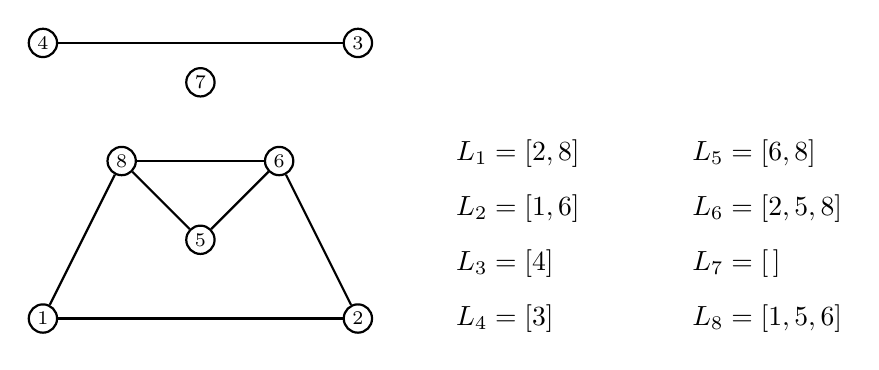
\begin{tikzpicture}
[lineDecorate/.style={-,thick},%
  nodeDecorate/.style={shape=circle,inner sep=1.5pt,draw,thick}]
%% nodes or vertices
\foreach \nodename/\x/\y in {
  1/0/0, 2/4/0, 3/4/3.5, 4/0/3.5, 5/2/1, 6/3/2, 7/2/3, 8/1/2}
{
  \node (\nodename) at (\x,\y) [nodeDecorate] {\scriptsize$\nodename$};
}
%% adjacency lists
\node (L1) at (5,2.1) [] {};
\node [right] at (L1.east) {$L_1 = [2,8]$};
\node (L2) at (5,1.4) [] {};
\node [right] at (L2.east) {$L_2 = [1,6]$};
\node (L3) at (5,0.7) [] {};
\node [right] at (L3.east) {$L_3 = [4]$};
\node (L4) at (5,0) [] {};
\node [right] at (L4.east) {$L_4 = [3]$};
\node (L5) at (8,2.1) [] {};
\node [right] at (L5.east) {$L_5 = [6,8]$};
\node (L6) at (8,1.4) [] {};
\node [right] at (L6.east) {$L_6 = [2,5,8]$};
\node (L7) at (8,0.7) [] {};
\node [right] at (L7.east) {$L_7 = [\,]$};
\node (L8) at (8,0) [] {};
\node [right] at (L8.east) {$L_8 = [1,5,6]$};
%% edges or lines
\path
\foreach \startnode/\endnode in {1/2, 1/8, 2/6, 3/4, 5/6, 5/8, 6/8}
{
  (\startnode) edge[lineDecorate] node {} (\endnode)
};
\end{tikzpicture}
\end{figure}

\end{document}

\caption{A graph and its adjacency lists.}
\label{fig:graph_algorithms:graph_adjacency_lists}
\end{figure}

\begin{example}
The Kneser\index{Kneser graph} graph with parameters $(n,k)$, also
known as the $(n,k)$-Kneser\index{Kneser graph} graph, is the graph
whose vertices are all the $k$-subsets of $\{1, 2, \dots,
n\}$. Furthermore, two vertices are adjacent if their corresponding
sets are disjoint. Draw the $(5,2)$-Kneser\index{Kneser graph} graph
and find its order and adjacency\index{list!adjacency} lists. In
general, if $n$ and $k$ are positive, what is the order of the
$(n,k)$-Kneser\index{Kneser graph} graph?
\end{example}

\begin{proof}[Solution]
The $(5,2)$-Kneser\index{Kneser graph} graph is the graph whose
vertices are the $2$-subsets
\[
\{1,2\},\, \{1,3\},\, \{1,4\},\, \{1,5\},\,
\{2,3\},\, \{2,4\},\, \{2,5\},\,
\{3,4\},\, \{3,5\},\,
\{4,5\}
\]
of $\{1, 2, 3, 4, 5\}$. That is, each vertex of the
$(5,2)$-Kneser\index{Kneser graph} graph is a $2$-combination of the
set $\{1, 2, 3, 4, 5\}$ and therefore the graph itself has order
$\binom{5}{2} = \frac{5 \times 4}{2!} = 10$. The edges of this graph
are
%%
\begin{align*}
& (\{1,3\},\, \{2,4\}),\;
  (\{2,4\},\, \{1,5\}),\;
  (\{2,4\},\, \{3,5\}),\;
  (\{1,3\},\, \{4,5\}),\;
  (\{1,3\},\, \{2,5\}) \\[4pt]
& (\{3,5\},\, \{1,4\}),\;
  (\{3,5\},\, \{1,2\}),\;
  (\{1,4\},\, \{2,3\}),\;
  (\{1,4\},\, \{2,5\}),\;
  (\{4,5\},\, \{2,3\}) \\[4pt]
& (\{4,5\},\, \{1,2\}),\;
  (\{1,5\},\, \{2,3\}),\;
  (\{1,5\},\, \{3,4\}),\;
  (\{3,4\},\, \{1,2\}),\;
  (\{3,4\},\, \{2,5\})
\end{align*}
%%
from which we obtain the following adjacency lists:
%%
\begin{align*}
L_{\{1,2\}} = [\{3,4\},\, \{3,5\},\, \{4,5\}]
&,\quad
L_{\{1,3\}} = [\{2,4\},\, \{2,5\},\, \{4,5\}], \\[4pt]
%%
L_{\{1,4\}} = [\{2,3\},\, \{3,5\},\, \{2,5\}]
&,\quad
L_{\{1,5\}} = [\{2,4\},\, \{3,4\},\, \{2,3\}], \\[4pt]
%%
L_{\{2,3\}} = [\{1,5\},\, \{1,4\},\, \{4,5\}]
&,\quad
L_{\{2,4\}} = [\{1,3\},\, \{1,5\},\, \{3,5\}], \\[4pt]
%%
L_{\{2,5\}} = [\{1,3\},\, \{3,4\},\, \{1,4\}]
&,\quad
L_{\{3,4\}} = [\{1,2\},\, \{1,5\},\, \{2,5\}], \\[4pt]
%%
L_{\{3,5\}} = [\{2,4\},\, \{1,2\},\, \{1,4\}]
&,\quad
L_{\{4,5\}} = [\{1,3\},\, \{1,2\},\, \{2,3\}].
\end{align*}
%%
The $(5,2)$-Kneser\index{Kneser graph} graph itself is shown in
Figure~\ref{fig:graph_algorithms:5_2_Kneser_graph}. Using Sage, we
have
%%
\begin{lstlisting}
sage: K = graphs.KneserGraph(5, 2); K
Kneser graph with parameters 5,2: Graph on 10 vertices
sage: for v in K.vertices():
...       print(v, K.neighbors(v))
...
({4, 5}, [{1, 3}, {1, 2}, {2, 3}])
({1, 3}, [{2, 4}, {2, 5}, {4, 5}])
({2, 5}, [{1, 3}, {3, 4}, {1, 4}])
({2, 3}, [{1, 5}, {1, 4}, {4, 5}])
({3, 4}, [{1, 2}, {1, 5}, {2, 5}])
({3, 5}, [{2, 4}, {1, 2}, {1, 4}])
({1, 4}, [{2, 3}, {3, 5}, {2, 5}])
({1, 5}, [{2, 4}, {3, 4}, {2, 3}])
({1, 2}, [{3, 4}, {3, 5}, {4, 5}])
({2, 4}, [{1, 3}, {1, 5}, {3, 5}])
\end{lstlisting}
%%
If $n$ and $k$ are positive integers, then the
$(n,k)$-Kneser\index{Kneser graph} graph has
\[
\binom{n}{k}
=
\frac{n (n-1) \cdots (n - k + 1)} {k!}
\]
vertices.
\end{proof}

\begin{figure}[!htbp]
\centering
\index{Kneser graph}
%%%%%%%%%%%%%%%%%%%%%%%%%%%%%%%%%%%%%%%%%%%%%%%%%%%%%%%%%%%%%%%%%%%%%%%%%%%
%% This file is part of the book
%%
%% Algorithmic Graph Theory
%% http://code.google.com/p/graph-theory-algorithms-book/
%%
%% Copyright (C) 2009, 2010, 2011 Minh Van Nguyen <nguyenminh2@gmail.com>
%%
%% See the file COPYING for copying conditions.
%%%%%%%%%%%%%%%%%%%%%%%%%%%%%%%%%%%%%%%%%%%%%%%%%%%%%%%%%%%%%%%%%%%%%%%%%%%

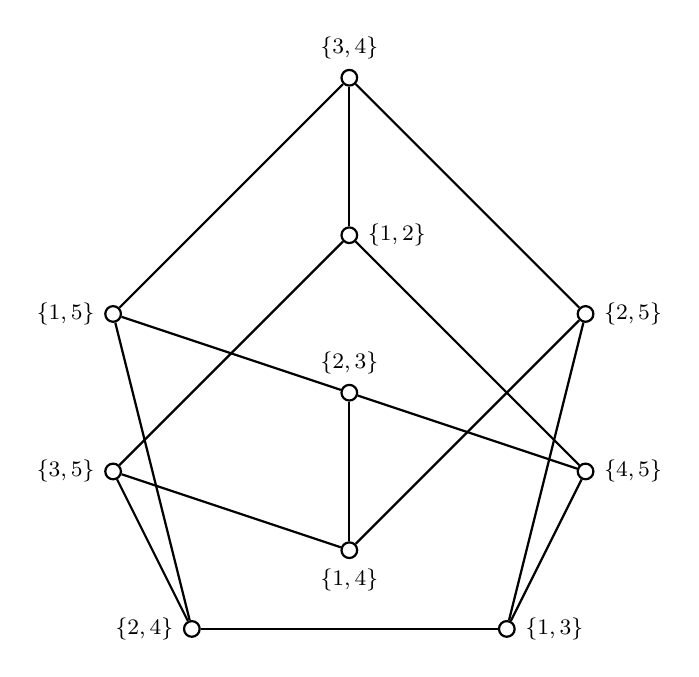
\begin{tikzpicture}
[lineDecorate/.style={-,thick},%
  nodeDecorate/.style={shape=circle,inner sep=2pt,draw,thick}]
%% nodes or vertices
\foreach \nodename/\x/\y in {
  24/0/0, 13/4/0, 15/-1/4, 25/5/4, 35/-1/2, 45/5/2, 14/2/1, 23/2/3,
  12/2/5, 34/2/7}
{
  \node (\nodename) at (\x,\y) [nodeDecorate] {};
}
%% node labels
\node [left] at (24.west) {\footnotesize$\{2,4\}$};
\node [right] at (13.east) {\footnotesize$\{1,3\}$};
\node [below] at (14.south) {\footnotesize$\{1,4\}$};
\node [left] at (35.west) {\footnotesize$\{3,5\}$};
\node [right] at (45.east) {\footnotesize$\{4,5\}$};
\node [above] at (23.north) {\footnotesize$\{2,3\}$};
\node [left] at (15.west) {\footnotesize$\{1,5\}$};
\node [right] at (25.east) {\footnotesize$\{2,5\}$};
\node [right] at (12.east) {\footnotesize$\{1,2\}$};
\node [above] at (34.north) {\footnotesize$\{3,4\}$};
%% edges or lines
\path
\foreach \startnode/\endnode in {
  24/13, 24/15, 24/35, 13/45, 13/25, 35/14, 35/12, 14/23, 14/25,
  45/23, 45/12, 15/23, 15/34, 34/12, 34/25}
{
  (\startnode) edge[lineDecorate] node {} (\endnode)
};
\end{tikzpicture}

\caption{The $(5,2)$-Kneser graph.}
\label{fig:graph_algorithms:5_2_Kneser_graph}
\end{figure}

We can categorize a graph $G = (V, E)$ as \emph{dense} or
\emph{sparse} based upon its size. A dense graph\index{graph!dense}
has size $|E|$ that is close to $|V|^2$, i.e.
$|E| = \Omega\big(|V|^2\big)$, in which case it is feasible to
represent $G$ as an adjacency matrix. The size of a sparse
graph\index{graph!sparse} is much less than $|V|^2$, i.e.
$|E| = \Omega\big(|V|\big)$, which renders the adjacency
matrix\index{matrix!adjacency} representation as unsuitable. For a
sparse graph, an adjacency list\index{list!adjacency} representation
can require less storage space than an adjacency matrix representation
of the same graph.


%%%%%%%%%%%%%%%%%%%%%%%%%%%%%%%%%%%%%%%%%%%%%%%%%%%%%%%%%%%%%%%%%%%%%%%%%%%

\subsection{The \graphsix format}
\label{sec:graph_algorithms:graph6_format}

The graph formats \graphsix\index{\graphsix} and
\sparsesix\index{\sparsesix} were developed by Brendan
McKay\index{McKay, Brendan D.}~\cite{McKay2010} at The Australian
National University\index{Australian National University} as a compact
way to represent graphs. These two formats use bit
vectors\index{bit vector} and printable characters of the American
Standard Code for Information Interchange~(ASCII)\index{ASCII}
encoding scheme. The 64 printable ASCII characters used in
\graphsix and \sparsesix are those ASCII characters with decimal codes
from 63 to 126, inclusive, as shown in
Table~\ref{tab:graph_algorithms:graph6_sparse6_ASCII_printable_characters}.
This section shall only cover the \graphsix format. For full
specification on both of the \graphsix and \sparsesix formats, see
McKay~\cite{McKay2010}.

\begin{table}[!htbp]
\centering
%%%%%%%%%%%%%%%%%%%%%%%%%%%%%%%%%%%%%%%%%%%%%%%%%%%%%%%%%%%%%%%%%%%%%%%%%%%
%% This file is part of the book
%%
%% Algorithmic Graph Theory
%% http://code.google.com/p/graph-theory-algorithms-book/
%%
%% Copyright (C) 2009, 2010 Minh Van Nguyen <nguyenminh2@gmail.com>
%%
%% See the file COPYING for copying conditions.
%%%%%%%%%%%%%%%%%%%%%%%%%%%%%%%%%%%%%%%%%%%%%%%%%%%%%%%%%%%%%%%%%%%%%%%%%%%

\begin{tabular}{ccc|ccc} \hline
binary         & decimal   & glyph    & binary & decimal & glyph \\\hline
\verb!0111111! & \verb!63! & \verb!?! & \verb!1011111! & \verb!95!  & \verb!_! \\
\verb!1000000! & \verb!64! & \verb!@! & \verb!1100000! & \verb!96!  & \verb!`! \\
\verb!1000001! & \verb!65! & \verb!A! & \verb!1100001! & \verb!97!  & \verb!a! \\
\verb!1000010! & \verb!66! & \verb!B! & \verb!1100010! & \verb!98!  & \verb!b! \\
\verb!1000011! & \verb!67! & \verb!C! & \verb!1100011! & \verb!99!  & \verb!c! \\
\verb!1000100! & \verb!68! & \verb!D! & \verb!1100100! & \verb!100! & \verb!d! \\
\verb!1000101! & \verb!69! & \verb!E! & \verb!1100101! & \verb!101! & \verb!e! \\
\verb!1000110! & \verb!70! & \verb!F! & \verb!1100110! & \verb!102! & \verb!f! \\
\verb!1000111! & \verb!71! & \verb!G! & \verb!1100111! & \verb!103! & \verb!g! \\
\verb!1001000! & \verb!72! & \verb!H! & \verb!1101000! & \verb!104! & \verb!h! \\
\verb!1001001! & \verb!73! & \verb!I! & \verb!1101001! & \verb!105! & \verb!i! \\
\verb!1001010! & \verb!74! & \verb!J! & \verb!1101010! & \verb!106! & \verb!j! \\
\verb!1001011! & \verb!75! & \verb!K! & \verb!1101011! & \verb!107! & \verb!k! \\
\verb!1001100! & \verb!76! & \verb!L! & \verb!1101100! & \verb!108! & \verb!l! \\
\verb!1001101! & \verb!77! & \verb!M! & \verb!1101101! & \verb!109! & \verb!m! \\
\verb!1001110! & \verb!78! & \verb!N! & \verb!1101110! & \verb!110! & \verb!n! \\
\verb!1001111! & \verb!79! & \verb!O! & \verb!1101111! & \verb!111! & \verb!o! \\
\verb!1010000! & \verb!80! & \verb!P! & \verb!1110000! & \verb!112! & \verb!p! \\
\verb!1010001! & \verb!81! & \verb!Q! & \verb!1110001! & \verb!113! & \verb!q! \\
\verb!1010010! & \verb!82! & \verb!R! & \verb!1110010! & \verb!114! & \verb!r! \\
\verb!1010011! & \verb!83! & \verb!S! & \verb!1110011! & \verb!115! & \verb!s! \\
\verb!1010100! & \verb!84! & \verb!T! & \verb!1110100! & \verb!116! & \verb!t! \\
\verb!1010101! & \verb!85! & \verb!U! & \verb!1110101! & \verb!117! & \verb!u! \\
\verb!1010110! & \verb!86! & \verb!V! & \verb!1110110! & \verb!118! & \verb!v! \\
\verb!1010111! & \verb!87! & \verb!W! & \verb!1110111! & \verb!119! & \verb!w! \\
\verb!1011000! & \verb!88! & \verb!X! & \verb!1111000! & \verb!120! & \verb!x! \\
\verb!1011001! & \verb!89! & \verb!Y! & \verb!1111001! & \verb!121! & \verb!y! \\
\verb!1011010! & \verb!90! & \verb!Z! & \verb!1111010! & \verb!122! & \verb!z! \\
\verb!1011011! & \verb!91! & \verb![! & \verb!1111011! & \verb!123! & \verb!{! \\
\verb!1011100! & \verb!92! & \verb!\! & \verb!1111100! & \verb!124! & \verb!|! \\
\verb!1011101! & \verb!93! & \verb!]! & \verb!1111101! & \verb!125! & \verb!}! \\
\verb!1011110! & \verb!94! & \verb!^! & \verb!1111110! & \verb!126! & \verb!~! \\\hline
\end{tabular}

\caption{ASCII printable characters used by \graphsix and \sparsesix.}
\label{tab:graph_algorithms:graph6_sparse6_ASCII_printable_characters}
\end{table}


%%%%%%%%%%%%%%%%%%%%%%%%%%%%%%%%%%%%%%%%%%%%%%%%%%%%%%%%%%%%%%%%%%%%%%%%%%%

\subsubsection{Bit vectors}
\index{bit vector}

Before discussing how \graphsix\index{\graphsix} and
\sparsesix\index{\sparsesix} represent graphs using printable
ASCII\index{ASCII} characters, we first present encoding schemes used
by these two formats. A \emph{bit vector}\index{bit vector} is, as its
name suggests, a vector whose elements are 1's and 0's. It can be
represented as a list of bits\index{bit}, e.g. \verb!E! can be
represented as the ASCII bit vector
$[
  \texttt{1}, \texttt{0}, \texttt{0}, \texttt{0}, \texttt{1},
  \texttt{0}, \texttt{1}
]$. For brevity, we write a bit vector in a compact form such as
\texttt{1000101}. The \emph{length}\index{bit vector!length} of a bit
vector is its number of bits. The
\emph{most significant bit}\index{bit!most significant} of a bit
vector $v$ is the bit position with the largest value among all the
bit positions in $v$. Similarly, the
\emph{least significant bit}\index{bit!least significant} is the bit
position in $v$ having the least value among all the bit positions in
$v$. The least significant bit of $v$ is usually called the parity
bit\index{bit!parity} because when $v$ is interpreted as an integer
the parity bit determines whether the integer is even or odd. Reading
\texttt{1000101} from left to right, the first bit \texttt{1} is the
most significant bit, followed by the second bit \texttt{0} which is
the second most significant bit, and so on all the way down to the
seventh bit \texttt{1} which is the least significant bit.

The order in which we process the bits of a bit vector
%%
\begin{equation}
\label{eqn:graph_algorithms:bits_of_bit_vector}
v
=
b_{n-1} b_{n-2} \cdots b_0
\end{equation}
%%
is referred to as \emph{endianness}\index{endianness}. Processing $v$
in \emph{big-endian}\index{big-endian} order means that we first process
the most significant bit of $v$, followed by the second most
significant bit, and so on all the way down to the least significant
bit of $v$. Thus, in big-endian order we read the bits $b_i$ of $v$
from left to right in increasing order of powers of $2$.
Table~\ref{tab:graph_algorithms:big_endian_ASCII_binary_E} illustrates
the big-endian interpretation of the ASCII\index{ASCII} binary
representation of \texttt{E}.
\emph{Little-endian}\index{little-endian} order means that we first
process the least significant bit, followed by the second least
significant bit, and so on all the way up to the most significant
bit. In little-endian order, the bits $b_i$ are read from right to
left in increasing order of powers of $2$.
Table~\ref{tab:graph_algorithms:little_endian_ASCII_binary_E}
illustrates the little-endian interpretation of the ASCII\index{ASCII}
binary representation of \texttt{E}. In his novel
\emph{Gulliver's Travels}\index{Gulliver's Travels} first published
in~1726, Jonathan Swift\index{Swift, Jonathan} used the terms
big-\index{big-endian} and little-endian\index{little-endian} in
satirizing politicians who squabbled over whether to break an egg at
the big end or the little end. Danny
Cohen\index{Cohen, Danny}~\cite{Cohen1980,Cohen1981} first used the
terms in 1980 as an April fool's joke in the context of computer
architecture.

Suppose the bit vector~\eqref{eqn:graph_algorithms:bits_of_bit_vector}
is read in big-endian order. To determine the integer representation
of $v$, multiply each bit value by its corresponding position value,
then add up all the results. Thus, if $v$ is read in big-endian order,
the integer representation of $v$ is obtained by evaluating the
polynomial
%%
\begin{equation}
\label{eqn:graph_algorithms:big_endian_binary_to_integer}
p(x)
=
\sum_{i=0}^{n-1} x^i b_i
=
x^{n-1} b_{n-1} + x^{n-2} b_{n-2} + \cdots + x b_1 + b_0.
\end{equation}
%%
at $x = 2$. See
problem~\thechapter.\ref{prob:graph_algorithms:Horner_method} for
discussion of an efficient method to compute the integer
representation of a bit vector.

\begin{table}[!htbp]
\centering
\input{data/graph-algorithms/big-endian-ASCII-binary-E.tex}
\caption{Big-endian order of the ASCII binary code of \texttt{E}.}
\label{tab:graph_algorithms:big_endian_ASCII_binary_E}
\end{table}

\begin{table}[!htbp]
\centering
%%%%%%%%%%%%%%%%%%%%%%%%%%%%%%%%%%%%%%%%%%%%%%%%%%%%%%%%%%%%%%%%%%%%%%%%%%%
%% This file is part of the book
%%
%% Algorithmic Graph Theory
%% http://code.google.com/p/graph-theory-algorithms-book/
%%
%% Copyright (C) 2009, 2010, 2011 Minh Van Nguyen <nguyenminh2@gmail.com>
%%
%% See the file COPYING for copying conditions.
%%%%%%%%%%%%%%%%%%%%%%%%%%%%%%%%%%%%%%%%%%%%%%%%%%%%%%%%%%%%%%%%%%%%%%%%%%%

\begin{tabular}{l|ccccccc} \hline
position       & 0          & 1          & 2          & 3          & 4          & 5          & 6 \\
bit value      & \texttt{1} & \texttt{0} & \texttt{0} & \texttt{0} & \texttt{1} & \texttt{0} & \texttt{1} \\
position value & $2^6$      & $2^5$      & $2^4$      & $2^3$      & $2^2$      & $2^1$      & $2^0$ \\\hline
\end{tabular}


\caption{Little-endian order of the ASCII binary code of \texttt{E}.}
\label{tab:graph_algorithms:little_endian_ASCII_binary_E}
\end{table}

In \graphsix\index{\graphsix} and \sparsesix\index{\sparsesix}
formats, the length of a bit vector\index{bit vector} must be a
multiple of 6. Suppose $v$ is a bit vector of length $k$ such that
$6 \nmid k$. To transform $v$ into a bit vector having length a
multiple of 6, let $r = k \mod 6$ be the remainder\index{remainder}
upon dividing $k$ by 6, and pad $6 - r$ zeros\index{zero padding} to
the right of $v$.

Suppose $v = b_1 b_2 \cdots b_k$ is a bit vector of length $k$, where
$6 \mid k$. We split $v$ into $k/6$ bit vectors $v_i$, each of length
6. For $0 \leq i \leq k/6$, the $i$-th bit vector is given by
\[
v_i
=
b_{6i-5} b_{6i-4} b_{6i-3} b_{6i-2} b_{6i-1} b_{6i}.
\]
Consider each $v_i$ as the big-endian\index{big-endian} binary
representation of a positive
integer. Use~\eqref{eqn:graph_algorithms:big_endian_binary_to_integer}
to obtain the integer representation $N_i$ of each $v_i$. Then add 63
to each $N_i$ to obtain $N_i'$ and store $N_i'$ in one byte of
memory. That is, each $N_i'$ can be represented as a bit vector of
length $8$. Thus the required number of bytes to store $v$ is
$\lceil k/6 \rceil$. Let $B_i$ be the byte representation of $N_i'$ so
that
%%
\begin{equation}
\label{eqn:graph_algorithms:byte_representation_bit_vector}
R(v)
=
B_1 B_2 \cdots B_{\lceil k/6 \rceil}
\end{equation}
%%
denotes the representation of $v$ as a sequence of $\lceil k/6 \rceil$
bytes.

We now discuss how to encode an integer $n$ in the range
$0 \leq n \leq 2^{36} - 1$
using~\eqref{eqn:graph_algorithms:byte_representation_bit_vector} and
denote such an encoding of $n$ as $N(n)$. Let $v$ be the
big-endian\index{big-endian} binary representation of $n$. Then $N(n)$
is given by
%%
\begin{equation}
\label{eqn:graph_algorithms:graph6_sparse6_graph_orders}
N(n)
=
\begin{cases}
n + 63, & \text{if $0 \leq n \leq 62$}, \\
126 \, R(v), & \text{if $63 \leq n \leq 258047$}, \\
126 \, 126 \, R(v), & \text{if $258048 \leq n \leq 2^{36}-1$}.
\end{cases}
\end{equation}
%% If $0 \leq n \leq 62$, then
%% we write $N(n) = n + 63$. If $63 \leq n \leq 258047$, let $v$ be the
%% big-endian binary representation of $n$ and write
%% $N(n) = 126 \, R(v)$. Finally, if $258048 \leq n \leq 2^{36} - 1$,
%% again we let $v$ be the big-endian binary representation of $n$ and
%% write $N(n) = 126 \, 126 \, R(v)$.
Note that $n + 63$ requires one byte of storage memory, while
$126 \, R(v)$ and $126 \, 126 \, R(v)$ require 4 and 8 bytes,
respectively.


%%%%%%%%%%%%%%%%%%%%%%%%%%%%%%%%%%%%%%%%%%%%%%%%%%%%%%%%%%%%%%%%%%%%%%%%%%%

\subsubsection{The \graphsix format}
\index{\graphsix}

The \graphsix\index{\graphsix} format is used to represent simple,
undirected graphs of order from $0$ to $2^{36} - 1$, inclusive. Let
$G$ be a simple, undirected graph of order $0 \leq n \leq 2^{36} - 1$.
If $n = 0$, then $G$ is represented in \graphsix format as
``\verb!?!''. Suppose $n > 0$. Let $M = [a_{ij}]$ be the adjacency
matrix\index{matrix!adjacency} of $G$. Consider the upper
triangle\index{matrix!upper triangle} of $M$, excluding the main
diagonal\index{matrix!main diagonal}, and write that upper triangle as
the bit vector\index{bit vector}
\[
v
=
\underbrace{a_{0,1}}_{c_1}
\underbrace{a_{0,2} a_{1,2}}_{c_2}
\underbrace{a_{0,3} a_{1,3} a_{2,3}}_{c_3} \cdots
\underbrace{a_{0,i} a_{1,i} \cdots a_{i-1,i}}_{c_i} \cdots
\underbrace{a_{0,n} a_{1,n} \cdots a_{n-1,n}}_{c_n}
\]
where $c_i$ denotes the entries $a_{0,i} a_{1,i} \cdots a_{i-1,i}$ in
column $i$ of $M$. Then the \graphsix\index{\graphsix} representation
of $G$ is $N(n) R(v)$, where $R(v)$ and $N(n)$ are as
in~\eqref{eqn:graph_algorithms:byte_representation_bit_vector}
and~\eqref{eqn:graph_algorithms:graph6_sparse6_graph_orders},
respectively. That is, $N(n)$ encodes the order of $G$ and $R(v)$
encodes the edges of $G$.


%%%%%%%%%%%%%%%%%%%%%%%%%%%%%%%%%%%%%%%%%%%%%%%%%%%%%%%%%%%%%%%%%%%%%%%%%%%

\section{Graph searching}
\label{sec:graph_algorithms:graph_searching}
\index{graph!traversal}

\begin{quote}
\footnotesize
Errors, like straws, upon the surface flow; \\
He who would search for pearls must dive below. \\
\noindent
--- John Dryden\index{Dryden, John}, \emph{All for Love}, 1678
\end{quote}

\noindent
This section discusses two fundamental algorithms for graph
traversal\index{graph!traversal}: breadth-first
search\index{breadth-first search} and depth-first
search\index{depth-first search}. The word ``search'' used in
describing these two algorithms is rather misleading. It would be more
accurate to describe them as algorithms for constructing trees using
the adjacency information of a given graph. However, the names
``breadth-first search'' and ``depth-first search'' are entrenched in
literature on graph theory and computer science. From hereon, we use
these two names as given above, bearing in mind their intended
purposes.


%%%%%%%%%%%%%%%%%%%%%%%%%%%%%%%%%%%%%%%%%%%%%%%%%%%%%%%%%%%%%%%%%%%%%%%%%%%

\subsection{Breadth-first search}
\label{subsec:graph_algorithms:breadth_first_search}
\index{breadth-first search}

Breadth-first search\index{breadth-first search} (BFS)\index{BFS} is a
strategy for running through the vertices of a graph. It was presented
by Moore~\cite{Moore1959}\index{Moore, Edward F.} in~1959 within the
context of traversing mazes\index{maze}.
Lee~\cite{Lee1961}\index{Lee, C. Y.} independently discovered the same
algorithm in~1961 in his work on routing wires on circuit
boards\index{circuit!board}.

The basic BFS\index{BFS} algorithm can be described as
follows. Starting from a given vertex $v$ of a graph $G$, we first
explore the neighborhood of $v$ by visiting all vertices that are
adjacent to $v$. We then apply the same strategy to each of the
neighbors of $v$. The strategy of exploring the neighborhood of a
vertex is applied to all vertices of $G$. The result is a
tree\index{tree} rooted\index{tree!rooted} at $v$ and this tree is a
subgraph of $G$.
Algorithm~\ref{alg:graph_algorithms:breadth_first_search_template}
presents a general template for the BFS\index{BFS} strategy. The tree
resulting from the BFS\index{BFS} algorithm is called a
\emph{breadth-first search tree}\index{breadth-first search!tree}.

\begin{algorithm}[!htbp]
\index{breadth-first search}\index{BFS}
%%%%%%%%%%%%%%%%%%%%%%%%%%%%%%%%%%%%%%%%%%%%%%%%%%%%%%%%%%%%%%%%%%%%%%%%%%%
%% This file is part of the book
%%
%% Algorithmic Graph Theory
%% http://code.google.com/p/graph-theory-algorithms-book/
%%
%% Copyright (C) 2009--2011 Minh Van Nguyen <nguyenminh2@gmail.com>
%%
%% See the file COPYING for copying conditions.
%%%%%%%%%%%%%%%%%%%%%%%%%%%%%%%%%%%%%%%%%%%%%%%%%%%%%%%%%%%%%%%%%%%%%%%%%%%

\DontPrintSemicolon
\SetAlgoNoLine
%%
%% input
\KwIn{A directed or undirected graph $G = (V, E)$ of order $n > 0$. A
  vertex $s$ from which to start the search. The vertices are numbered
  from $1$ to  $n = |V|$, i.e.~$V = \{1, 2, \dots, n\}$.}
%%
%% output
\KwOut{A list $D$ of distances of all vertices from $s$. A tree $T$
  rooted at $s$.}
\BlankLine
%%
%% algorithm body
$Q \assign [s]$\nllabel{alg:BFS:initialize_queue_visit_nodes}\tcc*[f]{queue of nodes to visit}\;
$D \assign [\infty, \infty, \dots, \infty]$\tcc*[f]{$n$ copies of $\infty$}\;
$D[s] \assign 0$\;
$T \assign [\,]$\nllabel{alg:BFS:initialize_empty_tree}\;
\While{$\length(Q) > 0$\nllabel{alg:BFS:while_loop:non_empty_queue}}{
  $v \assign \dequeue(Q)$\;
  \For{\rm each $w \in \adj(v)$\nllabel{alg:BFS:explore_neighborhood}}{
    \If{$D[w] = \infty$\nllabel{alg:BFS:marking_vertex_as_visited}}{
      $D[w] \assign D[v] + 1$\;
      $\enqueue(Q, w)$\;
      $\append(T, vw)$\nllabel{alg:BFS:while_loop:append_to_tree}\;
    }
  }
}
\Return $(D, T)$\;

\caption{A general breadth-first search template.}
\label{alg:graph_algorithms:breadth_first_search_template}
\end{algorithm}

The breadth-first search\index{breadth-first search} algorithm makes
use of a special type of list called a \emph{queue}\index{queue}. This
is analogous to a queue of people waiting in line to be served. A
person may enter the queue by joining the rear of the queue. The
person who is in the queue the longest amount of time is served first,
followed by the person who has waited the second longest time, and so
on. Formally, a queue $Q$ is a list\index{list} of elements. At any
time, we only have access to the first element of $Q$, known as the
\emph{front}\index{queue!front} or \emph{start}\index{queue!start} of
the queue. We insert a new element into $Q$ by appending the new
element to the \emph{rear}\index{queue!rear} or
\emph{end}\index{queue!end} of the queue. The operation of removing
the front of $Q$ is referred to as \emph{dequeue}\index{queue!dequeue},
while the operation of appending to the rear of $Q$ is called
\emph{enqueue}\index{queue!enqueue}. That is, a queue implements a first-in
first-out~(FIFO)\index{first in, first out}\index{FIFO} protocol for
adding and removing elements. As with lists\index{list}, the
\emph{length}\index{queue!length} of a queue is its total number of
elements.

\begin{figure}[!htbp]
\centering
\index{breadth-first search}\index{BFS}
%%%%%%%%%%%%%%%%%%%%%%%%%%%%%%%%%%%%%%%%%%%%%%%%%%%%%%%%%%%%%%%%%%%%%%%%%%%
%% This file is part of the book
%%
%% Algorithmic Graph Theory
%% http://code.google.com/p/graph-theory-algorithms-book/
%%
%% Copyright (C) 2009, 2010, 2011 Minh Van Nguyen <nguyenminh2@gmail.com>
%%
%% See the file COPYING for copying conditions.
%%%%%%%%%%%%%%%%%%%%%%%%%%%%%%%%%%%%%%%%%%%%%%%%%%%%%%%%%%%%%%%%%%%%%%%%%%%

\subfigure[Original undirected graph.]{
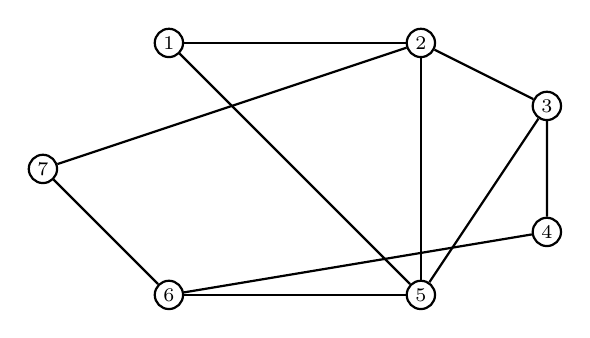
\begin{tikzpicture}
[lineDecorate/.style={-,thick},%
  nodeDecorate/.style={shape=circle,inner sep=1.5pt,draw,thick},%
  scale=0.8]
%% nodes or vertices
\foreach \nodename/\x/\y in {2/4/4, 1/0/4, 3/6/3, 4/6/1, 5/4/0, 7/-2/2, 6/0/0}
{
  \node (\nodename) at (\x,\y) [nodeDecorate] {\scriptsize$\nodename$};
}
%% edges or lines
\path
\foreach \startnode/\endnode in {
  1/2, 1/5, 2/3, 2/5, 2/7, 3/4, 3/5, 4/6, 5/6, 6/7}
{
  (\startnode) edge[lineDecorate] node {} (\endnode)
};
\end{tikzpicture}
}
%%
%%
\qquad
\subfigure[First iteration of while loop.]{
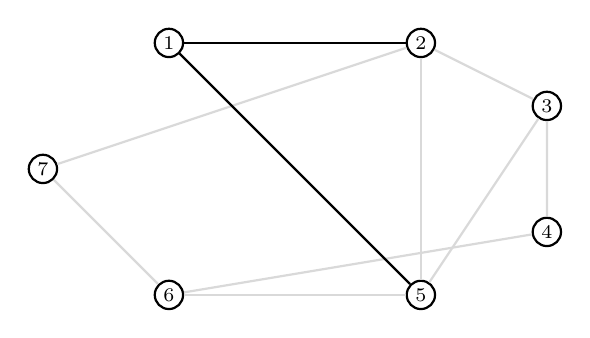
\begin{tikzpicture}
[darkLine/.style={-,thick},%
  lightLine/.style={-,thick,color=gray!30},%
  nodeDecorate/.style={shape=circle,inner sep=1.5pt,draw,thick},%
  scale=0.8]
%% nodes or vertices
\foreach \nodename/\x/\y in {2/4/4, 1/0/4, 3/6/3, 4/6/1, 5/4/0, 7/-2/2, 6/0/0}
{
  \node (\nodename) at (\x,\y) [nodeDecorate] {\scriptsize$\nodename$};
}
%% light edges or lines
\path
\foreach \startnode/\endnode in {2/3, 2/5, 2/7, 3/4, 3/5, 4/6, 5/6, 6/7}
{
  (\startnode) edge[lightLine] node {} (\endnode)
};
%% dark edges or lines
\path
\foreach \startnode/\endnode in {1/2, 1/5}
{
  (\startnode) edge[darkLine] node {} (\endnode)
};
\end{tikzpicture}
}
%%
%%
\subfigure[Second iteration of while loop.]{
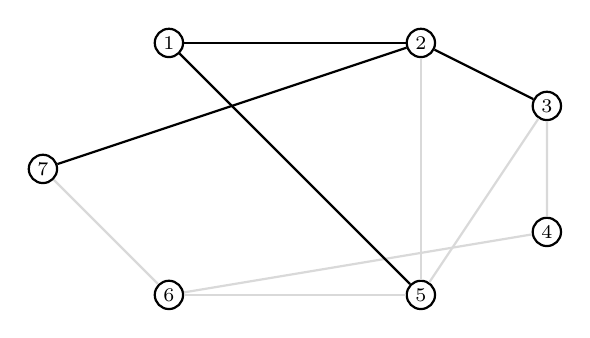
\begin{tikzpicture}
[darkLine/.style={-,thick},%
  lightLine/.style={-,thick,color=gray!30},%
  nodeDecorate/.style={shape=circle,inner sep=1.5pt,draw,thick},%
  scale=0.8]
%% nodes or vertices
\foreach \nodename/\x/\y in {2/4/4, 1/0/4, 3/6/3, 4/6/1, 5/4/0, 7/-2/2, 6/0/0}
{
  \node (\nodename) at (\x,\y) [nodeDecorate] {\scriptsize$\nodename$};
}
%% light edges or lines
\path
\foreach \startnode/\endnode in {2/5, 3/4, 3/5, 4/6, 5/6, 6/7}
{
  (\startnode) edge[lightLine] node {} (\endnode)
};
%% dark edges or lines
\path
\foreach \startnode/\endnode in {1/2, 1/5, 2/3, 2/7}
{
  (\startnode) edge[darkLine] node {} (\endnode)
};
\end{tikzpicture}
}
%%
%%
\qquad
\subfigure[Third iteration of while loop.]{
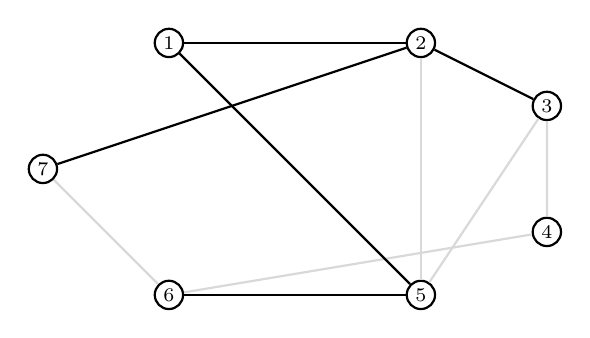
\begin{tikzpicture}
[darkLine/.style={-,thick},%
  lightLine/.style={-,thick,color=gray!30},%
  nodeDecorate/.style={shape=circle,inner sep=1.5pt,draw,thick},%
  scale=0.8]
%% nodes or vertices
\foreach \nodename/\x/\y in {2/4/4, 1/0/4, 3/6/3, 4/6/1, 5/4/0, 7/-2/2, 6/0/0}
{
  \node (\nodename) at (\x,\y) [nodeDecorate] {\scriptsize$\nodename$};
}
%% light edges or lines
\path
\foreach \startnode/\endnode in {2/5, 3/4, 3/5, 4/6, 6/7}
{
  (\startnode) edge[lightLine] node {} (\endnode)
};
%% dark edges or lines
\path
\foreach \startnode/\endnode in {1/2, 1/5, 2/3, 2/7, 5/6}
{
  (\startnode) edge[darkLine] node {} (\endnode)
};
\end{tikzpicture}
}
%%
%%
\subfigure[Fourth iteration of while loop.]{
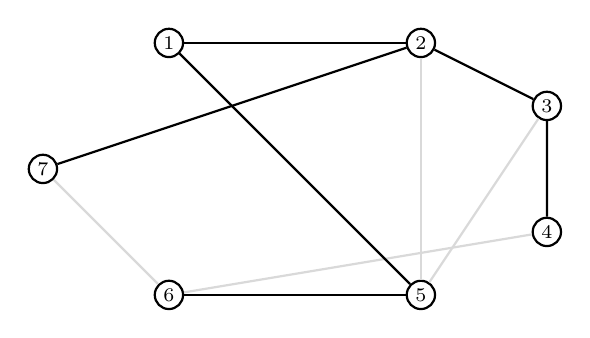
\begin{tikzpicture}
[darkLine/.style={-,thick},%
  lightLine/.style={-,thick,color=gray!30},%
  nodeDecorate/.style={shape=circle,inner sep=1.5pt,draw,thick},%
  scale=0.8]
%% nodes or vertices
\foreach \nodename/\x/\y in {2/4/4, 1/0/4, 3/6/3, 4/6/1, 5/4/0, 7/-2/2, 6/0/0}
{
  \node (\nodename) at (\x,\y) [nodeDecorate] {\scriptsize$\nodename$};
}
%% light edges or lines
\path
\foreach \startnode/\endnode in {2/5, 3/5, 4/6, 6/7}
{
  (\startnode) edge[lightLine] node {} (\endnode)
};
%% dark edges or lines
\path
\foreach \startnode/\endnode in {1/2, 1/5, 2/3, 2/7, 3/4, 5/6}
{
  (\startnode) edge[darkLine] node {} (\endnode)
};
\end{tikzpicture}
}
%%
%%
\qquad
\subfigure[Final BFS tree.]{
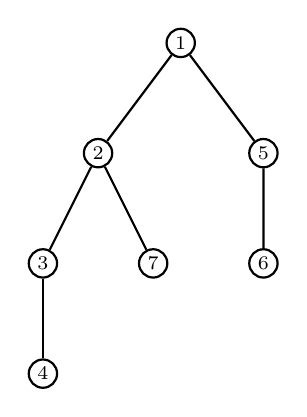
\begin{tikzpicture}
[lineDecorate/.style={-,thick},%
  nodeDecorate/.style={shape=circle,inner sep=1.5pt,draw,thick},%
  scale=1.4]
%% nodes or vertices
\foreach \nodename/\x/\y in {
  4/0/0, 3/0/1, 7/1/1, 6/2/1, 2/0.5/2, 5/2/2, 1/1.25/3}
{
  \node (\nodename) at (\x,\y) [nodeDecorate] {\scriptsize$\nodename$};
}
%% edges or lines
\path
\foreach \startnode/\endnode in {1/2, 1/5, 2/3, 2/7, 3/4, 5/6}
{
  (\startnode) edge[lineDecorate] node {} (\endnode)
};
\end{tikzpicture}
}

\caption{Breadth-first search tree for an undirected graph.}
\label{fig:graph_algorithms:breadth_first_search_undirected}
\end{figure}

\begin{figure}[!htbp]
\centering
\index{breadth-first search}\index{BFS}
%%%%%%%%%%%%%%%%%%%%%%%%%%%%%%%%%%%%%%%%%%%%%%%%%%%%%%%%%%%%%%%%%%%%%%%%%%%
%% This file is part of the book
%%
%% Algorithmic Graph Theory
%% http://code.google.com/p/graph-theory-algorithms-book/
%%
%% Copyright (C) 2009--2011 Minh Van Nguyen <nguyenminh2@gmail.com>
%%
%% See the file COPYING for copying conditions.
%%%%%%%%%%%%%%%%%%%%%%%%%%%%%%%%%%%%%%%%%%%%%%%%%%%%%%%%%%%%%%%%%%%%%%%%%%%

\documentclass{article}

\usepackage{subfigure}
\usepackage{tikz}
\usetikzlibrary{external}
\tikzexternalize{breadth-first-search-directed}

\begin{document}

\begin{figure}
\subfigure[Original digraph.]{
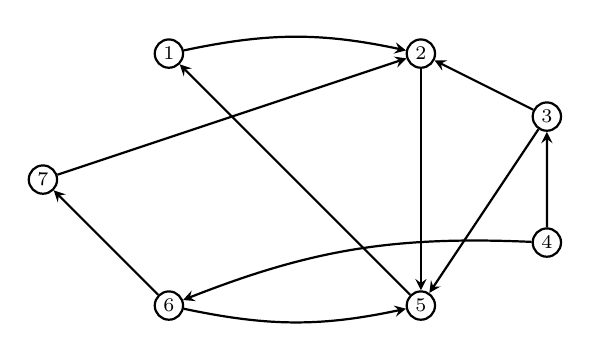
\begin{tikzpicture}
[arrowDecorate/.style={->,>=stealth,thick},%
  nodeDecorate/.style={shape=circle,inner sep=1.5pt,draw,thick},%
  scale=0.8]
%% nodes or vertices
\foreach \nodename/\x/\y in {2/4/4, 1/0/4, 3/6/3, 4/6/1, 5/4/0, 7/-2/2, 6/0/0}
{
  \node (\nodename) at (\x,\y) [nodeDecorate] {\scriptsize$\nodename$};
}
%% edges or lines
\path
\foreach \startnode/\endnode in {2/5, 3/2, 3/5, 4/3, 5/1, 6/7, 7/2}
{
  (\startnode) edge[arrowDecorate] node {} (\endnode)
}
\foreach \startnode/\endnode/\benddirection/\angle in {
  1/2/bend left/12, 4/6/bend right/12, 6/5/bend right/12}
{
  (\startnode) edge[arrowDecorate,\benddirection=\angle] node {} (\endnode)
};
\end{tikzpicture}
}
%%
%%
\qquad
\subfigure[First iteration of while loop.]{
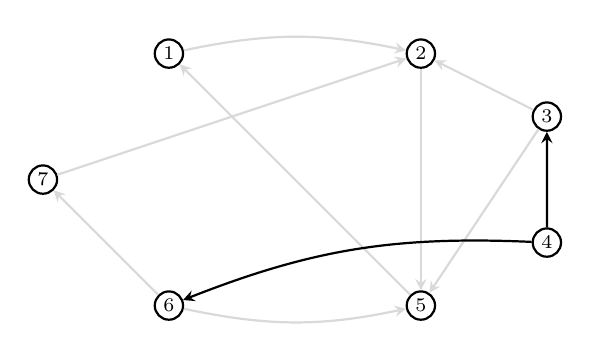
\begin{tikzpicture}
[darkArrow/.style={->,>=stealth,thick},%
  lightArrow/.style={->,>=stealth,thick,color=gray!30},%
  nodeDecorate/.style={shape=circle,inner sep=1.5pt,draw,thick},%
  scale=0.8]
%% nodes or vertices
\foreach \nodename/\x/\y in {2/4/4, 1/0/4, 3/6/3, 4/6/1, 5/4/0, 7/-2/2, 6/0/0}
{
  \node (\nodename) at (\x,\y) [nodeDecorate] {\scriptsize$\nodename$};
}
%% light edges or lines
\path
\foreach \startnode/\endnode in {2/5, 3/2, 3/5, 5/1, 6/7, 7/2}
{
  (\startnode) edge[lightArrow] node {} (\endnode)
}
\foreach \startnode/\endnode/\benddirection/\angle in {
  1/2/bend left/12, 6/5/bend right/12}
{
  (\startnode) edge[lightArrow,\benddirection=\angle] node {} (\endnode)
}
%% dark edges or lines
\foreach \startnode/\endnode in {4/3}
{
  (\startnode) edge[darkArrow] node {} (\endnode)
}
\foreach \startnode/\endnode/\benddirection/\angle in {4/6/bend right/12}
{
  (\startnode) edge[darkArrow,\benddirection=\angle] node {} (\endnode)
};
\end{tikzpicture}
}
%%
%%
\subfigure[Second iteration of while loop.]{
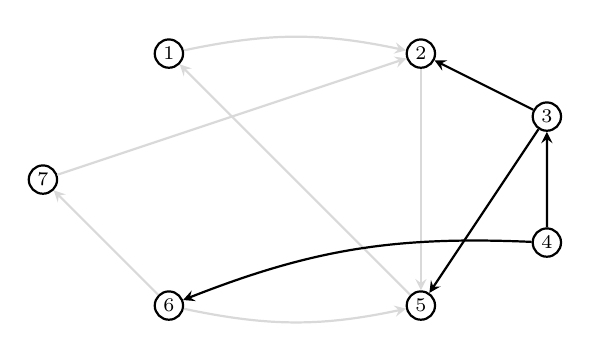
\begin{tikzpicture}
[darkArrow/.style={->,>=stealth,thick},%
  lightArrow/.style={->,>=stealth,thick,color=gray!30},%
  nodeDecorate/.style={shape=circle,inner sep=1.5pt,draw,thick},%
  scale=0.8]
%% nodes or vertices
\foreach \nodename/\x/\y in {2/4/4, 1/0/4, 3/6/3, 4/6/1, 5/4/0, 7/-2/2, 6/0/0}
{
  \node (\nodename) at (\x,\y) [nodeDecorate] {\scriptsize$\nodename$};
}
%% light edges or lines
\path
\foreach \startnode/\endnode in {2/5, 5/1, 6/7, 7/2}
{
  (\startnode) edge[lightArrow] node {} (\endnode)
}
\foreach \startnode/\endnode/\benddirection/\angle in {
  1/2/bend left/12, 6/5/bend right/12}
{
  (\startnode) edge[lightArrow,\benddirection=\angle] node {} (\endnode)
}
%% dark edges or lines
\foreach \startnode/\endnode in {3/2, 3/5, 4/3}
{
  (\startnode) edge[darkArrow] node {} (\endnode)
}
\foreach \startnode/\endnode/\benddirection/\angle in {4/6/bend right/12}
{
  (\startnode) edge[darkArrow,\benddirection=\angle] node {} (\endnode)
};
\end{tikzpicture}
}
%%
%%
\qquad
\subfigure[Third iteration of while loop.]{
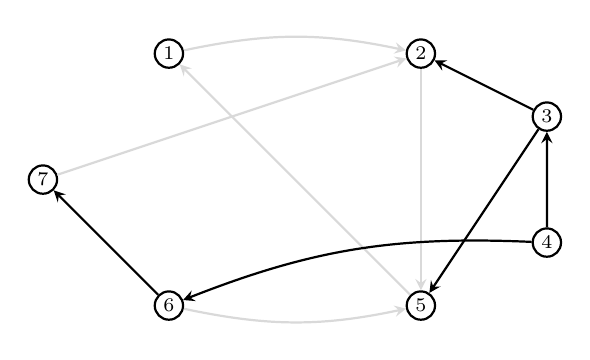
\begin{tikzpicture}
[darkArrow/.style={->,>=stealth,thick},%
  lightArrow/.style={->,>=stealth,thick,color=gray!30},%
  nodeDecorate/.style={shape=circle,inner sep=1.5pt,draw,thick},%
  scale=0.8]
%% nodes or vertices
\foreach \nodename/\x/\y in {2/4/4, 1/0/4, 3/6/3, 4/6/1, 5/4/0, 7/-2/2, 6/0/0}
{
  \node (\nodename) at (\x,\y) [nodeDecorate] {\scriptsize$\nodename$};
}
%% light edges or lines
\path
\foreach \startnode/\endnode in {2/5, 5/1, 7/2}
{
  (\startnode) edge[lightArrow] node {} (\endnode)
}
\foreach \startnode/\endnode/\benddirection/\angle in {
  1/2/bend left/12, 6/5/bend right/12}
{
  (\startnode) edge[lightArrow,\benddirection=\angle] node {} (\endnode)
}
%% dark edges or lines
\foreach \startnode/\endnode in {3/2, 3/5, 4/3, 6/7}
{
  (\startnode) edge[darkArrow] node {} (\endnode)
}
\foreach \startnode/\endnode/\benddirection/\angle in {4/6/bend right/12}
{
  (\startnode) edge[darkArrow,\benddirection=\angle] node {} (\endnode)
};
\end{tikzpicture}
}
%%
%%
\subfigure[Fourth iteration of while loop.]{
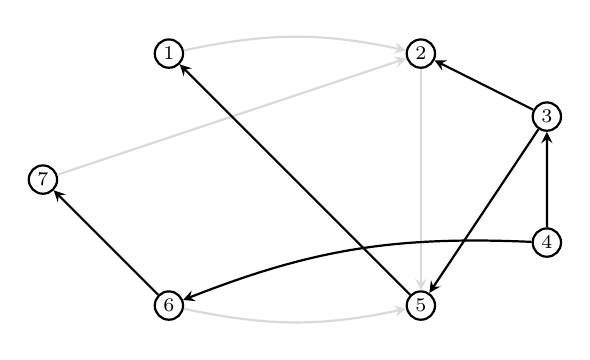
\begin{tikzpicture}
[darkArrow/.style={->,>=stealth,thick},%
  lightArrow/.style={->,>=stealth,thick,color=gray!30},%
  nodeDecorate/.style={shape=circle,inner sep=1.5pt,draw,thick},%
  scale=0.8]
%% nodes or vertices
\foreach \nodename/\x/\y in {2/4/4, 1/0/4, 3/6/3, 4/6/1, 5/4/0, 7/-2/2, 6/0/0}
{
  \node (\nodename) at (\x,\y) [nodeDecorate] {\scriptsize$\nodename$};
}
%% light edges or lines
\path
\foreach \startnode/\endnode in {2/5, 7/2}
{
  (\startnode) edge[lightArrow] node {} (\endnode)
}
\foreach \startnode/\endnode/\benddirection/\angle in {
  1/2/bend left/12, 6/5/bend right/12}
{
  (\startnode) edge[lightArrow,\benddirection=\angle] node {} (\endnode)
}
%% dark edges or lines
\foreach \startnode/\endnode in {3/2, 3/5, 4/3, 5/1, 6/7}
{
  (\startnode) edge[darkArrow] node {} (\endnode)
}
\foreach \startnode/\endnode/\benddirection/\angle in {4/6/bend right/12}
{
  (\startnode) edge[darkArrow,\benddirection=\angle] node {} (\endnode)
};
\end{tikzpicture}
}
%%
%%
\qquad
\subfigure[Final BFS tree.]{
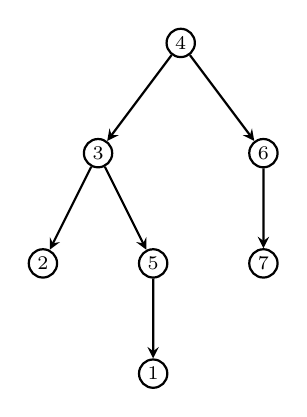
\begin{tikzpicture}
[arrowDecorate/.style={->,>=stealth,thick},%
  nodeDecorate/.style={shape=circle,inner sep=1.5pt,draw,thick},%
  scale=1.4]
%% nodes or vertices
\foreach \nodename/\x/\y in {
  2/0/1, 1/1/0, 5/1/1, 7/2/1, 6/2/2, 3/0.5/2, 4/1.25/3}
{
  \node (\nodename) at (\x,\y) [nodeDecorate] {\scriptsize$\nodename$};
}
%% edges or lines
\path
\foreach \startnode/\endnode in {4/3, 4/6, 3/2, 3/5, 6/7, 5/1}
{
  (\startnode) edge[arrowDecorate] node {} (\endnode)
};
\end{tikzpicture}
}
\end{figure}

\end{document}

\caption{Breadth-first search tree for a digraph.}
\label{fig:graph_algorithms:breadth_first_search_directed}
\end{figure}

Note that the BFS\index{BFS}
Algorithm~\ref{alg:graph_algorithms:breadth_first_search_template}
works on both undirected and directed graphs. For an undirected graph,
line~\ref{alg:BFS:explore_neighborhood} means that we explore all
the neighbors of vertex $v$, i.e. the set $\adj(v)$ of vertices
adjacent to $v$. In the case of a digraph, we replace
``$w \in \adj(v)$'' on line~\ref{alg:BFS:explore_neighborhood} with
``$w \in \oadj(v)$'' because we only want to explore all vertices that
are out-neighbors\index{out-neighbor} of $v$. The algorithm returns
two lists $D$ and $T$. The list $T$ contains a subset of edges in
$E(G)$ that make up a tree rooted at the given start vertex $s$. As
trees are connected graphs without cycles, we may take the vertices
comprising the edges of $T$ to be the vertex set of the tree. It is
clear that $T$ represents a tree by means of a list of edges, which
allows us to identify the tree under consideration as the edge list
$T$. The list $D$ has the same number of elements as the order of
$G = (V, E)$, i.e. $\length(D) = |V|$. The $i$-th element $D[i]$
counts the number of edges in $T$ between the vertices $s$ and
$v_i$. In other words, $D[i]$ is the length of the $s$-$v_i$ path in
$T$. It can be shown that $D[i] = \infty$ if and only if $G$ is
disconnected. After one application of
Algorithm~\ref{alg:graph_algorithms:breadth_first_search_template}, it
may happen that $D[i] = \infty$ for at least one vertex
$v_i \in V$. To traverse those vertices that are unreachable from $s$,
again we apply
Algorithm~\ref{alg:graph_algorithms:breadth_first_search_template} on
$G$ with starting vertex $v_i$. Repeat this algorithm as often as
necessary until all vertices of $G$ are visited. The result may be a
tree that contains all the vertices of $G$ or a collection of trees,
each of which contains a subset of $V(G)$.
Figures~\ref{fig:graph_algorithms:breadth_first_search_undirected}
and~\ref{fig:graph_algorithms:breadth_first_search_directed}
present BFS\index{BFS} trees\index{breadth-first search!tree}
resulting from applying
Algorithm~\ref{alg:graph_algorithms:breadth_first_search_template} on
an undirected graph and a digraph, respectively.

\begin{theorem}
\label{thm:graph_algorithms:BFS:worst_case_time_complexity}
\index{breadth-first search}
The worst-case time complexity of
Algorithm~\ref{alg:graph_algorithms:breadth_first_search_template} is
$O(|V| + |E|)$.
\end{theorem}

\begin{proof}
Without loss of generality, we can assume that $G = (V, E)$ is
connected. The initialization steps in
lines~\ref{alg:BFS:initialize_queue_visit_nodes}
to~\ref{alg:BFS:initialize_empty_tree} take $O(|V|)$ time. After
initialization, all but one vertex are labelled
$\infty$. Line~\ref{alg:BFS:marking_vertex_as_visited} ensures that
each vertex is enqueued\index{queue!enqueue} at most once and hence
dequeued\index{queue!dequeue} at most once. Each of
enqueuing\index{queue!enqueue} and dequeuing\index{queue!dequeue}
takes constant time. The total time devoted to queue operations is
$O(|V|)$. The adjacency list\index{list!adjacency} of a vertex is
scanned after dequeuing\index{queue!dequeue} that vertex, so each
adjacency list\index{list!adjacency} is scanned at most once. Summing
the lengths of the adjacency lists, we have $\Theta(|E|)$ and
therefore we require $O(|E|)$ time to scan the adjacency lists. After
the adjacency list of a vertex is scanned, at most $k$ edges are added
to the list $T$, where $k$ is the length of the adjacency
list\index{list!adjacency} under consideration. Like
queue\index{queue} operations, appending to a list\index{list} takes
constant time, hence we require $O(|E|)$ time to build the list
$T$. Therefore, BFS\index{BFS} runs in $O(|V| + |E|)$ time.
\end{proof}

\begin{theorem}
\label{thm:graph_algorithms:BFS:list_D_length_shortest_paths}
For the list $D$ resulting from
Algorithm~\ref{alg:graph_algorithms:breadth_first_search_template},
let $s$ be a starting vertex and let $v$ be a vertex such that
$D[v] \neq \infty$. Then $D[v]$ is the length of any shortest path
from $s$ to $v$.
\end{theorem}

\begin{proof}
It is clear that $D[v] = \infty$ if and only if there are no paths
from $s$ to $v$. Let $v$ be a vertex such that $D[v] \neq \infty$. As
$v$ can be reached from $s$ by a path of length $D[v]$, the length
$d(s,v)$ of any shortest $s$-$v$ path satisfies $d(s,v) \leq
D[v]$. Use induction on $d(s,v)$ to show that equality holds. For the
base case $s = v$, we have $d(s,v) = D[v] = 0$ since the trivial path
has length zero. Assume for induction that if $d(s,v) = k$, then
$d(s,v) = D[v]$.
%% We need to show that if $d(s,u)$ is the length of any
%% shortest $s$-$u$ path, then $d(s,u) = D[u]$.
Let $d(s,u) = k + 1$ with the corresponding shortest $s$-$u$ path
being $(s, v_1, v_2, \dots, v_k, u)$. By our induction hypothesis,
$(s, v_1, v_2, \dots, v_k)$ is a shortest path from $s$ to $v_k$ of
length $d(s, v_k) = D[v_k] = k$. In other words, $D[v_k] < D[u]$ and
the while loop spanning lines~\ref{alg:BFS:while_loop:non_empty_queue}
to~\ref{alg:BFS:while_loop:append_to_tree} processes $v_k$ before
processing $u$. The graph under consideration has the edge $v_k
u$. When examining the adjacency list of $v_k$, BFS reaches $u$~(if
$u$ is not reached earlier) and so $D[u] \leq k + 1$. Hence,
$D[u] = k + 1$ and therefore $d(s,u) = D[u] = k + 1$.
\end{proof}

In the proof of
Theorem~\ref{thm:graph_algorithms:BFS:list_D_length_shortest_paths},
we used $d(u,v)$ to denote the length of the shortest path from $u$ to
$v$. This shortest path length is also known as the
\emph{distance}\index{distance} from $u$ to $v$, and will be
discussed in further details in
section~\ref{sec:graph_algorithms:weights_distances} and
Chapter~\ref{chap:distance_connectivity}. The
\emph{diameter}\index{diameter} $\diam(G)$ of a graph $G = (V,E)$ is
defined as
\[
\diam(G)
=
\max_{\substack{u,v \in V \\ u \neq v}} d(u,v).
\]
Using the above definition, to find the diameter\index{diameter} we
first determine the distance\index{distance} between each pair of
distinct vertices, then we compute the maximum of all such
distances. Breadth-first\index{breadth-first search} search is a
useful technique for finding the diameter\index{diameter}: we simply
run breadth-first\index{breadth-first search} search from each
vertex. An interesting application of the diameter\index{diameter}
appears in the
\emph{small-world phenomenon}\index{small-world}~\cite{Kleinberg2000,
  Milgram1967,WattsStrogatz1998}, which contends that a certain
special class of sparse graphs have low diameter.

%% As an example, here is some Sage code which implements BFS to compute
%% the list distances from a given vertex.
%% %
%% \begin{center}
%% \fontsize{9pt}{9pt}
%% \selectfont
%% \tt
%% \begin{lstlisting}
%% def graph_distance(G, v0):
%%     """
%%     Breadth first search algorithm to find the
%%     distance from a fixed vertex $v_0$ to any
%%     other vertex.

%%     INPUT:
%%         G - a connected graph
%%         v0 - a vertex

%%     OUTPUT:
%%         D - a list of distances to
%%             every other vertex

%%     EXAMPLES:
%%         sage: G = Graph({1: [2, 4], 2: [1, 4], 3: [2, 6],
%%                          4: [1, 3], 5: [4, 2], 6: [3, 1]})
%%         sage: v0 = 1
%%         sage: graph_distance(G,v0)
%%         [[1, 0], [2, 1], [3, 2], [4, 1], [5, 2], [6, 1]]
%%         sage: G = Graph({"a": ["b", "e"], "b": ["c", "e"], \
%%          "c": ["d", "e"], "d": ["f"], "e": ["f"], "f": ["g"], "g":["b"]})
%%         sage: v0 = "a"
%%         sage: graph_distance(G, v0)
%%         [['a', 0], ['b', 1], ['c', 2], ['d', 3], ['e', 1],
%%          ['f', 2], ['g', 2]]
%%         sage: G = Graph({1: [2,3], 2: [1, 3], 3: [2], 4: [5], 5: [6], 6: [5]})
%%         sage: v0 = 1
%%         sage: graph_distance(G, v0) # note G is disconnected
%%         [[1, 0], [2, 1], [3, 1]]
%%     """
%%     V = G.vertices()
%%     Q = [v0]
%%     T = []
%%     D = []
%%     while Q<>[] and T<>V:
%%         for v in Q:
%%             if not(v in T):
%%                 D.append([v,G.distance(v0,v)])
%%             if v in Q:
%%                 Q.remove(v)
%%             T.append(v)
%%             T = list(Set(T))
%%             Q = Q+[x for x in G.neighbors(v) if not(x in T+Q)]
%%             if T == V:
%%                 break
%%     D.sort()
%%     print Q, T
%%     return D
%% \end{lstlisting}
%% \end{center}
%% %
%% \begin{exercise}
%% Using Sage's \verb!shortest_path! method, can you modify the above
%% function to return a list of shortest paths from $v_0$ to any other
%% vertex?
%% \end{exercise}


%%%%%%%%%%%%%%%%%%%%%%%%%%%%%%%%%%%%%%%%%%%%%%%%%%%%%%%%%%%%%%%%%%%%%%%%%%%

\subsection{Depth-first search}
\index{depth-first search}

\begin{quote}
\footnotesize
\includegraphics[scale=0.5]{image/graph-algorithms/depth-first-search} \\
\noindent
--- Randall Munroe\index{Munroe, Randall}, xkcd,
\url{http://xkcd.com/761/}
\end{quote}

\noindent
A depth-first search~(DFS)\index{depth-first search}\index{DFS} is a
graph traversal strategy similar to breadth-first
search\index{breadth-first search}. Both BFS\index{BFS} and
DFS\index{DFS} differ in how they explore each vertex. Whereas
BFS\index{BFS} explores the neighborhood of a vertex $v$ before moving
on to explore the neighborhoods of the neighbors, DFS\index{DFS}
explores as deep as possible a path starting at $v$. One can think of
BFS\index{BFS} as exploring the immediate surrounding, while
DFS\index{DFS} prefers to see what is on the other side of the
hill. In the 19th century,
Lucas~\cite{Lucas1882.1894}\index{Lucas, M. \'Edouard} and
Tarry~\cite{Tarry1895}\index{Tarry, Gaston} investigated
DFS\index{DFS} as a strategy for traversing
mazes\index{maze}. Fundamental properties of DFS\index{DFS} were
discovered in the early 1970s by
Hopcroft\index{Hopcroft, John E.} and
Tarjan~\cite{HopcroftTarjan1973,Tarjan1972}\index{Tarjan, Robert Endre}.

\begin{figure}[!htbp]
\centering
\index{chess!knight's tour}
%%%%%%%%%%%%%%%%%%%%%%%%%%%%%%%%%%%%%%%%%%%%%%%%%%%%%%%%%%%%%%%%%%%%%%%%%%%
%% This file is part of the book
%%
%% Algorithmic Graph Theory
%% http://code.google.com/p/graph-theory-algorithms-book/
%%
%% Copyright (C) 2009, 2010 Minh Van Nguyen <nguyenminh2@gmail.com>
%%
%% See the file COPYING for copying conditions.
%%%%%%%%%%%%%%%%%%%%%%%%%%%%%%%%%%%%%%%%%%%%%%%%%%%%%%%%%%%%%%%%%%%%%%%%%%%

%% An 8 x 8 chessboard of dimension 5.609 x 5.609. Thus each square
%% has dimension 0.701125 x 0.701125.
%%
%% knight's initial position
\subfigure[The knight's initial position.]{
\label{fig:graph_algorithms:one_knight_tour:initial_position}
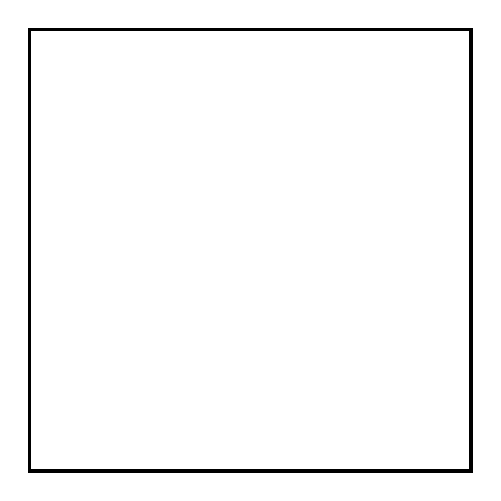
\begin{tikzpicture}
[borderdecorate/.style={-,very thick}]
%% chessboard with a black knight
\node at (0,4.9) {\WhiteEmptySquare\BlackEmptySquare\WhiteEmptySquare\BlackEmptySquare\WhiteEmptySquare\BlackEmptySquare\WhiteEmptySquare\BlackEmptySquare};
\node at (0,4.2) {\BlackEmptySquare\WhiteEmptySquare\BlackEmptySquare\WhiteEmptySquare\BlackEmptySquare\WhiteEmptySquare\BlackEmptySquare\WhiteEmptySquare};
\node at (0,3.5) {\WhiteEmptySquare\BlackEmptySquare\WhiteEmptySquare\BlackEmptySquare\WhiteEmptySquare\BlackEmptySquare\WhiteEmptySquare\BlackEmptySquare};
\node at (0,2.8) {\BlackEmptySquare\WhiteEmptySquare\BlackEmptySquare\WhiteEmptySquare\BlackKnightOnBlack\WhiteEmptySquare\BlackEmptySquare\WhiteEmptySquare};
\node at (0,2.1) {\WhiteEmptySquare\BlackEmptySquare\WhiteEmptySquare\BlackEmptySquare\WhiteEmptySquare\BlackEmptySquare\WhiteEmptySquare\BlackEmptySquare};
\node at (0,1.4) {\BlackEmptySquare\WhiteEmptySquare\BlackEmptySquare\WhiteEmptySquare\BlackEmptySquare\WhiteEmptySquare\BlackEmptySquare\WhiteEmptySquare};
\node at (0,0.7) {\WhiteEmptySquare\BlackEmptySquare\WhiteEmptySquare\BlackEmptySquare\WhiteEmptySquare\BlackEmptySquare\WhiteEmptySquare\BlackEmptySquare};
\node at (0,0.0) {\BlackEmptySquare\WhiteEmptySquare\BlackEmptySquare\WhiteEmptySquare\BlackEmptySquare\WhiteEmptySquare\BlackEmptySquare\WhiteEmptySquare};
%% the boarders of the chessboard
\draw[borderdecorate]
(-2.8,-0.352) -- (-2.8,5.257) -- (2.809,5.257) -- (2.809,-0.352) -- cycle;
\end{tikzpicture}
}
\quad
%%
%% knight's tour
\subfigure[A knight's tour.]{
\label{fig:graph_algorithms:one_knight_tour:a_tour}
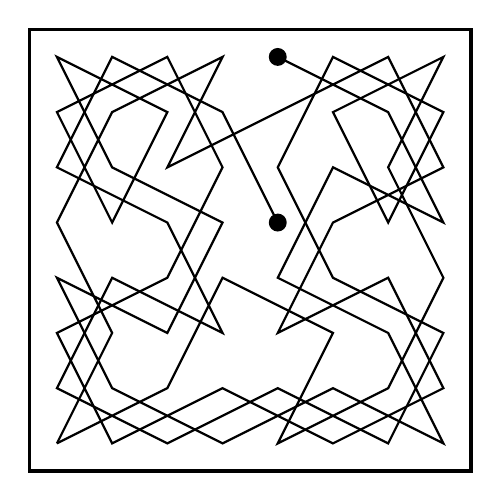
\begin{tikzpicture}
[borderdecorate/.style={-,very thick},%
  linedecorate/.style={-,thick},%
  nodedecorate/.style={shape=circle,fill=black,inner sep=2pt,draw,thick}]
%% empty chessboard
\node at (0,4.9) {\WhiteEmptySquare\BlackEmptySquare\WhiteEmptySquare\BlackEmptySquare\WhiteEmptySquare\BlackEmptySquare\WhiteEmptySquare\BlackEmptySquare};
\node at (0,4.2) {\BlackEmptySquare\WhiteEmptySquare\BlackEmptySquare\WhiteEmptySquare\BlackEmptySquare\WhiteEmptySquare\BlackEmptySquare\WhiteEmptySquare};
\node at (0,3.5) {\WhiteEmptySquare\BlackEmptySquare\WhiteEmptySquare\BlackEmptySquare\WhiteEmptySquare\BlackEmptySquare\WhiteEmptySquare\BlackEmptySquare};
\node at (0,2.8) {\BlackEmptySquare\WhiteEmptySquare\BlackEmptySquare\WhiteEmptySquare\BlackEmptySquare\WhiteEmptySquare\BlackEmptySquare\WhiteEmptySquare};
\node at (0,2.1) {\WhiteEmptySquare\BlackEmptySquare\WhiteEmptySquare\BlackEmptySquare\WhiteEmptySquare\BlackEmptySquare\WhiteEmptySquare\BlackEmptySquare};
\node at (0,1.4) {\BlackEmptySquare\WhiteEmptySquare\BlackEmptySquare\WhiteEmptySquare\BlackEmptySquare\WhiteEmptySquare\BlackEmptySquare\WhiteEmptySquare};
\node at (0,0.7) {\WhiteEmptySquare\BlackEmptySquare\WhiteEmptySquare\BlackEmptySquare\WhiteEmptySquare\BlackEmptySquare\WhiteEmptySquare\BlackEmptySquare};
\node at (0,0.0) {\BlackEmptySquare\WhiteEmptySquare\BlackEmptySquare\WhiteEmptySquare\BlackEmptySquare\WhiteEmptySquare\BlackEmptySquare\WhiteEmptySquare};
%% boarders of the chessboard
\draw[borderdecorate]
(-2.8,-0.352) -- (-2.8,5.257) -- (2.809,5.257) -- (2.809,-0.352) -- cycle;
%% map out knight's tour
\draw[linedecorate]
(-2.4494375,-0.0014374) -- ++(0.701125,1.40225) -- ++(-0.701125,1.40225)
-- ++(0.701125,1.40225) -- ++(1.40225,0.701125) -- ++(-0.701125,-1.40225)
-- ++(2.8045,1.40225) -- ++(0.701125,-1.40225) -- ++(-1.40225,-0.701125)
-- ++(-0.701125,-1.40225) -- ++(1.40225,0.701125) -- ++(0.701125,-1.40225)
-- ++(-1.40225,-0.701125) -- ++(-1.40225,0.701125) -- ++(-1.40225,-0.701125)
-- ++(-0.701125,1.40225) -- ++(1.40225,0.701125) -- ++(0.701125,1.40225)
-- ++(-0.701125,1.40225) -- ++(-1.40225,-0.701125) -- ++(0.701125,-1.40225)
-- ++(0.701125,1.40225) -- ++(-1.40225,0.701125) -- ++(0.701125,-1.40225)
-- ++(1.40225,-0.701125) -- ++(-0.701125,-1.40225) -- ++(-1.40225,0.701125)
-- ++(0.701125,-1.40225) -- ++(1.40225,-0.701125) -- ++(1.40225,0.701125)
-- ++(1.40225,-0.701125) -- ++(-0.701125,1.40225) -- ++(-1.40225,0.701125)
-- ++(0.701125,1.40225) -- ++(1.40225,-0.701125) -- ++(-0.701125,1.40225)
-- ++(-1.40225,0.701125);
\draw[linedecorate]
(-2.4494375,-0.0014374) -- ++(1.40225,0.701125) -- ++(0.701125,1.40225)
-- ++(1.40225,-0.701125) -- ++(-0.701125,-1.40225) -- ++(1.40225,0.701125)
-- ++(0.701125,1.40225) -- ++(-0.701125,1.40225) -- ++(0.701125,1.40225)
-- ++(-1.40225,-0.701125) -- ++(0.701125,-1.40225) -- ++(0.701125,1.40225)
-- ++(-1.40225,0.701125) -- ++(-0.701125,-1.40225) -- ++(0.701125,-1.40225)
-- ++(1.40225,-0.701125) -- ++(-0.701125,-1.40225) -- ++(-1.40225,0.701125)
-- ++(-1.40225,-0.701125) -- ++(-1.40225,0.701125) -- ++(0.701125,1.40225)
-- ++(1.40225,-0.701125) -- ++(-0.701125,1.40225) -- ++(-1.40225,0.701125)
-- ++(0.701125,1.40225) -- ++(1.40225,-0.701125) -- ++(0.701125,-1.40225);
%% filled dots to indicate the endpoints of the tour
\node at (0.3550625,2.8030626) [nodedecorate] {};
\node at (0.3550625,4.9064376) [nodedecorate] {};
\end{tikzpicture}
}
%%
%% graph representation of a knight's tour
\subfigure[Graph representation of tour.]{
\label{fig:graph_algorithms:one_knight_tour:graph_representation}
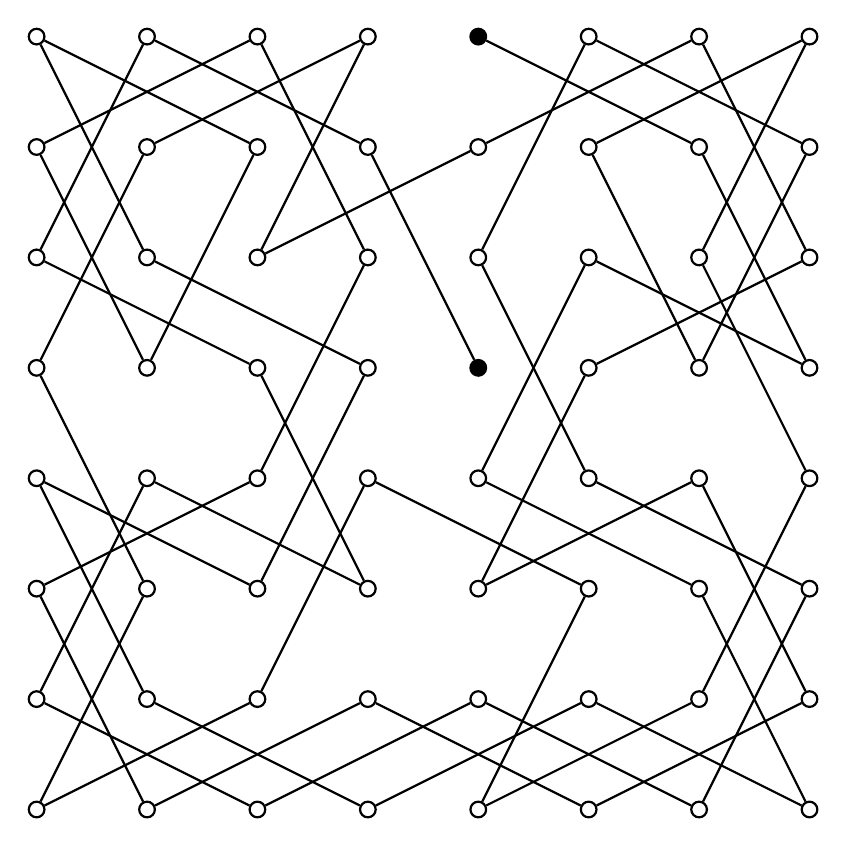
\begin{tikzpicture}
[linedecorate/.style={-,thick},%
  nodedecorate/.style={shape=circle,inner sep=2pt,draw,thick},%
  endpointdecorate/.style={shape=circle,fill=black,inner sep=2pt,draw,thick},%
  scale=2]
%% vertices or nodes
%% The coordinates of the chessboard are structured according to this
%% format
%%
%% 8
%% 7
%% *
%% *
%% *
%% 2
%% 1
%%   a  b  * * *  g  h
\foreach \nodename/\x/\y in {
a8/0/4.907875, b8/0.701125/4.907875, c8/1.40225/4.907875, d8/2.103375/4.907875, f8/3.505625/4.907875, g8/4.20675/4.907875, h8/4.907875/4.907875,
a7/0/4.20675, b7/0.701125/4.20675, c7/1.40225/4.20675, d7/2.103375/4.20675, e7/2.8045/4.20675, f7/3.505625/4.20675, g7/4.20675/4.20675, h7/4.907875/4.20675,
a6/0/3.505625, b6/0.701125/3.505625, c6/1.40225/3.505625, d6/2.103375/3.505625, e6/2.8045/3.505625, f6/3.505625/3.505625, g6/4.20675/3.505625, h6/4.907875/3.505625,
a5/0/2.8045, b5/0.701125/2.8045, c5/1.40225/2.8045, d5/2.103375/2.8045, f5/3.505625/2.8045, g5/4.20675/2.8045, h5/4.907875/2.8045,
a4/0/2.103375, b4/0.701125/2.103375, c4/1.40225/2.103375, d4/2.103375/2.103375, e4/2.8045/2.103375, f4/3.505625/2.103375, g4/4.20675/2.103375, h4/4.907875/2.103375,
a3/0/1.40225, b3/0.701125/1.40225, c3/1.40225/1.40225, d3/2.103375/1.40225, e3/2.8045/1.40225, f3/3.505625/1.40225, g3/4.20675/1.40225, h3/4.907875/1.40225,
a2/0/0.701125, b2/0.701125/0.701125, c2/1.40225/0.701125, d2/2.103375/0.701125, e2/2.8045/0.701125, f2/3.505625/0.701125, g2/4.20675/0.701125, h2/4.907875/0.701125,
a1/0/0, b1/0.701125/0, c1/1.40225/0, d1/2.103375/0, e1/2.8045/0, f1/3.505625/0, g1/4.20675/0, h1/4.907875/0}
{
  \node (\nodename) at (\x,\y) [nodedecorate] {};
}
%% endpoints of tour
\foreach \nodename/\x/\y in {e8/2.8045/4.907875, e5/2.8045/2.8045} {
  \node (\nodename) at (\x,\y) [endpointdecorate] {};
}
%% edges or lines
\path
\foreach \startnode/\endnode in {
e8/g7, g7/h5, h5/f6, f6/e4, e4/g3, g3/h1, h1/f2, f2/d1, d1/b2, b2/a4, a4/c3,
c3/d5, d5/b6, b6/a8, a8/c7, c7/b5, b5/a7, a7/c8, c8/d6, d6/c4, c4/a3, a3/b1,
b1/d2, d2/f1, f1/h2, h2/g4, g4/e3, e3/f5, f5/h6, h6/g8, g8/e7, e7/c6, c6/d8,
d8/b7, b7/a5, a5/b3, b3/a1, a1/c2, c2/d4, d4/f3, f3/e1, e1/g2, g2/h4, h4/g6,
g6/h8, h8/f7, f7/g5, g5/h7, h7/f8, f8/e6, e6/f4, f4/h3, h3/g1, g1/e2, e2/c1,
c1/a2, a2/b4, b4/d3, d3/c5, c5/a6, a6/b8, b8/d7, d7/e5}
{
  (\startnode) edge[linedecorate] node {} (\endnode)
};
\end{tikzpicture}
}

\caption{The knight's tour from a given starting position.}
\label{fig:graph_algorithms:one_knight_tour}
\end{figure}

To get an intuitive appreciation for DFS\index{DFS}, suppose we have
an $8 \times 8$ chessboard\index{chess!chessboard} in front of us. We
place a single knight\index{chess!knight piece} piece on a fixed
square of the board, as shown in
Figure~\ref{fig:graph_algorithms:one_knight_tour:initial_position}. Our
objective is to find a sequence of knight\index{chess!knight piece}
moves that visits each and every square exactly once, while obeying
the rules of chess\index{chess} that govern the movement of the knight
piece\index{chess!knight piece}. Such a sequence of moves, if one
exists, is called a \emph{knight's tour}\index{chess!knight's tour}. How do
we find such a tour? We could make one knight\index{chess!knight} move
after another, recording each move to ensure that we do not step on a
square that is already visited, until we could not make any more
moves. Acknowledging defeat when encountering a dead end, it might
make sense to \emph{backtrack}\index{backtrack} a few moves and try
again, hoping we would not get stuck. If we fail again, we try
backtracking\index{backtrack} a few more moves and traverse yet
another path, hoping to make further progress. Repeat this strategy
until a tour is found or until we have exhausted all possible
moves. The above strategy for finding a knight's
tour\index{chess!knight's tour} is an example of depth-first
search\index{depth-first search}, sometimes called
\emph{backtracking}. Figure~\ref{fig:graph_algorithms:one_knight_tour:a_tour}
shows a knight's tour with the starting position as shown in
Figure~\ref{fig:graph_algorithms:one_knight_tour:initial_position};
and
Figure~\ref{fig:graph_algorithms:one_knight_tour:graph_representation}
is a graph representation of this tour. The black-filled nodes
indicate the endpoints of the tour. A more interesting question is:
What is the number of knight's tours on an $8 \times 8$ chessboard?
Loebbing\index{Loebbing, Martin} and
Wegener~\cite{LoebbingWegener1996}\index{Wegener, Ingo} announced in
1996 that this number is 33,439,123,484,294. The answer was later
corrected by McKay~\cite{McKay1997}\index{McKay, Brendan D.} to be
13,267,364,410,532. See~\cite{ElkiesStanley2003}
for\index{Elkies, Noam D.}\index{Stanley, Richard P.} a discussion of
the knight's tour and its relationship to mathematics.

\begin{algorithm}[!htbp]
\index{depth-first search}\index{DFS}
%%%%%%%%%%%%%%%%%%%%%%%%%%%%%%%%%%%%%%%%%%%%%%%%%%%%%%%%%%%%%%%%%%%%%%%%%%%
%% This file is part of the book
%%
%% Algorithmic Graph Theory
%% http://code.google.com/p/graph-theory-algorithms-book/
%%
%% Copyright (C) 2009, 2010 Minh Van Nguyen <nguyenminh2@gmail.com>
%%
%% See the file COPYING for copying conditions.
%%%%%%%%%%%%%%%%%%%%%%%%%%%%%%%%%%%%%%%%%%%%%%%%%%%%%%%%%%%%%%%%%%%%%%%%%%%

\DontPrintSemicolon
\SetAlgoNoLine
%%
%% data section
\SetKwInOut{Input}{Input}
\SetKwInOut{Output}{Output}
%%
%% input/output
\Input{A directed or undirected graph $G = (V, E)$ of order $n > 0$. A
  vertex $s$ from which to start the search. The vertices are numbered
  from $1$ to  $n = |V|$, i.e. $V = \{1, 2, \dots, n\}$.}
\Output{A list $D$ of distances of all vertices from $s$. A tree $T$
  rooted at $s$.}
\BlankLine
%%
%% algorithm body
$S \assign [s]$ \tcc*[f]{stack of nodes to visit}\;
$D \assign [\infty, \infty, \dots, \infty]$ \tcc*[f]{$n$ copies of $\infty$}\;
$D[s] \assign 0$\;
$T \assign [\,]$\;
\While{$\length(S) > 0$~\nllabel{alg:DFS:while_loop_tests_non_empty_stack}}{
  $v \assign \pop(S)$\;
  \For{\emph{each} $w \in \adj(v)$~\nllabel{alg:DFS:for_loop_visit_neighbors}}{
    \If{$D[w] = \infty$~\nllabel{alg:DFS:if_test_unvisited_neighbors}}{
      $D[w] \assign D[v] + 1$\;
      $\push(S, w)$\;
      $\append(T, vw)$\;
    }
  }
}
\Return $(D, T)$\;

\caption{A general depth-first search template.}
\label{alg:graph_algorithms:depth_first_search_template}
\end{algorithm}

Algorithm~\ref{alg:graph_algorithms:depth_first_search_template}
formalizes the above description of depth-first
search\index{depth-first search}. The tree resulting from applying
DFS\index{DFS} on a graph is called a
\emph{depth-first search tree}\index{depth-first search!tree}. The
general structure of this algorithm bears close resemblance to
Algorithm~\ref{alg:graph_algorithms:breadth_first_search_template}. A
significant difference is that instead of using a queue\index{queue}
to structure and organize vertices to be visited, DFS\index{DFS} uses
another special type of list\index{list} called a
\emph{stack}\index{stack}. To understand how elements of a stack are
organized, we use the analogy of a stack of cards\index{card}. A new
card is added to the stack by placing it on top of the stack. Any time
we want to remove a card, we are only allowed to remove the top-most
card that is on the top of the stack. A list\index{list}
$L = [a_1, a_2, \dots, a_k]$ of $k$ elements is a stack when we impose
the same rules for element insertion and removal. The top and bottom
of the stack are $L[k]$ and $L[1]$, respectively. The operation of
removing the top element of the stack is referred to as
\emph{popping}\index{stack!pop} the element off the stack. Inserting
an element into the stack is called \emph{pushing}\index{stack!push}
the element onto the stack. In other words, a stack implements a
last-in first-out~(LIFO)\index{last in, first out}\index{LIFO}
protocol for element insertion and removal, in contrast to the
FIFO\index{FIFO} policy of a queue\index{queue}. We also use the term
\emph{length}\index{stack!length} to refer to the number of elements
in the stack.

\begin{figure}[!htbp]
\centering
\index{depth-first search}\index{DFS}
%%%%%%%%%%%%%%%%%%%%%%%%%%%%%%%%%%%%%%%%%%%%%%%%%%%%%%%%%%%%%%%%%%%%%%%%%%%
%% This file is part of the book
%%
%% Algorithmic Graph Theory
%% http://code.google.com/p/graph-theory-algorithms-book/
%%
%% Copyright (C) 2009, 2010 Minh Van Nguyen <nguyenminh2@gmail.com>
%%
%% See the file COPYING for copying conditions.
%%%%%%%%%%%%%%%%%%%%%%%%%%%%%%%%%%%%%%%%%%%%%%%%%%%%%%%%%%%%%%%%%%%%%%%%%%%

\subfigure[]{
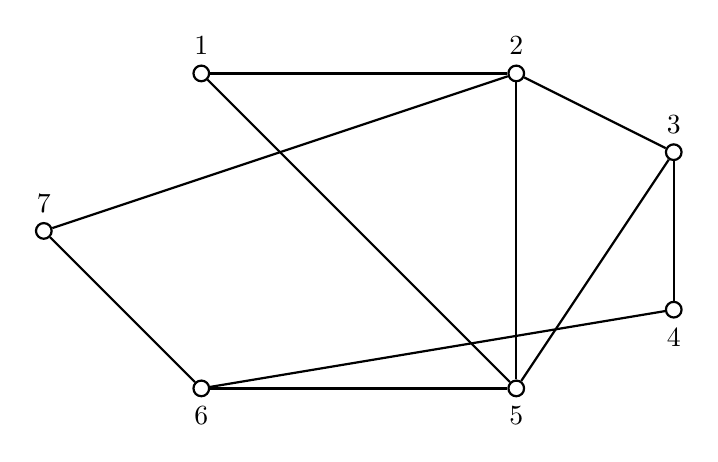
\begin{tikzpicture}
[nodedecorate/.style={shape=circle,inner sep=2pt,draw,thick},%
  linedecorate/.style={-,thick}]
%% nodes or vertices
\foreach \nodename/\x/\y/\direction/\navigate in {2/4/4/above/north,
  1/0/4/above/north, 3/6/3/above/north, 4/6/1/below/south,
  5/4/0/below/south, 7/-2/2/above/north, 6/0/0/below/south}
{
  \node (\nodename) at (\x,\y) [nodedecorate] {};
  \node [\direction] at (\nodename.\navigate) {$\nodename$};
}
%% edges or lines
\path
\foreach \startnode/\endnode in {1/2, 1/5, 2/3, 2/5, 2/7, 3/4, 3/5,
  4/6, 5/6, 6/7}
{
  (\startnode) edge[linedecorate] node {} (\endnode)
};
\end{tikzpicture}
}
%%
%%
\qquad
\subfigure[]{
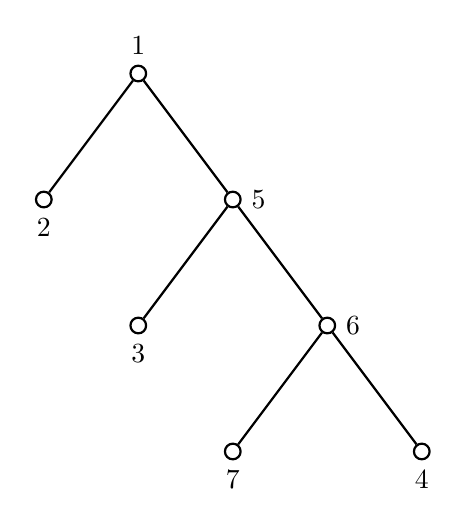
\begin{tikzpicture}
[nodedecorate/.style={shape=circle,inner sep=2pt,draw,thick},%
  linedecorate/.style={-,thick},%
  scale=1.6]
%% nodes or vertices
\foreach \nodename/\x/\y/\direction/\navigate in {
  1/1.25/3/above/north, 2/0.5/2/below/south, 5/2/2/right/east,
  3/1.25/1/below/south, 6/2.75/1/right/east, 7/2/0/below/south,
  4/3.5/0/below/south}
{
  \node (\nodename) at (\x,\y) [nodedecorate] {};
  \node [\direction] at (\nodename.\navigate) {$\nodename$};
}
%% edges or lines
\path
\foreach \startnode/\endnode in {1/2, 1/5, 3/5, 5/6, 6/7, 6/4} {
  (\startnode) edge[linedecorate] node {} (\endnode)
};
\end{tikzpicture}
}
%%
%%
\subfigure[]{
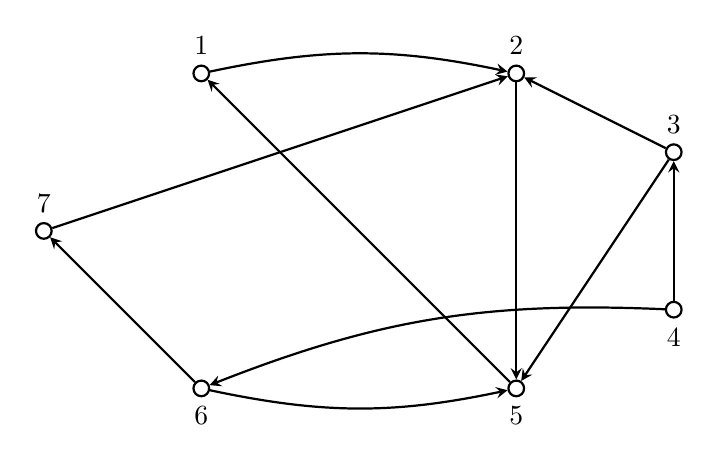
\begin{tikzpicture}
[nodedecorate/.style={shape=circle,inner sep=2pt,draw,thick},%
  arrowdecorate/.style={->,>=stealth,thick}]
%% nodes or vertices
\foreach \nodename/\x/\y/\direction/\navigate in {2/4/4/above/north,
  1/0/4/above/north, 3/6/3/above/north, 4/6/1/below/south,
  5/4/0/below/south, 7/-2/2/above/north, 6/0/0/below/south}
{
  \node (\nodename) at (\x,\y) [nodedecorate] {};
  \node [\direction] at (\nodename.\navigate) {$\nodename$};
}
%% edges or lines
\path
\foreach \startnode/\endnode in {2/5, 3/2, 3/5, 4/3, 5/1, 6/7, 7/2} {
  (\startnode) edge[arrowdecorate] node {} (\endnode)
}
\foreach \startnode/\endnode/\benddirection/\angle in {
  1/2/bend left/12, 4/6/bend right/12, 6/5/bend right/12}
{
  (\startnode) edge[arrowdecorate,\benddirection=\angle] node {} (\endnode)
};
\end{tikzpicture}
}
%%
%%
\qquad
\subfigure[]{
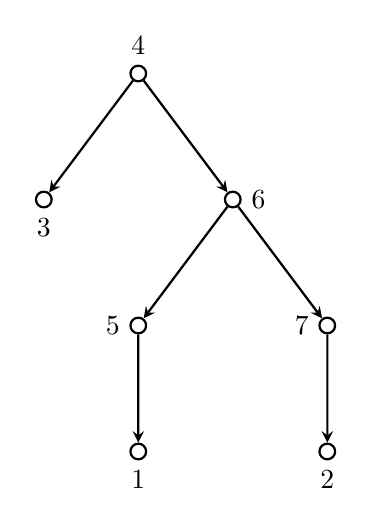
\begin{tikzpicture}
[nodedecorate/.style={shape=circle,inner sep=2pt,draw,thick},%
  arrowdecorate/.style={->,>=stealth,thick},
  scale=1.6]
%% nodes or vertices
\foreach \nodename/\x/\y/\direction/\navigate in {
  4/1.25/3/above/north, 3/0.5/2/below/south, 6/2/2/right/east,
  5/1.25/1/left/west, 7/2.75/1/left/west, 1/1.25/0/below/south,
  2/2.75/0/below/south}
{
  \node (\nodename) at (\x,\y) [nodedecorate] {};
  \node [\direction] at (\nodename.\navigate) {$\nodename$};
}
%% edges or lines
\path
\foreach \startnode/\endnode in {4/3, 4/6, 6/5, 6/7, 5/1, 7/2} {
  (\startnode) edge[arrowdecorate] node {} (\endnode)
};
\end{tikzpicture}
}

\caption{Depth-first search tree for an undirected graph.}
\label{fig:graph_algorithms:depth_first_search_undirected}
\end{figure}

\begin{figure}[!htbp]
\centering
\index{depth-first search}\index{DFS}
%%%%%%%%%%%%%%%%%%%%%%%%%%%%%%%%%%%%%%%%%%%%%%%%%%%%%%%%%%%%%%%%%%%%%%%%%%%
%% This file is part of the book
%%
%% Algorithmic Graph Theory
%% http://code.google.com/p/graph-theory-algorithms-book/
%%
%% Copyright (C) 2009, 2010 Minh Van Nguyen <nguyenminh2@gmail.com>
%%
%% See the file COPYING for copying conditions.
%%%%%%%%%%%%%%%%%%%%%%%%%%%%%%%%%%%%%%%%%%%%%%%%%%%%%%%%%%%%%%%%%%%%%%%%%%%

\subfigure[Original digraph.]{
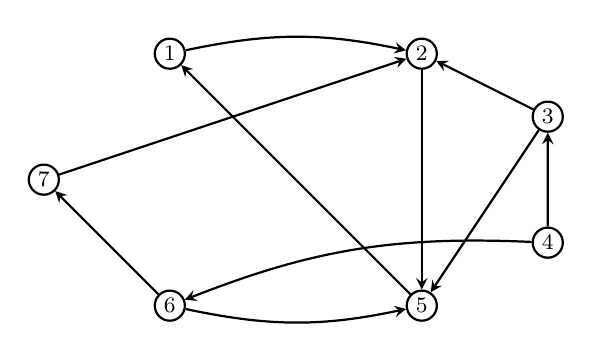
\begin{tikzpicture}
[arrowDecorate/.style={->,>=stealth,thick},%
  nodeDecorate/.style={shape=circle,inner sep=1.5pt,draw,thick},%
  scale=0.8]
%% nodes or vertices
\foreach \nodename/\x/\y in {2/4/4, 1/0/4, 3/6/3, 4/6/1, 5/4/0, 7/-2/2, 6/0/0}
{
  \node (\nodename) at (\x,\y) [nodeDecorate] {\footnotesize$\nodename$};
}
%% edges or lines
\path
\foreach \startnode/\endnode in {2/5, 3/2, 3/5, 4/3, 5/1, 6/7, 7/2}
{
  (\startnode) edge[arrowDecorate] node {} (\endnode)
}
\foreach \startnode/\endnode/\benddirection/\angle in {
  1/2/bend left/12, 4/6/bend right/12, 6/5/bend right/12}
{
  (\startnode) edge[arrowDecorate,\benddirection=\angle] node {} (\endnode)
};
\end{tikzpicture}
}
%%
%%
\qquad
\subfigure[First iteration of while loop.]{
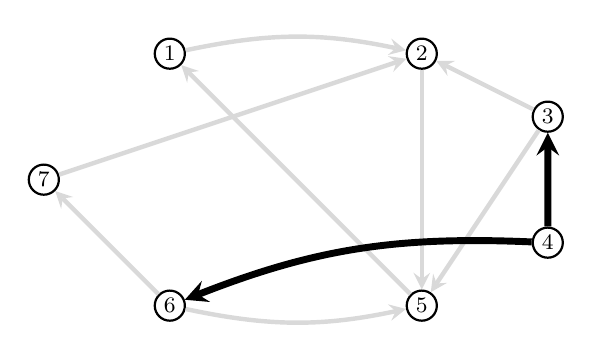
\begin{tikzpicture}
[darkArrow/.style={->,>=stealth,line width=2.5pt},%
  lightArrow/.style={->,>=stealth,ultra thick,color=gray!30},%
  nodeDecorate/.style={shape=circle,inner sep=1.5pt,draw,thick},%
  scale=0.8]
%% nodes or vertices
\foreach \nodename/\x/\y in {2/4/4, 1/0/4, 3/6/3, 4/6/1, 5/4/0, 7/-2/2, 6/0/0}
{
  \node (\nodename) at (\x,\y) [nodeDecorate] {\footnotesize$\nodename$};
}
%% light edges or lines
\path
\foreach \startnode/\endnode in {2/5, 3/2, 3/5, 5/1, 6/7, 7/2}
{
  (\startnode) edge[lightArrow] node {} (\endnode)
}
\foreach \startnode/\endnode/\benddirection/\angle in {
  1/2/bend left/12, 6/5/bend right/12}
{
  (\startnode) edge[lightArrow,\benddirection=\angle] node {} (\endnode)
}
%% dark edges or lines
\foreach \startnode/\endnode in {4/3}
{
  (\startnode) edge[darkArrow] node {} (\endnode)
}
\foreach \startnode/\endnode/\benddirection/\angle in {4/6/bend right/12}
{
  (\startnode) edge[darkArrow,\benddirection=\angle] node {} (\endnode)
};
\end{tikzpicture}
}
%%
%%
\subfigure[Second iteration of while loop.]{
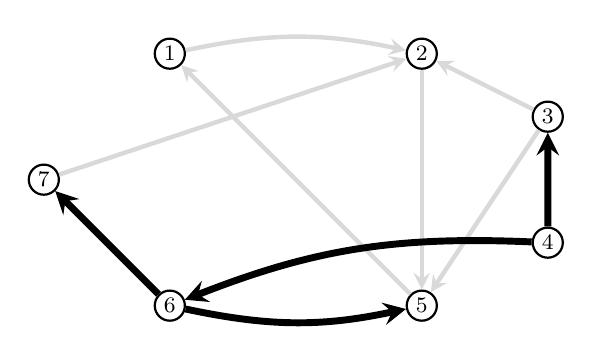
\begin{tikzpicture}
[darkArrow/.style={->,>=stealth,line width=2.5pt},%
  lightArrow/.style={->,>=stealth,ultra thick,color=gray!30},%
  nodeDecorate/.style={shape=circle,inner sep=1.5pt,draw,thick},%
  scale=0.8]
%% nodes or vertices
\foreach \nodename/\x/\y in {2/4/4, 1/0/4, 3/6/3, 4/6/1, 5/4/0, 7/-2/2, 6/0/0}
{
  \node (\nodename) at (\x,\y) [nodeDecorate] {\footnotesize$\nodename$};
}
%% light edges or lines
\path
\foreach \startnode/\endnode in {2/5, 3/2, 3/5, 5/1, 7/2}
{
  (\startnode) edge[lightArrow] node {} (\endnode)
}
\foreach \startnode/\endnode/\benddirection/\angle in {1/2/bend left/12}
{
  (\startnode) edge[lightArrow,\benddirection=\angle] node {} (\endnode)
}
%% dark edges or lines
\foreach \startnode/\endnode in {4/3, 6/7}
{
  (\startnode) edge[darkArrow] node {} (\endnode)
}
\foreach \startnode/\endnode/\benddirection/\angle in {
  4/6/bend right/12, 6/5/bend right/12}
{
  (\startnode) edge[darkArrow,\benddirection=\angle] node {} (\endnode)
};
\end{tikzpicture}
}
%%
%%
\qquad
\subfigure[Third iteration of while loop.]{
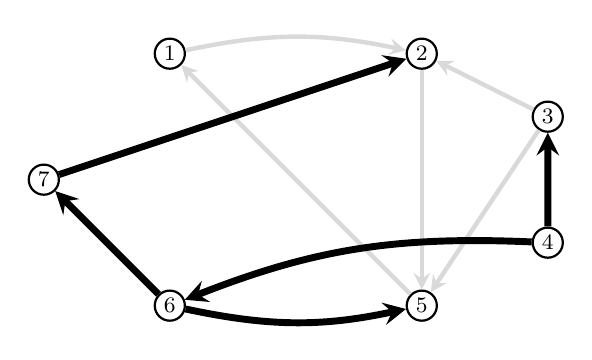
\begin{tikzpicture}
[darkArrow/.style={->,>=stealth,line width=2.5pt},%
  lightArrow/.style={->,>=stealth,ultra thick,color=gray!30},%
  nodeDecorate/.style={shape=circle,inner sep=1.5pt,draw,thick},%
  scale=0.8]
%% nodes or vertices
\foreach \nodename/\x/\y in {2/4/4, 1/0/4, 3/6/3, 4/6/1, 5/4/0, 7/-2/2, 6/0/0}
{
  \node (\nodename) at (\x,\y) [nodeDecorate] {\footnotesize$\nodename$};
}
%% light edges or lines
\path
\foreach \startnode/\endnode in {2/5, 3/2, 3/5, 5/1}
{
  (\startnode) edge[lightArrow] node {} (\endnode)
}
\foreach \startnode/\endnode/\benddirection/\angle in {1/2/bend left/12}
{
  (\startnode) edge[lightArrow,\benddirection=\angle] node {} (\endnode)
}
%% dark edges or lines
\foreach \startnode/\endnode in {4/3, 6/7, 7/2}
{
  (\startnode) edge[darkArrow] node {} (\endnode)
}
\foreach \startnode/\endnode/\benddirection/\angle in {
  4/6/bend right/12, 6/5/bend right/12}
{
  (\startnode) edge[darkArrow,\benddirection=\angle] node {} (\endnode)
};
\end{tikzpicture}
}
%%
%%
\subfigure[Fourth iteration of while loop.]{
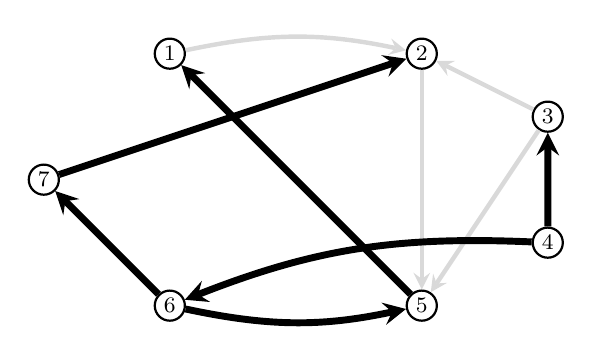
\begin{tikzpicture}
[darkArrow/.style={->,>=stealth,line width=2.5pt},%
  lightArrow/.style={->,>=stealth,ultra thick,color=gray!30},%
  nodeDecorate/.style={shape=circle,inner sep=1.5pt,draw,thick},%
  scale=0.8]
%% nodes or vertices
\foreach \nodename/\x/\y in {2/4/4, 1/0/4, 3/6/3, 4/6/1, 5/4/0, 7/-2/2, 6/0/0}
{
  \node (\nodename) at (\x,\y) [nodeDecorate] {\footnotesize$\nodename$};
}
%% light edges or lines
\path
\foreach \startnode/\endnode in {2/5, 3/2, 3/5}
{
  (\startnode) edge[lightArrow] node {} (\endnode)
}
\foreach \startnode/\endnode/\benddirection/\angle in {1/2/bend left/12}
{
  (\startnode) edge[lightArrow,\benddirection=\angle] node {} (\endnode)
}
%% dark edges or lines
\foreach \startnode/\endnode in {4/3, 5/1, 6/7, 7/2}
{
  (\startnode) edge[darkArrow] node {} (\endnode)
}
\foreach \startnode/\endnode/\benddirection/\angle in {
  4/6/bend right/12, 6/5/bend right/12}
{
  (\startnode) edge[darkArrow,\benddirection=\angle] node {} (\endnode)
};
\end{tikzpicture}
}
%%
%%
\qquad
\subfigure[Final DFS tree.]{
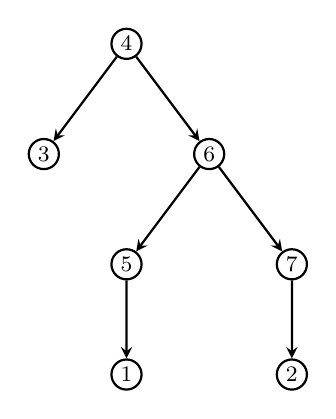
\begin{tikzpicture}
[arrowDecorate/.style={->,>=stealth,thick},%
  nodeDecorate/.style={shape=circle,inner sep=1.5pt,draw,thick},%
  scale=1.4]
%% nodes or vertices
\foreach \nodename/\x/\y in {
  4/1.25/3, 3/0.5/2, 6/2/2, 5/1.25/1, 7/2.75/1, 1/1.25/0, 2/2.75/0}
{
  \node (\nodename) at (\x,\y) [nodeDecorate] {\footnotesize$\nodename$};
}
%% edges or lines
\path
\foreach \startnode/\endnode in {4/3, 4/6, 6/5, 6/7, 5/1, 7/2}
{
  (\startnode) edge[arrowDecorate] node {} (\endnode)
};
\end{tikzpicture}
}

\caption{Depth-first search tree for a digraph.}
\label{fig:graph_algorithms:depth_first_search_directed}
\end{figure}

The depth-first search\index{depth-first search}
Algorithm~\ref{alg:graph_algorithms:depth_first_search_template} can
be analyzed similar to how we analyzed
Algorithm~\ref{fig:graph_algorithms:breadth_first_search_undirected}. Just
as BFS\index{BFS} is applicable to both directed and undirected
graphs, we can also have undirected graphs and digraphs as input to
DFS\index{DFS}. For the case of an undirected graph,
line~\ref{alg:DFS:for_loop_visit_neighbors} of
Algorithm~\ref{alg:graph_algorithms:depth_first_search_template}
considers all vertices adjacent to the current vertex $v$. In case the
input graph is directed, we replace ``$w \in \adj(v)$'' on
line~\ref{alg:DFS:for_loop_visit_neighbors} with ``$w \in \oadj(v)$''
to signify that we only want to consider the
out-neighbors\index{out-neighbor} of $v$. If any neighbors
(respectively, out-neighbors\index{out-neighbor}) of $v$ are labelled
as $\infty$, we know that we have not explored any paths starting from
any of those vertices. So we label each of those unexplored vertices
with a positive integer and push them onto the stack\index{stack} $S$,
where they will wait for later processing. We also record the paths
leading from $v$ to each of those unvisited neighbors, i.e. the edges
$vw$ for each vertex $w \in \adj(v)$ (respectively, $w \in \oadj(v)$)
are appended to the list $T$. The test on
line~\ref{alg:DFS:if_test_unvisited_neighbors} ensures that we do not
push onto $S$ any vertices on the path that lead to $v$. When we
resume another round of the while loop that starts on
line~\ref{alg:DFS:while_loop_tests_non_empty_stack}, the previous
vertex $v$ have been popped\index{stack!pop} off $S$ and the neighbors
(respectively, out-neighbors\index{out-neighbor}) of $v$ have been
pushed\index{stack!push} onto $S$. To explore a path starting at $v$,
we choose any unexplored neighbors of $v$ by popping an element off
$S$ and repeat the for loop starting on
line~\ref{alg:DFS:for_loop_visit_neighbors}. Repeat the DFS\index{DFS}
algorithm as often as required in order to traverse all vertices of
the input graph. The output of DFS\index{DFS} consists of two lists
$D$ and $T$: $T$ is a tree rooted\index{tree!rooted} at the starting
vertex $s$; and each $D[i]$ counts the length of the $s$-$v_i$ path in
$T$. Figures~\ref{fig:graph_algorithms:depth_first_search_undirected}
and~\ref{fig:graph_algorithms:depth_first_search_directed} show the
DFS\index{DFS} trees\index{depth-first search!tree} resulting from
running Algorithm~\ref{alg:graph_algorithms:depth_first_search_template}
on an undirected graph and a digraph, respectively. The worst-case
time complexity of DFS\index{DFS} can be analyzed using an argument
similar to that in
Theorem~\ref{thm:graph_algorithms:BFS:worst_case_time_complexity}.
Arguing along the same lines as in the proof of
Theorem~\ref{thm:graph_algorithms:BFS:list_D_length_shortest_paths},
we can also show that the list $D$ returned by DFS\index{DFS} contains
lengths of any shortest paths from the starting vertex $s$ to any
other vertex in the tree $T$.

\begin{figure}[!htbp]
\centering
\index{Petersen!graph}
%%%%%%%%%%%%%%%%%%%%%%%%%%%%%%%%%%%%%%%%%%%%%%%%%%%%%%%%%%%%%%%%%%%%%%%%%%%
%% This file is part of the book
%%
%% Algorithmic Graph Theory
%% http://code.google.com/p/graph-theory-algorithms-book/
%%
%% Copyright (C) 2009, 2010 Minh Van Nguyen <nguyenminh2@gmail.com>
%%
%% See the file COPYING for copying conditions.
%%%%%%%%%%%%%%%%%%%%%%%%%%%%%%%%%%%%%%%%%%%%%%%%%%%%%%%%%%%%%%%%%%%%%%%%%%%

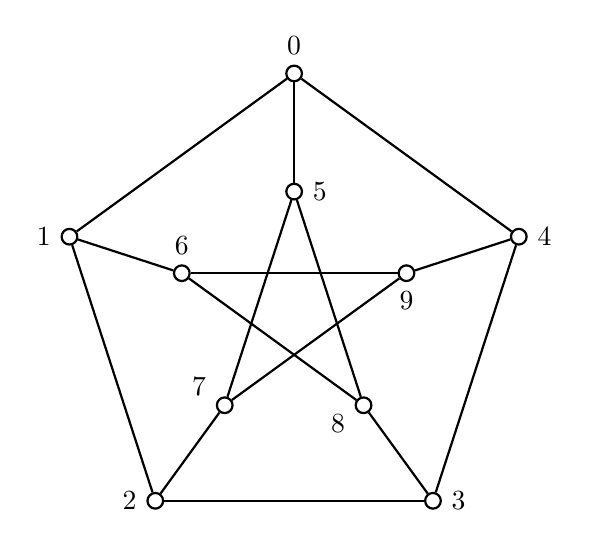
\begin{tikzpicture}
[nodedecorate/.style={shape=circle,inner sep=2pt,draw,thick},%
  linedecorate/.style={-,thick},
  scale=1.5]
%% nodes or vertices
\foreach \nodename/\x/\y/\direction/\navigate in {
  %% inner star
  5/0.0/1.0/right/east, 9/0.9510/0.3090/below/south,
  8/0.5877/-0.8090/below left/west, 7/-0.5877/-0.8090/above left/west,
  6/-0.9510/0.3090/above/north,
  %% outer pentagon
  0/0.0/2.0/above/north, 4/1.9021/0.6180/right/east,
  3/1.1755/-1.6180/right/east, 2/-1.1755/-1.6180/left/west,
  1/-1.9021/0.6180/left/west}
{
  \node (\nodename) at (\x,\y) [nodedecorate] {};
  \node [\direction] at (\nodename.\navigate) {$\nodename$};
}
%% edges or lines
\path
\foreach \startnode/\endnode in {0/1, 0/5, 1/2, 1/6, 2/3, 2/7, 3/4,
  3/8, 4/0, 4/9, 5/7, 7/9, 9/6, 6/8, 8/5}
{
  (\startnode) edge[linedecorate] node {} (\endnode)
};
\end{tikzpicture}

\caption{The Petersen graph.}
\label{fig:graph_algorithms:Petersen_graph}
\end{figure}

\begin{example}
In 1898, Julius Petersen\index{Petersen!Julius}
published~\cite{Petersen1898} a graph that now bears his name: the
Petersen graph\index{Petersen!graph} shown in
Figure~\ref{fig:graph_algorithms:Petersen_graph}. Compare the search
trees resulting from running breadth-\index{breadth-first search} and
depth-first searches\index{depth-first search} on the Petersen
graph\index{Petersen!graph} with starting vertex $0$.
\end{example}

\begin{proof}[Solution]
The Petersen graph\index{Petersen!graph} in
Figure~\ref{fig:graph_algorithms:Petersen_graph}
can be constructed and searched as follows.
%%
\begin{lstlisting}
sage: g = graphs.PetersenGraph(); g
Petersen graph: Graph on 10 vertices
sage: list(g.breadth_first_search(0))
[0, 1, 4, 5, 2, 6, 3, 9, 7, 8]
sage: list(g.depth_first_search(0))
[0, 5, 8, 6, 9, 7, 2, 3, 4, 1]
\end{lstlisting}
%%
From the above Sage session, we see that starting from vertex $0$
breadth-first search\index{breadth-first search} yields the edge list
\[
[01,\, 04,\, 05,\, 12,\, 16,\, 43,\, 49,\, 57,\, 58]
\]
and depth-first search\index{depth-first search} produces the
corresponding edge list
\[
[05,\, 58,\, 86,\, 69,\, 97,\, 72,\, 23,\, 34,\, 01].
\]
Our results are illustrated in
Figure~\ref{fig:graph_algorithms:search_Petersen_graph}.
%%
\begin{figure}[!htbp]
\centering
\index{breadth-first search}
\index{depth-first search}
\index{Petersen!graph}
%%%%%%%%%%%%%%%%%%%%%%%%%%%%%%%%%%%%%%%%%%%%%%%%%%%%%%%%%%%%%%%%%%%%%%%%%%%
%% This file is part of the book
%%
%% Algorithmic Graph Theory
%% http://code.google.com/p/graph-theory-algorithms-book/
%%
%% Copyright (C) 2009, 2010 Minh Van Nguyen <nguyenminh2@gmail.com>
%%
%% See the file COPYING for copying conditions.
%%%%%%%%%%%%%%%%%%%%%%%%%%%%%%%%%%%%%%%%%%%%%%%%%%%%%%%%%%%%%%%%%%%%%%%%%%%

%% breadth-first searching the Petersen graph
\subfigure[Breadth-first search.]{
\index{breadth-first search}
\index{Petersen graph}
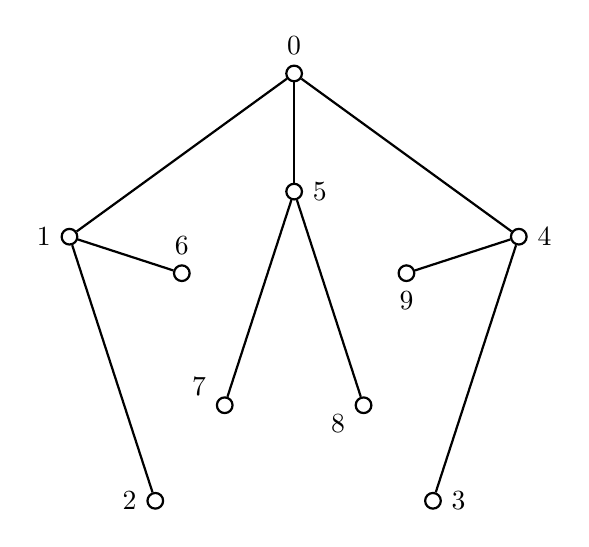
\begin{tikzpicture}
[nodedecorate/.style={shape=circle,inner sep=2pt,draw,thick},%
  linedecorate/.style={-,thick},
  scale=1.5]
%% nodes or vertices
\foreach \nodename/\x/\y/\direction/\navigate in {
  %% inner star
  5/0.0/1.0/right/east, 9/0.9510/0.3090/below/south,
  8/0.5877/-0.8090/below left/west, 7/-0.5877/-0.8090/above left/west,
  6/-0.9510/0.3090/above/north,
  %% outer pentagon
  0/0.0/2.0/above/north, 4/1.9021/0.6180/right/east,
  3/1.1755/-1.6180/right/east, 2/-1.1755/-1.6180/left/west,
  1/-1.9021/0.6180/left/west}
{
  \node (\nodename) at (\x,\y) [nodedecorate] {};
  \node [\direction] at (\nodename.\navigate) {$\nodename$};
}
%% edges or lines
\path
\foreach \startnode/\endnode in {0/1, 0/4, 0/5, 1/2, 1/6, 4/3, 4/9,
  5/7, 5/8}
{
  (\startnode) edge[linedecorate] node {} (\endnode)
};
\end{tikzpicture}

}
\quad
%%
%% depth-first searching the Petersen graph
\subfigure[Depth-first search.]{
\index{depth-first search}
\index{Petersen graph}
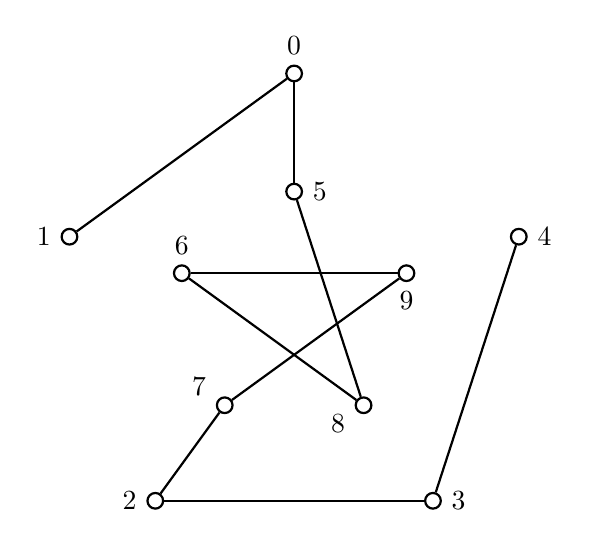
\begin{tikzpicture}
[nodedecorate/.style={shape=circle,inner sep=2pt,draw,thick},%
  linedecorate/.style={-,thick},
  scale=1.5]
%% nodes or vertices
\foreach \nodename/\x/\y/\direction/\navigate in {
  %% inner star
  5/0.0/1.0/right/east, 9/0.9510/0.3090/below/south,
  8/0.5877/-0.8090/below left/west, 7/-0.5877/-0.8090/above left/west,
  6/-0.9510/0.3090/above/north,
  %% outer pentagon
  0/0.0/2.0/above/north, 4/1.9021/0.6180/right/east,
  3/1.1755/-1.6180/right/east, 2/-1.1755/-1.6180/left/west,
  1/-1.9021/0.6180/left/west}
{
  \node (\nodename) at (\x,\y) [nodedecorate] {};
  \node [\direction] at (\nodename.\navigate) {$\nodename$};
}
%% edges or lines
\path
\foreach \startnode/\endnode in {0/5, 5/8, 8/6, 6/9, 9/7, 7/2, 2/3,
  3/4, 0/1}
{
  (\startnode) edge[linedecorate] node {} (\endnode)
};
\end{tikzpicture}
}

\caption{Traversing the Petersen graph starting from vertex $0$.}
\label{fig:graph_algorithms:search_Petersen_graph}
\end{figure}
\end{proof}


%%%%%%%%%%%%%%%%%%%%%%%%%%%%%%%%%%%%%%%%%%%%%%%%%%%%%%%%%%%%%%%%%%%%%%%%%%%

\subsection{Connectivity of a graph}
\index{graph!connected}

Both BFS\index{BFS} and DFS\index{DFS} can be used to determine if an
undirected graph is connected. Let $G = (V, E)$ be an undirected graph
of order $n > 0$ and let $s$ be an arbitrary vertex of $G$. We
initialize a counter $c \assign 1$ to mean that we are starting our
exploration at $s$, hence we have already visited one vertex,
i.e. $s$. We apply either BFS\index{BFS} or DFS\index{DFS}, treating
$G$ and $s$ as input to any of these algorithms. Each time we visit a
vertex that was previously unvisited, we increment the counter $c$. At
the end of the algorithm, we compare $c$ with $n$. If $c = n$, we know
that we have visited all vertices of $G$ and conclude that $G$ is
connected. Otherwise, we conclude that $G$ is disconnected. This
procedure is summarized in
Algorithm~\ref{alg:graph_algorithms:graph_connectivity}.

\begin{algorithm}[!htbp]
\index{graph!connected}
%%%%%%%%%%%%%%%%%%%%%%%%%%%%%%%%%%%%%%%%%%%%%%%%%%%%%%%%%%%%%%%%%%%%%%%%%%%
%% This file is part of the book
%%
%% Algorithmic Graph Theory
%% http://code.google.com/p/graph-theory-algorithms-book/
%%
%% Copyright (C) 2009, 2010 Minh Van Nguyen <nguyenminh2@gmail.com>
%%
%% See the file COPYING for copying conditions.
%%%%%%%%%%%%%%%%%%%%%%%%%%%%%%%%%%%%%%%%%%%%%%%%%%%%%%%%%%%%%%%%%%%%%%%%%%%

\dontprintsemicolon
%%
%% data section
\SetKwInOut{Input}{Input}
\SetKwInOut{Output}{Output}
\SetKwData{MyFalse}{False}
\SetKwData{MyTrue}{True}
%%
%% input/output
\Input{An undirected graph $G = (V, E)$ of order $n > 0$. A vertex $s$
  from which to start the search. The vertices are numbered from $1$
  to  $n = |V|$, i.e. $V = \{1, 2, \dots, n\}$.}
\Output{$\MyTrue$ if $G$ is connected; $\MyFalse$ otherwise.}
\BlankLine
%%
%% algorithm body
$Q \assign [s]$~\tcc*[f]{queue of nodes to visit}\;
$D \assign [0, 0, \dots, 0]$~\tcc*[f]{$n$ copies of $0$}\;
$D[s] \assign 1$\;
$c \assign 1$\;
\While{$\length(Q) > 0$}{
  $v \assign \dequeue(Q)$\;
  \For{\emph{each} $w \in \adj(v)$}{
    \If{$D[w] = 0$}{
      $D[w] \assign 1$\;
      $c \assign c + 1$\;
      $\enqueue(Q, w)$\;
    }
  }
}
\If{$c = |V|$~\nllabel{alg:BFS:connectivity_test}}{
  \Return \MyTrue\;
} \Else{
  \Return \MyFalse\;
}

\caption{Determining whether an undirected graph is connected.}
\label{alg:graph_algorithms:graph_connectivity}
\end{algorithm}

Note that Algorithm~\ref{alg:graph_algorithms:graph_connectivity} uses
the BFS\index{BFS} template of
Algorithm~\ref{alg:graph_algorithms:breadth_first_search_template},
with some minor changes. Instead of initializing the list $D$ with
$n = |V|$ copies of $\infty$, we use $n$ copies of $0$. Each time we
have visited a vertex $w$, we make the assignment $D[w] \assign 1$,
instead of incrementing the value $D[v]$ of $w$'s parent vertex and
assign that value to $D[w]$. At the end of the while loop, we have the
equality $c = \sum_{d \in D} d$. The value of this sum could be used
in the test starting from line~\ref{alg:BFS:connectivity_test}.
However, the value of the counter $c$ is incremented immediately after
we have visited an unvisited vertex. An advantage is that we do not
need to perform a separate summation outside of the while loop. To use
the DFS\index{DFS} template for determining graph
connectivity\index{graph!connected}, we simply replace the
queue\index{queue} implementation in
Algorithm~\ref{alg:graph_algorithms:graph_connectivity} with a
stack\index{stack} implementation~(see
problem~\thechapter.\ref{prob:graph_algorithms:connectivity_with_DFS_BFS}).


%%%%%%%%%%%%%%%%%%%%%%%%%%%%%%%%%%%%%%%%%%%%%%%%%%%%%%%%%%%%%%%%%%%%%%%%%%%

\section{Weights and distances}
\label{sec:graph_algorithms:weights_distances}
\index{weight}
\index{distance}

In Chapter~\ref{chap:introduction}, we briefly mentioned some
applications of weighted graphs, but we did not define the concept of
weighted graphs. A graph is said to be
\emph{weighted}\index{graph!weighted} when we assign a numeric label
or weight to each of its edges. Depending on the application, we can
let the vertices represent physical locations and interpret the weight
of an edge as the distance\index{distance} separating two adjacent
vertices. There might be a cost involved in traveling from a vertex
to one of its neighbors, in which case the weight assigned to the
corresponding edge can represent such a cost\index{cost}. The concept
of \emph{weighted digraphs}\index{digraph!weighted} can be similarly
defined. When no explicit weights are assigned to the edges of an
undirected graph or digraph, it is usually convenient to consider each
edge as having a weight of one or unit weight\index{weight!unit}.

Based on the concept of weighted graphs\index{graph!weighted}, we now
define what it means for a path to be a shortest
path\index{path!shortest}. Let $G = (V,E)$ be a (di)graph with
nonnegative edge weights\index{weight!nonnegative} $w(e) \in \R$ for
each edge $e \in E$. The \emph{length}\index{path!length} or
\emph{distance}\index{path!distance} $d(P)$ of a $u$-$v$ path $P$ from
$u \in V$ to $v \in V$ is the sum of the edge weights for edges in
$P$. Denote by $d(u,v)$ the smallest value of $d(P)$ for all paths $P$
from $u$ to $v$. When we regard edge weights as physical
distances\index{distance}, a $u$-$v$ path that realizes $d(u,v)$ is
sometimes called a \emph{shortest path}\index{path!shortest} from $u$
to $v$.

The distance\index{distance!function} function $d$ on a graph with
nonnegative edge weights\index{weight!nonnegative} is known as a
\emph{metric function}\index{metric!function}. Intuitively, the
distance\index{distance} between two physical locations is greater
than zero. When these two locations coincide, i.e. they are one and
the same location, the distance separating them is zero. Regardless of
whether we are measuring the distance from location $a$ to $b$ or from
$b$ to $a$, we would obtain the same distance. Imagine now a third
location $c$. The distance from $a$ to $b$ plus the distance from $b$
to $c$ is greater than or equal to the distance from $a$ to $c$. The
latter principle is known as the
\emph{triangle inequality}\index{triangle inequality}. In summary,
given three vertices $u,v,w$ in a graph $G$, the distance
function\index{distance!function} $d$ on $G$ satisfies the following
property.

\begin{lemma}
\label{lem:graph_algorithms:path_distance_metric_function}
\textbf{Path distance as metric function.}
Let $G = (V,E)$ be a graph with weight function\index{weight!function}
$w: E \to \R$. Define a distance function\index{distance!function}
$d: V \times V \to \R$ given by
\[
d(u,v)
=
\begin{cases}
\infty, & \text{if there are no paths from $u$ to $v$}, \\
\min\{w(W) \;|\; \text{$W$ is a $u$-$v$ walk}\}, & \text{otherwise}.
\end{cases}
\]
Then $d$ is a metric\index{metric} on $V$ if it satisfies the
following properties:
%%
\begin{enumerate}
\item Nonnegativity: $d(u,v) \geq 0$ with $d(u,v) = 0$ if and only if
  $u = v$.

\item Symmetry: $d(u,v) = d(v,u)$.

\item Triangle inequality\index{triangle inequality}:
  $d(u,v) + d(v,w) \geq d(u,w)$.
\end{enumerate}
\end{lemma}

The pair $(V, d)$ is called a \emph{metric space}\index{metric space},
where the word ``metric''\index{metric} refers to the distance
function\index{distance!function} $d$. Any graphs we consider are
assumed to have finite sets of vertices. For this reason, $(V,d)$ is
also known as a \emph{finite metric space}\index{metric space!finite}.
The distance\index{distance!matrix} matrix $D = [d(v_i, v_j)]$ of a
connected graph is the distance matrix of its finite metric
space\index{metric space!finite}. The topic of metric space is covered
in further details in topology\index{topology} texts such as
Runde~\cite{Runde2005}\index{Runde, Volker} and
Shirali\index{Shirali, Satish} and
Vasudeva~\cite{ShiraliVasudeva2006}\index{Vasudeva, Harkrishan L.}.
See Buckley and Harary~\cite{BuckleyHarary1990} for an in-depth
coverage of the distance concept in graph theory.

Many different algorithms exist for computing a shortest
path\index{path!shortest} in a weighted graph. Some only work if the
graph has no negative weight cycles. Some assume that there is a
single start or source vertex. Some compute the shortest paths from
any vertex to any other and also detect if the graph has a negative
weight cycle\index{cycle!negative}. No matter what algorithm is used
for the special case of nonnegative weights\index{weight!nonnegative},
the length of the shortest path\index{path!length} can neither equal
nor exceed the order of the graph.

\begin{lemma}
\label{lem:graph_algorithms:shortest_path_length}
Fix a vertex $v$ in a connected graph $G = (V,E)$ of order
$n = |V|$. If there are no negative weight
cycles\index{cycle!negative} in $G$, then there exists a shortest
path\index{path!shortest} from $v$ to any other vertex $w \in V$ that
uses at most $n - 1$ edges.
\end{lemma}

\begin{proof}
Suppose that $G$ contains no negative weight cycles. Observe that at
most $n - 1$ edges are required to construct a path from $v$ to any
vertex $w$
(Proposition~\ref{prop:introduction:any_path_has_length_at_most_n_minus_1}).
Let $P$ denote such a path:
\[
P: v_0 = v,\, v_1,\, v_2, \dots, v_k = w.
\]
Since $G$ has no negative weight cycles\index{cycle!negative}, the
weight of $P$ is no less than the weight of $P'$, where $P'$ is the
same as $P$ except that all cycles have been removed. Thus, we can
remove all cycles\index{cycle} from $P$ and obtain a $v$-$w$ path $P'$
of lower weight. Since the final path is acyclic, it must have no more
than $n - 1$ edges.
\end{proof}

\begin{algorithm}[!htbp]
%%%%%%%%%%%%%%%%%%%%%%%%%%%%%%%%%%%%%%%%%%%%%%%%%%%%%%%%%%%%%%%%%%%%%%%%%%%
%% This file is part of the book
%%
%% Algorithmic Graph Theory
%% http://code.google.com/p/graph-theory-algorithms-book/
%%
%% Copyright (C) 2009, 2010 Minh Van Nguyen <nguyenminh2@gmail.com>
%%
%% See the file COPYING for copying conditions.
%%%%%%%%%%%%%%%%%%%%%%%%%%%%%%%%%%%%%%%%%%%%%%%%%%%%%%%%%%%%%%%%%%%%%%%%%%%

\dontprintsemicolon
%%
%% data section
\SetKwInOut{Input}{Input}
\SetKwInOut{Output}{Output}
%%
%% input/output
\Input{A weighted graph or digraph $G = (V, E)$, where the vertices
  are numbered as $V = \{1, 2, \dots, n\}$. A starting vertex $s$.}
\Output{A list $D$ of distances from $s$ to all other vertices. A list
  $P$ of parent vertices such that $P[v]$ is the parent of $v$.}
\BlankLine
%%
%% algorithm body
$D \assign [\infty, \infty, \dots, \infty]$~\tcc*[f]{$n$ copies of $\infty$}\;
let $C$ be a list of candidate vertices to visit\;
\While{$\length(C) > 0$}{
  select $v \in C$\;
  $C \assign \remove(C, v)$\;
  \For{\emph{each} $u \in \adj(v)$~\nllabel{alg:generic_shortest_path:neighbors}}{
    \If{$D[u] > D[v] + w(vu)$}{
      $D[u] \assign D[v] + w(vu)$\;
      $P[u] \assign v$\;
      if $u$ is not in $C$, add $u$ to $C$\;
    }
  }
}
\Return $(D,P)$\;

\caption{A template for shortest path algorithms.}
\label{alg:graph_algorithms:generic_shortest_path_algorithm}
\end{algorithm}

Having defined weights\index{weight} and distances\index{distance}, we
are now ready to discuss shortest path\index{path!shortest} algorithms
for weighted graphs. The breadth-first
search\index{breadth-first search}
Algorithm~\ref{alg:graph_algorithms:breadth_first_search_template} can
be applied where each edge has unit weight\index{weight!unit}. Moving
on to the general case of graphs with positive edge
weights\index{weight!positive}, algorithms for determining shortest
paths\index{path!shortest} in such graphs can be classified as
\emph{weight-setting}\index{weight!setting} or
\emph{weight-correcting}~\cite{GalloPallottino1986}\index{weight!correcting}.
A weight-setting\index{weight!setting} method traverses a graph and
assigns weights that, once assigned, remain unchanged for the duration
of the algorithm. Weight-setting\index{weight!setting} algorithms
cannot deal with negative weights\index{weight!negative}. On the other
hand, a weight-correcting\index{weight!correcting} method is able to
change the value of a weight many times while traversing a graph. In
contrast to a weight-setting\index{weight!setting} algorithm, a
weight-correcting\index{weight!correcting} algorithm is able to deal
with negative weights\index{weight!negative}, provided that the weight
sum of any cycle\index{cycle} is
nonnegative\index{weight!nonnegative}. The term
\emph{negative cycle}\index{cycle!negative} refers to the weight sum
$s$ of a cycle\index{cycle} such that $s < 0$. Some algorithms halt
upon detecting a negative cycle; examples of such algorithms include
the Bellman-Ford\index{Bellman-Ford algorithm} and
Johnson's\index{Johnson!algorithm} algorithms. See
Yamada\index{Yamada, Takeo} and
Kinoshita\index{Kinoshita, Harunobu}~\cite{YamadaKinoshita2002} for an
algorithm to detect all the negative cycles in a digraph.

Algorithm~\ref{alg:graph_algorithms:generic_shortest_path_algorithm}
is a general template for many shortest path\index{path!shortest}
algorithms. With a tweak here and there, one could modify it to suit
the problem at hand. Note that $w(vu)$ is the weight of the edge
$vu$. If the input graph is undirected,
line~\ref{alg:generic_shortest_path:neighbors} considers all the
neighbors of $v$. For digraphs, we are interested in
out-neighbors\index{out-neighbor} of $v$ and accordingly we replace
``$u \in \adj(v)$'' in line~\ref{alg:generic_shortest_path:neighbors}
with ``$u \in \oadj(v)$''. The general flow of
Algorithm~\ref{alg:graph_algorithms:generic_shortest_path_algorithm}
follows the same pattern as depth-first\index{depth-first search} and
breadth-first searches\index{breadth-first search}.


%%%%%%%%%%%%%%%%%%%%%%%%%%%%%%%%%%%%%%%%%%%%%%%%%%%%%%%%%%%%%%%%%%%%%%%%%%%

\section{Dijkstra's algorithm}
\label{sec:graph_algorithms:Dijkstra_algorithm}
\index{Dijkstra!algorithm}

\begin{quote}
\footnotesize
\index{Dijkstra!algorithm}
\includegraphics[scale=0.7]{image/graph-algorithms/dijkstra} \\
\noindent
--- Randall Munroe\index{Munroe, Randall}, xkcd,
\url{http://xkcd.com/342/}
\end{quote}

\noindent
Dijkstra's algorithm~\cite{Dijkstra1959}, discovered by
E. W.~Dijkstra\index{Dijkstra!E. W.} in 1959, is a graph search
algorithm that solves the single-source shortest
path\index{single-source shortest path} problem for a graph with
nonnegative edge weights\index{weight!nonnegative}. The algorithm is a
generalization of breadth-first\index{breadth-first search}
search. Imagine that the vertices of a weighted graph represent cities
and edge weights represent distances\index{distance} between pairs of
cities connected by a direct road. Dijkstra's
algorithm\index{Dijkstra!algorithm} can be used to find a shortest
route from a fixed city to any other city.

Let $G = (V,E)$ be a (di)graph with nonnegative edge
weights\index{weight!nonnegative}. Fix a start or source
vertex\index{vertex!source} $s \in V$. Dijkstra's
Algorithm~\ref{alg:graph_algorithms:dijkstra_general} performs a
number of steps, basically one step for each vertex in $V$. First, we
initialize a list $D$ with $n$ copies of $\infty$ and then assign $0$
to $D[s]$. The purpose of the symbol $\infty$ is to denote the largest
possible value. The list $D$ is to store the distances\index{distance}
of all shortest paths\index{path!shortest} from $s$ to any other
vertices in $G$, where we take the distance of $s$ to itself to be
zero. The list $P$ of parent vertices is initially empty and the
queue\index{queue} $Q$ is initialized to all vertices in $G$. We now
consider each vertex in $Q$, removing any vertex after we have visited
it. The while loop starting on
line~\ref{alg:dijkstra_general:while_loop} runs until we have visited
all vertices.
Line~\ref{alg:dijkstra_general:find_vertex_minimal_distance} chooses
which vertex to visit, preferring a vertex $v$ whose distance value
$D[v]$ from $s$ is minimal\index{distance!minimum}. After we have
determined such a vertex $v$, we remove it from the queue\index{queue}
$Q$ to signify that we have visited $v$. The for loop starting on
line~\ref{alg:dijkstra_general:for_loop} adjusts the distance values
of each neighbor $u$ of $v$ such that $u$ is also in $Q$. If $G$ is
directed, we only consider out-neighbors\index{out-neighbor} of $v$
that are also in $Q$. The conditional starting on
line~\ref{alg:dijkstra_general:if_relaxation} is where the adjustment
takes place. The expression $D[v] + w(vu)$ sums the distance from $s$
to $v$ and the distance from $v$ to $u$. If this total sum is less
than the distance $D[u]$ from $s$ to $u$, we assign this lesser
distance to $D[u]$ and let $v$ be the parent vertex of $u$. In this
way, we are choosing a neighbor vertex that results in minimal
distance\index{distance!minimum} from $s$. Each pass through the while
loop decreases the number of elements in $Q$ by one without adding any
elements to $Q$. Eventually, we would exit the while loop and the
algorithm returns the lists $D$ and $P$.

\begin{algorithm}[!htbp]
\index{Dijkstra!algorithm}
%%%%%%%%%%%%%%%%%%%%%%%%%%%%%%%%%%%%%%%%%%%%%%%%%%%%%%%%%%%%%%%%%%%%%%%%%%%
%% This file is part of the book
%%
%% Algorithmic Graph Theory
%% http://code.google.com/p/graph-theory-algorithms-book/
%%
%% Copyright (C) 2009, 2010 Minh Van Nguyen <nguyenminh2@gmail.com>
%%
%% See the file COPYING for copying conditions.
%%%%%%%%%%%%%%%%%%%%%%%%%%%%%%%%%%%%%%%%%%%%%%%%%%%%%%%%%%%%%%%%%%%%%%%%%%%

\DontPrintSemicolon
\SetAlgoNoLine
%%
%% data section
\SetKwInOut{Input}{Input}
\SetKwInOut{Output}{Output}
%%
%% input/output
\Input{An undirected or directed graph $G = (V, E)$ that is weighted
  and has no self-loops. The order of $G$ is $n > 0$. A vertex $s \in V$
  from which to start the search. Vertices are numbered from 1 to $n$,
  i.e. $V = \{1, 2, \dots, n\}$.}
\Output{A list $D$ of distances such that $D[v]$ is the distance of a
  shortest path from $s$ to $v$. A list $P$ of vertex parents such
  that $P[v]$ is the parent of $v$, i.e. $v$ is adjacent from $P[v]$.}
\BlankLine
%%
%% algorithm body
$D \assign [\infty, \infty, \dots, \infty]$~\tcc*[f]{$n$ copies of $\infty$}\;
$D[s] \assign 0$\;
$P \assign [\,]$\;
$Q \assign V$~\tcc*[f]{list of nodes to visit}\;
\While{$\length(Q) > 0$~\nllabel{alg:dijkstra_general:while_loop}}{
  find $v \in Q$ such that $D[v]$ is minimal~\nllabel{alg:dijkstra_general:find_vertex_minimal_distance}\;
  $Q \assign \remove(Q, v)$\;
  \For{\emph{each} $u \in \adj(v) \cap Q$~\nllabel{alg:dijkstra_general:for_loop}}{
    \If{$D[u] > D[v] + w(vu)$~\nllabel{alg:dijkstra_general:if_relaxation}}{
      $D[u] \assign D[v] + w(vu)$\;
      $P[u] \assign v$\;
    }
  }
}
\Return $(D, P)$\;

\caption{A general template for Dijkstra's algorithm.}
\label{alg:graph_algorithms:dijkstra_general}
\end{algorithm}

\begin{figure}[!htbp]
\centering
\index{Dijkstra!algorithm}
%%%%%%%%%%%%%%%%%%%%%%%%%%%%%%%%%%%%%%%%%%%%%%%%%%%%%%%%%%%%%%%%%%%%%%%%%%%
%% This file is part of the book
%%
%% Algorithmic Graph Theory
%% http://code.google.com/p/graph-theory-algorithms-book/
%%
%% Copyright (C) 2009, 2010 Minh Van Nguyen <nguyenminh2@gmail.com>
%%
%% See the file COPYING for copying conditions.
%%%%%%%%%%%%%%%%%%%%%%%%%%%%%%%%%%%%%%%%%%%%%%%%%%%%%%%%%%%%%%%%%%%%%%%%%%%

\begin{tikzpicture}
[arrowDecorate/.style={->,>=stealth,thick},%
  nodeDecorate/.style={shape=circle,inner sep=1pt,draw,thick}]
%% nodes or vertices
\foreach \nodename/\x/\y in {v_1/0/0, v_2/2/2.5, v_3/4/0, v_4/6/2.5, v_5/8/0}
{
  \node (\nodename) at (\x,\y) [nodeDecorate] {$\nodename$};
}
%% edges or lines
\tikzstyle{EdgeStyle}=[->,>=stealth,thick]
\tikzstyle{LabelStyle}=[fill=white]
\foreach \startnode/\endnode/\bend/\weight in {
  v_1/v_2/bend left/10, v_1/v_3/bend right/3, v_2/v_3/bend left/1,
  v_2/v_4/bend left/2, v_3/v_2/bend left/4, v_3/v_4/bend left=0/8,
  v_3/v_5/bend right/2, v_4/v_5/bend left/7, v_5/v_4/bend left/9}
{
  \Edge[label=$\weight$,style=\bend](\startnode)(\endnode)
}
\end{tikzpicture}

\caption{Searching a weighted digraph using Dijkstra's algorithm.}
\label{fig:graph_algorithms:Dijkstra_algorithm_digraph}
\end{figure}
%% sage: M = matrix([[0,10,3,0,0],[0,0,1,2,0],[0,4,0,8,2],[0,0,0,0,7],[0,0,0,9,0]])
%% sage: D = DiGraph(M, format="weighted_adjacency_matrix")
%% sage: D.plot(edge_labels=True, graph_border=True).show()
%%
%% sage: G = DiGraph({1: {2:10, 3:3},
%% ....: 2: {3:1, 4:2},
%% ....: 3: {2:4, 4:8, 5:2},
%% ....: 4: {5:7},
%% ....: 5: {4:9}}, implementation=''c_graph'')
%% sage: G.shortest_paths(1, by_weight=True)
%% {1: [1], 2: [1, 3, 2], 3: [1, 3], 4: [1, 3, 2, 4], 5: [1, 3, 5]}

\begin{table}[!htbp]
\centering
\index{Dijkstra!algorithm}
\begin{tabular}{ccccc} \hline
$v_1$               & $v_2$                 & $v_3$                 & $v_4$                 & $v_5$ \\\hline
\underline{$(0,-)$} & $(\infty,-)$          & $(\infty,-)$          & $(\infty,-)$          & $(\infty,-)$ \\
                    & $(10,v_1)$            & \underline{$(3,v_1)$} & $(11,v_3)$            & \underline{$(5,v_3)$} \\
                    & \underline{$(7,v_3)$} &                       & \underline{$(9,v_2)$} & \\\hline
\end{tabular}

\caption{Stepping through Dijkstra's algorithm.}
\label{tab:graph_algorithms:working_through_Dijkstra_algorithm}
\end{table}

\begin{example}
Apply Dijkstra's algorithm\index{Dijkstra!algorithm} to the graph in
Figure~\ref{fig:Dijkstra_digraph:original_digraph}, with starting
vertex $v_1$.
\end{example}

\begin{proof}[Solution]
Dijkstra's Algorithm~\ref{alg:graph_algorithms:dijkstra_general}
applied to the graph in
Figure~\ref{fig:Dijkstra_digraph:original_digraph} yields the sequence
of intermediary graphs shown in
Figure~\ref{fig:graph_algorithms:Dijkstra_algorithm_digraph},
culminating in the final shortest paths graph of
Figure~\ref{fig:Dijkstra_digraph:final_shortest_paths_digraph} and
Table~\ref{tab:graph_algorithms:working_through_Dijkstra_algorithm}. For
any column $v_i$ in the table, each 2-tuple represents the
distance\index{distance} and parent vertex of $v_i$. As we move along
the graph, processing vertices according to Dijkstra's
algorithm\index{Dijkstra!algorithm}, the distance and parent vertex
of a column are updated. The underlined 2-tuple represents the final
distance and parent vertex produced by Dijkstra's algorithm. From
Table~\ref{tab:graph_algorithms:working_through_Dijkstra_algorithm},
we have the following shortest paths and distances:
\[
\begin{array}{ll}
v_1\text{-}v_2: v_1, v_3, v_2      &\quad d(v_1, v_2) = 7 \\[4pt]
v_1\text{-}v_3: v_1, v_3           &\quad d(v_1, v_3) = 3 \\[4pt]
v_1\text{-}v_4: v_1, v_3, v_2, v_4 &\quad d(v_1, v_4) = 9 \\[4pt]
v_1\text{-}v_5: v_1, v_3, v_5      &\quad d(v_1, v_5) = 5
\end{array}
\]
Intermediary vertices for a $u$-$v$ path are obtained by starting from
$v$ and work backward using the parent of $v$, then the parent of the
parent, and so on.
\end{proof}

Dijkstra's algorithm\index{Dijkstra!algorithm} is an example of a
\emph{greedy algorithm}\index{algorithm!greedy}. Whenever it tries to
find the next vertex, it chooses only that vertex that minimizes the
total weight\index{weight!minimum} so far. Greedy
algorithms\index{algorithm!greedy} may not produce the best possible
result. However, as the following theorem shows, Dijkstra's
algorithm\index{Dijkstra!algorithm} does indeed produce shortest
paths\index{path!shortest}.

\begin{theorem}
\textbf{Correctness of
  Algorithm~\ref{alg:graph_algorithms:dijkstra_general}.}
Let $G = (V, E)$ be a weighted (di)graph with a nonnegative
weight\index{weight!nonnegative} function $w$. When Dijkstra's
algorithm\index{Dijkstra!algorithm} is applied to $G$ with source
vertex $s \in V$, the algorithm terminates with $D[u] = d(s,u)$ for
all $u \in V$. Furthermore, if $D[v] \neq \infty$ and $v \neq s$, then
$s=u_1, u_2, \dots, u_k = v$ is a shortest $s$-$v$ path such that
$u_{i-1} = P[u_i]$ for $i = 2,3,\dots,k$.
\end{theorem}

\begin{proof}
If $G$ is disconnected, then any $v \in V$ that cannot be reached from
$s$ has distance $D[v] = \infty$ upon algorithm termination. Hence, it
suffices to consider the case where $G$ is connected. Let
$V = \{s=v_1, v_2, \dots, v_n\}$ and use induction on $i$ to show that
after visiting $v_i$ we have
%
\begin{equation}
\label{eqn:graph_algorithms:Dijkstra:shortest_distance}
D[v]
=
d(s,v)
\qquad
\text{for all $v \in V_i = \{v_1, v_2, \dots, v_i\}$}.
\end{equation}
%
For $i = 1$, equality holds. Assume for induction
that~\eqref{eqn:graph_algorithms:Dijkstra:shortest_distance} holds for
some $1 \leq i \leq n - 1$, so that now our task is to show
that~\eqref{eqn:graph_algorithms:Dijkstra:shortest_distance} holds for
$i + 1$. To verify $D[v_{i+1}] = d(s, v_{i+1})$, note that by our
inductive hypothesis,
\[
D[v_{i+1}]
=
\min \left\{
\left. d(s,v) + w(vu) \;\right|\;
v \in V_i \text{ and } u \in \adj(v) \cap (Q \backslash V_i)
\right\}
\]
and respectively
\[
D[v_{i+1}]
=
\min \left\{
\left. d(s,v) + w(vu) \;\right|\;
v \in V_i \text{ and } u \in \oadj(v) \cap (Q \backslash V_i)
\right\}
\]
if $G$ is directed. Therefore, $D[v_{i+1}] = d(s, v_{i+1})$.

Let $v \in V$ such that $D[v] \neq \infty$ and $v \neq s$. We now
construct an $s$-$v$ path. When
Algorithm~\ref{alg:graph_algorithms:dijkstra_general} terminates, we
have $D[v] = D[v_1] + w(v_1 v)$, where $P[v] = v_1$ and
$d(s,v) = d(s, v_1) + w(v_1 v)$. This means that $v_1$ is the
second-to-last vertex in a shortest $s$-$v$ path. Repeated application
of this process using the parent list $P$, we eventually produce a
shortest $s$-$v$ path $s=v_m, v_{m-1}, \dots, v_1, v$, where
$P[v_i] = v_{i+1}$ for $i = 1, 2, \dots, m - 1$.
\end{proof}

To analyze the worst case time complexity of
Algorithm~\ref{alg:graph_algorithms:dijkstra_general}, note that
initializing $D$ takes $O(n + 1)$ and initializing $Q$ takes $O(n)$,
for a total of $O(n)$ devoted to initialization. Each extraction of a
vertex $v$ with minimal $D[v]$ requires $O(n)$ since we search through
the entire list $Q$ to determine the minimum value, for a total of
$O(n^2)$. Each insertion into $D$ requires constant time and the same
holds for insertion into $P$. Thus, insertion into $D$ and $P$ takes
$O(|E| + |E|) = O(|E|)$, which require at most $O(n)$ time. In the
worst case, Dijkstra's
Algorithm~\ref{alg:graph_algorithms:dijkstra_general} has running time
$O(n^2 + n) = O(n^2)$.

Can we improve the run time of Dijkstra's
algorithm\index{Dijkstra!algorithm}? The time complexity of
Dijkstra's algorithm depends on its implementation. With a simple
list\index{list} implementation as presented in
Algorithm~\ref{alg:graph_algorithms:dijkstra_general}, we have a worst
case time complexity of $O(n^2)$, where $n$ is the order of the graph
under consideration. Let $m$ be the size of the
graph. Table~\ref{tab:graph_algorithms:worst_case_time_complexity_Dijkstra}
presents time complexities of Dijkstra's algorithm for various
implementations. Out of all the four implementations in this table,
the heap implementations are much more efficient than the list
implementation presented in
Algorithm~\ref{alg:graph_algorithms:dijkstra_general}. A heap is a type
of tree, a topic which will be covered in
Chapter~\ref{chap:trees_forests}. Of all the heap implementations in
Table~\ref{tab:graph_algorithms:worst_case_time_complexity_Dijkstra},
the Fibonacci\index{heap!Fibonacci} heap
implementation~\cite{FredmanTarjan1987} yields the best
runtime. Chapter~\ref{chap:tree_data_structures} discusses how to use
trees for efficient implementations of priority queues via heaps.

\begin{table}[!htbp]
\centering
\index{list}
\index{heap!binary}
\index{heap!$k$-ary}
\index{heap!Fibonacci}
%%%%%%%%%%%%%%%%%%%%%%%%%%%%%%%%%%%%%%%%%%%%%%%%%%%%%%%%%%%%%%%%%%%%%%%%%%%
%% This file is part of the book
%%
%% Algorithmic Graph Theory
%% http://code.google.com/p/graph-theory-algorithms-book/
%%
%% Copyright (C) 2009, 2010, 2011 Minh Van Nguyen <nguyenminh2@gmail.com>
%%
%% See the file COPYING for copying conditions.
%%%%%%%%%%%%%%%%%%%%%%%%%%%%%%%%%%%%%%%%%%%%%%%%%%%%%%%%%%%%%%%%%%%%%%%%%%%

\begin{tabular}{ll} \hline
Implementation & Time complexity \\\hline
list           & $O(n^2)$ \\
binary heap    & $O \big( \log(n) \cdot (n + m) \big)$ \\
$k$-ary heap   & $O \big( (kn + m) \frac{\log(n)}{\log(k)} \big)$ \\
Fibonacci heap & $O(n \cdot \log(n) + m)$ \\\hline
\end{tabular}

\caption{Implementation specific worst case time complexity of
  Dijkstra's algorithm.}
\label{tab:graph_algorithms:worst_case_time_complexity_Dijkstra}
\end{table}


%%%%%%%%%%%%%%%%%%%%%%%%%%%%%%%%%%%%%%%%%%%%%%%%%%%%%%%%%%%%%%%%%%%%%%%%%%%

\section{Bellman-Ford algorithm}
\index{Bellman-Ford algorithm}

\begin{quote}
\footnotesize
\includegraphics[scale=2.5]{image/graph-algorithms/pillow-talk-bellman-ford} \\
\noindent
--- Randall Munroe\index{Munroe, Randall}, xkcd,
\url{http://xkcd.com/69/}
\end{quote}

\noindent
A disadvantage of Dijkstra's\index{Dijkstra!algorithm}
Algorithm~\ref{alg:graph_algorithms:dijkstra_general} is that it
cannot handle graphs with negative edge
weights\index{weight!negative}. The
Bellman-Ford\index{Bellman-Ford algorithm} algorithm computes
single-source\index{single-source shortest path} shortest paths in a
weighted graph or digraph, where some of the edge weights may be
negative\index{weight!negative}. This algorithm is a modification of
the one published in 1957 by Richard E.
Bellman~\cite{Bellman1957}\index{Bellman, Richard E.} and that by
Lester Randolph Ford,
Jr.~\cite{Ford1956}\index{Ford, Lester Randolph, Jr.} in
1956. Shimbel~\cite{Shimbel1955}\index{Shimbel, A.} independently
discovered the same method in~1955, and
Moore~\cite{Moore1959}\index{Moore, Edward F.} in~1959. In contrast to
the ``greedy''\index{algorithm!greedy} approach that Dijkstra's
algorithm\index{Dijkstra!algorithm} takes, i.e. searching for the
``cheapest'' path, the Bellman-Ford
algorithm\index{Bellman-Ford algorithm} searches over all edges and
keeps track of the shortest one found as it searches.

\begin{algorithm}[!htbp]
\index{Bellman-Ford algorithm}
\input{algorithm/graph-algorithms/Bellman-Ford.tex}
\caption{The Bellman-Ford algorithm.}
\label{alg:graph_algorithms:Bellman_Ford}
\end{algorithm}

The Bellman-Ford Algorithm~\ref{alg:graph_algorithms:Bellman_Ford}
runs in time $O(mn)$, where $m$ and $n$ are the size and order of an
input graph, respectively. To see this, note that the initialization
on lines~\ref{alg:Bellman_Ford:init_infinity}
to~\ref{alg:Bellman_Ford:init_parent_list} takes $O(n)$. Each of the
$n - 1$ rounds of the for loop starting on
line~\ref{alg:Bellman_Ford:for_loop:relax} takes $O(m)$, for a total
of $O(mn)$ time. Finally, the for loop starting on
line~\ref{alg:Bellman_Ford:for_loop:check_negative_weight_cycles}
takes $O(m)$.

The loop starting on line~\ref{alg:Bellman_Ford:for_loop:relax}
performs at most $n - 1$ updates of the distance\index{distance}
$D[v]$ of each head of an edge. Many graphs have sizes that are less
then $n - 1$, resulting in a number of redundant rounds of updates. To
avoid such redundancy, we could add an extra check in the outer loop
spanning lines~\ref{alg:Bellman_Ford:for_loop:relax}
to~\ref{alg:Bellman_Ford:for_loop:end_relax} to immediately terminate
that outer loop after any round that did not result in an update of
any $D[v]$.
Algorithm~\ref{alg:graph_algorithms:Bellman_Ford:redundant_updates}
presents a modification of the Bellman-Ford\index{Bellman-Ford algorithm}
Algorithm~\ref{alg:graph_algorithms:Bellman_Ford} that avoids
redundant rounds of updates.

\begin{algorithm}[!htbp]
\index{Bellman-Ford algorithm}
%%%%%%%%%%%%%%%%%%%%%%%%%%%%%%%%%%%%%%%%%%%%%%%%%%%%%%%%%%%%%%%%%%%%%%%%%%%
%% This file is part of the book
%%
%% Algorithmic Graph Theory
%% http://code.google.com/p/graph-theory-algorithms-book/
%%
%% Copyright (C) 2009, 2010 Minh Van Nguyen <nguyenminh2@gmail.com>
%%
%% See the file COPYING for copying conditions.
%%%%%%%%%%%%%%%%%%%%%%%%%%%%%%%%%%%%%%%%%%%%%%%%%%%%%%%%%%%%%%%%%%%%%%%%%%%

\DontPrintSemicolon
\SetAlgoNoLine
%%
%% data section
\SetKwInOut{Input}{Input}
\SetKwInOut{Output}{Output}
\SetKwData{MyFalse}{False}
\SetKwData{MyTrue}{True}
\SetKwData{Updated}{updated}
%%
%% input/output
\Input{An undirected or directed graph $G = (V, E)$ that is weighted
  and has no self-loops. Negative edge weights are allowed. The order
  of $G$ is $n > 0$. A vertex $s \in V$ from which to start the
  search. Vertices are numbered from 1 to $n$, i.e.
  $V = \{1, 2, \dots, n\}$.}
\Output{A list $D$ of distances such that $D[v]$ is the distance of a
  shortest path from $s$ to $v$. A list $P$ of vertex parents such
  that $P[v]$ is the parent of $v$, i.e. $v$ is adjacent from
  $P[v]$. If $G$ has negative-weight cycles, then return
  \MyFalse. Otherwise, return $D$ and $P$.}
\BlankLine
%%
%% algorithm body
$D \assign [\infty, \infty, \dots, \infty]$~\tcc*[f]{$n$ copies of $\infty$}~\nllabel{alg:Bellman_Ford:init_infinity}\;
$D[s] \assign 0$\;
$P \assign [\,]$\;
\For{$i \assign 1, 2, \dots, n-1$}{
  $\Updated \assign \MyFalse$\;
  \For{\emph{each edge} $uv \in E$}{
    \If{$D[v] > D[u] + w(uv)$}{
      $D[v] \assign D[u] + w(uv)$\;
      $P[v] \assign u$\;
      $\Updated \assign \MyTrue$\;
    }
  }
  \If{$\Updated = \MyFalse$}{
    exit the loop\;
  }
}
\For{\emph{each edge} $uv \in E$}{
  \If{$D[v] > D[u] + w(uv)$}{
    \Return \MyFalse\;
  }
}
\Return $(D, P)$\;

\caption{The Bellman-Ford algorithm with checks for redundant updates.}
\label{alg:graph_algorithms:Bellman_Ford:redundant_updates}
\end{algorithm}

%% The implementation below takes in a graph or digraph, and creates two
%% Python dictionaries \verb!dist! and \verb!predecessor!, keyed on the
%% list of vertices, which store the distance and shortest
%% paths. However, if a negative weight cycle exists~(in the case of a
%% digraph), then an error is raised.

%% \begin{center}
%% \fontsize{9pt}{9pt}
%% \selectfont
%% \tt
%% \begin{lstlisting}
%% def bellman_ford(Gamma, s):
%%     """
%%     Computes the shortest distance from s to all other vertices in Gamma.
%%     If Gamma has a negative weight cycle, then return an error.

%%     INPUT:

%%     - Gamma -- a graph.
%%     - s -- the source vertex.

%%     OUTPUT:

%%     - (d,p) -- pair of dictionaries keyed on the list of vertices,
%%       which store the distance and shortest paths.

%%     REFERENCE:

%%     http://en.wikipedia.org/wiki/Bellman-Ford_algorithm
%%     """
%%     P = []
%%     dist = {}
%%     predecessor = {}
%%     V = Gamma.vertices()
%%     E = Gamma.edges()
%%     for v in V:
%%         if v == s:
%%             dist[v] = 0
%%         else:
%%             dist[v] = infinity
%%         predecessor[v] = 0
%%     for i in range(1, len(V)):
%%         for e in E:
%%             u = e[0]
%%             v = e[1]
%%             wt = e[2]
%%             if dist[u] + wt < dist[v]:
%%                 dist[v] = dist[u] + wt
%%                 predecessor[v] = u
%%     # check for negative-weight cycles
%%     for e in E:
%%         u = e[0]
%%         v = e[1]
%%         wt = e[2]
%%         if dist[u] + wt < dist[v]:
%%             raise ValueError("Graph contains a negative-weight cycle")
%%     return dist, predecessor
%% \end{lstlisting}
%% \end{center}

%% Here are some examples.

%% \begin{center}
%% \fontsize{9pt}{9pt}
%% \selectfont
%% \tt
%% \begin{lstlisting}
%% sage: M = matrix([[0,1,4,0], [0,0,1,5], [0,0,0,3], [0,0,0,0]])
%% sage: G = Graph(M, format="weighted_adjacency_matrix")
%% sage: bellman_ford(G, G.vertices()[0])
%%   {0: 0, 1: 1, 2: 2, 3: 5}
%% \end{lstlisting}
%% \end{center}
%% %
%% The plot of this graph is given in
%% Figure~\ref{fig:graph_algorithms:Bellman_Ford_example}.

%% \begin{figure}[!htbp]
%% \centering
%% \begin{tikzpicture}
%% [nodedecorate/.style={shape=circle,inner sep=2pt,draw,thick},%
%%   linedecorate/.style={-,thick}]
%% % nodes or vertices
%% \node (0) at (0,0) [nodedecorate] {};
%% \node [below] at (0.south) {$0$};
%% \node (2) at (4,0) [nodedecorate] {};
%% \node [below] at (2.south) {$2$};
%% \node (1) at (1,2.5) [nodedecorate] {};
%% \node [above] at (1.north) {$1$};
%% \node (3) at (5,2.5) [nodedecorate] {};
%% \node [above] at (3.north) {$3$};
%% % edges or lines
%% \path
%% (0) edge[linedecorate] node[left]{$1$} (1)
%% (0) edge[linedecorate] node[below]{$4$} (2)
%% (1) edge[linedecorate] node[right]{$1$} (2)
%% (1) edge[linedecorate] node[above]{$5$} (3)
%% (2) edge[linedecorate] node[right]{$3$} (3);
%% \end{tikzpicture}
%% \caption{Shortest paths in a weighted graph using the Bellman-Ford
%%   algorithm.}
%% \label{fig:graph_algorithms:Bellman_Ford_example}
%% \end{figure}
%% %sage: M = matrix([[0,1,4,0],[0,0,1,5],[0,0,0,3],[0,0,0,0]])
%% %sage: G = Graph(M, format = "weighted_adjacency_matrix")
%% %sage: G.plot(graph_border=True, edge_labels=True).show()

%% The following example illustrates the case of a negative-weight cycle.

%% \begin{center}
%% \fontsize{9pt}{9pt}
%% \selectfont
%% \tt
%% \begin{lstlisting}
%% sage: M = matrix([[0,1,0,0],[1,0,-4,1],[1,1,0,0],[0,0,1,0]])
%% sage: G = DiGraph(M, format = "weighted_adjacency_matrix")
%% sage: bellman_ford(G, G.vertices()[0])
%% ---------------------------------------------------------------------------
%% ...
%% ValueError: Graph contains a negative-weight cycle
%% \end{lstlisting}
%% \end{center}
%% %
%% The plot of this graph is given in
%% Figure~\ref{fig:graph_algorithms:Bellman_Ford_negative_weights}.

%% \begin{figure}[!htbp]
%% \centering
%% \begin{tikzpicture}
%% [nodedecorate/.style={shape=circle,inner sep=2pt,draw,thick},%
%%   arrowdecorate/.style={->,>=stealth,thick}]
%% % nodes or vertices
%% \node (0) at (5,0) [nodedecorate] {};
%% \node [below] at (0.south) {$0$};
%% \node (1) at (1,0) [nodedecorate] {};
%% \node [below] at (1.south) {$1$};
%% \node (2) at (4,3) [nodedecorate] {};
%% \node [above] at (2.north) {$2$};
%% \node (3) at (0,3) [nodedecorate] {};
%% \node [above] at (3.north) {$3$};
%% % edges or lines
%% \path
%% (0) edge[arrowdecorate,bend left=15] node[below]{$1$} (1)
%% (1) edge[arrowdecorate,bend left=10] node[above]{$1$} (0)
%% (1) edge[arrowdecorate,bend left=15] node[left]{$-4$} (2)
%% (1) edge[arrowdecorate] node[left]{$1$} (3)
%% (2) edge[arrowdecorate] node[right]{$1$} (0)
%% (2) edge[arrowdecorate,bend left=15] node[right]{$1$} (1)
%% (3) edge[arrowdecorate] node[above]{$1$} (2);
%% \end{tikzpicture}
%% \caption{Searching a digraph with negative weight using the
%%   Bellman-Ford algorithm.}
%% \label{fig:graph_algorithms:Bellman_Ford_negative_weights}
%% \end{figure}
%% %sage: M = matrix([[0,1,0,0],[1,0,-4,1],[1,1,0,0],[0,0,1,0]])
%% %sage: G = Graph(M, format = "weighted_adjacency_matrix")
%% %sage: G.plot(graph_border=True, edge_labels=True).show()


%%%%%%%%%%%%%%%%%%%%%%%%%%%%%%%%%%%%%%%%%%%%%%%%%%%%%%%%%%%%%%%%%%%%%%%%%%%

\section{Floyd-Roy-Warshall algorithm}
\index{Floyd-Roy-Warshall algorithm}

Let $D$ be a weighted digraph of order $n$ and size $m$.
Dijkstra's\index{Dijkstra!algorithm}
Algorithm~\ref{alg:graph_algorithms:dijkstra_general} and the
Bellman-Ford\index{Bellman-Ford algorithm}
Algorithm~\ref{alg:graph_algorithms:Bellman_Ford} can be used to
determine shortest paths\index{path!shortest} from a single source
vertex to all other vertices of $D$. To determine a shortest path
between each pair of distinct vertices in $D$, we repeatedly apply
either of these algorithms to each vertex of $D$. Such repeated
application of Dijkstra's and the Bellman-Ford algorithms results in
algorithms that run in time $O(n^3)$ and $O(n^2m)$, respectively.

The\index{Floyd-Roy-Warshall algorithm}
\emph{Floyd-Roy-Warshall algorithm}~(FRW)\index{FRW}, or the
Floyd-Warshall algorithm, is an algorithm for finding shortest
paths\index{path!shortest} in a weighted, directed graph. Like the
Bellman-Ford algorithm\index{Bellman-Ford algorithm}, it allows for
negative edge weights\index{weight!negative} and detects a negative
weight cycle\index{cycle!negative} if one exists. Assuming that there
are no negative weight cycles, a single execution of the
FRW\index{FRW} algorithm will find the shortest paths between all
pairs of vertices. It was discovered independently by Bernard
Roy~\cite{Roy1959}\index{Roy, Bernard} in~1959, Robert
Floyd~\cite{Floyd1962}\index{Floyd, Robert} in~1962, and by Stephen
Warshall~\cite{Warshall1962}\index{Warshall, Stephen} in~1962.

In some sense, the FRW\index{FRW} algorithm is an example of
\emph{dynamic programming}\index{dynamic programming}, which allows
one to break the computation into simpler steps using some sort of
recursive\index{recursion} procedure. The rough idea is as
follows. Temporarily label the vertices of a weighted digraph $G$ as
$V = \{1,2,\dots,n\}$ with $n = |V(G)|$. Let $W = [w(i,j)]$ be the
weight matrix of $G$ where
%%
\begin{equation}
\label{eqn:graph_algorithms:Floyd_Roy_Warshall_weight_matrix}
w(i,j)
=
\begin{cases}
w(ij), & \text{if $ij \in E(G)$}, \\
0, & \text{if $i = j$}, \\
\infty, & \text{otherwise}.
\end{cases}
\end{equation}
%%
Let $P_k(i,j)$ be a shortest path\index{path!shortest} from $i$ to $j$
such that its intermediate vertices are in $\{1, 2, \dots, k\}$. Let
$D_k(i,j)$ be the weight\index{weight} (or distance\index{distance})
of $P_k(i,j)$. If no shortest $i$-$j$ paths exist, define
$P_k(i,j) = \infty$ and $D_k(i,j) = \infty$ for all
$k \in \{1, 2, \dots, n\}$. If $k = 0$, then $P_0(i,j): i, j$ since no
intermediate vertices are allowed in the path and hence
$D_0(i,j) = w(i,j)$. In other words, if $i$ and $j$ are adjacent, a
shortest $i$-$j$ path is the edge $ij$ itself and the weight of this
path is simply the weight of $ij$. Now consider $P_k(i,j)$ for
$k > 0$. Either $P_k(i,j)$ passes through $k$ or it does not. If $k$
is not on the path $P_k(i,j)$, then the intermediate vertices of
$P_k(i,j)$ are in  $\{1, 2, \dots, k-1\}$, as are the vertices of
$P_{k-1}(i,j)$. In case $P_k(i,j)$ contains the vertex $k$, then
$P_k(i,j)$ traverses $k$ exactly once by the definition of path. The
$i$-$k$ subpath in $P_k(i,j)$ is a shortest $i$-$k$ path whose
intermediate vertices are drawn from $\{1, 2, \dots, k-1\}$, which is
also the set of intermediate vertices for the $k$-$j$ subpath in
$P_k(i,j)$. That is, to obtain $P_k(i,j)$, we take the union of the
paths $P_{k-1}(i,k)$ and $P_{k-1}(k,j)$. We compute the weight
$D_k(i,j)$ of $P_k(i,j)$ using the expression
%%
\begin{equation}
\label{eqn:graph_algorithms:Floyd_Roy_Warshall:shortest_path_weights}
D_k(i,j)
=
\begin{cases}
w(i,j), & \text{if $k = 0$}, \\
\min\{D_{k-1}(i,j),\, D_{k-1}(i,k) + D_{k-1}(k,j)\}, & \text{if $k > 0$}.
\end{cases}
\end{equation}

The key to the Floyd-Roy-Warshall
algorithm\index{Floyd-Roy-Warshall algorithm} lies in exploiting
expression~\eqref{eqn:graph_algorithms:Floyd_Roy_Warshall:shortest_path_weights}.
If $n = |V|$, then this is a $O(n^3)$ time algorithm. For
comparison, the Bellman-Ford algorithm\index{Bellman-Ford algorithm}
has complexity $O(|V| \cdot |E|)$, which is $O(n^3)$ time for dense
graphs\index{graph!dense}. However, Bellman-Ford only yields the
shortest paths emanating from a \emph{single} vertex. To achieve
comparable output, we would need to iterate Bellman-Ford over
\emph{all} vertices, which would be an  $O(n^4)$ time algorithm for
dense graphs\index{graph!dense}. Except possibly for sparse
graphs\index{graph!sparse},
Floyd-Roy-Warshall\index{Floyd-Roy-Warshall algorithm} is better than
an iterated implementation of Bellman-Ford. Note that
$P_k(i,k) = P_{k-1}(i,k)$ and $P_k(k,i) = P_{k-1}(k,i)$, consequently
$D_k(i,k) = D_{k-1}(i,k)$ and $D_k(k,i) = D_{k-1}(k,i)$. This
observation allows us to replace $P_k(i,j)$ with $P(i,j)$ for
$k = 1, 2, \dots, n$. The final results of $P(i,j)$ and $D(i,k)$ are
the same as $P_n(i,j)$ and $D_n(i,j)$,
respectively. Algorithm~\ref{alg:graph_algorithms:Floy_Roy_Warshall}
summarizes the above discussion into an algorithmic presentation.

\begin{algorithm}[!htbp]
\index{Floyd-Roy-Warshall algorithm}
\dontprintsemicolon
%%
%% data section
\SetKwInOut{Input}{Input}
\SetKwInOut{Output}{Output}
%%
%% input/output
\Input{A weighted digraph $G = (V, E)$ that has no
  self-loops. Negative edge weights are allowed. The order of $G$ is
  $n > 0$. Vertices are numbered from 1 to $n$, i.e.
  $V = \{1, 2, \dots, n\}$. The weight matrix $W = [w(i,j)]$ of $G$ as
  defined in~(\ref{eq:graph_algorithms:Floyd_Roy_Warshall_weight_matrix}).}
\Output{A matrix $P = [a_{ij}]$ of shortest paths in $G$. A matrix
  $D = [a_{ij}]$ of distances where $D[i,j]$ is the weight~(or
  distance) of a shortest $i$-$j$ path in $G$.}
\BlankLine
%%
%% algorithm body
$n \assign |V|$\;
$P[a_{ij}] \assign$ an $n \times n$ zero matrix\;
$D[a_{ij}] \assign W[w(i,j)]$\;
\For{$k \assign 1, 2, \dots, n$}{
  \For{$i \assign 1, 2, \dots, n$}{
    \For{$j \assign 1, 2, \dots, n$}{
      \If{$D[i,j] > D[i,k] + D[k,j]$}{
        $P[i,j] \assign k$\;
        $D[i,j] \assign D[i,k] + D[k,j]$\;
      }
    }
  }
}
\Return $(P,D)$\;

\caption{The Floyd-Roy-Warshall algorithm for all-pairs shortest paths.}
\label{alg:graph_algorithms:Floy_Roy_Warshall}
\end{algorithm}

Like the Bellman-Ford algorithm\index{Bellman-Ford algorithm}, the
Floyd-Roy-Warshall algorithm\index{Floyd-Roy-Warshall algorithm} can
also detect the presence of negative weight
cycles\index{cycle!negative}. If $G$ is a weighted digraph without
self-loops,
by~\eqref{eqn:graph_algorithms:Floyd_Roy_Warshall_weight_matrix} we
have $D(i,i) = 0$ for $i = 1, 2, \dots, n$. Any path $p$ starting and
ending at $i$ could only improve upon the initial weight of $0$ if the
weight sum of $p$ is less than zero, i.e. a negative weight
cycle\index{cycle!negative}. Upon termination of
Algorithm~\ref{alg:graph_algorithms:Floy_Roy_Warshall}, if $D(i,i) <
0$, we conclude that there is a path starting and ending at $i$ whose
weight sum is negative.

Here is an implementation in Sage.
%%
\begin{lstlisting}
def floyd_roy_warshall(A):
    """
    Shortest paths

    INPUT:

    - A -- weighted adjacency matrix

    OUTPUT:

    - dist -- a matrix of distances of shortest paths.
    - paths -- a matrix of shortest paths.
    """
    G = Graph(A, format="weighted_adjacency_matrix")
    V = G.vertices()
    E = [(e[0],e[1]) for e in G.edges()]
    n = len(V)
    dist = [[0]*n for i in range(n)]
    paths = [[-1]*n for i in range(n)]
    # initialization step
    for i in range(n):
        for j in range(n):
            if (i,j) in E:
                paths[i][j] = j
            if i == j:
                dist[i][j] = 0
            elif A[i][j]<>0:
                dist[i][j] = A[i][j]
            else:
                dist[i][j] = infinity
    # iteratively finding the shortest path
    for j in range(n):
        for i in range(n):
            if i <> j:
                for k in range(n):
                    if k <> j:
                        if dist[i][k]>dist[i][j]+dist[j][k]:
                            paths[i][k] = V[j]
                        dist[i][k] = min(dist[i][k], dist[i][j] +dist[j][k])
    for i in range(n):
        if dist[i][i] < 0:
            raise ValueError, "A negative edge weight cycle exists."
    return dist, matrix(paths)
\end{lstlisting}

Here are some examples.

%
%\begin{center}
%\fontsize{9pt}{9pt}
%\selectfont
%\tt
%\begin{lstlisting}
%
%        sage: A = matrix([[0,1,2,3],[0,0,2,1],[20,10,0,3],[11,12,13,0]]); A
%        sage: floyd_roy_warshall(A)
%        ([[0, 1, 2, 2], [12, 0, 2, 1], [14, 10, 0, 3], [11, 12, 13, 0]],
%          [-1  1  2  1]
%          [ 3 -1  2  3]
%          [ 3 -1 -1  3]
%          [-1 -1 -1 -1])
%
%\end{lstlisting}
%\end{center}
%

%
%\begin{center}
%\fontsize{9pt}{9pt}
%\selectfont
%\tt
%\begin{lstlisting}
%
%        sage: A = matrix([[0,1,2,4],[0,0,2,1],[0,0,0,5],[0,0,0,0]])
%        sage: floyd_roy_warshall(A)
%        ([[0, 1, 2, 2], [+Infinity, 0, 2, 1], [+Infinity, +Infinity, 0, 5],
%          [+Infinity, +Infinity, +Infinity, 0]],
%          [-1  1  2  1]
%          [-1 -1  2  3]
%          [-1 -1 -1  3]
%          [-1 -1 -1 -1])
%
%\end{lstlisting}
%\end{center}
%

\begin{lstlisting}
sage: A = matrix([[0,1,2,3], [0,0,2,1], [-5,0,0,3], [1,0,1,0]]); A
sage: floyd_roy_warshall(A)
Traceback (click to the left of this block for traceback)
...
ValueError: A negative edge weight cycle exists.
\end{lstlisting}

The plot of this weighted digraph with four vertices appears in
Figure~\ref{fig:graph_algorithms:Floyd_Roy_Warshall_demo}.

\begin{figure}[!htbp]
\centering
\index{Floyd-Roy-Warshall algorithm}
\input{image/graph-algorithms/Floyd-Roy-Warshall-demo.tex}
\caption{Demonstrating the Floyd-Roy-Warshall algorithm.}
\label{fig:graph_algorithms:Floyd_Roy_Warshall_demo}
\end{figure}
%sage: A = matrix([[0,1,2,3],[0,0,2,1],[-5,0,0,3],[1,0,1,0]])
%sage: D = DiGraph(A, format="weighted_adjacency_matrix")
%sage: D.plot(edge_labels=True, graph_border=True).show()

\begin{lstlisting}
sage: A = matrix([[0,1,2,3], [0,0,2,1], [-1/2,0,0,3], [1,0,1,0]]); A
sage: floyd_roy_warshall(A)
([[0, 1, 2, 2], [3/2, 0, 2, 1], [-1/2, 1/2, 0, 3/2], [1/2, 3/2, 1, 0]],
  [-1  1  2  1]
  [ 2 -1  2  3]
  [-1  0 -1  1]
  [ 2  2 -1 -1])
\end{lstlisting}

The plot of this weighted digraph with four vertices appears in
Figure~\ref{fig:graph_algorithms:another_Floyd_Roy_Warshall_demo}.

\begin{figure}[!htbp]
\centering
%%%%%%%%%%%%%%%%%%%%%%%%%%%%%%%%%%%%%%%%%%%%%%%%%%%%%%%%%%%%%%%%%%%%%%%%%%%
%% This file is part of the book
%%
%% Algorithmic Graph Theory
%% http://code.google.com/p/graph-theory-algorithms-book/
%%
%% Copyright (C) 2009, 2010, 2011 Minh Van Nguyen <nguyenminh2@gmail.com>
%%
%% See the file COPYING for copying conditions.
%%%%%%%%%%%%%%%%%%%%%%%%%%%%%%%%%%%%%%%%%%%%%%%%%%%%%%%%%%%%%%%%%%%%%%%%%%%

\documentclass{article}

\usepackage{tikz}
\usepackage{tkz-berge}  %% for drawing combinatorial graphs
\usetikzlibrary{external}
\tikzexternalize{another-Floyd-Roy-Warshall-demo}

\begin{document}

\begin{figure}
\begin{tikzpicture}
[nodeDecorate/.style={shape=circle,inner sep=1.5pt,draw,thick}]
%% nodes or vertices
\foreach \nodename/\x/\y in {0/0/0, 1/0/7, 2/4/3.5, 3/-4/3.5}
{
  \node (\nodename) at (\x,\y) [nodeDecorate] {\scriptsize$\nodename$};
}
%% edges or lines
\tikzstyle{EdgeStyle}=[->,>=stealth,thick]
\tikzstyle{LabelStyle}=[fill=white]
\foreach \startnode/\endnode/\bend/\weight in {
  0/1/bend left/1, 0/2/bend right/2, 0/3/bend left/3,
  1/2/bend left/2, 1/3/bend right/1, 2/0/bend left=0/-0.5,
  2/3/bend right/3, 3/0/bend left=0/1, 3/2/bend left=0/1}
{
  \scriptsize
  \Edge[label=$\weight$,style=\bend](\startnode)(\endnode)
}
\end{tikzpicture}
\end{figure}

\end{document}

\caption{Another demonstration of the Floyd-Roy-Warshall algorithm.}
\label{fig:graph_algorithms:another_Floyd_Roy_Warshall_demo}
\end{figure}
%sage: A = matrix([[0,1,2,3],[0,0,2,1],[-1/2,0,0,3],[1,0,1,0]])
%sage: D = DiGraph(A, format="weighted_adjacency_matrix")
%sage: D.plot(edge_labels=True, graph_border=True).show()

\begin{figure}[!htbp]
\centering
%%%%%%%%%%%%%%%%%%%%%%%%%%%%%%%%%%%%%%%%%%%%%%%%%%%%%%%%%%%%%%%%%%%%%%%%%%%
%% This file is part of the book
%%
%% Algorithmic Graph Theory
%% http://code.google.com/p/graph-theory-algorithms-book/
%%
%% Copyright (C) 2009, 2010 Minh Van Nguyen <nguyenminh2@gmail.com>
%%
%% See the file COPYING for copying conditions.
%%%%%%%%%%%%%%%%%%%%%%%%%%%%%%%%%%%%%%%%%%%%%%%%%%%%%%%%%%%%%%%%%%%%%%%%%%%

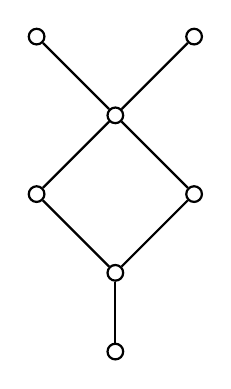
\begin{tikzpicture}
[lineDecorate/.style={-,thick},%
  nodeDecorate/.style={shape=circle,inner sep=2pt,draw,thick}]
%% nodes or vertices
\foreach \nodename/\x/\y in {
  7/0/0, 5/0/1, 4/-1/2, 6/1/2, 3/0/3, 1/-1/4, 2/1/4}
{
  \node (\nodename) at (\x,\y) [nodeDecorate] {};
}
%% edges or lines
\path
\foreach \startnode/\endnode in {
  1/3, 2/3, 3/4, 3/6, 4/5, 5/7, 6/5}
{
  (\startnode) edge[lineDecorate] node {} (\endnode)
};
\end{tikzpicture}

\caption{Molecular graph of 1,1,3-trimethylcyclobutane.}
\label{fig:graph_algorithms:trimethylcyclobutane}
\end{figure}

\begin{example}
Section~\ref{sec:introduction:common_applications} briefly presented
the concept of molecular graphs in chemistry. The
Wiener\index{Wiener!number} number of a
molecular\index{molecular graph} graph was first published in~1947 by
Harold Wiener\index{Wiener!Harold}~\cite{Wiener1947} who used it in
chemistry\index{chemistry} to study properties of alkanes. Other
applications~\cite{GutmanEtAl1993} of the Wiener number to chemistry
are now known. If $G = (V,E)$ is a connected graph with vertex set
$V = \{v_1, v_2, \dots, v_n\}$, then the Wiener number $W$ of $G$ is
defined by
%%
\begin{equation}
\label{eqn:graph_algorithms:Wiener_number}
W(G)
=
\sum_{i < j} d(v_i, v_j)
\end{equation}
%%
where $d(v_i, v_j)$ is the distance from $v_i$ to $v_j$. What is the
Wiener number of the molecular graph in
Figure~\ref{fig:graph_algorithms:trimethylcyclobutane}?
\end{example}

\begin{proof}[Solution]
Consider the molecular graph in
Figure~\ref{fig:graph_algorithms:trimethylcyclobutane} as directed
with unit weight. To compute the Wiener number of this graph, use the
Floyd-Roy-Warshall algorithm to obtain a distance matrix
$D = [d_{i,j}]$, where $d_{i,j}$ is the distance from $v_i$ to $v_j$,
and apply the
definition~\eqref{eqn:graph_algorithms:Wiener_number}. The distance
matrix resulting from the Floyd-Roy-Warshall algorithm is
\[
M
=
\begin{bmatrix}
0 & 2 & 1 & 2 & 3 & 2 & 4 \\
2 & 0 & 1 & 2 & 3 & 2 & 4 \\
1 & 1 & 0 & 1 & 2 & 1 & 3 \\
2 & 2 & 1 & 0 & 1 & 2 & 2 \\
3 & 3 & 2 & 1 & 0 & 1 & 1 \\
2 & 2 & 1 & 2 & 1 & 0 & 2 \\
4 & 4 & 3 & 2 & 1 & 2 & 0
\end{bmatrix}.
\]
Sum all entries in the upper (or lower) triangular of $M$ to obtain
the Wiener number $W = 42$. Using Sage, we have
%%
\begin{lstlisting}
sage: G = Graph({1:[3], 2:[3], 3:[4,6], 4:[5], 6:[5], 5:[7]})
sage: D = G.shortest_path_all_pairs()[0]
sage: M = [D[i][j] for i in D for j in D[i]]
sage: M = matrix(M, nrows=7, ncols=7)
sage: W = 0
sage: for i in range(M.nrows() - 1):
...       for j in range(i+1, M.ncols()):
...           W += M[i,j]
sage: W
42
\end{lstlisting}
%%
which verifies our computation above. See
Gutman~et~al.~\cite{GutmanEtAl1993} for a survey of some results
concerning the Wiener number.
\end{proof}


%%%%%%%%%%%%%%%%%%%%%%%%%%%%%%%%%%%%%%%%%%%%%%%%%%%%%%%%%%%%%%%%%%%%%%%%%%%

\subsection{Transitive closure}
\index{transitive closure}

Consider a digraph $G = (V, E)$ of order $n = |V|$. The
\emph{transitive closure}\index{transitive closure} of $G$ is defined
as the digraph $G^* = (V, E^*)$ having the same vertex set as
$G$. However, the edge set $E^*$ of $G^*$ consists of all edges $uv$
such that there is a $u$-$v$ path in $G$ and $uv \notin E$. The
transitive closure $G^*$ answers an important question about $G$: If
$u$ and $v$ are two distinct vertices of $G$, are they connected by a
path with length $\geq 1$?

To compute the transitive closure of $G$, we let each edge of $G$ be
of unit weight and apply the
Floyd-Roy-Warshall\index{Floyd-Roy-Warshall algorithm}
Algorithm~\ref{alg:graph_algorithms:Floy_Roy_Warshall} on $G$. By
Proposition~\ref{prop:introduction:any_path_has_length_at_most_n_minus_1},
for any $i$-$j$ path in $G$ we have $D[i,j] < n$, and if there are no
paths from $i$ to $j$ in $G$, we have $D[i,j] = \infty$. This
procedure for computing transitive closure runs in time $O(n^3)$.

Modifying the Floyd-Roy-Warshall
algorithm\index{Floyd-Roy-Warshall algorithm} slightly, we obtain an
algorithm for computing transitive closure\index{transitive closure}
that, in practice, is more efficient than
Algorithm~\ref{alg:graph_algorithms:Floy_Roy_Warshall} in terms of
time and space. Instead of using the operations $\min$ and $+$ as is
the case in the Floyd-Roy-Warshall
algorithm\index{Floyd-Roy-Warshall algorithm}, we replace these
operations with the logical operations $\vee$~(logical \OR) and
$\wedge$~(logical \AND), respectively. For $i,j,k = 1, 2, \dots, n$,
define $T_k(i,j) = 1$ if there is an $i$-$j$ path in $G$ with all
intermediate vertices belonging to $\{1, 2, \dots, k\}$, and
$T_k(i,j) = 0$ otherwise. Thus, the edge $ij$ belongs to the
transitive closure $G^*$ if and only if $T_k(i,j) = 1$. The definition
of $T_k(i,j)$ can be cast in the form of a recursive definition as
follows. For $k = 0$, we have
\[
T_0(i,j)
=
\begin{cases}
0, & \text{if $i \neq j$ and $ij \notin E$}, \\
1, & \text{if $i = j$ or $ij \in E$}
\end{cases}
\]
and for $k > 0$, we have
\[
T_k(i,j)
=
T_{k-1}(i,j) \vee \big( T_{k-1}(i,k) \wedge T_{k-1}(k,j) \big).
\]
We need not use the subscript $k$ at all and instead let $T$ be a
boolean matrix such that $T[i,j] = 1$ if and only if there is an
$i$-$j$ path in $G$, and $T[i,j] = 0$ otherwise. Using the above
notations, the Floyd-Roy-Warshall
algorithm\index{Floyd-Roy-Warshall algorithm} is translated to
Algorithm~\ref{alg:graph_algorithms:Floy_Roy_Warshall:transitive_closure}
for obtaining the boolean matrix $T$. We can then use $T$ and the
definition of transitive closure\index{transitive closure} to obtain
the edge set $E^*$ in the transitive closure $G^* = (V, E^*)$ of
$G = (V, E)$.

A more efficient transitive closure algorithm can be found in the PhD
thesis of Esko Nuutila~\cite{Nuutila1995}\index{Nuutila, Esko}. See
also the method of four Russians~\cite{AhoEtAl1974,ArlazarovEtAl1970}. The
transitive closure\index{transitive closure} algorithm as presented in
Algorithm~\ref{alg:graph_algorithms:Floy_Roy_Warshall:transitive_closure}
is due to Stephen
Warshall~\cite{Warshall1962}\index{Warshall, Stephen}. It is a special
case of a more general algorithm in automata
theory\index{automata theory} due to Stephen
Kleene~\cite{Kleene1956}\index{Kleene!Stephen}, called Kleene's
algorithm\index{Kleene!algorithm}.

\begin{algorithm}[!htbp]
%%%%%%%%%%%%%%%%%%%%%%%%%%%%%%%%%%%%%%%%%%%%%%%%%%%%%%%%%%%%%%%%%%%%%%%%%%%
%% This file is part of the book
%%
%% Algorithmic Graph Theory
%% http://code.google.com/p/graph-theory-algorithms-book/
%%
%% Copyright (C) 2009--2011 Minh Van Nguyen <nguyenminh2@gmail.com>
%%
%% See the file COPYING for copying conditions.
%%%%%%%%%%%%%%%%%%%%%%%%%%%%%%%%%%%%%%%%%%%%%%%%%%%%%%%%%%%%%%%%%%%%%%%%%%%

\DontPrintSemicolon
\SetAlgoNoLine
%%
%% input
\KwIn{A digraph $G = (V, E)$ that has no self-loops. Vertices are
  numbered from $1$ to $n$, i.e.~$V = \{1, 2, \dots, n\}$.}
%%
%% output
\KwOut{The boolean matrix $T$ such that $T[i,j] = 1$ if and only if
  there is an $i$-$j$ path in $G$, and $T[i,j] = 0$ otherwise.}
\BlankLine
%%
%% algorithm body
$n \assign |V|$\;
$T \assign$ adjacency matrix of $G$\;
%% \For{$i \assign 1, 2, \dots, n$}{
%%   \For{$j \assign 1, 2, \dots, n$}{
%%     \eIf{$i = j$ \emph{or} $ij \in E$}{
%%       $T[i,j] \assign 1$\;
%%     }{
%%       $T[i,j] \assign 0$\;
%%     }
%%   }
%% }
\For{$k \assign 1, 2, \dots, n$}{
  \For{$i \assign 1, 2, \dots, n$}{
    \For{$j \assign 1, 2, \dots, n$}{
      $T[i,j] \assign T[i,j] \vee \big( T[i,k] \wedge T[k,j] \big)$\;
    }
  }
}
\Return $T$\;

\caption{Variant of the Floyd-Roy-Warshall algorithm for transitive closure.}
\label{alg:graph_algorithms:Floy_Roy_Warshall:transitive_closure}
\end{algorithm}


%%%%%%%%%%%%%%%%%%%%%%%%%%%%%%%%%%%%%%%%%%%%%%%%%%%%%%%%%%%%%%%%%%%%%%%%%%%

\section{Johnson's algorithm}
\index{Johnson!algorithm}

Let $G = (V,E)$ be a sparse\index{graph!sparse} digraph with edge
weights but no negative cycles\index{cycle!negative}.
\emph{Johnson's algorithm}\index{Johnson!algorithm}~\cite{Johnson1977}
finds a shortest path between each pair of vertices in $G$. First
published in~1977 by Donald B. Johnson\index{Johnson!Donald B.}, the
main insight of Johnson's algorithm\index{Johnson!algorithm} is to
combine the technique of edge reweighting\index{weight!reweight} with the
Bellman-Ford\index{Bellman-Ford algorithm} and
Dijkstra's\index{Dijkstra!algorithm} algorithms. The Bellman-Ford
algorithm is first used to ensure that $G$ has no negative
cycles\index{cycle!negative}. Next, we reweight\index{weight!reweight} edges
in such a manner as to preserve shortest
paths\index{path!shortest}. The final stage makes use of Dijkstra's
algorithm for computing shortest paths between all vertex
pairs. Pseudocode for Johnson's algorithm is presented in
Algorithm~\ref{alg:graph_algorithms:Johnson_algorithm}. With a
Fibonacci heap\index{heap!Fibonacci} implementation of the
minimum-priority queue\index{queue!minimum-priority}, the time
complexity for sparse graphs\index{graph!sparse} is
$O(|V|^2 \log |V| + |V| \cdot |E|)$, where $n = |V|$ is the number of
vertices of the original graph $G$.

To prove the correctness of
Algorithm~\ref{alg:graph_algorithms:Johnson_algorithm}, we need to
show that the new set of edge weights produced by $\hat{w}$ must
satisfy two properties:
%%
\begin{enumerate}
\item The reweighted\index{weight!reweight} edges preserve shortest
  paths. That is, let $p$ be a $u$-$v$ path for $u,v \in V$. Then $p$
  is a shortest weighted path\index{path!weighted}\index{path!shortest}
  using weight function $w$ if and only if $p$ is also a shortest
  weighted path using weight function $\hat{w}$.

\item The reweight function $\hat{w}$ produces nonnegative
  weights\index{weight!nonnegative}. In other words, if $u,v \in V$
  then $\hat{w}(uv) \geq 0$.
\end{enumerate}
%%
Both of these properties are proved in
Lemma~\ref{lem:graph_algorithms:reweighting_preserves_shortest_paths}.

\begin{algorithm}[!htbp]
\index{Bellman-Ford algorithm}
\index{Dijkstra!algorithm}
\index{Johnson!algorithm}
\index{graph!sparse}
%%%%%%%%%%%%%%%%%%%%%%%%%%%%%%%%%%%%%%%%%%%%%%%%%%%%%%%%%%%%%%%%%%%%%%%%%%%
%% This file is part of the book
%%
%% Algorithmic Graph Theory
%% http://code.google.com/p/graph-theory-algorithms-book/
%%
%% Copyright (C) 2009, 2010, 2011 Minh Van Nguyen <nguyenminh2@gmail.com>
%%
%% See the file COPYING for copying conditions.
%%%%%%%%%%%%%%%%%%%%%%%%%%%%%%%%%%%%%%%%%%%%%%%%%%%%%%%%%%%%%%%%%%%%%%%%%%%

\DontPrintSemicolon
\SetAlgoNoLine
%%
%% data section
\SetKwData{MyFalse}{False}
%%
%% input
\KwIn{A sparse weighted digraph $G = (V, E)$, where the vertex set is
  $V = \{1, 2, \dots, n\}$.}
%%
%% output
\KwOut{If $G$ has negative-weight cycles, then return
  \MyFalse. Otherwise, return an $n \times n$ matrix $D$ of shortest-path
  weights and a list $P$ such that $P[v]$ is a parent list resulting
  from running Dijkstra's algorithm on $G$ with start vertex $v$.}
\BlankLine
%%
%% algorithm body
$s \assign$ vertex not in $V$\;
$V' \assign V \cup \{s\}$\;
$E' \assign E \cup \{sv \;|\; v \in V\}$\;
$G' \assign$ digraph $(V', E')$ with weight $w(sv) = 0$ for all $v \in V$\;
\If{$\BellmanFord(G', w, s) = \MyFalse$}{
  \Return \MyFalse\;
}
$d \assign$ distance list returned by $\BellmanFord(G', w, s)$\;
\For{\rm each edge $uv \in E'$}{
  $\hat{w}(uv) \assign w(uv) + d[u] - d[v]$\;
}
\For{\rm each $u \in V$}{
  $(\hat{\delta}, \hat{P}) \assign$ distance and parent lists returned by $\Dijkstra(G, \hat{w}, u)$\;
  $P[u] \assign \hat{P}$\;
  \For{\rm each $v \in V$}{
    $D[u,v] \assign \hat{\delta}[v] + d[v] - d[u]$\;
  }
}
\Return $(D, P)$\;

\caption{Johnson's algorithm for sparse graphs.}
\label{alg:graph_algorithms:Johnson_algorithm}
\end{algorithm}

\begin{lemma}
\label{lem:graph_algorithms:reweighting_preserves_shortest_paths}
\textbf{Reweighting preserves shortest paths.}\index{weight!reweight}
Let $G = (V,E)$ be a weighted digraph having weight function
$w: E \to \R$ and let $h: V \to \R$ be a mapping of vertices to real
numbers. Let $\hat{w}$ be another weight function for $G$ such that
\[
\hat{w}(uv)
=
w(uv) + h(u) - h(v)
\]
for all $uv \in E$. Suppose $p: v_0, v_1, \dots, v_k$ is any path in
$G$. Then we have the following results.
%%
\begin{enumerate}
\item The path $p$ is a shortest $v_0$-$v_k$ path with weight
  function\index{weight!function} $w$ if and only if it is a shortest
  $v_0$-$v_k$ path with weight function $\hat{w}$.

\item The graph $G$ has a negative cycle\index{cycle!negative} using
  weight function $w$ if and only if $G$ has a negative cycle using
  $\hat{w}$.

\item If $G$ has no negative cycles\index{cycle!negative}, then
  $\hat{w}(uv) \geq 0$ for all $uv \in E$.
\end{enumerate}
\end{lemma}

\begin{proof}
Write $\delta$ and $\hat{\delta}$ for the shortest path weights
derived from $w$ and $\hat{w}$, respectively. To prove part~1, we need
to show that $w(p) = \delta(v_0, v_k)$ if and only if
$\hat{w}(p) = \hat{\delta}(v_0, v_k)$. First, note that any
$v_0$-$v_k$ path $p$ satisfies $\hat{w}(p) = w(p) + h(v_0) - h(v_k)$
because
%%
\begin{align*}
\hat{w}(p)
&=
\sum_{i=1}^k \hat{w}(v_{i-1} v_i) \\
&=
\sum_{i=1}^k \big(w(v_{i-1} v_i) + h(v_{i-1}) - h(v_i)\big) \\
&=
\sum_{i=1}^k w(v_{i-1} v_i)
+
\sum_{i=1}^k \big(h(v_{i-1}) - h(v_i)\big) \\
&=
\sum_{i=1}^k w(v_{i-1} v_i) + h(v_0) - h(v_k) \\
&=
w(p) + h(v_0) - h(v_k).
\end{align*}
%%
Any $v_0$-$v_k$ path shorter than $p$ and using weight function $w$ is
also shorter using $\hat{w}$. Therefore, $w(p) = \delta(v_0, v_k)$ if
and only if $\hat{w}(p) = \hat{\delta}(v_0, v_k)$.

To prove part~2, consider any cycle\index{cycle}
$c: v_0, v_1, \dots, v_k$ where $v_0 = v_k$. Using the proof of
part~1, we have
%%
\begin{align*}
\hat{w}(c)
&=
w(c) + h(v_0) - h(v_k) \\
&=
w(c)
\end{align*}
%%
thus showing that $c$ is a negative cycle using $w$ if and only if it
is a negative cycle using $\hat{w}$.

To prove part~3, we construct a new graph $G' = (V', E')$ as
follows. Consider a vertex $s \notin V$ and let $V' = V \cup \{s\}$
and $E' = E \cup \{sv \mid v \in V\}$. Extend the weight function $w$
to include $w(sv) = 0$ for all $v \in V$. By construction, $s$ has no
incoming edges and any path in $G'$ that contains $s$ has $s$ as the
source\index{vertex!source} vertex. Thus $G'$ has no
negative\index{cycle!negative} cycles if and only if $G$ has no
negative cycles. Define the function $h: V \to \R$ by
$v \mapsto \delta(s,v)$ with domain $V'$. By the triangle
inequality\index{triangle inequality}~(see
Lemma~\ref{lem:graph_algorithms:path_distance_metric_function}),
\[
\delta(s,u) + w(uv) \geq \delta(s,v)
\quad
\iff
\quad
h(u) + w(uv) \geq h(v)
\]
thereby showing that $\hat{w}(uv) = w(uv) + h(u) - h(v) \geq 0$.
\end{proof}


%%%%%%%%%%%%%%%%%%%%%%%%%%%%%%%%%%%%%%%%%%%%%%%%%%%%%%%%%%%%%%%%%%%%%%%%%%%

\section{Problems}

\begin{quote}
\footnotesize
I believe that a scientist looking at nonscientific problems is just
as dumb as the next guy. \\
\noindent
--- Richard Feynman
\end{quote}

\begin{problem}
\item The Euclidean algorithm is one of the oldest known
  algorithms. Given two positive integers $a$ and $b$ with $a \geq b$,
  let $a \bmod b$ be the remainder obtained upon dividing $a$ by $b$.
  The Euclidean algorithm determines the greatest common divisor
  $\gcd(a,b)$ of $a$ and $b$. The procedure is summarized in
  Algorithm~\ref{alg:graph_algorithms:Euclidean_algorithm}.
  %%
  \begin{enumerate}[(a)]
  \item Implement
    Algorithm~\ref{alg:graph_algorithms:Euclidean_algorithm} in Sage
    and use your implementation to compute the greatest common
    divisors of various pairs of integers. Use the built-in Sage
    command \verb!gcd! to verify your answer.

  \item Modify
    Algorithm~\ref{alg:graph_algorithms:Euclidean_algorithm} to
    compute the greatest common divisor of any pair of integers.
  \end{enumerate}

\begin{algorithm}[!htbp]
%%%%%%%%%%%%%%%%%%%%%%%%%%%%%%%%%%%%%%%%%%%%%%%%%%%%%%%%%%%%%%%%%%%%%%%%%%%
%% This file is part of the book
%%
%% Algorithmic Graph Theory
%% http://code.google.com/p/graph-theory-algorithms-book/
%%
%% Copyright (C) 2009, 2010, 2011 Minh Van Nguyen <nguyenminh2@gmail.com>
%%
%% See the file COPYING for copying conditions.
%%%%%%%%%%%%%%%%%%%%%%%%%%%%%%%%%%%%%%%%%%%%%%%%%%%%%%%%%%%%%%%%%%%%%%%%%%%

\DontPrintSemicolon
\SetAlgoNoLine
%%
%% data section
\SetKwInOut{Input}{Input}
\SetKwInOut{Output}{Output}
%%
%% input/output
\Input{Two integers $a > 0$ and $b \geq 0$ with $a \geq b$.}
\Output{The greatest common divisor of $a$ and $b$.}
\BlankLine
%%
%% algorithm body
$x \assign a$\;
$y \assign b$\;
\While{$y \neq 0$}{
  $r \assign x \bmod y$\;
  $x \assign y$\;
  $y \assign r$\;
}
\Return $x$

\caption{The Euclidean algorithm.}
\index{Euclidean algorithm}
\label{alg:graph_algorithms:Euclidean_algorithm}
\end{algorithm}

\item\label{prob:graph_algorithms:Horner_method} Given a polynomial
  $p(x) = a_n x^n + a_{n-1} x^{n-1} + \cdots + a_1 x + a_0$ of degree
  $n$, we can use Horner's\index{Horner!W. G.}
  method~\cite{Horner1819} to efficiently evaluate $p$ at a specific
  value $x = x_0$. Horner's method evaluates $p(x)$ by expressing the
  polynomial as
  \[
  p(x)
  =
  \sum_{i=0}^n a_i x^i
  =
  (\cdots (a_n x + a_{n-1}) x + \cdots)x + a_0
  \]
  to obtain Algorithm~\ref{alg:graph_algorithms:Horner_method}.
  %%
  \begin{enumerate}[(a)]
  \item Compare the runtime of polynomial evaluation using
    equation~\eqref{eqn:graph_algorithms:big_endian_binary_to_integer}
    and Horner's method.

  \item Let $v$ be a bit vector read using big-endian order. Write a
    Sage function that uses Horner's method to compute the integer
    representation of $v$.

  \item Modify Algorithm~\ref{alg:graph_algorithms:Horner_method} to
    evaluate the integer representation of a bit vector $v$ read using
    little-endian order. Hence, write a Sage function to convert $v$
    to its integer representation.
  \end{enumerate}

\begin{algorithm}[!htbp]
\index{Horner!method}
\index{Horner!W. G.}
%%%%%%%%%%%%%%%%%%%%%%%%%%%%%%%%%%%%%%%%%%%%%%%%%%%%%%%%%%%%%%%%%%%%%%%%%%%
%% This file is part of the book
%%
%% Algorithmic Graph Theory
%% http://code.google.com/p/graph-theory-algorithms-book/
%%
%% Copyright (C) 2009, 2010 Minh Van Nguyen <nguyenminh2@gmail.com>
%%
%% See the file COPYING for copying conditions.
%%%%%%%%%%%%%%%%%%%%%%%%%%%%%%%%%%%%%%%%%%%%%%%%%%%%%%%%%%%%%%%%%%%%%%%%%%%

\dontprintsemicolon
%%
%% data section
\SetKwInOut{Input}{Input}
\SetKwInOut{Output}{Output}
%%
%% input/output
\Input{A polynomial $p(x) = \sum_{i=0}^n a_i x_i$, where $a_n \neq 0$,
  and $x_0 \in \R$.}
\Output{An evaluation of $p$ at $x = x_0$.}
\BlankLine
%%
%% algorithm body
$b \assign a_n$\;
\For{$i \assign n - 1, n - 2, \dots, 0$}{
  $b \assign b x_0 + a_i$\;
}
\Return $b$\;

\caption{Polynomial evaluation using Horner's method.}
\label{alg:graph_algorithms:Horner_method}
\end{algorithm}

\item Let $G = (V, E)$ be an undirected graph, let $s \in V$, and $D$
  is the list of distances resulting from running
  Algorithm~\ref{alg:graph_algorithms:breadth_first_search_template}
  with $G$ and $s$ as input. Show that $G$ is connected if and only if
  $D[v]$ is defined for each $v \in V$.

\item Show that the worst-case time complexity of depth-first search
  Algorithm~\ref{alg:graph_algorithms:depth_first_search_template} is
  $O(|V| + |E|)$.

\item Let $D$ be the list of distances returned by
  Algorithm~\ref{alg:graph_algorithms:depth_first_search_template},
  let $s$ be a starting vertex, and let $v$ be a vertex such that
  $D[v] \neq \infty$. Show that $D[v]$ is the length of any shortest
  path from $s$ to $v$.

\item Consider the graph in
  Figure~\ref{fig:graph_algorithms:Dijkstra_algorithm_digraph} as
  undirected. Run this undirected version through Dijkstra's algorithm
  with starting vertex $v_1$.

\begin{figure}[!htbp]
\centering
%%%%%%%%%%%%%%%%%%%%%%%%%%%%%%%%%%%%%%%%%%%%%%%%%%%%%%%%%%%%%%%%%%%%%%%%%%%
%% This file is part of the book
%%
%% Algorithmic Graph Theory
%% http://code.google.com/p/graph-theory-algorithms-book/
%%
%% Copyright (C) 2009, 2010 Minh Van Nguyen <nguyenminh2@gmail.com>
%%
%% See the file COPYING for copying conditions.
%%%%%%%%%%%%%%%%%%%%%%%%%%%%%%%%%%%%%%%%%%%%%%%%%%%%%%%%%%%%%%%%%%%%%%%%%%%

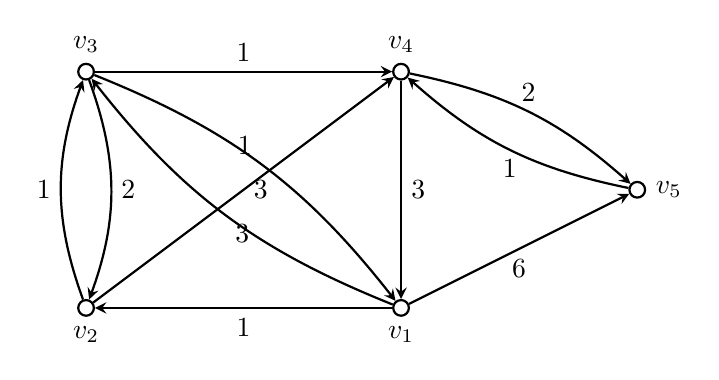
\begin{tikzpicture}
[nodedecorate/.style={shape=circle,inner sep=2pt,draw,thick},%
  arrowdecorate/.style={->,>=stealth,thick}]
%% nodes or vertices
\foreach \nodename/\x/\y/\direction/\navigate in {v_1/4/0/below/south,
  v_2/0/0/below/south, v_3/0/3/above/north, v_4/4/3/above/north,
  v_5/7/1.5/right/east}
{
  \node (\nodename) at (\x,\y) [nodedecorate] {};
  \node [\direction] at (\nodename.\navigate) {$\nodename$};
}
%% edges or lines
\path
\foreach \startnode/\endnode/\direction/\weight in {v_1/v_2/below/1,
  v_1/v_5/below/6, v_2/v_4/right/3, v_3/v_4/above/1, v_4/v_1/right/3}
{
  (\startnode) edge[arrowdecorate] node[\direction]{$\weight$} (\endnode)
}
\foreach \startnode/\endnode/\direction/\angle/\weight in {
  v_3/v_2/right/20/2, v_3/v_1/above left/15/1, v_2/v_3/left/20/1,
  v_1/v_3/below right/15/3, v_4/v_5/above/15/2, v_5/v_4/below/15/1}
{
  (\startnode) edge[arrowdecorate,bend left=\angle] node[\direction]{$\weight$} (\endnode)
};
\end{tikzpicture}

\caption{Searching a directed house graph using Dijkstra's algorithm.}
\label{fig:graph_algorithms:Dijkstra_directed_house_graph}
\end{figure}
%sage: M = matrix([[0,1,3,0,6],[0,0,1,3,0],[1,2,0,1,0],[3,0,0,0,2],[0,0,0,1,0]])
%sage: D = DiGraph(M, format="weighted_adjacency_matrix")
%sage: D.plot(edge_labels=True, graph_border=True).show()

\item Consider the graph in
  Figure~\ref{fig:graph_algorithms:Dijkstra_directed_house_graph}. Choose
  any vertex as a starting vertex and run Dijkstra's algorithm over
  it. Now consider the undirected version of that digraph and repeat
  the exercise.

\item For each vertex $v$ of the graph in
  Figure~\ref{fig:graph_algorithms:Dijkstra_directed_house_graph}, run
  breadth-first\index{breadth-first search} search over that graph
  with $v$ as the starting vertex. Repeat the exercise for
  depth-first search\index{depth-first search}. Compare the graphs
  resulting from the above exercises.

\item A list data structure can be used to manage vertices and
  edges. If $L$ is a nonempty list of vertices of a graph, we may want
  to know whether the graph contains a particular vertex. We could
  search the list $L$, returning \texttt{True} if $L$ contains the
  vertex in question and \texttt{False} otherwise. Linear search is a
  simple searching algorithm. Given an object $E$ for which we want to
  search, we consider each element $e$ of $L$ in turn and compare $E$
  to $e$. If at any point during our search we found a match, we halt
  the algorithm and output an affirmative answer. Otherwise, we have
  scanned through all elements of $L$ and each of those elements do
  not match $E$. In this case, linear search reports that $E$ is not
  in $L$. Our discussion is summarized in
  Algorithm~\ref{alg:graph_algorithms:linear_search}.
  %%
  \begin{enumerate}[(a)]
  \item Implement Algorithm~\ref{alg:graph_algorithms:linear_search}
    in Sage and test your implementation using the graphs presented in
    the figures of this chapter.

  \item What is the maximum number of comparisons during the running
    of Algorithm~\ref{alg:graph_algorithms:linear_search}? What is the
    average number of comparisons?

  \item Why must the input list $L$ be nonempty?
  \end{enumerate}

\begin{algorithm}[!htbp]
%%%%%%%%%%%%%%%%%%%%%%%%%%%%%%%%%%%%%%%%%%%%%%%%%%%%%%%%%%%%%%%%%%%%%%%%%%%
%% This file is part of the book
%%
%% Algorithmic Graph Theory
%% http://code.google.com/p/graph-theory-algorithms-book/
%%
%% Copyright (C) 2009, 2010 Minh Van Nguyen <nguyenminh2@gmail.com>
%%
%% See the file COPYING for copying conditions.
%%%%%%%%%%%%%%%%%%%%%%%%%%%%%%%%%%%%%%%%%%%%%%%%%%%%%%%%%%%%%%%%%%%%%%%%%%%

\DontPrintSemicolon
\SetAlgoNoLine
%%
%% data section
\SetKwInOut{Input}{Input}
\SetKwInOut{Output}{Output}
\SetKwData{MyFalse}{False}
\SetKwData{MyTrue}{True}
%%
%% input/output
\Input{A nonempty list $L$ of vertices or edges. An object $E$ for
  which we want to search in $L$.}
\Output{\MyTrue if $E$ is in $L$; \MyFalse otherwise.}
\BlankLine
%%
%% algorithm body
\For{\rm{each $e \in L$}}{
  \If{$E = e$}{
    \Return \MyTrue\;
  }
}
\Return \MyFalse\;

\caption{Linear search for lists.}
\label{alg:graph_algorithms:linear_search}
\end{algorithm}

\begin{algorithm}[!htbp]
%%%%%%%%%%%%%%%%%%%%%%%%%%%%%%%%%%%%%%%%%%%%%%%%%%%%%%%%%%%%%%%%%%%%%%%%%%%
%% This file is part of the book
%%
%% Algorithmic Graph Theory
%% http://code.google.com/p/graph-theory-algorithms-book/
%%
%% Copyright (C) 2009, 2010, 2011 Minh Van Nguyen <nguyenminh2@gmail.com>
%%
%% See the file COPYING for copying conditions.
%%%%%%%%%%%%%%%%%%%%%%%%%%%%%%%%%%%%%%%%%%%%%%%%%%%%%%%%%%%%%%%%%%%%%%%%%%%

\DontPrintSemicolon
\SetAlgoNoLine
%%
%% data section
\SetKwData{High}{high}
\SetKwData{Low}{low}
\SetKwData{Mid}{mid}
\SetKwData{MyFalse}{False}
\SetKwData{MyTrue}{True}
%%
%% input
\KwIn{A nonempty list $L$ of positive integers. Elements of $L$ are
  sorted in nondecreasing order. An integer $i$ for which we want to
  search in $L$.}
%%
%% output
\KwOut{\MyTrue if $i$ is in $L$; \MyFalse otherwise.}
\BlankLine
%%
%% algorithm body
$\Low \assign 0$\;
$\High \assign |L| - 1$\;
\While{$\Low \leq \High$}{
  $\Mid \assign \lfloor\frac{\Low\, +\, \High}{2}\rfloor$\nllabel{alg:binary_search:mid_floor}\;
  \If{$i = L[\Mid]$}{
    \Return \MyTrue\;
  }
  \If{$i < L[\Mid]$}{
    $\High \assign \Mid - 1$\;
  }
  \Else{
    $\Low \assign \Mid + 1$\;
  }
}
\Return \MyFalse\;

\caption{Binary search for lists of positive integers.}
\label{alg:graph_algorithms:binary_search}
\end{algorithm}

\item\label{prob:graph_algorithms:binary_search}
  Binary\index{binary search} search is a much faster searching
  algorithm than linear\index{linear search} search. The
  binary\index{binary search} search algorithm assumes that its input
  list is ordered in some manner. For simplicity, we assume that the
  input list $L$ consists of positive integers. The main idea of
  binary\index{binary search} search is to partition $L$ into two
  halves: the left half and the right half. Our task now is to
  determine whether the object $E$ of interest is in the left half or
  the right half, and apply binary search recursively to the half in
  which $E$ is located.
  Algorithm~\ref{alg:graph_algorithms:binary_search} provides
  pseudocode of our discussion of binary\index{binary search} search.
  %%
  \begin{enumerate}[(a)]
  \item Implement Algorithm~\ref{alg:graph_algorithms:binary_search}
    in Sage and test your implementation using the graphs presented in
    the figures of this chapter.

  \item What is the worst case runtime of
    Algorithm~\ref{alg:graph_algorithms:binary_search}? How does this
    compare to the worst case runtime of linear search?

  \item Why must the input list $L$ be sorted in nondecreasing order?
    Would Algorithm~\ref{alg:graph_algorithms:binary_search} work if
    $L$ is sorted in nonincreasing order? If not, modify
    Algorithm~\ref{alg:graph_algorithms:binary_search} so that it
    works with an input list that is sorted in nonincreasing order.

  \item Line~\ref{alg:binary_search:mid_floor} of
    Algorithm~\ref{alg:graph_algorithms:binary_search} uses the floor
    function to compute the index of the middle value. Would binary
    search still work if we use the ceiling function instead of the
    floor function?

  \item An improvement on the time complexity of
    binary\index{binary search} search is to not blindly use the
    middle value of the interval of interest, but to guess more
    precisely where the target falls within this interval.
    Interpolation\index{interpolation search} search uses this
    heuristic to improve on the runtime of binary search. Provide an
    algorithm for interpolation\index{interpolation search} search,
    analyze its worst-case runtime, and compare its theoretical
    runtime efficiency with that of binary\index{binary search}
    search~(see pages~419--420 in Knuth~\cite{Knuth1998c} and
    pages~201--202 in Sedgewick~\cite{Sedgewick1990}).
  \end{enumerate}

\item Let $G$ be a simple undirected graph having distance matrix
  $D = [d(v_i, v_j)]$, where $d(v_i, v_j) \in \R$ denotes the shortest
  distance from $v_i \in V(G)$ to $v_j \in V(G)$. If $v_i = v_j$, we
  set $d(v_i, v_j) = 0$. For each pair of distinct vertices
  $(v_i, v_j)$, we have $d(v_i, v_j) = d(v_j, v_i)$. The $i$-$j$ entry
  of $D$ is also written as $d_{i,j}$ and denotes the entry in row $i$
  and column $j$.
  %%
  \begin{enumerate}[(a)]
  \item The \emph{total distance}\index{distance!total}
    $\totalDist(u)$\index{$\totalDist$} of a fixed vertex $u \in V(G)$
    is the sum of distances from $u$ to each vertex in $G$:
    \[
    \totalDist(u)
    =
    \sum_{v \in V(G)} d(u,v).
    \]
    If $G$ is connected, $i$ is the row index of vertex $u$ in the
    distance matrix $D$, and $j$ is the column index of $u$ in $D$,
    show that the total distance of $u$ is
    %%
    \begin{equation}
    \label{eqn:graph_algorithms:total_distance_vertex}
    \totalDist(u)
    =
    \sum_k d_{i,k}
    =
    \sum_k d_{k,j}.
    \end{equation}

  \item Let the vertices of $G$ be labeled
    $V = \{v_1, v_2, \dots, v_n\}$, where $n = |V(G)|$ is the order of
    $G$. The \emph{total distance}\index{distance!total}
    $\totalDist(G)$ of $G$ is obtained by summing all the
    $d(v_i, v_j)$ for $i < j$. If $G$ is connected, show that the
    total distance of $G$ is equal to the sum of all entries in the
    upper (or lower) triangular of $D$:
    %%
    \begin{equation}
    \label{eqn:graph_algorithms:total_distance_graph}
    \totalDist(G)
    =
    \sum_{i < j} d_{i,j}
    =
    \sum_{i > j} d_{i,j}
    =
    \frac{1}{2} \left(\sum_{u \in V} \sum_{v \in V} d(u,v)\right).
    \end{equation}
    %%
    Hence show that the total distance of $G$ is equal to its Wiener
    number:
    \[
    \totalDist(G)
    =
    W(G).
    \]

  \item Would
    equations~\eqref{eqn:graph_algorithms:total_distance_vertex}
    and~\eqref{eqn:graph_algorithms:total_distance_graph} hold if $G$
    is not connected or directed?
  \end{enumerate}

\item The following result is from Yeh and
  Gutman~\cite{YehGutman1994}. Let $G_1$ and $G_2$ be graphs with
  orders $n_i = |V(G_i)|$ and sizes $m_i = |E(G_i)|$, respectively.
  %%
  \begin{enumerate}[(a)]
  \item If each of $G_1$ and $G_2$ is connected, show that the Wiener
    number of the Cartesian product $G_1 \square G_2$ is
    \[
    W(G_1 \square G_2)
    =
    n_2^2 \cdot W(G_1) + n_1^2 \cdot W(G_2).
    \]

  \item If $G_1$ and $G_2$ are arbitrary graphs, show that the Wiener
    number of the join $G_1 + G_2$ is
    \[
    W(G_1 + G_2)
    =
    n_1^2 - n_1 + n_2^2 - n_2 + n_1 n_2 - m_1 - m_2.
    \]
  \end{enumerate}

\item The following results originally appeared in
  Entringer~et~al.~\cite{EntringerEtAl1976} and independently
  rediscovered many times since.
  %%
  \begin{enumerate}[(a)]
  \item If $P_n$ is the path graph on $n \geq 0$ vertices, show that
    the Wiener number of $P_n$ is $W(P_n) = \frac{1}{6} n(n^2 - 1)$.

  \item If $C_n$ is the cycle graph on $n \geq 0$ vertices, show that
    the Wiener number of $C_n$ is
    \[
    W(C_n)
    =
    \begin{cases}
    \frac{1}{8} n(n^2 - 1), & \text{if $n$ is odd,} \\
    \frac{1}{8} n^3, & \text{if $n$ is even.}
    \end{cases}
    \]

  \item If $K_n$ is the complete graph on $n$ vertices, show that its
    Wiener number is $W(K_n) = \frac{1}{2} n(n - 1)$.

  \item Show that the Wiener number of the complete bipartite graph
    $K_{m,n}$ is
    \[
    W(K_{m,n}) = mn + m(m - 1) + n(n - 1).
    \]
  \end{enumerate}

\item Consider the world map of major capital cities in
  Figure~\ref{fig:graph_algorithms:worldmap_capital_cities}.
  %%
  \begin{enumerate}[(a)]
  \item Run breadth-\index{breadth-first search} and
    depth-first\index{depth-first search} searches over the graph in
    Figure~\ref{fig:graph_algorithms:worldmap_capital_cities} and
    compare your results.

  \item Convert the graph in
    Figure~\ref{fig:graph_algorithms:worldmap_capital_cities} to a
    digraph as follows. Let $0 \leq \alpha \leq 1$ be a fixed
    threshold\index{threshold!probability} probability and let
    $V = \{v_1, \dots, v_n\}$ be the vertex set of the graph. For each
    edge $v_i v_j$, let $0 \leq p \leq 1$ be its
    orientation\index{orientation!probability} probability and define
    the directedness\index{directedness} $\dir(v_i, v_j)$\index{$\dir$} by
    \[
    \dir(v_i, v_j)
    =
    \begin{cases}
    v_i v_j, & \text{if $p \leq \alpha$,} \\
    v_j v_i, & \text{otherwise.}
    \end{cases}
    \]
    That is, $\dir(v_i, v_j)$ takes the endpoints of an undirected
    edge $v_i v_j$ and returns a directed version of this edge. The
    result is either the directed edge $v_i v_j$ or the directed edge
    $v_j v_i$. Use the above procedure to convert the graph of
    Figure~\ref{fig:graph_algorithms:worldmap_capital_cities} to a
    digraph, and run breadth-\index{breadth-first search} and
    depth-first\index{depth-first search} searches over the resulting
    digraph.

  \item Table~\ref{tab:graph_algorithms:capital_cities_distance} lists
    distances in kilometers between the major capital cities shown in
    Figure~\ref{fig:graph_algorithms:worldmap_capital_cities}. Let
    those distances be the weights of the edges shown in
    Figure~\ref{fig:graph_algorithms:worldmap_capital_cities}. Repeatedly
    run Dijkstra's\index{Dijkstra!algorithm} algorithm over this
    undirected, weighted graph with each city as the start vertex. Use
    the procedure from the previous exercise to obtain a directed
    version of the graph in
    Figure~\ref{fig:graph_algorithms:worldmap_capital_cities} and
    repeat the current exercise with the resulting weighted digraph.

  \item Repeat the previous exercise, but use the
    Bellman-Ford\index{Bellman-Ford algorithm} algorithm instead of
    Dijkstra's\index{Dijkstra!algorithm} algorithm. Compare the
    results you obtain using these two different algorithms.

  \item Consider a weighted digraph version of the graph in
    Figure~\ref{fig:graph_algorithms:worldmap_capital_cities}. Run the
    Floyd-Roy-Warshall\index{Floyd-Roy-Warshall algorithm} and
    Johnson's\index{Johnson!algorithm} algorithms over the weighted
    digraph. Compare the results output by these two algorithms to the
    results of the previous exercise.
  \end{enumerate}

\begin{landscape}
\begin{figure}[!htbp]
\centering
\index{Bangkok}\index{Thailand}
\index{Beijing}\index{China}
\index{Berlin}\index{Germany}
\index{Brasilia}\index{Brazil}
\index{Buenos Aires}\index{Argentina}
\index{Lima}\index{Peru}
\index{London}\index{England}
\index{Madrid}\index{Spain}
\index{Moscow}\index{Russia}
\index{New Delhi}\index{India}
\index{Ottawa}\index{Canada}
\index{Pretoria}\index{South Africa}
\index{Sydney}\index{Australia}
\index{Tokyo}\index{Japan}
\index{Washington DC}\index{USA}
%%%%%%%%%%%%%%%%%%%%%%%%%%%%%%%%%%%%%%%%%%%%%%%%%%%%%%%%%%%%%%%%%%%%%%%%%%%
%% This file is part of the book
%%
%% Algorithmic Graph Theory
%% http://code.google.com/p/graph-theory-algorithms-book/
%%
%% Copyright (C) 2009--2011 Minh Van Nguyen <nguyenminh2@gmail.com>
%%
%% See the file COPYING for copying conditions.
%%%%%%%%%%%%%%%%%%%%%%%%%%%%%%%%%%%%%%%%%%%%%%%%%%%%%%%%%%%%%%%%%%%%%%%%%%%

%% Created by Eps2pgf 0.7.0 (build on 2008-08-24) on Fri Oct 01 03:43:03 EST 2010
%% This file was converted using Eps2pgf 0.7.0 from the SVG file
%% image/graph-algorithms_worldmap.svg. The conversion process is as
%% follows:
%%
%% (1) Use Inkscape 0.47 to convert
%% image/graph-algorithms_worldmap.svg to EPS format.
%%
%% (2) Use Eps2pgf 0.7.0 to convert the EPS file to PGF (LaTeX) format.
%%
%% Using the output PGF file, I (mvngu) added some major capital
%% cities of the world.

\documentclass{article}

\usepackage{tikz}
\usetikzlibrary{external}
\tikzexternalize{worldmap-capital-cities}

\begin{document}

\begin{figure}
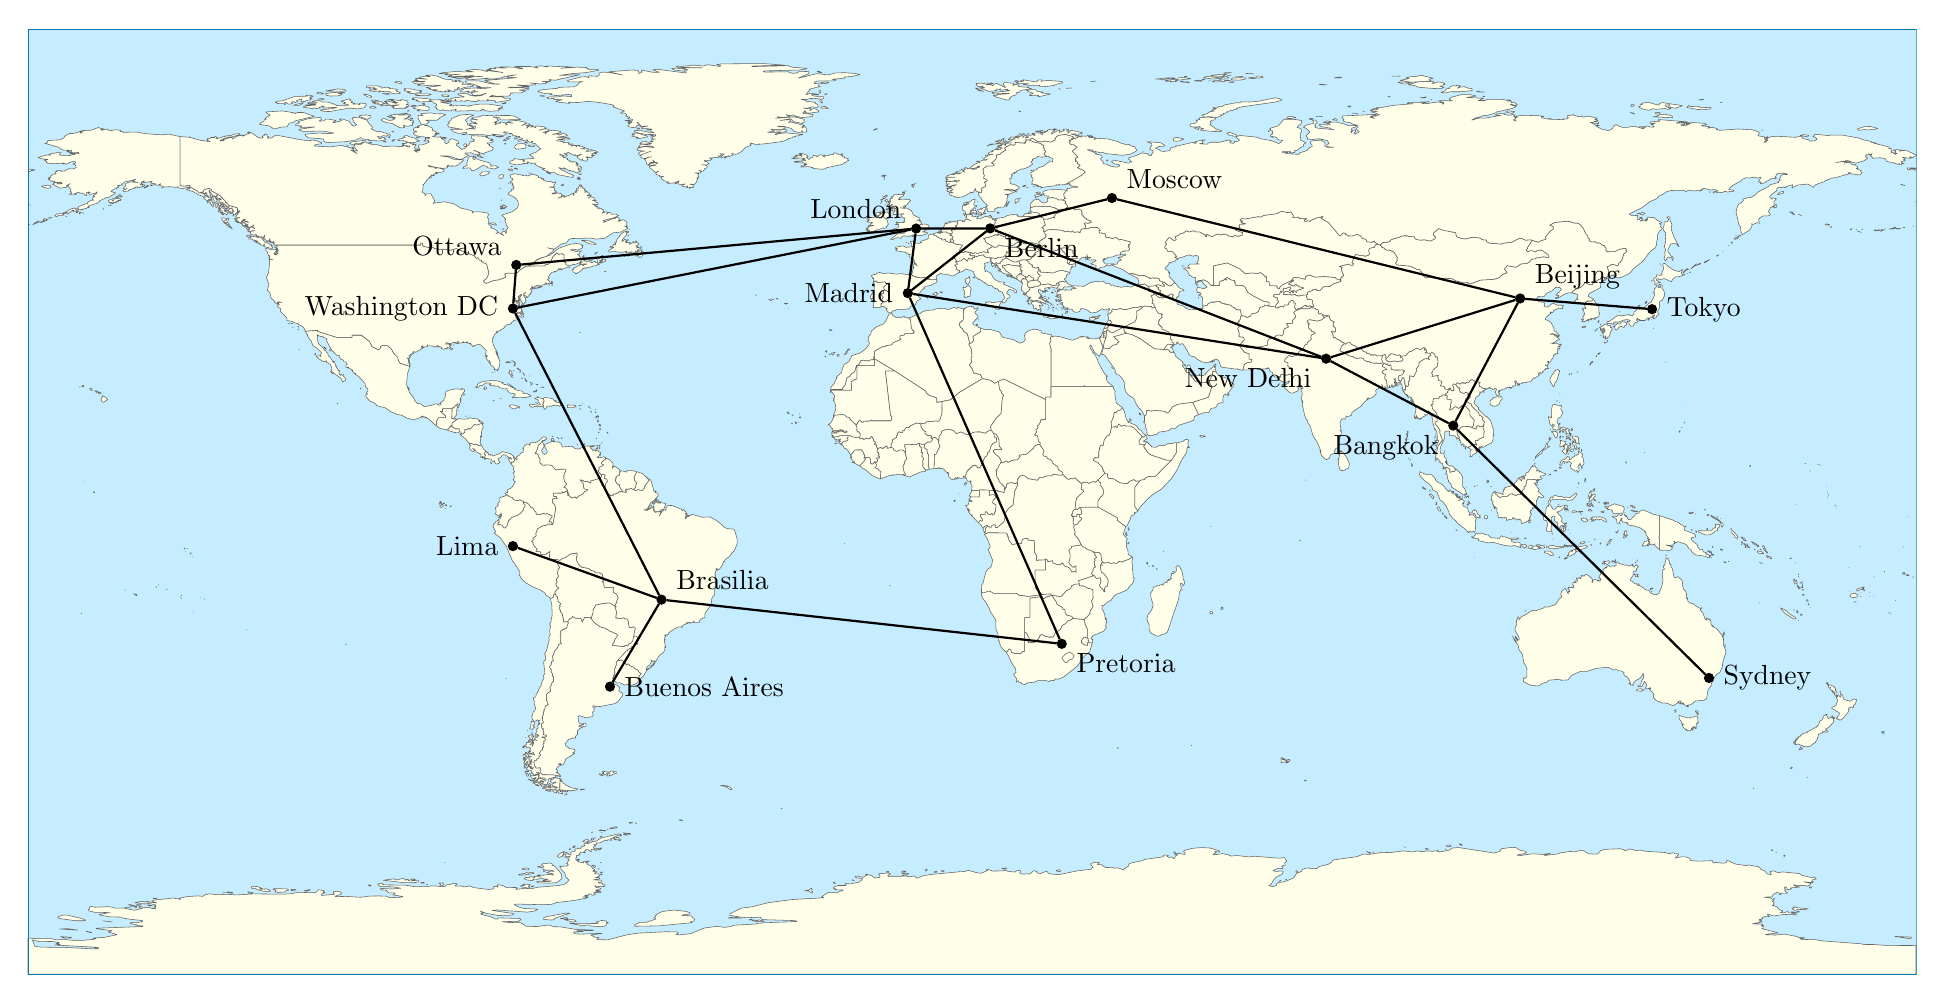
\begin{tikzpicture}
[linedecorate/.style={-,thick},%
  nodedecorate/.style={shape=circle,fill=black,inner sep=1pt,draw,thick},%
  scale=0.85]
%%
%% a world map
\pgfpathmoveto{\pgfqpoint{0cm}{0cm}}
\pgfpathlineto{\pgfqpoint{28.222cm}{0cm}}
\pgfpathlineto{\pgfqpoint{28.222cm}{14.146cm}}
\pgfpathlineto{\pgfqpoint{0cm}{14.146cm}}
\pgfpathclose
\pgfusepath{clip}
\begin{pgfscope}
\begin{pgfscope}
\definecolor{eps2pgf_color}{rgb}{0.776471,0.92549,1}\pgfsetstrokecolor{eps2pgf_color}\pgfsetfillcolor{eps2pgf_color}
\pgfpathmoveto{\pgfqpoint{0.004cm}{0.003cm}}
\pgfpathlineto{\pgfqpoint{0.004cm}{14.115cm}}
\pgfpathlineto{\pgfqpoint{28.218cm}{14.115cm}}
\pgfpathlineto{\pgfqpoint{28.218cm}{0.003cm}}
\pgfpathclose
\pgfusepath{fill}
\definecolor{eps2pgf_color}{gray}{0.392157}\pgfsetstrokecolor{eps2pgf_color}\pgfsetfillcolor{eps2pgf_color}
\pgfpathmoveto{\pgfqpoint{7.852cm}{8.04cm}}
\pgfpathcurveto{\pgfqpoint{7.852cm}{8.036cm}}{\pgfqpoint{7.849cm}{8.033cm}}{\pgfqpoint{7.845cm}{8.033cm}}
\pgfpathcurveto{\pgfqpoint{7.841cm}{8.033cm}}{\pgfqpoint{7.838cm}{8.036cm}}{\pgfqpoint{7.838cm}{8.04cm}}
\pgfpathcurveto{\pgfqpoint{7.838cm}{8.044cm}}{\pgfqpoint{7.841cm}{8.047cm}}{\pgfqpoint{7.845cm}{8.047cm}}
\pgfpathcurveto{\pgfqpoint{7.849cm}{8.047cm}}{\pgfqpoint{7.852cm}{8.044cm}}{\pgfqpoint{7.852cm}{8.04cm}}
\pgfpathclose
\pgfusepath{fill}
\definecolor{eps2pgf_color}{rgb}{0.996078,0.996078,0.913725}\pgfsetstrokecolor{eps2pgf_color}\pgfsetfillcolor{eps2pgf_color}
\pgfpathmoveto{\pgfqpoint{7.851cm}{8.035cm}}
\pgfpathlineto{\pgfqpoint{7.841cm}{8.048cm}}
\pgfpathlineto{\pgfqpoint{7.851cm}{8.035cm}}
\pgfpathclose
\pgfusepath{fill}
\begin{pgfscope}
\pgfsetdash{}{0cm}
\pgfsetlinewidth{0.071mm}
\pgfsetbeveljoin
\pgfsetmiterlimit{4.0}
\definecolor{eps2pgf_color}{gray}{0.392157}\pgfsetstrokecolor{eps2pgf_color}\pgfsetfillcolor{eps2pgf_color}
\pgfpathmoveto{\pgfqpoint{7.851cm}{8.035cm}}
\pgfpathlineto{\pgfqpoint{7.841cm}{8.048cm}}
\pgfpathlineto{\pgfqpoint{7.851cm}{8.035cm}}
\pgfpathclose
\pgfusepath{stroke}
\end{pgfscope}
\pgfpathmoveto{\pgfqpoint{7.984cm}{8.011cm}}
\pgfpathlineto{\pgfqpoint{7.981cm}{8.002cm}}
\pgfpathlineto{\pgfqpoint{7.971cm}{8.023cm}}
\pgfpathlineto{\pgfqpoint{7.984cm}{8.011cm}}
\pgfpathclose
\pgfusepath{fill}
\begin{pgfscope}
\pgfsetdash{}{0cm}
\pgfsetlinewidth{0.071mm}
\pgfsetbeveljoin
\pgfsetmiterlimit{4.0}
\definecolor{eps2pgf_color}{gray}{0.392157}\pgfsetstrokecolor{eps2pgf_color}\pgfsetfillcolor{eps2pgf_color}
\pgfpathmoveto{\pgfqpoint{7.984cm}{8.011cm}}
\pgfpathlineto{\pgfqpoint{7.981cm}{8.002cm}}
\pgfpathlineto{\pgfqpoint{7.971cm}{8.023cm}}
\pgfpathlineto{\pgfqpoint{7.984cm}{8.011cm}}
\pgfpathclose
\pgfusepath{stroke}
\end{pgfscope}
\pgfpathmoveto{\pgfqpoint{7.941cm}{8.004cm}}
\pgfpathlineto{\pgfqpoint{7.909cm}{8.029cm}}
\pgfpathlineto{\pgfqpoint{7.941cm}{8.004cm}}
\pgfpathclose
\pgfusepath{fill}
\begin{pgfscope}
\pgfsetdash{}{0cm}
\pgfsetlinewidth{0.071mm}
\pgfsetbeveljoin
\pgfsetmiterlimit{4.0}
\definecolor{eps2pgf_color}{gray}{0.392157}\pgfsetstrokecolor{eps2pgf_color}\pgfsetfillcolor{eps2pgf_color}
\pgfpathmoveto{\pgfqpoint{7.941cm}{8.004cm}}
\pgfpathlineto{\pgfqpoint{7.909cm}{8.029cm}}
\pgfpathlineto{\pgfqpoint{7.941cm}{8.004cm}}
\pgfpathclose
\pgfusepath{stroke}
\end{pgfscope}
\pgfpathmoveto{\pgfqpoint{8.397cm}{8.43cm}}
\pgfpathlineto{\pgfqpoint{8.397cm}{8.43cm}}
\pgfpathclose
\pgfusepath{fill}
\begin{pgfscope}
\pgfsetdash{}{0cm}
\pgfsetlinewidth{0.071mm}
\pgfsetbeveljoin
\pgfsetmiterlimit{4.0}
\definecolor{eps2pgf_color}{gray}{0.392157}\pgfsetstrokecolor{eps2pgf_color}\pgfsetfillcolor{eps2pgf_color}
\pgfusepath{stroke}
\end{pgfscope}
\pgfpathmoveto{\pgfqpoint{8.373cm}{8.441cm}}
\pgfpathlineto{\pgfqpoint{8.373cm}{8.441cm}}
\pgfpathclose
\pgfusepath{fill}
\begin{pgfscope}
\pgfsetdash{}{0cm}
\pgfsetlinewidth{0.071mm}
\pgfsetbeveljoin
\pgfsetmiterlimit{4.0}
\definecolor{eps2pgf_color}{gray}{0.392157}\pgfsetstrokecolor{eps2pgf_color}\pgfsetfillcolor{eps2pgf_color}
\pgfusepath{stroke}
\end{pgfscope}
\pgfpathmoveto{\pgfqpoint{13.662cm}{11.087cm}}
\pgfpathlineto{\pgfqpoint{13.637cm}{11.073cm}}
\pgfpathlineto{\pgfqpoint{13.598cm}{11.077cm}}
\pgfpathlineto{\pgfqpoint{13.594cm}{11.086cm}}
\pgfpathlineto{\pgfqpoint{13.662cm}{11.087cm}}
\pgfpathclose
\pgfusepath{fill}
\begin{pgfscope}
\pgfsetdash{}{0cm}
\pgfsetlinewidth{0.071mm}
\pgfsetbeveljoin
\pgfsetmiterlimit{4.0}
\definecolor{eps2pgf_color}{gray}{0.392157}\pgfsetstrokecolor{eps2pgf_color}\pgfsetfillcolor{eps2pgf_color}
\pgfpathmoveto{\pgfqpoint{13.662cm}{11.087cm}}
\pgfpathlineto{\pgfqpoint{13.637cm}{11.073cm}}
\pgfpathlineto{\pgfqpoint{13.598cm}{11.077cm}}
\pgfpathlineto{\pgfqpoint{13.594cm}{11.086cm}}
\pgfpathlineto{\pgfqpoint{13.662cm}{11.087cm}}
\pgfpathclose
\pgfusepath{stroke}
\end{pgfscope}
\pgfpathmoveto{\pgfqpoint{13.641cm}{11.115cm}}
\pgfpathlineto{\pgfqpoint{13.65cm}{11.108cm}}
\pgfpathlineto{\pgfqpoint{13.641cm}{11.106cm}}
\pgfpathlineto{\pgfqpoint{13.621cm}{11.113cm}}
\pgfpathlineto{\pgfqpoint{13.641cm}{11.115cm}}
\pgfpathclose
\pgfusepath{fill}
\begin{pgfscope}
\pgfsetdash{}{0cm}
\pgfsetlinewidth{0.071mm}
\pgfsetbeveljoin
\pgfsetmiterlimit{4.0}
\definecolor{eps2pgf_color}{gray}{0.392157}\pgfsetstrokecolor{eps2pgf_color}\pgfsetfillcolor{eps2pgf_color}
\pgfpathmoveto{\pgfqpoint{13.641cm}{11.115cm}}
\pgfpathlineto{\pgfqpoint{13.65cm}{11.108cm}}
\pgfpathlineto{\pgfqpoint{13.641cm}{11.106cm}}
\pgfpathlineto{\pgfqpoint{13.621cm}{11.113cm}}
\pgfpathlineto{\pgfqpoint{13.641cm}{11.115cm}}
\pgfpathclose
\pgfusepath{stroke}
\end{pgfscope}
\pgfpathmoveto{\pgfqpoint{13.714cm}{11.219cm}}
\pgfpathlineto{\pgfqpoint{13.7cm}{11.216cm}}
\pgfpathlineto{\pgfqpoint{13.714cm}{11.228cm}}
\pgfpathlineto{\pgfqpoint{13.714cm}{11.219cm}}
\pgfpathclose
\pgfusepath{fill}
\begin{pgfscope}
\pgfsetdash{}{0cm}
\pgfsetlinewidth{0.071mm}
\pgfsetbeveljoin
\pgfsetmiterlimit{4.0}
\definecolor{eps2pgf_color}{gray}{0.392157}\pgfsetstrokecolor{eps2pgf_color}\pgfsetfillcolor{eps2pgf_color}
\pgfpathmoveto{\pgfqpoint{13.714cm}{11.219cm}}
\pgfpathlineto{\pgfqpoint{13.7cm}{11.216cm}}
\pgfpathlineto{\pgfqpoint{13.714cm}{11.228cm}}
\pgfpathlineto{\pgfqpoint{13.714cm}{11.219cm}}
\pgfpathclose
\pgfusepath{stroke}
\end{pgfscope}
\pgfpathmoveto{\pgfqpoint{13.731cm}{11.238cm}}
\pgfpathlineto{\pgfqpoint{13.716cm}{11.233cm}}
\pgfpathlineto{\pgfqpoint{13.731cm}{11.238cm}}
\pgfpathclose
\pgfusepath{fill}
\begin{pgfscope}
\pgfsetdash{}{0cm}
\pgfsetlinewidth{0.071mm}
\pgfsetbeveljoin
\pgfsetmiterlimit{4.0}
\definecolor{eps2pgf_color}{gray}{0.392157}\pgfsetstrokecolor{eps2pgf_color}\pgfsetfillcolor{eps2pgf_color}
\pgfpathmoveto{\pgfqpoint{13.731cm}{11.238cm}}
\pgfpathlineto{\pgfqpoint{13.716cm}{11.233cm}}
\pgfpathlineto{\pgfqpoint{13.731cm}{11.238cm}}
\pgfpathclose
\pgfusepath{stroke}
\end{pgfscope}
\pgfpathmoveto{\pgfqpoint{13.662cm}{11.087cm}}
\pgfpathlineto{\pgfqpoint{13.602cm}{11.099cm}}
\pgfpathlineto{\pgfqpoint{13.666cm}{11.094cm}}
\pgfpathlineto{\pgfqpoint{13.645cm}{11.103cm}}
\pgfpathlineto{\pgfqpoint{13.659cm}{11.105cm}}
\pgfpathlineto{\pgfqpoint{13.641cm}{11.12cm}}
\pgfpathlineto{\pgfqpoint{13.682cm}{11.16cm}}
\pgfpathlineto{\pgfqpoint{13.705cm}{11.209cm}}
\pgfpathlineto{\pgfqpoint{13.806cm}{11.246cm}}
\pgfpathlineto{\pgfqpoint{13.866cm}{11.248cm}}
\pgfpathlineto{\pgfqpoint{13.895cm}{11.236cm}}
\pgfpathlineto{\pgfqpoint{13.883cm}{11.187cm}}
\pgfpathlineto{\pgfqpoint{13.856cm}{11.182cm}}
\pgfpathlineto{\pgfqpoint{13.883cm}{11.165cm}}
\pgfpathlineto{\pgfqpoint{13.857cm}{11.14cm}}
\pgfpathlineto{\pgfqpoint{13.862cm}{11.13cm}}
\pgfpathlineto{\pgfqpoint{13.797cm}{11.12cm}}
\pgfpathlineto{\pgfqpoint{13.817cm}{11.096cm}}
\pgfpathlineto{\pgfqpoint{13.811cm}{11.069cm}}
\pgfpathlineto{\pgfqpoint{13.79cm}{11.06cm}}
\pgfpathlineto{\pgfqpoint{13.805cm}{11.05cm}}
\pgfpathlineto{\pgfqpoint{13.801cm}{11.037cm}}
\pgfpathlineto{\pgfqpoint{13.773cm}{11.045cm}}
\pgfpathlineto{\pgfqpoint{13.788cm}{11.067cm}}
\pgfpathlineto{\pgfqpoint{13.74cm}{11.079cm}}
\pgfpathlineto{\pgfqpoint{13.728cm}{11.093cm}}
\pgfpathlineto{\pgfqpoint{13.662cm}{11.087cm}}
\pgfpathclose
\pgfusepath{fill}
\begin{pgfscope}
\pgfsetdash{}{0cm}
\pgfsetlinewidth{0.071mm}
\pgfsetbeveljoin
\pgfsetmiterlimit{4.0}
\definecolor{eps2pgf_color}{gray}{0.392157}\pgfsetstrokecolor{eps2pgf_color}\pgfsetfillcolor{eps2pgf_color}
\pgfpathmoveto{\pgfqpoint{13.662cm}{11.087cm}}
\pgfpathlineto{\pgfqpoint{13.602cm}{11.099cm}}
\pgfpathlineto{\pgfqpoint{13.666cm}{11.094cm}}
\pgfpathlineto{\pgfqpoint{13.645cm}{11.103cm}}
\pgfpathlineto{\pgfqpoint{13.659cm}{11.105cm}}
\pgfpathlineto{\pgfqpoint{13.641cm}{11.12cm}}
\pgfpathlineto{\pgfqpoint{13.682cm}{11.16cm}}
\pgfpathlineto{\pgfqpoint{13.705cm}{11.209cm}}
\pgfpathlineto{\pgfqpoint{13.806cm}{11.246cm}}
\pgfpathlineto{\pgfqpoint{13.866cm}{11.248cm}}
\pgfpathlineto{\pgfqpoint{13.895cm}{11.236cm}}
\pgfpathlineto{\pgfqpoint{13.883cm}{11.187cm}}
\pgfpathlineto{\pgfqpoint{13.856cm}{11.182cm}}
\pgfpathlineto{\pgfqpoint{13.883cm}{11.165cm}}
\pgfpathlineto{\pgfqpoint{13.857cm}{11.14cm}}
\pgfpathlineto{\pgfqpoint{13.862cm}{11.13cm}}
\pgfpathlineto{\pgfqpoint{13.797cm}{11.12cm}}
\pgfpathlineto{\pgfqpoint{13.817cm}{11.096cm}}
\pgfpathlineto{\pgfqpoint{13.811cm}{11.069cm}}
\pgfpathlineto{\pgfqpoint{13.79cm}{11.06cm}}
\pgfpathlineto{\pgfqpoint{13.805cm}{11.05cm}}
\pgfpathlineto{\pgfqpoint{13.801cm}{11.037cm}}
\pgfpathlineto{\pgfqpoint{13.773cm}{11.045cm}}
\pgfpathlineto{\pgfqpoint{13.788cm}{11.067cm}}
\pgfpathlineto{\pgfqpoint{13.74cm}{11.079cm}}
\pgfpathlineto{\pgfqpoint{13.728cm}{11.093cm}}
\pgfpathlineto{\pgfqpoint{13.662cm}{11.087cm}}
\pgfpathclose
\pgfusepath{stroke}
\end{pgfscope}
\pgfpathmoveto{\pgfqpoint{13.748cm}{11.244cm}}
\pgfpathlineto{\pgfqpoint{13.769cm}{11.248cm}}
\pgfpathlineto{\pgfqpoint{13.748cm}{11.244cm}}
\pgfpathclose
\pgfusepath{fill}
\begin{pgfscope}
\pgfsetdash{}{0cm}
\pgfsetlinewidth{0.071mm}
\pgfsetbeveljoin
\pgfsetmiterlimit{4.0}
\definecolor{eps2pgf_color}{gray}{0.392157}\pgfsetstrokecolor{eps2pgf_color}\pgfsetfillcolor{eps2pgf_color}
\pgfpathmoveto{\pgfqpoint{13.748cm}{11.244cm}}
\pgfpathlineto{\pgfqpoint{13.769cm}{11.248cm}}
\pgfpathlineto{\pgfqpoint{13.748cm}{11.244cm}}
\pgfpathclose
\pgfusepath{stroke}
\end{pgfscope}
\pgfpathmoveto{\pgfqpoint{13.796cm}{11.249cm}}
\pgfpathlineto{\pgfqpoint{13.775cm}{11.25cm}}
\pgfpathlineto{\pgfqpoint{13.796cm}{11.249cm}}
\pgfpathclose
\pgfusepath{fill}
\begin{pgfscope}
\pgfsetdash{}{0cm}
\pgfsetlinewidth{0.071mm}
\pgfsetbeveljoin
\pgfsetmiterlimit{4.0}
\definecolor{eps2pgf_color}{gray}{0.392157}\pgfsetstrokecolor{eps2pgf_color}\pgfsetfillcolor{eps2pgf_color}
\pgfpathmoveto{\pgfqpoint{13.796cm}{11.249cm}}
\pgfpathlineto{\pgfqpoint{13.775cm}{11.25cm}}
\pgfpathlineto{\pgfqpoint{13.796cm}{11.249cm}}
\pgfpathclose
\pgfusepath{stroke}
\end{pgfscope}
\pgfpathmoveto{\pgfqpoint{13.828cm}{11.254cm}}
\pgfpathlineto{\pgfqpoint{13.814cm}{11.251cm}}
\pgfpathlineto{\pgfqpoint{13.828cm}{11.254cm}}
\pgfpathclose
\pgfusepath{fill}
\begin{pgfscope}
\pgfsetdash{}{0cm}
\pgfsetlinewidth{0.071mm}
\pgfsetbeveljoin
\pgfsetmiterlimit{4.0}
\definecolor{eps2pgf_color}{gray}{0.392157}\pgfsetstrokecolor{eps2pgf_color}\pgfsetfillcolor{eps2pgf_color}
\pgfpathmoveto{\pgfqpoint{13.828cm}{11.254cm}}
\pgfpathlineto{\pgfqpoint{13.814cm}{11.251cm}}
\pgfpathlineto{\pgfqpoint{13.828cm}{11.254cm}}
\pgfpathclose
\pgfusepath{stroke}
\end{pgfscope}
\pgfpathmoveto{\pgfqpoint{13.859cm}{11.259cm}}
\pgfpathlineto{\pgfqpoint{13.852cm}{11.259cm}}
\pgfpathlineto{\pgfqpoint{13.859cm}{11.259cm}}
\pgfpathclose
\pgfusepath{fill}
\begin{pgfscope}
\pgfsetdash{}{0cm}
\pgfsetlinewidth{0.071mm}
\pgfsetbeveljoin
\pgfsetmiterlimit{4.0}
\definecolor{eps2pgf_color}{gray}{0.392157}\pgfsetstrokecolor{eps2pgf_color}\pgfsetfillcolor{eps2pgf_color}
\pgfpathmoveto{\pgfqpoint{13.859cm}{11.259cm}}
\pgfpathlineto{\pgfqpoint{13.852cm}{11.259cm}}
\pgfpathlineto{\pgfqpoint{13.859cm}{11.259cm}}
\pgfpathclose
\pgfusepath{stroke}
\end{pgfscope}
\pgfpathmoveto{\pgfqpoint{18.918cm}{10.032cm}}
\pgfpathlineto{\pgfqpoint{18.942cm}{10.031cm}}
\pgfpathlineto{\pgfqpoint{18.93cm}{9.969cm}}
\pgfpathlineto{\pgfqpoint{18.948cm}{9.936cm}}
\pgfpathlineto{\pgfqpoint{19.026cm}{9.962cm}}
\pgfpathlineto{\pgfqpoint{19.083cm}{9.996cm}}
\pgfpathlineto{\pgfqpoint{19.11cm}{9.992cm}}
\pgfpathlineto{\pgfqpoint{19.104cm}{9.978cm}}
\pgfpathlineto{\pgfqpoint{19.159cm}{9.992cm}}
\pgfpathlineto{\pgfqpoint{19.202cm}{9.977cm}}
\pgfpathlineto{\pgfqpoint{19.161cm}{9.972cm}}
\pgfpathlineto{\pgfqpoint{19.174cm}{9.961cm}}
\pgfpathlineto{\pgfqpoint{19.135cm}{9.945cm}}
\pgfpathlineto{\pgfqpoint{19.063cm}{9.949cm}}
\pgfpathlineto{\pgfqpoint{18.994cm}{9.938cm}}
\pgfpathlineto{\pgfqpoint{18.915cm}{9.89cm}}
\pgfpathlineto{\pgfqpoint{18.941cm}{9.845cm}}
\pgfpathlineto{\pgfqpoint{18.945cm}{9.817cm}}
\pgfpathlineto{\pgfqpoint{18.893cm}{9.766cm}}
\pgfpathlineto{\pgfqpoint{18.904cm}{9.753cm}}
\pgfpathlineto{\pgfqpoint{18.9cm}{9.728cm}}
\pgfpathlineto{\pgfqpoint{18.809cm}{9.725cm}}
\pgfpathlineto{\pgfqpoint{18.838cm}{9.668cm}}
\pgfpathlineto{\pgfqpoint{18.779cm}{9.647cm}}
\pgfpathlineto{\pgfqpoint{18.759cm}{9.601cm}}
\pgfpathlineto{\pgfqpoint{18.761cm}{9.562cm}}
\pgfpathlineto{\pgfqpoint{18.746cm}{9.547cm}}
\pgfpathlineto{\pgfqpoint{18.73cm}{9.538cm}}
\pgfpathlineto{\pgfqpoint{18.708cm}{9.552cm}}
\pgfpathlineto{\pgfqpoint{18.674cm}{9.552cm}}
\pgfpathlineto{\pgfqpoint{18.628cm}{9.528cm}}
\pgfpathlineto{\pgfqpoint{18.641cm}{9.516cm}}
\pgfpathlineto{\pgfqpoint{18.629cm}{9.511cm}}
\pgfpathlineto{\pgfqpoint{18.569cm}{9.509cm}}
\pgfpathlineto{\pgfqpoint{18.531cm}{9.473cm}}
\pgfpathlineto{\pgfqpoint{18.527cm}{9.404cm}}
\pgfpathlineto{\pgfqpoint{18.44cm}{9.378cm}}
\pgfpathlineto{\pgfqpoint{18.378cm}{9.375cm}}
\pgfpathlineto{\pgfqpoint{18.356cm}{9.363cm}}
\pgfpathlineto{\pgfqpoint{18.313cm}{9.371cm}}
\pgfpathlineto{\pgfqpoint{18.228cm}{9.364cm}}
\pgfpathlineto{\pgfqpoint{18.1cm}{9.399cm}}
\pgfpathlineto{\pgfqpoint{18.176cm}{9.482cm}}
\pgfpathlineto{\pgfqpoint{18.164cm}{9.519cm}}
\pgfpathlineto{\pgfqpoint{18.098cm}{9.528cm}}
\pgfpathlineto{\pgfqpoint{18.099cm}{9.587cm}}
\pgfpathlineto{\pgfqpoint{18.078cm}{9.657cm}}
\pgfpathlineto{\pgfqpoint{18.106cm}{9.685cm}}
\pgfpathlineto{\pgfqpoint{18.072cm}{9.701cm}}
\pgfpathlineto{\pgfqpoint{18.072cm}{9.732cm}}
\pgfpathlineto{\pgfqpoint{18.084cm}{9.748cm}}
\pgfpathlineto{\pgfqpoint{18.104cm}{9.749cm}}
\pgfpathlineto{\pgfqpoint{18.091cm}{9.765cm}}
\pgfpathlineto{\pgfqpoint{18.119cm}{9.791cm}}
\pgfpathlineto{\pgfqpoint{18.133cm}{9.851cm}}
\pgfpathlineto{\pgfqpoint{18.161cm}{9.836cm}}
\pgfpathlineto{\pgfqpoint{18.19cm}{9.838cm}}
\pgfpathlineto{\pgfqpoint{18.215cm}{9.816cm}}
\pgfpathlineto{\pgfqpoint{18.245cm}{9.823cm}}
\pgfpathlineto{\pgfqpoint{18.274cm}{9.838cm}}
\pgfpathlineto{\pgfqpoint{18.28cm}{9.869cm}}
\pgfpathlineto{\pgfqpoint{18.351cm}{9.883cm}}
\pgfpathlineto{\pgfqpoint{18.387cm}{9.907cm}}
\pgfpathlineto{\pgfqpoint{18.411cm}{9.969cm}}
\pgfpathlineto{\pgfqpoint{18.469cm}{9.979cm}}
\pgfpathlineto{\pgfqpoint{18.486cm}{10.004cm}}
\pgfpathlineto{\pgfqpoint{18.541cm}{9.986cm}}
\pgfpathlineto{\pgfqpoint{18.638cm}{9.977cm}}
\pgfpathlineto{\pgfqpoint{18.667cm}{9.955cm}}
\pgfpathlineto{\pgfqpoint{18.732cm}{9.986cm}}
\pgfpathlineto{\pgfqpoint{18.764cm}{9.969cm}}
\pgfpathlineto{\pgfqpoint{18.773cm}{9.998cm}}
\pgfpathlineto{\pgfqpoint{18.789cm}{10.006cm}}
\pgfpathlineto{\pgfqpoint{18.828cm}{10.002cm}}
\pgfpathlineto{\pgfqpoint{18.838cm}{10.011cm}}
\pgfpathlineto{\pgfqpoint{18.835cm}{10.032cm}}
\pgfpathlineto{\pgfqpoint{18.876cm}{10.071cm}}
\pgfpathlineto{\pgfqpoint{18.917cm}{10.062cm}}
\pgfpathlineto{\pgfqpoint{18.918cm}{10.032cm}}
\pgfpathclose
\pgfusepath{fill}
\begin{pgfscope}
\pgfsetdash{}{0cm}
\pgfsetlinewidth{0.071mm}
\pgfsetbeveljoin
\pgfsetmiterlimit{4.0}
\definecolor{eps2pgf_color}{gray}{0.392157}\pgfsetstrokecolor{eps2pgf_color}\pgfsetfillcolor{eps2pgf_color}
\pgfpathmoveto{\pgfqpoint{18.918cm}{10.032cm}}
\pgfpathlineto{\pgfqpoint{18.942cm}{10.031cm}}
\pgfpathlineto{\pgfqpoint{18.93cm}{9.969cm}}
\pgfpathlineto{\pgfqpoint{18.948cm}{9.936cm}}
\pgfpathlineto{\pgfqpoint{19.026cm}{9.962cm}}
\pgfpathlineto{\pgfqpoint{19.083cm}{9.996cm}}
\pgfpathlineto{\pgfqpoint{19.11cm}{9.992cm}}
\pgfpathlineto{\pgfqpoint{19.104cm}{9.978cm}}
\pgfpathlineto{\pgfqpoint{19.159cm}{9.992cm}}
\pgfpathlineto{\pgfqpoint{19.202cm}{9.977cm}}
\pgfpathlineto{\pgfqpoint{19.161cm}{9.972cm}}
\pgfpathlineto{\pgfqpoint{19.174cm}{9.961cm}}
\pgfpathlineto{\pgfqpoint{19.135cm}{9.945cm}}
\pgfpathlineto{\pgfqpoint{19.063cm}{9.949cm}}
\pgfpathlineto{\pgfqpoint{18.994cm}{9.938cm}}
\pgfpathlineto{\pgfqpoint{18.915cm}{9.89cm}}
\pgfpathlineto{\pgfqpoint{18.941cm}{9.845cm}}
\pgfpathlineto{\pgfqpoint{18.945cm}{9.817cm}}
\pgfpathlineto{\pgfqpoint{18.893cm}{9.766cm}}
\pgfpathlineto{\pgfqpoint{18.904cm}{9.753cm}}
\pgfpathlineto{\pgfqpoint{18.9cm}{9.728cm}}
\pgfpathlineto{\pgfqpoint{18.809cm}{9.725cm}}
\pgfpathlineto{\pgfqpoint{18.838cm}{9.668cm}}
\pgfpathlineto{\pgfqpoint{18.779cm}{9.647cm}}
\pgfpathlineto{\pgfqpoint{18.759cm}{9.601cm}}
\pgfpathlineto{\pgfqpoint{18.761cm}{9.562cm}}
\pgfpathlineto{\pgfqpoint{18.746cm}{9.547cm}}
\pgfpathlineto{\pgfqpoint{18.73cm}{9.538cm}}
\pgfpathlineto{\pgfqpoint{18.708cm}{9.552cm}}
\pgfpathlineto{\pgfqpoint{18.674cm}{9.552cm}}
\pgfpathlineto{\pgfqpoint{18.628cm}{9.528cm}}
\pgfpathlineto{\pgfqpoint{18.641cm}{9.516cm}}
\pgfpathlineto{\pgfqpoint{18.629cm}{9.511cm}}
\pgfpathlineto{\pgfqpoint{18.569cm}{9.509cm}}
\pgfpathlineto{\pgfqpoint{18.531cm}{9.473cm}}
\pgfpathlineto{\pgfqpoint{18.527cm}{9.404cm}}
\pgfpathlineto{\pgfqpoint{18.44cm}{9.378cm}}
\pgfpathlineto{\pgfqpoint{18.378cm}{9.375cm}}
\pgfpathlineto{\pgfqpoint{18.356cm}{9.363cm}}
\pgfpathlineto{\pgfqpoint{18.313cm}{9.371cm}}
\pgfpathlineto{\pgfqpoint{18.228cm}{9.364cm}}
\pgfpathlineto{\pgfqpoint{18.1cm}{9.399cm}}
\pgfpathlineto{\pgfqpoint{18.176cm}{9.482cm}}
\pgfpathlineto{\pgfqpoint{18.164cm}{9.519cm}}
\pgfpathlineto{\pgfqpoint{18.098cm}{9.528cm}}
\pgfpathlineto{\pgfqpoint{18.099cm}{9.587cm}}
\pgfpathlineto{\pgfqpoint{18.078cm}{9.657cm}}
\pgfpathlineto{\pgfqpoint{18.106cm}{9.685cm}}
\pgfpathlineto{\pgfqpoint{18.072cm}{9.701cm}}
\pgfpathlineto{\pgfqpoint{18.072cm}{9.732cm}}
\pgfpathlineto{\pgfqpoint{18.084cm}{9.748cm}}
\pgfpathlineto{\pgfqpoint{18.104cm}{9.749cm}}
\pgfpathlineto{\pgfqpoint{18.091cm}{9.765cm}}
\pgfpathlineto{\pgfqpoint{18.119cm}{9.791cm}}
\pgfpathlineto{\pgfqpoint{18.133cm}{9.851cm}}
\pgfpathlineto{\pgfqpoint{18.161cm}{9.836cm}}
\pgfpathlineto{\pgfqpoint{18.19cm}{9.838cm}}
\pgfpathlineto{\pgfqpoint{18.215cm}{9.816cm}}
\pgfpathlineto{\pgfqpoint{18.245cm}{9.823cm}}
\pgfpathlineto{\pgfqpoint{18.274cm}{9.838cm}}
\pgfpathlineto{\pgfqpoint{18.28cm}{9.869cm}}
\pgfpathlineto{\pgfqpoint{18.351cm}{9.883cm}}
\pgfpathlineto{\pgfqpoint{18.387cm}{9.907cm}}
\pgfpathlineto{\pgfqpoint{18.411cm}{9.969cm}}
\pgfpathlineto{\pgfqpoint{18.469cm}{9.979cm}}
\pgfpathlineto{\pgfqpoint{18.486cm}{10.004cm}}
\pgfpathlineto{\pgfqpoint{18.541cm}{9.986cm}}
\pgfpathlineto{\pgfqpoint{18.638cm}{9.977cm}}
\pgfpathlineto{\pgfqpoint{18.667cm}{9.955cm}}
\pgfpathlineto{\pgfqpoint{18.732cm}{9.986cm}}
\pgfpathlineto{\pgfqpoint{18.764cm}{9.969cm}}
\pgfpathlineto{\pgfqpoint{18.773cm}{9.998cm}}
\pgfpathlineto{\pgfqpoint{18.789cm}{10.006cm}}
\pgfpathlineto{\pgfqpoint{18.828cm}{10.002cm}}
\pgfpathlineto{\pgfqpoint{18.838cm}{10.011cm}}
\pgfpathlineto{\pgfqpoint{18.835cm}{10.032cm}}
\pgfpathlineto{\pgfqpoint{18.876cm}{10.071cm}}
\pgfpathlineto{\pgfqpoint{18.917cm}{10.062cm}}
\pgfpathlineto{\pgfqpoint{18.918cm}{10.032cm}}
\pgfpathclose
\pgfusepath{stroke}
\end{pgfscope}
\pgfpathmoveto{\pgfqpoint{14.443cm}{6.599cm}}
\pgfpathlineto{\pgfqpoint{14.609cm}{6.6cm}}
\pgfpathlineto{\pgfqpoint{14.627cm}{6.592cm}}
\pgfpathlineto{\pgfqpoint{14.662cm}{6.49cm}}
\pgfpathlineto{\pgfqpoint{14.709cm}{6.425cm}}
\pgfpathlineto{\pgfqpoint{14.786cm}{6.438cm}}
\pgfpathlineto{\pgfqpoint{14.846cm}{6.435cm}}
\pgfpathlineto{\pgfqpoint{14.861cm}{6.5cm}}
\pgfpathlineto{\pgfqpoint{14.889cm}{6.512cm}}
\pgfpathlineto{\pgfqpoint{14.944cm}{6.517cm}}
\pgfpathlineto{\pgfqpoint{14.946cm}{6.489cm}}
\pgfpathlineto{\pgfqpoint{15.04cm}{6.485cm}}
\pgfpathlineto{\pgfqpoint{15.047cm}{6.378cm}}
\pgfpathlineto{\pgfqpoint{15.04cm}{6.317cm}}
\pgfpathlineto{\pgfqpoint{15.076cm}{6.255cm}}
\pgfpathlineto{\pgfqpoint{15.073cm}{6.188cm}}
\pgfpathlineto{\pgfqpoint{15.199cm}{6.196cm}}
\pgfpathlineto{\pgfqpoint{15.209cm}{6.208cm}}
\pgfpathlineto{\pgfqpoint{15.211cm}{6.197cm}}
\pgfpathlineto{\pgfqpoint{15.209cm}{6.041cm}}
\pgfpathlineto{\pgfqpoint{15.053cm}{6.04cm}}
\pgfpathlineto{\pgfqpoint{15.058cm}{5.785cm}}
\pgfpathlineto{\pgfqpoint{15.067cm}{5.758cm}}
\pgfpathlineto{\pgfqpoint{15.163cm}{5.676cm}}
\pgfpathlineto{\pgfqpoint{14.956cm}{5.647cm}}
\pgfpathlineto{\pgfqpoint{14.806cm}{5.666cm}}
\pgfpathlineto{\pgfqpoint{14.775cm}{5.695cm}}
\pgfpathlineto{\pgfqpoint{14.429cm}{5.695cm}}
\pgfpathlineto{\pgfqpoint{14.364cm}{5.729cm}}
\pgfpathlineto{\pgfqpoint{14.314cm}{5.71cm}}
\pgfpathlineto{\pgfqpoint{14.251cm}{5.707cm}}
\pgfpathlineto{\pgfqpoint{14.252cm}{5.818cm}}
\pgfpathlineto{\pgfqpoint{14.273cm}{5.843cm}}
\pgfpathlineto{\pgfqpoint{14.314cm}{6.006cm}}
\pgfpathlineto{\pgfqpoint{14.348cm}{6.058cm}}
\pgfpathlineto{\pgfqpoint{14.382cm}{6.078cm}}
\pgfpathlineto{\pgfqpoint{14.403cm}{6.109cm}}
\pgfpathlineto{\pgfqpoint{14.416cm}{6.193cm}}
\pgfpathlineto{\pgfqpoint{14.35cm}{6.35cm}}
\pgfpathlineto{\pgfqpoint{14.378cm}{6.378cm}}
\pgfpathlineto{\pgfqpoint{14.379cm}{6.404cm}}
\pgfpathlineto{\pgfqpoint{14.335cm}{6.514cm}}
\pgfpathlineto{\pgfqpoint{14.293cm}{6.579cm}}
\pgfpathlineto{\pgfqpoint{14.354cm}{6.6cm}}
\pgfpathlineto{\pgfqpoint{14.443cm}{6.599cm}}
\pgfpathclose
\pgfusepath{fill}
\begin{pgfscope}
\pgfsetdash{}{0cm}
\pgfsetlinewidth{0.071mm}
\pgfsetbeveljoin
\pgfsetmiterlimit{4.0}
\definecolor{eps2pgf_color}{gray}{0.392157}\pgfsetstrokecolor{eps2pgf_color}\pgfsetfillcolor{eps2pgf_color}
\pgfpathmoveto{\pgfqpoint{14.443cm}{6.599cm}}
\pgfpathlineto{\pgfqpoint{14.609cm}{6.6cm}}
\pgfpathlineto{\pgfqpoint{14.627cm}{6.592cm}}
\pgfpathlineto{\pgfqpoint{14.662cm}{6.49cm}}
\pgfpathlineto{\pgfqpoint{14.709cm}{6.425cm}}
\pgfpathlineto{\pgfqpoint{14.786cm}{6.438cm}}
\pgfpathlineto{\pgfqpoint{14.846cm}{6.435cm}}
\pgfpathlineto{\pgfqpoint{14.861cm}{6.5cm}}
\pgfpathlineto{\pgfqpoint{14.889cm}{6.512cm}}
\pgfpathlineto{\pgfqpoint{14.944cm}{6.517cm}}
\pgfpathlineto{\pgfqpoint{14.946cm}{6.489cm}}
\pgfpathlineto{\pgfqpoint{15.04cm}{6.485cm}}
\pgfpathlineto{\pgfqpoint{15.047cm}{6.378cm}}
\pgfpathlineto{\pgfqpoint{15.04cm}{6.317cm}}
\pgfpathlineto{\pgfqpoint{15.076cm}{6.255cm}}
\pgfpathlineto{\pgfqpoint{15.073cm}{6.188cm}}
\pgfpathlineto{\pgfqpoint{15.199cm}{6.196cm}}
\pgfpathlineto{\pgfqpoint{15.209cm}{6.208cm}}
\pgfpathlineto{\pgfqpoint{15.211cm}{6.197cm}}
\pgfpathlineto{\pgfqpoint{15.209cm}{6.041cm}}
\pgfpathlineto{\pgfqpoint{15.053cm}{6.04cm}}
\pgfpathlineto{\pgfqpoint{15.058cm}{5.785cm}}
\pgfpathlineto{\pgfqpoint{15.067cm}{5.758cm}}
\pgfpathlineto{\pgfqpoint{15.163cm}{5.676cm}}
\pgfpathlineto{\pgfqpoint{14.956cm}{5.647cm}}
\pgfpathlineto{\pgfqpoint{14.806cm}{5.666cm}}
\pgfpathlineto{\pgfqpoint{14.775cm}{5.695cm}}
\pgfpathlineto{\pgfqpoint{14.429cm}{5.695cm}}
\pgfpathlineto{\pgfqpoint{14.364cm}{5.729cm}}
\pgfpathlineto{\pgfqpoint{14.314cm}{5.71cm}}
\pgfpathlineto{\pgfqpoint{14.251cm}{5.707cm}}
\pgfpathlineto{\pgfqpoint{14.252cm}{5.818cm}}
\pgfpathlineto{\pgfqpoint{14.273cm}{5.843cm}}
\pgfpathlineto{\pgfqpoint{14.314cm}{6.006cm}}
\pgfpathlineto{\pgfqpoint{14.348cm}{6.058cm}}
\pgfpathlineto{\pgfqpoint{14.382cm}{6.078cm}}
\pgfpathlineto{\pgfqpoint{14.403cm}{6.109cm}}
\pgfpathlineto{\pgfqpoint{14.416cm}{6.193cm}}
\pgfpathlineto{\pgfqpoint{14.35cm}{6.35cm}}
\pgfpathlineto{\pgfqpoint{14.378cm}{6.378cm}}
\pgfpathlineto{\pgfqpoint{14.379cm}{6.404cm}}
\pgfpathlineto{\pgfqpoint{14.335cm}{6.514cm}}
\pgfpathlineto{\pgfqpoint{14.293cm}{6.579cm}}
\pgfpathlineto{\pgfqpoint{14.354cm}{6.6cm}}
\pgfpathlineto{\pgfqpoint{14.443cm}{6.599cm}}
\pgfpathclose
\pgfusepath{stroke}
\end{pgfscope}
\pgfpathmoveto{\pgfqpoint{14.291cm}{6.609cm}}
\pgfpathlineto{\pgfqpoint{14.273cm}{6.667cm}}
\pgfpathlineto{\pgfqpoint{14.301cm}{6.697cm}}
\pgfpathlineto{\pgfqpoint{14.34cm}{6.711cm}}
\pgfpathlineto{\pgfqpoint{14.355cm}{6.696cm}}
\pgfpathlineto{\pgfqpoint{14.307cm}{6.662cm}}
\pgfpathlineto{\pgfqpoint{14.311cm}{6.613cm}}
\pgfpathlineto{\pgfqpoint{14.291cm}{6.609cm}}
\pgfpathclose
\pgfusepath{fill}
\begin{pgfscope}
\pgfsetdash{}{0cm}
\pgfsetlinewidth{0.071mm}
\pgfsetbeveljoin
\pgfsetmiterlimit{4.0}
\definecolor{eps2pgf_color}{gray}{0.392157}\pgfsetstrokecolor{eps2pgf_color}\pgfsetfillcolor{eps2pgf_color}
\pgfpathmoveto{\pgfqpoint{14.291cm}{6.609cm}}
\pgfpathlineto{\pgfqpoint{14.273cm}{6.667cm}}
\pgfpathlineto{\pgfqpoint{14.301cm}{6.697cm}}
\pgfpathlineto{\pgfqpoint{14.34cm}{6.711cm}}
\pgfpathlineto{\pgfqpoint{14.355cm}{6.696cm}}
\pgfpathlineto{\pgfqpoint{14.307cm}{6.662cm}}
\pgfpathlineto{\pgfqpoint{14.311cm}{6.613cm}}
\pgfpathlineto{\pgfqpoint{14.291cm}{6.609cm}}
\pgfpathclose
\pgfusepath{stroke}
\end{pgfscope}
\definecolor{eps2pgf_color}{gray}{0.392157}\pgfsetstrokecolor{eps2pgf_color}\pgfsetfillcolor{eps2pgf_color}
\pgfpathmoveto{\pgfqpoint{8.395cm}{8.488cm}}
\pgfpathcurveto{\pgfqpoint{8.395cm}{8.484cm}}{\pgfqpoint{8.392cm}{8.481cm}}{\pgfqpoint{8.388cm}{8.481cm}}
\pgfpathcurveto{\pgfqpoint{8.384cm}{8.481cm}}{\pgfqpoint{8.381cm}{8.484cm}}{\pgfqpoint{8.381cm}{8.488cm}}
\pgfpathcurveto{\pgfqpoint{8.381cm}{8.492cm}}{\pgfqpoint{8.384cm}{8.495cm}}{\pgfqpoint{8.388cm}{8.495cm}}
\pgfpathcurveto{\pgfqpoint{8.392cm}{8.495cm}}{\pgfqpoint{8.395cm}{8.492cm}}{\pgfqpoint{8.395cm}{8.488cm}}
\pgfpathclose
\pgfusepath{fill}
\definecolor{eps2pgf_color}{rgb}{0.996078,0.996078,0.913725}\pgfsetstrokecolor{eps2pgf_color}\pgfsetfillcolor{eps2pgf_color}
\pgfpathmoveto{\pgfqpoint{8.392cm}{8.487cm}}
\pgfpathlineto{\pgfqpoint{8.38cm}{8.484cm}}
\pgfpathlineto{\pgfqpoint{8.392cm}{8.487cm}}
\pgfpathclose
\pgfusepath{fill}
\begin{pgfscope}
\pgfsetdash{}{0cm}
\pgfsetlinewidth{0.071mm}
\pgfsetbeveljoin
\pgfsetmiterlimit{4.0}
\definecolor{eps2pgf_color}{gray}{0.392157}\pgfsetstrokecolor{eps2pgf_color}\pgfsetfillcolor{eps2pgf_color}
\pgfpathmoveto{\pgfqpoint{8.392cm}{8.487cm}}
\pgfpathlineto{\pgfqpoint{8.38cm}{8.484cm}}
\pgfpathlineto{\pgfqpoint{8.392cm}{8.487cm}}
\pgfpathclose
\pgfusepath{stroke}
\end{pgfscope}
\pgfpathmoveto{\pgfqpoint{8.256cm}{9.591cm}}
\pgfpathlineto{\pgfqpoint{8.246cm}{9.589cm}}
\pgfpathlineto{\pgfqpoint{8.256cm}{9.591cm}}
\pgfpathclose
\pgfusepath{fill}
\begin{pgfscope}
\pgfsetdash{}{0cm}
\pgfsetlinewidth{0.071mm}
\pgfsetbeveljoin
\pgfsetmiterlimit{4.0}
\definecolor{eps2pgf_color}{gray}{0.392157}\pgfsetstrokecolor{eps2pgf_color}\pgfsetfillcolor{eps2pgf_color}
\pgfpathmoveto{\pgfqpoint{8.256cm}{9.591cm}}
\pgfpathlineto{\pgfqpoint{8.246cm}{9.589cm}}
\pgfpathlineto{\pgfqpoint{8.256cm}{9.591cm}}
\pgfpathclose
\pgfusepath{stroke}
\end{pgfscope}
\pgfpathmoveto{\pgfqpoint{6.952cm}{8.575cm}}
\pgfpathlineto{\pgfqpoint{6.972cm}{8.573cm}}
\pgfpathlineto{\pgfqpoint{6.952cm}{8.575cm}}
\pgfpathclose
\pgfusepath{fill}
\begin{pgfscope}
\pgfsetdash{}{0cm}
\pgfsetlinewidth{0.071mm}
\pgfsetbeveljoin
\pgfsetmiterlimit{4.0}
\definecolor{eps2pgf_color}{gray}{0.392157}\pgfsetstrokecolor{eps2pgf_color}\pgfsetfillcolor{eps2pgf_color}
\pgfpathmoveto{\pgfqpoint{6.952cm}{8.575cm}}
\pgfpathlineto{\pgfqpoint{6.972cm}{8.573cm}}
\pgfpathlineto{\pgfqpoint{6.952cm}{8.575cm}}
\pgfpathclose
\pgfusepath{stroke}
\end{pgfscope}
\pgfpathmoveto{\pgfqpoint{7.061cm}{8.604cm}}
\pgfpathlineto{\pgfqpoint{7.049cm}{8.601cm}}
\pgfpathlineto{\pgfqpoint{7.061cm}{8.604cm}}
\pgfpathclose
\pgfusepath{fill}
\begin{pgfscope}
\pgfsetdash{}{0cm}
\pgfsetlinewidth{0.071mm}
\pgfsetbeveljoin
\pgfsetmiterlimit{4.0}
\definecolor{eps2pgf_color}{gray}{0.392157}\pgfsetstrokecolor{eps2pgf_color}\pgfsetfillcolor{eps2pgf_color}
\pgfpathmoveto{\pgfqpoint{7.061cm}{8.604cm}}
\pgfpathlineto{\pgfqpoint{7.049cm}{8.601cm}}
\pgfpathlineto{\pgfqpoint{7.061cm}{8.604cm}}
\pgfpathclose
\pgfusepath{stroke}
\end{pgfscope}
\pgfpathmoveto{\pgfqpoint{7.073cm}{8.604cm}}
\pgfpathlineto{\pgfqpoint{7.08cm}{8.608cm}}
\pgfpathlineto{\pgfqpoint{7.073cm}{8.604cm}}
\pgfpathclose
\pgfusepath{fill}
\begin{pgfscope}
\pgfsetdash{}{0cm}
\pgfsetlinewidth{0.071mm}
\pgfsetbeveljoin
\pgfsetmiterlimit{4.0}
\definecolor{eps2pgf_color}{gray}{0.392157}\pgfsetstrokecolor{eps2pgf_color}\pgfsetfillcolor{eps2pgf_color}
\pgfpathmoveto{\pgfqpoint{7.073cm}{8.604cm}}
\pgfpathlineto{\pgfqpoint{7.08cm}{8.608cm}}
\pgfpathlineto{\pgfqpoint{7.073cm}{8.604cm}}
\pgfpathclose
\pgfusepath{stroke}
\end{pgfscope}
\pgfpathmoveto{\pgfqpoint{8.652cm}{2.965cm}}
\pgfpathlineto{\pgfqpoint{8.644cm}{2.972cm}}
\pgfpathlineto{\pgfqpoint{8.652cm}{2.965cm}}
\pgfpathclose
\pgfusepath{fill}
\begin{pgfscope}
\pgfsetdash{}{0cm}
\pgfsetlinewidth{0.071mm}
\pgfsetbeveljoin
\pgfsetmiterlimit{4.0}
\definecolor{eps2pgf_color}{gray}{0.392157}\pgfsetstrokecolor{eps2pgf_color}\pgfsetfillcolor{eps2pgf_color}
\pgfpathmoveto{\pgfqpoint{8.652cm}{2.965cm}}
\pgfpathlineto{\pgfqpoint{8.644cm}{2.972cm}}
\pgfpathlineto{\pgfqpoint{8.652cm}{2.965cm}}
\pgfpathclose
\pgfusepath{stroke}
\end{pgfscope}
\pgfpathmoveto{\pgfqpoint{8.75cm}{2.982cm}}
\pgfpathlineto{\pgfqpoint{8.742cm}{2.981cm}}
\pgfpathlineto{\pgfqpoint{8.75cm}{2.982cm}}
\pgfpathclose
\pgfusepath{fill}
\begin{pgfscope}
\pgfsetdash{}{0cm}
\pgfsetlinewidth{0.071mm}
\pgfsetbeveljoin
\pgfsetmiterlimit{4.0}
\definecolor{eps2pgf_color}{gray}{0.392157}\pgfsetstrokecolor{eps2pgf_color}\pgfsetfillcolor{eps2pgf_color}
\pgfpathmoveto{\pgfqpoint{8.75cm}{2.982cm}}
\pgfpathlineto{\pgfqpoint{8.742cm}{2.981cm}}
\pgfpathlineto{\pgfqpoint{8.75cm}{2.982cm}}
\pgfpathclose
\pgfusepath{stroke}
\end{pgfscope}
\pgfpathmoveto{\pgfqpoint{8.547cm}{2.999cm}}
\pgfpathlineto{\pgfqpoint{8.558cm}{2.999cm}}
\pgfpathlineto{\pgfqpoint{8.553cm}{2.987cm}}
\pgfpathlineto{\pgfqpoint{8.537cm}{2.996cm}}
\pgfpathlineto{\pgfqpoint{8.547cm}{2.999cm}}
\pgfpathclose
\pgfusepath{fill}
\begin{pgfscope}
\pgfsetdash{}{0cm}
\pgfsetlinewidth{0.071mm}
\pgfsetbeveljoin
\pgfsetmiterlimit{4.0}
\definecolor{eps2pgf_color}{gray}{0.392157}\pgfsetstrokecolor{eps2pgf_color}\pgfsetfillcolor{eps2pgf_color}
\pgfpathmoveto{\pgfqpoint{8.547cm}{2.999cm}}
\pgfpathlineto{\pgfqpoint{8.558cm}{2.999cm}}
\pgfpathlineto{\pgfqpoint{8.553cm}{2.987cm}}
\pgfpathlineto{\pgfqpoint{8.537cm}{2.996cm}}
\pgfpathlineto{\pgfqpoint{8.547cm}{2.999cm}}
\pgfpathclose
\pgfusepath{stroke}
\end{pgfscope}
\pgfpathmoveto{\pgfqpoint{8.605cm}{3.025cm}}
\pgfpathlineto{\pgfqpoint{8.685cm}{3.028cm}}
\pgfpathlineto{\pgfqpoint{8.633cm}{2.985cm}}
\pgfpathlineto{\pgfqpoint{8.608cm}{2.984cm}}
\pgfpathlineto{\pgfqpoint{8.587cm}{2.968cm}}
\pgfpathlineto{\pgfqpoint{8.552cm}{2.978cm}}
\pgfpathlineto{\pgfqpoint{8.608cm}{3.001cm}}
\pgfpathlineto{\pgfqpoint{8.582cm}{3.006cm}}
\pgfpathlineto{\pgfqpoint{8.608cm}{3.011cm}}
\pgfpathlineto{\pgfqpoint{8.583cm}{3.033cm}}
\pgfpathlineto{\pgfqpoint{8.605cm}{3.025cm}}
\pgfpathclose
\pgfusepath{fill}
\begin{pgfscope}
\pgfsetdash{}{0cm}
\pgfsetlinewidth{0.071mm}
\pgfsetbeveljoin
\pgfsetmiterlimit{4.0}
\definecolor{eps2pgf_color}{gray}{0.392157}\pgfsetstrokecolor{eps2pgf_color}\pgfsetfillcolor{eps2pgf_color}
\pgfpathmoveto{\pgfqpoint{8.605cm}{3.025cm}}
\pgfpathlineto{\pgfqpoint{8.685cm}{3.028cm}}
\pgfpathlineto{\pgfqpoint{8.633cm}{2.985cm}}
\pgfpathlineto{\pgfqpoint{8.608cm}{2.984cm}}
\pgfpathlineto{\pgfqpoint{8.587cm}{2.968cm}}
\pgfpathlineto{\pgfqpoint{8.552cm}{2.978cm}}
\pgfpathlineto{\pgfqpoint{8.608cm}{3.001cm}}
\pgfpathlineto{\pgfqpoint{8.582cm}{3.006cm}}
\pgfpathlineto{\pgfqpoint{8.608cm}{3.011cm}}
\pgfpathlineto{\pgfqpoint{8.583cm}{3.033cm}}
\pgfpathlineto{\pgfqpoint{8.605cm}{3.025cm}}
\pgfpathclose
\pgfusepath{stroke}
\end{pgfscope}
\pgfpathmoveto{\pgfqpoint{8.618cm}{3.03cm}}
\pgfpathlineto{\pgfqpoint{8.606cm}{3.04cm}}
\pgfpathlineto{\pgfqpoint{8.622cm}{3.037cm}}
\pgfpathlineto{\pgfqpoint{8.618cm}{3.03cm}}
\pgfpathclose
\pgfusepath{fill}
\begin{pgfscope}
\pgfsetdash{}{0cm}
\pgfsetlinewidth{0.071mm}
\pgfsetbeveljoin
\pgfsetmiterlimit{4.0}
\definecolor{eps2pgf_color}{gray}{0.392157}\pgfsetstrokecolor{eps2pgf_color}\pgfsetfillcolor{eps2pgf_color}
\pgfpathmoveto{\pgfqpoint{8.618cm}{3.03cm}}
\pgfpathlineto{\pgfqpoint{8.606cm}{3.04cm}}
\pgfpathlineto{\pgfqpoint{8.622cm}{3.037cm}}
\pgfpathlineto{\pgfqpoint{8.618cm}{3.03cm}}
\pgfpathclose
\pgfusepath{stroke}
\end{pgfscope}
\pgfpathmoveto{\pgfqpoint{8.717cm}{3.04cm}}
\pgfpathlineto{\pgfqpoint{8.751cm}{3.036cm}}
\pgfpathlineto{\pgfqpoint{8.744cm}{3.023cm}}
\pgfpathlineto{\pgfqpoint{8.763cm}{3.016cm}}
\pgfpathlineto{\pgfqpoint{8.764cm}{3.028cm}}
\pgfpathlineto{\pgfqpoint{8.791cm}{3.03cm}}
\pgfpathlineto{\pgfqpoint{8.797cm}{3.006cm}}
\pgfpathlineto{\pgfqpoint{8.731cm}{2.988cm}}
\pgfpathlineto{\pgfqpoint{8.733cm}{2.975cm}}
\pgfpathlineto{\pgfqpoint{8.69cm}{2.982cm}}
\pgfpathlineto{\pgfqpoint{8.7cm}{2.969cm}}
\pgfpathlineto{\pgfqpoint{8.664cm}{2.964cm}}
\pgfpathlineto{\pgfqpoint{8.655cm}{2.972cm}}
\pgfpathlineto{\pgfqpoint{8.661cm}{2.989cm}}
\pgfpathlineto{\pgfqpoint{8.701cm}{3.008cm}}
\pgfpathlineto{\pgfqpoint{8.698cm}{3.023cm}}
\pgfpathlineto{\pgfqpoint{8.717cm}{3.04cm}}
\pgfpathclose
\pgfusepath{fill}
\begin{pgfscope}
\pgfsetdash{}{0cm}
\pgfsetlinewidth{0.071mm}
\pgfsetbeveljoin
\pgfsetmiterlimit{4.0}
\definecolor{eps2pgf_color}{gray}{0.392157}\pgfsetstrokecolor{eps2pgf_color}\pgfsetfillcolor{eps2pgf_color}
\pgfpathmoveto{\pgfqpoint{8.717cm}{3.04cm}}
\pgfpathlineto{\pgfqpoint{8.751cm}{3.036cm}}
\pgfpathlineto{\pgfqpoint{8.744cm}{3.023cm}}
\pgfpathlineto{\pgfqpoint{8.763cm}{3.016cm}}
\pgfpathlineto{\pgfqpoint{8.764cm}{3.028cm}}
\pgfpathlineto{\pgfqpoint{8.791cm}{3.03cm}}
\pgfpathlineto{\pgfqpoint{8.797cm}{3.006cm}}
\pgfpathlineto{\pgfqpoint{8.731cm}{2.988cm}}
\pgfpathlineto{\pgfqpoint{8.733cm}{2.975cm}}
\pgfpathlineto{\pgfqpoint{8.69cm}{2.982cm}}
\pgfpathlineto{\pgfqpoint{8.7cm}{2.969cm}}
\pgfpathlineto{\pgfqpoint{8.664cm}{2.964cm}}
\pgfpathlineto{\pgfqpoint{8.655cm}{2.972cm}}
\pgfpathlineto{\pgfqpoint{8.661cm}{2.989cm}}
\pgfpathlineto{\pgfqpoint{8.701cm}{3.008cm}}
\pgfpathlineto{\pgfqpoint{8.698cm}{3.023cm}}
\pgfpathlineto{\pgfqpoint{8.717cm}{3.04cm}}
\pgfpathclose
\pgfusepath{stroke}
\end{pgfscope}
\pgfpathmoveto{\pgfqpoint{13.248cm}{11.033cm}}
\pgfpathlineto{\pgfqpoint{13.228cm}{11.024cm}}
\pgfpathlineto{\pgfqpoint{13.209cm}{11.031cm}}
\pgfpathlineto{\pgfqpoint{13.228cm}{11.039cm}}
\pgfpathlineto{\pgfqpoint{13.248cm}{11.033cm}}
\pgfpathclose
\pgfusepath{fill}
\begin{pgfscope}
\pgfsetdash{}{0cm}
\pgfsetlinewidth{0.071mm}
\pgfsetbeveljoin
\pgfsetmiterlimit{4.0}
\definecolor{eps2pgf_color}{gray}{0.392157}\pgfsetstrokecolor{eps2pgf_color}\pgfsetfillcolor{eps2pgf_color}
\pgfpathmoveto{\pgfqpoint{13.248cm}{11.033cm}}
\pgfpathlineto{\pgfqpoint{13.228cm}{11.024cm}}
\pgfpathlineto{\pgfqpoint{13.209cm}{11.031cm}}
\pgfpathlineto{\pgfqpoint{13.228cm}{11.039cm}}
\pgfpathlineto{\pgfqpoint{13.248cm}{11.033cm}}
\pgfpathclose
\pgfusepath{stroke}
\end{pgfscope}
\pgfpathmoveto{\pgfqpoint{13.002cm}{11.239cm}}
\pgfpathlineto{\pgfqpoint{13.011cm}{11.235cm}}
\pgfpathlineto{\pgfqpoint{12.988cm}{11.224cm}}
\pgfpathlineto{\pgfqpoint{12.973cm}{11.244cm}}
\pgfpathlineto{\pgfqpoint{13.002cm}{11.239cm}}
\pgfpathclose
\pgfusepath{fill}
\begin{pgfscope}
\pgfsetdash{}{0cm}
\pgfsetlinewidth{0.071mm}
\pgfsetbeveljoin
\pgfsetmiterlimit{4.0}
\definecolor{eps2pgf_color}{gray}{0.392157}\pgfsetstrokecolor{eps2pgf_color}\pgfsetfillcolor{eps2pgf_color}
\pgfpathmoveto{\pgfqpoint{13.002cm}{11.239cm}}
\pgfpathlineto{\pgfqpoint{13.011cm}{11.235cm}}
\pgfpathlineto{\pgfqpoint{12.988cm}{11.224cm}}
\pgfpathlineto{\pgfqpoint{12.973cm}{11.244cm}}
\pgfpathlineto{\pgfqpoint{13.002cm}{11.239cm}}
\pgfpathclose
\pgfusepath{stroke}
\end{pgfscope}
\pgfpathmoveto{\pgfqpoint{12.831cm}{11.39cm}}
\pgfpathlineto{\pgfqpoint{12.85cm}{11.388cm}}
\pgfpathlineto{\pgfqpoint{12.883cm}{11.356cm}}
\pgfpathlineto{\pgfqpoint{12.87cm}{11.343cm}}
\pgfpathlineto{\pgfqpoint{12.893cm}{11.344cm}}
\pgfpathlineto{\pgfqpoint{12.902cm}{11.331cm}}
\pgfpathlineto{\pgfqpoint{12.886cm}{11.335cm}}
\pgfpathlineto{\pgfqpoint{12.891cm}{11.314cm}}
\pgfpathlineto{\pgfqpoint{12.866cm}{11.299cm}}
\pgfpathlineto{\pgfqpoint{12.81cm}{11.297cm}}
\pgfpathlineto{\pgfqpoint{12.782cm}{11.324cm}}
\pgfpathlineto{\pgfqpoint{12.757cm}{11.302cm}}
\pgfpathlineto{\pgfqpoint{12.74cm}{11.302cm}}
\pgfpathlineto{\pgfqpoint{12.692cm}{11.328cm}}
\pgfpathlineto{\pgfqpoint{12.723cm}{11.339cm}}
\pgfpathlineto{\pgfqpoint{12.711cm}{11.347cm}}
\pgfpathlineto{\pgfqpoint{12.739cm}{11.352cm}}
\pgfpathlineto{\pgfqpoint{12.753cm}{11.373cm}}
\pgfpathlineto{\pgfqpoint{12.831cm}{11.39cm}}
\pgfpathclose
\pgfusepath{fill}
\begin{pgfscope}
\pgfsetdash{}{0cm}
\pgfsetlinewidth{0.071mm}
\pgfsetbeveljoin
\pgfsetmiterlimit{4.0}
\definecolor{eps2pgf_color}{gray}{0.392157}\pgfsetstrokecolor{eps2pgf_color}\pgfsetfillcolor{eps2pgf_color}
\pgfpathmoveto{\pgfqpoint{12.831cm}{11.39cm}}
\pgfpathlineto{\pgfqpoint{12.85cm}{11.388cm}}
\pgfpathlineto{\pgfqpoint{12.883cm}{11.356cm}}
\pgfpathlineto{\pgfqpoint{12.87cm}{11.343cm}}
\pgfpathlineto{\pgfqpoint{12.893cm}{11.344cm}}
\pgfpathlineto{\pgfqpoint{12.902cm}{11.331cm}}
\pgfpathlineto{\pgfqpoint{12.886cm}{11.335cm}}
\pgfpathlineto{\pgfqpoint{12.891cm}{11.314cm}}
\pgfpathlineto{\pgfqpoint{12.866cm}{11.299cm}}
\pgfpathlineto{\pgfqpoint{12.81cm}{11.297cm}}
\pgfpathlineto{\pgfqpoint{12.782cm}{11.324cm}}
\pgfpathlineto{\pgfqpoint{12.757cm}{11.302cm}}
\pgfpathlineto{\pgfqpoint{12.74cm}{11.302cm}}
\pgfpathlineto{\pgfqpoint{12.692cm}{11.328cm}}
\pgfpathlineto{\pgfqpoint{12.723cm}{11.339cm}}
\pgfpathlineto{\pgfqpoint{12.711cm}{11.347cm}}
\pgfpathlineto{\pgfqpoint{12.739cm}{11.352cm}}
\pgfpathlineto{\pgfqpoint{12.753cm}{11.373cm}}
\pgfpathlineto{\pgfqpoint{12.831cm}{11.39cm}}
\pgfpathclose
\pgfusepath{stroke}
\end{pgfscope}
\pgfpathmoveto{\pgfqpoint{12.931cm}{11.406cm}}
\pgfpathlineto{\pgfqpoint{12.913cm}{11.408cm}}
\pgfpathlineto{\pgfqpoint{12.91cm}{11.423cm}}
\pgfpathlineto{\pgfqpoint{12.927cm}{11.423cm}}
\pgfpathlineto{\pgfqpoint{12.931cm}{11.406cm}}
\pgfpathclose
\pgfusepath{fill}
\begin{pgfscope}
\pgfsetdash{}{0cm}
\pgfsetlinewidth{0.071mm}
\pgfsetbeveljoin
\pgfsetmiterlimit{4.0}
\definecolor{eps2pgf_color}{gray}{0.392157}\pgfsetstrokecolor{eps2pgf_color}\pgfsetfillcolor{eps2pgf_color}
\pgfpathmoveto{\pgfqpoint{12.931cm}{11.406cm}}
\pgfpathlineto{\pgfqpoint{12.913cm}{11.408cm}}
\pgfpathlineto{\pgfqpoint{12.91cm}{11.423cm}}
\pgfpathlineto{\pgfqpoint{12.927cm}{11.423cm}}
\pgfpathlineto{\pgfqpoint{12.931cm}{11.406cm}}
\pgfpathclose
\pgfusepath{stroke}
\end{pgfscope}
\pgfpathmoveto{\pgfqpoint{12.85cm}{11.443cm}}
\pgfpathlineto{\pgfqpoint{12.854cm}{11.422cm}}
\pgfpathlineto{\pgfqpoint{12.837cm}{11.418cm}}
\pgfpathlineto{\pgfqpoint{12.837cm}{11.431cm}}
\pgfpathlineto{\pgfqpoint{12.822cm}{11.425cm}}
\pgfpathlineto{\pgfqpoint{12.828cm}{11.438cm}}
\pgfpathlineto{\pgfqpoint{12.85cm}{11.443cm}}
\pgfpathclose
\pgfusepath{fill}
\begin{pgfscope}
\pgfsetdash{}{0cm}
\pgfsetlinewidth{0.071mm}
\pgfsetbeveljoin
\pgfsetmiterlimit{4.0}
\definecolor{eps2pgf_color}{gray}{0.392157}\pgfsetstrokecolor{eps2pgf_color}\pgfsetfillcolor{eps2pgf_color}
\pgfpathmoveto{\pgfqpoint{12.85cm}{11.443cm}}
\pgfpathlineto{\pgfqpoint{12.854cm}{11.422cm}}
\pgfpathlineto{\pgfqpoint{12.837cm}{11.418cm}}
\pgfpathlineto{\pgfqpoint{12.837cm}{11.431cm}}
\pgfpathlineto{\pgfqpoint{12.822cm}{11.425cm}}
\pgfpathlineto{\pgfqpoint{12.828cm}{11.438cm}}
\pgfpathlineto{\pgfqpoint{12.85cm}{11.443cm}}
\pgfpathclose
\pgfusepath{stroke}
\end{pgfscope}
\pgfpathmoveto{\pgfqpoint{12.863cm}{11.434cm}}
\pgfpathlineto{\pgfqpoint{12.855cm}{11.441cm}}
\pgfpathlineto{\pgfqpoint{12.882cm}{11.458cm}}
\pgfpathlineto{\pgfqpoint{12.863cm}{11.434cm}}
\pgfpathclose
\pgfusepath{fill}
\begin{pgfscope}
\pgfsetdash{}{0cm}
\pgfsetlinewidth{0.071mm}
\pgfsetbeveljoin
\pgfsetmiterlimit{4.0}
\definecolor{eps2pgf_color}{gray}{0.392157}\pgfsetstrokecolor{eps2pgf_color}\pgfsetfillcolor{eps2pgf_color}
\pgfpathmoveto{\pgfqpoint{12.863cm}{11.434cm}}
\pgfpathlineto{\pgfqpoint{12.855cm}{11.441cm}}
\pgfpathlineto{\pgfqpoint{12.882cm}{11.458cm}}
\pgfpathlineto{\pgfqpoint{12.863cm}{11.434cm}}
\pgfpathclose
\pgfusepath{stroke}
\end{pgfscope}
\pgfpathmoveto{\pgfqpoint{12.878cm}{11.476cm}}
\pgfpathlineto{\pgfqpoint{12.836cm}{11.472cm}}
\pgfpathlineto{\pgfqpoint{12.85cm}{11.487cm}}
\pgfpathlineto{\pgfqpoint{12.835cm}{11.494cm}}
\pgfpathlineto{\pgfqpoint{12.858cm}{11.497cm}}
\pgfpathlineto{\pgfqpoint{12.879cm}{11.487cm}}
\pgfpathlineto{\pgfqpoint{12.878cm}{11.476cm}}
\pgfpathclose
\pgfusepath{fill}
\begin{pgfscope}
\pgfsetdash{}{0cm}
\pgfsetlinewidth{0.071mm}
\pgfsetbeveljoin
\pgfsetmiterlimit{4.0}
\definecolor{eps2pgf_color}{gray}{0.392157}\pgfsetstrokecolor{eps2pgf_color}\pgfsetfillcolor{eps2pgf_color}
\pgfpathmoveto{\pgfqpoint{12.878cm}{11.476cm}}
\pgfpathlineto{\pgfqpoint{12.836cm}{11.472cm}}
\pgfpathlineto{\pgfqpoint{12.85cm}{11.487cm}}
\pgfpathlineto{\pgfqpoint{12.835cm}{11.494cm}}
\pgfpathlineto{\pgfqpoint{12.858cm}{11.497cm}}
\pgfpathlineto{\pgfqpoint{12.879cm}{11.487cm}}
\pgfpathlineto{\pgfqpoint{12.878cm}{11.476cm}}
\pgfpathclose
\pgfusepath{stroke}
\end{pgfscope}
\pgfpathmoveto{\pgfqpoint{12.813cm}{11.495cm}}
\pgfpathlineto{\pgfqpoint{12.823cm}{11.501cm}}
\pgfpathlineto{\pgfqpoint{12.813cm}{11.495cm}}
\pgfpathclose
\pgfusepath{fill}
\begin{pgfscope}
\pgfsetdash{}{0cm}
\pgfsetlinewidth{0.071mm}
\pgfsetbeveljoin
\pgfsetmiterlimit{4.0}
\definecolor{eps2pgf_color}{gray}{0.392157}\pgfsetstrokecolor{eps2pgf_color}\pgfsetfillcolor{eps2pgf_color}
\pgfpathmoveto{\pgfqpoint{12.813cm}{11.495cm}}
\pgfpathlineto{\pgfqpoint{12.823cm}{11.501cm}}
\pgfpathlineto{\pgfqpoint{12.813cm}{11.495cm}}
\pgfpathclose
\pgfusepath{stroke}
\end{pgfscope}
\pgfpathmoveto{\pgfqpoint{12.749cm}{11.525cm}}
\pgfpathlineto{\pgfqpoint{12.74cm}{11.525cm}}
\pgfpathlineto{\pgfqpoint{12.749cm}{11.525cm}}
\pgfpathclose
\pgfusepath{fill}
\begin{pgfscope}
\pgfsetdash{}{0cm}
\pgfsetlinewidth{0.071mm}
\pgfsetbeveljoin
\pgfsetmiterlimit{4.0}
\definecolor{eps2pgf_color}{gray}{0.392157}\pgfsetstrokecolor{eps2pgf_color}\pgfsetfillcolor{eps2pgf_color}
\pgfpathmoveto{\pgfqpoint{12.749cm}{11.525cm}}
\pgfpathlineto{\pgfqpoint{12.74cm}{11.525cm}}
\pgfpathlineto{\pgfqpoint{12.749cm}{11.525cm}}
\pgfpathclose
\pgfusepath{stroke}
\end{pgfscope}
\pgfpathmoveto{\pgfqpoint{12.839cm}{11.525cm}}
\pgfpathlineto{\pgfqpoint{12.827cm}{11.529cm}}
\pgfpathlineto{\pgfqpoint{12.839cm}{11.525cm}}
\pgfpathclose
\pgfusepath{fill}
\begin{pgfscope}
\pgfsetdash{}{0cm}
\pgfsetlinewidth{0.071mm}
\pgfsetbeveljoin
\pgfsetmiterlimit{4.0}
\definecolor{eps2pgf_color}{gray}{0.392157}\pgfsetstrokecolor{eps2pgf_color}\pgfsetfillcolor{eps2pgf_color}
\pgfpathmoveto{\pgfqpoint{12.839cm}{11.525cm}}
\pgfpathlineto{\pgfqpoint{12.827cm}{11.529cm}}
\pgfpathlineto{\pgfqpoint{12.839cm}{11.525cm}}
\pgfpathclose
\pgfusepath{stroke}
\end{pgfscope}
\pgfpathmoveto{\pgfqpoint{12.763cm}{11.537cm}}
\pgfpathlineto{\pgfqpoint{12.752cm}{11.537cm}}
\pgfpathlineto{\pgfqpoint{12.75cm}{11.557cm}}
\pgfpathlineto{\pgfqpoint{12.761cm}{11.556cm}}
\pgfpathlineto{\pgfqpoint{12.763cm}{11.537cm}}
\pgfpathclose
\pgfusepath{fill}
\begin{pgfscope}
\pgfsetdash{}{0cm}
\pgfsetlinewidth{0.071mm}
\pgfsetbeveljoin
\pgfsetmiterlimit{4.0}
\definecolor{eps2pgf_color}{gray}{0.392157}\pgfsetstrokecolor{eps2pgf_color}\pgfsetfillcolor{eps2pgf_color}
\pgfpathmoveto{\pgfqpoint{12.763cm}{11.537cm}}
\pgfpathlineto{\pgfqpoint{12.752cm}{11.537cm}}
\pgfpathlineto{\pgfqpoint{12.75cm}{11.557cm}}
\pgfpathlineto{\pgfqpoint{12.761cm}{11.556cm}}
\pgfpathlineto{\pgfqpoint{12.763cm}{11.537cm}}
\pgfpathclose
\pgfusepath{stroke}
\end{pgfscope}
\pgfpathmoveto{\pgfqpoint{12.85cm}{11.567cm}}
\pgfpathlineto{\pgfqpoint{12.855cm}{11.549cm}}
\pgfpathlineto{\pgfqpoint{12.886cm}{11.547cm}}
\pgfpathlineto{\pgfqpoint{12.864cm}{11.531cm}}
\pgfpathlineto{\pgfqpoint{12.858cm}{11.543cm}}
\pgfpathlineto{\pgfqpoint{12.835cm}{11.543cm}}
\pgfpathlineto{\pgfqpoint{12.801cm}{11.562cm}}
\pgfpathlineto{\pgfqpoint{12.837cm}{11.58cm}}
\pgfpathlineto{\pgfqpoint{12.85cm}{11.567cm}}
\pgfpathclose
\pgfusepath{fill}
\begin{pgfscope}
\pgfsetdash{}{0cm}
\pgfsetlinewidth{0.071mm}
\pgfsetbeveljoin
\pgfsetmiterlimit{4.0}
\definecolor{eps2pgf_color}{gray}{0.392157}\pgfsetstrokecolor{eps2pgf_color}\pgfsetfillcolor{eps2pgf_color}
\pgfpathmoveto{\pgfqpoint{12.85cm}{11.567cm}}
\pgfpathlineto{\pgfqpoint{12.855cm}{11.549cm}}
\pgfpathlineto{\pgfqpoint{12.886cm}{11.547cm}}
\pgfpathlineto{\pgfqpoint{12.864cm}{11.531cm}}
\pgfpathlineto{\pgfqpoint{12.858cm}{11.543cm}}
\pgfpathlineto{\pgfqpoint{12.835cm}{11.543cm}}
\pgfpathlineto{\pgfqpoint{12.801cm}{11.562cm}}
\pgfpathlineto{\pgfqpoint{12.837cm}{11.58cm}}
\pgfpathlineto{\pgfqpoint{12.85cm}{11.567cm}}
\pgfpathclose
\pgfusepath{stroke}
\end{pgfscope}
\pgfpathmoveto{\pgfqpoint{12.766cm}{11.581cm}}
\pgfpathlineto{\pgfqpoint{12.775cm}{11.576cm}}
\pgfpathlineto{\pgfqpoint{12.768cm}{11.569cm}}
\pgfpathlineto{\pgfqpoint{12.742cm}{11.575cm}}
\pgfpathlineto{\pgfqpoint{12.766cm}{11.581cm}}
\pgfpathclose
\pgfusepath{fill}
\begin{pgfscope}
\pgfsetdash{}{0cm}
\pgfsetlinewidth{0.071mm}
\pgfsetbeveljoin
\pgfsetmiterlimit{4.0}
\definecolor{eps2pgf_color}{gray}{0.392157}\pgfsetstrokecolor{eps2pgf_color}\pgfsetfillcolor{eps2pgf_color}
\pgfpathmoveto{\pgfqpoint{12.766cm}{11.581cm}}
\pgfpathlineto{\pgfqpoint{12.775cm}{11.576cm}}
\pgfpathlineto{\pgfqpoint{12.768cm}{11.569cm}}
\pgfpathlineto{\pgfqpoint{12.742cm}{11.575cm}}
\pgfpathlineto{\pgfqpoint{12.766cm}{11.581cm}}
\pgfpathclose
\pgfusepath{stroke}
\end{pgfscope}
\pgfpathmoveto{\pgfqpoint{12.845cm}{11.634cm}}
\pgfpathlineto{\pgfqpoint{12.817cm}{11.613cm}}
\pgfpathlineto{\pgfqpoint{12.827cm}{11.607cm}}
\pgfpathlineto{\pgfqpoint{12.785cm}{11.586cm}}
\pgfpathlineto{\pgfqpoint{12.776cm}{11.591cm}}
\pgfpathlineto{\pgfqpoint{12.794cm}{11.599cm}}
\pgfpathlineto{\pgfqpoint{12.778cm}{11.606cm}}
\pgfpathlineto{\pgfqpoint{12.78cm}{11.623cm}}
\pgfpathlineto{\pgfqpoint{12.804cm}{11.62cm}}
\pgfpathlineto{\pgfqpoint{12.802cm}{11.631cm}}
\pgfpathlineto{\pgfqpoint{12.842cm}{11.645cm}}
\pgfpathlineto{\pgfqpoint{12.845cm}{11.634cm}}
\pgfpathclose
\pgfusepath{fill}
\begin{pgfscope}
\pgfsetdash{}{0cm}
\pgfsetlinewidth{0.071mm}
\pgfsetbeveljoin
\pgfsetmiterlimit{4.0}
\definecolor{eps2pgf_color}{gray}{0.392157}\pgfsetstrokecolor{eps2pgf_color}\pgfsetfillcolor{eps2pgf_color}
\pgfpathmoveto{\pgfqpoint{12.845cm}{11.634cm}}
\pgfpathlineto{\pgfqpoint{12.817cm}{11.613cm}}
\pgfpathlineto{\pgfqpoint{12.827cm}{11.607cm}}
\pgfpathlineto{\pgfqpoint{12.785cm}{11.586cm}}
\pgfpathlineto{\pgfqpoint{12.776cm}{11.591cm}}
\pgfpathlineto{\pgfqpoint{12.794cm}{11.599cm}}
\pgfpathlineto{\pgfqpoint{12.778cm}{11.606cm}}
\pgfpathlineto{\pgfqpoint{12.78cm}{11.623cm}}
\pgfpathlineto{\pgfqpoint{12.804cm}{11.62cm}}
\pgfpathlineto{\pgfqpoint{12.802cm}{11.631cm}}
\pgfpathlineto{\pgfqpoint{12.842cm}{11.645cm}}
\pgfpathlineto{\pgfqpoint{12.845cm}{11.634cm}}
\pgfpathclose
\pgfusepath{stroke}
\end{pgfscope}
\pgfpathmoveto{\pgfqpoint{13.087cm}{11.646cm}}
\pgfpathlineto{\pgfqpoint{13.079cm}{11.631cm}}
\pgfpathlineto{\pgfqpoint{13.018cm}{11.602cm}}
\pgfpathlineto{\pgfqpoint{13.015cm}{11.594cm}}
\pgfpathlineto{\pgfqpoint{13.029cm}{11.592cm}}
\pgfpathlineto{\pgfqpoint{13.007cm}{11.573cm}}
\pgfpathlineto{\pgfqpoint{13.064cm}{11.583cm}}
\pgfpathlineto{\pgfqpoint{13.169cm}{11.582cm}}
\pgfpathlineto{\pgfqpoint{13.192cm}{11.565cm}}
\pgfpathlineto{\pgfqpoint{13.128cm}{11.493cm}}
\pgfpathlineto{\pgfqpoint{13.072cm}{11.477cm}}
\pgfpathlineto{\pgfqpoint{13.105cm}{11.48cm}}
\pgfpathlineto{\pgfqpoint{13.121cm}{11.469cm}}
\pgfpathlineto{\pgfqpoint{13.068cm}{11.451cm}}
\pgfpathlineto{\pgfqpoint{13.034cm}{11.456cm}}
\pgfpathlineto{\pgfqpoint{13.092cm}{11.445cm}}
\pgfpathlineto{\pgfqpoint{13.128cm}{11.451cm}}
\pgfpathlineto{\pgfqpoint{13.201cm}{11.415cm}}
\pgfpathlineto{\pgfqpoint{13.234cm}{11.347cm}}
\pgfpathlineto{\pgfqpoint{13.324cm}{11.302cm}}
\pgfpathlineto{\pgfqpoint{13.315cm}{11.294cm}}
\pgfpathlineto{\pgfqpoint{13.34cm}{11.261cm}}
\pgfpathlineto{\pgfqpoint{13.279cm}{11.271cm}}
\pgfpathlineto{\pgfqpoint{13.308cm}{11.268cm}}
\pgfpathlineto{\pgfqpoint{13.352cm}{11.24cm}}
\pgfpathlineto{\pgfqpoint{13.359cm}{11.226cm}}
\pgfpathlineto{\pgfqpoint{13.334cm}{11.206cm}}
\pgfpathlineto{\pgfqpoint{13.357cm}{11.199cm}}
\pgfpathlineto{\pgfqpoint{13.375cm}{11.211cm}}
\pgfpathlineto{\pgfqpoint{13.414cm}{11.211cm}}
\pgfpathlineto{\pgfqpoint{13.461cm}{11.194cm}}
\pgfpathlineto{\pgfqpoint{13.468cm}{11.172cm}}
\pgfpathlineto{\pgfqpoint{13.453cm}{11.142cm}}
\pgfpathlineto{\pgfqpoint{13.427cm}{11.133cm}}
\pgfpathlineto{\pgfqpoint{13.424cm}{11.12cm}}
\pgfpathlineto{\pgfqpoint{13.39cm}{11.114cm}}
\pgfpathlineto{\pgfqpoint{13.401cm}{11.102cm}}
\pgfpathlineto{\pgfqpoint{13.365cm}{11.094cm}}
\pgfpathlineto{\pgfqpoint{13.442cm}{11.086cm}}
\pgfpathlineto{\pgfqpoint{13.441cm}{11.071cm}}
\pgfpathlineto{\pgfqpoint{13.355cm}{11.039cm}}
\pgfpathlineto{\pgfqpoint{13.22cm}{11.049cm}}
\pgfpathlineto{\pgfqpoint{13.226cm}{11.043cm}}
\pgfpathlineto{\pgfqpoint{13.212cm}{11.037cm}}
\pgfpathlineto{\pgfqpoint{13.172cm}{11.036cm}}
\pgfpathlineto{\pgfqpoint{13.171cm}{11.026cm}}
\pgfpathlineto{\pgfqpoint{13.096cm}{11.035cm}}
\pgfpathlineto{\pgfqpoint{13.064cm}{11.028cm}}
\pgfpathlineto{\pgfqpoint{13.043cm}{10.997cm}}
\pgfpathlineto{\pgfqpoint{13.002cm}{11.009cm}}
\pgfpathlineto{\pgfqpoint{12.953cm}{10.999cm}}
\pgfpathlineto{\pgfqpoint{12.93cm}{10.981cm}}
\pgfpathlineto{\pgfqpoint{12.89cm}{10.983cm}}
\pgfpathlineto{\pgfqpoint{13.005cm}{11.073cm}}
\pgfpathlineto{\pgfqpoint{13.085cm}{11.073cm}}
\pgfpathlineto{\pgfqpoint{13.14cm}{11.115cm}}
\pgfpathlineto{\pgfqpoint{13.075cm}{11.088cm}}
\pgfpathlineto{\pgfqpoint{12.999cm}{11.101cm}}
\pgfpathlineto{\pgfqpoint{13.01cm}{11.109cm}}
\pgfpathlineto{\pgfqpoint{12.987cm}{11.115cm}}
\pgfpathlineto{\pgfqpoint{12.947cm}{11.106cm}}
\pgfpathlineto{\pgfqpoint{12.926cm}{11.115cm}}
\pgfpathlineto{\pgfqpoint{12.924cm}{11.132cm}}
\pgfpathlineto{\pgfqpoint{13.001cm}{11.157cm}}
\pgfpathlineto{\pgfqpoint{13.019cm}{11.178cm}}
\pgfpathlineto{\pgfqpoint{13.01cm}{11.207cm}}
\pgfpathlineto{\pgfqpoint{12.964cm}{11.199cm}}
\pgfpathlineto{\pgfqpoint{12.991cm}{11.222cm}}
\pgfpathlineto{\pgfqpoint{13.036cm}{11.238cm}}
\pgfpathlineto{\pgfqpoint{13.088cm}{11.234cm}}
\pgfpathlineto{\pgfqpoint{13.091cm}{11.247cm}}
\pgfpathlineto{\pgfqpoint{13.116cm}{11.238cm}}
\pgfpathlineto{\pgfqpoint{13.091cm}{11.254cm}}
\pgfpathlineto{\pgfqpoint{13.101cm}{11.271cm}}
\pgfpathlineto{\pgfqpoint{13.094cm}{11.285cm}}
\pgfpathlineto{\pgfqpoint{13.108cm}{11.303cm}}
\pgfpathlineto{\pgfqpoint{13.083cm}{11.302cm}}
\pgfpathlineto{\pgfqpoint{13.049cm}{11.336cm}}
\pgfpathlineto{\pgfqpoint{13.059cm}{11.352cm}}
\pgfpathlineto{\pgfqpoint{13.093cm}{11.366cm}}
\pgfpathlineto{\pgfqpoint{12.936cm}{11.352cm}}
\pgfpathlineto{\pgfqpoint{12.926cm}{11.369cm}}
\pgfpathlineto{\pgfqpoint{12.965cm}{11.41cm}}
\pgfpathlineto{\pgfqpoint{12.948cm}{11.425cm}}
\pgfpathlineto{\pgfqpoint{12.949cm}{11.439cm}}
\pgfpathlineto{\pgfqpoint{12.972cm}{11.444cm}}
\pgfpathlineto{\pgfqpoint{12.951cm}{11.453cm}}
\pgfpathlineto{\pgfqpoint{12.955cm}{11.461cm}}
\pgfpathlineto{\pgfqpoint{12.921cm}{11.44cm}}
\pgfpathlineto{\pgfqpoint{12.932cm}{11.465cm}}
\pgfpathlineto{\pgfqpoint{12.907cm}{11.448cm}}
\pgfpathlineto{\pgfqpoint{12.895cm}{11.401cm}}
\pgfpathlineto{\pgfqpoint{12.882cm}{11.397cm}}
\pgfpathlineto{\pgfqpoint{12.9cm}{11.433cm}}
\pgfpathlineto{\pgfqpoint{12.89cm}{11.434cm}}
\pgfpathlineto{\pgfqpoint{12.897cm}{11.469cm}}
\pgfpathlineto{\pgfqpoint{12.924cm}{11.508cm}}
\pgfpathlineto{\pgfqpoint{12.888cm}{11.491cm}}
\pgfpathlineto{\pgfqpoint{12.85cm}{11.504cm}}
\pgfpathlineto{\pgfqpoint{12.882cm}{11.516cm}}
\pgfpathlineto{\pgfqpoint{12.871cm}{11.52cm}}
\pgfpathlineto{\pgfqpoint{12.895cm}{11.546cm}}
\pgfpathlineto{\pgfqpoint{12.876cm}{11.557cm}}
\pgfpathlineto{\pgfqpoint{12.893cm}{11.57cm}}
\pgfpathlineto{\pgfqpoint{12.881cm}{11.58cm}}
\pgfpathlineto{\pgfqpoint{12.891cm}{11.597cm}}
\pgfpathlineto{\pgfqpoint{12.927cm}{11.597cm}}
\pgfpathlineto{\pgfqpoint{12.907cm}{11.611cm}}
\pgfpathlineto{\pgfqpoint{12.912cm}{11.625cm}}
\pgfpathlineto{\pgfqpoint{12.939cm}{11.626cm}}
\pgfpathlineto{\pgfqpoint{12.938cm}{11.65cm}}
\pgfpathlineto{\pgfqpoint{13.075cm}{11.656cm}}
\pgfpathlineto{\pgfqpoint{13.092cm}{11.656cm}}
\pgfpathlineto{\pgfqpoint{13.087cm}{11.646cm}}
\pgfpathclose
\pgfusepath{fill}
\begin{pgfscope}
\pgfsetdash{}{0cm}
\pgfsetlinewidth{0.071mm}
\pgfsetbeveljoin
\pgfsetmiterlimit{4.0}
\definecolor{eps2pgf_color}{gray}{0.392157}\pgfsetstrokecolor{eps2pgf_color}\pgfsetfillcolor{eps2pgf_color}
\pgfpathmoveto{\pgfqpoint{13.087cm}{11.646cm}}
\pgfpathlineto{\pgfqpoint{13.079cm}{11.631cm}}
\pgfpathlineto{\pgfqpoint{13.018cm}{11.602cm}}
\pgfpathlineto{\pgfqpoint{13.015cm}{11.594cm}}
\pgfpathlineto{\pgfqpoint{13.029cm}{11.592cm}}
\pgfpathlineto{\pgfqpoint{13.007cm}{11.573cm}}
\pgfpathlineto{\pgfqpoint{13.064cm}{11.583cm}}
\pgfpathlineto{\pgfqpoint{13.169cm}{11.582cm}}
\pgfpathlineto{\pgfqpoint{13.192cm}{11.565cm}}
\pgfpathlineto{\pgfqpoint{13.128cm}{11.493cm}}
\pgfpathlineto{\pgfqpoint{13.072cm}{11.477cm}}
\pgfpathlineto{\pgfqpoint{13.105cm}{11.48cm}}
\pgfpathlineto{\pgfqpoint{13.121cm}{11.469cm}}
\pgfpathlineto{\pgfqpoint{13.068cm}{11.451cm}}
\pgfpathlineto{\pgfqpoint{13.034cm}{11.456cm}}
\pgfpathlineto{\pgfqpoint{13.092cm}{11.445cm}}
\pgfpathlineto{\pgfqpoint{13.128cm}{11.451cm}}
\pgfpathlineto{\pgfqpoint{13.201cm}{11.415cm}}
\pgfpathlineto{\pgfqpoint{13.234cm}{11.347cm}}
\pgfpathlineto{\pgfqpoint{13.324cm}{11.302cm}}
\pgfpathlineto{\pgfqpoint{13.315cm}{11.294cm}}
\pgfpathlineto{\pgfqpoint{13.34cm}{11.261cm}}
\pgfpathlineto{\pgfqpoint{13.279cm}{11.271cm}}
\pgfpathlineto{\pgfqpoint{13.308cm}{11.268cm}}
\pgfpathlineto{\pgfqpoint{13.352cm}{11.24cm}}
\pgfpathlineto{\pgfqpoint{13.359cm}{11.226cm}}
\pgfpathlineto{\pgfqpoint{13.334cm}{11.206cm}}
\pgfpathlineto{\pgfqpoint{13.357cm}{11.199cm}}
\pgfpathlineto{\pgfqpoint{13.375cm}{11.211cm}}
\pgfpathlineto{\pgfqpoint{13.414cm}{11.211cm}}
\pgfpathlineto{\pgfqpoint{13.461cm}{11.194cm}}
\pgfpathlineto{\pgfqpoint{13.468cm}{11.172cm}}
\pgfpathlineto{\pgfqpoint{13.453cm}{11.142cm}}
\pgfpathlineto{\pgfqpoint{13.427cm}{11.133cm}}
\pgfpathlineto{\pgfqpoint{13.424cm}{11.12cm}}
\pgfpathlineto{\pgfqpoint{13.39cm}{11.114cm}}
\pgfpathlineto{\pgfqpoint{13.401cm}{11.102cm}}
\pgfpathlineto{\pgfqpoint{13.365cm}{11.094cm}}
\pgfpathlineto{\pgfqpoint{13.442cm}{11.086cm}}
\pgfpathlineto{\pgfqpoint{13.441cm}{11.071cm}}
\pgfpathlineto{\pgfqpoint{13.355cm}{11.039cm}}
\pgfpathlineto{\pgfqpoint{13.22cm}{11.049cm}}
\pgfpathlineto{\pgfqpoint{13.226cm}{11.043cm}}
\pgfpathlineto{\pgfqpoint{13.212cm}{11.037cm}}
\pgfpathlineto{\pgfqpoint{13.172cm}{11.036cm}}
\pgfpathlineto{\pgfqpoint{13.171cm}{11.026cm}}
\pgfpathlineto{\pgfqpoint{13.096cm}{11.035cm}}
\pgfpathlineto{\pgfqpoint{13.064cm}{11.028cm}}
\pgfpathlineto{\pgfqpoint{13.043cm}{10.997cm}}
\pgfpathlineto{\pgfqpoint{13.002cm}{11.009cm}}
\pgfpathlineto{\pgfqpoint{12.953cm}{10.999cm}}
\pgfpathlineto{\pgfqpoint{12.93cm}{10.981cm}}
\pgfpathlineto{\pgfqpoint{12.89cm}{10.983cm}}
\pgfpathlineto{\pgfqpoint{13.005cm}{11.073cm}}
\pgfpathlineto{\pgfqpoint{13.085cm}{11.073cm}}
\pgfpathlineto{\pgfqpoint{13.14cm}{11.115cm}}
\pgfpathlineto{\pgfqpoint{13.075cm}{11.088cm}}
\pgfpathlineto{\pgfqpoint{12.999cm}{11.101cm}}
\pgfpathlineto{\pgfqpoint{13.01cm}{11.109cm}}
\pgfpathlineto{\pgfqpoint{12.987cm}{11.115cm}}
\pgfpathlineto{\pgfqpoint{12.947cm}{11.106cm}}
\pgfpathlineto{\pgfqpoint{12.926cm}{11.115cm}}
\pgfpathlineto{\pgfqpoint{12.924cm}{11.132cm}}
\pgfpathlineto{\pgfqpoint{13.001cm}{11.157cm}}
\pgfpathlineto{\pgfqpoint{13.019cm}{11.178cm}}
\pgfpathlineto{\pgfqpoint{13.01cm}{11.207cm}}
\pgfpathlineto{\pgfqpoint{12.964cm}{11.199cm}}
\pgfpathlineto{\pgfqpoint{12.991cm}{11.222cm}}
\pgfpathlineto{\pgfqpoint{13.036cm}{11.238cm}}
\pgfpathlineto{\pgfqpoint{13.088cm}{11.234cm}}
\pgfpathlineto{\pgfqpoint{13.091cm}{11.247cm}}
\pgfpathlineto{\pgfqpoint{13.116cm}{11.238cm}}
\pgfpathlineto{\pgfqpoint{13.091cm}{11.254cm}}
\pgfpathlineto{\pgfqpoint{13.101cm}{11.271cm}}
\pgfpathlineto{\pgfqpoint{13.094cm}{11.285cm}}
\pgfpathlineto{\pgfqpoint{13.108cm}{11.303cm}}
\pgfpathlineto{\pgfqpoint{13.083cm}{11.302cm}}
\pgfpathlineto{\pgfqpoint{13.049cm}{11.336cm}}
\pgfpathlineto{\pgfqpoint{13.059cm}{11.352cm}}
\pgfpathlineto{\pgfqpoint{13.093cm}{11.367cm}}
\pgfpathlineto{\pgfqpoint{12.936cm}{11.352cm}}
\pgfpathlineto{\pgfqpoint{12.926cm}{11.369cm}}
\pgfpathlineto{\pgfqpoint{12.965cm}{11.41cm}}
\pgfpathlineto{\pgfqpoint{12.948cm}{11.425cm}}
\pgfpathlineto{\pgfqpoint{12.949cm}{11.439cm}}
\pgfpathlineto{\pgfqpoint{12.972cm}{11.444cm}}
\pgfpathlineto{\pgfqpoint{12.951cm}{11.453cm}}
\pgfpathlineto{\pgfqpoint{12.955cm}{11.461cm}}
\pgfpathlineto{\pgfqpoint{12.921cm}{11.44cm}}
\pgfpathlineto{\pgfqpoint{12.932cm}{11.465cm}}
\pgfpathlineto{\pgfqpoint{12.907cm}{11.448cm}}
\pgfpathlineto{\pgfqpoint{12.895cm}{11.401cm}}
\pgfpathlineto{\pgfqpoint{12.882cm}{11.397cm}}
\pgfpathlineto{\pgfqpoint{12.9cm}{11.433cm}}
\pgfpathlineto{\pgfqpoint{12.89cm}{11.434cm}}
\pgfpathlineto{\pgfqpoint{12.897cm}{11.469cm}}
\pgfpathlineto{\pgfqpoint{12.924cm}{11.508cm}}
\pgfpathlineto{\pgfqpoint{12.888cm}{11.491cm}}
\pgfpathlineto{\pgfqpoint{12.85cm}{11.504cm}}
\pgfpathlineto{\pgfqpoint{12.882cm}{11.516cm}}
\pgfpathlineto{\pgfqpoint{12.871cm}{11.52cm}}
\pgfpathlineto{\pgfqpoint{12.895cm}{11.546cm}}
\pgfpathlineto{\pgfqpoint{12.876cm}{11.557cm}}
\pgfpathlineto{\pgfqpoint{12.893cm}{11.57cm}}
\pgfpathlineto{\pgfqpoint{12.881cm}{11.58cm}}
\pgfpathlineto{\pgfqpoint{12.891cm}{11.597cm}}
\pgfpathlineto{\pgfqpoint{12.927cm}{11.597cm}}
\pgfpathlineto{\pgfqpoint{12.907cm}{11.611cm}}
\pgfpathlineto{\pgfqpoint{12.912cm}{11.625cm}}
\pgfpathlineto{\pgfqpoint{12.939cm}{11.626cm}}
\pgfpathlineto{\pgfqpoint{12.938cm}{11.65cm}}
\pgfpathlineto{\pgfqpoint{13.075cm}{11.656cm}}
\pgfpathlineto{\pgfqpoint{13.092cm}{11.656cm}}
\pgfpathlineto{\pgfqpoint{13.087cm}{11.646cm}}
\pgfpathclose
\pgfusepath{stroke}
\end{pgfscope}
\pgfpathmoveto{\pgfqpoint{13.101cm}{11.664cm}}
\pgfpathlineto{\pgfqpoint{13.093cm}{11.67cm}}
\pgfpathlineto{\pgfqpoint{13.104cm}{11.671cm}}
\pgfpathlineto{\pgfqpoint{13.101cm}{11.664cm}}
\pgfpathclose
\pgfusepath{fill}
\begin{pgfscope}
\pgfsetdash{}{0cm}
\pgfsetlinewidth{0.071mm}
\pgfsetbeveljoin
\pgfsetmiterlimit{4.0}
\definecolor{eps2pgf_color}{gray}{0.392157}\pgfsetstrokecolor{eps2pgf_color}\pgfsetfillcolor{eps2pgf_color}
\pgfpathmoveto{\pgfqpoint{13.101cm}{11.664cm}}
\pgfpathlineto{\pgfqpoint{13.093cm}{11.67cm}}
\pgfpathlineto{\pgfqpoint{13.104cm}{11.671cm}}
\pgfpathlineto{\pgfqpoint{13.101cm}{11.664cm}}
\pgfpathclose
\pgfusepath{stroke}
\end{pgfscope}
\pgfpathmoveto{\pgfqpoint{13.083cm}{11.668cm}}
\pgfpathlineto{\pgfqpoint{13.065cm}{11.677cm}}
\pgfpathlineto{\pgfqpoint{13.083cm}{11.668cm}}
\pgfpathclose
\pgfusepath{fill}
\begin{pgfscope}
\pgfsetdash{}{0cm}
\pgfsetlinewidth{0.071mm}
\pgfsetbeveljoin
\pgfsetmiterlimit{4.0}
\definecolor{eps2pgf_color}{gray}{0.392157}\pgfsetstrokecolor{eps2pgf_color}\pgfsetfillcolor{eps2pgf_color}
\pgfpathmoveto{\pgfqpoint{13.083cm}{11.668cm}}
\pgfpathlineto{\pgfqpoint{13.065cm}{11.677cm}}
\pgfpathlineto{\pgfqpoint{13.083cm}{11.668cm}}
\pgfpathclose
\pgfusepath{stroke}
\end{pgfscope}
\pgfpathmoveto{\pgfqpoint{13.092cm}{11.686cm}}
\pgfpathlineto{\pgfqpoint{13.109cm}{11.676cm}}
\pgfpathlineto{\pgfqpoint{13.068cm}{11.683cm}}
\pgfpathlineto{\pgfqpoint{13.076cm}{11.695cm}}
\pgfpathlineto{\pgfqpoint{13.092cm}{11.686cm}}
\pgfpathclose
\pgfusepath{fill}
\begin{pgfscope}
\pgfsetdash{}{0cm}
\pgfsetlinewidth{0.071mm}
\pgfsetbeveljoin
\pgfsetmiterlimit{4.0}
\definecolor{eps2pgf_color}{gray}{0.392157}\pgfsetstrokecolor{eps2pgf_color}\pgfsetfillcolor{eps2pgf_color}
\pgfpathmoveto{\pgfqpoint{13.092cm}{11.686cm}}
\pgfpathlineto{\pgfqpoint{13.109cm}{11.676cm}}
\pgfpathlineto{\pgfqpoint{13.068cm}{11.683cm}}
\pgfpathlineto{\pgfqpoint{13.076cm}{11.695cm}}
\pgfpathlineto{\pgfqpoint{13.092cm}{11.686cm}}
\pgfpathclose
\pgfusepath{stroke}
\end{pgfscope}
\pgfpathmoveto{\pgfqpoint{13.131cm}{11.702cm}}
\pgfpathlineto{\pgfqpoint{13.142cm}{11.707cm}}
\pgfpathlineto{\pgfqpoint{13.131cm}{11.702cm}}
\pgfpathclose
\pgfusepath{fill}
\begin{pgfscope}
\pgfsetdash{}{0cm}
\pgfsetlinewidth{0.071mm}
\pgfsetbeveljoin
\pgfsetmiterlimit{4.0}
\definecolor{eps2pgf_color}{gray}{0.392157}\pgfsetstrokecolor{eps2pgf_color}\pgfsetfillcolor{eps2pgf_color}
\pgfpathmoveto{\pgfqpoint{13.131cm}{11.702cm}}
\pgfpathlineto{\pgfqpoint{13.142cm}{11.707cm}}
\pgfpathlineto{\pgfqpoint{13.131cm}{11.702cm}}
\pgfpathclose
\pgfusepath{stroke}
\end{pgfscope}
\pgfpathmoveto{\pgfqpoint{13.117cm}{11.699cm}}
\pgfpathlineto{\pgfqpoint{13.092cm}{11.709cm}}
\pgfpathlineto{\pgfqpoint{13.117cm}{11.699cm}}
\pgfpathclose
\pgfusepath{fill}
\begin{pgfscope}
\pgfsetdash{}{0cm}
\pgfsetlinewidth{0.071mm}
\pgfsetbeveljoin
\pgfsetmiterlimit{4.0}
\definecolor{eps2pgf_color}{gray}{0.392157}\pgfsetstrokecolor{eps2pgf_color}\pgfsetfillcolor{eps2pgf_color}
\pgfpathmoveto{\pgfqpoint{13.117cm}{11.699cm}}
\pgfpathlineto{\pgfqpoint{13.092cm}{11.709cm}}
\pgfpathlineto{\pgfqpoint{13.117cm}{11.699cm}}
\pgfpathclose
\pgfusepath{stroke}
\end{pgfscope}
\pgfpathmoveto{\pgfqpoint{13.228cm}{11.805cm}}
\pgfpathlineto{\pgfqpoint{13.248cm}{11.798cm}}
\pgfpathlineto{\pgfqpoint{13.229cm}{11.753cm}}
\pgfpathlineto{\pgfqpoint{13.23cm}{11.774cm}}
\pgfpathlineto{\pgfqpoint{13.201cm}{11.783cm}}
\pgfpathlineto{\pgfqpoint{13.224cm}{11.788cm}}
\pgfpathlineto{\pgfqpoint{13.209cm}{11.803cm}}
\pgfpathlineto{\pgfqpoint{13.228cm}{11.805cm}}
\pgfpathclose
\pgfusepath{fill}
\begin{pgfscope}
\pgfsetdash{}{0cm}
\pgfsetlinewidth{0.071mm}
\pgfsetbeveljoin
\pgfsetmiterlimit{4.0}
\definecolor{eps2pgf_color}{gray}{0.392157}\pgfsetstrokecolor{eps2pgf_color}\pgfsetfillcolor{eps2pgf_color}
\pgfpathmoveto{\pgfqpoint{13.228cm}{11.805cm}}
\pgfpathlineto{\pgfqpoint{13.248cm}{11.798cm}}
\pgfpathlineto{\pgfqpoint{13.229cm}{11.753cm}}
\pgfpathlineto{\pgfqpoint{13.23cm}{11.774cm}}
\pgfpathlineto{\pgfqpoint{13.201cm}{11.783cm}}
\pgfpathlineto{\pgfqpoint{13.224cm}{11.788cm}}
\pgfpathlineto{\pgfqpoint{13.209cm}{11.803cm}}
\pgfpathlineto{\pgfqpoint{13.228cm}{11.805cm}}
\pgfpathclose
\pgfusepath{stroke}
\end{pgfscope}
\pgfpathmoveto{\pgfqpoint{13.25cm}{11.802cm}}
\pgfpathlineto{\pgfqpoint{13.24cm}{11.81cm}}
\pgfpathlineto{\pgfqpoint{13.245cm}{11.819cm}}
\pgfpathlineto{\pgfqpoint{13.25cm}{11.802cm}}
\pgfpathclose
\pgfusepath{fill}
\begin{pgfscope}
\pgfsetdash{}{0cm}
\pgfsetlinewidth{0.071mm}
\pgfsetbeveljoin
\pgfsetmiterlimit{4.0}
\definecolor{eps2pgf_color}{gray}{0.392157}\pgfsetstrokecolor{eps2pgf_color}\pgfsetfillcolor{eps2pgf_color}
\pgfpathmoveto{\pgfqpoint{13.25cm}{11.802cm}}
\pgfpathlineto{\pgfqpoint{13.24cm}{11.81cm}}
\pgfpathlineto{\pgfqpoint{13.245cm}{11.819cm}}
\pgfpathlineto{\pgfqpoint{13.25cm}{11.802cm}}
\pgfpathclose
\pgfusepath{stroke}
\end{pgfscope}
\pgfpathmoveto{\pgfqpoint{13.27cm}{11.826cm}}
\pgfpathlineto{\pgfqpoint{13.259cm}{11.817cm}}
\pgfpathlineto{\pgfqpoint{13.27cm}{11.826cm}}
\pgfpathclose
\pgfusepath{fill}
\begin{pgfscope}
\pgfsetdash{}{0cm}
\pgfsetlinewidth{0.071mm}
\pgfsetbeveljoin
\pgfsetmiterlimit{4.0}
\definecolor{eps2pgf_color}{gray}{0.392157}\pgfsetstrokecolor{eps2pgf_color}\pgfsetfillcolor{eps2pgf_color}
\pgfpathmoveto{\pgfqpoint{13.27cm}{11.826cm}}
\pgfpathlineto{\pgfqpoint{13.259cm}{11.817cm}}
\pgfpathlineto{\pgfqpoint{13.27cm}{11.826cm}}
\pgfpathclose
\pgfusepath{stroke}
\end{pgfscope}
\pgfpathmoveto{\pgfqpoint{13.134cm}{10.939cm}}
\pgfpathlineto{\pgfqpoint{13.123cm}{10.937cm}}
\pgfpathlineto{\pgfqpoint{13.134cm}{10.939cm}}
\pgfpathclose
\pgfusepath{fill}
\begin{pgfscope}
\pgfsetdash{}{0cm}
\pgfsetlinewidth{0.071mm}
\pgfsetbeveljoin
\pgfsetmiterlimit{4.0}
\definecolor{eps2pgf_color}{gray}{0.392157}\pgfsetstrokecolor{eps2pgf_color}\pgfsetfillcolor{eps2pgf_color}
\pgfpathmoveto{\pgfqpoint{13.134cm}{10.939cm}}
\pgfpathlineto{\pgfqpoint{13.123cm}{10.937cm}}
\pgfpathlineto{\pgfqpoint{13.134cm}{10.939cm}}
\pgfpathclose
\pgfusepath{stroke}
\end{pgfscope}
\pgfpathmoveto{\pgfqpoint{12.985cm}{11.307cm}}
\pgfpathlineto{\pgfqpoint{12.956cm}{11.298cm}}
\pgfpathlineto{\pgfqpoint{12.984cm}{11.324cm}}
\pgfpathlineto{\pgfqpoint{12.985cm}{11.307cm}}
\pgfpathclose
\pgfusepath{fill}
\begin{pgfscope}
\pgfsetdash{}{0cm}
\pgfsetlinewidth{0.071mm}
\pgfsetbeveljoin
\pgfsetmiterlimit{4.0}
\definecolor{eps2pgf_color}{gray}{0.392157}\pgfsetstrokecolor{eps2pgf_color}\pgfsetfillcolor{eps2pgf_color}
\pgfpathmoveto{\pgfqpoint{12.985cm}{11.307cm}}
\pgfpathlineto{\pgfqpoint{12.956cm}{11.298cm}}
\pgfpathlineto{\pgfqpoint{12.984cm}{11.324cm}}
\pgfpathlineto{\pgfqpoint{12.985cm}{11.307cm}}
\pgfpathclose
\pgfusepath{stroke}
\end{pgfscope}
\pgfpathmoveto{\pgfqpoint{19.013cm}{6.481cm}}
\pgfpathlineto{\pgfqpoint{19.002cm}{6.49cm}}
\pgfpathlineto{\pgfqpoint{19.01cm}{6.48cm}}
\pgfpathlineto{\pgfqpoint{19.01cm}{6.493cm}}
\pgfpathlineto{\pgfqpoint{19.013cm}{6.481cm}}
\pgfpathclose
\pgfusepath{fill}
\begin{pgfscope}
\pgfsetdash{}{0cm}
\pgfsetlinewidth{0.071mm}
\pgfsetbeveljoin
\pgfsetmiterlimit{4.0}
\definecolor{eps2pgf_color}{gray}{0.392157}\pgfsetstrokecolor{eps2pgf_color}\pgfsetfillcolor{eps2pgf_color}
\pgfpathmoveto{\pgfqpoint{19.013cm}{6.481cm}}
\pgfpathlineto{\pgfqpoint{19.002cm}{6.49cm}}
\pgfpathlineto{\pgfqpoint{19.01cm}{6.48cm}}
\pgfpathlineto{\pgfqpoint{19.01cm}{6.493cm}}
\pgfpathlineto{\pgfqpoint{19.013cm}{6.481cm}}
\pgfpathclose
\pgfusepath{stroke}
\end{pgfscope}
\pgfpathmoveto{\pgfqpoint{13.173cm}{10.919cm}}
\pgfpathlineto{\pgfqpoint{13.156cm}{10.914cm}}
\pgfpathlineto{\pgfqpoint{13.173cm}{10.919cm}}
\pgfpathclose
\pgfusepath{fill}
\begin{pgfscope}
\pgfsetdash{}{0cm}
\pgfsetlinewidth{0.071mm}
\pgfsetbeveljoin
\pgfsetmiterlimit{4.0}
\definecolor{eps2pgf_color}{gray}{0.392157}\pgfsetstrokecolor{eps2pgf_color}\pgfsetfillcolor{eps2pgf_color}
\pgfpathmoveto{\pgfqpoint{13.173cm}{10.919cm}}
\pgfpathlineto{\pgfqpoint{13.156cm}{10.914cm}}
\pgfpathlineto{\pgfqpoint{13.173cm}{10.919cm}}
\pgfpathclose
\pgfusepath{stroke}
\end{pgfscope}
\pgfpathmoveto{\pgfqpoint{8.459cm}{8.371cm}}
\pgfpathlineto{\pgfqpoint{8.459cm}{8.371cm}}
\pgfpathclose
\pgfusepath{fill}
\begin{pgfscope}
\pgfsetdash{}{0cm}
\pgfsetlinewidth{0.071mm}
\pgfsetbeveljoin
\pgfsetmiterlimit{4.0}
\definecolor{eps2pgf_color}{gray}{0.392157}\pgfsetstrokecolor{eps2pgf_color}\pgfsetfillcolor{eps2pgf_color}
\pgfusepath{stroke}
\end{pgfscope}
\pgfpathmoveto{\pgfqpoint{3.274cm}{5.147cm}}
\pgfpathlineto{\pgfqpoint{3.274cm}{5.147cm}}
\pgfpathclose
\pgfusepath{fill}
\begin{pgfscope}
\pgfsetdash{}{0cm}
\pgfsetlinewidth{0.071mm}
\pgfsetbeveljoin
\pgfsetmiterlimit{4.0}
\definecolor{eps2pgf_color}{gray}{0.392157}\pgfsetstrokecolor{eps2pgf_color}\pgfsetfillcolor{eps2pgf_color}
\pgfusepath{stroke}
\end{pgfscope}
\pgfpathmoveto{\pgfqpoint{11.272cm}{2.479cm}}
\pgfpathlineto{\pgfqpoint{11.257cm}{2.48cm}}
\pgfpathlineto{\pgfqpoint{11.272cm}{2.479cm}}
\pgfpathclose
\pgfusepath{fill}
\begin{pgfscope}
\pgfsetdash{}{0cm}
\pgfsetlinewidth{0.071mm}
\pgfsetbeveljoin
\pgfsetmiterlimit{4.0}
\definecolor{eps2pgf_color}{gray}{0.392157}\pgfsetstrokecolor{eps2pgf_color}\pgfsetfillcolor{eps2pgf_color}
\pgfpathmoveto{\pgfqpoint{11.272cm}{2.479cm}}
\pgfpathlineto{\pgfqpoint{11.257cm}{2.48cm}}
\pgfpathlineto{\pgfqpoint{11.272cm}{2.479cm}}
\pgfpathclose
\pgfusepath{stroke}
\end{pgfscope}
\pgfpathmoveto{\pgfqpoint{10.423cm}{2.821cm}}
\pgfpathlineto{\pgfqpoint{10.454cm}{2.817cm}}
\pgfpathlineto{\pgfqpoint{10.458cm}{2.805cm}}
\pgfpathlineto{\pgfqpoint{10.483cm}{2.807cm}}
\pgfpathlineto{\pgfqpoint{10.525cm}{2.766cm}}
\pgfpathlineto{\pgfqpoint{10.502cm}{2.758cm}}
\pgfpathlineto{\pgfqpoint{10.439cm}{2.8cm}}
\pgfpathlineto{\pgfqpoint{10.35cm}{2.826cm}}
\pgfpathlineto{\pgfqpoint{10.423cm}{2.821cm}}
\pgfpathclose
\pgfusepath{fill}
\begin{pgfscope}
\pgfsetdash{}{0cm}
\pgfsetlinewidth{0.071mm}
\pgfsetbeveljoin
\pgfsetmiterlimit{4.0}
\definecolor{eps2pgf_color}{gray}{0.392157}\pgfsetstrokecolor{eps2pgf_color}\pgfsetfillcolor{eps2pgf_color}
\pgfpathmoveto{\pgfqpoint{10.423cm}{2.821cm}}
\pgfpathlineto{\pgfqpoint{10.454cm}{2.817cm}}
\pgfpathlineto{\pgfqpoint{10.458cm}{2.805cm}}
\pgfpathlineto{\pgfqpoint{10.483cm}{2.807cm}}
\pgfpathlineto{\pgfqpoint{10.525cm}{2.766cm}}
\pgfpathlineto{\pgfqpoint{10.502cm}{2.758cm}}
\pgfpathlineto{\pgfqpoint{10.439cm}{2.8cm}}
\pgfpathlineto{\pgfqpoint{10.35cm}{2.826cm}}
\pgfpathlineto{\pgfqpoint{10.423cm}{2.821cm}}
\pgfpathclose
\pgfusepath{stroke}
\end{pgfscope}
\pgfpathmoveto{\pgfqpoint{12.885cm}{5.805cm}}
\pgfpathlineto{\pgfqpoint{12.878cm}{5.809cm}}
\pgfpathlineto{\pgfqpoint{12.885cm}{5.805cm}}
\pgfpathclose
\pgfusepath{fill}
\begin{pgfscope}
\pgfsetdash{}{0cm}
\pgfsetlinewidth{0.071mm}
\pgfsetbeveljoin
\pgfsetmiterlimit{4.0}
\definecolor{eps2pgf_color}{gray}{0.392157}\pgfsetstrokecolor{eps2pgf_color}\pgfsetfillcolor{eps2pgf_color}
\pgfpathmoveto{\pgfqpoint{12.885cm}{5.805cm}}
\pgfpathlineto{\pgfqpoint{12.878cm}{5.809cm}}
\pgfpathlineto{\pgfqpoint{12.885cm}{5.805cm}}
\pgfpathclose
\pgfusepath{stroke}
\end{pgfscope}
\pgfpathmoveto{\pgfqpoint{12.205cm}{6.434cm}}
\pgfpathlineto{\pgfqpoint{12.203cm}{6.442cm}}
\pgfpathlineto{\pgfqpoint{12.205cm}{6.434cm}}
\pgfpathclose
\pgfusepath{fill}
\begin{pgfscope}
\pgfsetdash{}{0cm}
\pgfsetlinewidth{0.071mm}
\pgfsetbeveljoin
\pgfsetmiterlimit{4.0}
\definecolor{eps2pgf_color}{gray}{0.392157}\pgfsetstrokecolor{eps2pgf_color}\pgfsetfillcolor{eps2pgf_color}
\pgfpathmoveto{\pgfqpoint{12.205cm}{6.434cm}}
\pgfpathlineto{\pgfqpoint{12.203cm}{6.442cm}}
\pgfpathlineto{\pgfqpoint{12.205cm}{6.434cm}}
\pgfpathclose
\pgfusepath{stroke}
\end{pgfscope}
\pgfpathmoveto{\pgfqpoint{7.66cm}{8.772cm}}
\pgfpathlineto{\pgfqpoint{7.675cm}{8.767cm}}
\pgfpathlineto{\pgfqpoint{7.66cm}{8.772cm}}
\pgfpathclose
\pgfusepath{fill}
\begin{pgfscope}
\pgfsetdash{}{0cm}
\pgfsetlinewidth{0.071mm}
\pgfsetbeveljoin
\pgfsetmiterlimit{4.0}
\definecolor{eps2pgf_color}{gray}{0.392157}\pgfsetstrokecolor{eps2pgf_color}\pgfsetfillcolor{eps2pgf_color}
\pgfpathmoveto{\pgfqpoint{7.66cm}{8.772cm}}
\pgfpathlineto{\pgfqpoint{7.675cm}{8.767cm}}
\pgfpathlineto{\pgfqpoint{7.66cm}{8.772cm}}
\pgfpathclose
\pgfusepath{stroke}
\end{pgfscope}
\pgfpathmoveto{\pgfqpoint{7.713cm}{8.765cm}}
\pgfpathlineto{\pgfqpoint{7.698cm}{8.772cm}}
\pgfpathlineto{\pgfqpoint{7.713cm}{8.765cm}}
\pgfpathclose
\pgfusepath{fill}
\begin{pgfscope}
\pgfsetdash{}{0cm}
\pgfsetlinewidth{0.071mm}
\pgfsetbeveljoin
\pgfsetmiterlimit{4.0}
\definecolor{eps2pgf_color}{gray}{0.392157}\pgfsetstrokecolor{eps2pgf_color}\pgfsetfillcolor{eps2pgf_color}
\pgfpathmoveto{\pgfqpoint{7.713cm}{8.765cm}}
\pgfpathlineto{\pgfqpoint{7.698cm}{8.772cm}}
\pgfpathlineto{\pgfqpoint{7.713cm}{8.765cm}}
\pgfpathclose
\pgfusepath{stroke}
\end{pgfscope}
\pgfpathmoveto{\pgfqpoint{7.696cm}{8.771cm}}
\pgfpathlineto{\pgfqpoint{7.686cm}{8.779cm}}
\pgfpathlineto{\pgfqpoint{7.696cm}{8.771cm}}
\pgfpathclose
\pgfusepath{fill}
\begin{pgfscope}
\pgfsetdash{}{0cm}
\pgfsetlinewidth{0.071mm}
\pgfsetbeveljoin
\pgfsetmiterlimit{4.0}
\definecolor{eps2pgf_color}{gray}{0.392157}\pgfsetstrokecolor{eps2pgf_color}\pgfsetfillcolor{eps2pgf_color}
\pgfpathmoveto{\pgfqpoint{7.696cm}{8.771cm}}
\pgfpathlineto{\pgfqpoint{7.686cm}{8.779cm}}
\pgfpathlineto{\pgfqpoint{7.696cm}{8.771cm}}
\pgfpathclose
\pgfusepath{stroke}
\end{pgfscope}
\pgfpathmoveto{\pgfqpoint{8.267cm}{8.501cm}}
\pgfpathlineto{\pgfqpoint{8.259cm}{8.502cm}}
\pgfpathlineto{\pgfqpoint{8.267cm}{8.501cm}}
\pgfpathclose
\pgfusepath{fill}
\begin{pgfscope}
\pgfsetdash{}{0cm}
\pgfsetlinewidth{0.071mm}
\pgfsetbeveljoin
\pgfsetmiterlimit{4.0}
\definecolor{eps2pgf_color}{gray}{0.392157}\pgfsetstrokecolor{eps2pgf_color}\pgfsetfillcolor{eps2pgf_color}
\pgfpathmoveto{\pgfqpoint{8.267cm}{8.501cm}}
\pgfpathlineto{\pgfqpoint{8.259cm}{8.502cm}}
\pgfpathlineto{\pgfqpoint{8.267cm}{8.501cm}}
\pgfpathclose
\pgfusepath{stroke}
\end{pgfscope}
\pgfpathmoveto{\pgfqpoint{8.283cm}{8.506cm}}
\pgfpathlineto{\pgfqpoint{8.283cm}{8.506cm}}
\pgfpathclose
\pgfusepath{fill}
\begin{pgfscope}
\pgfsetdash{}{0cm}
\pgfsetlinewidth{0.071mm}
\pgfsetbeveljoin
\pgfsetmiterlimit{4.0}
\definecolor{eps2pgf_color}{gray}{0.392157}\pgfsetstrokecolor{eps2pgf_color}\pgfsetfillcolor{eps2pgf_color}
\pgfusepath{stroke}
\end{pgfscope}
\pgfpathmoveto{\pgfqpoint{8.291cm}{8.528cm}}
\pgfpathlineto{\pgfqpoint{8.282cm}{8.529cm}}
\pgfpathlineto{\pgfqpoint{8.291cm}{8.528cm}}
\pgfpathclose
\pgfusepath{fill}
\begin{pgfscope}
\pgfsetdash{}{0cm}
\pgfsetlinewidth{0.071mm}
\pgfsetbeveljoin
\pgfsetmiterlimit{4.0}
\definecolor{eps2pgf_color}{gray}{0.392157}\pgfsetstrokecolor{eps2pgf_color}\pgfsetfillcolor{eps2pgf_color}
\pgfpathmoveto{\pgfqpoint{8.291cm}{8.528cm}}
\pgfpathlineto{\pgfqpoint{8.282cm}{8.529cm}}
\pgfpathlineto{\pgfqpoint{8.291cm}{8.528cm}}
\pgfpathclose
\pgfusepath{stroke}
\end{pgfscope}
\pgfpathmoveto{\pgfqpoint{14.879cm}{10.39cm}}
\pgfpathlineto{\pgfqpoint{14.903cm}{10.394cm}}
\pgfpathlineto{\pgfqpoint{14.937cm}{10.369cm}}
\pgfpathlineto{\pgfqpoint{14.944cm}{10.353cm}}
\pgfpathlineto{\pgfqpoint{14.937cm}{10.294cm}}
\pgfpathlineto{\pgfqpoint{14.979cm}{10.246cm}}
\pgfpathlineto{\pgfqpoint{14.95cm}{10.204cm}}
\pgfpathlineto{\pgfqpoint{14.923cm}{10.193cm}}
\pgfpathlineto{\pgfqpoint{14.928cm}{10.179cm}}
\pgfpathlineto{\pgfqpoint{14.915cm}{10.167cm}}
\pgfpathlineto{\pgfqpoint{14.845cm}{10.226cm}}
\pgfpathlineto{\pgfqpoint{14.856cm}{10.226cm}}
\pgfpathlineto{\pgfqpoint{14.846cm}{10.247cm}}
\pgfpathlineto{\pgfqpoint{14.865cm}{10.335cm}}
\pgfpathlineto{\pgfqpoint{14.847cm}{10.341cm}}
\pgfpathlineto{\pgfqpoint{14.842cm}{10.365cm}}
\pgfpathlineto{\pgfqpoint{14.871cm}{10.401cm}}
\pgfpathlineto{\pgfqpoint{14.879cm}{10.39cm}}
\pgfpathclose
\pgfusepath{fill}
\begin{pgfscope}
\pgfsetdash{}{0cm}
\pgfsetlinewidth{0.071mm}
\pgfsetbeveljoin
\pgfsetmiterlimit{4.0}
\definecolor{eps2pgf_color}{gray}{0.392157}\pgfsetstrokecolor{eps2pgf_color}\pgfsetfillcolor{eps2pgf_color}
\pgfpathmoveto{\pgfqpoint{14.879cm}{10.39cm}}
\pgfpathlineto{\pgfqpoint{14.903cm}{10.394cm}}
\pgfpathlineto{\pgfqpoint{14.937cm}{10.369cm}}
\pgfpathlineto{\pgfqpoint{14.944cm}{10.353cm}}
\pgfpathlineto{\pgfqpoint{14.937cm}{10.294cm}}
\pgfpathlineto{\pgfqpoint{14.979cm}{10.246cm}}
\pgfpathlineto{\pgfqpoint{14.95cm}{10.204cm}}
\pgfpathlineto{\pgfqpoint{14.923cm}{10.193cm}}
\pgfpathlineto{\pgfqpoint{14.928cm}{10.179cm}}
\pgfpathlineto{\pgfqpoint{14.915cm}{10.167cm}}
\pgfpathlineto{\pgfqpoint{14.845cm}{10.226cm}}
\pgfpathlineto{\pgfqpoint{14.856cm}{10.226cm}}
\pgfpathlineto{\pgfqpoint{14.846cm}{10.247cm}}
\pgfpathlineto{\pgfqpoint{14.865cm}{10.335cm}}
\pgfpathlineto{\pgfqpoint{14.847cm}{10.341cm}}
\pgfpathlineto{\pgfqpoint{14.842cm}{10.365cm}}
\pgfpathlineto{\pgfqpoint{14.871cm}{10.401cm}}
\pgfpathlineto{\pgfqpoint{14.879cm}{10.39cm}}
\pgfpathclose
\pgfusepath{stroke}
\end{pgfscope}
\definecolor{eps2pgf_color}{gray}{0.392157}\pgfsetstrokecolor{eps2pgf_color}\pgfsetfillcolor{eps2pgf_color}
\pgfpathmoveto{\pgfqpoint{14.905cm}{11.781cm}}
\pgfpathcurveto{\pgfqpoint{14.905cm}{11.777cm}}{\pgfqpoint{14.902cm}{11.774cm}}{\pgfqpoint{14.898cm}{11.774cm}}
\pgfpathcurveto{\pgfqpoint{14.894cm}{11.774cm}}{\pgfqpoint{14.891cm}{11.777cm}}{\pgfqpoint{14.891cm}{11.781cm}}
\pgfpathcurveto{\pgfqpoint{14.891cm}{11.785cm}}{\pgfqpoint{14.894cm}{11.788cm}}{\pgfqpoint{14.898cm}{11.788cm}}
\pgfpathcurveto{\pgfqpoint{14.902cm}{11.788cm}}{\pgfqpoint{14.905cm}{11.785cm}}{\pgfqpoint{14.905cm}{11.781cm}}
\pgfpathclose
\pgfusepath{fill}
\definecolor{eps2pgf_color}{rgb}{0.996078,0.996078,0.913725}\pgfsetstrokecolor{eps2pgf_color}\pgfsetfillcolor{eps2pgf_color}
\pgfpathmoveto{\pgfqpoint{14.946cm}{11.766cm}}
\pgfpathlineto{\pgfqpoint{14.93cm}{11.766cm}}
\pgfpathlineto{\pgfqpoint{14.946cm}{11.766cm}}
\pgfpathclose
\pgfusepath{fill}
\begin{pgfscope}
\pgfsetdash{}{0cm}
\pgfsetlinewidth{0.071mm}
\pgfsetbeveljoin
\pgfsetmiterlimit{4.0}
\definecolor{eps2pgf_color}{gray}{0.392157}\pgfsetstrokecolor{eps2pgf_color}\pgfsetfillcolor{eps2pgf_color}
\pgfpathmoveto{\pgfqpoint{14.946cm}{11.766cm}}
\pgfpathlineto{\pgfqpoint{14.93cm}{11.766cm}}
\pgfpathlineto{\pgfqpoint{14.946cm}{11.766cm}}
\pgfpathclose
\pgfusepath{stroke}
\end{pgfscope}
\pgfpathmoveto{\pgfqpoint{14.872cm}{11.777cm}}
\pgfpathlineto{\pgfqpoint{14.86cm}{11.777cm}}
\pgfpathlineto{\pgfqpoint{14.872cm}{11.777cm}}
\pgfpathclose
\pgfusepath{fill}
\begin{pgfscope}
\pgfsetdash{}{0cm}
\pgfsetlinewidth{0.071mm}
\pgfsetbeveljoin
\pgfsetmiterlimit{4.0}
\definecolor{eps2pgf_color}{gray}{0.392157}\pgfsetstrokecolor{eps2pgf_color}\pgfsetfillcolor{eps2pgf_color}
\pgfpathmoveto{\pgfqpoint{14.872cm}{11.777cm}}
\pgfpathlineto{\pgfqpoint{14.86cm}{11.777cm}}
\pgfpathlineto{\pgfqpoint{14.872cm}{11.777cm}}
\pgfpathclose
\pgfusepath{stroke}
\end{pgfscope}
\pgfpathmoveto{\pgfqpoint{14.897cm}{11.79cm}}
\pgfpathlineto{\pgfqpoint{14.918cm}{11.783cm}}
\pgfpathlineto{\pgfqpoint{14.878cm}{11.77cm}}
\pgfpathlineto{\pgfqpoint{14.874cm}{11.783cm}}
\pgfpathlineto{\pgfqpoint{14.897cm}{11.79cm}}
\pgfpathclose
\pgfusepath{fill}
\begin{pgfscope}
\pgfsetdash{}{0cm}
\pgfsetlinewidth{0.071mm}
\pgfsetbeveljoin
\pgfsetmiterlimit{4.0}
\definecolor{eps2pgf_color}{gray}{0.392157}\pgfsetstrokecolor{eps2pgf_color}\pgfsetfillcolor{eps2pgf_color}
\pgfpathmoveto{\pgfqpoint{14.897cm}{11.79cm}}
\pgfpathlineto{\pgfqpoint{14.918cm}{11.783cm}}
\pgfpathlineto{\pgfqpoint{14.878cm}{11.77cm}}
\pgfpathlineto{\pgfqpoint{14.874cm}{11.783cm}}
\pgfpathlineto{\pgfqpoint{14.897cm}{11.79cm}}
\pgfpathclose
\pgfusepath{stroke}
\end{pgfscope}
\pgfpathmoveto{\pgfqpoint{15.026cm}{11.771cm}}
\pgfpathlineto{\pgfqpoint{15.015cm}{11.772cm}}
\pgfpathlineto{\pgfqpoint{15.026cm}{11.771cm}}
\pgfpathclose
\pgfusepath{fill}
\begin{pgfscope}
\pgfsetdash{}{0cm}
\pgfsetlinewidth{0.071mm}
\pgfsetbeveljoin
\pgfsetmiterlimit{4.0}
\definecolor{eps2pgf_color}{gray}{0.392157}\pgfsetstrokecolor{eps2pgf_color}\pgfsetfillcolor{eps2pgf_color}
\pgfpathmoveto{\pgfqpoint{15.026cm}{11.771cm}}
\pgfpathlineto{\pgfqpoint{15.015cm}{11.772cm}}
\pgfpathlineto{\pgfqpoint{15.026cm}{11.771cm}}
\pgfpathclose
\pgfusepath{stroke}
\end{pgfscope}
\pgfpathmoveto{\pgfqpoint{15.042cm}{11.774cm}}
\pgfpathlineto{\pgfqpoint{15.031cm}{11.771cm}}
\pgfpathlineto{\pgfqpoint{15.042cm}{11.774cm}}
\pgfpathclose
\pgfusepath{fill}
\begin{pgfscope}
\pgfsetdash{}{0cm}
\pgfsetlinewidth{0.071mm}
\pgfsetbeveljoin
\pgfsetmiterlimit{4.0}
\definecolor{eps2pgf_color}{gray}{0.392157}\pgfsetstrokecolor{eps2pgf_color}\pgfsetfillcolor{eps2pgf_color}
\pgfpathmoveto{\pgfqpoint{15.042cm}{11.774cm}}
\pgfpathlineto{\pgfqpoint{15.031cm}{11.771cm}}
\pgfpathlineto{\pgfqpoint{15.042cm}{11.774cm}}
\pgfpathclose
\pgfusepath{stroke}
\end{pgfscope}
\pgfpathmoveto{\pgfqpoint{15.069cm}{11.791cm}}
\pgfpathlineto{\pgfqpoint{15.088cm}{11.786cm}}
\pgfpathlineto{\pgfqpoint{15.083cm}{11.776cm}}
\pgfpathlineto{\pgfqpoint{15.061cm}{11.785cm}}
\pgfpathlineto{\pgfqpoint{15.069cm}{11.791cm}}
\pgfpathclose
\pgfusepath{fill}
\begin{pgfscope}
\pgfsetdash{}{0cm}
\pgfsetlinewidth{0.071mm}
\pgfsetbeveljoin
\pgfsetmiterlimit{4.0}
\definecolor{eps2pgf_color}{gray}{0.392157}\pgfsetstrokecolor{eps2pgf_color}\pgfsetfillcolor{eps2pgf_color}
\pgfpathmoveto{\pgfqpoint{15.069cm}{11.791cm}}
\pgfpathlineto{\pgfqpoint{15.088cm}{11.786cm}}
\pgfpathlineto{\pgfqpoint{15.083cm}{11.776cm}}
\pgfpathlineto{\pgfqpoint{15.061cm}{11.785cm}}
\pgfpathlineto{\pgfqpoint{15.069cm}{11.791cm}}
\pgfpathclose
\pgfusepath{stroke}
\end{pgfscope}
\pgfpathmoveto{\pgfqpoint{15.054cm}{11.789cm}}
\pgfpathlineto{\pgfqpoint{15.042cm}{11.799cm}}
\pgfpathlineto{\pgfqpoint{15.054cm}{11.789cm}}
\pgfpathclose
\pgfusepath{fill}
\begin{pgfscope}
\pgfsetdash{}{0cm}
\pgfsetlinewidth{0.071mm}
\pgfsetbeveljoin
\pgfsetmiterlimit{4.0}
\definecolor{eps2pgf_color}{gray}{0.392157}\pgfsetstrokecolor{eps2pgf_color}\pgfsetfillcolor{eps2pgf_color}
\pgfpathmoveto{\pgfqpoint{15.054cm}{11.789cm}}
\pgfpathlineto{\pgfqpoint{15.042cm}{11.799cm}}
\pgfpathlineto{\pgfqpoint{15.054cm}{11.789cm}}
\pgfpathclose
\pgfusepath{stroke}
\end{pgfscope}
\pgfpathmoveto{\pgfqpoint{15.012cm}{11.804cm}}
\pgfpathlineto{\pgfqpoint{14.994cm}{11.81cm}}
\pgfpathlineto{\pgfqpoint{15.012cm}{11.804cm}}
\pgfpathclose
\pgfusepath{fill}
\begin{pgfscope}
\pgfsetdash{}{0cm}
\pgfsetlinewidth{0.071mm}
\pgfsetbeveljoin
\pgfsetmiterlimit{4.0}
\definecolor{eps2pgf_color}{gray}{0.392157}\pgfsetstrokecolor{eps2pgf_color}\pgfsetfillcolor{eps2pgf_color}
\pgfpathmoveto{\pgfqpoint{15.012cm}{11.804cm}}
\pgfpathlineto{\pgfqpoint{14.994cm}{11.81cm}}
\pgfpathlineto{\pgfqpoint{15.012cm}{11.804cm}}
\pgfpathclose
\pgfusepath{stroke}
\end{pgfscope}
\pgfpathmoveto{\pgfqpoint{14.994cm}{12.016cm}}
\pgfpathlineto{\pgfqpoint{15.01cm}{12.017cm}}
\pgfpathlineto{\pgfqpoint{14.997cm}{12.009cm}}
\pgfpathlineto{\pgfqpoint{14.983cm}{12.019cm}}
\pgfpathlineto{\pgfqpoint{14.994cm}{12.016cm}}
\pgfpathclose
\pgfusepath{fill}
\begin{pgfscope}
\pgfsetdash{}{0cm}
\pgfsetlinewidth{0.071mm}
\pgfsetbeveljoin
\pgfsetmiterlimit{4.0}
\definecolor{eps2pgf_color}{gray}{0.392157}\pgfsetstrokecolor{eps2pgf_color}\pgfsetfillcolor{eps2pgf_color}
\pgfpathmoveto{\pgfqpoint{14.994cm}{12.016cm}}
\pgfpathlineto{\pgfqpoint{15.01cm}{12.017cm}}
\pgfpathlineto{\pgfqpoint{14.997cm}{12.009cm}}
\pgfpathlineto{\pgfqpoint{14.983cm}{12.019cm}}
\pgfpathlineto{\pgfqpoint{14.994cm}{12.016cm}}
\pgfpathclose
\pgfusepath{stroke}
\end{pgfscope}
\pgfpathmoveto{\pgfqpoint{15.278cm}{12.154cm}}
\pgfpathlineto{\pgfqpoint{15.257cm}{12.158cm}}
\pgfpathlineto{\pgfqpoint{15.278cm}{12.154cm}}
\pgfpathclose
\pgfusepath{fill}
\begin{pgfscope}
\pgfsetdash{}{0cm}
\pgfsetlinewidth{0.071mm}
\pgfsetbeveljoin
\pgfsetmiterlimit{4.0}
\definecolor{eps2pgf_color}{gray}{0.392157}\pgfsetstrokecolor{eps2pgf_color}\pgfsetfillcolor{eps2pgf_color}
\pgfpathmoveto{\pgfqpoint{15.278cm}{12.154cm}}
\pgfpathlineto{\pgfqpoint{15.257cm}{12.158cm}}
\pgfpathlineto{\pgfqpoint{15.278cm}{12.154cm}}
\pgfpathclose
\pgfusepath{stroke}
\end{pgfscope}
\pgfpathmoveto{\pgfqpoint{15.529cm}{12.544cm}}
\pgfpathlineto{\pgfqpoint{15.615cm}{12.521cm}}
\pgfpathlineto{\pgfqpoint{15.63cm}{12.505cm}}
\pgfpathlineto{\pgfqpoint{15.592cm}{12.482cm}}
\pgfpathlineto{\pgfqpoint{15.601cm}{12.47cm}}
\pgfpathlineto{\pgfqpoint{15.558cm}{12.461cm}}
\pgfpathlineto{\pgfqpoint{15.586cm}{12.454cm}}
\pgfpathlineto{\pgfqpoint{15.562cm}{12.428cm}}
\pgfpathlineto{\pgfqpoint{15.579cm}{12.404cm}}
\pgfpathlineto{\pgfqpoint{15.631cm}{12.395cm}}
\pgfpathlineto{\pgfqpoint{15.681cm}{12.364cm}}
\pgfpathlineto{\pgfqpoint{15.609cm}{12.303cm}}
\pgfpathlineto{\pgfqpoint{15.689cm}{12.216cm}}
\pgfpathlineto{\pgfqpoint{15.689cm}{12.208cm}}
\pgfpathlineto{\pgfqpoint{15.66cm}{12.203cm}}
\pgfpathlineto{\pgfqpoint{15.668cm}{12.199cm}}
\pgfpathlineto{\pgfqpoint{15.651cm}{12.174cm}}
\pgfpathlineto{\pgfqpoint{15.669cm}{12.166cm}}
\pgfpathlineto{\pgfqpoint{15.651cm}{12.152cm}}
\pgfpathlineto{\pgfqpoint{15.688cm}{12.136cm}}
\pgfpathlineto{\pgfqpoint{15.681cm}{12.117cm}}
\pgfpathlineto{\pgfqpoint{15.721cm}{12.095cm}}
\pgfpathlineto{\pgfqpoint{15.723cm}{12.082cm}}
\pgfpathlineto{\pgfqpoint{15.682cm}{12.055cm}}
\pgfpathlineto{\pgfqpoint{15.775cm}{12.014cm}}
\pgfpathlineto{\pgfqpoint{15.802cm}{11.989cm}}
\pgfpathlineto{\pgfqpoint{15.776cm}{11.957cm}}
\pgfpathlineto{\pgfqpoint{15.658cm}{11.884cm}}
\pgfpathlineto{\pgfqpoint{15.5cm}{11.802cm}}
\pgfpathlineto{\pgfqpoint{15.411cm}{11.795cm}}
\pgfpathlineto{\pgfqpoint{15.414cm}{11.812cm}}
\pgfpathlineto{\pgfqpoint{15.398cm}{11.795cm}}
\pgfpathlineto{\pgfqpoint{15.365cm}{11.8cm}}
\pgfpathlineto{\pgfqpoint{15.371cm}{11.789cm}}
\pgfpathlineto{\pgfqpoint{15.349cm}{11.783cm}}
\pgfpathlineto{\pgfqpoint{15.169cm}{11.762cm}}
\pgfpathlineto{\pgfqpoint{15.135cm}{11.748cm}}
\pgfpathlineto{\pgfqpoint{15.149cm}{11.764cm}}
\pgfpathlineto{\pgfqpoint{15.126cm}{11.779cm}}
\pgfpathlineto{\pgfqpoint{15.091cm}{11.764cm}}
\pgfpathlineto{\pgfqpoint{15.101cm}{11.792cm}}
\pgfpathlineto{\pgfqpoint{15.011cm}{11.809cm}}
\pgfpathlineto{\pgfqpoint{15.005cm}{11.838cm}}
\pgfpathlineto{\pgfqpoint{15.024cm}{11.887cm}}
\pgfpathlineto{\pgfqpoint{14.997cm}{11.918cm}}
\pgfpathlineto{\pgfqpoint{15.004cm}{11.937cm}}
\pgfpathlineto{\pgfqpoint{14.989cm}{11.951cm}}
\pgfpathlineto{\pgfqpoint{14.988cm}{11.978cm}}
\pgfpathlineto{\pgfqpoint{15.028cm}{12.001cm}}
\pgfpathlineto{\pgfqpoint{15.019cm}{12.013cm}}
\pgfpathlineto{\pgfqpoint{15.08cm}{12.022cm}}
\pgfpathlineto{\pgfqpoint{15.074cm}{12.032cm}}
\pgfpathlineto{\pgfqpoint{15.097cm}{12.049cm}}
\pgfpathlineto{\pgfqpoint{15.18cm}{12.079cm}}
\pgfpathlineto{\pgfqpoint{15.256cm}{12.139cm}}
\pgfpathlineto{\pgfqpoint{15.313cm}{12.143cm}}
\pgfpathlineto{\pgfqpoint{15.318cm}{12.192cm}}
\pgfpathlineto{\pgfqpoint{15.265cm}{12.207cm}}
\pgfpathlineto{\pgfqpoint{15.261cm}{12.222cm}}
\pgfpathlineto{\pgfqpoint{15.224cm}{12.217cm}}
\pgfpathlineto{\pgfqpoint{15.19cm}{12.25cm}}
\pgfpathlineto{\pgfqpoint{15.187cm}{12.267cm}}
\pgfpathlineto{\pgfqpoint{15.211cm}{12.296cm}}
\pgfpathlineto{\pgfqpoint{15.183cm}{12.321cm}}
\pgfpathlineto{\pgfqpoint{15.191cm}{12.344cm}}
\pgfpathlineto{\pgfqpoint{15.169cm}{12.349cm}}
\pgfpathlineto{\pgfqpoint{15.173cm}{12.38cm}}
\pgfpathlineto{\pgfqpoint{15.183cm}{12.386cm}}
\pgfpathlineto{\pgfqpoint{15.117cm}{12.421cm}}
\pgfpathlineto{\pgfqpoint{15.055cm}{12.43cm}}
\pgfpathlineto{\pgfqpoint{14.947cm}{12.471cm}}
\pgfpathlineto{\pgfqpoint{14.982cm}{12.471cm}}
\pgfpathlineto{\pgfqpoint{14.988cm}{12.488cm}}
\pgfpathlineto{\pgfqpoint{15.023cm}{12.49cm}}
\pgfpathlineto{\pgfqpoint{15.087cm}{12.446cm}}
\pgfpathlineto{\pgfqpoint{15.159cm}{12.44cm}}
\pgfpathlineto{\pgfqpoint{15.2cm}{12.453cm}}
\pgfpathlineto{\pgfqpoint{15.286cm}{12.436cm}}
\pgfpathlineto{\pgfqpoint{15.349cm}{12.467cm}}
\pgfpathlineto{\pgfqpoint{15.366cm}{12.514cm}}
\pgfpathlineto{\pgfqpoint{15.41cm}{12.54cm}}
\pgfpathlineto{\pgfqpoint{15.506cm}{12.552cm}}
\pgfpathlineto{\pgfqpoint{15.529cm}{12.544cm}}
\pgfpathclose
\pgfusepath{fill}
\begin{pgfscope}
\pgfsetdash{}{0cm}
\pgfsetlinewidth{0.071mm}
\pgfsetbeveljoin
\pgfsetmiterlimit{4.0}
\definecolor{eps2pgf_color}{gray}{0.392157}\pgfsetstrokecolor{eps2pgf_color}\pgfsetfillcolor{eps2pgf_color}
\pgfpathmoveto{\pgfqpoint{15.529cm}{12.544cm}}
\pgfpathlineto{\pgfqpoint{15.615cm}{12.521cm}}
\pgfpathlineto{\pgfqpoint{15.63cm}{12.505cm}}
\pgfpathlineto{\pgfqpoint{15.592cm}{12.482cm}}
\pgfpathlineto{\pgfqpoint{15.601cm}{12.47cm}}
\pgfpathlineto{\pgfqpoint{15.558cm}{12.461cm}}
\pgfpathlineto{\pgfqpoint{15.586cm}{12.454cm}}
\pgfpathlineto{\pgfqpoint{15.562cm}{12.428cm}}
\pgfpathlineto{\pgfqpoint{15.579cm}{12.404cm}}
\pgfpathlineto{\pgfqpoint{15.631cm}{12.395cm}}
\pgfpathlineto{\pgfqpoint{15.681cm}{12.364cm}}
\pgfpathlineto{\pgfqpoint{15.609cm}{12.303cm}}
\pgfpathlineto{\pgfqpoint{15.689cm}{12.216cm}}
\pgfpathlineto{\pgfqpoint{15.689cm}{12.208cm}}
\pgfpathlineto{\pgfqpoint{15.66cm}{12.203cm}}
\pgfpathlineto{\pgfqpoint{15.668cm}{12.199cm}}
\pgfpathlineto{\pgfqpoint{15.651cm}{12.174cm}}
\pgfpathlineto{\pgfqpoint{15.669cm}{12.166cm}}
\pgfpathlineto{\pgfqpoint{15.651cm}{12.152cm}}
\pgfpathlineto{\pgfqpoint{15.688cm}{12.136cm}}
\pgfpathlineto{\pgfqpoint{15.681cm}{12.117cm}}
\pgfpathlineto{\pgfqpoint{15.721cm}{12.095cm}}
\pgfpathlineto{\pgfqpoint{15.723cm}{12.082cm}}
\pgfpathlineto{\pgfqpoint{15.682cm}{12.055cm}}
\pgfpathlineto{\pgfqpoint{15.775cm}{12.014cm}}
\pgfpathlineto{\pgfqpoint{15.802cm}{11.989cm}}
\pgfpathlineto{\pgfqpoint{15.776cm}{11.957cm}}
\pgfpathlineto{\pgfqpoint{15.658cm}{11.884cm}}
\pgfpathlineto{\pgfqpoint{15.5cm}{11.802cm}}
\pgfpathlineto{\pgfqpoint{15.411cm}{11.795cm}}
\pgfpathlineto{\pgfqpoint{15.414cm}{11.812cm}}
\pgfpathlineto{\pgfqpoint{15.398cm}{11.795cm}}
\pgfpathlineto{\pgfqpoint{15.365cm}{11.8cm}}
\pgfpathlineto{\pgfqpoint{15.371cm}{11.789cm}}
\pgfpathlineto{\pgfqpoint{15.349cm}{11.783cm}}
\pgfpathlineto{\pgfqpoint{15.169cm}{11.762cm}}
\pgfpathlineto{\pgfqpoint{15.135cm}{11.748cm}}
\pgfpathlineto{\pgfqpoint{15.149cm}{11.764cm}}
\pgfpathlineto{\pgfqpoint{15.126cm}{11.779cm}}
\pgfpathlineto{\pgfqpoint{15.091cm}{11.764cm}}
\pgfpathlineto{\pgfqpoint{15.101cm}{11.792cm}}
\pgfpathlineto{\pgfqpoint{15.011cm}{11.809cm}}
\pgfpathlineto{\pgfqpoint{15.005cm}{11.838cm}}
\pgfpathlineto{\pgfqpoint{15.024cm}{11.887cm}}
\pgfpathlineto{\pgfqpoint{14.997cm}{11.918cm}}
\pgfpathlineto{\pgfqpoint{15.004cm}{11.937cm}}
\pgfpathlineto{\pgfqpoint{14.989cm}{11.951cm}}
\pgfpathlineto{\pgfqpoint{14.988cm}{11.978cm}}
\pgfpathlineto{\pgfqpoint{15.028cm}{12.001cm}}
\pgfpathlineto{\pgfqpoint{15.019cm}{12.013cm}}
\pgfpathlineto{\pgfqpoint{15.08cm}{12.022cm}}
\pgfpathlineto{\pgfqpoint{15.074cm}{12.032cm}}
\pgfpathlineto{\pgfqpoint{15.097cm}{12.049cm}}
\pgfpathlineto{\pgfqpoint{15.18cm}{12.079cm}}
\pgfpathlineto{\pgfqpoint{15.256cm}{12.139cm}}
\pgfpathlineto{\pgfqpoint{15.313cm}{12.143cm}}
\pgfpathlineto{\pgfqpoint{15.318cm}{12.192cm}}
\pgfpathlineto{\pgfqpoint{15.265cm}{12.207cm}}
\pgfpathlineto{\pgfqpoint{15.261cm}{12.222cm}}
\pgfpathlineto{\pgfqpoint{15.224cm}{12.217cm}}
\pgfpathlineto{\pgfqpoint{15.19cm}{12.25cm}}
\pgfpathlineto{\pgfqpoint{15.187cm}{12.267cm}}
\pgfpathlineto{\pgfqpoint{15.211cm}{12.296cm}}
\pgfpathlineto{\pgfqpoint{15.183cm}{12.321cm}}
\pgfpathlineto{\pgfqpoint{15.191cm}{12.344cm}}
\pgfpathlineto{\pgfqpoint{15.169cm}{12.349cm}}
\pgfpathlineto{\pgfqpoint{15.173cm}{12.38cm}}
\pgfpathlineto{\pgfqpoint{15.183cm}{12.386cm}}
\pgfpathlineto{\pgfqpoint{15.117cm}{12.421cm}}
\pgfpathlineto{\pgfqpoint{15.055cm}{12.43cm}}
\pgfpathlineto{\pgfqpoint{14.947cm}{12.471cm}}
\pgfpathlineto{\pgfqpoint{14.982cm}{12.471cm}}
\pgfpathlineto{\pgfqpoint{14.988cm}{12.488cm}}
\pgfpathlineto{\pgfqpoint{15.023cm}{12.49cm}}
\pgfpathlineto{\pgfqpoint{15.087cm}{12.446cm}}
\pgfpathlineto{\pgfqpoint{15.159cm}{12.44cm}}
\pgfpathlineto{\pgfqpoint{15.2cm}{12.453cm}}
\pgfpathlineto{\pgfqpoint{15.286cm}{12.436cm}}
\pgfpathlineto{\pgfqpoint{15.349cm}{12.467cm}}
\pgfpathlineto{\pgfqpoint{15.366cm}{12.514cm}}
\pgfpathlineto{\pgfqpoint{15.41cm}{12.54cm}}
\pgfpathlineto{\pgfqpoint{15.506cm}{12.552cm}}
\pgfpathlineto{\pgfqpoint{15.529cm}{12.544cm}}
\pgfpathclose
\pgfusepath{stroke}
\end{pgfscope}
\pgfpathmoveto{\pgfqpoint{13.451cm}{10.386cm}}
\pgfpathlineto{\pgfqpoint{13.443cm}{10.387cm}}
\pgfpathlineto{\pgfqpoint{13.445cm}{10.4cm}}
\pgfpathlineto{\pgfqpoint{13.468cm}{10.396cm}}
\pgfpathlineto{\pgfqpoint{13.451cm}{10.386cm}}
\pgfpathclose
\pgfusepath{fill}
\begin{pgfscope}
\pgfsetdash{}{0cm}
\pgfsetlinewidth{0.071mm}
\pgfsetbeveljoin
\pgfsetmiterlimit{4.0}
\definecolor{eps2pgf_color}{gray}{0.392157}\pgfsetstrokecolor{eps2pgf_color}\pgfsetfillcolor{eps2pgf_color}
\pgfpathmoveto{\pgfqpoint{13.451cm}{10.386cm}}
\pgfpathlineto{\pgfqpoint{13.443cm}{10.387cm}}
\pgfpathlineto{\pgfqpoint{13.445cm}{10.4cm}}
\pgfpathlineto{\pgfqpoint{13.468cm}{10.396cm}}
\pgfpathlineto{\pgfqpoint{13.451cm}{10.386cm}}
\pgfpathclose
\pgfusepath{stroke}
\end{pgfscope}
\definecolor{eps2pgf_color}{gray}{0.392157}\pgfsetstrokecolor{eps2pgf_color}\pgfsetfillcolor{eps2pgf_color}
\pgfpathmoveto{\pgfqpoint{13.459cm}{10.394cm}}
\pgfpathcurveto{\pgfqpoint{13.459cm}{10.39cm}}{\pgfqpoint{13.456cm}{10.386cm}}{\pgfqpoint{13.452cm}{10.386cm}}
\pgfpathcurveto{\pgfqpoint{13.448cm}{10.386cm}}{\pgfqpoint{13.445cm}{10.39cm}}{\pgfqpoint{13.445cm}{10.394cm}}
\pgfpathcurveto{\pgfqpoint{13.445cm}{10.397cm}}{\pgfqpoint{13.448cm}{10.401cm}}{\pgfqpoint{13.452cm}{10.401cm}}
\pgfpathcurveto{\pgfqpoint{13.456cm}{10.401cm}}{\pgfqpoint{13.459cm}{10.397cm}}{\pgfqpoint{13.459cm}{10.394cm}}
\pgfpathclose
\pgfusepath{fill}
\pgfpathmoveto{\pgfqpoint{7.94cm}{8.009cm}}
\pgfpathcurveto{\pgfqpoint{7.94cm}{8.005cm}}{\pgfqpoint{7.937cm}{8.002cm}}{\pgfqpoint{7.933cm}{8.002cm}}
\pgfpathcurveto{\pgfqpoint{7.929cm}{8.002cm}}{\pgfqpoint{7.926cm}{8.005cm}}{\pgfqpoint{7.926cm}{8.009cm}}
\pgfpathcurveto{\pgfqpoint{7.926cm}{8.013cm}}{\pgfqpoint{7.929cm}{8.016cm}}{\pgfqpoint{7.933cm}{8.016cm}}
\pgfpathcurveto{\pgfqpoint{7.937cm}{8.016cm}}{\pgfqpoint{7.94cm}{8.013cm}}{\pgfqpoint{7.94cm}{8.009cm}}
\pgfpathclose
\pgfusepath{fill}
\definecolor{eps2pgf_color}{rgb}{0.996078,0.996078,0.913725}\pgfsetstrokecolor{eps2pgf_color}\pgfsetfillcolor{eps2pgf_color}
\pgfpathmoveto{\pgfqpoint{17.558cm}{8.954cm}}
\pgfpathlineto{\pgfqpoint{17.535cm}{8.954cm}}
\pgfpathlineto{\pgfqpoint{17.558cm}{8.954cm}}
\pgfpathclose
\pgfusepath{fill}
\begin{pgfscope}
\pgfsetdash{}{0cm}
\pgfsetlinewidth{0.071mm}
\pgfsetbeveljoin
\pgfsetmiterlimit{4.0}
\definecolor{eps2pgf_color}{gray}{0.392157}\pgfsetstrokecolor{eps2pgf_color}\pgfsetfillcolor{eps2pgf_color}
\pgfpathmoveto{\pgfqpoint{17.558cm}{8.954cm}}
\pgfpathlineto{\pgfqpoint{17.535cm}{8.954cm}}
\pgfpathlineto{\pgfqpoint{17.558cm}{8.954cm}}
\pgfpathclose
\pgfusepath{stroke}
\end{pgfscope}
\pgfpathmoveto{\pgfqpoint{17.455cm}{8.963cm}}
\pgfpathlineto{\pgfqpoint{17.456cm}{8.97cm}}
\pgfpathlineto{\pgfqpoint{17.455cm}{8.963cm}}
\pgfpathclose
\pgfusepath{fill}
\begin{pgfscope}
\pgfsetdash{}{0cm}
\pgfsetlinewidth{0.071mm}
\pgfsetbeveljoin
\pgfsetmiterlimit{4.0}
\definecolor{eps2pgf_color}{gray}{0.392157}\pgfsetstrokecolor{eps2pgf_color}\pgfsetfillcolor{eps2pgf_color}
\pgfpathmoveto{\pgfqpoint{17.455cm}{8.963cm}}
\pgfpathlineto{\pgfqpoint{17.456cm}{8.97cm}}
\pgfpathlineto{\pgfqpoint{17.455cm}{8.963cm}}
\pgfpathclose
\pgfusepath{stroke}
\end{pgfscope}
\pgfpathmoveto{\pgfqpoint{17.511cm}{8.961cm}}
\pgfpathlineto{\pgfqpoint{17.501cm}{8.963cm}}
\pgfpathlineto{\pgfqpoint{17.517cm}{8.973cm}}
\pgfpathlineto{\pgfqpoint{17.511cm}{8.961cm}}
\pgfpathclose
\pgfusepath{fill}
\begin{pgfscope}
\pgfsetdash{}{0cm}
\pgfsetlinewidth{0.071mm}
\pgfsetbeveljoin
\pgfsetmiterlimit{4.0}
\definecolor{eps2pgf_color}{gray}{0.392157}\pgfsetstrokecolor{eps2pgf_color}\pgfsetfillcolor{eps2pgf_color}
\pgfpathmoveto{\pgfqpoint{17.511cm}{8.961cm}}
\pgfpathlineto{\pgfqpoint{17.501cm}{8.963cm}}
\pgfpathlineto{\pgfqpoint{17.517cm}{8.973cm}}
\pgfpathlineto{\pgfqpoint{17.511cm}{8.961cm}}
\pgfpathclose
\pgfusepath{stroke}
\end{pgfscope}
\pgfpathmoveto{\pgfqpoint{17.6cm}{8.975cm}}
\pgfpathlineto{\pgfqpoint{17.59cm}{8.978cm}}
\pgfpathlineto{\pgfqpoint{17.6cm}{8.975cm}}
\pgfpathclose
\pgfusepath{fill}
\begin{pgfscope}
\pgfsetdash{}{0cm}
\pgfsetlinewidth{0.071mm}
\pgfsetbeveljoin
\pgfsetmiterlimit{4.0}
\definecolor{eps2pgf_color}{gray}{0.392157}\pgfsetstrokecolor{eps2pgf_color}\pgfsetfillcolor{eps2pgf_color}
\pgfpathmoveto{\pgfqpoint{17.6cm}{8.975cm}}
\pgfpathlineto{\pgfqpoint{17.59cm}{8.978cm}}
\pgfpathlineto{\pgfqpoint{17.6cm}{8.975cm}}
\pgfpathclose
\pgfusepath{stroke}
\end{pgfscope}
\pgfpathmoveto{\pgfqpoint{17.735cm}{9.069cm}}
\pgfpathlineto{\pgfqpoint{17.749cm}{9.064cm}}
\pgfpathlineto{\pgfqpoint{17.751cm}{9.017cm}}
\pgfpathlineto{\pgfqpoint{17.726cm}{8.998cm}}
\pgfpathlineto{\pgfqpoint{17.718cm}{9.016cm}}
\pgfpathlineto{\pgfqpoint{17.704cm}{9.009cm}}
\pgfpathlineto{\pgfqpoint{17.702cm}{8.959cm}}
\pgfpathlineto{\pgfqpoint{17.719cm}{8.945cm}}
\pgfpathlineto{\pgfqpoint{17.679cm}{8.936cm}}
\pgfpathlineto{\pgfqpoint{17.684cm}{8.926cm}}
\pgfpathlineto{\pgfqpoint{17.652cm}{8.832cm}}
\pgfpathlineto{\pgfqpoint{17.451cm}{8.857cm}}
\pgfpathlineto{\pgfqpoint{17.374cm}{8.95cm}}
\pgfpathlineto{\pgfqpoint{17.376cm}{8.967cm}}
\pgfpathlineto{\pgfqpoint{17.4cm}{8.939cm}}
\pgfpathlineto{\pgfqpoint{17.458cm}{8.952cm}}
\pgfpathlineto{\pgfqpoint{17.556cm}{8.946cm}}
\pgfpathlineto{\pgfqpoint{17.595cm}{8.962cm}}
\pgfpathlineto{\pgfqpoint{17.622cm}{9.004cm}}
\pgfpathlineto{\pgfqpoint{17.716cm}{9.081cm}}
\pgfpathlineto{\pgfqpoint{17.727cm}{9.102cm}}
\pgfpathlineto{\pgfqpoint{17.735cm}{9.069cm}}
\pgfpathclose
\pgfusepath{fill}
\begin{pgfscope}
\pgfsetdash{}{0cm}
\pgfsetlinewidth{0.071mm}
\pgfsetbeveljoin
\pgfsetmiterlimit{4.0}
\definecolor{eps2pgf_color}{gray}{0.392157}\pgfsetstrokecolor{eps2pgf_color}\pgfsetfillcolor{eps2pgf_color}
\pgfpathmoveto{\pgfqpoint{17.735cm}{9.069cm}}
\pgfpathlineto{\pgfqpoint{17.749cm}{9.064cm}}
\pgfpathlineto{\pgfqpoint{17.751cm}{9.017cm}}
\pgfpathlineto{\pgfqpoint{17.726cm}{8.998cm}}
\pgfpathlineto{\pgfqpoint{17.718cm}{9.016cm}}
\pgfpathlineto{\pgfqpoint{17.704cm}{9.009cm}}
\pgfpathlineto{\pgfqpoint{17.702cm}{8.959cm}}
\pgfpathlineto{\pgfqpoint{17.719cm}{8.945cm}}
\pgfpathlineto{\pgfqpoint{17.679cm}{8.936cm}}
\pgfpathlineto{\pgfqpoint{17.684cm}{8.926cm}}
\pgfpathlineto{\pgfqpoint{17.652cm}{8.832cm}}
\pgfpathlineto{\pgfqpoint{17.451cm}{8.857cm}}
\pgfpathlineto{\pgfqpoint{17.374cm}{8.95cm}}
\pgfpathlineto{\pgfqpoint{17.376cm}{8.967cm}}
\pgfpathlineto{\pgfqpoint{17.4cm}{8.939cm}}
\pgfpathlineto{\pgfqpoint{17.458cm}{8.952cm}}
\pgfpathlineto{\pgfqpoint{17.556cm}{8.946cm}}
\pgfpathlineto{\pgfqpoint{17.595cm}{8.962cm}}
\pgfpathlineto{\pgfqpoint{17.622cm}{9.004cm}}
\pgfpathlineto{\pgfqpoint{17.716cm}{9.081cm}}
\pgfpathlineto{\pgfqpoint{17.727cm}{9.102cm}}
\pgfpathlineto{\pgfqpoint{17.735cm}{9.069cm}}
\pgfpathclose
\pgfusepath{stroke}
\end{pgfscope}
\pgfpathmoveto{\pgfqpoint{17.737cm}{9.035cm}}
\pgfpathlineto{\pgfqpoint{17.742cm}{9.042cm}}
\pgfpathlineto{\pgfqpoint{17.737cm}{9.035cm}}
\pgfpathclose
\pgfusepath{fill}
\begin{pgfscope}
\pgfsetdash{}{0cm}
\pgfsetlinewidth{0.071mm}
\pgfsetbeveljoin
\pgfsetmiterlimit{4.0}
\definecolor{eps2pgf_color}{gray}{0.392157}\pgfsetstrokecolor{eps2pgf_color}\pgfsetfillcolor{eps2pgf_color}
\pgfpathmoveto{\pgfqpoint{17.737cm}{9.035cm}}
\pgfpathlineto{\pgfqpoint{17.742cm}{9.042cm}}
\pgfpathlineto{\pgfqpoint{17.737cm}{9.035cm}}
\pgfpathclose
\pgfusepath{stroke}
\end{pgfscope}
\pgfpathmoveto{\pgfqpoint{8.271cm}{2.77cm}}
\pgfpathlineto{\pgfqpoint{8.328cm}{2.769cm}}
\pgfpathlineto{\pgfqpoint{8.263cm}{2.755cm}}
\pgfpathlineto{\pgfqpoint{8.254cm}{2.761cm}}
\pgfpathlineto{\pgfqpoint{8.271cm}{2.77cm}}
\pgfpathclose
\pgfusepath{fill}
\begin{pgfscope}
\pgfsetdash{}{0cm}
\pgfsetlinewidth{0.071mm}
\pgfsetbeveljoin
\pgfsetmiterlimit{4.0}
\definecolor{eps2pgf_color}{gray}{0.392157}\pgfsetstrokecolor{eps2pgf_color}\pgfsetfillcolor{eps2pgf_color}
\pgfpathmoveto{\pgfqpoint{8.271cm}{2.77cm}}
\pgfpathlineto{\pgfqpoint{8.328cm}{2.769cm}}
\pgfpathlineto{\pgfqpoint{8.263cm}{2.755cm}}
\pgfpathlineto{\pgfqpoint{8.254cm}{2.761cm}}
\pgfpathlineto{\pgfqpoint{8.271cm}{2.77cm}}
\pgfpathclose
\pgfusepath{stroke}
\end{pgfscope}
\pgfpathmoveto{\pgfqpoint{7.978cm}{2.905cm}}
\pgfpathlineto{\pgfqpoint{7.981cm}{2.898cm}}
\pgfpathlineto{\pgfqpoint{7.966cm}{2.9cm}}
\pgfpathlineto{\pgfqpoint{7.959cm}{2.887cm}}
\pgfpathlineto{\pgfqpoint{7.988cm}{2.881cm}}
\pgfpathlineto{\pgfqpoint{8cm}{2.86cm}}
\pgfpathlineto{\pgfqpoint{8.055cm}{2.822cm}}
\pgfpathlineto{\pgfqpoint{8.139cm}{2.784cm}}
\pgfpathlineto{\pgfqpoint{8.221cm}{2.773cm}}
\pgfpathlineto{\pgfqpoint{8.198cm}{2.754cm}}
\pgfpathlineto{\pgfqpoint{8.117cm}{2.745cm}}
\pgfpathlineto{\pgfqpoint{7.949cm}{2.759cm}}
\pgfpathlineto{\pgfqpoint{7.951cm}{2.932cm}}
\pgfpathlineto{\pgfqpoint{7.978cm}{2.905cm}}
\pgfpathclose
\pgfusepath{fill}
\begin{pgfscope}
\pgfsetdash{}{0cm}
\pgfsetlinewidth{0.071mm}
\pgfsetbeveljoin
\pgfsetmiterlimit{4.0}
\definecolor{eps2pgf_color}{gray}{0.392157}\pgfsetstrokecolor{eps2pgf_color}\pgfsetfillcolor{eps2pgf_color}
\pgfpathmoveto{\pgfqpoint{7.978cm}{2.905cm}}
\pgfpathlineto{\pgfqpoint{7.981cm}{2.898cm}}
\pgfpathlineto{\pgfqpoint{7.966cm}{2.9cm}}
\pgfpathlineto{\pgfqpoint{7.959cm}{2.887cm}}
\pgfpathlineto{\pgfqpoint{7.988cm}{2.881cm}}
\pgfpathlineto{\pgfqpoint{8cm}{2.86cm}}
\pgfpathlineto{\pgfqpoint{8.055cm}{2.822cm}}
\pgfpathlineto{\pgfqpoint{8.139cm}{2.784cm}}
\pgfpathlineto{\pgfqpoint{8.221cm}{2.773cm}}
\pgfpathlineto{\pgfqpoint{8.198cm}{2.754cm}}
\pgfpathlineto{\pgfqpoint{8.117cm}{2.745cm}}
\pgfpathlineto{\pgfqpoint{7.949cm}{2.759cm}}
\pgfpathlineto{\pgfqpoint{7.951cm}{2.932cm}}
\pgfpathlineto{\pgfqpoint{7.978cm}{2.905cm}}
\pgfpathclose
\pgfusepath{stroke}
\end{pgfscope}
\pgfpathmoveto{\pgfqpoint{8.48cm}{3.988cm}}
\pgfpathlineto{\pgfqpoint{8.463cm}{3.996cm}}
\pgfpathlineto{\pgfqpoint{8.48cm}{3.988cm}}
\pgfpathclose
\pgfusepath{fill}
\begin{pgfscope}
\pgfsetdash{}{0cm}
\pgfsetlinewidth{0.071mm}
\pgfsetbeveljoin
\pgfsetmiterlimit{4.0}
\definecolor{eps2pgf_color}{gray}{0.392157}\pgfsetstrokecolor{eps2pgf_color}\pgfsetfillcolor{eps2pgf_color}
\pgfpathmoveto{\pgfqpoint{8.48cm}{3.988cm}}
\pgfpathlineto{\pgfqpoint{8.463cm}{3.996cm}}
\pgfpathlineto{\pgfqpoint{8.48cm}{3.988cm}}
\pgfpathclose
\pgfusepath{stroke}
\end{pgfscope}
\pgfpathmoveto{\pgfqpoint{8.175cm}{5.327cm}}
\pgfpathlineto{\pgfqpoint{8.266cm}{5.317cm}}
\pgfpathlineto{\pgfqpoint{8.288cm}{5.27cm}}
\pgfpathlineto{\pgfqpoint{8.32cm}{5.333cm}}
\pgfpathlineto{\pgfqpoint{8.405cm}{5.335cm}}
\pgfpathlineto{\pgfqpoint{8.476cm}{5.251cm}}
\pgfpathlineto{\pgfqpoint{8.546cm}{5.197cm}}
\pgfpathlineto{\pgfqpoint{8.636cm}{5.17cm}}
\pgfpathlineto{\pgfqpoint{8.691cm}{5.134cm}}
\pgfpathlineto{\pgfqpoint{8.798cm}{5.089cm}}
\pgfpathlineto{\pgfqpoint{8.817cm}{5.057cm}}
\pgfpathlineto{\pgfqpoint{8.776cm}{5.007cm}}
\pgfpathlineto{\pgfqpoint{8.769cm}{4.972cm}}
\pgfpathlineto{\pgfqpoint{8.736cm}{4.933cm}}
\pgfpathlineto{\pgfqpoint{8.737cm}{4.918cm}}
\pgfpathlineto{\pgfqpoint{8.907cm}{4.899cm}}
\pgfpathlineto{\pgfqpoint{8.928cm}{4.918cm}}
\pgfpathlineto{\pgfqpoint{8.963cm}{4.91cm}}
\pgfpathlineto{\pgfqpoint{8.986cm}{4.942cm}}
\pgfpathlineto{\pgfqpoint{9.033cm}{4.97cm}}
\pgfpathlineto{\pgfqpoint{9.049cm}{5.055cm}}
\pgfpathlineto{\pgfqpoint{9.085cm}{5.059cm}}
\pgfpathlineto{\pgfqpoint{9.106cm}{5.047cm}}
\pgfpathlineto{\pgfqpoint{9.124cm}{5.004cm}}
\pgfpathlineto{\pgfqpoint{9.12cm}{4.952cm}}
\pgfpathlineto{\pgfqpoint{9.11cm}{4.933cm}}
\pgfpathlineto{\pgfqpoint{9.032cm}{4.899cm}}
\pgfpathlineto{\pgfqpoint{9.011cm}{4.875cm}}
\pgfpathlineto{\pgfqpoint{8.963cm}{4.849cm}}
\pgfpathlineto{\pgfqpoint{8.966cm}{4.834cm}}
\pgfpathlineto{\pgfqpoint{8.949cm}{4.835cm}}
\pgfpathlineto{\pgfqpoint{8.794cm}{4.661cm}}
\pgfpathlineto{\pgfqpoint{8.795cm}{4.621cm}}
\pgfpathlineto{\pgfqpoint{8.769cm}{4.557cm}}
\pgfpathlineto{\pgfqpoint{8.771cm}{4.475cm}}
\pgfpathlineto{\pgfqpoint{8.751cm}{4.463cm}}
\pgfpathlineto{\pgfqpoint{8.741cm}{4.42cm}}
\pgfpathlineto{\pgfqpoint{8.753cm}{4.379cm}}
\pgfpathlineto{\pgfqpoint{8.743cm}{4.371cm}}
\pgfpathlineto{\pgfqpoint{8.762cm}{4.341cm}}
\pgfpathlineto{\pgfqpoint{8.819cm}{4.314cm}}
\pgfpathlineto{\pgfqpoint{8.849cm}{4.287cm}}
\pgfpathlineto{\pgfqpoint{8.833cm}{4.245cm}}
\pgfpathlineto{\pgfqpoint{8.842cm}{4.226cm}}
\pgfpathlineto{\pgfqpoint{8.886cm}{4.204cm}}
\pgfpathlineto{\pgfqpoint{8.884cm}{4.162cm}}
\pgfpathlineto{\pgfqpoint{8.819cm}{4.074cm}}
\pgfpathlineto{\pgfqpoint{8.77cm}{4.046cm}}
\pgfpathlineto{\pgfqpoint{8.556cm}{4.004cm}}
\pgfpathlineto{\pgfqpoint{8.502cm}{4.002cm}}
\pgfpathlineto{\pgfqpoint{8.444cm}{4.017cm}}
\pgfpathlineto{\pgfqpoint{8.444cm}{3.99cm}}
\pgfpathlineto{\pgfqpoint{8.466cm}{3.973cm}}
\pgfpathlineto{\pgfqpoint{8.457cm}{3.972cm}}
\pgfpathlineto{\pgfqpoint{8.465cm}{3.966cm}}
\pgfpathlineto{\pgfqpoint{8.46cm}{3.937cm}}
\pgfpathlineto{\pgfqpoint{8.445cm}{3.928cm}}
\pgfpathlineto{\pgfqpoint{8.439cm}{3.908cm}}
\pgfpathlineto{\pgfqpoint{8.451cm}{3.871cm}}
\pgfpathlineto{\pgfqpoint{8.44cm}{3.854cm}}
\pgfpathlineto{\pgfqpoint{8.343cm}{3.833cm}}
\pgfpathlineto{\pgfqpoint{8.246cm}{3.866cm}}
\pgfpathlineto{\pgfqpoint{8.23cm}{3.861cm}}
\pgfpathlineto{\pgfqpoint{8.223cm}{3.837cm}}
\pgfpathlineto{\pgfqpoint{8.237cm}{3.758cm}}
\pgfpathlineto{\pgfqpoint{8.271cm}{3.747cm}}
\pgfpathlineto{\pgfqpoint{8.269cm}{3.735cm}}
\pgfpathlineto{\pgfqpoint{8.281cm}{3.733cm}}
\pgfpathlineto{\pgfqpoint{8.306cm}{3.736cm}}
\pgfpathlineto{\pgfqpoint{8.309cm}{3.746cm}}
\pgfpathlineto{\pgfqpoint{8.296cm}{3.75cm}}
\pgfpathlineto{\pgfqpoint{8.33cm}{3.758cm}}
\pgfpathlineto{\pgfqpoint{8.342cm}{3.744cm}}
\pgfpathlineto{\pgfqpoint{8.344cm}{3.712cm}}
\pgfpathlineto{\pgfqpoint{8.311cm}{3.698cm}}
\pgfpathlineto{\pgfqpoint{8.275cm}{3.727cm}}
\pgfpathlineto{\pgfqpoint{8.237cm}{3.715cm}}
\pgfpathlineto{\pgfqpoint{8.233cm}{3.707cm}}
\pgfpathlineto{\pgfqpoint{8.289cm}{3.691cm}}
\pgfpathlineto{\pgfqpoint{8.248cm}{3.674cm}}
\pgfpathlineto{\pgfqpoint{8.215cm}{3.643cm}}
\pgfpathlineto{\pgfqpoint{8.215cm}{3.588cm}}
\pgfpathlineto{\pgfqpoint{8.184cm}{3.558cm}}
\pgfpathlineto{\pgfqpoint{8.185cm}{3.531cm}}
\pgfpathlineto{\pgfqpoint{8.142cm}{3.534cm}}
\pgfpathlineto{\pgfqpoint{8.083cm}{3.512cm}}
\pgfpathlineto{\pgfqpoint{8.031cm}{3.449cm}}
\pgfpathlineto{\pgfqpoint{8.039cm}{3.418cm}}
\pgfpathlineto{\pgfqpoint{8.096cm}{3.375cm}}
\pgfpathlineto{\pgfqpoint{8.168cm}{3.363cm}}
\pgfpathlineto{\pgfqpoint{8.177cm}{3.348cm}}
\pgfpathlineto{\pgfqpoint{8.172cm}{3.325cm}}
\pgfpathlineto{\pgfqpoint{8.139cm}{3.31cm}}
\pgfpathlineto{\pgfqpoint{8.172cm}{3.301cm}}
\pgfpathlineto{\pgfqpoint{8.042cm}{3.222cm}}
\pgfpathlineto{\pgfqpoint{8.007cm}{3.141cm}}
\pgfpathlineto{\pgfqpoint{7.98cm}{3.131cm}}
\pgfpathlineto{\pgfqpoint{7.948cm}{3.159cm}}
\pgfpathlineto{\pgfqpoint{7.948cm}{3.145cm}}
\pgfpathlineto{\pgfqpoint{7.923cm}{3.14cm}}
\pgfpathlineto{\pgfqpoint{7.953cm}{3.139cm}}
\pgfpathlineto{\pgfqpoint{7.967cm}{3.127cm}}
\pgfpathlineto{\pgfqpoint{7.926cm}{3.109cm}}
\pgfpathlineto{\pgfqpoint{7.894cm}{3.059cm}}
\pgfpathlineto{\pgfqpoint{7.911cm}{3.054cm}}
\pgfpathlineto{\pgfqpoint{7.917cm}{3.018cm}}
\pgfpathlineto{\pgfqpoint{7.885cm}{3.016cm}}
\pgfpathlineto{\pgfqpoint{7.925cm}{3.008cm}}
\pgfpathlineto{\pgfqpoint{7.969cm}{2.959cm}}
\pgfpathlineto{\pgfqpoint{7.847cm}{2.982cm}}
\pgfpathlineto{\pgfqpoint{7.693cm}{2.984cm}}
\pgfpathlineto{\pgfqpoint{7.655cm}{3.019cm}}
\pgfpathlineto{\pgfqpoint{7.66cm}{3.086cm}}
\pgfpathlineto{\pgfqpoint{7.596cm}{3.082cm}}
\pgfpathlineto{\pgfqpoint{7.569cm}{3.13cm}}
\pgfpathlineto{\pgfqpoint{7.563cm}{3.172cm}}
\pgfpathlineto{\pgfqpoint{7.572cm}{3.193cm}}
\pgfpathlineto{\pgfqpoint{7.597cm}{3.195cm}}
\pgfpathlineto{\pgfqpoint{7.605cm}{3.217cm}}
\pgfpathlineto{\pgfqpoint{7.638cm}{3.234cm}}
\pgfpathlineto{\pgfqpoint{7.639cm}{3.255cm}}
\pgfpathlineto{\pgfqpoint{7.664cm}{3.279cm}}
\pgfpathlineto{\pgfqpoint{7.646cm}{3.306cm}}
\pgfpathlineto{\pgfqpoint{7.66cm}{3.337cm}}
\pgfpathlineto{\pgfqpoint{7.694cm}{3.359cm}}
\pgfpathlineto{\pgfqpoint{7.691cm}{3.388cm}}
\pgfpathlineto{\pgfqpoint{7.71cm}{3.402cm}}
\pgfpathlineto{\pgfqpoint{7.696cm}{3.441cm}}
\pgfpathlineto{\pgfqpoint{7.715cm}{3.457cm}}
\pgfpathlineto{\pgfqpoint{7.707cm}{3.486cm}}
\pgfpathlineto{\pgfqpoint{7.725cm}{3.492cm}}
\pgfpathlineto{\pgfqpoint{7.737cm}{3.514cm}}
\pgfpathlineto{\pgfqpoint{7.718cm}{3.533cm}}
\pgfpathlineto{\pgfqpoint{7.684cm}{3.539cm}}
\pgfpathlineto{\pgfqpoint{7.681cm}{3.55cm}}
\pgfpathlineto{\pgfqpoint{7.737cm}{3.548cm}}
\pgfpathlineto{\pgfqpoint{7.753cm}{3.566cm}}
\pgfpathlineto{\pgfqpoint{7.748cm}{3.576cm}}
\pgfpathlineto{\pgfqpoint{7.7cm}{3.58cm}}
\pgfpathlineto{\pgfqpoint{7.712cm}{3.615cm}}
\pgfpathlineto{\pgfqpoint{7.694cm}{3.661cm}}
\pgfpathlineto{\pgfqpoint{7.706cm}{3.67cm}}
\pgfpathlineto{\pgfqpoint{7.679cm}{3.683cm}}
\pgfpathlineto{\pgfqpoint{7.675cm}{3.722cm}}
\pgfpathlineto{\pgfqpoint{7.678cm}{3.747cm}}
\pgfpathlineto{\pgfqpoint{7.706cm}{3.763cm}}
\pgfpathlineto{\pgfqpoint{7.693cm}{3.794cm}}
\pgfpathlineto{\pgfqpoint{7.691cm}{3.862cm}}
\pgfpathlineto{\pgfqpoint{7.71cm}{3.898cm}}
\pgfpathlineto{\pgfqpoint{7.701cm}{3.91cm}}
\pgfpathlineto{\pgfqpoint{7.715cm}{3.933cm}}
\pgfpathlineto{\pgfqpoint{7.708cm}{3.953cm}}
\pgfpathlineto{\pgfqpoint{7.723cm}{3.955cm}}
\pgfpathlineto{\pgfqpoint{7.734cm}{4.007cm}}
\pgfpathlineto{\pgfqpoint{7.776cm}{4.033cm}}
\pgfpathlineto{\pgfqpoint{7.752cm}{4.099cm}}
\pgfpathlineto{\pgfqpoint{7.75cm}{4.171cm}}
\pgfpathlineto{\pgfqpoint{7.76cm}{4.196cm}}
\pgfpathlineto{\pgfqpoint{7.812cm}{4.233cm}}
\pgfpathlineto{\pgfqpoint{7.8cm}{4.296cm}}
\pgfpathlineto{\pgfqpoint{7.813cm}{4.304cm}}
\pgfpathlineto{\pgfqpoint{7.839cm}{4.37cm}}
\pgfpathlineto{\pgfqpoint{7.855cm}{4.377cm}}
\pgfpathlineto{\pgfqpoint{7.858cm}{4.45cm}}
\pgfpathlineto{\pgfqpoint{7.837cm}{4.456cm}}
\pgfpathlineto{\pgfqpoint{7.842cm}{4.482cm}}
\pgfpathlineto{\pgfqpoint{7.816cm}{4.537cm}}
\pgfpathlineto{\pgfqpoint{7.823cm}{4.554cm}}
\pgfpathlineto{\pgfqpoint{7.798cm}{4.585cm}}
\pgfpathlineto{\pgfqpoint{7.8cm}{4.604cm}}
\pgfpathlineto{\pgfqpoint{7.819cm}{4.628cm}}
\pgfpathlineto{\pgfqpoint{7.83cm}{4.677cm}}
\pgfpathlineto{\pgfqpoint{7.847cm}{4.679cm}}
\pgfpathlineto{\pgfqpoint{7.856cm}{4.694cm}}
\pgfpathlineto{\pgfqpoint{7.847cm}{4.701cm}}
\pgfpathlineto{\pgfqpoint{7.842cm}{4.76cm}}
\pgfpathlineto{\pgfqpoint{7.857cm}{4.778cm}}
\pgfpathlineto{\pgfqpoint{7.871cm}{4.832cm}}
\pgfpathlineto{\pgfqpoint{7.908cm}{4.87cm}}
\pgfpathlineto{\pgfqpoint{7.934cm}{4.93cm}}
\pgfpathlineto{\pgfqpoint{7.975cm}{4.945cm}}
\pgfpathlineto{\pgfqpoint{7.954cm}{4.984cm}}
\pgfpathlineto{\pgfqpoint{7.968cm}{5.009cm}}
\pgfpathlineto{\pgfqpoint{7.953cm}{5.062cm}}
\pgfpathlineto{\pgfqpoint{7.97cm}{5.092cm}}
\pgfpathlineto{\pgfqpoint{7.956cm}{5.112cm}}
\pgfpathlineto{\pgfqpoint{7.96cm}{5.129cm}}
\pgfpathlineto{\pgfqpoint{8.05cm}{5.175cm}}
\pgfpathlineto{\pgfqpoint{8.078cm}{5.256cm}}
\pgfpathlineto{\pgfqpoint{8.063cm}{5.27cm}}
\pgfpathlineto{\pgfqpoint{8.101cm}{5.318cm}}
\pgfpathlineto{\pgfqpoint{8.128cm}{5.326cm}}
\pgfpathlineto{\pgfqpoint{8.14cm}{5.35cm}}
\pgfpathlineto{\pgfqpoint{8.175cm}{5.327cm}}
\pgfpathclose
\pgfusepath{fill}
\begin{pgfscope}
\pgfsetdash{}{0cm}
\pgfsetlinewidth{0.071mm}
\pgfsetbeveljoin
\pgfsetmiterlimit{4.0}
\definecolor{eps2pgf_color}{gray}{0.392157}\pgfsetstrokecolor{eps2pgf_color}\pgfsetfillcolor{eps2pgf_color}
\pgfpathmoveto{\pgfqpoint{8.175cm}{5.327cm}}
\pgfpathlineto{\pgfqpoint{8.266cm}{5.317cm}}
\pgfpathlineto{\pgfqpoint{8.288cm}{5.27cm}}
\pgfpathlineto{\pgfqpoint{8.32cm}{5.333cm}}
\pgfpathlineto{\pgfqpoint{8.405cm}{5.335cm}}
\pgfpathlineto{\pgfqpoint{8.476cm}{5.251cm}}
\pgfpathlineto{\pgfqpoint{8.546cm}{5.197cm}}
\pgfpathlineto{\pgfqpoint{8.636cm}{5.17cm}}
\pgfpathlineto{\pgfqpoint{8.691cm}{5.134cm}}
\pgfpathlineto{\pgfqpoint{8.798cm}{5.089cm}}
\pgfpathlineto{\pgfqpoint{8.817cm}{5.057cm}}
\pgfpathlineto{\pgfqpoint{8.776cm}{5.007cm}}
\pgfpathlineto{\pgfqpoint{8.769cm}{4.972cm}}
\pgfpathlineto{\pgfqpoint{8.736cm}{4.933cm}}
\pgfpathlineto{\pgfqpoint{8.737cm}{4.918cm}}
\pgfpathlineto{\pgfqpoint{8.907cm}{4.899cm}}
\pgfpathlineto{\pgfqpoint{8.928cm}{4.918cm}}
\pgfpathlineto{\pgfqpoint{8.963cm}{4.91cm}}
\pgfpathlineto{\pgfqpoint{8.986cm}{4.942cm}}
\pgfpathlineto{\pgfqpoint{9.033cm}{4.97cm}}
\pgfpathlineto{\pgfqpoint{9.049cm}{5.055cm}}
\pgfpathlineto{\pgfqpoint{9.085cm}{5.059cm}}
\pgfpathlineto{\pgfqpoint{9.106cm}{5.047cm}}
\pgfpathlineto{\pgfqpoint{9.124cm}{5.004cm}}
\pgfpathlineto{\pgfqpoint{9.12cm}{4.952cm}}
\pgfpathlineto{\pgfqpoint{9.11cm}{4.933cm}}
\pgfpathlineto{\pgfqpoint{9.032cm}{4.899cm}}
\pgfpathlineto{\pgfqpoint{9.011cm}{4.875cm}}
\pgfpathlineto{\pgfqpoint{8.963cm}{4.849cm}}
\pgfpathlineto{\pgfqpoint{8.966cm}{4.834cm}}
\pgfpathlineto{\pgfqpoint{8.949cm}{4.835cm}}
\pgfpathlineto{\pgfqpoint{8.794cm}{4.661cm}}
\pgfpathlineto{\pgfqpoint{8.795cm}{4.621cm}}
\pgfpathlineto{\pgfqpoint{8.769cm}{4.557cm}}
\pgfpathlineto{\pgfqpoint{8.771cm}{4.475cm}}
\pgfpathlineto{\pgfqpoint{8.751cm}{4.463cm}}
\pgfpathlineto{\pgfqpoint{8.741cm}{4.42cm}}
\pgfpathlineto{\pgfqpoint{8.753cm}{4.379cm}}
\pgfpathlineto{\pgfqpoint{8.743cm}{4.371cm}}
\pgfpathlineto{\pgfqpoint{8.762cm}{4.341cm}}
\pgfpathlineto{\pgfqpoint{8.819cm}{4.314cm}}
\pgfpathlineto{\pgfqpoint{8.849cm}{4.287cm}}
\pgfpathlineto{\pgfqpoint{8.833cm}{4.245cm}}
\pgfpathlineto{\pgfqpoint{8.842cm}{4.226cm}}
\pgfpathlineto{\pgfqpoint{8.886cm}{4.204cm}}
\pgfpathlineto{\pgfqpoint{8.884cm}{4.162cm}}
\pgfpathlineto{\pgfqpoint{8.819cm}{4.074cm}}
\pgfpathlineto{\pgfqpoint{8.77cm}{4.046cm}}
\pgfpathlineto{\pgfqpoint{8.556cm}{4.004cm}}
\pgfpathlineto{\pgfqpoint{8.502cm}{4.002cm}}
\pgfpathlineto{\pgfqpoint{8.444cm}{4.017cm}}
\pgfpathlineto{\pgfqpoint{8.444cm}{3.99cm}}
\pgfpathlineto{\pgfqpoint{8.466cm}{3.973cm}}
\pgfpathlineto{\pgfqpoint{8.457cm}{3.972cm}}
\pgfpathlineto{\pgfqpoint{8.465cm}{3.966cm}}
\pgfpathlineto{\pgfqpoint{8.46cm}{3.937cm}}
\pgfpathlineto{\pgfqpoint{8.445cm}{3.928cm}}
\pgfpathlineto{\pgfqpoint{8.439cm}{3.908cm}}
\pgfpathlineto{\pgfqpoint{8.451cm}{3.871cm}}
\pgfpathlineto{\pgfqpoint{8.44cm}{3.854cm}}
\pgfpathlineto{\pgfqpoint{8.343cm}{3.833cm}}
\pgfpathlineto{\pgfqpoint{8.246cm}{3.866cm}}
\pgfpathlineto{\pgfqpoint{8.23cm}{3.861cm}}
\pgfpathlineto{\pgfqpoint{8.223cm}{3.837cm}}
\pgfpathlineto{\pgfqpoint{8.237cm}{3.758cm}}
\pgfpathlineto{\pgfqpoint{8.271cm}{3.747cm}}
\pgfpathlineto{\pgfqpoint{8.269cm}{3.735cm}}
\pgfpathlineto{\pgfqpoint{8.281cm}{3.733cm}}
\pgfpathlineto{\pgfqpoint{8.306cm}{3.736cm}}
\pgfpathlineto{\pgfqpoint{8.309cm}{3.746cm}}
\pgfpathlineto{\pgfqpoint{8.296cm}{3.75cm}}
\pgfpathlineto{\pgfqpoint{8.33cm}{3.758cm}}
\pgfpathlineto{\pgfqpoint{8.342cm}{3.744cm}}
\pgfpathlineto{\pgfqpoint{8.344cm}{3.712cm}}
\pgfpathlineto{\pgfqpoint{8.311cm}{3.698cm}}
\pgfpathlineto{\pgfqpoint{8.275cm}{3.727cm}}
\pgfpathlineto{\pgfqpoint{8.237cm}{3.715cm}}
\pgfpathlineto{\pgfqpoint{8.233cm}{3.707cm}}
\pgfpathlineto{\pgfqpoint{8.289cm}{3.691cm}}
\pgfpathlineto{\pgfqpoint{8.248cm}{3.674cm}}
\pgfpathlineto{\pgfqpoint{8.215cm}{3.643cm}}
\pgfpathlineto{\pgfqpoint{8.215cm}{3.588cm}}
\pgfpathlineto{\pgfqpoint{8.184cm}{3.558cm}}
\pgfpathlineto{\pgfqpoint{8.185cm}{3.531cm}}
\pgfpathlineto{\pgfqpoint{8.142cm}{3.534cm}}
\pgfpathlineto{\pgfqpoint{8.083cm}{3.512cm}}
\pgfpathlineto{\pgfqpoint{8.031cm}{3.449cm}}
\pgfpathlineto{\pgfqpoint{8.039cm}{3.418cm}}
\pgfpathlineto{\pgfqpoint{8.096cm}{3.375cm}}
\pgfpathlineto{\pgfqpoint{8.168cm}{3.363cm}}
\pgfpathlineto{\pgfqpoint{8.177cm}{3.348cm}}
\pgfpathlineto{\pgfqpoint{8.172cm}{3.325cm}}
\pgfpathlineto{\pgfqpoint{8.139cm}{3.31cm}}
\pgfpathlineto{\pgfqpoint{8.172cm}{3.301cm}}
\pgfpathlineto{\pgfqpoint{8.042cm}{3.222cm}}
\pgfpathlineto{\pgfqpoint{8.007cm}{3.141cm}}
\pgfpathlineto{\pgfqpoint{7.98cm}{3.131cm}}
\pgfpathlineto{\pgfqpoint{7.948cm}{3.159cm}}
\pgfpathlineto{\pgfqpoint{7.948cm}{3.145cm}}
\pgfpathlineto{\pgfqpoint{7.923cm}{3.14cm}}
\pgfpathlineto{\pgfqpoint{7.953cm}{3.139cm}}
\pgfpathlineto{\pgfqpoint{7.967cm}{3.127cm}}
\pgfpathlineto{\pgfqpoint{7.926cm}{3.109cm}}
\pgfpathlineto{\pgfqpoint{7.894cm}{3.059cm}}
\pgfpathlineto{\pgfqpoint{7.911cm}{3.054cm}}
\pgfpathlineto{\pgfqpoint{7.917cm}{3.018cm}}
\pgfpathlineto{\pgfqpoint{7.885cm}{3.016cm}}
\pgfpathlineto{\pgfqpoint{7.925cm}{3.008cm}}
\pgfpathlineto{\pgfqpoint{7.969cm}{2.959cm}}
\pgfpathlineto{\pgfqpoint{7.847cm}{2.982cm}}
\pgfpathlineto{\pgfqpoint{7.693cm}{2.984cm}}
\pgfpathlineto{\pgfqpoint{7.655cm}{3.019cm}}
\pgfpathlineto{\pgfqpoint{7.66cm}{3.086cm}}
\pgfpathlineto{\pgfqpoint{7.596cm}{3.082cm}}
\pgfpathlineto{\pgfqpoint{7.569cm}{3.13cm}}
\pgfpathlineto{\pgfqpoint{7.563cm}{3.172cm}}
\pgfpathlineto{\pgfqpoint{7.572cm}{3.193cm}}
\pgfpathlineto{\pgfqpoint{7.597cm}{3.195cm}}
\pgfpathlineto{\pgfqpoint{7.605cm}{3.217cm}}
\pgfpathlineto{\pgfqpoint{7.638cm}{3.234cm}}
\pgfpathlineto{\pgfqpoint{7.639cm}{3.255cm}}
\pgfpathlineto{\pgfqpoint{7.664cm}{3.279cm}}
\pgfpathlineto{\pgfqpoint{7.646cm}{3.306cm}}
\pgfpathlineto{\pgfqpoint{7.66cm}{3.337cm}}
\pgfpathlineto{\pgfqpoint{7.694cm}{3.359cm}}
\pgfpathlineto{\pgfqpoint{7.691cm}{3.388cm}}
\pgfpathlineto{\pgfqpoint{7.71cm}{3.402cm}}
\pgfpathlineto{\pgfqpoint{7.696cm}{3.441cm}}
\pgfpathlineto{\pgfqpoint{7.715cm}{3.457cm}}
\pgfpathlineto{\pgfqpoint{7.707cm}{3.486cm}}
\pgfpathlineto{\pgfqpoint{7.725cm}{3.492cm}}
\pgfpathlineto{\pgfqpoint{7.737cm}{3.514cm}}
\pgfpathlineto{\pgfqpoint{7.718cm}{3.533cm}}
\pgfpathlineto{\pgfqpoint{7.684cm}{3.539cm}}
\pgfpathlineto{\pgfqpoint{7.681cm}{3.55cm}}
\pgfpathlineto{\pgfqpoint{7.737cm}{3.548cm}}
\pgfpathlineto{\pgfqpoint{7.753cm}{3.566cm}}
\pgfpathlineto{\pgfqpoint{7.748cm}{3.576cm}}
\pgfpathlineto{\pgfqpoint{7.7cm}{3.58cm}}
\pgfpathlineto{\pgfqpoint{7.712cm}{3.615cm}}
\pgfpathlineto{\pgfqpoint{7.694cm}{3.661cm}}
\pgfpathlineto{\pgfqpoint{7.706cm}{3.67cm}}
\pgfpathlineto{\pgfqpoint{7.679cm}{3.683cm}}
\pgfpathlineto{\pgfqpoint{7.675cm}{3.722cm}}
\pgfpathlineto{\pgfqpoint{7.678cm}{3.747cm}}
\pgfpathlineto{\pgfqpoint{7.706cm}{3.763cm}}
\pgfpathlineto{\pgfqpoint{7.693cm}{3.794cm}}
\pgfpathlineto{\pgfqpoint{7.691cm}{3.862cm}}
\pgfpathlineto{\pgfqpoint{7.71cm}{3.898cm}}
\pgfpathlineto{\pgfqpoint{7.701cm}{3.91cm}}
\pgfpathlineto{\pgfqpoint{7.715cm}{3.933cm}}
\pgfpathlineto{\pgfqpoint{7.708cm}{3.953cm}}
\pgfpathlineto{\pgfqpoint{7.723cm}{3.955cm}}
\pgfpathlineto{\pgfqpoint{7.734cm}{4.007cm}}
\pgfpathlineto{\pgfqpoint{7.776cm}{4.033cm}}
\pgfpathlineto{\pgfqpoint{7.752cm}{4.099cm}}
\pgfpathlineto{\pgfqpoint{7.75cm}{4.171cm}}
\pgfpathlineto{\pgfqpoint{7.76cm}{4.196cm}}
\pgfpathlineto{\pgfqpoint{7.812cm}{4.233cm}}
\pgfpathlineto{\pgfqpoint{7.8cm}{4.296cm}}
\pgfpathlineto{\pgfqpoint{7.813cm}{4.304cm}}
\pgfpathlineto{\pgfqpoint{7.839cm}{4.37cm}}
\pgfpathlineto{\pgfqpoint{7.855cm}{4.377cm}}
\pgfpathlineto{\pgfqpoint{7.858cm}{4.45cm}}
\pgfpathlineto{\pgfqpoint{7.837cm}{4.456cm}}
\pgfpathlineto{\pgfqpoint{7.842cm}{4.482cm}}
\pgfpathlineto{\pgfqpoint{7.816cm}{4.537cm}}
\pgfpathlineto{\pgfqpoint{7.823cm}{4.554cm}}
\pgfpathlineto{\pgfqpoint{7.798cm}{4.585cm}}
\pgfpathlineto{\pgfqpoint{7.8cm}{4.604cm}}
\pgfpathlineto{\pgfqpoint{7.819cm}{4.628cm}}
\pgfpathlineto{\pgfqpoint{7.83cm}{4.677cm}}
\pgfpathlineto{\pgfqpoint{7.847cm}{4.679cm}}
\pgfpathlineto{\pgfqpoint{7.856cm}{4.694cm}}
\pgfpathlineto{\pgfqpoint{7.847cm}{4.701cm}}
\pgfpathlineto{\pgfqpoint{7.842cm}{4.76cm}}
\pgfpathlineto{\pgfqpoint{7.857cm}{4.778cm}}
\pgfpathlineto{\pgfqpoint{7.871cm}{4.832cm}}
\pgfpathlineto{\pgfqpoint{7.908cm}{4.87cm}}
\pgfpathlineto{\pgfqpoint{7.934cm}{4.93cm}}
\pgfpathlineto{\pgfqpoint{7.975cm}{4.945cm}}
\pgfpathlineto{\pgfqpoint{7.954cm}{4.984cm}}
\pgfpathlineto{\pgfqpoint{7.968cm}{5.009cm}}
\pgfpathlineto{\pgfqpoint{7.953cm}{5.062cm}}
\pgfpathlineto{\pgfqpoint{7.97cm}{5.092cm}}
\pgfpathlineto{\pgfqpoint{7.956cm}{5.112cm}}
\pgfpathlineto{\pgfqpoint{7.96cm}{5.129cm}}
\pgfpathlineto{\pgfqpoint{8.05cm}{5.175cm}}
\pgfpathlineto{\pgfqpoint{8.078cm}{5.256cm}}
\pgfpathlineto{\pgfqpoint{8.063cm}{5.27cm}}
\pgfpathlineto{\pgfqpoint{8.101cm}{5.318cm}}
\pgfpathlineto{\pgfqpoint{8.128cm}{5.326cm}}
\pgfpathlineto{\pgfqpoint{8.14cm}{5.35cm}}
\pgfpathlineto{\pgfqpoint{8.175cm}{5.327cm}}
\pgfpathclose
\pgfusepath{stroke}
\end{pgfscope}
\pgfpathmoveto{\pgfqpoint{16.902cm}{10.243cm}}
\pgfpathlineto{\pgfqpoint{16.902cm}{10.243cm}}
\pgfpathclose
\pgfusepath{fill}
\begin{pgfscope}
\pgfsetdash{}{0cm}
\pgfsetlinewidth{0.071mm}
\pgfsetbeveljoin
\pgfsetmiterlimit{4.0}
\definecolor{eps2pgf_color}{gray}{0.392157}\pgfsetstrokecolor{eps2pgf_color}\pgfsetfillcolor{eps2pgf_color}
\pgfusepath{stroke}
\end{pgfscope}
\pgfpathmoveto{\pgfqpoint{16.865cm}{10.288cm}}
\pgfpathlineto{\pgfqpoint{16.873cm}{10.283cm}}
\pgfpathlineto{\pgfqpoint{16.863cm}{10.279cm}}
\pgfpathlineto{\pgfqpoint{16.904cm}{10.261cm}}
\pgfpathlineto{\pgfqpoint{16.888cm}{10.248cm}}
\pgfpathlineto{\pgfqpoint{16.894cm}{10.236cm}}
\pgfpathlineto{\pgfqpoint{16.934cm}{10.213cm}}
\pgfpathlineto{\pgfqpoint{16.928cm}{10.197cm}}
\pgfpathlineto{\pgfqpoint{16.904cm}{10.192cm}}
\pgfpathlineto{\pgfqpoint{16.974cm}{10.16cm}}
\pgfpathlineto{\pgfqpoint{16.965cm}{10.148cm}}
\pgfpathlineto{\pgfqpoint{16.982cm}{10.134cm}}
\pgfpathlineto{\pgfqpoint{16.968cm}{10.131cm}}
\pgfpathlineto{\pgfqpoint{16.975cm}{10.108cm}}
\pgfpathlineto{\pgfqpoint{16.945cm}{10.106cm}}
\pgfpathlineto{\pgfqpoint{16.917cm}{10.16cm}}
\pgfpathlineto{\pgfqpoint{16.872cm}{10.161cm}}
\pgfpathlineto{\pgfqpoint{16.861cm}{10.176cm}}
\pgfpathlineto{\pgfqpoint{16.84cm}{10.171cm}}
\pgfpathlineto{\pgfqpoint{16.802cm}{10.197cm}}
\pgfpathlineto{\pgfqpoint{16.753cm}{10.204cm}}
\pgfpathlineto{\pgfqpoint{16.746cm}{10.233cm}}
\pgfpathlineto{\pgfqpoint{16.758cm}{10.251cm}}
\pgfpathlineto{\pgfqpoint{16.736cm}{10.281cm}}
\pgfpathlineto{\pgfqpoint{16.859cm}{10.296cm}}
\pgfpathlineto{\pgfqpoint{16.865cm}{10.288cm}}
\pgfpathclose
\pgfusepath{fill}
\begin{pgfscope}
\pgfsetdash{}{0cm}
\pgfsetlinewidth{0.071mm}
\pgfsetbeveljoin
\pgfsetmiterlimit{4.0}
\definecolor{eps2pgf_color}{gray}{0.392157}\pgfsetstrokecolor{eps2pgf_color}\pgfsetfillcolor{eps2pgf_color}
\pgfpathmoveto{\pgfqpoint{16.865cm}{10.288cm}}
\pgfpathlineto{\pgfqpoint{16.873cm}{10.283cm}}
\pgfpathlineto{\pgfqpoint{16.863cm}{10.279cm}}
\pgfpathlineto{\pgfqpoint{16.904cm}{10.261cm}}
\pgfpathlineto{\pgfqpoint{16.888cm}{10.248cm}}
\pgfpathlineto{\pgfqpoint{16.894cm}{10.236cm}}
\pgfpathlineto{\pgfqpoint{16.934cm}{10.213cm}}
\pgfpathlineto{\pgfqpoint{16.928cm}{10.197cm}}
\pgfpathlineto{\pgfqpoint{16.904cm}{10.192cm}}
\pgfpathlineto{\pgfqpoint{16.974cm}{10.16cm}}
\pgfpathlineto{\pgfqpoint{16.965cm}{10.148cm}}
\pgfpathlineto{\pgfqpoint{16.982cm}{10.134cm}}
\pgfpathlineto{\pgfqpoint{16.968cm}{10.131cm}}
\pgfpathlineto{\pgfqpoint{16.975cm}{10.108cm}}
\pgfpathlineto{\pgfqpoint{16.945cm}{10.106cm}}
\pgfpathlineto{\pgfqpoint{16.917cm}{10.16cm}}
\pgfpathlineto{\pgfqpoint{16.872cm}{10.161cm}}
\pgfpathlineto{\pgfqpoint{16.861cm}{10.176cm}}
\pgfpathlineto{\pgfqpoint{16.84cm}{10.171cm}}
\pgfpathlineto{\pgfqpoint{16.802cm}{10.197cm}}
\pgfpathlineto{\pgfqpoint{16.753cm}{10.204cm}}
\pgfpathlineto{\pgfqpoint{16.746cm}{10.233cm}}
\pgfpathlineto{\pgfqpoint{16.758cm}{10.251cm}}
\pgfpathlineto{\pgfqpoint{16.736cm}{10.281cm}}
\pgfpathlineto{\pgfqpoint{16.859cm}{10.296cm}}
\pgfpathlineto{\pgfqpoint{16.865cm}{10.288cm}}
\pgfpathclose
\pgfusepath{stroke}
\end{pgfscope}
\pgfpathmoveto{\pgfqpoint{16.856cm}{10.275cm}}
\pgfpathlineto{\pgfqpoint{16.856cm}{10.275cm}}
\pgfpathclose
\pgfusepath{fill}
\begin{pgfscope}
\pgfsetdash{}{0cm}
\pgfsetlinewidth{0.071mm}
\pgfsetbeveljoin
\pgfsetmiterlimit{4.0}
\definecolor{eps2pgf_color}{gray}{0.392157}\pgfsetstrokecolor{eps2pgf_color}\pgfsetfillcolor{eps2pgf_color}
\pgfusepath{stroke}
\end{pgfscope}
\definecolor{eps2pgf_color}{gray}{0.392157}\pgfsetstrokecolor{eps2pgf_color}\pgfsetfillcolor{eps2pgf_color}
\pgfpathmoveto{\pgfqpoint{28.176cm}{5.937cm}}
\pgfpathcurveto{\pgfqpoint{28.176cm}{5.933cm}}{\pgfqpoint{28.172cm}{5.93cm}}{\pgfqpoint{28.169cm}{5.93cm}}
\pgfpathcurveto{\pgfqpoint{28.165cm}{5.93cm}}{\pgfqpoint{28.162cm}{5.933cm}}{\pgfqpoint{28.162cm}{5.937cm}}
\pgfpathcurveto{\pgfqpoint{28.162cm}{5.941cm}}{\pgfqpoint{28.165cm}{5.944cm}}{\pgfqpoint{28.169cm}{5.944cm}}
\pgfpathcurveto{\pgfqpoint{28.172cm}{5.944cm}}{\pgfqpoint{28.176cm}{5.941cm}}{\pgfqpoint{28.176cm}{5.937cm}}
\pgfpathclose
\pgfusepath{fill}
\definecolor{eps2pgf_color}{rgb}{0.996078,0.996078,0.913725}\pgfsetstrokecolor{eps2pgf_color}\pgfsetfillcolor{eps2pgf_color}
\pgfpathmoveto{\pgfqpoint{28.169cm}{5.934cm}}
\pgfpathlineto{\pgfqpoint{28.181cm}{5.941cm}}
\pgfpathlineto{\pgfqpoint{28.169cm}{5.934cm}}
\pgfpathclose
\pgfusepath{fill}
\begin{pgfscope}
\pgfsetdash{}{0cm}
\pgfsetlinewidth{0.071mm}
\pgfsetbeveljoin
\pgfsetmiterlimit{4.0}
\definecolor{eps2pgf_color}{gray}{0.392157}\pgfsetstrokecolor{eps2pgf_color}\pgfsetfillcolor{eps2pgf_color}
\pgfpathmoveto{\pgfqpoint{28.169cm}{5.934cm}}
\pgfpathlineto{\pgfqpoint{28.181cm}{5.941cm}}
\pgfpathlineto{\pgfqpoint{28.169cm}{5.934cm}}
\pgfpathclose
\pgfusepath{stroke}
\end{pgfscope}
\pgfpathmoveto{\pgfqpoint{24.678cm}{8.098cm}}
\pgfpathlineto{\pgfqpoint{24.67cm}{8.112cm}}
\pgfpathlineto{\pgfqpoint{24.691cm}{8.125cm}}
\pgfpathlineto{\pgfqpoint{24.678cm}{8.098cm}}
\pgfpathclose
\pgfusepath{fill}
\begin{pgfscope}
\pgfsetdash{}{0cm}
\pgfsetlinewidth{0.071mm}
\pgfsetbeveljoin
\pgfsetmiterlimit{4.0}
\definecolor{eps2pgf_color}{gray}{0.392157}\pgfsetstrokecolor{eps2pgf_color}\pgfsetfillcolor{eps2pgf_color}
\pgfpathmoveto{\pgfqpoint{24.678cm}{8.098cm}}
\pgfpathlineto{\pgfqpoint{24.67cm}{8.112cm}}
\pgfpathlineto{\pgfqpoint{24.691cm}{8.125cm}}
\pgfpathlineto{\pgfqpoint{24.678cm}{8.098cm}}
\pgfpathclose
\pgfusepath{stroke}
\end{pgfscope}
\pgfpathmoveto{\pgfqpoint{24.718cm}{8.169cm}}
\pgfpathlineto{\pgfqpoint{24.709cm}{8.169cm}}
\pgfpathlineto{\pgfqpoint{24.718cm}{8.169cm}}
\pgfpathclose
\pgfusepath{fill}
\begin{pgfscope}
\pgfsetdash{}{0cm}
\pgfsetlinewidth{0.071mm}
\pgfsetbeveljoin
\pgfsetmiterlimit{4.0}
\definecolor{eps2pgf_color}{gray}{0.392157}\pgfsetstrokecolor{eps2pgf_color}\pgfsetfillcolor{eps2pgf_color}
\pgfpathmoveto{\pgfqpoint{24.718cm}{8.169cm}}
\pgfpathlineto{\pgfqpoint{24.709cm}{8.169cm}}
\pgfpathlineto{\pgfqpoint{24.718cm}{8.169cm}}
\pgfpathclose
\pgfusepath{stroke}
\end{pgfscope}
\pgfpathmoveto{\pgfqpoint{24.749cm}{8.232cm}}
\pgfpathlineto{\pgfqpoint{24.747cm}{8.239cm}}
\pgfpathlineto{\pgfqpoint{24.749cm}{8.232cm}}
\pgfpathclose
\pgfusepath{fill}
\begin{pgfscope}
\pgfsetdash{}{0cm}
\pgfsetlinewidth{0.071mm}
\pgfsetbeveljoin
\pgfsetmiterlimit{4.0}
\definecolor{eps2pgf_color}{gray}{0.392157}\pgfsetstrokecolor{eps2pgf_color}\pgfsetfillcolor{eps2pgf_color}
\pgfpathmoveto{\pgfqpoint{24.749cm}{8.232cm}}
\pgfpathlineto{\pgfqpoint{24.747cm}{8.239cm}}
\pgfpathlineto{\pgfqpoint{24.749cm}{8.232cm}}
\pgfpathclose
\pgfusepath{stroke}
\end{pgfscope}
\pgfpathmoveto{\pgfqpoint{24.757cm}{8.245cm}}
\pgfpathlineto{\pgfqpoint{24.762cm}{8.256cm}}
\pgfpathlineto{\pgfqpoint{24.757cm}{8.245cm}}
\pgfpathclose
\pgfusepath{fill}
\begin{pgfscope}
\pgfsetdash{}{0cm}
\pgfsetlinewidth{0.071mm}
\pgfsetbeveljoin
\pgfsetmiterlimit{4.0}
\definecolor{eps2pgf_color}{gray}{0.392157}\pgfsetstrokecolor{eps2pgf_color}\pgfsetfillcolor{eps2pgf_color}
\pgfpathmoveto{\pgfqpoint{24.757cm}{8.245cm}}
\pgfpathlineto{\pgfqpoint{24.762cm}{8.256cm}}
\pgfpathlineto{\pgfqpoint{24.757cm}{8.245cm}}
\pgfpathclose
\pgfusepath{stroke}
\end{pgfscope}
\pgfpathmoveto{\pgfqpoint{24.754cm}{8.34cm}}
\pgfpathlineto{\pgfqpoint{24.754cm}{8.34cm}}
\pgfpathclose
\pgfusepath{fill}
\begin{pgfscope}
\pgfsetdash{}{0cm}
\pgfsetlinewidth{0.071mm}
\pgfsetbeveljoin
\pgfsetmiterlimit{4.0}
\definecolor{eps2pgf_color}{gray}{0.392157}\pgfsetstrokecolor{eps2pgf_color}\pgfsetfillcolor{eps2pgf_color}
\pgfusepath{stroke}
\end{pgfscope}
\pgfpathmoveto{\pgfqpoint{24.759cm}{8.476cm}}
\pgfpathlineto{\pgfqpoint{24.761cm}{8.484cm}}
\pgfpathlineto{\pgfqpoint{24.759cm}{8.476cm}}
\pgfpathclose
\pgfusepath{fill}
\begin{pgfscope}
\pgfsetdash{}{0cm}
\pgfsetlinewidth{0.071mm}
\pgfsetbeveljoin
\pgfsetmiterlimit{4.0}
\definecolor{eps2pgf_color}{gray}{0.392157}\pgfsetstrokecolor{eps2pgf_color}\pgfsetfillcolor{eps2pgf_color}
\pgfpathmoveto{\pgfqpoint{24.759cm}{8.476cm}}
\pgfpathlineto{\pgfqpoint{24.761cm}{8.484cm}}
\pgfpathlineto{\pgfqpoint{24.759cm}{8.476cm}}
\pgfpathclose
\pgfusepath{stroke}
\end{pgfscope}
\pgfpathmoveto{\pgfqpoint{24.753cm}{8.529cm}}
\pgfpathlineto{\pgfqpoint{24.753cm}{8.529cm}}
\pgfpathclose
\pgfusepath{fill}
\begin{pgfscope}
\pgfsetdash{}{0cm}
\pgfsetlinewidth{0.071mm}
\pgfsetbeveljoin
\pgfsetmiterlimit{4.0}
\definecolor{eps2pgf_color}{gray}{0.392157}\pgfsetstrokecolor{eps2pgf_color}\pgfsetfillcolor{eps2pgf_color}
\pgfusepath{stroke}
\end{pgfscope}
\pgfpathmoveto{\pgfqpoint{8.01cm}{8.474cm}}
\pgfpathlineto{\pgfqpoint{8.01cm}{8.474cm}}
\pgfpathclose
\pgfusepath{fill}
\begin{pgfscope}
\pgfsetdash{}{0cm}
\pgfsetlinewidth{0.071mm}
\pgfsetbeveljoin
\pgfsetmiterlimit{4.0}
\definecolor{eps2pgf_color}{gray}{0.392157}\pgfsetstrokecolor{eps2pgf_color}\pgfsetfillcolor{eps2pgf_color}
\pgfusepath{stroke}
\end{pgfscope}
\pgfpathmoveto{\pgfqpoint{8.202cm}{8.478cm}}
\pgfpathlineto{\pgfqpoint{8.191cm}{8.481cm}}
\pgfpathlineto{\pgfqpoint{8.202cm}{8.478cm}}
\pgfpathclose
\pgfusepath{fill}
\begin{pgfscope}
\pgfsetdash{}{0cm}
\pgfsetlinewidth{0.071mm}
\pgfsetbeveljoin
\pgfsetmiterlimit{4.0}
\definecolor{eps2pgf_color}{gray}{0.392157}\pgfsetstrokecolor{eps2pgf_color}\pgfsetfillcolor{eps2pgf_color}
\pgfpathmoveto{\pgfqpoint{8.202cm}{8.478cm}}
\pgfpathlineto{\pgfqpoint{8.191cm}{8.481cm}}
\pgfpathlineto{\pgfqpoint{8.202cm}{8.478cm}}
\pgfpathclose
\pgfusepath{stroke}
\end{pgfscope}
\pgfpathmoveto{\pgfqpoint{8.147cm}{8.505cm}}
\pgfpathlineto{\pgfqpoint{8.186cm}{8.5cm}}
\pgfpathlineto{\pgfqpoint{8.187cm}{8.489cm}}
\pgfpathlineto{\pgfqpoint{8.159cm}{8.468cm}}
\pgfpathlineto{\pgfqpoint{8.063cm}{8.469cm}}
\pgfpathlineto{\pgfqpoint{8.066cm}{8.509cm}}
\pgfpathlineto{\pgfqpoint{8.147cm}{8.505cm}}
\pgfpathclose
\pgfusepath{fill}
\begin{pgfscope}
\pgfsetdash{}{0cm}
\pgfsetlinewidth{0.071mm}
\pgfsetbeveljoin
\pgfsetmiterlimit{4.0}
\definecolor{eps2pgf_color}{gray}{0.392157}\pgfsetstrokecolor{eps2pgf_color}\pgfsetfillcolor{eps2pgf_color}
\pgfpathmoveto{\pgfqpoint{8.147cm}{8.505cm}}
\pgfpathlineto{\pgfqpoint{8.186cm}{8.5cm}}
\pgfpathlineto{\pgfqpoint{8.187cm}{8.489cm}}
\pgfpathlineto{\pgfqpoint{8.159cm}{8.468cm}}
\pgfpathlineto{\pgfqpoint{8.063cm}{8.469cm}}
\pgfpathlineto{\pgfqpoint{8.066cm}{8.509cm}}
\pgfpathlineto{\pgfqpoint{8.147cm}{8.505cm}}
\pgfpathclose
\pgfusepath{stroke}
\end{pgfscope}
\pgfpathmoveto{\pgfqpoint{1.134cm}{8.549cm}}
\pgfpathlineto{\pgfqpoint{1.108cm}{8.558cm}}
\pgfpathlineto{\pgfqpoint{1.098cm}{8.607cm}}
\pgfpathlineto{\pgfqpoint{1.116cm}{8.627cm}}
\pgfpathlineto{\pgfqpoint{1.111cm}{8.647cm}}
\pgfpathlineto{\pgfqpoint{1.164cm}{8.626cm}}
\pgfpathlineto{\pgfqpoint{1.195cm}{8.589cm}}
\pgfpathlineto{\pgfqpoint{1.134cm}{8.549cm}}
\pgfpathclose
\pgfusepath{fill}
\begin{pgfscope}
\pgfsetdash{}{0cm}
\pgfsetlinewidth{0.071mm}
\pgfsetbeveljoin
\pgfsetmiterlimit{4.0}
\definecolor{eps2pgf_color}{gray}{0.392157}\pgfsetstrokecolor{eps2pgf_color}\pgfsetfillcolor{eps2pgf_color}
\pgfpathmoveto{\pgfqpoint{1.134cm}{8.549cm}}
\pgfpathlineto{\pgfqpoint{1.108cm}{8.558cm}}
\pgfpathlineto{\pgfqpoint{1.098cm}{8.607cm}}
\pgfpathlineto{\pgfqpoint{1.116cm}{8.627cm}}
\pgfpathlineto{\pgfqpoint{1.111cm}{8.647cm}}
\pgfpathlineto{\pgfqpoint{1.164cm}{8.626cm}}
\pgfpathlineto{\pgfqpoint{1.195cm}{8.589cm}}
\pgfpathlineto{\pgfqpoint{1.134cm}{8.549cm}}
\pgfpathclose
\pgfusepath{stroke}
\end{pgfscope}
\pgfpathmoveto{\pgfqpoint{1.035cm}{8.687cm}}
\pgfpathlineto{\pgfqpoint{1.019cm}{8.698cm}}
\pgfpathlineto{\pgfqpoint{1.035cm}{8.687cm}}
\pgfpathclose
\pgfusepath{fill}
\begin{pgfscope}
\pgfsetdash{}{0cm}
\pgfsetlinewidth{0.071mm}
\pgfsetbeveljoin
\pgfsetmiterlimit{4.0}
\definecolor{eps2pgf_color}{gray}{0.392157}\pgfsetstrokecolor{eps2pgf_color}\pgfsetfillcolor{eps2pgf_color}
\pgfpathmoveto{\pgfqpoint{1.035cm}{8.687cm}}
\pgfpathlineto{\pgfqpoint{1.019cm}{8.698cm}}
\pgfpathlineto{\pgfqpoint{1.035cm}{8.687cm}}
\pgfpathclose
\pgfusepath{stroke}
\end{pgfscope}
\pgfpathmoveto{\pgfqpoint{1.063cm}{8.699cm}}
\pgfpathlineto{\pgfqpoint{1.102cm}{8.686cm}}
\pgfpathlineto{\pgfqpoint{1.067cm}{8.675cm}}
\pgfpathlineto{\pgfqpoint{1.046cm}{8.701cm}}
\pgfpathlineto{\pgfqpoint{1.056cm}{8.708cm}}
\pgfpathlineto{\pgfqpoint{1.063cm}{8.699cm}}
\pgfpathclose
\pgfusepath{fill}
\begin{pgfscope}
\pgfsetdash{}{0cm}
\pgfsetlinewidth{0.071mm}
\pgfsetbeveljoin
\pgfsetmiterlimit{4.0}
\definecolor{eps2pgf_color}{gray}{0.392157}\pgfsetstrokecolor{eps2pgf_color}\pgfsetfillcolor{eps2pgf_color}
\pgfpathmoveto{\pgfqpoint{1.063cm}{8.699cm}}
\pgfpathlineto{\pgfqpoint{1.102cm}{8.686cm}}
\pgfpathlineto{\pgfqpoint{1.067cm}{8.675cm}}
\pgfpathlineto{\pgfqpoint{1.046cm}{8.701cm}}
\pgfpathlineto{\pgfqpoint{1.056cm}{8.708cm}}
\pgfpathlineto{\pgfqpoint{1.063cm}{8.699cm}}
\pgfpathclose
\pgfusepath{stroke}
\end{pgfscope}
\pgfpathmoveto{\pgfqpoint{1.006cm}{8.722cm}}
\pgfpathlineto{\pgfqpoint{1.046cm}{8.717cm}}
\pgfpathlineto{\pgfqpoint{1.034cm}{8.709cm}}
\pgfpathlineto{\pgfqpoint{1cm}{8.714cm}}
\pgfpathlineto{\pgfqpoint{1.006cm}{8.722cm}}
\pgfpathclose
\pgfusepath{fill}
\begin{pgfscope}
\pgfsetdash{}{0cm}
\pgfsetlinewidth{0.071mm}
\pgfsetbeveljoin
\pgfsetmiterlimit{4.0}
\definecolor{eps2pgf_color}{gray}{0.392157}\pgfsetstrokecolor{eps2pgf_color}\pgfsetfillcolor{eps2pgf_color}
\pgfpathmoveto{\pgfqpoint{1.006cm}{8.722cm}}
\pgfpathlineto{\pgfqpoint{1.046cm}{8.717cm}}
\pgfpathlineto{\pgfqpoint{1.034cm}{8.709cm}}
\pgfpathlineto{\pgfqpoint{1cm}{8.714cm}}
\pgfpathlineto{\pgfqpoint{1.006cm}{8.722cm}}
\pgfpathclose
\pgfusepath{stroke}
\end{pgfscope}
\pgfpathmoveto{\pgfqpoint{0.96cm}{8.741cm}}
\pgfpathlineto{\pgfqpoint{0.969cm}{8.727cm}}
\pgfpathlineto{\pgfqpoint{0.936cm}{8.73cm}}
\pgfpathlineto{\pgfqpoint{0.923cm}{8.751cm}}
\pgfpathlineto{\pgfqpoint{0.948cm}{8.76cm}}
\pgfpathlineto{\pgfqpoint{0.96cm}{8.741cm}}
\pgfpathclose
\pgfusepath{fill}
\begin{pgfscope}
\pgfsetdash{}{0cm}
\pgfsetlinewidth{0.071mm}
\pgfsetbeveljoin
\pgfsetmiterlimit{4.0}
\definecolor{eps2pgf_color}{gray}{0.392157}\pgfsetstrokecolor{eps2pgf_color}\pgfsetfillcolor{eps2pgf_color}
\pgfpathmoveto{\pgfqpoint{0.96cm}{8.741cm}}
\pgfpathlineto{\pgfqpoint{0.969cm}{8.727cm}}
\pgfpathlineto{\pgfqpoint{0.936cm}{8.73cm}}
\pgfpathlineto{\pgfqpoint{0.923cm}{8.751cm}}
\pgfpathlineto{\pgfqpoint{0.948cm}{8.76cm}}
\pgfpathlineto{\pgfqpoint{0.96cm}{8.741cm}}
\pgfpathclose
\pgfusepath{stroke}
\end{pgfscope}
\pgfpathmoveto{\pgfqpoint{0.774cm}{8.771cm}}
\pgfpathlineto{\pgfqpoint{0.784cm}{8.783cm}}
\pgfpathlineto{\pgfqpoint{0.774cm}{8.771cm}}
\pgfpathclose
\pgfusepath{fill}
\begin{pgfscope}
\pgfsetdash{}{0cm}
\pgfsetlinewidth{0.071mm}
\pgfsetbeveljoin
\pgfsetmiterlimit{4.0}
\definecolor{eps2pgf_color}{gray}{0.392157}\pgfsetstrokecolor{eps2pgf_color}\pgfsetfillcolor{eps2pgf_color}
\pgfpathmoveto{\pgfqpoint{0.774cm}{8.771cm}}
\pgfpathlineto{\pgfqpoint{0.784cm}{8.783cm}}
\pgfpathlineto{\pgfqpoint{0.774cm}{8.771cm}}
\pgfpathclose
\pgfusepath{stroke}
\end{pgfscope}
\pgfpathmoveto{\pgfqpoint{0.837cm}{8.778cm}}
\pgfpathlineto{\pgfqpoint{0.804cm}{8.787cm}}
\pgfpathlineto{\pgfqpoint{0.821cm}{8.801cm}}
\pgfpathlineto{\pgfqpoint{0.838cm}{8.8cm}}
\pgfpathlineto{\pgfqpoint{0.837cm}{8.778cm}}
\pgfpathclose
\pgfusepath{fill}
\begin{pgfscope}
\pgfsetdash{}{0cm}
\pgfsetlinewidth{0.071mm}
\pgfsetbeveljoin
\pgfsetmiterlimit{4.0}
\definecolor{eps2pgf_color}{gray}{0.392157}\pgfsetstrokecolor{eps2pgf_color}\pgfsetfillcolor{eps2pgf_color}
\pgfpathmoveto{\pgfqpoint{0.837cm}{8.778cm}}
\pgfpathlineto{\pgfqpoint{0.804cm}{8.787cm}}
\pgfpathlineto{\pgfqpoint{0.821cm}{8.801cm}}
\pgfpathlineto{\pgfqpoint{0.838cm}{8.8cm}}
\pgfpathlineto{\pgfqpoint{0.837cm}{8.778cm}}
\pgfpathclose
\pgfusepath{stroke}
\end{pgfscope}
\pgfpathmoveto{\pgfqpoint{6.919cm}{8.983cm}}
\pgfpathlineto{\pgfqpoint{6.919cm}{8.983cm}}
\pgfpathclose
\pgfusepath{fill}
\begin{pgfscope}
\pgfsetdash{}{0cm}
\pgfsetlinewidth{0.071mm}
\pgfsetbeveljoin
\pgfsetmiterlimit{4.0}
\definecolor{eps2pgf_color}{gray}{0.392157}\pgfsetstrokecolor{eps2pgf_color}\pgfsetfillcolor{eps2pgf_color}
\pgfusepath{stroke}
\end{pgfscope}
\pgfpathmoveto{\pgfqpoint{6.936cm}{8.987cm}}
\pgfpathlineto{\pgfqpoint{6.937cm}{8.994cm}}
\pgfpathlineto{\pgfqpoint{6.936cm}{8.987cm}}
\pgfpathclose
\pgfusepath{fill}
\begin{pgfscope}
\pgfsetdash{}{0cm}
\pgfsetlinewidth{0.071mm}
\pgfsetbeveljoin
\pgfsetmiterlimit{4.0}
\definecolor{eps2pgf_color}{gray}{0.392157}\pgfsetstrokecolor{eps2pgf_color}\pgfsetfillcolor{eps2pgf_color}
\pgfpathmoveto{\pgfqpoint{6.936cm}{8.987cm}}
\pgfpathlineto{\pgfqpoint{6.937cm}{8.994cm}}
\pgfpathlineto{\pgfqpoint{6.936cm}{8.987cm}}
\pgfpathclose
\pgfusepath{stroke}
\end{pgfscope}
\pgfpathmoveto{\pgfqpoint{6.955cm}{8.991cm}}
\pgfpathlineto{\pgfqpoint{6.948cm}{8.999cm}}
\pgfpathlineto{\pgfqpoint{6.955cm}{8.991cm}}
\pgfpathclose
\pgfusepath{fill}
\begin{pgfscope}
\pgfsetdash{}{0cm}
\pgfsetlinewidth{0.071mm}
\pgfsetbeveljoin
\pgfsetmiterlimit{4.0}
\definecolor{eps2pgf_color}{gray}{0.392157}\pgfsetstrokecolor{eps2pgf_color}\pgfsetfillcolor{eps2pgf_color}
\pgfpathmoveto{\pgfqpoint{6.955cm}{8.991cm}}
\pgfpathlineto{\pgfqpoint{6.948cm}{8.999cm}}
\pgfpathlineto{\pgfqpoint{6.955cm}{8.991cm}}
\pgfpathclose
\pgfusepath{stroke}
\end{pgfscope}
\pgfpathmoveto{\pgfqpoint{6.977cm}{8.997cm}}
\pgfpathlineto{\pgfqpoint{6.986cm}{9cm}}
\pgfpathlineto{\pgfqpoint{6.977cm}{8.997cm}}
\pgfpathclose
\pgfusepath{fill}
\begin{pgfscope}
\pgfsetdash{}{0cm}
\pgfsetlinewidth{0.071mm}
\pgfsetbeveljoin
\pgfsetmiterlimit{4.0}
\definecolor{eps2pgf_color}{gray}{0.392157}\pgfsetstrokecolor{eps2pgf_color}\pgfsetfillcolor{eps2pgf_color}
\pgfpathmoveto{\pgfqpoint{6.977cm}{8.997cm}}
\pgfpathlineto{\pgfqpoint{6.986cm}{9cm}}
\pgfpathlineto{\pgfqpoint{6.977cm}{8.997cm}}
\pgfpathclose
\pgfusepath{stroke}
\end{pgfscope}
\pgfpathmoveto{\pgfqpoint{6.994cm}{9.003cm}}
\pgfpathlineto{\pgfqpoint{6.994cm}{9.003cm}}
\pgfpathclose
\pgfusepath{fill}
\begin{pgfscope}
\pgfsetdash{}{0cm}
\pgfsetlinewidth{0.071mm}
\pgfsetbeveljoin
\pgfsetmiterlimit{4.0}
\definecolor{eps2pgf_color}{gray}{0.392157}\pgfsetstrokecolor{eps2pgf_color}\pgfsetfillcolor{eps2pgf_color}
\pgfusepath{stroke}
\end{pgfscope}
\pgfpathmoveto{\pgfqpoint{7.01cm}{9.011cm}}
\pgfpathlineto{\pgfqpoint{7.01cm}{9.011cm}}
\pgfpathclose
\pgfusepath{fill}
\begin{pgfscope}
\pgfsetdash{}{0cm}
\pgfsetlinewidth{0.071mm}
\pgfsetbeveljoin
\pgfsetmiterlimit{4.0}
\definecolor{eps2pgf_color}{gray}{0.392157}\pgfsetstrokecolor{eps2pgf_color}\pgfsetfillcolor{eps2pgf_color}
\pgfusepath{stroke}
\end{pgfscope}
\pgfpathmoveto{\pgfqpoint{7.03cm}{9.03cm}}
\pgfpathlineto{\pgfqpoint{7.014cm}{9.015cm}}
\pgfpathlineto{\pgfqpoint{7.032cm}{9.042cm}}
\pgfpathlineto{\pgfqpoint{7.03cm}{9.03cm}}
\pgfpathclose
\pgfusepath{fill}
\begin{pgfscope}
\pgfsetdash{}{0cm}
\pgfsetlinewidth{0.071mm}
\pgfsetbeveljoin
\pgfsetmiterlimit{4.0}
\definecolor{eps2pgf_color}{gray}{0.392157}\pgfsetstrokecolor{eps2pgf_color}\pgfsetfillcolor{eps2pgf_color}
\pgfpathmoveto{\pgfqpoint{7.03cm}{9.03cm}}
\pgfpathlineto{\pgfqpoint{7.014cm}{9.015cm}}
\pgfpathlineto{\pgfqpoint{7.032cm}{9.042cm}}
\pgfpathlineto{\pgfqpoint{7.03cm}{9.03cm}}
\pgfpathclose
\pgfusepath{stroke}
\end{pgfscope}
\pgfpathmoveto{\pgfqpoint{6.9cm}{9.133cm}}
\pgfpathlineto{\pgfqpoint{6.887cm}{9.14cm}}
\pgfpathlineto{\pgfqpoint{6.9cm}{9.133cm}}
\pgfpathclose
\pgfusepath{fill}
\begin{pgfscope}
\pgfsetdash{}{0cm}
\pgfsetlinewidth{0.071mm}
\pgfsetbeveljoin
\pgfsetmiterlimit{4.0}
\definecolor{eps2pgf_color}{gray}{0.392157}\pgfsetstrokecolor{eps2pgf_color}\pgfsetfillcolor{eps2pgf_color}
\pgfpathmoveto{\pgfqpoint{6.9cm}{9.133cm}}
\pgfpathlineto{\pgfqpoint{6.887cm}{9.14cm}}
\pgfpathlineto{\pgfqpoint{6.9cm}{9.133cm}}
\pgfpathclose
\pgfusepath{stroke}
\end{pgfscope}
\pgfpathmoveto{\pgfqpoint{6.896cm}{9.14cm}}
\pgfpathlineto{\pgfqpoint{6.889cm}{9.152cm}}
\pgfpathlineto{\pgfqpoint{6.896cm}{9.14cm}}
\pgfpathclose
\pgfusepath{fill}
\begin{pgfscope}
\pgfsetdash{}{0cm}
\pgfsetlinewidth{0.071mm}
\pgfsetbeveljoin
\pgfsetmiterlimit{4.0}
\definecolor{eps2pgf_color}{gray}{0.392157}\pgfsetstrokecolor{eps2pgf_color}\pgfsetfillcolor{eps2pgf_color}
\pgfpathmoveto{\pgfqpoint{6.896cm}{9.14cm}}
\pgfpathlineto{\pgfqpoint{6.889cm}{9.152cm}}
\pgfpathlineto{\pgfqpoint{6.896cm}{9.14cm}}
\pgfpathclose
\pgfusepath{stroke}
\end{pgfscope}
\pgfpathmoveto{\pgfqpoint{5.714cm}{9.109cm}}
\pgfpathlineto{\pgfqpoint{5.695cm}{9.162cm}}
\pgfpathlineto{\pgfqpoint{5.697cm}{9.191cm}}
\pgfpathlineto{\pgfqpoint{5.714cm}{9.109cm}}
\pgfpathclose
\pgfusepath{fill}
\begin{pgfscope}
\pgfsetdash{}{0cm}
\pgfsetlinewidth{0.071mm}
\pgfsetbeveljoin
\pgfsetmiterlimit{4.0}
\definecolor{eps2pgf_color}{gray}{0.392157}\pgfsetstrokecolor{eps2pgf_color}\pgfsetfillcolor{eps2pgf_color}
\pgfpathmoveto{\pgfqpoint{5.714cm}{9.109cm}}
\pgfpathlineto{\pgfqpoint{5.695cm}{9.162cm}}
\pgfpathlineto{\pgfqpoint{5.697cm}{9.191cm}}
\pgfpathlineto{\pgfqpoint{5.714cm}{9.109cm}}
\pgfpathclose
\pgfusepath{stroke}
\end{pgfscope}
\pgfpathmoveto{\pgfqpoint{5.699cm}{9.199cm}}
\pgfpathlineto{\pgfqpoint{5.722cm}{9.24cm}}
\pgfpathlineto{\pgfqpoint{5.699cm}{9.199cm}}
\pgfpathclose
\pgfusepath{fill}
\begin{pgfscope}
\pgfsetdash{}{0cm}
\pgfsetlinewidth{0.071mm}
\pgfsetbeveljoin
\pgfsetmiterlimit{4.0}
\definecolor{eps2pgf_color}{gray}{0.392157}\pgfsetstrokecolor{eps2pgf_color}\pgfsetfillcolor{eps2pgf_color}
\pgfpathmoveto{\pgfqpoint{5.699cm}{9.199cm}}
\pgfpathlineto{\pgfqpoint{5.722cm}{9.24cm}}
\pgfpathlineto{\pgfqpoint{5.699cm}{9.199cm}}
\pgfpathclose
\pgfusepath{stroke}
\end{pgfscope}
\pgfpathmoveto{\pgfqpoint{7.045cm}{9.197cm}}
\pgfpathlineto{\pgfqpoint{7.025cm}{9.242cm}}
\pgfpathlineto{\pgfqpoint{7.045cm}{9.197cm}}
\pgfpathclose
\pgfusepath{fill}
\begin{pgfscope}
\pgfsetdash{}{0cm}
\pgfsetlinewidth{0.071mm}
\pgfsetbeveljoin
\pgfsetmiterlimit{4.0}
\definecolor{eps2pgf_color}{gray}{0.392157}\pgfsetstrokecolor{eps2pgf_color}\pgfsetfillcolor{eps2pgf_color}
\pgfpathmoveto{\pgfqpoint{7.045cm}{9.197cm}}
\pgfpathlineto{\pgfqpoint{7.025cm}{9.242cm}}
\pgfpathlineto{\pgfqpoint{7.045cm}{9.197cm}}
\pgfpathclose
\pgfusepath{stroke}
\end{pgfscope}
\pgfpathmoveto{\pgfqpoint{5.726cm}{9.246cm}}
\pgfpathlineto{\pgfqpoint{5.738cm}{9.264cm}}
\pgfpathlineto{\pgfqpoint{5.726cm}{9.246cm}}
\pgfpathclose
\pgfusepath{fill}
\begin{pgfscope}
\pgfsetdash{}{0cm}
\pgfsetlinewidth{0.071mm}
\pgfsetbeveljoin
\pgfsetmiterlimit{4.0}
\definecolor{eps2pgf_color}{gray}{0.392157}\pgfsetstrokecolor{eps2pgf_color}\pgfsetfillcolor{eps2pgf_color}
\pgfpathmoveto{\pgfqpoint{5.726cm}{9.246cm}}
\pgfpathlineto{\pgfqpoint{5.738cm}{9.264cm}}
\pgfpathlineto{\pgfqpoint{5.726cm}{9.246cm}}
\pgfpathclose
\pgfusepath{stroke}
\end{pgfscope}
\pgfpathmoveto{\pgfqpoint{5.745cm}{9.266cm}}
\pgfpathlineto{\pgfqpoint{5.774cm}{9.284cm}}
\pgfpathlineto{\pgfqpoint{5.745cm}{9.266cm}}
\pgfpathclose
\pgfusepath{fill}
\begin{pgfscope}
\pgfsetdash{}{0cm}
\pgfsetlinewidth{0.071mm}
\pgfsetbeveljoin
\pgfsetmiterlimit{4.0}
\definecolor{eps2pgf_color}{gray}{0.392157}\pgfsetstrokecolor{eps2pgf_color}\pgfsetfillcolor{eps2pgf_color}
\pgfpathmoveto{\pgfqpoint{5.745cm}{9.266cm}}
\pgfpathlineto{\pgfqpoint{5.774cm}{9.284cm}}
\pgfpathlineto{\pgfqpoint{5.745cm}{9.266cm}}
\pgfpathclose
\pgfusepath{stroke}
\end{pgfscope}
\pgfpathmoveto{\pgfqpoint{5.88cm}{9.344cm}}
\pgfpathlineto{\pgfqpoint{5.902cm}{9.358cm}}
\pgfpathlineto{\pgfqpoint{5.88cm}{9.344cm}}
\pgfpathclose
\pgfusepath{fill}
\begin{pgfscope}
\pgfsetdash{}{0cm}
\pgfsetlinewidth{0.071mm}
\pgfsetbeveljoin
\pgfsetmiterlimit{4.0}
\definecolor{eps2pgf_color}{gray}{0.392157}\pgfsetstrokecolor{eps2pgf_color}\pgfsetfillcolor{eps2pgf_color}
\pgfpathmoveto{\pgfqpoint{5.88cm}{9.344cm}}
\pgfpathlineto{\pgfqpoint{5.902cm}{9.358cm}}
\pgfpathlineto{\pgfqpoint{5.88cm}{9.344cm}}
\pgfpathclose
\pgfusepath{stroke}
\end{pgfscope}
\pgfpathmoveto{\pgfqpoint{6.135cm}{9.371cm}}
\pgfpathlineto{\pgfqpoint{6.118cm}{9.38cm}}
\pgfpathlineto{\pgfqpoint{6.137cm}{9.378cm}}
\pgfpathlineto{\pgfqpoint{6.135cm}{9.371cm}}
\pgfpathclose
\pgfusepath{fill}
\begin{pgfscope}
\pgfsetdash{}{0cm}
\pgfsetlinewidth{0.071mm}
\pgfsetbeveljoin
\pgfsetmiterlimit{4.0}
\definecolor{eps2pgf_color}{gray}{0.392157}\pgfsetstrokecolor{eps2pgf_color}\pgfsetfillcolor{eps2pgf_color}
\pgfpathmoveto{\pgfqpoint{6.135cm}{9.371cm}}
\pgfpathlineto{\pgfqpoint{6.118cm}{9.38cm}}
\pgfpathlineto{\pgfqpoint{6.137cm}{9.378cm}}
\pgfpathlineto{\pgfqpoint{6.135cm}{9.371cm}}
\pgfpathclose
\pgfusepath{stroke}
\end{pgfscope}
\pgfpathmoveto{\pgfqpoint{6.675cm}{9.383cm}}
\pgfpathlineto{\pgfqpoint{6.658cm}{9.382cm}}
\pgfpathlineto{\pgfqpoint{6.675cm}{9.383cm}}
\pgfpathclose
\pgfusepath{fill}
\begin{pgfscope}
\pgfsetdash{}{0cm}
\pgfsetlinewidth{0.071mm}
\pgfsetbeveljoin
\pgfsetmiterlimit{4.0}
\definecolor{eps2pgf_color}{gray}{0.392157}\pgfsetstrokecolor{eps2pgf_color}\pgfsetfillcolor{eps2pgf_color}
\pgfpathmoveto{\pgfqpoint{6.675cm}{9.383cm}}
\pgfpathlineto{\pgfqpoint{6.658cm}{9.382cm}}
\pgfpathlineto{\pgfqpoint{6.675cm}{9.383cm}}
\pgfpathclose
\pgfusepath{stroke}
\end{pgfscope}
\pgfpathmoveto{\pgfqpoint{6.363cm}{9.388cm}}
\pgfpathlineto{\pgfqpoint{6.363cm}{9.388cm}}
\pgfpathclose
\pgfusepath{fill}
\begin{pgfscope}
\pgfsetdash{}{0cm}
\pgfsetlinewidth{0.071mm}
\pgfsetbeveljoin
\pgfsetmiterlimit{4.0}
\definecolor{eps2pgf_color}{gray}{0.392157}\pgfsetstrokecolor{eps2pgf_color}\pgfsetfillcolor{eps2pgf_color}
\pgfusepath{stroke}
\end{pgfscope}
\pgfpathmoveto{\pgfqpoint{6.368cm}{9.395cm}}
\pgfpathlineto{\pgfqpoint{6.364cm}{9.415cm}}
\pgfpathlineto{\pgfqpoint{6.368cm}{9.395cm}}
\pgfpathclose
\pgfusepath{fill}
\begin{pgfscope}
\pgfsetdash{}{0cm}
\pgfsetlinewidth{0.071mm}
\pgfsetbeveljoin
\pgfsetmiterlimit{4.0}
\definecolor{eps2pgf_color}{gray}{0.392157}\pgfsetstrokecolor{eps2pgf_color}\pgfsetfillcolor{eps2pgf_color}
\pgfpathmoveto{\pgfqpoint{6.368cm}{9.395cm}}
\pgfpathlineto{\pgfqpoint{6.364cm}{9.415cm}}
\pgfpathlineto{\pgfqpoint{6.368cm}{9.395cm}}
\pgfpathclose
\pgfusepath{stroke}
\end{pgfscope}
\pgfpathmoveto{\pgfqpoint{6.337cm}{9.417cm}}
\pgfpathlineto{\pgfqpoint{6.327cm}{9.416cm}}
\pgfpathlineto{\pgfqpoint{6.337cm}{9.417cm}}
\pgfpathclose
\pgfusepath{fill}
\begin{pgfscope}
\pgfsetdash{}{0cm}
\pgfsetlinewidth{0.071mm}
\pgfsetbeveljoin
\pgfsetmiterlimit{4.0}
\definecolor{eps2pgf_color}{gray}{0.392157}\pgfsetstrokecolor{eps2pgf_color}\pgfsetfillcolor{eps2pgf_color}
\pgfpathmoveto{\pgfqpoint{6.337cm}{9.417cm}}
\pgfpathlineto{\pgfqpoint{6.327cm}{9.416cm}}
\pgfpathlineto{\pgfqpoint{6.337cm}{9.417cm}}
\pgfpathclose
\pgfusepath{stroke}
\end{pgfscope}
\pgfpathmoveto{\pgfqpoint{6.389cm}{9.428cm}}
\pgfpathlineto{\pgfqpoint{6.375cm}{9.431cm}}
\pgfpathlineto{\pgfqpoint{6.389cm}{9.428cm}}
\pgfpathclose
\pgfusepath{fill}
\begin{pgfscope}
\pgfsetdash{}{0cm}
\pgfsetlinewidth{0.071mm}
\pgfsetbeveljoin
\pgfsetmiterlimit{4.0}
\definecolor{eps2pgf_color}{gray}{0.392157}\pgfsetstrokecolor{eps2pgf_color}\pgfsetfillcolor{eps2pgf_color}
\pgfpathmoveto{\pgfqpoint{6.389cm}{9.428cm}}
\pgfpathlineto{\pgfqpoint{6.375cm}{9.431cm}}
\pgfpathlineto{\pgfqpoint{6.389cm}{9.428cm}}
\pgfpathclose
\pgfusepath{stroke}
\end{pgfscope}
\pgfpathmoveto{\pgfqpoint{6.427cm}{9.43cm}}
\pgfpathlineto{\pgfqpoint{6.407cm}{9.43cm}}
\pgfpathlineto{\pgfqpoint{6.427cm}{9.43cm}}
\pgfpathclose
\pgfusepath{fill}
\begin{pgfscope}
\pgfsetdash{}{0cm}
\pgfsetlinewidth{0.071mm}
\pgfsetbeveljoin
\pgfsetmiterlimit{4.0}
\definecolor{eps2pgf_color}{gray}{0.392157}\pgfsetstrokecolor{eps2pgf_color}\pgfsetfillcolor{eps2pgf_color}
\pgfpathmoveto{\pgfqpoint{6.427cm}{9.43cm}}
\pgfpathlineto{\pgfqpoint{6.407cm}{9.43cm}}
\pgfpathlineto{\pgfqpoint{6.427cm}{9.43cm}}
\pgfpathclose
\pgfusepath{stroke}
\end{pgfscope}
\pgfpathmoveto{\pgfqpoint{6.948cm}{9.487cm}}
\pgfpathlineto{\pgfqpoint{6.945cm}{9.468cm}}
\pgfpathlineto{\pgfqpoint{6.948cm}{9.487cm}}
\pgfpathclose
\pgfusepath{fill}
\begin{pgfscope}
\pgfsetdash{}{0cm}
\pgfsetlinewidth{0.071mm}
\pgfsetbeveljoin
\pgfsetmiterlimit{4.0}
\definecolor{eps2pgf_color}{gray}{0.392157}\pgfsetstrokecolor{eps2pgf_color}\pgfsetfillcolor{eps2pgf_color}
\pgfpathmoveto{\pgfqpoint{6.948cm}{9.487cm}}
\pgfpathlineto{\pgfqpoint{6.945cm}{9.468cm}}
\pgfpathlineto{\pgfqpoint{6.948cm}{9.487cm}}
\pgfpathclose
\pgfusepath{stroke}
\end{pgfscope}
\pgfpathmoveto{\pgfqpoint{4.053cm}{9.632cm}}
\pgfpathlineto{\pgfqpoint{4.034cm}{9.646cm}}
\pgfpathlineto{\pgfqpoint{4.053cm}{9.632cm}}
\pgfpathclose
\pgfusepath{fill}
\begin{pgfscope}
\pgfsetdash{}{0cm}
\pgfsetlinewidth{0.071mm}
\pgfsetbeveljoin
\pgfsetmiterlimit{4.0}
\definecolor{eps2pgf_color}{gray}{0.392157}\pgfsetstrokecolor{eps2pgf_color}\pgfsetfillcolor{eps2pgf_color}
\pgfpathmoveto{\pgfqpoint{4.053cm}{9.632cm}}
\pgfpathlineto{\pgfqpoint{4.034cm}{9.646cm}}
\pgfpathlineto{\pgfqpoint{4.053cm}{9.632cm}}
\pgfpathclose
\pgfusepath{stroke}
\end{pgfscope}
\pgfpathmoveto{\pgfqpoint{3.967cm}{9.663cm}}
\pgfpathlineto{\pgfqpoint{3.957cm}{9.668cm}}
\pgfpathlineto{\pgfqpoint{3.967cm}{9.663cm}}
\pgfpathclose
\pgfusepath{fill}
\begin{pgfscope}
\pgfsetdash{}{0cm}
\pgfsetlinewidth{0.071mm}
\pgfsetbeveljoin
\pgfsetmiterlimit{4.0}
\definecolor{eps2pgf_color}{gray}{0.392157}\pgfsetstrokecolor{eps2pgf_color}\pgfsetfillcolor{eps2pgf_color}
\pgfpathmoveto{\pgfqpoint{3.967cm}{9.663cm}}
\pgfpathlineto{\pgfqpoint{3.957cm}{9.668cm}}
\pgfpathlineto{\pgfqpoint{3.967cm}{9.663cm}}
\pgfpathclose
\pgfusepath{stroke}
\end{pgfscope}
\pgfpathmoveto{\pgfqpoint{4.053cm}{9.676cm}}
\pgfpathlineto{\pgfqpoint{4.046cm}{9.67cm}}
\pgfpathlineto{\pgfqpoint{4.036cm}{9.682cm}}
\pgfpathlineto{\pgfqpoint{4.053cm}{9.676cm}}
\pgfpathclose
\pgfusepath{fill}
\begin{pgfscope}
\pgfsetdash{}{0cm}
\pgfsetlinewidth{0.071mm}
\pgfsetbeveljoin
\pgfsetmiterlimit{4.0}
\definecolor{eps2pgf_color}{gray}{0.392157}\pgfsetstrokecolor{eps2pgf_color}\pgfsetfillcolor{eps2pgf_color}
\pgfpathmoveto{\pgfqpoint{4.053cm}{9.676cm}}
\pgfpathlineto{\pgfqpoint{4.046cm}{9.67cm}}
\pgfpathlineto{\pgfqpoint{4.036cm}{9.682cm}}
\pgfpathlineto{\pgfqpoint{4.053cm}{9.676cm}}
\pgfpathclose
\pgfusepath{stroke}
\end{pgfscope}
\pgfpathmoveto{\pgfqpoint{3.92cm}{9.718cm}}
\pgfpathlineto{\pgfqpoint{3.904cm}{9.725cm}}
\pgfpathlineto{\pgfqpoint{3.92cm}{9.718cm}}
\pgfpathclose
\pgfusepath{fill}
\begin{pgfscope}
\pgfsetdash{}{0cm}
\pgfsetlinewidth{0.071mm}
\pgfsetbeveljoin
\pgfsetmiterlimit{4.0}
\definecolor{eps2pgf_color}{gray}{0.392157}\pgfsetstrokecolor{eps2pgf_color}\pgfsetfillcolor{eps2pgf_color}
\pgfpathmoveto{\pgfqpoint{3.92cm}{9.718cm}}
\pgfpathlineto{\pgfqpoint{3.904cm}{9.725cm}}
\pgfpathlineto{\pgfqpoint{3.92cm}{9.718cm}}
\pgfpathclose
\pgfusepath{stroke}
\end{pgfscope}
\pgfpathmoveto{\pgfqpoint{3.9cm}{9.726cm}}
\pgfpathlineto{\pgfqpoint{3.889cm}{9.727cm}}
\pgfpathlineto{\pgfqpoint{3.9cm}{9.726cm}}
\pgfpathclose
\pgfusepath{fill}
\begin{pgfscope}
\pgfsetdash{}{0cm}
\pgfsetlinewidth{0.071mm}
\pgfsetbeveljoin
\pgfsetmiterlimit{4.0}
\definecolor{eps2pgf_color}{gray}{0.392157}\pgfsetstrokecolor{eps2pgf_color}\pgfsetfillcolor{eps2pgf_color}
\pgfpathmoveto{\pgfqpoint{3.9cm}{9.726cm}}
\pgfpathlineto{\pgfqpoint{3.889cm}{9.727cm}}
\pgfpathlineto{\pgfqpoint{3.9cm}{9.726cm}}
\pgfpathclose
\pgfusepath{stroke}
\end{pgfscope}
\pgfpathmoveto{\pgfqpoint{3.933cm}{9.73cm}}
\pgfpathlineto{\pgfqpoint{3.959cm}{9.726cm}}
\pgfpathlineto{\pgfqpoint{3.938cm}{9.722cm}}
\pgfpathlineto{\pgfqpoint{3.933cm}{9.73cm}}
\pgfpathclose
\pgfusepath{fill}
\begin{pgfscope}
\pgfsetdash{}{0cm}
\pgfsetlinewidth{0.071mm}
\pgfsetbeveljoin
\pgfsetmiterlimit{4.0}
\definecolor{eps2pgf_color}{gray}{0.392157}\pgfsetstrokecolor{eps2pgf_color}\pgfsetfillcolor{eps2pgf_color}
\pgfpathmoveto{\pgfqpoint{3.933cm}{9.73cm}}
\pgfpathlineto{\pgfqpoint{3.959cm}{9.726cm}}
\pgfpathlineto{\pgfqpoint{3.938cm}{9.722cm}}
\pgfpathlineto{\pgfqpoint{3.933cm}{9.73cm}}
\pgfpathclose
\pgfusepath{stroke}
\end{pgfscope}
\pgfpathmoveto{\pgfqpoint{7.33cm}{9.775cm}}
\pgfpathlineto{\pgfqpoint{7.32cm}{9.779cm}}
\pgfpathlineto{\pgfqpoint{7.33cm}{9.775cm}}
\pgfpathclose
\pgfusepath{fill}
\begin{pgfscope}
\pgfsetdash{}{0cm}
\pgfsetlinewidth{0.071mm}
\pgfsetbeveljoin
\pgfsetmiterlimit{4.0}
\definecolor{eps2pgf_color}{gray}{0.392157}\pgfsetstrokecolor{eps2pgf_color}\pgfsetfillcolor{eps2pgf_color}
\pgfpathmoveto{\pgfqpoint{7.33cm}{9.775cm}}
\pgfpathlineto{\pgfqpoint{7.32cm}{9.779cm}}
\pgfpathlineto{\pgfqpoint{7.33cm}{9.775cm}}
\pgfpathclose
\pgfusepath{stroke}
\end{pgfscope}
\pgfpathmoveto{\pgfqpoint{7.334cm}{9.775cm}}
\pgfpathlineto{\pgfqpoint{7.357cm}{9.798cm}}
\pgfpathlineto{\pgfqpoint{7.334cm}{9.775cm}}
\pgfpathclose
\pgfusepath{fill}
\begin{pgfscope}
\pgfsetdash{}{0cm}
\pgfsetlinewidth{0.071mm}
\pgfsetbeveljoin
\pgfsetmiterlimit{4.0}
\definecolor{eps2pgf_color}{gray}{0.392157}\pgfsetstrokecolor{eps2pgf_color}\pgfsetfillcolor{eps2pgf_color}
\pgfpathmoveto{\pgfqpoint{7.334cm}{9.775cm}}
\pgfpathlineto{\pgfqpoint{7.357cm}{9.798cm}}
\pgfpathlineto{\pgfqpoint{7.334cm}{9.775cm}}
\pgfpathclose
\pgfusepath{stroke}
\end{pgfscope}
\pgfpathmoveto{\pgfqpoint{7.39cm}{9.818cm}}
\pgfpathlineto{\pgfqpoint{7.374cm}{9.812cm}}
\pgfpathlineto{\pgfqpoint{7.39cm}{9.818cm}}
\pgfpathclose
\pgfusepath{fill}
\begin{pgfscope}
\pgfsetdash{}{0cm}
\pgfsetlinewidth{0.071mm}
\pgfsetbeveljoin
\pgfsetmiterlimit{4.0}
\definecolor{eps2pgf_color}{gray}{0.392157}\pgfsetstrokecolor{eps2pgf_color}\pgfsetfillcolor{eps2pgf_color}
\pgfpathmoveto{\pgfqpoint{7.39cm}{9.818cm}}
\pgfpathlineto{\pgfqpoint{7.374cm}{9.812cm}}
\pgfpathlineto{\pgfqpoint{7.39cm}{9.818cm}}
\pgfpathclose
\pgfusepath{stroke}
\end{pgfscope}
\pgfpathmoveto{\pgfqpoint{7.409cm}{9.821cm}}
\pgfpathlineto{\pgfqpoint{7.397cm}{9.82cm}}
\pgfpathlineto{\pgfqpoint{7.409cm}{9.824cm}}
\pgfpathlineto{\pgfqpoint{7.412cm}{9.863cm}}
\pgfpathlineto{\pgfqpoint{7.409cm}{9.821cm}}
\pgfpathclose
\pgfusepath{fill}
\begin{pgfscope}
\pgfsetdash{}{0cm}
\pgfsetlinewidth{0.071mm}
\pgfsetbeveljoin
\pgfsetmiterlimit{4.0}
\definecolor{eps2pgf_color}{gray}{0.392157}\pgfsetstrokecolor{eps2pgf_color}\pgfsetfillcolor{eps2pgf_color}
\pgfpathmoveto{\pgfqpoint{7.409cm}{9.821cm}}
\pgfpathlineto{\pgfqpoint{7.397cm}{9.82cm}}
\pgfpathlineto{\pgfqpoint{7.409cm}{9.824cm}}
\pgfpathlineto{\pgfqpoint{7.412cm}{9.863cm}}
\pgfpathlineto{\pgfqpoint{7.409cm}{9.821cm}}
\pgfpathclose
\pgfusepath{stroke}
\end{pgfscope}
\pgfpathmoveto{\pgfqpoint{7.401cm}{9.87cm}}
\pgfpathlineto{\pgfqpoint{7.395cm}{9.877cm}}
\pgfpathlineto{\pgfqpoint{7.401cm}{9.87cm}}
\pgfpathclose
\pgfusepath{fill}
\begin{pgfscope}
\pgfsetdash{}{0cm}
\pgfsetlinewidth{0.071mm}
\pgfsetbeveljoin
\pgfsetmiterlimit{4.0}
\definecolor{eps2pgf_color}{gray}{0.392157}\pgfsetstrokecolor{eps2pgf_color}\pgfsetfillcolor{eps2pgf_color}
\pgfpathmoveto{\pgfqpoint{7.401cm}{9.87cm}}
\pgfpathlineto{\pgfqpoint{7.395cm}{9.877cm}}
\pgfpathlineto{\pgfqpoint{7.401cm}{9.87cm}}
\pgfpathclose
\pgfusepath{stroke}
\end{pgfscope}
\pgfpathmoveto{\pgfqpoint{7.425cm}{10.029cm}}
\pgfpathlineto{\pgfqpoint{7.444cm}{10.061cm}}
\pgfpathlineto{\pgfqpoint{7.425cm}{10.029cm}}
\pgfpathclose
\pgfusepath{fill}
\begin{pgfscope}
\pgfsetdash{}{0cm}
\pgfsetlinewidth{0.071mm}
\pgfsetbeveljoin
\pgfsetmiterlimit{4.0}
\definecolor{eps2pgf_color}{gray}{0.392157}\pgfsetstrokecolor{eps2pgf_color}\pgfsetfillcolor{eps2pgf_color}
\pgfpathmoveto{\pgfqpoint{7.425cm}{10.029cm}}
\pgfpathlineto{\pgfqpoint{7.444cm}{10.061cm}}
\pgfpathlineto{\pgfqpoint{7.425cm}{10.029cm}}
\pgfpathclose
\pgfusepath{stroke}
\end{pgfscope}
\pgfpathmoveto{\pgfqpoint{7.519cm}{10.17cm}}
\pgfpathlineto{\pgfqpoint{7.51cm}{10.158cm}}
\pgfpathlineto{\pgfqpoint{7.519cm}{10.17cm}}
\pgfpathclose
\pgfusepath{fill}
\begin{pgfscope}
\pgfsetdash{}{0cm}
\pgfsetlinewidth{0.071mm}
\pgfsetbeveljoin
\pgfsetmiterlimit{4.0}
\definecolor{eps2pgf_color}{gray}{0.392157}\pgfsetstrokecolor{eps2pgf_color}\pgfsetfillcolor{eps2pgf_color}
\pgfpathmoveto{\pgfqpoint{7.519cm}{10.17cm}}
\pgfpathlineto{\pgfqpoint{7.51cm}{10.158cm}}
\pgfpathlineto{\pgfqpoint{7.519cm}{10.17cm}}
\pgfpathclose
\pgfusepath{stroke}
\end{pgfscope}
\pgfpathmoveto{\pgfqpoint{7.515cm}{10.236cm}}
\pgfpathlineto{\pgfqpoint{7.524cm}{10.245cm}}
\pgfpathlineto{\pgfqpoint{7.515cm}{10.236cm}}
\pgfpathclose
\pgfusepath{fill}
\begin{pgfscope}
\pgfsetdash{}{0cm}
\pgfsetlinewidth{0.071mm}
\pgfsetbeveljoin
\pgfsetmiterlimit{4.0}
\definecolor{eps2pgf_color}{gray}{0.392157}\pgfsetstrokecolor{eps2pgf_color}\pgfsetfillcolor{eps2pgf_color}
\pgfpathmoveto{\pgfqpoint{7.515cm}{10.236cm}}
\pgfpathlineto{\pgfqpoint{7.524cm}{10.245cm}}
\pgfpathlineto{\pgfqpoint{7.515cm}{10.236cm}}
\pgfpathclose
\pgfusepath{stroke}
\end{pgfscope}
\pgfpathmoveto{\pgfqpoint{7.647cm}{10.272cm}}
\pgfpathlineto{\pgfqpoint{7.694cm}{10.278cm}}
\pgfpathlineto{\pgfqpoint{7.633cm}{10.257cm}}
\pgfpathlineto{\pgfqpoint{7.528cm}{10.24cm}}
\pgfpathlineto{\pgfqpoint{7.56cm}{10.266cm}}
\pgfpathlineto{\pgfqpoint{7.638cm}{10.272cm}}
\pgfpathlineto{\pgfqpoint{7.665cm}{10.285cm}}
\pgfpathlineto{\pgfqpoint{7.647cm}{10.272cm}}
\pgfpathclose
\pgfusepath{fill}
\begin{pgfscope}
\pgfsetdash{}{0cm}
\pgfsetlinewidth{0.071mm}
\pgfsetbeveljoin
\pgfsetmiterlimit{4.0}
\definecolor{eps2pgf_color}{gray}{0.392157}\pgfsetstrokecolor{eps2pgf_color}\pgfsetfillcolor{eps2pgf_color}
\pgfpathmoveto{\pgfqpoint{7.647cm}{10.272cm}}
\pgfpathlineto{\pgfqpoint{7.694cm}{10.278cm}}
\pgfpathlineto{\pgfqpoint{7.633cm}{10.257cm}}
\pgfpathlineto{\pgfqpoint{7.528cm}{10.24cm}}
\pgfpathlineto{\pgfqpoint{7.56cm}{10.266cm}}
\pgfpathlineto{\pgfqpoint{7.638cm}{10.272cm}}
\pgfpathlineto{\pgfqpoint{7.665cm}{10.285cm}}
\pgfpathlineto{\pgfqpoint{7.647cm}{10.272cm}}
\pgfpathclose
\pgfusepath{stroke}
\end{pgfscope}
\pgfpathmoveto{\pgfqpoint{7.845cm}{10.294cm}}
\pgfpathlineto{\pgfqpoint{7.825cm}{10.296cm}}
\pgfpathlineto{\pgfqpoint{7.84cm}{10.304cm}}
\pgfpathlineto{\pgfqpoint{7.845cm}{10.294cm}}
\pgfpathclose
\pgfusepath{fill}
\begin{pgfscope}
\pgfsetdash{}{0cm}
\pgfsetlinewidth{0.071mm}
\pgfsetbeveljoin
\pgfsetmiterlimit{4.0}
\definecolor{eps2pgf_color}{gray}{0.392157}\pgfsetstrokecolor{eps2pgf_color}\pgfsetfillcolor{eps2pgf_color}
\pgfpathmoveto{\pgfqpoint{7.845cm}{10.294cm}}
\pgfpathlineto{\pgfqpoint{7.825cm}{10.296cm}}
\pgfpathlineto{\pgfqpoint{7.84cm}{10.304cm}}
\pgfpathlineto{\pgfqpoint{7.845cm}{10.294cm}}
\pgfpathclose
\pgfusepath{stroke}
\end{pgfscope}
\pgfpathmoveto{\pgfqpoint{7.803cm}{10.303cm}}
\pgfpathlineto{\pgfqpoint{7.778cm}{10.301cm}}
\pgfpathlineto{\pgfqpoint{7.803cm}{10.303cm}}
\pgfpathclose
\pgfusepath{fill}
\begin{pgfscope}
\pgfsetdash{}{0cm}
\pgfsetlinewidth{0.071mm}
\pgfsetbeveljoin
\pgfsetmiterlimit{4.0}
\definecolor{eps2pgf_color}{gray}{0.392157}\pgfsetstrokecolor{eps2pgf_color}\pgfsetfillcolor{eps2pgf_color}
\pgfpathmoveto{\pgfqpoint{7.803cm}{10.303cm}}
\pgfpathlineto{\pgfqpoint{7.778cm}{10.301cm}}
\pgfpathlineto{\pgfqpoint{7.803cm}{10.303cm}}
\pgfpathclose
\pgfusepath{stroke}
\end{pgfscope}
\pgfpathmoveto{\pgfqpoint{7.736cm}{10.311cm}}
\pgfpathlineto{\pgfqpoint{7.736cm}{10.318cm}}
\pgfpathlineto{\pgfqpoint{7.736cm}{10.311cm}}
\pgfpathclose
\pgfusepath{fill}
\begin{pgfscope}
\pgfsetdash{}{0cm}
\pgfsetlinewidth{0.071mm}
\pgfsetbeveljoin
\pgfsetmiterlimit{4.0}
\definecolor{eps2pgf_color}{gray}{0.392157}\pgfsetstrokecolor{eps2pgf_color}\pgfsetfillcolor{eps2pgf_color}
\pgfpathmoveto{\pgfqpoint{7.736cm}{10.311cm}}
\pgfpathlineto{\pgfqpoint{7.736cm}{10.318cm}}
\pgfpathlineto{\pgfqpoint{7.736cm}{10.311cm}}
\pgfpathclose
\pgfusepath{stroke}
\end{pgfscope}
\pgfpathmoveto{\pgfqpoint{7.746cm}{10.312cm}}
\pgfpathlineto{\pgfqpoint{7.738cm}{10.31cm}}
\pgfpathlineto{\pgfqpoint{7.747cm}{10.324cm}}
\pgfpathlineto{\pgfqpoint{7.746cm}{10.312cm}}
\pgfpathclose
\pgfusepath{fill}
\begin{pgfscope}
\pgfsetdash{}{0cm}
\pgfsetlinewidth{0.071mm}
\pgfsetbeveljoin
\pgfsetmiterlimit{4.0}
\definecolor{eps2pgf_color}{gray}{0.392157}\pgfsetstrokecolor{eps2pgf_color}\pgfsetfillcolor{eps2pgf_color}
\pgfpathmoveto{\pgfqpoint{7.746cm}{10.312cm}}
\pgfpathlineto{\pgfqpoint{7.738cm}{10.31cm}}
\pgfpathlineto{\pgfqpoint{7.747cm}{10.324cm}}
\pgfpathlineto{\pgfqpoint{7.746cm}{10.312cm}}
\pgfpathclose
\pgfusepath{stroke}
\end{pgfscope}
\pgfpathmoveto{\pgfqpoint{7.952cm}{10.523cm}}
\pgfpathlineto{\pgfqpoint{7.946cm}{10.528cm}}
\pgfpathlineto{\pgfqpoint{7.952cm}{10.523cm}}
\pgfpathclose
\pgfusepath{fill}
\begin{pgfscope}
\pgfsetdash{}{0cm}
\pgfsetlinewidth{0.071mm}
\pgfsetbeveljoin
\pgfsetmiterlimit{4.0}
\definecolor{eps2pgf_color}{gray}{0.392157}\pgfsetstrokecolor{eps2pgf_color}\pgfsetfillcolor{eps2pgf_color}
\pgfpathmoveto{\pgfqpoint{7.952cm}{10.523cm}}
\pgfpathlineto{\pgfqpoint{7.946cm}{10.528cm}}
\pgfpathlineto{\pgfqpoint{7.952cm}{10.523cm}}
\pgfpathclose
\pgfusepath{stroke}
\end{pgfscope}
\pgfpathmoveto{\pgfqpoint{7.985cm}{10.534cm}}
\pgfpathlineto{\pgfqpoint{7.976cm}{10.528cm}}
\pgfpathlineto{\pgfqpoint{7.968cm}{10.537cm}}
\pgfpathlineto{\pgfqpoint{7.977cm}{10.544cm}}
\pgfpathlineto{\pgfqpoint{7.985cm}{10.534cm}}
\pgfpathclose
\pgfusepath{fill}
\begin{pgfscope}
\pgfsetdash{}{0cm}
\pgfsetlinewidth{0.071mm}
\pgfsetbeveljoin
\pgfsetmiterlimit{4.0}
\definecolor{eps2pgf_color}{gray}{0.392157}\pgfsetstrokecolor{eps2pgf_color}\pgfsetfillcolor{eps2pgf_color}
\pgfpathmoveto{\pgfqpoint{7.985cm}{10.534cm}}
\pgfpathlineto{\pgfqpoint{7.976cm}{10.528cm}}
\pgfpathlineto{\pgfqpoint{7.968cm}{10.537cm}}
\pgfpathlineto{\pgfqpoint{7.977cm}{10.544cm}}
\pgfpathlineto{\pgfqpoint{7.985cm}{10.534cm}}
\pgfpathclose
\pgfusepath{stroke}
\end{pgfscope}
\pgfpathmoveto{\pgfqpoint{3.7cm}{10.759cm}}
\pgfpathlineto{\pgfqpoint{3.7cm}{10.759cm}}
\pgfpathclose
\pgfusepath{fill}
\begin{pgfscope}
\pgfsetdash{}{0cm}
\pgfsetlinewidth{0.071mm}
\pgfsetbeveljoin
\pgfsetmiterlimit{4.0}
\definecolor{eps2pgf_color}{gray}{0.392157}\pgfsetstrokecolor{eps2pgf_color}\pgfsetfillcolor{eps2pgf_color}
\pgfusepath{stroke}
\end{pgfscope}
\pgfpathmoveto{\pgfqpoint{3.736cm}{10.775cm}}
\pgfpathlineto{\pgfqpoint{3.727cm}{10.772cm}}
\pgfpathlineto{\pgfqpoint{3.729cm}{10.782cm}}
\pgfpathlineto{\pgfqpoint{3.736cm}{10.775cm}}
\pgfpathclose
\pgfusepath{fill}
\begin{pgfscope}
\pgfsetdash{}{0cm}
\pgfsetlinewidth{0.071mm}
\pgfsetbeveljoin
\pgfsetmiterlimit{4.0}
\definecolor{eps2pgf_color}{gray}{0.392157}\pgfsetstrokecolor{eps2pgf_color}\pgfsetfillcolor{eps2pgf_color}
\pgfpathmoveto{\pgfqpoint{3.736cm}{10.775cm}}
\pgfpathlineto{\pgfqpoint{3.727cm}{10.772cm}}
\pgfpathlineto{\pgfqpoint{3.729cm}{10.782cm}}
\pgfpathlineto{\pgfqpoint{3.736cm}{10.775cm}}
\pgfpathclose
\pgfusepath{stroke}
\end{pgfscope}
\pgfpathmoveto{\pgfqpoint{3.727cm}{10.79cm}}
\pgfpathlineto{\pgfqpoint{3.724cm}{10.798cm}}
\pgfpathlineto{\pgfqpoint{3.727cm}{10.79cm}}
\pgfpathclose
\pgfusepath{fill}
\begin{pgfscope}
\pgfsetdash{}{0cm}
\pgfsetlinewidth{0.071mm}
\pgfsetbeveljoin
\pgfsetmiterlimit{4.0}
\definecolor{eps2pgf_color}{gray}{0.392157}\pgfsetstrokecolor{eps2pgf_color}\pgfsetfillcolor{eps2pgf_color}
\pgfpathmoveto{\pgfqpoint{3.727cm}{10.79cm}}
\pgfpathlineto{\pgfqpoint{3.724cm}{10.798cm}}
\pgfpathlineto{\pgfqpoint{3.727cm}{10.79cm}}
\pgfpathclose
\pgfusepath{stroke}
\end{pgfscope}
\pgfpathmoveto{\pgfqpoint{3.722cm}{10.834cm}}
\pgfpathlineto{\pgfqpoint{3.737cm}{10.815cm}}
\pgfpathlineto{\pgfqpoint{3.708cm}{10.839cm}}
\pgfpathlineto{\pgfqpoint{3.718cm}{10.852cm}}
\pgfpathlineto{\pgfqpoint{3.725cm}{10.847cm}}
\pgfpathlineto{\pgfqpoint{3.712cm}{10.839cm}}
\pgfpathlineto{\pgfqpoint{3.722cm}{10.834cm}}
\pgfpathclose
\pgfusepath{fill}
\begin{pgfscope}
\pgfsetdash{}{0cm}
\pgfsetlinewidth{0.071mm}
\pgfsetbeveljoin
\pgfsetmiterlimit{4.0}
\definecolor{eps2pgf_color}{gray}{0.392157}\pgfsetstrokecolor{eps2pgf_color}\pgfsetfillcolor{eps2pgf_color}
\pgfpathmoveto{\pgfqpoint{3.722cm}{10.834cm}}
\pgfpathlineto{\pgfqpoint{3.737cm}{10.815cm}}
\pgfpathlineto{\pgfqpoint{3.708cm}{10.839cm}}
\pgfpathlineto{\pgfqpoint{3.718cm}{10.852cm}}
\pgfpathlineto{\pgfqpoint{3.725cm}{10.847cm}}
\pgfpathlineto{\pgfqpoint{3.712cm}{10.839cm}}
\pgfpathlineto{\pgfqpoint{3.722cm}{10.834cm}}
\pgfpathclose
\pgfusepath{stroke}
\end{pgfscope}
\pgfpathmoveto{\pgfqpoint{3.703cm}{10.856cm}}
\pgfpathlineto{\pgfqpoint{3.695cm}{10.864cm}}
\pgfpathlineto{\pgfqpoint{3.703cm}{10.856cm}}
\pgfpathclose
\pgfusepath{fill}
\begin{pgfscope}
\pgfsetdash{}{0cm}
\pgfsetlinewidth{0.071mm}
\pgfsetbeveljoin
\pgfsetmiterlimit{4.0}
\definecolor{eps2pgf_color}{gray}{0.392157}\pgfsetstrokecolor{eps2pgf_color}\pgfsetfillcolor{eps2pgf_color}
\pgfpathmoveto{\pgfqpoint{3.703cm}{10.856cm}}
\pgfpathlineto{\pgfqpoint{3.695cm}{10.864cm}}
\pgfpathlineto{\pgfqpoint{3.703cm}{10.856cm}}
\pgfpathclose
\pgfusepath{stroke}
\end{pgfscope}
\pgfpathmoveto{\pgfqpoint{3.687cm}{10.861cm}}
\pgfpathlineto{\pgfqpoint{3.676cm}{10.869cm}}
\pgfpathlineto{\pgfqpoint{3.687cm}{10.861cm}}
\pgfpathclose
\pgfusepath{fill}
\begin{pgfscope}
\pgfsetdash{}{0cm}
\pgfsetlinewidth{0.071mm}
\pgfsetbeveljoin
\pgfsetmiterlimit{4.0}
\definecolor{eps2pgf_color}{gray}{0.392157}\pgfsetstrokecolor{eps2pgf_color}\pgfsetfillcolor{eps2pgf_color}
\pgfpathmoveto{\pgfqpoint{3.687cm}{10.861cm}}
\pgfpathlineto{\pgfqpoint{3.676cm}{10.869cm}}
\pgfpathlineto{\pgfqpoint{3.687cm}{10.861cm}}
\pgfpathclose
\pgfusepath{stroke}
\end{pgfscope}
\pgfpathmoveto{\pgfqpoint{3.706cm}{10.875cm}}
\pgfpathlineto{\pgfqpoint{3.688cm}{10.873cm}}
\pgfpathlineto{\pgfqpoint{3.706cm}{10.875cm}}
\pgfpathclose
\pgfusepath{fill}
\begin{pgfscope}
\pgfsetdash{}{0cm}
\pgfsetlinewidth{0.071mm}
\pgfsetbeveljoin
\pgfsetmiterlimit{4.0}
\definecolor{eps2pgf_color}{gray}{0.392157}\pgfsetstrokecolor{eps2pgf_color}\pgfsetfillcolor{eps2pgf_color}
\pgfpathmoveto{\pgfqpoint{3.706cm}{10.875cm}}
\pgfpathlineto{\pgfqpoint{3.688cm}{10.873cm}}
\pgfpathlineto{\pgfqpoint{3.706cm}{10.875cm}}
\pgfpathclose
\pgfusepath{stroke}
\end{pgfscope}
\pgfpathmoveto{\pgfqpoint{5.899cm}{10.9cm}}
\pgfpathlineto{\pgfqpoint{5.913cm}{10.88cm}}
\pgfpathlineto{\pgfqpoint{5.985cm}{10.863cm}}
\pgfpathlineto{\pgfqpoint{6.04cm}{10.87cm}}
\pgfpathlineto{\pgfqpoint{6.086cm}{10.844cm}}
\pgfpathlineto{\pgfqpoint{6.119cm}{10.845cm}}
\pgfpathlineto{\pgfqpoint{6.157cm}{10.826cm}}
\pgfpathlineto{\pgfqpoint{6.204cm}{10.838cm}}
\pgfpathlineto{\pgfqpoint{6.318cm}{10.821cm}}
\pgfpathlineto{\pgfqpoint{6.403cm}{10.846cm}}
\pgfpathlineto{\pgfqpoint{6.677cm}{10.736cm}}
\pgfpathlineto{\pgfqpoint{6.702cm}{10.7cm}}
\pgfpathlineto{\pgfqpoint{6.734cm}{10.708cm}}
\pgfpathlineto{\pgfqpoint{6.747cm}{10.672cm}}
\pgfpathlineto{\pgfqpoint{6.776cm}{10.674cm}}
\pgfpathlineto{\pgfqpoint{6.787cm}{10.665cm}}
\pgfpathlineto{\pgfqpoint{6.778cm}{10.65cm}}
\pgfpathlineto{\pgfqpoint{6.859cm}{10.614cm}}
\pgfpathlineto{\pgfqpoint{6.892cm}{10.475cm}}
\pgfpathlineto{\pgfqpoint{6.86cm}{10.401cm}}
\pgfpathlineto{\pgfqpoint{6.812cm}{10.362cm}}
\pgfpathlineto{\pgfqpoint{6.822cm}{10.338cm}}
\pgfpathlineto{\pgfqpoint{6.849cm}{10.326cm}}
\pgfpathlineto{\pgfqpoint{6.959cm}{10.367cm}}
\pgfpathlineto{\pgfqpoint{7.04cm}{10.38cm}}
\pgfpathlineto{\pgfqpoint{7.135cm}{10.414cm}}
\pgfpathlineto{\pgfqpoint{7.144cm}{10.422cm}}
\pgfpathlineto{\pgfqpoint{7.124cm}{10.466cm}}
\pgfpathlineto{\pgfqpoint{7.16cm}{10.479cm}}
\pgfpathlineto{\pgfqpoint{7.309cm}{10.479cm}}
\pgfpathlineto{\pgfqpoint{7.361cm}{10.532cm}}
\pgfpathlineto{\pgfqpoint{7.451cm}{10.584cm}}
\pgfpathlineto{\pgfqpoint{7.724cm}{10.587cm}}
\pgfpathlineto{\pgfqpoint{7.739cm}{10.609cm}}
\pgfpathlineto{\pgfqpoint{7.775cm}{10.608cm}}
\pgfpathlineto{\pgfqpoint{7.82cm}{10.657cm}}
\pgfpathlineto{\pgfqpoint{7.843cm}{10.72cm}}
\pgfpathlineto{\pgfqpoint{7.903cm}{10.779cm}}
\pgfpathlineto{\pgfqpoint{7.918cm}{10.777cm}}
\pgfpathlineto{\pgfqpoint{7.927cm}{10.76cm}}
\pgfpathlineto{\pgfqpoint{7.982cm}{10.77cm}}
\pgfpathlineto{\pgfqpoint{8.015cm}{10.75cm}}
\pgfpathlineto{\pgfqpoint{8.016cm}{10.643cm}}
\pgfpathlineto{\pgfqpoint{8.045cm}{10.634cm}}
\pgfpathlineto{\pgfqpoint{8.041cm}{10.608cm}}
\pgfpathlineto{\pgfqpoint{8.069cm}{10.6cm}}
\pgfpathlineto{\pgfqpoint{8.079cm}{10.573cm}}
\pgfpathlineto{\pgfqpoint{7.995cm}{10.538cm}}
\pgfpathlineto{\pgfqpoint{7.965cm}{10.548cm}}
\pgfpathlineto{\pgfqpoint{7.959cm}{10.528cm}}
\pgfpathlineto{\pgfqpoint{7.937cm}{10.535cm}}
\pgfpathlineto{\pgfqpoint{7.94cm}{10.553cm}}
\pgfpathlineto{\pgfqpoint{7.904cm}{10.507cm}}
\pgfpathlineto{\pgfqpoint{7.873cm}{10.499cm}}
\pgfpathlineto{\pgfqpoint{7.871cm}{10.508cm}}
\pgfpathlineto{\pgfqpoint{7.859cm}{10.49cm}}
\pgfpathlineto{\pgfqpoint{7.839cm}{10.495cm}}
\pgfpathlineto{\pgfqpoint{7.822cm}{10.482cm}}
\pgfpathlineto{\pgfqpoint{7.778cm}{10.416cm}}
\pgfpathlineto{\pgfqpoint{7.795cm}{10.4cm}}
\pgfpathlineto{\pgfqpoint{7.761cm}{10.377cm}}
\pgfpathlineto{\pgfqpoint{7.786cm}{10.369cm}}
\pgfpathlineto{\pgfqpoint{7.81cm}{10.332cm}}
\pgfpathlineto{\pgfqpoint{7.843cm}{10.338cm}}
\pgfpathlineto{\pgfqpoint{7.825cm}{10.357cm}}
\pgfpathlineto{\pgfqpoint{7.834cm}{10.357cm}}
\pgfpathlineto{\pgfqpoint{7.847cm}{10.326cm}}
\pgfpathlineto{\pgfqpoint{7.792cm}{10.315cm}}
\pgfpathlineto{\pgfqpoint{7.789cm}{10.329cm}}
\pgfpathlineto{\pgfqpoint{7.752cm}{10.311cm}}
\pgfpathlineto{\pgfqpoint{7.753cm}{10.331cm}}
\pgfpathlineto{\pgfqpoint{7.734cm}{10.335cm}}
\pgfpathlineto{\pgfqpoint{7.724cm}{10.303cm}}
\pgfpathlineto{\pgfqpoint{7.614cm}{10.296cm}}
\pgfpathlineto{\pgfqpoint{7.531cm}{10.253cm}}
\pgfpathlineto{\pgfqpoint{7.54cm}{10.277cm}}
\pgfpathlineto{\pgfqpoint{7.532cm}{10.293cm}}
\pgfpathlineto{\pgfqpoint{7.535cm}{10.267cm}}
\pgfpathlineto{\pgfqpoint{7.509cm}{10.236cm}}
\pgfpathlineto{\pgfqpoint{7.533cm}{10.22cm}}
\pgfpathlineto{\pgfqpoint{7.523cm}{10.178cm}}
\pgfpathlineto{\pgfqpoint{7.522cm}{10.192cm}}
\pgfpathlineto{\pgfqpoint{7.468cm}{10.116cm}}
\pgfpathlineto{\pgfqpoint{7.455cm}{10.112cm}}
\pgfpathlineto{\pgfqpoint{7.459cm}{10.128cm}}
\pgfpathlineto{\pgfqpoint{7.41cm}{10.154cm}}
\pgfpathlineto{\pgfqpoint{7.418cm}{10.178cm}}
\pgfpathlineto{\pgfqpoint{7.446cm}{10.193cm}}
\pgfpathlineto{\pgfqpoint{7.406cm}{10.166cm}}
\pgfpathlineto{\pgfqpoint{7.42cm}{10.123cm}}
\pgfpathlineto{\pgfqpoint{7.444cm}{10.099cm}}
\pgfpathlineto{\pgfqpoint{7.437cm}{10.084cm}}
\pgfpathlineto{\pgfqpoint{7.449cm}{10.071cm}}
\pgfpathlineto{\pgfqpoint{7.378cm}{9.972cm}}
\pgfpathlineto{\pgfqpoint{7.375cm}{9.991cm}}
\pgfpathlineto{\pgfqpoint{7.4cm}{10.034cm}}
\pgfpathlineto{\pgfqpoint{7.384cm}{10.036cm}}
\pgfpathlineto{\pgfqpoint{7.384cm}{10.066cm}}
\pgfpathlineto{\pgfqpoint{7.369cm}{10.06cm}}
\pgfpathlineto{\pgfqpoint{7.352cm}{10.072cm}}
\pgfpathlineto{\pgfqpoint{7.353cm}{10.085cm}}
\pgfpathlineto{\pgfqpoint{7.373cm}{10.085cm}}
\pgfpathlineto{\pgfqpoint{7.346cm}{10.094cm}}
\pgfpathlineto{\pgfqpoint{7.36cm}{10.104cm}}
\pgfpathlineto{\pgfqpoint{7.347cm}{10.109cm}}
\pgfpathlineto{\pgfqpoint{7.362cm}{10.123cm}}
\pgfpathlineto{\pgfqpoint{7.355cm}{10.131cm}}
\pgfpathlineto{\pgfqpoint{7.383cm}{10.146cm}}
\pgfpathlineto{\pgfqpoint{7.373cm}{10.149cm}}
\pgfpathlineto{\pgfqpoint{7.383cm}{10.156cm}}
\pgfpathlineto{\pgfqpoint{7.368cm}{10.16cm}}
\pgfpathlineto{\pgfqpoint{7.34cm}{10.134cm}}
\pgfpathlineto{\pgfqpoint{7.328cm}{10.136cm}}
\pgfpathlineto{\pgfqpoint{7.339cm}{10.126cm}}
\pgfpathlineto{\pgfqpoint{7.329cm}{10.121cm}}
\pgfpathlineto{\pgfqpoint{7.342cm}{10.067cm}}
\pgfpathlineto{\pgfqpoint{7.321cm}{10.08cm}}
\pgfpathlineto{\pgfqpoint{7.346cm}{10.044cm}}
\pgfpathlineto{\pgfqpoint{7.295cm}{10.073cm}}
\pgfpathlineto{\pgfqpoint{7.276cm}{10.07cm}}
\pgfpathlineto{\pgfqpoint{7.292cm}{10.108cm}}
\pgfpathlineto{\pgfqpoint{7.274cm}{10.085cm}}
\pgfpathlineto{\pgfqpoint{7.273cm}{10.065cm}}
\pgfpathlineto{\pgfqpoint{7.291cm}{10.065cm}}
\pgfpathlineto{\pgfqpoint{7.353cm}{10.03cm}}
\pgfpathlineto{\pgfqpoint{7.346cm}{10.013cm}}
\pgfpathlineto{\pgfqpoint{7.334cm}{10.013cm}}
\pgfpathlineto{\pgfqpoint{7.286cm}{10.051cm}}
\pgfpathlineto{\pgfqpoint{7.353cm}{9.993cm}}
\pgfpathlineto{\pgfqpoint{7.337cm}{9.981cm}}
\pgfpathlineto{\pgfqpoint{7.314cm}{9.999cm}}
\pgfpathlineto{\pgfqpoint{7.348cm}{9.971cm}}
\pgfpathlineto{\pgfqpoint{7.341cm}{9.959cm}}
\pgfpathlineto{\pgfqpoint{7.324cm}{9.977cm}}
\pgfpathlineto{\pgfqpoint{7.275cm}{9.985cm}}
\pgfpathlineto{\pgfqpoint{7.32cm}{9.973cm}}
\pgfpathlineto{\pgfqpoint{7.335cm}{9.951cm}}
\pgfpathlineto{\pgfqpoint{7.373cm}{9.953cm}}
\pgfpathlineto{\pgfqpoint{7.41cm}{9.866cm}}
\pgfpathlineto{\pgfqpoint{7.377cm}{9.933cm}}
\pgfpathlineto{\pgfqpoint{7.387cm}{9.89cm}}
\pgfpathlineto{\pgfqpoint{7.361cm}{9.903cm}}
\pgfpathlineto{\pgfqpoint{7.361cm}{9.893cm}}
\pgfpathlineto{\pgfqpoint{7.329cm}{9.882cm}}
\pgfpathlineto{\pgfqpoint{7.315cm}{9.899cm}}
\pgfpathlineto{\pgfqpoint{7.316cm}{9.878cm}}
\pgfpathlineto{\pgfqpoint{7.367cm}{9.878cm}}
\pgfpathlineto{\pgfqpoint{7.367cm}{9.857cm}}
\pgfpathlineto{\pgfqpoint{7.384cm}{9.878cm}}
\pgfpathlineto{\pgfqpoint{7.392cm}{9.869cm}}
\pgfpathlineto{\pgfqpoint{7.391cm}{9.853cm}}
\pgfpathlineto{\pgfqpoint{7.36cm}{9.831cm}}
\pgfpathlineto{\pgfqpoint{7.328cm}{9.845cm}}
\pgfpathlineto{\pgfqpoint{7.315cm}{9.836cm}}
\pgfpathlineto{\pgfqpoint{7.291cm}{9.844cm}}
\pgfpathlineto{\pgfqpoint{7.333cm}{9.824cm}}
\pgfpathlineto{\pgfqpoint{7.312cm}{9.802cm}}
\pgfpathlineto{\pgfqpoint{7.289cm}{9.815cm}}
\pgfpathlineto{\pgfqpoint{7.297cm}{9.804cm}}
\pgfpathlineto{\pgfqpoint{7.337cm}{9.802cm}}
\pgfpathlineto{\pgfqpoint{7.345cm}{9.797cm}}
\pgfpathlineto{\pgfqpoint{7.338cm}{9.79cm}}
\pgfpathlineto{\pgfqpoint{7.271cm}{9.771cm}}
\pgfpathlineto{\pgfqpoint{7.262cm}{9.782cm}}
\pgfpathlineto{\pgfqpoint{7.265cm}{9.766cm}}
\pgfpathlineto{\pgfqpoint{7.236cm}{9.746cm}}
\pgfpathlineto{\pgfqpoint{7.222cm}{9.72cm}}
\pgfpathlineto{\pgfqpoint{7.22cm}{9.737cm}}
\pgfpathlineto{\pgfqpoint{7.215cm}{9.718cm}}
\pgfpathlineto{\pgfqpoint{7.15cm}{9.703cm}}
\pgfpathlineto{\pgfqpoint{7.123cm}{9.665cm}}
\pgfpathlineto{\pgfqpoint{7.12cm}{9.677cm}}
\pgfpathlineto{\pgfqpoint{7.116cm}{9.656cm}}
\pgfpathlineto{\pgfqpoint{7.065cm}{9.631cm}}
\pgfpathlineto{\pgfqpoint{7.064cm}{9.62cm}}
\pgfpathlineto{\pgfqpoint{7.01cm}{9.608cm}}
\pgfpathlineto{\pgfqpoint{7.022cm}{9.601cm}}
\pgfpathlineto{\pgfqpoint{7.014cm}{9.59cm}}
\pgfpathlineto{\pgfqpoint{6.996cm}{9.603cm}}
\pgfpathlineto{\pgfqpoint{7.005cm}{9.584cm}}
\pgfpathlineto{\pgfqpoint{6.972cm}{9.558cm}}
\pgfpathlineto{\pgfqpoint{6.967cm}{9.531cm}}
\pgfpathlineto{\pgfqpoint{6.951cm}{9.516cm}}
\pgfpathlineto{\pgfqpoint{6.958cm}{9.509cm}}
\pgfpathlineto{\pgfqpoint{6.945cm}{9.499cm}}
\pgfpathlineto{\pgfqpoint{6.941cm}{9.468cm}}
\pgfpathlineto{\pgfqpoint{6.962cm}{9.395cm}}
\pgfpathlineto{\pgfqpoint{7.018cm}{9.292cm}}
\pgfpathlineto{\pgfqpoint{7.024cm}{9.246cm}}
\pgfpathlineto{\pgfqpoint{7.012cm}{9.295cm}}
\pgfpathlineto{\pgfqpoint{7.005cm}{9.281cm}}
\pgfpathlineto{\pgfqpoint{6.993cm}{9.313cm}}
\pgfpathlineto{\pgfqpoint{7.001cm}{9.284cm}}
\pgfpathlineto{\pgfqpoint{7.056cm}{9.16cm}}
\pgfpathlineto{\pgfqpoint{7.049cm}{9.084cm}}
\pgfpathlineto{\pgfqpoint{7.022cm}{9.037cm}}
\pgfpathlineto{\pgfqpoint{6.972cm}{9.03cm}}
\pgfpathlineto{\pgfqpoint{6.97cm}{9.043cm}}
\pgfpathlineto{\pgfqpoint{6.986cm}{9.04cm}}
\pgfpathlineto{\pgfqpoint{6.952cm}{9.084cm}}
\pgfpathlineto{\pgfqpoint{6.925cm}{9.096cm}}
\pgfpathlineto{\pgfqpoint{6.906cm}{9.136cm}}
\pgfpathlineto{\pgfqpoint{6.916cm}{9.151cm}}
\pgfpathlineto{\pgfqpoint{6.9cm}{9.14cm}}
\pgfpathlineto{\pgfqpoint{6.902cm}{9.172cm}}
\pgfpathlineto{\pgfqpoint{6.88cm}{9.165cm}}
\pgfpathlineto{\pgfqpoint{6.847cm}{9.215cm}}
\pgfpathlineto{\pgfqpoint{6.871cm}{9.241cm}}
\pgfpathlineto{\pgfqpoint{6.853cm}{9.253cm}}
\pgfpathlineto{\pgfqpoint{6.851cm}{9.231cm}}
\pgfpathlineto{\pgfqpoint{6.836cm}{9.242cm}}
\pgfpathlineto{\pgfqpoint{6.852cm}{9.323cm}}
\pgfpathlineto{\pgfqpoint{6.77cm}{9.405cm}}
\pgfpathlineto{\pgfqpoint{6.742cm}{9.418cm}}
\pgfpathlineto{\pgfqpoint{6.642cm}{9.385cm}}
\pgfpathlineto{\pgfqpoint{6.64cm}{9.401cm}}
\pgfpathlineto{\pgfqpoint{6.615cm}{9.42cm}}
\pgfpathlineto{\pgfqpoint{6.62cm}{9.433cm}}
\pgfpathlineto{\pgfqpoint{6.605cm}{9.424cm}}
\pgfpathlineto{\pgfqpoint{6.553cm}{9.442cm}}
\pgfpathlineto{\pgfqpoint{6.579cm}{9.442cm}}
\pgfpathlineto{\pgfqpoint{6.569cm}{9.45cm}}
\pgfpathlineto{\pgfqpoint{6.495cm}{9.438cm}}
\pgfpathlineto{\pgfqpoint{6.512cm}{9.445cm}}
\pgfpathlineto{\pgfqpoint{6.511cm}{9.455cm}}
\pgfpathlineto{\pgfqpoint{6.488cm}{9.438cm}}
\pgfpathlineto{\pgfqpoint{6.432cm}{9.429cm}}
\pgfpathlineto{\pgfqpoint{6.449cm}{9.433cm}}
\pgfpathlineto{\pgfqpoint{6.431cm}{9.465cm}}
\pgfpathlineto{\pgfqpoint{6.421cm}{9.44cm}}
\pgfpathlineto{\pgfqpoint{6.361cm}{9.443cm}}
\pgfpathlineto{\pgfqpoint{6.308cm}{9.423cm}}
\pgfpathlineto{\pgfqpoint{6.258cm}{9.44cm}}
\pgfpathlineto{\pgfqpoint{6.243cm}{9.421cm}}
\pgfpathlineto{\pgfqpoint{6.253cm}{9.416cm}}
\pgfpathlineto{\pgfqpoint{6.296cm}{9.424cm}}
\pgfpathlineto{\pgfqpoint{6.302cm}{9.42cm}}
\pgfpathlineto{\pgfqpoint{6.29cm}{9.411cm}}
\pgfpathlineto{\pgfqpoint{6.304cm}{9.403cm}}
\pgfpathlineto{\pgfqpoint{6.322cm}{9.414cm}}
\pgfpathlineto{\pgfqpoint{6.326cm}{9.397cm}}
\pgfpathlineto{\pgfqpoint{6.297cm}{9.381cm}}
\pgfpathlineto{\pgfqpoint{6.353cm}{9.348cm}}
\pgfpathlineto{\pgfqpoint{6.325cm}{9.331cm}}
\pgfpathlineto{\pgfqpoint{6.319cm}{9.347cm}}
\pgfpathlineto{\pgfqpoint{6.263cm}{9.374cm}}
\pgfpathlineto{\pgfqpoint{6.271cm}{9.358cm}}
\pgfpathlineto{\pgfqpoint{6.259cm}{9.34cm}}
\pgfpathlineto{\pgfqpoint{6.246cm}{9.356cm}}
\pgfpathlineto{\pgfqpoint{6.217cm}{9.342cm}}
\pgfpathlineto{\pgfqpoint{6.197cm}{9.347cm}}
\pgfpathlineto{\pgfqpoint{6.174cm}{9.355cm}}
\pgfpathlineto{\pgfqpoint{6.185cm}{9.357cm}}
\pgfpathlineto{\pgfqpoint{6.178cm}{9.376cm}}
\pgfpathlineto{\pgfqpoint{6.157cm}{9.375cm}}
\pgfpathlineto{\pgfqpoint{6.127cm}{9.398cm}}
\pgfpathlineto{\pgfqpoint{6.098cm}{9.376cm}}
\pgfpathlineto{\pgfqpoint{6.026cm}{9.393cm}}
\pgfpathlineto{\pgfqpoint{5.975cm}{9.389cm}}
\pgfpathlineto{\pgfqpoint{5.974cm}{9.409cm}}
\pgfpathlineto{\pgfqpoint{5.97cm}{9.386cm}}
\pgfpathlineto{\pgfqpoint{5.902cm}{9.362cm}}
\pgfpathlineto{\pgfqpoint{5.92cm}{9.375cm}}
\pgfpathlineto{\pgfqpoint{5.901cm}{9.375cm}}
\pgfpathlineto{\pgfqpoint{5.903cm}{9.391cm}}
\pgfpathlineto{\pgfqpoint{5.881cm}{9.387cm}}
\pgfpathlineto{\pgfqpoint{5.892cm}{9.361cm}}
\pgfpathlineto{\pgfqpoint{5.862cm}{9.33cm}}
\pgfpathlineto{\pgfqpoint{5.791cm}{9.293cm}}
\pgfpathlineto{\pgfqpoint{5.804cm}{9.303cm}}
\pgfpathlineto{\pgfqpoint{5.77cm}{9.301cm}}
\pgfpathlineto{\pgfqpoint{5.757cm}{9.31cm}}
\pgfpathlineto{\pgfqpoint{5.772cm}{9.289cm}}
\pgfpathlineto{\pgfqpoint{5.745cm}{9.286cm}}
\pgfpathlineto{\pgfqpoint{5.735cm}{9.266cm}}
\pgfpathlineto{\pgfqpoint{5.714cm}{9.265cm}}
\pgfpathlineto{\pgfqpoint{5.721cm}{9.253cm}}
\pgfpathlineto{\pgfqpoint{5.693cm}{9.241cm}}
\pgfpathlineto{\pgfqpoint{5.704cm}{9.228cm}}
\pgfpathlineto{\pgfqpoint{5.692cm}{9.201cm}}
\pgfpathlineto{\pgfqpoint{5.666cm}{9.211cm}}
\pgfpathlineto{\pgfqpoint{5.689cm}{9.194cm}}
\pgfpathlineto{\pgfqpoint{5.692cm}{9.135cm}}
\pgfpathlineto{\pgfqpoint{5.715cm}{9.102cm}}
\pgfpathlineto{\pgfqpoint{5.697cm}{9.087cm}}
\pgfpathlineto{\pgfqpoint{5.561cm}{9.132cm}}
\pgfpathlineto{\pgfqpoint{5.534cm}{9.18cm}}
\pgfpathlineto{\pgfqpoint{5.53cm}{9.218cm}}
\pgfpathlineto{\pgfqpoint{5.468cm}{9.279cm}}
\pgfpathlineto{\pgfqpoint{5.432cm}{9.346cm}}
\pgfpathlineto{\pgfqpoint{5.383cm}{9.39cm}}
\pgfpathlineto{\pgfqpoint{5.308cm}{9.4cm}}
\pgfpathlineto{\pgfqpoint{5.277cm}{9.383cm}}
\pgfpathlineto{\pgfqpoint{5.265cm}{9.349cm}}
\pgfpathlineto{\pgfqpoint{5.236cm}{9.332cm}}
\pgfpathlineto{\pgfqpoint{5.146cm}{9.377cm}}
\pgfpathlineto{\pgfqpoint{5.106cm}{9.457cm}}
\pgfpathlineto{\pgfqpoint{4.985cm}{9.55cm}}
\pgfpathlineto{\pgfqpoint{4.848cm}{9.55cm}}
\pgfpathlineto{\pgfqpoint{4.847cm}{9.515cm}}
\pgfpathlineto{\pgfqpoint{4.626cm}{9.514cm}}
\pgfpathlineto{\pgfqpoint{4.329cm}{9.608cm}}
\pgfpathlineto{\pgfqpoint{4.337cm}{9.624cm}}
\pgfpathlineto{\pgfqpoint{4.149cm}{9.609cm}}
\pgfpathlineto{\pgfqpoint{4.122cm}{9.669cm}}
\pgfpathlineto{\pgfqpoint{4.074cm}{9.702cm}}
\pgfpathlineto{\pgfqpoint{4.049cm}{9.704cm}}
\pgfpathlineto{\pgfqpoint{4.041cm}{9.725cm}}
\pgfpathlineto{\pgfqpoint{3.991cm}{9.733cm}}
\pgfpathlineto{\pgfqpoint{3.955cm}{9.757cm}}
\pgfpathlineto{\pgfqpoint{3.873cm}{9.77cm}}
\pgfpathlineto{\pgfqpoint{3.872cm}{9.812cm}}
\pgfpathlineto{\pgfqpoint{3.776cm}{9.907cm}}
\pgfpathlineto{\pgfqpoint{3.782cm}{9.948cm}}
\pgfpathlineto{\pgfqpoint{3.736cm}{9.976cm}}
\pgfpathlineto{\pgfqpoint{3.727cm}{10.002cm}}
\pgfpathlineto{\pgfqpoint{3.727cm}{10.02cm}}
\pgfpathlineto{\pgfqpoint{3.737cm}{10.021cm}}
\pgfpathlineto{\pgfqpoint{3.761cm}{9.997cm}}
\pgfpathlineto{\pgfqpoint{3.742cm}{10.039cm}}
\pgfpathlineto{\pgfqpoint{3.804cm}{10.042cm}}
\pgfpathlineto{\pgfqpoint{3.736cm}{10.049cm}}
\pgfpathlineto{\pgfqpoint{3.726cm}{10.024cm}}
\pgfpathlineto{\pgfqpoint{3.689cm}{10.037cm}}
\pgfpathlineto{\pgfqpoint{3.696cm}{10.053cm}}
\pgfpathlineto{\pgfqpoint{3.634cm}{10.109cm}}
\pgfpathlineto{\pgfqpoint{3.623cm}{10.177cm}}
\pgfpathlineto{\pgfqpoint{3.582cm}{10.224cm}}
\pgfpathlineto{\pgfqpoint{3.605cm}{10.309cm}}
\pgfpathlineto{\pgfqpoint{3.568cm}{10.415cm}}
\pgfpathlineto{\pgfqpoint{3.598cm}{10.484cm}}
\pgfpathlineto{\pgfqpoint{3.615cm}{10.632cm}}
\pgfpathlineto{\pgfqpoint{3.611cm}{10.682cm}}
\pgfpathlineto{\pgfqpoint{3.671cm}{10.677cm}}
\pgfpathlineto{\pgfqpoint{3.604cm}{10.687cm}}
\pgfpathlineto{\pgfqpoint{3.607cm}{10.712cm}}
\pgfpathlineto{\pgfqpoint{3.615cm}{10.699cm}}
\pgfpathlineto{\pgfqpoint{3.619cm}{10.717cm}}
\pgfpathlineto{\pgfqpoint{3.601cm}{10.732cm}}
\pgfpathlineto{\pgfqpoint{3.622cm}{10.741cm}}
\pgfpathlineto{\pgfqpoint{3.599cm}{10.74cm}}
\pgfpathlineto{\pgfqpoint{3.581cm}{10.795cm}}
\pgfpathlineto{\pgfqpoint{3.558cm}{10.82cm}}
\pgfpathlineto{\pgfqpoint{3.555cm}{10.851cm}}
\pgfpathlineto{\pgfqpoint{3.612cm}{10.835cm}}
\pgfpathlineto{\pgfqpoint{3.706cm}{10.832cm}}
\pgfpathlineto{\pgfqpoint{3.715cm}{10.813cm}}
\pgfpathlineto{\pgfqpoint{3.677cm}{10.771cm}}
\pgfpathlineto{\pgfqpoint{3.694cm}{10.775cm}}
\pgfpathlineto{\pgfqpoint{3.684cm}{10.781cm}}
\pgfpathlineto{\pgfqpoint{3.725cm}{10.815cm}}
\pgfpathlineto{\pgfqpoint{3.714cm}{10.791cm}}
\pgfpathlineto{\pgfqpoint{3.722cm}{10.766cm}}
\pgfpathlineto{\pgfqpoint{3.706cm}{10.76cm}}
\pgfpathlineto{\pgfqpoint{3.702cm}{10.77cm}}
\pgfpathlineto{\pgfqpoint{3.687cm}{10.754cm}}
\pgfpathlineto{\pgfqpoint{3.712cm}{10.752cm}}
\pgfpathlineto{\pgfqpoint{3.739cm}{10.772cm}}
\pgfpathlineto{\pgfqpoint{3.735cm}{10.805cm}}
\pgfpathlineto{\pgfqpoint{3.748cm}{10.822cm}}
\pgfpathlineto{\pgfqpoint{3.726cm}{10.835cm}}
\pgfpathlineto{\pgfqpoint{3.734cm}{10.845cm}}
\pgfpathlineto{\pgfqpoint{3.714cm}{10.859cm}}
\pgfpathlineto{\pgfqpoint{3.728cm}{10.861cm}}
\pgfpathlineto{\pgfqpoint{3.727cm}{10.874cm}}
\pgfpathlineto{\pgfqpoint{3.705cm}{10.899cm}}
\pgfpathlineto{\pgfqpoint{5.871cm}{10.899cm}}
\pgfpathlineto{\pgfqpoint{5.872cm}{10.929cm}}
\pgfpathlineto{\pgfqpoint{5.895cm}{10.924cm}}
\pgfpathlineto{\pgfqpoint{5.899cm}{10.9cm}}
\pgfpathclose
\pgfusepath{fill}
\begin{pgfscope}
\pgfsetdash{}{0cm}
\pgfsetlinewidth{0.071mm}
\pgfsetbeveljoin
\pgfsetmiterlimit{4.0}
\definecolor{eps2pgf_color}{gray}{0.392157}\pgfsetstrokecolor{eps2pgf_color}\pgfsetfillcolor{eps2pgf_color}
\pgfpathmoveto{\pgfqpoint{5.899cm}{10.9cm}}
\pgfpathlineto{\pgfqpoint{5.913cm}{10.88cm}}
\pgfpathlineto{\pgfqpoint{5.985cm}{10.863cm}}
\pgfpathlineto{\pgfqpoint{6.04cm}{10.87cm}}
\pgfpathlineto{\pgfqpoint{6.086cm}{10.844cm}}
\pgfpathlineto{\pgfqpoint{6.119cm}{10.845cm}}
\pgfpathlineto{\pgfqpoint{6.157cm}{10.826cm}}
\pgfpathlineto{\pgfqpoint{6.204cm}{10.838cm}}
\pgfpathlineto{\pgfqpoint{6.318cm}{10.821cm}}
\pgfpathlineto{\pgfqpoint{6.403cm}{10.846cm}}
\pgfpathlineto{\pgfqpoint{6.677cm}{10.736cm}}
\pgfpathlineto{\pgfqpoint{6.702cm}{10.7cm}}
\pgfpathlineto{\pgfqpoint{6.734cm}{10.708cm}}
\pgfpathlineto{\pgfqpoint{6.747cm}{10.672cm}}
\pgfpathlineto{\pgfqpoint{6.776cm}{10.674cm}}
\pgfpathlineto{\pgfqpoint{6.787cm}{10.665cm}}
\pgfpathlineto{\pgfqpoint{6.778cm}{10.65cm}}
\pgfpathlineto{\pgfqpoint{6.859cm}{10.614cm}}
\pgfpathlineto{\pgfqpoint{6.892cm}{10.475cm}}
\pgfpathlineto{\pgfqpoint{6.86cm}{10.401cm}}
\pgfpathlineto{\pgfqpoint{6.812cm}{10.362cm}}
\pgfpathlineto{\pgfqpoint{6.822cm}{10.338cm}}
\pgfpathlineto{\pgfqpoint{6.849cm}{10.326cm}}
\pgfpathlineto{\pgfqpoint{6.959cm}{10.367cm}}
\pgfpathlineto{\pgfqpoint{7.04cm}{10.38cm}}
\pgfpathlineto{\pgfqpoint{7.135cm}{10.414cm}}
\pgfpathlineto{\pgfqpoint{7.144cm}{10.422cm}}
\pgfpathlineto{\pgfqpoint{7.124cm}{10.466cm}}
\pgfpathlineto{\pgfqpoint{7.16cm}{10.479cm}}
\pgfpathlineto{\pgfqpoint{7.309cm}{10.479cm}}
\pgfpathlineto{\pgfqpoint{7.361cm}{10.532cm}}
\pgfpathlineto{\pgfqpoint{7.451cm}{10.584cm}}
\pgfpathlineto{\pgfqpoint{7.724cm}{10.587cm}}
\pgfpathlineto{\pgfqpoint{7.739cm}{10.609cm}}
\pgfpathlineto{\pgfqpoint{7.775cm}{10.608cm}}
\pgfpathlineto{\pgfqpoint{7.82cm}{10.657cm}}
\pgfpathlineto{\pgfqpoint{7.843cm}{10.72cm}}
\pgfpathlineto{\pgfqpoint{7.903cm}{10.779cm}}
\pgfpathlineto{\pgfqpoint{7.918cm}{10.777cm}}
\pgfpathlineto{\pgfqpoint{7.927cm}{10.76cm}}
\pgfpathlineto{\pgfqpoint{7.982cm}{10.77cm}}
\pgfpathlineto{\pgfqpoint{8.015cm}{10.75cm}}
\pgfpathlineto{\pgfqpoint{8.016cm}{10.643cm}}
\pgfpathlineto{\pgfqpoint{8.045cm}{10.634cm}}
\pgfpathlineto{\pgfqpoint{8.041cm}{10.608cm}}
\pgfpathlineto{\pgfqpoint{8.069cm}{10.6cm}}
\pgfpathlineto{\pgfqpoint{8.079cm}{10.573cm}}
\pgfpathlineto{\pgfqpoint{7.995cm}{10.538cm}}
\pgfpathlineto{\pgfqpoint{7.965cm}{10.548cm}}
\pgfpathlineto{\pgfqpoint{7.959cm}{10.528cm}}
\pgfpathlineto{\pgfqpoint{7.937cm}{10.535cm}}
\pgfpathlineto{\pgfqpoint{7.94cm}{10.553cm}}
\pgfpathlineto{\pgfqpoint{7.904cm}{10.507cm}}
\pgfpathlineto{\pgfqpoint{7.873cm}{10.499cm}}
\pgfpathlineto{\pgfqpoint{7.871cm}{10.508cm}}
\pgfpathlineto{\pgfqpoint{7.859cm}{10.49cm}}
\pgfpathlineto{\pgfqpoint{7.839cm}{10.495cm}}
\pgfpathlineto{\pgfqpoint{7.822cm}{10.482cm}}
\pgfpathlineto{\pgfqpoint{7.778cm}{10.416cm}}
\pgfpathlineto{\pgfqpoint{7.795cm}{10.4cm}}
\pgfpathlineto{\pgfqpoint{7.761cm}{10.377cm}}
\pgfpathlineto{\pgfqpoint{7.786cm}{10.369cm}}
\pgfpathlineto{\pgfqpoint{7.81cm}{10.332cm}}
\pgfpathlineto{\pgfqpoint{7.843cm}{10.338cm}}
\pgfpathlineto{\pgfqpoint{7.825cm}{10.357cm}}
\pgfpathlineto{\pgfqpoint{7.834cm}{10.357cm}}
\pgfpathlineto{\pgfqpoint{7.847cm}{10.326cm}}
\pgfpathlineto{\pgfqpoint{7.792cm}{10.315cm}}
\pgfpathlineto{\pgfqpoint{7.789cm}{10.329cm}}
\pgfpathlineto{\pgfqpoint{7.752cm}{10.311cm}}
\pgfpathlineto{\pgfqpoint{7.753cm}{10.331cm}}
\pgfpathlineto{\pgfqpoint{7.734cm}{10.335cm}}
\pgfpathlineto{\pgfqpoint{7.724cm}{10.303cm}}
\pgfpathlineto{\pgfqpoint{7.614cm}{10.296cm}}
\pgfpathlineto{\pgfqpoint{7.531cm}{10.253cm}}
\pgfpathlineto{\pgfqpoint{7.54cm}{10.277cm}}
\pgfpathlineto{\pgfqpoint{7.532cm}{10.293cm}}
\pgfpathlineto{\pgfqpoint{7.535cm}{10.267cm}}
\pgfpathlineto{\pgfqpoint{7.509cm}{10.236cm}}
\pgfpathlineto{\pgfqpoint{7.533cm}{10.22cm}}
\pgfpathlineto{\pgfqpoint{7.523cm}{10.178cm}}
\pgfpathlineto{\pgfqpoint{7.522cm}{10.192cm}}
\pgfpathlineto{\pgfqpoint{7.468cm}{10.116cm}}
\pgfpathlineto{\pgfqpoint{7.455cm}{10.112cm}}
\pgfpathlineto{\pgfqpoint{7.459cm}{10.128cm}}
\pgfpathlineto{\pgfqpoint{7.41cm}{10.154cm}}
\pgfpathlineto{\pgfqpoint{7.418cm}{10.178cm}}
\pgfpathlineto{\pgfqpoint{7.446cm}{10.193cm}}
\pgfpathlineto{\pgfqpoint{7.406cm}{10.166cm}}
\pgfpathlineto{\pgfqpoint{7.42cm}{10.123cm}}
\pgfpathlineto{\pgfqpoint{7.444cm}{10.099cm}}
\pgfpathlineto{\pgfqpoint{7.437cm}{10.084cm}}
\pgfpathlineto{\pgfqpoint{7.449cm}{10.071cm}}
\pgfpathlineto{\pgfqpoint{7.378cm}{9.972cm}}
\pgfpathlineto{\pgfqpoint{7.375cm}{9.991cm}}
\pgfpathlineto{\pgfqpoint{7.4cm}{10.034cm}}
\pgfpathlineto{\pgfqpoint{7.384cm}{10.036cm}}
\pgfpathlineto{\pgfqpoint{7.384cm}{10.066cm}}
\pgfpathlineto{\pgfqpoint{7.369cm}{10.06cm}}
\pgfpathlineto{\pgfqpoint{7.352cm}{10.072cm}}
\pgfpathlineto{\pgfqpoint{7.353cm}{10.085cm}}
\pgfpathlineto{\pgfqpoint{7.373cm}{10.085cm}}
\pgfpathlineto{\pgfqpoint{7.346cm}{10.094cm}}
\pgfpathlineto{\pgfqpoint{7.36cm}{10.104cm}}
\pgfpathlineto{\pgfqpoint{7.347cm}{10.109cm}}
\pgfpathlineto{\pgfqpoint{7.362cm}{10.123cm}}
\pgfpathlineto{\pgfqpoint{7.355cm}{10.131cm}}
\pgfpathlineto{\pgfqpoint{7.383cm}{10.146cm}}
\pgfpathlineto{\pgfqpoint{7.373cm}{10.149cm}}
\pgfpathlineto{\pgfqpoint{7.383cm}{10.156cm}}
\pgfpathlineto{\pgfqpoint{7.368cm}{10.16cm}}
\pgfpathlineto{\pgfqpoint{7.34cm}{10.134cm}}
\pgfpathlineto{\pgfqpoint{7.328cm}{10.136cm}}
\pgfpathlineto{\pgfqpoint{7.339cm}{10.126cm}}
\pgfpathlineto{\pgfqpoint{7.329cm}{10.121cm}}
\pgfpathlineto{\pgfqpoint{7.342cm}{10.067cm}}
\pgfpathlineto{\pgfqpoint{7.321cm}{10.08cm}}
\pgfpathlineto{\pgfqpoint{7.346cm}{10.044cm}}
\pgfpathlineto{\pgfqpoint{7.295cm}{10.073cm}}
\pgfpathlineto{\pgfqpoint{7.276cm}{10.07cm}}
\pgfpathlineto{\pgfqpoint{7.292cm}{10.108cm}}
\pgfpathlineto{\pgfqpoint{7.274cm}{10.085cm}}
\pgfpathlineto{\pgfqpoint{7.273cm}{10.065cm}}
\pgfpathlineto{\pgfqpoint{7.291cm}{10.065cm}}
\pgfpathlineto{\pgfqpoint{7.353cm}{10.03cm}}
\pgfpathlineto{\pgfqpoint{7.346cm}{10.013cm}}
\pgfpathlineto{\pgfqpoint{7.334cm}{10.013cm}}
\pgfpathlineto{\pgfqpoint{7.286cm}{10.051cm}}
\pgfpathlineto{\pgfqpoint{7.353cm}{9.993cm}}
\pgfpathlineto{\pgfqpoint{7.337cm}{9.981cm}}
\pgfpathlineto{\pgfqpoint{7.314cm}{9.999cm}}
\pgfpathlineto{\pgfqpoint{7.348cm}{9.971cm}}
\pgfpathlineto{\pgfqpoint{7.341cm}{9.959cm}}
\pgfpathlineto{\pgfqpoint{7.324cm}{9.977cm}}
\pgfpathlineto{\pgfqpoint{7.275cm}{9.985cm}}
\pgfpathlineto{\pgfqpoint{7.32cm}{9.973cm}}
\pgfpathlineto{\pgfqpoint{7.335cm}{9.951cm}}
\pgfpathlineto{\pgfqpoint{7.373cm}{9.953cm}}
\pgfpathlineto{\pgfqpoint{7.41cm}{9.866cm}}
\pgfpathlineto{\pgfqpoint{7.377cm}{9.933cm}}
\pgfpathlineto{\pgfqpoint{7.387cm}{9.89cm}}
\pgfpathlineto{\pgfqpoint{7.361cm}{9.903cm}}
\pgfpathlineto{\pgfqpoint{7.361cm}{9.893cm}}
\pgfpathlineto{\pgfqpoint{7.329cm}{9.882cm}}
\pgfpathlineto{\pgfqpoint{7.315cm}{9.899cm}}
\pgfpathlineto{\pgfqpoint{7.316cm}{9.878cm}}
\pgfpathlineto{\pgfqpoint{7.367cm}{9.878cm}}
\pgfpathlineto{\pgfqpoint{7.367cm}{9.857cm}}
\pgfpathlineto{\pgfqpoint{7.384cm}{9.878cm}}
\pgfpathlineto{\pgfqpoint{7.392cm}{9.869cm}}
\pgfpathlineto{\pgfqpoint{7.391cm}{9.853cm}}
\pgfpathlineto{\pgfqpoint{7.36cm}{9.831cm}}
\pgfpathlineto{\pgfqpoint{7.328cm}{9.845cm}}
\pgfpathlineto{\pgfqpoint{7.315cm}{9.836cm}}
\pgfpathlineto{\pgfqpoint{7.291cm}{9.844cm}}
\pgfpathlineto{\pgfqpoint{7.333cm}{9.824cm}}
\pgfpathlineto{\pgfqpoint{7.312cm}{9.802cm}}
\pgfpathlineto{\pgfqpoint{7.289cm}{9.815cm}}
\pgfpathlineto{\pgfqpoint{7.297cm}{9.804cm}}
\pgfpathlineto{\pgfqpoint{7.337cm}{9.802cm}}
\pgfpathlineto{\pgfqpoint{7.345cm}{9.797cm}}
\pgfpathlineto{\pgfqpoint{7.338cm}{9.79cm}}
\pgfpathlineto{\pgfqpoint{7.271cm}{9.771cm}}
\pgfpathlineto{\pgfqpoint{7.262cm}{9.782cm}}
\pgfpathlineto{\pgfqpoint{7.265cm}{9.766cm}}
\pgfpathlineto{\pgfqpoint{7.236cm}{9.746cm}}
\pgfpathlineto{\pgfqpoint{7.222cm}{9.72cm}}
\pgfpathlineto{\pgfqpoint{7.22cm}{9.737cm}}
\pgfpathlineto{\pgfqpoint{7.215cm}{9.718cm}}
\pgfpathlineto{\pgfqpoint{7.15cm}{9.703cm}}
\pgfpathlineto{\pgfqpoint{7.123cm}{9.665cm}}
\pgfpathlineto{\pgfqpoint{7.12cm}{9.677cm}}
\pgfpathlineto{\pgfqpoint{7.116cm}{9.656cm}}
\pgfpathlineto{\pgfqpoint{7.065cm}{9.631cm}}
\pgfpathlineto{\pgfqpoint{7.064cm}{9.62cm}}
\pgfpathlineto{\pgfqpoint{7.01cm}{9.608cm}}
\pgfpathlineto{\pgfqpoint{7.022cm}{9.601cm}}
\pgfpathlineto{\pgfqpoint{7.014cm}{9.59cm}}
\pgfpathlineto{\pgfqpoint{6.996cm}{9.603cm}}
\pgfpathlineto{\pgfqpoint{7.005cm}{9.584cm}}
\pgfpathlineto{\pgfqpoint{6.972cm}{9.558cm}}
\pgfpathlineto{\pgfqpoint{6.967cm}{9.531cm}}
\pgfpathlineto{\pgfqpoint{6.951cm}{9.516cm}}
\pgfpathlineto{\pgfqpoint{6.958cm}{9.509cm}}
\pgfpathlineto{\pgfqpoint{6.945cm}{9.499cm}}
\pgfpathlineto{\pgfqpoint{6.941cm}{9.468cm}}
\pgfpathlineto{\pgfqpoint{6.962cm}{9.395cm}}
\pgfpathlineto{\pgfqpoint{7.018cm}{9.292cm}}
\pgfpathlineto{\pgfqpoint{7.024cm}{9.246cm}}
\pgfpathlineto{\pgfqpoint{7.012cm}{9.295cm}}
\pgfpathlineto{\pgfqpoint{7.005cm}{9.281cm}}
\pgfpathlineto{\pgfqpoint{6.993cm}{9.313cm}}
\pgfpathlineto{\pgfqpoint{7.001cm}{9.284cm}}
\pgfpathlineto{\pgfqpoint{7.056cm}{9.16cm}}
\pgfpathlineto{\pgfqpoint{7.049cm}{9.084cm}}
\pgfpathlineto{\pgfqpoint{7.022cm}{9.037cm}}
\pgfpathlineto{\pgfqpoint{6.972cm}{9.03cm}}
\pgfpathlineto{\pgfqpoint{6.97cm}{9.043cm}}
\pgfpathlineto{\pgfqpoint{6.986cm}{9.04cm}}
\pgfpathlineto{\pgfqpoint{6.952cm}{9.084cm}}
\pgfpathlineto{\pgfqpoint{6.925cm}{9.096cm}}
\pgfpathlineto{\pgfqpoint{6.906cm}{9.136cm}}
\pgfpathlineto{\pgfqpoint{6.916cm}{9.151cm}}
\pgfpathlineto{\pgfqpoint{6.9cm}{9.14cm}}
\pgfpathlineto{\pgfqpoint{6.902cm}{9.172cm}}
\pgfpathlineto{\pgfqpoint{6.88cm}{9.165cm}}
\pgfpathlineto{\pgfqpoint{6.847cm}{9.215cm}}
\pgfpathlineto{\pgfqpoint{6.871cm}{9.241cm}}
\pgfpathlineto{\pgfqpoint{6.853cm}{9.253cm}}
\pgfpathlineto{\pgfqpoint{6.851cm}{9.231cm}}
\pgfpathlineto{\pgfqpoint{6.836cm}{9.242cm}}
\pgfpathlineto{\pgfqpoint{6.852cm}{9.323cm}}
\pgfpathlineto{\pgfqpoint{6.77cm}{9.405cm}}
\pgfpathlineto{\pgfqpoint{6.742cm}{9.418cm}}
\pgfpathlineto{\pgfqpoint{6.642cm}{9.385cm}}
\pgfpathlineto{\pgfqpoint{6.64cm}{9.401cm}}
\pgfpathlineto{\pgfqpoint{6.615cm}{9.42cm}}
\pgfpathlineto{\pgfqpoint{6.62cm}{9.433cm}}
\pgfpathlineto{\pgfqpoint{6.605cm}{9.424cm}}
\pgfpathlineto{\pgfqpoint{6.553cm}{9.442cm}}
\pgfpathlineto{\pgfqpoint{6.579cm}{9.442cm}}
\pgfpathlineto{\pgfqpoint{6.569cm}{9.45cm}}
\pgfpathlineto{\pgfqpoint{6.495cm}{9.438cm}}
\pgfpathlineto{\pgfqpoint{6.512cm}{9.445cm}}
\pgfpathlineto{\pgfqpoint{6.511cm}{9.455cm}}
\pgfpathlineto{\pgfqpoint{6.488cm}{9.438cm}}
\pgfpathlineto{\pgfqpoint{6.432cm}{9.429cm}}
\pgfpathlineto{\pgfqpoint{6.449cm}{9.433cm}}
\pgfpathlineto{\pgfqpoint{6.431cm}{9.465cm}}
\pgfpathlineto{\pgfqpoint{6.421cm}{9.44cm}}
\pgfpathlineto{\pgfqpoint{6.361cm}{9.443cm}}
\pgfpathlineto{\pgfqpoint{6.308cm}{9.423cm}}
\pgfpathlineto{\pgfqpoint{6.258cm}{9.44cm}}
\pgfpathlineto{\pgfqpoint{6.243cm}{9.421cm}}
\pgfpathlineto{\pgfqpoint{6.253cm}{9.416cm}}
\pgfpathlineto{\pgfqpoint{6.296cm}{9.424cm}}
\pgfpathlineto{\pgfqpoint{6.302cm}{9.42cm}}
\pgfpathlineto{\pgfqpoint{6.29cm}{9.411cm}}
\pgfpathlineto{\pgfqpoint{6.304cm}{9.403cm}}
\pgfpathlineto{\pgfqpoint{6.322cm}{9.414cm}}
\pgfpathlineto{\pgfqpoint{6.326cm}{9.397cm}}
\pgfpathlineto{\pgfqpoint{6.297cm}{9.381cm}}
\pgfpathlineto{\pgfqpoint{6.353cm}{9.348cm}}
\pgfpathlineto{\pgfqpoint{6.325cm}{9.331cm}}
\pgfpathlineto{\pgfqpoint{6.319cm}{9.347cm}}
\pgfpathlineto{\pgfqpoint{6.263cm}{9.374cm}}
\pgfpathlineto{\pgfqpoint{6.271cm}{9.358cm}}
\pgfpathlineto{\pgfqpoint{6.259cm}{9.34cm}}
\pgfpathlineto{\pgfqpoint{6.246cm}{9.356cm}}
\pgfpathlineto{\pgfqpoint{6.217cm}{9.342cm}}
\pgfpathlineto{\pgfqpoint{6.197cm}{9.347cm}}
\pgfpathlineto{\pgfqpoint{6.174cm}{9.355cm}}
\pgfpathlineto{\pgfqpoint{6.185cm}{9.357cm}}
\pgfpathlineto{\pgfqpoint{6.178cm}{9.376cm}}
\pgfpathlineto{\pgfqpoint{6.157cm}{9.375cm}}
\pgfpathlineto{\pgfqpoint{6.127cm}{9.398cm}}
\pgfpathlineto{\pgfqpoint{6.098cm}{9.376cm}}
\pgfpathlineto{\pgfqpoint{6.026cm}{9.393cm}}
\pgfpathlineto{\pgfqpoint{5.975cm}{9.389cm}}
\pgfpathlineto{\pgfqpoint{5.974cm}{9.409cm}}
\pgfpathlineto{\pgfqpoint{5.97cm}{9.386cm}}
\pgfpathlineto{\pgfqpoint{5.902cm}{9.362cm}}
\pgfpathlineto{\pgfqpoint{5.92cm}{9.375cm}}
\pgfpathlineto{\pgfqpoint{5.901cm}{9.375cm}}
\pgfpathlineto{\pgfqpoint{5.903cm}{9.391cm}}
\pgfpathlineto{\pgfqpoint{5.881cm}{9.387cm}}
\pgfpathlineto{\pgfqpoint{5.892cm}{9.361cm}}
\pgfpathlineto{\pgfqpoint{5.862cm}{9.33cm}}
\pgfpathlineto{\pgfqpoint{5.791cm}{9.293cm}}
\pgfpathlineto{\pgfqpoint{5.804cm}{9.303cm}}
\pgfpathlineto{\pgfqpoint{5.77cm}{9.301cm}}
\pgfpathlineto{\pgfqpoint{5.757cm}{9.31cm}}
\pgfpathlineto{\pgfqpoint{5.772cm}{9.289cm}}
\pgfpathlineto{\pgfqpoint{5.745cm}{9.286cm}}
\pgfpathlineto{\pgfqpoint{5.735cm}{9.266cm}}
\pgfpathlineto{\pgfqpoint{5.714cm}{9.265cm}}
\pgfpathlineto{\pgfqpoint{5.721cm}{9.253cm}}
\pgfpathlineto{\pgfqpoint{5.693cm}{9.241cm}}
\pgfpathlineto{\pgfqpoint{5.704cm}{9.228cm}}
\pgfpathlineto{\pgfqpoint{5.692cm}{9.201cm}}
\pgfpathlineto{\pgfqpoint{5.666cm}{9.211cm}}
\pgfpathlineto{\pgfqpoint{5.689cm}{9.194cm}}
\pgfpathlineto{\pgfqpoint{5.692cm}{9.135cm}}
\pgfpathlineto{\pgfqpoint{5.715cm}{9.102cm}}
\pgfpathlineto{\pgfqpoint{5.697cm}{9.087cm}}
\pgfpathlineto{\pgfqpoint{5.561cm}{9.132cm}}
\pgfpathlineto{\pgfqpoint{5.534cm}{9.18cm}}
\pgfpathlineto{\pgfqpoint{5.53cm}{9.218cm}}
\pgfpathlineto{\pgfqpoint{5.468cm}{9.279cm}}
\pgfpathlineto{\pgfqpoint{5.432cm}{9.346cm}}
\pgfpathlineto{\pgfqpoint{5.383cm}{9.39cm}}
\pgfpathlineto{\pgfqpoint{5.308cm}{9.4cm}}
\pgfpathlineto{\pgfqpoint{5.277cm}{9.383cm}}
\pgfpathlineto{\pgfqpoint{5.265cm}{9.349cm}}
\pgfpathlineto{\pgfqpoint{5.236cm}{9.332cm}}
\pgfpathlineto{\pgfqpoint{5.146cm}{9.377cm}}
\pgfpathlineto{\pgfqpoint{5.106cm}{9.457cm}}
\pgfpathlineto{\pgfqpoint{4.985cm}{9.55cm}}
\pgfpathlineto{\pgfqpoint{4.848cm}{9.55cm}}
\pgfpathlineto{\pgfqpoint{4.847cm}{9.515cm}}
\pgfpathlineto{\pgfqpoint{4.626cm}{9.514cm}}
\pgfpathlineto{\pgfqpoint{4.329cm}{9.608cm}}
\pgfpathlineto{\pgfqpoint{4.337cm}{9.624cm}}
\pgfpathlineto{\pgfqpoint{4.149cm}{9.609cm}}
\pgfpathlineto{\pgfqpoint{4.122cm}{9.669cm}}
\pgfpathlineto{\pgfqpoint{4.074cm}{9.702cm}}
\pgfpathlineto{\pgfqpoint{4.049cm}{9.704cm}}
\pgfpathlineto{\pgfqpoint{4.041cm}{9.725cm}}
\pgfpathlineto{\pgfqpoint{3.991cm}{9.733cm}}
\pgfpathlineto{\pgfqpoint{3.955cm}{9.757cm}}
\pgfpathlineto{\pgfqpoint{3.873cm}{9.77cm}}
\pgfpathlineto{\pgfqpoint{3.872cm}{9.812cm}}
\pgfpathlineto{\pgfqpoint{3.776cm}{9.907cm}}
\pgfpathlineto{\pgfqpoint{3.782cm}{9.948cm}}
\pgfpathlineto{\pgfqpoint{3.736cm}{9.976cm}}
\pgfpathlineto{\pgfqpoint{3.727cm}{10.002cm}}
\pgfpathlineto{\pgfqpoint{3.727cm}{10.02cm}}
\pgfpathlineto{\pgfqpoint{3.737cm}{10.021cm}}
\pgfpathlineto{\pgfqpoint{3.761cm}{9.997cm}}
\pgfpathlineto{\pgfqpoint{3.742cm}{10.039cm}}
\pgfpathlineto{\pgfqpoint{3.804cm}{10.042cm}}
\pgfpathlineto{\pgfqpoint{3.736cm}{10.049cm}}
\pgfpathlineto{\pgfqpoint{3.726cm}{10.024cm}}
\pgfpathlineto{\pgfqpoint{3.689cm}{10.037cm}}
\pgfpathlineto{\pgfqpoint{3.696cm}{10.053cm}}
\pgfpathlineto{\pgfqpoint{3.634cm}{10.109cm}}
\pgfpathlineto{\pgfqpoint{3.623cm}{10.177cm}}
\pgfpathlineto{\pgfqpoint{3.582cm}{10.224cm}}
\pgfpathlineto{\pgfqpoint{3.605cm}{10.309cm}}
\pgfpathlineto{\pgfqpoint{3.568cm}{10.415cm}}
\pgfpathlineto{\pgfqpoint{3.598cm}{10.484cm}}
\pgfpathlineto{\pgfqpoint{3.615cm}{10.632cm}}
\pgfpathlineto{\pgfqpoint{3.611cm}{10.682cm}}
\pgfpathlineto{\pgfqpoint{3.671cm}{10.677cm}}
\pgfpathlineto{\pgfqpoint{3.604cm}{10.687cm}}
\pgfpathlineto{\pgfqpoint{3.607cm}{10.712cm}}
\pgfpathlineto{\pgfqpoint{3.615cm}{10.699cm}}
\pgfpathlineto{\pgfqpoint{3.619cm}{10.717cm}}
\pgfpathlineto{\pgfqpoint{3.601cm}{10.732cm}}
\pgfpathlineto{\pgfqpoint{3.622cm}{10.741cm}}
\pgfpathlineto{\pgfqpoint{3.599cm}{10.74cm}}
\pgfpathlineto{\pgfqpoint{3.581cm}{10.795cm}}
\pgfpathlineto{\pgfqpoint{3.558cm}{10.82cm}}
\pgfpathlineto{\pgfqpoint{3.555cm}{10.851cm}}
\pgfpathlineto{\pgfqpoint{3.612cm}{10.835cm}}
\pgfpathlineto{\pgfqpoint{3.706cm}{10.832cm}}
\pgfpathlineto{\pgfqpoint{3.715cm}{10.813cm}}
\pgfpathlineto{\pgfqpoint{3.677cm}{10.771cm}}
\pgfpathlineto{\pgfqpoint{3.694cm}{10.775cm}}
\pgfpathlineto{\pgfqpoint{3.684cm}{10.781cm}}
\pgfpathlineto{\pgfqpoint{3.725cm}{10.815cm}}
\pgfpathlineto{\pgfqpoint{3.714cm}{10.791cm}}
\pgfpathlineto{\pgfqpoint{3.722cm}{10.766cm}}
\pgfpathlineto{\pgfqpoint{3.706cm}{10.76cm}}
\pgfpathlineto{\pgfqpoint{3.702cm}{10.77cm}}
\pgfpathlineto{\pgfqpoint{3.687cm}{10.754cm}}
\pgfpathlineto{\pgfqpoint{3.712cm}{10.752cm}}
\pgfpathlineto{\pgfqpoint{3.739cm}{10.772cm}}
\pgfpathlineto{\pgfqpoint{3.735cm}{10.805cm}}
\pgfpathlineto{\pgfqpoint{3.748cm}{10.822cm}}
\pgfpathlineto{\pgfqpoint{3.726cm}{10.835cm}}
\pgfpathlineto{\pgfqpoint{3.734cm}{10.845cm}}
\pgfpathlineto{\pgfqpoint{3.714cm}{10.859cm}}
\pgfpathlineto{\pgfqpoint{3.728cm}{10.861cm}}
\pgfpathlineto{\pgfqpoint{3.727cm}{10.874cm}}
\pgfpathlineto{\pgfqpoint{3.705cm}{10.899cm}}
\pgfpathlineto{\pgfqpoint{5.871cm}{10.899cm}}
\pgfpathlineto{\pgfqpoint{5.872cm}{10.929cm}}
\pgfpathlineto{\pgfqpoint{5.895cm}{10.924cm}}
\pgfpathlineto{\pgfqpoint{5.899cm}{10.9cm}}
\pgfpathclose
\pgfusepath{stroke}
\end{pgfscope}
\pgfpathmoveto{\pgfqpoint{27.399cm}{11.086cm}}
\pgfpathlineto{\pgfqpoint{27.335cm}{11.108cm}}
\pgfpathlineto{\pgfqpoint{27.399cm}{11.086cm}}
\pgfpathclose
\pgfusepath{fill}
\begin{pgfscope}
\pgfsetdash{}{0cm}
\pgfsetlinewidth{0.071mm}
\pgfsetbeveljoin
\pgfsetmiterlimit{4.0}
\definecolor{eps2pgf_color}{gray}{0.392157}\pgfsetstrokecolor{eps2pgf_color}\pgfsetfillcolor{eps2pgf_color}
\pgfpathmoveto{\pgfqpoint{27.399cm}{11.086cm}}
\pgfpathlineto{\pgfqpoint{27.335cm}{11.108cm}}
\pgfpathlineto{\pgfqpoint{27.399cm}{11.086cm}}
\pgfpathclose
\pgfusepath{stroke}
\end{pgfscope}
\pgfpathmoveto{\pgfqpoint{27.733cm}{11.119cm}}
\pgfpathlineto{\pgfqpoint{27.723cm}{11.123cm}}
\pgfpathlineto{\pgfqpoint{27.733cm}{11.119cm}}
\pgfpathclose
\pgfusepath{fill}
\begin{pgfscope}
\pgfsetdash{}{0cm}
\pgfsetlinewidth{0.071mm}
\pgfsetbeveljoin
\pgfsetmiterlimit{4.0}
\definecolor{eps2pgf_color}{gray}{0.392157}\pgfsetstrokecolor{eps2pgf_color}\pgfsetfillcolor{eps2pgf_color}
\pgfpathmoveto{\pgfqpoint{27.733cm}{11.119cm}}
\pgfpathlineto{\pgfqpoint{27.723cm}{11.123cm}}
\pgfpathlineto{\pgfqpoint{27.733cm}{11.119cm}}
\pgfpathclose
\pgfusepath{stroke}
\end{pgfscope}
\pgfpathmoveto{\pgfqpoint{27.754cm}{11.12cm}}
\pgfpathlineto{\pgfqpoint{27.74cm}{11.127cm}}
\pgfpathlineto{\pgfqpoint{27.754cm}{11.12cm}}
\pgfpathclose
\pgfusepath{fill}
\begin{pgfscope}
\pgfsetdash{}{0cm}
\pgfsetlinewidth{0.071mm}
\pgfsetbeveljoin
\pgfsetmiterlimit{4.0}
\definecolor{eps2pgf_color}{gray}{0.392157}\pgfsetstrokecolor{eps2pgf_color}\pgfsetfillcolor{eps2pgf_color}
\pgfpathmoveto{\pgfqpoint{27.754cm}{11.12cm}}
\pgfpathlineto{\pgfqpoint{27.74cm}{11.127cm}}
\pgfpathlineto{\pgfqpoint{27.754cm}{11.12cm}}
\pgfpathclose
\pgfusepath{stroke}
\end{pgfscope}
\pgfpathmoveto{\pgfqpoint{27.608cm}{11.108cm}}
\pgfpathlineto{\pgfqpoint{27.583cm}{11.126cm}}
\pgfpathlineto{\pgfqpoint{27.626cm}{11.122cm}}
\pgfpathlineto{\pgfqpoint{27.608cm}{11.108cm}}
\pgfpathclose
\pgfusepath{fill}
\begin{pgfscope}
\pgfsetdash{}{0cm}
\pgfsetlinewidth{0.071mm}
\pgfsetbeveljoin
\pgfsetmiterlimit{4.0}
\definecolor{eps2pgf_color}{gray}{0.392157}\pgfsetstrokecolor{eps2pgf_color}\pgfsetfillcolor{eps2pgf_color}
\pgfpathmoveto{\pgfqpoint{27.608cm}{11.108cm}}
\pgfpathlineto{\pgfqpoint{27.583cm}{11.126cm}}
\pgfpathlineto{\pgfqpoint{27.626cm}{11.122cm}}
\pgfpathlineto{\pgfqpoint{27.608cm}{11.108cm}}
\pgfpathclose
\pgfusepath{stroke}
\end{pgfscope}
\pgfpathmoveto{\pgfqpoint{27.665cm}{11.113cm}}
\pgfpathlineto{\pgfqpoint{27.624cm}{11.112cm}}
\pgfpathlineto{\pgfqpoint{27.666cm}{11.13cm}}
\pgfpathlineto{\pgfqpoint{27.665cm}{11.113cm}}
\pgfpathclose
\pgfusepath{fill}
\begin{pgfscope}
\pgfsetdash{}{0cm}
\pgfsetlinewidth{0.071mm}
\pgfsetbeveljoin
\pgfsetmiterlimit{4.0}
\definecolor{eps2pgf_color}{gray}{0.392157}\pgfsetstrokecolor{eps2pgf_color}\pgfsetfillcolor{eps2pgf_color}
\pgfpathmoveto{\pgfqpoint{27.665cm}{11.113cm}}
\pgfpathlineto{\pgfqpoint{27.624cm}{11.112cm}}
\pgfpathlineto{\pgfqpoint{27.666cm}{11.13cm}}
\pgfpathlineto{\pgfqpoint{27.665cm}{11.113cm}}
\pgfpathclose
\pgfusepath{stroke}
\end{pgfscope}
\pgfpathmoveto{\pgfqpoint{27.709cm}{11.125cm}}
\pgfpathlineto{\pgfqpoint{27.72cm}{11.115cm}}
\pgfpathlineto{\pgfqpoint{27.68cm}{11.104cm}}
\pgfpathlineto{\pgfqpoint{27.7cm}{11.134cm}}
\pgfpathlineto{\pgfqpoint{27.709cm}{11.125cm}}
\pgfpathclose
\pgfusepath{fill}
\begin{pgfscope}
\pgfsetdash{}{0cm}
\pgfsetlinewidth{0.071mm}
\pgfsetbeveljoin
\pgfsetmiterlimit{4.0}
\definecolor{eps2pgf_color}{gray}{0.392157}\pgfsetstrokecolor{eps2pgf_color}\pgfsetfillcolor{eps2pgf_color}
\pgfpathmoveto{\pgfqpoint{27.709cm}{11.125cm}}
\pgfpathlineto{\pgfqpoint{27.72cm}{11.115cm}}
\pgfpathlineto{\pgfqpoint{27.68cm}{11.104cm}}
\pgfpathlineto{\pgfqpoint{27.7cm}{11.134cm}}
\pgfpathlineto{\pgfqpoint{27.709cm}{11.125cm}}
\pgfpathclose
\pgfusepath{stroke}
\end{pgfscope}
\pgfpathmoveto{\pgfqpoint{27.33cm}{11.129cm}}
\pgfpathlineto{\pgfqpoint{27.322cm}{11.133cm}}
\pgfpathlineto{\pgfqpoint{27.33cm}{11.129cm}}
\pgfpathclose
\pgfusepath{fill}
\begin{pgfscope}
\pgfsetdash{}{0cm}
\pgfsetlinewidth{0.071mm}
\pgfsetbeveljoin
\pgfsetmiterlimit{4.0}
\definecolor{eps2pgf_color}{gray}{0.392157}\pgfsetstrokecolor{eps2pgf_color}\pgfsetfillcolor{eps2pgf_color}
\pgfpathmoveto{\pgfqpoint{27.33cm}{11.129cm}}
\pgfpathlineto{\pgfqpoint{27.322cm}{11.133cm}}
\pgfpathlineto{\pgfqpoint{27.33cm}{11.129cm}}
\pgfpathclose
\pgfusepath{stroke}
\end{pgfscope}
\pgfpathmoveto{\pgfqpoint{27.42cm}{11.128cm}}
\pgfpathlineto{\pgfqpoint{27.402cm}{11.134cm}}
\pgfpathlineto{\pgfqpoint{27.42cm}{11.128cm}}
\pgfpathclose
\pgfusepath{fill}
\begin{pgfscope}
\pgfsetdash{}{0cm}
\pgfsetlinewidth{0.071mm}
\pgfsetbeveljoin
\pgfsetmiterlimit{4.0}
\definecolor{eps2pgf_color}{gray}{0.392157}\pgfsetstrokecolor{eps2pgf_color}\pgfsetfillcolor{eps2pgf_color}
\pgfpathmoveto{\pgfqpoint{27.42cm}{11.128cm}}
\pgfpathlineto{\pgfqpoint{27.402cm}{11.134cm}}
\pgfpathlineto{\pgfqpoint{27.42cm}{11.128cm}}
\pgfpathclose
\pgfusepath{stroke}
\end{pgfscope}
\pgfpathmoveto{\pgfqpoint{27.754cm}{11.136cm}}
\pgfpathlineto{\pgfqpoint{27.74cm}{11.14cm}}
\pgfpathlineto{\pgfqpoint{27.754cm}{11.136cm}}
\pgfpathclose
\pgfusepath{fill}
\begin{pgfscope}
\pgfsetdash{}{0cm}
\pgfsetlinewidth{0.071mm}
\pgfsetbeveljoin
\pgfsetmiterlimit{4.0}
\definecolor{eps2pgf_color}{gray}{0.392157}\pgfsetstrokecolor{eps2pgf_color}\pgfsetfillcolor{eps2pgf_color}
\pgfpathmoveto{\pgfqpoint{27.754cm}{11.136cm}}
\pgfpathlineto{\pgfqpoint{27.74cm}{11.14cm}}
\pgfpathlineto{\pgfqpoint{27.754cm}{11.136cm}}
\pgfpathclose
\pgfusepath{stroke}
\end{pgfscope}
\pgfpathmoveto{\pgfqpoint{27.239cm}{11.126cm}}
\pgfpathlineto{\pgfqpoint{27.226cm}{11.128cm}}
\pgfpathlineto{\pgfqpoint{27.259cm}{11.144cm}}
\pgfpathlineto{\pgfqpoint{27.239cm}{11.126cm}}
\pgfpathclose
\pgfusepath{fill}
\begin{pgfscope}
\pgfsetdash{}{0cm}
\pgfsetlinewidth{0.071mm}
\pgfsetbeveljoin
\pgfsetmiterlimit{4.0}
\definecolor{eps2pgf_color}{gray}{0.392157}\pgfsetstrokecolor{eps2pgf_color}\pgfsetfillcolor{eps2pgf_color}
\pgfpathmoveto{\pgfqpoint{27.239cm}{11.126cm}}
\pgfpathlineto{\pgfqpoint{27.226cm}{11.128cm}}
\pgfpathlineto{\pgfqpoint{27.259cm}{11.144cm}}
\pgfpathlineto{\pgfqpoint{27.239cm}{11.126cm}}
\pgfpathclose
\pgfusepath{stroke}
\end{pgfscope}
\pgfpathmoveto{\pgfqpoint{27.947cm}{11.146cm}}
\pgfpathlineto{\pgfqpoint{27.989cm}{11.141cm}}
\pgfpathlineto{\pgfqpoint{27.922cm}{11.139cm}}
\pgfpathlineto{\pgfqpoint{27.912cm}{11.145cm}}
\pgfpathlineto{\pgfqpoint{27.947cm}{11.146cm}}
\pgfpathclose
\pgfusepath{fill}
\begin{pgfscope}
\pgfsetdash{}{0cm}
\pgfsetlinewidth{0.071mm}
\pgfsetbeveljoin
\pgfsetmiterlimit{4.0}
\definecolor{eps2pgf_color}{gray}{0.392157}\pgfsetstrokecolor{eps2pgf_color}\pgfsetfillcolor{eps2pgf_color}
\pgfpathmoveto{\pgfqpoint{27.947cm}{11.146cm}}
\pgfpathlineto{\pgfqpoint{27.989cm}{11.141cm}}
\pgfpathlineto{\pgfqpoint{27.922cm}{11.139cm}}
\pgfpathlineto{\pgfqpoint{27.912cm}{11.145cm}}
\pgfpathlineto{\pgfqpoint{27.947cm}{11.146cm}}
\pgfpathclose
\pgfusepath{stroke}
\end{pgfscope}
\pgfpathmoveto{\pgfqpoint{28.032cm}{11.157cm}}
\pgfpathlineto{\pgfqpoint{28.02cm}{11.157cm}}
\pgfpathlineto{\pgfqpoint{28.032cm}{11.165cm}}
\pgfpathlineto{\pgfqpoint{28.044cm}{11.161cm}}
\pgfpathlineto{\pgfqpoint{28.032cm}{11.157cm}}
\pgfpathclose
\pgfusepath{fill}
\begin{pgfscope}
\pgfsetdash{}{0cm}
\pgfsetlinewidth{0.071mm}
\pgfsetbeveljoin
\pgfsetmiterlimit{4.0}
\definecolor{eps2pgf_color}{gray}{0.392157}\pgfsetstrokecolor{eps2pgf_color}\pgfsetfillcolor{eps2pgf_color}
\pgfpathmoveto{\pgfqpoint{28.032cm}{11.157cm}}
\pgfpathlineto{\pgfqpoint{28.02cm}{11.157cm}}
\pgfpathlineto{\pgfqpoint{28.032cm}{11.165cm}}
\pgfpathlineto{\pgfqpoint{28.044cm}{11.161cm}}
\pgfpathlineto{\pgfqpoint{28.032cm}{11.157cm}}
\pgfpathclose
\pgfusepath{stroke}
\end{pgfscope}
\pgfpathmoveto{\pgfqpoint{27.859cm}{11.138cm}}
\pgfpathlineto{\pgfqpoint{27.81cm}{11.137cm}}
\pgfpathlineto{\pgfqpoint{27.888cm}{11.152cm}}
\pgfpathlineto{\pgfqpoint{27.878cm}{11.16cm}}
\pgfpathlineto{\pgfqpoint{27.898cm}{11.168cm}}
\pgfpathlineto{\pgfqpoint{27.91cm}{11.161cm}}
\pgfpathlineto{\pgfqpoint{27.903cm}{11.146cm}}
\pgfpathlineto{\pgfqpoint{27.859cm}{11.138cm}}
\pgfpathclose
\pgfusepath{fill}
\begin{pgfscope}
\pgfsetdash{}{0cm}
\pgfsetlinewidth{0.071mm}
\pgfsetbeveljoin
\pgfsetmiterlimit{4.0}
\definecolor{eps2pgf_color}{gray}{0.392157}\pgfsetstrokecolor{eps2pgf_color}\pgfsetfillcolor{eps2pgf_color}
\pgfpathmoveto{\pgfqpoint{27.859cm}{11.138cm}}
\pgfpathlineto{\pgfqpoint{27.81cm}{11.137cm}}
\pgfpathlineto{\pgfqpoint{27.888cm}{11.152cm}}
\pgfpathlineto{\pgfqpoint{27.878cm}{11.16cm}}
\pgfpathlineto{\pgfqpoint{27.898cm}{11.168cm}}
\pgfpathlineto{\pgfqpoint{27.91cm}{11.161cm}}
\pgfpathlineto{\pgfqpoint{27.903cm}{11.146cm}}
\pgfpathlineto{\pgfqpoint{27.859cm}{11.138cm}}
\pgfpathclose
\pgfusepath{stroke}
\end{pgfscope}
\pgfpathmoveto{\pgfqpoint{26.949cm}{11.163cm}}
\pgfpathlineto{\pgfqpoint{26.924cm}{11.167cm}}
\pgfpathlineto{\pgfqpoint{26.954cm}{11.174cm}}
\pgfpathlineto{\pgfqpoint{26.949cm}{11.163cm}}
\pgfpathclose
\pgfusepath{fill}
\begin{pgfscope}
\pgfsetdash{}{0cm}
\pgfsetlinewidth{0.071mm}
\pgfsetbeveljoin
\pgfsetmiterlimit{4.0}
\definecolor{eps2pgf_color}{gray}{0.392157}\pgfsetstrokecolor{eps2pgf_color}\pgfsetfillcolor{eps2pgf_color}
\pgfpathmoveto{\pgfqpoint{26.949cm}{11.163cm}}
\pgfpathlineto{\pgfqpoint{26.924cm}{11.167cm}}
\pgfpathlineto{\pgfqpoint{26.954cm}{11.174cm}}
\pgfpathlineto{\pgfqpoint{26.949cm}{11.163cm}}
\pgfpathclose
\pgfusepath{stroke}
\end{pgfscope}
\pgfpathmoveto{\pgfqpoint{28.168cm}{11.181cm}}
\pgfpathlineto{\pgfqpoint{28.18cm}{11.187cm}}
\pgfpathlineto{\pgfqpoint{28.168cm}{11.181cm}}
\pgfpathclose
\pgfusepath{fill}
\begin{pgfscope}
\pgfsetdash{}{0cm}
\pgfsetlinewidth{0.071mm}
\pgfsetbeveljoin
\pgfsetmiterlimit{4.0}
\definecolor{eps2pgf_color}{gray}{0.392157}\pgfsetstrokecolor{eps2pgf_color}\pgfsetfillcolor{eps2pgf_color}
\pgfpathmoveto{\pgfqpoint{28.168cm}{11.181cm}}
\pgfpathlineto{\pgfqpoint{28.18cm}{11.187cm}}
\pgfpathlineto{\pgfqpoint{28.168cm}{11.181cm}}
\pgfpathclose
\pgfusepath{stroke}
\end{pgfscope}
\pgfpathmoveto{\pgfqpoint{0.028cm}{11.201cm}}
\pgfpathlineto{\pgfqpoint{0.004cm}{11.201cm}}
\pgfpathlineto{\pgfqpoint{0.028cm}{11.201cm}}
\pgfpathclose
\pgfusepath{fill}
\begin{pgfscope}
\pgfsetdash{}{0cm}
\pgfsetlinewidth{0.071mm}
\pgfsetbeveljoin
\pgfsetmiterlimit{4.0}
\definecolor{eps2pgf_color}{gray}{0.392157}\pgfsetstrokecolor{eps2pgf_color}\pgfsetfillcolor{eps2pgf_color}
\pgfpathmoveto{\pgfqpoint{0.028cm}{11.201cm}}
\pgfpathlineto{\pgfqpoint{0.004cm}{11.201cm}}
\pgfpathlineto{\pgfqpoint{0.028cm}{11.201cm}}
\pgfpathclose
\pgfusepath{stroke}
\end{pgfscope}
\pgfpathmoveto{\pgfqpoint{26.878cm}{11.215cm}}
\pgfpathlineto{\pgfqpoint{26.927cm}{11.202cm}}
\pgfpathlineto{\pgfqpoint{26.888cm}{11.194cm}}
\pgfpathlineto{\pgfqpoint{26.853cm}{11.209cm}}
\pgfpathlineto{\pgfqpoint{26.878cm}{11.215cm}}
\pgfpathclose
\pgfusepath{fill}
\begin{pgfscope}
\pgfsetdash{}{0cm}
\pgfsetlinewidth{0.071mm}
\pgfsetbeveljoin
\pgfsetmiterlimit{4.0}
\definecolor{eps2pgf_color}{gray}{0.392157}\pgfsetstrokecolor{eps2pgf_color}\pgfsetfillcolor{eps2pgf_color}
\pgfpathmoveto{\pgfqpoint{26.878cm}{11.215cm}}
\pgfpathlineto{\pgfqpoint{26.927cm}{11.202cm}}
\pgfpathlineto{\pgfqpoint{26.888cm}{11.194cm}}
\pgfpathlineto{\pgfqpoint{26.853cm}{11.209cm}}
\pgfpathlineto{\pgfqpoint{26.878cm}{11.215cm}}
\pgfpathclose
\pgfusepath{stroke}
\end{pgfscope}
\pgfpathmoveto{\pgfqpoint{0.164cm}{11.241cm}}
\pgfpathlineto{\pgfqpoint{0.076cm}{11.201cm}}
\pgfpathlineto{\pgfqpoint{0.107cm}{11.232cm}}
\pgfpathlineto{\pgfqpoint{0.13cm}{11.236cm}}
\pgfpathlineto{\pgfqpoint{0.138cm}{11.253cm}}
\pgfpathlineto{\pgfqpoint{0.174cm}{11.254cm}}
\pgfpathlineto{\pgfqpoint{0.164cm}{11.241cm}}
\pgfpathclose
\pgfusepath{fill}
\begin{pgfscope}
\pgfsetdash{}{0cm}
\pgfsetlinewidth{0.071mm}
\pgfsetbeveljoin
\pgfsetmiterlimit{4.0}
\definecolor{eps2pgf_color}{gray}{0.392157}\pgfsetstrokecolor{eps2pgf_color}\pgfsetfillcolor{eps2pgf_color}
\pgfpathmoveto{\pgfqpoint{0.164cm}{11.241cm}}
\pgfpathlineto{\pgfqpoint{0.076cm}{11.201cm}}
\pgfpathlineto{\pgfqpoint{0.107cm}{11.232cm}}
\pgfpathlineto{\pgfqpoint{0.13cm}{11.236cm}}
\pgfpathlineto{\pgfqpoint{0.138cm}{11.253cm}}
\pgfpathlineto{\pgfqpoint{0.174cm}{11.254cm}}
\pgfpathlineto{\pgfqpoint{0.164cm}{11.241cm}}
\pgfpathclose
\pgfusepath{stroke}
\end{pgfscope}
\pgfpathmoveto{\pgfqpoint{0.301cm}{11.271cm}}
\pgfpathlineto{\pgfqpoint{0.308cm}{11.28cm}}
\pgfpathlineto{\pgfqpoint{0.301cm}{11.271cm}}
\pgfpathclose
\pgfusepath{fill}
\begin{pgfscope}
\pgfsetdash{}{0cm}
\pgfsetlinewidth{0.071mm}
\pgfsetbeveljoin
\pgfsetmiterlimit{4.0}
\definecolor{eps2pgf_color}{gray}{0.392157}\pgfsetstrokecolor{eps2pgf_color}\pgfsetfillcolor{eps2pgf_color}
\pgfpathmoveto{\pgfqpoint{0.301cm}{11.271cm}}
\pgfpathlineto{\pgfqpoint{0.308cm}{11.28cm}}
\pgfpathlineto{\pgfqpoint{0.301cm}{11.271cm}}
\pgfpathclose
\pgfusepath{stroke}
\end{pgfscope}
\pgfpathmoveto{\pgfqpoint{0.269cm}{11.285cm}}
\pgfpathlineto{\pgfqpoint{0.299cm}{11.287cm}}
\pgfpathlineto{\pgfqpoint{0.274cm}{11.271cm}}
\pgfpathlineto{\pgfqpoint{0.289cm}{11.266cm}}
\pgfpathlineto{\pgfqpoint{0.198cm}{11.235cm}}
\pgfpathlineto{\pgfqpoint{0.176cm}{11.239cm}}
\pgfpathlineto{\pgfqpoint{0.223cm}{11.252cm}}
\pgfpathlineto{\pgfqpoint{0.238cm}{11.268cm}}
\pgfpathlineto{\pgfqpoint{0.254cm}{11.264cm}}
\pgfpathlineto{\pgfqpoint{0.259cm}{11.27cm}}
\pgfpathlineto{\pgfqpoint{0.231cm}{11.278cm}}
\pgfpathlineto{\pgfqpoint{0.236cm}{11.288cm}}
\pgfpathlineto{\pgfqpoint{0.265cm}{11.292cm}}
\pgfpathlineto{\pgfqpoint{0.269cm}{11.285cm}}
\pgfpathclose
\pgfusepath{fill}
\begin{pgfscope}
\pgfsetdash{}{0cm}
\pgfsetlinewidth{0.071mm}
\pgfsetbeveljoin
\pgfsetmiterlimit{4.0}
\definecolor{eps2pgf_color}{gray}{0.392157}\pgfsetstrokecolor{eps2pgf_color}\pgfsetfillcolor{eps2pgf_color}
\pgfpathmoveto{\pgfqpoint{0.269cm}{11.285cm}}
\pgfpathlineto{\pgfqpoint{0.299cm}{11.287cm}}
\pgfpathlineto{\pgfqpoint{0.274cm}{11.271cm}}
\pgfpathlineto{\pgfqpoint{0.289cm}{11.266cm}}
\pgfpathlineto{\pgfqpoint{0.198cm}{11.235cm}}
\pgfpathlineto{\pgfqpoint{0.176cm}{11.239cm}}
\pgfpathlineto{\pgfqpoint{0.223cm}{11.252cm}}
\pgfpathlineto{\pgfqpoint{0.238cm}{11.268cm}}
\pgfpathlineto{\pgfqpoint{0.254cm}{11.264cm}}
\pgfpathlineto{\pgfqpoint{0.259cm}{11.27cm}}
\pgfpathlineto{\pgfqpoint{0.231cm}{11.278cm}}
\pgfpathlineto{\pgfqpoint{0.236cm}{11.288cm}}
\pgfpathlineto{\pgfqpoint{0.265cm}{11.292cm}}
\pgfpathlineto{\pgfqpoint{0.269cm}{11.285cm}}
\pgfpathclose
\pgfusepath{stroke}
\end{pgfscope}
\pgfpathmoveto{\pgfqpoint{0.329cm}{11.297cm}}
\pgfpathlineto{\pgfqpoint{0.309cm}{11.304cm}}
\pgfpathlineto{\pgfqpoint{0.326cm}{11.309cm}}
\pgfpathlineto{\pgfqpoint{0.341cm}{11.3cm}}
\pgfpathlineto{\pgfqpoint{0.329cm}{11.297cm}}
\pgfpathclose
\pgfusepath{fill}
\begin{pgfscope}
\pgfsetdash{}{0cm}
\pgfsetlinewidth{0.071mm}
\pgfsetbeveljoin
\pgfsetmiterlimit{4.0}
\definecolor{eps2pgf_color}{gray}{0.392157}\pgfsetstrokecolor{eps2pgf_color}\pgfsetfillcolor{eps2pgf_color}
\pgfpathmoveto{\pgfqpoint{0.329cm}{11.297cm}}
\pgfpathlineto{\pgfqpoint{0.309cm}{11.304cm}}
\pgfpathlineto{\pgfqpoint{0.326cm}{11.309cm}}
\pgfpathlineto{\pgfqpoint{0.341cm}{11.3cm}}
\pgfpathlineto{\pgfqpoint{0.329cm}{11.297cm}}
\pgfpathclose
\pgfusepath{stroke}
\end{pgfscope}
\pgfpathmoveto{\pgfqpoint{0.352cm}{11.303cm}}
\pgfpathlineto{\pgfqpoint{0.344cm}{11.312cm}}
\pgfpathlineto{\pgfqpoint{0.364cm}{11.307cm}}
\pgfpathlineto{\pgfqpoint{0.352cm}{11.303cm}}
\pgfpathclose
\pgfusepath{fill}
\begin{pgfscope}
\pgfsetdash{}{0cm}
\pgfsetlinewidth{0.071mm}
\pgfsetbeveljoin
\pgfsetmiterlimit{4.0}
\definecolor{eps2pgf_color}{gray}{0.392157}\pgfsetstrokecolor{eps2pgf_color}\pgfsetfillcolor{eps2pgf_color}
\pgfpathmoveto{\pgfqpoint{0.352cm}{11.303cm}}
\pgfpathlineto{\pgfqpoint{0.344cm}{11.312cm}}
\pgfpathlineto{\pgfqpoint{0.364cm}{11.307cm}}
\pgfpathlineto{\pgfqpoint{0.352cm}{11.303cm}}
\pgfpathclose
\pgfusepath{stroke}
\end{pgfscope}
\pgfpathmoveto{\pgfqpoint{0.588cm}{11.323cm}}
\pgfpathlineto{\pgfqpoint{0.567cm}{11.331cm}}
\pgfpathlineto{\pgfqpoint{0.588cm}{11.323cm}}
\pgfpathclose
\pgfusepath{fill}
\begin{pgfscope}
\pgfsetdash{}{0cm}
\pgfsetlinewidth{0.071mm}
\pgfsetbeveljoin
\pgfsetmiterlimit{4.0}
\definecolor{eps2pgf_color}{gray}{0.392157}\pgfsetstrokecolor{eps2pgf_color}\pgfsetfillcolor{eps2pgf_color}
\pgfpathmoveto{\pgfqpoint{0.588cm}{11.323cm}}
\pgfpathlineto{\pgfqpoint{0.567cm}{11.331cm}}
\pgfpathlineto{\pgfqpoint{0.588cm}{11.323cm}}
\pgfpathclose
\pgfusepath{stroke}
\end{pgfscope}
\pgfpathmoveto{\pgfqpoint{0.607cm}{11.359cm}}
\pgfpathlineto{\pgfqpoint{0.597cm}{11.365cm}}
\pgfpathlineto{\pgfqpoint{0.61cm}{11.369cm}}
\pgfpathlineto{\pgfqpoint{0.607cm}{11.359cm}}
\pgfpathclose
\pgfusepath{fill}
\begin{pgfscope}
\pgfsetdash{}{0cm}
\pgfsetlinewidth{0.071mm}
\pgfsetbeveljoin
\pgfsetmiterlimit{4.0}
\definecolor{eps2pgf_color}{gray}{0.392157}\pgfsetstrokecolor{eps2pgf_color}\pgfsetfillcolor{eps2pgf_color}
\pgfpathmoveto{\pgfqpoint{0.607cm}{11.359cm}}
\pgfpathlineto{\pgfqpoint{0.597cm}{11.365cm}}
\pgfpathlineto{\pgfqpoint{0.61cm}{11.369cm}}
\pgfpathlineto{\pgfqpoint{0.607cm}{11.359cm}}
\pgfpathclose
\pgfusepath{stroke}
\end{pgfscope}
\pgfpathmoveto{\pgfqpoint{0.515cm}{11.369cm}}
\pgfpathlineto{\pgfqpoint{0.546cm}{11.345cm}}
\pgfpathlineto{\pgfqpoint{0.469cm}{11.341cm}}
\pgfpathlineto{\pgfqpoint{0.428cm}{11.323cm}}
\pgfpathlineto{\pgfqpoint{0.404cm}{11.335cm}}
\pgfpathlineto{\pgfqpoint{0.437cm}{11.363cm}}
\pgfpathlineto{\pgfqpoint{0.515cm}{11.369cm}}
\pgfpathclose
\pgfusepath{fill}
\begin{pgfscope}
\pgfsetdash{}{0cm}
\pgfsetlinewidth{0.071mm}
\pgfsetbeveljoin
\pgfsetmiterlimit{4.0}
\definecolor{eps2pgf_color}{gray}{0.392157}\pgfsetstrokecolor{eps2pgf_color}\pgfsetfillcolor{eps2pgf_color}
\pgfpathmoveto{\pgfqpoint{0.515cm}{11.369cm}}
\pgfpathlineto{\pgfqpoint{0.546cm}{11.345cm}}
\pgfpathlineto{\pgfqpoint{0.469cm}{11.341cm}}
\pgfpathlineto{\pgfqpoint{0.428cm}{11.323cm}}
\pgfpathlineto{\pgfqpoint{0.404cm}{11.335cm}}
\pgfpathlineto{\pgfqpoint{0.437cm}{11.363cm}}
\pgfpathlineto{\pgfqpoint{0.515cm}{11.369cm}}
\pgfpathclose
\pgfusepath{stroke}
\end{pgfscope}
\pgfpathmoveto{\pgfqpoint{0.837cm}{11.369cm}}
\pgfpathlineto{\pgfqpoint{0.83cm}{11.375cm}}
\pgfpathlineto{\pgfqpoint{0.837cm}{11.369cm}}
\pgfpathclose
\pgfusepath{fill}
\begin{pgfscope}
\pgfsetdash{}{0cm}
\pgfsetlinewidth{0.071mm}
\pgfsetbeveljoin
\pgfsetmiterlimit{4.0}
\definecolor{eps2pgf_color}{gray}{0.392157}\pgfsetstrokecolor{eps2pgf_color}\pgfsetfillcolor{eps2pgf_color}
\pgfpathmoveto{\pgfqpoint{0.837cm}{11.369cm}}
\pgfpathlineto{\pgfqpoint{0.83cm}{11.375cm}}
\pgfpathlineto{\pgfqpoint{0.837cm}{11.369cm}}
\pgfpathclose
\pgfusepath{stroke}
\end{pgfscope}
\pgfpathmoveto{\pgfqpoint{0.825cm}{11.383cm}}
\pgfpathlineto{\pgfqpoint{0.816cm}{11.376cm}}
\pgfpathlineto{\pgfqpoint{0.825cm}{11.383cm}}
\pgfpathclose
\pgfusepath{fill}
\begin{pgfscope}
\pgfsetdash{}{0cm}
\pgfsetlinewidth{0.071mm}
\pgfsetbeveljoin
\pgfsetmiterlimit{4.0}
\definecolor{eps2pgf_color}{gray}{0.392157}\pgfsetstrokecolor{eps2pgf_color}\pgfsetfillcolor{eps2pgf_color}
\pgfpathmoveto{\pgfqpoint{0.825cm}{11.383cm}}
\pgfpathlineto{\pgfqpoint{0.816cm}{11.376cm}}
\pgfpathlineto{\pgfqpoint{0.825cm}{11.383cm}}
\pgfpathclose
\pgfusepath{stroke}
\end{pgfscope}
\pgfpathmoveto{\pgfqpoint{3.035cm}{11.377cm}}
\pgfpathlineto{\pgfqpoint{3.043cm}{11.363cm}}
\pgfpathlineto{\pgfqpoint{3.026cm}{11.364cm}}
\pgfpathlineto{\pgfqpoint{3.016cm}{11.39cm}}
\pgfpathlineto{\pgfqpoint{3.035cm}{11.377cm}}
\pgfpathclose
\pgfusepath{fill}
\begin{pgfscope}
\pgfsetdash{}{0cm}
\pgfsetlinewidth{0.071mm}
\pgfsetbeveljoin
\pgfsetmiterlimit{4.0}
\definecolor{eps2pgf_color}{gray}{0.392157}\pgfsetstrokecolor{eps2pgf_color}\pgfsetfillcolor{eps2pgf_color}
\pgfpathmoveto{\pgfqpoint{3.035cm}{11.377cm}}
\pgfpathlineto{\pgfqpoint{3.043cm}{11.363cm}}
\pgfpathlineto{\pgfqpoint{3.026cm}{11.364cm}}
\pgfpathlineto{\pgfqpoint{3.016cm}{11.39cm}}
\pgfpathlineto{\pgfqpoint{3.035cm}{11.377cm}}
\pgfpathclose
\pgfusepath{stroke}
\end{pgfscope}
\pgfpathmoveto{\pgfqpoint{0.798cm}{11.381cm}}
\pgfpathlineto{\pgfqpoint{0.77cm}{11.364cm}}
\pgfpathlineto{\pgfqpoint{0.774cm}{11.38cm}}
\pgfpathlineto{\pgfqpoint{0.797cm}{11.392cm}}
\pgfpathlineto{\pgfqpoint{0.798cm}{11.381cm}}
\pgfpathclose
\pgfusepath{fill}
\begin{pgfscope}
\pgfsetdash{}{0cm}
\pgfsetlinewidth{0.071mm}
\pgfsetbeveljoin
\pgfsetmiterlimit{4.0}
\definecolor{eps2pgf_color}{gray}{0.392157}\pgfsetstrokecolor{eps2pgf_color}\pgfsetfillcolor{eps2pgf_color}
\pgfpathmoveto{\pgfqpoint{0.798cm}{11.381cm}}
\pgfpathlineto{\pgfqpoint{0.77cm}{11.364cm}}
\pgfpathlineto{\pgfqpoint{0.774cm}{11.38cm}}
\pgfpathlineto{\pgfqpoint{0.797cm}{11.392cm}}
\pgfpathlineto{\pgfqpoint{0.798cm}{11.381cm}}
\pgfpathclose
\pgfusepath{stroke}
\end{pgfscope}
\pgfpathmoveto{\pgfqpoint{2.915cm}{11.362cm}}
\pgfpathlineto{\pgfqpoint{2.934cm}{11.362cm}}
\pgfpathlineto{\pgfqpoint{2.92cm}{11.347cm}}
\pgfpathlineto{\pgfqpoint{2.869cm}{11.391cm}}
\pgfpathlineto{\pgfqpoint{2.897cm}{11.387cm}}
\pgfpathlineto{\pgfqpoint{2.915cm}{11.362cm}}
\pgfpathclose
\pgfusepath{fill}
\begin{pgfscope}
\pgfsetdash{}{0cm}
\pgfsetlinewidth{0.071mm}
\pgfsetbeveljoin
\pgfsetmiterlimit{4.0}
\definecolor{eps2pgf_color}{gray}{0.392157}\pgfsetstrokecolor{eps2pgf_color}\pgfsetfillcolor{eps2pgf_color}
\pgfpathmoveto{\pgfqpoint{2.915cm}{11.362cm}}
\pgfpathlineto{\pgfqpoint{2.934cm}{11.362cm}}
\pgfpathlineto{\pgfqpoint{2.92cm}{11.347cm}}
\pgfpathlineto{\pgfqpoint{2.869cm}{11.391cm}}
\pgfpathlineto{\pgfqpoint{2.897cm}{11.387cm}}
\pgfpathlineto{\pgfqpoint{2.915cm}{11.362cm}}
\pgfpathclose
\pgfusepath{stroke}
\end{pgfscope}
\pgfpathmoveto{\pgfqpoint{0.762cm}{11.397cm}}
\pgfpathlineto{\pgfqpoint{0.747cm}{11.397cm}}
\pgfpathlineto{\pgfqpoint{0.762cm}{11.397cm}}
\pgfpathclose
\pgfusepath{fill}
\begin{pgfscope}
\pgfsetdash{}{0cm}
\pgfsetlinewidth{0.071mm}
\pgfsetbeveljoin
\pgfsetmiterlimit{4.0}
\definecolor{eps2pgf_color}{gray}{0.392157}\pgfsetstrokecolor{eps2pgf_color}\pgfsetfillcolor{eps2pgf_color}
\pgfpathmoveto{\pgfqpoint{0.762cm}{11.397cm}}
\pgfpathlineto{\pgfqpoint{0.747cm}{11.397cm}}
\pgfpathlineto{\pgfqpoint{0.762cm}{11.397cm}}
\pgfpathclose
\pgfusepath{stroke}
\end{pgfscope}
\pgfpathmoveto{\pgfqpoint{0.734cm}{11.395cm}}
\pgfpathlineto{\pgfqpoint{0.744cm}{11.4cm}}
\pgfpathlineto{\pgfqpoint{0.749cm}{11.385cm}}
\pgfpathlineto{\pgfqpoint{0.725cm}{11.382cm}}
\pgfpathlineto{\pgfqpoint{0.722cm}{11.397cm}}
\pgfpathlineto{\pgfqpoint{0.734cm}{11.395cm}}
\pgfpathclose
\pgfusepath{fill}
\begin{pgfscope}
\pgfsetdash{}{0cm}
\pgfsetlinewidth{0.071mm}
\pgfsetbeveljoin
\pgfsetmiterlimit{4.0}
\definecolor{eps2pgf_color}{gray}{0.392157}\pgfsetstrokecolor{eps2pgf_color}\pgfsetfillcolor{eps2pgf_color}
\pgfpathmoveto{\pgfqpoint{0.734cm}{11.395cm}}
\pgfpathlineto{\pgfqpoint{0.744cm}{11.4cm}}
\pgfpathlineto{\pgfqpoint{0.749cm}{11.385cm}}
\pgfpathlineto{\pgfqpoint{0.725cm}{11.382cm}}
\pgfpathlineto{\pgfqpoint{0.722cm}{11.397cm}}
\pgfpathlineto{\pgfqpoint{0.734cm}{11.395cm}}
\pgfpathclose
\pgfusepath{stroke}
\end{pgfscope}
\pgfpathmoveto{\pgfqpoint{2.881cm}{11.413cm}}
\pgfpathlineto{\pgfqpoint{2.853cm}{11.392cm}}
\pgfpathlineto{\pgfqpoint{2.847cm}{11.41cm}}
\pgfpathlineto{\pgfqpoint{2.881cm}{11.413cm}}
\pgfpathclose
\pgfusepath{fill}
\begin{pgfscope}
\pgfsetdash{}{0cm}
\pgfsetlinewidth{0.071mm}
\pgfsetbeveljoin
\pgfsetmiterlimit{4.0}
\definecolor{eps2pgf_color}{gray}{0.392157}\pgfsetstrokecolor{eps2pgf_color}\pgfsetfillcolor{eps2pgf_color}
\pgfpathmoveto{\pgfqpoint{2.881cm}{11.413cm}}
\pgfpathlineto{\pgfqpoint{2.853cm}{11.392cm}}
\pgfpathlineto{\pgfqpoint{2.847cm}{11.41cm}}
\pgfpathlineto{\pgfqpoint{2.881cm}{11.413cm}}
\pgfpathclose
\pgfusepath{stroke}
\end{pgfscope}
\pgfpathmoveto{\pgfqpoint{1.135cm}{11.435cm}}
\pgfpathlineto{\pgfqpoint{1.122cm}{11.436cm}}
\pgfpathlineto{\pgfqpoint{1.135cm}{11.443cm}}
\pgfpathlineto{\pgfqpoint{1.135cm}{11.435cm}}
\pgfpathclose
\pgfusepath{fill}
\begin{pgfscope}
\pgfsetdash{}{0cm}
\pgfsetlinewidth{0.071mm}
\pgfsetbeveljoin
\pgfsetmiterlimit{4.0}
\definecolor{eps2pgf_color}{gray}{0.392157}\pgfsetstrokecolor{eps2pgf_color}\pgfsetfillcolor{eps2pgf_color}
\pgfpathmoveto{\pgfqpoint{1.135cm}{11.435cm}}
\pgfpathlineto{\pgfqpoint{1.122cm}{11.436cm}}
\pgfpathlineto{\pgfqpoint{1.135cm}{11.443cm}}
\pgfpathlineto{\pgfqpoint{1.135cm}{11.435cm}}
\pgfpathclose
\pgfusepath{stroke}
\end{pgfscope}
\pgfpathmoveto{\pgfqpoint{3.063cm}{11.409cm}}
\pgfpathlineto{\pgfqpoint{3.047cm}{11.387cm}}
\pgfpathlineto{\pgfqpoint{3.028cm}{11.392cm}}
\pgfpathlineto{\pgfqpoint{3.026cm}{11.402cm}}
\pgfpathlineto{\pgfqpoint{3.001cm}{11.383cm}}
\pgfpathlineto{\pgfqpoint{2.995cm}{11.399cm}}
\pgfpathlineto{\pgfqpoint{3.012cm}{11.436cm}}
\pgfpathlineto{\pgfqpoint{3.04cm}{11.445cm}}
\pgfpathlineto{\pgfqpoint{3.064cm}{11.423cm}}
\pgfpathlineto{\pgfqpoint{3.063cm}{11.409cm}}
\pgfpathclose
\pgfusepath{fill}
\begin{pgfscope}
\pgfsetdash{}{0cm}
\pgfsetlinewidth{0.071mm}
\pgfsetbeveljoin
\pgfsetmiterlimit{4.0}
\definecolor{eps2pgf_color}{gray}{0.392157}\pgfsetstrokecolor{eps2pgf_color}\pgfsetfillcolor{eps2pgf_color}
\pgfpathmoveto{\pgfqpoint{3.063cm}{11.409cm}}
\pgfpathlineto{\pgfqpoint{3.047cm}{11.387cm}}
\pgfpathlineto{\pgfqpoint{3.028cm}{11.392cm}}
\pgfpathlineto{\pgfqpoint{3.026cm}{11.402cm}}
\pgfpathlineto{\pgfqpoint{3.001cm}{11.383cm}}
\pgfpathlineto{\pgfqpoint{2.995cm}{11.399cm}}
\pgfpathlineto{\pgfqpoint{3.012cm}{11.436cm}}
\pgfpathlineto{\pgfqpoint{3.04cm}{11.445cm}}
\pgfpathlineto{\pgfqpoint{3.064cm}{11.423cm}}
\pgfpathlineto{\pgfqpoint{3.063cm}{11.409cm}}
\pgfpathclose
\pgfusepath{stroke}
\end{pgfscope}
\pgfpathmoveto{\pgfqpoint{2.86cm}{11.475cm}}
\pgfpathlineto{\pgfqpoint{2.893cm}{11.471cm}}
\pgfpathlineto{\pgfqpoint{2.897cm}{11.456cm}}
\pgfpathlineto{\pgfqpoint{2.936cm}{11.441cm}}
\pgfpathlineto{\pgfqpoint{2.969cm}{11.408cm}}
\pgfpathlineto{\pgfqpoint{2.943cm}{11.417cm}}
\pgfpathlineto{\pgfqpoint{2.933cm}{11.407cm}}
\pgfpathlineto{\pgfqpoint{2.985cm}{11.387cm}}
\pgfpathlineto{\pgfqpoint{2.981cm}{11.349cm}}
\pgfpathlineto{\pgfqpoint{2.895cm}{11.396cm}}
\pgfpathlineto{\pgfqpoint{2.907cm}{11.4cm}}
\pgfpathlineto{\pgfqpoint{2.902cm}{11.417cm}}
\pgfpathlineto{\pgfqpoint{2.851cm}{11.432cm}}
\pgfpathlineto{\pgfqpoint{2.886cm}{11.443cm}}
\pgfpathlineto{\pgfqpoint{2.875cm}{11.452cm}}
\pgfpathlineto{\pgfqpoint{2.846cm}{11.446cm}}
\pgfpathlineto{\pgfqpoint{2.863cm}{11.46cm}}
\pgfpathlineto{\pgfqpoint{2.86cm}{11.475cm}}
\pgfpathclose
\pgfusepath{fill}
\begin{pgfscope}
\pgfsetdash{}{0cm}
\pgfsetlinewidth{0.071mm}
\pgfsetbeveljoin
\pgfsetmiterlimit{4.0}
\definecolor{eps2pgf_color}{gray}{0.392157}\pgfsetstrokecolor{eps2pgf_color}\pgfsetfillcolor{eps2pgf_color}
\pgfpathmoveto{\pgfqpoint{2.86cm}{11.475cm}}
\pgfpathlineto{\pgfqpoint{2.893cm}{11.471cm}}
\pgfpathlineto{\pgfqpoint{2.897cm}{11.456cm}}
\pgfpathlineto{\pgfqpoint{2.936cm}{11.441cm}}
\pgfpathlineto{\pgfqpoint{2.969cm}{11.408cm}}
\pgfpathlineto{\pgfqpoint{2.943cm}{11.417cm}}
\pgfpathlineto{\pgfqpoint{2.933cm}{11.407cm}}
\pgfpathlineto{\pgfqpoint{2.985cm}{11.387cm}}
\pgfpathlineto{\pgfqpoint{2.981cm}{11.349cm}}
\pgfpathlineto{\pgfqpoint{2.895cm}{11.396cm}}
\pgfpathlineto{\pgfqpoint{2.907cm}{11.4cm}}
\pgfpathlineto{\pgfqpoint{2.902cm}{11.417cm}}
\pgfpathlineto{\pgfqpoint{2.851cm}{11.432cm}}
\pgfpathlineto{\pgfqpoint{2.886cm}{11.443cm}}
\pgfpathlineto{\pgfqpoint{2.875cm}{11.452cm}}
\pgfpathlineto{\pgfqpoint{2.846cm}{11.446cm}}
\pgfpathlineto{\pgfqpoint{2.863cm}{11.46cm}}
\pgfpathlineto{\pgfqpoint{2.86cm}{11.475cm}}
\pgfpathclose
\pgfusepath{stroke}
\end{pgfscope}
\pgfpathmoveto{\pgfqpoint{2.922cm}{11.468cm}}
\pgfpathlineto{\pgfqpoint{2.901cm}{11.477cm}}
\pgfpathlineto{\pgfqpoint{2.932cm}{11.483cm}}
\pgfpathlineto{\pgfqpoint{2.922cm}{11.468cm}}
\pgfpathclose
\pgfusepath{fill}
\begin{pgfscope}
\pgfsetdash{}{0cm}
\pgfsetlinewidth{0.071mm}
\pgfsetbeveljoin
\pgfsetmiterlimit{4.0}
\definecolor{eps2pgf_color}{gray}{0.392157}\pgfsetstrokecolor{eps2pgf_color}\pgfsetfillcolor{eps2pgf_color}
\pgfpathmoveto{\pgfqpoint{2.922cm}{11.468cm}}
\pgfpathlineto{\pgfqpoint{2.901cm}{11.477cm}}
\pgfpathlineto{\pgfqpoint{2.932cm}{11.483cm}}
\pgfpathlineto{\pgfqpoint{2.922cm}{11.468cm}}
\pgfpathclose
\pgfusepath{stroke}
\end{pgfscope}
\pgfpathmoveto{\pgfqpoint{2.974cm}{11.457cm}}
\pgfpathlineto{\pgfqpoint{2.973cm}{11.444cm}}
\pgfpathlineto{\pgfqpoint{2.954cm}{11.444cm}}
\pgfpathlineto{\pgfqpoint{2.928cm}{11.465cm}}
\pgfpathlineto{\pgfqpoint{2.958cm}{11.487cm}}
\pgfpathlineto{\pgfqpoint{2.977cm}{11.468cm}}
\pgfpathlineto{\pgfqpoint{2.974cm}{11.457cm}}
\pgfpathclose
\pgfusepath{fill}
\begin{pgfscope}
\pgfsetdash{}{0cm}
\pgfsetlinewidth{0.071mm}
\pgfsetbeveljoin
\pgfsetmiterlimit{4.0}
\definecolor{eps2pgf_color}{gray}{0.392157}\pgfsetstrokecolor{eps2pgf_color}\pgfsetfillcolor{eps2pgf_color}
\pgfpathmoveto{\pgfqpoint{2.974cm}{11.457cm}}
\pgfpathlineto{\pgfqpoint{2.973cm}{11.444cm}}
\pgfpathlineto{\pgfqpoint{2.954cm}{11.444cm}}
\pgfpathlineto{\pgfqpoint{2.928cm}{11.465cm}}
\pgfpathlineto{\pgfqpoint{2.958cm}{11.487cm}}
\pgfpathlineto{\pgfqpoint{2.977cm}{11.468cm}}
\pgfpathlineto{\pgfqpoint{2.974cm}{11.457cm}}
\pgfpathclose
\pgfusepath{stroke}
\end{pgfscope}
\pgfpathmoveto{\pgfqpoint{1.204cm}{11.483cm}}
\pgfpathlineto{\pgfqpoint{1.223cm}{11.494cm}}
\pgfpathlineto{\pgfqpoint{1.204cm}{11.483cm}}
\pgfpathclose
\pgfusepath{fill}
\begin{pgfscope}
\pgfsetdash{}{0cm}
\pgfsetlinewidth{0.071mm}
\pgfsetbeveljoin
\pgfsetmiterlimit{4.0}
\definecolor{eps2pgf_color}{gray}{0.392157}\pgfsetstrokecolor{eps2pgf_color}\pgfsetfillcolor{eps2pgf_color}
\pgfpathmoveto{\pgfqpoint{1.204cm}{11.483cm}}
\pgfpathlineto{\pgfqpoint{1.223cm}{11.494cm}}
\pgfpathlineto{\pgfqpoint{1.204cm}{11.483cm}}
\pgfpathclose
\pgfusepath{stroke}
\end{pgfscope}
\pgfpathmoveto{\pgfqpoint{1.242cm}{11.489cm}}
\pgfpathlineto{\pgfqpoint{1.233cm}{11.494cm}}
\pgfpathlineto{\pgfqpoint{1.25cm}{11.496cm}}
\pgfpathlineto{\pgfqpoint{1.242cm}{11.489cm}}
\pgfpathclose
\pgfusepath{fill}
\begin{pgfscope}
\pgfsetdash{}{0cm}
\pgfsetlinewidth{0.071mm}
\pgfsetbeveljoin
\pgfsetmiterlimit{4.0}
\definecolor{eps2pgf_color}{gray}{0.392157}\pgfsetstrokecolor{eps2pgf_color}\pgfsetfillcolor{eps2pgf_color}
\pgfpathmoveto{\pgfqpoint{1.242cm}{11.489cm}}
\pgfpathlineto{\pgfqpoint{1.233cm}{11.494cm}}
\pgfpathlineto{\pgfqpoint{1.25cm}{11.496cm}}
\pgfpathlineto{\pgfqpoint{1.242cm}{11.489cm}}
\pgfpathclose
\pgfusepath{stroke}
\end{pgfscope}
\pgfpathmoveto{\pgfqpoint{0.023cm}{11.498cm}}
\pgfpathlineto{\pgfqpoint{0.045cm}{11.496cm}}
\pgfpathlineto{\pgfqpoint{0.023cm}{11.498cm}}
\pgfpathclose
\pgfusepath{fill}
\begin{pgfscope}
\pgfsetdash{}{0cm}
\pgfsetlinewidth{0.071mm}
\pgfsetbeveljoin
\pgfsetmiterlimit{4.0}
\definecolor{eps2pgf_color}{gray}{0.392157}\pgfsetstrokecolor{eps2pgf_color}\pgfsetfillcolor{eps2pgf_color}
\pgfpathmoveto{\pgfqpoint{0.023cm}{11.498cm}}
\pgfpathlineto{\pgfqpoint{0.045cm}{11.496cm}}
\pgfpathlineto{\pgfqpoint{0.023cm}{11.498cm}}
\pgfpathclose
\pgfusepath{stroke}
\end{pgfscope}
\pgfpathmoveto{\pgfqpoint{2.924cm}{11.49cm}}
\pgfpathlineto{\pgfqpoint{2.908cm}{11.494cm}}
\pgfpathlineto{\pgfqpoint{2.917cm}{11.511cm}}
\pgfpathlineto{\pgfqpoint{2.939cm}{11.494cm}}
\pgfpathlineto{\pgfqpoint{2.924cm}{11.49cm}}
\pgfpathclose
\pgfusepath{fill}
\begin{pgfscope}
\pgfsetdash{}{0cm}
\pgfsetlinewidth{0.071mm}
\pgfsetbeveljoin
\pgfsetmiterlimit{4.0}
\definecolor{eps2pgf_color}{gray}{0.392157}\pgfsetstrokecolor{eps2pgf_color}\pgfsetfillcolor{eps2pgf_color}
\pgfpathmoveto{\pgfqpoint{2.924cm}{11.49cm}}
\pgfpathlineto{\pgfqpoint{2.908cm}{11.494cm}}
\pgfpathlineto{\pgfqpoint{2.917cm}{11.511cm}}
\pgfpathlineto{\pgfqpoint{2.939cm}{11.494cm}}
\pgfpathlineto{\pgfqpoint{2.924cm}{11.49cm}}
\pgfpathclose
\pgfusepath{stroke}
\end{pgfscope}
\pgfpathmoveto{\pgfqpoint{2.827cm}{11.515cm}}
\pgfpathlineto{\pgfqpoint{2.846cm}{11.5cm}}
\pgfpathlineto{\pgfqpoint{2.83cm}{11.459cm}}
\pgfpathlineto{\pgfqpoint{2.811cm}{11.455cm}}
\pgfpathlineto{\pgfqpoint{2.811cm}{11.482cm}}
\pgfpathlineto{\pgfqpoint{2.819cm}{11.484cm}}
\pgfpathlineto{\pgfqpoint{2.803cm}{11.494cm}}
\pgfpathlineto{\pgfqpoint{2.797cm}{11.515cm}}
\pgfpathlineto{\pgfqpoint{2.827cm}{11.515cm}}
\pgfpathclose
\pgfusepath{fill}
\begin{pgfscope}
\pgfsetdash{}{0cm}
\pgfsetlinewidth{0.071mm}
\pgfsetbeveljoin
\pgfsetmiterlimit{4.0}
\definecolor{eps2pgf_color}{gray}{0.392157}\pgfsetstrokecolor{eps2pgf_color}\pgfsetfillcolor{eps2pgf_color}
\pgfpathmoveto{\pgfqpoint{2.827cm}{11.515cm}}
\pgfpathlineto{\pgfqpoint{2.846cm}{11.5cm}}
\pgfpathlineto{\pgfqpoint{2.83cm}{11.459cm}}
\pgfpathlineto{\pgfqpoint{2.811cm}{11.455cm}}
\pgfpathlineto{\pgfqpoint{2.811cm}{11.482cm}}
\pgfpathlineto{\pgfqpoint{2.819cm}{11.484cm}}
\pgfpathlineto{\pgfqpoint{2.803cm}{11.494cm}}
\pgfpathlineto{\pgfqpoint{2.797cm}{11.515cm}}
\pgfpathlineto{\pgfqpoint{2.827cm}{11.515cm}}
\pgfpathclose
\pgfusepath{stroke}
\end{pgfscope}
\pgfpathmoveto{\pgfqpoint{2.876cm}{11.527cm}}
\pgfpathlineto{\pgfqpoint{2.905cm}{11.522cm}}
\pgfpathlineto{\pgfqpoint{2.908cm}{11.505cm}}
\pgfpathlineto{\pgfqpoint{2.902cm}{11.498cm}}
\pgfpathlineto{\pgfqpoint{2.879cm}{11.514cm}}
\pgfpathlineto{\pgfqpoint{2.892cm}{11.488cm}}
\pgfpathlineto{\pgfqpoint{2.867cm}{11.484cm}}
\pgfpathlineto{\pgfqpoint{2.855cm}{11.487cm}}
\pgfpathlineto{\pgfqpoint{2.851cm}{11.511cm}}
\pgfpathlineto{\pgfqpoint{2.828cm}{11.528cm}}
\pgfpathlineto{\pgfqpoint{2.876cm}{11.527cm}}
\pgfpathclose
\pgfusepath{fill}
\begin{pgfscope}
\pgfsetdash{}{0cm}
\pgfsetlinewidth{0.071mm}
\pgfsetbeveljoin
\pgfsetmiterlimit{4.0}
\definecolor{eps2pgf_color}{gray}{0.392157}\pgfsetstrokecolor{eps2pgf_color}\pgfsetfillcolor{eps2pgf_color}
\pgfpathmoveto{\pgfqpoint{2.876cm}{11.527cm}}
\pgfpathlineto{\pgfqpoint{2.905cm}{11.522cm}}
\pgfpathlineto{\pgfqpoint{2.908cm}{11.505cm}}
\pgfpathlineto{\pgfqpoint{2.902cm}{11.498cm}}
\pgfpathlineto{\pgfqpoint{2.879cm}{11.514cm}}
\pgfpathlineto{\pgfqpoint{2.892cm}{11.488cm}}
\pgfpathlineto{\pgfqpoint{2.867cm}{11.484cm}}
\pgfpathlineto{\pgfqpoint{2.855cm}{11.487cm}}
\pgfpathlineto{\pgfqpoint{2.851cm}{11.511cm}}
\pgfpathlineto{\pgfqpoint{2.828cm}{11.528cm}}
\pgfpathlineto{\pgfqpoint{2.876cm}{11.527cm}}
\pgfpathclose
\pgfusepath{stroke}
\end{pgfscope}
\pgfpathmoveto{\pgfqpoint{1.336cm}{11.537cm}}
\pgfpathlineto{\pgfqpoint{1.307cm}{11.532cm}}
\pgfpathlineto{\pgfqpoint{1.315cm}{11.542cm}}
\pgfpathlineto{\pgfqpoint{1.336cm}{11.537cm}}
\pgfpathclose
\pgfusepath{fill}
\begin{pgfscope}
\pgfsetdash{}{0cm}
\pgfsetlinewidth{0.071mm}
\pgfsetbeveljoin
\pgfsetmiterlimit{4.0}
\definecolor{eps2pgf_color}{gray}{0.392157}\pgfsetstrokecolor{eps2pgf_color}\pgfsetfillcolor{eps2pgf_color}
\pgfpathmoveto{\pgfqpoint{1.336cm}{11.537cm}}
\pgfpathlineto{\pgfqpoint{1.307cm}{11.532cm}}
\pgfpathlineto{\pgfqpoint{1.315cm}{11.542cm}}
\pgfpathlineto{\pgfqpoint{1.336cm}{11.537cm}}
\pgfpathclose
\pgfusepath{stroke}
\end{pgfscope}
\pgfpathmoveto{\pgfqpoint{28.213cm}{11.542cm}}
\pgfpathlineto{\pgfqpoint{28.195cm}{11.543cm}}
\pgfpathlineto{\pgfqpoint{28.213cm}{11.542cm}}
\pgfpathclose
\pgfusepath{fill}
\begin{pgfscope}
\pgfsetdash{}{0cm}
\pgfsetlinewidth{0.071mm}
\pgfsetbeveljoin
\pgfsetmiterlimit{4.0}
\definecolor{eps2pgf_color}{gray}{0.392157}\pgfsetstrokecolor{eps2pgf_color}\pgfsetfillcolor{eps2pgf_color}
\pgfpathmoveto{\pgfqpoint{28.213cm}{11.542cm}}
\pgfpathlineto{\pgfqpoint{28.195cm}{11.543cm}}
\pgfpathlineto{\pgfqpoint{28.213cm}{11.542cm}}
\pgfpathclose
\pgfusepath{stroke}
\end{pgfscope}
\pgfpathmoveto{\pgfqpoint{2.75cm}{11.555cm}}
\pgfpathlineto{\pgfqpoint{2.776cm}{11.508cm}}
\pgfpathlineto{\pgfqpoint{2.773cm}{11.466cm}}
\pgfpathlineto{\pgfqpoint{2.749cm}{11.489cm}}
\pgfpathlineto{\pgfqpoint{2.757cm}{11.502cm}}
\pgfpathlineto{\pgfqpoint{2.722cm}{11.513cm}}
\pgfpathlineto{\pgfqpoint{2.732cm}{11.53cm}}
\pgfpathlineto{\pgfqpoint{2.712cm}{11.547cm}}
\pgfpathlineto{\pgfqpoint{2.684cm}{11.528cm}}
\pgfpathlineto{\pgfqpoint{2.683cm}{11.549cm}}
\pgfpathlineto{\pgfqpoint{2.712cm}{11.569cm}}
\pgfpathlineto{\pgfqpoint{2.75cm}{11.555cm}}
\pgfpathclose
\pgfusepath{fill}
\begin{pgfscope}
\pgfsetdash{}{0cm}
\pgfsetlinewidth{0.071mm}
\pgfsetbeveljoin
\pgfsetmiterlimit{4.0}
\definecolor{eps2pgf_color}{gray}{0.392157}\pgfsetstrokecolor{eps2pgf_color}\pgfsetfillcolor{eps2pgf_color}
\pgfpathmoveto{\pgfqpoint{2.75cm}{11.555cm}}
\pgfpathlineto{\pgfqpoint{2.776cm}{11.508cm}}
\pgfpathlineto{\pgfqpoint{2.773cm}{11.466cm}}
\pgfpathlineto{\pgfqpoint{2.749cm}{11.489cm}}
\pgfpathlineto{\pgfqpoint{2.757cm}{11.502cm}}
\pgfpathlineto{\pgfqpoint{2.722cm}{11.513cm}}
\pgfpathlineto{\pgfqpoint{2.732cm}{11.53cm}}
\pgfpathlineto{\pgfqpoint{2.712cm}{11.547cm}}
\pgfpathlineto{\pgfqpoint{2.684cm}{11.528cm}}
\pgfpathlineto{\pgfqpoint{2.683cm}{11.549cm}}
\pgfpathlineto{\pgfqpoint{2.712cm}{11.569cm}}
\pgfpathlineto{\pgfqpoint{2.75cm}{11.555cm}}
\pgfpathclose
\pgfusepath{stroke}
\end{pgfscope}
\pgfpathmoveto{\pgfqpoint{1.318cm}{11.594cm}}
\pgfpathlineto{\pgfqpoint{1.295cm}{11.602cm}}
\pgfpathlineto{\pgfqpoint{1.318cm}{11.594cm}}
\pgfpathclose
\pgfusepath{fill}
\begin{pgfscope}
\pgfsetdash{}{0cm}
\pgfsetlinewidth{0.071mm}
\pgfsetbeveljoin
\pgfsetmiterlimit{4.0}
\definecolor{eps2pgf_color}{gray}{0.392157}\pgfsetstrokecolor{eps2pgf_color}\pgfsetfillcolor{eps2pgf_color}
\pgfpathmoveto{\pgfqpoint{1.318cm}{11.594cm}}
\pgfpathlineto{\pgfqpoint{1.295cm}{11.602cm}}
\pgfpathlineto{\pgfqpoint{1.318cm}{11.594cm}}
\pgfpathclose
\pgfusepath{stroke}
\end{pgfscope}
\pgfpathmoveto{\pgfqpoint{1.345cm}{11.592cm}}
\pgfpathlineto{\pgfqpoint{1.381cm}{11.592cm}}
\pgfpathlineto{\pgfqpoint{1.377cm}{11.582cm}}
\pgfpathlineto{\pgfqpoint{1.398cm}{11.573cm}}
\pgfpathlineto{\pgfqpoint{1.383cm}{11.563cm}}
\pgfpathlineto{\pgfqpoint{1.341cm}{11.566cm}}
\pgfpathlineto{\pgfqpoint{1.362cm}{11.554cm}}
\pgfpathlineto{\pgfqpoint{1.279cm}{11.532cm}}
\pgfpathlineto{\pgfqpoint{1.286cm}{11.525cm}}
\pgfpathlineto{\pgfqpoint{1.26cm}{11.51cm}}
\pgfpathlineto{\pgfqpoint{1.252cm}{11.513cm}}
\pgfpathlineto{\pgfqpoint{1.274cm}{11.527cm}}
\pgfpathlineto{\pgfqpoint{1.233cm}{11.538cm}}
\pgfpathlineto{\pgfqpoint{1.244cm}{11.527cm}}
\pgfpathlineto{\pgfqpoint{1.232cm}{11.521cm}}
\pgfpathlineto{\pgfqpoint{1.203cm}{11.554cm}}
\pgfpathlineto{\pgfqpoint{1.216cm}{11.571cm}}
\pgfpathlineto{\pgfqpoint{1.249cm}{11.578cm}}
\pgfpathlineto{\pgfqpoint{1.283cm}{11.551cm}}
\pgfpathlineto{\pgfqpoint{1.271cm}{11.595cm}}
\pgfpathlineto{\pgfqpoint{1.298cm}{11.585cm}}
\pgfpathlineto{\pgfqpoint{1.319cm}{11.589cm}}
\pgfpathlineto{\pgfqpoint{1.324cm}{11.604cm}}
\pgfpathlineto{\pgfqpoint{1.348cm}{11.598cm}}
\pgfpathlineto{\pgfqpoint{1.345cm}{11.592cm}}
\pgfpathclose
\pgfusepath{fill}
\begin{pgfscope}
\pgfsetdash{}{0cm}
\pgfsetlinewidth{0.071mm}
\pgfsetbeveljoin
\pgfsetmiterlimit{4.0}
\definecolor{eps2pgf_color}{gray}{0.392157}\pgfsetstrokecolor{eps2pgf_color}\pgfsetfillcolor{eps2pgf_color}
\pgfpathmoveto{\pgfqpoint{1.345cm}{11.592cm}}
\pgfpathlineto{\pgfqpoint{1.381cm}{11.592cm}}
\pgfpathlineto{\pgfqpoint{1.377cm}{11.582cm}}
\pgfpathlineto{\pgfqpoint{1.398cm}{11.573cm}}
\pgfpathlineto{\pgfqpoint{1.383cm}{11.563cm}}
\pgfpathlineto{\pgfqpoint{1.341cm}{11.566cm}}
\pgfpathlineto{\pgfqpoint{1.362cm}{11.554cm}}
\pgfpathlineto{\pgfqpoint{1.279cm}{11.532cm}}
\pgfpathlineto{\pgfqpoint{1.286cm}{11.525cm}}
\pgfpathlineto{\pgfqpoint{1.26cm}{11.51cm}}
\pgfpathlineto{\pgfqpoint{1.252cm}{11.513cm}}
\pgfpathlineto{\pgfqpoint{1.274cm}{11.527cm}}
\pgfpathlineto{\pgfqpoint{1.233cm}{11.538cm}}
\pgfpathlineto{\pgfqpoint{1.244cm}{11.527cm}}
\pgfpathlineto{\pgfqpoint{1.232cm}{11.521cm}}
\pgfpathlineto{\pgfqpoint{1.203cm}{11.554cm}}
\pgfpathlineto{\pgfqpoint{1.216cm}{11.571cm}}
\pgfpathlineto{\pgfqpoint{1.249cm}{11.578cm}}
\pgfpathlineto{\pgfqpoint{1.283cm}{11.551cm}}
\pgfpathlineto{\pgfqpoint{1.271cm}{11.595cm}}
\pgfpathlineto{\pgfqpoint{1.298cm}{11.585cm}}
\pgfpathlineto{\pgfqpoint{1.319cm}{11.589cm}}
\pgfpathlineto{\pgfqpoint{1.324cm}{11.604cm}}
\pgfpathlineto{\pgfqpoint{1.348cm}{11.598cm}}
\pgfpathlineto{\pgfqpoint{1.345cm}{11.592cm}}
\pgfpathclose
\pgfusepath{stroke}
\end{pgfscope}
\pgfpathmoveto{\pgfqpoint{2.69cm}{11.625cm}}
\pgfpathlineto{\pgfqpoint{2.699cm}{11.605cm}}
\pgfpathlineto{\pgfqpoint{2.718cm}{11.616cm}}
\pgfpathlineto{\pgfqpoint{2.751cm}{11.607cm}}
\pgfpathlineto{\pgfqpoint{2.75cm}{11.592cm}}
\pgfpathlineto{\pgfqpoint{2.721cm}{11.587cm}}
\pgfpathlineto{\pgfqpoint{2.75cm}{11.584cm}}
\pgfpathlineto{\pgfqpoint{2.753cm}{11.565cm}}
\pgfpathlineto{\pgfqpoint{2.704cm}{11.58cm}}
\pgfpathlineto{\pgfqpoint{2.693cm}{11.561cm}}
\pgfpathlineto{\pgfqpoint{2.676cm}{11.562cm}}
\pgfpathlineto{\pgfqpoint{2.625cm}{11.604cm}}
\pgfpathlineto{\pgfqpoint{2.644cm}{11.623cm}}
\pgfpathlineto{\pgfqpoint{2.658cm}{11.613cm}}
\pgfpathlineto{\pgfqpoint{2.69cm}{11.625cm}}
\pgfpathclose
\pgfusepath{fill}
\begin{pgfscope}
\pgfsetdash{}{0cm}
\pgfsetlinewidth{0.071mm}
\pgfsetbeveljoin
\pgfsetmiterlimit{4.0}
\definecolor{eps2pgf_color}{gray}{0.392157}\pgfsetstrokecolor{eps2pgf_color}\pgfsetfillcolor{eps2pgf_color}
\pgfpathmoveto{\pgfqpoint{2.69cm}{11.625cm}}
\pgfpathlineto{\pgfqpoint{2.699cm}{11.605cm}}
\pgfpathlineto{\pgfqpoint{2.718cm}{11.616cm}}
\pgfpathlineto{\pgfqpoint{2.751cm}{11.607cm}}
\pgfpathlineto{\pgfqpoint{2.75cm}{11.592cm}}
\pgfpathlineto{\pgfqpoint{2.721cm}{11.587cm}}
\pgfpathlineto{\pgfqpoint{2.75cm}{11.584cm}}
\pgfpathlineto{\pgfqpoint{2.753cm}{11.565cm}}
\pgfpathlineto{\pgfqpoint{2.704cm}{11.58cm}}
\pgfpathlineto{\pgfqpoint{2.693cm}{11.561cm}}
\pgfpathlineto{\pgfqpoint{2.676cm}{11.562cm}}
\pgfpathlineto{\pgfqpoint{2.625cm}{11.604cm}}
\pgfpathlineto{\pgfqpoint{2.644cm}{11.623cm}}
\pgfpathlineto{\pgfqpoint{2.658cm}{11.613cm}}
\pgfpathlineto{\pgfqpoint{2.69cm}{11.625cm}}
\pgfpathclose
\pgfusepath{stroke}
\end{pgfscope}
\pgfpathmoveto{\pgfqpoint{2.802cm}{11.623cm}}
\pgfpathlineto{\pgfqpoint{2.774cm}{11.628cm}}
\pgfpathlineto{\pgfqpoint{2.802cm}{11.623cm}}
\pgfpathclose
\pgfusepath{fill}
\begin{pgfscope}
\pgfsetdash{}{0cm}
\pgfsetlinewidth{0.071mm}
\pgfsetbeveljoin
\pgfsetmiterlimit{4.0}
\definecolor{eps2pgf_color}{gray}{0.392157}\pgfsetstrokecolor{eps2pgf_color}\pgfsetfillcolor{eps2pgf_color}
\pgfpathmoveto{\pgfqpoint{2.802cm}{11.623cm}}
\pgfpathlineto{\pgfqpoint{2.774cm}{11.628cm}}
\pgfpathlineto{\pgfqpoint{2.802cm}{11.623cm}}
\pgfpathclose
\pgfusepath{stroke}
\end{pgfscope}
\pgfpathmoveto{\pgfqpoint{2.773cm}{11.618cm}}
\pgfpathlineto{\pgfqpoint{2.807cm}{11.617cm}}
\pgfpathlineto{\pgfqpoint{2.84cm}{11.577cm}}
\pgfpathlineto{\pgfqpoint{2.802cm}{11.608cm}}
\pgfpathlineto{\pgfqpoint{2.834cm}{11.556cm}}
\pgfpathlineto{\pgfqpoint{2.792cm}{11.532cm}}
\pgfpathlineto{\pgfqpoint{2.778cm}{11.538cm}}
\pgfpathlineto{\pgfqpoint{2.788cm}{11.565cm}}
\pgfpathlineto{\pgfqpoint{2.753cm}{11.632cm}}
\pgfpathlineto{\pgfqpoint{2.773cm}{11.618cm}}
\pgfpathclose
\pgfusepath{fill}
\begin{pgfscope}
\pgfsetdash{}{0cm}
\pgfsetlinewidth{0.071mm}
\pgfsetbeveljoin
\pgfsetmiterlimit{4.0}
\definecolor{eps2pgf_color}{gray}{0.392157}\pgfsetstrokecolor{eps2pgf_color}\pgfsetfillcolor{eps2pgf_color}
\pgfpathmoveto{\pgfqpoint{2.773cm}{11.618cm}}
\pgfpathlineto{\pgfqpoint{2.807cm}{11.617cm}}
\pgfpathlineto{\pgfqpoint{2.84cm}{11.577cm}}
\pgfpathlineto{\pgfqpoint{2.802cm}{11.608cm}}
\pgfpathlineto{\pgfqpoint{2.834cm}{11.556cm}}
\pgfpathlineto{\pgfqpoint{2.792cm}{11.532cm}}
\pgfpathlineto{\pgfqpoint{2.778cm}{11.538cm}}
\pgfpathlineto{\pgfqpoint{2.788cm}{11.565cm}}
\pgfpathlineto{\pgfqpoint{2.753cm}{11.632cm}}
\pgfpathlineto{\pgfqpoint{2.773cm}{11.618cm}}
\pgfpathclose
\pgfusepath{stroke}
\end{pgfscope}
\pgfpathmoveto{\pgfqpoint{1.382cm}{11.634cm}}
\pgfpathlineto{\pgfqpoint{1.417cm}{11.63cm}}
\pgfpathlineto{\pgfqpoint{1.406cm}{11.618cm}}
\pgfpathlineto{\pgfqpoint{1.394cm}{11.625cm}}
\pgfpathlineto{\pgfqpoint{1.391cm}{11.616cm}}
\pgfpathlineto{\pgfqpoint{1.37cm}{11.619cm}}
\pgfpathlineto{\pgfqpoint{1.342cm}{11.605cm}}
\pgfpathlineto{\pgfqpoint{1.307cm}{11.613cm}}
\pgfpathlineto{\pgfqpoint{1.355cm}{11.627cm}}
\pgfpathlineto{\pgfqpoint{1.349cm}{11.638cm}}
\pgfpathlineto{\pgfqpoint{1.382cm}{11.634cm}}
\pgfpathclose
\pgfusepath{fill}
\begin{pgfscope}
\pgfsetdash{}{0cm}
\pgfsetlinewidth{0.071mm}
\pgfsetbeveljoin
\pgfsetmiterlimit{4.0}
\definecolor{eps2pgf_color}{gray}{0.392157}\pgfsetstrokecolor{eps2pgf_color}\pgfsetfillcolor{eps2pgf_color}
\pgfpathmoveto{\pgfqpoint{1.382cm}{11.634cm}}
\pgfpathlineto{\pgfqpoint{1.417cm}{11.63cm}}
\pgfpathlineto{\pgfqpoint{1.406cm}{11.618cm}}
\pgfpathlineto{\pgfqpoint{1.394cm}{11.625cm}}
\pgfpathlineto{\pgfqpoint{1.391cm}{11.616cm}}
\pgfpathlineto{\pgfqpoint{1.37cm}{11.619cm}}
\pgfpathlineto{\pgfqpoint{1.342cm}{11.605cm}}
\pgfpathlineto{\pgfqpoint{1.307cm}{11.613cm}}
\pgfpathlineto{\pgfqpoint{1.355cm}{11.627cm}}
\pgfpathlineto{\pgfqpoint{1.349cm}{11.638cm}}
\pgfpathlineto{\pgfqpoint{1.382cm}{11.634cm}}
\pgfpathclose
\pgfusepath{stroke}
\end{pgfscope}
\pgfpathmoveto{\pgfqpoint{1.377cm}{11.644cm}}
\pgfpathlineto{\pgfqpoint{1.367cm}{11.65cm}}
\pgfpathlineto{\pgfqpoint{1.386cm}{11.654cm}}
\pgfpathlineto{\pgfqpoint{1.377cm}{11.644cm}}
\pgfpathclose
\pgfusepath{fill}
\begin{pgfscope}
\pgfsetdash{}{0cm}
\pgfsetlinewidth{0.071mm}
\pgfsetbeveljoin
\pgfsetmiterlimit{4.0}
\definecolor{eps2pgf_color}{gray}{0.392157}\pgfsetstrokecolor{eps2pgf_color}\pgfsetfillcolor{eps2pgf_color}
\pgfpathmoveto{\pgfqpoint{1.377cm}{11.644cm}}
\pgfpathlineto{\pgfqpoint{1.367cm}{11.65cm}}
\pgfpathlineto{\pgfqpoint{1.386cm}{11.654cm}}
\pgfpathlineto{\pgfqpoint{1.377cm}{11.644cm}}
\pgfpathclose
\pgfusepath{stroke}
\end{pgfscope}
\pgfpathmoveto{\pgfqpoint{0.715cm}{11.651cm}}
\pgfpathlineto{\pgfqpoint{0.699cm}{11.658cm}}
\pgfpathlineto{\pgfqpoint{0.732cm}{11.668cm}}
\pgfpathlineto{\pgfqpoint{0.715cm}{11.651cm}}
\pgfpathclose
\pgfusepath{fill}
\begin{pgfscope}
\pgfsetdash{}{0cm}
\pgfsetlinewidth{0.071mm}
\pgfsetbeveljoin
\pgfsetmiterlimit{4.0}
\definecolor{eps2pgf_color}{gray}{0.392157}\pgfsetstrokecolor{eps2pgf_color}\pgfsetfillcolor{eps2pgf_color}
\pgfpathmoveto{\pgfqpoint{0.715cm}{11.651cm}}
\pgfpathlineto{\pgfqpoint{0.699cm}{11.658cm}}
\pgfpathlineto{\pgfqpoint{0.732cm}{11.668cm}}
\pgfpathlineto{\pgfqpoint{0.715cm}{11.651cm}}
\pgfpathclose
\pgfusepath{stroke}
\end{pgfscope}
\pgfpathmoveto{\pgfqpoint{1.997cm}{11.748cm}}
\pgfpathlineto{\pgfqpoint{2.023cm}{11.764cm}}
\pgfpathlineto{\pgfqpoint{1.997cm}{11.748cm}}
\pgfpathclose
\pgfusepath{fill}
\begin{pgfscope}
\pgfsetdash{}{0cm}
\pgfsetlinewidth{0.071mm}
\pgfsetbeveljoin
\pgfsetmiterlimit{4.0}
\definecolor{eps2pgf_color}{gray}{0.392157}\pgfsetstrokecolor{eps2pgf_color}\pgfsetfillcolor{eps2pgf_color}
\pgfpathmoveto{\pgfqpoint{1.997cm}{11.748cm}}
\pgfpathlineto{\pgfqpoint{2.023cm}{11.764cm}}
\pgfpathlineto{\pgfqpoint{1.997cm}{11.748cm}}
\pgfpathclose
\pgfusepath{stroke}
\end{pgfscope}
\pgfpathmoveto{\pgfqpoint{1.727cm}{11.767cm}}
\pgfpathlineto{\pgfqpoint{1.707cm}{11.767cm}}
\pgfpathlineto{\pgfqpoint{1.722cm}{11.774cm}}
\pgfpathlineto{\pgfqpoint{1.735cm}{11.769cm}}
\pgfpathlineto{\pgfqpoint{1.727cm}{11.767cm}}
\pgfpathclose
\pgfusepath{fill}
\begin{pgfscope}
\pgfsetdash{}{0cm}
\pgfsetlinewidth{0.071mm}
\pgfsetbeveljoin
\pgfsetmiterlimit{4.0}
\definecolor{eps2pgf_color}{gray}{0.392157}\pgfsetstrokecolor{eps2pgf_color}\pgfsetfillcolor{eps2pgf_color}
\pgfpathmoveto{\pgfqpoint{1.727cm}{11.767cm}}
\pgfpathlineto{\pgfqpoint{1.707cm}{11.767cm}}
\pgfpathlineto{\pgfqpoint{1.722cm}{11.774cm}}
\pgfpathlineto{\pgfqpoint{1.735cm}{11.769cm}}
\pgfpathlineto{\pgfqpoint{1.727cm}{11.767cm}}
\pgfpathclose
\pgfusepath{stroke}
\end{pgfscope}
\pgfpathmoveto{\pgfqpoint{1.749cm}{11.748cm}}
\pgfpathlineto{\pgfqpoint{1.743cm}{11.755cm}}
\pgfpathlineto{\pgfqpoint{1.793cm}{11.791cm}}
\pgfpathlineto{\pgfqpoint{1.81cm}{11.785cm}}
\pgfpathlineto{\pgfqpoint{1.749cm}{11.748cm}}
\pgfpathclose
\pgfusepath{fill}
\begin{pgfscope}
\pgfsetdash{}{0cm}
\pgfsetlinewidth{0.071mm}
\pgfsetbeveljoin
\pgfsetmiterlimit{4.0}
\definecolor{eps2pgf_color}{gray}{0.392157}\pgfsetstrokecolor{eps2pgf_color}\pgfsetfillcolor{eps2pgf_color}
\pgfpathmoveto{\pgfqpoint{1.749cm}{11.748cm}}
\pgfpathlineto{\pgfqpoint{1.743cm}{11.755cm}}
\pgfpathlineto{\pgfqpoint{1.793cm}{11.791cm}}
\pgfpathlineto{\pgfqpoint{1.81cm}{11.785cm}}
\pgfpathlineto{\pgfqpoint{1.749cm}{11.748cm}}
\pgfpathclose
\pgfusepath{stroke}
\end{pgfscope}
\pgfpathmoveto{\pgfqpoint{0.307cm}{11.793cm}}
\pgfpathlineto{\pgfqpoint{0.339cm}{11.787cm}}
\pgfpathlineto{\pgfqpoint{0.349cm}{11.756cm}}
\pgfpathlineto{\pgfqpoint{0.306cm}{11.744cm}}
\pgfpathlineto{\pgfqpoint{0.228cm}{11.763cm}}
\pgfpathlineto{\pgfqpoint{0.205cm}{11.779cm}}
\pgfpathlineto{\pgfqpoint{0.307cm}{11.793cm}}
\pgfpathclose
\pgfusepath{fill}
\begin{pgfscope}
\pgfsetdash{}{0cm}
\pgfsetlinewidth{0.071mm}
\pgfsetbeveljoin
\pgfsetmiterlimit{4.0}
\definecolor{eps2pgf_color}{gray}{0.392157}\pgfsetstrokecolor{eps2pgf_color}\pgfsetfillcolor{eps2pgf_color}
\pgfpathmoveto{\pgfqpoint{0.307cm}{11.793cm}}
\pgfpathlineto{\pgfqpoint{0.339cm}{11.787cm}}
\pgfpathlineto{\pgfqpoint{0.349cm}{11.756cm}}
\pgfpathlineto{\pgfqpoint{0.306cm}{11.744cm}}
\pgfpathlineto{\pgfqpoint{0.228cm}{11.763cm}}
\pgfpathlineto{\pgfqpoint{0.205cm}{11.779cm}}
\pgfpathlineto{\pgfqpoint{0.307cm}{11.793cm}}
\pgfpathclose
\pgfusepath{stroke}
\end{pgfscope}
\pgfpathmoveto{\pgfqpoint{1.954cm}{11.789cm}}
\pgfpathlineto{\pgfqpoint{1.942cm}{11.789cm}}
\pgfpathlineto{\pgfqpoint{1.954cm}{11.789cm}}
\pgfpathclose
\pgfusepath{fill}
\begin{pgfscope}
\pgfsetdash{}{0cm}
\pgfsetlinewidth{0.071mm}
\pgfsetbeveljoin
\pgfsetmiterlimit{4.0}
\definecolor{eps2pgf_color}{gray}{0.392157}\pgfsetstrokecolor{eps2pgf_color}\pgfsetfillcolor{eps2pgf_color}
\pgfpathmoveto{\pgfqpoint{1.954cm}{11.789cm}}
\pgfpathlineto{\pgfqpoint{1.942cm}{11.789cm}}
\pgfpathlineto{\pgfqpoint{1.954cm}{11.789cm}}
\pgfpathclose
\pgfusepath{stroke}
\end{pgfscope}
\pgfpathmoveto{\pgfqpoint{1.854cm}{11.798cm}}
\pgfpathlineto{\pgfqpoint{1.877cm}{11.795cm}}
\pgfpathlineto{\pgfqpoint{1.839cm}{11.783cm}}
\pgfpathlineto{\pgfqpoint{1.83cm}{11.793cm}}
\pgfpathlineto{\pgfqpoint{1.854cm}{11.798cm}}
\pgfpathclose
\pgfusepath{fill}
\begin{pgfscope}
\pgfsetdash{}{0cm}
\pgfsetlinewidth{0.071mm}
\pgfsetbeveljoin
\pgfsetmiterlimit{4.0}
\definecolor{eps2pgf_color}{gray}{0.392157}\pgfsetstrokecolor{eps2pgf_color}\pgfsetfillcolor{eps2pgf_color}
\pgfpathmoveto{\pgfqpoint{1.854cm}{11.798cm}}
\pgfpathlineto{\pgfqpoint{1.877cm}{11.795cm}}
\pgfpathlineto{\pgfqpoint{1.839cm}{11.783cm}}
\pgfpathlineto{\pgfqpoint{1.83cm}{11.793cm}}
\pgfpathlineto{\pgfqpoint{1.854cm}{11.798cm}}
\pgfpathclose
\pgfusepath{stroke}
\end{pgfscope}
\pgfpathmoveto{\pgfqpoint{1.755cm}{11.798cm}}
\pgfpathlineto{\pgfqpoint{1.743cm}{11.777cm}}
\pgfpathlineto{\pgfqpoint{1.745cm}{11.798cm}}
\pgfpathlineto{\pgfqpoint{1.755cm}{11.798cm}}
\pgfpathclose
\pgfusepath{fill}
\begin{pgfscope}
\pgfsetdash{}{0cm}
\pgfsetlinewidth{0.071mm}
\pgfsetbeveljoin
\pgfsetmiterlimit{4.0}
\definecolor{eps2pgf_color}{gray}{0.392157}\pgfsetstrokecolor{eps2pgf_color}\pgfsetfillcolor{eps2pgf_color}
\pgfpathmoveto{\pgfqpoint{1.755cm}{11.798cm}}
\pgfpathlineto{\pgfqpoint{1.743cm}{11.777cm}}
\pgfpathlineto{\pgfqpoint{1.745cm}{11.798cm}}
\pgfpathlineto{\pgfqpoint{1.755cm}{11.798cm}}
\pgfpathclose
\pgfusepath{stroke}
\end{pgfscope}
\pgfpathmoveto{\pgfqpoint{1.413cm}{11.791cm}}
\pgfpathlineto{\pgfqpoint{1.423cm}{11.801cm}}
\pgfpathlineto{\pgfqpoint{1.413cm}{11.791cm}}
\pgfpathclose
\pgfusepath{fill}
\begin{pgfscope}
\pgfsetdash{}{0cm}
\pgfsetlinewidth{0.071mm}
\pgfsetbeveljoin
\pgfsetmiterlimit{4.0}
\definecolor{eps2pgf_color}{gray}{0.392157}\pgfsetstrokecolor{eps2pgf_color}\pgfsetfillcolor{eps2pgf_color}
\pgfpathmoveto{\pgfqpoint{1.413cm}{11.791cm}}
\pgfpathlineto{\pgfqpoint{1.423cm}{11.801cm}}
\pgfpathlineto{\pgfqpoint{1.413cm}{11.791cm}}
\pgfpathclose
\pgfusepath{stroke}
\end{pgfscope}
\pgfpathmoveto{\pgfqpoint{28.011cm}{11.798cm}}
\pgfpathlineto{\pgfqpoint{28.051cm}{11.786cm}}
\pgfpathlineto{\pgfqpoint{27.985cm}{11.801cm}}
\pgfpathlineto{\pgfqpoint{27.997cm}{11.81cm}}
\pgfpathlineto{\pgfqpoint{28.011cm}{11.798cm}}
\pgfpathclose
\pgfusepath{fill}
\begin{pgfscope}
\pgfsetdash{}{0cm}
\pgfsetlinewidth{0.071mm}
\pgfsetbeveljoin
\pgfsetmiterlimit{4.0}
\definecolor{eps2pgf_color}{gray}{0.392157}\pgfsetstrokecolor{eps2pgf_color}\pgfsetfillcolor{eps2pgf_color}
\pgfpathmoveto{\pgfqpoint{28.011cm}{11.798cm}}
\pgfpathlineto{\pgfqpoint{28.051cm}{11.786cm}}
\pgfpathlineto{\pgfqpoint{27.985cm}{11.801cm}}
\pgfpathlineto{\pgfqpoint{27.997cm}{11.81cm}}
\pgfpathlineto{\pgfqpoint{28.011cm}{11.798cm}}
\pgfpathclose
\pgfusepath{stroke}
\end{pgfscope}
\pgfpathmoveto{\pgfqpoint{1.734cm}{11.827cm}}
\pgfpathlineto{\pgfqpoint{1.719cm}{11.829cm}}
\pgfpathlineto{\pgfqpoint{1.734cm}{11.827cm}}
\pgfpathclose
\pgfusepath{fill}
\begin{pgfscope}
\pgfsetdash{}{0cm}
\pgfsetlinewidth{0.071mm}
\pgfsetbeveljoin
\pgfsetmiterlimit{4.0}
\definecolor{eps2pgf_color}{gray}{0.392157}\pgfsetstrokecolor{eps2pgf_color}\pgfsetfillcolor{eps2pgf_color}
\pgfpathmoveto{\pgfqpoint{1.734cm}{11.827cm}}
\pgfpathlineto{\pgfqpoint{1.719cm}{11.829cm}}
\pgfpathlineto{\pgfqpoint{1.734cm}{11.827cm}}
\pgfpathclose
\pgfusepath{stroke}
\end{pgfscope}
\pgfpathmoveto{\pgfqpoint{28.111cm}{12.048cm}}
\pgfpathlineto{\pgfqpoint{28.192cm}{12.052cm}}
\pgfpathlineto{\pgfqpoint{28.224cm}{12.036cm}}
\pgfpathclose
\pgfpathmoveto{\pgfqpoint{0.021cm}{12.033cm}}
\pgfpathlineto{\pgfqpoint{0.104cm}{12.022cm}}
\pgfpathlineto{\pgfqpoint{0.101cm}{12.014cm}}
\pgfpathlineto{\pgfqpoint{0.054cm}{12.011cm}}
\pgfpathlineto{\pgfqpoint{0.029cm}{11.994cm}}
\pgfpathlineto{\pgfqpoint{0.005cm}{12.011cm}}
\pgfpathclose
\pgfpathmoveto{\pgfqpoint{28.217cm}{12.013cm}}
\pgfpathlineto{\pgfqpoint{28.159cm}{12.033cm}}
\pgfpathlineto{\pgfqpoint{28.097cm}{12.025cm}}
\pgfpathlineto{\pgfqpoint{28.082cm}{12.035cm}}
\pgfpathlineto{\pgfqpoint{28.089cm}{12.053cm}}
\pgfpathlineto{\pgfqpoint{28.111cm}{12.048cm}}
\pgfpathclose
\pgfusepath{fill}
\begin{pgfscope}
\pgfsetdash{}{0cm}
\pgfsetlinewidth{0.071mm}
\pgfsetbeveljoin
\pgfsetmiterlimit{4.0}
\definecolor{eps2pgf_color}{gray}{0.392157}\pgfsetstrokecolor{eps2pgf_color}\pgfsetfillcolor{eps2pgf_color}
\pgfpathmoveto{\pgfqpoint{28.111cm}{12.048cm}}
\pgfpathlineto{\pgfqpoint{28.192cm}{12.052cm}}
\pgfpathlineto{\pgfqpoint{28.224cm}{12.036cm}}
\pgfpathclose
\pgfpathmoveto{\pgfqpoint{0.021cm}{12.033cm}}
\pgfpathlineto{\pgfqpoint{0.104cm}{12.022cm}}
\pgfpathlineto{\pgfqpoint{0.101cm}{12.014cm}}
\pgfpathlineto{\pgfqpoint{0.054cm}{12.011cm}}
\pgfpathlineto{\pgfqpoint{0.029cm}{11.994cm}}
\pgfpathlineto{\pgfqpoint{0.005cm}{12.011cm}}
\pgfpathclose
\pgfpathmoveto{\pgfqpoint{28.217cm}{12.013cm}}
\pgfpathlineto{\pgfqpoint{28.159cm}{12.033cm}}
\pgfpathlineto{\pgfqpoint{28.097cm}{12.025cm}}
\pgfpathlineto{\pgfqpoint{28.082cm}{12.035cm}}
\pgfpathlineto{\pgfqpoint{28.089cm}{12.053cm}}
\pgfpathlineto{\pgfqpoint{28.111cm}{12.048cm}}
\pgfpathclose
\pgfusepath{stroke}
\end{pgfscope}
\pgfpathmoveto{\pgfqpoint{0.309cm}{12.251cm}}
\pgfpathlineto{\pgfqpoint{0.332cm}{12.258cm}}
\pgfpathlineto{\pgfqpoint{0.309cm}{12.251cm}}
\pgfpathclose
\pgfusepath{fill}
\begin{pgfscope}
\pgfsetdash{}{0cm}
\pgfsetlinewidth{0.071mm}
\pgfsetbeveljoin
\pgfsetmiterlimit{4.0}
\definecolor{eps2pgf_color}{gray}{0.392157}\pgfsetstrokecolor{eps2pgf_color}\pgfsetfillcolor{eps2pgf_color}
\pgfpathmoveto{\pgfqpoint{0.309cm}{12.251cm}}
\pgfpathlineto{\pgfqpoint{0.332cm}{12.258cm}}
\pgfpathlineto{\pgfqpoint{0.309cm}{12.251cm}}
\pgfpathclose
\pgfusepath{stroke}
\end{pgfscope}
\pgfpathmoveto{\pgfqpoint{1.104cm}{12.613cm}}
\pgfpathlineto{\pgfqpoint{1.184cm}{12.632cm}}
\pgfpathlineto{\pgfqpoint{1.205cm}{12.624cm}}
\pgfpathlineto{\pgfqpoint{1.197cm}{12.617cm}}
\pgfpathlineto{\pgfqpoint{1.242cm}{12.609cm}}
\pgfpathlineto{\pgfqpoint{1.318cm}{12.62cm}}
\pgfpathlineto{\pgfqpoint{1.391cm}{12.613cm}}
\pgfpathlineto{\pgfqpoint{1.378cm}{12.598cm}}
\pgfpathlineto{\pgfqpoint{1.433cm}{12.591cm}}
\pgfpathlineto{\pgfqpoint{1.42cm}{12.582cm}}
\pgfpathlineto{\pgfqpoint{1.629cm}{12.586cm}}
\pgfpathlineto{\pgfqpoint{1.752cm}{12.563cm}}
\pgfpathlineto{\pgfqpoint{1.993cm}{12.545cm}}
\pgfpathlineto{\pgfqpoint{2.103cm}{12.555cm}}
\pgfpathlineto{\pgfqpoint{2.277cm}{12.519cm}}
\pgfpathlineto{\pgfqpoint{2.277cm}{11.786cm}}
\pgfpathlineto{\pgfqpoint{2.358cm}{11.777cm}}
\pgfpathlineto{\pgfqpoint{2.381cm}{11.788cm}}
\pgfpathlineto{\pgfqpoint{2.428cm}{11.789cm}}
\pgfpathlineto{\pgfqpoint{2.419cm}{11.769cm}}
\pgfpathlineto{\pgfqpoint{2.544cm}{11.702cm}}
\pgfpathlineto{\pgfqpoint{2.556cm}{11.676cm}}
\pgfpathlineto{\pgfqpoint{2.624cm}{11.696cm}}
\pgfpathlineto{\pgfqpoint{2.632cm}{11.72cm}}
\pgfpathlineto{\pgfqpoint{2.65cm}{11.726cm}}
\pgfpathlineto{\pgfqpoint{2.644cm}{11.731cm}}
\pgfpathlineto{\pgfqpoint{2.718cm}{11.743cm}}
\pgfpathlineto{\pgfqpoint{2.744cm}{11.729cm}}
\pgfpathlineto{\pgfqpoint{2.752cm}{11.707cm}}
\pgfpathlineto{\pgfqpoint{2.873cm}{11.638cm}}
\pgfpathlineto{\pgfqpoint{2.965cm}{11.543cm}}
\pgfpathlineto{\pgfqpoint{2.956cm}{11.534cm}}
\pgfpathlineto{\pgfqpoint{2.98cm}{11.53cm}}
\pgfpathlineto{\pgfqpoint{2.975cm}{11.516cm}}
\pgfpathlineto{\pgfqpoint{2.994cm}{11.511cm}}
\pgfpathlineto{\pgfqpoint{2.997cm}{11.495cm}}
\pgfpathlineto{\pgfqpoint{3.132cm}{11.457cm}}
\pgfpathlineto{\pgfqpoint{3.137cm}{11.394cm}}
\pgfpathlineto{\pgfqpoint{3.095cm}{11.352cm}}
\pgfpathlineto{\pgfqpoint{3.073cm}{11.355cm}}
\pgfpathlineto{\pgfqpoint{3.057cm}{11.383cm}}
\pgfpathlineto{\pgfqpoint{3.081cm}{11.395cm}}
\pgfpathlineto{\pgfqpoint{3.05cm}{11.448cm}}
\pgfpathlineto{\pgfqpoint{3.059cm}{11.456cm}}
\pgfpathlineto{\pgfqpoint{2.997cm}{11.438cm}}
\pgfpathlineto{\pgfqpoint{2.987cm}{11.414cm}}
\pgfpathlineto{\pgfqpoint{2.97cm}{11.417cm}}
\pgfpathlineto{\pgfqpoint{2.965cm}{11.427cm}}
\pgfpathlineto{\pgfqpoint{2.995cm}{11.462cm}}
\pgfpathlineto{\pgfqpoint{3.018cm}{11.465cm}}
\pgfpathlineto{\pgfqpoint{2.968cm}{11.482cm}}
\pgfpathlineto{\pgfqpoint{2.945cm}{11.509cm}}
\pgfpathlineto{\pgfqpoint{2.92cm}{11.519cm}}
\pgfpathlineto{\pgfqpoint{2.918cm}{11.532cm}}
\pgfpathlineto{\pgfqpoint{2.868cm}{11.541cm}}
\pgfpathlineto{\pgfqpoint{2.853cm}{11.577cm}}
\pgfpathlineto{\pgfqpoint{2.896cm}{11.572cm}}
\pgfpathlineto{\pgfqpoint{2.862cm}{11.592cm}}
\pgfpathlineto{\pgfqpoint{2.889cm}{11.596cm}}
\pgfpathlineto{\pgfqpoint{2.848cm}{11.594cm}}
\pgfpathlineto{\pgfqpoint{2.824cm}{11.611cm}}
\pgfpathlineto{\pgfqpoint{2.836cm}{11.647cm}}
\pgfpathlineto{\pgfqpoint{2.81cm}{11.624cm}}
\pgfpathlineto{\pgfqpoint{2.765cm}{11.641cm}}
\pgfpathlineto{\pgfqpoint{2.738cm}{11.672cm}}
\pgfpathlineto{\pgfqpoint{2.719cm}{11.717cm}}
\pgfpathlineto{\pgfqpoint{2.708cm}{11.7cm}}
\pgfpathlineto{\pgfqpoint{2.74cm}{11.625cm}}
\pgfpathlineto{\pgfqpoint{2.678cm}{11.637cm}}
\pgfpathlineto{\pgfqpoint{2.68cm}{11.651cm}}
\pgfpathlineto{\pgfqpoint{2.666cm}{11.67cm}}
\pgfpathlineto{\pgfqpoint{2.682cm}{11.676cm}}
\pgfpathlineto{\pgfqpoint{2.668cm}{11.674cm}}
\pgfpathlineto{\pgfqpoint{2.658cm}{11.688cm}}
\pgfpathlineto{\pgfqpoint{2.651cm}{11.666cm}}
\pgfpathlineto{\pgfqpoint{2.592cm}{11.687cm}}
\pgfpathlineto{\pgfqpoint{2.587cm}{11.674cm}}
\pgfpathlineto{\pgfqpoint{2.621cm}{11.669cm}}
\pgfpathlineto{\pgfqpoint{2.664cm}{11.641cm}}
\pgfpathlineto{\pgfqpoint{2.622cm}{11.625cm}}
\pgfpathlineto{\pgfqpoint{2.548cm}{11.651cm}}
\pgfpathlineto{\pgfqpoint{2.472cm}{11.697cm}}
\pgfpathlineto{\pgfqpoint{2.374cm}{11.726cm}}
\pgfpathlineto{\pgfqpoint{2.394cm}{11.739cm}}
\pgfpathlineto{\pgfqpoint{2.394cm}{11.759cm}}
\pgfpathlineto{\pgfqpoint{2.408cm}{11.753cm}}
\pgfpathlineto{\pgfqpoint{2.412cm}{11.732cm}}
\pgfpathlineto{\pgfqpoint{2.417cm}{11.748cm}}
\pgfpathlineto{\pgfqpoint{2.435cm}{11.75cm}}
\pgfpathlineto{\pgfqpoint{2.4cm}{11.764cm}}
\pgfpathlineto{\pgfqpoint{2.323cm}{11.74cm}}
\pgfpathlineto{\pgfqpoint{2.245cm}{11.755cm}}
\pgfpathlineto{\pgfqpoint{2.254cm}{11.761cm}}
\pgfpathlineto{\pgfqpoint{2.245cm}{11.771cm}}
\pgfpathlineto{\pgfqpoint{2.225cm}{11.76cm}}
\pgfpathlineto{\pgfqpoint{2.124cm}{11.77cm}}
\pgfpathlineto{\pgfqpoint{2.031cm}{11.764cm}}
\pgfpathlineto{\pgfqpoint{2.028cm}{11.774cm}}
\pgfpathlineto{\pgfqpoint{1.971cm}{11.788cm}}
\pgfpathlineto{\pgfqpoint{1.988cm}{11.815cm}}
\pgfpathlineto{\pgfqpoint{1.945cm}{11.792cm}}
\pgfpathlineto{\pgfqpoint{1.893cm}{11.8cm}}
\pgfpathlineto{\pgfqpoint{1.911cm}{11.814cm}}
\pgfpathlineto{\pgfqpoint{1.841cm}{11.819cm}}
\pgfpathlineto{\pgfqpoint{1.855cm}{11.826cm}}
\pgfpathlineto{\pgfqpoint{1.835cm}{11.833cm}}
\pgfpathlineto{\pgfqpoint{1.838cm}{11.845cm}}
\pgfpathlineto{\pgfqpoint{1.863cm}{11.85cm}}
\pgfpathlineto{\pgfqpoint{1.737cm}{11.832cm}}
\pgfpathlineto{\pgfqpoint{1.728cm}{11.838cm}}
\pgfpathlineto{\pgfqpoint{1.746cm}{11.858cm}}
\pgfpathlineto{\pgfqpoint{1.702cm}{11.846cm}}
\pgfpathlineto{\pgfqpoint{1.712cm}{11.843cm}}
\pgfpathlineto{\pgfqpoint{1.702cm}{11.829cm}}
\pgfpathlineto{\pgfqpoint{1.685cm}{11.827cm}}
\pgfpathlineto{\pgfqpoint{1.708cm}{11.815cm}}
\pgfpathlineto{\pgfqpoint{1.679cm}{11.8cm}}
\pgfpathlineto{\pgfqpoint{1.719cm}{11.807cm}}
\pgfpathlineto{\pgfqpoint{1.731cm}{11.8cm}}
\pgfpathlineto{\pgfqpoint{1.712cm}{11.791cm}}
\pgfpathlineto{\pgfqpoint{1.713cm}{11.776cm}}
\pgfpathlineto{\pgfqpoint{1.695cm}{11.762cm}}
\pgfpathlineto{\pgfqpoint{1.629cm}{11.762cm}}
\pgfpathlineto{\pgfqpoint{1.619cm}{11.771cm}}
\pgfpathlineto{\pgfqpoint{1.602cm}{11.744cm}}
\pgfpathlineto{\pgfqpoint{1.594cm}{11.756cm}}
\pgfpathlineto{\pgfqpoint{1.589cm}{11.743cm}}
\pgfpathlineto{\pgfqpoint{1.571cm}{11.745cm}}
\pgfpathlineto{\pgfqpoint{1.556cm}{11.729cm}}
\pgfpathlineto{\pgfqpoint{1.524cm}{11.729cm}}
\pgfpathlineto{\pgfqpoint{1.499cm}{11.704cm}}
\pgfpathlineto{\pgfqpoint{1.435cm}{11.699cm}}
\pgfpathlineto{\pgfqpoint{1.417cm}{11.707cm}}
\pgfpathlineto{\pgfqpoint{1.424cm}{11.714cm}}
\pgfpathlineto{\pgfqpoint{1.489cm}{11.745cm}}
\pgfpathlineto{\pgfqpoint{1.453cm}{11.735cm}}
\pgfpathlineto{\pgfqpoint{1.427cm}{11.745cm}}
\pgfpathlineto{\pgfqpoint{1.463cm}{11.784cm}}
\pgfpathlineto{\pgfqpoint{1.465cm}{11.819cm}}
\pgfpathlineto{\pgfqpoint{1.537cm}{11.843cm}}
\pgfpathlineto{\pgfqpoint{1.644cm}{11.831cm}}
\pgfpathlineto{\pgfqpoint{1.568cm}{11.854cm}}
\pgfpathlineto{\pgfqpoint{1.616cm}{11.88cm}}
\pgfpathlineto{\pgfqpoint{1.447cm}{11.839cm}}
\pgfpathlineto{\pgfqpoint{1.386cm}{11.789cm}}
\pgfpathlineto{\pgfqpoint{1.335cm}{11.786cm}}
\pgfpathlineto{\pgfqpoint{1.363cm}{11.772cm}}
\pgfpathlineto{\pgfqpoint{1.363cm}{11.762cm}}
\pgfpathlineto{\pgfqpoint{1.32cm}{11.75cm}}
\pgfpathlineto{\pgfqpoint{1.335cm}{11.746cm}}
\pgfpathlineto{\pgfqpoint{1.329cm}{11.74cm}}
\pgfpathlineto{\pgfqpoint{1.284cm}{11.734cm}}
\pgfpathlineto{\pgfqpoint{1.244cm}{11.696cm}}
\pgfpathlineto{\pgfqpoint{1.304cm}{11.681cm}}
\pgfpathlineto{\pgfqpoint{1.311cm}{11.675cm}}
\pgfpathlineto{\pgfqpoint{1.303cm}{11.665cm}}
\pgfpathlineto{\pgfqpoint{1.235cm}{11.63cm}}
\pgfpathlineto{\pgfqpoint{1.236cm}{11.617cm}}
\pgfpathlineto{\pgfqpoint{1.179cm}{11.607cm}}
\pgfpathlineto{\pgfqpoint{1.068cm}{11.556cm}}
\pgfpathlineto{\pgfqpoint{1.07cm}{11.544cm}}
\pgfpathlineto{\pgfqpoint{1.052cm}{11.528cm}}
\pgfpathlineto{\pgfqpoint{0.912cm}{11.483cm}}
\pgfpathlineto{\pgfqpoint{0.901cm}{11.474cm}}
\pgfpathlineto{\pgfqpoint{0.923cm}{11.465cm}}
\pgfpathlineto{\pgfqpoint{0.907cm}{11.455cm}}
\pgfpathlineto{\pgfqpoint{0.898cm}{11.463cm}}
\pgfpathlineto{\pgfqpoint{0.883cm}{11.448cm}}
\pgfpathlineto{\pgfqpoint{0.825cm}{11.434cm}}
\pgfpathlineto{\pgfqpoint{0.814cm}{11.419cm}}
\pgfpathlineto{\pgfqpoint{0.806cm}{11.436cm}}
\pgfpathlineto{\pgfqpoint{0.696cm}{11.401cm}}
\pgfpathlineto{\pgfqpoint{0.673cm}{11.4cm}}
\pgfpathlineto{\pgfqpoint{0.677cm}{11.412cm}}
\pgfpathlineto{\pgfqpoint{0.694cm}{11.413cm}}
\pgfpathlineto{\pgfqpoint{0.673cm}{11.42cm}}
\pgfpathlineto{\pgfqpoint{0.625cm}{11.381cm}}
\pgfpathlineto{\pgfqpoint{0.6cm}{11.374cm}}
\pgfpathlineto{\pgfqpoint{0.581cm}{11.39cm}}
\pgfpathlineto{\pgfqpoint{0.578cm}{11.37cm}}
\pgfpathlineto{\pgfqpoint{0.543cm}{11.376cm}}
\pgfpathlineto{\pgfqpoint{0.543cm}{11.364cm}}
\pgfpathlineto{\pgfqpoint{0.526cm}{11.358cm}}
\pgfpathlineto{\pgfqpoint{0.531cm}{11.38cm}}
\pgfpathlineto{\pgfqpoint{0.56cm}{11.386cm}}
\pgfpathlineto{\pgfqpoint{0.655cm}{11.441cm}}
\pgfpathlineto{\pgfqpoint{0.692cm}{11.45cm}}
\pgfpathlineto{\pgfqpoint{0.718cm}{11.448cm}}
\pgfpathlineto{\pgfqpoint{0.709cm}{11.44cm}}
\pgfpathlineto{\pgfqpoint{0.725cm}{11.429cm}}
\pgfpathlineto{\pgfqpoint{0.732cm}{11.438cm}}
\pgfpathlineto{\pgfqpoint{0.765cm}{11.433cm}}
\pgfpathlineto{\pgfqpoint{0.746cm}{11.449cm}}
\pgfpathlineto{\pgfqpoint{0.764cm}{11.474cm}}
\pgfpathlineto{\pgfqpoint{0.873cm}{11.518cm}}
\pgfpathlineto{\pgfqpoint{0.892cm}{11.511cm}}
\pgfpathlineto{\pgfqpoint{0.893cm}{11.53cm}}
\pgfpathlineto{\pgfqpoint{0.919cm}{11.551cm}}
\pgfpathlineto{\pgfqpoint{0.957cm}{11.569cm}}
\pgfpathlineto{\pgfqpoint{0.987cm}{11.567cm}}
\pgfpathlineto{\pgfqpoint{0.968cm}{11.58cm}}
\pgfpathlineto{\pgfqpoint{0.975cm}{11.61cm}}
\pgfpathlineto{\pgfqpoint{1.007cm}{11.621cm}}
\pgfpathlineto{\pgfqpoint{0.985cm}{11.625cm}}
\pgfpathlineto{\pgfqpoint{0.982cm}{11.639cm}}
\pgfpathlineto{\pgfqpoint{1.025cm}{11.664cm}}
\pgfpathlineto{\pgfqpoint{1.038cm}{11.695cm}}
\pgfpathlineto{\pgfqpoint{1.012cm}{11.674cm}}
\pgfpathlineto{\pgfqpoint{0.93cm}{11.654cm}}
\pgfpathlineto{\pgfqpoint{0.905cm}{11.672cm}}
\pgfpathlineto{\pgfqpoint{0.911cm}{11.684cm}}
\pgfpathlineto{\pgfqpoint{0.938cm}{11.683cm}}
\pgfpathlineto{\pgfqpoint{0.912cm}{11.691cm}}
\pgfpathlineto{\pgfqpoint{0.881cm}{11.682cm}}
\pgfpathlineto{\pgfqpoint{0.883cm}{11.64cm}}
\pgfpathlineto{\pgfqpoint{0.87cm}{11.637cm}}
\pgfpathlineto{\pgfqpoint{0.813cm}{11.677cm}}
\pgfpathlineto{\pgfqpoint{0.794cm}{11.67cm}}
\pgfpathlineto{\pgfqpoint{0.759cm}{11.688cm}}
\pgfpathlineto{\pgfqpoint{0.681cm}{11.658cm}}
\pgfpathlineto{\pgfqpoint{0.619cm}{11.656cm}}
\pgfpathlineto{\pgfqpoint{0.653cm}{11.668cm}}
\pgfpathlineto{\pgfqpoint{0.648cm}{11.685cm}}
\pgfpathlineto{\pgfqpoint{0.659cm}{11.692cm}}
\pgfpathlineto{\pgfqpoint{0.632cm}{11.695cm}}
\pgfpathlineto{\pgfqpoint{0.644cm}{11.73cm}}
\pgfpathlineto{\pgfqpoint{0.598cm}{11.785cm}}
\pgfpathlineto{\pgfqpoint{0.634cm}{11.817cm}}
\pgfpathlineto{\pgfqpoint{0.577cm}{11.783cm}}
\pgfpathlineto{\pgfqpoint{0.59cm}{11.778cm}}
\pgfpathlineto{\pgfqpoint{0.586cm}{11.762cm}}
\pgfpathlineto{\pgfqpoint{0.481cm}{11.748cm}}
\pgfpathlineto{\pgfqpoint{0.391cm}{11.795cm}}
\pgfpathlineto{\pgfqpoint{0.394cm}{11.802cm}}
\pgfpathlineto{\pgfqpoint{0.368cm}{11.805cm}}
\pgfpathlineto{\pgfqpoint{0.411cm}{11.832cm}}
\pgfpathlineto{\pgfqpoint{0.449cm}{11.823cm}}
\pgfpathlineto{\pgfqpoint{0.445cm}{11.809cm}}
\pgfpathlineto{\pgfqpoint{0.474cm}{11.822cm}}
\pgfpathlineto{\pgfqpoint{0.495cm}{11.809cm}}
\pgfpathlineto{\pgfqpoint{0.519cm}{11.822cm}}
\pgfpathlineto{\pgfqpoint{0.481cm}{11.829cm}}
\pgfpathlineto{\pgfqpoint{0.507cm}{11.834cm}}
\pgfpathlineto{\pgfqpoint{0.387cm}{11.836cm}}
\pgfpathlineto{\pgfqpoint{0.406cm}{11.85cm}}
\pgfpathlineto{\pgfqpoint{0.374cm}{11.854cm}}
\pgfpathlineto{\pgfqpoint{0.375cm}{11.862cm}}
\pgfpathlineto{\pgfqpoint{0.366cm}{11.849cm}}
\pgfpathlineto{\pgfqpoint{0.351cm}{11.849cm}}
\pgfpathlineto{\pgfqpoint{0.325cm}{11.872cm}}
\pgfpathlineto{\pgfqpoint{0.329cm}{11.883cm}}
\pgfpathlineto{\pgfqpoint{0.31cm}{11.881cm}}
\pgfpathlineto{\pgfqpoint{0.304cm}{11.892cm}}
\pgfpathlineto{\pgfqpoint{0.332cm}{11.896cm}}
\pgfpathlineto{\pgfqpoint{0.311cm}{11.904cm}}
\pgfpathlineto{\pgfqpoint{0.348cm}{11.909cm}}
\pgfpathlineto{\pgfqpoint{0.34cm}{11.927cm}}
\pgfpathlineto{\pgfqpoint{0.38cm}{11.956cm}}
\pgfpathlineto{\pgfqpoint{0.415cm}{11.958cm}}
\pgfpathlineto{\pgfqpoint{0.408cm}{11.965cm}}
\pgfpathlineto{\pgfqpoint{0.428cm}{11.975cm}}
\pgfpathlineto{\pgfqpoint{0.412cm}{11.968cm}}
\pgfpathlineto{\pgfqpoint{0.411cm}{11.991cm}}
\pgfpathlineto{\pgfqpoint{0.444cm}{12cm}}
\pgfpathlineto{\pgfqpoint{0.433cm}{12.008cm}}
\pgfpathlineto{\pgfqpoint{0.442cm}{12.014cm}}
\pgfpathlineto{\pgfqpoint{0.495cm}{12.013cm}}
\pgfpathlineto{\pgfqpoint{0.505cm}{12.007cm}}
\pgfpathlineto{\pgfqpoint{0.495cm}{11.999cm}}
\pgfpathlineto{\pgfqpoint{0.548cm}{12.004cm}}
\pgfpathlineto{\pgfqpoint{0.609cm}{12.039cm}}
\pgfpathlineto{\pgfqpoint{0.67cm}{12.035cm}}
\pgfpathlineto{\pgfqpoint{0.715cm}{12.049cm}}
\pgfpathlineto{\pgfqpoint{0.727cm}{12.062cm}}
\pgfpathlineto{\pgfqpoint{0.711cm}{12.096cm}}
\pgfpathlineto{\pgfqpoint{0.671cm}{12.11cm}}
\pgfpathlineto{\pgfqpoint{0.715cm}{12.121cm}}
\pgfpathlineto{\pgfqpoint{0.718cm}{12.138cm}}
\pgfpathlineto{\pgfqpoint{0.699cm}{12.148cm}}
\pgfpathlineto{\pgfqpoint{0.65cm}{12.14cm}}
\pgfpathlineto{\pgfqpoint{0.568cm}{12.105cm}}
\pgfpathlineto{\pgfqpoint{0.537cm}{12.127cm}}
\pgfpathlineto{\pgfqpoint{0.529cm}{12.124cm}}
\pgfpathlineto{\pgfqpoint{0.548cm}{12.117cm}}
\pgfpathlineto{\pgfqpoint{0.541cm}{12.109cm}}
\pgfpathlineto{\pgfqpoint{0.497cm}{12.122cm}}
\pgfpathlineto{\pgfqpoint{0.397cm}{12.112cm}}
\pgfpathlineto{\pgfqpoint{0.306cm}{12.121cm}}
\pgfpathlineto{\pgfqpoint{0.279cm}{12.133cm}}
\pgfpathlineto{\pgfqpoint{0.285cm}{12.149cm}}
\pgfpathlineto{\pgfqpoint{0.245cm}{12.167cm}}
\pgfpathlineto{\pgfqpoint{0.305cm}{12.177cm}}
\pgfpathlineto{\pgfqpoint{0.207cm}{12.188cm}}
\pgfpathlineto{\pgfqpoint{0.154cm}{12.206cm}}
\pgfpathlineto{\pgfqpoint{0.286cm}{12.244cm}}
\pgfpathlineto{\pgfqpoint{0.346cm}{12.243cm}}
\pgfpathlineto{\pgfqpoint{0.33cm}{12.252cm}}
\pgfpathlineto{\pgfqpoint{0.335cm}{12.258cm}}
\pgfpathlineto{\pgfqpoint{0.438cm}{12.279cm}}
\pgfpathlineto{\pgfqpoint{0.502cm}{12.278cm}}
\pgfpathlineto{\pgfqpoint{0.483cm}{12.278cm}}
\pgfpathlineto{\pgfqpoint{0.492cm}{12.274cm}}
\pgfpathlineto{\pgfqpoint{0.471cm}{12.25cm}}
\pgfpathlineto{\pgfqpoint{0.498cm}{12.239cm}}
\pgfpathlineto{\pgfqpoint{0.636cm}{12.236cm}}
\pgfpathlineto{\pgfqpoint{0.674cm}{12.255cm}}
\pgfpathlineto{\pgfqpoint{0.707cm}{12.248cm}}
\pgfpathlineto{\pgfqpoint{0.7cm}{12.259cm}}
\pgfpathlineto{\pgfqpoint{0.638cm}{12.265cm}}
\pgfpathlineto{\pgfqpoint{0.616cm}{12.287cm}}
\pgfpathlineto{\pgfqpoint{0.588cm}{12.296cm}}
\pgfpathlineto{\pgfqpoint{0.583cm}{12.303cm}}
\pgfpathlineto{\pgfqpoint{0.602cm}{12.307cm}}
\pgfpathlineto{\pgfqpoint{0.663cm}{12.269cm}}
\pgfpathlineto{\pgfqpoint{0.77cm}{12.266cm}}
\pgfpathlineto{\pgfqpoint{0.759cm}{12.281cm}}
\pgfpathlineto{\pgfqpoint{0.678cm}{12.276cm}}
\pgfpathlineto{\pgfqpoint{0.642cm}{12.288cm}}
\pgfpathlineto{\pgfqpoint{0.66cm}{12.31cm}}
\pgfpathlineto{\pgfqpoint{0.653cm}{12.313cm}}
\pgfpathlineto{\pgfqpoint{0.511cm}{12.319cm}}
\pgfpathlineto{\pgfqpoint{0.464cm}{12.359cm}}
\pgfpathlineto{\pgfqpoint{0.255cm}{12.418cm}}
\pgfpathlineto{\pgfqpoint{0.288cm}{12.423cm}}
\pgfpathlineto{\pgfqpoint{0.301cm}{12.459cm}}
\pgfpathlineto{\pgfqpoint{0.485cm}{12.471cm}}
\pgfpathlineto{\pgfqpoint{0.54cm}{12.498cm}}
\pgfpathlineto{\pgfqpoint{0.556cm}{12.527cm}}
\pgfpathlineto{\pgfqpoint{0.641cm}{12.572cm}}
\pgfpathlineto{\pgfqpoint{0.65cm}{12.567cm}}
\pgfpathlineto{\pgfqpoint{0.625cm}{12.559cm}}
\pgfpathlineto{\pgfqpoint{0.71cm}{12.57cm}}
\pgfpathlineto{\pgfqpoint{0.778cm}{12.593cm}}
\pgfpathlineto{\pgfqpoint{0.791cm}{12.591cm}}
\pgfpathlineto{\pgfqpoint{0.78cm}{12.572cm}}
\pgfpathlineto{\pgfqpoint{0.798cm}{12.568cm}}
\pgfpathlineto{\pgfqpoint{0.802cm}{12.586cm}}
\pgfpathlineto{\pgfqpoint{0.836cm}{12.588cm}}
\pgfpathlineto{\pgfqpoint{0.781cm}{12.596cm}}
\pgfpathlineto{\pgfqpoint{0.813cm}{12.608cm}}
\pgfpathlineto{\pgfqpoint{0.945cm}{12.613cm}}
\pgfpathlineto{\pgfqpoint{1.065cm}{12.657cm}}
\pgfpathlineto{\pgfqpoint{1.057cm}{12.651cm}}
\pgfpathlineto{\pgfqpoint{1.065cm}{12.648cm}}
\pgfpathlineto{\pgfqpoint{1.135cm}{12.634cm}}
\pgfpathlineto{\pgfqpoint{1.09cm}{12.619cm}}
\pgfpathlineto{\pgfqpoint{1.104cm}{12.613cm}}
\pgfpathclose
\pgfusepath{fill}
\begin{pgfscope}
\pgfsetdash{}{0cm}
\pgfsetlinewidth{0.071mm}
\pgfsetbeveljoin
\pgfsetmiterlimit{4.0}
\definecolor{eps2pgf_color}{gray}{0.392157}\pgfsetstrokecolor{eps2pgf_color}\pgfsetfillcolor{eps2pgf_color}
\pgfpathmoveto{\pgfqpoint{1.104cm}{12.613cm}}
\pgfpathlineto{\pgfqpoint{1.184cm}{12.632cm}}
\pgfpathlineto{\pgfqpoint{1.205cm}{12.624cm}}
\pgfpathlineto{\pgfqpoint{1.197cm}{12.617cm}}
\pgfpathlineto{\pgfqpoint{1.242cm}{12.609cm}}
\pgfpathlineto{\pgfqpoint{1.318cm}{12.62cm}}
\pgfpathlineto{\pgfqpoint{1.391cm}{12.613cm}}
\pgfpathlineto{\pgfqpoint{1.378cm}{12.598cm}}
\pgfpathlineto{\pgfqpoint{1.433cm}{12.591cm}}
\pgfpathlineto{\pgfqpoint{1.42cm}{12.582cm}}
\pgfpathlineto{\pgfqpoint{1.629cm}{12.586cm}}
\pgfpathlineto{\pgfqpoint{1.752cm}{12.563cm}}
\pgfpathlineto{\pgfqpoint{1.993cm}{12.545cm}}
\pgfpathlineto{\pgfqpoint{2.103cm}{12.555cm}}
\pgfpathlineto{\pgfqpoint{2.277cm}{12.519cm}}
\pgfpathlineto{\pgfqpoint{2.277cm}{11.786cm}}
\pgfpathlineto{\pgfqpoint{2.358cm}{11.777cm}}
\pgfpathlineto{\pgfqpoint{2.381cm}{11.788cm}}
\pgfpathlineto{\pgfqpoint{2.428cm}{11.789cm}}
\pgfpathlineto{\pgfqpoint{2.419cm}{11.769cm}}
\pgfpathlineto{\pgfqpoint{2.544cm}{11.702cm}}
\pgfpathlineto{\pgfqpoint{2.556cm}{11.676cm}}
\pgfpathlineto{\pgfqpoint{2.624cm}{11.696cm}}
\pgfpathlineto{\pgfqpoint{2.632cm}{11.72cm}}
\pgfpathlineto{\pgfqpoint{2.65cm}{11.726cm}}
\pgfpathlineto{\pgfqpoint{2.644cm}{11.731cm}}
\pgfpathlineto{\pgfqpoint{2.718cm}{11.743cm}}
\pgfpathlineto{\pgfqpoint{2.744cm}{11.729cm}}
\pgfpathlineto{\pgfqpoint{2.752cm}{11.707cm}}
\pgfpathlineto{\pgfqpoint{2.873cm}{11.638cm}}
\pgfpathlineto{\pgfqpoint{2.965cm}{11.543cm}}
\pgfpathlineto{\pgfqpoint{2.956cm}{11.534cm}}
\pgfpathlineto{\pgfqpoint{2.98cm}{11.53cm}}
\pgfpathlineto{\pgfqpoint{2.975cm}{11.516cm}}
\pgfpathlineto{\pgfqpoint{2.994cm}{11.511cm}}
\pgfpathlineto{\pgfqpoint{2.997cm}{11.495cm}}
\pgfpathlineto{\pgfqpoint{3.132cm}{11.457cm}}
\pgfpathlineto{\pgfqpoint{3.137cm}{11.394cm}}
\pgfpathlineto{\pgfqpoint{3.095cm}{11.352cm}}
\pgfpathlineto{\pgfqpoint{3.073cm}{11.355cm}}
\pgfpathlineto{\pgfqpoint{3.057cm}{11.383cm}}
\pgfpathlineto{\pgfqpoint{3.081cm}{11.395cm}}
\pgfpathlineto{\pgfqpoint{3.05cm}{11.448cm}}
\pgfpathlineto{\pgfqpoint{3.059cm}{11.456cm}}
\pgfpathlineto{\pgfqpoint{2.997cm}{11.438cm}}
\pgfpathlineto{\pgfqpoint{2.987cm}{11.414cm}}
\pgfpathlineto{\pgfqpoint{2.97cm}{11.417cm}}
\pgfpathlineto{\pgfqpoint{2.965cm}{11.427cm}}
\pgfpathlineto{\pgfqpoint{2.995cm}{11.462cm}}
\pgfpathlineto{\pgfqpoint{3.018cm}{11.465cm}}
\pgfpathlineto{\pgfqpoint{2.968cm}{11.482cm}}
\pgfpathlineto{\pgfqpoint{2.945cm}{11.509cm}}
\pgfpathlineto{\pgfqpoint{2.92cm}{11.519cm}}
\pgfpathlineto{\pgfqpoint{2.918cm}{11.532cm}}
\pgfpathlineto{\pgfqpoint{2.868cm}{11.541cm}}
\pgfpathlineto{\pgfqpoint{2.853cm}{11.577cm}}
\pgfpathlineto{\pgfqpoint{2.896cm}{11.572cm}}
\pgfpathlineto{\pgfqpoint{2.862cm}{11.592cm}}
\pgfpathlineto{\pgfqpoint{2.889cm}{11.596cm}}
\pgfpathlineto{\pgfqpoint{2.848cm}{11.594cm}}
\pgfpathlineto{\pgfqpoint{2.824cm}{11.611cm}}
\pgfpathlineto{\pgfqpoint{2.836cm}{11.647cm}}
\pgfpathlineto{\pgfqpoint{2.81cm}{11.624cm}}
\pgfpathlineto{\pgfqpoint{2.765cm}{11.641cm}}
\pgfpathlineto{\pgfqpoint{2.738cm}{11.672cm}}
\pgfpathlineto{\pgfqpoint{2.719cm}{11.717cm}}
\pgfpathlineto{\pgfqpoint{2.708cm}{11.7cm}}
\pgfpathlineto{\pgfqpoint{2.74cm}{11.625cm}}
\pgfpathlineto{\pgfqpoint{2.678cm}{11.637cm}}
\pgfpathlineto{\pgfqpoint{2.68cm}{11.651cm}}
\pgfpathlineto{\pgfqpoint{2.666cm}{11.67cm}}
\pgfpathlineto{\pgfqpoint{2.682cm}{11.676cm}}
\pgfpathlineto{\pgfqpoint{2.668cm}{11.674cm}}
\pgfpathlineto{\pgfqpoint{2.658cm}{11.688cm}}
\pgfpathlineto{\pgfqpoint{2.651cm}{11.666cm}}
\pgfpathlineto{\pgfqpoint{2.592cm}{11.687cm}}
\pgfpathlineto{\pgfqpoint{2.587cm}{11.674cm}}
\pgfpathlineto{\pgfqpoint{2.621cm}{11.669cm}}
\pgfpathlineto{\pgfqpoint{2.664cm}{11.641cm}}
\pgfpathlineto{\pgfqpoint{2.622cm}{11.625cm}}
\pgfpathlineto{\pgfqpoint{2.548cm}{11.651cm}}
\pgfpathlineto{\pgfqpoint{2.472cm}{11.697cm}}
\pgfpathlineto{\pgfqpoint{2.374cm}{11.726cm}}
\pgfpathlineto{\pgfqpoint{2.394cm}{11.739cm}}
\pgfpathlineto{\pgfqpoint{2.394cm}{11.759cm}}
\pgfpathlineto{\pgfqpoint{2.408cm}{11.753cm}}
\pgfpathlineto{\pgfqpoint{2.412cm}{11.732cm}}
\pgfpathlineto{\pgfqpoint{2.417cm}{11.748cm}}
\pgfpathlineto{\pgfqpoint{2.435cm}{11.75cm}}
\pgfpathlineto{\pgfqpoint{2.4cm}{11.764cm}}
\pgfpathlineto{\pgfqpoint{2.323cm}{11.74cm}}
\pgfpathlineto{\pgfqpoint{2.245cm}{11.755cm}}
\pgfpathlineto{\pgfqpoint{2.254cm}{11.761cm}}
\pgfpathlineto{\pgfqpoint{2.245cm}{11.771cm}}
\pgfpathlineto{\pgfqpoint{2.225cm}{11.76cm}}
\pgfpathlineto{\pgfqpoint{2.124cm}{11.77cm}}
\pgfpathlineto{\pgfqpoint{2.031cm}{11.764cm}}
\pgfpathlineto{\pgfqpoint{2.028cm}{11.774cm}}
\pgfpathlineto{\pgfqpoint{1.971cm}{11.788cm}}
\pgfpathlineto{\pgfqpoint{1.988cm}{11.815cm}}
\pgfpathlineto{\pgfqpoint{1.945cm}{11.792cm}}
\pgfpathlineto{\pgfqpoint{1.893cm}{11.8cm}}
\pgfpathlineto{\pgfqpoint{1.911cm}{11.814cm}}
\pgfpathlineto{\pgfqpoint{1.841cm}{11.819cm}}
\pgfpathlineto{\pgfqpoint{1.855cm}{11.826cm}}
\pgfpathlineto{\pgfqpoint{1.835cm}{11.833cm}}
\pgfpathlineto{\pgfqpoint{1.838cm}{11.845cm}}
\pgfpathlineto{\pgfqpoint{1.863cm}{11.85cm}}
\pgfpathlineto{\pgfqpoint{1.737cm}{11.832cm}}
\pgfpathlineto{\pgfqpoint{1.728cm}{11.838cm}}
\pgfpathlineto{\pgfqpoint{1.746cm}{11.858cm}}
\pgfpathlineto{\pgfqpoint{1.702cm}{11.846cm}}
\pgfpathlineto{\pgfqpoint{1.712cm}{11.843cm}}
\pgfpathlineto{\pgfqpoint{1.702cm}{11.829cm}}
\pgfpathlineto{\pgfqpoint{1.685cm}{11.827cm}}
\pgfpathlineto{\pgfqpoint{1.708cm}{11.815cm}}
\pgfpathlineto{\pgfqpoint{1.679cm}{11.8cm}}
\pgfpathlineto{\pgfqpoint{1.719cm}{11.807cm}}
\pgfpathlineto{\pgfqpoint{1.731cm}{11.8cm}}
\pgfpathlineto{\pgfqpoint{1.712cm}{11.791cm}}
\pgfpathlineto{\pgfqpoint{1.713cm}{11.776cm}}
\pgfpathlineto{\pgfqpoint{1.695cm}{11.762cm}}
\pgfpathlineto{\pgfqpoint{1.629cm}{11.762cm}}
\pgfpathlineto{\pgfqpoint{1.619cm}{11.771cm}}
\pgfpathlineto{\pgfqpoint{1.602cm}{11.744cm}}
\pgfpathlineto{\pgfqpoint{1.594cm}{11.756cm}}
\pgfpathlineto{\pgfqpoint{1.589cm}{11.743cm}}
\pgfpathlineto{\pgfqpoint{1.571cm}{11.745cm}}
\pgfpathlineto{\pgfqpoint{1.556cm}{11.729cm}}
\pgfpathlineto{\pgfqpoint{1.524cm}{11.729cm}}
\pgfpathlineto{\pgfqpoint{1.499cm}{11.704cm}}
\pgfpathlineto{\pgfqpoint{1.435cm}{11.699cm}}
\pgfpathlineto{\pgfqpoint{1.417cm}{11.707cm}}
\pgfpathlineto{\pgfqpoint{1.424cm}{11.714cm}}
\pgfpathlineto{\pgfqpoint{1.489cm}{11.745cm}}
\pgfpathlineto{\pgfqpoint{1.453cm}{11.735cm}}
\pgfpathlineto{\pgfqpoint{1.427cm}{11.745cm}}
\pgfpathlineto{\pgfqpoint{1.463cm}{11.784cm}}
\pgfpathlineto{\pgfqpoint{1.465cm}{11.819cm}}
\pgfpathlineto{\pgfqpoint{1.537cm}{11.843cm}}
\pgfpathlineto{\pgfqpoint{1.644cm}{11.831cm}}
\pgfpathlineto{\pgfqpoint{1.568cm}{11.854cm}}
\pgfpathlineto{\pgfqpoint{1.616cm}{11.88cm}}
\pgfpathlineto{\pgfqpoint{1.447cm}{11.839cm}}
\pgfpathlineto{\pgfqpoint{1.386cm}{11.789cm}}
\pgfpathlineto{\pgfqpoint{1.335cm}{11.786cm}}
\pgfpathlineto{\pgfqpoint{1.363cm}{11.772cm}}
\pgfpathlineto{\pgfqpoint{1.363cm}{11.762cm}}
\pgfpathlineto{\pgfqpoint{1.32cm}{11.75cm}}
\pgfpathlineto{\pgfqpoint{1.335cm}{11.746cm}}
\pgfpathlineto{\pgfqpoint{1.329cm}{11.74cm}}
\pgfpathlineto{\pgfqpoint{1.284cm}{11.734cm}}
\pgfpathlineto{\pgfqpoint{1.244cm}{11.696cm}}
\pgfpathlineto{\pgfqpoint{1.304cm}{11.681cm}}
\pgfpathlineto{\pgfqpoint{1.311cm}{11.675cm}}
\pgfpathlineto{\pgfqpoint{1.303cm}{11.665cm}}
\pgfpathlineto{\pgfqpoint{1.235cm}{11.63cm}}
\pgfpathlineto{\pgfqpoint{1.236cm}{11.617cm}}
\pgfpathlineto{\pgfqpoint{1.179cm}{11.607cm}}
\pgfpathlineto{\pgfqpoint{1.068cm}{11.556cm}}
\pgfpathlineto{\pgfqpoint{1.07cm}{11.544cm}}
\pgfpathlineto{\pgfqpoint{1.052cm}{11.528cm}}
\pgfpathlineto{\pgfqpoint{0.912cm}{11.483cm}}
\pgfpathlineto{\pgfqpoint{0.901cm}{11.474cm}}
\pgfpathlineto{\pgfqpoint{0.923cm}{11.465cm}}
\pgfpathlineto{\pgfqpoint{0.907cm}{11.455cm}}
\pgfpathlineto{\pgfqpoint{0.898cm}{11.463cm}}
\pgfpathlineto{\pgfqpoint{0.883cm}{11.448cm}}
\pgfpathlineto{\pgfqpoint{0.825cm}{11.434cm}}
\pgfpathlineto{\pgfqpoint{0.814cm}{11.419cm}}
\pgfpathlineto{\pgfqpoint{0.806cm}{11.436cm}}
\pgfpathlineto{\pgfqpoint{0.696cm}{11.401cm}}
\pgfpathlineto{\pgfqpoint{0.673cm}{11.4cm}}
\pgfpathlineto{\pgfqpoint{0.677cm}{11.412cm}}
\pgfpathlineto{\pgfqpoint{0.694cm}{11.413cm}}
\pgfpathlineto{\pgfqpoint{0.673cm}{11.42cm}}
\pgfpathlineto{\pgfqpoint{0.625cm}{11.381cm}}
\pgfpathlineto{\pgfqpoint{0.6cm}{11.374cm}}
\pgfpathlineto{\pgfqpoint{0.581cm}{11.39cm}}
\pgfpathlineto{\pgfqpoint{0.578cm}{11.37cm}}
\pgfpathlineto{\pgfqpoint{0.543cm}{11.376cm}}
\pgfpathlineto{\pgfqpoint{0.543cm}{11.364cm}}
\pgfpathlineto{\pgfqpoint{0.526cm}{11.358cm}}
\pgfpathlineto{\pgfqpoint{0.531cm}{11.38cm}}
\pgfpathlineto{\pgfqpoint{0.56cm}{11.386cm}}
\pgfpathlineto{\pgfqpoint{0.655cm}{11.441cm}}
\pgfpathlineto{\pgfqpoint{0.692cm}{11.45cm}}
\pgfpathlineto{\pgfqpoint{0.718cm}{11.448cm}}
\pgfpathlineto{\pgfqpoint{0.709cm}{11.44cm}}
\pgfpathlineto{\pgfqpoint{0.725cm}{11.429cm}}
\pgfpathlineto{\pgfqpoint{0.732cm}{11.438cm}}
\pgfpathlineto{\pgfqpoint{0.765cm}{11.433cm}}
\pgfpathlineto{\pgfqpoint{0.746cm}{11.449cm}}
\pgfpathlineto{\pgfqpoint{0.764cm}{11.474cm}}
\pgfpathlineto{\pgfqpoint{0.873cm}{11.518cm}}
\pgfpathlineto{\pgfqpoint{0.892cm}{11.511cm}}
\pgfpathlineto{\pgfqpoint{0.893cm}{11.53cm}}
\pgfpathlineto{\pgfqpoint{0.919cm}{11.551cm}}
\pgfpathlineto{\pgfqpoint{0.957cm}{11.569cm}}
\pgfpathlineto{\pgfqpoint{0.987cm}{11.567cm}}
\pgfpathlineto{\pgfqpoint{0.968cm}{11.58cm}}
\pgfpathlineto{\pgfqpoint{0.975cm}{11.61cm}}
\pgfpathlineto{\pgfqpoint{1.007cm}{11.621cm}}
\pgfpathlineto{\pgfqpoint{0.985cm}{11.625cm}}
\pgfpathlineto{\pgfqpoint{0.982cm}{11.639cm}}
\pgfpathlineto{\pgfqpoint{1.025cm}{11.664cm}}
\pgfpathlineto{\pgfqpoint{1.038cm}{11.695cm}}
\pgfpathlineto{\pgfqpoint{1.012cm}{11.674cm}}
\pgfpathlineto{\pgfqpoint{0.93cm}{11.654cm}}
\pgfpathlineto{\pgfqpoint{0.905cm}{11.672cm}}
\pgfpathlineto{\pgfqpoint{0.911cm}{11.684cm}}
\pgfpathlineto{\pgfqpoint{0.938cm}{11.683cm}}
\pgfpathlineto{\pgfqpoint{0.912cm}{11.691cm}}
\pgfpathlineto{\pgfqpoint{0.881cm}{11.682cm}}
\pgfpathlineto{\pgfqpoint{0.883cm}{11.64cm}}
\pgfpathlineto{\pgfqpoint{0.87cm}{11.637cm}}
\pgfpathlineto{\pgfqpoint{0.813cm}{11.677cm}}
\pgfpathlineto{\pgfqpoint{0.794cm}{11.67cm}}
\pgfpathlineto{\pgfqpoint{0.759cm}{11.688cm}}
\pgfpathlineto{\pgfqpoint{0.681cm}{11.658cm}}
\pgfpathlineto{\pgfqpoint{0.619cm}{11.656cm}}
\pgfpathlineto{\pgfqpoint{0.653cm}{11.668cm}}
\pgfpathlineto{\pgfqpoint{0.648cm}{11.685cm}}
\pgfpathlineto{\pgfqpoint{0.659cm}{11.692cm}}
\pgfpathlineto{\pgfqpoint{0.632cm}{11.695cm}}
\pgfpathlineto{\pgfqpoint{0.644cm}{11.73cm}}
\pgfpathlineto{\pgfqpoint{0.598cm}{11.785cm}}
\pgfpathlineto{\pgfqpoint{0.634cm}{11.817cm}}
\pgfpathlineto{\pgfqpoint{0.577cm}{11.783cm}}
\pgfpathlineto{\pgfqpoint{0.59cm}{11.778cm}}
\pgfpathlineto{\pgfqpoint{0.586cm}{11.762cm}}
\pgfpathlineto{\pgfqpoint{0.481cm}{11.748cm}}
\pgfpathlineto{\pgfqpoint{0.391cm}{11.795cm}}
\pgfpathlineto{\pgfqpoint{0.394cm}{11.802cm}}
\pgfpathlineto{\pgfqpoint{0.368cm}{11.805cm}}
\pgfpathlineto{\pgfqpoint{0.411cm}{11.832cm}}
\pgfpathlineto{\pgfqpoint{0.449cm}{11.823cm}}
\pgfpathlineto{\pgfqpoint{0.445cm}{11.809cm}}
\pgfpathlineto{\pgfqpoint{0.474cm}{11.822cm}}
\pgfpathlineto{\pgfqpoint{0.495cm}{11.809cm}}
\pgfpathlineto{\pgfqpoint{0.519cm}{11.822cm}}
\pgfpathlineto{\pgfqpoint{0.481cm}{11.829cm}}
\pgfpathlineto{\pgfqpoint{0.507cm}{11.834cm}}
\pgfpathlineto{\pgfqpoint{0.387cm}{11.836cm}}
\pgfpathlineto{\pgfqpoint{0.406cm}{11.85cm}}
\pgfpathlineto{\pgfqpoint{0.374cm}{11.854cm}}
\pgfpathlineto{\pgfqpoint{0.375cm}{11.862cm}}
\pgfpathlineto{\pgfqpoint{0.366cm}{11.849cm}}
\pgfpathlineto{\pgfqpoint{0.351cm}{11.849cm}}
\pgfpathlineto{\pgfqpoint{0.325cm}{11.872cm}}
\pgfpathlineto{\pgfqpoint{0.329cm}{11.883cm}}
\pgfpathlineto{\pgfqpoint{0.31cm}{11.881cm}}
\pgfpathlineto{\pgfqpoint{0.304cm}{11.892cm}}
\pgfpathlineto{\pgfqpoint{0.332cm}{11.896cm}}
\pgfpathlineto{\pgfqpoint{0.311cm}{11.904cm}}
\pgfpathlineto{\pgfqpoint{0.348cm}{11.909cm}}
\pgfpathlineto{\pgfqpoint{0.34cm}{11.927cm}}
\pgfpathlineto{\pgfqpoint{0.38cm}{11.956cm}}
\pgfpathlineto{\pgfqpoint{0.415cm}{11.958cm}}
\pgfpathlineto{\pgfqpoint{0.408cm}{11.965cm}}
\pgfpathlineto{\pgfqpoint{0.428cm}{11.975cm}}
\pgfpathlineto{\pgfqpoint{0.412cm}{11.968cm}}
\pgfpathlineto{\pgfqpoint{0.411cm}{11.991cm}}
\pgfpathlineto{\pgfqpoint{0.444cm}{12cm}}
\pgfpathlineto{\pgfqpoint{0.433cm}{12.008cm}}
\pgfpathlineto{\pgfqpoint{0.442cm}{12.014cm}}
\pgfpathlineto{\pgfqpoint{0.495cm}{12.013cm}}
\pgfpathlineto{\pgfqpoint{0.505cm}{12.007cm}}
\pgfpathlineto{\pgfqpoint{0.495cm}{11.999cm}}
\pgfpathlineto{\pgfqpoint{0.548cm}{12.004cm}}
\pgfpathlineto{\pgfqpoint{0.609cm}{12.039cm}}
\pgfpathlineto{\pgfqpoint{0.67cm}{12.035cm}}
\pgfpathlineto{\pgfqpoint{0.715cm}{12.049cm}}
\pgfpathlineto{\pgfqpoint{0.727cm}{12.062cm}}
\pgfpathlineto{\pgfqpoint{0.711cm}{12.096cm}}
\pgfpathlineto{\pgfqpoint{0.671cm}{12.11cm}}
\pgfpathlineto{\pgfqpoint{0.715cm}{12.121cm}}
\pgfpathlineto{\pgfqpoint{0.718cm}{12.138cm}}
\pgfpathlineto{\pgfqpoint{0.699cm}{12.148cm}}
\pgfpathlineto{\pgfqpoint{0.65cm}{12.14cm}}
\pgfpathlineto{\pgfqpoint{0.568cm}{12.105cm}}
\pgfpathlineto{\pgfqpoint{0.537cm}{12.127cm}}
\pgfpathlineto{\pgfqpoint{0.529cm}{12.124cm}}
\pgfpathlineto{\pgfqpoint{0.548cm}{12.117cm}}
\pgfpathlineto{\pgfqpoint{0.541cm}{12.109cm}}
\pgfpathlineto{\pgfqpoint{0.497cm}{12.122cm}}
\pgfpathlineto{\pgfqpoint{0.397cm}{12.112cm}}
\pgfpathlineto{\pgfqpoint{0.306cm}{12.121cm}}
\pgfpathlineto{\pgfqpoint{0.279cm}{12.133cm}}
\pgfpathlineto{\pgfqpoint{0.285cm}{12.149cm}}
\pgfpathlineto{\pgfqpoint{0.245cm}{12.167cm}}
\pgfpathlineto{\pgfqpoint{0.305cm}{12.177cm}}
\pgfpathlineto{\pgfqpoint{0.207cm}{12.188cm}}
\pgfpathlineto{\pgfqpoint{0.154cm}{12.206cm}}
\pgfpathlineto{\pgfqpoint{0.286cm}{12.244cm}}
\pgfpathlineto{\pgfqpoint{0.346cm}{12.243cm}}
\pgfpathlineto{\pgfqpoint{0.33cm}{12.252cm}}
\pgfpathlineto{\pgfqpoint{0.335cm}{12.258cm}}
\pgfpathlineto{\pgfqpoint{0.438cm}{12.279cm}}
\pgfpathlineto{\pgfqpoint{0.502cm}{12.278cm}}
\pgfpathlineto{\pgfqpoint{0.483cm}{12.278cm}}
\pgfpathlineto{\pgfqpoint{0.492cm}{12.274cm}}
\pgfpathlineto{\pgfqpoint{0.471cm}{12.25cm}}
\pgfpathlineto{\pgfqpoint{0.498cm}{12.239cm}}
\pgfpathlineto{\pgfqpoint{0.636cm}{12.236cm}}
\pgfpathlineto{\pgfqpoint{0.674cm}{12.255cm}}
\pgfpathlineto{\pgfqpoint{0.707cm}{12.248cm}}
\pgfpathlineto{\pgfqpoint{0.7cm}{12.259cm}}
\pgfpathlineto{\pgfqpoint{0.638cm}{12.265cm}}
\pgfpathlineto{\pgfqpoint{0.616cm}{12.287cm}}
\pgfpathlineto{\pgfqpoint{0.588cm}{12.296cm}}
\pgfpathlineto{\pgfqpoint{0.583cm}{12.303cm}}
\pgfpathlineto{\pgfqpoint{0.602cm}{12.307cm}}
\pgfpathlineto{\pgfqpoint{0.663cm}{12.269cm}}
\pgfpathlineto{\pgfqpoint{0.77cm}{12.266cm}}
\pgfpathlineto{\pgfqpoint{0.759cm}{12.281cm}}
\pgfpathlineto{\pgfqpoint{0.678cm}{12.276cm}}
\pgfpathlineto{\pgfqpoint{0.642cm}{12.288cm}}
\pgfpathlineto{\pgfqpoint{0.66cm}{12.31cm}}
\pgfpathlineto{\pgfqpoint{0.653cm}{12.313cm}}
\pgfpathlineto{\pgfqpoint{0.511cm}{12.319cm}}
\pgfpathlineto{\pgfqpoint{0.464cm}{12.359cm}}
\pgfpathlineto{\pgfqpoint{0.255cm}{12.418cm}}
\pgfpathlineto{\pgfqpoint{0.288cm}{12.423cm}}
\pgfpathlineto{\pgfqpoint{0.301cm}{12.459cm}}
\pgfpathlineto{\pgfqpoint{0.485cm}{12.471cm}}
\pgfpathlineto{\pgfqpoint{0.54cm}{12.498cm}}
\pgfpathlineto{\pgfqpoint{0.556cm}{12.527cm}}
\pgfpathlineto{\pgfqpoint{0.641cm}{12.572cm}}
\pgfpathlineto{\pgfqpoint{0.65cm}{12.567cm}}
\pgfpathlineto{\pgfqpoint{0.625cm}{12.559cm}}
\pgfpathlineto{\pgfqpoint{0.71cm}{12.57cm}}
\pgfpathlineto{\pgfqpoint{0.778cm}{12.593cm}}
\pgfpathlineto{\pgfqpoint{0.791cm}{12.591cm}}
\pgfpathlineto{\pgfqpoint{0.78cm}{12.572cm}}
\pgfpathlineto{\pgfqpoint{0.798cm}{12.568cm}}
\pgfpathlineto{\pgfqpoint{0.802cm}{12.586cm}}
\pgfpathlineto{\pgfqpoint{0.836cm}{12.588cm}}
\pgfpathlineto{\pgfqpoint{0.781cm}{12.596cm}}
\pgfpathlineto{\pgfqpoint{0.813cm}{12.608cm}}
\pgfpathlineto{\pgfqpoint{0.945cm}{12.613cm}}
\pgfpathlineto{\pgfqpoint{1.065cm}{12.657cm}}
\pgfpathlineto{\pgfqpoint{1.057cm}{12.651cm}}
\pgfpathlineto{\pgfqpoint{1.065cm}{12.648cm}}
\pgfpathlineto{\pgfqpoint{1.135cm}{12.634cm}}
\pgfpathlineto{\pgfqpoint{1.09cm}{12.619cm}}
\pgfpathlineto{\pgfqpoint{1.104cm}{12.613cm}}
\pgfpathclose
\pgfusepath{stroke}
\end{pgfscope}
\pgfpathmoveto{\pgfqpoint{8.254cm}{8.454cm}}
\pgfpathlineto{\pgfqpoint{8.268cm}{8.45cm}}
\pgfpathlineto{\pgfqpoint{8.244cm}{8.446cm}}
\pgfpathlineto{\pgfqpoint{8.254cm}{8.454cm}}
\pgfpathclose
\pgfusepath{fill}
\begin{pgfscope}
\pgfsetdash{}{0cm}
\pgfsetlinewidth{0.071mm}
\pgfsetbeveljoin
\pgfsetmiterlimit{4.0}
\definecolor{eps2pgf_color}{gray}{0.392157}\pgfsetstrokecolor{eps2pgf_color}\pgfsetfillcolor{eps2pgf_color}
\pgfpathmoveto{\pgfqpoint{8.254cm}{8.454cm}}
\pgfpathlineto{\pgfqpoint{8.268cm}{8.45cm}}
\pgfpathlineto{\pgfqpoint{8.244cm}{8.446cm}}
\pgfpathlineto{\pgfqpoint{8.254cm}{8.454cm}}
\pgfpathclose
\pgfusepath{stroke}
\end{pgfscope}
\pgfpathmoveto{\pgfqpoint{8.262cm}{8.498cm}}
\pgfpathlineto{\pgfqpoint{8.252cm}{8.496cm}}
\pgfpathlineto{\pgfqpoint{8.262cm}{8.498cm}}
\pgfpathclose
\pgfusepath{fill}
\begin{pgfscope}
\pgfsetdash{}{0cm}
\pgfsetlinewidth{0.071mm}
\pgfsetbeveljoin
\pgfsetmiterlimit{4.0}
\definecolor{eps2pgf_color}{gray}{0.392157}\pgfsetstrokecolor{eps2pgf_color}\pgfsetfillcolor{eps2pgf_color}
\pgfpathmoveto{\pgfqpoint{8.262cm}{8.498cm}}
\pgfpathlineto{\pgfqpoint{8.252cm}{8.496cm}}
\pgfpathlineto{\pgfqpoint{8.262cm}{8.498cm}}
\pgfpathclose
\pgfusepath{stroke}
\end{pgfscope}
\pgfpathmoveto{\pgfqpoint{8.247cm}{8.496cm}}
\pgfpathlineto{\pgfqpoint{8.233cm}{8.498cm}}
\pgfpathlineto{\pgfqpoint{8.247cm}{8.496cm}}
\pgfpathclose
\pgfusepath{fill}
\begin{pgfscope}
\pgfsetdash{}{0cm}
\pgfsetlinewidth{0.071mm}
\pgfsetbeveljoin
\pgfsetmiterlimit{4.0}
\definecolor{eps2pgf_color}{gray}{0.392157}\pgfsetstrokecolor{eps2pgf_color}\pgfsetfillcolor{eps2pgf_color}
\pgfpathmoveto{\pgfqpoint{8.247cm}{8.496cm}}
\pgfpathlineto{\pgfqpoint{8.233cm}{8.498cm}}
\pgfpathlineto{\pgfqpoint{8.247cm}{8.496cm}}
\pgfpathclose
\pgfusepath{stroke}
\end{pgfscope}
\pgfpathmoveto{\pgfqpoint{0.631cm}{0.543cm}}
\pgfpathlineto{\pgfqpoint{0.549cm}{0.545cm}}
\pgfpathlineto{\pgfqpoint{0.49cm}{0.565cm}}
\pgfpathlineto{\pgfqpoint{0.599cm}{0.56cm}}
\pgfpathlineto{\pgfqpoint{0.66cm}{0.55cm}}
\pgfpathlineto{\pgfqpoint{0.631cm}{0.543cm}}
\pgfpathclose
\pgfusepath{fill}
\begin{pgfscope}
\pgfsetdash{}{0cm}
\pgfsetlinewidth{0.071mm}
\pgfsetbeveljoin
\pgfsetmiterlimit{4.0}
\definecolor{eps2pgf_color}{gray}{0.392157}\pgfsetstrokecolor{eps2pgf_color}\pgfsetfillcolor{eps2pgf_color}
\pgfpathmoveto{\pgfqpoint{0.631cm}{0.543cm}}
\pgfpathlineto{\pgfqpoint{0.549cm}{0.545cm}}
\pgfpathlineto{\pgfqpoint{0.49cm}{0.565cm}}
\pgfpathlineto{\pgfqpoint{0.599cm}{0.56cm}}
\pgfpathlineto{\pgfqpoint{0.66cm}{0.55cm}}
\pgfpathlineto{\pgfqpoint{0.631cm}{0.543cm}}
\pgfpathclose
\pgfusepath{stroke}
\end{pgfscope}
\pgfpathmoveto{\pgfqpoint{0.945cm}{0.623cm}}
\pgfpathlineto{\pgfqpoint{0.867cm}{0.648cm}}
\pgfpathlineto{\pgfqpoint{0.957cm}{0.629cm}}
\pgfpathlineto{\pgfqpoint{0.945cm}{0.623cm}}
\pgfpathclose
\pgfusepath{fill}
\begin{pgfscope}
\pgfsetdash{}{0cm}
\pgfsetlinewidth{0.071mm}
\pgfsetbeveljoin
\pgfsetmiterlimit{4.0}
\definecolor{eps2pgf_color}{gray}{0.392157}\pgfsetstrokecolor{eps2pgf_color}\pgfsetfillcolor{eps2pgf_color}
\pgfpathmoveto{\pgfqpoint{0.945cm}{0.623cm}}
\pgfpathlineto{\pgfqpoint{0.867cm}{0.648cm}}
\pgfpathlineto{\pgfqpoint{0.957cm}{0.629cm}}
\pgfpathlineto{\pgfqpoint{0.945cm}{0.623cm}}
\pgfpathclose
\pgfusepath{stroke}
\end{pgfscope}
\pgfpathmoveto{\pgfqpoint{0.751cm}{0.663cm}}
\pgfpathlineto{\pgfqpoint{0.478cm}{0.679cm}}
\pgfpathlineto{\pgfqpoint{0.595cm}{0.685cm}}
\pgfpathlineto{\pgfqpoint{0.751cm}{0.663cm}}
\pgfpathclose
\pgfusepath{fill}
\begin{pgfscope}
\pgfsetdash{}{0cm}
\pgfsetlinewidth{0.071mm}
\pgfsetbeveljoin
\pgfsetmiterlimit{4.0}
\definecolor{eps2pgf_color}{gray}{0.392157}\pgfsetstrokecolor{eps2pgf_color}\pgfsetfillcolor{eps2pgf_color}
\pgfpathmoveto{\pgfqpoint{0.751cm}{0.663cm}}
\pgfpathlineto{\pgfqpoint{0.478cm}{0.679cm}}
\pgfpathlineto{\pgfqpoint{0.595cm}{0.685cm}}
\pgfpathlineto{\pgfqpoint{0.751cm}{0.663cm}}
\pgfpathclose
\pgfusepath{stroke}
\end{pgfscope}
\pgfpathmoveto{\pgfqpoint{1.264cm}{0.785cm}}
\pgfpathlineto{\pgfqpoint{1.121cm}{0.801cm}}
\pgfpathlineto{\pgfqpoint{1.264cm}{0.785cm}}
\pgfpathclose
\pgfusepath{fill}
\begin{pgfscope}
\pgfsetdash{}{0cm}
\pgfsetlinewidth{0.071mm}
\pgfsetbeveljoin
\pgfsetmiterlimit{4.0}
\definecolor{eps2pgf_color}{gray}{0.392157}\pgfsetstrokecolor{eps2pgf_color}\pgfsetfillcolor{eps2pgf_color}
\pgfpathmoveto{\pgfqpoint{1.264cm}{0.785cm}}
\pgfpathlineto{\pgfqpoint{1.121cm}{0.801cm}}
\pgfpathlineto{\pgfqpoint{1.264cm}{0.785cm}}
\pgfpathclose
\pgfusepath{stroke}
\end{pgfscope}
\pgfpathmoveto{\pgfqpoint{8.648cm}{0.761cm}}
\pgfpathlineto{\pgfqpoint{8.641cm}{0.73cm}}
\pgfpathlineto{\pgfqpoint{8.582cm}{0.713cm}}
\pgfpathlineto{\pgfqpoint{8.418cm}{0.723cm}}
\pgfpathlineto{\pgfqpoint{8.381cm}{0.741cm}}
\pgfpathlineto{\pgfqpoint{8.292cm}{0.729cm}}
\pgfpathlineto{\pgfqpoint{8.096cm}{0.765cm}}
\pgfpathlineto{\pgfqpoint{8.499cm}{0.761cm}}
\pgfpathlineto{\pgfqpoint{8.534cm}{0.768cm}}
\pgfpathlineto{\pgfqpoint{8.502cm}{0.772cm}}
\pgfpathlineto{\pgfqpoint{8.496cm}{0.786cm}}
\pgfpathlineto{\pgfqpoint{8.582cm}{0.808cm}}
\pgfpathlineto{\pgfqpoint{8.65cm}{0.797cm}}
\pgfpathlineto{\pgfqpoint{8.644cm}{0.78cm}}
\pgfpathlineto{\pgfqpoint{8.68cm}{0.773cm}}
\pgfpathlineto{\pgfqpoint{8.648cm}{0.761cm}}
\pgfpathclose
\pgfusepath{fill}
\begin{pgfscope}
\pgfsetdash{}{0cm}
\pgfsetlinewidth{0.071mm}
\pgfsetbeveljoin
\pgfsetmiterlimit{4.0}
\definecolor{eps2pgf_color}{gray}{0.392157}\pgfsetstrokecolor{eps2pgf_color}\pgfsetfillcolor{eps2pgf_color}
\pgfpathmoveto{\pgfqpoint{8.648cm}{0.761cm}}
\pgfpathlineto{\pgfqpoint{8.641cm}{0.73cm}}
\pgfpathlineto{\pgfqpoint{8.582cm}{0.713cm}}
\pgfpathlineto{\pgfqpoint{8.418cm}{0.723cm}}
\pgfpathlineto{\pgfqpoint{8.381cm}{0.741cm}}
\pgfpathlineto{\pgfqpoint{8.292cm}{0.729cm}}
\pgfpathlineto{\pgfqpoint{8.096cm}{0.765cm}}
\pgfpathlineto{\pgfqpoint{8.499cm}{0.761cm}}
\pgfpathlineto{\pgfqpoint{8.534cm}{0.768cm}}
\pgfpathlineto{\pgfqpoint{8.502cm}{0.772cm}}
\pgfpathlineto{\pgfqpoint{8.496cm}{0.786cm}}
\pgfpathlineto{\pgfqpoint{8.582cm}{0.808cm}}
\pgfpathlineto{\pgfqpoint{8.65cm}{0.797cm}}
\pgfpathlineto{\pgfqpoint{8.644cm}{0.78cm}}
\pgfpathlineto{\pgfqpoint{8.68cm}{0.773cm}}
\pgfpathlineto{\pgfqpoint{8.648cm}{0.761cm}}
\pgfpathclose
\pgfusepath{stroke}
\end{pgfscope}
\pgfpathmoveto{\pgfqpoint{10.892cm}{0.804cm}}
\pgfpathlineto{\pgfqpoint{10.913cm}{0.806cm}}
\pgfpathlineto{\pgfqpoint{10.918cm}{0.816cm}}
\pgfpathlineto{\pgfqpoint{11.009cm}{0.795cm}}
\pgfpathlineto{\pgfqpoint{10.946cm}{0.787cm}}
\pgfpathlineto{\pgfqpoint{10.836cm}{0.799cm}}
\pgfpathlineto{\pgfqpoint{10.823cm}{0.809cm}}
\pgfpathlineto{\pgfqpoint{10.847cm}{0.816cm}}
\pgfpathlineto{\pgfqpoint{10.892cm}{0.804cm}}
\pgfpathclose
\pgfusepath{fill}
\begin{pgfscope}
\pgfsetdash{}{0cm}
\pgfsetlinewidth{0.071mm}
\pgfsetbeveljoin
\pgfsetmiterlimit{4.0}
\definecolor{eps2pgf_color}{gray}{0.392157}\pgfsetstrokecolor{eps2pgf_color}\pgfsetfillcolor{eps2pgf_color}
\pgfpathmoveto{\pgfqpoint{10.892cm}{0.804cm}}
\pgfpathlineto{\pgfqpoint{10.913cm}{0.806cm}}
\pgfpathlineto{\pgfqpoint{10.918cm}{0.816cm}}
\pgfpathlineto{\pgfqpoint{11.009cm}{0.795cm}}
\pgfpathlineto{\pgfqpoint{10.946cm}{0.787cm}}
\pgfpathlineto{\pgfqpoint{10.836cm}{0.799cm}}
\pgfpathlineto{\pgfqpoint{10.823cm}{0.809cm}}
\pgfpathlineto{\pgfqpoint{10.847cm}{0.816cm}}
\pgfpathlineto{\pgfqpoint{10.892cm}{0.804cm}}
\pgfpathclose
\pgfusepath{stroke}
\end{pgfscope}
\pgfpathmoveto{\pgfqpoint{10.796cm}{0.813cm}}
\pgfpathlineto{\pgfqpoint{10.777cm}{0.815cm}}
\pgfpathlineto{\pgfqpoint{10.793cm}{0.824cm}}
\pgfpathlineto{\pgfqpoint{10.828cm}{0.822cm}}
\pgfpathlineto{\pgfqpoint{10.796cm}{0.813cm}}
\pgfpathclose
\pgfusepath{fill}
\begin{pgfscope}
\pgfsetdash{}{0cm}
\pgfsetlinewidth{0.071mm}
\pgfsetbeveljoin
\pgfsetmiterlimit{4.0}
\definecolor{eps2pgf_color}{gray}{0.392157}\pgfsetstrokecolor{eps2pgf_color}\pgfsetfillcolor{eps2pgf_color}
\pgfpathmoveto{\pgfqpoint{10.796cm}{0.813cm}}
\pgfpathlineto{\pgfqpoint{10.777cm}{0.815cm}}
\pgfpathlineto{\pgfqpoint{10.793cm}{0.824cm}}
\pgfpathlineto{\pgfqpoint{10.828cm}{0.822cm}}
\pgfpathlineto{\pgfqpoint{10.796cm}{0.813cm}}
\pgfpathclose
\pgfusepath{stroke}
\end{pgfscope}
\pgfpathmoveto{\pgfqpoint{8.144cm}{0.782cm}}
\pgfpathlineto{\pgfqpoint{8.015cm}{0.823cm}}
\pgfpathlineto{\pgfqpoint{8.156cm}{0.817cm}}
\pgfpathlineto{\pgfqpoint{8.19cm}{0.806cm}}
\pgfpathlineto{\pgfqpoint{8.196cm}{0.792cm}}
\pgfpathlineto{\pgfqpoint{8.144cm}{0.782cm}}
\pgfpathclose
\pgfusepath{fill}
\begin{pgfscope}
\pgfsetdash{}{0cm}
\pgfsetlinewidth{0.071mm}
\pgfsetbeveljoin
\pgfsetmiterlimit{4.0}
\definecolor{eps2pgf_color}{gray}{0.392157}\pgfsetstrokecolor{eps2pgf_color}\pgfsetfillcolor{eps2pgf_color}
\pgfpathmoveto{\pgfqpoint{8.144cm}{0.782cm}}
\pgfpathlineto{\pgfqpoint{8.015cm}{0.823cm}}
\pgfpathlineto{\pgfqpoint{8.156cm}{0.817cm}}
\pgfpathlineto{\pgfqpoint{8.19cm}{0.806cm}}
\pgfpathlineto{\pgfqpoint{8.196cm}{0.792cm}}
\pgfpathlineto{\pgfqpoint{8.144cm}{0.782cm}}
\pgfpathclose
\pgfusepath{stroke}
\end{pgfscope}
\pgfpathmoveto{\pgfqpoint{8.058cm}{0.83cm}}
\pgfpathlineto{\pgfqpoint{7.957cm}{0.832cm}}
\pgfpathlineto{\pgfqpoint{8.023cm}{0.849cm}}
\pgfpathlineto{\pgfqpoint{8.073cm}{0.845cm}}
\pgfpathlineto{\pgfqpoint{8.058cm}{0.83cm}}
\pgfpathclose
\pgfusepath{fill}
\begin{pgfscope}
\pgfsetdash{}{0cm}
\pgfsetlinewidth{0.071mm}
\pgfsetbeveljoin
\pgfsetmiterlimit{4.0}
\definecolor{eps2pgf_color}{gray}{0.392157}\pgfsetstrokecolor{eps2pgf_color}\pgfsetfillcolor{eps2pgf_color}
\pgfpathmoveto{\pgfqpoint{8.058cm}{0.83cm}}
\pgfpathlineto{\pgfqpoint{7.957cm}{0.832cm}}
\pgfpathlineto{\pgfqpoint{8.023cm}{0.849cm}}
\pgfpathlineto{\pgfqpoint{8.073cm}{0.845cm}}
\pgfpathlineto{\pgfqpoint{8.058cm}{0.83cm}}
\pgfpathclose
\pgfusepath{stroke}
\end{pgfscope}
\pgfpathmoveto{\pgfqpoint{10.671cm}{0.841cm}}
\pgfpathlineto{\pgfqpoint{10.462cm}{0.844cm}}
\pgfpathlineto{\pgfqpoint{10.545cm}{0.859cm}}
\pgfpathlineto{\pgfqpoint{10.671cm}{0.841cm}}
\pgfpathclose
\pgfusepath{fill}
\begin{pgfscope}
\pgfsetdash{}{0cm}
\pgfsetlinewidth{0.071mm}
\pgfsetbeveljoin
\pgfsetmiterlimit{4.0}
\definecolor{eps2pgf_color}{gray}{0.392157}\pgfsetstrokecolor{eps2pgf_color}\pgfsetfillcolor{eps2pgf_color}
\pgfpathmoveto{\pgfqpoint{10.671cm}{0.841cm}}
\pgfpathlineto{\pgfqpoint{10.462cm}{0.844cm}}
\pgfpathlineto{\pgfqpoint{10.545cm}{0.859cm}}
\pgfpathlineto{\pgfqpoint{10.671cm}{0.841cm}}
\pgfpathclose
\pgfusepath{stroke}
\end{pgfscope}
\pgfpathmoveto{\pgfqpoint{0.862cm}{0.803cm}}
\pgfpathlineto{\pgfqpoint{0.725cm}{0.802cm}}
\pgfpathlineto{\pgfqpoint{0.497cm}{0.832cm}}
\pgfpathlineto{\pgfqpoint{0.452cm}{0.847cm}}
\pgfpathlineto{\pgfqpoint{0.464cm}{0.866cm}}
\pgfpathlineto{\pgfqpoint{0.533cm}{0.888cm}}
\pgfpathlineto{\pgfqpoint{0.6cm}{0.885cm}}
\pgfpathlineto{\pgfqpoint{0.813cm}{0.835cm}}
\pgfpathlineto{\pgfqpoint{0.862cm}{0.811cm}}
\pgfpathlineto{\pgfqpoint{0.862cm}{0.803cm}}
\pgfpathclose
\pgfusepath{fill}
\begin{pgfscope}
\pgfsetdash{}{0cm}
\pgfsetlinewidth{0.071mm}
\pgfsetbeveljoin
\pgfsetmiterlimit{4.0}
\definecolor{eps2pgf_color}{gray}{0.392157}\pgfsetstrokecolor{eps2pgf_color}\pgfsetfillcolor{eps2pgf_color}
\pgfpathmoveto{\pgfqpoint{0.862cm}{0.803cm}}
\pgfpathlineto{\pgfqpoint{0.725cm}{0.802cm}}
\pgfpathlineto{\pgfqpoint{0.497cm}{0.832cm}}
\pgfpathlineto{\pgfqpoint{0.452cm}{0.847cm}}
\pgfpathlineto{\pgfqpoint{0.464cm}{0.866cm}}
\pgfpathlineto{\pgfqpoint{0.533cm}{0.888cm}}
\pgfpathlineto{\pgfqpoint{0.6cm}{0.885cm}}
\pgfpathlineto{\pgfqpoint{0.813cm}{0.835cm}}
\pgfpathlineto{\pgfqpoint{0.862cm}{0.811cm}}
\pgfpathlineto{\pgfqpoint{0.862cm}{0.803cm}}
\pgfpathclose
\pgfusepath{stroke}
\end{pgfscope}
\pgfpathmoveto{\pgfqpoint{7.817cm}{0.813cm}}
\pgfpathlineto{\pgfqpoint{7.707cm}{0.824cm}}
\pgfpathlineto{\pgfqpoint{7.712cm}{0.847cm}}
\pgfpathlineto{\pgfqpoint{7.745cm}{0.861cm}}
\pgfpathlineto{\pgfqpoint{8.041cm}{0.917cm}}
\pgfpathlineto{\pgfqpoint{8.1cm}{0.914cm}}
\pgfpathlineto{\pgfqpoint{7.902cm}{0.849cm}}
\pgfpathlineto{\pgfqpoint{7.868cm}{0.831cm}}
\pgfpathlineto{\pgfqpoint{7.864cm}{0.818cm}}
\pgfpathlineto{\pgfqpoint{7.817cm}{0.813cm}}
\pgfpathclose
\pgfusepath{fill}
\begin{pgfscope}
\pgfsetdash{}{0cm}
\pgfsetlinewidth{0.071mm}
\pgfsetbeveljoin
\pgfsetmiterlimit{4.0}
\definecolor{eps2pgf_color}{gray}{0.392157}\pgfsetstrokecolor{eps2pgf_color}\pgfsetfillcolor{eps2pgf_color}
\pgfpathmoveto{\pgfqpoint{7.817cm}{0.813cm}}
\pgfpathlineto{\pgfqpoint{7.707cm}{0.824cm}}
\pgfpathlineto{\pgfqpoint{7.712cm}{0.847cm}}
\pgfpathlineto{\pgfqpoint{7.745cm}{0.861cm}}
\pgfpathlineto{\pgfqpoint{8.041cm}{0.917cm}}
\pgfpathlineto{\pgfqpoint{8.1cm}{0.914cm}}
\pgfpathlineto{\pgfqpoint{7.902cm}{0.849cm}}
\pgfpathlineto{\pgfqpoint{7.868cm}{0.831cm}}
\pgfpathlineto{\pgfqpoint{7.864cm}{0.818cm}}
\pgfpathlineto{\pgfqpoint{7.817cm}{0.813cm}}
\pgfpathclose
\pgfusepath{stroke}
\end{pgfscope}
\pgfpathmoveto{\pgfqpoint{26.472cm}{0.934cm}}
\pgfpathlineto{\pgfqpoint{26.367cm}{0.921cm}}
\pgfpathlineto{\pgfqpoint{26.345cm}{0.936cm}}
\pgfpathlineto{\pgfqpoint{26.412cm}{0.929cm}}
\pgfpathlineto{\pgfqpoint{26.461cm}{0.946cm}}
\pgfpathlineto{\pgfqpoint{26.472cm}{0.934cm}}
\pgfpathclose
\pgfusepath{fill}
\begin{pgfscope}
\pgfsetdash{}{0cm}
\pgfsetlinewidth{0.071mm}
\pgfsetbeveljoin
\pgfsetmiterlimit{4.0}
\definecolor{eps2pgf_color}{gray}{0.392157}\pgfsetstrokecolor{eps2pgf_color}\pgfsetfillcolor{eps2pgf_color}
\pgfpathmoveto{\pgfqpoint{26.472cm}{0.934cm}}
\pgfpathlineto{\pgfqpoint{26.367cm}{0.921cm}}
\pgfpathlineto{\pgfqpoint{26.345cm}{0.936cm}}
\pgfpathlineto{\pgfqpoint{26.412cm}{0.929cm}}
\pgfpathlineto{\pgfqpoint{26.461cm}{0.946cm}}
\pgfpathlineto{\pgfqpoint{26.472cm}{0.934cm}}
\pgfpathclose
\pgfusepath{stroke}
\end{pgfscope}
\pgfpathmoveto{\pgfqpoint{9.786cm}{0.881cm}}
\pgfpathlineto{\pgfqpoint{9.917cm}{0.874cm}}
\pgfpathlineto{\pgfqpoint{9.965cm}{0.821cm}}
\pgfpathlineto{\pgfqpoint{9.955cm}{0.797cm}}
\pgfpathlineto{\pgfqpoint{9.9cm}{0.786cm}}
\pgfpathlineto{\pgfqpoint{9.921cm}{0.78cm}}
\pgfpathlineto{\pgfqpoint{9.919cm}{0.773cm}}
\pgfpathlineto{\pgfqpoint{9.429cm}{0.726cm}}
\pgfpathlineto{\pgfqpoint{9.085cm}{0.72cm}}
\pgfpathlineto{\pgfqpoint{9.07cm}{0.728cm}}
\pgfpathlineto{\pgfqpoint{9.071cm}{0.743cm}}
\pgfpathlineto{\pgfqpoint{9.145cm}{0.779cm}}
\pgfpathlineto{\pgfqpoint{9.231cm}{0.777cm}}
\pgfpathlineto{\pgfqpoint{9.385cm}{0.828cm}}
\pgfpathlineto{\pgfqpoint{9.382cm}{0.84cm}}
\pgfpathlineto{\pgfqpoint{9.354cm}{0.844cm}}
\pgfpathlineto{\pgfqpoint{9.392cm}{0.879cm}}
\pgfpathlineto{\pgfqpoint{9.382cm}{0.883cm}}
\pgfpathlineto{\pgfqpoint{9.394cm}{0.897cm}}
\pgfpathlineto{\pgfqpoint{9.483cm}{0.941cm}}
\pgfpathlineto{\pgfqpoint{9.66cm}{0.962cm}}
\pgfpathlineto{\pgfqpoint{9.835cm}{0.942cm}}
\pgfpathlineto{\pgfqpoint{9.897cm}{0.922cm}}
\pgfpathlineto{\pgfqpoint{9.893cm}{0.903cm}}
\pgfpathlineto{\pgfqpoint{9.787cm}{0.89cm}}
\pgfpathlineto{\pgfqpoint{9.776cm}{0.883cm}}
\pgfpathlineto{\pgfqpoint{9.786cm}{0.881cm}}
\pgfpathclose
\pgfusepath{fill}
\begin{pgfscope}
\pgfsetdash{}{0cm}
\pgfsetlinewidth{0.071mm}
\pgfsetbeveljoin
\pgfsetmiterlimit{4.0}
\definecolor{eps2pgf_color}{gray}{0.392157}\pgfsetstrokecolor{eps2pgf_color}\pgfsetfillcolor{eps2pgf_color}
\pgfpathmoveto{\pgfqpoint{9.786cm}{0.881cm}}
\pgfpathlineto{\pgfqpoint{9.917cm}{0.874cm}}
\pgfpathlineto{\pgfqpoint{9.965cm}{0.821cm}}
\pgfpathlineto{\pgfqpoint{9.955cm}{0.797cm}}
\pgfpathlineto{\pgfqpoint{9.9cm}{0.786cm}}
\pgfpathlineto{\pgfqpoint{9.921cm}{0.78cm}}
\pgfpathlineto{\pgfqpoint{9.919cm}{0.773cm}}
\pgfpathlineto{\pgfqpoint{9.429cm}{0.726cm}}
\pgfpathlineto{\pgfqpoint{9.085cm}{0.72cm}}
\pgfpathlineto{\pgfqpoint{9.07cm}{0.728cm}}
\pgfpathlineto{\pgfqpoint{9.071cm}{0.743cm}}
\pgfpathlineto{\pgfqpoint{9.145cm}{0.779cm}}
\pgfpathlineto{\pgfqpoint{9.231cm}{0.777cm}}
\pgfpathlineto{\pgfqpoint{9.385cm}{0.828cm}}
\pgfpathlineto{\pgfqpoint{9.382cm}{0.84cm}}
\pgfpathlineto{\pgfqpoint{9.354cm}{0.844cm}}
\pgfpathlineto{\pgfqpoint{9.392cm}{0.879cm}}
\pgfpathlineto{\pgfqpoint{9.382cm}{0.883cm}}
\pgfpathlineto{\pgfqpoint{9.394cm}{0.897cm}}
\pgfpathlineto{\pgfqpoint{9.483cm}{0.941cm}}
\pgfpathlineto{\pgfqpoint{9.66cm}{0.962cm}}
\pgfpathlineto{\pgfqpoint{9.835cm}{0.942cm}}
\pgfpathlineto{\pgfqpoint{9.897cm}{0.922cm}}
\pgfpathlineto{\pgfqpoint{9.893cm}{0.903cm}}
\pgfpathlineto{\pgfqpoint{9.787cm}{0.89cm}}
\pgfpathlineto{\pgfqpoint{9.776cm}{0.883cm}}
\pgfpathlineto{\pgfqpoint{9.786cm}{0.881cm}}
\pgfpathclose
\pgfusepath{stroke}
\end{pgfscope}
\pgfpathmoveto{\pgfqpoint{1.633cm}{0.997cm}}
\pgfpathlineto{\pgfqpoint{1.598cm}{0.999cm}}
\pgfpathlineto{\pgfqpoint{1.633cm}{0.997cm}}
\pgfpathclose
\pgfusepath{fill}
\begin{pgfscope}
\pgfsetdash{}{0cm}
\pgfsetlinewidth{0.071mm}
\pgfsetbeveljoin
\pgfsetmiterlimit{4.0}
\definecolor{eps2pgf_color}{gray}{0.392157}\pgfsetstrokecolor{eps2pgf_color}\pgfsetfillcolor{eps2pgf_color}
\pgfpathmoveto{\pgfqpoint{1.633cm}{0.997cm}}
\pgfpathlineto{\pgfqpoint{1.598cm}{0.999cm}}
\pgfpathlineto{\pgfqpoint{1.633cm}{0.997cm}}
\pgfpathclose
\pgfusepath{stroke}
\end{pgfscope}
\pgfpathmoveto{\pgfqpoint{1.54cm}{0.994cm}}
\pgfpathlineto{\pgfqpoint{1.453cm}{1.002cm}}
\pgfpathlineto{\pgfqpoint{1.54cm}{0.994cm}}
\pgfpathclose
\pgfusepath{fill}
\begin{pgfscope}
\pgfsetdash{}{0cm}
\pgfsetlinewidth{0.071mm}
\pgfsetbeveljoin
\pgfsetmiterlimit{4.0}
\definecolor{eps2pgf_color}{gray}{0.392157}\pgfsetstrokecolor{eps2pgf_color}\pgfsetfillcolor{eps2pgf_color}
\pgfpathmoveto{\pgfqpoint{1.54cm}{0.994cm}}
\pgfpathlineto{\pgfqpoint{1.453cm}{1.002cm}}
\pgfpathlineto{\pgfqpoint{1.54cm}{0.994cm}}
\pgfpathclose
\pgfusepath{stroke}
\end{pgfscope}
\pgfpathmoveto{\pgfqpoint{26.429cm}{0.998cm}}
\pgfpathlineto{\pgfqpoint{26.606cm}{0.982cm}}
\pgfpathlineto{\pgfqpoint{26.542cm}{0.969cm}}
\pgfpathlineto{\pgfqpoint{26.453cm}{0.972cm}}
\pgfpathlineto{\pgfqpoint{26.401cm}{0.956cm}}
\pgfpathlineto{\pgfqpoint{26.361cm}{0.982cm}}
\pgfpathlineto{\pgfqpoint{26.393cm}{0.993cm}}
\pgfpathlineto{\pgfqpoint{26.376cm}{1.003cm}}
\pgfpathlineto{\pgfqpoint{26.384cm}{1.008cm}}
\pgfpathlineto{\pgfqpoint{26.422cm}{1.008cm}}
\pgfpathlineto{\pgfqpoint{26.429cm}{0.998cm}}
\pgfpathclose
\pgfusepath{fill}
\begin{pgfscope}
\pgfsetdash{}{0cm}
\pgfsetlinewidth{0.071mm}
\pgfsetbeveljoin
\pgfsetmiterlimit{4.0}
\definecolor{eps2pgf_color}{gray}{0.392157}\pgfsetstrokecolor{eps2pgf_color}\pgfsetfillcolor{eps2pgf_color}
\pgfpathmoveto{\pgfqpoint{26.429cm}{0.998cm}}
\pgfpathlineto{\pgfqpoint{26.606cm}{0.982cm}}
\pgfpathlineto{\pgfqpoint{26.542cm}{0.969cm}}
\pgfpathlineto{\pgfqpoint{26.453cm}{0.972cm}}
\pgfpathlineto{\pgfqpoint{26.401cm}{0.956cm}}
\pgfpathlineto{\pgfqpoint{26.361cm}{0.982cm}}
\pgfpathlineto{\pgfqpoint{26.393cm}{0.993cm}}
\pgfpathlineto{\pgfqpoint{26.376cm}{1.003cm}}
\pgfpathlineto{\pgfqpoint{26.384cm}{1.008cm}}
\pgfpathlineto{\pgfqpoint{26.422cm}{1.008cm}}
\pgfpathlineto{\pgfqpoint{26.429cm}{0.998cm}}
\pgfpathclose
\pgfusepath{stroke}
\end{pgfscope}
\pgfpathmoveto{\pgfqpoint{1.682cm}{1.022cm}}
\pgfpathlineto{\pgfqpoint{1.626cm}{1.029cm}}
\pgfpathlineto{\pgfqpoint{1.682cm}{1.022cm}}
\pgfpathclose
\pgfusepath{fill}
\begin{pgfscope}
\pgfsetdash{}{0cm}
\pgfsetlinewidth{0.071mm}
\pgfsetbeveljoin
\pgfsetmiterlimit{4.0}
\definecolor{eps2pgf_color}{gray}{0.392157}\pgfsetstrokecolor{eps2pgf_color}\pgfsetfillcolor{eps2pgf_color}
\pgfpathmoveto{\pgfqpoint{1.682cm}{1.022cm}}
\pgfpathlineto{\pgfqpoint{1.626cm}{1.029cm}}
\pgfpathlineto{\pgfqpoint{1.682cm}{1.022cm}}
\pgfpathclose
\pgfusepath{stroke}
\end{pgfscope}
\pgfpathmoveto{\pgfqpoint{1.632cm}{1.014cm}}
\pgfpathlineto{\pgfqpoint{1.51cm}{1.024cm}}
\pgfpathlineto{\pgfqpoint{1.582cm}{1.033cm}}
\pgfpathlineto{\pgfqpoint{1.632cm}{1.014cm}}
\pgfpathclose
\pgfusepath{fill}
\begin{pgfscope}
\pgfsetdash{}{0cm}
\pgfsetlinewidth{0.071mm}
\pgfsetbeveljoin
\pgfsetmiterlimit{4.0}
\definecolor{eps2pgf_color}{gray}{0.392157}\pgfsetstrokecolor{eps2pgf_color}\pgfsetfillcolor{eps2pgf_color}
\pgfpathmoveto{\pgfqpoint{1.632cm}{1.014cm}}
\pgfpathlineto{\pgfqpoint{1.51cm}{1.024cm}}
\pgfpathlineto{\pgfqpoint{1.582cm}{1.033cm}}
\pgfpathlineto{\pgfqpoint{1.632cm}{1.014cm}}
\pgfpathclose
\pgfusepath{stroke}
\end{pgfscope}
\pgfpathmoveto{\pgfqpoint{1.838cm}{1.026cm}}
\pgfpathlineto{\pgfqpoint{1.801cm}{1.024cm}}
\pgfpathlineto{\pgfqpoint{1.798cm}{1.034cm}}
\pgfpathlineto{\pgfqpoint{1.866cm}{1.032cm}}
\pgfpathlineto{\pgfqpoint{1.838cm}{1.026cm}}
\pgfpathclose
\pgfusepath{fill}
\begin{pgfscope}
\pgfsetdash{}{0cm}
\pgfsetlinewidth{0.071mm}
\pgfsetbeveljoin
\pgfsetmiterlimit{4.0}
\definecolor{eps2pgf_color}{gray}{0.392157}\pgfsetstrokecolor{eps2pgf_color}\pgfsetfillcolor{eps2pgf_color}
\pgfpathmoveto{\pgfqpoint{1.838cm}{1.026cm}}
\pgfpathlineto{\pgfqpoint{1.801cm}{1.024cm}}
\pgfpathlineto{\pgfqpoint{1.798cm}{1.034cm}}
\pgfpathlineto{\pgfqpoint{1.866cm}{1.032cm}}
\pgfpathlineto{\pgfqpoint{1.838cm}{1.026cm}}
\pgfpathclose
\pgfusepath{stroke}
\end{pgfscope}
\pgfpathmoveto{\pgfqpoint{1.624cm}{1.045cm}}
\pgfpathlineto{\pgfqpoint{1.703cm}{1.041cm}}
\pgfpathlineto{\pgfqpoint{1.652cm}{1.035cm}}
\pgfpathlineto{\pgfqpoint{1.624cm}{1.045cm}}
\pgfpathclose
\pgfusepath{fill}
\begin{pgfscope}
\pgfsetdash{}{0cm}
\pgfsetlinewidth{0.071mm}
\pgfsetbeveljoin
\pgfsetmiterlimit{4.0}
\definecolor{eps2pgf_color}{gray}{0.392157}\pgfsetstrokecolor{eps2pgf_color}\pgfsetfillcolor{eps2pgf_color}
\pgfpathmoveto{\pgfqpoint{1.624cm}{1.045cm}}
\pgfpathlineto{\pgfqpoint{1.703cm}{1.041cm}}
\pgfpathlineto{\pgfqpoint{1.652cm}{1.035cm}}
\pgfpathlineto{\pgfqpoint{1.624cm}{1.045cm}}
\pgfpathclose
\pgfusepath{stroke}
\end{pgfscope}
\pgfpathmoveto{\pgfqpoint{1.554cm}{1.041cm}}
\pgfpathlineto{\pgfqpoint{1.504cm}{1.043cm}}
\pgfpathlineto{\pgfqpoint{1.554cm}{1.041cm}}
\pgfpathclose
\pgfusepath{fill}
\begin{pgfscope}
\pgfsetdash{}{0cm}
\pgfsetlinewidth{0.071mm}
\pgfsetbeveljoin
\pgfsetmiterlimit{4.0}
\definecolor{eps2pgf_color}{gray}{0.392157}\pgfsetstrokecolor{eps2pgf_color}\pgfsetfillcolor{eps2pgf_color}
\pgfpathmoveto{\pgfqpoint{1.554cm}{1.041cm}}
\pgfpathlineto{\pgfqpoint{1.504cm}{1.043cm}}
\pgfpathlineto{\pgfqpoint{1.554cm}{1.041cm}}
\pgfpathclose
\pgfusepath{stroke}
\end{pgfscope}
\pgfpathmoveto{\pgfqpoint{1.761cm}{1.051cm}}
\pgfpathlineto{\pgfqpoint{1.729cm}{1.056cm}}
\pgfpathlineto{\pgfqpoint{1.761cm}{1.051cm}}
\pgfpathclose
\pgfusepath{fill}
\begin{pgfscope}
\pgfsetdash{}{0cm}
\pgfsetlinewidth{0.071mm}
\pgfsetbeveljoin
\pgfsetmiterlimit{4.0}
\definecolor{eps2pgf_color}{gray}{0.392157}\pgfsetstrokecolor{eps2pgf_color}\pgfsetfillcolor{eps2pgf_color}
\pgfpathmoveto{\pgfqpoint{1.761cm}{1.051cm}}
\pgfpathlineto{\pgfqpoint{1.729cm}{1.056cm}}
\pgfpathlineto{\pgfqpoint{1.761cm}{1.051cm}}
\pgfpathclose
\pgfusepath{stroke}
\end{pgfscope}
\pgfpathmoveto{\pgfqpoint{1.823cm}{1.052cm}}
\pgfpathlineto{\pgfqpoint{1.779cm}{1.053cm}}
\pgfpathlineto{\pgfqpoint{1.796cm}{1.06cm}}
\pgfpathlineto{\pgfqpoint{1.823cm}{1.052cm}}
\pgfpathclose
\pgfusepath{fill}
\begin{pgfscope}
\pgfsetdash{}{0cm}
\pgfsetlinewidth{0.071mm}
\pgfsetbeveljoin
\pgfsetmiterlimit{4.0}
\definecolor{eps2pgf_color}{gray}{0.392157}\pgfsetstrokecolor{eps2pgf_color}\pgfsetfillcolor{eps2pgf_color}
\pgfpathmoveto{\pgfqpoint{1.823cm}{1.052cm}}
\pgfpathlineto{\pgfqpoint{1.779cm}{1.053cm}}
\pgfpathlineto{\pgfqpoint{1.796cm}{1.06cm}}
\pgfpathlineto{\pgfqpoint{1.823cm}{1.052cm}}
\pgfpathclose
\pgfusepath{stroke}
\end{pgfscope}
\pgfpathmoveto{\pgfqpoint{1.831cm}{1.082cm}}
\pgfpathlineto{\pgfqpoint{1.774cm}{1.094cm}}
\pgfpathlineto{\pgfqpoint{1.831cm}{1.082cm}}
\pgfpathclose
\pgfusepath{fill}
\begin{pgfscope}
\pgfsetdash{}{0cm}
\pgfsetlinewidth{0.071mm}
\pgfsetbeveljoin
\pgfsetmiterlimit{4.0}
\definecolor{eps2pgf_color}{gray}{0.392157}\pgfsetstrokecolor{eps2pgf_color}\pgfsetfillcolor{eps2pgf_color}
\pgfpathmoveto{\pgfqpoint{1.831cm}{1.082cm}}
\pgfpathlineto{\pgfqpoint{1.774cm}{1.094cm}}
\pgfpathlineto{\pgfqpoint{1.831cm}{1.082cm}}
\pgfpathclose
\pgfusepath{stroke}
\end{pgfscope}
\pgfpathmoveto{\pgfqpoint{26.106cm}{1.135cm}}
\pgfpathlineto{\pgfqpoint{26.077cm}{1.128cm}}
\pgfpathlineto{\pgfqpoint{26.106cm}{1.135cm}}
\pgfpathclose
\pgfusepath{fill}
\begin{pgfscope}
\pgfsetdash{}{0cm}
\pgfsetlinewidth{0.071mm}
\pgfsetbeveljoin
\pgfsetmiterlimit{4.0}
\definecolor{eps2pgf_color}{gray}{0.392157}\pgfsetstrokecolor{eps2pgf_color}\pgfsetfillcolor{eps2pgf_color}
\pgfpathmoveto{\pgfqpoint{26.106cm}{1.135cm}}
\pgfpathlineto{\pgfqpoint{26.077cm}{1.128cm}}
\pgfpathlineto{\pgfqpoint{26.106cm}{1.135cm}}
\pgfpathclose
\pgfusepath{stroke}
\end{pgfscope}
\pgfpathmoveto{\pgfqpoint{1.945cm}{1.124cm}}
\pgfpathlineto{\pgfqpoint{1.873cm}{1.135cm}}
\pgfpathlineto{\pgfqpoint{1.904cm}{1.14cm}}
\pgfpathlineto{\pgfqpoint{1.945cm}{1.124cm}}
\pgfpathclose
\pgfusepath{fill}
\begin{pgfscope}
\pgfsetdash{}{0cm}
\pgfsetlinewidth{0.071mm}
\pgfsetbeveljoin
\pgfsetmiterlimit{4.0}
\definecolor{eps2pgf_color}{gray}{0.392157}\pgfsetstrokecolor{eps2pgf_color}\pgfsetfillcolor{eps2pgf_color}
\pgfpathmoveto{\pgfqpoint{1.945cm}{1.124cm}}
\pgfpathlineto{\pgfqpoint{1.873cm}{1.135cm}}
\pgfpathlineto{\pgfqpoint{1.904cm}{1.14cm}}
\pgfpathlineto{\pgfqpoint{1.945cm}{1.124cm}}
\pgfpathclose
\pgfusepath{stroke}
\end{pgfscope}
\pgfpathmoveto{\pgfqpoint{26.185cm}{1.193cm}}
\pgfpathlineto{\pgfqpoint{26.167cm}{1.202cm}}
\pgfpathlineto{\pgfqpoint{26.204cm}{1.211cm}}
\pgfpathlineto{\pgfqpoint{26.185cm}{1.193cm}}
\pgfpathclose
\pgfusepath{fill}
\begin{pgfscope}
\pgfsetdash{}{0cm}
\pgfsetlinewidth{0.071mm}
\pgfsetbeveljoin
\pgfsetmiterlimit{4.0}
\definecolor{eps2pgf_color}{gray}{0.392157}\pgfsetstrokecolor{eps2pgf_color}\pgfsetfillcolor{eps2pgf_color}
\pgfpathmoveto{\pgfqpoint{26.185cm}{1.193cm}}
\pgfpathlineto{\pgfqpoint{26.167cm}{1.202cm}}
\pgfpathlineto{\pgfqpoint{26.204cm}{1.211cm}}
\pgfpathlineto{\pgfqpoint{26.185cm}{1.193cm}}
\pgfpathclose
\pgfusepath{stroke}
\end{pgfscope}
\pgfpathmoveto{\pgfqpoint{2.952cm}{1.223cm}}
\pgfpathlineto{\pgfqpoint{2.915cm}{1.222cm}}
\pgfpathlineto{\pgfqpoint{2.952cm}{1.223cm}}
\pgfpathclose
\pgfusepath{fill}
\begin{pgfscope}
\pgfsetdash{}{0cm}
\pgfsetlinewidth{0.071mm}
\pgfsetbeveljoin
\pgfsetmiterlimit{4.0}
\definecolor{eps2pgf_color}{gray}{0.392157}\pgfsetstrokecolor{eps2pgf_color}\pgfsetfillcolor{eps2pgf_color}
\pgfpathmoveto{\pgfqpoint{2.952cm}{1.223cm}}
\pgfpathlineto{\pgfqpoint{2.915cm}{1.222cm}}
\pgfpathlineto{\pgfqpoint{2.952cm}{1.223cm}}
\pgfpathclose
\pgfusepath{stroke}
\end{pgfscope}
\pgfpathmoveto{\pgfqpoint{3.056cm}{1.212cm}}
\pgfpathlineto{\pgfqpoint{2.97cm}{1.225cm}}
\pgfpathlineto{\pgfqpoint{3.001cm}{1.233cm}}
\pgfpathlineto{\pgfqpoint{3.063cm}{1.226cm}}
\pgfpathlineto{\pgfqpoint{3.056cm}{1.212cm}}
\pgfpathclose
\pgfusepath{fill}
\begin{pgfscope}
\pgfsetdash{}{0cm}
\pgfsetlinewidth{0.071mm}
\pgfsetbeveljoin
\pgfsetmiterlimit{4.0}
\definecolor{eps2pgf_color}{gray}{0.392157}\pgfsetstrokecolor{eps2pgf_color}\pgfsetfillcolor{eps2pgf_color}
\pgfpathmoveto{\pgfqpoint{3.056cm}{1.212cm}}
\pgfpathlineto{\pgfqpoint{2.97cm}{1.225cm}}
\pgfpathlineto{\pgfqpoint{3.001cm}{1.233cm}}
\pgfpathlineto{\pgfqpoint{3.063cm}{1.226cm}}
\pgfpathlineto{\pgfqpoint{3.056cm}{1.212cm}}
\pgfpathclose
\pgfusepath{stroke}
\end{pgfscope}
\pgfpathmoveto{\pgfqpoint{3.346cm}{1.209cm}}
\pgfpathlineto{\pgfqpoint{3.303cm}{1.216cm}}
\pgfpathlineto{\pgfqpoint{3.286cm}{1.233cm}}
\pgfpathlineto{\pgfqpoint{3.357cm}{1.225cm}}
\pgfpathlineto{\pgfqpoint{3.363cm}{1.221cm}}
\pgfpathlineto{\pgfqpoint{3.346cm}{1.209cm}}
\pgfpathclose
\pgfusepath{fill}
\begin{pgfscope}
\pgfsetdash{}{0cm}
\pgfsetlinewidth{0.071mm}
\pgfsetbeveljoin
\pgfsetmiterlimit{4.0}
\definecolor{eps2pgf_color}{gray}{0.392157}\pgfsetstrokecolor{eps2pgf_color}\pgfsetfillcolor{eps2pgf_color}
\pgfpathmoveto{\pgfqpoint{3.346cm}{1.209cm}}
\pgfpathlineto{\pgfqpoint{3.303cm}{1.216cm}}
\pgfpathlineto{\pgfqpoint{3.286cm}{1.233cm}}
\pgfpathlineto{\pgfqpoint{3.357cm}{1.225cm}}
\pgfpathlineto{\pgfqpoint{3.363cm}{1.221cm}}
\pgfpathlineto{\pgfqpoint{3.346cm}{1.209cm}}
\pgfpathclose
\pgfusepath{stroke}
\end{pgfscope}
\pgfpathmoveto{\pgfqpoint{4.179cm}{1.245cm}}
\pgfpathlineto{\pgfqpoint{4.128cm}{1.249cm}}
\pgfpathlineto{\pgfqpoint{4.207cm}{1.269cm}}
\pgfpathlineto{\pgfqpoint{4.225cm}{1.265cm}}
\pgfpathlineto{\pgfqpoint{4.179cm}{1.245cm}}
\pgfpathclose
\pgfusepath{fill}
\begin{pgfscope}
\pgfsetdash{}{0cm}
\pgfsetlinewidth{0.071mm}
\pgfsetbeveljoin
\pgfsetmiterlimit{4.0}
\definecolor{eps2pgf_color}{gray}{0.392157}\pgfsetstrokecolor{eps2pgf_color}\pgfsetfillcolor{eps2pgf_color}
\pgfpathmoveto{\pgfqpoint{4.179cm}{1.245cm}}
\pgfpathlineto{\pgfqpoint{4.128cm}{1.249cm}}
\pgfpathlineto{\pgfqpoint{4.207cm}{1.269cm}}
\pgfpathlineto{\pgfqpoint{4.225cm}{1.265cm}}
\pgfpathlineto{\pgfqpoint{4.179cm}{1.245cm}}
\pgfpathclose
\pgfusepath{stroke}
\end{pgfscope}
\pgfpathmoveto{\pgfqpoint{3.959cm}{1.25cm}}
\pgfpathlineto{\pgfqpoint{3.931cm}{1.252cm}}
\pgfpathlineto{\pgfqpoint{3.95cm}{1.259cm}}
\pgfpathlineto{\pgfqpoint{3.939cm}{1.273cm}}
\pgfpathlineto{\pgfqpoint{4.012cm}{1.268cm}}
\pgfpathlineto{\pgfqpoint{3.959cm}{1.25cm}}
\pgfpathclose
\pgfusepath{fill}
\begin{pgfscope}
\pgfsetdash{}{0cm}
\pgfsetlinewidth{0.071mm}
\pgfsetbeveljoin
\pgfsetmiterlimit{4.0}
\definecolor{eps2pgf_color}{gray}{0.392157}\pgfsetstrokecolor{eps2pgf_color}\pgfsetfillcolor{eps2pgf_color}
\pgfpathmoveto{\pgfqpoint{3.959cm}{1.25cm}}
\pgfpathlineto{\pgfqpoint{3.931cm}{1.252cm}}
\pgfpathlineto{\pgfqpoint{3.95cm}{1.259cm}}
\pgfpathlineto{\pgfqpoint{3.939cm}{1.273cm}}
\pgfpathlineto{\pgfqpoint{4.012cm}{1.268cm}}
\pgfpathlineto{\pgfqpoint{3.959cm}{1.25cm}}
\pgfpathclose
\pgfusepath{stroke}
\end{pgfscope}
\pgfpathmoveto{\pgfqpoint{3.88cm}{1.277cm}}
\pgfpathlineto{\pgfqpoint{3.902cm}{1.259cm}}
\pgfpathlineto{\pgfqpoint{3.846cm}{1.246cm}}
\pgfpathlineto{\pgfqpoint{3.845cm}{1.233cm}}
\pgfpathlineto{\pgfqpoint{3.744cm}{1.226cm}}
\pgfpathlineto{\pgfqpoint{3.693cm}{1.235cm}}
\pgfpathlineto{\pgfqpoint{3.707cm}{1.241cm}}
\pgfpathlineto{\pgfqpoint{3.698cm}{1.25cm}}
\pgfpathlineto{\pgfqpoint{3.718cm}{1.261cm}}
\pgfpathlineto{\pgfqpoint{3.661cm}{1.271cm}}
\pgfpathlineto{\pgfqpoint{3.687cm}{1.284cm}}
\pgfpathlineto{\pgfqpoint{3.88cm}{1.277cm}}
\pgfpathclose
\pgfusepath{fill}
\begin{pgfscope}
\pgfsetdash{}{0cm}
\pgfsetlinewidth{0.071mm}
\pgfsetbeveljoin
\pgfsetmiterlimit{4.0}
\definecolor{eps2pgf_color}{gray}{0.392157}\pgfsetstrokecolor{eps2pgf_color}\pgfsetfillcolor{eps2pgf_color}
\pgfpathmoveto{\pgfqpoint{3.88cm}{1.277cm}}
\pgfpathlineto{\pgfqpoint{3.902cm}{1.259cm}}
\pgfpathlineto{\pgfqpoint{3.846cm}{1.246cm}}
\pgfpathlineto{\pgfqpoint{3.845cm}{1.233cm}}
\pgfpathlineto{\pgfqpoint{3.744cm}{1.226cm}}
\pgfpathlineto{\pgfqpoint{3.693cm}{1.235cm}}
\pgfpathlineto{\pgfqpoint{3.707cm}{1.241cm}}
\pgfpathlineto{\pgfqpoint{3.698cm}{1.25cm}}
\pgfpathlineto{\pgfqpoint{3.718cm}{1.261cm}}
\pgfpathlineto{\pgfqpoint{3.661cm}{1.271cm}}
\pgfpathlineto{\pgfqpoint{3.687cm}{1.284cm}}
\pgfpathlineto{\pgfqpoint{3.88cm}{1.277cm}}
\pgfpathclose
\pgfusepath{stroke}
\end{pgfscope}
\pgfpathmoveto{\pgfqpoint{11.716cm}{1.267cm}}
\pgfpathlineto{\pgfqpoint{11.713cm}{1.247cm}}
\pgfpathlineto{\pgfqpoint{11.73cm}{1.233cm}}
\pgfpathlineto{\pgfqpoint{11.725cm}{1.219cm}}
\pgfpathlineto{\pgfqpoint{11.699cm}{1.223cm}}
\pgfpathlineto{\pgfqpoint{11.672cm}{1.247cm}}
\pgfpathlineto{\pgfqpoint{11.604cm}{1.25cm}}
\pgfpathlineto{\pgfqpoint{11.675cm}{1.263cm}}
\pgfpathlineto{\pgfqpoint{11.709cm}{1.288cm}}
\pgfpathlineto{\pgfqpoint{11.722cm}{1.281cm}}
\pgfpathlineto{\pgfqpoint{11.716cm}{1.267cm}}
\pgfpathclose
\pgfusepath{fill}
\begin{pgfscope}
\pgfsetdash{}{0cm}
\pgfsetlinewidth{0.071mm}
\pgfsetbeveljoin
\pgfsetmiterlimit{4.0}
\definecolor{eps2pgf_color}{gray}{0.392157}\pgfsetstrokecolor{eps2pgf_color}\pgfsetfillcolor{eps2pgf_color}
\pgfpathmoveto{\pgfqpoint{11.716cm}{1.267cm}}
\pgfpathlineto{\pgfqpoint{11.713cm}{1.247cm}}
\pgfpathlineto{\pgfqpoint{11.73cm}{1.233cm}}
\pgfpathlineto{\pgfqpoint{11.725cm}{1.219cm}}
\pgfpathlineto{\pgfqpoint{11.699cm}{1.223cm}}
\pgfpathlineto{\pgfqpoint{11.672cm}{1.247cm}}
\pgfpathlineto{\pgfqpoint{11.604cm}{1.25cm}}
\pgfpathlineto{\pgfqpoint{11.675cm}{1.263cm}}
\pgfpathlineto{\pgfqpoint{11.709cm}{1.288cm}}
\pgfpathlineto{\pgfqpoint{11.722cm}{1.281cm}}
\pgfpathlineto{\pgfqpoint{11.716cm}{1.267cm}}
\pgfpathclose
\pgfusepath{stroke}
\end{pgfscope}
\pgfpathmoveto{\pgfqpoint{26.645cm}{1.289cm}}
\pgfpathlineto{\pgfqpoint{26.617cm}{1.294cm}}
\pgfpathlineto{\pgfqpoint{26.637cm}{1.312cm}}
\pgfpathlineto{\pgfqpoint{26.654cm}{1.296cm}}
\pgfpathlineto{\pgfqpoint{26.645cm}{1.289cm}}
\pgfpathclose
\pgfusepath{fill}
\begin{pgfscope}
\pgfsetdash{}{0cm}
\pgfsetlinewidth{0.071mm}
\pgfsetbeveljoin
\pgfsetmiterlimit{4.0}
\definecolor{eps2pgf_color}{gray}{0.392157}\pgfsetstrokecolor{eps2pgf_color}\pgfsetfillcolor{eps2pgf_color}
\pgfpathmoveto{\pgfqpoint{26.645cm}{1.289cm}}
\pgfpathlineto{\pgfqpoint{26.617cm}{1.294cm}}
\pgfpathlineto{\pgfqpoint{26.637cm}{1.312cm}}
\pgfpathlineto{\pgfqpoint{26.654cm}{1.296cm}}
\pgfpathlineto{\pgfqpoint{26.645cm}{1.289cm}}
\pgfpathclose
\pgfusepath{stroke}
\end{pgfscope}
\pgfpathmoveto{\pgfqpoint{3.428cm}{1.314cm}}
\pgfpathlineto{\pgfqpoint{3.511cm}{1.284cm}}
\pgfpathlineto{\pgfqpoint{3.466cm}{1.281cm}}
\pgfpathlineto{\pgfqpoint{3.469cm}{1.273cm}}
\pgfpathlineto{\pgfqpoint{3.568cm}{1.278cm}}
\pgfpathlineto{\pgfqpoint{3.607cm}{1.268cm}}
\pgfpathlineto{\pgfqpoint{3.598cm}{1.262cm}}
\pgfpathlineto{\pgfqpoint{3.626cm}{1.252cm}}
\pgfpathlineto{\pgfqpoint{3.623cm}{1.24cm}}
\pgfpathlineto{\pgfqpoint{3.524cm}{1.244cm}}
\pgfpathlineto{\pgfqpoint{3.434cm}{1.266cm}}
\pgfpathlineto{\pgfqpoint{3.408cm}{1.284cm}}
\pgfpathlineto{\pgfqpoint{3.356cm}{1.281cm}}
\pgfpathlineto{\pgfqpoint{3.341cm}{1.302cm}}
\pgfpathlineto{\pgfqpoint{3.353cm}{1.313cm}}
\pgfpathlineto{\pgfqpoint{3.428cm}{1.314cm}}
\pgfpathclose
\pgfusepath{fill}
\begin{pgfscope}
\pgfsetdash{}{0cm}
\pgfsetlinewidth{0.071mm}
\pgfsetbeveljoin
\pgfsetmiterlimit{4.0}
\definecolor{eps2pgf_color}{gray}{0.392157}\pgfsetstrokecolor{eps2pgf_color}\pgfsetfillcolor{eps2pgf_color}
\pgfpathmoveto{\pgfqpoint{3.428cm}{1.314cm}}
\pgfpathlineto{\pgfqpoint{3.511cm}{1.284cm}}
\pgfpathlineto{\pgfqpoint{3.466cm}{1.281cm}}
\pgfpathlineto{\pgfqpoint{3.469cm}{1.273cm}}
\pgfpathlineto{\pgfqpoint{3.568cm}{1.278cm}}
\pgfpathlineto{\pgfqpoint{3.607cm}{1.268cm}}
\pgfpathlineto{\pgfqpoint{3.598cm}{1.262cm}}
\pgfpathlineto{\pgfqpoint{3.626cm}{1.252cm}}
\pgfpathlineto{\pgfqpoint{3.623cm}{1.24cm}}
\pgfpathlineto{\pgfqpoint{3.524cm}{1.244cm}}
\pgfpathlineto{\pgfqpoint{3.434cm}{1.266cm}}
\pgfpathlineto{\pgfqpoint{3.408cm}{1.284cm}}
\pgfpathlineto{\pgfqpoint{3.356cm}{1.281cm}}
\pgfpathlineto{\pgfqpoint{3.341cm}{1.302cm}}
\pgfpathlineto{\pgfqpoint{3.353cm}{1.313cm}}
\pgfpathlineto{\pgfqpoint{3.428cm}{1.314cm}}
\pgfpathclose
\pgfusepath{stroke}
\end{pgfscope}
\pgfpathmoveto{\pgfqpoint{7.54cm}{1.309cm}}
\pgfpathlineto{\pgfqpoint{7.519cm}{1.315cm}}
\pgfpathlineto{\pgfqpoint{7.566cm}{1.327cm}}
\pgfpathlineto{\pgfqpoint{7.54cm}{1.309cm}}
\pgfpathclose
\pgfusepath{fill}
\begin{pgfscope}
\pgfsetdash{}{0cm}
\pgfsetlinewidth{0.071mm}
\pgfsetbeveljoin
\pgfsetmiterlimit{4.0}
\definecolor{eps2pgf_color}{gray}{0.392157}\pgfsetstrokecolor{eps2pgf_color}\pgfsetfillcolor{eps2pgf_color}
\pgfpathmoveto{\pgfqpoint{7.54cm}{1.309cm}}
\pgfpathlineto{\pgfqpoint{7.519cm}{1.315cm}}
\pgfpathlineto{\pgfqpoint{7.566cm}{1.327cm}}
\pgfpathlineto{\pgfqpoint{7.54cm}{1.309cm}}
\pgfpathclose
\pgfusepath{stroke}
\end{pgfscope}
\pgfpathmoveto{\pgfqpoint{5.136cm}{1.324cm}}
\pgfpathlineto{\pgfqpoint{5.109cm}{1.321cm}}
\pgfpathlineto{\pgfqpoint{5.089cm}{1.337cm}}
\pgfpathlineto{\pgfqpoint{5.102cm}{1.341cm}}
\pgfpathlineto{\pgfqpoint{5.136cm}{1.324cm}}
\pgfpathclose
\pgfusepath{fill}
\begin{pgfscope}
\pgfsetdash{}{0cm}
\pgfsetlinewidth{0.071mm}
\pgfsetbeveljoin
\pgfsetmiterlimit{4.0}
\definecolor{eps2pgf_color}{gray}{0.392157}\pgfsetstrokecolor{eps2pgf_color}\pgfsetfillcolor{eps2pgf_color}
\pgfpathmoveto{\pgfqpoint{5.136cm}{1.324cm}}
\pgfpathlineto{\pgfqpoint{5.109cm}{1.321cm}}
\pgfpathlineto{\pgfqpoint{5.089cm}{1.337cm}}
\pgfpathlineto{\pgfqpoint{5.102cm}{1.341cm}}
\pgfpathlineto{\pgfqpoint{5.136cm}{1.324cm}}
\pgfpathclose
\pgfusepath{stroke}
\end{pgfscope}
\pgfpathmoveto{\pgfqpoint{7.502cm}{1.329cm}}
\pgfpathlineto{\pgfqpoint{7.478cm}{1.315cm}}
\pgfpathlineto{\pgfqpoint{7.501cm}{1.3cm}}
\pgfpathlineto{\pgfqpoint{7.485cm}{1.288cm}}
\pgfpathlineto{\pgfqpoint{7.381cm}{1.31cm}}
\pgfpathlineto{\pgfqpoint{7.365cm}{1.325cm}}
\pgfpathlineto{\pgfqpoint{7.43cm}{1.333cm}}
\pgfpathlineto{\pgfqpoint{7.394cm}{1.346cm}}
\pgfpathlineto{\pgfqpoint{7.422cm}{1.35cm}}
\pgfpathlineto{\pgfqpoint{7.504cm}{1.343cm}}
\pgfpathlineto{\pgfqpoint{7.512cm}{1.337cm}}
\pgfpathlineto{\pgfqpoint{7.502cm}{1.329cm}}
\pgfpathclose
\pgfusepath{fill}
\begin{pgfscope}
\pgfsetdash{}{0cm}
\pgfsetlinewidth{0.071mm}
\pgfsetbeveljoin
\pgfsetmiterlimit{4.0}
\definecolor{eps2pgf_color}{gray}{0.392157}\pgfsetstrokecolor{eps2pgf_color}\pgfsetfillcolor{eps2pgf_color}
\pgfpathmoveto{\pgfqpoint{7.502cm}{1.329cm}}
\pgfpathlineto{\pgfqpoint{7.478cm}{1.315cm}}
\pgfpathlineto{\pgfqpoint{7.501cm}{1.3cm}}
\pgfpathlineto{\pgfqpoint{7.485cm}{1.288cm}}
\pgfpathlineto{\pgfqpoint{7.381cm}{1.31cm}}
\pgfpathlineto{\pgfqpoint{7.365cm}{1.325cm}}
\pgfpathlineto{\pgfqpoint{7.43cm}{1.333cm}}
\pgfpathlineto{\pgfqpoint{7.394cm}{1.346cm}}
\pgfpathlineto{\pgfqpoint{7.422cm}{1.35cm}}
\pgfpathlineto{\pgfqpoint{7.504cm}{1.343cm}}
\pgfpathlineto{\pgfqpoint{7.512cm}{1.337cm}}
\pgfpathlineto{\pgfqpoint{7.502cm}{1.329cm}}
\pgfpathclose
\pgfusepath{stroke}
\end{pgfscope}
\pgfpathmoveto{\pgfqpoint{5.978cm}{1.343cm}}
\pgfpathlineto{\pgfqpoint{5.953cm}{1.348cm}}
\pgfpathlineto{\pgfqpoint{5.978cm}{1.343cm}}
\pgfpathclose
\pgfusepath{fill}
\begin{pgfscope}
\pgfsetdash{}{0cm}
\pgfsetlinewidth{0.071mm}
\pgfsetbeveljoin
\pgfsetmiterlimit{4.0}
\definecolor{eps2pgf_color}{gray}{0.392157}\pgfsetstrokecolor{eps2pgf_color}\pgfsetfillcolor{eps2pgf_color}
\pgfpathmoveto{\pgfqpoint{5.978cm}{1.343cm}}
\pgfpathlineto{\pgfqpoint{5.953cm}{1.348cm}}
\pgfpathlineto{\pgfqpoint{5.978cm}{1.343cm}}
\pgfpathclose
\pgfusepath{stroke}
\end{pgfscope}
\pgfpathmoveto{\pgfqpoint{6.184cm}{1.322cm}}
\pgfpathlineto{\pgfqpoint{6.157cm}{1.322cm}}
\pgfpathlineto{\pgfqpoint{6.169cm}{1.343cm}}
\pgfpathlineto{\pgfqpoint{6.145cm}{1.366cm}}
\pgfpathlineto{\pgfqpoint{6.212cm}{1.367cm}}
\pgfpathlineto{\pgfqpoint{6.205cm}{1.35cm}}
\pgfpathlineto{\pgfqpoint{6.215cm}{1.337cm}}
\pgfpathlineto{\pgfqpoint{6.184cm}{1.322cm}}
\pgfpathclose
\pgfusepath{fill}
\begin{pgfscope}
\pgfsetdash{}{0cm}
\pgfsetlinewidth{0.071mm}
\pgfsetbeveljoin
\pgfsetmiterlimit{4.0}
\definecolor{eps2pgf_color}{gray}{0.392157}\pgfsetstrokecolor{eps2pgf_color}\pgfsetfillcolor{eps2pgf_color}
\pgfpathmoveto{\pgfqpoint{6.184cm}{1.322cm}}
\pgfpathlineto{\pgfqpoint{6.157cm}{1.322cm}}
\pgfpathlineto{\pgfqpoint{6.169cm}{1.343cm}}
\pgfpathlineto{\pgfqpoint{6.145cm}{1.366cm}}
\pgfpathlineto{\pgfqpoint{6.212cm}{1.367cm}}
\pgfpathlineto{\pgfqpoint{6.205cm}{1.35cm}}
\pgfpathlineto{\pgfqpoint{6.215cm}{1.337cm}}
\pgfpathlineto{\pgfqpoint{6.184cm}{1.322cm}}
\pgfpathclose
\pgfusepath{stroke}
\end{pgfscope}
\pgfpathmoveto{\pgfqpoint{5.881cm}{1.363cm}}
\pgfpathlineto{\pgfqpoint{5.867cm}{1.368cm}}
\pgfpathlineto{\pgfqpoint{5.917cm}{1.378cm}}
\pgfpathlineto{\pgfqpoint{5.929cm}{1.367cm}}
\pgfpathlineto{\pgfqpoint{5.881cm}{1.363cm}}
\pgfpathclose
\pgfusepath{fill}
\begin{pgfscope}
\pgfsetdash{}{0cm}
\pgfsetlinewidth{0.071mm}
\pgfsetbeveljoin
\pgfsetmiterlimit{4.0}
\definecolor{eps2pgf_color}{gray}{0.392157}\pgfsetstrokecolor{eps2pgf_color}\pgfsetfillcolor{eps2pgf_color}
\pgfpathmoveto{\pgfqpoint{5.881cm}{1.363cm}}
\pgfpathlineto{\pgfqpoint{5.867cm}{1.368cm}}
\pgfpathlineto{\pgfqpoint{5.917cm}{1.378cm}}
\pgfpathlineto{\pgfqpoint{5.929cm}{1.367cm}}
\pgfpathlineto{\pgfqpoint{5.881cm}{1.363cm}}
\pgfpathclose
\pgfusepath{stroke}
\end{pgfscope}
\pgfpathmoveto{\pgfqpoint{12.069cm}{1.362cm}}
\pgfpathlineto{\pgfqpoint{12.052cm}{1.36cm}}
\pgfpathlineto{\pgfqpoint{12.036cm}{1.373cm}}
\pgfpathlineto{\pgfqpoint{12.049cm}{1.379cm}}
\pgfpathlineto{\pgfqpoint{12.069cm}{1.362cm}}
\pgfpathclose
\pgfusepath{fill}
\begin{pgfscope}
\pgfsetdash{}{0cm}
\pgfsetlinewidth{0.071mm}
\pgfsetbeveljoin
\pgfsetmiterlimit{4.0}
\definecolor{eps2pgf_color}{gray}{0.392157}\pgfsetstrokecolor{eps2pgf_color}\pgfsetfillcolor{eps2pgf_color}
\pgfpathmoveto{\pgfqpoint{12.069cm}{1.362cm}}
\pgfpathlineto{\pgfqpoint{12.052cm}{1.36cm}}
\pgfpathlineto{\pgfqpoint{12.036cm}{1.373cm}}
\pgfpathlineto{\pgfqpoint{12.049cm}{1.379cm}}
\pgfpathlineto{\pgfqpoint{12.069cm}{1.362cm}}
\pgfpathclose
\pgfusepath{stroke}
\end{pgfscope}
\pgfpathmoveto{\pgfqpoint{18.697cm}{1.391cm}}
\pgfpathlineto{\pgfqpoint{18.713cm}{1.407cm}}
\pgfpathlineto{\pgfqpoint{18.727cm}{1.402cm}}
\pgfpathlineto{\pgfqpoint{18.697cm}{1.391cm}}
\pgfpathclose
\pgfusepath{fill}
\begin{pgfscope}
\pgfsetdash{}{0cm}
\pgfsetlinewidth{0.071mm}
\pgfsetbeveljoin
\pgfsetmiterlimit{4.0}
\definecolor{eps2pgf_color}{gray}{0.392157}\pgfsetstrokecolor{eps2pgf_color}\pgfsetfillcolor{eps2pgf_color}
\pgfpathmoveto{\pgfqpoint{18.697cm}{1.391cm}}
\pgfpathlineto{\pgfqpoint{18.713cm}{1.407cm}}
\pgfpathlineto{\pgfqpoint{18.727cm}{1.402cm}}
\pgfpathlineto{\pgfqpoint{18.697cm}{1.391cm}}
\pgfpathclose
\pgfusepath{stroke}
\end{pgfscope}
\pgfpathmoveto{\pgfqpoint{12.35cm}{1.401cm}}
\pgfpathlineto{\pgfqpoint{12.315cm}{1.41cm}}
\pgfpathlineto{\pgfqpoint{12.328cm}{1.415cm}}
\pgfpathlineto{\pgfqpoint{12.35cm}{1.401cm}}
\pgfpathclose
\pgfusepath{fill}
\begin{pgfscope}
\pgfsetdash{}{0cm}
\pgfsetlinewidth{0.071mm}
\pgfsetbeveljoin
\pgfsetmiterlimit{4.0}
\definecolor{eps2pgf_color}{gray}{0.392157}\pgfsetstrokecolor{eps2pgf_color}\pgfsetfillcolor{eps2pgf_color}
\pgfpathmoveto{\pgfqpoint{12.35cm}{1.401cm}}
\pgfpathlineto{\pgfqpoint{12.315cm}{1.41cm}}
\pgfpathlineto{\pgfqpoint{12.328cm}{1.415cm}}
\pgfpathlineto{\pgfqpoint{12.35cm}{1.401cm}}
\pgfpathclose
\pgfusepath{stroke}
\end{pgfscope}
\pgfpathmoveto{\pgfqpoint{18.811cm}{1.422cm}}
\pgfpathlineto{\pgfqpoint{18.802cm}{1.411cm}}
\pgfpathlineto{\pgfqpoint{18.794cm}{1.417cm}}
\pgfpathlineto{\pgfqpoint{18.811cm}{1.422cm}}
\pgfpathclose
\pgfusepath{fill}
\begin{pgfscope}
\pgfsetdash{}{0cm}
\pgfsetlinewidth{0.071mm}
\pgfsetbeveljoin
\pgfsetmiterlimit{4.0}
\definecolor{eps2pgf_color}{gray}{0.392157}\pgfsetstrokecolor{eps2pgf_color}\pgfsetfillcolor{eps2pgf_color}
\pgfpathmoveto{\pgfqpoint{18.811cm}{1.422cm}}
\pgfpathlineto{\pgfqpoint{18.802cm}{1.411cm}}
\pgfpathlineto{\pgfqpoint{18.794cm}{1.417cm}}
\pgfpathlineto{\pgfqpoint{18.811cm}{1.422cm}}
\pgfpathclose
\pgfusepath{stroke}
\end{pgfscope}
\pgfpathmoveto{\pgfqpoint{5.641cm}{1.422cm}}
\pgfpathlineto{\pgfqpoint{5.635cm}{1.406cm}}
\pgfpathlineto{\pgfqpoint{5.681cm}{1.424cm}}
\pgfpathlineto{\pgfqpoint{5.69cm}{1.415cm}}
\pgfpathlineto{\pgfqpoint{5.681cm}{1.408cm}}
\pgfpathlineto{\pgfqpoint{5.699cm}{1.4cm}}
\pgfpathlineto{\pgfqpoint{5.737cm}{1.427cm}}
\pgfpathlineto{\pgfqpoint{5.795cm}{1.423cm}}
\pgfpathlineto{\pgfqpoint{5.728cm}{1.398cm}}
\pgfpathlineto{\pgfqpoint{5.836cm}{1.41cm}}
\pgfpathlineto{\pgfqpoint{5.838cm}{1.383cm}}
\pgfpathlineto{\pgfqpoint{5.799cm}{1.379cm}}
\pgfpathlineto{\pgfqpoint{5.801cm}{1.37cm}}
\pgfpathlineto{\pgfqpoint{5.616cm}{1.372cm}}
\pgfpathlineto{\pgfqpoint{5.31cm}{1.408cm}}
\pgfpathlineto{\pgfqpoint{5.474cm}{1.428cm}}
\pgfpathlineto{\pgfqpoint{5.505cm}{1.411cm}}
\pgfpathlineto{\pgfqpoint{5.6cm}{1.434cm}}
\pgfpathlineto{\pgfqpoint{5.641cm}{1.422cm}}
\pgfpathclose
\pgfusepath{fill}
\begin{pgfscope}
\pgfsetdash{}{0cm}
\pgfsetlinewidth{0.071mm}
\pgfsetbeveljoin
\pgfsetmiterlimit{4.0}
\definecolor{eps2pgf_color}{gray}{0.392157}\pgfsetstrokecolor{eps2pgf_color}\pgfsetfillcolor{eps2pgf_color}
\pgfpathmoveto{\pgfqpoint{5.641cm}{1.422cm}}
\pgfpathlineto{\pgfqpoint{5.635cm}{1.406cm}}
\pgfpathlineto{\pgfqpoint{5.681cm}{1.424cm}}
\pgfpathlineto{\pgfqpoint{5.69cm}{1.415cm}}
\pgfpathlineto{\pgfqpoint{5.681cm}{1.408cm}}
\pgfpathlineto{\pgfqpoint{5.699cm}{1.4cm}}
\pgfpathlineto{\pgfqpoint{5.737cm}{1.427cm}}
\pgfpathlineto{\pgfqpoint{5.795cm}{1.423cm}}
\pgfpathlineto{\pgfqpoint{5.728cm}{1.398cm}}
\pgfpathlineto{\pgfqpoint{5.836cm}{1.41cm}}
\pgfpathlineto{\pgfqpoint{5.838cm}{1.383cm}}
\pgfpathlineto{\pgfqpoint{5.799cm}{1.379cm}}
\pgfpathlineto{\pgfqpoint{5.801cm}{1.37cm}}
\pgfpathlineto{\pgfqpoint{5.616cm}{1.372cm}}
\pgfpathlineto{\pgfqpoint{5.31cm}{1.408cm}}
\pgfpathlineto{\pgfqpoint{5.474cm}{1.428cm}}
\pgfpathlineto{\pgfqpoint{5.505cm}{1.411cm}}
\pgfpathlineto{\pgfqpoint{5.6cm}{1.434cm}}
\pgfpathlineto{\pgfqpoint{5.641cm}{1.422cm}}
\pgfpathclose
\pgfusepath{stroke}
\end{pgfscope}
\pgfpathmoveto{\pgfqpoint{13.099cm}{1.477cm}}
\pgfpathlineto{\pgfqpoint{13.072cm}{1.477cm}}
\pgfpathlineto{\pgfqpoint{13.065cm}{1.489cm}}
\pgfpathlineto{\pgfqpoint{13.099cm}{1.477cm}}
\pgfpathclose
\pgfusepath{fill}
\begin{pgfscope}
\pgfsetdash{}{0cm}
\pgfsetlinewidth{0.071mm}
\pgfsetbeveljoin
\pgfsetmiterlimit{4.0}
\definecolor{eps2pgf_color}{gray}{0.392157}\pgfsetstrokecolor{eps2pgf_color}\pgfsetfillcolor{eps2pgf_color}
\pgfpathmoveto{\pgfqpoint{13.099cm}{1.477cm}}
\pgfpathlineto{\pgfqpoint{13.072cm}{1.477cm}}
\pgfpathlineto{\pgfqpoint{13.065cm}{1.489cm}}
\pgfpathlineto{\pgfqpoint{13.099cm}{1.477cm}}
\pgfpathclose
\pgfusepath{stroke}
\end{pgfscope}
\pgfpathmoveto{\pgfqpoint{8.584cm}{1.489cm}}
\pgfpathlineto{\pgfqpoint{8.553cm}{1.496cm}}
\pgfpathlineto{\pgfqpoint{8.58cm}{1.499cm}}
\pgfpathlineto{\pgfqpoint{8.584cm}{1.489cm}}
\pgfpathclose
\pgfusepath{fill}
\begin{pgfscope}
\pgfsetdash{}{0cm}
\pgfsetlinewidth{0.071mm}
\pgfsetbeveljoin
\pgfsetmiterlimit{4.0}
\definecolor{eps2pgf_color}{gray}{0.392157}\pgfsetstrokecolor{eps2pgf_color}\pgfsetfillcolor{eps2pgf_color}
\pgfpathmoveto{\pgfqpoint{8.584cm}{1.489cm}}
\pgfpathlineto{\pgfqpoint{8.553cm}{1.496cm}}
\pgfpathlineto{\pgfqpoint{8.58cm}{1.499cm}}
\pgfpathlineto{\pgfqpoint{8.584cm}{1.489cm}}
\pgfpathclose
\pgfusepath{stroke}
\end{pgfscope}
\pgfpathmoveto{\pgfqpoint{13.133cm}{1.511cm}}
\pgfpathlineto{\pgfqpoint{13.167cm}{1.507cm}}
\pgfpathlineto{\pgfqpoint{13.113cm}{1.48cm}}
\pgfpathlineto{\pgfqpoint{13.111cm}{1.495cm}}
\pgfpathlineto{\pgfqpoint{13.095cm}{1.505cm}}
\pgfpathlineto{\pgfqpoint{13.051cm}{1.517cm}}
\pgfpathlineto{\pgfqpoint{13.133cm}{1.511cm}}
\pgfpathclose
\pgfusepath{fill}
\begin{pgfscope}
\pgfsetdash{}{0cm}
\pgfsetlinewidth{0.071mm}
\pgfsetbeveljoin
\pgfsetmiterlimit{4.0}
\definecolor{eps2pgf_color}{gray}{0.392157}\pgfsetstrokecolor{eps2pgf_color}\pgfsetfillcolor{eps2pgf_color}
\pgfpathmoveto{\pgfqpoint{13.133cm}{1.511cm}}
\pgfpathlineto{\pgfqpoint{13.167cm}{1.507cm}}
\pgfpathlineto{\pgfqpoint{13.113cm}{1.48cm}}
\pgfpathlineto{\pgfqpoint{13.111cm}{1.495cm}}
\pgfpathlineto{\pgfqpoint{13.095cm}{1.505cm}}
\pgfpathlineto{\pgfqpoint{13.051cm}{1.517cm}}
\pgfpathlineto{\pgfqpoint{13.133cm}{1.511cm}}
\pgfpathclose
\pgfusepath{stroke}
\end{pgfscope}
\pgfpathmoveto{\pgfqpoint{7.553cm}{1.522cm}}
\pgfpathlineto{\pgfqpoint{7.565cm}{1.515cm}}
\pgfpathlineto{\pgfqpoint{7.554cm}{1.509cm}}
\pgfpathlineto{\pgfqpoint{7.467cm}{1.492cm}}
\pgfpathlineto{\pgfqpoint{7.352cm}{1.483cm}}
\pgfpathlineto{\pgfqpoint{7.333cm}{1.494cm}}
\pgfpathlineto{\pgfqpoint{7.442cm}{1.513cm}}
\pgfpathlineto{\pgfqpoint{7.455cm}{1.525cm}}
\pgfpathlineto{\pgfqpoint{7.484cm}{1.51cm}}
\pgfpathlineto{\pgfqpoint{7.499cm}{1.527cm}}
\pgfpathlineto{\pgfqpoint{7.553cm}{1.522cm}}
\pgfpathclose
\pgfusepath{fill}
\begin{pgfscope}
\pgfsetdash{}{0cm}
\pgfsetlinewidth{0.071mm}
\pgfsetbeveljoin
\pgfsetmiterlimit{4.0}
\definecolor{eps2pgf_color}{gray}{0.392157}\pgfsetstrokecolor{eps2pgf_color}\pgfsetfillcolor{eps2pgf_color}
\pgfpathmoveto{\pgfqpoint{7.553cm}{1.522cm}}
\pgfpathlineto{\pgfqpoint{7.565cm}{1.515cm}}
\pgfpathlineto{\pgfqpoint{7.554cm}{1.509cm}}
\pgfpathlineto{\pgfqpoint{7.467cm}{1.492cm}}
\pgfpathlineto{\pgfqpoint{7.352cm}{1.483cm}}
\pgfpathlineto{\pgfqpoint{7.333cm}{1.494cm}}
\pgfpathlineto{\pgfqpoint{7.442cm}{1.513cm}}
\pgfpathlineto{\pgfqpoint{7.455cm}{1.525cm}}
\pgfpathlineto{\pgfqpoint{7.484cm}{1.51cm}}
\pgfpathlineto{\pgfqpoint{7.499cm}{1.527cm}}
\pgfpathlineto{\pgfqpoint{7.553cm}{1.522cm}}
\pgfpathclose
\pgfusepath{stroke}
\end{pgfscope}
\pgfpathmoveto{\pgfqpoint{8.569cm}{1.516cm}}
\pgfpathlineto{\pgfqpoint{8.553cm}{1.53cm}}
\pgfpathlineto{\pgfqpoint{8.592cm}{1.529cm}}
\pgfpathlineto{\pgfqpoint{8.569cm}{1.516cm}}
\pgfpathclose
\pgfusepath{fill}
\begin{pgfscope}
\pgfsetdash{}{0cm}
\pgfsetlinewidth{0.071mm}
\pgfsetbeveljoin
\pgfsetmiterlimit{4.0}
\definecolor{eps2pgf_color}{gray}{0.392157}\pgfsetstrokecolor{eps2pgf_color}\pgfsetfillcolor{eps2pgf_color}
\pgfpathmoveto{\pgfqpoint{8.569cm}{1.516cm}}
\pgfpathlineto{\pgfqpoint{8.553cm}{1.53cm}}
\pgfpathlineto{\pgfqpoint{8.592cm}{1.529cm}}
\pgfpathlineto{\pgfqpoint{8.569cm}{1.516cm}}
\pgfpathclose
\pgfusepath{stroke}
\end{pgfscope}
\pgfpathmoveto{\pgfqpoint{12.869cm}{1.528cm}}
\pgfpathlineto{\pgfqpoint{12.848cm}{1.524cm}}
\pgfpathlineto{\pgfqpoint{12.826cm}{1.536cm}}
\pgfpathlineto{\pgfqpoint{12.863cm}{1.539cm}}
\pgfpathlineto{\pgfqpoint{12.869cm}{1.528cm}}
\pgfpathclose
\pgfusepath{fill}
\begin{pgfscope}
\pgfsetdash{}{0cm}
\pgfsetlinewidth{0.071mm}
\pgfsetbeveljoin
\pgfsetmiterlimit{4.0}
\definecolor{eps2pgf_color}{gray}{0.392157}\pgfsetstrokecolor{eps2pgf_color}\pgfsetfillcolor{eps2pgf_color}
\pgfpathmoveto{\pgfqpoint{12.869cm}{1.528cm}}
\pgfpathlineto{\pgfqpoint{12.848cm}{1.524cm}}
\pgfpathlineto{\pgfqpoint{12.826cm}{1.536cm}}
\pgfpathlineto{\pgfqpoint{12.863cm}{1.539cm}}
\pgfpathlineto{\pgfqpoint{12.869cm}{1.528cm}}
\pgfpathclose
\pgfusepath{stroke}
\end{pgfscope}
\pgfpathmoveto{\pgfqpoint{13.569cm}{1.525cm}}
\pgfpathlineto{\pgfqpoint{13.534cm}{1.53cm}}
\pgfpathlineto{\pgfqpoint{13.581cm}{1.541cm}}
\pgfpathlineto{\pgfqpoint{13.583cm}{1.531cm}}
\pgfpathlineto{\pgfqpoint{13.569cm}{1.525cm}}
\pgfpathclose
\pgfusepath{fill}
\begin{pgfscope}
\pgfsetdash{}{0cm}
\pgfsetlinewidth{0.071mm}
\pgfsetbeveljoin
\pgfsetmiterlimit{4.0}
\definecolor{eps2pgf_color}{gray}{0.392157}\pgfsetstrokecolor{eps2pgf_color}\pgfsetfillcolor{eps2pgf_color}
\pgfpathmoveto{\pgfqpoint{13.569cm}{1.525cm}}
\pgfpathlineto{\pgfqpoint{13.534cm}{1.53cm}}
\pgfpathlineto{\pgfqpoint{13.581cm}{1.541cm}}
\pgfpathlineto{\pgfqpoint{13.583cm}{1.531cm}}
\pgfpathlineto{\pgfqpoint{13.569cm}{1.525cm}}
\pgfpathclose
\pgfusepath{stroke}
\end{pgfscope}
\pgfpathmoveto{\pgfqpoint{13.074cm}{1.53cm}}
\pgfpathlineto{\pgfqpoint{13.057cm}{1.533cm}}
\pgfpathlineto{\pgfqpoint{13.082cm}{1.548cm}}
\pgfpathlineto{\pgfqpoint{13.121cm}{1.542cm}}
\pgfpathlineto{\pgfqpoint{13.116cm}{1.532cm}}
\pgfpathlineto{\pgfqpoint{13.074cm}{1.53cm}}
\pgfpathclose
\pgfusepath{fill}
\begin{pgfscope}
\pgfsetdash{}{0cm}
\pgfsetlinewidth{0.071mm}
\pgfsetbeveljoin
\pgfsetmiterlimit{4.0}
\definecolor{eps2pgf_color}{gray}{0.392157}\pgfsetstrokecolor{eps2pgf_color}\pgfsetfillcolor{eps2pgf_color}
\pgfpathmoveto{\pgfqpoint{13.074cm}{1.53cm}}
\pgfpathlineto{\pgfqpoint{13.057cm}{1.533cm}}
\pgfpathlineto{\pgfqpoint{13.082cm}{1.548cm}}
\pgfpathlineto{\pgfqpoint{13.121cm}{1.542cm}}
\pgfpathlineto{\pgfqpoint{13.116cm}{1.532cm}}
\pgfpathlineto{\pgfqpoint{13.074cm}{1.53cm}}
\pgfpathclose
\pgfusepath{stroke}
\end{pgfscope}
\pgfpathmoveto{\pgfqpoint{7.71cm}{1.551cm}}
\pgfpathlineto{\pgfqpoint{7.738cm}{1.547cm}}
\pgfpathlineto{\pgfqpoint{7.711cm}{1.537cm}}
\pgfpathlineto{\pgfqpoint{7.703cm}{1.549cm}}
\pgfpathlineto{\pgfqpoint{7.71cm}{1.551cm}}
\pgfpathclose
\pgfusepath{fill}
\begin{pgfscope}
\pgfsetdash{}{0cm}
\pgfsetlinewidth{0.071mm}
\pgfsetbeveljoin
\pgfsetmiterlimit{4.0}
\definecolor{eps2pgf_color}{gray}{0.392157}\pgfsetstrokecolor{eps2pgf_color}\pgfsetfillcolor{eps2pgf_color}
\pgfpathmoveto{\pgfqpoint{7.71cm}{1.551cm}}
\pgfpathlineto{\pgfqpoint{7.738cm}{1.547cm}}
\pgfpathlineto{\pgfqpoint{7.711cm}{1.537cm}}
\pgfpathlineto{\pgfqpoint{7.703cm}{1.549cm}}
\pgfpathlineto{\pgfqpoint{7.71cm}{1.551cm}}
\pgfpathclose
\pgfusepath{stroke}
\end{pgfscope}
\pgfpathmoveto{\pgfqpoint{18.975cm}{1.522cm}}
\pgfpathlineto{\pgfqpoint{18.948cm}{1.532cm}}
\pgfpathlineto{\pgfqpoint{18.947cm}{1.545cm}}
\pgfpathlineto{\pgfqpoint{18.959cm}{1.551cm}}
\pgfpathlineto{\pgfqpoint{18.981cm}{1.53cm}}
\pgfpathlineto{\pgfqpoint{18.975cm}{1.522cm}}
\pgfpathclose
\pgfusepath{fill}
\begin{pgfscope}
\pgfsetdash{}{0cm}
\pgfsetlinewidth{0.071mm}
\pgfsetbeveljoin
\pgfsetmiterlimit{4.0}
\definecolor{eps2pgf_color}{gray}{0.392157}\pgfsetstrokecolor{eps2pgf_color}\pgfsetfillcolor{eps2pgf_color}
\pgfpathmoveto{\pgfqpoint{18.975cm}{1.522cm}}
\pgfpathlineto{\pgfqpoint{18.948cm}{1.532cm}}
\pgfpathlineto{\pgfqpoint{18.947cm}{1.545cm}}
\pgfpathlineto{\pgfqpoint{18.959cm}{1.551cm}}
\pgfpathlineto{\pgfqpoint{18.981cm}{1.53cm}}
\pgfpathlineto{\pgfqpoint{18.975cm}{1.522cm}}
\pgfpathclose
\pgfusepath{stroke}
\end{pgfscope}
\pgfpathmoveto{\pgfqpoint{13.686cm}{1.534cm}}
\pgfpathlineto{\pgfqpoint{13.659cm}{1.537cm}}
\pgfpathlineto{\pgfqpoint{13.65cm}{1.549cm}}
\pgfpathlineto{\pgfqpoint{13.684cm}{1.552cm}}
\pgfpathlineto{\pgfqpoint{13.693cm}{1.543cm}}
\pgfpathlineto{\pgfqpoint{13.686cm}{1.534cm}}
\pgfpathclose
\pgfusepath{fill}
\begin{pgfscope}
\pgfsetdash{}{0cm}
\pgfsetlinewidth{0.071mm}
\pgfsetbeveljoin
\pgfsetmiterlimit{4.0}
\definecolor{eps2pgf_color}{gray}{0.392157}\pgfsetstrokecolor{eps2pgf_color}\pgfsetfillcolor{eps2pgf_color}
\pgfpathmoveto{\pgfqpoint{13.686cm}{1.534cm}}
\pgfpathlineto{\pgfqpoint{13.659cm}{1.537cm}}
\pgfpathlineto{\pgfqpoint{13.65cm}{1.549cm}}
\pgfpathlineto{\pgfqpoint{13.684cm}{1.552cm}}
\pgfpathlineto{\pgfqpoint{13.693cm}{1.543cm}}
\pgfpathlineto{\pgfqpoint{13.686cm}{1.534cm}}
\pgfpathclose
\pgfusepath{stroke}
\end{pgfscope}
\pgfpathmoveto{\pgfqpoint{15.436cm}{1.542cm}}
\pgfpathlineto{\pgfqpoint{15.397cm}{1.537cm}}
\pgfpathlineto{\pgfqpoint{15.365cm}{1.552cm}}
\pgfpathlineto{\pgfqpoint{15.416cm}{1.566cm}}
\pgfpathlineto{\pgfqpoint{15.436cm}{1.542cm}}
\pgfpathclose
\pgfusepath{fill}
\begin{pgfscope}
\pgfsetdash{}{0cm}
\pgfsetlinewidth{0.071mm}
\pgfsetbeveljoin
\pgfsetmiterlimit{4.0}
\definecolor{eps2pgf_color}{gray}{0.392157}\pgfsetstrokecolor{eps2pgf_color}\pgfsetfillcolor{eps2pgf_color}
\pgfpathmoveto{\pgfqpoint{15.436cm}{1.542cm}}
\pgfpathlineto{\pgfqpoint{15.397cm}{1.537cm}}
\pgfpathlineto{\pgfqpoint{15.365cm}{1.552cm}}
\pgfpathlineto{\pgfqpoint{15.416cm}{1.566cm}}
\pgfpathlineto{\pgfqpoint{15.436cm}{1.542cm}}
\pgfpathclose
\pgfusepath{stroke}
\end{pgfscope}
\pgfpathmoveto{\pgfqpoint{13.433cm}{1.552cm}}
\pgfpathlineto{\pgfqpoint{13.422cm}{1.542cm}}
\pgfpathlineto{\pgfqpoint{13.406cm}{1.564cm}}
\pgfpathlineto{\pgfqpoint{13.442cm}{1.569cm}}
\pgfpathlineto{\pgfqpoint{13.433cm}{1.552cm}}
\pgfpathclose
\pgfusepath{fill}
\begin{pgfscope}
\pgfsetdash{}{0cm}
\pgfsetlinewidth{0.071mm}
\pgfsetbeveljoin
\pgfsetmiterlimit{4.0}
\definecolor{eps2pgf_color}{gray}{0.392157}\pgfsetstrokecolor{eps2pgf_color}\pgfsetfillcolor{eps2pgf_color}
\pgfpathmoveto{\pgfqpoint{13.433cm}{1.552cm}}
\pgfpathlineto{\pgfqpoint{13.422cm}{1.542cm}}
\pgfpathlineto{\pgfqpoint{13.406cm}{1.564cm}}
\pgfpathlineto{\pgfqpoint{13.442cm}{1.569cm}}
\pgfpathlineto{\pgfqpoint{13.433cm}{1.552cm}}
\pgfpathclose
\pgfusepath{stroke}
\end{pgfscope}
\pgfpathmoveto{\pgfqpoint{8.537cm}{1.573cm}}
\pgfpathlineto{\pgfqpoint{8.518cm}{1.577cm}}
\pgfpathlineto{\pgfqpoint{8.537cm}{1.581cm}}
\pgfpathlineto{\pgfqpoint{8.537cm}{1.573cm}}
\pgfpathclose
\pgfusepath{fill}
\begin{pgfscope}
\pgfsetdash{}{0cm}
\pgfsetlinewidth{0.071mm}
\pgfsetbeveljoin
\pgfsetmiterlimit{4.0}
\definecolor{eps2pgf_color}{gray}{0.392157}\pgfsetstrokecolor{eps2pgf_color}\pgfsetfillcolor{eps2pgf_color}
\pgfpathmoveto{\pgfqpoint{8.537cm}{1.573cm}}
\pgfpathlineto{\pgfqpoint{8.518cm}{1.577cm}}
\pgfpathlineto{\pgfqpoint{8.537cm}{1.581cm}}
\pgfpathlineto{\pgfqpoint{8.537cm}{1.573cm}}
\pgfpathclose
\pgfusepath{stroke}
\end{pgfscope}
\pgfpathmoveto{\pgfqpoint{7.452cm}{1.593cm}}
\pgfpathlineto{\pgfqpoint{7.493cm}{1.578cm}}
\pgfpathlineto{\pgfqpoint{7.477cm}{1.561cm}}
\pgfpathlineto{\pgfqpoint{7.389cm}{1.569cm}}
\pgfpathlineto{\pgfqpoint{7.398cm}{1.581cm}}
\pgfpathlineto{\pgfqpoint{7.452cm}{1.593cm}}
\pgfpathclose
\pgfusepath{fill}
\begin{pgfscope}
\pgfsetdash{}{0cm}
\pgfsetlinewidth{0.071mm}
\pgfsetbeveljoin
\pgfsetmiterlimit{4.0}
\definecolor{eps2pgf_color}{gray}{0.392157}\pgfsetstrokecolor{eps2pgf_color}\pgfsetfillcolor{eps2pgf_color}
\pgfpathmoveto{\pgfqpoint{7.452cm}{1.593cm}}
\pgfpathlineto{\pgfqpoint{7.493cm}{1.578cm}}
\pgfpathlineto{\pgfqpoint{7.477cm}{1.561cm}}
\pgfpathlineto{\pgfqpoint{7.389cm}{1.569cm}}
\pgfpathlineto{\pgfqpoint{7.398cm}{1.581cm}}
\pgfpathlineto{\pgfqpoint{7.452cm}{1.593cm}}
\pgfpathclose
\pgfusepath{stroke}
\end{pgfscope}
\pgfpathmoveto{\pgfqpoint{14.602cm}{1.571cm}}
\pgfpathlineto{\pgfqpoint{14.551cm}{1.583cm}}
\pgfpathlineto{\pgfqpoint{14.63cm}{1.593cm}}
\pgfpathlineto{\pgfqpoint{14.602cm}{1.571cm}}
\pgfpathclose
\pgfusepath{fill}
\begin{pgfscope}
\pgfsetdash{}{0cm}
\pgfsetlinewidth{0.071mm}
\pgfsetbeveljoin
\pgfsetmiterlimit{4.0}
\definecolor{eps2pgf_color}{gray}{0.392157}\pgfsetstrokecolor{eps2pgf_color}\pgfsetfillcolor{eps2pgf_color}
\pgfpathmoveto{\pgfqpoint{14.602cm}{1.571cm}}
\pgfpathlineto{\pgfqpoint{14.551cm}{1.583cm}}
\pgfpathlineto{\pgfqpoint{14.63cm}{1.593cm}}
\pgfpathlineto{\pgfqpoint{14.602cm}{1.571cm}}
\pgfpathclose
\pgfusepath{stroke}
\end{pgfscope}
\pgfpathmoveto{\pgfqpoint{7.688cm}{1.595cm}}
\pgfpathlineto{\pgfqpoint{7.612cm}{1.609cm}}
\pgfpathlineto{\pgfqpoint{7.65cm}{1.615cm}}
\pgfpathlineto{\pgfqpoint{7.688cm}{1.595cm}}
\pgfpathclose
\pgfusepath{fill}
\begin{pgfscope}
\pgfsetdash{}{0cm}
\pgfsetlinewidth{0.071mm}
\pgfsetbeveljoin
\pgfsetmiterlimit{4.0}
\definecolor{eps2pgf_color}{gray}{0.392157}\pgfsetstrokecolor{eps2pgf_color}\pgfsetfillcolor{eps2pgf_color}
\pgfpathmoveto{\pgfqpoint{7.688cm}{1.595cm}}
\pgfpathlineto{\pgfqpoint{7.612cm}{1.609cm}}
\pgfpathlineto{\pgfqpoint{7.65cm}{1.615cm}}
\pgfpathlineto{\pgfqpoint{7.688cm}{1.595cm}}
\pgfpathclose
\pgfusepath{stroke}
\end{pgfscope}
\pgfpathmoveto{\pgfqpoint{8.471cm}{1.594cm}}
\pgfpathlineto{\pgfqpoint{8.426cm}{1.636cm}}
\pgfpathlineto{\pgfqpoint{8.485cm}{1.621cm}}
\pgfpathlineto{\pgfqpoint{8.471cm}{1.594cm}}
\pgfpathclose
\pgfusepath{fill}
\begin{pgfscope}
\pgfsetdash{}{0cm}
\pgfsetlinewidth{0.071mm}
\pgfsetbeveljoin
\pgfsetmiterlimit{4.0}
\definecolor{eps2pgf_color}{gray}{0.392157}\pgfsetstrokecolor{eps2pgf_color}\pgfsetfillcolor{eps2pgf_color}
\pgfpathmoveto{\pgfqpoint{8.471cm}{1.594cm}}
\pgfpathlineto{\pgfqpoint{8.426cm}{1.636cm}}
\pgfpathlineto{\pgfqpoint{8.485cm}{1.621cm}}
\pgfpathlineto{\pgfqpoint{8.471cm}{1.594cm}}
\pgfpathclose
\pgfusepath{stroke}
\end{pgfscope}
\pgfpathmoveto{\pgfqpoint{7.839cm}{1.635cm}}
\pgfpathlineto{\pgfqpoint{7.837cm}{1.626cm}}
\pgfpathlineto{\pgfqpoint{7.866cm}{1.625cm}}
\pgfpathlineto{\pgfqpoint{7.889cm}{1.604cm}}
\pgfpathlineto{\pgfqpoint{7.976cm}{1.5cm}}
\pgfpathlineto{\pgfqpoint{7.981cm}{1.429cm}}
\pgfpathlineto{\pgfqpoint{7.905cm}{1.373cm}}
\pgfpathlineto{\pgfqpoint{7.801cm}{1.363cm}}
\pgfpathlineto{\pgfqpoint{7.626cm}{1.37cm}}
\pgfpathlineto{\pgfqpoint{7.602cm}{1.383cm}}
\pgfpathlineto{\pgfqpoint{7.628cm}{1.393cm}}
\pgfpathlineto{\pgfqpoint{7.775cm}{1.386cm}}
\pgfpathlineto{\pgfqpoint{7.827cm}{1.397cm}}
\pgfpathlineto{\pgfqpoint{7.713cm}{1.396cm}}
\pgfpathlineto{\pgfqpoint{7.695cm}{1.406cm}}
\pgfpathlineto{\pgfqpoint{7.779cm}{1.422cm}}
\pgfpathlineto{\pgfqpoint{7.701cm}{1.429cm}}
\pgfpathlineto{\pgfqpoint{7.667cm}{1.443cm}}
\pgfpathlineto{\pgfqpoint{7.614cm}{1.421cm}}
\pgfpathlineto{\pgfqpoint{7.547cm}{1.427cm}}
\pgfpathlineto{\pgfqpoint{7.566cm}{1.413cm}}
\pgfpathlineto{\pgfqpoint{7.53cm}{1.402cm}}
\pgfpathlineto{\pgfqpoint{7.468cm}{1.41cm}}
\pgfpathlineto{\pgfqpoint{7.421cm}{1.429cm}}
\pgfpathlineto{\pgfqpoint{7.425cm}{1.443cm}}
\pgfpathlineto{\pgfqpoint{7.444cm}{1.45cm}}
\pgfpathlineto{\pgfqpoint{7.499cm}{1.444cm}}
\pgfpathlineto{\pgfqpoint{7.497cm}{1.458cm}}
\pgfpathlineto{\pgfqpoint{7.515cm}{1.463cm}}
\pgfpathlineto{\pgfqpoint{7.571cm}{1.448cm}}
\pgfpathlineto{\pgfqpoint{7.578cm}{1.452cm}}
\pgfpathlineto{\pgfqpoint{7.561cm}{1.466cm}}
\pgfpathlineto{\pgfqpoint{7.67cm}{1.467cm}}
\pgfpathlineto{\pgfqpoint{7.609cm}{1.479cm}}
\pgfpathlineto{\pgfqpoint{7.631cm}{1.487cm}}
\pgfpathlineto{\pgfqpoint{7.709cm}{1.482cm}}
\pgfpathlineto{\pgfqpoint{7.813cm}{1.498cm}}
\pgfpathlineto{\pgfqpoint{7.854cm}{1.484cm}}
\pgfpathlineto{\pgfqpoint{7.853cm}{1.503cm}}
\pgfpathlineto{\pgfqpoint{7.75cm}{1.52cm}}
\pgfpathlineto{\pgfqpoint{7.818cm}{1.544cm}}
\pgfpathlineto{\pgfqpoint{7.873cm}{1.54cm}}
\pgfpathlineto{\pgfqpoint{7.818cm}{1.559cm}}
\pgfpathlineto{\pgfqpoint{7.763cm}{1.556cm}}
\pgfpathlineto{\pgfqpoint{7.71cm}{1.566cm}}
\pgfpathlineto{\pgfqpoint{7.696cm}{1.579cm}}
\pgfpathlineto{\pgfqpoint{7.707cm}{1.617cm}}
\pgfpathlineto{\pgfqpoint{7.676cm}{1.636cm}}
\pgfpathlineto{\pgfqpoint{7.687cm}{1.652cm}}
\pgfpathlineto{\pgfqpoint{7.81cm}{1.666cm}}
\pgfpathlineto{\pgfqpoint{7.835cm}{1.653cm}}
\pgfpathlineto{\pgfqpoint{7.839cm}{1.635cm}}
\pgfpathclose
\pgfusepath{fill}
\begin{pgfscope}
\pgfsetdash{}{0cm}
\pgfsetlinewidth{0.071mm}
\pgfsetbeveljoin
\pgfsetmiterlimit{4.0}
\definecolor{eps2pgf_color}{gray}{0.392157}\pgfsetstrokecolor{eps2pgf_color}\pgfsetfillcolor{eps2pgf_color}
\pgfpathmoveto{\pgfqpoint{7.839cm}{1.635cm}}
\pgfpathlineto{\pgfqpoint{7.837cm}{1.626cm}}
\pgfpathlineto{\pgfqpoint{7.866cm}{1.625cm}}
\pgfpathlineto{\pgfqpoint{7.889cm}{1.604cm}}
\pgfpathlineto{\pgfqpoint{7.976cm}{1.5cm}}
\pgfpathlineto{\pgfqpoint{7.981cm}{1.429cm}}
\pgfpathlineto{\pgfqpoint{7.905cm}{1.373cm}}
\pgfpathlineto{\pgfqpoint{7.801cm}{1.363cm}}
\pgfpathlineto{\pgfqpoint{7.626cm}{1.37cm}}
\pgfpathlineto{\pgfqpoint{7.602cm}{1.383cm}}
\pgfpathlineto{\pgfqpoint{7.628cm}{1.393cm}}
\pgfpathlineto{\pgfqpoint{7.775cm}{1.386cm}}
\pgfpathlineto{\pgfqpoint{7.827cm}{1.397cm}}
\pgfpathlineto{\pgfqpoint{7.713cm}{1.396cm}}
\pgfpathlineto{\pgfqpoint{7.695cm}{1.406cm}}
\pgfpathlineto{\pgfqpoint{7.779cm}{1.422cm}}
\pgfpathlineto{\pgfqpoint{7.701cm}{1.429cm}}
\pgfpathlineto{\pgfqpoint{7.667cm}{1.443cm}}
\pgfpathlineto{\pgfqpoint{7.614cm}{1.421cm}}
\pgfpathlineto{\pgfqpoint{7.547cm}{1.427cm}}
\pgfpathlineto{\pgfqpoint{7.566cm}{1.413cm}}
\pgfpathlineto{\pgfqpoint{7.53cm}{1.402cm}}
\pgfpathlineto{\pgfqpoint{7.468cm}{1.41cm}}
\pgfpathlineto{\pgfqpoint{7.421cm}{1.429cm}}
\pgfpathlineto{\pgfqpoint{7.425cm}{1.443cm}}
\pgfpathlineto{\pgfqpoint{7.444cm}{1.45cm}}
\pgfpathlineto{\pgfqpoint{7.499cm}{1.444cm}}
\pgfpathlineto{\pgfqpoint{7.497cm}{1.458cm}}
\pgfpathlineto{\pgfqpoint{7.515cm}{1.463cm}}
\pgfpathlineto{\pgfqpoint{7.571cm}{1.448cm}}
\pgfpathlineto{\pgfqpoint{7.578cm}{1.452cm}}
\pgfpathlineto{\pgfqpoint{7.561cm}{1.466cm}}
\pgfpathlineto{\pgfqpoint{7.67cm}{1.467cm}}
\pgfpathlineto{\pgfqpoint{7.609cm}{1.479cm}}
\pgfpathlineto{\pgfqpoint{7.631cm}{1.487cm}}
\pgfpathlineto{\pgfqpoint{7.709cm}{1.482cm}}
\pgfpathlineto{\pgfqpoint{7.813cm}{1.498cm}}
\pgfpathlineto{\pgfqpoint{7.854cm}{1.484cm}}
\pgfpathlineto{\pgfqpoint{7.853cm}{1.503cm}}
\pgfpathlineto{\pgfqpoint{7.75cm}{1.52cm}}
\pgfpathlineto{\pgfqpoint{7.818cm}{1.544cm}}
\pgfpathlineto{\pgfqpoint{7.873cm}{1.54cm}}
\pgfpathlineto{\pgfqpoint{7.818cm}{1.559cm}}
\pgfpathlineto{\pgfqpoint{7.763cm}{1.556cm}}
\pgfpathlineto{\pgfqpoint{7.71cm}{1.566cm}}
\pgfpathlineto{\pgfqpoint{7.696cm}{1.579cm}}
\pgfpathlineto{\pgfqpoint{7.707cm}{1.617cm}}
\pgfpathlineto{\pgfqpoint{7.676cm}{1.636cm}}
\pgfpathlineto{\pgfqpoint{7.687cm}{1.652cm}}
\pgfpathlineto{\pgfqpoint{7.81cm}{1.666cm}}
\pgfpathlineto{\pgfqpoint{7.835cm}{1.653cm}}
\pgfpathlineto{\pgfqpoint{7.839cm}{1.635cm}}
\pgfpathclose
\pgfusepath{stroke}
\end{pgfscope}
\pgfpathmoveto{\pgfqpoint{6.234cm}{1.666cm}}
\pgfpathlineto{\pgfqpoint{6.226cm}{1.672cm}}
\pgfpathlineto{\pgfqpoint{6.234cm}{1.666cm}}
\pgfpathclose
\pgfusepath{fill}
\begin{pgfscope}
\pgfsetdash{}{0cm}
\pgfsetlinewidth{0.071mm}
\pgfsetbeveljoin
\pgfsetmiterlimit{4.0}
\definecolor{eps2pgf_color}{gray}{0.392157}\pgfsetstrokecolor{eps2pgf_color}\pgfsetfillcolor{eps2pgf_color}
\pgfpathmoveto{\pgfqpoint{6.234cm}{1.666cm}}
\pgfpathlineto{\pgfqpoint{6.226cm}{1.672cm}}
\pgfpathlineto{\pgfqpoint{6.234cm}{1.666cm}}
\pgfpathclose
\pgfusepath{stroke}
\end{pgfscope}
\pgfpathmoveto{\pgfqpoint{8.576cm}{1.669cm}}
\pgfpathlineto{\pgfqpoint{8.548cm}{1.673cm}}
\pgfpathlineto{\pgfqpoint{8.576cm}{1.669cm}}
\pgfpathclose
\pgfusepath{fill}
\begin{pgfscope}
\pgfsetdash{}{0cm}
\pgfsetlinewidth{0.071mm}
\pgfsetbeveljoin
\pgfsetmiterlimit{4.0}
\definecolor{eps2pgf_color}{gray}{0.392157}\pgfsetstrokecolor{eps2pgf_color}\pgfsetfillcolor{eps2pgf_color}
\pgfpathmoveto{\pgfqpoint{8.576cm}{1.669cm}}
\pgfpathlineto{\pgfqpoint{8.548cm}{1.673cm}}
\pgfpathlineto{\pgfqpoint{8.576cm}{1.669cm}}
\pgfpathclose
\pgfusepath{stroke}
\end{pgfscope}
\pgfpathmoveto{\pgfqpoint{8.051cm}{1.747cm}}
\pgfpathlineto{\pgfqpoint{8.02cm}{1.755cm}}
\pgfpathlineto{\pgfqpoint{8.065cm}{1.758cm}}
\pgfpathlineto{\pgfqpoint{8.051cm}{1.747cm}}
\pgfpathclose
\pgfusepath{fill}
\begin{pgfscope}
\pgfsetdash{}{0cm}
\pgfsetlinewidth{0.071mm}
\pgfsetbeveljoin
\pgfsetmiterlimit{4.0}
\definecolor{eps2pgf_color}{gray}{0.392157}\pgfsetstrokecolor{eps2pgf_color}\pgfsetfillcolor{eps2pgf_color}
\pgfpathmoveto{\pgfqpoint{8.051cm}{1.747cm}}
\pgfpathlineto{\pgfqpoint{8.02cm}{1.755cm}}
\pgfpathlineto{\pgfqpoint{8.065cm}{1.758cm}}
\pgfpathlineto{\pgfqpoint{8.051cm}{1.747cm}}
\pgfpathclose
\pgfusepath{stroke}
\end{pgfscope}
\pgfpathmoveto{\pgfqpoint{26.252cm}{1.765cm}}
\pgfpathlineto{\pgfqpoint{26.237cm}{1.767cm}}
\pgfpathlineto{\pgfqpoint{26.241cm}{1.787cm}}
\pgfpathlineto{\pgfqpoint{26.259cm}{1.775cm}}
\pgfpathlineto{\pgfqpoint{26.252cm}{1.765cm}}
\pgfpathclose
\pgfusepath{fill}
\begin{pgfscope}
\pgfsetdash{}{0cm}
\pgfsetlinewidth{0.071mm}
\pgfsetbeveljoin
\pgfsetmiterlimit{4.0}
\definecolor{eps2pgf_color}{gray}{0.392157}\pgfsetstrokecolor{eps2pgf_color}\pgfsetfillcolor{eps2pgf_color}
\pgfpathmoveto{\pgfqpoint{26.252cm}{1.765cm}}
\pgfpathlineto{\pgfqpoint{26.237cm}{1.767cm}}
\pgfpathlineto{\pgfqpoint{26.241cm}{1.787cm}}
\pgfpathlineto{\pgfqpoint{26.259cm}{1.775cm}}
\pgfpathlineto{\pgfqpoint{26.252cm}{1.765cm}}
\pgfpathclose
\pgfusepath{stroke}
\end{pgfscope}
\pgfpathmoveto{\pgfqpoint{8.05cm}{1.815cm}}
\pgfpathlineto{\pgfqpoint{8.032cm}{1.817cm}}
\pgfpathlineto{\pgfqpoint{8.045cm}{1.827cm}}
\pgfpathlineto{\pgfqpoint{8.057cm}{1.822cm}}
\pgfpathlineto{\pgfqpoint{8.05cm}{1.815cm}}
\pgfpathclose
\pgfusepath{fill}
\begin{pgfscope}
\pgfsetdash{}{0cm}
\pgfsetlinewidth{0.071mm}
\pgfsetbeveljoin
\pgfsetmiterlimit{4.0}
\definecolor{eps2pgf_color}{gray}{0.392157}\pgfsetstrokecolor{eps2pgf_color}\pgfsetfillcolor{eps2pgf_color}
\pgfpathmoveto{\pgfqpoint{8.05cm}{1.815cm}}
\pgfpathlineto{\pgfqpoint{8.032cm}{1.817cm}}
\pgfpathlineto{\pgfqpoint{8.045cm}{1.827cm}}
\pgfpathlineto{\pgfqpoint{8.057cm}{1.822cm}}
\pgfpathlineto{\pgfqpoint{8.05cm}{1.815cm}}
\pgfpathclose
\pgfusepath{stroke}
\end{pgfscope}
\pgfpathmoveto{\pgfqpoint{20.058cm}{1.81cm}}
\pgfpathlineto{\pgfqpoint{20.019cm}{1.825cm}}
\pgfpathlineto{\pgfqpoint{20.057cm}{1.825cm}}
\pgfpathlineto{\pgfqpoint{20.067cm}{1.815cm}}
\pgfpathlineto{\pgfqpoint{20.058cm}{1.81cm}}
\pgfpathclose
\pgfusepath{fill}
\begin{pgfscope}
\pgfsetdash{}{0cm}
\pgfsetlinewidth{0.071mm}
\pgfsetbeveljoin
\pgfsetmiterlimit{4.0}
\definecolor{eps2pgf_color}{gray}{0.392157}\pgfsetstrokecolor{eps2pgf_color}\pgfsetfillcolor{eps2pgf_color}
\pgfpathmoveto{\pgfqpoint{20.058cm}{1.81cm}}
\pgfpathlineto{\pgfqpoint{20.019cm}{1.825cm}}
\pgfpathlineto{\pgfqpoint{20.057cm}{1.825cm}}
\pgfpathlineto{\pgfqpoint{20.067cm}{1.815cm}}
\pgfpathlineto{\pgfqpoint{20.058cm}{1.81cm}}
\pgfpathclose
\pgfusepath{stroke}
\end{pgfscope}
\pgfpathmoveto{\pgfqpoint{17.136cm}{1.824cm}}
\pgfpathlineto{\pgfqpoint{17.116cm}{1.827cm}}
\pgfpathlineto{\pgfqpoint{17.144cm}{1.83cm}}
\pgfpathlineto{\pgfqpoint{17.154cm}{1.825cm}}
\pgfpathlineto{\pgfqpoint{17.136cm}{1.824cm}}
\pgfpathclose
\pgfusepath{fill}
\begin{pgfscope}
\pgfsetdash{}{0cm}
\pgfsetlinewidth{0.071mm}
\pgfsetbeveljoin
\pgfsetmiterlimit{4.0}
\definecolor{eps2pgf_color}{gray}{0.392157}\pgfsetstrokecolor{eps2pgf_color}\pgfsetfillcolor{eps2pgf_color}
\pgfpathmoveto{\pgfqpoint{17.136cm}{1.824cm}}
\pgfpathlineto{\pgfqpoint{17.116cm}{1.827cm}}
\pgfpathlineto{\pgfqpoint{17.144cm}{1.83cm}}
\pgfpathlineto{\pgfqpoint{17.154cm}{1.825cm}}
\pgfpathlineto{\pgfqpoint{17.136cm}{1.824cm}}
\pgfpathclose
\pgfusepath{stroke}
\end{pgfscope}
\pgfpathmoveto{\pgfqpoint{26.132cm}{1.821cm}}
\pgfpathlineto{\pgfqpoint{26.116cm}{1.83cm}}
\pgfpathlineto{\pgfqpoint{26.132cm}{1.821cm}}
\pgfpathclose
\pgfusepath{fill}
\begin{pgfscope}
\pgfsetdash{}{0cm}
\pgfsetlinewidth{0.071mm}
\pgfsetbeveljoin
\pgfsetmiterlimit{4.0}
\definecolor{eps2pgf_color}{gray}{0.392157}\pgfsetstrokecolor{eps2pgf_color}\pgfsetfillcolor{eps2pgf_color}
\pgfpathmoveto{\pgfqpoint{26.132cm}{1.821cm}}
\pgfpathlineto{\pgfqpoint{26.116cm}{1.83cm}}
\pgfpathlineto{\pgfqpoint{26.132cm}{1.821cm}}
\pgfpathclose
\pgfusepath{stroke}
\end{pgfscope}
\pgfpathmoveto{\pgfqpoint{20.115cm}{1.825cm}}
\pgfpathlineto{\pgfqpoint{20.091cm}{1.828cm}}
\pgfpathlineto{\pgfqpoint{20.115cm}{1.825cm}}
\pgfpathclose
\pgfusepath{fill}
\begin{pgfscope}
\pgfsetdash{}{0cm}
\pgfsetlinewidth{0.071mm}
\pgfsetbeveljoin
\pgfsetmiterlimit{4.0}
\definecolor{eps2pgf_color}{gray}{0.392157}\pgfsetstrokecolor{eps2pgf_color}\pgfsetfillcolor{eps2pgf_color}
\pgfpathmoveto{\pgfqpoint{20.115cm}{1.825cm}}
\pgfpathlineto{\pgfqpoint{20.091cm}{1.828cm}}
\pgfpathlineto{\pgfqpoint{20.115cm}{1.825cm}}
\pgfpathclose
\pgfusepath{stroke}
\end{pgfscope}
\pgfpathmoveto{\pgfqpoint{8.001cm}{1.77cm}}
\pgfpathlineto{\pgfqpoint{7.936cm}{1.748cm}}
\pgfpathlineto{\pgfqpoint{7.911cm}{1.767cm}}
\pgfpathlineto{\pgfqpoint{7.967cm}{1.818cm}}
\pgfpathlineto{\pgfqpoint{8.014cm}{1.837cm}}
\pgfpathlineto{\pgfqpoint{8.025cm}{1.83cm}}
\pgfpathlineto{\pgfqpoint{8.005cm}{1.819cm}}
\pgfpathlineto{\pgfqpoint{8.002cm}{1.804cm}}
\pgfpathlineto{\pgfqpoint{8.024cm}{1.796cm}}
\pgfpathlineto{\pgfqpoint{7.982cm}{1.778cm}}
\pgfpathlineto{\pgfqpoint{8.001cm}{1.77cm}}
\pgfpathclose
\pgfusepath{fill}
\begin{pgfscope}
\pgfsetdash{}{0cm}
\pgfsetlinewidth{0.071mm}
\pgfsetbeveljoin
\pgfsetmiterlimit{4.0}
\definecolor{eps2pgf_color}{gray}{0.392157}\pgfsetstrokecolor{eps2pgf_color}\pgfsetfillcolor{eps2pgf_color}
\pgfpathmoveto{\pgfqpoint{8.001cm}{1.77cm}}
\pgfpathlineto{\pgfqpoint{7.936cm}{1.748cm}}
\pgfpathlineto{\pgfqpoint{7.911cm}{1.767cm}}
\pgfpathlineto{\pgfqpoint{7.967cm}{1.818cm}}
\pgfpathlineto{\pgfqpoint{8.014cm}{1.837cm}}
\pgfpathlineto{\pgfqpoint{8.025cm}{1.83cm}}
\pgfpathlineto{\pgfqpoint{8.005cm}{1.819cm}}
\pgfpathlineto{\pgfqpoint{8.002cm}{1.804cm}}
\pgfpathlineto{\pgfqpoint{8.024cm}{1.796cm}}
\pgfpathlineto{\pgfqpoint{7.982cm}{1.778cm}}
\pgfpathlineto{\pgfqpoint{8.001cm}{1.77cm}}
\pgfpathclose
\pgfusepath{stroke}
\end{pgfscope}
\pgfpathmoveto{\pgfqpoint{20.019cm}{1.837cm}}
\pgfpathlineto{\pgfqpoint{20cm}{1.839cm}}
\pgfpathlineto{\pgfqpoint{20.019cm}{1.837cm}}
\pgfpathclose
\pgfusepath{fill}
\begin{pgfscope}
\pgfsetdash{}{0cm}
\pgfsetlinewidth{0.071mm}
\pgfsetbeveljoin
\pgfsetmiterlimit{4.0}
\definecolor{eps2pgf_color}{gray}{0.392157}\pgfsetstrokecolor{eps2pgf_color}\pgfsetfillcolor{eps2pgf_color}
\pgfpathmoveto{\pgfqpoint{20.019cm}{1.837cm}}
\pgfpathlineto{\pgfqpoint{20cm}{1.839cm}}
\pgfpathlineto{\pgfqpoint{20.019cm}{1.837cm}}
\pgfpathclose
\pgfusepath{stroke}
\end{pgfscope}
\pgfpathmoveto{\pgfqpoint{21.079cm}{1.849cm}}
\pgfpathlineto{\pgfqpoint{21.06cm}{1.856cm}}
\pgfpathlineto{\pgfqpoint{21.079cm}{1.849cm}}
\pgfpathclose
\pgfusepath{fill}
\begin{pgfscope}
\pgfsetdash{}{0cm}
\pgfsetlinewidth{0.071mm}
\pgfsetbeveljoin
\pgfsetmiterlimit{4.0}
\definecolor{eps2pgf_color}{gray}{0.392157}\pgfsetstrokecolor{eps2pgf_color}\pgfsetfillcolor{eps2pgf_color}
\pgfpathmoveto{\pgfqpoint{21.079cm}{1.849cm}}
\pgfpathlineto{\pgfqpoint{21.06cm}{1.856cm}}
\pgfpathlineto{\pgfqpoint{21.079cm}{1.849cm}}
\pgfpathclose
\pgfusepath{stroke}
\end{pgfscope}
\pgfpathmoveto{\pgfqpoint{26.078cm}{1.848cm}}
\pgfpathlineto{\pgfqpoint{26.054cm}{1.854cm}}
\pgfpathlineto{\pgfqpoint{26.054cm}{1.865cm}}
\pgfpathlineto{\pgfqpoint{26.078cm}{1.848cm}}
\pgfpathclose
\pgfusepath{fill}
\begin{pgfscope}
\pgfsetdash{}{0cm}
\pgfsetlinewidth{0.071mm}
\pgfsetbeveljoin
\pgfsetmiterlimit{4.0}
\definecolor{eps2pgf_color}{gray}{0.392157}\pgfsetstrokecolor{eps2pgf_color}\pgfsetfillcolor{eps2pgf_color}
\pgfpathmoveto{\pgfqpoint{26.078cm}{1.848cm}}
\pgfpathlineto{\pgfqpoint{26.054cm}{1.854cm}}
\pgfpathlineto{\pgfqpoint{26.054cm}{1.865cm}}
\pgfpathlineto{\pgfqpoint{26.078cm}{1.848cm}}
\pgfpathclose
\pgfusepath{stroke}
\end{pgfscope}
\pgfpathmoveto{\pgfqpoint{21.191cm}{1.868cm}}
\pgfpathlineto{\pgfqpoint{21.176cm}{1.87cm}}
\pgfpathlineto{\pgfqpoint{21.193cm}{1.877cm}}
\pgfpathlineto{\pgfqpoint{21.191cm}{1.868cm}}
\pgfpathclose
\pgfusepath{fill}
\begin{pgfscope}
\pgfsetdash{}{0cm}
\pgfsetlinewidth{0.071mm}
\pgfsetbeveljoin
\pgfsetmiterlimit{4.0}
\definecolor{eps2pgf_color}{gray}{0.392157}\pgfsetstrokecolor{eps2pgf_color}\pgfsetfillcolor{eps2pgf_color}
\pgfpathmoveto{\pgfqpoint{21.191cm}{1.868cm}}
\pgfpathlineto{\pgfqpoint{21.176cm}{1.87cm}}
\pgfpathlineto{\pgfqpoint{21.193cm}{1.877cm}}
\pgfpathlineto{\pgfqpoint{21.191cm}{1.868cm}}
\pgfpathclose
\pgfusepath{stroke}
\end{pgfscope}
\pgfpathmoveto{\pgfqpoint{8.11cm}{1.87cm}}
\pgfpathlineto{\pgfqpoint{8.089cm}{1.862cm}}
\pgfpathlineto{\pgfqpoint{8.096cm}{1.877cm}}
\pgfpathlineto{\pgfqpoint{8.112cm}{1.879cm}}
\pgfpathlineto{\pgfqpoint{8.11cm}{1.87cm}}
\pgfpathclose
\pgfusepath{fill}
\begin{pgfscope}
\pgfsetdash{}{0cm}
\pgfsetlinewidth{0.071mm}
\pgfsetbeveljoin
\pgfsetmiterlimit{4.0}
\definecolor{eps2pgf_color}{gray}{0.392157}\pgfsetstrokecolor{eps2pgf_color}\pgfsetfillcolor{eps2pgf_color}
\pgfpathmoveto{\pgfqpoint{8.11cm}{1.87cm}}
\pgfpathlineto{\pgfqpoint{8.089cm}{1.862cm}}
\pgfpathlineto{\pgfqpoint{8.096cm}{1.877cm}}
\pgfpathlineto{\pgfqpoint{8.112cm}{1.879cm}}
\pgfpathlineto{\pgfqpoint{8.11cm}{1.87cm}}
\pgfpathclose
\pgfusepath{stroke}
\end{pgfscope}
\pgfpathmoveto{\pgfqpoint{20.904cm}{1.882cm}}
\pgfpathlineto{\pgfqpoint{20.936cm}{1.873cm}}
\pgfpathlineto{\pgfqpoint{20.887cm}{1.868cm}}
\pgfpathlineto{\pgfqpoint{20.88cm}{1.87cm}}
\pgfpathlineto{\pgfqpoint{20.887cm}{1.879cm}}
\pgfpathlineto{\pgfqpoint{20.904cm}{1.882cm}}
\pgfpathclose
\pgfusepath{fill}
\begin{pgfscope}
\pgfsetdash{}{0cm}
\pgfsetlinewidth{0.071mm}
\pgfsetbeveljoin
\pgfsetmiterlimit{4.0}
\definecolor{eps2pgf_color}{gray}{0.392157}\pgfsetstrokecolor{eps2pgf_color}\pgfsetfillcolor{eps2pgf_color}
\pgfpathmoveto{\pgfqpoint{20.904cm}{1.882cm}}
\pgfpathlineto{\pgfqpoint{20.936cm}{1.873cm}}
\pgfpathlineto{\pgfqpoint{20.887cm}{1.868cm}}
\pgfpathlineto{\pgfqpoint{20.88cm}{1.87cm}}
\pgfpathlineto{\pgfqpoint{20.887cm}{1.879cm}}
\pgfpathlineto{\pgfqpoint{20.904cm}{1.882cm}}
\pgfpathclose
\pgfusepath{stroke}
\end{pgfscope}
\pgfpathmoveto{\pgfqpoint{20.59cm}{1.9cm}}
\pgfpathlineto{\pgfqpoint{20.562cm}{1.906cm}}
\pgfpathlineto{\pgfqpoint{20.59cm}{1.9cm}}
\pgfpathclose
\pgfusepath{fill}
\begin{pgfscope}
\pgfsetdash{}{0cm}
\pgfsetlinewidth{0.071mm}
\pgfsetbeveljoin
\pgfsetmiterlimit{4.0}
\definecolor{eps2pgf_color}{gray}{0.392157}\pgfsetstrokecolor{eps2pgf_color}\pgfsetfillcolor{eps2pgf_color}
\pgfpathmoveto{\pgfqpoint{20.59cm}{1.9cm}}
\pgfpathlineto{\pgfqpoint{20.562cm}{1.906cm}}
\pgfpathlineto{\pgfqpoint{20.59cm}{1.9cm}}
\pgfpathclose
\pgfusepath{stroke}
\end{pgfscope}
\pgfpathmoveto{\pgfqpoint{8.169cm}{1.898cm}}
\pgfpathlineto{\pgfqpoint{8.144cm}{1.896cm}}
\pgfpathlineto{\pgfqpoint{8.145cm}{1.903cm}}
\pgfpathlineto{\pgfqpoint{8.16cm}{1.919cm}}
\pgfpathlineto{\pgfqpoint{8.185cm}{1.92cm}}
\pgfpathlineto{\pgfqpoint{8.169cm}{1.898cm}}
\pgfpathclose
\pgfusepath{fill}
\begin{pgfscope}
\pgfsetdash{}{0cm}
\pgfsetlinewidth{0.071mm}
\pgfsetbeveljoin
\pgfsetmiterlimit{4.0}
\definecolor{eps2pgf_color}{gray}{0.392157}\pgfsetstrokecolor{eps2pgf_color}\pgfsetfillcolor{eps2pgf_color}
\pgfpathmoveto{\pgfqpoint{8.169cm}{1.898cm}}
\pgfpathlineto{\pgfqpoint{8.144cm}{1.896cm}}
\pgfpathlineto{\pgfqpoint{8.145cm}{1.903cm}}
\pgfpathlineto{\pgfqpoint{8.16cm}{1.919cm}}
\pgfpathlineto{\pgfqpoint{8.185cm}{1.92cm}}
\pgfpathlineto{\pgfqpoint{8.169cm}{1.898cm}}
\pgfpathclose
\pgfusepath{stroke}
\end{pgfscope}
\pgfpathmoveto{\pgfqpoint{21.247cm}{1.911cm}}
\pgfpathlineto{\pgfqpoint{21.191cm}{1.916cm}}
\pgfpathlineto{\pgfqpoint{21.213cm}{1.932cm}}
\pgfpathlineto{\pgfqpoint{21.254cm}{1.932cm}}
\pgfpathlineto{\pgfqpoint{21.268cm}{1.923cm}}
\pgfpathlineto{\pgfqpoint{21.247cm}{1.911cm}}
\pgfpathclose
\pgfusepath{fill}
\begin{pgfscope}
\pgfsetdash{}{0cm}
\pgfsetlinewidth{0.071mm}
\pgfsetbeveljoin
\pgfsetmiterlimit{4.0}
\definecolor{eps2pgf_color}{gray}{0.392157}\pgfsetstrokecolor{eps2pgf_color}\pgfsetfillcolor{eps2pgf_color}
\pgfpathmoveto{\pgfqpoint{21.247cm}{1.911cm}}
\pgfpathlineto{\pgfqpoint{21.191cm}{1.916cm}}
\pgfpathlineto{\pgfqpoint{21.213cm}{1.932cm}}
\pgfpathlineto{\pgfqpoint{21.254cm}{1.932cm}}
\pgfpathlineto{\pgfqpoint{21.268cm}{1.923cm}}
\pgfpathlineto{\pgfqpoint{21.247cm}{1.911cm}}
\pgfpathclose
\pgfusepath{stroke}
\end{pgfscope}
\pgfpathmoveto{\pgfqpoint{21.436cm}{1.929cm}}
\pgfpathlineto{\pgfqpoint{21.419cm}{1.928cm}}
\pgfpathlineto{\pgfqpoint{21.386cm}{1.951cm}}
\pgfpathlineto{\pgfqpoint{21.416cm}{1.949cm}}
\pgfpathlineto{\pgfqpoint{21.436cm}{1.929cm}}
\pgfpathclose
\pgfusepath{fill}
\begin{pgfscope}
\pgfsetdash{}{0cm}
\pgfsetlinewidth{0.071mm}
\pgfsetbeveljoin
\pgfsetmiterlimit{4.0}
\definecolor{eps2pgf_color}{gray}{0.392157}\pgfsetstrokecolor{eps2pgf_color}\pgfsetfillcolor{eps2pgf_color}
\pgfpathmoveto{\pgfqpoint{21.436cm}{1.929cm}}
\pgfpathlineto{\pgfqpoint{21.419cm}{1.928cm}}
\pgfpathlineto{\pgfqpoint{21.386cm}{1.951cm}}
\pgfpathlineto{\pgfqpoint{21.416cm}{1.949cm}}
\pgfpathlineto{\pgfqpoint{21.436cm}{1.929cm}}
\pgfpathclose
\pgfusepath{stroke}
\end{pgfscope}
\pgfpathmoveto{\pgfqpoint{8.367cm}{1.975cm}}
\pgfpathlineto{\pgfqpoint{8.348cm}{1.971cm}}
\pgfpathlineto{\pgfqpoint{8.375cm}{1.985cm}}
\pgfpathlineto{\pgfqpoint{8.367cm}{1.975cm}}
\pgfpathclose
\pgfusepath{fill}
\begin{pgfscope}
\pgfsetdash{}{0cm}
\pgfsetlinewidth{0.071mm}
\pgfsetbeveljoin
\pgfsetmiterlimit{4.0}
\definecolor{eps2pgf_color}{gray}{0.392157}\pgfsetstrokecolor{eps2pgf_color}\pgfsetfillcolor{eps2pgf_color}
\pgfpathmoveto{\pgfqpoint{8.367cm}{1.975cm}}
\pgfpathlineto{\pgfqpoint{8.348cm}{1.971cm}}
\pgfpathlineto{\pgfqpoint{8.375cm}{1.985cm}}
\pgfpathlineto{\pgfqpoint{8.367cm}{1.975cm}}
\pgfpathclose
\pgfusepath{stroke}
\end{pgfscope}
\pgfpathmoveto{\pgfqpoint{8.843cm}{1.997cm}}
\pgfpathlineto{\pgfqpoint{8.827cm}{2.006cm}}
\pgfpathlineto{\pgfqpoint{8.871cm}{2.016cm}}
\pgfpathlineto{\pgfqpoint{8.843cm}{1.997cm}}
\pgfpathclose
\pgfusepath{fill}
\begin{pgfscope}
\pgfsetdash{}{0cm}
\pgfsetlinewidth{0.071mm}
\pgfsetbeveljoin
\pgfsetmiterlimit{4.0}
\definecolor{eps2pgf_color}{gray}{0.392157}\pgfsetstrokecolor{eps2pgf_color}\pgfsetfillcolor{eps2pgf_color}
\pgfpathmoveto{\pgfqpoint{8.843cm}{1.997cm}}
\pgfpathlineto{\pgfqpoint{8.827cm}{2.006cm}}
\pgfpathlineto{\pgfqpoint{8.871cm}{2.016cm}}
\pgfpathlineto{\pgfqpoint{8.843cm}{1.997cm}}
\pgfpathclose
\pgfusepath{stroke}
\end{pgfscope}
\pgfpathmoveto{\pgfqpoint{8.378cm}{2.005cm}}
\pgfpathlineto{\pgfqpoint{8.371cm}{1.997cm}}
\pgfpathlineto{\pgfqpoint{8.405cm}{1.997cm}}
\pgfpathlineto{\pgfqpoint{8.334cm}{1.977cm}}
\pgfpathlineto{\pgfqpoint{8.292cm}{1.988cm}}
\pgfpathlineto{\pgfqpoint{8.35cm}{2.021cm}}
\pgfpathlineto{\pgfqpoint{8.366cm}{2.021cm}}
\pgfpathlineto{\pgfqpoint{8.378cm}{2.005cm}}
\pgfpathclose
\pgfusepath{fill}
\begin{pgfscope}
\pgfsetdash{}{0cm}
\pgfsetlinewidth{0.071mm}
\pgfsetbeveljoin
\pgfsetmiterlimit{4.0}
\definecolor{eps2pgf_color}{gray}{0.392157}\pgfsetstrokecolor{eps2pgf_color}\pgfsetfillcolor{eps2pgf_color}
\pgfpathmoveto{\pgfqpoint{8.378cm}{2.005cm}}
\pgfpathlineto{\pgfqpoint{8.371cm}{1.997cm}}
\pgfpathlineto{\pgfqpoint{8.405cm}{1.997cm}}
\pgfpathlineto{\pgfqpoint{8.334cm}{1.977cm}}
\pgfpathlineto{\pgfqpoint{8.292cm}{1.988cm}}
\pgfpathlineto{\pgfqpoint{8.35cm}{2.021cm}}
\pgfpathlineto{\pgfqpoint{8.366cm}{2.021cm}}
\pgfpathlineto{\pgfqpoint{8.378cm}{2.005cm}}
\pgfpathclose
\pgfusepath{stroke}
\end{pgfscope}
\pgfpathmoveto{\pgfqpoint{8.445cm}{2.009cm}}
\pgfpathlineto{\pgfqpoint{8.409cm}{2.005cm}}
\pgfpathlineto{\pgfqpoint{8.431cm}{2.022cm}}
\pgfpathlineto{\pgfqpoint{8.423cm}{2.033cm}}
\pgfpathlineto{\pgfqpoint{8.435cm}{2.041cm}}
\pgfpathlineto{\pgfqpoint{8.466cm}{2.031cm}}
\pgfpathlineto{\pgfqpoint{8.445cm}{2.009cm}}
\pgfpathclose
\pgfusepath{fill}
\begin{pgfscope}
\pgfsetdash{}{0cm}
\pgfsetlinewidth{0.071mm}
\pgfsetbeveljoin
\pgfsetmiterlimit{4.0}
\definecolor{eps2pgf_color}{gray}{0.392157}\pgfsetstrokecolor{eps2pgf_color}\pgfsetfillcolor{eps2pgf_color}
\pgfpathmoveto{\pgfqpoint{8.445cm}{2.009cm}}
\pgfpathlineto{\pgfqpoint{8.409cm}{2.005cm}}
\pgfpathlineto{\pgfqpoint{8.431cm}{2.022cm}}
\pgfpathlineto{\pgfqpoint{8.423cm}{2.033cm}}
\pgfpathlineto{\pgfqpoint{8.435cm}{2.041cm}}
\pgfpathlineto{\pgfqpoint{8.466cm}{2.031cm}}
\pgfpathlineto{\pgfqpoint{8.445cm}{2.009cm}}
\pgfpathclose
\pgfusepath{stroke}
\end{pgfscope}
\pgfpathmoveto{\pgfqpoint{8.474cm}{2.036cm}}
\pgfpathlineto{\pgfqpoint{8.486cm}{2.045cm}}
\pgfpathlineto{\pgfqpoint{8.474cm}{2.036cm}}
\pgfpathclose
\pgfusepath{fill}
\begin{pgfscope}
\pgfsetdash{}{0cm}
\pgfsetlinewidth{0.071mm}
\pgfsetbeveljoin
\pgfsetmiterlimit{4.0}
\definecolor{eps2pgf_color}{gray}{0.392157}\pgfsetstrokecolor{eps2pgf_color}\pgfsetfillcolor{eps2pgf_color}
\pgfpathmoveto{\pgfqpoint{8.474cm}{2.036cm}}
\pgfpathlineto{\pgfqpoint{8.486cm}{2.045cm}}
\pgfpathlineto{\pgfqpoint{8.474cm}{2.036cm}}
\pgfpathclose
\pgfusepath{stroke}
\end{pgfscope}
\pgfpathmoveto{\pgfqpoint{8.796cm}{2.038cm}}
\pgfpathlineto{\pgfqpoint{8.825cm}{2.045cm}}
\pgfpathlineto{\pgfqpoint{8.845cm}{2.025cm}}
\pgfpathlineto{\pgfqpoint{8.832cm}{2.012cm}}
\pgfpathlineto{\pgfqpoint{8.767cm}{2.013cm}}
\pgfpathlineto{\pgfqpoint{8.76cm}{2.017cm}}
\pgfpathlineto{\pgfqpoint{8.783cm}{2.023cm}}
\pgfpathlineto{\pgfqpoint{8.773cm}{2.035cm}}
\pgfpathlineto{\pgfqpoint{8.75cm}{2.033cm}}
\pgfpathlineto{\pgfqpoint{8.762cm}{2.049cm}}
\pgfpathlineto{\pgfqpoint{8.798cm}{2.057cm}}
\pgfpathlineto{\pgfqpoint{8.796cm}{2.038cm}}
\pgfpathclose
\pgfusepath{fill}
\begin{pgfscope}
\pgfsetdash{}{0cm}
\pgfsetlinewidth{0.071mm}
\pgfsetbeveljoin
\pgfsetmiterlimit{4.0}
\definecolor{eps2pgf_color}{gray}{0.392157}\pgfsetstrokecolor{eps2pgf_color}\pgfsetfillcolor{eps2pgf_color}
\pgfpathmoveto{\pgfqpoint{8.796cm}{2.038cm}}
\pgfpathlineto{\pgfqpoint{8.825cm}{2.045cm}}
\pgfpathlineto{\pgfqpoint{8.845cm}{2.025cm}}
\pgfpathlineto{\pgfqpoint{8.832cm}{2.012cm}}
\pgfpathlineto{\pgfqpoint{8.767cm}{2.013cm}}
\pgfpathlineto{\pgfqpoint{8.76cm}{2.017cm}}
\pgfpathlineto{\pgfqpoint{8.783cm}{2.023cm}}
\pgfpathlineto{\pgfqpoint{8.773cm}{2.035cm}}
\pgfpathlineto{\pgfqpoint{8.75cm}{2.033cm}}
\pgfpathlineto{\pgfqpoint{8.762cm}{2.049cm}}
\pgfpathlineto{\pgfqpoint{8.798cm}{2.057cm}}
\pgfpathlineto{\pgfqpoint{8.796cm}{2.038cm}}
\pgfpathclose
\pgfusepath{stroke}
\end{pgfscope}
\pgfpathmoveto{\pgfqpoint{8.833cm}{2.057cm}}
\pgfpathlineto{\pgfqpoint{8.809cm}{2.057cm}}
\pgfpathlineto{\pgfqpoint{8.833cm}{2.057cm}}
\pgfpathclose
\pgfusepath{fill}
\begin{pgfscope}
\pgfsetdash{}{0cm}
\pgfsetlinewidth{0.071mm}
\pgfsetbeveljoin
\pgfsetmiterlimit{4.0}
\definecolor{eps2pgf_color}{gray}{0.392157}\pgfsetstrokecolor{eps2pgf_color}\pgfsetfillcolor{eps2pgf_color}
\pgfpathmoveto{\pgfqpoint{8.833cm}{2.057cm}}
\pgfpathlineto{\pgfqpoint{8.809cm}{2.057cm}}
\pgfpathlineto{\pgfqpoint{8.833cm}{2.057cm}}
\pgfpathclose
\pgfusepath{stroke}
\end{pgfscope}
\pgfpathmoveto{\pgfqpoint{8.576cm}{2.052cm}}
\pgfpathlineto{\pgfqpoint{8.551cm}{2.054cm}}
\pgfpathlineto{\pgfqpoint{8.571cm}{2.068cm}}
\pgfpathlineto{\pgfqpoint{8.583cm}{2.066cm}}
\pgfpathlineto{\pgfqpoint{8.576cm}{2.052cm}}
\pgfpathclose
\pgfusepath{fill}
\begin{pgfscope}
\pgfsetdash{}{0cm}
\pgfsetlinewidth{0.071mm}
\pgfsetbeveljoin
\pgfsetmiterlimit{4.0}
\definecolor{eps2pgf_color}{gray}{0.392157}\pgfsetstrokecolor{eps2pgf_color}\pgfsetfillcolor{eps2pgf_color}
\pgfpathmoveto{\pgfqpoint{8.576cm}{2.052cm}}
\pgfpathlineto{\pgfqpoint{8.551cm}{2.054cm}}
\pgfpathlineto{\pgfqpoint{8.571cm}{2.068cm}}
\pgfpathlineto{\pgfqpoint{8.583cm}{2.066cm}}
\pgfpathlineto{\pgfqpoint{8.576cm}{2.052cm}}
\pgfpathclose
\pgfusepath{stroke}
\end{pgfscope}
\pgfpathmoveto{\pgfqpoint{8.951cm}{2.079cm}}
\pgfpathlineto{\pgfqpoint{8.923cm}{2.083cm}}
\pgfpathlineto{\pgfqpoint{8.96cm}{2.088cm}}
\pgfpathlineto{\pgfqpoint{8.951cm}{2.079cm}}
\pgfpathclose
\pgfusepath{fill}
\begin{pgfscope}
\pgfsetdash{}{0cm}
\pgfsetlinewidth{0.071mm}
\pgfsetbeveljoin
\pgfsetmiterlimit{4.0}
\definecolor{eps2pgf_color}{gray}{0.392157}\pgfsetstrokecolor{eps2pgf_color}\pgfsetfillcolor{eps2pgf_color}
\pgfpathmoveto{\pgfqpoint{8.951cm}{2.079cm}}
\pgfpathlineto{\pgfqpoint{8.923cm}{2.083cm}}
\pgfpathlineto{\pgfqpoint{8.96cm}{2.088cm}}
\pgfpathlineto{\pgfqpoint{8.951cm}{2.079cm}}
\pgfpathclose
\pgfusepath{stroke}
\end{pgfscope}
\pgfpathmoveto{\pgfqpoint{8.861cm}{2.091cm}}
\pgfpathlineto{\pgfqpoint{8.875cm}{2.071cm}}
\pgfpathlineto{\pgfqpoint{8.853cm}{2.071cm}}
\pgfpathlineto{\pgfqpoint{8.85cm}{2.083cm}}
\pgfpathlineto{\pgfqpoint{8.817cm}{2.078cm}}
\pgfpathlineto{\pgfqpoint{8.705cm}{2.027cm}}
\pgfpathlineto{\pgfqpoint{8.721cm}{2.019cm}}
\pgfpathlineto{\pgfqpoint{8.713cm}{2.014cm}}
\pgfpathlineto{\pgfqpoint{8.723cm}{2.001cm}}
\pgfpathlineto{\pgfqpoint{8.67cm}{2.015cm}}
\pgfpathlineto{\pgfqpoint{8.655cm}{1.996cm}}
\pgfpathlineto{\pgfqpoint{8.63cm}{2.008cm}}
\pgfpathlineto{\pgfqpoint{8.544cm}{1.965cm}}
\pgfpathlineto{\pgfqpoint{8.494cm}{1.965cm}}
\pgfpathlineto{\pgfqpoint{8.503cm}{1.949cm}}
\pgfpathlineto{\pgfqpoint{8.459cm}{1.937cm}}
\pgfpathlineto{\pgfqpoint{8.49cm}{1.919cm}}
\pgfpathlineto{\pgfqpoint{8.471cm}{1.918cm}}
\pgfpathlineto{\pgfqpoint{8.448cm}{1.892cm}}
\pgfpathlineto{\pgfqpoint{8.483cm}{1.876cm}}
\pgfpathlineto{\pgfqpoint{8.579cm}{1.891cm}}
\pgfpathlineto{\pgfqpoint{8.569cm}{1.877cm}}
\pgfpathlineto{\pgfqpoint{8.549cm}{1.877cm}}
\pgfpathlineto{\pgfqpoint{8.556cm}{1.87cm}}
\pgfpathlineto{\pgfqpoint{8.546cm}{1.859cm}}
\pgfpathlineto{\pgfqpoint{8.515cm}{1.874cm}}
\pgfpathlineto{\pgfqpoint{8.49cm}{1.851cm}}
\pgfpathlineto{\pgfqpoint{8.462cm}{1.869cm}}
\pgfpathlineto{\pgfqpoint{8.417cm}{1.867cm}}
\pgfpathlineto{\pgfqpoint{8.421cm}{1.83cm}}
\pgfpathlineto{\pgfqpoint{8.372cm}{1.865cm}}
\pgfpathlineto{\pgfqpoint{8.333cm}{1.863cm}}
\pgfpathlineto{\pgfqpoint{8.341cm}{1.856cm}}
\pgfpathlineto{\pgfqpoint{8.308cm}{1.834cm}}
\pgfpathlineto{\pgfqpoint{8.333cm}{1.817cm}}
\pgfpathlineto{\pgfqpoint{8.26cm}{1.822cm}}
\pgfpathlineto{\pgfqpoint{8.245cm}{1.805cm}}
\pgfpathlineto{\pgfqpoint{8.252cm}{1.797cm}}
\pgfpathlineto{\pgfqpoint{8.233cm}{1.79cm}}
\pgfpathlineto{\pgfqpoint{8.249cm}{1.783cm}}
\pgfpathlineto{\pgfqpoint{8.196cm}{1.777cm}}
\pgfpathlineto{\pgfqpoint{8.203cm}{1.755cm}}
\pgfpathlineto{\pgfqpoint{8.188cm}{1.738cm}}
\pgfpathlineto{\pgfqpoint{8.198cm}{1.728cm}}
\pgfpathlineto{\pgfqpoint{8.185cm}{1.718cm}}
\pgfpathlineto{\pgfqpoint{8.249cm}{1.719cm}}
\pgfpathlineto{\pgfqpoint{8.2cm}{1.702cm}}
\pgfpathlineto{\pgfqpoint{8.236cm}{1.697cm}}
\pgfpathlineto{\pgfqpoint{8.216cm}{1.683cm}}
\pgfpathlineto{\pgfqpoint{8.308cm}{1.668cm}}
\pgfpathlineto{\pgfqpoint{8.3cm}{1.683cm}}
\pgfpathlineto{\pgfqpoint{8.32cm}{1.69cm}}
\pgfpathlineto{\pgfqpoint{8.397cm}{1.694cm}}
\pgfpathlineto{\pgfqpoint{8.333cm}{1.674cm}}
\pgfpathlineto{\pgfqpoint{8.365cm}{1.665cm}}
\pgfpathlineto{\pgfqpoint{8.357cm}{1.647cm}}
\pgfpathlineto{\pgfqpoint{8.424cm}{1.613cm}}
\pgfpathlineto{\pgfqpoint{8.438cm}{1.585cm}}
\pgfpathlineto{\pgfqpoint{8.474cm}{1.562cm}}
\pgfpathlineto{\pgfqpoint{8.469cm}{1.55cm}}
\pgfpathlineto{\pgfqpoint{8.453cm}{1.554cm}}
\pgfpathlineto{\pgfqpoint{8.441cm}{1.543cm}}
\pgfpathlineto{\pgfqpoint{8.509cm}{1.533cm}}
\pgfpathlineto{\pgfqpoint{8.471cm}{1.515cm}}
\pgfpathlineto{\pgfqpoint{8.474cm}{1.501cm}}
\pgfpathlineto{\pgfqpoint{8.525cm}{1.504cm}}
\pgfpathlineto{\pgfqpoint{8.552cm}{1.474cm}}
\pgfpathlineto{\pgfqpoint{8.474cm}{1.441cm}}
\pgfpathlineto{\pgfqpoint{8.532cm}{1.449cm}}
\pgfpathlineto{\pgfqpoint{8.549cm}{1.441cm}}
\pgfpathlineto{\pgfqpoint{8.546cm}{1.429cm}}
\pgfpathlineto{\pgfqpoint{8.45cm}{1.413cm}}
\pgfpathlineto{\pgfqpoint{8.571cm}{1.409cm}}
\pgfpathlineto{\pgfqpoint{8.57cm}{1.382cm}}
\pgfpathlineto{\pgfqpoint{8.527cm}{1.378cm}}
\pgfpathlineto{\pgfqpoint{8.527cm}{1.368cm}}
\pgfpathlineto{\pgfqpoint{8.586cm}{1.362cm}}
\pgfpathlineto{\pgfqpoint{8.597cm}{1.336cm}}
\pgfpathlineto{\pgfqpoint{8.627cm}{1.341cm}}
\pgfpathlineto{\pgfqpoint{8.618cm}{1.315cm}}
\pgfpathlineto{\pgfqpoint{8.543cm}{1.311cm}}
\pgfpathlineto{\pgfqpoint{8.47cm}{1.325cm}}
\pgfpathlineto{\pgfqpoint{8.499cm}{1.297cm}}
\pgfpathlineto{\pgfqpoint{8.543cm}{1.294cm}}
\pgfpathlineto{\pgfqpoint{8.565cm}{1.281cm}}
\pgfpathlineto{\pgfqpoint{8.542cm}{1.264cm}}
\pgfpathlineto{\pgfqpoint{8.506cm}{1.266cm}}
\pgfpathlineto{\pgfqpoint{8.483cm}{1.256cm}}
\pgfpathlineto{\pgfqpoint{8.546cm}{1.249cm}}
\pgfpathlineto{\pgfqpoint{8.483cm}{1.235cm}}
\pgfpathlineto{\pgfqpoint{8.566cm}{1.239cm}}
\pgfpathlineto{\pgfqpoint{8.572cm}{1.234cm}}
\pgfpathlineto{\pgfqpoint{8.548cm}{1.221cm}}
\pgfpathlineto{\pgfqpoint{8.452cm}{1.223cm}}
\pgfpathlineto{\pgfqpoint{8.482cm}{1.197cm}}
\pgfpathlineto{\pgfqpoint{8.441cm}{1.183cm}}
\pgfpathlineto{\pgfqpoint{8.415cm}{1.2cm}}
\pgfpathlineto{\pgfqpoint{8.378cm}{1.204cm}}
\pgfpathlineto{\pgfqpoint{8.376cm}{1.187cm}}
\pgfpathlineto{\pgfqpoint{8.32cm}{1.18cm}}
\pgfpathlineto{\pgfqpoint{8.366cm}{1.177cm}}
\pgfpathlineto{\pgfqpoint{8.374cm}{1.168cm}}
\pgfpathlineto{\pgfqpoint{8.292cm}{1.157cm}}
\pgfpathlineto{\pgfqpoint{8.369cm}{1.152cm}}
\pgfpathlineto{\pgfqpoint{8.364cm}{1.144cm}}
\pgfpathlineto{\pgfqpoint{8.16cm}{1.105cm}}
\pgfpathlineto{\pgfqpoint{7.898cm}{1.074cm}}
\pgfpathlineto{\pgfqpoint{7.827cm}{1.048cm}}
\pgfpathlineto{\pgfqpoint{7.703cm}{1.042cm}}
\pgfpathlineto{\pgfqpoint{7.28cm}{1.052cm}}
\pgfpathlineto{\pgfqpoint{7.272cm}{1.046cm}}
\pgfpathlineto{\pgfqpoint{7.281cm}{1.036cm}}
\pgfpathlineto{\pgfqpoint{7.353cm}{1.001cm}}
\pgfpathlineto{\pgfqpoint{7.421cm}{0.986cm}}
\pgfpathlineto{\pgfqpoint{7.62cm}{0.976cm}}
\pgfpathlineto{\pgfqpoint{7.618cm}{0.969cm}}
\pgfpathlineto{\pgfqpoint{7.57cm}{0.947cm}}
\pgfpathlineto{\pgfqpoint{7.466cm}{0.931cm}}
\pgfpathlineto{\pgfqpoint{7.013cm}{0.964cm}}
\pgfpathlineto{\pgfqpoint{6.936cm}{0.957cm}}
\pgfpathlineto{\pgfqpoint{7.261cm}{0.91cm}}
\pgfpathlineto{\pgfqpoint{7.252cm}{0.893cm}}
\pgfpathlineto{\pgfqpoint{7.226cm}{0.886cm}}
\pgfpathlineto{\pgfqpoint{7.037cm}{0.88cm}}
\pgfpathlineto{\pgfqpoint{6.855cm}{0.912cm}}
\pgfpathlineto{\pgfqpoint{6.763cm}{0.946cm}}
\pgfpathlineto{\pgfqpoint{6.807cm}{0.913cm}}
\pgfpathlineto{\pgfqpoint{6.769cm}{0.913cm}}
\pgfpathlineto{\pgfqpoint{6.778cm}{0.897cm}}
\pgfpathlineto{\pgfqpoint{6.929cm}{0.859cm}}
\pgfpathlineto{\pgfqpoint{6.989cm}{0.827cm}}
\pgfpathlineto{\pgfqpoint{7.018cm}{0.826cm}}
\pgfpathlineto{\pgfqpoint{7.021cm}{0.841cm}}
\pgfpathlineto{\pgfqpoint{7.048cm}{0.845cm}}
\pgfpathlineto{\pgfqpoint{7.356cm}{0.836cm}}
\pgfpathlineto{\pgfqpoint{7.37cm}{0.817cm}}
\pgfpathlineto{\pgfqpoint{7.329cm}{0.795cm}}
\pgfpathlineto{\pgfqpoint{7.086cm}{0.788cm}}
\pgfpathlineto{\pgfqpoint{7.202cm}{0.775cm}}
\pgfpathlineto{\pgfqpoint{7.341cm}{0.78cm}}
\pgfpathlineto{\pgfqpoint{7.396cm}{0.758cm}}
\pgfpathlineto{\pgfqpoint{7.446cm}{0.72cm}}
\pgfpathlineto{\pgfqpoint{7.606cm}{0.716cm}}
\pgfpathlineto{\pgfqpoint{7.789cm}{0.739cm}}
\pgfpathlineto{\pgfqpoint{7.861cm}{0.713cm}}
\pgfpathlineto{\pgfqpoint{7.954cm}{0.712cm}}
\pgfpathlineto{\pgfqpoint{8.19cm}{0.673cm}}
\pgfpathlineto{\pgfqpoint{8.443cm}{0.664cm}}
\pgfpathlineto{\pgfqpoint{8.457cm}{0.66cm}}
\pgfpathlineto{\pgfqpoint{8.428cm}{0.656cm}}
\pgfpathlineto{\pgfqpoint{8.187cm}{0.652cm}}
\pgfpathlineto{\pgfqpoint{8.303cm}{0.641cm}}
\pgfpathlineto{\pgfqpoint{8.146cm}{0.635cm}}
\pgfpathlineto{\pgfqpoint{8.169cm}{0.631cm}}
\pgfpathlineto{\pgfqpoint{8.164cm}{0.617cm}}
\pgfpathlineto{\pgfqpoint{8.179cm}{0.609cm}}
\pgfpathlineto{\pgfqpoint{8.242cm}{0.602cm}}
\pgfpathlineto{\pgfqpoint{8.586cm}{0.615cm}}
\pgfpathlineto{\pgfqpoint{8.413cm}{0.59cm}}
\pgfpathlineto{\pgfqpoint{8.477cm}{0.555cm}}
\pgfpathlineto{\pgfqpoint{8.532cm}{0.553cm}}
\pgfpathlineto{\pgfqpoint{8.533cm}{0.545cm}}
\pgfpathlineto{\pgfqpoint{8.503cm}{0.526cm}}
\pgfpathlineto{\pgfqpoint{8.515cm}{0.521cm}}
\pgfpathlineto{\pgfqpoint{8.665cm}{0.517cm}}
\pgfpathlineto{\pgfqpoint{8.956cm}{0.593cm}}
\pgfpathlineto{\pgfqpoint{9.118cm}{0.617cm}}
\pgfpathlineto{\pgfqpoint{9.54cm}{0.639cm}}
\pgfpathlineto{\pgfqpoint{9.705cm}{0.635cm}}
\pgfpathlineto{\pgfqpoint{9.721cm}{0.619cm}}
\pgfpathlineto{\pgfqpoint{9.684cm}{0.595cm}}
\pgfpathlineto{\pgfqpoint{9.742cm}{0.592cm}}
\pgfpathlineto{\pgfqpoint{9.907cm}{0.61cm}}
\pgfpathlineto{\pgfqpoint{10.107cm}{0.693cm}}
\pgfpathlineto{\pgfqpoint{10.291cm}{0.719cm}}
\pgfpathlineto{\pgfqpoint{10.414cm}{0.704cm}}
\pgfpathlineto{\pgfqpoint{10.511cm}{0.718cm}}
\pgfpathlineto{\pgfqpoint{10.561cm}{0.737cm}}
\pgfpathlineto{\pgfqpoint{10.876cm}{0.753cm}}
\pgfpathlineto{\pgfqpoint{10.899cm}{0.763cm}}
\pgfpathlineto{\pgfqpoint{11.016cm}{0.773cm}}
\pgfpathlineto{\pgfqpoint{11.483cm}{0.79cm}}
\pgfpathlineto{\pgfqpoint{11.496cm}{0.799cm}}
\pgfpathlineto{\pgfqpoint{11.426cm}{0.806cm}}
\pgfpathlineto{\pgfqpoint{10.983cm}{0.819cm}}
\pgfpathlineto{\pgfqpoint{10.963cm}{0.828cm}}
\pgfpathlineto{\pgfqpoint{10.954cm}{0.854cm}}
\pgfpathlineto{\pgfqpoint{10.928cm}{0.856cm}}
\pgfpathlineto{\pgfqpoint{10.744cm}{0.848cm}}
\pgfpathlineto{\pgfqpoint{10.65cm}{0.857cm}}
\pgfpathlineto{\pgfqpoint{10.49cm}{0.884cm}}
\pgfpathlineto{\pgfqpoint{10.494cm}{0.908cm}}
\pgfpathlineto{\pgfqpoint{10.66cm}{0.99cm}}
\pgfpathlineto{\pgfqpoint{10.818cm}{1.01cm}}
\pgfpathlineto{\pgfqpoint{11.063cm}{1.072cm}}
\pgfpathlineto{\pgfqpoint{11.429cm}{1.12cm}}
\pgfpathlineto{\pgfqpoint{11.896cm}{1.146cm}}
\pgfpathlineto{\pgfqpoint{11.861cm}{1.161cm}}
\pgfpathlineto{\pgfqpoint{11.964cm}{1.228cm}}
\pgfpathlineto{\pgfqpoint{12.102cm}{1.226cm}}
\pgfpathlineto{\pgfqpoint{12.188cm}{1.263cm}}
\pgfpathlineto{\pgfqpoint{12.059cm}{1.265cm}}
\pgfpathlineto{\pgfqpoint{12.082cm}{1.277cm}}
\pgfpathlineto{\pgfqpoint{12.036cm}{1.286cm}}
\pgfpathlineto{\pgfqpoint{12.042cm}{1.303cm}}
\pgfpathlineto{\pgfqpoint{12.108cm}{1.329cm}}
\pgfpathlineto{\pgfqpoint{12.221cm}{1.329cm}}
\pgfpathlineto{\pgfqpoint{12.234cm}{1.336cm}}
\pgfpathlineto{\pgfqpoint{12.21cm}{1.358cm}}
\pgfpathlineto{\pgfqpoint{12.296cm}{1.353cm}}
\pgfpathlineto{\pgfqpoint{12.43cm}{1.383cm}}
\pgfpathlineto{\pgfqpoint{12.472cm}{1.422cm}}
\pgfpathlineto{\pgfqpoint{12.468cm}{1.434cm}}
\pgfpathlineto{\pgfqpoint{12.379cm}{1.445cm}}
\pgfpathlineto{\pgfqpoint{12.363cm}{1.463cm}}
\pgfpathlineto{\pgfqpoint{12.396cm}{1.47cm}}
\pgfpathlineto{\pgfqpoint{12.483cm}{1.45cm}}
\pgfpathlineto{\pgfqpoint{12.506cm}{1.47cm}}
\pgfpathlineto{\pgfqpoint{12.545cm}{1.483cm}}
\pgfpathlineto{\pgfqpoint{12.521cm}{1.491cm}}
\pgfpathlineto{\pgfqpoint{12.526cm}{1.499cm}}
\pgfpathlineto{\pgfqpoint{12.608cm}{1.479cm}}
\pgfpathlineto{\pgfqpoint{12.653cm}{1.441cm}}
\pgfpathlineto{\pgfqpoint{12.726cm}{1.451cm}}
\pgfpathlineto{\pgfqpoint{12.736cm}{1.476cm}}
\pgfpathlineto{\pgfqpoint{12.714cm}{1.498cm}}
\pgfpathlineto{\pgfqpoint{12.723cm}{1.506cm}}
\pgfpathlineto{\pgfqpoint{12.866cm}{1.516cm}}
\pgfpathlineto{\pgfqpoint{12.893cm}{1.504cm}}
\pgfpathlineto{\pgfqpoint{12.854cm}{1.481cm}}
\pgfpathlineto{\pgfqpoint{12.852cm}{1.467cm}}
\pgfpathlineto{\pgfqpoint{13.126cm}{1.468cm}}
\pgfpathlineto{\pgfqpoint{13.173cm}{1.459cm}}
\pgfpathlineto{\pgfqpoint{13.248cm}{1.472cm}}
\pgfpathlineto{\pgfqpoint{13.288cm}{1.437cm}}
\pgfpathlineto{\pgfqpoint{13.373cm}{1.472cm}}
\pgfpathlineto{\pgfqpoint{13.48cm}{1.493cm}}
\pgfpathlineto{\pgfqpoint{13.911cm}{1.533cm}}
\pgfpathlineto{\pgfqpoint{13.933cm}{1.544cm}}
\pgfpathlineto{\pgfqpoint{13.999cm}{1.535cm}}
\pgfpathlineto{\pgfqpoint{14.048cm}{1.557cm}}
\pgfpathlineto{\pgfqpoint{14.19cm}{1.518cm}}
\pgfpathlineto{\pgfqpoint{14.248cm}{1.512cm}}
\pgfpathlineto{\pgfqpoint{14.344cm}{1.555cm}}
\pgfpathlineto{\pgfqpoint{14.32cm}{1.566cm}}
\pgfpathlineto{\pgfqpoint{14.354cm}{1.568cm}}
\pgfpathlineto{\pgfqpoint{14.414cm}{1.545cm}}
\pgfpathlineto{\pgfqpoint{14.57cm}{1.547cm}}
\pgfpathlineto{\pgfqpoint{14.615cm}{1.561cm}}
\pgfpathlineto{\pgfqpoint{14.64cm}{1.541cm}}
\pgfpathlineto{\pgfqpoint{14.751cm}{1.53cm}}
\pgfpathlineto{\pgfqpoint{14.775cm}{1.549cm}}
\pgfpathlineto{\pgfqpoint{14.821cm}{1.555cm}}
\pgfpathlineto{\pgfqpoint{14.835cm}{1.549cm}}
\pgfpathlineto{\pgfqpoint{14.822cm}{1.519cm}}
\pgfpathlineto{\pgfqpoint{14.832cm}{1.507cm}}
\pgfpathlineto{\pgfqpoint{14.871cm}{1.499cm}}
\pgfpathlineto{\pgfqpoint{14.982cm}{1.506cm}}
\pgfpathlineto{\pgfqpoint{15.032cm}{1.552cm}}
\pgfpathlineto{\pgfqpoint{15.084cm}{1.535cm}}
\pgfpathlineto{\pgfqpoint{15.077cm}{1.517cm}}
\pgfpathlineto{\pgfqpoint{15.132cm}{1.508cm}}
\pgfpathlineto{\pgfqpoint{15.214cm}{1.54cm}}
\pgfpathlineto{\pgfqpoint{15.242cm}{1.53cm}}
\pgfpathlineto{\pgfqpoint{15.242cm}{1.516cm}}
\pgfpathlineto{\pgfqpoint{15.271cm}{1.502cm}}
\pgfpathlineto{\pgfqpoint{15.408cm}{1.491cm}}
\pgfpathlineto{\pgfqpoint{15.682cm}{1.548cm}}
\pgfpathlineto{\pgfqpoint{15.888cm}{1.572cm}}
\pgfpathlineto{\pgfqpoint{15.917cm}{1.601cm}}
\pgfpathlineto{\pgfqpoint{15.883cm}{1.645cm}}
\pgfpathlineto{\pgfqpoint{15.889cm}{1.66cm}}
\pgfpathlineto{\pgfqpoint{15.954cm}{1.676cm}}
\pgfpathlineto{\pgfqpoint{16.011cm}{1.674cm}}
\pgfpathlineto{\pgfqpoint{15.981cm}{1.642cm}}
\pgfpathlineto{\pgfqpoint{16.042cm}{1.642cm}}
\pgfpathlineto{\pgfqpoint{16.102cm}{1.597cm}}
\pgfpathlineto{\pgfqpoint{16.199cm}{1.6cm}}
\pgfpathlineto{\pgfqpoint{16.24cm}{1.587cm}}
\pgfpathlineto{\pgfqpoint{16.293cm}{1.593cm}}
\pgfpathlineto{\pgfqpoint{16.379cm}{1.559cm}}
\pgfpathlineto{\pgfqpoint{16.377cm}{1.571cm}}
\pgfpathlineto{\pgfqpoint{16.443cm}{1.616cm}}
\pgfpathlineto{\pgfqpoint{16.456cm}{1.652cm}}
\pgfpathlineto{\pgfqpoint{16.483cm}{1.665cm}}
\pgfpathlineto{\pgfqpoint{16.655cm}{1.701cm}}
\pgfpathlineto{\pgfqpoint{16.687cm}{1.719cm}}
\pgfpathlineto{\pgfqpoint{16.968cm}{1.758cm}}
\pgfpathlineto{\pgfqpoint{16.962cm}{1.775cm}}
\pgfpathlineto{\pgfqpoint{16.981cm}{1.786cm}}
\pgfpathlineto{\pgfqpoint{17.043cm}{1.779cm}}
\pgfpathlineto{\pgfqpoint{17.024cm}{1.762cm}}
\pgfpathlineto{\pgfqpoint{17.053cm}{1.75cm}}
\pgfpathlineto{\pgfqpoint{17.11cm}{1.752cm}}
\pgfpathlineto{\pgfqpoint{17.122cm}{1.729cm}}
\pgfpathlineto{\pgfqpoint{17.144cm}{1.745cm}}
\pgfpathlineto{\pgfqpoint{17.143cm}{1.766cm}}
\pgfpathlineto{\pgfqpoint{17.189cm}{1.789cm}}
\pgfpathlineto{\pgfqpoint{17.149cm}{1.79cm}}
\pgfpathlineto{\pgfqpoint{17.129cm}{1.803cm}}
\pgfpathlineto{\pgfqpoint{17.191cm}{1.812cm}}
\pgfpathlineto{\pgfqpoint{17.293cm}{1.791cm}}
\pgfpathlineto{\pgfqpoint{17.291cm}{1.821cm}}
\pgfpathlineto{\pgfqpoint{17.269cm}{1.838cm}}
\pgfpathlineto{\pgfqpoint{17.276cm}{1.851cm}}
\pgfpathlineto{\pgfqpoint{17.398cm}{1.884cm}}
\pgfpathlineto{\pgfqpoint{17.538cm}{1.896cm}}
\pgfpathlineto{\pgfqpoint{17.665cm}{1.889cm}}
\pgfpathlineto{\pgfqpoint{17.799cm}{1.848cm}}
\pgfpathlineto{\pgfqpoint{17.813cm}{1.837cm}}
\pgfpathlineto{\pgfqpoint{17.798cm}{1.83cm}}
\pgfpathlineto{\pgfqpoint{17.732cm}{1.837cm}}
\pgfpathlineto{\pgfqpoint{17.758cm}{1.818cm}}
\pgfpathlineto{\pgfqpoint{17.705cm}{1.791cm}}
\pgfpathlineto{\pgfqpoint{17.733cm}{1.787cm}}
\pgfpathlineto{\pgfqpoint{17.848cm}{1.806cm}}
\pgfpathlineto{\pgfqpoint{17.935cm}{1.789cm}}
\pgfpathlineto{\pgfqpoint{17.975cm}{1.769cm}}
\pgfpathlineto{\pgfqpoint{18.072cm}{1.777cm}}
\pgfpathlineto{\pgfqpoint{18.245cm}{1.756cm}}
\pgfpathlineto{\pgfqpoint{18.324cm}{1.767cm}}
\pgfpathlineto{\pgfqpoint{18.687cm}{1.737cm}}
\pgfpathlineto{\pgfqpoint{18.783cm}{1.747cm}}
\pgfpathlineto{\pgfqpoint{18.787cm}{1.725cm}}
\pgfpathlineto{\pgfqpoint{18.816cm}{1.692cm}}
\pgfpathlineto{\pgfqpoint{18.781cm}{1.671cm}}
\pgfpathlineto{\pgfqpoint{18.789cm}{1.632cm}}
\pgfpathlineto{\pgfqpoint{18.732cm}{1.621cm}}
\pgfpathlineto{\pgfqpoint{18.754cm}{1.599cm}}
\pgfpathlineto{\pgfqpoint{18.746cm}{1.583cm}}
\pgfpathlineto{\pgfqpoint{18.675cm}{1.585cm}}
\pgfpathlineto{\pgfqpoint{18.604cm}{1.55cm}}
\pgfpathlineto{\pgfqpoint{18.656cm}{1.539cm}}
\pgfpathlineto{\pgfqpoint{18.741cm}{1.547cm}}
\pgfpathlineto{\pgfqpoint{18.759cm}{1.538cm}}
\pgfpathlineto{\pgfqpoint{18.754cm}{1.516cm}}
\pgfpathlineto{\pgfqpoint{18.73cm}{1.491cm}}
\pgfpathlineto{\pgfqpoint{18.664cm}{1.463cm}}
\pgfpathlineto{\pgfqpoint{18.617cm}{1.415cm}}
\pgfpathlineto{\pgfqpoint{18.574cm}{1.341cm}}
\pgfpathlineto{\pgfqpoint{18.543cm}{1.326cm}}
\pgfpathlineto{\pgfqpoint{18.608cm}{1.313cm}}
\pgfpathlineto{\pgfqpoint{18.659cm}{1.33cm}}
\pgfpathlineto{\pgfqpoint{18.659cm}{1.356cm}}
\pgfpathlineto{\pgfqpoint{18.694cm}{1.374cm}}
\pgfpathlineto{\pgfqpoint{18.783cm}{1.386cm}}
\pgfpathlineto{\pgfqpoint{18.918cm}{1.444cm}}
\pgfpathlineto{\pgfqpoint{18.957cm}{1.509cm}}
\pgfpathlineto{\pgfqpoint{19.034cm}{1.541cm}}
\pgfpathlineto{\pgfqpoint{19.039cm}{1.564cm}}
\pgfpathlineto{\pgfqpoint{19.079cm}{1.583cm}}
\pgfpathlineto{\pgfqpoint{19.127cm}{1.592cm}}
\pgfpathlineto{\pgfqpoint{19.176cm}{1.581cm}}
\pgfpathlineto{\pgfqpoint{19.26cm}{1.583cm}}
\pgfpathlineto{\pgfqpoint{19.297cm}{1.612cm}}
\pgfpathlineto{\pgfqpoint{19.431cm}{1.645cm}}
\pgfpathlineto{\pgfqpoint{19.483cm}{1.679cm}}
\pgfpathlineto{\pgfqpoint{19.49cm}{1.698cm}}
\pgfpathlineto{\pgfqpoint{19.526cm}{1.714cm}}
\pgfpathlineto{\pgfqpoint{19.861cm}{1.76cm}}
\pgfpathlineto{\pgfqpoint{19.954cm}{1.798cm}}
\pgfpathlineto{\pgfqpoint{20.05cm}{1.794cm}}
\pgfpathlineto{\pgfqpoint{20.228cm}{1.824cm}}
\pgfpathlineto{\pgfqpoint{20.362cm}{1.821cm}}
\pgfpathlineto{\pgfqpoint{20.549cm}{1.846cm}}
\pgfpathlineto{\pgfqpoint{20.697cm}{1.831cm}}
\pgfpathlineto{\pgfqpoint{20.765cm}{1.846cm}}
\pgfpathlineto{\pgfqpoint{20.82cm}{1.836cm}}
\pgfpathlineto{\pgfqpoint{20.942cm}{1.846cm}}
\pgfpathlineto{\pgfqpoint{20.991cm}{1.838cm}}
\pgfpathlineto{\pgfqpoint{21.033cm}{1.849cm}}
\pgfpathlineto{\pgfqpoint{21.081cm}{1.833cm}}
\pgfpathlineto{\pgfqpoint{21.121cm}{1.834cm}}
\pgfpathlineto{\pgfqpoint{21.239cm}{1.857cm}}
\pgfpathlineto{\pgfqpoint{21.285cm}{1.889cm}}
\pgfpathlineto{\pgfqpoint{21.38cm}{1.896cm}}
\pgfpathlineto{\pgfqpoint{21.912cm}{1.814cm}}
\pgfpathlineto{\pgfqpoint{22.003cm}{1.844cm}}
\pgfpathlineto{\pgfqpoint{22cm}{1.861cm}}
\pgfpathlineto{\pgfqpoint{22.025cm}{1.88cm}}
\pgfpathlineto{\pgfqpoint{22.197cm}{1.901cm}}
\pgfpathlineto{\pgfqpoint{22.245cm}{1.891cm}}
\pgfpathlineto{\pgfqpoint{22.294cm}{1.857cm}}
\pgfpathlineto{\pgfqpoint{22.37cm}{1.842cm}}
\pgfpathlineto{\pgfqpoint{22.396cm}{1.825cm}}
\pgfpathlineto{\pgfqpoint{22.367cm}{1.805cm}}
\pgfpathlineto{\pgfqpoint{22.267cm}{1.79cm}}
\pgfpathlineto{\pgfqpoint{22.26cm}{1.778cm}}
\pgfpathlineto{\pgfqpoint{22.27cm}{1.772cm}}
\pgfpathlineto{\pgfqpoint{22.48cm}{1.803cm}}
\pgfpathlineto{\pgfqpoint{22.637cm}{1.794cm}}
\pgfpathlineto{\pgfqpoint{22.753cm}{1.81cm}}
\pgfpathlineto{\pgfqpoint{22.653cm}{1.782cm}}
\pgfpathlineto{\pgfqpoint{22.67cm}{1.778cm}}
\pgfpathlineto{\pgfqpoint{22.854cm}{1.8cm}}
\pgfpathlineto{\pgfqpoint{22.909cm}{1.818cm}}
\pgfpathlineto{\pgfqpoint{23.049cm}{1.838cm}}
\pgfpathlineto{\pgfqpoint{23.116cm}{1.831cm}}
\pgfpathlineto{\pgfqpoint{23.198cm}{1.857cm}}
\pgfpathlineto{\pgfqpoint{23.26cm}{1.846cm}}
\pgfpathlineto{\pgfqpoint{23.277cm}{1.826cm}}
\pgfpathlineto{\pgfqpoint{23.329cm}{1.803cm}}
\pgfpathlineto{\pgfqpoint{23.399cm}{1.798cm}}
\pgfpathlineto{\pgfqpoint{23.462cm}{1.803cm}}
\pgfpathlineto{\pgfqpoint{23.501cm}{1.849cm}}
\pgfpathlineto{\pgfqpoint{23.567cm}{1.869cm}}
\pgfpathlineto{\pgfqpoint{23.792cm}{1.879cm}}
\pgfpathlineto{\pgfqpoint{23.849cm}{1.863cm}}
\pgfpathlineto{\pgfqpoint{23.867cm}{1.848cm}}
\pgfpathlineto{\pgfqpoint{23.942cm}{1.875cm}}
\pgfpathlineto{\pgfqpoint{24.035cm}{1.851cm}}
\pgfpathlineto{\pgfqpoint{24.097cm}{1.858cm}}
\pgfpathlineto{\pgfqpoint{24.17cm}{1.841cm}}
\pgfpathlineto{\pgfqpoint{24.46cm}{1.822cm}}
\pgfpathlineto{\pgfqpoint{24.517cm}{1.806cm}}
\pgfpathlineto{\pgfqpoint{24.599cm}{1.817cm}}
\pgfpathlineto{\pgfqpoint{24.613cm}{1.8cm}}
\pgfpathlineto{\pgfqpoint{24.647cm}{1.806cm}}
\pgfpathlineto{\pgfqpoint{24.668cm}{1.796cm}}
\pgfpathlineto{\pgfqpoint{24.618cm}{1.739cm}}
\pgfpathlineto{\pgfqpoint{24.708cm}{1.758cm}}
\pgfpathlineto{\pgfqpoint{24.774cm}{1.758cm}}
\pgfpathlineto{\pgfqpoint{24.841cm}{1.731cm}}
\pgfpathlineto{\pgfqpoint{24.838cm}{1.707cm}}
\pgfpathlineto{\pgfqpoint{24.862cm}{1.7cm}}
\pgfpathlineto{\pgfqpoint{24.969cm}{1.692cm}}
\pgfpathlineto{\pgfqpoint{25.163cm}{1.7cm}}
\pgfpathlineto{\pgfqpoint{25.173cm}{1.698cm}}
\pgfpathlineto{\pgfqpoint{25.179cm}{1.669cm}}
\pgfpathlineto{\pgfqpoint{25.19cm}{1.664cm}}
\pgfpathlineto{\pgfqpoint{25.212cm}{1.674cm}}
\pgfpathlineto{\pgfqpoint{25.332cm}{1.662cm}}
\pgfpathlineto{\pgfqpoint{25.38cm}{1.671cm}}
\pgfpathlineto{\pgfqpoint{25.387cm}{1.701cm}}
\pgfpathlineto{\pgfqpoint{25.396cm}{1.703cm}}
\pgfpathlineto{\pgfqpoint{25.523cm}{1.648cm}}
\pgfpathlineto{\pgfqpoint{25.676cm}{1.626cm}}
\pgfpathlineto{\pgfqpoint{25.712cm}{1.636cm}}
\pgfpathlineto{\pgfqpoint{25.857cm}{1.609cm}}
\pgfpathlineto{\pgfqpoint{25.883cm}{1.592cm}}
\pgfpathlineto{\pgfqpoint{25.89cm}{1.573cm}}
\pgfpathlineto{\pgfqpoint{25.955cm}{1.547cm}}
\pgfpathlineto{\pgfqpoint{25.986cm}{1.507cm}}
\pgfpathlineto{\pgfqpoint{26.046cm}{1.49cm}}
\pgfpathlineto{\pgfqpoint{26.053cm}{1.496cm}}
\pgfpathlineto{\pgfqpoint{26.032cm}{1.537cm}}
\pgfpathlineto{\pgfqpoint{26.083cm}{1.548cm}}
\pgfpathlineto{\pgfqpoint{26.153cm}{1.521cm}}
\pgfpathlineto{\pgfqpoint{26.219cm}{1.532cm}}
\pgfpathlineto{\pgfqpoint{26.467cm}{1.508cm}}
\pgfpathlineto{\pgfqpoint{26.514cm}{1.479cm}}
\pgfpathlineto{\pgfqpoint{26.67cm}{1.444cm}}
\pgfpathlineto{\pgfqpoint{26.692cm}{1.46cm}}
\pgfpathlineto{\pgfqpoint{26.725cm}{1.425cm}}
\pgfpathlineto{\pgfqpoint{26.675cm}{1.419cm}}
\pgfpathlineto{\pgfqpoint{26.66cm}{1.406cm}}
\pgfpathlineto{\pgfqpoint{26.654cm}{1.384cm}}
\pgfpathlineto{\pgfqpoint{26.678cm}{1.386cm}}
\pgfpathlineto{\pgfqpoint{26.674cm}{1.371cm}}
\pgfpathlineto{\pgfqpoint{26.535cm}{1.385cm}}
\pgfpathlineto{\pgfqpoint{26.644cm}{1.358cm}}
\pgfpathlineto{\pgfqpoint{26.622cm}{1.333cm}}
\pgfpathlineto{\pgfqpoint{26.582cm}{1.321cm}}
\pgfpathlineto{\pgfqpoint{26.531cm}{1.331cm}}
\pgfpathlineto{\pgfqpoint{26.434cm}{1.325cm}}
\pgfpathlineto{\pgfqpoint{26.379cm}{1.341cm}}
\pgfpathlineto{\pgfqpoint{26.41cm}{1.319cm}}
\pgfpathlineto{\pgfqpoint{26.478cm}{1.306cm}}
\pgfpathlineto{\pgfqpoint{26.357cm}{1.295cm}}
\pgfpathlineto{\pgfqpoint{26.333cm}{1.29cm}}
\pgfpathlineto{\pgfqpoint{26.353cm}{1.279cm}}
\pgfpathlineto{\pgfqpoint{26.337cm}{1.272cm}}
\pgfpathlineto{\pgfqpoint{26.293cm}{1.268cm}}
\pgfpathlineto{\pgfqpoint{26.276cm}{1.307cm}}
\pgfpathlineto{\pgfqpoint{26.251cm}{1.305cm}}
\pgfpathlineto{\pgfqpoint{26.246cm}{1.293cm}}
\pgfpathlineto{\pgfqpoint{26.264cm}{1.264cm}}
\pgfpathlineto{\pgfqpoint{26.248cm}{1.256cm}}
\pgfpathlineto{\pgfqpoint{26.298cm}{1.214cm}}
\pgfpathlineto{\pgfqpoint{26.166cm}{1.214cm}}
\pgfpathlineto{\pgfqpoint{26.14cm}{1.228cm}}
\pgfpathlineto{\pgfqpoint{26.078cm}{1.194cm}}
\pgfpathlineto{\pgfqpoint{26.063cm}{1.161cm}}
\pgfpathlineto{\pgfqpoint{25.945cm}{1.154cm}}
\pgfpathlineto{\pgfqpoint{26.046cm}{1.143cm}}
\pgfpathlineto{\pgfqpoint{26.049cm}{1.131cm}}
\pgfpathlineto{\pgfqpoint{26.094cm}{1.113cm}}
\pgfpathlineto{\pgfqpoint{26.065cm}{1.089cm}}
\pgfpathlineto{\pgfqpoint{26.087cm}{1.084cm}}
\pgfpathlineto{\pgfqpoint{26.095cm}{1.065cm}}
\pgfpathlineto{\pgfqpoint{26.083cm}{1.057cm}}
\pgfpathlineto{\pgfqpoint{26.09cm}{1.043cm}}
\pgfpathlineto{\pgfqpoint{26.066cm}{1.027cm}}
\pgfpathlineto{\pgfqpoint{26.115cm}{1.02cm}}
\pgfpathlineto{\pgfqpoint{26.156cm}{0.993cm}}
\pgfpathlineto{\pgfqpoint{26.169cm}{0.968cm}}
\pgfpathlineto{\pgfqpoint{26.22cm}{0.954cm}}
\pgfpathlineto{\pgfqpoint{26.221cm}{0.941cm}}
\pgfpathlineto{\pgfqpoint{26.185cm}{0.927cm}}
\pgfpathlineto{\pgfqpoint{26.237cm}{0.92cm}}
\pgfpathlineto{\pgfqpoint{26.298cm}{0.941cm}}
\pgfpathlineto{\pgfqpoint{26.317cm}{0.921cm}}
\pgfpathlineto{\pgfqpoint{26.427cm}{0.904cm}}
\pgfpathlineto{\pgfqpoint{26.426cm}{0.891cm}}
\pgfpathlineto{\pgfqpoint{26.237cm}{0.897cm}}
\pgfpathlineto{\pgfqpoint{26.081cm}{0.874cm}}
\pgfpathlineto{\pgfqpoint{26.005cm}{0.902cm}}
\pgfpathlineto{\pgfqpoint{25.991cm}{0.892cm}}
\pgfpathlineto{\pgfqpoint{26.027cm}{0.864cm}}
\pgfpathlineto{\pgfqpoint{25.942cm}{0.862cm}}
\pgfpathlineto{\pgfqpoint{25.912cm}{0.85cm}}
\pgfpathlineto{\pgfqpoint{25.924cm}{0.832cm}}
\pgfpathlineto{\pgfqpoint{25.872cm}{0.821cm}}
\pgfpathlineto{\pgfqpoint{25.901cm}{0.812cm}}
\pgfpathlineto{\pgfqpoint{25.866cm}{0.799cm}}
\pgfpathlineto{\pgfqpoint{25.904cm}{0.797cm}}
\pgfpathlineto{\pgfqpoint{25.917cm}{0.787cm}}
\pgfpathlineto{\pgfqpoint{25.762cm}{0.755cm}}
\pgfpathlineto{\pgfqpoint{25.924cm}{0.753cm}}
\pgfpathlineto{\pgfqpoint{25.914cm}{0.742cm}}
\pgfpathlineto{\pgfqpoint{25.939cm}{0.73cm}}
\pgfpathlineto{\pgfqpoint{25.894cm}{0.726cm}}
\pgfpathlineto{\pgfqpoint{25.93cm}{0.717cm}}
\pgfpathlineto{\pgfqpoint{25.93cm}{0.694cm}}
\pgfpathlineto{\pgfqpoint{25.91cm}{0.683cm}}
\pgfpathlineto{\pgfqpoint{26.156cm}{0.622cm}}
\pgfpathlineto{\pgfqpoint{25.965cm}{0.599cm}}
\pgfpathlineto{\pgfqpoint{25.974cm}{0.593cm}}
\pgfpathlineto{\pgfqpoint{26.11cm}{0.589cm}}
\pgfpathlineto{\pgfqpoint{26.246cm}{0.603cm}}
\pgfpathlineto{\pgfqpoint{26.431cm}{0.568cm}}
\pgfpathlineto{\pgfqpoint{26.47cm}{0.549cm}}
\pgfpathlineto{\pgfqpoint{26.549cm}{0.548cm}}
\pgfpathlineto{\pgfqpoint{26.52cm}{0.535cm}}
\pgfpathlineto{\pgfqpoint{26.475cm}{0.535cm}}
\pgfpathlineto{\pgfqpoint{26.509cm}{0.524cm}}
\pgfpathlineto{\pgfqpoint{26.722cm}{0.519cm}}
\pgfpathlineto{\pgfqpoint{26.808cm}{0.502cm}}
\pgfpathlineto{\pgfqpoint{27.395cm}{0.458cm}}
\pgfpathlineto{\pgfqpoint{27.441cm}{0.447cm}}
\pgfpathlineto{\pgfqpoint{27.568cm}{0.448cm}}
\pgfpathlineto{\pgfqpoint{27.765cm}{0.434cm}}
\pgfpathlineto{\pgfqpoint{28.213cm}{0.432cm}}
\pgfpathlineto{\pgfqpoint{28.213cm}{0.004cm}}
\pgfpathlineto{\pgfqpoint{27.441cm}{0.004cm}}
\pgfpathlineto{\pgfqpoint{0.004cm}{0.004cm}}
\pgfpathlineto{\pgfqpoint{0.004cm}{0.545cm}}
\pgfpathlineto{\pgfqpoint{0.128cm}{0.535cm}}
\pgfpathlineto{\pgfqpoint{0.347cm}{0.536cm}}
\pgfpathlineto{\pgfqpoint{0.44cm}{0.516cm}}
\pgfpathlineto{\pgfqpoint{0.544cm}{0.527cm}}
\pgfpathlineto{\pgfqpoint{0.615cm}{0.512cm}}
\pgfpathlineto{\pgfqpoint{0.831cm}{0.51cm}}
\pgfpathlineto{\pgfqpoint{0.968cm}{0.523cm}}
\pgfpathlineto{\pgfqpoint{1.021cm}{0.534cm}}
\pgfpathlineto{\pgfqpoint{0.969cm}{0.543cm}}
\pgfpathlineto{\pgfqpoint{1.144cm}{0.554cm}}
\pgfpathlineto{\pgfqpoint{1.336cm}{0.595cm}}
\pgfpathlineto{\pgfqpoint{1.202cm}{0.636cm}}
\pgfpathlineto{\pgfqpoint{1.262cm}{0.655cm}}
\pgfpathlineto{\pgfqpoint{1.02cm}{0.684cm}}
\pgfpathlineto{\pgfqpoint{1.037cm}{0.691cm}}
\pgfpathlineto{\pgfqpoint{1.719cm}{0.717cm}}
\pgfpathlineto{\pgfqpoint{1.727cm}{0.723cm}}
\pgfpathlineto{\pgfqpoint{1.638cm}{0.732cm}}
\pgfpathlineto{\pgfqpoint{1.629cm}{0.742cm}}
\pgfpathlineto{\pgfqpoint{1.527cm}{0.76cm}}
\pgfpathlineto{\pgfqpoint{1.554cm}{0.776cm}}
\pgfpathlineto{\pgfqpoint{1.704cm}{0.782cm}}
\pgfpathlineto{\pgfqpoint{1.695cm}{0.793cm}}
\pgfpathlineto{\pgfqpoint{1.718cm}{0.795cm}}
\pgfpathlineto{\pgfqpoint{1.715cm}{0.805cm}}
\pgfpathlineto{\pgfqpoint{1.489cm}{0.83cm}}
\pgfpathlineto{\pgfqpoint{1.408cm}{0.847cm}}
\pgfpathlineto{\pgfqpoint{1.404cm}{0.857cm}}
\pgfpathlineto{\pgfqpoint{1.218cm}{0.862cm}}
\pgfpathlineto{\pgfqpoint{1.092cm}{0.886cm}}
\pgfpathlineto{\pgfqpoint{1.065cm}{0.895cm}}
\pgfpathlineto{\pgfqpoint{1.085cm}{0.901cm}}
\pgfpathlineto{\pgfqpoint{1.235cm}{0.924cm}}
\pgfpathlineto{\pgfqpoint{1.002cm}{0.929cm}}
\pgfpathlineto{\pgfqpoint{0.922cm}{0.948cm}}
\pgfpathlineto{\pgfqpoint{0.905cm}{0.962cm}}
\pgfpathlineto{\pgfqpoint{0.926cm}{0.984cm}}
\pgfpathlineto{\pgfqpoint{0.928cm}{1.01cm}}
\pgfpathlineto{\pgfqpoint{0.944cm}{1.016cm}}
\pgfpathlineto{\pgfqpoint{1.012cm}{1.004cm}}
\pgfpathlineto{\pgfqpoint{1.194cm}{1.013cm}}
\pgfpathlineto{\pgfqpoint{1.265cm}{1.005cm}}
\pgfpathlineto{\pgfqpoint{1.3cm}{0.991cm}}
\pgfpathlineto{\pgfqpoint{1.437cm}{0.99cm}}
\pgfpathlineto{\pgfqpoint{1.594cm}{0.96cm}}
\pgfpathlineto{\pgfqpoint{1.717cm}{0.987cm}}
\pgfpathlineto{\pgfqpoint{1.662cm}{1cm}}
\pgfpathlineto{\pgfqpoint{1.667cm}{1.013cm}}
\pgfpathlineto{\pgfqpoint{1.683cm}{1.015cm}}
\pgfpathlineto{\pgfqpoint{1.75cm}{0.998cm}}
\pgfpathlineto{\pgfqpoint{1.813cm}{1.003cm}}
\pgfpathlineto{\pgfqpoint{1.855cm}{0.986cm}}
\pgfpathlineto{\pgfqpoint{1.911cm}{0.985cm}}
\pgfpathlineto{\pgfqpoint{1.9cm}{1.002cm}}
\pgfpathlineto{\pgfqpoint{1.923cm}{1.007cm}}
\pgfpathlineto{\pgfqpoint{1.888cm}{1.017cm}}
\pgfpathlineto{\pgfqpoint{1.914cm}{1.027cm}}
\pgfpathlineto{\pgfqpoint{1.905cm}{1.043cm}}
\pgfpathlineto{\pgfqpoint{1.78cm}{1.067cm}}
\pgfpathlineto{\pgfqpoint{1.681cm}{1.063cm}}
\pgfpathlineto{\pgfqpoint{1.599cm}{1.072cm}}
\pgfpathlineto{\pgfqpoint{1.703cm}{1.093cm}}
\pgfpathlineto{\pgfqpoint{1.929cm}{1.07cm}}
\pgfpathlineto{\pgfqpoint{1.856cm}{1.094cm}}
\pgfpathlineto{\pgfqpoint{1.886cm}{1.11cm}}
\pgfpathlineto{\pgfqpoint{2.173cm}{1.142cm}}
\pgfpathlineto{\pgfqpoint{2.287cm}{1.121cm}}
\pgfpathlineto{\pgfqpoint{2.26cm}{1.137cm}}
\pgfpathlineto{\pgfqpoint{2.38cm}{1.163cm}}
\pgfpathlineto{\pgfqpoint{2.542cm}{1.174cm}}
\pgfpathlineto{\pgfqpoint{2.618cm}{1.167cm}}
\pgfpathlineto{\pgfqpoint{2.651cm}{1.192cm}}
\pgfpathlineto{\pgfqpoint{2.719cm}{1.204cm}}
\pgfpathlineto{\pgfqpoint{2.842cm}{1.191cm}}
\pgfpathlineto{\pgfqpoint{2.979cm}{1.198cm}}
\pgfpathlineto{\pgfqpoint{3.124cm}{1.188cm}}
\pgfpathlineto{\pgfqpoint{3.373cm}{1.204cm}}
\pgfpathlineto{\pgfqpoint{3.802cm}{1.199cm}}
\pgfpathlineto{\pgfqpoint{3.949cm}{1.207cm}}
\pgfpathlineto{\pgfqpoint{4.029cm}{1.228cm}}
\pgfpathlineto{\pgfqpoint{4.298cm}{1.22cm}}
\pgfpathlineto{\pgfqpoint{4.345cm}{1.266cm}}
\pgfpathlineto{\pgfqpoint{4.432cm}{1.251cm}}
\pgfpathlineto{\pgfqpoint{4.413cm}{1.229cm}}
\pgfpathlineto{\pgfqpoint{4.446cm}{1.223cm}}
\pgfpathlineto{\pgfqpoint{4.401cm}{1.208cm}}
\pgfpathlineto{\pgfqpoint{4.385cm}{1.181cm}}
\pgfpathlineto{\pgfqpoint{4.575cm}{1.196cm}}
\pgfpathlineto{\pgfqpoint{4.583cm}{1.199cm}}
\pgfpathlineto{\pgfqpoint{4.567cm}{1.214cm}}
\pgfpathlineto{\pgfqpoint{4.575cm}{1.218cm}}
\pgfpathlineto{\pgfqpoint{4.566cm}{1.237cm}}
\pgfpathlineto{\pgfqpoint{4.615cm}{1.243cm}}
\pgfpathlineto{\pgfqpoint{4.666cm}{1.235cm}}
\pgfpathlineto{\pgfqpoint{4.69cm}{1.216cm}}
\pgfpathlineto{\pgfqpoint{4.666cm}{1.192cm}}
\pgfpathlineto{\pgfqpoint{4.593cm}{1.169cm}}
\pgfpathlineto{\pgfqpoint{4.601cm}{1.163cm}}
\pgfpathlineto{\pgfqpoint{4.765cm}{1.166cm}}
\pgfpathlineto{\pgfqpoint{4.973cm}{1.153cm}}
\pgfpathlineto{\pgfqpoint{5.108cm}{1.171cm}}
\pgfpathlineto{\pgfqpoint{5.246cm}{1.173cm}}
\pgfpathlineto{\pgfqpoint{5.357cm}{1.17cm}}
\pgfpathlineto{\pgfqpoint{5.41cm}{1.147cm}}
\pgfpathlineto{\pgfqpoint{5.589cm}{1.155cm}}
\pgfpathlineto{\pgfqpoint{5.604cm}{1.165cm}}
\pgfpathlineto{\pgfqpoint{5.455cm}{1.19cm}}
\pgfpathlineto{\pgfqpoint{5.491cm}{1.207cm}}
\pgfpathlineto{\pgfqpoint{5.482cm}{1.218cm}}
\pgfpathlineto{\pgfqpoint{5.393cm}{1.22cm}}
\pgfpathlineto{\pgfqpoint{5.357cm}{1.257cm}}
\pgfpathlineto{\pgfqpoint{5.275cm}{1.267cm}}
\pgfpathlineto{\pgfqpoint{5.272cm}{1.286cm}}
\pgfpathlineto{\pgfqpoint{5.435cm}{1.277cm}}
\pgfpathlineto{\pgfqpoint{5.578cm}{1.288cm}}
\pgfpathlineto{\pgfqpoint{5.457cm}{1.309cm}}
\pgfpathlineto{\pgfqpoint{5.263cm}{1.314cm}}
\pgfpathlineto{\pgfqpoint{5.227cm}{1.35cm}}
\pgfpathlineto{\pgfqpoint{5.248cm}{1.358cm}}
\pgfpathlineto{\pgfqpoint{5.307cm}{1.355cm}}
\pgfpathlineto{\pgfqpoint{5.314cm}{1.35cm}}
\pgfpathlineto{\pgfqpoint{5.303cm}{1.338cm}}
\pgfpathlineto{\pgfqpoint{5.647cm}{1.334cm}}
\pgfpathlineto{\pgfqpoint{5.774cm}{1.313cm}}
\pgfpathlineto{\pgfqpoint{5.943cm}{1.312cm}}
\pgfpathlineto{\pgfqpoint{6.054cm}{1.324cm}}
\pgfpathlineto{\pgfqpoint{6.203cm}{1.312cm}}
\pgfpathlineto{\pgfqpoint{6.241cm}{1.317cm}}
\pgfpathlineto{\pgfqpoint{6.253cm}{1.338cm}}
\pgfpathlineto{\pgfqpoint{6.327cm}{1.346cm}}
\pgfpathlineto{\pgfqpoint{6.344cm}{1.36cm}}
\pgfpathlineto{\pgfqpoint{6.371cm}{1.362cm}}
\pgfpathlineto{\pgfqpoint{6.417cm}{1.353cm}}
\pgfpathlineto{\pgfqpoint{6.388cm}{1.327cm}}
\pgfpathlineto{\pgfqpoint{6.399cm}{1.319cm}}
\pgfpathlineto{\pgfqpoint{6.479cm}{1.322cm}}
\pgfpathlineto{\pgfqpoint{6.527cm}{1.308cm}}
\pgfpathlineto{\pgfqpoint{6.605cm}{1.322cm}}
\pgfpathlineto{\pgfqpoint{6.669cm}{1.297cm}}
\pgfpathlineto{\pgfqpoint{6.888cm}{1.269cm}}
\pgfpathlineto{\pgfqpoint{6.957cm}{1.278cm}}
\pgfpathlineto{\pgfqpoint{6.968cm}{1.287cm}}
\pgfpathlineto{\pgfqpoint{6.96cm}{1.312cm}}
\pgfpathlineto{\pgfqpoint{6.967cm}{1.317cm}}
\pgfpathlineto{\pgfqpoint{7.033cm}{1.304cm}}
\pgfpathlineto{\pgfqpoint{7.011cm}{1.33cm}}
\pgfpathlineto{\pgfqpoint{7.025cm}{1.341cm}}
\pgfpathlineto{\pgfqpoint{7.097cm}{1.329cm}}
\pgfpathlineto{\pgfqpoint{7.154cm}{1.297cm}}
\pgfpathlineto{\pgfqpoint{7.306cm}{1.3cm}}
\pgfpathlineto{\pgfqpoint{7.313cm}{1.292cm}}
\pgfpathlineto{\pgfqpoint{7.291cm}{1.271cm}}
\pgfpathlineto{\pgfqpoint{7.428cm}{1.286cm}}
\pgfpathlineto{\pgfqpoint{7.53cm}{1.282cm}}
\pgfpathlineto{\pgfqpoint{7.614cm}{1.302cm}}
\pgfpathlineto{\pgfqpoint{7.936cm}{1.329cm}}
\pgfpathlineto{\pgfqpoint{8.026cm}{1.35cm}}
\pgfpathlineto{\pgfqpoint{8.092cm}{1.408cm}}
\pgfpathlineto{\pgfqpoint{8.043cm}{1.452cm}}
\pgfpathlineto{\pgfqpoint{8.024cm}{1.518cm}}
\pgfpathlineto{\pgfqpoint{7.969cm}{1.57cm}}
\pgfpathlineto{\pgfqpoint{7.964cm}{1.6cm}}
\pgfpathlineto{\pgfqpoint{7.945cm}{1.616cm}}
\pgfpathlineto{\pgfqpoint{8.05cm}{1.618cm}}
\pgfpathlineto{\pgfqpoint{8.081cm}{1.638cm}}
\pgfpathlineto{\pgfqpoint{8.048cm}{1.661cm}}
\pgfpathlineto{\pgfqpoint{8.068cm}{1.668cm}}
\pgfpathlineto{\pgfqpoint{8.075cm}{1.693cm}}
\pgfpathlineto{\pgfqpoint{8.095cm}{1.71cm}}
\pgfpathlineto{\pgfqpoint{8.067cm}{1.726cm}}
\pgfpathlineto{\pgfqpoint{8.104cm}{1.763cm}}
\pgfpathlineto{\pgfqpoint{8.036cm}{1.765cm}}
\pgfpathlineto{\pgfqpoint{8.04cm}{1.798cm}}
\pgfpathlineto{\pgfqpoint{8.076cm}{1.811cm}}
\pgfpathlineto{\pgfqpoint{8.086cm}{1.787cm}}
\pgfpathlineto{\pgfqpoint{8.118cm}{1.784cm}}
\pgfpathlineto{\pgfqpoint{8.117cm}{1.831cm}}
\pgfpathlineto{\pgfqpoint{8.175cm}{1.837cm}}
\pgfpathlineto{\pgfqpoint{8.182cm}{1.853cm}}
\pgfpathlineto{\pgfqpoint{8.175cm}{1.863cm}}
\pgfpathlineto{\pgfqpoint{8.187cm}{1.875cm}}
\pgfpathlineto{\pgfqpoint{8.222cm}{1.876cm}}
\pgfpathlineto{\pgfqpoint{8.214cm}{1.886cm}}
\pgfpathlineto{\pgfqpoint{8.266cm}{1.884cm}}
\pgfpathlineto{\pgfqpoint{8.273cm}{1.889cm}}
\pgfpathlineto{\pgfqpoint{8.263cm}{1.905cm}}
\pgfpathlineto{\pgfqpoint{8.328cm}{1.922cm}}
\pgfpathlineto{\pgfqpoint{8.308cm}{1.942cm}}
\pgfpathlineto{\pgfqpoint{8.333cm}{1.961cm}}
\pgfpathlineto{\pgfqpoint{8.388cm}{1.953cm}}
\pgfpathlineto{\pgfqpoint{8.383cm}{1.969cm}}
\pgfpathlineto{\pgfqpoint{8.429cm}{1.977cm}}
\pgfpathlineto{\pgfqpoint{8.431cm}{1.99cm}}
\pgfpathlineto{\pgfqpoint{8.451cm}{1.983cm}}
\pgfpathlineto{\pgfqpoint{8.499cm}{1.995cm}}
\pgfpathlineto{\pgfqpoint{8.56cm}{2.036cm}}
\pgfpathlineto{\pgfqpoint{8.832cm}{2.102cm}}
\pgfpathlineto{\pgfqpoint{8.861cm}{2.091cm}}
\pgfpathclose
\pgfpathmoveto{\pgfqpoint{0.108cm}{0.42cm}}
\pgfpathlineto{\pgfqpoint{0.2cm}{0.408cm}}
\pgfpathlineto{\pgfqpoint{0.558cm}{0.404cm}}
\pgfpathlineto{\pgfqpoint{1.013cm}{0.381cm}}
\pgfpathlineto{\pgfqpoint{1.065cm}{0.381cm}}
\pgfpathlineto{\pgfqpoint{0.987cm}{0.403cm}}
\pgfpathlineto{\pgfqpoint{1.063cm}{0.404cm}}
\pgfpathlineto{\pgfqpoint{0.402cm}{0.44cm}}
\pgfpathlineto{\pgfqpoint{0.493cm}{0.449cm}}
\pgfpathlineto{\pgfqpoint{0.421cm}{0.462cm}}
\pgfpathlineto{\pgfqpoint{0.473cm}{0.473cm}}
\pgfpathlineto{\pgfqpoint{0.468cm}{0.478cm}}
\pgfpathlineto{\pgfqpoint{0.353cm}{0.493cm}}
\pgfpathlineto{\pgfqpoint{0.176cm}{0.49cm}}
\pgfpathlineto{\pgfqpoint{0.069cm}{0.517cm}}
\pgfpathlineto{\pgfqpoint{0.108cm}{0.42cm}}
\pgfpathclose
\pgfpathmoveto{\pgfqpoint{28.133cm}{0.533cm}}
\pgfpathlineto{\pgfqpoint{27.893cm}{0.569cm}}
\pgfpathlineto{\pgfqpoint{28.145cm}{0.557cm}}
\pgfpathlineto{\pgfqpoint{28.133cm}{0.533cm}}
\pgfpathclose
\pgfusepath{fill}
\begin{pgfscope}
\pgfsetdash{}{0cm}
\pgfsetlinewidth{0.071mm}
\pgfsetbeveljoin
\pgfsetmiterlimit{4.0}
\definecolor{eps2pgf_color}{gray}{0.392157}\pgfsetstrokecolor{eps2pgf_color}\pgfsetfillcolor{eps2pgf_color}
\pgfpathmoveto{\pgfqpoint{8.861cm}{2.091cm}}
\pgfpathlineto{\pgfqpoint{8.875cm}{2.071cm}}
\pgfpathlineto{\pgfqpoint{8.853cm}{2.071cm}}
\pgfpathlineto{\pgfqpoint{8.85cm}{2.083cm}}
\pgfpathlineto{\pgfqpoint{8.817cm}{2.078cm}}
\pgfpathlineto{\pgfqpoint{8.705cm}{2.027cm}}
\pgfpathlineto{\pgfqpoint{8.721cm}{2.019cm}}
\pgfpathlineto{\pgfqpoint{8.713cm}{2.014cm}}
\pgfpathlineto{\pgfqpoint{8.723cm}{2.001cm}}
\pgfpathlineto{\pgfqpoint{8.67cm}{2.015cm}}
\pgfpathlineto{\pgfqpoint{8.655cm}{1.996cm}}
\pgfpathlineto{\pgfqpoint{8.63cm}{2.008cm}}
\pgfpathlineto{\pgfqpoint{8.544cm}{1.965cm}}
\pgfpathlineto{\pgfqpoint{8.494cm}{1.965cm}}
\pgfpathlineto{\pgfqpoint{8.503cm}{1.949cm}}
\pgfpathlineto{\pgfqpoint{8.459cm}{1.937cm}}
\pgfpathlineto{\pgfqpoint{8.49cm}{1.919cm}}
\pgfpathlineto{\pgfqpoint{8.471cm}{1.918cm}}
\pgfpathlineto{\pgfqpoint{8.448cm}{1.892cm}}
\pgfpathlineto{\pgfqpoint{8.483cm}{1.876cm}}
\pgfpathlineto{\pgfqpoint{8.579cm}{1.891cm}}
\pgfpathlineto{\pgfqpoint{8.569cm}{1.877cm}}
\pgfpathlineto{\pgfqpoint{8.549cm}{1.877cm}}
\pgfpathlineto{\pgfqpoint{8.556cm}{1.87cm}}
\pgfpathlineto{\pgfqpoint{8.546cm}{1.859cm}}
\pgfpathlineto{\pgfqpoint{8.515cm}{1.874cm}}
\pgfpathlineto{\pgfqpoint{8.49cm}{1.851cm}}
\pgfpathlineto{\pgfqpoint{8.462cm}{1.869cm}}
\pgfpathlineto{\pgfqpoint{8.417cm}{1.867cm}}
\pgfpathlineto{\pgfqpoint{8.421cm}{1.83cm}}
\pgfpathlineto{\pgfqpoint{8.372cm}{1.865cm}}
\pgfpathlineto{\pgfqpoint{8.333cm}{1.863cm}}
\pgfpathlineto{\pgfqpoint{8.341cm}{1.856cm}}
\pgfpathlineto{\pgfqpoint{8.308cm}{1.834cm}}
\pgfpathlineto{\pgfqpoint{8.333cm}{1.817cm}}
\pgfpathlineto{\pgfqpoint{8.26cm}{1.822cm}}
\pgfpathlineto{\pgfqpoint{8.245cm}{1.805cm}}
\pgfpathlineto{\pgfqpoint{8.252cm}{1.797cm}}
\pgfpathlineto{\pgfqpoint{8.233cm}{1.79cm}}
\pgfpathlineto{\pgfqpoint{8.249cm}{1.783cm}}
\pgfpathlineto{\pgfqpoint{8.196cm}{1.777cm}}
\pgfpathlineto{\pgfqpoint{8.203cm}{1.755cm}}
\pgfpathlineto{\pgfqpoint{8.188cm}{1.738cm}}
\pgfpathlineto{\pgfqpoint{8.198cm}{1.728cm}}
\pgfpathlineto{\pgfqpoint{8.185cm}{1.718cm}}
\pgfpathlineto{\pgfqpoint{8.249cm}{1.719cm}}
\pgfpathlineto{\pgfqpoint{8.2cm}{1.702cm}}
\pgfpathlineto{\pgfqpoint{8.236cm}{1.697cm}}
\pgfpathlineto{\pgfqpoint{8.216cm}{1.683cm}}
\pgfpathlineto{\pgfqpoint{8.308cm}{1.668cm}}
\pgfpathlineto{\pgfqpoint{8.3cm}{1.683cm}}
\pgfpathlineto{\pgfqpoint{8.32cm}{1.69cm}}
\pgfpathlineto{\pgfqpoint{8.397cm}{1.694cm}}
\pgfpathlineto{\pgfqpoint{8.333cm}{1.674cm}}
\pgfpathlineto{\pgfqpoint{8.365cm}{1.665cm}}
\pgfpathlineto{\pgfqpoint{8.357cm}{1.647cm}}
\pgfpathlineto{\pgfqpoint{8.424cm}{1.613cm}}
\pgfpathlineto{\pgfqpoint{8.438cm}{1.585cm}}
\pgfpathlineto{\pgfqpoint{8.474cm}{1.562cm}}
\pgfpathlineto{\pgfqpoint{8.469cm}{1.55cm}}
\pgfpathlineto{\pgfqpoint{8.453cm}{1.554cm}}
\pgfpathlineto{\pgfqpoint{8.441cm}{1.543cm}}
\pgfpathlineto{\pgfqpoint{8.509cm}{1.533cm}}
\pgfpathlineto{\pgfqpoint{8.471cm}{1.515cm}}
\pgfpathlineto{\pgfqpoint{8.474cm}{1.501cm}}
\pgfpathlineto{\pgfqpoint{8.525cm}{1.504cm}}
\pgfpathlineto{\pgfqpoint{8.552cm}{1.474cm}}
\pgfpathlineto{\pgfqpoint{8.474cm}{1.441cm}}
\pgfpathlineto{\pgfqpoint{8.532cm}{1.449cm}}
\pgfpathlineto{\pgfqpoint{8.549cm}{1.441cm}}
\pgfpathlineto{\pgfqpoint{8.546cm}{1.429cm}}
\pgfpathlineto{\pgfqpoint{8.45cm}{1.413cm}}
\pgfpathlineto{\pgfqpoint{8.571cm}{1.409cm}}
\pgfpathlineto{\pgfqpoint{8.57cm}{1.382cm}}
\pgfpathlineto{\pgfqpoint{8.527cm}{1.378cm}}
\pgfpathlineto{\pgfqpoint{8.527cm}{1.368cm}}
\pgfpathlineto{\pgfqpoint{8.586cm}{1.362cm}}
\pgfpathlineto{\pgfqpoint{8.597cm}{1.336cm}}
\pgfpathlineto{\pgfqpoint{8.627cm}{1.341cm}}
\pgfpathlineto{\pgfqpoint{8.618cm}{1.315cm}}
\pgfpathlineto{\pgfqpoint{8.543cm}{1.311cm}}
\pgfpathlineto{\pgfqpoint{8.47cm}{1.325cm}}
\pgfpathlineto{\pgfqpoint{8.499cm}{1.297cm}}
\pgfpathlineto{\pgfqpoint{8.543cm}{1.294cm}}
\pgfpathlineto{\pgfqpoint{8.565cm}{1.281cm}}
\pgfpathlineto{\pgfqpoint{8.542cm}{1.264cm}}
\pgfpathlineto{\pgfqpoint{8.506cm}{1.266cm}}
\pgfpathlineto{\pgfqpoint{8.483cm}{1.256cm}}
\pgfpathlineto{\pgfqpoint{8.546cm}{1.249cm}}
\pgfpathlineto{\pgfqpoint{8.483cm}{1.235cm}}
\pgfpathlineto{\pgfqpoint{8.566cm}{1.239cm}}
\pgfpathlineto{\pgfqpoint{8.572cm}{1.234cm}}
\pgfpathlineto{\pgfqpoint{8.548cm}{1.221cm}}
\pgfpathlineto{\pgfqpoint{8.452cm}{1.223cm}}
\pgfpathlineto{\pgfqpoint{8.482cm}{1.197cm}}
\pgfpathlineto{\pgfqpoint{8.441cm}{1.183cm}}
\pgfpathlineto{\pgfqpoint{8.415cm}{1.2cm}}
\pgfpathlineto{\pgfqpoint{8.378cm}{1.204cm}}
\pgfpathlineto{\pgfqpoint{8.376cm}{1.187cm}}
\pgfpathlineto{\pgfqpoint{8.32cm}{1.18cm}}
\pgfpathlineto{\pgfqpoint{8.366cm}{1.177cm}}
\pgfpathlineto{\pgfqpoint{8.374cm}{1.168cm}}
\pgfpathlineto{\pgfqpoint{8.292cm}{1.157cm}}
\pgfpathlineto{\pgfqpoint{8.369cm}{1.152cm}}
\pgfpathlineto{\pgfqpoint{8.364cm}{1.144cm}}
\pgfpathlineto{\pgfqpoint{8.16cm}{1.105cm}}
\pgfpathlineto{\pgfqpoint{7.898cm}{1.074cm}}
\pgfpathlineto{\pgfqpoint{7.827cm}{1.048cm}}
\pgfpathlineto{\pgfqpoint{7.703cm}{1.042cm}}
\pgfpathlineto{\pgfqpoint{7.28cm}{1.052cm}}
\pgfpathlineto{\pgfqpoint{7.272cm}{1.046cm}}
\pgfpathlineto{\pgfqpoint{7.281cm}{1.036cm}}
\pgfpathlineto{\pgfqpoint{7.353cm}{1.001cm}}
\pgfpathlineto{\pgfqpoint{7.421cm}{0.986cm}}
\pgfpathlineto{\pgfqpoint{7.62cm}{0.976cm}}
\pgfpathlineto{\pgfqpoint{7.618cm}{0.969cm}}
\pgfpathlineto{\pgfqpoint{7.57cm}{0.947cm}}
\pgfpathlineto{\pgfqpoint{7.466cm}{0.931cm}}
\pgfpathlineto{\pgfqpoint{7.013cm}{0.964cm}}
\pgfpathlineto{\pgfqpoint{6.936cm}{0.957cm}}
\pgfpathlineto{\pgfqpoint{7.261cm}{0.91cm}}
\pgfpathlineto{\pgfqpoint{7.252cm}{0.893cm}}
\pgfpathlineto{\pgfqpoint{7.226cm}{0.886cm}}
\pgfpathlineto{\pgfqpoint{7.037cm}{0.88cm}}
\pgfpathlineto{\pgfqpoint{6.855cm}{0.912cm}}
\pgfpathlineto{\pgfqpoint{6.763cm}{0.946cm}}
\pgfpathlineto{\pgfqpoint{6.807cm}{0.913cm}}
\pgfpathlineto{\pgfqpoint{6.769cm}{0.913cm}}
\pgfpathlineto{\pgfqpoint{6.778cm}{0.897cm}}
\pgfpathlineto{\pgfqpoint{6.929cm}{0.859cm}}
\pgfpathlineto{\pgfqpoint{6.989cm}{0.827cm}}
\pgfpathlineto{\pgfqpoint{7.018cm}{0.826cm}}
\pgfpathlineto{\pgfqpoint{7.021cm}{0.841cm}}
\pgfpathlineto{\pgfqpoint{7.048cm}{0.845cm}}
\pgfpathlineto{\pgfqpoint{7.356cm}{0.836cm}}
\pgfpathlineto{\pgfqpoint{7.37cm}{0.817cm}}
\pgfpathlineto{\pgfqpoint{7.329cm}{0.795cm}}
\pgfpathlineto{\pgfqpoint{7.086cm}{0.788cm}}
\pgfpathlineto{\pgfqpoint{7.202cm}{0.775cm}}
\pgfpathlineto{\pgfqpoint{7.341cm}{0.78cm}}
\pgfpathlineto{\pgfqpoint{7.396cm}{0.758cm}}
\pgfpathlineto{\pgfqpoint{7.446cm}{0.72cm}}
\pgfpathlineto{\pgfqpoint{7.606cm}{0.716cm}}
\pgfpathlineto{\pgfqpoint{7.789cm}{0.739cm}}
\pgfpathlineto{\pgfqpoint{7.861cm}{0.713cm}}
\pgfpathlineto{\pgfqpoint{7.954cm}{0.712cm}}
\pgfpathlineto{\pgfqpoint{8.19cm}{0.673cm}}
\pgfpathlineto{\pgfqpoint{8.443cm}{0.664cm}}
\pgfpathlineto{\pgfqpoint{8.457cm}{0.66cm}}
\pgfpathlineto{\pgfqpoint{8.428cm}{0.656cm}}
\pgfpathlineto{\pgfqpoint{8.187cm}{0.652cm}}
\pgfpathlineto{\pgfqpoint{8.303cm}{0.641cm}}
\pgfpathlineto{\pgfqpoint{8.146cm}{0.635cm}}
\pgfpathlineto{\pgfqpoint{8.169cm}{0.631cm}}
\pgfpathlineto{\pgfqpoint{8.164cm}{0.617cm}}
\pgfpathlineto{\pgfqpoint{8.179cm}{0.609cm}}
\pgfpathlineto{\pgfqpoint{8.242cm}{0.602cm}}
\pgfpathlineto{\pgfqpoint{8.586cm}{0.615cm}}
\pgfpathlineto{\pgfqpoint{8.413cm}{0.59cm}}
\pgfpathlineto{\pgfqpoint{8.477cm}{0.555cm}}
\pgfpathlineto{\pgfqpoint{8.532cm}{0.553cm}}
\pgfpathlineto{\pgfqpoint{8.533cm}{0.545cm}}
\pgfpathlineto{\pgfqpoint{8.503cm}{0.526cm}}
\pgfpathlineto{\pgfqpoint{8.515cm}{0.521cm}}
\pgfpathlineto{\pgfqpoint{8.665cm}{0.517cm}}
\pgfpathlineto{\pgfqpoint{8.956cm}{0.593cm}}
\pgfpathlineto{\pgfqpoint{9.118cm}{0.617cm}}
\pgfpathlineto{\pgfqpoint{9.54cm}{0.639cm}}
\pgfpathlineto{\pgfqpoint{9.705cm}{0.635cm}}
\pgfpathlineto{\pgfqpoint{9.721cm}{0.619cm}}
\pgfpathlineto{\pgfqpoint{9.684cm}{0.595cm}}
\pgfpathlineto{\pgfqpoint{9.742cm}{0.592cm}}
\pgfpathlineto{\pgfqpoint{9.907cm}{0.61cm}}
\pgfpathlineto{\pgfqpoint{10.107cm}{0.693cm}}
\pgfpathlineto{\pgfqpoint{10.291cm}{0.719cm}}
\pgfpathlineto{\pgfqpoint{10.414cm}{0.704cm}}
\pgfpathlineto{\pgfqpoint{10.511cm}{0.718cm}}
\pgfpathlineto{\pgfqpoint{10.561cm}{0.737cm}}
\pgfpathlineto{\pgfqpoint{10.876cm}{0.753cm}}
\pgfpathlineto{\pgfqpoint{10.899cm}{0.763cm}}
\pgfpathlineto{\pgfqpoint{11.016cm}{0.773cm}}
\pgfpathlineto{\pgfqpoint{11.483cm}{0.79cm}}
\pgfpathlineto{\pgfqpoint{11.496cm}{0.799cm}}
\pgfpathlineto{\pgfqpoint{11.426cm}{0.806cm}}
\pgfpathlineto{\pgfqpoint{10.983cm}{0.819cm}}
\pgfpathlineto{\pgfqpoint{10.963cm}{0.828cm}}
\pgfpathlineto{\pgfqpoint{10.954cm}{0.854cm}}
\pgfpathlineto{\pgfqpoint{10.928cm}{0.856cm}}
\pgfpathlineto{\pgfqpoint{10.744cm}{0.848cm}}
\pgfpathlineto{\pgfqpoint{10.65cm}{0.857cm}}
\pgfpathlineto{\pgfqpoint{10.49cm}{0.884cm}}
\pgfpathlineto{\pgfqpoint{10.494cm}{0.908cm}}
\pgfpathlineto{\pgfqpoint{10.66cm}{0.99cm}}
\pgfpathlineto{\pgfqpoint{10.818cm}{1.01cm}}
\pgfpathlineto{\pgfqpoint{11.063cm}{1.072cm}}
\pgfpathlineto{\pgfqpoint{11.429cm}{1.12cm}}
\pgfpathlineto{\pgfqpoint{11.896cm}{1.146cm}}
\pgfpathlineto{\pgfqpoint{11.861cm}{1.161cm}}
\pgfpathlineto{\pgfqpoint{11.964cm}{1.228cm}}
\pgfpathlineto{\pgfqpoint{12.102cm}{1.226cm}}
\pgfpathlineto{\pgfqpoint{12.188cm}{1.263cm}}
\pgfpathlineto{\pgfqpoint{12.059cm}{1.265cm}}
\pgfpathlineto{\pgfqpoint{12.082cm}{1.277cm}}
\pgfpathlineto{\pgfqpoint{12.036cm}{1.286cm}}
\pgfpathlineto{\pgfqpoint{12.042cm}{1.303cm}}
\pgfpathlineto{\pgfqpoint{12.108cm}{1.329cm}}
\pgfpathlineto{\pgfqpoint{12.221cm}{1.329cm}}
\pgfpathlineto{\pgfqpoint{12.234cm}{1.336cm}}
\pgfpathlineto{\pgfqpoint{12.21cm}{1.358cm}}
\pgfpathlineto{\pgfqpoint{12.296cm}{1.353cm}}
\pgfpathlineto{\pgfqpoint{12.43cm}{1.383cm}}
\pgfpathlineto{\pgfqpoint{12.472cm}{1.422cm}}
\pgfpathlineto{\pgfqpoint{12.468cm}{1.434cm}}
\pgfpathlineto{\pgfqpoint{12.379cm}{1.445cm}}
\pgfpathlineto{\pgfqpoint{12.363cm}{1.463cm}}
\pgfpathlineto{\pgfqpoint{12.396cm}{1.47cm}}
\pgfpathlineto{\pgfqpoint{12.483cm}{1.45cm}}
\pgfpathlineto{\pgfqpoint{12.506cm}{1.47cm}}
\pgfpathlineto{\pgfqpoint{12.545cm}{1.483cm}}
\pgfpathlineto{\pgfqpoint{12.521cm}{1.491cm}}
\pgfpathlineto{\pgfqpoint{12.526cm}{1.499cm}}
\pgfpathlineto{\pgfqpoint{12.608cm}{1.479cm}}
\pgfpathlineto{\pgfqpoint{12.653cm}{1.441cm}}
\pgfpathlineto{\pgfqpoint{12.726cm}{1.451cm}}
\pgfpathlineto{\pgfqpoint{12.736cm}{1.476cm}}
\pgfpathlineto{\pgfqpoint{12.714cm}{1.498cm}}
\pgfpathlineto{\pgfqpoint{12.723cm}{1.506cm}}
\pgfpathlineto{\pgfqpoint{12.866cm}{1.516cm}}
\pgfpathlineto{\pgfqpoint{12.893cm}{1.504cm}}
\pgfpathlineto{\pgfqpoint{12.854cm}{1.481cm}}
\pgfpathlineto{\pgfqpoint{12.852cm}{1.467cm}}
\pgfpathlineto{\pgfqpoint{13.126cm}{1.468cm}}
\pgfpathlineto{\pgfqpoint{13.173cm}{1.459cm}}
\pgfpathlineto{\pgfqpoint{13.248cm}{1.472cm}}
\pgfpathlineto{\pgfqpoint{13.288cm}{1.437cm}}
\pgfpathlineto{\pgfqpoint{13.373cm}{1.472cm}}
\pgfpathlineto{\pgfqpoint{13.48cm}{1.493cm}}
\pgfpathlineto{\pgfqpoint{13.911cm}{1.533cm}}
\pgfpathlineto{\pgfqpoint{13.933cm}{1.544cm}}
\pgfpathlineto{\pgfqpoint{13.999cm}{1.535cm}}
\pgfpathlineto{\pgfqpoint{14.048cm}{1.557cm}}
\pgfpathlineto{\pgfqpoint{14.19cm}{1.518cm}}
\pgfpathlineto{\pgfqpoint{14.248cm}{1.512cm}}
\pgfpathlineto{\pgfqpoint{14.344cm}{1.555cm}}
\pgfpathlineto{\pgfqpoint{14.32cm}{1.566cm}}
\pgfpathlineto{\pgfqpoint{14.354cm}{1.568cm}}
\pgfpathlineto{\pgfqpoint{14.414cm}{1.545cm}}
\pgfpathlineto{\pgfqpoint{14.57cm}{1.547cm}}
\pgfpathlineto{\pgfqpoint{14.615cm}{1.561cm}}
\pgfpathlineto{\pgfqpoint{14.64cm}{1.541cm}}
\pgfpathlineto{\pgfqpoint{14.751cm}{1.53cm}}
\pgfpathlineto{\pgfqpoint{14.775cm}{1.549cm}}
\pgfpathlineto{\pgfqpoint{14.821cm}{1.555cm}}
\pgfpathlineto{\pgfqpoint{14.835cm}{1.549cm}}
\pgfpathlineto{\pgfqpoint{14.822cm}{1.519cm}}
\pgfpathlineto{\pgfqpoint{14.832cm}{1.507cm}}
\pgfpathlineto{\pgfqpoint{14.871cm}{1.499cm}}
\pgfpathlineto{\pgfqpoint{14.982cm}{1.506cm}}
\pgfpathlineto{\pgfqpoint{15.032cm}{1.552cm}}
\pgfpathlineto{\pgfqpoint{15.084cm}{1.535cm}}
\pgfpathlineto{\pgfqpoint{15.077cm}{1.517cm}}
\pgfpathlineto{\pgfqpoint{15.132cm}{1.508cm}}
\pgfpathlineto{\pgfqpoint{15.214cm}{1.54cm}}
\pgfpathlineto{\pgfqpoint{15.242cm}{1.53cm}}
\pgfpathlineto{\pgfqpoint{15.242cm}{1.516cm}}
\pgfpathlineto{\pgfqpoint{15.271cm}{1.502cm}}
\pgfpathlineto{\pgfqpoint{15.408cm}{1.491cm}}
\pgfpathlineto{\pgfqpoint{15.682cm}{1.548cm}}
\pgfpathlineto{\pgfqpoint{15.888cm}{1.572cm}}
\pgfpathlineto{\pgfqpoint{15.917cm}{1.601cm}}
\pgfpathlineto{\pgfqpoint{15.883cm}{1.645cm}}
\pgfpathlineto{\pgfqpoint{15.889cm}{1.66cm}}
\pgfpathlineto{\pgfqpoint{15.954cm}{1.676cm}}
\pgfpathlineto{\pgfqpoint{16.011cm}{1.674cm}}
\pgfpathlineto{\pgfqpoint{15.981cm}{1.642cm}}
\pgfpathlineto{\pgfqpoint{16.042cm}{1.642cm}}
\pgfpathlineto{\pgfqpoint{16.102cm}{1.597cm}}
\pgfpathlineto{\pgfqpoint{16.199cm}{1.6cm}}
\pgfpathlineto{\pgfqpoint{16.24cm}{1.587cm}}
\pgfpathlineto{\pgfqpoint{16.293cm}{1.593cm}}
\pgfpathlineto{\pgfqpoint{16.379cm}{1.559cm}}
\pgfpathlineto{\pgfqpoint{16.377cm}{1.571cm}}
\pgfpathlineto{\pgfqpoint{16.443cm}{1.616cm}}
\pgfpathlineto{\pgfqpoint{16.456cm}{1.652cm}}
\pgfpathlineto{\pgfqpoint{16.483cm}{1.665cm}}
\pgfpathlineto{\pgfqpoint{16.655cm}{1.701cm}}
\pgfpathlineto{\pgfqpoint{16.687cm}{1.719cm}}
\pgfpathlineto{\pgfqpoint{16.968cm}{1.758cm}}
\pgfpathlineto{\pgfqpoint{16.962cm}{1.775cm}}
\pgfpathlineto{\pgfqpoint{16.981cm}{1.786cm}}
\pgfpathlineto{\pgfqpoint{17.043cm}{1.779cm}}
\pgfpathlineto{\pgfqpoint{17.024cm}{1.762cm}}
\pgfpathlineto{\pgfqpoint{17.053cm}{1.75cm}}
\pgfpathlineto{\pgfqpoint{17.11cm}{1.752cm}}
\pgfpathlineto{\pgfqpoint{17.122cm}{1.729cm}}
\pgfpathlineto{\pgfqpoint{17.144cm}{1.745cm}}
\pgfpathlineto{\pgfqpoint{17.143cm}{1.766cm}}
\pgfpathlineto{\pgfqpoint{17.189cm}{1.789cm}}
\pgfpathlineto{\pgfqpoint{17.149cm}{1.79cm}}
\pgfpathlineto{\pgfqpoint{17.129cm}{1.803cm}}
\pgfpathlineto{\pgfqpoint{17.191cm}{1.812cm}}
\pgfpathlineto{\pgfqpoint{17.293cm}{1.791cm}}
\pgfpathlineto{\pgfqpoint{17.291cm}{1.821cm}}
\pgfpathlineto{\pgfqpoint{17.269cm}{1.838cm}}
\pgfpathlineto{\pgfqpoint{17.276cm}{1.851cm}}
\pgfpathlineto{\pgfqpoint{17.398cm}{1.884cm}}
\pgfpathlineto{\pgfqpoint{17.538cm}{1.896cm}}
\pgfpathlineto{\pgfqpoint{17.665cm}{1.889cm}}
\pgfpathlineto{\pgfqpoint{17.799cm}{1.848cm}}
\pgfpathlineto{\pgfqpoint{17.813cm}{1.837cm}}
\pgfpathlineto{\pgfqpoint{17.798cm}{1.83cm}}
\pgfpathlineto{\pgfqpoint{17.732cm}{1.837cm}}
\pgfpathlineto{\pgfqpoint{17.758cm}{1.818cm}}
\pgfpathlineto{\pgfqpoint{17.705cm}{1.791cm}}
\pgfpathlineto{\pgfqpoint{17.733cm}{1.787cm}}
\pgfpathlineto{\pgfqpoint{17.848cm}{1.806cm}}
\pgfpathlineto{\pgfqpoint{17.935cm}{1.789cm}}
\pgfpathlineto{\pgfqpoint{17.975cm}{1.769cm}}
\pgfpathlineto{\pgfqpoint{18.072cm}{1.777cm}}
\pgfpathlineto{\pgfqpoint{18.245cm}{1.756cm}}
\pgfpathlineto{\pgfqpoint{18.324cm}{1.767cm}}
\pgfpathlineto{\pgfqpoint{18.687cm}{1.737cm}}
\pgfpathlineto{\pgfqpoint{18.783cm}{1.747cm}}
\pgfpathlineto{\pgfqpoint{18.787cm}{1.725cm}}
\pgfpathlineto{\pgfqpoint{18.816cm}{1.692cm}}
\pgfpathlineto{\pgfqpoint{18.781cm}{1.671cm}}
\pgfpathlineto{\pgfqpoint{18.789cm}{1.632cm}}
\pgfpathlineto{\pgfqpoint{18.732cm}{1.621cm}}
\pgfpathlineto{\pgfqpoint{18.754cm}{1.599cm}}
\pgfpathlineto{\pgfqpoint{18.746cm}{1.583cm}}
\pgfpathlineto{\pgfqpoint{18.675cm}{1.585cm}}
\pgfpathlineto{\pgfqpoint{18.604cm}{1.55cm}}
\pgfpathlineto{\pgfqpoint{18.656cm}{1.539cm}}
\pgfpathlineto{\pgfqpoint{18.741cm}{1.547cm}}
\pgfpathlineto{\pgfqpoint{18.759cm}{1.538cm}}
\pgfpathlineto{\pgfqpoint{18.754cm}{1.516cm}}
\pgfpathlineto{\pgfqpoint{18.73cm}{1.491cm}}
\pgfpathlineto{\pgfqpoint{18.664cm}{1.463cm}}
\pgfpathlineto{\pgfqpoint{18.617cm}{1.415cm}}
\pgfpathlineto{\pgfqpoint{18.574cm}{1.341cm}}
\pgfpathlineto{\pgfqpoint{18.543cm}{1.326cm}}
\pgfpathlineto{\pgfqpoint{18.608cm}{1.313cm}}
\pgfpathlineto{\pgfqpoint{18.659cm}{1.33cm}}
\pgfpathlineto{\pgfqpoint{18.659cm}{1.356cm}}
\pgfpathlineto{\pgfqpoint{18.694cm}{1.374cm}}
\pgfpathlineto{\pgfqpoint{18.783cm}{1.386cm}}
\pgfpathlineto{\pgfqpoint{18.918cm}{1.444cm}}
\pgfpathlineto{\pgfqpoint{18.957cm}{1.509cm}}
\pgfpathlineto{\pgfqpoint{19.034cm}{1.541cm}}
\pgfpathlineto{\pgfqpoint{19.039cm}{1.564cm}}
\pgfpathlineto{\pgfqpoint{19.079cm}{1.583cm}}
\pgfpathlineto{\pgfqpoint{19.127cm}{1.592cm}}
\pgfpathlineto{\pgfqpoint{19.176cm}{1.581cm}}
\pgfpathlineto{\pgfqpoint{19.26cm}{1.583cm}}
\pgfpathlineto{\pgfqpoint{19.297cm}{1.612cm}}
\pgfpathlineto{\pgfqpoint{19.431cm}{1.645cm}}
\pgfpathlineto{\pgfqpoint{19.483cm}{1.679cm}}
\pgfpathlineto{\pgfqpoint{19.49cm}{1.698cm}}
\pgfpathlineto{\pgfqpoint{19.526cm}{1.714cm}}
\pgfpathlineto{\pgfqpoint{19.861cm}{1.76cm}}
\pgfpathlineto{\pgfqpoint{19.954cm}{1.798cm}}
\pgfpathlineto{\pgfqpoint{20.05cm}{1.794cm}}
\pgfpathlineto{\pgfqpoint{20.228cm}{1.824cm}}
\pgfpathlineto{\pgfqpoint{20.362cm}{1.821cm}}
\pgfpathlineto{\pgfqpoint{20.549cm}{1.846cm}}
\pgfpathlineto{\pgfqpoint{20.697cm}{1.831cm}}
\pgfpathlineto{\pgfqpoint{20.765cm}{1.846cm}}
\pgfpathlineto{\pgfqpoint{20.82cm}{1.836cm}}
\pgfpathlineto{\pgfqpoint{20.942cm}{1.846cm}}
\pgfpathlineto{\pgfqpoint{20.991cm}{1.838cm}}
\pgfpathlineto{\pgfqpoint{21.033cm}{1.849cm}}
\pgfpathlineto{\pgfqpoint{21.081cm}{1.833cm}}
\pgfpathlineto{\pgfqpoint{21.121cm}{1.834cm}}
\pgfpathlineto{\pgfqpoint{21.239cm}{1.857cm}}
\pgfpathlineto{\pgfqpoint{21.285cm}{1.889cm}}
\pgfpathlineto{\pgfqpoint{21.38cm}{1.896cm}}
\pgfpathlineto{\pgfqpoint{21.912cm}{1.814cm}}
\pgfpathlineto{\pgfqpoint{22.003cm}{1.844cm}}
\pgfpathlineto{\pgfqpoint{22cm}{1.861cm}}
\pgfpathlineto{\pgfqpoint{22.025cm}{1.88cm}}
\pgfpathlineto{\pgfqpoint{22.197cm}{1.901cm}}
\pgfpathlineto{\pgfqpoint{22.245cm}{1.891cm}}
\pgfpathlineto{\pgfqpoint{22.294cm}{1.857cm}}
\pgfpathlineto{\pgfqpoint{22.37cm}{1.842cm}}
\pgfpathlineto{\pgfqpoint{22.396cm}{1.825cm}}
\pgfpathlineto{\pgfqpoint{22.367cm}{1.805cm}}
\pgfpathlineto{\pgfqpoint{22.267cm}{1.79cm}}
\pgfpathlineto{\pgfqpoint{22.26cm}{1.778cm}}
\pgfpathlineto{\pgfqpoint{22.27cm}{1.772cm}}
\pgfpathlineto{\pgfqpoint{22.48cm}{1.803cm}}
\pgfpathlineto{\pgfqpoint{22.637cm}{1.794cm}}
\pgfpathlineto{\pgfqpoint{22.753cm}{1.81cm}}
\pgfpathlineto{\pgfqpoint{22.653cm}{1.782cm}}
\pgfpathlineto{\pgfqpoint{22.67cm}{1.778cm}}
\pgfpathlineto{\pgfqpoint{22.854cm}{1.8cm}}
\pgfpathlineto{\pgfqpoint{22.909cm}{1.818cm}}
\pgfpathlineto{\pgfqpoint{23.049cm}{1.838cm}}
\pgfpathlineto{\pgfqpoint{23.116cm}{1.831cm}}
\pgfpathlineto{\pgfqpoint{23.198cm}{1.857cm}}
\pgfpathlineto{\pgfqpoint{23.26cm}{1.846cm}}
\pgfpathlineto{\pgfqpoint{23.277cm}{1.826cm}}
\pgfpathlineto{\pgfqpoint{23.329cm}{1.803cm}}
\pgfpathlineto{\pgfqpoint{23.399cm}{1.798cm}}
\pgfpathlineto{\pgfqpoint{23.462cm}{1.803cm}}
\pgfpathlineto{\pgfqpoint{23.501cm}{1.849cm}}
\pgfpathlineto{\pgfqpoint{23.567cm}{1.869cm}}
\pgfpathlineto{\pgfqpoint{23.792cm}{1.879cm}}
\pgfpathlineto{\pgfqpoint{23.849cm}{1.863cm}}
\pgfpathlineto{\pgfqpoint{23.867cm}{1.848cm}}
\pgfpathlineto{\pgfqpoint{23.942cm}{1.875cm}}
\pgfpathlineto{\pgfqpoint{24.035cm}{1.851cm}}
\pgfpathlineto{\pgfqpoint{24.097cm}{1.858cm}}
\pgfpathlineto{\pgfqpoint{24.17cm}{1.841cm}}
\pgfpathlineto{\pgfqpoint{24.46cm}{1.822cm}}
\pgfpathlineto{\pgfqpoint{24.517cm}{1.806cm}}
\pgfpathlineto{\pgfqpoint{24.599cm}{1.817cm}}
\pgfpathlineto{\pgfqpoint{24.613cm}{1.8cm}}
\pgfpathlineto{\pgfqpoint{24.647cm}{1.806cm}}
\pgfpathlineto{\pgfqpoint{24.668cm}{1.796cm}}
\pgfpathlineto{\pgfqpoint{24.618cm}{1.739cm}}
\pgfpathlineto{\pgfqpoint{24.708cm}{1.758cm}}
\pgfpathlineto{\pgfqpoint{24.774cm}{1.758cm}}
\pgfpathlineto{\pgfqpoint{24.841cm}{1.731cm}}
\pgfpathlineto{\pgfqpoint{24.838cm}{1.707cm}}
\pgfpathlineto{\pgfqpoint{24.862cm}{1.7cm}}
\pgfpathlineto{\pgfqpoint{24.969cm}{1.692cm}}
\pgfpathlineto{\pgfqpoint{25.163cm}{1.7cm}}
\pgfpathlineto{\pgfqpoint{25.173cm}{1.698cm}}
\pgfpathlineto{\pgfqpoint{25.179cm}{1.669cm}}
\pgfpathlineto{\pgfqpoint{25.19cm}{1.664cm}}
\pgfpathlineto{\pgfqpoint{25.212cm}{1.674cm}}
\pgfpathlineto{\pgfqpoint{25.332cm}{1.662cm}}
\pgfpathlineto{\pgfqpoint{25.38cm}{1.671cm}}
\pgfpathlineto{\pgfqpoint{25.387cm}{1.701cm}}
\pgfpathlineto{\pgfqpoint{25.396cm}{1.703cm}}
\pgfpathlineto{\pgfqpoint{25.523cm}{1.648cm}}
\pgfpathlineto{\pgfqpoint{25.676cm}{1.626cm}}
\pgfpathlineto{\pgfqpoint{25.712cm}{1.636cm}}
\pgfpathlineto{\pgfqpoint{25.857cm}{1.609cm}}
\pgfpathlineto{\pgfqpoint{25.883cm}{1.592cm}}
\pgfpathlineto{\pgfqpoint{25.89cm}{1.573cm}}
\pgfpathlineto{\pgfqpoint{25.955cm}{1.547cm}}
\pgfpathlineto{\pgfqpoint{25.986cm}{1.507cm}}
\pgfpathlineto{\pgfqpoint{26.046cm}{1.49cm}}
\pgfpathlineto{\pgfqpoint{26.053cm}{1.496cm}}
\pgfpathlineto{\pgfqpoint{26.032cm}{1.537cm}}
\pgfpathlineto{\pgfqpoint{26.083cm}{1.548cm}}
\pgfpathlineto{\pgfqpoint{26.153cm}{1.521cm}}
\pgfpathlineto{\pgfqpoint{26.219cm}{1.532cm}}
\pgfpathlineto{\pgfqpoint{26.467cm}{1.508cm}}
\pgfpathlineto{\pgfqpoint{26.514cm}{1.479cm}}
\pgfpathlineto{\pgfqpoint{26.67cm}{1.444cm}}
\pgfpathlineto{\pgfqpoint{26.692cm}{1.46cm}}
\pgfpathlineto{\pgfqpoint{26.725cm}{1.425cm}}
\pgfpathlineto{\pgfqpoint{26.675cm}{1.419cm}}
\pgfpathlineto{\pgfqpoint{26.66cm}{1.406cm}}
\pgfpathlineto{\pgfqpoint{26.654cm}{1.384cm}}
\pgfpathlineto{\pgfqpoint{26.678cm}{1.386cm}}
\pgfpathlineto{\pgfqpoint{26.674cm}{1.371cm}}
\pgfpathlineto{\pgfqpoint{26.535cm}{1.385cm}}
\pgfpathlineto{\pgfqpoint{26.644cm}{1.358cm}}
\pgfpathlineto{\pgfqpoint{26.622cm}{1.333cm}}
\pgfpathlineto{\pgfqpoint{26.582cm}{1.321cm}}
\pgfpathlineto{\pgfqpoint{26.531cm}{1.331cm}}
\pgfpathlineto{\pgfqpoint{26.434cm}{1.325cm}}
\pgfpathlineto{\pgfqpoint{26.379cm}{1.341cm}}
\pgfpathlineto{\pgfqpoint{26.41cm}{1.319cm}}
\pgfpathlineto{\pgfqpoint{26.478cm}{1.306cm}}
\pgfpathlineto{\pgfqpoint{26.357cm}{1.295cm}}
\pgfpathlineto{\pgfqpoint{26.333cm}{1.29cm}}
\pgfpathlineto{\pgfqpoint{26.353cm}{1.279cm}}
\pgfpathlineto{\pgfqpoint{26.337cm}{1.272cm}}
\pgfpathlineto{\pgfqpoint{26.293cm}{1.268cm}}
\pgfpathlineto{\pgfqpoint{26.276cm}{1.307cm}}
\pgfpathlineto{\pgfqpoint{26.251cm}{1.305cm}}
\pgfpathlineto{\pgfqpoint{26.246cm}{1.293cm}}
\pgfpathlineto{\pgfqpoint{26.264cm}{1.264cm}}
\pgfpathlineto{\pgfqpoint{26.248cm}{1.256cm}}
\pgfpathlineto{\pgfqpoint{26.298cm}{1.214cm}}
\pgfpathlineto{\pgfqpoint{26.166cm}{1.214cm}}
\pgfpathlineto{\pgfqpoint{26.14cm}{1.228cm}}
\pgfpathlineto{\pgfqpoint{26.078cm}{1.194cm}}
\pgfpathlineto{\pgfqpoint{26.063cm}{1.161cm}}
\pgfpathlineto{\pgfqpoint{25.945cm}{1.154cm}}
\pgfpathlineto{\pgfqpoint{26.046cm}{1.143cm}}
\pgfpathlineto{\pgfqpoint{26.049cm}{1.131cm}}
\pgfpathlineto{\pgfqpoint{26.094cm}{1.113cm}}
\pgfpathlineto{\pgfqpoint{26.065cm}{1.089cm}}
\pgfpathlineto{\pgfqpoint{26.087cm}{1.084cm}}
\pgfpathlineto{\pgfqpoint{26.095cm}{1.065cm}}
\pgfpathlineto{\pgfqpoint{26.083cm}{1.057cm}}
\pgfpathlineto{\pgfqpoint{26.09cm}{1.043cm}}
\pgfpathlineto{\pgfqpoint{26.066cm}{1.027cm}}
\pgfpathlineto{\pgfqpoint{26.115cm}{1.02cm}}
\pgfpathlineto{\pgfqpoint{26.156cm}{0.993cm}}
\pgfpathlineto{\pgfqpoint{26.169cm}{0.968cm}}
\pgfpathlineto{\pgfqpoint{26.22cm}{0.954cm}}
\pgfpathlineto{\pgfqpoint{26.221cm}{0.941cm}}
\pgfpathlineto{\pgfqpoint{26.185cm}{0.927cm}}
\pgfpathlineto{\pgfqpoint{26.237cm}{0.92cm}}
\pgfpathlineto{\pgfqpoint{26.298cm}{0.941cm}}
\pgfpathlineto{\pgfqpoint{26.317cm}{0.921cm}}
\pgfpathlineto{\pgfqpoint{26.427cm}{0.904cm}}
\pgfpathlineto{\pgfqpoint{26.426cm}{0.891cm}}
\pgfpathlineto{\pgfqpoint{26.237cm}{0.897cm}}
\pgfpathlineto{\pgfqpoint{26.081cm}{0.874cm}}
\pgfpathlineto{\pgfqpoint{26.005cm}{0.902cm}}
\pgfpathlineto{\pgfqpoint{25.991cm}{0.892cm}}
\pgfpathlineto{\pgfqpoint{26.027cm}{0.864cm}}
\pgfpathlineto{\pgfqpoint{25.942cm}{0.862cm}}
\pgfpathlineto{\pgfqpoint{25.912cm}{0.85cm}}
\pgfpathlineto{\pgfqpoint{25.924cm}{0.832cm}}
\pgfpathlineto{\pgfqpoint{25.872cm}{0.821cm}}
\pgfpathlineto{\pgfqpoint{25.901cm}{0.812cm}}
\pgfpathlineto{\pgfqpoint{25.866cm}{0.799cm}}
\pgfpathlineto{\pgfqpoint{25.904cm}{0.797cm}}
\pgfpathlineto{\pgfqpoint{25.917cm}{0.787cm}}
\pgfpathlineto{\pgfqpoint{25.762cm}{0.755cm}}
\pgfpathlineto{\pgfqpoint{25.924cm}{0.753cm}}
\pgfpathlineto{\pgfqpoint{25.914cm}{0.742cm}}
\pgfpathlineto{\pgfqpoint{25.939cm}{0.73cm}}
\pgfpathlineto{\pgfqpoint{25.894cm}{0.726cm}}
\pgfpathlineto{\pgfqpoint{25.93cm}{0.717cm}}
\pgfpathlineto{\pgfqpoint{25.93cm}{0.694cm}}
\pgfpathlineto{\pgfqpoint{25.91cm}{0.683cm}}
\pgfpathlineto{\pgfqpoint{26.156cm}{0.622cm}}
\pgfpathlineto{\pgfqpoint{25.965cm}{0.599cm}}
\pgfpathlineto{\pgfqpoint{25.974cm}{0.593cm}}
\pgfpathlineto{\pgfqpoint{26.11cm}{0.589cm}}
\pgfpathlineto{\pgfqpoint{26.246cm}{0.603cm}}
\pgfpathlineto{\pgfqpoint{26.431cm}{0.568cm}}
\pgfpathlineto{\pgfqpoint{26.47cm}{0.549cm}}
\pgfpathlineto{\pgfqpoint{26.549cm}{0.548cm}}
\pgfpathlineto{\pgfqpoint{26.52cm}{0.535cm}}
\pgfpathlineto{\pgfqpoint{26.475cm}{0.535cm}}
\pgfpathlineto{\pgfqpoint{26.509cm}{0.524cm}}
\pgfpathlineto{\pgfqpoint{26.722cm}{0.519cm}}
\pgfpathlineto{\pgfqpoint{26.808cm}{0.502cm}}
\pgfpathlineto{\pgfqpoint{27.395cm}{0.458cm}}
\pgfpathlineto{\pgfqpoint{27.441cm}{0.447cm}}
\pgfpathlineto{\pgfqpoint{27.568cm}{0.448cm}}
\pgfpathlineto{\pgfqpoint{27.765cm}{0.434cm}}
\pgfpathlineto{\pgfqpoint{28.213cm}{0.432cm}}
\pgfpathlineto{\pgfqpoint{28.213cm}{0.004cm}}
\pgfpathlineto{\pgfqpoint{27.441cm}{0.004cm}}
\pgfpathlineto{\pgfqpoint{0.004cm}{0.004cm}}
\pgfpathlineto{\pgfqpoint{0.004cm}{0.545cm}}
\pgfpathlineto{\pgfqpoint{0.128cm}{0.535cm}}
\pgfpathlineto{\pgfqpoint{0.347cm}{0.536cm}}
\pgfpathlineto{\pgfqpoint{0.44cm}{0.516cm}}
\pgfpathlineto{\pgfqpoint{0.544cm}{0.527cm}}
\pgfpathlineto{\pgfqpoint{0.615cm}{0.512cm}}
\pgfpathlineto{\pgfqpoint{0.831cm}{0.51cm}}
\pgfpathlineto{\pgfqpoint{0.968cm}{0.523cm}}
\pgfpathlineto{\pgfqpoint{1.021cm}{0.534cm}}
\pgfpathlineto{\pgfqpoint{0.969cm}{0.543cm}}
\pgfpathlineto{\pgfqpoint{1.144cm}{0.554cm}}
\pgfpathlineto{\pgfqpoint{1.336cm}{0.595cm}}
\pgfpathlineto{\pgfqpoint{1.202cm}{0.636cm}}
\pgfpathlineto{\pgfqpoint{1.262cm}{0.655cm}}
\pgfpathlineto{\pgfqpoint{1.02cm}{0.684cm}}
\pgfpathlineto{\pgfqpoint{1.037cm}{0.691cm}}
\pgfpathlineto{\pgfqpoint{1.719cm}{0.717cm}}
\pgfpathlineto{\pgfqpoint{1.727cm}{0.723cm}}
\pgfpathlineto{\pgfqpoint{1.638cm}{0.732cm}}
\pgfpathlineto{\pgfqpoint{1.629cm}{0.742cm}}
\pgfpathlineto{\pgfqpoint{1.527cm}{0.76cm}}
\pgfpathlineto{\pgfqpoint{1.554cm}{0.776cm}}
\pgfpathlineto{\pgfqpoint{1.704cm}{0.782cm}}
\pgfpathlineto{\pgfqpoint{1.695cm}{0.793cm}}
\pgfpathlineto{\pgfqpoint{1.718cm}{0.795cm}}
\pgfpathlineto{\pgfqpoint{1.715cm}{0.805cm}}
\pgfpathlineto{\pgfqpoint{1.489cm}{0.83cm}}
\pgfpathlineto{\pgfqpoint{1.408cm}{0.847cm}}
\pgfpathlineto{\pgfqpoint{1.404cm}{0.857cm}}
\pgfpathlineto{\pgfqpoint{1.218cm}{0.862cm}}
\pgfpathlineto{\pgfqpoint{1.092cm}{0.886cm}}
\pgfpathlineto{\pgfqpoint{1.065cm}{0.895cm}}
\pgfpathlineto{\pgfqpoint{1.085cm}{0.901cm}}
\pgfpathlineto{\pgfqpoint{1.235cm}{0.924cm}}
\pgfpathlineto{\pgfqpoint{1.002cm}{0.929cm}}
\pgfpathlineto{\pgfqpoint{0.922cm}{0.948cm}}
\pgfpathlineto{\pgfqpoint{0.905cm}{0.962cm}}
\pgfpathlineto{\pgfqpoint{0.926cm}{0.984cm}}
\pgfpathlineto{\pgfqpoint{0.928cm}{1.01cm}}
\pgfpathlineto{\pgfqpoint{0.944cm}{1.016cm}}
\pgfpathlineto{\pgfqpoint{1.012cm}{1.004cm}}
\pgfpathlineto{\pgfqpoint{1.194cm}{1.013cm}}
\pgfpathlineto{\pgfqpoint{1.265cm}{1.005cm}}
\pgfpathlineto{\pgfqpoint{1.3cm}{0.991cm}}
\pgfpathlineto{\pgfqpoint{1.437cm}{0.99cm}}
\pgfpathlineto{\pgfqpoint{1.594cm}{0.96cm}}
\pgfpathlineto{\pgfqpoint{1.717cm}{0.987cm}}
\pgfpathlineto{\pgfqpoint{1.662cm}{1cm}}
\pgfpathlineto{\pgfqpoint{1.667cm}{1.013cm}}
\pgfpathlineto{\pgfqpoint{1.683cm}{1.015cm}}
\pgfpathlineto{\pgfqpoint{1.75cm}{0.998cm}}
\pgfpathlineto{\pgfqpoint{1.813cm}{1.003cm}}
\pgfpathlineto{\pgfqpoint{1.855cm}{0.986cm}}
\pgfpathlineto{\pgfqpoint{1.911cm}{0.985cm}}
\pgfpathlineto{\pgfqpoint{1.9cm}{1.002cm}}
\pgfpathlineto{\pgfqpoint{1.923cm}{1.007cm}}
\pgfpathlineto{\pgfqpoint{1.888cm}{1.017cm}}
\pgfpathlineto{\pgfqpoint{1.914cm}{1.027cm}}
\pgfpathlineto{\pgfqpoint{1.905cm}{1.043cm}}
\pgfpathlineto{\pgfqpoint{1.78cm}{1.067cm}}
\pgfpathlineto{\pgfqpoint{1.681cm}{1.063cm}}
\pgfpathlineto{\pgfqpoint{1.599cm}{1.072cm}}
\pgfpathlineto{\pgfqpoint{1.703cm}{1.093cm}}
\pgfpathlineto{\pgfqpoint{1.929cm}{1.07cm}}
\pgfpathlineto{\pgfqpoint{1.856cm}{1.094cm}}
\pgfpathlineto{\pgfqpoint{1.886cm}{1.11cm}}
\pgfpathlineto{\pgfqpoint{2.173cm}{1.142cm}}
\pgfpathlineto{\pgfqpoint{2.287cm}{1.121cm}}
\pgfpathlineto{\pgfqpoint{2.26cm}{1.137cm}}
\pgfpathlineto{\pgfqpoint{2.38cm}{1.163cm}}
\pgfpathlineto{\pgfqpoint{2.542cm}{1.174cm}}
\pgfpathlineto{\pgfqpoint{2.618cm}{1.167cm}}
\pgfpathlineto{\pgfqpoint{2.651cm}{1.192cm}}
\pgfpathlineto{\pgfqpoint{2.719cm}{1.204cm}}
\pgfpathlineto{\pgfqpoint{2.842cm}{1.191cm}}
\pgfpathlineto{\pgfqpoint{2.979cm}{1.198cm}}
\pgfpathlineto{\pgfqpoint{3.124cm}{1.188cm}}
\pgfpathlineto{\pgfqpoint{3.373cm}{1.204cm}}
\pgfpathlineto{\pgfqpoint{3.802cm}{1.199cm}}
\pgfpathlineto{\pgfqpoint{3.949cm}{1.207cm}}
\pgfpathlineto{\pgfqpoint{4.029cm}{1.228cm}}
\pgfpathlineto{\pgfqpoint{4.298cm}{1.22cm}}
\pgfpathlineto{\pgfqpoint{4.345cm}{1.266cm}}
\pgfpathlineto{\pgfqpoint{4.432cm}{1.251cm}}
\pgfpathlineto{\pgfqpoint{4.413cm}{1.229cm}}
\pgfpathlineto{\pgfqpoint{4.446cm}{1.223cm}}
\pgfpathlineto{\pgfqpoint{4.401cm}{1.208cm}}
\pgfpathlineto{\pgfqpoint{4.385cm}{1.181cm}}
\pgfpathlineto{\pgfqpoint{4.575cm}{1.196cm}}
\pgfpathlineto{\pgfqpoint{4.583cm}{1.199cm}}
\pgfpathlineto{\pgfqpoint{4.567cm}{1.214cm}}
\pgfpathlineto{\pgfqpoint{4.575cm}{1.218cm}}
\pgfpathlineto{\pgfqpoint{4.566cm}{1.237cm}}
\pgfpathlineto{\pgfqpoint{4.615cm}{1.243cm}}
\pgfpathlineto{\pgfqpoint{4.666cm}{1.235cm}}
\pgfpathlineto{\pgfqpoint{4.69cm}{1.216cm}}
\pgfpathlineto{\pgfqpoint{4.666cm}{1.192cm}}
\pgfpathlineto{\pgfqpoint{4.593cm}{1.169cm}}
\pgfpathlineto{\pgfqpoint{4.601cm}{1.163cm}}
\pgfpathlineto{\pgfqpoint{4.765cm}{1.166cm}}
\pgfpathlineto{\pgfqpoint{4.973cm}{1.153cm}}
\pgfpathlineto{\pgfqpoint{5.108cm}{1.171cm}}
\pgfpathlineto{\pgfqpoint{5.246cm}{1.173cm}}
\pgfpathlineto{\pgfqpoint{5.357cm}{1.17cm}}
\pgfpathlineto{\pgfqpoint{5.41cm}{1.147cm}}
\pgfpathlineto{\pgfqpoint{5.589cm}{1.155cm}}
\pgfpathlineto{\pgfqpoint{5.604cm}{1.165cm}}
\pgfpathlineto{\pgfqpoint{5.455cm}{1.19cm}}
\pgfpathlineto{\pgfqpoint{5.491cm}{1.207cm}}
\pgfpathlineto{\pgfqpoint{5.482cm}{1.218cm}}
\pgfpathlineto{\pgfqpoint{5.393cm}{1.22cm}}
\pgfpathlineto{\pgfqpoint{5.357cm}{1.257cm}}
\pgfpathlineto{\pgfqpoint{5.275cm}{1.267cm}}
\pgfpathlineto{\pgfqpoint{5.272cm}{1.286cm}}
\pgfpathlineto{\pgfqpoint{5.435cm}{1.277cm}}
\pgfpathlineto{\pgfqpoint{5.578cm}{1.288cm}}
\pgfpathlineto{\pgfqpoint{5.457cm}{1.309cm}}
\pgfpathlineto{\pgfqpoint{5.263cm}{1.314cm}}
\pgfpathlineto{\pgfqpoint{5.227cm}{1.35cm}}
\pgfpathlineto{\pgfqpoint{5.248cm}{1.358cm}}
\pgfpathlineto{\pgfqpoint{5.307cm}{1.355cm}}
\pgfpathlineto{\pgfqpoint{5.314cm}{1.35cm}}
\pgfpathlineto{\pgfqpoint{5.303cm}{1.338cm}}
\pgfpathlineto{\pgfqpoint{5.647cm}{1.334cm}}
\pgfpathlineto{\pgfqpoint{5.774cm}{1.313cm}}
\pgfpathlineto{\pgfqpoint{5.943cm}{1.312cm}}
\pgfpathlineto{\pgfqpoint{6.054cm}{1.324cm}}
\pgfpathlineto{\pgfqpoint{6.203cm}{1.312cm}}
\pgfpathlineto{\pgfqpoint{6.241cm}{1.317cm}}
\pgfpathlineto{\pgfqpoint{6.253cm}{1.338cm}}
\pgfpathlineto{\pgfqpoint{6.327cm}{1.346cm}}
\pgfpathlineto{\pgfqpoint{6.344cm}{1.36cm}}
\pgfpathlineto{\pgfqpoint{6.371cm}{1.362cm}}
\pgfpathlineto{\pgfqpoint{6.417cm}{1.353cm}}
\pgfpathlineto{\pgfqpoint{6.388cm}{1.327cm}}
\pgfpathlineto{\pgfqpoint{6.399cm}{1.319cm}}
\pgfpathlineto{\pgfqpoint{6.479cm}{1.322cm}}
\pgfpathlineto{\pgfqpoint{6.527cm}{1.308cm}}
\pgfpathlineto{\pgfqpoint{6.605cm}{1.322cm}}
\pgfpathlineto{\pgfqpoint{6.669cm}{1.297cm}}
\pgfpathlineto{\pgfqpoint{6.888cm}{1.269cm}}
\pgfpathlineto{\pgfqpoint{6.957cm}{1.278cm}}
\pgfpathlineto{\pgfqpoint{6.968cm}{1.287cm}}
\pgfpathlineto{\pgfqpoint{6.96cm}{1.312cm}}
\pgfpathlineto{\pgfqpoint{6.967cm}{1.317cm}}
\pgfpathlineto{\pgfqpoint{7.033cm}{1.304cm}}
\pgfpathlineto{\pgfqpoint{7.011cm}{1.33cm}}
\pgfpathlineto{\pgfqpoint{7.025cm}{1.341cm}}
\pgfpathlineto{\pgfqpoint{7.097cm}{1.329cm}}
\pgfpathlineto{\pgfqpoint{7.154cm}{1.297cm}}
\pgfpathlineto{\pgfqpoint{7.306cm}{1.3cm}}
\pgfpathlineto{\pgfqpoint{7.313cm}{1.292cm}}
\pgfpathlineto{\pgfqpoint{7.291cm}{1.271cm}}
\pgfpathlineto{\pgfqpoint{7.428cm}{1.286cm}}
\pgfpathlineto{\pgfqpoint{7.53cm}{1.282cm}}
\pgfpathlineto{\pgfqpoint{7.614cm}{1.302cm}}
\pgfpathlineto{\pgfqpoint{7.936cm}{1.329cm}}
\pgfpathlineto{\pgfqpoint{8.026cm}{1.35cm}}
\pgfpathlineto{\pgfqpoint{8.092cm}{1.408cm}}
\pgfpathlineto{\pgfqpoint{8.043cm}{1.452cm}}
\pgfpathlineto{\pgfqpoint{8.024cm}{1.518cm}}
\pgfpathlineto{\pgfqpoint{7.969cm}{1.57cm}}
\pgfpathlineto{\pgfqpoint{7.964cm}{1.6cm}}
\pgfpathlineto{\pgfqpoint{7.945cm}{1.616cm}}
\pgfpathlineto{\pgfqpoint{8.05cm}{1.618cm}}
\pgfpathlineto{\pgfqpoint{8.081cm}{1.638cm}}
\pgfpathlineto{\pgfqpoint{8.048cm}{1.661cm}}
\pgfpathlineto{\pgfqpoint{8.068cm}{1.668cm}}
\pgfpathlineto{\pgfqpoint{8.075cm}{1.693cm}}
\pgfpathlineto{\pgfqpoint{8.095cm}{1.71cm}}
\pgfpathlineto{\pgfqpoint{8.067cm}{1.726cm}}
\pgfpathlineto{\pgfqpoint{8.104cm}{1.763cm}}
\pgfpathlineto{\pgfqpoint{8.036cm}{1.765cm}}
\pgfpathlineto{\pgfqpoint{8.04cm}{1.798cm}}
\pgfpathlineto{\pgfqpoint{8.076cm}{1.811cm}}
\pgfpathlineto{\pgfqpoint{8.086cm}{1.787cm}}
\pgfpathlineto{\pgfqpoint{8.118cm}{1.784cm}}
\pgfpathlineto{\pgfqpoint{8.117cm}{1.831cm}}
\pgfpathlineto{\pgfqpoint{8.175cm}{1.837cm}}
\pgfpathlineto{\pgfqpoint{8.182cm}{1.853cm}}
\pgfpathlineto{\pgfqpoint{8.175cm}{1.863cm}}
\pgfpathlineto{\pgfqpoint{8.187cm}{1.875cm}}
\pgfpathlineto{\pgfqpoint{8.222cm}{1.876cm}}
\pgfpathlineto{\pgfqpoint{8.214cm}{1.886cm}}
\pgfpathlineto{\pgfqpoint{8.266cm}{1.884cm}}
\pgfpathlineto{\pgfqpoint{8.273cm}{1.889cm}}
\pgfpathlineto{\pgfqpoint{8.263cm}{1.905cm}}
\pgfpathlineto{\pgfqpoint{8.328cm}{1.922cm}}
\pgfpathlineto{\pgfqpoint{8.308cm}{1.942cm}}
\pgfpathlineto{\pgfqpoint{8.333cm}{1.961cm}}
\pgfpathlineto{\pgfqpoint{8.388cm}{1.953cm}}
\pgfpathlineto{\pgfqpoint{8.383cm}{1.969cm}}
\pgfpathlineto{\pgfqpoint{8.429cm}{1.977cm}}
\pgfpathlineto{\pgfqpoint{8.431cm}{1.99cm}}
\pgfpathlineto{\pgfqpoint{8.451cm}{1.983cm}}
\pgfpathlineto{\pgfqpoint{8.499cm}{1.995cm}}
\pgfpathlineto{\pgfqpoint{8.56cm}{2.036cm}}
\pgfpathlineto{\pgfqpoint{8.832cm}{2.102cm}}
\pgfpathlineto{\pgfqpoint{8.861cm}{2.091cm}}
\pgfpathclose
\pgfpathmoveto{\pgfqpoint{0.108cm}{0.42cm}}
\pgfpathlineto{\pgfqpoint{0.2cm}{0.408cm}}
\pgfpathlineto{\pgfqpoint{0.558cm}{0.404cm}}
\pgfpathlineto{\pgfqpoint{1.013cm}{0.381cm}}
\pgfpathlineto{\pgfqpoint{1.065cm}{0.381cm}}
\pgfpathlineto{\pgfqpoint{0.987cm}{0.403cm}}
\pgfpathlineto{\pgfqpoint{1.063cm}{0.404cm}}
\pgfpathlineto{\pgfqpoint{0.402cm}{0.44cm}}
\pgfpathlineto{\pgfqpoint{0.493cm}{0.449cm}}
\pgfpathlineto{\pgfqpoint{0.421cm}{0.462cm}}
\pgfpathlineto{\pgfqpoint{0.473cm}{0.473cm}}
\pgfpathlineto{\pgfqpoint{0.468cm}{0.478cm}}
\pgfpathlineto{\pgfqpoint{0.353cm}{0.493cm}}
\pgfpathlineto{\pgfqpoint{0.176cm}{0.49cm}}
\pgfpathlineto{\pgfqpoint{0.069cm}{0.517cm}}
\pgfpathlineto{\pgfqpoint{0.108cm}{0.42cm}}
\pgfpathclose
\pgfpathmoveto{\pgfqpoint{28.133cm}{0.533cm}}
\pgfpathlineto{\pgfqpoint{27.893cm}{0.569cm}}
\pgfpathlineto{\pgfqpoint{28.145cm}{0.557cm}}
\pgfpathlineto{\pgfqpoint{28.133cm}{0.533cm}}
\pgfpathclose
\pgfusepath{stroke}
\end{pgfscope}
\pgfpathmoveto{\pgfqpoint{8.978cm}{2.107cm}}
\pgfpathlineto{\pgfqpoint{9.007cm}{2.105cm}}
\pgfpathlineto{\pgfqpoint{9.007cm}{2.093cm}}
\pgfpathlineto{\pgfqpoint{8.954cm}{2.097cm}}
\pgfpathlineto{\pgfqpoint{8.911cm}{2.086cm}}
\pgfpathlineto{\pgfqpoint{8.901cm}{2.094cm}}
\pgfpathlineto{\pgfqpoint{8.937cm}{2.108cm}}
\pgfpathlineto{\pgfqpoint{8.978cm}{2.107cm}}
\pgfpathclose
\pgfusepath{fill}
\begin{pgfscope}
\pgfsetdash{}{0cm}
\pgfsetlinewidth{0.071mm}
\pgfsetbeveljoin
\pgfsetmiterlimit{4.0}
\definecolor{eps2pgf_color}{gray}{0.392157}\pgfsetstrokecolor{eps2pgf_color}\pgfsetfillcolor{eps2pgf_color}
\pgfpathmoveto{\pgfqpoint{8.978cm}{2.107cm}}
\pgfpathlineto{\pgfqpoint{9.007cm}{2.105cm}}
\pgfpathlineto{\pgfqpoint{9.007cm}{2.093cm}}
\pgfpathlineto{\pgfqpoint{8.954cm}{2.097cm}}
\pgfpathlineto{\pgfqpoint{8.911cm}{2.086cm}}
\pgfpathlineto{\pgfqpoint{8.901cm}{2.094cm}}
\pgfpathlineto{\pgfqpoint{8.937cm}{2.108cm}}
\pgfpathlineto{\pgfqpoint{8.978cm}{2.107cm}}
\pgfpathclose
\pgfusepath{stroke}
\end{pgfscope}
\pgfpathmoveto{\pgfqpoint{8.936cm}{2.114cm}}
\pgfpathlineto{\pgfqpoint{8.92cm}{2.107cm}}
\pgfpathlineto{\pgfqpoint{8.893cm}{2.117cm}}
\pgfpathlineto{\pgfqpoint{8.936cm}{2.114cm}}
\pgfpathclose
\pgfusepath{fill}
\begin{pgfscope}
\pgfsetdash{}{0cm}
\pgfsetlinewidth{0.071mm}
\pgfsetbeveljoin
\pgfsetmiterlimit{4.0}
\definecolor{eps2pgf_color}{gray}{0.392157}\pgfsetstrokecolor{eps2pgf_color}\pgfsetfillcolor{eps2pgf_color}
\pgfpathmoveto{\pgfqpoint{8.936cm}{2.114cm}}
\pgfpathlineto{\pgfqpoint{8.92cm}{2.107cm}}
\pgfpathlineto{\pgfqpoint{8.893cm}{2.117cm}}
\pgfpathlineto{\pgfqpoint{8.936cm}{2.114cm}}
\pgfpathclose
\pgfusepath{stroke}
\end{pgfscope}
\pgfpathmoveto{\pgfqpoint{8.588cm}{2.123cm}}
\pgfpathlineto{\pgfqpoint{8.569cm}{2.124cm}}
\pgfpathlineto{\pgfqpoint{8.588cm}{2.123cm}}
\pgfpathclose
\pgfusepath{fill}
\begin{pgfscope}
\pgfsetdash{}{0cm}
\pgfsetlinewidth{0.071mm}
\pgfsetbeveljoin
\pgfsetmiterlimit{4.0}
\definecolor{eps2pgf_color}{gray}{0.392157}\pgfsetstrokecolor{eps2pgf_color}\pgfsetfillcolor{eps2pgf_color}
\pgfpathmoveto{\pgfqpoint{8.588cm}{2.123cm}}
\pgfpathlineto{\pgfqpoint{8.569cm}{2.124cm}}
\pgfpathlineto{\pgfqpoint{8.588cm}{2.123cm}}
\pgfpathclose
\pgfusepath{stroke}
\end{pgfscope}
\pgfpathmoveto{\pgfqpoint{8.422cm}{2.115cm}}
\pgfpathlineto{\pgfqpoint{8.445cm}{2.13cm}}
\pgfpathlineto{\pgfqpoint{8.422cm}{2.115cm}}
\pgfpathclose
\pgfusepath{fill}
\begin{pgfscope}
\pgfsetdash{}{0cm}
\pgfsetlinewidth{0.071mm}
\pgfsetbeveljoin
\pgfsetmiterlimit{4.0}
\definecolor{eps2pgf_color}{gray}{0.392157}\pgfsetstrokecolor{eps2pgf_color}\pgfsetfillcolor{eps2pgf_color}
\pgfpathmoveto{\pgfqpoint{8.422cm}{2.115cm}}
\pgfpathlineto{\pgfqpoint{8.445cm}{2.13cm}}
\pgfpathlineto{\pgfqpoint{8.422cm}{2.115cm}}
\pgfpathclose
\pgfusepath{stroke}
\end{pgfscope}
\pgfpathmoveto{\pgfqpoint{8.578cm}{2.155cm}}
\pgfpathlineto{\pgfqpoint{8.639cm}{2.151cm}}
\pgfpathlineto{\pgfqpoint{8.61cm}{2.141cm}}
\pgfpathlineto{\pgfqpoint{8.598cm}{2.151cm}}
\pgfpathlineto{\pgfqpoint{8.544cm}{2.146cm}}
\pgfpathlineto{\pgfqpoint{8.537cm}{2.153cm}}
\pgfpathlineto{\pgfqpoint{8.565cm}{2.162cm}}
\pgfpathlineto{\pgfqpoint{8.578cm}{2.155cm}}
\pgfpathclose
\pgfusepath{fill}
\begin{pgfscope}
\pgfsetdash{}{0cm}
\pgfsetlinewidth{0.071mm}
\pgfsetbeveljoin
\pgfsetmiterlimit{4.0}
\definecolor{eps2pgf_color}{gray}{0.392157}\pgfsetstrokecolor{eps2pgf_color}\pgfsetfillcolor{eps2pgf_color}
\pgfpathmoveto{\pgfqpoint{8.578cm}{2.155cm}}
\pgfpathlineto{\pgfqpoint{8.639cm}{2.151cm}}
\pgfpathlineto{\pgfqpoint{8.61cm}{2.141cm}}
\pgfpathlineto{\pgfqpoint{8.598cm}{2.151cm}}
\pgfpathlineto{\pgfqpoint{8.544cm}{2.146cm}}
\pgfpathlineto{\pgfqpoint{8.537cm}{2.153cm}}
\pgfpathlineto{\pgfqpoint{8.565cm}{2.162cm}}
\pgfpathlineto{\pgfqpoint{8.578cm}{2.155cm}}
\pgfpathclose
\pgfusepath{stroke}
\end{pgfscope}
\pgfpathmoveto{\pgfqpoint{8.676cm}{2.164cm}}
\pgfpathlineto{\pgfqpoint{8.654cm}{2.171cm}}
\pgfpathlineto{\pgfqpoint{8.676cm}{2.164cm}}
\pgfpathclose
\pgfusepath{fill}
\begin{pgfscope}
\pgfsetdash{}{0cm}
\pgfsetlinewidth{0.071mm}
\pgfsetbeveljoin
\pgfsetmiterlimit{4.0}
\definecolor{eps2pgf_color}{gray}{0.392157}\pgfsetstrokecolor{eps2pgf_color}\pgfsetfillcolor{eps2pgf_color}
\pgfpathmoveto{\pgfqpoint{8.676cm}{2.164cm}}
\pgfpathlineto{\pgfqpoint{8.654cm}{2.171cm}}
\pgfpathlineto{\pgfqpoint{8.676cm}{2.164cm}}
\pgfpathclose
\pgfusepath{stroke}
\end{pgfscope}
\pgfpathmoveto{\pgfqpoint{8.719cm}{2.175cm}}
\pgfpathlineto{\pgfqpoint{8.69cm}{2.177cm}}
\pgfpathlineto{\pgfqpoint{8.719cm}{2.175cm}}
\pgfpathclose
\pgfusepath{fill}
\begin{pgfscope}
\pgfsetdash{}{0cm}
\pgfsetlinewidth{0.071mm}
\pgfsetbeveljoin
\pgfsetmiterlimit{4.0}
\definecolor{eps2pgf_color}{gray}{0.392157}\pgfsetstrokecolor{eps2pgf_color}\pgfsetfillcolor{eps2pgf_color}
\pgfpathmoveto{\pgfqpoint{8.719cm}{2.175cm}}
\pgfpathlineto{\pgfqpoint{8.69cm}{2.177cm}}
\pgfpathlineto{\pgfqpoint{8.719cm}{2.175cm}}
\pgfpathclose
\pgfusepath{stroke}
\end{pgfscope}
\pgfpathmoveto{\pgfqpoint{8.786cm}{2.206cm}}
\pgfpathlineto{\pgfqpoint{8.812cm}{2.197cm}}
\pgfpathlineto{\pgfqpoint{8.74cm}{2.179cm}}
\pgfpathlineto{\pgfqpoint{8.705cm}{2.182cm}}
\pgfpathlineto{\pgfqpoint{8.731cm}{2.199cm}}
\pgfpathlineto{\pgfqpoint{8.786cm}{2.206cm}}
\pgfpathclose
\pgfusepath{fill}
\begin{pgfscope}
\pgfsetdash{}{0cm}
\pgfsetlinewidth{0.071mm}
\pgfsetbeveljoin
\pgfsetmiterlimit{4.0}
\definecolor{eps2pgf_color}{gray}{0.392157}\pgfsetstrokecolor{eps2pgf_color}\pgfsetfillcolor{eps2pgf_color}
\pgfpathmoveto{\pgfqpoint{8.786cm}{2.206cm}}
\pgfpathlineto{\pgfqpoint{8.812cm}{2.197cm}}
\pgfpathlineto{\pgfqpoint{8.74cm}{2.179cm}}
\pgfpathlineto{\pgfqpoint{8.705cm}{2.182cm}}
\pgfpathlineto{\pgfqpoint{8.731cm}{2.199cm}}
\pgfpathlineto{\pgfqpoint{8.786cm}{2.206cm}}
\pgfpathclose
\pgfusepath{stroke}
\end{pgfscope}
\pgfpathmoveto{\pgfqpoint{9.092cm}{2.254cm}}
\pgfpathlineto{\pgfqpoint{9.083cm}{2.258cm}}
\pgfpathlineto{\pgfqpoint{9.096cm}{2.267cm}}
\pgfpathlineto{\pgfqpoint{9.092cm}{2.254cm}}
\pgfpathclose
\pgfusepath{fill}
\begin{pgfscope}
\pgfsetdash{}{0cm}
\pgfsetlinewidth{0.071mm}
\pgfsetbeveljoin
\pgfsetmiterlimit{4.0}
\definecolor{eps2pgf_color}{gray}{0.392157}\pgfsetstrokecolor{eps2pgf_color}\pgfsetfillcolor{eps2pgf_color}
\pgfpathmoveto{\pgfqpoint{9.092cm}{2.254cm}}
\pgfpathlineto{\pgfqpoint{9.083cm}{2.258cm}}
\pgfpathlineto{\pgfqpoint{9.096cm}{2.267cm}}
\pgfpathlineto{\pgfqpoint{9.092cm}{2.254cm}}
\pgfpathclose
\pgfusepath{stroke}
\end{pgfscope}
\pgfpathmoveto{\pgfqpoint{9.006cm}{2.26cm}}
\pgfpathlineto{\pgfqpoint{8.996cm}{2.258cm}}
\pgfpathlineto{\pgfqpoint{8.989cm}{2.272cm}}
\pgfpathlineto{\pgfqpoint{9.045cm}{2.268cm}}
\pgfpathlineto{\pgfqpoint{9.006cm}{2.26cm}}
\pgfpathclose
\pgfusepath{fill}
\begin{pgfscope}
\pgfsetdash{}{0cm}
\pgfsetlinewidth{0.071mm}
\pgfsetbeveljoin
\pgfsetmiterlimit{4.0}
\definecolor{eps2pgf_color}{gray}{0.392157}\pgfsetstrokecolor{eps2pgf_color}\pgfsetfillcolor{eps2pgf_color}
\pgfpathmoveto{\pgfqpoint{9.006cm}{2.26cm}}
\pgfpathlineto{\pgfqpoint{8.996cm}{2.258cm}}
\pgfpathlineto{\pgfqpoint{8.989cm}{2.272cm}}
\pgfpathlineto{\pgfqpoint{9.045cm}{2.268cm}}
\pgfpathlineto{\pgfqpoint{9.006cm}{2.26cm}}
\pgfpathclose
\pgfusepath{stroke}
\end{pgfscope}
\pgfpathmoveto{\pgfqpoint{9.747cm}{2.315cm}}
\pgfpathlineto{\pgfqpoint{9.79cm}{2.298cm}}
\pgfpathlineto{\pgfqpoint{9.73cm}{2.307cm}}
\pgfpathlineto{\pgfqpoint{9.747cm}{2.315cm}}
\pgfpathclose
\pgfusepath{fill}
\begin{pgfscope}
\pgfsetdash{}{0cm}
\pgfsetlinewidth{0.071mm}
\pgfsetbeveljoin
\pgfsetmiterlimit{4.0}
\definecolor{eps2pgf_color}{gray}{0.392157}\pgfsetstrokecolor{eps2pgf_color}\pgfsetfillcolor{eps2pgf_color}
\pgfpathmoveto{\pgfqpoint{9.747cm}{2.315cm}}
\pgfpathlineto{\pgfqpoint{9.79cm}{2.298cm}}
\pgfpathlineto{\pgfqpoint{9.73cm}{2.307cm}}
\pgfpathlineto{\pgfqpoint{9.747cm}{2.315cm}}
\pgfpathclose
\pgfusepath{stroke}
\end{pgfscope}
\pgfpathmoveto{\pgfqpoint{23.019cm}{6.085cm}}
\pgfpathlineto{\pgfqpoint{23.019cm}{6.085cm}}
\pgfpathclose
\pgfusepath{fill}
\begin{pgfscope}
\pgfsetdash{}{0cm}
\pgfsetlinewidth{0.071mm}
\pgfsetbeveljoin
\pgfsetmiterlimit{4.0}
\definecolor{eps2pgf_color}{gray}{0.392157}\pgfsetstrokecolor{eps2pgf_color}\pgfsetfillcolor{eps2pgf_color}
\pgfusepath{stroke}
\end{pgfscope}
\pgfpathmoveto{\pgfqpoint{25.786cm}{2.771cm}}
\pgfpathlineto{\pgfqpoint{25.792cm}{2.789cm}}
\pgfpathlineto{\pgfqpoint{25.786cm}{2.771cm}}
\pgfpathclose
\pgfusepath{fill}
\begin{pgfscope}
\pgfsetdash{}{0cm}
\pgfsetlinewidth{0.071mm}
\pgfsetbeveljoin
\pgfsetmiterlimit{4.0}
\definecolor{eps2pgf_color}{gray}{0.392157}\pgfsetstrokecolor{eps2pgf_color}\pgfsetfillcolor{eps2pgf_color}
\pgfpathmoveto{\pgfqpoint{25.786cm}{2.771cm}}
\pgfpathlineto{\pgfqpoint{25.792cm}{2.789cm}}
\pgfpathlineto{\pgfqpoint{25.786cm}{2.771cm}}
\pgfpathclose
\pgfusepath{stroke}
\end{pgfscope}
\pgfpathmoveto{\pgfqpoint{24.882cm}{3.658cm}}
\pgfpathlineto{\pgfqpoint{24.879cm}{3.649cm}}
\pgfpathlineto{\pgfqpoint{24.862cm}{3.655cm}}
\pgfpathlineto{\pgfqpoint{24.876cm}{3.667cm}}
\pgfpathlineto{\pgfqpoint{24.882cm}{3.658cm}}
\pgfpathclose
\pgfusepath{fill}
\begin{pgfscope}
\pgfsetdash{}{0cm}
\pgfsetlinewidth{0.071mm}
\pgfsetbeveljoin
\pgfsetmiterlimit{4.0}
\definecolor{eps2pgf_color}{gray}{0.392157}\pgfsetstrokecolor{eps2pgf_color}\pgfsetfillcolor{eps2pgf_color}
\pgfpathmoveto{\pgfqpoint{24.882cm}{3.658cm}}
\pgfpathlineto{\pgfqpoint{24.879cm}{3.649cm}}
\pgfpathlineto{\pgfqpoint{24.862cm}{3.655cm}}
\pgfpathlineto{\pgfqpoint{24.876cm}{3.667cm}}
\pgfpathlineto{\pgfqpoint{24.882cm}{3.658cm}}
\pgfpathclose
\pgfusepath{stroke}
\end{pgfscope}
\pgfpathmoveto{\pgfqpoint{24.888cm}{3.67cm}}
\pgfpathlineto{\pgfqpoint{24.882cm}{3.682cm}}
\pgfpathlineto{\pgfqpoint{24.888cm}{3.67cm}}
\pgfpathclose
\pgfusepath{fill}
\begin{pgfscope}
\pgfsetdash{}{0cm}
\pgfsetlinewidth{0.071mm}
\pgfsetbeveljoin
\pgfsetmiterlimit{4.0}
\definecolor{eps2pgf_color}{gray}{0.392157}\pgfsetstrokecolor{eps2pgf_color}\pgfsetfillcolor{eps2pgf_color}
\pgfpathmoveto{\pgfqpoint{24.888cm}{3.67cm}}
\pgfpathlineto{\pgfqpoint{24.882cm}{3.682cm}}
\pgfpathlineto{\pgfqpoint{24.888cm}{3.67cm}}
\pgfpathclose
\pgfusepath{stroke}
\end{pgfscope}
\pgfpathmoveto{\pgfqpoint{24.941cm}{3.711cm}}
\pgfpathlineto{\pgfqpoint{24.939cm}{3.72cm}}
\pgfpathlineto{\pgfqpoint{24.941cm}{3.711cm}}
\pgfpathclose
\pgfusepath{fill}
\begin{pgfscope}
\pgfsetdash{}{0cm}
\pgfsetlinewidth{0.071mm}
\pgfsetbeveljoin
\pgfsetmiterlimit{4.0}
\definecolor{eps2pgf_color}{gray}{0.392157}\pgfsetstrokecolor{eps2pgf_color}\pgfsetfillcolor{eps2pgf_color}
\pgfpathmoveto{\pgfqpoint{24.941cm}{3.711cm}}
\pgfpathlineto{\pgfqpoint{24.939cm}{3.72cm}}
\pgfpathlineto{\pgfqpoint{24.941cm}{3.711cm}}
\pgfpathclose
\pgfusepath{stroke}
\end{pgfscope}
\pgfpathmoveto{\pgfqpoint{24.701cm}{3.862cm}}
\pgfpathlineto{\pgfqpoint{24.801cm}{3.833cm}}
\pgfpathlineto{\pgfqpoint{24.843cm}{3.832cm}}
\pgfpathlineto{\pgfqpoint{24.854cm}{3.846cm}}
\pgfpathlineto{\pgfqpoint{24.89cm}{3.845cm}}
\pgfpathlineto{\pgfqpoint{24.93cm}{3.862cm}}
\pgfpathlineto{\pgfqpoint{24.95cm}{3.857cm}}
\pgfpathlineto{\pgfqpoint{24.96cm}{3.75cm}}
\pgfpathlineto{\pgfqpoint{24.95cm}{3.769cm}}
\pgfpathlineto{\pgfqpoint{24.934cm}{3.746cm}}
\pgfpathlineto{\pgfqpoint{24.926cm}{3.715cm}}
\pgfpathlineto{\pgfqpoint{24.931cm}{3.676cm}}
\pgfpathlineto{\pgfqpoint{24.916cm}{3.671cm}}
\pgfpathlineto{\pgfqpoint{24.905cm}{3.687cm}}
\pgfpathlineto{\pgfqpoint{24.917cm}{3.694cm}}
\pgfpathlineto{\pgfqpoint{24.9cm}{3.701cm}}
\pgfpathlineto{\pgfqpoint{24.89cm}{3.686cm}}
\pgfpathlineto{\pgfqpoint{24.878cm}{3.705cm}}
\pgfpathlineto{\pgfqpoint{24.874cm}{3.672cm}}
\pgfpathlineto{\pgfqpoint{24.854cm}{3.676cm}}
\pgfpathlineto{\pgfqpoint{24.86cm}{3.667cm}}
\pgfpathlineto{\pgfqpoint{24.845cm}{3.641cm}}
\pgfpathlineto{\pgfqpoint{24.779cm}{3.646cm}}
\pgfpathlineto{\pgfqpoint{24.776cm}{3.659cm}}
\pgfpathlineto{\pgfqpoint{24.793cm}{3.664cm}}
\pgfpathlineto{\pgfqpoint{24.766cm}{3.665cm}}
\pgfpathlineto{\pgfqpoint{24.736cm}{3.694cm}}
\pgfpathlineto{\pgfqpoint{24.713cm}{3.749cm}}
\pgfpathlineto{\pgfqpoint{24.735cm}{3.728cm}}
\pgfpathlineto{\pgfqpoint{24.738cm}{3.739cm}}
\pgfpathlineto{\pgfqpoint{24.716cm}{3.751cm}}
\pgfpathlineto{\pgfqpoint{24.716cm}{3.766cm}}
\pgfpathlineto{\pgfqpoint{24.68cm}{3.812cm}}
\pgfpathlineto{\pgfqpoint{24.67cm}{3.847cm}}
\pgfpathlineto{\pgfqpoint{24.675cm}{3.871cm}}
\pgfpathlineto{\pgfqpoint{24.701cm}{3.862cm}}
\pgfpathclose
\pgfusepath{fill}
\begin{pgfscope}
\pgfsetdash{}{0cm}
\pgfsetlinewidth{0.071mm}
\pgfsetbeveljoin
\pgfsetmiterlimit{4.0}
\definecolor{eps2pgf_color}{gray}{0.392157}\pgfsetstrokecolor{eps2pgf_color}\pgfsetfillcolor{eps2pgf_color}
\pgfpathmoveto{\pgfqpoint{24.701cm}{3.862cm}}
\pgfpathlineto{\pgfqpoint{24.801cm}{3.833cm}}
\pgfpathlineto{\pgfqpoint{24.843cm}{3.832cm}}
\pgfpathlineto{\pgfqpoint{24.854cm}{3.846cm}}
\pgfpathlineto{\pgfqpoint{24.89cm}{3.845cm}}
\pgfpathlineto{\pgfqpoint{24.93cm}{3.862cm}}
\pgfpathlineto{\pgfqpoint{24.95cm}{3.857cm}}
\pgfpathlineto{\pgfqpoint{24.96cm}{3.75cm}}
\pgfpathlineto{\pgfqpoint{24.95cm}{3.769cm}}
\pgfpathlineto{\pgfqpoint{24.934cm}{3.747cm}}
\pgfpathlineto{\pgfqpoint{24.926cm}{3.715cm}}
\pgfpathlineto{\pgfqpoint{24.931cm}{3.676cm}}
\pgfpathlineto{\pgfqpoint{24.916cm}{3.671cm}}
\pgfpathlineto{\pgfqpoint{24.905cm}{3.687cm}}
\pgfpathlineto{\pgfqpoint{24.917cm}{3.694cm}}
\pgfpathlineto{\pgfqpoint{24.9cm}{3.701cm}}
\pgfpathlineto{\pgfqpoint{24.89cm}{3.686cm}}
\pgfpathlineto{\pgfqpoint{24.878cm}{3.705cm}}
\pgfpathlineto{\pgfqpoint{24.874cm}{3.672cm}}
\pgfpathlineto{\pgfqpoint{24.854cm}{3.676cm}}
\pgfpathlineto{\pgfqpoint{24.86cm}{3.667cm}}
\pgfpathlineto{\pgfqpoint{24.845cm}{3.641cm}}
\pgfpathlineto{\pgfqpoint{24.779cm}{3.646cm}}
\pgfpathlineto{\pgfqpoint{24.776cm}{3.659cm}}
\pgfpathlineto{\pgfqpoint{24.793cm}{3.664cm}}
\pgfpathlineto{\pgfqpoint{24.766cm}{3.665cm}}
\pgfpathlineto{\pgfqpoint{24.736cm}{3.694cm}}
\pgfpathlineto{\pgfqpoint{24.713cm}{3.749cm}}
\pgfpathlineto{\pgfqpoint{24.735cm}{3.728cm}}
\pgfpathlineto{\pgfqpoint{24.738cm}{3.739cm}}
\pgfpathlineto{\pgfqpoint{24.716cm}{3.751cm}}
\pgfpathlineto{\pgfqpoint{24.716cm}{3.766cm}}
\pgfpathlineto{\pgfqpoint{24.68cm}{3.812cm}}
\pgfpathlineto{\pgfqpoint{24.67cm}{3.847cm}}
\pgfpathlineto{\pgfqpoint{24.675cm}{3.871cm}}
\pgfpathlineto{\pgfqpoint{24.701cm}{3.862cm}}
\pgfpathclose
\pgfusepath{stroke}
\end{pgfscope}
\pgfpathmoveto{\pgfqpoint{24.951cm}{3.883cm}}
\pgfpathlineto{\pgfqpoint{24.942cm}{3.883cm}}
\pgfpathlineto{\pgfqpoint{24.951cm}{3.883cm}}
\pgfpathclose
\pgfusepath{fill}
\begin{pgfscope}
\pgfsetdash{}{0cm}
\pgfsetlinewidth{0.071mm}
\pgfsetbeveljoin
\pgfsetmiterlimit{4.0}
\definecolor{eps2pgf_color}{gray}{0.392157}\pgfsetstrokecolor{eps2pgf_color}\pgfsetfillcolor{eps2pgf_color}
\pgfpathmoveto{\pgfqpoint{24.951cm}{3.883cm}}
\pgfpathlineto{\pgfqpoint{24.942cm}{3.883cm}}
\pgfpathlineto{\pgfqpoint{24.951cm}{3.883cm}}
\pgfpathclose
\pgfusepath{stroke}
\end{pgfscope}
\pgfpathmoveto{\pgfqpoint{24.681cm}{3.884cm}}
\pgfpathlineto{\pgfqpoint{24.681cm}{3.884cm}}
\pgfpathclose
\pgfusepath{fill}
\begin{pgfscope}
\pgfsetdash{}{0cm}
\pgfsetlinewidth{0.071mm}
\pgfsetbeveljoin
\pgfsetmiterlimit{4.0}
\definecolor{eps2pgf_color}{gray}{0.392157}\pgfsetstrokecolor{eps2pgf_color}\pgfsetfillcolor{eps2pgf_color}
\pgfusepath{stroke}
\end{pgfscope}
\pgfpathmoveto{\pgfqpoint{24.958cm}{3.9cm}}
\pgfpathlineto{\pgfqpoint{24.965cm}{3.886cm}}
\pgfpathlineto{\pgfqpoint{24.934cm}{3.894cm}}
\pgfpathlineto{\pgfqpoint{24.958cm}{3.9cm}}
\pgfpathclose
\pgfusepath{fill}
\begin{pgfscope}
\pgfsetdash{}{0cm}
\pgfsetlinewidth{0.071mm}
\pgfsetbeveljoin
\pgfsetmiterlimit{4.0}
\definecolor{eps2pgf_color}{gray}{0.392157}\pgfsetstrokecolor{eps2pgf_color}\pgfsetfillcolor{eps2pgf_color}
\pgfpathmoveto{\pgfqpoint{24.958cm}{3.9cm}}
\pgfpathlineto{\pgfqpoint{24.965cm}{3.886cm}}
\pgfpathlineto{\pgfqpoint{24.934cm}{3.894cm}}
\pgfpathlineto{\pgfqpoint{24.958cm}{3.9cm}}
\pgfpathclose
\pgfusepath{stroke}
\end{pgfscope}
\pgfpathmoveto{\pgfqpoint{24.933cm}{3.943cm}}
\pgfpathlineto{\pgfqpoint{24.956cm}{3.925cm}}
\pgfpathlineto{\pgfqpoint{24.958cm}{3.91cm}}
\pgfpathlineto{\pgfqpoint{24.939cm}{3.905cm}}
\pgfpathlineto{\pgfqpoint{24.915cm}{3.934cm}}
\pgfpathlineto{\pgfqpoint{24.933cm}{3.943cm}}
\pgfpathclose
\pgfusepath{fill}
\begin{pgfscope}
\pgfsetdash{}{0cm}
\pgfsetlinewidth{0.071mm}
\pgfsetbeveljoin
\pgfsetmiterlimit{4.0}
\definecolor{eps2pgf_color}{gray}{0.392157}\pgfsetstrokecolor{eps2pgf_color}\pgfsetfillcolor{eps2pgf_color}
\pgfpathmoveto{\pgfqpoint{24.933cm}{3.943cm}}
\pgfpathlineto{\pgfqpoint{24.956cm}{3.925cm}}
\pgfpathlineto{\pgfqpoint{24.958cm}{3.91cm}}
\pgfpathlineto{\pgfqpoint{24.939cm}{3.905cm}}
\pgfpathlineto{\pgfqpoint{24.915cm}{3.934cm}}
\pgfpathlineto{\pgfqpoint{24.933cm}{3.943cm}}
\pgfpathclose
\pgfusepath{stroke}
\end{pgfscope}
\pgfpathmoveto{\pgfqpoint{24.613cm}{3.914cm}}
\pgfpathlineto{\pgfqpoint{24.608cm}{3.944cm}}
\pgfpathlineto{\pgfqpoint{24.62cm}{3.957cm}}
\pgfpathlineto{\pgfqpoint{24.63cm}{3.927cm}}
\pgfpathlineto{\pgfqpoint{24.613cm}{3.914cm}}
\pgfpathclose
\pgfusepath{fill}
\begin{pgfscope}
\pgfsetdash{}{0cm}
\pgfsetlinewidth{0.071mm}
\pgfsetbeveljoin
\pgfsetmiterlimit{4.0}
\definecolor{eps2pgf_color}{gray}{0.392157}\pgfsetstrokecolor{eps2pgf_color}\pgfsetfillcolor{eps2pgf_color}
\pgfpathmoveto{\pgfqpoint{24.613cm}{3.914cm}}
\pgfpathlineto{\pgfqpoint{24.608cm}{3.944cm}}
\pgfpathlineto{\pgfqpoint{24.62cm}{3.957cm}}
\pgfpathlineto{\pgfqpoint{24.63cm}{3.927cm}}
\pgfpathlineto{\pgfqpoint{24.613cm}{3.914cm}}
\pgfpathclose
\pgfusepath{stroke}
\end{pgfscope}
\pgfpathmoveto{\pgfqpoint{24.723cm}{4.042cm}}
\pgfpathlineto{\pgfqpoint{24.708cm}{4.039cm}}
\pgfpathlineto{\pgfqpoint{24.723cm}{4.042cm}}
\pgfpathclose
\pgfusepath{fill}
\begin{pgfscope}
\pgfsetdash{}{0cm}
\pgfsetlinewidth{0.071mm}
\pgfsetbeveljoin
\pgfsetmiterlimit{4.0}
\definecolor{eps2pgf_color}{gray}{0.392157}\pgfsetstrokecolor{eps2pgf_color}\pgfsetfillcolor{eps2pgf_color}
\pgfpathmoveto{\pgfqpoint{24.723cm}{4.042cm}}
\pgfpathlineto{\pgfqpoint{24.708cm}{4.039cm}}
\pgfpathlineto{\pgfqpoint{24.723cm}{4.042cm}}
\pgfpathclose
\pgfusepath{stroke}
\end{pgfscope}
\pgfpathmoveto{\pgfqpoint{24.736cm}{4.053cm}}
\pgfpathlineto{\pgfqpoint{24.72cm}{4.05cm}}
\pgfpathlineto{\pgfqpoint{24.736cm}{4.053cm}}
\pgfpathclose
\pgfusepath{fill}
\begin{pgfscope}
\pgfsetdash{}{0cm}
\pgfsetlinewidth{0.071mm}
\pgfsetbeveljoin
\pgfsetmiterlimit{4.0}
\definecolor{eps2pgf_color}{gray}{0.392157}\pgfsetstrokecolor{eps2pgf_color}\pgfsetfillcolor{eps2pgf_color}
\pgfpathmoveto{\pgfqpoint{24.736cm}{4.053cm}}
\pgfpathlineto{\pgfqpoint{24.72cm}{4.05cm}}
\pgfpathlineto{\pgfqpoint{24.736cm}{4.053cm}}
\pgfpathclose
\pgfusepath{stroke}
\end{pgfscope}
\pgfpathmoveto{\pgfqpoint{24.117cm}{4.258cm}}
\pgfpathlineto{\pgfqpoint{24.159cm}{4.249cm}}
\pgfpathlineto{\pgfqpoint{24.123cm}{4.245cm}}
\pgfpathlineto{\pgfqpoint{24.106cm}{4.231cm}}
\pgfpathlineto{\pgfqpoint{24.051cm}{4.235cm}}
\pgfpathlineto{\pgfqpoint{24.035cm}{4.246cm}}
\pgfpathlineto{\pgfqpoint{24.043cm}{4.257cm}}
\pgfpathlineto{\pgfqpoint{24.097cm}{4.269cm}}
\pgfpathlineto{\pgfqpoint{24.117cm}{4.267cm}}
\pgfpathlineto{\pgfqpoint{24.117cm}{4.258cm}}
\pgfpathclose
\pgfusepath{fill}
\begin{pgfscope}
\pgfsetdash{}{0cm}
\pgfsetlinewidth{0.071mm}
\pgfsetbeveljoin
\pgfsetmiterlimit{4.0}
\definecolor{eps2pgf_color}{gray}{0.392157}\pgfsetstrokecolor{eps2pgf_color}\pgfsetfillcolor{eps2pgf_color}
\pgfpathmoveto{\pgfqpoint{24.117cm}{4.258cm}}
\pgfpathlineto{\pgfqpoint{24.159cm}{4.249cm}}
\pgfpathlineto{\pgfqpoint{24.123cm}{4.245cm}}
\pgfpathlineto{\pgfqpoint{24.106cm}{4.231cm}}
\pgfpathlineto{\pgfqpoint{24.051cm}{4.235cm}}
\pgfpathlineto{\pgfqpoint{24.035cm}{4.246cm}}
\pgfpathlineto{\pgfqpoint{24.043cm}{4.257cm}}
\pgfpathlineto{\pgfqpoint{24.097cm}{4.269cm}}
\pgfpathlineto{\pgfqpoint{24.117cm}{4.267cm}}
\pgfpathlineto{\pgfqpoint{24.117cm}{4.258cm}}
\pgfpathclose
\pgfusepath{stroke}
\end{pgfscope}
\pgfpathmoveto{\pgfqpoint{25.367cm}{4.909cm}}
\pgfpathlineto{\pgfqpoint{25.358cm}{4.887cm}}
\pgfpathlineto{\pgfqpoint{25.359cm}{4.911cm}}
\pgfpathlineto{\pgfqpoint{25.367cm}{4.909cm}}
\pgfpathclose
\pgfusepath{fill}
\begin{pgfscope}
\pgfsetdash{}{0cm}
\pgfsetlinewidth{0.071mm}
\pgfsetbeveljoin
\pgfsetmiterlimit{4.0}
\definecolor{eps2pgf_color}{gray}{0.392157}\pgfsetstrokecolor{eps2pgf_color}\pgfsetfillcolor{eps2pgf_color}
\pgfpathmoveto{\pgfqpoint{25.367cm}{4.909cm}}
\pgfpathlineto{\pgfqpoint{25.358cm}{4.887cm}}
\pgfpathlineto{\pgfqpoint{25.359cm}{4.911cm}}
\pgfpathlineto{\pgfqpoint{25.367cm}{4.909cm}}
\pgfpathclose
\pgfusepath{stroke}
\end{pgfscope}
\pgfpathmoveto{\pgfqpoint{25.36cm}{4.918cm}}
\pgfpathlineto{\pgfqpoint{25.359cm}{4.94cm}}
\pgfpathlineto{\pgfqpoint{25.36cm}{4.918cm}}
\pgfpathclose
\pgfusepath{fill}
\begin{pgfscope}
\pgfsetdash{}{0cm}
\pgfsetlinewidth{0.071mm}
\pgfsetbeveljoin
\pgfsetmiterlimit{4.0}
\definecolor{eps2pgf_color}{gray}{0.392157}\pgfsetstrokecolor{eps2pgf_color}\pgfsetfillcolor{eps2pgf_color}
\pgfpathmoveto{\pgfqpoint{25.36cm}{4.918cm}}
\pgfpathlineto{\pgfqpoint{25.359cm}{4.94cm}}
\pgfpathlineto{\pgfqpoint{25.36cm}{4.918cm}}
\pgfpathclose
\pgfusepath{stroke}
\end{pgfscope}
\pgfpathmoveto{\pgfqpoint{22.203cm}{5.017cm}}
\pgfpathlineto{\pgfqpoint{22.185cm}{5.058cm}}
\pgfpathlineto{\pgfqpoint{22.203cm}{5.017cm}}
\pgfpathclose
\pgfusepath{fill}
\begin{pgfscope}
\pgfsetdash{}{0cm}
\pgfsetlinewidth{0.071mm}
\pgfsetbeveljoin
\pgfsetmiterlimit{4.0}
\definecolor{eps2pgf_color}{gray}{0.392157}\pgfsetstrokecolor{eps2pgf_color}\pgfsetfillcolor{eps2pgf_color}
\pgfpathmoveto{\pgfqpoint{22.203cm}{5.017cm}}
\pgfpathlineto{\pgfqpoint{22.185cm}{5.058cm}}
\pgfpathlineto{\pgfqpoint{22.203cm}{5.017cm}}
\pgfpathclose
\pgfusepath{stroke}
\end{pgfscope}
\pgfpathmoveto{\pgfqpoint{25.331cm}{5.04cm}}
\pgfpathlineto{\pgfqpoint{25.324cm}{5.064cm}}
\pgfpathlineto{\pgfqpoint{25.345cm}{5.121cm}}
\pgfpathlineto{\pgfqpoint{25.352cm}{5.095cm}}
\pgfpathlineto{\pgfqpoint{25.331cm}{5.04cm}}
\pgfpathclose
\pgfusepath{fill}
\begin{pgfscope}
\pgfsetdash{}{0cm}
\pgfsetlinewidth{0.071mm}
\pgfsetbeveljoin
\pgfsetmiterlimit{4.0}
\definecolor{eps2pgf_color}{gray}{0.392157}\pgfsetstrokecolor{eps2pgf_color}\pgfsetfillcolor{eps2pgf_color}
\pgfpathmoveto{\pgfqpoint{25.331cm}{5.04cm}}
\pgfpathlineto{\pgfqpoint{25.324cm}{5.064cm}}
\pgfpathlineto{\pgfqpoint{25.345cm}{5.121cm}}
\pgfpathlineto{\pgfqpoint{25.352cm}{5.095cm}}
\pgfpathlineto{\pgfqpoint{25.331cm}{5.04cm}}
\pgfpathclose
\pgfusepath{stroke}
\end{pgfscope}
\pgfpathmoveto{\pgfqpoint{25.18cm}{5.218cm}}
\pgfpathlineto{\pgfqpoint{25.187cm}{5.196cm}}
\pgfpathlineto{\pgfqpoint{25.171cm}{5.215cm}}
\pgfpathlineto{\pgfqpoint{25.18cm}{5.218cm}}
\pgfpathclose
\pgfusepath{fill}
\begin{pgfscope}
\pgfsetdash{}{0cm}
\pgfsetlinewidth{0.071mm}
\pgfsetbeveljoin
\pgfsetmiterlimit{4.0}
\definecolor{eps2pgf_color}{gray}{0.392157}\pgfsetstrokecolor{eps2pgf_color}\pgfsetfillcolor{eps2pgf_color}
\pgfpathmoveto{\pgfqpoint{25.18cm}{5.218cm}}
\pgfpathlineto{\pgfqpoint{25.187cm}{5.196cm}}
\pgfpathlineto{\pgfqpoint{25.171cm}{5.215cm}}
\pgfpathlineto{\pgfqpoint{25.18cm}{5.218cm}}
\pgfpathclose
\pgfusepath{stroke}
\end{pgfscope}
\pgfpathmoveto{\pgfqpoint{25.13cm}{5.309cm}}
\pgfpathlineto{\pgfqpoint{25.128cm}{5.318cm}}
\pgfpathlineto{\pgfqpoint{25.13cm}{5.309cm}}
\pgfpathclose
\pgfusepath{fill}
\begin{pgfscope}
\pgfsetdash{}{0cm}
\pgfsetlinewidth{0.071mm}
\pgfsetbeveljoin
\pgfsetmiterlimit{4.0}
\definecolor{eps2pgf_color}{gray}{0.392157}\pgfsetstrokecolor{eps2pgf_color}\pgfsetfillcolor{eps2pgf_color}
\pgfpathmoveto{\pgfqpoint{25.13cm}{5.309cm}}
\pgfpathlineto{\pgfqpoint{25.128cm}{5.318cm}}
\pgfpathlineto{\pgfqpoint{25.13cm}{5.309cm}}
\pgfpathclose
\pgfusepath{stroke}
\end{pgfscope}
\pgfpathmoveto{\pgfqpoint{25.084cm}{5.32cm}}
\pgfpathlineto{\pgfqpoint{25.082cm}{5.331cm}}
\pgfpathlineto{\pgfqpoint{25.084cm}{5.32cm}}
\pgfpathclose
\pgfusepath{fill}
\begin{pgfscope}
\pgfsetdash{}{0cm}
\pgfsetlinewidth{0.071mm}
\pgfsetbeveljoin
\pgfsetmiterlimit{4.0}
\definecolor{eps2pgf_color}{gray}{0.392157}\pgfsetstrokecolor{eps2pgf_color}\pgfsetfillcolor{eps2pgf_color}
\pgfpathmoveto{\pgfqpoint{25.084cm}{5.32cm}}
\pgfpathlineto{\pgfqpoint{25.082cm}{5.331cm}}
\pgfpathlineto{\pgfqpoint{25.084cm}{5.32cm}}
\pgfpathclose
\pgfusepath{stroke}
\end{pgfscope}
\pgfpathmoveto{\pgfqpoint{22.381cm}{5.43cm}}
\pgfpathlineto{\pgfqpoint{22.371cm}{5.425cm}}
\pgfpathlineto{\pgfqpoint{22.38cm}{5.439cm}}
\pgfpathlineto{\pgfqpoint{22.381cm}{5.43cm}}
\pgfpathclose
\pgfusepath{fill}
\begin{pgfscope}
\pgfsetdash{}{0cm}
\pgfsetlinewidth{0.071mm}
\pgfsetbeveljoin
\pgfsetmiterlimit{4.0}
\definecolor{eps2pgf_color}{gray}{0.392157}\pgfsetstrokecolor{eps2pgf_color}\pgfsetfillcolor{eps2pgf_color}
\pgfpathmoveto{\pgfqpoint{22.381cm}{5.43cm}}
\pgfpathlineto{\pgfqpoint{22.371cm}{5.425cm}}
\pgfpathlineto{\pgfqpoint{22.38cm}{5.439cm}}
\pgfpathlineto{\pgfqpoint{22.381cm}{5.43cm}}
\pgfpathclose
\pgfusepath{stroke}
\end{pgfscope}
\pgfpathmoveto{\pgfqpoint{25.015cm}{5.469cm}}
\pgfpathlineto{\pgfqpoint{25.006cm}{5.469cm}}
\pgfpathlineto{\pgfqpoint{25.01cm}{5.479cm}}
\pgfpathlineto{\pgfqpoint{25.015cm}{5.469cm}}
\pgfpathclose
\pgfusepath{fill}
\begin{pgfscope}
\pgfsetdash{}{0cm}
\pgfsetlinewidth{0.071mm}
\pgfsetbeveljoin
\pgfsetmiterlimit{4.0}
\definecolor{eps2pgf_color}{gray}{0.392157}\pgfsetstrokecolor{eps2pgf_color}\pgfsetfillcolor{eps2pgf_color}
\pgfpathmoveto{\pgfqpoint{25.015cm}{5.469cm}}
\pgfpathlineto{\pgfqpoint{25.006cm}{5.469cm}}
\pgfpathlineto{\pgfqpoint{25.01cm}{5.479cm}}
\pgfpathlineto{\pgfqpoint{25.015cm}{5.469cm}}
\pgfpathclose
\pgfusepath{stroke}
\end{pgfscope}
\pgfpathmoveto{\pgfqpoint{25.006cm}{5.48cm}}
\pgfpathlineto{\pgfqpoint{25.008cm}{5.488cm}}
\pgfpathlineto{\pgfqpoint{25.006cm}{5.48cm}}
\pgfpathclose
\pgfusepath{fill}
\begin{pgfscope}
\pgfsetdash{}{0cm}
\pgfsetlinewidth{0.071mm}
\pgfsetbeveljoin
\pgfsetmiterlimit{4.0}
\definecolor{eps2pgf_color}{gray}{0.392157}\pgfsetstrokecolor{eps2pgf_color}\pgfsetfillcolor{eps2pgf_color}
\pgfpathmoveto{\pgfqpoint{25.006cm}{5.48cm}}
\pgfpathlineto{\pgfqpoint{25.008cm}{5.488cm}}
\pgfpathlineto{\pgfqpoint{25.006cm}{5.48cm}}
\pgfpathclose
\pgfusepath{stroke}
\end{pgfscope}
\pgfpathmoveto{\pgfqpoint{24.798cm}{5.63cm}}
\pgfpathlineto{\pgfqpoint{24.8cm}{5.611cm}}
\pgfpathlineto{\pgfqpoint{24.784cm}{5.629cm}}
\pgfpathlineto{\pgfqpoint{24.798cm}{5.63cm}}
\pgfpathclose
\pgfusepath{fill}
\begin{pgfscope}
\pgfsetdash{}{0cm}
\pgfsetlinewidth{0.071mm}
\pgfsetbeveljoin
\pgfsetmiterlimit{4.0}
\definecolor{eps2pgf_color}{gray}{0.392157}\pgfsetstrokecolor{eps2pgf_color}\pgfsetfillcolor{eps2pgf_color}
\pgfpathmoveto{\pgfqpoint{24.798cm}{5.63cm}}
\pgfpathlineto{\pgfqpoint{24.8cm}{5.611cm}}
\pgfpathlineto{\pgfqpoint{24.784cm}{5.629cm}}
\pgfpathlineto{\pgfqpoint{24.798cm}{5.63cm}}
\pgfpathclose
\pgfusepath{stroke}
\end{pgfscope}
\pgfpathmoveto{\pgfqpoint{24.263cm}{5.718cm}}
\pgfpathlineto{\pgfqpoint{24.266cm}{5.728cm}}
\pgfpathlineto{\pgfqpoint{24.272cm}{5.719cm}}
\pgfpathlineto{\pgfqpoint{24.263cm}{5.718cm}}
\pgfpathclose
\pgfusepath{fill}
\begin{pgfscope}
\pgfsetdash{}{0cm}
\pgfsetlinewidth{0.071mm}
\pgfsetbeveljoin
\pgfsetmiterlimit{4.0}
\definecolor{eps2pgf_color}{gray}{0.392157}\pgfsetstrokecolor{eps2pgf_color}\pgfsetfillcolor{eps2pgf_color}
\pgfpathmoveto{\pgfqpoint{24.263cm}{5.718cm}}
\pgfpathlineto{\pgfqpoint{24.266cm}{5.728cm}}
\pgfpathlineto{\pgfqpoint{24.272cm}{5.719cm}}
\pgfpathlineto{\pgfqpoint{24.263cm}{5.718cm}}
\pgfpathclose
\pgfusepath{stroke}
\end{pgfscope}
\pgfpathmoveto{\pgfqpoint{24.267cm}{5.76cm}}
\pgfpathlineto{\pgfqpoint{24.239cm}{5.749cm}}
\pgfpathlineto{\pgfqpoint{24.25cm}{5.769cm}}
\pgfpathlineto{\pgfqpoint{24.273cm}{5.774cm}}
\pgfpathlineto{\pgfqpoint{24.282cm}{5.764cm}}
\pgfpathlineto{\pgfqpoint{24.267cm}{5.76cm}}
\pgfpathclose
\pgfusepath{fill}
\begin{pgfscope}
\pgfsetdash{}{0cm}
\pgfsetlinewidth{0.071mm}
\pgfsetbeveljoin
\pgfsetmiterlimit{4.0}
\definecolor{eps2pgf_color}{gray}{0.392157}\pgfsetstrokecolor{eps2pgf_color}\pgfsetfillcolor{eps2pgf_color}
\pgfpathmoveto{\pgfqpoint{24.267cm}{5.76cm}}
\pgfpathlineto{\pgfqpoint{24.239cm}{5.749cm}}
\pgfpathlineto{\pgfqpoint{24.25cm}{5.769cm}}
\pgfpathlineto{\pgfqpoint{24.273cm}{5.774cm}}
\pgfpathlineto{\pgfqpoint{24.282cm}{5.764cm}}
\pgfpathlineto{\pgfqpoint{24.267cm}{5.76cm}}
\pgfpathclose
\pgfusepath{stroke}
\end{pgfscope}
\pgfpathmoveto{\pgfqpoint{24.078cm}{5.822cm}}
\pgfpathlineto{\pgfqpoint{24.066cm}{5.828cm}}
\pgfpathlineto{\pgfqpoint{24.071cm}{5.837cm}}
\pgfpathlineto{\pgfqpoint{24.078cm}{5.822cm}}
\pgfpathclose
\pgfusepath{fill}
\begin{pgfscope}
\pgfsetdash{}{0cm}
\pgfsetlinewidth{0.071mm}
\pgfsetbeveljoin
\pgfsetmiterlimit{4.0}
\definecolor{eps2pgf_color}{gray}{0.392157}\pgfsetstrokecolor{eps2pgf_color}\pgfsetfillcolor{eps2pgf_color}
\pgfpathmoveto{\pgfqpoint{24.078cm}{5.822cm}}
\pgfpathlineto{\pgfqpoint{24.066cm}{5.828cm}}
\pgfpathlineto{\pgfqpoint{24.071cm}{5.837cm}}
\pgfpathlineto{\pgfqpoint{24.078cm}{5.822cm}}
\pgfpathclose
\pgfusepath{stroke}
\end{pgfscope}
\pgfpathmoveto{\pgfqpoint{24.038cm}{5.834cm}}
\pgfpathlineto{\pgfqpoint{24.033cm}{5.841cm}}
\pgfpathlineto{\pgfqpoint{24.038cm}{5.834cm}}
\pgfpathclose
\pgfusepath{fill}
\begin{pgfscope}
\pgfsetdash{}{0cm}
\pgfsetlinewidth{0.071mm}
\pgfsetbeveljoin
\pgfsetmiterlimit{4.0}
\definecolor{eps2pgf_color}{gray}{0.392157}\pgfsetstrokecolor{eps2pgf_color}\pgfsetfillcolor{eps2pgf_color}
\pgfpathmoveto{\pgfqpoint{24.038cm}{5.834cm}}
\pgfpathlineto{\pgfqpoint{24.033cm}{5.841cm}}
\pgfpathlineto{\pgfqpoint{24.038cm}{5.834cm}}
\pgfpathclose
\pgfusepath{stroke}
\end{pgfscope}
\pgfpathmoveto{\pgfqpoint{24.059cm}{5.835cm}}
\pgfpathlineto{\pgfqpoint{24.061cm}{5.844cm}}
\pgfpathlineto{\pgfqpoint{24.059cm}{5.835cm}}
\pgfpathclose
\pgfusepath{fill}
\begin{pgfscope}
\pgfsetdash{}{0cm}
\pgfsetlinewidth{0.071mm}
\pgfsetbeveljoin
\pgfsetmiterlimit{4.0}
\definecolor{eps2pgf_color}{gray}{0.392157}\pgfsetstrokecolor{eps2pgf_color}\pgfsetfillcolor{eps2pgf_color}
\pgfpathmoveto{\pgfqpoint{24.059cm}{5.835cm}}
\pgfpathlineto{\pgfqpoint{24.061cm}{5.844cm}}
\pgfpathlineto{\pgfqpoint{24.059cm}{5.835cm}}
\pgfpathclose
\pgfusepath{stroke}
\end{pgfscope}
\pgfpathmoveto{\pgfqpoint{23.099cm}{5.852cm}}
\pgfpathlineto{\pgfqpoint{23.092cm}{5.862cm}}
\pgfpathlineto{\pgfqpoint{23.099cm}{5.852cm}}
\pgfpathclose
\pgfusepath{fill}
\begin{pgfscope}
\pgfsetdash{}{0cm}
\pgfsetlinewidth{0.071mm}
\pgfsetbeveljoin
\pgfsetmiterlimit{4.0}
\definecolor{eps2pgf_color}{gray}{0.392157}\pgfsetstrokecolor{eps2pgf_color}\pgfsetfillcolor{eps2pgf_color}
\pgfpathmoveto{\pgfqpoint{23.099cm}{5.852cm}}
\pgfpathlineto{\pgfqpoint{23.092cm}{5.862cm}}
\pgfpathlineto{\pgfqpoint{23.099cm}{5.852cm}}
\pgfpathclose
\pgfusepath{stroke}
\end{pgfscope}
\pgfpathmoveto{\pgfqpoint{23.145cm}{5.917cm}}
\pgfpathlineto{\pgfqpoint{23.137cm}{5.915cm}}
\pgfpathlineto{\pgfqpoint{23.142cm}{5.926cm}}
\pgfpathlineto{\pgfqpoint{23.145cm}{5.917cm}}
\pgfpathclose
\pgfusepath{fill}
\begin{pgfscope}
\pgfsetdash{}{0cm}
\pgfsetlinewidth{0.071mm}
\pgfsetbeveljoin
\pgfsetmiterlimit{4.0}
\definecolor{eps2pgf_color}{gray}{0.392157}\pgfsetstrokecolor{eps2pgf_color}\pgfsetfillcolor{eps2pgf_color}
\pgfpathmoveto{\pgfqpoint{23.145cm}{5.917cm}}
\pgfpathlineto{\pgfqpoint{23.137cm}{5.915cm}}
\pgfpathlineto{\pgfqpoint{23.142cm}{5.926cm}}
\pgfpathlineto{\pgfqpoint{23.145cm}{5.917cm}}
\pgfpathclose
\pgfusepath{stroke}
\end{pgfscope}
\pgfpathmoveto{\pgfqpoint{24.048cm}{5.977cm}}
\pgfpathlineto{\pgfqpoint{24.062cm}{5.979cm}}
\pgfpathlineto{\pgfqpoint{24.05cm}{5.956cm}}
\pgfpathlineto{\pgfqpoint{24.066cm}{5.947cm}}
\pgfpathlineto{\pgfqpoint{24.062cm}{5.939cm}}
\pgfpathlineto{\pgfqpoint{24.019cm}{5.945cm}}
\pgfpathlineto{\pgfqpoint{24.026cm}{5.973cm}}
\pgfpathlineto{\pgfqpoint{24.043cm}{5.987cm}}
\pgfpathlineto{\pgfqpoint{24.048cm}{5.977cm}}
\pgfpathclose
\pgfusepath{fill}
\begin{pgfscope}
\pgfsetdash{}{0cm}
\pgfsetlinewidth{0.071mm}
\pgfsetbeveljoin
\pgfsetmiterlimit{4.0}
\definecolor{eps2pgf_color}{gray}{0.392157}\pgfsetstrokecolor{eps2pgf_color}\pgfsetfillcolor{eps2pgf_color}
\pgfpathmoveto{\pgfqpoint{24.048cm}{5.977cm}}
\pgfpathlineto{\pgfqpoint{24.062cm}{5.979cm}}
\pgfpathlineto{\pgfqpoint{24.05cm}{5.956cm}}
\pgfpathlineto{\pgfqpoint{24.066cm}{5.947cm}}
\pgfpathlineto{\pgfqpoint{24.062cm}{5.939cm}}
\pgfpathlineto{\pgfqpoint{24.019cm}{5.945cm}}
\pgfpathlineto{\pgfqpoint{24.026cm}{5.973cm}}
\pgfpathlineto{\pgfqpoint{24.043cm}{5.987cm}}
\pgfpathlineto{\pgfqpoint{24.048cm}{5.977cm}}
\pgfpathclose
\pgfusepath{stroke}
\end{pgfscope}
\pgfpathmoveto{\pgfqpoint{24.011cm}{5.975cm}}
\pgfpathlineto{\pgfqpoint{24.002cm}{5.976cm}}
\pgfpathlineto{\pgfqpoint{24.009cm}{5.988cm}}
\pgfpathlineto{\pgfqpoint{24.011cm}{5.975cm}}
\pgfpathclose
\pgfusepath{fill}
\begin{pgfscope}
\pgfsetdash{}{0cm}
\pgfsetlinewidth{0.071mm}
\pgfsetbeveljoin
\pgfsetmiterlimit{4.0}
\definecolor{eps2pgf_color}{gray}{0.392157}\pgfsetstrokecolor{eps2pgf_color}\pgfsetfillcolor{eps2pgf_color}
\pgfpathmoveto{\pgfqpoint{24.011cm}{5.975cm}}
\pgfpathlineto{\pgfqpoint{24.002cm}{5.976cm}}
\pgfpathlineto{\pgfqpoint{24.009cm}{5.988cm}}
\pgfpathlineto{\pgfqpoint{24.011cm}{5.975cm}}
\pgfpathclose
\pgfusepath{stroke}
\end{pgfscope}
\pgfpathmoveto{\pgfqpoint{24.019cm}{6.15cm}}
\pgfpathlineto{\pgfqpoint{24.03cm}{6.161cm}}
\pgfpathlineto{\pgfqpoint{24.019cm}{6.15cm}}
\pgfpathclose
\pgfusepath{fill}
\begin{pgfscope}
\pgfsetdash{}{0cm}
\pgfsetlinewidth{0.071mm}
\pgfsetbeveljoin
\pgfsetmiterlimit{4.0}
\definecolor{eps2pgf_color}{gray}{0.392157}\pgfsetstrokecolor{eps2pgf_color}\pgfsetfillcolor{eps2pgf_color}
\pgfpathmoveto{\pgfqpoint{24.019cm}{6.15cm}}
\pgfpathlineto{\pgfqpoint{24.03cm}{6.161cm}}
\pgfpathlineto{\pgfqpoint{24.019cm}{6.15cm}}
\pgfpathclose
\pgfusepath{stroke}
\end{pgfscope}
\pgfpathmoveto{\pgfqpoint{23.558cm}{6.144cm}}
\pgfpathlineto{\pgfqpoint{23.569cm}{6.136cm}}
\pgfpathlineto{\pgfqpoint{23.561cm}{6.131cm}}
\pgfpathlineto{\pgfqpoint{23.525cm}{6.135cm}}
\pgfpathlineto{\pgfqpoint{23.545cm}{6.171cm}}
\pgfpathlineto{\pgfqpoint{23.558cm}{6.144cm}}
\pgfpathclose
\pgfusepath{fill}
\begin{pgfscope}
\pgfsetdash{}{0cm}
\pgfsetlinewidth{0.071mm}
\pgfsetbeveljoin
\pgfsetmiterlimit{4.0}
\definecolor{eps2pgf_color}{gray}{0.392157}\pgfsetstrokecolor{eps2pgf_color}\pgfsetfillcolor{eps2pgf_color}
\pgfpathmoveto{\pgfqpoint{23.558cm}{6.144cm}}
\pgfpathlineto{\pgfqpoint{23.569cm}{6.136cm}}
\pgfpathlineto{\pgfqpoint{23.561cm}{6.131cm}}
\pgfpathlineto{\pgfqpoint{23.525cm}{6.135cm}}
\pgfpathlineto{\pgfqpoint{23.545cm}{6.171cm}}
\pgfpathlineto{\pgfqpoint{23.558cm}{6.144cm}}
\pgfpathclose
\pgfusepath{stroke}
\end{pgfscope}
\pgfpathmoveto{\pgfqpoint{23.571cm}{6.167cm}}
\pgfpathlineto{\pgfqpoint{23.621cm}{6.182cm}}
\pgfpathlineto{\pgfqpoint{23.642cm}{6.163cm}}
\pgfpathlineto{\pgfqpoint{23.597cm}{6.124cm}}
\pgfpathlineto{\pgfqpoint{23.562cm}{6.149cm}}
\pgfpathlineto{\pgfqpoint{23.551cm}{6.18cm}}
\pgfpathlineto{\pgfqpoint{23.571cm}{6.167cm}}
\pgfpathclose
\pgfusepath{fill}
\begin{pgfscope}
\pgfsetdash{}{0cm}
\pgfsetlinewidth{0.071mm}
\pgfsetbeveljoin
\pgfsetmiterlimit{4.0}
\definecolor{eps2pgf_color}{gray}{0.392157}\pgfsetstrokecolor{eps2pgf_color}\pgfsetfillcolor{eps2pgf_color}
\pgfpathmoveto{\pgfqpoint{23.571cm}{6.167cm}}
\pgfpathlineto{\pgfqpoint{23.621cm}{6.182cm}}
\pgfpathlineto{\pgfqpoint{23.642cm}{6.163cm}}
\pgfpathlineto{\pgfqpoint{23.597cm}{6.124cm}}
\pgfpathlineto{\pgfqpoint{23.562cm}{6.149cm}}
\pgfpathlineto{\pgfqpoint{23.551cm}{6.18cm}}
\pgfpathlineto{\pgfqpoint{23.571cm}{6.167cm}}
\pgfpathclose
\pgfusepath{stroke}
\end{pgfscope}
\pgfpathmoveto{\pgfqpoint{24.039cm}{6.167cm}}
\pgfpathlineto{\pgfqpoint{24.053cm}{6.196cm}}
\pgfpathlineto{\pgfqpoint{24.039cm}{6.167cm}}
\pgfpathclose
\pgfusepath{fill}
\begin{pgfscope}
\pgfsetdash{}{0cm}
\pgfsetlinewidth{0.071mm}
\pgfsetbeveljoin
\pgfsetmiterlimit{4.0}
\definecolor{eps2pgf_color}{gray}{0.392157}\pgfsetstrokecolor{eps2pgf_color}\pgfsetfillcolor{eps2pgf_color}
\pgfpathmoveto{\pgfqpoint{24.039cm}{6.167cm}}
\pgfpathlineto{\pgfqpoint{24.053cm}{6.196cm}}
\pgfpathlineto{\pgfqpoint{24.039cm}{6.167cm}}
\pgfpathclose
\pgfusepath{stroke}
\end{pgfscope}
\pgfpathmoveto{\pgfqpoint{23.725cm}{6.174cm}}
\pgfpathlineto{\pgfqpoint{23.717cm}{6.194cm}}
\pgfpathlineto{\pgfqpoint{23.724cm}{6.2cm}}
\pgfpathlineto{\pgfqpoint{23.725cm}{6.174cm}}
\pgfpathclose
\pgfusepath{fill}
\begin{pgfscope}
\pgfsetdash{}{0cm}
\pgfsetlinewidth{0.071mm}
\pgfsetbeveljoin
\pgfsetmiterlimit{4.0}
\definecolor{eps2pgf_color}{gray}{0.392157}\pgfsetstrokecolor{eps2pgf_color}\pgfsetfillcolor{eps2pgf_color}
\pgfpathmoveto{\pgfqpoint{23.725cm}{6.174cm}}
\pgfpathlineto{\pgfqpoint{23.717cm}{6.194cm}}
\pgfpathlineto{\pgfqpoint{23.724cm}{6.2cm}}
\pgfpathlineto{\pgfqpoint{23.725cm}{6.174cm}}
\pgfpathclose
\pgfusepath{stroke}
\end{pgfscope}
\pgfpathmoveto{\pgfqpoint{24.555cm}{6.122cm}}
\pgfpathlineto{\pgfqpoint{24.55cm}{6.095cm}}
\pgfpathlineto{\pgfqpoint{24.572cm}{6.068cm}}
\pgfpathlineto{\pgfqpoint{24.6cm}{5.934cm}}
\pgfpathlineto{\pgfqpoint{24.616cm}{5.926cm}}
\pgfpathlineto{\pgfqpoint{24.656cm}{5.944cm}}
\pgfpathlineto{\pgfqpoint{24.72cm}{5.888cm}}
\pgfpathlineto{\pgfqpoint{24.731cm}{5.774cm}}
\pgfpathlineto{\pgfqpoint{24.757cm}{5.736cm}}
\pgfpathlineto{\pgfqpoint{24.769cm}{5.733cm}}
\pgfpathlineto{\pgfqpoint{24.786cm}{5.677cm}}
\pgfpathlineto{\pgfqpoint{24.778cm}{5.627cm}}
\pgfpathlineto{\pgfqpoint{24.802cm}{5.605cm}}
\pgfpathlineto{\pgfqpoint{24.806cm}{5.572cm}}
\pgfpathlineto{\pgfqpoint{24.865cm}{5.539cm}}
\pgfpathlineto{\pgfqpoint{24.887cm}{5.54cm}}
\pgfpathlineto{\pgfqpoint{24.912cm}{5.51cm}}
\pgfpathlineto{\pgfqpoint{24.992cm}{5.469cm}}
\pgfpathlineto{\pgfqpoint{25.002cm}{5.454cm}}
\pgfpathlineto{\pgfqpoint{24.987cm}{5.446cm}}
\pgfpathlineto{\pgfqpoint{25.028cm}{5.403cm}}
\pgfpathlineto{\pgfqpoint{25.066cm}{5.3cm}}
\pgfpathlineto{\pgfqpoint{25.075cm}{5.304cm}}
\pgfpathlineto{\pgfqpoint{25.087cm}{5.292cm}}
\pgfpathlineto{\pgfqpoint{25.085cm}{5.311cm}}
\pgfpathlineto{\pgfqpoint{25.096cm}{5.322cm}}
\pgfpathlineto{\pgfqpoint{25.132cm}{5.291cm}}
\pgfpathlineto{\pgfqpoint{25.134cm}{5.304cm}}
\pgfpathlineto{\pgfqpoint{25.142cm}{5.302cm}}
\pgfpathlineto{\pgfqpoint{25.156cm}{5.22cm}}
\pgfpathlineto{\pgfqpoint{25.18cm}{5.195cm}}
\pgfpathlineto{\pgfqpoint{25.234cm}{5.168cm}}
\pgfpathlineto{\pgfqpoint{25.318cm}{5.066cm}}
\pgfpathlineto{\pgfqpoint{25.319cm}{5.045cm}}
\pgfpathlineto{\pgfqpoint{25.338cm}{5.024cm}}
\pgfpathlineto{\pgfqpoint{25.334cm}{4.928cm}}
\pgfpathlineto{\pgfqpoint{25.37cm}{4.846cm}}
\pgfpathlineto{\pgfqpoint{25.373cm}{4.812cm}}
\pgfpathlineto{\pgfqpoint{25.327cm}{4.664cm}}
\pgfpathlineto{\pgfqpoint{25.32cm}{4.595cm}}
\pgfpathlineto{\pgfqpoint{25.284cm}{4.516cm}}
\pgfpathlineto{\pgfqpoint{25.232cm}{4.48cm}}
\pgfpathlineto{\pgfqpoint{25.191cm}{4.427cm}}
\pgfpathlineto{\pgfqpoint{25.19cm}{4.4cm}}
\pgfpathlineto{\pgfqpoint{25.178cm}{4.393cm}}
\pgfpathlineto{\pgfqpoint{25.186cm}{4.391cm}}
\pgfpathlineto{\pgfqpoint{25.158cm}{4.355cm}}
\pgfpathlineto{\pgfqpoint{25.153cm}{4.315cm}}
\pgfpathlineto{\pgfqpoint{25.105cm}{4.25cm}}
\pgfpathlineto{\pgfqpoint{25.085cm}{4.118cm}}
\pgfpathlineto{\pgfqpoint{25.035cm}{4.096cm}}
\pgfpathlineto{\pgfqpoint{24.923cm}{4.086cm}}
\pgfpathlineto{\pgfqpoint{24.843cm}{4.029cm}}
\pgfpathlineto{\pgfqpoint{24.793cm}{4.023cm}}
\pgfpathlineto{\pgfqpoint{24.802cm}{4.01cm}}
\pgfpathlineto{\pgfqpoint{24.813cm}{4.015cm}}
\pgfpathlineto{\pgfqpoint{24.807cm}{3.991cm}}
\pgfpathlineto{\pgfqpoint{24.788cm}{4.012cm}}
\pgfpathlineto{\pgfqpoint{24.771cm}{4.01cm}}
\pgfpathlineto{\pgfqpoint{24.759cm}{4.028cm}}
\pgfpathlineto{\pgfqpoint{24.729cm}{4.039cm}}
\pgfpathlineto{\pgfqpoint{24.74cm}{4.049cm}}
\pgfpathlineto{\pgfqpoint{24.735cm}{4.061cm}}
\pgfpathlineto{\pgfqpoint{24.694cm}{4.041cm}}
\pgfpathlineto{\pgfqpoint{24.675cm}{4.053cm}}
\pgfpathlineto{\pgfqpoint{24.691cm}{4.053cm}}
\pgfpathlineto{\pgfqpoint{24.707cm}{4.073cm}}
\pgfpathlineto{\pgfqpoint{24.689cm}{4.088cm}}
\pgfpathlineto{\pgfqpoint{24.65cm}{4.07cm}}
\pgfpathlineto{\pgfqpoint{24.671cm}{4.064cm}}
\pgfpathlineto{\pgfqpoint{24.583cm}{4.016cm}}
\pgfpathlineto{\pgfqpoint{24.498cm}{4.05cm}}
\pgfpathlineto{\pgfqpoint{24.441cm}{4.059cm}}
\pgfpathlineto{\pgfqpoint{24.417cm}{4.052cm}}
\pgfpathlineto{\pgfqpoint{24.385cm}{4.075cm}}
\pgfpathlineto{\pgfqpoint{24.336cm}{4.089cm}}
\pgfpathlineto{\pgfqpoint{24.289cm}{4.14cm}}
\pgfpathlineto{\pgfqpoint{24.294cm}{4.185cm}}
\pgfpathlineto{\pgfqpoint{24.284cm}{4.208cm}}
\pgfpathlineto{\pgfqpoint{24.225cm}{4.27cm}}
\pgfpathlineto{\pgfqpoint{24.25cm}{4.268cm}}
\pgfpathlineto{\pgfqpoint{24.249cm}{4.286cm}}
\pgfpathlineto{\pgfqpoint{24.19cm}{4.265cm}}
\pgfpathlineto{\pgfqpoint{24.163cm}{4.268cm}}
\pgfpathlineto{\pgfqpoint{24.189cm}{4.314cm}}
\pgfpathlineto{\pgfqpoint{24.187cm}{4.334cm}}
\pgfpathlineto{\pgfqpoint{24.156cm}{4.381cm}}
\pgfpathlineto{\pgfqpoint{24.125cm}{4.305cm}}
\pgfpathlineto{\pgfqpoint{24.062cm}{4.297cm}}
\pgfpathlineto{\pgfqpoint{24.071cm}{4.322cm}}
\pgfpathlineto{\pgfqpoint{24.101cm}{4.322cm}}
\pgfpathlineto{\pgfqpoint{24.11cm}{4.382cm}}
\pgfpathlineto{\pgfqpoint{24.143cm}{4.427cm}}
\pgfpathlineto{\pgfqpoint{24.137cm}{4.456cm}}
\pgfpathlineto{\pgfqpoint{24.148cm}{4.465cm}}
\pgfpathlineto{\pgfqpoint{24.132cm}{4.506cm}}
\pgfpathlineto{\pgfqpoint{24.133cm}{4.486cm}}
\pgfpathlineto{\pgfqpoint{24.089cm}{4.423cm}}
\pgfpathlineto{\pgfqpoint{24.026cm}{4.391cm}}
\pgfpathlineto{\pgfqpoint{23.983cm}{4.342cm}}
\pgfpathlineto{\pgfqpoint{23.99cm}{4.317cm}}
\pgfpathlineto{\pgfqpoint{23.976cm}{4.327cm}}
\pgfpathlineto{\pgfqpoint{23.964cm}{4.32cm}}
\pgfpathlineto{\pgfqpoint{23.923cm}{4.348cm}}
\pgfpathlineto{\pgfqpoint{23.931cm}{4.356cm}}
\pgfpathlineto{\pgfqpoint{23.949cm}{4.348cm}}
\pgfpathlineto{\pgfqpoint{23.931cm}{4.397cm}}
\pgfpathlineto{\pgfqpoint{23.891cm}{4.452cm}}
\pgfpathlineto{\pgfqpoint{23.859cm}{4.459cm}}
\pgfpathlineto{\pgfqpoint{23.844cm}{4.492cm}}
\pgfpathlineto{\pgfqpoint{23.853cm}{4.494cm}}
\pgfpathlineto{\pgfqpoint{23.853cm}{4.508cm}}
\pgfpathlineto{\pgfqpoint{23.809cm}{4.535cm}}
\pgfpathlineto{\pgfqpoint{23.774cm}{4.537cm}}
\pgfpathlineto{\pgfqpoint{23.738cm}{4.554cm}}
\pgfpathlineto{\pgfqpoint{23.695cm}{4.55cm}}
\pgfpathlineto{\pgfqpoint{23.611cm}{4.59cm}}
\pgfpathlineto{\pgfqpoint{23.439cm}{4.574cm}}
\pgfpathlineto{\pgfqpoint{23.293cm}{4.528cm}}
\pgfpathlineto{\pgfqpoint{23.201cm}{4.528cm}}
\pgfpathlineto{\pgfqpoint{23.07cm}{4.471cm}}
\pgfpathlineto{\pgfqpoint{23.012cm}{4.401cm}}
\pgfpathlineto{\pgfqpoint{22.907cm}{4.395cm}}
\pgfpathlineto{\pgfqpoint{22.9cm}{4.404cm}}
\pgfpathlineto{\pgfqpoint{22.848cm}{4.408cm}}
\pgfpathlineto{\pgfqpoint{22.727cm}{4.396cm}}
\pgfpathlineto{\pgfqpoint{22.695cm}{4.365cm}}
\pgfpathlineto{\pgfqpoint{22.651cm}{4.356cm}}
\pgfpathlineto{\pgfqpoint{22.57cm}{4.311cm}}
\pgfpathlineto{\pgfqpoint{22.465cm}{4.317cm}}
\pgfpathlineto{\pgfqpoint{22.346cm}{4.374cm}}
\pgfpathlineto{\pgfqpoint{22.346cm}{4.432cm}}
\pgfpathlineto{\pgfqpoint{22.374cm}{4.422cm}}
\pgfpathlineto{\pgfqpoint{22.399cm}{4.457cm}}
\pgfpathlineto{\pgfqpoint{22.401cm}{4.575cm}}
\pgfpathlineto{\pgfqpoint{22.352cm}{4.664cm}}
\pgfpathlineto{\pgfqpoint{22.334cm}{4.775cm}}
\pgfpathlineto{\pgfqpoint{22.28cm}{4.858cm}}
\pgfpathlineto{\pgfqpoint{22.27cm}{4.916cm}}
\pgfpathlineto{\pgfqpoint{22.204cm}{5.007cm}}
\pgfpathlineto{\pgfqpoint{22.214cm}{5.002cm}}
\pgfpathlineto{\pgfqpoint{22.217cm}{5.015cm}}
\pgfpathlineto{\pgfqpoint{22.235cm}{4.978cm}}
\pgfpathlineto{\pgfqpoint{22.255cm}{4.982cm}}
\pgfpathlineto{\pgfqpoint{22.256cm}{4.995cm}}
\pgfpathlineto{\pgfqpoint{22.22cm}{5.043cm}}
\pgfpathlineto{\pgfqpoint{22.224cm}{5.052cm}}
\pgfpathlineto{\pgfqpoint{22.245cm}{5.034cm}}
\pgfpathlineto{\pgfqpoint{22.245cm}{5.011cm}}
\pgfpathlineto{\pgfqpoint{22.256cm}{5.02cm}}
\pgfpathlineto{\pgfqpoint{22.267cm}{4.996cm}}
\pgfpathlineto{\pgfqpoint{22.284cm}{4.998cm}}
\pgfpathlineto{\pgfqpoint{22.284cm}{5.033cm}}
\pgfpathlineto{\pgfqpoint{22.221cm}{5.144cm}}
\pgfpathlineto{\pgfqpoint{22.227cm}{5.188cm}}
\pgfpathlineto{\pgfqpoint{22.248cm}{5.223cm}}
\pgfpathlineto{\pgfqpoint{22.243cm}{5.285cm}}
\pgfpathlineto{\pgfqpoint{22.27cm}{5.344cm}}
\pgfpathlineto{\pgfqpoint{22.279cm}{5.342cm}}
\pgfpathlineto{\pgfqpoint{22.279cm}{5.297cm}}
\pgfpathlineto{\pgfqpoint{22.323cm}{5.349cm}}
\pgfpathlineto{\pgfqpoint{22.382cm}{5.375cm}}
\pgfpathlineto{\pgfqpoint{22.48cm}{5.441cm}}
\pgfpathlineto{\pgfqpoint{22.535cm}{5.435cm}}
\pgfpathlineto{\pgfqpoint{22.64cm}{5.471cm}}
\pgfpathlineto{\pgfqpoint{22.667cm}{5.492cm}}
\pgfpathlineto{\pgfqpoint{22.706cm}{5.488cm}}
\pgfpathlineto{\pgfqpoint{22.816cm}{5.522cm}}
\pgfpathlineto{\pgfqpoint{22.855cm}{5.562cm}}
\pgfpathlineto{\pgfqpoint{22.878cm}{5.606cm}}
\pgfpathlineto{\pgfqpoint{22.921cm}{5.64cm}}
\pgfpathlineto{\pgfqpoint{22.906cm}{5.684cm}}
\pgfpathlineto{\pgfqpoint{22.915cm}{5.716cm}}
\pgfpathlineto{\pgfqpoint{22.971cm}{5.771cm}}
\pgfpathlineto{\pgfqpoint{23.017cm}{5.686cm}}
\pgfpathlineto{\pgfqpoint{23.019cm}{5.724cm}}
\pgfpathlineto{\pgfqpoint{23.038cm}{5.717cm}}
\pgfpathlineto{\pgfqpoint{23.041cm}{5.733cm}}
\pgfpathlineto{\pgfqpoint{23.012cm}{5.767cm}}
\pgfpathlineto{\pgfqpoint{23.022cm}{5.772cm}}
\pgfpathlineto{\pgfqpoint{23.021cm}{5.788cm}}
\pgfpathlineto{\pgfqpoint{23.041cm}{5.775cm}}
\pgfpathlineto{\pgfqpoint{23.055cm}{5.784cm}}
\pgfpathlineto{\pgfqpoint{23.112cm}{5.774cm}}
\pgfpathlineto{\pgfqpoint{23.083cm}{5.782cm}}
\pgfpathlineto{\pgfqpoint{23.102cm}{5.815cm}}
\pgfpathlineto{\pgfqpoint{23.091cm}{5.807cm}}
\pgfpathlineto{\pgfqpoint{23.086cm}{5.845cm}}
\pgfpathlineto{\pgfqpoint{23.106cm}{5.862cm}}
\pgfpathlineto{\pgfqpoint{23.134cm}{5.849cm}}
\pgfpathlineto{\pgfqpoint{23.135cm}{5.86cm}}
\pgfpathlineto{\pgfqpoint{23.123cm}{5.859cm}}
\pgfpathlineto{\pgfqpoint{23.117cm}{5.871cm}}
\pgfpathlineto{\pgfqpoint{23.133cm}{5.883cm}}
\pgfpathlineto{\pgfqpoint{23.158cm}{5.874cm}}
\pgfpathlineto{\pgfqpoint{23.144cm}{5.906cm}}
\pgfpathlineto{\pgfqpoint{23.175cm}{5.924cm}}
\pgfpathlineto{\pgfqpoint{23.179cm}{5.941cm}}
\pgfpathlineto{\pgfqpoint{23.182cm}{5.92cm}}
\pgfpathlineto{\pgfqpoint{23.194cm}{5.925cm}}
\pgfpathlineto{\pgfqpoint{23.199cm}{5.913cm}}
\pgfpathlineto{\pgfqpoint{23.21cm}{5.923cm}}
\pgfpathlineto{\pgfqpoint{23.212cm}{5.963cm}}
\pgfpathlineto{\pgfqpoint{23.228cm}{5.949cm}}
\pgfpathlineto{\pgfqpoint{23.24cm}{5.961cm}}
\pgfpathlineto{\pgfqpoint{23.253cm}{5.949cm}}
\pgfpathlineto{\pgfqpoint{23.279cm}{5.982cm}}
\pgfpathlineto{\pgfqpoint{23.322cm}{5.959cm}}
\pgfpathlineto{\pgfqpoint{23.379cm}{5.906cm}}
\pgfpathlineto{\pgfqpoint{23.37cm}{5.858cm}}
\pgfpathlineto{\pgfqpoint{23.385cm}{5.86cm}}
\pgfpathlineto{\pgfqpoint{23.379cm}{5.88cm}}
\pgfpathlineto{\pgfqpoint{23.41cm}{5.901cm}}
\pgfpathlineto{\pgfqpoint{23.448cm}{5.893cm}}
\pgfpathlineto{\pgfqpoint{23.46cm}{5.871cm}}
\pgfpathlineto{\pgfqpoint{23.465cm}{5.893cm}}
\pgfpathlineto{\pgfqpoint{23.493cm}{5.872cm}}
\pgfpathlineto{\pgfqpoint{23.494cm}{5.895cm}}
\pgfpathlineto{\pgfqpoint{23.51cm}{5.897cm}}
\pgfpathlineto{\pgfqpoint{23.491cm}{5.911cm}}
\pgfpathlineto{\pgfqpoint{23.498cm}{5.918cm}}
\pgfpathlineto{\pgfqpoint{23.473cm}{5.931cm}}
\pgfpathlineto{\pgfqpoint{23.509cm}{5.995cm}}
\pgfpathlineto{\pgfqpoint{23.542cm}{6.016cm}}
\pgfpathlineto{\pgfqpoint{23.535cm}{6.044cm}}
\pgfpathlineto{\pgfqpoint{23.553cm}{6.065cm}}
\pgfpathlineto{\pgfqpoint{23.571cm}{6.068cm}}
\pgfpathlineto{\pgfqpoint{23.571cm}{6.085cm}}
\pgfpathlineto{\pgfqpoint{23.59cm}{6.075cm}}
\pgfpathlineto{\pgfqpoint{23.59cm}{6.09cm}}
\pgfpathlineto{\pgfqpoint{23.623cm}{6.114cm}}
\pgfpathlineto{\pgfqpoint{23.635cm}{6.097cm}}
\pgfpathlineto{\pgfqpoint{23.698cm}{6.104cm}}
\pgfpathlineto{\pgfqpoint{23.711cm}{6.095cm}}
\pgfpathlineto{\pgfqpoint{23.713cm}{6.105cm}}
\pgfpathlineto{\pgfqpoint{23.734cm}{6.109cm}}
\pgfpathlineto{\pgfqpoint{23.731cm}{6.146cm}}
\pgfpathlineto{\pgfqpoint{23.716cm}{6.159cm}}
\pgfpathlineto{\pgfqpoint{23.684cm}{6.16cm}}
\pgfpathlineto{\pgfqpoint{23.664cm}{6.174cm}}
\pgfpathlineto{\pgfqpoint{23.676cm}{6.183cm}}
\pgfpathlineto{\pgfqpoint{23.69cm}{6.173cm}}
\pgfpathlineto{\pgfqpoint{23.705cm}{6.179cm}}
\pgfpathlineto{\pgfqpoint{23.732cm}{6.157cm}}
\pgfpathlineto{\pgfqpoint{23.754cm}{6.165cm}}
\pgfpathlineto{\pgfqpoint{23.772cm}{6.142cm}}
\pgfpathlineto{\pgfqpoint{23.868cm}{6.114cm}}
\pgfpathlineto{\pgfqpoint{23.893cm}{6.12cm}}
\pgfpathlineto{\pgfqpoint{23.916cm}{6.104cm}}
\pgfpathlineto{\pgfqpoint{23.931cm}{6.102cm}}
\pgfpathlineto{\pgfqpoint{23.986cm}{6.133cm}}
\pgfpathlineto{\pgfqpoint{23.969cm}{6.102cm}}
\pgfpathlineto{\pgfqpoint{23.993cm}{6.104cm}}
\pgfpathlineto{\pgfqpoint{23.999cm}{6.085cm}}
\pgfpathlineto{\pgfqpoint{24.013cm}{6.085cm}}
\pgfpathlineto{\pgfqpoint{24.012cm}{6.105cm}}
\pgfpathlineto{\pgfqpoint{24.035cm}{6.122cm}}
\pgfpathlineto{\pgfqpoint{24.066cm}{6.091cm}}
\pgfpathlineto{\pgfqpoint{24.034cm}{6.057cm}}
\pgfpathlineto{\pgfqpoint{24.039cm}{6.04cm}}
\pgfpathlineto{\pgfqpoint{24.028cm}{6.023cm}}
\pgfpathlineto{\pgfqpoint{24.015cm}{6.03cm}}
\pgfpathlineto{\pgfqpoint{23.987cm}{6.016cm}}
\pgfpathlineto{\pgfqpoint{23.989cm}{5.967cm}}
\pgfpathlineto{\pgfqpoint{23.945cm}{5.903cm}}
\pgfpathlineto{\pgfqpoint{23.949cm}{5.889cm}}
\pgfpathlineto{\pgfqpoint{24.015cm}{5.839cm}}
\pgfpathlineto{\pgfqpoint{24.047cm}{5.83cm}}
\pgfpathlineto{\pgfqpoint{24.054cm}{5.813cm}}
\pgfpathlineto{\pgfqpoint{24.071cm}{5.815cm}}
\pgfpathlineto{\pgfqpoint{24.126cm}{5.787cm}}
\pgfpathlineto{\pgfqpoint{24.168cm}{5.749cm}}
\pgfpathlineto{\pgfqpoint{24.228cm}{5.735cm}}
\pgfpathlineto{\pgfqpoint{24.247cm}{5.701cm}}
\pgfpathlineto{\pgfqpoint{24.308cm}{5.672cm}}
\pgfpathlineto{\pgfqpoint{24.346cm}{5.678cm}}
\pgfpathlineto{\pgfqpoint{24.371cm}{5.695cm}}
\pgfpathlineto{\pgfqpoint{24.416cm}{5.8cm}}
\pgfpathlineto{\pgfqpoint{24.433cm}{5.879cm}}
\pgfpathlineto{\pgfqpoint{24.421cm}{5.977cm}}
\pgfpathlineto{\pgfqpoint{24.432cm}{6.045cm}}
\pgfpathlineto{\pgfqpoint{24.456cm}{6.056cm}}
\pgfpathlineto{\pgfqpoint{24.438cm}{6.091cm}}
\pgfpathlineto{\pgfqpoint{24.452cm}{6.121cm}}
\pgfpathlineto{\pgfqpoint{24.459cm}{6.114cm}}
\pgfpathlineto{\pgfqpoint{24.476cm}{6.201cm}}
\pgfpathlineto{\pgfqpoint{24.498cm}{6.22cm}}
\pgfpathlineto{\pgfqpoint{24.51cm}{6.217cm}}
\pgfpathlineto{\pgfqpoint{24.506cm}{6.207cm}}
\pgfpathlineto{\pgfqpoint{24.528cm}{6.173cm}}
\pgfpathlineto{\pgfqpoint{24.531cm}{6.133cm}}
\pgfpathlineto{\pgfqpoint{24.555cm}{6.122cm}}
\pgfpathclose
\pgfusepath{fill}
\begin{pgfscope}
\pgfsetdash{}{0cm}
\pgfsetlinewidth{0.071mm}
\pgfsetbeveljoin
\pgfsetmiterlimit{4.0}
\definecolor{eps2pgf_color}{gray}{0.392157}\pgfsetstrokecolor{eps2pgf_color}\pgfsetfillcolor{eps2pgf_color}
\pgfpathmoveto{\pgfqpoint{24.555cm}{6.122cm}}
\pgfpathlineto{\pgfqpoint{24.55cm}{6.095cm}}
\pgfpathlineto{\pgfqpoint{24.572cm}{6.068cm}}
\pgfpathlineto{\pgfqpoint{24.6cm}{5.934cm}}
\pgfpathlineto{\pgfqpoint{24.616cm}{5.926cm}}
\pgfpathlineto{\pgfqpoint{24.656cm}{5.944cm}}
\pgfpathlineto{\pgfqpoint{24.72cm}{5.888cm}}
\pgfpathlineto{\pgfqpoint{24.731cm}{5.774cm}}
\pgfpathlineto{\pgfqpoint{24.757cm}{5.736cm}}
\pgfpathlineto{\pgfqpoint{24.769cm}{5.733cm}}
\pgfpathlineto{\pgfqpoint{24.786cm}{5.677cm}}
\pgfpathlineto{\pgfqpoint{24.778cm}{5.627cm}}
\pgfpathlineto{\pgfqpoint{24.802cm}{5.605cm}}
\pgfpathlineto{\pgfqpoint{24.806cm}{5.572cm}}
\pgfpathlineto{\pgfqpoint{24.865cm}{5.539cm}}
\pgfpathlineto{\pgfqpoint{24.887cm}{5.54cm}}
\pgfpathlineto{\pgfqpoint{24.912cm}{5.51cm}}
\pgfpathlineto{\pgfqpoint{24.992cm}{5.469cm}}
\pgfpathlineto{\pgfqpoint{25.002cm}{5.454cm}}
\pgfpathlineto{\pgfqpoint{24.987cm}{5.446cm}}
\pgfpathlineto{\pgfqpoint{25.028cm}{5.403cm}}
\pgfpathlineto{\pgfqpoint{25.066cm}{5.3cm}}
\pgfpathlineto{\pgfqpoint{25.075cm}{5.304cm}}
\pgfpathlineto{\pgfqpoint{25.087cm}{5.292cm}}
\pgfpathlineto{\pgfqpoint{25.085cm}{5.311cm}}
\pgfpathlineto{\pgfqpoint{25.096cm}{5.322cm}}
\pgfpathlineto{\pgfqpoint{25.132cm}{5.291cm}}
\pgfpathlineto{\pgfqpoint{25.134cm}{5.304cm}}
\pgfpathlineto{\pgfqpoint{25.142cm}{5.302cm}}
\pgfpathlineto{\pgfqpoint{25.156cm}{5.22cm}}
\pgfpathlineto{\pgfqpoint{25.18cm}{5.195cm}}
\pgfpathlineto{\pgfqpoint{25.234cm}{5.168cm}}
\pgfpathlineto{\pgfqpoint{25.318cm}{5.066cm}}
\pgfpathlineto{\pgfqpoint{25.319cm}{5.045cm}}
\pgfpathlineto{\pgfqpoint{25.338cm}{5.024cm}}
\pgfpathlineto{\pgfqpoint{25.334cm}{4.928cm}}
\pgfpathlineto{\pgfqpoint{25.37cm}{4.846cm}}
\pgfpathlineto{\pgfqpoint{25.373cm}{4.812cm}}
\pgfpathlineto{\pgfqpoint{25.327cm}{4.664cm}}
\pgfpathlineto{\pgfqpoint{25.32cm}{4.595cm}}
\pgfpathlineto{\pgfqpoint{25.284cm}{4.516cm}}
\pgfpathlineto{\pgfqpoint{25.232cm}{4.48cm}}
\pgfpathlineto{\pgfqpoint{25.191cm}{4.427cm}}
\pgfpathlineto{\pgfqpoint{25.19cm}{4.4cm}}
\pgfpathlineto{\pgfqpoint{25.178cm}{4.393cm}}
\pgfpathlineto{\pgfqpoint{25.186cm}{4.391cm}}
\pgfpathlineto{\pgfqpoint{25.158cm}{4.355cm}}
\pgfpathlineto{\pgfqpoint{25.153cm}{4.315cm}}
\pgfpathlineto{\pgfqpoint{25.105cm}{4.25cm}}
\pgfpathlineto{\pgfqpoint{25.085cm}{4.118cm}}
\pgfpathlineto{\pgfqpoint{25.035cm}{4.096cm}}
\pgfpathlineto{\pgfqpoint{24.923cm}{4.086cm}}
\pgfpathlineto{\pgfqpoint{24.843cm}{4.029cm}}
\pgfpathlineto{\pgfqpoint{24.793cm}{4.023cm}}
\pgfpathlineto{\pgfqpoint{24.802cm}{4.01cm}}
\pgfpathlineto{\pgfqpoint{24.813cm}{4.015cm}}
\pgfpathlineto{\pgfqpoint{24.807cm}{3.991cm}}
\pgfpathlineto{\pgfqpoint{24.788cm}{4.012cm}}
\pgfpathlineto{\pgfqpoint{24.771cm}{4.01cm}}
\pgfpathlineto{\pgfqpoint{24.759cm}{4.028cm}}
\pgfpathlineto{\pgfqpoint{24.729cm}{4.039cm}}
\pgfpathlineto{\pgfqpoint{24.74cm}{4.049cm}}
\pgfpathlineto{\pgfqpoint{24.735cm}{4.061cm}}
\pgfpathlineto{\pgfqpoint{24.694cm}{4.041cm}}
\pgfpathlineto{\pgfqpoint{24.675cm}{4.053cm}}
\pgfpathlineto{\pgfqpoint{24.691cm}{4.053cm}}
\pgfpathlineto{\pgfqpoint{24.707cm}{4.073cm}}
\pgfpathlineto{\pgfqpoint{24.689cm}{4.088cm}}
\pgfpathlineto{\pgfqpoint{24.65cm}{4.07cm}}
\pgfpathlineto{\pgfqpoint{24.671cm}{4.064cm}}
\pgfpathlineto{\pgfqpoint{24.583cm}{4.016cm}}
\pgfpathlineto{\pgfqpoint{24.498cm}{4.05cm}}
\pgfpathlineto{\pgfqpoint{24.441cm}{4.059cm}}
\pgfpathlineto{\pgfqpoint{24.417cm}{4.052cm}}
\pgfpathlineto{\pgfqpoint{24.385cm}{4.075cm}}
\pgfpathlineto{\pgfqpoint{24.336cm}{4.089cm}}
\pgfpathlineto{\pgfqpoint{24.289cm}{4.14cm}}
\pgfpathlineto{\pgfqpoint{24.294cm}{4.185cm}}
\pgfpathlineto{\pgfqpoint{24.284cm}{4.208cm}}
\pgfpathlineto{\pgfqpoint{24.225cm}{4.27cm}}
\pgfpathlineto{\pgfqpoint{24.25cm}{4.268cm}}
\pgfpathlineto{\pgfqpoint{24.249cm}{4.286cm}}
\pgfpathlineto{\pgfqpoint{24.19cm}{4.265cm}}
\pgfpathlineto{\pgfqpoint{24.163cm}{4.268cm}}
\pgfpathlineto{\pgfqpoint{24.189cm}{4.314cm}}
\pgfpathlineto{\pgfqpoint{24.187cm}{4.334cm}}
\pgfpathlineto{\pgfqpoint{24.156cm}{4.381cm}}
\pgfpathlineto{\pgfqpoint{24.125cm}{4.305cm}}
\pgfpathlineto{\pgfqpoint{24.062cm}{4.297cm}}
\pgfpathlineto{\pgfqpoint{24.071cm}{4.322cm}}
\pgfpathlineto{\pgfqpoint{24.101cm}{4.322cm}}
\pgfpathlineto{\pgfqpoint{24.11cm}{4.382cm}}
\pgfpathlineto{\pgfqpoint{24.143cm}{4.427cm}}
\pgfpathlineto{\pgfqpoint{24.137cm}{4.456cm}}
\pgfpathlineto{\pgfqpoint{24.148cm}{4.465cm}}
\pgfpathlineto{\pgfqpoint{24.132cm}{4.506cm}}
\pgfpathlineto{\pgfqpoint{24.133cm}{4.486cm}}
\pgfpathlineto{\pgfqpoint{24.089cm}{4.423cm}}
\pgfpathlineto{\pgfqpoint{24.026cm}{4.391cm}}
\pgfpathlineto{\pgfqpoint{23.983cm}{4.342cm}}
\pgfpathlineto{\pgfqpoint{23.99cm}{4.317cm}}
\pgfpathlineto{\pgfqpoint{23.976cm}{4.327cm}}
\pgfpathlineto{\pgfqpoint{23.964cm}{4.32cm}}
\pgfpathlineto{\pgfqpoint{23.923cm}{4.348cm}}
\pgfpathlineto{\pgfqpoint{23.931cm}{4.356cm}}
\pgfpathlineto{\pgfqpoint{23.949cm}{4.348cm}}
\pgfpathlineto{\pgfqpoint{23.931cm}{4.397cm}}
\pgfpathlineto{\pgfqpoint{23.891cm}{4.452cm}}
\pgfpathlineto{\pgfqpoint{23.859cm}{4.459cm}}
\pgfpathlineto{\pgfqpoint{23.844cm}{4.492cm}}
\pgfpathlineto{\pgfqpoint{23.853cm}{4.494cm}}
\pgfpathlineto{\pgfqpoint{23.853cm}{4.508cm}}
\pgfpathlineto{\pgfqpoint{23.809cm}{4.535cm}}
\pgfpathlineto{\pgfqpoint{23.774cm}{4.537cm}}
\pgfpathlineto{\pgfqpoint{23.738cm}{4.554cm}}
\pgfpathlineto{\pgfqpoint{23.695cm}{4.55cm}}
\pgfpathlineto{\pgfqpoint{23.611cm}{4.59cm}}
\pgfpathlineto{\pgfqpoint{23.439cm}{4.574cm}}
\pgfpathlineto{\pgfqpoint{23.293cm}{4.528cm}}
\pgfpathlineto{\pgfqpoint{23.201cm}{4.528cm}}
\pgfpathlineto{\pgfqpoint{23.07cm}{4.471cm}}
\pgfpathlineto{\pgfqpoint{23.012cm}{4.401cm}}
\pgfpathlineto{\pgfqpoint{22.907cm}{4.395cm}}
\pgfpathlineto{\pgfqpoint{22.9cm}{4.404cm}}
\pgfpathlineto{\pgfqpoint{22.848cm}{4.408cm}}
\pgfpathlineto{\pgfqpoint{22.727cm}{4.396cm}}
\pgfpathlineto{\pgfqpoint{22.695cm}{4.365cm}}
\pgfpathlineto{\pgfqpoint{22.651cm}{4.356cm}}
\pgfpathlineto{\pgfqpoint{22.57cm}{4.311cm}}
\pgfpathlineto{\pgfqpoint{22.465cm}{4.317cm}}
\pgfpathlineto{\pgfqpoint{22.346cm}{4.374cm}}
\pgfpathlineto{\pgfqpoint{22.346cm}{4.432cm}}
\pgfpathlineto{\pgfqpoint{22.374cm}{4.422cm}}
\pgfpathlineto{\pgfqpoint{22.399cm}{4.457cm}}
\pgfpathlineto{\pgfqpoint{22.401cm}{4.575cm}}
\pgfpathlineto{\pgfqpoint{22.352cm}{4.664cm}}
\pgfpathlineto{\pgfqpoint{22.334cm}{4.775cm}}
\pgfpathlineto{\pgfqpoint{22.28cm}{4.858cm}}
\pgfpathlineto{\pgfqpoint{22.27cm}{4.916cm}}
\pgfpathlineto{\pgfqpoint{22.204cm}{5.007cm}}
\pgfpathlineto{\pgfqpoint{22.214cm}{5.002cm}}
\pgfpathlineto{\pgfqpoint{22.217cm}{5.015cm}}
\pgfpathlineto{\pgfqpoint{22.235cm}{4.978cm}}
\pgfpathlineto{\pgfqpoint{22.255cm}{4.982cm}}
\pgfpathlineto{\pgfqpoint{22.256cm}{4.995cm}}
\pgfpathlineto{\pgfqpoint{22.22cm}{5.043cm}}
\pgfpathlineto{\pgfqpoint{22.224cm}{5.052cm}}
\pgfpathlineto{\pgfqpoint{22.245cm}{5.034cm}}
\pgfpathlineto{\pgfqpoint{22.245cm}{5.011cm}}
\pgfpathlineto{\pgfqpoint{22.256cm}{5.02cm}}
\pgfpathlineto{\pgfqpoint{22.267cm}{4.996cm}}
\pgfpathlineto{\pgfqpoint{22.284cm}{4.998cm}}
\pgfpathlineto{\pgfqpoint{22.284cm}{5.033cm}}
\pgfpathlineto{\pgfqpoint{22.221cm}{5.144cm}}
\pgfpathlineto{\pgfqpoint{22.227cm}{5.188cm}}
\pgfpathlineto{\pgfqpoint{22.248cm}{5.223cm}}
\pgfpathlineto{\pgfqpoint{22.243cm}{5.285cm}}
\pgfpathlineto{\pgfqpoint{22.27cm}{5.344cm}}
\pgfpathlineto{\pgfqpoint{22.279cm}{5.342cm}}
\pgfpathlineto{\pgfqpoint{22.279cm}{5.297cm}}
\pgfpathlineto{\pgfqpoint{22.323cm}{5.349cm}}
\pgfpathlineto{\pgfqpoint{22.382cm}{5.375cm}}
\pgfpathlineto{\pgfqpoint{22.48cm}{5.441cm}}
\pgfpathlineto{\pgfqpoint{22.535cm}{5.435cm}}
\pgfpathlineto{\pgfqpoint{22.64cm}{5.471cm}}
\pgfpathlineto{\pgfqpoint{22.667cm}{5.492cm}}
\pgfpathlineto{\pgfqpoint{22.706cm}{5.488cm}}
\pgfpathlineto{\pgfqpoint{22.816cm}{5.522cm}}
\pgfpathlineto{\pgfqpoint{22.855cm}{5.562cm}}
\pgfpathlineto{\pgfqpoint{22.878cm}{5.606cm}}
\pgfpathlineto{\pgfqpoint{22.921cm}{5.64cm}}
\pgfpathlineto{\pgfqpoint{22.906cm}{5.684cm}}
\pgfpathlineto{\pgfqpoint{22.915cm}{5.716cm}}
\pgfpathlineto{\pgfqpoint{22.971cm}{5.771cm}}
\pgfpathlineto{\pgfqpoint{23.017cm}{5.686cm}}
\pgfpathlineto{\pgfqpoint{23.019cm}{5.724cm}}
\pgfpathlineto{\pgfqpoint{23.038cm}{5.717cm}}
\pgfpathlineto{\pgfqpoint{23.041cm}{5.733cm}}
\pgfpathlineto{\pgfqpoint{23.012cm}{5.767cm}}
\pgfpathlineto{\pgfqpoint{23.022cm}{5.772cm}}
\pgfpathlineto{\pgfqpoint{23.021cm}{5.788cm}}
\pgfpathlineto{\pgfqpoint{23.041cm}{5.775cm}}
\pgfpathlineto{\pgfqpoint{23.055cm}{5.784cm}}
\pgfpathlineto{\pgfqpoint{23.112cm}{5.774cm}}
\pgfpathlineto{\pgfqpoint{23.083cm}{5.782cm}}
\pgfpathlineto{\pgfqpoint{23.102cm}{5.815cm}}
\pgfpathlineto{\pgfqpoint{23.091cm}{5.807cm}}
\pgfpathlineto{\pgfqpoint{23.086cm}{5.845cm}}
\pgfpathlineto{\pgfqpoint{23.106cm}{5.862cm}}
\pgfpathlineto{\pgfqpoint{23.134cm}{5.849cm}}
\pgfpathlineto{\pgfqpoint{23.135cm}{5.86cm}}
\pgfpathlineto{\pgfqpoint{23.123cm}{5.859cm}}
\pgfpathlineto{\pgfqpoint{23.117cm}{5.871cm}}
\pgfpathlineto{\pgfqpoint{23.133cm}{5.883cm}}
\pgfpathlineto{\pgfqpoint{23.158cm}{5.874cm}}
\pgfpathlineto{\pgfqpoint{23.144cm}{5.906cm}}
\pgfpathlineto{\pgfqpoint{23.175cm}{5.924cm}}
\pgfpathlineto{\pgfqpoint{23.179cm}{5.941cm}}
\pgfpathlineto{\pgfqpoint{23.182cm}{5.92cm}}
\pgfpathlineto{\pgfqpoint{23.194cm}{5.925cm}}
\pgfpathlineto{\pgfqpoint{23.199cm}{5.913cm}}
\pgfpathlineto{\pgfqpoint{23.21cm}{5.923cm}}
\pgfpathlineto{\pgfqpoint{23.212cm}{5.963cm}}
\pgfpathlineto{\pgfqpoint{23.228cm}{5.949cm}}
\pgfpathlineto{\pgfqpoint{23.24cm}{5.961cm}}
\pgfpathlineto{\pgfqpoint{23.253cm}{5.949cm}}
\pgfpathlineto{\pgfqpoint{23.279cm}{5.982cm}}
\pgfpathlineto{\pgfqpoint{23.322cm}{5.959cm}}
\pgfpathlineto{\pgfqpoint{23.379cm}{5.906cm}}
\pgfpathlineto{\pgfqpoint{23.37cm}{5.858cm}}
\pgfpathlineto{\pgfqpoint{23.385cm}{5.86cm}}
\pgfpathlineto{\pgfqpoint{23.379cm}{5.88cm}}
\pgfpathlineto{\pgfqpoint{23.41cm}{5.901cm}}
\pgfpathlineto{\pgfqpoint{23.448cm}{5.893cm}}
\pgfpathlineto{\pgfqpoint{23.46cm}{5.871cm}}
\pgfpathlineto{\pgfqpoint{23.465cm}{5.893cm}}
\pgfpathlineto{\pgfqpoint{23.493cm}{5.872cm}}
\pgfpathlineto{\pgfqpoint{23.494cm}{5.895cm}}
\pgfpathlineto{\pgfqpoint{23.51cm}{5.897cm}}
\pgfpathlineto{\pgfqpoint{23.491cm}{5.911cm}}
\pgfpathlineto{\pgfqpoint{23.498cm}{5.918cm}}
\pgfpathlineto{\pgfqpoint{23.473cm}{5.931cm}}
\pgfpathlineto{\pgfqpoint{23.509cm}{5.995cm}}
\pgfpathlineto{\pgfqpoint{23.542cm}{6.016cm}}
\pgfpathlineto{\pgfqpoint{23.535cm}{6.044cm}}
\pgfpathlineto{\pgfqpoint{23.553cm}{6.065cm}}
\pgfpathlineto{\pgfqpoint{23.571cm}{6.068cm}}
\pgfpathlineto{\pgfqpoint{23.571cm}{6.085cm}}
\pgfpathlineto{\pgfqpoint{23.59cm}{6.075cm}}
\pgfpathlineto{\pgfqpoint{23.59cm}{6.09cm}}
\pgfpathlineto{\pgfqpoint{23.623cm}{6.114cm}}
\pgfpathlineto{\pgfqpoint{23.635cm}{6.097cm}}
\pgfpathlineto{\pgfqpoint{23.698cm}{6.104cm}}
\pgfpathlineto{\pgfqpoint{23.711cm}{6.095cm}}
\pgfpathlineto{\pgfqpoint{23.713cm}{6.105cm}}
\pgfpathlineto{\pgfqpoint{23.734cm}{6.109cm}}
\pgfpathlineto{\pgfqpoint{23.731cm}{6.146cm}}
\pgfpathlineto{\pgfqpoint{23.716cm}{6.159cm}}
\pgfpathlineto{\pgfqpoint{23.684cm}{6.16cm}}
\pgfpathlineto{\pgfqpoint{23.664cm}{6.174cm}}
\pgfpathlineto{\pgfqpoint{23.676cm}{6.183cm}}
\pgfpathlineto{\pgfqpoint{23.69cm}{6.173cm}}
\pgfpathlineto{\pgfqpoint{23.705cm}{6.179cm}}
\pgfpathlineto{\pgfqpoint{23.732cm}{6.157cm}}
\pgfpathlineto{\pgfqpoint{23.754cm}{6.165cm}}
\pgfpathlineto{\pgfqpoint{23.772cm}{6.142cm}}
\pgfpathlineto{\pgfqpoint{23.868cm}{6.114cm}}
\pgfpathlineto{\pgfqpoint{23.893cm}{6.12cm}}
\pgfpathlineto{\pgfqpoint{23.916cm}{6.104cm}}
\pgfpathlineto{\pgfqpoint{23.931cm}{6.102cm}}
\pgfpathlineto{\pgfqpoint{23.986cm}{6.133cm}}
\pgfpathlineto{\pgfqpoint{23.969cm}{6.102cm}}
\pgfpathlineto{\pgfqpoint{23.993cm}{6.104cm}}
\pgfpathlineto{\pgfqpoint{23.999cm}{6.085cm}}
\pgfpathlineto{\pgfqpoint{24.013cm}{6.085cm}}
\pgfpathlineto{\pgfqpoint{24.012cm}{6.105cm}}
\pgfpathlineto{\pgfqpoint{24.035cm}{6.122cm}}
\pgfpathlineto{\pgfqpoint{24.066cm}{6.091cm}}
\pgfpathlineto{\pgfqpoint{24.034cm}{6.057cm}}
\pgfpathlineto{\pgfqpoint{24.039cm}{6.04cm}}
\pgfpathlineto{\pgfqpoint{24.028cm}{6.023cm}}
\pgfpathlineto{\pgfqpoint{24.015cm}{6.03cm}}
\pgfpathlineto{\pgfqpoint{23.987cm}{6.016cm}}
\pgfpathlineto{\pgfqpoint{23.989cm}{5.967cm}}
\pgfpathlineto{\pgfqpoint{23.945cm}{5.903cm}}
\pgfpathlineto{\pgfqpoint{23.949cm}{5.889cm}}
\pgfpathlineto{\pgfqpoint{24.015cm}{5.839cm}}
\pgfpathlineto{\pgfqpoint{24.047cm}{5.83cm}}
\pgfpathlineto{\pgfqpoint{24.054cm}{5.813cm}}
\pgfpathlineto{\pgfqpoint{24.071cm}{5.815cm}}
\pgfpathlineto{\pgfqpoint{24.126cm}{5.787cm}}
\pgfpathlineto{\pgfqpoint{24.168cm}{5.749cm}}
\pgfpathlineto{\pgfqpoint{24.228cm}{5.735cm}}
\pgfpathlineto{\pgfqpoint{24.247cm}{5.701cm}}
\pgfpathlineto{\pgfqpoint{24.308cm}{5.672cm}}
\pgfpathlineto{\pgfqpoint{24.346cm}{5.678cm}}
\pgfpathlineto{\pgfqpoint{24.371cm}{5.695cm}}
\pgfpathlineto{\pgfqpoint{24.416cm}{5.8cm}}
\pgfpathlineto{\pgfqpoint{24.433cm}{5.879cm}}
\pgfpathlineto{\pgfqpoint{24.421cm}{5.977cm}}
\pgfpathlineto{\pgfqpoint{24.432cm}{6.045cm}}
\pgfpathlineto{\pgfqpoint{24.456cm}{6.056cm}}
\pgfpathlineto{\pgfqpoint{24.438cm}{6.091cm}}
\pgfpathlineto{\pgfqpoint{24.452cm}{6.121cm}}
\pgfpathlineto{\pgfqpoint{24.459cm}{6.114cm}}
\pgfpathlineto{\pgfqpoint{24.476cm}{6.201cm}}
\pgfpathlineto{\pgfqpoint{24.498cm}{6.22cm}}
\pgfpathlineto{\pgfqpoint{24.51cm}{6.217cm}}
\pgfpathlineto{\pgfqpoint{24.506cm}{6.207cm}}
\pgfpathlineto{\pgfqpoint{24.528cm}{6.173cm}}
\pgfpathlineto{\pgfqpoint{24.531cm}{6.133cm}}
\pgfpathlineto{\pgfqpoint{24.555cm}{6.122cm}}
\pgfpathclose
\pgfusepath{stroke}
\end{pgfscope}
\pgfpathmoveto{\pgfqpoint{24.484cm}{6.22cm}}
\pgfpathlineto{\pgfqpoint{24.472cm}{6.223cm}}
\pgfpathlineto{\pgfqpoint{24.478cm}{6.229cm}}
\pgfpathlineto{\pgfqpoint{24.484cm}{6.22cm}}
\pgfpathclose
\pgfusepath{fill}
\begin{pgfscope}
\pgfsetdash{}{0cm}
\pgfsetlinewidth{0.071mm}
\pgfsetbeveljoin
\pgfsetmiterlimit{4.0}
\definecolor{eps2pgf_color}{gray}{0.392157}\pgfsetstrokecolor{eps2pgf_color}\pgfsetfillcolor{eps2pgf_color}
\pgfpathmoveto{\pgfqpoint{24.484cm}{6.22cm}}
\pgfpathlineto{\pgfqpoint{24.472cm}{6.223cm}}
\pgfpathlineto{\pgfqpoint{24.478cm}{6.229cm}}
\pgfpathlineto{\pgfqpoint{24.484cm}{6.22cm}}
\pgfpathclose
\pgfusepath{stroke}
\end{pgfscope}
\pgfpathmoveto{\pgfqpoint{24.489cm}{6.26cm}}
\pgfpathlineto{\pgfqpoint{24.478cm}{6.26cm}}
\pgfpathlineto{\pgfqpoint{24.489cm}{6.26cm}}
\pgfpathclose
\pgfusepath{fill}
\begin{pgfscope}
\pgfsetdash{}{0cm}
\pgfsetlinewidth{0.071mm}
\pgfsetbeveljoin
\pgfsetmiterlimit{4.0}
\definecolor{eps2pgf_color}{gray}{0.392157}\pgfsetstrokecolor{eps2pgf_color}\pgfsetfillcolor{eps2pgf_color}
\pgfpathmoveto{\pgfqpoint{24.489cm}{6.26cm}}
\pgfpathlineto{\pgfqpoint{24.478cm}{6.26cm}}
\pgfpathlineto{\pgfqpoint{24.489cm}{6.26cm}}
\pgfpathclose
\pgfusepath{stroke}
\end{pgfscope}
\pgfpathmoveto{\pgfqpoint{24.476cm}{6.263cm}}
\pgfpathlineto{\pgfqpoint{24.474cm}{6.272cm}}
\pgfpathlineto{\pgfqpoint{24.476cm}{6.263cm}}
\pgfpathclose
\pgfusepath{fill}
\begin{pgfscope}
\pgfsetdash{}{0cm}
\pgfsetlinewidth{0.071mm}
\pgfsetbeveljoin
\pgfsetmiterlimit{4.0}
\definecolor{eps2pgf_color}{gray}{0.392157}\pgfsetstrokecolor{eps2pgf_color}\pgfsetfillcolor{eps2pgf_color}
\pgfpathmoveto{\pgfqpoint{24.476cm}{6.263cm}}
\pgfpathlineto{\pgfqpoint{24.474cm}{6.272cm}}
\pgfpathlineto{\pgfqpoint{24.476cm}{6.263cm}}
\pgfpathclose
\pgfusepath{stroke}
\end{pgfscope}
\pgfpathmoveto{\pgfqpoint{19.109cm}{2.893cm}}
\pgfpathlineto{\pgfqpoint{19.09cm}{2.89cm}}
\pgfpathlineto{\pgfqpoint{19.073cm}{2.906cm}}
\pgfpathlineto{\pgfqpoint{19.109cm}{2.893cm}}
\pgfpathclose
\pgfusepath{fill}
\begin{pgfscope}
\pgfsetdash{}{0cm}
\pgfsetlinewidth{0.071mm}
\pgfsetbeveljoin
\pgfsetmiterlimit{4.0}
\definecolor{eps2pgf_color}{gray}{0.392157}\pgfsetstrokecolor{eps2pgf_color}\pgfsetfillcolor{eps2pgf_color}
\pgfpathmoveto{\pgfqpoint{19.109cm}{2.893cm}}
\pgfpathlineto{\pgfqpoint{19.09cm}{2.89cm}}
\pgfpathlineto{\pgfqpoint{19.073cm}{2.906cm}}
\pgfpathlineto{\pgfqpoint{19.109cm}{2.893cm}}
\pgfpathclose
\pgfusepath{stroke}
\end{pgfscope}
\pgfpathmoveto{\pgfqpoint{20.928cm}{6.104cm}}
\pgfpathlineto{\pgfqpoint{20.928cm}{6.104cm}}
\pgfpathclose
\pgfusepath{fill}
\begin{pgfscope}
\pgfsetdash{}{0cm}
\pgfsetlinewidth{0.071mm}
\pgfsetbeveljoin
\pgfsetmiterlimit{4.0}
\definecolor{eps2pgf_color}{gray}{0.392157}\pgfsetstrokecolor{eps2pgf_color}\pgfsetfillcolor{eps2pgf_color}
\pgfusepath{stroke}
\end{pgfscope}
\pgfpathmoveto{\pgfqpoint{20.922cm}{6.104cm}}
\pgfpathlineto{\pgfqpoint{20.922cm}{6.104cm}}
\pgfpathclose
\pgfusepath{fill}
\begin{pgfscope}
\pgfsetdash{}{0cm}
\pgfsetlinewidth{0.071mm}
\pgfsetbeveljoin
\pgfsetmiterlimit{4.0}
\definecolor{eps2pgf_color}{gray}{0.392157}\pgfsetstrokecolor{eps2pgf_color}\pgfsetfillcolor{eps2pgf_color}
\pgfusepath{stroke}
\end{pgfscope}
\pgfpathmoveto{\pgfqpoint{21.619cm}{6.237cm}}
\pgfpathlineto{\pgfqpoint{21.608cm}{6.235cm}}
\pgfpathlineto{\pgfqpoint{21.619cm}{6.237cm}}
\pgfpathclose
\pgfusepath{fill}
\begin{pgfscope}
\pgfsetdash{}{0cm}
\pgfsetlinewidth{0.071mm}
\pgfsetbeveljoin
\pgfsetmiterlimit{4.0}
\definecolor{eps2pgf_color}{gray}{0.392157}\pgfsetstrokecolor{eps2pgf_color}\pgfsetfillcolor{eps2pgf_color}
\pgfpathmoveto{\pgfqpoint{21.619cm}{6.237cm}}
\pgfpathlineto{\pgfqpoint{21.608cm}{6.235cm}}
\pgfpathlineto{\pgfqpoint{21.619cm}{6.237cm}}
\pgfpathclose
\pgfusepath{stroke}
\end{pgfscope}
\pgfpathmoveto{\pgfqpoint{26.496cm}{4.784cm}}
\pgfpathlineto{\pgfqpoint{26.496cm}{4.784cm}}
\pgfpathclose
\pgfusepath{fill}
\begin{pgfscope}
\pgfsetdash{}{0cm}
\pgfsetlinewidth{0.071mm}
\pgfsetbeveljoin
\pgfsetmiterlimit{4.0}
\definecolor{eps2pgf_color}{gray}{0.392157}\pgfsetstrokecolor{eps2pgf_color}\pgfsetfillcolor{eps2pgf_color}
\pgfusepath{stroke}
\end{pgfscope}
\definecolor{eps2pgf_color}{gray}{0.392157}\pgfsetstrokecolor{eps2pgf_color}\pgfsetfillcolor{eps2pgf_color}
\pgfpathmoveto{\pgfqpoint{18.764cm}{3.191cm}}
\pgfpathcurveto{\pgfqpoint{18.764cm}{3.187cm}}{\pgfqpoint{18.761cm}{3.184cm}}{\pgfqpoint{18.757cm}{3.184cm}}
\pgfpathcurveto{\pgfqpoint{18.753cm}{3.184cm}}{\pgfqpoint{18.75cm}{3.187cm}}{\pgfqpoint{18.75cm}{3.191cm}}
\pgfpathcurveto{\pgfqpoint{18.75cm}{3.195cm}}{\pgfqpoint{18.753cm}{3.198cm}}{\pgfqpoint{18.757cm}{3.198cm}}
\pgfpathcurveto{\pgfqpoint{18.761cm}{3.198cm}}{\pgfqpoint{18.764cm}{3.195cm}}{\pgfqpoint{18.764cm}{3.191cm}}
\pgfpathclose
\pgfusepath{fill}
\definecolor{eps2pgf_color}{rgb}{0.996078,0.996078,0.913725}\pgfsetstrokecolor{eps2pgf_color}\pgfsetfillcolor{eps2pgf_color}
\pgfpathmoveto{\pgfqpoint{18.761cm}{3.213cm}}
\pgfpathlineto{\pgfqpoint{18.753cm}{3.227cm}}
\pgfpathlineto{\pgfqpoint{18.768cm}{3.227cm}}
\pgfpathlineto{\pgfqpoint{18.761cm}{3.213cm}}
\pgfpathclose
\pgfusepath{fill}
\begin{pgfscope}
\pgfsetdash{}{0cm}
\pgfsetlinewidth{0.071mm}
\pgfsetbeveljoin
\pgfsetmiterlimit{4.0}
\definecolor{eps2pgf_color}{gray}{0.392157}\pgfsetstrokecolor{eps2pgf_color}\pgfsetfillcolor{eps2pgf_color}
\pgfpathmoveto{\pgfqpoint{18.761cm}{3.213cm}}
\pgfpathlineto{\pgfqpoint{18.753cm}{3.227cm}}
\pgfpathlineto{\pgfqpoint{18.768cm}{3.227cm}}
\pgfpathlineto{\pgfqpoint{18.761cm}{3.213cm}}
\pgfpathclose
\pgfusepath{stroke}
\end{pgfscope}
\pgfpathmoveto{\pgfqpoint{18.754cm}{3.21cm}}
\pgfpathlineto{\pgfqpoint{18.786cm}{3.22cm}}
\pgfpathlineto{\pgfqpoint{18.79cm}{3.209cm}}
\pgfpathlineto{\pgfqpoint{18.771cm}{3.204cm}}
\pgfpathlineto{\pgfqpoint{18.787cm}{3.197cm}}
\pgfpathlineto{\pgfqpoint{18.843cm}{3.214cm}}
\pgfpathlineto{\pgfqpoint{18.862cm}{3.202cm}}
\pgfpathlineto{\pgfqpoint{18.848cm}{3.184cm}}
\pgfpathlineto{\pgfqpoint{18.817cm}{3.191cm}}
\pgfpathlineto{\pgfqpoint{18.798cm}{3.183cm}}
\pgfpathlineto{\pgfqpoint{18.817cm}{3.172cm}}
\pgfpathlineto{\pgfqpoint{18.838cm}{3.176cm}}
\pgfpathlineto{\pgfqpoint{18.828cm}{3.163cm}}
\pgfpathlineto{\pgfqpoint{18.752cm}{3.176cm}}
\pgfpathlineto{\pgfqpoint{18.73cm}{3.162cm}}
\pgfpathlineto{\pgfqpoint{18.726cm}{3.23cm}}
\pgfpathlineto{\pgfqpoint{18.746cm}{3.243cm}}
\pgfpathlineto{\pgfqpoint{18.742cm}{3.217cm}}
\pgfpathlineto{\pgfqpoint{18.754cm}{3.21cm}}
\pgfpathclose
\pgfusepath{fill}
\begin{pgfscope}
\pgfsetdash{}{0cm}
\pgfsetlinewidth{0.071mm}
\pgfsetbeveljoin
\pgfsetmiterlimit{4.0}
\definecolor{eps2pgf_color}{gray}{0.392157}\pgfsetstrokecolor{eps2pgf_color}\pgfsetfillcolor{eps2pgf_color}
\pgfpathmoveto{\pgfqpoint{18.754cm}{3.21cm}}
\pgfpathlineto{\pgfqpoint{18.786cm}{3.22cm}}
\pgfpathlineto{\pgfqpoint{18.79cm}{3.209cm}}
\pgfpathlineto{\pgfqpoint{18.771cm}{3.204cm}}
\pgfpathlineto{\pgfqpoint{18.787cm}{3.197cm}}
\pgfpathlineto{\pgfqpoint{18.843cm}{3.214cm}}
\pgfpathlineto{\pgfqpoint{18.862cm}{3.202cm}}
\pgfpathlineto{\pgfqpoint{18.848cm}{3.184cm}}
\pgfpathlineto{\pgfqpoint{18.817cm}{3.191cm}}
\pgfpathlineto{\pgfqpoint{18.798cm}{3.183cm}}
\pgfpathlineto{\pgfqpoint{18.817cm}{3.172cm}}
\pgfpathlineto{\pgfqpoint{18.838cm}{3.176cm}}
\pgfpathlineto{\pgfqpoint{18.828cm}{3.163cm}}
\pgfpathlineto{\pgfqpoint{18.752cm}{3.176cm}}
\pgfpathlineto{\pgfqpoint{18.73cm}{3.162cm}}
\pgfpathlineto{\pgfqpoint{18.726cm}{3.23cm}}
\pgfpathlineto{\pgfqpoint{18.746cm}{3.243cm}}
\pgfpathlineto{\pgfqpoint{18.742cm}{3.217cm}}
\pgfpathlineto{\pgfqpoint{18.754cm}{3.21cm}}
\pgfpathclose
\pgfusepath{stroke}
\end{pgfscope}
\pgfpathmoveto{\pgfqpoint{17.394cm}{3.418cm}}
\pgfpathlineto{\pgfqpoint{17.38cm}{3.424cm}}
\pgfpathlineto{\pgfqpoint{17.394cm}{3.418cm}}
\pgfpathclose
\pgfusepath{fill}
\begin{pgfscope}
\pgfsetdash{}{0cm}
\pgfsetlinewidth{0.071mm}
\pgfsetbeveljoin
\pgfsetmiterlimit{4.0}
\definecolor{eps2pgf_color}{gray}{0.392157}\pgfsetstrokecolor{eps2pgf_color}\pgfsetfillcolor{eps2pgf_color}
\pgfpathmoveto{\pgfqpoint{17.394cm}{3.418cm}}
\pgfpathlineto{\pgfqpoint{17.38cm}{3.424cm}}
\pgfpathlineto{\pgfqpoint{17.394cm}{3.418cm}}
\pgfpathclose
\pgfusepath{stroke}
\end{pgfscope}
\pgfpathmoveto{\pgfqpoint{8.405cm}{8.46cm}}
\pgfpathlineto{\pgfqpoint{8.405cm}{8.46cm}}
\pgfpathclose
\pgfusepath{fill}
\begin{pgfscope}
\pgfsetdash{}{0cm}
\pgfsetlinewidth{0.071mm}
\pgfsetbeveljoin
\pgfsetmiterlimit{4.0}
\definecolor{eps2pgf_color}{gray}{0.392157}\pgfsetstrokecolor{eps2pgf_color}\pgfsetfillcolor{eps2pgf_color}
\pgfusepath{stroke}
\end{pgfscope}
\pgfpathmoveto{\pgfqpoint{17.704cm}{5.386cm}}
\pgfpathlineto{\pgfqpoint{17.671cm}{5.392cm}}
\pgfpathlineto{\pgfqpoint{17.66cm}{5.409cm}}
\pgfpathlineto{\pgfqpoint{17.666cm}{5.421cm}}
\pgfpathlineto{\pgfqpoint{17.694cm}{5.421cm}}
\pgfpathlineto{\pgfqpoint{17.708cm}{5.402cm}}
\pgfpathlineto{\pgfqpoint{17.704cm}{5.386cm}}
\pgfpathclose
\pgfusepath{fill}
\begin{pgfscope}
\pgfsetdash{}{0cm}
\pgfsetlinewidth{0.071mm}
\pgfsetbeveljoin
\pgfsetmiterlimit{4.0}
\definecolor{eps2pgf_color}{gray}{0.392157}\pgfsetstrokecolor{eps2pgf_color}\pgfsetfillcolor{eps2pgf_color}
\pgfpathmoveto{\pgfqpoint{17.704cm}{5.386cm}}
\pgfpathlineto{\pgfqpoint{17.671cm}{5.392cm}}
\pgfpathlineto{\pgfqpoint{17.66cm}{5.409cm}}
\pgfpathlineto{\pgfqpoint{17.666cm}{5.421cm}}
\pgfpathlineto{\pgfqpoint{17.694cm}{5.421cm}}
\pgfpathlineto{\pgfqpoint{17.708cm}{5.402cm}}
\pgfpathlineto{\pgfqpoint{17.704cm}{5.386cm}}
\pgfpathclose
\pgfusepath{stroke}
\end{pgfscope}
\pgfpathmoveto{\pgfqpoint{16.872cm}{6.042cm}}
\pgfpathlineto{\pgfqpoint{16.866cm}{6.068cm}}
\pgfpathlineto{\pgfqpoint{16.875cm}{6.06cm}}
\pgfpathlineto{\pgfqpoint{16.872cm}{6.042cm}}
\pgfpathclose
\pgfusepath{fill}
\begin{pgfscope}
\pgfsetdash{}{0cm}
\pgfsetlinewidth{0.071mm}
\pgfsetbeveljoin
\pgfsetmiterlimit{4.0}
\definecolor{eps2pgf_color}{gray}{0.392157}\pgfsetstrokecolor{eps2pgf_color}\pgfsetfillcolor{eps2pgf_color}
\pgfpathmoveto{\pgfqpoint{16.872cm}{6.042cm}}
\pgfpathlineto{\pgfqpoint{16.866cm}{6.068cm}}
\pgfpathlineto{\pgfqpoint{16.875cm}{6.06cm}}
\pgfpathlineto{\pgfqpoint{16.872cm}{6.042cm}}
\pgfpathclose
\pgfusepath{stroke}
\end{pgfscope}
\pgfpathmoveto{\pgfqpoint{9.231cm}{7.441cm}}
\pgfpathlineto{\pgfqpoint{9.229cm}{7.433cm}}
\pgfpathlineto{\pgfqpoint{9.237cm}{7.44cm}}
\pgfpathlineto{\pgfqpoint{9.253cm}{7.423cm}}
\pgfpathlineto{\pgfqpoint{9.254cm}{7.4cm}}
\pgfpathlineto{\pgfqpoint{9.268cm}{7.422cm}}
\pgfpathlineto{\pgfqpoint{9.282cm}{7.377cm}}
\pgfpathlineto{\pgfqpoint{9.229cm}{7.308cm}}
\pgfpathlineto{\pgfqpoint{9.2cm}{7.244cm}}
\pgfpathlineto{\pgfqpoint{9.179cm}{7.23cm}}
\pgfpathlineto{\pgfqpoint{9.116cm}{7.243cm}}
\pgfpathlineto{\pgfqpoint{9.088cm}{7.225cm}}
\pgfpathlineto{\pgfqpoint{9.049cm}{7.241cm}}
\pgfpathlineto{\pgfqpoint{9.083cm}{7.28cm}}
\pgfpathlineto{\pgfqpoint{9.083cm}{7.308cm}}
\pgfpathlineto{\pgfqpoint{9.098cm}{7.34cm}}
\pgfpathlineto{\pgfqpoint{9.07cm}{7.377cm}}
\pgfpathlineto{\pgfqpoint{9.062cm}{7.452cm}}
\pgfpathlineto{\pgfqpoint{9.104cm}{7.511cm}}
\pgfpathlineto{\pgfqpoint{9.184cm}{7.484cm}}
\pgfpathlineto{\pgfqpoint{9.231cm}{7.441cm}}
\pgfpathclose
\pgfusepath{fill}
\begin{pgfscope}
\pgfsetdash{}{0cm}
\pgfsetlinewidth{0.071mm}
\pgfsetbeveljoin
\pgfsetmiterlimit{4.0}
\definecolor{eps2pgf_color}{gray}{0.392157}\pgfsetstrokecolor{eps2pgf_color}\pgfsetfillcolor{eps2pgf_color}
\pgfpathmoveto{\pgfqpoint{9.231cm}{7.441cm}}
\pgfpathlineto{\pgfqpoint{9.229cm}{7.433cm}}
\pgfpathlineto{\pgfqpoint{9.237cm}{7.44cm}}
\pgfpathlineto{\pgfqpoint{9.253cm}{7.423cm}}
\pgfpathlineto{\pgfqpoint{9.254cm}{7.4cm}}
\pgfpathlineto{\pgfqpoint{9.268cm}{7.422cm}}
\pgfpathlineto{\pgfqpoint{9.282cm}{7.377cm}}
\pgfpathlineto{\pgfqpoint{9.229cm}{7.308cm}}
\pgfpathlineto{\pgfqpoint{9.2cm}{7.244cm}}
\pgfpathlineto{\pgfqpoint{9.179cm}{7.23cm}}
\pgfpathlineto{\pgfqpoint{9.116cm}{7.243cm}}
\pgfpathlineto{\pgfqpoint{9.088cm}{7.225cm}}
\pgfpathlineto{\pgfqpoint{9.049cm}{7.241cm}}
\pgfpathlineto{\pgfqpoint{9.083cm}{7.28cm}}
\pgfpathlineto{\pgfqpoint{9.083cm}{7.308cm}}
\pgfpathlineto{\pgfqpoint{9.098cm}{7.34cm}}
\pgfpathlineto{\pgfqpoint{9.07cm}{7.377cm}}
\pgfpathlineto{\pgfqpoint{9.062cm}{7.452cm}}
\pgfpathlineto{\pgfqpoint{9.104cm}{7.511cm}}
\pgfpathlineto{\pgfqpoint{9.184cm}{7.484cm}}
\pgfpathlineto{\pgfqpoint{9.231cm}{7.441cm}}
\pgfpathclose
\pgfusepath{stroke}
\end{pgfscope}
\pgfpathmoveto{\pgfqpoint{8.563cm}{8.195cm}}
\pgfpathlineto{\pgfqpoint{8.544cm}{8.193cm}}
\pgfpathlineto{\pgfqpoint{8.548cm}{8.203cm}}
\pgfpathlineto{\pgfqpoint{8.532cm}{8.223cm}}
\pgfpathlineto{\pgfqpoint{8.555cm}{8.215cm}}
\pgfpathlineto{\pgfqpoint{8.563cm}{8.195cm}}
\pgfpathclose
\pgfusepath{fill}
\begin{pgfscope}
\pgfsetdash{}{0cm}
\pgfsetlinewidth{0.071mm}
\pgfsetbeveljoin
\pgfsetmiterlimit{4.0}
\definecolor{eps2pgf_color}{gray}{0.392157}\pgfsetstrokecolor{eps2pgf_color}\pgfsetfillcolor{eps2pgf_color}
\pgfpathmoveto{\pgfqpoint{8.563cm}{8.195cm}}
\pgfpathlineto{\pgfqpoint{8.544cm}{8.193cm}}
\pgfpathlineto{\pgfqpoint{8.548cm}{8.203cm}}
\pgfpathlineto{\pgfqpoint{8.532cm}{8.223cm}}
\pgfpathlineto{\pgfqpoint{8.555cm}{8.215cm}}
\pgfpathlineto{\pgfqpoint{8.563cm}{8.195cm}}
\pgfpathclose
\pgfusepath{stroke}
\end{pgfscope}
\pgfpathmoveto{\pgfqpoint{8.531cm}{8.304cm}}
\pgfpathlineto{\pgfqpoint{8.529cm}{8.314cm}}
\pgfpathlineto{\pgfqpoint{8.531cm}{8.304cm}}
\pgfpathclose
\pgfusepath{fill}
\begin{pgfscope}
\pgfsetdash{}{0cm}
\pgfsetlinewidth{0.071mm}
\pgfsetbeveljoin
\pgfsetmiterlimit{4.0}
\definecolor{eps2pgf_color}{gray}{0.392157}\pgfsetstrokecolor{eps2pgf_color}\pgfsetfillcolor{eps2pgf_color}
\pgfpathmoveto{\pgfqpoint{8.531cm}{8.304cm}}
\pgfpathlineto{\pgfqpoint{8.529cm}{8.314cm}}
\pgfpathlineto{\pgfqpoint{8.531cm}{8.304cm}}
\pgfpathclose
\pgfusepath{stroke}
\end{pgfscope}
\pgfpathmoveto{\pgfqpoint{8.503cm}{8.314cm}}
\pgfpathlineto{\pgfqpoint{8.489cm}{8.318cm}}
\pgfpathlineto{\pgfqpoint{8.49cm}{8.341cm}}
\pgfpathlineto{\pgfqpoint{8.506cm}{8.334cm}}
\pgfpathlineto{\pgfqpoint{8.503cm}{8.314cm}}
\pgfpathclose
\pgfusepath{fill}
\begin{pgfscope}
\pgfsetdash{}{0cm}
\pgfsetlinewidth{0.071mm}
\pgfsetbeveljoin
\pgfsetmiterlimit{4.0}
\definecolor{eps2pgf_color}{gray}{0.392157}\pgfsetstrokecolor{eps2pgf_color}\pgfsetfillcolor{eps2pgf_color}
\pgfpathmoveto{\pgfqpoint{8.503cm}{8.314cm}}
\pgfpathlineto{\pgfqpoint{8.489cm}{8.318cm}}
\pgfpathlineto{\pgfqpoint{8.49cm}{8.341cm}}
\pgfpathlineto{\pgfqpoint{8.506cm}{8.334cm}}
\pgfpathlineto{\pgfqpoint{8.503cm}{8.314cm}}
\pgfpathclose
\pgfusepath{stroke}
\end{pgfscope}
\pgfpathmoveto{\pgfqpoint{8.523cm}{8.331cm}}
\pgfpathlineto{\pgfqpoint{8.508cm}{8.331cm}}
\pgfpathlineto{\pgfqpoint{8.512cm}{8.353cm}}
\pgfpathlineto{\pgfqpoint{8.535cm}{8.333cm}}
\pgfpathlineto{\pgfqpoint{8.523cm}{8.331cm}}
\pgfpathclose
\pgfusepath{fill}
\begin{pgfscope}
\pgfsetdash{}{0cm}
\pgfsetlinewidth{0.071mm}
\pgfsetbeveljoin
\pgfsetmiterlimit{4.0}
\definecolor{eps2pgf_color}{gray}{0.392157}\pgfsetstrokecolor{eps2pgf_color}\pgfsetfillcolor{eps2pgf_color}
\pgfpathmoveto{\pgfqpoint{8.523cm}{8.331cm}}
\pgfpathlineto{\pgfqpoint{8.508cm}{8.331cm}}
\pgfpathlineto{\pgfqpoint{8.512cm}{8.353cm}}
\pgfpathlineto{\pgfqpoint{8.535cm}{8.333cm}}
\pgfpathlineto{\pgfqpoint{8.523cm}{8.331cm}}
\pgfpathclose
\pgfusepath{stroke}
\end{pgfscope}
\pgfpathmoveto{\pgfqpoint{14.074cm}{10.415cm}}
\pgfpathlineto{\pgfqpoint{14.08cm}{10.362cm}}
\pgfpathlineto{\pgfqpoint{14.051cm}{10.303cm}}
\pgfpathlineto{\pgfqpoint{14.022cm}{10.319cm}}
\pgfpathlineto{\pgfqpoint{14.028cm}{10.328cm}}
\pgfpathlineto{\pgfqpoint{14.007cm}{10.346cm}}
\pgfpathlineto{\pgfqpoint{14.013cm}{10.359cm}}
\pgfpathlineto{\pgfqpoint{14.003cm}{10.379cm}}
\pgfpathlineto{\pgfqpoint{14.022cm}{10.399cm}}
\pgfpathlineto{\pgfqpoint{14.061cm}{10.407cm}}
\pgfpathlineto{\pgfqpoint{14.065cm}{10.431cm}}
\pgfpathlineto{\pgfqpoint{14.074cm}{10.415cm}}
\pgfpathclose
\pgfusepath{fill}
\begin{pgfscope}
\pgfsetdash{}{0cm}
\pgfsetlinewidth{0.071mm}
\pgfsetbeveljoin
\pgfsetmiterlimit{4.0}
\definecolor{eps2pgf_color}{gray}{0.392157}\pgfsetstrokecolor{eps2pgf_color}\pgfsetfillcolor{eps2pgf_color}
\pgfpathmoveto{\pgfqpoint{14.074cm}{10.415cm}}
\pgfpathlineto{\pgfqpoint{14.08cm}{10.362cm}}
\pgfpathlineto{\pgfqpoint{14.051cm}{10.303cm}}
\pgfpathlineto{\pgfqpoint{14.022cm}{10.319cm}}
\pgfpathlineto{\pgfqpoint{14.028cm}{10.328cm}}
\pgfpathlineto{\pgfqpoint{14.007cm}{10.346cm}}
\pgfpathlineto{\pgfqpoint{14.013cm}{10.359cm}}
\pgfpathlineto{\pgfqpoint{14.003cm}{10.379cm}}
\pgfpathlineto{\pgfqpoint{14.022cm}{10.399cm}}
\pgfpathlineto{\pgfqpoint{14.061cm}{10.407cm}}
\pgfpathlineto{\pgfqpoint{14.065cm}{10.431cm}}
\pgfpathlineto{\pgfqpoint{14.074cm}{10.415cm}}
\pgfpathclose
\pgfusepath{stroke}
\end{pgfscope}
\pgfpathmoveto{\pgfqpoint{13.238cm}{10.657cm}}
\pgfpathlineto{\pgfqpoint{13.222cm}{10.669cm}}
\pgfpathlineto{\pgfqpoint{13.238cm}{10.657cm}}
\pgfpathclose
\pgfusepath{fill}
\begin{pgfscope}
\pgfsetdash{}{0cm}
\pgfsetlinewidth{0.071mm}
\pgfsetbeveljoin
\pgfsetmiterlimit{4.0}
\definecolor{eps2pgf_color}{gray}{0.392157}\pgfsetstrokecolor{eps2pgf_color}\pgfsetfillcolor{eps2pgf_color}
\pgfpathmoveto{\pgfqpoint{13.238cm}{10.657cm}}
\pgfpathlineto{\pgfqpoint{13.222cm}{10.669cm}}
\pgfpathlineto{\pgfqpoint{13.238cm}{10.657cm}}
\pgfpathclose
\pgfusepath{stroke}
\end{pgfscope}
\pgfpathmoveto{\pgfqpoint{13.547cm}{11.037cm}}
\pgfpathlineto{\pgfqpoint{13.575cm}{11.04cm}}
\pgfpathlineto{\pgfqpoint{13.588cm}{11.02cm}}
\pgfpathlineto{\pgfqpoint{13.613cm}{11.016cm}}
\pgfpathlineto{\pgfqpoint{13.62cm}{11.002cm}}
\pgfpathlineto{\pgfqpoint{13.648cm}{11.004cm}}
\pgfpathlineto{\pgfqpoint{13.658cm}{10.997cm}}
\pgfpathlineto{\pgfqpoint{13.658cm}{10.976cm}}
\pgfpathlineto{\pgfqpoint{13.687cm}{10.976cm}}
\pgfpathlineto{\pgfqpoint{13.709cm}{10.99cm}}
\pgfpathlineto{\pgfqpoint{13.712cm}{10.962cm}}
\pgfpathlineto{\pgfqpoint{13.763cm}{10.94cm}}
\pgfpathlineto{\pgfqpoint{13.82cm}{10.939cm}}
\pgfpathlineto{\pgfqpoint{13.859cm}{10.913cm}}
\pgfpathlineto{\pgfqpoint{13.969cm}{10.898cm}}
\pgfpathlineto{\pgfqpoint{13.925cm}{10.827cm}}
\pgfpathlineto{\pgfqpoint{13.928cm}{10.79cm}}
\pgfpathlineto{\pgfqpoint{13.872cm}{10.775cm}}
\pgfpathlineto{\pgfqpoint{13.876cm}{10.764cm}}
\pgfpathlineto{\pgfqpoint{13.836cm}{10.738cm}}
\pgfpathlineto{\pgfqpoint{13.799cm}{10.681cm}}
\pgfpathlineto{\pgfqpoint{13.817cm}{10.68cm}}
\pgfpathlineto{\pgfqpoint{13.835cm}{10.698cm}}
\pgfpathlineto{\pgfqpoint{13.862cm}{10.697cm}}
\pgfpathlineto{\pgfqpoint{13.862cm}{10.678cm}}
\pgfpathlineto{\pgfqpoint{13.882cm}{10.659cm}}
\pgfpathlineto{\pgfqpoint{13.863cm}{10.645cm}}
\pgfpathlineto{\pgfqpoint{13.892cm}{10.618cm}}
\pgfpathlineto{\pgfqpoint{13.886cm}{10.605cm}}
\pgfpathlineto{\pgfqpoint{13.851cm}{10.596cm}}
\pgfpathlineto{\pgfqpoint{13.883cm}{10.564cm}}
\pgfpathlineto{\pgfqpoint{13.87cm}{10.539cm}}
\pgfpathlineto{\pgfqpoint{13.905cm}{10.519cm}}
\pgfpathlineto{\pgfqpoint{13.93cm}{10.521cm}}
\pgfpathlineto{\pgfqpoint{13.931cm}{10.511cm}}
\pgfpathlineto{\pgfqpoint{13.918cm}{10.49cm}}
\pgfpathlineto{\pgfqpoint{13.846cm}{10.445cm}}
\pgfpathlineto{\pgfqpoint{13.811cm}{10.435cm}}
\pgfpathlineto{\pgfqpoint{13.728cm}{10.465cm}}
\pgfpathlineto{\pgfqpoint{13.7cm}{10.459cm}}
\pgfpathlineto{\pgfqpoint{13.638cm}{10.474cm}}
\pgfpathlineto{\pgfqpoint{13.586cm}{10.445cm}}
\pgfpathlineto{\pgfqpoint{13.57cm}{10.423cm}}
\pgfpathlineto{\pgfqpoint{13.583cm}{10.385cm}}
\pgfpathlineto{\pgfqpoint{13.539cm}{10.378cm}}
\pgfpathlineto{\pgfqpoint{13.487cm}{10.379cm}}
\pgfpathlineto{\pgfqpoint{13.465cm}{10.398cm}}
\pgfpathlineto{\pgfqpoint{13.391cm}{10.417cm}}
\pgfpathlineto{\pgfqpoint{13.381cm}{10.406cm}}
\pgfpathlineto{\pgfqpoint{13.328cm}{10.406cm}}
\pgfpathlineto{\pgfqpoint{13.229cm}{10.438cm}}
\pgfpathlineto{\pgfqpoint{13.217cm}{10.434cm}}
\pgfpathlineto{\pgfqpoint{13.221cm}{10.449cm}}
\pgfpathlineto{\pgfqpoint{13.19cm}{10.462cm}}
\pgfpathlineto{\pgfqpoint{13.214cm}{10.474cm}}
\pgfpathlineto{\pgfqpoint{13.233cm}{10.552cm}}
\pgfpathlineto{\pgfqpoint{13.247cm}{10.562cm}}
\pgfpathlineto{\pgfqpoint{13.233cm}{10.56cm}}
\pgfpathlineto{\pgfqpoint{13.246cm}{10.628cm}}
\pgfpathlineto{\pgfqpoint{13.288cm}{10.587cm}}
\pgfpathlineto{\pgfqpoint{13.269cm}{10.624cm}}
\pgfpathlineto{\pgfqpoint{13.237cm}{10.643cm}}
\pgfpathlineto{\pgfqpoint{13.25cm}{10.645cm}}
\pgfpathlineto{\pgfqpoint{13.241cm}{10.689cm}}
\pgfpathlineto{\pgfqpoint{13.191cm}{10.705cm}}
\pgfpathlineto{\pgfqpoint{13.167cm}{10.733cm}}
\pgfpathlineto{\pgfqpoint{13.173cm}{10.746cm}}
\pgfpathlineto{\pgfqpoint{13.163cm}{10.761cm}}
\pgfpathlineto{\pgfqpoint{13.195cm}{10.76cm}}
\pgfpathlineto{\pgfqpoint{13.135cm}{10.767cm}}
\pgfpathlineto{\pgfqpoint{13.141cm}{10.78cm}}
\pgfpathlineto{\pgfqpoint{13.114cm}{10.784cm}}
\pgfpathlineto{\pgfqpoint{13.113cm}{10.792cm}}
\pgfpathlineto{\pgfqpoint{12.993cm}{10.808cm}}
\pgfpathlineto{\pgfqpoint{12.965cm}{10.825cm}}
\pgfpathlineto{\pgfqpoint{12.991cm}{10.835cm}}
\pgfpathlineto{\pgfqpoint{12.972cm}{10.844cm}}
\pgfpathlineto{\pgfqpoint{12.998cm}{10.846cm}}
\pgfpathlineto{\pgfqpoint{12.961cm}{10.85cm}}
\pgfpathlineto{\pgfqpoint{12.961cm}{10.864cm}}
\pgfpathlineto{\pgfqpoint{13.077cm}{10.887cm}}
\pgfpathlineto{\pgfqpoint{13.12cm}{10.864cm}}
\pgfpathlineto{\pgfqpoint{13.223cm}{10.873cm}}
\pgfpathlineto{\pgfqpoint{13.208cm}{10.885cm}}
\pgfpathlineto{\pgfqpoint{13.207cm}{10.916cm}}
\pgfpathlineto{\pgfqpoint{13.185cm}{10.954cm}}
\pgfpathlineto{\pgfqpoint{13.224cm}{10.956cm}}
\pgfpathlineto{\pgfqpoint{13.242cm}{10.931cm}}
\pgfpathlineto{\pgfqpoint{13.318cm}{10.923cm}}
\pgfpathlineto{\pgfqpoint{13.364cm}{10.935cm}}
\pgfpathlineto{\pgfqpoint{13.341cm}{10.94cm}}
\pgfpathlineto{\pgfqpoint{13.346cm}{10.955cm}}
\pgfpathlineto{\pgfqpoint{13.442cm}{10.985cm}}
\pgfpathlineto{\pgfqpoint{13.456cm}{10.998cm}}
\pgfpathlineto{\pgfqpoint{13.457cm}{11.043cm}}
\pgfpathlineto{\pgfqpoint{13.47cm}{11.052cm}}
\pgfpathlineto{\pgfqpoint{13.529cm}{11.065cm}}
\pgfpathlineto{\pgfqpoint{13.547cm}{11.037cm}}
\pgfpathclose
\pgfusepath{fill}
\begin{pgfscope}
\pgfsetdash{}{0cm}
\pgfsetlinewidth{0.071mm}
\pgfsetbeveljoin
\pgfsetmiterlimit{4.0}
\definecolor{eps2pgf_color}{gray}{0.392157}\pgfsetstrokecolor{eps2pgf_color}\pgfsetfillcolor{eps2pgf_color}
\pgfpathmoveto{\pgfqpoint{13.547cm}{11.037cm}}
\pgfpathlineto{\pgfqpoint{13.575cm}{11.04cm}}
\pgfpathlineto{\pgfqpoint{13.588cm}{11.02cm}}
\pgfpathlineto{\pgfqpoint{13.613cm}{11.016cm}}
\pgfpathlineto{\pgfqpoint{13.62cm}{11.002cm}}
\pgfpathlineto{\pgfqpoint{13.648cm}{11.004cm}}
\pgfpathlineto{\pgfqpoint{13.658cm}{10.997cm}}
\pgfpathlineto{\pgfqpoint{13.658cm}{10.976cm}}
\pgfpathlineto{\pgfqpoint{13.687cm}{10.976cm}}
\pgfpathlineto{\pgfqpoint{13.709cm}{10.99cm}}
\pgfpathlineto{\pgfqpoint{13.712cm}{10.962cm}}
\pgfpathlineto{\pgfqpoint{13.763cm}{10.94cm}}
\pgfpathlineto{\pgfqpoint{13.82cm}{10.939cm}}
\pgfpathlineto{\pgfqpoint{13.859cm}{10.913cm}}
\pgfpathlineto{\pgfqpoint{13.969cm}{10.898cm}}
\pgfpathlineto{\pgfqpoint{13.925cm}{10.827cm}}
\pgfpathlineto{\pgfqpoint{13.928cm}{10.79cm}}
\pgfpathlineto{\pgfqpoint{13.872cm}{10.775cm}}
\pgfpathlineto{\pgfqpoint{13.876cm}{10.764cm}}
\pgfpathlineto{\pgfqpoint{13.836cm}{10.738cm}}
\pgfpathlineto{\pgfqpoint{13.799cm}{10.681cm}}
\pgfpathlineto{\pgfqpoint{13.817cm}{10.68cm}}
\pgfpathlineto{\pgfqpoint{13.835cm}{10.698cm}}
\pgfpathlineto{\pgfqpoint{13.862cm}{10.697cm}}
\pgfpathlineto{\pgfqpoint{13.862cm}{10.678cm}}
\pgfpathlineto{\pgfqpoint{13.882cm}{10.659cm}}
\pgfpathlineto{\pgfqpoint{13.863cm}{10.645cm}}
\pgfpathlineto{\pgfqpoint{13.892cm}{10.618cm}}
\pgfpathlineto{\pgfqpoint{13.886cm}{10.605cm}}
\pgfpathlineto{\pgfqpoint{13.851cm}{10.596cm}}
\pgfpathlineto{\pgfqpoint{13.883cm}{10.564cm}}
\pgfpathlineto{\pgfqpoint{13.87cm}{10.539cm}}
\pgfpathlineto{\pgfqpoint{13.905cm}{10.519cm}}
\pgfpathlineto{\pgfqpoint{13.93cm}{10.521cm}}
\pgfpathlineto{\pgfqpoint{13.931cm}{10.511cm}}
\pgfpathlineto{\pgfqpoint{13.918cm}{10.49cm}}
\pgfpathlineto{\pgfqpoint{13.846cm}{10.445cm}}
\pgfpathlineto{\pgfqpoint{13.811cm}{10.435cm}}
\pgfpathlineto{\pgfqpoint{13.728cm}{10.465cm}}
\pgfpathlineto{\pgfqpoint{13.7cm}{10.459cm}}
\pgfpathlineto{\pgfqpoint{13.638cm}{10.474cm}}
\pgfpathlineto{\pgfqpoint{13.586cm}{10.445cm}}
\pgfpathlineto{\pgfqpoint{13.57cm}{10.423cm}}
\pgfpathlineto{\pgfqpoint{13.583cm}{10.385cm}}
\pgfpathlineto{\pgfqpoint{13.539cm}{10.378cm}}
\pgfpathlineto{\pgfqpoint{13.487cm}{10.379cm}}
\pgfpathlineto{\pgfqpoint{13.465cm}{10.398cm}}
\pgfpathlineto{\pgfqpoint{13.391cm}{10.417cm}}
\pgfpathlineto{\pgfqpoint{13.381cm}{10.406cm}}
\pgfpathlineto{\pgfqpoint{13.328cm}{10.406cm}}
\pgfpathlineto{\pgfqpoint{13.229cm}{10.438cm}}
\pgfpathlineto{\pgfqpoint{13.217cm}{10.434cm}}
\pgfpathlineto{\pgfqpoint{13.221cm}{10.449cm}}
\pgfpathlineto{\pgfqpoint{13.19cm}{10.462cm}}
\pgfpathlineto{\pgfqpoint{13.214cm}{10.474cm}}
\pgfpathlineto{\pgfqpoint{13.233cm}{10.552cm}}
\pgfpathlineto{\pgfqpoint{13.247cm}{10.562cm}}
\pgfpathlineto{\pgfqpoint{13.233cm}{10.56cm}}
\pgfpathlineto{\pgfqpoint{13.246cm}{10.628cm}}
\pgfpathlineto{\pgfqpoint{13.288cm}{10.587cm}}
\pgfpathlineto{\pgfqpoint{13.269cm}{10.624cm}}
\pgfpathlineto{\pgfqpoint{13.237cm}{10.643cm}}
\pgfpathlineto{\pgfqpoint{13.25cm}{10.645cm}}
\pgfpathlineto{\pgfqpoint{13.241cm}{10.689cm}}
\pgfpathlineto{\pgfqpoint{13.191cm}{10.705cm}}
\pgfpathlineto{\pgfqpoint{13.167cm}{10.733cm}}
\pgfpathlineto{\pgfqpoint{13.173cm}{10.746cm}}
\pgfpathlineto{\pgfqpoint{13.163cm}{10.761cm}}
\pgfpathlineto{\pgfqpoint{13.195cm}{10.76cm}}
\pgfpathlineto{\pgfqpoint{13.135cm}{10.767cm}}
\pgfpathlineto{\pgfqpoint{13.141cm}{10.78cm}}
\pgfpathlineto{\pgfqpoint{13.114cm}{10.784cm}}
\pgfpathlineto{\pgfqpoint{13.113cm}{10.792cm}}
\pgfpathlineto{\pgfqpoint{12.993cm}{10.808cm}}
\pgfpathlineto{\pgfqpoint{12.965cm}{10.825cm}}
\pgfpathlineto{\pgfqpoint{12.991cm}{10.835cm}}
\pgfpathlineto{\pgfqpoint{12.972cm}{10.844cm}}
\pgfpathlineto{\pgfqpoint{12.998cm}{10.846cm}}
\pgfpathlineto{\pgfqpoint{12.961cm}{10.85cm}}
\pgfpathlineto{\pgfqpoint{12.961cm}{10.864cm}}
\pgfpathlineto{\pgfqpoint{13.077cm}{10.887cm}}
\pgfpathlineto{\pgfqpoint{13.12cm}{10.864cm}}
\pgfpathlineto{\pgfqpoint{13.223cm}{10.873cm}}
\pgfpathlineto{\pgfqpoint{13.208cm}{10.885cm}}
\pgfpathlineto{\pgfqpoint{13.207cm}{10.916cm}}
\pgfpathlineto{\pgfqpoint{13.185cm}{10.954cm}}
\pgfpathlineto{\pgfqpoint{13.224cm}{10.956cm}}
\pgfpathlineto{\pgfqpoint{13.242cm}{10.931cm}}
\pgfpathlineto{\pgfqpoint{13.318cm}{10.923cm}}
\pgfpathlineto{\pgfqpoint{13.364cm}{10.935cm}}
\pgfpathlineto{\pgfqpoint{13.341cm}{10.94cm}}
\pgfpathlineto{\pgfqpoint{13.346cm}{10.955cm}}
\pgfpathlineto{\pgfqpoint{13.442cm}{10.985cm}}
\pgfpathlineto{\pgfqpoint{13.456cm}{10.998cm}}
\pgfpathlineto{\pgfqpoint{13.457cm}{11.043cm}}
\pgfpathlineto{\pgfqpoint{13.47cm}{11.052cm}}
\pgfpathlineto{\pgfqpoint{13.529cm}{11.065cm}}
\pgfpathlineto{\pgfqpoint{13.547cm}{11.037cm}}
\pgfpathclose
\pgfusepath{stroke}
\end{pgfscope}
\pgfpathmoveto{\pgfqpoint{8.391cm}{8.474cm}}
\pgfpathlineto{\pgfqpoint{8.382cm}{8.475cm}}
\pgfpathlineto{\pgfqpoint{8.391cm}{8.474cm}}
\pgfpathclose
\pgfusepath{fill}
\begin{pgfscope}
\pgfsetdash{}{0cm}
\pgfsetlinewidth{0.071mm}
\pgfsetbeveljoin
\pgfsetmiterlimit{4.0}
\definecolor{eps2pgf_color}{gray}{0.392157}\pgfsetstrokecolor{eps2pgf_color}\pgfsetfillcolor{eps2pgf_color}
\pgfpathmoveto{\pgfqpoint{8.391cm}{8.474cm}}
\pgfpathlineto{\pgfqpoint{8.382cm}{8.475cm}}
\pgfpathlineto{\pgfqpoint{8.391cm}{8.474cm}}
\pgfpathclose
\pgfusepath{stroke}
\end{pgfscope}
\pgfpathmoveto{\pgfqpoint{26.465cm}{5.286cm}}
\pgfpathlineto{\pgfqpoint{26.457cm}{5.292cm}}
\pgfpathlineto{\pgfqpoint{26.465cm}{5.286cm}}
\pgfpathclose
\pgfusepath{fill}
\begin{pgfscope}
\pgfsetdash{}{0cm}
\pgfsetlinewidth{0.071mm}
\pgfsetbeveljoin
\pgfsetmiterlimit{4.0}
\definecolor{eps2pgf_color}{gray}{0.392157}\pgfsetstrokecolor{eps2pgf_color}\pgfsetfillcolor{eps2pgf_color}
\pgfpathmoveto{\pgfqpoint{26.465cm}{5.286cm}}
\pgfpathlineto{\pgfqpoint{26.457cm}{5.292cm}}
\pgfpathlineto{\pgfqpoint{26.465cm}{5.286cm}}
\pgfpathclose
\pgfusepath{stroke}
\end{pgfscope}
\pgfpathmoveto{\pgfqpoint{26.501cm}{5.379cm}}
\pgfpathlineto{\pgfqpoint{26.512cm}{5.379cm}}
\pgfpathlineto{\pgfqpoint{26.511cm}{5.365cm}}
\pgfpathlineto{\pgfqpoint{26.491cm}{5.367cm}}
\pgfpathlineto{\pgfqpoint{26.487cm}{5.383cm}}
\pgfpathlineto{\pgfqpoint{26.5cm}{5.387cm}}
\pgfpathlineto{\pgfqpoint{26.501cm}{5.379cm}}
\pgfpathclose
\pgfusepath{fill}
\begin{pgfscope}
\pgfsetdash{}{0cm}
\pgfsetlinewidth{0.071mm}
\pgfsetbeveljoin
\pgfsetmiterlimit{4.0}
\definecolor{eps2pgf_color}{gray}{0.392157}\pgfsetstrokecolor{eps2pgf_color}\pgfsetfillcolor{eps2pgf_color}
\pgfpathmoveto{\pgfqpoint{26.501cm}{5.379cm}}
\pgfpathlineto{\pgfqpoint{26.512cm}{5.379cm}}
\pgfpathlineto{\pgfqpoint{26.511cm}{5.365cm}}
\pgfpathlineto{\pgfqpoint{26.491cm}{5.367cm}}
\pgfpathlineto{\pgfqpoint{26.487cm}{5.383cm}}
\pgfpathlineto{\pgfqpoint{26.5cm}{5.387cm}}
\pgfpathlineto{\pgfqpoint{26.501cm}{5.379cm}}
\pgfpathclose
\pgfusepath{stroke}
\end{pgfscope}
\pgfpathmoveto{\pgfqpoint{26.454cm}{5.4cm}}
\pgfpathlineto{\pgfqpoint{26.428cm}{5.413cm}}
\pgfpathlineto{\pgfqpoint{26.437cm}{5.429cm}}
\pgfpathlineto{\pgfqpoint{26.427cm}{5.435cm}}
\pgfpathlineto{\pgfqpoint{26.446cm}{5.434cm}}
\pgfpathlineto{\pgfqpoint{26.454cm}{5.4cm}}
\pgfpathclose
\pgfusepath{fill}
\begin{pgfscope}
\pgfsetdash{}{0cm}
\pgfsetlinewidth{0.071mm}
\pgfsetbeveljoin
\pgfsetmiterlimit{4.0}
\definecolor{eps2pgf_color}{gray}{0.392157}\pgfsetstrokecolor{eps2pgf_color}\pgfsetfillcolor{eps2pgf_color}
\pgfpathmoveto{\pgfqpoint{26.454cm}{5.4cm}}
\pgfpathlineto{\pgfqpoint{26.428cm}{5.413cm}}
\pgfpathlineto{\pgfqpoint{26.437cm}{5.429cm}}
\pgfpathlineto{\pgfqpoint{26.427cm}{5.435cm}}
\pgfpathlineto{\pgfqpoint{26.446cm}{5.434cm}}
\pgfpathlineto{\pgfqpoint{26.454cm}{5.4cm}}
\pgfpathclose
\pgfusepath{stroke}
\end{pgfscope}
\pgfpathmoveto{\pgfqpoint{26.387cm}{5.437cm}}
\pgfpathlineto{\pgfqpoint{26.393cm}{5.459cm}}
\pgfpathlineto{\pgfqpoint{26.387cm}{5.437cm}}
\pgfpathclose
\pgfusepath{fill}
\begin{pgfscope}
\pgfsetdash{}{0cm}
\pgfsetlinewidth{0.071mm}
\pgfsetbeveljoin
\pgfsetmiterlimit{4.0}
\definecolor{eps2pgf_color}{gray}{0.392157}\pgfsetstrokecolor{eps2pgf_color}\pgfsetfillcolor{eps2pgf_color}
\pgfpathmoveto{\pgfqpoint{26.387cm}{5.437cm}}
\pgfpathlineto{\pgfqpoint{26.393cm}{5.459cm}}
\pgfpathlineto{\pgfqpoint{26.387cm}{5.437cm}}
\pgfpathclose
\pgfusepath{stroke}
\end{pgfscope}
\pgfpathmoveto{\pgfqpoint{26.203cm}{5.472cm}}
\pgfpathlineto{\pgfqpoint{26.281cm}{5.431cm}}
\pgfpathlineto{\pgfqpoint{26.317cm}{5.392cm}}
\pgfpathlineto{\pgfqpoint{26.418cm}{5.328cm}}
\pgfpathlineto{\pgfqpoint{26.42cm}{5.309cm}}
\pgfpathlineto{\pgfqpoint{26.381cm}{5.315cm}}
\pgfpathlineto{\pgfqpoint{26.26cm}{5.391cm}}
\pgfpathlineto{\pgfqpoint{26.201cm}{5.454cm}}
\pgfpathlineto{\pgfqpoint{26.19cm}{5.478cm}}
\pgfpathlineto{\pgfqpoint{26.203cm}{5.472cm}}
\pgfpathclose
\pgfusepath{fill}
\begin{pgfscope}
\pgfsetdash{}{0cm}
\pgfsetlinewidth{0.071mm}
\pgfsetbeveljoin
\pgfsetmiterlimit{4.0}
\definecolor{eps2pgf_color}{gray}{0.392157}\pgfsetstrokecolor{eps2pgf_color}\pgfsetfillcolor{eps2pgf_color}
\pgfpathmoveto{\pgfqpoint{26.203cm}{5.472cm}}
\pgfpathlineto{\pgfqpoint{26.281cm}{5.431cm}}
\pgfpathlineto{\pgfqpoint{26.317cm}{5.392cm}}
\pgfpathlineto{\pgfqpoint{26.418cm}{5.328cm}}
\pgfpathlineto{\pgfqpoint{26.42cm}{5.309cm}}
\pgfpathlineto{\pgfqpoint{26.381cm}{5.315cm}}
\pgfpathlineto{\pgfqpoint{26.26cm}{5.391cm}}
\pgfpathlineto{\pgfqpoint{26.201cm}{5.454cm}}
\pgfpathlineto{\pgfqpoint{26.19cm}{5.478cm}}
\pgfpathlineto{\pgfqpoint{26.203cm}{5.472cm}}
\pgfpathclose
\pgfusepath{stroke}
\end{pgfscope}
\pgfpathmoveto{\pgfqpoint{25.87cm}{5.546cm}}
\pgfpathlineto{\pgfqpoint{25.871cm}{5.561cm}}
\pgfpathlineto{\pgfqpoint{25.87cm}{5.546cm}}
\pgfpathclose
\pgfusepath{fill}
\begin{pgfscope}
\pgfsetdash{}{0cm}
\pgfsetlinewidth{0.071mm}
\pgfsetbeveljoin
\pgfsetmiterlimit{4.0}
\definecolor{eps2pgf_color}{gray}{0.392157}\pgfsetstrokecolor{eps2pgf_color}\pgfsetfillcolor{eps2pgf_color}
\pgfpathmoveto{\pgfqpoint{25.87cm}{5.546cm}}
\pgfpathlineto{\pgfqpoint{25.871cm}{5.561cm}}
\pgfpathlineto{\pgfqpoint{25.87cm}{5.546cm}}
\pgfpathclose
\pgfusepath{stroke}
\end{pgfscope}
\pgfpathmoveto{\pgfqpoint{2.473cm}{5.424cm}}
\pgfpathlineto{\pgfqpoint{2.469cm}{5.431cm}}
\pgfpathlineto{\pgfqpoint{2.473cm}{5.424cm}}
\pgfpathclose
\pgfusepath{fill}
\begin{pgfscope}
\pgfsetdash{}{0cm}
\pgfsetlinewidth{0.071mm}
\pgfsetbeveljoin
\pgfsetmiterlimit{4.0}
\definecolor{eps2pgf_color}{gray}{0.392157}\pgfsetstrokecolor{eps2pgf_color}\pgfsetfillcolor{eps2pgf_color}
\pgfpathmoveto{\pgfqpoint{2.473cm}{5.424cm}}
\pgfpathlineto{\pgfqpoint{2.469cm}{5.431cm}}
\pgfpathlineto{\pgfqpoint{2.473cm}{5.424cm}}
\pgfpathclose
\pgfusepath{stroke}
\end{pgfscope}
\pgfpathmoveto{\pgfqpoint{2.647cm}{5.606cm}}
\pgfpathlineto{\pgfqpoint{2.632cm}{5.611cm}}
\pgfpathlineto{\pgfqpoint{2.647cm}{5.606cm}}
\pgfpathclose
\pgfusepath{fill}
\begin{pgfscope}
\pgfsetdash{}{0cm}
\pgfsetlinewidth{0.071mm}
\pgfsetbeveljoin
\pgfsetmiterlimit{4.0}
\definecolor{eps2pgf_color}{gray}{0.392157}\pgfsetstrokecolor{eps2pgf_color}\pgfsetfillcolor{eps2pgf_color}
\pgfpathmoveto{\pgfqpoint{2.647cm}{5.606cm}}
\pgfpathlineto{\pgfqpoint{2.632cm}{5.611cm}}
\pgfpathlineto{\pgfqpoint{2.647cm}{5.606cm}}
\pgfpathclose
\pgfusepath{stroke}
\end{pgfscope}
\pgfpathmoveto{\pgfqpoint{2.302cm}{5.618cm}}
\pgfpathlineto{\pgfqpoint{2.294cm}{5.622cm}}
\pgfpathlineto{\pgfqpoint{2.302cm}{5.618cm}}
\pgfpathclose
\pgfusepath{fill}
\begin{pgfscope}
\pgfsetdash{}{0cm}
\pgfsetlinewidth{0.071mm}
\pgfsetbeveljoin
\pgfsetmiterlimit{4.0}
\definecolor{eps2pgf_color}{gray}{0.392157}\pgfsetstrokecolor{eps2pgf_color}\pgfsetfillcolor{eps2pgf_color}
\pgfpathmoveto{\pgfqpoint{2.302cm}{5.618cm}}
\pgfpathlineto{\pgfqpoint{2.294cm}{5.622cm}}
\pgfpathlineto{\pgfqpoint{2.302cm}{5.618cm}}
\pgfpathclose
\pgfusepath{stroke}
\end{pgfscope}
\pgfpathmoveto{\pgfqpoint{2.593cm}{5.621cm}}
\pgfpathlineto{\pgfqpoint{2.586cm}{5.628cm}}
\pgfpathlineto{\pgfqpoint{2.593cm}{5.621cm}}
\pgfpathclose
\pgfusepath{fill}
\begin{pgfscope}
\pgfsetdash{}{0cm}
\pgfsetlinewidth{0.071mm}
\pgfsetbeveljoin
\pgfsetmiterlimit{4.0}
\definecolor{eps2pgf_color}{gray}{0.392157}\pgfsetstrokecolor{eps2pgf_color}\pgfsetfillcolor{eps2pgf_color}
\pgfpathmoveto{\pgfqpoint{2.593cm}{5.621cm}}
\pgfpathlineto{\pgfqpoint{2.586cm}{5.628cm}}
\pgfpathlineto{\pgfqpoint{2.593cm}{5.621cm}}
\pgfpathclose
\pgfusepath{stroke}
\end{pgfscope}
\pgfpathmoveto{\pgfqpoint{2.291cm}{5.633cm}}
\pgfpathlineto{\pgfqpoint{2.28cm}{5.644cm}}
\pgfpathlineto{\pgfqpoint{2.291cm}{5.633cm}}
\pgfpathclose
\pgfusepath{fill}
\begin{pgfscope}
\pgfsetdash{}{0cm}
\pgfsetlinewidth{0.071mm}
\pgfsetbeveljoin
\pgfsetmiterlimit{4.0}
\definecolor{eps2pgf_color}{gray}{0.392157}\pgfsetstrokecolor{eps2pgf_color}\pgfsetfillcolor{eps2pgf_color}
\pgfpathmoveto{\pgfqpoint{2.291cm}{5.633cm}}
\pgfpathlineto{\pgfqpoint{2.28cm}{5.644cm}}
\pgfpathlineto{\pgfqpoint{2.291cm}{5.633cm}}
\pgfpathclose
\pgfusepath{stroke}
\end{pgfscope}
\pgfpathmoveto{\pgfqpoint{2.292cm}{5.659cm}}
\pgfpathlineto{\pgfqpoint{2.305cm}{5.674cm}}
\pgfpathlineto{\pgfqpoint{2.292cm}{5.659cm}}
\pgfpathclose
\pgfusepath{fill}
\begin{pgfscope}
\pgfsetdash{}{0cm}
\pgfsetlinewidth{0.071mm}
\pgfsetbeveljoin
\pgfsetmiterlimit{4.0}
\definecolor{eps2pgf_color}{gray}{0.392157}\pgfsetstrokecolor{eps2pgf_color}\pgfsetfillcolor{eps2pgf_color}
\pgfpathmoveto{\pgfqpoint{2.292cm}{5.659cm}}
\pgfpathlineto{\pgfqpoint{2.305cm}{5.674cm}}
\pgfpathlineto{\pgfqpoint{2.292cm}{5.659cm}}
\pgfpathclose
\pgfusepath{stroke}
\end{pgfscope}
\pgfpathmoveto{\pgfqpoint{1.625cm}{5.673cm}}
\pgfpathlineto{\pgfqpoint{1.636cm}{5.659cm}}
\pgfpathlineto{\pgfqpoint{1.604cm}{5.669cm}}
\pgfpathlineto{\pgfqpoint{1.6cm}{5.683cm}}
\pgfpathlineto{\pgfqpoint{1.621cm}{5.686cm}}
\pgfpathlineto{\pgfqpoint{1.625cm}{5.673cm}}
\pgfpathclose
\pgfusepath{fill}
\begin{pgfscope}
\pgfsetdash{}{0cm}
\pgfsetlinewidth{0.071mm}
\pgfsetbeveljoin
\pgfsetmiterlimit{4.0}
\definecolor{eps2pgf_color}{gray}{0.392157}\pgfsetstrokecolor{eps2pgf_color}\pgfsetfillcolor{eps2pgf_color}
\pgfpathmoveto{\pgfqpoint{1.625cm}{5.673cm}}
\pgfpathlineto{\pgfqpoint{1.636cm}{5.659cm}}
\pgfpathlineto{\pgfqpoint{1.604cm}{5.669cm}}
\pgfpathlineto{\pgfqpoint{1.6cm}{5.683cm}}
\pgfpathlineto{\pgfqpoint{1.621cm}{5.686cm}}
\pgfpathlineto{\pgfqpoint{1.625cm}{5.673cm}}
\pgfpathclose
\pgfusepath{stroke}
\end{pgfscope}
\pgfpathmoveto{\pgfqpoint{1.586cm}{5.684cm}}
\pgfpathlineto{\pgfqpoint{1.579cm}{5.69cm}}
\pgfpathlineto{\pgfqpoint{1.586cm}{5.684cm}}
\pgfpathclose
\pgfusepath{fill}
\begin{pgfscope}
\pgfsetdash{}{0cm}
\pgfsetlinewidth{0.071mm}
\pgfsetbeveljoin
\pgfsetmiterlimit{4.0}
\definecolor{eps2pgf_color}{gray}{0.392157}\pgfsetstrokecolor{eps2pgf_color}\pgfsetfillcolor{eps2pgf_color}
\pgfpathmoveto{\pgfqpoint{1.586cm}{5.684cm}}
\pgfpathlineto{\pgfqpoint{1.579cm}{5.69cm}}
\pgfpathlineto{\pgfqpoint{1.586cm}{5.684cm}}
\pgfpathclose
\pgfusepath{stroke}
\end{pgfscope}
\pgfpathmoveto{\pgfqpoint{1.461cm}{5.736cm}}
\pgfpathlineto{\pgfqpoint{1.457cm}{5.747cm}}
\pgfpathlineto{\pgfqpoint{1.461cm}{5.736cm}}
\pgfpathclose
\pgfusepath{fill}
\begin{pgfscope}
\pgfsetdash{}{0cm}
\pgfsetlinewidth{0.071mm}
\pgfsetbeveljoin
\pgfsetmiterlimit{4.0}
\definecolor{eps2pgf_color}{gray}{0.392157}\pgfsetstrokecolor{eps2pgf_color}\pgfsetfillcolor{eps2pgf_color}
\pgfpathmoveto{\pgfqpoint{1.461cm}{5.736cm}}
\pgfpathlineto{\pgfqpoint{1.457cm}{5.747cm}}
\pgfpathlineto{\pgfqpoint{1.461cm}{5.736cm}}
\pgfpathclose
\pgfusepath{stroke}
\end{pgfscope}
\pgfpathmoveto{\pgfqpoint{2.086cm}{5.757cm}}
\pgfpathlineto{\pgfqpoint{2.077cm}{5.757cm}}
\pgfpathlineto{\pgfqpoint{2.086cm}{5.757cm}}
\pgfpathclose
\pgfusepath{fill}
\begin{pgfscope}
\pgfsetdash{}{0cm}
\pgfsetlinewidth{0.071mm}
\pgfsetbeveljoin
\pgfsetmiterlimit{4.0}
\definecolor{eps2pgf_color}{gray}{0.392157}\pgfsetstrokecolor{eps2pgf_color}\pgfsetfillcolor{eps2pgf_color}
\pgfpathmoveto{\pgfqpoint{2.086cm}{5.757cm}}
\pgfpathlineto{\pgfqpoint{2.077cm}{5.757cm}}
\pgfpathlineto{\pgfqpoint{2.086cm}{5.757cm}}
\pgfpathclose
\pgfusepath{stroke}
\end{pgfscope}
\pgfpathmoveto{\pgfqpoint{2.076cm}{5.755cm}}
\pgfpathlineto{\pgfqpoint{2.065cm}{5.759cm}}
\pgfpathlineto{\pgfqpoint{2.076cm}{5.755cm}}
\pgfpathclose
\pgfusepath{fill}
\begin{pgfscope}
\pgfsetdash{}{0cm}
\pgfsetlinewidth{0.071mm}
\pgfsetbeveljoin
\pgfsetmiterlimit{4.0}
\definecolor{eps2pgf_color}{gray}{0.392157}\pgfsetstrokecolor{eps2pgf_color}\pgfsetfillcolor{eps2pgf_color}
\pgfpathmoveto{\pgfqpoint{2.076cm}{5.755cm}}
\pgfpathlineto{\pgfqpoint{2.065cm}{5.759cm}}
\pgfpathlineto{\pgfqpoint{2.076cm}{5.755cm}}
\pgfpathclose
\pgfusepath{stroke}
\end{pgfscope}
\pgfpathmoveto{\pgfqpoint{1.457cm}{5.754cm}}
\pgfpathlineto{\pgfqpoint{1.453cm}{5.76cm}}
\pgfpathlineto{\pgfqpoint{1.457cm}{5.754cm}}
\pgfpathclose
\pgfusepath{fill}
\begin{pgfscope}
\pgfsetdash{}{0cm}
\pgfsetlinewidth{0.071mm}
\pgfsetbeveljoin
\pgfsetmiterlimit{4.0}
\definecolor{eps2pgf_color}{gray}{0.392157}\pgfsetstrokecolor{eps2pgf_color}\pgfsetfillcolor{eps2pgf_color}
\pgfpathmoveto{\pgfqpoint{1.457cm}{5.754cm}}
\pgfpathlineto{\pgfqpoint{1.453cm}{5.76cm}}
\pgfpathlineto{\pgfqpoint{1.457cm}{5.754cm}}
\pgfpathclose
\pgfusepath{stroke}
\end{pgfscope}
\pgfpathmoveto{\pgfqpoint{1.925cm}{5.779cm}}
\pgfpathlineto{\pgfqpoint{1.916cm}{5.799cm}}
\pgfpathlineto{\pgfqpoint{1.925cm}{5.779cm}}
\pgfpathclose
\pgfusepath{fill}
\begin{pgfscope}
\pgfsetdash{}{0cm}
\pgfsetlinewidth{0.071mm}
\pgfsetbeveljoin
\pgfsetmiterlimit{4.0}
\definecolor{eps2pgf_color}{gray}{0.392157}\pgfsetstrokecolor{eps2pgf_color}\pgfsetfillcolor{eps2pgf_color}
\pgfpathmoveto{\pgfqpoint{1.925cm}{5.779cm}}
\pgfpathlineto{\pgfqpoint{1.916cm}{5.799cm}}
\pgfpathlineto{\pgfqpoint{1.925cm}{5.779cm}}
\pgfpathclose
\pgfusepath{stroke}
\end{pgfscope}
\pgfpathmoveto{\pgfqpoint{2.159cm}{5.798cm}}
\pgfpathlineto{\pgfqpoint{2.159cm}{5.798cm}}
\pgfpathclose
\pgfusepath{fill}
\begin{pgfscope}
\pgfsetdash{}{0cm}
\pgfsetlinewidth{0.071mm}
\pgfsetbeveljoin
\pgfsetmiterlimit{4.0}
\definecolor{eps2pgf_color}{gray}{0.392157}\pgfsetstrokecolor{eps2pgf_color}\pgfsetfillcolor{eps2pgf_color}
\pgfusepath{stroke}
\end{pgfscope}
\pgfpathmoveto{\pgfqpoint{1.959cm}{5.817cm}}
\pgfpathlineto{\pgfqpoint{1.951cm}{5.824cm}}
\pgfpathlineto{\pgfqpoint{1.959cm}{5.817cm}}
\pgfpathclose
\pgfusepath{fill}
\begin{pgfscope}
\pgfsetdash{}{0cm}
\pgfsetlinewidth{0.071mm}
\pgfsetbeveljoin
\pgfsetmiterlimit{4.0}
\definecolor{eps2pgf_color}{gray}{0.392157}\pgfsetstrokecolor{eps2pgf_color}\pgfsetfillcolor{eps2pgf_color}
\pgfpathmoveto{\pgfqpoint{1.959cm}{5.817cm}}
\pgfpathlineto{\pgfqpoint{1.951cm}{5.824cm}}
\pgfpathlineto{\pgfqpoint{1.959cm}{5.817cm}}
\pgfpathclose
\pgfusepath{stroke}
\end{pgfscope}
\pgfpathmoveto{\pgfqpoint{2.462cm}{6.235cm}}
\pgfpathlineto{\pgfqpoint{2.458cm}{6.242cm}}
\pgfpathlineto{\pgfqpoint{2.462cm}{6.235cm}}
\pgfpathclose
\pgfusepath{fill}
\begin{pgfscope}
\pgfsetdash{}{0cm}
\pgfsetlinewidth{0.071mm}
\pgfsetbeveljoin
\pgfsetmiterlimit{4.0}
\definecolor{eps2pgf_color}{gray}{0.392157}\pgfsetstrokecolor{eps2pgf_color}\pgfsetfillcolor{eps2pgf_color}
\pgfpathmoveto{\pgfqpoint{2.462cm}{6.235cm}}
\pgfpathlineto{\pgfqpoint{2.458cm}{6.242cm}}
\pgfpathlineto{\pgfqpoint{2.462cm}{6.235cm}}
\pgfpathclose
\pgfusepath{stroke}
\end{pgfscope}
\pgfpathmoveto{\pgfqpoint{2.429cm}{6.281cm}}
\pgfpathlineto{\pgfqpoint{2.424cm}{6.275cm}}
\pgfpathlineto{\pgfqpoint{2.429cm}{6.281cm}}
\pgfpathclose
\pgfusepath{fill}
\begin{pgfscope}
\pgfsetdash{}{0cm}
\pgfsetlinewidth{0.071mm}
\pgfsetbeveljoin
\pgfsetmiterlimit{4.0}
\definecolor{eps2pgf_color}{gray}{0.392157}\pgfsetstrokecolor{eps2pgf_color}\pgfsetfillcolor{eps2pgf_color}
\pgfpathmoveto{\pgfqpoint{2.429cm}{6.281cm}}
\pgfpathlineto{\pgfqpoint{2.424cm}{6.275cm}}
\pgfpathlineto{\pgfqpoint{2.429cm}{6.281cm}}
\pgfpathclose
\pgfusepath{stroke}
\end{pgfscope}
\pgfpathmoveto{\pgfqpoint{2.432cm}{6.299cm}}
\pgfpathlineto{\pgfqpoint{2.448cm}{6.296cm}}
\pgfpathlineto{\pgfqpoint{2.424cm}{6.289cm}}
\pgfpathlineto{\pgfqpoint{2.432cm}{6.299cm}}
\pgfpathclose
\pgfusepath{fill}
\begin{pgfscope}
\pgfsetdash{}{0cm}
\pgfsetlinewidth{0.071mm}
\pgfsetbeveljoin
\pgfsetmiterlimit{4.0}
\definecolor{eps2pgf_color}{gray}{0.392157}\pgfsetstrokecolor{eps2pgf_color}\pgfsetfillcolor{eps2pgf_color}
\pgfpathmoveto{\pgfqpoint{2.432cm}{6.299cm}}
\pgfpathlineto{\pgfqpoint{2.448cm}{6.296cm}}
\pgfpathlineto{\pgfqpoint{2.424cm}{6.289cm}}
\pgfpathlineto{\pgfqpoint{2.432cm}{6.299cm}}
\pgfpathclose
\pgfusepath{stroke}
\end{pgfscope}
\pgfpathmoveto{\pgfqpoint{2.35cm}{6.32cm}}
\pgfpathlineto{\pgfqpoint{2.35cm}{6.328cm}}
\pgfpathlineto{\pgfqpoint{2.35cm}{6.32cm}}
\pgfpathclose
\pgfusepath{fill}
\begin{pgfscope}
\pgfsetdash{}{0cm}
\pgfsetlinewidth{0.071mm}
\pgfsetbeveljoin
\pgfsetmiterlimit{4.0}
\definecolor{eps2pgf_color}{gray}{0.392157}\pgfsetstrokecolor{eps2pgf_color}\pgfsetfillcolor{eps2pgf_color}
\pgfpathmoveto{\pgfqpoint{2.35cm}{6.32cm}}
\pgfpathlineto{\pgfqpoint{2.35cm}{6.328cm}}
\pgfpathlineto{\pgfqpoint{2.35cm}{6.32cm}}
\pgfpathclose
\pgfusepath{stroke}
\end{pgfscope}
\pgfpathmoveto{\pgfqpoint{2.39cm}{6.358cm}}
\pgfpathlineto{\pgfqpoint{2.386cm}{6.364cm}}
\pgfpathlineto{\pgfqpoint{2.39cm}{6.358cm}}
\pgfpathclose
\pgfusepath{fill}
\begin{pgfscope}
\pgfsetdash{}{0cm}
\pgfsetlinewidth{0.071mm}
\pgfsetbeveljoin
\pgfsetmiterlimit{4.0}
\definecolor{eps2pgf_color}{gray}{0.392157}\pgfsetstrokecolor{eps2pgf_color}\pgfsetfillcolor{eps2pgf_color}
\pgfpathmoveto{\pgfqpoint{2.39cm}{6.358cm}}
\pgfpathlineto{\pgfqpoint{2.386cm}{6.364cm}}
\pgfpathlineto{\pgfqpoint{2.39cm}{6.358cm}}
\pgfpathclose
\pgfusepath{stroke}
\end{pgfscope}
\pgfpathmoveto{\pgfqpoint{2.35cm}{6.361cm}}
\pgfpathlineto{\pgfqpoint{2.339cm}{6.359cm}}
\pgfpathlineto{\pgfqpoint{2.337cm}{6.37cm}}
\pgfpathlineto{\pgfqpoint{2.351cm}{6.37cm}}
\pgfpathlineto{\pgfqpoint{2.35cm}{6.361cm}}
\pgfpathclose
\pgfusepath{fill}
\begin{pgfscope}
\pgfsetdash{}{0cm}
\pgfsetlinewidth{0.071mm}
\pgfsetbeveljoin
\pgfsetmiterlimit{4.0}
\definecolor{eps2pgf_color}{gray}{0.392157}\pgfsetstrokecolor{eps2pgf_color}\pgfsetfillcolor{eps2pgf_color}
\pgfpathmoveto{\pgfqpoint{2.35cm}{6.361cm}}
\pgfpathlineto{\pgfqpoint{2.339cm}{6.359cm}}
\pgfpathlineto{\pgfqpoint{2.337cm}{6.37cm}}
\pgfpathlineto{\pgfqpoint{2.351cm}{6.37cm}}
\pgfpathlineto{\pgfqpoint{2.35cm}{6.361cm}}
\pgfpathclose
\pgfusepath{stroke}
\end{pgfscope}
\pgfpathmoveto{\pgfqpoint{8.929cm}{10.724cm}}
\pgfpathlineto{\pgfqpoint{8.922cm}{10.725cm}}
\pgfpathlineto{\pgfqpoint{8.929cm}{10.724cm}}
\pgfpathclose
\pgfusepath{fill}
\begin{pgfscope}
\pgfsetdash{}{0cm}
\pgfsetlinewidth{0.071mm}
\pgfsetbeveljoin
\pgfsetmiterlimit{4.0}
\definecolor{eps2pgf_color}{gray}{0.392157}\pgfsetstrokecolor{eps2pgf_color}\pgfsetfillcolor{eps2pgf_color}
\pgfpathmoveto{\pgfqpoint{8.929cm}{10.724cm}}
\pgfpathlineto{\pgfqpoint{8.922cm}{10.725cm}}
\pgfpathlineto{\pgfqpoint{8.929cm}{10.724cm}}
\pgfpathclose
\pgfusepath{stroke}
\end{pgfscope}
\pgfpathmoveto{\pgfqpoint{8.92cm}{10.731cm}}
\pgfpathlineto{\pgfqpoint{8.91cm}{10.729cm}}
\pgfpathlineto{\pgfqpoint{8.913cm}{10.751cm}}
\pgfpathlineto{\pgfqpoint{8.92cm}{10.731cm}}
\pgfpathclose
\pgfusepath{fill}
\begin{pgfscope}
\pgfsetdash{}{0cm}
\pgfsetlinewidth{0.071mm}
\pgfsetbeveljoin
\pgfsetmiterlimit{4.0}
\definecolor{eps2pgf_color}{gray}{0.392157}\pgfsetstrokecolor{eps2pgf_color}\pgfsetfillcolor{eps2pgf_color}
\pgfpathmoveto{\pgfqpoint{8.92cm}{10.731cm}}
\pgfpathlineto{\pgfqpoint{8.91cm}{10.729cm}}
\pgfpathlineto{\pgfqpoint{8.913cm}{10.751cm}}
\pgfpathlineto{\pgfqpoint{8.92cm}{10.731cm}}
\pgfpathclose
\pgfusepath{stroke}
\end{pgfscope}
\pgfpathmoveto{\pgfqpoint{27.595cm}{5.937cm}}
\pgfpathlineto{\pgfqpoint{27.583cm}{5.942cm}}
\pgfpathlineto{\pgfqpoint{27.595cm}{5.937cm}}
\pgfpathclose
\pgfusepath{fill}
\begin{pgfscope}
\pgfsetdash{}{0cm}
\pgfsetlinewidth{0.071mm}
\pgfsetbeveljoin
\pgfsetmiterlimit{4.0}
\definecolor{eps2pgf_color}{gray}{0.392157}\pgfsetstrokecolor{eps2pgf_color}\pgfsetfillcolor{eps2pgf_color}
\pgfpathmoveto{\pgfqpoint{27.595cm}{5.937cm}}
\pgfpathlineto{\pgfqpoint{27.583cm}{5.942cm}}
\pgfpathlineto{\pgfqpoint{27.595cm}{5.937cm}}
\pgfpathclose
\pgfusepath{stroke}
\end{pgfscope}
\pgfpathmoveto{\pgfqpoint{27.742cm}{6.014cm}}
\pgfpathlineto{\pgfqpoint{27.744cm}{6.023cm}}
\pgfpathlineto{\pgfqpoint{27.742cm}{6.014cm}}
\pgfpathclose
\pgfusepath{fill}
\begin{pgfscope}
\pgfsetdash{}{0cm}
\pgfsetlinewidth{0.071mm}
\pgfsetbeveljoin
\pgfsetmiterlimit{4.0}
\definecolor{eps2pgf_color}{gray}{0.392157}\pgfsetstrokecolor{eps2pgf_color}\pgfsetfillcolor{eps2pgf_color}
\pgfpathmoveto{\pgfqpoint{27.742cm}{6.014cm}}
\pgfpathlineto{\pgfqpoint{27.744cm}{6.023cm}}
\pgfpathlineto{\pgfqpoint{27.742cm}{6.014cm}}
\pgfpathclose
\pgfusepath{stroke}
\end{pgfscope}
\pgfpathmoveto{\pgfqpoint{8.493cm}{8.395cm}}
\pgfpathlineto{\pgfqpoint{8.479cm}{8.399cm}}
\pgfpathlineto{\pgfqpoint{8.485cm}{8.405cm}}
\pgfpathlineto{\pgfqpoint{8.493cm}{8.395cm}}
\pgfpathclose
\pgfusepath{fill}
\begin{pgfscope}
\pgfsetdash{}{0cm}
\pgfsetlinewidth{0.071mm}
\pgfsetbeveljoin
\pgfsetmiterlimit{4.0}
\definecolor{eps2pgf_color}{gray}{0.392157}\pgfsetstrokecolor{eps2pgf_color}\pgfsetfillcolor{eps2pgf_color}
\pgfpathmoveto{\pgfqpoint{8.493cm}{8.395cm}}
\pgfpathlineto{\pgfqpoint{8.479cm}{8.399cm}}
\pgfpathlineto{\pgfqpoint{8.485cm}{8.405cm}}
\pgfpathlineto{\pgfqpoint{8.493cm}{8.395cm}}
\pgfpathclose
\pgfusepath{stroke}
\end{pgfscope}
\pgfpathmoveto{\pgfqpoint{8.491cm}{8.436cm}}
\pgfpathlineto{\pgfqpoint{8.481cm}{8.447cm}}
\pgfpathlineto{\pgfqpoint{8.491cm}{8.436cm}}
\pgfpathclose
\pgfusepath{fill}
\begin{pgfscope}
\pgfsetdash{}{0cm}
\pgfsetlinewidth{0.071mm}
\pgfsetbeveljoin
\pgfsetmiterlimit{4.0}
\definecolor{eps2pgf_color}{gray}{0.392157}\pgfsetstrokecolor{eps2pgf_color}\pgfsetfillcolor{eps2pgf_color}
\pgfpathmoveto{\pgfqpoint{8.491cm}{8.436cm}}
\pgfpathlineto{\pgfqpoint{8.481cm}{8.447cm}}
\pgfpathlineto{\pgfqpoint{8.491cm}{8.436cm}}
\pgfpathclose
\pgfusepath{stroke}
\end{pgfscope}
\definecolor{eps2pgf_color}{gray}{0.392157}\pgfsetstrokecolor{eps2pgf_color}\pgfsetfillcolor{eps2pgf_color}
\pgfpathmoveto{\pgfqpoint{8.494cm}{8.398cm}}
\pgfpathcurveto{\pgfqpoint{8.494cm}{8.394cm}}{\pgfqpoint{8.491cm}{8.391cm}}{\pgfqpoint{8.487cm}{8.391cm}}
\pgfpathcurveto{\pgfqpoint{8.483cm}{8.391cm}}{\pgfqpoint{8.48cm}{8.394cm}}{\pgfqpoint{8.48cm}{8.398cm}}
\pgfpathcurveto{\pgfqpoint{8.48cm}{8.401cm}}{\pgfqpoint{8.483cm}{8.405cm}}{\pgfqpoint{8.487cm}{8.405cm}}
\pgfpathcurveto{\pgfqpoint{8.491cm}{8.405cm}}{\pgfqpoint{8.494cm}{8.401cm}}{\pgfqpoint{8.494cm}{8.398cm}}
\pgfpathclose
\pgfusepath{fill}
\definecolor{eps2pgf_color}{rgb}{0.996078,0.996078,0.913725}\pgfsetstrokecolor{eps2pgf_color}\pgfsetfillcolor{eps2pgf_color}
\pgfpathmoveto{\pgfqpoint{14.518cm}{10.898cm}}
\pgfpathlineto{\pgfqpoint{14.589cm}{10.881cm}}
\pgfpathlineto{\pgfqpoint{14.632cm}{10.883cm}}
\pgfpathlineto{\pgfqpoint{14.659cm}{10.868cm}}
\pgfpathlineto{\pgfqpoint{14.652cm}{10.852cm}}
\pgfpathlineto{\pgfqpoint{14.675cm}{10.822cm}}
\pgfpathlineto{\pgfqpoint{14.669cm}{10.798cm}}
\pgfpathlineto{\pgfqpoint{14.618cm}{10.796cm}}
\pgfpathlineto{\pgfqpoint{14.638cm}{10.785cm}}
\pgfpathlineto{\pgfqpoint{14.619cm}{10.775cm}}
\pgfpathlineto{\pgfqpoint{14.621cm}{10.744cm}}
\pgfpathlineto{\pgfqpoint{14.587cm}{10.732cm}}
\pgfpathlineto{\pgfqpoint{14.581cm}{10.718cm}}
\pgfpathlineto{\pgfqpoint{14.498cm}{10.712cm}}
\pgfpathlineto{\pgfqpoint{14.471cm}{10.696cm}}
\pgfpathlineto{\pgfqpoint{14.309cm}{10.717cm}}
\pgfpathlineto{\pgfqpoint{14.283cm}{10.739cm}}
\pgfpathlineto{\pgfqpoint{14.285cm}{10.75cm}}
\pgfpathlineto{\pgfqpoint{14.212cm}{10.741cm}}
\pgfpathlineto{\pgfqpoint{14.187cm}{10.725cm}}
\pgfpathlineto{\pgfqpoint{14.082cm}{10.748cm}}
\pgfpathlineto{\pgfqpoint{14.086cm}{10.78cm}}
\pgfpathlineto{\pgfqpoint{14.078cm}{10.784cm}}
\pgfpathlineto{\pgfqpoint{14.096cm}{10.789cm}}
\pgfpathlineto{\pgfqpoint{14.129cm}{10.765cm}}
\pgfpathlineto{\pgfqpoint{14.148cm}{10.786cm}}
\pgfpathlineto{\pgfqpoint{14.196cm}{10.774cm}}
\pgfpathlineto{\pgfqpoint{14.288cm}{10.8cm}}
\pgfpathlineto{\pgfqpoint{14.35cm}{10.781cm}}
\pgfpathlineto{\pgfqpoint{14.354cm}{10.795cm}}
\pgfpathlineto{\pgfqpoint{14.341cm}{10.8cm}}
\pgfpathlineto{\pgfqpoint{14.346cm}{10.813cm}}
\pgfpathlineto{\pgfqpoint{14.331cm}{10.827cm}}
\pgfpathlineto{\pgfqpoint{14.335cm}{10.835cm}}
\pgfpathlineto{\pgfqpoint{14.378cm}{10.85cm}}
\pgfpathlineto{\pgfqpoint{14.388cm}{10.868cm}}
\pgfpathlineto{\pgfqpoint{14.406cm}{10.864cm}}
\pgfpathlineto{\pgfqpoint{14.413cm}{10.882cm}}
\pgfpathlineto{\pgfqpoint{14.431cm}{10.869cm}}
\pgfpathlineto{\pgfqpoint{14.482cm}{10.868cm}}
\pgfpathlineto{\pgfqpoint{14.506cm}{10.9cm}}
\pgfpathlineto{\pgfqpoint{14.518cm}{10.898cm}}
\pgfpathclose
\pgfusepath{fill}
\begin{pgfscope}
\pgfsetdash{}{0cm}
\pgfsetlinewidth{0.071mm}
\pgfsetbeveljoin
\pgfsetmiterlimit{4.0}
\definecolor{eps2pgf_color}{gray}{0.392157}\pgfsetstrokecolor{eps2pgf_color}\pgfsetfillcolor{eps2pgf_color}
\pgfpathmoveto{\pgfqpoint{14.518cm}{10.898cm}}
\pgfpathlineto{\pgfqpoint{14.589cm}{10.881cm}}
\pgfpathlineto{\pgfqpoint{14.632cm}{10.883cm}}
\pgfpathlineto{\pgfqpoint{14.659cm}{10.868cm}}
\pgfpathlineto{\pgfqpoint{14.652cm}{10.852cm}}
\pgfpathlineto{\pgfqpoint{14.675cm}{10.822cm}}
\pgfpathlineto{\pgfqpoint{14.669cm}{10.798cm}}
\pgfpathlineto{\pgfqpoint{14.618cm}{10.796cm}}
\pgfpathlineto{\pgfqpoint{14.638cm}{10.785cm}}
\pgfpathlineto{\pgfqpoint{14.619cm}{10.775cm}}
\pgfpathlineto{\pgfqpoint{14.621cm}{10.744cm}}
\pgfpathlineto{\pgfqpoint{14.587cm}{10.732cm}}
\pgfpathlineto{\pgfqpoint{14.581cm}{10.718cm}}
\pgfpathlineto{\pgfqpoint{14.498cm}{10.712cm}}
\pgfpathlineto{\pgfqpoint{14.471cm}{10.696cm}}
\pgfpathlineto{\pgfqpoint{14.309cm}{10.717cm}}
\pgfpathlineto{\pgfqpoint{14.283cm}{10.739cm}}
\pgfpathlineto{\pgfqpoint{14.285cm}{10.75cm}}
\pgfpathlineto{\pgfqpoint{14.212cm}{10.741cm}}
\pgfpathlineto{\pgfqpoint{14.187cm}{10.725cm}}
\pgfpathlineto{\pgfqpoint{14.082cm}{10.748cm}}
\pgfpathlineto{\pgfqpoint{14.086cm}{10.78cm}}
\pgfpathlineto{\pgfqpoint{14.078cm}{10.784cm}}
\pgfpathlineto{\pgfqpoint{14.096cm}{10.789cm}}
\pgfpathlineto{\pgfqpoint{14.129cm}{10.765cm}}
\pgfpathlineto{\pgfqpoint{14.148cm}{10.786cm}}
\pgfpathlineto{\pgfqpoint{14.196cm}{10.774cm}}
\pgfpathlineto{\pgfqpoint{14.288cm}{10.8cm}}
\pgfpathlineto{\pgfqpoint{14.35cm}{10.781cm}}
\pgfpathlineto{\pgfqpoint{14.354cm}{10.795cm}}
\pgfpathlineto{\pgfqpoint{14.341cm}{10.8cm}}
\pgfpathlineto{\pgfqpoint{14.346cm}{10.813cm}}
\pgfpathlineto{\pgfqpoint{14.331cm}{10.827cm}}
\pgfpathlineto{\pgfqpoint{14.335cm}{10.835cm}}
\pgfpathlineto{\pgfqpoint{14.378cm}{10.85cm}}
\pgfpathlineto{\pgfqpoint{14.388cm}{10.868cm}}
\pgfpathlineto{\pgfqpoint{14.406cm}{10.864cm}}
\pgfpathlineto{\pgfqpoint{14.413cm}{10.882cm}}
\pgfpathlineto{\pgfqpoint{14.431cm}{10.869cm}}
\pgfpathlineto{\pgfqpoint{14.482cm}{10.868cm}}
\pgfpathlineto{\pgfqpoint{14.506cm}{10.9cm}}
\pgfpathlineto{\pgfqpoint{14.518cm}{10.898cm}}
\pgfpathclose
\pgfusepath{stroke}
\end{pgfscope}
\pgfpathmoveto{\pgfqpoint{16.87cm}{10.162cm}}
\pgfpathlineto{\pgfqpoint{16.92cm}{10.159cm}}
\pgfpathlineto{\pgfqpoint{16.945cm}{10.106cm}}
\pgfpathlineto{\pgfqpoint{16.903cm}{10.114cm}}
\pgfpathlineto{\pgfqpoint{16.869cm}{10.136cm}}
\pgfpathlineto{\pgfqpoint{16.84cm}{10.171cm}}
\pgfpathlineto{\pgfqpoint{16.861cm}{10.176cm}}
\pgfpathlineto{\pgfqpoint{16.87cm}{10.162cm}}
\pgfpathclose
\pgfusepath{fill}
\begin{pgfscope}
\pgfsetdash{}{0cm}
\pgfsetlinewidth{0.071mm}
\pgfsetbeveljoin
\pgfsetmiterlimit{4.0}
\definecolor{eps2pgf_color}{gray}{0.392157}\pgfsetstrokecolor{eps2pgf_color}\pgfsetfillcolor{eps2pgf_color}
\pgfpathmoveto{\pgfqpoint{16.87cm}{10.162cm}}
\pgfpathlineto{\pgfqpoint{16.92cm}{10.159cm}}
\pgfpathlineto{\pgfqpoint{16.945cm}{10.106cm}}
\pgfpathlineto{\pgfqpoint{16.903cm}{10.114cm}}
\pgfpathlineto{\pgfqpoint{16.869cm}{10.136cm}}
\pgfpathlineto{\pgfqpoint{16.84cm}{10.171cm}}
\pgfpathlineto{\pgfqpoint{16.861cm}{10.176cm}}
\pgfpathlineto{\pgfqpoint{16.87cm}{10.162cm}}
\pgfpathclose
\pgfusepath{stroke}
\end{pgfscope}
\pgfpathmoveto{\pgfqpoint{16.86cm}{10.275cm}}
\pgfpathlineto{\pgfqpoint{16.86cm}{10.275cm}}
\pgfpathclose
\pgfusepath{fill}
\begin{pgfscope}
\pgfsetdash{}{0cm}
\pgfsetlinewidth{0.071mm}
\pgfsetbeveljoin
\pgfsetmiterlimit{4.0}
\definecolor{eps2pgf_color}{gray}{0.392157}\pgfsetstrokecolor{eps2pgf_color}\pgfsetfillcolor{eps2pgf_color}
\pgfusepath{stroke}
\end{pgfscope}
\pgfpathmoveto{\pgfqpoint{16.98cm}{10.336cm}}
\pgfpathlineto{\pgfqpoint{16.995cm}{10.336cm}}
\pgfpathlineto{\pgfqpoint{17.04cm}{10.295cm}}
\pgfpathlineto{\pgfqpoint{17.077cm}{10.288cm}}
\pgfpathlineto{\pgfqpoint{17.138cm}{10.339cm}}
\pgfpathlineto{\pgfqpoint{17.208cm}{10.257cm}}
\pgfpathlineto{\pgfqpoint{17.264cm}{10.234cm}}
\pgfpathlineto{\pgfqpoint{17.279cm}{10.216cm}}
\pgfpathlineto{\pgfqpoint{17.215cm}{10.21cm}}
\pgfpathlineto{\pgfqpoint{17.197cm}{10.163cm}}
\pgfpathlineto{\pgfqpoint{17.2cm}{10.144cm}}
\pgfpathlineto{\pgfqpoint{17.185cm}{10.118cm}}
\pgfpathlineto{\pgfqpoint{17.173cm}{10.127cm}}
\pgfpathlineto{\pgfqpoint{17.161cm}{10.104cm}}
\pgfpathlineto{\pgfqpoint{17.161cm}{10.072cm}}
\pgfpathlineto{\pgfqpoint{17.14cm}{10.07cm}}
\pgfpathlineto{\pgfqpoint{17.093cm}{10.105cm}}
\pgfpathlineto{\pgfqpoint{17.116cm}{10.118cm}}
\pgfpathlineto{\pgfqpoint{17.101cm}{10.135cm}}
\pgfpathlineto{\pgfqpoint{17.119cm}{10.147cm}}
\pgfpathlineto{\pgfqpoint{17.093cm}{10.17cm}}
\pgfpathlineto{\pgfqpoint{16.975cm}{10.108cm}}
\pgfpathlineto{\pgfqpoint{16.968cm}{10.131cm}}
\pgfpathlineto{\pgfqpoint{16.982cm}{10.134cm}}
\pgfpathlineto{\pgfqpoint{16.965cm}{10.148cm}}
\pgfpathlineto{\pgfqpoint{16.974cm}{10.16cm}}
\pgfpathlineto{\pgfqpoint{16.904cm}{10.192cm}}
\pgfpathlineto{\pgfqpoint{16.928cm}{10.197cm}}
\pgfpathlineto{\pgfqpoint{16.934cm}{10.213cm}}
\pgfpathlineto{\pgfqpoint{16.894cm}{10.236cm}}
\pgfpathlineto{\pgfqpoint{16.888cm}{10.248cm}}
\pgfpathlineto{\pgfqpoint{16.904cm}{10.261cm}}
\pgfpathlineto{\pgfqpoint{16.863cm}{10.279cm}}
\pgfpathlineto{\pgfqpoint{16.873cm}{10.283cm}}
\pgfpathlineto{\pgfqpoint{16.859cm}{10.296cm}}
\pgfpathlineto{\pgfqpoint{16.88cm}{10.308cm}}
\pgfpathlineto{\pgfqpoint{16.979cm}{10.28cm}}
\pgfpathlineto{\pgfqpoint{16.989cm}{10.296cm}}
\pgfpathlineto{\pgfqpoint{16.951cm}{10.328cm}}
\pgfpathlineto{\pgfqpoint{16.97cm}{10.343cm}}
\pgfpathlineto{\pgfqpoint{16.98cm}{10.336cm}}
\pgfpathclose
\pgfusepath{fill}
\begin{pgfscope}
\pgfsetdash{}{0cm}
\pgfsetlinewidth{0.071mm}
\pgfsetbeveljoin
\pgfsetmiterlimit{4.0}
\definecolor{eps2pgf_color}{gray}{0.392157}\pgfsetstrokecolor{eps2pgf_color}\pgfsetfillcolor{eps2pgf_color}
\pgfpathmoveto{\pgfqpoint{16.98cm}{10.336cm}}
\pgfpathlineto{\pgfqpoint{16.995cm}{10.336cm}}
\pgfpathlineto{\pgfqpoint{17.04cm}{10.295cm}}
\pgfpathlineto{\pgfqpoint{17.077cm}{10.288cm}}
\pgfpathlineto{\pgfqpoint{17.138cm}{10.339cm}}
\pgfpathlineto{\pgfqpoint{17.208cm}{10.257cm}}
\pgfpathlineto{\pgfqpoint{17.264cm}{10.234cm}}
\pgfpathlineto{\pgfqpoint{17.279cm}{10.216cm}}
\pgfpathlineto{\pgfqpoint{17.215cm}{10.21cm}}
\pgfpathlineto{\pgfqpoint{17.197cm}{10.163cm}}
\pgfpathlineto{\pgfqpoint{17.2cm}{10.144cm}}
\pgfpathlineto{\pgfqpoint{17.185cm}{10.118cm}}
\pgfpathlineto{\pgfqpoint{17.173cm}{10.127cm}}
\pgfpathlineto{\pgfqpoint{17.161cm}{10.104cm}}
\pgfpathlineto{\pgfqpoint{17.161cm}{10.072cm}}
\pgfpathlineto{\pgfqpoint{17.14cm}{10.07cm}}
\pgfpathlineto{\pgfqpoint{17.093cm}{10.105cm}}
\pgfpathlineto{\pgfqpoint{17.116cm}{10.118cm}}
\pgfpathlineto{\pgfqpoint{17.101cm}{10.135cm}}
\pgfpathlineto{\pgfqpoint{17.119cm}{10.147cm}}
\pgfpathlineto{\pgfqpoint{17.093cm}{10.17cm}}
\pgfpathlineto{\pgfqpoint{16.975cm}{10.108cm}}
\pgfpathlineto{\pgfqpoint{16.968cm}{10.131cm}}
\pgfpathlineto{\pgfqpoint{16.982cm}{10.134cm}}
\pgfpathlineto{\pgfqpoint{16.965cm}{10.148cm}}
\pgfpathlineto{\pgfqpoint{16.974cm}{10.16cm}}
\pgfpathlineto{\pgfqpoint{16.904cm}{10.192cm}}
\pgfpathlineto{\pgfqpoint{16.928cm}{10.197cm}}
\pgfpathlineto{\pgfqpoint{16.934cm}{10.213cm}}
\pgfpathlineto{\pgfqpoint{16.894cm}{10.236cm}}
\pgfpathlineto{\pgfqpoint{16.888cm}{10.248cm}}
\pgfpathlineto{\pgfqpoint{16.904cm}{10.261cm}}
\pgfpathlineto{\pgfqpoint{16.863cm}{10.279cm}}
\pgfpathlineto{\pgfqpoint{16.873cm}{10.283cm}}
\pgfpathlineto{\pgfqpoint{16.859cm}{10.296cm}}
\pgfpathlineto{\pgfqpoint{16.88cm}{10.308cm}}
\pgfpathlineto{\pgfqpoint{16.979cm}{10.28cm}}
\pgfpathlineto{\pgfqpoint{16.989cm}{10.296cm}}
\pgfpathlineto{\pgfqpoint{16.951cm}{10.328cm}}
\pgfpathlineto{\pgfqpoint{16.97cm}{10.343cm}}
\pgfpathlineto{\pgfqpoint{16.98cm}{10.336cm}}
\pgfpathclose
\pgfusepath{stroke}
\end{pgfscope}
\pgfpathmoveto{\pgfqpoint{16.896cm}{10.242cm}}
\pgfpathlineto{\pgfqpoint{16.902cm}{10.245cm}}
\pgfpathlineto{\pgfqpoint{16.896cm}{10.242cm}}
\pgfpathclose
\pgfusepath{fill}
\begin{pgfscope}
\pgfsetdash{}{0cm}
\pgfsetlinewidth{0.071mm}
\pgfsetbeveljoin
\pgfsetmiterlimit{4.0}
\definecolor{eps2pgf_color}{gray}{0.392157}\pgfsetstrokecolor{eps2pgf_color}\pgfsetfillcolor{eps2pgf_color}
\pgfpathmoveto{\pgfqpoint{16.896cm}{10.242cm}}
\pgfpathlineto{\pgfqpoint{16.902cm}{10.245cm}}
\pgfpathlineto{\pgfqpoint{16.896cm}{10.242cm}}
\pgfpathclose
\pgfusepath{stroke}
\end{pgfscope}
\pgfpathmoveto{\pgfqpoint{15.714cm}{6.878cm}}
\pgfpathlineto{\pgfqpoint{15.725cm}{6.871cm}}
\pgfpathlineto{\pgfqpoint{15.716cm}{6.834cm}}
\pgfpathlineto{\pgfqpoint{15.743cm}{6.826cm}}
\pgfpathlineto{\pgfqpoint{15.745cm}{6.803cm}}
\pgfpathlineto{\pgfqpoint{15.678cm}{6.722cm}}
\pgfpathlineto{\pgfqpoint{15.635cm}{6.711cm}}
\pgfpathlineto{\pgfqpoint{15.621cm}{6.753cm}}
\pgfpathlineto{\pgfqpoint{15.622cm}{6.82cm}}
\pgfpathlineto{\pgfqpoint{15.606cm}{6.85cm}}
\pgfpathlineto{\pgfqpoint{15.658cm}{6.84cm}}
\pgfpathlineto{\pgfqpoint{15.674cm}{6.85cm}}
\pgfpathlineto{\pgfqpoint{15.677cm}{6.876cm}}
\pgfpathlineto{\pgfqpoint{15.694cm}{6.87cm}}
\pgfpathlineto{\pgfqpoint{15.714cm}{6.878cm}}
\pgfpathclose
\pgfusepath{fill}
\begin{pgfscope}
\pgfsetdash{}{0cm}
\pgfsetlinewidth{0.071mm}
\pgfsetbeveljoin
\pgfsetmiterlimit{4.0}
\definecolor{eps2pgf_color}{gray}{0.392157}\pgfsetstrokecolor{eps2pgf_color}\pgfsetfillcolor{eps2pgf_color}
\pgfpathmoveto{\pgfqpoint{15.714cm}{6.878cm}}
\pgfpathlineto{\pgfqpoint{15.725cm}{6.871cm}}
\pgfpathlineto{\pgfqpoint{15.716cm}{6.834cm}}
\pgfpathlineto{\pgfqpoint{15.743cm}{6.826cm}}
\pgfpathlineto{\pgfqpoint{15.745cm}{6.803cm}}
\pgfpathlineto{\pgfqpoint{15.678cm}{6.722cm}}
\pgfpathlineto{\pgfqpoint{15.635cm}{6.711cm}}
\pgfpathlineto{\pgfqpoint{15.621cm}{6.753cm}}
\pgfpathlineto{\pgfqpoint{15.622cm}{6.82cm}}
\pgfpathlineto{\pgfqpoint{15.606cm}{6.85cm}}
\pgfpathlineto{\pgfqpoint{15.658cm}{6.84cm}}
\pgfpathlineto{\pgfqpoint{15.674cm}{6.85cm}}
\pgfpathlineto{\pgfqpoint{15.677cm}{6.876cm}}
\pgfpathlineto{\pgfqpoint{15.694cm}{6.87cm}}
\pgfpathlineto{\pgfqpoint{15.714cm}{6.878cm}}
\pgfpathclose
\pgfusepath{stroke}
\end{pgfscope}
\pgfpathmoveto{\pgfqpoint{13.709cm}{11.091cm}}
\pgfpathlineto{\pgfqpoint{13.728cm}{11.093cm}}
\pgfpathlineto{\pgfqpoint{13.74cm}{11.079cm}}
\pgfpathlineto{\pgfqpoint{13.785cm}{11.069cm}}
\pgfpathlineto{\pgfqpoint{13.777cm}{11.039cm}}
\pgfpathlineto{\pgfqpoint{13.801cm}{11.037cm}}
\pgfpathlineto{\pgfqpoint{13.828cm}{11.014cm}}
\pgfpathlineto{\pgfqpoint{13.83cm}{11.003cm}}
\pgfpathlineto{\pgfqpoint{13.811cm}{10.988cm}}
\pgfpathlineto{\pgfqpoint{13.799cm}{10.992cm}}
\pgfpathlineto{\pgfqpoint{13.782cm}{10.972cm}}
\pgfpathlineto{\pgfqpoint{13.792cm}{10.951cm}}
\pgfpathlineto{\pgfqpoint{13.785cm}{10.942cm}}
\pgfpathlineto{\pgfqpoint{13.763cm}{10.94cm}}
\pgfpathlineto{\pgfqpoint{13.712cm}{10.962cm}}
\pgfpathlineto{\pgfqpoint{13.709cm}{10.99cm}}
\pgfpathlineto{\pgfqpoint{13.687cm}{10.976cm}}
\pgfpathlineto{\pgfqpoint{13.656cm}{10.976cm}}
\pgfpathlineto{\pgfqpoint{13.658cm}{10.997cm}}
\pgfpathlineto{\pgfqpoint{13.62cm}{11.002cm}}
\pgfpathlineto{\pgfqpoint{13.613cm}{11.016cm}}
\pgfpathlineto{\pgfqpoint{13.588cm}{11.02cm}}
\pgfpathlineto{\pgfqpoint{13.575cm}{11.04cm}}
\pgfpathlineto{\pgfqpoint{13.547cm}{11.037cm}}
\pgfpathlineto{\pgfqpoint{13.529cm}{11.065cm}}
\pgfpathlineto{\pgfqpoint{13.594cm}{11.086cm}}
\pgfpathlineto{\pgfqpoint{13.598cm}{11.077cm}}
\pgfpathlineto{\pgfqpoint{13.637cm}{11.073cm}}
\pgfpathlineto{\pgfqpoint{13.684cm}{11.094cm}}
\pgfpathlineto{\pgfqpoint{13.709cm}{11.091cm}}
\pgfpathclose
\pgfusepath{fill}
\begin{pgfscope}
\pgfsetdash{}{0cm}
\pgfsetlinewidth{0.071mm}
\pgfsetbeveljoin
\pgfsetmiterlimit{4.0}
\definecolor{eps2pgf_color}{gray}{0.392157}\pgfsetstrokecolor{eps2pgf_color}\pgfsetfillcolor{eps2pgf_color}
\pgfpathmoveto{\pgfqpoint{13.709cm}{11.091cm}}
\pgfpathlineto{\pgfqpoint{13.728cm}{11.093cm}}
\pgfpathlineto{\pgfqpoint{13.74cm}{11.079cm}}
\pgfpathlineto{\pgfqpoint{13.785cm}{11.069cm}}
\pgfpathlineto{\pgfqpoint{13.777cm}{11.039cm}}
\pgfpathlineto{\pgfqpoint{13.801cm}{11.037cm}}
\pgfpathlineto{\pgfqpoint{13.828cm}{11.014cm}}
\pgfpathlineto{\pgfqpoint{13.83cm}{11.003cm}}
\pgfpathlineto{\pgfqpoint{13.811cm}{10.988cm}}
\pgfpathlineto{\pgfqpoint{13.799cm}{10.992cm}}
\pgfpathlineto{\pgfqpoint{13.782cm}{10.972cm}}
\pgfpathlineto{\pgfqpoint{13.792cm}{10.951cm}}
\pgfpathlineto{\pgfqpoint{13.785cm}{10.942cm}}
\pgfpathlineto{\pgfqpoint{13.763cm}{10.94cm}}
\pgfpathlineto{\pgfqpoint{13.712cm}{10.962cm}}
\pgfpathlineto{\pgfqpoint{13.709cm}{10.99cm}}
\pgfpathlineto{\pgfqpoint{13.687cm}{10.976cm}}
\pgfpathlineto{\pgfqpoint{13.656cm}{10.976cm}}
\pgfpathlineto{\pgfqpoint{13.658cm}{10.997cm}}
\pgfpathlineto{\pgfqpoint{13.62cm}{11.002cm}}
\pgfpathlineto{\pgfqpoint{13.613cm}{11.016cm}}
\pgfpathlineto{\pgfqpoint{13.588cm}{11.02cm}}
\pgfpathlineto{\pgfqpoint{13.575cm}{11.04cm}}
\pgfpathlineto{\pgfqpoint{13.547cm}{11.037cm}}
\pgfpathlineto{\pgfqpoint{13.529cm}{11.065cm}}
\pgfpathlineto{\pgfqpoint{13.594cm}{11.086cm}}
\pgfpathlineto{\pgfqpoint{13.598cm}{11.077cm}}
\pgfpathlineto{\pgfqpoint{13.637cm}{11.073cm}}
\pgfpathlineto{\pgfqpoint{13.684cm}{11.094cm}}
\pgfpathlineto{\pgfqpoint{13.709cm}{11.091cm}}
\pgfpathclose
\pgfusepath{stroke}
\end{pgfscope}
\pgfpathmoveto{\pgfqpoint{13.605cm}{7.96cm}}
\pgfpathlineto{\pgfqpoint{13.631cm}{7.89cm}}
\pgfpathlineto{\pgfqpoint{13.57cm}{7.771cm}}
\pgfpathlineto{\pgfqpoint{13.549cm}{7.768cm}}
\pgfpathlineto{\pgfqpoint{13.543cm}{7.558cm}}
\pgfpathlineto{\pgfqpoint{13.458cm}{7.546cm}}
\pgfpathlineto{\pgfqpoint{13.47cm}{7.552cm}}
\pgfpathlineto{\pgfqpoint{13.451cm}{7.607cm}}
\pgfpathlineto{\pgfqpoint{13.458cm}{7.607cm}}
\pgfpathlineto{\pgfqpoint{13.456cm}{7.768cm}}
\pgfpathlineto{\pgfqpoint{13.439cm}{7.793cm}}
\pgfpathlineto{\pgfqpoint{13.437cm}{7.84cm}}
\pgfpathlineto{\pgfqpoint{13.392cm}{7.871cm}}
\pgfpathlineto{\pgfqpoint{13.393cm}{7.899cm}}
\pgfpathlineto{\pgfqpoint{13.401cm}{7.921cm}}
\pgfpathlineto{\pgfqpoint{13.443cm}{7.956cm}}
\pgfpathlineto{\pgfqpoint{13.486cm}{7.954cm}}
\pgfpathlineto{\pgfqpoint{13.518cm}{7.991cm}}
\pgfpathlineto{\pgfqpoint{13.516cm}{8.017cm}}
\pgfpathlineto{\pgfqpoint{13.551cm}{8.029cm}}
\pgfpathlineto{\pgfqpoint{13.608cm}{7.983cm}}
\pgfpathlineto{\pgfqpoint{13.605cm}{7.96cm}}
\pgfpathclose
\pgfusepath{fill}
\begin{pgfscope}
\pgfsetdash{}{0cm}
\pgfsetlinewidth{0.071mm}
\pgfsetbeveljoin
\pgfsetmiterlimit{4.0}
\definecolor{eps2pgf_color}{gray}{0.392157}\pgfsetstrokecolor{eps2pgf_color}\pgfsetfillcolor{eps2pgf_color}
\pgfpathmoveto{\pgfqpoint{13.605cm}{7.96cm}}
\pgfpathlineto{\pgfqpoint{13.631cm}{7.89cm}}
\pgfpathlineto{\pgfqpoint{13.57cm}{7.771cm}}
\pgfpathlineto{\pgfqpoint{13.549cm}{7.768cm}}
\pgfpathlineto{\pgfqpoint{13.543cm}{7.558cm}}
\pgfpathlineto{\pgfqpoint{13.458cm}{7.546cm}}
\pgfpathlineto{\pgfqpoint{13.47cm}{7.552cm}}
\pgfpathlineto{\pgfqpoint{13.451cm}{7.607cm}}
\pgfpathlineto{\pgfqpoint{13.458cm}{7.607cm}}
\pgfpathlineto{\pgfqpoint{13.456cm}{7.768cm}}
\pgfpathlineto{\pgfqpoint{13.439cm}{7.793cm}}
\pgfpathlineto{\pgfqpoint{13.437cm}{7.84cm}}
\pgfpathlineto{\pgfqpoint{13.392cm}{7.871cm}}
\pgfpathlineto{\pgfqpoint{13.393cm}{7.899cm}}
\pgfpathlineto{\pgfqpoint{13.401cm}{7.921cm}}
\pgfpathlineto{\pgfqpoint{13.443cm}{7.956cm}}
\pgfpathlineto{\pgfqpoint{13.486cm}{7.954cm}}
\pgfpathlineto{\pgfqpoint{13.518cm}{7.991cm}}
\pgfpathlineto{\pgfqpoint{13.516cm}{8.017cm}}
\pgfpathlineto{\pgfqpoint{13.551cm}{8.029cm}}
\pgfpathlineto{\pgfqpoint{13.608cm}{7.983cm}}
\pgfpathlineto{\pgfqpoint{13.605cm}{7.96cm}}
\pgfpathclose
\pgfusepath{stroke}
\end{pgfscope}
\pgfpathmoveto{\pgfqpoint{13.297cm}{8.237cm}}
\pgfpathlineto{\pgfqpoint{13.348cm}{8.227cm}}
\pgfpathlineto{\pgfqpoint{13.344cm}{8.195cm}}
\pgfpathlineto{\pgfqpoint{13.365cm}{8.154cm}}
\pgfpathlineto{\pgfqpoint{13.38cm}{8.133cm}}
\pgfpathlineto{\pgfqpoint{13.425cm}{8.106cm}}
\pgfpathlineto{\pgfqpoint{13.408cm}{8.106cm}}
\pgfpathlineto{\pgfqpoint{13.41cm}{8.08cm}}
\pgfpathlineto{\pgfqpoint{13.453cm}{8.049cm}}
\pgfpathlineto{\pgfqpoint{13.5cm}{8.05cm}}
\pgfpathlineto{\pgfqpoint{13.505cm}{8.033cm}}
\pgfpathlineto{\pgfqpoint{13.492cm}{8.028cm}}
\pgfpathlineto{\pgfqpoint{13.518cm}{7.991cm}}
\pgfpathlineto{\pgfqpoint{13.506cm}{7.971cm}}
\pgfpathlineto{\pgfqpoint{13.486cm}{7.954cm}}
\pgfpathlineto{\pgfqpoint{13.443cm}{7.956cm}}
\pgfpathlineto{\pgfqpoint{13.403cm}{7.921cm}}
\pgfpathlineto{\pgfqpoint{13.37cm}{7.918cm}}
\pgfpathlineto{\pgfqpoint{13.307cm}{7.934cm}}
\pgfpathlineto{\pgfqpoint{13.282cm}{7.916cm}}
\pgfpathlineto{\pgfqpoint{13.109cm}{7.921cm}}
\pgfpathlineto{\pgfqpoint{13.103cm}{7.889cm}}
\pgfpathlineto{\pgfqpoint{13.113cm}{7.874cm}}
\pgfpathlineto{\pgfqpoint{13.114cm}{7.798cm}}
\pgfpathlineto{\pgfqpoint{13.078cm}{7.834cm}}
\pgfpathlineto{\pgfqpoint{13.027cm}{7.834cm}}
\pgfpathlineto{\pgfqpoint{12.991cm}{7.815cm}}
\pgfpathlineto{\pgfqpoint{12.968cm}{7.82cm}}
\pgfpathlineto{\pgfqpoint{12.941cm}{7.837cm}}
\pgfpathlineto{\pgfqpoint{12.931cm}{7.861cm}}
\pgfpathlineto{\pgfqpoint{12.898cm}{7.876cm}}
\pgfpathlineto{\pgfqpoint{12.9cm}{7.924cm}}
\pgfpathlineto{\pgfqpoint{12.919cm}{7.95cm}}
\pgfpathlineto{\pgfqpoint{12.917cm}{7.986cm}}
\pgfpathlineto{\pgfqpoint{12.984cm}{8.026cm}}
\pgfpathlineto{\pgfqpoint{12.98cm}{8.052cm}}
\pgfpathlineto{\pgfqpoint{13cm}{8.062cm}}
\pgfpathlineto{\pgfqpoint{12.991cm}{8.087cm}}
\pgfpathlineto{\pgfqpoint{13.006cm}{8.102cm}}
\pgfpathlineto{\pgfqpoint{13.022cm}{8.11cm}}
\pgfpathlineto{\pgfqpoint{13.059cm}{8.093cm}}
\pgfpathlineto{\pgfqpoint{13.072cm}{8.1cm}}
\pgfpathlineto{\pgfqpoint{13.076cm}{8.129cm}}
\pgfpathlineto{\pgfqpoint{13.1cm}{8.129cm}}
\pgfpathlineto{\pgfqpoint{13.106cm}{8.153cm}}
\pgfpathlineto{\pgfqpoint{13.128cm}{8.174cm}}
\pgfpathlineto{\pgfqpoint{13.166cm}{8.17cm}}
\pgfpathlineto{\pgfqpoint{13.176cm}{8.192cm}}
\pgfpathlineto{\pgfqpoint{13.271cm}{8.238cm}}
\pgfpathlineto{\pgfqpoint{13.297cm}{8.237cm}}
\pgfpathclose
\pgfusepath{fill}
\begin{pgfscope}
\pgfsetdash{}{0cm}
\pgfsetlinewidth{0.071mm}
\pgfsetbeveljoin
\pgfsetmiterlimit{4.0}
\definecolor{eps2pgf_color}{gray}{0.392157}\pgfsetstrokecolor{eps2pgf_color}\pgfsetfillcolor{eps2pgf_color}
\pgfpathmoveto{\pgfqpoint{13.297cm}{8.237cm}}
\pgfpathlineto{\pgfqpoint{13.348cm}{8.227cm}}
\pgfpathlineto{\pgfqpoint{13.344cm}{8.195cm}}
\pgfpathlineto{\pgfqpoint{13.365cm}{8.154cm}}
\pgfpathlineto{\pgfqpoint{13.38cm}{8.133cm}}
\pgfpathlineto{\pgfqpoint{13.425cm}{8.106cm}}
\pgfpathlineto{\pgfqpoint{13.408cm}{8.106cm}}
\pgfpathlineto{\pgfqpoint{13.41cm}{8.08cm}}
\pgfpathlineto{\pgfqpoint{13.453cm}{8.049cm}}
\pgfpathlineto{\pgfqpoint{13.5cm}{8.05cm}}
\pgfpathlineto{\pgfqpoint{13.505cm}{8.033cm}}
\pgfpathlineto{\pgfqpoint{13.492cm}{8.028cm}}
\pgfpathlineto{\pgfqpoint{13.518cm}{7.991cm}}
\pgfpathlineto{\pgfqpoint{13.506cm}{7.971cm}}
\pgfpathlineto{\pgfqpoint{13.486cm}{7.954cm}}
\pgfpathlineto{\pgfqpoint{13.443cm}{7.956cm}}
\pgfpathlineto{\pgfqpoint{13.403cm}{7.921cm}}
\pgfpathlineto{\pgfqpoint{13.37cm}{7.918cm}}
\pgfpathlineto{\pgfqpoint{13.307cm}{7.934cm}}
\pgfpathlineto{\pgfqpoint{13.282cm}{7.916cm}}
\pgfpathlineto{\pgfqpoint{13.109cm}{7.921cm}}
\pgfpathlineto{\pgfqpoint{13.103cm}{7.889cm}}
\pgfpathlineto{\pgfqpoint{13.113cm}{7.874cm}}
\pgfpathlineto{\pgfqpoint{13.114cm}{7.798cm}}
\pgfpathlineto{\pgfqpoint{13.078cm}{7.834cm}}
\pgfpathlineto{\pgfqpoint{13.027cm}{7.834cm}}
\pgfpathlineto{\pgfqpoint{12.991cm}{7.815cm}}
\pgfpathlineto{\pgfqpoint{12.968cm}{7.82cm}}
\pgfpathlineto{\pgfqpoint{12.941cm}{7.837cm}}
\pgfpathlineto{\pgfqpoint{12.931cm}{7.861cm}}
\pgfpathlineto{\pgfqpoint{12.898cm}{7.876cm}}
\pgfpathlineto{\pgfqpoint{12.9cm}{7.924cm}}
\pgfpathlineto{\pgfqpoint{12.919cm}{7.95cm}}
\pgfpathlineto{\pgfqpoint{12.917cm}{7.986cm}}
\pgfpathlineto{\pgfqpoint{12.984cm}{8.026cm}}
\pgfpathlineto{\pgfqpoint{12.98cm}{8.052cm}}
\pgfpathlineto{\pgfqpoint{13cm}{8.062cm}}
\pgfpathlineto{\pgfqpoint{12.991cm}{8.087cm}}
\pgfpathlineto{\pgfqpoint{13.006cm}{8.102cm}}
\pgfpathlineto{\pgfqpoint{13.022cm}{8.11cm}}
\pgfpathlineto{\pgfqpoint{13.059cm}{8.093cm}}
\pgfpathlineto{\pgfqpoint{13.072cm}{8.1cm}}
\pgfpathlineto{\pgfqpoint{13.076cm}{8.129cm}}
\pgfpathlineto{\pgfqpoint{13.1cm}{8.129cm}}
\pgfpathlineto{\pgfqpoint{13.106cm}{8.153cm}}
\pgfpathlineto{\pgfqpoint{13.128cm}{8.174cm}}
\pgfpathlineto{\pgfqpoint{13.166cm}{8.17cm}}
\pgfpathlineto{\pgfqpoint{13.176cm}{8.192cm}}
\pgfpathlineto{\pgfqpoint{13.271cm}{8.238cm}}
\pgfpathlineto{\pgfqpoint{13.297cm}{8.237cm}}
\pgfpathclose
\pgfusepath{stroke}
\end{pgfscope}
\pgfpathmoveto{\pgfqpoint{20.539cm}{8.745cm}}
\pgfpathlineto{\pgfqpoint{20.532cm}{8.761cm}}
\pgfpathlineto{\pgfqpoint{20.539cm}{8.745cm}}
\pgfpathclose
\pgfusepath{fill}
\begin{pgfscope}
\pgfsetdash{}{0cm}
\pgfsetlinewidth{0.071mm}
\pgfsetbeveljoin
\pgfsetmiterlimit{4.0}
\definecolor{eps2pgf_color}{gray}{0.392157}\pgfsetstrokecolor{eps2pgf_color}\pgfsetfillcolor{eps2pgf_color}
\pgfpathmoveto{\pgfqpoint{20.539cm}{8.745cm}}
\pgfpathlineto{\pgfqpoint{20.532cm}{8.761cm}}
\pgfpathlineto{\pgfqpoint{20.539cm}{8.745cm}}
\pgfpathclose
\pgfusepath{stroke}
\end{pgfscope}
\pgfpathmoveto{\pgfqpoint{20.533cm}{8.77cm}}
\pgfpathlineto{\pgfqpoint{20.531cm}{8.778cm}}
\pgfpathlineto{\pgfqpoint{20.533cm}{8.77cm}}
\pgfpathclose
\pgfusepath{fill}
\begin{pgfscope}
\pgfsetdash{}{0cm}
\pgfsetlinewidth{0.071mm}
\pgfsetbeveljoin
\pgfsetmiterlimit{4.0}
\definecolor{eps2pgf_color}{gray}{0.392157}\pgfsetstrokecolor{eps2pgf_color}\pgfsetfillcolor{eps2pgf_color}
\pgfpathmoveto{\pgfqpoint{20.533cm}{8.77cm}}
\pgfpathlineto{\pgfqpoint{20.531cm}{8.778cm}}
\pgfpathlineto{\pgfqpoint{20.533cm}{8.77cm}}
\pgfpathclose
\pgfusepath{stroke}
\end{pgfscope}
\pgfpathmoveto{\pgfqpoint{20.476cm}{8.797cm}}
\pgfpathlineto{\pgfqpoint{20.468cm}{8.792cm}}
\pgfpathlineto{\pgfqpoint{20.47cm}{8.824cm}}
\pgfpathlineto{\pgfqpoint{20.476cm}{8.797cm}}
\pgfpathclose
\pgfusepath{fill}
\begin{pgfscope}
\pgfsetdash{}{0cm}
\pgfsetlinewidth{0.071mm}
\pgfsetbeveljoin
\pgfsetmiterlimit{4.0}
\definecolor{eps2pgf_color}{gray}{0.392157}\pgfsetstrokecolor{eps2pgf_color}\pgfsetfillcolor{eps2pgf_color}
\pgfpathmoveto{\pgfqpoint{20.476cm}{8.797cm}}
\pgfpathlineto{\pgfqpoint{20.468cm}{8.792cm}}
\pgfpathlineto{\pgfqpoint{20.47cm}{8.824cm}}
\pgfpathlineto{\pgfqpoint{20.476cm}{8.797cm}}
\pgfpathclose
\pgfusepath{stroke}
\end{pgfscope}
\pgfpathmoveto{\pgfqpoint{20.508cm}{8.813cm}}
\pgfpathlineto{\pgfqpoint{20.496cm}{8.821cm}}
\pgfpathlineto{\pgfqpoint{20.5cm}{8.831cm}}
\pgfpathlineto{\pgfqpoint{20.508cm}{8.813cm}}
\pgfpathclose
\pgfusepath{fill}
\begin{pgfscope}
\pgfsetdash{}{0cm}
\pgfsetlinewidth{0.071mm}
\pgfsetbeveljoin
\pgfsetmiterlimit{4.0}
\definecolor{eps2pgf_color}{gray}{0.392157}\pgfsetstrokecolor{eps2pgf_color}\pgfsetfillcolor{eps2pgf_color}
\pgfpathmoveto{\pgfqpoint{20.508cm}{8.813cm}}
\pgfpathlineto{\pgfqpoint{20.496cm}{8.821cm}}
\pgfpathlineto{\pgfqpoint{20.5cm}{8.831cm}}
\pgfpathlineto{\pgfqpoint{20.508cm}{8.813cm}}
\pgfpathclose
\pgfusepath{stroke}
\end{pgfscope}
\pgfpathmoveto{\pgfqpoint{20.447cm}{8.791cm}}
\pgfpathlineto{\pgfqpoint{20.427cm}{8.788cm}}
\pgfpathlineto{\pgfqpoint{20.439cm}{8.809cm}}
\pgfpathlineto{\pgfqpoint{20.425cm}{8.849cm}}
\pgfpathlineto{\pgfqpoint{20.438cm}{8.847cm}}
\pgfpathlineto{\pgfqpoint{20.454cm}{8.822cm}}
\pgfpathlineto{\pgfqpoint{20.447cm}{8.791cm}}
\pgfpathclose
\pgfusepath{fill}
\begin{pgfscope}
\pgfsetdash{}{0cm}
\pgfsetlinewidth{0.071mm}
\pgfsetbeveljoin
\pgfsetmiterlimit{4.0}
\definecolor{eps2pgf_color}{gray}{0.392157}\pgfsetstrokecolor{eps2pgf_color}\pgfsetfillcolor{eps2pgf_color}
\pgfpathmoveto{\pgfqpoint{20.447cm}{8.791cm}}
\pgfpathlineto{\pgfqpoint{20.427cm}{8.788cm}}
\pgfpathlineto{\pgfqpoint{20.439cm}{8.809cm}}
\pgfpathlineto{\pgfqpoint{20.425cm}{8.849cm}}
\pgfpathlineto{\pgfqpoint{20.438cm}{8.847cm}}
\pgfpathlineto{\pgfqpoint{20.454cm}{8.822cm}}
\pgfpathlineto{\pgfqpoint{20.447cm}{8.791cm}}
\pgfpathclose
\pgfusepath{stroke}
\end{pgfscope}
\pgfpathmoveto{\pgfqpoint{20.436cm}{8.859cm}}
\pgfpathlineto{\pgfqpoint{20.428cm}{8.863cm}}
\pgfpathlineto{\pgfqpoint{20.436cm}{8.859cm}}
\pgfpathclose
\pgfusepath{fill}
\begin{pgfscope}
\pgfsetdash{}{0cm}
\pgfsetlinewidth{0.071mm}
\pgfsetbeveljoin
\pgfsetmiterlimit{4.0}
\definecolor{eps2pgf_color}{gray}{0.392157}\pgfsetstrokecolor{eps2pgf_color}\pgfsetfillcolor{eps2pgf_color}
\pgfpathmoveto{\pgfqpoint{20.436cm}{8.859cm}}
\pgfpathlineto{\pgfqpoint{20.428cm}{8.863cm}}
\pgfpathlineto{\pgfqpoint{20.436cm}{8.859cm}}
\pgfpathclose
\pgfusepath{stroke}
\end{pgfscope}
\pgfpathmoveto{\pgfqpoint{20.289cm}{9.119cm}}
\pgfpathlineto{\pgfqpoint{20.305cm}{9.116cm}}
\pgfpathlineto{\pgfqpoint{20.309cm}{9.129cm}}
\pgfpathlineto{\pgfqpoint{20.322cm}{9.105cm}}
\pgfpathlineto{\pgfqpoint{20.344cm}{9.096cm}}
\pgfpathlineto{\pgfqpoint{20.36cm}{9.114cm}}
\pgfpathlineto{\pgfqpoint{20.372cm}{9.092cm}}
\pgfpathlineto{\pgfqpoint{20.373cm}{9.042cm}}
\pgfpathlineto{\pgfqpoint{20.42cm}{9.031cm}}
\pgfpathlineto{\pgfqpoint{20.547cm}{9.032cm}}
\pgfpathlineto{\pgfqpoint{20.58cm}{9.014cm}}
\pgfpathlineto{\pgfqpoint{20.561cm}{9.009cm}}
\pgfpathlineto{\pgfqpoint{20.551cm}{8.973cm}}
\pgfpathlineto{\pgfqpoint{20.533cm}{8.956cm}}
\pgfpathlineto{\pgfqpoint{20.493cm}{8.948cm}}
\pgfpathlineto{\pgfqpoint{20.477cm}{8.913cm}}
\pgfpathlineto{\pgfqpoint{20.491cm}{8.868cm}}
\pgfpathlineto{\pgfqpoint{20.496cm}{8.879cm}}
\pgfpathlineto{\pgfqpoint{20.513cm}{8.86cm}}
\pgfpathlineto{\pgfqpoint{20.525cm}{8.87cm}}
\pgfpathlineto{\pgfqpoint{20.537cm}{8.915cm}}
\pgfpathlineto{\pgfqpoint{20.562cm}{8.915cm}}
\pgfpathlineto{\pgfqpoint{20.592cm}{8.729cm}}
\pgfpathlineto{\pgfqpoint{20.568cm}{8.74cm}}
\pgfpathlineto{\pgfqpoint{20.559cm}{8.733cm}}
\pgfpathlineto{\pgfqpoint{20.568cm}{8.689cm}}
\pgfpathlineto{\pgfqpoint{20.547cm}{8.719cm}}
\pgfpathlineto{\pgfqpoint{20.532cm}{8.811cm}}
\pgfpathlineto{\pgfqpoint{20.502cm}{8.853cm}}
\pgfpathlineto{\pgfqpoint{20.46cm}{8.83cm}}
\pgfpathlineto{\pgfqpoint{20.437cm}{8.864cm}}
\pgfpathlineto{\pgfqpoint{20.434cm}{8.908cm}}
\pgfpathlineto{\pgfqpoint{20.429cm}{8.895cm}}
\pgfpathlineto{\pgfqpoint{20.407cm}{8.898cm}}
\pgfpathlineto{\pgfqpoint{20.432cm}{8.883cm}}
\pgfpathlineto{\pgfqpoint{20.42cm}{8.843cm}}
\pgfpathlineto{\pgfqpoint{20.434cm}{8.812cm}}
\pgfpathlineto{\pgfqpoint{20.404cm}{8.77cm}}
\pgfpathlineto{\pgfqpoint{20.391cm}{8.774cm}}
\pgfpathlineto{\pgfqpoint{20.403cm}{8.795cm}}
\pgfpathlineto{\pgfqpoint{20.382cm}{8.785cm}}
\pgfpathlineto{\pgfqpoint{20.385cm}{8.82cm}}
\pgfpathlineto{\pgfqpoint{20.372cm}{8.782cm}}
\pgfpathlineto{\pgfqpoint{20.352cm}{8.765cm}}
\pgfpathlineto{\pgfqpoint{20.345cm}{8.805cm}}
\pgfpathlineto{\pgfqpoint{20.343cm}{8.769cm}}
\pgfpathlineto{\pgfqpoint{20.329cm}{8.76cm}}
\pgfpathlineto{\pgfqpoint{20.315cm}{8.774cm}}
\pgfpathlineto{\pgfqpoint{20.302cm}{8.877cm}}
\pgfpathlineto{\pgfqpoint{20.286cm}{8.881cm}}
\pgfpathlineto{\pgfqpoint{20.273cm}{8.915cm}}
\pgfpathlineto{\pgfqpoint{20.286cm}{8.962cm}}
\pgfpathlineto{\pgfqpoint{20.231cm}{8.99cm}}
\pgfpathlineto{\pgfqpoint{20.265cm}{9.033cm}}
\pgfpathlineto{\pgfqpoint{20.304cm}{9.039cm}}
\pgfpathlineto{\pgfqpoint{20.236cm}{9.088cm}}
\pgfpathlineto{\pgfqpoint{20.263cm}{9.126cm}}
\pgfpathlineto{\pgfqpoint{20.258cm}{9.141cm}}
\pgfpathlineto{\pgfqpoint{20.289cm}{9.119cm}}
\pgfpathclose
\pgfusepath{fill}
\begin{pgfscope}
\pgfsetdash{}{0cm}
\pgfsetlinewidth{0.071mm}
\pgfsetbeveljoin
\pgfsetmiterlimit{4.0}
\definecolor{eps2pgf_color}{gray}{0.392157}\pgfsetstrokecolor{eps2pgf_color}\pgfsetfillcolor{eps2pgf_color}
\pgfpathmoveto{\pgfqpoint{20.289cm}{9.119cm}}
\pgfpathlineto{\pgfqpoint{20.305cm}{9.116cm}}
\pgfpathlineto{\pgfqpoint{20.309cm}{9.129cm}}
\pgfpathlineto{\pgfqpoint{20.322cm}{9.105cm}}
\pgfpathlineto{\pgfqpoint{20.344cm}{9.096cm}}
\pgfpathlineto{\pgfqpoint{20.36cm}{9.114cm}}
\pgfpathlineto{\pgfqpoint{20.372cm}{9.092cm}}
\pgfpathlineto{\pgfqpoint{20.373cm}{9.042cm}}
\pgfpathlineto{\pgfqpoint{20.42cm}{9.031cm}}
\pgfpathlineto{\pgfqpoint{20.547cm}{9.032cm}}
\pgfpathlineto{\pgfqpoint{20.58cm}{9.014cm}}
\pgfpathlineto{\pgfqpoint{20.561cm}{9.009cm}}
\pgfpathlineto{\pgfqpoint{20.551cm}{8.973cm}}
\pgfpathlineto{\pgfqpoint{20.533cm}{8.956cm}}
\pgfpathlineto{\pgfqpoint{20.493cm}{8.948cm}}
\pgfpathlineto{\pgfqpoint{20.477cm}{8.913cm}}
\pgfpathlineto{\pgfqpoint{20.491cm}{8.868cm}}
\pgfpathlineto{\pgfqpoint{20.496cm}{8.879cm}}
\pgfpathlineto{\pgfqpoint{20.513cm}{8.86cm}}
\pgfpathlineto{\pgfqpoint{20.525cm}{8.87cm}}
\pgfpathlineto{\pgfqpoint{20.537cm}{8.915cm}}
\pgfpathlineto{\pgfqpoint{20.562cm}{8.915cm}}
\pgfpathlineto{\pgfqpoint{20.592cm}{8.729cm}}
\pgfpathlineto{\pgfqpoint{20.568cm}{8.74cm}}
\pgfpathlineto{\pgfqpoint{20.559cm}{8.733cm}}
\pgfpathlineto{\pgfqpoint{20.568cm}{8.689cm}}
\pgfpathlineto{\pgfqpoint{20.547cm}{8.719cm}}
\pgfpathlineto{\pgfqpoint{20.532cm}{8.811cm}}
\pgfpathlineto{\pgfqpoint{20.502cm}{8.853cm}}
\pgfpathlineto{\pgfqpoint{20.46cm}{8.83cm}}
\pgfpathlineto{\pgfqpoint{20.437cm}{8.864cm}}
\pgfpathlineto{\pgfqpoint{20.434cm}{8.908cm}}
\pgfpathlineto{\pgfqpoint{20.429cm}{8.895cm}}
\pgfpathlineto{\pgfqpoint{20.407cm}{8.898cm}}
\pgfpathlineto{\pgfqpoint{20.432cm}{8.883cm}}
\pgfpathlineto{\pgfqpoint{20.42cm}{8.843cm}}
\pgfpathlineto{\pgfqpoint{20.434cm}{8.812cm}}
\pgfpathlineto{\pgfqpoint{20.404cm}{8.77cm}}
\pgfpathlineto{\pgfqpoint{20.391cm}{8.774cm}}
\pgfpathlineto{\pgfqpoint{20.403cm}{8.795cm}}
\pgfpathlineto{\pgfqpoint{20.382cm}{8.785cm}}
\pgfpathlineto{\pgfqpoint{20.385cm}{8.82cm}}
\pgfpathlineto{\pgfqpoint{20.372cm}{8.782cm}}
\pgfpathlineto{\pgfqpoint{20.352cm}{8.765cm}}
\pgfpathlineto{\pgfqpoint{20.345cm}{8.805cm}}
\pgfpathlineto{\pgfqpoint{20.343cm}{8.769cm}}
\pgfpathlineto{\pgfqpoint{20.329cm}{8.76cm}}
\pgfpathlineto{\pgfqpoint{20.315cm}{8.774cm}}
\pgfpathlineto{\pgfqpoint{20.302cm}{8.877cm}}
\pgfpathlineto{\pgfqpoint{20.286cm}{8.881cm}}
\pgfpathlineto{\pgfqpoint{20.273cm}{8.915cm}}
\pgfpathlineto{\pgfqpoint{20.286cm}{8.962cm}}
\pgfpathlineto{\pgfqpoint{20.231cm}{8.99cm}}
\pgfpathlineto{\pgfqpoint{20.265cm}{9.033cm}}
\pgfpathlineto{\pgfqpoint{20.304cm}{9.039cm}}
\pgfpathlineto{\pgfqpoint{20.236cm}{9.088cm}}
\pgfpathlineto{\pgfqpoint{20.263cm}{9.126cm}}
\pgfpathlineto{\pgfqpoint{20.258cm}{9.141cm}}
\pgfpathlineto{\pgfqpoint{20.289cm}{9.119cm}}
\pgfpathclose
\pgfusepath{stroke}
\end{pgfscope}
\pgfpathmoveto{\pgfqpoint{15.123cm}{10.497cm}}
\pgfpathlineto{\pgfqpoint{15.329cm}{10.482cm}}
\pgfpathlineto{\pgfqpoint{15.385cm}{10.509cm}}
\pgfpathlineto{\pgfqpoint{15.454cm}{10.521cm}}
\pgfpathlineto{\pgfqpoint{15.572cm}{10.488cm}}
\pgfpathlineto{\pgfqpoint{15.569cm}{10.469cm}}
\pgfpathlineto{\pgfqpoint{15.536cm}{10.461cm}}
\pgfpathlineto{\pgfqpoint{15.52cm}{10.444cm}}
\pgfpathlineto{\pgfqpoint{15.517cm}{10.41cm}}
\pgfpathlineto{\pgfqpoint{15.485cm}{10.388cm}}
\pgfpathlineto{\pgfqpoint{15.526cm}{10.349cm}}
\pgfpathlineto{\pgfqpoint{15.489cm}{10.345cm}}
\pgfpathlineto{\pgfqpoint{15.467cm}{10.359cm}}
\pgfpathlineto{\pgfqpoint{15.417cm}{10.348cm}}
\pgfpathlineto{\pgfqpoint{15.394cm}{10.329cm}}
\pgfpathlineto{\pgfqpoint{15.377cm}{10.33cm}}
\pgfpathlineto{\pgfqpoint{15.374cm}{10.3cm}}
\pgfpathlineto{\pgfqpoint{15.31cm}{10.292cm}}
\pgfpathlineto{\pgfqpoint{15.25cm}{10.317cm}}
\pgfpathlineto{\pgfqpoint{15.127cm}{10.299cm}}
\pgfpathlineto{\pgfqpoint{15.133cm}{10.332cm}}
\pgfpathlineto{\pgfqpoint{15.082cm}{10.376cm}}
\pgfpathlineto{\pgfqpoint{15.096cm}{10.386cm}}
\pgfpathlineto{\pgfqpoint{15.092cm}{10.418cm}}
\pgfpathlineto{\pgfqpoint{15.11cm}{10.42cm}}
\pgfpathlineto{\pgfqpoint{15.131cm}{10.444cm}}
\pgfpathlineto{\pgfqpoint{15.094cm}{10.471cm}}
\pgfpathlineto{\pgfqpoint{15.086cm}{10.506cm}}
\pgfpathlineto{\pgfqpoint{15.11cm}{10.527cm}}
\pgfpathlineto{\pgfqpoint{15.136cm}{10.514cm}}
\pgfpathlineto{\pgfqpoint{15.123cm}{10.497cm}}
\pgfpathclose
\pgfusepath{fill}
\begin{pgfscope}
\pgfsetdash{}{0cm}
\pgfsetlinewidth{0.071mm}
\pgfsetbeveljoin
\pgfsetmiterlimit{4.0}
\definecolor{eps2pgf_color}{gray}{0.392157}\pgfsetstrokecolor{eps2pgf_color}\pgfsetfillcolor{eps2pgf_color}
\pgfpathmoveto{\pgfqpoint{15.123cm}{10.497cm}}
\pgfpathlineto{\pgfqpoint{15.329cm}{10.482cm}}
\pgfpathlineto{\pgfqpoint{15.385cm}{10.509cm}}
\pgfpathlineto{\pgfqpoint{15.454cm}{10.521cm}}
\pgfpathlineto{\pgfqpoint{15.572cm}{10.488cm}}
\pgfpathlineto{\pgfqpoint{15.569cm}{10.469cm}}
\pgfpathlineto{\pgfqpoint{15.536cm}{10.461cm}}
\pgfpathlineto{\pgfqpoint{15.52cm}{10.444cm}}
\pgfpathlineto{\pgfqpoint{15.517cm}{10.41cm}}
\pgfpathlineto{\pgfqpoint{15.485cm}{10.388cm}}
\pgfpathlineto{\pgfqpoint{15.526cm}{10.349cm}}
\pgfpathlineto{\pgfqpoint{15.489cm}{10.345cm}}
\pgfpathlineto{\pgfqpoint{15.467cm}{10.359cm}}
\pgfpathlineto{\pgfqpoint{15.417cm}{10.348cm}}
\pgfpathlineto{\pgfqpoint{15.394cm}{10.329cm}}
\pgfpathlineto{\pgfqpoint{15.377cm}{10.33cm}}
\pgfpathlineto{\pgfqpoint{15.374cm}{10.3cm}}
\pgfpathlineto{\pgfqpoint{15.31cm}{10.292cm}}
\pgfpathlineto{\pgfqpoint{15.25cm}{10.317cm}}
\pgfpathlineto{\pgfqpoint{15.127cm}{10.299cm}}
\pgfpathlineto{\pgfqpoint{15.133cm}{10.332cm}}
\pgfpathlineto{\pgfqpoint{15.082cm}{10.376cm}}
\pgfpathlineto{\pgfqpoint{15.096cm}{10.386cm}}
\pgfpathlineto{\pgfqpoint{15.092cm}{10.418cm}}
\pgfpathlineto{\pgfqpoint{15.11cm}{10.42cm}}
\pgfpathlineto{\pgfqpoint{15.131cm}{10.444cm}}
\pgfpathlineto{\pgfqpoint{15.094cm}{10.471cm}}
\pgfpathlineto{\pgfqpoint{15.086cm}{10.506cm}}
\pgfpathlineto{\pgfqpoint{15.11cm}{10.527cm}}
\pgfpathlineto{\pgfqpoint{15.136cm}{10.514cm}}
\pgfpathlineto{\pgfqpoint{15.123cm}{10.497cm}}
\pgfpathclose
\pgfusepath{stroke}
\end{pgfscope}
\pgfpathmoveto{\pgfqpoint{17.297cm}{9.087cm}}
\pgfpathlineto{\pgfqpoint{17.287cm}{9.095cm}}
\pgfpathlineto{\pgfqpoint{17.287cm}{9.115cm}}
\pgfpathlineto{\pgfqpoint{17.296cm}{9.116cm}}
\pgfpathlineto{\pgfqpoint{17.297cm}{9.087cm}}
\pgfpathclose
\pgfusepath{fill}
\begin{pgfscope}
\pgfsetdash{}{0cm}
\pgfsetlinewidth{0.071mm}
\pgfsetbeveljoin
\pgfsetmiterlimit{4.0}
\definecolor{eps2pgf_color}{gray}{0.392157}\pgfsetstrokecolor{eps2pgf_color}\pgfsetfillcolor{eps2pgf_color}
\pgfpathmoveto{\pgfqpoint{17.297cm}{9.087cm}}
\pgfpathlineto{\pgfqpoint{17.287cm}{9.095cm}}
\pgfpathlineto{\pgfqpoint{17.287cm}{9.115cm}}
\pgfpathlineto{\pgfqpoint{17.296cm}{9.116cm}}
\pgfpathlineto{\pgfqpoint{17.297cm}{9.087cm}}
\pgfpathclose
\pgfusepath{stroke}
\end{pgfscope}
\definecolor{eps2pgf_color}{gray}{0.392157}\pgfsetstrokecolor{eps2pgf_color}\pgfsetfillcolor{eps2pgf_color}
\pgfpathmoveto{\pgfqpoint{17.3cm}{9.102cm}}
\pgfpathcurveto{\pgfqpoint{17.3cm}{9.099cm}}{\pgfqpoint{17.297cm}{9.095cm}}{\pgfqpoint{17.293cm}{9.095cm}}
\pgfpathcurveto{\pgfqpoint{17.289cm}{9.095cm}}{\pgfqpoint{17.286cm}{9.099cm}}{\pgfqpoint{17.286cm}{9.102cm}}
\pgfpathcurveto{\pgfqpoint{17.286cm}{9.106cm}}{\pgfqpoint{17.289cm}{9.109cm}}{\pgfqpoint{17.293cm}{9.109cm}}
\pgfpathcurveto{\pgfqpoint{17.297cm}{9.109cm}}{\pgfqpoint{17.3cm}{9.106cm}}{\pgfqpoint{17.3cm}{9.102cm}}
\pgfpathclose
\pgfusepath{fill}
\definecolor{eps2pgf_color}{rgb}{0.996078,0.996078,0.913725}\pgfsetstrokecolor{eps2pgf_color}\pgfsetfillcolor{eps2pgf_color}
\pgfpathmoveto{\pgfqpoint{7.606cm}{8.72cm}}
\pgfpathlineto{\pgfqpoint{7.595cm}{8.704cm}}
\pgfpathlineto{\pgfqpoint{7.555cm}{8.703cm}}
\pgfpathlineto{\pgfqpoint{7.567cm}{8.72cm}}
\pgfpathlineto{\pgfqpoint{7.59cm}{8.717cm}}
\pgfpathlineto{\pgfqpoint{7.604cm}{8.73cm}}
\pgfpathlineto{\pgfqpoint{7.606cm}{8.72cm}}
\pgfpathclose
\pgfusepath{fill}
\begin{pgfscope}
\pgfsetdash{}{0cm}
\pgfsetlinewidth{0.071mm}
\pgfsetbeveljoin
\pgfsetmiterlimit{4.0}
\definecolor{eps2pgf_color}{gray}{0.392157}\pgfsetstrokecolor{eps2pgf_color}\pgfsetfillcolor{eps2pgf_color}
\pgfpathmoveto{\pgfqpoint{7.606cm}{8.72cm}}
\pgfpathlineto{\pgfqpoint{7.595cm}{8.704cm}}
\pgfpathlineto{\pgfqpoint{7.555cm}{8.703cm}}
\pgfpathlineto{\pgfqpoint{7.567cm}{8.72cm}}
\pgfpathlineto{\pgfqpoint{7.59cm}{8.717cm}}
\pgfpathlineto{\pgfqpoint{7.604cm}{8.73cm}}
\pgfpathlineto{\pgfqpoint{7.606cm}{8.72cm}}
\pgfpathclose
\pgfusepath{stroke}
\end{pgfscope}
\pgfpathmoveto{\pgfqpoint{7.615cm}{8.745cm}}
\pgfpathlineto{\pgfqpoint{7.603cm}{8.745cm}}
\pgfpathlineto{\pgfqpoint{7.615cm}{8.745cm}}
\pgfpathclose
\pgfusepath{fill}
\begin{pgfscope}
\pgfsetdash{}{0cm}
\pgfsetlinewidth{0.071mm}
\pgfsetbeveljoin
\pgfsetmiterlimit{4.0}
\definecolor{eps2pgf_color}{gray}{0.392157}\pgfsetstrokecolor{eps2pgf_color}\pgfsetfillcolor{eps2pgf_color}
\pgfpathmoveto{\pgfqpoint{7.615cm}{8.745cm}}
\pgfpathlineto{\pgfqpoint{7.603cm}{8.745cm}}
\pgfpathlineto{\pgfqpoint{7.615cm}{8.745cm}}
\pgfpathclose
\pgfusepath{stroke}
\end{pgfscope}
\pgfpathmoveto{\pgfqpoint{7.605cm}{8.817cm}}
\pgfpathlineto{\pgfqpoint{7.628cm}{8.809cm}}
\pgfpathlineto{\pgfqpoint{7.595cm}{8.813cm}}
\pgfpathlineto{\pgfqpoint{7.605cm}{8.817cm}}
\pgfpathclose
\pgfusepath{fill}
\begin{pgfscope}
\pgfsetdash{}{0cm}
\pgfsetlinewidth{0.071mm}
\pgfsetbeveljoin
\pgfsetmiterlimit{4.0}
\definecolor{eps2pgf_color}{gray}{0.392157}\pgfsetstrokecolor{eps2pgf_color}\pgfsetfillcolor{eps2pgf_color}
\pgfpathmoveto{\pgfqpoint{7.605cm}{8.817cm}}
\pgfpathlineto{\pgfqpoint{7.628cm}{8.809cm}}
\pgfpathlineto{\pgfqpoint{7.595cm}{8.813cm}}
\pgfpathlineto{\pgfqpoint{7.605cm}{8.817cm}}
\pgfpathclose
\pgfusepath{stroke}
\end{pgfscope}
\pgfpathmoveto{\pgfqpoint{7.513cm}{8.8cm}}
\pgfpathlineto{\pgfqpoint{7.542cm}{8.841cm}}
\pgfpathlineto{\pgfqpoint{7.542cm}{8.826cm}}
\pgfpathlineto{\pgfqpoint{7.513cm}{8.8cm}}
\pgfpathclose
\pgfusepath{fill}
\begin{pgfscope}
\pgfsetdash{}{0cm}
\pgfsetlinewidth{0.071mm}
\pgfsetbeveljoin
\pgfsetmiterlimit{4.0}
\definecolor{eps2pgf_color}{gray}{0.392157}\pgfsetstrokecolor{eps2pgf_color}\pgfsetfillcolor{eps2pgf_color}
\pgfpathmoveto{\pgfqpoint{7.513cm}{8.8cm}}
\pgfpathlineto{\pgfqpoint{7.542cm}{8.841cm}}
\pgfpathlineto{\pgfqpoint{7.542cm}{8.826cm}}
\pgfpathlineto{\pgfqpoint{7.513cm}{8.8cm}}
\pgfpathclose
\pgfusepath{stroke}
\end{pgfscope}
\pgfpathmoveto{\pgfqpoint{7.525cm}{8.84cm}}
\pgfpathlineto{\pgfqpoint{7.509cm}{8.839cm}}
\pgfpathlineto{\pgfqpoint{7.506cm}{8.849cm}}
\pgfpathlineto{\pgfqpoint{7.525cm}{8.84cm}}
\pgfpathclose
\pgfusepath{fill}
\begin{pgfscope}
\pgfsetdash{}{0cm}
\pgfsetlinewidth{0.071mm}
\pgfsetbeveljoin
\pgfsetmiterlimit{4.0}
\definecolor{eps2pgf_color}{gray}{0.392157}\pgfsetstrokecolor{eps2pgf_color}\pgfsetfillcolor{eps2pgf_color}
\pgfpathmoveto{\pgfqpoint{7.525cm}{8.84cm}}
\pgfpathlineto{\pgfqpoint{7.509cm}{8.839cm}}
\pgfpathlineto{\pgfqpoint{7.506cm}{8.849cm}}
\pgfpathlineto{\pgfqpoint{7.525cm}{8.84cm}}
\pgfpathclose
\pgfusepath{stroke}
\end{pgfscope}
\pgfpathmoveto{\pgfqpoint{7.464cm}{8.853cm}}
\pgfpathlineto{\pgfqpoint{7.434cm}{8.874cm}}
\pgfpathlineto{\pgfqpoint{7.441cm}{8.883cm}}
\pgfpathlineto{\pgfqpoint{7.427cm}{8.914cm}}
\pgfpathlineto{\pgfqpoint{7.464cm}{8.853cm}}
\pgfpathclose
\pgfusepath{fill}
\begin{pgfscope}
\pgfsetdash{}{0cm}
\pgfsetlinewidth{0.071mm}
\pgfsetbeveljoin
\pgfsetmiterlimit{4.0}
\definecolor{eps2pgf_color}{gray}{0.392157}\pgfsetstrokecolor{eps2pgf_color}\pgfsetfillcolor{eps2pgf_color}
\pgfpathmoveto{\pgfqpoint{7.464cm}{8.853cm}}
\pgfpathlineto{\pgfqpoint{7.434cm}{8.874cm}}
\pgfpathlineto{\pgfqpoint{7.441cm}{8.883cm}}
\pgfpathlineto{\pgfqpoint{7.427cm}{8.914cm}}
\pgfpathlineto{\pgfqpoint{7.464cm}{8.853cm}}
\pgfpathclose
\pgfusepath{stroke}
\end{pgfscope}
\pgfpathmoveto{\pgfqpoint{7.399cm}{8.897cm}}
\pgfpathlineto{\pgfqpoint{7.372cm}{8.915cm}}
\pgfpathlineto{\pgfqpoint{7.399cm}{8.897cm}}
\pgfpathclose
\pgfusepath{fill}
\begin{pgfscope}
\pgfsetdash{}{0cm}
\pgfsetlinewidth{0.071mm}
\pgfsetbeveljoin
\pgfsetmiterlimit{4.0}
\definecolor{eps2pgf_color}{gray}{0.392157}\pgfsetstrokecolor{eps2pgf_color}\pgfsetfillcolor{eps2pgf_color}
\pgfpathmoveto{\pgfqpoint{7.399cm}{8.897cm}}
\pgfpathlineto{\pgfqpoint{7.372cm}{8.915cm}}
\pgfpathlineto{\pgfqpoint{7.399cm}{8.897cm}}
\pgfpathclose
\pgfusepath{stroke}
\end{pgfscope}
\pgfpathmoveto{\pgfqpoint{7.496cm}{8.946cm}}
\pgfpathlineto{\pgfqpoint{7.487cm}{8.938cm}}
\pgfpathlineto{\pgfqpoint{7.496cm}{8.946cm}}
\pgfpathclose
\pgfusepath{fill}
\begin{pgfscope}
\pgfsetdash{}{0cm}
\pgfsetlinewidth{0.071mm}
\pgfsetbeveljoin
\pgfsetmiterlimit{4.0}
\definecolor{eps2pgf_color}{gray}{0.392157}\pgfsetstrokecolor{eps2pgf_color}\pgfsetfillcolor{eps2pgf_color}
\pgfpathmoveto{\pgfqpoint{7.496cm}{8.946cm}}
\pgfpathlineto{\pgfqpoint{7.487cm}{8.938cm}}
\pgfpathlineto{\pgfqpoint{7.496cm}{8.946cm}}
\pgfpathclose
\pgfusepath{stroke}
\end{pgfscope}
\pgfpathmoveto{\pgfqpoint{7.243cm}{8.96cm}}
\pgfpathlineto{\pgfqpoint{7.236cm}{8.953cm}}
\pgfpathlineto{\pgfqpoint{7.25cm}{8.951cm}}
\pgfpathlineto{\pgfqpoint{7.25cm}{8.92cm}}
\pgfpathlineto{\pgfqpoint{7.234cm}{8.921cm}}
\pgfpathlineto{\pgfqpoint{7.216cm}{8.958cm}}
\pgfpathlineto{\pgfqpoint{7.243cm}{8.96cm}}
\pgfpathclose
\pgfusepath{fill}
\begin{pgfscope}
\pgfsetdash{}{0cm}
\pgfsetlinewidth{0.071mm}
\pgfsetbeveljoin
\pgfsetmiterlimit{4.0}
\definecolor{eps2pgf_color}{gray}{0.392157}\pgfsetstrokecolor{eps2pgf_color}\pgfsetfillcolor{eps2pgf_color}
\pgfpathmoveto{\pgfqpoint{7.243cm}{8.96cm}}
\pgfpathlineto{\pgfqpoint{7.236cm}{8.953cm}}
\pgfpathlineto{\pgfqpoint{7.25cm}{8.951cm}}
\pgfpathlineto{\pgfqpoint{7.25cm}{8.92cm}}
\pgfpathlineto{\pgfqpoint{7.234cm}{8.921cm}}
\pgfpathlineto{\pgfqpoint{7.216cm}{8.958cm}}
\pgfpathlineto{\pgfqpoint{7.243cm}{8.96cm}}
\pgfpathclose
\pgfusepath{stroke}
\end{pgfscope}
\pgfpathmoveto{\pgfqpoint{7.427cm}{8.956cm}}
\pgfpathlineto{\pgfqpoint{7.412cm}{8.951cm}}
\pgfpathlineto{\pgfqpoint{7.42cm}{8.961cm}}
\pgfpathlineto{\pgfqpoint{7.394cm}{8.994cm}}
\pgfpathlineto{\pgfqpoint{7.427cm}{8.956cm}}
\pgfpathclose
\pgfusepath{fill}
\begin{pgfscope}
\pgfsetdash{}{0cm}
\pgfsetlinewidth{0.071mm}
\pgfsetbeveljoin
\pgfsetmiterlimit{4.0}
\definecolor{eps2pgf_color}{gray}{0.392157}\pgfsetstrokecolor{eps2pgf_color}\pgfsetfillcolor{eps2pgf_color}
\pgfpathmoveto{\pgfqpoint{7.427cm}{8.956cm}}
\pgfpathlineto{\pgfqpoint{7.412cm}{8.951cm}}
\pgfpathlineto{\pgfqpoint{7.42cm}{8.961cm}}
\pgfpathlineto{\pgfqpoint{7.394cm}{8.994cm}}
\pgfpathlineto{\pgfqpoint{7.427cm}{8.956cm}}
\pgfpathclose
\pgfusepath{stroke}
\end{pgfscope}
\pgfpathmoveto{\pgfqpoint{7.267cm}{9.02cm}}
\pgfpathlineto{\pgfqpoint{7.25cm}{9.021cm}}
\pgfpathlineto{\pgfqpoint{7.267cm}{9.02cm}}
\pgfpathclose
\pgfusepath{fill}
\begin{pgfscope}
\pgfsetdash{}{0cm}
\pgfsetlinewidth{0.071mm}
\pgfsetbeveljoin
\pgfsetmiterlimit{4.0}
\definecolor{eps2pgf_color}{gray}{0.392157}\pgfsetstrokecolor{eps2pgf_color}\pgfsetfillcolor{eps2pgf_color}
\pgfpathmoveto{\pgfqpoint{7.267cm}{9.02cm}}
\pgfpathlineto{\pgfqpoint{7.25cm}{9.021cm}}
\pgfpathlineto{\pgfqpoint{7.267cm}{9.02cm}}
\pgfpathclose
\pgfusepath{stroke}
\end{pgfscope}
\pgfpathmoveto{\pgfqpoint{7.236cm}{8.996cm}}
\pgfpathlineto{\pgfqpoint{7.236cm}{8.977cm}}
\pgfpathlineto{\pgfqpoint{7.213cm}{8.963cm}}
\pgfpathlineto{\pgfqpoint{7.182cm}{8.99cm}}
\pgfpathlineto{\pgfqpoint{7.197cm}{8.992cm}}
\pgfpathlineto{\pgfqpoint{7.204cm}{9.035cm}}
\pgfpathlineto{\pgfqpoint{7.236cm}{8.996cm}}
\pgfpathclose
\pgfusepath{fill}
\begin{pgfscope}
\pgfsetdash{}{0cm}
\pgfsetlinewidth{0.071mm}
\pgfsetbeveljoin
\pgfsetmiterlimit{4.0}
\definecolor{eps2pgf_color}{gray}{0.392157}\pgfsetstrokecolor{eps2pgf_color}\pgfsetfillcolor{eps2pgf_color}
\pgfpathmoveto{\pgfqpoint{7.236cm}{8.996cm}}
\pgfpathlineto{\pgfqpoint{7.236cm}{8.977cm}}
\pgfpathlineto{\pgfqpoint{7.213cm}{8.963cm}}
\pgfpathlineto{\pgfqpoint{7.182cm}{8.99cm}}
\pgfpathlineto{\pgfqpoint{7.197cm}{8.992cm}}
\pgfpathlineto{\pgfqpoint{7.204cm}{9.035cm}}
\pgfpathlineto{\pgfqpoint{7.236cm}{8.996cm}}
\pgfpathclose
\pgfusepath{stroke}
\end{pgfscope}
\pgfpathmoveto{\pgfqpoint{7.322cm}{9.057cm}}
\pgfpathlineto{\pgfqpoint{7.363cm}{9.03cm}}
\pgfpathlineto{\pgfqpoint{7.36cm}{8.991cm}}
\pgfpathlineto{\pgfqpoint{7.348cm}{9.004cm}}
\pgfpathlineto{\pgfqpoint{7.356cm}{9.005cm}}
\pgfpathlineto{\pgfqpoint{7.36cm}{9.028cm}}
\pgfpathlineto{\pgfqpoint{7.312cm}{9.052cm}}
\pgfpathlineto{\pgfqpoint{7.317cm}{9.063cm}}
\pgfpathlineto{\pgfqpoint{7.322cm}{9.057cm}}
\pgfpathclose
\pgfusepath{fill}
\begin{pgfscope}
\pgfsetdash{}{0cm}
\pgfsetlinewidth{0.071mm}
\pgfsetbeveljoin
\pgfsetmiterlimit{4.0}
\definecolor{eps2pgf_color}{gray}{0.392157}\pgfsetstrokecolor{eps2pgf_color}\pgfsetfillcolor{eps2pgf_color}
\pgfpathmoveto{\pgfqpoint{7.322cm}{9.057cm}}
\pgfpathlineto{\pgfqpoint{7.363cm}{9.03cm}}
\pgfpathlineto{\pgfqpoint{7.36cm}{8.991cm}}
\pgfpathlineto{\pgfqpoint{7.348cm}{9.004cm}}
\pgfpathlineto{\pgfqpoint{7.356cm}{9.005cm}}
\pgfpathlineto{\pgfqpoint{7.36cm}{9.028cm}}
\pgfpathlineto{\pgfqpoint{7.312cm}{9.052cm}}
\pgfpathlineto{\pgfqpoint{7.317cm}{9.063cm}}
\pgfpathlineto{\pgfqpoint{7.322cm}{9.057cm}}
\pgfpathclose
\pgfusepath{stroke}
\end{pgfscope}
\pgfpathmoveto{\pgfqpoint{7.178cm}{9.154cm}}
\pgfpathlineto{\pgfqpoint{7.222cm}{9.149cm}}
\pgfpathlineto{\pgfqpoint{7.158cm}{9.136cm}}
\pgfpathlineto{\pgfqpoint{7.139cm}{9.151cm}}
\pgfpathlineto{\pgfqpoint{7.154cm}{9.143cm}}
\pgfpathlineto{\pgfqpoint{7.169cm}{9.16cm}}
\pgfpathlineto{\pgfqpoint{7.178cm}{9.154cm}}
\pgfpathclose
\pgfusepath{fill}
\begin{pgfscope}
\pgfsetdash{}{0cm}
\pgfsetlinewidth{0.071mm}
\pgfsetbeveljoin
\pgfsetmiterlimit{4.0}
\definecolor{eps2pgf_color}{gray}{0.392157}\pgfsetstrokecolor{eps2pgf_color}\pgfsetfillcolor{eps2pgf_color}
\pgfpathmoveto{\pgfqpoint{7.178cm}{9.154cm}}
\pgfpathlineto{\pgfqpoint{7.222cm}{9.149cm}}
\pgfpathlineto{\pgfqpoint{7.158cm}{9.136cm}}
\pgfpathlineto{\pgfqpoint{7.139cm}{9.151cm}}
\pgfpathlineto{\pgfqpoint{7.154cm}{9.143cm}}
\pgfpathlineto{\pgfqpoint{7.169cm}{9.16cm}}
\pgfpathlineto{\pgfqpoint{7.178cm}{9.154cm}}
\pgfpathclose
\pgfusepath{stroke}
\end{pgfscope}
\pgfpathmoveto{\pgfqpoint{7.277cm}{9.09cm}}
\pgfpathlineto{\pgfqpoint{7.263cm}{9.099cm}}
\pgfpathlineto{\pgfqpoint{7.275cm}{9.109cm}}
\pgfpathlineto{\pgfqpoint{7.276cm}{9.141cm}}
\pgfpathlineto{\pgfqpoint{7.255cm}{9.163cm}}
\pgfpathlineto{\pgfqpoint{7.221cm}{9.168cm}}
\pgfpathlineto{\pgfqpoint{7.252cm}{9.168cm}}
\pgfpathlineto{\pgfqpoint{7.289cm}{9.138cm}}
\pgfpathlineto{\pgfqpoint{7.277cm}{9.09cm}}
\pgfpathclose
\pgfusepath{fill}
\begin{pgfscope}
\pgfsetdash{}{0cm}
\pgfsetlinewidth{0.071mm}
\pgfsetbeveljoin
\pgfsetmiterlimit{4.0}
\definecolor{eps2pgf_color}{gray}{0.392157}\pgfsetstrokecolor{eps2pgf_color}\pgfsetfillcolor{eps2pgf_color}
\pgfpathmoveto{\pgfqpoint{7.277cm}{9.09cm}}
\pgfpathlineto{\pgfqpoint{7.263cm}{9.099cm}}
\pgfpathlineto{\pgfqpoint{7.275cm}{9.109cm}}
\pgfpathlineto{\pgfqpoint{7.276cm}{9.141cm}}
\pgfpathlineto{\pgfqpoint{7.255cm}{9.163cm}}
\pgfpathlineto{\pgfqpoint{7.221cm}{9.168cm}}
\pgfpathlineto{\pgfqpoint{7.252cm}{9.168cm}}
\pgfpathlineto{\pgfqpoint{7.289cm}{9.138cm}}
\pgfpathlineto{\pgfqpoint{7.277cm}{9.09cm}}
\pgfpathclose
\pgfusepath{stroke}
\end{pgfscope}
\pgfpathmoveto{\pgfqpoint{14.657cm}{10.608cm}}
\pgfpathlineto{\pgfqpoint{14.847cm}{10.577cm}}
\pgfpathlineto{\pgfqpoint{14.829cm}{10.536cm}}
\pgfpathlineto{\pgfqpoint{14.865cm}{10.511cm}}
\pgfpathlineto{\pgfqpoint{14.839cm}{10.506cm}}
\pgfpathlineto{\pgfqpoint{14.858cm}{10.476cm}}
\pgfpathlineto{\pgfqpoint{14.816cm}{10.471cm}}
\pgfpathlineto{\pgfqpoint{14.822cm}{10.453cm}}
\pgfpathlineto{\pgfqpoint{14.808cm}{10.457cm}}
\pgfpathlineto{\pgfqpoint{14.776cm}{10.427cm}}
\pgfpathlineto{\pgfqpoint{14.784cm}{10.404cm}}
\pgfpathlineto{\pgfqpoint{14.777cm}{10.396cm}}
\pgfpathlineto{\pgfqpoint{14.709cm}{10.425cm}}
\pgfpathlineto{\pgfqpoint{14.714cm}{10.43cm}}
\pgfpathlineto{\pgfqpoint{14.683cm}{10.467cm}}
\pgfpathlineto{\pgfqpoint{14.614cm}{10.513cm}}
\pgfpathlineto{\pgfqpoint{14.593cm}{10.549cm}}
\pgfpathlineto{\pgfqpoint{14.564cm}{10.568cm}}
\pgfpathlineto{\pgfqpoint{14.57cm}{10.602cm}}
\pgfpathlineto{\pgfqpoint{14.608cm}{10.588cm}}
\pgfpathlineto{\pgfqpoint{14.626cm}{10.604cm}}
\pgfpathlineto{\pgfqpoint{14.657cm}{10.608cm}}
\pgfpathclose
\pgfusepath{fill}
\begin{pgfscope}
\pgfsetdash{}{0cm}
\pgfsetlinewidth{0.071mm}
\pgfsetbeveljoin
\pgfsetmiterlimit{4.0}
\definecolor{eps2pgf_color}{gray}{0.392157}\pgfsetstrokecolor{eps2pgf_color}\pgfsetfillcolor{eps2pgf_color}
\pgfpathmoveto{\pgfqpoint{14.657cm}{10.608cm}}
\pgfpathlineto{\pgfqpoint{14.847cm}{10.577cm}}
\pgfpathlineto{\pgfqpoint{14.829cm}{10.536cm}}
\pgfpathlineto{\pgfqpoint{14.865cm}{10.511cm}}
\pgfpathlineto{\pgfqpoint{14.839cm}{10.506cm}}
\pgfpathlineto{\pgfqpoint{14.858cm}{10.476cm}}
\pgfpathlineto{\pgfqpoint{14.816cm}{10.471cm}}
\pgfpathlineto{\pgfqpoint{14.822cm}{10.453cm}}
\pgfpathlineto{\pgfqpoint{14.808cm}{10.457cm}}
\pgfpathlineto{\pgfqpoint{14.776cm}{10.427cm}}
\pgfpathlineto{\pgfqpoint{14.784cm}{10.404cm}}
\pgfpathlineto{\pgfqpoint{14.777cm}{10.396cm}}
\pgfpathlineto{\pgfqpoint{14.709cm}{10.425cm}}
\pgfpathlineto{\pgfqpoint{14.714cm}{10.43cm}}
\pgfpathlineto{\pgfqpoint{14.683cm}{10.467cm}}
\pgfpathlineto{\pgfqpoint{14.614cm}{10.513cm}}
\pgfpathlineto{\pgfqpoint{14.593cm}{10.549cm}}
\pgfpathlineto{\pgfqpoint{14.564cm}{10.568cm}}
\pgfpathlineto{\pgfqpoint{14.57cm}{10.602cm}}
\pgfpathlineto{\pgfqpoint{14.608cm}{10.588cm}}
\pgfpathlineto{\pgfqpoint{14.626cm}{10.604cm}}
\pgfpathlineto{\pgfqpoint{14.657cm}{10.608cm}}
\pgfpathclose
\pgfusepath{stroke}
\end{pgfscope}
\definecolor{eps2pgf_color}{gray}{0.392157}\pgfsetstrokecolor{eps2pgf_color}\pgfsetfillcolor{eps2pgf_color}
\pgfpathmoveto{\pgfqpoint{8.412cm}{8.462cm}}
\pgfpathcurveto{\pgfqpoint{8.412cm}{8.458cm}}{\pgfqpoint{8.409cm}{8.455cm}}{\pgfqpoint{8.405cm}{8.455cm}}
\pgfpathcurveto{\pgfqpoint{8.401cm}{8.455cm}}{\pgfqpoint{8.397cm}{8.458cm}}{\pgfqpoint{8.397cm}{8.462cm}}
\pgfpathcurveto{\pgfqpoint{8.397cm}{8.466cm}}{\pgfqpoint{8.401cm}{8.469cm}}{\pgfqpoint{8.405cm}{8.469cm}}
\pgfpathcurveto{\pgfqpoint{8.409cm}{8.469cm}}{\pgfqpoint{8.412cm}{8.466cm}}{\pgfqpoint{8.412cm}{8.462cm}}
\pgfpathclose
\pgfusepath{fill}
\definecolor{eps2pgf_color}{rgb}{0.996078,0.996078,0.913725}\pgfsetstrokecolor{eps2pgf_color}\pgfsetfillcolor{eps2pgf_color}
\pgfpathmoveto{\pgfqpoint{15.548cm}{11.453cm}}
\pgfpathlineto{\pgfqpoint{15.633cm}{11.444cm}}
\pgfpathlineto{\pgfqpoint{15.641cm}{11.424cm}}
\pgfpathlineto{\pgfqpoint{15.701cm}{11.437cm}}
\pgfpathlineto{\pgfqpoint{15.752cm}{11.417cm}}
\pgfpathlineto{\pgfqpoint{15.746cm}{11.393cm}}
\pgfpathlineto{\pgfqpoint{15.759cm}{11.374cm}}
\pgfpathlineto{\pgfqpoint{15.745cm}{11.354cm}}
\pgfpathlineto{\pgfqpoint{15.773cm}{11.341cm}}
\pgfpathlineto{\pgfqpoint{15.766cm}{11.331cm}}
\pgfpathlineto{\pgfqpoint{15.792cm}{11.307cm}}
\pgfpathlineto{\pgfqpoint{15.826cm}{11.295cm}}
\pgfpathlineto{\pgfqpoint{15.82cm}{11.277cm}}
\pgfpathlineto{\pgfqpoint{15.874cm}{11.268cm}}
\pgfpathlineto{\pgfqpoint{15.894cm}{11.247cm}}
\pgfpathlineto{\pgfqpoint{15.85cm}{11.221cm}}
\pgfpathlineto{\pgfqpoint{15.793cm}{11.229cm}}
\pgfpathlineto{\pgfqpoint{15.781cm}{11.215cm}}
\pgfpathlineto{\pgfqpoint{15.805cm}{11.195cm}}
\pgfpathlineto{\pgfqpoint{15.806cm}{11.16cm}}
\pgfpathlineto{\pgfqpoint{15.821cm}{11.144cm}}
\pgfpathlineto{\pgfqpoint{15.767cm}{11.141cm}}
\pgfpathlineto{\pgfqpoint{15.742cm}{11.127cm}}
\pgfpathlineto{\pgfqpoint{15.724cm}{11.103cm}}
\pgfpathlineto{\pgfqpoint{15.732cm}{11.085cm}}
\pgfpathlineto{\pgfqpoint{15.725cm}{11.078cm}}
\pgfpathlineto{\pgfqpoint{15.695cm}{11.094cm}}
\pgfpathlineto{\pgfqpoint{15.631cm}{11.087cm}}
\pgfpathlineto{\pgfqpoint{15.612cm}{11.106cm}}
\pgfpathlineto{\pgfqpoint{15.583cm}{11.091cm}}
\pgfpathlineto{\pgfqpoint{15.54cm}{11.105cm}}
\pgfpathlineto{\pgfqpoint{15.502cm}{11.094cm}}
\pgfpathlineto{\pgfqpoint{15.458cm}{11.116cm}}
\pgfpathlineto{\pgfqpoint{15.351cm}{11.129cm}}
\pgfpathlineto{\pgfqpoint{15.24cm}{11.125cm}}
\pgfpathlineto{\pgfqpoint{15.21cm}{11.103cm}}
\pgfpathlineto{\pgfqpoint{15.184cm}{11.106cm}}
\pgfpathlineto{\pgfqpoint{15.181cm}{11.098cm}}
\pgfpathlineto{\pgfqpoint{15.184cm}{11.139cm}}
\pgfpathlineto{\pgfqpoint{15.147cm}{11.158cm}}
\pgfpathlineto{\pgfqpoint{15.205cm}{11.196cm}}
\pgfpathlineto{\pgfqpoint{15.172cm}{11.288cm}}
\pgfpathlineto{\pgfqpoint{15.236cm}{11.284cm}}
\pgfpathlineto{\pgfqpoint{15.326cm}{11.315cm}}
\pgfpathlineto{\pgfqpoint{15.33cm}{11.304cm}}
\pgfpathlineto{\pgfqpoint{15.349cm}{11.304cm}}
\pgfpathlineto{\pgfqpoint{15.333cm}{11.318cm}}
\pgfpathlineto{\pgfqpoint{15.358cm}{11.364cm}}
\pgfpathlineto{\pgfqpoint{15.429cm}{11.392cm}}
\pgfpathlineto{\pgfqpoint{15.404cm}{11.398cm}}
\pgfpathlineto{\pgfqpoint{15.415cm}{11.423cm}}
\pgfpathlineto{\pgfqpoint{15.451cm}{11.436cm}}
\pgfpathlineto{\pgfqpoint{15.492cm}{11.433cm}}
\pgfpathlineto{\pgfqpoint{15.528cm}{11.46cm}}
\pgfpathlineto{\pgfqpoint{15.548cm}{11.453cm}}
\pgfpathclose
\pgfusepath{fill}
\begin{pgfscope}
\pgfsetdash{}{0cm}
\pgfsetlinewidth{0.071mm}
\pgfsetbeveljoin
\pgfsetmiterlimit{4.0}
\definecolor{eps2pgf_color}{gray}{0.392157}\pgfsetstrokecolor{eps2pgf_color}\pgfsetfillcolor{eps2pgf_color}
\pgfpathmoveto{\pgfqpoint{15.548cm}{11.453cm}}
\pgfpathlineto{\pgfqpoint{15.633cm}{11.444cm}}
\pgfpathlineto{\pgfqpoint{15.641cm}{11.424cm}}
\pgfpathlineto{\pgfqpoint{15.701cm}{11.437cm}}
\pgfpathlineto{\pgfqpoint{15.752cm}{11.417cm}}
\pgfpathlineto{\pgfqpoint{15.746cm}{11.393cm}}
\pgfpathlineto{\pgfqpoint{15.759cm}{11.374cm}}
\pgfpathlineto{\pgfqpoint{15.745cm}{11.354cm}}
\pgfpathlineto{\pgfqpoint{15.773cm}{11.341cm}}
\pgfpathlineto{\pgfqpoint{15.766cm}{11.331cm}}
\pgfpathlineto{\pgfqpoint{15.792cm}{11.307cm}}
\pgfpathlineto{\pgfqpoint{15.826cm}{11.295cm}}
\pgfpathlineto{\pgfqpoint{15.82cm}{11.277cm}}
\pgfpathlineto{\pgfqpoint{15.874cm}{11.268cm}}
\pgfpathlineto{\pgfqpoint{15.894cm}{11.247cm}}
\pgfpathlineto{\pgfqpoint{15.85cm}{11.221cm}}
\pgfpathlineto{\pgfqpoint{15.793cm}{11.229cm}}
\pgfpathlineto{\pgfqpoint{15.781cm}{11.215cm}}
\pgfpathlineto{\pgfqpoint{15.805cm}{11.195cm}}
\pgfpathlineto{\pgfqpoint{15.806cm}{11.16cm}}
\pgfpathlineto{\pgfqpoint{15.821cm}{11.144cm}}
\pgfpathlineto{\pgfqpoint{15.767cm}{11.141cm}}
\pgfpathlineto{\pgfqpoint{15.742cm}{11.127cm}}
\pgfpathlineto{\pgfqpoint{15.724cm}{11.103cm}}
\pgfpathlineto{\pgfqpoint{15.732cm}{11.085cm}}
\pgfpathlineto{\pgfqpoint{15.725cm}{11.078cm}}
\pgfpathlineto{\pgfqpoint{15.695cm}{11.094cm}}
\pgfpathlineto{\pgfqpoint{15.631cm}{11.087cm}}
\pgfpathlineto{\pgfqpoint{15.612cm}{11.106cm}}
\pgfpathlineto{\pgfqpoint{15.583cm}{11.091cm}}
\pgfpathlineto{\pgfqpoint{15.54cm}{11.105cm}}
\pgfpathlineto{\pgfqpoint{15.502cm}{11.094cm}}
\pgfpathlineto{\pgfqpoint{15.458cm}{11.116cm}}
\pgfpathlineto{\pgfqpoint{15.351cm}{11.129cm}}
\pgfpathlineto{\pgfqpoint{15.24cm}{11.125cm}}
\pgfpathlineto{\pgfqpoint{15.21cm}{11.103cm}}
\pgfpathlineto{\pgfqpoint{15.184cm}{11.106cm}}
\pgfpathlineto{\pgfqpoint{15.181cm}{11.098cm}}
\pgfpathlineto{\pgfqpoint{15.184cm}{11.139cm}}
\pgfpathlineto{\pgfqpoint{15.147cm}{11.158cm}}
\pgfpathlineto{\pgfqpoint{15.205cm}{11.196cm}}
\pgfpathlineto{\pgfqpoint{15.172cm}{11.288cm}}
\pgfpathlineto{\pgfqpoint{15.236cm}{11.284cm}}
\pgfpathlineto{\pgfqpoint{15.326cm}{11.315cm}}
\pgfpathlineto{\pgfqpoint{15.33cm}{11.304cm}}
\pgfpathlineto{\pgfqpoint{15.349cm}{11.304cm}}
\pgfpathlineto{\pgfqpoint{15.333cm}{11.318cm}}
\pgfpathlineto{\pgfqpoint{15.358cm}{11.364cm}}
\pgfpathlineto{\pgfqpoint{15.429cm}{11.392cm}}
\pgfpathlineto{\pgfqpoint{15.404cm}{11.398cm}}
\pgfpathlineto{\pgfqpoint{15.415cm}{11.423cm}}
\pgfpathlineto{\pgfqpoint{15.451cm}{11.436cm}}
\pgfpathlineto{\pgfqpoint{15.492cm}{11.433cm}}
\pgfpathlineto{\pgfqpoint{15.528cm}{11.46cm}}
\pgfpathlineto{\pgfqpoint{15.548cm}{11.453cm}}
\pgfpathclose
\pgfusepath{stroke}
\end{pgfscope}
\pgfpathmoveto{\pgfqpoint{6.444cm}{8.424cm}}
\pgfpathlineto{\pgfqpoint{6.437cm}{8.414cm}}
\pgfpathlineto{\pgfqpoint{6.444cm}{8.424cm}}
\pgfpathclose
\pgfusepath{fill}
\begin{pgfscope}
\pgfsetdash{}{0cm}
\pgfsetlinewidth{0.071mm}
\pgfsetbeveljoin
\pgfsetmiterlimit{4.0}
\definecolor{eps2pgf_color}{gray}{0.392157}\pgfsetstrokecolor{eps2pgf_color}\pgfsetfillcolor{eps2pgf_color}
\pgfpathmoveto{\pgfqpoint{6.444cm}{8.424cm}}
\pgfpathlineto{\pgfqpoint{6.437cm}{8.414cm}}
\pgfpathlineto{\pgfqpoint{6.444cm}{8.424cm}}
\pgfpathclose
\pgfusepath{stroke}
\end{pgfscope}
\pgfpathmoveto{\pgfqpoint{6.436cm}{8.464cm}}
\pgfpathlineto{\pgfqpoint{6.443cm}{8.482cm}}
\pgfpathlineto{\pgfqpoint{6.436cm}{8.464cm}}
\pgfpathclose
\pgfusepath{fill}
\begin{pgfscope}
\pgfsetdash{}{0cm}
\pgfsetlinewidth{0.071mm}
\pgfsetbeveljoin
\pgfsetmiterlimit{4.0}
\definecolor{eps2pgf_color}{gray}{0.392157}\pgfsetstrokecolor{eps2pgf_color}\pgfsetfillcolor{eps2pgf_color}
\pgfpathmoveto{\pgfqpoint{6.436cm}{8.464cm}}
\pgfpathlineto{\pgfqpoint{6.443cm}{8.482cm}}
\pgfpathlineto{\pgfqpoint{6.436cm}{8.464cm}}
\pgfpathclose
\pgfusepath{stroke}
\end{pgfscope}
\pgfpathmoveto{\pgfqpoint{6.405cm}{8.498cm}}
\pgfpathlineto{\pgfqpoint{6.426cm}{8.488cm}}
\pgfpathlineto{\pgfqpoint{6.411cm}{8.439cm}}
\pgfpathlineto{\pgfqpoint{6.408cm}{8.363cm}}
\pgfpathlineto{\pgfqpoint{6.362cm}{8.304cm}}
\pgfpathlineto{\pgfqpoint{6.336cm}{8.304cm}}
\pgfpathlineto{\pgfqpoint{6.341cm}{8.462cm}}
\pgfpathlineto{\pgfqpoint{6.369cm}{8.467cm}}
\pgfpathlineto{\pgfqpoint{6.391cm}{8.505cm}}
\pgfpathlineto{\pgfqpoint{6.409cm}{8.507cm}}
\pgfpathlineto{\pgfqpoint{6.405cm}{8.498cm}}
\pgfpathclose
\pgfusepath{fill}
\begin{pgfscope}
\pgfsetdash{}{0cm}
\pgfsetlinewidth{0.071mm}
\pgfsetbeveljoin
\pgfsetmiterlimit{4.0}
\definecolor{eps2pgf_color}{gray}{0.392157}\pgfsetstrokecolor{eps2pgf_color}\pgfsetfillcolor{eps2pgf_color}
\pgfpathmoveto{\pgfqpoint{6.405cm}{8.498cm}}
\pgfpathlineto{\pgfqpoint{6.426cm}{8.488cm}}
\pgfpathlineto{\pgfqpoint{6.411cm}{8.439cm}}
\pgfpathlineto{\pgfqpoint{6.408cm}{8.363cm}}
\pgfpathlineto{\pgfqpoint{6.362cm}{8.304cm}}
\pgfpathlineto{\pgfqpoint{6.336cm}{8.304cm}}
\pgfpathlineto{\pgfqpoint{6.341cm}{8.462cm}}
\pgfpathlineto{\pgfqpoint{6.369cm}{8.467cm}}
\pgfpathlineto{\pgfqpoint{6.391cm}{8.505cm}}
\pgfpathlineto{\pgfqpoint{6.409cm}{8.507cm}}
\pgfpathlineto{\pgfqpoint{6.405cm}{8.498cm}}
\pgfpathclose
\pgfusepath{stroke}
\end{pgfscope}
\definecolor{eps2pgf_color}{gray}{0.392157}\pgfsetstrokecolor{eps2pgf_color}\pgfsetfillcolor{eps2pgf_color}
\pgfpathmoveto{\pgfqpoint{8.262cm}{9.591cm}}
\pgfpathcurveto{\pgfqpoint{8.262cm}{9.587cm}}{\pgfqpoint{8.259cm}{9.584cm}}{\pgfqpoint{8.255cm}{9.584cm}}
\pgfpathcurveto{\pgfqpoint{8.251cm}{9.584cm}}{\pgfqpoint{8.248cm}{9.587cm}}{\pgfqpoint{8.248cm}{9.591cm}}
\pgfpathcurveto{\pgfqpoint{8.248cm}{9.595cm}}{\pgfqpoint{8.251cm}{9.598cm}}{\pgfqpoint{8.255cm}{9.598cm}}
\pgfpathcurveto{\pgfqpoint{8.259cm}{9.598cm}}{\pgfqpoint{8.262cm}{9.595cm}}{\pgfqpoint{8.262cm}{9.591cm}}
\pgfpathclose
\pgfusepath{fill}
\definecolor{eps2pgf_color}{rgb}{0.996078,0.996078,0.913725}\pgfsetstrokecolor{eps2pgf_color}\pgfsetfillcolor{eps2pgf_color}
\pgfpathmoveto{\pgfqpoint{8.209cm}{6.292cm}}
\pgfpathlineto{\pgfqpoint{8.212cm}{6.264cm}}
\pgfpathlineto{\pgfqpoint{8.2cm}{6.236cm}}
\pgfpathlineto{\pgfqpoint{8.205cm}{6.178cm}}
\pgfpathlineto{\pgfqpoint{8.236cm}{6.121cm}}
\pgfpathlineto{\pgfqpoint{8.281cm}{6.084cm}}
\pgfpathlineto{\pgfqpoint{8.387cm}{6.066cm}}
\pgfpathlineto{\pgfqpoint{8.41cm}{6.04cm}}
\pgfpathlineto{\pgfqpoint{8.461cm}{6.028cm}}
\pgfpathlineto{\pgfqpoint{8.487cm}{5.999cm}}
\pgfpathlineto{\pgfqpoint{8.543cm}{6.002cm}}
\pgfpathlineto{\pgfqpoint{8.587cm}{5.978cm}}
\pgfpathlineto{\pgfqpoint{8.606cm}{5.877cm}}
\pgfpathlineto{\pgfqpoint{8.582cm}{5.876cm}}
\pgfpathlineto{\pgfqpoint{8.608cm}{5.846cm}}
\pgfpathlineto{\pgfqpoint{8.613cm}{5.784cm}}
\pgfpathlineto{\pgfqpoint{8.757cm}{5.783cm}}
\pgfpathlineto{\pgfqpoint{8.747cm}{5.75cm}}
\pgfpathlineto{\pgfqpoint{8.753cm}{5.709cm}}
\pgfpathlineto{\pgfqpoint{8.798cm}{5.687cm}}
\pgfpathlineto{\pgfqpoint{8.824cm}{5.632cm}}
\pgfpathlineto{\pgfqpoint{8.801cm}{5.577cm}}
\pgfpathlineto{\pgfqpoint{8.806cm}{5.566cm}}
\pgfpathlineto{\pgfqpoint{8.774cm}{5.512cm}}
\pgfpathlineto{\pgfqpoint{8.795cm}{5.493cm}}
\pgfpathlineto{\pgfqpoint{8.776cm}{5.479cm}}
\pgfpathlineto{\pgfqpoint{8.77cm}{5.506cm}}
\pgfpathlineto{\pgfqpoint{8.699cm}{5.548cm}}
\pgfpathlineto{\pgfqpoint{8.627cm}{5.546cm}}
\pgfpathlineto{\pgfqpoint{8.489cm}{5.52cm}}
\pgfpathlineto{\pgfqpoint{8.449cm}{5.448cm}}
\pgfpathlineto{\pgfqpoint{8.449cm}{5.408cm}}
\pgfpathlineto{\pgfqpoint{8.419cm}{5.316cm}}
\pgfpathlineto{\pgfqpoint{8.405cm}{5.335cm}}
\pgfpathlineto{\pgfqpoint{8.32cm}{5.333cm}}
\pgfpathlineto{\pgfqpoint{8.288cm}{5.27cm}}
\pgfpathlineto{\pgfqpoint{8.266cm}{5.317cm}}
\pgfpathlineto{\pgfqpoint{8.175cm}{5.327cm}}
\pgfpathlineto{\pgfqpoint{8.14cm}{5.35cm}}
\pgfpathlineto{\pgfqpoint{8.128cm}{5.326cm}}
\pgfpathlineto{\pgfqpoint{8.101cm}{5.318cm}}
\pgfpathlineto{\pgfqpoint{8.063cm}{5.27cm}}
\pgfpathlineto{\pgfqpoint{8.016cm}{5.266cm}}
\pgfpathlineto{\pgfqpoint{7.985cm}{5.39cm}}
\pgfpathlineto{\pgfqpoint{7.957cm}{5.421cm}}
\pgfpathlineto{\pgfqpoint{7.962cm}{5.442cm}}
\pgfpathlineto{\pgfqpoint{7.94cm}{5.459cm}}
\pgfpathlineto{\pgfqpoint{7.941cm}{5.484cm}}
\pgfpathlineto{\pgfqpoint{7.957cm}{5.499cm}}
\pgfpathlineto{\pgfqpoint{7.945cm}{5.513cm}}
\pgfpathlineto{\pgfqpoint{7.964cm}{5.538cm}}
\pgfpathlineto{\pgfqpoint{7.924cm}{5.573cm}}
\pgfpathlineto{\pgfqpoint{7.915cm}{5.643cm}}
\pgfpathlineto{\pgfqpoint{7.897cm}{5.653cm}}
\pgfpathlineto{\pgfqpoint{7.871cm}{5.707cm}}
\pgfpathlineto{\pgfqpoint{7.934cm}{5.779cm}}
\pgfpathlineto{\pgfqpoint{7.904cm}{5.793cm}}
\pgfpathlineto{\pgfqpoint{7.889cm}{5.836cm}}
\pgfpathlineto{\pgfqpoint{7.909cm}{5.865cm}}
\pgfpathlineto{\pgfqpoint{7.894cm}{5.9cm}}
\pgfpathlineto{\pgfqpoint{7.932cm}{5.949cm}}
\pgfpathlineto{\pgfqpoint{7.916cm}{5.987cm}}
\pgfpathlineto{\pgfqpoint{7.923cm}{6.049cm}}
\pgfpathlineto{\pgfqpoint{7.947cm}{6.079cm}}
\pgfpathlineto{\pgfqpoint{7.876cm}{6.201cm}}
\pgfpathlineto{\pgfqpoint{7.952cm}{6.188cm}}
\pgfpathlineto{\pgfqpoint{7.995cm}{6.22cm}}
\pgfpathlineto{\pgfqpoint{8.022cm}{6.222cm}}
\pgfpathlineto{\pgfqpoint{8.112cm}{6.284cm}}
\pgfpathlineto{\pgfqpoint{8.209cm}{6.292cm}}
\pgfpathclose
\pgfusepath{fill}
\begin{pgfscope}
\pgfsetdash{}{0cm}
\pgfsetlinewidth{0.071mm}
\pgfsetbeveljoin
\pgfsetmiterlimit{4.0}
\definecolor{eps2pgf_color}{gray}{0.392157}\pgfsetstrokecolor{eps2pgf_color}\pgfsetfillcolor{eps2pgf_color}
\pgfpathmoveto{\pgfqpoint{8.209cm}{6.292cm}}
\pgfpathlineto{\pgfqpoint{8.212cm}{6.264cm}}
\pgfpathlineto{\pgfqpoint{8.2cm}{6.236cm}}
\pgfpathlineto{\pgfqpoint{8.205cm}{6.178cm}}
\pgfpathlineto{\pgfqpoint{8.236cm}{6.121cm}}
\pgfpathlineto{\pgfqpoint{8.281cm}{6.084cm}}
\pgfpathlineto{\pgfqpoint{8.387cm}{6.066cm}}
\pgfpathlineto{\pgfqpoint{8.41cm}{6.04cm}}
\pgfpathlineto{\pgfqpoint{8.461cm}{6.028cm}}
\pgfpathlineto{\pgfqpoint{8.487cm}{5.999cm}}
\pgfpathlineto{\pgfqpoint{8.543cm}{6.002cm}}
\pgfpathlineto{\pgfqpoint{8.587cm}{5.978cm}}
\pgfpathlineto{\pgfqpoint{8.606cm}{5.877cm}}
\pgfpathlineto{\pgfqpoint{8.582cm}{5.876cm}}
\pgfpathlineto{\pgfqpoint{8.608cm}{5.846cm}}
\pgfpathlineto{\pgfqpoint{8.613cm}{5.784cm}}
\pgfpathlineto{\pgfqpoint{8.757cm}{5.783cm}}
\pgfpathlineto{\pgfqpoint{8.747cm}{5.75cm}}
\pgfpathlineto{\pgfqpoint{8.753cm}{5.709cm}}
\pgfpathlineto{\pgfqpoint{8.798cm}{5.687cm}}
\pgfpathlineto{\pgfqpoint{8.824cm}{5.632cm}}
\pgfpathlineto{\pgfqpoint{8.801cm}{5.577cm}}
\pgfpathlineto{\pgfqpoint{8.806cm}{5.566cm}}
\pgfpathlineto{\pgfqpoint{8.774cm}{5.512cm}}
\pgfpathlineto{\pgfqpoint{8.795cm}{5.493cm}}
\pgfpathlineto{\pgfqpoint{8.776cm}{5.479cm}}
\pgfpathlineto{\pgfqpoint{8.77cm}{5.506cm}}
\pgfpathlineto{\pgfqpoint{8.699cm}{5.548cm}}
\pgfpathlineto{\pgfqpoint{8.627cm}{5.546cm}}
\pgfpathlineto{\pgfqpoint{8.489cm}{5.52cm}}
\pgfpathlineto{\pgfqpoint{8.449cm}{5.448cm}}
\pgfpathlineto{\pgfqpoint{8.449cm}{5.408cm}}
\pgfpathlineto{\pgfqpoint{8.419cm}{5.316cm}}
\pgfpathlineto{\pgfqpoint{8.405cm}{5.335cm}}
\pgfpathlineto{\pgfqpoint{8.32cm}{5.333cm}}
\pgfpathlineto{\pgfqpoint{8.288cm}{5.27cm}}
\pgfpathlineto{\pgfqpoint{8.266cm}{5.317cm}}
\pgfpathlineto{\pgfqpoint{8.175cm}{5.327cm}}
\pgfpathlineto{\pgfqpoint{8.14cm}{5.35cm}}
\pgfpathlineto{\pgfqpoint{8.128cm}{5.326cm}}
\pgfpathlineto{\pgfqpoint{8.101cm}{5.318cm}}
\pgfpathlineto{\pgfqpoint{8.063cm}{5.27cm}}
\pgfpathlineto{\pgfqpoint{8.016cm}{5.266cm}}
\pgfpathlineto{\pgfqpoint{7.985cm}{5.39cm}}
\pgfpathlineto{\pgfqpoint{7.957cm}{5.421cm}}
\pgfpathlineto{\pgfqpoint{7.962cm}{5.442cm}}
\pgfpathlineto{\pgfqpoint{7.94cm}{5.459cm}}
\pgfpathlineto{\pgfqpoint{7.941cm}{5.484cm}}
\pgfpathlineto{\pgfqpoint{7.957cm}{5.499cm}}
\pgfpathlineto{\pgfqpoint{7.945cm}{5.513cm}}
\pgfpathlineto{\pgfqpoint{7.964cm}{5.538cm}}
\pgfpathlineto{\pgfqpoint{7.924cm}{5.573cm}}
\pgfpathlineto{\pgfqpoint{7.915cm}{5.643cm}}
\pgfpathlineto{\pgfqpoint{7.897cm}{5.653cm}}
\pgfpathlineto{\pgfqpoint{7.871cm}{5.707cm}}
\pgfpathlineto{\pgfqpoint{7.934cm}{5.779cm}}
\pgfpathlineto{\pgfqpoint{7.904cm}{5.793cm}}
\pgfpathlineto{\pgfqpoint{7.889cm}{5.836cm}}
\pgfpathlineto{\pgfqpoint{7.909cm}{5.865cm}}
\pgfpathlineto{\pgfqpoint{7.894cm}{5.9cm}}
\pgfpathlineto{\pgfqpoint{7.932cm}{5.949cm}}
\pgfpathlineto{\pgfqpoint{7.916cm}{5.987cm}}
\pgfpathlineto{\pgfqpoint{7.923cm}{6.049cm}}
\pgfpathlineto{\pgfqpoint{7.947cm}{6.079cm}}
\pgfpathlineto{\pgfqpoint{7.876cm}{6.201cm}}
\pgfpathlineto{\pgfqpoint{7.952cm}{6.188cm}}
\pgfpathlineto{\pgfqpoint{7.995cm}{6.22cm}}
\pgfpathlineto{\pgfqpoint{8.022cm}{6.222cm}}
\pgfpathlineto{\pgfqpoint{8.112cm}{6.284cm}}
\pgfpathlineto{\pgfqpoint{8.209cm}{6.292cm}}
\pgfpathclose
\pgfusepath{stroke}
\end{pgfscope}
\pgfpathmoveto{\pgfqpoint{9.53cm}{4.882cm}}
\pgfpathlineto{\pgfqpoint{9.526cm}{4.898cm}}
\pgfpathlineto{\pgfqpoint{9.536cm}{4.911cm}}
\pgfpathlineto{\pgfqpoint{9.53cm}{4.882cm}}
\pgfpathclose
\pgfusepath{fill}
\begin{pgfscope}
\pgfsetdash{}{0cm}
\pgfsetlinewidth{0.071mm}
\pgfsetbeveljoin
\pgfsetmiterlimit{4.0}
\definecolor{eps2pgf_color}{gray}{0.392157}\pgfsetstrokecolor{eps2pgf_color}\pgfsetfillcolor{eps2pgf_color}
\pgfpathmoveto{\pgfqpoint{9.53cm}{4.882cm}}
\pgfpathlineto{\pgfqpoint{9.526cm}{4.898cm}}
\pgfpathlineto{\pgfqpoint{9.536cm}{4.911cm}}
\pgfpathlineto{\pgfqpoint{9.53cm}{4.882cm}}
\pgfpathclose
\pgfusepath{stroke}
\end{pgfscope}
\pgfpathmoveto{\pgfqpoint{9.522cm}{4.99cm}}
\pgfpathlineto{\pgfqpoint{9.516cm}{4.998cm}}
\pgfpathlineto{\pgfqpoint{9.526cm}{5.008cm}}
\pgfpathlineto{\pgfqpoint{9.522cm}{4.99cm}}
\pgfpathclose
\pgfusepath{fill}
\begin{pgfscope}
\pgfsetdash{}{0cm}
\pgfsetlinewidth{0.071mm}
\pgfsetbeveljoin
\pgfsetmiterlimit{4.0}
\definecolor{eps2pgf_color}{gray}{0.392157}\pgfsetstrokecolor{eps2pgf_color}\pgfsetfillcolor{eps2pgf_color}
\pgfpathmoveto{\pgfqpoint{9.522cm}{4.99cm}}
\pgfpathlineto{\pgfqpoint{9.516cm}{4.998cm}}
\pgfpathlineto{\pgfqpoint{9.526cm}{5.008cm}}
\pgfpathlineto{\pgfqpoint{9.522cm}{4.99cm}}
\pgfpathclose
\pgfusepath{stroke}
\end{pgfscope}
\pgfpathmoveto{\pgfqpoint{9.783cm}{5.187cm}}
\pgfpathlineto{\pgfqpoint{9.768cm}{5.186cm}}
\pgfpathlineto{\pgfqpoint{9.78cm}{5.199cm}}
\pgfpathlineto{\pgfqpoint{9.783cm}{5.187cm}}
\pgfpathclose
\pgfusepath{fill}
\begin{pgfscope}
\pgfsetdash{}{0cm}
\pgfsetlinewidth{0.071mm}
\pgfsetbeveljoin
\pgfsetmiterlimit{4.0}
\definecolor{eps2pgf_color}{gray}{0.392157}\pgfsetstrokecolor{eps2pgf_color}\pgfsetfillcolor{eps2pgf_color}
\pgfpathmoveto{\pgfqpoint{9.783cm}{5.187cm}}
\pgfpathlineto{\pgfqpoint{9.768cm}{5.186cm}}
\pgfpathlineto{\pgfqpoint{9.78cm}{5.199cm}}
\pgfpathlineto{\pgfqpoint{9.783cm}{5.187cm}}
\pgfpathclose
\pgfusepath{stroke}
\end{pgfscope}
\pgfpathmoveto{\pgfqpoint{9.871cm}{5.245cm}}
\pgfpathlineto{\pgfqpoint{9.853cm}{5.243cm}}
\pgfpathlineto{\pgfqpoint{9.871cm}{5.245cm}}
\pgfpathclose
\pgfusepath{fill}
\begin{pgfscope}
\pgfsetdash{}{0cm}
\pgfsetlinewidth{0.071mm}
\pgfsetbeveljoin
\pgfsetmiterlimit{4.0}
\definecolor{eps2pgf_color}{gray}{0.392157}\pgfsetstrokecolor{eps2pgf_color}\pgfsetfillcolor{eps2pgf_color}
\pgfpathmoveto{\pgfqpoint{9.871cm}{5.245cm}}
\pgfpathlineto{\pgfqpoint{9.853cm}{5.243cm}}
\pgfpathlineto{\pgfqpoint{9.871cm}{5.245cm}}
\pgfpathclose
\pgfusepath{stroke}
\end{pgfscope}
\pgfpathmoveto{\pgfqpoint{10.281cm}{6.003cm}}
\pgfpathlineto{\pgfqpoint{10.273cm}{6.008cm}}
\pgfpathlineto{\pgfqpoint{10.281cm}{6.003cm}}
\pgfpathclose
\pgfusepath{fill}
\begin{pgfscope}
\pgfsetdash{}{0cm}
\pgfsetlinewidth{0.071mm}
\pgfsetbeveljoin
\pgfsetmiterlimit{4.0}
\definecolor{eps2pgf_color}{gray}{0.392157}\pgfsetstrokecolor{eps2pgf_color}\pgfsetfillcolor{eps2pgf_color}
\pgfpathmoveto{\pgfqpoint{10.281cm}{6.003cm}}
\pgfpathlineto{\pgfqpoint{10.273cm}{6.008cm}}
\pgfpathlineto{\pgfqpoint{10.281cm}{6.003cm}}
\pgfpathclose
\pgfusepath{stroke}
\end{pgfscope}
\pgfpathmoveto{\pgfqpoint{10.293cm}{6.033cm}}
\pgfpathlineto{\pgfqpoint{10.3cm}{6.049cm}}
\pgfpathlineto{\pgfqpoint{10.305cm}{6.041cm}}
\pgfpathlineto{\pgfqpoint{10.293cm}{6.033cm}}
\pgfpathclose
\pgfusepath{fill}
\begin{pgfscope}
\pgfsetdash{}{0cm}
\pgfsetlinewidth{0.071mm}
\pgfsetbeveljoin
\pgfsetmiterlimit{4.0}
\definecolor{eps2pgf_color}{gray}{0.392157}\pgfsetstrokecolor{eps2pgf_color}\pgfsetfillcolor{eps2pgf_color}
\pgfpathmoveto{\pgfqpoint{10.293cm}{6.033cm}}
\pgfpathlineto{\pgfqpoint{10.3cm}{6.049cm}}
\pgfpathlineto{\pgfqpoint{10.305cm}{6.041cm}}
\pgfpathlineto{\pgfqpoint{10.293cm}{6.033cm}}
\pgfpathclose
\pgfusepath{stroke}
\end{pgfscope}
\pgfpathmoveto{\pgfqpoint{9.843cm}{6.829cm}}
\pgfpathlineto{\pgfqpoint{9.835cm}{6.821cm}}
\pgfpathlineto{\pgfqpoint{9.844cm}{6.847cm}}
\pgfpathlineto{\pgfqpoint{9.843cm}{6.829cm}}
\pgfpathclose
\pgfusepath{fill}
\begin{pgfscope}
\pgfsetdash{}{0cm}
\pgfsetlinewidth{0.071mm}
\pgfsetbeveljoin
\pgfsetmiterlimit{4.0}
\definecolor{eps2pgf_color}{gray}{0.392157}\pgfsetstrokecolor{eps2pgf_color}\pgfsetfillcolor{eps2pgf_color}
\pgfpathmoveto{\pgfqpoint{9.843cm}{6.829cm}}
\pgfpathlineto{\pgfqpoint{9.835cm}{6.821cm}}
\pgfpathlineto{\pgfqpoint{9.844cm}{6.847cm}}
\pgfpathlineto{\pgfqpoint{9.843cm}{6.829cm}}
\pgfpathclose
\pgfusepath{stroke}
\end{pgfscope}
\pgfpathmoveto{\pgfqpoint{9.812cm}{6.956cm}}
\pgfpathlineto{\pgfqpoint{9.802cm}{6.952cm}}
\pgfpathlineto{\pgfqpoint{9.812cm}{6.956cm}}
\pgfpathclose
\pgfusepath{fill}
\begin{pgfscope}
\pgfsetdash{}{0cm}
\pgfsetlinewidth{0.071mm}
\pgfsetbeveljoin
\pgfsetmiterlimit{4.0}
\definecolor{eps2pgf_color}{gray}{0.392157}\pgfsetstrokecolor{eps2pgf_color}\pgfsetfillcolor{eps2pgf_color}
\pgfpathmoveto{\pgfqpoint{9.812cm}{6.956cm}}
\pgfpathlineto{\pgfqpoint{9.802cm}{6.952cm}}
\pgfpathlineto{\pgfqpoint{9.812cm}{6.956cm}}
\pgfpathclose
\pgfusepath{stroke}
\end{pgfscope}
\pgfpathmoveto{\pgfqpoint{9.267cm}{6.947cm}}
\pgfpathlineto{\pgfqpoint{9.259cm}{6.945cm}}
\pgfpathlineto{\pgfqpoint{9.279cm}{6.974cm}}
\pgfpathlineto{\pgfqpoint{9.279cm}{6.992cm}}
\pgfpathlineto{\pgfqpoint{9.313cm}{7.017cm}}
\pgfpathlineto{\pgfqpoint{9.32cm}{7.007cm}}
\pgfpathlineto{\pgfqpoint{9.311cm}{6.979cm}}
\pgfpathlineto{\pgfqpoint{9.267cm}{6.947cm}}
\pgfpathclose
\pgfusepath{fill}
\begin{pgfscope}
\pgfsetdash{}{0cm}
\pgfsetlinewidth{0.071mm}
\pgfsetbeveljoin
\pgfsetmiterlimit{4.0}
\definecolor{eps2pgf_color}{gray}{0.392157}\pgfsetstrokecolor{eps2pgf_color}\pgfsetfillcolor{eps2pgf_color}
\pgfpathmoveto{\pgfqpoint{9.267cm}{6.947cm}}
\pgfpathlineto{\pgfqpoint{9.259cm}{6.945cm}}
\pgfpathlineto{\pgfqpoint{9.279cm}{6.974cm}}
\pgfpathlineto{\pgfqpoint{9.279cm}{6.992cm}}
\pgfpathlineto{\pgfqpoint{9.313cm}{7.017cm}}
\pgfpathlineto{\pgfqpoint{9.32cm}{7.007cm}}
\pgfpathlineto{\pgfqpoint{9.311cm}{6.979cm}}
\pgfpathlineto{\pgfqpoint{9.267cm}{6.947cm}}
\pgfpathclose
\pgfusepath{stroke}
\end{pgfscope}
\pgfpathmoveto{\pgfqpoint{9.44cm}{7.041cm}}
\pgfpathlineto{\pgfqpoint{9.473cm}{7.047cm}}
\pgfpathlineto{\pgfqpoint{9.537cm}{7.036cm}}
\pgfpathlineto{\pgfqpoint{9.505cm}{6.955cm}}
\pgfpathlineto{\pgfqpoint{9.49cm}{6.941cm}}
\pgfpathlineto{\pgfqpoint{9.476cm}{6.949cm}}
\pgfpathlineto{\pgfqpoint{9.471cm}{6.934cm}}
\pgfpathlineto{\pgfqpoint{9.45cm}{6.941cm}}
\pgfpathlineto{\pgfqpoint{9.444cm}{6.925cm}}
\pgfpathlineto{\pgfqpoint{9.426cm}{6.919cm}}
\pgfpathlineto{\pgfqpoint{9.371cm}{6.919cm}}
\pgfpathlineto{\pgfqpoint{9.351cm}{6.962cm}}
\pgfpathlineto{\pgfqpoint{9.366cm}{6.973cm}}
\pgfpathlineto{\pgfqpoint{9.349cm}{6.988cm}}
\pgfpathlineto{\pgfqpoint{9.361cm}{7.038cm}}
\pgfpathlineto{\pgfqpoint{9.392cm}{7.051cm}}
\pgfpathlineto{\pgfqpoint{9.44cm}{7.041cm}}
\pgfpathclose
\pgfusepath{fill}
\begin{pgfscope}
\pgfsetdash{}{0cm}
\pgfsetlinewidth{0.071mm}
\pgfsetbeveljoin
\pgfsetmiterlimit{4.0}
\definecolor{eps2pgf_color}{gray}{0.392157}\pgfsetstrokecolor{eps2pgf_color}\pgfsetfillcolor{eps2pgf_color}
\pgfpathmoveto{\pgfqpoint{9.44cm}{7.041cm}}
\pgfpathlineto{\pgfqpoint{9.473cm}{7.047cm}}
\pgfpathlineto{\pgfqpoint{9.537cm}{7.036cm}}
\pgfpathlineto{\pgfqpoint{9.505cm}{6.955cm}}
\pgfpathlineto{\pgfqpoint{9.49cm}{6.941cm}}
\pgfpathlineto{\pgfqpoint{9.476cm}{6.949cm}}
\pgfpathlineto{\pgfqpoint{9.471cm}{6.934cm}}
\pgfpathlineto{\pgfqpoint{9.45cm}{6.941cm}}
\pgfpathlineto{\pgfqpoint{9.444cm}{6.925cm}}
\pgfpathlineto{\pgfqpoint{9.426cm}{6.919cm}}
\pgfpathlineto{\pgfqpoint{9.371cm}{6.919cm}}
\pgfpathlineto{\pgfqpoint{9.351cm}{6.962cm}}
\pgfpathlineto{\pgfqpoint{9.366cm}{6.973cm}}
\pgfpathlineto{\pgfqpoint{9.349cm}{6.988cm}}
\pgfpathlineto{\pgfqpoint{9.361cm}{7.038cm}}
\pgfpathlineto{\pgfqpoint{9.392cm}{7.051cm}}
\pgfpathlineto{\pgfqpoint{9.44cm}{7.041cm}}
\pgfpathclose
\pgfusepath{stroke}
\end{pgfscope}
\pgfpathmoveto{\pgfqpoint{9.36cm}{7.049cm}}
\pgfpathlineto{\pgfqpoint{9.339cm}{7.034cm}}
\pgfpathlineto{\pgfqpoint{9.33cm}{7.041cm}}
\pgfpathlineto{\pgfqpoint{9.345cm}{7.056cm}}
\pgfpathlineto{\pgfqpoint{9.36cm}{7.049cm}}
\pgfpathclose
\pgfusepath{fill}
\begin{pgfscope}
\pgfsetdash{}{0cm}
\pgfsetlinewidth{0.071mm}
\pgfsetbeveljoin
\pgfsetmiterlimit{4.0}
\definecolor{eps2pgf_color}{gray}{0.392157}\pgfsetstrokecolor{eps2pgf_color}\pgfsetfillcolor{eps2pgf_color}
\pgfpathmoveto{\pgfqpoint{9.36cm}{7.049cm}}
\pgfpathlineto{\pgfqpoint{9.339cm}{7.034cm}}
\pgfpathlineto{\pgfqpoint{9.33cm}{7.041cm}}
\pgfpathlineto{\pgfqpoint{9.345cm}{7.056cm}}
\pgfpathlineto{\pgfqpoint{9.36cm}{7.049cm}}
\pgfpathclose
\pgfusepath{stroke}
\end{pgfscope}
\pgfpathmoveto{\pgfqpoint{9.455cm}{7.051cm}}
\pgfpathlineto{\pgfqpoint{9.425cm}{7.052cm}}
\pgfpathlineto{\pgfqpoint{9.45cm}{7.065cm}}
\pgfpathlineto{\pgfqpoint{9.461cm}{7.059cm}}
\pgfpathlineto{\pgfqpoint{9.455cm}{7.051cm}}
\pgfpathclose
\pgfusepath{fill}
\begin{pgfscope}
\pgfsetdash{}{0cm}
\pgfsetlinewidth{0.071mm}
\pgfsetbeveljoin
\pgfsetmiterlimit{4.0}
\definecolor{eps2pgf_color}{gray}{0.392157}\pgfsetstrokecolor{eps2pgf_color}\pgfsetfillcolor{eps2pgf_color}
\pgfpathmoveto{\pgfqpoint{9.455cm}{7.051cm}}
\pgfpathlineto{\pgfqpoint{9.425cm}{7.052cm}}
\pgfpathlineto{\pgfqpoint{9.45cm}{7.065cm}}
\pgfpathlineto{\pgfqpoint{9.461cm}{7.059cm}}
\pgfpathlineto{\pgfqpoint{9.455cm}{7.051cm}}
\pgfpathclose
\pgfusepath{stroke}
\end{pgfscope}
\pgfpathmoveto{\pgfqpoint{9.432cm}{7.08cm}}
\pgfpathlineto{\pgfqpoint{9.424cm}{7.059cm}}
\pgfpathlineto{\pgfqpoint{9.385cm}{7.062cm}}
\pgfpathlineto{\pgfqpoint{9.39cm}{7.077cm}}
\pgfpathlineto{\pgfqpoint{9.432cm}{7.08cm}}
\pgfpathclose
\pgfusepath{fill}
\begin{pgfscope}
\pgfsetdash{}{0cm}
\pgfsetlinewidth{0.071mm}
\pgfsetbeveljoin
\pgfsetmiterlimit{4.0}
\definecolor{eps2pgf_color}{gray}{0.392157}\pgfsetstrokecolor{eps2pgf_color}\pgfsetfillcolor{eps2pgf_color}
\pgfpathmoveto{\pgfqpoint{9.432cm}{7.08cm}}
\pgfpathlineto{\pgfqpoint{9.424cm}{7.059cm}}
\pgfpathlineto{\pgfqpoint{9.385cm}{7.062cm}}
\pgfpathlineto{\pgfqpoint{9.39cm}{7.077cm}}
\pgfpathlineto{\pgfqpoint{9.432cm}{7.08cm}}
\pgfpathclose
\pgfusepath{stroke}
\end{pgfscope}
\pgfpathmoveto{\pgfqpoint{9.378cm}{7.07cm}}
\pgfpathlineto{\pgfqpoint{9.376cm}{7.059cm}}
\pgfpathlineto{\pgfqpoint{9.362cm}{7.063cm}}
\pgfpathlineto{\pgfqpoint{9.382cm}{7.105cm}}
\pgfpathlineto{\pgfqpoint{9.378cm}{7.07cm}}
\pgfpathclose
\pgfusepath{fill}
\begin{pgfscope}
\pgfsetdash{}{0cm}
\pgfsetlinewidth{0.071mm}
\pgfsetbeveljoin
\pgfsetmiterlimit{4.0}
\definecolor{eps2pgf_color}{gray}{0.392157}\pgfsetstrokecolor{eps2pgf_color}\pgfsetfillcolor{eps2pgf_color}
\pgfpathmoveto{\pgfqpoint{9.378cm}{7.07cm}}
\pgfpathlineto{\pgfqpoint{9.376cm}{7.059cm}}
\pgfpathlineto{\pgfqpoint{9.362cm}{7.063cm}}
\pgfpathlineto{\pgfqpoint{9.382cm}{7.105cm}}
\pgfpathlineto{\pgfqpoint{9.378cm}{7.07cm}}
\pgfpathclose
\pgfusepath{stroke}
\end{pgfscope}
\pgfpathmoveto{\pgfqpoint{9.399cm}{7.089cm}}
\pgfpathlineto{\pgfqpoint{9.391cm}{7.087cm}}
\pgfpathlineto{\pgfqpoint{9.389cm}{7.099cm}}
\pgfpathlineto{\pgfqpoint{9.407cm}{7.109cm}}
\pgfpathlineto{\pgfqpoint{9.399cm}{7.089cm}}
\pgfpathclose
\pgfusepath{fill}
\begin{pgfscope}
\pgfsetdash{}{0cm}
\pgfsetlinewidth{0.071mm}
\pgfsetbeveljoin
\pgfsetmiterlimit{4.0}
\definecolor{eps2pgf_color}{gray}{0.392157}\pgfsetstrokecolor{eps2pgf_color}\pgfsetfillcolor{eps2pgf_color}
\pgfpathmoveto{\pgfqpoint{9.399cm}{7.089cm}}
\pgfpathlineto{\pgfqpoint{9.391cm}{7.087cm}}
\pgfpathlineto{\pgfqpoint{9.389cm}{7.099cm}}
\pgfpathlineto{\pgfqpoint{9.407cm}{7.109cm}}
\pgfpathlineto{\pgfqpoint{9.399cm}{7.089cm}}
\pgfpathclose
\pgfusepath{stroke}
\end{pgfscope}
\pgfpathmoveto{\pgfqpoint{9.388cm}{7.211cm}}
\pgfpathlineto{\pgfqpoint{9.375cm}{7.209cm}}
\pgfpathlineto{\pgfqpoint{9.373cm}{7.226cm}}
\pgfpathlineto{\pgfqpoint{9.385cm}{7.226cm}}
\pgfpathlineto{\pgfqpoint{9.388cm}{7.211cm}}
\pgfpathclose
\pgfusepath{fill}
\begin{pgfscope}
\pgfsetdash{}{0cm}
\pgfsetlinewidth{0.071mm}
\pgfsetbeveljoin
\pgfsetmiterlimit{4.0}
\definecolor{eps2pgf_color}{gray}{0.392157}\pgfsetstrokecolor{eps2pgf_color}\pgfsetfillcolor{eps2pgf_color}
\pgfpathmoveto{\pgfqpoint{9.388cm}{7.211cm}}
\pgfpathlineto{\pgfqpoint{9.375cm}{7.209cm}}
\pgfpathlineto{\pgfqpoint{9.373cm}{7.226cm}}
\pgfpathlineto{\pgfqpoint{9.385cm}{7.226cm}}
\pgfpathlineto{\pgfqpoint{9.388cm}{7.211cm}}
\pgfpathclose
\pgfusepath{stroke}
\end{pgfscope}
\pgfpathmoveto{\pgfqpoint{8.608cm}{7.471cm}}
\pgfpathlineto{\pgfqpoint{8.628cm}{7.457cm}}
\pgfpathlineto{\pgfqpoint{8.616cm}{7.414cm}}
\pgfpathlineto{\pgfqpoint{8.651cm}{7.402cm}}
\pgfpathlineto{\pgfqpoint{8.663cm}{7.367cm}}
\pgfpathlineto{\pgfqpoint{8.639cm}{7.34cm}}
\pgfpathlineto{\pgfqpoint{8.627cm}{7.269cm}}
\pgfpathlineto{\pgfqpoint{8.647cm}{7.237cm}}
\pgfpathlineto{\pgfqpoint{8.647cm}{7.206cm}}
\pgfpathlineto{\pgfqpoint{8.688cm}{7.166cm}}
\pgfpathlineto{\pgfqpoint{8.716cm}{7.153cm}}
\pgfpathlineto{\pgfqpoint{8.744cm}{7.159cm}}
\pgfpathlineto{\pgfqpoint{8.757cm}{7.183cm}}
\pgfpathlineto{\pgfqpoint{8.781cm}{7.178cm}}
\pgfpathlineto{\pgfqpoint{8.786cm}{7.188cm}}
\pgfpathlineto{\pgfqpoint{8.819cm}{7.194cm}}
\pgfpathlineto{\pgfqpoint{8.853cm}{7.216cm}}
\pgfpathlineto{\pgfqpoint{8.944cm}{7.204cm}}
\pgfpathlineto{\pgfqpoint{8.948cm}{7.219cm}}
\pgfpathlineto{\pgfqpoint{8.93cm}{7.236cm}}
\pgfpathlineto{\pgfqpoint{8.944cm}{7.257cm}}
\pgfpathlineto{\pgfqpoint{8.962cm}{7.247cm}}
\pgfpathlineto{\pgfqpoint{9.021cm}{7.262cm}}
\pgfpathlineto{\pgfqpoint{9.088cm}{7.225cm}}
\pgfpathlineto{\pgfqpoint{9.116cm}{7.243cm}}
\pgfpathlineto{\pgfqpoint{9.179cm}{7.23cm}}
\pgfpathlineto{\pgfqpoint{9.209cm}{7.257cm}}
\pgfpathlineto{\pgfqpoint{9.229cm}{7.308cm}}
\pgfpathlineto{\pgfqpoint{9.296cm}{7.397cm}}
\pgfpathlineto{\pgfqpoint{9.315cm}{7.379cm}}
\pgfpathlineto{\pgfqpoint{9.355cm}{7.226cm}}
\pgfpathlineto{\pgfqpoint{9.375cm}{7.202cm}}
\pgfpathlineto{\pgfqpoint{9.415cm}{7.189cm}}
\pgfpathlineto{\pgfqpoint{9.419cm}{7.15cm}}
\pgfpathlineto{\pgfqpoint{9.352cm}{7.076cm}}
\pgfpathlineto{\pgfqpoint{9.311cm}{7.053cm}}
\pgfpathlineto{\pgfqpoint{9.256cm}{6.953cm}}
\pgfpathlineto{\pgfqpoint{9.203cm}{6.938cm}}
\pgfpathlineto{\pgfqpoint{9.258cm}{6.935cm}}
\pgfpathlineto{\pgfqpoint{9.341cm}{6.986cm}}
\pgfpathlineto{\pgfqpoint{9.357cm}{6.922cm}}
\pgfpathlineto{\pgfqpoint{9.38cm}{6.902cm}}
\pgfpathlineto{\pgfqpoint{9.411cm}{6.916cm}}
\pgfpathlineto{\pgfqpoint{9.433cm}{6.908cm}}
\pgfpathlineto{\pgfqpoint{9.465cm}{6.924cm}}
\pgfpathlineto{\pgfqpoint{9.44cm}{6.851cm}}
\pgfpathlineto{\pgfqpoint{9.473cm}{6.91cm}}
\pgfpathlineto{\pgfqpoint{9.512cm}{6.943cm}}
\pgfpathlineto{\pgfqpoint{9.532cm}{6.933cm}}
\pgfpathlineto{\pgfqpoint{9.541cm}{6.943cm}}
\pgfpathlineto{\pgfqpoint{9.533cm}{6.969cm}}
\pgfpathlineto{\pgfqpoint{9.559cm}{7.002cm}}
\pgfpathlineto{\pgfqpoint{9.603cm}{7.007cm}}
\pgfpathlineto{\pgfqpoint{9.614cm}{6.999cm}}
\pgfpathlineto{\pgfqpoint{9.615cm}{7.01cm}}
\pgfpathlineto{\pgfqpoint{9.767cm}{6.953cm}}
\pgfpathlineto{\pgfqpoint{9.778cm}{6.925cm}}
\pgfpathlineto{\pgfqpoint{9.797cm}{6.945cm}}
\pgfpathlineto{\pgfqpoint{9.821cm}{6.919cm}}
\pgfpathlineto{\pgfqpoint{9.831cm}{6.923cm}}
\pgfpathlineto{\pgfqpoint{9.84cm}{6.898cm}}
\pgfpathlineto{\pgfqpoint{9.822cm}{6.882cm}}
\pgfpathlineto{\pgfqpoint{9.83cm}{6.874cm}}
\pgfpathlineto{\pgfqpoint{9.847cm}{6.89cm}}
\pgfpathlineto{\pgfqpoint{9.852cm}{6.874cm}}
\pgfpathlineto{\pgfqpoint{9.835cm}{6.858cm}}
\pgfpathlineto{\pgfqpoint{9.825cm}{6.808cm}}
\pgfpathlineto{\pgfqpoint{9.847cm}{6.828cm}}
\pgfpathlineto{\pgfqpoint{9.864cm}{6.866cm}}
\pgfpathlineto{\pgfqpoint{9.874cm}{6.864cm}}
\pgfpathlineto{\pgfqpoint{9.866cm}{6.839cm}}
\pgfpathlineto{\pgfqpoint{9.93cm}{6.873cm}}
\pgfpathlineto{\pgfqpoint{10.079cm}{6.831cm}}
\pgfpathlineto{\pgfqpoint{10.198cm}{6.835cm}}
\pgfpathlineto{\pgfqpoint{10.314cm}{6.768cm}}
\pgfpathlineto{\pgfqpoint{10.417cm}{6.675cm}}
\pgfpathlineto{\pgfqpoint{10.463cm}{6.66cm}}
\pgfpathlineto{\pgfqpoint{10.549cm}{6.654cm}}
\pgfpathlineto{\pgfqpoint{10.568cm}{6.623cm}}
\pgfpathlineto{\pgfqpoint{10.6cm}{6.509cm}}
\pgfpathlineto{\pgfqpoint{10.6cm}{6.435cm}}
\pgfpathlineto{\pgfqpoint{10.561cm}{6.336cm}}
\pgfpathlineto{\pgfqpoint{10.528cm}{6.298cm}}
\pgfpathlineto{\pgfqpoint{10.517cm}{6.3cm}}
\pgfpathlineto{\pgfqpoint{10.518cm}{6.287cm}}
\pgfpathlineto{\pgfqpoint{10.478cm}{6.238cm}}
\pgfpathlineto{\pgfqpoint{10.435cm}{6.211cm}}
\pgfpathlineto{\pgfqpoint{10.406cm}{6.167cm}}
\pgfpathlineto{\pgfqpoint{10.402cm}{6.177cm}}
\pgfpathlineto{\pgfqpoint{10.377cm}{6.111cm}}
\pgfpathlineto{\pgfqpoint{10.333cm}{6.052cm}}
\pgfpathlineto{\pgfqpoint{10.313cm}{6.044cm}}
\pgfpathlineto{\pgfqpoint{10.298cm}{6.07cm}}
\pgfpathlineto{\pgfqpoint{10.285cm}{6.056cm}}
\pgfpathlineto{\pgfqpoint{10.292cm}{6.047cm}}
\pgfpathlineto{\pgfqpoint{10.267cm}{5.994cm}}
\pgfpathlineto{\pgfqpoint{10.274cm}{5.992cm}}
\pgfpathlineto{\pgfqpoint{10.27cm}{5.958cm}}
\pgfpathlineto{\pgfqpoint{10.278cm}{5.96cm}}
\pgfpathlineto{\pgfqpoint{10.269cm}{5.91cm}}
\pgfpathlineto{\pgfqpoint{10.283cm}{5.816cm}}
\pgfpathlineto{\pgfqpoint{10.257cm}{5.713cm}}
\pgfpathlineto{\pgfqpoint{10.262cm}{5.671cm}}
\pgfpathlineto{\pgfqpoint{10.223cm}{5.628cm}}
\pgfpathlineto{\pgfqpoint{10.212cm}{5.525cm}}
\pgfpathlineto{\pgfqpoint{10.12cm}{5.395cm}}
\pgfpathlineto{\pgfqpoint{10.117cm}{5.335cm}}
\pgfpathlineto{\pgfqpoint{10.061cm}{5.311cm}}
\pgfpathlineto{\pgfqpoint{10.04cm}{5.289cm}}
\pgfpathlineto{\pgfqpoint{10.035cm}{5.261cm}}
\pgfpathlineto{\pgfqpoint{9.963cm}{5.259cm}}
\pgfpathlineto{\pgfqpoint{9.953cm}{5.278cm}}
\pgfpathlineto{\pgfqpoint{9.942cm}{5.276cm}}
\pgfpathlineto{\pgfqpoint{9.943cm}{5.257cm}}
\pgfpathlineto{\pgfqpoint{9.89cm}{5.249cm}}
\pgfpathlineto{\pgfqpoint{9.907cm}{5.256cm}}
\pgfpathlineto{\pgfqpoint{9.892cm}{5.263cm}}
\pgfpathlineto{\pgfqpoint{9.832cm}{5.252cm}}
\pgfpathlineto{\pgfqpoint{9.837cm}{5.235cm}}
\pgfpathlineto{\pgfqpoint{9.807cm}{5.227cm}}
\pgfpathlineto{\pgfqpoint{9.767cm}{5.194cm}}
\pgfpathlineto{\pgfqpoint{9.727cm}{5.194cm}}
\pgfpathlineto{\pgfqpoint{9.657cm}{5.16cm}}
\pgfpathlineto{\pgfqpoint{9.569cm}{5.097cm}}
\pgfpathlineto{\pgfqpoint{9.574cm}{5.086cm}}
\pgfpathlineto{\pgfqpoint{9.552cm}{5.067cm}}
\pgfpathlineto{\pgfqpoint{9.553cm}{5.075cm}}
\pgfpathlineto{\pgfqpoint{9.536cm}{5.078cm}}
\pgfpathlineto{\pgfqpoint{9.531cm}{5.064cm}}
\pgfpathlineto{\pgfqpoint{9.511cm}{5.071cm}}
\pgfpathlineto{\pgfqpoint{9.536cm}{5.052cm}}
\pgfpathlineto{\pgfqpoint{9.516cm}{5.033cm}}
\pgfpathlineto{\pgfqpoint{9.519cm}{5.007cm}}
\pgfpathlineto{\pgfqpoint{9.509cm}{5cm}}
\pgfpathlineto{\pgfqpoint{9.524cm}{4.928cm}}
\pgfpathlineto{\pgfqpoint{9.519cm}{4.858cm}}
\pgfpathlineto{\pgfqpoint{9.505cm}{4.819cm}}
\pgfpathlineto{\pgfqpoint{9.431cm}{4.758cm}}
\pgfpathlineto{\pgfqpoint{9.353cm}{4.623cm}}
\pgfpathlineto{\pgfqpoint{9.251cm}{4.542cm}}
\pgfpathlineto{\pgfqpoint{9.25cm}{4.564cm}}
\pgfpathlineto{\pgfqpoint{9.279cm}{4.569cm}}
\pgfpathlineto{\pgfqpoint{9.311cm}{4.592cm}}
\pgfpathlineto{\pgfqpoint{9.32cm}{4.62cm}}
\pgfpathlineto{\pgfqpoint{9.335cm}{4.622cm}}
\pgfpathlineto{\pgfqpoint{9.357cm}{4.652cm}}
\pgfpathlineto{\pgfqpoint{9.355cm}{4.674cm}}
\pgfpathlineto{\pgfqpoint{9.366cm}{4.673cm}}
\pgfpathlineto{\pgfqpoint{9.367cm}{4.688cm}}
\pgfpathlineto{\pgfqpoint{9.331cm}{4.679cm}}
\pgfpathlineto{\pgfqpoint{9.31cm}{4.705cm}}
\pgfpathlineto{\pgfqpoint{9.32cm}{4.679cm}}
\pgfpathlineto{\pgfqpoint{9.311cm}{4.649cm}}
\pgfpathlineto{\pgfqpoint{9.305cm}{4.654cm}}
\pgfpathlineto{\pgfqpoint{9.293cm}{4.621cm}}
\pgfpathlineto{\pgfqpoint{9.257cm}{4.599cm}}
\pgfpathlineto{\pgfqpoint{9.239cm}{4.56cm}}
\pgfpathlineto{\pgfqpoint{9.244cm}{4.537cm}}
\pgfpathlineto{\pgfqpoint{9.203cm}{4.462cm}}
\pgfpathlineto{\pgfqpoint{9.147cm}{4.414cm}}
\pgfpathlineto{\pgfqpoint{9.134cm}{4.421cm}}
\pgfpathlineto{\pgfqpoint{9.134cm}{4.459cm}}
\pgfpathlineto{\pgfqpoint{9.167cm}{4.493cm}}
\pgfpathlineto{\pgfqpoint{9.129cm}{4.519cm}}
\pgfpathlineto{\pgfqpoint{9.117cm}{4.547cm}}
\pgfpathlineto{\pgfqpoint{9.08cm}{4.562cm}}
\pgfpathlineto{\pgfqpoint{9.052cm}{4.591cm}}
\pgfpathlineto{\pgfqpoint{9.006cm}{4.607cm}}
\pgfpathlineto{\pgfqpoint{8.972cm}{4.641cm}}
\pgfpathlineto{\pgfqpoint{8.941cm}{4.623cm}}
\pgfpathlineto{\pgfqpoint{8.937cm}{4.647cm}}
\pgfpathlineto{\pgfqpoint{8.876cm}{4.699cm}}
\pgfpathlineto{\pgfqpoint{8.845cm}{4.686cm}}
\pgfpathlineto{\pgfqpoint{8.814cm}{4.693cm}}
\pgfpathlineto{\pgfqpoint{8.949cm}{4.835cm}}
\pgfpathlineto{\pgfqpoint{8.966cm}{4.834cm}}
\pgfpathlineto{\pgfqpoint{8.963cm}{4.849cm}}
\pgfpathlineto{\pgfqpoint{9.011cm}{4.875cm}}
\pgfpathlineto{\pgfqpoint{9.032cm}{4.899cm}}
\pgfpathlineto{\pgfqpoint{9.11cm}{4.933cm}}
\pgfpathlineto{\pgfqpoint{9.124cm}{5.004cm}}
\pgfpathlineto{\pgfqpoint{9.097cm}{5.054cm}}
\pgfpathlineto{\pgfqpoint{9.049cm}{5.055cm}}
\pgfpathlineto{\pgfqpoint{9.078cm}{5.175cm}}
\pgfpathlineto{\pgfqpoint{9.049cm}{5.193cm}}
\pgfpathlineto{\pgfqpoint{9.013cm}{5.178cm}}
\pgfpathlineto{\pgfqpoint{8.987cm}{5.182cm}}
\pgfpathlineto{\pgfqpoint{8.971cm}{5.282cm}}
\pgfpathlineto{\pgfqpoint{8.953cm}{5.311cm}}
\pgfpathlineto{\pgfqpoint{8.922cm}{5.314cm}}
\pgfpathlineto{\pgfqpoint{8.906cm}{5.329cm}}
\pgfpathlineto{\pgfqpoint{8.867cm}{5.314cm}}
\pgfpathlineto{\pgfqpoint{8.785cm}{5.331cm}}
\pgfpathlineto{\pgfqpoint{8.798cm}{5.413cm}}
\pgfpathlineto{\pgfqpoint{8.772cm}{5.479cm}}
\pgfpathlineto{\pgfqpoint{8.795cm}{5.493cm}}
\pgfpathlineto{\pgfqpoint{8.774cm}{5.512cm}}
\pgfpathlineto{\pgfqpoint{8.806cm}{5.566cm}}
\pgfpathlineto{\pgfqpoint{8.801cm}{5.577cm}}
\pgfpathlineto{\pgfqpoint{8.824cm}{5.632cm}}
\pgfpathlineto{\pgfqpoint{8.798cm}{5.687cm}}
\pgfpathlineto{\pgfqpoint{8.753cm}{5.709cm}}
\pgfpathlineto{\pgfqpoint{8.747cm}{5.75cm}}
\pgfpathlineto{\pgfqpoint{8.757cm}{5.783cm}}
\pgfpathlineto{\pgfqpoint{8.613cm}{5.784cm}}
\pgfpathlineto{\pgfqpoint{8.608cm}{5.846cm}}
\pgfpathlineto{\pgfqpoint{8.582cm}{5.876cm}}
\pgfpathlineto{\pgfqpoint{8.606cm}{5.877cm}}
\pgfpathlineto{\pgfqpoint{8.587cm}{5.978cm}}
\pgfpathlineto{\pgfqpoint{8.543cm}{6.002cm}}
\pgfpathlineto{\pgfqpoint{8.487cm}{5.999cm}}
\pgfpathlineto{\pgfqpoint{8.461cm}{6.028cm}}
\pgfpathlineto{\pgfqpoint{8.41cm}{6.04cm}}
\pgfpathlineto{\pgfqpoint{8.387cm}{6.066cm}}
\pgfpathlineto{\pgfqpoint{8.281cm}{6.084cm}}
\pgfpathlineto{\pgfqpoint{8.236cm}{6.121cm}}
\pgfpathlineto{\pgfqpoint{8.205cm}{6.178cm}}
\pgfpathlineto{\pgfqpoint{8.2cm}{6.236cm}}
\pgfpathlineto{\pgfqpoint{8.212cm}{6.264cm}}
\pgfpathlineto{\pgfqpoint{8.204cm}{6.298cm}}
\pgfpathlineto{\pgfqpoint{8.112cm}{6.284cm}}
\pgfpathlineto{\pgfqpoint{8.022cm}{6.222cm}}
\pgfpathlineto{\pgfqpoint{7.995cm}{6.22cm}}
\pgfpathlineto{\pgfqpoint{7.952cm}{6.188cm}}
\pgfpathlineto{\pgfqpoint{7.904cm}{6.2cm}}
\pgfpathlineto{\pgfqpoint{7.793cm}{6.196cm}}
\pgfpathlineto{\pgfqpoint{7.801cm}{6.32cm}}
\pgfpathlineto{\pgfqpoint{7.746cm}{6.278cm}}
\pgfpathlineto{\pgfqpoint{7.672cm}{6.275cm}}
\pgfpathlineto{\pgfqpoint{7.657cm}{6.314cm}}
\pgfpathlineto{\pgfqpoint{7.592cm}{6.322cm}}
\pgfpathlineto{\pgfqpoint{7.61cm}{6.354cm}}
\pgfpathlineto{\pgfqpoint{7.565cm}{6.405cm}}
\pgfpathlineto{\pgfqpoint{7.547cm}{6.438cm}}
\pgfpathlineto{\pgfqpoint{7.552cm}{6.45cm}}
\pgfpathlineto{\pgfqpoint{7.53cm}{6.467cm}}
\pgfpathlineto{\pgfqpoint{7.533cm}{6.481cm}}
\pgfpathlineto{\pgfqpoint{7.552cm}{6.486cm}}
\pgfpathlineto{\pgfqpoint{7.549cm}{6.518cm}}
\pgfpathlineto{\pgfqpoint{7.597cm}{6.552cm}}
\pgfpathlineto{\pgfqpoint{7.59cm}{6.581cm}}
\pgfpathlineto{\pgfqpoint{7.617cm}{6.658cm}}
\pgfpathlineto{\pgfqpoint{7.691cm}{6.703cm}}
\pgfpathlineto{\pgfqpoint{7.767cm}{6.718cm}}
\pgfpathlineto{\pgfqpoint{7.781cm}{6.732cm}}
\pgfpathlineto{\pgfqpoint{7.846cm}{6.722cm}}
\pgfpathlineto{\pgfqpoint{7.89cm}{6.966cm}}
\pgfpathlineto{\pgfqpoint{7.872cm}{7.02cm}}
\pgfpathlineto{\pgfqpoint{7.838cm}{7.049cm}}
\pgfpathlineto{\pgfqpoint{7.839cm}{7.104cm}}
\pgfpathlineto{\pgfqpoint{7.885cm}{7.116cm}}
\pgfpathlineto{\pgfqpoint{7.91cm}{7.111cm}}
\pgfpathlineto{\pgfqpoint{7.897cm}{7.141cm}}
\pgfpathlineto{\pgfqpoint{7.855cm}{7.142cm}}
\pgfpathlineto{\pgfqpoint{7.855cm}{7.192cm}}
\pgfpathlineto{\pgfqpoint{7.986cm}{7.194cm}}
\pgfpathlineto{\pgfqpoint{7.985cm}{7.214cm}}
\pgfpathlineto{\pgfqpoint{8.01cm}{7.197cm}}
\pgfpathlineto{\pgfqpoint{8.047cm}{7.225cm}}
\pgfpathlineto{\pgfqpoint{8.069cm}{7.192cm}}
\pgfpathlineto{\pgfqpoint{8.072cm}{7.152cm}}
\pgfpathlineto{\pgfqpoint{8.089cm}{7.154cm}}
\pgfpathlineto{\pgfqpoint{8.133cm}{7.118cm}}
\pgfpathlineto{\pgfqpoint{8.182cm}{7.136cm}}
\pgfpathlineto{\pgfqpoint{8.198cm}{7.113cm}}
\pgfpathlineto{\pgfqpoint{8.227cm}{7.146cm}}
\pgfpathlineto{\pgfqpoint{8.297cm}{7.178cm}}
\pgfpathlineto{\pgfqpoint{8.316cm}{7.212cm}}
\pgfpathlineto{\pgfqpoint{8.362cm}{7.233cm}}
\pgfpathlineto{\pgfqpoint{8.362cm}{7.247cm}}
\pgfpathlineto{\pgfqpoint{8.312cm}{7.253cm}}
\pgfpathlineto{\pgfqpoint{8.297cm}{7.34cm}}
\pgfpathlineto{\pgfqpoint{8.252cm}{7.394cm}}
\pgfpathlineto{\pgfqpoint{8.299cm}{7.382cm}}
\pgfpathlineto{\pgfqpoint{8.312cm}{7.367cm}}
\pgfpathlineto{\pgfqpoint{8.366cm}{7.368cm}}
\pgfpathlineto{\pgfqpoint{8.403cm}{7.341cm}}
\pgfpathlineto{\pgfqpoint{8.414cm}{7.374cm}}
\pgfpathlineto{\pgfqpoint{8.549cm}{7.414cm}}
\pgfpathlineto{\pgfqpoint{8.58cm}{7.446cm}}
\pgfpathlineto{\pgfqpoint{8.569cm}{7.467cm}}
\pgfpathlineto{\pgfqpoint{8.608cm}{7.471cm}}
\pgfpathclose
\pgfusepath{fill}
\begin{pgfscope}
\pgfsetdash{}{0cm}
\pgfsetlinewidth{0.071mm}
\pgfsetbeveljoin
\pgfsetmiterlimit{4.0}
\definecolor{eps2pgf_color}{gray}{0.392157}\pgfsetstrokecolor{eps2pgf_color}\pgfsetfillcolor{eps2pgf_color}
\pgfpathmoveto{\pgfqpoint{8.608cm}{7.471cm}}
\pgfpathlineto{\pgfqpoint{8.628cm}{7.457cm}}
\pgfpathlineto{\pgfqpoint{8.616cm}{7.414cm}}
\pgfpathlineto{\pgfqpoint{8.651cm}{7.402cm}}
\pgfpathlineto{\pgfqpoint{8.663cm}{7.367cm}}
\pgfpathlineto{\pgfqpoint{8.639cm}{7.34cm}}
\pgfpathlineto{\pgfqpoint{8.627cm}{7.269cm}}
\pgfpathlineto{\pgfqpoint{8.647cm}{7.237cm}}
\pgfpathlineto{\pgfqpoint{8.647cm}{7.206cm}}
\pgfpathlineto{\pgfqpoint{8.688cm}{7.166cm}}
\pgfpathlineto{\pgfqpoint{8.716cm}{7.153cm}}
\pgfpathlineto{\pgfqpoint{8.744cm}{7.159cm}}
\pgfpathlineto{\pgfqpoint{8.757cm}{7.183cm}}
\pgfpathlineto{\pgfqpoint{8.781cm}{7.178cm}}
\pgfpathlineto{\pgfqpoint{8.786cm}{7.188cm}}
\pgfpathlineto{\pgfqpoint{8.819cm}{7.194cm}}
\pgfpathlineto{\pgfqpoint{8.853cm}{7.216cm}}
\pgfpathlineto{\pgfqpoint{8.944cm}{7.204cm}}
\pgfpathlineto{\pgfqpoint{8.948cm}{7.219cm}}
\pgfpathlineto{\pgfqpoint{8.93cm}{7.236cm}}
\pgfpathlineto{\pgfqpoint{8.944cm}{7.257cm}}
\pgfpathlineto{\pgfqpoint{8.962cm}{7.247cm}}
\pgfpathlineto{\pgfqpoint{9.021cm}{7.262cm}}
\pgfpathlineto{\pgfqpoint{9.088cm}{7.225cm}}
\pgfpathlineto{\pgfqpoint{9.116cm}{7.243cm}}
\pgfpathlineto{\pgfqpoint{9.179cm}{7.23cm}}
\pgfpathlineto{\pgfqpoint{9.209cm}{7.257cm}}
\pgfpathlineto{\pgfqpoint{9.229cm}{7.308cm}}
\pgfpathlineto{\pgfqpoint{9.296cm}{7.397cm}}
\pgfpathlineto{\pgfqpoint{9.315cm}{7.379cm}}
\pgfpathlineto{\pgfqpoint{9.355cm}{7.226cm}}
\pgfpathlineto{\pgfqpoint{9.375cm}{7.202cm}}
\pgfpathlineto{\pgfqpoint{9.415cm}{7.189cm}}
\pgfpathlineto{\pgfqpoint{9.419cm}{7.15cm}}
\pgfpathlineto{\pgfqpoint{9.352cm}{7.076cm}}
\pgfpathlineto{\pgfqpoint{9.311cm}{7.053cm}}
\pgfpathlineto{\pgfqpoint{9.256cm}{6.953cm}}
\pgfpathlineto{\pgfqpoint{9.203cm}{6.938cm}}
\pgfpathlineto{\pgfqpoint{9.258cm}{6.935cm}}
\pgfpathlineto{\pgfqpoint{9.341cm}{6.986cm}}
\pgfpathlineto{\pgfqpoint{9.357cm}{6.922cm}}
\pgfpathlineto{\pgfqpoint{9.38cm}{6.902cm}}
\pgfpathlineto{\pgfqpoint{9.411cm}{6.916cm}}
\pgfpathlineto{\pgfqpoint{9.433cm}{6.908cm}}
\pgfpathlineto{\pgfqpoint{9.465cm}{6.924cm}}
\pgfpathlineto{\pgfqpoint{9.44cm}{6.851cm}}
\pgfpathlineto{\pgfqpoint{9.473cm}{6.91cm}}
\pgfpathlineto{\pgfqpoint{9.512cm}{6.943cm}}
\pgfpathlineto{\pgfqpoint{9.532cm}{6.933cm}}
\pgfpathlineto{\pgfqpoint{9.541cm}{6.943cm}}
\pgfpathlineto{\pgfqpoint{9.533cm}{6.969cm}}
\pgfpathlineto{\pgfqpoint{9.559cm}{7.002cm}}
\pgfpathlineto{\pgfqpoint{9.603cm}{7.007cm}}
\pgfpathlineto{\pgfqpoint{9.614cm}{6.999cm}}
\pgfpathlineto{\pgfqpoint{9.615cm}{7.01cm}}
\pgfpathlineto{\pgfqpoint{9.767cm}{6.953cm}}
\pgfpathlineto{\pgfqpoint{9.778cm}{6.925cm}}
\pgfpathlineto{\pgfqpoint{9.797cm}{6.945cm}}
\pgfpathlineto{\pgfqpoint{9.821cm}{6.919cm}}
\pgfpathlineto{\pgfqpoint{9.831cm}{6.923cm}}
\pgfpathlineto{\pgfqpoint{9.84cm}{6.898cm}}
\pgfpathlineto{\pgfqpoint{9.822cm}{6.882cm}}
\pgfpathlineto{\pgfqpoint{9.83cm}{6.874cm}}
\pgfpathlineto{\pgfqpoint{9.847cm}{6.89cm}}
\pgfpathlineto{\pgfqpoint{9.852cm}{6.874cm}}
\pgfpathlineto{\pgfqpoint{9.835cm}{6.858cm}}
\pgfpathlineto{\pgfqpoint{9.825cm}{6.808cm}}
\pgfpathlineto{\pgfqpoint{9.847cm}{6.828cm}}
\pgfpathlineto{\pgfqpoint{9.864cm}{6.866cm}}
\pgfpathlineto{\pgfqpoint{9.874cm}{6.864cm}}
\pgfpathlineto{\pgfqpoint{9.866cm}{6.839cm}}
\pgfpathlineto{\pgfqpoint{9.93cm}{6.873cm}}
\pgfpathlineto{\pgfqpoint{10.079cm}{6.831cm}}
\pgfpathlineto{\pgfqpoint{10.198cm}{6.835cm}}
\pgfpathlineto{\pgfqpoint{10.314cm}{6.768cm}}
\pgfpathlineto{\pgfqpoint{10.417cm}{6.675cm}}
\pgfpathlineto{\pgfqpoint{10.463cm}{6.66cm}}
\pgfpathlineto{\pgfqpoint{10.549cm}{6.654cm}}
\pgfpathlineto{\pgfqpoint{10.568cm}{6.623cm}}
\pgfpathlineto{\pgfqpoint{10.6cm}{6.509cm}}
\pgfpathlineto{\pgfqpoint{10.6cm}{6.435cm}}
\pgfpathlineto{\pgfqpoint{10.561cm}{6.336cm}}
\pgfpathlineto{\pgfqpoint{10.528cm}{6.298cm}}
\pgfpathlineto{\pgfqpoint{10.517cm}{6.3cm}}
\pgfpathlineto{\pgfqpoint{10.518cm}{6.287cm}}
\pgfpathlineto{\pgfqpoint{10.478cm}{6.238cm}}
\pgfpathlineto{\pgfqpoint{10.435cm}{6.211cm}}
\pgfpathlineto{\pgfqpoint{10.406cm}{6.167cm}}
\pgfpathlineto{\pgfqpoint{10.402cm}{6.177cm}}
\pgfpathlineto{\pgfqpoint{10.377cm}{6.111cm}}
\pgfpathlineto{\pgfqpoint{10.333cm}{6.052cm}}
\pgfpathlineto{\pgfqpoint{10.313cm}{6.044cm}}
\pgfpathlineto{\pgfqpoint{10.298cm}{6.07cm}}
\pgfpathlineto{\pgfqpoint{10.285cm}{6.056cm}}
\pgfpathlineto{\pgfqpoint{10.292cm}{6.047cm}}
\pgfpathlineto{\pgfqpoint{10.267cm}{5.994cm}}
\pgfpathlineto{\pgfqpoint{10.274cm}{5.992cm}}
\pgfpathlineto{\pgfqpoint{10.27cm}{5.958cm}}
\pgfpathlineto{\pgfqpoint{10.278cm}{5.96cm}}
\pgfpathlineto{\pgfqpoint{10.269cm}{5.91cm}}
\pgfpathlineto{\pgfqpoint{10.283cm}{5.816cm}}
\pgfpathlineto{\pgfqpoint{10.257cm}{5.713cm}}
\pgfpathlineto{\pgfqpoint{10.262cm}{5.671cm}}
\pgfpathlineto{\pgfqpoint{10.223cm}{5.628cm}}
\pgfpathlineto{\pgfqpoint{10.212cm}{5.525cm}}
\pgfpathlineto{\pgfqpoint{10.12cm}{5.395cm}}
\pgfpathlineto{\pgfqpoint{10.117cm}{5.335cm}}
\pgfpathlineto{\pgfqpoint{10.061cm}{5.311cm}}
\pgfpathlineto{\pgfqpoint{10.04cm}{5.289cm}}
\pgfpathlineto{\pgfqpoint{10.035cm}{5.261cm}}
\pgfpathlineto{\pgfqpoint{9.963cm}{5.259cm}}
\pgfpathlineto{\pgfqpoint{9.953cm}{5.278cm}}
\pgfpathlineto{\pgfqpoint{9.942cm}{5.276cm}}
\pgfpathlineto{\pgfqpoint{9.943cm}{5.257cm}}
\pgfpathlineto{\pgfqpoint{9.89cm}{5.249cm}}
\pgfpathlineto{\pgfqpoint{9.907cm}{5.256cm}}
\pgfpathlineto{\pgfqpoint{9.892cm}{5.263cm}}
\pgfpathlineto{\pgfqpoint{9.832cm}{5.252cm}}
\pgfpathlineto{\pgfqpoint{9.837cm}{5.235cm}}
\pgfpathlineto{\pgfqpoint{9.807cm}{5.227cm}}
\pgfpathlineto{\pgfqpoint{9.767cm}{5.194cm}}
\pgfpathlineto{\pgfqpoint{9.727cm}{5.194cm}}
\pgfpathlineto{\pgfqpoint{9.657cm}{5.16cm}}
\pgfpathlineto{\pgfqpoint{9.569cm}{5.097cm}}
\pgfpathlineto{\pgfqpoint{9.574cm}{5.086cm}}
\pgfpathlineto{\pgfqpoint{9.552cm}{5.067cm}}
\pgfpathlineto{\pgfqpoint{9.553cm}{5.075cm}}
\pgfpathlineto{\pgfqpoint{9.536cm}{5.078cm}}
\pgfpathlineto{\pgfqpoint{9.531cm}{5.064cm}}
\pgfpathlineto{\pgfqpoint{9.511cm}{5.071cm}}
\pgfpathlineto{\pgfqpoint{9.536cm}{5.052cm}}
\pgfpathlineto{\pgfqpoint{9.516cm}{5.033cm}}
\pgfpathlineto{\pgfqpoint{9.519cm}{5.007cm}}
\pgfpathlineto{\pgfqpoint{9.509cm}{5cm}}
\pgfpathlineto{\pgfqpoint{9.524cm}{4.928cm}}
\pgfpathlineto{\pgfqpoint{9.519cm}{4.858cm}}
\pgfpathlineto{\pgfqpoint{9.505cm}{4.819cm}}
\pgfpathlineto{\pgfqpoint{9.431cm}{4.758cm}}
\pgfpathlineto{\pgfqpoint{9.353cm}{4.623cm}}
\pgfpathlineto{\pgfqpoint{9.251cm}{4.542cm}}
\pgfpathlineto{\pgfqpoint{9.25cm}{4.564cm}}
\pgfpathlineto{\pgfqpoint{9.279cm}{4.569cm}}
\pgfpathlineto{\pgfqpoint{9.311cm}{4.592cm}}
\pgfpathlineto{\pgfqpoint{9.32cm}{4.62cm}}
\pgfpathlineto{\pgfqpoint{9.335cm}{4.622cm}}
\pgfpathlineto{\pgfqpoint{9.357cm}{4.652cm}}
\pgfpathlineto{\pgfqpoint{9.355cm}{4.674cm}}
\pgfpathlineto{\pgfqpoint{9.366cm}{4.673cm}}
\pgfpathlineto{\pgfqpoint{9.367cm}{4.688cm}}
\pgfpathlineto{\pgfqpoint{9.331cm}{4.679cm}}
\pgfpathlineto{\pgfqpoint{9.31cm}{4.705cm}}
\pgfpathlineto{\pgfqpoint{9.32cm}{4.679cm}}
\pgfpathlineto{\pgfqpoint{9.311cm}{4.649cm}}
\pgfpathlineto{\pgfqpoint{9.305cm}{4.654cm}}
\pgfpathlineto{\pgfqpoint{9.293cm}{4.621cm}}
\pgfpathlineto{\pgfqpoint{9.257cm}{4.599cm}}
\pgfpathlineto{\pgfqpoint{9.239cm}{4.56cm}}
\pgfpathlineto{\pgfqpoint{9.244cm}{4.537cm}}
\pgfpathlineto{\pgfqpoint{9.203cm}{4.462cm}}
\pgfpathlineto{\pgfqpoint{9.147cm}{4.414cm}}
\pgfpathlineto{\pgfqpoint{9.134cm}{4.421cm}}
\pgfpathlineto{\pgfqpoint{9.134cm}{4.459cm}}
\pgfpathlineto{\pgfqpoint{9.167cm}{4.493cm}}
\pgfpathlineto{\pgfqpoint{9.129cm}{4.519cm}}
\pgfpathlineto{\pgfqpoint{9.117cm}{4.547cm}}
\pgfpathlineto{\pgfqpoint{9.08cm}{4.562cm}}
\pgfpathlineto{\pgfqpoint{9.052cm}{4.591cm}}
\pgfpathlineto{\pgfqpoint{9.006cm}{4.607cm}}
\pgfpathlineto{\pgfqpoint{8.972cm}{4.641cm}}
\pgfpathlineto{\pgfqpoint{8.941cm}{4.623cm}}
\pgfpathlineto{\pgfqpoint{8.937cm}{4.647cm}}
\pgfpathlineto{\pgfqpoint{8.876cm}{4.699cm}}
\pgfpathlineto{\pgfqpoint{8.845cm}{4.686cm}}
\pgfpathlineto{\pgfqpoint{8.814cm}{4.693cm}}
\pgfpathlineto{\pgfqpoint{8.949cm}{4.835cm}}
\pgfpathlineto{\pgfqpoint{8.966cm}{4.834cm}}
\pgfpathlineto{\pgfqpoint{8.963cm}{4.849cm}}
\pgfpathlineto{\pgfqpoint{9.011cm}{4.875cm}}
\pgfpathlineto{\pgfqpoint{9.032cm}{4.899cm}}
\pgfpathlineto{\pgfqpoint{9.11cm}{4.933cm}}
\pgfpathlineto{\pgfqpoint{9.124cm}{5.004cm}}
\pgfpathlineto{\pgfqpoint{9.097cm}{5.054cm}}
\pgfpathlineto{\pgfqpoint{9.049cm}{5.055cm}}
\pgfpathlineto{\pgfqpoint{9.078cm}{5.175cm}}
\pgfpathlineto{\pgfqpoint{9.049cm}{5.193cm}}
\pgfpathlineto{\pgfqpoint{9.013cm}{5.178cm}}
\pgfpathlineto{\pgfqpoint{8.987cm}{5.182cm}}
\pgfpathlineto{\pgfqpoint{8.971cm}{5.282cm}}
\pgfpathlineto{\pgfqpoint{8.953cm}{5.311cm}}
\pgfpathlineto{\pgfqpoint{8.922cm}{5.314cm}}
\pgfpathlineto{\pgfqpoint{8.906cm}{5.329cm}}
\pgfpathlineto{\pgfqpoint{8.867cm}{5.314cm}}
\pgfpathlineto{\pgfqpoint{8.785cm}{5.331cm}}
\pgfpathlineto{\pgfqpoint{8.798cm}{5.413cm}}
\pgfpathlineto{\pgfqpoint{8.772cm}{5.479cm}}
\pgfpathlineto{\pgfqpoint{8.795cm}{5.493cm}}
\pgfpathlineto{\pgfqpoint{8.774cm}{5.512cm}}
\pgfpathlineto{\pgfqpoint{8.806cm}{5.566cm}}
\pgfpathlineto{\pgfqpoint{8.801cm}{5.577cm}}
\pgfpathlineto{\pgfqpoint{8.824cm}{5.632cm}}
\pgfpathlineto{\pgfqpoint{8.798cm}{5.687cm}}
\pgfpathlineto{\pgfqpoint{8.753cm}{5.709cm}}
\pgfpathlineto{\pgfqpoint{8.747cm}{5.75cm}}
\pgfpathlineto{\pgfqpoint{8.757cm}{5.783cm}}
\pgfpathlineto{\pgfqpoint{8.613cm}{5.784cm}}
\pgfpathlineto{\pgfqpoint{8.608cm}{5.846cm}}
\pgfpathlineto{\pgfqpoint{8.582cm}{5.876cm}}
\pgfpathlineto{\pgfqpoint{8.606cm}{5.877cm}}
\pgfpathlineto{\pgfqpoint{8.587cm}{5.978cm}}
\pgfpathlineto{\pgfqpoint{8.543cm}{6.002cm}}
\pgfpathlineto{\pgfqpoint{8.487cm}{5.999cm}}
\pgfpathlineto{\pgfqpoint{8.461cm}{6.028cm}}
\pgfpathlineto{\pgfqpoint{8.41cm}{6.04cm}}
\pgfpathlineto{\pgfqpoint{8.387cm}{6.066cm}}
\pgfpathlineto{\pgfqpoint{8.281cm}{6.084cm}}
\pgfpathlineto{\pgfqpoint{8.236cm}{6.121cm}}
\pgfpathlineto{\pgfqpoint{8.205cm}{6.178cm}}
\pgfpathlineto{\pgfqpoint{8.2cm}{6.236cm}}
\pgfpathlineto{\pgfqpoint{8.212cm}{6.264cm}}
\pgfpathlineto{\pgfqpoint{8.204cm}{6.298cm}}
\pgfpathlineto{\pgfqpoint{8.112cm}{6.284cm}}
\pgfpathlineto{\pgfqpoint{8.022cm}{6.222cm}}
\pgfpathlineto{\pgfqpoint{7.995cm}{6.22cm}}
\pgfpathlineto{\pgfqpoint{7.952cm}{6.188cm}}
\pgfpathlineto{\pgfqpoint{7.904cm}{6.2cm}}
\pgfpathlineto{\pgfqpoint{7.793cm}{6.196cm}}
\pgfpathlineto{\pgfqpoint{7.801cm}{6.32cm}}
\pgfpathlineto{\pgfqpoint{7.746cm}{6.278cm}}
\pgfpathlineto{\pgfqpoint{7.672cm}{6.275cm}}
\pgfpathlineto{\pgfqpoint{7.657cm}{6.314cm}}
\pgfpathlineto{\pgfqpoint{7.592cm}{6.322cm}}
\pgfpathlineto{\pgfqpoint{7.61cm}{6.354cm}}
\pgfpathlineto{\pgfqpoint{7.565cm}{6.405cm}}
\pgfpathlineto{\pgfqpoint{7.547cm}{6.438cm}}
\pgfpathlineto{\pgfqpoint{7.552cm}{6.45cm}}
\pgfpathlineto{\pgfqpoint{7.53cm}{6.467cm}}
\pgfpathlineto{\pgfqpoint{7.533cm}{6.481cm}}
\pgfpathlineto{\pgfqpoint{7.552cm}{6.486cm}}
\pgfpathlineto{\pgfqpoint{7.549cm}{6.518cm}}
\pgfpathlineto{\pgfqpoint{7.597cm}{6.552cm}}
\pgfpathlineto{\pgfqpoint{7.59cm}{6.581cm}}
\pgfpathlineto{\pgfqpoint{7.617cm}{6.658cm}}
\pgfpathlineto{\pgfqpoint{7.691cm}{6.703cm}}
\pgfpathlineto{\pgfqpoint{7.767cm}{6.718cm}}
\pgfpathlineto{\pgfqpoint{7.781cm}{6.732cm}}
\pgfpathlineto{\pgfqpoint{7.846cm}{6.722cm}}
\pgfpathlineto{\pgfqpoint{7.89cm}{6.966cm}}
\pgfpathlineto{\pgfqpoint{7.872cm}{7.02cm}}
\pgfpathlineto{\pgfqpoint{7.838cm}{7.049cm}}
\pgfpathlineto{\pgfqpoint{7.839cm}{7.104cm}}
\pgfpathlineto{\pgfqpoint{7.885cm}{7.116cm}}
\pgfpathlineto{\pgfqpoint{7.91cm}{7.111cm}}
\pgfpathlineto{\pgfqpoint{7.897cm}{7.141cm}}
\pgfpathlineto{\pgfqpoint{7.855cm}{7.142cm}}
\pgfpathlineto{\pgfqpoint{7.855cm}{7.192cm}}
\pgfpathlineto{\pgfqpoint{7.986cm}{7.194cm}}
\pgfpathlineto{\pgfqpoint{7.985cm}{7.214cm}}
\pgfpathlineto{\pgfqpoint{8.01cm}{7.197cm}}
\pgfpathlineto{\pgfqpoint{8.047cm}{7.225cm}}
\pgfpathlineto{\pgfqpoint{8.069cm}{7.192cm}}
\pgfpathlineto{\pgfqpoint{8.072cm}{7.152cm}}
\pgfpathlineto{\pgfqpoint{8.089cm}{7.154cm}}
\pgfpathlineto{\pgfqpoint{8.133cm}{7.118cm}}
\pgfpathlineto{\pgfqpoint{8.182cm}{7.136cm}}
\pgfpathlineto{\pgfqpoint{8.198cm}{7.113cm}}
\pgfpathlineto{\pgfqpoint{8.227cm}{7.146cm}}
\pgfpathlineto{\pgfqpoint{8.297cm}{7.178cm}}
\pgfpathlineto{\pgfqpoint{8.316cm}{7.212cm}}
\pgfpathlineto{\pgfqpoint{8.362cm}{7.233cm}}
\pgfpathlineto{\pgfqpoint{8.362cm}{7.247cm}}
\pgfpathlineto{\pgfqpoint{8.312cm}{7.253cm}}
\pgfpathlineto{\pgfqpoint{8.297cm}{7.34cm}}
\pgfpathlineto{\pgfqpoint{8.252cm}{7.394cm}}
\pgfpathlineto{\pgfqpoint{8.299cm}{7.382cm}}
\pgfpathlineto{\pgfqpoint{8.312cm}{7.367cm}}
\pgfpathlineto{\pgfqpoint{8.366cm}{7.368cm}}
\pgfpathlineto{\pgfqpoint{8.403cm}{7.341cm}}
\pgfpathlineto{\pgfqpoint{8.414cm}{7.374cm}}
\pgfpathlineto{\pgfqpoint{8.549cm}{7.414cm}}
\pgfpathlineto{\pgfqpoint{8.58cm}{7.446cm}}
\pgfpathlineto{\pgfqpoint{8.569cm}{7.467cm}}
\pgfpathlineto{\pgfqpoint{8.608cm}{7.471cm}}
\pgfpathclose
\pgfusepath{stroke}
\end{pgfscope}
\pgfpathmoveto{\pgfqpoint{8.667cm}{8.084cm}}
\pgfpathlineto{\pgfqpoint{8.655cm}{8.102cm}}
\pgfpathlineto{\pgfqpoint{8.672cm}{8.09cm}}
\pgfpathlineto{\pgfqpoint{8.667cm}{8.084cm}}
\pgfpathclose
\pgfusepath{fill}
\begin{pgfscope}
\pgfsetdash{}{0cm}
\pgfsetlinewidth{0.071mm}
\pgfsetbeveljoin
\pgfsetmiterlimit{4.0}
\definecolor{eps2pgf_color}{gray}{0.392157}\pgfsetstrokecolor{eps2pgf_color}\pgfsetfillcolor{eps2pgf_color}
\pgfpathmoveto{\pgfqpoint{8.667cm}{8.084cm}}
\pgfpathlineto{\pgfqpoint{8.655cm}{8.102cm}}
\pgfpathlineto{\pgfqpoint{8.672cm}{8.09cm}}
\pgfpathlineto{\pgfqpoint{8.667cm}{8.084cm}}
\pgfpathclose
\pgfusepath{stroke}
\end{pgfscope}
\definecolor{eps2pgf_color}{gray}{0.392157}\pgfsetstrokecolor{eps2pgf_color}\pgfsetfillcolor{eps2pgf_color}
\pgfpathmoveto{\pgfqpoint{8.669cm}{8.091cm}}
\pgfpathcurveto{\pgfqpoint{8.669cm}{8.087cm}}{\pgfqpoint{8.666cm}{8.084cm}}{\pgfqpoint{8.662cm}{8.084cm}}
\pgfpathcurveto{\pgfqpoint{8.658cm}{8.084cm}}{\pgfqpoint{8.655cm}{8.087cm}}{\pgfqpoint{8.655cm}{8.091cm}}
\pgfpathcurveto{\pgfqpoint{8.655cm}{8.095cm}}{\pgfqpoint{8.658cm}{8.098cm}}{\pgfqpoint{8.662cm}{8.098cm}}
\pgfpathcurveto{\pgfqpoint{8.666cm}{8.098cm}}{\pgfqpoint{8.669cm}{8.095cm}}{\pgfqpoint{8.669cm}{8.091cm}}
\pgfpathclose
\pgfusepath{fill}
\definecolor{eps2pgf_color}{rgb}{0.996078,0.996078,0.913725}\pgfsetstrokecolor{eps2pgf_color}\pgfsetfillcolor{eps2pgf_color}
\pgfpathmoveto{\pgfqpoint{22.348cm}{7.443cm}}
\pgfpathlineto{\pgfqpoint{22.364cm}{7.431cm}}
\pgfpathlineto{\pgfqpoint{22.369cm}{7.4cm}}
\pgfpathlineto{\pgfqpoint{22.354cm}{7.403cm}}
\pgfpathlineto{\pgfqpoint{22.348cm}{7.443cm}}
\pgfpathclose
\pgfusepath{fill}
\begin{pgfscope}
\pgfsetdash{}{0cm}
\pgfsetlinewidth{0.071mm}
\pgfsetbeveljoin
\pgfsetmiterlimit{4.0}
\definecolor{eps2pgf_color}{gray}{0.392157}\pgfsetstrokecolor{eps2pgf_color}\pgfsetfillcolor{eps2pgf_color}
\pgfpathmoveto{\pgfqpoint{22.348cm}{7.443cm}}
\pgfpathlineto{\pgfqpoint{22.364cm}{7.431cm}}
\pgfpathlineto{\pgfqpoint{22.369cm}{7.4cm}}
\pgfpathlineto{\pgfqpoint{22.354cm}{7.403cm}}
\pgfpathlineto{\pgfqpoint{22.348cm}{7.443cm}}
\pgfpathclose
\pgfusepath{stroke}
\end{pgfscope}
\pgfpathmoveto{\pgfqpoint{22.348cm}{7.443cm}}
\pgfpathlineto{\pgfqpoint{22.326cm}{7.429cm}}
\pgfpathlineto{\pgfqpoint{22.333cm}{7.403cm}}
\pgfpathlineto{\pgfqpoint{22.319cm}{7.375cm}}
\pgfpathlineto{\pgfqpoint{22.272cm}{7.419cm}}
\pgfpathlineto{\pgfqpoint{22.301cm}{7.424cm}}
\pgfpathlineto{\pgfqpoint{22.346cm}{7.453cm}}
\pgfpathlineto{\pgfqpoint{22.348cm}{7.443cm}}
\pgfpathclose
\pgfusepath{fill}
\begin{pgfscope}
\pgfsetdash{}{0cm}
\pgfsetlinewidth{0.071mm}
\pgfsetbeveljoin
\pgfsetmiterlimit{4.0}
\definecolor{eps2pgf_color}{gray}{0.392157}\pgfsetstrokecolor{eps2pgf_color}\pgfsetfillcolor{eps2pgf_color}
\pgfpathmoveto{\pgfqpoint{22.348cm}{7.443cm}}
\pgfpathlineto{\pgfqpoint{22.326cm}{7.429cm}}
\pgfpathlineto{\pgfqpoint{22.333cm}{7.403cm}}
\pgfpathlineto{\pgfqpoint{22.319cm}{7.375cm}}
\pgfpathlineto{\pgfqpoint{22.272cm}{7.419cm}}
\pgfpathlineto{\pgfqpoint{22.301cm}{7.424cm}}
\pgfpathlineto{\pgfqpoint{22.346cm}{7.453cm}}
\pgfpathlineto{\pgfqpoint{22.348cm}{7.443cm}}
\pgfpathclose
\pgfusepath{stroke}
\end{pgfscope}
\definecolor{eps2pgf_color}{gray}{0.392157}\pgfsetstrokecolor{eps2pgf_color}\pgfsetfillcolor{eps2pgf_color}
\pgfpathmoveto{\pgfqpoint{22.319cm}{7.406cm}}
\pgfpathcurveto{\pgfqpoint{22.319cm}{7.402cm}}{\pgfqpoint{22.316cm}{7.399cm}}{\pgfqpoint{22.312cm}{7.399cm}}
\pgfpathcurveto{\pgfqpoint{22.308cm}{7.399cm}}{\pgfqpoint{22.305cm}{7.402cm}}{\pgfqpoint{22.305cm}{7.406cm}}
\pgfpathcurveto{\pgfqpoint{22.305cm}{7.41cm}}{\pgfqpoint{22.308cm}{7.413cm}}{\pgfqpoint{22.312cm}{7.413cm}}
\pgfpathcurveto{\pgfqpoint{22.316cm}{7.413cm}}{\pgfqpoint{22.319cm}{7.41cm}}{\pgfqpoint{22.319cm}{7.406cm}}
\pgfpathclose
\pgfusepath{fill}
\definecolor{eps2pgf_color}{rgb}{0.996078,0.996078,0.913725}\pgfsetstrokecolor{eps2pgf_color}\pgfsetfillcolor{eps2pgf_color}
\pgfpathmoveto{\pgfqpoint{20.414cm}{9.26cm}}
\pgfpathlineto{\pgfqpoint{20.512cm}{9.25cm}}
\pgfpathlineto{\pgfqpoint{20.511cm}{9.219cm}}
\pgfpathlineto{\pgfqpoint{20.542cm}{9.211cm}}
\pgfpathlineto{\pgfqpoint{20.549cm}{9.169cm}}
\pgfpathlineto{\pgfqpoint{20.444cm}{9.157cm}}
\pgfpathlineto{\pgfqpoint{20.413cm}{9.167cm}}
\pgfpathlineto{\pgfqpoint{20.367cm}{9.152cm}}
\pgfpathlineto{\pgfqpoint{20.297cm}{9.172cm}}
\pgfpathlineto{\pgfqpoint{20.287cm}{9.189cm}}
\pgfpathlineto{\pgfqpoint{20.35cm}{9.262cm}}
\pgfpathlineto{\pgfqpoint{20.384cm}{9.278cm}}
\pgfpathlineto{\pgfqpoint{20.413cm}{9.273cm}}
\pgfpathlineto{\pgfqpoint{20.414cm}{9.26cm}}
\pgfpathclose
\pgfusepath{fill}
\begin{pgfscope}
\pgfsetdash{}{0cm}
\pgfsetlinewidth{0.071mm}
\pgfsetbeveljoin
\pgfsetmiterlimit{4.0}
\definecolor{eps2pgf_color}{gray}{0.392157}\pgfsetstrokecolor{eps2pgf_color}\pgfsetfillcolor{eps2pgf_color}
\pgfpathmoveto{\pgfqpoint{20.414cm}{9.26cm}}
\pgfpathlineto{\pgfqpoint{20.512cm}{9.25cm}}
\pgfpathlineto{\pgfqpoint{20.511cm}{9.219cm}}
\pgfpathlineto{\pgfqpoint{20.542cm}{9.211cm}}
\pgfpathlineto{\pgfqpoint{20.549cm}{9.169cm}}
\pgfpathlineto{\pgfqpoint{20.444cm}{9.157cm}}
\pgfpathlineto{\pgfqpoint{20.413cm}{9.167cm}}
\pgfpathlineto{\pgfqpoint{20.367cm}{9.152cm}}
\pgfpathlineto{\pgfqpoint{20.297cm}{9.172cm}}
\pgfpathlineto{\pgfqpoint{20.287cm}{9.189cm}}
\pgfpathlineto{\pgfqpoint{20.35cm}{9.262cm}}
\pgfpathlineto{\pgfqpoint{20.384cm}{9.278cm}}
\pgfpathlineto{\pgfqpoint{20.413cm}{9.273cm}}
\pgfpathlineto{\pgfqpoint{20.414cm}{9.26cm}}
\pgfpathclose
\pgfusepath{stroke}
\end{pgfscope}
\pgfpathmoveto{\pgfqpoint{15.313cm}{5.645cm}}
\pgfpathlineto{\pgfqpoint{15.364cm}{5.575cm}}
\pgfpathlineto{\pgfqpoint{15.382cm}{5.528cm}}
\pgfpathlineto{\pgfqpoint{15.461cm}{5.484cm}}
\pgfpathlineto{\pgfqpoint{15.469cm}{5.454cm}}
\pgfpathlineto{\pgfqpoint{15.5cm}{5.452cm}}
\pgfpathlineto{\pgfqpoint{15.5cm}{5.408cm}}
\pgfpathlineto{\pgfqpoint{15.526cm}{5.37cm}}
\pgfpathlineto{\pgfqpoint{15.605cm}{5.351cm}}
\pgfpathlineto{\pgfqpoint{15.607cm}{5.333cm}}
\pgfpathlineto{\pgfqpoint{15.632cm}{5.319cm}}
\pgfpathlineto{\pgfqpoint{15.542cm}{5.28cm}}
\pgfpathlineto{\pgfqpoint{15.507cm}{5.241cm}}
\pgfpathlineto{\pgfqpoint{15.454cm}{5.211cm}}
\pgfpathlineto{\pgfqpoint{15.434cm}{5.159cm}}
\pgfpathlineto{\pgfqpoint{15.404cm}{5.132cm}}
\pgfpathlineto{\pgfqpoint{15.359cm}{5.116cm}}
\pgfpathlineto{\pgfqpoint{15.325cm}{5.043cm}}
\pgfpathlineto{\pgfqpoint{15.238cm}{5.041cm}}
\pgfpathlineto{\pgfqpoint{15.145cm}{5.077cm}}
\pgfpathlineto{\pgfqpoint{15.124cm}{5.064cm}}
\pgfpathlineto{\pgfqpoint{15.102cm}{5.011cm}}
\pgfpathlineto{\pgfqpoint{15.031cm}{4.955cm}}
\pgfpathlineto{\pgfqpoint{14.952cm}{4.957cm}}
\pgfpathlineto{\pgfqpoint{14.947cm}{4.986cm}}
\pgfpathlineto{\pgfqpoint{14.962cm}{5.008cm}}
\pgfpathlineto{\pgfqpoint{14.961cm}{5.028cm}}
\pgfpathlineto{\pgfqpoint{14.925cm}{5.097cm}}
\pgfpathlineto{\pgfqpoint{14.896cm}{5.117cm}}
\pgfpathlineto{\pgfqpoint{14.896cm}{5.335cm}}
\pgfpathlineto{\pgfqpoint{14.975cm}{5.335cm}}
\pgfpathlineto{\pgfqpoint{14.975cm}{5.623cm}}
\pgfpathlineto{\pgfqpoint{15.15cm}{5.649cm}}
\pgfpathlineto{\pgfqpoint{15.181cm}{5.612cm}}
\pgfpathlineto{\pgfqpoint{15.222cm}{5.642cm}}
\pgfpathlineto{\pgfqpoint{15.253cm}{5.644cm}}
\pgfpathlineto{\pgfqpoint{15.283cm}{5.662cm}}
\pgfpathlineto{\pgfqpoint{15.311cm}{5.664cm}}
\pgfpathlineto{\pgfqpoint{15.313cm}{5.645cm}}
\pgfpathclose
\pgfusepath{fill}
\begin{pgfscope}
\pgfsetdash{}{0cm}
\pgfsetlinewidth{0.071mm}
\pgfsetbeveljoin
\pgfsetmiterlimit{4.0}
\definecolor{eps2pgf_color}{gray}{0.392157}\pgfsetstrokecolor{eps2pgf_color}\pgfsetfillcolor{eps2pgf_color}
\pgfpathmoveto{\pgfqpoint{15.313cm}{5.645cm}}
\pgfpathlineto{\pgfqpoint{15.364cm}{5.575cm}}
\pgfpathlineto{\pgfqpoint{15.382cm}{5.528cm}}
\pgfpathlineto{\pgfqpoint{15.461cm}{5.484cm}}
\pgfpathlineto{\pgfqpoint{15.469cm}{5.454cm}}
\pgfpathlineto{\pgfqpoint{15.5cm}{5.452cm}}
\pgfpathlineto{\pgfqpoint{15.5cm}{5.408cm}}
\pgfpathlineto{\pgfqpoint{15.526cm}{5.37cm}}
\pgfpathlineto{\pgfqpoint{15.605cm}{5.351cm}}
\pgfpathlineto{\pgfqpoint{15.607cm}{5.333cm}}
\pgfpathlineto{\pgfqpoint{15.632cm}{5.319cm}}
\pgfpathlineto{\pgfqpoint{15.542cm}{5.28cm}}
\pgfpathlineto{\pgfqpoint{15.507cm}{5.241cm}}
\pgfpathlineto{\pgfqpoint{15.454cm}{5.211cm}}
\pgfpathlineto{\pgfqpoint{15.434cm}{5.159cm}}
\pgfpathlineto{\pgfqpoint{15.404cm}{5.132cm}}
\pgfpathlineto{\pgfqpoint{15.359cm}{5.116cm}}
\pgfpathlineto{\pgfqpoint{15.325cm}{5.043cm}}
\pgfpathlineto{\pgfqpoint{15.238cm}{5.041cm}}
\pgfpathlineto{\pgfqpoint{15.145cm}{5.077cm}}
\pgfpathlineto{\pgfqpoint{15.124cm}{5.064cm}}
\pgfpathlineto{\pgfqpoint{15.102cm}{5.011cm}}
\pgfpathlineto{\pgfqpoint{15.031cm}{4.955cm}}
\pgfpathlineto{\pgfqpoint{14.952cm}{4.957cm}}
\pgfpathlineto{\pgfqpoint{14.947cm}{4.986cm}}
\pgfpathlineto{\pgfqpoint{14.962cm}{5.008cm}}
\pgfpathlineto{\pgfqpoint{14.961cm}{5.028cm}}
\pgfpathlineto{\pgfqpoint{14.925cm}{5.097cm}}
\pgfpathlineto{\pgfqpoint{14.896cm}{5.117cm}}
\pgfpathlineto{\pgfqpoint{14.896cm}{5.335cm}}
\pgfpathlineto{\pgfqpoint{14.975cm}{5.335cm}}
\pgfpathlineto{\pgfqpoint{14.975cm}{5.623cm}}
\pgfpathlineto{\pgfqpoint{15.15cm}{5.649cm}}
\pgfpathlineto{\pgfqpoint{15.181cm}{5.612cm}}
\pgfpathlineto{\pgfqpoint{15.222cm}{5.642cm}}
\pgfpathlineto{\pgfqpoint{15.253cm}{5.644cm}}
\pgfpathlineto{\pgfqpoint{15.283cm}{5.662cm}}
\pgfpathlineto{\pgfqpoint{15.311cm}{5.664cm}}
\pgfpathlineto{\pgfqpoint{15.313cm}{5.645cm}}
\pgfpathclose
\pgfusepath{stroke}
\end{pgfscope}
\pgfpathmoveto{\pgfqpoint{15.122cm}{7.915cm}}
\pgfpathlineto{\pgfqpoint{15.184cm}{7.829cm}}
\pgfpathlineto{\pgfqpoint{15.169cm}{7.768cm}}
\pgfpathlineto{\pgfqpoint{15.176cm}{7.75cm}}
\pgfpathlineto{\pgfqpoint{15.227cm}{7.737cm}}
\pgfpathlineto{\pgfqpoint{15.234cm}{7.709cm}}
\pgfpathlineto{\pgfqpoint{15.279cm}{7.697cm}}
\pgfpathlineto{\pgfqpoint{15.31cm}{7.664cm}}
\pgfpathlineto{\pgfqpoint{15.312cm}{7.641cm}}
\pgfpathlineto{\pgfqpoint{15.397cm}{7.579cm}}
\pgfpathlineto{\pgfqpoint{15.394cm}{7.56cm}}
\pgfpathlineto{\pgfqpoint{15.409cm}{7.535cm}}
\pgfpathlineto{\pgfqpoint{15.462cm}{7.504cm}}
\pgfpathlineto{\pgfqpoint{15.479cm}{7.459cm}}
\pgfpathlineto{\pgfqpoint{15.452cm}{7.466cm}}
\pgfpathlineto{\pgfqpoint{15.433cm}{7.456cm}}
\pgfpathlineto{\pgfqpoint{15.332cm}{7.475cm}}
\pgfpathlineto{\pgfqpoint{15.295cm}{7.448cm}}
\pgfpathlineto{\pgfqpoint{15.237cm}{7.45cm}}
\pgfpathlineto{\pgfqpoint{15.166cm}{7.425cm}}
\pgfpathlineto{\pgfqpoint{15.123cm}{7.429cm}}
\pgfpathlineto{\pgfqpoint{15.088cm}{7.383cm}}
\pgfpathlineto{\pgfqpoint{14.942cm}{7.408cm}}
\pgfpathlineto{\pgfqpoint{14.916cm}{7.437cm}}
\pgfpathlineto{\pgfqpoint{14.859cm}{7.461cm}}
\pgfpathlineto{\pgfqpoint{14.825cm}{7.442cm}}
\pgfpathlineto{\pgfqpoint{14.788cm}{7.399cm}}
\pgfpathlineto{\pgfqpoint{14.789cm}{7.331cm}}
\pgfpathlineto{\pgfqpoint{14.779cm}{7.343cm}}
\pgfpathlineto{\pgfqpoint{14.754cm}{7.333cm}}
\pgfpathlineto{\pgfqpoint{14.702cm}{7.348cm}}
\pgfpathlineto{\pgfqpoint{14.633cm}{7.334cm}}
\pgfpathlineto{\pgfqpoint{14.599cm}{7.237cm}}
\pgfpathlineto{\pgfqpoint{14.589cm}{7.287cm}}
\pgfpathlineto{\pgfqpoint{14.516cm}{7.359cm}}
\pgfpathlineto{\pgfqpoint{14.511cm}{7.395cm}}
\pgfpathlineto{\pgfqpoint{14.485cm}{7.42cm}}
\pgfpathlineto{\pgfqpoint{14.472cm}{7.473cm}}
\pgfpathlineto{\pgfqpoint{14.476cm}{7.518cm}}
\pgfpathlineto{\pgfqpoint{14.463cm}{7.536cm}}
\pgfpathlineto{\pgfqpoint{14.488cm}{7.554cm}}
\pgfpathlineto{\pgfqpoint{14.525cm}{7.628cm}}
\pgfpathlineto{\pgfqpoint{14.544cm}{7.648cm}}
\pgfpathlineto{\pgfqpoint{14.572cm}{7.645cm}}
\pgfpathlineto{\pgfqpoint{14.625cm}{7.675cm}}
\pgfpathlineto{\pgfqpoint{14.649cm}{7.651cm}}
\pgfpathlineto{\pgfqpoint{14.714cm}{7.685cm}}
\pgfpathlineto{\pgfqpoint{14.786cm}{7.689cm}}
\pgfpathlineto{\pgfqpoint{14.829cm}{7.737cm}}
\pgfpathlineto{\pgfqpoint{14.811cm}{7.751cm}}
\pgfpathlineto{\pgfqpoint{14.817cm}{7.76cm}}
\pgfpathlineto{\pgfqpoint{14.925cm}{7.775cm}}
\pgfpathlineto{\pgfqpoint{15.03cm}{7.866cm}}
\pgfpathlineto{\pgfqpoint{15.037cm}{7.893cm}}
\pgfpathlineto{\pgfqpoint{15.094cm}{7.921cm}}
\pgfpathlineto{\pgfqpoint{15.122cm}{7.915cm}}
\pgfpathclose
\pgfusepath{fill}
\begin{pgfscope}
\pgfsetdash{}{0cm}
\pgfsetlinewidth{0.071mm}
\pgfsetbeveljoin
\pgfsetmiterlimit{4.0}
\definecolor{eps2pgf_color}{gray}{0.392157}\pgfsetstrokecolor{eps2pgf_color}\pgfsetfillcolor{eps2pgf_color}
\pgfpathmoveto{\pgfqpoint{15.122cm}{7.915cm}}
\pgfpathlineto{\pgfqpoint{15.184cm}{7.829cm}}
\pgfpathlineto{\pgfqpoint{15.169cm}{7.768cm}}
\pgfpathlineto{\pgfqpoint{15.176cm}{7.75cm}}
\pgfpathlineto{\pgfqpoint{15.227cm}{7.737cm}}
\pgfpathlineto{\pgfqpoint{15.234cm}{7.709cm}}
\pgfpathlineto{\pgfqpoint{15.279cm}{7.697cm}}
\pgfpathlineto{\pgfqpoint{15.31cm}{7.664cm}}
\pgfpathlineto{\pgfqpoint{15.312cm}{7.641cm}}
\pgfpathlineto{\pgfqpoint{15.397cm}{7.579cm}}
\pgfpathlineto{\pgfqpoint{15.394cm}{7.56cm}}
\pgfpathlineto{\pgfqpoint{15.409cm}{7.535cm}}
\pgfpathlineto{\pgfqpoint{15.462cm}{7.504cm}}
\pgfpathlineto{\pgfqpoint{15.479cm}{7.459cm}}
\pgfpathlineto{\pgfqpoint{15.452cm}{7.466cm}}
\pgfpathlineto{\pgfqpoint{15.433cm}{7.456cm}}
\pgfpathlineto{\pgfqpoint{15.332cm}{7.475cm}}
\pgfpathlineto{\pgfqpoint{15.295cm}{7.448cm}}
\pgfpathlineto{\pgfqpoint{15.237cm}{7.45cm}}
\pgfpathlineto{\pgfqpoint{15.166cm}{7.425cm}}
\pgfpathlineto{\pgfqpoint{15.123cm}{7.429cm}}
\pgfpathlineto{\pgfqpoint{15.088cm}{7.383cm}}
\pgfpathlineto{\pgfqpoint{14.942cm}{7.408cm}}
\pgfpathlineto{\pgfqpoint{14.916cm}{7.437cm}}
\pgfpathlineto{\pgfqpoint{14.859cm}{7.461cm}}
\pgfpathlineto{\pgfqpoint{14.825cm}{7.442cm}}
\pgfpathlineto{\pgfqpoint{14.788cm}{7.399cm}}
\pgfpathlineto{\pgfqpoint{14.789cm}{7.331cm}}
\pgfpathlineto{\pgfqpoint{14.779cm}{7.343cm}}
\pgfpathlineto{\pgfqpoint{14.754cm}{7.333cm}}
\pgfpathlineto{\pgfqpoint{14.702cm}{7.348cm}}
\pgfpathlineto{\pgfqpoint{14.633cm}{7.334cm}}
\pgfpathlineto{\pgfqpoint{14.599cm}{7.237cm}}
\pgfpathlineto{\pgfqpoint{14.589cm}{7.287cm}}
\pgfpathlineto{\pgfqpoint{14.516cm}{7.359cm}}
\pgfpathlineto{\pgfqpoint{14.511cm}{7.395cm}}
\pgfpathlineto{\pgfqpoint{14.485cm}{7.42cm}}
\pgfpathlineto{\pgfqpoint{14.472cm}{7.473cm}}
\pgfpathlineto{\pgfqpoint{14.476cm}{7.518cm}}
\pgfpathlineto{\pgfqpoint{14.463cm}{7.536cm}}
\pgfpathlineto{\pgfqpoint{14.488cm}{7.554cm}}
\pgfpathlineto{\pgfqpoint{14.525cm}{7.628cm}}
\pgfpathlineto{\pgfqpoint{14.544cm}{7.648cm}}
\pgfpathlineto{\pgfqpoint{14.572cm}{7.645cm}}
\pgfpathlineto{\pgfqpoint{14.625cm}{7.675cm}}
\pgfpathlineto{\pgfqpoint{14.649cm}{7.651cm}}
\pgfpathlineto{\pgfqpoint{14.714cm}{7.685cm}}
\pgfpathlineto{\pgfqpoint{14.786cm}{7.689cm}}
\pgfpathlineto{\pgfqpoint{14.829cm}{7.737cm}}
\pgfpathlineto{\pgfqpoint{14.811cm}{7.751cm}}
\pgfpathlineto{\pgfqpoint{14.817cm}{7.76cm}}
\pgfpathlineto{\pgfqpoint{14.925cm}{7.775cm}}
\pgfpathlineto{\pgfqpoint{15.03cm}{7.866cm}}
\pgfpathlineto{\pgfqpoint{15.037cm}{7.893cm}}
\pgfpathlineto{\pgfqpoint{15.094cm}{7.921cm}}
\pgfpathlineto{\pgfqpoint{15.122cm}{7.915cm}}
\pgfpathclose
\pgfusepath{stroke}
\end{pgfscope}
\pgfpathmoveto{\pgfqpoint{8.644cm}{10.504cm}}
\pgfpathlineto{\pgfqpoint{8.618cm}{10.504cm}}
\pgfpathlineto{\pgfqpoint{8.644cm}{10.504cm}}
\pgfpathclose
\pgfusepath{fill}
\begin{pgfscope}
\pgfsetdash{}{0cm}
\pgfsetlinewidth{0.071mm}
\pgfsetbeveljoin
\pgfsetmiterlimit{4.0}
\definecolor{eps2pgf_color}{gray}{0.392157}\pgfsetstrokecolor{eps2pgf_color}\pgfsetfillcolor{eps2pgf_color}
\pgfpathmoveto{\pgfqpoint{8.644cm}{10.504cm}}
\pgfpathlineto{\pgfqpoint{8.618cm}{10.504cm}}
\pgfpathlineto{\pgfqpoint{8.644cm}{10.504cm}}
\pgfpathclose
\pgfusepath{stroke}
\end{pgfscope}
\pgfpathmoveto{\pgfqpoint{8.136cm}{10.531cm}}
\pgfpathlineto{\pgfqpoint{8.141cm}{10.539cm}}
\pgfpathlineto{\pgfqpoint{8.136cm}{10.531cm}}
\pgfpathclose
\pgfusepath{fill}
\begin{pgfscope}
\pgfsetdash{}{0cm}
\pgfsetlinewidth{0.071mm}
\pgfsetbeveljoin
\pgfsetmiterlimit{4.0}
\definecolor{eps2pgf_color}{gray}{0.392157}\pgfsetstrokecolor{eps2pgf_color}\pgfsetfillcolor{eps2pgf_color}
\pgfpathmoveto{\pgfqpoint{8.136cm}{10.531cm}}
\pgfpathlineto{\pgfqpoint{8.141cm}{10.539cm}}
\pgfpathlineto{\pgfqpoint{8.136cm}{10.531cm}}
\pgfpathclose
\pgfusepath{stroke}
\end{pgfscope}
\pgfpathmoveto{\pgfqpoint{8.097cm}{10.561cm}}
\pgfpathlineto{\pgfqpoint{8.086cm}{10.557cm}}
\pgfpathlineto{\pgfqpoint{8.094cm}{10.571cm}}
\pgfpathlineto{\pgfqpoint{8.097cm}{10.561cm}}
\pgfpathclose
\pgfusepath{fill}
\begin{pgfscope}
\pgfsetdash{}{0cm}
\pgfsetlinewidth{0.071mm}
\pgfsetbeveljoin
\pgfsetmiterlimit{4.0}
\definecolor{eps2pgf_color}{gray}{0.392157}\pgfsetstrokecolor{eps2pgf_color}\pgfsetfillcolor{eps2pgf_color}
\pgfpathmoveto{\pgfqpoint{8.097cm}{10.561cm}}
\pgfpathlineto{\pgfqpoint{8.086cm}{10.557cm}}
\pgfpathlineto{\pgfqpoint{8.094cm}{10.571cm}}
\pgfpathlineto{\pgfqpoint{8.097cm}{10.561cm}}
\pgfpathclose
\pgfusepath{stroke}
\end{pgfscope}
\pgfpathmoveto{\pgfqpoint{8.552cm}{10.625cm}}
\pgfpathlineto{\pgfqpoint{8.542cm}{10.631cm}}
\pgfpathlineto{\pgfqpoint{8.556cm}{10.631cm}}
\pgfpathlineto{\pgfqpoint{8.552cm}{10.625cm}}
\pgfpathclose
\pgfusepath{fill}
\begin{pgfscope}
\pgfsetdash{}{0cm}
\pgfsetlinewidth{0.071mm}
\pgfsetbeveljoin
\pgfsetmiterlimit{4.0}
\definecolor{eps2pgf_color}{gray}{0.392157}\pgfsetstrokecolor{eps2pgf_color}\pgfsetfillcolor{eps2pgf_color}
\pgfpathmoveto{\pgfqpoint{8.552cm}{10.625cm}}
\pgfpathlineto{\pgfqpoint{8.542cm}{10.631cm}}
\pgfpathlineto{\pgfqpoint{8.556cm}{10.631cm}}
\pgfpathlineto{\pgfqpoint{8.552cm}{10.625cm}}
\pgfpathclose
\pgfusepath{stroke}
\end{pgfscope}
\pgfpathmoveto{\pgfqpoint{7.554cm}{10.633cm}}
\pgfpathlineto{\pgfqpoint{7.541cm}{10.631cm}}
\pgfpathlineto{\pgfqpoint{7.563cm}{10.641cm}}
\pgfpathlineto{\pgfqpoint{7.554cm}{10.633cm}}
\pgfpathclose
\pgfusepath{fill}
\begin{pgfscope}
\pgfsetdash{}{0cm}
\pgfsetlinewidth{0.071mm}
\pgfsetbeveljoin
\pgfsetmiterlimit{4.0}
\definecolor{eps2pgf_color}{gray}{0.392157}\pgfsetstrokecolor{eps2pgf_color}\pgfsetfillcolor{eps2pgf_color}
\pgfpathmoveto{\pgfqpoint{7.554cm}{10.633cm}}
\pgfpathlineto{\pgfqpoint{7.541cm}{10.631cm}}
\pgfpathlineto{\pgfqpoint{7.563cm}{10.641cm}}
\pgfpathlineto{\pgfqpoint{7.554cm}{10.633cm}}
\pgfpathclose
\pgfusepath{stroke}
\end{pgfscope}
\pgfpathmoveto{\pgfqpoint{7.563cm}{10.624cm}}
\pgfpathlineto{\pgfqpoint{7.533cm}{10.621cm}}
\pgfpathlineto{\pgfqpoint{7.571cm}{10.642cm}}
\pgfpathlineto{\pgfqpoint{7.563cm}{10.624cm}}
\pgfpathclose
\pgfusepath{fill}
\begin{pgfscope}
\pgfsetdash{}{0cm}
\pgfsetlinewidth{0.071mm}
\pgfsetbeveljoin
\pgfsetmiterlimit{4.0}
\definecolor{eps2pgf_color}{gray}{0.392157}\pgfsetstrokecolor{eps2pgf_color}\pgfsetfillcolor{eps2pgf_color}
\pgfpathmoveto{\pgfqpoint{7.563cm}{10.624cm}}
\pgfpathlineto{\pgfqpoint{7.533cm}{10.621cm}}
\pgfpathlineto{\pgfqpoint{7.571cm}{10.642cm}}
\pgfpathlineto{\pgfqpoint{7.563cm}{10.624cm}}
\pgfpathclose
\pgfusepath{stroke}
\end{pgfscope}
\pgfpathmoveto{\pgfqpoint{7.763cm}{10.734cm}}
\pgfpathlineto{\pgfqpoint{7.779cm}{10.743cm}}
\pgfpathlineto{\pgfqpoint{7.763cm}{10.734cm}}
\pgfpathclose
\pgfusepath{fill}
\begin{pgfscope}
\pgfsetdash{}{0cm}
\pgfsetlinewidth{0.071mm}
\pgfsetbeveljoin
\pgfsetmiterlimit{4.0}
\definecolor{eps2pgf_color}{gray}{0.392157}\pgfsetstrokecolor{eps2pgf_color}\pgfsetfillcolor{eps2pgf_color}
\pgfpathmoveto{\pgfqpoint{7.763cm}{10.734cm}}
\pgfpathlineto{\pgfqpoint{7.779cm}{10.743cm}}
\pgfpathlineto{\pgfqpoint{7.763cm}{10.734cm}}
\pgfpathclose
\pgfusepath{stroke}
\end{pgfscope}
\pgfpathmoveto{\pgfqpoint{8.541cm}{10.661cm}}
\pgfpathlineto{\pgfqpoint{8.56cm}{10.664cm}}
\pgfpathlineto{\pgfqpoint{8.544cm}{10.642cm}}
\pgfpathlineto{\pgfqpoint{8.57cm}{10.645cm}}
\pgfpathlineto{\pgfqpoint{8.591cm}{10.662cm}}
\pgfpathlineto{\pgfqpoint{8.57cm}{10.662cm}}
\pgfpathlineto{\pgfqpoint{8.604cm}{10.689cm}}
\pgfpathlineto{\pgfqpoint{8.638cm}{10.677cm}}
\pgfpathlineto{\pgfqpoint{8.632cm}{10.667cm}}
\pgfpathlineto{\pgfqpoint{8.641cm}{10.662cm}}
\pgfpathlineto{\pgfqpoint{8.575cm}{10.633cm}}
\pgfpathlineto{\pgfqpoint{8.527cm}{10.631cm}}
\pgfpathlineto{\pgfqpoint{8.514cm}{10.643cm}}
\pgfpathlineto{\pgfqpoint{8.517cm}{10.679cm}}
\pgfpathlineto{\pgfqpoint{8.559cm}{10.727cm}}
\pgfpathlineto{\pgfqpoint{8.589cm}{10.744cm}}
\pgfpathlineto{\pgfqpoint{8.601cm}{10.725cm}}
\pgfpathlineto{\pgfqpoint{8.589cm}{10.686cm}}
\pgfpathlineto{\pgfqpoint{8.541cm}{10.661cm}}
\pgfpathclose
\pgfusepath{fill}
\begin{pgfscope}
\pgfsetdash{}{0cm}
\pgfsetlinewidth{0.071mm}
\pgfsetbeveljoin
\pgfsetmiterlimit{4.0}
\definecolor{eps2pgf_color}{gray}{0.392157}\pgfsetstrokecolor{eps2pgf_color}\pgfsetfillcolor{eps2pgf_color}
\pgfpathmoveto{\pgfqpoint{8.541cm}{10.661cm}}
\pgfpathlineto{\pgfqpoint{8.56cm}{10.664cm}}
\pgfpathlineto{\pgfqpoint{8.544cm}{10.642cm}}
\pgfpathlineto{\pgfqpoint{8.57cm}{10.645cm}}
\pgfpathlineto{\pgfqpoint{8.591cm}{10.662cm}}
\pgfpathlineto{\pgfqpoint{8.57cm}{10.662cm}}
\pgfpathlineto{\pgfqpoint{8.604cm}{10.689cm}}
\pgfpathlineto{\pgfqpoint{8.638cm}{10.677cm}}
\pgfpathlineto{\pgfqpoint{8.632cm}{10.667cm}}
\pgfpathlineto{\pgfqpoint{8.641cm}{10.662cm}}
\pgfpathlineto{\pgfqpoint{8.575cm}{10.633cm}}
\pgfpathlineto{\pgfqpoint{8.527cm}{10.631cm}}
\pgfpathlineto{\pgfqpoint{8.514cm}{10.643cm}}
\pgfpathlineto{\pgfqpoint{8.517cm}{10.679cm}}
\pgfpathlineto{\pgfqpoint{8.559cm}{10.727cm}}
\pgfpathlineto{\pgfqpoint{8.589cm}{10.744cm}}
\pgfpathlineto{\pgfqpoint{8.601cm}{10.725cm}}
\pgfpathlineto{\pgfqpoint{8.589cm}{10.686cm}}
\pgfpathlineto{\pgfqpoint{8.541cm}{10.661cm}}
\pgfpathclose
\pgfusepath{stroke}
\end{pgfscope}
\pgfpathmoveto{\pgfqpoint{8.328cm}{10.702cm}}
\pgfpathlineto{\pgfqpoint{8.339cm}{10.709cm}}
\pgfpathlineto{\pgfqpoint{8.469cm}{10.698cm}}
\pgfpathlineto{\pgfqpoint{8.429cm}{10.681cm}}
\pgfpathlineto{\pgfqpoint{8.429cm}{10.663cm}}
\pgfpathlineto{\pgfqpoint{8.39cm}{10.67cm}}
\pgfpathlineto{\pgfqpoint{8.4cm}{10.674cm}}
\pgfpathlineto{\pgfqpoint{8.388cm}{10.683cm}}
\pgfpathlineto{\pgfqpoint{8.394cm}{10.69cm}}
\pgfpathlineto{\pgfqpoint{8.376cm}{10.677cm}}
\pgfpathlineto{\pgfqpoint{8.342cm}{10.683cm}}
\pgfpathlineto{\pgfqpoint{8.333cm}{10.696cm}}
\pgfpathlineto{\pgfqpoint{8.305cm}{10.698cm}}
\pgfpathlineto{\pgfqpoint{8.303cm}{10.712cm}}
\pgfpathlineto{\pgfqpoint{8.283cm}{10.715cm}}
\pgfpathlineto{\pgfqpoint{8.314cm}{10.748cm}}
\pgfpathlineto{\pgfqpoint{8.307cm}{10.726cm}}
\pgfpathlineto{\pgfqpoint{8.328cm}{10.702cm}}
\pgfpathclose
\pgfusepath{fill}
\begin{pgfscope}
\pgfsetdash{}{0cm}
\pgfsetlinewidth{0.071mm}
\pgfsetbeveljoin
\pgfsetmiterlimit{4.0}
\definecolor{eps2pgf_color}{gray}{0.392157}\pgfsetstrokecolor{eps2pgf_color}\pgfsetfillcolor{eps2pgf_color}
\pgfpathmoveto{\pgfqpoint{8.328cm}{10.702cm}}
\pgfpathlineto{\pgfqpoint{8.339cm}{10.709cm}}
\pgfpathlineto{\pgfqpoint{8.469cm}{10.698cm}}
\pgfpathlineto{\pgfqpoint{8.429cm}{10.681cm}}
\pgfpathlineto{\pgfqpoint{8.429cm}{10.663cm}}
\pgfpathlineto{\pgfqpoint{8.39cm}{10.67cm}}
\pgfpathlineto{\pgfqpoint{8.4cm}{10.674cm}}
\pgfpathlineto{\pgfqpoint{8.388cm}{10.683cm}}
\pgfpathlineto{\pgfqpoint{8.394cm}{10.69cm}}
\pgfpathlineto{\pgfqpoint{8.376cm}{10.677cm}}
\pgfpathlineto{\pgfqpoint{8.342cm}{10.683cm}}
\pgfpathlineto{\pgfqpoint{8.333cm}{10.696cm}}
\pgfpathlineto{\pgfqpoint{8.305cm}{10.698cm}}
\pgfpathlineto{\pgfqpoint{8.303cm}{10.712cm}}
\pgfpathlineto{\pgfqpoint{8.283cm}{10.715cm}}
\pgfpathlineto{\pgfqpoint{8.314cm}{10.748cm}}
\pgfpathlineto{\pgfqpoint{8.307cm}{10.726cm}}
\pgfpathlineto{\pgfqpoint{8.328cm}{10.702cm}}
\pgfpathclose
\pgfusepath{stroke}
\end{pgfscope}
\pgfpathmoveto{\pgfqpoint{8.477cm}{10.765cm}}
\pgfpathlineto{\pgfqpoint{8.489cm}{10.764cm}}
\pgfpathlineto{\pgfqpoint{8.47cm}{10.762cm}}
\pgfpathlineto{\pgfqpoint{8.477cm}{10.777cm}}
\pgfpathlineto{\pgfqpoint{8.518cm}{10.794cm}}
\pgfpathlineto{\pgfqpoint{8.477cm}{10.765cm}}
\pgfpathclose
\pgfusepath{fill}
\begin{pgfscope}
\pgfsetdash{}{0cm}
\pgfsetlinewidth{0.071mm}
\pgfsetbeveljoin
\pgfsetmiterlimit{4.0}
\definecolor{eps2pgf_color}{gray}{0.392157}\pgfsetstrokecolor{eps2pgf_color}\pgfsetfillcolor{eps2pgf_color}
\pgfpathmoveto{\pgfqpoint{8.477cm}{10.765cm}}
\pgfpathlineto{\pgfqpoint{8.489cm}{10.764cm}}
\pgfpathlineto{\pgfqpoint{8.47cm}{10.762cm}}
\pgfpathlineto{\pgfqpoint{8.477cm}{10.777cm}}
\pgfpathlineto{\pgfqpoint{8.518cm}{10.794cm}}
\pgfpathlineto{\pgfqpoint{8.477cm}{10.765cm}}
\pgfpathclose
\pgfusepath{stroke}
\end{pgfscope}
\pgfpathmoveto{\pgfqpoint{9.08cm}{10.778cm}}
\pgfpathlineto{\pgfqpoint{9.088cm}{10.794cm}}
\pgfpathlineto{\pgfqpoint{9.08cm}{10.778cm}}
\pgfpathclose
\pgfusepath{fill}
\begin{pgfscope}
\pgfsetdash{}{0cm}
\pgfsetlinewidth{0.071mm}
\pgfsetbeveljoin
\pgfsetmiterlimit{4.0}
\definecolor{eps2pgf_color}{gray}{0.392157}\pgfsetstrokecolor{eps2pgf_color}\pgfsetfillcolor{eps2pgf_color}
\pgfpathmoveto{\pgfqpoint{9.08cm}{10.778cm}}
\pgfpathlineto{\pgfqpoint{9.088cm}{10.794cm}}
\pgfpathlineto{\pgfqpoint{9.08cm}{10.778cm}}
\pgfpathclose
\pgfusepath{stroke}
\end{pgfscope}
\pgfpathmoveto{\pgfqpoint{8.274cm}{10.813cm}}
\pgfpathlineto{\pgfqpoint{8.26cm}{10.802cm}}
\pgfpathlineto{\pgfqpoint{8.274cm}{10.813cm}}
\pgfpathclose
\pgfusepath{fill}
\begin{pgfscope}
\pgfsetdash{}{0cm}
\pgfsetlinewidth{0.071mm}
\pgfsetbeveljoin
\pgfsetmiterlimit{4.0}
\definecolor{eps2pgf_color}{gray}{0.392157}\pgfsetstrokecolor{eps2pgf_color}\pgfsetfillcolor{eps2pgf_color}
\pgfpathmoveto{\pgfqpoint{8.274cm}{10.813cm}}
\pgfpathlineto{\pgfqpoint{8.26cm}{10.802cm}}
\pgfpathlineto{\pgfqpoint{8.274cm}{10.813cm}}
\pgfpathclose
\pgfusepath{stroke}
\end{pgfscope}
\pgfpathmoveto{\pgfqpoint{8.276cm}{10.818cm}}
\pgfpathlineto{\pgfqpoint{8.268cm}{10.815cm}}
\pgfpathlineto{\pgfqpoint{8.276cm}{10.818cm}}
\pgfpathclose
\pgfusepath{fill}
\begin{pgfscope}
\pgfsetdash{}{0cm}
\pgfsetlinewidth{0.071mm}
\pgfsetbeveljoin
\pgfsetmiterlimit{4.0}
\definecolor{eps2pgf_color}{gray}{0.392157}\pgfsetstrokecolor{eps2pgf_color}\pgfsetfillcolor{eps2pgf_color}
\pgfpathmoveto{\pgfqpoint{8.276cm}{10.818cm}}
\pgfpathlineto{\pgfqpoint{8.268cm}{10.815cm}}
\pgfpathlineto{\pgfqpoint{8.276cm}{10.818cm}}
\pgfpathclose
\pgfusepath{stroke}
\end{pgfscope}
\pgfpathmoveto{\pgfqpoint{3.654cm}{10.881cm}}
\pgfpathlineto{\pgfqpoint{3.643cm}{10.895cm}}
\pgfpathlineto{\pgfqpoint{3.654cm}{10.881cm}}
\pgfpathclose
\pgfusepath{fill}
\begin{pgfscope}
\pgfsetdash{}{0cm}
\pgfsetlinewidth{0.071mm}
\pgfsetbeveljoin
\pgfsetmiterlimit{4.0}
\definecolor{eps2pgf_color}{gray}{0.392157}\pgfsetstrokecolor{eps2pgf_color}\pgfsetfillcolor{eps2pgf_color}
\pgfpathmoveto{\pgfqpoint{3.654cm}{10.881cm}}
\pgfpathlineto{\pgfqpoint{3.643cm}{10.895cm}}
\pgfpathlineto{\pgfqpoint{3.654cm}{10.881cm}}
\pgfpathclose
\pgfusepath{stroke}
\end{pgfscope}
\pgfpathmoveto{\pgfqpoint{3.659cm}{10.891cm}}
\pgfpathlineto{\pgfqpoint{3.634cm}{10.908cm}}
\pgfpathlineto{\pgfqpoint{3.659cm}{10.891cm}}
\pgfpathclose
\pgfusepath{fill}
\begin{pgfscope}
\pgfsetdash{}{0cm}
\pgfsetlinewidth{0.071mm}
\pgfsetbeveljoin
\pgfsetmiterlimit{4.0}
\definecolor{eps2pgf_color}{gray}{0.392157}\pgfsetstrokecolor{eps2pgf_color}\pgfsetfillcolor{eps2pgf_color}
\pgfpathmoveto{\pgfqpoint{3.659cm}{10.891cm}}
\pgfpathlineto{\pgfqpoint{3.634cm}{10.908cm}}
\pgfpathlineto{\pgfqpoint{3.659cm}{10.891cm}}
\pgfpathclose
\pgfusepath{stroke}
\end{pgfscope}
\pgfpathmoveto{\pgfqpoint{7.474cm}{10.587cm}}
\pgfpathlineto{\pgfqpoint{7.564cm}{10.62cm}}
\pgfpathlineto{\pgfqpoint{7.595cm}{10.666cm}}
\pgfpathlineto{\pgfqpoint{7.678cm}{10.708cm}}
\pgfpathlineto{\pgfqpoint{7.803cm}{10.746cm}}
\pgfpathlineto{\pgfqpoint{7.936cm}{10.851cm}}
\pgfpathlineto{\pgfqpoint{8.11cm}{10.91cm}}
\pgfpathlineto{\pgfqpoint{8.194cm}{10.921cm}}
\pgfpathlineto{\pgfqpoint{8.248cm}{10.915cm}}
\pgfpathlineto{\pgfqpoint{8.293cm}{10.894cm}}
\pgfpathlineto{\pgfqpoint{8.297cm}{10.885cm}}
\pgfpathlineto{\pgfqpoint{8.273cm}{10.887cm}}
\pgfpathlineto{\pgfqpoint{8.295cm}{10.876cm}}
\pgfpathlineto{\pgfqpoint{8.286cm}{10.855cm}}
\pgfpathlineto{\pgfqpoint{8.215cm}{10.823cm}}
\pgfpathlineto{\pgfqpoint{8.163cm}{10.837cm}}
\pgfpathlineto{\pgfqpoint{8.102cm}{10.823cm}}
\pgfpathlineto{\pgfqpoint{8.169cm}{10.815cm}}
\pgfpathlineto{\pgfqpoint{8.188cm}{10.796cm}}
\pgfpathlineto{\pgfqpoint{8.235cm}{10.81cm}}
\pgfpathlineto{\pgfqpoint{8.259cm}{10.8cm}}
\pgfpathlineto{\pgfqpoint{8.242cm}{10.772cm}}
\pgfpathlineto{\pgfqpoint{8.21cm}{10.751cm}}
\pgfpathlineto{\pgfqpoint{8.249cm}{10.748cm}}
\pgfpathlineto{\pgfqpoint{8.244cm}{10.729cm}}
\pgfpathlineto{\pgfqpoint{8.271cm}{10.684cm}}
\pgfpathlineto{\pgfqpoint{8.321cm}{10.678cm}}
\pgfpathlineto{\pgfqpoint{8.327cm}{10.674cm}}
\pgfpathlineto{\pgfqpoint{8.309cm}{10.667cm}}
\pgfpathlineto{\pgfqpoint{8.337cm}{10.654cm}}
\pgfpathlineto{\pgfqpoint{8.416cm}{10.645cm}}
\pgfpathlineto{\pgfqpoint{8.412cm}{10.638cm}}
\pgfpathlineto{\pgfqpoint{8.433cm}{10.636cm}}
\pgfpathlineto{\pgfqpoint{8.474cm}{10.655cm}}
\pgfpathlineto{\pgfqpoint{8.488cm}{10.638cm}}
\pgfpathlineto{\pgfqpoint{8.522cm}{10.631cm}}
\pgfpathlineto{\pgfqpoint{8.527cm}{10.621cm}}
\pgfpathlineto{\pgfqpoint{8.513cm}{10.615cm}}
\pgfpathlineto{\pgfqpoint{8.546cm}{10.609cm}}
\pgfpathlineto{\pgfqpoint{8.368cm}{10.559cm}}
\pgfpathlineto{\pgfqpoint{8.345cm}{10.561cm}}
\pgfpathlineto{\pgfqpoint{8.345cm}{10.546cm}}
\pgfpathlineto{\pgfqpoint{8.314cm}{10.559cm}}
\pgfpathlineto{\pgfqpoint{8.306cm}{10.547cm}}
\pgfpathlineto{\pgfqpoint{8.291cm}{10.552cm}}
\pgfpathlineto{\pgfqpoint{8.292cm}{10.535cm}}
\pgfpathlineto{\pgfqpoint{8.246cm}{10.498cm}}
\pgfpathlineto{\pgfqpoint{8.209cm}{10.482cm}}
\pgfpathlineto{\pgfqpoint{8.208cm}{10.473cm}}
\pgfpathlineto{\pgfqpoint{8.184cm}{10.472cm}}
\pgfpathlineto{\pgfqpoint{8.166cm}{10.492cm}}
\pgfpathlineto{\pgfqpoint{8.147cm}{10.494cm}}
\pgfpathlineto{\pgfqpoint{8.142cm}{10.519cm}}
\pgfpathlineto{\pgfqpoint{8.168cm}{10.553cm}}
\pgfpathlineto{\pgfqpoint{8.15cm}{10.548cm}}
\pgfpathlineto{\pgfqpoint{8.278cm}{10.613cm}}
\pgfpathlineto{\pgfqpoint{8.303cm}{10.588cm}}
\pgfpathlineto{\pgfqpoint{8.307cm}{10.604cm}}
\pgfpathlineto{\pgfqpoint{8.363cm}{10.615cm}}
\pgfpathlineto{\pgfqpoint{8.245cm}{10.614cm}}
\pgfpathlineto{\pgfqpoint{8.289cm}{10.652cm}}
\pgfpathlineto{\pgfqpoint{8.264cm}{10.661cm}}
\pgfpathlineto{\pgfqpoint{8.253cm}{10.636cm}}
\pgfpathlineto{\pgfqpoint{8.166cm}{10.604cm}}
\pgfpathlineto{\pgfqpoint{8.148cm}{10.612cm}}
\pgfpathlineto{\pgfqpoint{8.155cm}{10.619cm}}
\pgfpathlineto{\pgfqpoint{8.122cm}{10.594cm}}
\pgfpathlineto{\pgfqpoint{8.05cm}{10.6cm}}
\pgfpathlineto{\pgfqpoint{8.041cm}{10.608cm}}
\pgfpathlineto{\pgfqpoint{8.045cm}{10.634cm}}
\pgfpathlineto{\pgfqpoint{8.016cm}{10.643cm}}
\pgfpathlineto{\pgfqpoint{8.015cm}{10.75cm}}
\pgfpathlineto{\pgfqpoint{7.982cm}{10.77cm}}
\pgfpathlineto{\pgfqpoint{7.927cm}{10.76cm}}
\pgfpathlineto{\pgfqpoint{7.918cm}{10.777cm}}
\pgfpathlineto{\pgfqpoint{7.903cm}{10.779cm}}
\pgfpathlineto{\pgfqpoint{7.843cm}{10.72cm}}
\pgfpathlineto{\pgfqpoint{7.82cm}{10.657cm}}
\pgfpathlineto{\pgfqpoint{7.775cm}{10.608cm}}
\pgfpathlineto{\pgfqpoint{7.739cm}{10.609cm}}
\pgfpathlineto{\pgfqpoint{7.724cm}{10.587cm}}
\pgfpathlineto{\pgfqpoint{7.474cm}{10.587cm}}
\pgfpathclose
\pgfusepath{fill}
\begin{pgfscope}
\pgfsetdash{}{0cm}
\pgfsetlinewidth{0.071mm}
\pgfsetbeveljoin
\pgfsetmiterlimit{4.0}
\definecolor{eps2pgf_color}{gray}{0.392157}\pgfsetstrokecolor{eps2pgf_color}\pgfsetfillcolor{eps2pgf_color}
\pgfpathmoveto{\pgfqpoint{7.474cm}{10.587cm}}
\pgfpathlineto{\pgfqpoint{7.564cm}{10.62cm}}
\pgfpathlineto{\pgfqpoint{7.595cm}{10.666cm}}
\pgfpathlineto{\pgfqpoint{7.678cm}{10.708cm}}
\pgfpathlineto{\pgfqpoint{7.803cm}{10.746cm}}
\pgfpathlineto{\pgfqpoint{7.936cm}{10.851cm}}
\pgfpathlineto{\pgfqpoint{8.11cm}{10.91cm}}
\pgfpathlineto{\pgfqpoint{8.194cm}{10.921cm}}
\pgfpathlineto{\pgfqpoint{8.248cm}{10.915cm}}
\pgfpathlineto{\pgfqpoint{8.293cm}{10.894cm}}
\pgfpathlineto{\pgfqpoint{8.297cm}{10.885cm}}
\pgfpathlineto{\pgfqpoint{8.273cm}{10.887cm}}
\pgfpathlineto{\pgfqpoint{8.295cm}{10.876cm}}
\pgfpathlineto{\pgfqpoint{8.286cm}{10.855cm}}
\pgfpathlineto{\pgfqpoint{8.215cm}{10.823cm}}
\pgfpathlineto{\pgfqpoint{8.163cm}{10.837cm}}
\pgfpathlineto{\pgfqpoint{8.102cm}{10.823cm}}
\pgfpathlineto{\pgfqpoint{8.169cm}{10.815cm}}
\pgfpathlineto{\pgfqpoint{8.188cm}{10.796cm}}
\pgfpathlineto{\pgfqpoint{8.235cm}{10.81cm}}
\pgfpathlineto{\pgfqpoint{8.259cm}{10.8cm}}
\pgfpathlineto{\pgfqpoint{8.242cm}{10.772cm}}
\pgfpathlineto{\pgfqpoint{8.21cm}{10.751cm}}
\pgfpathlineto{\pgfqpoint{8.249cm}{10.748cm}}
\pgfpathlineto{\pgfqpoint{8.244cm}{10.729cm}}
\pgfpathlineto{\pgfqpoint{8.271cm}{10.684cm}}
\pgfpathlineto{\pgfqpoint{8.321cm}{10.678cm}}
\pgfpathlineto{\pgfqpoint{8.327cm}{10.674cm}}
\pgfpathlineto{\pgfqpoint{8.309cm}{10.667cm}}
\pgfpathlineto{\pgfqpoint{8.337cm}{10.654cm}}
\pgfpathlineto{\pgfqpoint{8.416cm}{10.645cm}}
\pgfpathlineto{\pgfqpoint{8.412cm}{10.638cm}}
\pgfpathlineto{\pgfqpoint{8.433cm}{10.636cm}}
\pgfpathlineto{\pgfqpoint{8.474cm}{10.655cm}}
\pgfpathlineto{\pgfqpoint{8.488cm}{10.638cm}}
\pgfpathlineto{\pgfqpoint{8.522cm}{10.631cm}}
\pgfpathlineto{\pgfqpoint{8.527cm}{10.621cm}}
\pgfpathlineto{\pgfqpoint{8.513cm}{10.615cm}}
\pgfpathlineto{\pgfqpoint{8.546cm}{10.609cm}}
\pgfpathlineto{\pgfqpoint{8.368cm}{10.559cm}}
\pgfpathlineto{\pgfqpoint{8.345cm}{10.561cm}}
\pgfpathlineto{\pgfqpoint{8.345cm}{10.546cm}}
\pgfpathlineto{\pgfqpoint{8.314cm}{10.559cm}}
\pgfpathlineto{\pgfqpoint{8.306cm}{10.547cm}}
\pgfpathlineto{\pgfqpoint{8.291cm}{10.552cm}}
\pgfpathlineto{\pgfqpoint{8.292cm}{10.535cm}}
\pgfpathlineto{\pgfqpoint{8.246cm}{10.498cm}}
\pgfpathlineto{\pgfqpoint{8.209cm}{10.482cm}}
\pgfpathlineto{\pgfqpoint{8.208cm}{10.473cm}}
\pgfpathlineto{\pgfqpoint{8.184cm}{10.472cm}}
\pgfpathlineto{\pgfqpoint{8.166cm}{10.492cm}}
\pgfpathlineto{\pgfqpoint{8.147cm}{10.494cm}}
\pgfpathlineto{\pgfqpoint{8.142cm}{10.519cm}}
\pgfpathlineto{\pgfqpoint{8.168cm}{10.553cm}}
\pgfpathlineto{\pgfqpoint{8.15cm}{10.548cm}}
\pgfpathlineto{\pgfqpoint{8.278cm}{10.613cm}}
\pgfpathlineto{\pgfqpoint{8.303cm}{10.588cm}}
\pgfpathlineto{\pgfqpoint{8.307cm}{10.604cm}}
\pgfpathlineto{\pgfqpoint{8.363cm}{10.615cm}}
\pgfpathlineto{\pgfqpoint{8.245cm}{10.614cm}}
\pgfpathlineto{\pgfqpoint{8.289cm}{10.652cm}}
\pgfpathlineto{\pgfqpoint{8.264cm}{10.661cm}}
\pgfpathlineto{\pgfqpoint{8.253cm}{10.636cm}}
\pgfpathlineto{\pgfqpoint{8.166cm}{10.604cm}}
\pgfpathlineto{\pgfqpoint{8.148cm}{10.612cm}}
\pgfpathlineto{\pgfqpoint{8.155cm}{10.619cm}}
\pgfpathlineto{\pgfqpoint{8.122cm}{10.594cm}}
\pgfpathlineto{\pgfqpoint{8.05cm}{10.6cm}}
\pgfpathlineto{\pgfqpoint{8.041cm}{10.608cm}}
\pgfpathlineto{\pgfqpoint{8.045cm}{10.634cm}}
\pgfpathlineto{\pgfqpoint{8.016cm}{10.643cm}}
\pgfpathlineto{\pgfqpoint{8.015cm}{10.75cm}}
\pgfpathlineto{\pgfqpoint{7.982cm}{10.77cm}}
\pgfpathlineto{\pgfqpoint{7.927cm}{10.76cm}}
\pgfpathlineto{\pgfqpoint{7.918cm}{10.777cm}}
\pgfpathlineto{\pgfqpoint{7.903cm}{10.779cm}}
\pgfpathlineto{\pgfqpoint{7.843cm}{10.72cm}}
\pgfpathlineto{\pgfqpoint{7.82cm}{10.657cm}}
\pgfpathlineto{\pgfqpoint{7.775cm}{10.608cm}}
\pgfpathlineto{\pgfqpoint{7.739cm}{10.609cm}}
\pgfpathlineto{\pgfqpoint{7.724cm}{10.587cm}}
\pgfpathlineto{\pgfqpoint{7.474cm}{10.587cm}}
\pgfpathclose
\pgfusepath{stroke}
\end{pgfscope}
\pgfpathmoveto{\pgfqpoint{3.446cm}{10.928cm}}
\pgfpathlineto{\pgfqpoint{3.448cm}{10.921cm}}
\pgfpathlineto{\pgfqpoint{3.435cm}{10.923cm}}
\pgfpathlineto{\pgfqpoint{3.446cm}{10.928cm}}
\pgfpathclose
\pgfusepath{fill}
\begin{pgfscope}
\pgfsetdash{}{0cm}
\pgfsetlinewidth{0.071mm}
\pgfsetbeveljoin
\pgfsetmiterlimit{4.0}
\definecolor{eps2pgf_color}{gray}{0.392157}\pgfsetstrokecolor{eps2pgf_color}\pgfsetfillcolor{eps2pgf_color}
\pgfpathmoveto{\pgfqpoint{3.446cm}{10.928cm}}
\pgfpathlineto{\pgfqpoint{3.448cm}{10.921cm}}
\pgfpathlineto{\pgfqpoint{3.435cm}{10.923cm}}
\pgfpathlineto{\pgfqpoint{3.446cm}{10.928cm}}
\pgfpathclose
\pgfusepath{stroke}
\end{pgfscope}
\pgfpathmoveto{\pgfqpoint{9.054cm}{10.946cm}}
\pgfpathlineto{\pgfqpoint{9.03cm}{10.945cm}}
\pgfpathlineto{\pgfqpoint{9.054cm}{10.946cm}}
\pgfpathclose
\pgfusepath{fill}
\begin{pgfscope}
\pgfsetdash{}{0cm}
\pgfsetlinewidth{0.071mm}
\pgfsetbeveljoin
\pgfsetmiterlimit{4.0}
\definecolor{eps2pgf_color}{gray}{0.392157}\pgfsetstrokecolor{eps2pgf_color}\pgfsetfillcolor{eps2pgf_color}
\pgfpathmoveto{\pgfqpoint{9.054cm}{10.946cm}}
\pgfpathlineto{\pgfqpoint{9.03cm}{10.945cm}}
\pgfpathlineto{\pgfqpoint{9.054cm}{10.946cm}}
\pgfpathclose
\pgfusepath{stroke}
\end{pgfscope}
\pgfpathmoveto{\pgfqpoint{9.09cm}{10.959cm}}
\pgfpathlineto{\pgfqpoint{9.099cm}{10.952cm}}
\pgfpathlineto{\pgfqpoint{9.076cm}{10.947cm}}
\pgfpathlineto{\pgfqpoint{9.076cm}{10.956cm}}
\pgfpathlineto{\pgfqpoint{9.09cm}{10.959cm}}
\pgfpathclose
\pgfusepath{fill}
\begin{pgfscope}
\pgfsetdash{}{0cm}
\pgfsetlinewidth{0.071mm}
\pgfsetbeveljoin
\pgfsetmiterlimit{4.0}
\definecolor{eps2pgf_color}{gray}{0.392157}\pgfsetstrokecolor{eps2pgf_color}\pgfsetfillcolor{eps2pgf_color}
\pgfpathmoveto{\pgfqpoint{9.09cm}{10.959cm}}
\pgfpathlineto{\pgfqpoint{9.099cm}{10.952cm}}
\pgfpathlineto{\pgfqpoint{9.076cm}{10.947cm}}
\pgfpathlineto{\pgfqpoint{9.076cm}{10.956cm}}
\pgfpathlineto{\pgfqpoint{9.09cm}{10.959cm}}
\pgfpathclose
\pgfusepath{stroke}
\end{pgfscope}
\pgfpathmoveto{\pgfqpoint{3.598cm}{10.942cm}}
\pgfpathlineto{\pgfqpoint{3.559cm}{10.959cm}}
\pgfpathlineto{\pgfqpoint{3.598cm}{10.942cm}}
\pgfpathclose
\pgfusepath{fill}
\begin{pgfscope}
\pgfsetdash{}{0cm}
\pgfsetlinewidth{0.071mm}
\pgfsetbeveljoin
\pgfsetmiterlimit{4.0}
\definecolor{eps2pgf_color}{gray}{0.392157}\pgfsetstrokecolor{eps2pgf_color}\pgfsetfillcolor{eps2pgf_color}
\pgfpathmoveto{\pgfqpoint{3.598cm}{10.942cm}}
\pgfpathlineto{\pgfqpoint{3.559cm}{10.959cm}}
\pgfpathlineto{\pgfqpoint{3.598cm}{10.942cm}}
\pgfpathclose
\pgfusepath{stroke}
\end{pgfscope}
\pgfpathmoveto{\pgfqpoint{3.403cm}{10.947cm}}
\pgfpathlineto{\pgfqpoint{3.38cm}{10.957cm}}
\pgfpathlineto{\pgfqpoint{3.38cm}{10.966cm}}
\pgfpathlineto{\pgfqpoint{3.399cm}{10.964cm}}
\pgfpathlineto{\pgfqpoint{3.403cm}{10.947cm}}
\pgfpathclose
\pgfusepath{fill}
\begin{pgfscope}
\pgfsetdash{}{0cm}
\pgfsetlinewidth{0.071mm}
\pgfsetbeveljoin
\pgfsetmiterlimit{4.0}
\definecolor{eps2pgf_color}{gray}{0.392157}\pgfsetstrokecolor{eps2pgf_color}\pgfsetfillcolor{eps2pgf_color}
\pgfpathmoveto{\pgfqpoint{3.403cm}{10.947cm}}
\pgfpathlineto{\pgfqpoint{3.38cm}{10.957cm}}
\pgfpathlineto{\pgfqpoint{3.38cm}{10.966cm}}
\pgfpathlineto{\pgfqpoint{3.399cm}{10.964cm}}
\pgfpathlineto{\pgfqpoint{3.403cm}{10.947cm}}
\pgfpathclose
\pgfusepath{stroke}
\end{pgfscope}
\pgfpathmoveto{\pgfqpoint{8.486cm}{10.907cm}}
\pgfpathlineto{\pgfqpoint{8.389cm}{10.918cm}}
\pgfpathlineto{\pgfqpoint{8.275cm}{10.97cm}}
\pgfpathlineto{\pgfqpoint{8.385cm}{10.961cm}}
\pgfpathlineto{\pgfqpoint{8.485cm}{10.922cm}}
\pgfpathlineto{\pgfqpoint{8.494cm}{10.911cm}}
\pgfpathlineto{\pgfqpoint{8.486cm}{10.907cm}}
\pgfpathclose
\pgfusepath{fill}
\begin{pgfscope}
\pgfsetdash{}{0cm}
\pgfsetlinewidth{0.071mm}
\pgfsetbeveljoin
\pgfsetmiterlimit{4.0}
\definecolor{eps2pgf_color}{gray}{0.392157}\pgfsetstrokecolor{eps2pgf_color}\pgfsetfillcolor{eps2pgf_color}
\pgfpathmoveto{\pgfqpoint{8.486cm}{10.907cm}}
\pgfpathlineto{\pgfqpoint{8.389cm}{10.918cm}}
\pgfpathlineto{\pgfqpoint{8.275cm}{10.97cm}}
\pgfpathlineto{\pgfqpoint{8.385cm}{10.961cm}}
\pgfpathlineto{\pgfqpoint{8.485cm}{10.922cm}}
\pgfpathlineto{\pgfqpoint{8.494cm}{10.911cm}}
\pgfpathlineto{\pgfqpoint{8.486cm}{10.907cm}}
\pgfpathclose
\pgfusepath{stroke}
\end{pgfscope}
\pgfpathmoveto{\pgfqpoint{3.533cm}{10.981cm}}
\pgfpathlineto{\pgfqpoint{3.532cm}{10.995cm}}
\pgfpathlineto{\pgfqpoint{3.533cm}{10.981cm}}
\pgfpathclose
\pgfusepath{fill}
\begin{pgfscope}
\pgfsetdash{}{0cm}
\pgfsetlinewidth{0.071mm}
\pgfsetbeveljoin
\pgfsetmiterlimit{4.0}
\definecolor{eps2pgf_color}{gray}{0.392157}\pgfsetstrokecolor{eps2pgf_color}\pgfsetfillcolor{eps2pgf_color}
\pgfpathmoveto{\pgfqpoint{3.533cm}{10.981cm}}
\pgfpathlineto{\pgfqpoint{3.532cm}{10.995cm}}
\pgfpathlineto{\pgfqpoint{3.533cm}{10.981cm}}
\pgfpathclose
\pgfusepath{stroke}
\end{pgfscope}
\pgfpathmoveto{\pgfqpoint{3.517cm}{10.986cm}}
\pgfpathlineto{\pgfqpoint{3.508cm}{11.011cm}}
\pgfpathlineto{\pgfqpoint{3.526cm}{10.996cm}}
\pgfpathlineto{\pgfqpoint{3.517cm}{10.986cm}}
\pgfpathclose
\pgfusepath{fill}
\begin{pgfscope}
\pgfsetdash{}{0cm}
\pgfsetlinewidth{0.071mm}
\pgfsetbeveljoin
\pgfsetmiterlimit{4.0}
\definecolor{eps2pgf_color}{gray}{0.392157}\pgfsetstrokecolor{eps2pgf_color}\pgfsetfillcolor{eps2pgf_color}
\pgfpathmoveto{\pgfqpoint{3.517cm}{10.986cm}}
\pgfpathlineto{\pgfqpoint{3.508cm}{11.011cm}}
\pgfpathlineto{\pgfqpoint{3.526cm}{10.996cm}}
\pgfpathlineto{\pgfqpoint{3.517cm}{10.986cm}}
\pgfpathclose
\pgfusepath{stroke}
\end{pgfscope}
\pgfpathmoveto{\pgfqpoint{8.977cm}{11.035cm}}
\pgfpathlineto{\pgfqpoint{8.972cm}{11.04cm}}
\pgfpathlineto{\pgfqpoint{8.982cm}{11.041cm}}
\pgfpathlineto{\pgfqpoint{8.977cm}{11.035cm}}
\pgfpathclose
\pgfusepath{fill}
\begin{pgfscope}
\pgfsetdash{}{0cm}
\pgfsetlinewidth{0.071mm}
\pgfsetbeveljoin
\pgfsetmiterlimit{4.0}
\definecolor{eps2pgf_color}{gray}{0.392157}\pgfsetstrokecolor{eps2pgf_color}\pgfsetfillcolor{eps2pgf_color}
\pgfpathmoveto{\pgfqpoint{8.977cm}{11.035cm}}
\pgfpathlineto{\pgfqpoint{8.972cm}{11.04cm}}
\pgfpathlineto{\pgfqpoint{8.982cm}{11.041cm}}
\pgfpathlineto{\pgfqpoint{8.977cm}{11.035cm}}
\pgfpathclose
\pgfusepath{stroke}
\end{pgfscope}
\pgfpathmoveto{\pgfqpoint{3.359cm}{11.029cm}}
\pgfpathlineto{\pgfqpoint{3.494cm}{11.003cm}}
\pgfpathlineto{\pgfqpoint{3.545cm}{10.942cm}}
\pgfpathlineto{\pgfqpoint{3.61cm}{10.918cm}}
\pgfpathlineto{\pgfqpoint{3.666cm}{10.857cm}}
\pgfpathlineto{\pgfqpoint{3.644cm}{10.847cm}}
\pgfpathlineto{\pgfqpoint{3.542cm}{10.873cm}}
\pgfpathlineto{\pgfqpoint{3.521cm}{10.886cm}}
\pgfpathlineto{\pgfqpoint{3.543cm}{10.902cm}}
\pgfpathlineto{\pgfqpoint{3.546cm}{10.917cm}}
\pgfpathlineto{\pgfqpoint{3.539cm}{10.902cm}}
\pgfpathlineto{\pgfqpoint{3.493cm}{10.895cm}}
\pgfpathlineto{\pgfqpoint{3.466cm}{10.907cm}}
\pgfpathlineto{\pgfqpoint{3.481cm}{10.915cm}}
\pgfpathlineto{\pgfqpoint{3.457cm}{10.92cm}}
\pgfpathlineto{\pgfqpoint{3.458cm}{10.932cm}}
\pgfpathlineto{\pgfqpoint{3.41cm}{10.933cm}}
\pgfpathlineto{\pgfqpoint{3.411cm}{10.947cm}}
\pgfpathlineto{\pgfqpoint{3.442cm}{10.953cm}}
\pgfpathlineto{\pgfqpoint{3.382cm}{10.974cm}}
\pgfpathlineto{\pgfqpoint{3.365cm}{10.969cm}}
\pgfpathlineto{\pgfqpoint{3.358cm}{10.988cm}}
\pgfpathlineto{\pgfqpoint{3.307cm}{10.988cm}}
\pgfpathlineto{\pgfqpoint{3.304cm}{11.014cm}}
\pgfpathlineto{\pgfqpoint{3.337cm}{11.01cm}}
\pgfpathlineto{\pgfqpoint{3.338cm}{11.024cm}}
\pgfpathlineto{\pgfqpoint{3.292cm}{11.017cm}}
\pgfpathlineto{\pgfqpoint{3.269cm}{11.033cm}}
\pgfpathlineto{\pgfqpoint{3.273cm}{11.041cm}}
\pgfpathlineto{\pgfqpoint{3.303cm}{11.046cm}}
\pgfpathlineto{\pgfqpoint{3.359cm}{11.029cm}}
\pgfpathclose
\pgfusepath{fill}
\begin{pgfscope}
\pgfsetdash{}{0cm}
\pgfsetlinewidth{0.071mm}
\pgfsetbeveljoin
\pgfsetmiterlimit{4.0}
\definecolor{eps2pgf_color}{gray}{0.392157}\pgfsetstrokecolor{eps2pgf_color}\pgfsetfillcolor{eps2pgf_color}
\pgfpathmoveto{\pgfqpoint{3.359cm}{11.029cm}}
\pgfpathlineto{\pgfqpoint{3.494cm}{11.003cm}}
\pgfpathlineto{\pgfqpoint{3.545cm}{10.942cm}}
\pgfpathlineto{\pgfqpoint{3.61cm}{10.918cm}}
\pgfpathlineto{\pgfqpoint{3.666cm}{10.857cm}}
\pgfpathlineto{\pgfqpoint{3.644cm}{10.847cm}}
\pgfpathlineto{\pgfqpoint{3.542cm}{10.873cm}}
\pgfpathlineto{\pgfqpoint{3.521cm}{10.886cm}}
\pgfpathlineto{\pgfqpoint{3.543cm}{10.902cm}}
\pgfpathlineto{\pgfqpoint{3.546cm}{10.917cm}}
\pgfpathlineto{\pgfqpoint{3.539cm}{10.902cm}}
\pgfpathlineto{\pgfqpoint{3.493cm}{10.895cm}}
\pgfpathlineto{\pgfqpoint{3.466cm}{10.907cm}}
\pgfpathlineto{\pgfqpoint{3.481cm}{10.915cm}}
\pgfpathlineto{\pgfqpoint{3.457cm}{10.92cm}}
\pgfpathlineto{\pgfqpoint{3.458cm}{10.932cm}}
\pgfpathlineto{\pgfqpoint{3.41cm}{10.933cm}}
\pgfpathlineto{\pgfqpoint{3.411cm}{10.947cm}}
\pgfpathlineto{\pgfqpoint{3.442cm}{10.953cm}}
\pgfpathlineto{\pgfqpoint{3.382cm}{10.974cm}}
\pgfpathlineto{\pgfqpoint{3.365cm}{10.969cm}}
\pgfpathlineto{\pgfqpoint{3.358cm}{10.988cm}}
\pgfpathlineto{\pgfqpoint{3.307cm}{10.988cm}}
\pgfpathlineto{\pgfqpoint{3.304cm}{11.014cm}}
\pgfpathlineto{\pgfqpoint{3.337cm}{11.01cm}}
\pgfpathlineto{\pgfqpoint{3.338cm}{11.024cm}}
\pgfpathlineto{\pgfqpoint{3.292cm}{11.017cm}}
\pgfpathlineto{\pgfqpoint{3.269cm}{11.033cm}}
\pgfpathlineto{\pgfqpoint{3.273cm}{11.041cm}}
\pgfpathlineto{\pgfqpoint{3.303cm}{11.046cm}}
\pgfpathlineto{\pgfqpoint{3.359cm}{11.029cm}}
\pgfpathclose
\pgfusepath{stroke}
\end{pgfscope}
\pgfpathmoveto{\pgfqpoint{8.983cm}{11.099cm}}
\pgfpathlineto{\pgfqpoint{8.973cm}{11.087cm}}
\pgfpathlineto{\pgfqpoint{8.939cm}{11.083cm}}
\pgfpathlineto{\pgfqpoint{8.956cm}{11.06cm}}
\pgfpathlineto{\pgfqpoint{8.886cm}{10.983cm}}
\pgfpathlineto{\pgfqpoint{8.877cm}{10.948cm}}
\pgfpathlineto{\pgfqpoint{8.927cm}{10.988cm}}
\pgfpathlineto{\pgfqpoint{8.928cm}{10.973cm}}
\pgfpathlineto{\pgfqpoint{8.98cm}{10.977cm}}
\pgfpathlineto{\pgfqpoint{8.93cm}{10.949cm}}
\pgfpathlineto{\pgfqpoint{8.951cm}{10.952cm}}
\pgfpathlineto{\pgfqpoint{8.934cm}{10.935cm}}
\pgfpathlineto{\pgfqpoint{8.989cm}{10.938cm}}
\pgfpathlineto{\pgfqpoint{8.992cm}{10.929cm}}
\pgfpathlineto{\pgfqpoint{9.001cm}{10.94cm}}
\pgfpathlineto{\pgfqpoint{8.992cm}{10.907cm}}
\pgfpathlineto{\pgfqpoint{9.059cm}{10.942cm}}
\pgfpathlineto{\pgfqpoint{9.063cm}{10.926cm}}
\pgfpathlineto{\pgfqpoint{9.101cm}{10.935cm}}
\pgfpathlineto{\pgfqpoint{9.128cm}{10.926cm}}
\pgfpathlineto{\pgfqpoint{9.131cm}{10.911cm}}
\pgfpathlineto{\pgfqpoint{9.085cm}{10.883cm}}
\pgfpathlineto{\pgfqpoint{9.109cm}{10.885cm}}
\pgfpathlineto{\pgfqpoint{9.1cm}{10.877cm}}
\pgfpathlineto{\pgfqpoint{9.121cm}{10.873cm}}
\pgfpathlineto{\pgfqpoint{9.089cm}{10.853cm}}
\pgfpathlineto{\pgfqpoint{9.173cm}{10.873cm}}
\pgfpathlineto{\pgfqpoint{9.162cm}{10.851cm}}
\pgfpathlineto{\pgfqpoint{9.108cm}{10.823cm}}
\pgfpathlineto{\pgfqpoint{9.126cm}{10.822cm}}
\pgfpathlineto{\pgfqpoint{9.108cm}{10.805cm}}
\pgfpathlineto{\pgfqpoint{9.124cm}{10.794cm}}
\pgfpathlineto{\pgfqpoint{9.154cm}{10.822cm}}
\pgfpathlineto{\pgfqpoint{9.186cm}{10.83cm}}
\pgfpathlineto{\pgfqpoint{9.164cm}{10.801cm}}
\pgfpathlineto{\pgfqpoint{9.164cm}{10.782cm}}
\pgfpathlineto{\pgfqpoint{9.193cm}{10.803cm}}
\pgfpathlineto{\pgfqpoint{9.203cm}{10.786cm}}
\pgfpathlineto{\pgfqpoint{9.171cm}{10.718cm}}
\pgfpathlineto{\pgfqpoint{9.131cm}{10.714cm}}
\pgfpathlineto{\pgfqpoint{9.129cm}{10.755cm}}
\pgfpathlineto{\pgfqpoint{9.097cm}{10.731cm}}
\pgfpathlineto{\pgfqpoint{9.084cm}{10.734cm}}
\pgfpathlineto{\pgfqpoint{9.109cm}{10.778cm}}
\pgfpathlineto{\pgfqpoint{9.099cm}{10.803cm}}
\pgfpathlineto{\pgfqpoint{9.083cm}{10.81cm}}
\pgfpathlineto{\pgfqpoint{9.062cm}{10.777cm}}
\pgfpathlineto{\pgfqpoint{9.054cm}{10.772cm}}
\pgfpathlineto{\pgfqpoint{9.061cm}{10.786cm}}
\pgfpathlineto{\pgfqpoint{9.03cm}{10.774cm}}
\pgfpathlineto{\pgfqpoint{8.994cm}{10.736cm}}
\pgfpathlineto{\pgfqpoint{8.958cm}{10.733cm}}
\pgfpathlineto{\pgfqpoint{8.947cm}{10.745cm}}
\pgfpathlineto{\pgfqpoint{9.036cm}{10.796cm}}
\pgfpathlineto{\pgfqpoint{8.991cm}{10.795cm}}
\pgfpathlineto{\pgfqpoint{8.974cm}{10.779cm}}
\pgfpathlineto{\pgfqpoint{8.931cm}{10.783cm}}
\pgfpathlineto{\pgfqpoint{8.951cm}{10.79cm}}
\pgfpathlineto{\pgfqpoint{8.952cm}{10.808cm}}
\pgfpathlineto{\pgfqpoint{8.88cm}{10.788cm}}
\pgfpathlineto{\pgfqpoint{8.757cm}{10.801cm}}
\pgfpathlineto{\pgfqpoint{8.685cm}{10.793cm}}
\pgfpathlineto{\pgfqpoint{8.679cm}{10.816cm}}
\pgfpathlineto{\pgfqpoint{8.758cm}{10.862cm}}
\pgfpathlineto{\pgfqpoint{8.692cm}{10.866cm}}
\pgfpathlineto{\pgfqpoint{8.718cm}{10.88cm}}
\pgfpathlineto{\pgfqpoint{8.713cm}{10.873cm}}
\pgfpathlineto{\pgfqpoint{8.728cm}{10.868cm}}
\pgfpathlineto{\pgfqpoint{8.756cm}{10.908cm}}
\pgfpathlineto{\pgfqpoint{8.785cm}{10.899cm}}
\pgfpathlineto{\pgfqpoint{8.776cm}{10.907cm}}
\pgfpathlineto{\pgfqpoint{8.786cm}{10.918cm}}
\pgfpathlineto{\pgfqpoint{8.767cm}{10.931cm}}
\pgfpathlineto{\pgfqpoint{8.783cm}{10.942cm}}
\pgfpathlineto{\pgfqpoint{8.8cm}{10.938cm}}
\pgfpathlineto{\pgfqpoint{8.79cm}{10.955cm}}
\pgfpathlineto{\pgfqpoint{8.826cm}{11.015cm}}
\pgfpathlineto{\pgfqpoint{8.848cm}{11.026cm}}
\pgfpathlineto{\pgfqpoint{8.839cm}{11.033cm}}
\pgfpathlineto{\pgfqpoint{8.86cm}{11.057cm}}
\pgfpathlineto{\pgfqpoint{8.901cm}{11.089cm}}
\pgfpathlineto{\pgfqpoint{8.939cm}{11.101cm}}
\pgfpathlineto{\pgfqpoint{8.983cm}{11.099cm}}
\pgfpathclose
\pgfusepath{fill}
\begin{pgfscope}
\pgfsetdash{}{0cm}
\pgfsetlinewidth{0.071mm}
\pgfsetbeveljoin
\pgfsetmiterlimit{4.0}
\definecolor{eps2pgf_color}{gray}{0.392157}\pgfsetstrokecolor{eps2pgf_color}\pgfsetfillcolor{eps2pgf_color}
\pgfpathmoveto{\pgfqpoint{8.983cm}{11.099cm}}
\pgfpathlineto{\pgfqpoint{8.973cm}{11.087cm}}
\pgfpathlineto{\pgfqpoint{8.939cm}{11.083cm}}
\pgfpathlineto{\pgfqpoint{8.956cm}{11.06cm}}
\pgfpathlineto{\pgfqpoint{8.886cm}{10.983cm}}
\pgfpathlineto{\pgfqpoint{8.877cm}{10.948cm}}
\pgfpathlineto{\pgfqpoint{8.927cm}{10.988cm}}
\pgfpathlineto{\pgfqpoint{8.928cm}{10.973cm}}
\pgfpathlineto{\pgfqpoint{8.98cm}{10.977cm}}
\pgfpathlineto{\pgfqpoint{8.93cm}{10.949cm}}
\pgfpathlineto{\pgfqpoint{8.951cm}{10.952cm}}
\pgfpathlineto{\pgfqpoint{8.934cm}{10.935cm}}
\pgfpathlineto{\pgfqpoint{8.989cm}{10.938cm}}
\pgfpathlineto{\pgfqpoint{8.992cm}{10.929cm}}
\pgfpathlineto{\pgfqpoint{9.001cm}{10.94cm}}
\pgfpathlineto{\pgfqpoint{8.992cm}{10.907cm}}
\pgfpathlineto{\pgfqpoint{9.059cm}{10.942cm}}
\pgfpathlineto{\pgfqpoint{9.063cm}{10.926cm}}
\pgfpathlineto{\pgfqpoint{9.101cm}{10.935cm}}
\pgfpathlineto{\pgfqpoint{9.128cm}{10.926cm}}
\pgfpathlineto{\pgfqpoint{9.131cm}{10.911cm}}
\pgfpathlineto{\pgfqpoint{9.085cm}{10.883cm}}
\pgfpathlineto{\pgfqpoint{9.109cm}{10.885cm}}
\pgfpathlineto{\pgfqpoint{9.1cm}{10.877cm}}
\pgfpathlineto{\pgfqpoint{9.121cm}{10.873cm}}
\pgfpathlineto{\pgfqpoint{9.089cm}{10.853cm}}
\pgfpathlineto{\pgfqpoint{9.173cm}{10.873cm}}
\pgfpathlineto{\pgfqpoint{9.162cm}{10.851cm}}
\pgfpathlineto{\pgfqpoint{9.108cm}{10.823cm}}
\pgfpathlineto{\pgfqpoint{9.126cm}{10.822cm}}
\pgfpathlineto{\pgfqpoint{9.108cm}{10.805cm}}
\pgfpathlineto{\pgfqpoint{9.124cm}{10.794cm}}
\pgfpathlineto{\pgfqpoint{9.154cm}{10.822cm}}
\pgfpathlineto{\pgfqpoint{9.186cm}{10.83cm}}
\pgfpathlineto{\pgfqpoint{9.164cm}{10.801cm}}
\pgfpathlineto{\pgfqpoint{9.164cm}{10.782cm}}
\pgfpathlineto{\pgfqpoint{9.193cm}{10.803cm}}
\pgfpathlineto{\pgfqpoint{9.203cm}{10.786cm}}
\pgfpathlineto{\pgfqpoint{9.171cm}{10.718cm}}
\pgfpathlineto{\pgfqpoint{9.131cm}{10.714cm}}
\pgfpathlineto{\pgfqpoint{9.129cm}{10.755cm}}
\pgfpathlineto{\pgfqpoint{9.097cm}{10.731cm}}
\pgfpathlineto{\pgfqpoint{9.084cm}{10.734cm}}
\pgfpathlineto{\pgfqpoint{9.109cm}{10.778cm}}
\pgfpathlineto{\pgfqpoint{9.099cm}{10.803cm}}
\pgfpathlineto{\pgfqpoint{9.083cm}{10.81cm}}
\pgfpathlineto{\pgfqpoint{9.062cm}{10.777cm}}
\pgfpathlineto{\pgfqpoint{9.054cm}{10.772cm}}
\pgfpathlineto{\pgfqpoint{9.061cm}{10.786cm}}
\pgfpathlineto{\pgfqpoint{9.03cm}{10.774cm}}
\pgfpathlineto{\pgfqpoint{8.994cm}{10.736cm}}
\pgfpathlineto{\pgfqpoint{8.958cm}{10.733cm}}
\pgfpathlineto{\pgfqpoint{8.947cm}{10.745cm}}
\pgfpathlineto{\pgfqpoint{9.036cm}{10.796cm}}
\pgfpathlineto{\pgfqpoint{8.991cm}{10.795cm}}
\pgfpathlineto{\pgfqpoint{8.974cm}{10.779cm}}
\pgfpathlineto{\pgfqpoint{8.931cm}{10.783cm}}
\pgfpathlineto{\pgfqpoint{8.951cm}{10.79cm}}
\pgfpathlineto{\pgfqpoint{8.952cm}{10.808cm}}
\pgfpathlineto{\pgfqpoint{8.88cm}{10.788cm}}
\pgfpathlineto{\pgfqpoint{8.757cm}{10.801cm}}
\pgfpathlineto{\pgfqpoint{8.685cm}{10.793cm}}
\pgfpathlineto{\pgfqpoint{8.679cm}{10.816cm}}
\pgfpathlineto{\pgfqpoint{8.758cm}{10.862cm}}
\pgfpathlineto{\pgfqpoint{8.692cm}{10.866cm}}
\pgfpathlineto{\pgfqpoint{8.718cm}{10.88cm}}
\pgfpathlineto{\pgfqpoint{8.713cm}{10.873cm}}
\pgfpathlineto{\pgfqpoint{8.728cm}{10.868cm}}
\pgfpathlineto{\pgfqpoint{8.756cm}{10.908cm}}
\pgfpathlineto{\pgfqpoint{8.785cm}{10.899cm}}
\pgfpathlineto{\pgfqpoint{8.776cm}{10.907cm}}
\pgfpathlineto{\pgfqpoint{8.786cm}{10.918cm}}
\pgfpathlineto{\pgfqpoint{8.767cm}{10.931cm}}
\pgfpathlineto{\pgfqpoint{8.783cm}{10.942cm}}
\pgfpathlineto{\pgfqpoint{8.8cm}{10.938cm}}
\pgfpathlineto{\pgfqpoint{8.79cm}{10.955cm}}
\pgfpathlineto{\pgfqpoint{8.826cm}{11.015cm}}
\pgfpathlineto{\pgfqpoint{8.848cm}{11.026cm}}
\pgfpathlineto{\pgfqpoint{8.839cm}{11.033cm}}
\pgfpathlineto{\pgfqpoint{8.86cm}{11.057cm}}
\pgfpathlineto{\pgfqpoint{8.901cm}{11.089cm}}
\pgfpathlineto{\pgfqpoint{8.939cm}{11.101cm}}
\pgfpathlineto{\pgfqpoint{8.983cm}{11.099cm}}
\pgfpathclose
\pgfusepath{stroke}
\end{pgfscope}
\pgfpathmoveto{\pgfqpoint{3.302cm}{11.094cm}}
\pgfpathlineto{\pgfqpoint{3.285cm}{11.108cm}}
\pgfpathlineto{\pgfqpoint{3.296cm}{11.112cm}}
\pgfpathlineto{\pgfqpoint{3.302cm}{11.094cm}}
\pgfpathclose
\pgfusepath{fill}
\begin{pgfscope}
\pgfsetdash{}{0cm}
\pgfsetlinewidth{0.071mm}
\pgfsetbeveljoin
\pgfsetmiterlimit{4.0}
\definecolor{eps2pgf_color}{gray}{0.392157}\pgfsetstrokecolor{eps2pgf_color}\pgfsetfillcolor{eps2pgf_color}
\pgfpathmoveto{\pgfqpoint{3.302cm}{11.094cm}}
\pgfpathlineto{\pgfqpoint{3.285cm}{11.108cm}}
\pgfpathlineto{\pgfqpoint{3.296cm}{11.112cm}}
\pgfpathlineto{\pgfqpoint{3.302cm}{11.094cm}}
\pgfpathclose
\pgfusepath{stroke}
\end{pgfscope}
\pgfpathmoveto{\pgfqpoint{8.991cm}{11.127cm}}
\pgfpathlineto{\pgfqpoint{8.998cm}{11.135cm}}
\pgfpathlineto{\pgfqpoint{8.991cm}{11.127cm}}
\pgfpathclose
\pgfusepath{fill}
\begin{pgfscope}
\pgfsetdash{}{0cm}
\pgfsetlinewidth{0.071mm}
\pgfsetbeveljoin
\pgfsetmiterlimit{4.0}
\definecolor{eps2pgf_color}{gray}{0.392157}\pgfsetstrokecolor{eps2pgf_color}\pgfsetfillcolor{eps2pgf_color}
\pgfpathmoveto{\pgfqpoint{8.991cm}{11.127cm}}
\pgfpathlineto{\pgfqpoint{8.998cm}{11.135cm}}
\pgfpathlineto{\pgfqpoint{8.991cm}{11.127cm}}
\pgfpathclose
\pgfusepath{stroke}
\end{pgfscope}
\pgfpathmoveto{\pgfqpoint{7.108cm}{11.132cm}}
\pgfpathlineto{\pgfqpoint{7.087cm}{11.136cm}}
\pgfpathlineto{\pgfqpoint{7.116cm}{11.142cm}}
\pgfpathlineto{\pgfqpoint{7.108cm}{11.132cm}}
\pgfpathclose
\pgfusepath{fill}
\begin{pgfscope}
\pgfsetdash{}{0cm}
\pgfsetlinewidth{0.071mm}
\pgfsetbeveljoin
\pgfsetmiterlimit{4.0}
\definecolor{eps2pgf_color}{gray}{0.392157}\pgfsetstrokecolor{eps2pgf_color}\pgfsetfillcolor{eps2pgf_color}
\pgfpathmoveto{\pgfqpoint{7.108cm}{11.132cm}}
\pgfpathlineto{\pgfqpoint{7.087cm}{11.136cm}}
\pgfpathlineto{\pgfqpoint{7.116cm}{11.142cm}}
\pgfpathlineto{\pgfqpoint{7.108cm}{11.132cm}}
\pgfpathclose
\pgfusepath{stroke}
\end{pgfscope}
\pgfpathmoveto{\pgfqpoint{3.059cm}{11.132cm}}
\pgfpathlineto{\pgfqpoint{3.054cm}{11.147cm}}
\pgfpathlineto{\pgfqpoint{3.059cm}{11.132cm}}
\pgfpathclose
\pgfusepath{fill}
\begin{pgfscope}
\pgfsetdash{}{0cm}
\pgfsetlinewidth{0.071mm}
\pgfsetbeveljoin
\pgfsetmiterlimit{4.0}
\definecolor{eps2pgf_color}{gray}{0.392157}\pgfsetstrokecolor{eps2pgf_color}\pgfsetfillcolor{eps2pgf_color}
\pgfpathmoveto{\pgfqpoint{3.059cm}{11.132cm}}
\pgfpathlineto{\pgfqpoint{3.054cm}{11.147cm}}
\pgfpathlineto{\pgfqpoint{3.059cm}{11.132cm}}
\pgfpathclose
\pgfusepath{stroke}
\end{pgfscope}
\pgfpathmoveto{\pgfqpoint{3.267cm}{11.167cm}}
\pgfpathlineto{\pgfqpoint{3.262cm}{11.19cm}}
\pgfpathlineto{\pgfqpoint{3.277cm}{11.196cm}}
\pgfpathlineto{\pgfqpoint{3.267cm}{11.167cm}}
\pgfpathclose
\pgfusepath{fill}
\begin{pgfscope}
\pgfsetdash{}{0cm}
\pgfsetlinewidth{0.071mm}
\pgfsetbeveljoin
\pgfsetmiterlimit{4.0}
\definecolor{eps2pgf_color}{gray}{0.392157}\pgfsetstrokecolor{eps2pgf_color}\pgfsetfillcolor{eps2pgf_color}
\pgfpathmoveto{\pgfqpoint{3.267cm}{11.167cm}}
\pgfpathlineto{\pgfqpoint{3.262cm}{11.19cm}}
\pgfpathlineto{\pgfqpoint{3.277cm}{11.196cm}}
\pgfpathlineto{\pgfqpoint{3.267cm}{11.167cm}}
\pgfpathclose
\pgfusepath{stroke}
\end{pgfscope}
\pgfpathmoveto{\pgfqpoint{3.223cm}{11.175cm}}
\pgfpathlineto{\pgfqpoint{3.198cm}{11.198cm}}
\pgfpathlineto{\pgfqpoint{3.223cm}{11.175cm}}
\pgfpathclose
\pgfusepath{fill}
\begin{pgfscope}
\pgfsetdash{}{0cm}
\pgfsetlinewidth{0.071mm}
\pgfsetbeveljoin
\pgfsetmiterlimit{4.0}
\definecolor{eps2pgf_color}{gray}{0.392157}\pgfsetstrokecolor{eps2pgf_color}\pgfsetfillcolor{eps2pgf_color}
\pgfpathmoveto{\pgfqpoint{3.223cm}{11.175cm}}
\pgfpathlineto{\pgfqpoint{3.198cm}{11.198cm}}
\pgfpathlineto{\pgfqpoint{3.223cm}{11.175cm}}
\pgfpathclose
\pgfusepath{stroke}
\end{pgfscope}
\pgfpathmoveto{\pgfqpoint{3.193cm}{11.213cm}}
\pgfpathlineto{\pgfqpoint{3.178cm}{11.227cm}}
\pgfpathlineto{\pgfqpoint{3.193cm}{11.213cm}}
\pgfpathclose
\pgfusepath{fill}
\begin{pgfscope}
\pgfsetdash{}{0cm}
\pgfsetlinewidth{0.071mm}
\pgfsetbeveljoin
\pgfsetmiterlimit{4.0}
\definecolor{eps2pgf_color}{gray}{0.392157}\pgfsetstrokecolor{eps2pgf_color}\pgfsetfillcolor{eps2pgf_color}
\pgfpathmoveto{\pgfqpoint{3.193cm}{11.213cm}}
\pgfpathlineto{\pgfqpoint{3.178cm}{11.227cm}}
\pgfpathlineto{\pgfqpoint{3.193cm}{11.213cm}}
\pgfpathclose
\pgfusepath{stroke}
\end{pgfscope}
\pgfpathmoveto{\pgfqpoint{7.002cm}{11.194cm}}
\pgfpathlineto{\pgfqpoint{6.9cm}{11.218cm}}
\pgfpathlineto{\pgfqpoint{6.914cm}{11.228cm}}
\pgfpathlineto{\pgfqpoint{6.97cm}{11.23cm}}
\pgfpathlineto{\pgfqpoint{6.999cm}{11.208cm}}
\pgfpathlineto{\pgfqpoint{7.002cm}{11.194cm}}
\pgfpathclose
\pgfusepath{fill}
\begin{pgfscope}
\pgfsetdash{}{0cm}
\pgfsetlinewidth{0.071mm}
\pgfsetbeveljoin
\pgfsetmiterlimit{4.0}
\definecolor{eps2pgf_color}{gray}{0.392157}\pgfsetstrokecolor{eps2pgf_color}\pgfsetfillcolor{eps2pgf_color}
\pgfpathmoveto{\pgfqpoint{7.002cm}{11.194cm}}
\pgfpathlineto{\pgfqpoint{6.9cm}{11.218cm}}
\pgfpathlineto{\pgfqpoint{6.914cm}{11.228cm}}
\pgfpathlineto{\pgfqpoint{6.97cm}{11.23cm}}
\pgfpathlineto{\pgfqpoint{6.999cm}{11.208cm}}
\pgfpathlineto{\pgfqpoint{7.002cm}{11.194cm}}
\pgfpathclose
\pgfusepath{stroke}
\end{pgfscope}
\pgfpathmoveto{\pgfqpoint{3.002cm}{11.229cm}}
\pgfpathlineto{\pgfqpoint{3.011cm}{11.208cm}}
\pgfpathlineto{\pgfqpoint{2.985cm}{11.204cm}}
\pgfpathlineto{\pgfqpoint{3.025cm}{11.19cm}}
\pgfpathlineto{\pgfqpoint{3.015cm}{11.181cm}}
\pgfpathlineto{\pgfqpoint{3.05cm}{11.158cm}}
\pgfpathlineto{\pgfqpoint{3.044cm}{11.147cm}}
\pgfpathlineto{\pgfqpoint{2.97cm}{11.196cm}}
\pgfpathlineto{\pgfqpoint{2.963cm}{11.208cm}}
\pgfpathlineto{\pgfqpoint{2.972cm}{11.213cm}}
\pgfpathlineto{\pgfqpoint{2.94cm}{11.225cm}}
\pgfpathlineto{\pgfqpoint{3.002cm}{11.229cm}}
\pgfpathclose
\pgfusepath{fill}
\begin{pgfscope}
\pgfsetdash{}{0cm}
\pgfsetlinewidth{0.071mm}
\pgfsetbeveljoin
\pgfsetmiterlimit{4.0}
\definecolor{eps2pgf_color}{gray}{0.392157}\pgfsetstrokecolor{eps2pgf_color}\pgfsetfillcolor{eps2pgf_color}
\pgfpathmoveto{\pgfqpoint{3.002cm}{11.229cm}}
\pgfpathlineto{\pgfqpoint{3.011cm}{11.208cm}}
\pgfpathlineto{\pgfqpoint{2.985cm}{11.204cm}}
\pgfpathlineto{\pgfqpoint{3.025cm}{11.19cm}}
\pgfpathlineto{\pgfqpoint{3.015cm}{11.181cm}}
\pgfpathlineto{\pgfqpoint{3.05cm}{11.158cm}}
\pgfpathlineto{\pgfqpoint{3.044cm}{11.147cm}}
\pgfpathlineto{\pgfqpoint{2.97cm}{11.196cm}}
\pgfpathlineto{\pgfqpoint{2.963cm}{11.208cm}}
\pgfpathlineto{\pgfqpoint{2.972cm}{11.213cm}}
\pgfpathlineto{\pgfqpoint{2.94cm}{11.225cm}}
\pgfpathlineto{\pgfqpoint{3.002cm}{11.229cm}}
\pgfpathclose
\pgfusepath{stroke}
\end{pgfscope}
\pgfpathmoveto{\pgfqpoint{3.253cm}{11.209cm}}
\pgfpathlineto{\pgfqpoint{3.256cm}{11.176cm}}
\pgfpathlineto{\pgfqpoint{3.243cm}{11.158cm}}
\pgfpathlineto{\pgfqpoint{3.238cm}{11.195cm}}
\pgfpathlineto{\pgfqpoint{3.226cm}{11.188cm}}
\pgfpathlineto{\pgfqpoint{3.203cm}{11.213cm}}
\pgfpathlineto{\pgfqpoint{3.215cm}{11.236cm}}
\pgfpathlineto{\pgfqpoint{3.247cm}{11.223cm}}
\pgfpathlineto{\pgfqpoint{3.253cm}{11.209cm}}
\pgfpathclose
\pgfusepath{fill}
\begin{pgfscope}
\pgfsetdash{}{0cm}
\pgfsetlinewidth{0.071mm}
\pgfsetbeveljoin
\pgfsetmiterlimit{4.0}
\definecolor{eps2pgf_color}{gray}{0.392157}\pgfsetstrokecolor{eps2pgf_color}\pgfsetfillcolor{eps2pgf_color}
\pgfpathmoveto{\pgfqpoint{3.253cm}{11.209cm}}
\pgfpathlineto{\pgfqpoint{3.256cm}{11.176cm}}
\pgfpathlineto{\pgfqpoint{3.243cm}{11.158cm}}
\pgfpathlineto{\pgfqpoint{3.238cm}{11.195cm}}
\pgfpathlineto{\pgfqpoint{3.226cm}{11.188cm}}
\pgfpathlineto{\pgfqpoint{3.203cm}{11.213cm}}
\pgfpathlineto{\pgfqpoint{3.215cm}{11.236cm}}
\pgfpathlineto{\pgfqpoint{3.247cm}{11.223cm}}
\pgfpathlineto{\pgfqpoint{3.253cm}{11.209cm}}
\pgfpathclose
\pgfusepath{stroke}
\end{pgfscope}
\pgfpathmoveto{\pgfqpoint{3.205cm}{11.223cm}}
\pgfpathlineto{\pgfqpoint{3.193cm}{11.225cm}}
\pgfpathlineto{\pgfqpoint{3.199cm}{11.239cm}}
\pgfpathlineto{\pgfqpoint{3.205cm}{11.223cm}}
\pgfpathclose
\pgfusepath{fill}
\begin{pgfscope}
\pgfsetdash{}{0cm}
\pgfsetlinewidth{0.071mm}
\pgfsetbeveljoin
\pgfsetmiterlimit{4.0}
\definecolor{eps2pgf_color}{gray}{0.392157}\pgfsetstrokecolor{eps2pgf_color}\pgfsetfillcolor{eps2pgf_color}
\pgfpathmoveto{\pgfqpoint{3.205cm}{11.223cm}}
\pgfpathlineto{\pgfqpoint{3.193cm}{11.225cm}}
\pgfpathlineto{\pgfqpoint{3.199cm}{11.239cm}}
\pgfpathlineto{\pgfqpoint{3.205cm}{11.223cm}}
\pgfpathclose
\pgfusepath{stroke}
\end{pgfscope}
\pgfpathmoveto{\pgfqpoint{7.064cm}{11.237cm}}
\pgfpathlineto{\pgfqpoint{7.053cm}{11.241cm}}
\pgfpathlineto{\pgfqpoint{7.064cm}{11.237cm}}
\pgfpathclose
\pgfusepath{fill}
\begin{pgfscope}
\pgfsetdash{}{0cm}
\pgfsetlinewidth{0.071mm}
\pgfsetbeveljoin
\pgfsetmiterlimit{4.0}
\definecolor{eps2pgf_color}{gray}{0.392157}\pgfsetstrokecolor{eps2pgf_color}\pgfsetfillcolor{eps2pgf_color}
\pgfpathmoveto{\pgfqpoint{7.064cm}{11.237cm}}
\pgfpathlineto{\pgfqpoint{7.053cm}{11.241cm}}
\pgfpathlineto{\pgfqpoint{7.064cm}{11.237cm}}
\pgfpathclose
\pgfusepath{stroke}
\end{pgfscope}
\pgfpathmoveto{\pgfqpoint{3.152cm}{11.227cm}}
\pgfpathlineto{\pgfqpoint{3.099cm}{11.256cm}}
\pgfpathlineto{\pgfqpoint{3.104cm}{11.263cm}}
\pgfpathlineto{\pgfqpoint{3.144cm}{11.248cm}}
\pgfpathlineto{\pgfqpoint{3.159cm}{11.233cm}}
\pgfpathlineto{\pgfqpoint{3.152cm}{11.227cm}}
\pgfpathclose
\pgfusepath{fill}
\begin{pgfscope}
\pgfsetdash{}{0cm}
\pgfsetlinewidth{0.071mm}
\pgfsetbeveljoin
\pgfsetmiterlimit{4.0}
\definecolor{eps2pgf_color}{gray}{0.392157}\pgfsetstrokecolor{eps2pgf_color}\pgfsetfillcolor{eps2pgf_color}
\pgfpathmoveto{\pgfqpoint{3.152cm}{11.227cm}}
\pgfpathlineto{\pgfqpoint{3.099cm}{11.256cm}}
\pgfpathlineto{\pgfqpoint{3.104cm}{11.263cm}}
\pgfpathlineto{\pgfqpoint{3.144cm}{11.248cm}}
\pgfpathlineto{\pgfqpoint{3.159cm}{11.233cm}}
\pgfpathlineto{\pgfqpoint{3.152cm}{11.227cm}}
\pgfpathclose
\pgfusepath{stroke}
\end{pgfscope}
\pgfpathmoveto{\pgfqpoint{3.121cm}{11.289cm}}
\pgfpathlineto{\pgfqpoint{3.109cm}{11.28cm}}
\pgfpathlineto{\pgfqpoint{3.084cm}{11.286cm}}
\pgfpathlineto{\pgfqpoint{3.104cm}{11.299cm}}
\pgfpathlineto{\pgfqpoint{3.121cm}{11.289cm}}
\pgfpathclose
\pgfusepath{fill}
\begin{pgfscope}
\pgfsetdash{}{0cm}
\pgfsetlinewidth{0.071mm}
\pgfsetbeveljoin
\pgfsetmiterlimit{4.0}
\definecolor{eps2pgf_color}{gray}{0.392157}\pgfsetstrokecolor{eps2pgf_color}\pgfsetfillcolor{eps2pgf_color}
\pgfpathmoveto{\pgfqpoint{3.121cm}{11.289cm}}
\pgfpathlineto{\pgfqpoint{3.109cm}{11.28cm}}
\pgfpathlineto{\pgfqpoint{3.084cm}{11.286cm}}
\pgfpathlineto{\pgfqpoint{3.104cm}{11.299cm}}
\pgfpathlineto{\pgfqpoint{3.121cm}{11.289cm}}
\pgfpathclose
\pgfusepath{stroke}
\end{pgfscope}
\pgfpathmoveto{\pgfqpoint{2.932cm}{11.302cm}}
\pgfpathlineto{\pgfqpoint{2.959cm}{11.3cm}}
\pgfpathlineto{\pgfqpoint{2.97cm}{11.289cm}}
\pgfpathlineto{\pgfqpoint{2.966cm}{11.278cm}}
\pgfpathlineto{\pgfqpoint{2.939cm}{11.268cm}}
\pgfpathlineto{\pgfqpoint{2.946cm}{11.265cm}}
\pgfpathlineto{\pgfqpoint{2.97cm}{11.269cm}}
\pgfpathlineto{\pgfqpoint{2.973cm}{11.295cm}}
\pgfpathlineto{\pgfqpoint{3.009cm}{11.303cm}}
\pgfpathlineto{\pgfqpoint{2.982cm}{11.235cm}}
\pgfpathlineto{\pgfqpoint{2.942cm}{11.229cm}}
\pgfpathlineto{\pgfqpoint{2.924cm}{11.238cm}}
\pgfpathlineto{\pgfqpoint{2.949cm}{11.241cm}}
\pgfpathlineto{\pgfqpoint{2.917cm}{11.254cm}}
\pgfpathlineto{\pgfqpoint{2.897cm}{11.292cm}}
\pgfpathlineto{\pgfqpoint{2.901cm}{11.304cm}}
\pgfpathlineto{\pgfqpoint{2.932cm}{11.302cm}}
\pgfpathclose
\pgfusepath{fill}
\begin{pgfscope}
\pgfsetdash{}{0cm}
\pgfsetlinewidth{0.071mm}
\pgfsetbeveljoin
\pgfsetmiterlimit{4.0}
\definecolor{eps2pgf_color}{gray}{0.392157}\pgfsetstrokecolor{eps2pgf_color}\pgfsetfillcolor{eps2pgf_color}
\pgfpathmoveto{\pgfqpoint{2.932cm}{11.302cm}}
\pgfpathlineto{\pgfqpoint{2.959cm}{11.3cm}}
\pgfpathlineto{\pgfqpoint{2.97cm}{11.289cm}}
\pgfpathlineto{\pgfqpoint{2.966cm}{11.278cm}}
\pgfpathlineto{\pgfqpoint{2.939cm}{11.268cm}}
\pgfpathlineto{\pgfqpoint{2.946cm}{11.265cm}}
\pgfpathlineto{\pgfqpoint{2.97cm}{11.269cm}}
\pgfpathlineto{\pgfqpoint{2.973cm}{11.295cm}}
\pgfpathlineto{\pgfqpoint{3.009cm}{11.303cm}}
\pgfpathlineto{\pgfqpoint{2.982cm}{11.235cm}}
\pgfpathlineto{\pgfqpoint{2.942cm}{11.229cm}}
\pgfpathlineto{\pgfqpoint{2.924cm}{11.238cm}}
\pgfpathlineto{\pgfqpoint{2.949cm}{11.241cm}}
\pgfpathlineto{\pgfqpoint{2.917cm}{11.254cm}}
\pgfpathlineto{\pgfqpoint{2.897cm}{11.292cm}}
\pgfpathlineto{\pgfqpoint{2.901cm}{11.304cm}}
\pgfpathlineto{\pgfqpoint{2.932cm}{11.302cm}}
\pgfpathclose
\pgfusepath{stroke}
\end{pgfscope}
\pgfpathmoveto{\pgfqpoint{3.067cm}{11.33cm}}
\pgfpathlineto{\pgfqpoint{3.068cm}{11.342cm}}
\pgfpathlineto{\pgfqpoint{3.08cm}{11.34cm}}
\pgfpathlineto{\pgfqpoint{3.067cm}{11.33cm}}
\pgfpathclose
\pgfusepath{fill}
\begin{pgfscope}
\pgfsetdash{}{0cm}
\pgfsetlinewidth{0.071mm}
\pgfsetbeveljoin
\pgfsetmiterlimit{4.0}
\definecolor{eps2pgf_color}{gray}{0.392157}\pgfsetstrokecolor{eps2pgf_color}\pgfsetfillcolor{eps2pgf_color}
\pgfpathmoveto{\pgfqpoint{3.067cm}{11.33cm}}
\pgfpathlineto{\pgfqpoint{3.068cm}{11.342cm}}
\pgfpathlineto{\pgfqpoint{3.08cm}{11.34cm}}
\pgfpathlineto{\pgfqpoint{3.067cm}{11.33cm}}
\pgfpathclose
\pgfusepath{stroke}
\end{pgfscope}
\pgfpathmoveto{\pgfqpoint{3.112cm}{11.356cm}}
\pgfpathlineto{\pgfqpoint{3.095cm}{11.352cm}}
\pgfpathlineto{\pgfqpoint{3.123cm}{11.373cm}}
\pgfpathlineto{\pgfqpoint{3.112cm}{11.356cm}}
\pgfpathclose
\pgfusepath{fill}
\begin{pgfscope}
\pgfsetdash{}{0cm}
\pgfsetlinewidth{0.071mm}
\pgfsetbeveljoin
\pgfsetmiterlimit{4.0}
\definecolor{eps2pgf_color}{gray}{0.392157}\pgfsetstrokecolor{eps2pgf_color}\pgfsetfillcolor{eps2pgf_color}
\pgfpathmoveto{\pgfqpoint{3.112cm}{11.356cm}}
\pgfpathlineto{\pgfqpoint{3.095cm}{11.352cm}}
\pgfpathlineto{\pgfqpoint{3.123cm}{11.373cm}}
\pgfpathlineto{\pgfqpoint{3.112cm}{11.356cm}}
\pgfpathclose
\pgfusepath{stroke}
\end{pgfscope}
\pgfpathmoveto{\pgfqpoint{8.549cm}{11.452cm}}
\pgfpathlineto{\pgfqpoint{8.534cm}{11.454cm}}
\pgfpathlineto{\pgfqpoint{8.549cm}{11.452cm}}
\pgfpathclose
\pgfusepath{fill}
\begin{pgfscope}
\pgfsetdash{}{0cm}
\pgfsetlinewidth{0.071mm}
\pgfsetbeveljoin
\pgfsetmiterlimit{4.0}
\definecolor{eps2pgf_color}{gray}{0.392157}\pgfsetstrokecolor{eps2pgf_color}\pgfsetfillcolor{eps2pgf_color}
\pgfpathmoveto{\pgfqpoint{8.549cm}{11.452cm}}
\pgfpathlineto{\pgfqpoint{8.534cm}{11.454cm}}
\pgfpathlineto{\pgfqpoint{8.549cm}{11.452cm}}
\pgfpathclose
\pgfusepath{stroke}
\end{pgfscope}
\pgfpathmoveto{\pgfqpoint{7.151cm}{11.46cm}}
\pgfpathlineto{\pgfqpoint{7.163cm}{11.483cm}}
\pgfpathlineto{\pgfqpoint{7.151cm}{11.46cm}}
\pgfpathclose
\pgfusepath{fill}
\begin{pgfscope}
\pgfsetdash{}{0cm}
\pgfsetlinewidth{0.071mm}
\pgfsetbeveljoin
\pgfsetmiterlimit{4.0}
\definecolor{eps2pgf_color}{gray}{0.392157}\pgfsetstrokecolor{eps2pgf_color}\pgfsetfillcolor{eps2pgf_color}
\pgfpathmoveto{\pgfqpoint{7.151cm}{11.46cm}}
\pgfpathlineto{\pgfqpoint{7.163cm}{11.483cm}}
\pgfpathlineto{\pgfqpoint{7.151cm}{11.46cm}}
\pgfpathclose
\pgfusepath{stroke}
\end{pgfscope}
\pgfpathmoveto{\pgfqpoint{7.061cm}{11.465cm}}
\pgfpathlineto{\pgfqpoint{7.055cm}{11.472cm}}
\pgfpathlineto{\pgfqpoint{7.092cm}{11.486cm}}
\pgfpathlineto{\pgfqpoint{7.061cm}{11.465cm}}
\pgfpathclose
\pgfusepath{fill}
\begin{pgfscope}
\pgfsetdash{}{0cm}
\pgfsetlinewidth{0.071mm}
\pgfsetbeveljoin
\pgfsetmiterlimit{4.0}
\definecolor{eps2pgf_color}{gray}{0.392157}\pgfsetstrokecolor{eps2pgf_color}\pgfsetfillcolor{eps2pgf_color}
\pgfpathmoveto{\pgfqpoint{7.061cm}{11.465cm}}
\pgfpathlineto{\pgfqpoint{7.055cm}{11.472cm}}
\pgfpathlineto{\pgfqpoint{7.092cm}{11.486cm}}
\pgfpathlineto{\pgfqpoint{7.061cm}{11.465cm}}
\pgfpathclose
\pgfusepath{stroke}
\end{pgfscope}
\pgfpathmoveto{\pgfqpoint{7.143cm}{11.47cm}}
\pgfpathlineto{\pgfqpoint{7.124cm}{11.44cm}}
\pgfpathlineto{\pgfqpoint{7.116cm}{11.443cm}}
\pgfpathlineto{\pgfqpoint{7.123cm}{11.465cm}}
\pgfpathlineto{\pgfqpoint{7.099cm}{11.439cm}}
\pgfpathlineto{\pgfqpoint{7.078cm}{11.433cm}}
\pgfpathlineto{\pgfqpoint{7.095cm}{11.459cm}}
\pgfpathlineto{\pgfqpoint{7.059cm}{11.442cm}}
\pgfpathlineto{\pgfqpoint{7.097cm}{11.474cm}}
\pgfpathlineto{\pgfqpoint{7.102cm}{11.491cm}}
\pgfpathlineto{\pgfqpoint{7.094cm}{11.464cm}}
\pgfpathlineto{\pgfqpoint{7.116cm}{11.496cm}}
\pgfpathlineto{\pgfqpoint{7.141cm}{11.482cm}}
\pgfpathlineto{\pgfqpoint{7.143cm}{11.47cm}}
\pgfpathclose
\pgfusepath{fill}
\begin{pgfscope}
\pgfsetdash{}{0cm}
\pgfsetlinewidth{0.071mm}
\pgfsetbeveljoin
\pgfsetmiterlimit{4.0}
\definecolor{eps2pgf_color}{gray}{0.392157}\pgfsetstrokecolor{eps2pgf_color}\pgfsetfillcolor{eps2pgf_color}
\pgfpathmoveto{\pgfqpoint{7.143cm}{11.47cm}}
\pgfpathlineto{\pgfqpoint{7.124cm}{11.44cm}}
\pgfpathlineto{\pgfqpoint{7.116cm}{11.443cm}}
\pgfpathlineto{\pgfqpoint{7.123cm}{11.465cm}}
\pgfpathlineto{\pgfqpoint{7.099cm}{11.439cm}}
\pgfpathlineto{\pgfqpoint{7.078cm}{11.433cm}}
\pgfpathlineto{\pgfqpoint{7.095cm}{11.459cm}}
\pgfpathlineto{\pgfqpoint{7.059cm}{11.442cm}}
\pgfpathlineto{\pgfqpoint{7.097cm}{11.474cm}}
\pgfpathlineto{\pgfqpoint{7.102cm}{11.491cm}}
\pgfpathlineto{\pgfqpoint{7.094cm}{11.464cm}}
\pgfpathlineto{\pgfqpoint{7.116cm}{11.496cm}}
\pgfpathlineto{\pgfqpoint{7.141cm}{11.482cm}}
\pgfpathlineto{\pgfqpoint{7.143cm}{11.47cm}}
\pgfpathclose
\pgfusepath{stroke}
\end{pgfscope}
\pgfpathmoveto{\pgfqpoint{7.097cm}{11.501cm}}
\pgfpathlineto{\pgfqpoint{7.094cm}{11.512cm}}
\pgfpathlineto{\pgfqpoint{7.097cm}{11.501cm}}
\pgfpathclose
\pgfusepath{fill}
\begin{pgfscope}
\pgfsetdash{}{0cm}
\pgfsetlinewidth{0.071mm}
\pgfsetbeveljoin
\pgfsetmiterlimit{4.0}
\definecolor{eps2pgf_color}{gray}{0.392157}\pgfsetstrokecolor{eps2pgf_color}\pgfsetfillcolor{eps2pgf_color}
\pgfpathmoveto{\pgfqpoint{7.097cm}{11.501cm}}
\pgfpathlineto{\pgfqpoint{7.094cm}{11.512cm}}
\pgfpathlineto{\pgfqpoint{7.097cm}{11.501cm}}
\pgfpathclose
\pgfusepath{stroke}
\end{pgfscope}
\pgfpathmoveto{\pgfqpoint{7.07cm}{11.51cm}}
\pgfpathlineto{\pgfqpoint{7.063cm}{11.514cm}}
\pgfpathlineto{\pgfqpoint{7.07cm}{11.51cm}}
\pgfpathclose
\pgfusepath{fill}
\begin{pgfscope}
\pgfsetdash{}{0cm}
\pgfsetlinewidth{0.071mm}
\pgfsetbeveljoin
\pgfsetmiterlimit{4.0}
\definecolor{eps2pgf_color}{gray}{0.392157}\pgfsetstrokecolor{eps2pgf_color}\pgfsetfillcolor{eps2pgf_color}
\pgfpathmoveto{\pgfqpoint{7.07cm}{11.51cm}}
\pgfpathlineto{\pgfqpoint{7.063cm}{11.514cm}}
\pgfpathlineto{\pgfqpoint{7.07cm}{11.51cm}}
\pgfpathclose
\pgfusepath{stroke}
\end{pgfscope}
\pgfpathmoveto{\pgfqpoint{8.491cm}{11.57cm}}
\pgfpathlineto{\pgfqpoint{8.499cm}{11.56cm}}
\pgfpathlineto{\pgfqpoint{8.469cm}{11.57cm}}
\pgfpathlineto{\pgfqpoint{8.491cm}{11.57cm}}
\pgfpathclose
\pgfusepath{fill}
\begin{pgfscope}
\pgfsetdash{}{0cm}
\pgfsetlinewidth{0.071mm}
\pgfsetbeveljoin
\pgfsetmiterlimit{4.0}
\definecolor{eps2pgf_color}{gray}{0.392157}\pgfsetstrokecolor{eps2pgf_color}\pgfsetfillcolor{eps2pgf_color}
\pgfpathmoveto{\pgfqpoint{8.491cm}{11.57cm}}
\pgfpathlineto{\pgfqpoint{8.499cm}{11.56cm}}
\pgfpathlineto{\pgfqpoint{8.469cm}{11.57cm}}
\pgfpathlineto{\pgfqpoint{8.491cm}{11.57cm}}
\pgfpathclose
\pgfusepath{stroke}
\end{pgfscope}
\pgfpathmoveto{\pgfqpoint{7.082cm}{11.568cm}}
\pgfpathlineto{\pgfqpoint{7.072cm}{11.566cm}}
\pgfpathlineto{\pgfqpoint{7.08cm}{11.575cm}}
\pgfpathlineto{\pgfqpoint{7.082cm}{11.568cm}}
\pgfpathclose
\pgfusepath{fill}
\begin{pgfscope}
\pgfsetdash{}{0cm}
\pgfsetlinewidth{0.071mm}
\pgfsetbeveljoin
\pgfsetmiterlimit{4.0}
\definecolor{eps2pgf_color}{gray}{0.392157}\pgfsetstrokecolor{eps2pgf_color}\pgfsetfillcolor{eps2pgf_color}
\pgfpathmoveto{\pgfqpoint{7.082cm}{11.568cm}}
\pgfpathlineto{\pgfqpoint{7.072cm}{11.566cm}}
\pgfpathlineto{\pgfqpoint{7.08cm}{11.575cm}}
\pgfpathlineto{\pgfqpoint{7.082cm}{11.568cm}}
\pgfpathclose
\pgfusepath{stroke}
\end{pgfscope}
\pgfpathmoveto{\pgfqpoint{7.909cm}{11.688cm}}
\pgfpathlineto{\pgfqpoint{7.894cm}{11.681cm}}
\pgfpathlineto{\pgfqpoint{7.898cm}{11.695cm}}
\pgfpathlineto{\pgfqpoint{7.909cm}{11.688cm}}
\pgfpathclose
\pgfusepath{fill}
\begin{pgfscope}
\pgfsetdash{}{0cm}
\pgfsetlinewidth{0.071mm}
\pgfsetbeveljoin
\pgfsetmiterlimit{4.0}
\definecolor{eps2pgf_color}{gray}{0.392157}\pgfsetstrokecolor{eps2pgf_color}\pgfsetfillcolor{eps2pgf_color}
\pgfpathmoveto{\pgfqpoint{7.909cm}{11.688cm}}
\pgfpathlineto{\pgfqpoint{7.894cm}{11.681cm}}
\pgfpathlineto{\pgfqpoint{7.898cm}{11.695cm}}
\pgfpathlineto{\pgfqpoint{7.909cm}{11.688cm}}
\pgfpathclose
\pgfusepath{stroke}
\end{pgfscope}
\pgfpathmoveto{\pgfqpoint{7.037cm}{11.733cm}}
\pgfpathlineto{\pgfqpoint{7.046cm}{11.74cm}}
\pgfpathlineto{\pgfqpoint{7.037cm}{11.733cm}}
\pgfpathclose
\pgfusepath{fill}
\begin{pgfscope}
\pgfsetdash{}{0cm}
\pgfsetlinewidth{0.071mm}
\pgfsetbeveljoin
\pgfsetmiterlimit{4.0}
\definecolor{eps2pgf_color}{gray}{0.392157}\pgfsetstrokecolor{eps2pgf_color}\pgfsetfillcolor{eps2pgf_color}
\pgfpathmoveto{\pgfqpoint{7.037cm}{11.733cm}}
\pgfpathlineto{\pgfqpoint{7.046cm}{11.74cm}}
\pgfpathlineto{\pgfqpoint{7.037cm}{11.733cm}}
\pgfpathclose
\pgfusepath{stroke}
\end{pgfscope}
\pgfpathmoveto{\pgfqpoint{7.054cm}{11.745cm}}
\pgfpathlineto{\pgfqpoint{7.068cm}{11.751cm}}
\pgfpathlineto{\pgfqpoint{7.054cm}{11.745cm}}
\pgfpathclose
\pgfusepath{fill}
\begin{pgfscope}
\pgfsetdash{}{0cm}
\pgfsetlinewidth{0.071mm}
\pgfsetbeveljoin
\pgfsetmiterlimit{4.0}
\definecolor{eps2pgf_color}{gray}{0.392157}\pgfsetstrokecolor{eps2pgf_color}\pgfsetfillcolor{eps2pgf_color}
\pgfpathmoveto{\pgfqpoint{7.054cm}{11.745cm}}
\pgfpathlineto{\pgfqpoint{7.068cm}{11.751cm}}
\pgfpathlineto{\pgfqpoint{7.054cm}{11.745cm}}
\pgfpathclose
\pgfusepath{stroke}
\end{pgfscope}
\pgfpathmoveto{\pgfqpoint{8.282cm}{11.791cm}}
\pgfpathlineto{\pgfqpoint{8.256cm}{11.792cm}}
\pgfpathlineto{\pgfqpoint{8.248cm}{11.802cm}}
\pgfpathlineto{\pgfqpoint{8.282cm}{11.791cm}}
\pgfpathclose
\pgfusepath{fill}
\begin{pgfscope}
\pgfsetdash{}{0cm}
\pgfsetlinewidth{0.071mm}
\pgfsetbeveljoin
\pgfsetmiterlimit{4.0}
\definecolor{eps2pgf_color}{gray}{0.392157}\pgfsetstrokecolor{eps2pgf_color}\pgfsetfillcolor{eps2pgf_color}
\pgfpathmoveto{\pgfqpoint{8.282cm}{11.791cm}}
\pgfpathlineto{\pgfqpoint{8.256cm}{11.792cm}}
\pgfpathlineto{\pgfqpoint{8.248cm}{11.802cm}}
\pgfpathlineto{\pgfqpoint{8.282cm}{11.791cm}}
\pgfpathclose
\pgfusepath{stroke}
\end{pgfscope}
\pgfpathmoveto{\pgfqpoint{7.982cm}{11.781cm}}
\pgfpathlineto{\pgfqpoint{7.971cm}{11.787cm}}
\pgfpathlineto{\pgfqpoint{7.989cm}{11.807cm}}
\pgfpathlineto{\pgfqpoint{8.014cm}{11.798cm}}
\pgfpathlineto{\pgfqpoint{7.982cm}{11.781cm}}
\pgfpathclose
\pgfusepath{fill}
\begin{pgfscope}
\pgfsetdash{}{0cm}
\pgfsetlinewidth{0.071mm}
\pgfsetbeveljoin
\pgfsetmiterlimit{4.0}
\definecolor{eps2pgf_color}{gray}{0.392157}\pgfsetstrokecolor{eps2pgf_color}\pgfsetfillcolor{eps2pgf_color}
\pgfpathmoveto{\pgfqpoint{7.982cm}{11.781cm}}
\pgfpathlineto{\pgfqpoint{7.971cm}{11.787cm}}
\pgfpathlineto{\pgfqpoint{7.989cm}{11.807cm}}
\pgfpathlineto{\pgfqpoint{8.014cm}{11.798cm}}
\pgfpathlineto{\pgfqpoint{7.982cm}{11.781cm}}
\pgfpathclose
\pgfusepath{stroke}
\end{pgfscope}
\pgfpathmoveto{\pgfqpoint{7.175cm}{11.819cm}}
\pgfpathlineto{\pgfqpoint{7.197cm}{11.826cm}}
\pgfpathlineto{\pgfqpoint{7.175cm}{11.819cm}}
\pgfpathclose
\pgfusepath{fill}
\begin{pgfscope}
\pgfsetdash{}{0cm}
\pgfsetlinewidth{0.071mm}
\pgfsetbeveljoin
\pgfsetmiterlimit{4.0}
\definecolor{eps2pgf_color}{gray}{0.392157}\pgfsetstrokecolor{eps2pgf_color}\pgfsetfillcolor{eps2pgf_color}
\pgfpathmoveto{\pgfqpoint{7.175cm}{11.819cm}}
\pgfpathlineto{\pgfqpoint{7.197cm}{11.826cm}}
\pgfpathlineto{\pgfqpoint{7.175cm}{11.819cm}}
\pgfpathclose
\pgfusepath{stroke}
\end{pgfscope}
\pgfpathmoveto{\pgfqpoint{8.249cm}{11.87cm}}
\pgfpathlineto{\pgfqpoint{8.201cm}{11.891cm}}
\pgfpathlineto{\pgfqpoint{8.251cm}{11.893cm}}
\pgfpathlineto{\pgfqpoint{8.261cm}{11.887cm}}
\pgfpathlineto{\pgfqpoint{8.249cm}{11.87cm}}
\pgfpathclose
\pgfusepath{fill}
\begin{pgfscope}
\pgfsetdash{}{0cm}
\pgfsetlinewidth{0.071mm}
\pgfsetbeveljoin
\pgfsetmiterlimit{4.0}
\definecolor{eps2pgf_color}{gray}{0.392157}\pgfsetstrokecolor{eps2pgf_color}\pgfsetfillcolor{eps2pgf_color}
\pgfpathmoveto{\pgfqpoint{8.249cm}{11.87cm}}
\pgfpathlineto{\pgfqpoint{8.201cm}{11.891cm}}
\pgfpathlineto{\pgfqpoint{8.251cm}{11.893cm}}
\pgfpathlineto{\pgfqpoint{8.261cm}{11.887cm}}
\pgfpathlineto{\pgfqpoint{8.249cm}{11.87cm}}
\pgfpathclose
\pgfusepath{stroke}
\end{pgfscope}
\pgfpathmoveto{\pgfqpoint{6.037cm}{11.907cm}}
\pgfpathlineto{\pgfqpoint{6.025cm}{11.913cm}}
\pgfpathlineto{\pgfqpoint{6.037cm}{11.907cm}}
\pgfpathclose
\pgfusepath{fill}
\begin{pgfscope}
\pgfsetdash{}{0cm}
\pgfsetlinewidth{0.071mm}
\pgfsetbeveljoin
\pgfsetmiterlimit{4.0}
\definecolor{eps2pgf_color}{gray}{0.392157}\pgfsetstrokecolor{eps2pgf_color}\pgfsetfillcolor{eps2pgf_color}
\pgfpathmoveto{\pgfqpoint{6.037cm}{11.907cm}}
\pgfpathlineto{\pgfqpoint{6.025cm}{11.913cm}}
\pgfpathlineto{\pgfqpoint{6.037cm}{11.907cm}}
\pgfpathclose
\pgfusepath{stroke}
\end{pgfscope}
\pgfpathmoveto{\pgfqpoint{8.233cm}{11.91cm}}
\pgfpathlineto{\pgfqpoint{8.247cm}{11.901cm}}
\pgfpathlineto{\pgfqpoint{8.222cm}{11.903cm}}
\pgfpathlineto{\pgfqpoint{8.219cm}{11.913cm}}
\pgfpathlineto{\pgfqpoint{8.233cm}{11.91cm}}
\pgfpathclose
\pgfusepath{fill}
\begin{pgfscope}
\pgfsetdash{}{0cm}
\pgfsetlinewidth{0.071mm}
\pgfsetbeveljoin
\pgfsetmiterlimit{4.0}
\definecolor{eps2pgf_color}{gray}{0.392157}\pgfsetstrokecolor{eps2pgf_color}\pgfsetfillcolor{eps2pgf_color}
\pgfpathmoveto{\pgfqpoint{8.233cm}{11.91cm}}
\pgfpathlineto{\pgfqpoint{8.247cm}{11.901cm}}
\pgfpathlineto{\pgfqpoint{8.222cm}{11.903cm}}
\pgfpathlineto{\pgfqpoint{8.219cm}{11.913cm}}
\pgfpathlineto{\pgfqpoint{8.233cm}{11.91cm}}
\pgfpathclose
\pgfusepath{stroke}
\end{pgfscope}
\pgfpathmoveto{\pgfqpoint{7.095cm}{11.951cm}}
\pgfpathlineto{\pgfqpoint{7.116cm}{11.934cm}}
\pgfpathlineto{\pgfqpoint{7.085cm}{11.891cm}}
\pgfpathlineto{\pgfqpoint{7.074cm}{11.887cm}}
\pgfpathlineto{\pgfqpoint{7.039cm}{11.905cm}}
\pgfpathlineto{\pgfqpoint{7.039cm}{11.928cm}}
\pgfpathlineto{\pgfqpoint{7.058cm}{11.947cm}}
\pgfpathlineto{\pgfqpoint{7.095cm}{11.951cm}}
\pgfpathclose
\pgfusepath{fill}
\begin{pgfscope}
\pgfsetdash{}{0cm}
\pgfsetlinewidth{0.071mm}
\pgfsetbeveljoin
\pgfsetmiterlimit{4.0}
\definecolor{eps2pgf_color}{gray}{0.392157}\pgfsetstrokecolor{eps2pgf_color}\pgfsetfillcolor{eps2pgf_color}
\pgfpathmoveto{\pgfqpoint{7.095cm}{11.951cm}}
\pgfpathlineto{\pgfqpoint{7.116cm}{11.934cm}}
\pgfpathlineto{\pgfqpoint{7.085cm}{11.891cm}}
\pgfpathlineto{\pgfqpoint{7.074cm}{11.887cm}}
\pgfpathlineto{\pgfqpoint{7.039cm}{11.905cm}}
\pgfpathlineto{\pgfqpoint{7.039cm}{11.928cm}}
\pgfpathlineto{\pgfqpoint{7.058cm}{11.947cm}}
\pgfpathlineto{\pgfqpoint{7.095cm}{11.951cm}}
\pgfpathclose
\pgfusepath{stroke}
\end{pgfscope}
\pgfpathmoveto{\pgfqpoint{8.249cm}{11.963cm}}
\pgfpathlineto{\pgfqpoint{8.281cm}{11.958cm}}
\pgfpathlineto{\pgfqpoint{8.243cm}{11.952cm}}
\pgfpathlineto{\pgfqpoint{8.249cm}{11.963cm}}
\pgfpathclose
\pgfusepath{fill}
\begin{pgfscope}
\pgfsetdash{}{0cm}
\pgfsetlinewidth{0.071mm}
\pgfsetbeveljoin
\pgfsetmiterlimit{4.0}
\definecolor{eps2pgf_color}{gray}{0.392157}\pgfsetstrokecolor{eps2pgf_color}\pgfsetfillcolor{eps2pgf_color}
\pgfpathmoveto{\pgfqpoint{8.249cm}{11.963cm}}
\pgfpathlineto{\pgfqpoint{8.281cm}{11.958cm}}
\pgfpathlineto{\pgfqpoint{8.243cm}{11.952cm}}
\pgfpathlineto{\pgfqpoint{8.249cm}{11.963cm}}
\pgfpathclose
\pgfusepath{stroke}
\end{pgfscope}
\pgfpathmoveto{\pgfqpoint{7.53cm}{11.968cm}}
\pgfpathlineto{\pgfqpoint{7.481cm}{11.976cm}}
\pgfpathlineto{\pgfqpoint{7.53cm}{11.968cm}}
\pgfpathclose
\pgfusepath{fill}
\begin{pgfscope}
\pgfsetdash{}{0cm}
\pgfsetlinewidth{0.071mm}
\pgfsetbeveljoin
\pgfsetmiterlimit{4.0}
\definecolor{eps2pgf_color}{gray}{0.392157}\pgfsetstrokecolor{eps2pgf_color}\pgfsetfillcolor{eps2pgf_color}
\pgfpathmoveto{\pgfqpoint{7.53cm}{11.968cm}}
\pgfpathlineto{\pgfqpoint{7.481cm}{11.976cm}}
\pgfpathlineto{\pgfqpoint{7.53cm}{11.968cm}}
\pgfpathclose
\pgfusepath{stroke}
\end{pgfscope}
\pgfpathmoveto{\pgfqpoint{7.817cm}{11.962cm}}
\pgfpathlineto{\pgfqpoint{7.783cm}{11.966cm}}
\pgfpathlineto{\pgfqpoint{7.748cm}{11.988cm}}
\pgfpathlineto{\pgfqpoint{7.808cm}{11.977cm}}
\pgfpathlineto{\pgfqpoint{7.817cm}{11.962cm}}
\pgfpathclose
\pgfusepath{fill}
\begin{pgfscope}
\pgfsetdash{}{0cm}
\pgfsetlinewidth{0.071mm}
\pgfsetbeveljoin
\pgfsetmiterlimit{4.0}
\definecolor{eps2pgf_color}{gray}{0.392157}\pgfsetstrokecolor{eps2pgf_color}\pgfsetfillcolor{eps2pgf_color}
\pgfpathmoveto{\pgfqpoint{7.817cm}{11.962cm}}
\pgfpathlineto{\pgfqpoint{7.783cm}{11.966cm}}
\pgfpathlineto{\pgfqpoint{7.748cm}{11.988cm}}
\pgfpathlineto{\pgfqpoint{7.808cm}{11.977cm}}
\pgfpathlineto{\pgfqpoint{7.817cm}{11.962cm}}
\pgfpathclose
\pgfusepath{stroke}
\end{pgfscope}
\pgfpathmoveto{\pgfqpoint{6.902cm}{11.994cm}}
\pgfpathlineto{\pgfqpoint{6.894cm}{11.97cm}}
\pgfpathlineto{\pgfqpoint{6.823cm}{11.936cm}}
\pgfpathlineto{\pgfqpoint{6.769cm}{11.932cm}}
\pgfpathlineto{\pgfqpoint{6.753cm}{11.953cm}}
\pgfpathlineto{\pgfqpoint{6.795cm}{11.99cm}}
\pgfpathlineto{\pgfqpoint{6.902cm}{11.994cm}}
\pgfpathclose
\pgfusepath{fill}
\begin{pgfscope}
\pgfsetdash{}{0cm}
\pgfsetlinewidth{0.071mm}
\pgfsetbeveljoin
\pgfsetmiterlimit{4.0}
\definecolor{eps2pgf_color}{gray}{0.392157}\pgfsetstrokecolor{eps2pgf_color}\pgfsetfillcolor{eps2pgf_color}
\pgfpathmoveto{\pgfqpoint{6.902cm}{11.994cm}}
\pgfpathlineto{\pgfqpoint{6.894cm}{11.97cm}}
\pgfpathlineto{\pgfqpoint{6.823cm}{11.936cm}}
\pgfpathlineto{\pgfqpoint{6.769cm}{11.932cm}}
\pgfpathlineto{\pgfqpoint{6.753cm}{11.953cm}}
\pgfpathlineto{\pgfqpoint{6.795cm}{11.99cm}}
\pgfpathlineto{\pgfqpoint{6.902cm}{11.994cm}}
\pgfpathclose
\pgfusepath{stroke}
\end{pgfscope}
\pgfpathmoveto{\pgfqpoint{7.226cm}{12.035cm}}
\pgfpathlineto{\pgfqpoint{7.253cm}{12.016cm}}
\pgfpathlineto{\pgfqpoint{7.221cm}{12.006cm}}
\pgfpathlineto{\pgfqpoint{7.174cm}{12.031cm}}
\pgfpathlineto{\pgfqpoint{7.226cm}{12.035cm}}
\pgfpathclose
\pgfusepath{fill}
\begin{pgfscope}
\pgfsetdash{}{0cm}
\pgfsetlinewidth{0.071mm}
\pgfsetbeveljoin
\pgfsetmiterlimit{4.0}
\definecolor{eps2pgf_color}{gray}{0.392157}\pgfsetstrokecolor{eps2pgf_color}\pgfsetfillcolor{eps2pgf_color}
\pgfpathmoveto{\pgfqpoint{7.226cm}{12.035cm}}
\pgfpathlineto{\pgfqpoint{7.253cm}{12.016cm}}
\pgfpathlineto{\pgfqpoint{7.221cm}{12.006cm}}
\pgfpathlineto{\pgfqpoint{7.174cm}{12.031cm}}
\pgfpathlineto{\pgfqpoint{7.226cm}{12.035cm}}
\pgfpathclose
\pgfusepath{stroke}
\end{pgfscope}
\pgfpathmoveto{\pgfqpoint{7.32cm}{12.028cm}}
\pgfpathlineto{\pgfqpoint{7.266cm}{12.044cm}}
\pgfpathlineto{\pgfqpoint{7.284cm}{12.051cm}}
\pgfpathlineto{\pgfqpoint{7.313cm}{12.042cm}}
\pgfpathlineto{\pgfqpoint{7.32cm}{12.028cm}}
\pgfpathclose
\pgfusepath{fill}
\begin{pgfscope}
\pgfsetdash{}{0cm}
\pgfsetlinewidth{0.071mm}
\pgfsetbeveljoin
\pgfsetmiterlimit{4.0}
\definecolor{eps2pgf_color}{gray}{0.392157}\pgfsetstrokecolor{eps2pgf_color}\pgfsetfillcolor{eps2pgf_color}
\pgfpathmoveto{\pgfqpoint{7.32cm}{12.028cm}}
\pgfpathlineto{\pgfqpoint{7.266cm}{12.044cm}}
\pgfpathlineto{\pgfqpoint{7.284cm}{12.051cm}}
\pgfpathlineto{\pgfqpoint{7.313cm}{12.042cm}}
\pgfpathlineto{\pgfqpoint{7.32cm}{12.028cm}}
\pgfpathclose
\pgfusepath{stroke}
\end{pgfscope}
\pgfpathmoveto{\pgfqpoint{7.244cm}{12.076cm}}
\pgfpathlineto{\pgfqpoint{7.219cm}{12.076cm}}
\pgfpathlineto{\pgfqpoint{7.244cm}{12.076cm}}
\pgfpathclose
\pgfusepath{fill}
\begin{pgfscope}
\pgfsetdash{}{0cm}
\pgfsetlinewidth{0.071mm}
\pgfsetbeveljoin
\pgfsetmiterlimit{4.0}
\definecolor{eps2pgf_color}{gray}{0.392157}\pgfsetstrokecolor{eps2pgf_color}\pgfsetfillcolor{eps2pgf_color}
\pgfpathmoveto{\pgfqpoint{7.244cm}{12.076cm}}
\pgfpathlineto{\pgfqpoint{7.219cm}{12.076cm}}
\pgfpathlineto{\pgfqpoint{7.244cm}{12.076cm}}
\pgfpathclose
\pgfusepath{stroke}
\end{pgfscope}
\pgfpathmoveto{\pgfqpoint{6.674cm}{12.175cm}}
\pgfpathlineto{\pgfqpoint{6.706cm}{12.191cm}}
\pgfpathlineto{\pgfqpoint{6.739cm}{12.172cm}}
\pgfpathlineto{\pgfqpoint{6.899cm}{12.126cm}}
\pgfpathlineto{\pgfqpoint{6.928cm}{12.092cm}}
\pgfpathlineto{\pgfqpoint{6.912cm}{12.077cm}}
\pgfpathlineto{\pgfqpoint{6.994cm}{12.083cm}}
\pgfpathlineto{\pgfqpoint{7.012cm}{12.074cm}}
\pgfpathlineto{\pgfqpoint{7.007cm}{12.068cm}}
\pgfpathlineto{\pgfqpoint{7.039cm}{12.061cm}}
\pgfpathlineto{\pgfqpoint{6.977cm}{12.034cm}}
\pgfpathlineto{\pgfqpoint{6.873cm}{12.053cm}}
\pgfpathlineto{\pgfqpoint{6.866cm}{12.071cm}}
\pgfpathlineto{\pgfqpoint{6.8cm}{12.088cm}}
\pgfpathlineto{\pgfqpoint{6.696cm}{12.022cm}}
\pgfpathlineto{\pgfqpoint{6.636cm}{12.007cm}}
\pgfpathlineto{\pgfqpoint{6.61cm}{12.052cm}}
\pgfpathlineto{\pgfqpoint{6.499cm}{12.044cm}}
\pgfpathlineto{\pgfqpoint{6.516cm}{12.068cm}}
\pgfpathlineto{\pgfqpoint{6.569cm}{12.087cm}}
\pgfpathlineto{\pgfqpoint{6.56cm}{12.121cm}}
\pgfpathlineto{\pgfqpoint{6.583cm}{12.196cm}}
\pgfpathlineto{\pgfqpoint{6.603cm}{12.22cm}}
\pgfpathlineto{\pgfqpoint{6.624cm}{12.227cm}}
\pgfpathlineto{\pgfqpoint{6.648cm}{12.217cm}}
\pgfpathlineto{\pgfqpoint{6.659cm}{12.203cm}}
\pgfpathlineto{\pgfqpoint{6.648cm}{12.194cm}}
\pgfpathlineto{\pgfqpoint{6.674cm}{12.175cm}}
\pgfpathclose
\pgfusepath{fill}
\begin{pgfscope}
\pgfsetdash{}{0cm}
\pgfsetlinewidth{0.071mm}
\pgfsetbeveljoin
\pgfsetmiterlimit{4.0}
\definecolor{eps2pgf_color}{gray}{0.392157}\pgfsetstrokecolor{eps2pgf_color}\pgfsetfillcolor{eps2pgf_color}
\pgfpathmoveto{\pgfqpoint{6.674cm}{12.175cm}}
\pgfpathlineto{\pgfqpoint{6.706cm}{12.191cm}}
\pgfpathlineto{\pgfqpoint{6.739cm}{12.172cm}}
\pgfpathlineto{\pgfqpoint{6.899cm}{12.126cm}}
\pgfpathlineto{\pgfqpoint{6.928cm}{12.092cm}}
\pgfpathlineto{\pgfqpoint{6.912cm}{12.077cm}}
\pgfpathlineto{\pgfqpoint{6.994cm}{12.083cm}}
\pgfpathlineto{\pgfqpoint{7.012cm}{12.074cm}}
\pgfpathlineto{\pgfqpoint{7.007cm}{12.068cm}}
\pgfpathlineto{\pgfqpoint{7.039cm}{12.061cm}}
\pgfpathlineto{\pgfqpoint{6.977cm}{12.034cm}}
\pgfpathlineto{\pgfqpoint{6.873cm}{12.053cm}}
\pgfpathlineto{\pgfqpoint{6.866cm}{12.071cm}}
\pgfpathlineto{\pgfqpoint{6.8cm}{12.088cm}}
\pgfpathlineto{\pgfqpoint{6.696cm}{12.022cm}}
\pgfpathlineto{\pgfqpoint{6.636cm}{12.007cm}}
\pgfpathlineto{\pgfqpoint{6.61cm}{12.052cm}}
\pgfpathlineto{\pgfqpoint{6.499cm}{12.044cm}}
\pgfpathlineto{\pgfqpoint{6.516cm}{12.068cm}}
\pgfpathlineto{\pgfqpoint{6.569cm}{12.087cm}}
\pgfpathlineto{\pgfqpoint{6.56cm}{12.121cm}}
\pgfpathlineto{\pgfqpoint{6.583cm}{12.196cm}}
\pgfpathlineto{\pgfqpoint{6.603cm}{12.22cm}}
\pgfpathlineto{\pgfqpoint{6.624cm}{12.227cm}}
\pgfpathlineto{\pgfqpoint{6.648cm}{12.217cm}}
\pgfpathlineto{\pgfqpoint{6.659cm}{12.203cm}}
\pgfpathlineto{\pgfqpoint{6.648cm}{12.194cm}}
\pgfpathlineto{\pgfqpoint{6.674cm}{12.175cm}}
\pgfpathclose
\pgfusepath{stroke}
\end{pgfscope}
\pgfpathmoveto{\pgfqpoint{6.693cm}{12.2cm}}
\pgfpathlineto{\pgfqpoint{6.66cm}{12.214cm}}
\pgfpathlineto{\pgfqpoint{6.656cm}{12.234cm}}
\pgfpathlineto{\pgfqpoint{6.687cm}{12.222cm}}
\pgfpathlineto{\pgfqpoint{6.699cm}{12.206cm}}
\pgfpathlineto{\pgfqpoint{6.693cm}{12.2cm}}
\pgfpathclose
\pgfusepath{fill}
\begin{pgfscope}
\pgfsetdash{}{0cm}
\pgfsetlinewidth{0.071mm}
\pgfsetbeveljoin
\pgfsetmiterlimit{4.0}
\definecolor{eps2pgf_color}{gray}{0.392157}\pgfsetstrokecolor{eps2pgf_color}\pgfsetfillcolor{eps2pgf_color}
\pgfpathmoveto{\pgfqpoint{6.693cm}{12.2cm}}
\pgfpathlineto{\pgfqpoint{6.66cm}{12.214cm}}
\pgfpathlineto{\pgfqpoint{6.656cm}{12.234cm}}
\pgfpathlineto{\pgfqpoint{6.687cm}{12.222cm}}
\pgfpathlineto{\pgfqpoint{6.699cm}{12.206cm}}
\pgfpathlineto{\pgfqpoint{6.693cm}{12.2cm}}
\pgfpathclose
\pgfusepath{stroke}
\end{pgfscope}
\pgfpathmoveto{\pgfqpoint{6.767cm}{12.217cm}}
\pgfpathlineto{\pgfqpoint{6.806cm}{12.21cm}}
\pgfpathlineto{\pgfqpoint{6.798cm}{12.204cm}}
\pgfpathlineto{\pgfqpoint{6.737cm}{12.215cm}}
\pgfpathlineto{\pgfqpoint{6.709cm}{12.24cm}}
\pgfpathlineto{\pgfqpoint{6.763cm}{12.23cm}}
\pgfpathlineto{\pgfqpoint{6.767cm}{12.217cm}}
\pgfpathclose
\pgfusepath{fill}
\begin{pgfscope}
\pgfsetdash{}{0cm}
\pgfsetlinewidth{0.071mm}
\pgfsetbeveljoin
\pgfsetmiterlimit{4.0}
\definecolor{eps2pgf_color}{gray}{0.392157}\pgfsetstrokecolor{eps2pgf_color}\pgfsetfillcolor{eps2pgf_color}
\pgfpathmoveto{\pgfqpoint{6.767cm}{12.217cm}}
\pgfpathlineto{\pgfqpoint{6.806cm}{12.21cm}}
\pgfpathlineto{\pgfqpoint{6.798cm}{12.204cm}}
\pgfpathlineto{\pgfqpoint{6.737cm}{12.215cm}}
\pgfpathlineto{\pgfqpoint{6.709cm}{12.24cm}}
\pgfpathlineto{\pgfqpoint{6.763cm}{12.23cm}}
\pgfpathlineto{\pgfqpoint{6.767cm}{12.217cm}}
\pgfpathclose
\pgfusepath{stroke}
\end{pgfscope}
\pgfpathmoveto{\pgfqpoint{6.814cm}{12.255cm}}
\pgfpathlineto{\pgfqpoint{6.83cm}{12.253cm}}
\pgfpathlineto{\pgfqpoint{6.814cm}{12.255cm}}
\pgfpathclose
\pgfusepath{fill}
\begin{pgfscope}
\pgfsetdash{}{0cm}
\pgfsetlinewidth{0.071mm}
\pgfsetbeveljoin
\pgfsetmiterlimit{4.0}
\definecolor{eps2pgf_color}{gray}{0.392157}\pgfsetstrokecolor{eps2pgf_color}\pgfsetfillcolor{eps2pgf_color}
\pgfpathmoveto{\pgfqpoint{6.814cm}{12.255cm}}
\pgfpathlineto{\pgfqpoint{6.83cm}{12.253cm}}
\pgfpathlineto{\pgfqpoint{6.814cm}{12.255cm}}
\pgfpathclose
\pgfusepath{stroke}
\end{pgfscope}
\pgfpathmoveto{\pgfqpoint{4.857cm}{12.312cm}}
\pgfpathlineto{\pgfqpoint{4.88cm}{12.311cm}}
\pgfpathlineto{\pgfqpoint{4.869cm}{12.3cm}}
\pgfpathlineto{\pgfqpoint{4.857cm}{12.312cm}}
\pgfpathclose
\pgfusepath{fill}
\begin{pgfscope}
\pgfsetdash{}{0cm}
\pgfsetlinewidth{0.071mm}
\pgfsetbeveljoin
\pgfsetmiterlimit{4.0}
\definecolor{eps2pgf_color}{gray}{0.392157}\pgfsetstrokecolor{eps2pgf_color}\pgfsetfillcolor{eps2pgf_color}
\pgfpathmoveto{\pgfqpoint{4.857cm}{12.312cm}}
\pgfpathlineto{\pgfqpoint{4.88cm}{12.311cm}}
\pgfpathlineto{\pgfqpoint{4.869cm}{12.3cm}}
\pgfpathlineto{\pgfqpoint{4.857cm}{12.312cm}}
\pgfpathclose
\pgfusepath{stroke}
\end{pgfscope}
\pgfpathmoveto{\pgfqpoint{8.417cm}{12.315cm}}
\pgfpathlineto{\pgfqpoint{8.402cm}{12.316cm}}
\pgfpathlineto{\pgfqpoint{8.421cm}{12.325cm}}
\pgfpathlineto{\pgfqpoint{8.439cm}{12.325cm}}
\pgfpathlineto{\pgfqpoint{8.417cm}{12.315cm}}
\pgfpathclose
\pgfusepath{fill}
\begin{pgfscope}
\pgfsetdash{}{0cm}
\pgfsetlinewidth{0.071mm}
\pgfsetbeveljoin
\pgfsetmiterlimit{4.0}
\definecolor{eps2pgf_color}{gray}{0.392157}\pgfsetstrokecolor{eps2pgf_color}\pgfsetfillcolor{eps2pgf_color}
\pgfpathmoveto{\pgfqpoint{8.417cm}{12.315cm}}
\pgfpathlineto{\pgfqpoint{8.402cm}{12.316cm}}
\pgfpathlineto{\pgfqpoint{8.421cm}{12.325cm}}
\pgfpathlineto{\pgfqpoint{8.439cm}{12.325cm}}
\pgfpathlineto{\pgfqpoint{8.417cm}{12.315cm}}
\pgfpathclose
\pgfusepath{stroke}
\end{pgfscope}
\pgfpathmoveto{\pgfqpoint{4.872cm}{12.343cm}}
\pgfpathlineto{\pgfqpoint{4.868cm}{12.336cm}}
\pgfpathlineto{\pgfqpoint{4.852cm}{12.345cm}}
\pgfpathlineto{\pgfqpoint{4.854cm}{12.361cm}}
\pgfpathlineto{\pgfqpoint{4.872cm}{12.343cm}}
\pgfpathclose
\pgfusepath{fill}
\begin{pgfscope}
\pgfsetdash{}{0cm}
\pgfsetlinewidth{0.071mm}
\pgfsetbeveljoin
\pgfsetmiterlimit{4.0}
\definecolor{eps2pgf_color}{gray}{0.392157}\pgfsetstrokecolor{eps2pgf_color}\pgfsetfillcolor{eps2pgf_color}
\pgfpathmoveto{\pgfqpoint{4.872cm}{12.343cm}}
\pgfpathlineto{\pgfqpoint{4.868cm}{12.336cm}}
\pgfpathlineto{\pgfqpoint{4.852cm}{12.345cm}}
\pgfpathlineto{\pgfqpoint{4.854cm}{12.361cm}}
\pgfpathlineto{\pgfqpoint{4.872cm}{12.343cm}}
\pgfpathclose
\pgfusepath{stroke}
\end{pgfscope}
\pgfpathmoveto{\pgfqpoint{4.773cm}{12.388cm}}
\pgfpathlineto{\pgfqpoint{4.795cm}{12.382cm}}
\pgfpathlineto{\pgfqpoint{4.773cm}{12.388cm}}
\pgfpathclose
\pgfusepath{fill}
\begin{pgfscope}
\pgfsetdash{}{0cm}
\pgfsetlinewidth{0.071mm}
\pgfsetbeveljoin
\pgfsetmiterlimit{4.0}
\definecolor{eps2pgf_color}{gray}{0.392157}\pgfsetstrokecolor{eps2pgf_color}\pgfsetfillcolor{eps2pgf_color}
\pgfpathmoveto{\pgfqpoint{4.773cm}{12.388cm}}
\pgfpathlineto{\pgfqpoint{4.795cm}{12.382cm}}
\pgfpathlineto{\pgfqpoint{4.773cm}{12.388cm}}
\pgfpathclose
\pgfusepath{stroke}
\end{pgfscope}
\pgfpathmoveto{\pgfqpoint{7.559cm}{12.373cm}}
\pgfpathlineto{\pgfqpoint{7.492cm}{12.374cm}}
\pgfpathlineto{\pgfqpoint{7.471cm}{12.391cm}}
\pgfpathlineto{\pgfqpoint{7.569cm}{12.39cm}}
\pgfpathlineto{\pgfqpoint{7.576cm}{12.373cm}}
\pgfpathlineto{\pgfqpoint{7.559cm}{12.373cm}}
\pgfpathclose
\pgfusepath{fill}
\begin{pgfscope}
\pgfsetdash{}{0cm}
\pgfsetlinewidth{0.071mm}
\pgfsetbeveljoin
\pgfsetmiterlimit{4.0}
\definecolor{eps2pgf_color}{gray}{0.392157}\pgfsetstrokecolor{eps2pgf_color}\pgfsetfillcolor{eps2pgf_color}
\pgfpathmoveto{\pgfqpoint{7.559cm}{12.373cm}}
\pgfpathlineto{\pgfqpoint{7.492cm}{12.374cm}}
\pgfpathlineto{\pgfqpoint{7.471cm}{12.391cm}}
\pgfpathlineto{\pgfqpoint{7.569cm}{12.39cm}}
\pgfpathlineto{\pgfqpoint{7.576cm}{12.373cm}}
\pgfpathlineto{\pgfqpoint{7.559cm}{12.373cm}}
\pgfpathclose
\pgfusepath{stroke}
\end{pgfscope}
\pgfpathmoveto{\pgfqpoint{4.76cm}{12.389cm}}
\pgfpathlineto{\pgfqpoint{4.749cm}{12.397cm}}
\pgfpathlineto{\pgfqpoint{4.76cm}{12.389cm}}
\pgfpathclose
\pgfusepath{fill}
\begin{pgfscope}
\pgfsetdash{}{0cm}
\pgfsetlinewidth{0.071mm}
\pgfsetbeveljoin
\pgfsetmiterlimit{4.0}
\definecolor{eps2pgf_color}{gray}{0.392157}\pgfsetstrokecolor{eps2pgf_color}\pgfsetfillcolor{eps2pgf_color}
\pgfpathmoveto{\pgfqpoint{4.76cm}{12.389cm}}
\pgfpathlineto{\pgfqpoint{4.749cm}{12.397cm}}
\pgfpathlineto{\pgfqpoint{4.76cm}{12.389cm}}
\pgfpathclose
\pgfusepath{stroke}
\end{pgfscope}
\pgfpathmoveto{\pgfqpoint{6.543cm}{12.369cm}}
\pgfpathlineto{\pgfqpoint{6.521cm}{12.375cm}}
\pgfpathlineto{\pgfqpoint{6.514cm}{12.397cm}}
\pgfpathlineto{\pgfqpoint{6.534cm}{12.414cm}}
\pgfpathlineto{\pgfqpoint{6.556cm}{12.404cm}}
\pgfpathlineto{\pgfqpoint{6.558cm}{12.381cm}}
\pgfpathlineto{\pgfqpoint{6.543cm}{12.369cm}}
\pgfpathclose
\pgfusepath{fill}
\begin{pgfscope}
\pgfsetdash{}{0cm}
\pgfsetlinewidth{0.071mm}
\pgfsetbeveljoin
\pgfsetmiterlimit{4.0}
\definecolor{eps2pgf_color}{gray}{0.392157}\pgfsetstrokecolor{eps2pgf_color}\pgfsetfillcolor{eps2pgf_color}
\pgfpathmoveto{\pgfqpoint{6.543cm}{12.369cm}}
\pgfpathlineto{\pgfqpoint{6.521cm}{12.375cm}}
\pgfpathlineto{\pgfqpoint{6.514cm}{12.397cm}}
\pgfpathlineto{\pgfqpoint{6.534cm}{12.414cm}}
\pgfpathlineto{\pgfqpoint{6.556cm}{12.404cm}}
\pgfpathlineto{\pgfqpoint{6.558cm}{12.381cm}}
\pgfpathlineto{\pgfqpoint{6.543cm}{12.369cm}}
\pgfpathclose
\pgfusepath{stroke}
\end{pgfscope}
\pgfpathmoveto{\pgfqpoint{7.398cm}{12.415cm}}
\pgfpathlineto{\pgfqpoint{7.446cm}{12.401cm}}
\pgfpathlineto{\pgfqpoint{7.444cm}{12.361cm}}
\pgfpathlineto{\pgfqpoint{7.427cm}{12.342cm}}
\pgfpathlineto{\pgfqpoint{7.305cm}{12.33cm}}
\pgfpathlineto{\pgfqpoint{7.277cm}{12.351cm}}
\pgfpathlineto{\pgfqpoint{7.276cm}{12.378cm}}
\pgfpathlineto{\pgfqpoint{7.315cm}{12.408cm}}
\pgfpathlineto{\pgfqpoint{7.398cm}{12.415cm}}
\pgfpathclose
\pgfusepath{fill}
\begin{pgfscope}
\pgfsetdash{}{0cm}
\pgfsetlinewidth{0.071mm}
\pgfsetbeveljoin
\pgfsetmiterlimit{4.0}
\definecolor{eps2pgf_color}{gray}{0.392157}\pgfsetstrokecolor{eps2pgf_color}\pgfsetfillcolor{eps2pgf_color}
\pgfpathmoveto{\pgfqpoint{7.398cm}{12.415cm}}
\pgfpathlineto{\pgfqpoint{7.446cm}{12.401cm}}
\pgfpathlineto{\pgfqpoint{7.444cm}{12.361cm}}
\pgfpathlineto{\pgfqpoint{7.427cm}{12.342cm}}
\pgfpathlineto{\pgfqpoint{7.305cm}{12.33cm}}
\pgfpathlineto{\pgfqpoint{7.277cm}{12.351cm}}
\pgfpathlineto{\pgfqpoint{7.276cm}{12.378cm}}
\pgfpathlineto{\pgfqpoint{7.315cm}{12.408cm}}
\pgfpathlineto{\pgfqpoint{7.398cm}{12.415cm}}
\pgfpathclose
\pgfusepath{stroke}
\end{pgfscope}
\pgfpathmoveto{\pgfqpoint{7.139cm}{12.405cm}}
\pgfpathlineto{\pgfqpoint{7.124cm}{12.408cm}}
\pgfpathlineto{\pgfqpoint{7.126cm}{12.416cm}}
\pgfpathlineto{\pgfqpoint{7.148cm}{12.414cm}}
\pgfpathlineto{\pgfqpoint{7.139cm}{12.405cm}}
\pgfpathclose
\pgfusepath{fill}
\begin{pgfscope}
\pgfsetdash{}{0cm}
\pgfsetlinewidth{0.071mm}
\pgfsetbeveljoin
\pgfsetmiterlimit{4.0}
\definecolor{eps2pgf_color}{gray}{0.392157}\pgfsetstrokecolor{eps2pgf_color}\pgfsetfillcolor{eps2pgf_color}
\pgfpathmoveto{\pgfqpoint{7.139cm}{12.405cm}}
\pgfpathlineto{\pgfqpoint{7.124cm}{12.408cm}}
\pgfpathlineto{\pgfqpoint{7.126cm}{12.416cm}}
\pgfpathlineto{\pgfqpoint{7.148cm}{12.414cm}}
\pgfpathlineto{\pgfqpoint{7.139cm}{12.405cm}}
\pgfpathclose
\pgfusepath{stroke}
\end{pgfscope}
\pgfpathmoveto{\pgfqpoint{5.136cm}{12.421cm}}
\pgfpathlineto{\pgfqpoint{5.096cm}{12.433cm}}
\pgfpathlineto{\pgfqpoint{5.131cm}{12.433cm}}
\pgfpathlineto{\pgfqpoint{5.144cm}{12.425cm}}
\pgfpathlineto{\pgfqpoint{5.136cm}{12.421cm}}
\pgfpathclose
\pgfusepath{fill}
\begin{pgfscope}
\pgfsetdash{}{0cm}
\pgfsetlinewidth{0.071mm}
\pgfsetbeveljoin
\pgfsetmiterlimit{4.0}
\definecolor{eps2pgf_color}{gray}{0.392157}\pgfsetstrokecolor{eps2pgf_color}\pgfsetfillcolor{eps2pgf_color}
\pgfpathmoveto{\pgfqpoint{5.136cm}{12.421cm}}
\pgfpathlineto{\pgfqpoint{5.096cm}{12.433cm}}
\pgfpathlineto{\pgfqpoint{5.131cm}{12.433cm}}
\pgfpathlineto{\pgfqpoint{5.144cm}{12.425cm}}
\pgfpathlineto{\pgfqpoint{5.136cm}{12.421cm}}
\pgfpathclose
\pgfusepath{stroke}
\end{pgfscope}
\pgfpathmoveto{\pgfqpoint{7.461cm}{12.417cm}}
\pgfpathlineto{\pgfqpoint{7.42cm}{12.436cm}}
\pgfpathlineto{\pgfqpoint{7.453cm}{12.44cm}}
\pgfpathlineto{\pgfqpoint{7.467cm}{12.426cm}}
\pgfpathlineto{\pgfqpoint{7.461cm}{12.417cm}}
\pgfpathclose
\pgfusepath{fill}
\begin{pgfscope}
\pgfsetdash{}{0cm}
\pgfsetlinewidth{0.071mm}
\pgfsetbeveljoin
\pgfsetmiterlimit{4.0}
\definecolor{eps2pgf_color}{gray}{0.392157}\pgfsetstrokecolor{eps2pgf_color}\pgfsetfillcolor{eps2pgf_color}
\pgfpathmoveto{\pgfqpoint{7.461cm}{12.417cm}}
\pgfpathlineto{\pgfqpoint{7.42cm}{12.436cm}}
\pgfpathlineto{\pgfqpoint{7.453cm}{12.44cm}}
\pgfpathlineto{\pgfqpoint{7.467cm}{12.426cm}}
\pgfpathlineto{\pgfqpoint{7.461cm}{12.417cm}}
\pgfpathclose
\pgfusepath{stroke}
\end{pgfscope}
\pgfpathmoveto{\pgfqpoint{5.347cm}{12.435cm}}
\pgfpathlineto{\pgfqpoint{5.311cm}{12.443cm}}
\pgfpathlineto{\pgfqpoint{5.348cm}{12.452cm}}
\pgfpathlineto{\pgfqpoint{5.357cm}{12.447cm}}
\pgfpathlineto{\pgfqpoint{5.347cm}{12.435cm}}
\pgfpathclose
\pgfusepath{fill}
\begin{pgfscope}
\pgfsetdash{}{0cm}
\pgfsetlinewidth{0.071mm}
\pgfsetbeveljoin
\pgfsetmiterlimit{4.0}
\definecolor{eps2pgf_color}{gray}{0.392157}\pgfsetstrokecolor{eps2pgf_color}\pgfsetfillcolor{eps2pgf_color}
\pgfpathmoveto{\pgfqpoint{5.347cm}{12.435cm}}
\pgfpathlineto{\pgfqpoint{5.311cm}{12.443cm}}
\pgfpathlineto{\pgfqpoint{5.348cm}{12.452cm}}
\pgfpathlineto{\pgfqpoint{5.357cm}{12.447cm}}
\pgfpathlineto{\pgfqpoint{5.347cm}{12.435cm}}
\pgfpathclose
\pgfusepath{stroke}
\end{pgfscope}
\pgfpathmoveto{\pgfqpoint{5.474cm}{12.453cm}}
\pgfpathlineto{\pgfqpoint{5.445cm}{12.449cm}}
\pgfpathlineto{\pgfqpoint{5.443cm}{12.467cm}}
\pgfpathlineto{\pgfqpoint{5.466cm}{12.468cm}}
\pgfpathlineto{\pgfqpoint{5.474cm}{12.453cm}}
\pgfpathclose
\pgfusepath{fill}
\begin{pgfscope}
\pgfsetdash{}{0cm}
\pgfsetlinewidth{0.071mm}
\pgfsetbeveljoin
\pgfsetmiterlimit{4.0}
\definecolor{eps2pgf_color}{gray}{0.392157}\pgfsetstrokecolor{eps2pgf_color}\pgfsetfillcolor{eps2pgf_color}
\pgfpathmoveto{\pgfqpoint{5.474cm}{12.453cm}}
\pgfpathlineto{\pgfqpoint{5.445cm}{12.449cm}}
\pgfpathlineto{\pgfqpoint{5.443cm}{12.467cm}}
\pgfpathlineto{\pgfqpoint{5.466cm}{12.468cm}}
\pgfpathlineto{\pgfqpoint{5.474cm}{12.453cm}}
\pgfpathclose
\pgfusepath{stroke}
\end{pgfscope}
\pgfpathmoveto{\pgfqpoint{5.492cm}{12.469cm}}
\pgfpathlineto{\pgfqpoint{5.472cm}{12.472cm}}
\pgfpathlineto{\pgfqpoint{5.479cm}{12.478cm}}
\pgfpathlineto{\pgfqpoint{5.492cm}{12.469cm}}
\pgfpathclose
\pgfusepath{fill}
\begin{pgfscope}
\pgfsetdash{}{0cm}
\pgfsetlinewidth{0.071mm}
\pgfsetbeveljoin
\pgfsetmiterlimit{4.0}
\definecolor{eps2pgf_color}{gray}{0.392157}\pgfsetstrokecolor{eps2pgf_color}\pgfsetfillcolor{eps2pgf_color}
\pgfpathmoveto{\pgfqpoint{5.492cm}{12.469cm}}
\pgfpathlineto{\pgfqpoint{5.472cm}{12.472cm}}
\pgfpathlineto{\pgfqpoint{5.479cm}{12.478cm}}
\pgfpathlineto{\pgfqpoint{5.492cm}{12.469cm}}
\pgfpathclose
\pgfusepath{stroke}
\end{pgfscope}
\pgfpathmoveto{\pgfqpoint{6.237cm}{12.485cm}}
\pgfpathlineto{\pgfqpoint{6.215cm}{12.495cm}}
\pgfpathlineto{\pgfqpoint{6.229cm}{12.497cm}}
\pgfpathlineto{\pgfqpoint{6.237cm}{12.485cm}}
\pgfpathclose
\pgfusepath{fill}
\begin{pgfscope}
\pgfsetdash{}{0cm}
\pgfsetlinewidth{0.071mm}
\pgfsetbeveljoin
\pgfsetmiterlimit{4.0}
\definecolor{eps2pgf_color}{gray}{0.392157}\pgfsetstrokecolor{eps2pgf_color}\pgfsetfillcolor{eps2pgf_color}
\pgfpathmoveto{\pgfqpoint{6.237cm}{12.485cm}}
\pgfpathlineto{\pgfqpoint{6.215cm}{12.495cm}}
\pgfpathlineto{\pgfqpoint{6.229cm}{12.497cm}}
\pgfpathlineto{\pgfqpoint{6.237cm}{12.485cm}}
\pgfpathclose
\pgfusepath{stroke}
\end{pgfscope}
\pgfpathmoveto{\pgfqpoint{7.121cm}{12.456cm}}
\pgfpathlineto{\pgfqpoint{7.107cm}{12.464cm}}
\pgfpathlineto{\pgfqpoint{7.165cm}{12.495cm}}
\pgfpathlineto{\pgfqpoint{7.198cm}{12.493cm}}
\pgfpathlineto{\pgfqpoint{7.149cm}{12.461cm}}
\pgfpathlineto{\pgfqpoint{7.121cm}{12.456cm}}
\pgfpathclose
\pgfusepath{fill}
\begin{pgfscope}
\pgfsetdash{}{0cm}
\pgfsetlinewidth{0.071mm}
\pgfsetbeveljoin
\pgfsetmiterlimit{4.0}
\definecolor{eps2pgf_color}{gray}{0.392157}\pgfsetstrokecolor{eps2pgf_color}\pgfsetfillcolor{eps2pgf_color}
\pgfpathmoveto{\pgfqpoint{7.121cm}{12.456cm}}
\pgfpathlineto{\pgfqpoint{7.107cm}{12.464cm}}
\pgfpathlineto{\pgfqpoint{7.165cm}{12.495cm}}
\pgfpathlineto{\pgfqpoint{7.198cm}{12.493cm}}
\pgfpathlineto{\pgfqpoint{7.149cm}{12.461cm}}
\pgfpathlineto{\pgfqpoint{7.121cm}{12.456cm}}
\pgfpathclose
\pgfusepath{stroke}
\end{pgfscope}
\pgfpathmoveto{\pgfqpoint{6.26cm}{12.501cm}}
\pgfpathlineto{\pgfqpoint{6.25cm}{12.488cm}}
\pgfpathlineto{\pgfqpoint{6.237cm}{12.497cm}}
\pgfpathlineto{\pgfqpoint{6.26cm}{12.501cm}}
\pgfpathclose
\pgfusepath{fill}
\begin{pgfscope}
\pgfsetdash{}{0cm}
\pgfsetlinewidth{0.071mm}
\pgfsetbeveljoin
\pgfsetmiterlimit{4.0}
\definecolor{eps2pgf_color}{gray}{0.392157}\pgfsetstrokecolor{eps2pgf_color}\pgfsetfillcolor{eps2pgf_color}
\pgfpathmoveto{\pgfqpoint{6.26cm}{12.501cm}}
\pgfpathlineto{\pgfqpoint{6.25cm}{12.488cm}}
\pgfpathlineto{\pgfqpoint{6.237cm}{12.497cm}}
\pgfpathlineto{\pgfqpoint{6.26cm}{12.501cm}}
\pgfpathclose
\pgfusepath{stroke}
\end{pgfscope}
\pgfpathmoveto{\pgfqpoint{7.295cm}{12.479cm}}
\pgfpathlineto{\pgfqpoint{7.273cm}{12.481cm}}
\pgfpathlineto{\pgfqpoint{7.268cm}{12.5cm}}
\pgfpathlineto{\pgfqpoint{7.321cm}{12.497cm}}
\pgfpathlineto{\pgfqpoint{7.295cm}{12.479cm}}
\pgfpathclose
\pgfusepath{fill}
\begin{pgfscope}
\pgfsetdash{}{0cm}
\pgfsetlinewidth{0.071mm}
\pgfsetbeveljoin
\pgfsetmiterlimit{4.0}
\definecolor{eps2pgf_color}{gray}{0.392157}\pgfsetstrokecolor{eps2pgf_color}\pgfsetfillcolor{eps2pgf_color}
\pgfpathmoveto{\pgfqpoint{7.295cm}{12.479cm}}
\pgfpathlineto{\pgfqpoint{7.273cm}{12.481cm}}
\pgfpathlineto{\pgfqpoint{7.268cm}{12.5cm}}
\pgfpathlineto{\pgfqpoint{7.321cm}{12.497cm}}
\pgfpathlineto{\pgfqpoint{7.295cm}{12.479cm}}
\pgfpathclose
\pgfusepath{stroke}
\end{pgfscope}
\pgfpathmoveto{\pgfqpoint{5.4cm}{12.499cm}}
\pgfpathlineto{\pgfqpoint{5.386cm}{12.512cm}}
\pgfpathlineto{\pgfqpoint{5.411cm}{12.507cm}}
\pgfpathlineto{\pgfqpoint{5.4cm}{12.499cm}}
\pgfpathclose
\pgfusepath{fill}
\begin{pgfscope}
\pgfsetdash{}{0cm}
\pgfsetlinewidth{0.071mm}
\pgfsetbeveljoin
\pgfsetmiterlimit{4.0}
\definecolor{eps2pgf_color}{gray}{0.392157}\pgfsetstrokecolor{eps2pgf_color}\pgfsetfillcolor{eps2pgf_color}
\pgfpathmoveto{\pgfqpoint{5.4cm}{12.499cm}}
\pgfpathlineto{\pgfqpoint{5.386cm}{12.512cm}}
\pgfpathlineto{\pgfqpoint{5.411cm}{12.507cm}}
\pgfpathlineto{\pgfqpoint{5.4cm}{12.499cm}}
\pgfpathclose
\pgfusepath{stroke}
\end{pgfscope}
\pgfpathmoveto{\pgfqpoint{5.843cm}{12.513cm}}
\pgfpathlineto{\pgfqpoint{5.853cm}{12.508cm}}
\pgfpathlineto{\pgfqpoint{5.845cm}{12.495cm}}
\pgfpathlineto{\pgfqpoint{5.826cm}{12.495cm}}
\pgfpathlineto{\pgfqpoint{5.824cm}{12.512cm}}
\pgfpathlineto{\pgfqpoint{5.806cm}{12.499cm}}
\pgfpathlineto{\pgfqpoint{5.814cm}{12.516cm}}
\pgfpathlineto{\pgfqpoint{5.843cm}{12.513cm}}
\pgfpathclose
\pgfusepath{fill}
\begin{pgfscope}
\pgfsetdash{}{0cm}
\pgfsetlinewidth{0.071mm}
\pgfsetbeveljoin
\pgfsetmiterlimit{4.0}
\definecolor{eps2pgf_color}{gray}{0.392157}\pgfsetstrokecolor{eps2pgf_color}\pgfsetfillcolor{eps2pgf_color}
\pgfpathmoveto{\pgfqpoint{5.843cm}{12.513cm}}
\pgfpathlineto{\pgfqpoint{5.853cm}{12.508cm}}
\pgfpathlineto{\pgfqpoint{5.845cm}{12.495cm}}
\pgfpathlineto{\pgfqpoint{5.826cm}{12.495cm}}
\pgfpathlineto{\pgfqpoint{5.824cm}{12.512cm}}
\pgfpathlineto{\pgfqpoint{5.806cm}{12.499cm}}
\pgfpathlineto{\pgfqpoint{5.814cm}{12.516cm}}
\pgfpathlineto{\pgfqpoint{5.843cm}{12.513cm}}
\pgfpathclose
\pgfusepath{stroke}
\end{pgfscope}
\pgfpathmoveto{\pgfqpoint{2.431cm}{12.513cm}}
\pgfpathlineto{\pgfqpoint{2.411cm}{12.515cm}}
\pgfpathlineto{\pgfqpoint{2.431cm}{12.513cm}}
\pgfpathclose
\pgfusepath{fill}
\begin{pgfscope}
\pgfsetdash{}{0cm}
\pgfsetlinewidth{0.071mm}
\pgfsetbeveljoin
\pgfsetmiterlimit{4.0}
\definecolor{eps2pgf_color}{gray}{0.392157}\pgfsetstrokecolor{eps2pgf_color}\pgfsetfillcolor{eps2pgf_color}
\pgfpathmoveto{\pgfqpoint{2.431cm}{12.513cm}}
\pgfpathlineto{\pgfqpoint{2.411cm}{12.515cm}}
\pgfpathlineto{\pgfqpoint{2.431cm}{12.513cm}}
\pgfpathclose
\pgfusepath{stroke}
\end{pgfscope}
\pgfpathmoveto{\pgfqpoint{8.007cm}{12.51cm}}
\pgfpathlineto{\pgfqpoint{7.983cm}{12.517cm}}
\pgfpathlineto{\pgfqpoint{8.014cm}{12.521cm}}
\pgfpathlineto{\pgfqpoint{8.007cm}{12.51cm}}
\pgfpathclose
\pgfusepath{fill}
\begin{pgfscope}
\pgfsetdash{}{0cm}
\pgfsetlinewidth{0.071mm}
\pgfsetbeveljoin
\pgfsetmiterlimit{4.0}
\definecolor{eps2pgf_color}{gray}{0.392157}\pgfsetstrokecolor{eps2pgf_color}\pgfsetfillcolor{eps2pgf_color}
\pgfpathmoveto{\pgfqpoint{8.007cm}{12.51cm}}
\pgfpathlineto{\pgfqpoint{7.983cm}{12.517cm}}
\pgfpathlineto{\pgfqpoint{8.014cm}{12.521cm}}
\pgfpathlineto{\pgfqpoint{8.007cm}{12.51cm}}
\pgfpathclose
\pgfusepath{stroke}
\end{pgfscope}
\pgfpathmoveto{\pgfqpoint{7.214cm}{12.524cm}}
\pgfpathlineto{\pgfqpoint{7.213cm}{12.516cm}}
\pgfpathlineto{\pgfqpoint{7.149cm}{12.506cm}}
\pgfpathlineto{\pgfqpoint{7.214cm}{12.524cm}}
\pgfpathclose
\pgfusepath{fill}
\begin{pgfscope}
\pgfsetdash{}{0cm}
\pgfsetlinewidth{0.071mm}
\pgfsetbeveljoin
\pgfsetmiterlimit{4.0}
\definecolor{eps2pgf_color}{gray}{0.392157}\pgfsetstrokecolor{eps2pgf_color}\pgfsetfillcolor{eps2pgf_color}
\pgfpathmoveto{\pgfqpoint{7.214cm}{12.524cm}}
\pgfpathlineto{\pgfqpoint{7.213cm}{12.516cm}}
\pgfpathlineto{\pgfqpoint{7.149cm}{12.506cm}}
\pgfpathlineto{\pgfqpoint{7.214cm}{12.524cm}}
\pgfpathclose
\pgfusepath{stroke}
\end{pgfscope}
\pgfpathmoveto{\pgfqpoint{7.104cm}{12.53cm}}
\pgfpathlineto{\pgfqpoint{7.109cm}{12.524cm}}
\pgfpathlineto{\pgfqpoint{7.094cm}{12.517cm}}
\pgfpathlineto{\pgfqpoint{7.056cm}{12.518cm}}
\pgfpathlineto{\pgfqpoint{7.061cm}{12.508cm}}
\pgfpathlineto{\pgfqpoint{6.997cm}{12.522cm}}
\pgfpathlineto{\pgfqpoint{7.104cm}{12.53cm}}
\pgfpathclose
\pgfusepath{fill}
\begin{pgfscope}
\pgfsetdash{}{0cm}
\pgfsetlinewidth{0.071mm}
\pgfsetbeveljoin
\pgfsetmiterlimit{4.0}
\definecolor{eps2pgf_color}{gray}{0.392157}\pgfsetstrokecolor{eps2pgf_color}\pgfsetfillcolor{eps2pgf_color}
\pgfpathmoveto{\pgfqpoint{7.104cm}{12.53cm}}
\pgfpathlineto{\pgfqpoint{7.109cm}{12.524cm}}
\pgfpathlineto{\pgfqpoint{7.094cm}{12.517cm}}
\pgfpathlineto{\pgfqpoint{7.056cm}{12.518cm}}
\pgfpathlineto{\pgfqpoint{7.061cm}{12.508cm}}
\pgfpathlineto{\pgfqpoint{6.997cm}{12.522cm}}
\pgfpathlineto{\pgfqpoint{7.104cm}{12.53cm}}
\pgfpathclose
\pgfusepath{stroke}
\end{pgfscope}
\pgfpathmoveto{\pgfqpoint{5.692cm}{12.519cm}}
\pgfpathlineto{\pgfqpoint{5.781cm}{12.495cm}}
\pgfpathlineto{\pgfqpoint{5.824cm}{12.46cm}}
\pgfpathlineto{\pgfqpoint{5.862cm}{12.454cm}}
\pgfpathlineto{\pgfqpoint{5.758cm}{12.426cm}}
\pgfpathlineto{\pgfqpoint{5.69cm}{12.433cm}}
\pgfpathlineto{\pgfqpoint{5.623cm}{12.456cm}}
\pgfpathlineto{\pgfqpoint{5.535cm}{12.461cm}}
\pgfpathlineto{\pgfqpoint{5.526cm}{12.471cm}}
\pgfpathlineto{\pgfqpoint{5.534cm}{12.478cm}}
\pgfpathlineto{\pgfqpoint{5.613cm}{12.494cm}}
\pgfpathlineto{\pgfqpoint{5.606cm}{12.513cm}}
\pgfpathlineto{\pgfqpoint{5.645cm}{12.504cm}}
\pgfpathlineto{\pgfqpoint{5.625cm}{12.517cm}}
\pgfpathlineto{\pgfqpoint{5.632cm}{12.531cm}}
\pgfpathlineto{\pgfqpoint{5.673cm}{12.534cm}}
\pgfpathlineto{\pgfqpoint{5.692cm}{12.519cm}}
\pgfpathclose
\pgfusepath{fill}
\begin{pgfscope}
\pgfsetdash{}{0cm}
\pgfsetlinewidth{0.071mm}
\pgfsetbeveljoin
\pgfsetmiterlimit{4.0}
\definecolor{eps2pgf_color}{gray}{0.392157}\pgfsetstrokecolor{eps2pgf_color}\pgfsetfillcolor{eps2pgf_color}
\pgfpathmoveto{\pgfqpoint{5.692cm}{12.519cm}}
\pgfpathlineto{\pgfqpoint{5.781cm}{12.495cm}}
\pgfpathlineto{\pgfqpoint{5.824cm}{12.46cm}}
\pgfpathlineto{\pgfqpoint{5.862cm}{12.454cm}}
\pgfpathlineto{\pgfqpoint{5.758cm}{12.426cm}}
\pgfpathlineto{\pgfqpoint{5.69cm}{12.433cm}}
\pgfpathlineto{\pgfqpoint{5.623cm}{12.456cm}}
\pgfpathlineto{\pgfqpoint{5.535cm}{12.461cm}}
\pgfpathlineto{\pgfqpoint{5.526cm}{12.471cm}}
\pgfpathlineto{\pgfqpoint{5.534cm}{12.478cm}}
\pgfpathlineto{\pgfqpoint{5.613cm}{12.494cm}}
\pgfpathlineto{\pgfqpoint{5.606cm}{12.513cm}}
\pgfpathlineto{\pgfqpoint{5.645cm}{12.504cm}}
\pgfpathlineto{\pgfqpoint{5.625cm}{12.517cm}}
\pgfpathlineto{\pgfqpoint{5.632cm}{12.531cm}}
\pgfpathlineto{\pgfqpoint{5.673cm}{12.534cm}}
\pgfpathlineto{\pgfqpoint{5.692cm}{12.519cm}}
\pgfpathclose
\pgfusepath{stroke}
\end{pgfscope}
\pgfpathmoveto{\pgfqpoint{6.517cm}{12.555cm}}
\pgfpathlineto{\pgfqpoint{6.549cm}{12.548cm}}
\pgfpathlineto{\pgfqpoint{6.495cm}{12.548cm}}
\pgfpathlineto{\pgfqpoint{6.485cm}{12.555cm}}
\pgfpathlineto{\pgfqpoint{6.517cm}{12.555cm}}
\pgfpathclose
\pgfusepath{fill}
\begin{pgfscope}
\pgfsetdash{}{0cm}
\pgfsetlinewidth{0.071mm}
\pgfsetbeveljoin
\pgfsetmiterlimit{4.0}
\definecolor{eps2pgf_color}{gray}{0.392157}\pgfsetstrokecolor{eps2pgf_color}\pgfsetfillcolor{eps2pgf_color}
\pgfpathmoveto{\pgfqpoint{6.517cm}{12.555cm}}
\pgfpathlineto{\pgfqpoint{6.549cm}{12.548cm}}
\pgfpathlineto{\pgfqpoint{6.495cm}{12.548cm}}
\pgfpathlineto{\pgfqpoint{6.485cm}{12.555cm}}
\pgfpathlineto{\pgfqpoint{6.517cm}{12.555cm}}
\pgfpathclose
\pgfusepath{stroke}
\end{pgfscope}
\pgfpathmoveto{\pgfqpoint{5.467cm}{12.585cm}}
\pgfpathlineto{\pgfqpoint{5.438cm}{12.597cm}}
\pgfpathlineto{\pgfqpoint{5.47cm}{12.593cm}}
\pgfpathlineto{\pgfqpoint{5.467cm}{12.585cm}}
\pgfpathclose
\pgfusepath{fill}
\begin{pgfscope}
\pgfsetdash{}{0cm}
\pgfsetlinewidth{0.071mm}
\pgfsetbeveljoin
\pgfsetmiterlimit{4.0}
\definecolor{eps2pgf_color}{gray}{0.392157}\pgfsetstrokecolor{eps2pgf_color}\pgfsetfillcolor{eps2pgf_color}
\pgfpathmoveto{\pgfqpoint{5.467cm}{12.585cm}}
\pgfpathlineto{\pgfqpoint{5.438cm}{12.597cm}}
\pgfpathlineto{\pgfqpoint{5.47cm}{12.593cm}}
\pgfpathlineto{\pgfqpoint{5.467cm}{12.585cm}}
\pgfpathclose
\pgfusepath{stroke}
\end{pgfscope}
\pgfpathmoveto{\pgfqpoint{7.474cm}{10.587cm}}
\pgfpathlineto{\pgfqpoint{7.437cm}{10.578cm}}
\pgfpathlineto{\pgfqpoint{7.361cm}{10.532cm}}
\pgfpathlineto{\pgfqpoint{7.309cm}{10.479cm}}
\pgfpathlineto{\pgfqpoint{7.16cm}{10.479cm}}
\pgfpathlineto{\pgfqpoint{7.124cm}{10.466cm}}
\pgfpathlineto{\pgfqpoint{7.144cm}{10.422cm}}
\pgfpathlineto{\pgfqpoint{7.135cm}{10.414cm}}
\pgfpathlineto{\pgfqpoint{7.04cm}{10.38cm}}
\pgfpathlineto{\pgfqpoint{6.959cm}{10.367cm}}
\pgfpathlineto{\pgfqpoint{6.849cm}{10.326cm}}
\pgfpathlineto{\pgfqpoint{6.822cm}{10.338cm}}
\pgfpathlineto{\pgfqpoint{6.812cm}{10.362cm}}
\pgfpathlineto{\pgfqpoint{6.86cm}{10.401cm}}
\pgfpathlineto{\pgfqpoint{6.892cm}{10.475cm}}
\pgfpathlineto{\pgfqpoint{6.859cm}{10.614cm}}
\pgfpathlineto{\pgfqpoint{6.778cm}{10.65cm}}
\pgfpathlineto{\pgfqpoint{6.787cm}{10.665cm}}
\pgfpathlineto{\pgfqpoint{6.776cm}{10.674cm}}
\pgfpathlineto{\pgfqpoint{6.747cm}{10.672cm}}
\pgfpathlineto{\pgfqpoint{6.734cm}{10.708cm}}
\pgfpathlineto{\pgfqpoint{6.702cm}{10.7cm}}
\pgfpathlineto{\pgfqpoint{6.677cm}{10.736cm}}
\pgfpathlineto{\pgfqpoint{6.403cm}{10.846cm}}
\pgfpathlineto{\pgfqpoint{6.318cm}{10.821cm}}
\pgfpathlineto{\pgfqpoint{6.204cm}{10.838cm}}
\pgfpathlineto{\pgfqpoint{6.157cm}{10.826cm}}
\pgfpathlineto{\pgfqpoint{6.119cm}{10.845cm}}
\pgfpathlineto{\pgfqpoint{6.086cm}{10.844cm}}
\pgfpathlineto{\pgfqpoint{6.04cm}{10.87cm}}
\pgfpathlineto{\pgfqpoint{5.985cm}{10.863cm}}
\pgfpathlineto{\pgfqpoint{5.913cm}{10.88cm}}
\pgfpathlineto{\pgfqpoint{5.895cm}{10.924cm}}
\pgfpathlineto{\pgfqpoint{5.872cm}{10.929cm}}
\pgfpathlineto{\pgfqpoint{5.871cm}{10.899cm}}
\pgfpathlineto{\pgfqpoint{3.682cm}{10.899cm}}
\pgfpathlineto{\pgfqpoint{3.67cm}{10.921cm}}
\pgfpathlineto{\pgfqpoint{3.698cm}{10.931cm}}
\pgfpathlineto{\pgfqpoint{3.667cm}{10.927cm}}
\pgfpathlineto{\pgfqpoint{3.674cm}{10.954cm}}
\pgfpathlineto{\pgfqpoint{3.647cm}{10.931cm}}
\pgfpathlineto{\pgfqpoint{3.608cm}{10.947cm}}
\pgfpathlineto{\pgfqpoint{3.61cm}{10.958cm}}
\pgfpathlineto{\pgfqpoint{3.624cm}{10.946cm}}
\pgfpathlineto{\pgfqpoint{3.643cm}{10.954cm}}
\pgfpathlineto{\pgfqpoint{3.62cm}{10.958cm}}
\pgfpathlineto{\pgfqpoint{3.624cm}{10.99cm}}
\pgfpathlineto{\pgfqpoint{3.615cm}{10.993cm}}
\pgfpathlineto{\pgfqpoint{3.62cm}{10.984cm}}
\pgfpathlineto{\pgfqpoint{3.599cm}{10.962cm}}
\pgfpathlineto{\pgfqpoint{3.578cm}{10.961cm}}
\pgfpathlineto{\pgfqpoint{3.549cm}{10.98cm}}
\pgfpathlineto{\pgfqpoint{3.527cm}{11.012cm}}
\pgfpathlineto{\pgfqpoint{3.543cm}{11.029cm}}
\pgfpathlineto{\pgfqpoint{3.543cm}{11.047cm}}
\pgfpathlineto{\pgfqpoint{3.527cm}{11.019cm}}
\pgfpathlineto{\pgfqpoint{3.494cm}{11.017cm}}
\pgfpathlineto{\pgfqpoint{3.489cm}{11.029cm}}
\pgfpathlineto{\pgfqpoint{3.481cm}{11.015cm}}
\pgfpathlineto{\pgfqpoint{3.446cm}{11.017cm}}
\pgfpathlineto{\pgfqpoint{3.418cm}{11.024cm}}
\pgfpathlineto{\pgfqpoint{3.461cm}{11.033cm}}
\pgfpathlineto{\pgfqpoint{3.413cm}{11.032cm}}
\pgfpathlineto{\pgfqpoint{3.424cm}{11.044cm}}
\pgfpathlineto{\pgfqpoint{3.412cm}{11.046cm}}
\pgfpathlineto{\pgfqpoint{3.413cm}{11.062cm}}
\pgfpathlineto{\pgfqpoint{3.404cm}{11.05cm}}
\pgfpathlineto{\pgfqpoint{3.37cm}{11.046cm}}
\pgfpathlineto{\pgfqpoint{3.32cm}{11.069cm}}
\pgfpathlineto{\pgfqpoint{3.342cm}{11.105cm}}
\pgfpathlineto{\pgfqpoint{3.399cm}{11.112cm}}
\pgfpathlineto{\pgfqpoint{3.349cm}{11.113cm}}
\pgfpathlineto{\pgfqpoint{3.325cm}{11.094cm}}
\pgfpathlineto{\pgfqpoint{3.308cm}{11.11cm}}
\pgfpathlineto{\pgfqpoint{3.313cm}{11.151cm}}
\pgfpathlineto{\pgfqpoint{3.341cm}{11.163cm}}
\pgfpathlineto{\pgfqpoint{3.356cm}{11.166cm}}
\pgfpathlineto{\pgfqpoint{3.397cm}{11.14cm}}
\pgfpathlineto{\pgfqpoint{3.358cm}{11.175cm}}
\pgfpathlineto{\pgfqpoint{3.379cm}{11.191cm}}
\pgfpathlineto{\pgfqpoint{3.374cm}{11.201cm}}
\pgfpathlineto{\pgfqpoint{3.37cm}{11.187cm}}
\pgfpathlineto{\pgfqpoint{3.309cm}{11.155cm}}
\pgfpathlineto{\pgfqpoint{3.289cm}{11.119cm}}
\pgfpathlineto{\pgfqpoint{3.268cm}{11.148cm}}
\pgfpathlineto{\pgfqpoint{3.293cm}{11.16cm}}
\pgfpathlineto{\pgfqpoint{3.301cm}{11.178cm}}
\pgfpathlineto{\pgfqpoint{3.275cm}{11.164cm}}
\pgfpathlineto{\pgfqpoint{3.292cm}{11.206cm}}
\pgfpathlineto{\pgfqpoint{3.268cm}{11.2cm}}
\pgfpathlineto{\pgfqpoint{3.255cm}{11.225cm}}
\pgfpathlineto{\pgfqpoint{3.212cm}{11.242cm}}
\pgfpathlineto{\pgfqpoint{3.205cm}{11.256cm}}
\pgfpathlineto{\pgfqpoint{3.229cm}{11.269cm}}
\pgfpathlineto{\pgfqpoint{3.225cm}{11.258cm}}
\pgfpathlineto{\pgfqpoint{3.302cm}{11.235cm}}
\pgfpathlineto{\pgfqpoint{3.28cm}{11.251cm}}
\pgfpathlineto{\pgfqpoint{3.243cm}{11.257cm}}
\pgfpathlineto{\pgfqpoint{3.236cm}{11.272cm}}
\pgfpathlineto{\pgfqpoint{3.255cm}{11.281cm}}
\pgfpathlineto{\pgfqpoint{3.221cm}{11.28cm}}
\pgfpathlineto{\pgfqpoint{3.195cm}{11.244cm}}
\pgfpathlineto{\pgfqpoint{3.174cm}{11.233cm}}
\pgfpathlineto{\pgfqpoint{3.114cm}{11.271cm}}
\pgfpathlineto{\pgfqpoint{3.136cm}{11.302cm}}
\pgfpathlineto{\pgfqpoint{3.169cm}{11.31cm}}
\pgfpathlineto{\pgfqpoint{3.133cm}{11.307cm}}
\pgfpathlineto{\pgfqpoint{3.106cm}{11.325cm}}
\pgfpathlineto{\pgfqpoint{3.174cm}{11.407cm}}
\pgfpathlineto{\pgfqpoint{3.156cm}{11.414cm}}
\pgfpathlineto{\pgfqpoint{3.135cm}{11.375cm}}
\pgfpathlineto{\pgfqpoint{3.135cm}{11.454cm}}
\pgfpathlineto{\pgfqpoint{2.997cm}{11.495cm}}
\pgfpathlineto{\pgfqpoint{2.994cm}{11.511cm}}
\pgfpathlineto{\pgfqpoint{2.975cm}{11.516cm}}
\pgfpathlineto{\pgfqpoint{2.98cm}{11.53cm}}
\pgfpathlineto{\pgfqpoint{2.956cm}{11.534cm}}
\pgfpathlineto{\pgfqpoint{2.965cm}{11.543cm}}
\pgfpathlineto{\pgfqpoint{2.873cm}{11.638cm}}
\pgfpathlineto{\pgfqpoint{2.752cm}{11.707cm}}
\pgfpathlineto{\pgfqpoint{2.744cm}{11.729cm}}
\pgfpathlineto{\pgfqpoint{2.71cm}{11.746cm}}
\pgfpathlineto{\pgfqpoint{2.644cm}{11.731cm}}
\pgfpathlineto{\pgfqpoint{2.65cm}{11.726cm}}
\pgfpathlineto{\pgfqpoint{2.632cm}{11.72cm}}
\pgfpathlineto{\pgfqpoint{2.624cm}{11.696cm}}
\pgfpathlineto{\pgfqpoint{2.556cm}{11.676cm}}
\pgfpathlineto{\pgfqpoint{2.544cm}{11.702cm}}
\pgfpathlineto{\pgfqpoint{2.419cm}{11.769cm}}
\pgfpathlineto{\pgfqpoint{2.428cm}{11.789cm}}
\pgfpathlineto{\pgfqpoint{2.381cm}{11.788cm}}
\pgfpathlineto{\pgfqpoint{2.358cm}{11.777cm}}
\pgfpathlineto{\pgfqpoint{2.277cm}{11.786cm}}
\pgfpathlineto{\pgfqpoint{2.277cm}{12.519cm}}
\pgfpathlineto{\pgfqpoint{2.42cm}{12.508cm}}
\pgfpathlineto{\pgfqpoint{2.57cm}{12.465cm}}
\pgfpathlineto{\pgfqpoint{2.728cm}{12.443cm}}
\pgfpathlineto{\pgfqpoint{2.678cm}{12.462cm}}
\pgfpathlineto{\pgfqpoint{2.702cm}{12.47cm}}
\pgfpathlineto{\pgfqpoint{2.676cm}{12.477cm}}
\pgfpathlineto{\pgfqpoint{2.693cm}{12.493cm}}
\pgfpathlineto{\pgfqpoint{2.725cm}{12.492cm}}
\pgfpathlineto{\pgfqpoint{2.737cm}{12.505cm}}
\pgfpathlineto{\pgfqpoint{2.791cm}{12.505cm}}
\pgfpathlineto{\pgfqpoint{2.794cm}{12.521cm}}
\pgfpathlineto{\pgfqpoint{2.836cm}{12.508cm}}
\pgfpathlineto{\pgfqpoint{2.812cm}{12.488cm}}
\pgfpathlineto{\pgfqpoint{2.891cm}{12.502cm}}
\pgfpathlineto{\pgfqpoint{2.917cm}{12.519cm}}
\pgfpathlineto{\pgfqpoint{2.951cm}{12.519cm}}
\pgfpathlineto{\pgfqpoint{2.941cm}{12.525cm}}
\pgfpathlineto{\pgfqpoint{3.051cm}{12.539cm}}
\pgfpathlineto{\pgfqpoint{3.088cm}{12.556cm}}
\pgfpathlineto{\pgfqpoint{3.165cm}{12.562cm}}
\pgfpathlineto{\pgfqpoint{3.176cm}{12.555cm}}
\pgfpathlineto{\pgfqpoint{3.167cm}{12.546cm}}
\pgfpathlineto{\pgfqpoint{3.064cm}{12.517cm}}
\pgfpathlineto{\pgfqpoint{2.988cm}{12.51cm}}
\pgfpathlineto{\pgfqpoint{2.929cm}{12.488cm}}
\pgfpathlineto{\pgfqpoint{2.874cm}{12.459cm}}
\pgfpathlineto{\pgfqpoint{2.889cm}{12.447cm}}
\pgfpathlineto{\pgfqpoint{2.881cm}{12.456cm}}
\pgfpathlineto{\pgfqpoint{2.937cm}{12.456cm}}
\pgfpathlineto{\pgfqpoint{2.923cm}{12.466cm}}
\pgfpathlineto{\pgfqpoint{2.927cm}{12.474cm}}
\pgfpathlineto{\pgfqpoint{2.989cm}{12.49cm}}
\pgfpathlineto{\pgfqpoint{2.999cm}{12.502cm}}
\pgfpathlineto{\pgfqpoint{3.057cm}{12.503cm}}
\pgfpathlineto{\pgfqpoint{3.064cm}{12.484cm}}
\pgfpathlineto{\pgfqpoint{3.13cm}{12.524cm}}
\pgfpathlineto{\pgfqpoint{3.226cm}{12.544cm}}
\pgfpathlineto{\pgfqpoint{3.205cm}{12.531cm}}
\pgfpathlineto{\pgfqpoint{3.22cm}{12.524cm}}
\pgfpathlineto{\pgfqpoint{3.274cm}{12.555cm}}
\pgfpathlineto{\pgfqpoint{3.321cm}{12.567cm}}
\pgfpathlineto{\pgfqpoint{3.283cm}{12.579cm}}
\pgfpathlineto{\pgfqpoint{3.297cm}{12.591cm}}
\pgfpathlineto{\pgfqpoint{3.357cm}{12.57cm}}
\pgfpathlineto{\pgfqpoint{3.433cm}{12.511cm}}
\pgfpathlineto{\pgfqpoint{3.49cm}{12.495cm}}
\pgfpathlineto{\pgfqpoint{3.518cm}{12.502cm}}
\pgfpathlineto{\pgfqpoint{3.504cm}{12.52cm}}
\pgfpathlineto{\pgfqpoint{3.55cm}{12.546cm}}
\pgfpathlineto{\pgfqpoint{3.532cm}{12.548cm}}
\pgfpathlineto{\pgfqpoint{3.567cm}{12.558cm}}
\pgfpathlineto{\pgfqpoint{3.578cm}{12.528cm}}
\pgfpathlineto{\pgfqpoint{3.6cm}{12.522cm}}
\pgfpathlineto{\pgfqpoint{3.576cm}{12.497cm}}
\pgfpathlineto{\pgfqpoint{3.647cm}{12.498cm}}
\pgfpathlineto{\pgfqpoint{3.687cm}{12.531cm}}
\pgfpathlineto{\pgfqpoint{3.761cm}{12.532cm}}
\pgfpathlineto{\pgfqpoint{4.094cm}{12.468cm}}
\pgfpathlineto{\pgfqpoint{4.233cm}{12.455cm}}
\pgfpathlineto{\pgfqpoint{4.218cm}{12.466cm}}
\pgfpathlineto{\pgfqpoint{4.252cm}{12.467cm}}
\pgfpathlineto{\pgfqpoint{4.316cm}{12.457cm}}
\pgfpathlineto{\pgfqpoint{4.397cm}{12.421cm}}
\pgfpathlineto{\pgfqpoint{4.386cm}{12.411cm}}
\pgfpathlineto{\pgfqpoint{4.305cm}{12.4cm}}
\pgfpathlineto{\pgfqpoint{4.281cm}{12.382cm}}
\pgfpathlineto{\pgfqpoint{4.305cm}{12.376cm}}
\pgfpathlineto{\pgfqpoint{4.517cm}{12.365cm}}
\pgfpathlineto{\pgfqpoint{4.702cm}{12.389cm}}
\pgfpathlineto{\pgfqpoint{4.736cm}{12.368cm}}
\pgfpathlineto{\pgfqpoint{4.783cm}{12.366cm}}
\pgfpathlineto{\pgfqpoint{4.798cm}{12.344cm}}
\pgfpathlineto{\pgfqpoint{4.817cm}{12.358cm}}
\pgfpathlineto{\pgfqpoint{4.866cm}{12.331cm}}
\pgfpathlineto{\pgfqpoint{4.865cm}{12.319cm}}
\pgfpathlineto{\pgfqpoint{4.825cm}{12.318cm}}
\pgfpathlineto{\pgfqpoint{4.923cm}{12.264cm}}
\pgfpathlineto{\pgfqpoint{4.887cm}{12.291cm}}
\pgfpathlineto{\pgfqpoint{4.885cm}{12.308cm}}
\pgfpathlineto{\pgfqpoint{4.93cm}{12.302cm}}
\pgfpathlineto{\pgfqpoint{4.868cm}{12.376cm}}
\pgfpathlineto{\pgfqpoint{4.883cm}{12.383cm}}
\pgfpathlineto{\pgfqpoint{4.88cm}{12.392cm}}
\pgfpathlineto{\pgfqpoint{4.988cm}{12.405cm}}
\pgfpathlineto{\pgfqpoint{4.99cm}{12.415cm}}
\pgfpathlineto{\pgfqpoint{5.04cm}{12.436cm}}
\pgfpathlineto{\pgfqpoint{5.002cm}{12.435cm}}
\pgfpathlineto{\pgfqpoint{4.973cm}{12.418cm}}
\pgfpathlineto{\pgfqpoint{4.894cm}{12.416cm}}
\pgfpathlineto{\pgfqpoint{4.885cm}{12.403cm}}
\pgfpathlineto{\pgfqpoint{4.839cm}{12.402cm}}
\pgfpathlineto{\pgfqpoint{4.808cm}{12.413cm}}
\pgfpathlineto{\pgfqpoint{4.839cm}{12.437cm}}
\pgfpathlineto{\pgfqpoint{5.008cm}{12.461cm}}
\pgfpathlineto{\pgfqpoint{5.045cm}{12.454cm}}
\pgfpathlineto{\pgfqpoint{5.07cm}{12.422cm}}
\pgfpathlineto{\pgfqpoint{5.127cm}{12.408cm}}
\pgfpathlineto{\pgfqpoint{5.14cm}{12.395cm}}
\pgfpathlineto{\pgfqpoint{5.219cm}{12.399cm}}
\pgfpathlineto{\pgfqpoint{5.319cm}{12.368cm}}
\pgfpathlineto{\pgfqpoint{5.456cm}{12.377cm}}
\pgfpathlineto{\pgfqpoint{5.576cm}{12.368cm}}
\pgfpathlineto{\pgfqpoint{5.616cm}{12.375cm}}
\pgfpathlineto{\pgfqpoint{5.593cm}{12.387cm}}
\pgfpathlineto{\pgfqpoint{5.599cm}{12.395cm}}
\pgfpathlineto{\pgfqpoint{5.691cm}{12.36cm}}
\pgfpathlineto{\pgfqpoint{5.711cm}{12.366cm}}
\pgfpathlineto{\pgfqpoint{5.711cm}{12.378cm}}
\pgfpathlineto{\pgfqpoint{5.633cm}{12.384cm}}
\pgfpathlineto{\pgfqpoint{5.597cm}{12.418cm}}
\pgfpathlineto{\pgfqpoint{5.631cm}{12.414cm}}
\pgfpathlineto{\pgfqpoint{5.664cm}{12.42cm}}
\pgfpathlineto{\pgfqpoint{5.654cm}{12.43cm}}
\pgfpathlineto{\pgfqpoint{5.695cm}{12.428cm}}
\pgfpathlineto{\pgfqpoint{5.728cm}{12.409cm}}
\pgfpathlineto{\pgfqpoint{5.772cm}{12.414cm}}
\pgfpathlineto{\pgfqpoint{5.748cm}{12.392cm}}
\pgfpathlineto{\pgfqpoint{5.807cm}{12.409cm}}
\pgfpathlineto{\pgfqpoint{5.776cm}{12.352cm}}
\pgfpathlineto{\pgfqpoint{5.794cm}{12.332cm}}
\pgfpathlineto{\pgfqpoint{5.827cm}{12.336cm}}
\pgfpathlineto{\pgfqpoint{5.822cm}{12.326cm}}
\pgfpathlineto{\pgfqpoint{5.842cm}{12.327cm}}
\pgfpathlineto{\pgfqpoint{5.852cm}{12.315cm}}
\pgfpathlineto{\pgfqpoint{5.772cm}{12.314cm}}
\pgfpathlineto{\pgfqpoint{5.822cm}{12.281cm}}
\pgfpathlineto{\pgfqpoint{5.802cm}{12.306cm}}
\pgfpathlineto{\pgfqpoint{5.852cm}{12.307cm}}
\pgfpathlineto{\pgfqpoint{5.863cm}{12.332cm}}
\pgfpathlineto{\pgfqpoint{5.832cm}{12.369cm}}
\pgfpathlineto{\pgfqpoint{5.85cm}{12.393cm}}
\pgfpathlineto{\pgfqpoint{5.903cm}{12.395cm}}
\pgfpathlineto{\pgfqpoint{6.005cm}{12.438cm}}
\pgfpathlineto{\pgfqpoint{5.989cm}{12.439cm}}
\pgfpathlineto{\pgfqpoint{5.987cm}{12.459cm}}
\pgfpathlineto{\pgfqpoint{5.973cm}{12.468cm}}
\pgfpathlineto{\pgfqpoint{5.957cm}{12.451cm}}
\pgfpathlineto{\pgfqpoint{5.915cm}{12.452cm}}
\pgfpathlineto{\pgfqpoint{5.956cm}{12.478cm}}
\pgfpathlineto{\pgfqpoint{5.942cm}{12.48cm}}
\pgfpathlineto{\pgfqpoint{5.942cm}{12.493cm}}
\pgfpathlineto{\pgfqpoint{5.992cm}{12.501cm}}
\pgfpathlineto{\pgfqpoint{5.982cm}{12.485cm}}
\pgfpathlineto{\pgfqpoint{6.006cm}{12.497cm}}
\pgfpathlineto{\pgfqpoint{5.999cm}{12.506cm}}
\pgfpathlineto{\pgfqpoint{5.941cm}{12.504cm}}
\pgfpathlineto{\pgfqpoint{5.909cm}{12.519cm}}
\pgfpathlineto{\pgfqpoint{5.897cm}{12.513cm}}
\pgfpathlineto{\pgfqpoint{5.808cm}{12.531cm}}
\pgfpathlineto{\pgfqpoint{5.762cm}{12.563cm}}
\pgfpathlineto{\pgfqpoint{5.787cm}{12.589cm}}
\pgfpathlineto{\pgfqpoint{5.814cm}{12.589cm}}
\pgfpathlineto{\pgfqpoint{5.806cm}{12.595cm}}
\pgfpathlineto{\pgfqpoint{5.812cm}{12.601cm}}
\pgfpathlineto{\pgfqpoint{5.785cm}{12.597cm}}
\pgfpathlineto{\pgfqpoint{5.762cm}{12.61cm}}
\pgfpathlineto{\pgfqpoint{5.77cm}{12.644cm}}
\pgfpathlineto{\pgfqpoint{5.8cm}{12.657cm}}
\pgfpathlineto{\pgfqpoint{5.839cm}{12.651cm}}
\pgfpathlineto{\pgfqpoint{5.852cm}{12.663cm}}
\pgfpathlineto{\pgfqpoint{5.815cm}{12.67cm}}
\pgfpathlineto{\pgfqpoint{5.904cm}{12.702cm}}
\pgfpathlineto{\pgfqpoint{5.938cm}{12.684cm}}
\pgfpathlineto{\pgfqpoint{5.977cm}{12.685cm}}
\pgfpathlineto{\pgfqpoint{5.98cm}{12.675cm}}
\pgfpathlineto{\pgfqpoint{6.038cm}{12.651cm}}
\pgfpathlineto{\pgfqpoint{6.049cm}{12.63cm}}
\pgfpathlineto{\pgfqpoint{6.043cm}{12.612cm}}
\pgfpathlineto{\pgfqpoint{6.091cm}{12.596cm}}
\pgfpathlineto{\pgfqpoint{6.115cm}{12.57cm}}
\pgfpathlineto{\pgfqpoint{6.138cm}{12.572cm}}
\pgfpathlineto{\pgfqpoint{6.153cm}{12.56cm}}
\pgfpathlineto{\pgfqpoint{6.093cm}{12.565cm}}
\pgfpathlineto{\pgfqpoint{6.078cm}{12.555cm}}
\pgfpathlineto{\pgfqpoint{6.121cm}{12.55cm}}
\pgfpathlineto{\pgfqpoint{6.049cm}{12.52cm}}
\pgfpathlineto{\pgfqpoint{6.126cm}{12.509cm}}
\pgfpathlineto{\pgfqpoint{6.181cm}{12.519cm}}
\pgfpathlineto{\pgfqpoint{6.162cm}{12.509cm}}
\pgfpathlineto{\pgfqpoint{6.243cm}{12.504cm}}
\pgfpathlineto{\pgfqpoint{6.179cm}{12.49cm}}
\pgfpathlineto{\pgfqpoint{6.238cm}{12.459cm}}
\pgfpathlineto{\pgfqpoint{6.231cm}{12.427cm}}
\pgfpathlineto{\pgfqpoint{6.256cm}{12.411cm}}
\pgfpathlineto{\pgfqpoint{6.284cm}{12.428cm}}
\pgfpathlineto{\pgfqpoint{6.301cm}{12.469cm}}
\pgfpathlineto{\pgfqpoint{6.332cm}{12.488cm}}
\pgfpathlineto{\pgfqpoint{6.429cm}{12.453cm}}
\pgfpathlineto{\pgfqpoint{6.446cm}{12.413cm}}
\pgfpathlineto{\pgfqpoint{6.405cm}{12.412cm}}
\pgfpathlineto{\pgfqpoint{6.407cm}{12.389cm}}
\pgfpathlineto{\pgfqpoint{6.485cm}{12.325cm}}
\pgfpathlineto{\pgfqpoint{6.545cm}{12.349cm}}
\pgfpathlineto{\pgfqpoint{6.56cm}{12.376cm}}
\pgfpathlineto{\pgfqpoint{6.593cm}{12.395cm}}
\pgfpathlineto{\pgfqpoint{6.613cm}{12.442cm}}
\pgfpathlineto{\pgfqpoint{6.678cm}{12.45cm}}
\pgfpathlineto{\pgfqpoint{6.659cm}{12.456cm}}
\pgfpathlineto{\pgfqpoint{6.676cm}{12.476cm}}
\pgfpathlineto{\pgfqpoint{6.637cm}{12.486cm}}
\pgfpathlineto{\pgfqpoint{6.625cm}{12.533cm}}
\pgfpathlineto{\pgfqpoint{6.874cm}{12.519cm}}
\pgfpathlineto{\pgfqpoint{6.843cm}{12.507cm}}
\pgfpathlineto{\pgfqpoint{6.878cm}{12.5cm}}
\pgfpathlineto{\pgfqpoint{6.885cm}{12.488cm}}
\pgfpathlineto{\pgfqpoint{6.956cm}{12.479cm}}
\pgfpathlineto{\pgfqpoint{6.906cm}{12.459cm}}
\pgfpathlineto{\pgfqpoint{6.951cm}{12.457cm}}
\pgfpathlineto{\pgfqpoint{6.959cm}{12.441cm}}
\pgfpathlineto{\pgfqpoint{6.909cm}{12.426cm}}
\pgfpathlineto{\pgfqpoint{6.859cm}{12.426cm}}
\pgfpathlineto{\pgfqpoint{6.886cm}{12.401cm}}
\pgfpathlineto{\pgfqpoint{6.902cm}{12.405cm}}
\pgfpathlineto{\pgfqpoint{6.898cm}{12.384cm}}
\pgfpathlineto{\pgfqpoint{6.958cm}{12.35cm}}
\pgfpathlineto{\pgfqpoint{6.944cm}{12.317cm}}
\pgfpathlineto{\pgfqpoint{6.792cm}{12.262cm}}
\pgfpathlineto{\pgfqpoint{6.679cm}{12.313cm}}
\pgfpathlineto{\pgfqpoint{6.659cm}{12.303cm}}
\pgfpathlineto{\pgfqpoint{6.688cm}{12.306cm}}
\pgfpathlineto{\pgfqpoint{6.728cm}{12.286cm}}
\pgfpathlineto{\pgfqpoint{6.759cm}{12.255cm}}
\pgfpathlineto{\pgfqpoint{6.754cm}{12.249cm}}
\pgfpathlineto{\pgfqpoint{6.696cm}{12.249cm}}
\pgfpathlineto{\pgfqpoint{6.62cm}{12.277cm}}
\pgfpathlineto{\pgfqpoint{6.533cm}{12.274cm}}
\pgfpathlineto{\pgfqpoint{6.536cm}{12.261cm}}
\pgfpathlineto{\pgfqpoint{6.592cm}{12.242cm}}
\pgfpathlineto{\pgfqpoint{6.488cm}{12.182cm}}
\pgfpathlineto{\pgfqpoint{6.435cm}{12.182cm}}
\pgfpathlineto{\pgfqpoint{6.295cm}{12.228cm}}
\pgfpathlineto{\pgfqpoint{6.164cm}{12.229cm}}
\pgfpathlineto{\pgfqpoint{6.282cm}{12.215cm}}
\pgfpathlineto{\pgfqpoint{6.356cm}{12.181cm}}
\pgfpathlineto{\pgfqpoint{6.509cm}{12.17cm}}
\pgfpathlineto{\pgfqpoint{6.508cm}{12.16cm}}
\pgfpathlineto{\pgfqpoint{6.433cm}{12.095cm}}
\pgfpathlineto{\pgfqpoint{6.381cm}{12.077cm}}
\pgfpathlineto{\pgfqpoint{6.338cm}{12.085cm}}
\pgfpathlineto{\pgfqpoint{6.344cm}{12.073cm}}
\pgfpathlineto{\pgfqpoint{6.31cm}{12.077cm}}
\pgfpathlineto{\pgfqpoint{6.29cm}{12.09cm}}
\pgfpathlineto{\pgfqpoint{6.269cm}{12.086cm}}
\pgfpathlineto{\pgfqpoint{6.286cm}{12.073cm}}
\pgfpathlineto{\pgfqpoint{6.263cm}{12.074cm}}
\pgfpathlineto{\pgfqpoint{6.274cm}{12.061cm}}
\pgfpathlineto{\pgfqpoint{6.263cm}{12.052cm}}
\pgfpathlineto{\pgfqpoint{6.212cm}{12.043cm}}
\pgfpathlineto{\pgfqpoint{6.092cm}{12.059cm}}
\pgfpathlineto{\pgfqpoint{5.986cm}{12.088cm}}
\pgfpathlineto{\pgfqpoint{5.997cm}{12.066cm}}
\pgfpathlineto{\pgfqpoint{6.019cm}{12.064cm}}
\pgfpathlineto{\pgfqpoint{6.011cm}{12.072cm}}
\pgfpathlineto{\pgfqpoint{6.107cm}{12.052cm}}
\pgfpathlineto{\pgfqpoint{6.082cm}{12.041cm}}
\pgfpathlineto{\pgfqpoint{6.131cm}{12.052cm}}
\pgfpathlineto{\pgfqpoint{6.2cm}{12.033cm}}
\pgfpathlineto{\pgfqpoint{6.217cm}{12.025cm}}
\pgfpathlineto{\pgfqpoint{6.222cm}{12.006cm}}
\pgfpathlineto{\pgfqpoint{6.215cm}{11.995cm}}
\pgfpathlineto{\pgfqpoint{6.169cm}{11.983cm}}
\pgfpathlineto{\pgfqpoint{6.09cm}{11.983cm}}
\pgfpathlineto{\pgfqpoint{6.123cm}{11.966cm}}
\pgfpathlineto{\pgfqpoint{6.076cm}{11.962cm}}
\pgfpathlineto{\pgfqpoint{6.059cm}{11.947cm}}
\pgfpathlineto{\pgfqpoint{6.077cm}{11.932cm}}
\pgfpathlineto{\pgfqpoint{6.024cm}{11.948cm}}
\pgfpathlineto{\pgfqpoint{6.047cm}{11.936cm}}
\pgfpathlineto{\pgfqpoint{6.013cm}{11.922cm}}
\pgfpathlineto{\pgfqpoint{6.014cm}{11.914cm}}
\pgfpathlineto{\pgfqpoint{5.994cm}{11.915cm}}
\pgfpathlineto{\pgfqpoint{6.016cm}{11.901cm}}
\pgfpathlineto{\pgfqpoint{5.969cm}{11.879cm}}
\pgfpathlineto{\pgfqpoint{5.97cm}{11.868cm}}
\pgfpathlineto{\pgfqpoint{5.956cm}{11.865cm}}
\pgfpathlineto{\pgfqpoint{5.956cm}{11.852cm}}
\pgfpathlineto{\pgfqpoint{5.917cm}{11.805cm}}
\pgfpathlineto{\pgfqpoint{5.902cm}{11.802cm}}
\pgfpathlineto{\pgfqpoint{5.911cm}{11.795cm}}
\pgfpathlineto{\pgfqpoint{5.9cm}{11.705cm}}
\pgfpathlineto{\pgfqpoint{5.887cm}{11.69cm}}
\pgfpathlineto{\pgfqpoint{5.939cm}{11.662cm}}
\pgfpathlineto{\pgfqpoint{5.936cm}{11.629cm}}
\pgfpathlineto{\pgfqpoint{5.952cm}{11.664cm}}
\pgfpathlineto{\pgfqpoint{6.026cm}{11.663cm}}
\pgfpathlineto{\pgfqpoint{6.085cm}{11.552cm}}
\pgfpathlineto{\pgfqpoint{6.056cm}{11.521cm}}
\pgfpathlineto{\pgfqpoint{6.229cm}{11.545cm}}
\pgfpathlineto{\pgfqpoint{6.368cm}{11.513cm}}
\pgfpathlineto{\pgfqpoint{6.473cm}{11.45cm}}
\pgfpathlineto{\pgfqpoint{6.615cm}{11.417cm}}
\pgfpathlineto{\pgfqpoint{6.651cm}{11.398cm}}
\pgfpathlineto{\pgfqpoint{6.639cm}{11.376cm}}
\pgfpathlineto{\pgfqpoint{6.663cm}{11.393cm}}
\pgfpathlineto{\pgfqpoint{6.753cm}{11.395cm}}
\pgfpathlineto{\pgfqpoint{6.872cm}{11.376cm}}
\pgfpathlineto{\pgfqpoint{6.886cm}{11.356cm}}
\pgfpathlineto{\pgfqpoint{6.869cm}{11.312cm}}
\pgfpathlineto{\pgfqpoint{6.892cm}{11.278cm}}
\pgfpathlineto{\pgfqpoint{6.88cm}{11.216cm}}
\pgfpathlineto{\pgfqpoint{6.934cm}{11.169cm}}
\pgfpathlineto{\pgfqpoint{6.916cm}{11.153cm}}
\pgfpathlineto{\pgfqpoint{6.945cm}{11.151cm}}
\pgfpathlineto{\pgfqpoint{7.008cm}{11.116cm}}
\pgfpathlineto{\pgfqpoint{7.025cm}{11.087cm}}
\pgfpathlineto{\pgfqpoint{6.993cm}{11.067cm}}
\pgfpathlineto{\pgfqpoint{7.031cm}{11.083cm}}
\pgfpathlineto{\pgfqpoint{7.051cm}{11.079cm}}
\pgfpathlineto{\pgfqpoint{7.111cm}{11.038cm}}
\pgfpathlineto{\pgfqpoint{7.082cm}{11.066cm}}
\pgfpathlineto{\pgfqpoint{7.084cm}{11.084cm}}
\pgfpathlineto{\pgfqpoint{7.111cm}{11.106cm}}
\pgfpathlineto{\pgfqpoint{7.135cm}{11.094cm}}
\pgfpathlineto{\pgfqpoint{7.145cm}{11.072cm}}
\pgfpathlineto{\pgfqpoint{7.159cm}{11.098cm}}
\pgfpathlineto{\pgfqpoint{7.139cm}{11.117cm}}
\pgfpathlineto{\pgfqpoint{7.181cm}{11.156cm}}
\pgfpathlineto{\pgfqpoint{7.158cm}{11.187cm}}
\pgfpathlineto{\pgfqpoint{7.13cm}{11.265cm}}
\pgfpathlineto{\pgfqpoint{7.142cm}{11.279cm}}
\pgfpathlineto{\pgfqpoint{7.132cm}{11.287cm}}
\pgfpathlineto{\pgfqpoint{7.138cm}{11.292cm}}
\pgfpathlineto{\pgfqpoint{7.119cm}{11.3cm}}
\pgfpathlineto{\pgfqpoint{7.127cm}{11.304cm}}
\pgfpathlineto{\pgfqpoint{7.082cm}{11.345cm}}
\pgfpathlineto{\pgfqpoint{7.234cm}{11.393cm}}
\pgfpathlineto{\pgfqpoint{7.313cm}{11.448cm}}
\pgfpathlineto{\pgfqpoint{7.331cm}{11.488cm}}
\pgfpathlineto{\pgfqpoint{7.328cm}{11.542cm}}
\pgfpathlineto{\pgfqpoint{7.303cm}{11.587cm}}
\pgfpathlineto{\pgfqpoint{7.251cm}{11.625cm}}
\pgfpathlineto{\pgfqpoint{7.176cm}{11.656cm}}
\pgfpathlineto{\pgfqpoint{7.183cm}{11.676cm}}
\pgfpathlineto{\pgfqpoint{7.235cm}{11.714cm}}
\pgfpathlineto{\pgfqpoint{7.227cm}{11.721cm}}
\pgfpathlineto{\pgfqpoint{7.238cm}{11.737cm}}
\pgfpathlineto{\pgfqpoint{7.267cm}{11.729cm}}
\pgfpathlineto{\pgfqpoint{7.257cm}{11.738cm}}
\pgfpathlineto{\pgfqpoint{7.272cm}{11.764cm}}
\pgfpathlineto{\pgfqpoint{7.249cm}{11.769cm}}
\pgfpathlineto{\pgfqpoint{7.259cm}{11.774cm}}
\pgfpathlineto{\pgfqpoint{7.241cm}{11.796cm}}
\pgfpathlineto{\pgfqpoint{7.255cm}{11.805cm}}
\pgfpathlineto{\pgfqpoint{7.233cm}{11.812cm}}
\pgfpathlineto{\pgfqpoint{7.248cm}{11.827cm}}
\pgfpathlineto{\pgfqpoint{7.202cm}{11.826cm}}
\pgfpathlineto{\pgfqpoint{7.255cm}{11.884cm}}
\pgfpathlineto{\pgfqpoint{7.214cm}{11.906cm}}
\pgfpathlineto{\pgfqpoint{7.206cm}{11.942cm}}
\pgfpathlineto{\pgfqpoint{7.265cm}{11.964cm}}
\pgfpathlineto{\pgfqpoint{7.387cm}{11.944cm}}
\pgfpathlineto{\pgfqpoint{7.398cm}{11.939cm}}
\pgfpathlineto{\pgfqpoint{7.389cm}{11.933cm}}
\pgfpathlineto{\pgfqpoint{7.425cm}{11.944cm}}
\pgfpathlineto{\pgfqpoint{7.48cm}{11.928cm}}
\pgfpathlineto{\pgfqpoint{7.479cm}{11.936cm}}
\pgfpathlineto{\pgfqpoint{7.553cm}{11.956cm}}
\pgfpathlineto{\pgfqpoint{7.634cm}{11.928cm}}
\pgfpathlineto{\pgfqpoint{7.626cm}{11.907cm}}
\pgfpathlineto{\pgfqpoint{7.669cm}{11.906cm}}
\pgfpathlineto{\pgfqpoint{7.684cm}{11.893cm}}
\pgfpathlineto{\pgfqpoint{7.667cm}{11.888cm}}
\pgfpathlineto{\pgfqpoint{7.715cm}{11.889cm}}
\pgfpathlineto{\pgfqpoint{7.698cm}{11.875cm}}
\pgfpathlineto{\pgfqpoint{7.715cm}{11.873cm}}
\pgfpathlineto{\pgfqpoint{7.707cm}{11.867cm}}
\pgfpathlineto{\pgfqpoint{7.731cm}{11.853cm}}
\pgfpathlineto{\pgfqpoint{7.822cm}{11.846cm}}
\pgfpathlineto{\pgfqpoint{7.844cm}{11.829cm}}
\pgfpathlineto{\pgfqpoint{7.883cm}{11.844cm}}
\pgfpathlineto{\pgfqpoint{7.89cm}{11.829cm}}
\pgfpathlineto{\pgfqpoint{7.862cm}{11.797cm}}
\pgfpathlineto{\pgfqpoint{7.869cm}{11.769cm}}
\pgfpathlineto{\pgfqpoint{7.792cm}{11.764cm}}
\pgfpathlineto{\pgfqpoint{7.864cm}{11.756cm}}
\pgfpathlineto{\pgfqpoint{7.876cm}{11.737cm}}
\pgfpathlineto{\pgfqpoint{7.868cm}{11.711cm}}
\pgfpathlineto{\pgfqpoint{7.894cm}{11.708cm}}
\pgfpathlineto{\pgfqpoint{7.88cm}{11.674cm}}
\pgfpathlineto{\pgfqpoint{7.861cm}{11.68cm}}
\pgfpathlineto{\pgfqpoint{7.831cm}{11.665cm}}
\pgfpathlineto{\pgfqpoint{7.86cm}{11.66cm}}
\pgfpathlineto{\pgfqpoint{7.908cm}{11.676cm}}
\pgfpathlineto{\pgfqpoint{7.968cm}{11.667cm}}
\pgfpathlineto{\pgfqpoint{7.982cm}{11.647cm}}
\pgfpathlineto{\pgfqpoint{7.972cm}{11.618cm}}
\pgfpathlineto{\pgfqpoint{7.918cm}{11.598cm}}
\pgfpathlineto{\pgfqpoint{7.973cm}{11.613cm}}
\pgfpathlineto{\pgfqpoint{7.998cm}{11.644cm}}
\pgfpathlineto{\pgfqpoint{8.009cm}{11.629cm}}
\pgfpathlineto{\pgfqpoint{7.995cm}{11.616cm}}
\pgfpathlineto{\pgfqpoint{8.019cm}{11.637cm}}
\pgfpathlineto{\pgfqpoint{8.026cm}{11.605cm}}
\pgfpathlineto{\pgfqpoint{8.034cm}{11.623cm}}
\pgfpathlineto{\pgfqpoint{8.101cm}{11.644cm}}
\pgfpathlineto{\pgfqpoint{8.129cm}{11.668cm}}
\pgfpathlineto{\pgfqpoint{8.15cm}{11.657cm}}
\pgfpathlineto{\pgfqpoint{8.157cm}{11.639cm}}
\pgfpathlineto{\pgfqpoint{8.163cm}{11.651cm}}
\pgfpathlineto{\pgfqpoint{8.153cm}{11.67cm}}
\pgfpathlineto{\pgfqpoint{8.206cm}{11.689cm}}
\pgfpathlineto{\pgfqpoint{8.18cm}{11.701cm}}
\pgfpathlineto{\pgfqpoint{8.203cm}{11.709cm}}
\pgfpathlineto{\pgfqpoint{8.198cm}{11.721cm}}
\pgfpathlineto{\pgfqpoint{8.232cm}{11.714cm}}
\pgfpathlineto{\pgfqpoint{8.203cm}{11.726cm}}
\pgfpathlineto{\pgfqpoint{8.201cm}{11.745cm}}
\pgfpathlineto{\pgfqpoint{8.233cm}{11.745cm}}
\pgfpathlineto{\pgfqpoint{8.222cm}{11.755cm}}
\pgfpathlineto{\pgfqpoint{8.249cm}{11.788cm}}
\pgfpathlineto{\pgfqpoint{8.275cm}{11.783cm}}
\pgfpathlineto{\pgfqpoint{8.281cm}{11.776cm}}
\pgfpathlineto{\pgfqpoint{8.254cm}{11.764cm}}
\pgfpathlineto{\pgfqpoint{8.292cm}{11.767cm}}
\pgfpathlineto{\pgfqpoint{8.296cm}{11.742cm}}
\pgfpathlineto{\pgfqpoint{8.309cm}{11.748cm}}
\pgfpathlineto{\pgfqpoint{8.333cm}{11.724cm}}
\pgfpathlineto{\pgfqpoint{8.318cm}{11.714cm}}
\pgfpathlineto{\pgfqpoint{8.359cm}{11.7cm}}
\pgfpathlineto{\pgfqpoint{8.316cm}{11.688cm}}
\pgfpathlineto{\pgfqpoint{8.373cm}{11.69cm}}
\pgfpathlineto{\pgfqpoint{8.37cm}{11.673cm}}
\pgfpathlineto{\pgfqpoint{8.388cm}{11.675cm}}
\pgfpathlineto{\pgfqpoint{8.402cm}{11.659cm}}
\pgfpathlineto{\pgfqpoint{8.35cm}{11.632cm}}
\pgfpathlineto{\pgfqpoint{8.423cm}{11.644cm}}
\pgfpathlineto{\pgfqpoint{8.407cm}{11.621cm}}
\pgfpathlineto{\pgfqpoint{8.371cm}{11.607cm}}
\pgfpathlineto{\pgfqpoint{8.424cm}{11.618cm}}
\pgfpathlineto{\pgfqpoint{8.474cm}{11.599cm}}
\pgfpathlineto{\pgfqpoint{8.473cm}{11.575cm}}
\pgfpathlineto{\pgfqpoint{8.431cm}{11.566cm}}
\pgfpathlineto{\pgfqpoint{8.477cm}{11.561cm}}
\pgfpathlineto{\pgfqpoint{8.472cm}{11.546cm}}
\pgfpathlineto{\pgfqpoint{8.522cm}{11.528cm}}
\pgfpathlineto{\pgfqpoint{8.52cm}{11.502cm}}
\pgfpathlineto{\pgfqpoint{8.431cm}{11.512cm}}
\pgfpathlineto{\pgfqpoint{8.491cm}{11.49cm}}
\pgfpathlineto{\pgfqpoint{8.469cm}{11.484cm}}
\pgfpathlineto{\pgfqpoint{8.515cm}{11.477cm}}
\pgfpathlineto{\pgfqpoint{8.493cm}{11.467cm}}
\pgfpathlineto{\pgfqpoint{8.52cm}{11.466cm}}
\pgfpathlineto{\pgfqpoint{8.525cm}{11.453cm}}
\pgfpathlineto{\pgfqpoint{8.514cm}{11.448cm}}
\pgfpathlineto{\pgfqpoint{8.549cm}{11.438cm}}
\pgfpathlineto{\pgfqpoint{8.569cm}{11.444cm}}
\pgfpathlineto{\pgfqpoint{8.583cm}{11.427cm}}
\pgfpathlineto{\pgfqpoint{8.601cm}{11.432cm}}
\pgfpathlineto{\pgfqpoint{8.595cm}{11.421cm}}
\pgfpathlineto{\pgfqpoint{8.612cm}{11.408cm}}
\pgfpathlineto{\pgfqpoint{8.579cm}{11.375cm}}
\pgfpathlineto{\pgfqpoint{8.646cm}{11.395cm}}
\pgfpathlineto{\pgfqpoint{8.671cm}{11.384cm}}
\pgfpathlineto{\pgfqpoint{8.64cm}{11.356cm}}
\pgfpathlineto{\pgfqpoint{8.685cm}{11.386cm}}
\pgfpathlineto{\pgfqpoint{8.706cm}{11.382cm}}
\pgfpathlineto{\pgfqpoint{8.723cm}{11.358cm}}
\pgfpathlineto{\pgfqpoint{8.787cm}{11.361cm}}
\pgfpathlineto{\pgfqpoint{8.831cm}{11.338cm}}
\pgfpathlineto{\pgfqpoint{8.735cm}{11.296cm}}
\pgfpathlineto{\pgfqpoint{8.641cm}{11.279cm}}
\pgfpathlineto{\pgfqpoint{8.616cm}{11.261cm}}
\pgfpathlineto{\pgfqpoint{8.596cm}{11.265cm}}
\pgfpathlineto{\pgfqpoint{8.62cm}{11.252cm}}
\pgfpathlineto{\pgfqpoint{8.601cm}{11.235cm}}
\pgfpathlineto{\pgfqpoint{8.733cm}{11.29cm}}
\pgfpathlineto{\pgfqpoint{8.789cm}{11.3cm}}
\pgfpathlineto{\pgfqpoint{8.76cm}{11.301cm}}
\pgfpathlineto{\pgfqpoint{8.769cm}{11.31cm}}
\pgfpathlineto{\pgfqpoint{8.83cm}{11.305cm}}
\pgfpathlineto{\pgfqpoint{8.852cm}{11.276cm}}
\pgfpathlineto{\pgfqpoint{8.821cm}{11.261cm}}
\pgfpathlineto{\pgfqpoint{8.836cm}{11.251cm}}
\pgfpathlineto{\pgfqpoint{8.875cm}{11.272cm}}
\pgfpathlineto{\pgfqpoint{8.904cm}{11.273cm}}
\pgfpathlineto{\pgfqpoint{8.944cm}{11.251cm}}
\pgfpathlineto{\pgfqpoint{8.957cm}{11.23cm}}
\pgfpathlineto{\pgfqpoint{8.949cm}{11.213cm}}
\pgfpathlineto{\pgfqpoint{8.956cm}{11.186cm}}
\pgfpathlineto{\pgfqpoint{8.915cm}{11.178cm}}
\pgfpathlineto{\pgfqpoint{8.961cm}{11.172cm}}
\pgfpathlineto{\pgfqpoint{8.958cm}{11.164cm}}
\pgfpathlineto{\pgfqpoint{8.94cm}{11.166cm}}
\pgfpathlineto{\pgfqpoint{8.965cm}{11.146cm}}
\pgfpathlineto{\pgfqpoint{8.865cm}{11.093cm}}
\pgfpathlineto{\pgfqpoint{8.744cm}{11.08cm}}
\pgfpathlineto{\pgfqpoint{8.621cm}{10.998cm}}
\pgfpathlineto{\pgfqpoint{8.492cm}{10.987cm}}
\pgfpathlineto{\pgfqpoint{8.414cm}{11.002cm}}
\pgfpathlineto{\pgfqpoint{8.118cm}{10.995cm}}
\pgfpathlineto{\pgfqpoint{8.083cm}{10.978cm}}
\pgfpathlineto{\pgfqpoint{8.05cm}{10.928cm}}
\pgfpathlineto{\pgfqpoint{7.978cm}{10.916cm}}
\pgfpathlineto{\pgfqpoint{7.869cm}{10.837cm}}
\pgfpathlineto{\pgfqpoint{7.763cm}{10.857cm}}
\pgfpathlineto{\pgfqpoint{7.854cm}{10.835cm}}
\pgfpathlineto{\pgfqpoint{7.861cm}{10.83cm}}
\pgfpathlineto{\pgfqpoint{7.844cm}{10.801cm}}
\pgfpathlineto{\pgfqpoint{7.744cm}{10.727cm}}
\pgfpathlineto{\pgfqpoint{7.671cm}{10.709cm}}
\pgfpathlineto{\pgfqpoint{7.609cm}{10.681cm}}
\pgfpathlineto{\pgfqpoint{7.571cm}{10.645cm}}
\pgfpathlineto{\pgfqpoint{7.527cm}{10.626cm}}
\pgfpathlineto{\pgfqpoint{7.505cm}{10.628cm}}
\pgfpathlineto{\pgfqpoint{7.532cm}{10.614cm}}
\pgfpathlineto{\pgfqpoint{7.474cm}{10.587cm}}
\pgfpathclose
\pgfusepath{fill}
\begin{pgfscope}
\pgfsetdash{}{0cm}
\pgfsetlinewidth{0.071mm}
\pgfsetbeveljoin
\pgfsetmiterlimit{4.0}
\definecolor{eps2pgf_color}{gray}{0.392157}\pgfsetstrokecolor{eps2pgf_color}\pgfsetfillcolor{eps2pgf_color}
\pgfpathmoveto{\pgfqpoint{7.474cm}{10.587cm}}
\pgfpathlineto{\pgfqpoint{7.437cm}{10.578cm}}
\pgfpathlineto{\pgfqpoint{7.361cm}{10.532cm}}
\pgfpathlineto{\pgfqpoint{7.309cm}{10.479cm}}
\pgfpathlineto{\pgfqpoint{7.16cm}{10.479cm}}
\pgfpathlineto{\pgfqpoint{7.124cm}{10.466cm}}
\pgfpathlineto{\pgfqpoint{7.144cm}{10.422cm}}
\pgfpathlineto{\pgfqpoint{7.135cm}{10.414cm}}
\pgfpathlineto{\pgfqpoint{7.04cm}{10.38cm}}
\pgfpathlineto{\pgfqpoint{6.959cm}{10.367cm}}
\pgfpathlineto{\pgfqpoint{6.849cm}{10.326cm}}
\pgfpathlineto{\pgfqpoint{6.822cm}{10.338cm}}
\pgfpathlineto{\pgfqpoint{6.812cm}{10.362cm}}
\pgfpathlineto{\pgfqpoint{6.86cm}{10.401cm}}
\pgfpathlineto{\pgfqpoint{6.892cm}{10.475cm}}
\pgfpathlineto{\pgfqpoint{6.859cm}{10.614cm}}
\pgfpathlineto{\pgfqpoint{6.778cm}{10.65cm}}
\pgfpathlineto{\pgfqpoint{6.787cm}{10.665cm}}
\pgfpathlineto{\pgfqpoint{6.776cm}{10.674cm}}
\pgfpathlineto{\pgfqpoint{6.747cm}{10.672cm}}
\pgfpathlineto{\pgfqpoint{6.734cm}{10.708cm}}
\pgfpathlineto{\pgfqpoint{6.702cm}{10.7cm}}
\pgfpathlineto{\pgfqpoint{6.677cm}{10.736cm}}
\pgfpathlineto{\pgfqpoint{6.403cm}{10.846cm}}
\pgfpathlineto{\pgfqpoint{6.318cm}{10.821cm}}
\pgfpathlineto{\pgfqpoint{6.204cm}{10.838cm}}
\pgfpathlineto{\pgfqpoint{6.157cm}{10.826cm}}
\pgfpathlineto{\pgfqpoint{6.119cm}{10.845cm}}
\pgfpathlineto{\pgfqpoint{6.086cm}{10.844cm}}
\pgfpathlineto{\pgfqpoint{6.04cm}{10.87cm}}
\pgfpathlineto{\pgfqpoint{5.985cm}{10.863cm}}
\pgfpathlineto{\pgfqpoint{5.913cm}{10.88cm}}
\pgfpathlineto{\pgfqpoint{5.895cm}{10.924cm}}
\pgfpathlineto{\pgfqpoint{5.872cm}{10.929cm}}
\pgfpathlineto{\pgfqpoint{5.871cm}{10.899cm}}
\pgfpathlineto{\pgfqpoint{3.682cm}{10.899cm}}
\pgfpathlineto{\pgfqpoint{3.67cm}{10.921cm}}
\pgfpathlineto{\pgfqpoint{3.698cm}{10.931cm}}
\pgfpathlineto{\pgfqpoint{3.667cm}{10.927cm}}
\pgfpathlineto{\pgfqpoint{3.674cm}{10.954cm}}
\pgfpathlineto{\pgfqpoint{3.647cm}{10.931cm}}
\pgfpathlineto{\pgfqpoint{3.608cm}{10.947cm}}
\pgfpathlineto{\pgfqpoint{3.61cm}{10.958cm}}
\pgfpathlineto{\pgfqpoint{3.624cm}{10.946cm}}
\pgfpathlineto{\pgfqpoint{3.643cm}{10.954cm}}
\pgfpathlineto{\pgfqpoint{3.62cm}{10.958cm}}
\pgfpathlineto{\pgfqpoint{3.624cm}{10.99cm}}
\pgfpathlineto{\pgfqpoint{3.615cm}{10.993cm}}
\pgfpathlineto{\pgfqpoint{3.62cm}{10.984cm}}
\pgfpathlineto{\pgfqpoint{3.599cm}{10.962cm}}
\pgfpathlineto{\pgfqpoint{3.578cm}{10.961cm}}
\pgfpathlineto{\pgfqpoint{3.549cm}{10.98cm}}
\pgfpathlineto{\pgfqpoint{3.527cm}{11.012cm}}
\pgfpathlineto{\pgfqpoint{3.543cm}{11.029cm}}
\pgfpathlineto{\pgfqpoint{3.543cm}{11.047cm}}
\pgfpathlineto{\pgfqpoint{3.527cm}{11.019cm}}
\pgfpathlineto{\pgfqpoint{3.494cm}{11.017cm}}
\pgfpathlineto{\pgfqpoint{3.489cm}{11.029cm}}
\pgfpathlineto{\pgfqpoint{3.481cm}{11.015cm}}
\pgfpathlineto{\pgfqpoint{3.446cm}{11.017cm}}
\pgfpathlineto{\pgfqpoint{3.418cm}{11.024cm}}
\pgfpathlineto{\pgfqpoint{3.461cm}{11.033cm}}
\pgfpathlineto{\pgfqpoint{3.413cm}{11.032cm}}
\pgfpathlineto{\pgfqpoint{3.424cm}{11.044cm}}
\pgfpathlineto{\pgfqpoint{3.412cm}{11.046cm}}
\pgfpathlineto{\pgfqpoint{3.413cm}{11.062cm}}
\pgfpathlineto{\pgfqpoint{3.404cm}{11.05cm}}
\pgfpathlineto{\pgfqpoint{3.37cm}{11.046cm}}
\pgfpathlineto{\pgfqpoint{3.32cm}{11.069cm}}
\pgfpathlineto{\pgfqpoint{3.342cm}{11.105cm}}
\pgfpathlineto{\pgfqpoint{3.399cm}{11.112cm}}
\pgfpathlineto{\pgfqpoint{3.349cm}{11.113cm}}
\pgfpathlineto{\pgfqpoint{3.325cm}{11.094cm}}
\pgfpathlineto{\pgfqpoint{3.308cm}{11.11cm}}
\pgfpathlineto{\pgfqpoint{3.313cm}{11.151cm}}
\pgfpathlineto{\pgfqpoint{3.341cm}{11.163cm}}
\pgfpathlineto{\pgfqpoint{3.356cm}{11.166cm}}
\pgfpathlineto{\pgfqpoint{3.397cm}{11.14cm}}
\pgfpathlineto{\pgfqpoint{3.358cm}{11.175cm}}
\pgfpathlineto{\pgfqpoint{3.379cm}{11.191cm}}
\pgfpathlineto{\pgfqpoint{3.374cm}{11.201cm}}
\pgfpathlineto{\pgfqpoint{3.37cm}{11.187cm}}
\pgfpathlineto{\pgfqpoint{3.309cm}{11.155cm}}
\pgfpathlineto{\pgfqpoint{3.289cm}{11.119cm}}
\pgfpathlineto{\pgfqpoint{3.268cm}{11.148cm}}
\pgfpathlineto{\pgfqpoint{3.293cm}{11.16cm}}
\pgfpathlineto{\pgfqpoint{3.301cm}{11.178cm}}
\pgfpathlineto{\pgfqpoint{3.275cm}{11.164cm}}
\pgfpathlineto{\pgfqpoint{3.292cm}{11.206cm}}
\pgfpathlineto{\pgfqpoint{3.268cm}{11.2cm}}
\pgfpathlineto{\pgfqpoint{3.255cm}{11.225cm}}
\pgfpathlineto{\pgfqpoint{3.212cm}{11.242cm}}
\pgfpathlineto{\pgfqpoint{3.205cm}{11.256cm}}
\pgfpathlineto{\pgfqpoint{3.229cm}{11.269cm}}
\pgfpathlineto{\pgfqpoint{3.225cm}{11.258cm}}
\pgfpathlineto{\pgfqpoint{3.302cm}{11.235cm}}
\pgfpathlineto{\pgfqpoint{3.28cm}{11.251cm}}
\pgfpathlineto{\pgfqpoint{3.243cm}{11.257cm}}
\pgfpathlineto{\pgfqpoint{3.236cm}{11.272cm}}
\pgfpathlineto{\pgfqpoint{3.255cm}{11.281cm}}
\pgfpathlineto{\pgfqpoint{3.221cm}{11.28cm}}
\pgfpathlineto{\pgfqpoint{3.195cm}{11.244cm}}
\pgfpathlineto{\pgfqpoint{3.174cm}{11.233cm}}
\pgfpathlineto{\pgfqpoint{3.114cm}{11.271cm}}
\pgfpathlineto{\pgfqpoint{3.136cm}{11.302cm}}
\pgfpathlineto{\pgfqpoint{3.169cm}{11.31cm}}
\pgfpathlineto{\pgfqpoint{3.133cm}{11.307cm}}
\pgfpathlineto{\pgfqpoint{3.106cm}{11.325cm}}
\pgfpathlineto{\pgfqpoint{3.174cm}{11.407cm}}
\pgfpathlineto{\pgfqpoint{3.156cm}{11.414cm}}
\pgfpathlineto{\pgfqpoint{3.135cm}{11.375cm}}
\pgfpathlineto{\pgfqpoint{3.135cm}{11.454cm}}
\pgfpathlineto{\pgfqpoint{2.997cm}{11.495cm}}
\pgfpathlineto{\pgfqpoint{2.994cm}{11.511cm}}
\pgfpathlineto{\pgfqpoint{2.975cm}{11.516cm}}
\pgfpathlineto{\pgfqpoint{2.98cm}{11.53cm}}
\pgfpathlineto{\pgfqpoint{2.956cm}{11.534cm}}
\pgfpathlineto{\pgfqpoint{2.965cm}{11.543cm}}
\pgfpathlineto{\pgfqpoint{2.873cm}{11.638cm}}
\pgfpathlineto{\pgfqpoint{2.752cm}{11.707cm}}
\pgfpathlineto{\pgfqpoint{2.744cm}{11.729cm}}
\pgfpathlineto{\pgfqpoint{2.71cm}{11.746cm}}
\pgfpathlineto{\pgfqpoint{2.644cm}{11.731cm}}
\pgfpathlineto{\pgfqpoint{2.65cm}{11.726cm}}
\pgfpathlineto{\pgfqpoint{2.632cm}{11.72cm}}
\pgfpathlineto{\pgfqpoint{2.624cm}{11.696cm}}
\pgfpathlineto{\pgfqpoint{2.556cm}{11.676cm}}
\pgfpathlineto{\pgfqpoint{2.544cm}{11.702cm}}
\pgfpathlineto{\pgfqpoint{2.419cm}{11.769cm}}
\pgfpathlineto{\pgfqpoint{2.428cm}{11.789cm}}
\pgfpathlineto{\pgfqpoint{2.381cm}{11.788cm}}
\pgfpathlineto{\pgfqpoint{2.358cm}{11.777cm}}
\pgfpathlineto{\pgfqpoint{2.277cm}{11.786cm}}
\pgfpathlineto{\pgfqpoint{2.277cm}{12.519cm}}
\pgfpathlineto{\pgfqpoint{2.42cm}{12.508cm}}
\pgfpathlineto{\pgfqpoint{2.57cm}{12.465cm}}
\pgfpathlineto{\pgfqpoint{2.728cm}{12.443cm}}
\pgfpathlineto{\pgfqpoint{2.678cm}{12.462cm}}
\pgfpathlineto{\pgfqpoint{2.702cm}{12.47cm}}
\pgfpathlineto{\pgfqpoint{2.676cm}{12.477cm}}
\pgfpathlineto{\pgfqpoint{2.693cm}{12.493cm}}
\pgfpathlineto{\pgfqpoint{2.725cm}{12.492cm}}
\pgfpathlineto{\pgfqpoint{2.737cm}{12.505cm}}
\pgfpathlineto{\pgfqpoint{2.791cm}{12.505cm}}
\pgfpathlineto{\pgfqpoint{2.794cm}{12.521cm}}
\pgfpathlineto{\pgfqpoint{2.836cm}{12.508cm}}
\pgfpathlineto{\pgfqpoint{2.812cm}{12.488cm}}
\pgfpathlineto{\pgfqpoint{2.891cm}{12.502cm}}
\pgfpathlineto{\pgfqpoint{2.917cm}{12.519cm}}
\pgfpathlineto{\pgfqpoint{2.951cm}{12.519cm}}
\pgfpathlineto{\pgfqpoint{2.941cm}{12.525cm}}
\pgfpathlineto{\pgfqpoint{3.051cm}{12.539cm}}
\pgfpathlineto{\pgfqpoint{3.088cm}{12.556cm}}
\pgfpathlineto{\pgfqpoint{3.165cm}{12.562cm}}
\pgfpathlineto{\pgfqpoint{3.176cm}{12.555cm}}
\pgfpathlineto{\pgfqpoint{3.167cm}{12.546cm}}
\pgfpathlineto{\pgfqpoint{3.064cm}{12.517cm}}
\pgfpathlineto{\pgfqpoint{2.988cm}{12.51cm}}
\pgfpathlineto{\pgfqpoint{2.929cm}{12.488cm}}
\pgfpathlineto{\pgfqpoint{2.874cm}{12.459cm}}
\pgfpathlineto{\pgfqpoint{2.889cm}{12.447cm}}
\pgfpathlineto{\pgfqpoint{2.881cm}{12.456cm}}
\pgfpathlineto{\pgfqpoint{2.937cm}{12.456cm}}
\pgfpathlineto{\pgfqpoint{2.923cm}{12.466cm}}
\pgfpathlineto{\pgfqpoint{2.927cm}{12.474cm}}
\pgfpathlineto{\pgfqpoint{2.989cm}{12.49cm}}
\pgfpathlineto{\pgfqpoint{2.999cm}{12.502cm}}
\pgfpathlineto{\pgfqpoint{3.057cm}{12.503cm}}
\pgfpathlineto{\pgfqpoint{3.064cm}{12.484cm}}
\pgfpathlineto{\pgfqpoint{3.13cm}{12.524cm}}
\pgfpathlineto{\pgfqpoint{3.226cm}{12.544cm}}
\pgfpathlineto{\pgfqpoint{3.205cm}{12.531cm}}
\pgfpathlineto{\pgfqpoint{3.22cm}{12.524cm}}
\pgfpathlineto{\pgfqpoint{3.274cm}{12.555cm}}
\pgfpathlineto{\pgfqpoint{3.321cm}{12.567cm}}
\pgfpathlineto{\pgfqpoint{3.283cm}{12.579cm}}
\pgfpathlineto{\pgfqpoint{3.297cm}{12.591cm}}
\pgfpathlineto{\pgfqpoint{3.357cm}{12.57cm}}
\pgfpathlineto{\pgfqpoint{3.433cm}{12.511cm}}
\pgfpathlineto{\pgfqpoint{3.49cm}{12.495cm}}
\pgfpathlineto{\pgfqpoint{3.518cm}{12.502cm}}
\pgfpathlineto{\pgfqpoint{3.504cm}{12.52cm}}
\pgfpathlineto{\pgfqpoint{3.55cm}{12.546cm}}
\pgfpathlineto{\pgfqpoint{3.532cm}{12.548cm}}
\pgfpathlineto{\pgfqpoint{3.567cm}{12.558cm}}
\pgfpathlineto{\pgfqpoint{3.578cm}{12.528cm}}
\pgfpathlineto{\pgfqpoint{3.6cm}{12.522cm}}
\pgfpathlineto{\pgfqpoint{3.576cm}{12.497cm}}
\pgfpathlineto{\pgfqpoint{3.647cm}{12.498cm}}
\pgfpathlineto{\pgfqpoint{3.687cm}{12.531cm}}
\pgfpathlineto{\pgfqpoint{3.761cm}{12.532cm}}
\pgfpathlineto{\pgfqpoint{4.094cm}{12.468cm}}
\pgfpathlineto{\pgfqpoint{4.233cm}{12.455cm}}
\pgfpathlineto{\pgfqpoint{4.218cm}{12.466cm}}
\pgfpathlineto{\pgfqpoint{4.252cm}{12.467cm}}
\pgfpathlineto{\pgfqpoint{4.316cm}{12.457cm}}
\pgfpathlineto{\pgfqpoint{4.397cm}{12.421cm}}
\pgfpathlineto{\pgfqpoint{4.386cm}{12.411cm}}
\pgfpathlineto{\pgfqpoint{4.305cm}{12.4cm}}
\pgfpathlineto{\pgfqpoint{4.281cm}{12.382cm}}
\pgfpathlineto{\pgfqpoint{4.305cm}{12.376cm}}
\pgfpathlineto{\pgfqpoint{4.517cm}{12.365cm}}
\pgfpathlineto{\pgfqpoint{4.702cm}{12.389cm}}
\pgfpathlineto{\pgfqpoint{4.736cm}{12.368cm}}
\pgfpathlineto{\pgfqpoint{4.783cm}{12.366cm}}
\pgfpathlineto{\pgfqpoint{4.798cm}{12.344cm}}
\pgfpathlineto{\pgfqpoint{4.817cm}{12.358cm}}
\pgfpathlineto{\pgfqpoint{4.866cm}{12.331cm}}
\pgfpathlineto{\pgfqpoint{4.865cm}{12.319cm}}
\pgfpathlineto{\pgfqpoint{4.825cm}{12.318cm}}
\pgfpathlineto{\pgfqpoint{4.923cm}{12.264cm}}
\pgfpathlineto{\pgfqpoint{4.887cm}{12.291cm}}
\pgfpathlineto{\pgfqpoint{4.885cm}{12.308cm}}
\pgfpathlineto{\pgfqpoint{4.93cm}{12.302cm}}
\pgfpathlineto{\pgfqpoint{4.868cm}{12.376cm}}
\pgfpathlineto{\pgfqpoint{4.883cm}{12.383cm}}
\pgfpathlineto{\pgfqpoint{4.88cm}{12.392cm}}
\pgfpathlineto{\pgfqpoint{4.988cm}{12.405cm}}
\pgfpathlineto{\pgfqpoint{4.99cm}{12.415cm}}
\pgfpathlineto{\pgfqpoint{5.04cm}{12.436cm}}
\pgfpathlineto{\pgfqpoint{5.002cm}{12.435cm}}
\pgfpathlineto{\pgfqpoint{4.973cm}{12.418cm}}
\pgfpathlineto{\pgfqpoint{4.894cm}{12.416cm}}
\pgfpathlineto{\pgfqpoint{4.885cm}{12.403cm}}
\pgfpathlineto{\pgfqpoint{4.839cm}{12.402cm}}
\pgfpathlineto{\pgfqpoint{4.808cm}{12.413cm}}
\pgfpathlineto{\pgfqpoint{4.839cm}{12.437cm}}
\pgfpathlineto{\pgfqpoint{5.008cm}{12.461cm}}
\pgfpathlineto{\pgfqpoint{5.045cm}{12.454cm}}
\pgfpathlineto{\pgfqpoint{5.07cm}{12.422cm}}
\pgfpathlineto{\pgfqpoint{5.127cm}{12.408cm}}
\pgfpathlineto{\pgfqpoint{5.14cm}{12.395cm}}
\pgfpathlineto{\pgfqpoint{5.219cm}{12.399cm}}
\pgfpathlineto{\pgfqpoint{5.319cm}{12.368cm}}
\pgfpathlineto{\pgfqpoint{5.456cm}{12.377cm}}
\pgfpathlineto{\pgfqpoint{5.576cm}{12.368cm}}
\pgfpathlineto{\pgfqpoint{5.616cm}{12.375cm}}
\pgfpathlineto{\pgfqpoint{5.593cm}{12.387cm}}
\pgfpathlineto{\pgfqpoint{5.599cm}{12.395cm}}
\pgfpathlineto{\pgfqpoint{5.691cm}{12.36cm}}
\pgfpathlineto{\pgfqpoint{5.711cm}{12.366cm}}
\pgfpathlineto{\pgfqpoint{5.711cm}{12.378cm}}
\pgfpathlineto{\pgfqpoint{5.633cm}{12.384cm}}
\pgfpathlineto{\pgfqpoint{5.597cm}{12.418cm}}
\pgfpathlineto{\pgfqpoint{5.631cm}{12.414cm}}
\pgfpathlineto{\pgfqpoint{5.664cm}{12.42cm}}
\pgfpathlineto{\pgfqpoint{5.654cm}{12.43cm}}
\pgfpathlineto{\pgfqpoint{5.695cm}{12.428cm}}
\pgfpathlineto{\pgfqpoint{5.728cm}{12.409cm}}
\pgfpathlineto{\pgfqpoint{5.772cm}{12.414cm}}
\pgfpathlineto{\pgfqpoint{5.748cm}{12.392cm}}
\pgfpathlineto{\pgfqpoint{5.807cm}{12.409cm}}
\pgfpathlineto{\pgfqpoint{5.776cm}{12.352cm}}
\pgfpathlineto{\pgfqpoint{5.794cm}{12.332cm}}
\pgfpathlineto{\pgfqpoint{5.827cm}{12.336cm}}
\pgfpathlineto{\pgfqpoint{5.822cm}{12.326cm}}
\pgfpathlineto{\pgfqpoint{5.842cm}{12.327cm}}
\pgfpathlineto{\pgfqpoint{5.852cm}{12.315cm}}
\pgfpathlineto{\pgfqpoint{5.772cm}{12.314cm}}
\pgfpathlineto{\pgfqpoint{5.822cm}{12.281cm}}
\pgfpathlineto{\pgfqpoint{5.802cm}{12.306cm}}
\pgfpathlineto{\pgfqpoint{5.852cm}{12.307cm}}
\pgfpathlineto{\pgfqpoint{5.863cm}{12.332cm}}
\pgfpathlineto{\pgfqpoint{5.832cm}{12.369cm}}
\pgfpathlineto{\pgfqpoint{5.85cm}{12.393cm}}
\pgfpathlineto{\pgfqpoint{5.903cm}{12.395cm}}
\pgfpathlineto{\pgfqpoint{6.005cm}{12.438cm}}
\pgfpathlineto{\pgfqpoint{5.989cm}{12.439cm}}
\pgfpathlineto{\pgfqpoint{5.987cm}{12.459cm}}
\pgfpathlineto{\pgfqpoint{5.973cm}{12.468cm}}
\pgfpathlineto{\pgfqpoint{5.957cm}{12.451cm}}
\pgfpathlineto{\pgfqpoint{5.915cm}{12.452cm}}
\pgfpathlineto{\pgfqpoint{5.956cm}{12.478cm}}
\pgfpathlineto{\pgfqpoint{5.942cm}{12.48cm}}
\pgfpathlineto{\pgfqpoint{5.942cm}{12.493cm}}
\pgfpathlineto{\pgfqpoint{5.992cm}{12.501cm}}
\pgfpathlineto{\pgfqpoint{5.982cm}{12.485cm}}
\pgfpathlineto{\pgfqpoint{6.006cm}{12.497cm}}
\pgfpathlineto{\pgfqpoint{5.999cm}{12.506cm}}
\pgfpathlineto{\pgfqpoint{5.941cm}{12.504cm}}
\pgfpathlineto{\pgfqpoint{5.909cm}{12.519cm}}
\pgfpathlineto{\pgfqpoint{5.897cm}{12.513cm}}
\pgfpathlineto{\pgfqpoint{5.808cm}{12.531cm}}
\pgfpathlineto{\pgfqpoint{5.762cm}{12.563cm}}
\pgfpathlineto{\pgfqpoint{5.787cm}{12.589cm}}
\pgfpathlineto{\pgfqpoint{5.814cm}{12.589cm}}
\pgfpathlineto{\pgfqpoint{5.806cm}{12.595cm}}
\pgfpathlineto{\pgfqpoint{5.812cm}{12.601cm}}
\pgfpathlineto{\pgfqpoint{5.785cm}{12.597cm}}
\pgfpathlineto{\pgfqpoint{5.762cm}{12.61cm}}
\pgfpathlineto{\pgfqpoint{5.77cm}{12.644cm}}
\pgfpathlineto{\pgfqpoint{5.8cm}{12.657cm}}
\pgfpathlineto{\pgfqpoint{5.839cm}{12.651cm}}
\pgfpathlineto{\pgfqpoint{5.852cm}{12.663cm}}
\pgfpathlineto{\pgfqpoint{5.815cm}{12.67cm}}
\pgfpathlineto{\pgfqpoint{5.904cm}{12.702cm}}
\pgfpathlineto{\pgfqpoint{5.938cm}{12.684cm}}
\pgfpathlineto{\pgfqpoint{5.977cm}{12.685cm}}
\pgfpathlineto{\pgfqpoint{5.98cm}{12.675cm}}
\pgfpathlineto{\pgfqpoint{6.038cm}{12.651cm}}
\pgfpathlineto{\pgfqpoint{6.049cm}{12.63cm}}
\pgfpathlineto{\pgfqpoint{6.043cm}{12.612cm}}
\pgfpathlineto{\pgfqpoint{6.091cm}{12.596cm}}
\pgfpathlineto{\pgfqpoint{6.115cm}{12.57cm}}
\pgfpathlineto{\pgfqpoint{6.138cm}{12.572cm}}
\pgfpathlineto{\pgfqpoint{6.153cm}{12.56cm}}
\pgfpathlineto{\pgfqpoint{6.093cm}{12.565cm}}
\pgfpathlineto{\pgfqpoint{6.078cm}{12.555cm}}
\pgfpathlineto{\pgfqpoint{6.121cm}{12.55cm}}
\pgfpathlineto{\pgfqpoint{6.049cm}{12.52cm}}
\pgfpathlineto{\pgfqpoint{6.126cm}{12.509cm}}
\pgfpathlineto{\pgfqpoint{6.181cm}{12.519cm}}
\pgfpathlineto{\pgfqpoint{6.162cm}{12.509cm}}
\pgfpathlineto{\pgfqpoint{6.243cm}{12.504cm}}
\pgfpathlineto{\pgfqpoint{6.179cm}{12.49cm}}
\pgfpathlineto{\pgfqpoint{6.238cm}{12.459cm}}
\pgfpathlineto{\pgfqpoint{6.231cm}{12.427cm}}
\pgfpathlineto{\pgfqpoint{6.256cm}{12.411cm}}
\pgfpathlineto{\pgfqpoint{6.284cm}{12.428cm}}
\pgfpathlineto{\pgfqpoint{6.301cm}{12.469cm}}
\pgfpathlineto{\pgfqpoint{6.332cm}{12.488cm}}
\pgfpathlineto{\pgfqpoint{6.429cm}{12.453cm}}
\pgfpathlineto{\pgfqpoint{6.446cm}{12.413cm}}
\pgfpathlineto{\pgfqpoint{6.405cm}{12.412cm}}
\pgfpathlineto{\pgfqpoint{6.407cm}{12.389cm}}
\pgfpathlineto{\pgfqpoint{6.485cm}{12.325cm}}
\pgfpathlineto{\pgfqpoint{6.545cm}{12.349cm}}
\pgfpathlineto{\pgfqpoint{6.56cm}{12.376cm}}
\pgfpathlineto{\pgfqpoint{6.593cm}{12.395cm}}
\pgfpathlineto{\pgfqpoint{6.613cm}{12.442cm}}
\pgfpathlineto{\pgfqpoint{6.678cm}{12.45cm}}
\pgfpathlineto{\pgfqpoint{6.659cm}{12.456cm}}
\pgfpathlineto{\pgfqpoint{6.676cm}{12.476cm}}
\pgfpathlineto{\pgfqpoint{6.637cm}{12.486cm}}
\pgfpathlineto{\pgfqpoint{6.625cm}{12.533cm}}
\pgfpathlineto{\pgfqpoint{6.874cm}{12.519cm}}
\pgfpathlineto{\pgfqpoint{6.843cm}{12.507cm}}
\pgfpathlineto{\pgfqpoint{6.878cm}{12.5cm}}
\pgfpathlineto{\pgfqpoint{6.885cm}{12.488cm}}
\pgfpathlineto{\pgfqpoint{6.956cm}{12.479cm}}
\pgfpathlineto{\pgfqpoint{6.906cm}{12.459cm}}
\pgfpathlineto{\pgfqpoint{6.951cm}{12.457cm}}
\pgfpathlineto{\pgfqpoint{6.959cm}{12.441cm}}
\pgfpathlineto{\pgfqpoint{6.909cm}{12.426cm}}
\pgfpathlineto{\pgfqpoint{6.859cm}{12.426cm}}
\pgfpathlineto{\pgfqpoint{6.886cm}{12.401cm}}
\pgfpathlineto{\pgfqpoint{6.902cm}{12.405cm}}
\pgfpathlineto{\pgfqpoint{6.898cm}{12.384cm}}
\pgfpathlineto{\pgfqpoint{6.958cm}{12.35cm}}
\pgfpathlineto{\pgfqpoint{6.944cm}{12.317cm}}
\pgfpathlineto{\pgfqpoint{6.792cm}{12.262cm}}
\pgfpathlineto{\pgfqpoint{6.679cm}{12.313cm}}
\pgfpathlineto{\pgfqpoint{6.659cm}{12.303cm}}
\pgfpathlineto{\pgfqpoint{6.688cm}{12.306cm}}
\pgfpathlineto{\pgfqpoint{6.728cm}{12.286cm}}
\pgfpathlineto{\pgfqpoint{6.759cm}{12.255cm}}
\pgfpathlineto{\pgfqpoint{6.754cm}{12.249cm}}
\pgfpathlineto{\pgfqpoint{6.696cm}{12.249cm}}
\pgfpathlineto{\pgfqpoint{6.62cm}{12.277cm}}
\pgfpathlineto{\pgfqpoint{6.533cm}{12.274cm}}
\pgfpathlineto{\pgfqpoint{6.536cm}{12.261cm}}
\pgfpathlineto{\pgfqpoint{6.592cm}{12.242cm}}
\pgfpathlineto{\pgfqpoint{6.488cm}{12.182cm}}
\pgfpathlineto{\pgfqpoint{6.435cm}{12.182cm}}
\pgfpathlineto{\pgfqpoint{6.295cm}{12.228cm}}
\pgfpathlineto{\pgfqpoint{6.164cm}{12.229cm}}
\pgfpathlineto{\pgfqpoint{6.282cm}{12.215cm}}
\pgfpathlineto{\pgfqpoint{6.356cm}{12.181cm}}
\pgfpathlineto{\pgfqpoint{6.509cm}{12.17cm}}
\pgfpathlineto{\pgfqpoint{6.508cm}{12.16cm}}
\pgfpathlineto{\pgfqpoint{6.433cm}{12.095cm}}
\pgfpathlineto{\pgfqpoint{6.381cm}{12.077cm}}
\pgfpathlineto{\pgfqpoint{6.338cm}{12.085cm}}
\pgfpathlineto{\pgfqpoint{6.344cm}{12.073cm}}
\pgfpathlineto{\pgfqpoint{6.31cm}{12.077cm}}
\pgfpathlineto{\pgfqpoint{6.29cm}{12.09cm}}
\pgfpathlineto{\pgfqpoint{6.269cm}{12.086cm}}
\pgfpathlineto{\pgfqpoint{6.286cm}{12.073cm}}
\pgfpathlineto{\pgfqpoint{6.263cm}{12.074cm}}
\pgfpathlineto{\pgfqpoint{6.274cm}{12.061cm}}
\pgfpathlineto{\pgfqpoint{6.263cm}{12.052cm}}
\pgfpathlineto{\pgfqpoint{6.212cm}{12.043cm}}
\pgfpathlineto{\pgfqpoint{6.092cm}{12.059cm}}
\pgfpathlineto{\pgfqpoint{5.986cm}{12.088cm}}
\pgfpathlineto{\pgfqpoint{5.997cm}{12.066cm}}
\pgfpathlineto{\pgfqpoint{6.019cm}{12.064cm}}
\pgfpathlineto{\pgfqpoint{6.011cm}{12.072cm}}
\pgfpathlineto{\pgfqpoint{6.107cm}{12.052cm}}
\pgfpathlineto{\pgfqpoint{6.082cm}{12.041cm}}
\pgfpathlineto{\pgfqpoint{6.131cm}{12.052cm}}
\pgfpathlineto{\pgfqpoint{6.2cm}{12.033cm}}
\pgfpathlineto{\pgfqpoint{6.217cm}{12.025cm}}
\pgfpathlineto{\pgfqpoint{6.222cm}{12.006cm}}
\pgfpathlineto{\pgfqpoint{6.215cm}{11.995cm}}
\pgfpathlineto{\pgfqpoint{6.169cm}{11.983cm}}
\pgfpathlineto{\pgfqpoint{6.09cm}{11.983cm}}
\pgfpathlineto{\pgfqpoint{6.123cm}{11.966cm}}
\pgfpathlineto{\pgfqpoint{6.076cm}{11.962cm}}
\pgfpathlineto{\pgfqpoint{6.059cm}{11.947cm}}
\pgfpathlineto{\pgfqpoint{6.077cm}{11.932cm}}
\pgfpathlineto{\pgfqpoint{6.024cm}{11.948cm}}
\pgfpathlineto{\pgfqpoint{6.047cm}{11.936cm}}
\pgfpathlineto{\pgfqpoint{6.013cm}{11.922cm}}
\pgfpathlineto{\pgfqpoint{6.014cm}{11.914cm}}
\pgfpathlineto{\pgfqpoint{5.994cm}{11.915cm}}
\pgfpathlineto{\pgfqpoint{6.016cm}{11.901cm}}
\pgfpathlineto{\pgfqpoint{5.969cm}{11.879cm}}
\pgfpathlineto{\pgfqpoint{5.97cm}{11.868cm}}
\pgfpathlineto{\pgfqpoint{5.956cm}{11.865cm}}
\pgfpathlineto{\pgfqpoint{5.956cm}{11.852cm}}
\pgfpathlineto{\pgfqpoint{5.917cm}{11.805cm}}
\pgfpathlineto{\pgfqpoint{5.902cm}{11.802cm}}
\pgfpathlineto{\pgfqpoint{5.911cm}{11.795cm}}
\pgfpathlineto{\pgfqpoint{5.9cm}{11.705cm}}
\pgfpathlineto{\pgfqpoint{5.887cm}{11.69cm}}
\pgfpathlineto{\pgfqpoint{5.939cm}{11.662cm}}
\pgfpathlineto{\pgfqpoint{5.936cm}{11.629cm}}
\pgfpathlineto{\pgfqpoint{5.952cm}{11.664cm}}
\pgfpathlineto{\pgfqpoint{6.026cm}{11.663cm}}
\pgfpathlineto{\pgfqpoint{6.085cm}{11.552cm}}
\pgfpathlineto{\pgfqpoint{6.056cm}{11.521cm}}
\pgfpathlineto{\pgfqpoint{6.229cm}{11.545cm}}
\pgfpathlineto{\pgfqpoint{6.368cm}{11.513cm}}
\pgfpathlineto{\pgfqpoint{6.473cm}{11.45cm}}
\pgfpathlineto{\pgfqpoint{6.615cm}{11.417cm}}
\pgfpathlineto{\pgfqpoint{6.651cm}{11.398cm}}
\pgfpathlineto{\pgfqpoint{6.639cm}{11.376cm}}
\pgfpathlineto{\pgfqpoint{6.663cm}{11.393cm}}
\pgfpathlineto{\pgfqpoint{6.753cm}{11.395cm}}
\pgfpathlineto{\pgfqpoint{6.872cm}{11.376cm}}
\pgfpathlineto{\pgfqpoint{6.886cm}{11.356cm}}
\pgfpathlineto{\pgfqpoint{6.869cm}{11.312cm}}
\pgfpathlineto{\pgfqpoint{6.892cm}{11.278cm}}
\pgfpathlineto{\pgfqpoint{6.88cm}{11.216cm}}
\pgfpathlineto{\pgfqpoint{6.934cm}{11.169cm}}
\pgfpathlineto{\pgfqpoint{6.916cm}{11.153cm}}
\pgfpathlineto{\pgfqpoint{6.945cm}{11.151cm}}
\pgfpathlineto{\pgfqpoint{7.008cm}{11.116cm}}
\pgfpathlineto{\pgfqpoint{7.025cm}{11.087cm}}
\pgfpathlineto{\pgfqpoint{6.993cm}{11.067cm}}
\pgfpathlineto{\pgfqpoint{7.031cm}{11.083cm}}
\pgfpathlineto{\pgfqpoint{7.051cm}{11.079cm}}
\pgfpathlineto{\pgfqpoint{7.111cm}{11.038cm}}
\pgfpathlineto{\pgfqpoint{7.082cm}{11.066cm}}
\pgfpathlineto{\pgfqpoint{7.084cm}{11.084cm}}
\pgfpathlineto{\pgfqpoint{7.111cm}{11.106cm}}
\pgfpathlineto{\pgfqpoint{7.135cm}{11.094cm}}
\pgfpathlineto{\pgfqpoint{7.145cm}{11.072cm}}
\pgfpathlineto{\pgfqpoint{7.159cm}{11.098cm}}
\pgfpathlineto{\pgfqpoint{7.139cm}{11.117cm}}
\pgfpathlineto{\pgfqpoint{7.181cm}{11.156cm}}
\pgfpathlineto{\pgfqpoint{7.158cm}{11.187cm}}
\pgfpathlineto{\pgfqpoint{7.13cm}{11.265cm}}
\pgfpathlineto{\pgfqpoint{7.142cm}{11.279cm}}
\pgfpathlineto{\pgfqpoint{7.132cm}{11.287cm}}
\pgfpathlineto{\pgfqpoint{7.138cm}{11.292cm}}
\pgfpathlineto{\pgfqpoint{7.119cm}{11.3cm}}
\pgfpathlineto{\pgfqpoint{7.127cm}{11.304cm}}
\pgfpathlineto{\pgfqpoint{7.082cm}{11.345cm}}
\pgfpathlineto{\pgfqpoint{7.234cm}{11.393cm}}
\pgfpathlineto{\pgfqpoint{7.313cm}{11.448cm}}
\pgfpathlineto{\pgfqpoint{7.331cm}{11.488cm}}
\pgfpathlineto{\pgfqpoint{7.328cm}{11.542cm}}
\pgfpathlineto{\pgfqpoint{7.303cm}{11.587cm}}
\pgfpathlineto{\pgfqpoint{7.251cm}{11.625cm}}
\pgfpathlineto{\pgfqpoint{7.176cm}{11.656cm}}
\pgfpathlineto{\pgfqpoint{7.183cm}{11.676cm}}
\pgfpathlineto{\pgfqpoint{7.235cm}{11.714cm}}
\pgfpathlineto{\pgfqpoint{7.227cm}{11.721cm}}
\pgfpathlineto{\pgfqpoint{7.238cm}{11.737cm}}
\pgfpathlineto{\pgfqpoint{7.267cm}{11.729cm}}
\pgfpathlineto{\pgfqpoint{7.257cm}{11.738cm}}
\pgfpathlineto{\pgfqpoint{7.272cm}{11.764cm}}
\pgfpathlineto{\pgfqpoint{7.249cm}{11.769cm}}
\pgfpathlineto{\pgfqpoint{7.259cm}{11.774cm}}
\pgfpathlineto{\pgfqpoint{7.241cm}{11.796cm}}
\pgfpathlineto{\pgfqpoint{7.255cm}{11.805cm}}
\pgfpathlineto{\pgfqpoint{7.233cm}{11.812cm}}
\pgfpathlineto{\pgfqpoint{7.248cm}{11.827cm}}
\pgfpathlineto{\pgfqpoint{7.202cm}{11.826cm}}
\pgfpathlineto{\pgfqpoint{7.255cm}{11.884cm}}
\pgfpathlineto{\pgfqpoint{7.214cm}{11.906cm}}
\pgfpathlineto{\pgfqpoint{7.206cm}{11.942cm}}
\pgfpathlineto{\pgfqpoint{7.265cm}{11.964cm}}
\pgfpathlineto{\pgfqpoint{7.387cm}{11.944cm}}
\pgfpathlineto{\pgfqpoint{7.398cm}{11.939cm}}
\pgfpathlineto{\pgfqpoint{7.389cm}{11.933cm}}
\pgfpathlineto{\pgfqpoint{7.425cm}{11.944cm}}
\pgfpathlineto{\pgfqpoint{7.48cm}{11.928cm}}
\pgfpathlineto{\pgfqpoint{7.479cm}{11.936cm}}
\pgfpathlineto{\pgfqpoint{7.553cm}{11.956cm}}
\pgfpathlineto{\pgfqpoint{7.634cm}{11.928cm}}
\pgfpathlineto{\pgfqpoint{7.626cm}{11.907cm}}
\pgfpathlineto{\pgfqpoint{7.669cm}{11.906cm}}
\pgfpathlineto{\pgfqpoint{7.684cm}{11.893cm}}
\pgfpathlineto{\pgfqpoint{7.667cm}{11.888cm}}
\pgfpathlineto{\pgfqpoint{7.715cm}{11.889cm}}
\pgfpathlineto{\pgfqpoint{7.698cm}{11.875cm}}
\pgfpathlineto{\pgfqpoint{7.715cm}{11.873cm}}
\pgfpathlineto{\pgfqpoint{7.707cm}{11.867cm}}
\pgfpathlineto{\pgfqpoint{7.731cm}{11.853cm}}
\pgfpathlineto{\pgfqpoint{7.822cm}{11.846cm}}
\pgfpathlineto{\pgfqpoint{7.844cm}{11.829cm}}
\pgfpathlineto{\pgfqpoint{7.883cm}{11.844cm}}
\pgfpathlineto{\pgfqpoint{7.89cm}{11.829cm}}
\pgfpathlineto{\pgfqpoint{7.862cm}{11.797cm}}
\pgfpathlineto{\pgfqpoint{7.869cm}{11.769cm}}
\pgfpathlineto{\pgfqpoint{7.792cm}{11.764cm}}
\pgfpathlineto{\pgfqpoint{7.864cm}{11.756cm}}
\pgfpathlineto{\pgfqpoint{7.876cm}{11.737cm}}
\pgfpathlineto{\pgfqpoint{7.868cm}{11.711cm}}
\pgfpathlineto{\pgfqpoint{7.894cm}{11.708cm}}
\pgfpathlineto{\pgfqpoint{7.88cm}{11.674cm}}
\pgfpathlineto{\pgfqpoint{7.861cm}{11.68cm}}
\pgfpathlineto{\pgfqpoint{7.831cm}{11.665cm}}
\pgfpathlineto{\pgfqpoint{7.86cm}{11.66cm}}
\pgfpathlineto{\pgfqpoint{7.908cm}{11.676cm}}
\pgfpathlineto{\pgfqpoint{7.968cm}{11.667cm}}
\pgfpathlineto{\pgfqpoint{7.982cm}{11.647cm}}
\pgfpathlineto{\pgfqpoint{7.972cm}{11.618cm}}
\pgfpathlineto{\pgfqpoint{7.918cm}{11.598cm}}
\pgfpathlineto{\pgfqpoint{7.973cm}{11.613cm}}
\pgfpathlineto{\pgfqpoint{7.998cm}{11.644cm}}
\pgfpathlineto{\pgfqpoint{8.009cm}{11.629cm}}
\pgfpathlineto{\pgfqpoint{7.995cm}{11.616cm}}
\pgfpathlineto{\pgfqpoint{8.019cm}{11.637cm}}
\pgfpathlineto{\pgfqpoint{8.026cm}{11.605cm}}
\pgfpathlineto{\pgfqpoint{8.034cm}{11.623cm}}
\pgfpathlineto{\pgfqpoint{8.101cm}{11.644cm}}
\pgfpathlineto{\pgfqpoint{8.129cm}{11.668cm}}
\pgfpathlineto{\pgfqpoint{8.15cm}{11.657cm}}
\pgfpathlineto{\pgfqpoint{8.157cm}{11.639cm}}
\pgfpathlineto{\pgfqpoint{8.163cm}{11.651cm}}
\pgfpathlineto{\pgfqpoint{8.153cm}{11.67cm}}
\pgfpathlineto{\pgfqpoint{8.206cm}{11.689cm}}
\pgfpathlineto{\pgfqpoint{8.18cm}{11.701cm}}
\pgfpathlineto{\pgfqpoint{8.203cm}{11.709cm}}
\pgfpathlineto{\pgfqpoint{8.198cm}{11.721cm}}
\pgfpathlineto{\pgfqpoint{8.232cm}{11.714cm}}
\pgfpathlineto{\pgfqpoint{8.203cm}{11.726cm}}
\pgfpathlineto{\pgfqpoint{8.201cm}{11.745cm}}
\pgfpathlineto{\pgfqpoint{8.233cm}{11.745cm}}
\pgfpathlineto{\pgfqpoint{8.222cm}{11.755cm}}
\pgfpathlineto{\pgfqpoint{8.249cm}{11.788cm}}
\pgfpathlineto{\pgfqpoint{8.275cm}{11.783cm}}
\pgfpathlineto{\pgfqpoint{8.281cm}{11.776cm}}
\pgfpathlineto{\pgfqpoint{8.254cm}{11.764cm}}
\pgfpathlineto{\pgfqpoint{8.292cm}{11.767cm}}
\pgfpathlineto{\pgfqpoint{8.296cm}{11.742cm}}
\pgfpathlineto{\pgfqpoint{8.309cm}{11.748cm}}
\pgfpathlineto{\pgfqpoint{8.333cm}{11.724cm}}
\pgfpathlineto{\pgfqpoint{8.318cm}{11.714cm}}
\pgfpathlineto{\pgfqpoint{8.359cm}{11.7cm}}
\pgfpathlineto{\pgfqpoint{8.316cm}{11.688cm}}
\pgfpathlineto{\pgfqpoint{8.373cm}{11.69cm}}
\pgfpathlineto{\pgfqpoint{8.37cm}{11.673cm}}
\pgfpathlineto{\pgfqpoint{8.388cm}{11.675cm}}
\pgfpathlineto{\pgfqpoint{8.402cm}{11.659cm}}
\pgfpathlineto{\pgfqpoint{8.35cm}{11.632cm}}
\pgfpathlineto{\pgfqpoint{8.423cm}{11.644cm}}
\pgfpathlineto{\pgfqpoint{8.407cm}{11.621cm}}
\pgfpathlineto{\pgfqpoint{8.371cm}{11.607cm}}
\pgfpathlineto{\pgfqpoint{8.424cm}{11.618cm}}
\pgfpathlineto{\pgfqpoint{8.474cm}{11.599cm}}
\pgfpathlineto{\pgfqpoint{8.473cm}{11.575cm}}
\pgfpathlineto{\pgfqpoint{8.431cm}{11.566cm}}
\pgfpathlineto{\pgfqpoint{8.477cm}{11.561cm}}
\pgfpathlineto{\pgfqpoint{8.472cm}{11.546cm}}
\pgfpathlineto{\pgfqpoint{8.522cm}{11.528cm}}
\pgfpathlineto{\pgfqpoint{8.52cm}{11.502cm}}
\pgfpathlineto{\pgfqpoint{8.431cm}{11.512cm}}
\pgfpathlineto{\pgfqpoint{8.491cm}{11.49cm}}
\pgfpathlineto{\pgfqpoint{8.469cm}{11.484cm}}
\pgfpathlineto{\pgfqpoint{8.515cm}{11.477cm}}
\pgfpathlineto{\pgfqpoint{8.493cm}{11.467cm}}
\pgfpathlineto{\pgfqpoint{8.52cm}{11.466cm}}
\pgfpathlineto{\pgfqpoint{8.525cm}{11.453cm}}
\pgfpathlineto{\pgfqpoint{8.514cm}{11.448cm}}
\pgfpathlineto{\pgfqpoint{8.549cm}{11.438cm}}
\pgfpathlineto{\pgfqpoint{8.569cm}{11.444cm}}
\pgfpathlineto{\pgfqpoint{8.583cm}{11.427cm}}
\pgfpathlineto{\pgfqpoint{8.601cm}{11.432cm}}
\pgfpathlineto{\pgfqpoint{8.595cm}{11.421cm}}
\pgfpathlineto{\pgfqpoint{8.612cm}{11.408cm}}
\pgfpathlineto{\pgfqpoint{8.579cm}{11.375cm}}
\pgfpathlineto{\pgfqpoint{8.646cm}{11.395cm}}
\pgfpathlineto{\pgfqpoint{8.671cm}{11.384cm}}
\pgfpathlineto{\pgfqpoint{8.64cm}{11.356cm}}
\pgfpathlineto{\pgfqpoint{8.685cm}{11.386cm}}
\pgfpathlineto{\pgfqpoint{8.706cm}{11.382cm}}
\pgfpathlineto{\pgfqpoint{8.723cm}{11.358cm}}
\pgfpathlineto{\pgfqpoint{8.787cm}{11.361cm}}
\pgfpathlineto{\pgfqpoint{8.831cm}{11.338cm}}
\pgfpathlineto{\pgfqpoint{8.735cm}{11.296cm}}
\pgfpathlineto{\pgfqpoint{8.641cm}{11.279cm}}
\pgfpathlineto{\pgfqpoint{8.616cm}{11.261cm}}
\pgfpathlineto{\pgfqpoint{8.596cm}{11.265cm}}
\pgfpathlineto{\pgfqpoint{8.62cm}{11.252cm}}
\pgfpathlineto{\pgfqpoint{8.601cm}{11.235cm}}
\pgfpathlineto{\pgfqpoint{8.733cm}{11.29cm}}
\pgfpathlineto{\pgfqpoint{8.789cm}{11.3cm}}
\pgfpathlineto{\pgfqpoint{8.76cm}{11.301cm}}
\pgfpathlineto{\pgfqpoint{8.769cm}{11.31cm}}
\pgfpathlineto{\pgfqpoint{8.83cm}{11.305cm}}
\pgfpathlineto{\pgfqpoint{8.852cm}{11.276cm}}
\pgfpathlineto{\pgfqpoint{8.821cm}{11.261cm}}
\pgfpathlineto{\pgfqpoint{8.836cm}{11.251cm}}
\pgfpathlineto{\pgfqpoint{8.875cm}{11.272cm}}
\pgfpathlineto{\pgfqpoint{8.904cm}{11.273cm}}
\pgfpathlineto{\pgfqpoint{8.944cm}{11.251cm}}
\pgfpathlineto{\pgfqpoint{8.957cm}{11.23cm}}
\pgfpathlineto{\pgfqpoint{8.949cm}{11.213cm}}
\pgfpathlineto{\pgfqpoint{8.956cm}{11.186cm}}
\pgfpathlineto{\pgfqpoint{8.915cm}{11.178cm}}
\pgfpathlineto{\pgfqpoint{8.961cm}{11.172cm}}
\pgfpathlineto{\pgfqpoint{8.958cm}{11.164cm}}
\pgfpathlineto{\pgfqpoint{8.94cm}{11.166cm}}
\pgfpathlineto{\pgfqpoint{8.965cm}{11.146cm}}
\pgfpathlineto{\pgfqpoint{8.865cm}{11.093cm}}
\pgfpathlineto{\pgfqpoint{8.744cm}{11.08cm}}
\pgfpathlineto{\pgfqpoint{8.621cm}{10.998cm}}
\pgfpathlineto{\pgfqpoint{8.492cm}{10.987cm}}
\pgfpathlineto{\pgfqpoint{8.414cm}{11.002cm}}
\pgfpathlineto{\pgfqpoint{8.118cm}{10.995cm}}
\pgfpathlineto{\pgfqpoint{8.083cm}{10.978cm}}
\pgfpathlineto{\pgfqpoint{8.05cm}{10.928cm}}
\pgfpathlineto{\pgfqpoint{7.978cm}{10.916cm}}
\pgfpathlineto{\pgfqpoint{7.869cm}{10.837cm}}
\pgfpathlineto{\pgfqpoint{7.763cm}{10.857cm}}
\pgfpathlineto{\pgfqpoint{7.854cm}{10.835cm}}
\pgfpathlineto{\pgfqpoint{7.861cm}{10.83cm}}
\pgfpathlineto{\pgfqpoint{7.844cm}{10.801cm}}
\pgfpathlineto{\pgfqpoint{7.744cm}{10.727cm}}
\pgfpathlineto{\pgfqpoint{7.671cm}{10.709cm}}
\pgfpathlineto{\pgfqpoint{7.609cm}{10.681cm}}
\pgfpathlineto{\pgfqpoint{7.571cm}{10.645cm}}
\pgfpathlineto{\pgfqpoint{7.527cm}{10.626cm}}
\pgfpathlineto{\pgfqpoint{7.505cm}{10.628cm}}
\pgfpathlineto{\pgfqpoint{7.532cm}{10.614cm}}
\pgfpathlineto{\pgfqpoint{7.474cm}{10.587cm}}
\pgfpathclose
\pgfusepath{stroke}
\end{pgfscope}
\pgfpathmoveto{\pgfqpoint{5.744cm}{12.777cm}}
\pgfpathlineto{\pgfqpoint{5.719cm}{12.781cm}}
\pgfpathlineto{\pgfqpoint{5.72cm}{12.79cm}}
\pgfpathlineto{\pgfqpoint{5.738cm}{12.797cm}}
\pgfpathlineto{\pgfqpoint{5.755cm}{12.79cm}}
\pgfpathlineto{\pgfqpoint{5.744cm}{12.777cm}}
\pgfpathclose
\pgfusepath{fill}
\begin{pgfscope}
\pgfsetdash{}{0cm}
\pgfsetlinewidth{0.071mm}
\pgfsetbeveljoin
\pgfsetmiterlimit{4.0}
\definecolor{eps2pgf_color}{gray}{0.392157}\pgfsetstrokecolor{eps2pgf_color}\pgfsetfillcolor{eps2pgf_color}
\pgfpathmoveto{\pgfqpoint{5.744cm}{12.777cm}}
\pgfpathlineto{\pgfqpoint{5.719cm}{12.781cm}}
\pgfpathlineto{\pgfqpoint{5.72cm}{12.79cm}}
\pgfpathlineto{\pgfqpoint{5.738cm}{12.797cm}}
\pgfpathlineto{\pgfqpoint{5.755cm}{12.79cm}}
\pgfpathlineto{\pgfqpoint{5.744cm}{12.777cm}}
\pgfpathclose
\pgfusepath{stroke}
\end{pgfscope}
\pgfpathmoveto{\pgfqpoint{4.353cm}{12.749cm}}
\pgfpathlineto{\pgfqpoint{4.427cm}{12.754cm}}
\pgfpathlineto{\pgfqpoint{4.449cm}{12.778cm}}
\pgfpathlineto{\pgfqpoint{4.492cm}{12.78cm}}
\pgfpathlineto{\pgfqpoint{4.608cm}{12.759cm}}
\pgfpathlineto{\pgfqpoint{4.559cm}{12.731cm}}
\pgfpathlineto{\pgfqpoint{4.576cm}{12.727cm}}
\pgfpathlineto{\pgfqpoint{4.691cm}{12.755cm}}
\pgfpathlineto{\pgfqpoint{4.656cm}{12.783cm}}
\pgfpathlineto{\pgfqpoint{4.707cm}{12.78cm}}
\pgfpathlineto{\pgfqpoint{4.805cm}{12.747cm}}
\pgfpathlineto{\pgfqpoint{4.849cm}{12.682cm}}
\pgfpathlineto{\pgfqpoint{4.881cm}{12.674cm}}
\pgfpathlineto{\pgfqpoint{4.918cm}{12.695cm}}
\pgfpathlineto{\pgfqpoint{4.888cm}{12.715cm}}
\pgfpathlineto{\pgfqpoint{4.846cm}{12.793cm}}
\pgfpathlineto{\pgfqpoint{4.869cm}{12.799cm}}
\pgfpathlineto{\pgfqpoint{4.862cm}{12.809cm}}
\pgfpathlineto{\pgfqpoint{4.934cm}{12.797cm}}
\pgfpathlineto{\pgfqpoint{4.956cm}{12.802cm}}
\pgfpathlineto{\pgfqpoint{5.067cm}{12.765cm}}
\pgfpathlineto{\pgfqpoint{5.109cm}{12.701cm}}
\pgfpathlineto{\pgfqpoint{5.148cm}{12.67cm}}
\pgfpathlineto{\pgfqpoint{5.15cm}{12.655cm}}
\pgfpathlineto{\pgfqpoint{5.133cm}{12.633cm}}
\pgfpathlineto{\pgfqpoint{5.21cm}{12.596cm}}
\pgfpathlineto{\pgfqpoint{5.25cm}{12.586cm}}
\pgfpathlineto{\pgfqpoint{5.252cm}{12.598cm}}
\pgfpathlineto{\pgfqpoint{5.363cm}{12.567cm}}
\pgfpathlineto{\pgfqpoint{5.369cm}{12.557cm}}
\pgfpathlineto{\pgfqpoint{5.406cm}{12.557cm}}
\pgfpathlineto{\pgfqpoint{5.421cm}{12.531cm}}
\pgfpathlineto{\pgfqpoint{5.409cm}{12.521cm}}
\pgfpathlineto{\pgfqpoint{5.375cm}{12.535cm}}
\pgfpathlineto{\pgfqpoint{5.362cm}{12.523cm}}
\pgfpathlineto{\pgfqpoint{5.316cm}{12.534cm}}
\pgfpathlineto{\pgfqpoint{5.288cm}{12.524cm}}
\pgfpathlineto{\pgfqpoint{5.286cm}{12.511cm}}
\pgfpathlineto{\pgfqpoint{5.222cm}{12.52cm}}
\pgfpathlineto{\pgfqpoint{5.252cm}{12.505cm}}
\pgfpathlineto{\pgfqpoint{5.247cm}{12.484cm}}
\pgfpathlineto{\pgfqpoint{5.323cm}{12.506cm}}
\pgfpathlineto{\pgfqpoint{5.337cm}{12.5cm}}
\pgfpathlineto{\pgfqpoint{5.331cm}{12.488cm}}
\pgfpathlineto{\pgfqpoint{5.351cm}{12.482cm}}
\pgfpathlineto{\pgfqpoint{5.346cm}{12.47cm}}
\pgfpathlineto{\pgfqpoint{5.265cm}{12.454cm}}
\pgfpathlineto{\pgfqpoint{5.091cm}{12.461cm}}
\pgfpathlineto{\pgfqpoint{5.098cm}{12.474cm}}
\pgfpathlineto{\pgfqpoint{5.01cm}{12.481cm}}
\pgfpathlineto{\pgfqpoint{4.995cm}{12.485cm}}
\pgfpathlineto{\pgfqpoint{4.993cm}{12.498cm}}
\pgfpathlineto{\pgfqpoint{4.969cm}{12.502cm}}
\pgfpathlineto{\pgfqpoint{4.909cm}{12.468cm}}
\pgfpathlineto{\pgfqpoint{4.749cm}{12.442cm}}
\pgfpathlineto{\pgfqpoint{4.463cm}{12.428cm}}
\pgfpathlineto{\pgfqpoint{4.424cm}{12.455cm}}
\pgfpathlineto{\pgfqpoint{4.418cm}{12.483cm}}
\pgfpathlineto{\pgfqpoint{4.197cm}{12.501cm}}
\pgfpathlineto{\pgfqpoint{4.149cm}{12.533cm}}
\pgfpathlineto{\pgfqpoint{4.146cm}{12.554cm}}
\pgfpathlineto{\pgfqpoint{4.348cm}{12.571cm}}
\pgfpathlineto{\pgfqpoint{4.501cm}{12.564cm}}
\pgfpathlineto{\pgfqpoint{4.58cm}{12.571cm}}
\pgfpathlineto{\pgfqpoint{4.413cm}{12.601cm}}
\pgfpathlineto{\pgfqpoint{4.113cm}{12.596cm}}
\pgfpathlineto{\pgfqpoint{4.06cm}{12.616cm}}
\pgfpathlineto{\pgfqpoint{4.051cm}{12.622cm}}
\pgfpathlineto{\pgfqpoint{4.059cm}{12.627cm}}
\pgfpathlineto{\pgfqpoint{4.292cm}{12.663cm}}
\pgfpathlineto{\pgfqpoint{4.085cm}{12.656cm}}
\pgfpathlineto{\pgfqpoint{4.063cm}{12.661cm}}
\pgfpathlineto{\pgfqpoint{4.101cm}{12.677cm}}
\pgfpathlineto{\pgfqpoint{4.003cm}{12.684cm}}
\pgfpathlineto{\pgfqpoint{4.006cm}{12.702cm}}
\pgfpathlineto{\pgfqpoint{4.063cm}{12.724cm}}
\pgfpathlineto{\pgfqpoint{4.043cm}{12.737cm}}
\pgfpathlineto{\pgfqpoint{4.051cm}{12.745cm}}
\pgfpathlineto{\pgfqpoint{4.192cm}{12.786cm}}
\pgfpathlineto{\pgfqpoint{4.37cm}{12.807cm}}
\pgfpathlineto{\pgfqpoint{4.384cm}{12.8cm}}
\pgfpathlineto{\pgfqpoint{4.39cm}{12.778cm}}
\pgfpathlineto{\pgfqpoint{4.353cm}{12.749cm}}
\pgfpathclose
\pgfusepath{fill}
\begin{pgfscope}
\pgfsetdash{}{0cm}
\pgfsetlinewidth{0.071mm}
\pgfsetbeveljoin
\pgfsetmiterlimit{4.0}
\definecolor{eps2pgf_color}{gray}{0.392157}\pgfsetstrokecolor{eps2pgf_color}\pgfsetfillcolor{eps2pgf_color}
\pgfpathmoveto{\pgfqpoint{4.353cm}{12.749cm}}
\pgfpathlineto{\pgfqpoint{4.427cm}{12.754cm}}
\pgfpathlineto{\pgfqpoint{4.449cm}{12.778cm}}
\pgfpathlineto{\pgfqpoint{4.492cm}{12.78cm}}
\pgfpathlineto{\pgfqpoint{4.608cm}{12.759cm}}
\pgfpathlineto{\pgfqpoint{4.559cm}{12.731cm}}
\pgfpathlineto{\pgfqpoint{4.576cm}{12.727cm}}
\pgfpathlineto{\pgfqpoint{4.691cm}{12.755cm}}
\pgfpathlineto{\pgfqpoint{4.656cm}{12.783cm}}
\pgfpathlineto{\pgfqpoint{4.707cm}{12.78cm}}
\pgfpathlineto{\pgfqpoint{4.805cm}{12.747cm}}
\pgfpathlineto{\pgfqpoint{4.849cm}{12.682cm}}
\pgfpathlineto{\pgfqpoint{4.881cm}{12.674cm}}
\pgfpathlineto{\pgfqpoint{4.918cm}{12.695cm}}
\pgfpathlineto{\pgfqpoint{4.888cm}{12.715cm}}
\pgfpathlineto{\pgfqpoint{4.846cm}{12.793cm}}
\pgfpathlineto{\pgfqpoint{4.869cm}{12.799cm}}
\pgfpathlineto{\pgfqpoint{4.862cm}{12.809cm}}
\pgfpathlineto{\pgfqpoint{4.934cm}{12.797cm}}
\pgfpathlineto{\pgfqpoint{4.956cm}{12.802cm}}
\pgfpathlineto{\pgfqpoint{5.067cm}{12.765cm}}
\pgfpathlineto{\pgfqpoint{5.109cm}{12.701cm}}
\pgfpathlineto{\pgfqpoint{5.148cm}{12.67cm}}
\pgfpathlineto{\pgfqpoint{5.15cm}{12.655cm}}
\pgfpathlineto{\pgfqpoint{5.133cm}{12.633cm}}
\pgfpathlineto{\pgfqpoint{5.21cm}{12.596cm}}
\pgfpathlineto{\pgfqpoint{5.25cm}{12.586cm}}
\pgfpathlineto{\pgfqpoint{5.252cm}{12.598cm}}
\pgfpathlineto{\pgfqpoint{5.363cm}{12.567cm}}
\pgfpathlineto{\pgfqpoint{5.369cm}{12.557cm}}
\pgfpathlineto{\pgfqpoint{5.406cm}{12.557cm}}
\pgfpathlineto{\pgfqpoint{5.421cm}{12.531cm}}
\pgfpathlineto{\pgfqpoint{5.409cm}{12.521cm}}
\pgfpathlineto{\pgfqpoint{5.375cm}{12.535cm}}
\pgfpathlineto{\pgfqpoint{5.362cm}{12.523cm}}
\pgfpathlineto{\pgfqpoint{5.316cm}{12.534cm}}
\pgfpathlineto{\pgfqpoint{5.288cm}{12.524cm}}
\pgfpathlineto{\pgfqpoint{5.286cm}{12.511cm}}
\pgfpathlineto{\pgfqpoint{5.222cm}{12.52cm}}
\pgfpathlineto{\pgfqpoint{5.252cm}{12.505cm}}
\pgfpathlineto{\pgfqpoint{5.247cm}{12.484cm}}
\pgfpathlineto{\pgfqpoint{5.323cm}{12.506cm}}
\pgfpathlineto{\pgfqpoint{5.337cm}{12.5cm}}
\pgfpathlineto{\pgfqpoint{5.331cm}{12.488cm}}
\pgfpathlineto{\pgfqpoint{5.351cm}{12.482cm}}
\pgfpathlineto{\pgfqpoint{5.346cm}{12.47cm}}
\pgfpathlineto{\pgfqpoint{5.265cm}{12.454cm}}
\pgfpathlineto{\pgfqpoint{5.091cm}{12.461cm}}
\pgfpathlineto{\pgfqpoint{5.098cm}{12.474cm}}
\pgfpathlineto{\pgfqpoint{5.01cm}{12.481cm}}
\pgfpathlineto{\pgfqpoint{4.995cm}{12.485cm}}
\pgfpathlineto{\pgfqpoint{4.993cm}{12.498cm}}
\pgfpathlineto{\pgfqpoint{4.969cm}{12.502cm}}
\pgfpathlineto{\pgfqpoint{4.909cm}{12.468cm}}
\pgfpathlineto{\pgfqpoint{4.749cm}{12.442cm}}
\pgfpathlineto{\pgfqpoint{4.463cm}{12.428cm}}
\pgfpathlineto{\pgfqpoint{4.424cm}{12.455cm}}
\pgfpathlineto{\pgfqpoint{4.418cm}{12.483cm}}
\pgfpathlineto{\pgfqpoint{4.197cm}{12.501cm}}
\pgfpathlineto{\pgfqpoint{4.149cm}{12.533cm}}
\pgfpathlineto{\pgfqpoint{4.146cm}{12.554cm}}
\pgfpathlineto{\pgfqpoint{4.348cm}{12.571cm}}
\pgfpathlineto{\pgfqpoint{4.501cm}{12.564cm}}
\pgfpathlineto{\pgfqpoint{4.58cm}{12.571cm}}
\pgfpathlineto{\pgfqpoint{4.413cm}{12.601cm}}
\pgfpathlineto{\pgfqpoint{4.113cm}{12.596cm}}
\pgfpathlineto{\pgfqpoint{4.06cm}{12.616cm}}
\pgfpathlineto{\pgfqpoint{4.051cm}{12.622cm}}
\pgfpathlineto{\pgfqpoint{4.059cm}{12.627cm}}
\pgfpathlineto{\pgfqpoint{4.292cm}{12.663cm}}
\pgfpathlineto{\pgfqpoint{4.085cm}{12.656cm}}
\pgfpathlineto{\pgfqpoint{4.063cm}{12.661cm}}
\pgfpathlineto{\pgfqpoint{4.101cm}{12.677cm}}
\pgfpathlineto{\pgfqpoint{4.003cm}{12.684cm}}
\pgfpathlineto{\pgfqpoint{4.006cm}{12.702cm}}
\pgfpathlineto{\pgfqpoint{4.063cm}{12.724cm}}
\pgfpathlineto{\pgfqpoint{4.043cm}{12.737cm}}
\pgfpathlineto{\pgfqpoint{4.051cm}{12.745cm}}
\pgfpathlineto{\pgfqpoint{4.192cm}{12.786cm}}
\pgfpathlineto{\pgfqpoint{4.37cm}{12.807cm}}
\pgfpathlineto{\pgfqpoint{4.384cm}{12.8cm}}
\pgfpathlineto{\pgfqpoint{4.39cm}{12.778cm}}
\pgfpathlineto{\pgfqpoint{4.353cm}{12.749cm}}
\pgfpathclose
\pgfusepath{stroke}
\end{pgfscope}
\pgfpathmoveto{\pgfqpoint{5.077cm}{12.776cm}}
\pgfpathlineto{\pgfqpoint{4.947cm}{12.821cm}}
\pgfpathlineto{\pgfqpoint{4.973cm}{12.836cm}}
\pgfpathlineto{\pgfqpoint{5.06cm}{12.842cm}}
\pgfpathlineto{\pgfqpoint{5.127cm}{12.83cm}}
\pgfpathlineto{\pgfqpoint{5.129cm}{12.806cm}}
\pgfpathlineto{\pgfqpoint{5.077cm}{12.776cm}}
\pgfpathclose
\pgfusepath{fill}
\begin{pgfscope}
\pgfsetdash{}{0cm}
\pgfsetlinewidth{0.071mm}
\pgfsetbeveljoin
\pgfsetmiterlimit{4.0}
\definecolor{eps2pgf_color}{gray}{0.392157}\pgfsetstrokecolor{eps2pgf_color}\pgfsetfillcolor{eps2pgf_color}
\pgfpathmoveto{\pgfqpoint{5.077cm}{12.776cm}}
\pgfpathlineto{\pgfqpoint{4.947cm}{12.821cm}}
\pgfpathlineto{\pgfqpoint{4.973cm}{12.836cm}}
\pgfpathlineto{\pgfqpoint{5.06cm}{12.842cm}}
\pgfpathlineto{\pgfqpoint{5.127cm}{12.83cm}}
\pgfpathlineto{\pgfqpoint{5.129cm}{12.806cm}}
\pgfpathlineto{\pgfqpoint{5.077cm}{12.776cm}}
\pgfpathclose
\pgfusepath{stroke}
\end{pgfscope}
\pgfpathmoveto{\pgfqpoint{7.096cm}{12.833cm}}
\pgfpathlineto{\pgfqpoint{7.194cm}{12.834cm}}
\pgfpathlineto{\pgfqpoint{7.279cm}{12.821cm}}
\pgfpathlineto{\pgfqpoint{7.366cm}{12.772cm}}
\pgfpathlineto{\pgfqpoint{7.073cm}{12.768cm}}
\pgfpathlineto{\pgfqpoint{7.045cm}{12.8cm}}
\pgfpathlineto{\pgfqpoint{6.998cm}{12.808cm}}
\pgfpathlineto{\pgfqpoint{6.993cm}{12.838cm}}
\pgfpathlineto{\pgfqpoint{7.096cm}{12.833cm}}
\pgfpathclose
\pgfusepath{fill}
\begin{pgfscope}
\pgfsetdash{}{0cm}
\pgfsetlinewidth{0.071mm}
\pgfsetbeveljoin
\pgfsetmiterlimit{4.0}
\definecolor{eps2pgf_color}{gray}{0.392157}\pgfsetstrokecolor{eps2pgf_color}\pgfsetfillcolor{eps2pgf_color}
\pgfpathmoveto{\pgfqpoint{7.096cm}{12.833cm}}
\pgfpathlineto{\pgfqpoint{7.194cm}{12.834cm}}
\pgfpathlineto{\pgfqpoint{7.279cm}{12.821cm}}
\pgfpathlineto{\pgfqpoint{7.366cm}{12.772cm}}
\pgfpathlineto{\pgfqpoint{7.073cm}{12.768cm}}
\pgfpathlineto{\pgfqpoint{7.045cm}{12.8cm}}
\pgfpathlineto{\pgfqpoint{6.998cm}{12.808cm}}
\pgfpathlineto{\pgfqpoint{6.993cm}{12.838cm}}
\pgfpathlineto{\pgfqpoint{7.096cm}{12.833cm}}
\pgfpathclose
\pgfusepath{stroke}
\end{pgfscope}
\pgfpathmoveto{\pgfqpoint{6.543cm}{12.626cm}}
\pgfpathlineto{\pgfqpoint{6.617cm}{12.636cm}}
\pgfpathlineto{\pgfqpoint{6.668cm}{12.636cm}}
\pgfpathlineto{\pgfqpoint{6.677cm}{12.625cm}}
\pgfpathlineto{\pgfqpoint{6.684cm}{12.632cm}}
\pgfpathlineto{\pgfqpoint{6.691cm}{12.675cm}}
\pgfpathlineto{\pgfqpoint{6.648cm}{12.677cm}}
\pgfpathlineto{\pgfqpoint{6.596cm}{12.702cm}}
\pgfpathlineto{\pgfqpoint{6.642cm}{12.721cm}}
\pgfpathlineto{\pgfqpoint{6.723cm}{12.706cm}}
\pgfpathlineto{\pgfqpoint{6.679cm}{12.727cm}}
\pgfpathlineto{\pgfqpoint{6.697cm}{12.732cm}}
\pgfpathlineto{\pgfqpoint{6.636cm}{12.738cm}}
\pgfpathlineto{\pgfqpoint{6.617cm}{12.764cm}}
\pgfpathlineto{\pgfqpoint{6.647cm}{12.778cm}}
\pgfpathlineto{\pgfqpoint{6.725cm}{12.768cm}}
\pgfpathlineto{\pgfqpoint{6.632cm}{12.79cm}}
\pgfpathlineto{\pgfqpoint{6.666cm}{12.808cm}}
\pgfpathlineto{\pgfqpoint{6.763cm}{12.814cm}}
\pgfpathlineto{\pgfqpoint{6.754cm}{12.823cm}}
\pgfpathlineto{\pgfqpoint{6.792cm}{12.831cm}}
\pgfpathlineto{\pgfqpoint{6.933cm}{12.836cm}}
\pgfpathlineto{\pgfqpoint{6.954cm}{12.828cm}}
\pgfpathlineto{\pgfqpoint{6.969cm}{12.807cm}}
\pgfpathlineto{\pgfqpoint{7.012cm}{12.791cm}}
\pgfpathlineto{\pgfqpoint{7.013cm}{12.776cm}}
\pgfpathlineto{\pgfqpoint{7.038cm}{12.764cm}}
\pgfpathlineto{\pgfqpoint{6.963cm}{12.727cm}}
\pgfpathlineto{\pgfqpoint{7.012cm}{12.739cm}}
\pgfpathlineto{\pgfqpoint{6.986cm}{12.72cm}}
\pgfpathlineto{\pgfqpoint{7.005cm}{12.711cm}}
\pgfpathlineto{\pgfqpoint{6.987cm}{12.709cm}}
\pgfpathlineto{\pgfqpoint{6.985cm}{12.696cm}}
\pgfpathlineto{\pgfqpoint{7.045cm}{12.72cm}}
\pgfpathlineto{\pgfqpoint{7.068cm}{12.717cm}}
\pgfpathlineto{\pgfqpoint{7.051cm}{12.729cm}}
\pgfpathlineto{\pgfqpoint{7.072cm}{12.738cm}}
\pgfpathlineto{\pgfqpoint{7.138cm}{12.725cm}}
\pgfpathlineto{\pgfqpoint{7.137cm}{12.706cm}}
\pgfpathlineto{\pgfqpoint{7.171cm}{12.694cm}}
\pgfpathlineto{\pgfqpoint{7.149cm}{12.711cm}}
\pgfpathlineto{\pgfqpoint{7.161cm}{12.731cm}}
\pgfpathlineto{\pgfqpoint{7.254cm}{12.717cm}}
\pgfpathlineto{\pgfqpoint{7.18cm}{12.737cm}}
\pgfpathlineto{\pgfqpoint{7.183cm}{12.748cm}}
\pgfpathlineto{\pgfqpoint{7.303cm}{12.76cm}}
\pgfpathlineto{\pgfqpoint{7.442cm}{12.733cm}}
\pgfpathlineto{\pgfqpoint{7.447cm}{12.721cm}}
\pgfpathlineto{\pgfqpoint{7.379cm}{12.681cm}}
\pgfpathlineto{\pgfqpoint{7.44cm}{12.708cm}}
\pgfpathlineto{\pgfqpoint{7.509cm}{12.706cm}}
\pgfpathlineto{\pgfqpoint{7.505cm}{12.691cm}}
\pgfpathlineto{\pgfqpoint{7.435cm}{12.68cm}}
\pgfpathlineto{\pgfqpoint{7.475cm}{12.677cm}}
\pgfpathlineto{\pgfqpoint{7.451cm}{12.642cm}}
\pgfpathlineto{\pgfqpoint{7.492cm}{12.675cm}}
\pgfpathlineto{\pgfqpoint{7.54cm}{12.685cm}}
\pgfpathlineto{\pgfqpoint{7.552cm}{12.681cm}}
\pgfpathlineto{\pgfqpoint{7.514cm}{12.656cm}}
\pgfpathlineto{\pgfqpoint{7.552cm}{12.671cm}}
\pgfpathlineto{\pgfqpoint{7.594cm}{12.647cm}}
\pgfpathlineto{\pgfqpoint{7.586cm}{12.667cm}}
\pgfpathlineto{\pgfqpoint{7.616cm}{12.678cm}}
\pgfpathlineto{\pgfqpoint{7.715cm}{12.665cm}}
\pgfpathlineto{\pgfqpoint{7.748cm}{12.644cm}}
\pgfpathlineto{\pgfqpoint{7.637cm}{12.612cm}}
\pgfpathlineto{\pgfqpoint{7.707cm}{12.629cm}}
\pgfpathlineto{\pgfqpoint{7.791cm}{12.629cm}}
\pgfpathlineto{\pgfqpoint{7.784cm}{12.608cm}}
\pgfpathlineto{\pgfqpoint{7.696cm}{12.58cm}}
\pgfpathlineto{\pgfqpoint{7.743cm}{12.586cm}}
\pgfpathlineto{\pgfqpoint{7.731cm}{12.557cm}}
\pgfpathlineto{\pgfqpoint{7.767cm}{12.592cm}}
\pgfpathlineto{\pgfqpoint{7.799cm}{12.604cm}}
\pgfpathlineto{\pgfqpoint{7.847cm}{12.613cm}}
\pgfpathlineto{\pgfqpoint{7.909cm}{12.606cm}}
\pgfpathlineto{\pgfqpoint{7.965cm}{12.593cm}}
\pgfpathlineto{\pgfqpoint{7.967cm}{12.581cm}}
\pgfpathlineto{\pgfqpoint{7.839cm}{12.55cm}}
\pgfpathlineto{\pgfqpoint{7.939cm}{12.562cm}}
\pgfpathlineto{\pgfqpoint{7.921cm}{12.545cm}}
\pgfpathlineto{\pgfqpoint{7.942cm}{12.542cm}}
\pgfpathlineto{\pgfqpoint{7.982cm}{12.555cm}}
\pgfpathlineto{\pgfqpoint{7.974cm}{12.56cm}}
\pgfpathlineto{\pgfqpoint{7.995cm}{12.572cm}}
\pgfpathlineto{\pgfqpoint{8.05cm}{12.549cm}}
\pgfpathlineto{\pgfqpoint{8.065cm}{12.531cm}}
\pgfpathlineto{\pgfqpoint{7.902cm}{12.508cm}}
\pgfpathlineto{\pgfqpoint{8.05cm}{12.505cm}}
\pgfpathlineto{\pgfqpoint{8.103cm}{12.49cm}}
\pgfpathlineto{\pgfqpoint{8.094cm}{12.48cm}}
\pgfpathlineto{\pgfqpoint{8.005cm}{12.488cm}}
\pgfpathlineto{\pgfqpoint{7.918cm}{12.476cm}}
\pgfpathlineto{\pgfqpoint{8.013cm}{12.473cm}}
\pgfpathlineto{\pgfqpoint{8.019cm}{12.463cm}}
\pgfpathlineto{\pgfqpoint{8.009cm}{12.451cm}}
\pgfpathlineto{\pgfqpoint{7.897cm}{12.457cm}}
\pgfpathlineto{\pgfqpoint{7.983cm}{12.445cm}}
\pgfpathlineto{\pgfqpoint{8.005cm}{12.43cm}}
\pgfpathlineto{\pgfqpoint{8.101cm}{12.425cm}}
\pgfpathlineto{\pgfqpoint{8.076cm}{12.415cm}}
\pgfpathlineto{\pgfqpoint{8.092cm}{12.406cm}}
\pgfpathlineto{\pgfqpoint{8.084cm}{12.395cm}}
\pgfpathlineto{\pgfqpoint{8.1cm}{12.399cm}}
\pgfpathlineto{\pgfqpoint{8.103cm}{12.392cm}}
\pgfpathlineto{\pgfqpoint{8.108cm}{12.406cm}}
\pgfpathlineto{\pgfqpoint{8.14cm}{12.411cm}}
\pgfpathlineto{\pgfqpoint{8.135cm}{12.393cm}}
\pgfpathlineto{\pgfqpoint{8.115cm}{12.379cm}}
\pgfpathlineto{\pgfqpoint{8.126cm}{12.376cm}}
\pgfpathlineto{\pgfqpoint{8.161cm}{12.395cm}}
\pgfpathlineto{\pgfqpoint{8.168cm}{12.384cm}}
\pgfpathlineto{\pgfqpoint{8.196cm}{12.387cm}}
\pgfpathlineto{\pgfqpoint{8.193cm}{12.371cm}}
\pgfpathlineto{\pgfqpoint{8.204cm}{12.364cm}}
\pgfpathlineto{\pgfqpoint{8.203cm}{12.38cm}}
\pgfpathlineto{\pgfqpoint{8.242cm}{12.392cm}}
\pgfpathlineto{\pgfqpoint{8.248cm}{12.389cm}}
\pgfpathlineto{\pgfqpoint{8.234cm}{12.373cm}}
\pgfpathlineto{\pgfqpoint{8.263cm}{12.377cm}}
\pgfpathlineto{\pgfqpoint{8.326cm}{12.356cm}}
\pgfpathlineto{\pgfqpoint{8.308cm}{12.35cm}}
\pgfpathlineto{\pgfqpoint{8.313cm}{12.339cm}}
\pgfpathlineto{\pgfqpoint{8.259cm}{12.339cm}}
\pgfpathlineto{\pgfqpoint{8.326cm}{12.332cm}}
\pgfpathlineto{\pgfqpoint{8.346cm}{12.341cm}}
\pgfpathlineto{\pgfqpoint{8.389cm}{12.33cm}}
\pgfpathlineto{\pgfqpoint{8.337cm}{12.297cm}}
\pgfpathlineto{\pgfqpoint{8.441cm}{12.303cm}}
\pgfpathlineto{\pgfqpoint{8.461cm}{12.315cm}}
\pgfpathlineto{\pgfqpoint{8.525cm}{12.284cm}}
\pgfpathlineto{\pgfqpoint{8.461cm}{12.283cm}}
\pgfpathlineto{\pgfqpoint{8.504cm}{12.262cm}}
\pgfpathlineto{\pgfqpoint{8.427cm}{12.265cm}}
\pgfpathlineto{\pgfqpoint{8.438cm}{12.258cm}}
\pgfpathlineto{\pgfqpoint{8.429cm}{12.251cm}}
\pgfpathlineto{\pgfqpoint{8.471cm}{12.236cm}}
\pgfpathlineto{\pgfqpoint{8.421cm}{12.234cm}}
\pgfpathlineto{\pgfqpoint{8.441cm}{12.22cm}}
\pgfpathlineto{\pgfqpoint{8.419cm}{12.205cm}}
\pgfpathlineto{\pgfqpoint{8.379cm}{12.206cm}}
\pgfpathlineto{\pgfqpoint{8.356cm}{12.222cm}}
\pgfpathlineto{\pgfqpoint{8.359cm}{12.21cm}}
\pgfpathlineto{\pgfqpoint{8.341cm}{12.206cm}}
\pgfpathlineto{\pgfqpoint{8.366cm}{12.203cm}}
\pgfpathlineto{\pgfqpoint{8.364cm}{12.172cm}}
\pgfpathlineto{\pgfqpoint{8.345cm}{12.149cm}}
\pgfpathlineto{\pgfqpoint{8.287cm}{12.168cm}}
\pgfpathlineto{\pgfqpoint{8.292cm}{12.186cm}}
\pgfpathlineto{\pgfqpoint{8.271cm}{12.164cm}}
\pgfpathlineto{\pgfqpoint{8.261cm}{12.168cm}}
\pgfpathlineto{\pgfqpoint{8.203cm}{12.215cm}}
\pgfpathlineto{\pgfqpoint{8.279cm}{12.258cm}}
\pgfpathlineto{\pgfqpoint{8.211cm}{12.234cm}}
\pgfpathlineto{\pgfqpoint{8.17cm}{12.233cm}}
\pgfpathlineto{\pgfqpoint{8.184cm}{12.249cm}}
\pgfpathlineto{\pgfqpoint{8.152cm}{12.243cm}}
\pgfpathlineto{\pgfqpoint{8.079cm}{12.282cm}}
\pgfpathlineto{\pgfqpoint{8.055cm}{12.277cm}}
\pgfpathlineto{\pgfqpoint{8.061cm}{12.257cm}}
\pgfpathlineto{\pgfqpoint{8.01cm}{12.271cm}}
\pgfpathlineto{\pgfqpoint{8.065cm}{12.236cm}}
\pgfpathlineto{\pgfqpoint{8.051cm}{12.227cm}}
\pgfpathlineto{\pgfqpoint{8.014cm}{12.23cm}}
\pgfpathlineto{\pgfqpoint{7.964cm}{12.253cm}}
\pgfpathlineto{\pgfqpoint{7.942cm}{12.248cm}}
\pgfpathlineto{\pgfqpoint{7.983cm}{12.239cm}}
\pgfpathlineto{\pgfqpoint{7.985cm}{12.223cm}}
\pgfpathlineto{\pgfqpoint{8.011cm}{12.215cm}}
\pgfpathlineto{\pgfqpoint{8.003cm}{12.2cm}}
\pgfpathlineto{\pgfqpoint{8.034cm}{12.205cm}}
\pgfpathlineto{\pgfqpoint{8.069cm}{12.189cm}}
\pgfpathlineto{\pgfqpoint{8.053cm}{12.181cm}}
\pgfpathlineto{\pgfqpoint{8.092cm}{12.16cm}}
\pgfpathlineto{\pgfqpoint{8.103cm}{12.14cm}}
\pgfpathlineto{\pgfqpoint{8.107cm}{12.155cm}}
\pgfpathlineto{\pgfqpoint{8.139cm}{12.143cm}}
\pgfpathlineto{\pgfqpoint{8.14cm}{12.133cm}}
\pgfpathlineto{\pgfqpoint{8.162cm}{12.145cm}}
\pgfpathlineto{\pgfqpoint{8.214cm}{12.126cm}}
\pgfpathlineto{\pgfqpoint{8.194cm}{12.116cm}}
\pgfpathlineto{\pgfqpoint{8.23cm}{12.11cm}}
\pgfpathlineto{\pgfqpoint{8.218cm}{12.1cm}}
\pgfpathlineto{\pgfqpoint{8.189cm}{12.1cm}}
\pgfpathlineto{\pgfqpoint{8.222cm}{12.078cm}}
\pgfpathlineto{\pgfqpoint{8.261cm}{12.078cm}}
\pgfpathlineto{\pgfqpoint{8.251cm}{12.069cm}}
\pgfpathlineto{\pgfqpoint{8.282cm}{12.053cm}}
\pgfpathlineto{\pgfqpoint{8.27cm}{12.051cm}}
\pgfpathlineto{\pgfqpoint{8.273cm}{12.018cm}}
\pgfpathlineto{\pgfqpoint{8.261cm}{12.017cm}}
\pgfpathlineto{\pgfqpoint{8.22cm}{12.057cm}}
\pgfpathlineto{\pgfqpoint{8.23cm}{12.018cm}}
\pgfpathlineto{\pgfqpoint{8.261cm}{11.992cm}}
\pgfpathlineto{\pgfqpoint{8.222cm}{11.992cm}}
\pgfpathlineto{\pgfqpoint{8.227cm}{11.968cm}}
\pgfpathlineto{\pgfqpoint{8.137cm}{12.006cm}}
\pgfpathlineto{\pgfqpoint{8.141cm}{11.998cm}}
\pgfpathlineto{\pgfqpoint{8.125cm}{12cm}}
\pgfpathlineto{\pgfqpoint{8.105cm}{12.018cm}}
\pgfpathlineto{\pgfqpoint{8.101cm}{12.004cm}}
\pgfpathlineto{\pgfqpoint{8.009cm}{12.055cm}}
\pgfpathlineto{\pgfqpoint{8.019cm}{12.03cm}}
\pgfpathlineto{\pgfqpoint{7.933cm}{12.056cm}}
\pgfpathlineto{\pgfqpoint{7.989cm}{12.011cm}}
\pgfpathlineto{\pgfqpoint{8.026cm}{12.005cm}}
\pgfpathlineto{\pgfqpoint{8.021cm}{11.999cm}}
\pgfpathlineto{\pgfqpoint{8.158cm}{11.936cm}}
\pgfpathlineto{\pgfqpoint{8.146cm}{11.927cm}}
\pgfpathlineto{\pgfqpoint{8.152cm}{11.913cm}}
\pgfpathlineto{\pgfqpoint{8.132cm}{11.909cm}}
\pgfpathlineto{\pgfqpoint{7.916cm}{11.951cm}}
\pgfpathlineto{\pgfqpoint{7.874cm}{11.98cm}}
\pgfpathlineto{\pgfqpoint{7.825cm}{11.979cm}}
\pgfpathlineto{\pgfqpoint{7.757cm}{11.998cm}}
\pgfpathlineto{\pgfqpoint{7.769cm}{12.007cm}}
\pgfpathlineto{\pgfqpoint{7.738cm}{12.003cm}}
\pgfpathlineto{\pgfqpoint{7.687cm}{12.03cm}}
\pgfpathlineto{\pgfqpoint{7.735cm}{12.043cm}}
\pgfpathlineto{\pgfqpoint{7.664cm}{12.054cm}}
\pgfpathlineto{\pgfqpoint{7.673cm}{12.068cm}}
\pgfpathlineto{\pgfqpoint{7.648cm}{12.062cm}}
\pgfpathlineto{\pgfqpoint{7.573cm}{12.107cm}}
\pgfpathlineto{\pgfqpoint{7.587cm}{12.121cm}}
\pgfpathlineto{\pgfqpoint{7.54cm}{12.122cm}}
\pgfpathlineto{\pgfqpoint{7.525cm}{12.109cm}}
\pgfpathlineto{\pgfqpoint{7.52cm}{12.124cm}}
\pgfpathlineto{\pgfqpoint{7.494cm}{12.126cm}}
\pgfpathlineto{\pgfqpoint{7.476cm}{12.141cm}}
\pgfpathlineto{\pgfqpoint{7.458cm}{12.138cm}}
\pgfpathlineto{\pgfqpoint{7.475cm}{12.115cm}}
\pgfpathlineto{\pgfqpoint{7.396cm}{12.117cm}}
\pgfpathlineto{\pgfqpoint{7.391cm}{12.107cm}}
\pgfpathlineto{\pgfqpoint{7.306cm}{12.095cm}}
\pgfpathlineto{\pgfqpoint{7.213cm}{12.115cm}}
\pgfpathlineto{\pgfqpoint{7.2cm}{12.132cm}}
\pgfpathlineto{\pgfqpoint{7.209cm}{12.15cm}}
\pgfpathlineto{\pgfqpoint{7.267cm}{12.17cm}}
\pgfpathlineto{\pgfqpoint{7.259cm}{12.182cm}}
\pgfpathlineto{\pgfqpoint{7.269cm}{12.19cm}}
\pgfpathlineto{\pgfqpoint{7.386cm}{12.172cm}}
\pgfpathlineto{\pgfqpoint{7.41cm}{12.159cm}}
\pgfpathlineto{\pgfqpoint{7.406cm}{12.147cm}}
\pgfpathlineto{\pgfqpoint{7.416cm}{12.142cm}}
\pgfpathlineto{\pgfqpoint{7.423cm}{12.155cm}}
\pgfpathlineto{\pgfqpoint{7.389cm}{12.178cm}}
\pgfpathlineto{\pgfqpoint{7.565cm}{12.193cm}}
\pgfpathlineto{\pgfqpoint{7.549cm}{12.215cm}}
\pgfpathlineto{\pgfqpoint{7.497cm}{12.246cm}}
\pgfpathlineto{\pgfqpoint{7.606cm}{12.29cm}}
\pgfpathlineto{\pgfqpoint{7.625cm}{12.313cm}}
\pgfpathlineto{\pgfqpoint{7.669cm}{12.331cm}}
\pgfpathlineto{\pgfqpoint{7.583cm}{12.411cm}}
\pgfpathlineto{\pgfqpoint{7.586cm}{12.418cm}}
\pgfpathlineto{\pgfqpoint{7.544cm}{12.418cm}}
\pgfpathlineto{\pgfqpoint{7.542cm}{12.445cm}}
\pgfpathlineto{\pgfqpoint{7.524cm}{12.446cm}}
\pgfpathlineto{\pgfqpoint{7.53cm}{12.433cm}}
\pgfpathlineto{\pgfqpoint{7.509cm}{12.432cm}}
\pgfpathlineto{\pgfqpoint{7.46cm}{12.453cm}}
\pgfpathlineto{\pgfqpoint{7.472cm}{12.461cm}}
\pgfpathlineto{\pgfqpoint{7.455cm}{12.465cm}}
\pgfpathlineto{\pgfqpoint{7.473cm}{12.471cm}}
\pgfpathlineto{\pgfqpoint{7.324cm}{12.446cm}}
\pgfpathlineto{\pgfqpoint{7.329cm}{12.469cm}}
\pgfpathlineto{\pgfqpoint{7.399cm}{12.481cm}}
\pgfpathlineto{\pgfqpoint{7.39cm}{12.493cm}}
\pgfpathlineto{\pgfqpoint{7.336cm}{12.505cm}}
\pgfpathlineto{\pgfqpoint{7.333cm}{12.514cm}}
\pgfpathlineto{\pgfqpoint{7.355cm}{12.52cm}}
\pgfpathlineto{\pgfqpoint{7.288cm}{12.518cm}}
\pgfpathlineto{\pgfqpoint{7.305cm}{12.529cm}}
\pgfpathlineto{\pgfqpoint{7.248cm}{12.534cm}}
\pgfpathlineto{\pgfqpoint{7.234cm}{12.565cm}}
\pgfpathlineto{\pgfqpoint{7.194cm}{12.565cm}}
\pgfpathlineto{\pgfqpoint{7.132cm}{12.593cm}}
\pgfpathlineto{\pgfqpoint{7.106cm}{12.578cm}}
\pgfpathlineto{\pgfqpoint{7.143cm}{12.57cm}}
\pgfpathlineto{\pgfqpoint{7.152cm}{12.547cm}}
\pgfpathlineto{\pgfqpoint{7.097cm}{12.538cm}}
\pgfpathlineto{\pgfqpoint{6.937cm}{12.555cm}}
\pgfpathlineto{\pgfqpoint{6.987cm}{12.535cm}}
\pgfpathlineto{\pgfqpoint{6.987cm}{12.525cm}}
\pgfpathlineto{\pgfqpoint{6.937cm}{12.542cm}}
\pgfpathlineto{\pgfqpoint{6.88cm}{12.533cm}}
\pgfpathlineto{\pgfqpoint{6.817cm}{12.547cm}}
\pgfpathlineto{\pgfqpoint{6.606cm}{12.549cm}}
\pgfpathlineto{\pgfqpoint{6.564cm}{12.558cm}}
\pgfpathlineto{\pgfqpoint{6.55cm}{12.574cm}}
\pgfpathlineto{\pgfqpoint{6.558cm}{12.583cm}}
\pgfpathlineto{\pgfqpoint{6.44cm}{12.566cm}}
\pgfpathlineto{\pgfqpoint{6.366cm}{12.587cm}}
\pgfpathlineto{\pgfqpoint{6.318cm}{12.629cm}}
\pgfpathlineto{\pgfqpoint{6.5cm}{12.626cm}}
\pgfpathlineto{\pgfqpoint{6.287cm}{12.663cm}}
\pgfpathlineto{\pgfqpoint{6.274cm}{12.699cm}}
\pgfpathlineto{\pgfqpoint{6.302cm}{12.717cm}}
\pgfpathlineto{\pgfqpoint{6.285cm}{12.732cm}}
\pgfpathlineto{\pgfqpoint{6.326cm}{12.766cm}}
\pgfpathlineto{\pgfqpoint{6.336cm}{12.79cm}}
\pgfpathlineto{\pgfqpoint{6.454cm}{12.838cm}}
\pgfpathlineto{\pgfqpoint{6.557cm}{12.849cm}}
\pgfpathlineto{\pgfqpoint{6.669cm}{12.842cm}}
\pgfpathlineto{\pgfqpoint{6.582cm}{12.802cm}}
\pgfpathlineto{\pgfqpoint{6.537cm}{12.763cm}}
\pgfpathlineto{\pgfqpoint{6.564cm}{12.74cm}}
\pgfpathlineto{\pgfqpoint{6.572cm}{12.695cm}}
\pgfpathlineto{\pgfqpoint{6.665cm}{12.653cm}}
\pgfpathlineto{\pgfqpoint{6.543cm}{12.626cm}}
\pgfpathclose
\pgfusepath{fill}
\begin{pgfscope}
\pgfsetdash{}{0cm}
\pgfsetlinewidth{0.071mm}
\pgfsetbeveljoin
\pgfsetmiterlimit{4.0}
\definecolor{eps2pgf_color}{gray}{0.392157}\pgfsetstrokecolor{eps2pgf_color}\pgfsetfillcolor{eps2pgf_color}
\pgfpathmoveto{\pgfqpoint{6.543cm}{12.626cm}}
\pgfpathlineto{\pgfqpoint{6.617cm}{12.637cm}}
\pgfpathlineto{\pgfqpoint{6.668cm}{12.636cm}}
\pgfpathlineto{\pgfqpoint{6.677cm}{12.625cm}}
\pgfpathlineto{\pgfqpoint{6.684cm}{12.632cm}}
\pgfpathlineto{\pgfqpoint{6.691cm}{12.675cm}}
\pgfpathlineto{\pgfqpoint{6.648cm}{12.677cm}}
\pgfpathlineto{\pgfqpoint{6.596cm}{12.702cm}}
\pgfpathlineto{\pgfqpoint{6.642cm}{12.721cm}}
\pgfpathlineto{\pgfqpoint{6.723cm}{12.706cm}}
\pgfpathlineto{\pgfqpoint{6.679cm}{12.727cm}}
\pgfpathlineto{\pgfqpoint{6.697cm}{12.732cm}}
\pgfpathlineto{\pgfqpoint{6.636cm}{12.738cm}}
\pgfpathlineto{\pgfqpoint{6.617cm}{12.764cm}}
\pgfpathlineto{\pgfqpoint{6.647cm}{12.778cm}}
\pgfpathlineto{\pgfqpoint{6.725cm}{12.768cm}}
\pgfpathlineto{\pgfqpoint{6.632cm}{12.79cm}}
\pgfpathlineto{\pgfqpoint{6.666cm}{12.808cm}}
\pgfpathlineto{\pgfqpoint{6.763cm}{12.814cm}}
\pgfpathlineto{\pgfqpoint{6.754cm}{12.823cm}}
\pgfpathlineto{\pgfqpoint{6.792cm}{12.831cm}}
\pgfpathlineto{\pgfqpoint{6.933cm}{12.836cm}}
\pgfpathlineto{\pgfqpoint{6.954cm}{12.828cm}}
\pgfpathlineto{\pgfqpoint{6.969cm}{12.807cm}}
\pgfpathlineto{\pgfqpoint{7.012cm}{12.791cm}}
\pgfpathlineto{\pgfqpoint{7.013cm}{12.776cm}}
\pgfpathlineto{\pgfqpoint{7.038cm}{12.764cm}}
\pgfpathlineto{\pgfqpoint{6.963cm}{12.727cm}}
\pgfpathlineto{\pgfqpoint{7.012cm}{12.739cm}}
\pgfpathlineto{\pgfqpoint{6.986cm}{12.72cm}}
\pgfpathlineto{\pgfqpoint{7.005cm}{12.711cm}}
\pgfpathlineto{\pgfqpoint{6.987cm}{12.709cm}}
\pgfpathlineto{\pgfqpoint{6.985cm}{12.696cm}}
\pgfpathlineto{\pgfqpoint{7.045cm}{12.72cm}}
\pgfpathlineto{\pgfqpoint{7.068cm}{12.717cm}}
\pgfpathlineto{\pgfqpoint{7.051cm}{12.729cm}}
\pgfpathlineto{\pgfqpoint{7.072cm}{12.738cm}}
\pgfpathlineto{\pgfqpoint{7.138cm}{12.725cm}}
\pgfpathlineto{\pgfqpoint{7.137cm}{12.706cm}}
\pgfpathlineto{\pgfqpoint{7.171cm}{12.694cm}}
\pgfpathlineto{\pgfqpoint{7.149cm}{12.711cm}}
\pgfpathlineto{\pgfqpoint{7.161cm}{12.731cm}}
\pgfpathlineto{\pgfqpoint{7.254cm}{12.717cm}}
\pgfpathlineto{\pgfqpoint{7.18cm}{12.737cm}}
\pgfpathlineto{\pgfqpoint{7.183cm}{12.748cm}}
\pgfpathlineto{\pgfqpoint{7.303cm}{12.76cm}}
\pgfpathlineto{\pgfqpoint{7.442cm}{12.733cm}}
\pgfpathlineto{\pgfqpoint{7.447cm}{12.721cm}}
\pgfpathlineto{\pgfqpoint{7.379cm}{12.681cm}}
\pgfpathlineto{\pgfqpoint{7.44cm}{12.708cm}}
\pgfpathlineto{\pgfqpoint{7.509cm}{12.706cm}}
\pgfpathlineto{\pgfqpoint{7.505cm}{12.691cm}}
\pgfpathlineto{\pgfqpoint{7.435cm}{12.68cm}}
\pgfpathlineto{\pgfqpoint{7.475cm}{12.677cm}}
\pgfpathlineto{\pgfqpoint{7.451cm}{12.642cm}}
\pgfpathlineto{\pgfqpoint{7.492cm}{12.675cm}}
\pgfpathlineto{\pgfqpoint{7.54cm}{12.685cm}}
\pgfpathlineto{\pgfqpoint{7.552cm}{12.681cm}}
\pgfpathlineto{\pgfqpoint{7.514cm}{12.656cm}}
\pgfpathlineto{\pgfqpoint{7.552cm}{12.671cm}}
\pgfpathlineto{\pgfqpoint{7.594cm}{12.647cm}}
\pgfpathlineto{\pgfqpoint{7.586cm}{12.667cm}}
\pgfpathlineto{\pgfqpoint{7.616cm}{12.678cm}}
\pgfpathlineto{\pgfqpoint{7.715cm}{12.665cm}}
\pgfpathlineto{\pgfqpoint{7.748cm}{12.644cm}}
\pgfpathlineto{\pgfqpoint{7.637cm}{12.612cm}}
\pgfpathlineto{\pgfqpoint{7.707cm}{12.629cm}}
\pgfpathlineto{\pgfqpoint{7.791cm}{12.629cm}}
\pgfpathlineto{\pgfqpoint{7.784cm}{12.608cm}}
\pgfpathlineto{\pgfqpoint{7.696cm}{12.58cm}}
\pgfpathlineto{\pgfqpoint{7.743cm}{12.586cm}}
\pgfpathlineto{\pgfqpoint{7.731cm}{12.557cm}}
\pgfpathlineto{\pgfqpoint{7.767cm}{12.592cm}}
\pgfpathlineto{\pgfqpoint{7.799cm}{12.604cm}}
\pgfpathlineto{\pgfqpoint{7.847cm}{12.613cm}}
\pgfpathlineto{\pgfqpoint{7.909cm}{12.606cm}}
\pgfpathlineto{\pgfqpoint{7.965cm}{12.593cm}}
\pgfpathlineto{\pgfqpoint{7.967cm}{12.581cm}}
\pgfpathlineto{\pgfqpoint{7.839cm}{12.55cm}}
\pgfpathlineto{\pgfqpoint{7.939cm}{12.562cm}}
\pgfpathlineto{\pgfqpoint{7.921cm}{12.545cm}}
\pgfpathlineto{\pgfqpoint{7.942cm}{12.542cm}}
\pgfpathlineto{\pgfqpoint{7.982cm}{12.555cm}}
\pgfpathlineto{\pgfqpoint{7.974cm}{12.56cm}}
\pgfpathlineto{\pgfqpoint{7.995cm}{12.572cm}}
\pgfpathlineto{\pgfqpoint{8.05cm}{12.549cm}}
\pgfpathlineto{\pgfqpoint{8.065cm}{12.531cm}}
\pgfpathlineto{\pgfqpoint{7.902cm}{12.508cm}}
\pgfpathlineto{\pgfqpoint{8.05cm}{12.505cm}}
\pgfpathlineto{\pgfqpoint{8.103cm}{12.49cm}}
\pgfpathlineto{\pgfqpoint{8.094cm}{12.48cm}}
\pgfpathlineto{\pgfqpoint{8.005cm}{12.488cm}}
\pgfpathlineto{\pgfqpoint{7.918cm}{12.476cm}}
\pgfpathlineto{\pgfqpoint{8.013cm}{12.473cm}}
\pgfpathlineto{\pgfqpoint{8.019cm}{12.463cm}}
\pgfpathlineto{\pgfqpoint{8.009cm}{12.451cm}}
\pgfpathlineto{\pgfqpoint{7.897cm}{12.457cm}}
\pgfpathlineto{\pgfqpoint{7.983cm}{12.445cm}}
\pgfpathlineto{\pgfqpoint{8.005cm}{12.43cm}}
\pgfpathlineto{\pgfqpoint{8.101cm}{12.425cm}}
\pgfpathlineto{\pgfqpoint{8.076cm}{12.415cm}}
\pgfpathlineto{\pgfqpoint{8.092cm}{12.406cm}}
\pgfpathlineto{\pgfqpoint{8.084cm}{12.395cm}}
\pgfpathlineto{\pgfqpoint{8.1cm}{12.399cm}}
\pgfpathlineto{\pgfqpoint{8.103cm}{12.392cm}}
\pgfpathlineto{\pgfqpoint{8.108cm}{12.406cm}}
\pgfpathlineto{\pgfqpoint{8.14cm}{12.411cm}}
\pgfpathlineto{\pgfqpoint{8.135cm}{12.393cm}}
\pgfpathlineto{\pgfqpoint{8.115cm}{12.379cm}}
\pgfpathlineto{\pgfqpoint{8.126cm}{12.376cm}}
\pgfpathlineto{\pgfqpoint{8.161cm}{12.395cm}}
\pgfpathlineto{\pgfqpoint{8.168cm}{12.384cm}}
\pgfpathlineto{\pgfqpoint{8.196cm}{12.387cm}}
\pgfpathlineto{\pgfqpoint{8.193cm}{12.371cm}}
\pgfpathlineto{\pgfqpoint{8.204cm}{12.364cm}}
\pgfpathlineto{\pgfqpoint{8.203cm}{12.38cm}}
\pgfpathlineto{\pgfqpoint{8.242cm}{12.392cm}}
\pgfpathlineto{\pgfqpoint{8.248cm}{12.389cm}}
\pgfpathlineto{\pgfqpoint{8.234cm}{12.373cm}}
\pgfpathlineto{\pgfqpoint{8.263cm}{12.377cm}}
\pgfpathlineto{\pgfqpoint{8.326cm}{12.356cm}}
\pgfpathlineto{\pgfqpoint{8.308cm}{12.35cm}}
\pgfpathlineto{\pgfqpoint{8.313cm}{12.339cm}}
\pgfpathlineto{\pgfqpoint{8.259cm}{12.339cm}}
\pgfpathlineto{\pgfqpoint{8.326cm}{12.332cm}}
\pgfpathlineto{\pgfqpoint{8.346cm}{12.341cm}}
\pgfpathlineto{\pgfqpoint{8.389cm}{12.33cm}}
\pgfpathlineto{\pgfqpoint{8.337cm}{12.297cm}}
\pgfpathlineto{\pgfqpoint{8.441cm}{12.303cm}}
\pgfpathlineto{\pgfqpoint{8.461cm}{12.315cm}}
\pgfpathlineto{\pgfqpoint{8.525cm}{12.284cm}}
\pgfpathlineto{\pgfqpoint{8.461cm}{12.283cm}}
\pgfpathlineto{\pgfqpoint{8.504cm}{12.262cm}}
\pgfpathlineto{\pgfqpoint{8.427cm}{12.265cm}}
\pgfpathlineto{\pgfqpoint{8.438cm}{12.258cm}}
\pgfpathlineto{\pgfqpoint{8.429cm}{12.251cm}}
\pgfpathlineto{\pgfqpoint{8.471cm}{12.236cm}}
\pgfpathlineto{\pgfqpoint{8.421cm}{12.234cm}}
\pgfpathlineto{\pgfqpoint{8.441cm}{12.22cm}}
\pgfpathlineto{\pgfqpoint{8.419cm}{12.205cm}}
\pgfpathlineto{\pgfqpoint{8.379cm}{12.206cm}}
\pgfpathlineto{\pgfqpoint{8.356cm}{12.222cm}}
\pgfpathlineto{\pgfqpoint{8.359cm}{12.21cm}}
\pgfpathlineto{\pgfqpoint{8.341cm}{12.206cm}}
\pgfpathlineto{\pgfqpoint{8.366cm}{12.203cm}}
\pgfpathlineto{\pgfqpoint{8.364cm}{12.172cm}}
\pgfpathlineto{\pgfqpoint{8.345cm}{12.149cm}}
\pgfpathlineto{\pgfqpoint{8.287cm}{12.168cm}}
\pgfpathlineto{\pgfqpoint{8.292cm}{12.186cm}}
\pgfpathlineto{\pgfqpoint{8.271cm}{12.164cm}}
\pgfpathlineto{\pgfqpoint{8.261cm}{12.168cm}}
\pgfpathlineto{\pgfqpoint{8.203cm}{12.215cm}}
\pgfpathlineto{\pgfqpoint{8.279cm}{12.258cm}}
\pgfpathlineto{\pgfqpoint{8.211cm}{12.234cm}}
\pgfpathlineto{\pgfqpoint{8.17cm}{12.233cm}}
\pgfpathlineto{\pgfqpoint{8.184cm}{12.249cm}}
\pgfpathlineto{\pgfqpoint{8.152cm}{12.243cm}}
\pgfpathlineto{\pgfqpoint{8.079cm}{12.282cm}}
\pgfpathlineto{\pgfqpoint{8.055cm}{12.277cm}}
\pgfpathlineto{\pgfqpoint{8.061cm}{12.257cm}}
\pgfpathlineto{\pgfqpoint{8.01cm}{12.271cm}}
\pgfpathlineto{\pgfqpoint{8.065cm}{12.236cm}}
\pgfpathlineto{\pgfqpoint{8.051cm}{12.227cm}}
\pgfpathlineto{\pgfqpoint{8.014cm}{12.23cm}}
\pgfpathlineto{\pgfqpoint{7.964cm}{12.253cm}}
\pgfpathlineto{\pgfqpoint{7.942cm}{12.248cm}}
\pgfpathlineto{\pgfqpoint{7.983cm}{12.239cm}}
\pgfpathlineto{\pgfqpoint{7.985cm}{12.223cm}}
\pgfpathlineto{\pgfqpoint{8.011cm}{12.215cm}}
\pgfpathlineto{\pgfqpoint{8.003cm}{12.2cm}}
\pgfpathlineto{\pgfqpoint{8.034cm}{12.205cm}}
\pgfpathlineto{\pgfqpoint{8.069cm}{12.189cm}}
\pgfpathlineto{\pgfqpoint{8.053cm}{12.181cm}}
\pgfpathlineto{\pgfqpoint{8.092cm}{12.16cm}}
\pgfpathlineto{\pgfqpoint{8.103cm}{12.14cm}}
\pgfpathlineto{\pgfqpoint{8.107cm}{12.155cm}}
\pgfpathlineto{\pgfqpoint{8.139cm}{12.143cm}}
\pgfpathlineto{\pgfqpoint{8.14cm}{12.133cm}}
\pgfpathlineto{\pgfqpoint{8.162cm}{12.145cm}}
\pgfpathlineto{\pgfqpoint{8.214cm}{12.126cm}}
\pgfpathlineto{\pgfqpoint{8.194cm}{12.116cm}}
\pgfpathlineto{\pgfqpoint{8.23cm}{12.11cm}}
\pgfpathlineto{\pgfqpoint{8.218cm}{12.1cm}}
\pgfpathlineto{\pgfqpoint{8.189cm}{12.1cm}}
\pgfpathlineto{\pgfqpoint{8.222cm}{12.078cm}}
\pgfpathlineto{\pgfqpoint{8.261cm}{12.078cm}}
\pgfpathlineto{\pgfqpoint{8.251cm}{12.069cm}}
\pgfpathlineto{\pgfqpoint{8.282cm}{12.053cm}}
\pgfpathlineto{\pgfqpoint{8.27cm}{12.051cm}}
\pgfpathlineto{\pgfqpoint{8.273cm}{12.018cm}}
\pgfpathlineto{\pgfqpoint{8.261cm}{12.017cm}}
\pgfpathlineto{\pgfqpoint{8.22cm}{12.057cm}}
\pgfpathlineto{\pgfqpoint{8.23cm}{12.018cm}}
\pgfpathlineto{\pgfqpoint{8.261cm}{11.992cm}}
\pgfpathlineto{\pgfqpoint{8.222cm}{11.992cm}}
\pgfpathlineto{\pgfqpoint{8.227cm}{11.968cm}}
\pgfpathlineto{\pgfqpoint{8.137cm}{12.006cm}}
\pgfpathlineto{\pgfqpoint{8.141cm}{11.998cm}}
\pgfpathlineto{\pgfqpoint{8.125cm}{12cm}}
\pgfpathlineto{\pgfqpoint{8.105cm}{12.018cm}}
\pgfpathlineto{\pgfqpoint{8.101cm}{12.004cm}}
\pgfpathlineto{\pgfqpoint{8.009cm}{12.055cm}}
\pgfpathlineto{\pgfqpoint{8.019cm}{12.03cm}}
\pgfpathlineto{\pgfqpoint{7.933cm}{12.056cm}}
\pgfpathlineto{\pgfqpoint{7.989cm}{12.011cm}}
\pgfpathlineto{\pgfqpoint{8.026cm}{12.005cm}}
\pgfpathlineto{\pgfqpoint{8.021cm}{11.999cm}}
\pgfpathlineto{\pgfqpoint{8.158cm}{11.936cm}}
\pgfpathlineto{\pgfqpoint{8.146cm}{11.927cm}}
\pgfpathlineto{\pgfqpoint{8.152cm}{11.913cm}}
\pgfpathlineto{\pgfqpoint{8.132cm}{11.909cm}}
\pgfpathlineto{\pgfqpoint{7.916cm}{11.951cm}}
\pgfpathlineto{\pgfqpoint{7.874cm}{11.98cm}}
\pgfpathlineto{\pgfqpoint{7.825cm}{11.979cm}}
\pgfpathlineto{\pgfqpoint{7.757cm}{11.998cm}}
\pgfpathlineto{\pgfqpoint{7.769cm}{12.007cm}}
\pgfpathlineto{\pgfqpoint{7.738cm}{12.003cm}}
\pgfpathlineto{\pgfqpoint{7.687cm}{12.03cm}}
\pgfpathlineto{\pgfqpoint{7.735cm}{12.043cm}}
\pgfpathlineto{\pgfqpoint{7.664cm}{12.054cm}}
\pgfpathlineto{\pgfqpoint{7.673cm}{12.068cm}}
\pgfpathlineto{\pgfqpoint{7.648cm}{12.062cm}}
\pgfpathlineto{\pgfqpoint{7.573cm}{12.107cm}}
\pgfpathlineto{\pgfqpoint{7.587cm}{12.121cm}}
\pgfpathlineto{\pgfqpoint{7.54cm}{12.122cm}}
\pgfpathlineto{\pgfqpoint{7.525cm}{12.109cm}}
\pgfpathlineto{\pgfqpoint{7.52cm}{12.124cm}}
\pgfpathlineto{\pgfqpoint{7.494cm}{12.126cm}}
\pgfpathlineto{\pgfqpoint{7.476cm}{12.141cm}}
\pgfpathlineto{\pgfqpoint{7.458cm}{12.138cm}}
\pgfpathlineto{\pgfqpoint{7.475cm}{12.115cm}}
\pgfpathlineto{\pgfqpoint{7.396cm}{12.117cm}}
\pgfpathlineto{\pgfqpoint{7.391cm}{12.107cm}}
\pgfpathlineto{\pgfqpoint{7.306cm}{12.095cm}}
\pgfpathlineto{\pgfqpoint{7.213cm}{12.115cm}}
\pgfpathlineto{\pgfqpoint{7.2cm}{12.132cm}}
\pgfpathlineto{\pgfqpoint{7.209cm}{12.15cm}}
\pgfpathlineto{\pgfqpoint{7.267cm}{12.17cm}}
\pgfpathlineto{\pgfqpoint{7.259cm}{12.182cm}}
\pgfpathlineto{\pgfqpoint{7.269cm}{12.19cm}}
\pgfpathlineto{\pgfqpoint{7.386cm}{12.172cm}}
\pgfpathlineto{\pgfqpoint{7.41cm}{12.159cm}}
\pgfpathlineto{\pgfqpoint{7.406cm}{12.147cm}}
\pgfpathlineto{\pgfqpoint{7.416cm}{12.142cm}}
\pgfpathlineto{\pgfqpoint{7.423cm}{12.155cm}}
\pgfpathlineto{\pgfqpoint{7.389cm}{12.178cm}}
\pgfpathlineto{\pgfqpoint{7.565cm}{12.193cm}}
\pgfpathlineto{\pgfqpoint{7.549cm}{12.215cm}}
\pgfpathlineto{\pgfqpoint{7.497cm}{12.246cm}}
\pgfpathlineto{\pgfqpoint{7.606cm}{12.29cm}}
\pgfpathlineto{\pgfqpoint{7.625cm}{12.313cm}}
\pgfpathlineto{\pgfqpoint{7.669cm}{12.331cm}}
\pgfpathlineto{\pgfqpoint{7.583cm}{12.411cm}}
\pgfpathlineto{\pgfqpoint{7.586cm}{12.418cm}}
\pgfpathlineto{\pgfqpoint{7.544cm}{12.418cm}}
\pgfpathlineto{\pgfqpoint{7.542cm}{12.445cm}}
\pgfpathlineto{\pgfqpoint{7.524cm}{12.446cm}}
\pgfpathlineto{\pgfqpoint{7.53cm}{12.433cm}}
\pgfpathlineto{\pgfqpoint{7.509cm}{12.432cm}}
\pgfpathlineto{\pgfqpoint{7.46cm}{12.453cm}}
\pgfpathlineto{\pgfqpoint{7.472cm}{12.461cm}}
\pgfpathlineto{\pgfqpoint{7.455cm}{12.465cm}}
\pgfpathlineto{\pgfqpoint{7.473cm}{12.471cm}}
\pgfpathlineto{\pgfqpoint{7.324cm}{12.446cm}}
\pgfpathlineto{\pgfqpoint{7.329cm}{12.469cm}}
\pgfpathlineto{\pgfqpoint{7.399cm}{12.481cm}}
\pgfpathlineto{\pgfqpoint{7.39cm}{12.493cm}}
\pgfpathlineto{\pgfqpoint{7.336cm}{12.505cm}}
\pgfpathlineto{\pgfqpoint{7.333cm}{12.514cm}}
\pgfpathlineto{\pgfqpoint{7.355cm}{12.52cm}}
\pgfpathlineto{\pgfqpoint{7.288cm}{12.518cm}}
\pgfpathlineto{\pgfqpoint{7.305cm}{12.529cm}}
\pgfpathlineto{\pgfqpoint{7.248cm}{12.534cm}}
\pgfpathlineto{\pgfqpoint{7.234cm}{12.565cm}}
\pgfpathlineto{\pgfqpoint{7.194cm}{12.565cm}}
\pgfpathlineto{\pgfqpoint{7.132cm}{12.593cm}}
\pgfpathlineto{\pgfqpoint{7.106cm}{12.578cm}}
\pgfpathlineto{\pgfqpoint{7.143cm}{12.57cm}}
\pgfpathlineto{\pgfqpoint{7.152cm}{12.547cm}}
\pgfpathlineto{\pgfqpoint{7.097cm}{12.538cm}}
\pgfpathlineto{\pgfqpoint{6.937cm}{12.555cm}}
\pgfpathlineto{\pgfqpoint{6.987cm}{12.535cm}}
\pgfpathlineto{\pgfqpoint{6.987cm}{12.525cm}}
\pgfpathlineto{\pgfqpoint{6.937cm}{12.542cm}}
\pgfpathlineto{\pgfqpoint{6.88cm}{12.533cm}}
\pgfpathlineto{\pgfqpoint{6.817cm}{12.547cm}}
\pgfpathlineto{\pgfqpoint{6.606cm}{12.549cm}}
\pgfpathlineto{\pgfqpoint{6.564cm}{12.558cm}}
\pgfpathlineto{\pgfqpoint{6.55cm}{12.574cm}}
\pgfpathlineto{\pgfqpoint{6.558cm}{12.583cm}}
\pgfpathlineto{\pgfqpoint{6.44cm}{12.566cm}}
\pgfpathlineto{\pgfqpoint{6.366cm}{12.587cm}}
\pgfpathlineto{\pgfqpoint{6.318cm}{12.629cm}}
\pgfpathlineto{\pgfqpoint{6.5cm}{12.626cm}}
\pgfpathlineto{\pgfqpoint{6.287cm}{12.663cm}}
\pgfpathlineto{\pgfqpoint{6.274cm}{12.699cm}}
\pgfpathlineto{\pgfqpoint{6.302cm}{12.717cm}}
\pgfpathlineto{\pgfqpoint{6.285cm}{12.732cm}}
\pgfpathlineto{\pgfqpoint{6.326cm}{12.766cm}}
\pgfpathlineto{\pgfqpoint{6.336cm}{12.79cm}}
\pgfpathlineto{\pgfqpoint{6.454cm}{12.838cm}}
\pgfpathlineto{\pgfqpoint{6.557cm}{12.849cm}}
\pgfpathlineto{\pgfqpoint{6.669cm}{12.842cm}}
\pgfpathlineto{\pgfqpoint{6.582cm}{12.802cm}}
\pgfpathlineto{\pgfqpoint{6.537cm}{12.763cm}}
\pgfpathlineto{\pgfqpoint{6.564cm}{12.74cm}}
\pgfpathlineto{\pgfqpoint{6.572cm}{12.695cm}}
\pgfpathlineto{\pgfqpoint{6.665cm}{12.653cm}}
\pgfpathlineto{\pgfqpoint{6.543cm}{12.626cm}}
\pgfpathclose
\pgfusepath{stroke}
\end{pgfscope}
\pgfpathmoveto{\pgfqpoint{5.491cm}{12.856cm}}
\pgfpathlineto{\pgfqpoint{5.558cm}{12.839cm}}
\pgfpathlineto{\pgfqpoint{5.714cm}{12.846cm}}
\pgfpathlineto{\pgfqpoint{5.726cm}{12.834cm}}
\pgfpathlineto{\pgfqpoint{5.678cm}{12.821cm}}
\pgfpathlineto{\pgfqpoint{5.709cm}{12.814cm}}
\pgfpathlineto{\pgfqpoint{5.615cm}{12.778cm}}
\pgfpathlineto{\pgfqpoint{5.677cm}{12.784cm}}
\pgfpathlineto{\pgfqpoint{5.72cm}{12.763cm}}
\pgfpathlineto{\pgfqpoint{5.716cm}{12.752cm}}
\pgfpathlineto{\pgfqpoint{5.762cm}{12.758cm}}
\pgfpathlineto{\pgfqpoint{5.768cm}{12.737cm}}
\pgfpathlineto{\pgfqpoint{5.743cm}{12.728cm}}
\pgfpathlineto{\pgfqpoint{5.759cm}{12.719cm}}
\pgfpathlineto{\pgfqpoint{5.745cm}{12.707cm}}
\pgfpathlineto{\pgfqpoint{5.757cm}{12.69cm}}
\pgfpathlineto{\pgfqpoint{5.681cm}{12.674cm}}
\pgfpathlineto{\pgfqpoint{5.634cm}{12.677cm}}
\pgfpathlineto{\pgfqpoint{5.623cm}{12.691cm}}
\pgfpathlineto{\pgfqpoint{5.612cm}{12.685cm}}
\pgfpathlineto{\pgfqpoint{5.632cm}{12.659cm}}
\pgfpathlineto{\pgfqpoint{5.597cm}{12.648cm}}
\pgfpathlineto{\pgfqpoint{5.557cm}{12.653cm}}
\pgfpathlineto{\pgfqpoint{5.445cm}{12.715cm}}
\pgfpathlineto{\pgfqpoint{5.357cm}{12.728cm}}
\pgfpathlineto{\pgfqpoint{5.283cm}{12.759cm}}
\pgfpathlineto{\pgfqpoint{5.285cm}{12.775cm}}
\pgfpathlineto{\pgfqpoint{5.309cm}{12.787cm}}
\pgfpathlineto{\pgfqpoint{5.341cm}{12.786cm}}
\pgfpathlineto{\pgfqpoint{5.392cm}{12.76cm}}
\pgfpathlineto{\pgfqpoint{5.453cm}{12.764cm}}
\pgfpathlineto{\pgfqpoint{5.46cm}{12.78cm}}
\pgfpathlineto{\pgfqpoint{5.481cm}{12.774cm}}
\pgfpathlineto{\pgfqpoint{5.477cm}{12.786cm}}
\pgfpathlineto{\pgfqpoint{5.45cm}{12.797cm}}
\pgfpathlineto{\pgfqpoint{5.505cm}{12.798cm}}
\pgfpathlineto{\pgfqpoint{5.463cm}{12.81cm}}
\pgfpathlineto{\pgfqpoint{5.421cm}{12.803cm}}
\pgfpathlineto{\pgfqpoint{5.372cm}{12.821cm}}
\pgfpathlineto{\pgfqpoint{5.415cm}{12.828cm}}
\pgfpathlineto{\pgfqpoint{5.45cm}{12.817cm}}
\pgfpathlineto{\pgfqpoint{5.416cm}{12.844cm}}
\pgfpathlineto{\pgfqpoint{5.492cm}{12.844cm}}
\pgfpathlineto{\pgfqpoint{5.474cm}{12.85cm}}
\pgfpathlineto{\pgfqpoint{5.491cm}{12.856cm}}
\pgfpathclose
\pgfusepath{fill}
\begin{pgfscope}
\pgfsetdash{}{0cm}
\pgfsetlinewidth{0.071mm}
\pgfsetbeveljoin
\pgfsetmiterlimit{4.0}
\definecolor{eps2pgf_color}{gray}{0.392157}\pgfsetstrokecolor{eps2pgf_color}\pgfsetfillcolor{eps2pgf_color}
\pgfpathmoveto{\pgfqpoint{5.491cm}{12.856cm}}
\pgfpathlineto{\pgfqpoint{5.558cm}{12.839cm}}
\pgfpathlineto{\pgfqpoint{5.714cm}{12.846cm}}
\pgfpathlineto{\pgfqpoint{5.726cm}{12.834cm}}
\pgfpathlineto{\pgfqpoint{5.678cm}{12.821cm}}
\pgfpathlineto{\pgfqpoint{5.709cm}{12.814cm}}
\pgfpathlineto{\pgfqpoint{5.615cm}{12.778cm}}
\pgfpathlineto{\pgfqpoint{5.677cm}{12.784cm}}
\pgfpathlineto{\pgfqpoint{5.72cm}{12.763cm}}
\pgfpathlineto{\pgfqpoint{5.716cm}{12.752cm}}
\pgfpathlineto{\pgfqpoint{5.762cm}{12.758cm}}
\pgfpathlineto{\pgfqpoint{5.768cm}{12.737cm}}
\pgfpathlineto{\pgfqpoint{5.743cm}{12.728cm}}
\pgfpathlineto{\pgfqpoint{5.759cm}{12.719cm}}
\pgfpathlineto{\pgfqpoint{5.745cm}{12.707cm}}
\pgfpathlineto{\pgfqpoint{5.757cm}{12.69cm}}
\pgfpathlineto{\pgfqpoint{5.681cm}{12.674cm}}
\pgfpathlineto{\pgfqpoint{5.634cm}{12.677cm}}
\pgfpathlineto{\pgfqpoint{5.623cm}{12.691cm}}
\pgfpathlineto{\pgfqpoint{5.612cm}{12.685cm}}
\pgfpathlineto{\pgfqpoint{5.632cm}{12.659cm}}
\pgfpathlineto{\pgfqpoint{5.597cm}{12.648cm}}
\pgfpathlineto{\pgfqpoint{5.557cm}{12.653cm}}
\pgfpathlineto{\pgfqpoint{5.445cm}{12.715cm}}
\pgfpathlineto{\pgfqpoint{5.357cm}{12.728cm}}
\pgfpathlineto{\pgfqpoint{5.283cm}{12.759cm}}
\pgfpathlineto{\pgfqpoint{5.285cm}{12.775cm}}
\pgfpathlineto{\pgfqpoint{5.309cm}{12.787cm}}
\pgfpathlineto{\pgfqpoint{5.341cm}{12.786cm}}
\pgfpathlineto{\pgfqpoint{5.392cm}{12.76cm}}
\pgfpathlineto{\pgfqpoint{5.453cm}{12.764cm}}
\pgfpathlineto{\pgfqpoint{5.46cm}{12.78cm}}
\pgfpathlineto{\pgfqpoint{5.481cm}{12.774cm}}
\pgfpathlineto{\pgfqpoint{5.477cm}{12.786cm}}
\pgfpathlineto{\pgfqpoint{5.45cm}{12.797cm}}
\pgfpathlineto{\pgfqpoint{5.505cm}{12.798cm}}
\pgfpathlineto{\pgfqpoint{5.463cm}{12.81cm}}
\pgfpathlineto{\pgfqpoint{5.421cm}{12.803cm}}
\pgfpathlineto{\pgfqpoint{5.372cm}{12.821cm}}
\pgfpathlineto{\pgfqpoint{5.415cm}{12.828cm}}
\pgfpathlineto{\pgfqpoint{5.45cm}{12.817cm}}
\pgfpathlineto{\pgfqpoint{5.416cm}{12.844cm}}
\pgfpathlineto{\pgfqpoint{5.492cm}{12.844cm}}
\pgfpathlineto{\pgfqpoint{5.474cm}{12.85cm}}
\pgfpathlineto{\pgfqpoint{5.491cm}{12.856cm}}
\pgfpathclose
\pgfusepath{stroke}
\end{pgfscope}
\pgfpathmoveto{\pgfqpoint{5.627cm}{12.85cm}}
\pgfpathlineto{\pgfqpoint{5.537cm}{12.852cm}}
\pgfpathlineto{\pgfqpoint{5.664cm}{12.869cm}}
\pgfpathlineto{\pgfqpoint{5.675cm}{12.866cm}}
\pgfpathlineto{\pgfqpoint{5.668cm}{12.86cm}}
\pgfpathlineto{\pgfqpoint{5.627cm}{12.85cm}}
\pgfpathclose
\pgfusepath{fill}
\begin{pgfscope}
\pgfsetdash{}{0cm}
\pgfsetlinewidth{0.071mm}
\pgfsetbeveljoin
\pgfsetmiterlimit{4.0}
\definecolor{eps2pgf_color}{gray}{0.392157}\pgfsetstrokecolor{eps2pgf_color}\pgfsetfillcolor{eps2pgf_color}
\pgfpathmoveto{\pgfqpoint{5.627cm}{12.85cm}}
\pgfpathlineto{\pgfqpoint{5.537cm}{12.852cm}}
\pgfpathlineto{\pgfqpoint{5.664cm}{12.869cm}}
\pgfpathlineto{\pgfqpoint{5.675cm}{12.866cm}}
\pgfpathlineto{\pgfqpoint{5.668cm}{12.86cm}}
\pgfpathlineto{\pgfqpoint{5.627cm}{12.85cm}}
\pgfpathclose
\pgfusepath{stroke}
\end{pgfscope}
\pgfpathmoveto{\pgfqpoint{6.027cm}{12.873cm}}
\pgfpathlineto{\pgfqpoint{6.101cm}{12.858cm}}
\pgfpathlineto{\pgfqpoint{6.19cm}{12.861cm}}
\pgfpathlineto{\pgfqpoint{6.246cm}{12.846cm}}
\pgfpathlineto{\pgfqpoint{6.154cm}{12.8cm}}
\pgfpathlineto{\pgfqpoint{6.161cm}{12.793cm}}
\pgfpathlineto{\pgfqpoint{6.109cm}{12.762cm}}
\pgfpathlineto{\pgfqpoint{5.945cm}{12.763cm}}
\pgfpathlineto{\pgfqpoint{5.999cm}{12.742cm}}
\pgfpathlineto{\pgfqpoint{5.959cm}{12.706cm}}
\pgfpathlineto{\pgfqpoint{5.868cm}{12.706cm}}
\pgfpathlineto{\pgfqpoint{5.864cm}{12.742cm}}
\pgfpathlineto{\pgfqpoint{5.836cm}{12.773cm}}
\pgfpathlineto{\pgfqpoint{5.833cm}{12.836cm}}
\pgfpathlineto{\pgfqpoint{5.907cm}{12.833cm}}
\pgfpathlineto{\pgfqpoint{5.872cm}{12.852cm}}
\pgfpathlineto{\pgfqpoint{5.886cm}{12.863cm}}
\pgfpathlineto{\pgfqpoint{6.027cm}{12.873cm}}
\pgfpathclose
\pgfusepath{fill}
\begin{pgfscope}
\pgfsetdash{}{0cm}
\pgfsetlinewidth{0.071mm}
\pgfsetbeveljoin
\pgfsetmiterlimit{4.0}
\definecolor{eps2pgf_color}{gray}{0.392157}\pgfsetstrokecolor{eps2pgf_color}\pgfsetfillcolor{eps2pgf_color}
\pgfpathmoveto{\pgfqpoint{6.027cm}{12.873cm}}
\pgfpathlineto{\pgfqpoint{6.101cm}{12.858cm}}
\pgfpathlineto{\pgfqpoint{6.19cm}{12.861cm}}
\pgfpathlineto{\pgfqpoint{6.246cm}{12.846cm}}
\pgfpathlineto{\pgfqpoint{6.154cm}{12.8cm}}
\pgfpathlineto{\pgfqpoint{6.161cm}{12.793cm}}
\pgfpathlineto{\pgfqpoint{6.109cm}{12.762cm}}
\pgfpathlineto{\pgfqpoint{5.945cm}{12.763cm}}
\pgfpathlineto{\pgfqpoint{5.999cm}{12.742cm}}
\pgfpathlineto{\pgfqpoint{5.959cm}{12.706cm}}
\pgfpathlineto{\pgfqpoint{5.868cm}{12.706cm}}
\pgfpathlineto{\pgfqpoint{5.864cm}{12.742cm}}
\pgfpathlineto{\pgfqpoint{5.836cm}{12.773cm}}
\pgfpathlineto{\pgfqpoint{5.833cm}{12.836cm}}
\pgfpathlineto{\pgfqpoint{5.907cm}{12.833cm}}
\pgfpathlineto{\pgfqpoint{5.872cm}{12.852cm}}
\pgfpathlineto{\pgfqpoint{5.886cm}{12.863cm}}
\pgfpathlineto{\pgfqpoint{6.027cm}{12.873cm}}
\pgfpathclose
\pgfusepath{stroke}
\end{pgfscope}
\pgfpathmoveto{\pgfqpoint{3.944cm}{12.869cm}}
\pgfpathlineto{\pgfqpoint{3.986cm}{12.876cm}}
\pgfpathlineto{\pgfqpoint{3.993cm}{12.861cm}}
\pgfpathlineto{\pgfqpoint{4.032cm}{12.878cm}}
\pgfpathlineto{\pgfqpoint{4.118cm}{12.878cm}}
\pgfpathlineto{\pgfqpoint{4.285cm}{12.821cm}}
\pgfpathlineto{\pgfqpoint{4.005cm}{12.757cm}}
\pgfpathlineto{\pgfqpoint{3.962cm}{12.727cm}}
\pgfpathlineto{\pgfqpoint{3.909cm}{12.72cm}}
\pgfpathlineto{\pgfqpoint{3.875cm}{12.665cm}}
\pgfpathlineto{\pgfqpoint{3.79cm}{12.66cm}}
\pgfpathlineto{\pgfqpoint{3.681cm}{12.632cm}}
\pgfpathlineto{\pgfqpoint{3.61cm}{12.678cm}}
\pgfpathlineto{\pgfqpoint{3.465cm}{12.701cm}}
\pgfpathlineto{\pgfqpoint{3.483cm}{12.723cm}}
\pgfpathlineto{\pgfqpoint{3.533cm}{12.749cm}}
\pgfpathlineto{\pgfqpoint{3.534cm}{12.769cm}}
\pgfpathlineto{\pgfqpoint{3.566cm}{12.777cm}}
\pgfpathlineto{\pgfqpoint{3.547cm}{12.792cm}}
\pgfpathlineto{\pgfqpoint{3.626cm}{12.842cm}}
\pgfpathlineto{\pgfqpoint{3.595cm}{12.852cm}}
\pgfpathlineto{\pgfqpoint{3.555cm}{12.887cm}}
\pgfpathlineto{\pgfqpoint{3.806cm}{12.902cm}}
\pgfpathlineto{\pgfqpoint{3.958cm}{12.878cm}}
\pgfpathlineto{\pgfqpoint{3.944cm}{12.869cm}}
\pgfpathclose
\pgfusepath{fill}
\begin{pgfscope}
\pgfsetdash{}{0cm}
\pgfsetlinewidth{0.071mm}
\pgfsetbeveljoin
\pgfsetmiterlimit{4.0}
\definecolor{eps2pgf_color}{gray}{0.392157}\pgfsetstrokecolor{eps2pgf_color}\pgfsetfillcolor{eps2pgf_color}
\pgfpathmoveto{\pgfqpoint{3.944cm}{12.869cm}}
\pgfpathlineto{\pgfqpoint{3.986cm}{12.876cm}}
\pgfpathlineto{\pgfqpoint{3.993cm}{12.861cm}}
\pgfpathlineto{\pgfqpoint{4.032cm}{12.878cm}}
\pgfpathlineto{\pgfqpoint{4.118cm}{12.878cm}}
\pgfpathlineto{\pgfqpoint{4.285cm}{12.821cm}}
\pgfpathlineto{\pgfqpoint{4.005cm}{12.757cm}}
\pgfpathlineto{\pgfqpoint{3.962cm}{12.727cm}}
\pgfpathlineto{\pgfqpoint{3.909cm}{12.72cm}}
\pgfpathlineto{\pgfqpoint{3.875cm}{12.665cm}}
\pgfpathlineto{\pgfqpoint{3.79cm}{12.66cm}}
\pgfpathlineto{\pgfqpoint{3.681cm}{12.632cm}}
\pgfpathlineto{\pgfqpoint{3.61cm}{12.678cm}}
\pgfpathlineto{\pgfqpoint{3.465cm}{12.701cm}}
\pgfpathlineto{\pgfqpoint{3.483cm}{12.723cm}}
\pgfpathlineto{\pgfqpoint{3.533cm}{12.749cm}}
\pgfpathlineto{\pgfqpoint{3.534cm}{12.769cm}}
\pgfpathlineto{\pgfqpoint{3.566cm}{12.777cm}}
\pgfpathlineto{\pgfqpoint{3.547cm}{12.792cm}}
\pgfpathlineto{\pgfqpoint{3.626cm}{12.842cm}}
\pgfpathlineto{\pgfqpoint{3.595cm}{12.852cm}}
\pgfpathlineto{\pgfqpoint{3.555cm}{12.887cm}}
\pgfpathlineto{\pgfqpoint{3.806cm}{12.902cm}}
\pgfpathlineto{\pgfqpoint{3.958cm}{12.878cm}}
\pgfpathlineto{\pgfqpoint{3.944cm}{12.869cm}}
\pgfpathclose
\pgfusepath{stroke}
\end{pgfscope}
\pgfpathmoveto{\pgfqpoint{5.699cm}{12.901cm}}
\pgfpathlineto{\pgfqpoint{5.668cm}{12.9cm}}
\pgfpathlineto{\pgfqpoint{5.694cm}{12.909cm}}
\pgfpathlineto{\pgfqpoint{5.699cm}{12.901cm}}
\pgfpathclose
\pgfusepath{fill}
\begin{pgfscope}
\pgfsetdash{}{0cm}
\pgfsetlinewidth{0.071mm}
\pgfsetbeveljoin
\pgfsetmiterlimit{4.0}
\definecolor{eps2pgf_color}{gray}{0.392157}\pgfsetstrokecolor{eps2pgf_color}\pgfsetfillcolor{eps2pgf_color}
\pgfpathmoveto{\pgfqpoint{5.699cm}{12.901cm}}
\pgfpathlineto{\pgfqpoint{5.668cm}{12.9cm}}
\pgfpathlineto{\pgfqpoint{5.694cm}{12.909cm}}
\pgfpathlineto{\pgfqpoint{5.699cm}{12.901cm}}
\pgfpathclose
\pgfusepath{stroke}
\end{pgfscope}
\pgfpathmoveto{\pgfqpoint{5.86cm}{12.9cm}}
\pgfpathlineto{\pgfqpoint{5.817cm}{12.905cm}}
\pgfpathlineto{\pgfqpoint{5.843cm}{12.91cm}}
\pgfpathlineto{\pgfqpoint{5.86cm}{12.9cm}}
\pgfpathclose
\pgfusepath{fill}
\begin{pgfscope}
\pgfsetdash{}{0cm}
\pgfsetlinewidth{0.071mm}
\pgfsetbeveljoin
\pgfsetmiterlimit{4.0}
\definecolor{eps2pgf_color}{gray}{0.392157}\pgfsetstrokecolor{eps2pgf_color}\pgfsetfillcolor{eps2pgf_color}
\pgfpathmoveto{\pgfqpoint{5.86cm}{12.9cm}}
\pgfpathlineto{\pgfqpoint{5.817cm}{12.905cm}}
\pgfpathlineto{\pgfqpoint{5.843cm}{12.91cm}}
\pgfpathlineto{\pgfqpoint{5.86cm}{12.9cm}}
\pgfpathclose
\pgfusepath{stroke}
\end{pgfscope}
\pgfpathmoveto{\pgfqpoint{5.168cm}{12.941cm}}
\pgfpathlineto{\pgfqpoint{5.108cm}{12.95cm}}
\pgfpathlineto{\pgfqpoint{5.141cm}{12.971cm}}
\pgfpathlineto{\pgfqpoint{5.172cm}{12.972cm}}
\pgfpathlineto{\pgfqpoint{5.206cm}{12.951cm}}
\pgfpathlineto{\pgfqpoint{5.168cm}{12.941cm}}
\pgfpathclose
\pgfusepath{fill}
\begin{pgfscope}
\pgfsetdash{}{0cm}
\pgfsetlinewidth{0.071mm}
\pgfsetbeveljoin
\pgfsetmiterlimit{4.0}
\definecolor{eps2pgf_color}{gray}{0.392157}\pgfsetstrokecolor{eps2pgf_color}\pgfsetfillcolor{eps2pgf_color}
\pgfpathmoveto{\pgfqpoint{5.168cm}{12.941cm}}
\pgfpathlineto{\pgfqpoint{5.108cm}{12.95cm}}
\pgfpathlineto{\pgfqpoint{5.141cm}{12.971cm}}
\pgfpathlineto{\pgfqpoint{5.172cm}{12.972cm}}
\pgfpathlineto{\pgfqpoint{5.206cm}{12.951cm}}
\pgfpathlineto{\pgfqpoint{5.168cm}{12.941cm}}
\pgfpathclose
\pgfusepath{stroke}
\end{pgfscope}
\pgfpathmoveto{\pgfqpoint{5.998cm}{12.941cm}}
\pgfpathlineto{\pgfqpoint{5.995cm}{12.912cm}}
\pgfpathlineto{\pgfqpoint{5.907cm}{12.91cm}}
\pgfpathlineto{\pgfqpoint{5.758cm}{12.943cm}}
\pgfpathlineto{\pgfqpoint{5.809cm}{12.973cm}}
\pgfpathlineto{\pgfqpoint{5.893cm}{12.988cm}}
\pgfpathlineto{\pgfqpoint{5.982cm}{12.966cm}}
\pgfpathlineto{\pgfqpoint{6.001cm}{12.949cm}}
\pgfpathlineto{\pgfqpoint{5.998cm}{12.941cm}}
\pgfpathclose
\pgfusepath{fill}
\begin{pgfscope}
\pgfsetdash{}{0cm}
\pgfsetlinewidth{0.071mm}
\pgfsetbeveljoin
\pgfsetmiterlimit{4.0}
\definecolor{eps2pgf_color}{gray}{0.392157}\pgfsetstrokecolor{eps2pgf_color}\pgfsetfillcolor{eps2pgf_color}
\pgfpathmoveto{\pgfqpoint{5.998cm}{12.941cm}}
\pgfpathlineto{\pgfqpoint{5.995cm}{12.912cm}}
\pgfpathlineto{\pgfqpoint{5.907cm}{12.91cm}}
\pgfpathlineto{\pgfqpoint{5.758cm}{12.943cm}}
\pgfpathlineto{\pgfqpoint{5.809cm}{12.973cm}}
\pgfpathlineto{\pgfqpoint{5.893cm}{12.988cm}}
\pgfpathlineto{\pgfqpoint{5.982cm}{12.966cm}}
\pgfpathlineto{\pgfqpoint{6.001cm}{12.949cm}}
\pgfpathlineto{\pgfqpoint{5.998cm}{12.941cm}}
\pgfpathclose
\pgfusepath{stroke}
\end{pgfscope}
\pgfpathmoveto{\pgfqpoint{5.799cm}{12.979cm}}
\pgfpathlineto{\pgfqpoint{5.738cm}{12.967cm}}
\pgfpathlineto{\pgfqpoint{5.725cm}{12.975cm}}
\pgfpathlineto{\pgfqpoint{5.776cm}{12.99cm}}
\pgfpathlineto{\pgfqpoint{5.799cm}{12.979cm}}
\pgfpathclose
\pgfusepath{fill}
\begin{pgfscope}
\pgfsetdash{}{0cm}
\pgfsetlinewidth{0.071mm}
\pgfsetbeveljoin
\pgfsetmiterlimit{4.0}
\definecolor{eps2pgf_color}{gray}{0.392157}\pgfsetstrokecolor{eps2pgf_color}\pgfsetfillcolor{eps2pgf_color}
\pgfpathmoveto{\pgfqpoint{5.799cm}{12.979cm}}
\pgfpathlineto{\pgfqpoint{5.738cm}{12.967cm}}
\pgfpathlineto{\pgfqpoint{5.725cm}{12.975cm}}
\pgfpathlineto{\pgfqpoint{5.776cm}{12.99cm}}
\pgfpathlineto{\pgfqpoint{5.799cm}{12.979cm}}
\pgfpathclose
\pgfusepath{stroke}
\end{pgfscope}
\pgfpathmoveto{\pgfqpoint{3.839cm}{12.997cm}}
\pgfpathlineto{\pgfqpoint{3.828cm}{12.999cm}}
\pgfpathlineto{\pgfqpoint{3.854cm}{13.011cm}}
\pgfpathlineto{\pgfqpoint{3.839cm}{12.997cm}}
\pgfpathclose
\pgfusepath{fill}
\begin{pgfscope}
\pgfsetdash{}{0cm}
\pgfsetlinewidth{0.071mm}
\pgfsetbeveljoin
\pgfsetmiterlimit{4.0}
\definecolor{eps2pgf_color}{gray}{0.392157}\pgfsetstrokecolor{eps2pgf_color}\pgfsetfillcolor{eps2pgf_color}
\pgfpathmoveto{\pgfqpoint{3.839cm}{12.997cm}}
\pgfpathlineto{\pgfqpoint{3.828cm}{12.999cm}}
\pgfpathlineto{\pgfqpoint{3.854cm}{13.011cm}}
\pgfpathlineto{\pgfqpoint{3.839cm}{12.997cm}}
\pgfpathclose
\pgfusepath{stroke}
\end{pgfscope}
\pgfpathmoveto{\pgfqpoint{5.92cm}{12.997cm}}
\pgfpathlineto{\pgfqpoint{5.891cm}{13.011cm}}
\pgfpathlineto{\pgfqpoint{5.922cm}{13.016cm}}
\pgfpathlineto{\pgfqpoint{5.939cm}{13cm}}
\pgfpathlineto{\pgfqpoint{5.92cm}{12.997cm}}
\pgfpathclose
\pgfusepath{fill}
\begin{pgfscope}
\pgfsetdash{}{0cm}
\pgfsetlinewidth{0.071mm}
\pgfsetbeveljoin
\pgfsetmiterlimit{4.0}
\definecolor{eps2pgf_color}{gray}{0.392157}\pgfsetstrokecolor{eps2pgf_color}\pgfsetfillcolor{eps2pgf_color}
\pgfpathmoveto{\pgfqpoint{5.92cm}{12.997cm}}
\pgfpathlineto{\pgfqpoint{5.891cm}{13.011cm}}
\pgfpathlineto{\pgfqpoint{5.922cm}{13.016cm}}
\pgfpathlineto{\pgfqpoint{5.939cm}{13cm}}
\pgfpathlineto{\pgfqpoint{5.92cm}{12.997cm}}
\pgfpathclose
\pgfusepath{stroke}
\end{pgfscope}
\pgfpathmoveto{\pgfqpoint{4.055cm}{12.984cm}}
\pgfpathlineto{\pgfqpoint{3.971cm}{12.987cm}}
\pgfpathlineto{\pgfqpoint{4.109cm}{13.026cm}}
\pgfpathlineto{\pgfqpoint{4.12cm}{13.023cm}}
\pgfpathlineto{\pgfqpoint{4.11cm}{13.014cm}}
\pgfpathlineto{\pgfqpoint{4.055cm}{12.984cm}}
\pgfpathclose
\pgfusepath{fill}
\begin{pgfscope}
\pgfsetdash{}{0cm}
\pgfsetlinewidth{0.071mm}
\pgfsetbeveljoin
\pgfsetmiterlimit{4.0}
\definecolor{eps2pgf_color}{gray}{0.392157}\pgfsetstrokecolor{eps2pgf_color}\pgfsetfillcolor{eps2pgf_color}
\pgfpathmoveto{\pgfqpoint{4.055cm}{12.984cm}}
\pgfpathlineto{\pgfqpoint{3.971cm}{12.987cm}}
\pgfpathlineto{\pgfqpoint{4.109cm}{13.026cm}}
\pgfpathlineto{\pgfqpoint{4.12cm}{13.023cm}}
\pgfpathlineto{\pgfqpoint{4.11cm}{13.014cm}}
\pgfpathlineto{\pgfqpoint{4.055cm}{12.984cm}}
\pgfpathclose
\pgfusepath{stroke}
\end{pgfscope}
\pgfpathmoveto{\pgfqpoint{7.133cm}{13.011cm}}
\pgfpathlineto{\pgfqpoint{7.083cm}{13.008cm}}
\pgfpathlineto{\pgfqpoint{7.137cm}{13.028cm}}
\pgfpathlineto{\pgfqpoint{7.15cm}{13.025cm}}
\pgfpathlineto{\pgfqpoint{7.133cm}{13.011cm}}
\pgfpathclose
\pgfusepath{fill}
\begin{pgfscope}
\pgfsetdash{}{0cm}
\pgfsetlinewidth{0.071mm}
\pgfsetbeveljoin
\pgfsetmiterlimit{4.0}
\definecolor{eps2pgf_color}{gray}{0.392157}\pgfsetstrokecolor{eps2pgf_color}\pgfsetfillcolor{eps2pgf_color}
\pgfpathmoveto{\pgfqpoint{7.133cm}{13.011cm}}
\pgfpathlineto{\pgfqpoint{7.083cm}{13.008cm}}
\pgfpathlineto{\pgfqpoint{7.137cm}{13.028cm}}
\pgfpathlineto{\pgfqpoint{7.15cm}{13.025cm}}
\pgfpathlineto{\pgfqpoint{7.133cm}{13.011cm}}
\pgfpathclose
\pgfusepath{stroke}
\end{pgfscope}
\pgfpathmoveto{\pgfqpoint{5.317cm}{13.018cm}}
\pgfpathlineto{\pgfqpoint{5.334cm}{13.012cm}}
\pgfpathlineto{\pgfqpoint{5.29cm}{13cm}}
\pgfpathlineto{\pgfqpoint{5.232cm}{12.999cm}}
\pgfpathlineto{\pgfqpoint{5.253cm}{13.011cm}}
\pgfpathlineto{\pgfqpoint{5.196cm}{13.008cm}}
\pgfpathlineto{\pgfqpoint{5.179cm}{13.012cm}}
\pgfpathlineto{\pgfqpoint{5.194cm}{13.02cm}}
\pgfpathlineto{\pgfqpoint{5.146cm}{13.025cm}}
\pgfpathlineto{\pgfqpoint{5.278cm}{13.041cm}}
\pgfpathlineto{\pgfqpoint{5.317cm}{13.018cm}}
\pgfpathclose
\pgfusepath{fill}
\begin{pgfscope}
\pgfsetdash{}{0cm}
\pgfsetlinewidth{0.071mm}
\pgfsetbeveljoin
\pgfsetmiterlimit{4.0}
\definecolor{eps2pgf_color}{gray}{0.392157}\pgfsetstrokecolor{eps2pgf_color}\pgfsetfillcolor{eps2pgf_color}
\pgfpathmoveto{\pgfqpoint{5.317cm}{13.018cm}}
\pgfpathlineto{\pgfqpoint{5.334cm}{13.012cm}}
\pgfpathlineto{\pgfqpoint{5.29cm}{13cm}}
\pgfpathlineto{\pgfqpoint{5.232cm}{12.999cm}}
\pgfpathlineto{\pgfqpoint{5.253cm}{13.011cm}}
\pgfpathlineto{\pgfqpoint{5.196cm}{13.008cm}}
\pgfpathlineto{\pgfqpoint{5.179cm}{13.012cm}}
\pgfpathlineto{\pgfqpoint{5.194cm}{13.02cm}}
\pgfpathlineto{\pgfqpoint{5.146cm}{13.025cm}}
\pgfpathlineto{\pgfqpoint{5.278cm}{13.041cm}}
\pgfpathlineto{\pgfqpoint{5.317cm}{13.018cm}}
\pgfpathclose
\pgfusepath{stroke}
\end{pgfscope}
\pgfpathmoveto{\pgfqpoint{5.176cm}{13.063cm}}
\pgfpathlineto{\pgfqpoint{5.254cm}{13.051cm}}
\pgfpathlineto{\pgfqpoint{5.15cm}{13.043cm}}
\pgfpathlineto{\pgfqpoint{5.132cm}{13.064cm}}
\pgfpathlineto{\pgfqpoint{5.176cm}{13.063cm}}
\pgfpathclose
\pgfusepath{fill}
\begin{pgfscope}
\pgfsetdash{}{0cm}
\pgfsetlinewidth{0.071mm}
\pgfsetbeveljoin
\pgfsetmiterlimit{4.0}
\definecolor{eps2pgf_color}{gray}{0.392157}\pgfsetstrokecolor{eps2pgf_color}\pgfsetfillcolor{eps2pgf_color}
\pgfpathmoveto{\pgfqpoint{5.176cm}{13.063cm}}
\pgfpathlineto{\pgfqpoint{5.254cm}{13.051cm}}
\pgfpathlineto{\pgfqpoint{5.15cm}{13.043cm}}
\pgfpathlineto{\pgfqpoint{5.132cm}{13.064cm}}
\pgfpathlineto{\pgfqpoint{5.176cm}{13.063cm}}
\pgfpathclose
\pgfusepath{stroke}
\end{pgfscope}
\pgfpathmoveto{\pgfqpoint{5.672cm}{13.053cm}}
\pgfpathlineto{\pgfqpoint{5.668cm}{13.043cm}}
\pgfpathlineto{\pgfqpoint{5.685cm}{13.025cm}}
\pgfpathlineto{\pgfqpoint{5.68cm}{13.005cm}}
\pgfpathlineto{\pgfqpoint{5.657cm}{12.998cm}}
\pgfpathlineto{\pgfqpoint{5.695cm}{12.991cm}}
\pgfpathlineto{\pgfqpoint{5.7cm}{12.972cm}}
\pgfpathlineto{\pgfqpoint{5.658cm}{12.971cm}}
\pgfpathlineto{\pgfqpoint{5.675cm}{12.95cm}}
\pgfpathlineto{\pgfqpoint{5.643cm}{12.954cm}}
\pgfpathlineto{\pgfqpoint{5.649cm}{12.942cm}}
\pgfpathlineto{\pgfqpoint{5.469cm}{12.941cm}}
\pgfpathlineto{\pgfqpoint{5.453cm}{12.953cm}}
\pgfpathlineto{\pgfqpoint{5.48cm}{12.958cm}}
\pgfpathlineto{\pgfqpoint{5.436cm}{12.97cm}}
\pgfpathlineto{\pgfqpoint{5.555cm}{12.993cm}}
\pgfpathlineto{\pgfqpoint{5.292cm}{12.979cm}}
\pgfpathlineto{\pgfqpoint{5.272cm}{12.986cm}}
\pgfpathlineto{\pgfqpoint{5.323cm}{13.007cm}}
\pgfpathlineto{\pgfqpoint{5.415cm}{13.001cm}}
\pgfpathlineto{\pgfqpoint{5.393cm}{13cm}}
\pgfpathlineto{\pgfqpoint{5.374cm}{13.011cm}}
\pgfpathlineto{\pgfqpoint{5.379cm}{13.016cm}}
\pgfpathlineto{\pgfqpoint{5.345cm}{13.023cm}}
\pgfpathlineto{\pgfqpoint{5.371cm}{13.034cm}}
\pgfpathlineto{\pgfqpoint{5.324cm}{13.039cm}}
\pgfpathlineto{\pgfqpoint{5.346cm}{13.051cm}}
\pgfpathlineto{\pgfqpoint{5.386cm}{13.049cm}}
\pgfpathlineto{\pgfqpoint{5.509cm}{13.011cm}}
\pgfpathlineto{\pgfqpoint{5.483cm}{13.026cm}}
\pgfpathlineto{\pgfqpoint{5.527cm}{13.028cm}}
\pgfpathlineto{\pgfqpoint{5.459cm}{13.036cm}}
\pgfpathlineto{\pgfqpoint{5.493cm}{13.041cm}}
\pgfpathlineto{\pgfqpoint{5.426cm}{13.058cm}}
\pgfpathlineto{\pgfqpoint{5.486cm}{13.067cm}}
\pgfpathlineto{\pgfqpoint{5.579cm}{13.053cm}}
\pgfpathlineto{\pgfqpoint{5.568cm}{13.065cm}}
\pgfpathlineto{\pgfqpoint{5.592cm}{13.071cm}}
\pgfpathlineto{\pgfqpoint{5.672cm}{13.053cm}}
\pgfpathclose
\pgfusepath{fill}
\begin{pgfscope}
\pgfsetdash{}{0cm}
\pgfsetlinewidth{0.071mm}
\pgfsetbeveljoin
\pgfsetmiterlimit{4.0}
\definecolor{eps2pgf_color}{gray}{0.392157}\pgfsetstrokecolor{eps2pgf_color}\pgfsetfillcolor{eps2pgf_color}
\pgfpathmoveto{\pgfqpoint{5.672cm}{13.053cm}}
\pgfpathlineto{\pgfqpoint{5.668cm}{13.043cm}}
\pgfpathlineto{\pgfqpoint{5.685cm}{13.025cm}}
\pgfpathlineto{\pgfqpoint{5.68cm}{13.005cm}}
\pgfpathlineto{\pgfqpoint{5.657cm}{12.998cm}}
\pgfpathlineto{\pgfqpoint{5.695cm}{12.991cm}}
\pgfpathlineto{\pgfqpoint{5.7cm}{12.972cm}}
\pgfpathlineto{\pgfqpoint{5.658cm}{12.971cm}}
\pgfpathlineto{\pgfqpoint{5.675cm}{12.95cm}}
\pgfpathlineto{\pgfqpoint{5.643cm}{12.954cm}}
\pgfpathlineto{\pgfqpoint{5.649cm}{12.942cm}}
\pgfpathlineto{\pgfqpoint{5.469cm}{12.941cm}}
\pgfpathlineto{\pgfqpoint{5.453cm}{12.953cm}}
\pgfpathlineto{\pgfqpoint{5.48cm}{12.958cm}}
\pgfpathlineto{\pgfqpoint{5.436cm}{12.97cm}}
\pgfpathlineto{\pgfqpoint{5.555cm}{12.993cm}}
\pgfpathlineto{\pgfqpoint{5.292cm}{12.979cm}}
\pgfpathlineto{\pgfqpoint{5.272cm}{12.986cm}}
\pgfpathlineto{\pgfqpoint{5.323cm}{13.007cm}}
\pgfpathlineto{\pgfqpoint{5.415cm}{13.001cm}}
\pgfpathlineto{\pgfqpoint{5.393cm}{13cm}}
\pgfpathlineto{\pgfqpoint{5.374cm}{13.011cm}}
\pgfpathlineto{\pgfqpoint{5.379cm}{13.016cm}}
\pgfpathlineto{\pgfqpoint{5.345cm}{13.023cm}}
\pgfpathlineto{\pgfqpoint{5.371cm}{13.034cm}}
\pgfpathlineto{\pgfqpoint{5.324cm}{13.039cm}}
\pgfpathlineto{\pgfqpoint{5.346cm}{13.051cm}}
\pgfpathlineto{\pgfqpoint{5.386cm}{13.049cm}}
\pgfpathlineto{\pgfqpoint{5.509cm}{13.011cm}}
\pgfpathlineto{\pgfqpoint{5.483cm}{13.026cm}}
\pgfpathlineto{\pgfqpoint{5.527cm}{13.028cm}}
\pgfpathlineto{\pgfqpoint{5.459cm}{13.036cm}}
\pgfpathlineto{\pgfqpoint{5.493cm}{13.041cm}}
\pgfpathlineto{\pgfqpoint{5.426cm}{13.058cm}}
\pgfpathlineto{\pgfqpoint{5.486cm}{13.067cm}}
\pgfpathlineto{\pgfqpoint{5.579cm}{13.053cm}}
\pgfpathlineto{\pgfqpoint{5.568cm}{13.065cm}}
\pgfpathlineto{\pgfqpoint{5.592cm}{13.071cm}}
\pgfpathlineto{\pgfqpoint{5.672cm}{13.053cm}}
\pgfpathclose
\pgfusepath{stroke}
\end{pgfscope}
\pgfpathmoveto{\pgfqpoint{5.395cm}{13.062cm}}
\pgfpathlineto{\pgfqpoint{5.365cm}{13.064cm}}
\pgfpathlineto{\pgfqpoint{5.416cm}{13.075cm}}
\pgfpathlineto{\pgfqpoint{5.47cm}{13.075cm}}
\pgfpathlineto{\pgfqpoint{5.395cm}{13.062cm}}
\pgfpathclose
\pgfusepath{fill}
\begin{pgfscope}
\pgfsetdash{}{0cm}
\pgfsetlinewidth{0.071mm}
\pgfsetbeveljoin
\pgfsetmiterlimit{4.0}
\definecolor{eps2pgf_color}{gray}{0.392157}\pgfsetstrokecolor{eps2pgf_color}\pgfsetfillcolor{eps2pgf_color}
\pgfpathmoveto{\pgfqpoint{5.395cm}{13.062cm}}
\pgfpathlineto{\pgfqpoint{5.365cm}{13.064cm}}
\pgfpathlineto{\pgfqpoint{5.416cm}{13.075cm}}
\pgfpathlineto{\pgfqpoint{5.47cm}{13.075cm}}
\pgfpathlineto{\pgfqpoint{5.395cm}{13.062cm}}
\pgfpathclose
\pgfusepath{stroke}
\end{pgfscope}
\pgfpathmoveto{\pgfqpoint{4.841cm}{13.021cm}}
\pgfpathlineto{\pgfqpoint{4.886cm}{13.016cm}}
\pgfpathlineto{\pgfqpoint{4.863cm}{13.001cm}}
\pgfpathlineto{\pgfqpoint{4.932cm}{13.008cm}}
\pgfpathlineto{\pgfqpoint{4.95cm}{12.991cm}}
\pgfpathlineto{\pgfqpoint{4.967cm}{13.002cm}}
\pgfpathlineto{\pgfqpoint{4.954cm}{13.011cm}}
\pgfpathlineto{\pgfqpoint{4.968cm}{13.019cm}}
\pgfpathlineto{\pgfqpoint{5.05cm}{13.013cm}}
\pgfpathlineto{\pgfqpoint{5.062cm}{12.994cm}}
\pgfpathlineto{\pgfqpoint{5.023cm}{12.948cm}}
\pgfpathlineto{\pgfqpoint{4.938cm}{12.933cm}}
\pgfpathlineto{\pgfqpoint{4.799cm}{12.943cm}}
\pgfpathlineto{\pgfqpoint{4.51cm}{12.893cm}}
\pgfpathlineto{\pgfqpoint{4.42cm}{12.895cm}}
\pgfpathlineto{\pgfqpoint{4.369cm}{12.916cm}}
\pgfpathlineto{\pgfqpoint{4.576cm}{12.94cm}}
\pgfpathlineto{\pgfqpoint{4.622cm}{12.958cm}}
\pgfpathlineto{\pgfqpoint{4.417cm}{12.944cm}}
\pgfpathlineto{\pgfqpoint{4.405cm}{12.959cm}}
\pgfpathlineto{\pgfqpoint{4.436cm}{12.971cm}}
\pgfpathlineto{\pgfqpoint{4.393cm}{12.972cm}}
\pgfpathlineto{\pgfqpoint{4.381cm}{12.957cm}}
\pgfpathlineto{\pgfqpoint{4.354cm}{12.96cm}}
\pgfpathlineto{\pgfqpoint{4.366cm}{12.952cm}}
\pgfpathlineto{\pgfqpoint{4.358cm}{12.946cm}}
\pgfpathlineto{\pgfqpoint{4.314cm}{12.936cm}}
\pgfpathlineto{\pgfqpoint{4.283cm}{12.948cm}}
\pgfpathlineto{\pgfqpoint{4.259cm}{12.936cm}}
\pgfpathlineto{\pgfqpoint{4.112cm}{12.96cm}}
\pgfpathlineto{\pgfqpoint{4.139cm}{12.974cm}}
\pgfpathlineto{\pgfqpoint{4.305cm}{12.991cm}}
\pgfpathlineto{\pgfqpoint{4.146cm}{12.989cm}}
\pgfpathlineto{\pgfqpoint{4.316cm}{13.008cm}}
\pgfpathlineto{\pgfqpoint{4.185cm}{13.013cm}}
\pgfpathlineto{\pgfqpoint{4.191cm}{13.025cm}}
\pgfpathlineto{\pgfqpoint{4.221cm}{13.032cm}}
\pgfpathlineto{\pgfqpoint{4.333cm}{13.03cm}}
\pgfpathlineto{\pgfqpoint{4.251cm}{13.038cm}}
\pgfpathlineto{\pgfqpoint{4.27cm}{13.051cm}}
\pgfpathlineto{\pgfqpoint{4.316cm}{13.056cm}}
\pgfpathlineto{\pgfqpoint{4.37cm}{13.054cm}}
\pgfpathlineto{\pgfqpoint{4.408cm}{13.033cm}}
\pgfpathlineto{\pgfqpoint{4.496cm}{13.032cm}}
\pgfpathlineto{\pgfqpoint{4.561cm}{13.012cm}}
\pgfpathlineto{\pgfqpoint{4.547cm}{13.004cm}}
\pgfpathlineto{\pgfqpoint{4.589cm}{13.002cm}}
\pgfpathlineto{\pgfqpoint{4.616cm}{12.983cm}}
\pgfpathlineto{\pgfqpoint{4.779cm}{12.978cm}}
\pgfpathlineto{\pgfqpoint{4.793cm}{12.984cm}}
\pgfpathlineto{\pgfqpoint{4.79cm}{12.994cm}}
\pgfpathlineto{\pgfqpoint{4.717cm}{13.011cm}}
\pgfpathlineto{\pgfqpoint{4.752cm}{13.025cm}}
\pgfpathlineto{\pgfqpoint{4.683cm}{13.046cm}}
\pgfpathlineto{\pgfqpoint{4.799cm}{13.081cm}}
\pgfpathlineto{\pgfqpoint{4.827cm}{13.075cm}}
\pgfpathlineto{\pgfqpoint{4.815cm}{13.063cm}}
\pgfpathlineto{\pgfqpoint{4.855cm}{13.035cm}}
\pgfpathlineto{\pgfqpoint{4.834cm}{13.026cm}}
\pgfpathlineto{\pgfqpoint{4.841cm}{13.021cm}}
\pgfpathclose
\pgfusepath{fill}
\begin{pgfscope}
\pgfsetdash{}{0cm}
\pgfsetlinewidth{0.071mm}
\pgfsetbeveljoin
\pgfsetmiterlimit{4.0}
\definecolor{eps2pgf_color}{gray}{0.392157}\pgfsetstrokecolor{eps2pgf_color}\pgfsetfillcolor{eps2pgf_color}
\pgfpathmoveto{\pgfqpoint{4.841cm}{13.021cm}}
\pgfpathlineto{\pgfqpoint{4.886cm}{13.016cm}}
\pgfpathlineto{\pgfqpoint{4.863cm}{13.001cm}}
\pgfpathlineto{\pgfqpoint{4.932cm}{13.008cm}}
\pgfpathlineto{\pgfqpoint{4.95cm}{12.991cm}}
\pgfpathlineto{\pgfqpoint{4.967cm}{13.002cm}}
\pgfpathlineto{\pgfqpoint{4.954cm}{13.011cm}}
\pgfpathlineto{\pgfqpoint{4.968cm}{13.019cm}}
\pgfpathlineto{\pgfqpoint{5.05cm}{13.013cm}}
\pgfpathlineto{\pgfqpoint{5.062cm}{12.994cm}}
\pgfpathlineto{\pgfqpoint{5.023cm}{12.948cm}}
\pgfpathlineto{\pgfqpoint{4.938cm}{12.933cm}}
\pgfpathlineto{\pgfqpoint{4.799cm}{12.943cm}}
\pgfpathlineto{\pgfqpoint{4.51cm}{12.893cm}}
\pgfpathlineto{\pgfqpoint{4.42cm}{12.895cm}}
\pgfpathlineto{\pgfqpoint{4.369cm}{12.916cm}}
\pgfpathlineto{\pgfqpoint{4.576cm}{12.94cm}}
\pgfpathlineto{\pgfqpoint{4.622cm}{12.958cm}}
\pgfpathlineto{\pgfqpoint{4.417cm}{12.944cm}}
\pgfpathlineto{\pgfqpoint{4.405cm}{12.959cm}}
\pgfpathlineto{\pgfqpoint{4.436cm}{12.971cm}}
\pgfpathlineto{\pgfqpoint{4.393cm}{12.972cm}}
\pgfpathlineto{\pgfqpoint{4.381cm}{12.957cm}}
\pgfpathlineto{\pgfqpoint{4.354cm}{12.96cm}}
\pgfpathlineto{\pgfqpoint{4.366cm}{12.952cm}}
\pgfpathlineto{\pgfqpoint{4.358cm}{12.946cm}}
\pgfpathlineto{\pgfqpoint{4.314cm}{12.936cm}}
\pgfpathlineto{\pgfqpoint{4.283cm}{12.948cm}}
\pgfpathlineto{\pgfqpoint{4.259cm}{12.936cm}}
\pgfpathlineto{\pgfqpoint{4.112cm}{12.96cm}}
\pgfpathlineto{\pgfqpoint{4.139cm}{12.974cm}}
\pgfpathlineto{\pgfqpoint{4.305cm}{12.991cm}}
\pgfpathlineto{\pgfqpoint{4.146cm}{12.989cm}}
\pgfpathlineto{\pgfqpoint{4.316cm}{13.008cm}}
\pgfpathlineto{\pgfqpoint{4.185cm}{13.013cm}}
\pgfpathlineto{\pgfqpoint{4.191cm}{13.025cm}}
\pgfpathlineto{\pgfqpoint{4.221cm}{13.032cm}}
\pgfpathlineto{\pgfqpoint{4.333cm}{13.03cm}}
\pgfpathlineto{\pgfqpoint{4.251cm}{13.038cm}}
\pgfpathlineto{\pgfqpoint{4.27cm}{13.051cm}}
\pgfpathlineto{\pgfqpoint{4.316cm}{13.056cm}}
\pgfpathlineto{\pgfqpoint{4.37cm}{13.054cm}}
\pgfpathlineto{\pgfqpoint{4.408cm}{13.033cm}}
\pgfpathlineto{\pgfqpoint{4.496cm}{13.032cm}}
\pgfpathlineto{\pgfqpoint{4.561cm}{13.012cm}}
\pgfpathlineto{\pgfqpoint{4.547cm}{13.004cm}}
\pgfpathlineto{\pgfqpoint{4.589cm}{13.002cm}}
\pgfpathlineto{\pgfqpoint{4.616cm}{12.983cm}}
\pgfpathlineto{\pgfqpoint{4.779cm}{12.978cm}}
\pgfpathlineto{\pgfqpoint{4.793cm}{12.984cm}}
\pgfpathlineto{\pgfqpoint{4.79cm}{12.994cm}}
\pgfpathlineto{\pgfqpoint{4.717cm}{13.011cm}}
\pgfpathlineto{\pgfqpoint{4.752cm}{13.025cm}}
\pgfpathlineto{\pgfqpoint{4.683cm}{13.046cm}}
\pgfpathlineto{\pgfqpoint{4.799cm}{13.081cm}}
\pgfpathlineto{\pgfqpoint{4.827cm}{13.075cm}}
\pgfpathlineto{\pgfqpoint{4.815cm}{13.063cm}}
\pgfpathlineto{\pgfqpoint{4.855cm}{13.035cm}}
\pgfpathlineto{\pgfqpoint{4.834cm}{13.026cm}}
\pgfpathlineto{\pgfqpoint{4.841cm}{13.021cm}}
\pgfpathclose
\pgfusepath{stroke}
\end{pgfscope}
\pgfpathmoveto{\pgfqpoint{6.297cm}{13.056cm}}
\pgfpathlineto{\pgfqpoint{6.263cm}{13.058cm}}
\pgfpathlineto{\pgfqpoint{6.232cm}{13.076cm}}
\pgfpathlineto{\pgfqpoint{6.279cm}{13.082cm}}
\pgfpathlineto{\pgfqpoint{6.299cm}{13.075cm}}
\pgfpathlineto{\pgfqpoint{6.289cm}{13.066cm}}
\pgfpathlineto{\pgfqpoint{6.297cm}{13.056cm}}
\pgfpathclose
\pgfusepath{fill}
\begin{pgfscope}
\pgfsetdash{}{0cm}
\pgfsetlinewidth{0.071mm}
\pgfsetbeveljoin
\pgfsetmiterlimit{4.0}
\definecolor{eps2pgf_color}{gray}{0.392157}\pgfsetstrokecolor{eps2pgf_color}\pgfsetfillcolor{eps2pgf_color}
\pgfpathmoveto{\pgfqpoint{6.297cm}{13.056cm}}
\pgfpathlineto{\pgfqpoint{6.263cm}{13.058cm}}
\pgfpathlineto{\pgfqpoint{6.232cm}{13.076cm}}
\pgfpathlineto{\pgfqpoint{6.279cm}{13.082cm}}
\pgfpathlineto{\pgfqpoint{6.299cm}{13.075cm}}
\pgfpathlineto{\pgfqpoint{6.289cm}{13.066cm}}
\pgfpathlineto{\pgfqpoint{6.297cm}{13.056cm}}
\pgfpathclose
\pgfusepath{stroke}
\end{pgfscope}
\pgfpathmoveto{\pgfqpoint{4.428cm}{13.075cm}}
\pgfpathlineto{\pgfqpoint{4.329cm}{13.079cm}}
\pgfpathlineto{\pgfqpoint{4.403cm}{13.087cm}}
\pgfpathlineto{\pgfqpoint{4.432cm}{13.082cm}}
\pgfpathlineto{\pgfqpoint{4.428cm}{13.075cm}}
\pgfpathclose
\pgfusepath{fill}
\begin{pgfscope}
\pgfsetdash{}{0cm}
\pgfsetlinewidth{0.071mm}
\pgfsetbeveljoin
\pgfsetmiterlimit{4.0}
\definecolor{eps2pgf_color}{gray}{0.392157}\pgfsetstrokecolor{eps2pgf_color}\pgfsetfillcolor{eps2pgf_color}
\pgfpathmoveto{\pgfqpoint{4.428cm}{13.075cm}}
\pgfpathlineto{\pgfqpoint{4.329cm}{13.079cm}}
\pgfpathlineto{\pgfqpoint{4.403cm}{13.087cm}}
\pgfpathlineto{\pgfqpoint{4.432cm}{13.082cm}}
\pgfpathlineto{\pgfqpoint{4.428cm}{13.075cm}}
\pgfpathclose
\pgfusepath{stroke}
\end{pgfscope}
\pgfpathmoveto{\pgfqpoint{5.939cm}{13.088cm}}
\pgfpathlineto{\pgfqpoint{6.022cm}{13.077cm}}
\pgfpathlineto{\pgfqpoint{6.025cm}{13.069cm}}
\pgfpathlineto{\pgfqpoint{5.999cm}{13.052cm}}
\pgfpathlineto{\pgfqpoint{6.041cm}{13.065cm}}
\pgfpathlineto{\pgfqpoint{6.173cm}{13.07cm}}
\pgfpathlineto{\pgfqpoint{6.233cm}{13.056cm}}
\pgfpathlineto{\pgfqpoint{6.164cm}{13.053cm}}
\pgfpathlineto{\pgfqpoint{6.332cm}{13.041cm}}
\pgfpathlineto{\pgfqpoint{6.322cm}{13.032cm}}
\pgfpathlineto{\pgfqpoint{6.165cm}{13.034cm}}
\pgfpathlineto{\pgfqpoint{6.332cm}{13.001cm}}
\pgfpathlineto{\pgfqpoint{6.334cm}{12.993cm}}
\pgfpathlineto{\pgfqpoint{6.303cm}{12.983cm}}
\pgfpathlineto{\pgfqpoint{6.361cm}{12.974cm}}
\pgfpathlineto{\pgfqpoint{6.366cm}{12.987cm}}
\pgfpathlineto{\pgfqpoint{6.382cm}{12.99cm}}
\pgfpathlineto{\pgfqpoint{6.416cm}{12.979cm}}
\pgfpathlineto{\pgfqpoint{6.468cm}{12.977cm}}
\pgfpathlineto{\pgfqpoint{6.49cm}{12.987cm}}
\pgfpathlineto{\pgfqpoint{6.593cm}{12.97cm}}
\pgfpathlineto{\pgfqpoint{6.584cm}{12.978cm}}
\pgfpathlineto{\pgfqpoint{6.591cm}{12.98cm}}
\pgfpathlineto{\pgfqpoint{6.751cm}{13.003cm}}
\pgfpathlineto{\pgfqpoint{6.89cm}{13.003cm}}
\pgfpathlineto{\pgfqpoint{7.086cm}{12.974cm}}
\pgfpathlineto{\pgfqpoint{7.098cm}{12.959cm}}
\pgfpathlineto{\pgfqpoint{7.03cm}{12.941cm}}
\pgfpathlineto{\pgfqpoint{7.106cm}{12.932cm}}
\pgfpathlineto{\pgfqpoint{7.032cm}{12.931cm}}
\pgfpathlineto{\pgfqpoint{7.048cm}{12.922cm}}
\pgfpathlineto{\pgfqpoint{7.038cm}{12.905cm}}
\pgfpathlineto{\pgfqpoint{6.907cm}{12.897cm}}
\pgfpathlineto{\pgfqpoint{6.83cm}{12.905cm}}
\pgfpathlineto{\pgfqpoint{6.816cm}{12.924cm}}
\pgfpathlineto{\pgfqpoint{6.783cm}{12.931cm}}
\pgfpathlineto{\pgfqpoint{6.797cm}{12.92cm}}
\pgfpathlineto{\pgfqpoint{6.783cm}{12.906cm}}
\pgfpathlineto{\pgfqpoint{6.713cm}{12.9cm}}
\pgfpathlineto{\pgfqpoint{6.663cm}{12.907cm}}
\pgfpathlineto{\pgfqpoint{6.399cm}{12.899cm}}
\pgfpathlineto{\pgfqpoint{6.389cm}{12.905cm}}
\pgfpathlineto{\pgfqpoint{6.406cm}{12.921cm}}
\pgfpathlineto{\pgfqpoint{6.394cm}{12.925cm}}
\pgfpathlineto{\pgfqpoint{6.366cm}{12.914cm}}
\pgfpathlineto{\pgfqpoint{6.339cm}{12.919cm}}
\pgfpathlineto{\pgfqpoint{6.339cm}{12.91cm}}
\pgfpathlineto{\pgfqpoint{6.31cm}{12.903cm}}
\pgfpathlineto{\pgfqpoint{6.232cm}{12.908cm}}
\pgfpathlineto{\pgfqpoint{6.2cm}{12.916cm}}
\pgfpathlineto{\pgfqpoint{6.207cm}{12.924cm}}
\pgfpathlineto{\pgfqpoint{6.184cm}{12.91cm}}
\pgfpathlineto{\pgfqpoint{6.157cm}{12.911cm}}
\pgfpathlineto{\pgfqpoint{6.121cm}{12.922cm}}
\pgfpathlineto{\pgfqpoint{6.105cm}{12.943cm}}
\pgfpathlineto{\pgfqpoint{6.113cm}{12.948cm}}
\pgfpathlineto{\pgfqpoint{6.088cm}{12.959cm}}
\pgfpathlineto{\pgfqpoint{6.086cm}{12.97cm}}
\pgfpathlineto{\pgfqpoint{6.112cm}{12.988cm}}
\pgfpathlineto{\pgfqpoint{6.104cm}{13.005cm}}
\pgfpathlineto{\pgfqpoint{6.033cm}{13.044cm}}
\pgfpathlineto{\pgfqpoint{5.862cm}{13.037cm}}
\pgfpathlineto{\pgfqpoint{5.802cm}{13.055cm}}
\pgfpathlineto{\pgfqpoint{5.832cm}{13.063cm}}
\pgfpathlineto{\pgfqpoint{5.736cm}{13.075cm}}
\pgfpathlineto{\pgfqpoint{5.774cm}{13.08cm}}
\pgfpathlineto{\pgfqpoint{5.745cm}{13.093cm}}
\pgfpathlineto{\pgfqpoint{5.8cm}{13.099cm}}
\pgfpathlineto{\pgfqpoint{5.939cm}{13.088cm}}
\pgfpathclose
\pgfusepath{fill}
\begin{pgfscope}
\pgfsetdash{}{0cm}
\pgfsetlinewidth{0.071mm}
\pgfsetbeveljoin
\pgfsetmiterlimit{4.0}
\definecolor{eps2pgf_color}{gray}{0.392157}\pgfsetstrokecolor{eps2pgf_color}\pgfsetfillcolor{eps2pgf_color}
\pgfpathmoveto{\pgfqpoint{5.939cm}{13.088cm}}
\pgfpathlineto{\pgfqpoint{6.022cm}{13.077cm}}
\pgfpathlineto{\pgfqpoint{6.025cm}{13.069cm}}
\pgfpathlineto{\pgfqpoint{5.999cm}{13.052cm}}
\pgfpathlineto{\pgfqpoint{6.041cm}{13.065cm}}
\pgfpathlineto{\pgfqpoint{6.173cm}{13.07cm}}
\pgfpathlineto{\pgfqpoint{6.233cm}{13.056cm}}
\pgfpathlineto{\pgfqpoint{6.164cm}{13.053cm}}
\pgfpathlineto{\pgfqpoint{6.332cm}{13.041cm}}
\pgfpathlineto{\pgfqpoint{6.322cm}{13.032cm}}
\pgfpathlineto{\pgfqpoint{6.165cm}{13.034cm}}
\pgfpathlineto{\pgfqpoint{6.332cm}{13.001cm}}
\pgfpathlineto{\pgfqpoint{6.334cm}{12.993cm}}
\pgfpathlineto{\pgfqpoint{6.303cm}{12.983cm}}
\pgfpathlineto{\pgfqpoint{6.361cm}{12.974cm}}
\pgfpathlineto{\pgfqpoint{6.366cm}{12.987cm}}
\pgfpathlineto{\pgfqpoint{6.382cm}{12.99cm}}
\pgfpathlineto{\pgfqpoint{6.416cm}{12.979cm}}
\pgfpathlineto{\pgfqpoint{6.468cm}{12.977cm}}
\pgfpathlineto{\pgfqpoint{6.49cm}{12.987cm}}
\pgfpathlineto{\pgfqpoint{6.593cm}{12.97cm}}
\pgfpathlineto{\pgfqpoint{6.584cm}{12.978cm}}
\pgfpathlineto{\pgfqpoint{6.591cm}{12.98cm}}
\pgfpathlineto{\pgfqpoint{6.751cm}{13.003cm}}
\pgfpathlineto{\pgfqpoint{6.89cm}{13.003cm}}
\pgfpathlineto{\pgfqpoint{7.086cm}{12.974cm}}
\pgfpathlineto{\pgfqpoint{7.098cm}{12.959cm}}
\pgfpathlineto{\pgfqpoint{7.03cm}{12.941cm}}
\pgfpathlineto{\pgfqpoint{7.106cm}{12.932cm}}
\pgfpathlineto{\pgfqpoint{7.032cm}{12.931cm}}
\pgfpathlineto{\pgfqpoint{7.048cm}{12.922cm}}
\pgfpathlineto{\pgfqpoint{7.038cm}{12.905cm}}
\pgfpathlineto{\pgfqpoint{6.907cm}{12.897cm}}
\pgfpathlineto{\pgfqpoint{6.83cm}{12.905cm}}
\pgfpathlineto{\pgfqpoint{6.816cm}{12.924cm}}
\pgfpathlineto{\pgfqpoint{6.783cm}{12.931cm}}
\pgfpathlineto{\pgfqpoint{6.797cm}{12.92cm}}
\pgfpathlineto{\pgfqpoint{6.783cm}{12.906cm}}
\pgfpathlineto{\pgfqpoint{6.713cm}{12.9cm}}
\pgfpathlineto{\pgfqpoint{6.663cm}{12.907cm}}
\pgfpathlineto{\pgfqpoint{6.399cm}{12.899cm}}
\pgfpathlineto{\pgfqpoint{6.389cm}{12.905cm}}
\pgfpathlineto{\pgfqpoint{6.406cm}{12.921cm}}
\pgfpathlineto{\pgfqpoint{6.394cm}{12.925cm}}
\pgfpathlineto{\pgfqpoint{6.366cm}{12.914cm}}
\pgfpathlineto{\pgfqpoint{6.339cm}{12.919cm}}
\pgfpathlineto{\pgfqpoint{6.339cm}{12.91cm}}
\pgfpathlineto{\pgfqpoint{6.31cm}{12.903cm}}
\pgfpathlineto{\pgfqpoint{6.232cm}{12.908cm}}
\pgfpathlineto{\pgfqpoint{6.2cm}{12.916cm}}
\pgfpathlineto{\pgfqpoint{6.207cm}{12.924cm}}
\pgfpathlineto{\pgfqpoint{6.184cm}{12.91cm}}
\pgfpathlineto{\pgfqpoint{6.157cm}{12.911cm}}
\pgfpathlineto{\pgfqpoint{6.121cm}{12.922cm}}
\pgfpathlineto{\pgfqpoint{6.105cm}{12.943cm}}
\pgfpathlineto{\pgfqpoint{6.113cm}{12.948cm}}
\pgfpathlineto{\pgfqpoint{6.088cm}{12.959cm}}
\pgfpathlineto{\pgfqpoint{6.086cm}{12.97cm}}
\pgfpathlineto{\pgfqpoint{6.112cm}{12.988cm}}
\pgfpathlineto{\pgfqpoint{6.104cm}{13.005cm}}
\pgfpathlineto{\pgfqpoint{6.033cm}{13.044cm}}
\pgfpathlineto{\pgfqpoint{5.862cm}{13.037cm}}
\pgfpathlineto{\pgfqpoint{5.802cm}{13.055cm}}
\pgfpathlineto{\pgfqpoint{5.832cm}{13.063cm}}
\pgfpathlineto{\pgfqpoint{5.736cm}{13.075cm}}
\pgfpathlineto{\pgfqpoint{5.774cm}{13.08cm}}
\pgfpathlineto{\pgfqpoint{5.745cm}{13.093cm}}
\pgfpathlineto{\pgfqpoint{5.8cm}{13.099cm}}
\pgfpathlineto{\pgfqpoint{5.939cm}{13.088cm}}
\pgfpathclose
\pgfusepath{stroke}
\end{pgfscope}
\pgfpathmoveto{\pgfqpoint{4.272cm}{13.123cm}}
\pgfpathlineto{\pgfqpoint{4.211cm}{13.106cm}}
\pgfpathlineto{\pgfqpoint{4.252cm}{13.09cm}}
\pgfpathlineto{\pgfqpoint{4.217cm}{13.087cm}}
\pgfpathlineto{\pgfqpoint{4.238cm}{13.07cm}}
\pgfpathlineto{\pgfqpoint{4.159cm}{13.058cm}}
\pgfpathlineto{\pgfqpoint{4.14cm}{13.039cm}}
\pgfpathlineto{\pgfqpoint{4.081cm}{13.049cm}}
\pgfpathlineto{\pgfqpoint{4.098cm}{13.078cm}}
\pgfpathlineto{\pgfqpoint{4.089cm}{13.08cm}}
\pgfpathlineto{\pgfqpoint{4.018cm}{13.057cm}}
\pgfpathlineto{\pgfqpoint{4.03cm}{13.043cm}}
\pgfpathlineto{\pgfqpoint{4.003cm}{13.028cm}}
\pgfpathlineto{\pgfqpoint{3.957cm}{13.042cm}}
\pgfpathlineto{\pgfqpoint{3.944cm}{13.026cm}}
\pgfpathlineto{\pgfqpoint{3.961cm}{13.017cm}}
\pgfpathlineto{\pgfqpoint{3.931cm}{13.006cm}}
\pgfpathlineto{\pgfqpoint{3.892cm}{13.003cm}}
\pgfpathlineto{\pgfqpoint{3.86cm}{13.031cm}}
\pgfpathlineto{\pgfqpoint{3.828cm}{13.015cm}}
\pgfpathlineto{\pgfqpoint{3.735cm}{13.013cm}}
\pgfpathlineto{\pgfqpoint{3.717cm}{13.018cm}}
\pgfpathlineto{\pgfqpoint{3.72cm}{13.03cm}}
\pgfpathlineto{\pgfqpoint{3.696cm}{13.027cm}}
\pgfpathlineto{\pgfqpoint{3.738cm}{13.049cm}}
\pgfpathlineto{\pgfqpoint{3.802cm}{13.052cm}}
\pgfpathlineto{\pgfqpoint{3.995cm}{13.119cm}}
\pgfpathlineto{\pgfqpoint{4.171cm}{13.122cm}}
\pgfpathlineto{\pgfqpoint{4.182cm}{13.125cm}}
\pgfpathlineto{\pgfqpoint{4.156cm}{13.132cm}}
\pgfpathlineto{\pgfqpoint{4.197cm}{13.138cm}}
\pgfpathlineto{\pgfqpoint{4.272cm}{13.123cm}}
\pgfpathclose
\pgfusepath{fill}
\begin{pgfscope}
\pgfsetdash{}{0cm}
\pgfsetlinewidth{0.071mm}
\pgfsetbeveljoin
\pgfsetmiterlimit{4.0}
\definecolor{eps2pgf_color}{gray}{0.392157}\pgfsetstrokecolor{eps2pgf_color}\pgfsetfillcolor{eps2pgf_color}
\pgfpathmoveto{\pgfqpoint{4.272cm}{13.123cm}}
\pgfpathlineto{\pgfqpoint{4.211cm}{13.106cm}}
\pgfpathlineto{\pgfqpoint{4.252cm}{13.09cm}}
\pgfpathlineto{\pgfqpoint{4.217cm}{13.087cm}}
\pgfpathlineto{\pgfqpoint{4.238cm}{13.07cm}}
\pgfpathlineto{\pgfqpoint{4.159cm}{13.058cm}}
\pgfpathlineto{\pgfqpoint{4.14cm}{13.039cm}}
\pgfpathlineto{\pgfqpoint{4.081cm}{13.049cm}}
\pgfpathlineto{\pgfqpoint{4.098cm}{13.078cm}}
\pgfpathlineto{\pgfqpoint{4.089cm}{13.08cm}}
\pgfpathlineto{\pgfqpoint{4.018cm}{13.057cm}}
\pgfpathlineto{\pgfqpoint{4.03cm}{13.043cm}}
\pgfpathlineto{\pgfqpoint{4.003cm}{13.028cm}}
\pgfpathlineto{\pgfqpoint{3.957cm}{13.042cm}}
\pgfpathlineto{\pgfqpoint{3.944cm}{13.026cm}}
\pgfpathlineto{\pgfqpoint{3.961cm}{13.017cm}}
\pgfpathlineto{\pgfqpoint{3.931cm}{13.006cm}}
\pgfpathlineto{\pgfqpoint{3.892cm}{13.003cm}}
\pgfpathlineto{\pgfqpoint{3.86cm}{13.031cm}}
\pgfpathlineto{\pgfqpoint{3.828cm}{13.015cm}}
\pgfpathlineto{\pgfqpoint{3.735cm}{13.013cm}}
\pgfpathlineto{\pgfqpoint{3.717cm}{13.018cm}}
\pgfpathlineto{\pgfqpoint{3.72cm}{13.03cm}}
\pgfpathlineto{\pgfqpoint{3.696cm}{13.027cm}}
\pgfpathlineto{\pgfqpoint{3.738cm}{13.049cm}}
\pgfpathlineto{\pgfqpoint{3.802cm}{13.052cm}}
\pgfpathlineto{\pgfqpoint{3.995cm}{13.119cm}}
\pgfpathlineto{\pgfqpoint{4.171cm}{13.122cm}}
\pgfpathlineto{\pgfqpoint{4.182cm}{13.125cm}}
\pgfpathlineto{\pgfqpoint{4.156cm}{13.132cm}}
\pgfpathlineto{\pgfqpoint{4.197cm}{13.138cm}}
\pgfpathlineto{\pgfqpoint{4.272cm}{13.123cm}}
\pgfpathclose
\pgfusepath{stroke}
\end{pgfscope}
\pgfpathmoveto{\pgfqpoint{6.289cm}{13.116cm}}
\pgfpathlineto{\pgfqpoint{6.198cm}{13.121cm}}
\pgfpathlineto{\pgfqpoint{6.183cm}{13.139cm}}
\pgfpathlineto{\pgfqpoint{6.262cm}{13.142cm}}
\pgfpathlineto{\pgfqpoint{6.297cm}{13.13cm}}
\pgfpathlineto{\pgfqpoint{6.289cm}{13.116cm}}
\pgfpathclose
\pgfusepath{fill}
\begin{pgfscope}
\pgfsetdash{}{0cm}
\pgfsetlinewidth{0.071mm}
\pgfsetbeveljoin
\pgfsetmiterlimit{4.0}
\definecolor{eps2pgf_color}{gray}{0.392157}\pgfsetstrokecolor{eps2pgf_color}\pgfsetfillcolor{eps2pgf_color}
\pgfpathmoveto{\pgfqpoint{6.289cm}{13.116cm}}
\pgfpathlineto{\pgfqpoint{6.198cm}{13.121cm}}
\pgfpathlineto{\pgfqpoint{6.183cm}{13.139cm}}
\pgfpathlineto{\pgfqpoint{6.262cm}{13.142cm}}
\pgfpathlineto{\pgfqpoint{6.297cm}{13.13cm}}
\pgfpathlineto{\pgfqpoint{6.289cm}{13.116cm}}
\pgfpathclose
\pgfusepath{stroke}
\end{pgfscope}
\pgfpathmoveto{\pgfqpoint{5.134cm}{13.106cm}}
\pgfpathlineto{\pgfqpoint{5.083cm}{13.109cm}}
\pgfpathlineto{\pgfqpoint{5.016cm}{13.152cm}}
\pgfpathlineto{\pgfqpoint{5.064cm}{13.15cm}}
\pgfpathlineto{\pgfqpoint{5.136cm}{13.122cm}}
\pgfpathlineto{\pgfqpoint{5.142cm}{13.113cm}}
\pgfpathlineto{\pgfqpoint{5.134cm}{13.106cm}}
\pgfpathclose
\pgfusepath{fill}
\begin{pgfscope}
\pgfsetdash{}{0cm}
\pgfsetlinewidth{0.071mm}
\pgfsetbeveljoin
\pgfsetmiterlimit{4.0}
\definecolor{eps2pgf_color}{gray}{0.392157}\pgfsetstrokecolor{eps2pgf_color}\pgfsetfillcolor{eps2pgf_color}
\pgfpathmoveto{\pgfqpoint{5.134cm}{13.106cm}}
\pgfpathlineto{\pgfqpoint{5.083cm}{13.109cm}}
\pgfpathlineto{\pgfqpoint{5.016cm}{13.152cm}}
\pgfpathlineto{\pgfqpoint{5.064cm}{13.15cm}}
\pgfpathlineto{\pgfqpoint{5.136cm}{13.122cm}}
\pgfpathlineto{\pgfqpoint{5.142cm}{13.113cm}}
\pgfpathlineto{\pgfqpoint{5.134cm}{13.106cm}}
\pgfpathclose
\pgfusepath{stroke}
\end{pgfscope}
\pgfpathmoveto{\pgfqpoint{5.845cm}{13.157cm}}
\pgfpathlineto{\pgfqpoint{5.994cm}{13.156cm}}
\pgfpathlineto{\pgfqpoint{6.03cm}{13.147cm}}
\pgfpathlineto{\pgfqpoint{5.975cm}{13.13cm}}
\pgfpathlineto{\pgfqpoint{5.806cm}{13.133cm}}
\pgfpathlineto{\pgfqpoint{5.786cm}{13.148cm}}
\pgfpathlineto{\pgfqpoint{5.845cm}{13.157cm}}
\pgfpathclose
\pgfusepath{fill}
\begin{pgfscope}
\pgfsetdash{}{0cm}
\pgfsetlinewidth{0.071mm}
\pgfsetbeveljoin
\pgfsetmiterlimit{4.0}
\definecolor{eps2pgf_color}{gray}{0.392157}\pgfsetstrokecolor{eps2pgf_color}\pgfsetfillcolor{eps2pgf_color}
\pgfpathmoveto{\pgfqpoint{5.845cm}{13.157cm}}
\pgfpathlineto{\pgfqpoint{5.994cm}{13.156cm}}
\pgfpathlineto{\pgfqpoint{6.03cm}{13.147cm}}
\pgfpathlineto{\pgfqpoint{5.975cm}{13.13cm}}
\pgfpathlineto{\pgfqpoint{5.806cm}{13.133cm}}
\pgfpathlineto{\pgfqpoint{5.786cm}{13.148cm}}
\pgfpathlineto{\pgfqpoint{5.845cm}{13.157cm}}
\pgfpathclose
\pgfusepath{stroke}
\end{pgfscope}
\pgfpathmoveto{\pgfqpoint{5.359cm}{13.15cm}}
\pgfpathlineto{\pgfqpoint{5.297cm}{13.161cm}}
\pgfpathlineto{\pgfqpoint{5.388cm}{13.162cm}}
\pgfpathlineto{\pgfqpoint{5.413cm}{13.153cm}}
\pgfpathlineto{\pgfqpoint{5.359cm}{13.15cm}}
\pgfpathclose
\pgfusepath{fill}
\begin{pgfscope}
\pgfsetdash{}{0cm}
\pgfsetlinewidth{0.071mm}
\pgfsetbeveljoin
\pgfsetmiterlimit{4.0}
\definecolor{eps2pgf_color}{gray}{0.392157}\pgfsetstrokecolor{eps2pgf_color}\pgfsetfillcolor{eps2pgf_color}
\pgfpathmoveto{\pgfqpoint{5.359cm}{13.15cm}}
\pgfpathlineto{\pgfqpoint{5.297cm}{13.161cm}}
\pgfpathlineto{\pgfqpoint{5.388cm}{13.162cm}}
\pgfpathlineto{\pgfqpoint{5.413cm}{13.153cm}}
\pgfpathlineto{\pgfqpoint{5.359cm}{13.15cm}}
\pgfpathclose
\pgfusepath{stroke}
\end{pgfscope}
\pgfpathmoveto{\pgfqpoint{4.407cm}{13.154cm}}
\pgfpathlineto{\pgfqpoint{4.346cm}{13.156cm}}
\pgfpathlineto{\pgfqpoint{4.313cm}{13.171cm}}
\pgfpathlineto{\pgfqpoint{4.368cm}{13.18cm}}
\pgfpathlineto{\pgfqpoint{4.424cm}{13.161cm}}
\pgfpathlineto{\pgfqpoint{4.407cm}{13.154cm}}
\pgfpathclose
\pgfusepath{fill}
\begin{pgfscope}
\pgfsetdash{}{0cm}
\pgfsetlinewidth{0.071mm}
\pgfsetbeveljoin
\pgfsetmiterlimit{4.0}
\definecolor{eps2pgf_color}{gray}{0.392157}\pgfsetstrokecolor{eps2pgf_color}\pgfsetfillcolor{eps2pgf_color}
\pgfpathmoveto{\pgfqpoint{4.407cm}{13.154cm}}
\pgfpathlineto{\pgfqpoint{4.346cm}{13.156cm}}
\pgfpathlineto{\pgfqpoint{4.313cm}{13.171cm}}
\pgfpathlineto{\pgfqpoint{4.368cm}{13.18cm}}
\pgfpathlineto{\pgfqpoint{4.424cm}{13.161cm}}
\pgfpathlineto{\pgfqpoint{4.407cm}{13.154cm}}
\pgfpathclose
\pgfusepath{stroke}
\end{pgfscope}
\pgfpathmoveto{\pgfqpoint{4.672cm}{13.182cm}}
\pgfpathlineto{\pgfqpoint{4.737cm}{13.178cm}}
\pgfpathlineto{\pgfqpoint{4.64cm}{13.161cm}}
\pgfpathlineto{\pgfqpoint{4.696cm}{13.155cm}}
\pgfpathlineto{\pgfqpoint{4.698cm}{13.144cm}}
\pgfpathlineto{\pgfqpoint{4.638cm}{13.128cm}}
\pgfpathlineto{\pgfqpoint{4.521cm}{13.124cm}}
\pgfpathlineto{\pgfqpoint{4.459cm}{13.137cm}}
\pgfpathlineto{\pgfqpoint{4.45cm}{13.159cm}}
\pgfpathlineto{\pgfqpoint{4.527cm}{13.174cm}}
\pgfpathlineto{\pgfqpoint{4.672cm}{13.182cm}}
\pgfpathclose
\pgfusepath{fill}
\begin{pgfscope}
\pgfsetdash{}{0cm}
\pgfsetlinewidth{0.071mm}
\pgfsetbeveljoin
\pgfsetmiterlimit{4.0}
\definecolor{eps2pgf_color}{gray}{0.392157}\pgfsetstrokecolor{eps2pgf_color}\pgfsetfillcolor{eps2pgf_color}
\pgfpathmoveto{\pgfqpoint{4.672cm}{13.182cm}}
\pgfpathlineto{\pgfqpoint{4.737cm}{13.178cm}}
\pgfpathlineto{\pgfqpoint{4.64cm}{13.161cm}}
\pgfpathlineto{\pgfqpoint{4.696cm}{13.155cm}}
\pgfpathlineto{\pgfqpoint{4.698cm}{13.144cm}}
\pgfpathlineto{\pgfqpoint{4.638cm}{13.128cm}}
\pgfpathlineto{\pgfqpoint{4.521cm}{13.124cm}}
\pgfpathlineto{\pgfqpoint{4.459cm}{13.137cm}}
\pgfpathlineto{\pgfqpoint{4.45cm}{13.159cm}}
\pgfpathlineto{\pgfqpoint{4.527cm}{13.174cm}}
\pgfpathlineto{\pgfqpoint{4.672cm}{13.182cm}}
\pgfpathclose
\pgfusepath{stroke}
\end{pgfscope}
\pgfpathmoveto{\pgfqpoint{5.256cm}{13.185cm}}
\pgfpathlineto{\pgfqpoint{5.234cm}{13.187cm}}
\pgfpathlineto{\pgfqpoint{5.265cm}{13.195cm}}
\pgfpathlineto{\pgfqpoint{5.273cm}{13.19cm}}
\pgfpathlineto{\pgfqpoint{5.256cm}{13.185cm}}
\pgfpathclose
\pgfusepath{fill}
\begin{pgfscope}
\pgfsetdash{}{0cm}
\pgfsetlinewidth{0.071mm}
\pgfsetbeveljoin
\pgfsetmiterlimit{4.0}
\definecolor{eps2pgf_color}{gray}{0.392157}\pgfsetstrokecolor{eps2pgf_color}\pgfsetfillcolor{eps2pgf_color}
\pgfpathmoveto{\pgfqpoint{5.256cm}{13.185cm}}
\pgfpathlineto{\pgfqpoint{5.234cm}{13.187cm}}
\pgfpathlineto{\pgfqpoint{5.265cm}{13.195cm}}
\pgfpathlineto{\pgfqpoint{5.273cm}{13.19cm}}
\pgfpathlineto{\pgfqpoint{5.256cm}{13.185cm}}
\pgfpathclose
\pgfusepath{stroke}
\end{pgfscope}
\pgfpathmoveto{\pgfqpoint{4.722cm}{13.224cm}}
\pgfpathlineto{\pgfqpoint{4.758cm}{13.212cm}}
\pgfpathlineto{\pgfqpoint{4.748cm}{13.198cm}}
\pgfpathlineto{\pgfqpoint{4.449cm}{13.2cm}}
\pgfpathlineto{\pgfqpoint{4.639cm}{13.231cm}}
\pgfpathlineto{\pgfqpoint{4.722cm}{13.224cm}}
\pgfpathclose
\pgfusepath{fill}
\begin{pgfscope}
\pgfsetdash{}{0cm}
\pgfsetlinewidth{0.071mm}
\pgfsetbeveljoin
\pgfsetmiterlimit{4.0}
\definecolor{eps2pgf_color}{gray}{0.392157}\pgfsetstrokecolor{eps2pgf_color}\pgfsetfillcolor{eps2pgf_color}
\pgfpathmoveto{\pgfqpoint{4.722cm}{13.224cm}}
\pgfpathlineto{\pgfqpoint{4.758cm}{13.212cm}}
\pgfpathlineto{\pgfqpoint{4.748cm}{13.198cm}}
\pgfpathlineto{\pgfqpoint{4.449cm}{13.2cm}}
\pgfpathlineto{\pgfqpoint{4.639cm}{13.231cm}}
\pgfpathlineto{\pgfqpoint{4.722cm}{13.224cm}}
\pgfpathclose
\pgfusepath{stroke}
\end{pgfscope}
\pgfpathmoveto{\pgfqpoint{5.789cm}{13.215cm}}
\pgfpathlineto{\pgfqpoint{5.89cm}{13.205cm}}
\pgfpathlineto{\pgfqpoint{5.857cm}{13.191cm}}
\pgfpathlineto{\pgfqpoint{5.889cm}{13.18cm}}
\pgfpathlineto{\pgfqpoint{5.728cm}{13.159cm}}
\pgfpathlineto{\pgfqpoint{5.675cm}{13.181cm}}
\pgfpathlineto{\pgfqpoint{5.731cm}{13.185cm}}
\pgfpathlineto{\pgfqpoint{5.644cm}{13.199cm}}
\pgfpathlineto{\pgfqpoint{5.623cm}{13.211cm}}
\pgfpathlineto{\pgfqpoint{5.644cm}{13.217cm}}
\pgfpathlineto{\pgfqpoint{5.622cm}{13.234cm}}
\pgfpathlineto{\pgfqpoint{5.759cm}{13.228cm}}
\pgfpathlineto{\pgfqpoint{5.789cm}{13.215cm}}
\pgfpathclose
\pgfusepath{fill}
\begin{pgfscope}
\pgfsetdash{}{0cm}
\pgfsetlinewidth{0.071mm}
\pgfsetbeveljoin
\pgfsetmiterlimit{4.0}
\definecolor{eps2pgf_color}{gray}{0.392157}\pgfsetstrokecolor{eps2pgf_color}\pgfsetfillcolor{eps2pgf_color}
\pgfpathmoveto{\pgfqpoint{5.789cm}{13.215cm}}
\pgfpathlineto{\pgfqpoint{5.89cm}{13.205cm}}
\pgfpathlineto{\pgfqpoint{5.857cm}{13.191cm}}
\pgfpathlineto{\pgfqpoint{5.889cm}{13.18cm}}
\pgfpathlineto{\pgfqpoint{5.728cm}{13.159cm}}
\pgfpathlineto{\pgfqpoint{5.675cm}{13.181cm}}
\pgfpathlineto{\pgfqpoint{5.731cm}{13.185cm}}
\pgfpathlineto{\pgfqpoint{5.644cm}{13.199cm}}
\pgfpathlineto{\pgfqpoint{5.623cm}{13.211cm}}
\pgfpathlineto{\pgfqpoint{5.644cm}{13.217cm}}
\pgfpathlineto{\pgfqpoint{5.622cm}{13.234cm}}
\pgfpathlineto{\pgfqpoint{5.759cm}{13.228cm}}
\pgfpathlineto{\pgfqpoint{5.789cm}{13.215cm}}
\pgfpathclose
\pgfusepath{stroke}
\end{pgfscope}
\pgfpathmoveto{\pgfqpoint{5.223cm}{13.276cm}}
\pgfpathlineto{\pgfqpoint{5.284cm}{13.26cm}}
\pgfpathlineto{\pgfqpoint{5.278cm}{13.25cm}}
\pgfpathlineto{\pgfqpoint{5.29cm}{13.243cm}}
\pgfpathlineto{\pgfqpoint{5.358cm}{13.258cm}}
\pgfpathlineto{\pgfqpoint{5.41cm}{13.248cm}}
\pgfpathlineto{\pgfqpoint{5.403cm}{13.236cm}}
\pgfpathlineto{\pgfqpoint{5.491cm}{13.231cm}}
\pgfpathlineto{\pgfqpoint{5.525cm}{13.218cm}}
\pgfpathlineto{\pgfqpoint{5.503cm}{13.208cm}}
\pgfpathlineto{\pgfqpoint{5.509cm}{13.199cm}}
\pgfpathlineto{\pgfqpoint{5.57cm}{13.173cm}}
\pgfpathlineto{\pgfqpoint{5.557cm}{13.162cm}}
\pgfpathlineto{\pgfqpoint{5.495cm}{13.157cm}}
\pgfpathlineto{\pgfqpoint{5.445cm}{13.165cm}}
\pgfpathlineto{\pgfqpoint{5.407cm}{13.189cm}}
\pgfpathlineto{\pgfqpoint{5.287cm}{13.193cm}}
\pgfpathlineto{\pgfqpoint{5.278cm}{13.202cm}}
\pgfpathlineto{\pgfqpoint{5.182cm}{13.194cm}}
\pgfpathlineto{\pgfqpoint{5.118cm}{13.201cm}}
\pgfpathlineto{\pgfqpoint{5.1cm}{13.21cm}}
\pgfpathlineto{\pgfqpoint{5.107cm}{13.217cm}}
\pgfpathlineto{\pgfqpoint{5.211cm}{13.216cm}}
\pgfpathlineto{\pgfqpoint{5.176cm}{13.224cm}}
\pgfpathlineto{\pgfqpoint{5.227cm}{13.231cm}}
\pgfpathlineto{\pgfqpoint{5.163cm}{13.235cm}}
\pgfpathlineto{\pgfqpoint{5.188cm}{13.245cm}}
\pgfpathlineto{\pgfqpoint{5.169cm}{13.251cm}}
\pgfpathlineto{\pgfqpoint{5.102cm}{13.238cm}}
\pgfpathlineto{\pgfqpoint{5.12cm}{13.254cm}}
\pgfpathlineto{\pgfqpoint{5.057cm}{13.255cm}}
\pgfpathlineto{\pgfqpoint{5.065cm}{13.276cm}}
\pgfpathlineto{\pgfqpoint{5.223cm}{13.276cm}}
\pgfpathclose
\pgfusepath{fill}
\begin{pgfscope}
\pgfsetdash{}{0cm}
\pgfsetlinewidth{0.071mm}
\pgfsetbeveljoin
\pgfsetmiterlimit{4.0}
\definecolor{eps2pgf_color}{gray}{0.392157}\pgfsetstrokecolor{eps2pgf_color}\pgfsetfillcolor{eps2pgf_color}
\pgfpathmoveto{\pgfqpoint{5.223cm}{13.276cm}}
\pgfpathlineto{\pgfqpoint{5.284cm}{13.26cm}}
\pgfpathlineto{\pgfqpoint{5.278cm}{13.25cm}}
\pgfpathlineto{\pgfqpoint{5.29cm}{13.243cm}}
\pgfpathlineto{\pgfqpoint{5.358cm}{13.258cm}}
\pgfpathlineto{\pgfqpoint{5.41cm}{13.248cm}}
\pgfpathlineto{\pgfqpoint{5.403cm}{13.236cm}}
\pgfpathlineto{\pgfqpoint{5.491cm}{13.231cm}}
\pgfpathlineto{\pgfqpoint{5.525cm}{13.218cm}}
\pgfpathlineto{\pgfqpoint{5.503cm}{13.208cm}}
\pgfpathlineto{\pgfqpoint{5.509cm}{13.199cm}}
\pgfpathlineto{\pgfqpoint{5.57cm}{13.173cm}}
\pgfpathlineto{\pgfqpoint{5.557cm}{13.162cm}}
\pgfpathlineto{\pgfqpoint{5.495cm}{13.157cm}}
\pgfpathlineto{\pgfqpoint{5.445cm}{13.165cm}}
\pgfpathlineto{\pgfqpoint{5.407cm}{13.189cm}}
\pgfpathlineto{\pgfqpoint{5.287cm}{13.193cm}}
\pgfpathlineto{\pgfqpoint{5.278cm}{13.202cm}}
\pgfpathlineto{\pgfqpoint{5.182cm}{13.194cm}}
\pgfpathlineto{\pgfqpoint{5.118cm}{13.201cm}}
\pgfpathlineto{\pgfqpoint{5.1cm}{13.21cm}}
\pgfpathlineto{\pgfqpoint{5.107cm}{13.217cm}}
\pgfpathlineto{\pgfqpoint{5.211cm}{13.216cm}}
\pgfpathlineto{\pgfqpoint{5.176cm}{13.224cm}}
\pgfpathlineto{\pgfqpoint{5.227cm}{13.231cm}}
\pgfpathlineto{\pgfqpoint{5.163cm}{13.235cm}}
\pgfpathlineto{\pgfqpoint{5.188cm}{13.245cm}}
\pgfpathlineto{\pgfqpoint{5.169cm}{13.251cm}}
\pgfpathlineto{\pgfqpoint{5.102cm}{13.238cm}}
\pgfpathlineto{\pgfqpoint{5.12cm}{13.254cm}}
\pgfpathlineto{\pgfqpoint{5.057cm}{13.255cm}}
\pgfpathlineto{\pgfqpoint{5.065cm}{13.276cm}}
\pgfpathlineto{\pgfqpoint{5.223cm}{13.276cm}}
\pgfpathclose
\pgfusepath{stroke}
\end{pgfscope}
\pgfpathmoveto{\pgfqpoint{5.586cm}{13.329cm}}
\pgfpathlineto{\pgfqpoint{5.587cm}{13.314cm}}
\pgfpathlineto{\pgfqpoint{5.574cm}{13.309cm}}
\pgfpathlineto{\pgfqpoint{5.481cm}{13.331cm}}
\pgfpathlineto{\pgfqpoint{5.513cm}{13.341cm}}
\pgfpathlineto{\pgfqpoint{5.568cm}{13.339cm}}
\pgfpathlineto{\pgfqpoint{5.586cm}{13.329cm}}
\pgfpathclose
\pgfusepath{fill}
\begin{pgfscope}
\pgfsetdash{}{0cm}
\pgfsetlinewidth{0.071mm}
\pgfsetbeveljoin
\pgfsetmiterlimit{4.0}
\definecolor{eps2pgf_color}{gray}{0.392157}\pgfsetstrokecolor{eps2pgf_color}\pgfsetfillcolor{eps2pgf_color}
\pgfpathmoveto{\pgfqpoint{5.586cm}{13.329cm}}
\pgfpathlineto{\pgfqpoint{5.587cm}{13.314cm}}
\pgfpathlineto{\pgfqpoint{5.574cm}{13.309cm}}
\pgfpathlineto{\pgfqpoint{5.481cm}{13.331cm}}
\pgfpathlineto{\pgfqpoint{5.513cm}{13.341cm}}
\pgfpathlineto{\pgfqpoint{5.568cm}{13.339cm}}
\pgfpathlineto{\pgfqpoint{5.586cm}{13.329cm}}
\pgfpathclose
\pgfusepath{stroke}
\end{pgfscope}
\pgfpathmoveto{\pgfqpoint{6.128cm}{13.419cm}}
\pgfpathlineto{\pgfqpoint{6.225cm}{13.377cm}}
\pgfpathlineto{\pgfqpoint{6.335cm}{13.37cm}}
\pgfpathlineto{\pgfqpoint{6.344cm}{13.365cm}}
\pgfpathlineto{\pgfqpoint{6.338cm}{13.351cm}}
\pgfpathlineto{\pgfqpoint{6.352cm}{13.346cm}}
\pgfpathlineto{\pgfqpoint{6.416cm}{13.339cm}}
\pgfpathlineto{\pgfqpoint{6.384cm}{13.35cm}}
\pgfpathlineto{\pgfqpoint{6.382cm}{13.36cm}}
\pgfpathlineto{\pgfqpoint{6.458cm}{13.36cm}}
\pgfpathlineto{\pgfqpoint{6.461cm}{13.345cm}}
\pgfpathlineto{\pgfqpoint{6.438cm}{13.338cm}}
\pgfpathlineto{\pgfqpoint{6.495cm}{13.334cm}}
\pgfpathlineto{\pgfqpoint{6.512cm}{13.322cm}}
\pgfpathlineto{\pgfqpoint{6.488cm}{13.298cm}}
\pgfpathlineto{\pgfqpoint{6.562cm}{13.302cm}}
\pgfpathlineto{\pgfqpoint{6.593cm}{13.29cm}}
\pgfpathlineto{\pgfqpoint{6.614cm}{13.3cm}}
\pgfpathlineto{\pgfqpoint{6.664cm}{13.274cm}}
\pgfpathlineto{\pgfqpoint{6.514cm}{13.25cm}}
\pgfpathlineto{\pgfqpoint{6.462cm}{13.226cm}}
\pgfpathlineto{\pgfqpoint{6.438cm}{13.233cm}}
\pgfpathlineto{\pgfqpoint{6.446cm}{13.255cm}}
\pgfpathlineto{\pgfqpoint{6.429cm}{13.252cm}}
\pgfpathlineto{\pgfqpoint{6.412cm}{13.226cm}}
\pgfpathlineto{\pgfqpoint{6.433cm}{13.216cm}}
\pgfpathlineto{\pgfqpoint{6.374cm}{13.219cm}}
\pgfpathlineto{\pgfqpoint{6.385cm}{13.205cm}}
\pgfpathlineto{\pgfqpoint{6.368cm}{13.188cm}}
\pgfpathlineto{\pgfqpoint{6.272cm}{13.221cm}}
\pgfpathlineto{\pgfqpoint{6.313cm}{13.186cm}}
\pgfpathlineto{\pgfqpoint{6.252cm}{13.2cm}}
\pgfpathlineto{\pgfqpoint{6.227cm}{13.199cm}}
\pgfpathlineto{\pgfqpoint{6.25cm}{13.188cm}}
\pgfpathlineto{\pgfqpoint{6.227cm}{13.185cm}}
\pgfpathlineto{\pgfqpoint{6.066cm}{13.204cm}}
\pgfpathlineto{\pgfqpoint{6.052cm}{13.209cm}}
\pgfpathlineto{\pgfqpoint{6.061cm}{13.212cm}}
\pgfpathlineto{\pgfqpoint{6.129cm}{13.217cm}}
\pgfpathlineto{\pgfqpoint{6.019cm}{13.221cm}}
\pgfpathlineto{\pgfqpoint{5.99cm}{13.233cm}}
\pgfpathlineto{\pgfqpoint{6.028cm}{13.234cm}}
\pgfpathlineto{\pgfqpoint{5.949cm}{13.252cm}}
\pgfpathlineto{\pgfqpoint{6.174cm}{13.281cm}}
\pgfpathlineto{\pgfqpoint{6.054cm}{13.287cm}}
\pgfpathlineto{\pgfqpoint{5.875cm}{13.275cm}}
\pgfpathlineto{\pgfqpoint{5.826cm}{13.285cm}}
\pgfpathlineto{\pgfqpoint{5.831cm}{13.293cm}}
\pgfpathlineto{\pgfqpoint{5.93cm}{13.31cm}}
\pgfpathlineto{\pgfqpoint{5.816cm}{13.305cm}}
\pgfpathlineto{\pgfqpoint{5.769cm}{13.318cm}}
\pgfpathlineto{\pgfqpoint{5.745cm}{13.341cm}}
\pgfpathlineto{\pgfqpoint{5.911cm}{13.334cm}}
\pgfpathlineto{\pgfqpoint{5.942cm}{13.346cm}}
\pgfpathlineto{\pgfqpoint{5.852cm}{13.341cm}}
\pgfpathlineto{\pgfqpoint{5.774cm}{13.355cm}}
\pgfpathlineto{\pgfqpoint{5.841cm}{13.359cm}}
\pgfpathlineto{\pgfqpoint{5.793cm}{13.374cm}}
\pgfpathlineto{\pgfqpoint{5.795cm}{13.384cm}}
\pgfpathlineto{\pgfqpoint{5.811cm}{13.387cm}}
\pgfpathlineto{\pgfqpoint{5.968cm}{13.375cm}}
\pgfpathlineto{\pgfqpoint{5.843cm}{13.396cm}}
\pgfpathlineto{\pgfqpoint{5.885cm}{13.413cm}}
\pgfpathlineto{\pgfqpoint{6.018cm}{13.417cm}}
\pgfpathlineto{\pgfqpoint{5.944cm}{13.435cm}}
\pgfpathlineto{\pgfqpoint{6.037cm}{13.436cm}}
\pgfpathlineto{\pgfqpoint{6.128cm}{13.419cm}}
\pgfpathclose
\pgfusepath{fill}
\begin{pgfscope}
\pgfsetdash{}{0cm}
\pgfsetlinewidth{0.071mm}
\pgfsetbeveljoin
\pgfsetmiterlimit{4.0}
\definecolor{eps2pgf_color}{gray}{0.392157}\pgfsetstrokecolor{eps2pgf_color}\pgfsetfillcolor{eps2pgf_color}
\pgfpathmoveto{\pgfqpoint{6.128cm}{13.419cm}}
\pgfpathlineto{\pgfqpoint{6.225cm}{13.377cm}}
\pgfpathlineto{\pgfqpoint{6.335cm}{13.37cm}}
\pgfpathlineto{\pgfqpoint{6.344cm}{13.365cm}}
\pgfpathlineto{\pgfqpoint{6.338cm}{13.351cm}}
\pgfpathlineto{\pgfqpoint{6.352cm}{13.346cm}}
\pgfpathlineto{\pgfqpoint{6.416cm}{13.339cm}}
\pgfpathlineto{\pgfqpoint{6.384cm}{13.35cm}}
\pgfpathlineto{\pgfqpoint{6.382cm}{13.36cm}}
\pgfpathlineto{\pgfqpoint{6.458cm}{13.36cm}}
\pgfpathlineto{\pgfqpoint{6.461cm}{13.345cm}}
\pgfpathlineto{\pgfqpoint{6.438cm}{13.338cm}}
\pgfpathlineto{\pgfqpoint{6.495cm}{13.334cm}}
\pgfpathlineto{\pgfqpoint{6.512cm}{13.322cm}}
\pgfpathlineto{\pgfqpoint{6.488cm}{13.298cm}}
\pgfpathlineto{\pgfqpoint{6.562cm}{13.302cm}}
\pgfpathlineto{\pgfqpoint{6.593cm}{13.29cm}}
\pgfpathlineto{\pgfqpoint{6.614cm}{13.3cm}}
\pgfpathlineto{\pgfqpoint{6.664cm}{13.274cm}}
\pgfpathlineto{\pgfqpoint{6.514cm}{13.25cm}}
\pgfpathlineto{\pgfqpoint{6.462cm}{13.226cm}}
\pgfpathlineto{\pgfqpoint{6.438cm}{13.233cm}}
\pgfpathlineto{\pgfqpoint{6.446cm}{13.255cm}}
\pgfpathlineto{\pgfqpoint{6.429cm}{13.252cm}}
\pgfpathlineto{\pgfqpoint{6.412cm}{13.226cm}}
\pgfpathlineto{\pgfqpoint{6.433cm}{13.216cm}}
\pgfpathlineto{\pgfqpoint{6.374cm}{13.219cm}}
\pgfpathlineto{\pgfqpoint{6.385cm}{13.205cm}}
\pgfpathlineto{\pgfqpoint{6.368cm}{13.188cm}}
\pgfpathlineto{\pgfqpoint{6.272cm}{13.221cm}}
\pgfpathlineto{\pgfqpoint{6.313cm}{13.186cm}}
\pgfpathlineto{\pgfqpoint{6.252cm}{13.2cm}}
\pgfpathlineto{\pgfqpoint{6.227cm}{13.199cm}}
\pgfpathlineto{\pgfqpoint{6.25cm}{13.188cm}}
\pgfpathlineto{\pgfqpoint{6.227cm}{13.185cm}}
\pgfpathlineto{\pgfqpoint{6.066cm}{13.204cm}}
\pgfpathlineto{\pgfqpoint{6.052cm}{13.209cm}}
\pgfpathlineto{\pgfqpoint{6.061cm}{13.212cm}}
\pgfpathlineto{\pgfqpoint{6.129cm}{13.217cm}}
\pgfpathlineto{\pgfqpoint{6.019cm}{13.221cm}}
\pgfpathlineto{\pgfqpoint{5.99cm}{13.233cm}}
\pgfpathlineto{\pgfqpoint{6.028cm}{13.234cm}}
\pgfpathlineto{\pgfqpoint{5.949cm}{13.252cm}}
\pgfpathlineto{\pgfqpoint{6.174cm}{13.281cm}}
\pgfpathlineto{\pgfqpoint{6.054cm}{13.287cm}}
\pgfpathlineto{\pgfqpoint{5.875cm}{13.275cm}}
\pgfpathlineto{\pgfqpoint{5.826cm}{13.285cm}}
\pgfpathlineto{\pgfqpoint{5.831cm}{13.293cm}}
\pgfpathlineto{\pgfqpoint{5.93cm}{13.31cm}}
\pgfpathlineto{\pgfqpoint{5.816cm}{13.305cm}}
\pgfpathlineto{\pgfqpoint{5.769cm}{13.318cm}}
\pgfpathlineto{\pgfqpoint{5.745cm}{13.341cm}}
\pgfpathlineto{\pgfqpoint{5.911cm}{13.334cm}}
\pgfpathlineto{\pgfqpoint{5.942cm}{13.346cm}}
\pgfpathlineto{\pgfqpoint{5.852cm}{13.341cm}}
\pgfpathlineto{\pgfqpoint{5.774cm}{13.355cm}}
\pgfpathlineto{\pgfqpoint{5.841cm}{13.359cm}}
\pgfpathlineto{\pgfqpoint{5.793cm}{13.374cm}}
\pgfpathlineto{\pgfqpoint{5.795cm}{13.384cm}}
\pgfpathlineto{\pgfqpoint{5.811cm}{13.387cm}}
\pgfpathlineto{\pgfqpoint{5.968cm}{13.375cm}}
\pgfpathlineto{\pgfqpoint{5.843cm}{13.396cm}}
\pgfpathlineto{\pgfqpoint{5.885cm}{13.413cm}}
\pgfpathlineto{\pgfqpoint{6.018cm}{13.417cm}}
\pgfpathlineto{\pgfqpoint{5.944cm}{13.435cm}}
\pgfpathlineto{\pgfqpoint{6.037cm}{13.436cm}}
\pgfpathlineto{\pgfqpoint{6.128cm}{13.419cm}}
\pgfpathclose
\pgfusepath{stroke}
\end{pgfscope}
\pgfpathmoveto{\pgfqpoint{7.883cm}{13.567cm}}
\pgfpathlineto{\pgfqpoint{8.124cm}{13.56cm}}
\pgfpathlineto{\pgfqpoint{7.964cm}{13.538cm}}
\pgfpathlineto{\pgfqpoint{8.237cm}{13.558cm}}
\pgfpathlineto{\pgfqpoint{8.274cm}{13.548cm}}
\pgfpathlineto{\pgfqpoint{8.342cm}{13.551cm}}
\pgfpathlineto{\pgfqpoint{8.355cm}{13.547cm}}
\pgfpathlineto{\pgfqpoint{8.342cm}{13.543cm}}
\pgfpathlineto{\pgfqpoint{8.385cm}{13.531cm}}
\pgfpathlineto{\pgfqpoint{8.373cm}{13.523cm}}
\pgfpathlineto{\pgfqpoint{8.512cm}{13.524cm}}
\pgfpathlineto{\pgfqpoint{8.533cm}{13.514cm}}
\pgfpathlineto{\pgfqpoint{8.527cm}{13.509cm}}
\pgfpathlineto{\pgfqpoint{8.346cm}{13.475cm}}
\pgfpathlineto{\pgfqpoint{8.108cm}{13.457cm}}
\pgfpathlineto{\pgfqpoint{7.946cm}{13.432cm}}
\pgfpathlineto{\pgfqpoint{8.249cm}{13.443cm}}
\pgfpathlineto{\pgfqpoint{7.878cm}{13.36cm}}
\pgfpathlineto{\pgfqpoint{7.787cm}{13.372cm}}
\pgfpathlineto{\pgfqpoint{7.822cm}{13.348cm}}
\pgfpathlineto{\pgfqpoint{7.682cm}{13.34cm}}
\pgfpathlineto{\pgfqpoint{7.798cm}{13.338cm}}
\pgfpathlineto{\pgfqpoint{7.737cm}{13.324cm}}
\pgfpathlineto{\pgfqpoint{7.757cm}{13.321cm}}
\pgfpathlineto{\pgfqpoint{7.734cm}{13.312cm}}
\pgfpathlineto{\pgfqpoint{7.653cm}{13.306cm}}
\pgfpathlineto{\pgfqpoint{7.499cm}{13.32cm}}
\pgfpathlineto{\pgfqpoint{7.576cm}{13.31cm}}
\pgfpathlineto{\pgfqpoint{7.592cm}{13.299cm}}
\pgfpathlineto{\pgfqpoint{7.58cm}{13.291cm}}
\pgfpathlineto{\pgfqpoint{7.412cm}{13.284cm}}
\pgfpathlineto{\pgfqpoint{7.302cm}{13.292cm}}
\pgfpathlineto{\pgfqpoint{7.404cm}{13.271cm}}
\pgfpathlineto{\pgfqpoint{7.492cm}{13.27cm}}
\pgfpathlineto{\pgfqpoint{7.488cm}{13.256cm}}
\pgfpathlineto{\pgfqpoint{7.171cm}{13.258cm}}
\pgfpathlineto{\pgfqpoint{7.226cm}{13.248cm}}
\pgfpathlineto{\pgfqpoint{7.353cm}{13.252cm}}
\pgfpathlineto{\pgfqpoint{7.496cm}{13.231cm}}
\pgfpathlineto{\pgfqpoint{7.461cm}{13.217cm}}
\pgfpathlineto{\pgfqpoint{7.341cm}{13.214cm}}
\pgfpathlineto{\pgfqpoint{7.437cm}{13.2cm}}
\pgfpathlineto{\pgfqpoint{7.375cm}{13.173cm}}
\pgfpathlineto{\pgfqpoint{7.215cm}{13.169cm}}
\pgfpathlineto{\pgfqpoint{7.21cm}{13.136cm}}
\pgfpathlineto{\pgfqpoint{7.178cm}{13.124cm}}
\pgfpathlineto{\pgfqpoint{7.015cm}{13.12cm}}
\pgfpathlineto{\pgfqpoint{6.929cm}{13.136cm}}
\pgfpathlineto{\pgfqpoint{6.959cm}{13.124cm}}
\pgfpathlineto{\pgfqpoint{6.898cm}{13.118cm}}
\pgfpathlineto{\pgfqpoint{6.915cm}{13.112cm}}
\pgfpathlineto{\pgfqpoint{7.099cm}{13.111cm}}
\pgfpathlineto{\pgfqpoint{7.12cm}{13.09cm}}
\pgfpathlineto{\pgfqpoint{7.194cm}{13.094cm}}
\pgfpathlineto{\pgfqpoint{7.216cm}{13.084cm}}
\pgfpathlineto{\pgfqpoint{7.194cm}{13.061cm}}
\pgfpathlineto{\pgfqpoint{6.997cm}{13.03cm}}
\pgfpathlineto{\pgfqpoint{6.981cm}{13.034cm}}
\pgfpathlineto{\pgfqpoint{6.994cm}{13.046cm}}
\pgfpathlineto{\pgfqpoint{6.983cm}{13.053cm}}
\pgfpathlineto{\pgfqpoint{6.925cm}{13.056cm}}
\pgfpathlineto{\pgfqpoint{6.861cm}{13.073cm}}
\pgfpathlineto{\pgfqpoint{6.884cm}{13.053cm}}
\pgfpathlineto{\pgfqpoint{6.755cm}{13.052cm}}
\pgfpathlineto{\pgfqpoint{6.728cm}{13.07cm}}
\pgfpathlineto{\pgfqpoint{6.724cm}{13.045cm}}
\pgfpathlineto{\pgfqpoint{6.656cm}{13.041cm}}
\pgfpathlineto{\pgfqpoint{6.553cm}{13.063cm}}
\pgfpathlineto{\pgfqpoint{6.536cm}{13.046cm}}
\pgfpathlineto{\pgfqpoint{6.483cm}{13.052cm}}
\pgfpathlineto{\pgfqpoint{6.472cm}{13.063cm}}
\pgfpathlineto{\pgfqpoint{6.471cm}{13.047cm}}
\pgfpathlineto{\pgfqpoint{6.402cm}{13.049cm}}
\pgfpathlineto{\pgfqpoint{6.393cm}{13.077cm}}
\pgfpathlineto{\pgfqpoint{6.384cm}{13.068cm}}
\pgfpathlineto{\pgfqpoint{6.39cm}{13.05cm}}
\pgfpathlineto{\pgfqpoint{6.309cm}{13.056cm}}
\pgfpathlineto{\pgfqpoint{6.315cm}{13.082cm}}
\pgfpathlineto{\pgfqpoint{6.401cm}{13.104cm}}
\pgfpathlineto{\pgfqpoint{6.526cm}{13.11cm}}
\pgfpathlineto{\pgfqpoint{6.437cm}{13.142cm}}
\pgfpathlineto{\pgfqpoint{6.425cm}{13.152cm}}
\pgfpathlineto{\pgfqpoint{6.452cm}{13.161cm}}
\pgfpathlineto{\pgfqpoint{6.559cm}{13.159cm}}
\pgfpathlineto{\pgfqpoint{6.621cm}{13.131cm}}
\pgfpathlineto{\pgfqpoint{6.688cm}{13.123cm}}
\pgfpathlineto{\pgfqpoint{6.777cm}{13.13cm}}
\pgfpathlineto{\pgfqpoint{6.854cm}{13.168cm}}
\pgfpathlineto{\pgfqpoint{6.763cm}{13.137cm}}
\pgfpathlineto{\pgfqpoint{6.66cm}{13.135cm}}
\pgfpathlineto{\pgfqpoint{6.645cm}{13.139cm}}
\pgfpathlineto{\pgfqpoint{6.644cm}{13.155cm}}
\pgfpathlineto{\pgfqpoint{6.624cm}{13.168cm}}
\pgfpathlineto{\pgfqpoint{6.698cm}{13.189cm}}
\pgfpathlineto{\pgfqpoint{6.728cm}{13.188cm}}
\pgfpathlineto{\pgfqpoint{6.675cm}{13.193cm}}
\pgfpathlineto{\pgfqpoint{6.684cm}{13.215cm}}
\pgfpathlineto{\pgfqpoint{6.622cm}{13.182cm}}
\pgfpathlineto{\pgfqpoint{6.572cm}{13.18cm}}
\pgfpathlineto{\pgfqpoint{6.596cm}{13.2cm}}
\pgfpathlineto{\pgfqpoint{6.517cm}{13.183cm}}
\pgfpathlineto{\pgfqpoint{6.467cm}{13.188cm}}
\pgfpathlineto{\pgfqpoint{6.472cm}{13.207cm}}
\pgfpathlineto{\pgfqpoint{6.526cm}{13.234cm}}
\pgfpathlineto{\pgfqpoint{6.667cm}{13.245cm}}
\pgfpathlineto{\pgfqpoint{6.803cm}{13.234cm}}
\pgfpathlineto{\pgfqpoint{6.922cm}{13.25cm}}
\pgfpathlineto{\pgfqpoint{6.713cm}{13.252cm}}
\pgfpathlineto{\pgfqpoint{6.704cm}{13.26cm}}
\pgfpathlineto{\pgfqpoint{6.725cm}{13.262cm}}
\pgfpathlineto{\pgfqpoint{6.779cm}{13.256cm}}
\pgfpathlineto{\pgfqpoint{6.646cm}{13.304cm}}
\pgfpathlineto{\pgfqpoint{6.556cm}{13.318cm}}
\pgfpathlineto{\pgfqpoint{6.54cm}{13.34cm}}
\pgfpathlineto{\pgfqpoint{6.55cm}{13.35cm}}
\pgfpathlineto{\pgfqpoint{6.742cm}{13.351cm}}
\pgfpathlineto{\pgfqpoint{6.927cm}{13.306cm}}
\pgfpathlineto{\pgfqpoint{7.022cm}{13.3cm}}
\pgfpathlineto{\pgfqpoint{7.05cm}{13.305cm}}
\pgfpathlineto{\pgfqpoint{6.98cm}{13.306cm}}
\pgfpathlineto{\pgfqpoint{6.826cm}{13.355cm}}
\pgfpathlineto{\pgfqpoint{7.305cm}{13.399cm}}
\pgfpathlineto{\pgfqpoint{7.16cm}{13.405cm}}
\pgfpathlineto{\pgfqpoint{7.194cm}{13.422cm}}
\pgfpathlineto{\pgfqpoint{7.304cm}{13.442cm}}
\pgfpathlineto{\pgfqpoint{7.123cm}{13.418cm}}
\pgfpathlineto{\pgfqpoint{7.09cm}{13.399cm}}
\pgfpathlineto{\pgfqpoint{6.981cm}{13.382cm}}
\pgfpathlineto{\pgfqpoint{6.833cm}{13.376cm}}
\pgfpathlineto{\pgfqpoint{6.886cm}{13.391cm}}
\pgfpathlineto{\pgfqpoint{6.864cm}{13.39cm}}
\pgfpathlineto{\pgfqpoint{6.656cm}{13.371cm}}
\pgfpathlineto{\pgfqpoint{6.569cm}{13.375cm}}
\pgfpathlineto{\pgfqpoint{6.54cm}{13.379cm}}
\pgfpathlineto{\pgfqpoint{6.555cm}{13.387cm}}
\pgfpathlineto{\pgfqpoint{6.648cm}{13.408cm}}
\pgfpathlineto{\pgfqpoint{6.802cm}{13.42cm}}
\pgfpathlineto{\pgfqpoint{6.591cm}{13.41cm}}
\pgfpathlineto{\pgfqpoint{6.455cm}{13.382cm}}
\pgfpathlineto{\pgfqpoint{6.341cm}{13.404cm}}
\pgfpathlineto{\pgfqpoint{6.552cm}{13.412cm}}
\pgfpathlineto{\pgfqpoint{6.672cm}{13.431cm}}
\pgfpathlineto{\pgfqpoint{6.305cm}{13.411cm}}
\pgfpathlineto{\pgfqpoint{6.277cm}{13.418cm}}
\pgfpathlineto{\pgfqpoint{6.337cm}{13.428cm}}
\pgfpathlineto{\pgfqpoint{6.304cm}{13.432cm}}
\pgfpathlineto{\pgfqpoint{6.32cm}{13.439cm}}
\pgfpathlineto{\pgfqpoint{6.464cm}{13.45cm}}
\pgfpathlineto{\pgfqpoint{6.252cm}{13.44cm}}
\pgfpathlineto{\pgfqpoint{6.232cm}{13.445cm}}
\pgfpathlineto{\pgfqpoint{6.289cm}{13.459cm}}
\pgfpathlineto{\pgfqpoint{6.143cm}{13.459cm}}
\pgfpathlineto{\pgfqpoint{6.202cm}{13.473cm}}
\pgfpathlineto{\pgfqpoint{6.428cm}{13.494cm}}
\pgfpathlineto{\pgfqpoint{6.509cm}{13.484cm}}
\pgfpathlineto{\pgfqpoint{6.664cm}{13.486cm}}
\pgfpathlineto{\pgfqpoint{6.54cm}{13.504cm}}
\pgfpathlineto{\pgfqpoint{6.675cm}{13.523cm}}
\pgfpathlineto{\pgfqpoint{6.778cm}{13.513cm}}
\pgfpathlineto{\pgfqpoint{6.853cm}{13.493cm}}
\pgfpathlineto{\pgfqpoint{6.877cm}{13.494cm}}
\pgfpathlineto{\pgfqpoint{6.844cm}{13.502cm}}
\pgfpathlineto{\pgfqpoint{6.861cm}{13.506cm}}
\pgfpathlineto{\pgfqpoint{7.104cm}{13.475cm}}
\pgfpathlineto{\pgfqpoint{6.867cm}{13.518cm}}
\pgfpathlineto{\pgfqpoint{6.928cm}{13.528cm}}
\pgfpathlineto{\pgfqpoint{6.893cm}{13.537cm}}
\pgfpathlineto{\pgfqpoint{6.992cm}{13.532cm}}
\pgfpathlineto{\pgfqpoint{6.967cm}{13.545cm}}
\pgfpathlineto{\pgfqpoint{6.98cm}{13.548cm}}
\pgfpathlineto{\pgfqpoint{7.157cm}{13.54cm}}
\pgfpathlineto{\pgfqpoint{7.072cm}{13.551cm}}
\pgfpathlineto{\pgfqpoint{7.047cm}{13.559cm}}
\pgfpathlineto{\pgfqpoint{7.068cm}{13.561cm}}
\pgfpathlineto{\pgfqpoint{7.257cm}{13.556cm}}
\pgfpathlineto{\pgfqpoint{7.372cm}{13.529cm}}
\pgfpathlineto{\pgfqpoint{7.401cm}{13.537cm}}
\pgfpathlineto{\pgfqpoint{7.285cm}{13.566cm}}
\pgfpathlineto{\pgfqpoint{7.497cm}{13.566cm}}
\pgfpathlineto{\pgfqpoint{7.635cm}{13.544cm}}
\pgfpathlineto{\pgfqpoint{7.573cm}{13.558cm}}
\pgfpathlineto{\pgfqpoint{7.623cm}{13.572cm}}
\pgfpathlineto{\pgfqpoint{7.681cm}{13.574cm}}
\pgfpathlineto{\pgfqpoint{7.77cm}{13.558cm}}
\pgfpathlineto{\pgfqpoint{7.731cm}{13.567cm}}
\pgfpathlineto{\pgfqpoint{7.775cm}{13.573cm}}
\pgfpathlineto{\pgfqpoint{7.883cm}{13.567cm}}
\pgfpathclose
\pgfusepath{fill}
\begin{pgfscope}
\pgfsetdash{}{0cm}
\pgfsetlinewidth{0.071mm}
\pgfsetbeveljoin
\pgfsetmiterlimit{4.0}
\definecolor{eps2pgf_color}{gray}{0.392157}\pgfsetstrokecolor{eps2pgf_color}\pgfsetfillcolor{eps2pgf_color}
\pgfpathmoveto{\pgfqpoint{7.883cm}{13.567cm}}
\pgfpathlineto{\pgfqpoint{8.124cm}{13.56cm}}
\pgfpathlineto{\pgfqpoint{7.964cm}{13.538cm}}
\pgfpathlineto{\pgfqpoint{8.237cm}{13.558cm}}
\pgfpathlineto{\pgfqpoint{8.274cm}{13.548cm}}
\pgfpathlineto{\pgfqpoint{8.342cm}{13.551cm}}
\pgfpathlineto{\pgfqpoint{8.355cm}{13.547cm}}
\pgfpathlineto{\pgfqpoint{8.342cm}{13.543cm}}
\pgfpathlineto{\pgfqpoint{8.385cm}{13.531cm}}
\pgfpathlineto{\pgfqpoint{8.373cm}{13.523cm}}
\pgfpathlineto{\pgfqpoint{8.512cm}{13.524cm}}
\pgfpathlineto{\pgfqpoint{8.533cm}{13.514cm}}
\pgfpathlineto{\pgfqpoint{8.527cm}{13.509cm}}
\pgfpathlineto{\pgfqpoint{8.346cm}{13.475cm}}
\pgfpathlineto{\pgfqpoint{8.108cm}{13.457cm}}
\pgfpathlineto{\pgfqpoint{7.946cm}{13.432cm}}
\pgfpathlineto{\pgfqpoint{8.249cm}{13.443cm}}
\pgfpathlineto{\pgfqpoint{7.878cm}{13.36cm}}
\pgfpathlineto{\pgfqpoint{7.787cm}{13.372cm}}
\pgfpathlineto{\pgfqpoint{7.822cm}{13.348cm}}
\pgfpathlineto{\pgfqpoint{7.682cm}{13.34cm}}
\pgfpathlineto{\pgfqpoint{7.798cm}{13.338cm}}
\pgfpathlineto{\pgfqpoint{7.737cm}{13.324cm}}
\pgfpathlineto{\pgfqpoint{7.757cm}{13.321cm}}
\pgfpathlineto{\pgfqpoint{7.734cm}{13.312cm}}
\pgfpathlineto{\pgfqpoint{7.653cm}{13.306cm}}
\pgfpathlineto{\pgfqpoint{7.499cm}{13.32cm}}
\pgfpathlineto{\pgfqpoint{7.576cm}{13.31cm}}
\pgfpathlineto{\pgfqpoint{7.592cm}{13.299cm}}
\pgfpathlineto{\pgfqpoint{7.58cm}{13.291cm}}
\pgfpathlineto{\pgfqpoint{7.412cm}{13.284cm}}
\pgfpathlineto{\pgfqpoint{7.302cm}{13.292cm}}
\pgfpathlineto{\pgfqpoint{7.404cm}{13.271cm}}
\pgfpathlineto{\pgfqpoint{7.492cm}{13.27cm}}
\pgfpathlineto{\pgfqpoint{7.488cm}{13.256cm}}
\pgfpathlineto{\pgfqpoint{7.171cm}{13.258cm}}
\pgfpathlineto{\pgfqpoint{7.226cm}{13.248cm}}
\pgfpathlineto{\pgfqpoint{7.353cm}{13.252cm}}
\pgfpathlineto{\pgfqpoint{7.496cm}{13.231cm}}
\pgfpathlineto{\pgfqpoint{7.461cm}{13.217cm}}
\pgfpathlineto{\pgfqpoint{7.341cm}{13.214cm}}
\pgfpathlineto{\pgfqpoint{7.437cm}{13.2cm}}
\pgfpathlineto{\pgfqpoint{7.375cm}{13.173cm}}
\pgfpathlineto{\pgfqpoint{7.215cm}{13.169cm}}
\pgfpathlineto{\pgfqpoint{7.21cm}{13.136cm}}
\pgfpathlineto{\pgfqpoint{7.178cm}{13.124cm}}
\pgfpathlineto{\pgfqpoint{7.015cm}{13.12cm}}
\pgfpathlineto{\pgfqpoint{6.929cm}{13.136cm}}
\pgfpathlineto{\pgfqpoint{6.959cm}{13.124cm}}
\pgfpathlineto{\pgfqpoint{6.898cm}{13.118cm}}
\pgfpathlineto{\pgfqpoint{6.915cm}{13.112cm}}
\pgfpathlineto{\pgfqpoint{7.099cm}{13.111cm}}
\pgfpathlineto{\pgfqpoint{7.12cm}{13.09cm}}
\pgfpathlineto{\pgfqpoint{7.194cm}{13.094cm}}
\pgfpathlineto{\pgfqpoint{7.216cm}{13.084cm}}
\pgfpathlineto{\pgfqpoint{7.194cm}{13.061cm}}
\pgfpathlineto{\pgfqpoint{6.997cm}{13.03cm}}
\pgfpathlineto{\pgfqpoint{6.981cm}{13.034cm}}
\pgfpathlineto{\pgfqpoint{6.994cm}{13.046cm}}
\pgfpathlineto{\pgfqpoint{6.983cm}{13.053cm}}
\pgfpathlineto{\pgfqpoint{6.925cm}{13.056cm}}
\pgfpathlineto{\pgfqpoint{6.861cm}{13.073cm}}
\pgfpathlineto{\pgfqpoint{6.884cm}{13.053cm}}
\pgfpathlineto{\pgfqpoint{6.755cm}{13.052cm}}
\pgfpathlineto{\pgfqpoint{6.728cm}{13.07cm}}
\pgfpathlineto{\pgfqpoint{6.724cm}{13.045cm}}
\pgfpathlineto{\pgfqpoint{6.656cm}{13.041cm}}
\pgfpathlineto{\pgfqpoint{6.553cm}{13.063cm}}
\pgfpathlineto{\pgfqpoint{6.536cm}{13.046cm}}
\pgfpathlineto{\pgfqpoint{6.483cm}{13.052cm}}
\pgfpathlineto{\pgfqpoint{6.472cm}{13.063cm}}
\pgfpathlineto{\pgfqpoint{6.471cm}{13.047cm}}
\pgfpathlineto{\pgfqpoint{6.402cm}{13.049cm}}
\pgfpathlineto{\pgfqpoint{6.393cm}{13.077cm}}
\pgfpathlineto{\pgfqpoint{6.384cm}{13.068cm}}
\pgfpathlineto{\pgfqpoint{6.39cm}{13.05cm}}
\pgfpathlineto{\pgfqpoint{6.309cm}{13.056cm}}
\pgfpathlineto{\pgfqpoint{6.315cm}{13.082cm}}
\pgfpathlineto{\pgfqpoint{6.401cm}{13.104cm}}
\pgfpathlineto{\pgfqpoint{6.526cm}{13.11cm}}
\pgfpathlineto{\pgfqpoint{6.437cm}{13.142cm}}
\pgfpathlineto{\pgfqpoint{6.425cm}{13.152cm}}
\pgfpathlineto{\pgfqpoint{6.452cm}{13.161cm}}
\pgfpathlineto{\pgfqpoint{6.559cm}{13.159cm}}
\pgfpathlineto{\pgfqpoint{6.621cm}{13.131cm}}
\pgfpathlineto{\pgfqpoint{6.688cm}{13.123cm}}
\pgfpathlineto{\pgfqpoint{6.777cm}{13.13cm}}
\pgfpathlineto{\pgfqpoint{6.854cm}{13.168cm}}
\pgfpathlineto{\pgfqpoint{6.763cm}{13.137cm}}
\pgfpathlineto{\pgfqpoint{6.66cm}{13.135cm}}
\pgfpathlineto{\pgfqpoint{6.645cm}{13.139cm}}
\pgfpathlineto{\pgfqpoint{6.644cm}{13.155cm}}
\pgfpathlineto{\pgfqpoint{6.624cm}{13.168cm}}
\pgfpathlineto{\pgfqpoint{6.698cm}{13.189cm}}
\pgfpathlineto{\pgfqpoint{6.728cm}{13.188cm}}
\pgfpathlineto{\pgfqpoint{6.675cm}{13.193cm}}
\pgfpathlineto{\pgfqpoint{6.684cm}{13.215cm}}
\pgfpathlineto{\pgfqpoint{6.622cm}{13.182cm}}
\pgfpathlineto{\pgfqpoint{6.572cm}{13.18cm}}
\pgfpathlineto{\pgfqpoint{6.596cm}{13.2cm}}
\pgfpathlineto{\pgfqpoint{6.517cm}{13.183cm}}
\pgfpathlineto{\pgfqpoint{6.467cm}{13.188cm}}
\pgfpathlineto{\pgfqpoint{6.472cm}{13.207cm}}
\pgfpathlineto{\pgfqpoint{6.526cm}{13.234cm}}
\pgfpathlineto{\pgfqpoint{6.667cm}{13.245cm}}
\pgfpathlineto{\pgfqpoint{6.803cm}{13.234cm}}
\pgfpathlineto{\pgfqpoint{6.922cm}{13.25cm}}
\pgfpathlineto{\pgfqpoint{6.713cm}{13.252cm}}
\pgfpathlineto{\pgfqpoint{6.704cm}{13.26cm}}
\pgfpathlineto{\pgfqpoint{6.725cm}{13.262cm}}
\pgfpathlineto{\pgfqpoint{6.779cm}{13.256cm}}
\pgfpathlineto{\pgfqpoint{6.646cm}{13.304cm}}
\pgfpathlineto{\pgfqpoint{6.556cm}{13.318cm}}
\pgfpathlineto{\pgfqpoint{6.54cm}{13.34cm}}
\pgfpathlineto{\pgfqpoint{6.55cm}{13.35cm}}
\pgfpathlineto{\pgfqpoint{6.742cm}{13.351cm}}
\pgfpathlineto{\pgfqpoint{6.927cm}{13.306cm}}
\pgfpathlineto{\pgfqpoint{7.022cm}{13.3cm}}
\pgfpathlineto{\pgfqpoint{7.05cm}{13.305cm}}
\pgfpathlineto{\pgfqpoint{6.98cm}{13.306cm}}
\pgfpathlineto{\pgfqpoint{6.826cm}{13.355cm}}
\pgfpathlineto{\pgfqpoint{7.305cm}{13.399cm}}
\pgfpathlineto{\pgfqpoint{7.16cm}{13.405cm}}
\pgfpathlineto{\pgfqpoint{7.194cm}{13.422cm}}
\pgfpathlineto{\pgfqpoint{7.304cm}{13.442cm}}
\pgfpathlineto{\pgfqpoint{7.123cm}{13.418cm}}
\pgfpathlineto{\pgfqpoint{7.09cm}{13.399cm}}
\pgfpathlineto{\pgfqpoint{6.981cm}{13.382cm}}
\pgfpathlineto{\pgfqpoint{6.833cm}{13.376cm}}
\pgfpathlineto{\pgfqpoint{6.886cm}{13.391cm}}
\pgfpathlineto{\pgfqpoint{6.864cm}{13.39cm}}
\pgfpathlineto{\pgfqpoint{6.656cm}{13.371cm}}
\pgfpathlineto{\pgfqpoint{6.569cm}{13.375cm}}
\pgfpathlineto{\pgfqpoint{6.54cm}{13.379cm}}
\pgfpathlineto{\pgfqpoint{6.555cm}{13.387cm}}
\pgfpathlineto{\pgfqpoint{6.648cm}{13.408cm}}
\pgfpathlineto{\pgfqpoint{6.802cm}{13.42cm}}
\pgfpathlineto{\pgfqpoint{6.591cm}{13.41cm}}
\pgfpathlineto{\pgfqpoint{6.455cm}{13.382cm}}
\pgfpathlineto{\pgfqpoint{6.341cm}{13.404cm}}
\pgfpathlineto{\pgfqpoint{6.552cm}{13.412cm}}
\pgfpathlineto{\pgfqpoint{6.672cm}{13.431cm}}
\pgfpathlineto{\pgfqpoint{6.305cm}{13.411cm}}
\pgfpathlineto{\pgfqpoint{6.277cm}{13.418cm}}
\pgfpathlineto{\pgfqpoint{6.337cm}{13.428cm}}
\pgfpathlineto{\pgfqpoint{6.304cm}{13.432cm}}
\pgfpathlineto{\pgfqpoint{6.32cm}{13.439cm}}
\pgfpathlineto{\pgfqpoint{6.464cm}{13.45cm}}
\pgfpathlineto{\pgfqpoint{6.252cm}{13.44cm}}
\pgfpathlineto{\pgfqpoint{6.232cm}{13.445cm}}
\pgfpathlineto{\pgfqpoint{6.289cm}{13.459cm}}
\pgfpathlineto{\pgfqpoint{6.143cm}{13.459cm}}
\pgfpathlineto{\pgfqpoint{6.202cm}{13.473cm}}
\pgfpathlineto{\pgfqpoint{6.428cm}{13.494cm}}
\pgfpathlineto{\pgfqpoint{6.509cm}{13.484cm}}
\pgfpathlineto{\pgfqpoint{6.664cm}{13.486cm}}
\pgfpathlineto{\pgfqpoint{6.54cm}{13.504cm}}
\pgfpathlineto{\pgfqpoint{6.675cm}{13.523cm}}
\pgfpathlineto{\pgfqpoint{6.778cm}{13.513cm}}
\pgfpathlineto{\pgfqpoint{6.853cm}{13.493cm}}
\pgfpathlineto{\pgfqpoint{6.877cm}{13.494cm}}
\pgfpathlineto{\pgfqpoint{6.844cm}{13.502cm}}
\pgfpathlineto{\pgfqpoint{6.861cm}{13.506cm}}
\pgfpathlineto{\pgfqpoint{7.104cm}{13.475cm}}
\pgfpathlineto{\pgfqpoint{6.867cm}{13.518cm}}
\pgfpathlineto{\pgfqpoint{6.928cm}{13.528cm}}
\pgfpathlineto{\pgfqpoint{6.893cm}{13.537cm}}
\pgfpathlineto{\pgfqpoint{6.992cm}{13.532cm}}
\pgfpathlineto{\pgfqpoint{6.967cm}{13.545cm}}
\pgfpathlineto{\pgfqpoint{6.98cm}{13.548cm}}
\pgfpathlineto{\pgfqpoint{7.157cm}{13.54cm}}
\pgfpathlineto{\pgfqpoint{7.072cm}{13.551cm}}
\pgfpathlineto{\pgfqpoint{7.047cm}{13.559cm}}
\pgfpathlineto{\pgfqpoint{7.068cm}{13.561cm}}
\pgfpathlineto{\pgfqpoint{7.257cm}{13.556cm}}
\pgfpathlineto{\pgfqpoint{7.372cm}{13.529cm}}
\pgfpathlineto{\pgfqpoint{7.401cm}{13.537cm}}
\pgfpathlineto{\pgfqpoint{7.285cm}{13.566cm}}
\pgfpathlineto{\pgfqpoint{7.497cm}{13.566cm}}
\pgfpathlineto{\pgfqpoint{7.635cm}{13.544cm}}
\pgfpathlineto{\pgfqpoint{7.573cm}{13.558cm}}
\pgfpathlineto{\pgfqpoint{7.623cm}{13.572cm}}
\pgfpathlineto{\pgfqpoint{7.681cm}{13.574cm}}
\pgfpathlineto{\pgfqpoint{7.77cm}{13.558cm}}
\pgfpathlineto{\pgfqpoint{7.731cm}{13.567cm}}
\pgfpathlineto{\pgfqpoint{7.775cm}{13.573cm}}
\pgfpathlineto{\pgfqpoint{7.883cm}{13.567cm}}
\pgfpathclose
\pgfusepath{stroke}
\end{pgfscope}
\pgfpathmoveto{\pgfqpoint{14.015cm}{10.798cm}}
\pgfpathlineto{\pgfqpoint{14.086cm}{10.78cm}}
\pgfpathlineto{\pgfqpoint{14.075cm}{10.748cm}}
\pgfpathlineto{\pgfqpoint{14.124cm}{10.732cm}}
\pgfpathlineto{\pgfqpoint{14.147cm}{10.741cm}}
\pgfpathlineto{\pgfqpoint{14.148cm}{10.708cm}}
\pgfpathlineto{\pgfqpoint{14.119cm}{10.708cm}}
\pgfpathlineto{\pgfqpoint{14.124cm}{10.684cm}}
\pgfpathlineto{\pgfqpoint{14.106cm}{10.694cm}}
\pgfpathlineto{\pgfqpoint{14.078cm}{10.689cm}}
\pgfpathlineto{\pgfqpoint{14.06cm}{10.704cm}}
\pgfpathlineto{\pgfqpoint{14.033cm}{10.652cm}}
\pgfpathlineto{\pgfqpoint{14.022cm}{10.671cm}}
\pgfpathlineto{\pgfqpoint{13.994cm}{10.684cm}}
\pgfpathlineto{\pgfqpoint{13.991cm}{10.7cm}}
\pgfpathlineto{\pgfqpoint{13.942cm}{10.659cm}}
\pgfpathlineto{\pgfqpoint{13.884cm}{10.657cm}}
\pgfpathlineto{\pgfqpoint{13.862cm}{10.678cm}}
\pgfpathlineto{\pgfqpoint{13.861cm}{10.698cm}}
\pgfpathlineto{\pgfqpoint{13.827cm}{10.696cm}}
\pgfpathlineto{\pgfqpoint{13.817cm}{10.68cm}}
\pgfpathlineto{\pgfqpoint{13.799cm}{10.677cm}}
\pgfpathlineto{\pgfqpoint{13.811cm}{10.71cm}}
\pgfpathlineto{\pgfqpoint{13.876cm}{10.764cm}}
\pgfpathlineto{\pgfqpoint{13.878cm}{10.779cm}}
\pgfpathlineto{\pgfqpoint{13.994cm}{10.79cm}}
\pgfpathlineto{\pgfqpoint{14.003cm}{10.794cm}}
\pgfpathlineto{\pgfqpoint{13.99cm}{10.795cm}}
\pgfpathlineto{\pgfqpoint{13.998cm}{10.803cm}}
\pgfpathlineto{\pgfqpoint{14.015cm}{10.798cm}}
\pgfpathclose
\pgfusepath{fill}
\begin{pgfscope}
\pgfsetdash{}{0cm}
\pgfsetlinewidth{0.071mm}
\pgfsetbeveljoin
\pgfsetmiterlimit{4.0}
\definecolor{eps2pgf_color}{gray}{0.392157}\pgfsetstrokecolor{eps2pgf_color}\pgfsetfillcolor{eps2pgf_color}
\pgfpathmoveto{\pgfqpoint{14.015cm}{10.798cm}}
\pgfpathlineto{\pgfqpoint{14.086cm}{10.78cm}}
\pgfpathlineto{\pgfqpoint{14.075cm}{10.748cm}}
\pgfpathlineto{\pgfqpoint{14.124cm}{10.732cm}}
\pgfpathlineto{\pgfqpoint{14.147cm}{10.741cm}}
\pgfpathlineto{\pgfqpoint{14.148cm}{10.708cm}}
\pgfpathlineto{\pgfqpoint{14.119cm}{10.708cm}}
\pgfpathlineto{\pgfqpoint{14.124cm}{10.684cm}}
\pgfpathlineto{\pgfqpoint{14.106cm}{10.694cm}}
\pgfpathlineto{\pgfqpoint{14.078cm}{10.689cm}}
\pgfpathlineto{\pgfqpoint{14.06cm}{10.704cm}}
\pgfpathlineto{\pgfqpoint{14.033cm}{10.652cm}}
\pgfpathlineto{\pgfqpoint{14.022cm}{10.671cm}}
\pgfpathlineto{\pgfqpoint{13.994cm}{10.684cm}}
\pgfpathlineto{\pgfqpoint{13.991cm}{10.7cm}}
\pgfpathlineto{\pgfqpoint{13.942cm}{10.659cm}}
\pgfpathlineto{\pgfqpoint{13.884cm}{10.657cm}}
\pgfpathlineto{\pgfqpoint{13.862cm}{10.678cm}}
\pgfpathlineto{\pgfqpoint{13.861cm}{10.698cm}}
\pgfpathlineto{\pgfqpoint{13.827cm}{10.696cm}}
\pgfpathlineto{\pgfqpoint{13.817cm}{10.68cm}}
\pgfpathlineto{\pgfqpoint{13.799cm}{10.677cm}}
\pgfpathlineto{\pgfqpoint{13.811cm}{10.71cm}}
\pgfpathlineto{\pgfqpoint{13.876cm}{10.764cm}}
\pgfpathlineto{\pgfqpoint{13.878cm}{10.779cm}}
\pgfpathlineto{\pgfqpoint{13.994cm}{10.79cm}}
\pgfpathlineto{\pgfqpoint{14.003cm}{10.794cm}}
\pgfpathlineto{\pgfqpoint{13.99cm}{10.795cm}}
\pgfpathlineto{\pgfqpoint{13.998cm}{10.803cm}}
\pgfpathlineto{\pgfqpoint{14.015cm}{10.798cm}}
\pgfpathclose
\pgfusepath{stroke}
\end{pgfscope}
\pgfpathmoveto{\pgfqpoint{8.033cm}{2.678cm}}
\pgfpathlineto{\pgfqpoint{8.012cm}{2.682cm}}
\pgfpathlineto{\pgfqpoint{8.033cm}{2.678cm}}
\pgfpathclose
\pgfusepath{fill}
\begin{pgfscope}
\pgfsetdash{}{0cm}
\pgfsetlinewidth{0.071mm}
\pgfsetbeveljoin
\pgfsetmiterlimit{4.0}
\definecolor{eps2pgf_color}{gray}{0.392157}\pgfsetstrokecolor{eps2pgf_color}\pgfsetfillcolor{eps2pgf_color}
\pgfpathmoveto{\pgfqpoint{8.033cm}{2.678cm}}
\pgfpathlineto{\pgfqpoint{8.012cm}{2.682cm}}
\pgfpathlineto{\pgfqpoint{8.033cm}{2.678cm}}
\pgfpathclose
\pgfusepath{stroke}
\end{pgfscope}
\pgfpathmoveto{\pgfqpoint{8.056cm}{2.687cm}}
\pgfpathlineto{\pgfqpoint{8.034cm}{2.692cm}}
\pgfpathlineto{\pgfqpoint{8.049cm}{2.702cm}}
\pgfpathlineto{\pgfqpoint{8.056cm}{2.687cm}}
\pgfpathclose
\pgfusepath{fill}
\begin{pgfscope}
\pgfsetdash{}{0cm}
\pgfsetlinewidth{0.071mm}
\pgfsetbeveljoin
\pgfsetmiterlimit{4.0}
\definecolor{eps2pgf_color}{gray}{0.392157}\pgfsetstrokecolor{eps2pgf_color}\pgfsetfillcolor{eps2pgf_color}
\pgfpathmoveto{\pgfqpoint{8.056cm}{2.687cm}}
\pgfpathlineto{\pgfqpoint{8.034cm}{2.692cm}}
\pgfpathlineto{\pgfqpoint{8.049cm}{2.702cm}}
\pgfpathlineto{\pgfqpoint{8.056cm}{2.687cm}}
\pgfpathclose
\pgfusepath{stroke}
\end{pgfscope}
\pgfpathmoveto{\pgfqpoint{8.12cm}{2.73cm}}
\pgfpathlineto{\pgfqpoint{8.107cm}{2.729cm}}
\pgfpathlineto{\pgfqpoint{8.12cm}{2.73cm}}
\pgfpathclose
\pgfusepath{fill}
\begin{pgfscope}
\pgfsetdash{}{0cm}
\pgfsetlinewidth{0.071mm}
\pgfsetbeveljoin
\pgfsetmiterlimit{4.0}
\definecolor{eps2pgf_color}{gray}{0.392157}\pgfsetstrokecolor{eps2pgf_color}\pgfsetfillcolor{eps2pgf_color}
\pgfpathmoveto{\pgfqpoint{8.12cm}{2.73cm}}
\pgfpathlineto{\pgfqpoint{8.107cm}{2.729cm}}
\pgfpathlineto{\pgfqpoint{8.12cm}{2.73cm}}
\pgfpathclose
\pgfusepath{stroke}
\end{pgfscope}
\pgfpathmoveto{\pgfqpoint{8.072cm}{2.735cm}}
\pgfpathlineto{\pgfqpoint{8.052cm}{2.725cm}}
\pgfpathlineto{\pgfqpoint{8.04cm}{2.734cm}}
\pgfpathlineto{\pgfqpoint{7.995cm}{2.73cm}}
\pgfpathlineto{\pgfqpoint{7.976cm}{2.749cm}}
\pgfpathlineto{\pgfqpoint{8.06cm}{2.749cm}}
\pgfpathlineto{\pgfqpoint{8.072cm}{2.735cm}}
\pgfpathclose
\pgfusepath{fill}
\begin{pgfscope}
\pgfsetdash{}{0cm}
\pgfsetlinewidth{0.071mm}
\pgfsetbeveljoin
\pgfsetmiterlimit{4.0}
\definecolor{eps2pgf_color}{gray}{0.392157}\pgfsetstrokecolor{eps2pgf_color}\pgfsetfillcolor{eps2pgf_color}
\pgfpathmoveto{\pgfqpoint{8.072cm}{2.735cm}}
\pgfpathlineto{\pgfqpoint{8.052cm}{2.725cm}}
\pgfpathlineto{\pgfqpoint{8.04cm}{2.734cm}}
\pgfpathlineto{\pgfqpoint{7.995cm}{2.73cm}}
\pgfpathlineto{\pgfqpoint{7.976cm}{2.749cm}}
\pgfpathlineto{\pgfqpoint{8.06cm}{2.749cm}}
\pgfpathlineto{\pgfqpoint{8.072cm}{2.735cm}}
\pgfpathclose
\pgfusepath{stroke}
\end{pgfscope}
\pgfpathmoveto{\pgfqpoint{7.867cm}{2.754cm}}
\pgfpathlineto{\pgfqpoint{7.964cm}{2.751cm}}
\pgfpathlineto{\pgfqpoint{7.969cm}{2.745cm}}
\pgfpathlineto{\pgfqpoint{7.952cm}{2.735cm}}
\pgfpathlineto{\pgfqpoint{7.978cm}{2.728cm}}
\pgfpathlineto{\pgfqpoint{7.996cm}{2.697cm}}
\pgfpathlineto{\pgfqpoint{7.932cm}{2.712cm}}
\pgfpathlineto{\pgfqpoint{7.93cm}{2.729cm}}
\pgfpathlineto{\pgfqpoint{7.906cm}{2.734cm}}
\pgfpathlineto{\pgfqpoint{7.894cm}{2.724cm}}
\pgfpathlineto{\pgfqpoint{7.908cm}{2.711cm}}
\pgfpathlineto{\pgfqpoint{7.886cm}{2.714cm}}
\pgfpathlineto{\pgfqpoint{7.844cm}{2.737cm}}
\pgfpathlineto{\pgfqpoint{7.852cm}{2.757cm}}
\pgfpathlineto{\pgfqpoint{7.867cm}{2.754cm}}
\pgfpathclose
\pgfusepath{fill}
\begin{pgfscope}
\pgfsetdash{}{0cm}
\pgfsetlinewidth{0.071mm}
\pgfsetbeveljoin
\pgfsetmiterlimit{4.0}
\definecolor{eps2pgf_color}{gray}{0.392157}\pgfsetstrokecolor{eps2pgf_color}\pgfsetfillcolor{eps2pgf_color}
\pgfpathmoveto{\pgfqpoint{7.867cm}{2.754cm}}
\pgfpathlineto{\pgfqpoint{7.964cm}{2.751cm}}
\pgfpathlineto{\pgfqpoint{7.969cm}{2.745cm}}
\pgfpathlineto{\pgfqpoint{7.952cm}{2.735cm}}
\pgfpathlineto{\pgfqpoint{7.978cm}{2.728cm}}
\pgfpathlineto{\pgfqpoint{7.996cm}{2.697cm}}
\pgfpathlineto{\pgfqpoint{7.932cm}{2.712cm}}
\pgfpathlineto{\pgfqpoint{7.93cm}{2.729cm}}
\pgfpathlineto{\pgfqpoint{7.906cm}{2.734cm}}
\pgfpathlineto{\pgfqpoint{7.894cm}{2.724cm}}
\pgfpathlineto{\pgfqpoint{7.908cm}{2.711cm}}
\pgfpathlineto{\pgfqpoint{7.886cm}{2.714cm}}
\pgfpathlineto{\pgfqpoint{7.844cm}{2.737cm}}
\pgfpathlineto{\pgfqpoint{7.852cm}{2.757cm}}
\pgfpathlineto{\pgfqpoint{7.867cm}{2.754cm}}
\pgfpathclose
\pgfusepath{stroke}
\end{pgfscope}
\pgfpathmoveto{\pgfqpoint{7.765cm}{2.758cm}}
\pgfpathlineto{\pgfqpoint{7.81cm}{2.754cm}}
\pgfpathlineto{\pgfqpoint{7.821cm}{2.742cm}}
\pgfpathlineto{\pgfqpoint{7.806cm}{2.734cm}}
\pgfpathlineto{\pgfqpoint{7.77cm}{2.742cm}}
\pgfpathlineto{\pgfqpoint{7.731cm}{2.757cm}}
\pgfpathlineto{\pgfqpoint{7.765cm}{2.758cm}}
\pgfpathclose
\pgfusepath{fill}
\begin{pgfscope}
\pgfsetdash{}{0cm}
\pgfsetlinewidth{0.071mm}
\pgfsetbeveljoin
\pgfsetmiterlimit{4.0}
\definecolor{eps2pgf_color}{gray}{0.392157}\pgfsetstrokecolor{eps2pgf_color}\pgfsetfillcolor{eps2pgf_color}
\pgfpathmoveto{\pgfqpoint{7.765cm}{2.758cm}}
\pgfpathlineto{\pgfqpoint{7.81cm}{2.754cm}}
\pgfpathlineto{\pgfqpoint{7.821cm}{2.742cm}}
\pgfpathlineto{\pgfqpoint{7.806cm}{2.734cm}}
\pgfpathlineto{\pgfqpoint{7.77cm}{2.742cm}}
\pgfpathlineto{\pgfqpoint{7.731cm}{2.757cm}}
\pgfpathlineto{\pgfqpoint{7.765cm}{2.758cm}}
\pgfpathclose
\pgfusepath{stroke}
\end{pgfscope}
\pgfpathmoveto{\pgfqpoint{7.734cm}{2.824cm}}
\pgfpathlineto{\pgfqpoint{7.763cm}{2.817cm}}
\pgfpathlineto{\pgfqpoint{7.754cm}{2.797cm}}
\pgfpathlineto{\pgfqpoint{7.728cm}{2.808cm}}
\pgfpathlineto{\pgfqpoint{7.691cm}{2.802cm}}
\pgfpathlineto{\pgfqpoint{7.67cm}{2.822cm}}
\pgfpathlineto{\pgfqpoint{7.687cm}{2.835cm}}
\pgfpathlineto{\pgfqpoint{7.734cm}{2.824cm}}
\pgfpathclose
\pgfusepath{fill}
\begin{pgfscope}
\pgfsetdash{}{0cm}
\pgfsetlinewidth{0.071mm}
\pgfsetbeveljoin
\pgfsetmiterlimit{4.0}
\definecolor{eps2pgf_color}{gray}{0.392157}\pgfsetstrokecolor{eps2pgf_color}\pgfsetfillcolor{eps2pgf_color}
\pgfpathmoveto{\pgfqpoint{7.734cm}{2.824cm}}
\pgfpathlineto{\pgfqpoint{7.763cm}{2.817cm}}
\pgfpathlineto{\pgfqpoint{7.754cm}{2.797cm}}
\pgfpathlineto{\pgfqpoint{7.728cm}{2.808cm}}
\pgfpathlineto{\pgfqpoint{7.691cm}{2.802cm}}
\pgfpathlineto{\pgfqpoint{7.67cm}{2.822cm}}
\pgfpathlineto{\pgfqpoint{7.687cm}{2.835cm}}
\pgfpathlineto{\pgfqpoint{7.734cm}{2.824cm}}
\pgfpathclose
\pgfusepath{stroke}
\end{pgfscope}
\pgfpathmoveto{\pgfqpoint{7.614cm}{2.867cm}}
\pgfpathlineto{\pgfqpoint{7.671cm}{2.841cm}}
\pgfpathlineto{\pgfqpoint{7.619cm}{2.816cm}}
\pgfpathlineto{\pgfqpoint{7.612cm}{2.821cm}}
\pgfpathlineto{\pgfqpoint{7.626cm}{2.836cm}}
\pgfpathlineto{\pgfqpoint{7.605cm}{2.839cm}}
\pgfpathlineto{\pgfqpoint{7.602cm}{2.827cm}}
\pgfpathlineto{\pgfqpoint{7.592cm}{2.827cm}}
\pgfpathlineto{\pgfqpoint{7.583cm}{2.848cm}}
\pgfpathlineto{\pgfqpoint{7.542cm}{2.862cm}}
\pgfpathlineto{\pgfqpoint{7.573cm}{2.872cm}}
\pgfpathlineto{\pgfqpoint{7.614cm}{2.867cm}}
\pgfpathclose
\pgfusepath{fill}
\begin{pgfscope}
\pgfsetdash{}{0cm}
\pgfsetlinewidth{0.071mm}
\pgfsetbeveljoin
\pgfsetmiterlimit{4.0}
\definecolor{eps2pgf_color}{gray}{0.392157}\pgfsetstrokecolor{eps2pgf_color}\pgfsetfillcolor{eps2pgf_color}
\pgfpathmoveto{\pgfqpoint{7.614cm}{2.867cm}}
\pgfpathlineto{\pgfqpoint{7.671cm}{2.841cm}}
\pgfpathlineto{\pgfqpoint{7.619cm}{2.816cm}}
\pgfpathlineto{\pgfqpoint{7.612cm}{2.821cm}}
\pgfpathlineto{\pgfqpoint{7.626cm}{2.836cm}}
\pgfpathlineto{\pgfqpoint{7.605cm}{2.839cm}}
\pgfpathlineto{\pgfqpoint{7.602cm}{2.827cm}}
\pgfpathlineto{\pgfqpoint{7.592cm}{2.827cm}}
\pgfpathlineto{\pgfqpoint{7.583cm}{2.848cm}}
\pgfpathlineto{\pgfqpoint{7.542cm}{2.862cm}}
\pgfpathlineto{\pgfqpoint{7.573cm}{2.872cm}}
\pgfpathlineto{\pgfqpoint{7.614cm}{2.867cm}}
\pgfpathclose
\pgfusepath{stroke}
\end{pgfscope}
\pgfpathmoveto{\pgfqpoint{7.499cm}{2.91cm}}
\pgfpathlineto{\pgfqpoint{7.557cm}{2.899cm}}
\pgfpathlineto{\pgfqpoint{7.597cm}{2.877cm}}
\pgfpathlineto{\pgfqpoint{7.509cm}{2.898cm}}
\pgfpathlineto{\pgfqpoint{7.474cm}{2.922cm}}
\pgfpathlineto{\pgfqpoint{7.499cm}{2.91cm}}
\pgfpathclose
\pgfusepath{fill}
\begin{pgfscope}
\pgfsetdash{}{0cm}
\pgfsetlinewidth{0.071mm}
\pgfsetbeveljoin
\pgfsetmiterlimit{4.0}
\definecolor{eps2pgf_color}{gray}{0.392157}\pgfsetstrokecolor{eps2pgf_color}\pgfsetfillcolor{eps2pgf_color}
\pgfpathmoveto{\pgfqpoint{7.499cm}{2.91cm}}
\pgfpathlineto{\pgfqpoint{7.557cm}{2.899cm}}
\pgfpathlineto{\pgfqpoint{7.597cm}{2.877cm}}
\pgfpathlineto{\pgfqpoint{7.509cm}{2.898cm}}
\pgfpathlineto{\pgfqpoint{7.474cm}{2.922cm}}
\pgfpathlineto{\pgfqpoint{7.499cm}{2.91cm}}
\pgfpathclose
\pgfusepath{stroke}
\end{pgfscope}
\pgfpathmoveto{\pgfqpoint{7.909cm}{2.931cm}}
\pgfpathlineto{\pgfqpoint{7.951cm}{2.932cm}}
\pgfpathlineto{\pgfqpoint{7.949cm}{2.759cm}}
\pgfpathlineto{\pgfqpoint{7.916cm}{2.754cm}}
\pgfpathlineto{\pgfqpoint{7.865cm}{2.77cm}}
\pgfpathlineto{\pgfqpoint{7.804cm}{2.763cm}}
\pgfpathlineto{\pgfqpoint{7.694cm}{2.779cm}}
\pgfpathlineto{\pgfqpoint{7.703cm}{2.792cm}}
\pgfpathlineto{\pgfqpoint{7.781cm}{2.8cm}}
\pgfpathlineto{\pgfqpoint{7.789cm}{2.788cm}}
\pgfpathlineto{\pgfqpoint{7.819cm}{2.785cm}}
\pgfpathlineto{\pgfqpoint{7.776cm}{2.817cm}}
\pgfpathlineto{\pgfqpoint{7.775cm}{2.835cm}}
\pgfpathlineto{\pgfqpoint{7.802cm}{2.855cm}}
\pgfpathlineto{\pgfqpoint{7.813cm}{2.827cm}}
\pgfpathlineto{\pgfqpoint{7.794cm}{2.826cm}}
\pgfpathlineto{\pgfqpoint{7.825cm}{2.799cm}}
\pgfpathlineto{\pgfqpoint{7.863cm}{2.802cm}}
\pgfpathlineto{\pgfqpoint{7.897cm}{2.781cm}}
\pgfpathlineto{\pgfqpoint{7.918cm}{2.793cm}}
\pgfpathlineto{\pgfqpoint{7.844cm}{2.817cm}}
\pgfpathlineto{\pgfqpoint{7.832cm}{2.835cm}}
\pgfpathlineto{\pgfqpoint{7.836cm}{2.848cm}}
\pgfpathlineto{\pgfqpoint{7.894cm}{2.867cm}}
\pgfpathlineto{\pgfqpoint{7.891cm}{2.875cm}}
\pgfpathlineto{\pgfqpoint{7.827cm}{2.872cm}}
\pgfpathlineto{\pgfqpoint{7.807cm}{2.889cm}}
\pgfpathlineto{\pgfqpoint{7.813cm}{2.903cm}}
\pgfpathlineto{\pgfqpoint{7.833cm}{2.909cm}}
\pgfpathlineto{\pgfqpoint{7.813cm}{2.924cm}}
\pgfpathlineto{\pgfqpoint{7.849cm}{2.918cm}}
\pgfpathlineto{\pgfqpoint{7.89cm}{2.945cm}}
\pgfpathlineto{\pgfqpoint{7.909cm}{2.931cm}}
\pgfpathclose
\pgfusepath{fill}
\begin{pgfscope}
\pgfsetdash{}{0cm}
\pgfsetlinewidth{0.071mm}
\pgfsetbeveljoin
\pgfsetmiterlimit{4.0}
\definecolor{eps2pgf_color}{gray}{0.392157}\pgfsetstrokecolor{eps2pgf_color}\pgfsetfillcolor{eps2pgf_color}
\pgfpathmoveto{\pgfqpoint{7.909cm}{2.931cm}}
\pgfpathlineto{\pgfqpoint{7.951cm}{2.932cm}}
\pgfpathlineto{\pgfqpoint{7.949cm}{2.759cm}}
\pgfpathlineto{\pgfqpoint{7.916cm}{2.754cm}}
\pgfpathlineto{\pgfqpoint{7.865cm}{2.77cm}}
\pgfpathlineto{\pgfqpoint{7.804cm}{2.763cm}}
\pgfpathlineto{\pgfqpoint{7.694cm}{2.779cm}}
\pgfpathlineto{\pgfqpoint{7.703cm}{2.792cm}}
\pgfpathlineto{\pgfqpoint{7.781cm}{2.8cm}}
\pgfpathlineto{\pgfqpoint{7.789cm}{2.788cm}}
\pgfpathlineto{\pgfqpoint{7.819cm}{2.785cm}}
\pgfpathlineto{\pgfqpoint{7.776cm}{2.817cm}}
\pgfpathlineto{\pgfqpoint{7.775cm}{2.835cm}}
\pgfpathlineto{\pgfqpoint{7.802cm}{2.855cm}}
\pgfpathlineto{\pgfqpoint{7.813cm}{2.827cm}}
\pgfpathlineto{\pgfqpoint{7.794cm}{2.826cm}}
\pgfpathlineto{\pgfqpoint{7.825cm}{2.799cm}}
\pgfpathlineto{\pgfqpoint{7.863cm}{2.802cm}}
\pgfpathlineto{\pgfqpoint{7.897cm}{2.781cm}}
\pgfpathlineto{\pgfqpoint{7.918cm}{2.793cm}}
\pgfpathlineto{\pgfqpoint{7.844cm}{2.817cm}}
\pgfpathlineto{\pgfqpoint{7.832cm}{2.835cm}}
\pgfpathlineto{\pgfqpoint{7.836cm}{2.848cm}}
\pgfpathlineto{\pgfqpoint{7.894cm}{2.867cm}}
\pgfpathlineto{\pgfqpoint{7.891cm}{2.875cm}}
\pgfpathlineto{\pgfqpoint{7.827cm}{2.872cm}}
\pgfpathlineto{\pgfqpoint{7.807cm}{2.889cm}}
\pgfpathlineto{\pgfqpoint{7.813cm}{2.903cm}}
\pgfpathlineto{\pgfqpoint{7.833cm}{2.909cm}}
\pgfpathlineto{\pgfqpoint{7.813cm}{2.924cm}}
\pgfpathlineto{\pgfqpoint{7.849cm}{2.918cm}}
\pgfpathlineto{\pgfqpoint{7.89cm}{2.945cm}}
\pgfpathlineto{\pgfqpoint{7.909cm}{2.931cm}}
\pgfpathclose
\pgfusepath{stroke}
\end{pgfscope}
\pgfpathmoveto{\pgfqpoint{7.518cm}{2.988cm}}
\pgfpathlineto{\pgfqpoint{7.492cm}{3.004cm}}
\pgfpathlineto{\pgfqpoint{7.518cm}{2.988cm}}
\pgfpathclose
\pgfusepath{fill}
\begin{pgfscope}
\pgfsetdash{}{0cm}
\pgfsetlinewidth{0.071mm}
\pgfsetbeveljoin
\pgfsetmiterlimit{4.0}
\definecolor{eps2pgf_color}{gray}{0.392157}\pgfsetstrokecolor{eps2pgf_color}\pgfsetfillcolor{eps2pgf_color}
\pgfpathmoveto{\pgfqpoint{7.518cm}{2.988cm}}
\pgfpathlineto{\pgfqpoint{7.492cm}{3.004cm}}
\pgfpathlineto{\pgfqpoint{7.518cm}{2.988cm}}
\pgfpathclose
\pgfusepath{stroke}
\end{pgfscope}
\pgfpathmoveto{\pgfqpoint{7.466cm}{3.012cm}}
\pgfpathlineto{\pgfqpoint{7.468cm}{2.996cm}}
\pgfpathlineto{\pgfqpoint{7.488cm}{2.984cm}}
\pgfpathlineto{\pgfqpoint{7.475cm}{2.961cm}}
\pgfpathlineto{\pgfqpoint{7.463cm}{2.962cm}}
\pgfpathlineto{\pgfqpoint{7.443cm}{2.999cm}}
\pgfpathlineto{\pgfqpoint{7.466cm}{3.012cm}}
\pgfpathclose
\pgfusepath{fill}
\begin{pgfscope}
\pgfsetdash{}{0cm}
\pgfsetlinewidth{0.071mm}
\pgfsetbeveljoin
\pgfsetmiterlimit{4.0}
\definecolor{eps2pgf_color}{gray}{0.392157}\pgfsetstrokecolor{eps2pgf_color}\pgfsetfillcolor{eps2pgf_color}
\pgfpathmoveto{\pgfqpoint{7.466cm}{3.012cm}}
\pgfpathlineto{\pgfqpoint{7.468cm}{2.996cm}}
\pgfpathlineto{\pgfqpoint{7.488cm}{2.984cm}}
\pgfpathlineto{\pgfqpoint{7.475cm}{2.961cm}}
\pgfpathlineto{\pgfqpoint{7.463cm}{2.962cm}}
\pgfpathlineto{\pgfqpoint{7.443cm}{2.999cm}}
\pgfpathlineto{\pgfqpoint{7.466cm}{3.012cm}}
\pgfpathclose
\pgfusepath{stroke}
\end{pgfscope}
\pgfpathmoveto{\pgfqpoint{7.486cm}{3.04cm}}
\pgfpathlineto{\pgfqpoint{7.481cm}{3.03cm}}
\pgfpathlineto{\pgfqpoint{7.448cm}{3.03cm}}
\pgfpathlineto{\pgfqpoint{7.429cm}{3.012cm}}
\pgfpathlineto{\pgfqpoint{7.439cm}{3.04cm}}
\pgfpathlineto{\pgfqpoint{7.486cm}{3.04cm}}
\pgfpathclose
\pgfusepath{fill}
\begin{pgfscope}
\pgfsetdash{}{0cm}
\pgfsetlinewidth{0.071mm}
\pgfsetbeveljoin
\pgfsetmiterlimit{4.0}
\definecolor{eps2pgf_color}{gray}{0.392157}\pgfsetstrokecolor{eps2pgf_color}\pgfsetfillcolor{eps2pgf_color}
\pgfpathmoveto{\pgfqpoint{7.486cm}{3.04cm}}
\pgfpathlineto{\pgfqpoint{7.481cm}{3.03cm}}
\pgfpathlineto{\pgfqpoint{7.448cm}{3.03cm}}
\pgfpathlineto{\pgfqpoint{7.429cm}{3.012cm}}
\pgfpathlineto{\pgfqpoint{7.439cm}{3.04cm}}
\pgfpathlineto{\pgfqpoint{7.486cm}{3.04cm}}
\pgfpathclose
\pgfusepath{stroke}
\end{pgfscope}
\pgfpathmoveto{\pgfqpoint{7.427cm}{3.086cm}}
\pgfpathlineto{\pgfqpoint{7.417cm}{3.082cm}}
\pgfpathlineto{\pgfqpoint{7.418cm}{3.102cm}}
\pgfpathlineto{\pgfqpoint{7.442cm}{3.1cm}}
\pgfpathlineto{\pgfqpoint{7.427cm}{3.086cm}}
\pgfpathclose
\pgfusepath{fill}
\begin{pgfscope}
\pgfsetdash{}{0cm}
\pgfsetlinewidth{0.071mm}
\pgfsetbeveljoin
\pgfsetmiterlimit{4.0}
\definecolor{eps2pgf_color}{gray}{0.392157}\pgfsetstrokecolor{eps2pgf_color}\pgfsetfillcolor{eps2pgf_color}
\pgfpathmoveto{\pgfqpoint{7.427cm}{3.086cm}}
\pgfpathlineto{\pgfqpoint{7.417cm}{3.082cm}}
\pgfpathlineto{\pgfqpoint{7.418cm}{3.102cm}}
\pgfpathlineto{\pgfqpoint{7.442cm}{3.1cm}}
\pgfpathlineto{\pgfqpoint{7.427cm}{3.086cm}}
\pgfpathclose
\pgfusepath{stroke}
\end{pgfscope}
\pgfpathmoveto{\pgfqpoint{7.447cm}{3.116cm}}
\pgfpathlineto{\pgfqpoint{7.416cm}{3.113cm}}
\pgfpathlineto{\pgfqpoint{7.426cm}{3.139cm}}
\pgfpathlineto{\pgfqpoint{7.461cm}{3.131cm}}
\pgfpathlineto{\pgfqpoint{7.447cm}{3.116cm}}
\pgfpathclose
\pgfusepath{fill}
\begin{pgfscope}
\pgfsetdash{}{0cm}
\pgfsetlinewidth{0.071mm}
\pgfsetbeveljoin
\pgfsetmiterlimit{4.0}
\definecolor{eps2pgf_color}{gray}{0.392157}\pgfsetstrokecolor{eps2pgf_color}\pgfsetfillcolor{eps2pgf_color}
\pgfpathmoveto{\pgfqpoint{7.447cm}{3.116cm}}
\pgfpathlineto{\pgfqpoint{7.416cm}{3.113cm}}
\pgfpathlineto{\pgfqpoint{7.426cm}{3.139cm}}
\pgfpathlineto{\pgfqpoint{7.461cm}{3.131cm}}
\pgfpathlineto{\pgfqpoint{7.447cm}{3.116cm}}
\pgfpathclose
\pgfusepath{stroke}
\end{pgfscope}
\pgfpathmoveto{\pgfqpoint{7.443cm}{3.231cm}}
\pgfpathlineto{\pgfqpoint{7.421cm}{3.205cm}}
\pgfpathlineto{\pgfqpoint{7.401cm}{3.202cm}}
\pgfpathlineto{\pgfqpoint{7.413cm}{3.212cm}}
\pgfpathlineto{\pgfqpoint{7.406cm}{3.229cm}}
\pgfpathlineto{\pgfqpoint{7.443cm}{3.231cm}}
\pgfpathclose
\pgfusepath{fill}
\begin{pgfscope}
\pgfsetdash{}{0cm}
\pgfsetlinewidth{0.071mm}
\pgfsetbeveljoin
\pgfsetmiterlimit{4.0}
\definecolor{eps2pgf_color}{gray}{0.392157}\pgfsetstrokecolor{eps2pgf_color}\pgfsetfillcolor{eps2pgf_color}
\pgfpathmoveto{\pgfqpoint{7.443cm}{3.231cm}}
\pgfpathlineto{\pgfqpoint{7.421cm}{3.205cm}}
\pgfpathlineto{\pgfqpoint{7.401cm}{3.202cm}}
\pgfpathlineto{\pgfqpoint{7.413cm}{3.212cm}}
\pgfpathlineto{\pgfqpoint{7.406cm}{3.229cm}}
\pgfpathlineto{\pgfqpoint{7.443cm}{3.231cm}}
\pgfpathclose
\pgfusepath{stroke}
\end{pgfscope}
\pgfpathmoveto{\pgfqpoint{7.492cm}{3.207cm}}
\pgfpathlineto{\pgfqpoint{7.493cm}{3.157cm}}
\pgfpathlineto{\pgfqpoint{7.483cm}{3.139cm}}
\pgfpathlineto{\pgfqpoint{7.47cm}{3.139cm}}
\pgfpathlineto{\pgfqpoint{7.461cm}{3.161cm}}
\pgfpathlineto{\pgfqpoint{7.473cm}{3.185cm}}
\pgfpathlineto{\pgfqpoint{7.454cm}{3.176cm}}
\pgfpathlineto{\pgfqpoint{7.446cm}{3.151cm}}
\pgfpathlineto{\pgfqpoint{7.408cm}{3.156cm}}
\pgfpathlineto{\pgfqpoint{7.427cm}{3.179cm}}
\pgfpathlineto{\pgfqpoint{7.415cm}{3.19cm}}
\pgfpathlineto{\pgfqpoint{7.444cm}{3.197cm}}
\pgfpathlineto{\pgfqpoint{7.435cm}{3.207cm}}
\pgfpathlineto{\pgfqpoint{7.456cm}{3.221cm}}
\pgfpathlineto{\pgfqpoint{7.46cm}{3.239cm}}
\pgfpathlineto{\pgfqpoint{7.487cm}{3.236cm}}
\pgfpathlineto{\pgfqpoint{7.492cm}{3.207cm}}
\pgfpathclose
\pgfusepath{fill}
\begin{pgfscope}
\pgfsetdash{}{0cm}
\pgfsetlinewidth{0.071mm}
\pgfsetbeveljoin
\pgfsetmiterlimit{4.0}
\definecolor{eps2pgf_color}{gray}{0.392157}\pgfsetstrokecolor{eps2pgf_color}\pgfsetfillcolor{eps2pgf_color}
\pgfpathmoveto{\pgfqpoint{7.492cm}{3.207cm}}
\pgfpathlineto{\pgfqpoint{7.493cm}{3.157cm}}
\pgfpathlineto{\pgfqpoint{7.483cm}{3.139cm}}
\pgfpathlineto{\pgfqpoint{7.47cm}{3.139cm}}
\pgfpathlineto{\pgfqpoint{7.461cm}{3.161cm}}
\pgfpathlineto{\pgfqpoint{7.473cm}{3.185cm}}
\pgfpathlineto{\pgfqpoint{7.454cm}{3.176cm}}
\pgfpathlineto{\pgfqpoint{7.446cm}{3.151cm}}
\pgfpathlineto{\pgfqpoint{7.408cm}{3.156cm}}
\pgfpathlineto{\pgfqpoint{7.427cm}{3.179cm}}
\pgfpathlineto{\pgfqpoint{7.415cm}{3.19cm}}
\pgfpathlineto{\pgfqpoint{7.444cm}{3.197cm}}
\pgfpathlineto{\pgfqpoint{7.435cm}{3.207cm}}
\pgfpathlineto{\pgfqpoint{7.456cm}{3.221cm}}
\pgfpathlineto{\pgfqpoint{7.46cm}{3.239cm}}
\pgfpathlineto{\pgfqpoint{7.487cm}{3.236cm}}
\pgfpathlineto{\pgfqpoint{7.492cm}{3.207cm}}
\pgfpathclose
\pgfusepath{stroke}
\end{pgfscope}
\pgfpathmoveto{\pgfqpoint{7.411cm}{3.236cm}}
\pgfpathlineto{\pgfqpoint{7.401cm}{3.251cm}}
\pgfpathlineto{\pgfqpoint{7.406cm}{3.289cm}}
\pgfpathlineto{\pgfqpoint{7.421cm}{3.295cm}}
\pgfpathlineto{\pgfqpoint{7.439cm}{3.248cm}}
\pgfpathlineto{\pgfqpoint{7.411cm}{3.236cm}}
\pgfpathclose
\pgfusepath{fill}
\begin{pgfscope}
\pgfsetdash{}{0cm}
\pgfsetlinewidth{0.071mm}
\pgfsetbeveljoin
\pgfsetmiterlimit{4.0}
\definecolor{eps2pgf_color}{gray}{0.392157}\pgfsetstrokecolor{eps2pgf_color}\pgfsetfillcolor{eps2pgf_color}
\pgfpathmoveto{\pgfqpoint{7.411cm}{3.236cm}}
\pgfpathlineto{\pgfqpoint{7.401cm}{3.251cm}}
\pgfpathlineto{\pgfqpoint{7.406cm}{3.289cm}}
\pgfpathlineto{\pgfqpoint{7.421cm}{3.295cm}}
\pgfpathlineto{\pgfqpoint{7.439cm}{3.248cm}}
\pgfpathlineto{\pgfqpoint{7.411cm}{3.236cm}}
\pgfpathclose
\pgfusepath{stroke}
\end{pgfscope}
\pgfpathmoveto{\pgfqpoint{7.485cm}{3.25cm}}
\pgfpathlineto{\pgfqpoint{7.458cm}{3.248cm}}
\pgfpathlineto{\pgfqpoint{7.436cm}{3.299cm}}
\pgfpathlineto{\pgfqpoint{7.465cm}{3.308cm}}
\pgfpathlineto{\pgfqpoint{7.485cm}{3.25cm}}
\pgfpathclose
\pgfusepath{fill}
\begin{pgfscope}
\pgfsetdash{}{0cm}
\pgfsetlinewidth{0.071mm}
\pgfsetbeveljoin
\pgfsetmiterlimit{4.0}
\definecolor{eps2pgf_color}{gray}{0.392157}\pgfsetstrokecolor{eps2pgf_color}\pgfsetfillcolor{eps2pgf_color}
\pgfpathmoveto{\pgfqpoint{7.485cm}{3.25cm}}
\pgfpathlineto{\pgfqpoint{7.458cm}{3.248cm}}
\pgfpathlineto{\pgfqpoint{7.436cm}{3.299cm}}
\pgfpathlineto{\pgfqpoint{7.465cm}{3.308cm}}
\pgfpathlineto{\pgfqpoint{7.485cm}{3.25cm}}
\pgfpathclose
\pgfusepath{stroke}
\end{pgfscope}
\pgfpathmoveto{\pgfqpoint{7.443cm}{3.309cm}}
\pgfpathlineto{\pgfqpoint{7.435cm}{3.318cm}}
\pgfpathlineto{\pgfqpoint{7.457cm}{3.318cm}}
\pgfpathlineto{\pgfqpoint{7.443cm}{3.309cm}}
\pgfpathclose
\pgfusepath{fill}
\begin{pgfscope}
\pgfsetdash{}{0cm}
\pgfsetlinewidth{0.071mm}
\pgfsetbeveljoin
\pgfsetmiterlimit{4.0}
\definecolor{eps2pgf_color}{gray}{0.392157}\pgfsetstrokecolor{eps2pgf_color}\pgfsetfillcolor{eps2pgf_color}
\pgfpathmoveto{\pgfqpoint{7.443cm}{3.309cm}}
\pgfpathlineto{\pgfqpoint{7.435cm}{3.318cm}}
\pgfpathlineto{\pgfqpoint{7.457cm}{3.318cm}}
\pgfpathlineto{\pgfqpoint{7.443cm}{3.309cm}}
\pgfpathclose
\pgfusepath{stroke}
\end{pgfscope}
\pgfpathmoveto{\pgfqpoint{7.505cm}{3.478cm}}
\pgfpathlineto{\pgfqpoint{7.475cm}{3.48cm}}
\pgfpathlineto{\pgfqpoint{7.506cm}{3.518cm}}
\pgfpathlineto{\pgfqpoint{7.505cm}{3.478cm}}
\pgfpathclose
\pgfusepath{fill}
\begin{pgfscope}
\pgfsetdash{}{0cm}
\pgfsetlinewidth{0.071mm}
\pgfsetbeveljoin
\pgfsetmiterlimit{4.0}
\definecolor{eps2pgf_color}{gray}{0.392157}\pgfsetstrokecolor{eps2pgf_color}\pgfsetfillcolor{eps2pgf_color}
\pgfpathmoveto{\pgfqpoint{7.505cm}{3.478cm}}
\pgfpathlineto{\pgfqpoint{7.475cm}{3.48cm}}
\pgfpathlineto{\pgfqpoint{7.506cm}{3.518cm}}
\pgfpathlineto{\pgfqpoint{7.505cm}{3.478cm}}
\pgfpathclose
\pgfusepath{stroke}
\end{pgfscope}
\pgfpathmoveto{\pgfqpoint{7.448cm}{3.54cm}}
\pgfpathlineto{\pgfqpoint{7.44cm}{3.546cm}}
\pgfpathlineto{\pgfqpoint{7.448cm}{3.54cm}}
\pgfpathclose
\pgfusepath{fill}
\begin{pgfscope}
\pgfsetdash{}{0cm}
\pgfsetlinewidth{0.071mm}
\pgfsetbeveljoin
\pgfsetmiterlimit{4.0}
\definecolor{eps2pgf_color}{gray}{0.392157}\pgfsetstrokecolor{eps2pgf_color}\pgfsetfillcolor{eps2pgf_color}
\pgfpathmoveto{\pgfqpoint{7.448cm}{3.54cm}}
\pgfpathlineto{\pgfqpoint{7.44cm}{3.546cm}}
\pgfpathlineto{\pgfqpoint{7.448cm}{3.54cm}}
\pgfpathclose
\pgfusepath{stroke}
\end{pgfscope}
\pgfpathmoveto{\pgfqpoint{7.559cm}{3.545cm}}
\pgfpathlineto{\pgfqpoint{7.547cm}{3.566cm}}
\pgfpathlineto{\pgfqpoint{7.558cm}{3.562cm}}
\pgfpathlineto{\pgfqpoint{7.559cm}{3.545cm}}
\pgfpathclose
\pgfusepath{fill}
\begin{pgfscope}
\pgfsetdash{}{0cm}
\pgfsetlinewidth{0.071mm}
\pgfsetbeveljoin
\pgfsetmiterlimit{4.0}
\definecolor{eps2pgf_color}{gray}{0.392157}\pgfsetstrokecolor{eps2pgf_color}\pgfsetfillcolor{eps2pgf_color}
\pgfpathmoveto{\pgfqpoint{7.559cm}{3.545cm}}
\pgfpathlineto{\pgfqpoint{7.547cm}{3.566cm}}
\pgfpathlineto{\pgfqpoint{7.558cm}{3.562cm}}
\pgfpathlineto{\pgfqpoint{7.559cm}{3.545cm}}
\pgfpathclose
\pgfusepath{stroke}
\end{pgfscope}
\pgfpathmoveto{\pgfqpoint{7.609cm}{3.549cm}}
\pgfpathlineto{\pgfqpoint{7.577cm}{3.55cm}}
\pgfpathlineto{\pgfqpoint{7.587cm}{3.583cm}}
\pgfpathlineto{\pgfqpoint{7.626cm}{3.57cm}}
\pgfpathlineto{\pgfqpoint{7.609cm}{3.549cm}}
\pgfpathclose
\pgfusepath{fill}
\begin{pgfscope}
\pgfsetdash{}{0cm}
\pgfsetlinewidth{0.071mm}
\pgfsetbeveljoin
\pgfsetmiterlimit{4.0}
\definecolor{eps2pgf_color}{gray}{0.392157}\pgfsetstrokecolor{eps2pgf_color}\pgfsetfillcolor{eps2pgf_color}
\pgfpathmoveto{\pgfqpoint{7.609cm}{3.549cm}}
\pgfpathlineto{\pgfqpoint{7.577cm}{3.55cm}}
\pgfpathlineto{\pgfqpoint{7.587cm}{3.583cm}}
\pgfpathlineto{\pgfqpoint{7.626cm}{3.57cm}}
\pgfpathlineto{\pgfqpoint{7.609cm}{3.549cm}}
\pgfpathclose
\pgfusepath{stroke}
\end{pgfscope}
\pgfpathmoveto{\pgfqpoint{7.551cm}{3.579cm}}
\pgfpathlineto{\pgfqpoint{7.53cm}{3.564cm}}
\pgfpathlineto{\pgfqpoint{7.549cm}{3.511cm}}
\pgfpathlineto{\pgfqpoint{7.522cm}{3.506cm}}
\pgfpathlineto{\pgfqpoint{7.481cm}{3.559cm}}
\pgfpathlineto{\pgfqpoint{7.49cm}{3.573cm}}
\pgfpathlineto{\pgfqpoint{7.522cm}{3.579cm}}
\pgfpathlineto{\pgfqpoint{7.53cm}{3.599cm}}
\pgfpathlineto{\pgfqpoint{7.553cm}{3.588cm}}
\pgfpathlineto{\pgfqpoint{7.551cm}{3.579cm}}
\pgfpathclose
\pgfusepath{fill}
\begin{pgfscope}
\pgfsetdash{}{0cm}
\pgfsetlinewidth{0.071mm}
\pgfsetbeveljoin
\pgfsetmiterlimit{4.0}
\definecolor{eps2pgf_color}{gray}{0.392157}\pgfsetstrokecolor{eps2pgf_color}\pgfsetfillcolor{eps2pgf_color}
\pgfpathmoveto{\pgfqpoint{7.551cm}{3.579cm}}
\pgfpathlineto{\pgfqpoint{7.53cm}{3.564cm}}
\pgfpathlineto{\pgfqpoint{7.549cm}{3.511cm}}
\pgfpathlineto{\pgfqpoint{7.522cm}{3.506cm}}
\pgfpathlineto{\pgfqpoint{7.481cm}{3.559cm}}
\pgfpathlineto{\pgfqpoint{7.49cm}{3.573cm}}
\pgfpathlineto{\pgfqpoint{7.522cm}{3.579cm}}
\pgfpathlineto{\pgfqpoint{7.53cm}{3.599cm}}
\pgfpathlineto{\pgfqpoint{7.553cm}{3.588cm}}
\pgfpathlineto{\pgfqpoint{7.551cm}{3.579cm}}
\pgfpathclose
\pgfusepath{stroke}
\end{pgfscope}
\pgfpathmoveto{\pgfqpoint{7.544cm}{3.624cm}}
\pgfpathlineto{\pgfqpoint{7.518cm}{3.62cm}}
\pgfpathlineto{\pgfqpoint{7.544cm}{3.624cm}}
\pgfpathclose
\pgfusepath{fill}
\begin{pgfscope}
\pgfsetdash{}{0cm}
\pgfsetlinewidth{0.071mm}
\pgfsetbeveljoin
\pgfsetmiterlimit{4.0}
\definecolor{eps2pgf_color}{gray}{0.392157}\pgfsetstrokecolor{eps2pgf_color}\pgfsetfillcolor{eps2pgf_color}
\pgfpathmoveto{\pgfqpoint{7.544cm}{3.624cm}}
\pgfpathlineto{\pgfqpoint{7.518cm}{3.62cm}}
\pgfpathlineto{\pgfqpoint{7.544cm}{3.624cm}}
\pgfpathclose
\pgfusepath{stroke}
\end{pgfscope}
\pgfpathmoveto{\pgfqpoint{7.478cm}{3.641cm}}
\pgfpathlineto{\pgfqpoint{7.463cm}{3.642cm}}
\pgfpathlineto{\pgfqpoint{7.478cm}{3.641cm}}
\pgfpathclose
\pgfusepath{fill}
\begin{pgfscope}
\pgfsetdash{}{0cm}
\pgfsetlinewidth{0.071mm}
\pgfsetbeveljoin
\pgfsetmiterlimit{4.0}
\definecolor{eps2pgf_color}{gray}{0.392157}\pgfsetstrokecolor{eps2pgf_color}\pgfsetfillcolor{eps2pgf_color}
\pgfpathmoveto{\pgfqpoint{7.478cm}{3.641cm}}
\pgfpathlineto{\pgfqpoint{7.463cm}{3.642cm}}
\pgfpathlineto{\pgfqpoint{7.478cm}{3.641cm}}
\pgfpathclose
\pgfusepath{stroke}
\end{pgfscope}
\pgfpathmoveto{\pgfqpoint{7.547cm}{3.661cm}}
\pgfpathlineto{\pgfqpoint{7.499cm}{3.67cm}}
\pgfpathlineto{\pgfqpoint{7.513cm}{3.698cm}}
\pgfpathlineto{\pgfqpoint{7.527cm}{3.783cm}}
\pgfpathlineto{\pgfqpoint{7.567cm}{3.775cm}}
\pgfpathlineto{\pgfqpoint{7.575cm}{3.751cm}}
\pgfpathlineto{\pgfqpoint{7.571cm}{3.73cm}}
\pgfpathlineto{\pgfqpoint{7.547cm}{3.721cm}}
\pgfpathlineto{\pgfqpoint{7.574cm}{3.694cm}}
\pgfpathlineto{\pgfqpoint{7.549cm}{3.676cm}}
\pgfpathlineto{\pgfqpoint{7.547cm}{3.661cm}}
\pgfpathclose
\pgfusepath{fill}
\begin{pgfscope}
\pgfsetdash{}{0cm}
\pgfsetlinewidth{0.071mm}
\pgfsetbeveljoin
\pgfsetmiterlimit{4.0}
\definecolor{eps2pgf_color}{gray}{0.392157}\pgfsetstrokecolor{eps2pgf_color}\pgfsetfillcolor{eps2pgf_color}
\pgfpathmoveto{\pgfqpoint{7.547cm}{3.661cm}}
\pgfpathlineto{\pgfqpoint{7.499cm}{3.67cm}}
\pgfpathlineto{\pgfqpoint{7.513cm}{3.698cm}}
\pgfpathlineto{\pgfqpoint{7.527cm}{3.783cm}}
\pgfpathlineto{\pgfqpoint{7.567cm}{3.775cm}}
\pgfpathlineto{\pgfqpoint{7.575cm}{3.751cm}}
\pgfpathlineto{\pgfqpoint{7.571cm}{3.73cm}}
\pgfpathlineto{\pgfqpoint{7.547cm}{3.721cm}}
\pgfpathlineto{\pgfqpoint{7.574cm}{3.694cm}}
\pgfpathlineto{\pgfqpoint{7.549cm}{3.676cm}}
\pgfpathlineto{\pgfqpoint{7.547cm}{3.661cm}}
\pgfpathclose
\pgfusepath{stroke}
\end{pgfscope}
\pgfpathmoveto{\pgfqpoint{7.153cm}{4.422cm}}
\pgfpathlineto{\pgfqpoint{7.139cm}{4.42cm}}
\pgfpathlineto{\pgfqpoint{7.153cm}{4.422cm}}
\pgfpathclose
\pgfusepath{fill}
\begin{pgfscope}
\pgfsetdash{}{0cm}
\pgfsetlinewidth{0.071mm}
\pgfsetbeveljoin
\pgfsetmiterlimit{4.0}
\definecolor{eps2pgf_color}{gray}{0.392157}\pgfsetstrokecolor{eps2pgf_color}\pgfsetfillcolor{eps2pgf_color}
\pgfpathmoveto{\pgfqpoint{7.153cm}{4.422cm}}
\pgfpathlineto{\pgfqpoint{7.139cm}{4.42cm}}
\pgfpathlineto{\pgfqpoint{7.153cm}{4.422cm}}
\pgfpathclose
\pgfusepath{stroke}
\end{pgfscope}
\pgfpathmoveto{\pgfqpoint{4.764cm}{4.932cm}}
\pgfpathlineto{\pgfqpoint{4.752cm}{4.929cm}}
\pgfpathlineto{\pgfqpoint{4.755cm}{4.938cm}}
\pgfpathlineto{\pgfqpoint{4.764cm}{4.932cm}}
\pgfpathclose
\pgfusepath{fill}
\begin{pgfscope}
\pgfsetdash{}{0cm}
\pgfsetlinewidth{0.071mm}
\pgfsetbeveljoin
\pgfsetmiterlimit{4.0}
\definecolor{eps2pgf_color}{gray}{0.392157}\pgfsetstrokecolor{eps2pgf_color}\pgfsetfillcolor{eps2pgf_color}
\pgfpathmoveto{\pgfqpoint{4.764cm}{4.932cm}}
\pgfpathlineto{\pgfqpoint{4.752cm}{4.929cm}}
\pgfpathlineto{\pgfqpoint{4.755cm}{4.938cm}}
\pgfpathlineto{\pgfqpoint{4.764cm}{4.932cm}}
\pgfpathclose
\pgfusepath{stroke}
\end{pgfscope}
\pgfpathmoveto{\pgfqpoint{8.023cm}{5.265cm}}
\pgfpathlineto{\pgfqpoint{8.063cm}{5.27cm}}
\pgfpathlineto{\pgfqpoint{8.078cm}{5.256cm}}
\pgfpathlineto{\pgfqpoint{8.05cm}{5.175cm}}
\pgfpathlineto{\pgfqpoint{7.981cm}{5.147cm}}
\pgfpathlineto{\pgfqpoint{7.956cm}{5.12cm}}
\pgfpathlineto{\pgfqpoint{7.97cm}{5.092cm}}
\pgfpathlineto{\pgfqpoint{7.954cm}{5.067cm}}
\pgfpathlineto{\pgfqpoint{7.968cm}{5.009cm}}
\pgfpathlineto{\pgfqpoint{7.954cm}{4.984cm}}
\pgfpathlineto{\pgfqpoint{7.975cm}{4.945cm}}
\pgfpathlineto{\pgfqpoint{7.934cm}{4.93cm}}
\pgfpathlineto{\pgfqpoint{7.908cm}{4.87cm}}
\pgfpathlineto{\pgfqpoint{7.871cm}{4.832cm}}
\pgfpathlineto{\pgfqpoint{7.857cm}{4.778cm}}
\pgfpathlineto{\pgfqpoint{7.842cm}{4.76cm}}
\pgfpathlineto{\pgfqpoint{7.847cm}{4.701cm}}
\pgfpathlineto{\pgfqpoint{7.856cm}{4.694cm}}
\pgfpathlineto{\pgfqpoint{7.847cm}{4.679cm}}
\pgfpathlineto{\pgfqpoint{7.83cm}{4.677cm}}
\pgfpathlineto{\pgfqpoint{7.819cm}{4.628cm}}
\pgfpathlineto{\pgfqpoint{7.8cm}{4.604cm}}
\pgfpathlineto{\pgfqpoint{7.798cm}{4.585cm}}
\pgfpathlineto{\pgfqpoint{7.823cm}{4.554cm}}
\pgfpathlineto{\pgfqpoint{7.816cm}{4.537cm}}
\pgfpathlineto{\pgfqpoint{7.842cm}{4.482cm}}
\pgfpathlineto{\pgfqpoint{7.837cm}{4.456cm}}
\pgfpathlineto{\pgfqpoint{7.858cm}{4.45cm}}
\pgfpathlineto{\pgfqpoint{7.855cm}{4.377cm}}
\pgfpathlineto{\pgfqpoint{7.839cm}{4.37cm}}
\pgfpathlineto{\pgfqpoint{7.813cm}{4.304cm}}
\pgfpathlineto{\pgfqpoint{7.8cm}{4.296cm}}
\pgfpathlineto{\pgfqpoint{7.812cm}{4.233cm}}
\pgfpathlineto{\pgfqpoint{7.76cm}{4.196cm}}
\pgfpathlineto{\pgfqpoint{7.75cm}{4.171cm}}
\pgfpathlineto{\pgfqpoint{7.752cm}{4.099cm}}
\pgfpathlineto{\pgfqpoint{7.776cm}{4.033cm}}
\pgfpathlineto{\pgfqpoint{7.734cm}{4.007cm}}
\pgfpathlineto{\pgfqpoint{7.723cm}{3.955cm}}
\pgfpathlineto{\pgfqpoint{7.708cm}{3.953cm}}
\pgfpathlineto{\pgfqpoint{7.715cm}{3.933cm}}
\pgfpathlineto{\pgfqpoint{7.701cm}{3.91cm}}
\pgfpathlineto{\pgfqpoint{7.71cm}{3.898cm}}
\pgfpathlineto{\pgfqpoint{7.691cm}{3.862cm}}
\pgfpathlineto{\pgfqpoint{7.693cm}{3.794cm}}
\pgfpathlineto{\pgfqpoint{7.706cm}{3.763cm}}
\pgfpathlineto{\pgfqpoint{7.678cm}{3.747cm}}
\pgfpathlineto{\pgfqpoint{7.675cm}{3.722cm}}
\pgfpathlineto{\pgfqpoint{7.679cm}{3.683cm}}
\pgfpathlineto{\pgfqpoint{7.706cm}{3.67cm}}
\pgfpathlineto{\pgfqpoint{7.694cm}{3.661cm}}
\pgfpathlineto{\pgfqpoint{7.712cm}{3.615cm}}
\pgfpathlineto{\pgfqpoint{7.7cm}{3.58cm}}
\pgfpathlineto{\pgfqpoint{7.748cm}{3.576cm}}
\pgfpathlineto{\pgfqpoint{7.753cm}{3.566cm}}
\pgfpathlineto{\pgfqpoint{7.737cm}{3.548cm}}
\pgfpathlineto{\pgfqpoint{7.681cm}{3.55cm}}
\pgfpathlineto{\pgfqpoint{7.684cm}{3.539cm}}
\pgfpathlineto{\pgfqpoint{7.718cm}{3.533cm}}
\pgfpathlineto{\pgfqpoint{7.737cm}{3.514cm}}
\pgfpathlineto{\pgfqpoint{7.725cm}{3.492cm}}
\pgfpathlineto{\pgfqpoint{7.707cm}{3.486cm}}
\pgfpathlineto{\pgfqpoint{7.715cm}{3.457cm}}
\pgfpathlineto{\pgfqpoint{7.696cm}{3.441cm}}
\pgfpathlineto{\pgfqpoint{7.71cm}{3.402cm}}
\pgfpathlineto{\pgfqpoint{7.691cm}{3.388cm}}
\pgfpathlineto{\pgfqpoint{7.694cm}{3.359cm}}
\pgfpathlineto{\pgfqpoint{7.66cm}{3.337cm}}
\pgfpathlineto{\pgfqpoint{7.646cm}{3.306cm}}
\pgfpathlineto{\pgfqpoint{7.664cm}{3.279cm}}
\pgfpathlineto{\pgfqpoint{7.639cm}{3.255cm}}
\pgfpathlineto{\pgfqpoint{7.638cm}{3.234cm}}
\pgfpathlineto{\pgfqpoint{7.605cm}{3.217cm}}
\pgfpathlineto{\pgfqpoint{7.597cm}{3.195cm}}
\pgfpathlineto{\pgfqpoint{7.572cm}{3.193cm}}
\pgfpathlineto{\pgfqpoint{7.563cm}{3.172cm}}
\pgfpathlineto{\pgfqpoint{7.569cm}{3.13cm}}
\pgfpathlineto{\pgfqpoint{7.596cm}{3.082cm}}
\pgfpathlineto{\pgfqpoint{7.66cm}{3.086cm}}
\pgfpathlineto{\pgfqpoint{7.655cm}{3.019cm}}
\pgfpathlineto{\pgfqpoint{7.693cm}{2.984cm}}
\pgfpathlineto{\pgfqpoint{7.847cm}{2.982cm}}
\pgfpathlineto{\pgfqpoint{7.964cm}{2.96cm}}
\pgfpathlineto{\pgfqpoint{7.903cm}{2.967cm}}
\pgfpathlineto{\pgfqpoint{7.873cm}{2.946cm}}
\pgfpathlineto{\pgfqpoint{7.781cm}{2.922cm}}
\pgfpathlineto{\pgfqpoint{7.765cm}{2.843cm}}
\pgfpathlineto{\pgfqpoint{7.741cm}{2.835cm}}
\pgfpathlineto{\pgfqpoint{7.673cm}{2.855cm}}
\pgfpathlineto{\pgfqpoint{7.654cm}{2.877cm}}
\pgfpathlineto{\pgfqpoint{7.691cm}{2.886cm}}
\pgfpathlineto{\pgfqpoint{7.695cm}{2.863cm}}
\pgfpathlineto{\pgfqpoint{7.703cm}{2.867cm}}
\pgfpathlineto{\pgfqpoint{7.707cm}{2.886cm}}
\pgfpathlineto{\pgfqpoint{7.742cm}{2.902cm}}
\pgfpathlineto{\pgfqpoint{7.747cm}{2.92cm}}
\pgfpathlineto{\pgfqpoint{7.734cm}{2.923cm}}
\pgfpathlineto{\pgfqpoint{7.665cm}{2.894cm}}
\pgfpathlineto{\pgfqpoint{7.643cm}{2.868cm}}
\pgfpathlineto{\pgfqpoint{7.604cm}{2.886cm}}
\pgfpathlineto{\pgfqpoint{7.629cm}{2.923cm}}
\pgfpathlineto{\pgfqpoint{7.725cm}{2.935cm}}
\pgfpathlineto{\pgfqpoint{7.631cm}{2.941cm}}
\pgfpathlineto{\pgfqpoint{7.599cm}{2.898cm}}
\pgfpathlineto{\pgfqpoint{7.558cm}{2.917cm}}
\pgfpathlineto{\pgfqpoint{7.589cm}{2.927cm}}
\pgfpathlineto{\pgfqpoint{7.598cm}{2.944cm}}
\pgfpathlineto{\pgfqpoint{7.562cm}{2.929cm}}
\pgfpathlineto{\pgfqpoint{7.529cm}{2.933cm}}
\pgfpathlineto{\pgfqpoint{7.506cm}{2.974cm}}
\pgfpathlineto{\pgfqpoint{7.543cm}{2.965cm}}
\pgfpathlineto{\pgfqpoint{7.554cm}{2.977cm}}
\pgfpathlineto{\pgfqpoint{7.583cm}{2.97cm}}
\pgfpathlineto{\pgfqpoint{7.624cm}{2.987cm}}
\pgfpathlineto{\pgfqpoint{7.642cm}{2.967cm}}
\pgfpathlineto{\pgfqpoint{7.631cm}{2.955cm}}
\pgfpathlineto{\pgfqpoint{7.646cm}{2.966cm}}
\pgfpathlineto{\pgfqpoint{7.638cm}{2.987cm}}
\pgfpathlineto{\pgfqpoint{7.648cm}{3.001cm}}
\pgfpathlineto{\pgfqpoint{7.627cm}{3.016cm}}
\pgfpathlineto{\pgfqpoint{7.595cm}{3.025cm}}
\pgfpathlineto{\pgfqpoint{7.64cm}{2.999cm}}
\pgfpathlineto{\pgfqpoint{7.568cm}{2.98cm}}
\pgfpathlineto{\pgfqpoint{7.549cm}{2.999cm}}
\pgfpathlineto{\pgfqpoint{7.514cm}{3.008cm}}
\pgfpathlineto{\pgfqpoint{7.535cm}{3.013cm}}
\pgfpathlineto{\pgfqpoint{7.535cm}{3.04cm}}
\pgfpathlineto{\pgfqpoint{7.466cm}{3.057cm}}
\pgfpathlineto{\pgfqpoint{7.444cm}{3.086cm}}
\pgfpathlineto{\pgfqpoint{7.476cm}{3.088cm}}
\pgfpathlineto{\pgfqpoint{7.469cm}{3.103cm}}
\pgfpathlineto{\pgfqpoint{7.48cm}{3.112cm}}
\pgfpathlineto{\pgfqpoint{7.501cm}{3.102cm}}
\pgfpathlineto{\pgfqpoint{7.515cm}{3.078cm}}
\pgfpathlineto{\pgfqpoint{7.545cm}{3.066cm}}
\pgfpathlineto{\pgfqpoint{7.557cm}{3.101cm}}
\pgfpathlineto{\pgfqpoint{7.532cm}{3.075cm}}
\pgfpathlineto{\pgfqpoint{7.515cm}{3.102cm}}
\pgfpathlineto{\pgfqpoint{7.534cm}{3.1cm}}
\pgfpathlineto{\pgfqpoint{7.48cm}{3.124cm}}
\pgfpathlineto{\pgfqpoint{7.504cm}{3.142cm}}
\pgfpathlineto{\pgfqpoint{7.533cm}{3.14cm}}
\pgfpathlineto{\pgfqpoint{7.504cm}{3.157cm}}
\pgfpathlineto{\pgfqpoint{7.507cm}{3.171cm}}
\pgfpathlineto{\pgfqpoint{7.542cm}{3.17cm}}
\pgfpathlineto{\pgfqpoint{7.523cm}{3.184cm}}
\pgfpathlineto{\pgfqpoint{7.535cm}{3.217cm}}
\pgfpathlineto{\pgfqpoint{7.513cm}{3.178cm}}
\pgfpathlineto{\pgfqpoint{7.501cm}{3.187cm}}
\pgfpathlineto{\pgfqpoint{7.503cm}{3.25cm}}
\pgfpathlineto{\pgfqpoint{7.529cm}{3.259cm}}
\pgfpathlineto{\pgfqpoint{7.492cm}{3.26cm}}
\pgfpathlineto{\pgfqpoint{7.484cm}{3.296cm}}
\pgfpathlineto{\pgfqpoint{7.578cm}{3.285cm}}
\pgfpathlineto{\pgfqpoint{7.56cm}{3.297cm}}
\pgfpathlineto{\pgfqpoint{7.552cm}{3.323cm}}
\pgfpathlineto{\pgfqpoint{7.535cm}{3.302cm}}
\pgfpathlineto{\pgfqpoint{7.512cm}{3.299cm}}
\pgfpathlineto{\pgfqpoint{7.478cm}{3.32cm}}
\pgfpathlineto{\pgfqpoint{7.488cm}{3.33cm}}
\pgfpathlineto{\pgfqpoint{7.511cm}{3.322cm}}
\pgfpathlineto{\pgfqpoint{7.519cm}{3.329cm}}
\pgfpathlineto{\pgfqpoint{7.492cm}{3.341cm}}
\pgfpathlineto{\pgfqpoint{7.518cm}{3.361cm}}
\pgfpathlineto{\pgfqpoint{7.505cm}{3.392cm}}
\pgfpathlineto{\pgfqpoint{7.475cm}{3.385cm}}
\pgfpathlineto{\pgfqpoint{7.451cm}{3.395cm}}
\pgfpathlineto{\pgfqpoint{7.45cm}{3.413cm}}
\pgfpathlineto{\pgfqpoint{7.409cm}{3.399cm}}
\pgfpathlineto{\pgfqpoint{7.418cm}{3.38cm}}
\pgfpathlineto{\pgfqpoint{7.396cm}{3.392cm}}
\pgfpathlineto{\pgfqpoint{7.4cm}{3.406cm}}
\pgfpathlineto{\pgfqpoint{7.457cm}{3.441cm}}
\pgfpathlineto{\pgfqpoint{7.446cm}{3.463cm}}
\pgfpathlineto{\pgfqpoint{7.518cm}{3.471cm}}
\pgfpathlineto{\pgfqpoint{7.52cm}{3.493cm}}
\pgfpathlineto{\pgfqpoint{7.533cm}{3.5cm}}
\pgfpathlineto{\pgfqpoint{7.544cm}{3.497cm}}
\pgfpathlineto{\pgfqpoint{7.528cm}{3.449cm}}
\pgfpathlineto{\pgfqpoint{7.499cm}{3.436cm}}
\pgfpathlineto{\pgfqpoint{7.533cm}{3.441cm}}
\pgfpathlineto{\pgfqpoint{7.54cm}{3.465cm}}
\pgfpathlineto{\pgfqpoint{7.551cm}{3.468cm}}
\pgfpathlineto{\pgfqpoint{7.553cm}{3.448cm}}
\pgfpathlineto{\pgfqpoint{7.534cm}{3.411cm}}
\pgfpathlineto{\pgfqpoint{7.542cm}{3.409cm}}
\pgfpathlineto{\pgfqpoint{7.561cm}{3.462cm}}
\pgfpathlineto{\pgfqpoint{7.549cm}{3.476cm}}
\pgfpathlineto{\pgfqpoint{7.551cm}{3.494cm}}
\pgfpathlineto{\pgfqpoint{7.587cm}{3.505cm}}
\pgfpathlineto{\pgfqpoint{7.614cm}{3.496cm}}
\pgfpathlineto{\pgfqpoint{7.573cm}{3.513cm}}
\pgfpathlineto{\pgfqpoint{7.576cm}{3.524cm}}
\pgfpathlineto{\pgfqpoint{7.633cm}{3.564cm}}
\pgfpathlineto{\pgfqpoint{7.635cm}{3.576cm}}
\pgfpathlineto{\pgfqpoint{7.587cm}{3.597cm}}
\pgfpathlineto{\pgfqpoint{7.609cm}{3.639cm}}
\pgfpathlineto{\pgfqpoint{7.602cm}{3.663cm}}
\pgfpathlineto{\pgfqpoint{7.627cm}{3.685cm}}
\pgfpathlineto{\pgfqpoint{7.62cm}{3.714cm}}
\pgfpathlineto{\pgfqpoint{7.626cm}{3.727cm}}
\pgfpathlineto{\pgfqpoint{7.637cm}{3.727cm}}
\pgfpathlineto{\pgfqpoint{7.626cm}{3.746cm}}
\pgfpathlineto{\pgfqpoint{7.637cm}{3.751cm}}
\pgfpathlineto{\pgfqpoint{7.655cm}{3.737cm}}
\pgfpathlineto{\pgfqpoint{7.648cm}{3.768cm}}
\pgfpathlineto{\pgfqpoint{7.622cm}{3.774cm}}
\pgfpathlineto{\pgfqpoint{7.662cm}{3.806cm}}
\pgfpathlineto{\pgfqpoint{7.644cm}{3.791cm}}
\pgfpathlineto{\pgfqpoint{7.612cm}{3.805cm}}
\pgfpathlineto{\pgfqpoint{7.589cm}{3.784cm}}
\pgfpathlineto{\pgfqpoint{7.551cm}{3.787cm}}
\pgfpathlineto{\pgfqpoint{7.559cm}{3.799cm}}
\pgfpathlineto{\pgfqpoint{7.541cm}{3.81cm}}
\pgfpathlineto{\pgfqpoint{7.531cm}{3.847cm}}
\pgfpathlineto{\pgfqpoint{7.556cm}{3.926cm}}
\pgfpathlineto{\pgfqpoint{7.576cm}{3.94cm}}
\pgfpathlineto{\pgfqpoint{7.59cm}{3.984cm}}
\pgfpathlineto{\pgfqpoint{7.567cm}{4.041cm}}
\pgfpathlineto{\pgfqpoint{7.572cm}{4.077cm}}
\pgfpathlineto{\pgfqpoint{7.556cm}{4.104cm}}
\pgfpathlineto{\pgfqpoint{7.559cm}{4.139cm}}
\pgfpathlineto{\pgfqpoint{7.591cm}{4.146cm}}
\pgfpathlineto{\pgfqpoint{7.599cm}{4.183cm}}
\pgfpathlineto{\pgfqpoint{7.64cm}{4.256cm}}
\pgfpathlineto{\pgfqpoint{7.638cm}{4.27cm}}
\pgfpathlineto{\pgfqpoint{7.669cm}{4.308cm}}
\pgfpathlineto{\pgfqpoint{7.686cm}{4.381cm}}
\pgfpathlineto{\pgfqpoint{7.713cm}{4.421cm}}
\pgfpathlineto{\pgfqpoint{7.707cm}{4.465cm}}
\pgfpathlineto{\pgfqpoint{7.729cm}{4.499cm}}
\pgfpathlineto{\pgfqpoint{7.71cm}{4.648cm}}
\pgfpathlineto{\pgfqpoint{7.712cm}{4.681cm}}
\pgfpathlineto{\pgfqpoint{7.734cm}{4.696cm}}
\pgfpathlineto{\pgfqpoint{7.738cm}{4.713cm}}
\pgfpathlineto{\pgfqpoint{7.739cm}{4.751cm}}
\pgfpathlineto{\pgfqpoint{7.724cm}{4.791cm}}
\pgfpathlineto{\pgfqpoint{7.75cm}{4.834cm}}
\pgfpathlineto{\pgfqpoint{7.793cm}{4.995cm}}
\pgfpathlineto{\pgfqpoint{7.787cm}{5.038cm}}
\pgfpathlineto{\pgfqpoint{7.808cm}{5.08cm}}
\pgfpathlineto{\pgfqpoint{7.798cm}{5.127cm}}
\pgfpathlineto{\pgfqpoint{7.813cm}{5.212cm}}
\pgfpathlineto{\pgfqpoint{7.797cm}{5.237cm}}
\pgfpathlineto{\pgfqpoint{7.818cm}{5.268cm}}
\pgfpathlineto{\pgfqpoint{7.837cm}{5.374cm}}
\pgfpathlineto{\pgfqpoint{7.831cm}{5.515cm}}
\pgfpathlineto{\pgfqpoint{7.81cm}{5.621cm}}
\pgfpathlineto{\pgfqpoint{7.849cm}{5.632cm}}
\pgfpathlineto{\pgfqpoint{7.855cm}{5.671cm}}
\pgfpathlineto{\pgfqpoint{7.882cm}{5.687cm}}
\pgfpathlineto{\pgfqpoint{7.897cm}{5.653cm}}
\pgfpathlineto{\pgfqpoint{7.914cm}{5.644cm}}
\pgfpathlineto{\pgfqpoint{7.924cm}{5.573cm}}
\pgfpathlineto{\pgfqpoint{7.964cm}{5.538cm}}
\pgfpathlineto{\pgfqpoint{7.945cm}{5.513cm}}
\pgfpathlineto{\pgfqpoint{7.957cm}{5.499cm}}
\pgfpathlineto{\pgfqpoint{7.941cm}{5.484cm}}
\pgfpathlineto{\pgfqpoint{7.94cm}{5.459cm}}
\pgfpathlineto{\pgfqpoint{7.962cm}{5.442cm}}
\pgfpathlineto{\pgfqpoint{7.957cm}{5.421cm}}
\pgfpathlineto{\pgfqpoint{7.985cm}{5.39cm}}
\pgfpathlineto{\pgfqpoint{8.009cm}{5.27cm}}
\pgfpathlineto{\pgfqpoint{8.023cm}{5.265cm}}
\pgfpathclose
\pgfusepath{fill}
\begin{pgfscope}
\pgfsetdash{}{0cm}
\pgfsetlinewidth{0.071mm}
\pgfsetbeveljoin
\pgfsetmiterlimit{4.0}
\definecolor{eps2pgf_color}{gray}{0.392157}\pgfsetstrokecolor{eps2pgf_color}\pgfsetfillcolor{eps2pgf_color}
\pgfpathmoveto{\pgfqpoint{8.023cm}{5.265cm}}
\pgfpathlineto{\pgfqpoint{8.063cm}{5.27cm}}
\pgfpathlineto{\pgfqpoint{8.078cm}{5.256cm}}
\pgfpathlineto{\pgfqpoint{8.05cm}{5.175cm}}
\pgfpathlineto{\pgfqpoint{7.981cm}{5.147cm}}
\pgfpathlineto{\pgfqpoint{7.956cm}{5.12cm}}
\pgfpathlineto{\pgfqpoint{7.97cm}{5.092cm}}
\pgfpathlineto{\pgfqpoint{7.954cm}{5.067cm}}
\pgfpathlineto{\pgfqpoint{7.968cm}{5.009cm}}
\pgfpathlineto{\pgfqpoint{7.954cm}{4.984cm}}
\pgfpathlineto{\pgfqpoint{7.975cm}{4.945cm}}
\pgfpathlineto{\pgfqpoint{7.934cm}{4.93cm}}
\pgfpathlineto{\pgfqpoint{7.908cm}{4.87cm}}
\pgfpathlineto{\pgfqpoint{7.871cm}{4.832cm}}
\pgfpathlineto{\pgfqpoint{7.857cm}{4.778cm}}
\pgfpathlineto{\pgfqpoint{7.842cm}{4.76cm}}
\pgfpathlineto{\pgfqpoint{7.847cm}{4.701cm}}
\pgfpathlineto{\pgfqpoint{7.856cm}{4.694cm}}
\pgfpathlineto{\pgfqpoint{7.847cm}{4.679cm}}
\pgfpathlineto{\pgfqpoint{7.83cm}{4.677cm}}
\pgfpathlineto{\pgfqpoint{7.819cm}{4.628cm}}
\pgfpathlineto{\pgfqpoint{7.8cm}{4.604cm}}
\pgfpathlineto{\pgfqpoint{7.798cm}{4.585cm}}
\pgfpathlineto{\pgfqpoint{7.823cm}{4.554cm}}
\pgfpathlineto{\pgfqpoint{7.816cm}{4.537cm}}
\pgfpathlineto{\pgfqpoint{7.842cm}{4.482cm}}
\pgfpathlineto{\pgfqpoint{7.837cm}{4.456cm}}
\pgfpathlineto{\pgfqpoint{7.858cm}{4.45cm}}
\pgfpathlineto{\pgfqpoint{7.855cm}{4.377cm}}
\pgfpathlineto{\pgfqpoint{7.839cm}{4.37cm}}
\pgfpathlineto{\pgfqpoint{7.813cm}{4.304cm}}
\pgfpathlineto{\pgfqpoint{7.8cm}{4.296cm}}
\pgfpathlineto{\pgfqpoint{7.812cm}{4.233cm}}
\pgfpathlineto{\pgfqpoint{7.76cm}{4.196cm}}
\pgfpathlineto{\pgfqpoint{7.75cm}{4.171cm}}
\pgfpathlineto{\pgfqpoint{7.752cm}{4.099cm}}
\pgfpathlineto{\pgfqpoint{7.776cm}{4.033cm}}
\pgfpathlineto{\pgfqpoint{7.734cm}{4.007cm}}
\pgfpathlineto{\pgfqpoint{7.723cm}{3.955cm}}
\pgfpathlineto{\pgfqpoint{7.708cm}{3.953cm}}
\pgfpathlineto{\pgfqpoint{7.715cm}{3.933cm}}
\pgfpathlineto{\pgfqpoint{7.701cm}{3.91cm}}
\pgfpathlineto{\pgfqpoint{7.71cm}{3.898cm}}
\pgfpathlineto{\pgfqpoint{7.691cm}{3.862cm}}
\pgfpathlineto{\pgfqpoint{7.693cm}{3.794cm}}
\pgfpathlineto{\pgfqpoint{7.706cm}{3.763cm}}
\pgfpathlineto{\pgfqpoint{7.678cm}{3.747cm}}
\pgfpathlineto{\pgfqpoint{7.675cm}{3.722cm}}
\pgfpathlineto{\pgfqpoint{7.679cm}{3.683cm}}
\pgfpathlineto{\pgfqpoint{7.706cm}{3.67cm}}
\pgfpathlineto{\pgfqpoint{7.694cm}{3.661cm}}
\pgfpathlineto{\pgfqpoint{7.712cm}{3.615cm}}
\pgfpathlineto{\pgfqpoint{7.7cm}{3.58cm}}
\pgfpathlineto{\pgfqpoint{7.748cm}{3.576cm}}
\pgfpathlineto{\pgfqpoint{7.753cm}{3.566cm}}
\pgfpathlineto{\pgfqpoint{7.737cm}{3.548cm}}
\pgfpathlineto{\pgfqpoint{7.681cm}{3.55cm}}
\pgfpathlineto{\pgfqpoint{7.684cm}{3.539cm}}
\pgfpathlineto{\pgfqpoint{7.718cm}{3.533cm}}
\pgfpathlineto{\pgfqpoint{7.737cm}{3.514cm}}
\pgfpathlineto{\pgfqpoint{7.725cm}{3.492cm}}
\pgfpathlineto{\pgfqpoint{7.707cm}{3.486cm}}
\pgfpathlineto{\pgfqpoint{7.715cm}{3.457cm}}
\pgfpathlineto{\pgfqpoint{7.696cm}{3.441cm}}
\pgfpathlineto{\pgfqpoint{7.71cm}{3.402cm}}
\pgfpathlineto{\pgfqpoint{7.691cm}{3.388cm}}
\pgfpathlineto{\pgfqpoint{7.694cm}{3.359cm}}
\pgfpathlineto{\pgfqpoint{7.66cm}{3.337cm}}
\pgfpathlineto{\pgfqpoint{7.646cm}{3.306cm}}
\pgfpathlineto{\pgfqpoint{7.664cm}{3.279cm}}
\pgfpathlineto{\pgfqpoint{7.639cm}{3.255cm}}
\pgfpathlineto{\pgfqpoint{7.638cm}{3.234cm}}
\pgfpathlineto{\pgfqpoint{7.605cm}{3.217cm}}
\pgfpathlineto{\pgfqpoint{7.597cm}{3.195cm}}
\pgfpathlineto{\pgfqpoint{7.572cm}{3.193cm}}
\pgfpathlineto{\pgfqpoint{7.563cm}{3.172cm}}
\pgfpathlineto{\pgfqpoint{7.569cm}{3.13cm}}
\pgfpathlineto{\pgfqpoint{7.596cm}{3.082cm}}
\pgfpathlineto{\pgfqpoint{7.66cm}{3.086cm}}
\pgfpathlineto{\pgfqpoint{7.655cm}{3.019cm}}
\pgfpathlineto{\pgfqpoint{7.693cm}{2.984cm}}
\pgfpathlineto{\pgfqpoint{7.847cm}{2.982cm}}
\pgfpathlineto{\pgfqpoint{7.964cm}{2.96cm}}
\pgfpathlineto{\pgfqpoint{7.903cm}{2.967cm}}
\pgfpathlineto{\pgfqpoint{7.873cm}{2.946cm}}
\pgfpathlineto{\pgfqpoint{7.781cm}{2.922cm}}
\pgfpathlineto{\pgfqpoint{7.765cm}{2.843cm}}
\pgfpathlineto{\pgfqpoint{7.741cm}{2.835cm}}
\pgfpathlineto{\pgfqpoint{7.673cm}{2.855cm}}
\pgfpathlineto{\pgfqpoint{7.654cm}{2.877cm}}
\pgfpathlineto{\pgfqpoint{7.691cm}{2.886cm}}
\pgfpathlineto{\pgfqpoint{7.695cm}{2.863cm}}
\pgfpathlineto{\pgfqpoint{7.703cm}{2.867cm}}
\pgfpathlineto{\pgfqpoint{7.707cm}{2.886cm}}
\pgfpathlineto{\pgfqpoint{7.742cm}{2.902cm}}
\pgfpathlineto{\pgfqpoint{7.747cm}{2.92cm}}
\pgfpathlineto{\pgfqpoint{7.734cm}{2.923cm}}
\pgfpathlineto{\pgfqpoint{7.665cm}{2.894cm}}
\pgfpathlineto{\pgfqpoint{7.643cm}{2.868cm}}
\pgfpathlineto{\pgfqpoint{7.604cm}{2.886cm}}
\pgfpathlineto{\pgfqpoint{7.629cm}{2.923cm}}
\pgfpathlineto{\pgfqpoint{7.725cm}{2.935cm}}
\pgfpathlineto{\pgfqpoint{7.631cm}{2.941cm}}
\pgfpathlineto{\pgfqpoint{7.599cm}{2.898cm}}
\pgfpathlineto{\pgfqpoint{7.558cm}{2.917cm}}
\pgfpathlineto{\pgfqpoint{7.589cm}{2.927cm}}
\pgfpathlineto{\pgfqpoint{7.598cm}{2.944cm}}
\pgfpathlineto{\pgfqpoint{7.562cm}{2.929cm}}
\pgfpathlineto{\pgfqpoint{7.529cm}{2.933cm}}
\pgfpathlineto{\pgfqpoint{7.506cm}{2.974cm}}
\pgfpathlineto{\pgfqpoint{7.543cm}{2.965cm}}
\pgfpathlineto{\pgfqpoint{7.554cm}{2.977cm}}
\pgfpathlineto{\pgfqpoint{7.583cm}{2.97cm}}
\pgfpathlineto{\pgfqpoint{7.624cm}{2.987cm}}
\pgfpathlineto{\pgfqpoint{7.642cm}{2.967cm}}
\pgfpathlineto{\pgfqpoint{7.631cm}{2.955cm}}
\pgfpathlineto{\pgfqpoint{7.646cm}{2.966cm}}
\pgfpathlineto{\pgfqpoint{7.638cm}{2.987cm}}
\pgfpathlineto{\pgfqpoint{7.648cm}{3.001cm}}
\pgfpathlineto{\pgfqpoint{7.627cm}{3.016cm}}
\pgfpathlineto{\pgfqpoint{7.595cm}{3.025cm}}
\pgfpathlineto{\pgfqpoint{7.64cm}{2.999cm}}
\pgfpathlineto{\pgfqpoint{7.568cm}{2.98cm}}
\pgfpathlineto{\pgfqpoint{7.549cm}{2.999cm}}
\pgfpathlineto{\pgfqpoint{7.514cm}{3.008cm}}
\pgfpathlineto{\pgfqpoint{7.535cm}{3.013cm}}
\pgfpathlineto{\pgfqpoint{7.535cm}{3.04cm}}
\pgfpathlineto{\pgfqpoint{7.466cm}{3.057cm}}
\pgfpathlineto{\pgfqpoint{7.444cm}{3.086cm}}
\pgfpathlineto{\pgfqpoint{7.476cm}{3.088cm}}
\pgfpathlineto{\pgfqpoint{7.469cm}{3.103cm}}
\pgfpathlineto{\pgfqpoint{7.48cm}{3.112cm}}
\pgfpathlineto{\pgfqpoint{7.501cm}{3.102cm}}
\pgfpathlineto{\pgfqpoint{7.515cm}{3.078cm}}
\pgfpathlineto{\pgfqpoint{7.545cm}{3.066cm}}
\pgfpathlineto{\pgfqpoint{7.557cm}{3.101cm}}
\pgfpathlineto{\pgfqpoint{7.532cm}{3.075cm}}
\pgfpathlineto{\pgfqpoint{7.515cm}{3.102cm}}
\pgfpathlineto{\pgfqpoint{7.534cm}{3.1cm}}
\pgfpathlineto{\pgfqpoint{7.48cm}{3.124cm}}
\pgfpathlineto{\pgfqpoint{7.504cm}{3.142cm}}
\pgfpathlineto{\pgfqpoint{7.533cm}{3.14cm}}
\pgfpathlineto{\pgfqpoint{7.504cm}{3.157cm}}
\pgfpathlineto{\pgfqpoint{7.507cm}{3.171cm}}
\pgfpathlineto{\pgfqpoint{7.542cm}{3.17cm}}
\pgfpathlineto{\pgfqpoint{7.523cm}{3.184cm}}
\pgfpathlineto{\pgfqpoint{7.535cm}{3.217cm}}
\pgfpathlineto{\pgfqpoint{7.513cm}{3.178cm}}
\pgfpathlineto{\pgfqpoint{7.501cm}{3.187cm}}
\pgfpathlineto{\pgfqpoint{7.503cm}{3.25cm}}
\pgfpathlineto{\pgfqpoint{7.529cm}{3.259cm}}
\pgfpathlineto{\pgfqpoint{7.492cm}{3.26cm}}
\pgfpathlineto{\pgfqpoint{7.484cm}{3.296cm}}
\pgfpathlineto{\pgfqpoint{7.578cm}{3.285cm}}
\pgfpathlineto{\pgfqpoint{7.56cm}{3.297cm}}
\pgfpathlineto{\pgfqpoint{7.552cm}{3.323cm}}
\pgfpathlineto{\pgfqpoint{7.535cm}{3.302cm}}
\pgfpathlineto{\pgfqpoint{7.512cm}{3.299cm}}
\pgfpathlineto{\pgfqpoint{7.478cm}{3.32cm}}
\pgfpathlineto{\pgfqpoint{7.488cm}{3.33cm}}
\pgfpathlineto{\pgfqpoint{7.511cm}{3.322cm}}
\pgfpathlineto{\pgfqpoint{7.519cm}{3.329cm}}
\pgfpathlineto{\pgfqpoint{7.492cm}{3.341cm}}
\pgfpathlineto{\pgfqpoint{7.518cm}{3.361cm}}
\pgfpathlineto{\pgfqpoint{7.505cm}{3.392cm}}
\pgfpathlineto{\pgfqpoint{7.475cm}{3.385cm}}
\pgfpathlineto{\pgfqpoint{7.451cm}{3.395cm}}
\pgfpathlineto{\pgfqpoint{7.45cm}{3.413cm}}
\pgfpathlineto{\pgfqpoint{7.409cm}{3.399cm}}
\pgfpathlineto{\pgfqpoint{7.418cm}{3.38cm}}
\pgfpathlineto{\pgfqpoint{7.396cm}{3.392cm}}
\pgfpathlineto{\pgfqpoint{7.4cm}{3.406cm}}
\pgfpathlineto{\pgfqpoint{7.457cm}{3.441cm}}
\pgfpathlineto{\pgfqpoint{7.446cm}{3.463cm}}
\pgfpathlineto{\pgfqpoint{7.518cm}{3.471cm}}
\pgfpathlineto{\pgfqpoint{7.52cm}{3.493cm}}
\pgfpathlineto{\pgfqpoint{7.533cm}{3.5cm}}
\pgfpathlineto{\pgfqpoint{7.544cm}{3.497cm}}
\pgfpathlineto{\pgfqpoint{7.528cm}{3.449cm}}
\pgfpathlineto{\pgfqpoint{7.499cm}{3.436cm}}
\pgfpathlineto{\pgfqpoint{7.533cm}{3.441cm}}
\pgfpathlineto{\pgfqpoint{7.54cm}{3.465cm}}
\pgfpathlineto{\pgfqpoint{7.551cm}{3.468cm}}
\pgfpathlineto{\pgfqpoint{7.553cm}{3.448cm}}
\pgfpathlineto{\pgfqpoint{7.534cm}{3.411cm}}
\pgfpathlineto{\pgfqpoint{7.542cm}{3.409cm}}
\pgfpathlineto{\pgfqpoint{7.561cm}{3.462cm}}
\pgfpathlineto{\pgfqpoint{7.549cm}{3.476cm}}
\pgfpathlineto{\pgfqpoint{7.551cm}{3.494cm}}
\pgfpathlineto{\pgfqpoint{7.587cm}{3.505cm}}
\pgfpathlineto{\pgfqpoint{7.614cm}{3.496cm}}
\pgfpathlineto{\pgfqpoint{7.573cm}{3.513cm}}
\pgfpathlineto{\pgfqpoint{7.576cm}{3.524cm}}
\pgfpathlineto{\pgfqpoint{7.633cm}{3.564cm}}
\pgfpathlineto{\pgfqpoint{7.635cm}{3.576cm}}
\pgfpathlineto{\pgfqpoint{7.587cm}{3.597cm}}
\pgfpathlineto{\pgfqpoint{7.609cm}{3.639cm}}
\pgfpathlineto{\pgfqpoint{7.602cm}{3.663cm}}
\pgfpathlineto{\pgfqpoint{7.627cm}{3.685cm}}
\pgfpathlineto{\pgfqpoint{7.62cm}{3.714cm}}
\pgfpathlineto{\pgfqpoint{7.626cm}{3.727cm}}
\pgfpathlineto{\pgfqpoint{7.637cm}{3.727cm}}
\pgfpathlineto{\pgfqpoint{7.626cm}{3.747cm}}
\pgfpathlineto{\pgfqpoint{7.637cm}{3.751cm}}
\pgfpathlineto{\pgfqpoint{7.655cm}{3.737cm}}
\pgfpathlineto{\pgfqpoint{7.648cm}{3.768cm}}
\pgfpathlineto{\pgfqpoint{7.622cm}{3.774cm}}
\pgfpathlineto{\pgfqpoint{7.662cm}{3.806cm}}
\pgfpathlineto{\pgfqpoint{7.644cm}{3.791cm}}
\pgfpathlineto{\pgfqpoint{7.612cm}{3.805cm}}
\pgfpathlineto{\pgfqpoint{7.589cm}{3.784cm}}
\pgfpathlineto{\pgfqpoint{7.551cm}{3.787cm}}
\pgfpathlineto{\pgfqpoint{7.559cm}{3.799cm}}
\pgfpathlineto{\pgfqpoint{7.541cm}{3.81cm}}
\pgfpathlineto{\pgfqpoint{7.531cm}{3.847cm}}
\pgfpathlineto{\pgfqpoint{7.556cm}{3.926cm}}
\pgfpathlineto{\pgfqpoint{7.576cm}{3.94cm}}
\pgfpathlineto{\pgfqpoint{7.59cm}{3.984cm}}
\pgfpathlineto{\pgfqpoint{7.567cm}{4.041cm}}
\pgfpathlineto{\pgfqpoint{7.572cm}{4.077cm}}
\pgfpathlineto{\pgfqpoint{7.556cm}{4.104cm}}
\pgfpathlineto{\pgfqpoint{7.559cm}{4.139cm}}
\pgfpathlineto{\pgfqpoint{7.591cm}{4.146cm}}
\pgfpathlineto{\pgfqpoint{7.599cm}{4.183cm}}
\pgfpathlineto{\pgfqpoint{7.64cm}{4.256cm}}
\pgfpathlineto{\pgfqpoint{7.638cm}{4.27cm}}
\pgfpathlineto{\pgfqpoint{7.669cm}{4.308cm}}
\pgfpathlineto{\pgfqpoint{7.686cm}{4.381cm}}
\pgfpathlineto{\pgfqpoint{7.713cm}{4.421cm}}
\pgfpathlineto{\pgfqpoint{7.707cm}{4.465cm}}
\pgfpathlineto{\pgfqpoint{7.729cm}{4.499cm}}
\pgfpathlineto{\pgfqpoint{7.71cm}{4.648cm}}
\pgfpathlineto{\pgfqpoint{7.712cm}{4.681cm}}
\pgfpathlineto{\pgfqpoint{7.734cm}{4.696cm}}
\pgfpathlineto{\pgfqpoint{7.738cm}{4.713cm}}
\pgfpathlineto{\pgfqpoint{7.739cm}{4.751cm}}
\pgfpathlineto{\pgfqpoint{7.724cm}{4.791cm}}
\pgfpathlineto{\pgfqpoint{7.75cm}{4.834cm}}
\pgfpathlineto{\pgfqpoint{7.793cm}{4.995cm}}
\pgfpathlineto{\pgfqpoint{7.787cm}{5.038cm}}
\pgfpathlineto{\pgfqpoint{7.808cm}{5.08cm}}
\pgfpathlineto{\pgfqpoint{7.798cm}{5.127cm}}
\pgfpathlineto{\pgfqpoint{7.813cm}{5.212cm}}
\pgfpathlineto{\pgfqpoint{7.797cm}{5.237cm}}
\pgfpathlineto{\pgfqpoint{7.818cm}{5.268cm}}
\pgfpathlineto{\pgfqpoint{7.837cm}{5.374cm}}
\pgfpathlineto{\pgfqpoint{7.831cm}{5.515cm}}
\pgfpathlineto{\pgfqpoint{7.81cm}{5.621cm}}
\pgfpathlineto{\pgfqpoint{7.849cm}{5.632cm}}
\pgfpathlineto{\pgfqpoint{7.855cm}{5.671cm}}
\pgfpathlineto{\pgfqpoint{7.882cm}{5.687cm}}
\pgfpathlineto{\pgfqpoint{7.897cm}{5.653cm}}
\pgfpathlineto{\pgfqpoint{7.914cm}{5.644cm}}
\pgfpathlineto{\pgfqpoint{7.924cm}{5.573cm}}
\pgfpathlineto{\pgfqpoint{7.964cm}{5.538cm}}
\pgfpathlineto{\pgfqpoint{7.945cm}{5.513cm}}
\pgfpathlineto{\pgfqpoint{7.957cm}{5.499cm}}
\pgfpathlineto{\pgfqpoint{7.941cm}{5.484cm}}
\pgfpathlineto{\pgfqpoint{7.94cm}{5.459cm}}
\pgfpathlineto{\pgfqpoint{7.962cm}{5.442cm}}
\pgfpathlineto{\pgfqpoint{7.957cm}{5.421cm}}
\pgfpathlineto{\pgfqpoint{7.985cm}{5.39cm}}
\pgfpathlineto{\pgfqpoint{8.009cm}{5.27cm}}
\pgfpathlineto{\pgfqpoint{8.023cm}{5.265cm}}
\pgfpathclose
\pgfusepath{stroke}
\end{pgfscope}
\pgfpathmoveto{\pgfqpoint{22.023cm}{8.626cm}}
\pgfpathlineto{\pgfqpoint{22.033cm}{8.599cm}}
\pgfpathlineto{\pgfqpoint{22.004cm}{8.571cm}}
\pgfpathlineto{\pgfqpoint{21.989cm}{8.529cm}}
\pgfpathlineto{\pgfqpoint{21.959cm}{8.505cm}}
\pgfpathlineto{\pgfqpoint{21.916cm}{8.487cm}}
\pgfpathlineto{\pgfqpoint{21.852cm}{8.512cm}}
\pgfpathlineto{\pgfqpoint{21.849cm}{8.572cm}}
\pgfpathlineto{\pgfqpoint{21.897cm}{8.608cm}}
\pgfpathlineto{\pgfqpoint{21.889cm}{8.608cm}}
\pgfpathlineto{\pgfqpoint{21.896cm}{8.618cm}}
\pgfpathlineto{\pgfqpoint{21.967cm}{8.631cm}}
\pgfpathlineto{\pgfqpoint{22cm}{8.625cm}}
\pgfpathlineto{\pgfqpoint{22.005cm}{8.637cm}}
\pgfpathlineto{\pgfqpoint{22.023cm}{8.626cm}}
\pgfpathclose
\pgfusepath{fill}
\begin{pgfscope}
\pgfsetdash{}{0cm}
\pgfsetlinewidth{0.071mm}
\pgfsetbeveljoin
\pgfsetmiterlimit{4.0}
\definecolor{eps2pgf_color}{gray}{0.392157}\pgfsetstrokecolor{eps2pgf_color}\pgfsetfillcolor{eps2pgf_color}
\pgfpathmoveto{\pgfqpoint{22.023cm}{8.626cm}}
\pgfpathlineto{\pgfqpoint{22.033cm}{8.599cm}}
\pgfpathlineto{\pgfqpoint{22.004cm}{8.571cm}}
\pgfpathlineto{\pgfqpoint{21.989cm}{8.529cm}}
\pgfpathlineto{\pgfqpoint{21.959cm}{8.505cm}}
\pgfpathlineto{\pgfqpoint{21.916cm}{8.487cm}}
\pgfpathlineto{\pgfqpoint{21.852cm}{8.512cm}}
\pgfpathlineto{\pgfqpoint{21.849cm}{8.572cm}}
\pgfpathlineto{\pgfqpoint{21.897cm}{8.608cm}}
\pgfpathlineto{\pgfqpoint{21.889cm}{8.608cm}}
\pgfpathlineto{\pgfqpoint{21.896cm}{8.618cm}}
\pgfpathlineto{\pgfqpoint{21.967cm}{8.631cm}}
\pgfpathlineto{\pgfqpoint{22cm}{8.625cm}}
\pgfpathlineto{\pgfqpoint{22.005cm}{8.637cm}}
\pgfpathlineto{\pgfqpoint{22.023cm}{8.626cm}}
\pgfpathclose
\pgfusepath{stroke}
\end{pgfscope}
\pgfpathmoveto{\pgfqpoint{21.984cm}{8.712cm}}
\pgfpathlineto{\pgfqpoint{21.995cm}{8.711cm}}
\pgfpathlineto{\pgfqpoint{21.994cm}{8.702cm}}
\pgfpathlineto{\pgfqpoint{21.976cm}{8.705cm}}
\pgfpathlineto{\pgfqpoint{21.984cm}{8.712cm}}
\pgfpathclose
\pgfusepath{fill}
\begin{pgfscope}
\pgfsetdash{}{0cm}
\pgfsetlinewidth{0.071mm}
\pgfsetbeveljoin
\pgfsetmiterlimit{4.0}
\definecolor{eps2pgf_color}{gray}{0.392157}\pgfsetstrokecolor{eps2pgf_color}\pgfsetfillcolor{eps2pgf_color}
\pgfpathmoveto{\pgfqpoint{21.984cm}{8.712cm}}
\pgfpathlineto{\pgfqpoint{21.995cm}{8.711cm}}
\pgfpathlineto{\pgfqpoint{21.994cm}{8.702cm}}
\pgfpathlineto{\pgfqpoint{21.976cm}{8.705cm}}
\pgfpathlineto{\pgfqpoint{21.984cm}{8.712cm}}
\pgfpathclose
\pgfusepath{stroke}
\end{pgfscope}
\pgfpathmoveto{\pgfqpoint{22.161cm}{8.755cm}}
\pgfpathlineto{\pgfqpoint{22.152cm}{8.754cm}}
\pgfpathlineto{\pgfqpoint{22.161cm}{8.755cm}}
\pgfpathclose
\pgfusepath{fill}
\begin{pgfscope}
\pgfsetdash{}{0cm}
\pgfsetlinewidth{0.071mm}
\pgfsetbeveljoin
\pgfsetmiterlimit{4.0}
\definecolor{eps2pgf_color}{gray}{0.392157}\pgfsetstrokecolor{eps2pgf_color}\pgfsetfillcolor{eps2pgf_color}
\pgfpathmoveto{\pgfqpoint{22.161cm}{8.755cm}}
\pgfpathlineto{\pgfqpoint{22.152cm}{8.754cm}}
\pgfpathlineto{\pgfqpoint{22.161cm}{8.755cm}}
\pgfpathclose
\pgfusepath{stroke}
\end{pgfscope}
\pgfpathmoveto{\pgfqpoint{22.173cm}{8.752cm}}
\pgfpathlineto{\pgfqpoint{22.172cm}{8.766cm}}
\pgfpathlineto{\pgfqpoint{22.173cm}{8.752cm}}
\pgfpathclose
\pgfusepath{fill}
\begin{pgfscope}
\pgfsetdash{}{0cm}
\pgfsetlinewidth{0.071mm}
\pgfsetbeveljoin
\pgfsetmiterlimit{4.0}
\definecolor{eps2pgf_color}{gray}{0.392157}\pgfsetstrokecolor{eps2pgf_color}\pgfsetfillcolor{eps2pgf_color}
\pgfpathmoveto{\pgfqpoint{22.173cm}{8.752cm}}
\pgfpathlineto{\pgfqpoint{22.172cm}{8.766cm}}
\pgfpathlineto{\pgfqpoint{22.173cm}{8.752cm}}
\pgfpathclose
\pgfusepath{stroke}
\end{pgfscope}
\pgfpathmoveto{\pgfqpoint{22.233cm}{8.846cm}}
\pgfpathlineto{\pgfqpoint{22.221cm}{8.854cm}}
\pgfpathlineto{\pgfqpoint{22.233cm}{8.846cm}}
\pgfpathclose
\pgfusepath{fill}
\begin{pgfscope}
\pgfsetdash{}{0cm}
\pgfsetlinewidth{0.071mm}
\pgfsetbeveljoin
\pgfsetmiterlimit{4.0}
\definecolor{eps2pgf_color}{gray}{0.392157}\pgfsetstrokecolor{eps2pgf_color}\pgfsetfillcolor{eps2pgf_color}
\pgfpathmoveto{\pgfqpoint{22.233cm}{8.846cm}}
\pgfpathlineto{\pgfqpoint{22.221cm}{8.854cm}}
\pgfpathlineto{\pgfqpoint{22.233cm}{8.846cm}}
\pgfpathclose
\pgfusepath{stroke}
\end{pgfscope}
\pgfpathmoveto{\pgfqpoint{22.595cm}{8.979cm}}
\pgfpathlineto{\pgfqpoint{22.587cm}{8.98cm}}
\pgfpathlineto{\pgfqpoint{22.595cm}{8.979cm}}
\pgfpathclose
\pgfusepath{fill}
\begin{pgfscope}
\pgfsetdash{}{0cm}
\pgfsetlinewidth{0.071mm}
\pgfsetbeveljoin
\pgfsetmiterlimit{4.0}
\definecolor{eps2pgf_color}{gray}{0.392157}\pgfsetstrokecolor{eps2pgf_color}\pgfsetfillcolor{eps2pgf_color}
\pgfpathmoveto{\pgfqpoint{22.595cm}{8.979cm}}
\pgfpathlineto{\pgfqpoint{22.587cm}{8.98cm}}
\pgfpathlineto{\pgfqpoint{22.595cm}{8.979cm}}
\pgfpathclose
\pgfusepath{stroke}
\end{pgfscope}
\pgfpathmoveto{\pgfqpoint{22.724cm}{9.054cm}}
\pgfpathlineto{\pgfqpoint{22.714cm}{9.052cm}}
\pgfpathlineto{\pgfqpoint{22.716cm}{9.068cm}}
\pgfpathlineto{\pgfqpoint{22.724cm}{9.054cm}}
\pgfpathclose
\pgfusepath{fill}
\begin{pgfscope}
\pgfsetdash{}{0cm}
\pgfsetlinewidth{0.071mm}
\pgfsetbeveljoin
\pgfsetmiterlimit{4.0}
\definecolor{eps2pgf_color}{gray}{0.392157}\pgfsetstrokecolor{eps2pgf_color}\pgfsetfillcolor{eps2pgf_color}
\pgfpathmoveto{\pgfqpoint{22.724cm}{9.054cm}}
\pgfpathlineto{\pgfqpoint{22.714cm}{9.052cm}}
\pgfpathlineto{\pgfqpoint{22.716cm}{9.068cm}}
\pgfpathlineto{\pgfqpoint{22.724cm}{9.054cm}}
\pgfpathclose
\pgfusepath{stroke}
\end{pgfscope}
\pgfpathmoveto{\pgfqpoint{22.836cm}{9.26cm}}
\pgfpathlineto{\pgfqpoint{22.827cm}{9.265cm}}
\pgfpathlineto{\pgfqpoint{22.836cm}{9.26cm}}
\pgfpathclose
\pgfusepath{fill}
\begin{pgfscope}
\pgfsetdash{}{0cm}
\pgfsetlinewidth{0.071mm}
\pgfsetbeveljoin
\pgfsetmiterlimit{4.0}
\definecolor{eps2pgf_color}{gray}{0.392157}\pgfsetstrokecolor{eps2pgf_color}\pgfsetfillcolor{eps2pgf_color}
\pgfpathmoveto{\pgfqpoint{22.836cm}{9.26cm}}
\pgfpathlineto{\pgfqpoint{22.827cm}{9.265cm}}
\pgfpathlineto{\pgfqpoint{22.836cm}{9.26cm}}
\pgfpathclose
\pgfusepath{stroke}
\end{pgfscope}
\pgfpathmoveto{\pgfqpoint{22.908cm}{9.385cm}}
\pgfpathlineto{\pgfqpoint{22.9cm}{9.393cm}}
\pgfpathlineto{\pgfqpoint{22.908cm}{9.385cm}}
\pgfpathclose
\pgfusepath{fill}
\begin{pgfscope}
\pgfsetdash{}{0cm}
\pgfsetlinewidth{0.071mm}
\pgfsetbeveljoin
\pgfsetmiterlimit{4.0}
\definecolor{eps2pgf_color}{gray}{0.392157}\pgfsetstrokecolor{eps2pgf_color}\pgfsetfillcolor{eps2pgf_color}
\pgfpathmoveto{\pgfqpoint{22.908cm}{9.385cm}}
\pgfpathlineto{\pgfqpoint{22.9cm}{9.393cm}}
\pgfpathlineto{\pgfqpoint{22.908cm}{9.385cm}}
\pgfpathclose
\pgfusepath{stroke}
\end{pgfscope}
\pgfpathmoveto{\pgfqpoint{22.926cm}{9.402cm}}
\pgfpathlineto{\pgfqpoint{22.926cm}{9.402cm}}
\pgfpathclose
\pgfusepath{fill}
\begin{pgfscope}
\pgfsetdash{}{0cm}
\pgfsetlinewidth{0.071mm}
\pgfsetbeveljoin
\pgfsetmiterlimit{4.0}
\definecolor{eps2pgf_color}{gray}{0.392157}\pgfsetstrokecolor{eps2pgf_color}\pgfsetfillcolor{eps2pgf_color}
\pgfusepath{stroke}
\end{pgfscope}
\pgfpathmoveto{\pgfqpoint{22.918cm}{9.408cm}}
\pgfpathlineto{\pgfqpoint{22.897cm}{9.411cm}}
\pgfpathlineto{\pgfqpoint{22.893cm}{9.422cm}}
\pgfpathlineto{\pgfqpoint{22.918cm}{9.408cm}}
\pgfpathclose
\pgfusepath{fill}
\begin{pgfscope}
\pgfsetdash{}{0cm}
\pgfsetlinewidth{0.071mm}
\pgfsetbeveljoin
\pgfsetmiterlimit{4.0}
\definecolor{eps2pgf_color}{gray}{0.392157}\pgfsetstrokecolor{eps2pgf_color}\pgfsetfillcolor{eps2pgf_color}
\pgfpathmoveto{\pgfqpoint{22.918cm}{9.408cm}}
\pgfpathlineto{\pgfqpoint{22.897cm}{9.411cm}}
\pgfpathlineto{\pgfqpoint{22.893cm}{9.422cm}}
\pgfpathlineto{\pgfqpoint{22.918cm}{9.408cm}}
\pgfpathclose
\pgfusepath{stroke}
\end{pgfscope}
\pgfpathmoveto{\pgfqpoint{22.884cm}{9.528cm}}
\pgfpathlineto{\pgfqpoint{22.857cm}{9.532cm}}
\pgfpathlineto{\pgfqpoint{22.832cm}{9.552cm}}
\pgfpathlineto{\pgfqpoint{22.884cm}{9.528cm}}
\pgfpathclose
\pgfusepath{fill}
\begin{pgfscope}
\pgfsetdash{}{0cm}
\pgfsetlinewidth{0.071mm}
\pgfsetbeveljoin
\pgfsetmiterlimit{4.0}
\definecolor{eps2pgf_color}{gray}{0.392157}\pgfsetstrokecolor{eps2pgf_color}\pgfsetfillcolor{eps2pgf_color}
\pgfpathmoveto{\pgfqpoint{22.884cm}{9.528cm}}
\pgfpathlineto{\pgfqpoint{22.857cm}{9.532cm}}
\pgfpathlineto{\pgfqpoint{22.832cm}{9.552cm}}
\pgfpathlineto{\pgfqpoint{22.884cm}{9.528cm}}
\pgfpathclose
\pgfusepath{stroke}
\end{pgfscope}
\pgfpathmoveto{\pgfqpoint{23.012cm}{11.255cm}}
\pgfpathlineto{\pgfqpoint{23.115cm}{11.224cm}}
\pgfpathlineto{\pgfqpoint{23.136cm}{11.23cm}}
\pgfpathlineto{\pgfqpoint{23.177cm}{11.218cm}}
\pgfpathlineto{\pgfqpoint{23.209cm}{11.196cm}}
\pgfpathlineto{\pgfqpoint{23.209cm}{11.183cm}}
\pgfpathlineto{\pgfqpoint{23.238cm}{11.158cm}}
\pgfpathlineto{\pgfqpoint{23.281cm}{11.065cm}}
\pgfpathlineto{\pgfqpoint{23.311cm}{11.034cm}}
\pgfpathlineto{\pgfqpoint{23.313cm}{11.006cm}}
\pgfpathlineto{\pgfqpoint{23.333cm}{10.995cm}}
\pgfpathlineto{\pgfqpoint{23.33cm}{10.963cm}}
\pgfpathlineto{\pgfqpoint{23.365cm}{10.945cm}}
\pgfpathlineto{\pgfqpoint{23.42cm}{10.947cm}}
\pgfpathlineto{\pgfqpoint{23.453cm}{10.928cm}}
\pgfpathlineto{\pgfqpoint{23.482cm}{10.931cm}}
\pgfpathlineto{\pgfqpoint{23.537cm}{10.892cm}}
\pgfpathlineto{\pgfqpoint{23.565cm}{10.89cm}}
\pgfpathlineto{\pgfqpoint{23.565cm}{10.869cm}}
\pgfpathlineto{\pgfqpoint{23.585cm}{10.849cm}}
\pgfpathlineto{\pgfqpoint{23.579cm}{10.823cm}}
\pgfpathlineto{\pgfqpoint{23.597cm}{10.799cm}}
\pgfpathlineto{\pgfqpoint{23.716cm}{10.799cm}}
\pgfpathlineto{\pgfqpoint{23.758cm}{10.827cm}}
\pgfpathlineto{\pgfqpoint{23.858cm}{10.851cm}}
\pgfpathlineto{\pgfqpoint{23.887cm}{10.842cm}}
\pgfpathlineto{\pgfqpoint{23.879cm}{10.823cm}}
\pgfpathlineto{\pgfqpoint{23.894cm}{10.799cm}}
\pgfpathlineto{\pgfqpoint{23.848cm}{10.767cm}}
\pgfpathlineto{\pgfqpoint{23.824cm}{10.684cm}}
\pgfpathlineto{\pgfqpoint{23.791cm}{10.634cm}}
\pgfpathlineto{\pgfqpoint{23.772cm}{10.626cm}}
\pgfpathlineto{\pgfqpoint{23.766cm}{10.597cm}}
\pgfpathlineto{\pgfqpoint{23.752cm}{10.589cm}}
\pgfpathlineto{\pgfqpoint{23.667cm}{10.612cm}}
\pgfpathlineto{\pgfqpoint{23.635cm}{10.585cm}}
\pgfpathlineto{\pgfqpoint{23.599cm}{10.574cm}}
\pgfpathlineto{\pgfqpoint{23.62cm}{10.513cm}}
\pgfpathlineto{\pgfqpoint{23.621cm}{10.459cm}}
\pgfpathlineto{\pgfqpoint{23.606cm}{10.422cm}}
\pgfpathlineto{\pgfqpoint{23.555cm}{10.408cm}}
\pgfpathlineto{\pgfqpoint{23.568cm}{10.396cm}}
\pgfpathlineto{\pgfqpoint{23.545cm}{10.405cm}}
\pgfpathlineto{\pgfqpoint{23.541cm}{10.421cm}}
\pgfpathlineto{\pgfqpoint{23.514cm}{10.43cm}}
\pgfpathlineto{\pgfqpoint{23.498cm}{10.386cm}}
\pgfpathlineto{\pgfqpoint{23.472cm}{10.386cm}}
\pgfpathlineto{\pgfqpoint{23.437cm}{10.354cm}}
\pgfpathlineto{\pgfqpoint{23.369cm}{10.35cm}}
\pgfpathlineto{\pgfqpoint{23.388cm}{10.321cm}}
\pgfpathlineto{\pgfqpoint{23.377cm}{10.303cm}}
\pgfpathlineto{\pgfqpoint{23.301cm}{10.315cm}}
\pgfpathlineto{\pgfqpoint{23.283cm}{10.334cm}}
\pgfpathlineto{\pgfqpoint{23.266cm}{10.33cm}}
\pgfpathlineto{\pgfqpoint{23.207cm}{10.265cm}}
\pgfpathlineto{\pgfqpoint{23.121cm}{10.231cm}}
\pgfpathlineto{\pgfqpoint{23.06cm}{10.182cm}}
\pgfpathlineto{\pgfqpoint{23.024cm}{10.185cm}}
\pgfpathlineto{\pgfqpoint{22.96cm}{10.163cm}}
\pgfpathlineto{\pgfqpoint{22.884cm}{10.116cm}}
\pgfpathlineto{\pgfqpoint{22.869cm}{10.116cm}}
\pgfpathlineto{\pgfqpoint{22.867cm}{10.106cm}}
\pgfpathlineto{\pgfqpoint{22.832cm}{10.096cm}}
\pgfpathlineto{\pgfqpoint{22.825cm}{10.11cm}}
\pgfpathlineto{\pgfqpoint{22.869cm}{10.125cm}}
\pgfpathlineto{\pgfqpoint{22.88cm}{10.147cm}}
\pgfpathlineto{\pgfqpoint{22.838cm}{10.147cm}}
\pgfpathlineto{\pgfqpoint{22.837cm}{10.159cm}}
\pgfpathlineto{\pgfqpoint{22.856cm}{10.166cm}}
\pgfpathlineto{\pgfqpoint{22.856cm}{10.183cm}}
\pgfpathlineto{\pgfqpoint{22.879cm}{10.19cm}}
\pgfpathlineto{\pgfqpoint{22.917cm}{10.237cm}}
\pgfpathlineto{\pgfqpoint{22.882cm}{10.271cm}}
\pgfpathlineto{\pgfqpoint{22.873cm}{10.261cm}}
\pgfpathlineto{\pgfqpoint{22.83cm}{10.265cm}}
\pgfpathlineto{\pgfqpoint{22.775cm}{10.213cm}}
\pgfpathlineto{\pgfqpoint{22.69cm}{10.175cm}}
\pgfpathlineto{\pgfqpoint{22.658cm}{10.13cm}}
\pgfpathlineto{\pgfqpoint{22.605cm}{10.121cm}}
\pgfpathlineto{\pgfqpoint{22.584cm}{10.134cm}}
\pgfpathlineto{\pgfqpoint{22.564cm}{10.127cm}}
\pgfpathlineto{\pgfqpoint{22.546cm}{10.092cm}}
\pgfpathlineto{\pgfqpoint{22.554cm}{10.071cm}}
\pgfpathlineto{\pgfqpoint{22.582cm}{10.052cm}}
\pgfpathlineto{\pgfqpoint{22.655cm}{10.042cm}}
\pgfpathlineto{\pgfqpoint{22.667cm}{10.014cm}}
\pgfpathlineto{\pgfqpoint{22.655cm}{9.985cm}}
\pgfpathlineto{\pgfqpoint{22.668cm}{9.975cm}}
\pgfpathlineto{\pgfqpoint{22.719cm}{9.972cm}}
\pgfpathlineto{\pgfqpoint{22.758cm}{10.013cm}}
\pgfpathlineto{\pgfqpoint{22.796cm}{10.025cm}}
\pgfpathlineto{\pgfqpoint{22.866cm}{9.996cm}}
\pgfpathlineto{\pgfqpoint{22.903cm}{10.001cm}}
\pgfpathlineto{\pgfqpoint{22.947cm}{9.991cm}}
\pgfpathlineto{\pgfqpoint{22.93cm}{9.965cm}}
\pgfpathlineto{\pgfqpoint{22.936cm}{9.955cm}}
\pgfpathlineto{\pgfqpoint{22.921cm}{9.946cm}}
\pgfpathlineto{\pgfqpoint{22.89cm}{9.956cm}}
\pgfpathlineto{\pgfqpoint{22.82cm}{9.929cm}}
\pgfpathlineto{\pgfqpoint{22.801cm}{9.931cm}}
\pgfpathlineto{\pgfqpoint{22.808cm}{9.916cm}}
\pgfpathlineto{\pgfqpoint{22.794cm}{9.913cm}}
\pgfpathlineto{\pgfqpoint{22.788cm}{9.891cm}}
\pgfpathlineto{\pgfqpoint{22.768cm}{9.886cm}}
\pgfpathlineto{\pgfqpoint{22.763cm}{9.899cm}}
\pgfpathlineto{\pgfqpoint{22.752cm}{9.897cm}}
\pgfpathlineto{\pgfqpoint{22.745cm}{9.89cm}}
\pgfpathlineto{\pgfqpoint{22.76cm}{9.88cm}}
\pgfpathlineto{\pgfqpoint{22.693cm}{9.826cm}}
\pgfpathlineto{\pgfqpoint{22.672cm}{9.791cm}}
\pgfpathlineto{\pgfqpoint{22.758cm}{9.746cm}}
\pgfpathlineto{\pgfqpoint{22.806cm}{9.647cm}}
\pgfpathlineto{\pgfqpoint{22.805cm}{9.62cm}}
\pgfpathlineto{\pgfqpoint{22.843cm}{9.601cm}}
\pgfpathlineto{\pgfqpoint{22.852cm}{9.579cm}}
\pgfpathlineto{\pgfqpoint{22.881cm}{9.56cm}}
\pgfpathlineto{\pgfqpoint{22.884cm}{9.544cm}}
\pgfpathlineto{\pgfqpoint{22.876cm}{9.544cm}}
\pgfpathlineto{\pgfqpoint{22.779cm}{9.576cm}}
\pgfpathlineto{\pgfqpoint{22.741cm}{9.562cm}}
\pgfpathlineto{\pgfqpoint{22.794cm}{9.566cm}}
\pgfpathlineto{\pgfqpoint{22.882cm}{9.494cm}}
\pgfpathlineto{\pgfqpoint{22.885cm}{9.483cm}}
\pgfpathlineto{\pgfqpoint{22.849cm}{9.473cm}}
\pgfpathlineto{\pgfqpoint{22.808cm}{9.441cm}}
\pgfpathlineto{\pgfqpoint{22.753cm}{9.43cm}}
\pgfpathlineto{\pgfqpoint{22.777cm}{9.435cm}}
\pgfpathlineto{\pgfqpoint{22.787cm}{9.421cm}}
\pgfpathlineto{\pgfqpoint{22.837cm}{9.435cm}}
\pgfpathlineto{\pgfqpoint{22.901cm}{9.4cm}}
\pgfpathlineto{\pgfqpoint{22.856cm}{9.371cm}}
\pgfpathlineto{\pgfqpoint{22.886cm}{9.381cm}}
\pgfpathlineto{\pgfqpoint{22.893cm}{9.371cm}}
\pgfpathlineto{\pgfqpoint{22.888cm}{9.343cm}}
\pgfpathlineto{\pgfqpoint{22.873cm}{9.352cm}}
\pgfpathlineto{\pgfqpoint{22.852cm}{9.342cm}}
\pgfpathlineto{\pgfqpoint{22.868cm}{9.333cm}}
\pgfpathlineto{\pgfqpoint{22.854cm}{9.304cm}}
\pgfpathlineto{\pgfqpoint{22.864cm}{9.277cm}}
\pgfpathlineto{\pgfqpoint{22.837cm}{9.271cm}}
\pgfpathlineto{\pgfqpoint{22.827cm}{9.279cm}}
\pgfpathlineto{\pgfqpoint{22.813cm}{9.257cm}}
\pgfpathlineto{\pgfqpoint{22.796cm}{9.255cm}}
\pgfpathlineto{\pgfqpoint{22.803cm}{9.246cm}}
\pgfpathlineto{\pgfqpoint{22.785cm}{9.208cm}}
\pgfpathlineto{\pgfqpoint{22.742cm}{9.147cm}}
\pgfpathlineto{\pgfqpoint{22.729cm}{9.145cm}}
\pgfpathlineto{\pgfqpoint{22.724cm}{9.163cm}}
\pgfpathlineto{\pgfqpoint{22.706cm}{9.159cm}}
\pgfpathlineto{\pgfqpoint{22.729cm}{9.124cm}}
\pgfpathlineto{\pgfqpoint{22.696cm}{9.101cm}}
\pgfpathlineto{\pgfqpoint{22.67cm}{9.107cm}}
\pgfpathlineto{\pgfqpoint{22.686cm}{9.093cm}}
\pgfpathlineto{\pgfqpoint{22.708cm}{9.097cm}}
\pgfpathlineto{\pgfqpoint{22.708cm}{9.049cm}}
\pgfpathlineto{\pgfqpoint{22.674cm}{9.054cm}}
\pgfpathlineto{\pgfqpoint{22.682cm}{9.037cm}}
\pgfpathlineto{\pgfqpoint{22.658cm}{9.035cm}}
\pgfpathlineto{\pgfqpoint{22.653cm}{9.013cm}}
\pgfpathlineto{\pgfqpoint{22.631cm}{9.006cm}}
\pgfpathlineto{\pgfqpoint{22.633cm}{8.989cm}}
\pgfpathlineto{\pgfqpoint{22.588cm}{8.99cm}}
\pgfpathlineto{\pgfqpoint{22.569cm}{8.978cm}}
\pgfpathlineto{\pgfqpoint{22.586cm}{8.96cm}}
\pgfpathlineto{\pgfqpoint{22.552cm}{8.927cm}}
\pgfpathlineto{\pgfqpoint{22.539cm}{8.927cm}}
\pgfpathlineto{\pgfqpoint{22.531cm}{8.908cm}}
\pgfpathlineto{\pgfqpoint{22.528cm}{8.917cm}}
\pgfpathlineto{\pgfqpoint{22.509cm}{8.907cm}}
\pgfpathlineto{\pgfqpoint{22.496cm}{8.913cm}}
\pgfpathlineto{\pgfqpoint{22.461cm}{8.858cm}}
\pgfpathlineto{\pgfqpoint{22.396cm}{8.85cm}}
\pgfpathlineto{\pgfqpoint{22.385cm}{8.84cm}}
\pgfpathlineto{\pgfqpoint{22.361cm}{8.848cm}}
\pgfpathlineto{\pgfqpoint{22.334cm}{8.831cm}}
\pgfpathlineto{\pgfqpoint{22.319cm}{8.843cm}}
\pgfpathlineto{\pgfqpoint{22.311cm}{8.825cm}}
\pgfpathlineto{\pgfqpoint{22.269cm}{8.824cm}}
\pgfpathlineto{\pgfqpoint{22.241cm}{8.846cm}}
\pgfpathlineto{\pgfqpoint{22.238cm}{8.872cm}}
\pgfpathlineto{\pgfqpoint{22.23cm}{8.87cm}}
\pgfpathlineto{\pgfqpoint{22.215cm}{8.855cm}}
\pgfpathlineto{\pgfqpoint{22.232cm}{8.83cm}}
\pgfpathlineto{\pgfqpoint{22.232cm}{8.801cm}}
\pgfpathlineto{\pgfqpoint{22.201cm}{8.789cm}}
\pgfpathlineto{\pgfqpoint{22.196cm}{8.8cm}}
\pgfpathlineto{\pgfqpoint{22.185cm}{8.776cm}}
\pgfpathlineto{\pgfqpoint{22.157cm}{8.766cm}}
\pgfpathlineto{\pgfqpoint{22.139cm}{8.782cm}}
\pgfpathlineto{\pgfqpoint{22.135cm}{8.763cm}}
\pgfpathlineto{\pgfqpoint{22.107cm}{8.772cm}}
\pgfpathlineto{\pgfqpoint{22.08cm}{8.749cm}}
\pgfpathlineto{\pgfqpoint{22.034cm}{8.745cm}}
\pgfpathlineto{\pgfqpoint{21.998cm}{8.722cm}}
\pgfpathlineto{\pgfqpoint{21.986cm}{8.731cm}}
\pgfpathlineto{\pgfqpoint{21.966cm}{8.701cm}}
\pgfpathlineto{\pgfqpoint{21.994cm}{8.667cm}}
\pgfpathlineto{\pgfqpoint{21.981cm}{8.649cm}}
\pgfpathlineto{\pgfqpoint{21.949cm}{8.65cm}}
\pgfpathlineto{\pgfqpoint{21.927cm}{8.699cm}}
\pgfpathlineto{\pgfqpoint{21.948cm}{8.743cm}}
\pgfpathlineto{\pgfqpoint{21.917cm}{8.76cm}}
\pgfpathlineto{\pgfqpoint{21.91cm}{8.743cm}}
\pgfpathlineto{\pgfqpoint{21.882cm}{8.74cm}}
\pgfpathlineto{\pgfqpoint{21.884cm}{8.751cm}}
\pgfpathlineto{\pgfqpoint{21.857cm}{8.755cm}}
\pgfpathlineto{\pgfqpoint{21.843cm}{8.776cm}}
\pgfpathlineto{\pgfqpoint{21.835cm}{8.776cm}}
\pgfpathlineto{\pgfqpoint{21.832cm}{8.752cm}}
\pgfpathlineto{\pgfqpoint{21.823cm}{8.76cm}}
\pgfpathlineto{\pgfqpoint{21.795cm}{8.745cm}}
\pgfpathlineto{\pgfqpoint{21.778cm}{8.757cm}}
\pgfpathlineto{\pgfqpoint{21.746cm}{8.753cm}}
\pgfpathlineto{\pgfqpoint{21.716cm}{8.778cm}}
\pgfpathlineto{\pgfqpoint{21.692cm}{8.782cm}}
\pgfpathlineto{\pgfqpoint{21.683cm}{8.823cm}}
\pgfpathlineto{\pgfqpoint{21.701cm}{8.845cm}}
\pgfpathlineto{\pgfqpoint{21.652cm}{8.86cm}}
\pgfpathlineto{\pgfqpoint{21.628cm}{8.855cm}}
\pgfpathlineto{\pgfqpoint{21.584cm}{8.889cm}}
\pgfpathlineto{\pgfqpoint{21.551cm}{8.872cm}}
\pgfpathlineto{\pgfqpoint{21.537cm}{8.848cm}}
\pgfpathlineto{\pgfqpoint{21.512cm}{8.838cm}}
\pgfpathlineto{\pgfqpoint{21.495cm}{8.846cm}}
\pgfpathlineto{\pgfqpoint{21.479cm}{8.826cm}}
\pgfpathlineto{\pgfqpoint{21.454cm}{8.845cm}}
\pgfpathlineto{\pgfqpoint{21.444cm}{8.829cm}}
\pgfpathlineto{\pgfqpoint{21.428cm}{8.843cm}}
\pgfpathlineto{\pgfqpoint{21.405cm}{8.819cm}}
\pgfpathlineto{\pgfqpoint{21.363cm}{8.842cm}}
\pgfpathlineto{\pgfqpoint{21.337cm}{8.813cm}}
\pgfpathlineto{\pgfqpoint{21.304cm}{8.822cm}}
\pgfpathlineto{\pgfqpoint{21.289cm}{8.803cm}}
\pgfpathlineto{\pgfqpoint{21.306cm}{8.77cm}}
\pgfpathlineto{\pgfqpoint{21.306cm}{8.717cm}}
\pgfpathlineto{\pgfqpoint{21.268cm}{8.721cm}}
\pgfpathlineto{\pgfqpoint{21.255cm}{8.764cm}}
\pgfpathlineto{\pgfqpoint{21.218cm}{8.742cm}}
\pgfpathlineto{\pgfqpoint{21.182cm}{8.743cm}}
\pgfpathlineto{\pgfqpoint{21.163cm}{8.786cm}}
\pgfpathlineto{\pgfqpoint{21.105cm}{8.795cm}}
\pgfpathlineto{\pgfqpoint{21.131cm}{8.859cm}}
\pgfpathlineto{\pgfqpoint{21.081cm}{8.877cm}}
\pgfpathlineto{\pgfqpoint{21.066cm}{8.928cm}}
\pgfpathlineto{\pgfqpoint{21.078cm}{8.95cm}}
\pgfpathlineto{\pgfqpoint{20.979cm}{8.933cm}}
\pgfpathlineto{\pgfqpoint{20.99cm}{8.958cm}}
\pgfpathlineto{\pgfqpoint{20.976cm}{8.99cm}}
\pgfpathlineto{\pgfqpoint{20.992cm}{9.006cm}}
\pgfpathlineto{\pgfqpoint{20.995cm}{9.031cm}}
\pgfpathlineto{\pgfqpoint{21.014cm}{9.042cm}}
\pgfpathlineto{\pgfqpoint{21.024cm}{9.064cm}}
\pgfpathlineto{\pgfqpoint{21.064cm}{9.086cm}}
\pgfpathlineto{\pgfqpoint{21.057cm}{9.102cm}}
\pgfpathlineto{\pgfqpoint{21.071cm}{9.143cm}}
\pgfpathlineto{\pgfqpoint{21.064cm}{9.22cm}}
\pgfpathlineto{\pgfqpoint{21.049cm}{9.227cm}}
\pgfpathlineto{\pgfqpoint{21.037cm}{9.219cm}}
\pgfpathlineto{\pgfqpoint{21.021cm}{9.265cm}}
\pgfpathlineto{\pgfqpoint{20.986cm}{9.293cm}}
\pgfpathlineto{\pgfqpoint{20.96cm}{9.271cm}}
\pgfpathlineto{\pgfqpoint{20.908cm}{9.289cm}}
\pgfpathlineto{\pgfqpoint{20.878cm}{9.286cm}}
\pgfpathlineto{\pgfqpoint{20.902cm}{9.313cm}}
\pgfpathlineto{\pgfqpoint{20.891cm}{9.336cm}}
\pgfpathlineto{\pgfqpoint{20.867cm}{9.326cm}}
\pgfpathlineto{\pgfqpoint{20.866cm}{9.339cm}}
\pgfpathlineto{\pgfqpoint{20.884cm}{9.351cm}}
\pgfpathlineto{\pgfqpoint{20.859cm}{9.367cm}}
\pgfpathlineto{\pgfqpoint{20.808cm}{9.335cm}}
\pgfpathlineto{\pgfqpoint{20.748cm}{9.356cm}}
\pgfpathlineto{\pgfqpoint{20.673cm}{9.308cm}}
\pgfpathlineto{\pgfqpoint{20.641cm}{9.303cm}}
\pgfpathlineto{\pgfqpoint{20.585cm}{9.244cm}}
\pgfpathlineto{\pgfqpoint{20.541cm}{9.233cm}}
\pgfpathlineto{\pgfqpoint{20.514cm}{9.235cm}}
\pgfpathlineto{\pgfqpoint{20.515cm}{9.248cm}}
\pgfpathlineto{\pgfqpoint{20.489cm}{9.259cm}}
\pgfpathlineto{\pgfqpoint{20.466cm}{9.251cm}}
\pgfpathlineto{\pgfqpoint{20.378cm}{9.277cm}}
\pgfpathlineto{\pgfqpoint{20.35cm}{9.262cm}}
\pgfpathlineto{\pgfqpoint{20.299cm}{9.201cm}}
\pgfpathlineto{\pgfqpoint{20.287cm}{9.217cm}}
\pgfpathlineto{\pgfqpoint{20.292cm}{9.254cm}}
\pgfpathlineto{\pgfqpoint{20.278cm}{9.261cm}}
\pgfpathlineto{\pgfqpoint{20.199cm}{9.239cm}}
\pgfpathlineto{\pgfqpoint{20.162cm}{9.241cm}}
\pgfpathlineto{\pgfqpoint{20.12cm}{9.262cm}}
\pgfpathlineto{\pgfqpoint{20.104cm}{9.248cm}}
\pgfpathlineto{\pgfqpoint{20.083cm}{9.262cm}}
\pgfpathlineto{\pgfqpoint{20.072cm}{9.247cm}}
\pgfpathlineto{\pgfqpoint{20.047cm}{9.275cm}}
\pgfpathlineto{\pgfqpoint{20.003cm}{9.279cm}}
\pgfpathlineto{\pgfqpoint{20.007cm}{9.3cm}}
\pgfpathlineto{\pgfqpoint{19.978cm}{9.298cm}}
\pgfpathlineto{\pgfqpoint{19.952cm}{9.313cm}}
\pgfpathlineto{\pgfqpoint{19.924cm}{9.349cm}}
\pgfpathlineto{\pgfqpoint{19.883cm}{9.346cm}}
\pgfpathlineto{\pgfqpoint{19.849cm}{9.38cm}}
\pgfpathlineto{\pgfqpoint{19.776cm}{9.416cm}}
\pgfpathlineto{\pgfqpoint{19.762cm}{9.436cm}}
\pgfpathlineto{\pgfqpoint{19.713cm}{9.437cm}}
\pgfpathlineto{\pgfqpoint{19.689cm}{9.414cm}}
\pgfpathlineto{\pgfqpoint{19.655cm}{9.443cm}}
\pgfpathlineto{\pgfqpoint{19.617cm}{9.455cm}}
\pgfpathlineto{\pgfqpoint{19.614cm}{9.473cm}}
\pgfpathlineto{\pgfqpoint{19.554cm}{9.494cm}}
\pgfpathlineto{\pgfqpoint{19.532cm}{9.521cm}}
\pgfpathlineto{\pgfqpoint{19.504cm}{9.513cm}}
\pgfpathlineto{\pgfqpoint{19.503cm}{9.564cm}}
\pgfpathlineto{\pgfqpoint{19.475cm}{9.608cm}}
\pgfpathlineto{\pgfqpoint{19.5cm}{9.614cm}}
\pgfpathlineto{\pgfqpoint{19.517cm}{9.596cm}}
\pgfpathlineto{\pgfqpoint{19.529cm}{9.598cm}}
\pgfpathlineto{\pgfqpoint{19.541cm}{9.607cm}}
\pgfpathlineto{\pgfqpoint{19.54cm}{9.641cm}}
\pgfpathlineto{\pgfqpoint{19.533cm}{9.663cm}}
\pgfpathlineto{\pgfqpoint{19.508cm}{9.685cm}}
\pgfpathlineto{\pgfqpoint{19.502cm}{9.728cm}}
\pgfpathlineto{\pgfqpoint{19.521cm}{9.748cm}}
\pgfpathlineto{\pgfqpoint{19.467cm}{9.775cm}}
\pgfpathlineto{\pgfqpoint{19.446cm}{9.822cm}}
\pgfpathlineto{\pgfqpoint{19.449cm}{9.84cm}}
\pgfpathlineto{\pgfqpoint{19.374cm}{9.846cm}}
\pgfpathlineto{\pgfqpoint{19.338cm}{9.859cm}}
\pgfpathlineto{\pgfqpoint{19.332cm}{9.872cm}}
\pgfpathlineto{\pgfqpoint{19.303cm}{9.866cm}}
\pgfpathlineto{\pgfqpoint{19.281cm}{9.885cm}}
\pgfpathlineto{\pgfqpoint{19.286cm}{9.911cm}}
\pgfpathlineto{\pgfqpoint{19.276cm}{9.932cm}}
\pgfpathlineto{\pgfqpoint{19.243cm}{9.939cm}}
\pgfpathlineto{\pgfqpoint{19.237cm}{9.953cm}}
\pgfpathlineto{\pgfqpoint{19.161cm}{9.97cm}}
\pgfpathlineto{\pgfqpoint{19.219cm}{9.989cm}}
\pgfpathlineto{\pgfqpoint{19.202cm}{10.006cm}}
\pgfpathlineto{\pgfqpoint{19.197cm}{10.07cm}}
\pgfpathlineto{\pgfqpoint{19.153cm}{10.089cm}}
\pgfpathlineto{\pgfqpoint{19.121cm}{10.082cm}}
\pgfpathlineto{\pgfqpoint{19.108cm}{10.105cm}}
\pgfpathlineto{\pgfqpoint{19.116cm}{10.113cm}}
\pgfpathlineto{\pgfqpoint{19.101cm}{10.134cm}}
\pgfpathlineto{\pgfqpoint{19.103cm}{10.151cm}}
\pgfpathlineto{\pgfqpoint{19.124cm}{10.161cm}}
\pgfpathlineto{\pgfqpoint{19.118cm}{10.179cm}}
\pgfpathlineto{\pgfqpoint{19.127cm}{10.193cm}}
\pgfpathlineto{\pgfqpoint{19.197cm}{10.22cm}}
\pgfpathlineto{\pgfqpoint{19.197cm}{10.233cm}}
\pgfpathlineto{\pgfqpoint{19.229cm}{10.232cm}}
\pgfpathlineto{\pgfqpoint{19.251cm}{10.244cm}}
\pgfpathlineto{\pgfqpoint{19.263cm}{10.219cm}}
\pgfpathlineto{\pgfqpoint{19.313cm}{10.222cm}}
\pgfpathlineto{\pgfqpoint{19.36cm}{10.275cm}}
\pgfpathlineto{\pgfqpoint{19.455cm}{10.279cm}}
\pgfpathlineto{\pgfqpoint{19.504cm}{10.317cm}}
\pgfpathlineto{\pgfqpoint{19.62cm}{10.355cm}}
\pgfpathlineto{\pgfqpoint{19.618cm}{10.409cm}}
\pgfpathlineto{\pgfqpoint{19.644cm}{10.42cm}}
\pgfpathlineto{\pgfqpoint{19.633cm}{10.433cm}}
\pgfpathlineto{\pgfqpoint{19.664cm}{10.442cm}}
\pgfpathlineto{\pgfqpoint{19.63cm}{10.516cm}}
\pgfpathlineto{\pgfqpoint{19.63cm}{10.552cm}}
\pgfpathlineto{\pgfqpoint{19.64cm}{10.564cm}}
\pgfpathlineto{\pgfqpoint{19.592cm}{10.578cm}}
\pgfpathlineto{\pgfqpoint{19.734cm}{10.614cm}}
\pgfpathlineto{\pgfqpoint{19.754cm}{10.599cm}}
\pgfpathlineto{\pgfqpoint{19.799cm}{10.596cm}}
\pgfpathlineto{\pgfqpoint{19.807cm}{10.62cm}}
\pgfpathlineto{\pgfqpoint{19.783cm}{10.631cm}}
\pgfpathlineto{\pgfqpoint{19.839cm}{10.758cm}}
\pgfpathlineto{\pgfqpoint{19.917cm}{10.741cm}}
\pgfpathlineto{\pgfqpoint{19.968cm}{10.741cm}}
\pgfpathlineto{\pgfqpoint{19.977cm}{10.73cm}}
\pgfpathlineto{\pgfqpoint{20.032cm}{10.748cm}}
\pgfpathlineto{\pgfqpoint{20.046cm}{10.763cm}}
\pgfpathlineto{\pgfqpoint{20.035cm}{10.815cm}}
\pgfpathlineto{\pgfqpoint{20.045cm}{10.842cm}}
\pgfpathlineto{\pgfqpoint{20.053cm}{10.852cm}}
\pgfpathlineto{\pgfqpoint{20.115cm}{10.863cm}}
\pgfpathlineto{\pgfqpoint{20.129cm}{10.876cm}}
\pgfpathlineto{\pgfqpoint{20.132cm}{10.901cm}}
\pgfpathlineto{\pgfqpoint{20.146cm}{10.908cm}}
\pgfpathlineto{\pgfqpoint{20.215cm}{10.913cm}}
\pgfpathlineto{\pgfqpoint{20.218cm}{10.897cm}}
\pgfpathlineto{\pgfqpoint{20.209cm}{10.891cm}}
\pgfpathlineto{\pgfqpoint{20.234cm}{10.877cm}}
\pgfpathlineto{\pgfqpoint{20.228cm}{10.866cm}}
\pgfpathlineto{\pgfqpoint{20.27cm}{10.852cm}}
\pgfpathlineto{\pgfqpoint{20.274cm}{10.839cm}}
\pgfpathlineto{\pgfqpoint{20.312cm}{10.822cm}}
\pgfpathlineto{\pgfqpoint{20.345cm}{10.824cm}}
\pgfpathlineto{\pgfqpoint{20.41cm}{10.796cm}}
\pgfpathlineto{\pgfqpoint{20.467cm}{10.71cm}}
\pgfpathlineto{\pgfqpoint{20.458cm}{10.691cm}}
\pgfpathlineto{\pgfqpoint{20.465cm}{10.668cm}}
\pgfpathlineto{\pgfqpoint{20.438cm}{10.628cm}}
\pgfpathlineto{\pgfqpoint{20.455cm}{10.602cm}}
\pgfpathlineto{\pgfqpoint{20.661cm}{10.582cm}}
\pgfpathlineto{\pgfqpoint{20.755cm}{10.535cm}}
\pgfpathlineto{\pgfqpoint{20.805cm}{10.53cm}}
\pgfpathlineto{\pgfqpoint{20.803cm}{10.511cm}}
\pgfpathlineto{\pgfqpoint{20.819cm}{10.504cm}}
\pgfpathlineto{\pgfqpoint{20.849cm}{10.446cm}}
\pgfpathlineto{\pgfqpoint{20.887cm}{10.408cm}}
\pgfpathlineto{\pgfqpoint{20.951cm}{10.413cm}}
\pgfpathlineto{\pgfqpoint{21.128cm}{10.396cm}}
\pgfpathlineto{\pgfqpoint{21.177cm}{10.404cm}}
\pgfpathlineto{\pgfqpoint{21.287cm}{10.394cm}}
\pgfpathlineto{\pgfqpoint{21.339cm}{10.364cm}}
\pgfpathlineto{\pgfqpoint{21.461cm}{10.332cm}}
\pgfpathlineto{\pgfqpoint{21.522cm}{10.342cm}}
\pgfpathlineto{\pgfqpoint{21.522cm}{10.324cm}}
\pgfpathlineto{\pgfqpoint{21.56cm}{10.319cm}}
\pgfpathlineto{\pgfqpoint{21.711cm}{10.376cm}}
\pgfpathlineto{\pgfqpoint{21.91cm}{10.387cm}}
\pgfpathlineto{\pgfqpoint{21.985cm}{10.412cm}}
\pgfpathlineto{\pgfqpoint{22.033cm}{10.456cm}}
\pgfpathlineto{\pgfqpoint{22.105cm}{10.485cm}}
\pgfpathlineto{\pgfqpoint{22.063cm}{10.537cm}}
\pgfpathlineto{\pgfqpoint{22.103cm}{10.592cm}}
\pgfpathlineto{\pgfqpoint{22.235cm}{10.566cm}}
\pgfpathlineto{\pgfqpoint{22.311cm}{10.617cm}}
\pgfpathlineto{\pgfqpoint{22.399cm}{10.622cm}}
\pgfpathlineto{\pgfqpoint{22.439cm}{10.645cm}}
\pgfpathlineto{\pgfqpoint{22.468cm}{10.688cm}}
\pgfpathlineto{\pgfqpoint{22.529cm}{10.693cm}}
\pgfpathlineto{\pgfqpoint{22.537cm}{10.711cm}}
\pgfpathlineto{\pgfqpoint{22.561cm}{10.705cm}}
\pgfpathlineto{\pgfqpoint{22.647cm}{10.724cm}}
\pgfpathlineto{\pgfqpoint{22.686cm}{10.713cm}}
\pgfpathlineto{\pgfqpoint{22.727cm}{10.717cm}}
\pgfpathlineto{\pgfqpoint{22.715cm}{10.755cm}}
\pgfpathlineto{\pgfqpoint{22.62cm}{10.82cm}}
\pgfpathlineto{\pgfqpoint{22.563cm}{10.821cm}}
\pgfpathlineto{\pgfqpoint{22.53cm}{10.794cm}}
\pgfpathlineto{\pgfqpoint{22.484cm}{10.811cm}}
\pgfpathlineto{\pgfqpoint{22.442cm}{10.81cm}}
\pgfpathlineto{\pgfqpoint{22.416cm}{10.797cm}}
\pgfpathlineto{\pgfqpoint{22.389cm}{10.818cm}}
\pgfpathlineto{\pgfqpoint{22.387cm}{10.832cm}}
\pgfpathlineto{\pgfqpoint{22.408cm}{10.841cm}}
\pgfpathlineto{\pgfqpoint{22.41cm}{10.867cm}}
\pgfpathlineto{\pgfqpoint{22.478cm}{10.965cm}}
\pgfpathlineto{\pgfqpoint{22.571cm}{10.94cm}}
\pgfpathlineto{\pgfqpoint{22.617cm}{10.966cm}}
\pgfpathlineto{\pgfqpoint{22.68cm}{10.983cm}}
\pgfpathlineto{\pgfqpoint{22.686cm}{11cm}}
\pgfpathlineto{\pgfqpoint{22.672cm}{11.01cm}}
\pgfpathlineto{\pgfqpoint{22.743cm}{11.104cm}}
\pgfpathlineto{\pgfqpoint{22.796cm}{11.143cm}}
\pgfpathlineto{\pgfqpoint{22.789cm}{11.179cm}}
\pgfpathlineto{\pgfqpoint{22.743cm}{11.185cm}}
\pgfpathlineto{\pgfqpoint{22.745cm}{11.197cm}}
\pgfpathlineto{\pgfqpoint{22.815cm}{11.236cm}}
\pgfpathlineto{\pgfqpoint{23.012cm}{11.255cm}}
\pgfpathclose
\pgfusepath{fill}
\begin{pgfscope}
\pgfsetdash{}{0cm}
\pgfsetlinewidth{0.071mm}
\pgfsetbeveljoin
\pgfsetmiterlimit{4.0}
\definecolor{eps2pgf_color}{gray}{0.392157}\pgfsetstrokecolor{eps2pgf_color}\pgfsetfillcolor{eps2pgf_color}
\pgfpathmoveto{\pgfqpoint{23.012cm}{11.255cm}}
\pgfpathlineto{\pgfqpoint{23.115cm}{11.224cm}}
\pgfpathlineto{\pgfqpoint{23.136cm}{11.23cm}}
\pgfpathlineto{\pgfqpoint{23.177cm}{11.218cm}}
\pgfpathlineto{\pgfqpoint{23.209cm}{11.196cm}}
\pgfpathlineto{\pgfqpoint{23.209cm}{11.183cm}}
\pgfpathlineto{\pgfqpoint{23.238cm}{11.158cm}}
\pgfpathlineto{\pgfqpoint{23.281cm}{11.065cm}}
\pgfpathlineto{\pgfqpoint{23.311cm}{11.034cm}}
\pgfpathlineto{\pgfqpoint{23.313cm}{11.006cm}}
\pgfpathlineto{\pgfqpoint{23.333cm}{10.995cm}}
\pgfpathlineto{\pgfqpoint{23.33cm}{10.963cm}}
\pgfpathlineto{\pgfqpoint{23.365cm}{10.945cm}}
\pgfpathlineto{\pgfqpoint{23.42cm}{10.947cm}}
\pgfpathlineto{\pgfqpoint{23.453cm}{10.928cm}}
\pgfpathlineto{\pgfqpoint{23.482cm}{10.931cm}}
\pgfpathlineto{\pgfqpoint{23.537cm}{10.892cm}}
\pgfpathlineto{\pgfqpoint{23.565cm}{10.89cm}}
\pgfpathlineto{\pgfqpoint{23.565cm}{10.869cm}}
\pgfpathlineto{\pgfqpoint{23.585cm}{10.849cm}}
\pgfpathlineto{\pgfqpoint{23.579cm}{10.823cm}}
\pgfpathlineto{\pgfqpoint{23.597cm}{10.799cm}}
\pgfpathlineto{\pgfqpoint{23.716cm}{10.799cm}}
\pgfpathlineto{\pgfqpoint{23.758cm}{10.827cm}}
\pgfpathlineto{\pgfqpoint{23.858cm}{10.851cm}}
\pgfpathlineto{\pgfqpoint{23.887cm}{10.842cm}}
\pgfpathlineto{\pgfqpoint{23.879cm}{10.823cm}}
\pgfpathlineto{\pgfqpoint{23.894cm}{10.799cm}}
\pgfpathlineto{\pgfqpoint{23.848cm}{10.767cm}}
\pgfpathlineto{\pgfqpoint{23.824cm}{10.684cm}}
\pgfpathlineto{\pgfqpoint{23.791cm}{10.634cm}}
\pgfpathlineto{\pgfqpoint{23.772cm}{10.626cm}}
\pgfpathlineto{\pgfqpoint{23.766cm}{10.597cm}}
\pgfpathlineto{\pgfqpoint{23.752cm}{10.589cm}}
\pgfpathlineto{\pgfqpoint{23.667cm}{10.612cm}}
\pgfpathlineto{\pgfqpoint{23.635cm}{10.585cm}}
\pgfpathlineto{\pgfqpoint{23.599cm}{10.574cm}}
\pgfpathlineto{\pgfqpoint{23.62cm}{10.513cm}}
\pgfpathlineto{\pgfqpoint{23.621cm}{10.459cm}}
\pgfpathlineto{\pgfqpoint{23.606cm}{10.422cm}}
\pgfpathlineto{\pgfqpoint{23.555cm}{10.408cm}}
\pgfpathlineto{\pgfqpoint{23.568cm}{10.396cm}}
\pgfpathlineto{\pgfqpoint{23.545cm}{10.405cm}}
\pgfpathlineto{\pgfqpoint{23.541cm}{10.421cm}}
\pgfpathlineto{\pgfqpoint{23.514cm}{10.43cm}}
\pgfpathlineto{\pgfqpoint{23.498cm}{10.386cm}}
\pgfpathlineto{\pgfqpoint{23.472cm}{10.386cm}}
\pgfpathlineto{\pgfqpoint{23.437cm}{10.354cm}}
\pgfpathlineto{\pgfqpoint{23.369cm}{10.35cm}}
\pgfpathlineto{\pgfqpoint{23.388cm}{10.321cm}}
\pgfpathlineto{\pgfqpoint{23.377cm}{10.303cm}}
\pgfpathlineto{\pgfqpoint{23.301cm}{10.315cm}}
\pgfpathlineto{\pgfqpoint{23.283cm}{10.334cm}}
\pgfpathlineto{\pgfqpoint{23.266cm}{10.33cm}}
\pgfpathlineto{\pgfqpoint{23.207cm}{10.265cm}}
\pgfpathlineto{\pgfqpoint{23.121cm}{10.231cm}}
\pgfpathlineto{\pgfqpoint{23.06cm}{10.182cm}}
\pgfpathlineto{\pgfqpoint{23.024cm}{10.185cm}}
\pgfpathlineto{\pgfqpoint{22.96cm}{10.163cm}}
\pgfpathlineto{\pgfqpoint{22.884cm}{10.116cm}}
\pgfpathlineto{\pgfqpoint{22.869cm}{10.116cm}}
\pgfpathlineto{\pgfqpoint{22.867cm}{10.106cm}}
\pgfpathlineto{\pgfqpoint{22.832cm}{10.096cm}}
\pgfpathlineto{\pgfqpoint{22.825cm}{10.11cm}}
\pgfpathlineto{\pgfqpoint{22.869cm}{10.125cm}}
\pgfpathlineto{\pgfqpoint{22.88cm}{10.147cm}}
\pgfpathlineto{\pgfqpoint{22.838cm}{10.147cm}}
\pgfpathlineto{\pgfqpoint{22.837cm}{10.159cm}}
\pgfpathlineto{\pgfqpoint{22.856cm}{10.166cm}}
\pgfpathlineto{\pgfqpoint{22.856cm}{10.183cm}}
\pgfpathlineto{\pgfqpoint{22.879cm}{10.19cm}}
\pgfpathlineto{\pgfqpoint{22.917cm}{10.237cm}}
\pgfpathlineto{\pgfqpoint{22.882cm}{10.271cm}}
\pgfpathlineto{\pgfqpoint{22.873cm}{10.261cm}}
\pgfpathlineto{\pgfqpoint{22.83cm}{10.265cm}}
\pgfpathlineto{\pgfqpoint{22.775cm}{10.213cm}}
\pgfpathlineto{\pgfqpoint{22.69cm}{10.175cm}}
\pgfpathlineto{\pgfqpoint{22.658cm}{10.13cm}}
\pgfpathlineto{\pgfqpoint{22.605cm}{10.121cm}}
\pgfpathlineto{\pgfqpoint{22.584cm}{10.134cm}}
\pgfpathlineto{\pgfqpoint{22.564cm}{10.127cm}}
\pgfpathlineto{\pgfqpoint{22.546cm}{10.092cm}}
\pgfpathlineto{\pgfqpoint{22.554cm}{10.071cm}}
\pgfpathlineto{\pgfqpoint{22.582cm}{10.052cm}}
\pgfpathlineto{\pgfqpoint{22.655cm}{10.042cm}}
\pgfpathlineto{\pgfqpoint{22.667cm}{10.014cm}}
\pgfpathlineto{\pgfqpoint{22.655cm}{9.985cm}}
\pgfpathlineto{\pgfqpoint{22.668cm}{9.975cm}}
\pgfpathlineto{\pgfqpoint{22.719cm}{9.972cm}}
\pgfpathlineto{\pgfqpoint{22.758cm}{10.013cm}}
\pgfpathlineto{\pgfqpoint{22.796cm}{10.025cm}}
\pgfpathlineto{\pgfqpoint{22.866cm}{9.996cm}}
\pgfpathlineto{\pgfqpoint{22.903cm}{10.001cm}}
\pgfpathlineto{\pgfqpoint{22.947cm}{9.991cm}}
\pgfpathlineto{\pgfqpoint{22.93cm}{9.965cm}}
\pgfpathlineto{\pgfqpoint{22.936cm}{9.955cm}}
\pgfpathlineto{\pgfqpoint{22.921cm}{9.946cm}}
\pgfpathlineto{\pgfqpoint{22.89cm}{9.956cm}}
\pgfpathlineto{\pgfqpoint{22.82cm}{9.929cm}}
\pgfpathlineto{\pgfqpoint{22.801cm}{9.931cm}}
\pgfpathlineto{\pgfqpoint{22.808cm}{9.916cm}}
\pgfpathlineto{\pgfqpoint{22.794cm}{9.913cm}}
\pgfpathlineto{\pgfqpoint{22.788cm}{9.891cm}}
\pgfpathlineto{\pgfqpoint{22.768cm}{9.886cm}}
\pgfpathlineto{\pgfqpoint{22.763cm}{9.899cm}}
\pgfpathlineto{\pgfqpoint{22.752cm}{9.897cm}}
\pgfpathlineto{\pgfqpoint{22.745cm}{9.89cm}}
\pgfpathlineto{\pgfqpoint{22.76cm}{9.88cm}}
\pgfpathlineto{\pgfqpoint{22.693cm}{9.826cm}}
\pgfpathlineto{\pgfqpoint{22.672cm}{9.791cm}}
\pgfpathlineto{\pgfqpoint{22.758cm}{9.746cm}}
\pgfpathlineto{\pgfqpoint{22.806cm}{9.647cm}}
\pgfpathlineto{\pgfqpoint{22.805cm}{9.62cm}}
\pgfpathlineto{\pgfqpoint{22.843cm}{9.601cm}}
\pgfpathlineto{\pgfqpoint{22.852cm}{9.579cm}}
\pgfpathlineto{\pgfqpoint{22.881cm}{9.56cm}}
\pgfpathlineto{\pgfqpoint{22.884cm}{9.544cm}}
\pgfpathlineto{\pgfqpoint{22.876cm}{9.544cm}}
\pgfpathlineto{\pgfqpoint{22.779cm}{9.576cm}}
\pgfpathlineto{\pgfqpoint{22.741cm}{9.562cm}}
\pgfpathlineto{\pgfqpoint{22.794cm}{9.566cm}}
\pgfpathlineto{\pgfqpoint{22.882cm}{9.494cm}}
\pgfpathlineto{\pgfqpoint{22.885cm}{9.483cm}}
\pgfpathlineto{\pgfqpoint{22.849cm}{9.473cm}}
\pgfpathlineto{\pgfqpoint{22.808cm}{9.441cm}}
\pgfpathlineto{\pgfqpoint{22.753cm}{9.43cm}}
\pgfpathlineto{\pgfqpoint{22.777cm}{9.435cm}}
\pgfpathlineto{\pgfqpoint{22.787cm}{9.421cm}}
\pgfpathlineto{\pgfqpoint{22.837cm}{9.435cm}}
\pgfpathlineto{\pgfqpoint{22.901cm}{9.4cm}}
\pgfpathlineto{\pgfqpoint{22.856cm}{9.371cm}}
\pgfpathlineto{\pgfqpoint{22.886cm}{9.381cm}}
\pgfpathlineto{\pgfqpoint{22.893cm}{9.371cm}}
\pgfpathlineto{\pgfqpoint{22.888cm}{9.343cm}}
\pgfpathlineto{\pgfqpoint{22.873cm}{9.352cm}}
\pgfpathlineto{\pgfqpoint{22.852cm}{9.342cm}}
\pgfpathlineto{\pgfqpoint{22.868cm}{9.333cm}}
\pgfpathlineto{\pgfqpoint{22.854cm}{9.304cm}}
\pgfpathlineto{\pgfqpoint{22.864cm}{9.277cm}}
\pgfpathlineto{\pgfqpoint{22.837cm}{9.271cm}}
\pgfpathlineto{\pgfqpoint{22.827cm}{9.279cm}}
\pgfpathlineto{\pgfqpoint{22.813cm}{9.257cm}}
\pgfpathlineto{\pgfqpoint{22.796cm}{9.255cm}}
\pgfpathlineto{\pgfqpoint{22.803cm}{9.246cm}}
\pgfpathlineto{\pgfqpoint{22.785cm}{9.208cm}}
\pgfpathlineto{\pgfqpoint{22.742cm}{9.147cm}}
\pgfpathlineto{\pgfqpoint{22.729cm}{9.145cm}}
\pgfpathlineto{\pgfqpoint{22.724cm}{9.163cm}}
\pgfpathlineto{\pgfqpoint{22.706cm}{9.159cm}}
\pgfpathlineto{\pgfqpoint{22.729cm}{9.124cm}}
\pgfpathlineto{\pgfqpoint{22.696cm}{9.101cm}}
\pgfpathlineto{\pgfqpoint{22.67cm}{9.107cm}}
\pgfpathlineto{\pgfqpoint{22.686cm}{9.093cm}}
\pgfpathlineto{\pgfqpoint{22.708cm}{9.097cm}}
\pgfpathlineto{\pgfqpoint{22.708cm}{9.049cm}}
\pgfpathlineto{\pgfqpoint{22.674cm}{9.054cm}}
\pgfpathlineto{\pgfqpoint{22.682cm}{9.037cm}}
\pgfpathlineto{\pgfqpoint{22.658cm}{9.035cm}}
\pgfpathlineto{\pgfqpoint{22.653cm}{9.013cm}}
\pgfpathlineto{\pgfqpoint{22.631cm}{9.006cm}}
\pgfpathlineto{\pgfqpoint{22.633cm}{8.989cm}}
\pgfpathlineto{\pgfqpoint{22.588cm}{8.99cm}}
\pgfpathlineto{\pgfqpoint{22.569cm}{8.978cm}}
\pgfpathlineto{\pgfqpoint{22.586cm}{8.96cm}}
\pgfpathlineto{\pgfqpoint{22.552cm}{8.927cm}}
\pgfpathlineto{\pgfqpoint{22.539cm}{8.927cm}}
\pgfpathlineto{\pgfqpoint{22.531cm}{8.908cm}}
\pgfpathlineto{\pgfqpoint{22.528cm}{8.917cm}}
\pgfpathlineto{\pgfqpoint{22.509cm}{8.907cm}}
\pgfpathlineto{\pgfqpoint{22.496cm}{8.913cm}}
\pgfpathlineto{\pgfqpoint{22.461cm}{8.858cm}}
\pgfpathlineto{\pgfqpoint{22.396cm}{8.85cm}}
\pgfpathlineto{\pgfqpoint{22.385cm}{8.84cm}}
\pgfpathlineto{\pgfqpoint{22.361cm}{8.848cm}}
\pgfpathlineto{\pgfqpoint{22.334cm}{8.831cm}}
\pgfpathlineto{\pgfqpoint{22.319cm}{8.843cm}}
\pgfpathlineto{\pgfqpoint{22.311cm}{8.825cm}}
\pgfpathlineto{\pgfqpoint{22.269cm}{8.824cm}}
\pgfpathlineto{\pgfqpoint{22.241cm}{8.846cm}}
\pgfpathlineto{\pgfqpoint{22.238cm}{8.872cm}}
\pgfpathlineto{\pgfqpoint{22.23cm}{8.87cm}}
\pgfpathlineto{\pgfqpoint{22.215cm}{8.855cm}}
\pgfpathlineto{\pgfqpoint{22.232cm}{8.83cm}}
\pgfpathlineto{\pgfqpoint{22.232cm}{8.801cm}}
\pgfpathlineto{\pgfqpoint{22.201cm}{8.789cm}}
\pgfpathlineto{\pgfqpoint{22.196cm}{8.8cm}}
\pgfpathlineto{\pgfqpoint{22.185cm}{8.776cm}}
\pgfpathlineto{\pgfqpoint{22.157cm}{8.766cm}}
\pgfpathlineto{\pgfqpoint{22.139cm}{8.782cm}}
\pgfpathlineto{\pgfqpoint{22.135cm}{8.763cm}}
\pgfpathlineto{\pgfqpoint{22.107cm}{8.772cm}}
\pgfpathlineto{\pgfqpoint{22.08cm}{8.749cm}}
\pgfpathlineto{\pgfqpoint{22.034cm}{8.745cm}}
\pgfpathlineto{\pgfqpoint{21.998cm}{8.722cm}}
\pgfpathlineto{\pgfqpoint{21.986cm}{8.731cm}}
\pgfpathlineto{\pgfqpoint{21.966cm}{8.701cm}}
\pgfpathlineto{\pgfqpoint{21.994cm}{8.667cm}}
\pgfpathlineto{\pgfqpoint{21.981cm}{8.649cm}}
\pgfpathlineto{\pgfqpoint{21.949cm}{8.65cm}}
\pgfpathlineto{\pgfqpoint{21.927cm}{8.699cm}}
\pgfpathlineto{\pgfqpoint{21.948cm}{8.743cm}}
\pgfpathlineto{\pgfqpoint{21.917cm}{8.76cm}}
\pgfpathlineto{\pgfqpoint{21.91cm}{8.743cm}}
\pgfpathlineto{\pgfqpoint{21.882cm}{8.74cm}}
\pgfpathlineto{\pgfqpoint{21.884cm}{8.751cm}}
\pgfpathlineto{\pgfqpoint{21.857cm}{8.755cm}}
\pgfpathlineto{\pgfqpoint{21.843cm}{8.776cm}}
\pgfpathlineto{\pgfqpoint{21.835cm}{8.776cm}}
\pgfpathlineto{\pgfqpoint{21.832cm}{8.752cm}}
\pgfpathlineto{\pgfqpoint{21.823cm}{8.76cm}}
\pgfpathlineto{\pgfqpoint{21.795cm}{8.745cm}}
\pgfpathlineto{\pgfqpoint{21.778cm}{8.757cm}}
\pgfpathlineto{\pgfqpoint{21.746cm}{8.753cm}}
\pgfpathlineto{\pgfqpoint{21.716cm}{8.778cm}}
\pgfpathlineto{\pgfqpoint{21.692cm}{8.782cm}}
\pgfpathlineto{\pgfqpoint{21.683cm}{8.823cm}}
\pgfpathlineto{\pgfqpoint{21.701cm}{8.845cm}}
\pgfpathlineto{\pgfqpoint{21.652cm}{8.86cm}}
\pgfpathlineto{\pgfqpoint{21.628cm}{8.855cm}}
\pgfpathlineto{\pgfqpoint{21.584cm}{8.889cm}}
\pgfpathlineto{\pgfqpoint{21.551cm}{8.872cm}}
\pgfpathlineto{\pgfqpoint{21.537cm}{8.848cm}}
\pgfpathlineto{\pgfqpoint{21.512cm}{8.838cm}}
\pgfpathlineto{\pgfqpoint{21.495cm}{8.846cm}}
\pgfpathlineto{\pgfqpoint{21.479cm}{8.826cm}}
\pgfpathlineto{\pgfqpoint{21.454cm}{8.845cm}}
\pgfpathlineto{\pgfqpoint{21.444cm}{8.829cm}}
\pgfpathlineto{\pgfqpoint{21.428cm}{8.843cm}}
\pgfpathlineto{\pgfqpoint{21.405cm}{8.819cm}}
\pgfpathlineto{\pgfqpoint{21.363cm}{8.842cm}}
\pgfpathlineto{\pgfqpoint{21.337cm}{8.813cm}}
\pgfpathlineto{\pgfqpoint{21.304cm}{8.822cm}}
\pgfpathlineto{\pgfqpoint{21.289cm}{8.803cm}}
\pgfpathlineto{\pgfqpoint{21.306cm}{8.77cm}}
\pgfpathlineto{\pgfqpoint{21.306cm}{8.717cm}}
\pgfpathlineto{\pgfqpoint{21.268cm}{8.721cm}}
\pgfpathlineto{\pgfqpoint{21.255cm}{8.764cm}}
\pgfpathlineto{\pgfqpoint{21.218cm}{8.742cm}}
\pgfpathlineto{\pgfqpoint{21.182cm}{8.743cm}}
\pgfpathlineto{\pgfqpoint{21.163cm}{8.786cm}}
\pgfpathlineto{\pgfqpoint{21.105cm}{8.795cm}}
\pgfpathlineto{\pgfqpoint{21.131cm}{8.859cm}}
\pgfpathlineto{\pgfqpoint{21.081cm}{8.877cm}}
\pgfpathlineto{\pgfqpoint{21.066cm}{8.928cm}}
\pgfpathlineto{\pgfqpoint{21.078cm}{8.95cm}}
\pgfpathlineto{\pgfqpoint{20.979cm}{8.933cm}}
\pgfpathlineto{\pgfqpoint{20.99cm}{8.958cm}}
\pgfpathlineto{\pgfqpoint{20.976cm}{8.99cm}}
\pgfpathlineto{\pgfqpoint{20.992cm}{9.006cm}}
\pgfpathlineto{\pgfqpoint{20.995cm}{9.031cm}}
\pgfpathlineto{\pgfqpoint{21.014cm}{9.042cm}}
\pgfpathlineto{\pgfqpoint{21.024cm}{9.064cm}}
\pgfpathlineto{\pgfqpoint{21.064cm}{9.086cm}}
\pgfpathlineto{\pgfqpoint{21.057cm}{9.102cm}}
\pgfpathlineto{\pgfqpoint{21.071cm}{9.143cm}}
\pgfpathlineto{\pgfqpoint{21.064cm}{9.22cm}}
\pgfpathlineto{\pgfqpoint{21.049cm}{9.227cm}}
\pgfpathlineto{\pgfqpoint{21.037cm}{9.219cm}}
\pgfpathlineto{\pgfqpoint{21.021cm}{9.265cm}}
\pgfpathlineto{\pgfqpoint{20.986cm}{9.293cm}}
\pgfpathlineto{\pgfqpoint{20.96cm}{9.271cm}}
\pgfpathlineto{\pgfqpoint{20.908cm}{9.289cm}}
\pgfpathlineto{\pgfqpoint{20.878cm}{9.286cm}}
\pgfpathlineto{\pgfqpoint{20.902cm}{9.313cm}}
\pgfpathlineto{\pgfqpoint{20.891cm}{9.336cm}}
\pgfpathlineto{\pgfqpoint{20.867cm}{9.326cm}}
\pgfpathlineto{\pgfqpoint{20.866cm}{9.339cm}}
\pgfpathlineto{\pgfqpoint{20.884cm}{9.351cm}}
\pgfpathlineto{\pgfqpoint{20.859cm}{9.367cm}}
\pgfpathlineto{\pgfqpoint{20.808cm}{9.335cm}}
\pgfpathlineto{\pgfqpoint{20.748cm}{9.356cm}}
\pgfpathlineto{\pgfqpoint{20.673cm}{9.308cm}}
\pgfpathlineto{\pgfqpoint{20.641cm}{9.303cm}}
\pgfpathlineto{\pgfqpoint{20.585cm}{9.244cm}}
\pgfpathlineto{\pgfqpoint{20.541cm}{9.233cm}}
\pgfpathlineto{\pgfqpoint{20.514cm}{9.235cm}}
\pgfpathlineto{\pgfqpoint{20.515cm}{9.248cm}}
\pgfpathlineto{\pgfqpoint{20.489cm}{9.259cm}}
\pgfpathlineto{\pgfqpoint{20.466cm}{9.251cm}}
\pgfpathlineto{\pgfqpoint{20.378cm}{9.277cm}}
\pgfpathlineto{\pgfqpoint{20.35cm}{9.262cm}}
\pgfpathlineto{\pgfqpoint{20.299cm}{9.201cm}}
\pgfpathlineto{\pgfqpoint{20.287cm}{9.217cm}}
\pgfpathlineto{\pgfqpoint{20.292cm}{9.254cm}}
\pgfpathlineto{\pgfqpoint{20.278cm}{9.261cm}}
\pgfpathlineto{\pgfqpoint{20.199cm}{9.239cm}}
\pgfpathlineto{\pgfqpoint{20.162cm}{9.241cm}}
\pgfpathlineto{\pgfqpoint{20.12cm}{9.262cm}}
\pgfpathlineto{\pgfqpoint{20.104cm}{9.248cm}}
\pgfpathlineto{\pgfqpoint{20.083cm}{9.262cm}}
\pgfpathlineto{\pgfqpoint{20.072cm}{9.247cm}}
\pgfpathlineto{\pgfqpoint{20.047cm}{9.275cm}}
\pgfpathlineto{\pgfqpoint{20.003cm}{9.279cm}}
\pgfpathlineto{\pgfqpoint{20.007cm}{9.3cm}}
\pgfpathlineto{\pgfqpoint{19.978cm}{9.298cm}}
\pgfpathlineto{\pgfqpoint{19.952cm}{9.313cm}}
\pgfpathlineto{\pgfqpoint{19.924cm}{9.349cm}}
\pgfpathlineto{\pgfqpoint{19.883cm}{9.346cm}}
\pgfpathlineto{\pgfqpoint{19.849cm}{9.38cm}}
\pgfpathlineto{\pgfqpoint{19.776cm}{9.416cm}}
\pgfpathlineto{\pgfqpoint{19.762cm}{9.436cm}}
\pgfpathlineto{\pgfqpoint{19.713cm}{9.437cm}}
\pgfpathlineto{\pgfqpoint{19.689cm}{9.414cm}}
\pgfpathlineto{\pgfqpoint{19.655cm}{9.443cm}}
\pgfpathlineto{\pgfqpoint{19.617cm}{9.455cm}}
\pgfpathlineto{\pgfqpoint{19.614cm}{9.473cm}}
\pgfpathlineto{\pgfqpoint{19.554cm}{9.494cm}}
\pgfpathlineto{\pgfqpoint{19.532cm}{9.521cm}}
\pgfpathlineto{\pgfqpoint{19.504cm}{9.513cm}}
\pgfpathlineto{\pgfqpoint{19.503cm}{9.564cm}}
\pgfpathlineto{\pgfqpoint{19.475cm}{9.608cm}}
\pgfpathlineto{\pgfqpoint{19.5cm}{9.614cm}}
\pgfpathlineto{\pgfqpoint{19.517cm}{9.596cm}}
\pgfpathlineto{\pgfqpoint{19.529cm}{9.598cm}}
\pgfpathlineto{\pgfqpoint{19.541cm}{9.607cm}}
\pgfpathlineto{\pgfqpoint{19.54cm}{9.641cm}}
\pgfpathlineto{\pgfqpoint{19.533cm}{9.663cm}}
\pgfpathlineto{\pgfqpoint{19.508cm}{9.685cm}}
\pgfpathlineto{\pgfqpoint{19.502cm}{9.728cm}}
\pgfpathlineto{\pgfqpoint{19.521cm}{9.748cm}}
\pgfpathlineto{\pgfqpoint{19.467cm}{9.775cm}}
\pgfpathlineto{\pgfqpoint{19.446cm}{9.822cm}}
\pgfpathlineto{\pgfqpoint{19.449cm}{9.84cm}}
\pgfpathlineto{\pgfqpoint{19.374cm}{9.846cm}}
\pgfpathlineto{\pgfqpoint{19.338cm}{9.859cm}}
\pgfpathlineto{\pgfqpoint{19.332cm}{9.872cm}}
\pgfpathlineto{\pgfqpoint{19.303cm}{9.866cm}}
\pgfpathlineto{\pgfqpoint{19.281cm}{9.885cm}}
\pgfpathlineto{\pgfqpoint{19.286cm}{9.911cm}}
\pgfpathlineto{\pgfqpoint{19.276cm}{9.932cm}}
\pgfpathlineto{\pgfqpoint{19.243cm}{9.939cm}}
\pgfpathlineto{\pgfqpoint{19.237cm}{9.953cm}}
\pgfpathlineto{\pgfqpoint{19.161cm}{9.97cm}}
\pgfpathlineto{\pgfqpoint{19.219cm}{9.989cm}}
\pgfpathlineto{\pgfqpoint{19.202cm}{10.006cm}}
\pgfpathlineto{\pgfqpoint{19.197cm}{10.07cm}}
\pgfpathlineto{\pgfqpoint{19.153cm}{10.089cm}}
\pgfpathlineto{\pgfqpoint{19.121cm}{10.082cm}}
\pgfpathlineto{\pgfqpoint{19.108cm}{10.105cm}}
\pgfpathlineto{\pgfqpoint{19.116cm}{10.113cm}}
\pgfpathlineto{\pgfqpoint{19.101cm}{10.134cm}}
\pgfpathlineto{\pgfqpoint{19.103cm}{10.151cm}}
\pgfpathlineto{\pgfqpoint{19.124cm}{10.161cm}}
\pgfpathlineto{\pgfqpoint{19.118cm}{10.179cm}}
\pgfpathlineto{\pgfqpoint{19.127cm}{10.193cm}}
\pgfpathlineto{\pgfqpoint{19.197cm}{10.22cm}}
\pgfpathlineto{\pgfqpoint{19.197cm}{10.233cm}}
\pgfpathlineto{\pgfqpoint{19.229cm}{10.232cm}}
\pgfpathlineto{\pgfqpoint{19.251cm}{10.244cm}}
\pgfpathlineto{\pgfqpoint{19.263cm}{10.219cm}}
\pgfpathlineto{\pgfqpoint{19.313cm}{10.222cm}}
\pgfpathlineto{\pgfqpoint{19.36cm}{10.275cm}}
\pgfpathlineto{\pgfqpoint{19.455cm}{10.279cm}}
\pgfpathlineto{\pgfqpoint{19.504cm}{10.317cm}}
\pgfpathlineto{\pgfqpoint{19.62cm}{10.355cm}}
\pgfpathlineto{\pgfqpoint{19.618cm}{10.409cm}}
\pgfpathlineto{\pgfqpoint{19.644cm}{10.42cm}}
\pgfpathlineto{\pgfqpoint{19.633cm}{10.433cm}}
\pgfpathlineto{\pgfqpoint{19.664cm}{10.442cm}}
\pgfpathlineto{\pgfqpoint{19.63cm}{10.516cm}}
\pgfpathlineto{\pgfqpoint{19.63cm}{10.552cm}}
\pgfpathlineto{\pgfqpoint{19.64cm}{10.564cm}}
\pgfpathlineto{\pgfqpoint{19.592cm}{10.578cm}}
\pgfpathlineto{\pgfqpoint{19.734cm}{10.614cm}}
\pgfpathlineto{\pgfqpoint{19.754cm}{10.599cm}}
\pgfpathlineto{\pgfqpoint{19.799cm}{10.596cm}}
\pgfpathlineto{\pgfqpoint{19.807cm}{10.62cm}}
\pgfpathlineto{\pgfqpoint{19.783cm}{10.631cm}}
\pgfpathlineto{\pgfqpoint{19.839cm}{10.758cm}}
\pgfpathlineto{\pgfqpoint{19.917cm}{10.741cm}}
\pgfpathlineto{\pgfqpoint{19.968cm}{10.741cm}}
\pgfpathlineto{\pgfqpoint{19.977cm}{10.73cm}}
\pgfpathlineto{\pgfqpoint{20.032cm}{10.748cm}}
\pgfpathlineto{\pgfqpoint{20.046cm}{10.763cm}}
\pgfpathlineto{\pgfqpoint{20.035cm}{10.815cm}}
\pgfpathlineto{\pgfqpoint{20.045cm}{10.842cm}}
\pgfpathlineto{\pgfqpoint{20.053cm}{10.852cm}}
\pgfpathlineto{\pgfqpoint{20.115cm}{10.863cm}}
\pgfpathlineto{\pgfqpoint{20.129cm}{10.876cm}}
\pgfpathlineto{\pgfqpoint{20.132cm}{10.901cm}}
\pgfpathlineto{\pgfqpoint{20.146cm}{10.908cm}}
\pgfpathlineto{\pgfqpoint{20.215cm}{10.913cm}}
\pgfpathlineto{\pgfqpoint{20.218cm}{10.897cm}}
\pgfpathlineto{\pgfqpoint{20.209cm}{10.891cm}}
\pgfpathlineto{\pgfqpoint{20.234cm}{10.877cm}}
\pgfpathlineto{\pgfqpoint{20.228cm}{10.866cm}}
\pgfpathlineto{\pgfqpoint{20.27cm}{10.852cm}}
\pgfpathlineto{\pgfqpoint{20.274cm}{10.839cm}}
\pgfpathlineto{\pgfqpoint{20.312cm}{10.822cm}}
\pgfpathlineto{\pgfqpoint{20.345cm}{10.824cm}}
\pgfpathlineto{\pgfqpoint{20.41cm}{10.796cm}}
\pgfpathlineto{\pgfqpoint{20.467cm}{10.71cm}}
\pgfpathlineto{\pgfqpoint{20.458cm}{10.691cm}}
\pgfpathlineto{\pgfqpoint{20.465cm}{10.668cm}}
\pgfpathlineto{\pgfqpoint{20.438cm}{10.628cm}}
\pgfpathlineto{\pgfqpoint{20.455cm}{10.602cm}}
\pgfpathlineto{\pgfqpoint{20.661cm}{10.582cm}}
\pgfpathlineto{\pgfqpoint{20.755cm}{10.535cm}}
\pgfpathlineto{\pgfqpoint{20.805cm}{10.53cm}}
\pgfpathlineto{\pgfqpoint{20.803cm}{10.511cm}}
\pgfpathlineto{\pgfqpoint{20.819cm}{10.504cm}}
\pgfpathlineto{\pgfqpoint{20.849cm}{10.446cm}}
\pgfpathlineto{\pgfqpoint{20.887cm}{10.408cm}}
\pgfpathlineto{\pgfqpoint{20.951cm}{10.413cm}}
\pgfpathlineto{\pgfqpoint{21.128cm}{10.396cm}}
\pgfpathlineto{\pgfqpoint{21.177cm}{10.404cm}}
\pgfpathlineto{\pgfqpoint{21.287cm}{10.394cm}}
\pgfpathlineto{\pgfqpoint{21.339cm}{10.364cm}}
\pgfpathlineto{\pgfqpoint{21.461cm}{10.332cm}}
\pgfpathlineto{\pgfqpoint{21.522cm}{10.342cm}}
\pgfpathlineto{\pgfqpoint{21.522cm}{10.324cm}}
\pgfpathlineto{\pgfqpoint{21.56cm}{10.319cm}}
\pgfpathlineto{\pgfqpoint{21.711cm}{10.376cm}}
\pgfpathlineto{\pgfqpoint{21.91cm}{10.387cm}}
\pgfpathlineto{\pgfqpoint{21.985cm}{10.412cm}}
\pgfpathlineto{\pgfqpoint{22.033cm}{10.456cm}}
\pgfpathlineto{\pgfqpoint{22.105cm}{10.485cm}}
\pgfpathlineto{\pgfqpoint{22.063cm}{10.537cm}}
\pgfpathlineto{\pgfqpoint{22.103cm}{10.592cm}}
\pgfpathlineto{\pgfqpoint{22.235cm}{10.566cm}}
\pgfpathlineto{\pgfqpoint{22.311cm}{10.617cm}}
\pgfpathlineto{\pgfqpoint{22.399cm}{10.622cm}}
\pgfpathlineto{\pgfqpoint{22.439cm}{10.645cm}}
\pgfpathlineto{\pgfqpoint{22.468cm}{10.688cm}}
\pgfpathlineto{\pgfqpoint{22.529cm}{10.693cm}}
\pgfpathlineto{\pgfqpoint{22.537cm}{10.711cm}}
\pgfpathlineto{\pgfqpoint{22.561cm}{10.705cm}}
\pgfpathlineto{\pgfqpoint{22.647cm}{10.724cm}}
\pgfpathlineto{\pgfqpoint{22.686cm}{10.713cm}}
\pgfpathlineto{\pgfqpoint{22.727cm}{10.717cm}}
\pgfpathlineto{\pgfqpoint{22.715cm}{10.755cm}}
\pgfpathlineto{\pgfqpoint{22.62cm}{10.82cm}}
\pgfpathlineto{\pgfqpoint{22.563cm}{10.821cm}}
\pgfpathlineto{\pgfqpoint{22.53cm}{10.794cm}}
\pgfpathlineto{\pgfqpoint{22.484cm}{10.811cm}}
\pgfpathlineto{\pgfqpoint{22.442cm}{10.81cm}}
\pgfpathlineto{\pgfqpoint{22.416cm}{10.797cm}}
\pgfpathlineto{\pgfqpoint{22.389cm}{10.818cm}}
\pgfpathlineto{\pgfqpoint{22.387cm}{10.832cm}}
\pgfpathlineto{\pgfqpoint{22.408cm}{10.841cm}}
\pgfpathlineto{\pgfqpoint{22.41cm}{10.867cm}}
\pgfpathlineto{\pgfqpoint{22.478cm}{10.965cm}}
\pgfpathlineto{\pgfqpoint{22.571cm}{10.94cm}}
\pgfpathlineto{\pgfqpoint{22.617cm}{10.966cm}}
\pgfpathlineto{\pgfqpoint{22.68cm}{10.983cm}}
\pgfpathlineto{\pgfqpoint{22.686cm}{11cm}}
\pgfpathlineto{\pgfqpoint{22.672cm}{11.01cm}}
\pgfpathlineto{\pgfqpoint{22.743cm}{11.104cm}}
\pgfpathlineto{\pgfqpoint{22.796cm}{11.143cm}}
\pgfpathlineto{\pgfqpoint{22.789cm}{11.179cm}}
\pgfpathlineto{\pgfqpoint{22.743cm}{11.185cm}}
\pgfpathlineto{\pgfqpoint{22.745cm}{11.197cm}}
\pgfpathlineto{\pgfqpoint{22.815cm}{11.236cm}}
\pgfpathlineto{\pgfqpoint{23.012cm}{11.255cm}}
\pgfpathclose
\pgfusepath{stroke}
\end{pgfscope}
\pgfpathmoveto{\pgfqpoint{22.286cm}{8.8cm}}
\pgfpathlineto{\pgfqpoint{22.278cm}{8.806cm}}
\pgfpathlineto{\pgfqpoint{22.286cm}{8.8cm}}
\pgfpathclose
\pgfusepath{fill}
\begin{pgfscope}
\pgfsetdash{}{0cm}
\pgfsetlinewidth{0.071mm}
\pgfsetbeveljoin
\pgfsetmiterlimit{4.0}
\definecolor{eps2pgf_color}{gray}{0.392157}\pgfsetstrokecolor{eps2pgf_color}\pgfsetfillcolor{eps2pgf_color}
\pgfpathmoveto{\pgfqpoint{22.286cm}{8.8cm}}
\pgfpathlineto{\pgfqpoint{22.278cm}{8.806cm}}
\pgfpathlineto{\pgfqpoint{22.286cm}{8.8cm}}
\pgfpathclose
\pgfusepath{stroke}
\end{pgfscope}
\pgfpathmoveto{\pgfqpoint{22.267cm}{8.8cm}}
\pgfpathlineto{\pgfqpoint{22.255cm}{8.803cm}}
\pgfpathlineto{\pgfqpoint{22.271cm}{8.81cm}}
\pgfpathlineto{\pgfqpoint{22.267cm}{8.8cm}}
\pgfpathclose
\pgfusepath{fill}
\begin{pgfscope}
\pgfsetdash{}{0cm}
\pgfsetlinewidth{0.071mm}
\pgfsetbeveljoin
\pgfsetmiterlimit{4.0}
\definecolor{eps2pgf_color}{gray}{0.392157}\pgfsetstrokecolor{eps2pgf_color}\pgfsetfillcolor{eps2pgf_color}
\pgfpathmoveto{\pgfqpoint{22.267cm}{8.8cm}}
\pgfpathlineto{\pgfqpoint{22.255cm}{8.803cm}}
\pgfpathlineto{\pgfqpoint{22.271cm}{8.81cm}}
\pgfpathlineto{\pgfqpoint{22.267cm}{8.8cm}}
\pgfpathclose
\pgfusepath{stroke}
\end{pgfscope}
\pgfpathmoveto{\pgfqpoint{22.293cm}{8.815cm}}
\pgfpathlineto{\pgfqpoint{22.289cm}{8.807cm}}
\pgfpathlineto{\pgfqpoint{22.26cm}{8.817cm}}
\pgfpathlineto{\pgfqpoint{22.282cm}{8.828cm}}
\pgfpathlineto{\pgfqpoint{22.293cm}{8.815cm}}
\pgfpathclose
\pgfusepath{fill}
\begin{pgfscope}
\pgfsetdash{}{0cm}
\pgfsetlinewidth{0.071mm}
\pgfsetbeveljoin
\pgfsetmiterlimit{4.0}
\definecolor{eps2pgf_color}{gray}{0.392157}\pgfsetstrokecolor{eps2pgf_color}\pgfsetfillcolor{eps2pgf_color}
\pgfpathmoveto{\pgfqpoint{22.293cm}{8.815cm}}
\pgfpathlineto{\pgfqpoint{22.289cm}{8.807cm}}
\pgfpathlineto{\pgfqpoint{22.26cm}{8.817cm}}
\pgfpathlineto{\pgfqpoint{22.282cm}{8.828cm}}
\pgfpathlineto{\pgfqpoint{22.293cm}{8.815cm}}
\pgfpathclose
\pgfusepath{stroke}
\end{pgfscope}
\pgfpathmoveto{\pgfqpoint{22.227cm}{8.799cm}}
\pgfpathlineto{\pgfqpoint{22.227cm}{8.799cm}}
\pgfpathclose
\pgfusepath{fill}
\begin{pgfscope}
\pgfsetdash{}{0cm}
\pgfsetlinewidth{0.071mm}
\pgfsetbeveljoin
\pgfsetmiterlimit{4.0}
\definecolor{eps2pgf_color}{gray}{0.392157}\pgfsetstrokecolor{eps2pgf_color}\pgfsetfillcolor{eps2pgf_color}
\pgfusepath{stroke}
\end{pgfscope}
\pgfpathmoveto{\pgfqpoint{13.089cm}{7.461cm}}
\pgfpathlineto{\pgfqpoint{13.077cm}{7.46cm}}
\pgfpathlineto{\pgfqpoint{13.089cm}{7.461cm}}
\pgfpathclose
\pgfusepath{fill}
\begin{pgfscope}
\pgfsetdash{}{0cm}
\pgfsetlinewidth{0.071mm}
\pgfsetbeveljoin
\pgfsetmiterlimit{4.0}
\definecolor{eps2pgf_color}{gray}{0.392157}\pgfsetstrokecolor{eps2pgf_color}\pgfsetfillcolor{eps2pgf_color}
\pgfpathmoveto{\pgfqpoint{13.089cm}{7.461cm}}
\pgfpathlineto{\pgfqpoint{13.077cm}{7.46cm}}
\pgfpathlineto{\pgfqpoint{13.089cm}{7.461cm}}
\pgfpathclose
\pgfusepath{stroke}
\end{pgfscope}
\pgfpathmoveto{\pgfqpoint{12.842cm}{7.89cm}}
\pgfpathlineto{\pgfqpoint{12.845cm}{7.861cm}}
\pgfpathlineto{\pgfqpoint{12.898cm}{7.876cm}}
\pgfpathlineto{\pgfqpoint{12.931cm}{7.861cm}}
\pgfpathlineto{\pgfqpoint{12.941cm}{7.837cm}}
\pgfpathlineto{\pgfqpoint{12.968cm}{7.82cm}}
\pgfpathlineto{\pgfqpoint{12.991cm}{7.815cm}}
\pgfpathlineto{\pgfqpoint{13.027cm}{7.834cm}}
\pgfpathlineto{\pgfqpoint{13.078cm}{7.834cm}}
\pgfpathlineto{\pgfqpoint{13.11cm}{7.798cm}}
\pgfpathlineto{\pgfqpoint{13.12cm}{7.802cm}}
\pgfpathlineto{\pgfqpoint{13.116cm}{7.768cm}}
\pgfpathlineto{\pgfqpoint{13.135cm}{7.703cm}}
\pgfpathlineto{\pgfqpoint{13.112cm}{7.681cm}}
\pgfpathlineto{\pgfqpoint{13.077cm}{7.58cm}}
\pgfpathlineto{\pgfqpoint{13.096cm}{7.506cm}}
\pgfpathlineto{\pgfqpoint{13.112cm}{7.498cm}}
\pgfpathlineto{\pgfqpoint{13.111cm}{7.463cm}}
\pgfpathlineto{\pgfqpoint{13.082cm}{7.467cm}}
\pgfpathlineto{\pgfqpoint{13.084cm}{7.478cm}}
\pgfpathlineto{\pgfqpoint{13.068cm}{7.461cm}}
\pgfpathlineto{\pgfqpoint{13.008cm}{7.475cm}}
\pgfpathlineto{\pgfqpoint{12.947cm}{7.461cm}}
\pgfpathlineto{\pgfqpoint{12.917cm}{7.467cm}}
\pgfpathlineto{\pgfqpoint{12.934cm}{7.461cm}}
\pgfpathlineto{\pgfqpoint{12.867cm}{7.451cm}}
\pgfpathlineto{\pgfqpoint{12.737cm}{7.403cm}}
\pgfpathlineto{\pgfqpoint{12.747cm}{7.517cm}}
\pgfpathlineto{\pgfqpoint{12.725cm}{7.523cm}}
\pgfpathlineto{\pgfqpoint{12.706cm}{7.552cm}}
\pgfpathlineto{\pgfqpoint{12.656cm}{7.569cm}}
\pgfpathlineto{\pgfqpoint{12.68cm}{7.606cm}}
\pgfpathlineto{\pgfqpoint{12.665cm}{7.651cm}}
\pgfpathlineto{\pgfqpoint{12.686cm}{7.651cm}}
\pgfpathlineto{\pgfqpoint{12.703cm}{7.692cm}}
\pgfpathlineto{\pgfqpoint{12.684cm}{7.706cm}}
\pgfpathlineto{\pgfqpoint{12.685cm}{7.722cm}}
\pgfpathlineto{\pgfqpoint{12.729cm}{7.718cm}}
\pgfpathlineto{\pgfqpoint{12.726cm}{7.736cm}}
\pgfpathlineto{\pgfqpoint{12.708cm}{7.748cm}}
\pgfpathlineto{\pgfqpoint{12.721cm}{7.77cm}}
\pgfpathlineto{\pgfqpoint{12.711cm}{7.779cm}}
\pgfpathlineto{\pgfqpoint{12.712cm}{7.797cm}}
\pgfpathlineto{\pgfqpoint{12.693cm}{7.803cm}}
\pgfpathlineto{\pgfqpoint{12.692cm}{7.841cm}}
\pgfpathlineto{\pgfqpoint{12.73cm}{7.876cm}}
\pgfpathlineto{\pgfqpoint{12.781cm}{7.854cm}}
\pgfpathlineto{\pgfqpoint{12.786cm}{7.87cm}}
\pgfpathlineto{\pgfqpoint{12.807cm}{7.87cm}}
\pgfpathlineto{\pgfqpoint{12.809cm}{7.894cm}}
\pgfpathlineto{\pgfqpoint{12.828cm}{7.887cm}}
\pgfpathlineto{\pgfqpoint{12.84cm}{7.899cm}}
\pgfpathlineto{\pgfqpoint{12.842cm}{7.89cm}}
\pgfpathclose
\pgfusepath{fill}
\begin{pgfscope}
\pgfsetdash{}{0cm}
\pgfsetlinewidth{0.071mm}
\pgfsetbeveljoin
\pgfsetmiterlimit{4.0}
\definecolor{eps2pgf_color}{gray}{0.392157}\pgfsetstrokecolor{eps2pgf_color}\pgfsetfillcolor{eps2pgf_color}
\pgfpathmoveto{\pgfqpoint{12.842cm}{7.89cm}}
\pgfpathlineto{\pgfqpoint{12.845cm}{7.861cm}}
\pgfpathlineto{\pgfqpoint{12.898cm}{7.876cm}}
\pgfpathlineto{\pgfqpoint{12.931cm}{7.861cm}}
\pgfpathlineto{\pgfqpoint{12.941cm}{7.837cm}}
\pgfpathlineto{\pgfqpoint{12.968cm}{7.82cm}}
\pgfpathlineto{\pgfqpoint{12.991cm}{7.815cm}}
\pgfpathlineto{\pgfqpoint{13.027cm}{7.834cm}}
\pgfpathlineto{\pgfqpoint{13.078cm}{7.834cm}}
\pgfpathlineto{\pgfqpoint{13.11cm}{7.798cm}}
\pgfpathlineto{\pgfqpoint{13.12cm}{7.802cm}}
\pgfpathlineto{\pgfqpoint{13.116cm}{7.768cm}}
\pgfpathlineto{\pgfqpoint{13.135cm}{7.703cm}}
\pgfpathlineto{\pgfqpoint{13.112cm}{7.681cm}}
\pgfpathlineto{\pgfqpoint{13.077cm}{7.58cm}}
\pgfpathlineto{\pgfqpoint{13.096cm}{7.506cm}}
\pgfpathlineto{\pgfqpoint{13.112cm}{7.498cm}}
\pgfpathlineto{\pgfqpoint{13.111cm}{7.463cm}}
\pgfpathlineto{\pgfqpoint{13.082cm}{7.467cm}}
\pgfpathlineto{\pgfqpoint{13.084cm}{7.478cm}}
\pgfpathlineto{\pgfqpoint{13.068cm}{7.461cm}}
\pgfpathlineto{\pgfqpoint{13.008cm}{7.475cm}}
\pgfpathlineto{\pgfqpoint{12.947cm}{7.461cm}}
\pgfpathlineto{\pgfqpoint{12.917cm}{7.467cm}}
\pgfpathlineto{\pgfqpoint{12.934cm}{7.461cm}}
\pgfpathlineto{\pgfqpoint{12.867cm}{7.451cm}}
\pgfpathlineto{\pgfqpoint{12.737cm}{7.403cm}}
\pgfpathlineto{\pgfqpoint{12.747cm}{7.517cm}}
\pgfpathlineto{\pgfqpoint{12.725cm}{7.523cm}}
\pgfpathlineto{\pgfqpoint{12.706cm}{7.552cm}}
\pgfpathlineto{\pgfqpoint{12.656cm}{7.569cm}}
\pgfpathlineto{\pgfqpoint{12.68cm}{7.606cm}}
\pgfpathlineto{\pgfqpoint{12.665cm}{7.651cm}}
\pgfpathlineto{\pgfqpoint{12.686cm}{7.651cm}}
\pgfpathlineto{\pgfqpoint{12.703cm}{7.692cm}}
\pgfpathlineto{\pgfqpoint{12.684cm}{7.706cm}}
\pgfpathlineto{\pgfqpoint{12.685cm}{7.722cm}}
\pgfpathlineto{\pgfqpoint{12.729cm}{7.718cm}}
\pgfpathlineto{\pgfqpoint{12.726cm}{7.736cm}}
\pgfpathlineto{\pgfqpoint{12.708cm}{7.748cm}}
\pgfpathlineto{\pgfqpoint{12.721cm}{7.77cm}}
\pgfpathlineto{\pgfqpoint{12.711cm}{7.779cm}}
\pgfpathlineto{\pgfqpoint{12.712cm}{7.797cm}}
\pgfpathlineto{\pgfqpoint{12.693cm}{7.803cm}}
\pgfpathlineto{\pgfqpoint{12.692cm}{7.841cm}}
\pgfpathlineto{\pgfqpoint{12.73cm}{7.876cm}}
\pgfpathlineto{\pgfqpoint{12.781cm}{7.854cm}}
\pgfpathlineto{\pgfqpoint{12.786cm}{7.87cm}}
\pgfpathlineto{\pgfqpoint{12.807cm}{7.87cm}}
\pgfpathlineto{\pgfqpoint{12.809cm}{7.894cm}}
\pgfpathlineto{\pgfqpoint{12.828cm}{7.887cm}}
\pgfpathlineto{\pgfqpoint{12.84cm}{7.899cm}}
\pgfpathlineto{\pgfqpoint{12.842cm}{7.89cm}}
\pgfpathclose
\pgfusepath{stroke}
\end{pgfscope}
\pgfpathmoveto{\pgfqpoint{14.558cm}{7.843cm}}
\pgfpathlineto{\pgfqpoint{14.447cm}{7.841cm}}
\pgfpathlineto{\pgfqpoint{14.426cm}{7.818cm}}
\pgfpathlineto{\pgfqpoint{14.454cm}{7.78cm}}
\pgfpathlineto{\pgfqpoint{14.515cm}{7.729cm}}
\pgfpathlineto{\pgfqpoint{14.549cm}{7.669cm}}
\pgfpathlineto{\pgfqpoint{14.488cm}{7.554cm}}
\pgfpathlineto{\pgfqpoint{14.462cm}{7.532cm}}
\pgfpathlineto{\pgfqpoint{14.476cm}{7.518cm}}
\pgfpathlineto{\pgfqpoint{14.472cm}{7.473cm}}
\pgfpathlineto{\pgfqpoint{14.485cm}{7.42cm}}
\pgfpathlineto{\pgfqpoint{14.508cm}{7.401cm}}
\pgfpathlineto{\pgfqpoint{14.511cm}{7.368cm}}
\pgfpathlineto{\pgfqpoint{14.589cm}{7.287cm}}
\pgfpathlineto{\pgfqpoint{14.595cm}{7.194cm}}
\pgfpathlineto{\pgfqpoint{14.473cm}{7.231cm}}
\pgfpathlineto{\pgfqpoint{14.372cm}{7.228cm}}
\pgfpathlineto{\pgfqpoint{14.299cm}{7.239cm}}
\pgfpathlineto{\pgfqpoint{14.22cm}{7.239cm}}
\pgfpathlineto{\pgfqpoint{14.218cm}{7.228cm}}
\pgfpathlineto{\pgfqpoint{14.105cm}{7.232cm}}
\pgfpathlineto{\pgfqpoint{14.111cm}{7.3cm}}
\pgfpathlineto{\pgfqpoint{14.089cm}{7.336cm}}
\pgfpathlineto{\pgfqpoint{14.096cm}{7.343cm}}
\pgfpathlineto{\pgfqpoint{14.08cm}{7.357cm}}
\pgfpathlineto{\pgfqpoint{14.095cm}{7.361cm}}
\pgfpathlineto{\pgfqpoint{14.091cm}{7.377cm}}
\pgfpathlineto{\pgfqpoint{14.061cm}{7.367cm}}
\pgfpathlineto{\pgfqpoint{14.036cm}{7.379cm}}
\pgfpathlineto{\pgfqpoint{14.028cm}{7.417cm}}
\pgfpathlineto{\pgfqpoint{14.01cm}{7.425cm}}
\pgfpathlineto{\pgfqpoint{14.01cm}{7.413cm}}
\pgfpathlineto{\pgfqpoint{14cm}{7.417cm}}
\pgfpathlineto{\pgfqpoint{14.031cm}{7.512cm}}
\pgfpathlineto{\pgfqpoint{14.125cm}{7.607cm}}
\pgfpathlineto{\pgfqpoint{14.152cm}{7.599cm}}
\pgfpathlineto{\pgfqpoint{14.162cm}{7.612cm}}
\pgfpathlineto{\pgfqpoint{14.205cm}{7.564cm}}
\pgfpathlineto{\pgfqpoint{14.23cm}{7.576cm}}
\pgfpathlineto{\pgfqpoint{14.238cm}{7.599cm}}
\pgfpathlineto{\pgfqpoint{14.26cm}{7.616cm}}
\pgfpathlineto{\pgfqpoint{14.253cm}{7.629cm}}
\pgfpathlineto{\pgfqpoint{14.273cm}{7.654cm}}
\pgfpathlineto{\pgfqpoint{14.29cm}{7.708cm}}
\pgfpathlineto{\pgfqpoint{14.303cm}{7.733cm}}
\pgfpathlineto{\pgfqpoint{14.333cm}{7.75cm}}
\pgfpathlineto{\pgfqpoint{14.34cm}{7.788cm}}
\pgfpathlineto{\pgfqpoint{14.365cm}{7.808cm}}
\pgfpathlineto{\pgfqpoint{14.391cm}{7.89cm}}
\pgfpathlineto{\pgfqpoint{14.419cm}{7.932cm}}
\pgfpathlineto{\pgfqpoint{14.473cm}{7.963cm}}
\pgfpathlineto{\pgfqpoint{14.477cm}{8.012cm}}
\pgfpathlineto{\pgfqpoint{14.443cm}{8.029cm}}
\pgfpathlineto{\pgfqpoint{14.433cm}{8.084cm}}
\pgfpathlineto{\pgfqpoint{14.468cm}{8.076cm}}
\pgfpathlineto{\pgfqpoint{14.494cm}{8.039cm}}
\pgfpathlineto{\pgfqpoint{14.513cm}{7.988cm}}
\pgfpathlineto{\pgfqpoint{14.517cm}{7.894cm}}
\pgfpathlineto{\pgfqpoint{14.558cm}{7.843cm}}
\pgfpathclose
\pgfusepath{fill}
\begin{pgfscope}
\pgfsetdash{}{0cm}
\pgfsetlinewidth{0.071mm}
\pgfsetbeveljoin
\pgfsetmiterlimit{4.0}
\definecolor{eps2pgf_color}{gray}{0.392157}\pgfsetstrokecolor{eps2pgf_color}\pgfsetfillcolor{eps2pgf_color}
\pgfpathmoveto{\pgfqpoint{14.558cm}{7.843cm}}
\pgfpathlineto{\pgfqpoint{14.447cm}{7.841cm}}
\pgfpathlineto{\pgfqpoint{14.426cm}{7.818cm}}
\pgfpathlineto{\pgfqpoint{14.454cm}{7.78cm}}
\pgfpathlineto{\pgfqpoint{14.515cm}{7.729cm}}
\pgfpathlineto{\pgfqpoint{14.549cm}{7.669cm}}
\pgfpathlineto{\pgfqpoint{14.488cm}{7.554cm}}
\pgfpathlineto{\pgfqpoint{14.462cm}{7.532cm}}
\pgfpathlineto{\pgfqpoint{14.476cm}{7.518cm}}
\pgfpathlineto{\pgfqpoint{14.472cm}{7.473cm}}
\pgfpathlineto{\pgfqpoint{14.485cm}{7.42cm}}
\pgfpathlineto{\pgfqpoint{14.508cm}{7.401cm}}
\pgfpathlineto{\pgfqpoint{14.511cm}{7.368cm}}
\pgfpathlineto{\pgfqpoint{14.589cm}{7.287cm}}
\pgfpathlineto{\pgfqpoint{14.595cm}{7.194cm}}
\pgfpathlineto{\pgfqpoint{14.473cm}{7.231cm}}
\pgfpathlineto{\pgfqpoint{14.372cm}{7.228cm}}
\pgfpathlineto{\pgfqpoint{14.299cm}{7.239cm}}
\pgfpathlineto{\pgfqpoint{14.22cm}{7.239cm}}
\pgfpathlineto{\pgfqpoint{14.218cm}{7.228cm}}
\pgfpathlineto{\pgfqpoint{14.105cm}{7.232cm}}
\pgfpathlineto{\pgfqpoint{14.111cm}{7.3cm}}
\pgfpathlineto{\pgfqpoint{14.089cm}{7.336cm}}
\pgfpathlineto{\pgfqpoint{14.096cm}{7.343cm}}
\pgfpathlineto{\pgfqpoint{14.08cm}{7.357cm}}
\pgfpathlineto{\pgfqpoint{14.095cm}{7.361cm}}
\pgfpathlineto{\pgfqpoint{14.091cm}{7.377cm}}
\pgfpathlineto{\pgfqpoint{14.061cm}{7.367cm}}
\pgfpathlineto{\pgfqpoint{14.036cm}{7.379cm}}
\pgfpathlineto{\pgfqpoint{14.028cm}{7.417cm}}
\pgfpathlineto{\pgfqpoint{14.01cm}{7.425cm}}
\pgfpathlineto{\pgfqpoint{14.01cm}{7.413cm}}
\pgfpathlineto{\pgfqpoint{14cm}{7.417cm}}
\pgfpathlineto{\pgfqpoint{14.031cm}{7.512cm}}
\pgfpathlineto{\pgfqpoint{14.125cm}{7.607cm}}
\pgfpathlineto{\pgfqpoint{14.152cm}{7.599cm}}
\pgfpathlineto{\pgfqpoint{14.162cm}{7.612cm}}
\pgfpathlineto{\pgfqpoint{14.205cm}{7.564cm}}
\pgfpathlineto{\pgfqpoint{14.23cm}{7.576cm}}
\pgfpathlineto{\pgfqpoint{14.238cm}{7.599cm}}
\pgfpathlineto{\pgfqpoint{14.26cm}{7.616cm}}
\pgfpathlineto{\pgfqpoint{14.253cm}{7.629cm}}
\pgfpathlineto{\pgfqpoint{14.273cm}{7.654cm}}
\pgfpathlineto{\pgfqpoint{14.29cm}{7.708cm}}
\pgfpathlineto{\pgfqpoint{14.303cm}{7.733cm}}
\pgfpathlineto{\pgfqpoint{14.333cm}{7.75cm}}
\pgfpathlineto{\pgfqpoint{14.34cm}{7.788cm}}
\pgfpathlineto{\pgfqpoint{14.365cm}{7.808cm}}
\pgfpathlineto{\pgfqpoint{14.391cm}{7.89cm}}
\pgfpathlineto{\pgfqpoint{14.419cm}{7.932cm}}
\pgfpathlineto{\pgfqpoint{14.473cm}{7.963cm}}
\pgfpathlineto{\pgfqpoint{14.477cm}{8.012cm}}
\pgfpathlineto{\pgfqpoint{14.443cm}{8.029cm}}
\pgfpathlineto{\pgfqpoint{14.433cm}{8.084cm}}
\pgfpathlineto{\pgfqpoint{14.468cm}{8.076cm}}
\pgfpathlineto{\pgfqpoint{14.494cm}{8.039cm}}
\pgfpathlineto{\pgfqpoint{14.513cm}{7.988cm}}
\pgfpathlineto{\pgfqpoint{14.517cm}{7.894cm}}
\pgfpathlineto{\pgfqpoint{14.558cm}{7.843cm}}
\pgfpathclose
\pgfusepath{stroke}
\end{pgfscope}
\pgfpathmoveto{\pgfqpoint{15.429cm}{7.456cm}}
\pgfpathlineto{\pgfqpoint{15.452cm}{7.466cm}}
\pgfpathlineto{\pgfqpoint{15.479cm}{7.459cm}}
\pgfpathlineto{\pgfqpoint{15.513cm}{7.419cm}}
\pgfpathlineto{\pgfqpoint{15.554cm}{7.397cm}}
\pgfpathlineto{\pgfqpoint{15.582cm}{7.412cm}}
\pgfpathlineto{\pgfqpoint{15.622cm}{7.403cm}}
\pgfpathlineto{\pgfqpoint{15.641cm}{7.42cm}}
\pgfpathlineto{\pgfqpoint{15.657cm}{7.418cm}}
\pgfpathlineto{\pgfqpoint{15.697cm}{7.371cm}}
\pgfpathlineto{\pgfqpoint{15.752cm}{7.33cm}}
\pgfpathlineto{\pgfqpoint{15.74cm}{7.251cm}}
\pgfpathlineto{\pgfqpoint{15.782cm}{7.227cm}}
\pgfpathlineto{\pgfqpoint{15.756cm}{7.19cm}}
\pgfpathlineto{\pgfqpoint{15.677cm}{7.123cm}}
\pgfpathlineto{\pgfqpoint{15.66cm}{7.066cm}}
\pgfpathlineto{\pgfqpoint{15.649cm}{6.95cm}}
\pgfpathlineto{\pgfqpoint{15.619cm}{6.924cm}}
\pgfpathlineto{\pgfqpoint{15.614cm}{6.888cm}}
\pgfpathlineto{\pgfqpoint{15.593cm}{6.868cm}}
\pgfpathlineto{\pgfqpoint{15.622cm}{6.82cm}}
\pgfpathlineto{\pgfqpoint{15.621cm}{6.753cm}}
\pgfpathlineto{\pgfqpoint{15.636cm}{6.707cm}}
\pgfpathlineto{\pgfqpoint{15.629cm}{6.675cm}}
\pgfpathlineto{\pgfqpoint{15.651cm}{6.611cm}}
\pgfpathlineto{\pgfqpoint{15.641cm}{6.587cm}}
\pgfpathlineto{\pgfqpoint{15.646cm}{6.564cm}}
\pgfpathlineto{\pgfqpoint{15.699cm}{6.508cm}}
\pgfpathlineto{\pgfqpoint{15.741cm}{6.417cm}}
\pgfpathlineto{\pgfqpoint{15.596cm}{6.394cm}}
\pgfpathlineto{\pgfqpoint{15.593cm}{6.37cm}}
\pgfpathlineto{\pgfqpoint{15.557cm}{6.337cm}}
\pgfpathlineto{\pgfqpoint{15.575cm}{6.289cm}}
\pgfpathlineto{\pgfqpoint{15.576cm}{6.223cm}}
\pgfpathlineto{\pgfqpoint{15.555cm}{6.152cm}}
\pgfpathlineto{\pgfqpoint{15.609cm}{6.091cm}}
\pgfpathlineto{\pgfqpoint{15.637cm}{6.085cm}}
\pgfpathlineto{\pgfqpoint{15.644cm}{6.101cm}}
\pgfpathlineto{\pgfqpoint{15.666cm}{6.107cm}}
\pgfpathlineto{\pgfqpoint{15.661cm}{6.005cm}}
\pgfpathlineto{\pgfqpoint{15.647cm}{6.021cm}}
\pgfpathlineto{\pgfqpoint{15.605cm}{6.011cm}}
\pgfpathlineto{\pgfqpoint{15.558cm}{6.078cm}}
\pgfpathlineto{\pgfqpoint{15.492cm}{6.101cm}}
\pgfpathlineto{\pgfqpoint{15.459cm}{6.152cm}}
\pgfpathlineto{\pgfqpoint{15.433cm}{6.121cm}}
\pgfpathlineto{\pgfqpoint{15.37cm}{6.127cm}}
\pgfpathlineto{\pgfqpoint{15.318cm}{6.148cm}}
\pgfpathlineto{\pgfqpoint{15.313cm}{6.181cm}}
\pgfpathlineto{\pgfqpoint{15.241cm}{6.164cm}}
\pgfpathlineto{\pgfqpoint{15.241cm}{6.187cm}}
\pgfpathlineto{\pgfqpoint{15.209cm}{6.208cm}}
\pgfpathlineto{\pgfqpoint{15.199cm}{6.196cm}}
\pgfpathlineto{\pgfqpoint{15.099cm}{6.193cm}}
\pgfpathlineto{\pgfqpoint{15.077cm}{6.182cm}}
\pgfpathlineto{\pgfqpoint{15.069cm}{6.205cm}}
\pgfpathlineto{\pgfqpoint{15.079cm}{6.222cm}}
\pgfpathlineto{\pgfqpoint{15.076cm}{6.255cm}}
\pgfpathlineto{\pgfqpoint{15.04cm}{6.317cm}}
\pgfpathlineto{\pgfqpoint{15.047cm}{6.378cm}}
\pgfpathlineto{\pgfqpoint{15.038cm}{6.486cm}}
\pgfpathlineto{\pgfqpoint{14.946cm}{6.489cm}}
\pgfpathlineto{\pgfqpoint{14.944cm}{6.517cm}}
\pgfpathlineto{\pgfqpoint{14.889cm}{6.512cm}}
\pgfpathlineto{\pgfqpoint{14.861cm}{6.5cm}}
\pgfpathlineto{\pgfqpoint{14.846cm}{6.435cm}}
\pgfpathlineto{\pgfqpoint{14.786cm}{6.438cm}}
\pgfpathlineto{\pgfqpoint{14.709cm}{6.425cm}}
\pgfpathlineto{\pgfqpoint{14.662cm}{6.49cm}}
\pgfpathlineto{\pgfqpoint{14.64cm}{6.576cm}}
\pgfpathlineto{\pgfqpoint{14.618cm}{6.597cm}}
\pgfpathlineto{\pgfqpoint{14.35cm}{6.602cm}}
\pgfpathlineto{\pgfqpoint{14.311cm}{6.588cm}}
\pgfpathlineto{\pgfqpoint{14.288cm}{6.608cm}}
\pgfpathlineto{\pgfqpoint{14.311cm}{6.613cm}}
\pgfpathlineto{\pgfqpoint{14.307cm}{6.662cm}}
\pgfpathlineto{\pgfqpoint{14.336cm}{6.688cm}}
\pgfpathlineto{\pgfqpoint{14.36cm}{6.699cm}}
\pgfpathlineto{\pgfqpoint{14.382cm}{6.68cm}}
\pgfpathlineto{\pgfqpoint{14.401cm}{6.689cm}}
\pgfpathlineto{\pgfqpoint{14.406cm}{6.711cm}}
\pgfpathlineto{\pgfqpoint{14.456cm}{6.722cm}}
\pgfpathlineto{\pgfqpoint{14.46cm}{6.681cm}}
\pgfpathlineto{\pgfqpoint{14.484cm}{6.677cm}}
\pgfpathlineto{\pgfqpoint{14.584cm}{6.764cm}}
\pgfpathlineto{\pgfqpoint{14.601cm}{6.822cm}}
\pgfpathlineto{\pgfqpoint{14.601cm}{6.889cm}}
\pgfpathlineto{\pgfqpoint{14.654cm}{6.963cm}}
\pgfpathlineto{\pgfqpoint{14.722cm}{7.016cm}}
\pgfpathlineto{\pgfqpoint{14.747cm}{7.216cm}}
\pgfpathlineto{\pgfqpoint{14.791cm}{7.318cm}}
\pgfpathlineto{\pgfqpoint{14.786cm}{7.393cm}}
\pgfpathlineto{\pgfqpoint{14.825cm}{7.442cm}}
\pgfpathlineto{\pgfqpoint{14.874cm}{7.461cm}}
\pgfpathlineto{\pgfqpoint{14.916cm}{7.437cm}}
\pgfpathlineto{\pgfqpoint{14.942cm}{7.408cm}}
\pgfpathlineto{\pgfqpoint{15.088cm}{7.383cm}}
\pgfpathlineto{\pgfqpoint{15.123cm}{7.429cm}}
\pgfpathlineto{\pgfqpoint{15.166cm}{7.425cm}}
\pgfpathlineto{\pgfqpoint{15.237cm}{7.45cm}}
\pgfpathlineto{\pgfqpoint{15.295cm}{7.448cm}}
\pgfpathlineto{\pgfqpoint{15.332cm}{7.475cm}}
\pgfpathlineto{\pgfqpoint{15.429cm}{7.456cm}}
\pgfpathclose
\pgfusepath{fill}
\begin{pgfscope}
\pgfsetdash{}{0cm}
\pgfsetlinewidth{0.071mm}
\pgfsetbeveljoin
\pgfsetmiterlimit{4.0}
\definecolor{eps2pgf_color}{gray}{0.392157}\pgfsetstrokecolor{eps2pgf_color}\pgfsetfillcolor{eps2pgf_color}
\pgfpathmoveto{\pgfqpoint{15.429cm}{7.456cm}}
\pgfpathlineto{\pgfqpoint{15.452cm}{7.466cm}}
\pgfpathlineto{\pgfqpoint{15.479cm}{7.459cm}}
\pgfpathlineto{\pgfqpoint{15.513cm}{7.419cm}}
\pgfpathlineto{\pgfqpoint{15.554cm}{7.397cm}}
\pgfpathlineto{\pgfqpoint{15.582cm}{7.412cm}}
\pgfpathlineto{\pgfqpoint{15.622cm}{7.403cm}}
\pgfpathlineto{\pgfqpoint{15.641cm}{7.42cm}}
\pgfpathlineto{\pgfqpoint{15.657cm}{7.418cm}}
\pgfpathlineto{\pgfqpoint{15.697cm}{7.371cm}}
\pgfpathlineto{\pgfqpoint{15.752cm}{7.33cm}}
\pgfpathlineto{\pgfqpoint{15.74cm}{7.251cm}}
\pgfpathlineto{\pgfqpoint{15.782cm}{7.227cm}}
\pgfpathlineto{\pgfqpoint{15.756cm}{7.19cm}}
\pgfpathlineto{\pgfqpoint{15.677cm}{7.123cm}}
\pgfpathlineto{\pgfqpoint{15.66cm}{7.066cm}}
\pgfpathlineto{\pgfqpoint{15.649cm}{6.95cm}}
\pgfpathlineto{\pgfqpoint{15.619cm}{6.924cm}}
\pgfpathlineto{\pgfqpoint{15.614cm}{6.888cm}}
\pgfpathlineto{\pgfqpoint{15.593cm}{6.868cm}}
\pgfpathlineto{\pgfqpoint{15.622cm}{6.82cm}}
\pgfpathlineto{\pgfqpoint{15.621cm}{6.753cm}}
\pgfpathlineto{\pgfqpoint{15.636cm}{6.707cm}}
\pgfpathlineto{\pgfqpoint{15.629cm}{6.675cm}}
\pgfpathlineto{\pgfqpoint{15.651cm}{6.611cm}}
\pgfpathlineto{\pgfqpoint{15.641cm}{6.587cm}}
\pgfpathlineto{\pgfqpoint{15.646cm}{6.564cm}}
\pgfpathlineto{\pgfqpoint{15.699cm}{6.508cm}}
\pgfpathlineto{\pgfqpoint{15.741cm}{6.417cm}}
\pgfpathlineto{\pgfqpoint{15.596cm}{6.394cm}}
\pgfpathlineto{\pgfqpoint{15.593cm}{6.37cm}}
\pgfpathlineto{\pgfqpoint{15.557cm}{6.337cm}}
\pgfpathlineto{\pgfqpoint{15.575cm}{6.289cm}}
\pgfpathlineto{\pgfqpoint{15.576cm}{6.223cm}}
\pgfpathlineto{\pgfqpoint{15.555cm}{6.152cm}}
\pgfpathlineto{\pgfqpoint{15.609cm}{6.091cm}}
\pgfpathlineto{\pgfqpoint{15.637cm}{6.085cm}}
\pgfpathlineto{\pgfqpoint{15.644cm}{6.101cm}}
\pgfpathlineto{\pgfqpoint{15.666cm}{6.107cm}}
\pgfpathlineto{\pgfqpoint{15.661cm}{6.005cm}}
\pgfpathlineto{\pgfqpoint{15.647cm}{6.021cm}}
\pgfpathlineto{\pgfqpoint{15.605cm}{6.011cm}}
\pgfpathlineto{\pgfqpoint{15.558cm}{6.078cm}}
\pgfpathlineto{\pgfqpoint{15.492cm}{6.101cm}}
\pgfpathlineto{\pgfqpoint{15.459cm}{6.152cm}}
\pgfpathlineto{\pgfqpoint{15.433cm}{6.121cm}}
\pgfpathlineto{\pgfqpoint{15.37cm}{6.127cm}}
\pgfpathlineto{\pgfqpoint{15.318cm}{6.148cm}}
\pgfpathlineto{\pgfqpoint{15.313cm}{6.181cm}}
\pgfpathlineto{\pgfqpoint{15.241cm}{6.164cm}}
\pgfpathlineto{\pgfqpoint{15.241cm}{6.187cm}}
\pgfpathlineto{\pgfqpoint{15.209cm}{6.208cm}}
\pgfpathlineto{\pgfqpoint{15.199cm}{6.196cm}}
\pgfpathlineto{\pgfqpoint{15.099cm}{6.193cm}}
\pgfpathlineto{\pgfqpoint{15.077cm}{6.182cm}}
\pgfpathlineto{\pgfqpoint{15.069cm}{6.205cm}}
\pgfpathlineto{\pgfqpoint{15.079cm}{6.222cm}}
\pgfpathlineto{\pgfqpoint{15.076cm}{6.255cm}}
\pgfpathlineto{\pgfqpoint{15.04cm}{6.317cm}}
\pgfpathlineto{\pgfqpoint{15.047cm}{6.378cm}}
\pgfpathlineto{\pgfqpoint{15.038cm}{6.486cm}}
\pgfpathlineto{\pgfqpoint{14.946cm}{6.489cm}}
\pgfpathlineto{\pgfqpoint{14.944cm}{6.517cm}}
\pgfpathlineto{\pgfqpoint{14.889cm}{6.512cm}}
\pgfpathlineto{\pgfqpoint{14.861cm}{6.5cm}}
\pgfpathlineto{\pgfqpoint{14.846cm}{6.435cm}}
\pgfpathlineto{\pgfqpoint{14.786cm}{6.438cm}}
\pgfpathlineto{\pgfqpoint{14.709cm}{6.425cm}}
\pgfpathlineto{\pgfqpoint{14.662cm}{6.49cm}}
\pgfpathlineto{\pgfqpoint{14.64cm}{6.576cm}}
\pgfpathlineto{\pgfqpoint{14.618cm}{6.597cm}}
\pgfpathlineto{\pgfqpoint{14.35cm}{6.602cm}}
\pgfpathlineto{\pgfqpoint{14.311cm}{6.588cm}}
\pgfpathlineto{\pgfqpoint{14.288cm}{6.608cm}}
\pgfpathlineto{\pgfqpoint{14.311cm}{6.613cm}}
\pgfpathlineto{\pgfqpoint{14.307cm}{6.662cm}}
\pgfpathlineto{\pgfqpoint{14.336cm}{6.688cm}}
\pgfpathlineto{\pgfqpoint{14.36cm}{6.699cm}}
\pgfpathlineto{\pgfqpoint{14.382cm}{6.68cm}}
\pgfpathlineto{\pgfqpoint{14.401cm}{6.689cm}}
\pgfpathlineto{\pgfqpoint{14.406cm}{6.711cm}}
\pgfpathlineto{\pgfqpoint{14.456cm}{6.722cm}}
\pgfpathlineto{\pgfqpoint{14.46cm}{6.681cm}}
\pgfpathlineto{\pgfqpoint{14.484cm}{6.677cm}}
\pgfpathlineto{\pgfqpoint{14.584cm}{6.764cm}}
\pgfpathlineto{\pgfqpoint{14.601cm}{6.822cm}}
\pgfpathlineto{\pgfqpoint{14.601cm}{6.889cm}}
\pgfpathlineto{\pgfqpoint{14.654cm}{6.963cm}}
\pgfpathlineto{\pgfqpoint{14.722cm}{7.016cm}}
\pgfpathlineto{\pgfqpoint{14.747cm}{7.216cm}}
\pgfpathlineto{\pgfqpoint{14.791cm}{7.318cm}}
\pgfpathlineto{\pgfqpoint{14.786cm}{7.393cm}}
\pgfpathlineto{\pgfqpoint{14.825cm}{7.442cm}}
\pgfpathlineto{\pgfqpoint{14.874cm}{7.461cm}}
\pgfpathlineto{\pgfqpoint{14.916cm}{7.437cm}}
\pgfpathlineto{\pgfqpoint{14.942cm}{7.408cm}}
\pgfpathlineto{\pgfqpoint{15.088cm}{7.383cm}}
\pgfpathlineto{\pgfqpoint{15.123cm}{7.429cm}}
\pgfpathlineto{\pgfqpoint{15.166cm}{7.425cm}}
\pgfpathlineto{\pgfqpoint{15.237cm}{7.45cm}}
\pgfpathlineto{\pgfqpoint{15.295cm}{7.448cm}}
\pgfpathlineto{\pgfqpoint{15.332cm}{7.475cm}}
\pgfpathlineto{\pgfqpoint{15.429cm}{7.456cm}}
\pgfpathclose
\pgfusepath{stroke}
\end{pgfscope}
\pgfpathmoveto{\pgfqpoint{14.726cm}{7.34cm}}
\pgfpathlineto{\pgfqpoint{14.754cm}{7.333cm}}
\pgfpathlineto{\pgfqpoint{14.779cm}{7.343cm}}
\pgfpathlineto{\pgfqpoint{14.791cm}{7.318cm}}
\pgfpathlineto{\pgfqpoint{14.747cm}{7.216cm}}
\pgfpathlineto{\pgfqpoint{14.722cm}{7.016cm}}
\pgfpathlineto{\pgfqpoint{14.654cm}{6.963cm}}
\pgfpathlineto{\pgfqpoint{14.601cm}{6.889cm}}
\pgfpathlineto{\pgfqpoint{14.601cm}{6.822cm}}
\pgfpathlineto{\pgfqpoint{14.584cm}{6.764cm}}
\pgfpathlineto{\pgfqpoint{14.484cm}{6.677cm}}
\pgfpathlineto{\pgfqpoint{14.46cm}{6.681cm}}
\pgfpathlineto{\pgfqpoint{14.456cm}{6.722cm}}
\pgfpathlineto{\pgfqpoint{14.406cm}{6.711cm}}
\pgfpathlineto{\pgfqpoint{14.401cm}{6.689cm}}
\pgfpathlineto{\pgfqpoint{14.382cm}{6.68cm}}
\pgfpathlineto{\pgfqpoint{14.333cm}{6.712cm}}
\pgfpathlineto{\pgfqpoint{14.301cm}{6.697cm}}
\pgfpathlineto{\pgfqpoint{14.273cm}{6.667cm}}
\pgfpathlineto{\pgfqpoint{14.245cm}{6.712cm}}
\pgfpathlineto{\pgfqpoint{14.203cm}{6.752cm}}
\pgfpathlineto{\pgfqpoint{14.233cm}{6.783cm}}
\pgfpathlineto{\pgfqpoint{14.261cm}{6.772cm}}
\pgfpathlineto{\pgfqpoint{14.266cm}{6.799cm}}
\pgfpathlineto{\pgfqpoint{14.235cm}{6.837cm}}
\pgfpathlineto{\pgfqpoint{14.238cm}{6.874cm}}
\pgfpathlineto{\pgfqpoint{14.306cm}{6.877cm}}
\pgfpathlineto{\pgfqpoint{14.305cm}{6.908cm}}
\pgfpathlineto{\pgfqpoint{14.317cm}{6.917cm}}
\pgfpathlineto{\pgfqpoint{14.333cm}{6.908cm}}
\pgfpathlineto{\pgfqpoint{14.349cm}{6.878cm}}
\pgfpathlineto{\pgfqpoint{14.386cm}{6.871cm}}
\pgfpathlineto{\pgfqpoint{14.407cm}{6.892cm}}
\pgfpathlineto{\pgfqpoint{14.419cm}{6.867cm}}
\pgfpathlineto{\pgfqpoint{14.435cm}{6.866cm}}
\pgfpathlineto{\pgfqpoint{14.461cm}{6.925cm}}
\pgfpathlineto{\pgfqpoint{14.465cm}{7.015cm}}
\pgfpathlineto{\pgfqpoint{14.417cm}{7.044cm}}
\pgfpathlineto{\pgfqpoint{14.424cm}{7.087cm}}
\pgfpathlineto{\pgfqpoint{14.453cm}{7.108cm}}
\pgfpathlineto{\pgfqpoint{14.462cm}{7.13cm}}
\pgfpathlineto{\pgfqpoint{14.442cm}{7.166cm}}
\pgfpathlineto{\pgfqpoint{14.366cm}{7.156cm}}
\pgfpathlineto{\pgfqpoint{14.372cm}{7.228cm}}
\pgfpathlineto{\pgfqpoint{14.473cm}{7.231cm}}
\pgfpathlineto{\pgfqpoint{14.498cm}{7.216cm}}
\pgfpathlineto{\pgfqpoint{14.564cm}{7.209cm}}
\pgfpathlineto{\pgfqpoint{14.589cm}{7.19cm}}
\pgfpathlineto{\pgfqpoint{14.591cm}{7.224cm}}
\pgfpathlineto{\pgfqpoint{14.621cm}{7.281cm}}
\pgfpathlineto{\pgfqpoint{14.633cm}{7.334cm}}
\pgfpathlineto{\pgfqpoint{14.697cm}{7.348cm}}
\pgfpathlineto{\pgfqpoint{14.726cm}{7.34cm}}
\pgfpathclose
\pgfusepath{fill}
\begin{pgfscope}
\pgfsetdash{}{0cm}
\pgfsetlinewidth{0.071mm}
\pgfsetbeveljoin
\pgfsetmiterlimit{4.0}
\definecolor{eps2pgf_color}{gray}{0.392157}\pgfsetstrokecolor{eps2pgf_color}\pgfsetfillcolor{eps2pgf_color}
\pgfpathmoveto{\pgfqpoint{14.726cm}{7.34cm}}
\pgfpathlineto{\pgfqpoint{14.754cm}{7.333cm}}
\pgfpathlineto{\pgfqpoint{14.779cm}{7.343cm}}
\pgfpathlineto{\pgfqpoint{14.791cm}{7.318cm}}
\pgfpathlineto{\pgfqpoint{14.747cm}{7.216cm}}
\pgfpathlineto{\pgfqpoint{14.722cm}{7.016cm}}
\pgfpathlineto{\pgfqpoint{14.654cm}{6.963cm}}
\pgfpathlineto{\pgfqpoint{14.601cm}{6.889cm}}
\pgfpathlineto{\pgfqpoint{14.601cm}{6.822cm}}
\pgfpathlineto{\pgfqpoint{14.584cm}{6.764cm}}
\pgfpathlineto{\pgfqpoint{14.484cm}{6.677cm}}
\pgfpathlineto{\pgfqpoint{14.46cm}{6.681cm}}
\pgfpathlineto{\pgfqpoint{14.456cm}{6.722cm}}
\pgfpathlineto{\pgfqpoint{14.406cm}{6.711cm}}
\pgfpathlineto{\pgfqpoint{14.401cm}{6.689cm}}
\pgfpathlineto{\pgfqpoint{14.382cm}{6.68cm}}
\pgfpathlineto{\pgfqpoint{14.333cm}{6.712cm}}
\pgfpathlineto{\pgfqpoint{14.301cm}{6.697cm}}
\pgfpathlineto{\pgfqpoint{14.273cm}{6.667cm}}
\pgfpathlineto{\pgfqpoint{14.245cm}{6.712cm}}
\pgfpathlineto{\pgfqpoint{14.203cm}{6.752cm}}
\pgfpathlineto{\pgfqpoint{14.233cm}{6.783cm}}
\pgfpathlineto{\pgfqpoint{14.261cm}{6.772cm}}
\pgfpathlineto{\pgfqpoint{14.266cm}{6.799cm}}
\pgfpathlineto{\pgfqpoint{14.235cm}{6.837cm}}
\pgfpathlineto{\pgfqpoint{14.238cm}{6.874cm}}
\pgfpathlineto{\pgfqpoint{14.306cm}{6.877cm}}
\pgfpathlineto{\pgfqpoint{14.305cm}{6.908cm}}
\pgfpathlineto{\pgfqpoint{14.317cm}{6.917cm}}
\pgfpathlineto{\pgfqpoint{14.333cm}{6.908cm}}
\pgfpathlineto{\pgfqpoint{14.349cm}{6.878cm}}
\pgfpathlineto{\pgfqpoint{14.386cm}{6.871cm}}
\pgfpathlineto{\pgfqpoint{14.407cm}{6.892cm}}
\pgfpathlineto{\pgfqpoint{14.419cm}{6.867cm}}
\pgfpathlineto{\pgfqpoint{14.435cm}{6.866cm}}
\pgfpathlineto{\pgfqpoint{14.461cm}{6.925cm}}
\pgfpathlineto{\pgfqpoint{14.465cm}{7.015cm}}
\pgfpathlineto{\pgfqpoint{14.417cm}{7.044cm}}
\pgfpathlineto{\pgfqpoint{14.424cm}{7.087cm}}
\pgfpathlineto{\pgfqpoint{14.453cm}{7.108cm}}
\pgfpathlineto{\pgfqpoint{14.462cm}{7.13cm}}
\pgfpathlineto{\pgfqpoint{14.442cm}{7.166cm}}
\pgfpathlineto{\pgfqpoint{14.366cm}{7.156cm}}
\pgfpathlineto{\pgfqpoint{14.372cm}{7.228cm}}
\pgfpathlineto{\pgfqpoint{14.473cm}{7.231cm}}
\pgfpathlineto{\pgfqpoint{14.498cm}{7.216cm}}
\pgfpathlineto{\pgfqpoint{14.564cm}{7.209cm}}
\pgfpathlineto{\pgfqpoint{14.589cm}{7.19cm}}
\pgfpathlineto{\pgfqpoint{14.591cm}{7.224cm}}
\pgfpathlineto{\pgfqpoint{14.621cm}{7.281cm}}
\pgfpathlineto{\pgfqpoint{14.633cm}{7.334cm}}
\pgfpathlineto{\pgfqpoint{14.697cm}{7.348cm}}
\pgfpathlineto{\pgfqpoint{14.726cm}{7.34cm}}
\pgfpathclose
\pgfusepath{stroke}
\end{pgfscope}
\definecolor{eps2pgf_color}{gray}{0.392157}\pgfsetstrokecolor{eps2pgf_color}\pgfsetfillcolor{eps2pgf_color}
\pgfpathmoveto{\pgfqpoint{0.811cm}{5.396cm}}
\pgfpathcurveto{\pgfqpoint{0.811cm}{5.392cm}}{\pgfqpoint{0.808cm}{5.389cm}}{\pgfqpoint{0.804cm}{5.389cm}}
\pgfpathcurveto{\pgfqpoint{0.8cm}{5.389cm}}{\pgfqpoint{0.797cm}{5.392cm}}{\pgfqpoint{0.797cm}{5.396cm}}
\pgfpathcurveto{\pgfqpoint{0.797cm}{5.4cm}}{\pgfqpoint{0.8cm}{5.403cm}}{\pgfqpoint{0.804cm}{5.403cm}}
\pgfpathcurveto{\pgfqpoint{0.808cm}{5.403cm}}{\pgfqpoint{0.811cm}{5.4cm}}{\pgfqpoint{0.811cm}{5.396cm}}
\pgfpathclose
\pgfusepath{fill}
\definecolor{eps2pgf_color}{rgb}{0.996078,0.996078,0.913725}\pgfsetstrokecolor{eps2pgf_color}\pgfsetfillcolor{eps2pgf_color}
\pgfpathmoveto{\pgfqpoint{0.808cm}{5.393cm}}
\pgfpathlineto{\pgfqpoint{0.801cm}{5.398cm}}
\pgfpathlineto{\pgfqpoint{0.808cm}{5.393cm}}
\pgfpathclose
\pgfusepath{fill}
\begin{pgfscope}
\pgfsetdash{}{0cm}
\pgfsetlinewidth{0.071mm}
\pgfsetbeveljoin
\pgfsetmiterlimit{4.0}
\definecolor{eps2pgf_color}{gray}{0.392157}\pgfsetstrokecolor{eps2pgf_color}\pgfsetfillcolor{eps2pgf_color}
\pgfpathmoveto{\pgfqpoint{0.808cm}{5.393cm}}
\pgfpathlineto{\pgfqpoint{0.801cm}{5.398cm}}
\pgfpathlineto{\pgfqpoint{0.808cm}{5.393cm}}
\pgfpathclose
\pgfusepath{stroke}
\end{pgfscope}
\pgfpathmoveto{\pgfqpoint{0.019cm}{5.563cm}}
\pgfpathlineto{\pgfqpoint{0.008cm}{5.564cm}}
\pgfpathlineto{\pgfqpoint{0.017cm}{5.573cm}}
\pgfpathlineto{\pgfqpoint{0.019cm}{5.563cm}}
\pgfpathclose
\pgfusepath{fill}
\begin{pgfscope}
\pgfsetdash{}{0cm}
\pgfsetlinewidth{0.071mm}
\pgfsetbeveljoin
\pgfsetmiterlimit{4.0}
\definecolor{eps2pgf_color}{gray}{0.392157}\pgfsetstrokecolor{eps2pgf_color}\pgfsetfillcolor{eps2pgf_color}
\pgfpathmoveto{\pgfqpoint{0.019cm}{5.563cm}}
\pgfpathlineto{\pgfqpoint{0.008cm}{5.564cm}}
\pgfpathlineto{\pgfqpoint{0.017cm}{5.573cm}}
\pgfpathlineto{\pgfqpoint{0.019cm}{5.563cm}}
\pgfpathclose
\pgfusepath{stroke}
\end{pgfscope}
\pgfpathmoveto{\pgfqpoint{26.593cm}{2.944cm}}
\pgfpathlineto{\pgfqpoint{26.581cm}{2.944cm}}
\pgfpathlineto{\pgfqpoint{26.593cm}{2.944cm}}
\pgfpathclose
\pgfusepath{fill}
\begin{pgfscope}
\pgfsetdash{}{0cm}
\pgfsetlinewidth{0.071mm}
\pgfsetbeveljoin
\pgfsetmiterlimit{4.0}
\definecolor{eps2pgf_color}{gray}{0.392157}\pgfsetstrokecolor{eps2pgf_color}\pgfsetfillcolor{eps2pgf_color}
\pgfpathmoveto{\pgfqpoint{26.593cm}{2.944cm}}
\pgfpathlineto{\pgfqpoint{26.581cm}{2.944cm}}
\pgfpathlineto{\pgfqpoint{26.593cm}{2.944cm}}
\pgfpathclose
\pgfusepath{stroke}
\end{pgfscope}
\pgfpathmoveto{\pgfqpoint{26.362cm}{3.08cm}}
\pgfpathlineto{\pgfqpoint{26.336cm}{3.076cm}}
\pgfpathlineto{\pgfqpoint{26.352cm}{3.097cm}}
\pgfpathlineto{\pgfqpoint{26.365cm}{3.096cm}}
\pgfpathlineto{\pgfqpoint{26.362cm}{3.08cm}}
\pgfpathclose
\pgfusepath{fill}
\begin{pgfscope}
\pgfsetdash{}{0cm}
\pgfsetlinewidth{0.071mm}
\pgfsetbeveljoin
\pgfsetmiterlimit{4.0}
\definecolor{eps2pgf_color}{gray}{0.392157}\pgfsetstrokecolor{eps2pgf_color}\pgfsetfillcolor{eps2pgf_color}
\pgfpathmoveto{\pgfqpoint{26.362cm}{3.08cm}}
\pgfpathlineto{\pgfqpoint{26.336cm}{3.076cm}}
\pgfpathlineto{\pgfqpoint{26.352cm}{3.097cm}}
\pgfpathlineto{\pgfqpoint{26.365cm}{3.096cm}}
\pgfpathlineto{\pgfqpoint{26.362cm}{3.08cm}}
\pgfpathclose
\pgfusepath{stroke}
\end{pgfscope}
\pgfpathmoveto{\pgfqpoint{26.512cm}{3.386cm}}
\pgfpathlineto{\pgfqpoint{26.504cm}{3.38cm}}
\pgfpathlineto{\pgfqpoint{26.52cm}{3.369cm}}
\pgfpathlineto{\pgfqpoint{26.463cm}{3.355cm}}
\pgfpathlineto{\pgfqpoint{26.485cm}{3.382cm}}
\pgfpathlineto{\pgfqpoint{26.484cm}{3.399cm}}
\pgfpathlineto{\pgfqpoint{26.512cm}{3.386cm}}
\pgfpathclose
\pgfusepath{fill}
\begin{pgfscope}
\pgfsetdash{}{0cm}
\pgfsetlinewidth{0.071mm}
\pgfsetbeveljoin
\pgfsetmiterlimit{4.0}
\definecolor{eps2pgf_color}{gray}{0.392157}\pgfsetstrokecolor{eps2pgf_color}\pgfsetfillcolor{eps2pgf_color}
\pgfpathmoveto{\pgfqpoint{26.512cm}{3.386cm}}
\pgfpathlineto{\pgfqpoint{26.504cm}{3.38cm}}
\pgfpathlineto{\pgfqpoint{26.52cm}{3.369cm}}
\pgfpathlineto{\pgfqpoint{26.463cm}{3.355cm}}
\pgfpathlineto{\pgfqpoint{26.485cm}{3.382cm}}
\pgfpathlineto{\pgfqpoint{26.484cm}{3.399cm}}
\pgfpathlineto{\pgfqpoint{26.512cm}{3.386cm}}
\pgfpathclose
\pgfusepath{stroke}
\end{pgfscope}
\pgfpathmoveto{\pgfqpoint{26.403cm}{3.481cm}}
\pgfpathlineto{\pgfqpoint{26.386cm}{3.477cm}}
\pgfpathlineto{\pgfqpoint{26.403cm}{3.481cm}}
\pgfpathclose
\pgfusepath{fill}
\begin{pgfscope}
\pgfsetdash{}{0cm}
\pgfsetlinewidth{0.071mm}
\pgfsetbeveljoin
\pgfsetmiterlimit{4.0}
\definecolor{eps2pgf_color}{gray}{0.392157}\pgfsetstrokecolor{eps2pgf_color}\pgfsetfillcolor{eps2pgf_color}
\pgfpathmoveto{\pgfqpoint{26.403cm}{3.481cm}}
\pgfpathlineto{\pgfqpoint{26.386cm}{3.477cm}}
\pgfpathlineto{\pgfqpoint{26.403cm}{3.481cm}}
\pgfpathclose
\pgfusepath{stroke}
\end{pgfscope}
\pgfpathmoveto{\pgfqpoint{26.421cm}{3.518cm}}
\pgfpathlineto{\pgfqpoint{26.424cm}{3.508cm}}
\pgfpathlineto{\pgfqpoint{26.414cm}{3.513cm}}
\pgfpathlineto{\pgfqpoint{26.421cm}{3.518cm}}
\pgfpathclose
\pgfusepath{fill}
\begin{pgfscope}
\pgfsetdash{}{0cm}
\pgfsetlinewidth{0.071mm}
\pgfsetbeveljoin
\pgfsetmiterlimit{4.0}
\definecolor{eps2pgf_color}{gray}{0.392157}\pgfsetstrokecolor{eps2pgf_color}\pgfsetfillcolor{eps2pgf_color}
\pgfpathmoveto{\pgfqpoint{26.421cm}{3.518cm}}
\pgfpathlineto{\pgfqpoint{26.424cm}{3.508cm}}
\pgfpathlineto{\pgfqpoint{26.414cm}{3.513cm}}
\pgfpathlineto{\pgfqpoint{26.421cm}{3.518cm}}
\pgfpathclose
\pgfusepath{stroke}
\end{pgfscope}
\pgfpathmoveto{\pgfqpoint{27.741cm}{3.585cm}}
\pgfpathlineto{\pgfqpoint{27.743cm}{3.593cm}}
\pgfpathlineto{\pgfqpoint{27.741cm}{3.585cm}}
\pgfpathclose
\pgfusepath{fill}
\begin{pgfscope}
\pgfsetdash{}{0cm}
\pgfsetlinewidth{0.071mm}
\pgfsetbeveljoin
\pgfsetmiterlimit{4.0}
\definecolor{eps2pgf_color}{gray}{0.392157}\pgfsetstrokecolor{eps2pgf_color}\pgfsetfillcolor{eps2pgf_color}
\pgfpathmoveto{\pgfqpoint{27.741cm}{3.585cm}}
\pgfpathlineto{\pgfqpoint{27.743cm}{3.593cm}}
\pgfpathlineto{\pgfqpoint{27.741cm}{3.585cm}}
\pgfpathclose
\pgfusepath{stroke}
\end{pgfscope}
\pgfpathmoveto{\pgfqpoint{27.741cm}{3.63cm}}
\pgfpathlineto{\pgfqpoint{27.726cm}{3.62cm}}
\pgfpathlineto{\pgfqpoint{27.716cm}{3.628cm}}
\pgfpathlineto{\pgfqpoint{27.729cm}{3.606cm}}
\pgfpathlineto{\pgfqpoint{27.715cm}{3.601cm}}
\pgfpathlineto{\pgfqpoint{27.706cm}{3.607cm}}
\pgfpathlineto{\pgfqpoint{27.711cm}{3.622cm}}
\pgfpathlineto{\pgfqpoint{27.689cm}{3.624cm}}
\pgfpathlineto{\pgfqpoint{27.741cm}{3.63cm}}
\pgfpathclose
\pgfusepath{fill}
\begin{pgfscope}
\pgfsetdash{}{0cm}
\pgfsetlinewidth{0.071mm}
\pgfsetbeveljoin
\pgfsetmiterlimit{4.0}
\definecolor{eps2pgf_color}{gray}{0.392157}\pgfsetstrokecolor{eps2pgf_color}\pgfsetfillcolor{eps2pgf_color}
\pgfpathmoveto{\pgfqpoint{27.741cm}{3.63cm}}
\pgfpathlineto{\pgfqpoint{27.726cm}{3.62cm}}
\pgfpathlineto{\pgfqpoint{27.716cm}{3.628cm}}
\pgfpathlineto{\pgfqpoint{27.729cm}{3.606cm}}
\pgfpathlineto{\pgfqpoint{27.715cm}{3.601cm}}
\pgfpathlineto{\pgfqpoint{27.706cm}{3.607cm}}
\pgfpathlineto{\pgfqpoint{27.711cm}{3.622cm}}
\pgfpathlineto{\pgfqpoint{27.689cm}{3.624cm}}
\pgfpathlineto{\pgfqpoint{27.741cm}{3.63cm}}
\pgfpathclose
\pgfusepath{stroke}
\end{pgfscope}
\pgfpathmoveto{\pgfqpoint{26.964cm}{3.856cm}}
\pgfpathlineto{\pgfqpoint{26.954cm}{3.852cm}}
\pgfpathlineto{\pgfqpoint{26.956cm}{3.862cm}}
\pgfpathlineto{\pgfqpoint{26.968cm}{3.868cm}}
\pgfpathlineto{\pgfqpoint{26.964cm}{3.856cm}}
\pgfpathclose
\pgfusepath{fill}
\begin{pgfscope}
\pgfsetdash{}{0cm}
\pgfsetlinewidth{0.071mm}
\pgfsetbeveljoin
\pgfsetmiterlimit{4.0}
\definecolor{eps2pgf_color}{gray}{0.392157}\pgfsetstrokecolor{eps2pgf_color}\pgfsetfillcolor{eps2pgf_color}
\pgfpathmoveto{\pgfqpoint{26.964cm}{3.856cm}}
\pgfpathlineto{\pgfqpoint{26.954cm}{3.852cm}}
\pgfpathlineto{\pgfqpoint{26.956cm}{3.862cm}}
\pgfpathlineto{\pgfqpoint{26.968cm}{3.868cm}}
\pgfpathlineto{\pgfqpoint{26.964cm}{3.856cm}}
\pgfpathclose
\pgfusepath{stroke}
\end{pgfscope}
\pgfpathmoveto{\pgfqpoint{26.902cm}{3.823cm}}
\pgfpathlineto{\pgfqpoint{26.967cm}{3.851cm}}
\pgfpathlineto{\pgfqpoint{26.955cm}{3.824cm}}
\pgfpathlineto{\pgfqpoint{26.971cm}{3.846cm}}
\pgfpathlineto{\pgfqpoint{26.995cm}{3.844cm}}
\pgfpathlineto{\pgfqpoint{26.974cm}{3.826cm}}
\pgfpathlineto{\pgfqpoint{27cm}{3.837cm}}
\pgfpathlineto{\pgfqpoint{26.977cm}{3.811cm}}
\pgfpathlineto{\pgfqpoint{26.978cm}{3.792cm}}
\pgfpathlineto{\pgfqpoint{26.99cm}{3.782cm}}
\pgfpathlineto{\pgfqpoint{26.91cm}{3.69cm}}
\pgfpathlineto{\pgfqpoint{26.863cm}{3.667cm}}
\pgfpathlineto{\pgfqpoint{26.872cm}{3.66cm}}
\pgfpathlineto{\pgfqpoint{26.856cm}{3.652cm}}
\pgfpathlineto{\pgfqpoint{26.899cm}{3.636cm}}
\pgfpathlineto{\pgfqpoint{26.898cm}{3.62cm}}
\pgfpathlineto{\pgfqpoint{26.853cm}{3.622cm}}
\pgfpathlineto{\pgfqpoint{26.86cm}{3.628cm}}
\pgfpathlineto{\pgfqpoint{26.852cm}{3.631cm}}
\pgfpathlineto{\pgfqpoint{26.838cm}{3.62cm}}
\pgfpathlineto{\pgfqpoint{26.817cm}{3.634cm}}
\pgfpathlineto{\pgfqpoint{26.829cm}{3.618cm}}
\pgfpathlineto{\pgfqpoint{26.755cm}{3.589cm}}
\pgfpathlineto{\pgfqpoint{26.748cm}{3.538cm}}
\pgfpathlineto{\pgfqpoint{26.736cm}{3.538cm}}
\pgfpathlineto{\pgfqpoint{26.745cm}{3.528cm}}
\pgfpathlineto{\pgfqpoint{26.712cm}{3.478cm}}
\pgfpathlineto{\pgfqpoint{26.719cm}{3.464cm}}
\pgfpathlineto{\pgfqpoint{26.69cm}{3.458cm}}
\pgfpathlineto{\pgfqpoint{26.633cm}{3.41cm}}
\pgfpathlineto{\pgfqpoint{26.587cm}{3.404cm}}
\pgfpathlineto{\pgfqpoint{26.531cm}{3.406cm}}
\pgfpathlineto{\pgfqpoint{26.519cm}{3.423cm}}
\pgfpathlineto{\pgfqpoint{26.489cm}{3.425cm}}
\pgfpathlineto{\pgfqpoint{26.465cm}{3.442cm}}
\pgfpathlineto{\pgfqpoint{26.409cm}{3.435cm}}
\pgfpathlineto{\pgfqpoint{26.4cm}{3.443cm}}
\pgfpathlineto{\pgfqpoint{26.416cm}{3.457cm}}
\pgfpathlineto{\pgfqpoint{26.383cm}{3.456cm}}
\pgfpathlineto{\pgfqpoint{26.384cm}{3.468cm}}
\pgfpathlineto{\pgfqpoint{26.422cm}{3.476cm}}
\pgfpathlineto{\pgfqpoint{26.407cm}{3.481cm}}
\pgfpathlineto{\pgfqpoint{26.422cm}{3.49cm}}
\pgfpathlineto{\pgfqpoint{26.401cm}{3.489cm}}
\pgfpathlineto{\pgfqpoint{26.416cm}{3.5cm}}
\pgfpathlineto{\pgfqpoint{26.412cm}{3.507cm}}
\pgfpathlineto{\pgfqpoint{26.434cm}{3.5cm}}
\pgfpathlineto{\pgfqpoint{26.441cm}{3.509cm}}
\pgfpathlineto{\pgfqpoint{26.424cm}{3.522cm}}
\pgfpathlineto{\pgfqpoint{26.443cm}{3.525cm}}
\pgfpathlineto{\pgfqpoint{26.436cm}{3.532cm}}
\pgfpathlineto{\pgfqpoint{26.455cm}{3.545cm}}
\pgfpathlineto{\pgfqpoint{26.459cm}{3.535cm}}
\pgfpathlineto{\pgfqpoint{26.46cm}{3.55cm}}
\pgfpathlineto{\pgfqpoint{26.484cm}{3.563cm}}
\pgfpathlineto{\pgfqpoint{26.494cm}{3.558cm}}
\pgfpathlineto{\pgfqpoint{26.489cm}{3.571cm}}
\pgfpathlineto{\pgfqpoint{26.53cm}{3.603cm}}
\pgfpathlineto{\pgfqpoint{26.593cm}{3.617cm}}
\pgfpathlineto{\pgfqpoint{26.592cm}{3.627cm}}
\pgfpathlineto{\pgfqpoint{26.688cm}{3.674cm}}
\pgfpathlineto{\pgfqpoint{26.681cm}{3.68cm}}
\pgfpathlineto{\pgfqpoint{26.715cm}{3.686cm}}
\pgfpathlineto{\pgfqpoint{26.734cm}{3.711cm}}
\pgfpathlineto{\pgfqpoint{26.737cm}{3.697cm}}
\pgfpathlineto{\pgfqpoint{26.738cm}{3.712cm}}
\pgfpathlineto{\pgfqpoint{26.76cm}{3.731cm}}
\pgfpathlineto{\pgfqpoint{26.774cm}{3.783cm}}
\pgfpathlineto{\pgfqpoint{26.81cm}{3.803cm}}
\pgfpathlineto{\pgfqpoint{26.836cm}{3.864cm}}
\pgfpathlineto{\pgfqpoint{26.87cm}{3.885cm}}
\pgfpathlineto{\pgfqpoint{26.888cm}{3.883cm}}
\pgfpathlineto{\pgfqpoint{26.872cm}{3.881cm}}
\pgfpathlineto{\pgfqpoint{26.87cm}{3.871cm}}
\pgfpathlineto{\pgfqpoint{26.892cm}{3.857cm}}
\pgfpathlineto{\pgfqpoint{26.902cm}{3.823cm}}
\pgfpathclose
\pgfusepath{fill}
\begin{pgfscope}
\pgfsetdash{}{0cm}
\pgfsetlinewidth{0.071mm}
\pgfsetbeveljoin
\pgfsetmiterlimit{4.0}
\definecolor{eps2pgf_color}{gray}{0.392157}\pgfsetstrokecolor{eps2pgf_color}\pgfsetfillcolor{eps2pgf_color}
\pgfpathmoveto{\pgfqpoint{26.902cm}{3.823cm}}
\pgfpathlineto{\pgfqpoint{26.967cm}{3.851cm}}
\pgfpathlineto{\pgfqpoint{26.955cm}{3.824cm}}
\pgfpathlineto{\pgfqpoint{26.971cm}{3.846cm}}
\pgfpathlineto{\pgfqpoint{26.995cm}{3.844cm}}
\pgfpathlineto{\pgfqpoint{26.974cm}{3.826cm}}
\pgfpathlineto{\pgfqpoint{27cm}{3.837cm}}
\pgfpathlineto{\pgfqpoint{26.977cm}{3.811cm}}
\pgfpathlineto{\pgfqpoint{26.978cm}{3.792cm}}
\pgfpathlineto{\pgfqpoint{26.99cm}{3.782cm}}
\pgfpathlineto{\pgfqpoint{26.91cm}{3.69cm}}
\pgfpathlineto{\pgfqpoint{26.863cm}{3.667cm}}
\pgfpathlineto{\pgfqpoint{26.872cm}{3.66cm}}
\pgfpathlineto{\pgfqpoint{26.856cm}{3.652cm}}
\pgfpathlineto{\pgfqpoint{26.899cm}{3.636cm}}
\pgfpathlineto{\pgfqpoint{26.898cm}{3.62cm}}
\pgfpathlineto{\pgfqpoint{26.853cm}{3.622cm}}
\pgfpathlineto{\pgfqpoint{26.86cm}{3.628cm}}
\pgfpathlineto{\pgfqpoint{26.852cm}{3.631cm}}
\pgfpathlineto{\pgfqpoint{26.838cm}{3.62cm}}
\pgfpathlineto{\pgfqpoint{26.817cm}{3.634cm}}
\pgfpathlineto{\pgfqpoint{26.829cm}{3.618cm}}
\pgfpathlineto{\pgfqpoint{26.755cm}{3.589cm}}
\pgfpathlineto{\pgfqpoint{26.748cm}{3.538cm}}
\pgfpathlineto{\pgfqpoint{26.736cm}{3.538cm}}
\pgfpathlineto{\pgfqpoint{26.745cm}{3.528cm}}
\pgfpathlineto{\pgfqpoint{26.712cm}{3.478cm}}
\pgfpathlineto{\pgfqpoint{26.719cm}{3.464cm}}
\pgfpathlineto{\pgfqpoint{26.69cm}{3.458cm}}
\pgfpathlineto{\pgfqpoint{26.633cm}{3.41cm}}
\pgfpathlineto{\pgfqpoint{26.587cm}{3.404cm}}
\pgfpathlineto{\pgfqpoint{26.531cm}{3.406cm}}
\pgfpathlineto{\pgfqpoint{26.519cm}{3.423cm}}
\pgfpathlineto{\pgfqpoint{26.489cm}{3.425cm}}
\pgfpathlineto{\pgfqpoint{26.465cm}{3.442cm}}
\pgfpathlineto{\pgfqpoint{26.409cm}{3.435cm}}
\pgfpathlineto{\pgfqpoint{26.4cm}{3.443cm}}
\pgfpathlineto{\pgfqpoint{26.416cm}{3.457cm}}
\pgfpathlineto{\pgfqpoint{26.383cm}{3.456cm}}
\pgfpathlineto{\pgfqpoint{26.384cm}{3.468cm}}
\pgfpathlineto{\pgfqpoint{26.422cm}{3.476cm}}
\pgfpathlineto{\pgfqpoint{26.407cm}{3.481cm}}
\pgfpathlineto{\pgfqpoint{26.422cm}{3.49cm}}
\pgfpathlineto{\pgfqpoint{26.401cm}{3.489cm}}
\pgfpathlineto{\pgfqpoint{26.416cm}{3.5cm}}
\pgfpathlineto{\pgfqpoint{26.412cm}{3.507cm}}
\pgfpathlineto{\pgfqpoint{26.434cm}{3.5cm}}
\pgfpathlineto{\pgfqpoint{26.441cm}{3.509cm}}
\pgfpathlineto{\pgfqpoint{26.424cm}{3.522cm}}
\pgfpathlineto{\pgfqpoint{26.443cm}{3.525cm}}
\pgfpathlineto{\pgfqpoint{26.436cm}{3.532cm}}
\pgfpathlineto{\pgfqpoint{26.455cm}{3.545cm}}
\pgfpathlineto{\pgfqpoint{26.459cm}{3.535cm}}
\pgfpathlineto{\pgfqpoint{26.46cm}{3.55cm}}
\pgfpathlineto{\pgfqpoint{26.484cm}{3.563cm}}
\pgfpathlineto{\pgfqpoint{26.494cm}{3.558cm}}
\pgfpathlineto{\pgfqpoint{26.489cm}{3.571cm}}
\pgfpathlineto{\pgfqpoint{26.53cm}{3.603cm}}
\pgfpathlineto{\pgfqpoint{26.593cm}{3.617cm}}
\pgfpathlineto{\pgfqpoint{26.592cm}{3.627cm}}
\pgfpathlineto{\pgfqpoint{26.688cm}{3.674cm}}
\pgfpathlineto{\pgfqpoint{26.681cm}{3.68cm}}
\pgfpathlineto{\pgfqpoint{26.715cm}{3.686cm}}
\pgfpathlineto{\pgfqpoint{26.734cm}{3.711cm}}
\pgfpathlineto{\pgfqpoint{26.737cm}{3.697cm}}
\pgfpathlineto{\pgfqpoint{26.738cm}{3.712cm}}
\pgfpathlineto{\pgfqpoint{26.76cm}{3.731cm}}
\pgfpathlineto{\pgfqpoint{26.774cm}{3.783cm}}
\pgfpathlineto{\pgfqpoint{26.81cm}{3.803cm}}
\pgfpathlineto{\pgfqpoint{26.836cm}{3.864cm}}
\pgfpathlineto{\pgfqpoint{26.87cm}{3.885cm}}
\pgfpathlineto{\pgfqpoint{26.888cm}{3.883cm}}
\pgfpathlineto{\pgfqpoint{26.872cm}{3.881cm}}
\pgfpathlineto{\pgfqpoint{26.87cm}{3.871cm}}
\pgfpathlineto{\pgfqpoint{26.892cm}{3.857cm}}
\pgfpathlineto{\pgfqpoint{26.902cm}{3.823cm}}
\pgfpathclose
\pgfusepath{stroke}
\end{pgfscope}
\pgfpathmoveto{\pgfqpoint{27.092cm}{4.215cm}}
\pgfpathlineto{\pgfqpoint{27.076cm}{4.22cm}}
\pgfpathlineto{\pgfqpoint{27.08cm}{4.231cm}}
\pgfpathlineto{\pgfqpoint{27.092cm}{4.215cm}}
\pgfpathclose
\pgfusepath{fill}
\begin{pgfscope}
\pgfsetdash{}{0cm}
\pgfsetlinewidth{0.071mm}
\pgfsetbeveljoin
\pgfsetmiterlimit{4.0}
\definecolor{eps2pgf_color}{gray}{0.392157}\pgfsetstrokecolor{eps2pgf_color}\pgfsetfillcolor{eps2pgf_color}
\pgfpathmoveto{\pgfqpoint{27.092cm}{4.215cm}}
\pgfpathlineto{\pgfqpoint{27.076cm}{4.22cm}}
\pgfpathlineto{\pgfqpoint{27.08cm}{4.231cm}}
\pgfpathlineto{\pgfqpoint{27.092cm}{4.215cm}}
\pgfpathclose
\pgfusepath{stroke}
\end{pgfscope}
\pgfpathmoveto{\pgfqpoint{26.914cm}{4.321cm}}
\pgfpathlineto{\pgfqpoint{26.928cm}{4.328cm}}
\pgfpathlineto{\pgfqpoint{26.979cm}{4.305cm}}
\pgfpathlineto{\pgfqpoint{26.983cm}{4.292cm}}
\pgfpathlineto{\pgfqpoint{26.996cm}{4.296cm}}
\pgfpathlineto{\pgfqpoint{27.016cm}{4.254cm}}
\pgfpathlineto{\pgfqpoint{27.002cm}{4.253cm}}
\pgfpathlineto{\pgfqpoint{27.034cm}{4.213cm}}
\pgfpathlineto{\pgfqpoint{27.028cm}{4.171cm}}
\pgfpathlineto{\pgfqpoint{27.069cm}{4.161cm}}
\pgfpathlineto{\pgfqpoint{27.08cm}{4.142cm}}
\pgfpathlineto{\pgfqpoint{27.092cm}{4.143cm}}
\pgfpathlineto{\pgfqpoint{27.086cm}{4.2cm}}
\pgfpathlineto{\pgfqpoint{27.11cm}{4.18cm}}
\pgfpathlineto{\pgfqpoint{27.136cm}{4.109cm}}
\pgfpathlineto{\pgfqpoint{27.228cm}{4.081cm}}
\pgfpathlineto{\pgfqpoint{27.285cm}{4.116cm}}
\pgfpathlineto{\pgfqpoint{27.327cm}{4.104cm}}
\pgfpathlineto{\pgfqpoint{27.306cm}{4.037cm}}
\pgfpathlineto{\pgfqpoint{27.283cm}{4.024cm}}
\pgfpathlineto{\pgfqpoint{27.277cm}{3.984cm}}
\pgfpathlineto{\pgfqpoint{27.247cm}{3.996cm}}
\pgfpathlineto{\pgfqpoint{27.213cm}{3.985cm}}
\pgfpathlineto{\pgfqpoint{27.201cm}{3.958cm}}
\pgfpathlineto{\pgfqpoint{27.215cm}{3.949cm}}
\pgfpathlineto{\pgfqpoint{27.194cm}{3.911cm}}
\pgfpathlineto{\pgfqpoint{27.127cm}{3.828cm}}
\pgfpathlineto{\pgfqpoint{27.074cm}{3.797cm}}
\pgfpathlineto{\pgfqpoint{27.062cm}{3.813cm}}
\pgfpathlineto{\pgfqpoint{27.04cm}{3.812cm}}
\pgfpathlineto{\pgfqpoint{27.039cm}{3.828cm}}
\pgfpathlineto{\pgfqpoint{27.021cm}{3.823cm}}
\pgfpathlineto{\pgfqpoint{27.062cm}{3.875cm}}
\pgfpathlineto{\pgfqpoint{27.069cm}{3.901cm}}
\pgfpathlineto{\pgfqpoint{27.062cm}{3.914cm}}
\pgfpathlineto{\pgfqpoint{26.953cm}{3.977cm}}
\pgfpathlineto{\pgfqpoint{26.959cm}{3.991cm}}
\pgfpathlineto{\pgfqpoint{27.016cm}{4.015cm}}
\pgfpathlineto{\pgfqpoint{27.044cm}{4.096cm}}
\pgfpathlineto{\pgfqpoint{27.017cm}{4.151cm}}
\pgfpathlineto{\pgfqpoint{27.028cm}{4.142cm}}
\pgfpathlineto{\pgfqpoint{27.044cm}{4.152cm}}
\pgfpathlineto{\pgfqpoint{27.033cm}{4.163cm}}
\pgfpathlineto{\pgfqpoint{27.009cm}{4.163cm}}
\pgfpathlineto{\pgfqpoint{26.986cm}{4.199cm}}
\pgfpathlineto{\pgfqpoint{27.005cm}{4.193cm}}
\pgfpathlineto{\pgfqpoint{27.002cm}{4.218cm}}
\pgfpathlineto{\pgfqpoint{26.974cm}{4.228cm}}
\pgfpathlineto{\pgfqpoint{26.964cm}{4.245cm}}
\pgfpathlineto{\pgfqpoint{26.979cm}{4.206cm}}
\pgfpathlineto{\pgfqpoint{26.925cm}{4.273cm}}
\pgfpathlineto{\pgfqpoint{26.942cm}{4.291cm}}
\pgfpathlineto{\pgfqpoint{26.923cm}{4.276cm}}
\pgfpathlineto{\pgfqpoint{26.902cm}{4.3cm}}
\pgfpathlineto{\pgfqpoint{26.908cm}{4.315cm}}
\pgfpathlineto{\pgfqpoint{26.87cm}{4.358cm}}
\pgfpathlineto{\pgfqpoint{26.897cm}{4.36cm}}
\pgfpathlineto{\pgfqpoint{26.89cm}{4.352cm}}
\pgfpathlineto{\pgfqpoint{26.914cm}{4.321cm}}
\pgfpathclose
\pgfusepath{fill}
\begin{pgfscope}
\pgfsetdash{}{0cm}
\pgfsetlinewidth{0.071mm}
\pgfsetbeveljoin
\pgfsetmiterlimit{4.0}
\definecolor{eps2pgf_color}{gray}{0.392157}\pgfsetstrokecolor{eps2pgf_color}\pgfsetfillcolor{eps2pgf_color}
\pgfpathmoveto{\pgfqpoint{26.914cm}{4.321cm}}
\pgfpathlineto{\pgfqpoint{26.928cm}{4.328cm}}
\pgfpathlineto{\pgfqpoint{26.979cm}{4.305cm}}
\pgfpathlineto{\pgfqpoint{26.983cm}{4.292cm}}
\pgfpathlineto{\pgfqpoint{26.996cm}{4.296cm}}
\pgfpathlineto{\pgfqpoint{27.016cm}{4.254cm}}
\pgfpathlineto{\pgfqpoint{27.002cm}{4.253cm}}
\pgfpathlineto{\pgfqpoint{27.034cm}{4.213cm}}
\pgfpathlineto{\pgfqpoint{27.028cm}{4.171cm}}
\pgfpathlineto{\pgfqpoint{27.069cm}{4.161cm}}
\pgfpathlineto{\pgfqpoint{27.08cm}{4.142cm}}
\pgfpathlineto{\pgfqpoint{27.092cm}{4.143cm}}
\pgfpathlineto{\pgfqpoint{27.086cm}{4.2cm}}
\pgfpathlineto{\pgfqpoint{27.11cm}{4.18cm}}
\pgfpathlineto{\pgfqpoint{27.136cm}{4.109cm}}
\pgfpathlineto{\pgfqpoint{27.228cm}{4.081cm}}
\pgfpathlineto{\pgfqpoint{27.285cm}{4.116cm}}
\pgfpathlineto{\pgfqpoint{27.327cm}{4.104cm}}
\pgfpathlineto{\pgfqpoint{27.306cm}{4.037cm}}
\pgfpathlineto{\pgfqpoint{27.283cm}{4.024cm}}
\pgfpathlineto{\pgfqpoint{27.277cm}{3.984cm}}
\pgfpathlineto{\pgfqpoint{27.247cm}{3.996cm}}
\pgfpathlineto{\pgfqpoint{27.213cm}{3.985cm}}
\pgfpathlineto{\pgfqpoint{27.201cm}{3.958cm}}
\pgfpathlineto{\pgfqpoint{27.215cm}{3.949cm}}
\pgfpathlineto{\pgfqpoint{27.194cm}{3.911cm}}
\pgfpathlineto{\pgfqpoint{27.127cm}{3.828cm}}
\pgfpathlineto{\pgfqpoint{27.074cm}{3.797cm}}
\pgfpathlineto{\pgfqpoint{27.062cm}{3.813cm}}
\pgfpathlineto{\pgfqpoint{27.04cm}{3.812cm}}
\pgfpathlineto{\pgfqpoint{27.039cm}{3.828cm}}
\pgfpathlineto{\pgfqpoint{27.021cm}{3.823cm}}
\pgfpathlineto{\pgfqpoint{27.062cm}{3.875cm}}
\pgfpathlineto{\pgfqpoint{27.069cm}{3.901cm}}
\pgfpathlineto{\pgfqpoint{27.062cm}{3.914cm}}
\pgfpathlineto{\pgfqpoint{26.953cm}{3.977cm}}
\pgfpathlineto{\pgfqpoint{26.959cm}{3.991cm}}
\pgfpathlineto{\pgfqpoint{27.016cm}{4.015cm}}
\pgfpathlineto{\pgfqpoint{27.044cm}{4.096cm}}
\pgfpathlineto{\pgfqpoint{27.017cm}{4.151cm}}
\pgfpathlineto{\pgfqpoint{27.028cm}{4.142cm}}
\pgfpathlineto{\pgfqpoint{27.044cm}{4.152cm}}
\pgfpathlineto{\pgfqpoint{27.033cm}{4.163cm}}
\pgfpathlineto{\pgfqpoint{27.009cm}{4.163cm}}
\pgfpathlineto{\pgfqpoint{26.986cm}{4.199cm}}
\pgfpathlineto{\pgfqpoint{27.005cm}{4.193cm}}
\pgfpathlineto{\pgfqpoint{27.002cm}{4.218cm}}
\pgfpathlineto{\pgfqpoint{26.974cm}{4.228cm}}
\pgfpathlineto{\pgfqpoint{26.964cm}{4.245cm}}
\pgfpathlineto{\pgfqpoint{26.979cm}{4.206cm}}
\pgfpathlineto{\pgfqpoint{26.925cm}{4.273cm}}
\pgfpathlineto{\pgfqpoint{26.942cm}{4.291cm}}
\pgfpathlineto{\pgfqpoint{26.923cm}{4.276cm}}
\pgfpathlineto{\pgfqpoint{26.902cm}{4.3cm}}
\pgfpathlineto{\pgfqpoint{26.908cm}{4.315cm}}
\pgfpathlineto{\pgfqpoint{26.87cm}{4.358cm}}
\pgfpathlineto{\pgfqpoint{26.897cm}{4.36cm}}
\pgfpathlineto{\pgfqpoint{26.89cm}{4.352cm}}
\pgfpathlineto{\pgfqpoint{26.914cm}{4.321cm}}
\pgfpathclose
\pgfusepath{stroke}
\end{pgfscope}
\pgfpathmoveto{\pgfqpoint{28.133cm}{6.326cm}}
\pgfpathlineto{\pgfqpoint{28.133cm}{6.326cm}}
\pgfpathclose
\pgfusepath{fill}
\begin{pgfscope}
\pgfsetdash{}{0cm}
\pgfsetlinewidth{0.071mm}
\pgfsetbeveljoin
\pgfsetmiterlimit{4.0}
\definecolor{eps2pgf_color}{gray}{0.392157}\pgfsetstrokecolor{eps2pgf_color}\pgfsetfillcolor{eps2pgf_color}
\pgfusepath{stroke}
\end{pgfscope}
\pgfpathmoveto{\pgfqpoint{28.031cm}{6.387cm}}
\pgfpathlineto{\pgfqpoint{28.031cm}{6.387cm}}
\pgfpathclose
\pgfusepath{fill}
\begin{pgfscope}
\pgfsetdash{}{0cm}
\pgfsetlinewidth{0.071mm}
\pgfsetbeveljoin
\pgfsetmiterlimit{4.0}
\definecolor{eps2pgf_color}{gray}{0.392157}\pgfsetstrokecolor{eps2pgf_color}\pgfsetfillcolor{eps2pgf_color}
\pgfusepath{stroke}
\end{pgfscope}
\pgfpathmoveto{\pgfqpoint{7.207cm}{7.258cm}}
\pgfpathlineto{\pgfqpoint{7.202cm}{7.267cm}}
\pgfpathlineto{\pgfqpoint{7.207cm}{7.258cm}}
\pgfpathclose
\pgfusepath{fill}
\begin{pgfscope}
\pgfsetdash{}{0cm}
\pgfsetlinewidth{0.071mm}
\pgfsetbeveljoin
\pgfsetmiterlimit{4.0}
\definecolor{eps2pgf_color}{gray}{0.392157}\pgfsetstrokecolor{eps2pgf_color}\pgfsetfillcolor{eps2pgf_color}
\pgfpathmoveto{\pgfqpoint{7.207cm}{7.258cm}}
\pgfpathlineto{\pgfqpoint{7.202cm}{7.267cm}}
\pgfpathlineto{\pgfqpoint{7.207cm}{7.258cm}}
\pgfpathclose
\pgfusepath{stroke}
\end{pgfscope}
\pgfpathmoveto{\pgfqpoint{7.744cm}{8.026cm}}
\pgfpathlineto{\pgfqpoint{7.754cm}{8.003cm}}
\pgfpathlineto{\pgfqpoint{7.74cm}{7.988cm}}
\pgfpathlineto{\pgfqpoint{7.69cm}{7.973cm}}
\pgfpathlineto{\pgfqpoint{7.667cm}{7.937cm}}
\pgfpathlineto{\pgfqpoint{7.633cm}{7.908cm}}
\pgfpathlineto{\pgfqpoint{7.607cm}{7.826cm}}
\pgfpathlineto{\pgfqpoint{7.58cm}{7.779cm}}
\pgfpathlineto{\pgfqpoint{7.604cm}{7.784cm}}
\pgfpathlineto{\pgfqpoint{7.624cm}{7.773cm}}
\pgfpathlineto{\pgfqpoint{7.634cm}{7.735cm}}
\pgfpathlineto{\pgfqpoint{7.656cm}{7.708cm}}
\pgfpathlineto{\pgfqpoint{7.652cm}{7.643cm}}
\pgfpathlineto{\pgfqpoint{7.67cm}{7.636cm}}
\pgfpathlineto{\pgfqpoint{7.686cm}{7.61cm}}
\pgfpathlineto{\pgfqpoint{7.786cm}{7.614cm}}
\pgfpathlineto{\pgfqpoint{7.833cm}{7.604cm}}
\pgfpathlineto{\pgfqpoint{7.888cm}{7.539cm}}
\pgfpathlineto{\pgfqpoint{8.011cm}{7.552cm}}
\pgfpathlineto{\pgfqpoint{8.041cm}{7.543cm}}
\pgfpathlineto{\pgfqpoint{8.041cm}{7.523cm}}
\pgfpathlineto{\pgfqpoint{8.014cm}{7.472cm}}
\pgfpathlineto{\pgfqpoint{8.012cm}{7.412cm}}
\pgfpathlineto{\pgfqpoint{8.026cm}{7.362cm}}
\pgfpathlineto{\pgfqpoint{8.054cm}{7.326cm}}
\pgfpathlineto{\pgfqpoint{8.011cm}{7.278cm}}
\pgfpathlineto{\pgfqpoint{8.03cm}{7.278cm}}
\pgfpathlineto{\pgfqpoint{8.062cm}{7.246cm}}
\pgfpathlineto{\pgfqpoint{8.088cm}{7.165cm}}
\pgfpathlineto{\pgfqpoint{8.089cm}{7.154cm}}
\pgfpathlineto{\pgfqpoint{8.072cm}{7.152cm}}
\pgfpathlineto{\pgfqpoint{8.069cm}{7.192cm}}
\pgfpathlineto{\pgfqpoint{8.047cm}{7.225cm}}
\pgfpathlineto{\pgfqpoint{8.01cm}{7.197cm}}
\pgfpathlineto{\pgfqpoint{7.985cm}{7.214cm}}
\pgfpathlineto{\pgfqpoint{7.986cm}{7.194cm}}
\pgfpathlineto{\pgfqpoint{7.855cm}{7.192cm}}
\pgfpathlineto{\pgfqpoint{7.855cm}{7.142cm}}
\pgfpathlineto{\pgfqpoint{7.897cm}{7.141cm}}
\pgfpathlineto{\pgfqpoint{7.91cm}{7.111cm}}
\pgfpathlineto{\pgfqpoint{7.885cm}{7.116cm}}
\pgfpathlineto{\pgfqpoint{7.839cm}{7.104cm}}
\pgfpathlineto{\pgfqpoint{7.838cm}{7.049cm}}
\pgfpathlineto{\pgfqpoint{7.872cm}{7.02cm}}
\pgfpathlineto{\pgfqpoint{7.89cm}{6.966cm}}
\pgfpathlineto{\pgfqpoint{7.846cm}{6.727cm}}
\pgfpathlineto{\pgfqpoint{7.817cm}{6.761cm}}
\pgfpathlineto{\pgfqpoint{7.786cm}{6.763cm}}
\pgfpathlineto{\pgfqpoint{7.836cm}{6.851cm}}
\pgfpathlineto{\pgfqpoint{7.767cm}{6.886cm}}
\pgfpathlineto{\pgfqpoint{7.734cm}{6.876cm}}
\pgfpathlineto{\pgfqpoint{7.706cm}{6.89cm}}
\pgfpathlineto{\pgfqpoint{7.669cm}{6.871cm}}
\pgfpathlineto{\pgfqpoint{7.613cm}{6.871cm}}
\pgfpathlineto{\pgfqpoint{7.596cm}{6.881cm}}
\pgfpathlineto{\pgfqpoint{7.592cm}{6.916cm}}
\pgfpathlineto{\pgfqpoint{7.569cm}{6.926cm}}
\pgfpathlineto{\pgfqpoint{7.556cm}{6.962cm}}
\pgfpathlineto{\pgfqpoint{7.511cm}{6.984cm}}
\pgfpathlineto{\pgfqpoint{7.467cm}{7.044cm}}
\pgfpathlineto{\pgfqpoint{7.391cm}{7.065cm}}
\pgfpathlineto{\pgfqpoint{7.352cm}{7.093cm}}
\pgfpathlineto{\pgfqpoint{7.334cm}{7.077cm}}
\pgfpathlineto{\pgfqpoint{7.264cm}{7.089cm}}
\pgfpathlineto{\pgfqpoint{7.24cm}{7.125cm}}
\pgfpathlineto{\pgfqpoint{7.202cm}{7.135cm}}
\pgfpathlineto{\pgfqpoint{7.136cm}{7.186cm}}
\pgfpathlineto{\pgfqpoint{7.154cm}{7.204cm}}
\pgfpathlineto{\pgfqpoint{7.171cm}{7.198cm}}
\pgfpathlineto{\pgfqpoint{7.17cm}{7.243cm}}
\pgfpathlineto{\pgfqpoint{7.231cm}{7.272cm}}
\pgfpathlineto{\pgfqpoint{7.288cm}{7.365cm}}
\pgfpathlineto{\pgfqpoint{7.274cm}{7.364cm}}
\pgfpathlineto{\pgfqpoint{7.273cm}{7.377cm}}
\pgfpathlineto{\pgfqpoint{7.267cm}{7.368cm}}
\pgfpathlineto{\pgfqpoint{7.262cm}{7.391cm}}
\pgfpathlineto{\pgfqpoint{7.254cm}{7.389cm}}
\pgfpathlineto{\pgfqpoint{7.272cm}{7.429cm}}
\pgfpathlineto{\pgfqpoint{7.263cm}{7.483cm}}
\pgfpathlineto{\pgfqpoint{7.252cm}{7.493cm}}
\pgfpathlineto{\pgfqpoint{7.275cm}{7.512cm}}
\pgfpathlineto{\pgfqpoint{7.258cm}{7.543cm}}
\pgfpathlineto{\pgfqpoint{7.266cm}{7.574cm}}
\pgfpathlineto{\pgfqpoint{7.224cm}{7.626cm}}
\pgfpathlineto{\pgfqpoint{7.235cm}{7.662cm}}
\pgfpathlineto{\pgfqpoint{7.252cm}{7.652cm}}
\pgfpathlineto{\pgfqpoint{7.279cm}{7.684cm}}
\pgfpathlineto{\pgfqpoint{7.257cm}{7.725cm}}
\pgfpathlineto{\pgfqpoint{7.264cm}{7.736cm}}
\pgfpathlineto{\pgfqpoint{7.311cm}{7.681cm}}
\pgfpathlineto{\pgfqpoint{7.312cm}{7.71cm}}
\pgfpathlineto{\pgfqpoint{7.301cm}{7.731cm}}
\pgfpathlineto{\pgfqpoint{7.351cm}{7.763cm}}
\pgfpathlineto{\pgfqpoint{7.371cm}{7.793cm}}
\pgfpathlineto{\pgfqpoint{7.401cm}{7.8cm}}
\pgfpathlineto{\pgfqpoint{7.409cm}{7.858cm}}
\pgfpathlineto{\pgfqpoint{7.396cm}{7.854cm}}
\pgfpathlineto{\pgfqpoint{7.416cm}{7.89cm}}
\pgfpathlineto{\pgfqpoint{7.458cm}{7.926cm}}
\pgfpathlineto{\pgfqpoint{7.504cm}{7.921cm}}
\pgfpathlineto{\pgfqpoint{7.491cm}{7.916cm}}
\pgfpathlineto{\pgfqpoint{7.499cm}{7.903cm}}
\pgfpathlineto{\pgfqpoint{7.518cm}{7.946cm}}
\pgfpathlineto{\pgfqpoint{7.583cm}{7.945cm}}
\pgfpathlineto{\pgfqpoint{7.665cm}{7.991cm}}
\pgfpathlineto{\pgfqpoint{7.676cm}{8.014cm}}
\pgfpathlineto{\pgfqpoint{7.709cm}{8.033cm}}
\pgfpathlineto{\pgfqpoint{7.744cm}{8.026cm}}
\pgfpathclose
\pgfusepath{fill}
\begin{pgfscope}
\pgfsetdash{}{0cm}
\pgfsetlinewidth{0.071mm}
\pgfsetbeveljoin
\pgfsetmiterlimit{4.0}
\definecolor{eps2pgf_color}{gray}{0.392157}\pgfsetstrokecolor{eps2pgf_color}\pgfsetfillcolor{eps2pgf_color}
\pgfpathmoveto{\pgfqpoint{7.744cm}{8.026cm}}
\pgfpathlineto{\pgfqpoint{7.754cm}{8.003cm}}
\pgfpathlineto{\pgfqpoint{7.74cm}{7.988cm}}
\pgfpathlineto{\pgfqpoint{7.69cm}{7.973cm}}
\pgfpathlineto{\pgfqpoint{7.667cm}{7.937cm}}
\pgfpathlineto{\pgfqpoint{7.633cm}{7.908cm}}
\pgfpathlineto{\pgfqpoint{7.607cm}{7.826cm}}
\pgfpathlineto{\pgfqpoint{7.58cm}{7.779cm}}
\pgfpathlineto{\pgfqpoint{7.604cm}{7.784cm}}
\pgfpathlineto{\pgfqpoint{7.624cm}{7.773cm}}
\pgfpathlineto{\pgfqpoint{7.634cm}{7.735cm}}
\pgfpathlineto{\pgfqpoint{7.656cm}{7.708cm}}
\pgfpathlineto{\pgfqpoint{7.652cm}{7.643cm}}
\pgfpathlineto{\pgfqpoint{7.67cm}{7.636cm}}
\pgfpathlineto{\pgfqpoint{7.686cm}{7.61cm}}
\pgfpathlineto{\pgfqpoint{7.786cm}{7.614cm}}
\pgfpathlineto{\pgfqpoint{7.833cm}{7.604cm}}
\pgfpathlineto{\pgfqpoint{7.888cm}{7.539cm}}
\pgfpathlineto{\pgfqpoint{8.011cm}{7.552cm}}
\pgfpathlineto{\pgfqpoint{8.041cm}{7.543cm}}
\pgfpathlineto{\pgfqpoint{8.041cm}{7.523cm}}
\pgfpathlineto{\pgfqpoint{8.014cm}{7.472cm}}
\pgfpathlineto{\pgfqpoint{8.012cm}{7.412cm}}
\pgfpathlineto{\pgfqpoint{8.026cm}{7.362cm}}
\pgfpathlineto{\pgfqpoint{8.054cm}{7.326cm}}
\pgfpathlineto{\pgfqpoint{8.011cm}{7.278cm}}
\pgfpathlineto{\pgfqpoint{8.03cm}{7.278cm}}
\pgfpathlineto{\pgfqpoint{8.062cm}{7.246cm}}
\pgfpathlineto{\pgfqpoint{8.088cm}{7.165cm}}
\pgfpathlineto{\pgfqpoint{8.089cm}{7.154cm}}
\pgfpathlineto{\pgfqpoint{8.072cm}{7.152cm}}
\pgfpathlineto{\pgfqpoint{8.069cm}{7.192cm}}
\pgfpathlineto{\pgfqpoint{8.047cm}{7.225cm}}
\pgfpathlineto{\pgfqpoint{8.01cm}{7.197cm}}
\pgfpathlineto{\pgfqpoint{7.985cm}{7.214cm}}
\pgfpathlineto{\pgfqpoint{7.986cm}{7.194cm}}
\pgfpathlineto{\pgfqpoint{7.855cm}{7.192cm}}
\pgfpathlineto{\pgfqpoint{7.855cm}{7.142cm}}
\pgfpathlineto{\pgfqpoint{7.897cm}{7.141cm}}
\pgfpathlineto{\pgfqpoint{7.91cm}{7.111cm}}
\pgfpathlineto{\pgfqpoint{7.885cm}{7.116cm}}
\pgfpathlineto{\pgfqpoint{7.839cm}{7.104cm}}
\pgfpathlineto{\pgfqpoint{7.838cm}{7.049cm}}
\pgfpathlineto{\pgfqpoint{7.872cm}{7.02cm}}
\pgfpathlineto{\pgfqpoint{7.89cm}{6.966cm}}
\pgfpathlineto{\pgfqpoint{7.846cm}{6.727cm}}
\pgfpathlineto{\pgfqpoint{7.817cm}{6.761cm}}
\pgfpathlineto{\pgfqpoint{7.786cm}{6.763cm}}
\pgfpathlineto{\pgfqpoint{7.836cm}{6.851cm}}
\pgfpathlineto{\pgfqpoint{7.767cm}{6.886cm}}
\pgfpathlineto{\pgfqpoint{7.734cm}{6.876cm}}
\pgfpathlineto{\pgfqpoint{7.706cm}{6.89cm}}
\pgfpathlineto{\pgfqpoint{7.669cm}{6.871cm}}
\pgfpathlineto{\pgfqpoint{7.613cm}{6.871cm}}
\pgfpathlineto{\pgfqpoint{7.596cm}{6.881cm}}
\pgfpathlineto{\pgfqpoint{7.592cm}{6.916cm}}
\pgfpathlineto{\pgfqpoint{7.569cm}{6.926cm}}
\pgfpathlineto{\pgfqpoint{7.556cm}{6.962cm}}
\pgfpathlineto{\pgfqpoint{7.511cm}{6.984cm}}
\pgfpathlineto{\pgfqpoint{7.467cm}{7.044cm}}
\pgfpathlineto{\pgfqpoint{7.391cm}{7.065cm}}
\pgfpathlineto{\pgfqpoint{7.352cm}{7.093cm}}
\pgfpathlineto{\pgfqpoint{7.334cm}{7.077cm}}
\pgfpathlineto{\pgfqpoint{7.264cm}{7.089cm}}
\pgfpathlineto{\pgfqpoint{7.24cm}{7.125cm}}
\pgfpathlineto{\pgfqpoint{7.202cm}{7.135cm}}
\pgfpathlineto{\pgfqpoint{7.136cm}{7.186cm}}
\pgfpathlineto{\pgfqpoint{7.154cm}{7.204cm}}
\pgfpathlineto{\pgfqpoint{7.171cm}{7.198cm}}
\pgfpathlineto{\pgfqpoint{7.17cm}{7.243cm}}
\pgfpathlineto{\pgfqpoint{7.231cm}{7.272cm}}
\pgfpathlineto{\pgfqpoint{7.288cm}{7.365cm}}
\pgfpathlineto{\pgfqpoint{7.274cm}{7.364cm}}
\pgfpathlineto{\pgfqpoint{7.273cm}{7.377cm}}
\pgfpathlineto{\pgfqpoint{7.267cm}{7.368cm}}
\pgfpathlineto{\pgfqpoint{7.262cm}{7.391cm}}
\pgfpathlineto{\pgfqpoint{7.254cm}{7.389cm}}
\pgfpathlineto{\pgfqpoint{7.272cm}{7.429cm}}
\pgfpathlineto{\pgfqpoint{7.263cm}{7.483cm}}
\pgfpathlineto{\pgfqpoint{7.252cm}{7.493cm}}
\pgfpathlineto{\pgfqpoint{7.275cm}{7.512cm}}
\pgfpathlineto{\pgfqpoint{7.258cm}{7.543cm}}
\pgfpathlineto{\pgfqpoint{7.266cm}{7.574cm}}
\pgfpathlineto{\pgfqpoint{7.224cm}{7.626cm}}
\pgfpathlineto{\pgfqpoint{7.235cm}{7.662cm}}
\pgfpathlineto{\pgfqpoint{7.252cm}{7.652cm}}
\pgfpathlineto{\pgfqpoint{7.279cm}{7.684cm}}
\pgfpathlineto{\pgfqpoint{7.257cm}{7.725cm}}
\pgfpathlineto{\pgfqpoint{7.264cm}{7.736cm}}
\pgfpathlineto{\pgfqpoint{7.311cm}{7.681cm}}
\pgfpathlineto{\pgfqpoint{7.312cm}{7.71cm}}
\pgfpathlineto{\pgfqpoint{7.301cm}{7.731cm}}
\pgfpathlineto{\pgfqpoint{7.351cm}{7.763cm}}
\pgfpathlineto{\pgfqpoint{7.371cm}{7.793cm}}
\pgfpathlineto{\pgfqpoint{7.401cm}{7.8cm}}
\pgfpathlineto{\pgfqpoint{7.409cm}{7.858cm}}
\pgfpathlineto{\pgfqpoint{7.396cm}{7.854cm}}
\pgfpathlineto{\pgfqpoint{7.416cm}{7.89cm}}
\pgfpathlineto{\pgfqpoint{7.458cm}{7.926cm}}
\pgfpathlineto{\pgfqpoint{7.504cm}{7.921cm}}
\pgfpathlineto{\pgfqpoint{7.491cm}{7.916cm}}
\pgfpathlineto{\pgfqpoint{7.499cm}{7.903cm}}
\pgfpathlineto{\pgfqpoint{7.518cm}{7.946cm}}
\pgfpathlineto{\pgfqpoint{7.583cm}{7.945cm}}
\pgfpathlineto{\pgfqpoint{7.665cm}{7.991cm}}
\pgfpathlineto{\pgfqpoint{7.676cm}{8.014cm}}
\pgfpathlineto{\pgfqpoint{7.709cm}{8.033cm}}
\pgfpathlineto{\pgfqpoint{7.744cm}{8.026cm}}
\pgfpathclose
\pgfusepath{stroke}
\end{pgfscope}
\pgfpathmoveto{\pgfqpoint{16.763cm}{6.095cm}}
\pgfpathlineto{\pgfqpoint{16.751cm}{6.099cm}}
\pgfpathlineto{\pgfqpoint{16.763cm}{6.095cm}}
\pgfpathclose
\pgfusepath{fill}
\begin{pgfscope}
\pgfsetdash{}{0cm}
\pgfsetlinewidth{0.071mm}
\pgfsetbeveljoin
\pgfsetmiterlimit{4.0}
\definecolor{eps2pgf_color}{gray}{0.392157}\pgfsetstrokecolor{eps2pgf_color}\pgfsetfillcolor{eps2pgf_color}
\pgfpathmoveto{\pgfqpoint{16.763cm}{6.095cm}}
\pgfpathlineto{\pgfqpoint{16.751cm}{6.099cm}}
\pgfpathlineto{\pgfqpoint{16.763cm}{6.095cm}}
\pgfpathclose
\pgfusepath{stroke}
\end{pgfscope}
\pgfpathmoveto{\pgfqpoint{16.817cm}{6.112cm}}
\pgfpathlineto{\pgfqpoint{16.819cm}{6.091cm}}
\pgfpathlineto{\pgfqpoint{16.797cm}{6.105cm}}
\pgfpathlineto{\pgfqpoint{16.817cm}{6.112cm}}
\pgfpathclose
\pgfusepath{fill}
\begin{pgfscope}
\pgfsetdash{}{0cm}
\pgfsetlinewidth{0.071mm}
\pgfsetbeveljoin
\pgfsetmiterlimit{4.0}
\definecolor{eps2pgf_color}{gray}{0.392157}\pgfsetstrokecolor{eps2pgf_color}\pgfsetfillcolor{eps2pgf_color}
\pgfpathmoveto{\pgfqpoint{16.817cm}{6.112cm}}
\pgfpathlineto{\pgfqpoint{16.819cm}{6.091cm}}
\pgfpathlineto{\pgfqpoint{16.797cm}{6.105cm}}
\pgfpathlineto{\pgfqpoint{16.817cm}{6.112cm}}
\pgfpathclose
\pgfusepath{stroke}
\end{pgfscope}
\pgfpathmoveto{\pgfqpoint{16.738cm}{6.126cm}}
\pgfpathlineto{\pgfqpoint{16.719cm}{6.138cm}}
\pgfpathlineto{\pgfqpoint{16.724cm}{6.168cm}}
\pgfpathlineto{\pgfqpoint{16.738cm}{6.126cm}}
\pgfpathclose
\pgfusepath{fill}
\begin{pgfscope}
\pgfsetdash{}{0cm}
\pgfsetlinewidth{0.071mm}
\pgfsetbeveljoin
\pgfsetmiterlimit{4.0}
\definecolor{eps2pgf_color}{gray}{0.392157}\pgfsetstrokecolor{eps2pgf_color}\pgfsetfillcolor{eps2pgf_color}
\pgfpathmoveto{\pgfqpoint{16.738cm}{6.126cm}}
\pgfpathlineto{\pgfqpoint{16.719cm}{6.138cm}}
\pgfpathlineto{\pgfqpoint{16.724cm}{6.168cm}}
\pgfpathlineto{\pgfqpoint{16.738cm}{6.126cm}}
\pgfpathclose
\pgfusepath{stroke}
\end{pgfscope}
\definecolor{eps2pgf_color}{gray}{0.392157}\pgfsetstrokecolor{eps2pgf_color}\pgfsetfillcolor{eps2pgf_color}
\pgfpathmoveto{\pgfqpoint{16.735cm}{6.141cm}}
\pgfpathcurveto{\pgfqpoint{16.735cm}{6.137cm}}{\pgfqpoint{16.732cm}{6.134cm}}{\pgfqpoint{16.728cm}{6.134cm}}
\pgfpathcurveto{\pgfqpoint{16.724cm}{6.134cm}}{\pgfqpoint{16.721cm}{6.137cm}}{\pgfqpoint{16.721cm}{6.141cm}}
\pgfpathcurveto{\pgfqpoint{16.721cm}{6.145cm}}{\pgfqpoint{16.724cm}{6.148cm}}{\pgfqpoint{16.728cm}{6.148cm}}
\pgfpathcurveto{\pgfqpoint{16.732cm}{6.148cm}}{\pgfqpoint{16.735cm}{6.145cm}}{\pgfqpoint{16.735cm}{6.141cm}}
\pgfpathclose
\pgfusepath{fill}
\definecolor{eps2pgf_color}{rgb}{0.996078,0.996078,0.913725}\pgfsetstrokecolor{eps2pgf_color}\pgfsetfillcolor{eps2pgf_color}
\pgfpathmoveto{\pgfqpoint{11.425cm}{8.223cm}}
\pgfpathlineto{\pgfqpoint{11.41cm}{8.233cm}}
\pgfpathlineto{\pgfqpoint{11.424cm}{8.236cm}}
\pgfpathlineto{\pgfqpoint{11.425cm}{8.223cm}}
\pgfpathclose
\pgfusepath{fill}
\begin{pgfscope}
\pgfsetdash{}{0cm}
\pgfsetlinewidth{0.071mm}
\pgfsetbeveljoin
\pgfsetmiterlimit{4.0}
\definecolor{eps2pgf_color}{gray}{0.392157}\pgfsetstrokecolor{eps2pgf_color}\pgfsetfillcolor{eps2pgf_color}
\pgfpathmoveto{\pgfqpoint{11.425cm}{8.223cm}}
\pgfpathlineto{\pgfqpoint{11.41cm}{8.233cm}}
\pgfpathlineto{\pgfqpoint{11.424cm}{8.236cm}}
\pgfpathlineto{\pgfqpoint{11.425cm}{8.223cm}}
\pgfpathclose
\pgfusepath{stroke}
\end{pgfscope}
\pgfpathmoveto{\pgfqpoint{11.514cm}{8.245cm}}
\pgfpathlineto{\pgfqpoint{11.511cm}{8.26cm}}
\pgfpathlineto{\pgfqpoint{11.514cm}{8.245cm}}
\pgfpathclose
\pgfusepath{fill}
\begin{pgfscope}
\pgfsetdash{}{0cm}
\pgfsetlinewidth{0.071mm}
\pgfsetbeveljoin
\pgfsetmiterlimit{4.0}
\definecolor{eps2pgf_color}{gray}{0.392157}\pgfsetstrokecolor{eps2pgf_color}\pgfsetfillcolor{eps2pgf_color}
\pgfpathmoveto{\pgfqpoint{11.514cm}{8.245cm}}
\pgfpathlineto{\pgfqpoint{11.511cm}{8.26cm}}
\pgfpathlineto{\pgfqpoint{11.514cm}{8.245cm}}
\pgfpathclose
\pgfusepath{stroke}
\end{pgfscope}
\pgfpathmoveto{\pgfqpoint{11.493cm}{8.235cm}}
\pgfpathlineto{\pgfqpoint{11.472cm}{8.232cm}}
\pgfpathlineto{\pgfqpoint{11.47cm}{8.261cm}}
\pgfpathlineto{\pgfqpoint{11.493cm}{8.235cm}}
\pgfpathclose
\pgfusepath{fill}
\begin{pgfscope}
\pgfsetdash{}{0cm}
\pgfsetlinewidth{0.071mm}
\pgfsetbeveljoin
\pgfsetmiterlimit{4.0}
\definecolor{eps2pgf_color}{gray}{0.392157}\pgfsetstrokecolor{eps2pgf_color}\pgfsetfillcolor{eps2pgf_color}
\pgfpathmoveto{\pgfqpoint{11.493cm}{8.235cm}}
\pgfpathlineto{\pgfqpoint{11.472cm}{8.232cm}}
\pgfpathlineto{\pgfqpoint{11.47cm}{8.261cm}}
\pgfpathlineto{\pgfqpoint{11.493cm}{8.235cm}}
\pgfpathclose
\pgfusepath{stroke}
\end{pgfscope}
\pgfpathmoveto{\pgfqpoint{11.534cm}{8.332cm}}
\pgfpathlineto{\pgfqpoint{11.548cm}{8.331cm}}
\pgfpathlineto{\pgfqpoint{11.551cm}{8.316cm}}
\pgfpathlineto{\pgfqpoint{11.531cm}{8.316cm}}
\pgfpathlineto{\pgfqpoint{11.534cm}{8.332cm}}
\pgfpathclose
\pgfusepath{fill}
\begin{pgfscope}
\pgfsetdash{}{0cm}
\pgfsetlinewidth{0.071mm}
\pgfsetbeveljoin
\pgfsetmiterlimit{4.0}
\definecolor{eps2pgf_color}{gray}{0.392157}\pgfsetstrokecolor{eps2pgf_color}\pgfsetfillcolor{eps2pgf_color}
\pgfpathmoveto{\pgfqpoint{11.534cm}{8.332cm}}
\pgfpathlineto{\pgfqpoint{11.548cm}{8.331cm}}
\pgfpathlineto{\pgfqpoint{11.551cm}{8.316cm}}
\pgfpathlineto{\pgfqpoint{11.531cm}{8.316cm}}
\pgfpathlineto{\pgfqpoint{11.534cm}{8.332cm}}
\pgfpathclose
\pgfusepath{stroke}
\end{pgfscope}
\pgfpathmoveto{\pgfqpoint{11.443cm}{8.362cm}}
\pgfpathlineto{\pgfqpoint{11.424cm}{8.352cm}}
\pgfpathlineto{\pgfqpoint{11.418cm}{8.362cm}}
\pgfpathlineto{\pgfqpoint{11.443cm}{8.362cm}}
\pgfpathclose
\pgfusepath{fill}
\begin{pgfscope}
\pgfsetdash{}{0cm}
\pgfsetlinewidth{0.071mm}
\pgfsetbeveljoin
\pgfsetmiterlimit{4.0}
\definecolor{eps2pgf_color}{gray}{0.392157}\pgfsetstrokecolor{eps2pgf_color}\pgfsetfillcolor{eps2pgf_color}
\pgfpathmoveto{\pgfqpoint{11.443cm}{8.362cm}}
\pgfpathlineto{\pgfqpoint{11.424cm}{8.352cm}}
\pgfpathlineto{\pgfqpoint{11.418cm}{8.362cm}}
\pgfpathlineto{\pgfqpoint{11.443cm}{8.362cm}}
\pgfpathclose
\pgfusepath{stroke}
\end{pgfscope}
\pgfpathmoveto{\pgfqpoint{11.537cm}{8.365cm}}
\pgfpathlineto{\pgfqpoint{11.533cm}{8.379cm}}
\pgfpathlineto{\pgfqpoint{11.537cm}{8.365cm}}
\pgfpathclose
\pgfusepath{fill}
\begin{pgfscope}
\pgfsetdash{}{0cm}
\pgfsetlinewidth{0.071mm}
\pgfsetbeveljoin
\pgfsetmiterlimit{4.0}
\definecolor{eps2pgf_color}{gray}{0.392157}\pgfsetstrokecolor{eps2pgf_color}\pgfsetfillcolor{eps2pgf_color}
\pgfpathmoveto{\pgfqpoint{11.537cm}{8.365cm}}
\pgfpathlineto{\pgfqpoint{11.533cm}{8.379cm}}
\pgfpathlineto{\pgfqpoint{11.537cm}{8.365cm}}
\pgfpathclose
\pgfusepath{stroke}
\end{pgfscope}
\pgfpathmoveto{\pgfqpoint{11.38cm}{8.377cm}}
\pgfpathlineto{\pgfqpoint{11.364cm}{8.379cm}}
\pgfpathlineto{\pgfqpoint{11.376cm}{8.386cm}}
\pgfpathlineto{\pgfqpoint{11.38cm}{8.377cm}}
\pgfpathclose
\pgfusepath{fill}
\begin{pgfscope}
\pgfsetdash{}{0cm}
\pgfsetlinewidth{0.071mm}
\pgfsetbeveljoin
\pgfsetmiterlimit{4.0}
\definecolor{eps2pgf_color}{gray}{0.392157}\pgfsetstrokecolor{eps2pgf_color}\pgfsetfillcolor{eps2pgf_color}
\pgfpathmoveto{\pgfqpoint{11.38cm}{8.377cm}}
\pgfpathlineto{\pgfqpoint{11.364cm}{8.379cm}}
\pgfpathlineto{\pgfqpoint{11.376cm}{8.386cm}}
\pgfpathlineto{\pgfqpoint{11.38cm}{8.377cm}}
\pgfpathclose
\pgfusepath{stroke}
\end{pgfscope}
\pgfpathmoveto{\pgfqpoint{11.358cm}{8.387cm}}
\pgfpathlineto{\pgfqpoint{11.347cm}{8.386cm}}
\pgfpathlineto{\pgfqpoint{11.345cm}{8.399cm}}
\pgfpathlineto{\pgfqpoint{11.369cm}{8.405cm}}
\pgfpathlineto{\pgfqpoint{11.358cm}{8.387cm}}
\pgfpathclose
\pgfusepath{fill}
\begin{pgfscope}
\pgfsetdash{}{0cm}
\pgfsetlinewidth{0.071mm}
\pgfsetbeveljoin
\pgfsetmiterlimit{4.0}
\definecolor{eps2pgf_color}{gray}{0.392157}\pgfsetstrokecolor{eps2pgf_color}\pgfsetfillcolor{eps2pgf_color}
\pgfpathmoveto{\pgfqpoint{11.358cm}{8.387cm}}
\pgfpathlineto{\pgfqpoint{11.347cm}{8.386cm}}
\pgfpathlineto{\pgfqpoint{11.345cm}{8.399cm}}
\pgfpathlineto{\pgfqpoint{11.369cm}{8.405cm}}
\pgfpathlineto{\pgfqpoint{11.358cm}{8.387cm}}
\pgfpathclose
\pgfusepath{stroke}
\end{pgfscope}
\pgfpathmoveto{\pgfqpoint{6.653cm}{7.924cm}}
\pgfpathlineto{\pgfqpoint{6.675cm}{7.917cm}}
\pgfpathlineto{\pgfqpoint{6.696cm}{7.925cm}}
\pgfpathlineto{\pgfqpoint{6.752cm}{7.9cm}}
\pgfpathlineto{\pgfqpoint{6.774cm}{7.915cm}}
\pgfpathlineto{\pgfqpoint{6.814cm}{7.846cm}}
\pgfpathlineto{\pgfqpoint{6.859cm}{7.81cm}}
\pgfpathlineto{\pgfqpoint{6.84cm}{7.81cm}}
\pgfpathlineto{\pgfqpoint{6.829cm}{7.799cm}}
\pgfpathlineto{\pgfqpoint{6.829cm}{7.769cm}}
\pgfpathlineto{\pgfqpoint{6.845cm}{7.758cm}}
\pgfpathlineto{\pgfqpoint{6.831cm}{7.744cm}}
\pgfpathlineto{\pgfqpoint{6.835cm}{7.722cm}}
\pgfpathlineto{\pgfqpoint{6.822cm}{7.712cm}}
\pgfpathlineto{\pgfqpoint{6.834cm}{7.691cm}}
\pgfpathlineto{\pgfqpoint{6.802cm}{7.738cm}}
\pgfpathlineto{\pgfqpoint{6.787cm}{7.741cm}}
\pgfpathlineto{\pgfqpoint{6.802cm}{7.718cm}}
\pgfpathlineto{\pgfqpoint{6.777cm}{7.724cm}}
\pgfpathlineto{\pgfqpoint{6.767cm}{7.734cm}}
\pgfpathlineto{\pgfqpoint{6.776cm}{7.761cm}}
\pgfpathlineto{\pgfqpoint{6.766cm}{7.776cm}}
\pgfpathlineto{\pgfqpoint{6.7cm}{7.809cm}}
\pgfpathlineto{\pgfqpoint{6.69cm}{7.834cm}}
\pgfpathlineto{\pgfqpoint{6.665cm}{7.851cm}}
\pgfpathlineto{\pgfqpoint{6.647cm}{7.863cm}}
\pgfpathlineto{\pgfqpoint{6.677cm}{7.829cm}}
\pgfpathlineto{\pgfqpoint{6.658cm}{7.81cm}}
\pgfpathlineto{\pgfqpoint{6.614cm}{7.839cm}}
\pgfpathlineto{\pgfqpoint{6.601cm}{7.866cm}}
\pgfpathlineto{\pgfqpoint{6.615cm}{7.901cm}}
\pgfpathlineto{\pgfqpoint{6.596cm}{7.913cm}}
\pgfpathlineto{\pgfqpoint{6.622cm}{7.936cm}}
\pgfpathlineto{\pgfqpoint{6.653cm}{7.924cm}}
\pgfpathclose
\pgfusepath{fill}
\begin{pgfscope}
\pgfsetdash{}{0cm}
\pgfsetlinewidth{0.071mm}
\pgfsetbeveljoin
\pgfsetmiterlimit{4.0}
\definecolor{eps2pgf_color}{gray}{0.392157}\pgfsetstrokecolor{eps2pgf_color}\pgfsetfillcolor{eps2pgf_color}
\pgfpathmoveto{\pgfqpoint{6.653cm}{7.924cm}}
\pgfpathlineto{\pgfqpoint{6.675cm}{7.917cm}}
\pgfpathlineto{\pgfqpoint{6.696cm}{7.925cm}}
\pgfpathlineto{\pgfqpoint{6.752cm}{7.9cm}}
\pgfpathlineto{\pgfqpoint{6.774cm}{7.915cm}}
\pgfpathlineto{\pgfqpoint{6.814cm}{7.846cm}}
\pgfpathlineto{\pgfqpoint{6.859cm}{7.81cm}}
\pgfpathlineto{\pgfqpoint{6.84cm}{7.81cm}}
\pgfpathlineto{\pgfqpoint{6.829cm}{7.799cm}}
\pgfpathlineto{\pgfqpoint{6.829cm}{7.769cm}}
\pgfpathlineto{\pgfqpoint{6.845cm}{7.758cm}}
\pgfpathlineto{\pgfqpoint{6.831cm}{7.744cm}}
\pgfpathlineto{\pgfqpoint{6.835cm}{7.722cm}}
\pgfpathlineto{\pgfqpoint{6.822cm}{7.712cm}}
\pgfpathlineto{\pgfqpoint{6.834cm}{7.691cm}}
\pgfpathlineto{\pgfqpoint{6.802cm}{7.738cm}}
\pgfpathlineto{\pgfqpoint{6.787cm}{7.741cm}}
\pgfpathlineto{\pgfqpoint{6.802cm}{7.718cm}}
\pgfpathlineto{\pgfqpoint{6.777cm}{7.724cm}}
\pgfpathlineto{\pgfqpoint{6.767cm}{7.734cm}}
\pgfpathlineto{\pgfqpoint{6.776cm}{7.761cm}}
\pgfpathlineto{\pgfqpoint{6.766cm}{7.776cm}}
\pgfpathlineto{\pgfqpoint{6.7cm}{7.809cm}}
\pgfpathlineto{\pgfqpoint{6.69cm}{7.834cm}}
\pgfpathlineto{\pgfqpoint{6.665cm}{7.851cm}}
\pgfpathlineto{\pgfqpoint{6.647cm}{7.863cm}}
\pgfpathlineto{\pgfqpoint{6.677cm}{7.829cm}}
\pgfpathlineto{\pgfqpoint{6.658cm}{7.81cm}}
\pgfpathlineto{\pgfqpoint{6.614cm}{7.839cm}}
\pgfpathlineto{\pgfqpoint{6.601cm}{7.866cm}}
\pgfpathlineto{\pgfqpoint{6.615cm}{7.901cm}}
\pgfpathlineto{\pgfqpoint{6.596cm}{7.913cm}}
\pgfpathlineto{\pgfqpoint{6.622cm}{7.936cm}}
\pgfpathlineto{\pgfqpoint{6.653cm}{7.924cm}}
\pgfpathclose
\pgfusepath{stroke}
\end{pgfscope}
\pgfpathmoveto{\pgfqpoint{6.859cm}{8.75cm}}
\pgfpathlineto{\pgfqpoint{6.828cm}{8.74cm}}
\pgfpathlineto{\pgfqpoint{6.81cm}{8.754cm}}
\pgfpathlineto{\pgfqpoint{6.826cm}{8.752cm}}
\pgfpathlineto{\pgfqpoint{6.818cm}{8.767cm}}
\pgfpathlineto{\pgfqpoint{6.825cm}{8.779cm}}
\pgfpathlineto{\pgfqpoint{6.847cm}{8.775cm}}
\pgfpathlineto{\pgfqpoint{6.859cm}{8.75cm}}
\pgfpathclose
\pgfusepath{fill}
\begin{pgfscope}
\pgfsetdash{}{0cm}
\pgfsetlinewidth{0.071mm}
\pgfsetbeveljoin
\pgfsetmiterlimit{4.0}
\definecolor{eps2pgf_color}{gray}{0.392157}\pgfsetstrokecolor{eps2pgf_color}\pgfsetfillcolor{eps2pgf_color}
\pgfpathmoveto{\pgfqpoint{6.859cm}{8.75cm}}
\pgfpathlineto{\pgfqpoint{6.828cm}{8.74cm}}
\pgfpathlineto{\pgfqpoint{6.81cm}{8.754cm}}
\pgfpathlineto{\pgfqpoint{6.826cm}{8.752cm}}
\pgfpathlineto{\pgfqpoint{6.818cm}{8.767cm}}
\pgfpathlineto{\pgfqpoint{6.825cm}{8.779cm}}
\pgfpathlineto{\pgfqpoint{6.847cm}{8.775cm}}
\pgfpathlineto{\pgfqpoint{6.859cm}{8.75cm}}
\pgfpathclose
\pgfusepath{stroke}
\end{pgfscope}
\pgfpathmoveto{\pgfqpoint{7.242cm}{8.78cm}}
\pgfpathlineto{\pgfqpoint{7.223cm}{8.791cm}}
\pgfpathlineto{\pgfqpoint{7.245cm}{8.788cm}}
\pgfpathlineto{\pgfqpoint{7.242cm}{8.78cm}}
\pgfpathclose
\pgfusepath{fill}
\begin{pgfscope}
\pgfsetdash{}{0cm}
\pgfsetlinewidth{0.071mm}
\pgfsetbeveljoin
\pgfsetmiterlimit{4.0}
\definecolor{eps2pgf_color}{gray}{0.392157}\pgfsetstrokecolor{eps2pgf_color}\pgfsetfillcolor{eps2pgf_color}
\pgfpathmoveto{\pgfqpoint{7.242cm}{8.78cm}}
\pgfpathlineto{\pgfqpoint{7.223cm}{8.791cm}}
\pgfpathlineto{\pgfqpoint{7.245cm}{8.788cm}}
\pgfpathlineto{\pgfqpoint{7.242cm}{8.78cm}}
\pgfpathclose
\pgfusepath{stroke}
\end{pgfscope}
\pgfpathmoveto{\pgfqpoint{7.226cm}{8.793cm}}
\pgfpathlineto{\pgfqpoint{7.213cm}{8.799cm}}
\pgfpathlineto{\pgfqpoint{7.217cm}{8.807cm}}
\pgfpathlineto{\pgfqpoint{7.226cm}{8.793cm}}
\pgfpathclose
\pgfusepath{fill}
\begin{pgfscope}
\pgfsetdash{}{0cm}
\pgfsetlinewidth{0.071mm}
\pgfsetbeveljoin
\pgfsetmiterlimit{4.0}
\definecolor{eps2pgf_color}{gray}{0.392157}\pgfsetstrokecolor{eps2pgf_color}\pgfsetfillcolor{eps2pgf_color}
\pgfpathmoveto{\pgfqpoint{7.226cm}{8.793cm}}
\pgfpathlineto{\pgfqpoint{7.213cm}{8.799cm}}
\pgfpathlineto{\pgfqpoint{7.217cm}{8.807cm}}
\pgfpathlineto{\pgfqpoint{7.226cm}{8.793cm}}
\pgfpathclose
\pgfusepath{stroke}
\end{pgfscope}
\pgfpathmoveto{\pgfqpoint{7.214cm}{8.806cm}}
\pgfpathlineto{\pgfqpoint{7.195cm}{8.817cm}}
\pgfpathlineto{\pgfqpoint{7.214cm}{8.806cm}}
\pgfpathclose
\pgfusepath{fill}
\begin{pgfscope}
\pgfsetdash{}{0cm}
\pgfsetlinewidth{0.071mm}
\pgfsetbeveljoin
\pgfsetmiterlimit{4.0}
\definecolor{eps2pgf_color}{gray}{0.392157}\pgfsetstrokecolor{eps2pgf_color}\pgfsetfillcolor{eps2pgf_color}
\pgfpathmoveto{\pgfqpoint{7.214cm}{8.806cm}}
\pgfpathlineto{\pgfqpoint{7.195cm}{8.817cm}}
\pgfpathlineto{\pgfqpoint{7.214cm}{8.806cm}}
\pgfpathclose
\pgfusepath{stroke}
\end{pgfscope}
\pgfpathmoveto{\pgfqpoint{7.167cm}{8.827cm}}
\pgfpathlineto{\pgfqpoint{7.194cm}{8.819cm}}
\pgfpathlineto{\pgfqpoint{7.167cm}{8.827cm}}
\pgfpathclose
\pgfusepath{fill}
\begin{pgfscope}
\pgfsetdash{}{0cm}
\pgfsetlinewidth{0.071mm}
\pgfsetbeveljoin
\pgfsetmiterlimit{4.0}
\definecolor{eps2pgf_color}{gray}{0.392157}\pgfsetstrokecolor{eps2pgf_color}\pgfsetfillcolor{eps2pgf_color}
\pgfpathmoveto{\pgfqpoint{7.167cm}{8.827cm}}
\pgfpathlineto{\pgfqpoint{7.194cm}{8.819cm}}
\pgfpathlineto{\pgfqpoint{7.167cm}{8.827cm}}
\pgfpathclose
\pgfusepath{stroke}
\end{pgfscope}
\pgfpathmoveto{\pgfqpoint{7.111cm}{8.836cm}}
\pgfpathlineto{\pgfqpoint{7.089cm}{8.846cm}}
\pgfpathlineto{\pgfqpoint{7.111cm}{8.836cm}}
\pgfpathclose
\pgfusepath{fill}
\begin{pgfscope}
\pgfsetdash{}{0cm}
\pgfsetlinewidth{0.071mm}
\pgfsetbeveljoin
\pgfsetmiterlimit{4.0}
\definecolor{eps2pgf_color}{gray}{0.392157}\pgfsetstrokecolor{eps2pgf_color}\pgfsetfillcolor{eps2pgf_color}
\pgfpathmoveto{\pgfqpoint{7.111cm}{8.836cm}}
\pgfpathlineto{\pgfqpoint{7.089cm}{8.846cm}}
\pgfpathlineto{\pgfqpoint{7.111cm}{8.836cm}}
\pgfpathclose
\pgfusepath{stroke}
\end{pgfscope}
\pgfpathmoveto{\pgfqpoint{6.915cm}{8.874cm}}
\pgfpathlineto{\pgfqpoint{7.008cm}{8.87cm}}
\pgfpathlineto{\pgfqpoint{7.073cm}{8.853cm}}
\pgfpathlineto{\pgfqpoint{7.116cm}{8.815cm}}
\pgfpathlineto{\pgfqpoint{7.162cm}{8.812cm}}
\pgfpathlineto{\pgfqpoint{7.245cm}{8.767cm}}
\pgfpathlineto{\pgfqpoint{7.256cm}{8.774cm}}
\pgfpathlineto{\pgfqpoint{7.283cm}{8.755cm}}
\pgfpathlineto{\pgfqpoint{7.266cm}{8.753cm}}
\pgfpathlineto{\pgfqpoint{7.275cm}{8.743cm}}
\pgfpathlineto{\pgfqpoint{7.287cm}{8.751cm}}
\pgfpathlineto{\pgfqpoint{7.305cm}{8.731cm}}
\pgfpathlineto{\pgfqpoint{7.395cm}{8.714cm}}
\pgfpathlineto{\pgfqpoint{7.405cm}{8.692cm}}
\pgfpathlineto{\pgfqpoint{7.394cm}{8.683cm}}
\pgfpathlineto{\pgfqpoint{7.461cm}{8.678cm}}
\pgfpathlineto{\pgfqpoint{7.517cm}{8.649cm}}
\pgfpathlineto{\pgfqpoint{7.518cm}{8.639cm}}
\pgfpathlineto{\pgfqpoint{7.442cm}{8.619cm}}
\pgfpathlineto{\pgfqpoint{7.439cm}{8.627cm}}
\pgfpathlineto{\pgfqpoint{7.429cm}{8.618cm}}
\pgfpathlineto{\pgfqpoint{7.36cm}{8.626cm}}
\pgfpathlineto{\pgfqpoint{7.238cm}{8.616cm}}
\pgfpathlineto{\pgfqpoint{7.286cm}{8.659cm}}
\pgfpathlineto{\pgfqpoint{7.276cm}{8.677cm}}
\pgfpathlineto{\pgfqpoint{7.207cm}{8.686cm}}
\pgfpathlineto{\pgfqpoint{7.178cm}{8.709cm}}
\pgfpathlineto{\pgfqpoint{7.159cm}{8.752cm}}
\pgfpathlineto{\pgfqpoint{7.116cm}{8.749cm}}
\pgfpathlineto{\pgfqpoint{7.049cm}{8.77cm}}
\pgfpathlineto{\pgfqpoint{7.022cm}{8.793cm}}
\pgfpathlineto{\pgfqpoint{6.978cm}{8.789cm}}
\pgfpathlineto{\pgfqpoint{6.967cm}{8.805cm}}
\pgfpathlineto{\pgfqpoint{6.959cm}{8.792cm}}
\pgfpathlineto{\pgfqpoint{6.917cm}{8.799cm}}
\pgfpathlineto{\pgfqpoint{6.897cm}{8.814cm}}
\pgfpathlineto{\pgfqpoint{6.925cm}{8.822cm}}
\pgfpathlineto{\pgfqpoint{6.915cm}{8.836cm}}
\pgfpathlineto{\pgfqpoint{6.845cm}{8.838cm}}
\pgfpathlineto{\pgfqpoint{6.795cm}{8.801cm}}
\pgfpathlineto{\pgfqpoint{6.751cm}{8.795cm}}
\pgfpathlineto{\pgfqpoint{6.744cm}{8.779cm}}
\pgfpathlineto{\pgfqpoint{6.706cm}{8.766cm}}
\pgfpathlineto{\pgfqpoint{6.702cm}{8.779cm}}
\pgfpathlineto{\pgfqpoint{6.68cm}{8.77cm}}
\pgfpathlineto{\pgfqpoint{6.72cm}{8.789cm}}
\pgfpathlineto{\pgfqpoint{6.718cm}{8.813cm}}
\pgfpathlineto{\pgfqpoint{6.742cm}{8.836cm}}
\pgfpathlineto{\pgfqpoint{6.804cm}{8.859cm}}
\pgfpathlineto{\pgfqpoint{6.915cm}{8.874cm}}
\pgfpathclose
\pgfusepath{fill}
\begin{pgfscope}
\pgfsetdash{}{0cm}
\pgfsetlinewidth{0.071mm}
\pgfsetbeveljoin
\pgfsetmiterlimit{4.0}
\definecolor{eps2pgf_color}{gray}{0.392157}\pgfsetstrokecolor{eps2pgf_color}\pgfsetfillcolor{eps2pgf_color}
\pgfpathmoveto{\pgfqpoint{6.915cm}{8.874cm}}
\pgfpathlineto{\pgfqpoint{7.008cm}{8.87cm}}
\pgfpathlineto{\pgfqpoint{7.073cm}{8.853cm}}
\pgfpathlineto{\pgfqpoint{7.116cm}{8.815cm}}
\pgfpathlineto{\pgfqpoint{7.162cm}{8.812cm}}
\pgfpathlineto{\pgfqpoint{7.245cm}{8.767cm}}
\pgfpathlineto{\pgfqpoint{7.256cm}{8.774cm}}
\pgfpathlineto{\pgfqpoint{7.283cm}{8.755cm}}
\pgfpathlineto{\pgfqpoint{7.266cm}{8.753cm}}
\pgfpathlineto{\pgfqpoint{7.275cm}{8.743cm}}
\pgfpathlineto{\pgfqpoint{7.287cm}{8.751cm}}
\pgfpathlineto{\pgfqpoint{7.305cm}{8.731cm}}
\pgfpathlineto{\pgfqpoint{7.395cm}{8.714cm}}
\pgfpathlineto{\pgfqpoint{7.405cm}{8.692cm}}
\pgfpathlineto{\pgfqpoint{7.394cm}{8.683cm}}
\pgfpathlineto{\pgfqpoint{7.461cm}{8.678cm}}
\pgfpathlineto{\pgfqpoint{7.517cm}{8.649cm}}
\pgfpathlineto{\pgfqpoint{7.518cm}{8.639cm}}
\pgfpathlineto{\pgfqpoint{7.442cm}{8.619cm}}
\pgfpathlineto{\pgfqpoint{7.439cm}{8.627cm}}
\pgfpathlineto{\pgfqpoint{7.429cm}{8.618cm}}
\pgfpathlineto{\pgfqpoint{7.36cm}{8.626cm}}
\pgfpathlineto{\pgfqpoint{7.238cm}{8.616cm}}
\pgfpathlineto{\pgfqpoint{7.286cm}{8.659cm}}
\pgfpathlineto{\pgfqpoint{7.276cm}{8.677cm}}
\pgfpathlineto{\pgfqpoint{7.207cm}{8.686cm}}
\pgfpathlineto{\pgfqpoint{7.178cm}{8.709cm}}
\pgfpathlineto{\pgfqpoint{7.159cm}{8.752cm}}
\pgfpathlineto{\pgfqpoint{7.116cm}{8.749cm}}
\pgfpathlineto{\pgfqpoint{7.049cm}{8.77cm}}
\pgfpathlineto{\pgfqpoint{7.022cm}{8.793cm}}
\pgfpathlineto{\pgfqpoint{6.978cm}{8.789cm}}
\pgfpathlineto{\pgfqpoint{6.967cm}{8.805cm}}
\pgfpathlineto{\pgfqpoint{6.959cm}{8.792cm}}
\pgfpathlineto{\pgfqpoint{6.917cm}{8.799cm}}
\pgfpathlineto{\pgfqpoint{6.897cm}{8.814cm}}
\pgfpathlineto{\pgfqpoint{6.925cm}{8.822cm}}
\pgfpathlineto{\pgfqpoint{6.915cm}{8.836cm}}
\pgfpathlineto{\pgfqpoint{6.845cm}{8.838cm}}
\pgfpathlineto{\pgfqpoint{6.795cm}{8.801cm}}
\pgfpathlineto{\pgfqpoint{6.751cm}{8.795cm}}
\pgfpathlineto{\pgfqpoint{6.744cm}{8.779cm}}
\pgfpathlineto{\pgfqpoint{6.706cm}{8.766cm}}
\pgfpathlineto{\pgfqpoint{6.702cm}{8.779cm}}
\pgfpathlineto{\pgfqpoint{6.68cm}{8.77cm}}
\pgfpathlineto{\pgfqpoint{6.72cm}{8.789cm}}
\pgfpathlineto{\pgfqpoint{6.718cm}{8.813cm}}
\pgfpathlineto{\pgfqpoint{6.742cm}{8.836cm}}
\pgfpathlineto{\pgfqpoint{6.804cm}{8.859cm}}
\pgfpathlineto{\pgfqpoint{6.915cm}{8.874cm}}
\pgfpathclose
\pgfusepath{stroke}
\end{pgfscope}
\definecolor{eps2pgf_color}{gray}{0.392157}\pgfsetstrokecolor{eps2pgf_color}\pgfsetfillcolor{eps2pgf_color}
\pgfpathmoveto{\pgfqpoint{6.967cm}{8.574cm}}
\pgfpathcurveto{\pgfqpoint{6.967cm}{8.57cm}}{\pgfqpoint{6.964cm}{8.567cm}}{\pgfqpoint{6.96cm}{8.567cm}}
\pgfpathcurveto{\pgfqpoint{6.956cm}{8.567cm}}{\pgfqpoint{6.953cm}{8.57cm}}{\pgfqpoint{6.953cm}{8.574cm}}
\pgfpathcurveto{\pgfqpoint{6.953cm}{8.578cm}}{\pgfqpoint{6.956cm}{8.581cm}}{\pgfqpoint{6.96cm}{8.581cm}}
\pgfpathcurveto{\pgfqpoint{6.964cm}{8.581cm}}{\pgfqpoint{6.967cm}{8.578cm}}{\pgfqpoint{6.967cm}{8.574cm}}
\pgfpathclose
\pgfusepath{fill}
\definecolor{eps2pgf_color}{rgb}{0.996078,0.996078,0.913725}\pgfsetstrokecolor{eps2pgf_color}\pgfsetfillcolor{eps2pgf_color}
\pgfpathmoveto{\pgfqpoint{16.032cm}{9.849cm}}
\pgfpathlineto{\pgfqpoint{15.991cm}{9.826cm}}
\pgfpathlineto{\pgfqpoint{15.996cm}{9.808cm}}
\pgfpathlineto{\pgfqpoint{15.955cm}{9.802cm}}
\pgfpathlineto{\pgfqpoint{15.948cm}{9.815cm}}
\pgfpathlineto{\pgfqpoint{15.895cm}{9.816cm}}
\pgfpathlineto{\pgfqpoint{15.908cm}{9.816cm}}
\pgfpathlineto{\pgfqpoint{15.913cm}{9.833cm}}
\pgfpathlineto{\pgfqpoint{15.965cm}{9.831cm}}
\pgfpathlineto{\pgfqpoint{16.032cm}{9.849cm}}
\pgfpathclose
\pgfusepath{fill}
\begin{pgfscope}
\pgfsetdash{}{0cm}
\pgfsetlinewidth{0.071mm}
\pgfsetbeveljoin
\pgfsetmiterlimit{4.0}
\definecolor{eps2pgf_color}{gray}{0.392157}\pgfsetstrokecolor{eps2pgf_color}\pgfsetfillcolor{eps2pgf_color}
\pgfpathmoveto{\pgfqpoint{16.032cm}{9.849cm}}
\pgfpathlineto{\pgfqpoint{15.991cm}{9.826cm}}
\pgfpathlineto{\pgfqpoint{15.996cm}{9.808cm}}
\pgfpathlineto{\pgfqpoint{15.955cm}{9.802cm}}
\pgfpathlineto{\pgfqpoint{15.948cm}{9.815cm}}
\pgfpathlineto{\pgfqpoint{15.895cm}{9.816cm}}
\pgfpathlineto{\pgfqpoint{15.908cm}{9.816cm}}
\pgfpathlineto{\pgfqpoint{15.913cm}{9.833cm}}
\pgfpathlineto{\pgfqpoint{15.965cm}{9.831cm}}
\pgfpathlineto{\pgfqpoint{16.032cm}{9.849cm}}
\pgfpathclose
\pgfusepath{stroke}
\end{pgfscope}
\pgfpathmoveto{\pgfqpoint{15.908cm}{9.809cm}}
\pgfpathlineto{\pgfqpoint{15.932cm}{9.816cm}}
\pgfpathlineto{\pgfqpoint{15.951cm}{9.814cm}}
\pgfpathlineto{\pgfqpoint{15.955cm}{9.802cm}}
\pgfpathlineto{\pgfqpoint{15.985cm}{9.81cm}}
\pgfpathlineto{\pgfqpoint{16cm}{9.802cm}}
\pgfpathlineto{\pgfqpoint{15.972cm}{9.8cm}}
\pgfpathlineto{\pgfqpoint{15.913cm}{9.769cm}}
\pgfpathlineto{\pgfqpoint{15.874cm}{9.781cm}}
\pgfpathlineto{\pgfqpoint{15.864cm}{9.799cm}}
\pgfpathlineto{\pgfqpoint{15.862cm}{9.809cm}}
\pgfpathlineto{\pgfqpoint{15.89cm}{9.817cm}}
\pgfpathlineto{\pgfqpoint{15.908cm}{9.809cm}}
\pgfpathclose
\pgfusepath{fill}
\begin{pgfscope}
\pgfsetdash{}{0cm}
\pgfsetlinewidth{0.071mm}
\pgfsetbeveljoin
\pgfsetmiterlimit{4.0}
\definecolor{eps2pgf_color}{gray}{0.392157}\pgfsetstrokecolor{eps2pgf_color}\pgfsetfillcolor{eps2pgf_color}
\pgfpathmoveto{\pgfqpoint{15.908cm}{9.809cm}}
\pgfpathlineto{\pgfqpoint{15.932cm}{9.816cm}}
\pgfpathlineto{\pgfqpoint{15.951cm}{9.814cm}}
\pgfpathlineto{\pgfqpoint{15.955cm}{9.802cm}}
\pgfpathlineto{\pgfqpoint{15.985cm}{9.81cm}}
\pgfpathlineto{\pgfqpoint{16cm}{9.802cm}}
\pgfpathlineto{\pgfqpoint{15.972cm}{9.8cm}}
\pgfpathlineto{\pgfqpoint{15.913cm}{9.769cm}}
\pgfpathlineto{\pgfqpoint{15.874cm}{9.781cm}}
\pgfpathlineto{\pgfqpoint{15.864cm}{9.799cm}}
\pgfpathlineto{\pgfqpoint{15.862cm}{9.809cm}}
\pgfpathlineto{\pgfqpoint{15.89cm}{9.817cm}}
\pgfpathlineto{\pgfqpoint{15.908cm}{9.809cm}}
\pgfpathclose
\pgfusepath{stroke}
\end{pgfscope}
\pgfpathmoveto{\pgfqpoint{14.479cm}{11.044cm}}
\pgfpathlineto{\pgfqpoint{14.505cm}{11.048cm}}
\pgfpathlineto{\pgfqpoint{14.506cm}{11.058cm}}
\pgfpathlineto{\pgfqpoint{14.585cm}{11.026cm}}
\pgfpathlineto{\pgfqpoint{14.607cm}{11.03cm}}
\pgfpathlineto{\pgfqpoint{14.618cm}{11.024cm}}
\pgfpathlineto{\pgfqpoint{14.601cm}{11.012cm}}
\pgfpathlineto{\pgfqpoint{14.635cm}{10.986cm}}
\pgfpathlineto{\pgfqpoint{14.662cm}{10.997cm}}
\pgfpathlineto{\pgfqpoint{14.654cm}{11.012cm}}
\pgfpathlineto{\pgfqpoint{14.695cm}{10.998cm}}
\pgfpathlineto{\pgfqpoint{14.718cm}{11.002cm}}
\pgfpathlineto{\pgfqpoint{14.712cm}{10.988cm}}
\pgfpathlineto{\pgfqpoint{14.786cm}{10.969cm}}
\pgfpathlineto{\pgfqpoint{14.807cm}{10.94cm}}
\pgfpathlineto{\pgfqpoint{14.754cm}{10.921cm}}
\pgfpathlineto{\pgfqpoint{14.748cm}{10.905cm}}
\pgfpathlineto{\pgfqpoint{14.712cm}{10.887cm}}
\pgfpathlineto{\pgfqpoint{14.678cm}{10.89cm}}
\pgfpathlineto{\pgfqpoint{14.659cm}{10.868cm}}
\pgfpathlineto{\pgfqpoint{14.632cm}{10.883cm}}
\pgfpathlineto{\pgfqpoint{14.589cm}{10.881cm}}
\pgfpathlineto{\pgfqpoint{14.511cm}{10.9cm}}
\pgfpathlineto{\pgfqpoint{14.482cm}{10.868cm}}
\pgfpathlineto{\pgfqpoint{14.431cm}{10.869cm}}
\pgfpathlineto{\pgfqpoint{14.324cm}{10.933cm}}
\pgfpathlineto{\pgfqpoint{14.302cm}{10.958cm}}
\pgfpathlineto{\pgfqpoint{14.311cm}{10.971cm}}
\pgfpathlineto{\pgfqpoint{14.278cm}{11.002cm}}
\pgfpathlineto{\pgfqpoint{14.293cm}{10.992cm}}
\pgfpathlineto{\pgfqpoint{14.314cm}{11.009cm}}
\pgfpathlineto{\pgfqpoint{14.345cm}{11.01cm}}
\pgfpathlineto{\pgfqpoint{14.457cm}{11.049cm}}
\pgfpathlineto{\pgfqpoint{14.453cm}{11.06cm}}
\pgfpathlineto{\pgfqpoint{14.479cm}{11.044cm}}
\pgfpathclose
\pgfusepath{fill}
\begin{pgfscope}
\pgfsetdash{}{0cm}
\pgfsetlinewidth{0.071mm}
\pgfsetbeveljoin
\pgfsetmiterlimit{4.0}
\definecolor{eps2pgf_color}{gray}{0.392157}\pgfsetstrokecolor{eps2pgf_color}\pgfsetfillcolor{eps2pgf_color}
\pgfpathmoveto{\pgfqpoint{14.479cm}{11.044cm}}
\pgfpathlineto{\pgfqpoint{14.505cm}{11.048cm}}
\pgfpathlineto{\pgfqpoint{14.506cm}{11.058cm}}
\pgfpathlineto{\pgfqpoint{14.585cm}{11.026cm}}
\pgfpathlineto{\pgfqpoint{14.607cm}{11.03cm}}
\pgfpathlineto{\pgfqpoint{14.618cm}{11.024cm}}
\pgfpathlineto{\pgfqpoint{14.601cm}{11.012cm}}
\pgfpathlineto{\pgfqpoint{14.635cm}{10.986cm}}
\pgfpathlineto{\pgfqpoint{14.662cm}{10.997cm}}
\pgfpathlineto{\pgfqpoint{14.654cm}{11.012cm}}
\pgfpathlineto{\pgfqpoint{14.695cm}{10.998cm}}
\pgfpathlineto{\pgfqpoint{14.718cm}{11.002cm}}
\pgfpathlineto{\pgfqpoint{14.712cm}{10.988cm}}
\pgfpathlineto{\pgfqpoint{14.786cm}{10.969cm}}
\pgfpathlineto{\pgfqpoint{14.807cm}{10.94cm}}
\pgfpathlineto{\pgfqpoint{14.754cm}{10.921cm}}
\pgfpathlineto{\pgfqpoint{14.748cm}{10.905cm}}
\pgfpathlineto{\pgfqpoint{14.712cm}{10.887cm}}
\pgfpathlineto{\pgfqpoint{14.678cm}{10.89cm}}
\pgfpathlineto{\pgfqpoint{14.659cm}{10.868cm}}
\pgfpathlineto{\pgfqpoint{14.632cm}{10.883cm}}
\pgfpathlineto{\pgfqpoint{14.589cm}{10.881cm}}
\pgfpathlineto{\pgfqpoint{14.511cm}{10.9cm}}
\pgfpathlineto{\pgfqpoint{14.482cm}{10.868cm}}
\pgfpathlineto{\pgfqpoint{14.431cm}{10.869cm}}
\pgfpathlineto{\pgfqpoint{14.324cm}{10.933cm}}
\pgfpathlineto{\pgfqpoint{14.302cm}{10.958cm}}
\pgfpathlineto{\pgfqpoint{14.311cm}{10.971cm}}
\pgfpathlineto{\pgfqpoint{14.278cm}{11.002cm}}
\pgfpathlineto{\pgfqpoint{14.293cm}{10.992cm}}
\pgfpathlineto{\pgfqpoint{14.314cm}{11.009cm}}
\pgfpathlineto{\pgfqpoint{14.345cm}{11.01cm}}
\pgfpathlineto{\pgfqpoint{14.457cm}{11.049cm}}
\pgfpathlineto{\pgfqpoint{14.453cm}{11.06cm}}
\pgfpathlineto{\pgfqpoint{14.479cm}{11.044cm}}
\pgfpathclose
\pgfusepath{stroke}
\end{pgfscope}
\pgfpathmoveto{\pgfqpoint{14.443cm}{11.286cm}}
\pgfpathlineto{\pgfqpoint{14.422cm}{11.283cm}}
\pgfpathlineto{\pgfqpoint{14.415cm}{11.302cm}}
\pgfpathlineto{\pgfqpoint{14.443cm}{11.286cm}}
\pgfpathclose
\pgfusepath{fill}
\begin{pgfscope}
\pgfsetdash{}{0cm}
\pgfsetlinewidth{0.071mm}
\pgfsetbeveljoin
\pgfsetmiterlimit{4.0}
\definecolor{eps2pgf_color}{gray}{0.392157}\pgfsetstrokecolor{eps2pgf_color}\pgfsetfillcolor{eps2pgf_color}
\pgfpathmoveto{\pgfqpoint{14.443cm}{11.286cm}}
\pgfpathlineto{\pgfqpoint{14.422cm}{11.283cm}}
\pgfpathlineto{\pgfqpoint{14.415cm}{11.302cm}}
\pgfpathlineto{\pgfqpoint{14.443cm}{11.286cm}}
\pgfpathclose
\pgfusepath{stroke}
\end{pgfscope}
\pgfpathmoveto{\pgfqpoint{14.215cm}{11.325cm}}
\pgfpathlineto{\pgfqpoint{14.194cm}{11.328cm}}
\pgfpathlineto{\pgfqpoint{14.215cm}{11.325cm}}
\pgfpathclose
\pgfusepath{fill}
\begin{pgfscope}
\pgfsetdash{}{0cm}
\pgfsetlinewidth{0.071mm}
\pgfsetbeveljoin
\pgfsetmiterlimit{4.0}
\definecolor{eps2pgf_color}{gray}{0.392157}\pgfsetstrokecolor{eps2pgf_color}\pgfsetfillcolor{eps2pgf_color}
\pgfpathmoveto{\pgfqpoint{14.215cm}{11.325cm}}
\pgfpathlineto{\pgfqpoint{14.194cm}{11.328cm}}
\pgfpathlineto{\pgfqpoint{14.215cm}{11.325cm}}
\pgfpathclose
\pgfusepath{stroke}
\end{pgfscope}
\pgfpathmoveto{\pgfqpoint{14.405cm}{11.322cm}}
\pgfpathlineto{\pgfqpoint{14.378cm}{11.312cm}}
\pgfpathlineto{\pgfqpoint{14.362cm}{11.321cm}}
\pgfpathlineto{\pgfqpoint{14.363cm}{11.335cm}}
\pgfpathlineto{\pgfqpoint{14.383cm}{11.347cm}}
\pgfpathlineto{\pgfqpoint{14.405cm}{11.322cm}}
\pgfpathclose
\pgfusepath{fill}
\begin{pgfscope}
\pgfsetdash{}{0cm}
\pgfsetlinewidth{0.071mm}
\pgfsetbeveljoin
\pgfsetmiterlimit{4.0}
\definecolor{eps2pgf_color}{gray}{0.392157}\pgfsetstrokecolor{eps2pgf_color}\pgfsetfillcolor{eps2pgf_color}
\pgfpathmoveto{\pgfqpoint{14.405cm}{11.322cm}}
\pgfpathlineto{\pgfqpoint{14.378cm}{11.312cm}}
\pgfpathlineto{\pgfqpoint{14.362cm}{11.321cm}}
\pgfpathlineto{\pgfqpoint{14.363cm}{11.335cm}}
\pgfpathlineto{\pgfqpoint{14.383cm}{11.347cm}}
\pgfpathlineto{\pgfqpoint{14.405cm}{11.322cm}}
\pgfpathclose
\pgfusepath{stroke}
\end{pgfscope}
\pgfpathmoveto{\pgfqpoint{14.005cm}{11.348cm}}
\pgfpathlineto{\pgfqpoint{13.99cm}{11.348cm}}
\pgfpathlineto{\pgfqpoint{14.005cm}{11.348cm}}
\pgfpathclose
\pgfusepath{fill}
\begin{pgfscope}
\pgfsetdash{}{0cm}
\pgfsetlinewidth{0.071mm}
\pgfsetbeveljoin
\pgfsetmiterlimit{4.0}
\definecolor{eps2pgf_color}{gray}{0.392157}\pgfsetstrokecolor{eps2pgf_color}\pgfsetfillcolor{eps2pgf_color}
\pgfpathmoveto{\pgfqpoint{14.005cm}{11.348cm}}
\pgfpathlineto{\pgfqpoint{13.99cm}{11.348cm}}
\pgfpathlineto{\pgfqpoint{14.005cm}{11.348cm}}
\pgfpathclose
\pgfusepath{stroke}
\end{pgfscope}
\pgfpathmoveto{\pgfqpoint{14.057cm}{11.355cm}}
\pgfpathlineto{\pgfqpoint{14.107cm}{11.353cm}}
\pgfpathlineto{\pgfqpoint{14.117cm}{11.338cm}}
\pgfpathlineto{\pgfqpoint{14.105cm}{11.329cm}}
\pgfpathlineto{\pgfqpoint{14.194cm}{11.322cm}}
\pgfpathlineto{\pgfqpoint{14.194cm}{11.307cm}}
\pgfpathlineto{\pgfqpoint{14.178cm}{11.298cm}}
\pgfpathlineto{\pgfqpoint{14.186cm}{11.292cm}}
\pgfpathlineto{\pgfqpoint{14.224cm}{11.288cm}}
\pgfpathlineto{\pgfqpoint{14.316cm}{11.328cm}}
\pgfpathlineto{\pgfqpoint{14.406cm}{11.304cm}}
\pgfpathlineto{\pgfqpoint{14.417cm}{11.28cm}}
\pgfpathlineto{\pgfqpoint{14.448cm}{11.271cm}}
\pgfpathlineto{\pgfqpoint{14.46cm}{11.23cm}}
\pgfpathlineto{\pgfqpoint{14.438cm}{11.204cm}}
\pgfpathlineto{\pgfqpoint{14.477cm}{11.177cm}}
\pgfpathlineto{\pgfqpoint{14.472cm}{11.163cm}}
\pgfpathlineto{\pgfqpoint{14.487cm}{11.141cm}}
\pgfpathlineto{\pgfqpoint{14.475cm}{11.122cm}}
\pgfpathlineto{\pgfqpoint{14.508cm}{11.077cm}}
\pgfpathlineto{\pgfqpoint{14.5cm}{11.057cm}}
\pgfpathlineto{\pgfqpoint{14.484cm}{11.043cm}}
\pgfpathlineto{\pgfqpoint{14.453cm}{11.06cm}}
\pgfpathlineto{\pgfqpoint{14.457cm}{11.049cm}}
\pgfpathlineto{\pgfqpoint{14.345cm}{11.01cm}}
\pgfpathlineto{\pgfqpoint{14.314cm}{11.009cm}}
\pgfpathlineto{\pgfqpoint{14.293cm}{10.992cm}}
\pgfpathlineto{\pgfqpoint{14.278cm}{11.002cm}}
\pgfpathlineto{\pgfqpoint{14.311cm}{10.971cm}}
\pgfpathlineto{\pgfqpoint{14.302cm}{10.958cm}}
\pgfpathlineto{\pgfqpoint{14.324cm}{10.933cm}}
\pgfpathlineto{\pgfqpoint{14.413cm}{10.882cm}}
\pgfpathlineto{\pgfqpoint{14.406cm}{10.864cm}}
\pgfpathlineto{\pgfqpoint{14.388cm}{10.868cm}}
\pgfpathlineto{\pgfqpoint{14.378cm}{10.85cm}}
\pgfpathlineto{\pgfqpoint{14.331cm}{10.83cm}}
\pgfpathlineto{\pgfqpoint{14.346cm}{10.813cm}}
\pgfpathlineto{\pgfqpoint{14.341cm}{10.8cm}}
\pgfpathlineto{\pgfqpoint{14.354cm}{10.795cm}}
\pgfpathlineto{\pgfqpoint{14.35cm}{10.781cm}}
\pgfpathlineto{\pgfqpoint{14.288cm}{10.8cm}}
\pgfpathlineto{\pgfqpoint{14.196cm}{10.774cm}}
\pgfpathlineto{\pgfqpoint{14.148cm}{10.786cm}}
\pgfpathlineto{\pgfqpoint{14.129cm}{10.765cm}}
\pgfpathlineto{\pgfqpoint{14.103cm}{10.786cm}}
\pgfpathlineto{\pgfqpoint{14.003cm}{10.804cm}}
\pgfpathlineto{\pgfqpoint{13.99cm}{10.789cm}}
\pgfpathlineto{\pgfqpoint{13.924cm}{10.791cm}}
\pgfpathlineto{\pgfqpoint{13.928cm}{10.834cm}}
\pgfpathlineto{\pgfqpoint{13.969cm}{10.898cm}}
\pgfpathlineto{\pgfqpoint{13.859cm}{10.913cm}}
\pgfpathlineto{\pgfqpoint{13.828cm}{10.935cm}}
\pgfpathlineto{\pgfqpoint{13.84cm}{10.963cm}}
\pgfpathlineto{\pgfqpoint{13.81cm}{10.981cm}}
\pgfpathlineto{\pgfqpoint{13.828cm}{11.014cm}}
\pgfpathlineto{\pgfqpoint{13.79cm}{11.06cm}}
\pgfpathlineto{\pgfqpoint{13.811cm}{11.069cm}}
\pgfpathlineto{\pgfqpoint{13.817cm}{11.092cm}}
\pgfpathlineto{\pgfqpoint{13.797cm}{11.12cm}}
\pgfpathlineto{\pgfqpoint{13.859cm}{11.128cm}}
\pgfpathlineto{\pgfqpoint{13.857cm}{11.14cm}}
\pgfpathlineto{\pgfqpoint{13.878cm}{11.151cm}}
\pgfpathlineto{\pgfqpoint{13.883cm}{11.165cm}}
\pgfpathlineto{\pgfqpoint{13.856cm}{11.182cm}}
\pgfpathlineto{\pgfqpoint{13.883cm}{11.187cm}}
\pgfpathlineto{\pgfqpoint{13.895cm}{11.236cm}}
\pgfpathlineto{\pgfqpoint{13.884cm}{11.243cm}}
\pgfpathlineto{\pgfqpoint{13.896cm}{11.265cm}}
\pgfpathlineto{\pgfqpoint{13.959cm}{11.268cm}}
\pgfpathlineto{\pgfqpoint{13.971cm}{11.256cm}}
\pgfpathlineto{\pgfqpoint{13.966cm}{11.25cm}}
\pgfpathlineto{\pgfqpoint{13.978cm}{11.249cm}}
\pgfpathlineto{\pgfqpoint{13.984cm}{11.261cm}}
\pgfpathlineto{\pgfqpoint{13.997cm}{11.244cm}}
\pgfpathlineto{\pgfqpoint{14.007cm}{11.283cm}}
\pgfpathlineto{\pgfqpoint{14.053cm}{11.281cm}}
\pgfpathlineto{\pgfqpoint{14.098cm}{11.257cm}}
\pgfpathlineto{\pgfqpoint{14.035cm}{11.286cm}}
\pgfpathlineto{\pgfqpoint{14.029cm}{11.313cm}}
\pgfpathlineto{\pgfqpoint{14.009cm}{11.315cm}}
\pgfpathlineto{\pgfqpoint{14.034cm}{11.334cm}}
\pgfpathlineto{\pgfqpoint{14.011cm}{11.363cm}}
\pgfpathlineto{\pgfqpoint{14.057cm}{11.355cm}}
\pgfpathclose
\pgfusepath{fill}
\begin{pgfscope}
\pgfsetdash{}{0cm}
\pgfsetlinewidth{0.071mm}
\pgfsetbeveljoin
\pgfsetmiterlimit{4.0}
\definecolor{eps2pgf_color}{gray}{0.392157}\pgfsetstrokecolor{eps2pgf_color}\pgfsetfillcolor{eps2pgf_color}
\pgfpathmoveto{\pgfqpoint{14.057cm}{11.355cm}}
\pgfpathlineto{\pgfqpoint{14.107cm}{11.353cm}}
\pgfpathlineto{\pgfqpoint{14.117cm}{11.338cm}}
\pgfpathlineto{\pgfqpoint{14.105cm}{11.329cm}}
\pgfpathlineto{\pgfqpoint{14.194cm}{11.322cm}}
\pgfpathlineto{\pgfqpoint{14.194cm}{11.307cm}}
\pgfpathlineto{\pgfqpoint{14.178cm}{11.298cm}}
\pgfpathlineto{\pgfqpoint{14.186cm}{11.292cm}}
\pgfpathlineto{\pgfqpoint{14.224cm}{11.288cm}}
\pgfpathlineto{\pgfqpoint{14.316cm}{11.328cm}}
\pgfpathlineto{\pgfqpoint{14.406cm}{11.304cm}}
\pgfpathlineto{\pgfqpoint{14.417cm}{11.28cm}}
\pgfpathlineto{\pgfqpoint{14.448cm}{11.271cm}}
\pgfpathlineto{\pgfqpoint{14.46cm}{11.23cm}}
\pgfpathlineto{\pgfqpoint{14.438cm}{11.204cm}}
\pgfpathlineto{\pgfqpoint{14.477cm}{11.177cm}}
\pgfpathlineto{\pgfqpoint{14.472cm}{11.163cm}}
\pgfpathlineto{\pgfqpoint{14.487cm}{11.141cm}}
\pgfpathlineto{\pgfqpoint{14.475cm}{11.122cm}}
\pgfpathlineto{\pgfqpoint{14.508cm}{11.077cm}}
\pgfpathlineto{\pgfqpoint{14.5cm}{11.057cm}}
\pgfpathlineto{\pgfqpoint{14.484cm}{11.043cm}}
\pgfpathlineto{\pgfqpoint{14.453cm}{11.06cm}}
\pgfpathlineto{\pgfqpoint{14.457cm}{11.049cm}}
\pgfpathlineto{\pgfqpoint{14.345cm}{11.01cm}}
\pgfpathlineto{\pgfqpoint{14.314cm}{11.009cm}}
\pgfpathlineto{\pgfqpoint{14.293cm}{10.992cm}}
\pgfpathlineto{\pgfqpoint{14.278cm}{11.002cm}}
\pgfpathlineto{\pgfqpoint{14.311cm}{10.971cm}}
\pgfpathlineto{\pgfqpoint{14.302cm}{10.958cm}}
\pgfpathlineto{\pgfqpoint{14.324cm}{10.933cm}}
\pgfpathlineto{\pgfqpoint{14.413cm}{10.882cm}}
\pgfpathlineto{\pgfqpoint{14.406cm}{10.864cm}}
\pgfpathlineto{\pgfqpoint{14.388cm}{10.868cm}}
\pgfpathlineto{\pgfqpoint{14.378cm}{10.85cm}}
\pgfpathlineto{\pgfqpoint{14.331cm}{10.83cm}}
\pgfpathlineto{\pgfqpoint{14.346cm}{10.813cm}}
\pgfpathlineto{\pgfqpoint{14.341cm}{10.8cm}}
\pgfpathlineto{\pgfqpoint{14.354cm}{10.795cm}}
\pgfpathlineto{\pgfqpoint{14.35cm}{10.781cm}}
\pgfpathlineto{\pgfqpoint{14.288cm}{10.8cm}}
\pgfpathlineto{\pgfqpoint{14.196cm}{10.774cm}}
\pgfpathlineto{\pgfqpoint{14.148cm}{10.786cm}}
\pgfpathlineto{\pgfqpoint{14.129cm}{10.765cm}}
\pgfpathlineto{\pgfqpoint{14.103cm}{10.786cm}}
\pgfpathlineto{\pgfqpoint{14.003cm}{10.804cm}}
\pgfpathlineto{\pgfqpoint{13.99cm}{10.789cm}}
\pgfpathlineto{\pgfqpoint{13.924cm}{10.791cm}}
\pgfpathlineto{\pgfqpoint{13.928cm}{10.834cm}}
\pgfpathlineto{\pgfqpoint{13.969cm}{10.898cm}}
\pgfpathlineto{\pgfqpoint{13.859cm}{10.913cm}}
\pgfpathlineto{\pgfqpoint{13.828cm}{10.935cm}}
\pgfpathlineto{\pgfqpoint{13.84cm}{10.963cm}}
\pgfpathlineto{\pgfqpoint{13.81cm}{10.981cm}}
\pgfpathlineto{\pgfqpoint{13.828cm}{11.014cm}}
\pgfpathlineto{\pgfqpoint{13.79cm}{11.06cm}}
\pgfpathlineto{\pgfqpoint{13.811cm}{11.069cm}}
\pgfpathlineto{\pgfqpoint{13.817cm}{11.092cm}}
\pgfpathlineto{\pgfqpoint{13.797cm}{11.12cm}}
\pgfpathlineto{\pgfqpoint{13.859cm}{11.128cm}}
\pgfpathlineto{\pgfqpoint{13.857cm}{11.14cm}}
\pgfpathlineto{\pgfqpoint{13.878cm}{11.151cm}}
\pgfpathlineto{\pgfqpoint{13.883cm}{11.165cm}}
\pgfpathlineto{\pgfqpoint{13.856cm}{11.182cm}}
\pgfpathlineto{\pgfqpoint{13.883cm}{11.187cm}}
\pgfpathlineto{\pgfqpoint{13.895cm}{11.236cm}}
\pgfpathlineto{\pgfqpoint{13.884cm}{11.243cm}}
\pgfpathlineto{\pgfqpoint{13.896cm}{11.265cm}}
\pgfpathlineto{\pgfqpoint{13.959cm}{11.268cm}}
\pgfpathlineto{\pgfqpoint{13.971cm}{11.256cm}}
\pgfpathlineto{\pgfqpoint{13.966cm}{11.25cm}}
\pgfpathlineto{\pgfqpoint{13.978cm}{11.249cm}}
\pgfpathlineto{\pgfqpoint{13.984cm}{11.261cm}}
\pgfpathlineto{\pgfqpoint{13.997cm}{11.244cm}}
\pgfpathlineto{\pgfqpoint{14.007cm}{11.283cm}}
\pgfpathlineto{\pgfqpoint{14.053cm}{11.281cm}}
\pgfpathlineto{\pgfqpoint{14.098cm}{11.257cm}}
\pgfpathlineto{\pgfqpoint{14.035cm}{11.286cm}}
\pgfpathlineto{\pgfqpoint{14.029cm}{11.313cm}}
\pgfpathlineto{\pgfqpoint{14.009cm}{11.315cm}}
\pgfpathlineto{\pgfqpoint{14.034cm}{11.334cm}}
\pgfpathlineto{\pgfqpoint{14.011cm}{11.363cm}}
\pgfpathlineto{\pgfqpoint{14.057cm}{11.355cm}}
\pgfpathclose
\pgfusepath{stroke}
\end{pgfscope}
\pgfpathmoveto{\pgfqpoint{13.982cm}{11.354cm}}
\pgfpathlineto{\pgfqpoint{13.99cm}{11.375cm}}
\pgfpathlineto{\pgfqpoint{13.988cm}{11.363cm}}
\pgfpathlineto{\pgfqpoint{14.007cm}{11.362cm}}
\pgfpathlineto{\pgfqpoint{13.982cm}{11.354cm}}
\pgfpathclose
\pgfusepath{fill}
\begin{pgfscope}
\pgfsetdash{}{0cm}
\pgfsetlinewidth{0.071mm}
\pgfsetbeveljoin
\pgfsetmiterlimit{4.0}
\definecolor{eps2pgf_color}{gray}{0.392157}\pgfsetstrokecolor{eps2pgf_color}\pgfsetfillcolor{eps2pgf_color}
\pgfpathmoveto{\pgfqpoint{13.982cm}{11.354cm}}
\pgfpathlineto{\pgfqpoint{13.99cm}{11.375cm}}
\pgfpathlineto{\pgfqpoint{13.988cm}{11.363cm}}
\pgfpathlineto{\pgfqpoint{14.007cm}{11.362cm}}
\pgfpathlineto{\pgfqpoint{13.982cm}{11.354cm}}
\pgfpathclose
\pgfusepath{stroke}
\end{pgfscope}
\pgfpathmoveto{\pgfqpoint{16.712cm}{8.051cm}}
\pgfpathlineto{\pgfqpoint{16.731cm}{8.007cm}}
\pgfpathlineto{\pgfqpoint{16.664cm}{7.966cm}}
\pgfpathlineto{\pgfqpoint{16.721cm}{7.96cm}}
\pgfpathlineto{\pgfqpoint{16.696cm}{7.921cm}}
\pgfpathlineto{\pgfqpoint{16.607cm}{7.92cm}}
\pgfpathlineto{\pgfqpoint{16.607cm}{7.975cm}}
\pgfpathlineto{\pgfqpoint{16.652cm}{8.036cm}}
\pgfpathlineto{\pgfqpoint{16.678cm}{8.029cm}}
\pgfpathlineto{\pgfqpoint{16.691cm}{8.048cm}}
\pgfpathlineto{\pgfqpoint{16.712cm}{8.051cm}}
\pgfpathclose
\pgfusepath{fill}
\begin{pgfscope}
\pgfsetdash{}{0cm}
\pgfsetlinewidth{0.071mm}
\pgfsetbeveljoin
\pgfsetmiterlimit{4.0}
\definecolor{eps2pgf_color}{gray}{0.392157}\pgfsetstrokecolor{eps2pgf_color}\pgfsetfillcolor{eps2pgf_color}
\pgfpathmoveto{\pgfqpoint{16.712cm}{8.051cm}}
\pgfpathlineto{\pgfqpoint{16.731cm}{8.007cm}}
\pgfpathlineto{\pgfqpoint{16.664cm}{7.966cm}}
\pgfpathlineto{\pgfqpoint{16.721cm}{7.96cm}}
\pgfpathlineto{\pgfqpoint{16.696cm}{7.921cm}}
\pgfpathlineto{\pgfqpoint{16.607cm}{7.92cm}}
\pgfpathlineto{\pgfqpoint{16.607cm}{7.975cm}}
\pgfpathlineto{\pgfqpoint{16.652cm}{8.036cm}}
\pgfpathlineto{\pgfqpoint{16.678cm}{8.029cm}}
\pgfpathlineto{\pgfqpoint{16.691cm}{8.048cm}}
\pgfpathlineto{\pgfqpoint{16.712cm}{8.051cm}}
\pgfpathclose
\pgfusepath{stroke}
\end{pgfscope}
\pgfpathmoveto{\pgfqpoint{8.527cm}{8.254cm}}
\pgfpathlineto{\pgfqpoint{8.52cm}{8.252cm}}
\pgfpathlineto{\pgfqpoint{8.513cm}{8.285cm}}
\pgfpathlineto{\pgfqpoint{8.527cm}{8.276cm}}
\pgfpathlineto{\pgfqpoint{8.527cm}{8.254cm}}
\pgfpathclose
\pgfusepath{fill}
\begin{pgfscope}
\pgfsetdash{}{0cm}
\pgfsetlinewidth{0.071mm}
\pgfsetbeveljoin
\pgfsetmiterlimit{4.0}
\definecolor{eps2pgf_color}{gray}{0.392157}\pgfsetstrokecolor{eps2pgf_color}\pgfsetfillcolor{eps2pgf_color}
\pgfpathmoveto{\pgfqpoint{8.527cm}{8.254cm}}
\pgfpathlineto{\pgfqpoint{8.52cm}{8.252cm}}
\pgfpathlineto{\pgfqpoint{8.513cm}{8.285cm}}
\pgfpathlineto{\pgfqpoint{8.527cm}{8.276cm}}
\pgfpathlineto{\pgfqpoint{8.527cm}{8.254cm}}
\pgfpathclose
\pgfusepath{stroke}
\end{pgfscope}
\definecolor{eps2pgf_color}{gray}{0.392157}\pgfsetstrokecolor{eps2pgf_color}\pgfsetfillcolor{eps2pgf_color}
\pgfpathmoveto{\pgfqpoint{8.528cm}{8.268cm}}
\pgfpathcurveto{\pgfqpoint{8.528cm}{8.265cm}}{\pgfqpoint{8.525cm}{8.261cm}}{\pgfqpoint{8.521cm}{8.261cm}}
\pgfpathcurveto{\pgfqpoint{8.517cm}{8.261cm}}{\pgfqpoint{8.514cm}{8.265cm}}{\pgfqpoint{8.514cm}{8.268cm}}
\pgfpathcurveto{\pgfqpoint{8.514cm}{8.272cm}}{\pgfqpoint{8.517cm}{8.275cm}}{\pgfqpoint{8.521cm}{8.275cm}}
\pgfpathcurveto{\pgfqpoint{8.525cm}{8.275cm}}{\pgfqpoint{8.528cm}{8.272cm}}{\pgfqpoint{8.528cm}{8.268cm}}
\pgfpathclose
\pgfusepath{fill}
\definecolor{eps2pgf_color}{rgb}{0.996078,0.996078,0.913725}\pgfsetstrokecolor{eps2pgf_color}\pgfsetfillcolor{eps2pgf_color}
\pgfpathmoveto{\pgfqpoint{14.221cm}{11.362cm}}
\pgfpathlineto{\pgfqpoint{14.251cm}{11.355cm}}
\pgfpathlineto{\pgfqpoint{14.253cm}{11.345cm}}
\pgfpathlineto{\pgfqpoint{14.228cm}{11.341cm}}
\pgfpathlineto{\pgfqpoint{14.196cm}{11.352cm}}
\pgfpathlineto{\pgfqpoint{14.197cm}{11.366cm}}
\pgfpathlineto{\pgfqpoint{14.221cm}{11.362cm}}
\pgfpathclose
\pgfusepath{fill}
\begin{pgfscope}
\pgfsetdash{}{0cm}
\pgfsetlinewidth{0.071mm}
\pgfsetbeveljoin
\pgfsetmiterlimit{4.0}
\definecolor{eps2pgf_color}{gray}{0.392157}\pgfsetstrokecolor{eps2pgf_color}\pgfsetfillcolor{eps2pgf_color}
\pgfpathmoveto{\pgfqpoint{14.221cm}{11.362cm}}
\pgfpathlineto{\pgfqpoint{14.251cm}{11.355cm}}
\pgfpathlineto{\pgfqpoint{14.253cm}{11.345cm}}
\pgfpathlineto{\pgfqpoint{14.228cm}{11.341cm}}
\pgfpathlineto{\pgfqpoint{14.196cm}{11.352cm}}
\pgfpathlineto{\pgfqpoint{14.197cm}{11.366cm}}
\pgfpathlineto{\pgfqpoint{14.221cm}{11.362cm}}
\pgfpathclose
\pgfusepath{stroke}
\end{pgfscope}
\pgfpathmoveto{\pgfqpoint{14.152cm}{11.359cm}}
\pgfpathlineto{\pgfqpoint{14.13cm}{11.368cm}}
\pgfpathlineto{\pgfqpoint{14.152cm}{11.359cm}}
\pgfpathclose
\pgfusepath{fill}
\begin{pgfscope}
\pgfsetdash{}{0cm}
\pgfsetlinewidth{0.071mm}
\pgfsetbeveljoin
\pgfsetmiterlimit{4.0}
\definecolor{eps2pgf_color}{gray}{0.392157}\pgfsetstrokecolor{eps2pgf_color}\pgfsetfillcolor{eps2pgf_color}
\pgfpathmoveto{\pgfqpoint{14.152cm}{11.359cm}}
\pgfpathlineto{\pgfqpoint{14.13cm}{11.368cm}}
\pgfpathlineto{\pgfqpoint{14.152cm}{11.359cm}}
\pgfpathclose
\pgfusepath{stroke}
\end{pgfscope}
\pgfpathmoveto{\pgfqpoint{14.314cm}{11.368cm}}
\pgfpathlineto{\pgfqpoint{14.28cm}{11.364cm}}
\pgfpathlineto{\pgfqpoint{14.292cm}{11.376cm}}
\pgfpathlineto{\pgfqpoint{14.314cm}{11.368cm}}
\pgfpathclose
\pgfusepath{fill}
\begin{pgfscope}
\pgfsetdash{}{0cm}
\pgfsetlinewidth{0.071mm}
\pgfsetbeveljoin
\pgfsetmiterlimit{4.0}
\definecolor{eps2pgf_color}{gray}{0.392157}\pgfsetstrokecolor{eps2pgf_color}\pgfsetfillcolor{eps2pgf_color}
\pgfpathmoveto{\pgfqpoint{14.314cm}{11.368cm}}
\pgfpathlineto{\pgfqpoint{14.28cm}{11.364cm}}
\pgfpathlineto{\pgfqpoint{14.292cm}{11.376cm}}
\pgfpathlineto{\pgfqpoint{14.314cm}{11.368cm}}
\pgfpathclose
\pgfusepath{stroke}
\end{pgfscope}
\pgfpathmoveto{\pgfqpoint{14.119cm}{11.362cm}}
\pgfpathlineto{\pgfqpoint{14.1cm}{11.363cm}}
\pgfpathlineto{\pgfqpoint{14.097cm}{11.375cm}}
\pgfpathlineto{\pgfqpoint{14.119cm}{11.362cm}}
\pgfpathclose
\pgfusepath{fill}
\begin{pgfscope}
\pgfsetdash{}{0cm}
\pgfsetlinewidth{0.071mm}
\pgfsetbeveljoin
\pgfsetmiterlimit{4.0}
\definecolor{eps2pgf_color}{gray}{0.392157}\pgfsetstrokecolor{eps2pgf_color}\pgfsetfillcolor{eps2pgf_color}
\pgfpathmoveto{\pgfqpoint{14.119cm}{11.362cm}}
\pgfpathlineto{\pgfqpoint{14.1cm}{11.363cm}}
\pgfpathlineto{\pgfqpoint{14.097cm}{11.375cm}}
\pgfpathlineto{\pgfqpoint{14.119cm}{11.362cm}}
\pgfpathclose
\pgfusepath{stroke}
\end{pgfscope}
\pgfpathmoveto{\pgfqpoint{14.172cm}{11.351cm}}
\pgfpathlineto{\pgfqpoint{14.163cm}{11.359cm}}
\pgfpathlineto{\pgfqpoint{14.189cm}{11.383cm}}
\pgfpathlineto{\pgfqpoint{14.172cm}{11.351cm}}
\pgfpathclose
\pgfusepath{fill}
\begin{pgfscope}
\pgfsetdash{}{0cm}
\pgfsetlinewidth{0.071mm}
\pgfsetbeveljoin
\pgfsetmiterlimit{4.0}
\definecolor{eps2pgf_color}{gray}{0.392157}\pgfsetstrokecolor{eps2pgf_color}\pgfsetfillcolor{eps2pgf_color}
\pgfpathmoveto{\pgfqpoint{14.172cm}{11.351cm}}
\pgfpathlineto{\pgfqpoint{14.163cm}{11.359cm}}
\pgfpathlineto{\pgfqpoint{14.189cm}{11.383cm}}
\pgfpathlineto{\pgfqpoint{14.172cm}{11.351cm}}
\pgfpathclose
\pgfusepath{stroke}
\end{pgfscope}
\pgfpathmoveto{\pgfqpoint{14.513cm}{11.372cm}}
\pgfpathlineto{\pgfqpoint{14.482cm}{11.378cm}}
\pgfpathlineto{\pgfqpoint{14.484cm}{11.389cm}}
\pgfpathlineto{\pgfqpoint{14.517cm}{11.382cm}}
\pgfpathlineto{\pgfqpoint{14.513cm}{11.372cm}}
\pgfpathclose
\pgfusepath{fill}
\begin{pgfscope}
\pgfsetdash{}{0cm}
\pgfsetlinewidth{0.071mm}
\pgfsetbeveljoin
\pgfsetmiterlimit{4.0}
\definecolor{eps2pgf_color}{gray}{0.392157}\pgfsetstrokecolor{eps2pgf_color}\pgfsetfillcolor{eps2pgf_color}
\pgfpathmoveto{\pgfqpoint{14.513cm}{11.372cm}}
\pgfpathlineto{\pgfqpoint{14.482cm}{11.378cm}}
\pgfpathlineto{\pgfqpoint{14.484cm}{11.389cm}}
\pgfpathlineto{\pgfqpoint{14.517cm}{11.382cm}}
\pgfpathlineto{\pgfqpoint{14.513cm}{11.372cm}}
\pgfpathclose
\pgfusepath{stroke}
\end{pgfscope}
\pgfpathmoveto{\pgfqpoint{14.165cm}{11.418cm}}
\pgfpathlineto{\pgfqpoint{14.179cm}{11.395cm}}
\pgfpathlineto{\pgfqpoint{14.163cm}{11.374cm}}
\pgfpathlineto{\pgfqpoint{14.114cm}{11.383cm}}
\pgfpathlineto{\pgfqpoint{14.104cm}{11.398cm}}
\pgfpathlineto{\pgfqpoint{14.104cm}{11.411cm}}
\pgfpathlineto{\pgfqpoint{14.165cm}{11.418cm}}
\pgfpathclose
\pgfusepath{fill}
\begin{pgfscope}
\pgfsetdash{}{0cm}
\pgfsetlinewidth{0.071mm}
\pgfsetbeveljoin
\pgfsetmiterlimit{4.0}
\definecolor{eps2pgf_color}{gray}{0.392157}\pgfsetstrokecolor{eps2pgf_color}\pgfsetfillcolor{eps2pgf_color}
\pgfpathmoveto{\pgfqpoint{14.165cm}{11.418cm}}
\pgfpathlineto{\pgfqpoint{14.179cm}{11.395cm}}
\pgfpathlineto{\pgfqpoint{14.163cm}{11.374cm}}
\pgfpathlineto{\pgfqpoint{14.114cm}{11.383cm}}
\pgfpathlineto{\pgfqpoint{14.104cm}{11.398cm}}
\pgfpathlineto{\pgfqpoint{14.104cm}{11.411cm}}
\pgfpathlineto{\pgfqpoint{14.165cm}{11.418cm}}
\pgfpathclose
\pgfusepath{stroke}
\end{pgfscope}
\pgfpathmoveto{\pgfqpoint{14.323cm}{11.417cm}}
\pgfpathlineto{\pgfqpoint{14.312cm}{11.419cm}}
\pgfpathlineto{\pgfqpoint{14.323cm}{11.417cm}}
\pgfpathclose
\pgfusepath{fill}
\begin{pgfscope}
\pgfsetdash{}{0cm}
\pgfsetlinewidth{0.071mm}
\pgfsetbeveljoin
\pgfsetmiterlimit{4.0}
\definecolor{eps2pgf_color}{gray}{0.392157}\pgfsetstrokecolor{eps2pgf_color}\pgfsetfillcolor{eps2pgf_color}
\pgfpathmoveto{\pgfqpoint{14.323cm}{11.417cm}}
\pgfpathlineto{\pgfqpoint{14.312cm}{11.419cm}}
\pgfpathlineto{\pgfqpoint{14.323cm}{11.417cm}}
\pgfpathclose
\pgfusepath{stroke}
\end{pgfscope}
\pgfpathmoveto{\pgfqpoint{14.162cm}{11.432cm}}
\pgfpathlineto{\pgfqpoint{14.157cm}{11.448cm}}
\pgfpathlineto{\pgfqpoint{14.162cm}{11.432cm}}
\pgfpathclose
\pgfusepath{fill}
\begin{pgfscope}
\pgfsetdash{}{0cm}
\pgfsetlinewidth{0.071mm}
\pgfsetbeveljoin
\pgfsetmiterlimit{4.0}
\definecolor{eps2pgf_color}{gray}{0.392157}\pgfsetstrokecolor{eps2pgf_color}\pgfsetfillcolor{eps2pgf_color}
\pgfpathmoveto{\pgfqpoint{14.162cm}{11.432cm}}
\pgfpathlineto{\pgfqpoint{14.157cm}{11.448cm}}
\pgfpathlineto{\pgfqpoint{14.162cm}{11.432cm}}
\pgfpathclose
\pgfusepath{stroke}
\end{pgfscope}
\pgfpathmoveto{\pgfqpoint{14.316cm}{11.432cm}}
\pgfpathlineto{\pgfqpoint{14.288cm}{11.407cm}}
\pgfpathlineto{\pgfqpoint{14.304cm}{11.393cm}}
\pgfpathlineto{\pgfqpoint{14.278cm}{11.386cm}}
\pgfpathlineto{\pgfqpoint{14.275cm}{11.356cm}}
\pgfpathlineto{\pgfqpoint{14.26cm}{11.352cm}}
\pgfpathlineto{\pgfqpoint{14.244cm}{11.385cm}}
\pgfpathlineto{\pgfqpoint{14.215cm}{11.386cm}}
\pgfpathlineto{\pgfqpoint{14.191cm}{11.427cm}}
\pgfpathlineto{\pgfqpoint{14.214cm}{11.428cm}}
\pgfpathlineto{\pgfqpoint{14.242cm}{11.445cm}}
\pgfpathlineto{\pgfqpoint{14.257cm}{11.425cm}}
\pgfpathlineto{\pgfqpoint{14.261cm}{11.446cm}}
\pgfpathlineto{\pgfqpoint{14.288cm}{11.458cm}}
\pgfpathlineto{\pgfqpoint{14.316cm}{11.454cm}}
\pgfpathlineto{\pgfqpoint{14.316cm}{11.432cm}}
\pgfpathclose
\pgfusepath{fill}
\begin{pgfscope}
\pgfsetdash{}{0cm}
\pgfsetlinewidth{0.071mm}
\pgfsetbeveljoin
\pgfsetmiterlimit{4.0}
\definecolor{eps2pgf_color}{gray}{0.392157}\pgfsetstrokecolor{eps2pgf_color}\pgfsetfillcolor{eps2pgf_color}
\pgfpathmoveto{\pgfqpoint{14.316cm}{11.432cm}}
\pgfpathlineto{\pgfqpoint{14.288cm}{11.407cm}}
\pgfpathlineto{\pgfqpoint{14.304cm}{11.393cm}}
\pgfpathlineto{\pgfqpoint{14.278cm}{11.386cm}}
\pgfpathlineto{\pgfqpoint{14.275cm}{11.356cm}}
\pgfpathlineto{\pgfqpoint{14.26cm}{11.352cm}}
\pgfpathlineto{\pgfqpoint{14.244cm}{11.385cm}}
\pgfpathlineto{\pgfqpoint{14.215cm}{11.386cm}}
\pgfpathlineto{\pgfqpoint{14.191cm}{11.427cm}}
\pgfpathlineto{\pgfqpoint{14.214cm}{11.428cm}}
\pgfpathlineto{\pgfqpoint{14.242cm}{11.445cm}}
\pgfpathlineto{\pgfqpoint{14.257cm}{11.425cm}}
\pgfpathlineto{\pgfqpoint{14.261cm}{11.446cm}}
\pgfpathlineto{\pgfqpoint{14.288cm}{11.458cm}}
\pgfpathlineto{\pgfqpoint{14.316cm}{11.454cm}}
\pgfpathlineto{\pgfqpoint{14.316cm}{11.432cm}}
\pgfpathclose
\pgfusepath{stroke}
\end{pgfscope}
\pgfpathmoveto{\pgfqpoint{14.197cm}{11.547cm}}
\pgfpathlineto{\pgfqpoint{14.183cm}{11.548cm}}
\pgfpathlineto{\pgfqpoint{14.197cm}{11.547cm}}
\pgfpathclose
\pgfusepath{fill}
\begin{pgfscope}
\pgfsetdash{}{0cm}
\pgfsetlinewidth{0.071mm}
\pgfsetbeveljoin
\pgfsetmiterlimit{4.0}
\definecolor{eps2pgf_color}{gray}{0.392157}\pgfsetstrokecolor{eps2pgf_color}\pgfsetfillcolor{eps2pgf_color}
\pgfpathmoveto{\pgfqpoint{14.197cm}{11.547cm}}
\pgfpathlineto{\pgfqpoint{14.183cm}{11.548cm}}
\pgfpathlineto{\pgfqpoint{14.197cm}{11.547cm}}
\pgfpathclose
\pgfusepath{stroke}
\end{pgfscope}
\pgfpathmoveto{\pgfqpoint{14.148cm}{11.541cm}}
\pgfpathlineto{\pgfqpoint{14.137cm}{11.527cm}}
\pgfpathlineto{\pgfqpoint{14.136cm}{11.498cm}}
\pgfpathlineto{\pgfqpoint{14.187cm}{11.484cm}}
\pgfpathlineto{\pgfqpoint{14.163cm}{11.465cm}}
\pgfpathlineto{\pgfqpoint{14.144cm}{11.469cm}}
\pgfpathlineto{\pgfqpoint{14.129cm}{11.438cm}}
\pgfpathlineto{\pgfqpoint{14.108cm}{11.436cm}}
\pgfpathlineto{\pgfqpoint{14.115cm}{11.428cm}}
\pgfpathlineto{\pgfqpoint{14.083cm}{11.409cm}}
\pgfpathlineto{\pgfqpoint{14.089cm}{11.391cm}}
\pgfpathlineto{\pgfqpoint{14.072cm}{11.374cm}}
\pgfpathlineto{\pgfqpoint{14.091cm}{11.371cm}}
\pgfpathlineto{\pgfqpoint{14.095cm}{11.357cm}}
\pgfpathlineto{\pgfqpoint{14.011cm}{11.363cm}}
\pgfpathlineto{\pgfqpoint{14.007cm}{11.403cm}}
\pgfpathlineto{\pgfqpoint{13.969cm}{11.417cm}}
\pgfpathlineto{\pgfqpoint{13.971cm}{11.496cm}}
\pgfpathlineto{\pgfqpoint{14.011cm}{11.488cm}}
\pgfpathlineto{\pgfqpoint{14.036cm}{11.51cm}}
\pgfpathlineto{\pgfqpoint{14.052cm}{11.504cm}}
\pgfpathlineto{\pgfqpoint{14.057cm}{11.528cm}}
\pgfpathlineto{\pgfqpoint{14.036cm}{11.529cm}}
\pgfpathlineto{\pgfqpoint{14.019cm}{11.506cm}}
\pgfpathlineto{\pgfqpoint{13.995cm}{11.501cm}}
\pgfpathlineto{\pgfqpoint{13.981cm}{11.515cm}}
\pgfpathlineto{\pgfqpoint{14.007cm}{11.536cm}}
\pgfpathlineto{\pgfqpoint{14.071cm}{11.541cm}}
\pgfpathlineto{\pgfqpoint{14.112cm}{11.573cm}}
\pgfpathlineto{\pgfqpoint{14.156cm}{11.585cm}}
\pgfpathlineto{\pgfqpoint{14.148cm}{11.541cm}}
\pgfpathclose
\pgfusepath{fill}
\begin{pgfscope}
\pgfsetdash{}{0cm}
\pgfsetlinewidth{0.071mm}
\pgfsetbeveljoin
\pgfsetmiterlimit{4.0}
\definecolor{eps2pgf_color}{gray}{0.392157}\pgfsetstrokecolor{eps2pgf_color}\pgfsetfillcolor{eps2pgf_color}
\pgfpathmoveto{\pgfqpoint{14.148cm}{11.541cm}}
\pgfpathlineto{\pgfqpoint{14.137cm}{11.527cm}}
\pgfpathlineto{\pgfqpoint{14.136cm}{11.498cm}}
\pgfpathlineto{\pgfqpoint{14.187cm}{11.484cm}}
\pgfpathlineto{\pgfqpoint{14.163cm}{11.465cm}}
\pgfpathlineto{\pgfqpoint{14.144cm}{11.469cm}}
\pgfpathlineto{\pgfqpoint{14.129cm}{11.438cm}}
\pgfpathlineto{\pgfqpoint{14.108cm}{11.436cm}}
\pgfpathlineto{\pgfqpoint{14.115cm}{11.428cm}}
\pgfpathlineto{\pgfqpoint{14.083cm}{11.409cm}}
\pgfpathlineto{\pgfqpoint{14.089cm}{11.391cm}}
\pgfpathlineto{\pgfqpoint{14.072cm}{11.374cm}}
\pgfpathlineto{\pgfqpoint{14.091cm}{11.371cm}}
\pgfpathlineto{\pgfqpoint{14.095cm}{11.357cm}}
\pgfpathlineto{\pgfqpoint{14.011cm}{11.363cm}}
\pgfpathlineto{\pgfqpoint{14.007cm}{11.403cm}}
\pgfpathlineto{\pgfqpoint{13.969cm}{11.417cm}}
\pgfpathlineto{\pgfqpoint{13.971cm}{11.496cm}}
\pgfpathlineto{\pgfqpoint{14.011cm}{11.488cm}}
\pgfpathlineto{\pgfqpoint{14.036cm}{11.51cm}}
\pgfpathlineto{\pgfqpoint{14.052cm}{11.504cm}}
\pgfpathlineto{\pgfqpoint{14.057cm}{11.528cm}}
\pgfpathlineto{\pgfqpoint{14.036cm}{11.529cm}}
\pgfpathlineto{\pgfqpoint{14.019cm}{11.506cm}}
\pgfpathlineto{\pgfqpoint{13.995cm}{11.501cm}}
\pgfpathlineto{\pgfqpoint{13.981cm}{11.515cm}}
\pgfpathlineto{\pgfqpoint{14.007cm}{11.536cm}}
\pgfpathlineto{\pgfqpoint{14.071cm}{11.541cm}}
\pgfpathlineto{\pgfqpoint{14.112cm}{11.573cm}}
\pgfpathlineto{\pgfqpoint{14.156cm}{11.585cm}}
\pgfpathlineto{\pgfqpoint{14.148cm}{11.541cm}}
\pgfpathclose
\pgfusepath{stroke}
\end{pgfscope}
\pgfpathmoveto{\pgfqpoint{12.806cm}{11.876cm}}
\pgfpathlineto{\pgfqpoint{12.787cm}{11.891cm}}
\pgfpathlineto{\pgfqpoint{12.806cm}{11.876cm}}
\pgfpathclose
\pgfusepath{fill}
\begin{pgfscope}
\pgfsetdash{}{0cm}
\pgfsetlinewidth{0.071mm}
\pgfsetbeveljoin
\pgfsetmiterlimit{4.0}
\definecolor{eps2pgf_color}{gray}{0.392157}\pgfsetstrokecolor{eps2pgf_color}\pgfsetfillcolor{eps2pgf_color}
\pgfpathmoveto{\pgfqpoint{12.806cm}{11.876cm}}
\pgfpathlineto{\pgfqpoint{12.787cm}{11.891cm}}
\pgfpathlineto{\pgfqpoint{12.806cm}{11.876cm}}
\pgfpathclose
\pgfusepath{stroke}
\end{pgfscope}
\pgfpathmoveto{\pgfqpoint{12.811cm}{11.904cm}}
\pgfpathlineto{\pgfqpoint{12.791cm}{11.911cm}}
\pgfpathlineto{\pgfqpoint{12.811cm}{11.904cm}}
\pgfpathclose
\pgfusepath{fill}
\begin{pgfscope}
\pgfsetdash{}{0cm}
\pgfsetlinewidth{0.071mm}
\pgfsetbeveljoin
\pgfsetmiterlimit{4.0}
\definecolor{eps2pgf_color}{gray}{0.392157}\pgfsetstrokecolor{eps2pgf_color}\pgfsetfillcolor{eps2pgf_color}
\pgfpathmoveto{\pgfqpoint{12.811cm}{11.904cm}}
\pgfpathlineto{\pgfqpoint{12.791cm}{11.911cm}}
\pgfpathlineto{\pgfqpoint{12.811cm}{11.904cm}}
\pgfpathclose
\pgfusepath{stroke}
\end{pgfscope}
\pgfpathmoveto{\pgfqpoint{12.768cm}{11.93cm}}
\pgfpathlineto{\pgfqpoint{12.777cm}{11.925cm}}
\pgfpathlineto{\pgfqpoint{12.768cm}{11.923cm}}
\pgfpathlineto{\pgfqpoint{12.749cm}{11.93cm}}
\pgfpathlineto{\pgfqpoint{12.768cm}{11.93cm}}
\pgfpathclose
\pgfusepath{fill}
\begin{pgfscope}
\pgfsetdash{}{0cm}
\pgfsetlinewidth{0.071mm}
\pgfsetbeveljoin
\pgfsetmiterlimit{4.0}
\definecolor{eps2pgf_color}{gray}{0.392157}\pgfsetstrokecolor{eps2pgf_color}\pgfsetfillcolor{eps2pgf_color}
\pgfpathmoveto{\pgfqpoint{12.768cm}{11.93cm}}
\pgfpathlineto{\pgfqpoint{12.777cm}{11.925cm}}
\pgfpathlineto{\pgfqpoint{12.768cm}{11.923cm}}
\pgfpathlineto{\pgfqpoint{12.749cm}{11.93cm}}
\pgfpathlineto{\pgfqpoint{12.768cm}{11.93cm}}
\pgfpathclose
\pgfusepath{stroke}
\end{pgfscope}
\pgfpathmoveto{\pgfqpoint{12.811cm}{11.937cm}}
\pgfpathlineto{\pgfqpoint{12.809cm}{11.927cm}}
\pgfpathlineto{\pgfqpoint{12.795cm}{11.929cm}}
\pgfpathlineto{\pgfqpoint{12.804cm}{11.915cm}}
\pgfpathlineto{\pgfqpoint{12.768cm}{11.942cm}}
\pgfpathlineto{\pgfqpoint{12.811cm}{11.937cm}}
\pgfpathclose
\pgfusepath{fill}
\begin{pgfscope}
\pgfsetdash{}{0cm}
\pgfsetlinewidth{0.071mm}
\pgfsetbeveljoin
\pgfsetmiterlimit{4.0}
\definecolor{eps2pgf_color}{gray}{0.392157}\pgfsetstrokecolor{eps2pgf_color}\pgfsetfillcolor{eps2pgf_color}
\pgfpathmoveto{\pgfqpoint{12.811cm}{11.937cm}}
\pgfpathlineto{\pgfqpoint{12.809cm}{11.927cm}}
\pgfpathlineto{\pgfqpoint{12.795cm}{11.929cm}}
\pgfpathlineto{\pgfqpoint{12.804cm}{11.915cm}}
\pgfpathlineto{\pgfqpoint{12.768cm}{11.942cm}}
\pgfpathlineto{\pgfqpoint{12.811cm}{11.937cm}}
\pgfpathclose
\pgfusepath{stroke}
\end{pgfscope}
\pgfpathmoveto{\pgfqpoint{12.829cm}{11.939cm}}
\pgfpathlineto{\pgfqpoint{12.818cm}{11.935cm}}
\pgfpathlineto{\pgfqpoint{12.817cm}{11.947cm}}
\pgfpathlineto{\pgfqpoint{12.829cm}{11.939cm}}
\pgfpathclose
\pgfusepath{fill}
\begin{pgfscope}
\pgfsetdash{}{0cm}
\pgfsetlinewidth{0.071mm}
\pgfsetbeveljoin
\pgfsetmiterlimit{4.0}
\definecolor{eps2pgf_color}{gray}{0.392157}\pgfsetstrokecolor{eps2pgf_color}\pgfsetfillcolor{eps2pgf_color}
\pgfpathmoveto{\pgfqpoint{12.829cm}{11.939cm}}
\pgfpathlineto{\pgfqpoint{12.818cm}{11.935cm}}
\pgfpathlineto{\pgfqpoint{12.817cm}{11.947cm}}
\pgfpathlineto{\pgfqpoint{12.829cm}{11.939cm}}
\pgfpathclose
\pgfusepath{stroke}
\end{pgfscope}
\pgfpathmoveto{\pgfqpoint{9.704cm}{11.824cm}}
\pgfpathlineto{\pgfqpoint{9.695cm}{11.814cm}}
\pgfpathlineto{\pgfqpoint{9.663cm}{11.824cm}}
\pgfpathlineto{\pgfqpoint{9.708cm}{11.836cm}}
\pgfpathlineto{\pgfqpoint{9.704cm}{11.824cm}}
\pgfpathclose
\pgfusepath{fill}
\begin{pgfscope}
\pgfsetdash{}{0cm}
\pgfsetlinewidth{0.071mm}
\pgfsetbeveljoin
\pgfsetmiterlimit{4.0}
\definecolor{eps2pgf_color}{gray}{0.392157}\pgfsetstrokecolor{eps2pgf_color}\pgfsetfillcolor{eps2pgf_color}
\pgfpathmoveto{\pgfqpoint{9.704cm}{11.824cm}}
\pgfpathlineto{\pgfqpoint{9.695cm}{11.814cm}}
\pgfpathlineto{\pgfqpoint{9.663cm}{11.824cm}}
\pgfpathlineto{\pgfqpoint{9.708cm}{11.836cm}}
\pgfpathlineto{\pgfqpoint{9.704cm}{11.824cm}}
\pgfpathclose
\pgfusepath{stroke}
\end{pgfscope}
\pgfpathmoveto{\pgfqpoint{10.428cm}{12.196cm}}
\pgfpathlineto{\pgfqpoint{10.415cm}{12.196cm}}
\pgfpathlineto{\pgfqpoint{10.413cm}{12.209cm}}
\pgfpathlineto{\pgfqpoint{10.434cm}{12.206cm}}
\pgfpathlineto{\pgfqpoint{10.428cm}{12.196cm}}
\pgfpathclose
\pgfusepath{fill}
\begin{pgfscope}
\pgfsetdash{}{0cm}
\pgfsetlinewidth{0.071mm}
\pgfsetbeveljoin
\pgfsetmiterlimit{4.0}
\definecolor{eps2pgf_color}{gray}{0.392157}\pgfsetstrokecolor{eps2pgf_color}\pgfsetfillcolor{eps2pgf_color}
\pgfpathmoveto{\pgfqpoint{10.428cm}{12.196cm}}
\pgfpathlineto{\pgfqpoint{10.415cm}{12.196cm}}
\pgfpathlineto{\pgfqpoint{10.413cm}{12.209cm}}
\pgfpathlineto{\pgfqpoint{10.434cm}{12.206cm}}
\pgfpathlineto{\pgfqpoint{10.428cm}{12.196cm}}
\pgfpathclose
\pgfusepath{stroke}
\end{pgfscope}
\pgfpathmoveto{\pgfqpoint{9.332cm}{12.512cm}}
\pgfpathlineto{\pgfqpoint{9.317cm}{12.509cm}}
\pgfpathlineto{\pgfqpoint{9.306cm}{12.535cm}}
\pgfpathlineto{\pgfqpoint{9.358cm}{12.534cm}}
\pgfpathlineto{\pgfqpoint{9.332cm}{12.512cm}}
\pgfpathclose
\pgfusepath{fill}
\begin{pgfscope}
\pgfsetdash{}{0cm}
\pgfsetlinewidth{0.071mm}
\pgfsetbeveljoin
\pgfsetmiterlimit{4.0}
\definecolor{eps2pgf_color}{gray}{0.392157}\pgfsetstrokecolor{eps2pgf_color}\pgfsetfillcolor{eps2pgf_color}
\pgfpathmoveto{\pgfqpoint{9.332cm}{12.512cm}}
\pgfpathlineto{\pgfqpoint{9.317cm}{12.509cm}}
\pgfpathlineto{\pgfqpoint{9.306cm}{12.535cm}}
\pgfpathlineto{\pgfqpoint{9.358cm}{12.534cm}}
\pgfpathlineto{\pgfqpoint{9.332cm}{12.512cm}}
\pgfpathclose
\pgfusepath{stroke}
\end{pgfscope}
\pgfpathmoveto{\pgfqpoint{9.197cm}{12.542cm}}
\pgfpathlineto{\pgfqpoint{9.251cm}{12.531cm}}
\pgfpathlineto{\pgfqpoint{9.262cm}{12.515cm}}
\pgfpathlineto{\pgfqpoint{9.131cm}{12.488cm}}
\pgfpathlineto{\pgfqpoint{9.083cm}{12.5cm}}
\pgfpathlineto{\pgfqpoint{9.124cm}{12.505cm}}
\pgfpathlineto{\pgfqpoint{9.112cm}{12.51cm}}
\pgfpathlineto{\pgfqpoint{9.025cm}{12.524cm}}
\pgfpathlineto{\pgfqpoint{9.036cm}{12.543cm}}
\pgfpathlineto{\pgfqpoint{9.073cm}{12.542cm}}
\pgfpathlineto{\pgfqpoint{9.032cm}{12.557cm}}
\pgfpathlineto{\pgfqpoint{9.068cm}{12.572cm}}
\pgfpathlineto{\pgfqpoint{9.147cm}{12.564cm}}
\pgfpathlineto{\pgfqpoint{9.197cm}{12.542cm}}
\pgfpathclose
\pgfusepath{fill}
\begin{pgfscope}
\pgfsetdash{}{0cm}
\pgfsetlinewidth{0.071mm}
\pgfsetbeveljoin
\pgfsetmiterlimit{4.0}
\definecolor{eps2pgf_color}{gray}{0.392157}\pgfsetstrokecolor{eps2pgf_color}\pgfsetfillcolor{eps2pgf_color}
\pgfpathmoveto{\pgfqpoint{9.197cm}{12.542cm}}
\pgfpathlineto{\pgfqpoint{9.251cm}{12.531cm}}
\pgfpathlineto{\pgfqpoint{9.262cm}{12.515cm}}
\pgfpathlineto{\pgfqpoint{9.131cm}{12.488cm}}
\pgfpathlineto{\pgfqpoint{9.083cm}{12.5cm}}
\pgfpathlineto{\pgfqpoint{9.124cm}{12.505cm}}
\pgfpathlineto{\pgfqpoint{9.112cm}{12.51cm}}
\pgfpathlineto{\pgfqpoint{9.025cm}{12.524cm}}
\pgfpathlineto{\pgfqpoint{9.036cm}{12.543cm}}
\pgfpathlineto{\pgfqpoint{9.073cm}{12.542cm}}
\pgfpathlineto{\pgfqpoint{9.032cm}{12.557cm}}
\pgfpathlineto{\pgfqpoint{9.068cm}{12.572cm}}
\pgfpathlineto{\pgfqpoint{9.147cm}{12.564cm}}
\pgfpathlineto{\pgfqpoint{9.197cm}{12.542cm}}
\pgfpathclose
\pgfusepath{stroke}
\end{pgfscope}
\pgfpathmoveto{\pgfqpoint{9.28cm}{12.613cm}}
\pgfpathlineto{\pgfqpoint{9.243cm}{12.617cm}}
\pgfpathlineto{\pgfqpoint{9.257cm}{12.623cm}}
\pgfpathlineto{\pgfqpoint{9.28cm}{12.613cm}}
\pgfpathclose
\pgfusepath{fill}
\begin{pgfscope}
\pgfsetdash{}{0cm}
\pgfsetlinewidth{0.071mm}
\pgfsetbeveljoin
\pgfsetmiterlimit{4.0}
\definecolor{eps2pgf_color}{gray}{0.392157}\pgfsetstrokecolor{eps2pgf_color}\pgfsetfillcolor{eps2pgf_color}
\pgfpathmoveto{\pgfqpoint{9.28cm}{12.613cm}}
\pgfpathlineto{\pgfqpoint{9.243cm}{12.617cm}}
\pgfpathlineto{\pgfqpoint{9.257cm}{12.623cm}}
\pgfpathlineto{\pgfqpoint{9.28cm}{12.613cm}}
\pgfpathclose
\pgfusepath{stroke}
\end{pgfscope}
\pgfpathmoveto{\pgfqpoint{11.338cm}{12.619cm}}
\pgfpathlineto{\pgfqpoint{11.34cm}{12.598cm}}
\pgfpathlineto{\pgfqpoint{11.276cm}{12.582cm}}
\pgfpathlineto{\pgfqpoint{11.245cm}{12.59cm}}
\pgfpathlineto{\pgfqpoint{11.133cm}{12.584cm}}
\pgfpathlineto{\pgfqpoint{11.166cm}{12.618cm}}
\pgfpathlineto{\pgfqpoint{11.244cm}{12.615cm}}
\pgfpathlineto{\pgfqpoint{11.307cm}{12.628cm}}
\pgfpathlineto{\pgfqpoint{11.338cm}{12.619cm}}
\pgfpathclose
\pgfusepath{fill}
\begin{pgfscope}
\pgfsetdash{}{0cm}
\pgfsetlinewidth{0.071mm}
\pgfsetbeveljoin
\pgfsetmiterlimit{4.0}
\definecolor{eps2pgf_color}{gray}{0.392157}\pgfsetstrokecolor{eps2pgf_color}\pgfsetfillcolor{eps2pgf_color}
\pgfpathmoveto{\pgfqpoint{11.338cm}{12.619cm}}
\pgfpathlineto{\pgfqpoint{11.34cm}{12.598cm}}
\pgfpathlineto{\pgfqpoint{11.276cm}{12.582cm}}
\pgfpathlineto{\pgfqpoint{11.245cm}{12.59cm}}
\pgfpathlineto{\pgfqpoint{11.133cm}{12.584cm}}
\pgfpathlineto{\pgfqpoint{11.166cm}{12.618cm}}
\pgfpathlineto{\pgfqpoint{11.244cm}{12.615cm}}
\pgfpathlineto{\pgfqpoint{11.307cm}{12.628cm}}
\pgfpathlineto{\pgfqpoint{11.338cm}{12.619cm}}
\pgfpathclose
\pgfusepath{stroke}
\end{pgfscope}
\pgfpathmoveto{\pgfqpoint{9.134cm}{12.628cm}}
\pgfpathlineto{\pgfqpoint{9.101cm}{12.635cm}}
\pgfpathlineto{\pgfqpoint{9.131cm}{12.648cm}}
\pgfpathlineto{\pgfqpoint{9.142cm}{12.636cm}}
\pgfpathlineto{\pgfqpoint{9.134cm}{12.628cm}}
\pgfpathclose
\pgfusepath{fill}
\begin{pgfscope}
\pgfsetdash{}{0cm}
\pgfsetlinewidth{0.071mm}
\pgfsetbeveljoin
\pgfsetmiterlimit{4.0}
\definecolor{eps2pgf_color}{gray}{0.392157}\pgfsetstrokecolor{eps2pgf_color}\pgfsetfillcolor{eps2pgf_color}
\pgfpathmoveto{\pgfqpoint{9.134cm}{12.628cm}}
\pgfpathlineto{\pgfqpoint{9.101cm}{12.635cm}}
\pgfpathlineto{\pgfqpoint{9.131cm}{12.648cm}}
\pgfpathlineto{\pgfqpoint{9.142cm}{12.637cm}}
\pgfpathlineto{\pgfqpoint{9.134cm}{12.628cm}}
\pgfpathclose
\pgfusepath{stroke}
\end{pgfscope}
\pgfpathmoveto{\pgfqpoint{9.018cm}{12.765cm}}
\pgfpathlineto{\pgfqpoint{8.975cm}{12.747cm}}
\pgfpathlineto{\pgfqpoint{8.924cm}{12.759cm}}
\pgfpathlineto{\pgfqpoint{9.018cm}{12.765cm}}
\pgfpathclose
\pgfusepath{fill}
\begin{pgfscope}
\pgfsetdash{}{0cm}
\pgfsetlinewidth{0.071mm}
\pgfsetbeveljoin
\pgfsetmiterlimit{4.0}
\definecolor{eps2pgf_color}{gray}{0.392157}\pgfsetstrokecolor{eps2pgf_color}\pgfsetfillcolor{eps2pgf_color}
\pgfpathmoveto{\pgfqpoint{9.018cm}{12.765cm}}
\pgfpathlineto{\pgfqpoint{8.975cm}{12.747cm}}
\pgfpathlineto{\pgfqpoint{8.924cm}{12.759cm}}
\pgfpathlineto{\pgfqpoint{9.018cm}{12.765cm}}
\pgfpathclose
\pgfusepath{stroke}
\end{pgfscope}
\pgfpathmoveto{\pgfqpoint{11.92cm}{12.97cm}}
\pgfpathlineto{\pgfqpoint{11.929cm}{12.955cm}}
\pgfpathlineto{\pgfqpoint{11.968cm}{12.941cm}}
\pgfpathlineto{\pgfqpoint{11.85cm}{12.944cm}}
\pgfpathlineto{\pgfqpoint{11.853cm}{12.963cm}}
\pgfpathlineto{\pgfqpoint{11.92cm}{12.97cm}}
\pgfpathclose
\pgfusepath{fill}
\begin{pgfscope}
\pgfsetdash{}{0cm}
\pgfsetlinewidth{0.071mm}
\pgfsetbeveljoin
\pgfsetmiterlimit{4.0}
\definecolor{eps2pgf_color}{gray}{0.392157}\pgfsetstrokecolor{eps2pgf_color}\pgfsetfillcolor{eps2pgf_color}
\pgfpathmoveto{\pgfqpoint{11.92cm}{12.97cm}}
\pgfpathlineto{\pgfqpoint{11.929cm}{12.955cm}}
\pgfpathlineto{\pgfqpoint{11.968cm}{12.941cm}}
\pgfpathlineto{\pgfqpoint{11.85cm}{12.944cm}}
\pgfpathlineto{\pgfqpoint{11.853cm}{12.963cm}}
\pgfpathlineto{\pgfqpoint{11.92cm}{12.97cm}}
\pgfpathclose
\pgfusepath{stroke}
\end{pgfscope}
\pgfpathmoveto{\pgfqpoint{11.875cm}{13.02cm}}
\pgfpathlineto{\pgfqpoint{11.865cm}{13.018cm}}
\pgfpathlineto{\pgfqpoint{11.835cm}{13.051cm}}
\pgfpathlineto{\pgfqpoint{11.837cm}{13.071cm}}
\pgfpathlineto{\pgfqpoint{11.863cm}{13.067cm}}
\pgfpathlineto{\pgfqpoint{11.875cm}{13.02cm}}
\pgfpathclose
\pgfusepath{fill}
\begin{pgfscope}
\pgfsetdash{}{0cm}
\pgfsetlinewidth{0.071mm}
\pgfsetbeveljoin
\pgfsetmiterlimit{4.0}
\definecolor{eps2pgf_color}{gray}{0.392157}\pgfsetstrokecolor{eps2pgf_color}\pgfsetfillcolor{eps2pgf_color}
\pgfpathmoveto{\pgfqpoint{11.875cm}{13.02cm}}
\pgfpathlineto{\pgfqpoint{11.865cm}{13.018cm}}
\pgfpathlineto{\pgfqpoint{11.835cm}{13.051cm}}
\pgfpathlineto{\pgfqpoint{11.837cm}{13.071cm}}
\pgfpathlineto{\pgfqpoint{11.863cm}{13.067cm}}
\pgfpathlineto{\pgfqpoint{11.875cm}{13.02cm}}
\pgfpathclose
\pgfusepath{stroke}
\end{pgfscope}
\pgfpathmoveto{\pgfqpoint{7.712cm}{13.12cm}}
\pgfpathlineto{\pgfqpoint{7.648cm}{13.125cm}}
\pgfpathlineto{\pgfqpoint{7.679cm}{13.132cm}}
\pgfpathlineto{\pgfqpoint{7.731cm}{13.126cm}}
\pgfpathlineto{\pgfqpoint{7.712cm}{13.12cm}}
\pgfpathclose
\pgfusepath{fill}
\begin{pgfscope}
\pgfsetdash{}{0cm}
\pgfsetlinewidth{0.071mm}
\pgfsetbeveljoin
\pgfsetmiterlimit{4.0}
\definecolor{eps2pgf_color}{gray}{0.392157}\pgfsetstrokecolor{eps2pgf_color}\pgfsetfillcolor{eps2pgf_color}
\pgfpathmoveto{\pgfqpoint{7.712cm}{13.12cm}}
\pgfpathlineto{\pgfqpoint{7.648cm}{13.125cm}}
\pgfpathlineto{\pgfqpoint{7.679cm}{13.132cm}}
\pgfpathlineto{\pgfqpoint{7.731cm}{13.126cm}}
\pgfpathlineto{\pgfqpoint{7.712cm}{13.12cm}}
\pgfpathclose
\pgfusepath{stroke}
\end{pgfscope}
\pgfpathmoveto{\pgfqpoint{11.924cm}{13.145cm}}
\pgfpathlineto{\pgfqpoint{11.906cm}{13.151cm}}
\pgfpathlineto{\pgfqpoint{11.945cm}{13.163cm}}
\pgfpathlineto{\pgfqpoint{11.924cm}{13.145cm}}
\pgfpathclose
\pgfusepath{fill}
\begin{pgfscope}
\pgfsetdash{}{0cm}
\pgfsetlinewidth{0.071mm}
\pgfsetbeveljoin
\pgfsetmiterlimit{4.0}
\definecolor{eps2pgf_color}{gray}{0.392157}\pgfsetstrokecolor{eps2pgf_color}\pgfsetfillcolor{eps2pgf_color}
\pgfpathmoveto{\pgfqpoint{11.924cm}{13.145cm}}
\pgfpathlineto{\pgfqpoint{11.906cm}{13.151cm}}
\pgfpathlineto{\pgfqpoint{11.945cm}{13.163cm}}
\pgfpathlineto{\pgfqpoint{11.924cm}{13.145cm}}
\pgfpathclose
\pgfusepath{stroke}
\end{pgfscope}
\pgfpathmoveto{\pgfqpoint{11.842cm}{13.171cm}}
\pgfpathlineto{\pgfqpoint{11.831cm}{13.168cm}}
\pgfpathlineto{\pgfqpoint{11.817cm}{13.2cm}}
\pgfpathlineto{\pgfqpoint{11.846cm}{13.207cm}}
\pgfpathlineto{\pgfqpoint{11.851cm}{13.183cm}}
\pgfpathlineto{\pgfqpoint{11.842cm}{13.171cm}}
\pgfpathclose
\pgfusepath{fill}
\begin{pgfscope}
\pgfsetdash{}{0cm}
\pgfsetlinewidth{0.071mm}
\pgfsetbeveljoin
\pgfsetmiterlimit{4.0}
\definecolor{eps2pgf_color}{gray}{0.392157}\pgfsetstrokecolor{eps2pgf_color}\pgfsetfillcolor{eps2pgf_color}
\pgfpathmoveto{\pgfqpoint{11.842cm}{13.171cm}}
\pgfpathlineto{\pgfqpoint{11.831cm}{13.168cm}}
\pgfpathlineto{\pgfqpoint{11.817cm}{13.2cm}}
\pgfpathlineto{\pgfqpoint{11.846cm}{13.207cm}}
\pgfpathlineto{\pgfqpoint{11.851cm}{13.183cm}}
\pgfpathlineto{\pgfqpoint{11.842cm}{13.171cm}}
\pgfpathclose
\pgfusepath{stroke}
\end{pgfscope}
\pgfpathmoveto{\pgfqpoint{11.95cm}{13.317cm}}
\pgfpathlineto{\pgfqpoint{11.868cm}{13.308cm}}
\pgfpathlineto{\pgfqpoint{11.831cm}{13.319cm}}
\pgfpathlineto{\pgfqpoint{11.921cm}{13.335cm}}
\pgfpathlineto{\pgfqpoint{11.961cm}{13.333cm}}
\pgfpathlineto{\pgfqpoint{11.967cm}{13.326cm}}
\pgfpathlineto{\pgfqpoint{11.95cm}{13.317cm}}
\pgfpathclose
\pgfusepath{fill}
\begin{pgfscope}
\pgfsetdash{}{0cm}
\pgfsetlinewidth{0.071mm}
\pgfsetbeveljoin
\pgfsetmiterlimit{4.0}
\definecolor{eps2pgf_color}{gray}{0.392157}\pgfsetstrokecolor{eps2pgf_color}\pgfsetfillcolor{eps2pgf_color}
\pgfpathmoveto{\pgfqpoint{11.95cm}{13.317cm}}
\pgfpathlineto{\pgfqpoint{11.868cm}{13.308cm}}
\pgfpathlineto{\pgfqpoint{11.831cm}{13.319cm}}
\pgfpathlineto{\pgfqpoint{11.921cm}{13.335cm}}
\pgfpathlineto{\pgfqpoint{11.961cm}{13.333cm}}
\pgfpathlineto{\pgfqpoint{11.967cm}{13.326cm}}
\pgfpathlineto{\pgfqpoint{11.95cm}{13.317cm}}
\pgfpathclose
\pgfusepath{stroke}
\end{pgfscope}
\pgfpathmoveto{\pgfqpoint{11.868cm}{13.475cm}}
\pgfpathlineto{\pgfqpoint{11.839cm}{13.473cm}}
\pgfpathlineto{\pgfqpoint{11.793cm}{13.493cm}}
\pgfpathlineto{\pgfqpoint{11.817cm}{13.497cm}}
\pgfpathlineto{\pgfqpoint{11.868cm}{13.475cm}}
\pgfpathclose
\pgfusepath{fill}
\begin{pgfscope}
\pgfsetdash{}{0cm}
\pgfsetlinewidth{0.071mm}
\pgfsetbeveljoin
\pgfsetmiterlimit{4.0}
\definecolor{eps2pgf_color}{gray}{0.392157}\pgfsetstrokecolor{eps2pgf_color}\pgfsetfillcolor{eps2pgf_color}
\pgfpathmoveto{\pgfqpoint{11.868cm}{13.475cm}}
\pgfpathlineto{\pgfqpoint{11.839cm}{13.473cm}}
\pgfpathlineto{\pgfqpoint{11.793cm}{13.493cm}}
\pgfpathlineto{\pgfqpoint{11.817cm}{13.497cm}}
\pgfpathlineto{\pgfqpoint{11.868cm}{13.475cm}}
\pgfpathclose
\pgfusepath{stroke}
\end{pgfscope}
\pgfpathmoveto{\pgfqpoint{9.814cm}{13.494cm}}
\pgfpathlineto{\pgfqpoint{9.666cm}{13.514cm}}
\pgfpathlineto{\pgfqpoint{9.619cm}{13.534cm}}
\pgfpathlineto{\pgfqpoint{9.694cm}{13.542cm}}
\pgfpathlineto{\pgfqpoint{9.81cm}{13.525cm}}
\pgfpathlineto{\pgfqpoint{9.823cm}{13.518cm}}
\pgfpathlineto{\pgfqpoint{9.814cm}{13.494cm}}
\pgfpathclose
\pgfusepath{fill}
\begin{pgfscope}
\pgfsetdash{}{0cm}
\pgfsetlinewidth{0.071mm}
\pgfsetbeveljoin
\pgfsetmiterlimit{4.0}
\definecolor{eps2pgf_color}{gray}{0.392157}\pgfsetstrokecolor{eps2pgf_color}\pgfsetfillcolor{eps2pgf_color}
\pgfpathmoveto{\pgfqpoint{9.814cm}{13.494cm}}
\pgfpathlineto{\pgfqpoint{9.666cm}{13.514cm}}
\pgfpathlineto{\pgfqpoint{9.619cm}{13.534cm}}
\pgfpathlineto{\pgfqpoint{9.694cm}{13.542cm}}
\pgfpathlineto{\pgfqpoint{9.81cm}{13.525cm}}
\pgfpathlineto{\pgfqpoint{9.823cm}{13.518cm}}
\pgfpathlineto{\pgfqpoint{9.814cm}{13.494cm}}
\pgfpathclose
\pgfusepath{stroke}
\end{pgfscope}
\pgfpathmoveto{\pgfqpoint{10.983cm}{13.61cm}}
\pgfpathlineto{\pgfqpoint{11.309cm}{13.586cm}}
\pgfpathlineto{\pgfqpoint{10.823cm}{13.572cm}}
\pgfpathlineto{\pgfqpoint{10.82cm}{13.564cm}}
\pgfpathlineto{\pgfqpoint{11.362cm}{13.578cm}}
\pgfpathlineto{\pgfqpoint{11.412cm}{13.556cm}}
\pgfpathlineto{\pgfqpoint{11.63cm}{13.54cm}}
\pgfpathlineto{\pgfqpoint{11.644cm}{13.534cm}}
\pgfpathlineto{\pgfqpoint{11.637cm}{13.53cm}}
\pgfpathlineto{\pgfqpoint{11.519cm}{13.513cm}}
\pgfpathlineto{\pgfqpoint{11.012cm}{13.5cm}}
\pgfpathlineto{\pgfqpoint{10.988cm}{13.492cm}}
\pgfpathlineto{\pgfqpoint{11.015cm}{13.482cm}}
\pgfpathlineto{\pgfqpoint{11.359cm}{13.487cm}}
\pgfpathlineto{\pgfqpoint{11.426cm}{13.463cm}}
\pgfpathlineto{\pgfqpoint{11.489cm}{13.469cm}}
\pgfpathlineto{\pgfqpoint{11.52cm}{13.488cm}}
\pgfpathlineto{\pgfqpoint{11.658cm}{13.492cm}}
\pgfpathlineto{\pgfqpoint{11.675cm}{13.482cm}}
\pgfpathlineto{\pgfqpoint{11.666cm}{13.456cm}}
\pgfpathlineto{\pgfqpoint{11.512cm}{13.392cm}}
\pgfpathlineto{\pgfqpoint{11.792cm}{13.459cm}}
\pgfpathlineto{\pgfqpoint{11.963cm}{13.44cm}}
\pgfpathlineto{\pgfqpoint{12.067cm}{13.47cm}}
\pgfpathlineto{\pgfqpoint{12.215cm}{13.473cm}}
\pgfpathlineto{\pgfqpoint{12.375cm}{13.46cm}}
\pgfpathlineto{\pgfqpoint{12.435cm}{13.444cm}}
\pgfpathlineto{\pgfqpoint{12.302cm}{13.415cm}}
\pgfpathlineto{\pgfqpoint{12.198cm}{13.408cm}}
\pgfpathlineto{\pgfqpoint{12.215cm}{13.399cm}}
\pgfpathlineto{\pgfqpoint{12.194cm}{13.39cm}}
\pgfpathlineto{\pgfqpoint{12.017cm}{13.375cm}}
\pgfpathlineto{\pgfqpoint{12.082cm}{13.364cm}}
\pgfpathlineto{\pgfqpoint{12.038cm}{13.35cm}}
\pgfpathlineto{\pgfqpoint{11.808cm}{13.35cm}}
\pgfpathlineto{\pgfqpoint{11.751cm}{13.331cm}}
\pgfpathlineto{\pgfqpoint{11.757cm}{13.312cm}}
\pgfpathlineto{\pgfqpoint{11.814cm}{13.31cm}}
\pgfpathlineto{\pgfqpoint{11.809cm}{13.279cm}}
\pgfpathlineto{\pgfqpoint{11.844cm}{13.269cm}}
\pgfpathlineto{\pgfqpoint{11.674cm}{13.225cm}}
\pgfpathlineto{\pgfqpoint{11.688cm}{13.217cm}}
\pgfpathlineto{\pgfqpoint{11.628cm}{13.151cm}}
\pgfpathlineto{\pgfqpoint{11.64cm}{13.146cm}}
\pgfpathlineto{\pgfqpoint{11.695cm}{13.166cm}}
\pgfpathlineto{\pgfqpoint{11.803cm}{13.152cm}}
\pgfpathlineto{\pgfqpoint{11.818cm}{13.144cm}}
\pgfpathlineto{\pgfqpoint{11.805cm}{13.14cm}}
\pgfpathlineto{\pgfqpoint{11.75cm}{13.149cm}}
\pgfpathlineto{\pgfqpoint{11.709cm}{13.144cm}}
\pgfpathlineto{\pgfqpoint{11.727cm}{13.13cm}}
\pgfpathlineto{\pgfqpoint{11.818cm}{13.113cm}}
\pgfpathlineto{\pgfqpoint{11.885cm}{13.116cm}}
\pgfpathlineto{\pgfqpoint{11.897cm}{13.106cm}}
\pgfpathlineto{\pgfqpoint{11.894cm}{13.089cm}}
\pgfpathlineto{\pgfqpoint{11.872cm}{13.077cm}}
\pgfpathlineto{\pgfqpoint{11.758cm}{13.089cm}}
\pgfpathlineto{\pgfqpoint{11.689cm}{13.087cm}}
\pgfpathlineto{\pgfqpoint{11.637cm}{13.07cm}}
\pgfpathlineto{\pgfqpoint{11.592cm}{13.079cm}}
\pgfpathlineto{\pgfqpoint{11.558cm}{13.072cm}}
\pgfpathlineto{\pgfqpoint{11.616cm}{13.062cm}}
\pgfpathlineto{\pgfqpoint{11.647cm}{13.038cm}}
\pgfpathlineto{\pgfqpoint{11.694cm}{13.041cm}}
\pgfpathlineto{\pgfqpoint{11.774cm}{13.026cm}}
\pgfpathlineto{\pgfqpoint{11.767cm}{13.017cm}}
\pgfpathlineto{\pgfqpoint{11.802cm}{12.998cm}}
\pgfpathlineto{\pgfqpoint{11.81cm}{12.977cm}}
\pgfpathlineto{\pgfqpoint{11.812cm}{12.962cm}}
\pgfpathlineto{\pgfqpoint{11.8cm}{12.953cm}}
\pgfpathlineto{\pgfqpoint{11.725cm}{12.963cm}}
\pgfpathlineto{\pgfqpoint{11.634cm}{12.94cm}}
\pgfpathlineto{\pgfqpoint{11.588cm}{12.948cm}}
\pgfpathlineto{\pgfqpoint{11.63cm}{12.936cm}}
\pgfpathlineto{\pgfqpoint{11.69cm}{12.943cm}}
\pgfpathlineto{\pgfqpoint{11.701cm}{12.923cm}}
\pgfpathlineto{\pgfqpoint{11.682cm}{12.911cm}}
\pgfpathlineto{\pgfqpoint{11.695cm}{12.909cm}}
\pgfpathlineto{\pgfqpoint{11.731cm}{12.936cm}}
\pgfpathlineto{\pgfqpoint{11.764cm}{12.936cm}}
\pgfpathlineto{\pgfqpoint{11.819cm}{12.902cm}}
\pgfpathlineto{\pgfqpoint{11.82cm}{12.887cm}}
\pgfpathlineto{\pgfqpoint{11.675cm}{12.869cm}}
\pgfpathlineto{\pgfqpoint{11.61cm}{12.879cm}}
\pgfpathlineto{\pgfqpoint{11.625cm}{12.897cm}}
\pgfpathlineto{\pgfqpoint{11.608cm}{12.905cm}}
\pgfpathlineto{\pgfqpoint{11.608cm}{12.89cm}}
\pgfpathlineto{\pgfqpoint{11.58cm}{12.883cm}}
\pgfpathlineto{\pgfqpoint{11.591cm}{12.876cm}}
\pgfpathlineto{\pgfqpoint{11.58cm}{12.865cm}}
\pgfpathlineto{\pgfqpoint{11.734cm}{12.848cm}}
\pgfpathlineto{\pgfqpoint{11.724cm}{12.82cm}}
\pgfpathlineto{\pgfqpoint{11.713cm}{12.818cm}}
\pgfpathlineto{\pgfqpoint{11.579cm}{12.803cm}}
\pgfpathlineto{\pgfqpoint{11.468cm}{12.824cm}}
\pgfpathlineto{\pgfqpoint{11.437cm}{12.842cm}}
\pgfpathlineto{\pgfqpoint{11.396cm}{12.829cm}}
\pgfpathlineto{\pgfqpoint{11.331cm}{12.848cm}}
\pgfpathlineto{\pgfqpoint{11.388cm}{12.821cm}}
\pgfpathlineto{\pgfqpoint{11.288cm}{12.802cm}}
\pgfpathlineto{\pgfqpoint{11.193cm}{12.816cm}}
\pgfpathlineto{\pgfqpoint{11.25cm}{12.801cm}}
\pgfpathlineto{\pgfqpoint{11.17cm}{12.792cm}}
\pgfpathlineto{\pgfqpoint{11.458cm}{12.813cm}}
\pgfpathlineto{\pgfqpoint{11.604cm}{12.776cm}}
\pgfpathlineto{\pgfqpoint{11.601cm}{12.735cm}}
\pgfpathlineto{\pgfqpoint{11.584cm}{12.73cm}}
\pgfpathlineto{\pgfqpoint{11.583cm}{12.713cm}}
\pgfpathlineto{\pgfqpoint{11.444cm}{12.742cm}}
\pgfpathlineto{\pgfqpoint{11.4cm}{12.785cm}}
\pgfpathlineto{\pgfqpoint{11.241cm}{12.759cm}}
\pgfpathlineto{\pgfqpoint{11.385cm}{12.774cm}}
\pgfpathlineto{\pgfqpoint{11.398cm}{12.749cm}}
\pgfpathlineto{\pgfqpoint{11.362cm}{12.73cm}}
\pgfpathlineto{\pgfqpoint{11.397cm}{12.737cm}}
\pgfpathlineto{\pgfqpoint{11.609cm}{12.683cm}}
\pgfpathlineto{\pgfqpoint{11.57cm}{12.666cm}}
\pgfpathlineto{\pgfqpoint{11.569cm}{12.655cm}}
\pgfpathlineto{\pgfqpoint{11.574cm}{12.644cm}}
\pgfpathlineto{\pgfqpoint{11.583cm}{12.658cm}}
\pgfpathlineto{\pgfqpoint{11.625cm}{12.663cm}}
\pgfpathlineto{\pgfqpoint{11.644cm}{12.588cm}}
\pgfpathlineto{\pgfqpoint{11.576cm}{12.583cm}}
\pgfpathlineto{\pgfqpoint{11.572cm}{12.614cm}}
\pgfpathlineto{\pgfqpoint{11.552cm}{12.581cm}}
\pgfpathlineto{\pgfqpoint{11.502cm}{12.582cm}}
\pgfpathlineto{\pgfqpoint{11.452cm}{12.597cm}}
\pgfpathlineto{\pgfqpoint{11.405cm}{12.642cm}}
\pgfpathlineto{\pgfqpoint{11.302cm}{12.67cm}}
\pgfpathlineto{\pgfqpoint{11.208cm}{12.674cm}}
\pgfpathlineto{\pgfqpoint{11.206cm}{12.667cm}}
\pgfpathlineto{\pgfqpoint{11.305cm}{12.663cm}}
\pgfpathlineto{\pgfqpoint{11.316cm}{12.653cm}}
\pgfpathlineto{\pgfqpoint{11.313cm}{12.639cm}}
\pgfpathlineto{\pgfqpoint{11.237cm}{12.621cm}}
\pgfpathlineto{\pgfqpoint{11.105cm}{12.625cm}}
\pgfpathlineto{\pgfqpoint{11.136cm}{12.617cm}}
\pgfpathlineto{\pgfqpoint{11.13cm}{12.601cm}}
\pgfpathlineto{\pgfqpoint{11.052cm}{12.582cm}}
\pgfpathlineto{\pgfqpoint{11.244cm}{12.583cm}}
\pgfpathlineto{\pgfqpoint{11.247cm}{12.574cm}}
\pgfpathlineto{\pgfqpoint{11.17cm}{12.556cm}}
\pgfpathlineto{\pgfqpoint{11.165cm}{12.548cm}}
\pgfpathlineto{\pgfqpoint{11.184cm}{12.546cm}}
\pgfpathlineto{\pgfqpoint{11.212cm}{12.562cm}}
\pgfpathlineto{\pgfqpoint{11.33cm}{12.574cm}}
\pgfpathlineto{\pgfqpoint{11.584cm}{12.549cm}}
\pgfpathlineto{\pgfqpoint{11.525cm}{12.538cm}}
\pgfpathlineto{\pgfqpoint{11.524cm}{12.53cm}}
\pgfpathlineto{\pgfqpoint{11.46cm}{12.526cm}}
\pgfpathlineto{\pgfqpoint{11.47cm}{12.514cm}}
\pgfpathlineto{\pgfqpoint{11.426cm}{12.514cm}}
\pgfpathlineto{\pgfqpoint{11.426cm}{12.502cm}}
\pgfpathlineto{\pgfqpoint{11.357cm}{12.488cm}}
\pgfpathlineto{\pgfqpoint{11.364cm}{12.481cm}}
\pgfpathlineto{\pgfqpoint{11.316cm}{12.459cm}}
\pgfpathlineto{\pgfqpoint{11.255cm}{12.442cm}}
\pgfpathlineto{\pgfqpoint{10.964cm}{12.405cm}}
\pgfpathlineto{\pgfqpoint{10.923cm}{12.409cm}}
\pgfpathlineto{\pgfqpoint{10.931cm}{12.399cm}}
\pgfpathlineto{\pgfqpoint{10.902cm}{12.395cm}}
\pgfpathlineto{\pgfqpoint{10.796cm}{12.424cm}}
\pgfpathlineto{\pgfqpoint{10.808cm}{12.41cm}}
\pgfpathlineto{\pgfqpoint{10.794cm}{12.406cm}}
\pgfpathlineto{\pgfqpoint{10.81cm}{12.389cm}}
\pgfpathlineto{\pgfqpoint{10.731cm}{12.361cm}}
\pgfpathlineto{\pgfqpoint{10.657cm}{12.29cm}}
\pgfpathlineto{\pgfqpoint{10.616cm}{12.267cm}}
\pgfpathlineto{\pgfqpoint{10.573cm}{12.253cm}}
\pgfpathlineto{\pgfqpoint{10.519cm}{12.267cm}}
\pgfpathlineto{\pgfqpoint{10.537cm}{12.243cm}}
\pgfpathlineto{\pgfqpoint{10.523cm}{12.237cm}}
\pgfpathlineto{\pgfqpoint{10.479cm}{12.22cm}}
\pgfpathlineto{\pgfqpoint{10.468cm}{12.234cm}}
\pgfpathlineto{\pgfqpoint{10.456cm}{12.217cm}}
\pgfpathlineto{\pgfqpoint{10.425cm}{12.223cm}}
\pgfpathlineto{\pgfqpoint{10.371cm}{12.201cm}}
\pgfpathlineto{\pgfqpoint{10.352cm}{12.21cm}}
\pgfpathlineto{\pgfqpoint{10.408cm}{12.258cm}}
\pgfpathlineto{\pgfqpoint{10.34cm}{12.263cm}}
\pgfpathlineto{\pgfqpoint{10.372cm}{12.253cm}}
\pgfpathlineto{\pgfqpoint{10.341cm}{12.225cm}}
\pgfpathlineto{\pgfqpoint{10.311cm}{12.234cm}}
\pgfpathlineto{\pgfqpoint{10.336cm}{12.21cm}}
\pgfpathlineto{\pgfqpoint{10.182cm}{12.198cm}}
\pgfpathlineto{\pgfqpoint{10.228cm}{12.181cm}}
\pgfpathlineto{\pgfqpoint{10.2cm}{12.165cm}}
\pgfpathlineto{\pgfqpoint{10.11cm}{12.162cm}}
\pgfpathlineto{\pgfqpoint{10.12cm}{12.144cm}}
\pgfpathlineto{\pgfqpoint{10.144cm}{12.148cm}}
\pgfpathlineto{\pgfqpoint{10.181cm}{12.114cm}}
\pgfpathlineto{\pgfqpoint{10.134cm}{12.093cm}}
\pgfpathlineto{\pgfqpoint{10.071cm}{12.1cm}}
\pgfpathlineto{\pgfqpoint{10.147cm}{12.086cm}}
\pgfpathlineto{\pgfqpoint{10.152cm}{12.054cm}}
\pgfpathlineto{\pgfqpoint{10.113cm}{12.038cm}}
\pgfpathlineto{\pgfqpoint{10.108cm}{12.019cm}}
\pgfpathlineto{\pgfqpoint{10.087cm}{12.002cm}}
\pgfpathlineto{\pgfqpoint{10.025cm}{12.014cm}}
\pgfpathlineto{\pgfqpoint{10.067cm}{11.995cm}}
\pgfpathlineto{\pgfqpoint{10.046cm}{11.977cm}}
\pgfpathlineto{\pgfqpoint{9.965cm}{11.975cm}}
\pgfpathlineto{\pgfqpoint{10.027cm}{11.964cm}}
\pgfpathlineto{\pgfqpoint{10.013cm}{11.931cm}}
\pgfpathlineto{\pgfqpoint{10.03cm}{11.908cm}}
\pgfpathlineto{\pgfqpoint{9.993cm}{11.897cm}}
\pgfpathlineto{\pgfqpoint{10.013cm}{11.894cm}}
\pgfpathlineto{\pgfqpoint{9.982cm}{11.822cm}}
\pgfpathlineto{\pgfqpoint{9.957cm}{11.803cm}}
\pgfpathlineto{\pgfqpoint{9.888cm}{11.809cm}}
\pgfpathlineto{\pgfqpoint{9.937cm}{11.798cm}}
\pgfpathlineto{\pgfqpoint{9.95cm}{11.767cm}}
\pgfpathlineto{\pgfqpoint{9.935cm}{11.757cm}}
\pgfpathlineto{\pgfqpoint{9.885cm}{11.764cm}}
\pgfpathlineto{\pgfqpoint{9.908cm}{11.751cm}}
\pgfpathlineto{\pgfqpoint{9.889cm}{11.748cm}}
\pgfpathlineto{\pgfqpoint{9.85cm}{11.757cm}}
\pgfpathlineto{\pgfqpoint{9.864cm}{11.784cm}}
\pgfpathlineto{\pgfqpoint{9.833cm}{11.764cm}}
\pgfpathlineto{\pgfqpoint{9.773cm}{11.779cm}}
\pgfpathlineto{\pgfqpoint{9.774cm}{11.792cm}}
\pgfpathlineto{\pgfqpoint{9.805cm}{11.798cm}}
\pgfpathlineto{\pgfqpoint{9.822cm}{11.814cm}}
\pgfpathlineto{\pgfqpoint{9.773cm}{11.798cm}}
\pgfpathlineto{\pgfqpoint{9.721cm}{11.811cm}}
\pgfpathlineto{\pgfqpoint{9.713cm}{11.823cm}}
\pgfpathlineto{\pgfqpoint{9.735cm}{11.858cm}}
\pgfpathlineto{\pgfqpoint{9.656cm}{11.826cm}}
\pgfpathlineto{\pgfqpoint{9.567cm}{11.819cm}}
\pgfpathlineto{\pgfqpoint{9.549cm}{11.826cm}}
\pgfpathlineto{\pgfqpoint{9.586cm}{11.841cm}}
\pgfpathlineto{\pgfqpoint{9.538cm}{11.841cm}}
\pgfpathlineto{\pgfqpoint{9.534cm}{11.855cm}}
\pgfpathlineto{\pgfqpoint{9.496cm}{11.862cm}}
\pgfpathlineto{\pgfqpoint{9.485cm}{11.882cm}}
\pgfpathlineto{\pgfqpoint{9.467cm}{11.887cm}}
\pgfpathlineto{\pgfqpoint{9.474cm}{11.894cm}}
\pgfpathlineto{\pgfqpoint{9.46cm}{11.911cm}}
\pgfpathlineto{\pgfqpoint{9.503cm}{11.925cm}}
\pgfpathlineto{\pgfqpoint{9.441cm}{11.919cm}}
\pgfpathlineto{\pgfqpoint{9.446cm}{11.937cm}}
\pgfpathlineto{\pgfqpoint{9.386cm}{11.956cm}}
\pgfpathlineto{\pgfqpoint{9.388cm}{11.976cm}}
\pgfpathlineto{\pgfqpoint{9.428cm}{12.001cm}}
\pgfpathlineto{\pgfqpoint{9.38cm}{11.984cm}}
\pgfpathlineto{\pgfqpoint{9.291cm}{12.057cm}}
\pgfpathlineto{\pgfqpoint{9.298cm}{12.068cm}}
\pgfpathlineto{\pgfqpoint{9.29cm}{12.076cm}}
\pgfpathlineto{\pgfqpoint{9.391cm}{12.092cm}}
\pgfpathlineto{\pgfqpoint{9.373cm}{12.092cm}}
\pgfpathlineto{\pgfqpoint{9.377cm}{12.1cm}}
\pgfpathlineto{\pgfqpoint{9.29cm}{12.083cm}}
\pgfpathlineto{\pgfqpoint{9.277cm}{12.092cm}}
\pgfpathlineto{\pgfqpoint{9.301cm}{12.112cm}}
\pgfpathlineto{\pgfqpoint{9.373cm}{12.131cm}}
\pgfpathlineto{\pgfqpoint{9.411cm}{12.111cm}}
\pgfpathlineto{\pgfqpoint{9.402cm}{12.131cm}}
\pgfpathlineto{\pgfqpoint{9.371cm}{12.136cm}}
\pgfpathlineto{\pgfqpoint{9.336cm}{12.17cm}}
\pgfpathlineto{\pgfqpoint{9.355cm}{12.138cm}}
\pgfpathlineto{\pgfqpoint{9.315cm}{12.125cm}}
\pgfpathlineto{\pgfqpoint{9.322cm}{12.138cm}}
\pgfpathlineto{\pgfqpoint{9.304cm}{12.131cm}}
\pgfpathlineto{\pgfqpoint{9.267cm}{12.094cm}}
\pgfpathlineto{\pgfqpoint{9.25cm}{12.103cm}}
\pgfpathlineto{\pgfqpoint{9.234cm}{12.167cm}}
\pgfpathlineto{\pgfqpoint{9.212cm}{12.18cm}}
\pgfpathlineto{\pgfqpoint{9.284cm}{12.21cm}}
\pgfpathlineto{\pgfqpoint{9.325cm}{12.215cm}}
\pgfpathlineto{\pgfqpoint{9.276cm}{12.211cm}}
\pgfpathlineto{\pgfqpoint{9.227cm}{12.191cm}}
\pgfpathlineto{\pgfqpoint{9.16cm}{12.201cm}}
\pgfpathlineto{\pgfqpoint{9.168cm}{12.231cm}}
\pgfpathlineto{\pgfqpoint{9.148cm}{12.239cm}}
\pgfpathlineto{\pgfqpoint{9.315cm}{12.302cm}}
\pgfpathlineto{\pgfqpoint{9.173cm}{12.248cm}}
\pgfpathlineto{\pgfqpoint{9.134cm}{12.243cm}}
\pgfpathlineto{\pgfqpoint{9.126cm}{12.265cm}}
\pgfpathlineto{\pgfqpoint{9.143cm}{12.284cm}}
\pgfpathlineto{\pgfqpoint{9.173cm}{12.298cm}}
\pgfpathlineto{\pgfqpoint{9.224cm}{12.302cm}}
\pgfpathlineto{\pgfqpoint{9.122cm}{12.31cm}}
\pgfpathlineto{\pgfqpoint{9.107cm}{12.322cm}}
\pgfpathlineto{\pgfqpoint{9.114cm}{12.344cm}}
\pgfpathlineto{\pgfqpoint{9.215cm}{12.371cm}}
\pgfpathlineto{\pgfqpoint{9.363cm}{12.353cm}}
\pgfpathlineto{\pgfqpoint{9.32cm}{12.366cm}}
\pgfpathlineto{\pgfqpoint{9.335cm}{12.375cm}}
\pgfpathlineto{\pgfqpoint{9.227cm}{12.377cm}}
\pgfpathlineto{\pgfqpoint{9.119cm}{12.354cm}}
\pgfpathlineto{\pgfqpoint{9.164cm}{12.406cm}}
\pgfpathlineto{\pgfqpoint{9.286cm}{12.394cm}}
\pgfpathlineto{\pgfqpoint{9.32cm}{12.42cm}}
\pgfpathlineto{\pgfqpoint{9.225cm}{12.406cm}}
\pgfpathlineto{\pgfqpoint{9.146cm}{12.413cm}}
\pgfpathlineto{\pgfqpoint{9.184cm}{12.442cm}}
\pgfpathlineto{\pgfqpoint{9.231cm}{12.445cm}}
\pgfpathlineto{\pgfqpoint{9.284cm}{12.432cm}}
\pgfpathlineto{\pgfqpoint{9.337cm}{12.443cm}}
\pgfpathlineto{\pgfqpoint{9.348cm}{12.454cm}}
\pgfpathlineto{\pgfqpoint{9.313cm}{12.447cm}}
\pgfpathlineto{\pgfqpoint{9.326cm}{12.478cm}}
\pgfpathlineto{\pgfqpoint{9.388cm}{12.481cm}}
\pgfpathlineto{\pgfqpoint{9.327cm}{12.484cm}}
\pgfpathlineto{\pgfqpoint{9.348cm}{12.52cm}}
\pgfpathlineto{\pgfqpoint{9.384cm}{12.531cm}}
\pgfpathlineto{\pgfqpoint{9.372cm}{12.541cm}}
\pgfpathlineto{\pgfqpoint{9.388cm}{12.548cm}}
\pgfpathlineto{\pgfqpoint{9.234cm}{12.551cm}}
\pgfpathlineto{\pgfqpoint{9.097cm}{12.579cm}}
\pgfpathlineto{\pgfqpoint{9.059cm}{12.598cm}}
\pgfpathlineto{\pgfqpoint{9.085cm}{12.61cm}}
\pgfpathlineto{\pgfqpoint{9.169cm}{12.607cm}}
\pgfpathlineto{\pgfqpoint{9.291cm}{12.581cm}}
\pgfpathlineto{\pgfqpoint{9.359cm}{12.579cm}}
\pgfpathlineto{\pgfqpoint{9.308cm}{12.593cm}}
\pgfpathlineto{\pgfqpoint{9.313cm}{12.613cm}}
\pgfpathlineto{\pgfqpoint{9.274cm}{12.625cm}}
\pgfpathlineto{\pgfqpoint{9.33cm}{12.624cm}}
\pgfpathlineto{\pgfqpoint{9.303cm}{12.634cm}}
\pgfpathlineto{\pgfqpoint{9.176cm}{12.639cm}}
\pgfpathlineto{\pgfqpoint{9.167cm}{12.649cm}}
\pgfpathlineto{\pgfqpoint{9.184cm}{12.66cm}}
\pgfpathlineto{\pgfqpoint{9.272cm}{12.677cm}}
\pgfpathlineto{\pgfqpoint{9.142cm}{12.67cm}}
\pgfpathlineto{\pgfqpoint{9.165cm}{12.686cm}}
\pgfpathlineto{\pgfqpoint{9.15cm}{12.687cm}}
\pgfpathlineto{\pgfqpoint{9.143cm}{12.703cm}}
\pgfpathlineto{\pgfqpoint{9.121cm}{12.715cm}}
\pgfpathlineto{\pgfqpoint{9.112cm}{12.726cm}}
\pgfpathlineto{\pgfqpoint{9.125cm}{12.732cm}}
\pgfpathlineto{\pgfqpoint{9.103cm}{12.728cm}}
\pgfpathlineto{\pgfqpoint{9.14cm}{12.695cm}}
\pgfpathlineto{\pgfqpoint{9.096cm}{12.677cm}}
\pgfpathlineto{\pgfqpoint{9.1cm}{12.66cm}}
\pgfpathlineto{\pgfqpoint{9.044cm}{12.653cm}}
\pgfpathlineto{\pgfqpoint{8.973cm}{12.668cm}}
\pgfpathlineto{\pgfqpoint{8.967cm}{12.679cm}}
\pgfpathlineto{\pgfqpoint{8.994cm}{12.712cm}}
\pgfpathlineto{\pgfqpoint{9.032cm}{12.733cm}}
\pgfpathlineto{\pgfqpoint{8.974cm}{12.717cm}}
\pgfpathlineto{\pgfqpoint{8.97cm}{12.727cm}}
\pgfpathlineto{\pgfqpoint{8.996cm}{12.731cm}}
\pgfpathlineto{\pgfqpoint{8.972cm}{12.739cm}}
\pgfpathlineto{\pgfqpoint{9.025cm}{12.748cm}}
\pgfpathlineto{\pgfqpoint{9.04cm}{12.771cm}}
\pgfpathlineto{\pgfqpoint{9.013cm}{12.783cm}}
\pgfpathlineto{\pgfqpoint{8.967cm}{12.783cm}}
\pgfpathlineto{\pgfqpoint{8.965cm}{12.79cm}}
\pgfpathlineto{\pgfqpoint{8.997cm}{12.807cm}}
\pgfpathlineto{\pgfqpoint{8.933cm}{12.826cm}}
\pgfpathlineto{\pgfqpoint{8.954cm}{12.841cm}}
\pgfpathlineto{\pgfqpoint{8.923cm}{12.87cm}}
\pgfpathlineto{\pgfqpoint{8.844cm}{12.87cm}}
\pgfpathlineto{\pgfqpoint{8.886cm}{12.877cm}}
\pgfpathlineto{\pgfqpoint{8.884cm}{12.893cm}}
\pgfpathlineto{\pgfqpoint{8.921cm}{12.901cm}}
\pgfpathlineto{\pgfqpoint{8.74cm}{12.966cm}}
\pgfpathlineto{\pgfqpoint{8.764cm}{12.978cm}}
\pgfpathlineto{\pgfqpoint{8.744cm}{12.992cm}}
\pgfpathlineto{\pgfqpoint{8.534cm}{13.03cm}}
\pgfpathlineto{\pgfqpoint{8.369cm}{13.044cm}}
\pgfpathlineto{\pgfqpoint{8.206cm}{13.027cm}}
\pgfpathlineto{\pgfqpoint{8.079cm}{13.034cm}}
\pgfpathlineto{\pgfqpoint{8.104cm}{13.015cm}}
\pgfpathlineto{\pgfqpoint{8.092cm}{13.015cm}}
\pgfpathlineto{\pgfqpoint{7.94cm}{13.032cm}}
\pgfpathlineto{\pgfqpoint{7.884cm}{13.048cm}}
\pgfpathlineto{\pgfqpoint{7.991cm}{13.068cm}}
\pgfpathlineto{\pgfqpoint{7.869cm}{13.075cm}}
\pgfpathlineto{\pgfqpoint{7.852cm}{13.082cm}}
\pgfpathlineto{\pgfqpoint{7.868cm}{13.094cm}}
\pgfpathlineto{\pgfqpoint{7.795cm}{13.081cm}}
\pgfpathlineto{\pgfqpoint{7.753cm}{13.101cm}}
\pgfpathlineto{\pgfqpoint{7.796cm}{13.111cm}}
\pgfpathlineto{\pgfqpoint{7.923cm}{13.111cm}}
\pgfpathlineto{\pgfqpoint{7.99cm}{13.125cm}}
\pgfpathlineto{\pgfqpoint{8.127cm}{13.117cm}}
\pgfpathlineto{\pgfqpoint{8.122cm}{13.126cm}}
\pgfpathlineto{\pgfqpoint{8.133cm}{13.14cm}}
\pgfpathlineto{\pgfqpoint{8.092cm}{13.149cm}}
\pgfpathlineto{\pgfqpoint{7.894cm}{13.132cm}}
\pgfpathlineto{\pgfqpoint{7.801cm}{13.15cm}}
\pgfpathlineto{\pgfqpoint{7.834cm}{13.161cm}}
\pgfpathlineto{\pgfqpoint{7.743cm}{13.159cm}}
\pgfpathlineto{\pgfqpoint{7.622cm}{13.189cm}}
\pgfpathlineto{\pgfqpoint{7.641cm}{13.195cm}}
\pgfpathlineto{\pgfqpoint{7.631cm}{13.202cm}}
\pgfpathlineto{\pgfqpoint{7.65cm}{13.212cm}}
\pgfpathlineto{\pgfqpoint{7.714cm}{13.222cm}}
\pgfpathlineto{\pgfqpoint{7.922cm}{13.24cm}}
\pgfpathlineto{\pgfqpoint{7.919cm}{13.248cm}}
\pgfpathlineto{\pgfqpoint{7.971cm}{13.255cm}}
\pgfpathlineto{\pgfqpoint{8.16cm}{13.262cm}}
\pgfpathlineto{\pgfqpoint{8.213cm}{13.286cm}}
\pgfpathlineto{\pgfqpoint{8.251cm}{13.331cm}}
\pgfpathlineto{\pgfqpoint{8.3cm}{13.338cm}}
\pgfpathlineto{\pgfqpoint{8.091cm}{13.336cm}}
\pgfpathlineto{\pgfqpoint{8.063cm}{13.348cm}}
\pgfpathlineto{\pgfqpoint{8.074cm}{13.36cm}}
\pgfpathlineto{\pgfqpoint{8.273cm}{13.409cm}}
\pgfpathlineto{\pgfqpoint{8.335cm}{13.413cm}}
\pgfpathlineto{\pgfqpoint{8.39cm}{13.4cm}}
\pgfpathlineto{\pgfqpoint{8.373cm}{13.415cm}}
\pgfpathlineto{\pgfqpoint{8.393cm}{13.425cm}}
\pgfpathlineto{\pgfqpoint{8.515cm}{13.419cm}}
\pgfpathlineto{\pgfqpoint{8.541cm}{13.44cm}}
\pgfpathlineto{\pgfqpoint{8.533cm}{13.468cm}}
\pgfpathlineto{\pgfqpoint{8.594cm}{13.481cm}}
\pgfpathlineto{\pgfqpoint{8.683cm}{13.478cm}}
\pgfpathlineto{\pgfqpoint{8.893cm}{13.437cm}}
\pgfpathlineto{\pgfqpoint{8.685cm}{13.487cm}}
\pgfpathlineto{\pgfqpoint{9.054cm}{13.515cm}}
\pgfpathlineto{\pgfqpoint{9.124cm}{13.5cm}}
\pgfpathlineto{\pgfqpoint{9.133cm}{13.46cm}}
\pgfpathlineto{\pgfqpoint{9.173cm}{13.477cm}}
\pgfpathlineto{\pgfqpoint{9.182cm}{13.49cm}}
\pgfpathlineto{\pgfqpoint{9.168cm}{13.497cm}}
\pgfpathlineto{\pgfqpoint{9.174cm}{13.512cm}}
\pgfpathlineto{\pgfqpoint{9.341cm}{13.479cm}}
\pgfpathlineto{\pgfqpoint{9.439cm}{13.479cm}}
\pgfpathlineto{\pgfqpoint{9.338cm}{13.517cm}}
\pgfpathlineto{\pgfqpoint{9.409cm}{13.524cm}}
\pgfpathlineto{\pgfqpoint{9.824cm}{13.47cm}}
\pgfpathlineto{\pgfqpoint{9.84cm}{13.475cm}}
\pgfpathlineto{\pgfqpoint{9.832cm}{13.495cm}}
\pgfpathlineto{\pgfqpoint{9.839cm}{13.508cm}}
\pgfpathlineto{\pgfqpoint{9.863cm}{13.516cm}}
\pgfpathlineto{\pgfqpoint{9.76cm}{13.546cm}}
\pgfpathlineto{\pgfqpoint{10.088cm}{13.546cm}}
\pgfpathlineto{\pgfqpoint{9.714cm}{13.554cm}}
\pgfpathlineto{\pgfqpoint{9.687cm}{13.561cm}}
\pgfpathlineto{\pgfqpoint{9.711cm}{13.571cm}}
\pgfpathlineto{\pgfqpoint{9.771cm}{13.567cm}}
\pgfpathlineto{\pgfqpoint{9.96cm}{13.586cm}}
\pgfpathlineto{\pgfqpoint{10.093cm}{13.573cm}}
\pgfpathlineto{\pgfqpoint{10.167cm}{13.592cm}}
\pgfpathlineto{\pgfqpoint{10.34cm}{13.566cm}}
\pgfpathlineto{\pgfqpoint{10.357cm}{13.578cm}}
\pgfpathlineto{\pgfqpoint{10.293cm}{13.595cm}}
\pgfpathlineto{\pgfqpoint{10.374cm}{13.605cm}}
\pgfpathlineto{\pgfqpoint{10.983cm}{13.61cm}}
\pgfpathclose
\pgfusepath{fill}
\begin{pgfscope}
\pgfsetdash{}{0cm}
\pgfsetlinewidth{0.071mm}
\pgfsetbeveljoin
\pgfsetmiterlimit{4.0}
\definecolor{eps2pgf_color}{gray}{0.392157}\pgfsetstrokecolor{eps2pgf_color}\pgfsetfillcolor{eps2pgf_color}
\pgfpathmoveto{\pgfqpoint{10.983cm}{13.61cm}}
\pgfpathlineto{\pgfqpoint{11.309cm}{13.586cm}}
\pgfpathlineto{\pgfqpoint{10.823cm}{13.572cm}}
\pgfpathlineto{\pgfqpoint{10.82cm}{13.564cm}}
\pgfpathlineto{\pgfqpoint{11.362cm}{13.578cm}}
\pgfpathlineto{\pgfqpoint{11.412cm}{13.556cm}}
\pgfpathlineto{\pgfqpoint{11.63cm}{13.54cm}}
\pgfpathlineto{\pgfqpoint{11.644cm}{13.534cm}}
\pgfpathlineto{\pgfqpoint{11.637cm}{13.53cm}}
\pgfpathlineto{\pgfqpoint{11.519cm}{13.513cm}}
\pgfpathlineto{\pgfqpoint{11.012cm}{13.5cm}}
\pgfpathlineto{\pgfqpoint{10.988cm}{13.492cm}}
\pgfpathlineto{\pgfqpoint{11.015cm}{13.482cm}}
\pgfpathlineto{\pgfqpoint{11.359cm}{13.487cm}}
\pgfpathlineto{\pgfqpoint{11.426cm}{13.463cm}}
\pgfpathlineto{\pgfqpoint{11.489cm}{13.469cm}}
\pgfpathlineto{\pgfqpoint{11.52cm}{13.488cm}}
\pgfpathlineto{\pgfqpoint{11.658cm}{13.492cm}}
\pgfpathlineto{\pgfqpoint{11.675cm}{13.482cm}}
\pgfpathlineto{\pgfqpoint{11.666cm}{13.456cm}}
\pgfpathlineto{\pgfqpoint{11.512cm}{13.392cm}}
\pgfpathlineto{\pgfqpoint{11.792cm}{13.459cm}}
\pgfpathlineto{\pgfqpoint{11.963cm}{13.44cm}}
\pgfpathlineto{\pgfqpoint{12.067cm}{13.47cm}}
\pgfpathlineto{\pgfqpoint{12.215cm}{13.473cm}}
\pgfpathlineto{\pgfqpoint{12.375cm}{13.46cm}}
\pgfpathlineto{\pgfqpoint{12.435cm}{13.444cm}}
\pgfpathlineto{\pgfqpoint{12.302cm}{13.415cm}}
\pgfpathlineto{\pgfqpoint{12.198cm}{13.408cm}}
\pgfpathlineto{\pgfqpoint{12.215cm}{13.399cm}}
\pgfpathlineto{\pgfqpoint{12.194cm}{13.39cm}}
\pgfpathlineto{\pgfqpoint{12.017cm}{13.375cm}}
\pgfpathlineto{\pgfqpoint{12.082cm}{13.364cm}}
\pgfpathlineto{\pgfqpoint{12.038cm}{13.35cm}}
\pgfpathlineto{\pgfqpoint{11.808cm}{13.35cm}}
\pgfpathlineto{\pgfqpoint{11.751cm}{13.331cm}}
\pgfpathlineto{\pgfqpoint{11.757cm}{13.312cm}}
\pgfpathlineto{\pgfqpoint{11.814cm}{13.31cm}}
\pgfpathlineto{\pgfqpoint{11.809cm}{13.279cm}}
\pgfpathlineto{\pgfqpoint{11.844cm}{13.269cm}}
\pgfpathlineto{\pgfqpoint{11.674cm}{13.225cm}}
\pgfpathlineto{\pgfqpoint{11.688cm}{13.217cm}}
\pgfpathlineto{\pgfqpoint{11.628cm}{13.151cm}}
\pgfpathlineto{\pgfqpoint{11.64cm}{13.146cm}}
\pgfpathlineto{\pgfqpoint{11.695cm}{13.166cm}}
\pgfpathlineto{\pgfqpoint{11.803cm}{13.152cm}}
\pgfpathlineto{\pgfqpoint{11.818cm}{13.144cm}}
\pgfpathlineto{\pgfqpoint{11.805cm}{13.14cm}}
\pgfpathlineto{\pgfqpoint{11.75cm}{13.149cm}}
\pgfpathlineto{\pgfqpoint{11.709cm}{13.144cm}}
\pgfpathlineto{\pgfqpoint{11.727cm}{13.13cm}}
\pgfpathlineto{\pgfqpoint{11.818cm}{13.113cm}}
\pgfpathlineto{\pgfqpoint{11.885cm}{13.116cm}}
\pgfpathlineto{\pgfqpoint{11.897cm}{13.106cm}}
\pgfpathlineto{\pgfqpoint{11.894cm}{13.089cm}}
\pgfpathlineto{\pgfqpoint{11.872cm}{13.077cm}}
\pgfpathlineto{\pgfqpoint{11.758cm}{13.089cm}}
\pgfpathlineto{\pgfqpoint{11.689cm}{13.087cm}}
\pgfpathlineto{\pgfqpoint{11.637cm}{13.07cm}}
\pgfpathlineto{\pgfqpoint{11.592cm}{13.079cm}}
\pgfpathlineto{\pgfqpoint{11.558cm}{13.072cm}}
\pgfpathlineto{\pgfqpoint{11.616cm}{13.062cm}}
\pgfpathlineto{\pgfqpoint{11.647cm}{13.038cm}}
\pgfpathlineto{\pgfqpoint{11.694cm}{13.041cm}}
\pgfpathlineto{\pgfqpoint{11.774cm}{13.026cm}}
\pgfpathlineto{\pgfqpoint{11.767cm}{13.017cm}}
\pgfpathlineto{\pgfqpoint{11.802cm}{12.998cm}}
\pgfpathlineto{\pgfqpoint{11.81cm}{12.977cm}}
\pgfpathlineto{\pgfqpoint{11.812cm}{12.962cm}}
\pgfpathlineto{\pgfqpoint{11.8cm}{12.953cm}}
\pgfpathlineto{\pgfqpoint{11.725cm}{12.963cm}}
\pgfpathlineto{\pgfqpoint{11.634cm}{12.94cm}}
\pgfpathlineto{\pgfqpoint{11.588cm}{12.948cm}}
\pgfpathlineto{\pgfqpoint{11.63cm}{12.936cm}}
\pgfpathlineto{\pgfqpoint{11.69cm}{12.943cm}}
\pgfpathlineto{\pgfqpoint{11.701cm}{12.923cm}}
\pgfpathlineto{\pgfqpoint{11.682cm}{12.911cm}}
\pgfpathlineto{\pgfqpoint{11.695cm}{12.909cm}}
\pgfpathlineto{\pgfqpoint{11.731cm}{12.936cm}}
\pgfpathlineto{\pgfqpoint{11.764cm}{12.936cm}}
\pgfpathlineto{\pgfqpoint{11.819cm}{12.902cm}}
\pgfpathlineto{\pgfqpoint{11.82cm}{12.887cm}}
\pgfpathlineto{\pgfqpoint{11.675cm}{12.869cm}}
\pgfpathlineto{\pgfqpoint{11.61cm}{12.879cm}}
\pgfpathlineto{\pgfqpoint{11.625cm}{12.897cm}}
\pgfpathlineto{\pgfqpoint{11.608cm}{12.905cm}}
\pgfpathlineto{\pgfqpoint{11.608cm}{12.89cm}}
\pgfpathlineto{\pgfqpoint{11.58cm}{12.883cm}}
\pgfpathlineto{\pgfqpoint{11.591cm}{12.876cm}}
\pgfpathlineto{\pgfqpoint{11.58cm}{12.865cm}}
\pgfpathlineto{\pgfqpoint{11.734cm}{12.848cm}}
\pgfpathlineto{\pgfqpoint{11.724cm}{12.82cm}}
\pgfpathlineto{\pgfqpoint{11.713cm}{12.818cm}}
\pgfpathlineto{\pgfqpoint{11.579cm}{12.803cm}}
\pgfpathlineto{\pgfqpoint{11.468cm}{12.824cm}}
\pgfpathlineto{\pgfqpoint{11.437cm}{12.842cm}}
\pgfpathlineto{\pgfqpoint{11.396cm}{12.829cm}}
\pgfpathlineto{\pgfqpoint{11.331cm}{12.848cm}}
\pgfpathlineto{\pgfqpoint{11.388cm}{12.821cm}}
\pgfpathlineto{\pgfqpoint{11.288cm}{12.802cm}}
\pgfpathlineto{\pgfqpoint{11.193cm}{12.816cm}}
\pgfpathlineto{\pgfqpoint{11.25cm}{12.801cm}}
\pgfpathlineto{\pgfqpoint{11.17cm}{12.792cm}}
\pgfpathlineto{\pgfqpoint{11.458cm}{12.813cm}}
\pgfpathlineto{\pgfqpoint{11.604cm}{12.776cm}}
\pgfpathlineto{\pgfqpoint{11.601cm}{12.735cm}}
\pgfpathlineto{\pgfqpoint{11.584cm}{12.73cm}}
\pgfpathlineto{\pgfqpoint{11.583cm}{12.713cm}}
\pgfpathlineto{\pgfqpoint{11.444cm}{12.742cm}}
\pgfpathlineto{\pgfqpoint{11.4cm}{12.785cm}}
\pgfpathlineto{\pgfqpoint{11.241cm}{12.759cm}}
\pgfpathlineto{\pgfqpoint{11.385cm}{12.774cm}}
\pgfpathlineto{\pgfqpoint{11.398cm}{12.749cm}}
\pgfpathlineto{\pgfqpoint{11.362cm}{12.73cm}}
\pgfpathlineto{\pgfqpoint{11.397cm}{12.737cm}}
\pgfpathlineto{\pgfqpoint{11.609cm}{12.683cm}}
\pgfpathlineto{\pgfqpoint{11.57cm}{12.666cm}}
\pgfpathlineto{\pgfqpoint{11.569cm}{12.655cm}}
\pgfpathlineto{\pgfqpoint{11.574cm}{12.644cm}}
\pgfpathlineto{\pgfqpoint{11.583cm}{12.658cm}}
\pgfpathlineto{\pgfqpoint{11.625cm}{12.663cm}}
\pgfpathlineto{\pgfqpoint{11.644cm}{12.588cm}}
\pgfpathlineto{\pgfqpoint{11.576cm}{12.583cm}}
\pgfpathlineto{\pgfqpoint{11.572cm}{12.614cm}}
\pgfpathlineto{\pgfqpoint{11.552cm}{12.581cm}}
\pgfpathlineto{\pgfqpoint{11.502cm}{12.582cm}}
\pgfpathlineto{\pgfqpoint{11.452cm}{12.597cm}}
\pgfpathlineto{\pgfqpoint{11.405cm}{12.642cm}}
\pgfpathlineto{\pgfqpoint{11.302cm}{12.67cm}}
\pgfpathlineto{\pgfqpoint{11.208cm}{12.674cm}}
\pgfpathlineto{\pgfqpoint{11.206cm}{12.667cm}}
\pgfpathlineto{\pgfqpoint{11.305cm}{12.663cm}}
\pgfpathlineto{\pgfqpoint{11.316cm}{12.653cm}}
\pgfpathlineto{\pgfqpoint{11.313cm}{12.639cm}}
\pgfpathlineto{\pgfqpoint{11.237cm}{12.621cm}}
\pgfpathlineto{\pgfqpoint{11.105cm}{12.625cm}}
\pgfpathlineto{\pgfqpoint{11.136cm}{12.617cm}}
\pgfpathlineto{\pgfqpoint{11.13cm}{12.601cm}}
\pgfpathlineto{\pgfqpoint{11.052cm}{12.582cm}}
\pgfpathlineto{\pgfqpoint{11.244cm}{12.583cm}}
\pgfpathlineto{\pgfqpoint{11.247cm}{12.574cm}}
\pgfpathlineto{\pgfqpoint{11.17cm}{12.556cm}}
\pgfpathlineto{\pgfqpoint{11.165cm}{12.548cm}}
\pgfpathlineto{\pgfqpoint{11.184cm}{12.546cm}}
\pgfpathlineto{\pgfqpoint{11.212cm}{12.562cm}}
\pgfpathlineto{\pgfqpoint{11.33cm}{12.574cm}}
\pgfpathlineto{\pgfqpoint{11.584cm}{12.549cm}}
\pgfpathlineto{\pgfqpoint{11.525cm}{12.538cm}}
\pgfpathlineto{\pgfqpoint{11.524cm}{12.53cm}}
\pgfpathlineto{\pgfqpoint{11.46cm}{12.526cm}}
\pgfpathlineto{\pgfqpoint{11.47cm}{12.514cm}}
\pgfpathlineto{\pgfqpoint{11.426cm}{12.514cm}}
\pgfpathlineto{\pgfqpoint{11.426cm}{12.502cm}}
\pgfpathlineto{\pgfqpoint{11.357cm}{12.488cm}}
\pgfpathlineto{\pgfqpoint{11.364cm}{12.481cm}}
\pgfpathlineto{\pgfqpoint{11.316cm}{12.459cm}}
\pgfpathlineto{\pgfqpoint{11.255cm}{12.442cm}}
\pgfpathlineto{\pgfqpoint{10.964cm}{12.405cm}}
\pgfpathlineto{\pgfqpoint{10.923cm}{12.409cm}}
\pgfpathlineto{\pgfqpoint{10.931cm}{12.399cm}}
\pgfpathlineto{\pgfqpoint{10.902cm}{12.395cm}}
\pgfpathlineto{\pgfqpoint{10.796cm}{12.424cm}}
\pgfpathlineto{\pgfqpoint{10.808cm}{12.41cm}}
\pgfpathlineto{\pgfqpoint{10.794cm}{12.406cm}}
\pgfpathlineto{\pgfqpoint{10.81cm}{12.389cm}}
\pgfpathlineto{\pgfqpoint{10.731cm}{12.361cm}}
\pgfpathlineto{\pgfqpoint{10.657cm}{12.29cm}}
\pgfpathlineto{\pgfqpoint{10.616cm}{12.267cm}}
\pgfpathlineto{\pgfqpoint{10.573cm}{12.253cm}}
\pgfpathlineto{\pgfqpoint{10.519cm}{12.267cm}}
\pgfpathlineto{\pgfqpoint{10.537cm}{12.243cm}}
\pgfpathlineto{\pgfqpoint{10.523cm}{12.237cm}}
\pgfpathlineto{\pgfqpoint{10.479cm}{12.22cm}}
\pgfpathlineto{\pgfqpoint{10.468cm}{12.234cm}}
\pgfpathlineto{\pgfqpoint{10.456cm}{12.217cm}}
\pgfpathlineto{\pgfqpoint{10.425cm}{12.223cm}}
\pgfpathlineto{\pgfqpoint{10.371cm}{12.201cm}}
\pgfpathlineto{\pgfqpoint{10.352cm}{12.21cm}}
\pgfpathlineto{\pgfqpoint{10.408cm}{12.258cm}}
\pgfpathlineto{\pgfqpoint{10.34cm}{12.263cm}}
\pgfpathlineto{\pgfqpoint{10.372cm}{12.253cm}}
\pgfpathlineto{\pgfqpoint{10.341cm}{12.225cm}}
\pgfpathlineto{\pgfqpoint{10.311cm}{12.234cm}}
\pgfpathlineto{\pgfqpoint{10.336cm}{12.21cm}}
\pgfpathlineto{\pgfqpoint{10.182cm}{12.198cm}}
\pgfpathlineto{\pgfqpoint{10.228cm}{12.181cm}}
\pgfpathlineto{\pgfqpoint{10.2cm}{12.165cm}}
\pgfpathlineto{\pgfqpoint{10.11cm}{12.162cm}}
\pgfpathlineto{\pgfqpoint{10.12cm}{12.144cm}}
\pgfpathlineto{\pgfqpoint{10.144cm}{12.148cm}}
\pgfpathlineto{\pgfqpoint{10.181cm}{12.114cm}}
\pgfpathlineto{\pgfqpoint{10.134cm}{12.093cm}}
\pgfpathlineto{\pgfqpoint{10.071cm}{12.1cm}}
\pgfpathlineto{\pgfqpoint{10.147cm}{12.086cm}}
\pgfpathlineto{\pgfqpoint{10.152cm}{12.054cm}}
\pgfpathlineto{\pgfqpoint{10.113cm}{12.038cm}}
\pgfpathlineto{\pgfqpoint{10.108cm}{12.019cm}}
\pgfpathlineto{\pgfqpoint{10.087cm}{12.002cm}}
\pgfpathlineto{\pgfqpoint{10.025cm}{12.014cm}}
\pgfpathlineto{\pgfqpoint{10.067cm}{11.995cm}}
\pgfpathlineto{\pgfqpoint{10.046cm}{11.977cm}}
\pgfpathlineto{\pgfqpoint{9.965cm}{11.975cm}}
\pgfpathlineto{\pgfqpoint{10.027cm}{11.964cm}}
\pgfpathlineto{\pgfqpoint{10.013cm}{11.931cm}}
\pgfpathlineto{\pgfqpoint{10.03cm}{11.908cm}}
\pgfpathlineto{\pgfqpoint{9.993cm}{11.897cm}}
\pgfpathlineto{\pgfqpoint{10.013cm}{11.894cm}}
\pgfpathlineto{\pgfqpoint{9.982cm}{11.822cm}}
\pgfpathlineto{\pgfqpoint{9.957cm}{11.803cm}}
\pgfpathlineto{\pgfqpoint{9.888cm}{11.809cm}}
\pgfpathlineto{\pgfqpoint{9.937cm}{11.798cm}}
\pgfpathlineto{\pgfqpoint{9.95cm}{11.767cm}}
\pgfpathlineto{\pgfqpoint{9.935cm}{11.757cm}}
\pgfpathlineto{\pgfqpoint{9.885cm}{11.764cm}}
\pgfpathlineto{\pgfqpoint{9.908cm}{11.751cm}}
\pgfpathlineto{\pgfqpoint{9.889cm}{11.748cm}}
\pgfpathlineto{\pgfqpoint{9.85cm}{11.757cm}}
\pgfpathlineto{\pgfqpoint{9.864cm}{11.784cm}}
\pgfpathlineto{\pgfqpoint{9.833cm}{11.764cm}}
\pgfpathlineto{\pgfqpoint{9.773cm}{11.779cm}}
\pgfpathlineto{\pgfqpoint{9.774cm}{11.792cm}}
\pgfpathlineto{\pgfqpoint{9.805cm}{11.798cm}}
\pgfpathlineto{\pgfqpoint{9.822cm}{11.814cm}}
\pgfpathlineto{\pgfqpoint{9.773cm}{11.798cm}}
\pgfpathlineto{\pgfqpoint{9.721cm}{11.811cm}}
\pgfpathlineto{\pgfqpoint{9.713cm}{11.823cm}}
\pgfpathlineto{\pgfqpoint{9.735cm}{11.858cm}}
\pgfpathlineto{\pgfqpoint{9.656cm}{11.826cm}}
\pgfpathlineto{\pgfqpoint{9.567cm}{11.819cm}}
\pgfpathlineto{\pgfqpoint{9.549cm}{11.826cm}}
\pgfpathlineto{\pgfqpoint{9.586cm}{11.841cm}}
\pgfpathlineto{\pgfqpoint{9.538cm}{11.841cm}}
\pgfpathlineto{\pgfqpoint{9.534cm}{11.855cm}}
\pgfpathlineto{\pgfqpoint{9.496cm}{11.862cm}}
\pgfpathlineto{\pgfqpoint{9.485cm}{11.882cm}}
\pgfpathlineto{\pgfqpoint{9.467cm}{11.887cm}}
\pgfpathlineto{\pgfqpoint{9.474cm}{11.894cm}}
\pgfpathlineto{\pgfqpoint{9.46cm}{11.911cm}}
\pgfpathlineto{\pgfqpoint{9.503cm}{11.925cm}}
\pgfpathlineto{\pgfqpoint{9.441cm}{11.919cm}}
\pgfpathlineto{\pgfqpoint{9.446cm}{11.937cm}}
\pgfpathlineto{\pgfqpoint{9.386cm}{11.956cm}}
\pgfpathlineto{\pgfqpoint{9.388cm}{11.976cm}}
\pgfpathlineto{\pgfqpoint{9.428cm}{12.001cm}}
\pgfpathlineto{\pgfqpoint{9.38cm}{11.984cm}}
\pgfpathlineto{\pgfqpoint{9.291cm}{12.057cm}}
\pgfpathlineto{\pgfqpoint{9.298cm}{12.068cm}}
\pgfpathlineto{\pgfqpoint{9.29cm}{12.076cm}}
\pgfpathlineto{\pgfqpoint{9.391cm}{12.092cm}}
\pgfpathlineto{\pgfqpoint{9.373cm}{12.092cm}}
\pgfpathlineto{\pgfqpoint{9.377cm}{12.1cm}}
\pgfpathlineto{\pgfqpoint{9.29cm}{12.083cm}}
\pgfpathlineto{\pgfqpoint{9.277cm}{12.092cm}}
\pgfpathlineto{\pgfqpoint{9.301cm}{12.112cm}}
\pgfpathlineto{\pgfqpoint{9.373cm}{12.131cm}}
\pgfpathlineto{\pgfqpoint{9.411cm}{12.111cm}}
\pgfpathlineto{\pgfqpoint{9.402cm}{12.131cm}}
\pgfpathlineto{\pgfqpoint{9.371cm}{12.136cm}}
\pgfpathlineto{\pgfqpoint{9.336cm}{12.17cm}}
\pgfpathlineto{\pgfqpoint{9.355cm}{12.138cm}}
\pgfpathlineto{\pgfqpoint{9.315cm}{12.125cm}}
\pgfpathlineto{\pgfqpoint{9.322cm}{12.138cm}}
\pgfpathlineto{\pgfqpoint{9.304cm}{12.131cm}}
\pgfpathlineto{\pgfqpoint{9.267cm}{12.094cm}}
\pgfpathlineto{\pgfqpoint{9.25cm}{12.103cm}}
\pgfpathlineto{\pgfqpoint{9.234cm}{12.167cm}}
\pgfpathlineto{\pgfqpoint{9.212cm}{12.18cm}}
\pgfpathlineto{\pgfqpoint{9.284cm}{12.21cm}}
\pgfpathlineto{\pgfqpoint{9.325cm}{12.215cm}}
\pgfpathlineto{\pgfqpoint{9.276cm}{12.211cm}}
\pgfpathlineto{\pgfqpoint{9.227cm}{12.191cm}}
\pgfpathlineto{\pgfqpoint{9.16cm}{12.201cm}}
\pgfpathlineto{\pgfqpoint{9.168cm}{12.231cm}}
\pgfpathlineto{\pgfqpoint{9.148cm}{12.239cm}}
\pgfpathlineto{\pgfqpoint{9.315cm}{12.302cm}}
\pgfpathlineto{\pgfqpoint{9.173cm}{12.248cm}}
\pgfpathlineto{\pgfqpoint{9.134cm}{12.243cm}}
\pgfpathlineto{\pgfqpoint{9.126cm}{12.265cm}}
\pgfpathlineto{\pgfqpoint{9.143cm}{12.284cm}}
\pgfpathlineto{\pgfqpoint{9.173cm}{12.298cm}}
\pgfpathlineto{\pgfqpoint{9.224cm}{12.302cm}}
\pgfpathlineto{\pgfqpoint{9.122cm}{12.31cm}}
\pgfpathlineto{\pgfqpoint{9.107cm}{12.322cm}}
\pgfpathlineto{\pgfqpoint{9.114cm}{12.344cm}}
\pgfpathlineto{\pgfqpoint{9.215cm}{12.371cm}}
\pgfpathlineto{\pgfqpoint{9.363cm}{12.353cm}}
\pgfpathlineto{\pgfqpoint{9.32cm}{12.366cm}}
\pgfpathlineto{\pgfqpoint{9.335cm}{12.375cm}}
\pgfpathlineto{\pgfqpoint{9.227cm}{12.377cm}}
\pgfpathlineto{\pgfqpoint{9.119cm}{12.354cm}}
\pgfpathlineto{\pgfqpoint{9.164cm}{12.406cm}}
\pgfpathlineto{\pgfqpoint{9.286cm}{12.394cm}}
\pgfpathlineto{\pgfqpoint{9.32cm}{12.42cm}}
\pgfpathlineto{\pgfqpoint{9.225cm}{12.406cm}}
\pgfpathlineto{\pgfqpoint{9.146cm}{12.413cm}}
\pgfpathlineto{\pgfqpoint{9.184cm}{12.442cm}}
\pgfpathlineto{\pgfqpoint{9.231cm}{12.445cm}}
\pgfpathlineto{\pgfqpoint{9.284cm}{12.432cm}}
\pgfpathlineto{\pgfqpoint{9.337cm}{12.443cm}}
\pgfpathlineto{\pgfqpoint{9.348cm}{12.454cm}}
\pgfpathlineto{\pgfqpoint{9.313cm}{12.447cm}}
\pgfpathlineto{\pgfqpoint{9.326cm}{12.478cm}}
\pgfpathlineto{\pgfqpoint{9.388cm}{12.481cm}}
\pgfpathlineto{\pgfqpoint{9.327cm}{12.484cm}}
\pgfpathlineto{\pgfqpoint{9.348cm}{12.52cm}}
\pgfpathlineto{\pgfqpoint{9.384cm}{12.531cm}}
\pgfpathlineto{\pgfqpoint{9.372cm}{12.541cm}}
\pgfpathlineto{\pgfqpoint{9.388cm}{12.548cm}}
\pgfpathlineto{\pgfqpoint{9.234cm}{12.551cm}}
\pgfpathlineto{\pgfqpoint{9.097cm}{12.579cm}}
\pgfpathlineto{\pgfqpoint{9.059cm}{12.598cm}}
\pgfpathlineto{\pgfqpoint{9.085cm}{12.61cm}}
\pgfpathlineto{\pgfqpoint{9.169cm}{12.607cm}}
\pgfpathlineto{\pgfqpoint{9.291cm}{12.581cm}}
\pgfpathlineto{\pgfqpoint{9.359cm}{12.579cm}}
\pgfpathlineto{\pgfqpoint{9.308cm}{12.593cm}}
\pgfpathlineto{\pgfqpoint{9.313cm}{12.613cm}}
\pgfpathlineto{\pgfqpoint{9.274cm}{12.625cm}}
\pgfpathlineto{\pgfqpoint{9.33cm}{12.624cm}}
\pgfpathlineto{\pgfqpoint{9.303cm}{12.634cm}}
\pgfpathlineto{\pgfqpoint{9.176cm}{12.639cm}}
\pgfpathlineto{\pgfqpoint{9.167cm}{12.649cm}}
\pgfpathlineto{\pgfqpoint{9.184cm}{12.66cm}}
\pgfpathlineto{\pgfqpoint{9.272cm}{12.677cm}}
\pgfpathlineto{\pgfqpoint{9.142cm}{12.67cm}}
\pgfpathlineto{\pgfqpoint{9.165cm}{12.686cm}}
\pgfpathlineto{\pgfqpoint{9.15cm}{12.687cm}}
\pgfpathlineto{\pgfqpoint{9.143cm}{12.703cm}}
\pgfpathlineto{\pgfqpoint{9.121cm}{12.715cm}}
\pgfpathlineto{\pgfqpoint{9.112cm}{12.726cm}}
\pgfpathlineto{\pgfqpoint{9.125cm}{12.732cm}}
\pgfpathlineto{\pgfqpoint{9.103cm}{12.728cm}}
\pgfpathlineto{\pgfqpoint{9.14cm}{12.695cm}}
\pgfpathlineto{\pgfqpoint{9.096cm}{12.677cm}}
\pgfpathlineto{\pgfqpoint{9.1cm}{12.66cm}}
\pgfpathlineto{\pgfqpoint{9.044cm}{12.653cm}}
\pgfpathlineto{\pgfqpoint{8.973cm}{12.668cm}}
\pgfpathlineto{\pgfqpoint{8.967cm}{12.679cm}}
\pgfpathlineto{\pgfqpoint{8.994cm}{12.712cm}}
\pgfpathlineto{\pgfqpoint{9.032cm}{12.733cm}}
\pgfpathlineto{\pgfqpoint{8.974cm}{12.717cm}}
\pgfpathlineto{\pgfqpoint{8.97cm}{12.727cm}}
\pgfpathlineto{\pgfqpoint{8.996cm}{12.731cm}}
\pgfpathlineto{\pgfqpoint{8.972cm}{12.739cm}}
\pgfpathlineto{\pgfqpoint{9.025cm}{12.748cm}}
\pgfpathlineto{\pgfqpoint{9.04cm}{12.771cm}}
\pgfpathlineto{\pgfqpoint{9.013cm}{12.783cm}}
\pgfpathlineto{\pgfqpoint{8.967cm}{12.783cm}}
\pgfpathlineto{\pgfqpoint{8.965cm}{12.79cm}}
\pgfpathlineto{\pgfqpoint{8.997cm}{12.807cm}}
\pgfpathlineto{\pgfqpoint{8.933cm}{12.826cm}}
\pgfpathlineto{\pgfqpoint{8.954cm}{12.841cm}}
\pgfpathlineto{\pgfqpoint{8.923cm}{12.87cm}}
\pgfpathlineto{\pgfqpoint{8.844cm}{12.87cm}}
\pgfpathlineto{\pgfqpoint{8.886cm}{12.877cm}}
\pgfpathlineto{\pgfqpoint{8.884cm}{12.893cm}}
\pgfpathlineto{\pgfqpoint{8.921cm}{12.901cm}}
\pgfpathlineto{\pgfqpoint{8.74cm}{12.966cm}}
\pgfpathlineto{\pgfqpoint{8.764cm}{12.978cm}}
\pgfpathlineto{\pgfqpoint{8.744cm}{12.992cm}}
\pgfpathlineto{\pgfqpoint{8.534cm}{13.03cm}}
\pgfpathlineto{\pgfqpoint{8.369cm}{13.044cm}}
\pgfpathlineto{\pgfqpoint{8.206cm}{13.027cm}}
\pgfpathlineto{\pgfqpoint{8.079cm}{13.034cm}}
\pgfpathlineto{\pgfqpoint{8.104cm}{13.015cm}}
\pgfpathlineto{\pgfqpoint{8.092cm}{13.015cm}}
\pgfpathlineto{\pgfqpoint{7.94cm}{13.032cm}}
\pgfpathlineto{\pgfqpoint{7.884cm}{13.048cm}}
\pgfpathlineto{\pgfqpoint{7.991cm}{13.068cm}}
\pgfpathlineto{\pgfqpoint{7.869cm}{13.075cm}}
\pgfpathlineto{\pgfqpoint{7.852cm}{13.082cm}}
\pgfpathlineto{\pgfqpoint{7.868cm}{13.094cm}}
\pgfpathlineto{\pgfqpoint{7.795cm}{13.081cm}}
\pgfpathlineto{\pgfqpoint{7.753cm}{13.101cm}}
\pgfpathlineto{\pgfqpoint{7.796cm}{13.111cm}}
\pgfpathlineto{\pgfqpoint{7.923cm}{13.111cm}}
\pgfpathlineto{\pgfqpoint{7.99cm}{13.125cm}}
\pgfpathlineto{\pgfqpoint{8.127cm}{13.117cm}}
\pgfpathlineto{\pgfqpoint{8.122cm}{13.126cm}}
\pgfpathlineto{\pgfqpoint{8.133cm}{13.14cm}}
\pgfpathlineto{\pgfqpoint{8.092cm}{13.149cm}}
\pgfpathlineto{\pgfqpoint{7.894cm}{13.132cm}}
\pgfpathlineto{\pgfqpoint{7.801cm}{13.15cm}}
\pgfpathlineto{\pgfqpoint{7.834cm}{13.161cm}}
\pgfpathlineto{\pgfqpoint{7.743cm}{13.159cm}}
\pgfpathlineto{\pgfqpoint{7.622cm}{13.189cm}}
\pgfpathlineto{\pgfqpoint{7.641cm}{13.195cm}}
\pgfpathlineto{\pgfqpoint{7.631cm}{13.202cm}}
\pgfpathlineto{\pgfqpoint{7.65cm}{13.212cm}}
\pgfpathlineto{\pgfqpoint{7.714cm}{13.222cm}}
\pgfpathlineto{\pgfqpoint{7.922cm}{13.24cm}}
\pgfpathlineto{\pgfqpoint{7.919cm}{13.248cm}}
\pgfpathlineto{\pgfqpoint{7.971cm}{13.255cm}}
\pgfpathlineto{\pgfqpoint{8.16cm}{13.262cm}}
\pgfpathlineto{\pgfqpoint{8.213cm}{13.286cm}}
\pgfpathlineto{\pgfqpoint{8.251cm}{13.331cm}}
\pgfpathlineto{\pgfqpoint{8.3cm}{13.338cm}}
\pgfpathlineto{\pgfqpoint{8.091cm}{13.336cm}}
\pgfpathlineto{\pgfqpoint{8.063cm}{13.348cm}}
\pgfpathlineto{\pgfqpoint{8.074cm}{13.36cm}}
\pgfpathlineto{\pgfqpoint{8.273cm}{13.409cm}}
\pgfpathlineto{\pgfqpoint{8.335cm}{13.413cm}}
\pgfpathlineto{\pgfqpoint{8.39cm}{13.4cm}}
\pgfpathlineto{\pgfqpoint{8.373cm}{13.415cm}}
\pgfpathlineto{\pgfqpoint{8.393cm}{13.425cm}}
\pgfpathlineto{\pgfqpoint{8.515cm}{13.419cm}}
\pgfpathlineto{\pgfqpoint{8.541cm}{13.44cm}}
\pgfpathlineto{\pgfqpoint{8.533cm}{13.468cm}}
\pgfpathlineto{\pgfqpoint{8.594cm}{13.481cm}}
\pgfpathlineto{\pgfqpoint{8.683cm}{13.478cm}}
\pgfpathlineto{\pgfqpoint{8.893cm}{13.437cm}}
\pgfpathlineto{\pgfqpoint{8.685cm}{13.487cm}}
\pgfpathlineto{\pgfqpoint{9.054cm}{13.515cm}}
\pgfpathlineto{\pgfqpoint{9.124cm}{13.5cm}}
\pgfpathlineto{\pgfqpoint{9.133cm}{13.46cm}}
\pgfpathlineto{\pgfqpoint{9.173cm}{13.477cm}}
\pgfpathlineto{\pgfqpoint{9.182cm}{13.49cm}}
\pgfpathlineto{\pgfqpoint{9.168cm}{13.497cm}}
\pgfpathlineto{\pgfqpoint{9.174cm}{13.512cm}}
\pgfpathlineto{\pgfqpoint{9.341cm}{13.479cm}}
\pgfpathlineto{\pgfqpoint{9.439cm}{13.479cm}}
\pgfpathlineto{\pgfqpoint{9.338cm}{13.517cm}}
\pgfpathlineto{\pgfqpoint{9.409cm}{13.524cm}}
\pgfpathlineto{\pgfqpoint{9.824cm}{13.47cm}}
\pgfpathlineto{\pgfqpoint{9.84cm}{13.475cm}}
\pgfpathlineto{\pgfqpoint{9.832cm}{13.495cm}}
\pgfpathlineto{\pgfqpoint{9.839cm}{13.508cm}}
\pgfpathlineto{\pgfqpoint{9.863cm}{13.516cm}}
\pgfpathlineto{\pgfqpoint{9.76cm}{13.546cm}}
\pgfpathlineto{\pgfqpoint{10.088cm}{13.546cm}}
\pgfpathlineto{\pgfqpoint{9.714cm}{13.554cm}}
\pgfpathlineto{\pgfqpoint{9.687cm}{13.561cm}}
\pgfpathlineto{\pgfqpoint{9.711cm}{13.571cm}}
\pgfpathlineto{\pgfqpoint{9.771cm}{13.567cm}}
\pgfpathlineto{\pgfqpoint{9.96cm}{13.586cm}}
\pgfpathlineto{\pgfqpoint{10.093cm}{13.573cm}}
\pgfpathlineto{\pgfqpoint{10.167cm}{13.592cm}}
\pgfpathlineto{\pgfqpoint{10.34cm}{13.566cm}}
\pgfpathlineto{\pgfqpoint{10.357cm}{13.578cm}}
\pgfpathlineto{\pgfqpoint{10.293cm}{13.595cm}}
\pgfpathlineto{\pgfqpoint{10.374cm}{13.605cm}}
\pgfpathlineto{\pgfqpoint{10.983cm}{13.61cm}}
\pgfpathclose
\pgfusepath{stroke}
\end{pgfscope}
\pgfpathmoveto{\pgfqpoint{7.782cm}{8.615cm}}
\pgfpathlineto{\pgfqpoint{7.847cm}{8.601cm}}
\pgfpathlineto{\pgfqpoint{7.864cm}{8.572cm}}
\pgfpathlineto{\pgfqpoint{7.897cm}{8.574cm}}
\pgfpathlineto{\pgfqpoint{7.901cm}{8.566cm}}
\pgfpathlineto{\pgfqpoint{7.873cm}{8.558cm}}
\pgfpathlineto{\pgfqpoint{7.947cm}{8.541cm}}
\pgfpathlineto{\pgfqpoint{7.972cm}{8.512cm}}
\pgfpathlineto{\pgfqpoint{7.946cm}{8.486cm}}
\pgfpathlineto{\pgfqpoint{7.927cm}{8.502cm}}
\pgfpathlineto{\pgfqpoint{7.9cm}{8.504cm}}
\pgfpathlineto{\pgfqpoint{7.861cm}{8.505cm}}
\pgfpathlineto{\pgfqpoint{7.829cm}{8.489cm}}
\pgfpathlineto{\pgfqpoint{7.762cm}{8.491cm}}
\pgfpathlineto{\pgfqpoint{7.731cm}{8.441cm}}
\pgfpathlineto{\pgfqpoint{7.715cm}{8.452cm}}
\pgfpathlineto{\pgfqpoint{7.705cm}{8.496cm}}
\pgfpathlineto{\pgfqpoint{7.686cm}{8.517cm}}
\pgfpathlineto{\pgfqpoint{7.707cm}{8.527cm}}
\pgfpathlineto{\pgfqpoint{7.702cm}{8.547cm}}
\pgfpathlineto{\pgfqpoint{7.715cm}{8.561cm}}
\pgfpathlineto{\pgfqpoint{7.704cm}{8.604cm}}
\pgfpathlineto{\pgfqpoint{7.721cm}{8.618cm}}
\pgfpathlineto{\pgfqpoint{7.782cm}{8.615cm}}
\pgfpathclose
\pgfusepath{fill}
\begin{pgfscope}
\pgfsetdash{}{0cm}
\pgfsetlinewidth{0.071mm}
\pgfsetbeveljoin
\pgfsetmiterlimit{4.0}
\definecolor{eps2pgf_color}{gray}{0.392157}\pgfsetstrokecolor{eps2pgf_color}\pgfsetfillcolor{eps2pgf_color}
\pgfpathmoveto{\pgfqpoint{7.782cm}{8.615cm}}
\pgfpathlineto{\pgfqpoint{7.847cm}{8.601cm}}
\pgfpathlineto{\pgfqpoint{7.864cm}{8.572cm}}
\pgfpathlineto{\pgfqpoint{7.897cm}{8.574cm}}
\pgfpathlineto{\pgfqpoint{7.901cm}{8.566cm}}
\pgfpathlineto{\pgfqpoint{7.873cm}{8.558cm}}
\pgfpathlineto{\pgfqpoint{7.947cm}{8.541cm}}
\pgfpathlineto{\pgfqpoint{7.972cm}{8.512cm}}
\pgfpathlineto{\pgfqpoint{7.946cm}{8.486cm}}
\pgfpathlineto{\pgfqpoint{7.927cm}{8.502cm}}
\pgfpathlineto{\pgfqpoint{7.9cm}{8.504cm}}
\pgfpathlineto{\pgfqpoint{7.861cm}{8.505cm}}
\pgfpathlineto{\pgfqpoint{7.829cm}{8.489cm}}
\pgfpathlineto{\pgfqpoint{7.762cm}{8.491cm}}
\pgfpathlineto{\pgfqpoint{7.731cm}{8.441cm}}
\pgfpathlineto{\pgfqpoint{7.715cm}{8.452cm}}
\pgfpathlineto{\pgfqpoint{7.705cm}{8.496cm}}
\pgfpathlineto{\pgfqpoint{7.686cm}{8.517cm}}
\pgfpathlineto{\pgfqpoint{7.707cm}{8.527cm}}
\pgfpathlineto{\pgfqpoint{7.702cm}{8.547cm}}
\pgfpathlineto{\pgfqpoint{7.715cm}{8.561cm}}
\pgfpathlineto{\pgfqpoint{7.704cm}{8.604cm}}
\pgfpathlineto{\pgfqpoint{7.721cm}{8.618cm}}
\pgfpathlineto{\pgfqpoint{7.782cm}{8.615cm}}
\pgfpathclose
\pgfusepath{stroke}
\end{pgfscope}
\pgfpathmoveto{\pgfqpoint{13.928cm}{9.96cm}}
\pgfpathlineto{\pgfqpoint{13.951cm}{9.948cm}}
\pgfpathlineto{\pgfqpoint{14.005cm}{9.95cm}}
\pgfpathlineto{\pgfqpoint{13.974cm}{9.921cm}}
\pgfpathlineto{\pgfqpoint{13.986cm}{9.909cm}}
\pgfpathlineto{\pgfqpoint{13.978cm}{9.866cm}}
\pgfpathlineto{\pgfqpoint{13.989cm}{9.819cm}}
\pgfpathlineto{\pgfqpoint{13.978cm}{9.782cm}}
\pgfpathlineto{\pgfqpoint{13.92cm}{9.73cm}}
\pgfpathlineto{\pgfqpoint{13.919cm}{9.711cm}}
\pgfpathlineto{\pgfqpoint{13.937cm}{9.667cm}}
\pgfpathlineto{\pgfqpoint{13.967cm}{9.65cm}}
\pgfpathlineto{\pgfqpoint{13.984cm}{9.61cm}}
\pgfpathlineto{\pgfqpoint{14.04cm}{9.573cm}}
\pgfpathlineto{\pgfqpoint{14.077cm}{9.428cm}}
\pgfpathlineto{\pgfqpoint{14.061cm}{9.42cm}}
\pgfpathlineto{\pgfqpoint{14.101cm}{9.341cm}}
\pgfpathlineto{\pgfqpoint{14.108cm}{9.237cm}}
\pgfpathlineto{\pgfqpoint{14.095cm}{9.201cm}}
\pgfpathlineto{\pgfqpoint{14.106cm}{9.146cm}}
\pgfpathlineto{\pgfqpoint{14.069cm}{9.109cm}}
\pgfpathlineto{\pgfqpoint{14.115cm}{9.045cm}}
\pgfpathlineto{\pgfqpoint{14.134cm}{8.987cm}}
\pgfpathlineto{\pgfqpoint{14.233cm}{8.965cm}}
\pgfpathlineto{\pgfqpoint{14.268cm}{8.903cm}}
\pgfpathlineto{\pgfqpoint{13.918cm}{8.695cm}}
\pgfpathlineto{\pgfqpoint{13.789cm}{8.586cm}}
\pgfpathlineto{\pgfqpoint{13.586cm}{8.549cm}}
\pgfpathlineto{\pgfqpoint{13.575cm}{8.56cm}}
\pgfpathlineto{\pgfqpoint{13.586cm}{8.577cm}}
\pgfpathlineto{\pgfqpoint{13.576cm}{8.615cm}}
\pgfpathlineto{\pgfqpoint{13.468cm}{8.653cm}}
\pgfpathlineto{\pgfqpoint{13.422cm}{8.691cm}}
\pgfpathlineto{\pgfqpoint{13.421cm}{8.713cm}}
\pgfpathlineto{\pgfqpoint{12.953cm}{9.018cm}}
\pgfpathlineto{\pgfqpoint{12.651cm}{9.198cm}}
\pgfpathlineto{\pgfqpoint{12.651cm}{9.308cm}}
\pgfpathlineto{\pgfqpoint{12.683cm}{9.331cm}}
\pgfpathlineto{\pgfqpoint{12.771cm}{9.381cm}}
\pgfpathlineto{\pgfqpoint{12.811cm}{9.377cm}}
\pgfpathlineto{\pgfqpoint{12.823cm}{9.397cm}}
\pgfpathlineto{\pgfqpoint{12.904cm}{9.407cm}}
\pgfpathlineto{\pgfqpoint{12.941cm}{9.447cm}}
\pgfpathlineto{\pgfqpoint{13.044cm}{9.486cm}}
\pgfpathlineto{\pgfqpoint{13.047cm}{9.494cm}}
\pgfpathlineto{\pgfqpoint{13.03cm}{9.505cm}}
\pgfpathlineto{\pgfqpoint{13.031cm}{9.541cm}}
\pgfpathlineto{\pgfqpoint{13.094cm}{9.555cm}}
\pgfpathlineto{\pgfqpoint{13.105cm}{9.573cm}}
\pgfpathlineto{\pgfqpoint{13.235cm}{9.576cm}}
\pgfpathlineto{\pgfqpoint{13.234cm}{9.594cm}}
\pgfpathlineto{\pgfqpoint{13.248cm}{9.604cm}}
\pgfpathlineto{\pgfqpoint{13.217cm}{9.629cm}}
\pgfpathlineto{\pgfqpoint{13.2cm}{9.671cm}}
\pgfpathlineto{\pgfqpoint{13.19cm}{9.783cm}}
\pgfpathlineto{\pgfqpoint{13.157cm}{9.811cm}}
\pgfpathlineto{\pgfqpoint{13.2cm}{9.817cm}}
\pgfpathlineto{\pgfqpoint{13.298cm}{9.87cm}}
\pgfpathlineto{\pgfqpoint{13.327cm}{9.868cm}}
\pgfpathlineto{\pgfqpoint{13.355cm}{9.894cm}}
\pgfpathlineto{\pgfqpoint{13.43cm}{9.921cm}}
\pgfpathlineto{\pgfqpoint{13.535cm}{9.928cm}}
\pgfpathlineto{\pgfqpoint{13.564cm}{9.943cm}}
\pgfpathlineto{\pgfqpoint{13.627cm}{9.951cm}}
\pgfpathlineto{\pgfqpoint{13.704cm}{9.951cm}}
\pgfpathlineto{\pgfqpoint{13.746cm}{9.932cm}}
\pgfpathlineto{\pgfqpoint{13.84cm}{9.966cm}}
\pgfpathlineto{\pgfqpoint{13.874cm}{9.953cm}}
\pgfpathlineto{\pgfqpoint{13.899cm}{9.957cm}}
\pgfpathlineto{\pgfqpoint{13.896cm}{9.967cm}}
\pgfpathlineto{\pgfqpoint{13.928cm}{9.96cm}}
\pgfpathclose
\pgfusepath{fill}
\begin{pgfscope}
\pgfsetdash{}{0cm}
\pgfsetlinewidth{0.071mm}
\pgfsetbeveljoin
\pgfsetmiterlimit{4.0}
\definecolor{eps2pgf_color}{gray}{0.392157}\pgfsetstrokecolor{eps2pgf_color}\pgfsetfillcolor{eps2pgf_color}
\pgfpathmoveto{\pgfqpoint{13.928cm}{9.96cm}}
\pgfpathlineto{\pgfqpoint{13.951cm}{9.948cm}}
\pgfpathlineto{\pgfqpoint{14.005cm}{9.95cm}}
\pgfpathlineto{\pgfqpoint{13.974cm}{9.921cm}}
\pgfpathlineto{\pgfqpoint{13.986cm}{9.909cm}}
\pgfpathlineto{\pgfqpoint{13.978cm}{9.866cm}}
\pgfpathlineto{\pgfqpoint{13.989cm}{9.819cm}}
\pgfpathlineto{\pgfqpoint{13.978cm}{9.782cm}}
\pgfpathlineto{\pgfqpoint{13.92cm}{9.73cm}}
\pgfpathlineto{\pgfqpoint{13.919cm}{9.711cm}}
\pgfpathlineto{\pgfqpoint{13.937cm}{9.667cm}}
\pgfpathlineto{\pgfqpoint{13.967cm}{9.65cm}}
\pgfpathlineto{\pgfqpoint{13.984cm}{9.61cm}}
\pgfpathlineto{\pgfqpoint{14.04cm}{9.573cm}}
\pgfpathlineto{\pgfqpoint{14.077cm}{9.428cm}}
\pgfpathlineto{\pgfqpoint{14.061cm}{9.42cm}}
\pgfpathlineto{\pgfqpoint{14.101cm}{9.341cm}}
\pgfpathlineto{\pgfqpoint{14.108cm}{9.237cm}}
\pgfpathlineto{\pgfqpoint{14.095cm}{9.201cm}}
\pgfpathlineto{\pgfqpoint{14.106cm}{9.146cm}}
\pgfpathlineto{\pgfqpoint{14.069cm}{9.109cm}}
\pgfpathlineto{\pgfqpoint{14.115cm}{9.045cm}}
\pgfpathlineto{\pgfqpoint{14.134cm}{8.987cm}}
\pgfpathlineto{\pgfqpoint{14.233cm}{8.965cm}}
\pgfpathlineto{\pgfqpoint{14.268cm}{8.903cm}}
\pgfpathlineto{\pgfqpoint{13.918cm}{8.695cm}}
\pgfpathlineto{\pgfqpoint{13.789cm}{8.586cm}}
\pgfpathlineto{\pgfqpoint{13.586cm}{8.549cm}}
\pgfpathlineto{\pgfqpoint{13.575cm}{8.56cm}}
\pgfpathlineto{\pgfqpoint{13.586cm}{8.577cm}}
\pgfpathlineto{\pgfqpoint{13.576cm}{8.615cm}}
\pgfpathlineto{\pgfqpoint{13.468cm}{8.653cm}}
\pgfpathlineto{\pgfqpoint{13.422cm}{8.691cm}}
\pgfpathlineto{\pgfqpoint{13.421cm}{8.713cm}}
\pgfpathlineto{\pgfqpoint{12.953cm}{9.018cm}}
\pgfpathlineto{\pgfqpoint{12.651cm}{9.198cm}}
\pgfpathlineto{\pgfqpoint{12.651cm}{9.308cm}}
\pgfpathlineto{\pgfqpoint{12.683cm}{9.331cm}}
\pgfpathlineto{\pgfqpoint{12.771cm}{9.381cm}}
\pgfpathlineto{\pgfqpoint{12.811cm}{9.377cm}}
\pgfpathlineto{\pgfqpoint{12.823cm}{9.397cm}}
\pgfpathlineto{\pgfqpoint{12.904cm}{9.407cm}}
\pgfpathlineto{\pgfqpoint{12.941cm}{9.447cm}}
\pgfpathlineto{\pgfqpoint{13.044cm}{9.486cm}}
\pgfpathlineto{\pgfqpoint{13.047cm}{9.494cm}}
\pgfpathlineto{\pgfqpoint{13.03cm}{9.505cm}}
\pgfpathlineto{\pgfqpoint{13.031cm}{9.541cm}}
\pgfpathlineto{\pgfqpoint{13.094cm}{9.555cm}}
\pgfpathlineto{\pgfqpoint{13.105cm}{9.573cm}}
\pgfpathlineto{\pgfqpoint{13.235cm}{9.576cm}}
\pgfpathlineto{\pgfqpoint{13.234cm}{9.594cm}}
\pgfpathlineto{\pgfqpoint{13.248cm}{9.604cm}}
\pgfpathlineto{\pgfqpoint{13.217cm}{9.629cm}}
\pgfpathlineto{\pgfqpoint{13.2cm}{9.671cm}}
\pgfpathlineto{\pgfqpoint{13.19cm}{9.783cm}}
\pgfpathlineto{\pgfqpoint{13.157cm}{9.811cm}}
\pgfpathlineto{\pgfqpoint{13.2cm}{9.817cm}}
\pgfpathlineto{\pgfqpoint{13.298cm}{9.87cm}}
\pgfpathlineto{\pgfqpoint{13.327cm}{9.868cm}}
\pgfpathlineto{\pgfqpoint{13.355cm}{9.894cm}}
\pgfpathlineto{\pgfqpoint{13.43cm}{9.921cm}}
\pgfpathlineto{\pgfqpoint{13.535cm}{9.928cm}}
\pgfpathlineto{\pgfqpoint{13.564cm}{9.943cm}}
\pgfpathlineto{\pgfqpoint{13.627cm}{9.951cm}}
\pgfpathlineto{\pgfqpoint{13.704cm}{9.951cm}}
\pgfpathlineto{\pgfqpoint{13.746cm}{9.932cm}}
\pgfpathlineto{\pgfqpoint{13.84cm}{9.966cm}}
\pgfpathlineto{\pgfqpoint{13.874cm}{9.953cm}}
\pgfpathlineto{\pgfqpoint{13.899cm}{9.957cm}}
\pgfpathlineto{\pgfqpoint{13.896cm}{9.967cm}}
\pgfpathlineto{\pgfqpoint{13.928cm}{9.96cm}}
\pgfpathclose
\pgfusepath{stroke}
\end{pgfscope}
\pgfpathmoveto{\pgfqpoint{7.049cm}{6.826cm}}
\pgfpathlineto{\pgfqpoint{7.038cm}{6.825cm}}
\pgfpathlineto{\pgfqpoint{7.042cm}{6.844cm}}
\pgfpathlineto{\pgfqpoint{7.067cm}{6.846cm}}
\pgfpathlineto{\pgfqpoint{7.049cm}{6.826cm}}
\pgfpathclose
\pgfusepath{fill}
\begin{pgfscope}
\pgfsetdash{}{0cm}
\pgfsetlinewidth{0.071mm}
\pgfsetbeveljoin
\pgfsetmiterlimit{4.0}
\definecolor{eps2pgf_color}{gray}{0.392157}\pgfsetstrokecolor{eps2pgf_color}\pgfsetfillcolor{eps2pgf_color}
\pgfpathmoveto{\pgfqpoint{7.049cm}{6.826cm}}
\pgfpathlineto{\pgfqpoint{7.038cm}{6.825cm}}
\pgfpathlineto{\pgfqpoint{7.042cm}{6.844cm}}
\pgfpathlineto{\pgfqpoint{7.067cm}{6.846cm}}
\pgfpathlineto{\pgfqpoint{7.049cm}{6.826cm}}
\pgfpathclose
\pgfusepath{stroke}
\end{pgfscope}
\pgfpathmoveto{\pgfqpoint{6.242cm}{6.955cm}}
\pgfpathlineto{\pgfqpoint{6.238cm}{6.964cm}}
\pgfpathlineto{\pgfqpoint{6.242cm}{6.955cm}}
\pgfpathclose
\pgfusepath{fill}
\begin{pgfscope}
\pgfsetdash{}{0cm}
\pgfsetlinewidth{0.071mm}
\pgfsetbeveljoin
\pgfsetmiterlimit{4.0}
\definecolor{eps2pgf_color}{gray}{0.392157}\pgfsetstrokecolor{eps2pgf_color}\pgfsetfillcolor{eps2pgf_color}
\pgfpathmoveto{\pgfqpoint{6.242cm}{6.955cm}}
\pgfpathlineto{\pgfqpoint{6.238cm}{6.964cm}}
\pgfpathlineto{\pgfqpoint{6.242cm}{6.955cm}}
\pgfpathclose
\pgfusepath{stroke}
\end{pgfscope}
\pgfpathmoveto{\pgfqpoint{6.321cm}{6.988cm}}
\pgfpathlineto{\pgfqpoint{6.306cm}{6.99cm}}
\pgfpathlineto{\pgfqpoint{6.331cm}{7.005cm}}
\pgfpathlineto{\pgfqpoint{6.321cm}{6.988cm}}
\pgfpathclose
\pgfusepath{fill}
\begin{pgfscope}
\pgfsetdash{}{0cm}
\pgfsetlinewidth{0.071mm}
\pgfsetbeveljoin
\pgfsetmiterlimit{4.0}
\definecolor{eps2pgf_color}{gray}{0.392157}\pgfsetstrokecolor{eps2pgf_color}\pgfsetfillcolor{eps2pgf_color}
\pgfpathmoveto{\pgfqpoint{6.321cm}{6.988cm}}
\pgfpathlineto{\pgfqpoint{6.306cm}{6.99cm}}
\pgfpathlineto{\pgfqpoint{6.331cm}{7.005cm}}
\pgfpathlineto{\pgfqpoint{6.321cm}{6.988cm}}
\pgfpathclose
\pgfusepath{stroke}
\end{pgfscope}
\pgfpathmoveto{\pgfqpoint{6.249cm}{6.999cm}}
\pgfpathlineto{\pgfqpoint{6.234cm}{7.014cm}}
\pgfpathlineto{\pgfqpoint{6.254cm}{7.022cm}}
\pgfpathlineto{\pgfqpoint{6.26cm}{7.008cm}}
\pgfpathlineto{\pgfqpoint{6.249cm}{6.999cm}}
\pgfpathclose
\pgfusepath{fill}
\begin{pgfscope}
\pgfsetdash{}{0cm}
\pgfsetlinewidth{0.071mm}
\pgfsetbeveljoin
\pgfsetmiterlimit{4.0}
\definecolor{eps2pgf_color}{gray}{0.392157}\pgfsetstrokecolor{eps2pgf_color}\pgfsetfillcolor{eps2pgf_color}
\pgfpathmoveto{\pgfqpoint{6.249cm}{6.999cm}}
\pgfpathlineto{\pgfqpoint{6.234cm}{7.014cm}}
\pgfpathlineto{\pgfqpoint{6.254cm}{7.022cm}}
\pgfpathlineto{\pgfqpoint{6.26cm}{7.008cm}}
\pgfpathlineto{\pgfqpoint{6.249cm}{6.999cm}}
\pgfpathclose
\pgfusepath{stroke}
\end{pgfscope}
\pgfpathmoveto{\pgfqpoint{6.164cm}{7.023cm}}
\pgfpathlineto{\pgfqpoint{6.149cm}{7.025cm}}
\pgfpathlineto{\pgfqpoint{6.146cm}{7.037cm}}
\pgfpathlineto{\pgfqpoint{6.161cm}{7.039cm}}
\pgfpathlineto{\pgfqpoint{6.164cm}{7.023cm}}
\pgfpathclose
\pgfusepath{fill}
\begin{pgfscope}
\pgfsetdash{}{0cm}
\pgfsetlinewidth{0.071mm}
\pgfsetbeveljoin
\pgfsetmiterlimit{4.0}
\definecolor{eps2pgf_color}{gray}{0.392157}\pgfsetstrokecolor{eps2pgf_color}\pgfsetfillcolor{eps2pgf_color}
\pgfpathmoveto{\pgfqpoint{6.164cm}{7.023cm}}
\pgfpathlineto{\pgfqpoint{6.149cm}{7.025cm}}
\pgfpathlineto{\pgfqpoint{6.146cm}{7.037cm}}
\pgfpathlineto{\pgfqpoint{6.161cm}{7.039cm}}
\pgfpathlineto{\pgfqpoint{6.164cm}{7.023cm}}
\pgfpathclose
\pgfusepath{stroke}
\end{pgfscope}
\pgfpathmoveto{\pgfqpoint{6.231cm}{7.033cm}}
\pgfpathlineto{\pgfqpoint{6.208cm}{7.038cm}}
\pgfpathlineto{\pgfqpoint{6.215cm}{7.047cm}}
\pgfpathlineto{\pgfqpoint{6.231cm}{7.033cm}}
\pgfpathclose
\pgfusepath{fill}
\begin{pgfscope}
\pgfsetdash{}{0cm}
\pgfsetlinewidth{0.071mm}
\pgfsetbeveljoin
\pgfsetmiterlimit{4.0}
\definecolor{eps2pgf_color}{gray}{0.392157}\pgfsetstrokecolor{eps2pgf_color}\pgfsetfillcolor{eps2pgf_color}
\pgfpathmoveto{\pgfqpoint{6.231cm}{7.033cm}}
\pgfpathlineto{\pgfqpoint{6.208cm}{7.038cm}}
\pgfpathlineto{\pgfqpoint{6.215cm}{7.047cm}}
\pgfpathlineto{\pgfqpoint{6.231cm}{7.033cm}}
\pgfpathclose
\pgfusepath{stroke}
\end{pgfscope}
\pgfpathmoveto{\pgfqpoint{6.176cm}{7.061cm}}
\pgfpathlineto{\pgfqpoint{6.212cm}{7cm}}
\pgfpathlineto{\pgfqpoint{6.187cm}{6.979cm}}
\pgfpathlineto{\pgfqpoint{6.168cm}{6.979cm}}
\pgfpathlineto{\pgfqpoint{6.158cm}{6.992cm}}
\pgfpathlineto{\pgfqpoint{6.188cm}{7.015cm}}
\pgfpathlineto{\pgfqpoint{6.164cm}{7.058cm}}
\pgfpathlineto{\pgfqpoint{6.15cm}{7.059cm}}
\pgfpathlineto{\pgfqpoint{6.169cm}{7.068cm}}
\pgfpathlineto{\pgfqpoint{6.176cm}{7.061cm}}
\pgfpathclose
\pgfusepath{fill}
\begin{pgfscope}
\pgfsetdash{}{0cm}
\pgfsetlinewidth{0.071mm}
\pgfsetbeveljoin
\pgfsetmiterlimit{4.0}
\definecolor{eps2pgf_color}{gray}{0.392157}\pgfsetstrokecolor{eps2pgf_color}\pgfsetfillcolor{eps2pgf_color}
\pgfpathmoveto{\pgfqpoint{6.176cm}{7.061cm}}
\pgfpathlineto{\pgfqpoint{6.212cm}{7cm}}
\pgfpathlineto{\pgfqpoint{6.187cm}{6.979cm}}
\pgfpathlineto{\pgfqpoint{6.168cm}{6.979cm}}
\pgfpathlineto{\pgfqpoint{6.158cm}{6.992cm}}
\pgfpathlineto{\pgfqpoint{6.188cm}{7.015cm}}
\pgfpathlineto{\pgfqpoint{6.164cm}{7.058cm}}
\pgfpathlineto{\pgfqpoint{6.15cm}{7.059cm}}
\pgfpathlineto{\pgfqpoint{6.169cm}{7.068cm}}
\pgfpathlineto{\pgfqpoint{6.176cm}{7.061cm}}
\pgfpathclose
\pgfusepath{stroke}
\end{pgfscope}
\pgfpathmoveto{\pgfqpoint{7.145cm}{7.157cm}}
\pgfpathlineto{\pgfqpoint{7.138cm}{7.16cm}}
\pgfpathlineto{\pgfqpoint{7.146cm}{7.166cm}}
\pgfpathlineto{\pgfqpoint{7.145cm}{7.157cm}}
\pgfpathclose
\pgfusepath{fill}
\begin{pgfscope}
\pgfsetdash{}{0cm}
\pgfsetlinewidth{0.071mm}
\pgfsetbeveljoin
\pgfsetmiterlimit{4.0}
\definecolor{eps2pgf_color}{gray}{0.392157}\pgfsetstrokecolor{eps2pgf_color}\pgfsetfillcolor{eps2pgf_color}
\pgfpathmoveto{\pgfqpoint{7.145cm}{7.157cm}}
\pgfpathlineto{\pgfqpoint{7.138cm}{7.16cm}}
\pgfpathlineto{\pgfqpoint{7.146cm}{7.166cm}}
\pgfpathlineto{\pgfqpoint{7.145cm}{7.157cm}}
\pgfpathclose
\pgfusepath{stroke}
\end{pgfscope}
\pgfpathmoveto{\pgfqpoint{7.192cm}{7.141cm}}
\pgfpathlineto{\pgfqpoint{7.24cm}{7.125cm}}
\pgfpathlineto{\pgfqpoint{7.264cm}{7.089cm}}
\pgfpathlineto{\pgfqpoint{7.334cm}{7.077cm}}
\pgfpathlineto{\pgfqpoint{7.352cm}{7.093cm}}
\pgfpathlineto{\pgfqpoint{7.429cm}{7.051cm}}
\pgfpathlineto{\pgfqpoint{7.402cm}{7.047cm}}
\pgfpathlineto{\pgfqpoint{7.431cm}{7.016cm}}
\pgfpathlineto{\pgfqpoint{7.432cm}{6.985cm}}
\pgfpathlineto{\pgfqpoint{7.42cm}{6.987cm}}
\pgfpathlineto{\pgfqpoint{7.407cm}{6.939cm}}
\pgfpathlineto{\pgfqpoint{7.366cm}{6.892cm}}
\pgfpathlineto{\pgfqpoint{7.319cm}{6.859cm}}
\pgfpathlineto{\pgfqpoint{7.227cm}{6.826cm}}
\pgfpathlineto{\pgfqpoint{7.204cm}{6.787cm}}
\pgfpathlineto{\pgfqpoint{7.189cm}{6.793cm}}
\pgfpathlineto{\pgfqpoint{7.162cm}{6.702cm}}
\pgfpathlineto{\pgfqpoint{7.132cm}{6.668cm}}
\pgfpathlineto{\pgfqpoint{7.112cm}{6.673cm}}
\pgfpathlineto{\pgfqpoint{7.088cm}{6.711cm}}
\pgfpathlineto{\pgfqpoint{7.049cm}{6.722cm}}
\pgfpathlineto{\pgfqpoint{7.022cm}{6.712cm}}
\pgfpathlineto{\pgfqpoint{7.032cm}{6.73cm}}
\pgfpathlineto{\pgfqpoint{7.021cm}{6.745cm}}
\pgfpathlineto{\pgfqpoint{7.046cm}{6.756cm}}
\pgfpathlineto{\pgfqpoint{7.034cm}{6.794cm}}
\pgfpathlineto{\pgfqpoint{7.063cm}{6.812cm}}
\pgfpathlineto{\pgfqpoint{7.08cm}{6.864cm}}
\pgfpathlineto{\pgfqpoint{7.072cm}{6.898cm}}
\pgfpathlineto{\pgfqpoint{7.065cm}{6.859cm}}
\pgfpathlineto{\pgfqpoint{7.057cm}{6.859cm}}
\pgfpathlineto{\pgfqpoint{7.059cm}{6.875cm}}
\pgfpathlineto{\pgfqpoint{7.037cm}{6.847cm}}
\pgfpathlineto{\pgfqpoint{6.986cm}{6.881cm}}
\pgfpathlineto{\pgfqpoint{7cm}{6.908cm}}
\pgfpathlineto{\pgfqpoint{6.989cm}{6.975cm}}
\pgfpathlineto{\pgfqpoint{7.016cm}{6.993cm}}
\pgfpathlineto{\pgfqpoint{7.024cm}{7.013cm}}
\pgfpathlineto{\pgfqpoint{7.037cm}{7.011cm}}
\pgfpathlineto{\pgfqpoint{7.022cm}{7.031cm}}
\pgfpathlineto{\pgfqpoint{7.056cm}{7.071cm}}
\pgfpathlineto{\pgfqpoint{7.056cm}{7.124cm}}
\pgfpathlineto{\pgfqpoint{7.146cm}{7.154cm}}
\pgfpathlineto{\pgfqpoint{7.149cm}{7.173cm}}
\pgfpathlineto{\pgfqpoint{7.192cm}{7.141cm}}
\pgfpathclose
\pgfusepath{fill}
\begin{pgfscope}
\pgfsetdash{}{0cm}
\pgfsetlinewidth{0.071mm}
\pgfsetbeveljoin
\pgfsetmiterlimit{4.0}
\definecolor{eps2pgf_color}{gray}{0.392157}\pgfsetstrokecolor{eps2pgf_color}\pgfsetfillcolor{eps2pgf_color}
\pgfpathmoveto{\pgfqpoint{7.192cm}{7.141cm}}
\pgfpathlineto{\pgfqpoint{7.24cm}{7.125cm}}
\pgfpathlineto{\pgfqpoint{7.264cm}{7.089cm}}
\pgfpathlineto{\pgfqpoint{7.334cm}{7.077cm}}
\pgfpathlineto{\pgfqpoint{7.352cm}{7.093cm}}
\pgfpathlineto{\pgfqpoint{7.429cm}{7.051cm}}
\pgfpathlineto{\pgfqpoint{7.402cm}{7.047cm}}
\pgfpathlineto{\pgfqpoint{7.431cm}{7.016cm}}
\pgfpathlineto{\pgfqpoint{7.432cm}{6.985cm}}
\pgfpathlineto{\pgfqpoint{7.42cm}{6.987cm}}
\pgfpathlineto{\pgfqpoint{7.407cm}{6.939cm}}
\pgfpathlineto{\pgfqpoint{7.366cm}{6.892cm}}
\pgfpathlineto{\pgfqpoint{7.319cm}{6.859cm}}
\pgfpathlineto{\pgfqpoint{7.227cm}{6.826cm}}
\pgfpathlineto{\pgfqpoint{7.204cm}{6.787cm}}
\pgfpathlineto{\pgfqpoint{7.189cm}{6.793cm}}
\pgfpathlineto{\pgfqpoint{7.162cm}{6.702cm}}
\pgfpathlineto{\pgfqpoint{7.132cm}{6.668cm}}
\pgfpathlineto{\pgfqpoint{7.112cm}{6.673cm}}
\pgfpathlineto{\pgfqpoint{7.088cm}{6.711cm}}
\pgfpathlineto{\pgfqpoint{7.049cm}{6.722cm}}
\pgfpathlineto{\pgfqpoint{7.022cm}{6.712cm}}
\pgfpathlineto{\pgfqpoint{7.032cm}{6.73cm}}
\pgfpathlineto{\pgfqpoint{7.021cm}{6.745cm}}
\pgfpathlineto{\pgfqpoint{7.046cm}{6.756cm}}
\pgfpathlineto{\pgfqpoint{7.034cm}{6.794cm}}
\pgfpathlineto{\pgfqpoint{7.063cm}{6.812cm}}
\pgfpathlineto{\pgfqpoint{7.08cm}{6.864cm}}
\pgfpathlineto{\pgfqpoint{7.072cm}{6.898cm}}
\pgfpathlineto{\pgfqpoint{7.065cm}{6.859cm}}
\pgfpathlineto{\pgfqpoint{7.057cm}{6.859cm}}
\pgfpathlineto{\pgfqpoint{7.059cm}{6.875cm}}
\pgfpathlineto{\pgfqpoint{7.037cm}{6.847cm}}
\pgfpathlineto{\pgfqpoint{6.986cm}{6.881cm}}
\pgfpathlineto{\pgfqpoint{7cm}{6.908cm}}
\pgfpathlineto{\pgfqpoint{6.989cm}{6.975cm}}
\pgfpathlineto{\pgfqpoint{7.016cm}{6.993cm}}
\pgfpathlineto{\pgfqpoint{7.024cm}{7.013cm}}
\pgfpathlineto{\pgfqpoint{7.037cm}{7.011cm}}
\pgfpathlineto{\pgfqpoint{7.022cm}{7.031cm}}
\pgfpathlineto{\pgfqpoint{7.056cm}{7.071cm}}
\pgfpathlineto{\pgfqpoint{7.056cm}{7.124cm}}
\pgfpathlineto{\pgfqpoint{7.146cm}{7.154cm}}
\pgfpathlineto{\pgfqpoint{7.149cm}{7.173cm}}
\pgfpathlineto{\pgfqpoint{7.192cm}{7.141cm}}
\pgfpathclose
\pgfusepath{stroke}
\end{pgfscope}
\pgfpathmoveto{\pgfqpoint{15.308cm}{9.531cm}}
\pgfpathlineto{\pgfqpoint{15.36cm}{9.538cm}}
\pgfpathlineto{\pgfqpoint{15.429cm}{9.526cm}}
\pgfpathlineto{\pgfqpoint{15.61cm}{9.476cm}}
\pgfpathlineto{\pgfqpoint{15.699cm}{9.509cm}}
\pgfpathlineto{\pgfqpoint{15.713cm}{9.525cm}}
\pgfpathlineto{\pgfqpoint{15.754cm}{9.533cm}}
\pgfpathlineto{\pgfqpoint{15.726cm}{9.521cm}}
\pgfpathlineto{\pgfqpoint{15.761cm}{9.525cm}}
\pgfpathlineto{\pgfqpoint{15.767cm}{9.536cm}}
\pgfpathlineto{\pgfqpoint{15.802cm}{9.525cm}}
\pgfpathlineto{\pgfqpoint{15.836cm}{9.528cm}}
\pgfpathlineto{\pgfqpoint{15.85cm}{9.516cm}}
\pgfpathlineto{\pgfqpoint{15.83cm}{9.527cm}}
\pgfpathlineto{\pgfqpoint{15.821cm}{9.512cm}}
\pgfpathlineto{\pgfqpoint{15.847cm}{9.496cm}}
\pgfpathlineto{\pgfqpoint{15.861cm}{9.505cm}}
\pgfpathlineto{\pgfqpoint{15.856cm}{9.512cm}}
\pgfpathlineto{\pgfqpoint{15.893cm}{9.495cm}}
\pgfpathlineto{\pgfqpoint{15.97cm}{9.499cm}}
\pgfpathlineto{\pgfqpoint{16.011cm}{9.514cm}}
\pgfpathlineto{\pgfqpoint{16.067cm}{9.37cm}}
\pgfpathlineto{\pgfqpoint{16.013cm}{9.235cm}}
\pgfpathlineto{\pgfqpoint{15.937cm}{9.298cm}}
\pgfpathlineto{\pgfqpoint{15.883cm}{9.409cm}}
\pgfpathlineto{\pgfqpoint{15.867cm}{9.382cm}}
\pgfpathlineto{\pgfqpoint{15.91cm}{9.298cm}}
\pgfpathlineto{\pgfqpoint{15.96cm}{9.246cm}}
\pgfpathlineto{\pgfqpoint{15.96cm}{9.223cm}}
\pgfpathlineto{\pgfqpoint{15.984cm}{9.19cm}}
\pgfpathlineto{\pgfqpoint{15.993cm}{9.148cm}}
\pgfpathlineto{\pgfqpoint{16.089cm}{8.978cm}}
\pgfpathlineto{\pgfqpoint{16.135cm}{8.935cm}}
\pgfpathlineto{\pgfqpoint{16.116cm}{8.934cm}}
\pgfpathlineto{\pgfqpoint{16.114cm}{8.923cm}}
\pgfpathlineto{\pgfqpoint{16.129cm}{8.858cm}}
\pgfpathlineto{\pgfqpoint{16.221cm}{8.783cm}}
\pgfpathlineto{\pgfqpoint{15.795cm}{8.783cm}}
\pgfpathlineto{\pgfqpoint{15.792cm}{8.799cm}}
\pgfpathlineto{\pgfqpoint{15.777cm}{8.783cm}}
\pgfpathlineto{\pgfqpoint{15.289cm}{8.783cm}}
\pgfpathlineto{\pgfqpoint{15.289cm}{9.346cm}}
\pgfpathlineto{\pgfqpoint{15.267cm}{9.426cm}}
\pgfpathlineto{\pgfqpoint{15.287cm}{9.464cm}}
\pgfpathlineto{\pgfqpoint{15.279cm}{9.515cm}}
\pgfpathlineto{\pgfqpoint{15.302cm}{9.54cm}}
\pgfpathlineto{\pgfqpoint{15.308cm}{9.531cm}}
\pgfpathclose
\pgfusepath{fill}
\begin{pgfscope}
\pgfsetdash{}{0cm}
\pgfsetlinewidth{0.071mm}
\pgfsetbeveljoin
\pgfsetmiterlimit{4.0}
\definecolor{eps2pgf_color}{gray}{0.392157}\pgfsetstrokecolor{eps2pgf_color}\pgfsetfillcolor{eps2pgf_color}
\pgfpathmoveto{\pgfqpoint{15.308cm}{9.531cm}}
\pgfpathlineto{\pgfqpoint{15.36cm}{9.538cm}}
\pgfpathlineto{\pgfqpoint{15.429cm}{9.526cm}}
\pgfpathlineto{\pgfqpoint{15.61cm}{9.476cm}}
\pgfpathlineto{\pgfqpoint{15.699cm}{9.509cm}}
\pgfpathlineto{\pgfqpoint{15.713cm}{9.525cm}}
\pgfpathlineto{\pgfqpoint{15.754cm}{9.533cm}}
\pgfpathlineto{\pgfqpoint{15.726cm}{9.521cm}}
\pgfpathlineto{\pgfqpoint{15.761cm}{9.525cm}}
\pgfpathlineto{\pgfqpoint{15.767cm}{9.536cm}}
\pgfpathlineto{\pgfqpoint{15.802cm}{9.525cm}}
\pgfpathlineto{\pgfqpoint{15.836cm}{9.528cm}}
\pgfpathlineto{\pgfqpoint{15.85cm}{9.516cm}}
\pgfpathlineto{\pgfqpoint{15.83cm}{9.527cm}}
\pgfpathlineto{\pgfqpoint{15.821cm}{9.512cm}}
\pgfpathlineto{\pgfqpoint{15.847cm}{9.496cm}}
\pgfpathlineto{\pgfqpoint{15.861cm}{9.505cm}}
\pgfpathlineto{\pgfqpoint{15.856cm}{9.512cm}}
\pgfpathlineto{\pgfqpoint{15.893cm}{9.495cm}}
\pgfpathlineto{\pgfqpoint{15.97cm}{9.499cm}}
\pgfpathlineto{\pgfqpoint{16.011cm}{9.514cm}}
\pgfpathlineto{\pgfqpoint{16.067cm}{9.37cm}}
\pgfpathlineto{\pgfqpoint{16.013cm}{9.235cm}}
\pgfpathlineto{\pgfqpoint{15.937cm}{9.298cm}}
\pgfpathlineto{\pgfqpoint{15.883cm}{9.409cm}}
\pgfpathlineto{\pgfqpoint{15.867cm}{9.382cm}}
\pgfpathlineto{\pgfqpoint{15.91cm}{9.298cm}}
\pgfpathlineto{\pgfqpoint{15.96cm}{9.246cm}}
\pgfpathlineto{\pgfqpoint{15.96cm}{9.223cm}}
\pgfpathlineto{\pgfqpoint{15.984cm}{9.19cm}}
\pgfpathlineto{\pgfqpoint{15.993cm}{9.148cm}}
\pgfpathlineto{\pgfqpoint{16.089cm}{8.978cm}}
\pgfpathlineto{\pgfqpoint{16.135cm}{8.935cm}}
\pgfpathlineto{\pgfqpoint{16.116cm}{8.934cm}}
\pgfpathlineto{\pgfqpoint{16.114cm}{8.923cm}}
\pgfpathlineto{\pgfqpoint{16.129cm}{8.858cm}}
\pgfpathlineto{\pgfqpoint{16.221cm}{8.783cm}}
\pgfpathlineto{\pgfqpoint{15.795cm}{8.783cm}}
\pgfpathlineto{\pgfqpoint{15.792cm}{8.799cm}}
\pgfpathlineto{\pgfqpoint{15.777cm}{8.783cm}}
\pgfpathlineto{\pgfqpoint{15.289cm}{8.783cm}}
\pgfpathlineto{\pgfqpoint{15.289cm}{9.346cm}}
\pgfpathlineto{\pgfqpoint{15.267cm}{9.426cm}}
\pgfpathlineto{\pgfqpoint{15.287cm}{9.464cm}}
\pgfpathlineto{\pgfqpoint{15.279cm}{9.515cm}}
\pgfpathlineto{\pgfqpoint{15.302cm}{9.54cm}}
\pgfpathlineto{\pgfqpoint{15.308cm}{9.531cm}}
\pgfpathclose
\pgfusepath{stroke}
\end{pgfscope}
\pgfpathmoveto{\pgfqpoint{16.477cm}{8.29cm}}
\pgfpathlineto{\pgfqpoint{16.497cm}{8.28cm}}
\pgfpathlineto{\pgfqpoint{16.464cm}{8.282cm}}
\pgfpathlineto{\pgfqpoint{16.462cm}{8.29cm}}
\pgfpathlineto{\pgfqpoint{16.472cm}{8.287cm}}
\pgfpathlineto{\pgfqpoint{16.463cm}{8.304cm}}
\pgfpathlineto{\pgfqpoint{16.477cm}{8.29cm}}
\pgfpathclose
\pgfusepath{fill}
\begin{pgfscope}
\pgfsetdash{}{0cm}
\pgfsetlinewidth{0.071mm}
\pgfsetbeveljoin
\pgfsetmiterlimit{4.0}
\definecolor{eps2pgf_color}{gray}{0.392157}\pgfsetstrokecolor{eps2pgf_color}\pgfsetfillcolor{eps2pgf_color}
\pgfpathmoveto{\pgfqpoint{16.477cm}{8.29cm}}
\pgfpathlineto{\pgfqpoint{16.497cm}{8.28cm}}
\pgfpathlineto{\pgfqpoint{16.464cm}{8.282cm}}
\pgfpathlineto{\pgfqpoint{16.462cm}{8.29cm}}
\pgfpathlineto{\pgfqpoint{16.472cm}{8.287cm}}
\pgfpathlineto{\pgfqpoint{16.463cm}{8.304cm}}
\pgfpathlineto{\pgfqpoint{16.477cm}{8.29cm}}
\pgfpathclose
\pgfusepath{stroke}
\end{pgfscope}
\pgfpathmoveto{\pgfqpoint{16.472cm}{8.319cm}}
\pgfpathlineto{\pgfqpoint{16.475cm}{8.312cm}}
\pgfpathlineto{\pgfqpoint{16.472cm}{8.319cm}}
\pgfpathclose
\pgfusepath{fill}
\begin{pgfscope}
\pgfsetdash{}{0cm}
\pgfsetlinewidth{0.071mm}
\pgfsetbeveljoin
\pgfsetmiterlimit{4.0}
\definecolor{eps2pgf_color}{gray}{0.392157}\pgfsetstrokecolor{eps2pgf_color}\pgfsetfillcolor{eps2pgf_color}
\pgfpathmoveto{\pgfqpoint{16.472cm}{8.319cm}}
\pgfpathlineto{\pgfqpoint{16.475cm}{8.312cm}}
\pgfpathlineto{\pgfqpoint{16.472cm}{8.319cm}}
\pgfpathclose
\pgfusepath{stroke}
\end{pgfscope}
\pgfpathmoveto{\pgfqpoint{16.357cm}{8.47cm}}
\pgfpathlineto{\pgfqpoint{16.391cm}{8.398cm}}
\pgfpathlineto{\pgfqpoint{16.411cm}{8.307cm}}
\pgfpathlineto{\pgfqpoint{16.449cm}{8.244cm}}
\pgfpathlineto{\pgfqpoint{16.456cm}{8.271cm}}
\pgfpathlineto{\pgfqpoint{16.482cm}{8.236cm}}
\pgfpathlineto{\pgfqpoint{16.559cm}{8.205cm}}
\pgfpathlineto{\pgfqpoint{16.596cm}{8.155cm}}
\pgfpathlineto{\pgfqpoint{16.642cm}{8.124cm}}
\pgfpathlineto{\pgfqpoint{16.654cm}{8.095cm}}
\pgfpathlineto{\pgfqpoint{16.686cm}{8.067cm}}
\pgfpathlineto{\pgfqpoint{16.708cm}{8.064cm}}
\pgfpathlineto{\pgfqpoint{16.71cm}{8.055cm}}
\pgfpathlineto{\pgfqpoint{16.691cm}{8.048cm}}
\pgfpathlineto{\pgfqpoint{16.683cm}{8.033cm}}
\pgfpathlineto{\pgfqpoint{16.652cm}{8.036cm}}
\pgfpathlineto{\pgfqpoint{16.53cm}{8.165cm}}
\pgfpathlineto{\pgfqpoint{16.477cm}{8.192cm}}
\pgfpathlineto{\pgfqpoint{16.403cm}{8.194cm}}
\pgfpathlineto{\pgfqpoint{16.389cm}{8.206cm}}
\pgfpathlineto{\pgfqpoint{16.344cm}{8.19cm}}
\pgfpathlineto{\pgfqpoint{16.3cm}{8.223cm}}
\pgfpathlineto{\pgfqpoint{16.276cm}{8.168cm}}
\pgfpathlineto{\pgfqpoint{16.251cm}{8.192cm}}
\pgfpathlineto{\pgfqpoint{16.233cm}{8.177cm}}
\pgfpathlineto{\pgfqpoint{16.194cm}{8.177cm}}
\pgfpathlineto{\pgfqpoint{16.186cm}{8.245cm}}
\pgfpathlineto{\pgfqpoint{16.224cm}{8.336cm}}
\pgfpathlineto{\pgfqpoint{16.232cm}{8.396cm}}
\pgfpathlineto{\pgfqpoint{16.263cm}{8.396cm}}
\pgfpathlineto{\pgfqpoint{16.274cm}{8.417cm}}
\pgfpathlineto{\pgfqpoint{16.329cm}{8.437cm}}
\pgfpathlineto{\pgfqpoint{16.357cm}{8.47cm}}
\pgfpathclose
\pgfusepath{fill}
\begin{pgfscope}
\pgfsetdash{}{0cm}
\pgfsetlinewidth{0.071mm}
\pgfsetbeveljoin
\pgfsetmiterlimit{4.0}
\definecolor{eps2pgf_color}{gray}{0.392157}\pgfsetstrokecolor{eps2pgf_color}\pgfsetfillcolor{eps2pgf_color}
\pgfpathmoveto{\pgfqpoint{16.357cm}{8.47cm}}
\pgfpathlineto{\pgfqpoint{16.391cm}{8.398cm}}
\pgfpathlineto{\pgfqpoint{16.411cm}{8.307cm}}
\pgfpathlineto{\pgfqpoint{16.449cm}{8.244cm}}
\pgfpathlineto{\pgfqpoint{16.456cm}{8.271cm}}
\pgfpathlineto{\pgfqpoint{16.482cm}{8.236cm}}
\pgfpathlineto{\pgfqpoint{16.559cm}{8.205cm}}
\pgfpathlineto{\pgfqpoint{16.596cm}{8.155cm}}
\pgfpathlineto{\pgfqpoint{16.642cm}{8.124cm}}
\pgfpathlineto{\pgfqpoint{16.654cm}{8.095cm}}
\pgfpathlineto{\pgfqpoint{16.686cm}{8.067cm}}
\pgfpathlineto{\pgfqpoint{16.708cm}{8.064cm}}
\pgfpathlineto{\pgfqpoint{16.71cm}{8.055cm}}
\pgfpathlineto{\pgfqpoint{16.691cm}{8.048cm}}
\pgfpathlineto{\pgfqpoint{16.683cm}{8.033cm}}
\pgfpathlineto{\pgfqpoint{16.652cm}{8.036cm}}
\pgfpathlineto{\pgfqpoint{16.53cm}{8.165cm}}
\pgfpathlineto{\pgfqpoint{16.477cm}{8.192cm}}
\pgfpathlineto{\pgfqpoint{16.403cm}{8.194cm}}
\pgfpathlineto{\pgfqpoint{16.389cm}{8.206cm}}
\pgfpathlineto{\pgfqpoint{16.344cm}{8.19cm}}
\pgfpathlineto{\pgfqpoint{16.3cm}{8.223cm}}
\pgfpathlineto{\pgfqpoint{16.276cm}{8.168cm}}
\pgfpathlineto{\pgfqpoint{16.251cm}{8.192cm}}
\pgfpathlineto{\pgfqpoint{16.233cm}{8.177cm}}
\pgfpathlineto{\pgfqpoint{16.194cm}{8.177cm}}
\pgfpathlineto{\pgfqpoint{16.186cm}{8.245cm}}
\pgfpathlineto{\pgfqpoint{16.224cm}{8.336cm}}
\pgfpathlineto{\pgfqpoint{16.232cm}{8.396cm}}
\pgfpathlineto{\pgfqpoint{16.263cm}{8.396cm}}
\pgfpathlineto{\pgfqpoint{16.274cm}{8.417cm}}
\pgfpathlineto{\pgfqpoint{16.329cm}{8.437cm}}
\pgfpathlineto{\pgfqpoint{16.357cm}{8.47cm}}
\pgfpathclose
\pgfusepath{stroke}
\end{pgfscope}
\pgfpathmoveto{\pgfqpoint{11.929cm}{9.239cm}}
\pgfpathlineto{\pgfqpoint{11.921cm}{9.226cm}}
\pgfpathlineto{\pgfqpoint{11.908cm}{9.235cm}}
\pgfpathlineto{\pgfqpoint{11.929cm}{9.239cm}}
\pgfpathclose
\pgfusepath{fill}
\begin{pgfscope}
\pgfsetdash{}{0cm}
\pgfsetlinewidth{0.071mm}
\pgfsetbeveljoin
\pgfsetmiterlimit{4.0}
\definecolor{eps2pgf_color}{gray}{0.392157}\pgfsetstrokecolor{eps2pgf_color}\pgfsetfillcolor{eps2pgf_color}
\pgfpathmoveto{\pgfqpoint{11.929cm}{9.239cm}}
\pgfpathlineto{\pgfqpoint{11.921cm}{9.226cm}}
\pgfpathlineto{\pgfqpoint{11.908cm}{9.235cm}}
\pgfpathlineto{\pgfqpoint{11.929cm}{9.239cm}}
\pgfpathclose
\pgfusepath{stroke}
\end{pgfscope}
\pgfpathmoveto{\pgfqpoint{12.124cm}{9.265cm}}
\pgfpathlineto{\pgfqpoint{12.121cm}{9.239cm}}
\pgfpathlineto{\pgfqpoint{12.104cm}{9.235cm}}
\pgfpathlineto{\pgfqpoint{12.092cm}{9.245cm}}
\pgfpathlineto{\pgfqpoint{12.102cm}{9.266cm}}
\pgfpathlineto{\pgfqpoint{12.124cm}{9.265cm}}
\pgfpathclose
\pgfusepath{fill}
\begin{pgfscope}
\pgfsetdash{}{0cm}
\pgfsetlinewidth{0.071mm}
\pgfsetbeveljoin
\pgfsetmiterlimit{4.0}
\definecolor{eps2pgf_color}{gray}{0.392157}\pgfsetstrokecolor{eps2pgf_color}\pgfsetfillcolor{eps2pgf_color}
\pgfpathmoveto{\pgfqpoint{12.124cm}{9.265cm}}
\pgfpathlineto{\pgfqpoint{12.121cm}{9.239cm}}
\pgfpathlineto{\pgfqpoint{12.104cm}{9.235cm}}
\pgfpathlineto{\pgfqpoint{12.092cm}{9.245cm}}
\pgfpathlineto{\pgfqpoint{12.102cm}{9.266cm}}
\pgfpathlineto{\pgfqpoint{12.124cm}{9.265cm}}
\pgfpathclose
\pgfusepath{stroke}
\end{pgfscope}
\pgfpathmoveto{\pgfqpoint{11.984cm}{9.255cm}}
\pgfpathlineto{\pgfqpoint{11.973cm}{9.263cm}}
\pgfpathlineto{\pgfqpoint{11.978cm}{9.27cm}}
\pgfpathlineto{\pgfqpoint{11.99cm}{9.262cm}}
\pgfpathlineto{\pgfqpoint{11.984cm}{9.255cm}}
\pgfpathclose
\pgfusepath{fill}
\begin{pgfscope}
\pgfsetdash{}{0cm}
\pgfsetlinewidth{0.071mm}
\pgfsetbeveljoin
\pgfsetmiterlimit{4.0}
\definecolor{eps2pgf_color}{gray}{0.392157}\pgfsetstrokecolor{eps2pgf_color}\pgfsetfillcolor{eps2pgf_color}
\pgfpathmoveto{\pgfqpoint{11.984cm}{9.255cm}}
\pgfpathlineto{\pgfqpoint{11.973cm}{9.263cm}}
\pgfpathlineto{\pgfqpoint{11.978cm}{9.27cm}}
\pgfpathlineto{\pgfqpoint{11.99cm}{9.262cm}}
\pgfpathlineto{\pgfqpoint{11.984cm}{9.255cm}}
\pgfpathclose
\pgfusepath{stroke}
\end{pgfscope}
\pgfpathmoveto{\pgfqpoint{12.05cm}{9.284cm}}
\pgfpathlineto{\pgfqpoint{12.044cm}{9.265cm}}
\pgfpathlineto{\pgfqpoint{12.025cm}{9.254cm}}
\pgfpathlineto{\pgfqpoint{12.006cm}{9.28cm}}
\pgfpathlineto{\pgfqpoint{12.067cm}{9.299cm}}
\pgfpathlineto{\pgfqpoint{12.05cm}{9.284cm}}
\pgfpathclose
\pgfusepath{fill}
\begin{pgfscope}
\pgfsetdash{}{0cm}
\pgfsetlinewidth{0.071mm}
\pgfsetbeveljoin
\pgfsetmiterlimit{4.0}
\definecolor{eps2pgf_color}{gray}{0.392157}\pgfsetstrokecolor{eps2pgf_color}\pgfsetfillcolor{eps2pgf_color}
\pgfpathmoveto{\pgfqpoint{12.05cm}{9.284cm}}
\pgfpathlineto{\pgfqpoint{12.044cm}{9.265cm}}
\pgfpathlineto{\pgfqpoint{12.025cm}{9.254cm}}
\pgfpathlineto{\pgfqpoint{12.006cm}{9.28cm}}
\pgfpathlineto{\pgfqpoint{12.067cm}{9.299cm}}
\pgfpathlineto{\pgfqpoint{12.05cm}{9.284cm}}
\pgfpathclose
\pgfusepath{stroke}
\end{pgfscope}
\pgfpathmoveto{\pgfqpoint{12.218cm}{9.267cm}}
\pgfpathlineto{\pgfqpoint{12.195cm}{9.262cm}}
\pgfpathlineto{\pgfqpoint{12.215cm}{9.271cm}}
\pgfpathlineto{\pgfqpoint{12.233cm}{9.309cm}}
\pgfpathlineto{\pgfqpoint{12.245cm}{9.312cm}}
\pgfpathlineto{\pgfqpoint{12.239cm}{9.274cm}}
\pgfpathlineto{\pgfqpoint{12.218cm}{9.267cm}}
\pgfpathclose
\pgfusepath{fill}
\begin{pgfscope}
\pgfsetdash{}{0cm}
\pgfsetlinewidth{0.071mm}
\pgfsetbeveljoin
\pgfsetmiterlimit{4.0}
\definecolor{eps2pgf_color}{gray}{0.392157}\pgfsetstrokecolor{eps2pgf_color}\pgfsetfillcolor{eps2pgf_color}
\pgfpathmoveto{\pgfqpoint{12.218cm}{9.267cm}}
\pgfpathlineto{\pgfqpoint{12.195cm}{9.262cm}}
\pgfpathlineto{\pgfqpoint{12.215cm}{9.271cm}}
\pgfpathlineto{\pgfqpoint{12.233cm}{9.309cm}}
\pgfpathlineto{\pgfqpoint{12.245cm}{9.312cm}}
\pgfpathlineto{\pgfqpoint{12.239cm}{9.274cm}}
\pgfpathlineto{\pgfqpoint{12.218cm}{9.267cm}}
\pgfpathclose
\pgfusepath{stroke}
\end{pgfscope}
\pgfpathmoveto{\pgfqpoint{11.933cm}{9.292cm}}
\pgfpathlineto{\pgfqpoint{11.92cm}{9.313cm}}
\pgfpathlineto{\pgfqpoint{11.925cm}{9.32cm}}
\pgfpathlineto{\pgfqpoint{11.942cm}{9.31cm}}
\pgfpathlineto{\pgfqpoint{11.933cm}{9.292cm}}
\pgfpathclose
\pgfusepath{fill}
\begin{pgfscope}
\pgfsetdash{}{0cm}
\pgfsetlinewidth{0.071mm}
\pgfsetbeveljoin
\pgfsetmiterlimit{4.0}
\definecolor{eps2pgf_color}{gray}{0.392157}\pgfsetstrokecolor{eps2pgf_color}\pgfsetfillcolor{eps2pgf_color}
\pgfpathmoveto{\pgfqpoint{11.933cm}{9.292cm}}
\pgfpathlineto{\pgfqpoint{11.92cm}{9.313cm}}
\pgfpathlineto{\pgfqpoint{11.925cm}{9.32cm}}
\pgfpathlineto{\pgfqpoint{11.942cm}{9.31cm}}
\pgfpathlineto{\pgfqpoint{11.933cm}{9.292cm}}
\pgfpathclose
\pgfusepath{stroke}
\end{pgfscope}
\pgfpathmoveto{\pgfqpoint{12.255cm}{9.325cm}}
\pgfpathlineto{\pgfqpoint{12.244cm}{9.322cm}}
\pgfpathlineto{\pgfqpoint{12.25cm}{9.337cm}}
\pgfpathlineto{\pgfqpoint{12.279cm}{9.348cm}}
\pgfpathlineto{\pgfqpoint{12.275cm}{9.332cm}}
\pgfpathlineto{\pgfqpoint{12.255cm}{9.325cm}}
\pgfpathclose
\pgfusepath{fill}
\begin{pgfscope}
\pgfsetdash{}{0cm}
\pgfsetlinewidth{0.071mm}
\pgfsetbeveljoin
\pgfsetmiterlimit{4.0}
\definecolor{eps2pgf_color}{gray}{0.392157}\pgfsetstrokecolor{eps2pgf_color}\pgfsetfillcolor{eps2pgf_color}
\pgfpathmoveto{\pgfqpoint{12.255cm}{9.325cm}}
\pgfpathlineto{\pgfqpoint{12.244cm}{9.322cm}}
\pgfpathlineto{\pgfqpoint{12.25cm}{9.337cm}}
\pgfpathlineto{\pgfqpoint{12.279cm}{9.348cm}}
\pgfpathlineto{\pgfqpoint{12.275cm}{9.332cm}}
\pgfpathlineto{\pgfqpoint{12.255cm}{9.325cm}}
\pgfpathclose
\pgfusepath{stroke}
\end{pgfscope}
\pgfpathmoveto{\pgfqpoint{13.456cm}{10.09cm}}
\pgfpathlineto{\pgfqpoint{13.441cm}{10.094cm}}
\pgfpathlineto{\pgfqpoint{13.456cm}{10.09cm}}
\pgfpathclose
\pgfusepath{fill}
\begin{pgfscope}
\pgfsetdash{}{0cm}
\pgfsetlinewidth{0.071mm}
\pgfsetbeveljoin
\pgfsetmiterlimit{4.0}
\definecolor{eps2pgf_color}{gray}{0.392157}\pgfsetstrokecolor{eps2pgf_color}\pgfsetfillcolor{eps2pgf_color}
\pgfpathmoveto{\pgfqpoint{13.456cm}{10.09cm}}
\pgfpathlineto{\pgfqpoint{13.441cm}{10.094cm}}
\pgfpathlineto{\pgfqpoint{13.456cm}{10.09cm}}
\pgfpathclose
\pgfusepath{stroke}
\end{pgfscope}
\pgfpathmoveto{\pgfqpoint{13.444cm}{10.11cm}}
\pgfpathlineto{\pgfqpoint{13.427cm}{10.108cm}}
\pgfpathlineto{\pgfqpoint{13.437cm}{10.123cm}}
\pgfpathlineto{\pgfqpoint{13.458cm}{10.123cm}}
\pgfpathlineto{\pgfqpoint{13.444cm}{10.11cm}}
\pgfpathclose
\pgfusepath{fill}
\begin{pgfscope}
\pgfsetdash{}{0cm}
\pgfsetlinewidth{0.071mm}
\pgfsetbeveljoin
\pgfsetmiterlimit{4.0}
\definecolor{eps2pgf_color}{gray}{0.392157}\pgfsetstrokecolor{eps2pgf_color}\pgfsetfillcolor{eps2pgf_color}
\pgfpathmoveto{\pgfqpoint{13.444cm}{10.11cm}}
\pgfpathlineto{\pgfqpoint{13.427cm}{10.108cm}}
\pgfpathlineto{\pgfqpoint{13.437cm}{10.123cm}}
\pgfpathlineto{\pgfqpoint{13.458cm}{10.123cm}}
\pgfpathlineto{\pgfqpoint{13.444cm}{10.11cm}}
\pgfpathclose
\pgfusepath{stroke}
\end{pgfscope}
\pgfpathmoveto{\pgfqpoint{13.578cm}{10.178cm}}
\pgfpathlineto{\pgfqpoint{13.602cm}{10.171cm}}
\pgfpathlineto{\pgfqpoint{13.572cm}{10.14cm}}
\pgfpathlineto{\pgfqpoint{13.542cm}{10.159cm}}
\pgfpathlineto{\pgfqpoint{13.517cm}{10.161cm}}
\pgfpathlineto{\pgfqpoint{13.559cm}{10.187cm}}
\pgfpathlineto{\pgfqpoint{13.582cm}{10.192cm}}
\pgfpathlineto{\pgfqpoint{13.578cm}{10.178cm}}
\pgfpathclose
\pgfusepath{fill}
\begin{pgfscope}
\pgfsetdash{}{0cm}
\pgfsetlinewidth{0.071mm}
\pgfsetbeveljoin
\pgfsetmiterlimit{4.0}
\definecolor{eps2pgf_color}{gray}{0.392157}\pgfsetstrokecolor{eps2pgf_color}\pgfsetfillcolor{eps2pgf_color}
\pgfpathmoveto{\pgfqpoint{13.578cm}{10.178cm}}
\pgfpathlineto{\pgfqpoint{13.602cm}{10.171cm}}
\pgfpathlineto{\pgfqpoint{13.572cm}{10.14cm}}
\pgfpathlineto{\pgfqpoint{13.542cm}{10.159cm}}
\pgfpathlineto{\pgfqpoint{13.517cm}{10.161cm}}
\pgfpathlineto{\pgfqpoint{13.559cm}{10.187cm}}
\pgfpathlineto{\pgfqpoint{13.582cm}{10.192cm}}
\pgfpathlineto{\pgfqpoint{13.578cm}{10.178cm}}
\pgfpathclose
\pgfusepath{stroke}
\end{pgfscope}
\pgfpathmoveto{\pgfqpoint{13.667cm}{10.182cm}}
\pgfpathlineto{\pgfqpoint{13.634cm}{10.191cm}}
\pgfpathlineto{\pgfqpoint{13.633cm}{10.2cm}}
\pgfpathlineto{\pgfqpoint{13.662cm}{10.197cm}}
\pgfpathlineto{\pgfqpoint{13.667cm}{10.182cm}}
\pgfpathclose
\pgfusepath{fill}
\begin{pgfscope}
\pgfsetdash{}{0cm}
\pgfsetlinewidth{0.071mm}
\pgfsetbeveljoin
\pgfsetmiterlimit{4.0}
\definecolor{eps2pgf_color}{gray}{0.392157}\pgfsetstrokecolor{eps2pgf_color}\pgfsetfillcolor{eps2pgf_color}
\pgfpathmoveto{\pgfqpoint{13.667cm}{10.182cm}}
\pgfpathlineto{\pgfqpoint{13.634cm}{10.191cm}}
\pgfpathlineto{\pgfqpoint{13.633cm}{10.2cm}}
\pgfpathlineto{\pgfqpoint{13.662cm}{10.197cm}}
\pgfpathlineto{\pgfqpoint{13.667cm}{10.182cm}}
\pgfpathclose
\pgfusepath{stroke}
\end{pgfscope}
\pgfpathmoveto{\pgfqpoint{12.728cm}{10.49cm}}
\pgfpathlineto{\pgfqpoint{12.778cm}{10.473cm}}
\pgfpathlineto{\pgfqpoint{12.873cm}{10.48cm}}
\pgfpathlineto{\pgfqpoint{12.977cm}{10.463cm}}
\pgfpathlineto{\pgfqpoint{13.049cm}{10.471cm}}
\pgfpathlineto{\pgfqpoint{13.159cm}{10.455cm}}
\pgfpathlineto{\pgfqpoint{13.19cm}{10.462cm}}
\pgfpathlineto{\pgfqpoint{13.221cm}{10.449cm}}
\pgfpathlineto{\pgfqpoint{13.217cm}{10.434cm}}
\pgfpathlineto{\pgfqpoint{13.229cm}{10.438cm}}
\pgfpathlineto{\pgfqpoint{13.285cm}{10.414cm}}
\pgfpathlineto{\pgfqpoint{13.372cm}{10.405cm}}
\pgfpathlineto{\pgfqpoint{13.386cm}{10.418cm}}
\pgfpathlineto{\pgfqpoint{13.437cm}{10.406cm}}
\pgfpathlineto{\pgfqpoint{13.444cm}{10.386cm}}
\pgfpathlineto{\pgfqpoint{13.539cm}{10.378cm}}
\pgfpathlineto{\pgfqpoint{13.564cm}{10.388cm}}
\pgfpathlineto{\pgfqpoint{13.59cm}{10.374cm}}
\pgfpathlineto{\pgfqpoint{13.579cm}{10.372cm}}
\pgfpathlineto{\pgfqpoint{13.586cm}{10.347cm}}
\pgfpathlineto{\pgfqpoint{13.566cm}{10.333cm}}
\pgfpathlineto{\pgfqpoint{13.494cm}{10.296cm}}
\pgfpathlineto{\pgfqpoint{13.412cm}{10.278cm}}
\pgfpathlineto{\pgfqpoint{13.387cm}{10.259cm}}
\pgfpathlineto{\pgfqpoint{13.399cm}{10.248cm}}
\pgfpathlineto{\pgfqpoint{13.378cm}{10.243cm}}
\pgfpathlineto{\pgfqpoint{13.305cm}{10.157cm}}
\pgfpathlineto{\pgfqpoint{13.315cm}{10.121cm}}
\pgfpathlineto{\pgfqpoint{13.347cm}{10.097cm}}
\pgfpathlineto{\pgfqpoint{13.29cm}{10.063cm}}
\pgfpathlineto{\pgfqpoint{13.267cm}{10.02cm}}
\pgfpathlineto{\pgfqpoint{13.271cm}{10.006cm}}
\pgfpathlineto{\pgfqpoint{13.227cm}{10.003cm}}
\pgfpathlineto{\pgfqpoint{13.202cm}{9.99cm}}
\pgfpathlineto{\pgfqpoint{13.159cm}{9.939cm}}
\pgfpathlineto{\pgfqpoint{13.139cm}{9.946cm}}
\pgfpathlineto{\pgfqpoint{13.113cm}{9.937cm}}
\pgfpathlineto{\pgfqpoint{12.989cm}{9.937cm}}
\pgfpathlineto{\pgfqpoint{12.965cm}{9.921cm}}
\pgfpathlineto{\pgfqpoint{12.926cm}{9.914cm}}
\pgfpathlineto{\pgfqpoint{12.911cm}{9.892cm}}
\pgfpathlineto{\pgfqpoint{12.89cm}{9.883cm}}
\pgfpathlineto{\pgfqpoint{12.857cm}{9.895cm}}
\pgfpathlineto{\pgfqpoint{12.83cm}{9.931cm}}
\pgfpathlineto{\pgfqpoint{12.844cm}{9.953cm}}
\pgfpathlineto{\pgfqpoint{12.83cm}{9.946cm}}
\pgfpathlineto{\pgfqpoint{12.793cm}{9.981cm}}
\pgfpathlineto{\pgfqpoint{12.75cm}{9.974cm}}
\pgfpathlineto{\pgfqpoint{12.743cm}{10.001cm}}
\pgfpathlineto{\pgfqpoint{12.785cm}{10.053cm}}
\pgfpathlineto{\pgfqpoint{12.755cm}{10.074cm}}
\pgfpathlineto{\pgfqpoint{12.783cm}{10.12cm}}
\pgfpathlineto{\pgfqpoint{12.74cm}{10.168cm}}
\pgfpathlineto{\pgfqpoint{12.78cm}{10.172cm}}
\pgfpathlineto{\pgfqpoint{12.79cm}{10.196cm}}
\pgfpathlineto{\pgfqpoint{12.78cm}{10.208cm}}
\pgfpathlineto{\pgfqpoint{12.797cm}{10.221cm}}
\pgfpathlineto{\pgfqpoint{12.789cm}{10.276cm}}
\pgfpathlineto{\pgfqpoint{12.842cm}{10.32cm}}
\pgfpathlineto{\pgfqpoint{12.818cm}{10.326cm}}
\pgfpathlineto{\pgfqpoint{12.812cm}{10.347cm}}
\pgfpathlineto{\pgfqpoint{12.692cm}{10.336cm}}
\pgfpathlineto{\pgfqpoint{12.683cm}{10.362cm}}
\pgfpathlineto{\pgfqpoint{12.637cm}{10.346cm}}
\pgfpathlineto{\pgfqpoint{12.634cm}{10.36cm}}
\pgfpathlineto{\pgfqpoint{12.65cm}{10.373cm}}
\pgfpathlineto{\pgfqpoint{12.64cm}{10.374cm}}
\pgfpathlineto{\pgfqpoint{12.641cm}{10.398cm}}
\pgfpathlineto{\pgfqpoint{12.623cm}{10.398cm}}
\pgfpathlineto{\pgfqpoint{12.631cm}{10.414cm}}
\pgfpathlineto{\pgfqpoint{12.607cm}{10.428cm}}
\pgfpathlineto{\pgfqpoint{12.612cm}{10.444cm}}
\pgfpathlineto{\pgfqpoint{12.635cm}{10.456cm}}
\pgfpathlineto{\pgfqpoint{12.676cm}{10.461cm}}
\pgfpathlineto{\pgfqpoint{12.684cm}{10.475cm}}
\pgfpathlineto{\pgfqpoint{12.728cm}{10.49cm}}
\pgfpathclose
\pgfusepath{fill}
\begin{pgfscope}
\pgfsetdash{}{0cm}
\pgfsetlinewidth{0.071mm}
\pgfsetbeveljoin
\pgfsetmiterlimit{4.0}
\definecolor{eps2pgf_color}{gray}{0.392157}\pgfsetstrokecolor{eps2pgf_color}\pgfsetfillcolor{eps2pgf_color}
\pgfpathmoveto{\pgfqpoint{12.728cm}{10.49cm}}
\pgfpathlineto{\pgfqpoint{12.778cm}{10.473cm}}
\pgfpathlineto{\pgfqpoint{12.873cm}{10.48cm}}
\pgfpathlineto{\pgfqpoint{12.977cm}{10.463cm}}
\pgfpathlineto{\pgfqpoint{13.049cm}{10.471cm}}
\pgfpathlineto{\pgfqpoint{13.159cm}{10.455cm}}
\pgfpathlineto{\pgfqpoint{13.19cm}{10.462cm}}
\pgfpathlineto{\pgfqpoint{13.221cm}{10.449cm}}
\pgfpathlineto{\pgfqpoint{13.217cm}{10.434cm}}
\pgfpathlineto{\pgfqpoint{13.229cm}{10.438cm}}
\pgfpathlineto{\pgfqpoint{13.285cm}{10.414cm}}
\pgfpathlineto{\pgfqpoint{13.372cm}{10.405cm}}
\pgfpathlineto{\pgfqpoint{13.386cm}{10.418cm}}
\pgfpathlineto{\pgfqpoint{13.437cm}{10.406cm}}
\pgfpathlineto{\pgfqpoint{13.444cm}{10.386cm}}
\pgfpathlineto{\pgfqpoint{13.539cm}{10.378cm}}
\pgfpathlineto{\pgfqpoint{13.564cm}{10.388cm}}
\pgfpathlineto{\pgfqpoint{13.59cm}{10.374cm}}
\pgfpathlineto{\pgfqpoint{13.579cm}{10.372cm}}
\pgfpathlineto{\pgfqpoint{13.586cm}{10.347cm}}
\pgfpathlineto{\pgfqpoint{13.566cm}{10.333cm}}
\pgfpathlineto{\pgfqpoint{13.494cm}{10.296cm}}
\pgfpathlineto{\pgfqpoint{13.412cm}{10.278cm}}
\pgfpathlineto{\pgfqpoint{13.387cm}{10.259cm}}
\pgfpathlineto{\pgfqpoint{13.399cm}{10.248cm}}
\pgfpathlineto{\pgfqpoint{13.378cm}{10.243cm}}
\pgfpathlineto{\pgfqpoint{13.305cm}{10.157cm}}
\pgfpathlineto{\pgfqpoint{13.315cm}{10.121cm}}
\pgfpathlineto{\pgfqpoint{13.347cm}{10.097cm}}
\pgfpathlineto{\pgfqpoint{13.29cm}{10.063cm}}
\pgfpathlineto{\pgfqpoint{13.267cm}{10.02cm}}
\pgfpathlineto{\pgfqpoint{13.271cm}{10.006cm}}
\pgfpathlineto{\pgfqpoint{13.227cm}{10.003cm}}
\pgfpathlineto{\pgfqpoint{13.202cm}{9.99cm}}
\pgfpathlineto{\pgfqpoint{13.159cm}{9.939cm}}
\pgfpathlineto{\pgfqpoint{13.139cm}{9.946cm}}
\pgfpathlineto{\pgfqpoint{13.113cm}{9.937cm}}
\pgfpathlineto{\pgfqpoint{12.989cm}{9.937cm}}
\pgfpathlineto{\pgfqpoint{12.965cm}{9.921cm}}
\pgfpathlineto{\pgfqpoint{12.926cm}{9.914cm}}
\pgfpathlineto{\pgfqpoint{12.911cm}{9.892cm}}
\pgfpathlineto{\pgfqpoint{12.89cm}{9.883cm}}
\pgfpathlineto{\pgfqpoint{12.857cm}{9.895cm}}
\pgfpathlineto{\pgfqpoint{12.83cm}{9.931cm}}
\pgfpathlineto{\pgfqpoint{12.844cm}{9.953cm}}
\pgfpathlineto{\pgfqpoint{12.83cm}{9.946cm}}
\pgfpathlineto{\pgfqpoint{12.793cm}{9.981cm}}
\pgfpathlineto{\pgfqpoint{12.75cm}{9.974cm}}
\pgfpathlineto{\pgfqpoint{12.743cm}{10.001cm}}
\pgfpathlineto{\pgfqpoint{12.785cm}{10.053cm}}
\pgfpathlineto{\pgfqpoint{12.755cm}{10.074cm}}
\pgfpathlineto{\pgfqpoint{12.783cm}{10.12cm}}
\pgfpathlineto{\pgfqpoint{12.74cm}{10.168cm}}
\pgfpathlineto{\pgfqpoint{12.78cm}{10.172cm}}
\pgfpathlineto{\pgfqpoint{12.79cm}{10.196cm}}
\pgfpathlineto{\pgfqpoint{12.78cm}{10.208cm}}
\pgfpathlineto{\pgfqpoint{12.797cm}{10.221cm}}
\pgfpathlineto{\pgfqpoint{12.789cm}{10.276cm}}
\pgfpathlineto{\pgfqpoint{12.842cm}{10.32cm}}
\pgfpathlineto{\pgfqpoint{12.818cm}{10.326cm}}
\pgfpathlineto{\pgfqpoint{12.812cm}{10.347cm}}
\pgfpathlineto{\pgfqpoint{12.692cm}{10.336cm}}
\pgfpathlineto{\pgfqpoint{12.683cm}{10.362cm}}
\pgfpathlineto{\pgfqpoint{12.637cm}{10.346cm}}
\pgfpathlineto{\pgfqpoint{12.634cm}{10.36cm}}
\pgfpathlineto{\pgfqpoint{12.65cm}{10.373cm}}
\pgfpathlineto{\pgfqpoint{12.64cm}{10.374cm}}
\pgfpathlineto{\pgfqpoint{12.641cm}{10.398cm}}
\pgfpathlineto{\pgfqpoint{12.623cm}{10.398cm}}
\pgfpathlineto{\pgfqpoint{12.631cm}{10.414cm}}
\pgfpathlineto{\pgfqpoint{12.607cm}{10.428cm}}
\pgfpathlineto{\pgfqpoint{12.612cm}{10.444cm}}
\pgfpathlineto{\pgfqpoint{12.635cm}{10.456cm}}
\pgfpathlineto{\pgfqpoint{12.676cm}{10.461cm}}
\pgfpathlineto{\pgfqpoint{12.684cm}{10.475cm}}
\pgfpathlineto{\pgfqpoint{12.728cm}{10.49cm}}
\pgfpathclose
\pgfusepath{stroke}
\end{pgfscope}
\pgfpathmoveto{\pgfqpoint{15.103cm}{11.654cm}}
\pgfpathlineto{\pgfqpoint{15.159cm}{11.641cm}}
\pgfpathlineto{\pgfqpoint{15.084cm}{11.623cm}}
\pgfpathlineto{\pgfqpoint{15.054cm}{11.6cm}}
\pgfpathlineto{\pgfqpoint{15.07cm}{11.618cm}}
\pgfpathlineto{\pgfqpoint{15.046cm}{11.626cm}}
\pgfpathlineto{\pgfqpoint{15.054cm}{11.636cm}}
\pgfpathlineto{\pgfqpoint{15.045cm}{11.644cm}}
\pgfpathlineto{\pgfqpoint{15.103cm}{11.654cm}}
\pgfpathclose
\pgfusepath{fill}
\begin{pgfscope}
\pgfsetdash{}{0cm}
\pgfsetlinewidth{0.071mm}
\pgfsetbeveljoin
\pgfsetmiterlimit{4.0}
\definecolor{eps2pgf_color}{gray}{0.392157}\pgfsetstrokecolor{eps2pgf_color}\pgfsetfillcolor{eps2pgf_color}
\pgfpathmoveto{\pgfqpoint{15.103cm}{11.654cm}}
\pgfpathlineto{\pgfqpoint{15.159cm}{11.641cm}}
\pgfpathlineto{\pgfqpoint{15.084cm}{11.623cm}}
\pgfpathlineto{\pgfqpoint{15.054cm}{11.6cm}}
\pgfpathlineto{\pgfqpoint{15.07cm}{11.618cm}}
\pgfpathlineto{\pgfqpoint{15.046cm}{11.626cm}}
\pgfpathlineto{\pgfqpoint{15.054cm}{11.636cm}}
\pgfpathlineto{\pgfqpoint{15.045cm}{11.644cm}}
\pgfpathlineto{\pgfqpoint{15.103cm}{11.654cm}}
\pgfpathclose
\pgfusepath{stroke}
\end{pgfscope}
\pgfpathmoveto{\pgfqpoint{15.16cm}{11.649cm}}
\pgfpathlineto{\pgfqpoint{15.138cm}{11.654cm}}
\pgfpathlineto{\pgfqpoint{15.16cm}{11.656cm}}
\pgfpathlineto{\pgfqpoint{15.16cm}{11.649cm}}
\pgfpathclose
\pgfusepath{fill}
\begin{pgfscope}
\pgfsetdash{}{0cm}
\pgfsetlinewidth{0.071mm}
\pgfsetbeveljoin
\pgfsetmiterlimit{4.0}
\definecolor{eps2pgf_color}{gray}{0.392157}\pgfsetstrokecolor{eps2pgf_color}\pgfsetfillcolor{eps2pgf_color}
\pgfpathmoveto{\pgfqpoint{15.16cm}{11.649cm}}
\pgfpathlineto{\pgfqpoint{15.138cm}{11.654cm}}
\pgfpathlineto{\pgfqpoint{15.16cm}{11.656cm}}
\pgfpathlineto{\pgfqpoint{15.16cm}{11.649cm}}
\pgfpathclose
\pgfusepath{stroke}
\end{pgfscope}
\pgfpathmoveto{\pgfqpoint{15.127cm}{11.671cm}}
\pgfpathlineto{\pgfqpoint{15.098cm}{11.66cm}}
\pgfpathlineto{\pgfqpoint{15.088cm}{11.673cm}}
\pgfpathlineto{\pgfqpoint{15.059cm}{11.68cm}}
\pgfpathlineto{\pgfqpoint{15.106cm}{11.691cm}}
\pgfpathlineto{\pgfqpoint{15.126cm}{11.683cm}}
\pgfpathlineto{\pgfqpoint{15.134cm}{11.671cm}}
\pgfpathlineto{\pgfqpoint{15.127cm}{11.671cm}}
\pgfpathclose
\pgfusepath{fill}
\begin{pgfscope}
\pgfsetdash{}{0cm}
\pgfsetlinewidth{0.071mm}
\pgfsetbeveljoin
\pgfsetmiterlimit{4.0}
\definecolor{eps2pgf_color}{gray}{0.392157}\pgfsetstrokecolor{eps2pgf_color}\pgfsetfillcolor{eps2pgf_color}
\pgfpathmoveto{\pgfqpoint{15.127cm}{11.671cm}}
\pgfpathlineto{\pgfqpoint{15.098cm}{11.66cm}}
\pgfpathlineto{\pgfqpoint{15.088cm}{11.673cm}}
\pgfpathlineto{\pgfqpoint{15.059cm}{11.68cm}}
\pgfpathlineto{\pgfqpoint{15.106cm}{11.691cm}}
\pgfpathlineto{\pgfqpoint{15.126cm}{11.683cm}}
\pgfpathlineto{\pgfqpoint{15.134cm}{11.671cm}}
\pgfpathlineto{\pgfqpoint{15.127cm}{11.671cm}}
\pgfpathclose
\pgfusepath{stroke}
\end{pgfscope}
\pgfpathmoveto{\pgfqpoint{15.33cm}{11.734cm}}
\pgfpathlineto{\pgfqpoint{15.536cm}{11.716cm}}
\pgfpathlineto{\pgfqpoint{15.481cm}{11.667cm}}
\pgfpathlineto{\pgfqpoint{15.486cm}{11.623cm}}
\pgfpathlineto{\pgfqpoint{15.508cm}{11.594cm}}
\pgfpathlineto{\pgfqpoint{15.49cm}{11.59cm}}
\pgfpathlineto{\pgfqpoint{15.473cm}{11.568cm}}
\pgfpathlineto{\pgfqpoint{15.405cm}{11.57cm}}
\pgfpathlineto{\pgfqpoint{15.313cm}{11.609cm}}
\pgfpathlineto{\pgfqpoint{15.237cm}{11.596cm}}
\pgfpathlineto{\pgfqpoint{15.253cm}{11.633cm}}
\pgfpathlineto{\pgfqpoint{15.193cm}{11.634cm}}
\pgfpathlineto{\pgfqpoint{15.174cm}{11.657cm}}
\pgfpathlineto{\pgfqpoint{15.187cm}{11.667cm}}
\pgfpathlineto{\pgfqpoint{15.167cm}{11.678cm}}
\pgfpathlineto{\pgfqpoint{15.172cm}{11.7cm}}
\pgfpathlineto{\pgfqpoint{15.241cm}{11.721cm}}
\pgfpathlineto{\pgfqpoint{15.325cm}{11.725cm}}
\pgfpathlineto{\pgfqpoint{15.33cm}{11.734cm}}
\pgfpathclose
\pgfusepath{fill}
\begin{pgfscope}
\pgfsetdash{}{0cm}
\pgfsetlinewidth{0.071mm}
\pgfsetbeveljoin
\pgfsetmiterlimit{4.0}
\definecolor{eps2pgf_color}{gray}{0.392157}\pgfsetstrokecolor{eps2pgf_color}\pgfsetfillcolor{eps2pgf_color}
\pgfpathmoveto{\pgfqpoint{15.33cm}{11.734cm}}
\pgfpathlineto{\pgfqpoint{15.536cm}{11.716cm}}
\pgfpathlineto{\pgfqpoint{15.481cm}{11.667cm}}
\pgfpathlineto{\pgfqpoint{15.486cm}{11.623cm}}
\pgfpathlineto{\pgfqpoint{15.508cm}{11.594cm}}
\pgfpathlineto{\pgfqpoint{15.49cm}{11.59cm}}
\pgfpathlineto{\pgfqpoint{15.473cm}{11.568cm}}
\pgfpathlineto{\pgfqpoint{15.405cm}{11.57cm}}
\pgfpathlineto{\pgfqpoint{15.313cm}{11.609cm}}
\pgfpathlineto{\pgfqpoint{15.237cm}{11.596cm}}
\pgfpathlineto{\pgfqpoint{15.253cm}{11.633cm}}
\pgfpathlineto{\pgfqpoint{15.193cm}{11.634cm}}
\pgfpathlineto{\pgfqpoint{15.174cm}{11.657cm}}
\pgfpathlineto{\pgfqpoint{15.187cm}{11.667cm}}
\pgfpathlineto{\pgfqpoint{15.167cm}{11.678cm}}
\pgfpathlineto{\pgfqpoint{15.172cm}{11.7cm}}
\pgfpathlineto{\pgfqpoint{15.241cm}{11.721cm}}
\pgfpathlineto{\pgfqpoint{15.325cm}{11.725cm}}
\pgfpathlineto{\pgfqpoint{15.33cm}{11.734cm}}
\pgfpathclose
\pgfusepath{stroke}
\end{pgfscope}
\pgfpathmoveto{\pgfqpoint{16.344cm}{8.19cm}}
\pgfpathlineto{\pgfqpoint{16.394cm}{8.206cm}}
\pgfpathlineto{\pgfqpoint{16.403cm}{8.194cm}}
\pgfpathlineto{\pgfqpoint{16.477cm}{8.192cm}}
\pgfpathlineto{\pgfqpoint{16.53cm}{8.165cm}}
\pgfpathlineto{\pgfqpoint{16.652cm}{8.036cm}}
\pgfpathlineto{\pgfqpoint{16.607cm}{7.975cm}}
\pgfpathlineto{\pgfqpoint{16.607cm}{7.92cm}}
\pgfpathlineto{\pgfqpoint{16.696cm}{7.921cm}}
\pgfpathlineto{\pgfqpoint{16.674cm}{7.892cm}}
\pgfpathlineto{\pgfqpoint{16.689cm}{7.858cm}}
\pgfpathlineto{\pgfqpoint{16.739cm}{7.794cm}}
\pgfpathlineto{\pgfqpoint{16.779cm}{7.765cm}}
\pgfpathlineto{\pgfqpoint{17.013cm}{7.686cm}}
\pgfpathlineto{\pgfqpoint{17.091cm}{7.686cm}}
\pgfpathlineto{\pgfqpoint{16.854cm}{7.444cm}}
\pgfpathlineto{\pgfqpoint{16.747cm}{7.439cm}}
\pgfpathlineto{\pgfqpoint{16.711cm}{7.423cm}}
\pgfpathlineto{\pgfqpoint{16.685cm}{7.395cm}}
\pgfpathlineto{\pgfqpoint{16.625cm}{7.383cm}}
\pgfpathlineto{\pgfqpoint{16.614cm}{7.37cm}}
\pgfpathlineto{\pgfqpoint{16.556cm}{7.369cm}}
\pgfpathlineto{\pgfqpoint{16.526cm}{7.393cm}}
\pgfpathlineto{\pgfqpoint{16.453cm}{7.36cm}}
\pgfpathlineto{\pgfqpoint{16.427cm}{7.33cm}}
\pgfpathlineto{\pgfqpoint{16.316cm}{7.345cm}}
\pgfpathlineto{\pgfqpoint{16.224cm}{7.405cm}}
\pgfpathlineto{\pgfqpoint{16.151cm}{7.412cm}}
\pgfpathlineto{\pgfqpoint{16.134cm}{7.436cm}}
\pgfpathlineto{\pgfqpoint{16.136cm}{7.473cm}}
\pgfpathlineto{\pgfqpoint{16.097cm}{7.481cm}}
\pgfpathlineto{\pgfqpoint{16.051cm}{7.581cm}}
\pgfpathlineto{\pgfqpoint{15.988cm}{7.647cm}}
\pgfpathlineto{\pgfqpoint{15.919cm}{7.676cm}}
\pgfpathlineto{\pgfqpoint{15.939cm}{7.72cm}}
\pgfpathlineto{\pgfqpoint{15.992cm}{7.721cm}}
\pgfpathlineto{\pgfqpoint{16.003cm}{7.732cm}}
\pgfpathlineto{\pgfqpoint{16.002cm}{7.805cm}}
\pgfpathlineto{\pgfqpoint{16.02cm}{7.858cm}}
\pgfpathlineto{\pgfqpoint{16.017cm}{7.884cm}}
\pgfpathlineto{\pgfqpoint{16.041cm}{7.911cm}}
\pgfpathlineto{\pgfqpoint{16.056cm}{7.902cm}}
\pgfpathlineto{\pgfqpoint{16.069cm}{7.911cm}}
\pgfpathlineto{\pgfqpoint{16.083cm}{7.985cm}}
\pgfpathlineto{\pgfqpoint{16.127cm}{8.048cm}}
\pgfpathlineto{\pgfqpoint{16.162cm}{8.059cm}}
\pgfpathlineto{\pgfqpoint{16.194cm}{8.177cm}}
\pgfpathlineto{\pgfqpoint{16.233cm}{8.177cm}}
\pgfpathlineto{\pgfqpoint{16.251cm}{8.192cm}}
\pgfpathlineto{\pgfqpoint{16.276cm}{8.168cm}}
\pgfpathlineto{\pgfqpoint{16.3cm}{8.223cm}}
\pgfpathlineto{\pgfqpoint{16.344cm}{8.19cm}}
\pgfpathclose
\pgfusepath{fill}
\begin{pgfscope}
\pgfsetdash{}{0cm}
\pgfsetlinewidth{0.071mm}
\pgfsetbeveljoin
\pgfsetmiterlimit{4.0}
\definecolor{eps2pgf_color}{gray}{0.392157}\pgfsetstrokecolor{eps2pgf_color}\pgfsetfillcolor{eps2pgf_color}
\pgfpathmoveto{\pgfqpoint{16.344cm}{8.19cm}}
\pgfpathlineto{\pgfqpoint{16.394cm}{8.206cm}}
\pgfpathlineto{\pgfqpoint{16.403cm}{8.194cm}}
\pgfpathlineto{\pgfqpoint{16.477cm}{8.192cm}}
\pgfpathlineto{\pgfqpoint{16.53cm}{8.165cm}}
\pgfpathlineto{\pgfqpoint{16.652cm}{8.036cm}}
\pgfpathlineto{\pgfqpoint{16.607cm}{7.975cm}}
\pgfpathlineto{\pgfqpoint{16.607cm}{7.92cm}}
\pgfpathlineto{\pgfqpoint{16.696cm}{7.921cm}}
\pgfpathlineto{\pgfqpoint{16.674cm}{7.892cm}}
\pgfpathlineto{\pgfqpoint{16.689cm}{7.858cm}}
\pgfpathlineto{\pgfqpoint{16.739cm}{7.794cm}}
\pgfpathlineto{\pgfqpoint{16.779cm}{7.765cm}}
\pgfpathlineto{\pgfqpoint{17.013cm}{7.686cm}}
\pgfpathlineto{\pgfqpoint{17.091cm}{7.686cm}}
\pgfpathlineto{\pgfqpoint{16.854cm}{7.444cm}}
\pgfpathlineto{\pgfqpoint{16.747cm}{7.439cm}}
\pgfpathlineto{\pgfqpoint{16.711cm}{7.423cm}}
\pgfpathlineto{\pgfqpoint{16.685cm}{7.395cm}}
\pgfpathlineto{\pgfqpoint{16.625cm}{7.383cm}}
\pgfpathlineto{\pgfqpoint{16.614cm}{7.37cm}}
\pgfpathlineto{\pgfqpoint{16.556cm}{7.369cm}}
\pgfpathlineto{\pgfqpoint{16.526cm}{7.393cm}}
\pgfpathlineto{\pgfqpoint{16.453cm}{7.36cm}}
\pgfpathlineto{\pgfqpoint{16.427cm}{7.33cm}}
\pgfpathlineto{\pgfqpoint{16.316cm}{7.345cm}}
\pgfpathlineto{\pgfqpoint{16.224cm}{7.405cm}}
\pgfpathlineto{\pgfqpoint{16.151cm}{7.412cm}}
\pgfpathlineto{\pgfqpoint{16.134cm}{7.436cm}}
\pgfpathlineto{\pgfqpoint{16.136cm}{7.473cm}}
\pgfpathlineto{\pgfqpoint{16.097cm}{7.481cm}}
\pgfpathlineto{\pgfqpoint{16.051cm}{7.581cm}}
\pgfpathlineto{\pgfqpoint{15.988cm}{7.647cm}}
\pgfpathlineto{\pgfqpoint{15.919cm}{7.676cm}}
\pgfpathlineto{\pgfqpoint{15.939cm}{7.72cm}}
\pgfpathlineto{\pgfqpoint{15.992cm}{7.721cm}}
\pgfpathlineto{\pgfqpoint{16.003cm}{7.732cm}}
\pgfpathlineto{\pgfqpoint{16.002cm}{7.805cm}}
\pgfpathlineto{\pgfqpoint{16.02cm}{7.858cm}}
\pgfpathlineto{\pgfqpoint{16.017cm}{7.884cm}}
\pgfpathlineto{\pgfqpoint{16.041cm}{7.911cm}}
\pgfpathlineto{\pgfqpoint{16.056cm}{7.902cm}}
\pgfpathlineto{\pgfqpoint{16.069cm}{7.911cm}}
\pgfpathlineto{\pgfqpoint{16.083cm}{7.985cm}}
\pgfpathlineto{\pgfqpoint{16.127cm}{8.048cm}}
\pgfpathlineto{\pgfqpoint{16.162cm}{8.059cm}}
\pgfpathlineto{\pgfqpoint{16.194cm}{8.177cm}}
\pgfpathlineto{\pgfqpoint{16.233cm}{8.177cm}}
\pgfpathlineto{\pgfqpoint{16.251cm}{8.192cm}}
\pgfpathlineto{\pgfqpoint{16.276cm}{8.168cm}}
\pgfpathlineto{\pgfqpoint{16.3cm}{8.223cm}}
\pgfpathlineto{\pgfqpoint{16.344cm}{8.19cm}}
\pgfpathclose
\pgfusepath{stroke}
\end{pgfscope}
\pgfpathmoveto{\pgfqpoint{27.021cm}{5.359cm}}
\pgfpathlineto{\pgfqpoint{27.021cm}{5.359cm}}
\pgfpathclose
\pgfusepath{fill}
\begin{pgfscope}
\pgfsetdash{}{0cm}
\pgfsetlinewidth{0.071mm}
\pgfsetbeveljoin
\pgfsetmiterlimit{4.0}
\definecolor{eps2pgf_color}{gray}{0.392157}\pgfsetstrokecolor{eps2pgf_color}\pgfsetfillcolor{eps2pgf_color}
\pgfusepath{stroke}
\end{pgfscope}
\pgfpathmoveto{\pgfqpoint{27.543cm}{5.439cm}}
\pgfpathlineto{\pgfqpoint{27.543cm}{5.439cm}}
\pgfpathclose
\pgfusepath{fill}
\begin{pgfscope}
\pgfsetdash{}{0cm}
\pgfsetlinewidth{0.071mm}
\pgfsetbeveljoin
\pgfsetmiterlimit{4.0}
\definecolor{eps2pgf_color}{gray}{0.392157}\pgfsetstrokecolor{eps2pgf_color}\pgfsetfillcolor{eps2pgf_color}
\pgfusepath{stroke}
\end{pgfscope}
\pgfpathmoveto{\pgfqpoint{27.556cm}{5.557cm}}
\pgfpathlineto{\pgfqpoint{27.556cm}{5.557cm}}
\pgfpathclose
\pgfusepath{fill}
\begin{pgfscope}
\pgfsetdash{}{0cm}
\pgfsetlinewidth{0.071mm}
\pgfsetbeveljoin
\pgfsetmiterlimit{4.0}
\definecolor{eps2pgf_color}{gray}{0.392157}\pgfsetstrokecolor{eps2pgf_color}\pgfsetfillcolor{eps2pgf_color}
\pgfusepath{stroke}
\end{pgfscope}
\pgfpathmoveto{\pgfqpoint{27.323cm}{5.572cm}}
\pgfpathlineto{\pgfqpoint{27.282cm}{5.561cm}}
\pgfpathlineto{\pgfqpoint{27.323cm}{5.572cm}}
\pgfpathclose
\pgfusepath{fill}
\begin{pgfscope}
\pgfsetdash{}{0cm}
\pgfsetlinewidth{0.071mm}
\pgfsetbeveljoin
\pgfsetmiterlimit{4.0}
\definecolor{eps2pgf_color}{gray}{0.392157}\pgfsetstrokecolor{eps2pgf_color}\pgfsetfillcolor{eps2pgf_color}
\pgfpathmoveto{\pgfqpoint{27.323cm}{5.572cm}}
\pgfpathlineto{\pgfqpoint{27.282cm}{5.561cm}}
\pgfpathlineto{\pgfqpoint{27.323cm}{5.572cm}}
\pgfpathclose
\pgfusepath{stroke}
\end{pgfscope}
\pgfpathmoveto{\pgfqpoint{27.457cm}{5.575cm}}
\pgfpathlineto{\pgfqpoint{27.457cm}{5.575cm}}
\pgfpathclose
\pgfusepath{fill}
\begin{pgfscope}
\pgfsetdash{}{0cm}
\pgfsetlinewidth{0.071mm}
\pgfsetbeveljoin
\pgfsetmiterlimit{4.0}
\definecolor{eps2pgf_color}{gray}{0.392157}\pgfsetstrokecolor{eps2pgf_color}\pgfsetfillcolor{eps2pgf_color}
\pgfusepath{stroke}
\end{pgfscope}
\pgfpathmoveto{\pgfqpoint{27.539cm}{5.63cm}}
\pgfpathlineto{\pgfqpoint{27.539cm}{5.63cm}}
\pgfpathclose
\pgfusepath{fill}
\begin{pgfscope}
\pgfsetdash{}{0cm}
\pgfsetlinewidth{0.071mm}
\pgfsetbeveljoin
\pgfsetmiterlimit{4.0}
\definecolor{eps2pgf_color}{gray}{0.392157}\pgfsetstrokecolor{eps2pgf_color}\pgfsetfillcolor{eps2pgf_color}
\pgfusepath{stroke}
\end{pgfscope}
\pgfpathmoveto{\pgfqpoint{27.39cm}{5.64cm}}
\pgfpathlineto{\pgfqpoint{27.387cm}{5.653cm}}
\pgfpathlineto{\pgfqpoint{27.39cm}{5.64cm}}
\pgfpathclose
\pgfusepath{fill}
\begin{pgfscope}
\pgfsetdash{}{0cm}
\pgfsetlinewidth{0.071mm}
\pgfsetbeveljoin
\pgfsetmiterlimit{4.0}
\definecolor{eps2pgf_color}{gray}{0.392157}\pgfsetstrokecolor{eps2pgf_color}\pgfsetfillcolor{eps2pgf_color}
\pgfpathmoveto{\pgfqpoint{27.39cm}{5.64cm}}
\pgfpathlineto{\pgfqpoint{27.387cm}{5.653cm}}
\pgfpathlineto{\pgfqpoint{27.39cm}{5.64cm}}
\pgfpathclose
\pgfusepath{stroke}
\end{pgfscope}
\pgfpathmoveto{\pgfqpoint{27.521cm}{5.65cm}}
\pgfpathlineto{\pgfqpoint{27.514cm}{5.653cm}}
\pgfpathlineto{\pgfqpoint{27.521cm}{5.65cm}}
\pgfpathclose
\pgfusepath{fill}
\begin{pgfscope}
\pgfsetdash{}{0cm}
\pgfsetlinewidth{0.071mm}
\pgfsetbeveljoin
\pgfsetmiterlimit{4.0}
\definecolor{eps2pgf_color}{gray}{0.392157}\pgfsetstrokecolor{eps2pgf_color}\pgfsetfillcolor{eps2pgf_color}
\pgfpathmoveto{\pgfqpoint{27.521cm}{5.65cm}}
\pgfpathlineto{\pgfqpoint{27.514cm}{5.653cm}}
\pgfpathlineto{\pgfqpoint{27.521cm}{5.65cm}}
\pgfpathclose
\pgfusepath{stroke}
\end{pgfscope}
\pgfpathmoveto{\pgfqpoint{27.579cm}{5.652cm}}
\pgfpathlineto{\pgfqpoint{27.57cm}{5.654cm}}
\pgfpathlineto{\pgfqpoint{27.579cm}{5.652cm}}
\pgfpathclose
\pgfusepath{fill}
\begin{pgfscope}
\pgfsetdash{}{0cm}
\pgfsetlinewidth{0.071mm}
\pgfsetbeveljoin
\pgfsetmiterlimit{4.0}
\definecolor{eps2pgf_color}{gray}{0.392157}\pgfsetstrokecolor{eps2pgf_color}\pgfsetfillcolor{eps2pgf_color}
\pgfpathmoveto{\pgfqpoint{27.579cm}{5.652cm}}
\pgfpathlineto{\pgfqpoint{27.57cm}{5.654cm}}
\pgfpathlineto{\pgfqpoint{27.579cm}{5.652cm}}
\pgfpathclose
\pgfusepath{stroke}
\end{pgfscope}
\pgfpathmoveto{\pgfqpoint{27.35cm}{5.67cm}}
\pgfpathlineto{\pgfqpoint{27.35cm}{5.678cm}}
\pgfpathlineto{\pgfqpoint{27.35cm}{5.67cm}}
\pgfpathclose
\pgfusepath{fill}
\begin{pgfscope}
\pgfsetdash{}{0cm}
\pgfsetlinewidth{0.071mm}
\pgfsetbeveljoin
\pgfsetmiterlimit{4.0}
\definecolor{eps2pgf_color}{gray}{0.392157}\pgfsetstrokecolor{eps2pgf_color}\pgfsetfillcolor{eps2pgf_color}
\pgfpathmoveto{\pgfqpoint{27.35cm}{5.67cm}}
\pgfpathlineto{\pgfqpoint{27.35cm}{5.678cm}}
\pgfpathlineto{\pgfqpoint{27.35cm}{5.67cm}}
\pgfpathclose
\pgfusepath{stroke}
\end{pgfscope}
\pgfpathmoveto{\pgfqpoint{27.306cm}{5.697cm}}
\pgfpathlineto{\pgfqpoint{27.331cm}{5.675cm}}
\pgfpathlineto{\pgfqpoint{27.337cm}{5.642cm}}
\pgfpathlineto{\pgfqpoint{27.281cm}{5.628cm}}
\pgfpathlineto{\pgfqpoint{27.232cm}{5.642cm}}
\pgfpathlineto{\pgfqpoint{27.227cm}{5.659cm}}
\pgfpathlineto{\pgfqpoint{27.246cm}{5.685cm}}
\pgfpathlineto{\pgfqpoint{27.306cm}{5.697cm}}
\pgfpathclose
\pgfusepath{fill}
\begin{pgfscope}
\pgfsetdash{}{0cm}
\pgfsetlinewidth{0.071mm}
\pgfsetbeveljoin
\pgfsetmiterlimit{4.0}
\definecolor{eps2pgf_color}{gray}{0.392157}\pgfsetstrokecolor{eps2pgf_color}\pgfsetfillcolor{eps2pgf_color}
\pgfpathmoveto{\pgfqpoint{27.306cm}{5.697cm}}
\pgfpathlineto{\pgfqpoint{27.331cm}{5.675cm}}
\pgfpathlineto{\pgfqpoint{27.337cm}{5.642cm}}
\pgfpathlineto{\pgfqpoint{27.281cm}{5.628cm}}
\pgfpathlineto{\pgfqpoint{27.232cm}{5.642cm}}
\pgfpathlineto{\pgfqpoint{27.227cm}{5.659cm}}
\pgfpathlineto{\pgfqpoint{27.246cm}{5.685cm}}
\pgfpathlineto{\pgfqpoint{27.306cm}{5.697cm}}
\pgfpathclose
\pgfusepath{stroke}
\end{pgfscope}
\pgfpathmoveto{\pgfqpoint{27.396cm}{5.698cm}}
\pgfpathlineto{\pgfqpoint{27.392cm}{5.706cm}}
\pgfpathlineto{\pgfqpoint{27.396cm}{5.698cm}}
\pgfpathclose
\pgfusepath{fill}
\begin{pgfscope}
\pgfsetdash{}{0cm}
\pgfsetlinewidth{0.071mm}
\pgfsetbeveljoin
\pgfsetmiterlimit{4.0}
\definecolor{eps2pgf_color}{gray}{0.392157}\pgfsetstrokecolor{eps2pgf_color}\pgfsetfillcolor{eps2pgf_color}
\pgfpathmoveto{\pgfqpoint{27.396cm}{5.698cm}}
\pgfpathlineto{\pgfqpoint{27.392cm}{5.706cm}}
\pgfpathlineto{\pgfqpoint{27.396cm}{5.698cm}}
\pgfpathclose
\pgfusepath{stroke}
\end{pgfscope}
\pgfpathmoveto{\pgfqpoint{27.523cm}{5.705cm}}
\pgfpathlineto{\pgfqpoint{27.519cm}{5.715cm}}
\pgfpathlineto{\pgfqpoint{27.523cm}{5.705cm}}
\pgfpathclose
\pgfusepath{fill}
\begin{pgfscope}
\pgfsetdash{}{0cm}
\pgfsetlinewidth{0.071mm}
\pgfsetbeveljoin
\pgfsetmiterlimit{4.0}
\definecolor{eps2pgf_color}{gray}{0.392157}\pgfsetstrokecolor{eps2pgf_color}\pgfsetfillcolor{eps2pgf_color}
\pgfpathmoveto{\pgfqpoint{27.523cm}{5.705cm}}
\pgfpathlineto{\pgfqpoint{27.519cm}{5.715cm}}
\pgfpathlineto{\pgfqpoint{27.523cm}{5.705cm}}
\pgfpathclose
\pgfusepath{stroke}
\end{pgfscope}
\pgfpathmoveto{\pgfqpoint{27.225cm}{5.715cm}}
\pgfpathlineto{\pgfqpoint{27.229cm}{5.723cm}}
\pgfpathlineto{\pgfqpoint{27.225cm}{5.715cm}}
\pgfpathclose
\pgfusepath{fill}
\begin{pgfscope}
\pgfsetdash{}{0cm}
\pgfsetlinewidth{0.071mm}
\pgfsetbeveljoin
\pgfsetmiterlimit{4.0}
\definecolor{eps2pgf_color}{gray}{0.392157}\pgfsetstrokecolor{eps2pgf_color}\pgfsetfillcolor{eps2pgf_color}
\pgfpathmoveto{\pgfqpoint{27.225cm}{5.715cm}}
\pgfpathlineto{\pgfqpoint{27.229cm}{5.723cm}}
\pgfpathlineto{\pgfqpoint{27.225cm}{5.715cm}}
\pgfpathclose
\pgfusepath{stroke}
\end{pgfscope}
\pgfpathmoveto{\pgfqpoint{27.441cm}{5.73cm}}
\pgfpathlineto{\pgfqpoint{27.433cm}{5.73cm}}
\pgfpathlineto{\pgfqpoint{27.441cm}{5.743cm}}
\pgfpathlineto{\pgfqpoint{27.441cm}{5.73cm}}
\pgfpathclose
\pgfusepath{fill}
\begin{pgfscope}
\pgfsetdash{}{0cm}
\pgfsetlinewidth{0.071mm}
\pgfsetbeveljoin
\pgfsetmiterlimit{4.0}
\definecolor{eps2pgf_color}{gray}{0.392157}\pgfsetstrokecolor{eps2pgf_color}\pgfsetfillcolor{eps2pgf_color}
\pgfpathmoveto{\pgfqpoint{27.441cm}{5.73cm}}
\pgfpathlineto{\pgfqpoint{27.433cm}{5.73cm}}
\pgfpathlineto{\pgfqpoint{27.441cm}{5.743cm}}
\pgfpathlineto{\pgfqpoint{27.441cm}{5.73cm}}
\pgfpathclose
\pgfusepath{stroke}
\end{pgfscope}
\pgfpathmoveto{\pgfqpoint{27.443cm}{5.733cm}}
\pgfpathlineto{\pgfqpoint{27.452cm}{5.751cm}}
\pgfpathlineto{\pgfqpoint{27.443cm}{5.733cm}}
\pgfpathclose
\pgfusepath{fill}
\begin{pgfscope}
\pgfsetdash{}{0cm}
\pgfsetlinewidth{0.071mm}
\pgfsetbeveljoin
\pgfsetmiterlimit{4.0}
\definecolor{eps2pgf_color}{gray}{0.392157}\pgfsetstrokecolor{eps2pgf_color}\pgfsetfillcolor{eps2pgf_color}
\pgfpathmoveto{\pgfqpoint{27.443cm}{5.733cm}}
\pgfpathlineto{\pgfqpoint{27.452cm}{5.751cm}}
\pgfpathlineto{\pgfqpoint{27.443cm}{5.733cm}}
\pgfpathclose
\pgfusepath{stroke}
\end{pgfscope}
\pgfpathmoveto{\pgfqpoint{27.441cm}{5.763cm}}
\pgfpathlineto{\pgfqpoint{27.441cm}{5.763cm}}
\pgfpathclose
\pgfusepath{fill}
\begin{pgfscope}
\pgfsetdash{}{0cm}
\pgfsetlinewidth{0.071mm}
\pgfsetbeveljoin
\pgfsetmiterlimit{4.0}
\definecolor{eps2pgf_color}{gray}{0.392157}\pgfsetstrokecolor{eps2pgf_color}\pgfsetfillcolor{eps2pgf_color}
\pgfusepath{stroke}
\end{pgfscope}
\pgfpathmoveto{\pgfqpoint{27.447cm}{5.766cm}}
\pgfpathlineto{\pgfqpoint{27.447cm}{5.766cm}}
\pgfpathclose
\pgfusepath{fill}
\begin{pgfscope}
\pgfsetdash{}{0cm}
\pgfsetlinewidth{0.071mm}
\pgfsetbeveljoin
\pgfsetmiterlimit{4.0}
\definecolor{eps2pgf_color}{gray}{0.392157}\pgfsetstrokecolor{eps2pgf_color}\pgfsetfillcolor{eps2pgf_color}
\pgfusepath{stroke}
\end{pgfscope}
\pgfpathmoveto{\pgfqpoint{27.441cm}{5.792cm}}
\pgfpathlineto{\pgfqpoint{27.407cm}{5.755cm}}
\pgfpathlineto{\pgfqpoint{27.408cm}{5.747cm}}
\pgfpathlineto{\pgfqpoint{27.436cm}{5.764cm}}
\pgfpathlineto{\pgfqpoint{27.435cm}{5.747cm}}
\pgfpathlineto{\pgfqpoint{27.379cm}{5.75cm}}
\pgfpathlineto{\pgfqpoint{27.34cm}{5.728cm}}
\pgfpathlineto{\pgfqpoint{27.324cm}{5.743cm}}
\pgfpathlineto{\pgfqpoint{27.33cm}{5.757cm}}
\pgfpathlineto{\pgfqpoint{27.441cm}{5.792cm}}
\pgfpathclose
\pgfusepath{fill}
\begin{pgfscope}
\pgfsetdash{}{0cm}
\pgfsetlinewidth{0.071mm}
\pgfsetbeveljoin
\pgfsetmiterlimit{4.0}
\definecolor{eps2pgf_color}{gray}{0.392157}\pgfsetstrokecolor{eps2pgf_color}\pgfsetfillcolor{eps2pgf_color}
\pgfpathmoveto{\pgfqpoint{27.441cm}{5.792cm}}
\pgfpathlineto{\pgfqpoint{27.407cm}{5.755cm}}
\pgfpathlineto{\pgfqpoint{27.408cm}{5.747cm}}
\pgfpathlineto{\pgfqpoint{27.436cm}{5.764cm}}
\pgfpathlineto{\pgfqpoint{27.435cm}{5.747cm}}
\pgfpathlineto{\pgfqpoint{27.379cm}{5.75cm}}
\pgfpathlineto{\pgfqpoint{27.34cm}{5.728cm}}
\pgfpathlineto{\pgfqpoint{27.324cm}{5.743cm}}
\pgfpathlineto{\pgfqpoint{27.33cm}{5.757cm}}
\pgfpathlineto{\pgfqpoint{27.441cm}{5.792cm}}
\pgfpathclose
\pgfusepath{stroke}
\end{pgfscope}
\pgfpathmoveto{\pgfqpoint{27.445cm}{5.793cm}}
\pgfpathlineto{\pgfqpoint{27.445cm}{5.793cm}}
\pgfpathclose
\pgfusepath{fill}
\begin{pgfscope}
\pgfsetdash{}{0cm}
\pgfsetlinewidth{0.071mm}
\pgfsetbeveljoin
\pgfsetmiterlimit{4.0}
\definecolor{eps2pgf_color}{gray}{0.392157}\pgfsetstrokecolor{eps2pgf_color}\pgfsetfillcolor{eps2pgf_color}
\pgfusepath{stroke}
\end{pgfscope}
\pgfpathmoveto{\pgfqpoint{27.216cm}{6.079cm}}
\pgfpathlineto{\pgfqpoint{27.207cm}{6.08cm}}
\pgfpathlineto{\pgfqpoint{27.216cm}{6.079cm}}
\pgfpathclose
\pgfusepath{fill}
\begin{pgfscope}
\pgfsetdash{}{0cm}
\pgfsetlinewidth{0.071mm}
\pgfsetbeveljoin
\pgfsetmiterlimit{4.0}
\definecolor{eps2pgf_color}{gray}{0.392157}\pgfsetstrokecolor{eps2pgf_color}\pgfsetfillcolor{eps2pgf_color}
\pgfpathmoveto{\pgfqpoint{27.216cm}{6.079cm}}
\pgfpathlineto{\pgfqpoint{27.207cm}{6.08cm}}
\pgfpathlineto{\pgfqpoint{27.216cm}{6.079cm}}
\pgfpathclose
\pgfusepath{stroke}
\end{pgfscope}
\definecolor{eps2pgf_color}{gray}{0.392157}\pgfsetstrokecolor{eps2pgf_color}\pgfsetfillcolor{eps2pgf_color}
\pgfpathmoveto{\pgfqpoint{12.794cm}{11.935cm}}
\pgfpathcurveto{\pgfqpoint{12.794cm}{11.931cm}}{\pgfqpoint{12.791cm}{11.927cm}}{\pgfqpoint{12.787cm}{11.927cm}}
\pgfpathcurveto{\pgfqpoint{12.783cm}{11.927cm}}{\pgfqpoint{12.78cm}{11.931cm}}{\pgfqpoint{12.78cm}{11.935cm}}
\pgfpathcurveto{\pgfqpoint{12.78cm}{11.938cm}}{\pgfqpoint{12.783cm}{11.942cm}}{\pgfqpoint{12.787cm}{11.942cm}}
\pgfpathcurveto{\pgfqpoint{12.791cm}{11.942cm}}{\pgfqpoint{12.794cm}{11.938cm}}{\pgfqpoint{12.794cm}{11.935cm}}
\pgfpathclose
\pgfusepath{fill}
\definecolor{eps2pgf_color}{rgb}{0.996078,0.996078,0.913725}\pgfsetstrokecolor{eps2pgf_color}\pgfsetfillcolor{eps2pgf_color}
\pgfpathmoveto{\pgfqpoint{26.108cm}{7.476cm}}
\pgfpathlineto{\pgfqpoint{26.108cm}{7.476cm}}
\pgfpathclose
\pgfusepath{fill}
\begin{pgfscope}
\pgfsetdash{}{0cm}
\pgfsetlinewidth{0.071mm}
\pgfsetbeveljoin
\pgfsetmiterlimit{4.0}
\definecolor{eps2pgf_color}{gray}{0.392157}\pgfsetstrokecolor{eps2pgf_color}\pgfsetfillcolor{eps2pgf_color}
\pgfusepath{stroke}
\end{pgfscope}
\pgfpathmoveto{\pgfqpoint{25.741cm}{7.593cm}}
\pgfpathlineto{\pgfqpoint{25.731cm}{7.592cm}}
\pgfpathlineto{\pgfqpoint{25.727cm}{7.603cm}}
\pgfpathlineto{\pgfqpoint{25.74cm}{7.604cm}}
\pgfpathlineto{\pgfqpoint{25.741cm}{7.593cm}}
\pgfpathclose
\pgfusepath{fill}
\begin{pgfscope}
\pgfsetdash{}{0cm}
\pgfsetlinewidth{0.071mm}
\pgfsetbeveljoin
\pgfsetmiterlimit{4.0}
\definecolor{eps2pgf_color}{gray}{0.392157}\pgfsetstrokecolor{eps2pgf_color}\pgfsetfillcolor{eps2pgf_color}
\pgfpathmoveto{\pgfqpoint{25.741cm}{7.593cm}}
\pgfpathlineto{\pgfqpoint{25.731cm}{7.592cm}}
\pgfpathlineto{\pgfqpoint{25.727cm}{7.603cm}}
\pgfpathlineto{\pgfqpoint{25.74cm}{7.604cm}}
\pgfpathlineto{\pgfqpoint{25.741cm}{7.593cm}}
\pgfpathclose
\pgfusepath{stroke}
\end{pgfscope}
\pgfpathmoveto{\pgfqpoint{25.219cm}{7.635cm}}
\pgfpathlineto{\pgfqpoint{25.219cm}{7.635cm}}
\pgfpathclose
\pgfusepath{fill}
\begin{pgfscope}
\pgfsetdash{}{0cm}
\pgfsetlinewidth{0.071mm}
\pgfsetbeveljoin
\pgfsetmiterlimit{4.0}
\definecolor{eps2pgf_color}{gray}{0.392157}\pgfsetstrokecolor{eps2pgf_color}\pgfsetfillcolor{eps2pgf_color}
\pgfusepath{stroke}
\end{pgfscope}
\pgfpathmoveto{\pgfqpoint{25.237cm}{7.641cm}}
\pgfpathlineto{\pgfqpoint{25.237cm}{7.641cm}}
\pgfpathclose
\pgfusepath{fill}
\begin{pgfscope}
\pgfsetdash{}{0cm}
\pgfsetlinewidth{0.071mm}
\pgfsetbeveljoin
\pgfsetmiterlimit{4.0}
\definecolor{eps2pgf_color}{gray}{0.392157}\pgfsetstrokecolor{eps2pgf_color}\pgfsetfillcolor{eps2pgf_color}
\pgfusepath{stroke}
\end{pgfscope}
\pgfpathmoveto{\pgfqpoint{24.16cm}{7.803cm}}
\pgfpathlineto{\pgfqpoint{24.154cm}{7.797cm}}
\pgfpathlineto{\pgfqpoint{24.16cm}{7.803cm}}
\pgfpathclose
\pgfusepath{fill}
\begin{pgfscope}
\pgfsetdash{}{0cm}
\pgfsetlinewidth{0.071mm}
\pgfsetbeveljoin
\pgfsetmiterlimit{4.0}
\definecolor{eps2pgf_color}{gray}{0.392157}\pgfsetstrokecolor{eps2pgf_color}\pgfsetfillcolor{eps2pgf_color}
\pgfpathmoveto{\pgfqpoint{24.16cm}{7.803cm}}
\pgfpathlineto{\pgfqpoint{24.154cm}{7.797cm}}
\pgfpathlineto{\pgfqpoint{24.16cm}{7.803cm}}
\pgfpathclose
\pgfusepath{stroke}
\end{pgfscope}
\definecolor{eps2pgf_color}{gray}{0.392157}\pgfsetstrokecolor{eps2pgf_color}\pgfsetfillcolor{eps2pgf_color}
\pgfpathmoveto{\pgfqpoint{25.743cm}{7.599cm}}
\pgfpathcurveto{\pgfqpoint{25.743cm}{7.595cm}}{\pgfqpoint{25.74cm}{7.592cm}}{\pgfqpoint{25.736cm}{7.592cm}}
\pgfpathcurveto{\pgfqpoint{25.732cm}{7.592cm}}{\pgfqpoint{25.729cm}{7.595cm}}{\pgfqpoint{25.729cm}{7.599cm}}
\pgfpathcurveto{\pgfqpoint{25.729cm}{7.603cm}}{\pgfqpoint{25.732cm}{7.606cm}}{\pgfqpoint{25.736cm}{7.606cm}}
\pgfpathcurveto{\pgfqpoint{25.74cm}{7.606cm}}{\pgfqpoint{25.743cm}{7.603cm}}{\pgfqpoint{25.743cm}{7.599cm}}
\pgfpathclose
\pgfusepath{fill}
\definecolor{eps2pgf_color}{rgb}{0.996078,0.996078,0.913725}\pgfsetstrokecolor{eps2pgf_color}\pgfsetfillcolor{eps2pgf_color}
\pgfpathmoveto{\pgfqpoint{14.237cm}{7.239cm}}
\pgfpathlineto{\pgfqpoint{14.366cm}{7.235cm}}
\pgfpathlineto{\pgfqpoint{14.366cm}{7.156cm}}
\pgfpathlineto{\pgfqpoint{14.416cm}{7.17cm}}
\pgfpathlineto{\pgfqpoint{14.447cm}{7.162cm}}
\pgfpathlineto{\pgfqpoint{14.462cm}{7.123cm}}
\pgfpathlineto{\pgfqpoint{14.424cm}{7.087cm}}
\pgfpathlineto{\pgfqpoint{14.417cm}{7.044cm}}
\pgfpathlineto{\pgfqpoint{14.465cm}{7.015cm}}
\pgfpathlineto{\pgfqpoint{14.464cm}{6.948cm}}
\pgfpathlineto{\pgfqpoint{14.435cm}{6.866cm}}
\pgfpathlineto{\pgfqpoint{14.419cm}{6.867cm}}
\pgfpathlineto{\pgfqpoint{14.407cm}{6.892cm}}
\pgfpathlineto{\pgfqpoint{14.386cm}{6.871cm}}
\pgfpathlineto{\pgfqpoint{14.349cm}{6.878cm}}
\pgfpathlineto{\pgfqpoint{14.333cm}{6.908cm}}
\pgfpathlineto{\pgfqpoint{14.317cm}{6.917cm}}
\pgfpathlineto{\pgfqpoint{14.305cm}{6.908cm}}
\pgfpathlineto{\pgfqpoint{14.306cm}{6.877cm}}
\pgfpathlineto{\pgfqpoint{14.238cm}{6.874cm}}
\pgfpathlineto{\pgfqpoint{14.235cm}{6.837cm}}
\pgfpathlineto{\pgfqpoint{14.266cm}{6.799cm}}
\pgfpathlineto{\pgfqpoint{14.261cm}{6.772cm}}
\pgfpathlineto{\pgfqpoint{14.233cm}{6.783cm}}
\pgfpathlineto{\pgfqpoint{14.203cm}{6.752cm}}
\pgfpathlineto{\pgfqpoint{14.093cm}{6.866cm}}
\pgfpathlineto{\pgfqpoint{14.119cm}{6.859cm}}
\pgfpathlineto{\pgfqpoint{14.086cm}{6.874cm}}
\pgfpathlineto{\pgfqpoint{14.06cm}{6.91cm}}
\pgfpathlineto{\pgfqpoint{14.074cm}{6.911cm}}
\pgfpathlineto{\pgfqpoint{14.057cm}{6.917cm}}
\pgfpathlineto{\pgfqpoint{14.039cm}{6.957cm}}
\pgfpathlineto{\pgfqpoint{14.062cm}{6.931cm}}
\pgfpathlineto{\pgfqpoint{14.078cm}{6.934cm}}
\pgfpathlineto{\pgfqpoint{14.06cm}{6.941cm}}
\pgfpathlineto{\pgfqpoint{14.064cm}{6.955cm}}
\pgfpathlineto{\pgfqpoint{14.042cm}{6.957cm}}
\pgfpathlineto{\pgfqpoint{14.013cm}{7.013cm}}
\pgfpathlineto{\pgfqpoint{14.023cm}{7.004cm}}
\pgfpathlineto{\pgfqpoint{14.048cm}{7.015cm}}
\pgfpathlineto{\pgfqpoint{14.06cm}{7.032cm}}
\pgfpathlineto{\pgfqpoint{14.065cm}{7.086cm}}
\pgfpathlineto{\pgfqpoint{14.073cm}{7.071cm}}
\pgfpathlineto{\pgfqpoint{14.099cm}{7.062cm}}
\pgfpathlineto{\pgfqpoint{14.115cm}{7.074cm}}
\pgfpathlineto{\pgfqpoint{14.079cm}{7.082cm}}
\pgfpathlineto{\pgfqpoint{14.062cm}{7.102cm}}
\pgfpathlineto{\pgfqpoint{14.075cm}{7.111cm}}
\pgfpathlineto{\pgfqpoint{14.085cm}{7.104cm}}
\pgfpathlineto{\pgfqpoint{14.083cm}{7.14cm}}
\pgfpathlineto{\pgfqpoint{14.219cm}{7.137cm}}
\pgfpathlineto{\pgfqpoint{14.22cm}{7.239cm}}
\pgfpathlineto{\pgfqpoint{14.237cm}{7.239cm}}
\pgfpathclose
\pgfusepath{fill}
\begin{pgfscope}
\pgfsetdash{}{0cm}
\pgfsetlinewidth{0.071mm}
\pgfsetbeveljoin
\pgfsetmiterlimit{4.0}
\definecolor{eps2pgf_color}{gray}{0.392157}\pgfsetstrokecolor{eps2pgf_color}\pgfsetfillcolor{eps2pgf_color}
\pgfpathmoveto{\pgfqpoint{14.237cm}{7.239cm}}
\pgfpathlineto{\pgfqpoint{14.366cm}{7.235cm}}
\pgfpathlineto{\pgfqpoint{14.366cm}{7.156cm}}
\pgfpathlineto{\pgfqpoint{14.416cm}{7.17cm}}
\pgfpathlineto{\pgfqpoint{14.447cm}{7.162cm}}
\pgfpathlineto{\pgfqpoint{14.462cm}{7.123cm}}
\pgfpathlineto{\pgfqpoint{14.424cm}{7.087cm}}
\pgfpathlineto{\pgfqpoint{14.417cm}{7.044cm}}
\pgfpathlineto{\pgfqpoint{14.465cm}{7.015cm}}
\pgfpathlineto{\pgfqpoint{14.464cm}{6.948cm}}
\pgfpathlineto{\pgfqpoint{14.435cm}{6.866cm}}
\pgfpathlineto{\pgfqpoint{14.419cm}{6.867cm}}
\pgfpathlineto{\pgfqpoint{14.407cm}{6.892cm}}
\pgfpathlineto{\pgfqpoint{14.386cm}{6.871cm}}
\pgfpathlineto{\pgfqpoint{14.349cm}{6.878cm}}
\pgfpathlineto{\pgfqpoint{14.333cm}{6.908cm}}
\pgfpathlineto{\pgfqpoint{14.317cm}{6.917cm}}
\pgfpathlineto{\pgfqpoint{14.305cm}{6.908cm}}
\pgfpathlineto{\pgfqpoint{14.306cm}{6.877cm}}
\pgfpathlineto{\pgfqpoint{14.238cm}{6.874cm}}
\pgfpathlineto{\pgfqpoint{14.235cm}{6.837cm}}
\pgfpathlineto{\pgfqpoint{14.266cm}{6.799cm}}
\pgfpathlineto{\pgfqpoint{14.261cm}{6.772cm}}
\pgfpathlineto{\pgfqpoint{14.233cm}{6.783cm}}
\pgfpathlineto{\pgfqpoint{14.203cm}{6.752cm}}
\pgfpathlineto{\pgfqpoint{14.093cm}{6.866cm}}
\pgfpathlineto{\pgfqpoint{14.119cm}{6.859cm}}
\pgfpathlineto{\pgfqpoint{14.086cm}{6.874cm}}
\pgfpathlineto{\pgfqpoint{14.06cm}{6.91cm}}
\pgfpathlineto{\pgfqpoint{14.074cm}{6.911cm}}
\pgfpathlineto{\pgfqpoint{14.057cm}{6.917cm}}
\pgfpathlineto{\pgfqpoint{14.039cm}{6.957cm}}
\pgfpathlineto{\pgfqpoint{14.062cm}{6.931cm}}
\pgfpathlineto{\pgfqpoint{14.078cm}{6.934cm}}
\pgfpathlineto{\pgfqpoint{14.06cm}{6.941cm}}
\pgfpathlineto{\pgfqpoint{14.064cm}{6.955cm}}
\pgfpathlineto{\pgfqpoint{14.042cm}{6.957cm}}
\pgfpathlineto{\pgfqpoint{14.013cm}{7.013cm}}
\pgfpathlineto{\pgfqpoint{14.023cm}{7.004cm}}
\pgfpathlineto{\pgfqpoint{14.048cm}{7.015cm}}
\pgfpathlineto{\pgfqpoint{14.06cm}{7.032cm}}
\pgfpathlineto{\pgfqpoint{14.065cm}{7.086cm}}
\pgfpathlineto{\pgfqpoint{14.073cm}{7.071cm}}
\pgfpathlineto{\pgfqpoint{14.099cm}{7.062cm}}
\pgfpathlineto{\pgfqpoint{14.115cm}{7.074cm}}
\pgfpathlineto{\pgfqpoint{14.079cm}{7.082cm}}
\pgfpathlineto{\pgfqpoint{14.062cm}{7.102cm}}
\pgfpathlineto{\pgfqpoint{14.075cm}{7.111cm}}
\pgfpathlineto{\pgfqpoint{14.085cm}{7.104cm}}
\pgfpathlineto{\pgfqpoint{14.083cm}{7.14cm}}
\pgfpathlineto{\pgfqpoint{14.219cm}{7.137cm}}
\pgfpathlineto{\pgfqpoint{14.22cm}{7.239cm}}
\pgfpathlineto{\pgfqpoint{14.237cm}{7.239cm}}
\pgfpathclose
\pgfusepath{stroke}
\end{pgfscope}
\pgfpathmoveto{\pgfqpoint{16.493cm}{10.473cm}}
\pgfpathlineto{\pgfqpoint{16.59cm}{10.447cm}}
\pgfpathlineto{\pgfqpoint{16.683cm}{10.443cm}}
\pgfpathlineto{\pgfqpoint{16.763cm}{10.41cm}}
\pgfpathlineto{\pgfqpoint{16.766cm}{10.396cm}}
\pgfpathlineto{\pgfqpoint{16.82cm}{10.41cm}}
\pgfpathlineto{\pgfqpoint{16.84cm}{10.4cm}}
\pgfpathlineto{\pgfqpoint{16.848cm}{10.41cm}}
\pgfpathlineto{\pgfqpoint{16.914cm}{10.391cm}}
\pgfpathlineto{\pgfqpoint{16.908cm}{10.367cm}}
\pgfpathlineto{\pgfqpoint{16.969cm}{10.344cm}}
\pgfpathlineto{\pgfqpoint{16.952cm}{10.322cm}}
\pgfpathlineto{\pgfqpoint{16.988cm}{10.292cm}}
\pgfpathlineto{\pgfqpoint{16.972cm}{10.279cm}}
\pgfpathlineto{\pgfqpoint{16.88cm}{10.308cm}}
\pgfpathlineto{\pgfqpoint{16.846cm}{10.29cm}}
\pgfpathlineto{\pgfqpoint{16.736cm}{10.281cm}}
\pgfpathlineto{\pgfqpoint{16.682cm}{10.318cm}}
\pgfpathlineto{\pgfqpoint{16.66cm}{10.307cm}}
\pgfpathlineto{\pgfqpoint{16.59cm}{10.312cm}}
\pgfpathlineto{\pgfqpoint{16.605cm}{10.349cm}}
\pgfpathlineto{\pgfqpoint{16.583cm}{10.403cm}}
\pgfpathlineto{\pgfqpoint{16.464cm}{10.463cm}}
\pgfpathlineto{\pgfqpoint{16.473cm}{10.473cm}}
\pgfpathlineto{\pgfqpoint{16.493cm}{10.473cm}}
\pgfpathclose
\pgfusepath{fill}
\begin{pgfscope}
\pgfsetdash{}{0cm}
\pgfsetlinewidth{0.071mm}
\pgfsetbeveljoin
\pgfsetmiterlimit{4.0}
\definecolor{eps2pgf_color}{gray}{0.392157}\pgfsetstrokecolor{eps2pgf_color}\pgfsetfillcolor{eps2pgf_color}
\pgfpathmoveto{\pgfqpoint{16.493cm}{10.473cm}}
\pgfpathlineto{\pgfqpoint{16.59cm}{10.447cm}}
\pgfpathlineto{\pgfqpoint{16.683cm}{10.443cm}}
\pgfpathlineto{\pgfqpoint{16.763cm}{10.41cm}}
\pgfpathlineto{\pgfqpoint{16.766cm}{10.396cm}}
\pgfpathlineto{\pgfqpoint{16.82cm}{10.41cm}}
\pgfpathlineto{\pgfqpoint{16.84cm}{10.4cm}}
\pgfpathlineto{\pgfqpoint{16.848cm}{10.41cm}}
\pgfpathlineto{\pgfqpoint{16.914cm}{10.391cm}}
\pgfpathlineto{\pgfqpoint{16.908cm}{10.367cm}}
\pgfpathlineto{\pgfqpoint{16.969cm}{10.344cm}}
\pgfpathlineto{\pgfqpoint{16.952cm}{10.322cm}}
\pgfpathlineto{\pgfqpoint{16.988cm}{10.292cm}}
\pgfpathlineto{\pgfqpoint{16.972cm}{10.279cm}}
\pgfpathlineto{\pgfqpoint{16.88cm}{10.308cm}}
\pgfpathlineto{\pgfqpoint{16.846cm}{10.29cm}}
\pgfpathlineto{\pgfqpoint{16.736cm}{10.281cm}}
\pgfpathlineto{\pgfqpoint{16.682cm}{10.318cm}}
\pgfpathlineto{\pgfqpoint{16.66cm}{10.307cm}}
\pgfpathlineto{\pgfqpoint{16.59cm}{10.312cm}}
\pgfpathlineto{\pgfqpoint{16.605cm}{10.349cm}}
\pgfpathlineto{\pgfqpoint{16.583cm}{10.403cm}}
\pgfpathlineto{\pgfqpoint{16.464cm}{10.463cm}}
\pgfpathlineto{\pgfqpoint{16.473cm}{10.473cm}}
\pgfpathlineto{\pgfqpoint{16.493cm}{10.473cm}}
\pgfpathclose
\pgfusepath{stroke}
\end{pgfscope}
\definecolor{eps2pgf_color}{gray}{0.392157}\pgfsetstrokecolor{eps2pgf_color}\pgfsetfillcolor{eps2pgf_color}
\pgfpathmoveto{\pgfqpoint{13.137cm}{10.936cm}}
\pgfpathcurveto{\pgfqpoint{13.137cm}{10.932cm}}{\pgfqpoint{13.134cm}{10.929cm}}{\pgfqpoint{13.13cm}{10.929cm}}
\pgfpathcurveto{\pgfqpoint{13.126cm}{10.929cm}}{\pgfqpoint{13.123cm}{10.932cm}}{\pgfqpoint{13.123cm}{10.936cm}}
\pgfpathcurveto{\pgfqpoint{13.123cm}{10.94cm}}{\pgfqpoint{13.126cm}{10.943cm}}{\pgfqpoint{13.13cm}{10.943cm}}
\pgfpathcurveto{\pgfqpoint{13.134cm}{10.943cm}}{\pgfqpoint{13.137cm}{10.94cm}}{\pgfqpoint{13.137cm}{10.936cm}}
\pgfpathclose
\pgfusepath{fill}
\definecolor{eps2pgf_color}{rgb}{0.996078,0.996078,0.913725}\pgfsetstrokecolor{eps2pgf_color}\pgfsetfillcolor{eps2pgf_color}
\pgfpathmoveto{\pgfqpoint{13.326cm}{7.931cm}}
\pgfpathlineto{\pgfqpoint{13.324cm}{7.895cm}}
\pgfpathlineto{\pgfqpoint{13.361cm}{7.866cm}}
\pgfpathlineto{\pgfqpoint{13.349cm}{7.801cm}}
\pgfpathlineto{\pgfqpoint{13.372cm}{7.796cm}}
\pgfpathlineto{\pgfqpoint{13.36cm}{7.743cm}}
\pgfpathlineto{\pgfqpoint{13.385cm}{7.714cm}}
\pgfpathlineto{\pgfqpoint{13.37cm}{7.65cm}}
\pgfpathlineto{\pgfqpoint{13.381cm}{7.635cm}}
\pgfpathlineto{\pgfqpoint{13.372cm}{7.596cm}}
\pgfpathlineto{\pgfqpoint{13.389cm}{7.564cm}}
\pgfpathlineto{\pgfqpoint{13.424cm}{7.536cm}}
\pgfpathlineto{\pgfqpoint{13.406cm}{7.514cm}}
\pgfpathlineto{\pgfqpoint{13.351cm}{7.51cm}}
\pgfpathlineto{\pgfqpoint{13.174cm}{7.432cm}}
\pgfpathlineto{\pgfqpoint{13.087cm}{7.458cm}}
\pgfpathlineto{\pgfqpoint{13.111cm}{7.463cm}}
\pgfpathlineto{\pgfqpoint{13.115cm}{7.485cm}}
\pgfpathlineto{\pgfqpoint{13.096cm}{7.506cm}}
\pgfpathlineto{\pgfqpoint{13.077cm}{7.592cm}}
\pgfpathlineto{\pgfqpoint{13.097cm}{7.623cm}}
\pgfpathlineto{\pgfqpoint{13.112cm}{7.681cm}}
\pgfpathlineto{\pgfqpoint{13.135cm}{7.703cm}}
\pgfpathlineto{\pgfqpoint{13.116cm}{7.768cm}}
\pgfpathlineto{\pgfqpoint{13.114cm}{7.861cm}}
\pgfpathlineto{\pgfqpoint{13.103cm}{7.889cm}}
\pgfpathlineto{\pgfqpoint{13.109cm}{7.921cm}}
\pgfpathlineto{\pgfqpoint{13.282cm}{7.916cm}}
\pgfpathlineto{\pgfqpoint{13.307cm}{7.934cm}}
\pgfpathlineto{\pgfqpoint{13.326cm}{7.931cm}}
\pgfpathclose
\pgfusepath{fill}
\begin{pgfscope}
\pgfsetdash{}{0cm}
\pgfsetlinewidth{0.071mm}
\pgfsetbeveljoin
\pgfsetmiterlimit{4.0}
\definecolor{eps2pgf_color}{gray}{0.392157}\pgfsetstrokecolor{eps2pgf_color}\pgfsetfillcolor{eps2pgf_color}
\pgfpathmoveto{\pgfqpoint{13.326cm}{7.931cm}}
\pgfpathlineto{\pgfqpoint{13.324cm}{7.895cm}}
\pgfpathlineto{\pgfqpoint{13.361cm}{7.866cm}}
\pgfpathlineto{\pgfqpoint{13.349cm}{7.801cm}}
\pgfpathlineto{\pgfqpoint{13.372cm}{7.796cm}}
\pgfpathlineto{\pgfqpoint{13.36cm}{7.743cm}}
\pgfpathlineto{\pgfqpoint{13.385cm}{7.714cm}}
\pgfpathlineto{\pgfqpoint{13.37cm}{7.65cm}}
\pgfpathlineto{\pgfqpoint{13.381cm}{7.635cm}}
\pgfpathlineto{\pgfqpoint{13.372cm}{7.596cm}}
\pgfpathlineto{\pgfqpoint{13.389cm}{7.564cm}}
\pgfpathlineto{\pgfqpoint{13.424cm}{7.536cm}}
\pgfpathlineto{\pgfqpoint{13.406cm}{7.514cm}}
\pgfpathlineto{\pgfqpoint{13.351cm}{7.51cm}}
\pgfpathlineto{\pgfqpoint{13.174cm}{7.432cm}}
\pgfpathlineto{\pgfqpoint{13.087cm}{7.458cm}}
\pgfpathlineto{\pgfqpoint{13.111cm}{7.463cm}}
\pgfpathlineto{\pgfqpoint{13.115cm}{7.485cm}}
\pgfpathlineto{\pgfqpoint{13.096cm}{7.506cm}}
\pgfpathlineto{\pgfqpoint{13.077cm}{7.592cm}}
\pgfpathlineto{\pgfqpoint{13.097cm}{7.623cm}}
\pgfpathlineto{\pgfqpoint{13.112cm}{7.681cm}}
\pgfpathlineto{\pgfqpoint{13.135cm}{7.703cm}}
\pgfpathlineto{\pgfqpoint{13.116cm}{7.768cm}}
\pgfpathlineto{\pgfqpoint{13.114cm}{7.861cm}}
\pgfpathlineto{\pgfqpoint{13.103cm}{7.889cm}}
\pgfpathlineto{\pgfqpoint{13.109cm}{7.921cm}}
\pgfpathlineto{\pgfqpoint{13.282cm}{7.916cm}}
\pgfpathlineto{\pgfqpoint{13.307cm}{7.934cm}}
\pgfpathlineto{\pgfqpoint{13.326cm}{7.931cm}}
\pgfpathclose
\pgfusepath{stroke}
\end{pgfscope}
\pgfpathmoveto{\pgfqpoint{12.283cm}{8.05cm}}
\pgfpathlineto{\pgfqpoint{12.368cm}{8.025cm}}
\pgfpathlineto{\pgfqpoint{12.438cm}{8.031cm}}
\pgfpathlineto{\pgfqpoint{12.429cm}{8.015cm}}
\pgfpathlineto{\pgfqpoint{12.445cm}{8.001cm}}
\pgfpathlineto{\pgfqpoint{12.474cm}{8.016cm}}
\pgfpathlineto{\pgfqpoint{12.491cm}{7.992cm}}
\pgfpathlineto{\pgfqpoint{12.52cm}{8.014cm}}
\pgfpathlineto{\pgfqpoint{12.567cm}{8.002cm}}
\pgfpathlineto{\pgfqpoint{12.598cm}{8.019cm}}
\pgfpathlineto{\pgfqpoint{12.594cm}{8.036cm}}
\pgfpathlineto{\pgfqpoint{12.622cm}{8.031cm}}
\pgfpathlineto{\pgfqpoint{12.639cm}{7.974cm}}
\pgfpathlineto{\pgfqpoint{12.672cm}{7.95cm}}
\pgfpathlineto{\pgfqpoint{12.651cm}{7.922cm}}
\pgfpathlineto{\pgfqpoint{12.677cm}{7.921cm}}
\pgfpathlineto{\pgfqpoint{12.683cm}{7.881cm}}
\pgfpathlineto{\pgfqpoint{12.705cm}{7.865cm}}
\pgfpathlineto{\pgfqpoint{12.692cm}{7.841cm}}
\pgfpathlineto{\pgfqpoint{12.693cm}{7.803cm}}
\pgfpathlineto{\pgfqpoint{12.712cm}{7.797cm}}
\pgfpathlineto{\pgfqpoint{12.711cm}{7.779cm}}
\pgfpathlineto{\pgfqpoint{12.721cm}{7.77cm}}
\pgfpathlineto{\pgfqpoint{12.708cm}{7.748cm}}
\pgfpathlineto{\pgfqpoint{12.728cm}{7.73cm}}
\pgfpathlineto{\pgfqpoint{12.728cm}{7.715cm}}
\pgfpathlineto{\pgfqpoint{12.685cm}{7.722cm}}
\pgfpathlineto{\pgfqpoint{12.684cm}{7.706cm}}
\pgfpathlineto{\pgfqpoint{12.703cm}{7.697cm}}
\pgfpathlineto{\pgfqpoint{12.686cm}{7.651cm}}
\pgfpathlineto{\pgfqpoint{12.652cm}{7.662cm}}
\pgfpathlineto{\pgfqpoint{12.634cm}{7.628cm}}
\pgfpathlineto{\pgfqpoint{12.616cm}{7.624cm}}
\pgfpathlineto{\pgfqpoint{12.589cm}{7.64cm}}
\pgfpathlineto{\pgfqpoint{12.596cm}{7.662cm}}
\pgfpathlineto{\pgfqpoint{12.585cm}{7.713cm}}
\pgfpathlineto{\pgfqpoint{12.574cm}{7.723cm}}
\pgfpathlineto{\pgfqpoint{12.519cm}{7.724cm}}
\pgfpathlineto{\pgfqpoint{12.491cm}{7.712cm}}
\pgfpathlineto{\pgfqpoint{12.508cm}{7.74cm}}
\pgfpathlineto{\pgfqpoint{12.499cm}{7.769cm}}
\pgfpathlineto{\pgfqpoint{12.488cm}{7.772cm}}
\pgfpathlineto{\pgfqpoint{12.493cm}{7.789cm}}
\pgfpathlineto{\pgfqpoint{12.452cm}{7.841cm}}
\pgfpathlineto{\pgfqpoint{12.356cm}{7.834cm}}
\pgfpathlineto{\pgfqpoint{12.31cm}{7.772cm}}
\pgfpathlineto{\pgfqpoint{12.289cm}{7.768cm}}
\pgfpathlineto{\pgfqpoint{12.277cm}{7.797cm}}
\pgfpathlineto{\pgfqpoint{12.258cm}{7.806cm}}
\pgfpathlineto{\pgfqpoint{12.258cm}{7.837cm}}
\pgfpathlineto{\pgfqpoint{12.248cm}{7.834cm}}
\pgfpathlineto{\pgfqpoint{12.23cm}{7.854cm}}
\pgfpathlineto{\pgfqpoint{12.2cm}{7.862cm}}
\pgfpathlineto{\pgfqpoint{12.173cm}{7.916cm}}
\pgfpathlineto{\pgfqpoint{12.151cm}{7.908cm}}
\pgfpathlineto{\pgfqpoint{12.18cm}{7.961cm}}
\pgfpathlineto{\pgfqpoint{12.255cm}{7.979cm}}
\pgfpathlineto{\pgfqpoint{12.254cm}{8cm}}
\pgfpathlineto{\pgfqpoint{12.238cm}{8.016cm}}
\pgfpathlineto{\pgfqpoint{12.256cm}{8.024cm}}
\pgfpathlineto{\pgfqpoint{12.255cm}{8.052cm}}
\pgfpathlineto{\pgfqpoint{12.283cm}{8.05cm}}
\pgfpathclose
\pgfusepath{fill}
\begin{pgfscope}
\pgfsetdash{}{0cm}
\pgfsetlinewidth{0.071mm}
\pgfsetbeveljoin
\pgfsetmiterlimit{4.0}
\definecolor{eps2pgf_color}{gray}{0.392157}\pgfsetstrokecolor{eps2pgf_color}\pgfsetfillcolor{eps2pgf_color}
\pgfpathmoveto{\pgfqpoint{12.283cm}{8.05cm}}
\pgfpathlineto{\pgfqpoint{12.368cm}{8.025cm}}
\pgfpathlineto{\pgfqpoint{12.438cm}{8.031cm}}
\pgfpathlineto{\pgfqpoint{12.429cm}{8.015cm}}
\pgfpathlineto{\pgfqpoint{12.445cm}{8.001cm}}
\pgfpathlineto{\pgfqpoint{12.474cm}{8.016cm}}
\pgfpathlineto{\pgfqpoint{12.491cm}{7.992cm}}
\pgfpathlineto{\pgfqpoint{12.52cm}{8.014cm}}
\pgfpathlineto{\pgfqpoint{12.567cm}{8.002cm}}
\pgfpathlineto{\pgfqpoint{12.598cm}{8.019cm}}
\pgfpathlineto{\pgfqpoint{12.594cm}{8.036cm}}
\pgfpathlineto{\pgfqpoint{12.622cm}{8.031cm}}
\pgfpathlineto{\pgfqpoint{12.639cm}{7.974cm}}
\pgfpathlineto{\pgfqpoint{12.672cm}{7.95cm}}
\pgfpathlineto{\pgfqpoint{12.651cm}{7.922cm}}
\pgfpathlineto{\pgfqpoint{12.677cm}{7.921cm}}
\pgfpathlineto{\pgfqpoint{12.683cm}{7.881cm}}
\pgfpathlineto{\pgfqpoint{12.705cm}{7.865cm}}
\pgfpathlineto{\pgfqpoint{12.692cm}{7.841cm}}
\pgfpathlineto{\pgfqpoint{12.693cm}{7.803cm}}
\pgfpathlineto{\pgfqpoint{12.712cm}{7.797cm}}
\pgfpathlineto{\pgfqpoint{12.711cm}{7.779cm}}
\pgfpathlineto{\pgfqpoint{12.721cm}{7.77cm}}
\pgfpathlineto{\pgfqpoint{12.708cm}{7.748cm}}
\pgfpathlineto{\pgfqpoint{12.728cm}{7.73cm}}
\pgfpathlineto{\pgfqpoint{12.728cm}{7.715cm}}
\pgfpathlineto{\pgfqpoint{12.685cm}{7.722cm}}
\pgfpathlineto{\pgfqpoint{12.684cm}{7.706cm}}
\pgfpathlineto{\pgfqpoint{12.703cm}{7.697cm}}
\pgfpathlineto{\pgfqpoint{12.686cm}{7.651cm}}
\pgfpathlineto{\pgfqpoint{12.652cm}{7.662cm}}
\pgfpathlineto{\pgfqpoint{12.634cm}{7.628cm}}
\pgfpathlineto{\pgfqpoint{12.616cm}{7.624cm}}
\pgfpathlineto{\pgfqpoint{12.589cm}{7.64cm}}
\pgfpathlineto{\pgfqpoint{12.596cm}{7.662cm}}
\pgfpathlineto{\pgfqpoint{12.585cm}{7.713cm}}
\pgfpathlineto{\pgfqpoint{12.574cm}{7.723cm}}
\pgfpathlineto{\pgfqpoint{12.519cm}{7.724cm}}
\pgfpathlineto{\pgfqpoint{12.491cm}{7.712cm}}
\pgfpathlineto{\pgfqpoint{12.508cm}{7.74cm}}
\pgfpathlineto{\pgfqpoint{12.499cm}{7.769cm}}
\pgfpathlineto{\pgfqpoint{12.488cm}{7.772cm}}
\pgfpathlineto{\pgfqpoint{12.493cm}{7.789cm}}
\pgfpathlineto{\pgfqpoint{12.452cm}{7.841cm}}
\pgfpathlineto{\pgfqpoint{12.356cm}{7.834cm}}
\pgfpathlineto{\pgfqpoint{12.31cm}{7.772cm}}
\pgfpathlineto{\pgfqpoint{12.289cm}{7.768cm}}
\pgfpathlineto{\pgfqpoint{12.277cm}{7.797cm}}
\pgfpathlineto{\pgfqpoint{12.258cm}{7.806cm}}
\pgfpathlineto{\pgfqpoint{12.258cm}{7.837cm}}
\pgfpathlineto{\pgfqpoint{12.248cm}{7.834cm}}
\pgfpathlineto{\pgfqpoint{12.23cm}{7.854cm}}
\pgfpathlineto{\pgfqpoint{12.2cm}{7.862cm}}
\pgfpathlineto{\pgfqpoint{12.173cm}{7.916cm}}
\pgfpathlineto{\pgfqpoint{12.151cm}{7.908cm}}
\pgfpathlineto{\pgfqpoint{12.18cm}{7.961cm}}
\pgfpathlineto{\pgfqpoint{12.255cm}{7.979cm}}
\pgfpathlineto{\pgfqpoint{12.254cm}{8cm}}
\pgfpathlineto{\pgfqpoint{12.238cm}{8.016cm}}
\pgfpathlineto{\pgfqpoint{12.256cm}{8.024cm}}
\pgfpathlineto{\pgfqpoint{12.255cm}{8.052cm}}
\pgfpathlineto{\pgfqpoint{12.283cm}{8.05cm}}
\pgfpathclose
\pgfusepath{stroke}
\end{pgfscope}
\pgfpathmoveto{\pgfqpoint{12.188cm}{8.126cm}}
\pgfpathlineto{\pgfqpoint{12.245cm}{8.115cm}}
\pgfpathlineto{\pgfqpoint{12.246cm}{8.104cm}}
\pgfpathlineto{\pgfqpoint{12.214cm}{8.096cm}}
\pgfpathlineto{\pgfqpoint{12.143cm}{8.122cm}}
\pgfpathlineto{\pgfqpoint{12.133cm}{8.109cm}}
\pgfpathlineto{\pgfqpoint{12.091cm}{8.103cm}}
\pgfpathlineto{\pgfqpoint{12.09cm}{8.09cm}}
\pgfpathlineto{\pgfqpoint{12.017cm}{8.083cm}}
\pgfpathlineto{\pgfqpoint{12.012cm}{8.105cm}}
\pgfpathlineto{\pgfqpoint{12.024cm}{8.115cm}}
\pgfpathlineto{\pgfqpoint{12.045cm}{8.099cm}}
\pgfpathlineto{\pgfqpoint{12.122cm}{8.115cm}}
\pgfpathlineto{\pgfqpoint{12.042cm}{8.105cm}}
\pgfpathlineto{\pgfqpoint{12.032cm}{8.124cm}}
\pgfpathlineto{\pgfqpoint{12.115cm}{8.124cm}}
\pgfpathlineto{\pgfqpoint{12.134cm}{8.14cm}}
\pgfpathlineto{\pgfqpoint{12.188cm}{8.126cm}}
\pgfpathclose
\pgfusepath{fill}
\begin{pgfscope}
\pgfsetdash{}{0cm}
\pgfsetlinewidth{0.071mm}
\pgfsetbeveljoin
\pgfsetmiterlimit{4.0}
\definecolor{eps2pgf_color}{gray}{0.392157}\pgfsetstrokecolor{eps2pgf_color}\pgfsetfillcolor{eps2pgf_color}
\pgfpathmoveto{\pgfqpoint{12.188cm}{8.126cm}}
\pgfpathlineto{\pgfqpoint{12.245cm}{8.115cm}}
\pgfpathlineto{\pgfqpoint{12.246cm}{8.104cm}}
\pgfpathlineto{\pgfqpoint{12.214cm}{8.096cm}}
\pgfpathlineto{\pgfqpoint{12.143cm}{8.122cm}}
\pgfpathlineto{\pgfqpoint{12.133cm}{8.109cm}}
\pgfpathlineto{\pgfqpoint{12.091cm}{8.103cm}}
\pgfpathlineto{\pgfqpoint{12.09cm}{8.09cm}}
\pgfpathlineto{\pgfqpoint{12.017cm}{8.083cm}}
\pgfpathlineto{\pgfqpoint{12.012cm}{8.105cm}}
\pgfpathlineto{\pgfqpoint{12.024cm}{8.115cm}}
\pgfpathlineto{\pgfqpoint{12.045cm}{8.099cm}}
\pgfpathlineto{\pgfqpoint{12.122cm}{8.115cm}}
\pgfpathlineto{\pgfqpoint{12.042cm}{8.105cm}}
\pgfpathlineto{\pgfqpoint{12.032cm}{8.124cm}}
\pgfpathlineto{\pgfqpoint{12.115cm}{8.124cm}}
\pgfpathlineto{\pgfqpoint{12.134cm}{8.14cm}}
\pgfpathlineto{\pgfqpoint{12.188cm}{8.126cm}}
\pgfpathclose
\pgfusepath{stroke}
\end{pgfscope}
\pgfpathmoveto{\pgfqpoint{12.085cm}{7.928cm}}
\pgfpathlineto{\pgfqpoint{12.082cm}{7.936cm}}
\pgfpathlineto{\pgfqpoint{12.085cm}{7.928cm}}
\pgfpathclose
\pgfusepath{fill}
\begin{pgfscope}
\pgfsetdash{}{0cm}
\pgfsetlinewidth{0.071mm}
\pgfsetbeveljoin
\pgfsetmiterlimit{4.0}
\definecolor{eps2pgf_color}{gray}{0.392157}\pgfsetstrokecolor{eps2pgf_color}\pgfsetfillcolor{eps2pgf_color}
\pgfpathmoveto{\pgfqpoint{12.085cm}{7.928cm}}
\pgfpathlineto{\pgfqpoint{12.082cm}{7.936cm}}
\pgfpathlineto{\pgfqpoint{12.085cm}{7.928cm}}
\pgfpathclose
\pgfusepath{stroke}
\end{pgfscope}
\pgfpathmoveto{\pgfqpoint{12.068cm}{7.926cm}}
\pgfpathlineto{\pgfqpoint{12.058cm}{7.93cm}}
\pgfpathlineto{\pgfqpoint{12.071cm}{7.937cm}}
\pgfpathlineto{\pgfqpoint{12.068cm}{7.926cm}}
\pgfpathclose
\pgfusepath{fill}
\begin{pgfscope}
\pgfsetdash{}{0cm}
\pgfsetlinewidth{0.071mm}
\pgfsetbeveljoin
\pgfsetmiterlimit{4.0}
\definecolor{eps2pgf_color}{gray}{0.392157}\pgfsetstrokecolor{eps2pgf_color}\pgfsetfillcolor{eps2pgf_color}
\pgfpathmoveto{\pgfqpoint{12.068cm}{7.926cm}}
\pgfpathlineto{\pgfqpoint{12.058cm}{7.93cm}}
\pgfpathlineto{\pgfqpoint{12.071cm}{7.937cm}}
\pgfpathlineto{\pgfqpoint{12.068cm}{7.926cm}}
\pgfpathclose
\pgfusepath{stroke}
\end{pgfscope}
\pgfpathmoveto{\pgfqpoint{12.098cm}{7.938cm}}
\pgfpathlineto{\pgfqpoint{12.104cm}{7.944cm}}
\pgfpathlineto{\pgfqpoint{12.098cm}{7.938cm}}
\pgfpathclose
\pgfusepath{fill}
\begin{pgfscope}
\pgfsetdash{}{0cm}
\pgfsetlinewidth{0.071mm}
\pgfsetbeveljoin
\pgfsetmiterlimit{4.0}
\definecolor{eps2pgf_color}{gray}{0.392157}\pgfsetstrokecolor{eps2pgf_color}\pgfsetfillcolor{eps2pgf_color}
\pgfpathmoveto{\pgfqpoint{12.098cm}{7.938cm}}
\pgfpathlineto{\pgfqpoint{12.104cm}{7.944cm}}
\pgfpathlineto{\pgfqpoint{12.098cm}{7.938cm}}
\pgfpathclose
\pgfusepath{stroke}
\end{pgfscope}
\pgfpathmoveto{\pgfqpoint{12.085cm}{7.957cm}}
\pgfpathlineto{\pgfqpoint{12.075cm}{7.959cm}}
\pgfpathlineto{\pgfqpoint{12.08cm}{7.968cm}}
\pgfpathlineto{\pgfqpoint{12.085cm}{7.957cm}}
\pgfpathclose
\pgfusepath{fill}
\begin{pgfscope}
\pgfsetdash{}{0cm}
\pgfsetlinewidth{0.071mm}
\pgfsetbeveljoin
\pgfsetmiterlimit{4.0}
\definecolor{eps2pgf_color}{gray}{0.392157}\pgfsetstrokecolor{eps2pgf_color}\pgfsetfillcolor{eps2pgf_color}
\pgfpathmoveto{\pgfqpoint{12.085cm}{7.957cm}}
\pgfpathlineto{\pgfqpoint{12.075cm}{7.959cm}}
\pgfpathlineto{\pgfqpoint{12.08cm}{7.968cm}}
\pgfpathlineto{\pgfqpoint{12.085cm}{7.957cm}}
\pgfpathclose
\pgfusepath{stroke}
\end{pgfscope}
\pgfpathmoveto{\pgfqpoint{12.112cm}{7.963cm}}
\pgfpathlineto{\pgfqpoint{12.117cm}{7.971cm}}
\pgfpathlineto{\pgfqpoint{12.112cm}{7.963cm}}
\pgfpathclose
\pgfusepath{fill}
\begin{pgfscope}
\pgfsetdash{}{0cm}
\pgfsetlinewidth{0.071mm}
\pgfsetbeveljoin
\pgfsetmiterlimit{4.0}
\definecolor{eps2pgf_color}{gray}{0.392157}\pgfsetstrokecolor{eps2pgf_color}\pgfsetfillcolor{eps2pgf_color}
\pgfpathmoveto{\pgfqpoint{12.112cm}{7.963cm}}
\pgfpathlineto{\pgfqpoint{12.117cm}{7.971cm}}
\pgfpathlineto{\pgfqpoint{12.112cm}{7.963cm}}
\pgfpathclose
\pgfusepath{stroke}
\end{pgfscope}
\pgfpathmoveto{\pgfqpoint{12.078cm}{7.99cm}}
\pgfpathlineto{\pgfqpoint{12.073cm}{7.981cm}}
\pgfpathlineto{\pgfqpoint{12.065cm}{7.988cm}}
\pgfpathlineto{\pgfqpoint{12.078cm}{7.99cm}}
\pgfpathclose
\pgfusepath{fill}
\begin{pgfscope}
\pgfsetdash{}{0cm}
\pgfsetlinewidth{0.071mm}
\pgfsetbeveljoin
\pgfsetmiterlimit{4.0}
\definecolor{eps2pgf_color}{gray}{0.392157}\pgfsetstrokecolor{eps2pgf_color}\pgfsetfillcolor{eps2pgf_color}
\pgfpathmoveto{\pgfqpoint{12.078cm}{7.99cm}}
\pgfpathlineto{\pgfqpoint{12.073cm}{7.981cm}}
\pgfpathlineto{\pgfqpoint{12.065cm}{7.988cm}}
\pgfpathlineto{\pgfqpoint{12.078cm}{7.99cm}}
\pgfpathclose
\pgfusepath{stroke}
\end{pgfscope}
\pgfpathmoveto{\pgfqpoint{12.259cm}{8.037cm}}
\pgfpathlineto{\pgfqpoint{12.255cm}{8.021cm}}
\pgfpathlineto{\pgfqpoint{12.237cm}{8.014cm}}
\pgfpathlineto{\pgfqpoint{12.254cm}{8cm}}
\pgfpathlineto{\pgfqpoint{12.255cm}{7.979cm}}
\pgfpathlineto{\pgfqpoint{12.18cm}{7.961cm}}
\pgfpathlineto{\pgfqpoint{12.152cm}{7.916cm}}
\pgfpathlineto{\pgfqpoint{12.151cm}{7.933cm}}
\pgfpathlineto{\pgfqpoint{12.138cm}{7.923cm}}
\pgfpathlineto{\pgfqpoint{12.138cm}{7.933cm}}
\pgfpathlineto{\pgfqpoint{12.124cm}{7.938cm}}
\pgfpathlineto{\pgfqpoint{12.127cm}{7.952cm}}
\pgfpathlineto{\pgfqpoint{12.117cm}{7.953cm}}
\pgfpathlineto{\pgfqpoint{12.15cm}{7.968cm}}
\pgfpathlineto{\pgfqpoint{12.116cm}{7.978cm}}
\pgfpathlineto{\pgfqpoint{12.149cm}{7.997cm}}
\pgfpathlineto{\pgfqpoint{12.081cm}{7.983cm}}
\pgfpathlineto{\pgfqpoint{12.083cm}{7.995cm}}
\pgfpathlineto{\pgfqpoint{12.055cm}{7.997cm}}
\pgfpathlineto{\pgfqpoint{12.057cm}{8.018cm}}
\pgfpathlineto{\pgfqpoint{12.021cm}{8.027cm}}
\pgfpathlineto{\pgfqpoint{12.11cm}{8.038cm}}
\pgfpathlineto{\pgfqpoint{12.14cm}{8.052cm}}
\pgfpathlineto{\pgfqpoint{12.255cm}{8.052cm}}
\pgfpathlineto{\pgfqpoint{12.259cm}{8.037cm}}
\pgfpathclose
\pgfusepath{fill}
\begin{pgfscope}
\pgfsetdash{}{0cm}
\pgfsetlinewidth{0.071mm}
\pgfsetbeveljoin
\pgfsetmiterlimit{4.0}
\definecolor{eps2pgf_color}{gray}{0.392157}\pgfsetstrokecolor{eps2pgf_color}\pgfsetfillcolor{eps2pgf_color}
\pgfpathmoveto{\pgfqpoint{12.259cm}{8.037cm}}
\pgfpathlineto{\pgfqpoint{12.255cm}{8.021cm}}
\pgfpathlineto{\pgfqpoint{12.237cm}{8.014cm}}
\pgfpathlineto{\pgfqpoint{12.254cm}{8cm}}
\pgfpathlineto{\pgfqpoint{12.255cm}{7.979cm}}
\pgfpathlineto{\pgfqpoint{12.18cm}{7.961cm}}
\pgfpathlineto{\pgfqpoint{12.152cm}{7.916cm}}
\pgfpathlineto{\pgfqpoint{12.151cm}{7.933cm}}
\pgfpathlineto{\pgfqpoint{12.138cm}{7.923cm}}
\pgfpathlineto{\pgfqpoint{12.138cm}{7.933cm}}
\pgfpathlineto{\pgfqpoint{12.124cm}{7.938cm}}
\pgfpathlineto{\pgfqpoint{12.127cm}{7.952cm}}
\pgfpathlineto{\pgfqpoint{12.117cm}{7.953cm}}
\pgfpathlineto{\pgfqpoint{12.15cm}{7.968cm}}
\pgfpathlineto{\pgfqpoint{12.116cm}{7.978cm}}
\pgfpathlineto{\pgfqpoint{12.149cm}{7.997cm}}
\pgfpathlineto{\pgfqpoint{12.081cm}{7.983cm}}
\pgfpathlineto{\pgfqpoint{12.083cm}{7.995cm}}
\pgfpathlineto{\pgfqpoint{12.055cm}{7.997cm}}
\pgfpathlineto{\pgfqpoint{12.057cm}{8.018cm}}
\pgfpathlineto{\pgfqpoint{12.021cm}{8.027cm}}
\pgfpathlineto{\pgfqpoint{12.11cm}{8.038cm}}
\pgfpathlineto{\pgfqpoint{12.14cm}{8.052cm}}
\pgfpathlineto{\pgfqpoint{12.255cm}{8.052cm}}
\pgfpathlineto{\pgfqpoint{12.259cm}{8.037cm}}
\pgfpathclose
\pgfusepath{stroke}
\end{pgfscope}
\pgfpathmoveto{\pgfqpoint{14.219cm}{7.147cm}}
\pgfpathlineto{\pgfqpoint{14.219cm}{7.137cm}}
\pgfpathlineto{\pgfqpoint{14.108cm}{7.134cm}}
\pgfpathlineto{\pgfqpoint{14.067cm}{7.148cm}}
\pgfpathlineto{\pgfqpoint{14.1cm}{7.21cm}}
\pgfpathlineto{\pgfqpoint{14.099cm}{7.24cm}}
\pgfpathlineto{\pgfqpoint{14.113cm}{7.228cm}}
\pgfpathlineto{\pgfqpoint{14.218cm}{7.228cm}}
\pgfpathlineto{\pgfqpoint{14.219cm}{7.147cm}}
\pgfpathclose
\pgfusepath{fill}
\begin{pgfscope}
\pgfsetdash{}{0cm}
\pgfsetlinewidth{0.071mm}
\pgfsetbeveljoin
\pgfsetmiterlimit{4.0}
\definecolor{eps2pgf_color}{gray}{0.392157}\pgfsetstrokecolor{eps2pgf_color}\pgfsetfillcolor{eps2pgf_color}
\pgfpathmoveto{\pgfqpoint{14.219cm}{7.147cm}}
\pgfpathlineto{\pgfqpoint{14.219cm}{7.137cm}}
\pgfpathlineto{\pgfqpoint{14.108cm}{7.134cm}}
\pgfpathlineto{\pgfqpoint{14.067cm}{7.148cm}}
\pgfpathlineto{\pgfqpoint{14.1cm}{7.21cm}}
\pgfpathlineto{\pgfqpoint{14.099cm}{7.24cm}}
\pgfpathlineto{\pgfqpoint{14.113cm}{7.228cm}}
\pgfpathlineto{\pgfqpoint{14.218cm}{7.228cm}}
\pgfpathlineto{\pgfqpoint{14.219cm}{7.147cm}}
\pgfpathclose
\pgfusepath{stroke}
\end{pgfscope}
\pgfpathmoveto{\pgfqpoint{14.016cm}{7.353cm}}
\pgfpathlineto{\pgfqpoint{14.032cm}{7.343cm}}
\pgfpathlineto{\pgfqpoint{14.013cm}{7.312cm}}
\pgfpathlineto{\pgfqpoint{13.995cm}{7.315cm}}
\pgfpathlineto{\pgfqpoint{13.993cm}{7.327cm}}
\pgfpathlineto{\pgfqpoint{14.016cm}{7.353cm}}
\pgfpathclose
\pgfusepath{fill}
\begin{pgfscope}
\pgfsetdash{}{0cm}
\pgfsetlinewidth{0.071mm}
\pgfsetbeveljoin
\pgfsetmiterlimit{4.0}
\definecolor{eps2pgf_color}{gray}{0.392157}\pgfsetstrokecolor{eps2pgf_color}\pgfsetfillcolor{eps2pgf_color}
\pgfpathmoveto{\pgfqpoint{14.016cm}{7.353cm}}
\pgfpathlineto{\pgfqpoint{14.032cm}{7.343cm}}
\pgfpathlineto{\pgfqpoint{14.013cm}{7.312cm}}
\pgfpathlineto{\pgfqpoint{13.995cm}{7.315cm}}
\pgfpathlineto{\pgfqpoint{13.993cm}{7.327cm}}
\pgfpathlineto{\pgfqpoint{14.016cm}{7.353cm}}
\pgfpathclose
\pgfusepath{stroke}
\end{pgfscope}
\pgfpathmoveto{\pgfqpoint{15.2cm}{9.845cm}}
\pgfpathlineto{\pgfqpoint{15.225cm}{9.85cm}}
\pgfpathlineto{\pgfqpoint{15.22cm}{9.842cm}}
\pgfpathlineto{\pgfqpoint{15.239cm}{9.831cm}}
\pgfpathlineto{\pgfqpoint{15.347cm}{9.83cm}}
\pgfpathlineto{\pgfqpoint{15.352cm}{9.812cm}}
\pgfpathlineto{\pgfqpoint{15.394cm}{9.827cm}}
\pgfpathlineto{\pgfqpoint{15.382cm}{9.804cm}}
\pgfpathlineto{\pgfqpoint{15.275cm}{9.797cm}}
\pgfpathlineto{\pgfqpoint{15.248cm}{9.815cm}}
\pgfpathlineto{\pgfqpoint{15.18cm}{9.823cm}}
\pgfpathlineto{\pgfqpoint{15.178cm}{9.845cm}}
\pgfpathlineto{\pgfqpoint{15.191cm}{9.854cm}}
\pgfpathlineto{\pgfqpoint{15.2cm}{9.845cm}}
\pgfpathclose
\pgfusepath{fill}
\begin{pgfscope}
\pgfsetdash{}{0cm}
\pgfsetlinewidth{0.071mm}
\pgfsetbeveljoin
\pgfsetmiterlimit{4.0}
\definecolor{eps2pgf_color}{gray}{0.392157}\pgfsetstrokecolor{eps2pgf_color}\pgfsetfillcolor{eps2pgf_color}
\pgfpathmoveto{\pgfqpoint{15.2cm}{9.845cm}}
\pgfpathlineto{\pgfqpoint{15.225cm}{9.85cm}}
\pgfpathlineto{\pgfqpoint{15.22cm}{9.842cm}}
\pgfpathlineto{\pgfqpoint{15.239cm}{9.831cm}}
\pgfpathlineto{\pgfqpoint{15.347cm}{9.83cm}}
\pgfpathlineto{\pgfqpoint{15.352cm}{9.812cm}}
\pgfpathlineto{\pgfqpoint{15.394cm}{9.827cm}}
\pgfpathlineto{\pgfqpoint{15.382cm}{9.804cm}}
\pgfpathlineto{\pgfqpoint{15.275cm}{9.797cm}}
\pgfpathlineto{\pgfqpoint{15.248cm}{9.815cm}}
\pgfpathlineto{\pgfqpoint{15.18cm}{9.823cm}}
\pgfpathlineto{\pgfqpoint{15.178cm}{9.845cm}}
\pgfpathlineto{\pgfqpoint{15.191cm}{9.854cm}}
\pgfpathlineto{\pgfqpoint{15.2cm}{9.845cm}}
\pgfpathclose
\pgfusepath{stroke}
\end{pgfscope}
\pgfpathmoveto{\pgfqpoint{15.461cm}{9.839cm}}
\pgfpathlineto{\pgfqpoint{15.452cm}{9.85cm}}
\pgfpathlineto{\pgfqpoint{15.464cm}{9.867cm}}
\pgfpathlineto{\pgfqpoint{15.461cm}{9.839cm}}
\pgfpathclose
\pgfusepath{fill}
\begin{pgfscope}
\pgfsetdash{}{0cm}
\pgfsetlinewidth{0.071mm}
\pgfsetbeveljoin
\pgfsetmiterlimit{4.0}
\definecolor{eps2pgf_color}{gray}{0.392157}\pgfsetstrokecolor{eps2pgf_color}\pgfsetfillcolor{eps2pgf_color}
\pgfpathmoveto{\pgfqpoint{15.461cm}{9.839cm}}
\pgfpathlineto{\pgfqpoint{15.452cm}{9.85cm}}
\pgfpathlineto{\pgfqpoint{15.464cm}{9.867cm}}
\pgfpathlineto{\pgfqpoint{15.461cm}{9.839cm}}
\pgfpathclose
\pgfusepath{stroke}
\end{pgfscope}
\pgfpathmoveto{\pgfqpoint{15.138cm}{9.896cm}}
\pgfpathlineto{\pgfqpoint{15.126cm}{9.898cm}}
\pgfpathlineto{\pgfqpoint{15.129cm}{9.911cm}}
\pgfpathlineto{\pgfqpoint{15.138cm}{9.896cm}}
\pgfpathclose
\pgfusepath{fill}
\begin{pgfscope}
\pgfsetdash{}{0cm}
\pgfsetlinewidth{0.071mm}
\pgfsetbeveljoin
\pgfsetmiterlimit{4.0}
\definecolor{eps2pgf_color}{gray}{0.392157}\pgfsetstrokecolor{eps2pgf_color}\pgfsetfillcolor{eps2pgf_color}
\pgfpathmoveto{\pgfqpoint{15.138cm}{9.896cm}}
\pgfpathlineto{\pgfqpoint{15.126cm}{9.898cm}}
\pgfpathlineto{\pgfqpoint{15.129cm}{9.911cm}}
\pgfpathlineto{\pgfqpoint{15.138cm}{9.896cm}}
\pgfpathclose
\pgfusepath{stroke}
\end{pgfscope}
\pgfpathmoveto{\pgfqpoint{15.513cm}{9.876cm}}
\pgfpathlineto{\pgfqpoint{15.503cm}{9.878cm}}
\pgfpathlineto{\pgfqpoint{15.503cm}{9.895cm}}
\pgfpathlineto{\pgfqpoint{15.543cm}{9.915cm}}
\pgfpathlineto{\pgfqpoint{15.532cm}{9.886cm}}
\pgfpathlineto{\pgfqpoint{15.513cm}{9.876cm}}
\pgfpathclose
\pgfusepath{fill}
\begin{pgfscope}
\pgfsetdash{}{0cm}
\pgfsetlinewidth{0.071mm}
\pgfsetbeveljoin
\pgfsetmiterlimit{4.0}
\definecolor{eps2pgf_color}{gray}{0.392157}\pgfsetstrokecolor{eps2pgf_color}\pgfsetfillcolor{eps2pgf_color}
\pgfpathmoveto{\pgfqpoint{15.513cm}{9.876cm}}
\pgfpathlineto{\pgfqpoint{15.503cm}{9.878cm}}
\pgfpathlineto{\pgfqpoint{15.503cm}{9.895cm}}
\pgfpathlineto{\pgfqpoint{15.543cm}{9.915cm}}
\pgfpathlineto{\pgfqpoint{15.532cm}{9.886cm}}
\pgfpathlineto{\pgfqpoint{15.513cm}{9.876cm}}
\pgfpathclose
\pgfusepath{stroke}
\end{pgfscope}
\pgfpathmoveto{\pgfqpoint{15.328cm}{9.912cm}}
\pgfpathlineto{\pgfqpoint{15.319cm}{9.909cm}}
\pgfpathlineto{\pgfqpoint{15.323cm}{9.918cm}}
\pgfpathlineto{\pgfqpoint{15.328cm}{9.912cm}}
\pgfpathclose
\pgfusepath{fill}
\begin{pgfscope}
\pgfsetdash{}{0cm}
\pgfsetlinewidth{0.071mm}
\pgfsetbeveljoin
\pgfsetmiterlimit{4.0}
\definecolor{eps2pgf_color}{gray}{0.392157}\pgfsetstrokecolor{eps2pgf_color}\pgfsetfillcolor{eps2pgf_color}
\pgfpathmoveto{\pgfqpoint{15.328cm}{9.912cm}}
\pgfpathlineto{\pgfqpoint{15.319cm}{9.909cm}}
\pgfpathlineto{\pgfqpoint{15.323cm}{9.918cm}}
\pgfpathlineto{\pgfqpoint{15.328cm}{9.912cm}}
\pgfpathclose
\pgfusepath{stroke}
\end{pgfscope}
\pgfpathmoveto{\pgfqpoint{15.404cm}{9.927cm}}
\pgfpathlineto{\pgfqpoint{15.39cm}{9.924cm}}
\pgfpathlineto{\pgfqpoint{15.404cm}{9.927cm}}
\pgfpathclose
\pgfusepath{fill}
\begin{pgfscope}
\pgfsetdash{}{0cm}
\pgfsetlinewidth{0.071mm}
\pgfsetbeveljoin
\pgfsetmiterlimit{4.0}
\definecolor{eps2pgf_color}{gray}{0.392157}\pgfsetstrokecolor{eps2pgf_color}\pgfsetfillcolor{eps2pgf_color}
\pgfpathmoveto{\pgfqpoint{15.404cm}{9.927cm}}
\pgfpathlineto{\pgfqpoint{15.39cm}{9.924cm}}
\pgfpathlineto{\pgfqpoint{15.404cm}{9.927cm}}
\pgfpathclose
\pgfusepath{stroke}
\end{pgfscope}
\pgfpathmoveto{\pgfqpoint{15.514cm}{9.924cm}}
\pgfpathlineto{\pgfqpoint{15.509cm}{9.929cm}}
\pgfpathlineto{\pgfqpoint{15.514cm}{9.924cm}}
\pgfpathclose
\pgfusepath{fill}
\begin{pgfscope}
\pgfsetdash{}{0cm}
\pgfsetlinewidth{0.071mm}
\pgfsetbeveljoin
\pgfsetmiterlimit{4.0}
\definecolor{eps2pgf_color}{gray}{0.392157}\pgfsetstrokecolor{eps2pgf_color}\pgfsetfillcolor{eps2pgf_color}
\pgfpathmoveto{\pgfqpoint{15.514cm}{9.924cm}}
\pgfpathlineto{\pgfqpoint{15.509cm}{9.929cm}}
\pgfpathlineto{\pgfqpoint{15.514cm}{9.924cm}}
\pgfpathclose
\pgfusepath{stroke}
\end{pgfscope}
\pgfpathmoveto{\pgfqpoint{15.254cm}{9.941cm}}
\pgfpathlineto{\pgfqpoint{15.237cm}{9.932cm}}
\pgfpathlineto{\pgfqpoint{15.254cm}{9.941cm}}
\pgfpathclose
\pgfusepath{fill}
\begin{pgfscope}
\pgfsetdash{}{0cm}
\pgfsetlinewidth{0.071mm}
\pgfsetbeveljoin
\pgfsetmiterlimit{4.0}
\definecolor{eps2pgf_color}{gray}{0.392157}\pgfsetstrokecolor{eps2pgf_color}\pgfsetfillcolor{eps2pgf_color}
\pgfpathmoveto{\pgfqpoint{15.254cm}{9.941cm}}
\pgfpathlineto{\pgfqpoint{15.237cm}{9.932cm}}
\pgfpathlineto{\pgfqpoint{15.254cm}{9.941cm}}
\pgfpathclose
\pgfusepath{stroke}
\end{pgfscope}
\pgfpathmoveto{\pgfqpoint{15.32cm}{9.933cm}}
\pgfpathlineto{\pgfqpoint{15.311cm}{9.941cm}}
\pgfpathlineto{\pgfqpoint{15.32cm}{9.933cm}}
\pgfpathclose
\pgfusepath{fill}
\begin{pgfscope}
\pgfsetdash{}{0cm}
\pgfsetlinewidth{0.071mm}
\pgfsetbeveljoin
\pgfsetmiterlimit{4.0}
\definecolor{eps2pgf_color}{gray}{0.392157}\pgfsetstrokecolor{eps2pgf_color}\pgfsetfillcolor{eps2pgf_color}
\pgfpathmoveto{\pgfqpoint{15.32cm}{9.933cm}}
\pgfpathlineto{\pgfqpoint{15.311cm}{9.941cm}}
\pgfpathlineto{\pgfqpoint{15.32cm}{9.933cm}}
\pgfpathclose
\pgfusepath{stroke}
\end{pgfscope}
\pgfpathmoveto{\pgfqpoint{15.443cm}{9.938cm}}
\pgfpathlineto{\pgfqpoint{15.475cm}{9.949cm}}
\pgfpathlineto{\pgfqpoint{15.443cm}{9.938cm}}
\pgfpathclose
\pgfusepath{fill}
\begin{pgfscope}
\pgfsetdash{}{0cm}
\pgfsetlinewidth{0.071mm}
\pgfsetbeveljoin
\pgfsetmiterlimit{4.0}
\definecolor{eps2pgf_color}{gray}{0.392157}\pgfsetstrokecolor{eps2pgf_color}\pgfsetfillcolor{eps2pgf_color}
\pgfpathmoveto{\pgfqpoint{15.443cm}{9.938cm}}
\pgfpathlineto{\pgfqpoint{15.475cm}{9.949cm}}
\pgfpathlineto{\pgfqpoint{15.443cm}{9.938cm}}
\pgfpathclose
\pgfusepath{stroke}
\end{pgfscope}
\pgfpathmoveto{\pgfqpoint{15.358cm}{9.943cm}}
\pgfpathlineto{\pgfqpoint{15.373cm}{9.952cm}}
\pgfpathlineto{\pgfqpoint{15.358cm}{9.943cm}}
\pgfpathclose
\pgfusepath{fill}
\begin{pgfscope}
\pgfsetdash{}{0cm}
\pgfsetlinewidth{0.071mm}
\pgfsetbeveljoin
\pgfsetmiterlimit{4.0}
\definecolor{eps2pgf_color}{gray}{0.392157}\pgfsetstrokecolor{eps2pgf_color}\pgfsetfillcolor{eps2pgf_color}
\pgfpathmoveto{\pgfqpoint{15.358cm}{9.943cm}}
\pgfpathlineto{\pgfqpoint{15.373cm}{9.952cm}}
\pgfpathlineto{\pgfqpoint{15.358cm}{9.943cm}}
\pgfpathclose
\pgfusepath{stroke}
\end{pgfscope}
\pgfpathmoveto{\pgfqpoint{15.268cm}{9.953cm}}
\pgfpathlineto{\pgfqpoint{15.265cm}{9.961cm}}
\pgfpathlineto{\pgfqpoint{15.268cm}{9.953cm}}
\pgfpathclose
\pgfusepath{fill}
\begin{pgfscope}
\pgfsetdash{}{0cm}
\pgfsetlinewidth{0.071mm}
\pgfsetbeveljoin
\pgfsetmiterlimit{4.0}
\definecolor{eps2pgf_color}{gray}{0.392157}\pgfsetstrokecolor{eps2pgf_color}\pgfsetfillcolor{eps2pgf_color}
\pgfpathmoveto{\pgfqpoint{15.268cm}{9.953cm}}
\pgfpathlineto{\pgfqpoint{15.265cm}{9.961cm}}
\pgfpathlineto{\pgfqpoint{15.268cm}{9.953cm}}
\pgfpathclose
\pgfusepath{stroke}
\end{pgfscope}
\pgfpathmoveto{\pgfqpoint{15.449cm}{9.956cm}}
\pgfpathlineto{\pgfqpoint{15.438cm}{9.966cm}}
\pgfpathlineto{\pgfqpoint{15.449cm}{9.956cm}}
\pgfpathclose
\pgfusepath{fill}
\begin{pgfscope}
\pgfsetdash{}{0cm}
\pgfsetlinewidth{0.071mm}
\pgfsetbeveljoin
\pgfsetmiterlimit{4.0}
\definecolor{eps2pgf_color}{gray}{0.392157}\pgfsetstrokecolor{eps2pgf_color}\pgfsetfillcolor{eps2pgf_color}
\pgfpathmoveto{\pgfqpoint{15.449cm}{9.956cm}}
\pgfpathlineto{\pgfqpoint{15.438cm}{9.966cm}}
\pgfpathlineto{\pgfqpoint{15.449cm}{9.956cm}}
\pgfpathclose
\pgfusepath{stroke}
\end{pgfscope}
\pgfpathmoveto{\pgfqpoint{15.312cm}{9.965cm}}
\pgfpathlineto{\pgfqpoint{15.299cm}{9.962cm}}
\pgfpathlineto{\pgfqpoint{15.312cm}{9.965cm}}
\pgfpathclose
\pgfusepath{fill}
\begin{pgfscope}
\pgfsetdash{}{0cm}
\pgfsetlinewidth{0.071mm}
\pgfsetbeveljoin
\pgfsetmiterlimit{4.0}
\definecolor{eps2pgf_color}{gray}{0.392157}\pgfsetstrokecolor{eps2pgf_color}\pgfsetfillcolor{eps2pgf_color}
\pgfpathmoveto{\pgfqpoint{15.312cm}{9.965cm}}
\pgfpathlineto{\pgfqpoint{15.299cm}{9.962cm}}
\pgfpathlineto{\pgfqpoint{15.312cm}{9.965cm}}
\pgfpathclose
\pgfusepath{stroke}
\end{pgfscope}
\pgfpathmoveto{\pgfqpoint{15.333cm}{9.957cm}}
\pgfpathlineto{\pgfqpoint{15.318cm}{9.965cm}}
\pgfpathlineto{\pgfqpoint{15.332cm}{9.974cm}}
\pgfpathlineto{\pgfqpoint{15.333cm}{9.957cm}}
\pgfpathclose
\pgfusepath{fill}
\begin{pgfscope}
\pgfsetdash{}{0cm}
\pgfsetlinewidth{0.071mm}
\pgfsetbeveljoin
\pgfsetmiterlimit{4.0}
\definecolor{eps2pgf_color}{gray}{0.392157}\pgfsetstrokecolor{eps2pgf_color}\pgfsetfillcolor{eps2pgf_color}
\pgfpathmoveto{\pgfqpoint{15.333cm}{9.957cm}}
\pgfpathlineto{\pgfqpoint{15.318cm}{9.965cm}}
\pgfpathlineto{\pgfqpoint{15.332cm}{9.974cm}}
\pgfpathlineto{\pgfqpoint{15.333cm}{9.957cm}}
\pgfpathclose
\pgfusepath{stroke}
\end{pgfscope}
\pgfpathmoveto{\pgfqpoint{15.253cm}{9.969cm}}
\pgfpathlineto{\pgfqpoint{15.245cm}{9.969cm}}
\pgfpathlineto{\pgfqpoint{15.253cm}{9.969cm}}
\pgfpathclose
\pgfusepath{fill}
\begin{pgfscope}
\pgfsetdash{}{0cm}
\pgfsetlinewidth{0.071mm}
\pgfsetbeveljoin
\pgfsetmiterlimit{4.0}
\definecolor{eps2pgf_color}{gray}{0.392157}\pgfsetstrokecolor{eps2pgf_color}\pgfsetfillcolor{eps2pgf_color}
\pgfpathmoveto{\pgfqpoint{15.253cm}{9.969cm}}
\pgfpathlineto{\pgfqpoint{15.245cm}{9.969cm}}
\pgfpathlineto{\pgfqpoint{15.253cm}{9.969cm}}
\pgfpathclose
\pgfusepath{stroke}
\end{pgfscope}
\pgfpathmoveto{\pgfqpoint{15.246cm}{9.986cm}}
\pgfpathlineto{\pgfqpoint{15.246cm}{9.996cm}}
\pgfpathlineto{\pgfqpoint{15.246cm}{9.986cm}}
\pgfpathclose
\pgfusepath{fill}
\begin{pgfscope}
\pgfsetdash{}{0cm}
\pgfsetlinewidth{0.071mm}
\pgfsetbeveljoin
\pgfsetmiterlimit{4.0}
\definecolor{eps2pgf_color}{gray}{0.392157}\pgfsetstrokecolor{eps2pgf_color}\pgfsetfillcolor{eps2pgf_color}
\pgfpathmoveto{\pgfqpoint{15.246cm}{9.986cm}}
\pgfpathlineto{\pgfqpoint{15.246cm}{9.996cm}}
\pgfpathlineto{\pgfqpoint{15.246cm}{9.986cm}}
\pgfpathclose
\pgfusepath{stroke}
\end{pgfscope}
\pgfpathmoveto{\pgfqpoint{15.286cm}{9.998cm}}
\pgfpathlineto{\pgfqpoint{15.283cm}{9.99cm}}
\pgfpathlineto{\pgfqpoint{15.286cm}{9.998cm}}
\pgfpathclose
\pgfusepath{fill}
\begin{pgfscope}
\pgfsetdash{}{0cm}
\pgfsetlinewidth{0.071mm}
\pgfsetbeveljoin
\pgfsetmiterlimit{4.0}
\definecolor{eps2pgf_color}{gray}{0.392157}\pgfsetstrokecolor{eps2pgf_color}\pgfsetfillcolor{eps2pgf_color}
\pgfpathmoveto{\pgfqpoint{15.286cm}{9.998cm}}
\pgfpathlineto{\pgfqpoint{15.283cm}{9.99cm}}
\pgfpathlineto{\pgfqpoint{15.286cm}{9.998cm}}
\pgfpathclose
\pgfusepath{stroke}
\end{pgfscope}
\pgfpathmoveto{\pgfqpoint{15.322cm}{9.992cm}}
\pgfpathlineto{\pgfqpoint{15.315cm}{9.998cm}}
\pgfpathlineto{\pgfqpoint{15.322cm}{9.992cm}}
\pgfpathclose
\pgfusepath{fill}
\begin{pgfscope}
\pgfsetdash{}{0cm}
\pgfsetlinewidth{0.071mm}
\pgfsetbeveljoin
\pgfsetmiterlimit{4.0}
\definecolor{eps2pgf_color}{gray}{0.392157}\pgfsetstrokecolor{eps2pgf_color}\pgfsetfillcolor{eps2pgf_color}
\pgfpathmoveto{\pgfqpoint{15.322cm}{9.992cm}}
\pgfpathlineto{\pgfqpoint{15.315cm}{9.998cm}}
\pgfpathlineto{\pgfqpoint{15.322cm}{9.992cm}}
\pgfpathclose
\pgfusepath{stroke}
\end{pgfscope}
\pgfpathmoveto{\pgfqpoint{15.371cm}{10.001cm}}
\pgfpathlineto{\pgfqpoint{15.396cm}{10.013cm}}
\pgfpathlineto{\pgfqpoint{15.371cm}{10.001cm}}
\pgfpathclose
\pgfusepath{fill}
\begin{pgfscope}
\pgfsetdash{}{0cm}
\pgfsetlinewidth{0.071mm}
\pgfsetbeveljoin
\pgfsetmiterlimit{4.0}
\definecolor{eps2pgf_color}{gray}{0.392157}\pgfsetstrokecolor{eps2pgf_color}\pgfsetfillcolor{eps2pgf_color}
\pgfpathmoveto{\pgfqpoint{15.371cm}{10.001cm}}
\pgfpathlineto{\pgfqpoint{15.396cm}{10.013cm}}
\pgfpathlineto{\pgfqpoint{15.371cm}{10.001cm}}
\pgfpathclose
\pgfusepath{stroke}
\end{pgfscope}
\pgfpathmoveto{\pgfqpoint{15.311cm}{10.006cm}}
\pgfpathlineto{\pgfqpoint{15.29cm}{10.013cm}}
\pgfpathlineto{\pgfqpoint{15.311cm}{10.006cm}}
\pgfpathclose
\pgfusepath{fill}
\begin{pgfscope}
\pgfsetdash{}{0cm}
\pgfsetlinewidth{0.071mm}
\pgfsetbeveljoin
\pgfsetmiterlimit{4.0}
\definecolor{eps2pgf_color}{gray}{0.392157}\pgfsetstrokecolor{eps2pgf_color}\pgfsetfillcolor{eps2pgf_color}
\pgfpathmoveto{\pgfqpoint{15.311cm}{10.006cm}}
\pgfpathlineto{\pgfqpoint{15.29cm}{10.013cm}}
\pgfpathlineto{\pgfqpoint{15.311cm}{10.006cm}}
\pgfpathclose
\pgfusepath{stroke}
\end{pgfscope}
\pgfpathmoveto{\pgfqpoint{15.24cm}{10.005cm}}
\pgfpathlineto{\pgfqpoint{15.237cm}{10.013cm}}
\pgfpathlineto{\pgfqpoint{15.24cm}{10.005cm}}
\pgfpathclose
\pgfusepath{fill}
\begin{pgfscope}
\pgfsetdash{}{0cm}
\pgfsetlinewidth{0.071mm}
\pgfsetbeveljoin
\pgfsetmiterlimit{4.0}
\definecolor{eps2pgf_color}{gray}{0.392157}\pgfsetstrokecolor{eps2pgf_color}\pgfsetfillcolor{eps2pgf_color}
\pgfpathmoveto{\pgfqpoint{15.24cm}{10.005cm}}
\pgfpathlineto{\pgfqpoint{15.237cm}{10.013cm}}
\pgfpathlineto{\pgfqpoint{15.24cm}{10.005cm}}
\pgfpathclose
\pgfusepath{stroke}
\end{pgfscope}
\pgfpathmoveto{\pgfqpoint{15.433cm}{10.023cm}}
\pgfpathlineto{\pgfqpoint{15.452cm}{10.015cm}}
\pgfpathlineto{\pgfqpoint{15.414cm}{10.016cm}}
\pgfpathlineto{\pgfqpoint{15.433cm}{10.023cm}}
\pgfpathclose
\pgfusepath{fill}
\begin{pgfscope}
\pgfsetdash{}{0cm}
\pgfsetlinewidth{0.071mm}
\pgfsetbeveljoin
\pgfsetmiterlimit{4.0}
\definecolor{eps2pgf_color}{gray}{0.392157}\pgfsetstrokecolor{eps2pgf_color}\pgfsetfillcolor{eps2pgf_color}
\pgfpathmoveto{\pgfqpoint{15.433cm}{10.023cm}}
\pgfpathlineto{\pgfqpoint{15.452cm}{10.015cm}}
\pgfpathlineto{\pgfqpoint{15.414cm}{10.016cm}}
\pgfpathlineto{\pgfqpoint{15.433cm}{10.023cm}}
\pgfpathclose
\pgfusepath{stroke}
\end{pgfscope}
\pgfpathmoveto{\pgfqpoint{14.968cm}{10.022cm}}
\pgfpathlineto{\pgfqpoint{14.976cm}{10.015cm}}
\pgfpathlineto{\pgfqpoint{14.963cm}{10.011cm}}
\pgfpathlineto{\pgfqpoint{14.946cm}{10.027cm}}
\pgfpathlineto{\pgfqpoint{14.968cm}{10.022cm}}
\pgfpathclose
\pgfusepath{fill}
\begin{pgfscope}
\pgfsetdash{}{0cm}
\pgfsetlinewidth{0.071mm}
\pgfsetbeveljoin
\pgfsetmiterlimit{4.0}
\definecolor{eps2pgf_color}{gray}{0.392157}\pgfsetstrokecolor{eps2pgf_color}\pgfsetfillcolor{eps2pgf_color}
\pgfpathmoveto{\pgfqpoint{14.968cm}{10.022cm}}
\pgfpathlineto{\pgfqpoint{14.976cm}{10.015cm}}
\pgfpathlineto{\pgfqpoint{14.963cm}{10.011cm}}
\pgfpathlineto{\pgfqpoint{14.946cm}{10.027cm}}
\pgfpathlineto{\pgfqpoint{14.968cm}{10.022cm}}
\pgfpathclose
\pgfusepath{stroke}
\end{pgfscope}
\pgfpathmoveto{\pgfqpoint{15.289cm}{10.019cm}}
\pgfpathlineto{\pgfqpoint{15.267cm}{10.034cm}}
\pgfpathlineto{\pgfqpoint{15.287cm}{10.03cm}}
\pgfpathlineto{\pgfqpoint{15.289cm}{10.019cm}}
\pgfpathclose
\pgfusepath{fill}
\begin{pgfscope}
\pgfsetdash{}{0cm}
\pgfsetlinewidth{0.071mm}
\pgfsetbeveljoin
\pgfsetmiterlimit{4.0}
\definecolor{eps2pgf_color}{gray}{0.392157}\pgfsetstrokecolor{eps2pgf_color}\pgfsetfillcolor{eps2pgf_color}
\pgfpathmoveto{\pgfqpoint{15.289cm}{10.019cm}}
\pgfpathlineto{\pgfqpoint{15.267cm}{10.034cm}}
\pgfpathlineto{\pgfqpoint{15.287cm}{10.03cm}}
\pgfpathlineto{\pgfqpoint{15.289cm}{10.019cm}}
\pgfpathclose
\pgfusepath{stroke}
\end{pgfscope}
\pgfpathmoveto{\pgfqpoint{15.176cm}{10.032cm}}
\pgfpathlineto{\pgfqpoint{15.167cm}{10.032cm}}
\pgfpathlineto{\pgfqpoint{15.176cm}{10.032cm}}
\pgfpathclose
\pgfusepath{fill}
\begin{pgfscope}
\pgfsetdash{}{0cm}
\pgfsetlinewidth{0.071mm}
\pgfsetbeveljoin
\pgfsetmiterlimit{4.0}
\definecolor{eps2pgf_color}{gray}{0.392157}\pgfsetstrokecolor{eps2pgf_color}\pgfsetfillcolor{eps2pgf_color}
\pgfpathmoveto{\pgfqpoint{15.176cm}{10.032cm}}
\pgfpathlineto{\pgfqpoint{15.167cm}{10.032cm}}
\pgfpathlineto{\pgfqpoint{15.176cm}{10.032cm}}
\pgfpathclose
\pgfusepath{stroke}
\end{pgfscope}
\pgfpathmoveto{\pgfqpoint{14.946cm}{10.068cm}}
\pgfpathlineto{\pgfqpoint{14.958cm}{10.044cm}}
\pgfpathlineto{\pgfqpoint{14.926cm}{10.052cm}}
\pgfpathlineto{\pgfqpoint{14.942cm}{10.075cm}}
\pgfpathlineto{\pgfqpoint{14.946cm}{10.068cm}}
\pgfpathclose
\pgfusepath{fill}
\begin{pgfscope}
\pgfsetdash{}{0cm}
\pgfsetlinewidth{0.071mm}
\pgfsetbeveljoin
\pgfsetmiterlimit{4.0}
\definecolor{eps2pgf_color}{gray}{0.392157}\pgfsetstrokecolor{eps2pgf_color}\pgfsetfillcolor{eps2pgf_color}
\pgfpathmoveto{\pgfqpoint{14.946cm}{10.068cm}}
\pgfpathlineto{\pgfqpoint{14.958cm}{10.044cm}}
\pgfpathlineto{\pgfqpoint{14.926cm}{10.052cm}}
\pgfpathlineto{\pgfqpoint{14.942cm}{10.075cm}}
\pgfpathlineto{\pgfqpoint{14.946cm}{10.068cm}}
\pgfpathclose
\pgfusepath{stroke}
\end{pgfscope}
\pgfpathmoveto{\pgfqpoint{14.958cm}{10.063cm}}
\pgfpathlineto{\pgfqpoint{14.947cm}{10.075cm}}
\pgfpathlineto{\pgfqpoint{14.958cm}{10.063cm}}
\pgfpathclose
\pgfusepath{fill}
\begin{pgfscope}
\pgfsetdash{}{0cm}
\pgfsetlinewidth{0.071mm}
\pgfsetbeveljoin
\pgfsetmiterlimit{4.0}
\definecolor{eps2pgf_color}{gray}{0.392157}\pgfsetstrokecolor{eps2pgf_color}\pgfsetfillcolor{eps2pgf_color}
\pgfpathmoveto{\pgfqpoint{14.958cm}{10.063cm}}
\pgfpathlineto{\pgfqpoint{14.947cm}{10.075cm}}
\pgfpathlineto{\pgfqpoint{14.958cm}{10.063cm}}
\pgfpathclose
\pgfusepath{stroke}
\end{pgfscope}
\pgfpathmoveto{\pgfqpoint{15.376cm}{10.055cm}}
\pgfpathlineto{\pgfqpoint{15.36cm}{10.057cm}}
\pgfpathlineto{\pgfqpoint{15.368cm}{10.065cm}}
\pgfpathlineto{\pgfqpoint{15.356cm}{10.083cm}}
\pgfpathlineto{\pgfqpoint{15.381cm}{10.08cm}}
\pgfpathlineto{\pgfqpoint{15.376cm}{10.055cm}}
\pgfpathclose
\pgfusepath{fill}
\begin{pgfscope}
\pgfsetdash{}{0cm}
\pgfsetlinewidth{0.071mm}
\pgfsetbeveljoin
\pgfsetmiterlimit{4.0}
\definecolor{eps2pgf_color}{gray}{0.392157}\pgfsetstrokecolor{eps2pgf_color}\pgfsetfillcolor{eps2pgf_color}
\pgfpathmoveto{\pgfqpoint{15.376cm}{10.055cm}}
\pgfpathlineto{\pgfqpoint{15.36cm}{10.057cm}}
\pgfpathlineto{\pgfqpoint{15.368cm}{10.065cm}}
\pgfpathlineto{\pgfqpoint{15.356cm}{10.083cm}}
\pgfpathlineto{\pgfqpoint{15.381cm}{10.08cm}}
\pgfpathlineto{\pgfqpoint{15.376cm}{10.055cm}}
\pgfpathclose
\pgfusepath{stroke}
\end{pgfscope}
\pgfpathmoveto{\pgfqpoint{14.952cm}{10.085cm}}
\pgfpathlineto{\pgfqpoint{14.942cm}{10.083cm}}
\pgfpathlineto{\pgfqpoint{14.953cm}{10.104cm}}
\pgfpathlineto{\pgfqpoint{14.952cm}{10.085cm}}
\pgfpathclose
\pgfusepath{fill}
\begin{pgfscope}
\pgfsetdash{}{0cm}
\pgfsetlinewidth{0.071mm}
\pgfsetbeveljoin
\pgfsetmiterlimit{4.0}
\definecolor{eps2pgf_color}{gray}{0.392157}\pgfsetstrokecolor{eps2pgf_color}\pgfsetfillcolor{eps2pgf_color}
\pgfpathmoveto{\pgfqpoint{14.952cm}{10.085cm}}
\pgfpathlineto{\pgfqpoint{14.942cm}{10.083cm}}
\pgfpathlineto{\pgfqpoint{14.953cm}{10.104cm}}
\pgfpathlineto{\pgfqpoint{14.952cm}{10.085cm}}
\pgfpathclose
\pgfusepath{stroke}
\end{pgfscope}
\pgfpathmoveto{\pgfqpoint{15.265cm}{10.101cm}}
\pgfpathlineto{\pgfqpoint{15.254cm}{10.099cm}}
\pgfpathlineto{\pgfqpoint{15.25cm}{10.115cm}}
\pgfpathlineto{\pgfqpoint{15.265cm}{10.101cm}}
\pgfpathclose
\pgfusepath{fill}
\begin{pgfscope}
\pgfsetdash{}{0cm}
\pgfsetlinewidth{0.071mm}
\pgfsetbeveljoin
\pgfsetmiterlimit{4.0}
\definecolor{eps2pgf_color}{gray}{0.392157}\pgfsetstrokecolor{eps2pgf_color}\pgfsetfillcolor{eps2pgf_color}
\pgfpathmoveto{\pgfqpoint{15.265cm}{10.101cm}}
\pgfpathlineto{\pgfqpoint{15.254cm}{10.099cm}}
\pgfpathlineto{\pgfqpoint{15.25cm}{10.115cm}}
\pgfpathlineto{\pgfqpoint{15.265cm}{10.101cm}}
\pgfpathclose
\pgfusepath{stroke}
\end{pgfscope}
\pgfpathmoveto{\pgfqpoint{15.166cm}{10.113cm}}
\pgfpathlineto{\pgfqpoint{15.222cm}{10.089cm}}
\pgfpathlineto{\pgfqpoint{15.234cm}{10.055cm}}
\pgfpathlineto{\pgfqpoint{15.258cm}{10.048cm}}
\pgfpathlineto{\pgfqpoint{15.254cm}{10.036cm}}
\pgfpathlineto{\pgfqpoint{15.229cm}{10.047cm}}
\pgfpathlineto{\pgfqpoint{15.215cm}{10.068cm}}
\pgfpathlineto{\pgfqpoint{15.193cm}{10.069cm}}
\pgfpathlineto{\pgfqpoint{15.153cm}{10.101cm}}
\pgfpathlineto{\pgfqpoint{15.124cm}{10.104cm}}
\pgfpathlineto{\pgfqpoint{15.154cm}{10.118cm}}
\pgfpathlineto{\pgfqpoint{15.166cm}{10.113cm}}
\pgfpathclose
\pgfusepath{fill}
\begin{pgfscope}
\pgfsetdash{}{0cm}
\pgfsetlinewidth{0.071mm}
\pgfsetbeveljoin
\pgfsetmiterlimit{4.0}
\definecolor{eps2pgf_color}{gray}{0.392157}\pgfsetstrokecolor{eps2pgf_color}\pgfsetfillcolor{eps2pgf_color}
\pgfpathmoveto{\pgfqpoint{15.166cm}{10.113cm}}
\pgfpathlineto{\pgfqpoint{15.222cm}{10.089cm}}
\pgfpathlineto{\pgfqpoint{15.234cm}{10.055cm}}
\pgfpathlineto{\pgfqpoint{15.258cm}{10.048cm}}
\pgfpathlineto{\pgfqpoint{15.254cm}{10.036cm}}
\pgfpathlineto{\pgfqpoint{15.229cm}{10.047cm}}
\pgfpathlineto{\pgfqpoint{15.215cm}{10.068cm}}
\pgfpathlineto{\pgfqpoint{15.193cm}{10.069cm}}
\pgfpathlineto{\pgfqpoint{15.153cm}{10.101cm}}
\pgfpathlineto{\pgfqpoint{15.124cm}{10.104cm}}
\pgfpathlineto{\pgfqpoint{15.154cm}{10.118cm}}
\pgfpathlineto{\pgfqpoint{15.166cm}{10.113cm}}
\pgfpathclose
\pgfusepath{stroke}
\end{pgfscope}
\pgfpathmoveto{\pgfqpoint{15.195cm}{10.125cm}}
\pgfpathlineto{\pgfqpoint{15.18cm}{10.132cm}}
\pgfpathlineto{\pgfqpoint{15.195cm}{10.125cm}}
\pgfpathclose
\pgfusepath{fill}
\begin{pgfscope}
\pgfsetdash{}{0cm}
\pgfsetlinewidth{0.071mm}
\pgfsetbeveljoin
\pgfsetmiterlimit{4.0}
\definecolor{eps2pgf_color}{gray}{0.392157}\pgfsetstrokecolor{eps2pgf_color}\pgfsetfillcolor{eps2pgf_color}
\pgfpathmoveto{\pgfqpoint{15.195cm}{10.125cm}}
\pgfpathlineto{\pgfqpoint{15.18cm}{10.132cm}}
\pgfpathlineto{\pgfqpoint{15.195cm}{10.125cm}}
\pgfpathclose
\pgfusepath{stroke}
\end{pgfscope}
\pgfpathmoveto{\pgfqpoint{15.203cm}{10.128cm}}
\pgfpathlineto{\pgfqpoint{15.21cm}{10.137cm}}
\pgfpathlineto{\pgfqpoint{15.203cm}{10.128cm}}
\pgfpathclose
\pgfusepath{fill}
\begin{pgfscope}
\pgfsetdash{}{0cm}
\pgfsetlinewidth{0.071mm}
\pgfsetbeveljoin
\pgfsetmiterlimit{4.0}
\definecolor{eps2pgf_color}{gray}{0.392157}\pgfsetstrokecolor{eps2pgf_color}\pgfsetfillcolor{eps2pgf_color}
\pgfpathmoveto{\pgfqpoint{15.203cm}{10.128cm}}
\pgfpathlineto{\pgfqpoint{15.21cm}{10.137cm}}
\pgfpathlineto{\pgfqpoint{15.203cm}{10.128cm}}
\pgfpathclose
\pgfusepath{stroke}
\end{pgfscope}
\pgfpathmoveto{\pgfqpoint{15.401cm}{10.142cm}}
\pgfpathlineto{\pgfqpoint{15.414cm}{10.125cm}}
\pgfpathlineto{\pgfqpoint{15.405cm}{10.114cm}}
\pgfpathlineto{\pgfqpoint{15.377cm}{10.123cm}}
\pgfpathlineto{\pgfqpoint{15.39cm}{10.132cm}}
\pgfpathlineto{\pgfqpoint{15.374cm}{10.123cm}}
\pgfpathlineto{\pgfqpoint{15.356cm}{10.132cm}}
\pgfpathlineto{\pgfqpoint{15.382cm}{10.145cm}}
\pgfpathlineto{\pgfqpoint{15.401cm}{10.142cm}}
\pgfpathclose
\pgfusepath{fill}
\begin{pgfscope}
\pgfsetdash{}{0cm}
\pgfsetlinewidth{0.071mm}
\pgfsetbeveljoin
\pgfsetmiterlimit{4.0}
\definecolor{eps2pgf_color}{gray}{0.392157}\pgfsetstrokecolor{eps2pgf_color}\pgfsetfillcolor{eps2pgf_color}
\pgfpathmoveto{\pgfqpoint{15.401cm}{10.142cm}}
\pgfpathlineto{\pgfqpoint{15.414cm}{10.125cm}}
\pgfpathlineto{\pgfqpoint{15.405cm}{10.114cm}}
\pgfpathlineto{\pgfqpoint{15.377cm}{10.123cm}}
\pgfpathlineto{\pgfqpoint{15.39cm}{10.132cm}}
\pgfpathlineto{\pgfqpoint{15.374cm}{10.123cm}}
\pgfpathlineto{\pgfqpoint{15.356cm}{10.132cm}}
\pgfpathlineto{\pgfqpoint{15.382cm}{10.145cm}}
\pgfpathlineto{\pgfqpoint{15.401cm}{10.142cm}}
\pgfpathclose
\pgfusepath{stroke}
\end{pgfscope}
\pgfpathmoveto{\pgfqpoint{14.904cm}{10.15cm}}
\pgfpathlineto{\pgfqpoint{14.889cm}{10.152cm}}
\pgfpathlineto{\pgfqpoint{14.87cm}{10.176cm}}
\pgfpathlineto{\pgfqpoint{14.892cm}{10.177cm}}
\pgfpathlineto{\pgfqpoint{14.887cm}{10.168cm}}
\pgfpathlineto{\pgfqpoint{14.904cm}{10.15cm}}
\pgfpathclose
\pgfusepath{fill}
\begin{pgfscope}
\pgfsetdash{}{0cm}
\pgfsetlinewidth{0.071mm}
\pgfsetbeveljoin
\pgfsetmiterlimit{4.0}
\definecolor{eps2pgf_color}{gray}{0.392157}\pgfsetstrokecolor{eps2pgf_color}\pgfsetfillcolor{eps2pgf_color}
\pgfpathmoveto{\pgfqpoint{14.904cm}{10.15cm}}
\pgfpathlineto{\pgfqpoint{14.889cm}{10.152cm}}
\pgfpathlineto{\pgfqpoint{14.87cm}{10.176cm}}
\pgfpathlineto{\pgfqpoint{14.892cm}{10.177cm}}
\pgfpathlineto{\pgfqpoint{14.887cm}{10.168cm}}
\pgfpathlineto{\pgfqpoint{14.904cm}{10.15cm}}
\pgfpathclose
\pgfusepath{stroke}
\end{pgfscope}
\pgfpathmoveto{\pgfqpoint{15.325cm}{10.193cm}}
\pgfpathlineto{\pgfqpoint{15.318cm}{10.18cm}}
\pgfpathlineto{\pgfqpoint{15.295cm}{10.183cm}}
\pgfpathlineto{\pgfqpoint{15.295cm}{10.195cm}}
\pgfpathlineto{\pgfqpoint{15.325cm}{10.193cm}}
\pgfpathclose
\pgfusepath{fill}
\begin{pgfscope}
\pgfsetdash{}{0cm}
\pgfsetlinewidth{0.071mm}
\pgfsetbeveljoin
\pgfsetmiterlimit{4.0}
\definecolor{eps2pgf_color}{gray}{0.392157}\pgfsetstrokecolor{eps2pgf_color}\pgfsetfillcolor{eps2pgf_color}
\pgfpathmoveto{\pgfqpoint{15.325cm}{10.193cm}}
\pgfpathlineto{\pgfqpoint{15.318cm}{10.18cm}}
\pgfpathlineto{\pgfqpoint{15.295cm}{10.183cm}}
\pgfpathlineto{\pgfqpoint{15.295cm}{10.195cm}}
\pgfpathlineto{\pgfqpoint{15.325cm}{10.193cm}}
\pgfpathclose
\pgfusepath{stroke}
\end{pgfscope}
\pgfpathmoveto{\pgfqpoint{15.344cm}{10.228cm}}
\pgfpathlineto{\pgfqpoint{15.325cm}{10.233cm}}
\pgfpathlineto{\pgfqpoint{15.344cm}{10.228cm}}
\pgfpathclose
\pgfusepath{fill}
\begin{pgfscope}
\pgfsetdash{}{0cm}
\pgfsetlinewidth{0.071mm}
\pgfsetbeveljoin
\pgfsetmiterlimit{4.0}
\definecolor{eps2pgf_color}{gray}{0.392157}\pgfsetstrokecolor{eps2pgf_color}\pgfsetfillcolor{eps2pgf_color}
\pgfpathmoveto{\pgfqpoint{15.344cm}{10.228cm}}
\pgfpathlineto{\pgfqpoint{15.325cm}{10.233cm}}
\pgfpathlineto{\pgfqpoint{15.344cm}{10.228cm}}
\pgfpathclose
\pgfusepath{stroke}
\end{pgfscope}
\pgfpathmoveto{\pgfqpoint{15.273cm}{10.243cm}}
\pgfpathlineto{\pgfqpoint{15.252cm}{10.248cm}}
\pgfpathlineto{\pgfqpoint{15.268cm}{10.256cm}}
\pgfpathlineto{\pgfqpoint{15.273cm}{10.243cm}}
\pgfpathclose
\pgfusepath{fill}
\begin{pgfscope}
\pgfsetdash{}{0cm}
\pgfsetlinewidth{0.071mm}
\pgfsetbeveljoin
\pgfsetmiterlimit{4.0}
\definecolor{eps2pgf_color}{gray}{0.392157}\pgfsetstrokecolor{eps2pgf_color}\pgfsetfillcolor{eps2pgf_color}
\pgfpathmoveto{\pgfqpoint{15.273cm}{10.243cm}}
\pgfpathlineto{\pgfqpoint{15.252cm}{10.248cm}}
\pgfpathlineto{\pgfqpoint{15.268cm}{10.256cm}}
\pgfpathlineto{\pgfqpoint{15.273cm}{10.243cm}}
\pgfpathclose
\pgfusepath{stroke}
\end{pgfscope}
\pgfpathmoveto{\pgfqpoint{15.411cm}{10.3cm}}
\pgfpathlineto{\pgfqpoint{15.394cm}{10.292cm}}
\pgfpathlineto{\pgfqpoint{15.397cm}{10.273cm}}
\pgfpathlineto{\pgfqpoint{15.372cm}{10.252cm}}
\pgfpathlineto{\pgfqpoint{15.299cm}{10.272cm}}
\pgfpathlineto{\pgfqpoint{15.193cm}{10.253cm}}
\pgfpathlineto{\pgfqpoint{15.201cm}{10.227cm}}
\pgfpathlineto{\pgfqpoint{15.229cm}{10.22cm}}
\pgfpathlineto{\pgfqpoint{15.239cm}{10.206cm}}
\pgfpathlineto{\pgfqpoint{15.191cm}{10.221cm}}
\pgfpathlineto{\pgfqpoint{15.209cm}{10.204cm}}
\pgfpathlineto{\pgfqpoint{15.207cm}{10.192cm}}
\pgfpathlineto{\pgfqpoint{15.167cm}{10.215cm}}
\pgfpathlineto{\pgfqpoint{15.186cm}{10.191cm}}
\pgfpathlineto{\pgfqpoint{15.164cm}{10.194cm}}
\pgfpathlineto{\pgfqpoint{15.158cm}{10.212cm}}
\pgfpathlineto{\pgfqpoint{15.125cm}{10.226cm}}
\pgfpathlineto{\pgfqpoint{15.127cm}{10.241cm}}
\pgfpathlineto{\pgfqpoint{15.105cm}{10.233cm}}
\pgfpathlineto{\pgfqpoint{15.102cm}{10.197cm}}
\pgfpathlineto{\pgfqpoint{15.159cm}{10.13cm}}
\pgfpathlineto{\pgfqpoint{15.145cm}{10.124cm}}
\pgfpathlineto{\pgfqpoint{15.146cm}{10.136cm}}
\pgfpathlineto{\pgfqpoint{15.127cm}{10.14cm}}
\pgfpathlineto{\pgfqpoint{15.124cm}{10.13cm}}
\pgfpathlineto{\pgfqpoint{15.138cm}{10.119cm}}
\pgfpathlineto{\pgfqpoint{15.1cm}{10.106cm}}
\pgfpathlineto{\pgfqpoint{15.153cm}{10.089cm}}
\pgfpathlineto{\pgfqpoint{15.214cm}{10.049cm}}
\pgfpathlineto{\pgfqpoint{15.213cm}{10.013cm}}
\pgfpathlineto{\pgfqpoint{15.173cm}{10.041cm}}
\pgfpathlineto{\pgfqpoint{15.136cm}{10.028cm}}
\pgfpathlineto{\pgfqpoint{15.172cm}{9.994cm}}
\pgfpathlineto{\pgfqpoint{15.146cm}{9.986cm}}
\pgfpathlineto{\pgfqpoint{15.112cm}{10.002cm}}
\pgfpathlineto{\pgfqpoint{15.146cm}{9.916cm}}
\pgfpathlineto{\pgfqpoint{15.112cm}{9.943cm}}
\pgfpathlineto{\pgfqpoint{15.088cm}{9.918cm}}
\pgfpathlineto{\pgfqpoint{15.062cm}{9.962cm}}
\pgfpathlineto{\pgfqpoint{15.047cm}{9.938cm}}
\pgfpathlineto{\pgfqpoint{15.022cm}{9.966cm}}
\pgfpathlineto{\pgfqpoint{15.03cm}{9.99cm}}
\pgfpathlineto{\pgfqpoint{14.987cm}{10.03cm}}
\pgfpathlineto{\pgfqpoint{15.009cm}{10.053cm}}
\pgfpathlineto{\pgfqpoint{15.028cm}{10.051cm}}
\pgfpathlineto{\pgfqpoint{15.041cm}{10.063cm}}
\pgfpathlineto{\pgfqpoint{15.122cm}{10.035cm}}
\pgfpathlineto{\pgfqpoint{15.148cm}{10.049cm}}
\pgfpathlineto{\pgfqpoint{15.088cm}{10.072cm}}
\pgfpathlineto{\pgfqpoint{15.013cm}{10.063cm}}
\pgfpathlineto{\pgfqpoint{15.003cm}{10.076cm}}
\pgfpathlineto{\pgfqpoint{14.991cm}{10.065cm}}
\pgfpathlineto{\pgfqpoint{14.958cm}{10.106cm}}
\pgfpathlineto{\pgfqpoint{14.985cm}{10.108cm}}
\pgfpathlineto{\pgfqpoint{14.986cm}{10.118cm}}
\pgfpathlineto{\pgfqpoint{14.954cm}{10.119cm}}
\pgfpathlineto{\pgfqpoint{14.899cm}{10.172cm}}
\pgfpathlineto{\pgfqpoint{14.915cm}{10.167cm}}
\pgfpathlineto{\pgfqpoint{14.928cm}{10.179cm}}
\pgfpathlineto{\pgfqpoint{14.923cm}{10.193cm}}
\pgfpathlineto{\pgfqpoint{14.95cm}{10.204cm}}
\pgfpathlineto{\pgfqpoint{14.979cm}{10.243cm}}
\pgfpathlineto{\pgfqpoint{14.974cm}{10.261cm}}
\pgfpathlineto{\pgfqpoint{15.022cm}{10.263cm}}
\pgfpathlineto{\pgfqpoint{15.054cm}{10.284cm}}
\pgfpathlineto{\pgfqpoint{15.102cm}{10.284cm}}
\pgfpathlineto{\pgfqpoint{15.117cm}{10.299cm}}
\pgfpathlineto{\pgfqpoint{15.25cm}{10.317cm}}
\pgfpathlineto{\pgfqpoint{15.31cm}{10.292cm}}
\pgfpathlineto{\pgfqpoint{15.363cm}{10.298cm}}
\pgfpathlineto{\pgfqpoint{15.379cm}{10.303cm}}
\pgfpathlineto{\pgfqpoint{15.374cm}{10.326cm}}
\pgfpathlineto{\pgfqpoint{15.385cm}{10.331cm}}
\pgfpathlineto{\pgfqpoint{15.414cm}{10.32cm}}
\pgfpathlineto{\pgfqpoint{15.411cm}{10.3cm}}
\pgfpathclose
\pgfusepath{fill}
\begin{pgfscope}
\pgfsetdash{}{0cm}
\pgfsetlinewidth{0.071mm}
\pgfsetbeveljoin
\pgfsetmiterlimit{4.0}
\definecolor{eps2pgf_color}{gray}{0.392157}\pgfsetstrokecolor{eps2pgf_color}\pgfsetfillcolor{eps2pgf_color}
\pgfpathmoveto{\pgfqpoint{15.411cm}{10.3cm}}
\pgfpathlineto{\pgfqpoint{15.394cm}{10.292cm}}
\pgfpathlineto{\pgfqpoint{15.397cm}{10.273cm}}
\pgfpathlineto{\pgfqpoint{15.372cm}{10.252cm}}
\pgfpathlineto{\pgfqpoint{15.299cm}{10.272cm}}
\pgfpathlineto{\pgfqpoint{15.193cm}{10.253cm}}
\pgfpathlineto{\pgfqpoint{15.201cm}{10.227cm}}
\pgfpathlineto{\pgfqpoint{15.229cm}{10.22cm}}
\pgfpathlineto{\pgfqpoint{15.239cm}{10.206cm}}
\pgfpathlineto{\pgfqpoint{15.191cm}{10.221cm}}
\pgfpathlineto{\pgfqpoint{15.209cm}{10.204cm}}
\pgfpathlineto{\pgfqpoint{15.207cm}{10.192cm}}
\pgfpathlineto{\pgfqpoint{15.167cm}{10.215cm}}
\pgfpathlineto{\pgfqpoint{15.186cm}{10.191cm}}
\pgfpathlineto{\pgfqpoint{15.164cm}{10.194cm}}
\pgfpathlineto{\pgfqpoint{15.158cm}{10.212cm}}
\pgfpathlineto{\pgfqpoint{15.125cm}{10.226cm}}
\pgfpathlineto{\pgfqpoint{15.127cm}{10.241cm}}
\pgfpathlineto{\pgfqpoint{15.105cm}{10.233cm}}
\pgfpathlineto{\pgfqpoint{15.102cm}{10.197cm}}
\pgfpathlineto{\pgfqpoint{15.159cm}{10.13cm}}
\pgfpathlineto{\pgfqpoint{15.145cm}{10.124cm}}
\pgfpathlineto{\pgfqpoint{15.146cm}{10.136cm}}
\pgfpathlineto{\pgfqpoint{15.127cm}{10.14cm}}
\pgfpathlineto{\pgfqpoint{15.124cm}{10.13cm}}
\pgfpathlineto{\pgfqpoint{15.138cm}{10.119cm}}
\pgfpathlineto{\pgfqpoint{15.1cm}{10.106cm}}
\pgfpathlineto{\pgfqpoint{15.153cm}{10.089cm}}
\pgfpathlineto{\pgfqpoint{15.214cm}{10.049cm}}
\pgfpathlineto{\pgfqpoint{15.213cm}{10.013cm}}
\pgfpathlineto{\pgfqpoint{15.173cm}{10.041cm}}
\pgfpathlineto{\pgfqpoint{15.136cm}{10.028cm}}
\pgfpathlineto{\pgfqpoint{15.172cm}{9.994cm}}
\pgfpathlineto{\pgfqpoint{15.146cm}{9.986cm}}
\pgfpathlineto{\pgfqpoint{15.112cm}{10.002cm}}
\pgfpathlineto{\pgfqpoint{15.146cm}{9.916cm}}
\pgfpathlineto{\pgfqpoint{15.112cm}{9.943cm}}
\pgfpathlineto{\pgfqpoint{15.088cm}{9.918cm}}
\pgfpathlineto{\pgfqpoint{15.062cm}{9.962cm}}
\pgfpathlineto{\pgfqpoint{15.047cm}{9.938cm}}
\pgfpathlineto{\pgfqpoint{15.022cm}{9.966cm}}
\pgfpathlineto{\pgfqpoint{15.03cm}{9.99cm}}
\pgfpathlineto{\pgfqpoint{14.987cm}{10.03cm}}
\pgfpathlineto{\pgfqpoint{15.009cm}{10.053cm}}
\pgfpathlineto{\pgfqpoint{15.028cm}{10.051cm}}
\pgfpathlineto{\pgfqpoint{15.041cm}{10.063cm}}
\pgfpathlineto{\pgfqpoint{15.122cm}{10.035cm}}
\pgfpathlineto{\pgfqpoint{15.148cm}{10.049cm}}
\pgfpathlineto{\pgfqpoint{15.088cm}{10.072cm}}
\pgfpathlineto{\pgfqpoint{15.013cm}{10.063cm}}
\pgfpathlineto{\pgfqpoint{15.003cm}{10.076cm}}
\pgfpathlineto{\pgfqpoint{14.991cm}{10.065cm}}
\pgfpathlineto{\pgfqpoint{14.958cm}{10.106cm}}
\pgfpathlineto{\pgfqpoint{14.985cm}{10.108cm}}
\pgfpathlineto{\pgfqpoint{14.986cm}{10.118cm}}
\pgfpathlineto{\pgfqpoint{14.954cm}{10.119cm}}
\pgfpathlineto{\pgfqpoint{14.899cm}{10.172cm}}
\pgfpathlineto{\pgfqpoint{14.915cm}{10.167cm}}
\pgfpathlineto{\pgfqpoint{14.928cm}{10.179cm}}
\pgfpathlineto{\pgfqpoint{14.923cm}{10.193cm}}
\pgfpathlineto{\pgfqpoint{14.95cm}{10.204cm}}
\pgfpathlineto{\pgfqpoint{14.979cm}{10.243cm}}
\pgfpathlineto{\pgfqpoint{14.974cm}{10.261cm}}
\pgfpathlineto{\pgfqpoint{15.022cm}{10.263cm}}
\pgfpathlineto{\pgfqpoint{15.054cm}{10.284cm}}
\pgfpathlineto{\pgfqpoint{15.102cm}{10.284cm}}
\pgfpathlineto{\pgfqpoint{15.117cm}{10.299cm}}
\pgfpathlineto{\pgfqpoint{15.25cm}{10.317cm}}
\pgfpathlineto{\pgfqpoint{15.31cm}{10.292cm}}
\pgfpathlineto{\pgfqpoint{15.363cm}{10.298cm}}
\pgfpathlineto{\pgfqpoint{15.379cm}{10.303cm}}
\pgfpathlineto{\pgfqpoint{15.374cm}{10.326cm}}
\pgfpathlineto{\pgfqpoint{15.385cm}{10.331cm}}
\pgfpathlineto{\pgfqpoint{15.414cm}{10.32cm}}
\pgfpathlineto{\pgfqpoint{15.411cm}{10.3cm}}
\pgfpathclose
\pgfusepath{stroke}
\end{pgfscope}
\pgfpathmoveto{\pgfqpoint{8.493cm}{8cm}}
\pgfpathlineto{\pgfqpoint{8.501cm}{8.017cm}}
\pgfpathlineto{\pgfqpoint{8.493cm}{8cm}}
\pgfpathclose
\pgfusepath{fill}
\begin{pgfscope}
\pgfsetdash{}{0cm}
\pgfsetlinewidth{0.071mm}
\pgfsetbeveljoin
\pgfsetmiterlimit{4.0}
\definecolor{eps2pgf_color}{gray}{0.392157}\pgfsetstrokecolor{eps2pgf_color}\pgfsetfillcolor{eps2pgf_color}
\pgfpathmoveto{\pgfqpoint{8.493cm}{8cm}}
\pgfpathlineto{\pgfqpoint{8.501cm}{8.017cm}}
\pgfpathlineto{\pgfqpoint{8.493cm}{8cm}}
\pgfpathclose
\pgfusepath{stroke}
\end{pgfscope}
\definecolor{eps2pgf_color}{gray}{0.392157}\pgfsetstrokecolor{eps2pgf_color}\pgfsetfillcolor{eps2pgf_color}
\pgfpathmoveto{\pgfqpoint{8.503cm}{8.008cm}}
\pgfpathcurveto{\pgfqpoint{8.503cm}{8.004cm}}{\pgfqpoint{8.499cm}{8.001cm}}{\pgfqpoint{8.496cm}{8.001cm}}
\pgfpathcurveto{\pgfqpoint{8.492cm}{8.001cm}}{\pgfqpoint{8.489cm}{8.004cm}}{\pgfqpoint{8.489cm}{8.008cm}}
\pgfpathcurveto{\pgfqpoint{8.489cm}{8.012cm}}{\pgfqpoint{8.492cm}{8.015cm}}{\pgfqpoint{8.496cm}{8.015cm}}
\pgfpathcurveto{\pgfqpoint{8.499cm}{8.015cm}}{\pgfqpoint{8.503cm}{8.012cm}}{\pgfqpoint{8.503cm}{8.008cm}}
\pgfpathclose
\pgfusepath{fill}
\definecolor{eps2pgf_color}{rgb}{0.996078,0.996078,0.913725}\pgfsetstrokecolor{eps2pgf_color}\pgfsetfillcolor{eps2pgf_color}
\pgfpathmoveto{\pgfqpoint{6.339cm}{8.414cm}}
\pgfpathlineto{\pgfqpoint{6.335cm}{8.305cm}}
\pgfpathlineto{\pgfqpoint{6.385cm}{8.295cm}}
\pgfpathlineto{\pgfqpoint{6.386cm}{8.309cm}}
\pgfpathlineto{\pgfqpoint{6.414cm}{8.292cm}}
\pgfpathlineto{\pgfqpoint{6.341cm}{8.238cm}}
\pgfpathlineto{\pgfqpoint{6.34cm}{8.203cm}}
\pgfpathlineto{\pgfqpoint{6.311cm}{8.189cm}}
\pgfpathlineto{\pgfqpoint{6.311cm}{8.175cm}}
\pgfpathlineto{\pgfqpoint{6.268cm}{8.136cm}}
\pgfpathlineto{\pgfqpoint{6.167cm}{8.156cm}}
\pgfpathlineto{\pgfqpoint{6.1cm}{8.199cm}}
\pgfpathlineto{\pgfqpoint{6.113cm}{8.24cm}}
\pgfpathlineto{\pgfqpoint{6.102cm}{8.256cm}}
\pgfpathlineto{\pgfqpoint{6.139cm}{8.319cm}}
\pgfpathlineto{\pgfqpoint{6.241cm}{8.319cm}}
\pgfpathlineto{\pgfqpoint{6.243cm}{8.344cm}}
\pgfpathlineto{\pgfqpoint{6.165cm}{8.412cm}}
\pgfpathlineto{\pgfqpoint{6.198cm}{8.411cm}}
\pgfpathlineto{\pgfqpoint{6.198cm}{8.455cm}}
\pgfpathlineto{\pgfqpoint{6.341cm}{8.455cm}}
\pgfpathlineto{\pgfqpoint{6.339cm}{8.414cm}}
\pgfpathclose
\pgfusepath{fill}
\begin{pgfscope}
\pgfsetdash{}{0cm}
\pgfsetlinewidth{0.071mm}
\pgfsetbeveljoin
\pgfsetmiterlimit{4.0}
\definecolor{eps2pgf_color}{gray}{0.392157}\pgfsetstrokecolor{eps2pgf_color}\pgfsetfillcolor{eps2pgf_color}
\pgfpathmoveto{\pgfqpoint{6.339cm}{8.414cm}}
\pgfpathlineto{\pgfqpoint{6.335cm}{8.305cm}}
\pgfpathlineto{\pgfqpoint{6.385cm}{8.295cm}}
\pgfpathlineto{\pgfqpoint{6.386cm}{8.309cm}}
\pgfpathlineto{\pgfqpoint{6.414cm}{8.292cm}}
\pgfpathlineto{\pgfqpoint{6.341cm}{8.238cm}}
\pgfpathlineto{\pgfqpoint{6.34cm}{8.203cm}}
\pgfpathlineto{\pgfqpoint{6.311cm}{8.189cm}}
\pgfpathlineto{\pgfqpoint{6.311cm}{8.175cm}}
\pgfpathlineto{\pgfqpoint{6.268cm}{8.136cm}}
\pgfpathlineto{\pgfqpoint{6.167cm}{8.156cm}}
\pgfpathlineto{\pgfqpoint{6.1cm}{8.199cm}}
\pgfpathlineto{\pgfqpoint{6.113cm}{8.24cm}}
\pgfpathlineto{\pgfqpoint{6.102cm}{8.256cm}}
\pgfpathlineto{\pgfqpoint{6.139cm}{8.319cm}}
\pgfpathlineto{\pgfqpoint{6.241cm}{8.319cm}}
\pgfpathlineto{\pgfqpoint{6.243cm}{8.344cm}}
\pgfpathlineto{\pgfqpoint{6.165cm}{8.412cm}}
\pgfpathlineto{\pgfqpoint{6.198cm}{8.411cm}}
\pgfpathlineto{\pgfqpoint{6.198cm}{8.455cm}}
\pgfpathlineto{\pgfqpoint{6.341cm}{8.455cm}}
\pgfpathlineto{\pgfqpoint{6.339cm}{8.414cm}}
\pgfpathclose
\pgfusepath{stroke}
\end{pgfscope}
\definecolor{eps2pgf_color}{gray}{0.392157}\pgfsetstrokecolor{eps2pgf_color}\pgfsetfillcolor{eps2pgf_color}
\pgfpathmoveto{\pgfqpoint{24.687cm}{8.114cm}}
\pgfpathcurveto{\pgfqpoint{24.687cm}{8.11cm}}{\pgfqpoint{24.684cm}{8.107cm}}{\pgfqpoint{24.68cm}{8.107cm}}
\pgfpathcurveto{\pgfqpoint{24.676cm}{8.107cm}}{\pgfqpoint{24.673cm}{8.11cm}}{\pgfqpoint{24.673cm}{8.114cm}}
\pgfpathcurveto{\pgfqpoint{24.673cm}{8.118cm}}{\pgfqpoint{24.676cm}{8.121cm}}{\pgfqpoint{24.68cm}{8.121cm}}
\pgfpathcurveto{\pgfqpoint{24.684cm}{8.121cm}}{\pgfqpoint{24.687cm}{8.118cm}}{\pgfqpoint{24.687cm}{8.114cm}}
\pgfpathclose
\pgfusepath{fill}
\definecolor{eps2pgf_color}{rgb}{0.996078,0.996078,0.913725}\pgfsetstrokecolor{eps2pgf_color}\pgfsetfillcolor{eps2pgf_color}
\pgfpathmoveto{\pgfqpoint{8.647cm}{7.712cm}}
\pgfpathlineto{\pgfqpoint{8.69cm}{7.692cm}}
\pgfpathlineto{\pgfqpoint{8.744cm}{7.639cm}}
\pgfpathlineto{\pgfqpoint{8.747cm}{7.611cm}}
\pgfpathlineto{\pgfqpoint{8.731cm}{7.56cm}}
\pgfpathlineto{\pgfqpoint{8.761cm}{7.598cm}}
\pgfpathlineto{\pgfqpoint{8.845cm}{7.543cm}}
\pgfpathlineto{\pgfqpoint{8.847cm}{7.494cm}}
\pgfpathlineto{\pgfqpoint{8.838cm}{7.477cm}}
\pgfpathlineto{\pgfqpoint{8.846cm}{7.466cm}}
\pgfpathlineto{\pgfqpoint{8.836cm}{7.452cm}}
\pgfpathlineto{\pgfqpoint{8.793cm}{7.441cm}}
\pgfpathlineto{\pgfqpoint{8.78cm}{7.38cm}}
\pgfpathlineto{\pgfqpoint{8.812cm}{7.325cm}}
\pgfpathlineto{\pgfqpoint{8.838cm}{7.324cm}}
\pgfpathlineto{\pgfqpoint{8.847cm}{7.283cm}}
\pgfpathlineto{\pgfqpoint{8.886cm}{7.219cm}}
\pgfpathlineto{\pgfqpoint{8.903cm}{7.211cm}}
\pgfpathlineto{\pgfqpoint{8.838cm}{7.213cm}}
\pgfpathlineto{\pgfqpoint{8.781cm}{7.178cm}}
\pgfpathlineto{\pgfqpoint{8.757cm}{7.183cm}}
\pgfpathlineto{\pgfqpoint{8.744cm}{7.159cm}}
\pgfpathlineto{\pgfqpoint{8.72cm}{7.153cm}}
\pgfpathlineto{\pgfqpoint{8.654cm}{7.196cm}}
\pgfpathlineto{\pgfqpoint{8.647cm}{7.237cm}}
\pgfpathlineto{\pgfqpoint{8.627cm}{7.269cm}}
\pgfpathlineto{\pgfqpoint{8.639cm}{7.34cm}}
\pgfpathlineto{\pgfqpoint{8.663cm}{7.367cm}}
\pgfpathlineto{\pgfqpoint{8.651cm}{7.402cm}}
\pgfpathlineto{\pgfqpoint{8.616cm}{7.414cm}}
\pgfpathlineto{\pgfqpoint{8.628cm}{7.457cm}}
\pgfpathlineto{\pgfqpoint{8.608cm}{7.471cm}}
\pgfpathlineto{\pgfqpoint{8.569cm}{7.467cm}}
\pgfpathlineto{\pgfqpoint{8.518cm}{7.524cm}}
\pgfpathlineto{\pgfqpoint{8.539cm}{7.546cm}}
\pgfpathlineto{\pgfqpoint{8.537cm}{7.583cm}}
\pgfpathlineto{\pgfqpoint{8.6cm}{7.608cm}}
\pgfpathlineto{\pgfqpoint{8.602cm}{7.618cm}}
\pgfpathlineto{\pgfqpoint{8.577cm}{7.624cm}}
\pgfpathlineto{\pgfqpoint{8.571cm}{7.65cm}}
\pgfpathlineto{\pgfqpoint{8.641cm}{7.708cm}}
\pgfpathlineto{\pgfqpoint{8.626cm}{7.729cm}}
\pgfpathlineto{\pgfqpoint{8.647cm}{7.712cm}}
\pgfpathclose
\pgfusepath{fill}
\begin{pgfscope}
\pgfsetdash{}{0cm}
\pgfsetlinewidth{0.071mm}
\pgfsetbeveljoin
\pgfsetmiterlimit{4.0}
\definecolor{eps2pgf_color}{gray}{0.392157}\pgfsetstrokecolor{eps2pgf_color}\pgfsetfillcolor{eps2pgf_color}
\pgfpathmoveto{\pgfqpoint{8.647cm}{7.712cm}}
\pgfpathlineto{\pgfqpoint{8.69cm}{7.692cm}}
\pgfpathlineto{\pgfqpoint{8.744cm}{7.639cm}}
\pgfpathlineto{\pgfqpoint{8.747cm}{7.611cm}}
\pgfpathlineto{\pgfqpoint{8.731cm}{7.56cm}}
\pgfpathlineto{\pgfqpoint{8.761cm}{7.598cm}}
\pgfpathlineto{\pgfqpoint{8.845cm}{7.543cm}}
\pgfpathlineto{\pgfqpoint{8.847cm}{7.494cm}}
\pgfpathlineto{\pgfqpoint{8.838cm}{7.477cm}}
\pgfpathlineto{\pgfqpoint{8.846cm}{7.466cm}}
\pgfpathlineto{\pgfqpoint{8.836cm}{7.452cm}}
\pgfpathlineto{\pgfqpoint{8.793cm}{7.441cm}}
\pgfpathlineto{\pgfqpoint{8.78cm}{7.38cm}}
\pgfpathlineto{\pgfqpoint{8.812cm}{7.325cm}}
\pgfpathlineto{\pgfqpoint{8.838cm}{7.324cm}}
\pgfpathlineto{\pgfqpoint{8.847cm}{7.283cm}}
\pgfpathlineto{\pgfqpoint{8.886cm}{7.219cm}}
\pgfpathlineto{\pgfqpoint{8.903cm}{7.211cm}}
\pgfpathlineto{\pgfqpoint{8.838cm}{7.213cm}}
\pgfpathlineto{\pgfqpoint{8.781cm}{7.178cm}}
\pgfpathlineto{\pgfqpoint{8.757cm}{7.183cm}}
\pgfpathlineto{\pgfqpoint{8.744cm}{7.159cm}}
\pgfpathlineto{\pgfqpoint{8.72cm}{7.153cm}}
\pgfpathlineto{\pgfqpoint{8.654cm}{7.196cm}}
\pgfpathlineto{\pgfqpoint{8.647cm}{7.237cm}}
\pgfpathlineto{\pgfqpoint{8.627cm}{7.269cm}}
\pgfpathlineto{\pgfqpoint{8.639cm}{7.34cm}}
\pgfpathlineto{\pgfqpoint{8.663cm}{7.367cm}}
\pgfpathlineto{\pgfqpoint{8.651cm}{7.402cm}}
\pgfpathlineto{\pgfqpoint{8.616cm}{7.414cm}}
\pgfpathlineto{\pgfqpoint{8.628cm}{7.457cm}}
\pgfpathlineto{\pgfqpoint{8.608cm}{7.471cm}}
\pgfpathlineto{\pgfqpoint{8.569cm}{7.467cm}}
\pgfpathlineto{\pgfqpoint{8.518cm}{7.524cm}}
\pgfpathlineto{\pgfqpoint{8.539cm}{7.546cm}}
\pgfpathlineto{\pgfqpoint{8.537cm}{7.583cm}}
\pgfpathlineto{\pgfqpoint{8.6cm}{7.608cm}}
\pgfpathlineto{\pgfqpoint{8.602cm}{7.618cm}}
\pgfpathlineto{\pgfqpoint{8.577cm}{7.624cm}}
\pgfpathlineto{\pgfqpoint{8.571cm}{7.65cm}}
\pgfpathlineto{\pgfqpoint{8.641cm}{7.708cm}}
\pgfpathlineto{\pgfqpoint{8.626cm}{7.729cm}}
\pgfpathlineto{\pgfqpoint{8.647cm}{7.712cm}}
\pgfpathclose
\pgfusepath{stroke}
\end{pgfscope}
\pgfpathmoveto{\pgfqpoint{6.606cm}{8.314cm}}
\pgfpathlineto{\pgfqpoint{6.725cm}{8.299cm}}
\pgfpathlineto{\pgfqpoint{6.763cm}{8.269cm}}
\pgfpathlineto{\pgfqpoint{6.739cm}{8.275cm}}
\pgfpathlineto{\pgfqpoint{6.738cm}{8.266cm}}
\pgfpathlineto{\pgfqpoint{6.765cm}{8.252cm}}
\pgfpathlineto{\pgfqpoint{6.785cm}{8.252cm}}
\pgfpathlineto{\pgfqpoint{6.773cm}{8.263cm}}
\pgfpathlineto{\pgfqpoint{6.812cm}{8.234cm}}
\pgfpathlineto{\pgfqpoint{6.703cm}{8.206cm}}
\pgfpathlineto{\pgfqpoint{6.669cm}{8.215cm}}
\pgfpathlineto{\pgfqpoint{6.653cm}{8.183cm}}
\pgfpathlineto{\pgfqpoint{6.61cm}{8.145cm}}
\pgfpathlineto{\pgfqpoint{6.586cm}{8.16cm}}
\pgfpathlineto{\pgfqpoint{6.563cm}{8.139cm}}
\pgfpathlineto{\pgfqpoint{6.529cm}{8.137cm}}
\pgfpathlineto{\pgfqpoint{6.533cm}{8.103cm}}
\pgfpathlineto{\pgfqpoint{6.51cm}{8.079cm}}
\pgfpathlineto{\pgfqpoint{6.484cm}{8.076cm}}
\pgfpathlineto{\pgfqpoint{6.472cm}{8.105cm}}
\pgfpathlineto{\pgfqpoint{6.447cm}{8.109cm}}
\pgfpathlineto{\pgfqpoint{6.448cm}{8.148cm}}
\pgfpathlineto{\pgfqpoint{6.421cm}{8.156cm}}
\pgfpathlineto{\pgfqpoint{6.395cm}{8.145cm}}
\pgfpathlineto{\pgfqpoint{6.349cm}{8.182cm}}
\pgfpathlineto{\pgfqpoint{6.325cm}{8.189cm}}
\pgfpathlineto{\pgfqpoint{6.34cm}{8.203cm}}
\pgfpathlineto{\pgfqpoint{6.341cm}{8.238cm}}
\pgfpathlineto{\pgfqpoint{6.414cm}{8.292cm}}
\pgfpathlineto{\pgfqpoint{6.456cm}{8.306cm}}
\pgfpathlineto{\pgfqpoint{6.473cm}{8.297cm}}
\pgfpathlineto{\pgfqpoint{6.561cm}{8.296cm}}
\pgfpathlineto{\pgfqpoint{6.59cm}{8.315cm}}
\pgfpathlineto{\pgfqpoint{6.606cm}{8.314cm}}
\pgfpathclose
\pgfusepath{fill}
\begin{pgfscope}
\pgfsetdash{}{0cm}
\pgfsetlinewidth{0.071mm}
\pgfsetbeveljoin
\pgfsetmiterlimit{4.0}
\definecolor{eps2pgf_color}{gray}{0.392157}\pgfsetstrokecolor{eps2pgf_color}\pgfsetfillcolor{eps2pgf_color}
\pgfpathmoveto{\pgfqpoint{6.606cm}{8.314cm}}
\pgfpathlineto{\pgfqpoint{6.725cm}{8.299cm}}
\pgfpathlineto{\pgfqpoint{6.763cm}{8.269cm}}
\pgfpathlineto{\pgfqpoint{6.739cm}{8.275cm}}
\pgfpathlineto{\pgfqpoint{6.738cm}{8.266cm}}
\pgfpathlineto{\pgfqpoint{6.765cm}{8.252cm}}
\pgfpathlineto{\pgfqpoint{6.785cm}{8.252cm}}
\pgfpathlineto{\pgfqpoint{6.773cm}{8.263cm}}
\pgfpathlineto{\pgfqpoint{6.812cm}{8.234cm}}
\pgfpathlineto{\pgfqpoint{6.703cm}{8.206cm}}
\pgfpathlineto{\pgfqpoint{6.669cm}{8.215cm}}
\pgfpathlineto{\pgfqpoint{6.653cm}{8.183cm}}
\pgfpathlineto{\pgfqpoint{6.61cm}{8.145cm}}
\pgfpathlineto{\pgfqpoint{6.586cm}{8.16cm}}
\pgfpathlineto{\pgfqpoint{6.563cm}{8.139cm}}
\pgfpathlineto{\pgfqpoint{6.529cm}{8.137cm}}
\pgfpathlineto{\pgfqpoint{6.533cm}{8.103cm}}
\pgfpathlineto{\pgfqpoint{6.51cm}{8.079cm}}
\pgfpathlineto{\pgfqpoint{6.484cm}{8.076cm}}
\pgfpathlineto{\pgfqpoint{6.472cm}{8.105cm}}
\pgfpathlineto{\pgfqpoint{6.447cm}{8.109cm}}
\pgfpathlineto{\pgfqpoint{6.448cm}{8.148cm}}
\pgfpathlineto{\pgfqpoint{6.421cm}{8.156cm}}
\pgfpathlineto{\pgfqpoint{6.395cm}{8.145cm}}
\pgfpathlineto{\pgfqpoint{6.349cm}{8.182cm}}
\pgfpathlineto{\pgfqpoint{6.325cm}{8.189cm}}
\pgfpathlineto{\pgfqpoint{6.34cm}{8.203cm}}
\pgfpathlineto{\pgfqpoint{6.341cm}{8.238cm}}
\pgfpathlineto{\pgfqpoint{6.414cm}{8.292cm}}
\pgfpathlineto{\pgfqpoint{6.456cm}{8.306cm}}
\pgfpathlineto{\pgfqpoint{6.473cm}{8.297cm}}
\pgfpathlineto{\pgfqpoint{6.561cm}{8.296cm}}
\pgfpathlineto{\pgfqpoint{6.59cm}{8.315cm}}
\pgfpathlineto{\pgfqpoint{6.606cm}{8.314cm}}
\pgfpathclose
\pgfusepath{stroke}
\end{pgfscope}
\pgfpathmoveto{\pgfqpoint{6.556cm}{8.343cm}}
\pgfpathlineto{\pgfqpoint{6.54cm}{8.337cm}}
\pgfpathlineto{\pgfqpoint{6.556cm}{8.343cm}}
\pgfpathclose
\pgfusepath{fill}
\begin{pgfscope}
\pgfsetdash{}{0cm}
\pgfsetlinewidth{0.071mm}
\pgfsetbeveljoin
\pgfsetmiterlimit{4.0}
\definecolor{eps2pgf_color}{gray}{0.392157}\pgfsetstrokecolor{eps2pgf_color}\pgfsetfillcolor{eps2pgf_color}
\pgfpathmoveto{\pgfqpoint{6.556cm}{8.343cm}}
\pgfpathlineto{\pgfqpoint{6.54cm}{8.337cm}}
\pgfpathlineto{\pgfqpoint{6.556cm}{8.343cm}}
\pgfpathclose
\pgfusepath{stroke}
\end{pgfscope}
\pgfpathmoveto{\pgfqpoint{6.599cm}{8.35cm}}
\pgfpathlineto{\pgfqpoint{6.592cm}{8.347cm}}
\pgfpathlineto{\pgfqpoint{6.599cm}{8.35cm}}
\pgfpathclose
\pgfusepath{fill}
\begin{pgfscope}
\pgfsetdash{}{0cm}
\pgfsetlinewidth{0.071mm}
\pgfsetbeveljoin
\pgfsetmiterlimit{4.0}
\definecolor{eps2pgf_color}{gray}{0.392157}\pgfsetstrokecolor{eps2pgf_color}\pgfsetfillcolor{eps2pgf_color}
\pgfpathmoveto{\pgfqpoint{6.599cm}{8.35cm}}
\pgfpathlineto{\pgfqpoint{6.592cm}{8.347cm}}
\pgfpathlineto{\pgfqpoint{6.599cm}{8.35cm}}
\pgfpathclose
\pgfusepath{stroke}
\end{pgfscope}
\pgfpathmoveto{\pgfqpoint{14.711cm}{10.412cm}}
\pgfpathlineto{\pgfqpoint{14.69cm}{10.413cm}}
\pgfpathlineto{\pgfqpoint{14.711cm}{10.412cm}}
\pgfpathclose
\pgfusepath{fill}
\begin{pgfscope}
\pgfsetdash{}{0cm}
\pgfsetlinewidth{0.071mm}
\pgfsetbeveljoin
\pgfsetmiterlimit{4.0}
\definecolor{eps2pgf_color}{gray}{0.392157}\pgfsetstrokecolor{eps2pgf_color}\pgfsetfillcolor{eps2pgf_color}
\pgfpathmoveto{\pgfqpoint{14.711cm}{10.412cm}}
\pgfpathlineto{\pgfqpoint{14.69cm}{10.413cm}}
\pgfpathlineto{\pgfqpoint{14.711cm}{10.412cm}}
\pgfpathclose
\pgfusepath{stroke}
\end{pgfscope}
\pgfpathmoveto{\pgfqpoint{14.635cm}{10.43cm}}
\pgfpathlineto{\pgfqpoint{14.678cm}{10.423cm}}
\pgfpathlineto{\pgfqpoint{14.635cm}{10.43cm}}
\pgfpathclose
\pgfusepath{fill}
\begin{pgfscope}
\pgfsetdash{}{0cm}
\pgfsetlinewidth{0.071mm}
\pgfsetbeveljoin
\pgfsetmiterlimit{4.0}
\definecolor{eps2pgf_color}{gray}{0.392157}\pgfsetstrokecolor{eps2pgf_color}\pgfsetfillcolor{eps2pgf_color}
\pgfpathmoveto{\pgfqpoint{14.635cm}{10.43cm}}
\pgfpathlineto{\pgfqpoint{14.678cm}{10.423cm}}
\pgfpathlineto{\pgfqpoint{14.635cm}{10.43cm}}
\pgfpathclose
\pgfusepath{stroke}
\end{pgfscope}
\pgfpathmoveto{\pgfqpoint{14.681cm}{10.432cm}}
\pgfpathlineto{\pgfqpoint{14.726cm}{10.422cm}}
\pgfpathlineto{\pgfqpoint{14.782cm}{10.385cm}}
\pgfpathlineto{\pgfqpoint{14.681cm}{10.432cm}}
\pgfpathclose
\pgfusepath{fill}
\begin{pgfscope}
\pgfsetdash{}{0cm}
\pgfsetlinewidth{0.071mm}
\pgfsetbeveljoin
\pgfsetmiterlimit{4.0}
\definecolor{eps2pgf_color}{gray}{0.392157}\pgfsetstrokecolor{eps2pgf_color}\pgfsetfillcolor{eps2pgf_color}
\pgfpathmoveto{\pgfqpoint{14.681cm}{10.432cm}}
\pgfpathlineto{\pgfqpoint{14.726cm}{10.422cm}}
\pgfpathlineto{\pgfqpoint{14.782cm}{10.385cm}}
\pgfpathlineto{\pgfqpoint{14.681cm}{10.432cm}}
\pgfpathclose
\pgfusepath{stroke}
\end{pgfscope}
\pgfpathmoveto{\pgfqpoint{14.678cm}{10.439cm}}
\pgfpathlineto{\pgfqpoint{14.614cm}{10.447cm}}
\pgfpathlineto{\pgfqpoint{14.678cm}{10.439cm}}
\pgfpathclose
\pgfusepath{fill}
\begin{pgfscope}
\pgfsetdash{}{0cm}
\pgfsetlinewidth{0.071mm}
\pgfsetbeveljoin
\pgfsetmiterlimit{4.0}
\definecolor{eps2pgf_color}{gray}{0.392157}\pgfsetstrokecolor{eps2pgf_color}\pgfsetfillcolor{eps2pgf_color}
\pgfpathmoveto{\pgfqpoint{14.678cm}{10.439cm}}
\pgfpathlineto{\pgfqpoint{14.614cm}{10.447cm}}
\pgfpathlineto{\pgfqpoint{14.678cm}{10.439cm}}
\pgfpathclose
\pgfusepath{stroke}
\end{pgfscope}
\pgfpathmoveto{\pgfqpoint{14.646cm}{10.451cm}}
\pgfpathlineto{\pgfqpoint{14.618cm}{10.455cm}}
\pgfpathlineto{\pgfqpoint{14.646cm}{10.451cm}}
\pgfpathclose
\pgfusepath{fill}
\begin{pgfscope}
\pgfsetdash{}{0cm}
\pgfsetlinewidth{0.071mm}
\pgfsetbeveljoin
\pgfsetmiterlimit{4.0}
\definecolor{eps2pgf_color}{gray}{0.392157}\pgfsetstrokecolor{eps2pgf_color}\pgfsetfillcolor{eps2pgf_color}
\pgfpathmoveto{\pgfqpoint{14.646cm}{10.451cm}}
\pgfpathlineto{\pgfqpoint{14.618cm}{10.455cm}}
\pgfpathlineto{\pgfqpoint{14.646cm}{10.451cm}}
\pgfpathclose
\pgfusepath{stroke}
\end{pgfscope}
\pgfpathmoveto{\pgfqpoint{14.535cm}{10.506cm}}
\pgfpathlineto{\pgfqpoint{14.541cm}{10.5cm}}
\pgfpathlineto{\pgfqpoint{14.535cm}{10.506cm}}
\pgfpathclose
\pgfusepath{fill}
\begin{pgfscope}
\pgfsetdash{}{0cm}
\pgfsetlinewidth{0.071mm}
\pgfsetbeveljoin
\pgfsetmiterlimit{4.0}
\definecolor{eps2pgf_color}{gray}{0.392157}\pgfsetstrokecolor{eps2pgf_color}\pgfsetfillcolor{eps2pgf_color}
\pgfpathmoveto{\pgfqpoint{14.535cm}{10.506cm}}
\pgfpathlineto{\pgfqpoint{14.541cm}{10.5cm}}
\pgfpathlineto{\pgfqpoint{14.535cm}{10.506cm}}
\pgfpathclose
\pgfusepath{stroke}
\end{pgfscope}
\pgfpathmoveto{\pgfqpoint{14.525cm}{10.513cm}}
\pgfpathlineto{\pgfqpoint{14.511cm}{10.521cm}}
\pgfpathlineto{\pgfqpoint{14.525cm}{10.513cm}}
\pgfpathclose
\pgfusepath{fill}
\begin{pgfscope}
\pgfsetdash{}{0cm}
\pgfsetlinewidth{0.071mm}
\pgfsetbeveljoin
\pgfsetmiterlimit{4.0}
\definecolor{eps2pgf_color}{gray}{0.392157}\pgfsetstrokecolor{eps2pgf_color}\pgfsetfillcolor{eps2pgf_color}
\pgfpathmoveto{\pgfqpoint{14.525cm}{10.513cm}}
\pgfpathlineto{\pgfqpoint{14.511cm}{10.521cm}}
\pgfpathlineto{\pgfqpoint{14.525cm}{10.513cm}}
\pgfpathclose
\pgfusepath{stroke}
\end{pgfscope}
\pgfpathmoveto{\pgfqpoint{14.521cm}{10.502cm}}
\pgfpathlineto{\pgfqpoint{14.496cm}{10.521cm}}
\pgfpathlineto{\pgfqpoint{14.521cm}{10.502cm}}
\pgfpathclose
\pgfusepath{fill}
\begin{pgfscope}
\pgfsetdash{}{0cm}
\pgfsetlinewidth{0.071mm}
\pgfsetbeveljoin
\pgfsetmiterlimit{4.0}
\definecolor{eps2pgf_color}{gray}{0.392157}\pgfsetstrokecolor{eps2pgf_color}\pgfsetfillcolor{eps2pgf_color}
\pgfpathmoveto{\pgfqpoint{14.521cm}{10.502cm}}
\pgfpathlineto{\pgfqpoint{14.496cm}{10.521cm}}
\pgfpathlineto{\pgfqpoint{14.521cm}{10.502cm}}
\pgfpathclose
\pgfusepath{stroke}
\end{pgfscope}
\pgfpathmoveto{\pgfqpoint{14.521cm}{10.535cm}}
\pgfpathlineto{\pgfqpoint{14.486cm}{10.563cm}}
\pgfpathlineto{\pgfqpoint{14.521cm}{10.535cm}}
\pgfpathclose
\pgfusepath{fill}
\begin{pgfscope}
\pgfsetdash{}{0cm}
\pgfsetlinewidth{0.071mm}
\pgfsetbeveljoin
\pgfsetmiterlimit{4.0}
\definecolor{eps2pgf_color}{gray}{0.392157}\pgfsetstrokecolor{eps2pgf_color}\pgfsetfillcolor{eps2pgf_color}
\pgfpathmoveto{\pgfqpoint{14.521cm}{10.535cm}}
\pgfpathlineto{\pgfqpoint{14.486cm}{10.563cm}}
\pgfpathlineto{\pgfqpoint{14.521cm}{10.535cm}}
\pgfpathclose
\pgfusepath{stroke}
\end{pgfscope}
\pgfpathmoveto{\pgfqpoint{14.493cm}{10.568cm}}
\pgfpathlineto{\pgfqpoint{14.479cm}{10.571cm}}
\pgfpathlineto{\pgfqpoint{14.493cm}{10.568cm}}
\pgfpathclose
\pgfusepath{fill}
\begin{pgfscope}
\pgfsetdash{}{0cm}
\pgfsetlinewidth{0.071mm}
\pgfsetbeveljoin
\pgfsetmiterlimit{4.0}
\definecolor{eps2pgf_color}{gray}{0.392157}\pgfsetstrokecolor{eps2pgf_color}\pgfsetfillcolor{eps2pgf_color}
\pgfpathmoveto{\pgfqpoint{14.493cm}{10.568cm}}
\pgfpathlineto{\pgfqpoint{14.479cm}{10.571cm}}
\pgfpathlineto{\pgfqpoint{14.493cm}{10.568cm}}
\pgfpathclose
\pgfusepath{stroke}
\end{pgfscope}
\pgfpathmoveto{\pgfqpoint{14.466cm}{10.56cm}}
\pgfpathlineto{\pgfqpoint{14.453cm}{10.578cm}}
\pgfpathlineto{\pgfqpoint{14.454cm}{10.6cm}}
\pgfpathlineto{\pgfqpoint{14.466cm}{10.56cm}}
\pgfpathclose
\pgfusepath{fill}
\begin{pgfscope}
\pgfsetdash{}{0cm}
\pgfsetlinewidth{0.071mm}
\pgfsetbeveljoin
\pgfsetmiterlimit{4.0}
\definecolor{eps2pgf_color}{gray}{0.392157}\pgfsetstrokecolor{eps2pgf_color}\pgfsetfillcolor{eps2pgf_color}
\pgfpathmoveto{\pgfqpoint{14.466cm}{10.56cm}}
\pgfpathlineto{\pgfqpoint{14.453cm}{10.578cm}}
\pgfpathlineto{\pgfqpoint{14.454cm}{10.6cm}}
\pgfpathlineto{\pgfqpoint{14.466cm}{10.56cm}}
\pgfpathclose
\pgfusepath{stroke}
\end{pgfscope}
\pgfpathmoveto{\pgfqpoint{14.491cm}{10.585cm}}
\pgfpathlineto{\pgfqpoint{14.463cm}{10.594cm}}
\pgfpathlineto{\pgfqpoint{14.472cm}{10.604cm}}
\pgfpathlineto{\pgfqpoint{14.491cm}{10.585cm}}
\pgfpathclose
\pgfusepath{fill}
\begin{pgfscope}
\pgfsetdash{}{0cm}
\pgfsetlinewidth{0.071mm}
\pgfsetbeveljoin
\pgfsetmiterlimit{4.0}
\definecolor{eps2pgf_color}{gray}{0.392157}\pgfsetstrokecolor{eps2pgf_color}\pgfsetfillcolor{eps2pgf_color}
\pgfpathmoveto{\pgfqpoint{14.491cm}{10.585cm}}
\pgfpathlineto{\pgfqpoint{14.463cm}{10.594cm}}
\pgfpathlineto{\pgfqpoint{14.472cm}{10.604cm}}
\pgfpathlineto{\pgfqpoint{14.491cm}{10.585cm}}
\pgfpathclose
\pgfusepath{stroke}
\end{pgfscope}
\pgfpathmoveto{\pgfqpoint{14.643cm}{10.698cm}}
\pgfpathlineto{\pgfqpoint{14.726cm}{10.648cm}}
\pgfpathlineto{\pgfqpoint{14.769cm}{10.645cm}}
\pgfpathlineto{\pgfqpoint{14.812cm}{10.66cm}}
\pgfpathlineto{\pgfqpoint{14.82cm}{10.618cm}}
\pgfpathlineto{\pgfqpoint{14.851cm}{10.603cm}}
\pgfpathlineto{\pgfqpoint{14.824cm}{10.597cm}}
\pgfpathlineto{\pgfqpoint{14.82cm}{10.576cm}}
\pgfpathlineto{\pgfqpoint{14.793cm}{10.592cm}}
\pgfpathlineto{\pgfqpoint{14.727cm}{10.592cm}}
\pgfpathlineto{\pgfqpoint{14.657cm}{10.608cm}}
\pgfpathlineto{\pgfqpoint{14.626cm}{10.604cm}}
\pgfpathlineto{\pgfqpoint{14.608cm}{10.588cm}}
\pgfpathlineto{\pgfqpoint{14.568cm}{10.6cm}}
\pgfpathlineto{\pgfqpoint{14.564cm}{10.568cm}}
\pgfpathlineto{\pgfqpoint{14.593cm}{10.549cm}}
\pgfpathlineto{\pgfqpoint{14.614cm}{10.513cm}}
\pgfpathlineto{\pgfqpoint{14.683cm}{10.467cm}}
\pgfpathlineto{\pgfqpoint{14.714cm}{10.43cm}}
\pgfpathlineto{\pgfqpoint{14.709cm}{10.425cm}}
\pgfpathlineto{\pgfqpoint{14.656cm}{10.461cm}}
\pgfpathlineto{\pgfqpoint{14.584cm}{10.471cm}}
\pgfpathlineto{\pgfqpoint{14.521cm}{10.522cm}}
\pgfpathlineto{\pgfqpoint{14.516cm}{10.528cm}}
\pgfpathlineto{\pgfqpoint{14.543cm}{10.53cm}}
\pgfpathlineto{\pgfqpoint{14.505cm}{10.555cm}}
\pgfpathlineto{\pgfqpoint{14.495cm}{10.593cm}}
\pgfpathlineto{\pgfqpoint{14.471cm}{10.61cm}}
\pgfpathlineto{\pgfqpoint{14.453cm}{10.613cm}}
\pgfpathlineto{\pgfqpoint{14.417cm}{10.573cm}}
\pgfpathlineto{\pgfqpoint{14.39cm}{10.624cm}}
\pgfpathlineto{\pgfqpoint{14.457cm}{10.624cm}}
\pgfpathlineto{\pgfqpoint{14.472cm}{10.638cm}}
\pgfpathlineto{\pgfqpoint{14.494cm}{10.623cm}}
\pgfpathlineto{\pgfqpoint{14.533cm}{10.623cm}}
\pgfpathlineto{\pgfqpoint{14.527cm}{10.643cm}}
\pgfpathlineto{\pgfqpoint{14.558cm}{10.654cm}}
\pgfpathlineto{\pgfqpoint{14.556cm}{10.681cm}}
\pgfpathlineto{\pgfqpoint{14.602cm}{10.694cm}}
\pgfpathlineto{\pgfqpoint{14.61cm}{10.707cm}}
\pgfpathlineto{\pgfqpoint{14.643cm}{10.698cm}}
\pgfpathclose
\pgfusepath{fill}
\begin{pgfscope}
\pgfsetdash{}{0cm}
\pgfsetlinewidth{0.071mm}
\pgfsetbeveljoin
\pgfsetmiterlimit{4.0}
\definecolor{eps2pgf_color}{gray}{0.392157}\pgfsetstrokecolor{eps2pgf_color}\pgfsetfillcolor{eps2pgf_color}
\pgfpathmoveto{\pgfqpoint{14.643cm}{10.698cm}}
\pgfpathlineto{\pgfqpoint{14.726cm}{10.648cm}}
\pgfpathlineto{\pgfqpoint{14.769cm}{10.645cm}}
\pgfpathlineto{\pgfqpoint{14.812cm}{10.66cm}}
\pgfpathlineto{\pgfqpoint{14.82cm}{10.618cm}}
\pgfpathlineto{\pgfqpoint{14.851cm}{10.603cm}}
\pgfpathlineto{\pgfqpoint{14.824cm}{10.597cm}}
\pgfpathlineto{\pgfqpoint{14.82cm}{10.576cm}}
\pgfpathlineto{\pgfqpoint{14.793cm}{10.592cm}}
\pgfpathlineto{\pgfqpoint{14.727cm}{10.592cm}}
\pgfpathlineto{\pgfqpoint{14.657cm}{10.608cm}}
\pgfpathlineto{\pgfqpoint{14.626cm}{10.604cm}}
\pgfpathlineto{\pgfqpoint{14.608cm}{10.588cm}}
\pgfpathlineto{\pgfqpoint{14.568cm}{10.6cm}}
\pgfpathlineto{\pgfqpoint{14.564cm}{10.568cm}}
\pgfpathlineto{\pgfqpoint{14.593cm}{10.549cm}}
\pgfpathlineto{\pgfqpoint{14.614cm}{10.513cm}}
\pgfpathlineto{\pgfqpoint{14.683cm}{10.467cm}}
\pgfpathlineto{\pgfqpoint{14.714cm}{10.43cm}}
\pgfpathlineto{\pgfqpoint{14.709cm}{10.425cm}}
\pgfpathlineto{\pgfqpoint{14.656cm}{10.461cm}}
\pgfpathlineto{\pgfqpoint{14.584cm}{10.471cm}}
\pgfpathlineto{\pgfqpoint{14.521cm}{10.522cm}}
\pgfpathlineto{\pgfqpoint{14.516cm}{10.528cm}}
\pgfpathlineto{\pgfqpoint{14.543cm}{10.53cm}}
\pgfpathlineto{\pgfqpoint{14.505cm}{10.555cm}}
\pgfpathlineto{\pgfqpoint{14.495cm}{10.593cm}}
\pgfpathlineto{\pgfqpoint{14.471cm}{10.61cm}}
\pgfpathlineto{\pgfqpoint{14.453cm}{10.613cm}}
\pgfpathlineto{\pgfqpoint{14.417cm}{10.573cm}}
\pgfpathlineto{\pgfqpoint{14.39cm}{10.624cm}}
\pgfpathlineto{\pgfqpoint{14.457cm}{10.624cm}}
\pgfpathlineto{\pgfqpoint{14.472cm}{10.638cm}}
\pgfpathlineto{\pgfqpoint{14.494cm}{10.623cm}}
\pgfpathlineto{\pgfqpoint{14.533cm}{10.623cm}}
\pgfpathlineto{\pgfqpoint{14.527cm}{10.643cm}}
\pgfpathlineto{\pgfqpoint{14.558cm}{10.654cm}}
\pgfpathlineto{\pgfqpoint{14.556cm}{10.681cm}}
\pgfpathlineto{\pgfqpoint{14.602cm}{10.694cm}}
\pgfpathlineto{\pgfqpoint{14.61cm}{10.707cm}}
\pgfpathlineto{\pgfqpoint{14.643cm}{10.698cm}}
\pgfpathclose
\pgfusepath{stroke}
\end{pgfscope}
\pgfpathmoveto{\pgfqpoint{7.624cm}{8.531cm}}
\pgfpathlineto{\pgfqpoint{7.587cm}{8.545cm}}
\pgfpathlineto{\pgfqpoint{7.624cm}{8.531cm}}
\pgfpathclose
\pgfusepath{fill}
\begin{pgfscope}
\pgfsetdash{}{0cm}
\pgfsetlinewidth{0.071mm}
\pgfsetbeveljoin
\pgfsetmiterlimit{4.0}
\definecolor{eps2pgf_color}{gray}{0.392157}\pgfsetstrokecolor{eps2pgf_color}\pgfsetfillcolor{eps2pgf_color}
\pgfpathmoveto{\pgfqpoint{7.624cm}{8.531cm}}
\pgfpathlineto{\pgfqpoint{7.587cm}{8.545cm}}
\pgfpathlineto{\pgfqpoint{7.624cm}{8.531cm}}
\pgfpathclose
\pgfusepath{stroke}
\end{pgfscope}
\pgfpathmoveto{\pgfqpoint{7.69cm}{8.605cm}}
\pgfpathlineto{\pgfqpoint{7.705cm}{8.602cm}}
\pgfpathlineto{\pgfqpoint{7.715cm}{8.563cm}}
\pgfpathlineto{\pgfqpoint{7.702cm}{8.547cm}}
\pgfpathlineto{\pgfqpoint{7.707cm}{8.527cm}}
\pgfpathlineto{\pgfqpoint{7.686cm}{8.517cm}}
\pgfpathlineto{\pgfqpoint{7.707cm}{8.491cm}}
\pgfpathlineto{\pgfqpoint{7.705cm}{8.473cm}}
\pgfpathlineto{\pgfqpoint{7.682cm}{8.488cm}}
\pgfpathlineto{\pgfqpoint{7.618cm}{8.481cm}}
\pgfpathlineto{\pgfqpoint{7.578cm}{8.489cm}}
\pgfpathlineto{\pgfqpoint{7.539cm}{8.473cm}}
\pgfpathlineto{\pgfqpoint{7.494cm}{8.501cm}}
\pgfpathlineto{\pgfqpoint{7.499cm}{8.519cm}}
\pgfpathlineto{\pgfqpoint{7.512cm}{8.522cm}}
\pgfpathlineto{\pgfqpoint{7.625cm}{8.504cm}}
\pgfpathlineto{\pgfqpoint{7.657cm}{8.515cm}}
\pgfpathlineto{\pgfqpoint{7.66cm}{8.523cm}}
\pgfpathlineto{\pgfqpoint{7.623cm}{8.554cm}}
\pgfpathlineto{\pgfqpoint{7.631cm}{8.583cm}}
\pgfpathlineto{\pgfqpoint{7.574cm}{8.605cm}}
\pgfpathlineto{\pgfqpoint{7.618cm}{8.621cm}}
\pgfpathlineto{\pgfqpoint{7.69cm}{8.605cm}}
\pgfpathclose
\pgfusepath{fill}
\begin{pgfscope}
\pgfsetdash{}{0cm}
\pgfsetlinewidth{0.071mm}
\pgfsetbeveljoin
\pgfsetmiterlimit{4.0}
\definecolor{eps2pgf_color}{gray}{0.392157}\pgfsetstrokecolor{eps2pgf_color}\pgfsetfillcolor{eps2pgf_color}
\pgfpathmoveto{\pgfqpoint{7.69cm}{8.605cm}}
\pgfpathlineto{\pgfqpoint{7.705cm}{8.602cm}}
\pgfpathlineto{\pgfqpoint{7.715cm}{8.563cm}}
\pgfpathlineto{\pgfqpoint{7.702cm}{8.547cm}}
\pgfpathlineto{\pgfqpoint{7.707cm}{8.527cm}}
\pgfpathlineto{\pgfqpoint{7.686cm}{8.517cm}}
\pgfpathlineto{\pgfqpoint{7.707cm}{8.491cm}}
\pgfpathlineto{\pgfqpoint{7.705cm}{8.473cm}}
\pgfpathlineto{\pgfqpoint{7.682cm}{8.488cm}}
\pgfpathlineto{\pgfqpoint{7.618cm}{8.481cm}}
\pgfpathlineto{\pgfqpoint{7.578cm}{8.489cm}}
\pgfpathlineto{\pgfqpoint{7.539cm}{8.473cm}}
\pgfpathlineto{\pgfqpoint{7.494cm}{8.501cm}}
\pgfpathlineto{\pgfqpoint{7.499cm}{8.519cm}}
\pgfpathlineto{\pgfqpoint{7.512cm}{8.522cm}}
\pgfpathlineto{\pgfqpoint{7.625cm}{8.504cm}}
\pgfpathlineto{\pgfqpoint{7.657cm}{8.515cm}}
\pgfpathlineto{\pgfqpoint{7.66cm}{8.523cm}}
\pgfpathlineto{\pgfqpoint{7.623cm}{8.554cm}}
\pgfpathlineto{\pgfqpoint{7.631cm}{8.583cm}}
\pgfpathlineto{\pgfqpoint{7.574cm}{8.605cm}}
\pgfpathlineto{\pgfqpoint{7.618cm}{8.621cm}}
\pgfpathlineto{\pgfqpoint{7.69cm}{8.605cm}}
\pgfpathclose
\pgfusepath{stroke}
\end{pgfscope}
\pgfpathmoveto{\pgfqpoint{7.635cm}{8.63cm}}
\pgfpathlineto{\pgfqpoint{7.612cm}{8.632cm}}
\pgfpathlineto{\pgfqpoint{7.635cm}{8.63cm}}
\pgfpathclose
\pgfusepath{fill}
\begin{pgfscope}
\pgfsetdash{}{0cm}
\pgfsetlinewidth{0.071mm}
\pgfsetbeveljoin
\pgfsetmiterlimit{4.0}
\definecolor{eps2pgf_color}{gray}{0.392157}\pgfsetstrokecolor{eps2pgf_color}\pgfsetfillcolor{eps2pgf_color}
\pgfpathmoveto{\pgfqpoint{7.635cm}{8.63cm}}
\pgfpathlineto{\pgfqpoint{7.612cm}{8.632cm}}
\pgfpathlineto{\pgfqpoint{7.635cm}{8.63cm}}
\pgfpathclose
\pgfusepath{stroke}
\end{pgfscope}
\pgfpathmoveto{\pgfqpoint{15.016cm}{10.863cm}}
\pgfpathlineto{\pgfqpoint{15.037cm}{10.848cm}}
\pgfpathlineto{\pgfqpoint{15.074cm}{10.854cm}}
\pgfpathlineto{\pgfqpoint{15.124cm}{10.818cm}}
\pgfpathlineto{\pgfqpoint{15.055cm}{10.783cm}}
\pgfpathlineto{\pgfqpoint{14.98cm}{10.684cm}}
\pgfpathlineto{\pgfqpoint{14.946cm}{10.675cm}}
\pgfpathlineto{\pgfqpoint{14.861cm}{10.677cm}}
\pgfpathlineto{\pgfqpoint{14.769cm}{10.645cm}}
\pgfpathlineto{\pgfqpoint{14.726cm}{10.648cm}}
\pgfpathlineto{\pgfqpoint{14.625cm}{10.704cm}}
\pgfpathlineto{\pgfqpoint{14.607cm}{10.732cm}}
\pgfpathlineto{\pgfqpoint{14.592cm}{10.733cm}}
\pgfpathlineto{\pgfqpoint{14.621cm}{10.744cm}}
\pgfpathlineto{\pgfqpoint{14.619cm}{10.775cm}}
\pgfpathlineto{\pgfqpoint{14.638cm}{10.785cm}}
\pgfpathlineto{\pgfqpoint{14.618cm}{10.796cm}}
\pgfpathlineto{\pgfqpoint{14.669cm}{10.798cm}}
\pgfpathlineto{\pgfqpoint{14.675cm}{10.822cm}}
\pgfpathlineto{\pgfqpoint{14.723cm}{10.803cm}}
\pgfpathlineto{\pgfqpoint{14.798cm}{10.805cm}}
\pgfpathlineto{\pgfqpoint{14.813cm}{10.826cm}}
\pgfpathlineto{\pgfqpoint{14.869cm}{10.839cm}}
\pgfpathlineto{\pgfqpoint{14.89cm}{10.832cm}}
\pgfpathlineto{\pgfqpoint{14.925cm}{10.845cm}}
\pgfpathlineto{\pgfqpoint{14.937cm}{10.863cm}}
\pgfpathlineto{\pgfqpoint{15.016cm}{10.863cm}}
\pgfpathclose
\pgfusepath{fill}
\begin{pgfscope}
\pgfsetdash{}{0cm}
\pgfsetlinewidth{0.071mm}
\pgfsetbeveljoin
\pgfsetmiterlimit{4.0}
\definecolor{eps2pgf_color}{gray}{0.392157}\pgfsetstrokecolor{eps2pgf_color}\pgfsetfillcolor{eps2pgf_color}
\pgfpathmoveto{\pgfqpoint{15.016cm}{10.863cm}}
\pgfpathlineto{\pgfqpoint{15.037cm}{10.848cm}}
\pgfpathlineto{\pgfqpoint{15.074cm}{10.854cm}}
\pgfpathlineto{\pgfqpoint{15.124cm}{10.818cm}}
\pgfpathlineto{\pgfqpoint{15.055cm}{10.783cm}}
\pgfpathlineto{\pgfqpoint{14.98cm}{10.684cm}}
\pgfpathlineto{\pgfqpoint{14.946cm}{10.675cm}}
\pgfpathlineto{\pgfqpoint{14.861cm}{10.677cm}}
\pgfpathlineto{\pgfqpoint{14.769cm}{10.645cm}}
\pgfpathlineto{\pgfqpoint{14.726cm}{10.648cm}}
\pgfpathlineto{\pgfqpoint{14.625cm}{10.704cm}}
\pgfpathlineto{\pgfqpoint{14.607cm}{10.732cm}}
\pgfpathlineto{\pgfqpoint{14.592cm}{10.733cm}}
\pgfpathlineto{\pgfqpoint{14.621cm}{10.744cm}}
\pgfpathlineto{\pgfqpoint{14.619cm}{10.775cm}}
\pgfpathlineto{\pgfqpoint{14.638cm}{10.785cm}}
\pgfpathlineto{\pgfqpoint{14.618cm}{10.796cm}}
\pgfpathlineto{\pgfqpoint{14.669cm}{10.798cm}}
\pgfpathlineto{\pgfqpoint{14.675cm}{10.822cm}}
\pgfpathlineto{\pgfqpoint{14.723cm}{10.803cm}}
\pgfpathlineto{\pgfqpoint{14.798cm}{10.805cm}}
\pgfpathlineto{\pgfqpoint{14.813cm}{10.826cm}}
\pgfpathlineto{\pgfqpoint{14.869cm}{10.839cm}}
\pgfpathlineto{\pgfqpoint{14.89cm}{10.832cm}}
\pgfpathlineto{\pgfqpoint{14.925cm}{10.845cm}}
\pgfpathlineto{\pgfqpoint{14.937cm}{10.863cm}}
\pgfpathlineto{\pgfqpoint{15.016cm}{10.863cm}}
\pgfpathclose
\pgfusepath{stroke}
\end{pgfscope}
\pgfpathmoveto{\pgfqpoint{22.969cm}{6.204cm}}
\pgfpathlineto{\pgfqpoint{22.959cm}{6.205cm}}
\pgfpathlineto{\pgfqpoint{22.961cm}{6.216cm}}
\pgfpathlineto{\pgfqpoint{23.002cm}{6.239cm}}
\pgfpathlineto{\pgfqpoint{23.006cm}{6.224cm}}
\pgfpathlineto{\pgfqpoint{22.969cm}{6.204cm}}
\pgfpathclose
\pgfusepath{fill}
\begin{pgfscope}
\pgfsetdash{}{0cm}
\pgfsetlinewidth{0.071mm}
\pgfsetbeveljoin
\pgfsetmiterlimit{4.0}
\definecolor{eps2pgf_color}{gray}{0.392157}\pgfsetstrokecolor{eps2pgf_color}\pgfsetfillcolor{eps2pgf_color}
\pgfpathmoveto{\pgfqpoint{22.969cm}{6.204cm}}
\pgfpathlineto{\pgfqpoint{22.959cm}{6.205cm}}
\pgfpathlineto{\pgfqpoint{22.961cm}{6.216cm}}
\pgfpathlineto{\pgfqpoint{23.002cm}{6.239cm}}
\pgfpathlineto{\pgfqpoint{23.006cm}{6.224cm}}
\pgfpathlineto{\pgfqpoint{22.969cm}{6.204cm}}
\pgfpathclose
\pgfusepath{stroke}
\end{pgfscope}
\pgfpathmoveto{\pgfqpoint{22.885cm}{6.229cm}}
\pgfpathlineto{\pgfqpoint{22.871cm}{6.232cm}}
\pgfpathlineto{\pgfqpoint{22.895cm}{6.241cm}}
\pgfpathlineto{\pgfqpoint{22.885cm}{6.229cm}}
\pgfpathclose
\pgfusepath{fill}
\begin{pgfscope}
\pgfsetdash{}{0cm}
\pgfsetlinewidth{0.071mm}
\pgfsetbeveljoin
\pgfsetmiterlimit{4.0}
\definecolor{eps2pgf_color}{gray}{0.392157}\pgfsetstrokecolor{eps2pgf_color}\pgfsetfillcolor{eps2pgf_color}
\pgfpathmoveto{\pgfqpoint{22.885cm}{6.229cm}}
\pgfpathlineto{\pgfqpoint{22.871cm}{6.232cm}}
\pgfpathlineto{\pgfqpoint{22.895cm}{6.241cm}}
\pgfpathlineto{\pgfqpoint{22.885cm}{6.229cm}}
\pgfpathclose
\pgfusepath{stroke}
\end{pgfscope}
\pgfpathmoveto{\pgfqpoint{23.005cm}{6.252cm}}
\pgfpathlineto{\pgfqpoint{22.998cm}{6.255cm}}
\pgfpathlineto{\pgfqpoint{23.009cm}{6.265cm}}
\pgfpathlineto{\pgfqpoint{23.005cm}{6.252cm}}
\pgfpathclose
\pgfusepath{fill}
\begin{pgfscope}
\pgfsetdash{}{0cm}
\pgfsetlinewidth{0.071mm}
\pgfsetbeveljoin
\pgfsetmiterlimit{4.0}
\definecolor{eps2pgf_color}{gray}{0.392157}\pgfsetstrokecolor{eps2pgf_color}\pgfsetfillcolor{eps2pgf_color}
\pgfpathmoveto{\pgfqpoint{23.005cm}{6.252cm}}
\pgfpathlineto{\pgfqpoint{22.998cm}{6.255cm}}
\pgfpathlineto{\pgfqpoint{23.009cm}{6.265cm}}
\pgfpathlineto{\pgfqpoint{23.005cm}{6.252cm}}
\pgfpathclose
\pgfusepath{stroke}
\end{pgfscope}
\pgfpathmoveto{\pgfqpoint{22.739cm}{6.325cm}}
\pgfpathlineto{\pgfqpoint{22.782cm}{6.298cm}}
\pgfpathlineto{\pgfqpoint{22.801cm}{6.267cm}}
\pgfpathlineto{\pgfqpoint{22.758cm}{6.256cm}}
\pgfpathlineto{\pgfqpoint{22.706cm}{6.294cm}}
\pgfpathlineto{\pgfqpoint{22.662cm}{6.301cm}}
\pgfpathlineto{\pgfqpoint{22.656cm}{6.313cm}}
\pgfpathlineto{\pgfqpoint{22.674cm}{6.324cm}}
\pgfpathlineto{\pgfqpoint{22.739cm}{6.325cm}}
\pgfpathclose
\pgfusepath{fill}
\begin{pgfscope}
\pgfsetdash{}{0cm}
\pgfsetlinewidth{0.071mm}
\pgfsetbeveljoin
\pgfsetmiterlimit{4.0}
\definecolor{eps2pgf_color}{gray}{0.392157}\pgfsetstrokecolor{eps2pgf_color}\pgfsetfillcolor{eps2pgf_color}
\pgfpathmoveto{\pgfqpoint{22.739cm}{6.325cm}}
\pgfpathlineto{\pgfqpoint{22.782cm}{6.298cm}}
\pgfpathlineto{\pgfqpoint{22.801cm}{6.267cm}}
\pgfpathlineto{\pgfqpoint{22.758cm}{6.256cm}}
\pgfpathlineto{\pgfqpoint{22.706cm}{6.294cm}}
\pgfpathlineto{\pgfqpoint{22.662cm}{6.301cm}}
\pgfpathlineto{\pgfqpoint{22.656cm}{6.313cm}}
\pgfpathlineto{\pgfqpoint{22.674cm}{6.324cm}}
\pgfpathlineto{\pgfqpoint{22.739cm}{6.325cm}}
\pgfpathclose
\pgfusepath{stroke}
\end{pgfscope}
\pgfpathmoveto{\pgfqpoint{23.125cm}{6.35cm}}
\pgfpathlineto{\pgfqpoint{23.142cm}{6.351cm}}
\pgfpathlineto{\pgfqpoint{23.127cm}{6.337cm}}
\pgfpathlineto{\pgfqpoint{23.135cm}{6.314cm}}
\pgfpathlineto{\pgfqpoint{23.107cm}{6.282cm}}
\pgfpathlineto{\pgfqpoint{23.04cm}{6.248cm}}
\pgfpathlineto{\pgfqpoint{23.02cm}{6.254cm}}
\pgfpathlineto{\pgfqpoint{23.029cm}{6.27cm}}
\pgfpathlineto{\pgfqpoint{23.019cm}{6.278cm}}
\pgfpathlineto{\pgfqpoint{23.025cm}{6.298cm}}
\pgfpathlineto{\pgfqpoint{23.042cm}{6.318cm}}
\pgfpathlineto{\pgfqpoint{23.054cm}{6.327cm}}
\pgfpathlineto{\pgfqpoint{23.074cm}{6.32cm}}
\pgfpathlineto{\pgfqpoint{23.087cm}{6.339cm}}
\pgfpathlineto{\pgfqpoint{23.124cm}{6.358cm}}
\pgfpathlineto{\pgfqpoint{23.125cm}{6.35cm}}
\pgfpathclose
\pgfusepath{fill}
\begin{pgfscope}
\pgfsetdash{}{0cm}
\pgfsetlinewidth{0.071mm}
\pgfsetbeveljoin
\pgfsetmiterlimit{4.0}
\definecolor{eps2pgf_color}{gray}{0.392157}\pgfsetstrokecolor{eps2pgf_color}\pgfsetfillcolor{eps2pgf_color}
\pgfpathmoveto{\pgfqpoint{23.125cm}{6.35cm}}
\pgfpathlineto{\pgfqpoint{23.142cm}{6.351cm}}
\pgfpathlineto{\pgfqpoint{23.127cm}{6.337cm}}
\pgfpathlineto{\pgfqpoint{23.135cm}{6.314cm}}
\pgfpathlineto{\pgfqpoint{23.107cm}{6.282cm}}
\pgfpathlineto{\pgfqpoint{23.04cm}{6.248cm}}
\pgfpathlineto{\pgfqpoint{23.02cm}{6.254cm}}
\pgfpathlineto{\pgfqpoint{23.029cm}{6.27cm}}
\pgfpathlineto{\pgfqpoint{23.019cm}{6.278cm}}
\pgfpathlineto{\pgfqpoint{23.025cm}{6.298cm}}
\pgfpathlineto{\pgfqpoint{23.042cm}{6.318cm}}
\pgfpathlineto{\pgfqpoint{23.054cm}{6.327cm}}
\pgfpathlineto{\pgfqpoint{23.074cm}{6.32cm}}
\pgfpathlineto{\pgfqpoint{23.087cm}{6.339cm}}
\pgfpathlineto{\pgfqpoint{23.124cm}{6.358cm}}
\pgfpathlineto{\pgfqpoint{23.125cm}{6.35cm}}
\pgfpathclose
\pgfusepath{stroke}
\end{pgfscope}
\pgfpathmoveto{\pgfqpoint{22.394cm}{6.372cm}}
\pgfpathlineto{\pgfqpoint{22.384cm}{6.376cm}}
\pgfpathlineto{\pgfqpoint{22.394cm}{6.372cm}}
\pgfpathclose
\pgfusepath{fill}
\begin{pgfscope}
\pgfsetdash{}{0cm}
\pgfsetlinewidth{0.071mm}
\pgfsetbeveljoin
\pgfsetmiterlimit{4.0}
\definecolor{eps2pgf_color}{gray}{0.392157}\pgfsetstrokecolor{eps2pgf_color}\pgfsetfillcolor{eps2pgf_color}
\pgfpathmoveto{\pgfqpoint{22.394cm}{6.372cm}}
\pgfpathlineto{\pgfqpoint{22.384cm}{6.376cm}}
\pgfpathlineto{\pgfqpoint{22.394cm}{6.372cm}}
\pgfpathclose
\pgfusepath{stroke}
\end{pgfscope}
\pgfpathmoveto{\pgfqpoint{22.971cm}{6.39cm}}
\pgfpathlineto{\pgfqpoint{22.985cm}{6.395cm}}
\pgfpathlineto{\pgfqpoint{22.971cm}{6.39cm}}
\pgfpathclose
\pgfusepath{fill}
\begin{pgfscope}
\pgfsetdash{}{0cm}
\pgfsetlinewidth{0.071mm}
\pgfsetbeveljoin
\pgfsetmiterlimit{4.0}
\definecolor{eps2pgf_color}{gray}{0.392157}\pgfsetstrokecolor{eps2pgf_color}\pgfsetfillcolor{eps2pgf_color}
\pgfpathmoveto{\pgfqpoint{22.971cm}{6.39cm}}
\pgfpathlineto{\pgfqpoint{22.985cm}{6.395cm}}
\pgfpathlineto{\pgfqpoint{22.971cm}{6.39cm}}
\pgfpathclose
\pgfusepath{stroke}
\end{pgfscope}
\pgfpathmoveto{\pgfqpoint{22.696cm}{6.374cm}}
\pgfpathlineto{\pgfqpoint{22.694cm}{6.399cm}}
\pgfpathlineto{\pgfqpoint{22.703cm}{6.392cm}}
\pgfpathlineto{\pgfqpoint{22.696cm}{6.374cm}}
\pgfpathclose
\pgfusepath{fill}
\begin{pgfscope}
\pgfsetdash{}{0cm}
\pgfsetlinewidth{0.071mm}
\pgfsetbeveljoin
\pgfsetmiterlimit{4.0}
\definecolor{eps2pgf_color}{gray}{0.392157}\pgfsetstrokecolor{eps2pgf_color}\pgfsetfillcolor{eps2pgf_color}
\pgfpathmoveto{\pgfqpoint{22.696cm}{6.374cm}}
\pgfpathlineto{\pgfqpoint{22.694cm}{6.399cm}}
\pgfpathlineto{\pgfqpoint{22.703cm}{6.392cm}}
\pgfpathlineto{\pgfqpoint{22.696cm}{6.374cm}}
\pgfpathclose
\pgfusepath{stroke}
\end{pgfscope}
\pgfpathmoveto{\pgfqpoint{22.998cm}{6.404cm}}
\pgfpathlineto{\pgfqpoint{22.975cm}{6.402cm}}
\pgfpathlineto{\pgfqpoint{22.99cm}{6.414cm}}
\pgfpathlineto{\pgfqpoint{22.998cm}{6.404cm}}
\pgfpathclose
\pgfusepath{fill}
\begin{pgfscope}
\pgfsetdash{}{0cm}
\pgfsetlinewidth{0.071mm}
\pgfsetbeveljoin
\pgfsetmiterlimit{4.0}
\definecolor{eps2pgf_color}{gray}{0.392157}\pgfsetstrokecolor{eps2pgf_color}\pgfsetfillcolor{eps2pgf_color}
\pgfpathmoveto{\pgfqpoint{22.998cm}{6.404cm}}
\pgfpathlineto{\pgfqpoint{22.975cm}{6.402cm}}
\pgfpathlineto{\pgfqpoint{22.99cm}{6.414cm}}
\pgfpathlineto{\pgfqpoint{22.998cm}{6.404cm}}
\pgfpathclose
\pgfusepath{stroke}
\end{pgfscope}
\pgfpathmoveto{\pgfqpoint{22.475cm}{6.384cm}}
\pgfpathlineto{\pgfqpoint{22.464cm}{6.368cm}}
\pgfpathlineto{\pgfqpoint{22.471cm}{6.363cm}}
\pgfpathlineto{\pgfqpoint{22.413cm}{6.37cm}}
\pgfpathlineto{\pgfqpoint{22.43cm}{6.374cm}}
\pgfpathlineto{\pgfqpoint{22.429cm}{6.398cm}}
\pgfpathlineto{\pgfqpoint{22.456cm}{6.416cm}}
\pgfpathlineto{\pgfqpoint{22.48cm}{6.406cm}}
\pgfpathlineto{\pgfqpoint{22.475cm}{6.384cm}}
\pgfpathclose
\pgfusepath{fill}
\begin{pgfscope}
\pgfsetdash{}{0cm}
\pgfsetlinewidth{0.071mm}
\pgfsetbeveljoin
\pgfsetmiterlimit{4.0}
\definecolor{eps2pgf_color}{gray}{0.392157}\pgfsetstrokecolor{eps2pgf_color}\pgfsetfillcolor{eps2pgf_color}
\pgfpathmoveto{\pgfqpoint{22.475cm}{6.384cm}}
\pgfpathlineto{\pgfqpoint{22.464cm}{6.368cm}}
\pgfpathlineto{\pgfqpoint{22.471cm}{6.363cm}}
\pgfpathlineto{\pgfqpoint{22.413cm}{6.37cm}}
\pgfpathlineto{\pgfqpoint{22.43cm}{6.374cm}}
\pgfpathlineto{\pgfqpoint{22.429cm}{6.398cm}}
\pgfpathlineto{\pgfqpoint{22.456cm}{6.416cm}}
\pgfpathlineto{\pgfqpoint{22.48cm}{6.406cm}}
\pgfpathlineto{\pgfqpoint{22.475cm}{6.384cm}}
\pgfpathclose
\pgfusepath{stroke}
\end{pgfscope}
\pgfpathmoveto{\pgfqpoint{23.074cm}{6.406cm}}
\pgfpathlineto{\pgfqpoint{23.057cm}{6.389cm}}
\pgfpathlineto{\pgfqpoint{23.046cm}{6.397cm}}
\pgfpathlineto{\pgfqpoint{23.07cm}{6.416cm}}
\pgfpathlineto{\pgfqpoint{23.074cm}{6.406cm}}
\pgfpathclose
\pgfusepath{fill}
\begin{pgfscope}
\pgfsetdash{}{0cm}
\pgfsetlinewidth{0.071mm}
\pgfsetbeveljoin
\pgfsetmiterlimit{4.0}
\definecolor{eps2pgf_color}{gray}{0.392157}\pgfsetstrokecolor{eps2pgf_color}\pgfsetfillcolor{eps2pgf_color}
\pgfpathmoveto{\pgfqpoint{23.074cm}{6.406cm}}
\pgfpathlineto{\pgfqpoint{23.057cm}{6.389cm}}
\pgfpathlineto{\pgfqpoint{23.046cm}{6.397cm}}
\pgfpathlineto{\pgfqpoint{23.07cm}{6.416cm}}
\pgfpathlineto{\pgfqpoint{23.074cm}{6.406cm}}
\pgfpathclose
\pgfusepath{stroke}
\end{pgfscope}
\pgfpathmoveto{\pgfqpoint{23.046cm}{6.411cm}}
\pgfpathlineto{\pgfqpoint{23.017cm}{6.388cm}}
\pgfpathlineto{\pgfqpoint{22.991cm}{6.391cm}}
\pgfpathlineto{\pgfqpoint{23.009cm}{6.404cm}}
\pgfpathlineto{\pgfqpoint{23.004cm}{6.41cm}}
\pgfpathlineto{\pgfqpoint{23.046cm}{6.411cm}}
\pgfpathclose
\pgfusepath{fill}
\begin{pgfscope}
\pgfsetdash{}{0cm}
\pgfsetlinewidth{0.071mm}
\pgfsetbeveljoin
\pgfsetmiterlimit{4.0}
\definecolor{eps2pgf_color}{gray}{0.392157}\pgfsetstrokecolor{eps2pgf_color}\pgfsetfillcolor{eps2pgf_color}
\pgfpathmoveto{\pgfqpoint{23.046cm}{6.411cm}}
\pgfpathlineto{\pgfqpoint{23.017cm}{6.388cm}}
\pgfpathlineto{\pgfqpoint{22.991cm}{6.391cm}}
\pgfpathlineto{\pgfqpoint{23.009cm}{6.404cm}}
\pgfpathlineto{\pgfqpoint{23.004cm}{6.41cm}}
\pgfpathlineto{\pgfqpoint{23.046cm}{6.411cm}}
\pgfpathclose
\pgfusepath{stroke}
\end{pgfscope}
\pgfpathmoveto{\pgfqpoint{24.219cm}{6.402cm}}
\pgfpathlineto{\pgfqpoint{24.193cm}{6.408cm}}
\pgfpathlineto{\pgfqpoint{24.211cm}{6.418cm}}
\pgfpathlineto{\pgfqpoint{24.219cm}{6.402cm}}
\pgfpathclose
\pgfusepath{fill}
\begin{pgfscope}
\pgfsetdash{}{0cm}
\pgfsetlinewidth{0.071mm}
\pgfsetbeveljoin
\pgfsetmiterlimit{4.0}
\definecolor{eps2pgf_color}{gray}{0.392157}\pgfsetstrokecolor{eps2pgf_color}\pgfsetfillcolor{eps2pgf_color}
\pgfpathmoveto{\pgfqpoint{24.219cm}{6.402cm}}
\pgfpathlineto{\pgfqpoint{24.193cm}{6.408cm}}
\pgfpathlineto{\pgfqpoint{24.211cm}{6.418cm}}
\pgfpathlineto{\pgfqpoint{24.219cm}{6.402cm}}
\pgfpathclose
\pgfusepath{stroke}
\end{pgfscope}
\pgfpathmoveto{\pgfqpoint{22.546cm}{6.404cm}}
\pgfpathlineto{\pgfqpoint{22.541cm}{6.418cm}}
\pgfpathlineto{\pgfqpoint{22.554cm}{6.421cm}}
\pgfpathlineto{\pgfqpoint{22.546cm}{6.404cm}}
\pgfpathclose
\pgfusepath{fill}
\begin{pgfscope}
\pgfsetdash{}{0cm}
\pgfsetlinewidth{0.071mm}
\pgfsetbeveljoin
\pgfsetmiterlimit{4.0}
\definecolor{eps2pgf_color}{gray}{0.392157}\pgfsetstrokecolor{eps2pgf_color}\pgfsetfillcolor{eps2pgf_color}
\pgfpathmoveto{\pgfqpoint{22.546cm}{6.404cm}}
\pgfpathlineto{\pgfqpoint{22.541cm}{6.418cm}}
\pgfpathlineto{\pgfqpoint{22.554cm}{6.421cm}}
\pgfpathlineto{\pgfqpoint{22.546cm}{6.404cm}}
\pgfpathclose
\pgfusepath{stroke}
\end{pgfscope}
\pgfpathmoveto{\pgfqpoint{22.665cm}{6.414cm}}
\pgfpathlineto{\pgfqpoint{22.667cm}{6.421cm}}
\pgfpathlineto{\pgfqpoint{22.665cm}{6.414cm}}
\pgfpathclose
\pgfusepath{fill}
\begin{pgfscope}
\pgfsetdash{}{0cm}
\pgfsetlinewidth{0.071mm}
\pgfsetbeveljoin
\pgfsetmiterlimit{4.0}
\definecolor{eps2pgf_color}{gray}{0.392157}\pgfsetstrokecolor{eps2pgf_color}\pgfsetfillcolor{eps2pgf_color}
\pgfpathmoveto{\pgfqpoint{22.665cm}{6.414cm}}
\pgfpathlineto{\pgfqpoint{22.667cm}{6.421cm}}
\pgfpathlineto{\pgfqpoint{22.665cm}{6.414cm}}
\pgfpathclose
\pgfusepath{stroke}
\end{pgfscope}
\pgfpathmoveto{\pgfqpoint{23.096cm}{6.421cm}}
\pgfpathlineto{\pgfqpoint{23.134cm}{6.418cm}}
\pgfpathlineto{\pgfqpoint{23.14cm}{6.406cm}}
\pgfpathlineto{\pgfqpoint{23.087cm}{6.397cm}}
\pgfpathlineto{\pgfqpoint{23.082cm}{6.412cm}}
\pgfpathlineto{\pgfqpoint{23.096cm}{6.421cm}}
\pgfpathclose
\pgfusepath{fill}
\begin{pgfscope}
\pgfsetdash{}{0cm}
\pgfsetlinewidth{0.071mm}
\pgfsetbeveljoin
\pgfsetmiterlimit{4.0}
\definecolor{eps2pgf_color}{gray}{0.392157}\pgfsetstrokecolor{eps2pgf_color}\pgfsetfillcolor{eps2pgf_color}
\pgfpathmoveto{\pgfqpoint{23.096cm}{6.421cm}}
\pgfpathlineto{\pgfqpoint{23.134cm}{6.418cm}}
\pgfpathlineto{\pgfqpoint{23.14cm}{6.406cm}}
\pgfpathlineto{\pgfqpoint{23.087cm}{6.397cm}}
\pgfpathlineto{\pgfqpoint{23.082cm}{6.412cm}}
\pgfpathlineto{\pgfqpoint{23.096cm}{6.421cm}}
\pgfpathclose
\pgfusepath{stroke}
\end{pgfscope}
\pgfpathmoveto{\pgfqpoint{23.351cm}{6.425cm}}
\pgfpathlineto{\pgfqpoint{23.374cm}{6.419cm}}
\pgfpathlineto{\pgfqpoint{23.367cm}{6.412cm}}
\pgfpathlineto{\pgfqpoint{23.351cm}{6.425cm}}
\pgfpathclose
\pgfusepath{fill}
\begin{pgfscope}
\pgfsetdash{}{0cm}
\pgfsetlinewidth{0.071mm}
\pgfsetbeveljoin
\pgfsetmiterlimit{4.0}
\definecolor{eps2pgf_color}{gray}{0.392157}\pgfsetstrokecolor{eps2pgf_color}\pgfsetfillcolor{eps2pgf_color}
\pgfpathmoveto{\pgfqpoint{23.351cm}{6.425cm}}
\pgfpathlineto{\pgfqpoint{23.374cm}{6.419cm}}
\pgfpathlineto{\pgfqpoint{23.367cm}{6.412cm}}
\pgfpathlineto{\pgfqpoint{23.351cm}{6.425cm}}
\pgfpathclose
\pgfusepath{stroke}
\end{pgfscope}
\pgfpathmoveto{\pgfqpoint{22.956cm}{6.385cm}}
\pgfpathlineto{\pgfqpoint{22.819cm}{6.359cm}}
\pgfpathlineto{\pgfqpoint{22.781cm}{6.37cm}}
\pgfpathlineto{\pgfqpoint{22.731cm}{6.365cm}}
\pgfpathlineto{\pgfqpoint{22.722cm}{6.377cm}}
\pgfpathlineto{\pgfqpoint{22.728cm}{6.399cm}}
\pgfpathlineto{\pgfqpoint{22.786cm}{6.414cm}}
\pgfpathlineto{\pgfqpoint{22.851cm}{6.387cm}}
\pgfpathlineto{\pgfqpoint{22.892cm}{6.397cm}}
\pgfpathlineto{\pgfqpoint{22.92cm}{6.383cm}}
\pgfpathlineto{\pgfqpoint{22.962cm}{6.409cm}}
\pgfpathlineto{\pgfqpoint{22.967cm}{6.415cm}}
\pgfpathlineto{\pgfqpoint{22.954cm}{6.418cm}}
\pgfpathlineto{\pgfqpoint{22.961cm}{6.425cm}}
\pgfpathlineto{\pgfqpoint{22.974cm}{6.406cm}}
\pgfpathlineto{\pgfqpoint{22.956cm}{6.385cm}}
\pgfpathclose
\pgfusepath{fill}
\begin{pgfscope}
\pgfsetdash{}{0cm}
\pgfsetlinewidth{0.071mm}
\pgfsetbeveljoin
\pgfsetmiterlimit{4.0}
\definecolor{eps2pgf_color}{gray}{0.392157}\pgfsetstrokecolor{eps2pgf_color}\pgfsetfillcolor{eps2pgf_color}
\pgfpathmoveto{\pgfqpoint{22.956cm}{6.385cm}}
\pgfpathlineto{\pgfqpoint{22.819cm}{6.359cm}}
\pgfpathlineto{\pgfqpoint{22.781cm}{6.37cm}}
\pgfpathlineto{\pgfqpoint{22.731cm}{6.365cm}}
\pgfpathlineto{\pgfqpoint{22.722cm}{6.377cm}}
\pgfpathlineto{\pgfqpoint{22.728cm}{6.399cm}}
\pgfpathlineto{\pgfqpoint{22.786cm}{6.414cm}}
\pgfpathlineto{\pgfqpoint{22.851cm}{6.387cm}}
\pgfpathlineto{\pgfqpoint{22.892cm}{6.397cm}}
\pgfpathlineto{\pgfqpoint{22.92cm}{6.383cm}}
\pgfpathlineto{\pgfqpoint{22.962cm}{6.409cm}}
\pgfpathlineto{\pgfqpoint{22.967cm}{6.415cm}}
\pgfpathlineto{\pgfqpoint{22.954cm}{6.418cm}}
\pgfpathlineto{\pgfqpoint{22.961cm}{6.425cm}}
\pgfpathlineto{\pgfqpoint{22.974cm}{6.406cm}}
\pgfpathlineto{\pgfqpoint{22.956cm}{6.385cm}}
\pgfpathclose
\pgfusepath{stroke}
\end{pgfscope}
\pgfpathmoveto{\pgfqpoint{23.59cm}{6.407cm}}
\pgfpathlineto{\pgfqpoint{23.602cm}{6.425cm}}
\pgfpathlineto{\pgfqpoint{23.614cm}{6.422cm}}
\pgfpathlineto{\pgfqpoint{23.59cm}{6.407cm}}
\pgfpathclose
\pgfusepath{fill}
\begin{pgfscope}
\pgfsetdash{}{0cm}
\pgfsetlinewidth{0.071mm}
\pgfsetbeveljoin
\pgfsetmiterlimit{4.0}
\definecolor{eps2pgf_color}{gray}{0.392157}\pgfsetstrokecolor{eps2pgf_color}\pgfsetfillcolor{eps2pgf_color}
\pgfpathmoveto{\pgfqpoint{23.59cm}{6.407cm}}
\pgfpathlineto{\pgfqpoint{23.602cm}{6.425cm}}
\pgfpathlineto{\pgfqpoint{23.614cm}{6.422cm}}
\pgfpathlineto{\pgfqpoint{23.59cm}{6.407cm}}
\pgfpathclose
\pgfusepath{stroke}
\end{pgfscope}
\pgfpathmoveto{\pgfqpoint{22.6cm}{6.407cm}}
\pgfpathlineto{\pgfqpoint{22.624cm}{6.411cm}}
\pgfpathlineto{\pgfqpoint{22.637cm}{6.4cm}}
\pgfpathlineto{\pgfqpoint{22.653cm}{6.409cm}}
\pgfpathlineto{\pgfqpoint{22.665cm}{6.375cm}}
\pgfpathlineto{\pgfqpoint{22.619cm}{6.365cm}}
\pgfpathlineto{\pgfqpoint{22.611cm}{6.38cm}}
\pgfpathlineto{\pgfqpoint{22.596cm}{6.366cm}}
\pgfpathlineto{\pgfqpoint{22.507cm}{6.346cm}}
\pgfpathlineto{\pgfqpoint{22.486cm}{6.353cm}}
\pgfpathlineto{\pgfqpoint{22.49cm}{6.39cm}}
\pgfpathlineto{\pgfqpoint{22.516cm}{6.404cm}}
\pgfpathlineto{\pgfqpoint{22.552cm}{6.397cm}}
\pgfpathlineto{\pgfqpoint{22.578cm}{6.375cm}}
\pgfpathlineto{\pgfqpoint{22.6cm}{6.386cm}}
\pgfpathlineto{\pgfqpoint{22.566cm}{6.406cm}}
\pgfpathlineto{\pgfqpoint{22.562cm}{6.421cm}}
\pgfpathlineto{\pgfqpoint{22.59cm}{6.423cm}}
\pgfpathlineto{\pgfqpoint{22.6cm}{6.407cm}}
\pgfpathclose
\pgfusepath{fill}
\begin{pgfscope}
\pgfsetdash{}{0cm}
\pgfsetlinewidth{0.071mm}
\pgfsetbeveljoin
\pgfsetmiterlimit{4.0}
\definecolor{eps2pgf_color}{gray}{0.392157}\pgfsetstrokecolor{eps2pgf_color}\pgfsetfillcolor{eps2pgf_color}
\pgfpathmoveto{\pgfqpoint{22.6cm}{6.407cm}}
\pgfpathlineto{\pgfqpoint{22.624cm}{6.411cm}}
\pgfpathlineto{\pgfqpoint{22.637cm}{6.4cm}}
\pgfpathlineto{\pgfqpoint{22.653cm}{6.409cm}}
\pgfpathlineto{\pgfqpoint{22.665cm}{6.375cm}}
\pgfpathlineto{\pgfqpoint{22.619cm}{6.365cm}}
\pgfpathlineto{\pgfqpoint{22.611cm}{6.38cm}}
\pgfpathlineto{\pgfqpoint{22.596cm}{6.366cm}}
\pgfpathlineto{\pgfqpoint{22.507cm}{6.346cm}}
\pgfpathlineto{\pgfqpoint{22.486cm}{6.353cm}}
\pgfpathlineto{\pgfqpoint{22.49cm}{6.39cm}}
\pgfpathlineto{\pgfqpoint{22.516cm}{6.404cm}}
\pgfpathlineto{\pgfqpoint{22.552cm}{6.397cm}}
\pgfpathlineto{\pgfqpoint{22.578cm}{6.375cm}}
\pgfpathlineto{\pgfqpoint{22.6cm}{6.386cm}}
\pgfpathlineto{\pgfqpoint{22.566cm}{6.406cm}}
\pgfpathlineto{\pgfqpoint{22.562cm}{6.421cm}}
\pgfpathlineto{\pgfqpoint{22.59cm}{6.423cm}}
\pgfpathlineto{\pgfqpoint{22.6cm}{6.407cm}}
\pgfpathclose
\pgfusepath{stroke}
\end{pgfscope}
\pgfpathmoveto{\pgfqpoint{22.381cm}{6.42cm}}
\pgfpathlineto{\pgfqpoint{22.401cm}{6.4cm}}
\pgfpathlineto{\pgfqpoint{22.357cm}{6.365cm}}
\pgfpathlineto{\pgfqpoint{22.354cm}{6.383cm}}
\pgfpathlineto{\pgfqpoint{22.304cm}{6.419cm}}
\pgfpathlineto{\pgfqpoint{22.358cm}{6.427cm}}
\pgfpathlineto{\pgfqpoint{22.381cm}{6.42cm}}
\pgfpathclose
\pgfusepath{fill}
\begin{pgfscope}
\pgfsetdash{}{0cm}
\pgfsetlinewidth{0.071mm}
\pgfsetbeveljoin
\pgfsetmiterlimit{4.0}
\definecolor{eps2pgf_color}{gray}{0.392157}\pgfsetstrokecolor{eps2pgf_color}\pgfsetfillcolor{eps2pgf_color}
\pgfpathmoveto{\pgfqpoint{22.381cm}{6.42cm}}
\pgfpathlineto{\pgfqpoint{22.401cm}{6.4cm}}
\pgfpathlineto{\pgfqpoint{22.357cm}{6.365cm}}
\pgfpathlineto{\pgfqpoint{22.354cm}{6.383cm}}
\pgfpathlineto{\pgfqpoint{22.304cm}{6.419cm}}
\pgfpathlineto{\pgfqpoint{22.358cm}{6.427cm}}
\pgfpathlineto{\pgfqpoint{22.381cm}{6.42cm}}
\pgfpathclose
\pgfusepath{stroke}
\end{pgfscope}
\pgfpathmoveto{\pgfqpoint{23.509cm}{6.436cm}}
\pgfpathlineto{\pgfqpoint{23.499cm}{6.429cm}}
\pgfpathlineto{\pgfqpoint{23.491cm}{6.447cm}}
\pgfpathlineto{\pgfqpoint{23.507cm}{6.447cm}}
\pgfpathlineto{\pgfqpoint{23.509cm}{6.436cm}}
\pgfpathclose
\pgfusepath{fill}
\begin{pgfscope}
\pgfsetdash{}{0cm}
\pgfsetlinewidth{0.071mm}
\pgfsetbeveljoin
\pgfsetmiterlimit{4.0}
\definecolor{eps2pgf_color}{gray}{0.392157}\pgfsetstrokecolor{eps2pgf_color}\pgfsetfillcolor{eps2pgf_color}
\pgfpathmoveto{\pgfqpoint{23.509cm}{6.436cm}}
\pgfpathlineto{\pgfqpoint{23.499cm}{6.429cm}}
\pgfpathlineto{\pgfqpoint{23.491cm}{6.447cm}}
\pgfpathlineto{\pgfqpoint{23.507cm}{6.447cm}}
\pgfpathlineto{\pgfqpoint{23.509cm}{6.436cm}}
\pgfpathclose
\pgfusepath{stroke}
\end{pgfscope}
\pgfpathmoveto{\pgfqpoint{23.271cm}{6.459cm}}
\pgfpathlineto{\pgfqpoint{23.245cm}{6.436cm}}
\pgfpathlineto{\pgfqpoint{23.192cm}{6.433cm}}
\pgfpathlineto{\pgfqpoint{23.206cm}{6.459cm}}
\pgfpathlineto{\pgfqpoint{23.256cm}{6.466cm}}
\pgfpathlineto{\pgfqpoint{23.271cm}{6.459cm}}
\pgfpathclose
\pgfusepath{fill}
\begin{pgfscope}
\pgfsetdash{}{0cm}
\pgfsetlinewidth{0.071mm}
\pgfsetbeveljoin
\pgfsetmiterlimit{4.0}
\definecolor{eps2pgf_color}{gray}{0.392157}\pgfsetstrokecolor{eps2pgf_color}\pgfsetfillcolor{eps2pgf_color}
\pgfpathmoveto{\pgfqpoint{23.271cm}{6.459cm}}
\pgfpathlineto{\pgfqpoint{23.245cm}{6.436cm}}
\pgfpathlineto{\pgfqpoint{23.192cm}{6.433cm}}
\pgfpathlineto{\pgfqpoint{23.206cm}{6.459cm}}
\pgfpathlineto{\pgfqpoint{23.256cm}{6.466cm}}
\pgfpathlineto{\pgfqpoint{23.271cm}{6.459cm}}
\pgfpathclose
\pgfusepath{stroke}
\end{pgfscope}
\pgfpathmoveto{\pgfqpoint{23.319cm}{6.462cm}}
\pgfpathlineto{\pgfqpoint{23.316cm}{6.471cm}}
\pgfpathlineto{\pgfqpoint{23.319cm}{6.462cm}}
\pgfpathclose
\pgfusepath{fill}
\begin{pgfscope}
\pgfsetdash{}{0cm}
\pgfsetlinewidth{0.071mm}
\pgfsetbeveljoin
\pgfsetmiterlimit{4.0}
\definecolor{eps2pgf_color}{gray}{0.392157}\pgfsetstrokecolor{eps2pgf_color}\pgfsetfillcolor{eps2pgf_color}
\pgfpathmoveto{\pgfqpoint{23.319cm}{6.462cm}}
\pgfpathlineto{\pgfqpoint{23.316cm}{6.471cm}}
\pgfpathlineto{\pgfqpoint{23.319cm}{6.462cm}}
\pgfpathclose
\pgfusepath{stroke}
\end{pgfscope}
\pgfpathmoveto{\pgfqpoint{24.191cm}{6.411cm}}
\pgfpathlineto{\pgfqpoint{24.172cm}{6.401cm}}
\pgfpathlineto{\pgfqpoint{24.122cm}{6.402cm}}
\pgfpathlineto{\pgfqpoint{24.155cm}{6.466cm}}
\pgfpathlineto{\pgfqpoint{24.209cm}{6.48cm}}
\pgfpathlineto{\pgfqpoint{24.227cm}{6.456cm}}
\pgfpathlineto{\pgfqpoint{24.191cm}{6.411cm}}
\pgfpathclose
\pgfusepath{fill}
\begin{pgfscope}
\pgfsetdash{}{0cm}
\pgfsetlinewidth{0.071mm}
\pgfsetbeveljoin
\pgfsetmiterlimit{4.0}
\definecolor{eps2pgf_color}{gray}{0.392157}\pgfsetstrokecolor{eps2pgf_color}\pgfsetfillcolor{eps2pgf_color}
\pgfpathmoveto{\pgfqpoint{24.191cm}{6.411cm}}
\pgfpathlineto{\pgfqpoint{24.172cm}{6.401cm}}
\pgfpathlineto{\pgfqpoint{24.122cm}{6.402cm}}
\pgfpathlineto{\pgfqpoint{24.155cm}{6.466cm}}
\pgfpathlineto{\pgfqpoint{24.209cm}{6.48cm}}
\pgfpathlineto{\pgfqpoint{24.227cm}{6.456cm}}
\pgfpathlineto{\pgfqpoint{24.191cm}{6.411cm}}
\pgfpathclose
\pgfusepath{stroke}
\end{pgfscope}
\pgfpathmoveto{\pgfqpoint{23.625cm}{6.433cm}}
\pgfpathlineto{\pgfqpoint{23.609cm}{6.433cm}}
\pgfpathlineto{\pgfqpoint{23.611cm}{6.457cm}}
\pgfpathlineto{\pgfqpoint{23.651cm}{6.502cm}}
\pgfpathlineto{\pgfqpoint{23.654cm}{6.476cm}}
\pgfpathlineto{\pgfqpoint{23.625cm}{6.433cm}}
\pgfpathclose
\pgfusepath{fill}
\begin{pgfscope}
\pgfsetdash{}{0cm}
\pgfsetlinewidth{0.071mm}
\pgfsetbeveljoin
\pgfsetmiterlimit{4.0}
\definecolor{eps2pgf_color}{gray}{0.392157}\pgfsetstrokecolor{eps2pgf_color}\pgfsetfillcolor{eps2pgf_color}
\pgfpathmoveto{\pgfqpoint{23.625cm}{6.433cm}}
\pgfpathlineto{\pgfqpoint{23.609cm}{6.433cm}}
\pgfpathlineto{\pgfqpoint{23.611cm}{6.457cm}}
\pgfpathlineto{\pgfqpoint{23.651cm}{6.502cm}}
\pgfpathlineto{\pgfqpoint{23.654cm}{6.476cm}}
\pgfpathlineto{\pgfqpoint{23.625cm}{6.433cm}}
\pgfpathclose
\pgfusepath{stroke}
\end{pgfscope}
\pgfpathmoveto{\pgfqpoint{23.677cm}{6.495cm}}
\pgfpathlineto{\pgfqpoint{23.659cm}{6.502cm}}
\pgfpathlineto{\pgfqpoint{23.677cm}{6.495cm}}
\pgfpathclose
\pgfusepath{fill}
\begin{pgfscope}
\pgfsetdash{}{0cm}
\pgfsetlinewidth{0.071mm}
\pgfsetbeveljoin
\pgfsetmiterlimit{4.0}
\definecolor{eps2pgf_color}{gray}{0.392157}\pgfsetstrokecolor{eps2pgf_color}\pgfsetfillcolor{eps2pgf_color}
\pgfpathmoveto{\pgfqpoint{23.677cm}{6.495cm}}
\pgfpathlineto{\pgfqpoint{23.659cm}{6.502cm}}
\pgfpathlineto{\pgfqpoint{23.677cm}{6.495cm}}
\pgfpathclose
\pgfusepath{stroke}
\end{pgfscope}
\pgfpathmoveto{\pgfqpoint{22.3cm}{6.5cm}}
\pgfpathlineto{\pgfqpoint{22.291cm}{6.503cm}}
\pgfpathlineto{\pgfqpoint{22.3cm}{6.5cm}}
\pgfpathclose
\pgfusepath{fill}
\begin{pgfscope}
\pgfsetdash{}{0cm}
\pgfsetlinewidth{0.071mm}
\pgfsetbeveljoin
\pgfsetmiterlimit{4.0}
\definecolor{eps2pgf_color}{gray}{0.392157}\pgfsetstrokecolor{eps2pgf_color}\pgfsetfillcolor{eps2pgf_color}
\pgfpathmoveto{\pgfqpoint{22.3cm}{6.5cm}}
\pgfpathlineto{\pgfqpoint{22.291cm}{6.503cm}}
\pgfpathlineto{\pgfqpoint{22.3cm}{6.5cm}}
\pgfpathclose
\pgfusepath{stroke}
\end{pgfscope}
\pgfpathmoveto{\pgfqpoint{23.417cm}{6.496cm}}
\pgfpathlineto{\pgfqpoint{23.407cm}{6.5cm}}
\pgfpathlineto{\pgfqpoint{23.414cm}{6.505cm}}
\pgfpathlineto{\pgfqpoint{23.417cm}{6.496cm}}
\pgfpathclose
\pgfusepath{fill}
\begin{pgfscope}
\pgfsetdash{}{0cm}
\pgfsetlinewidth{0.071mm}
\pgfsetbeveljoin
\pgfsetmiterlimit{4.0}
\definecolor{eps2pgf_color}{gray}{0.392157}\pgfsetstrokecolor{eps2pgf_color}\pgfsetfillcolor{eps2pgf_color}
\pgfpathmoveto{\pgfqpoint{23.417cm}{6.496cm}}
\pgfpathlineto{\pgfqpoint{23.407cm}{6.5cm}}
\pgfpathlineto{\pgfqpoint{23.414cm}{6.505cm}}
\pgfpathlineto{\pgfqpoint{23.417cm}{6.496cm}}
\pgfpathclose
\pgfusepath{stroke}
\end{pgfscope}
\pgfpathmoveto{\pgfqpoint{22.799cm}{6.501cm}}
\pgfpathlineto{\pgfqpoint{22.787cm}{6.509cm}}
\pgfpathlineto{\pgfqpoint{22.799cm}{6.501cm}}
\pgfpathclose
\pgfusepath{fill}
\begin{pgfscope}
\pgfsetdash{}{0cm}
\pgfsetlinewidth{0.071mm}
\pgfsetbeveljoin
\pgfsetmiterlimit{4.0}
\definecolor{eps2pgf_color}{gray}{0.392157}\pgfsetstrokecolor{eps2pgf_color}\pgfsetfillcolor{eps2pgf_color}
\pgfpathmoveto{\pgfqpoint{22.799cm}{6.501cm}}
\pgfpathlineto{\pgfqpoint{22.787cm}{6.509cm}}
\pgfpathlineto{\pgfqpoint{22.799cm}{6.501cm}}
\pgfpathclose
\pgfusepath{stroke}
\end{pgfscope}
\pgfpathmoveto{\pgfqpoint{22.255cm}{6.502cm}}
\pgfpathlineto{\pgfqpoint{22.199cm}{6.493cm}}
\pgfpathlineto{\pgfqpoint{22.168cm}{6.505cm}}
\pgfpathlineto{\pgfqpoint{22.178cm}{6.519cm}}
\pgfpathlineto{\pgfqpoint{22.265cm}{6.521cm}}
\pgfpathlineto{\pgfqpoint{22.274cm}{6.512cm}}
\pgfpathlineto{\pgfqpoint{22.255cm}{6.502cm}}
\pgfpathclose
\pgfusepath{fill}
\begin{pgfscope}
\pgfsetdash{}{0cm}
\pgfsetlinewidth{0.071mm}
\pgfsetbeveljoin
\pgfsetmiterlimit{4.0}
\definecolor{eps2pgf_color}{gray}{0.392157}\pgfsetstrokecolor{eps2pgf_color}\pgfsetfillcolor{eps2pgf_color}
\pgfpathmoveto{\pgfqpoint{22.255cm}{6.502cm}}
\pgfpathlineto{\pgfqpoint{22.199cm}{6.493cm}}
\pgfpathlineto{\pgfqpoint{22.168cm}{6.505cm}}
\pgfpathlineto{\pgfqpoint{22.178cm}{6.519cm}}
\pgfpathlineto{\pgfqpoint{22.265cm}{6.521cm}}
\pgfpathlineto{\pgfqpoint{22.274cm}{6.512cm}}
\pgfpathlineto{\pgfqpoint{22.255cm}{6.502cm}}
\pgfpathclose
\pgfusepath{stroke}
\end{pgfscope}
\pgfpathmoveto{\pgfqpoint{22.375cm}{6.513cm}}
\pgfpathlineto{\pgfqpoint{22.363cm}{6.514cm}}
\pgfpathlineto{\pgfqpoint{22.374cm}{6.524cm}}
\pgfpathlineto{\pgfqpoint{22.389cm}{6.516cm}}
\pgfpathlineto{\pgfqpoint{22.375cm}{6.513cm}}
\pgfpathclose
\pgfusepath{fill}
\begin{pgfscope}
\pgfsetdash{}{0cm}
\pgfsetlinewidth{0.071mm}
\pgfsetbeveljoin
\pgfsetmiterlimit{4.0}
\definecolor{eps2pgf_color}{gray}{0.392157}\pgfsetstrokecolor{eps2pgf_color}\pgfsetfillcolor{eps2pgf_color}
\pgfpathmoveto{\pgfqpoint{22.375cm}{6.513cm}}
\pgfpathlineto{\pgfqpoint{22.363cm}{6.514cm}}
\pgfpathlineto{\pgfqpoint{22.374cm}{6.524cm}}
\pgfpathlineto{\pgfqpoint{22.389cm}{6.516cm}}
\pgfpathlineto{\pgfqpoint{22.375cm}{6.513cm}}
\pgfpathclose
\pgfusepath{stroke}
\end{pgfscope}
\pgfpathmoveto{\pgfqpoint{23.888cm}{6.531cm}}
\pgfpathlineto{\pgfqpoint{23.893cm}{6.54cm}}
\pgfpathlineto{\pgfqpoint{23.888cm}{6.531cm}}
\pgfpathclose
\pgfusepath{fill}
\begin{pgfscope}
\pgfsetdash{}{0cm}
\pgfsetlinewidth{0.071mm}
\pgfsetbeveljoin
\pgfsetmiterlimit{4.0}
\definecolor{eps2pgf_color}{gray}{0.392157}\pgfsetstrokecolor{eps2pgf_color}\pgfsetfillcolor{eps2pgf_color}
\pgfpathmoveto{\pgfqpoint{23.888cm}{6.531cm}}
\pgfpathlineto{\pgfqpoint{23.893cm}{6.54cm}}
\pgfpathlineto{\pgfqpoint{23.888cm}{6.531cm}}
\pgfpathclose
\pgfusepath{stroke}
\end{pgfscope}
\pgfpathmoveto{\pgfqpoint{21.582cm}{6.539cm}}
\pgfpathlineto{\pgfqpoint{21.572cm}{6.541cm}}
\pgfpathlineto{\pgfqpoint{21.582cm}{6.548cm}}
\pgfpathlineto{\pgfqpoint{21.582cm}{6.539cm}}
\pgfpathclose
\pgfusepath{fill}
\begin{pgfscope}
\pgfsetdash{}{0cm}
\pgfsetlinewidth{0.071mm}
\pgfsetbeveljoin
\pgfsetmiterlimit{4.0}
\definecolor{eps2pgf_color}{gray}{0.392157}\pgfsetstrokecolor{eps2pgf_color}\pgfsetfillcolor{eps2pgf_color}
\pgfpathmoveto{\pgfqpoint{21.582cm}{6.539cm}}
\pgfpathlineto{\pgfqpoint{21.572cm}{6.541cm}}
\pgfpathlineto{\pgfqpoint{21.582cm}{6.548cm}}
\pgfpathlineto{\pgfqpoint{21.582cm}{6.539cm}}
\pgfpathclose
\pgfusepath{stroke}
\end{pgfscope}
\pgfpathmoveto{\pgfqpoint{23.891cm}{6.546cm}}
\pgfpathlineto{\pgfqpoint{23.885cm}{6.552cm}}
\pgfpathlineto{\pgfqpoint{23.891cm}{6.546cm}}
\pgfpathclose
\pgfusepath{fill}
\begin{pgfscope}
\pgfsetdash{}{0cm}
\pgfsetlinewidth{0.071mm}
\pgfsetbeveljoin
\pgfsetmiterlimit{4.0}
\definecolor{eps2pgf_color}{gray}{0.392157}\pgfsetstrokecolor{eps2pgf_color}\pgfsetfillcolor{eps2pgf_color}
\pgfpathmoveto{\pgfqpoint{23.891cm}{6.546cm}}
\pgfpathlineto{\pgfqpoint{23.885cm}{6.552cm}}
\pgfpathlineto{\pgfqpoint{23.891cm}{6.546cm}}
\pgfpathclose
\pgfusepath{stroke}
\end{pgfscope}
\pgfpathmoveto{\pgfqpoint{23.899cm}{6.555cm}}
\pgfpathlineto{\pgfqpoint{23.905cm}{6.564cm}}
\pgfpathlineto{\pgfqpoint{23.899cm}{6.555cm}}
\pgfpathclose
\pgfusepath{fill}
\begin{pgfscope}
\pgfsetdash{}{0cm}
\pgfsetlinewidth{0.071mm}
\pgfsetbeveljoin
\pgfsetmiterlimit{4.0}
\definecolor{eps2pgf_color}{gray}{0.392157}\pgfsetstrokecolor{eps2pgf_color}\pgfsetfillcolor{eps2pgf_color}
\pgfpathmoveto{\pgfqpoint{23.899cm}{6.555cm}}
\pgfpathlineto{\pgfqpoint{23.905cm}{6.564cm}}
\pgfpathlineto{\pgfqpoint{23.899cm}{6.555cm}}
\pgfpathclose
\pgfusepath{stroke}
\end{pgfscope}
\pgfpathmoveto{\pgfqpoint{23.877cm}{6.555cm}}
\pgfpathlineto{\pgfqpoint{23.863cm}{6.525cm}}
\pgfpathlineto{\pgfqpoint{23.842cm}{6.524cm}}
\pgfpathlineto{\pgfqpoint{23.851cm}{6.553cm}}
\pgfpathlineto{\pgfqpoint{23.844cm}{6.574cm}}
\pgfpathlineto{\pgfqpoint{23.877cm}{6.555cm}}
\pgfpathclose
\pgfusepath{fill}
\begin{pgfscope}
\pgfsetdash{}{0cm}
\pgfsetlinewidth{0.071mm}
\pgfsetbeveljoin
\pgfsetmiterlimit{4.0}
\definecolor{eps2pgf_color}{gray}{0.392157}\pgfsetstrokecolor{eps2pgf_color}\pgfsetfillcolor{eps2pgf_color}
\pgfpathmoveto{\pgfqpoint{23.877cm}{6.555cm}}
\pgfpathlineto{\pgfqpoint{23.863cm}{6.525cm}}
\pgfpathlineto{\pgfqpoint{23.842cm}{6.524cm}}
\pgfpathlineto{\pgfqpoint{23.851cm}{6.553cm}}
\pgfpathlineto{\pgfqpoint{23.844cm}{6.574cm}}
\pgfpathlineto{\pgfqpoint{23.877cm}{6.555cm}}
\pgfpathclose
\pgfusepath{stroke}
\end{pgfscope}
\pgfpathmoveto{\pgfqpoint{21.748cm}{6.588cm}}
\pgfpathlineto{\pgfqpoint{21.771cm}{6.572cm}}
\pgfpathlineto{\pgfqpoint{21.823cm}{6.567cm}}
\pgfpathlineto{\pgfqpoint{21.858cm}{6.526cm}}
\pgfpathlineto{\pgfqpoint{21.987cm}{6.515cm}}
\pgfpathlineto{\pgfqpoint{22.019cm}{6.556cm}}
\pgfpathlineto{\pgfqpoint{22.047cm}{6.536cm}}
\pgfpathlineto{\pgfqpoint{22.075cm}{6.538cm}}
\pgfpathlineto{\pgfqpoint{22.121cm}{6.518cm}}
\pgfpathlineto{\pgfqpoint{22.153cm}{6.517cm}}
\pgfpathlineto{\pgfqpoint{22.173cm}{6.487cm}}
\pgfpathlineto{\pgfqpoint{22.173cm}{6.467cm}}
\pgfpathlineto{\pgfqpoint{22.209cm}{6.454cm}}
\pgfpathlineto{\pgfqpoint{22.273cm}{6.461cm}}
\pgfpathlineto{\pgfqpoint{22.3cm}{6.449cm}}
\pgfpathlineto{\pgfqpoint{22.298cm}{6.401cm}}
\pgfpathlineto{\pgfqpoint{22.315cm}{6.375cm}}
\pgfpathlineto{\pgfqpoint{22.209cm}{6.41cm}}
\pgfpathlineto{\pgfqpoint{22.164cm}{6.4cm}}
\pgfpathlineto{\pgfqpoint{22.072cm}{6.409cm}}
\pgfpathlineto{\pgfqpoint{21.891cm}{6.457cm}}
\pgfpathlineto{\pgfqpoint{21.824cm}{6.448cm}}
\pgfpathlineto{\pgfqpoint{21.676cm}{6.482cm}}
\pgfpathlineto{\pgfqpoint{21.681cm}{6.507cm}}
\pgfpathlineto{\pgfqpoint{21.582cm}{6.524cm}}
\pgfpathlineto{\pgfqpoint{21.583cm}{6.532cm}}
\pgfpathlineto{\pgfqpoint{21.6cm}{6.528cm}}
\pgfpathlineto{\pgfqpoint{21.642cm}{6.594cm}}
\pgfpathlineto{\pgfqpoint{21.705cm}{6.581cm}}
\pgfpathlineto{\pgfqpoint{21.722cm}{6.596cm}}
\pgfpathlineto{\pgfqpoint{21.748cm}{6.588cm}}
\pgfpathclose
\pgfusepath{fill}
\begin{pgfscope}
\pgfsetdash{}{0cm}
\pgfsetlinewidth{0.071mm}
\pgfsetbeveljoin
\pgfsetmiterlimit{4.0}
\definecolor{eps2pgf_color}{gray}{0.392157}\pgfsetstrokecolor{eps2pgf_color}\pgfsetfillcolor{eps2pgf_color}
\pgfpathmoveto{\pgfqpoint{21.748cm}{6.588cm}}
\pgfpathlineto{\pgfqpoint{21.771cm}{6.572cm}}
\pgfpathlineto{\pgfqpoint{21.823cm}{6.567cm}}
\pgfpathlineto{\pgfqpoint{21.858cm}{6.526cm}}
\pgfpathlineto{\pgfqpoint{21.987cm}{6.515cm}}
\pgfpathlineto{\pgfqpoint{22.019cm}{6.556cm}}
\pgfpathlineto{\pgfqpoint{22.047cm}{6.536cm}}
\pgfpathlineto{\pgfqpoint{22.075cm}{6.538cm}}
\pgfpathlineto{\pgfqpoint{22.121cm}{6.518cm}}
\pgfpathlineto{\pgfqpoint{22.153cm}{6.517cm}}
\pgfpathlineto{\pgfqpoint{22.173cm}{6.487cm}}
\pgfpathlineto{\pgfqpoint{22.173cm}{6.467cm}}
\pgfpathlineto{\pgfqpoint{22.209cm}{6.454cm}}
\pgfpathlineto{\pgfqpoint{22.273cm}{6.461cm}}
\pgfpathlineto{\pgfqpoint{22.3cm}{6.449cm}}
\pgfpathlineto{\pgfqpoint{22.298cm}{6.401cm}}
\pgfpathlineto{\pgfqpoint{22.315cm}{6.375cm}}
\pgfpathlineto{\pgfqpoint{22.209cm}{6.41cm}}
\pgfpathlineto{\pgfqpoint{22.164cm}{6.4cm}}
\pgfpathlineto{\pgfqpoint{22.072cm}{6.409cm}}
\pgfpathlineto{\pgfqpoint{21.891cm}{6.457cm}}
\pgfpathlineto{\pgfqpoint{21.824cm}{6.448cm}}
\pgfpathlineto{\pgfqpoint{21.676cm}{6.482cm}}
\pgfpathlineto{\pgfqpoint{21.681cm}{6.507cm}}
\pgfpathlineto{\pgfqpoint{21.582cm}{6.524cm}}
\pgfpathlineto{\pgfqpoint{21.583cm}{6.532cm}}
\pgfpathlineto{\pgfqpoint{21.6cm}{6.528cm}}
\pgfpathlineto{\pgfqpoint{21.642cm}{6.594cm}}
\pgfpathlineto{\pgfqpoint{21.705cm}{6.581cm}}
\pgfpathlineto{\pgfqpoint{21.722cm}{6.596cm}}
\pgfpathlineto{\pgfqpoint{21.748cm}{6.588cm}}
\pgfpathclose
\pgfusepath{stroke}
\end{pgfscope}
\pgfpathmoveto{\pgfqpoint{23.055cm}{6.591cm}}
\pgfpathlineto{\pgfqpoint{23.05cm}{6.598cm}}
\pgfpathlineto{\pgfqpoint{23.055cm}{6.591cm}}
\pgfpathclose
\pgfusepath{fill}
\begin{pgfscope}
\pgfsetdash{}{0cm}
\pgfsetlinewidth{0.071mm}
\pgfsetbeveljoin
\pgfsetmiterlimit{4.0}
\definecolor{eps2pgf_color}{gray}{0.392157}\pgfsetstrokecolor{eps2pgf_color}\pgfsetfillcolor{eps2pgf_color}
\pgfpathmoveto{\pgfqpoint{23.055cm}{6.591cm}}
\pgfpathlineto{\pgfqpoint{23.05cm}{6.598cm}}
\pgfpathlineto{\pgfqpoint{23.055cm}{6.591cm}}
\pgfpathclose
\pgfusepath{stroke}
\end{pgfscope}
\pgfpathmoveto{\pgfqpoint{22.779cm}{6.566cm}}
\pgfpathlineto{\pgfqpoint{22.775cm}{6.607cm}}
\pgfpathlineto{\pgfqpoint{22.779cm}{6.566cm}}
\pgfpathclose
\pgfusepath{fill}
\begin{pgfscope}
\pgfsetdash{}{0cm}
\pgfsetlinewidth{0.071mm}
\pgfsetbeveljoin
\pgfsetmiterlimit{4.0}
\definecolor{eps2pgf_color}{gray}{0.392157}\pgfsetstrokecolor{eps2pgf_color}\pgfsetfillcolor{eps2pgf_color}
\pgfpathmoveto{\pgfqpoint{22.779cm}{6.566cm}}
\pgfpathlineto{\pgfqpoint{22.775cm}{6.607cm}}
\pgfpathlineto{\pgfqpoint{22.779cm}{6.566cm}}
\pgfpathclose
\pgfusepath{stroke}
\end{pgfscope}
\pgfpathmoveto{\pgfqpoint{22.167cm}{6.604cm}}
\pgfpathlineto{\pgfqpoint{22.157cm}{6.605cm}}
\pgfpathlineto{\pgfqpoint{22.167cm}{6.604cm}}
\pgfpathclose
\pgfusepath{fill}
\begin{pgfscope}
\pgfsetdash{}{0cm}
\pgfsetlinewidth{0.071mm}
\pgfsetbeveljoin
\pgfsetmiterlimit{4.0}
\definecolor{eps2pgf_color}{gray}{0.392157}\pgfsetstrokecolor{eps2pgf_color}\pgfsetfillcolor{eps2pgf_color}
\pgfpathmoveto{\pgfqpoint{22.167cm}{6.604cm}}
\pgfpathlineto{\pgfqpoint{22.157cm}{6.605cm}}
\pgfpathlineto{\pgfqpoint{22.167cm}{6.604cm}}
\pgfpathclose
\pgfusepath{stroke}
\end{pgfscope}
\pgfpathmoveto{\pgfqpoint{23.742cm}{6.6cm}}
\pgfpathlineto{\pgfqpoint{23.732cm}{6.596cm}}
\pgfpathlineto{\pgfqpoint{23.728cm}{6.62cm}}
\pgfpathlineto{\pgfqpoint{23.742cm}{6.6cm}}
\pgfpathclose
\pgfusepath{fill}
\begin{pgfscope}
\pgfsetdash{}{0cm}
\pgfsetlinewidth{0.071mm}
\pgfsetbeveljoin
\pgfsetmiterlimit{4.0}
\definecolor{eps2pgf_color}{gray}{0.392157}\pgfsetstrokecolor{eps2pgf_color}\pgfsetfillcolor{eps2pgf_color}
\pgfpathmoveto{\pgfqpoint{23.742cm}{6.6cm}}
\pgfpathlineto{\pgfqpoint{23.732cm}{6.596cm}}
\pgfpathlineto{\pgfqpoint{23.728cm}{6.62cm}}
\pgfpathlineto{\pgfqpoint{23.742cm}{6.6cm}}
\pgfpathclose
\pgfusepath{stroke}
\end{pgfscope}
\pgfpathmoveto{\pgfqpoint{23.894cm}{6.612cm}}
\pgfpathlineto{\pgfqpoint{23.891cm}{6.566cm}}
\pgfpathlineto{\pgfqpoint{23.87cm}{6.563cm}}
\pgfpathlineto{\pgfqpoint{23.848cm}{6.584cm}}
\pgfpathlineto{\pgfqpoint{23.862cm}{6.602cm}}
\pgfpathlineto{\pgfqpoint{23.851cm}{6.612cm}}
\pgfpathlineto{\pgfqpoint{23.88cm}{6.634cm}}
\pgfpathlineto{\pgfqpoint{23.894cm}{6.612cm}}
\pgfpathclose
\pgfusepath{fill}
\begin{pgfscope}
\pgfsetdash{}{0cm}
\pgfsetlinewidth{0.071mm}
\pgfsetbeveljoin
\pgfsetmiterlimit{4.0}
\definecolor{eps2pgf_color}{gray}{0.392157}\pgfsetstrokecolor{eps2pgf_color}\pgfsetfillcolor{eps2pgf_color}
\pgfpathmoveto{\pgfqpoint{23.894cm}{6.612cm}}
\pgfpathlineto{\pgfqpoint{23.891cm}{6.566cm}}
\pgfpathlineto{\pgfqpoint{23.87cm}{6.563cm}}
\pgfpathlineto{\pgfqpoint{23.848cm}{6.584cm}}
\pgfpathlineto{\pgfqpoint{23.862cm}{6.602cm}}
\pgfpathlineto{\pgfqpoint{23.851cm}{6.612cm}}
\pgfpathlineto{\pgfqpoint{23.88cm}{6.634cm}}
\pgfpathlineto{\pgfqpoint{23.894cm}{6.612cm}}
\pgfpathclose
\pgfusepath{stroke}
\end{pgfscope}
\pgfpathmoveto{\pgfqpoint{23.751cm}{6.597cm}}
\pgfpathlineto{\pgfqpoint{23.768cm}{6.643cm}}
\pgfpathlineto{\pgfqpoint{23.751cm}{6.597cm}}
\pgfpathclose
\pgfusepath{fill}
\begin{pgfscope}
\pgfsetdash{}{0cm}
\pgfsetlinewidth{0.071mm}
\pgfsetbeveljoin
\pgfsetmiterlimit{4.0}
\definecolor{eps2pgf_color}{gray}{0.392157}\pgfsetstrokecolor{eps2pgf_color}\pgfsetfillcolor{eps2pgf_color}
\pgfpathmoveto{\pgfqpoint{23.751cm}{6.597cm}}
\pgfpathlineto{\pgfqpoint{23.768cm}{6.643cm}}
\pgfpathlineto{\pgfqpoint{23.751cm}{6.597cm}}
\pgfpathclose
\pgfusepath{stroke}
\end{pgfscope}
\pgfpathmoveto{\pgfqpoint{21.356cm}{6.63cm}}
\pgfpathlineto{\pgfqpoint{21.335cm}{6.642cm}}
\pgfpathlineto{\pgfqpoint{21.356cm}{6.639cm}}
\pgfpathlineto{\pgfqpoint{21.356cm}{6.63cm}}
\pgfpathclose
\pgfusepath{fill}
\begin{pgfscope}
\pgfsetdash{}{0cm}
\pgfsetlinewidth{0.071mm}
\pgfsetbeveljoin
\pgfsetmiterlimit{4.0}
\definecolor{eps2pgf_color}{gray}{0.392157}\pgfsetstrokecolor{eps2pgf_color}\pgfsetfillcolor{eps2pgf_color}
\pgfpathmoveto{\pgfqpoint{21.356cm}{6.63cm}}
\pgfpathlineto{\pgfqpoint{21.335cm}{6.642cm}}
\pgfpathlineto{\pgfqpoint{21.356cm}{6.639cm}}
\pgfpathlineto{\pgfqpoint{21.356cm}{6.63cm}}
\pgfpathclose
\pgfusepath{stroke}
\end{pgfscope}
\pgfpathmoveto{\pgfqpoint{23.022cm}{6.646cm}}
\pgfpathlineto{\pgfqpoint{23.019cm}{6.639cm}}
\pgfpathlineto{\pgfqpoint{23.022cm}{6.646cm}}
\pgfpathclose
\pgfusepath{fill}
\begin{pgfscope}
\pgfsetdash{}{0cm}
\pgfsetlinewidth{0.071mm}
\pgfsetbeveljoin
\pgfsetmiterlimit{4.0}
\definecolor{eps2pgf_color}{gray}{0.392157}\pgfsetstrokecolor{eps2pgf_color}\pgfsetfillcolor{eps2pgf_color}
\pgfpathmoveto{\pgfqpoint{23.022cm}{6.646cm}}
\pgfpathlineto{\pgfqpoint{23.019cm}{6.639cm}}
\pgfpathlineto{\pgfqpoint{23.022cm}{6.646cm}}
\pgfpathclose
\pgfusepath{stroke}
\end{pgfscope}
\pgfpathmoveto{\pgfqpoint{22.898cm}{6.633cm}}
\pgfpathlineto{\pgfqpoint{22.88cm}{6.647cm}}
\pgfpathlineto{\pgfqpoint{22.888cm}{6.662cm}}
\pgfpathlineto{\pgfqpoint{22.898cm}{6.655cm}}
\pgfpathlineto{\pgfqpoint{22.898cm}{6.633cm}}
\pgfpathclose
\pgfusepath{fill}
\begin{pgfscope}
\pgfsetdash{}{0cm}
\pgfsetlinewidth{0.071mm}
\pgfsetbeveljoin
\pgfsetmiterlimit{4.0}
\definecolor{eps2pgf_color}{gray}{0.392157}\pgfsetstrokecolor{eps2pgf_color}\pgfsetfillcolor{eps2pgf_color}
\pgfpathmoveto{\pgfqpoint{22.898cm}{6.633cm}}
\pgfpathlineto{\pgfqpoint{22.88cm}{6.647cm}}
\pgfpathlineto{\pgfqpoint{22.888cm}{6.662cm}}
\pgfpathlineto{\pgfqpoint{22.898cm}{6.655cm}}
\pgfpathlineto{\pgfqpoint{22.898cm}{6.633cm}}
\pgfpathclose
\pgfusepath{stroke}
\end{pgfscope}
\pgfpathmoveto{\pgfqpoint{22.945cm}{6.646cm}}
\pgfpathlineto{\pgfqpoint{22.936cm}{6.637cm}}
\pgfpathlineto{\pgfqpoint{22.917cm}{6.642cm}}
\pgfpathlineto{\pgfqpoint{22.924cm}{6.686cm}}
\pgfpathlineto{\pgfqpoint{22.95cm}{6.697cm}}
\pgfpathlineto{\pgfqpoint{22.945cm}{6.646cm}}
\pgfpathclose
\pgfusepath{fill}
\begin{pgfscope}
\pgfsetdash{}{0cm}
\pgfsetlinewidth{0.071mm}
\pgfsetbeveljoin
\pgfsetmiterlimit{4.0}
\definecolor{eps2pgf_color}{gray}{0.392157}\pgfsetstrokecolor{eps2pgf_color}\pgfsetfillcolor{eps2pgf_color}
\pgfpathmoveto{\pgfqpoint{22.945cm}{6.646cm}}
\pgfpathlineto{\pgfqpoint{22.936cm}{6.637cm}}
\pgfpathlineto{\pgfqpoint{22.917cm}{6.642cm}}
\pgfpathlineto{\pgfqpoint{22.924cm}{6.686cm}}
\pgfpathlineto{\pgfqpoint{22.95cm}{6.697cm}}
\pgfpathlineto{\pgfqpoint{22.945cm}{6.646cm}}
\pgfpathclose
\pgfusepath{stroke}
\end{pgfscope}
\pgfpathmoveto{\pgfqpoint{22.987cm}{6.703cm}}
\pgfpathlineto{\pgfqpoint{22.988cm}{6.682cm}}
\pgfpathlineto{\pgfqpoint{22.977cm}{6.687cm}}
\pgfpathlineto{\pgfqpoint{22.971cm}{6.657cm}}
\pgfpathlineto{\pgfqpoint{22.988cm}{6.641cm}}
\pgfpathlineto{\pgfqpoint{22.971cm}{6.636cm}}
\pgfpathlineto{\pgfqpoint{22.958cm}{6.615cm}}
\pgfpathlineto{\pgfqpoint{22.945cm}{6.615cm}}
\pgfpathlineto{\pgfqpoint{22.94cm}{6.629cm}}
\pgfpathlineto{\pgfqpoint{22.962cm}{6.697cm}}
\pgfpathlineto{\pgfqpoint{22.978cm}{6.715cm}}
\pgfpathlineto{\pgfqpoint{22.987cm}{6.703cm}}
\pgfpathclose
\pgfusepath{fill}
\begin{pgfscope}
\pgfsetdash{}{0cm}
\pgfsetlinewidth{0.071mm}
\pgfsetbeveljoin
\pgfsetmiterlimit{4.0}
\definecolor{eps2pgf_color}{gray}{0.392157}\pgfsetstrokecolor{eps2pgf_color}\pgfsetfillcolor{eps2pgf_color}
\pgfpathmoveto{\pgfqpoint{22.987cm}{6.703cm}}
\pgfpathlineto{\pgfqpoint{22.988cm}{6.682cm}}
\pgfpathlineto{\pgfqpoint{22.977cm}{6.687cm}}
\pgfpathlineto{\pgfqpoint{22.971cm}{6.657cm}}
\pgfpathlineto{\pgfqpoint{22.988cm}{6.641cm}}
\pgfpathlineto{\pgfqpoint{22.971cm}{6.636cm}}
\pgfpathlineto{\pgfqpoint{22.958cm}{6.615cm}}
\pgfpathlineto{\pgfqpoint{22.945cm}{6.615cm}}
\pgfpathlineto{\pgfqpoint{22.94cm}{6.629cm}}
\pgfpathlineto{\pgfqpoint{22.962cm}{6.697cm}}
\pgfpathlineto{\pgfqpoint{22.978cm}{6.715cm}}
\pgfpathlineto{\pgfqpoint{22.987cm}{6.703cm}}
\pgfpathclose
\pgfusepath{stroke}
\end{pgfscope}
\pgfpathmoveto{\pgfqpoint{23.802cm}{6.727cm}}
\pgfpathlineto{\pgfqpoint{23.782cm}{6.737cm}}
\pgfpathlineto{\pgfqpoint{23.802cm}{6.727cm}}
\pgfpathclose
\pgfusepath{fill}
\begin{pgfscope}
\pgfsetdash{}{0cm}
\pgfsetlinewidth{0.071mm}
\pgfsetbeveljoin
\pgfsetmiterlimit{4.0}
\definecolor{eps2pgf_color}{gray}{0.392157}\pgfsetstrokecolor{eps2pgf_color}\pgfsetfillcolor{eps2pgf_color}
\pgfpathmoveto{\pgfqpoint{23.802cm}{6.727cm}}
\pgfpathlineto{\pgfqpoint{23.782cm}{6.737cm}}
\pgfpathlineto{\pgfqpoint{23.802cm}{6.727cm}}
\pgfpathclose
\pgfusepath{stroke}
\end{pgfscope}
\pgfpathmoveto{\pgfqpoint{22.992cm}{6.737cm}}
\pgfpathlineto{\pgfqpoint{22.979cm}{6.728cm}}
\pgfpathlineto{\pgfqpoint{22.971cm}{6.744cm}}
\pgfpathlineto{\pgfqpoint{22.99cm}{6.746cm}}
\pgfpathlineto{\pgfqpoint{22.992cm}{6.737cm}}
\pgfpathclose
\pgfusepath{fill}
\begin{pgfscope}
\pgfsetdash{}{0cm}
\pgfsetlinewidth{0.071mm}
\pgfsetbeveljoin
\pgfsetmiterlimit{4.0}
\definecolor{eps2pgf_color}{gray}{0.392157}\pgfsetstrokecolor{eps2pgf_color}\pgfsetfillcolor{eps2pgf_color}
\pgfpathmoveto{\pgfqpoint{22.992cm}{6.737cm}}
\pgfpathlineto{\pgfqpoint{22.979cm}{6.728cm}}
\pgfpathlineto{\pgfqpoint{22.971cm}{6.744cm}}
\pgfpathlineto{\pgfqpoint{22.99cm}{6.746cm}}
\pgfpathlineto{\pgfqpoint{22.992cm}{6.737cm}}
\pgfpathclose
\pgfusepath{stroke}
\end{pgfscope}
\pgfpathmoveto{\pgfqpoint{23.409cm}{6.778cm}}
\pgfpathlineto{\pgfqpoint{23.396cm}{6.774cm}}
\pgfpathlineto{\pgfqpoint{23.4cm}{6.784cm}}
\pgfpathlineto{\pgfqpoint{23.409cm}{6.778cm}}
\pgfpathclose
\pgfusepath{fill}
\begin{pgfscope}
\pgfsetdash{}{0cm}
\pgfsetlinewidth{0.071mm}
\pgfsetbeveljoin
\pgfsetmiterlimit{4.0}
\definecolor{eps2pgf_color}{gray}{0.392157}\pgfsetstrokecolor{eps2pgf_color}\pgfsetfillcolor{eps2pgf_color}
\pgfpathmoveto{\pgfqpoint{23.409cm}{6.778cm}}
\pgfpathlineto{\pgfqpoint{23.396cm}{6.774cm}}
\pgfpathlineto{\pgfqpoint{23.4cm}{6.784cm}}
\pgfpathlineto{\pgfqpoint{23.409cm}{6.778cm}}
\pgfpathclose
\pgfusepath{stroke}
\end{pgfscope}
\pgfpathmoveto{\pgfqpoint{23.386cm}{6.771cm}}
\pgfpathlineto{\pgfqpoint{23.359cm}{6.769cm}}
\pgfpathlineto{\pgfqpoint{23.386cm}{6.784cm}}
\pgfpathlineto{\pgfqpoint{23.386cm}{6.771cm}}
\pgfpathclose
\pgfusepath{fill}
\begin{pgfscope}
\pgfsetdash{}{0cm}
\pgfsetlinewidth{0.071mm}
\pgfsetbeveljoin
\pgfsetmiterlimit{4.0}
\definecolor{eps2pgf_color}{gray}{0.392157}\pgfsetstrokecolor{eps2pgf_color}\pgfsetfillcolor{eps2pgf_color}
\pgfpathmoveto{\pgfqpoint{23.386cm}{6.771cm}}
\pgfpathlineto{\pgfqpoint{23.359cm}{6.769cm}}
\pgfpathlineto{\pgfqpoint{23.386cm}{6.784cm}}
\pgfpathlineto{\pgfqpoint{23.386cm}{6.771cm}}
\pgfpathclose
\pgfusepath{stroke}
\end{pgfscope}
\pgfpathmoveto{\pgfqpoint{23.422cm}{6.781cm}}
\pgfpathlineto{\pgfqpoint{23.411cm}{6.784cm}}
\pgfpathlineto{\pgfqpoint{23.422cm}{6.781cm}}
\pgfpathclose
\pgfusepath{fill}
\begin{pgfscope}
\pgfsetdash{}{0cm}
\pgfsetlinewidth{0.071mm}
\pgfsetbeveljoin
\pgfsetmiterlimit{4.0}
\definecolor{eps2pgf_color}{gray}{0.392157}\pgfsetstrokecolor{eps2pgf_color}\pgfsetfillcolor{eps2pgf_color}
\pgfpathmoveto{\pgfqpoint{23.422cm}{6.781cm}}
\pgfpathlineto{\pgfqpoint{23.411cm}{6.784cm}}
\pgfpathlineto{\pgfqpoint{23.422cm}{6.781cm}}
\pgfpathclose
\pgfusepath{stroke}
\end{pgfscope}
\pgfpathmoveto{\pgfqpoint{22.457cm}{6.788cm}}
\pgfpathlineto{\pgfqpoint{22.454cm}{6.774cm}}
\pgfpathlineto{\pgfqpoint{22.457cm}{6.788cm}}
\pgfpathclose
\pgfusepath{fill}
\begin{pgfscope}
\pgfsetdash{}{0cm}
\pgfsetlinewidth{0.071mm}
\pgfsetbeveljoin
\pgfsetmiterlimit{4.0}
\definecolor{eps2pgf_color}{gray}{0.392157}\pgfsetstrokecolor{eps2pgf_color}\pgfsetfillcolor{eps2pgf_color}
\pgfpathmoveto{\pgfqpoint{22.457cm}{6.788cm}}
\pgfpathlineto{\pgfqpoint{22.454cm}{6.774cm}}
\pgfpathlineto{\pgfqpoint{22.457cm}{6.788cm}}
\pgfpathclose
\pgfusepath{stroke}
\end{pgfscope}
\pgfpathmoveto{\pgfqpoint{23.334cm}{6.799cm}}
\pgfpathlineto{\pgfqpoint{23.325cm}{6.802cm}}
\pgfpathlineto{\pgfqpoint{23.334cm}{6.799cm}}
\pgfpathclose
\pgfusepath{fill}
\begin{pgfscope}
\pgfsetdash{}{0cm}
\pgfsetlinewidth{0.071mm}
\pgfsetbeveljoin
\pgfsetmiterlimit{4.0}
\definecolor{eps2pgf_color}{gray}{0.392157}\pgfsetstrokecolor{eps2pgf_color}\pgfsetfillcolor{eps2pgf_color}
\pgfpathmoveto{\pgfqpoint{23.334cm}{6.799cm}}
\pgfpathlineto{\pgfqpoint{23.325cm}{6.802cm}}
\pgfpathlineto{\pgfqpoint{23.334cm}{6.799cm}}
\pgfpathclose
\pgfusepath{stroke}
\end{pgfscope}
\pgfpathmoveto{\pgfqpoint{22.448cm}{6.756cm}}
\pgfpathlineto{\pgfqpoint{22.432cm}{6.742cm}}
\pgfpathlineto{\pgfqpoint{22.425cm}{6.769cm}}
\pgfpathlineto{\pgfqpoint{22.445cm}{6.804cm}}
\pgfpathlineto{\pgfqpoint{22.448cm}{6.756cm}}
\pgfpathclose
\pgfusepath{fill}
\begin{pgfscope}
\pgfsetdash{}{0cm}
\pgfsetlinewidth{0.071mm}
\pgfsetbeveljoin
\pgfsetmiterlimit{4.0}
\definecolor{eps2pgf_color}{gray}{0.392157}\pgfsetstrokecolor{eps2pgf_color}\pgfsetfillcolor{eps2pgf_color}
\pgfpathmoveto{\pgfqpoint{22.448cm}{6.756cm}}
\pgfpathlineto{\pgfqpoint{22.432cm}{6.742cm}}
\pgfpathlineto{\pgfqpoint{22.425cm}{6.769cm}}
\pgfpathlineto{\pgfqpoint{22.445cm}{6.804cm}}
\pgfpathlineto{\pgfqpoint{22.448cm}{6.756cm}}
\pgfpathclose
\pgfusepath{stroke}
\end{pgfscope}
\pgfpathmoveto{\pgfqpoint{23.276cm}{6.817cm}}
\pgfpathlineto{\pgfqpoint{23.306cm}{6.787cm}}
\pgfpathlineto{\pgfqpoint{23.305cm}{6.775cm}}
\pgfpathlineto{\pgfqpoint{23.282cm}{6.764cm}}
\pgfpathlineto{\pgfqpoint{23.251cm}{6.763cm}}
\pgfpathlineto{\pgfqpoint{23.211cm}{6.797cm}}
\pgfpathlineto{\pgfqpoint{23.215cm}{6.816cm}}
\pgfpathlineto{\pgfqpoint{23.276cm}{6.817cm}}
\pgfpathclose
\pgfusepath{fill}
\begin{pgfscope}
\pgfsetdash{}{0cm}
\pgfsetlinewidth{0.071mm}
\pgfsetbeveljoin
\pgfsetmiterlimit{4.0}
\definecolor{eps2pgf_color}{gray}{0.392157}\pgfsetstrokecolor{eps2pgf_color}\pgfsetfillcolor{eps2pgf_color}
\pgfpathmoveto{\pgfqpoint{23.276cm}{6.817cm}}
\pgfpathlineto{\pgfqpoint{23.306cm}{6.787cm}}
\pgfpathlineto{\pgfqpoint{23.305cm}{6.775cm}}
\pgfpathlineto{\pgfqpoint{23.282cm}{6.764cm}}
\pgfpathlineto{\pgfqpoint{23.251cm}{6.763cm}}
\pgfpathlineto{\pgfqpoint{23.211cm}{6.797cm}}
\pgfpathlineto{\pgfqpoint{23.215cm}{6.816cm}}
\pgfpathlineto{\pgfqpoint{23.276cm}{6.817cm}}
\pgfpathclose
\pgfusepath{stroke}
\end{pgfscope}
\pgfpathmoveto{\pgfqpoint{23.364cm}{6.829cm}}
\pgfpathlineto{\pgfqpoint{23.352cm}{6.824cm}}
\pgfpathlineto{\pgfqpoint{23.364cm}{6.829cm}}
\pgfpathclose
\pgfusepath{fill}
\begin{pgfscope}
\pgfsetdash{}{0cm}
\pgfsetlinewidth{0.071mm}
\pgfsetbeveljoin
\pgfsetmiterlimit{4.0}
\definecolor{eps2pgf_color}{gray}{0.392157}\pgfsetstrokecolor{eps2pgf_color}\pgfsetfillcolor{eps2pgf_color}
\pgfpathmoveto{\pgfqpoint{23.364cm}{6.829cm}}
\pgfpathlineto{\pgfqpoint{23.352cm}{6.824cm}}
\pgfpathlineto{\pgfqpoint{23.364cm}{6.829cm}}
\pgfpathclose
\pgfusepath{stroke}
\end{pgfscope}
\pgfpathmoveto{\pgfqpoint{21.71cm}{6.824cm}}
\pgfpathlineto{\pgfqpoint{21.699cm}{6.83cm}}
\pgfpathlineto{\pgfqpoint{21.71cm}{6.824cm}}
\pgfpathclose
\pgfusepath{fill}
\begin{pgfscope}
\pgfsetdash{}{0cm}
\pgfsetlinewidth{0.071mm}
\pgfsetbeveljoin
\pgfsetmiterlimit{4.0}
\definecolor{eps2pgf_color}{gray}{0.392157}\pgfsetstrokecolor{eps2pgf_color}\pgfsetfillcolor{eps2pgf_color}
\pgfpathmoveto{\pgfqpoint{21.71cm}{6.824cm}}
\pgfpathlineto{\pgfqpoint{21.699cm}{6.83cm}}
\pgfpathlineto{\pgfqpoint{21.71cm}{6.824cm}}
\pgfpathclose
\pgfusepath{stroke}
\end{pgfscope}
\pgfpathmoveto{\pgfqpoint{21.756cm}{6.832cm}}
\pgfpathlineto{\pgfqpoint{21.756cm}{6.832cm}}
\pgfpathclose
\pgfusepath{fill}
\begin{pgfscope}
\pgfsetdash{}{0cm}
\pgfsetlinewidth{0.071mm}
\pgfsetbeveljoin
\pgfsetmiterlimit{4.0}
\definecolor{eps2pgf_color}{gray}{0.392157}\pgfsetstrokecolor{eps2pgf_color}\pgfsetfillcolor{eps2pgf_color}
\pgfusepath{stroke}
\end{pgfscope}
\pgfpathmoveto{\pgfqpoint{23.503cm}{6.835cm}}
\pgfpathlineto{\pgfqpoint{23.566cm}{6.814cm}}
\pgfpathlineto{\pgfqpoint{23.588cm}{6.782cm}}
\pgfpathlineto{\pgfqpoint{23.585cm}{6.757cm}}
\pgfpathlineto{\pgfqpoint{23.51cm}{6.799cm}}
\pgfpathlineto{\pgfqpoint{23.486cm}{6.799cm}}
\pgfpathlineto{\pgfqpoint{23.48cm}{6.789cm}}
\pgfpathlineto{\pgfqpoint{23.438cm}{6.806cm}}
\pgfpathlineto{\pgfqpoint{23.405cm}{6.789cm}}
\pgfpathlineto{\pgfqpoint{23.375cm}{6.812cm}}
\pgfpathlineto{\pgfqpoint{23.357cm}{6.785cm}}
\pgfpathlineto{\pgfqpoint{23.355cm}{6.806cm}}
\pgfpathlineto{\pgfqpoint{23.381cm}{6.835cm}}
\pgfpathlineto{\pgfqpoint{23.503cm}{6.835cm}}
\pgfpathclose
\pgfusepath{fill}
\begin{pgfscope}
\pgfsetdash{}{0cm}
\pgfsetlinewidth{0.071mm}
\pgfsetbeveljoin
\pgfsetmiterlimit{4.0}
\definecolor{eps2pgf_color}{gray}{0.392157}\pgfsetstrokecolor{eps2pgf_color}\pgfsetfillcolor{eps2pgf_color}
\pgfpathmoveto{\pgfqpoint{23.503cm}{6.835cm}}
\pgfpathlineto{\pgfqpoint{23.566cm}{6.814cm}}
\pgfpathlineto{\pgfqpoint{23.588cm}{6.782cm}}
\pgfpathlineto{\pgfqpoint{23.585cm}{6.757cm}}
\pgfpathlineto{\pgfqpoint{23.51cm}{6.799cm}}
\pgfpathlineto{\pgfqpoint{23.486cm}{6.799cm}}
\pgfpathlineto{\pgfqpoint{23.48cm}{6.789cm}}
\pgfpathlineto{\pgfqpoint{23.438cm}{6.806cm}}
\pgfpathlineto{\pgfqpoint{23.405cm}{6.789cm}}
\pgfpathlineto{\pgfqpoint{23.375cm}{6.812cm}}
\pgfpathlineto{\pgfqpoint{23.357cm}{6.785cm}}
\pgfpathlineto{\pgfqpoint{23.355cm}{6.806cm}}
\pgfpathlineto{\pgfqpoint{23.381cm}{6.835cm}}
\pgfpathlineto{\pgfqpoint{23.503cm}{6.835cm}}
\pgfpathclose
\pgfusepath{stroke}
\end{pgfscope}
\pgfpathmoveto{\pgfqpoint{21.203cm}{6.81cm}}
\pgfpathlineto{\pgfqpoint{21.186cm}{6.826cm}}
\pgfpathlineto{\pgfqpoint{21.186cm}{6.841cm}}
\pgfpathlineto{\pgfqpoint{21.206cm}{6.824cm}}
\pgfpathlineto{\pgfqpoint{21.203cm}{6.81cm}}
\pgfpathclose
\pgfusepath{fill}
\begin{pgfscope}
\pgfsetdash{}{0cm}
\pgfsetlinewidth{0.071mm}
\pgfsetbeveljoin
\pgfsetmiterlimit{4.0}
\definecolor{eps2pgf_color}{gray}{0.392157}\pgfsetstrokecolor{eps2pgf_color}\pgfsetfillcolor{eps2pgf_color}
\pgfpathmoveto{\pgfqpoint{21.203cm}{6.81cm}}
\pgfpathlineto{\pgfqpoint{21.186cm}{6.826cm}}
\pgfpathlineto{\pgfqpoint{21.186cm}{6.841cm}}
\pgfpathlineto{\pgfqpoint{21.206cm}{6.824cm}}
\pgfpathlineto{\pgfqpoint{21.203cm}{6.81cm}}
\pgfpathclose
\pgfusepath{stroke}
\end{pgfscope}
\pgfpathmoveto{\pgfqpoint{21.813cm}{6.824cm}}
\pgfpathlineto{\pgfqpoint{21.802cm}{6.806cm}}
\pgfpathlineto{\pgfqpoint{21.786cm}{6.818cm}}
\pgfpathlineto{\pgfqpoint{21.767cm}{6.808cm}}
\pgfpathlineto{\pgfqpoint{21.771cm}{6.858cm}}
\pgfpathlineto{\pgfqpoint{21.814cm}{6.848cm}}
\pgfpathlineto{\pgfqpoint{21.813cm}{6.824cm}}
\pgfpathclose
\pgfusepath{fill}
\begin{pgfscope}
\pgfsetdash{}{0cm}
\pgfsetlinewidth{0.071mm}
\pgfsetbeveljoin
\pgfsetmiterlimit{4.0}
\definecolor{eps2pgf_color}{gray}{0.392157}\pgfsetstrokecolor{eps2pgf_color}\pgfsetfillcolor{eps2pgf_color}
\pgfpathmoveto{\pgfqpoint{21.813cm}{6.824cm}}
\pgfpathlineto{\pgfqpoint{21.802cm}{6.806cm}}
\pgfpathlineto{\pgfqpoint{21.786cm}{6.818cm}}
\pgfpathlineto{\pgfqpoint{21.767cm}{6.808cm}}
\pgfpathlineto{\pgfqpoint{21.771cm}{6.858cm}}
\pgfpathlineto{\pgfqpoint{21.814cm}{6.848cm}}
\pgfpathlineto{\pgfqpoint{21.813cm}{6.824cm}}
\pgfpathclose
\pgfusepath{stroke}
\end{pgfscope}
\pgfpathmoveto{\pgfqpoint{21.186cm}{6.845cm}}
\pgfpathlineto{\pgfqpoint{21.171cm}{6.838cm}}
\pgfpathlineto{\pgfqpoint{21.169cm}{6.862cm}}
\pgfpathlineto{\pgfqpoint{21.186cm}{6.845cm}}
\pgfpathclose
\pgfusepath{fill}
\begin{pgfscope}
\pgfsetdash{}{0cm}
\pgfsetlinewidth{0.071mm}
\pgfsetbeveljoin
\pgfsetmiterlimit{4.0}
\definecolor{eps2pgf_color}{gray}{0.392157}\pgfsetstrokecolor{eps2pgf_color}\pgfsetfillcolor{eps2pgf_color}
\pgfpathmoveto{\pgfqpoint{21.186cm}{6.845cm}}
\pgfpathlineto{\pgfqpoint{21.171cm}{6.838cm}}
\pgfpathlineto{\pgfqpoint{21.169cm}{6.862cm}}
\pgfpathlineto{\pgfqpoint{21.186cm}{6.845cm}}
\pgfpathclose
\pgfusepath{stroke}
\end{pgfscope}
\pgfpathmoveto{\pgfqpoint{23.865cm}{6.893cm}}
\pgfpathlineto{\pgfqpoint{23.866cm}{6.9cm}}
\pgfpathlineto{\pgfqpoint{23.865cm}{6.893cm}}
\pgfpathclose
\pgfusepath{fill}
\begin{pgfscope}
\pgfsetdash{}{0cm}
\pgfsetlinewidth{0.071mm}
\pgfsetbeveljoin
\pgfsetmiterlimit{4.0}
\definecolor{eps2pgf_color}{gray}{0.392157}\pgfsetstrokecolor{eps2pgf_color}\pgfsetfillcolor{eps2pgf_color}
\pgfpathmoveto{\pgfqpoint{23.865cm}{6.893cm}}
\pgfpathlineto{\pgfqpoint{23.866cm}{6.9cm}}
\pgfpathlineto{\pgfqpoint{23.865cm}{6.893cm}}
\pgfpathclose
\pgfusepath{stroke}
\end{pgfscope}
\pgfpathmoveto{\pgfqpoint{21.157cm}{6.876cm}}
\pgfpathlineto{\pgfqpoint{21.139cm}{6.883cm}}
\pgfpathlineto{\pgfqpoint{21.136cm}{6.9cm}}
\pgfpathlineto{\pgfqpoint{21.157cm}{6.876cm}}
\pgfpathclose
\pgfusepath{fill}
\begin{pgfscope}
\pgfsetdash{}{0cm}
\pgfsetlinewidth{0.071mm}
\pgfsetbeveljoin
\pgfsetmiterlimit{4.0}
\definecolor{eps2pgf_color}{gray}{0.392157}\pgfsetstrokecolor{eps2pgf_color}\pgfsetfillcolor{eps2pgf_color}
\pgfpathmoveto{\pgfqpoint{21.157cm}{6.876cm}}
\pgfpathlineto{\pgfqpoint{21.139cm}{6.883cm}}
\pgfpathlineto{\pgfqpoint{21.136cm}{6.9cm}}
\pgfpathlineto{\pgfqpoint{21.157cm}{6.876cm}}
\pgfpathclose
\pgfusepath{stroke}
\end{pgfscope}
\pgfpathmoveto{\pgfqpoint{23.213cm}{6.867cm}}
\pgfpathlineto{\pgfqpoint{23.202cm}{6.905cm}}
\pgfpathlineto{\pgfqpoint{23.213cm}{6.867cm}}
\pgfpathclose
\pgfusepath{fill}
\begin{pgfscope}
\pgfsetdash{}{0cm}
\pgfsetlinewidth{0.071mm}
\pgfsetbeveljoin
\pgfsetmiterlimit{4.0}
\definecolor{eps2pgf_color}{gray}{0.392157}\pgfsetstrokecolor{eps2pgf_color}\pgfsetfillcolor{eps2pgf_color}
\pgfpathmoveto{\pgfqpoint{23.213cm}{6.867cm}}
\pgfpathlineto{\pgfqpoint{23.202cm}{6.905cm}}
\pgfpathlineto{\pgfqpoint{23.213cm}{6.867cm}}
\pgfpathclose
\pgfusepath{stroke}
\end{pgfscope}
\pgfpathmoveto{\pgfqpoint{23.039cm}{6.906cm}}
\pgfpathlineto{\pgfqpoint{23.034cm}{6.912cm}}
\pgfpathlineto{\pgfqpoint{23.039cm}{6.906cm}}
\pgfpathclose
\pgfusepath{fill}
\begin{pgfscope}
\pgfsetdash{}{0cm}
\pgfsetlinewidth{0.071mm}
\pgfsetbeveljoin
\pgfsetmiterlimit{4.0}
\definecolor{eps2pgf_color}{gray}{0.392157}\pgfsetstrokecolor{eps2pgf_color}\pgfsetfillcolor{eps2pgf_color}
\pgfpathmoveto{\pgfqpoint{23.039cm}{6.906cm}}
\pgfpathlineto{\pgfqpoint{23.034cm}{6.912cm}}
\pgfpathlineto{\pgfqpoint{23.039cm}{6.906cm}}
\pgfpathclose
\pgfusepath{stroke}
\end{pgfscope}
\pgfpathmoveto{\pgfqpoint{23.21cm}{6.919cm}}
\pgfpathlineto{\pgfqpoint{23.234cm}{6.917cm}}
\pgfpathlineto{\pgfqpoint{23.205cm}{6.91cm}}
\pgfpathlineto{\pgfqpoint{23.163cm}{6.907cm}}
\pgfpathlineto{\pgfqpoint{23.16cm}{6.915cm}}
\pgfpathlineto{\pgfqpoint{23.21cm}{6.919cm}}
\pgfpathclose
\pgfusepath{fill}
\begin{pgfscope}
\pgfsetdash{}{0cm}
\pgfsetlinewidth{0.071mm}
\pgfsetbeveljoin
\pgfsetmiterlimit{4.0}
\definecolor{eps2pgf_color}{gray}{0.392157}\pgfsetstrokecolor{eps2pgf_color}\pgfsetfillcolor{eps2pgf_color}
\pgfpathmoveto{\pgfqpoint{23.21cm}{6.919cm}}
\pgfpathlineto{\pgfqpoint{23.234cm}{6.917cm}}
\pgfpathlineto{\pgfqpoint{23.205cm}{6.91cm}}
\pgfpathlineto{\pgfqpoint{23.163cm}{6.907cm}}
\pgfpathlineto{\pgfqpoint{23.16cm}{6.915cm}}
\pgfpathlineto{\pgfqpoint{23.21cm}{6.919cm}}
\pgfpathclose
\pgfusepath{stroke}
\end{pgfscope}
\pgfpathmoveto{\pgfqpoint{22.985cm}{6.917cm}}
\pgfpathlineto{\pgfqpoint{22.979cm}{6.911cm}}
\pgfpathlineto{\pgfqpoint{22.985cm}{6.917cm}}
\pgfpathclose
\pgfusepath{fill}
\begin{pgfscope}
\pgfsetdash{}{0cm}
\pgfsetlinewidth{0.071mm}
\pgfsetbeveljoin
\pgfsetmiterlimit{4.0}
\definecolor{eps2pgf_color}{gray}{0.392157}\pgfsetstrokecolor{eps2pgf_color}\pgfsetfillcolor{eps2pgf_color}
\pgfpathmoveto{\pgfqpoint{22.985cm}{6.917cm}}
\pgfpathlineto{\pgfqpoint{22.979cm}{6.911cm}}
\pgfpathlineto{\pgfqpoint{22.985cm}{6.917cm}}
\pgfpathclose
\pgfusepath{stroke}
\end{pgfscope}
\pgfpathmoveto{\pgfqpoint{23.549cm}{6.927cm}}
\pgfpathlineto{\pgfqpoint{23.554cm}{6.905cm}}
\pgfpathlineto{\pgfqpoint{23.541cm}{6.899cm}}
\pgfpathlineto{\pgfqpoint{23.501cm}{6.913cm}}
\pgfpathlineto{\pgfqpoint{23.549cm}{6.927cm}}
\pgfpathclose
\pgfusepath{fill}
\begin{pgfscope}
\pgfsetdash{}{0cm}
\pgfsetlinewidth{0.071mm}
\pgfsetbeveljoin
\pgfsetmiterlimit{4.0}
\definecolor{eps2pgf_color}{gray}{0.392157}\pgfsetstrokecolor{eps2pgf_color}\pgfsetfillcolor{eps2pgf_color}
\pgfpathmoveto{\pgfqpoint{23.549cm}{6.927cm}}
\pgfpathlineto{\pgfqpoint{23.554cm}{6.905cm}}
\pgfpathlineto{\pgfqpoint{23.541cm}{6.899cm}}
\pgfpathlineto{\pgfqpoint{23.501cm}{6.913cm}}
\pgfpathlineto{\pgfqpoint{23.549cm}{6.927cm}}
\pgfpathclose
\pgfusepath{stroke}
\end{pgfscope}
\pgfpathmoveto{\pgfqpoint{23.127cm}{6.926cm}}
\pgfpathlineto{\pgfqpoint{23.154cm}{6.912cm}}
\pgfpathlineto{\pgfqpoint{23.084cm}{6.902cm}}
\pgfpathlineto{\pgfqpoint{23.077cm}{6.914cm}}
\pgfpathlineto{\pgfqpoint{23.089cm}{6.931cm}}
\pgfpathlineto{\pgfqpoint{23.127cm}{6.926cm}}
\pgfpathclose
\pgfusepath{fill}
\begin{pgfscope}
\pgfsetdash{}{0cm}
\pgfsetlinewidth{0.071mm}
\pgfsetbeveljoin
\pgfsetmiterlimit{4.0}
\definecolor{eps2pgf_color}{gray}{0.392157}\pgfsetstrokecolor{eps2pgf_color}\pgfsetfillcolor{eps2pgf_color}
\pgfpathmoveto{\pgfqpoint{23.127cm}{6.926cm}}
\pgfpathlineto{\pgfqpoint{23.154cm}{6.912cm}}
\pgfpathlineto{\pgfqpoint{23.084cm}{6.902cm}}
\pgfpathlineto{\pgfqpoint{23.077cm}{6.914cm}}
\pgfpathlineto{\pgfqpoint{23.089cm}{6.931cm}}
\pgfpathlineto{\pgfqpoint{23.127cm}{6.926cm}}
\pgfpathclose
\pgfusepath{stroke}
\end{pgfscope}
\pgfpathmoveto{\pgfqpoint{23.951cm}{6.935cm}}
\pgfpathlineto{\pgfqpoint{24.062cm}{6.919cm}}
\pgfpathlineto{\pgfqpoint{24.01cm}{6.911cm}}
\pgfpathlineto{\pgfqpoint{23.951cm}{6.935cm}}
\pgfpathclose
\pgfusepath{fill}
\begin{pgfscope}
\pgfsetdash{}{0cm}
\pgfsetlinewidth{0.071mm}
\pgfsetbeveljoin
\pgfsetmiterlimit{4.0}
\definecolor{eps2pgf_color}{gray}{0.392157}\pgfsetstrokecolor{eps2pgf_color}\pgfsetfillcolor{eps2pgf_color}
\pgfpathmoveto{\pgfqpoint{23.951cm}{6.935cm}}
\pgfpathlineto{\pgfqpoint{24.062cm}{6.919cm}}
\pgfpathlineto{\pgfqpoint{24.01cm}{6.911cm}}
\pgfpathlineto{\pgfqpoint{23.951cm}{6.935cm}}
\pgfpathclose
\pgfusepath{stroke}
\end{pgfscope}
\pgfpathmoveto{\pgfqpoint{21.872cm}{6.933cm}}
\pgfpathlineto{\pgfqpoint{21.86cm}{6.936cm}}
\pgfpathlineto{\pgfqpoint{21.872cm}{6.933cm}}
\pgfpathclose
\pgfusepath{fill}
\begin{pgfscope}
\pgfsetdash{}{0cm}
\pgfsetlinewidth{0.071mm}
\pgfsetbeveljoin
\pgfsetmiterlimit{4.0}
\definecolor{eps2pgf_color}{gray}{0.392157}\pgfsetstrokecolor{eps2pgf_color}\pgfsetfillcolor{eps2pgf_color}
\pgfpathmoveto{\pgfqpoint{21.872cm}{6.933cm}}
\pgfpathlineto{\pgfqpoint{21.86cm}{6.936cm}}
\pgfpathlineto{\pgfqpoint{21.872cm}{6.933cm}}
\pgfpathclose
\pgfusepath{stroke}
\end{pgfscope}
\pgfpathmoveto{\pgfqpoint{21.644cm}{6.929cm}}
\pgfpathlineto{\pgfqpoint{21.669cm}{6.867cm}}
\pgfpathlineto{\pgfqpoint{21.704cm}{6.858cm}}
\pgfpathlineto{\pgfqpoint{21.688cm}{6.833cm}}
\pgfpathlineto{\pgfqpoint{21.692cm}{6.818cm}}
\pgfpathlineto{\pgfqpoint{21.64cm}{6.838cm}}
\pgfpathlineto{\pgfqpoint{21.623cm}{6.888cm}}
\pgfpathlineto{\pgfqpoint{21.572cm}{6.9cm}}
\pgfpathlineto{\pgfqpoint{21.598cm}{6.936cm}}
\pgfpathlineto{\pgfqpoint{21.608cm}{6.94cm}}
\pgfpathlineto{\pgfqpoint{21.617cm}{6.924cm}}
\pgfpathlineto{\pgfqpoint{21.618cm}{6.939cm}}
\pgfpathlineto{\pgfqpoint{21.633cm}{6.941cm}}
\pgfpathlineto{\pgfqpoint{21.644cm}{6.929cm}}
\pgfpathclose
\pgfusepath{fill}
\begin{pgfscope}
\pgfsetdash{}{0cm}
\pgfsetlinewidth{0.071mm}
\pgfsetbeveljoin
\pgfsetmiterlimit{4.0}
\definecolor{eps2pgf_color}{gray}{0.392157}\pgfsetstrokecolor{eps2pgf_color}\pgfsetfillcolor{eps2pgf_color}
\pgfpathmoveto{\pgfqpoint{21.644cm}{6.929cm}}
\pgfpathlineto{\pgfqpoint{21.669cm}{6.867cm}}
\pgfpathlineto{\pgfqpoint{21.704cm}{6.858cm}}
\pgfpathlineto{\pgfqpoint{21.688cm}{6.833cm}}
\pgfpathlineto{\pgfqpoint{21.692cm}{6.818cm}}
\pgfpathlineto{\pgfqpoint{21.64cm}{6.838cm}}
\pgfpathlineto{\pgfqpoint{21.623cm}{6.888cm}}
\pgfpathlineto{\pgfqpoint{21.572cm}{6.9cm}}
\pgfpathlineto{\pgfqpoint{21.598cm}{6.936cm}}
\pgfpathlineto{\pgfqpoint{21.608cm}{6.94cm}}
\pgfpathlineto{\pgfqpoint{21.617cm}{6.924cm}}
\pgfpathlineto{\pgfqpoint{21.618cm}{6.939cm}}
\pgfpathlineto{\pgfqpoint{21.633cm}{6.941cm}}
\pgfpathlineto{\pgfqpoint{21.644cm}{6.929cm}}
\pgfpathclose
\pgfusepath{stroke}
\end{pgfscope}
\pgfpathmoveto{\pgfqpoint{23.02cm}{6.926cm}}
\pgfpathlineto{\pgfqpoint{23.011cm}{6.928cm}}
\pgfpathlineto{\pgfqpoint{23.014cm}{6.942cm}}
\pgfpathlineto{\pgfqpoint{23.02cm}{6.926cm}}
\pgfpathclose
\pgfusepath{fill}
\begin{pgfscope}
\pgfsetdash{}{0cm}
\pgfsetlinewidth{0.071mm}
\pgfsetbeveljoin
\pgfsetmiterlimit{4.0}
\definecolor{eps2pgf_color}{gray}{0.392157}\pgfsetstrokecolor{eps2pgf_color}\pgfsetfillcolor{eps2pgf_color}
\pgfpathmoveto{\pgfqpoint{23.02cm}{6.926cm}}
\pgfpathlineto{\pgfqpoint{23.011cm}{6.928cm}}
\pgfpathlineto{\pgfqpoint{23.014cm}{6.942cm}}
\pgfpathlineto{\pgfqpoint{23.02cm}{6.926cm}}
\pgfpathclose
\pgfusepath{stroke}
\end{pgfscope}
\pgfpathmoveto{\pgfqpoint{23.377cm}{6.929cm}}
\pgfpathlineto{\pgfqpoint{23.331cm}{6.924cm}}
\pgfpathlineto{\pgfqpoint{23.317cm}{6.935cm}}
\pgfpathlineto{\pgfqpoint{23.337cm}{6.955cm}}
\pgfpathlineto{\pgfqpoint{23.377cm}{6.929cm}}
\pgfpathclose
\pgfusepath{fill}
\begin{pgfscope}
\pgfsetdash{}{0cm}
\pgfsetlinewidth{0.071mm}
\pgfsetbeveljoin
\pgfsetmiterlimit{4.0}
\definecolor{eps2pgf_color}{gray}{0.392157}\pgfsetstrokecolor{eps2pgf_color}\pgfsetfillcolor{eps2pgf_color}
\pgfpathmoveto{\pgfqpoint{23.377cm}{6.929cm}}
\pgfpathlineto{\pgfqpoint{23.331cm}{6.924cm}}
\pgfpathlineto{\pgfqpoint{23.317cm}{6.935cm}}
\pgfpathlineto{\pgfqpoint{23.337cm}{6.955cm}}
\pgfpathlineto{\pgfqpoint{23.377cm}{6.929cm}}
\pgfpathclose
\pgfusepath{stroke}
\end{pgfscope}
\pgfpathmoveto{\pgfqpoint{22.99cm}{6.967cm}}
\pgfpathlineto{\pgfqpoint{22.992cm}{6.95cm}}
\pgfpathlineto{\pgfqpoint{23.007cm}{6.962cm}}
\pgfpathlineto{\pgfqpoint{23.013cm}{6.946cm}}
\pgfpathlineto{\pgfqpoint{22.995cm}{6.947cm}}
\pgfpathlineto{\pgfqpoint{22.986cm}{6.933cm}}
\pgfpathlineto{\pgfqpoint{22.985cm}{6.957cm}}
\pgfpathlineto{\pgfqpoint{22.964cm}{6.935cm}}
\pgfpathlineto{\pgfqpoint{22.959cm}{6.959cm}}
\pgfpathlineto{\pgfqpoint{22.99cm}{6.967cm}}
\pgfpathclose
\pgfusepath{fill}
\begin{pgfscope}
\pgfsetdash{}{0cm}
\pgfsetlinewidth{0.071mm}
\pgfsetbeveljoin
\pgfsetmiterlimit{4.0}
\definecolor{eps2pgf_color}{gray}{0.392157}\pgfsetstrokecolor{eps2pgf_color}\pgfsetfillcolor{eps2pgf_color}
\pgfpathmoveto{\pgfqpoint{22.99cm}{6.967cm}}
\pgfpathlineto{\pgfqpoint{22.992cm}{6.95cm}}
\pgfpathlineto{\pgfqpoint{23.007cm}{6.962cm}}
\pgfpathlineto{\pgfqpoint{23.013cm}{6.946cm}}
\pgfpathlineto{\pgfqpoint{22.995cm}{6.947cm}}
\pgfpathlineto{\pgfqpoint{22.986cm}{6.933cm}}
\pgfpathlineto{\pgfqpoint{22.985cm}{6.957cm}}
\pgfpathlineto{\pgfqpoint{22.964cm}{6.935cm}}
\pgfpathlineto{\pgfqpoint{22.959cm}{6.959cm}}
\pgfpathlineto{\pgfqpoint{22.99cm}{6.967cm}}
\pgfpathclose
\pgfusepath{stroke}
\end{pgfscope}
\pgfpathmoveto{\pgfqpoint{21.931cm}{6.967cm}}
\pgfpathlineto{\pgfqpoint{21.912cm}{6.96cm}}
\pgfpathlineto{\pgfqpoint{21.912cm}{6.982cm}}
\pgfpathlineto{\pgfqpoint{21.934cm}{6.978cm}}
\pgfpathlineto{\pgfqpoint{21.931cm}{6.967cm}}
\pgfpathclose
\pgfusepath{fill}
\begin{pgfscope}
\pgfsetdash{}{0cm}
\pgfsetlinewidth{0.071mm}
\pgfsetbeveljoin
\pgfsetmiterlimit{4.0}
\definecolor{eps2pgf_color}{gray}{0.392157}\pgfsetstrokecolor{eps2pgf_color}\pgfsetfillcolor{eps2pgf_color}
\pgfpathmoveto{\pgfqpoint{21.931cm}{6.967cm}}
\pgfpathlineto{\pgfqpoint{21.912cm}{6.96cm}}
\pgfpathlineto{\pgfqpoint{21.912cm}{6.982cm}}
\pgfpathlineto{\pgfqpoint{21.934cm}{6.978cm}}
\pgfpathlineto{\pgfqpoint{21.931cm}{6.967cm}}
\pgfpathclose
\pgfusepath{stroke}
\end{pgfscope}
\pgfpathmoveto{\pgfqpoint{23.911cm}{6.972cm}}
\pgfpathlineto{\pgfqpoint{23.9cm}{6.983cm}}
\pgfpathlineto{\pgfqpoint{23.911cm}{6.972cm}}
\pgfpathclose
\pgfusepath{fill}
\begin{pgfscope}
\pgfsetdash{}{0cm}
\pgfsetlinewidth{0.071mm}
\pgfsetbeveljoin
\pgfsetmiterlimit{4.0}
\definecolor{eps2pgf_color}{gray}{0.392157}\pgfsetstrokecolor{eps2pgf_color}\pgfsetfillcolor{eps2pgf_color}
\pgfpathmoveto{\pgfqpoint{23.911cm}{6.972cm}}
\pgfpathlineto{\pgfqpoint{23.9cm}{6.983cm}}
\pgfpathlineto{\pgfqpoint{23.911cm}{6.972cm}}
\pgfpathclose
\pgfusepath{stroke}
\end{pgfscope}
\pgfpathmoveto{\pgfqpoint{21.105cm}{6.92cm}}
\pgfpathlineto{\pgfqpoint{21.078cm}{6.933cm}}
\pgfpathlineto{\pgfqpoint{21.06cm}{6.965cm}}
\pgfpathlineto{\pgfqpoint{21.066cm}{6.984cm}}
\pgfpathlineto{\pgfqpoint{21.086cm}{6.984cm}}
\pgfpathlineto{\pgfqpoint{21.112cm}{6.932cm}}
\pgfpathlineto{\pgfqpoint{21.105cm}{6.92cm}}
\pgfpathclose
\pgfusepath{fill}
\begin{pgfscope}
\pgfsetdash{}{0cm}
\pgfsetlinewidth{0.071mm}
\pgfsetbeveljoin
\pgfsetmiterlimit{4.0}
\definecolor{eps2pgf_color}{gray}{0.392157}\pgfsetstrokecolor{eps2pgf_color}\pgfsetfillcolor{eps2pgf_color}
\pgfpathmoveto{\pgfqpoint{21.105cm}{6.92cm}}
\pgfpathlineto{\pgfqpoint{21.078cm}{6.933cm}}
\pgfpathlineto{\pgfqpoint{21.06cm}{6.965cm}}
\pgfpathlineto{\pgfqpoint{21.066cm}{6.984cm}}
\pgfpathlineto{\pgfqpoint{21.086cm}{6.984cm}}
\pgfpathlineto{\pgfqpoint{21.112cm}{6.932cm}}
\pgfpathlineto{\pgfqpoint{21.105cm}{6.92cm}}
\pgfpathclose
\pgfusepath{stroke}
\end{pgfscope}
\pgfpathmoveto{\pgfqpoint{23.6cm}{6.956cm}}
\pgfpathlineto{\pgfqpoint{23.583cm}{6.961cm}}
\pgfpathlineto{\pgfqpoint{23.575cm}{6.984cm}}
\pgfpathlineto{\pgfqpoint{23.603cm}{6.988cm}}
\pgfpathlineto{\pgfqpoint{23.6cm}{6.956cm}}
\pgfpathclose
\pgfusepath{fill}
\begin{pgfscope}
\pgfsetdash{}{0cm}
\pgfsetlinewidth{0.071mm}
\pgfsetbeveljoin
\pgfsetmiterlimit{4.0}
\definecolor{eps2pgf_color}{gray}{0.392157}\pgfsetstrokecolor{eps2pgf_color}\pgfsetfillcolor{eps2pgf_color}
\pgfpathmoveto{\pgfqpoint{23.6cm}{6.956cm}}
\pgfpathlineto{\pgfqpoint{23.583cm}{6.961cm}}
\pgfpathlineto{\pgfqpoint{23.575cm}{6.984cm}}
\pgfpathlineto{\pgfqpoint{23.603cm}{6.988cm}}
\pgfpathlineto{\pgfqpoint{23.6cm}{6.956cm}}
\pgfpathclose
\pgfusepath{stroke}
\end{pgfscope}
\pgfpathmoveto{\pgfqpoint{23.593cm}{6.998cm}}
\pgfpathlineto{\pgfqpoint{23.554cm}{6.987cm}}
\pgfpathlineto{\pgfqpoint{23.593cm}{6.998cm}}
\pgfpathclose
\pgfusepath{fill}
\begin{pgfscope}
\pgfsetdash{}{0cm}
\pgfsetlinewidth{0.071mm}
\pgfsetbeveljoin
\pgfsetmiterlimit{4.0}
\definecolor{eps2pgf_color}{gray}{0.392157}\pgfsetstrokecolor{eps2pgf_color}\pgfsetfillcolor{eps2pgf_color}
\pgfpathmoveto{\pgfqpoint{23.593cm}{6.998cm}}
\pgfpathlineto{\pgfqpoint{23.554cm}{6.987cm}}
\pgfpathlineto{\pgfqpoint{23.593cm}{6.998cm}}
\pgfpathclose
\pgfusepath{stroke}
\end{pgfscope}
\pgfpathmoveto{\pgfqpoint{23.944cm}{7.008cm}}
\pgfpathlineto{\pgfqpoint{23.984cm}{7.003cm}}
\pgfpathlineto{\pgfqpoint{24.021cm}{6.974cm}}
\pgfpathlineto{\pgfqpoint{23.985cm}{6.967cm}}
\pgfpathlineto{\pgfqpoint{23.972cm}{6.995cm}}
\pgfpathlineto{\pgfqpoint{23.952cm}{6.996cm}}
\pgfpathlineto{\pgfqpoint{23.944cm}{7.008cm}}
\pgfpathclose
\pgfusepath{fill}
\begin{pgfscope}
\pgfsetdash{}{0cm}
\pgfsetlinewidth{0.071mm}
\pgfsetbeveljoin
\pgfsetmiterlimit{4.0}
\definecolor{eps2pgf_color}{gray}{0.392157}\pgfsetstrokecolor{eps2pgf_color}\pgfsetfillcolor{eps2pgf_color}
\pgfpathmoveto{\pgfqpoint{23.944cm}{7.008cm}}
\pgfpathlineto{\pgfqpoint{23.984cm}{7.003cm}}
\pgfpathlineto{\pgfqpoint{24.021cm}{6.974cm}}
\pgfpathlineto{\pgfqpoint{23.985cm}{6.967cm}}
\pgfpathlineto{\pgfqpoint{23.972cm}{6.995cm}}
\pgfpathlineto{\pgfqpoint{23.952cm}{6.996cm}}
\pgfpathlineto{\pgfqpoint{23.944cm}{7.008cm}}
\pgfpathclose
\pgfusepath{stroke}
\end{pgfscope}
\pgfpathmoveto{\pgfqpoint{23.31cm}{6.998cm}}
\pgfpathlineto{\pgfqpoint{23.299cm}{7cm}}
\pgfpathlineto{\pgfqpoint{23.303cm}{7.011cm}}
\pgfpathlineto{\pgfqpoint{23.31cm}{6.998cm}}
\pgfpathclose
\pgfusepath{fill}
\begin{pgfscope}
\pgfsetdash{}{0cm}
\pgfsetlinewidth{0.071mm}
\pgfsetbeveljoin
\pgfsetmiterlimit{4.0}
\definecolor{eps2pgf_color}{gray}{0.392157}\pgfsetstrokecolor{eps2pgf_color}\pgfsetfillcolor{eps2pgf_color}
\pgfpathmoveto{\pgfqpoint{23.31cm}{6.998cm}}
\pgfpathlineto{\pgfqpoint{23.299cm}{7cm}}
\pgfpathlineto{\pgfqpoint{23.303cm}{7.011cm}}
\pgfpathlineto{\pgfqpoint{23.31cm}{6.998cm}}
\pgfpathclose
\pgfusepath{stroke}
\end{pgfscope}
\pgfpathmoveto{\pgfqpoint{23.571cm}{7.018cm}}
\pgfpathlineto{\pgfqpoint{23.559cm}{7.021cm}}
\pgfpathlineto{\pgfqpoint{23.57cm}{7.027cm}}
\pgfpathlineto{\pgfqpoint{23.571cm}{7.018cm}}
\pgfpathclose
\pgfusepath{fill}
\begin{pgfscope}
\pgfsetdash{}{0cm}
\pgfsetlinewidth{0.071mm}
\pgfsetbeveljoin
\pgfsetmiterlimit{4.0}
\definecolor{eps2pgf_color}{gray}{0.392157}\pgfsetstrokecolor{eps2pgf_color}\pgfsetfillcolor{eps2pgf_color}
\pgfpathmoveto{\pgfqpoint{23.571cm}{7.018cm}}
\pgfpathlineto{\pgfqpoint{23.559cm}{7.021cm}}
\pgfpathlineto{\pgfqpoint{23.57cm}{7.027cm}}
\pgfpathlineto{\pgfqpoint{23.571cm}{7.018cm}}
\pgfpathclose
\pgfusepath{stroke}
\end{pgfscope}
\pgfpathmoveto{\pgfqpoint{22.884cm}{7.027cm}}
\pgfpathlineto{\pgfqpoint{22.868cm}{7.018cm}}
\pgfpathlineto{\pgfqpoint{22.884cm}{7.027cm}}
\pgfpathclose
\pgfusepath{fill}
\begin{pgfscope}
\pgfsetdash{}{0cm}
\pgfsetlinewidth{0.071mm}
\pgfsetbeveljoin
\pgfsetmiterlimit{4.0}
\definecolor{eps2pgf_color}{gray}{0.392157}\pgfsetstrokecolor{eps2pgf_color}\pgfsetfillcolor{eps2pgf_color}
\pgfpathmoveto{\pgfqpoint{22.884cm}{7.027cm}}
\pgfpathlineto{\pgfqpoint{22.868cm}{7.018cm}}
\pgfpathlineto{\pgfqpoint{22.884cm}{7.027cm}}
\pgfpathclose
\pgfusepath{stroke}
\end{pgfscope}
\pgfpathmoveto{\pgfqpoint{23.794cm}{7.003cm}}
\pgfpathlineto{\pgfqpoint{23.844cm}{6.993cm}}
\pgfpathlineto{\pgfqpoint{23.856cm}{6.953cm}}
\pgfpathlineto{\pgfqpoint{23.844cm}{6.924cm}}
\pgfpathlineto{\pgfqpoint{23.851cm}{6.878cm}}
\pgfpathlineto{\pgfqpoint{23.871cm}{6.838cm}}
\pgfpathlineto{\pgfqpoint{23.873cm}{6.857cm}}
\pgfpathlineto{\pgfqpoint{23.884cm}{6.861cm}}
\pgfpathlineto{\pgfqpoint{23.89cm}{6.83cm}}
\pgfpathlineto{\pgfqpoint{23.901cm}{6.831cm}}
\pgfpathlineto{\pgfqpoint{23.905cm}{6.808cm}}
\pgfpathlineto{\pgfqpoint{23.921cm}{6.797cm}}
\pgfpathlineto{\pgfqpoint{23.952cm}{6.797cm}}
\pgfpathlineto{\pgfqpoint{24.012cm}{6.857cm}}
\pgfpathlineto{\pgfqpoint{24.023cm}{6.881cm}}
\pgfpathlineto{\pgfqpoint{24.076cm}{6.895cm}}
\pgfpathlineto{\pgfqpoint{24.08cm}{6.915cm}}
\pgfpathlineto{\pgfqpoint{24.134cm}{6.943cm}}
\pgfpathlineto{\pgfqpoint{24.289cm}{6.876cm}}
\pgfpathlineto{\pgfqpoint{24.382cm}{6.855cm}}
\pgfpathlineto{\pgfqpoint{24.382cm}{6.562cm}}
\pgfpathlineto{\pgfqpoint{24.373cm}{6.531cm}}
\pgfpathlineto{\pgfqpoint{24.382cm}{6.518cm}}
\pgfpathlineto{\pgfqpoint{24.382cm}{6.344cm}}
\pgfpathlineto{\pgfqpoint{24.306cm}{6.417cm}}
\pgfpathlineto{\pgfqpoint{24.315cm}{6.438cm}}
\pgfpathlineto{\pgfqpoint{24.301cm}{6.424cm}}
\pgfpathlineto{\pgfqpoint{24.258cm}{6.418cm}}
\pgfpathlineto{\pgfqpoint{24.247cm}{6.434cm}}
\pgfpathlineto{\pgfqpoint{24.219cm}{6.414cm}}
\pgfpathlineto{\pgfqpoint{24.234cm}{6.464cm}}
\pgfpathlineto{\pgfqpoint{24.208cm}{6.491cm}}
\pgfpathlineto{\pgfqpoint{24.241cm}{6.496cm}}
\pgfpathlineto{\pgfqpoint{24.196cm}{6.516cm}}
\pgfpathlineto{\pgfqpoint{24.217cm}{6.521cm}}
\pgfpathlineto{\pgfqpoint{24.184cm}{6.562cm}}
\pgfpathlineto{\pgfqpoint{24.178cm}{6.601cm}}
\pgfpathlineto{\pgfqpoint{24.165cm}{6.604cm}}
\pgfpathlineto{\pgfqpoint{24.176cm}{6.615cm}}
\pgfpathlineto{\pgfqpoint{24.155cm}{6.612cm}}
\pgfpathlineto{\pgfqpoint{24.154cm}{6.631cm}}
\pgfpathlineto{\pgfqpoint{24.093cm}{6.672cm}}
\pgfpathlineto{\pgfqpoint{23.99cm}{6.704cm}}
\pgfpathlineto{\pgfqpoint{23.929cm}{6.711cm}}
\pgfpathlineto{\pgfqpoint{23.889cm}{6.739cm}}
\pgfpathlineto{\pgfqpoint{23.905cm}{6.751cm}}
\pgfpathlineto{\pgfqpoint{23.833cm}{6.76cm}}
\pgfpathlineto{\pgfqpoint{23.81cm}{6.787cm}}
\pgfpathlineto{\pgfqpoint{23.823cm}{6.82cm}}
\pgfpathlineto{\pgfqpoint{23.81cm}{6.814cm}}
\pgfpathlineto{\pgfqpoint{23.777cm}{6.741cm}}
\pgfpathlineto{\pgfqpoint{23.747cm}{6.745cm}}
\pgfpathlineto{\pgfqpoint{23.738cm}{6.801cm}}
\pgfpathlineto{\pgfqpoint{23.676cm}{6.841cm}}
\pgfpathlineto{\pgfqpoint{23.697cm}{6.85cm}}
\pgfpathlineto{\pgfqpoint{23.736cm}{6.841cm}}
\pgfpathlineto{\pgfqpoint{23.772cm}{6.869cm}}
\pgfpathlineto{\pgfqpoint{23.812cm}{6.854cm}}
\pgfpathlineto{\pgfqpoint{23.828cm}{6.872cm}}
\pgfpathlineto{\pgfqpoint{23.819cm}{6.88cm}}
\pgfpathlineto{\pgfqpoint{23.829cm}{6.895cm}}
\pgfpathlineto{\pgfqpoint{23.702cm}{6.883cm}}
\pgfpathlineto{\pgfqpoint{23.681cm}{6.903cm}}
\pgfpathlineto{\pgfqpoint{23.673cm}{6.937cm}}
\pgfpathlineto{\pgfqpoint{23.6cm}{6.951cm}}
\pgfpathlineto{\pgfqpoint{23.623cm}{6.994cm}}
\pgfpathlineto{\pgfqpoint{23.709cm}{7.032cm}}
\pgfpathlineto{\pgfqpoint{23.794cm}{7.003cm}}
\pgfpathclose
\pgfusepath{fill}
\begin{pgfscope}
\pgfsetdash{}{0cm}
\pgfsetlinewidth{0.071mm}
\pgfsetbeveljoin
\pgfsetmiterlimit{4.0}
\definecolor{eps2pgf_color}{gray}{0.392157}\pgfsetstrokecolor{eps2pgf_color}\pgfsetfillcolor{eps2pgf_color}
\pgfpathmoveto{\pgfqpoint{23.794cm}{7.003cm}}
\pgfpathlineto{\pgfqpoint{23.844cm}{6.993cm}}
\pgfpathlineto{\pgfqpoint{23.856cm}{6.953cm}}
\pgfpathlineto{\pgfqpoint{23.844cm}{6.924cm}}
\pgfpathlineto{\pgfqpoint{23.851cm}{6.878cm}}
\pgfpathlineto{\pgfqpoint{23.871cm}{6.838cm}}
\pgfpathlineto{\pgfqpoint{23.873cm}{6.857cm}}
\pgfpathlineto{\pgfqpoint{23.884cm}{6.861cm}}
\pgfpathlineto{\pgfqpoint{23.89cm}{6.83cm}}
\pgfpathlineto{\pgfqpoint{23.901cm}{6.831cm}}
\pgfpathlineto{\pgfqpoint{23.905cm}{6.808cm}}
\pgfpathlineto{\pgfqpoint{23.921cm}{6.797cm}}
\pgfpathlineto{\pgfqpoint{23.952cm}{6.797cm}}
\pgfpathlineto{\pgfqpoint{24.012cm}{6.857cm}}
\pgfpathlineto{\pgfqpoint{24.023cm}{6.881cm}}
\pgfpathlineto{\pgfqpoint{24.076cm}{6.895cm}}
\pgfpathlineto{\pgfqpoint{24.08cm}{6.915cm}}
\pgfpathlineto{\pgfqpoint{24.134cm}{6.943cm}}
\pgfpathlineto{\pgfqpoint{24.289cm}{6.876cm}}
\pgfpathlineto{\pgfqpoint{24.382cm}{6.855cm}}
\pgfpathlineto{\pgfqpoint{24.382cm}{6.562cm}}
\pgfpathlineto{\pgfqpoint{24.373cm}{6.531cm}}
\pgfpathlineto{\pgfqpoint{24.382cm}{6.518cm}}
\pgfpathlineto{\pgfqpoint{24.382cm}{6.344cm}}
\pgfpathlineto{\pgfqpoint{24.306cm}{6.417cm}}
\pgfpathlineto{\pgfqpoint{24.315cm}{6.438cm}}
\pgfpathlineto{\pgfqpoint{24.301cm}{6.424cm}}
\pgfpathlineto{\pgfqpoint{24.258cm}{6.418cm}}
\pgfpathlineto{\pgfqpoint{24.247cm}{6.434cm}}
\pgfpathlineto{\pgfqpoint{24.219cm}{6.414cm}}
\pgfpathlineto{\pgfqpoint{24.234cm}{6.464cm}}
\pgfpathlineto{\pgfqpoint{24.208cm}{6.491cm}}
\pgfpathlineto{\pgfqpoint{24.241cm}{6.496cm}}
\pgfpathlineto{\pgfqpoint{24.196cm}{6.516cm}}
\pgfpathlineto{\pgfqpoint{24.217cm}{6.521cm}}
\pgfpathlineto{\pgfqpoint{24.184cm}{6.562cm}}
\pgfpathlineto{\pgfqpoint{24.178cm}{6.601cm}}
\pgfpathlineto{\pgfqpoint{24.165cm}{6.604cm}}
\pgfpathlineto{\pgfqpoint{24.176cm}{6.615cm}}
\pgfpathlineto{\pgfqpoint{24.155cm}{6.612cm}}
\pgfpathlineto{\pgfqpoint{24.154cm}{6.631cm}}
\pgfpathlineto{\pgfqpoint{24.093cm}{6.672cm}}
\pgfpathlineto{\pgfqpoint{23.99cm}{6.704cm}}
\pgfpathlineto{\pgfqpoint{23.929cm}{6.711cm}}
\pgfpathlineto{\pgfqpoint{23.889cm}{6.739cm}}
\pgfpathlineto{\pgfqpoint{23.905cm}{6.751cm}}
\pgfpathlineto{\pgfqpoint{23.833cm}{6.76cm}}
\pgfpathlineto{\pgfqpoint{23.81cm}{6.787cm}}
\pgfpathlineto{\pgfqpoint{23.823cm}{6.82cm}}
\pgfpathlineto{\pgfqpoint{23.81cm}{6.814cm}}
\pgfpathlineto{\pgfqpoint{23.777cm}{6.741cm}}
\pgfpathlineto{\pgfqpoint{23.747cm}{6.745cm}}
\pgfpathlineto{\pgfqpoint{23.738cm}{6.801cm}}
\pgfpathlineto{\pgfqpoint{23.676cm}{6.841cm}}
\pgfpathlineto{\pgfqpoint{23.697cm}{6.85cm}}
\pgfpathlineto{\pgfqpoint{23.736cm}{6.841cm}}
\pgfpathlineto{\pgfqpoint{23.772cm}{6.869cm}}
\pgfpathlineto{\pgfqpoint{23.812cm}{6.854cm}}
\pgfpathlineto{\pgfqpoint{23.828cm}{6.872cm}}
\pgfpathlineto{\pgfqpoint{23.819cm}{6.88cm}}
\pgfpathlineto{\pgfqpoint{23.829cm}{6.895cm}}
\pgfpathlineto{\pgfqpoint{23.702cm}{6.883cm}}
\pgfpathlineto{\pgfqpoint{23.681cm}{6.903cm}}
\pgfpathlineto{\pgfqpoint{23.673cm}{6.937cm}}
\pgfpathlineto{\pgfqpoint{23.6cm}{6.951cm}}
\pgfpathlineto{\pgfqpoint{23.623cm}{6.994cm}}
\pgfpathlineto{\pgfqpoint{23.709cm}{7.032cm}}
\pgfpathlineto{\pgfqpoint{23.794cm}{7.003cm}}
\pgfpathclose
\pgfusepath{stroke}
\end{pgfscope}
\pgfpathmoveto{\pgfqpoint{21.521cm}{7.033cm}}
\pgfpathlineto{\pgfqpoint{21.53cm}{7.023cm}}
\pgfpathlineto{\pgfqpoint{21.512cm}{7.008cm}}
\pgfpathlineto{\pgfqpoint{21.504cm}{7.023cm}}
\pgfpathlineto{\pgfqpoint{21.521cm}{7.033cm}}
\pgfpathclose
\pgfusepath{fill}
\begin{pgfscope}
\pgfsetdash{}{0cm}
\pgfsetlinewidth{0.071mm}
\pgfsetbeveljoin
\pgfsetmiterlimit{4.0}
\definecolor{eps2pgf_color}{gray}{0.392157}\pgfsetstrokecolor{eps2pgf_color}\pgfsetfillcolor{eps2pgf_color}
\pgfpathmoveto{\pgfqpoint{21.521cm}{7.033cm}}
\pgfpathlineto{\pgfqpoint{21.53cm}{7.023cm}}
\pgfpathlineto{\pgfqpoint{21.512cm}{7.008cm}}
\pgfpathlineto{\pgfqpoint{21.504cm}{7.023cm}}
\pgfpathlineto{\pgfqpoint{21.521cm}{7.033cm}}
\pgfpathclose
\pgfusepath{stroke}
\end{pgfscope}
\pgfpathmoveto{\pgfqpoint{23.331cm}{7.034cm}}
\pgfpathlineto{\pgfqpoint{23.338cm}{7.005cm}}
\pgfpathlineto{\pgfqpoint{23.355cm}{7cm}}
\pgfpathlineto{\pgfqpoint{23.346cm}{6.99cm}}
\pgfpathlineto{\pgfqpoint{23.323cm}{6.996cm}}
\pgfpathlineto{\pgfqpoint{23.31cm}{7.02cm}}
\pgfpathlineto{\pgfqpoint{23.312cm}{7.033cm}}
\pgfpathlineto{\pgfqpoint{23.331cm}{7.034cm}}
\pgfpathclose
\pgfusepath{fill}
\begin{pgfscope}
\pgfsetdash{}{0cm}
\pgfsetlinewidth{0.071mm}
\pgfsetbeveljoin
\pgfsetmiterlimit{4.0}
\definecolor{eps2pgf_color}{gray}{0.392157}\pgfsetstrokecolor{eps2pgf_color}\pgfsetfillcolor{eps2pgf_color}
\pgfpathmoveto{\pgfqpoint{23.331cm}{7.034cm}}
\pgfpathlineto{\pgfqpoint{23.338cm}{7.005cm}}
\pgfpathlineto{\pgfqpoint{23.355cm}{7cm}}
\pgfpathlineto{\pgfqpoint{23.346cm}{6.99cm}}
\pgfpathlineto{\pgfqpoint{23.323cm}{6.996cm}}
\pgfpathlineto{\pgfqpoint{23.31cm}{7.02cm}}
\pgfpathlineto{\pgfqpoint{23.312cm}{7.033cm}}
\pgfpathlineto{\pgfqpoint{23.331cm}{7.034cm}}
\pgfpathclose
\pgfusepath{stroke}
\end{pgfscope}
\pgfpathmoveto{\pgfqpoint{23.306cm}{7.02cm}}
\pgfpathlineto{\pgfqpoint{23.296cm}{7.019cm}}
\pgfpathlineto{\pgfqpoint{23.297cm}{7.038cm}}
\pgfpathlineto{\pgfqpoint{23.309cm}{7.037cm}}
\pgfpathlineto{\pgfqpoint{23.306cm}{7.02cm}}
\pgfpathclose
\pgfusepath{fill}
\begin{pgfscope}
\pgfsetdash{}{0cm}
\pgfsetlinewidth{0.071mm}
\pgfsetbeveljoin
\pgfsetmiterlimit{4.0}
\definecolor{eps2pgf_color}{gray}{0.392157}\pgfsetstrokecolor{eps2pgf_color}\pgfsetfillcolor{eps2pgf_color}
\pgfpathmoveto{\pgfqpoint{23.306cm}{7.02cm}}
\pgfpathlineto{\pgfqpoint{23.296cm}{7.019cm}}
\pgfpathlineto{\pgfqpoint{23.297cm}{7.038cm}}
\pgfpathlineto{\pgfqpoint{23.309cm}{7.037cm}}
\pgfpathlineto{\pgfqpoint{23.306cm}{7.02cm}}
\pgfpathclose
\pgfusepath{stroke}
\end{pgfscope}
\pgfpathmoveto{\pgfqpoint{21.463cm}{7.032cm}}
\pgfpathlineto{\pgfqpoint{21.441cm}{7.032cm}}
\pgfpathlineto{\pgfqpoint{21.448cm}{7.041cm}}
\pgfpathlineto{\pgfqpoint{21.463cm}{7.032cm}}
\pgfpathclose
\pgfusepath{fill}
\begin{pgfscope}
\pgfsetdash{}{0cm}
\pgfsetlinewidth{0.071mm}
\pgfsetbeveljoin
\pgfsetmiterlimit{4.0}
\definecolor{eps2pgf_color}{gray}{0.392157}\pgfsetstrokecolor{eps2pgf_color}\pgfsetfillcolor{eps2pgf_color}
\pgfpathmoveto{\pgfqpoint{21.463cm}{7.032cm}}
\pgfpathlineto{\pgfqpoint{21.441cm}{7.032cm}}
\pgfpathlineto{\pgfqpoint{21.448cm}{7.041cm}}
\pgfpathlineto{\pgfqpoint{21.463cm}{7.032cm}}
\pgfpathclose
\pgfusepath{stroke}
\end{pgfscope}
\pgfpathmoveto{\pgfqpoint{23.585cm}{7.059cm}}
\pgfpathlineto{\pgfqpoint{23.622cm}{7.048cm}}
\pgfpathlineto{\pgfqpoint{23.621cm}{7.031cm}}
\pgfpathlineto{\pgfqpoint{23.596cm}{7.033cm}}
\pgfpathlineto{\pgfqpoint{23.575cm}{7.053cm}}
\pgfpathlineto{\pgfqpoint{23.592cm}{7.027cm}}
\pgfpathlineto{\pgfqpoint{23.54cm}{7.043cm}}
\pgfpathlineto{\pgfqpoint{23.585cm}{7.059cm}}
\pgfpathclose
\pgfusepath{fill}
\begin{pgfscope}
\pgfsetdash{}{0cm}
\pgfsetlinewidth{0.071mm}
\pgfsetbeveljoin
\pgfsetmiterlimit{4.0}
\definecolor{eps2pgf_color}{gray}{0.392157}\pgfsetstrokecolor{eps2pgf_color}\pgfsetfillcolor{eps2pgf_color}
\pgfpathmoveto{\pgfqpoint{23.585cm}{7.059cm}}
\pgfpathlineto{\pgfqpoint{23.622cm}{7.048cm}}
\pgfpathlineto{\pgfqpoint{23.621cm}{7.031cm}}
\pgfpathlineto{\pgfqpoint{23.596cm}{7.033cm}}
\pgfpathlineto{\pgfqpoint{23.575cm}{7.053cm}}
\pgfpathlineto{\pgfqpoint{23.592cm}{7.027cm}}
\pgfpathlineto{\pgfqpoint{23.54cm}{7.043cm}}
\pgfpathlineto{\pgfqpoint{23.585cm}{7.059cm}}
\pgfpathclose
\pgfusepath{stroke}
\end{pgfscope}
\pgfpathmoveto{\pgfqpoint{21.049cm}{7.018cm}}
\pgfpathlineto{\pgfqpoint{21.038cm}{7.017cm}}
\pgfpathlineto{\pgfqpoint{21.047cm}{7.041cm}}
\pgfpathlineto{\pgfqpoint{21.038cm}{7.059cm}}
\pgfpathlineto{\pgfqpoint{21.056cm}{7.039cm}}
\pgfpathlineto{\pgfqpoint{21.049cm}{7.018cm}}
\pgfpathclose
\pgfusepath{fill}
\begin{pgfscope}
\pgfsetdash{}{0cm}
\pgfsetlinewidth{0.071mm}
\pgfsetbeveljoin
\pgfsetmiterlimit{4.0}
\definecolor{eps2pgf_color}{gray}{0.392157}\pgfsetstrokecolor{eps2pgf_color}\pgfsetfillcolor{eps2pgf_color}
\pgfpathmoveto{\pgfqpoint{21.049cm}{7.018cm}}
\pgfpathlineto{\pgfqpoint{21.038cm}{7.017cm}}
\pgfpathlineto{\pgfqpoint{21.047cm}{7.041cm}}
\pgfpathlineto{\pgfqpoint{21.038cm}{7.059cm}}
\pgfpathlineto{\pgfqpoint{21.056cm}{7.039cm}}
\pgfpathlineto{\pgfqpoint{21.049cm}{7.018cm}}
\pgfpathclose
\pgfusepath{stroke}
\end{pgfscope}
\pgfpathmoveto{\pgfqpoint{21.545cm}{7.046cm}}
\pgfpathlineto{\pgfqpoint{21.556cm}{7.034cm}}
\pgfpathlineto{\pgfqpoint{21.519cm}{7.044cm}}
\pgfpathlineto{\pgfqpoint{21.526cm}{7.06cm}}
\pgfpathlineto{\pgfqpoint{21.545cm}{7.046cm}}
\pgfpathclose
\pgfusepath{fill}
\begin{pgfscope}
\pgfsetdash{}{0cm}
\pgfsetlinewidth{0.071mm}
\pgfsetbeveljoin
\pgfsetmiterlimit{4.0}
\definecolor{eps2pgf_color}{gray}{0.392157}\pgfsetstrokecolor{eps2pgf_color}\pgfsetfillcolor{eps2pgf_color}
\pgfpathmoveto{\pgfqpoint{21.545cm}{7.046cm}}
\pgfpathlineto{\pgfqpoint{21.556cm}{7.034cm}}
\pgfpathlineto{\pgfqpoint{21.519cm}{7.044cm}}
\pgfpathlineto{\pgfqpoint{21.526cm}{7.06cm}}
\pgfpathlineto{\pgfqpoint{21.545cm}{7.046cm}}
\pgfpathclose
\pgfusepath{stroke}
\end{pgfscope}
\pgfpathmoveto{\pgfqpoint{23.487cm}{7.045cm}}
\pgfpathlineto{\pgfqpoint{23.467cm}{7.063cm}}
\pgfpathlineto{\pgfqpoint{23.487cm}{7.045cm}}
\pgfpathclose
\pgfusepath{fill}
\begin{pgfscope}
\pgfsetdash{}{0cm}
\pgfsetlinewidth{0.071mm}
\pgfsetbeveljoin
\pgfsetmiterlimit{4.0}
\definecolor{eps2pgf_color}{gray}{0.392157}\pgfsetstrokecolor{eps2pgf_color}\pgfsetfillcolor{eps2pgf_color}
\pgfpathmoveto{\pgfqpoint{23.487cm}{7.045cm}}
\pgfpathlineto{\pgfqpoint{23.467cm}{7.063cm}}
\pgfpathlineto{\pgfqpoint{23.487cm}{7.045cm}}
\pgfpathclose
\pgfusepath{stroke}
\end{pgfscope}
\pgfpathmoveto{\pgfqpoint{23.322cm}{7.059cm}}
\pgfpathlineto{\pgfqpoint{23.321cm}{7.07cm}}
\pgfpathlineto{\pgfqpoint{23.322cm}{7.059cm}}
\pgfpathclose
\pgfusepath{fill}
\begin{pgfscope}
\pgfsetdash{}{0cm}
\pgfsetlinewidth{0.071mm}
\pgfsetbeveljoin
\pgfsetmiterlimit{4.0}
\definecolor{eps2pgf_color}{gray}{0.392157}\pgfsetstrokecolor{eps2pgf_color}\pgfsetfillcolor{eps2pgf_color}
\pgfpathmoveto{\pgfqpoint{23.322cm}{7.059cm}}
\pgfpathlineto{\pgfqpoint{23.321cm}{7.07cm}}
\pgfpathlineto{\pgfqpoint{23.322cm}{7.059cm}}
\pgfpathclose
\pgfusepath{stroke}
\end{pgfscope}
\pgfpathmoveto{\pgfqpoint{21.538cm}{7.063cm}}
\pgfpathlineto{\pgfqpoint{21.522cm}{7.077cm}}
\pgfpathlineto{\pgfqpoint{21.538cm}{7.063cm}}
\pgfpathclose
\pgfusepath{fill}
\begin{pgfscope}
\pgfsetdash{}{0cm}
\pgfsetlinewidth{0.071mm}
\pgfsetbeveljoin
\pgfsetmiterlimit{4.0}
\definecolor{eps2pgf_color}{gray}{0.392157}\pgfsetstrokecolor{eps2pgf_color}\pgfsetfillcolor{eps2pgf_color}
\pgfpathmoveto{\pgfqpoint{21.538cm}{7.063cm}}
\pgfpathlineto{\pgfqpoint{21.522cm}{7.077cm}}
\pgfpathlineto{\pgfqpoint{21.538cm}{7.063cm}}
\pgfpathclose
\pgfusepath{stroke}
\end{pgfscope}
\pgfpathmoveto{\pgfqpoint{21.428cm}{7.101cm}}
\pgfpathlineto{\pgfqpoint{21.416cm}{7.102cm}}
\pgfpathlineto{\pgfqpoint{21.42cm}{7.113cm}}
\pgfpathlineto{\pgfqpoint{21.428cm}{7.101cm}}
\pgfpathclose
\pgfusepath{fill}
\begin{pgfscope}
\pgfsetdash{}{0cm}
\pgfsetlinewidth{0.071mm}
\pgfsetbeveljoin
\pgfsetmiterlimit{4.0}
\definecolor{eps2pgf_color}{gray}{0.392157}\pgfsetstrokecolor{eps2pgf_color}\pgfsetfillcolor{eps2pgf_color}
\pgfpathmoveto{\pgfqpoint{21.428cm}{7.101cm}}
\pgfpathlineto{\pgfqpoint{21.416cm}{7.102cm}}
\pgfpathlineto{\pgfqpoint{21.42cm}{7.113cm}}
\pgfpathlineto{\pgfqpoint{21.428cm}{7.101cm}}
\pgfpathclose
\pgfusepath{stroke}
\end{pgfscope}
\pgfpathmoveto{\pgfqpoint{23.319cm}{7.109cm}}
\pgfpathlineto{\pgfqpoint{23.317cm}{7.117cm}}
\pgfpathlineto{\pgfqpoint{23.319cm}{7.109cm}}
\pgfpathclose
\pgfusepath{fill}
\begin{pgfscope}
\pgfsetdash{}{0cm}
\pgfsetlinewidth{0.071mm}
\pgfsetbeveljoin
\pgfsetmiterlimit{4.0}
\definecolor{eps2pgf_color}{gray}{0.392157}\pgfsetstrokecolor{eps2pgf_color}\pgfsetfillcolor{eps2pgf_color}
\pgfpathmoveto{\pgfqpoint{23.319cm}{7.109cm}}
\pgfpathlineto{\pgfqpoint{23.317cm}{7.117cm}}
\pgfpathlineto{\pgfqpoint{23.319cm}{7.109cm}}
\pgfpathclose
\pgfusepath{stroke}
\end{pgfscope}
\pgfpathmoveto{\pgfqpoint{23.316cm}{7.121cm}}
\pgfpathlineto{\pgfqpoint{23.309cm}{7.125cm}}
\pgfpathlineto{\pgfqpoint{23.316cm}{7.121cm}}
\pgfpathclose
\pgfusepath{fill}
\begin{pgfscope}
\pgfsetdash{}{0cm}
\pgfsetlinewidth{0.071mm}
\pgfsetbeveljoin
\pgfsetmiterlimit{4.0}
\definecolor{eps2pgf_color}{gray}{0.392157}\pgfsetstrokecolor{eps2pgf_color}\pgfsetfillcolor{eps2pgf_color}
\pgfpathmoveto{\pgfqpoint{23.316cm}{7.121cm}}
\pgfpathlineto{\pgfqpoint{23.309cm}{7.125cm}}
\pgfpathlineto{\pgfqpoint{23.316cm}{7.121cm}}
\pgfpathclose
\pgfusepath{stroke}
\end{pgfscope}
\pgfpathmoveto{\pgfqpoint{21.44cm}{7.111cm}}
\pgfpathlineto{\pgfqpoint{21.436cm}{7.127cm}}
\pgfpathlineto{\pgfqpoint{21.44cm}{7.111cm}}
\pgfpathclose
\pgfusepath{fill}
\begin{pgfscope}
\pgfsetdash{}{0cm}
\pgfsetlinewidth{0.071mm}
\pgfsetbeveljoin
\pgfsetmiterlimit{4.0}
\definecolor{eps2pgf_color}{gray}{0.392157}\pgfsetstrokecolor{eps2pgf_color}\pgfsetfillcolor{eps2pgf_color}
\pgfpathmoveto{\pgfqpoint{21.44cm}{7.111cm}}
\pgfpathlineto{\pgfqpoint{21.436cm}{7.127cm}}
\pgfpathlineto{\pgfqpoint{21.44cm}{7.111cm}}
\pgfpathclose
\pgfusepath{stroke}
\end{pgfscope}
\pgfpathmoveto{\pgfqpoint{21.47cm}{7.122cm}}
\pgfpathlineto{\pgfqpoint{21.464cm}{7.129cm}}
\pgfpathlineto{\pgfqpoint{21.47cm}{7.122cm}}
\pgfpathclose
\pgfusepath{fill}
\begin{pgfscope}
\pgfsetdash{}{0cm}
\pgfsetlinewidth{0.071mm}
\pgfsetbeveljoin
\pgfsetmiterlimit{4.0}
\definecolor{eps2pgf_color}{gray}{0.392157}\pgfsetstrokecolor{eps2pgf_color}\pgfsetfillcolor{eps2pgf_color}
\pgfpathmoveto{\pgfqpoint{21.47cm}{7.122cm}}
\pgfpathlineto{\pgfqpoint{21.464cm}{7.129cm}}
\pgfpathlineto{\pgfqpoint{21.47cm}{7.122cm}}
\pgfpathclose
\pgfusepath{stroke}
\end{pgfscope}
\pgfpathmoveto{\pgfqpoint{21.503cm}{7.124cm}}
\pgfpathlineto{\pgfqpoint{21.492cm}{7.132cm}}
\pgfpathlineto{\pgfqpoint{21.503cm}{7.124cm}}
\pgfpathclose
\pgfusepath{fill}
\begin{pgfscope}
\pgfsetdash{}{0cm}
\pgfsetlinewidth{0.071mm}
\pgfsetbeveljoin
\pgfsetmiterlimit{4.0}
\definecolor{eps2pgf_color}{gray}{0.392157}\pgfsetstrokecolor{eps2pgf_color}\pgfsetfillcolor{eps2pgf_color}
\pgfpathmoveto{\pgfqpoint{21.503cm}{7.124cm}}
\pgfpathlineto{\pgfqpoint{21.492cm}{7.132cm}}
\pgfpathlineto{\pgfqpoint{21.503cm}{7.124cm}}
\pgfpathclose
\pgfusepath{stroke}
\end{pgfscope}
\pgfpathmoveto{\pgfqpoint{21.407cm}{7.117cm}}
\pgfpathlineto{\pgfqpoint{21.365cm}{7.126cm}}
\pgfpathlineto{\pgfqpoint{21.366cm}{7.144cm}}
\pgfpathlineto{\pgfqpoint{21.407cm}{7.117cm}}
\pgfpathclose
\pgfusepath{fill}
\begin{pgfscope}
\pgfsetdash{}{0cm}
\pgfsetlinewidth{0.071mm}
\pgfsetbeveljoin
\pgfsetmiterlimit{4.0}
\definecolor{eps2pgf_color}{gray}{0.392157}\pgfsetstrokecolor{eps2pgf_color}\pgfsetfillcolor{eps2pgf_color}
\pgfpathmoveto{\pgfqpoint{21.407cm}{7.117cm}}
\pgfpathlineto{\pgfqpoint{21.365cm}{7.126cm}}
\pgfpathlineto{\pgfqpoint{21.366cm}{7.144cm}}
\pgfpathlineto{\pgfqpoint{21.407cm}{7.117cm}}
\pgfpathclose
\pgfusepath{stroke}
\end{pgfscope}
\pgfpathmoveto{\pgfqpoint{21.438cm}{7.141cm}}
\pgfpathlineto{\pgfqpoint{21.43cm}{7.143cm}}
\pgfpathlineto{\pgfqpoint{21.438cm}{7.141cm}}
\pgfpathclose
\pgfusepath{fill}
\begin{pgfscope}
\pgfsetdash{}{0cm}
\pgfsetlinewidth{0.071mm}
\pgfsetbeveljoin
\pgfsetmiterlimit{4.0}
\definecolor{eps2pgf_color}{gray}{0.392157}\pgfsetstrokecolor{eps2pgf_color}\pgfsetfillcolor{eps2pgf_color}
\pgfpathmoveto{\pgfqpoint{21.438cm}{7.141cm}}
\pgfpathlineto{\pgfqpoint{21.43cm}{7.143cm}}
\pgfpathlineto{\pgfqpoint{21.438cm}{7.141cm}}
\pgfpathclose
\pgfusepath{stroke}
\end{pgfscope}
\pgfpathmoveto{\pgfqpoint{21.418cm}{7.127cm}}
\pgfpathlineto{\pgfqpoint{21.384cm}{7.14cm}}
\pgfpathlineto{\pgfqpoint{21.383cm}{7.149cm}}
\pgfpathlineto{\pgfqpoint{21.418cm}{7.127cm}}
\pgfpathclose
\pgfusepath{fill}
\begin{pgfscope}
\pgfsetdash{}{0cm}
\pgfsetlinewidth{0.071mm}
\pgfsetbeveljoin
\pgfsetmiterlimit{4.0}
\definecolor{eps2pgf_color}{gray}{0.392157}\pgfsetstrokecolor{eps2pgf_color}\pgfsetfillcolor{eps2pgf_color}
\pgfpathmoveto{\pgfqpoint{21.418cm}{7.127cm}}
\pgfpathlineto{\pgfqpoint{21.384cm}{7.14cm}}
\pgfpathlineto{\pgfqpoint{21.383cm}{7.149cm}}
\pgfpathlineto{\pgfqpoint{21.418cm}{7.127cm}}
\pgfpathclose
\pgfusepath{stroke}
\end{pgfscope}
\pgfpathmoveto{\pgfqpoint{21.486cm}{7.152cm}}
\pgfpathlineto{\pgfqpoint{21.495cm}{7.15cm}}
\pgfpathlineto{\pgfqpoint{21.488cm}{7.136cm}}
\pgfpathlineto{\pgfqpoint{21.478cm}{7.143cm}}
\pgfpathlineto{\pgfqpoint{21.486cm}{7.152cm}}
\pgfpathclose
\pgfusepath{fill}
\begin{pgfscope}
\pgfsetdash{}{0cm}
\pgfsetlinewidth{0.071mm}
\pgfsetbeveljoin
\pgfsetmiterlimit{4.0}
\definecolor{eps2pgf_color}{gray}{0.392157}\pgfsetstrokecolor{eps2pgf_color}\pgfsetfillcolor{eps2pgf_color}
\pgfpathmoveto{\pgfqpoint{21.486cm}{7.152cm}}
\pgfpathlineto{\pgfqpoint{21.495cm}{7.15cm}}
\pgfpathlineto{\pgfqpoint{21.488cm}{7.136cm}}
\pgfpathlineto{\pgfqpoint{21.478cm}{7.143cm}}
\pgfpathlineto{\pgfqpoint{21.486cm}{7.152cm}}
\pgfpathclose
\pgfusepath{stroke}
\end{pgfscope}
\pgfpathmoveto{\pgfqpoint{21.529cm}{7.154cm}}
\pgfpathlineto{\pgfqpoint{21.529cm}{7.124cm}}
\pgfpathlineto{\pgfqpoint{21.518cm}{7.141cm}}
\pgfpathlineto{\pgfqpoint{21.503cm}{7.138cm}}
\pgfpathlineto{\pgfqpoint{21.529cm}{7.154cm}}
\pgfpathclose
\pgfusepath{fill}
\begin{pgfscope}
\pgfsetdash{}{0cm}
\pgfsetlinewidth{0.071mm}
\pgfsetbeveljoin
\pgfsetmiterlimit{4.0}
\definecolor{eps2pgf_color}{gray}{0.392157}\pgfsetstrokecolor{eps2pgf_color}\pgfsetfillcolor{eps2pgf_color}
\pgfpathmoveto{\pgfqpoint{21.529cm}{7.154cm}}
\pgfpathlineto{\pgfqpoint{21.529cm}{7.124cm}}
\pgfpathlineto{\pgfqpoint{21.518cm}{7.141cm}}
\pgfpathlineto{\pgfqpoint{21.503cm}{7.138cm}}
\pgfpathlineto{\pgfqpoint{21.529cm}{7.154cm}}
\pgfpathclose
\pgfusepath{stroke}
\end{pgfscope}
\pgfpathmoveto{\pgfqpoint{21.36cm}{7.137cm}}
\pgfpathlineto{\pgfqpoint{21.349cm}{7.143cm}}
\pgfpathlineto{\pgfqpoint{21.347cm}{7.168cm}}
\pgfpathlineto{\pgfqpoint{21.361cm}{7.156cm}}
\pgfpathlineto{\pgfqpoint{21.36cm}{7.137cm}}
\pgfpathclose
\pgfusepath{fill}
\begin{pgfscope}
\pgfsetdash{}{0cm}
\pgfsetlinewidth{0.071mm}
\pgfsetbeveljoin
\pgfsetmiterlimit{4.0}
\definecolor{eps2pgf_color}{gray}{0.392157}\pgfsetstrokecolor{eps2pgf_color}\pgfsetfillcolor{eps2pgf_color}
\pgfpathmoveto{\pgfqpoint{21.36cm}{7.137cm}}
\pgfpathlineto{\pgfqpoint{21.349cm}{7.143cm}}
\pgfpathlineto{\pgfqpoint{21.347cm}{7.168cm}}
\pgfpathlineto{\pgfqpoint{21.361cm}{7.156cm}}
\pgfpathlineto{\pgfqpoint{21.36cm}{7.137cm}}
\pgfpathclose
\pgfusepath{stroke}
\end{pgfscope}
\pgfpathmoveto{\pgfqpoint{20.973cm}{7.173cm}}
\pgfpathlineto{\pgfqpoint{21.008cm}{7.135cm}}
\pgfpathlineto{\pgfqpoint{20.999cm}{7.103cm}}
\pgfpathlineto{\pgfqpoint{20.941cm}{7.171cm}}
\pgfpathlineto{\pgfqpoint{20.963cm}{7.18cm}}
\pgfpathlineto{\pgfqpoint{20.973cm}{7.173cm}}
\pgfpathclose
\pgfusepath{fill}
\begin{pgfscope}
\pgfsetdash{}{0cm}
\pgfsetlinewidth{0.071mm}
\pgfsetbeveljoin
\pgfsetmiterlimit{4.0}
\definecolor{eps2pgf_color}{gray}{0.392157}\pgfsetstrokecolor{eps2pgf_color}\pgfsetfillcolor{eps2pgf_color}
\pgfpathmoveto{\pgfqpoint{20.973cm}{7.173cm}}
\pgfpathlineto{\pgfqpoint{21.008cm}{7.135cm}}
\pgfpathlineto{\pgfqpoint{20.999cm}{7.103cm}}
\pgfpathlineto{\pgfqpoint{20.941cm}{7.171cm}}
\pgfpathlineto{\pgfqpoint{20.963cm}{7.18cm}}
\pgfpathlineto{\pgfqpoint{20.973cm}{7.173cm}}
\pgfpathclose
\pgfusepath{stroke}
\end{pgfscope}
\pgfpathmoveto{\pgfqpoint{21.365cm}{7.173cm}}
\pgfpathlineto{\pgfqpoint{21.366cm}{7.163cm}}
\pgfpathlineto{\pgfqpoint{21.328cm}{7.185cm}}
\pgfpathlineto{\pgfqpoint{21.365cm}{7.173cm}}
\pgfpathclose
\pgfusepath{fill}
\begin{pgfscope}
\pgfsetdash{}{0cm}
\pgfsetlinewidth{0.071mm}
\pgfsetbeveljoin
\pgfsetmiterlimit{4.0}
\definecolor{eps2pgf_color}{gray}{0.392157}\pgfsetstrokecolor{eps2pgf_color}\pgfsetfillcolor{eps2pgf_color}
\pgfpathmoveto{\pgfqpoint{21.365cm}{7.173cm}}
\pgfpathlineto{\pgfqpoint{21.366cm}{7.163cm}}
\pgfpathlineto{\pgfqpoint{21.328cm}{7.185cm}}
\pgfpathlineto{\pgfqpoint{21.365cm}{7.173cm}}
\pgfpathclose
\pgfusepath{stroke}
\end{pgfscope}
\pgfpathmoveto{\pgfqpoint{23.121cm}{7.137cm}}
\pgfpathlineto{\pgfqpoint{23.085cm}{7.096cm}}
\pgfpathlineto{\pgfqpoint{23.032cm}{7.082cm}}
\pgfpathlineto{\pgfqpoint{22.994cm}{7.085cm}}
\pgfpathlineto{\pgfqpoint{22.973cm}{7.097cm}}
\pgfpathlineto{\pgfqpoint{22.783cm}{7.1cm}}
\pgfpathlineto{\pgfqpoint{22.753cm}{7.08cm}}
\pgfpathlineto{\pgfqpoint{22.74cm}{7.025cm}}
\pgfpathlineto{\pgfqpoint{22.79cm}{6.952cm}}
\pgfpathlineto{\pgfqpoint{22.819cm}{6.949cm}}
\pgfpathlineto{\pgfqpoint{22.861cm}{6.994cm}}
\pgfpathlineto{\pgfqpoint{22.893cm}{6.986cm}}
\pgfpathlineto{\pgfqpoint{22.917cm}{7cm}}
\pgfpathlineto{\pgfqpoint{22.964cm}{7cm}}
\pgfpathlineto{\pgfqpoint{22.959cm}{7.008cm}}
\pgfpathlineto{\pgfqpoint{22.986cm}{7.015cm}}
\pgfpathlineto{\pgfqpoint{23.007cm}{6.998cm}}
\pgfpathlineto{\pgfqpoint{23.002cm}{6.981cm}}
\pgfpathlineto{\pgfqpoint{22.965cm}{6.988cm}}
\pgfpathlineto{\pgfqpoint{22.914cm}{6.938cm}}
\pgfpathlineto{\pgfqpoint{22.867cm}{6.911cm}}
\pgfpathlineto{\pgfqpoint{22.844cm}{6.912cm}}
\pgfpathlineto{\pgfqpoint{22.917cm}{6.831cm}}
\pgfpathlineto{\pgfqpoint{22.926cm}{6.809cm}}
\pgfpathlineto{\pgfqpoint{22.914cm}{6.775cm}}
\pgfpathlineto{\pgfqpoint{22.949cm}{6.739cm}}
\pgfpathlineto{\pgfqpoint{22.961cm}{6.741cm}}
\pgfpathlineto{\pgfqpoint{22.963cm}{6.715cm}}
\pgfpathlineto{\pgfqpoint{22.904cm}{6.703cm}}
\pgfpathlineto{\pgfqpoint{22.897cm}{6.681cm}}
\pgfpathlineto{\pgfqpoint{22.862cm}{6.687cm}}
\pgfpathlineto{\pgfqpoint{22.854cm}{6.7cm}}
\pgfpathlineto{\pgfqpoint{22.865cm}{6.739cm}}
\pgfpathlineto{\pgfqpoint{22.808cm}{6.783cm}}
\pgfpathlineto{\pgfqpoint{22.82cm}{6.844cm}}
\pgfpathlineto{\pgfqpoint{22.789cm}{6.85cm}}
\pgfpathlineto{\pgfqpoint{22.758cm}{6.82cm}}
\pgfpathlineto{\pgfqpoint{22.772cm}{6.769cm}}
\pgfpathlineto{\pgfqpoint{22.76cm}{6.661cm}}
\pgfpathlineto{\pgfqpoint{22.772cm}{6.621cm}}
\pgfpathlineto{\pgfqpoint{22.703cm}{6.62cm}}
\pgfpathlineto{\pgfqpoint{22.688cm}{6.643cm}}
\pgfpathlineto{\pgfqpoint{22.708cm}{6.713cm}}
\pgfpathlineto{\pgfqpoint{22.698cm}{6.781cm}}
\pgfpathlineto{\pgfqpoint{22.653cm}{6.787cm}}
\pgfpathlineto{\pgfqpoint{22.643cm}{6.846cm}}
\pgfpathlineto{\pgfqpoint{22.667cm}{6.865cm}}
\pgfpathlineto{\pgfqpoint{22.684cm}{6.908cm}}
\pgfpathlineto{\pgfqpoint{22.684cm}{6.949cm}}
\pgfpathlineto{\pgfqpoint{22.699cm}{6.988cm}}
\pgfpathlineto{\pgfqpoint{22.715cm}{7.006cm}}
\pgfpathlineto{\pgfqpoint{22.725cm}{6.992cm}}
\pgfpathlineto{\pgfqpoint{22.716cm}{7.053cm}}
\pgfpathlineto{\pgfqpoint{22.759cm}{7.135cm}}
\pgfpathlineto{\pgfqpoint{22.785cm}{7.125cm}}
\pgfpathlineto{\pgfqpoint{22.806cm}{7.157cm}}
\pgfpathlineto{\pgfqpoint{22.823cm}{7.163cm}}
\pgfpathlineto{\pgfqpoint{22.859cm}{7.143cm}}
\pgfpathlineto{\pgfqpoint{22.929cm}{7.139cm}}
\pgfpathlineto{\pgfqpoint{22.96cm}{7.125cm}}
\pgfpathlineto{\pgfqpoint{22.974cm}{7.132cm}}
\pgfpathlineto{\pgfqpoint{23.046cm}{7.125cm}}
\pgfpathlineto{\pgfqpoint{23.129cm}{7.192cm}}
\pgfpathlineto{\pgfqpoint{23.148cm}{7.176cm}}
\pgfpathlineto{\pgfqpoint{23.121cm}{7.137cm}}
\pgfpathclose
\pgfusepath{fill}
\begin{pgfscope}
\pgfsetdash{}{0cm}
\pgfsetlinewidth{0.071mm}
\pgfsetbeveljoin
\pgfsetmiterlimit{4.0}
\definecolor{eps2pgf_color}{gray}{0.392157}\pgfsetstrokecolor{eps2pgf_color}\pgfsetfillcolor{eps2pgf_color}
\pgfpathmoveto{\pgfqpoint{23.121cm}{7.137cm}}
\pgfpathlineto{\pgfqpoint{23.085cm}{7.096cm}}
\pgfpathlineto{\pgfqpoint{23.032cm}{7.082cm}}
\pgfpathlineto{\pgfqpoint{22.994cm}{7.085cm}}
\pgfpathlineto{\pgfqpoint{22.973cm}{7.097cm}}
\pgfpathlineto{\pgfqpoint{22.783cm}{7.1cm}}
\pgfpathlineto{\pgfqpoint{22.753cm}{7.08cm}}
\pgfpathlineto{\pgfqpoint{22.74cm}{7.025cm}}
\pgfpathlineto{\pgfqpoint{22.79cm}{6.952cm}}
\pgfpathlineto{\pgfqpoint{22.819cm}{6.949cm}}
\pgfpathlineto{\pgfqpoint{22.861cm}{6.994cm}}
\pgfpathlineto{\pgfqpoint{22.893cm}{6.986cm}}
\pgfpathlineto{\pgfqpoint{22.917cm}{7cm}}
\pgfpathlineto{\pgfqpoint{22.964cm}{7cm}}
\pgfpathlineto{\pgfqpoint{22.959cm}{7.008cm}}
\pgfpathlineto{\pgfqpoint{22.986cm}{7.015cm}}
\pgfpathlineto{\pgfqpoint{23.007cm}{6.998cm}}
\pgfpathlineto{\pgfqpoint{23.002cm}{6.981cm}}
\pgfpathlineto{\pgfqpoint{22.965cm}{6.988cm}}
\pgfpathlineto{\pgfqpoint{22.914cm}{6.938cm}}
\pgfpathlineto{\pgfqpoint{22.867cm}{6.911cm}}
\pgfpathlineto{\pgfqpoint{22.844cm}{6.912cm}}
\pgfpathlineto{\pgfqpoint{22.917cm}{6.831cm}}
\pgfpathlineto{\pgfqpoint{22.926cm}{6.809cm}}
\pgfpathlineto{\pgfqpoint{22.914cm}{6.775cm}}
\pgfpathlineto{\pgfqpoint{22.949cm}{6.739cm}}
\pgfpathlineto{\pgfqpoint{22.961cm}{6.741cm}}
\pgfpathlineto{\pgfqpoint{22.963cm}{6.715cm}}
\pgfpathlineto{\pgfqpoint{22.904cm}{6.703cm}}
\pgfpathlineto{\pgfqpoint{22.897cm}{6.681cm}}
\pgfpathlineto{\pgfqpoint{22.862cm}{6.687cm}}
\pgfpathlineto{\pgfqpoint{22.854cm}{6.7cm}}
\pgfpathlineto{\pgfqpoint{22.865cm}{6.739cm}}
\pgfpathlineto{\pgfqpoint{22.808cm}{6.783cm}}
\pgfpathlineto{\pgfqpoint{22.82cm}{6.844cm}}
\pgfpathlineto{\pgfqpoint{22.789cm}{6.85cm}}
\pgfpathlineto{\pgfqpoint{22.758cm}{6.82cm}}
\pgfpathlineto{\pgfqpoint{22.772cm}{6.769cm}}
\pgfpathlineto{\pgfqpoint{22.76cm}{6.661cm}}
\pgfpathlineto{\pgfqpoint{22.772cm}{6.621cm}}
\pgfpathlineto{\pgfqpoint{22.703cm}{6.62cm}}
\pgfpathlineto{\pgfqpoint{22.688cm}{6.643cm}}
\pgfpathlineto{\pgfqpoint{22.708cm}{6.713cm}}
\pgfpathlineto{\pgfqpoint{22.698cm}{6.781cm}}
\pgfpathlineto{\pgfqpoint{22.653cm}{6.787cm}}
\pgfpathlineto{\pgfqpoint{22.643cm}{6.846cm}}
\pgfpathlineto{\pgfqpoint{22.667cm}{6.865cm}}
\pgfpathlineto{\pgfqpoint{22.684cm}{6.908cm}}
\pgfpathlineto{\pgfqpoint{22.684cm}{6.949cm}}
\pgfpathlineto{\pgfqpoint{22.699cm}{6.988cm}}
\pgfpathlineto{\pgfqpoint{22.715cm}{7.006cm}}
\pgfpathlineto{\pgfqpoint{22.725cm}{6.992cm}}
\pgfpathlineto{\pgfqpoint{22.716cm}{7.053cm}}
\pgfpathlineto{\pgfqpoint{22.759cm}{7.135cm}}
\pgfpathlineto{\pgfqpoint{22.785cm}{7.125cm}}
\pgfpathlineto{\pgfqpoint{22.806cm}{7.157cm}}
\pgfpathlineto{\pgfqpoint{22.823cm}{7.163cm}}
\pgfpathlineto{\pgfqpoint{22.859cm}{7.143cm}}
\pgfpathlineto{\pgfqpoint{22.929cm}{7.139cm}}
\pgfpathlineto{\pgfqpoint{22.96cm}{7.125cm}}
\pgfpathlineto{\pgfqpoint{22.974cm}{7.132cm}}
\pgfpathlineto{\pgfqpoint{23.046cm}{7.125cm}}
\pgfpathlineto{\pgfqpoint{23.129cm}{7.192cm}}
\pgfpathlineto{\pgfqpoint{23.148cm}{7.176cm}}
\pgfpathlineto{\pgfqpoint{23.121cm}{7.137cm}}
\pgfpathclose
\pgfusepath{stroke}
\end{pgfscope}
\pgfpathmoveto{\pgfqpoint{21.304cm}{7.221cm}}
\pgfpathlineto{\pgfqpoint{21.305cm}{7.199cm}}
\pgfpathlineto{\pgfqpoint{21.287cm}{7.194cm}}
\pgfpathlineto{\pgfqpoint{21.28cm}{7.217cm}}
\pgfpathlineto{\pgfqpoint{21.304cm}{7.221cm}}
\pgfpathclose
\pgfusepath{fill}
\begin{pgfscope}
\pgfsetdash{}{0cm}
\pgfsetlinewidth{0.071mm}
\pgfsetbeveljoin
\pgfsetmiterlimit{4.0}
\definecolor{eps2pgf_color}{gray}{0.392157}\pgfsetstrokecolor{eps2pgf_color}\pgfsetfillcolor{eps2pgf_color}
\pgfpathmoveto{\pgfqpoint{21.304cm}{7.221cm}}
\pgfpathlineto{\pgfqpoint{21.305cm}{7.199cm}}
\pgfpathlineto{\pgfqpoint{21.287cm}{7.194cm}}
\pgfpathlineto{\pgfqpoint{21.28cm}{7.217cm}}
\pgfpathlineto{\pgfqpoint{21.304cm}{7.221cm}}
\pgfpathclose
\pgfusepath{stroke}
\end{pgfscope}
\pgfpathmoveto{\pgfqpoint{23.344cm}{7.125cm}}
\pgfpathlineto{\pgfqpoint{23.359cm}{7.128cm}}
\pgfpathlineto{\pgfqpoint{23.382cm}{7.168cm}}
\pgfpathlineto{\pgfqpoint{23.42cm}{7.178cm}}
\pgfpathlineto{\pgfqpoint{23.42cm}{7.145cm}}
\pgfpathlineto{\pgfqpoint{23.386cm}{7.116cm}}
\pgfpathlineto{\pgfqpoint{23.436cm}{7.076cm}}
\pgfpathlineto{\pgfqpoint{23.373cm}{7.095cm}}
\pgfpathlineto{\pgfqpoint{23.356cm}{7.082cm}}
\pgfpathlineto{\pgfqpoint{23.363cm}{7.04cm}}
\pgfpathlineto{\pgfqpoint{23.398cm}{6.989cm}}
\pgfpathlineto{\pgfqpoint{23.369cm}{7.004cm}}
\pgfpathlineto{\pgfqpoint{23.341cm}{7.041cm}}
\pgfpathlineto{\pgfqpoint{23.334cm}{7.125cm}}
\pgfpathlineto{\pgfqpoint{23.32cm}{7.148cm}}
\pgfpathlineto{\pgfqpoint{23.336cm}{7.203cm}}
\pgfpathlineto{\pgfqpoint{23.368cm}{7.231cm}}
\pgfpathlineto{\pgfqpoint{23.356cm}{7.208cm}}
\pgfpathlineto{\pgfqpoint{23.366cm}{7.163cm}}
\pgfpathlineto{\pgfqpoint{23.338cm}{7.138cm}}
\pgfpathlineto{\pgfqpoint{23.344cm}{7.125cm}}
\pgfpathclose
\pgfusepath{fill}
\begin{pgfscope}
\pgfsetdash{}{0cm}
\pgfsetlinewidth{0.071mm}
\pgfsetbeveljoin
\pgfsetmiterlimit{4.0}
\definecolor{eps2pgf_color}{gray}{0.392157}\pgfsetstrokecolor{eps2pgf_color}\pgfsetfillcolor{eps2pgf_color}
\pgfpathmoveto{\pgfqpoint{23.344cm}{7.125cm}}
\pgfpathlineto{\pgfqpoint{23.359cm}{7.128cm}}
\pgfpathlineto{\pgfqpoint{23.382cm}{7.168cm}}
\pgfpathlineto{\pgfqpoint{23.42cm}{7.178cm}}
\pgfpathlineto{\pgfqpoint{23.42cm}{7.145cm}}
\pgfpathlineto{\pgfqpoint{23.386cm}{7.116cm}}
\pgfpathlineto{\pgfqpoint{23.436cm}{7.076cm}}
\pgfpathlineto{\pgfqpoint{23.373cm}{7.095cm}}
\pgfpathlineto{\pgfqpoint{23.356cm}{7.082cm}}
\pgfpathlineto{\pgfqpoint{23.363cm}{7.04cm}}
\pgfpathlineto{\pgfqpoint{23.398cm}{6.989cm}}
\pgfpathlineto{\pgfqpoint{23.369cm}{7.004cm}}
\pgfpathlineto{\pgfqpoint{23.341cm}{7.041cm}}
\pgfpathlineto{\pgfqpoint{23.334cm}{7.125cm}}
\pgfpathlineto{\pgfqpoint{23.32cm}{7.148cm}}
\pgfpathlineto{\pgfqpoint{23.336cm}{7.203cm}}
\pgfpathlineto{\pgfqpoint{23.368cm}{7.231cm}}
\pgfpathlineto{\pgfqpoint{23.356cm}{7.208cm}}
\pgfpathlineto{\pgfqpoint{23.366cm}{7.163cm}}
\pgfpathlineto{\pgfqpoint{23.338cm}{7.138cm}}
\pgfpathlineto{\pgfqpoint{23.344cm}{7.125cm}}
\pgfpathclose
\pgfusepath{stroke}
\end{pgfscope}
\pgfpathmoveto{\pgfqpoint{20.961cm}{7.221cm}}
\pgfpathlineto{\pgfqpoint{20.943cm}{7.233cm}}
\pgfpathlineto{\pgfqpoint{20.961cm}{7.221cm}}
\pgfpathclose
\pgfusepath{fill}
\begin{pgfscope}
\pgfsetdash{}{0cm}
\pgfsetlinewidth{0.071mm}
\pgfsetbeveljoin
\pgfsetmiterlimit{4.0}
\definecolor{eps2pgf_color}{gray}{0.392157}\pgfsetstrokecolor{eps2pgf_color}\pgfsetfillcolor{eps2pgf_color}
\pgfpathmoveto{\pgfqpoint{20.961cm}{7.221cm}}
\pgfpathlineto{\pgfqpoint{20.943cm}{7.233cm}}
\pgfpathlineto{\pgfqpoint{20.961cm}{7.221cm}}
\pgfpathclose
\pgfusepath{stroke}
\end{pgfscope}
\pgfpathmoveto{\pgfqpoint{23.4cm}{7.219cm}}
\pgfpathlineto{\pgfqpoint{23.388cm}{7.219cm}}
\pgfpathlineto{\pgfqpoint{23.382cm}{7.239cm}}
\pgfpathlineto{\pgfqpoint{23.412cm}{7.262cm}}
\pgfpathlineto{\pgfqpoint{23.414cm}{7.233cm}}
\pgfpathlineto{\pgfqpoint{23.4cm}{7.219cm}}
\pgfpathclose
\pgfusepath{fill}
\begin{pgfscope}
\pgfsetdash{}{0cm}
\pgfsetlinewidth{0.071mm}
\pgfsetbeveljoin
\pgfsetmiterlimit{4.0}
\definecolor{eps2pgf_color}{gray}{0.392157}\pgfsetstrokecolor{eps2pgf_color}\pgfsetfillcolor{eps2pgf_color}
\pgfpathmoveto{\pgfqpoint{23.4cm}{7.219cm}}
\pgfpathlineto{\pgfqpoint{23.388cm}{7.219cm}}
\pgfpathlineto{\pgfqpoint{23.382cm}{7.239cm}}
\pgfpathlineto{\pgfqpoint{23.412cm}{7.262cm}}
\pgfpathlineto{\pgfqpoint{23.414cm}{7.233cm}}
\pgfpathlineto{\pgfqpoint{23.4cm}{7.219cm}}
\pgfpathclose
\pgfusepath{stroke}
\end{pgfscope}
\pgfpathmoveto{\pgfqpoint{23.162cm}{7.267cm}}
\pgfpathlineto{\pgfqpoint{23.161cm}{7.279cm}}
\pgfpathlineto{\pgfqpoint{23.162cm}{7.267cm}}
\pgfpathclose
\pgfusepath{fill}
\begin{pgfscope}
\pgfsetdash{}{0cm}
\pgfsetlinewidth{0.071mm}
\pgfsetbeveljoin
\pgfsetmiterlimit{4.0}
\definecolor{eps2pgf_color}{gray}{0.392157}\pgfsetstrokecolor{eps2pgf_color}\pgfsetfillcolor{eps2pgf_color}
\pgfpathmoveto{\pgfqpoint{23.162cm}{7.267cm}}
\pgfpathlineto{\pgfqpoint{23.161cm}{7.279cm}}
\pgfpathlineto{\pgfqpoint{23.162cm}{7.267cm}}
\pgfpathclose
\pgfusepath{stroke}
\end{pgfscope}
\pgfpathmoveto{\pgfqpoint{20.893cm}{7.244cm}}
\pgfpathlineto{\pgfqpoint{20.841cm}{7.267cm}}
\pgfpathlineto{\pgfqpoint{20.834cm}{7.28cm}}
\pgfpathlineto{\pgfqpoint{20.848cm}{7.286cm}}
\pgfpathlineto{\pgfqpoint{20.893cm}{7.244cm}}
\pgfpathclose
\pgfusepath{fill}
\begin{pgfscope}
\pgfsetdash{}{0cm}
\pgfsetlinewidth{0.071mm}
\pgfsetbeveljoin
\pgfsetmiterlimit{4.0}
\definecolor{eps2pgf_color}{gray}{0.392157}\pgfsetstrokecolor{eps2pgf_color}\pgfsetfillcolor{eps2pgf_color}
\pgfpathmoveto{\pgfqpoint{20.893cm}{7.244cm}}
\pgfpathlineto{\pgfqpoint{20.841cm}{7.267cm}}
\pgfpathlineto{\pgfqpoint{20.834cm}{7.28cm}}
\pgfpathlineto{\pgfqpoint{20.848cm}{7.286cm}}
\pgfpathlineto{\pgfqpoint{20.893cm}{7.244cm}}
\pgfpathclose
\pgfusepath{stroke}
\end{pgfscope}
\pgfpathmoveto{\pgfqpoint{21.867cm}{7.286cm}}
\pgfpathlineto{\pgfqpoint{21.859cm}{7.285cm}}
\pgfpathlineto{\pgfqpoint{21.867cm}{7.294cm}}
\pgfpathlineto{\pgfqpoint{21.867cm}{7.286cm}}
\pgfpathclose
\pgfusepath{fill}
\begin{pgfscope}
\pgfsetdash{}{0cm}
\pgfsetlinewidth{0.071mm}
\pgfsetbeveljoin
\pgfsetmiterlimit{4.0}
\definecolor{eps2pgf_color}{gray}{0.392157}\pgfsetstrokecolor{eps2pgf_color}\pgfsetfillcolor{eps2pgf_color}
\pgfpathmoveto{\pgfqpoint{21.867cm}{7.286cm}}
\pgfpathlineto{\pgfqpoint{21.859cm}{7.285cm}}
\pgfpathlineto{\pgfqpoint{21.867cm}{7.294cm}}
\pgfpathlineto{\pgfqpoint{21.867cm}{7.286cm}}
\pgfpathclose
\pgfusepath{stroke}
\end{pgfscope}
\pgfpathmoveto{\pgfqpoint{21.622cm}{7.284cm}}
\pgfpathlineto{\pgfqpoint{21.616cm}{7.299cm}}
\pgfpathlineto{\pgfqpoint{21.627cm}{7.292cm}}
\pgfpathlineto{\pgfqpoint{21.622cm}{7.284cm}}
\pgfpathclose
\pgfusepath{fill}
\begin{pgfscope}
\pgfsetdash{}{0cm}
\pgfsetlinewidth{0.071mm}
\pgfsetbeveljoin
\pgfsetmiterlimit{4.0}
\definecolor{eps2pgf_color}{gray}{0.392157}\pgfsetstrokecolor{eps2pgf_color}\pgfsetfillcolor{eps2pgf_color}
\pgfpathmoveto{\pgfqpoint{21.622cm}{7.284cm}}
\pgfpathlineto{\pgfqpoint{21.616cm}{7.299cm}}
\pgfpathlineto{\pgfqpoint{21.627cm}{7.292cm}}
\pgfpathlineto{\pgfqpoint{21.622cm}{7.284cm}}
\pgfpathclose
\pgfusepath{stroke}
\end{pgfscope}
\pgfpathmoveto{\pgfqpoint{21.663cm}{7.306cm}}
\pgfpathlineto{\pgfqpoint{21.656cm}{7.31cm}}
\pgfpathlineto{\pgfqpoint{21.663cm}{7.306cm}}
\pgfpathclose
\pgfusepath{fill}
\begin{pgfscope}
\pgfsetdash{}{0cm}
\pgfsetlinewidth{0.071mm}
\pgfsetbeveljoin
\pgfsetmiterlimit{4.0}
\definecolor{eps2pgf_color}{gray}{0.392157}\pgfsetstrokecolor{eps2pgf_color}\pgfsetfillcolor{eps2pgf_color}
\pgfpathmoveto{\pgfqpoint{21.663cm}{7.306cm}}
\pgfpathlineto{\pgfqpoint{21.656cm}{7.31cm}}
\pgfpathlineto{\pgfqpoint{21.663cm}{7.306cm}}
\pgfpathclose
\pgfusepath{stroke}
\end{pgfscope}
\pgfpathmoveto{\pgfqpoint{22.554cm}{7.316cm}}
\pgfpathlineto{\pgfqpoint{22.545cm}{7.328cm}}
\pgfpathlineto{\pgfqpoint{22.556cm}{7.326cm}}
\pgfpathlineto{\pgfqpoint{22.554cm}{7.316cm}}
\pgfpathclose
\pgfusepath{fill}
\begin{pgfscope}
\pgfsetdash{}{0cm}
\pgfsetlinewidth{0.071mm}
\pgfsetbeveljoin
\pgfsetmiterlimit{4.0}
\definecolor{eps2pgf_color}{gray}{0.392157}\pgfsetstrokecolor{eps2pgf_color}\pgfsetfillcolor{eps2pgf_color}
\pgfpathmoveto{\pgfqpoint{22.554cm}{7.316cm}}
\pgfpathlineto{\pgfqpoint{22.545cm}{7.328cm}}
\pgfpathlineto{\pgfqpoint{22.556cm}{7.326cm}}
\pgfpathlineto{\pgfqpoint{22.554cm}{7.316cm}}
\pgfpathclose
\pgfusepath{stroke}
\end{pgfscope}
\pgfpathmoveto{\pgfqpoint{23.181cm}{7.328cm}}
\pgfpathlineto{\pgfqpoint{23.17cm}{7.33cm}}
\pgfpathlineto{\pgfqpoint{23.166cm}{7.351cm}}
\pgfpathlineto{\pgfqpoint{23.181cm}{7.328cm}}
\pgfpathclose
\pgfusepath{fill}
\begin{pgfscope}
\pgfsetdash{}{0cm}
\pgfsetlinewidth{0.071mm}
\pgfsetbeveljoin
\pgfsetmiterlimit{4.0}
\definecolor{eps2pgf_color}{gray}{0.392157}\pgfsetstrokecolor{eps2pgf_color}\pgfsetfillcolor{eps2pgf_color}
\pgfpathmoveto{\pgfqpoint{23.181cm}{7.328cm}}
\pgfpathlineto{\pgfqpoint{23.17cm}{7.33cm}}
\pgfpathlineto{\pgfqpoint{23.166cm}{7.351cm}}
\pgfpathlineto{\pgfqpoint{23.181cm}{7.328cm}}
\pgfpathclose
\pgfusepath{stroke}
\end{pgfscope}
\pgfpathmoveto{\pgfqpoint{23.275cm}{7.354cm}}
\pgfpathlineto{\pgfqpoint{23.269cm}{7.36cm}}
\pgfpathlineto{\pgfqpoint{23.275cm}{7.354cm}}
\pgfpathclose
\pgfusepath{fill}
\begin{pgfscope}
\pgfsetdash{}{0cm}
\pgfsetlinewidth{0.071mm}
\pgfsetbeveljoin
\pgfsetmiterlimit{4.0}
\definecolor{eps2pgf_color}{gray}{0.392157}\pgfsetstrokecolor{eps2pgf_color}\pgfsetfillcolor{eps2pgf_color}
\pgfpathmoveto{\pgfqpoint{23.275cm}{7.354cm}}
\pgfpathlineto{\pgfqpoint{23.269cm}{7.36cm}}
\pgfpathlineto{\pgfqpoint{23.275cm}{7.354cm}}
\pgfpathclose
\pgfusepath{stroke}
\end{pgfscope}
\pgfpathmoveto{\pgfqpoint{23.264cm}{7.362cm}}
\pgfpathlineto{\pgfqpoint{23.258cm}{7.376cm}}
\pgfpathlineto{\pgfqpoint{23.264cm}{7.362cm}}
\pgfpathclose
\pgfusepath{fill}
\begin{pgfscope}
\pgfsetdash{}{0cm}
\pgfsetlinewidth{0.071mm}
\pgfsetbeveljoin
\pgfsetmiterlimit{4.0}
\definecolor{eps2pgf_color}{gray}{0.392157}\pgfsetstrokecolor{eps2pgf_color}\pgfsetfillcolor{eps2pgf_color}
\pgfpathmoveto{\pgfqpoint{23.264cm}{7.362cm}}
\pgfpathlineto{\pgfqpoint{23.258cm}{7.376cm}}
\pgfpathlineto{\pgfqpoint{23.264cm}{7.362cm}}
\pgfpathclose
\pgfusepath{stroke}
\end{pgfscope}
\pgfpathmoveto{\pgfqpoint{22.572cm}{7.387cm}}
\pgfpathlineto{\pgfqpoint{22.575cm}{7.377cm}}
\pgfpathlineto{\pgfqpoint{22.56cm}{7.372cm}}
\pgfpathlineto{\pgfqpoint{22.552cm}{7.381cm}}
\pgfpathlineto{\pgfqpoint{22.572cm}{7.387cm}}
\pgfpathclose
\pgfusepath{fill}
\begin{pgfscope}
\pgfsetdash{}{0cm}
\pgfsetlinewidth{0.071mm}
\pgfsetbeveljoin
\pgfsetmiterlimit{4.0}
\definecolor{eps2pgf_color}{gray}{0.392157}\pgfsetstrokecolor{eps2pgf_color}\pgfsetfillcolor{eps2pgf_color}
\pgfpathmoveto{\pgfqpoint{22.572cm}{7.387cm}}
\pgfpathlineto{\pgfqpoint{22.575cm}{7.377cm}}
\pgfpathlineto{\pgfqpoint{22.56cm}{7.372cm}}
\pgfpathlineto{\pgfqpoint{22.552cm}{7.381cm}}
\pgfpathlineto{\pgfqpoint{22.572cm}{7.387cm}}
\pgfpathclose
\pgfusepath{stroke}
\end{pgfscope}
\pgfpathmoveto{\pgfqpoint{21.822cm}{7.348cm}}
\pgfpathlineto{\pgfqpoint{21.805cm}{7.349cm}}
\pgfpathlineto{\pgfqpoint{21.816cm}{7.357cm}}
\pgfpathlineto{\pgfqpoint{21.797cm}{7.371cm}}
\pgfpathlineto{\pgfqpoint{21.817cm}{7.389cm}}
\pgfpathlineto{\pgfqpoint{21.828cm}{7.371cm}}
\pgfpathlineto{\pgfqpoint{21.822cm}{7.348cm}}
\pgfpathclose
\pgfusepath{fill}
\begin{pgfscope}
\pgfsetdash{}{0cm}
\pgfsetlinewidth{0.071mm}
\pgfsetbeveljoin
\pgfsetmiterlimit{4.0}
\definecolor{eps2pgf_color}{gray}{0.392157}\pgfsetstrokecolor{eps2pgf_color}\pgfsetfillcolor{eps2pgf_color}
\pgfpathmoveto{\pgfqpoint{21.822cm}{7.348cm}}
\pgfpathlineto{\pgfqpoint{21.805cm}{7.349cm}}
\pgfpathlineto{\pgfqpoint{21.816cm}{7.357cm}}
\pgfpathlineto{\pgfqpoint{21.797cm}{7.371cm}}
\pgfpathlineto{\pgfqpoint{21.817cm}{7.389cm}}
\pgfpathlineto{\pgfqpoint{21.828cm}{7.371cm}}
\pgfpathlineto{\pgfqpoint{21.822cm}{7.348cm}}
\pgfpathclose
\pgfusepath{stroke}
\end{pgfscope}
\pgfpathmoveto{\pgfqpoint{22.468cm}{7.401cm}}
\pgfpathlineto{\pgfqpoint{22.547cm}{7.386cm}}
\pgfpathlineto{\pgfqpoint{22.539cm}{7.378cm}}
\pgfpathlineto{\pgfqpoint{22.564cm}{7.348cm}}
\pgfpathlineto{\pgfqpoint{22.507cm}{7.343cm}}
\pgfpathlineto{\pgfqpoint{22.53cm}{7.327cm}}
\pgfpathlineto{\pgfqpoint{22.528cm}{7.313cm}}
\pgfpathlineto{\pgfqpoint{22.55cm}{7.299cm}}
\pgfpathlineto{\pgfqpoint{22.552cm}{7.28cm}}
\pgfpathlineto{\pgfqpoint{22.586cm}{7.24cm}}
\pgfpathlineto{\pgfqpoint{22.564cm}{7.218cm}}
\pgfpathlineto{\pgfqpoint{22.658cm}{7.136cm}}
\pgfpathlineto{\pgfqpoint{22.623cm}{7.123cm}}
\pgfpathlineto{\pgfqpoint{22.574cm}{7.145cm}}
\pgfpathlineto{\pgfqpoint{22.578cm}{7.128cm}}
\pgfpathlineto{\pgfqpoint{22.561cm}{7.116cm}}
\pgfpathlineto{\pgfqpoint{22.543cm}{7.077cm}}
\pgfpathlineto{\pgfqpoint{22.547cm}{6.999cm}}
\pgfpathlineto{\pgfqpoint{22.496cm}{6.964cm}}
\pgfpathlineto{\pgfqpoint{22.483cm}{6.977cm}}
\pgfpathlineto{\pgfqpoint{22.483cm}{6.955cm}}
\pgfpathlineto{\pgfqpoint{22.446cm}{6.919cm}}
\pgfpathlineto{\pgfqpoint{22.457cm}{6.919cm}}
\pgfpathlineto{\pgfqpoint{22.449cm}{6.892cm}}
\pgfpathlineto{\pgfqpoint{22.466cm}{6.886cm}}
\pgfpathlineto{\pgfqpoint{22.467cm}{6.871cm}}
\pgfpathlineto{\pgfqpoint{22.449cm}{6.859cm}}
\pgfpathlineto{\pgfqpoint{22.45cm}{6.832cm}}
\pgfpathlineto{\pgfqpoint{22.436cm}{6.826cm}}
\pgfpathlineto{\pgfqpoint{22.444cm}{6.814cm}}
\pgfpathlineto{\pgfqpoint{22.42cm}{6.778cm}}
\pgfpathlineto{\pgfqpoint{22.322cm}{6.732cm}}
\pgfpathlineto{\pgfqpoint{22.309cm}{6.794cm}}
\pgfpathlineto{\pgfqpoint{22.294cm}{6.79cm}}
\pgfpathlineto{\pgfqpoint{22.294cm}{6.806cm}}
\pgfpathlineto{\pgfqpoint{22.244cm}{6.789cm}}
\pgfpathlineto{\pgfqpoint{22.237cm}{6.809cm}}
\pgfpathlineto{\pgfqpoint{22.216cm}{6.805cm}}
\pgfpathlineto{\pgfqpoint{22.192cm}{6.83cm}}
\pgfpathlineto{\pgfqpoint{22.187cm}{6.809cm}}
\pgfpathlineto{\pgfqpoint{22.17cm}{6.799cm}}
\pgfpathlineto{\pgfqpoint{22.133cm}{6.799cm}}
\pgfpathlineto{\pgfqpoint{22.099cm}{6.781cm}}
\pgfpathlineto{\pgfqpoint{22.087cm}{6.833cm}}
\pgfpathlineto{\pgfqpoint{22.027cm}{6.818cm}}
\pgfpathlineto{\pgfqpoint{22.025cm}{6.831cm}}
\pgfpathlineto{\pgfqpoint{22.009cm}{6.823cm}}
\pgfpathlineto{\pgfqpoint{21.998cm}{6.833cm}}
\pgfpathlineto{\pgfqpoint{21.974cm}{6.827cm}}
\pgfpathlineto{\pgfqpoint{21.961cm}{6.902cm}}
\pgfpathlineto{\pgfqpoint{21.951cm}{6.914cm}}
\pgfpathlineto{\pgfqpoint{21.953cm}{6.96cm}}
\pgfpathlineto{\pgfqpoint{21.929cm}{6.986cm}}
\pgfpathlineto{\pgfqpoint{21.896cm}{6.996cm}}
\pgfpathlineto{\pgfqpoint{21.905cm}{7.01cm}}
\pgfpathlineto{\pgfqpoint{21.885cm}{7.029cm}}
\pgfpathlineto{\pgfqpoint{21.896cm}{7.061cm}}
\pgfpathlineto{\pgfqpoint{21.871cm}{7.087cm}}
\pgfpathlineto{\pgfqpoint{21.872cm}{7.148cm}}
\pgfpathlineto{\pgfqpoint{21.886cm}{7.157cm}}
\pgfpathlineto{\pgfqpoint{21.876cm}{7.156cm}}
\pgfpathlineto{\pgfqpoint{21.881cm}{7.176cm}}
\pgfpathlineto{\pgfqpoint{21.905cm}{7.209cm}}
\pgfpathlineto{\pgfqpoint{21.924cm}{7.218cm}}
\pgfpathlineto{\pgfqpoint{21.917cm}{7.207cm}}
\pgfpathlineto{\pgfqpoint{21.927cm}{7.185cm}}
\pgfpathlineto{\pgfqpoint{21.994cm}{7.126cm}}
\pgfpathlineto{\pgfqpoint{22.04cm}{7.141cm}}
\pgfpathlineto{\pgfqpoint{22.096cm}{7.138cm}}
\pgfpathlineto{\pgfqpoint{22.148cm}{7.181cm}}
\pgfpathlineto{\pgfqpoint{22.185cm}{7.182cm}}
\pgfpathlineto{\pgfqpoint{22.19cm}{7.171cm}}
\pgfpathlineto{\pgfqpoint{22.238cm}{7.156cm}}
\pgfpathlineto{\pgfqpoint{22.26cm}{7.171cm}}
\pgfpathlineto{\pgfqpoint{22.308cm}{7.173cm}}
\pgfpathlineto{\pgfqpoint{22.33cm}{7.207cm}}
\pgfpathlineto{\pgfqpoint{22.329cm}{7.235cm}}
\pgfpathlineto{\pgfqpoint{22.36cm}{7.257cm}}
\pgfpathlineto{\pgfqpoint{22.355cm}{7.286cm}}
\pgfpathlineto{\pgfqpoint{22.382cm}{7.297cm}}
\pgfpathlineto{\pgfqpoint{22.399cm}{7.387cm}}
\pgfpathlineto{\pgfqpoint{22.413cm}{7.4cm}}
\pgfpathlineto{\pgfqpoint{22.468cm}{7.401cm}}
\pgfpathclose
\pgfusepath{fill}
\begin{pgfscope}
\pgfsetdash{}{0cm}
\pgfsetlinewidth{0.071mm}
\pgfsetbeveljoin
\pgfsetmiterlimit{4.0}
\definecolor{eps2pgf_color}{gray}{0.392157}\pgfsetstrokecolor{eps2pgf_color}\pgfsetfillcolor{eps2pgf_color}
\pgfpathmoveto{\pgfqpoint{22.468cm}{7.401cm}}
\pgfpathlineto{\pgfqpoint{22.547cm}{7.386cm}}
\pgfpathlineto{\pgfqpoint{22.539cm}{7.378cm}}
\pgfpathlineto{\pgfqpoint{22.564cm}{7.348cm}}
\pgfpathlineto{\pgfqpoint{22.507cm}{7.343cm}}
\pgfpathlineto{\pgfqpoint{22.53cm}{7.327cm}}
\pgfpathlineto{\pgfqpoint{22.528cm}{7.313cm}}
\pgfpathlineto{\pgfqpoint{22.55cm}{7.299cm}}
\pgfpathlineto{\pgfqpoint{22.552cm}{7.28cm}}
\pgfpathlineto{\pgfqpoint{22.586cm}{7.24cm}}
\pgfpathlineto{\pgfqpoint{22.564cm}{7.218cm}}
\pgfpathlineto{\pgfqpoint{22.658cm}{7.136cm}}
\pgfpathlineto{\pgfqpoint{22.623cm}{7.123cm}}
\pgfpathlineto{\pgfqpoint{22.574cm}{7.145cm}}
\pgfpathlineto{\pgfqpoint{22.578cm}{7.128cm}}
\pgfpathlineto{\pgfqpoint{22.561cm}{7.116cm}}
\pgfpathlineto{\pgfqpoint{22.543cm}{7.077cm}}
\pgfpathlineto{\pgfqpoint{22.547cm}{6.999cm}}
\pgfpathlineto{\pgfqpoint{22.496cm}{6.964cm}}
\pgfpathlineto{\pgfqpoint{22.483cm}{6.977cm}}
\pgfpathlineto{\pgfqpoint{22.483cm}{6.955cm}}
\pgfpathlineto{\pgfqpoint{22.446cm}{6.919cm}}
\pgfpathlineto{\pgfqpoint{22.457cm}{6.919cm}}
\pgfpathlineto{\pgfqpoint{22.449cm}{6.892cm}}
\pgfpathlineto{\pgfqpoint{22.466cm}{6.886cm}}
\pgfpathlineto{\pgfqpoint{22.467cm}{6.871cm}}
\pgfpathlineto{\pgfqpoint{22.449cm}{6.859cm}}
\pgfpathlineto{\pgfqpoint{22.45cm}{6.832cm}}
\pgfpathlineto{\pgfqpoint{22.436cm}{6.826cm}}
\pgfpathlineto{\pgfqpoint{22.444cm}{6.814cm}}
\pgfpathlineto{\pgfqpoint{22.42cm}{6.778cm}}
\pgfpathlineto{\pgfqpoint{22.322cm}{6.732cm}}
\pgfpathlineto{\pgfqpoint{22.309cm}{6.794cm}}
\pgfpathlineto{\pgfqpoint{22.294cm}{6.79cm}}
\pgfpathlineto{\pgfqpoint{22.294cm}{6.806cm}}
\pgfpathlineto{\pgfqpoint{22.244cm}{6.789cm}}
\pgfpathlineto{\pgfqpoint{22.237cm}{6.809cm}}
\pgfpathlineto{\pgfqpoint{22.216cm}{6.805cm}}
\pgfpathlineto{\pgfqpoint{22.192cm}{6.83cm}}
\pgfpathlineto{\pgfqpoint{22.187cm}{6.809cm}}
\pgfpathlineto{\pgfqpoint{22.17cm}{6.799cm}}
\pgfpathlineto{\pgfqpoint{22.133cm}{6.799cm}}
\pgfpathlineto{\pgfqpoint{22.099cm}{6.781cm}}
\pgfpathlineto{\pgfqpoint{22.087cm}{6.833cm}}
\pgfpathlineto{\pgfqpoint{22.027cm}{6.818cm}}
\pgfpathlineto{\pgfqpoint{22.025cm}{6.831cm}}
\pgfpathlineto{\pgfqpoint{22.009cm}{6.823cm}}
\pgfpathlineto{\pgfqpoint{21.998cm}{6.833cm}}
\pgfpathlineto{\pgfqpoint{21.974cm}{6.827cm}}
\pgfpathlineto{\pgfqpoint{21.961cm}{6.902cm}}
\pgfpathlineto{\pgfqpoint{21.951cm}{6.914cm}}
\pgfpathlineto{\pgfqpoint{21.953cm}{6.96cm}}
\pgfpathlineto{\pgfqpoint{21.929cm}{6.986cm}}
\pgfpathlineto{\pgfqpoint{21.896cm}{6.996cm}}
\pgfpathlineto{\pgfqpoint{21.905cm}{7.01cm}}
\pgfpathlineto{\pgfqpoint{21.885cm}{7.029cm}}
\pgfpathlineto{\pgfqpoint{21.896cm}{7.061cm}}
\pgfpathlineto{\pgfqpoint{21.871cm}{7.087cm}}
\pgfpathlineto{\pgfqpoint{21.872cm}{7.148cm}}
\pgfpathlineto{\pgfqpoint{21.886cm}{7.157cm}}
\pgfpathlineto{\pgfqpoint{21.876cm}{7.156cm}}
\pgfpathlineto{\pgfqpoint{21.881cm}{7.176cm}}
\pgfpathlineto{\pgfqpoint{21.905cm}{7.209cm}}
\pgfpathlineto{\pgfqpoint{21.924cm}{7.218cm}}
\pgfpathlineto{\pgfqpoint{21.917cm}{7.207cm}}
\pgfpathlineto{\pgfqpoint{21.927cm}{7.185cm}}
\pgfpathlineto{\pgfqpoint{21.994cm}{7.126cm}}
\pgfpathlineto{\pgfqpoint{22.04cm}{7.141cm}}
\pgfpathlineto{\pgfqpoint{22.096cm}{7.138cm}}
\pgfpathlineto{\pgfqpoint{22.148cm}{7.181cm}}
\pgfpathlineto{\pgfqpoint{22.185cm}{7.182cm}}
\pgfpathlineto{\pgfqpoint{22.19cm}{7.171cm}}
\pgfpathlineto{\pgfqpoint{22.238cm}{7.156cm}}
\pgfpathlineto{\pgfqpoint{22.26cm}{7.171cm}}
\pgfpathlineto{\pgfqpoint{22.308cm}{7.173cm}}
\pgfpathlineto{\pgfqpoint{22.33cm}{7.207cm}}
\pgfpathlineto{\pgfqpoint{22.329cm}{7.235cm}}
\pgfpathlineto{\pgfqpoint{22.36cm}{7.257cm}}
\pgfpathlineto{\pgfqpoint{22.355cm}{7.286cm}}
\pgfpathlineto{\pgfqpoint{22.382cm}{7.297cm}}
\pgfpathlineto{\pgfqpoint{22.399cm}{7.387cm}}
\pgfpathlineto{\pgfqpoint{22.413cm}{7.4cm}}
\pgfpathlineto{\pgfqpoint{22.468cm}{7.401cm}}
\pgfpathclose
\pgfusepath{stroke}
\end{pgfscope}
\pgfpathmoveto{\pgfqpoint{23.272cm}{7.375cm}}
\pgfpathlineto{\pgfqpoint{23.264cm}{7.374cm}}
\pgfpathlineto{\pgfqpoint{23.268cm}{7.415cm}}
\pgfpathlineto{\pgfqpoint{23.281cm}{7.395cm}}
\pgfpathlineto{\pgfqpoint{23.272cm}{7.375cm}}
\pgfpathclose
\pgfusepath{fill}
\begin{pgfscope}
\pgfsetdash{}{0cm}
\pgfsetlinewidth{0.071mm}
\pgfsetbeveljoin
\pgfsetmiterlimit{4.0}
\definecolor{eps2pgf_color}{gray}{0.392157}\pgfsetstrokecolor{eps2pgf_color}\pgfsetfillcolor{eps2pgf_color}
\pgfpathmoveto{\pgfqpoint{23.272cm}{7.375cm}}
\pgfpathlineto{\pgfqpoint{23.264cm}{7.374cm}}
\pgfpathlineto{\pgfqpoint{23.268cm}{7.415cm}}
\pgfpathlineto{\pgfqpoint{23.281cm}{7.395cm}}
\pgfpathlineto{\pgfqpoint{23.272cm}{7.375cm}}
\pgfpathclose
\pgfusepath{stroke}
\end{pgfscope}
\pgfpathmoveto{\pgfqpoint{20.895cm}{7.469cm}}
\pgfpathlineto{\pgfqpoint{20.978cm}{7.467cm}}
\pgfpathlineto{\pgfqpoint{21.033cm}{7.405cm}}
\pgfpathlineto{\pgfqpoint{21.037cm}{7.379cm}}
\pgfpathlineto{\pgfqpoint{21.149cm}{7.308cm}}
\pgfpathlineto{\pgfqpoint{21.211cm}{7.231cm}}
\pgfpathlineto{\pgfqpoint{21.239cm}{7.211cm}}
\pgfpathlineto{\pgfqpoint{21.235cm}{7.235cm}}
\pgfpathlineto{\pgfqpoint{21.252cm}{7.235cm}}
\pgfpathlineto{\pgfqpoint{21.286cm}{7.192cm}}
\pgfpathlineto{\pgfqpoint{21.328cm}{7.172cm}}
\pgfpathlineto{\pgfqpoint{21.357cm}{7.125cm}}
\pgfpathlineto{\pgfqpoint{21.401cm}{7.111cm}}
\pgfpathlineto{\pgfqpoint{21.406cm}{7.092cm}}
\pgfpathlineto{\pgfqpoint{21.37cm}{7.076cm}}
\pgfpathlineto{\pgfqpoint{21.432cm}{7.099cm}}
\pgfpathlineto{\pgfqpoint{21.458cm}{7.082cm}}
\pgfpathlineto{\pgfqpoint{21.467cm}{7.063cm}}
\pgfpathlineto{\pgfqpoint{21.439cm}{7.044cm}}
\pgfpathlineto{\pgfqpoint{21.44cm}{7.015cm}}
\pgfpathlineto{\pgfqpoint{21.462cm}{6.99cm}}
\pgfpathlineto{\pgfqpoint{21.512cm}{6.978cm}}
\pgfpathlineto{\pgfqpoint{21.524cm}{6.917cm}}
\pgfpathlineto{\pgfqpoint{21.55cm}{6.895cm}}
\pgfpathlineto{\pgfqpoint{21.534cm}{6.856cm}}
\pgfpathlineto{\pgfqpoint{21.564cm}{6.875cm}}
\pgfpathlineto{\pgfqpoint{21.593cm}{6.873cm}}
\pgfpathlineto{\pgfqpoint{21.644cm}{6.816cm}}
\pgfpathlineto{\pgfqpoint{21.628cm}{6.776cm}}
\pgfpathlineto{\pgfqpoint{21.632cm}{6.667cm}}
\pgfpathlineto{\pgfqpoint{21.62cm}{6.603cm}}
\pgfpathlineto{\pgfqpoint{21.589cm}{6.624cm}}
\pgfpathlineto{\pgfqpoint{21.568cm}{6.609cm}}
\pgfpathlineto{\pgfqpoint{21.533cm}{6.627cm}}
\pgfpathlineto{\pgfqpoint{21.531cm}{6.596cm}}
\pgfpathlineto{\pgfqpoint{21.47cm}{6.661cm}}
\pgfpathlineto{\pgfqpoint{21.369cm}{6.734cm}}
\pgfpathlineto{\pgfqpoint{21.337cm}{6.778cm}}
\pgfpathlineto{\pgfqpoint{21.294cm}{6.811cm}}
\pgfpathlineto{\pgfqpoint{21.239cm}{6.883cm}}
\pgfpathlineto{\pgfqpoint{21.237cm}{6.908cm}}
\pgfpathlineto{\pgfqpoint{21.193cm}{6.997cm}}
\pgfpathlineto{\pgfqpoint{21.144cm}{7.063cm}}
\pgfpathlineto{\pgfqpoint{21.104cm}{7.087cm}}
\pgfpathlineto{\pgfqpoint{21.057cm}{7.208cm}}
\pgfpathlineto{\pgfqpoint{20.99cm}{7.244cm}}
\pgfpathlineto{\pgfqpoint{20.981cm}{7.282cm}}
\pgfpathlineto{\pgfqpoint{20.932cm}{7.339cm}}
\pgfpathlineto{\pgfqpoint{20.891cm}{7.358cm}}
\pgfpathlineto{\pgfqpoint{20.812cm}{7.44cm}}
\pgfpathlineto{\pgfqpoint{20.794cm}{7.473cm}}
\pgfpathlineto{\pgfqpoint{20.8cm}{7.497cm}}
\pgfpathlineto{\pgfqpoint{20.827cm}{7.499cm}}
\pgfpathlineto{\pgfqpoint{20.895cm}{7.469cm}}
\pgfpathclose
\pgfusepath{fill}
\begin{pgfscope}
\pgfsetdash{}{0cm}
\pgfsetlinewidth{0.071mm}
\pgfsetbeveljoin
\pgfsetmiterlimit{4.0}
\definecolor{eps2pgf_color}{gray}{0.392157}\pgfsetstrokecolor{eps2pgf_color}\pgfsetfillcolor{eps2pgf_color}
\pgfpathmoveto{\pgfqpoint{20.895cm}{7.469cm}}
\pgfpathlineto{\pgfqpoint{20.978cm}{7.467cm}}
\pgfpathlineto{\pgfqpoint{21.033cm}{7.405cm}}
\pgfpathlineto{\pgfqpoint{21.037cm}{7.379cm}}
\pgfpathlineto{\pgfqpoint{21.149cm}{7.308cm}}
\pgfpathlineto{\pgfqpoint{21.211cm}{7.231cm}}
\pgfpathlineto{\pgfqpoint{21.239cm}{7.211cm}}
\pgfpathlineto{\pgfqpoint{21.235cm}{7.235cm}}
\pgfpathlineto{\pgfqpoint{21.252cm}{7.235cm}}
\pgfpathlineto{\pgfqpoint{21.286cm}{7.192cm}}
\pgfpathlineto{\pgfqpoint{21.328cm}{7.172cm}}
\pgfpathlineto{\pgfqpoint{21.357cm}{7.125cm}}
\pgfpathlineto{\pgfqpoint{21.401cm}{7.111cm}}
\pgfpathlineto{\pgfqpoint{21.406cm}{7.092cm}}
\pgfpathlineto{\pgfqpoint{21.37cm}{7.076cm}}
\pgfpathlineto{\pgfqpoint{21.432cm}{7.099cm}}
\pgfpathlineto{\pgfqpoint{21.458cm}{7.082cm}}
\pgfpathlineto{\pgfqpoint{21.467cm}{7.063cm}}
\pgfpathlineto{\pgfqpoint{21.439cm}{7.044cm}}
\pgfpathlineto{\pgfqpoint{21.44cm}{7.015cm}}
\pgfpathlineto{\pgfqpoint{21.462cm}{6.99cm}}
\pgfpathlineto{\pgfqpoint{21.512cm}{6.978cm}}
\pgfpathlineto{\pgfqpoint{21.524cm}{6.917cm}}
\pgfpathlineto{\pgfqpoint{21.55cm}{6.895cm}}
\pgfpathlineto{\pgfqpoint{21.534cm}{6.856cm}}
\pgfpathlineto{\pgfqpoint{21.564cm}{6.875cm}}
\pgfpathlineto{\pgfqpoint{21.593cm}{6.873cm}}
\pgfpathlineto{\pgfqpoint{21.644cm}{6.816cm}}
\pgfpathlineto{\pgfqpoint{21.628cm}{6.776cm}}
\pgfpathlineto{\pgfqpoint{21.632cm}{6.667cm}}
\pgfpathlineto{\pgfqpoint{21.62cm}{6.603cm}}
\pgfpathlineto{\pgfqpoint{21.589cm}{6.624cm}}
\pgfpathlineto{\pgfqpoint{21.568cm}{6.609cm}}
\pgfpathlineto{\pgfqpoint{21.533cm}{6.627cm}}
\pgfpathlineto{\pgfqpoint{21.531cm}{6.596cm}}
\pgfpathlineto{\pgfqpoint{21.47cm}{6.661cm}}
\pgfpathlineto{\pgfqpoint{21.369cm}{6.734cm}}
\pgfpathlineto{\pgfqpoint{21.337cm}{6.778cm}}
\pgfpathlineto{\pgfqpoint{21.294cm}{6.811cm}}
\pgfpathlineto{\pgfqpoint{21.239cm}{6.883cm}}
\pgfpathlineto{\pgfqpoint{21.237cm}{6.908cm}}
\pgfpathlineto{\pgfqpoint{21.193cm}{6.997cm}}
\pgfpathlineto{\pgfqpoint{21.144cm}{7.063cm}}
\pgfpathlineto{\pgfqpoint{21.104cm}{7.087cm}}
\pgfpathlineto{\pgfqpoint{21.057cm}{7.208cm}}
\pgfpathlineto{\pgfqpoint{20.99cm}{7.244cm}}
\pgfpathlineto{\pgfqpoint{20.981cm}{7.282cm}}
\pgfpathlineto{\pgfqpoint{20.932cm}{7.339cm}}
\pgfpathlineto{\pgfqpoint{20.891cm}{7.358cm}}
\pgfpathlineto{\pgfqpoint{20.812cm}{7.44cm}}
\pgfpathlineto{\pgfqpoint{20.794cm}{7.473cm}}
\pgfpathlineto{\pgfqpoint{20.8cm}{7.497cm}}
\pgfpathlineto{\pgfqpoint{20.827cm}{7.499cm}}
\pgfpathlineto{\pgfqpoint{20.895cm}{7.469cm}}
\pgfpathclose
\pgfusepath{stroke}
\end{pgfscope}
\pgfpathmoveto{\pgfqpoint{20.806cm}{7.514cm}}
\pgfpathlineto{\pgfqpoint{20.795cm}{7.521cm}}
\pgfpathlineto{\pgfqpoint{20.806cm}{7.514cm}}
\pgfpathclose
\pgfusepath{fill}
\begin{pgfscope}
\pgfsetdash{}{0cm}
\pgfsetlinewidth{0.071mm}
\pgfsetbeveljoin
\pgfsetmiterlimit{4.0}
\definecolor{eps2pgf_color}{gray}{0.392157}\pgfsetstrokecolor{eps2pgf_color}\pgfsetfillcolor{eps2pgf_color}
\pgfpathmoveto{\pgfqpoint{20.806cm}{7.514cm}}
\pgfpathlineto{\pgfqpoint{20.795cm}{7.521cm}}
\pgfpathlineto{\pgfqpoint{20.806cm}{7.514cm}}
\pgfpathclose
\pgfusepath{stroke}
\end{pgfscope}
\definecolor{eps2pgf_color}{gray}{0.392157}\pgfsetstrokecolor{eps2pgf_color}\pgfsetfillcolor{eps2pgf_color}
\pgfpathmoveto{\pgfqpoint{12.983cm}{11.309cm}}
\pgfpathcurveto{\pgfqpoint{12.983cm}{11.305cm}}{\pgfqpoint{12.98cm}{11.302cm}}{\pgfqpoint{12.976cm}{11.302cm}}
\pgfpathcurveto{\pgfqpoint{12.972cm}{11.302cm}}{\pgfqpoint{12.969cm}{11.305cm}}{\pgfqpoint{12.969cm}{11.309cm}}
\pgfpathcurveto{\pgfqpoint{12.969cm}{11.312cm}}{\pgfqpoint{12.972cm}{11.316cm}}{\pgfqpoint{12.976cm}{11.316cm}}
\pgfpathcurveto{\pgfqpoint{12.98cm}{11.316cm}}{\pgfqpoint{12.983cm}{11.312cm}}{\pgfqpoint{12.983cm}{11.309cm}}
\pgfpathclose
\pgfusepath{fill}
\definecolor{eps2pgf_color}{rgb}{0.996078,0.996078,0.913725}\pgfsetstrokecolor{eps2pgf_color}\pgfsetfillcolor{eps2pgf_color}
\pgfpathmoveto{\pgfqpoint{20.691cm}{7.595cm}}
\pgfpathlineto{\pgfqpoint{20.686cm}{7.588cm}}
\pgfpathlineto{\pgfqpoint{20.673cm}{7.609cm}}
\pgfpathlineto{\pgfqpoint{20.685cm}{7.626cm}}
\pgfpathlineto{\pgfqpoint{20.691cm}{7.595cm}}
\pgfpathclose
\pgfusepath{fill}
\begin{pgfscope}
\pgfsetdash{}{0cm}
\pgfsetlinewidth{0.071mm}
\pgfsetbeveljoin
\pgfsetmiterlimit{4.0}
\definecolor{eps2pgf_color}{gray}{0.392157}\pgfsetstrokecolor{eps2pgf_color}\pgfsetfillcolor{eps2pgf_color}
\pgfpathmoveto{\pgfqpoint{20.691cm}{7.595cm}}
\pgfpathlineto{\pgfqpoint{20.686cm}{7.588cm}}
\pgfpathlineto{\pgfqpoint{20.673cm}{7.609cm}}
\pgfpathlineto{\pgfqpoint{20.685cm}{7.626cm}}
\pgfpathlineto{\pgfqpoint{20.691cm}{7.595cm}}
\pgfpathclose
\pgfusepath{stroke}
\end{pgfscope}
\pgfpathmoveto{\pgfqpoint{20.678cm}{7.635cm}}
\pgfpathlineto{\pgfqpoint{20.668cm}{7.633cm}}
\pgfpathlineto{\pgfqpoint{20.678cm}{7.635cm}}
\pgfpathclose
\pgfusepath{fill}
\begin{pgfscope}
\pgfsetdash{}{0cm}
\pgfsetlinewidth{0.071mm}
\pgfsetbeveljoin
\pgfsetmiterlimit{4.0}
\definecolor{eps2pgf_color}{gray}{0.392157}\pgfsetstrokecolor{eps2pgf_color}\pgfsetfillcolor{eps2pgf_color}
\pgfpathmoveto{\pgfqpoint{20.678cm}{7.635cm}}
\pgfpathlineto{\pgfqpoint{20.668cm}{7.633cm}}
\pgfpathlineto{\pgfqpoint{20.678cm}{7.635cm}}
\pgfpathclose
\pgfusepath{stroke}
\end{pgfscope}
\pgfpathmoveto{\pgfqpoint{20.656cm}{7.676cm}}
\pgfpathlineto{\pgfqpoint{20.647cm}{7.686cm}}
\pgfpathlineto{\pgfqpoint{20.656cm}{7.676cm}}
\pgfpathclose
\pgfusepath{fill}
\begin{pgfscope}
\pgfsetdash{}{0cm}
\pgfsetlinewidth{0.071mm}
\pgfsetbeveljoin
\pgfsetmiterlimit{4.0}
\definecolor{eps2pgf_color}{gray}{0.392157}\pgfsetstrokecolor{eps2pgf_color}\pgfsetfillcolor{eps2pgf_color}
\pgfpathmoveto{\pgfqpoint{20.656cm}{7.676cm}}
\pgfpathlineto{\pgfqpoint{20.647cm}{7.686cm}}
\pgfpathlineto{\pgfqpoint{20.656cm}{7.676cm}}
\pgfpathclose
\pgfusepath{stroke}
\end{pgfscope}
\pgfpathmoveto{\pgfqpoint{20.663cm}{7.691cm}}
\pgfpathlineto{\pgfqpoint{20.66cm}{7.703cm}}
\pgfpathlineto{\pgfqpoint{20.663cm}{7.691cm}}
\pgfpathclose
\pgfusepath{fill}
\begin{pgfscope}
\pgfsetdash{}{0cm}
\pgfsetlinewidth{0.071mm}
\pgfsetbeveljoin
\pgfsetmiterlimit{4.0}
\definecolor{eps2pgf_color}{gray}{0.392157}\pgfsetstrokecolor{eps2pgf_color}\pgfsetfillcolor{eps2pgf_color}
\pgfpathmoveto{\pgfqpoint{20.663cm}{7.691cm}}
\pgfpathlineto{\pgfqpoint{20.66cm}{7.703cm}}
\pgfpathlineto{\pgfqpoint{20.663cm}{7.691cm}}
\pgfpathclose
\pgfusepath{stroke}
\end{pgfscope}
\pgfpathmoveto{\pgfqpoint{19.058cm}{7.707cm}}
\pgfpathlineto{\pgfqpoint{19.058cm}{7.707cm}}
\pgfpathclose
\pgfusepath{fill}
\begin{pgfscope}
\pgfsetdash{}{0cm}
\pgfsetlinewidth{0.071mm}
\pgfsetbeveljoin
\pgfsetmiterlimit{4.0}
\definecolor{eps2pgf_color}{gray}{0.392157}\pgfsetstrokecolor{eps2pgf_color}\pgfsetfillcolor{eps2pgf_color}
\pgfusepath{stroke}
\end{pgfscope}
\pgfpathmoveto{\pgfqpoint{20.632cm}{7.705cm}}
\pgfpathlineto{\pgfqpoint{20.629cm}{7.713cm}}
\pgfpathlineto{\pgfqpoint{20.632cm}{7.705cm}}
\pgfpathclose
\pgfusepath{fill}
\begin{pgfscope}
\pgfsetdash{}{0cm}
\pgfsetlinewidth{0.071mm}
\pgfsetbeveljoin
\pgfsetmiterlimit{4.0}
\definecolor{eps2pgf_color}{gray}{0.392157}\pgfsetstrokecolor{eps2pgf_color}\pgfsetfillcolor{eps2pgf_color}
\pgfpathmoveto{\pgfqpoint{20.632cm}{7.705cm}}
\pgfpathlineto{\pgfqpoint{20.629cm}{7.713cm}}
\pgfpathlineto{\pgfqpoint{20.632cm}{7.705cm}}
\pgfpathclose
\pgfusepath{stroke}
\end{pgfscope}
\pgfpathmoveto{\pgfqpoint{20.604cm}{7.775cm}}
\pgfpathlineto{\pgfqpoint{20.602cm}{7.784cm}}
\pgfpathlineto{\pgfqpoint{20.604cm}{7.775cm}}
\pgfpathclose
\pgfusepath{fill}
\begin{pgfscope}
\pgfsetdash{}{0cm}
\pgfsetlinewidth{0.071mm}
\pgfsetbeveljoin
\pgfsetmiterlimit{4.0}
\definecolor{eps2pgf_color}{gray}{0.392157}\pgfsetstrokecolor{eps2pgf_color}\pgfsetfillcolor{eps2pgf_color}
\pgfpathmoveto{\pgfqpoint{20.604cm}{7.775cm}}
\pgfpathlineto{\pgfqpoint{20.602cm}{7.784cm}}
\pgfpathlineto{\pgfqpoint{20.604cm}{7.775cm}}
\pgfpathclose
\pgfusepath{stroke}
\end{pgfscope}
\pgfpathmoveto{\pgfqpoint{20.583cm}{7.886cm}}
\pgfpathlineto{\pgfqpoint{20.572cm}{7.885cm}}
\pgfpathlineto{\pgfqpoint{20.571cm}{7.902cm}}
\pgfpathlineto{\pgfqpoint{20.583cm}{7.913cm}}
\pgfpathlineto{\pgfqpoint{20.583cm}{7.886cm}}
\pgfpathclose
\pgfusepath{fill}
\begin{pgfscope}
\pgfsetdash{}{0cm}
\pgfsetlinewidth{0.071mm}
\pgfsetbeveljoin
\pgfsetmiterlimit{4.0}
\definecolor{eps2pgf_color}{gray}{0.392157}\pgfsetstrokecolor{eps2pgf_color}\pgfsetfillcolor{eps2pgf_color}
\pgfpathmoveto{\pgfqpoint{20.583cm}{7.886cm}}
\pgfpathlineto{\pgfqpoint{20.572cm}{7.885cm}}
\pgfpathlineto{\pgfqpoint{20.571cm}{7.902cm}}
\pgfpathlineto{\pgfqpoint{20.583cm}{7.913cm}}
\pgfpathlineto{\pgfqpoint{20.583cm}{7.886cm}}
\pgfpathclose
\pgfusepath{stroke}
\end{pgfscope}
\pgfpathmoveto{\pgfqpoint{19.036cm}{7.937cm}}
\pgfpathlineto{\pgfqpoint{19.036cm}{7.937cm}}
\pgfpathclose
\pgfusepath{fill}
\begin{pgfscope}
\pgfsetdash{}{0cm}
\pgfsetlinewidth{0.071mm}
\pgfsetbeveljoin
\pgfsetmiterlimit{4.0}
\definecolor{eps2pgf_color}{gray}{0.392157}\pgfsetstrokecolor{eps2pgf_color}\pgfsetfillcolor{eps2pgf_color}
\pgfusepath{stroke}
\end{pgfscope}
\pgfpathmoveto{\pgfqpoint{20.597cm}{7.951cm}}
\pgfpathlineto{\pgfqpoint{20.593cm}{7.961cm}}
\pgfpathlineto{\pgfqpoint{20.597cm}{7.951cm}}
\pgfpathclose
\pgfusepath{fill}
\begin{pgfscope}
\pgfsetdash{}{0cm}
\pgfsetlinewidth{0.071mm}
\pgfsetbeveljoin
\pgfsetmiterlimit{4.0}
\definecolor{eps2pgf_color}{gray}{0.392157}\pgfsetstrokecolor{eps2pgf_color}\pgfsetfillcolor{eps2pgf_color}
\pgfpathmoveto{\pgfqpoint{20.597cm}{7.951cm}}
\pgfpathlineto{\pgfqpoint{20.593cm}{7.961cm}}
\pgfpathlineto{\pgfqpoint{20.597cm}{7.951cm}}
\pgfpathclose
\pgfusepath{stroke}
\end{pgfscope}
\pgfpathmoveto{\pgfqpoint{20.623cm}{8.002cm}}
\pgfpathlineto{\pgfqpoint{20.626cm}{7.992cm}}
\pgfpathlineto{\pgfqpoint{20.623cm}{8.002cm}}
\pgfpathclose
\pgfusepath{fill}
\begin{pgfscope}
\pgfsetdash{}{0cm}
\pgfsetlinewidth{0.071mm}
\pgfsetbeveljoin
\pgfsetmiterlimit{4.0}
\definecolor{eps2pgf_color}{gray}{0.392157}\pgfsetstrokecolor{eps2pgf_color}\pgfsetfillcolor{eps2pgf_color}
\pgfpathmoveto{\pgfqpoint{20.623cm}{8.002cm}}
\pgfpathlineto{\pgfqpoint{20.626cm}{7.992cm}}
\pgfpathlineto{\pgfqpoint{20.623cm}{8.002cm}}
\pgfpathclose
\pgfusepath{stroke}
\end{pgfscope}
\pgfpathmoveto{\pgfqpoint{20.599cm}{8.067cm}}
\pgfpathlineto{\pgfqpoint{20.599cm}{8.075cm}}
\pgfpathlineto{\pgfqpoint{20.599cm}{8.067cm}}
\pgfpathclose
\pgfusepath{fill}
\begin{pgfscope}
\pgfsetdash{}{0cm}
\pgfsetlinewidth{0.071mm}
\pgfsetbeveljoin
\pgfsetmiterlimit{4.0}
\definecolor{eps2pgf_color}{gray}{0.392157}\pgfsetstrokecolor{eps2pgf_color}\pgfsetfillcolor{eps2pgf_color}
\pgfpathmoveto{\pgfqpoint{20.599cm}{8.067cm}}
\pgfpathlineto{\pgfqpoint{20.599cm}{8.075cm}}
\pgfpathlineto{\pgfqpoint{20.599cm}{8.067cm}}
\pgfpathclose
\pgfusepath{stroke}
\end{pgfscope}
\pgfpathmoveto{\pgfqpoint{20.599cm}{7.963cm}}
\pgfpathlineto{\pgfqpoint{20.585cm}{7.99cm}}
\pgfpathlineto{\pgfqpoint{20.604cm}{8.017cm}}
\pgfpathlineto{\pgfqpoint{20.61cm}{8.106cm}}
\pgfpathlineto{\pgfqpoint{20.626cm}{8.121cm}}
\pgfpathlineto{\pgfqpoint{20.625cm}{8.09cm}}
\pgfpathlineto{\pgfqpoint{20.612cm}{8.074cm}}
\pgfpathlineto{\pgfqpoint{20.621cm}{8.042cm}}
\pgfpathlineto{\pgfqpoint{20.611cm}{8.033cm}}
\pgfpathlineto{\pgfqpoint{20.599cm}{7.963cm}}
\pgfpathclose
\pgfusepath{fill}
\begin{pgfscope}
\pgfsetdash{}{0cm}
\pgfsetlinewidth{0.071mm}
\pgfsetbeveljoin
\pgfsetmiterlimit{4.0}
\definecolor{eps2pgf_color}{gray}{0.392157}\pgfsetstrokecolor{eps2pgf_color}\pgfsetfillcolor{eps2pgf_color}
\pgfpathmoveto{\pgfqpoint{20.599cm}{7.963cm}}
\pgfpathlineto{\pgfqpoint{20.585cm}{7.99cm}}
\pgfpathlineto{\pgfqpoint{20.604cm}{8.017cm}}
\pgfpathlineto{\pgfqpoint{20.61cm}{8.106cm}}
\pgfpathlineto{\pgfqpoint{20.626cm}{8.121cm}}
\pgfpathlineto{\pgfqpoint{20.625cm}{8.09cm}}
\pgfpathlineto{\pgfqpoint{20.612cm}{8.074cm}}
\pgfpathlineto{\pgfqpoint{20.621cm}{8.042cm}}
\pgfpathlineto{\pgfqpoint{20.611cm}{8.033cm}}
\pgfpathlineto{\pgfqpoint{20.599cm}{7.963cm}}
\pgfpathclose
\pgfusepath{stroke}
\end{pgfscope}
\pgfpathmoveto{\pgfqpoint{19.502cm}{9.559cm}}
\pgfpathlineto{\pgfqpoint{19.504cm}{9.513cm}}
\pgfpathlineto{\pgfqpoint{19.514cm}{9.508cm}}
\pgfpathlineto{\pgfqpoint{19.532cm}{9.521cm}}
\pgfpathlineto{\pgfqpoint{19.568cm}{9.485cm}}
\pgfpathlineto{\pgfqpoint{19.614cm}{9.473cm}}
\pgfpathlineto{\pgfqpoint{19.617cm}{9.455cm}}
\pgfpathlineto{\pgfqpoint{19.679cm}{9.429cm}}
\pgfpathlineto{\pgfqpoint{19.633cm}{9.39cm}}
\pgfpathlineto{\pgfqpoint{19.607cm}{9.319cm}}
\pgfpathlineto{\pgfqpoint{19.747cm}{9.243cm}}
\pgfpathlineto{\pgfqpoint{19.812cm}{9.228cm}}
\pgfpathlineto{\pgfqpoint{19.816cm}{9.216cm}}
\pgfpathlineto{\pgfqpoint{19.86cm}{9.205cm}}
\pgfpathlineto{\pgfqpoint{19.923cm}{9.214cm}}
\pgfpathlineto{\pgfqpoint{19.964cm}{9.199cm}}
\pgfpathlineto{\pgfqpoint{19.969cm}{9.179cm}}
\pgfpathlineto{\pgfqpoint{20.007cm}{9.158cm}}
\pgfpathlineto{\pgfqpoint{20.045cm}{9.162cm}}
\pgfpathlineto{\pgfqpoint{20.056cm}{9.145cm}}
\pgfpathlineto{\pgfqpoint{20.127cm}{9.131cm}}
\pgfpathlineto{\pgfqpoint{20.152cm}{9.14cm}}
\pgfpathlineto{\pgfqpoint{20.173cm}{9.125cm}}
\pgfpathlineto{\pgfqpoint{20.231cm}{9.128cm}}
\pgfpathlineto{\pgfqpoint{20.242cm}{9.154cm}}
\pgfpathlineto{\pgfqpoint{20.228cm}{9.186cm}}
\pgfpathlineto{\pgfqpoint{20.237cm}{9.246cm}}
\pgfpathlineto{\pgfqpoint{20.274cm}{9.261cm}}
\pgfpathlineto{\pgfqpoint{20.296cm}{9.243cm}}
\pgfpathlineto{\pgfqpoint{20.287cm}{9.217cm}}
\pgfpathlineto{\pgfqpoint{20.299cm}{9.201cm}}
\pgfpathlineto{\pgfqpoint{20.287cm}{9.189cm}}
\pgfpathlineto{\pgfqpoint{20.319cm}{9.161cm}}
\pgfpathlineto{\pgfqpoint{20.367cm}{9.152cm}}
\pgfpathlineto{\pgfqpoint{20.413cm}{9.167cm}}
\pgfpathlineto{\pgfqpoint{20.444cm}{9.157cm}}
\pgfpathlineto{\pgfqpoint{20.542cm}{9.164cm}}
\pgfpathlineto{\pgfqpoint{20.549cm}{9.198cm}}
\pgfpathlineto{\pgfqpoint{20.542cm}{9.211cm}}
\pgfpathlineto{\pgfqpoint{20.511cm}{9.219cm}}
\pgfpathlineto{\pgfqpoint{20.514cm}{9.235cm}}
\pgfpathlineto{\pgfqpoint{20.585cm}{9.244cm}}
\pgfpathlineto{\pgfqpoint{20.641cm}{9.303cm}}
\pgfpathlineto{\pgfqpoint{20.673cm}{9.308cm}}
\pgfpathlineto{\pgfqpoint{20.748cm}{9.356cm}}
\pgfpathlineto{\pgfqpoint{20.808cm}{9.335cm}}
\pgfpathlineto{\pgfqpoint{20.863cm}{9.366cm}}
\pgfpathlineto{\pgfqpoint{20.884cm}{9.351cm}}
\pgfpathlineto{\pgfqpoint{20.866cm}{9.339cm}}
\pgfpathlineto{\pgfqpoint{20.867cm}{9.326cm}}
\pgfpathlineto{\pgfqpoint{20.891cm}{9.336cm}}
\pgfpathlineto{\pgfqpoint{20.902cm}{9.313cm}}
\pgfpathlineto{\pgfqpoint{20.878cm}{9.286cm}}
\pgfpathlineto{\pgfqpoint{20.941cm}{9.283cm}}
\pgfpathlineto{\pgfqpoint{20.96cm}{9.271cm}}
\pgfpathlineto{\pgfqpoint{20.961cm}{9.253cm}}
\pgfpathlineto{\pgfqpoint{20.925cm}{9.222cm}}
\pgfpathlineto{\pgfqpoint{20.943cm}{9.184cm}}
\pgfpathlineto{\pgfqpoint{20.913cm}{9.201cm}}
\pgfpathlineto{\pgfqpoint{20.871cm}{9.196cm}}
\pgfpathlineto{\pgfqpoint{20.788cm}{9.144cm}}
\pgfpathlineto{\pgfqpoint{20.789cm}{9.1cm}}
\pgfpathlineto{\pgfqpoint{20.745cm}{9.044cm}}
\pgfpathlineto{\pgfqpoint{20.755cm}{9.023cm}}
\pgfpathlineto{\pgfqpoint{20.709cm}{8.93cm}}
\pgfpathlineto{\pgfqpoint{20.645cm}{8.942cm}}
\pgfpathlineto{\pgfqpoint{20.649cm}{8.872cm}}
\pgfpathlineto{\pgfqpoint{20.634cm}{8.865cm}}
\pgfpathlineto{\pgfqpoint{20.633cm}{8.802cm}}
\pgfpathlineto{\pgfqpoint{20.614cm}{8.783cm}}
\pgfpathlineto{\pgfqpoint{20.597cm}{8.794cm}}
\pgfpathlineto{\pgfqpoint{20.588cm}{8.782cm}}
\pgfpathlineto{\pgfqpoint{20.562cm}{8.915cm}}
\pgfpathlineto{\pgfqpoint{20.537cm}{8.915cm}}
\pgfpathlineto{\pgfqpoint{20.525cm}{8.87cm}}
\pgfpathlineto{\pgfqpoint{20.513cm}{8.86cm}}
\pgfpathlineto{\pgfqpoint{20.496cm}{8.879cm}}
\pgfpathlineto{\pgfqpoint{20.491cm}{8.868cm}}
\pgfpathlineto{\pgfqpoint{20.477cm}{8.908cm}}
\pgfpathlineto{\pgfqpoint{20.493cm}{8.948cm}}
\pgfpathlineto{\pgfqpoint{20.533cm}{8.956cm}}
\pgfpathlineto{\pgfqpoint{20.551cm}{8.973cm}}
\pgfpathlineto{\pgfqpoint{20.561cm}{9.009cm}}
\pgfpathlineto{\pgfqpoint{20.58cm}{9.014cm}}
\pgfpathlineto{\pgfqpoint{20.547cm}{9.032cm}}
\pgfpathlineto{\pgfqpoint{20.42cm}{9.031cm}}
\pgfpathlineto{\pgfqpoint{20.373cm}{9.042cm}}
\pgfpathlineto{\pgfqpoint{20.372cm}{9.092cm}}
\pgfpathlineto{\pgfqpoint{20.36cm}{9.114cm}}
\pgfpathlineto{\pgfqpoint{20.35cm}{9.097cm}}
\pgfpathlineto{\pgfqpoint{20.336cm}{9.097cm}}
\pgfpathlineto{\pgfqpoint{20.309cm}{9.129cm}}
\pgfpathlineto{\pgfqpoint{20.305cm}{9.116cm}}
\pgfpathlineto{\pgfqpoint{20.294cm}{9.116cm}}
\pgfpathlineto{\pgfqpoint{20.258cm}{9.141cm}}
\pgfpathlineto{\pgfqpoint{20.263cm}{9.126cm}}
\pgfpathlineto{\pgfqpoint{20.241cm}{9.104cm}}
\pgfpathlineto{\pgfqpoint{20.237cm}{9.085cm}}
\pgfpathlineto{\pgfqpoint{20.29cm}{9.057cm}}
\pgfpathlineto{\pgfqpoint{20.304cm}{9.039cm}}
\pgfpathlineto{\pgfqpoint{20.265cm}{9.033cm}}
\pgfpathlineto{\pgfqpoint{20.231cm}{8.99cm}}
\pgfpathlineto{\pgfqpoint{20.286cm}{8.962cm}}
\pgfpathlineto{\pgfqpoint{20.273cm}{8.915cm}}
\pgfpathlineto{\pgfqpoint{20.286cm}{8.881cm}}
\pgfpathlineto{\pgfqpoint{20.302cm}{8.877cm}}
\pgfpathlineto{\pgfqpoint{20.312cm}{8.757cm}}
\pgfpathlineto{\pgfqpoint{20.297cm}{8.764cm}}
\pgfpathlineto{\pgfqpoint{20.285cm}{8.754cm}}
\pgfpathlineto{\pgfqpoint{20.28cm}{8.793cm}}
\pgfpathlineto{\pgfqpoint{20.275cm}{8.757cm}}
\pgfpathlineto{\pgfqpoint{20.252cm}{8.764cm}}
\pgfpathlineto{\pgfqpoint{20.239cm}{8.755cm}}
\pgfpathlineto{\pgfqpoint{20.244cm}{8.794cm}}
\pgfpathlineto{\pgfqpoint{20.225cm}{8.813cm}}
\pgfpathlineto{\pgfqpoint{20.242cm}{8.793cm}}
\pgfpathlineto{\pgfqpoint{20.225cm}{8.77cm}}
\pgfpathlineto{\pgfqpoint{20.158cm}{8.744cm}}
\pgfpathlineto{\pgfqpoint{20.139cm}{8.723cm}}
\pgfpathlineto{\pgfqpoint{20.149cm}{8.682cm}}
\pgfpathlineto{\pgfqpoint{20.131cm}{8.651cm}}
\pgfpathlineto{\pgfqpoint{20.102cm}{8.627cm}}
\pgfpathlineto{\pgfqpoint{20.091cm}{8.631cm}}
\pgfpathlineto{\pgfqpoint{20.089cm}{8.618cm}}
\pgfpathlineto{\pgfqpoint{20.039cm}{8.603cm}}
\pgfpathlineto{\pgfqpoint{20.03cm}{8.618cm}}
\pgfpathlineto{\pgfqpoint{20.014cm}{8.608cm}}
\pgfpathlineto{\pgfqpoint{20.008cm}{8.595cm}}
\pgfpathlineto{\pgfqpoint{20.029cm}{8.597cm}}
\pgfpathlineto{\pgfqpoint{19.976cm}{8.558cm}}
\pgfpathlineto{\pgfqpoint{19.924cm}{8.493cm}}
\pgfpathlineto{\pgfqpoint{19.787cm}{8.399cm}}
\pgfpathlineto{\pgfqpoint{19.779cm}{8.357cm}}
\pgfpathlineto{\pgfqpoint{19.74cm}{8.339cm}}
\pgfpathlineto{\pgfqpoint{19.703cm}{8.34cm}}
\pgfpathlineto{\pgfqpoint{19.679cm}{8.294cm}}
\pgfpathlineto{\pgfqpoint{19.652cm}{8.305cm}}
\pgfpathlineto{\pgfqpoint{19.625cm}{8.29cm}}
\pgfpathlineto{\pgfqpoint{19.606cm}{8.24cm}}
\pgfpathlineto{\pgfqpoint{19.626cm}{8.116cm}}
\pgfpathlineto{\pgfqpoint{19.614cm}{8.134cm}}
\pgfpathlineto{\pgfqpoint{19.607cm}{8.125cm}}
\pgfpathlineto{\pgfqpoint{19.628cm}{8.106cm}}
\pgfpathlineto{\pgfqpoint{19.62cm}{8.054cm}}
\pgfpathlineto{\pgfqpoint{19.578cm}{7.945cm}}
\pgfpathlineto{\pgfqpoint{19.589cm}{7.942cm}}
\pgfpathlineto{\pgfqpoint{19.589cm}{7.868cm}}
\pgfpathlineto{\pgfqpoint{19.548cm}{7.863cm}}
\pgfpathlineto{\pgfqpoint{19.519cm}{7.808cm}}
\pgfpathlineto{\pgfqpoint{19.525cm}{7.791cm}}
\pgfpathlineto{\pgfqpoint{19.556cm}{7.779cm}}
\pgfpathlineto{\pgfqpoint{19.522cm}{7.785cm}}
\pgfpathlineto{\pgfqpoint{19.478cm}{7.772cm}}
\pgfpathlineto{\pgfqpoint{19.46cm}{7.756cm}}
\pgfpathlineto{\pgfqpoint{19.45cm}{7.716cm}}
\pgfpathlineto{\pgfqpoint{19.407cm}{7.692cm}}
\pgfpathlineto{\pgfqpoint{19.372cm}{7.71cm}}
\pgfpathlineto{\pgfqpoint{19.332cm}{7.757cm}}
\pgfpathlineto{\pgfqpoint{19.314cm}{7.8cm}}
\pgfpathlineto{\pgfqpoint{19.308cm}{7.837cm}}
\pgfpathlineto{\pgfqpoint{19.324cm}{7.806cm}}
\pgfpathlineto{\pgfqpoint{19.315cm}{7.837cm}}
\pgfpathlineto{\pgfqpoint{19.267cm}{7.95cm}}
\pgfpathlineto{\pgfqpoint{19.206cm}{8.044cm}}
\pgfpathlineto{\pgfqpoint{19.161cm}{8.195cm}}
\pgfpathlineto{\pgfqpoint{19.128cm}{8.24cm}}
\pgfpathlineto{\pgfqpoint{19.118cm}{8.286cm}}
\pgfpathlineto{\pgfqpoint{19.107cm}{8.29cm}}
\pgfpathlineto{\pgfqpoint{19.08cm}{8.349cm}}
\pgfpathlineto{\pgfqpoint{19.043cm}{8.523cm}}
\pgfpathlineto{\pgfqpoint{19.054cm}{8.55cm}}
\pgfpathlineto{\pgfqpoint{19.051cm}{8.561cm}}
\pgfpathlineto{\pgfqpoint{19.046cm}{8.549cm}}
\pgfpathlineto{\pgfqpoint{19.038cm}{8.554cm}}
\pgfpathlineto{\pgfqpoint{19.039cm}{8.572cm}}
\pgfpathlineto{\pgfqpoint{19.052cm}{8.57cm}}
\pgfpathlineto{\pgfqpoint{19.037cm}{8.577cm}}
\pgfpathlineto{\pgfqpoint{19.027cm}{8.613cm}}
\pgfpathlineto{\pgfqpoint{19.045cm}{8.679cm}}
\pgfpathlineto{\pgfqpoint{19.024cm}{8.734cm}}
\pgfpathlineto{\pgfqpoint{19.032cm}{8.742cm}}
\pgfpathlineto{\pgfqpoint{19.023cm}{8.741cm}}
\pgfpathlineto{\pgfqpoint{19.062cm}{8.764cm}}
\pgfpathlineto{\pgfqpoint{19.017cm}{8.76cm}}
\pgfpathlineto{\pgfqpoint{19.03cm}{8.781cm}}
\pgfpathlineto{\pgfqpoint{19.015cm}{8.781cm}}
\pgfpathlineto{\pgfqpoint{19.018cm}{8.796cm}}
\pgfpathlineto{\pgfqpoint{19.038cm}{8.802cm}}
\pgfpathlineto{\pgfqpoint{18.989cm}{8.805cm}}
\pgfpathlineto{\pgfqpoint{18.996cm}{8.791cm}}
\pgfpathlineto{\pgfqpoint{18.978cm}{8.769cm}}
\pgfpathlineto{\pgfqpoint{18.995cm}{8.747cm}}
\pgfpathlineto{\pgfqpoint{18.976cm}{8.717cm}}
\pgfpathlineto{\pgfqpoint{18.898cm}{8.685cm}}
\pgfpathlineto{\pgfqpoint{18.856cm}{8.692cm}}
\pgfpathlineto{\pgfqpoint{18.737cm}{8.806cm}}
\pgfpathlineto{\pgfqpoint{18.744cm}{8.818cm}}
\pgfpathlineto{\pgfqpoint{18.761cm}{8.806cm}}
\pgfpathlineto{\pgfqpoint{18.832cm}{8.829cm}}
\pgfpathlineto{\pgfqpoint{18.857cm}{8.869cm}}
\pgfpathlineto{\pgfqpoint{18.792cm}{8.843cm}}
\pgfpathlineto{\pgfqpoint{18.758cm}{8.85cm}}
\pgfpathlineto{\pgfqpoint{18.711cm}{8.877cm}}
\pgfpathlineto{\pgfqpoint{18.694cm}{8.907cm}}
\pgfpathlineto{\pgfqpoint{18.722cm}{8.929cm}}
\pgfpathlineto{\pgfqpoint{18.68cm}{8.908cm}}
\pgfpathlineto{\pgfqpoint{18.674cm}{8.929cm}}
\pgfpathlineto{\pgfqpoint{18.718cm}{8.937cm}}
\pgfpathlineto{\pgfqpoint{18.723cm}{8.965cm}}
\pgfpathlineto{\pgfqpoint{18.813cm}{8.954cm}}
\pgfpathlineto{\pgfqpoint{18.857cm}{8.973cm}}
\pgfpathlineto{\pgfqpoint{18.874cm}{8.959cm}}
\pgfpathlineto{\pgfqpoint{18.9cm}{8.972cm}}
\pgfpathlineto{\pgfqpoint{18.9cm}{8.994cm}}
\pgfpathlineto{\pgfqpoint{18.869cm}{9.071cm}}
\pgfpathlineto{\pgfqpoint{18.843cm}{9.072cm}}
\pgfpathlineto{\pgfqpoint{18.826cm}{9.09cm}}
\pgfpathlineto{\pgfqpoint{18.83cm}{9.137cm}}
\pgfpathlineto{\pgfqpoint{18.778cm}{9.157cm}}
\pgfpathlineto{\pgfqpoint{18.784cm}{9.189cm}}
\pgfpathlineto{\pgfqpoint{18.85cm}{9.255cm}}
\pgfpathlineto{\pgfqpoint{18.881cm}{9.231cm}}
\pgfpathlineto{\pgfqpoint{18.965cm}{9.251cm}}
\pgfpathlineto{\pgfqpoint{19.001cm}{9.313cm}}
\pgfpathlineto{\pgfqpoint{19.046cm}{9.334cm}}
\pgfpathlineto{\pgfqpoint{19.083cm}{9.406cm}}
\pgfpathlineto{\pgfqpoint{19.116cm}{9.418cm}}
\pgfpathlineto{\pgfqpoint{19.123cm}{9.445cm}}
\pgfpathlineto{\pgfqpoint{19.181cm}{9.492cm}}
\pgfpathlineto{\pgfqpoint{19.172cm}{9.504cm}}
\pgfpathlineto{\pgfqpoint{19.175cm}{9.553cm}}
\pgfpathlineto{\pgfqpoint{19.236cm}{9.584cm}}
\pgfpathlineto{\pgfqpoint{19.228cm}{9.596cm}}
\pgfpathlineto{\pgfqpoint{19.185cm}{9.606cm}}
\pgfpathlineto{\pgfqpoint{19.183cm}{9.627cm}}
\pgfpathlineto{\pgfqpoint{19.159cm}{9.627cm}}
\pgfpathlineto{\pgfqpoint{19.155cm}{9.645cm}}
\pgfpathlineto{\pgfqpoint{19.132cm}{9.661cm}}
\pgfpathlineto{\pgfqpoint{19.143cm}{9.686cm}}
\pgfpathlineto{\pgfqpoint{19.13cm}{9.702cm}}
\pgfpathlineto{\pgfqpoint{19.152cm}{9.72cm}}
\pgfpathlineto{\pgfqpoint{19.124cm}{9.73cm}}
\pgfpathlineto{\pgfqpoint{19.13cm}{9.743cm}}
\pgfpathlineto{\pgfqpoint{19.116cm}{9.754cm}}
\pgfpathlineto{\pgfqpoint{19.128cm}{9.775cm}}
\pgfpathlineto{\pgfqpoint{19.155cm}{9.784cm}}
\pgfpathlineto{\pgfqpoint{19.266cm}{9.763cm}}
\pgfpathlineto{\pgfqpoint{19.335cm}{9.782cm}}
\pgfpathlineto{\pgfqpoint{19.37cm}{9.812cm}}
\pgfpathlineto{\pgfqpoint{19.43cm}{9.842cm}}
\pgfpathlineto{\pgfqpoint{19.449cm}{9.84cm}}
\pgfpathlineto{\pgfqpoint{19.446cm}{9.822cm}}
\pgfpathlineto{\pgfqpoint{19.467cm}{9.775cm}}
\pgfpathlineto{\pgfqpoint{19.522cm}{9.744cm}}
\pgfpathlineto{\pgfqpoint{19.502cm}{9.725cm}}
\pgfpathlineto{\pgfqpoint{19.508cm}{9.685cm}}
\pgfpathlineto{\pgfqpoint{19.534cm}{9.659cm}}
\pgfpathlineto{\pgfqpoint{19.541cm}{9.607cm}}
\pgfpathlineto{\pgfqpoint{19.517cm}{9.596cm}}
\pgfpathlineto{\pgfqpoint{19.5cm}{9.614cm}}
\pgfpathlineto{\pgfqpoint{19.476cm}{9.61cm}}
\pgfpathlineto{\pgfqpoint{19.502cm}{9.559cm}}
\pgfpathclose
\pgfusepath{fill}
\begin{pgfscope}
\pgfsetdash{}{0cm}
\pgfsetlinewidth{0.071mm}
\pgfsetbeveljoin
\pgfsetmiterlimit{4.0}
\definecolor{eps2pgf_color}{gray}{0.392157}\pgfsetstrokecolor{eps2pgf_color}\pgfsetfillcolor{eps2pgf_color}
\pgfpathmoveto{\pgfqpoint{19.502cm}{9.559cm}}
\pgfpathlineto{\pgfqpoint{19.504cm}{9.513cm}}
\pgfpathlineto{\pgfqpoint{19.514cm}{9.508cm}}
\pgfpathlineto{\pgfqpoint{19.532cm}{9.521cm}}
\pgfpathlineto{\pgfqpoint{19.568cm}{9.485cm}}
\pgfpathlineto{\pgfqpoint{19.614cm}{9.473cm}}
\pgfpathlineto{\pgfqpoint{19.617cm}{9.455cm}}
\pgfpathlineto{\pgfqpoint{19.679cm}{9.429cm}}
\pgfpathlineto{\pgfqpoint{19.633cm}{9.39cm}}
\pgfpathlineto{\pgfqpoint{19.607cm}{9.319cm}}
\pgfpathlineto{\pgfqpoint{19.747cm}{9.243cm}}
\pgfpathlineto{\pgfqpoint{19.812cm}{9.228cm}}
\pgfpathlineto{\pgfqpoint{19.816cm}{9.216cm}}
\pgfpathlineto{\pgfqpoint{19.86cm}{9.205cm}}
\pgfpathlineto{\pgfqpoint{19.923cm}{9.214cm}}
\pgfpathlineto{\pgfqpoint{19.964cm}{9.199cm}}
\pgfpathlineto{\pgfqpoint{19.969cm}{9.179cm}}
\pgfpathlineto{\pgfqpoint{20.007cm}{9.158cm}}
\pgfpathlineto{\pgfqpoint{20.045cm}{9.162cm}}
\pgfpathlineto{\pgfqpoint{20.056cm}{9.145cm}}
\pgfpathlineto{\pgfqpoint{20.127cm}{9.131cm}}
\pgfpathlineto{\pgfqpoint{20.152cm}{9.14cm}}
\pgfpathlineto{\pgfqpoint{20.173cm}{9.125cm}}
\pgfpathlineto{\pgfqpoint{20.231cm}{9.128cm}}
\pgfpathlineto{\pgfqpoint{20.242cm}{9.154cm}}
\pgfpathlineto{\pgfqpoint{20.228cm}{9.186cm}}
\pgfpathlineto{\pgfqpoint{20.237cm}{9.246cm}}
\pgfpathlineto{\pgfqpoint{20.274cm}{9.261cm}}
\pgfpathlineto{\pgfqpoint{20.296cm}{9.243cm}}
\pgfpathlineto{\pgfqpoint{20.287cm}{9.217cm}}
\pgfpathlineto{\pgfqpoint{20.299cm}{9.201cm}}
\pgfpathlineto{\pgfqpoint{20.287cm}{9.189cm}}
\pgfpathlineto{\pgfqpoint{20.319cm}{9.161cm}}
\pgfpathlineto{\pgfqpoint{20.367cm}{9.152cm}}
\pgfpathlineto{\pgfqpoint{20.413cm}{9.167cm}}
\pgfpathlineto{\pgfqpoint{20.444cm}{9.157cm}}
\pgfpathlineto{\pgfqpoint{20.542cm}{9.164cm}}
\pgfpathlineto{\pgfqpoint{20.549cm}{9.198cm}}
\pgfpathlineto{\pgfqpoint{20.542cm}{9.211cm}}
\pgfpathlineto{\pgfqpoint{20.511cm}{9.219cm}}
\pgfpathlineto{\pgfqpoint{20.514cm}{9.235cm}}
\pgfpathlineto{\pgfqpoint{20.585cm}{9.244cm}}
\pgfpathlineto{\pgfqpoint{20.641cm}{9.303cm}}
\pgfpathlineto{\pgfqpoint{20.673cm}{9.308cm}}
\pgfpathlineto{\pgfqpoint{20.748cm}{9.356cm}}
\pgfpathlineto{\pgfqpoint{20.808cm}{9.335cm}}
\pgfpathlineto{\pgfqpoint{20.863cm}{9.366cm}}
\pgfpathlineto{\pgfqpoint{20.884cm}{9.351cm}}
\pgfpathlineto{\pgfqpoint{20.866cm}{9.339cm}}
\pgfpathlineto{\pgfqpoint{20.867cm}{9.326cm}}
\pgfpathlineto{\pgfqpoint{20.891cm}{9.336cm}}
\pgfpathlineto{\pgfqpoint{20.902cm}{9.313cm}}
\pgfpathlineto{\pgfqpoint{20.878cm}{9.286cm}}
\pgfpathlineto{\pgfqpoint{20.941cm}{9.283cm}}
\pgfpathlineto{\pgfqpoint{20.96cm}{9.271cm}}
\pgfpathlineto{\pgfqpoint{20.961cm}{9.253cm}}
\pgfpathlineto{\pgfqpoint{20.925cm}{9.222cm}}
\pgfpathlineto{\pgfqpoint{20.943cm}{9.184cm}}
\pgfpathlineto{\pgfqpoint{20.913cm}{9.201cm}}
\pgfpathlineto{\pgfqpoint{20.871cm}{9.196cm}}
\pgfpathlineto{\pgfqpoint{20.788cm}{9.144cm}}
\pgfpathlineto{\pgfqpoint{20.789cm}{9.1cm}}
\pgfpathlineto{\pgfqpoint{20.745cm}{9.044cm}}
\pgfpathlineto{\pgfqpoint{20.755cm}{9.023cm}}
\pgfpathlineto{\pgfqpoint{20.709cm}{8.93cm}}
\pgfpathlineto{\pgfqpoint{20.645cm}{8.942cm}}
\pgfpathlineto{\pgfqpoint{20.649cm}{8.872cm}}
\pgfpathlineto{\pgfqpoint{20.634cm}{8.865cm}}
\pgfpathlineto{\pgfqpoint{20.633cm}{8.802cm}}
\pgfpathlineto{\pgfqpoint{20.614cm}{8.783cm}}
\pgfpathlineto{\pgfqpoint{20.597cm}{8.794cm}}
\pgfpathlineto{\pgfqpoint{20.588cm}{8.782cm}}
\pgfpathlineto{\pgfqpoint{20.562cm}{8.915cm}}
\pgfpathlineto{\pgfqpoint{20.537cm}{8.915cm}}
\pgfpathlineto{\pgfqpoint{20.525cm}{8.87cm}}
\pgfpathlineto{\pgfqpoint{20.513cm}{8.86cm}}
\pgfpathlineto{\pgfqpoint{20.496cm}{8.879cm}}
\pgfpathlineto{\pgfqpoint{20.491cm}{8.868cm}}
\pgfpathlineto{\pgfqpoint{20.477cm}{8.908cm}}
\pgfpathlineto{\pgfqpoint{20.493cm}{8.948cm}}
\pgfpathlineto{\pgfqpoint{20.533cm}{8.956cm}}
\pgfpathlineto{\pgfqpoint{20.551cm}{8.973cm}}
\pgfpathlineto{\pgfqpoint{20.561cm}{9.009cm}}
\pgfpathlineto{\pgfqpoint{20.58cm}{9.014cm}}
\pgfpathlineto{\pgfqpoint{20.547cm}{9.032cm}}
\pgfpathlineto{\pgfqpoint{20.42cm}{9.031cm}}
\pgfpathlineto{\pgfqpoint{20.373cm}{9.042cm}}
\pgfpathlineto{\pgfqpoint{20.372cm}{9.092cm}}
\pgfpathlineto{\pgfqpoint{20.36cm}{9.114cm}}
\pgfpathlineto{\pgfqpoint{20.35cm}{9.097cm}}
\pgfpathlineto{\pgfqpoint{20.336cm}{9.097cm}}
\pgfpathlineto{\pgfqpoint{20.309cm}{9.129cm}}
\pgfpathlineto{\pgfqpoint{20.305cm}{9.116cm}}
\pgfpathlineto{\pgfqpoint{20.294cm}{9.116cm}}
\pgfpathlineto{\pgfqpoint{20.258cm}{9.141cm}}
\pgfpathlineto{\pgfqpoint{20.263cm}{9.126cm}}
\pgfpathlineto{\pgfqpoint{20.241cm}{9.104cm}}
\pgfpathlineto{\pgfqpoint{20.237cm}{9.085cm}}
\pgfpathlineto{\pgfqpoint{20.29cm}{9.057cm}}
\pgfpathlineto{\pgfqpoint{20.304cm}{9.039cm}}
\pgfpathlineto{\pgfqpoint{20.265cm}{9.033cm}}
\pgfpathlineto{\pgfqpoint{20.231cm}{8.99cm}}
\pgfpathlineto{\pgfqpoint{20.286cm}{8.962cm}}
\pgfpathlineto{\pgfqpoint{20.273cm}{8.915cm}}
\pgfpathlineto{\pgfqpoint{20.286cm}{8.881cm}}
\pgfpathlineto{\pgfqpoint{20.302cm}{8.877cm}}
\pgfpathlineto{\pgfqpoint{20.312cm}{8.757cm}}
\pgfpathlineto{\pgfqpoint{20.297cm}{8.764cm}}
\pgfpathlineto{\pgfqpoint{20.285cm}{8.754cm}}
\pgfpathlineto{\pgfqpoint{20.28cm}{8.793cm}}
\pgfpathlineto{\pgfqpoint{20.275cm}{8.757cm}}
\pgfpathlineto{\pgfqpoint{20.252cm}{8.764cm}}
\pgfpathlineto{\pgfqpoint{20.239cm}{8.755cm}}
\pgfpathlineto{\pgfqpoint{20.244cm}{8.794cm}}
\pgfpathlineto{\pgfqpoint{20.225cm}{8.813cm}}
\pgfpathlineto{\pgfqpoint{20.242cm}{8.793cm}}
\pgfpathlineto{\pgfqpoint{20.225cm}{8.77cm}}
\pgfpathlineto{\pgfqpoint{20.158cm}{8.744cm}}
\pgfpathlineto{\pgfqpoint{20.139cm}{8.723cm}}
\pgfpathlineto{\pgfqpoint{20.149cm}{8.682cm}}
\pgfpathlineto{\pgfqpoint{20.131cm}{8.651cm}}
\pgfpathlineto{\pgfqpoint{20.102cm}{8.627cm}}
\pgfpathlineto{\pgfqpoint{20.091cm}{8.631cm}}
\pgfpathlineto{\pgfqpoint{20.089cm}{8.618cm}}
\pgfpathlineto{\pgfqpoint{20.039cm}{8.603cm}}
\pgfpathlineto{\pgfqpoint{20.03cm}{8.618cm}}
\pgfpathlineto{\pgfqpoint{20.014cm}{8.608cm}}
\pgfpathlineto{\pgfqpoint{20.008cm}{8.595cm}}
\pgfpathlineto{\pgfqpoint{20.029cm}{8.597cm}}
\pgfpathlineto{\pgfqpoint{19.976cm}{8.558cm}}
\pgfpathlineto{\pgfqpoint{19.924cm}{8.493cm}}
\pgfpathlineto{\pgfqpoint{19.787cm}{8.399cm}}
\pgfpathlineto{\pgfqpoint{19.779cm}{8.357cm}}
\pgfpathlineto{\pgfqpoint{19.74cm}{8.339cm}}
\pgfpathlineto{\pgfqpoint{19.703cm}{8.34cm}}
\pgfpathlineto{\pgfqpoint{19.679cm}{8.294cm}}
\pgfpathlineto{\pgfqpoint{19.652cm}{8.305cm}}
\pgfpathlineto{\pgfqpoint{19.625cm}{8.29cm}}
\pgfpathlineto{\pgfqpoint{19.606cm}{8.24cm}}
\pgfpathlineto{\pgfqpoint{19.626cm}{8.116cm}}
\pgfpathlineto{\pgfqpoint{19.614cm}{8.134cm}}
\pgfpathlineto{\pgfqpoint{19.607cm}{8.125cm}}
\pgfpathlineto{\pgfqpoint{19.628cm}{8.106cm}}
\pgfpathlineto{\pgfqpoint{19.62cm}{8.054cm}}
\pgfpathlineto{\pgfqpoint{19.578cm}{7.945cm}}
\pgfpathlineto{\pgfqpoint{19.589cm}{7.942cm}}
\pgfpathlineto{\pgfqpoint{19.589cm}{7.868cm}}
\pgfpathlineto{\pgfqpoint{19.548cm}{7.863cm}}
\pgfpathlineto{\pgfqpoint{19.519cm}{7.808cm}}
\pgfpathlineto{\pgfqpoint{19.525cm}{7.791cm}}
\pgfpathlineto{\pgfqpoint{19.556cm}{7.779cm}}
\pgfpathlineto{\pgfqpoint{19.522cm}{7.785cm}}
\pgfpathlineto{\pgfqpoint{19.478cm}{7.772cm}}
\pgfpathlineto{\pgfqpoint{19.46cm}{7.756cm}}
\pgfpathlineto{\pgfqpoint{19.45cm}{7.716cm}}
\pgfpathlineto{\pgfqpoint{19.407cm}{7.692cm}}
\pgfpathlineto{\pgfqpoint{19.372cm}{7.71cm}}
\pgfpathlineto{\pgfqpoint{19.332cm}{7.757cm}}
\pgfpathlineto{\pgfqpoint{19.314cm}{7.8cm}}
\pgfpathlineto{\pgfqpoint{19.308cm}{7.837cm}}
\pgfpathlineto{\pgfqpoint{19.324cm}{7.806cm}}
\pgfpathlineto{\pgfqpoint{19.315cm}{7.837cm}}
\pgfpathlineto{\pgfqpoint{19.267cm}{7.95cm}}
\pgfpathlineto{\pgfqpoint{19.206cm}{8.044cm}}
\pgfpathlineto{\pgfqpoint{19.161cm}{8.195cm}}
\pgfpathlineto{\pgfqpoint{19.128cm}{8.24cm}}
\pgfpathlineto{\pgfqpoint{19.118cm}{8.286cm}}
\pgfpathlineto{\pgfqpoint{19.107cm}{8.29cm}}
\pgfpathlineto{\pgfqpoint{19.08cm}{8.349cm}}
\pgfpathlineto{\pgfqpoint{19.043cm}{8.523cm}}
\pgfpathlineto{\pgfqpoint{19.054cm}{8.55cm}}
\pgfpathlineto{\pgfqpoint{19.051cm}{8.561cm}}
\pgfpathlineto{\pgfqpoint{19.046cm}{8.549cm}}
\pgfpathlineto{\pgfqpoint{19.038cm}{8.554cm}}
\pgfpathlineto{\pgfqpoint{19.039cm}{8.572cm}}
\pgfpathlineto{\pgfqpoint{19.052cm}{8.57cm}}
\pgfpathlineto{\pgfqpoint{19.037cm}{8.577cm}}
\pgfpathlineto{\pgfqpoint{19.027cm}{8.613cm}}
\pgfpathlineto{\pgfqpoint{19.045cm}{8.679cm}}
\pgfpathlineto{\pgfqpoint{19.024cm}{8.734cm}}
\pgfpathlineto{\pgfqpoint{19.032cm}{8.742cm}}
\pgfpathlineto{\pgfqpoint{19.023cm}{8.741cm}}
\pgfpathlineto{\pgfqpoint{19.062cm}{8.764cm}}
\pgfpathlineto{\pgfqpoint{19.017cm}{8.76cm}}
\pgfpathlineto{\pgfqpoint{19.03cm}{8.781cm}}
\pgfpathlineto{\pgfqpoint{19.015cm}{8.781cm}}
\pgfpathlineto{\pgfqpoint{19.018cm}{8.796cm}}
\pgfpathlineto{\pgfqpoint{19.038cm}{8.802cm}}
\pgfpathlineto{\pgfqpoint{18.989cm}{8.805cm}}
\pgfpathlineto{\pgfqpoint{18.996cm}{8.791cm}}
\pgfpathlineto{\pgfqpoint{18.978cm}{8.769cm}}
\pgfpathlineto{\pgfqpoint{18.995cm}{8.747cm}}
\pgfpathlineto{\pgfqpoint{18.976cm}{8.717cm}}
\pgfpathlineto{\pgfqpoint{18.898cm}{8.685cm}}
\pgfpathlineto{\pgfqpoint{18.856cm}{8.692cm}}
\pgfpathlineto{\pgfqpoint{18.737cm}{8.806cm}}
\pgfpathlineto{\pgfqpoint{18.744cm}{8.818cm}}
\pgfpathlineto{\pgfqpoint{18.761cm}{8.806cm}}
\pgfpathlineto{\pgfqpoint{18.832cm}{8.829cm}}
\pgfpathlineto{\pgfqpoint{18.857cm}{8.869cm}}
\pgfpathlineto{\pgfqpoint{18.792cm}{8.843cm}}
\pgfpathlineto{\pgfqpoint{18.758cm}{8.85cm}}
\pgfpathlineto{\pgfqpoint{18.711cm}{8.877cm}}
\pgfpathlineto{\pgfqpoint{18.694cm}{8.907cm}}
\pgfpathlineto{\pgfqpoint{18.722cm}{8.929cm}}
\pgfpathlineto{\pgfqpoint{18.68cm}{8.908cm}}
\pgfpathlineto{\pgfqpoint{18.674cm}{8.929cm}}
\pgfpathlineto{\pgfqpoint{18.718cm}{8.937cm}}
\pgfpathlineto{\pgfqpoint{18.723cm}{8.965cm}}
\pgfpathlineto{\pgfqpoint{18.813cm}{8.954cm}}
\pgfpathlineto{\pgfqpoint{18.857cm}{8.973cm}}
\pgfpathlineto{\pgfqpoint{18.874cm}{8.959cm}}
\pgfpathlineto{\pgfqpoint{18.9cm}{8.972cm}}
\pgfpathlineto{\pgfqpoint{18.9cm}{8.994cm}}
\pgfpathlineto{\pgfqpoint{18.869cm}{9.071cm}}
\pgfpathlineto{\pgfqpoint{18.843cm}{9.072cm}}
\pgfpathlineto{\pgfqpoint{18.826cm}{9.09cm}}
\pgfpathlineto{\pgfqpoint{18.83cm}{9.137cm}}
\pgfpathlineto{\pgfqpoint{18.778cm}{9.157cm}}
\pgfpathlineto{\pgfqpoint{18.784cm}{9.189cm}}
\pgfpathlineto{\pgfqpoint{18.85cm}{9.255cm}}
\pgfpathlineto{\pgfqpoint{18.881cm}{9.231cm}}
\pgfpathlineto{\pgfqpoint{18.965cm}{9.251cm}}
\pgfpathlineto{\pgfqpoint{19.001cm}{9.313cm}}
\pgfpathlineto{\pgfqpoint{19.046cm}{9.334cm}}
\pgfpathlineto{\pgfqpoint{19.083cm}{9.406cm}}
\pgfpathlineto{\pgfqpoint{19.116cm}{9.418cm}}
\pgfpathlineto{\pgfqpoint{19.123cm}{9.445cm}}
\pgfpathlineto{\pgfqpoint{19.181cm}{9.492cm}}
\pgfpathlineto{\pgfqpoint{19.172cm}{9.504cm}}
\pgfpathlineto{\pgfqpoint{19.175cm}{9.553cm}}
\pgfpathlineto{\pgfqpoint{19.236cm}{9.584cm}}
\pgfpathlineto{\pgfqpoint{19.228cm}{9.596cm}}
\pgfpathlineto{\pgfqpoint{19.185cm}{9.606cm}}
\pgfpathlineto{\pgfqpoint{19.183cm}{9.627cm}}
\pgfpathlineto{\pgfqpoint{19.159cm}{9.627cm}}
\pgfpathlineto{\pgfqpoint{19.155cm}{9.645cm}}
\pgfpathlineto{\pgfqpoint{19.132cm}{9.661cm}}
\pgfpathlineto{\pgfqpoint{19.143cm}{9.686cm}}
\pgfpathlineto{\pgfqpoint{19.13cm}{9.702cm}}
\pgfpathlineto{\pgfqpoint{19.152cm}{9.72cm}}
\pgfpathlineto{\pgfqpoint{19.124cm}{9.73cm}}
\pgfpathlineto{\pgfqpoint{19.13cm}{9.743cm}}
\pgfpathlineto{\pgfqpoint{19.116cm}{9.754cm}}
\pgfpathlineto{\pgfqpoint{19.128cm}{9.775cm}}
\pgfpathlineto{\pgfqpoint{19.155cm}{9.784cm}}
\pgfpathlineto{\pgfqpoint{19.266cm}{9.763cm}}
\pgfpathlineto{\pgfqpoint{19.335cm}{9.782cm}}
\pgfpathlineto{\pgfqpoint{19.37cm}{9.812cm}}
\pgfpathlineto{\pgfqpoint{19.43cm}{9.842cm}}
\pgfpathlineto{\pgfqpoint{19.449cm}{9.84cm}}
\pgfpathlineto{\pgfqpoint{19.446cm}{9.822cm}}
\pgfpathlineto{\pgfqpoint{19.467cm}{9.775cm}}
\pgfpathlineto{\pgfqpoint{19.522cm}{9.744cm}}
\pgfpathlineto{\pgfqpoint{19.502cm}{9.725cm}}
\pgfpathlineto{\pgfqpoint{19.508cm}{9.685cm}}
\pgfpathlineto{\pgfqpoint{19.534cm}{9.659cm}}
\pgfpathlineto{\pgfqpoint{19.541cm}{9.607cm}}
\pgfpathlineto{\pgfqpoint{19.517cm}{9.596cm}}
\pgfpathlineto{\pgfqpoint{19.5cm}{9.614cm}}
\pgfpathlineto{\pgfqpoint{19.476cm}{9.61cm}}
\pgfpathlineto{\pgfqpoint{19.502cm}{9.559cm}}
\pgfpathclose
\pgfusepath{stroke}
\end{pgfscope}
\definecolor{eps2pgf_color}{gray}{0.392157}\pgfsetstrokecolor{eps2pgf_color}\pgfsetfillcolor{eps2pgf_color}
\pgfpathmoveto{\pgfqpoint{19.02cm}{6.484cm}}
\pgfpathcurveto{\pgfqpoint{19.02cm}{6.48cm}}{\pgfqpoint{19.017cm}{6.477cm}}{\pgfqpoint{19.013cm}{6.477cm}}
\pgfpathcurveto{\pgfqpoint{19.009cm}{6.477cm}}{\pgfqpoint{19.005cm}{6.48cm}}{\pgfqpoint{19.005cm}{6.484cm}}
\pgfpathcurveto{\pgfqpoint{19.005cm}{6.488cm}}{\pgfqpoint{19.009cm}{6.491cm}}{\pgfqpoint{19.013cm}{6.491cm}}
\pgfpathcurveto{\pgfqpoint{19.017cm}{6.491cm}}{\pgfqpoint{19.02cm}{6.488cm}}{\pgfqpoint{19.02cm}{6.484cm}}
\pgfpathclose
\pgfusepath{fill}
\definecolor{eps2pgf_color}{rgb}{0.996078,0.996078,0.913725}\pgfsetstrokecolor{eps2pgf_color}\pgfsetfillcolor{eps2pgf_color}
\pgfpathmoveto{\pgfqpoint{12.551cm}{11.285cm}}
\pgfpathlineto{\pgfqpoint{12.526cm}{11.29cm}}
\pgfpathlineto{\pgfqpoint{12.551cm}{11.285cm}}
\pgfpathclose
\pgfusepath{fill}
\begin{pgfscope}
\pgfsetdash{}{0cm}
\pgfsetlinewidth{0.071mm}
\pgfsetbeveljoin
\pgfsetmiterlimit{4.0}
\definecolor{eps2pgf_color}{gray}{0.392157}\pgfsetstrokecolor{eps2pgf_color}\pgfsetfillcolor{eps2pgf_color}
\pgfpathmoveto{\pgfqpoint{12.551cm}{11.285cm}}
\pgfpathlineto{\pgfqpoint{12.526cm}{11.29cm}}
\pgfpathlineto{\pgfqpoint{12.551cm}{11.285cm}}
\pgfpathclose
\pgfusepath{stroke}
\end{pgfscope}
\pgfpathmoveto{\pgfqpoint{12.751cm}{11.371cm}}
\pgfpathlineto{\pgfqpoint{12.739cm}{11.352cm}}
\pgfpathlineto{\pgfqpoint{12.711cm}{11.347cm}}
\pgfpathlineto{\pgfqpoint{12.723cm}{11.339cm}}
\pgfpathlineto{\pgfqpoint{12.692cm}{11.328cm}}
\pgfpathlineto{\pgfqpoint{12.74cm}{11.302cm}}
\pgfpathlineto{\pgfqpoint{12.757cm}{11.302cm}}
\pgfpathlineto{\pgfqpoint{12.782cm}{11.324cm}}
\pgfpathlineto{\pgfqpoint{12.81cm}{11.297cm}}
\pgfpathlineto{\pgfqpoint{12.847cm}{11.296cm}}
\pgfpathlineto{\pgfqpoint{12.833cm}{11.288cm}}
\pgfpathlineto{\pgfqpoint{12.859cm}{11.208cm}}
\pgfpathlineto{\pgfqpoint{12.824cm}{11.163cm}}
\pgfpathlineto{\pgfqpoint{12.835cm}{11.155cm}}
\pgfpathlineto{\pgfqpoint{12.791cm}{11.148cm}}
\pgfpathlineto{\pgfqpoint{12.785cm}{11.155cm}}
\pgfpathlineto{\pgfqpoint{12.699cm}{11.122cm}}
\pgfpathlineto{\pgfqpoint{12.672cm}{11.127cm}}
\pgfpathlineto{\pgfqpoint{12.677cm}{11.115cm}}
\pgfpathlineto{\pgfqpoint{12.6cm}{11.096cm}}
\pgfpathlineto{\pgfqpoint{12.56cm}{11.095cm}}
\pgfpathlineto{\pgfqpoint{12.58cm}{11.111cm}}
\pgfpathlineto{\pgfqpoint{12.538cm}{11.104cm}}
\pgfpathlineto{\pgfqpoint{12.579cm}{11.125cm}}
\pgfpathlineto{\pgfqpoint{12.52cm}{11.12cm}}
\pgfpathlineto{\pgfqpoint{12.554cm}{11.145cm}}
\pgfpathlineto{\pgfqpoint{12.519cm}{11.151cm}}
\pgfpathlineto{\pgfqpoint{12.565cm}{11.155cm}}
\pgfpathlineto{\pgfqpoint{12.555cm}{11.167cm}}
\pgfpathlineto{\pgfqpoint{12.576cm}{11.178cm}}
\pgfpathlineto{\pgfqpoint{12.642cm}{11.189cm}}
\pgfpathlineto{\pgfqpoint{12.626cm}{11.194cm}}
\pgfpathlineto{\pgfqpoint{12.554cm}{11.18cm}}
\pgfpathlineto{\pgfqpoint{12.589cm}{11.2cm}}
\pgfpathlineto{\pgfqpoint{12.602cm}{11.221cm}}
\pgfpathlineto{\pgfqpoint{12.631cm}{11.23cm}}
\pgfpathlineto{\pgfqpoint{12.54cm}{11.246cm}}
\pgfpathlineto{\pgfqpoint{12.538cm}{11.256cm}}
\pgfpathlineto{\pgfqpoint{12.569cm}{11.261cm}}
\pgfpathlineto{\pgfqpoint{12.555cm}{11.271cm}}
\pgfpathlineto{\pgfqpoint{12.58cm}{11.277cm}}
\pgfpathlineto{\pgfqpoint{12.554cm}{11.281cm}}
\pgfpathlineto{\pgfqpoint{12.558cm}{11.3cm}}
\pgfpathlineto{\pgfqpoint{12.54cm}{11.309cm}}
\pgfpathlineto{\pgfqpoint{12.661cm}{11.311cm}}
\pgfpathlineto{\pgfqpoint{12.655cm}{11.319cm}}
\pgfpathlineto{\pgfqpoint{12.694cm}{11.343cm}}
\pgfpathlineto{\pgfqpoint{12.644cm}{11.345cm}}
\pgfpathlineto{\pgfqpoint{12.675cm}{11.362cm}}
\pgfpathlineto{\pgfqpoint{12.682cm}{11.382cm}}
\pgfpathlineto{\pgfqpoint{12.733cm}{11.39cm}}
\pgfpathlineto{\pgfqpoint{12.73cm}{11.368cm}}
\pgfpathlineto{\pgfqpoint{12.745cm}{11.374cm}}
\pgfpathlineto{\pgfqpoint{12.742cm}{11.39cm}}
\pgfpathlineto{\pgfqpoint{12.763cm}{11.398cm}}
\pgfpathlineto{\pgfqpoint{12.785cm}{11.389cm}}
\pgfpathlineto{\pgfqpoint{12.751cm}{11.371cm}}
\pgfpathclose
\pgfusepath{fill}
\begin{pgfscope}
\pgfsetdash{}{0cm}
\pgfsetlinewidth{0.071mm}
\pgfsetbeveljoin
\pgfsetmiterlimit{4.0}
\definecolor{eps2pgf_color}{gray}{0.392157}\pgfsetstrokecolor{eps2pgf_color}\pgfsetfillcolor{eps2pgf_color}
\pgfpathmoveto{\pgfqpoint{12.751cm}{11.371cm}}
\pgfpathlineto{\pgfqpoint{12.739cm}{11.352cm}}
\pgfpathlineto{\pgfqpoint{12.711cm}{11.347cm}}
\pgfpathlineto{\pgfqpoint{12.723cm}{11.339cm}}
\pgfpathlineto{\pgfqpoint{12.692cm}{11.328cm}}
\pgfpathlineto{\pgfqpoint{12.74cm}{11.302cm}}
\pgfpathlineto{\pgfqpoint{12.757cm}{11.302cm}}
\pgfpathlineto{\pgfqpoint{12.782cm}{11.324cm}}
\pgfpathlineto{\pgfqpoint{12.81cm}{11.297cm}}
\pgfpathlineto{\pgfqpoint{12.847cm}{11.296cm}}
\pgfpathlineto{\pgfqpoint{12.833cm}{11.288cm}}
\pgfpathlineto{\pgfqpoint{12.859cm}{11.208cm}}
\pgfpathlineto{\pgfqpoint{12.824cm}{11.163cm}}
\pgfpathlineto{\pgfqpoint{12.835cm}{11.155cm}}
\pgfpathlineto{\pgfqpoint{12.791cm}{11.148cm}}
\pgfpathlineto{\pgfqpoint{12.785cm}{11.155cm}}
\pgfpathlineto{\pgfqpoint{12.699cm}{11.122cm}}
\pgfpathlineto{\pgfqpoint{12.672cm}{11.127cm}}
\pgfpathlineto{\pgfqpoint{12.677cm}{11.115cm}}
\pgfpathlineto{\pgfqpoint{12.6cm}{11.096cm}}
\pgfpathlineto{\pgfqpoint{12.56cm}{11.095cm}}
\pgfpathlineto{\pgfqpoint{12.58cm}{11.111cm}}
\pgfpathlineto{\pgfqpoint{12.538cm}{11.104cm}}
\pgfpathlineto{\pgfqpoint{12.579cm}{11.125cm}}
\pgfpathlineto{\pgfqpoint{12.52cm}{11.12cm}}
\pgfpathlineto{\pgfqpoint{12.554cm}{11.145cm}}
\pgfpathlineto{\pgfqpoint{12.519cm}{11.151cm}}
\pgfpathlineto{\pgfqpoint{12.565cm}{11.155cm}}
\pgfpathlineto{\pgfqpoint{12.555cm}{11.167cm}}
\pgfpathlineto{\pgfqpoint{12.576cm}{11.178cm}}
\pgfpathlineto{\pgfqpoint{12.642cm}{11.189cm}}
\pgfpathlineto{\pgfqpoint{12.626cm}{11.194cm}}
\pgfpathlineto{\pgfqpoint{12.554cm}{11.18cm}}
\pgfpathlineto{\pgfqpoint{12.589cm}{11.2cm}}
\pgfpathlineto{\pgfqpoint{12.602cm}{11.221cm}}
\pgfpathlineto{\pgfqpoint{12.631cm}{11.23cm}}
\pgfpathlineto{\pgfqpoint{12.54cm}{11.246cm}}
\pgfpathlineto{\pgfqpoint{12.538cm}{11.256cm}}
\pgfpathlineto{\pgfqpoint{12.569cm}{11.261cm}}
\pgfpathlineto{\pgfqpoint{12.555cm}{11.271cm}}
\pgfpathlineto{\pgfqpoint{12.58cm}{11.277cm}}
\pgfpathlineto{\pgfqpoint{12.554cm}{11.281cm}}
\pgfpathlineto{\pgfqpoint{12.558cm}{11.3cm}}
\pgfpathlineto{\pgfqpoint{12.54cm}{11.309cm}}
\pgfpathlineto{\pgfqpoint{12.661cm}{11.311cm}}
\pgfpathlineto{\pgfqpoint{12.655cm}{11.319cm}}
\pgfpathlineto{\pgfqpoint{12.694cm}{11.343cm}}
\pgfpathlineto{\pgfqpoint{12.644cm}{11.345cm}}
\pgfpathlineto{\pgfqpoint{12.675cm}{11.362cm}}
\pgfpathlineto{\pgfqpoint{12.682cm}{11.382cm}}
\pgfpathlineto{\pgfqpoint{12.733cm}{11.39cm}}
\pgfpathlineto{\pgfqpoint{12.73cm}{11.368cm}}
\pgfpathlineto{\pgfqpoint{12.745cm}{11.374cm}}
\pgfpathlineto{\pgfqpoint{12.742cm}{11.39cm}}
\pgfpathlineto{\pgfqpoint{12.763cm}{11.398cm}}
\pgfpathlineto{\pgfqpoint{12.785cm}{11.389cm}}
\pgfpathlineto{\pgfqpoint{12.751cm}{11.371cm}}
\pgfpathclose
\pgfusepath{stroke}
\end{pgfscope}
\pgfpathmoveto{\pgfqpoint{17.735cm}{9.169cm}}
\pgfpathlineto{\pgfqpoint{17.717cm}{9.152cm}}
\pgfpathlineto{\pgfqpoint{17.665cm}{9.147cm}}
\pgfpathlineto{\pgfqpoint{17.702cm}{9.161cm}}
\pgfpathlineto{\pgfqpoint{17.702cm}{9.172cm}}
\pgfpathlineto{\pgfqpoint{17.735cm}{9.169cm}}
\pgfpathclose
\pgfusepath{fill}
\begin{pgfscope}
\pgfsetdash{}{0cm}
\pgfsetlinewidth{0.071mm}
\pgfsetbeveljoin
\pgfsetmiterlimit{4.0}
\definecolor{eps2pgf_color}{gray}{0.392157}\pgfsetstrokecolor{eps2pgf_color}\pgfsetfillcolor{eps2pgf_color}
\pgfpathmoveto{\pgfqpoint{17.735cm}{9.169cm}}
\pgfpathlineto{\pgfqpoint{17.717cm}{9.152cm}}
\pgfpathlineto{\pgfqpoint{17.665cm}{9.147cm}}
\pgfpathlineto{\pgfqpoint{17.702cm}{9.161cm}}
\pgfpathlineto{\pgfqpoint{17.702cm}{9.172cm}}
\pgfpathlineto{\pgfqpoint{17.735cm}{9.169cm}}
\pgfpathclose
\pgfusepath{stroke}
\end{pgfscope}
\pgfpathmoveto{\pgfqpoint{16.858cm}{10.149cm}}
\pgfpathlineto{\pgfqpoint{16.896cm}{10.117cm}}
\pgfpathlineto{\pgfqpoint{16.95cm}{10.106cm}}
\pgfpathlineto{\pgfqpoint{16.98cm}{10.108cm}}
\pgfpathlineto{\pgfqpoint{17.093cm}{10.17cm}}
\pgfpathlineto{\pgfqpoint{17.119cm}{10.147cm}}
\pgfpathlineto{\pgfqpoint{17.101cm}{10.135cm}}
\pgfpathlineto{\pgfqpoint{17.116cm}{10.118cm}}
\pgfpathlineto{\pgfqpoint{17.093cm}{10.105cm}}
\pgfpathlineto{\pgfqpoint{17.14cm}{10.07cm}}
\pgfpathlineto{\pgfqpoint{17.161cm}{10.072cm}}
\pgfpathlineto{\pgfqpoint{17.178cm}{10.012cm}}
\pgfpathlineto{\pgfqpoint{17.26cm}{9.991cm}}
\pgfpathlineto{\pgfqpoint{17.323cm}{9.945cm}}
\pgfpathlineto{\pgfqpoint{17.388cm}{9.929cm}}
\pgfpathlineto{\pgfqpoint{17.546cm}{9.954cm}}
\pgfpathlineto{\pgfqpoint{17.557cm}{9.954cm}}
\pgfpathlineto{\pgfqpoint{17.539cm}{9.948cm}}
\pgfpathlineto{\pgfqpoint{17.561cm}{9.945cm}}
\pgfpathlineto{\pgfqpoint{17.557cm}{9.986cm}}
\pgfpathlineto{\pgfqpoint{17.618cm}{9.996cm}}
\pgfpathlineto{\pgfqpoint{17.634cm}{10.02cm}}
\pgfpathlineto{\pgfqpoint{17.672cm}{10.042cm}}
\pgfpathlineto{\pgfqpoint{17.738cm}{10.044cm}}
\pgfpathlineto{\pgfqpoint{17.773cm}{10.058cm}}
\pgfpathlineto{\pgfqpoint{17.814cm}{10.055cm}}
\pgfpathlineto{\pgfqpoint{17.827cm}{10.036cm}}
\pgfpathlineto{\pgfqpoint{17.902cm}{10.01cm}}
\pgfpathlineto{\pgfqpoint{17.941cm}{10.013cm}}
\pgfpathlineto{\pgfqpoint{17.977cm}{10.001cm}}
\pgfpathlineto{\pgfqpoint{18.061cm}{9.931cm}}
\pgfpathlineto{\pgfqpoint{18.121cm}{9.931cm}}
\pgfpathlineto{\pgfqpoint{18.135cm}{9.846cm}}
\pgfpathlineto{\pgfqpoint{18.12cm}{9.824cm}}
\pgfpathlineto{\pgfqpoint{18.119cm}{9.791cm}}
\pgfpathlineto{\pgfqpoint{18.091cm}{9.765cm}}
\pgfpathlineto{\pgfqpoint{18.104cm}{9.749cm}}
\pgfpathlineto{\pgfqpoint{18.084cm}{9.748cm}}
\pgfpathlineto{\pgfqpoint{18.072cm}{9.732cm}}
\pgfpathlineto{\pgfqpoint{18.074cm}{9.696cm}}
\pgfpathlineto{\pgfqpoint{18.106cm}{9.685cm}}
\pgfpathlineto{\pgfqpoint{18.078cm}{9.651cm}}
\pgfpathlineto{\pgfqpoint{18.099cm}{9.587cm}}
\pgfpathlineto{\pgfqpoint{18.098cm}{9.528cm}}
\pgfpathlineto{\pgfqpoint{18.164cm}{9.519cm}}
\pgfpathlineto{\pgfqpoint{18.176cm}{9.495cm}}
\pgfpathlineto{\pgfqpoint{18.174cm}{9.476cm}}
\pgfpathlineto{\pgfqpoint{18.1cm}{9.399cm}}
\pgfpathlineto{\pgfqpoint{18.182cm}{9.296cm}}
\pgfpathlineto{\pgfqpoint{18.251cm}{9.273cm}}
\pgfpathlineto{\pgfqpoint{18.25cm}{9.196cm}}
\pgfpathlineto{\pgfqpoint{18.293cm}{9.187cm}}
\pgfpathlineto{\pgfqpoint{18.282cm}{9.149cm}}
\pgfpathlineto{\pgfqpoint{18.225cm}{9.141cm}}
\pgfpathlineto{\pgfqpoint{18.179cm}{9.115cm}}
\pgfpathlineto{\pgfqpoint{18.159cm}{9.035cm}}
\pgfpathlineto{\pgfqpoint{18.145cm}{9.027cm}}
\pgfpathlineto{\pgfqpoint{18.086cm}{9.041cm}}
\pgfpathlineto{\pgfqpoint{18.074cm}{9.053cm}}
\pgfpathlineto{\pgfqpoint{18.066cm}{9.043cm}}
\pgfpathlineto{\pgfqpoint{17.861cm}{9.07cm}}
\pgfpathlineto{\pgfqpoint{17.825cm}{9.08cm}}
\pgfpathlineto{\pgfqpoint{17.802cm}{9.16cm}}
\pgfpathlineto{\pgfqpoint{17.784cm}{9.183cm}}
\pgfpathlineto{\pgfqpoint{17.743cm}{9.191cm}}
\pgfpathlineto{\pgfqpoint{17.623cm}{9.137cm}}
\pgfpathlineto{\pgfqpoint{17.541cm}{9.154cm}}
\pgfpathlineto{\pgfqpoint{17.461cm}{9.201cm}}
\pgfpathlineto{\pgfqpoint{17.444cm}{9.224cm}}
\pgfpathlineto{\pgfqpoint{17.375cm}{9.243cm}}
\pgfpathlineto{\pgfqpoint{17.35cm}{9.264cm}}
\pgfpathlineto{\pgfqpoint{17.319cm}{9.337cm}}
\pgfpathlineto{\pgfqpoint{17.303cm}{9.344cm}}
\pgfpathlineto{\pgfqpoint{17.301cm}{9.365cm}}
\pgfpathlineto{\pgfqpoint{17.256cm}{9.426cm}}
\pgfpathlineto{\pgfqpoint{17.216cm}{9.413cm}}
\pgfpathlineto{\pgfqpoint{17.174cm}{9.437cm}}
\pgfpathlineto{\pgfqpoint{17.19cm}{9.447cm}}
\pgfpathlineto{\pgfqpoint{17.172cm}{9.45cm}}
\pgfpathlineto{\pgfqpoint{17.161cm}{9.416cm}}
\pgfpathlineto{\pgfqpoint{17.131cm}{9.411cm}}
\pgfpathlineto{\pgfqpoint{17.12cm}{9.433cm}}
\pgfpathlineto{\pgfqpoint{17.094cm}{9.447cm}}
\pgfpathlineto{\pgfqpoint{17.094cm}{9.488cm}}
\pgfpathlineto{\pgfqpoint{17.068cm}{9.489cm}}
\pgfpathlineto{\pgfqpoint{17.08cm}{9.551cm}}
\pgfpathlineto{\pgfqpoint{17.044cm}{9.601cm}}
\pgfpathlineto{\pgfqpoint{16.945cm}{9.642cm}}
\pgfpathlineto{\pgfqpoint{16.948cm}{9.664cm}}
\pgfpathlineto{\pgfqpoint{16.89cm}{9.722cm}}
\pgfpathlineto{\pgfqpoint{16.901cm}{9.741cm}}
\pgfpathlineto{\pgfqpoint{16.897cm}{9.77cm}}
\pgfpathlineto{\pgfqpoint{16.908cm}{9.769cm}}
\pgfpathlineto{\pgfqpoint{16.911cm}{9.787cm}}
\pgfpathlineto{\pgfqpoint{16.949cm}{9.818cm}}
\pgfpathlineto{\pgfqpoint{16.936cm}{9.85cm}}
\pgfpathlineto{\pgfqpoint{16.958cm}{9.863cm}}
\pgfpathlineto{\pgfqpoint{16.887cm}{9.882cm}}
\pgfpathlineto{\pgfqpoint{16.849cm}{9.943cm}}
\pgfpathlineto{\pgfqpoint{16.842cm}{9.982cm}}
\pgfpathlineto{\pgfqpoint{16.825cm}{9.993cm}}
\pgfpathlineto{\pgfqpoint{16.826cm}{10.015cm}}
\pgfpathlineto{\pgfqpoint{16.797cm}{10.028cm}}
\pgfpathlineto{\pgfqpoint{16.815cm}{10.064cm}}
\pgfpathlineto{\pgfqpoint{16.803cm}{10.068cm}}
\pgfpathlineto{\pgfqpoint{16.801cm}{10.104cm}}
\pgfpathlineto{\pgfqpoint{16.782cm}{10.146cm}}
\pgfpathlineto{\pgfqpoint{16.811cm}{10.149cm}}
\pgfpathlineto{\pgfqpoint{16.826cm}{10.176cm}}
\pgfpathlineto{\pgfqpoint{16.858cm}{10.149cm}}
\pgfpathclose
\pgfusepath{fill}
\begin{pgfscope}
\pgfsetdash{}{0cm}
\pgfsetlinewidth{0.071mm}
\pgfsetbeveljoin
\pgfsetmiterlimit{4.0}
\definecolor{eps2pgf_color}{gray}{0.392157}\pgfsetstrokecolor{eps2pgf_color}\pgfsetfillcolor{eps2pgf_color}
\pgfpathmoveto{\pgfqpoint{16.858cm}{10.149cm}}
\pgfpathlineto{\pgfqpoint{16.896cm}{10.117cm}}
\pgfpathlineto{\pgfqpoint{16.95cm}{10.106cm}}
\pgfpathlineto{\pgfqpoint{16.98cm}{10.108cm}}
\pgfpathlineto{\pgfqpoint{17.093cm}{10.17cm}}
\pgfpathlineto{\pgfqpoint{17.119cm}{10.147cm}}
\pgfpathlineto{\pgfqpoint{17.101cm}{10.135cm}}
\pgfpathlineto{\pgfqpoint{17.116cm}{10.118cm}}
\pgfpathlineto{\pgfqpoint{17.093cm}{10.105cm}}
\pgfpathlineto{\pgfqpoint{17.14cm}{10.07cm}}
\pgfpathlineto{\pgfqpoint{17.161cm}{10.072cm}}
\pgfpathlineto{\pgfqpoint{17.178cm}{10.012cm}}
\pgfpathlineto{\pgfqpoint{17.26cm}{9.991cm}}
\pgfpathlineto{\pgfqpoint{17.323cm}{9.945cm}}
\pgfpathlineto{\pgfqpoint{17.388cm}{9.929cm}}
\pgfpathlineto{\pgfqpoint{17.546cm}{9.954cm}}
\pgfpathlineto{\pgfqpoint{17.557cm}{9.954cm}}
\pgfpathlineto{\pgfqpoint{17.539cm}{9.948cm}}
\pgfpathlineto{\pgfqpoint{17.561cm}{9.945cm}}
\pgfpathlineto{\pgfqpoint{17.557cm}{9.986cm}}
\pgfpathlineto{\pgfqpoint{17.618cm}{9.996cm}}
\pgfpathlineto{\pgfqpoint{17.634cm}{10.02cm}}
\pgfpathlineto{\pgfqpoint{17.672cm}{10.042cm}}
\pgfpathlineto{\pgfqpoint{17.738cm}{10.044cm}}
\pgfpathlineto{\pgfqpoint{17.773cm}{10.058cm}}
\pgfpathlineto{\pgfqpoint{17.814cm}{10.055cm}}
\pgfpathlineto{\pgfqpoint{17.827cm}{10.036cm}}
\pgfpathlineto{\pgfqpoint{17.902cm}{10.01cm}}
\pgfpathlineto{\pgfqpoint{17.941cm}{10.013cm}}
\pgfpathlineto{\pgfqpoint{17.977cm}{10.001cm}}
\pgfpathlineto{\pgfqpoint{18.061cm}{9.931cm}}
\pgfpathlineto{\pgfqpoint{18.121cm}{9.931cm}}
\pgfpathlineto{\pgfqpoint{18.135cm}{9.846cm}}
\pgfpathlineto{\pgfqpoint{18.12cm}{9.824cm}}
\pgfpathlineto{\pgfqpoint{18.119cm}{9.791cm}}
\pgfpathlineto{\pgfqpoint{18.091cm}{9.765cm}}
\pgfpathlineto{\pgfqpoint{18.104cm}{9.749cm}}
\pgfpathlineto{\pgfqpoint{18.084cm}{9.748cm}}
\pgfpathlineto{\pgfqpoint{18.072cm}{9.732cm}}
\pgfpathlineto{\pgfqpoint{18.074cm}{9.696cm}}
\pgfpathlineto{\pgfqpoint{18.106cm}{9.685cm}}
\pgfpathlineto{\pgfqpoint{18.078cm}{9.651cm}}
\pgfpathlineto{\pgfqpoint{18.099cm}{9.587cm}}
\pgfpathlineto{\pgfqpoint{18.098cm}{9.528cm}}
\pgfpathlineto{\pgfqpoint{18.164cm}{9.519cm}}
\pgfpathlineto{\pgfqpoint{18.176cm}{9.495cm}}
\pgfpathlineto{\pgfqpoint{18.174cm}{9.476cm}}
\pgfpathlineto{\pgfqpoint{18.1cm}{9.399cm}}
\pgfpathlineto{\pgfqpoint{18.182cm}{9.296cm}}
\pgfpathlineto{\pgfqpoint{18.251cm}{9.273cm}}
\pgfpathlineto{\pgfqpoint{18.25cm}{9.196cm}}
\pgfpathlineto{\pgfqpoint{18.293cm}{9.187cm}}
\pgfpathlineto{\pgfqpoint{18.282cm}{9.149cm}}
\pgfpathlineto{\pgfqpoint{18.225cm}{9.141cm}}
\pgfpathlineto{\pgfqpoint{18.179cm}{9.115cm}}
\pgfpathlineto{\pgfqpoint{18.159cm}{9.035cm}}
\pgfpathlineto{\pgfqpoint{18.145cm}{9.027cm}}
\pgfpathlineto{\pgfqpoint{18.086cm}{9.041cm}}
\pgfpathlineto{\pgfqpoint{18.074cm}{9.053cm}}
\pgfpathlineto{\pgfqpoint{18.066cm}{9.043cm}}
\pgfpathlineto{\pgfqpoint{17.861cm}{9.07cm}}
\pgfpathlineto{\pgfqpoint{17.825cm}{9.08cm}}
\pgfpathlineto{\pgfqpoint{17.802cm}{9.16cm}}
\pgfpathlineto{\pgfqpoint{17.784cm}{9.183cm}}
\pgfpathlineto{\pgfqpoint{17.743cm}{9.191cm}}
\pgfpathlineto{\pgfqpoint{17.623cm}{9.137cm}}
\pgfpathlineto{\pgfqpoint{17.541cm}{9.154cm}}
\pgfpathlineto{\pgfqpoint{17.461cm}{9.201cm}}
\pgfpathlineto{\pgfqpoint{17.444cm}{9.224cm}}
\pgfpathlineto{\pgfqpoint{17.375cm}{9.243cm}}
\pgfpathlineto{\pgfqpoint{17.35cm}{9.264cm}}
\pgfpathlineto{\pgfqpoint{17.319cm}{9.337cm}}
\pgfpathlineto{\pgfqpoint{17.303cm}{9.344cm}}
\pgfpathlineto{\pgfqpoint{17.301cm}{9.365cm}}
\pgfpathlineto{\pgfqpoint{17.256cm}{9.426cm}}
\pgfpathlineto{\pgfqpoint{17.216cm}{9.413cm}}
\pgfpathlineto{\pgfqpoint{17.174cm}{9.437cm}}
\pgfpathlineto{\pgfqpoint{17.19cm}{9.447cm}}
\pgfpathlineto{\pgfqpoint{17.172cm}{9.45cm}}
\pgfpathlineto{\pgfqpoint{17.161cm}{9.416cm}}
\pgfpathlineto{\pgfqpoint{17.131cm}{9.411cm}}
\pgfpathlineto{\pgfqpoint{17.12cm}{9.433cm}}
\pgfpathlineto{\pgfqpoint{17.094cm}{9.447cm}}
\pgfpathlineto{\pgfqpoint{17.094cm}{9.488cm}}
\pgfpathlineto{\pgfqpoint{17.068cm}{9.489cm}}
\pgfpathlineto{\pgfqpoint{17.08cm}{9.551cm}}
\pgfpathlineto{\pgfqpoint{17.044cm}{9.601cm}}
\pgfpathlineto{\pgfqpoint{16.945cm}{9.642cm}}
\pgfpathlineto{\pgfqpoint{16.948cm}{9.664cm}}
\pgfpathlineto{\pgfqpoint{16.89cm}{9.722cm}}
\pgfpathlineto{\pgfqpoint{16.901cm}{9.741cm}}
\pgfpathlineto{\pgfqpoint{16.897cm}{9.77cm}}
\pgfpathlineto{\pgfqpoint{16.908cm}{9.769cm}}
\pgfpathlineto{\pgfqpoint{16.911cm}{9.787cm}}
\pgfpathlineto{\pgfqpoint{16.949cm}{9.818cm}}
\pgfpathlineto{\pgfqpoint{16.936cm}{9.85cm}}
\pgfpathlineto{\pgfqpoint{16.958cm}{9.863cm}}
\pgfpathlineto{\pgfqpoint{16.887cm}{9.882cm}}
\pgfpathlineto{\pgfqpoint{16.849cm}{9.943cm}}
\pgfpathlineto{\pgfqpoint{16.842cm}{9.982cm}}
\pgfpathlineto{\pgfqpoint{16.825cm}{9.993cm}}
\pgfpathlineto{\pgfqpoint{16.826cm}{10.015cm}}
\pgfpathlineto{\pgfqpoint{16.797cm}{10.028cm}}
\pgfpathlineto{\pgfqpoint{16.815cm}{10.064cm}}
\pgfpathlineto{\pgfqpoint{16.803cm}{10.068cm}}
\pgfpathlineto{\pgfqpoint{16.801cm}{10.104cm}}
\pgfpathlineto{\pgfqpoint{16.782cm}{10.146cm}}
\pgfpathlineto{\pgfqpoint{16.811cm}{10.149cm}}
\pgfpathlineto{\pgfqpoint{16.826cm}{10.176cm}}
\pgfpathlineto{\pgfqpoint{16.858cm}{10.149cm}}
\pgfpathclose
\pgfusepath{stroke}
\end{pgfscope}
\pgfpathmoveto{\pgfqpoint{16.691cm}{9.986cm}}
\pgfpathlineto{\pgfqpoint{16.789cm}{9.983cm}}
\pgfpathlineto{\pgfqpoint{16.802cm}{9.957cm}}
\pgfpathlineto{\pgfqpoint{16.837cm}{9.972cm}}
\pgfpathlineto{\pgfqpoint{16.887cm}{9.882cm}}
\pgfpathlineto{\pgfqpoint{16.958cm}{9.863cm}}
\pgfpathlineto{\pgfqpoint{16.936cm}{9.85cm}}
\pgfpathlineto{\pgfqpoint{16.949cm}{9.818cm}}
\pgfpathlineto{\pgfqpoint{16.911cm}{9.787cm}}
\pgfpathlineto{\pgfqpoint{16.908cm}{9.769cm}}
\pgfpathlineto{\pgfqpoint{16.897cm}{9.77cm}}
\pgfpathlineto{\pgfqpoint{16.901cm}{9.741cm}}
\pgfpathlineto{\pgfqpoint{16.89cm}{9.722cm}}
\pgfpathlineto{\pgfqpoint{16.948cm}{9.664cm}}
\pgfpathlineto{\pgfqpoint{16.945cm}{9.642cm}}
\pgfpathlineto{\pgfqpoint{17.044cm}{9.601cm}}
\pgfpathlineto{\pgfqpoint{17.08cm}{9.551cm}}
\pgfpathlineto{\pgfqpoint{17.068cm}{9.489cm}}
\pgfpathlineto{\pgfqpoint{17.094cm}{9.488cm}}
\pgfpathlineto{\pgfqpoint{17.094cm}{9.447cm}}
\pgfpathlineto{\pgfqpoint{17.12cm}{9.433cm}}
\pgfpathlineto{\pgfqpoint{17.136cm}{9.408cm}}
\pgfpathlineto{\pgfqpoint{17.032cm}{9.414cm}}
\pgfpathlineto{\pgfqpoint{16.979cm}{9.339cm}}
\pgfpathlineto{\pgfqpoint{16.836cm}{9.347cm}}
\pgfpathlineto{\pgfqpoint{16.628cm}{9.495cm}}
\pgfpathlineto{\pgfqpoint{16.495cm}{9.562cm}}
\pgfpathlineto{\pgfqpoint{16.399cm}{9.577cm}}
\pgfpathlineto{\pgfqpoint{16.411cm}{9.586cm}}
\pgfpathlineto{\pgfqpoint{16.407cm}{9.595cm}}
\pgfpathlineto{\pgfqpoint{16.391cm}{9.591cm}}
\pgfpathlineto{\pgfqpoint{16.37cm}{9.675cm}}
\pgfpathlineto{\pgfqpoint{16.544cm}{9.758cm}}
\pgfpathlineto{\pgfqpoint{16.56cm}{9.785cm}}
\pgfpathlineto{\pgfqpoint{16.572cm}{9.853cm}}
\pgfpathlineto{\pgfqpoint{16.568cm}{9.911cm}}
\pgfpathlineto{\pgfqpoint{16.607cm}{9.928cm}}
\pgfpathlineto{\pgfqpoint{16.681cm}{9.988cm}}
\pgfpathlineto{\pgfqpoint{16.691cm}{9.986cm}}
\pgfpathclose
\pgfusepath{fill}
\begin{pgfscope}
\pgfsetdash{}{0cm}
\pgfsetlinewidth{0.071mm}
\pgfsetbeveljoin
\pgfsetmiterlimit{4.0}
\definecolor{eps2pgf_color}{gray}{0.392157}\pgfsetstrokecolor{eps2pgf_color}\pgfsetfillcolor{eps2pgf_color}
\pgfpathmoveto{\pgfqpoint{16.691cm}{9.986cm}}
\pgfpathlineto{\pgfqpoint{16.789cm}{9.983cm}}
\pgfpathlineto{\pgfqpoint{16.802cm}{9.957cm}}
\pgfpathlineto{\pgfqpoint{16.837cm}{9.972cm}}
\pgfpathlineto{\pgfqpoint{16.887cm}{9.882cm}}
\pgfpathlineto{\pgfqpoint{16.958cm}{9.863cm}}
\pgfpathlineto{\pgfqpoint{16.936cm}{9.85cm}}
\pgfpathlineto{\pgfqpoint{16.949cm}{9.818cm}}
\pgfpathlineto{\pgfqpoint{16.911cm}{9.787cm}}
\pgfpathlineto{\pgfqpoint{16.908cm}{9.769cm}}
\pgfpathlineto{\pgfqpoint{16.897cm}{9.77cm}}
\pgfpathlineto{\pgfqpoint{16.901cm}{9.741cm}}
\pgfpathlineto{\pgfqpoint{16.89cm}{9.722cm}}
\pgfpathlineto{\pgfqpoint{16.948cm}{9.664cm}}
\pgfpathlineto{\pgfqpoint{16.945cm}{9.642cm}}
\pgfpathlineto{\pgfqpoint{17.044cm}{9.601cm}}
\pgfpathlineto{\pgfqpoint{17.08cm}{9.551cm}}
\pgfpathlineto{\pgfqpoint{17.068cm}{9.489cm}}
\pgfpathlineto{\pgfqpoint{17.094cm}{9.488cm}}
\pgfpathlineto{\pgfqpoint{17.094cm}{9.447cm}}
\pgfpathlineto{\pgfqpoint{17.12cm}{9.433cm}}
\pgfpathlineto{\pgfqpoint{17.136cm}{9.408cm}}
\pgfpathlineto{\pgfqpoint{17.032cm}{9.414cm}}
\pgfpathlineto{\pgfqpoint{16.979cm}{9.339cm}}
\pgfpathlineto{\pgfqpoint{16.836cm}{9.347cm}}
\pgfpathlineto{\pgfqpoint{16.628cm}{9.495cm}}
\pgfpathlineto{\pgfqpoint{16.495cm}{9.562cm}}
\pgfpathlineto{\pgfqpoint{16.399cm}{9.577cm}}
\pgfpathlineto{\pgfqpoint{16.411cm}{9.586cm}}
\pgfpathlineto{\pgfqpoint{16.407cm}{9.595cm}}
\pgfpathlineto{\pgfqpoint{16.391cm}{9.591cm}}
\pgfpathlineto{\pgfqpoint{16.37cm}{9.675cm}}
\pgfpathlineto{\pgfqpoint{16.544cm}{9.758cm}}
\pgfpathlineto{\pgfqpoint{16.56cm}{9.785cm}}
\pgfpathlineto{\pgfqpoint{16.572cm}{9.853cm}}
\pgfpathlineto{\pgfqpoint{16.568cm}{9.911cm}}
\pgfpathlineto{\pgfqpoint{16.607cm}{9.928cm}}
\pgfpathlineto{\pgfqpoint{16.681cm}{9.988cm}}
\pgfpathlineto{\pgfqpoint{16.691cm}{9.986cm}}
\pgfpathclose
\pgfusepath{stroke}
\end{pgfscope}
\pgfpathmoveto{\pgfqpoint{12.112cm}{12.251cm}}
\pgfpathlineto{\pgfqpoint{12.187cm}{12.262cm}}
\pgfpathlineto{\pgfqpoint{12.146cm}{12.241cm}}
\pgfpathlineto{\pgfqpoint{12.181cm}{12.232cm}}
\pgfpathlineto{\pgfqpoint{12.169cm}{12.215cm}}
\pgfpathlineto{\pgfqpoint{12.203cm}{12.216cm}}
\pgfpathlineto{\pgfqpoint{12.207cm}{12.206cm}}
\pgfpathlineto{\pgfqpoint{12.196cm}{12.2cm}}
\pgfpathlineto{\pgfqpoint{12.263cm}{12.195cm}}
\pgfpathlineto{\pgfqpoint{12.249cm}{12.182cm}}
\pgfpathlineto{\pgfqpoint{12.267cm}{12.16cm}}
\pgfpathlineto{\pgfqpoint{12.245cm}{12.154cm}}
\pgfpathlineto{\pgfqpoint{12.23cm}{12.134cm}}
\pgfpathlineto{\pgfqpoint{12.203cm}{12.134cm}}
\pgfpathlineto{\pgfqpoint{12.196cm}{12.115cm}}
\pgfpathlineto{\pgfqpoint{12.161cm}{12.101cm}}
\pgfpathlineto{\pgfqpoint{11.935cm}{12.054cm}}
\pgfpathlineto{\pgfqpoint{11.924cm}{12.04cm}}
\pgfpathlineto{\pgfqpoint{11.869cm}{12.03cm}}
\pgfpathlineto{\pgfqpoint{11.748cm}{12.041cm}}
\pgfpathlineto{\pgfqpoint{11.724cm}{12.052cm}}
\pgfpathlineto{\pgfqpoint{11.731cm}{12.061cm}}
\pgfpathlineto{\pgfqpoint{11.712cm}{12.055cm}}
\pgfpathlineto{\pgfqpoint{11.676cm}{12.071cm}}
\pgfpathlineto{\pgfqpoint{11.555cm}{12.063cm}}
\pgfpathlineto{\pgfqpoint{11.551cm}{12.083cm}}
\pgfpathlineto{\pgfqpoint{11.592cm}{12.079cm}}
\pgfpathlineto{\pgfqpoint{11.649cm}{12.106cm}}
\pgfpathlineto{\pgfqpoint{11.602cm}{12.101cm}}
\pgfpathlineto{\pgfqpoint{11.614cm}{12.107cm}}
\pgfpathlineto{\pgfqpoint{11.61cm}{12.117cm}}
\pgfpathlineto{\pgfqpoint{11.638cm}{12.125cm}}
\pgfpathlineto{\pgfqpoint{11.598cm}{12.118cm}}
\pgfpathlineto{\pgfqpoint{11.57cm}{12.138cm}}
\pgfpathlineto{\pgfqpoint{11.464cm}{12.134cm}}
\pgfpathlineto{\pgfqpoint{11.448cm}{12.144cm}}
\pgfpathlineto{\pgfqpoint{11.615cm}{12.158cm}}
\pgfpathlineto{\pgfqpoint{11.623cm}{12.169cm}}
\pgfpathlineto{\pgfqpoint{11.566cm}{12.17cm}}
\pgfpathlineto{\pgfqpoint{11.618cm}{12.189cm}}
\pgfpathlineto{\pgfqpoint{11.536cm}{12.2cm}}
\pgfpathlineto{\pgfqpoint{11.458cm}{12.186cm}}
\pgfpathlineto{\pgfqpoint{11.412cm}{12.196cm}}
\pgfpathlineto{\pgfqpoint{11.461cm}{12.197cm}}
\pgfpathlineto{\pgfqpoint{11.442cm}{12.215cm}}
\pgfpathlineto{\pgfqpoint{11.506cm}{12.213cm}}
\pgfpathlineto{\pgfqpoint{11.463cm}{12.221cm}}
\pgfpathlineto{\pgfqpoint{11.487cm}{12.224cm}}
\pgfpathlineto{\pgfqpoint{11.467cm}{12.234cm}}
\pgfpathlineto{\pgfqpoint{11.494cm}{12.235cm}}
\pgfpathlineto{\pgfqpoint{11.481cm}{12.241cm}}
\pgfpathlineto{\pgfqpoint{11.493cm}{12.247cm}}
\pgfpathlineto{\pgfqpoint{11.527cm}{12.232cm}}
\pgfpathlineto{\pgfqpoint{11.555cm}{12.235cm}}
\pgfpathlineto{\pgfqpoint{11.558cm}{12.222cm}}
\pgfpathlineto{\pgfqpoint{11.572cm}{12.226cm}}
\pgfpathlineto{\pgfqpoint{11.571cm}{12.239cm}}
\pgfpathlineto{\pgfqpoint{11.532cm}{12.25cm}}
\pgfpathlineto{\pgfqpoint{11.568cm}{12.253cm}}
\pgfpathlineto{\pgfqpoint{11.519cm}{12.26cm}}
\pgfpathlineto{\pgfqpoint{11.537cm}{12.267cm}}
\pgfpathlineto{\pgfqpoint{11.573cm}{12.267cm}}
\pgfpathlineto{\pgfqpoint{11.653cm}{12.235cm}}
\pgfpathlineto{\pgfqpoint{11.644cm}{12.23cm}}
\pgfpathlineto{\pgfqpoint{11.661cm}{12.224cm}}
\pgfpathlineto{\pgfqpoint{11.655cm}{12.212cm}}
\pgfpathlineto{\pgfqpoint{11.633cm}{12.211cm}}
\pgfpathlineto{\pgfqpoint{11.675cm}{12.175cm}}
\pgfpathlineto{\pgfqpoint{11.7cm}{12.204cm}}
\pgfpathlineto{\pgfqpoint{11.728cm}{12.199cm}}
\pgfpathlineto{\pgfqpoint{11.736cm}{12.236cm}}
\pgfpathlineto{\pgfqpoint{11.747cm}{12.241cm}}
\pgfpathlineto{\pgfqpoint{11.803cm}{12.215cm}}
\pgfpathlineto{\pgfqpoint{11.812cm}{12.239cm}}
\pgfpathlineto{\pgfqpoint{11.859cm}{12.246cm}}
\pgfpathlineto{\pgfqpoint{11.909cm}{12.212cm}}
\pgfpathlineto{\pgfqpoint{11.896cm}{12.245cm}}
\pgfpathlineto{\pgfqpoint{11.955cm}{12.23cm}}
\pgfpathlineto{\pgfqpoint{11.986cm}{12.248cm}}
\pgfpathlineto{\pgfqpoint{12.039cm}{12.248cm}}
\pgfpathlineto{\pgfqpoint{12.035cm}{12.268cm}}
\pgfpathlineto{\pgfqpoint{12.057cm}{12.274cm}}
\pgfpathlineto{\pgfqpoint{12.078cm}{12.273cm}}
\pgfpathlineto{\pgfqpoint{12.112cm}{12.251cm}}
\pgfpathclose
\pgfusepath{fill}
\begin{pgfscope}
\pgfsetdash{}{0cm}
\pgfsetlinewidth{0.071mm}
\pgfsetbeveljoin
\pgfsetmiterlimit{4.0}
\definecolor{eps2pgf_color}{gray}{0.392157}\pgfsetstrokecolor{eps2pgf_color}\pgfsetfillcolor{eps2pgf_color}
\pgfpathmoveto{\pgfqpoint{12.112cm}{12.251cm}}
\pgfpathlineto{\pgfqpoint{12.187cm}{12.262cm}}
\pgfpathlineto{\pgfqpoint{12.146cm}{12.241cm}}
\pgfpathlineto{\pgfqpoint{12.181cm}{12.232cm}}
\pgfpathlineto{\pgfqpoint{12.169cm}{12.215cm}}
\pgfpathlineto{\pgfqpoint{12.203cm}{12.216cm}}
\pgfpathlineto{\pgfqpoint{12.207cm}{12.206cm}}
\pgfpathlineto{\pgfqpoint{12.196cm}{12.2cm}}
\pgfpathlineto{\pgfqpoint{12.263cm}{12.195cm}}
\pgfpathlineto{\pgfqpoint{12.249cm}{12.182cm}}
\pgfpathlineto{\pgfqpoint{12.267cm}{12.16cm}}
\pgfpathlineto{\pgfqpoint{12.245cm}{12.154cm}}
\pgfpathlineto{\pgfqpoint{12.23cm}{12.134cm}}
\pgfpathlineto{\pgfqpoint{12.203cm}{12.134cm}}
\pgfpathlineto{\pgfqpoint{12.196cm}{12.115cm}}
\pgfpathlineto{\pgfqpoint{12.161cm}{12.101cm}}
\pgfpathlineto{\pgfqpoint{11.935cm}{12.054cm}}
\pgfpathlineto{\pgfqpoint{11.924cm}{12.04cm}}
\pgfpathlineto{\pgfqpoint{11.869cm}{12.03cm}}
\pgfpathlineto{\pgfqpoint{11.748cm}{12.041cm}}
\pgfpathlineto{\pgfqpoint{11.724cm}{12.052cm}}
\pgfpathlineto{\pgfqpoint{11.731cm}{12.061cm}}
\pgfpathlineto{\pgfqpoint{11.712cm}{12.055cm}}
\pgfpathlineto{\pgfqpoint{11.676cm}{12.071cm}}
\pgfpathlineto{\pgfqpoint{11.555cm}{12.063cm}}
\pgfpathlineto{\pgfqpoint{11.551cm}{12.083cm}}
\pgfpathlineto{\pgfqpoint{11.592cm}{12.079cm}}
\pgfpathlineto{\pgfqpoint{11.649cm}{12.106cm}}
\pgfpathlineto{\pgfqpoint{11.602cm}{12.101cm}}
\pgfpathlineto{\pgfqpoint{11.614cm}{12.107cm}}
\pgfpathlineto{\pgfqpoint{11.61cm}{12.117cm}}
\pgfpathlineto{\pgfqpoint{11.638cm}{12.125cm}}
\pgfpathlineto{\pgfqpoint{11.598cm}{12.118cm}}
\pgfpathlineto{\pgfqpoint{11.57cm}{12.138cm}}
\pgfpathlineto{\pgfqpoint{11.464cm}{12.134cm}}
\pgfpathlineto{\pgfqpoint{11.448cm}{12.144cm}}
\pgfpathlineto{\pgfqpoint{11.615cm}{12.158cm}}
\pgfpathlineto{\pgfqpoint{11.623cm}{12.169cm}}
\pgfpathlineto{\pgfqpoint{11.566cm}{12.17cm}}
\pgfpathlineto{\pgfqpoint{11.618cm}{12.189cm}}
\pgfpathlineto{\pgfqpoint{11.536cm}{12.2cm}}
\pgfpathlineto{\pgfqpoint{11.458cm}{12.186cm}}
\pgfpathlineto{\pgfqpoint{11.412cm}{12.196cm}}
\pgfpathlineto{\pgfqpoint{11.461cm}{12.197cm}}
\pgfpathlineto{\pgfqpoint{11.442cm}{12.215cm}}
\pgfpathlineto{\pgfqpoint{11.506cm}{12.213cm}}
\pgfpathlineto{\pgfqpoint{11.463cm}{12.221cm}}
\pgfpathlineto{\pgfqpoint{11.487cm}{12.224cm}}
\pgfpathlineto{\pgfqpoint{11.467cm}{12.234cm}}
\pgfpathlineto{\pgfqpoint{11.494cm}{12.235cm}}
\pgfpathlineto{\pgfqpoint{11.481cm}{12.241cm}}
\pgfpathlineto{\pgfqpoint{11.493cm}{12.247cm}}
\pgfpathlineto{\pgfqpoint{11.527cm}{12.232cm}}
\pgfpathlineto{\pgfqpoint{11.555cm}{12.235cm}}
\pgfpathlineto{\pgfqpoint{11.558cm}{12.222cm}}
\pgfpathlineto{\pgfqpoint{11.572cm}{12.226cm}}
\pgfpathlineto{\pgfqpoint{11.571cm}{12.239cm}}
\pgfpathlineto{\pgfqpoint{11.532cm}{12.25cm}}
\pgfpathlineto{\pgfqpoint{11.568cm}{12.253cm}}
\pgfpathlineto{\pgfqpoint{11.519cm}{12.26cm}}
\pgfpathlineto{\pgfqpoint{11.537cm}{12.267cm}}
\pgfpathlineto{\pgfqpoint{11.573cm}{12.267cm}}
\pgfpathlineto{\pgfqpoint{11.653cm}{12.235cm}}
\pgfpathlineto{\pgfqpoint{11.644cm}{12.23cm}}
\pgfpathlineto{\pgfqpoint{11.661cm}{12.224cm}}
\pgfpathlineto{\pgfqpoint{11.655cm}{12.212cm}}
\pgfpathlineto{\pgfqpoint{11.633cm}{12.211cm}}
\pgfpathlineto{\pgfqpoint{11.675cm}{12.175cm}}
\pgfpathlineto{\pgfqpoint{11.7cm}{12.204cm}}
\pgfpathlineto{\pgfqpoint{11.728cm}{12.199cm}}
\pgfpathlineto{\pgfqpoint{11.736cm}{12.236cm}}
\pgfpathlineto{\pgfqpoint{11.747cm}{12.241cm}}
\pgfpathlineto{\pgfqpoint{11.803cm}{12.215cm}}
\pgfpathlineto{\pgfqpoint{11.812cm}{12.239cm}}
\pgfpathlineto{\pgfqpoint{11.859cm}{12.246cm}}
\pgfpathlineto{\pgfqpoint{11.909cm}{12.212cm}}
\pgfpathlineto{\pgfqpoint{11.896cm}{12.245cm}}
\pgfpathlineto{\pgfqpoint{11.955cm}{12.23cm}}
\pgfpathlineto{\pgfqpoint{11.986cm}{12.248cm}}
\pgfpathlineto{\pgfqpoint{12.039cm}{12.248cm}}
\pgfpathlineto{\pgfqpoint{12.035cm}{12.268cm}}
\pgfpathlineto{\pgfqpoint{12.057cm}{12.274cm}}
\pgfpathlineto{\pgfqpoint{12.078cm}{12.273cm}}
\pgfpathlineto{\pgfqpoint{12.112cm}{12.251cm}}
\pgfpathclose
\pgfusepath{stroke}
\end{pgfscope}
\pgfpathmoveto{\pgfqpoint{16.142cm}{9.665cm}}
\pgfpathlineto{\pgfqpoint{16.146cm}{9.642cm}}
\pgfpathlineto{\pgfqpoint{16.119cm}{9.617cm}}
\pgfpathlineto{\pgfqpoint{16.118cm}{9.598cm}}
\pgfpathlineto{\pgfqpoint{16.089cm}{9.609cm}}
\pgfpathlineto{\pgfqpoint{16.07cm}{9.58cm}}
\pgfpathlineto{\pgfqpoint{16.071cm}{9.553cm}}
\pgfpathlineto{\pgfqpoint{16.09cm}{9.548cm}}
\pgfpathlineto{\pgfqpoint{16.07cm}{9.536cm}}
\pgfpathlineto{\pgfqpoint{16.065cm}{9.518cm}}
\pgfpathlineto{\pgfqpoint{16.109cm}{9.526cm}}
\pgfpathlineto{\pgfqpoint{16.067cm}{9.37cm}}
\pgfpathlineto{\pgfqpoint{16.015cm}{9.505cm}}
\pgfpathlineto{\pgfqpoint{16.037cm}{9.53cm}}
\pgfpathlineto{\pgfqpoint{16.082cm}{9.652cm}}
\pgfpathlineto{\pgfqpoint{16.113cm}{9.655cm}}
\pgfpathlineto{\pgfqpoint{16.142cm}{9.68cm}}
\pgfpathlineto{\pgfqpoint{16.142cm}{9.665cm}}
\pgfpathclose
\pgfusepath{fill}
\begin{pgfscope}
\pgfsetdash{}{0cm}
\pgfsetlinewidth{0.071mm}
\pgfsetbeveljoin
\pgfsetmiterlimit{4.0}
\definecolor{eps2pgf_color}{gray}{0.392157}\pgfsetstrokecolor{eps2pgf_color}\pgfsetfillcolor{eps2pgf_color}
\pgfpathmoveto{\pgfqpoint{16.142cm}{9.665cm}}
\pgfpathlineto{\pgfqpoint{16.146cm}{9.642cm}}
\pgfpathlineto{\pgfqpoint{16.119cm}{9.617cm}}
\pgfpathlineto{\pgfqpoint{16.118cm}{9.598cm}}
\pgfpathlineto{\pgfqpoint{16.089cm}{9.609cm}}
\pgfpathlineto{\pgfqpoint{16.07cm}{9.58cm}}
\pgfpathlineto{\pgfqpoint{16.071cm}{9.553cm}}
\pgfpathlineto{\pgfqpoint{16.09cm}{9.548cm}}
\pgfpathlineto{\pgfqpoint{16.07cm}{9.536cm}}
\pgfpathlineto{\pgfqpoint{16.065cm}{9.518cm}}
\pgfpathlineto{\pgfqpoint{16.109cm}{9.526cm}}
\pgfpathlineto{\pgfqpoint{16.067cm}{9.37cm}}
\pgfpathlineto{\pgfqpoint{16.015cm}{9.505cm}}
\pgfpathlineto{\pgfqpoint{16.037cm}{9.53cm}}
\pgfpathlineto{\pgfqpoint{16.082cm}{9.652cm}}
\pgfpathlineto{\pgfqpoint{16.113cm}{9.655cm}}
\pgfpathlineto{\pgfqpoint{16.142cm}{9.68cm}}
\pgfpathlineto{\pgfqpoint{16.142cm}{9.665cm}}
\pgfpathclose
\pgfusepath{stroke}
\end{pgfscope}
\pgfpathmoveto{\pgfqpoint{14.275cm}{9.941cm}}
\pgfpathlineto{\pgfqpoint{14.266cm}{9.946cm}}
\pgfpathlineto{\pgfqpoint{14.275cm}{9.941cm}}
\pgfpathclose
\pgfusepath{fill}
\begin{pgfscope}
\pgfsetdash{}{0cm}
\pgfsetlinewidth{0.071mm}
\pgfsetbeveljoin
\pgfsetmiterlimit{4.0}
\definecolor{eps2pgf_color}{gray}{0.392157}\pgfsetstrokecolor{eps2pgf_color}\pgfsetfillcolor{eps2pgf_color}
\pgfpathmoveto{\pgfqpoint{14.275cm}{9.941cm}}
\pgfpathlineto{\pgfqpoint{14.266cm}{9.946cm}}
\pgfpathlineto{\pgfqpoint{14.275cm}{9.941cm}}
\pgfpathclose
\pgfusepath{stroke}
\end{pgfscope}
\pgfpathmoveto{\pgfqpoint{14.551cm}{10.055cm}}
\pgfpathlineto{\pgfqpoint{14.514cm}{9.996cm}}
\pgfpathlineto{\pgfqpoint{14.529cm}{9.964cm}}
\pgfpathlineto{\pgfqpoint{14.515cm}{9.935cm}}
\pgfpathlineto{\pgfqpoint{14.467cm}{9.943cm}}
\pgfpathlineto{\pgfqpoint{14.448cm}{9.963cm}}
\pgfpathlineto{\pgfqpoint{14.326cm}{10.004cm}}
\pgfpathlineto{\pgfqpoint{14.305cm}{10.024cm}}
\pgfpathlineto{\pgfqpoint{14.328cm}{10.052cm}}
\pgfpathlineto{\pgfqpoint{14.342cm}{10.041cm}}
\pgfpathlineto{\pgfqpoint{14.377cm}{10.052cm}}
\pgfpathlineto{\pgfqpoint{14.411cm}{10.037cm}}
\pgfpathlineto{\pgfqpoint{14.551cm}{10.055cm}}
\pgfpathclose
\pgfusepath{fill}
\begin{pgfscope}
\pgfsetdash{}{0cm}
\pgfsetlinewidth{0.071mm}
\pgfsetbeveljoin
\pgfsetmiterlimit{4.0}
\definecolor{eps2pgf_color}{gray}{0.392157}\pgfsetstrokecolor{eps2pgf_color}\pgfsetfillcolor{eps2pgf_color}
\pgfpathmoveto{\pgfqpoint{14.551cm}{10.055cm}}
\pgfpathlineto{\pgfqpoint{14.514cm}{9.996cm}}
\pgfpathlineto{\pgfqpoint{14.529cm}{9.964cm}}
\pgfpathlineto{\pgfqpoint{14.515cm}{9.935cm}}
\pgfpathlineto{\pgfqpoint{14.467cm}{9.943cm}}
\pgfpathlineto{\pgfqpoint{14.448cm}{9.963cm}}
\pgfpathlineto{\pgfqpoint{14.326cm}{10.004cm}}
\pgfpathlineto{\pgfqpoint{14.305cm}{10.024cm}}
\pgfpathlineto{\pgfqpoint{14.328cm}{10.052cm}}
\pgfpathlineto{\pgfqpoint{14.342cm}{10.041cm}}
\pgfpathlineto{\pgfqpoint{14.377cm}{10.052cm}}
\pgfpathlineto{\pgfqpoint{14.411cm}{10.037cm}}
\pgfpathlineto{\pgfqpoint{14.551cm}{10.055cm}}
\pgfpathclose
\pgfusepath{stroke}
\end{pgfscope}
\pgfpathmoveto{\pgfqpoint{13.995cm}{10.121cm}}
\pgfpathlineto{\pgfqpoint{13.991cm}{10.113cm}}
\pgfpathlineto{\pgfqpoint{13.986cm}{10.124cm}}
\pgfpathlineto{\pgfqpoint{13.995cm}{10.121cm}}
\pgfpathclose
\pgfusepath{fill}
\begin{pgfscope}
\pgfsetdash{}{0cm}
\pgfsetlinewidth{0.071mm}
\pgfsetbeveljoin
\pgfsetmiterlimit{4.0}
\definecolor{eps2pgf_color}{gray}{0.392157}\pgfsetstrokecolor{eps2pgf_color}\pgfsetfillcolor{eps2pgf_color}
\pgfpathmoveto{\pgfqpoint{13.995cm}{10.121cm}}
\pgfpathlineto{\pgfqpoint{13.991cm}{10.113cm}}
\pgfpathlineto{\pgfqpoint{13.986cm}{10.124cm}}
\pgfpathlineto{\pgfqpoint{13.995cm}{10.121cm}}
\pgfpathclose
\pgfusepath{stroke}
\end{pgfscope}
\pgfpathmoveto{\pgfqpoint{14.423cm}{10.25cm}}
\pgfpathlineto{\pgfqpoint{14.423cm}{10.25cm}}
\pgfpathclose
\pgfusepath{fill}
\begin{pgfscope}
\pgfsetdash{}{0cm}
\pgfsetlinewidth{0.071mm}
\pgfsetbeveljoin
\pgfsetmiterlimit{4.0}
\definecolor{eps2pgf_color}{gray}{0.392157}\pgfsetstrokecolor{eps2pgf_color}\pgfsetfillcolor{eps2pgf_color}
\pgfusepath{stroke}
\end{pgfscope}
\pgfpathmoveto{\pgfqpoint{13.981cm}{10.276cm}}
\pgfpathlineto{\pgfqpoint{13.974cm}{10.273cm}}
\pgfpathlineto{\pgfqpoint{13.981cm}{10.276cm}}
\pgfpathclose
\pgfusepath{fill}
\begin{pgfscope}
\pgfsetdash{}{0cm}
\pgfsetlinewidth{0.071mm}
\pgfsetbeveljoin
\pgfsetmiterlimit{4.0}
\definecolor{eps2pgf_color}{gray}{0.392157}\pgfsetstrokecolor{eps2pgf_color}\pgfsetfillcolor{eps2pgf_color}
\pgfpathmoveto{\pgfqpoint{13.981cm}{10.276cm}}
\pgfpathlineto{\pgfqpoint{13.974cm}{10.273cm}}
\pgfpathlineto{\pgfqpoint{13.981cm}{10.276cm}}
\pgfpathclose
\pgfusepath{stroke}
\end{pgfscope}
\pgfpathmoveto{\pgfqpoint{14.086cm}{10.264cm}}
\pgfpathlineto{\pgfqpoint{14.1cm}{10.233cm}}
\pgfpathlineto{\pgfqpoint{14.087cm}{10.216cm}}
\pgfpathlineto{\pgfqpoint{14.081cm}{10.129cm}}
\pgfpathlineto{\pgfqpoint{14.041cm}{10.135cm}}
\pgfpathlineto{\pgfqpoint{14.034cm}{10.113cm}}
\pgfpathlineto{\pgfqpoint{14.009cm}{10.111cm}}
\pgfpathlineto{\pgfqpoint{13.991cm}{10.132cm}}
\pgfpathlineto{\pgfqpoint{14.001cm}{10.182cm}}
\pgfpathlineto{\pgfqpoint{13.99cm}{10.188cm}}
\pgfpathlineto{\pgfqpoint{13.995cm}{10.217cm}}
\pgfpathlineto{\pgfqpoint{13.973cm}{10.245cm}}
\pgfpathlineto{\pgfqpoint{13.976cm}{10.266cm}}
\pgfpathlineto{\pgfqpoint{14.003cm}{10.261cm}}
\pgfpathlineto{\pgfqpoint{14.055cm}{10.293cm}}
\pgfpathlineto{\pgfqpoint{14.086cm}{10.264cm}}
\pgfpathclose
\pgfusepath{fill}
\begin{pgfscope}
\pgfsetdash{}{0cm}
\pgfsetlinewidth{0.071mm}
\pgfsetbeveljoin
\pgfsetmiterlimit{4.0}
\definecolor{eps2pgf_color}{gray}{0.392157}\pgfsetstrokecolor{eps2pgf_color}\pgfsetfillcolor{eps2pgf_color}
\pgfpathmoveto{\pgfqpoint{14.086cm}{10.264cm}}
\pgfpathlineto{\pgfqpoint{14.1cm}{10.233cm}}
\pgfpathlineto{\pgfqpoint{14.087cm}{10.216cm}}
\pgfpathlineto{\pgfqpoint{14.081cm}{10.129cm}}
\pgfpathlineto{\pgfqpoint{14.041cm}{10.135cm}}
\pgfpathlineto{\pgfqpoint{14.034cm}{10.113cm}}
\pgfpathlineto{\pgfqpoint{14.009cm}{10.111cm}}
\pgfpathlineto{\pgfqpoint{13.991cm}{10.132cm}}
\pgfpathlineto{\pgfqpoint{14.001cm}{10.182cm}}
\pgfpathlineto{\pgfqpoint{13.99cm}{10.188cm}}
\pgfpathlineto{\pgfqpoint{13.995cm}{10.217cm}}
\pgfpathlineto{\pgfqpoint{13.973cm}{10.245cm}}
\pgfpathlineto{\pgfqpoint{13.976cm}{10.266cm}}
\pgfpathlineto{\pgfqpoint{14.003cm}{10.261cm}}
\pgfpathlineto{\pgfqpoint{14.055cm}{10.293cm}}
\pgfpathlineto{\pgfqpoint{14.086cm}{10.264cm}}
\pgfpathclose
\pgfusepath{stroke}
\end{pgfscope}
\pgfpathmoveto{\pgfqpoint{14.145cm}{10.419cm}}
\pgfpathlineto{\pgfqpoint{14.147cm}{10.407cm}}
\pgfpathlineto{\pgfqpoint{14.123cm}{10.413cm}}
\pgfpathlineto{\pgfqpoint{14.145cm}{10.419cm}}
\pgfpathclose
\pgfusepath{fill}
\begin{pgfscope}
\pgfsetdash{}{0cm}
\pgfsetlinewidth{0.071mm}
\pgfsetbeveljoin
\pgfsetmiterlimit{4.0}
\definecolor{eps2pgf_color}{gray}{0.392157}\pgfsetstrokecolor{eps2pgf_color}\pgfsetfillcolor{eps2pgf_color}
\pgfpathmoveto{\pgfqpoint{14.145cm}{10.419cm}}
\pgfpathlineto{\pgfqpoint{14.147cm}{10.407cm}}
\pgfpathlineto{\pgfqpoint{14.123cm}{10.413cm}}
\pgfpathlineto{\pgfqpoint{14.145cm}{10.419cm}}
\pgfpathclose
\pgfusepath{stroke}
\end{pgfscope}
\pgfpathmoveto{\pgfqpoint{14.281cm}{10.742cm}}
\pgfpathlineto{\pgfqpoint{14.309cm}{10.717cm}}
\pgfpathlineto{\pgfqpoint{14.405cm}{10.705cm}}
\pgfpathlineto{\pgfqpoint{14.379cm}{10.686cm}}
\pgfpathlineto{\pgfqpoint{14.399cm}{10.679cm}}
\pgfpathlineto{\pgfqpoint{14.388cm}{10.664cm}}
\pgfpathlineto{\pgfqpoint{14.418cm}{10.635cm}}
\pgfpathlineto{\pgfqpoint{14.406cm}{10.633cm}}
\pgfpathlineto{\pgfqpoint{14.399cm}{10.647cm}}
\pgfpathlineto{\pgfqpoint{14.366cm}{10.647cm}}
\pgfpathlineto{\pgfqpoint{14.292cm}{10.621cm}}
\pgfpathlineto{\pgfqpoint{14.289cm}{10.605cm}}
\pgfpathlineto{\pgfqpoint{14.312cm}{10.584cm}}
\pgfpathlineto{\pgfqpoint{14.29cm}{10.565cm}}
\pgfpathlineto{\pgfqpoint{14.302cm}{10.525cm}}
\pgfpathlineto{\pgfqpoint{14.394cm}{10.475cm}}
\pgfpathlineto{\pgfqpoint{14.429cm}{10.406cm}}
\pgfpathlineto{\pgfqpoint{14.47cm}{10.37cm}}
\pgfpathlineto{\pgfqpoint{14.52cm}{10.346cm}}
\pgfpathlineto{\pgfqpoint{14.597cm}{10.343cm}}
\pgfpathlineto{\pgfqpoint{14.577cm}{10.313cm}}
\pgfpathlineto{\pgfqpoint{14.738cm}{10.246cm}}
\pgfpathlineto{\pgfqpoint{14.778cm}{10.212cm}}
\pgfpathlineto{\pgfqpoint{14.769cm}{10.18cm}}
\pgfpathlineto{\pgfqpoint{14.747cm}{10.19cm}}
\pgfpathlineto{\pgfqpoint{14.731cm}{10.216cm}}
\pgfpathlineto{\pgfqpoint{14.677cm}{10.234cm}}
\pgfpathlineto{\pgfqpoint{14.657cm}{10.231cm}}
\pgfpathlineto{\pgfqpoint{14.625cm}{10.175cm}}
\pgfpathlineto{\pgfqpoint{14.672cm}{10.146cm}}
\pgfpathlineto{\pgfqpoint{14.677cm}{10.116cm}}
\pgfpathlineto{\pgfqpoint{14.633cm}{10.101cm}}
\pgfpathlineto{\pgfqpoint{14.628cm}{10.07cm}}
\pgfpathlineto{\pgfqpoint{14.589cm}{10.033cm}}
\pgfpathlineto{\pgfqpoint{14.557cm}{10.041cm}}
\pgfpathlineto{\pgfqpoint{14.575cm}{10.086cm}}
\pgfpathlineto{\pgfqpoint{14.6cm}{10.097cm}}
\pgfpathlineto{\pgfqpoint{14.601cm}{10.111cm}}
\pgfpathlineto{\pgfqpoint{14.56cm}{10.194cm}}
\pgfpathlineto{\pgfqpoint{14.501cm}{10.215cm}}
\pgfpathlineto{\pgfqpoint{14.506cm}{10.224cm}}
\pgfpathlineto{\pgfqpoint{14.488cm}{10.247cm}}
\pgfpathlineto{\pgfqpoint{14.455cm}{10.242cm}}
\pgfpathlineto{\pgfqpoint{14.464cm}{10.252cm}}
\pgfpathlineto{\pgfqpoint{14.431cm}{10.258cm}}
\pgfpathlineto{\pgfqpoint{14.407cm}{10.291cm}}
\pgfpathlineto{\pgfqpoint{14.357cm}{10.292cm}}
\pgfpathlineto{\pgfqpoint{14.232cm}{10.38cm}}
\pgfpathlineto{\pgfqpoint{14.201cm}{10.384cm}}
\pgfpathlineto{\pgfqpoint{14.206cm}{10.394cm}}
\pgfpathlineto{\pgfqpoint{14.155cm}{10.427cm}}
\pgfpathlineto{\pgfqpoint{14.129cm}{10.504cm}}
\pgfpathlineto{\pgfqpoint{14.018cm}{10.541cm}}
\pgfpathlineto{\pgfqpoint{13.964cm}{10.501cm}}
\pgfpathlineto{\pgfqpoint{13.918cm}{10.49cm}}
\pgfpathlineto{\pgfqpoint{13.93cm}{10.521cm}}
\pgfpathlineto{\pgfqpoint{13.905cm}{10.519cm}}
\pgfpathlineto{\pgfqpoint{13.87cm}{10.539cm}}
\pgfpathlineto{\pgfqpoint{13.883cm}{10.564cm}}
\pgfpathlineto{\pgfqpoint{13.851cm}{10.596cm}}
\pgfpathlineto{\pgfqpoint{13.886cm}{10.605cm}}
\pgfpathlineto{\pgfqpoint{13.892cm}{10.618cm}}
\pgfpathlineto{\pgfqpoint{13.864cm}{10.65cm}}
\pgfpathlineto{\pgfqpoint{13.942cm}{10.659cm}}
\pgfpathlineto{\pgfqpoint{13.987cm}{10.7cm}}
\pgfpathlineto{\pgfqpoint{14.038cm}{10.653cm}}
\pgfpathlineto{\pgfqpoint{14.06cm}{10.704cm}}
\pgfpathlineto{\pgfqpoint{14.078cm}{10.689cm}}
\pgfpathlineto{\pgfqpoint{14.106cm}{10.694cm}}
\pgfpathlineto{\pgfqpoint{14.124cm}{10.684cm}}
\pgfpathlineto{\pgfqpoint{14.121cm}{10.712cm}}
\pgfpathlineto{\pgfqpoint{14.148cm}{10.708cm}}
\pgfpathlineto{\pgfqpoint{14.15cm}{10.733cm}}
\pgfpathlineto{\pgfqpoint{14.187cm}{10.725cm}}
\pgfpathlineto{\pgfqpoint{14.212cm}{10.741cm}}
\pgfpathlineto{\pgfqpoint{14.285cm}{10.75cm}}
\pgfpathlineto{\pgfqpoint{14.281cm}{10.742cm}}
\pgfpathclose
\pgfusepath{fill}
\begin{pgfscope}
\pgfsetdash{}{0cm}
\pgfsetlinewidth{0.071mm}
\pgfsetbeveljoin
\pgfsetmiterlimit{4.0}
\definecolor{eps2pgf_color}{gray}{0.392157}\pgfsetstrokecolor{eps2pgf_color}\pgfsetfillcolor{eps2pgf_color}
\pgfpathmoveto{\pgfqpoint{14.281cm}{10.742cm}}
\pgfpathlineto{\pgfqpoint{14.309cm}{10.717cm}}
\pgfpathlineto{\pgfqpoint{14.405cm}{10.705cm}}
\pgfpathlineto{\pgfqpoint{14.379cm}{10.686cm}}
\pgfpathlineto{\pgfqpoint{14.399cm}{10.679cm}}
\pgfpathlineto{\pgfqpoint{14.388cm}{10.664cm}}
\pgfpathlineto{\pgfqpoint{14.418cm}{10.635cm}}
\pgfpathlineto{\pgfqpoint{14.406cm}{10.633cm}}
\pgfpathlineto{\pgfqpoint{14.399cm}{10.647cm}}
\pgfpathlineto{\pgfqpoint{14.366cm}{10.647cm}}
\pgfpathlineto{\pgfqpoint{14.292cm}{10.621cm}}
\pgfpathlineto{\pgfqpoint{14.289cm}{10.605cm}}
\pgfpathlineto{\pgfqpoint{14.312cm}{10.584cm}}
\pgfpathlineto{\pgfqpoint{14.29cm}{10.565cm}}
\pgfpathlineto{\pgfqpoint{14.302cm}{10.525cm}}
\pgfpathlineto{\pgfqpoint{14.394cm}{10.475cm}}
\pgfpathlineto{\pgfqpoint{14.429cm}{10.406cm}}
\pgfpathlineto{\pgfqpoint{14.47cm}{10.37cm}}
\pgfpathlineto{\pgfqpoint{14.52cm}{10.346cm}}
\pgfpathlineto{\pgfqpoint{14.597cm}{10.343cm}}
\pgfpathlineto{\pgfqpoint{14.577cm}{10.313cm}}
\pgfpathlineto{\pgfqpoint{14.738cm}{10.246cm}}
\pgfpathlineto{\pgfqpoint{14.778cm}{10.212cm}}
\pgfpathlineto{\pgfqpoint{14.769cm}{10.18cm}}
\pgfpathlineto{\pgfqpoint{14.747cm}{10.19cm}}
\pgfpathlineto{\pgfqpoint{14.731cm}{10.216cm}}
\pgfpathlineto{\pgfqpoint{14.677cm}{10.234cm}}
\pgfpathlineto{\pgfqpoint{14.657cm}{10.231cm}}
\pgfpathlineto{\pgfqpoint{14.625cm}{10.175cm}}
\pgfpathlineto{\pgfqpoint{14.672cm}{10.146cm}}
\pgfpathlineto{\pgfqpoint{14.677cm}{10.116cm}}
\pgfpathlineto{\pgfqpoint{14.633cm}{10.101cm}}
\pgfpathlineto{\pgfqpoint{14.628cm}{10.07cm}}
\pgfpathlineto{\pgfqpoint{14.589cm}{10.033cm}}
\pgfpathlineto{\pgfqpoint{14.557cm}{10.041cm}}
\pgfpathlineto{\pgfqpoint{14.575cm}{10.086cm}}
\pgfpathlineto{\pgfqpoint{14.6cm}{10.097cm}}
\pgfpathlineto{\pgfqpoint{14.601cm}{10.111cm}}
\pgfpathlineto{\pgfqpoint{14.56cm}{10.194cm}}
\pgfpathlineto{\pgfqpoint{14.501cm}{10.215cm}}
\pgfpathlineto{\pgfqpoint{14.506cm}{10.224cm}}
\pgfpathlineto{\pgfqpoint{14.488cm}{10.247cm}}
\pgfpathlineto{\pgfqpoint{14.455cm}{10.242cm}}
\pgfpathlineto{\pgfqpoint{14.464cm}{10.252cm}}
\pgfpathlineto{\pgfqpoint{14.431cm}{10.258cm}}
\pgfpathlineto{\pgfqpoint{14.407cm}{10.291cm}}
\pgfpathlineto{\pgfqpoint{14.357cm}{10.292cm}}
\pgfpathlineto{\pgfqpoint{14.232cm}{10.38cm}}
\pgfpathlineto{\pgfqpoint{14.201cm}{10.384cm}}
\pgfpathlineto{\pgfqpoint{14.206cm}{10.394cm}}
\pgfpathlineto{\pgfqpoint{14.155cm}{10.427cm}}
\pgfpathlineto{\pgfqpoint{14.129cm}{10.504cm}}
\pgfpathlineto{\pgfqpoint{14.018cm}{10.541cm}}
\pgfpathlineto{\pgfqpoint{13.964cm}{10.501cm}}
\pgfpathlineto{\pgfqpoint{13.918cm}{10.49cm}}
\pgfpathlineto{\pgfqpoint{13.93cm}{10.521cm}}
\pgfpathlineto{\pgfqpoint{13.905cm}{10.519cm}}
\pgfpathlineto{\pgfqpoint{13.87cm}{10.539cm}}
\pgfpathlineto{\pgfqpoint{13.883cm}{10.564cm}}
\pgfpathlineto{\pgfqpoint{13.851cm}{10.596cm}}
\pgfpathlineto{\pgfqpoint{13.886cm}{10.605cm}}
\pgfpathlineto{\pgfqpoint{13.892cm}{10.618cm}}
\pgfpathlineto{\pgfqpoint{13.864cm}{10.65cm}}
\pgfpathlineto{\pgfqpoint{13.942cm}{10.659cm}}
\pgfpathlineto{\pgfqpoint{13.987cm}{10.7cm}}
\pgfpathlineto{\pgfqpoint{14.038cm}{10.653cm}}
\pgfpathlineto{\pgfqpoint{14.06cm}{10.704cm}}
\pgfpathlineto{\pgfqpoint{14.078cm}{10.689cm}}
\pgfpathlineto{\pgfqpoint{14.106cm}{10.694cm}}
\pgfpathlineto{\pgfqpoint{14.124cm}{10.684cm}}
\pgfpathlineto{\pgfqpoint{14.121cm}{10.712cm}}
\pgfpathlineto{\pgfqpoint{14.148cm}{10.708cm}}
\pgfpathlineto{\pgfqpoint{14.15cm}{10.733cm}}
\pgfpathlineto{\pgfqpoint{14.187cm}{10.725cm}}
\pgfpathlineto{\pgfqpoint{14.212cm}{10.741cm}}
\pgfpathlineto{\pgfqpoint{14.285cm}{10.75cm}}
\pgfpathlineto{\pgfqpoint{14.281cm}{10.742cm}}
\pgfpathclose
\pgfusepath{stroke}
\end{pgfscope}
\pgfpathmoveto{\pgfqpoint{14.302cm}{10.503cm}}
\pgfpathlineto{\pgfqpoint{14.311cm}{10.507cm}}
\pgfpathlineto{\pgfqpoint{14.302cm}{10.503cm}}
\pgfpathclose
\pgfusepath{fill}
\begin{pgfscope}
\pgfsetdash{}{0cm}
\pgfsetlinewidth{0.071mm}
\pgfsetbeveljoin
\pgfsetmiterlimit{4.0}
\definecolor{eps2pgf_color}{gray}{0.392157}\pgfsetstrokecolor{eps2pgf_color}\pgfsetfillcolor{eps2pgf_color}
\pgfpathmoveto{\pgfqpoint{14.302cm}{10.503cm}}
\pgfpathlineto{\pgfqpoint{14.311cm}{10.507cm}}
\pgfpathlineto{\pgfqpoint{14.302cm}{10.503cm}}
\pgfpathclose
\pgfusepath{stroke}
\end{pgfscope}
\pgfpathmoveto{\pgfqpoint{7.274cm}{8.505cm}}
\pgfpathlineto{\pgfqpoint{7.346cm}{8.481cm}}
\pgfpathlineto{\pgfqpoint{7.356cm}{8.463cm}}
\pgfpathlineto{\pgfqpoint{7.306cm}{8.468cm}}
\pgfpathlineto{\pgfqpoint{7.279cm}{8.448cm}}
\pgfpathlineto{\pgfqpoint{7.234cm}{8.46cm}}
\pgfpathlineto{\pgfqpoint{7.19cm}{8.497cm}}
\pgfpathlineto{\pgfqpoint{7.226cm}{8.511cm}}
\pgfpathlineto{\pgfqpoint{7.274cm}{8.505cm}}
\pgfpathclose
\pgfusepath{fill}
\begin{pgfscope}
\pgfsetdash{}{0cm}
\pgfsetlinewidth{0.071mm}
\pgfsetbeveljoin
\pgfsetmiterlimit{4.0}
\definecolor{eps2pgf_color}{gray}{0.392157}\pgfsetstrokecolor{eps2pgf_color}\pgfsetfillcolor{eps2pgf_color}
\pgfpathmoveto{\pgfqpoint{7.274cm}{8.505cm}}
\pgfpathlineto{\pgfqpoint{7.346cm}{8.481cm}}
\pgfpathlineto{\pgfqpoint{7.356cm}{8.463cm}}
\pgfpathlineto{\pgfqpoint{7.306cm}{8.468cm}}
\pgfpathlineto{\pgfqpoint{7.279cm}{8.448cm}}
\pgfpathlineto{\pgfqpoint{7.234cm}{8.46cm}}
\pgfpathlineto{\pgfqpoint{7.19cm}{8.497cm}}
\pgfpathlineto{\pgfqpoint{7.226cm}{8.511cm}}
\pgfpathlineto{\pgfqpoint{7.274cm}{8.505cm}}
\pgfpathclose
\pgfusepath{stroke}
\end{pgfscope}
\definecolor{eps2pgf_color}{gray}{0.392157}\pgfsetstrokecolor{eps2pgf_color}\pgfsetfillcolor{eps2pgf_color}
\pgfpathmoveto{\pgfqpoint{13.171cm}{10.919cm}}
\pgfpathcurveto{\pgfqpoint{13.171cm}{10.915cm}}{\pgfqpoint{13.167cm}{10.911cm}}{\pgfqpoint{13.164cm}{10.911cm}}
\pgfpathcurveto{\pgfqpoint{13.16cm}{10.911cm}}{\pgfqpoint{13.157cm}{10.915cm}}{\pgfqpoint{13.157cm}{10.919cm}}
\pgfpathcurveto{\pgfqpoint{13.157cm}{10.922cm}}{\pgfqpoint{13.16cm}{10.926cm}}{\pgfqpoint{13.164cm}{10.926cm}}
\pgfpathcurveto{\pgfqpoint{13.167cm}{10.926cm}}{\pgfqpoint{13.171cm}{10.922cm}}{\pgfqpoint{13.171cm}{10.919cm}}
\pgfpathclose
\pgfusepath{fill}
\definecolor{eps2pgf_color}{rgb}{0.996078,0.996078,0.913725}\pgfsetstrokecolor{eps2pgf_color}\pgfsetfillcolor{eps2pgf_color}
\pgfpathmoveto{\pgfqpoint{16.387cm}{9.605cm}}
\pgfpathlineto{\pgfqpoint{16.391cm}{9.591cm}}
\pgfpathlineto{\pgfqpoint{16.407cm}{9.595cm}}
\pgfpathlineto{\pgfqpoint{16.411cm}{9.586cm}}
\pgfpathlineto{\pgfqpoint{16.387cm}{9.568cm}}
\pgfpathlineto{\pgfqpoint{16.228cm}{9.528cm}}
\pgfpathlineto{\pgfqpoint{16.308cm}{9.45cm}}
\pgfpathlineto{\pgfqpoint{16.283cm}{9.438cm}}
\pgfpathlineto{\pgfqpoint{16.268cm}{9.41cm}}
\pgfpathlineto{\pgfqpoint{16.212cm}{9.4cm}}
\pgfpathlineto{\pgfqpoint{16.158cm}{9.348cm}}
\pgfpathlineto{\pgfqpoint{16.07cm}{9.36cm}}
\pgfpathlineto{\pgfqpoint{16.085cm}{9.444cm}}
\pgfpathlineto{\pgfqpoint{16.109cm}{9.5cm}}
\pgfpathlineto{\pgfqpoint{16.122cm}{9.621cm}}
\pgfpathlineto{\pgfqpoint{16.145cm}{9.623cm}}
\pgfpathlineto{\pgfqpoint{16.182cm}{9.598cm}}
\pgfpathlineto{\pgfqpoint{16.216cm}{9.592cm}}
\pgfpathlineto{\pgfqpoint{16.37cm}{9.675cm}}
\pgfpathlineto{\pgfqpoint{16.387cm}{9.605cm}}
\pgfpathclose
\pgfusepath{fill}
\begin{pgfscope}
\pgfsetdash{}{0cm}
\pgfsetlinewidth{0.071mm}
\pgfsetbeveljoin
\pgfsetmiterlimit{4.0}
\definecolor{eps2pgf_color}{gray}{0.392157}\pgfsetstrokecolor{eps2pgf_color}\pgfsetfillcolor{eps2pgf_color}
\pgfpathmoveto{\pgfqpoint{16.387cm}{9.605cm}}
\pgfpathlineto{\pgfqpoint{16.391cm}{9.591cm}}
\pgfpathlineto{\pgfqpoint{16.407cm}{9.595cm}}
\pgfpathlineto{\pgfqpoint{16.411cm}{9.586cm}}
\pgfpathlineto{\pgfqpoint{16.387cm}{9.568cm}}
\pgfpathlineto{\pgfqpoint{16.228cm}{9.528cm}}
\pgfpathlineto{\pgfqpoint{16.308cm}{9.45cm}}
\pgfpathlineto{\pgfqpoint{16.283cm}{9.438cm}}
\pgfpathlineto{\pgfqpoint{16.268cm}{9.41cm}}
\pgfpathlineto{\pgfqpoint{16.212cm}{9.4cm}}
\pgfpathlineto{\pgfqpoint{16.158cm}{9.348cm}}
\pgfpathlineto{\pgfqpoint{16.07cm}{9.36cm}}
\pgfpathlineto{\pgfqpoint{16.085cm}{9.444cm}}
\pgfpathlineto{\pgfqpoint{16.109cm}{9.5cm}}
\pgfpathlineto{\pgfqpoint{16.122cm}{9.621cm}}
\pgfpathlineto{\pgfqpoint{16.145cm}{9.623cm}}
\pgfpathlineto{\pgfqpoint{16.182cm}{9.598cm}}
\pgfpathlineto{\pgfqpoint{16.216cm}{9.592cm}}
\pgfpathlineto{\pgfqpoint{16.37cm}{9.675cm}}
\pgfpathlineto{\pgfqpoint{16.387cm}{9.605cm}}
\pgfpathclose
\pgfusepath{stroke}
\end{pgfscope}
\pgfpathmoveto{\pgfqpoint{23.043cm}{8.962cm}}
\pgfpathlineto{\pgfqpoint{23.026cm}{8.965cm}}
\pgfpathlineto{\pgfqpoint{23.034cm}{8.973cm}}
\pgfpathlineto{\pgfqpoint{23.043cm}{8.962cm}}
\pgfpathclose
\pgfusepath{fill}
\begin{pgfscope}
\pgfsetdash{}{0cm}
\pgfsetlinewidth{0.071mm}
\pgfsetbeveljoin
\pgfsetmiterlimit{4.0}
\definecolor{eps2pgf_color}{gray}{0.392157}\pgfsetstrokecolor{eps2pgf_color}\pgfsetfillcolor{eps2pgf_color}
\pgfpathmoveto{\pgfqpoint{23.043cm}{8.962cm}}
\pgfpathlineto{\pgfqpoint{23.026cm}{8.965cm}}
\pgfpathlineto{\pgfqpoint{23.034cm}{8.973cm}}
\pgfpathlineto{\pgfqpoint{23.043cm}{8.962cm}}
\pgfpathclose
\pgfusepath{stroke}
\end{pgfscope}
\pgfpathmoveto{\pgfqpoint{23.074cm}{8.981cm}}
\pgfpathlineto{\pgfqpoint{23.062cm}{8.968cm}}
\pgfpathlineto{\pgfqpoint{23.058cm}{8.975cm}}
\pgfpathlineto{\pgfqpoint{23.074cm}{8.981cm}}
\pgfpathclose
\pgfusepath{fill}
\begin{pgfscope}
\pgfsetdash{}{0cm}
\pgfsetlinewidth{0.071mm}
\pgfsetbeveljoin
\pgfsetmiterlimit{4.0}
\definecolor{eps2pgf_color}{gray}{0.392157}\pgfsetstrokecolor{eps2pgf_color}\pgfsetfillcolor{eps2pgf_color}
\pgfpathmoveto{\pgfqpoint{23.074cm}{8.981cm}}
\pgfpathlineto{\pgfqpoint{23.062cm}{8.968cm}}
\pgfpathlineto{\pgfqpoint{23.058cm}{8.975cm}}
\pgfpathlineto{\pgfqpoint{23.074cm}{8.981cm}}
\pgfpathclose
\pgfusepath{stroke}
\end{pgfscope}
\pgfpathmoveto{\pgfqpoint{23.165cm}{8.999cm}}
\pgfpathlineto{\pgfqpoint{23.151cm}{8.998cm}}
\pgfpathlineto{\pgfqpoint{23.152cm}{9.009cm}}
\pgfpathlineto{\pgfqpoint{23.165cm}{8.999cm}}
\pgfpathclose
\pgfusepath{fill}
\begin{pgfscope}
\pgfsetdash{}{0cm}
\pgfsetlinewidth{0.071mm}
\pgfsetbeveljoin
\pgfsetmiterlimit{4.0}
\definecolor{eps2pgf_color}{gray}{0.392157}\pgfsetstrokecolor{eps2pgf_color}\pgfsetfillcolor{eps2pgf_color}
\pgfpathmoveto{\pgfqpoint{23.165cm}{8.999cm}}
\pgfpathlineto{\pgfqpoint{23.151cm}{8.998cm}}
\pgfpathlineto{\pgfqpoint{23.152cm}{9.009cm}}
\pgfpathlineto{\pgfqpoint{23.165cm}{8.999cm}}
\pgfpathclose
\pgfusepath{stroke}
\end{pgfscope}
\pgfpathmoveto{\pgfqpoint{24.477cm}{9.145cm}}
\pgfpathlineto{\pgfqpoint{24.471cm}{9.154cm}}
\pgfpathlineto{\pgfqpoint{24.477cm}{9.145cm}}
\pgfpathclose
\pgfusepath{fill}
\begin{pgfscope}
\pgfsetdash{}{0cm}
\pgfsetlinewidth{0.071mm}
\pgfsetbeveljoin
\pgfsetmiterlimit{4.0}
\definecolor{eps2pgf_color}{gray}{0.392157}\pgfsetstrokecolor{eps2pgf_color}\pgfsetfillcolor{eps2pgf_color}
\pgfpathmoveto{\pgfqpoint{24.477cm}{9.145cm}}
\pgfpathlineto{\pgfqpoint{24.471cm}{9.154cm}}
\pgfpathlineto{\pgfqpoint{24.477cm}{9.145cm}}
\pgfpathclose
\pgfusepath{stroke}
\end{pgfscope}
\pgfpathmoveto{\pgfqpoint{23.385cm}{9.148cm}}
\pgfpathlineto{\pgfqpoint{23.355cm}{9.132cm}}
\pgfpathlineto{\pgfqpoint{23.35cm}{9.109cm}}
\pgfpathlineto{\pgfqpoint{23.338cm}{9.104cm}}
\pgfpathlineto{\pgfqpoint{23.357cm}{9.151cm}}
\pgfpathlineto{\pgfqpoint{23.373cm}{9.15cm}}
\pgfpathlineto{\pgfqpoint{23.385cm}{9.166cm}}
\pgfpathlineto{\pgfqpoint{23.385cm}{9.148cm}}
\pgfpathclose
\pgfusepath{fill}
\begin{pgfscope}
\pgfsetdash{}{0cm}
\pgfsetlinewidth{0.071mm}
\pgfsetbeveljoin
\pgfsetmiterlimit{4.0}
\definecolor{eps2pgf_color}{gray}{0.392157}\pgfsetstrokecolor{eps2pgf_color}\pgfsetfillcolor{eps2pgf_color}
\pgfpathmoveto{\pgfqpoint{23.385cm}{9.148cm}}
\pgfpathlineto{\pgfqpoint{23.355cm}{9.132cm}}
\pgfpathlineto{\pgfqpoint{23.35cm}{9.109cm}}
\pgfpathlineto{\pgfqpoint{23.338cm}{9.104cm}}
\pgfpathlineto{\pgfqpoint{23.357cm}{9.151cm}}
\pgfpathlineto{\pgfqpoint{23.373cm}{9.15cm}}
\pgfpathlineto{\pgfqpoint{23.385cm}{9.166cm}}
\pgfpathlineto{\pgfqpoint{23.385cm}{9.148cm}}
\pgfpathclose
\pgfusepath{stroke}
\end{pgfscope}
\pgfpathmoveto{\pgfqpoint{23.443cm}{9.232cm}}
\pgfpathlineto{\pgfqpoint{23.436cm}{9.232cm}}
\pgfpathlineto{\pgfqpoint{23.439cm}{9.247cm}}
\pgfpathlineto{\pgfqpoint{23.443cm}{9.232cm}}
\pgfpathclose
\pgfusepath{fill}
\begin{pgfscope}
\pgfsetdash{}{0cm}
\pgfsetlinewidth{0.071mm}
\pgfsetbeveljoin
\pgfsetmiterlimit{4.0}
\definecolor{eps2pgf_color}{gray}{0.392157}\pgfsetstrokecolor{eps2pgf_color}\pgfsetfillcolor{eps2pgf_color}
\pgfpathmoveto{\pgfqpoint{23.443cm}{9.232cm}}
\pgfpathlineto{\pgfqpoint{23.436cm}{9.232cm}}
\pgfpathlineto{\pgfqpoint{23.439cm}{9.247cm}}
\pgfpathlineto{\pgfqpoint{23.443cm}{9.232cm}}
\pgfpathclose
\pgfusepath{stroke}
\end{pgfscope}
\pgfpathmoveto{\pgfqpoint{23.469cm}{9.262cm}}
\pgfpathlineto{\pgfqpoint{23.458cm}{9.269cm}}
\pgfpathlineto{\pgfqpoint{23.469cm}{9.262cm}}
\pgfpathclose
\pgfusepath{fill}
\begin{pgfscope}
\pgfsetdash{}{0cm}
\pgfsetlinewidth{0.071mm}
\pgfsetbeveljoin
\pgfsetmiterlimit{4.0}
\definecolor{eps2pgf_color}{gray}{0.392157}\pgfsetstrokecolor{eps2pgf_color}\pgfsetfillcolor{eps2pgf_color}
\pgfpathmoveto{\pgfqpoint{23.469cm}{9.262cm}}
\pgfpathlineto{\pgfqpoint{23.458cm}{9.269cm}}
\pgfpathlineto{\pgfqpoint{23.469cm}{9.262cm}}
\pgfpathclose
\pgfusepath{stroke}
\end{pgfscope}
\pgfpathmoveto{\pgfqpoint{23.479cm}{9.27cm}}
\pgfpathlineto{\pgfqpoint{23.472cm}{9.264cm}}
\pgfpathlineto{\pgfqpoint{23.456cm}{9.273cm}}
\pgfpathlineto{\pgfqpoint{23.497cm}{9.294cm}}
\pgfpathlineto{\pgfqpoint{23.479cm}{9.27cm}}
\pgfpathclose
\pgfusepath{fill}
\begin{pgfscope}
\pgfsetdash{}{0cm}
\pgfsetlinewidth{0.071mm}
\pgfsetbeveljoin
\pgfsetmiterlimit{4.0}
\definecolor{eps2pgf_color}{gray}{0.392157}\pgfsetstrokecolor{eps2pgf_color}\pgfsetfillcolor{eps2pgf_color}
\pgfpathmoveto{\pgfqpoint{23.479cm}{9.27cm}}
\pgfpathlineto{\pgfqpoint{23.472cm}{9.264cm}}
\pgfpathlineto{\pgfqpoint{23.456cm}{9.273cm}}
\pgfpathlineto{\pgfqpoint{23.497cm}{9.294cm}}
\pgfpathlineto{\pgfqpoint{23.479cm}{9.27cm}}
\pgfpathclose
\pgfusepath{stroke}
\end{pgfscope}
\pgfpathmoveto{\pgfqpoint{23.571cm}{9.431cm}}
\pgfpathlineto{\pgfqpoint{23.552cm}{9.441cm}}
\pgfpathlineto{\pgfqpoint{23.561cm}{9.447cm}}
\pgfpathlineto{\pgfqpoint{23.575cm}{9.44cm}}
\pgfpathlineto{\pgfqpoint{23.571cm}{9.431cm}}
\pgfpathclose
\pgfusepath{fill}
\begin{pgfscope}
\pgfsetdash{}{0cm}
\pgfsetlinewidth{0.071mm}
\pgfsetbeveljoin
\pgfsetmiterlimit{4.0}
\definecolor{eps2pgf_color}{gray}{0.392157}\pgfsetstrokecolor{eps2pgf_color}\pgfsetfillcolor{eps2pgf_color}
\pgfpathmoveto{\pgfqpoint{23.571cm}{9.431cm}}
\pgfpathlineto{\pgfqpoint{23.552cm}{9.441cm}}
\pgfpathlineto{\pgfqpoint{23.561cm}{9.447cm}}
\pgfpathlineto{\pgfqpoint{23.575cm}{9.44cm}}
\pgfpathlineto{\pgfqpoint{23.571cm}{9.431cm}}
\pgfpathclose
\pgfusepath{stroke}
\end{pgfscope}
\pgfpathmoveto{\pgfqpoint{23.597cm}{9.442cm}}
\pgfpathlineto{\pgfqpoint{23.59cm}{9.445cm}}
\pgfpathlineto{\pgfqpoint{23.605cm}{9.476cm}}
\pgfpathlineto{\pgfqpoint{23.597cm}{9.442cm}}
\pgfpathclose
\pgfusepath{fill}
\begin{pgfscope}
\pgfsetdash{}{0cm}
\pgfsetlinewidth{0.071mm}
\pgfsetbeveljoin
\pgfsetmiterlimit{4.0}
\definecolor{eps2pgf_color}{gray}{0.392157}\pgfsetstrokecolor{eps2pgf_color}\pgfsetfillcolor{eps2pgf_color}
\pgfpathmoveto{\pgfqpoint{23.597cm}{9.442cm}}
\pgfpathlineto{\pgfqpoint{23.59cm}{9.445cm}}
\pgfpathlineto{\pgfqpoint{23.605cm}{9.476cm}}
\pgfpathlineto{\pgfqpoint{23.597cm}{9.442cm}}
\pgfpathclose
\pgfusepath{stroke}
\end{pgfscope}
\pgfpathmoveto{\pgfqpoint{23.5cm}{9.54cm}}
\pgfpathlineto{\pgfqpoint{23.505cm}{9.55cm}}
\pgfpathlineto{\pgfqpoint{23.5cm}{9.54cm}}
\pgfpathclose
\pgfusepath{fill}
\begin{pgfscope}
\pgfsetdash{}{0cm}
\pgfsetlinewidth{0.071mm}
\pgfsetbeveljoin
\pgfsetmiterlimit{4.0}
\definecolor{eps2pgf_color}{gray}{0.392157}\pgfsetstrokecolor{eps2pgf_color}\pgfsetfillcolor{eps2pgf_color}
\pgfpathmoveto{\pgfqpoint{23.5cm}{9.54cm}}
\pgfpathlineto{\pgfqpoint{23.505cm}{9.55cm}}
\pgfpathlineto{\pgfqpoint{23.5cm}{9.54cm}}
\pgfpathclose
\pgfusepath{stroke}
\end{pgfscope}
\pgfpathmoveto{\pgfqpoint{23.552cm}{9.601cm}}
\pgfpathlineto{\pgfqpoint{23.541cm}{9.603cm}}
\pgfpathlineto{\pgfqpoint{23.558cm}{9.608cm}}
\pgfpathlineto{\pgfqpoint{23.552cm}{9.601cm}}
\pgfpathclose
\pgfusepath{fill}
\begin{pgfscope}
\pgfsetdash{}{0cm}
\pgfsetlinewidth{0.071mm}
\pgfsetbeveljoin
\pgfsetmiterlimit{4.0}
\definecolor{eps2pgf_color}{gray}{0.392157}\pgfsetstrokecolor{eps2pgf_color}\pgfsetfillcolor{eps2pgf_color}
\pgfpathmoveto{\pgfqpoint{23.552cm}{9.601cm}}
\pgfpathlineto{\pgfqpoint{23.541cm}{9.603cm}}
\pgfpathlineto{\pgfqpoint{23.558cm}{9.608cm}}
\pgfpathlineto{\pgfqpoint{23.552cm}{9.601cm}}
\pgfpathclose
\pgfusepath{stroke}
\end{pgfscope}
\pgfpathmoveto{\pgfqpoint{23.528cm}{9.586cm}}
\pgfpathlineto{\pgfqpoint{23.518cm}{9.586cm}}
\pgfpathlineto{\pgfqpoint{23.523cm}{9.608cm}}
\pgfpathlineto{\pgfqpoint{23.535cm}{9.61cm}}
\pgfpathlineto{\pgfqpoint{23.528cm}{9.586cm}}
\pgfpathclose
\pgfusepath{fill}
\begin{pgfscope}
\pgfsetdash{}{0cm}
\pgfsetlinewidth{0.071mm}
\pgfsetbeveljoin
\pgfsetmiterlimit{4.0}
\definecolor{eps2pgf_color}{gray}{0.392157}\pgfsetstrokecolor{eps2pgf_color}\pgfsetfillcolor{eps2pgf_color}
\pgfpathmoveto{\pgfqpoint{23.528cm}{9.586cm}}
\pgfpathlineto{\pgfqpoint{23.518cm}{9.586cm}}
\pgfpathlineto{\pgfqpoint{23.523cm}{9.608cm}}
\pgfpathlineto{\pgfqpoint{23.535cm}{9.61cm}}
\pgfpathlineto{\pgfqpoint{23.528cm}{9.586cm}}
\pgfpathclose
\pgfusepath{stroke}
\end{pgfscope}
\pgfpathmoveto{\pgfqpoint{23.417cm}{9.629cm}}
\pgfpathlineto{\pgfqpoint{23.435cm}{9.619cm}}
\pgfpathlineto{\pgfqpoint{23.419cm}{9.615cm}}
\pgfpathlineto{\pgfqpoint{23.417cm}{9.629cm}}
\pgfpathclose
\pgfusepath{fill}
\begin{pgfscope}
\pgfsetdash{}{0cm}
\pgfsetlinewidth{0.071mm}
\pgfsetbeveljoin
\pgfsetmiterlimit{4.0}
\definecolor{eps2pgf_color}{gray}{0.392157}\pgfsetstrokecolor{eps2pgf_color}\pgfsetfillcolor{eps2pgf_color}
\pgfpathmoveto{\pgfqpoint{23.417cm}{9.629cm}}
\pgfpathlineto{\pgfqpoint{23.435cm}{9.619cm}}
\pgfpathlineto{\pgfqpoint{23.419cm}{9.615cm}}
\pgfpathlineto{\pgfqpoint{23.417cm}{9.629cm}}
\pgfpathclose
\pgfusepath{stroke}
\end{pgfscope}
\pgfpathmoveto{\pgfqpoint{24.293cm}{9.65cm}}
\pgfpathlineto{\pgfqpoint{24.288cm}{9.656cm}}
\pgfpathlineto{\pgfqpoint{24.293cm}{9.65cm}}
\pgfpathclose
\pgfusepath{fill}
\begin{pgfscope}
\pgfsetdash{}{0cm}
\pgfsetlinewidth{0.071mm}
\pgfsetbeveljoin
\pgfsetmiterlimit{4.0}
\definecolor{eps2pgf_color}{gray}{0.392157}\pgfsetstrokecolor{eps2pgf_color}\pgfsetfillcolor{eps2pgf_color}
\pgfpathmoveto{\pgfqpoint{24.293cm}{9.65cm}}
\pgfpathlineto{\pgfqpoint{24.288cm}{9.656cm}}
\pgfpathlineto{\pgfqpoint{24.293cm}{9.65cm}}
\pgfpathclose
\pgfusepath{stroke}
\end{pgfscope}
\pgfpathmoveto{\pgfqpoint{23.449cm}{9.633cm}}
\pgfpathlineto{\pgfqpoint{23.443cm}{9.642cm}}
\pgfpathlineto{\pgfqpoint{23.452cm}{9.656cm}}
\pgfpathlineto{\pgfqpoint{23.449cm}{9.633cm}}
\pgfpathclose
\pgfusepath{fill}
\begin{pgfscope}
\pgfsetdash{}{0cm}
\pgfsetlinewidth{0.071mm}
\pgfsetbeveljoin
\pgfsetmiterlimit{4.0}
\definecolor{eps2pgf_color}{gray}{0.392157}\pgfsetstrokecolor{eps2pgf_color}\pgfsetfillcolor{eps2pgf_color}
\pgfpathmoveto{\pgfqpoint{23.449cm}{9.633cm}}
\pgfpathlineto{\pgfqpoint{23.443cm}{9.642cm}}
\pgfpathlineto{\pgfqpoint{23.452cm}{9.656cm}}
\pgfpathlineto{\pgfqpoint{23.449cm}{9.633cm}}
\pgfpathclose
\pgfusepath{stroke}
\end{pgfscope}
\pgfpathmoveto{\pgfqpoint{23.482cm}{9.663cm}}
\pgfpathlineto{\pgfqpoint{23.488cm}{9.674cm}}
\pgfpathlineto{\pgfqpoint{23.482cm}{9.663cm}}
\pgfpathclose
\pgfusepath{fill}
\begin{pgfscope}
\pgfsetdash{}{0cm}
\pgfsetlinewidth{0.071mm}
\pgfsetbeveljoin
\pgfsetmiterlimit{4.0}
\definecolor{eps2pgf_color}{gray}{0.392157}\pgfsetstrokecolor{eps2pgf_color}\pgfsetfillcolor{eps2pgf_color}
\pgfpathmoveto{\pgfqpoint{23.482cm}{9.663cm}}
\pgfpathlineto{\pgfqpoint{23.488cm}{9.674cm}}
\pgfpathlineto{\pgfqpoint{23.482cm}{9.663cm}}
\pgfpathclose
\pgfusepath{stroke}
\end{pgfscope}
\pgfpathmoveto{\pgfqpoint{23.506cm}{9.704cm}}
\pgfpathlineto{\pgfqpoint{23.496cm}{9.703cm}}
\pgfpathlineto{\pgfqpoint{23.499cm}{9.713cm}}
\pgfpathlineto{\pgfqpoint{23.506cm}{9.704cm}}
\pgfpathclose
\pgfusepath{fill}
\begin{pgfscope}
\pgfsetdash{}{0cm}
\pgfsetlinewidth{0.071mm}
\pgfsetbeveljoin
\pgfsetmiterlimit{4.0}
\definecolor{eps2pgf_color}{gray}{0.392157}\pgfsetstrokecolor{eps2pgf_color}\pgfsetfillcolor{eps2pgf_color}
\pgfpathmoveto{\pgfqpoint{23.506cm}{9.704cm}}
\pgfpathlineto{\pgfqpoint{23.496cm}{9.703cm}}
\pgfpathlineto{\pgfqpoint{23.499cm}{9.713cm}}
\pgfpathlineto{\pgfqpoint{23.506cm}{9.704cm}}
\pgfpathclose
\pgfusepath{stroke}
\end{pgfscope}
\pgfpathmoveto{\pgfqpoint{23.613cm}{9.693cm}}
\pgfpathlineto{\pgfqpoint{23.654cm}{9.693cm}}
\pgfpathlineto{\pgfqpoint{23.642cm}{9.668cm}}
\pgfpathlineto{\pgfqpoint{23.671cm}{9.665cm}}
\pgfpathlineto{\pgfqpoint{23.666cm}{9.655cm}}
\pgfpathlineto{\pgfqpoint{23.679cm}{9.639cm}}
\pgfpathlineto{\pgfqpoint{23.652cm}{9.604cm}}
\pgfpathlineto{\pgfqpoint{23.626cm}{9.521cm}}
\pgfpathlineto{\pgfqpoint{23.606cm}{9.524cm}}
\pgfpathlineto{\pgfqpoint{23.608cm}{9.509cm}}
\pgfpathlineto{\pgfqpoint{23.575cm}{9.49cm}}
\pgfpathlineto{\pgfqpoint{23.582cm}{9.544cm}}
\pgfpathlineto{\pgfqpoint{23.566cm}{9.533cm}}
\pgfpathlineto{\pgfqpoint{23.568cm}{9.503cm}}
\pgfpathlineto{\pgfqpoint{23.533cm}{9.521cm}}
\pgfpathlineto{\pgfqpoint{23.547cm}{9.536cm}}
\pgfpathlineto{\pgfqpoint{23.537cm}{9.549cm}}
\pgfpathlineto{\pgfqpoint{23.537cm}{9.574cm}}
\pgfpathlineto{\pgfqpoint{23.572cm}{9.616cm}}
\pgfpathlineto{\pgfqpoint{23.561cm}{9.619cm}}
\pgfpathlineto{\pgfqpoint{23.565cm}{9.632cm}}
\pgfpathlineto{\pgfqpoint{23.54cm}{9.66cm}}
\pgfpathlineto{\pgfqpoint{23.532cm}{9.654cm}}
\pgfpathlineto{\pgfqpoint{23.535cm}{9.634cm}}
\pgfpathlineto{\pgfqpoint{23.547cm}{9.634cm}}
\pgfpathlineto{\pgfqpoint{23.549cm}{9.622cm}}
\pgfpathlineto{\pgfqpoint{23.526cm}{9.628cm}}
\pgfpathlineto{\pgfqpoint{23.503cm}{9.613cm}}
\pgfpathlineto{\pgfqpoint{23.496cm}{9.651cm}}
\pgfpathlineto{\pgfqpoint{23.521cm}{9.634cm}}
\pgfpathlineto{\pgfqpoint{23.489cm}{9.664cm}}
\pgfpathlineto{\pgfqpoint{23.574cm}{9.718cm}}
\pgfpathlineto{\pgfqpoint{23.597cm}{9.714cm}}
\pgfpathlineto{\pgfqpoint{23.613cm}{9.693cm}}
\pgfpathclose
\pgfusepath{fill}
\begin{pgfscope}
\pgfsetdash{}{0cm}
\pgfsetlinewidth{0.071mm}
\pgfsetbeveljoin
\pgfsetmiterlimit{4.0}
\definecolor{eps2pgf_color}{gray}{0.392157}\pgfsetstrokecolor{eps2pgf_color}\pgfsetfillcolor{eps2pgf_color}
\pgfpathmoveto{\pgfqpoint{23.613cm}{9.693cm}}
\pgfpathlineto{\pgfqpoint{23.654cm}{9.693cm}}
\pgfpathlineto{\pgfqpoint{23.642cm}{9.668cm}}
\pgfpathlineto{\pgfqpoint{23.671cm}{9.665cm}}
\pgfpathlineto{\pgfqpoint{23.666cm}{9.655cm}}
\pgfpathlineto{\pgfqpoint{23.679cm}{9.639cm}}
\pgfpathlineto{\pgfqpoint{23.652cm}{9.604cm}}
\pgfpathlineto{\pgfqpoint{23.626cm}{9.521cm}}
\pgfpathlineto{\pgfqpoint{23.606cm}{9.524cm}}
\pgfpathlineto{\pgfqpoint{23.608cm}{9.509cm}}
\pgfpathlineto{\pgfqpoint{23.575cm}{9.49cm}}
\pgfpathlineto{\pgfqpoint{23.582cm}{9.544cm}}
\pgfpathlineto{\pgfqpoint{23.566cm}{9.533cm}}
\pgfpathlineto{\pgfqpoint{23.568cm}{9.503cm}}
\pgfpathlineto{\pgfqpoint{23.533cm}{9.521cm}}
\pgfpathlineto{\pgfqpoint{23.547cm}{9.536cm}}
\pgfpathlineto{\pgfqpoint{23.537cm}{9.549cm}}
\pgfpathlineto{\pgfqpoint{23.537cm}{9.574cm}}
\pgfpathlineto{\pgfqpoint{23.572cm}{9.616cm}}
\pgfpathlineto{\pgfqpoint{23.561cm}{9.619cm}}
\pgfpathlineto{\pgfqpoint{23.565cm}{9.632cm}}
\pgfpathlineto{\pgfqpoint{23.54cm}{9.66cm}}
\pgfpathlineto{\pgfqpoint{23.532cm}{9.654cm}}
\pgfpathlineto{\pgfqpoint{23.535cm}{9.634cm}}
\pgfpathlineto{\pgfqpoint{23.547cm}{9.634cm}}
\pgfpathlineto{\pgfqpoint{23.549cm}{9.622cm}}
\pgfpathlineto{\pgfqpoint{23.526cm}{9.628cm}}
\pgfpathlineto{\pgfqpoint{23.503cm}{9.613cm}}
\pgfpathlineto{\pgfqpoint{23.496cm}{9.651cm}}
\pgfpathlineto{\pgfqpoint{23.521cm}{9.634cm}}
\pgfpathlineto{\pgfqpoint{23.489cm}{9.664cm}}
\pgfpathlineto{\pgfqpoint{23.574cm}{9.718cm}}
\pgfpathlineto{\pgfqpoint{23.597cm}{9.714cm}}
\pgfpathlineto{\pgfqpoint{23.613cm}{9.693cm}}
\pgfpathclose
\pgfusepath{stroke}
\end{pgfscope}
\pgfpathmoveto{\pgfqpoint{23.7cm}{9.72cm}}
\pgfpathlineto{\pgfqpoint{23.714cm}{9.718cm}}
\pgfpathlineto{\pgfqpoint{23.7cm}{9.72cm}}
\pgfpathclose
\pgfusepath{fill}
\begin{pgfscope}
\pgfsetdash{}{0cm}
\pgfsetlinewidth{0.071mm}
\pgfsetbeveljoin
\pgfsetmiterlimit{4.0}
\definecolor{eps2pgf_color}{gray}{0.392157}\pgfsetstrokecolor{eps2pgf_color}\pgfsetfillcolor{eps2pgf_color}
\pgfpathmoveto{\pgfqpoint{23.7cm}{9.72cm}}
\pgfpathlineto{\pgfqpoint{23.714cm}{9.718cm}}
\pgfpathlineto{\pgfqpoint{23.7cm}{9.72cm}}
\pgfpathclose
\pgfusepath{stroke}
\end{pgfscope}
\pgfpathmoveto{\pgfqpoint{23.724cm}{9.733cm}}
\pgfpathlineto{\pgfqpoint{23.714cm}{9.731cm}}
\pgfpathlineto{\pgfqpoint{23.724cm}{9.733cm}}
\pgfpathclose
\pgfusepath{fill}
\begin{pgfscope}
\pgfsetdash{}{0cm}
\pgfsetlinewidth{0.071mm}
\pgfsetbeveljoin
\pgfsetmiterlimit{4.0}
\definecolor{eps2pgf_color}{gray}{0.392157}\pgfsetstrokecolor{eps2pgf_color}\pgfsetfillcolor{eps2pgf_color}
\pgfpathmoveto{\pgfqpoint{23.724cm}{9.733cm}}
\pgfpathlineto{\pgfqpoint{23.714cm}{9.731cm}}
\pgfpathlineto{\pgfqpoint{23.724cm}{9.733cm}}
\pgfpathclose
\pgfusepath{stroke}
\end{pgfscope}
\pgfpathmoveto{\pgfqpoint{23.465cm}{9.734cm}}
\pgfpathlineto{\pgfqpoint{23.46cm}{9.749cm}}
\pgfpathlineto{\pgfqpoint{23.47cm}{9.746cm}}
\pgfpathlineto{\pgfqpoint{23.465cm}{9.734cm}}
\pgfpathclose
\pgfusepath{fill}
\begin{pgfscope}
\pgfsetdash{}{0cm}
\pgfsetlinewidth{0.071mm}
\pgfsetbeveljoin
\pgfsetmiterlimit{4.0}
\definecolor{eps2pgf_color}{gray}{0.392157}\pgfsetstrokecolor{eps2pgf_color}\pgfsetfillcolor{eps2pgf_color}
\pgfpathmoveto{\pgfqpoint{23.465cm}{9.734cm}}
\pgfpathlineto{\pgfqpoint{23.46cm}{9.749cm}}
\pgfpathlineto{\pgfqpoint{23.47cm}{9.746cm}}
\pgfpathlineto{\pgfqpoint{23.465cm}{9.734cm}}
\pgfpathclose
\pgfusepath{stroke}
\end{pgfscope}
\pgfpathmoveto{\pgfqpoint{23.863cm}{9.744cm}}
\pgfpathlineto{\pgfqpoint{23.885cm}{9.742cm}}
\pgfpathlineto{\pgfqpoint{23.893cm}{9.71cm}}
\pgfpathlineto{\pgfqpoint{23.865cm}{9.694cm}}
\pgfpathlineto{\pgfqpoint{23.85cm}{9.665cm}}
\pgfpathlineto{\pgfqpoint{23.806cm}{9.686cm}}
\pgfpathlineto{\pgfqpoint{23.779cm}{9.674cm}}
\pgfpathlineto{\pgfqpoint{23.742cm}{9.627cm}}
\pgfpathlineto{\pgfqpoint{23.717cm}{9.639cm}}
\pgfpathlineto{\pgfqpoint{23.711cm}{9.68cm}}
\pgfpathlineto{\pgfqpoint{23.681cm}{9.672cm}}
\pgfpathlineto{\pgfqpoint{23.729cm}{9.7cm}}
\pgfpathlineto{\pgfqpoint{23.752cm}{9.732cm}}
\pgfpathlineto{\pgfqpoint{23.767cm}{9.718cm}}
\pgfpathlineto{\pgfqpoint{23.803cm}{9.725cm}}
\pgfpathlineto{\pgfqpoint{23.804cm}{9.743cm}}
\pgfpathlineto{\pgfqpoint{23.832cm}{9.751cm}}
\pgfpathlineto{\pgfqpoint{23.863cm}{9.744cm}}
\pgfpathclose
\pgfusepath{fill}
\begin{pgfscope}
\pgfsetdash{}{0cm}
\pgfsetlinewidth{0.071mm}
\pgfsetbeveljoin
\pgfsetmiterlimit{4.0}
\definecolor{eps2pgf_color}{gray}{0.392157}\pgfsetstrokecolor{eps2pgf_color}\pgfsetfillcolor{eps2pgf_color}
\pgfpathmoveto{\pgfqpoint{23.863cm}{9.744cm}}
\pgfpathlineto{\pgfqpoint{23.885cm}{9.742cm}}
\pgfpathlineto{\pgfqpoint{23.893cm}{9.71cm}}
\pgfpathlineto{\pgfqpoint{23.865cm}{9.694cm}}
\pgfpathlineto{\pgfqpoint{23.85cm}{9.665cm}}
\pgfpathlineto{\pgfqpoint{23.806cm}{9.686cm}}
\pgfpathlineto{\pgfqpoint{23.779cm}{9.674cm}}
\pgfpathlineto{\pgfqpoint{23.742cm}{9.627cm}}
\pgfpathlineto{\pgfqpoint{23.717cm}{9.639cm}}
\pgfpathlineto{\pgfqpoint{23.711cm}{9.68cm}}
\pgfpathlineto{\pgfqpoint{23.681cm}{9.672cm}}
\pgfpathlineto{\pgfqpoint{23.729cm}{9.7cm}}
\pgfpathlineto{\pgfqpoint{23.752cm}{9.732cm}}
\pgfpathlineto{\pgfqpoint{23.767cm}{9.718cm}}
\pgfpathlineto{\pgfqpoint{23.803cm}{9.725cm}}
\pgfpathlineto{\pgfqpoint{23.804cm}{9.743cm}}
\pgfpathlineto{\pgfqpoint{23.832cm}{9.751cm}}
\pgfpathlineto{\pgfqpoint{23.863cm}{9.744cm}}
\pgfpathclose
\pgfusepath{stroke}
\end{pgfscope}
\pgfpathmoveto{\pgfqpoint{23.863cm}{9.762cm}}
\pgfpathlineto{\pgfqpoint{23.85cm}{9.765cm}}
\pgfpathlineto{\pgfqpoint{23.863cm}{9.762cm}}
\pgfpathclose
\pgfusepath{fill}
\begin{pgfscope}
\pgfsetdash{}{0cm}
\pgfsetlinewidth{0.071mm}
\pgfsetbeveljoin
\pgfsetmiterlimit{4.0}
\definecolor{eps2pgf_color}{gray}{0.392157}\pgfsetstrokecolor{eps2pgf_color}\pgfsetfillcolor{eps2pgf_color}
\pgfpathmoveto{\pgfqpoint{23.863cm}{9.762cm}}
\pgfpathlineto{\pgfqpoint{23.85cm}{9.765cm}}
\pgfpathlineto{\pgfqpoint{23.863cm}{9.762cm}}
\pgfpathclose
\pgfusepath{stroke}
\end{pgfscope}
\pgfpathmoveto{\pgfqpoint{23.908cm}{9.746cm}}
\pgfpathlineto{\pgfqpoint{23.888cm}{9.747cm}}
\pgfpathlineto{\pgfqpoint{23.914cm}{9.767cm}}
\pgfpathlineto{\pgfqpoint{23.908cm}{9.746cm}}
\pgfpathclose
\pgfusepath{fill}
\begin{pgfscope}
\pgfsetdash{}{0cm}
\pgfsetlinewidth{0.071mm}
\pgfsetbeveljoin
\pgfsetmiterlimit{4.0}
\definecolor{eps2pgf_color}{gray}{0.392157}\pgfsetstrokecolor{eps2pgf_color}\pgfsetfillcolor{eps2pgf_color}
\pgfpathmoveto{\pgfqpoint{23.908cm}{9.746cm}}
\pgfpathlineto{\pgfqpoint{23.888cm}{9.747cm}}
\pgfpathlineto{\pgfqpoint{23.914cm}{9.767cm}}
\pgfpathlineto{\pgfqpoint{23.908cm}{9.746cm}}
\pgfpathclose
\pgfusepath{stroke}
\end{pgfscope}
\pgfpathmoveto{\pgfqpoint{23.474cm}{9.752cm}}
\pgfpathlineto{\pgfqpoint{23.464cm}{9.753cm}}
\pgfpathlineto{\pgfqpoint{23.479cm}{9.778cm}}
\pgfpathlineto{\pgfqpoint{23.474cm}{9.752cm}}
\pgfpathclose
\pgfusepath{fill}
\begin{pgfscope}
\pgfsetdash{}{0cm}
\pgfsetlinewidth{0.071mm}
\pgfsetbeveljoin
\pgfsetmiterlimit{4.0}
\definecolor{eps2pgf_color}{gray}{0.392157}\pgfsetstrokecolor{eps2pgf_color}\pgfsetfillcolor{eps2pgf_color}
\pgfpathmoveto{\pgfqpoint{23.474cm}{9.752cm}}
\pgfpathlineto{\pgfqpoint{23.464cm}{9.753cm}}
\pgfpathlineto{\pgfqpoint{23.479cm}{9.778cm}}
\pgfpathlineto{\pgfqpoint{23.474cm}{9.752cm}}
\pgfpathclose
\pgfusepath{stroke}
\end{pgfscope}
\pgfpathmoveto{\pgfqpoint{24.263cm}{9.781cm}}
\pgfpathlineto{\pgfqpoint{24.256cm}{9.785cm}}
\pgfpathlineto{\pgfqpoint{24.263cm}{9.781cm}}
\pgfpathclose
\pgfusepath{fill}
\begin{pgfscope}
\pgfsetdash{}{0cm}
\pgfsetlinewidth{0.071mm}
\pgfsetbeveljoin
\pgfsetmiterlimit{4.0}
\definecolor{eps2pgf_color}{gray}{0.392157}\pgfsetstrokecolor{eps2pgf_color}\pgfsetfillcolor{eps2pgf_color}
\pgfpathmoveto{\pgfqpoint{24.263cm}{9.781cm}}
\pgfpathlineto{\pgfqpoint{24.256cm}{9.785cm}}
\pgfpathlineto{\pgfqpoint{24.263cm}{9.781cm}}
\pgfpathclose
\pgfusepath{stroke}
\end{pgfscope}
\pgfpathmoveto{\pgfqpoint{23.786cm}{9.897cm}}
\pgfpathlineto{\pgfqpoint{23.773cm}{9.904cm}}
\pgfpathlineto{\pgfqpoint{23.786cm}{9.897cm}}
\pgfpathclose
\pgfusepath{fill}
\begin{pgfscope}
\pgfsetdash{}{0cm}
\pgfsetlinewidth{0.071mm}
\pgfsetbeveljoin
\pgfsetmiterlimit{4.0}
\definecolor{eps2pgf_color}{gray}{0.392157}\pgfsetstrokecolor{eps2pgf_color}\pgfsetfillcolor{eps2pgf_color}
\pgfpathmoveto{\pgfqpoint{23.786cm}{9.897cm}}
\pgfpathlineto{\pgfqpoint{23.773cm}{9.904cm}}
\pgfpathlineto{\pgfqpoint{23.786cm}{9.897cm}}
\pgfpathclose
\pgfusepath{stroke}
\end{pgfscope}
\pgfpathmoveto{\pgfqpoint{24.176cm}{10.024cm}}
\pgfpathlineto{\pgfqpoint{24.167cm}{10.025cm}}
\pgfpathlineto{\pgfqpoint{24.169cm}{10.044cm}}
\pgfpathlineto{\pgfqpoint{24.189cm}{10.063cm}}
\pgfpathlineto{\pgfqpoint{24.184cm}{10.044cm}}
\pgfpathlineto{\pgfqpoint{24.194cm}{10.043cm}}
\pgfpathlineto{\pgfqpoint{24.176cm}{10.024cm}}
\pgfpathclose
\pgfusepath{fill}
\begin{pgfscope}
\pgfsetdash{}{0cm}
\pgfsetlinewidth{0.071mm}
\pgfsetbeveljoin
\pgfsetmiterlimit{4.0}
\definecolor{eps2pgf_color}{gray}{0.392157}\pgfsetstrokecolor{eps2pgf_color}\pgfsetfillcolor{eps2pgf_color}
\pgfpathmoveto{\pgfqpoint{24.176cm}{10.024cm}}
\pgfpathlineto{\pgfqpoint{24.167cm}{10.025cm}}
\pgfpathlineto{\pgfqpoint{24.169cm}{10.044cm}}
\pgfpathlineto{\pgfqpoint{24.189cm}{10.063cm}}
\pgfpathlineto{\pgfqpoint{24.184cm}{10.044cm}}
\pgfpathlineto{\pgfqpoint{24.194cm}{10.043cm}}
\pgfpathlineto{\pgfqpoint{24.176cm}{10.024cm}}
\pgfpathclose
\pgfusepath{stroke}
\end{pgfscope}
\pgfpathmoveto{\pgfqpoint{24.402cm}{10.302cm}}
\pgfpathlineto{\pgfqpoint{24.42cm}{10.305cm}}
\pgfpathlineto{\pgfqpoint{24.418cm}{10.251cm}}
\pgfpathlineto{\pgfqpoint{24.447cm}{10.217cm}}
\pgfpathlineto{\pgfqpoint{24.461cm}{10.15cm}}
\pgfpathlineto{\pgfqpoint{24.421cm}{10.07cm}}
\pgfpathlineto{\pgfqpoint{24.393cm}{10.064cm}}
\pgfpathlineto{\pgfqpoint{24.378cm}{10.042cm}}
\pgfpathlineto{\pgfqpoint{24.384cm}{9.968cm}}
\pgfpathlineto{\pgfqpoint{24.351cm}{9.899cm}}
\pgfpathlineto{\pgfqpoint{24.374cm}{9.859cm}}
\pgfpathlineto{\pgfqpoint{24.342cm}{9.843cm}}
\pgfpathlineto{\pgfqpoint{24.33cm}{9.815cm}}
\pgfpathlineto{\pgfqpoint{24.299cm}{9.795cm}}
\pgfpathlineto{\pgfqpoint{24.29cm}{9.799cm}}
\pgfpathlineto{\pgfqpoint{24.292cm}{9.826cm}}
\pgfpathlineto{\pgfqpoint{24.313cm}{9.848cm}}
\pgfpathlineto{\pgfqpoint{24.299cm}{9.855cm}}
\pgfpathlineto{\pgfqpoint{24.278cm}{9.835cm}}
\pgfpathlineto{\pgfqpoint{24.28cm}{9.814cm}}
\pgfpathlineto{\pgfqpoint{24.265cm}{9.826cm}}
\pgfpathlineto{\pgfqpoint{24.24cm}{9.819cm}}
\pgfpathlineto{\pgfqpoint{24.219cm}{9.773cm}}
\pgfpathlineto{\pgfqpoint{24.208cm}{9.779cm}}
\pgfpathlineto{\pgfqpoint{24.22cm}{9.804cm}}
\pgfpathlineto{\pgfqpoint{24.206cm}{9.812cm}}
\pgfpathlineto{\pgfqpoint{24.164cm}{9.771cm}}
\pgfpathlineto{\pgfqpoint{24.076cm}{9.77cm}}
\pgfpathlineto{\pgfqpoint{24.094cm}{9.781cm}}
\pgfpathlineto{\pgfqpoint{24.068cm}{9.79cm}}
\pgfpathlineto{\pgfqpoint{24.06cm}{9.782cm}}
\pgfpathlineto{\pgfqpoint{24.055cm}{9.807cm}}
\pgfpathlineto{\pgfqpoint{24.034cm}{9.778cm}}
\pgfpathlineto{\pgfqpoint{24.061cm}{9.758cm}}
\pgfpathlineto{\pgfqpoint{24.059cm}{9.749cm}}
\pgfpathlineto{\pgfqpoint{24.018cm}{9.738cm}}
\pgfpathlineto{\pgfqpoint{23.985cm}{9.69cm}}
\pgfpathlineto{\pgfqpoint{23.968cm}{9.684cm}}
\pgfpathlineto{\pgfqpoint{23.949cm}{9.689cm}}
\pgfpathlineto{\pgfqpoint{23.924cm}{9.725cm}}
\pgfpathlineto{\pgfqpoint{23.922cm}{9.746cm}}
\pgfpathlineto{\pgfqpoint{23.947cm}{9.773cm}}
\pgfpathlineto{\pgfqpoint{23.894cm}{9.784cm}}
\pgfpathlineto{\pgfqpoint{23.855cm}{9.78cm}}
\pgfpathlineto{\pgfqpoint{23.768cm}{9.748cm}}
\pgfpathlineto{\pgfqpoint{23.703cm}{9.749cm}}
\pgfpathlineto{\pgfqpoint{23.69cm}{9.711cm}}
\pgfpathlineto{\pgfqpoint{23.658cm}{9.728cm}}
\pgfpathlineto{\pgfqpoint{23.594cm}{9.722cm}}
\pgfpathlineto{\pgfqpoint{23.6cm}{9.755cm}}
\pgfpathlineto{\pgfqpoint{23.628cm}{9.756cm}}
\pgfpathlineto{\pgfqpoint{23.751cm}{9.843cm}}
\pgfpathlineto{\pgfqpoint{23.824cm}{9.841cm}}
\pgfpathlineto{\pgfqpoint{23.928cm}{9.861cm}}
\pgfpathlineto{\pgfqpoint{23.94cm}{9.844cm}}
\pgfpathlineto{\pgfqpoint{23.976cm}{9.845cm}}
\pgfpathlineto{\pgfqpoint{24cm}{9.863cm}}
\pgfpathlineto{\pgfqpoint{23.997cm}{9.89cm}}
\pgfpathlineto{\pgfqpoint{24.047cm}{9.939cm}}
\pgfpathlineto{\pgfqpoint{24.058cm}{9.989cm}}
\pgfpathlineto{\pgfqpoint{24.096cm}{10.001cm}}
\pgfpathlineto{\pgfqpoint{24.063cm}{9.969cm}}
\pgfpathlineto{\pgfqpoint{24.072cm}{9.947cm}}
\pgfpathlineto{\pgfqpoint{24.09cm}{9.94cm}}
\pgfpathlineto{\pgfqpoint{24.174cm}{9.977cm}}
\pgfpathlineto{\pgfqpoint{24.218cm}{10.025cm}}
\pgfpathlineto{\pgfqpoint{24.256cm}{10.046cm}}
\pgfpathlineto{\pgfqpoint{24.29cm}{10.107cm}}
\pgfpathlineto{\pgfqpoint{24.311cm}{10.165cm}}
\pgfpathlineto{\pgfqpoint{24.305cm}{10.183cm}}
\pgfpathlineto{\pgfqpoint{24.285cm}{10.188cm}}
\pgfpathlineto{\pgfqpoint{24.304cm}{10.205cm}}
\pgfpathlineto{\pgfqpoint{24.303cm}{10.248cm}}
\pgfpathlineto{\pgfqpoint{24.325cm}{10.258cm}}
\pgfpathlineto{\pgfqpoint{24.336cm}{10.291cm}}
\pgfpathlineto{\pgfqpoint{24.355cm}{10.288cm}}
\pgfpathlineto{\pgfqpoint{24.364cm}{10.26cm}}
\pgfpathlineto{\pgfqpoint{24.393cm}{10.264cm}}
\pgfpathlineto{\pgfqpoint{24.403cm}{10.289cm}}
\pgfpathlineto{\pgfqpoint{24.369cm}{10.284cm}}
\pgfpathlineto{\pgfqpoint{24.369cm}{10.293cm}}
\pgfpathlineto{\pgfqpoint{24.379cm}{10.312cm}}
\pgfpathlineto{\pgfqpoint{24.402cm}{10.302cm}}
\pgfpathclose
\pgfusepath{fill}
\begin{pgfscope}
\pgfsetdash{}{0cm}
\pgfsetlinewidth{0.071mm}
\pgfsetbeveljoin
\pgfsetmiterlimit{4.0}
\definecolor{eps2pgf_color}{gray}{0.392157}\pgfsetstrokecolor{eps2pgf_color}\pgfsetfillcolor{eps2pgf_color}
\pgfpathmoveto{\pgfqpoint{24.402cm}{10.302cm}}
\pgfpathlineto{\pgfqpoint{24.42cm}{10.305cm}}
\pgfpathlineto{\pgfqpoint{24.418cm}{10.251cm}}
\pgfpathlineto{\pgfqpoint{24.447cm}{10.217cm}}
\pgfpathlineto{\pgfqpoint{24.461cm}{10.15cm}}
\pgfpathlineto{\pgfqpoint{24.421cm}{10.07cm}}
\pgfpathlineto{\pgfqpoint{24.393cm}{10.064cm}}
\pgfpathlineto{\pgfqpoint{24.378cm}{10.042cm}}
\pgfpathlineto{\pgfqpoint{24.384cm}{9.968cm}}
\pgfpathlineto{\pgfqpoint{24.351cm}{9.899cm}}
\pgfpathlineto{\pgfqpoint{24.374cm}{9.859cm}}
\pgfpathlineto{\pgfqpoint{24.342cm}{9.843cm}}
\pgfpathlineto{\pgfqpoint{24.33cm}{9.815cm}}
\pgfpathlineto{\pgfqpoint{24.299cm}{9.795cm}}
\pgfpathlineto{\pgfqpoint{24.29cm}{9.799cm}}
\pgfpathlineto{\pgfqpoint{24.292cm}{9.826cm}}
\pgfpathlineto{\pgfqpoint{24.313cm}{9.848cm}}
\pgfpathlineto{\pgfqpoint{24.299cm}{9.855cm}}
\pgfpathlineto{\pgfqpoint{24.278cm}{9.835cm}}
\pgfpathlineto{\pgfqpoint{24.28cm}{9.814cm}}
\pgfpathlineto{\pgfqpoint{24.265cm}{9.826cm}}
\pgfpathlineto{\pgfqpoint{24.24cm}{9.819cm}}
\pgfpathlineto{\pgfqpoint{24.219cm}{9.773cm}}
\pgfpathlineto{\pgfqpoint{24.208cm}{9.779cm}}
\pgfpathlineto{\pgfqpoint{24.22cm}{9.804cm}}
\pgfpathlineto{\pgfqpoint{24.206cm}{9.812cm}}
\pgfpathlineto{\pgfqpoint{24.164cm}{9.771cm}}
\pgfpathlineto{\pgfqpoint{24.076cm}{9.77cm}}
\pgfpathlineto{\pgfqpoint{24.094cm}{9.781cm}}
\pgfpathlineto{\pgfqpoint{24.068cm}{9.79cm}}
\pgfpathlineto{\pgfqpoint{24.06cm}{9.782cm}}
\pgfpathlineto{\pgfqpoint{24.055cm}{9.807cm}}
\pgfpathlineto{\pgfqpoint{24.034cm}{9.778cm}}
\pgfpathlineto{\pgfqpoint{24.061cm}{9.758cm}}
\pgfpathlineto{\pgfqpoint{24.059cm}{9.749cm}}
\pgfpathlineto{\pgfqpoint{24.018cm}{9.738cm}}
\pgfpathlineto{\pgfqpoint{23.985cm}{9.69cm}}
\pgfpathlineto{\pgfqpoint{23.968cm}{9.684cm}}
\pgfpathlineto{\pgfqpoint{23.949cm}{9.689cm}}
\pgfpathlineto{\pgfqpoint{23.924cm}{9.725cm}}
\pgfpathlineto{\pgfqpoint{23.922cm}{9.746cm}}
\pgfpathlineto{\pgfqpoint{23.947cm}{9.773cm}}
\pgfpathlineto{\pgfqpoint{23.894cm}{9.784cm}}
\pgfpathlineto{\pgfqpoint{23.855cm}{9.78cm}}
\pgfpathlineto{\pgfqpoint{23.768cm}{9.748cm}}
\pgfpathlineto{\pgfqpoint{23.703cm}{9.749cm}}
\pgfpathlineto{\pgfqpoint{23.69cm}{9.711cm}}
\pgfpathlineto{\pgfqpoint{23.658cm}{9.728cm}}
\pgfpathlineto{\pgfqpoint{23.594cm}{9.722cm}}
\pgfpathlineto{\pgfqpoint{23.6cm}{9.755cm}}
\pgfpathlineto{\pgfqpoint{23.628cm}{9.756cm}}
\pgfpathlineto{\pgfqpoint{23.751cm}{9.843cm}}
\pgfpathlineto{\pgfqpoint{23.824cm}{9.841cm}}
\pgfpathlineto{\pgfqpoint{23.928cm}{9.861cm}}
\pgfpathlineto{\pgfqpoint{23.94cm}{9.844cm}}
\pgfpathlineto{\pgfqpoint{23.976cm}{9.845cm}}
\pgfpathlineto{\pgfqpoint{24cm}{9.863cm}}
\pgfpathlineto{\pgfqpoint{23.997cm}{9.89cm}}
\pgfpathlineto{\pgfqpoint{24.047cm}{9.939cm}}
\pgfpathlineto{\pgfqpoint{24.058cm}{9.989cm}}
\pgfpathlineto{\pgfqpoint{24.096cm}{10.001cm}}
\pgfpathlineto{\pgfqpoint{24.063cm}{9.969cm}}
\pgfpathlineto{\pgfqpoint{24.072cm}{9.947cm}}
\pgfpathlineto{\pgfqpoint{24.09cm}{9.94cm}}
\pgfpathlineto{\pgfqpoint{24.174cm}{9.977cm}}
\pgfpathlineto{\pgfqpoint{24.218cm}{10.025cm}}
\pgfpathlineto{\pgfqpoint{24.256cm}{10.046cm}}
\pgfpathlineto{\pgfqpoint{24.29cm}{10.107cm}}
\pgfpathlineto{\pgfqpoint{24.311cm}{10.165cm}}
\pgfpathlineto{\pgfqpoint{24.305cm}{10.183cm}}
\pgfpathlineto{\pgfqpoint{24.285cm}{10.188cm}}
\pgfpathlineto{\pgfqpoint{24.304cm}{10.205cm}}
\pgfpathlineto{\pgfqpoint{24.303cm}{10.248cm}}
\pgfpathlineto{\pgfqpoint{24.325cm}{10.258cm}}
\pgfpathlineto{\pgfqpoint{24.336cm}{10.291cm}}
\pgfpathlineto{\pgfqpoint{24.355cm}{10.288cm}}
\pgfpathlineto{\pgfqpoint{24.364cm}{10.26cm}}
\pgfpathlineto{\pgfqpoint{24.393cm}{10.264cm}}
\pgfpathlineto{\pgfqpoint{24.403cm}{10.289cm}}
\pgfpathlineto{\pgfqpoint{24.369cm}{10.284cm}}
\pgfpathlineto{\pgfqpoint{24.369cm}{10.293cm}}
\pgfpathlineto{\pgfqpoint{24.379cm}{10.312cm}}
\pgfpathlineto{\pgfqpoint{24.402cm}{10.302cm}}
\pgfpathclose
\pgfusepath{stroke}
\end{pgfscope}
\pgfpathmoveto{\pgfqpoint{24.265cm}{10.357cm}}
\pgfpathlineto{\pgfqpoint{24.261cm}{10.367cm}}
\pgfpathlineto{\pgfqpoint{24.271cm}{10.369cm}}
\pgfpathlineto{\pgfqpoint{24.265cm}{10.357cm}}
\pgfpathclose
\pgfusepath{fill}
\begin{pgfscope}
\pgfsetdash{}{0cm}
\pgfsetlinewidth{0.071mm}
\pgfsetbeveljoin
\pgfsetmiterlimit{4.0}
\definecolor{eps2pgf_color}{gray}{0.392157}\pgfsetstrokecolor{eps2pgf_color}\pgfsetfillcolor{eps2pgf_color}
\pgfpathmoveto{\pgfqpoint{24.265cm}{10.357cm}}
\pgfpathlineto{\pgfqpoint{24.261cm}{10.367cm}}
\pgfpathlineto{\pgfqpoint{24.271cm}{10.369cm}}
\pgfpathlineto{\pgfqpoint{24.265cm}{10.357cm}}
\pgfpathclose
\pgfusepath{stroke}
\end{pgfscope}
\pgfpathmoveto{\pgfqpoint{24.407cm}{10.596cm}}
\pgfpathlineto{\pgfqpoint{24.395cm}{10.602cm}}
\pgfpathlineto{\pgfqpoint{24.407cm}{10.596cm}}
\pgfpathclose
\pgfusepath{fill}
\begin{pgfscope}
\pgfsetdash{}{0cm}
\pgfsetlinewidth{0.071mm}
\pgfsetbeveljoin
\pgfsetmiterlimit{4.0}
\definecolor{eps2pgf_color}{gray}{0.392157}\pgfsetstrokecolor{eps2pgf_color}\pgfsetfillcolor{eps2pgf_color}
\pgfpathmoveto{\pgfqpoint{24.407cm}{10.596cm}}
\pgfpathlineto{\pgfqpoint{24.395cm}{10.602cm}}
\pgfpathlineto{\pgfqpoint{24.407cm}{10.596cm}}
\pgfpathclose
\pgfusepath{stroke}
\end{pgfscope}
\pgfpathmoveto{\pgfqpoint{24.39cm}{10.613cm}}
\pgfpathlineto{\pgfqpoint{24.382cm}{10.623cm}}
\pgfpathlineto{\pgfqpoint{24.39cm}{10.613cm}}
\pgfpathclose
\pgfusepath{fill}
\begin{pgfscope}
\pgfsetdash{}{0cm}
\pgfsetlinewidth{0.071mm}
\pgfsetbeveljoin
\pgfsetmiterlimit{4.0}
\definecolor{eps2pgf_color}{gray}{0.392157}\pgfsetstrokecolor{eps2pgf_color}\pgfsetfillcolor{eps2pgf_color}
\pgfpathmoveto{\pgfqpoint{24.39cm}{10.613cm}}
\pgfpathlineto{\pgfqpoint{24.382cm}{10.623cm}}
\pgfpathlineto{\pgfqpoint{24.39cm}{10.613cm}}
\pgfpathclose
\pgfusepath{stroke}
\end{pgfscope}
\pgfpathmoveto{\pgfqpoint{24.606cm}{10.517cm}}
\pgfpathlineto{\pgfqpoint{24.675cm}{10.502cm}}
\pgfpathlineto{\pgfqpoint{24.727cm}{10.534cm}}
\pgfpathlineto{\pgfqpoint{24.708cm}{10.482cm}}
\pgfpathlineto{\pgfqpoint{24.724cm}{10.454cm}}
\pgfpathlineto{\pgfqpoint{24.763cm}{10.46cm}}
\pgfpathlineto{\pgfqpoint{24.692cm}{10.43cm}}
\pgfpathlineto{\pgfqpoint{24.617cm}{10.42cm}}
\pgfpathlineto{\pgfqpoint{24.575cm}{10.384cm}}
\pgfpathlineto{\pgfqpoint{24.56cm}{10.351cm}}
\pgfpathlineto{\pgfqpoint{24.451cm}{10.397cm}}
\pgfpathlineto{\pgfqpoint{24.383cm}{10.378cm}}
\pgfpathlineto{\pgfqpoint{24.361cm}{10.395cm}}
\pgfpathlineto{\pgfqpoint{24.343cm}{10.395cm}}
\pgfpathlineto{\pgfqpoint{24.331cm}{10.374cm}}
\pgfpathlineto{\pgfqpoint{24.396cm}{10.336cm}}
\pgfpathlineto{\pgfqpoint{24.357cm}{10.337cm}}
\pgfpathlineto{\pgfqpoint{24.336cm}{10.314cm}}
\pgfpathlineto{\pgfqpoint{24.308cm}{10.31cm}}
\pgfpathlineto{\pgfqpoint{24.314cm}{10.345cm}}
\pgfpathlineto{\pgfqpoint{24.293cm}{10.373cm}}
\pgfpathlineto{\pgfqpoint{24.294cm}{10.397cm}}
\pgfpathlineto{\pgfqpoint{24.34cm}{10.426cm}}
\pgfpathlineto{\pgfqpoint{24.337cm}{10.454cm}}
\pgfpathlineto{\pgfqpoint{24.395cm}{10.444cm}}
\pgfpathlineto{\pgfqpoint{24.414cm}{10.451cm}}
\pgfpathlineto{\pgfqpoint{24.415cm}{10.48cm}}
\pgfpathlineto{\pgfqpoint{24.444cm}{10.546cm}}
\pgfpathlineto{\pgfqpoint{24.43cm}{10.599cm}}
\pgfpathlineto{\pgfqpoint{24.436cm}{10.618cm}}
\pgfpathlineto{\pgfqpoint{24.457cm}{10.626cm}}
\pgfpathlineto{\pgfqpoint{24.532cm}{10.561cm}}
\pgfpathlineto{\pgfqpoint{24.606cm}{10.517cm}}
\pgfpathclose
\pgfusepath{fill}
\begin{pgfscope}
\pgfsetdash{}{0cm}
\pgfsetlinewidth{0.071mm}
\pgfsetbeveljoin
\pgfsetmiterlimit{4.0}
\definecolor{eps2pgf_color}{gray}{0.392157}\pgfsetstrokecolor{eps2pgf_color}\pgfsetfillcolor{eps2pgf_color}
\pgfpathmoveto{\pgfqpoint{24.606cm}{10.517cm}}
\pgfpathlineto{\pgfqpoint{24.675cm}{10.502cm}}
\pgfpathlineto{\pgfqpoint{24.727cm}{10.534cm}}
\pgfpathlineto{\pgfqpoint{24.708cm}{10.482cm}}
\pgfpathlineto{\pgfqpoint{24.724cm}{10.454cm}}
\pgfpathlineto{\pgfqpoint{24.763cm}{10.46cm}}
\pgfpathlineto{\pgfqpoint{24.692cm}{10.43cm}}
\pgfpathlineto{\pgfqpoint{24.617cm}{10.42cm}}
\pgfpathlineto{\pgfqpoint{24.575cm}{10.384cm}}
\pgfpathlineto{\pgfqpoint{24.56cm}{10.351cm}}
\pgfpathlineto{\pgfqpoint{24.451cm}{10.397cm}}
\pgfpathlineto{\pgfqpoint{24.383cm}{10.378cm}}
\pgfpathlineto{\pgfqpoint{24.361cm}{10.395cm}}
\pgfpathlineto{\pgfqpoint{24.343cm}{10.395cm}}
\pgfpathlineto{\pgfqpoint{24.331cm}{10.374cm}}
\pgfpathlineto{\pgfqpoint{24.396cm}{10.336cm}}
\pgfpathlineto{\pgfqpoint{24.357cm}{10.337cm}}
\pgfpathlineto{\pgfqpoint{24.336cm}{10.314cm}}
\pgfpathlineto{\pgfqpoint{24.308cm}{10.31cm}}
\pgfpathlineto{\pgfqpoint{24.314cm}{10.345cm}}
\pgfpathlineto{\pgfqpoint{24.293cm}{10.373cm}}
\pgfpathlineto{\pgfqpoint{24.294cm}{10.397cm}}
\pgfpathlineto{\pgfqpoint{24.34cm}{10.426cm}}
\pgfpathlineto{\pgfqpoint{24.337cm}{10.454cm}}
\pgfpathlineto{\pgfqpoint{24.395cm}{10.444cm}}
\pgfpathlineto{\pgfqpoint{24.414cm}{10.451cm}}
\pgfpathlineto{\pgfqpoint{24.415cm}{10.48cm}}
\pgfpathlineto{\pgfqpoint{24.444cm}{10.546cm}}
\pgfpathlineto{\pgfqpoint{24.43cm}{10.599cm}}
\pgfpathlineto{\pgfqpoint{24.436cm}{10.618cm}}
\pgfpathlineto{\pgfqpoint{24.457cm}{10.626cm}}
\pgfpathlineto{\pgfqpoint{24.532cm}{10.561cm}}
\pgfpathlineto{\pgfqpoint{24.606cm}{10.517cm}}
\pgfpathclose
\pgfusepath{stroke}
\end{pgfscope}
\pgfpathmoveto{\pgfqpoint{19.408cm}{9.84cm}}
\pgfpathlineto{\pgfqpoint{19.43cm}{9.842cm}}
\pgfpathlineto{\pgfqpoint{19.37cm}{9.812cm}}
\pgfpathlineto{\pgfqpoint{19.348cm}{9.855cm}}
\pgfpathlineto{\pgfqpoint{19.408cm}{9.84cm}}
\pgfpathclose
\pgfusepath{fill}
\begin{pgfscope}
\pgfsetdash{}{0cm}
\pgfsetlinewidth{0.071mm}
\pgfsetbeveljoin
\pgfsetmiterlimit{4.0}
\definecolor{eps2pgf_color}{gray}{0.392157}\pgfsetstrokecolor{eps2pgf_color}\pgfsetfillcolor{eps2pgf_color}
\pgfpathmoveto{\pgfqpoint{19.408cm}{9.84cm}}
\pgfpathlineto{\pgfqpoint{19.43cm}{9.842cm}}
\pgfpathlineto{\pgfqpoint{19.37cm}{9.812cm}}
\pgfpathlineto{\pgfqpoint{19.348cm}{9.855cm}}
\pgfpathlineto{\pgfqpoint{19.408cm}{9.84cm}}
\pgfpathclose
\pgfusepath{stroke}
\end{pgfscope}
\pgfpathmoveto{\pgfqpoint{17.264cm}{10.575cm}}
\pgfpathlineto{\pgfqpoint{17.249cm}{10.582cm}}
\pgfpathlineto{\pgfqpoint{17.252cm}{10.59cm}}
\pgfpathlineto{\pgfqpoint{17.264cm}{10.575cm}}
\pgfpathclose
\pgfusepath{fill}
\begin{pgfscope}
\pgfsetdash{}{0cm}
\pgfsetlinewidth{0.071mm}
\pgfsetbeveljoin
\pgfsetmiterlimit{4.0}
\definecolor{eps2pgf_color}{gray}{0.392157}\pgfsetstrokecolor{eps2pgf_color}\pgfsetfillcolor{eps2pgf_color}
\pgfpathmoveto{\pgfqpoint{17.264cm}{10.575cm}}
\pgfpathlineto{\pgfqpoint{17.249cm}{10.582cm}}
\pgfpathlineto{\pgfqpoint{17.252cm}{10.59cm}}
\pgfpathlineto{\pgfqpoint{17.264cm}{10.575cm}}
\pgfpathclose
\pgfusepath{stroke}
\end{pgfscope}
\pgfpathmoveto{\pgfqpoint{17.275cm}{10.584cm}}
\pgfpathlineto{\pgfqpoint{17.278cm}{10.593cm}}
\pgfpathlineto{\pgfqpoint{17.275cm}{10.584cm}}
\pgfpathclose
\pgfusepath{fill}
\begin{pgfscope}
\pgfsetdash{}{0cm}
\pgfsetlinewidth{0.071mm}
\pgfsetbeveljoin
\pgfsetmiterlimit{4.0}
\definecolor{eps2pgf_color}{gray}{0.392157}\pgfsetstrokecolor{eps2pgf_color}\pgfsetfillcolor{eps2pgf_color}
\pgfpathmoveto{\pgfqpoint{17.275cm}{10.584cm}}
\pgfpathlineto{\pgfqpoint{17.278cm}{10.593cm}}
\pgfpathlineto{\pgfqpoint{17.275cm}{10.584cm}}
\pgfpathclose
\pgfusepath{stroke}
\end{pgfscope}
\pgfpathmoveto{\pgfqpoint{17.46cm}{10.619cm}}
\pgfpathlineto{\pgfqpoint{17.451cm}{10.624cm}}
\pgfpathlineto{\pgfqpoint{17.46cm}{10.619cm}}
\pgfpathclose
\pgfusepath{fill}
\begin{pgfscope}
\pgfsetdash{}{0cm}
\pgfsetlinewidth{0.071mm}
\pgfsetbeveljoin
\pgfsetmiterlimit{4.0}
\definecolor{eps2pgf_color}{gray}{0.392157}\pgfsetstrokecolor{eps2pgf_color}\pgfsetfillcolor{eps2pgf_color}
\pgfpathmoveto{\pgfqpoint{17.46cm}{10.619cm}}
\pgfpathlineto{\pgfqpoint{17.451cm}{10.624cm}}
\pgfpathlineto{\pgfqpoint{17.46cm}{10.619cm}}
\pgfpathclose
\pgfusepath{stroke}
\end{pgfscope}
\pgfpathmoveto{\pgfqpoint{18.825cm}{11.384cm}}
\pgfpathlineto{\pgfqpoint{18.88cm}{11.391cm}}
\pgfpathlineto{\pgfqpoint{18.911cm}{11.339cm}}
\pgfpathlineto{\pgfqpoint{18.904cm}{11.309cm}}
\pgfpathlineto{\pgfqpoint{18.975cm}{11.308cm}}
\pgfpathlineto{\pgfqpoint{18.989cm}{11.318cm}}
\pgfpathlineto{\pgfqpoint{19.01cm}{11.288cm}}
\pgfpathlineto{\pgfqpoint{19.024cm}{11.302cm}}
\pgfpathlineto{\pgfqpoint{19.071cm}{11.289cm}}
\pgfpathlineto{\pgfqpoint{19.106cm}{11.297cm}}
\pgfpathlineto{\pgfqpoint{19.107cm}{11.287cm}}
\pgfpathlineto{\pgfqpoint{19.078cm}{11.269cm}}
\pgfpathlineto{\pgfqpoint{19.085cm}{11.249cm}}
\pgfpathlineto{\pgfqpoint{19.121cm}{11.262cm}}
\pgfpathlineto{\pgfqpoint{19.163cm}{11.253cm}}
\pgfpathlineto{\pgfqpoint{19.167cm}{11.264cm}}
\pgfpathlineto{\pgfqpoint{19.244cm}{11.299cm}}
\pgfpathlineto{\pgfqpoint{19.354cm}{11.327cm}}
\pgfpathlineto{\pgfqpoint{19.34cm}{11.304cm}}
\pgfpathlineto{\pgfqpoint{19.322cm}{11.304cm}}
\pgfpathlineto{\pgfqpoint{19.327cm}{11.294cm}}
\pgfpathlineto{\pgfqpoint{19.434cm}{11.235cm}}
\pgfpathlineto{\pgfqpoint{19.601cm}{11.039cm}}
\pgfpathlineto{\pgfqpoint{19.635cm}{11.053cm}}
\pgfpathlineto{\pgfqpoint{19.637cm}{11.072cm}}
\pgfpathlineto{\pgfqpoint{19.66cm}{11.08cm}}
\pgfpathlineto{\pgfqpoint{19.691cm}{11.072cm}}
\pgfpathlineto{\pgfqpoint{19.686cm}{11.055cm}}
\pgfpathlineto{\pgfqpoint{19.711cm}{11.053cm}}
\pgfpathlineto{\pgfqpoint{19.717cm}{11.036cm}}
\pgfpathlineto{\pgfqpoint{19.797cm}{11.036cm}}
\pgfpathlineto{\pgfqpoint{19.865cm}{11.057cm}}
\pgfpathlineto{\pgfqpoint{19.912cm}{11.039cm}}
\pgfpathlineto{\pgfqpoint{19.941cm}{10.997cm}}
\pgfpathlineto{\pgfqpoint{19.993cm}{10.983cm}}
\pgfpathlineto{\pgfqpoint{20.012cm}{10.948cm}}
\pgfpathlineto{\pgfqpoint{20.086cm}{10.939cm}}
\pgfpathlineto{\pgfqpoint{20.125cm}{10.961cm}}
\pgfpathlineto{\pgfqpoint{20.122cm}{10.944cm}}
\pgfpathlineto{\pgfqpoint{20.174cm}{10.911cm}}
\pgfpathlineto{\pgfqpoint{20.132cm}{10.901cm}}
\pgfpathlineto{\pgfqpoint{20.129cm}{10.876cm}}
\pgfpathlineto{\pgfqpoint{20.115cm}{10.863cm}}
\pgfpathlineto{\pgfqpoint{20.053cm}{10.852cm}}
\pgfpathlineto{\pgfqpoint{20.035cm}{10.815cm}}
\pgfpathlineto{\pgfqpoint{20.046cm}{10.763cm}}
\pgfpathlineto{\pgfqpoint{20.032cm}{10.748cm}}
\pgfpathlineto{\pgfqpoint{19.977cm}{10.73cm}}
\pgfpathlineto{\pgfqpoint{19.968cm}{10.741cm}}
\pgfpathlineto{\pgfqpoint{19.917cm}{10.741cm}}
\pgfpathlineto{\pgfqpoint{19.839cm}{10.758cm}}
\pgfpathlineto{\pgfqpoint{19.783cm}{10.631cm}}
\pgfpathlineto{\pgfqpoint{19.807cm}{10.62cm}}
\pgfpathlineto{\pgfqpoint{19.799cm}{10.596cm}}
\pgfpathlineto{\pgfqpoint{19.754cm}{10.599cm}}
\pgfpathlineto{\pgfqpoint{19.734cm}{10.614cm}}
\pgfpathlineto{\pgfqpoint{19.592cm}{10.578cm}}
\pgfpathlineto{\pgfqpoint{19.64cm}{10.564cm}}
\pgfpathlineto{\pgfqpoint{19.63cm}{10.552cm}}
\pgfpathlineto{\pgfqpoint{19.63cm}{10.516cm}}
\pgfpathlineto{\pgfqpoint{19.664cm}{10.442cm}}
\pgfpathlineto{\pgfqpoint{19.633cm}{10.433cm}}
\pgfpathlineto{\pgfqpoint{19.644cm}{10.42cm}}
\pgfpathlineto{\pgfqpoint{19.618cm}{10.409cm}}
\pgfpathlineto{\pgfqpoint{19.619cm}{10.366cm}}
\pgfpathlineto{\pgfqpoint{19.596cm}{10.384cm}}
\pgfpathlineto{\pgfqpoint{19.557cm}{10.389cm}}
\pgfpathlineto{\pgfqpoint{19.533cm}{10.412cm}}
\pgfpathlineto{\pgfqpoint{19.371cm}{10.427cm}}
\pgfpathlineto{\pgfqpoint{19.238cm}{10.417cm}}
\pgfpathlineto{\pgfqpoint{19.148cm}{10.449cm}}
\pgfpathlineto{\pgfqpoint{19.097cm}{10.43cm}}
\pgfpathlineto{\pgfqpoint{19.086cm}{10.398cm}}
\pgfpathlineto{\pgfqpoint{19.092cm}{10.384cm}}
\pgfpathlineto{\pgfqpoint{18.96cm}{10.416cm}}
\pgfpathlineto{\pgfqpoint{18.917cm}{10.409cm}}
\pgfpathlineto{\pgfqpoint{18.888cm}{10.378cm}}
\pgfpathlineto{\pgfqpoint{18.892cm}{10.371cm}}
\pgfpathlineto{\pgfqpoint{18.744cm}{10.302cm}}
\pgfpathlineto{\pgfqpoint{18.707cm}{10.263cm}}
\pgfpathlineto{\pgfqpoint{18.706cm}{10.243cm}}
\pgfpathlineto{\pgfqpoint{18.694cm}{10.243cm}}
\pgfpathlineto{\pgfqpoint{18.665cm}{10.258cm}}
\pgfpathlineto{\pgfqpoint{18.67cm}{10.275cm}}
\pgfpathlineto{\pgfqpoint{18.656cm}{10.288cm}}
\pgfpathlineto{\pgfqpoint{18.56cm}{10.287cm}}
\pgfpathlineto{\pgfqpoint{18.543cm}{10.351cm}}
\pgfpathlineto{\pgfqpoint{18.505cm}{10.352cm}}
\pgfpathlineto{\pgfqpoint{18.512cm}{10.429cm}}
\pgfpathlineto{\pgfqpoint{18.489cm}{10.42cm}}
\pgfpathlineto{\pgfqpoint{18.465cm}{10.454cm}}
\pgfpathlineto{\pgfqpoint{18.419cm}{10.486cm}}
\pgfpathlineto{\pgfqpoint{18.382cm}{10.473cm}}
\pgfpathlineto{\pgfqpoint{18.285cm}{10.479cm}}
\pgfpathlineto{\pgfqpoint{18.19cm}{10.468cm}}
\pgfpathlineto{\pgfqpoint{18.113cm}{10.539cm}}
\pgfpathlineto{\pgfqpoint{17.921cm}{10.63cm}}
\pgfpathlineto{\pgfqpoint{17.719cm}{10.586cm}}
\pgfpathlineto{\pgfqpoint{17.719cm}{10.298cm}}
\pgfpathlineto{\pgfqpoint{17.676cm}{10.296cm}}
\pgfpathlineto{\pgfqpoint{17.63cm}{10.348cm}}
\pgfpathlineto{\pgfqpoint{17.573cm}{10.377cm}}
\pgfpathlineto{\pgfqpoint{17.49cm}{10.363cm}}
\pgfpathlineto{\pgfqpoint{17.446cm}{10.334cm}}
\pgfpathlineto{\pgfqpoint{17.453cm}{10.411cm}}
\pgfpathlineto{\pgfqpoint{17.399cm}{10.42cm}}
\pgfpathlineto{\pgfqpoint{17.377cm}{10.442cm}}
\pgfpathlineto{\pgfqpoint{17.352cm}{10.444cm}}
\pgfpathlineto{\pgfqpoint{17.352cm}{10.468cm}}
\pgfpathlineto{\pgfqpoint{17.315cm}{10.523cm}}
\pgfpathlineto{\pgfqpoint{17.27cm}{10.544cm}}
\pgfpathlineto{\pgfqpoint{17.282cm}{10.557cm}}
\pgfpathlineto{\pgfqpoint{17.371cm}{10.549cm}}
\pgfpathlineto{\pgfqpoint{17.33cm}{10.575cm}}
\pgfpathlineto{\pgfqpoint{17.361cm}{10.614cm}}
\pgfpathlineto{\pgfqpoint{17.501cm}{10.612cm}}
\pgfpathlineto{\pgfqpoint{17.467cm}{10.631cm}}
\pgfpathlineto{\pgfqpoint{17.496cm}{10.68cm}}
\pgfpathlineto{\pgfqpoint{17.491cm}{10.732cm}}
\pgfpathlineto{\pgfqpoint{17.445cm}{10.743cm}}
\pgfpathlineto{\pgfqpoint{17.418cm}{10.73cm}}
\pgfpathlineto{\pgfqpoint{17.343cm}{10.752cm}}
\pgfpathlineto{\pgfqpoint{17.25cm}{10.715cm}}
\pgfpathlineto{\pgfqpoint{17.199cm}{10.705cm}}
\pgfpathlineto{\pgfqpoint{17.186cm}{10.692cm}}
\pgfpathlineto{\pgfqpoint{17.133cm}{10.716cm}}
\pgfpathlineto{\pgfqpoint{17.168cm}{10.726cm}}
\pgfpathlineto{\pgfqpoint{17.106cm}{10.799cm}}
\pgfpathlineto{\pgfqpoint{17.038cm}{10.801cm}}
\pgfpathlineto{\pgfqpoint{17.022cm}{10.818cm}}
\pgfpathlineto{\pgfqpoint{17.02cm}{10.84cm}}
\pgfpathlineto{\pgfqpoint{16.988cm}{10.854cm}}
\pgfpathlineto{\pgfqpoint{16.984cm}{10.867cm}}
\pgfpathlineto{\pgfqpoint{17.017cm}{10.912cm}}
\pgfpathlineto{\pgfqpoint{17cm}{10.929cm}}
\pgfpathlineto{\pgfqpoint{17.006cm}{10.954cm}}
\pgfpathlineto{\pgfqpoint{17.048cm}{11.007cm}}
\pgfpathlineto{\pgfqpoint{17.07cm}{11.008cm}}
\pgfpathlineto{\pgfqpoint{17.12cm}{10.967cm}}
\pgfpathlineto{\pgfqpoint{17.153cm}{10.973cm}}
\pgfpathlineto{\pgfqpoint{17.159cm}{10.98cm}}
\pgfpathlineto{\pgfqpoint{17.142cm}{11.026cm}}
\pgfpathlineto{\pgfqpoint{17.197cm}{11.045cm}}
\pgfpathlineto{\pgfqpoint{17.211cm}{11.063cm}}
\pgfpathlineto{\pgfqpoint{17.269cm}{11.079cm}}
\pgfpathlineto{\pgfqpoint{17.312cm}{11.114cm}}
\pgfpathlineto{\pgfqpoint{17.355cm}{11.094cm}}
\pgfpathlineto{\pgfqpoint{17.424cm}{11.113cm}}
\pgfpathlineto{\pgfqpoint{17.452cm}{11.095cm}}
\pgfpathlineto{\pgfqpoint{17.512cm}{11.095cm}}
\pgfpathlineto{\pgfqpoint{17.587cm}{11.05cm}}
\pgfpathlineto{\pgfqpoint{17.604cm}{11.021cm}}
\pgfpathlineto{\pgfqpoint{17.615cm}{11.03cm}}
\pgfpathlineto{\pgfqpoint{17.606cm}{11.053cm}}
\pgfpathlineto{\pgfqpoint{17.614cm}{11.057cm}}
\pgfpathlineto{\pgfqpoint{17.696cm}{11.024cm}}
\pgfpathlineto{\pgfqpoint{17.759cm}{11.058cm}}
\pgfpathlineto{\pgfqpoint{17.8cm}{11.062cm}}
\pgfpathlineto{\pgfqpoint{17.834cm}{11.048cm}}
\pgfpathlineto{\pgfqpoint{17.864cm}{11.064cm}}
\pgfpathlineto{\pgfqpoint{17.906cm}{11.062cm}}
\pgfpathlineto{\pgfqpoint{17.946cm}{11.033cm}}
\pgfpathlineto{\pgfqpoint{17.991cm}{11.027cm}}
\pgfpathlineto{\pgfqpoint{17.997cm}{11.017cm}}
\pgfpathlineto{\pgfqpoint{18.039cm}{11.045cm}}
\pgfpathlineto{\pgfqpoint{18.057cm}{11.033cm}}
\pgfpathlineto{\pgfqpoint{18.108cm}{11.033cm}}
\pgfpathlineto{\pgfqpoint{18.143cm}{11.046cm}}
\pgfpathlineto{\pgfqpoint{18.156cm}{11.082cm}}
\pgfpathlineto{\pgfqpoint{18.071cm}{11.108cm}}
\pgfpathlineto{\pgfqpoint{18.036cm}{11.13cm}}
\pgfpathlineto{\pgfqpoint{18.112cm}{11.162cm}}
\pgfpathlineto{\pgfqpoint{18.095cm}{11.188cm}}
\pgfpathlineto{\pgfqpoint{18.116cm}{11.211cm}}
\pgfpathlineto{\pgfqpoint{18.198cm}{11.214cm}}
\pgfpathlineto{\pgfqpoint{18.128cm}{11.236cm}}
\pgfpathlineto{\pgfqpoint{18.131cm}{11.249cm}}
\pgfpathlineto{\pgfqpoint{18.155cm}{11.255cm}}
\pgfpathlineto{\pgfqpoint{18.111cm}{11.263cm}}
\pgfpathlineto{\pgfqpoint{18.131cm}{11.294cm}}
\pgfpathlineto{\pgfqpoint{18.19cm}{11.288cm}}
\pgfpathlineto{\pgfqpoint{18.384cm}{11.322cm}}
\pgfpathlineto{\pgfqpoint{18.433cm}{11.319cm}}
\pgfpathlineto{\pgfqpoint{18.464cm}{11.341cm}}
\pgfpathlineto{\pgfqpoint{18.673cm}{11.369cm}}
\pgfpathlineto{\pgfqpoint{18.678cm}{11.383cm}}
\pgfpathlineto{\pgfqpoint{18.738cm}{11.401cm}}
\pgfpathlineto{\pgfqpoint{18.825cm}{11.384cm}}
\pgfpathclose
\pgfusepath{fill}
\begin{pgfscope}
\pgfsetdash{}{0cm}
\pgfsetlinewidth{0.071mm}
\pgfsetbeveljoin
\pgfsetmiterlimit{4.0}
\definecolor{eps2pgf_color}{gray}{0.392157}\pgfsetstrokecolor{eps2pgf_color}\pgfsetfillcolor{eps2pgf_color}
\pgfpathmoveto{\pgfqpoint{18.825cm}{11.384cm}}
\pgfpathlineto{\pgfqpoint{18.88cm}{11.391cm}}
\pgfpathlineto{\pgfqpoint{18.911cm}{11.339cm}}
\pgfpathlineto{\pgfqpoint{18.904cm}{11.309cm}}
\pgfpathlineto{\pgfqpoint{18.975cm}{11.308cm}}
\pgfpathlineto{\pgfqpoint{18.989cm}{11.318cm}}
\pgfpathlineto{\pgfqpoint{19.01cm}{11.288cm}}
\pgfpathlineto{\pgfqpoint{19.024cm}{11.302cm}}
\pgfpathlineto{\pgfqpoint{19.071cm}{11.289cm}}
\pgfpathlineto{\pgfqpoint{19.106cm}{11.297cm}}
\pgfpathlineto{\pgfqpoint{19.107cm}{11.287cm}}
\pgfpathlineto{\pgfqpoint{19.078cm}{11.269cm}}
\pgfpathlineto{\pgfqpoint{19.085cm}{11.249cm}}
\pgfpathlineto{\pgfqpoint{19.121cm}{11.262cm}}
\pgfpathlineto{\pgfqpoint{19.163cm}{11.253cm}}
\pgfpathlineto{\pgfqpoint{19.167cm}{11.264cm}}
\pgfpathlineto{\pgfqpoint{19.244cm}{11.299cm}}
\pgfpathlineto{\pgfqpoint{19.354cm}{11.327cm}}
\pgfpathlineto{\pgfqpoint{19.34cm}{11.304cm}}
\pgfpathlineto{\pgfqpoint{19.322cm}{11.304cm}}
\pgfpathlineto{\pgfqpoint{19.327cm}{11.294cm}}
\pgfpathlineto{\pgfqpoint{19.434cm}{11.235cm}}
\pgfpathlineto{\pgfqpoint{19.601cm}{11.039cm}}
\pgfpathlineto{\pgfqpoint{19.635cm}{11.053cm}}
\pgfpathlineto{\pgfqpoint{19.637cm}{11.072cm}}
\pgfpathlineto{\pgfqpoint{19.66cm}{11.08cm}}
\pgfpathlineto{\pgfqpoint{19.691cm}{11.072cm}}
\pgfpathlineto{\pgfqpoint{19.686cm}{11.055cm}}
\pgfpathlineto{\pgfqpoint{19.711cm}{11.053cm}}
\pgfpathlineto{\pgfqpoint{19.717cm}{11.036cm}}
\pgfpathlineto{\pgfqpoint{19.797cm}{11.036cm}}
\pgfpathlineto{\pgfqpoint{19.865cm}{11.057cm}}
\pgfpathlineto{\pgfqpoint{19.912cm}{11.039cm}}
\pgfpathlineto{\pgfqpoint{19.941cm}{10.997cm}}
\pgfpathlineto{\pgfqpoint{19.993cm}{10.983cm}}
\pgfpathlineto{\pgfqpoint{20.012cm}{10.948cm}}
\pgfpathlineto{\pgfqpoint{20.086cm}{10.939cm}}
\pgfpathlineto{\pgfqpoint{20.125cm}{10.961cm}}
\pgfpathlineto{\pgfqpoint{20.122cm}{10.944cm}}
\pgfpathlineto{\pgfqpoint{20.174cm}{10.911cm}}
\pgfpathlineto{\pgfqpoint{20.132cm}{10.901cm}}
\pgfpathlineto{\pgfqpoint{20.129cm}{10.876cm}}
\pgfpathlineto{\pgfqpoint{20.115cm}{10.863cm}}
\pgfpathlineto{\pgfqpoint{20.053cm}{10.852cm}}
\pgfpathlineto{\pgfqpoint{20.035cm}{10.815cm}}
\pgfpathlineto{\pgfqpoint{20.046cm}{10.763cm}}
\pgfpathlineto{\pgfqpoint{20.032cm}{10.748cm}}
\pgfpathlineto{\pgfqpoint{19.977cm}{10.73cm}}
\pgfpathlineto{\pgfqpoint{19.968cm}{10.741cm}}
\pgfpathlineto{\pgfqpoint{19.917cm}{10.741cm}}
\pgfpathlineto{\pgfqpoint{19.839cm}{10.758cm}}
\pgfpathlineto{\pgfqpoint{19.783cm}{10.631cm}}
\pgfpathlineto{\pgfqpoint{19.807cm}{10.62cm}}
\pgfpathlineto{\pgfqpoint{19.799cm}{10.596cm}}
\pgfpathlineto{\pgfqpoint{19.754cm}{10.599cm}}
\pgfpathlineto{\pgfqpoint{19.734cm}{10.614cm}}
\pgfpathlineto{\pgfqpoint{19.592cm}{10.578cm}}
\pgfpathlineto{\pgfqpoint{19.64cm}{10.564cm}}
\pgfpathlineto{\pgfqpoint{19.63cm}{10.552cm}}
\pgfpathlineto{\pgfqpoint{19.63cm}{10.516cm}}
\pgfpathlineto{\pgfqpoint{19.664cm}{10.442cm}}
\pgfpathlineto{\pgfqpoint{19.633cm}{10.433cm}}
\pgfpathlineto{\pgfqpoint{19.644cm}{10.42cm}}
\pgfpathlineto{\pgfqpoint{19.618cm}{10.409cm}}
\pgfpathlineto{\pgfqpoint{19.619cm}{10.366cm}}
\pgfpathlineto{\pgfqpoint{19.596cm}{10.384cm}}
\pgfpathlineto{\pgfqpoint{19.557cm}{10.389cm}}
\pgfpathlineto{\pgfqpoint{19.533cm}{10.412cm}}
\pgfpathlineto{\pgfqpoint{19.371cm}{10.427cm}}
\pgfpathlineto{\pgfqpoint{19.238cm}{10.417cm}}
\pgfpathlineto{\pgfqpoint{19.148cm}{10.449cm}}
\pgfpathlineto{\pgfqpoint{19.097cm}{10.43cm}}
\pgfpathlineto{\pgfqpoint{19.086cm}{10.398cm}}
\pgfpathlineto{\pgfqpoint{19.092cm}{10.384cm}}
\pgfpathlineto{\pgfqpoint{18.96cm}{10.416cm}}
\pgfpathlineto{\pgfqpoint{18.917cm}{10.409cm}}
\pgfpathlineto{\pgfqpoint{18.888cm}{10.378cm}}
\pgfpathlineto{\pgfqpoint{18.892cm}{10.371cm}}
\pgfpathlineto{\pgfqpoint{18.744cm}{10.302cm}}
\pgfpathlineto{\pgfqpoint{18.707cm}{10.263cm}}
\pgfpathlineto{\pgfqpoint{18.706cm}{10.243cm}}
\pgfpathlineto{\pgfqpoint{18.694cm}{10.243cm}}
\pgfpathlineto{\pgfqpoint{18.665cm}{10.258cm}}
\pgfpathlineto{\pgfqpoint{18.67cm}{10.275cm}}
\pgfpathlineto{\pgfqpoint{18.656cm}{10.288cm}}
\pgfpathlineto{\pgfqpoint{18.56cm}{10.287cm}}
\pgfpathlineto{\pgfqpoint{18.543cm}{10.351cm}}
\pgfpathlineto{\pgfqpoint{18.505cm}{10.352cm}}
\pgfpathlineto{\pgfqpoint{18.512cm}{10.429cm}}
\pgfpathlineto{\pgfqpoint{18.489cm}{10.42cm}}
\pgfpathlineto{\pgfqpoint{18.465cm}{10.454cm}}
\pgfpathlineto{\pgfqpoint{18.419cm}{10.486cm}}
\pgfpathlineto{\pgfqpoint{18.382cm}{10.473cm}}
\pgfpathlineto{\pgfqpoint{18.285cm}{10.479cm}}
\pgfpathlineto{\pgfqpoint{18.19cm}{10.468cm}}
\pgfpathlineto{\pgfqpoint{18.113cm}{10.539cm}}
\pgfpathlineto{\pgfqpoint{17.921cm}{10.63cm}}
\pgfpathlineto{\pgfqpoint{17.719cm}{10.586cm}}
\pgfpathlineto{\pgfqpoint{17.719cm}{10.298cm}}
\pgfpathlineto{\pgfqpoint{17.676cm}{10.296cm}}
\pgfpathlineto{\pgfqpoint{17.63cm}{10.348cm}}
\pgfpathlineto{\pgfqpoint{17.573cm}{10.377cm}}
\pgfpathlineto{\pgfqpoint{17.49cm}{10.363cm}}
\pgfpathlineto{\pgfqpoint{17.446cm}{10.334cm}}
\pgfpathlineto{\pgfqpoint{17.453cm}{10.411cm}}
\pgfpathlineto{\pgfqpoint{17.399cm}{10.42cm}}
\pgfpathlineto{\pgfqpoint{17.377cm}{10.442cm}}
\pgfpathlineto{\pgfqpoint{17.352cm}{10.444cm}}
\pgfpathlineto{\pgfqpoint{17.352cm}{10.468cm}}
\pgfpathlineto{\pgfqpoint{17.315cm}{10.523cm}}
\pgfpathlineto{\pgfqpoint{17.27cm}{10.544cm}}
\pgfpathlineto{\pgfqpoint{17.282cm}{10.557cm}}
\pgfpathlineto{\pgfqpoint{17.371cm}{10.549cm}}
\pgfpathlineto{\pgfqpoint{17.33cm}{10.575cm}}
\pgfpathlineto{\pgfqpoint{17.361cm}{10.614cm}}
\pgfpathlineto{\pgfqpoint{17.501cm}{10.612cm}}
\pgfpathlineto{\pgfqpoint{17.467cm}{10.631cm}}
\pgfpathlineto{\pgfqpoint{17.496cm}{10.68cm}}
\pgfpathlineto{\pgfqpoint{17.491cm}{10.732cm}}
\pgfpathlineto{\pgfqpoint{17.445cm}{10.743cm}}
\pgfpathlineto{\pgfqpoint{17.418cm}{10.73cm}}
\pgfpathlineto{\pgfqpoint{17.343cm}{10.752cm}}
\pgfpathlineto{\pgfqpoint{17.25cm}{10.715cm}}
\pgfpathlineto{\pgfqpoint{17.199cm}{10.705cm}}
\pgfpathlineto{\pgfqpoint{17.186cm}{10.692cm}}
\pgfpathlineto{\pgfqpoint{17.133cm}{10.716cm}}
\pgfpathlineto{\pgfqpoint{17.168cm}{10.726cm}}
\pgfpathlineto{\pgfqpoint{17.106cm}{10.799cm}}
\pgfpathlineto{\pgfqpoint{17.038cm}{10.801cm}}
\pgfpathlineto{\pgfqpoint{17.022cm}{10.818cm}}
\pgfpathlineto{\pgfqpoint{17.02cm}{10.84cm}}
\pgfpathlineto{\pgfqpoint{16.988cm}{10.854cm}}
\pgfpathlineto{\pgfqpoint{16.984cm}{10.867cm}}
\pgfpathlineto{\pgfqpoint{17.017cm}{10.912cm}}
\pgfpathlineto{\pgfqpoint{17cm}{10.929cm}}
\pgfpathlineto{\pgfqpoint{17.006cm}{10.954cm}}
\pgfpathlineto{\pgfqpoint{17.048cm}{11.007cm}}
\pgfpathlineto{\pgfqpoint{17.07cm}{11.008cm}}
\pgfpathlineto{\pgfqpoint{17.12cm}{10.967cm}}
\pgfpathlineto{\pgfqpoint{17.153cm}{10.973cm}}
\pgfpathlineto{\pgfqpoint{17.159cm}{10.98cm}}
\pgfpathlineto{\pgfqpoint{17.142cm}{11.026cm}}
\pgfpathlineto{\pgfqpoint{17.197cm}{11.045cm}}
\pgfpathlineto{\pgfqpoint{17.211cm}{11.063cm}}
\pgfpathlineto{\pgfqpoint{17.269cm}{11.079cm}}
\pgfpathlineto{\pgfqpoint{17.312cm}{11.114cm}}
\pgfpathlineto{\pgfqpoint{17.355cm}{11.094cm}}
\pgfpathlineto{\pgfqpoint{17.424cm}{11.113cm}}
\pgfpathlineto{\pgfqpoint{17.452cm}{11.095cm}}
\pgfpathlineto{\pgfqpoint{17.512cm}{11.095cm}}
\pgfpathlineto{\pgfqpoint{17.587cm}{11.05cm}}
\pgfpathlineto{\pgfqpoint{17.604cm}{11.021cm}}
\pgfpathlineto{\pgfqpoint{17.615cm}{11.03cm}}
\pgfpathlineto{\pgfqpoint{17.606cm}{11.053cm}}
\pgfpathlineto{\pgfqpoint{17.614cm}{11.057cm}}
\pgfpathlineto{\pgfqpoint{17.696cm}{11.024cm}}
\pgfpathlineto{\pgfqpoint{17.759cm}{11.058cm}}
\pgfpathlineto{\pgfqpoint{17.8cm}{11.062cm}}
\pgfpathlineto{\pgfqpoint{17.834cm}{11.048cm}}
\pgfpathlineto{\pgfqpoint{17.864cm}{11.064cm}}
\pgfpathlineto{\pgfqpoint{17.906cm}{11.062cm}}
\pgfpathlineto{\pgfqpoint{17.946cm}{11.033cm}}
\pgfpathlineto{\pgfqpoint{17.991cm}{11.027cm}}
\pgfpathlineto{\pgfqpoint{17.997cm}{11.017cm}}
\pgfpathlineto{\pgfqpoint{18.039cm}{11.045cm}}
\pgfpathlineto{\pgfqpoint{18.057cm}{11.033cm}}
\pgfpathlineto{\pgfqpoint{18.108cm}{11.033cm}}
\pgfpathlineto{\pgfqpoint{18.143cm}{11.046cm}}
\pgfpathlineto{\pgfqpoint{18.156cm}{11.082cm}}
\pgfpathlineto{\pgfqpoint{18.071cm}{11.108cm}}
\pgfpathlineto{\pgfqpoint{18.036cm}{11.13cm}}
\pgfpathlineto{\pgfqpoint{18.112cm}{11.162cm}}
\pgfpathlineto{\pgfqpoint{18.095cm}{11.188cm}}
\pgfpathlineto{\pgfqpoint{18.116cm}{11.211cm}}
\pgfpathlineto{\pgfqpoint{18.198cm}{11.214cm}}
\pgfpathlineto{\pgfqpoint{18.128cm}{11.236cm}}
\pgfpathlineto{\pgfqpoint{18.131cm}{11.249cm}}
\pgfpathlineto{\pgfqpoint{18.155cm}{11.255cm}}
\pgfpathlineto{\pgfqpoint{18.111cm}{11.263cm}}
\pgfpathlineto{\pgfqpoint{18.131cm}{11.294cm}}
\pgfpathlineto{\pgfqpoint{18.19cm}{11.288cm}}
\pgfpathlineto{\pgfqpoint{18.384cm}{11.322cm}}
\pgfpathlineto{\pgfqpoint{18.433cm}{11.319cm}}
\pgfpathlineto{\pgfqpoint{18.464cm}{11.341cm}}
\pgfpathlineto{\pgfqpoint{18.673cm}{11.369cm}}
\pgfpathlineto{\pgfqpoint{18.678cm}{11.383cm}}
\pgfpathlineto{\pgfqpoint{18.738cm}{11.401cm}}
\pgfpathlineto{\pgfqpoint{18.825cm}{11.384cm}}
\pgfpathclose
\pgfusepath{stroke}
\end{pgfscope}
\pgfpathmoveto{\pgfqpoint{16.544cm}{6.89cm}}
\pgfpathlineto{\pgfqpoint{16.555cm}{6.898cm}}
\pgfpathlineto{\pgfqpoint{16.544cm}{6.89cm}}
\pgfpathclose
\pgfusepath{fill}
\begin{pgfscope}
\pgfsetdash{}{0cm}
\pgfsetlinewidth{0.071mm}
\pgfsetbeveljoin
\pgfsetmiterlimit{4.0}
\definecolor{eps2pgf_color}{gray}{0.392157}\pgfsetstrokecolor{eps2pgf_color}\pgfsetfillcolor{eps2pgf_color}
\pgfpathmoveto{\pgfqpoint{16.544cm}{6.89cm}}
\pgfpathlineto{\pgfqpoint{16.555cm}{6.898cm}}
\pgfpathlineto{\pgfqpoint{16.544cm}{6.89cm}}
\pgfpathclose
\pgfusepath{stroke}
\end{pgfscope}
\pgfpathmoveto{\pgfqpoint{16.097cm}{7.481cm}}
\pgfpathlineto{\pgfqpoint{16.133cm}{7.478cm}}
\pgfpathlineto{\pgfqpoint{16.134cm}{7.436cm}}
\pgfpathlineto{\pgfqpoint{16.154cm}{7.409cm}}
\pgfpathlineto{\pgfqpoint{16.224cm}{7.405cm}}
\pgfpathlineto{\pgfqpoint{16.316cm}{7.345cm}}
\pgfpathlineto{\pgfqpoint{16.43cm}{7.331cm}}
\pgfpathlineto{\pgfqpoint{16.453cm}{7.36cm}}
\pgfpathlineto{\pgfqpoint{16.526cm}{7.393cm}}
\pgfpathlineto{\pgfqpoint{16.556cm}{7.369cm}}
\pgfpathlineto{\pgfqpoint{16.614cm}{7.37cm}}
\pgfpathlineto{\pgfqpoint{16.542cm}{7.279cm}}
\pgfpathlineto{\pgfqpoint{16.543cm}{6.991cm}}
\pgfpathlineto{\pgfqpoint{16.586cm}{6.926cm}}
\pgfpathlineto{\pgfqpoint{16.566cm}{6.907cm}}
\pgfpathlineto{\pgfqpoint{16.536cm}{6.901cm}}
\pgfpathlineto{\pgfqpoint{16.537cm}{6.881cm}}
\pgfpathlineto{\pgfqpoint{16.516cm}{6.86cm}}
\pgfpathlineto{\pgfqpoint{16.484cm}{6.849cm}}
\pgfpathlineto{\pgfqpoint{16.475cm}{6.804cm}}
\pgfpathlineto{\pgfqpoint{16.426cm}{6.708cm}}
\pgfpathlineto{\pgfqpoint{16.405cm}{6.691cm}}
\pgfpathlineto{\pgfqpoint{16.279cm}{6.785cm}}
\pgfpathlineto{\pgfqpoint{16.281cm}{6.821cm}}
\pgfpathlineto{\pgfqpoint{15.988cm}{6.981cm}}
\pgfpathlineto{\pgfqpoint{15.991cm}{7.073cm}}
\pgfpathlineto{\pgfqpoint{16.034cm}{7.14cm}}
\pgfpathlineto{\pgfqpoint{16.058cm}{7.155cm}}
\pgfpathlineto{\pgfqpoint{16.073cm}{7.194cm}}
\pgfpathlineto{\pgfqpoint{16.067cm}{7.253cm}}
\pgfpathlineto{\pgfqpoint{16.031cm}{7.307cm}}
\pgfpathlineto{\pgfqpoint{16.03cm}{7.345cm}}
\pgfpathlineto{\pgfqpoint{16.009cm}{7.357cm}}
\pgfpathlineto{\pgfqpoint{15.994cm}{7.389cm}}
\pgfpathlineto{\pgfqpoint{16.095cm}{7.49cm}}
\pgfpathlineto{\pgfqpoint{16.097cm}{7.481cm}}
\pgfpathclose
\pgfusepath{fill}
\begin{pgfscope}
\pgfsetdash{}{0cm}
\pgfsetlinewidth{0.071mm}
\pgfsetbeveljoin
\pgfsetmiterlimit{4.0}
\definecolor{eps2pgf_color}{gray}{0.392157}\pgfsetstrokecolor{eps2pgf_color}\pgfsetfillcolor{eps2pgf_color}
\pgfpathmoveto{\pgfqpoint{16.097cm}{7.481cm}}
\pgfpathlineto{\pgfqpoint{16.133cm}{7.478cm}}
\pgfpathlineto{\pgfqpoint{16.134cm}{7.436cm}}
\pgfpathlineto{\pgfqpoint{16.154cm}{7.409cm}}
\pgfpathlineto{\pgfqpoint{16.224cm}{7.405cm}}
\pgfpathlineto{\pgfqpoint{16.316cm}{7.345cm}}
\pgfpathlineto{\pgfqpoint{16.43cm}{7.331cm}}
\pgfpathlineto{\pgfqpoint{16.453cm}{7.36cm}}
\pgfpathlineto{\pgfqpoint{16.526cm}{7.393cm}}
\pgfpathlineto{\pgfqpoint{16.556cm}{7.369cm}}
\pgfpathlineto{\pgfqpoint{16.614cm}{7.37cm}}
\pgfpathlineto{\pgfqpoint{16.542cm}{7.279cm}}
\pgfpathlineto{\pgfqpoint{16.543cm}{6.991cm}}
\pgfpathlineto{\pgfqpoint{16.586cm}{6.926cm}}
\pgfpathlineto{\pgfqpoint{16.566cm}{6.907cm}}
\pgfpathlineto{\pgfqpoint{16.536cm}{6.901cm}}
\pgfpathlineto{\pgfqpoint{16.537cm}{6.881cm}}
\pgfpathlineto{\pgfqpoint{16.516cm}{6.86cm}}
\pgfpathlineto{\pgfqpoint{16.484cm}{6.849cm}}
\pgfpathlineto{\pgfqpoint{16.475cm}{6.804cm}}
\pgfpathlineto{\pgfqpoint{16.426cm}{6.708cm}}
\pgfpathlineto{\pgfqpoint{16.405cm}{6.691cm}}
\pgfpathlineto{\pgfqpoint{16.279cm}{6.785cm}}
\pgfpathlineto{\pgfqpoint{16.281cm}{6.821cm}}
\pgfpathlineto{\pgfqpoint{15.988cm}{6.981cm}}
\pgfpathlineto{\pgfqpoint{15.991cm}{7.073cm}}
\pgfpathlineto{\pgfqpoint{16.034cm}{7.14cm}}
\pgfpathlineto{\pgfqpoint{16.058cm}{7.155cm}}
\pgfpathlineto{\pgfqpoint{16.073cm}{7.194cm}}
\pgfpathlineto{\pgfqpoint{16.067cm}{7.253cm}}
\pgfpathlineto{\pgfqpoint{16.031cm}{7.307cm}}
\pgfpathlineto{\pgfqpoint{16.03cm}{7.345cm}}
\pgfpathlineto{\pgfqpoint{16.009cm}{7.357cm}}
\pgfpathlineto{\pgfqpoint{15.994cm}{7.389cm}}
\pgfpathlineto{\pgfqpoint{16.095cm}{7.49cm}}
\pgfpathlineto{\pgfqpoint{16.097cm}{7.481cm}}
\pgfpathclose
\pgfusepath{stroke}
\end{pgfscope}
\pgfpathmoveto{\pgfqpoint{19.148cm}{10.449cm}}
\pgfpathlineto{\pgfqpoint{19.238cm}{10.417cm}}
\pgfpathlineto{\pgfqpoint{19.371cm}{10.427cm}}
\pgfpathlineto{\pgfqpoint{19.533cm}{10.412cm}}
\pgfpathlineto{\pgfqpoint{19.557cm}{10.389cm}}
\pgfpathlineto{\pgfqpoint{19.596cm}{10.384cm}}
\pgfpathlineto{\pgfqpoint{19.62cm}{10.355cm}}
\pgfpathlineto{\pgfqpoint{19.504cm}{10.317cm}}
\pgfpathlineto{\pgfqpoint{19.455cm}{10.279cm}}
\pgfpathlineto{\pgfqpoint{19.36cm}{10.275cm}}
\pgfpathlineto{\pgfqpoint{19.313cm}{10.222cm}}
\pgfpathlineto{\pgfqpoint{19.263cm}{10.219cm}}
\pgfpathlineto{\pgfqpoint{19.251cm}{10.244cm}}
\pgfpathlineto{\pgfqpoint{19.229cm}{10.232cm}}
\pgfpathlineto{\pgfqpoint{19.197cm}{10.233cm}}
\pgfpathlineto{\pgfqpoint{19.197cm}{10.22cm}}
\pgfpathlineto{\pgfqpoint{19.131cm}{10.198cm}}
\pgfpathlineto{\pgfqpoint{19.118cm}{10.179cm}}
\pgfpathlineto{\pgfqpoint{19.124cm}{10.161cm}}
\pgfpathlineto{\pgfqpoint{19.109cm}{10.152cm}}
\pgfpathlineto{\pgfqpoint{19.019cm}{10.146cm}}
\pgfpathlineto{\pgfqpoint{18.993cm}{10.132cm}}
\pgfpathlineto{\pgfqpoint{18.978cm}{10.144cm}}
\pgfpathlineto{\pgfqpoint{18.953cm}{10.14cm}}
\pgfpathlineto{\pgfqpoint{18.934cm}{10.163cm}}
\pgfpathlineto{\pgfqpoint{18.881cm}{10.147cm}}
\pgfpathlineto{\pgfqpoint{18.857cm}{10.162cm}}
\pgfpathlineto{\pgfqpoint{18.763cm}{10.157cm}}
\pgfpathlineto{\pgfqpoint{18.761cm}{10.188cm}}
\pgfpathlineto{\pgfqpoint{18.777cm}{10.188cm}}
\pgfpathlineto{\pgfqpoint{18.781cm}{10.202cm}}
\pgfpathlineto{\pgfqpoint{18.816cm}{10.21cm}}
\pgfpathlineto{\pgfqpoint{18.858cm}{10.19cm}}
\pgfpathlineto{\pgfqpoint{18.896cm}{10.214cm}}
\pgfpathlineto{\pgfqpoint{18.951cm}{10.207cm}}
\pgfpathlineto{\pgfqpoint{18.985cm}{10.229cm}}
\pgfpathlineto{\pgfqpoint{19.005cm}{10.228cm}}
\pgfpathlineto{\pgfqpoint{19.006cm}{10.24cm}}
\pgfpathlineto{\pgfqpoint{19.022cm}{10.236cm}}
\pgfpathlineto{\pgfqpoint{19.064cm}{10.258cm}}
\pgfpathlineto{\pgfqpoint{18.989cm}{10.275cm}}
\pgfpathlineto{\pgfqpoint{18.988cm}{10.286cm}}
\pgfpathlineto{\pgfqpoint{18.965cm}{10.288cm}}
\pgfpathlineto{\pgfqpoint{18.948cm}{10.315cm}}
\pgfpathlineto{\pgfqpoint{18.942cm}{10.299cm}}
\pgfpathlineto{\pgfqpoint{18.929cm}{10.3cm}}
\pgfpathlineto{\pgfqpoint{18.927cm}{10.283cm}}
\pgfpathlineto{\pgfqpoint{18.832cm}{10.315cm}}
\pgfpathlineto{\pgfqpoint{18.915cm}{10.364cm}}
\pgfpathlineto{\pgfqpoint{18.888cm}{10.378cm}}
\pgfpathlineto{\pgfqpoint{18.917cm}{10.409cm}}
\pgfpathlineto{\pgfqpoint{18.96cm}{10.416cm}}
\pgfpathlineto{\pgfqpoint{19.092cm}{10.384cm}}
\pgfpathlineto{\pgfqpoint{19.086cm}{10.398cm}}
\pgfpathlineto{\pgfqpoint{19.097cm}{10.43cm}}
\pgfpathlineto{\pgfqpoint{19.148cm}{10.449cm}}
\pgfpathclose
\pgfusepath{fill}
\begin{pgfscope}
\pgfsetdash{}{0cm}
\pgfsetlinewidth{0.071mm}
\pgfsetbeveljoin
\pgfsetmiterlimit{4.0}
\definecolor{eps2pgf_color}{gray}{0.392157}\pgfsetstrokecolor{eps2pgf_color}\pgfsetfillcolor{eps2pgf_color}
\pgfpathmoveto{\pgfqpoint{19.148cm}{10.449cm}}
\pgfpathlineto{\pgfqpoint{19.238cm}{10.417cm}}
\pgfpathlineto{\pgfqpoint{19.371cm}{10.427cm}}
\pgfpathlineto{\pgfqpoint{19.533cm}{10.412cm}}
\pgfpathlineto{\pgfqpoint{19.557cm}{10.389cm}}
\pgfpathlineto{\pgfqpoint{19.596cm}{10.384cm}}
\pgfpathlineto{\pgfqpoint{19.62cm}{10.355cm}}
\pgfpathlineto{\pgfqpoint{19.504cm}{10.317cm}}
\pgfpathlineto{\pgfqpoint{19.455cm}{10.279cm}}
\pgfpathlineto{\pgfqpoint{19.36cm}{10.275cm}}
\pgfpathlineto{\pgfqpoint{19.313cm}{10.222cm}}
\pgfpathlineto{\pgfqpoint{19.263cm}{10.219cm}}
\pgfpathlineto{\pgfqpoint{19.251cm}{10.244cm}}
\pgfpathlineto{\pgfqpoint{19.229cm}{10.232cm}}
\pgfpathlineto{\pgfqpoint{19.197cm}{10.233cm}}
\pgfpathlineto{\pgfqpoint{19.197cm}{10.22cm}}
\pgfpathlineto{\pgfqpoint{19.131cm}{10.198cm}}
\pgfpathlineto{\pgfqpoint{19.118cm}{10.179cm}}
\pgfpathlineto{\pgfqpoint{19.124cm}{10.161cm}}
\pgfpathlineto{\pgfqpoint{19.109cm}{10.152cm}}
\pgfpathlineto{\pgfqpoint{19.019cm}{10.146cm}}
\pgfpathlineto{\pgfqpoint{18.993cm}{10.132cm}}
\pgfpathlineto{\pgfqpoint{18.978cm}{10.144cm}}
\pgfpathlineto{\pgfqpoint{18.953cm}{10.14cm}}
\pgfpathlineto{\pgfqpoint{18.934cm}{10.163cm}}
\pgfpathlineto{\pgfqpoint{18.881cm}{10.147cm}}
\pgfpathlineto{\pgfqpoint{18.857cm}{10.162cm}}
\pgfpathlineto{\pgfqpoint{18.763cm}{10.157cm}}
\pgfpathlineto{\pgfqpoint{18.761cm}{10.188cm}}
\pgfpathlineto{\pgfqpoint{18.777cm}{10.188cm}}
\pgfpathlineto{\pgfqpoint{18.781cm}{10.202cm}}
\pgfpathlineto{\pgfqpoint{18.816cm}{10.21cm}}
\pgfpathlineto{\pgfqpoint{18.858cm}{10.19cm}}
\pgfpathlineto{\pgfqpoint{18.896cm}{10.214cm}}
\pgfpathlineto{\pgfqpoint{18.951cm}{10.207cm}}
\pgfpathlineto{\pgfqpoint{18.985cm}{10.229cm}}
\pgfpathlineto{\pgfqpoint{19.005cm}{10.228cm}}
\pgfpathlineto{\pgfqpoint{19.006cm}{10.24cm}}
\pgfpathlineto{\pgfqpoint{19.022cm}{10.236cm}}
\pgfpathlineto{\pgfqpoint{19.064cm}{10.258cm}}
\pgfpathlineto{\pgfqpoint{18.989cm}{10.275cm}}
\pgfpathlineto{\pgfqpoint{18.988cm}{10.286cm}}
\pgfpathlineto{\pgfqpoint{18.965cm}{10.288cm}}
\pgfpathlineto{\pgfqpoint{18.948cm}{10.315cm}}
\pgfpathlineto{\pgfqpoint{18.942cm}{10.299cm}}
\pgfpathlineto{\pgfqpoint{18.929cm}{10.3cm}}
\pgfpathlineto{\pgfqpoint{18.927cm}{10.283cm}}
\pgfpathlineto{\pgfqpoint{18.832cm}{10.315cm}}
\pgfpathlineto{\pgfqpoint{18.915cm}{10.364cm}}
\pgfpathlineto{\pgfqpoint{18.888cm}{10.378cm}}
\pgfpathlineto{\pgfqpoint{18.917cm}{10.409cm}}
\pgfpathlineto{\pgfqpoint{18.96cm}{10.416cm}}
\pgfpathlineto{\pgfqpoint{19.092cm}{10.384cm}}
\pgfpathlineto{\pgfqpoint{19.086cm}{10.398cm}}
\pgfpathlineto{\pgfqpoint{19.097cm}{10.43cm}}
\pgfpathlineto{\pgfqpoint{19.148cm}{10.449cm}}
\pgfpathclose
\pgfusepath{stroke}
\end{pgfscope}
\pgfpathmoveto{\pgfqpoint{18.9cm}{10.192cm}}
\pgfpathlineto{\pgfqpoint{18.912cm}{10.186cm}}
\pgfpathlineto{\pgfqpoint{18.915cm}{10.198cm}}
\pgfpathlineto{\pgfqpoint{18.897cm}{10.207cm}}
\pgfpathlineto{\pgfqpoint{18.9cm}{10.192cm}}
\pgfpathclose
\pgfusepath{fill}
\begin{pgfscope}
\pgfsetdash{}{0cm}
\pgfsetlinewidth{0.071mm}
\pgfsetbeveljoin
\pgfsetmiterlimit{4.0}
\definecolor{eps2pgf_color}{gray}{0.392157}\pgfsetstrokecolor{eps2pgf_color}\pgfsetfillcolor{eps2pgf_color}
\pgfpathmoveto{\pgfqpoint{18.9cm}{10.192cm}}
\pgfpathlineto{\pgfqpoint{18.912cm}{10.186cm}}
\pgfpathlineto{\pgfqpoint{18.915cm}{10.198cm}}
\pgfpathlineto{\pgfqpoint{18.897cm}{10.207cm}}
\pgfpathlineto{\pgfqpoint{18.9cm}{10.192cm}}
\pgfpathclose
\pgfusepath{stroke}
\end{pgfscope}
\pgfpathmoveto{\pgfqpoint{18.952cm}{10.188cm}}
\pgfpathlineto{\pgfqpoint{18.958cm}{10.194cm}}
\pgfpathlineto{\pgfqpoint{18.952cm}{10.188cm}}
\pgfpathclose
\pgfusepath{fill}
\begin{pgfscope}
\pgfsetdash{}{0cm}
\pgfsetlinewidth{0.071mm}
\pgfsetbeveljoin
\pgfsetmiterlimit{4.0}
\definecolor{eps2pgf_color}{gray}{0.392157}\pgfsetstrokecolor{eps2pgf_color}\pgfsetfillcolor{eps2pgf_color}
\pgfpathmoveto{\pgfqpoint{18.952cm}{10.188cm}}
\pgfpathlineto{\pgfqpoint{18.958cm}{10.194cm}}
\pgfpathlineto{\pgfqpoint{18.952cm}{10.188cm}}
\pgfpathclose
\pgfusepath{stroke}
\end{pgfscope}
\pgfpathmoveto{\pgfqpoint{18.862cm}{10.178cm}}
\pgfpathlineto{\pgfqpoint{18.873cm}{10.183cm}}
\pgfpathlineto{\pgfqpoint{18.856cm}{10.185cm}}
\pgfpathlineto{\pgfqpoint{18.862cm}{10.178cm}}
\pgfpathclose
\pgfusepath{fill}
\begin{pgfscope}
\pgfsetdash{}{0cm}
\pgfsetlinewidth{0.071mm}
\pgfsetbeveljoin
\pgfsetmiterlimit{4.0}
\definecolor{eps2pgf_color}{gray}{0.392157}\pgfsetstrokecolor{eps2pgf_color}\pgfsetfillcolor{eps2pgf_color}
\pgfpathmoveto{\pgfqpoint{18.862cm}{10.178cm}}
\pgfpathlineto{\pgfqpoint{18.873cm}{10.183cm}}
\pgfpathlineto{\pgfqpoint{18.856cm}{10.185cm}}
\pgfpathlineto{\pgfqpoint{18.862cm}{10.178cm}}
\pgfpathclose
\pgfusepath{stroke}
\end{pgfscope}
\pgfpathmoveto{\pgfqpoint{21.43cm}{7.899cm}}
\pgfpathlineto{\pgfqpoint{21.423cm}{7.904cm}}
\pgfpathlineto{\pgfqpoint{21.43cm}{7.899cm}}
\pgfpathclose
\pgfusepath{fill}
\begin{pgfscope}
\pgfsetdash{}{0cm}
\pgfsetlinewidth{0.071mm}
\pgfsetbeveljoin
\pgfsetmiterlimit{4.0}
\definecolor{eps2pgf_color}{gray}{0.392157}\pgfsetstrokecolor{eps2pgf_color}\pgfsetfillcolor{eps2pgf_color}
\pgfpathmoveto{\pgfqpoint{21.43cm}{7.899cm}}
\pgfpathlineto{\pgfqpoint{21.423cm}{7.904cm}}
\pgfpathlineto{\pgfqpoint{21.43cm}{7.899cm}}
\pgfpathclose
\pgfusepath{stroke}
\end{pgfscope}
\pgfpathmoveto{\pgfqpoint{21.409cm}{7.943cm}}
\pgfpathlineto{\pgfqpoint{21.408cm}{7.952cm}}
\pgfpathlineto{\pgfqpoint{21.409cm}{7.943cm}}
\pgfpathclose
\pgfusepath{fill}
\begin{pgfscope}
\pgfsetdash{}{0cm}
\pgfsetlinewidth{0.071mm}
\pgfsetbeveljoin
\pgfsetmiterlimit{4.0}
\definecolor{eps2pgf_color}{gray}{0.392157}\pgfsetstrokecolor{eps2pgf_color}\pgfsetfillcolor{eps2pgf_color}
\pgfpathmoveto{\pgfqpoint{21.409cm}{7.943cm}}
\pgfpathlineto{\pgfqpoint{21.408cm}{7.952cm}}
\pgfpathlineto{\pgfqpoint{21.409cm}{7.943cm}}
\pgfpathclose
\pgfusepath{stroke}
\end{pgfscope}
\pgfpathmoveto{\pgfqpoint{21.761cm}{8.207cm}}
\pgfpathlineto{\pgfqpoint{21.744cm}{8.166cm}}
\pgfpathlineto{\pgfqpoint{21.766cm}{8.113cm}}
\pgfpathlineto{\pgfqpoint{21.756cm}{8.08cm}}
\pgfpathlineto{\pgfqpoint{21.761cm}{8.033cm}}
\pgfpathlineto{\pgfqpoint{21.749cm}{8.02cm}}
\pgfpathlineto{\pgfqpoint{21.735cm}{8.024cm}}
\pgfpathlineto{\pgfqpoint{21.713cm}{8.005cm}}
\pgfpathlineto{\pgfqpoint{21.673cm}{7.995cm}}
\pgfpathlineto{\pgfqpoint{21.672cm}{7.975cm}}
\pgfpathlineto{\pgfqpoint{21.641cm}{7.981cm}}
\pgfpathlineto{\pgfqpoint{21.629cm}{7.971cm}}
\pgfpathlineto{\pgfqpoint{21.629cm}{7.944cm}}
\pgfpathlineto{\pgfqpoint{21.653cm}{7.924cm}}
\pgfpathlineto{\pgfqpoint{21.653cm}{7.905cm}}
\pgfpathlineto{\pgfqpoint{21.621cm}{7.921cm}}
\pgfpathlineto{\pgfqpoint{21.586cm}{7.909cm}}
\pgfpathlineto{\pgfqpoint{21.565cm}{7.914cm}}
\pgfpathlineto{\pgfqpoint{21.567cm}{7.9cm}}
\pgfpathlineto{\pgfqpoint{21.55cm}{7.885cm}}
\pgfpathlineto{\pgfqpoint{21.517cm}{7.875cm}}
\pgfpathlineto{\pgfqpoint{21.474cm}{7.894cm}}
\pgfpathlineto{\pgfqpoint{21.451cm}{7.886cm}}
\pgfpathlineto{\pgfqpoint{21.462cm}{7.913cm}}
\pgfpathlineto{\pgfqpoint{21.447cm}{7.933cm}}
\pgfpathlineto{\pgfqpoint{21.433cm}{7.915cm}}
\pgfpathlineto{\pgfqpoint{21.417cm}{7.914cm}}
\pgfpathlineto{\pgfqpoint{21.415cm}{7.957cm}}
\pgfpathlineto{\pgfqpoint{21.385cm}{8.007cm}}
\pgfpathlineto{\pgfqpoint{21.386cm}{8.033cm}}
\pgfpathlineto{\pgfqpoint{21.366cm}{8.052cm}}
\pgfpathlineto{\pgfqpoint{21.351cm}{8.12cm}}
\pgfpathlineto{\pgfqpoint{21.37cm}{8.124cm}}
\pgfpathlineto{\pgfqpoint{21.407cm}{8.176cm}}
\pgfpathlineto{\pgfqpoint{21.452cm}{8.189cm}}
\pgfpathlineto{\pgfqpoint{21.545cm}{8.19cm}}
\pgfpathlineto{\pgfqpoint{21.565cm}{8.174cm}}
\pgfpathlineto{\pgfqpoint{21.576cm}{8.184cm}}
\pgfpathlineto{\pgfqpoint{21.589cm}{8.165cm}}
\pgfpathlineto{\pgfqpoint{21.646cm}{8.15cm}}
\pgfpathlineto{\pgfqpoint{21.639cm}{8.183cm}}
\pgfpathlineto{\pgfqpoint{21.658cm}{8.194cm}}
\pgfpathlineto{\pgfqpoint{21.68cm}{8.201cm}}
\pgfpathlineto{\pgfqpoint{21.713cm}{8.182cm}}
\pgfpathlineto{\pgfqpoint{21.761cm}{8.207cm}}
\pgfpathclose
\pgfusepath{fill}
\begin{pgfscope}
\pgfsetdash{}{0cm}
\pgfsetlinewidth{0.071mm}
\pgfsetbeveljoin
\pgfsetmiterlimit{4.0}
\definecolor{eps2pgf_color}{gray}{0.392157}\pgfsetstrokecolor{eps2pgf_color}\pgfsetfillcolor{eps2pgf_color}
\pgfpathmoveto{\pgfqpoint{21.761cm}{8.207cm}}
\pgfpathlineto{\pgfqpoint{21.744cm}{8.166cm}}
\pgfpathlineto{\pgfqpoint{21.766cm}{8.113cm}}
\pgfpathlineto{\pgfqpoint{21.756cm}{8.08cm}}
\pgfpathlineto{\pgfqpoint{21.761cm}{8.033cm}}
\pgfpathlineto{\pgfqpoint{21.749cm}{8.02cm}}
\pgfpathlineto{\pgfqpoint{21.735cm}{8.024cm}}
\pgfpathlineto{\pgfqpoint{21.713cm}{8.005cm}}
\pgfpathlineto{\pgfqpoint{21.673cm}{7.995cm}}
\pgfpathlineto{\pgfqpoint{21.672cm}{7.975cm}}
\pgfpathlineto{\pgfqpoint{21.641cm}{7.981cm}}
\pgfpathlineto{\pgfqpoint{21.629cm}{7.971cm}}
\pgfpathlineto{\pgfqpoint{21.629cm}{7.944cm}}
\pgfpathlineto{\pgfqpoint{21.653cm}{7.924cm}}
\pgfpathlineto{\pgfqpoint{21.653cm}{7.905cm}}
\pgfpathlineto{\pgfqpoint{21.621cm}{7.921cm}}
\pgfpathlineto{\pgfqpoint{21.586cm}{7.909cm}}
\pgfpathlineto{\pgfqpoint{21.565cm}{7.914cm}}
\pgfpathlineto{\pgfqpoint{21.567cm}{7.9cm}}
\pgfpathlineto{\pgfqpoint{21.55cm}{7.885cm}}
\pgfpathlineto{\pgfqpoint{21.517cm}{7.875cm}}
\pgfpathlineto{\pgfqpoint{21.474cm}{7.894cm}}
\pgfpathlineto{\pgfqpoint{21.451cm}{7.886cm}}
\pgfpathlineto{\pgfqpoint{21.462cm}{7.913cm}}
\pgfpathlineto{\pgfqpoint{21.447cm}{7.933cm}}
\pgfpathlineto{\pgfqpoint{21.433cm}{7.915cm}}
\pgfpathlineto{\pgfqpoint{21.417cm}{7.914cm}}
\pgfpathlineto{\pgfqpoint{21.415cm}{7.957cm}}
\pgfpathlineto{\pgfqpoint{21.385cm}{8.007cm}}
\pgfpathlineto{\pgfqpoint{21.386cm}{8.033cm}}
\pgfpathlineto{\pgfqpoint{21.366cm}{8.052cm}}
\pgfpathlineto{\pgfqpoint{21.351cm}{8.12cm}}
\pgfpathlineto{\pgfqpoint{21.37cm}{8.124cm}}
\pgfpathlineto{\pgfqpoint{21.407cm}{8.176cm}}
\pgfpathlineto{\pgfqpoint{21.452cm}{8.189cm}}
\pgfpathlineto{\pgfqpoint{21.545cm}{8.19cm}}
\pgfpathlineto{\pgfqpoint{21.565cm}{8.174cm}}
\pgfpathlineto{\pgfqpoint{21.576cm}{8.184cm}}
\pgfpathlineto{\pgfqpoint{21.589cm}{8.165cm}}
\pgfpathlineto{\pgfqpoint{21.646cm}{8.15cm}}
\pgfpathlineto{\pgfqpoint{21.639cm}{8.183cm}}
\pgfpathlineto{\pgfqpoint{21.658cm}{8.194cm}}
\pgfpathlineto{\pgfqpoint{21.68cm}{8.201cm}}
\pgfpathlineto{\pgfqpoint{21.713cm}{8.182cm}}
\pgfpathlineto{\pgfqpoint{21.761cm}{8.207cm}}
\pgfpathclose
\pgfusepath{stroke}
\end{pgfscope}
\pgfpathmoveto{\pgfqpoint{1.432cm}{6.162cm}}
\pgfpathlineto{\pgfqpoint{1.432cm}{6.162cm}}
\pgfpathclose
\pgfusepath{fill}
\begin{pgfscope}
\pgfsetdash{}{0cm}
\pgfsetlinewidth{0.071mm}
\pgfsetbeveljoin
\pgfsetmiterlimit{4.0}
\definecolor{eps2pgf_color}{gray}{0.392157}\pgfsetstrokecolor{eps2pgf_color}\pgfsetfillcolor{eps2pgf_color}
\pgfusepath{stroke}
\end{pgfscope}
\pgfpathmoveto{\pgfqpoint{1.112cm}{6.618cm}}
\pgfpathlineto{\pgfqpoint{1.112cm}{6.618cm}}
\pgfpathclose
\pgfusepath{fill}
\begin{pgfscope}
\pgfsetdash{}{0cm}
\pgfsetlinewidth{0.071mm}
\pgfsetbeveljoin
\pgfsetmiterlimit{4.0}
\definecolor{eps2pgf_color}{gray}{0.392157}\pgfsetstrokecolor{eps2pgf_color}\pgfsetfillcolor{eps2pgf_color}
\pgfusepath{stroke}
\end{pgfscope}
\pgfpathmoveto{\pgfqpoint{27.872cm}{6.693cm}}
\pgfpathlineto{\pgfqpoint{27.872cm}{6.693cm}}
\pgfpathclose
\pgfusepath{fill}
\begin{pgfscope}
\pgfsetdash{}{0cm}
\pgfsetlinewidth{0.071mm}
\pgfsetbeveljoin
\pgfsetmiterlimit{4.0}
\definecolor{eps2pgf_color}{gray}{0.392157}\pgfsetstrokecolor{eps2pgf_color}\pgfsetfillcolor{eps2pgf_color}
\pgfusepath{stroke}
\end{pgfscope}
\pgfpathmoveto{\pgfqpoint{28.052cm}{6.706cm}}
\pgfpathlineto{\pgfqpoint{28.052cm}{6.706cm}}
\pgfpathclose
\pgfusepath{fill}
\begin{pgfscope}
\pgfsetdash{}{0cm}
\pgfsetlinewidth{0.071mm}
\pgfsetbeveljoin
\pgfsetmiterlimit{4.0}
\definecolor{eps2pgf_color}{gray}{0.392157}\pgfsetstrokecolor{eps2pgf_color}\pgfsetfillcolor{eps2pgf_color}
\pgfusepath{stroke}
\end{pgfscope}
\pgfpathmoveto{\pgfqpoint{28.129cm}{6.71cm}}
\pgfpathlineto{\pgfqpoint{28.129cm}{6.71cm}}
\pgfpathclose
\pgfusepath{fill}
\begin{pgfscope}
\pgfsetdash{}{0cm}
\pgfsetlinewidth{0.071mm}
\pgfsetbeveljoin
\pgfsetmiterlimit{4.0}
\definecolor{eps2pgf_color}{gray}{0.392157}\pgfsetstrokecolor{eps2pgf_color}\pgfsetfillcolor{eps2pgf_color}
\pgfusepath{stroke}
\end{pgfscope}
\pgfpathmoveto{\pgfqpoint{1.183cm}{6.739cm}}
\pgfpathlineto{\pgfqpoint{1.183cm}{6.739cm}}
\pgfpathclose
\pgfusepath{fill}
\begin{pgfscope}
\pgfsetdash{}{0cm}
\pgfsetlinewidth{0.071mm}
\pgfsetbeveljoin
\pgfsetmiterlimit{4.0}
\definecolor{eps2pgf_color}{gray}{0.392157}\pgfsetstrokecolor{eps2pgf_color}\pgfsetfillcolor{eps2pgf_color}
\pgfusepath{stroke}
\end{pgfscope}
\pgfpathmoveto{\pgfqpoint{28.14cm}{6.814cm}}
\pgfpathlineto{\pgfqpoint{28.14cm}{6.814cm}}
\pgfpathclose
\pgfusepath{fill}
\begin{pgfscope}
\pgfsetdash{}{0cm}
\pgfsetlinewidth{0.071mm}
\pgfsetbeveljoin
\pgfsetmiterlimit{4.0}
\definecolor{eps2pgf_color}{gray}{0.392157}\pgfsetstrokecolor{eps2pgf_color}\pgfsetfillcolor{eps2pgf_color}
\pgfusepath{stroke}
\end{pgfscope}
\pgfpathmoveto{\pgfqpoint{28.092cm}{6.843cm}}
\pgfpathlineto{\pgfqpoint{28.098cm}{6.835cm}}
\pgfpathlineto{\pgfqpoint{28.092cm}{6.843cm}}
\pgfpathclose
\pgfusepath{fill}
\begin{pgfscope}
\pgfsetdash{}{0cm}
\pgfsetlinewidth{0.071mm}
\pgfsetbeveljoin
\pgfsetmiterlimit{4.0}
\definecolor{eps2pgf_color}{gray}{0.392157}\pgfsetstrokecolor{eps2pgf_color}\pgfsetfillcolor{eps2pgf_color}
\pgfpathmoveto{\pgfqpoint{28.092cm}{6.843cm}}
\pgfpathlineto{\pgfqpoint{28.098cm}{6.835cm}}
\pgfpathlineto{\pgfqpoint{28.092cm}{6.843cm}}
\pgfpathclose
\pgfusepath{stroke}
\end{pgfscope}
\pgfpathmoveto{\pgfqpoint{27.032cm}{6.965cm}}
\pgfpathlineto{\pgfqpoint{27.027cm}{6.971cm}}
\pgfpathlineto{\pgfqpoint{27.032cm}{6.965cm}}
\pgfpathclose
\pgfusepath{fill}
\begin{pgfscope}
\pgfsetdash{}{0cm}
\pgfsetlinewidth{0.071mm}
\pgfsetbeveljoin
\pgfsetmiterlimit{4.0}
\definecolor{eps2pgf_color}{gray}{0.392157}\pgfsetstrokecolor{eps2pgf_color}\pgfsetfillcolor{eps2pgf_color}
\pgfpathmoveto{\pgfqpoint{27.032cm}{6.965cm}}
\pgfpathlineto{\pgfqpoint{27.027cm}{6.971cm}}
\pgfpathlineto{\pgfqpoint{27.032cm}{6.965cm}}
\pgfpathclose
\pgfusepath{stroke}
\end{pgfscope}
\pgfpathmoveto{\pgfqpoint{26.623cm}{6.991cm}}
\pgfpathlineto{\pgfqpoint{26.623cm}{6.991cm}}
\pgfpathclose
\pgfusepath{fill}
\begin{pgfscope}
\pgfsetdash{}{0cm}
\pgfsetlinewidth{0.071mm}
\pgfsetbeveljoin
\pgfsetmiterlimit{4.0}
\definecolor{eps2pgf_color}{gray}{0.392157}\pgfsetstrokecolor{eps2pgf_color}\pgfsetfillcolor{eps2pgf_color}
\pgfusepath{stroke}
\end{pgfscope}
\pgfpathmoveto{\pgfqpoint{27.011cm}{6.996cm}}
\pgfpathlineto{\pgfqpoint{27.001cm}{7.013cm}}
\pgfpathlineto{\pgfqpoint{27.011cm}{6.996cm}}
\pgfpathclose
\pgfusepath{fill}
\begin{pgfscope}
\pgfsetdash{}{0cm}
\pgfsetlinewidth{0.071mm}
\pgfsetbeveljoin
\pgfsetmiterlimit{4.0}
\definecolor{eps2pgf_color}{gray}{0.392157}\pgfsetstrokecolor{eps2pgf_color}\pgfsetfillcolor{eps2pgf_color}
\pgfpathmoveto{\pgfqpoint{27.011cm}{6.996cm}}
\pgfpathlineto{\pgfqpoint{27.001cm}{7.013cm}}
\pgfpathlineto{\pgfqpoint{27.011cm}{6.996cm}}
\pgfpathclose
\pgfusepath{stroke}
\end{pgfscope}
\pgfpathmoveto{\pgfqpoint{26.895cm}{7.138cm}}
\pgfpathlineto{\pgfqpoint{26.892cm}{7.124cm}}
\pgfpathlineto{\pgfqpoint{26.895cm}{7.138cm}}
\pgfpathclose
\pgfusepath{fill}
\begin{pgfscope}
\pgfsetdash{}{0cm}
\pgfsetlinewidth{0.071mm}
\pgfsetbeveljoin
\pgfsetmiterlimit{4.0}
\definecolor{eps2pgf_color}{gray}{0.392157}\pgfsetstrokecolor{eps2pgf_color}\pgfsetfillcolor{eps2pgf_color}
\pgfpathmoveto{\pgfqpoint{26.895cm}{7.138cm}}
\pgfpathlineto{\pgfqpoint{26.892cm}{7.124cm}}
\pgfpathlineto{\pgfqpoint{26.895cm}{7.138cm}}
\pgfpathclose
\pgfusepath{stroke}
\end{pgfscope}
\pgfpathmoveto{\pgfqpoint{26.896cm}{7.164cm}}
\pgfpathlineto{\pgfqpoint{26.906cm}{7.166cm}}
\pgfpathlineto{\pgfqpoint{26.896cm}{7.164cm}}
\pgfpathclose
\pgfusepath{fill}
\begin{pgfscope}
\pgfsetdash{}{0cm}
\pgfsetlinewidth{0.071mm}
\pgfsetbeveljoin
\pgfsetmiterlimit{4.0}
\definecolor{eps2pgf_color}{gray}{0.392157}\pgfsetstrokecolor{eps2pgf_color}\pgfsetfillcolor{eps2pgf_color}
\pgfpathmoveto{\pgfqpoint{26.896cm}{7.164cm}}
\pgfpathlineto{\pgfqpoint{26.906cm}{7.166cm}}
\pgfpathlineto{\pgfqpoint{26.896cm}{7.164cm}}
\pgfpathclose
\pgfusepath{stroke}
\end{pgfscope}
\pgfpathmoveto{\pgfqpoint{26.895cm}{7.193cm}}
\pgfpathlineto{\pgfqpoint{26.894cm}{7.201cm}}
\pgfpathlineto{\pgfqpoint{26.895cm}{7.193cm}}
\pgfpathclose
\pgfusepath{fill}
\begin{pgfscope}
\pgfsetdash{}{0cm}
\pgfsetlinewidth{0.071mm}
\pgfsetbeveljoin
\pgfsetmiterlimit{4.0}
\definecolor{eps2pgf_color}{gray}{0.392157}\pgfsetstrokecolor{eps2pgf_color}\pgfsetfillcolor{eps2pgf_color}
\pgfpathmoveto{\pgfqpoint{26.895cm}{7.193cm}}
\pgfpathlineto{\pgfqpoint{26.894cm}{7.201cm}}
\pgfpathlineto{\pgfqpoint{26.895cm}{7.193cm}}
\pgfpathclose
\pgfusepath{stroke}
\end{pgfscope}
\pgfpathmoveto{\pgfqpoint{26.894cm}{7.204cm}}
\pgfpathlineto{\pgfqpoint{26.887cm}{7.211cm}}
\pgfpathlineto{\pgfqpoint{26.894cm}{7.204cm}}
\pgfpathclose
\pgfusepath{fill}
\begin{pgfscope}
\pgfsetdash{}{0cm}
\pgfsetlinewidth{0.071mm}
\pgfsetbeveljoin
\pgfsetmiterlimit{4.0}
\definecolor{eps2pgf_color}{gray}{0.392157}\pgfsetstrokecolor{eps2pgf_color}\pgfsetfillcolor{eps2pgf_color}
\pgfpathmoveto{\pgfqpoint{26.894cm}{7.204cm}}
\pgfpathlineto{\pgfqpoint{26.887cm}{7.211cm}}
\pgfpathlineto{\pgfqpoint{26.894cm}{7.204cm}}
\pgfpathclose
\pgfusepath{stroke}
\end{pgfscope}
\pgfpathmoveto{\pgfqpoint{0.996cm}{7.204cm}}
\pgfpathlineto{\pgfqpoint{1.003cm}{7.194cm}}
\pgfpathlineto{\pgfqpoint{0.978cm}{7.208cm}}
\pgfpathlineto{\pgfqpoint{0.988cm}{7.204cm}}
\pgfpathlineto{\pgfqpoint{0.988cm}{7.218cm}}
\pgfpathlineto{\pgfqpoint{0.996cm}{7.204cm}}
\pgfpathclose
\pgfusepath{fill}
\begin{pgfscope}
\pgfsetdash{}{0cm}
\pgfsetlinewidth{0.071mm}
\pgfsetbeveljoin
\pgfsetmiterlimit{4.0}
\definecolor{eps2pgf_color}{gray}{0.392157}\pgfsetstrokecolor{eps2pgf_color}\pgfsetfillcolor{eps2pgf_color}
\pgfpathmoveto{\pgfqpoint{0.996cm}{7.204cm}}
\pgfpathlineto{\pgfqpoint{1.003cm}{7.194cm}}
\pgfpathlineto{\pgfqpoint{0.978cm}{7.208cm}}
\pgfpathlineto{\pgfqpoint{0.988cm}{7.204cm}}
\pgfpathlineto{\pgfqpoint{0.988cm}{7.218cm}}
\pgfpathlineto{\pgfqpoint{0.996cm}{7.204cm}}
\pgfpathclose
\pgfusepath{stroke}
\end{pgfscope}
\pgfpathmoveto{\pgfqpoint{26.88cm}{7.298cm}}
\pgfpathlineto{\pgfqpoint{26.873cm}{7.297cm}}
\pgfpathlineto{\pgfqpoint{26.88cm}{7.298cm}}
\pgfpathclose
\pgfusepath{fill}
\begin{pgfscope}
\pgfsetdash{}{0cm}
\pgfsetlinewidth{0.071mm}
\pgfsetbeveljoin
\pgfsetmiterlimit{4.0}
\definecolor{eps2pgf_color}{gray}{0.392157}\pgfsetstrokecolor{eps2pgf_color}\pgfsetfillcolor{eps2pgf_color}
\pgfpathmoveto{\pgfqpoint{26.88cm}{7.298cm}}
\pgfpathlineto{\pgfqpoint{26.873cm}{7.297cm}}
\pgfpathlineto{\pgfqpoint{26.88cm}{7.298cm}}
\pgfpathclose
\pgfusepath{stroke}
\end{pgfscope}
\pgfpathmoveto{\pgfqpoint{26.89cm}{7.304cm}}
\pgfpathlineto{\pgfqpoint{26.89cm}{7.304cm}}
\pgfpathclose
\pgfusepath{fill}
\begin{pgfscope}
\pgfsetdash{}{0cm}
\pgfsetlinewidth{0.071mm}
\pgfsetbeveljoin
\pgfsetmiterlimit{4.0}
\definecolor{eps2pgf_color}{gray}{0.392157}\pgfsetstrokecolor{eps2pgf_color}\pgfsetfillcolor{eps2pgf_color}
\pgfusepath{stroke}
\end{pgfscope}
\pgfpathmoveto{\pgfqpoint{0.84cm}{7.366cm}}
\pgfpathlineto{\pgfqpoint{0.845cm}{7.356cm}}
\pgfpathlineto{\pgfqpoint{0.84cm}{7.366cm}}
\pgfpathclose
\pgfusepath{fill}
\begin{pgfscope}
\pgfsetdash{}{0cm}
\pgfsetlinewidth{0.071mm}
\pgfsetbeveljoin
\pgfsetmiterlimit{4.0}
\definecolor{eps2pgf_color}{gray}{0.392157}\pgfsetstrokecolor{eps2pgf_color}\pgfsetfillcolor{eps2pgf_color}
\pgfpathmoveto{\pgfqpoint{0.84cm}{7.366cm}}
\pgfpathlineto{\pgfqpoint{0.845cm}{7.356cm}}
\pgfpathlineto{\pgfqpoint{0.84cm}{7.366cm}}
\pgfpathclose
\pgfusepath{stroke}
\end{pgfscope}
\definecolor{eps2pgf_color}{gray}{0.392157}\pgfsetstrokecolor{eps2pgf_color}\pgfsetfillcolor{eps2pgf_color}
\pgfpathmoveto{\pgfqpoint{26.911cm}{7.166cm}}
\pgfpathcurveto{\pgfqpoint{26.911cm}{7.162cm}}{\pgfqpoint{26.907cm}{7.159cm}}{\pgfqpoint{26.904cm}{7.159cm}}
\pgfpathcurveto{\pgfqpoint{26.9cm}{7.159cm}}{\pgfqpoint{26.897cm}{7.162cm}}{\pgfqpoint{26.897cm}{7.166cm}}
\pgfpathcurveto{\pgfqpoint{26.897cm}{7.17cm}}{\pgfqpoint{26.9cm}{7.173cm}}{\pgfqpoint{26.904cm}{7.173cm}}
\pgfpathcurveto{\pgfqpoint{26.907cm}{7.173cm}}{\pgfqpoint{26.911cm}{7.17cm}}{\pgfqpoint{26.911cm}{7.166cm}}
\pgfpathclose
\pgfusepath{fill}
\definecolor{eps2pgf_color}{rgb}{0.996078,0.996078,0.913725}\pgfsetstrokecolor{eps2pgf_color}\pgfsetfillcolor{eps2pgf_color}
\pgfpathmoveto{\pgfqpoint{8.429cm}{8.401cm}}
\pgfpathlineto{\pgfqpoint{8.422cm}{8.407cm}}
\pgfpathlineto{\pgfqpoint{8.429cm}{8.401cm}}
\pgfpathclose
\pgfusepath{fill}
\begin{pgfscope}
\pgfsetdash{}{0cm}
\pgfsetlinewidth{0.071mm}
\pgfsetbeveljoin
\pgfsetmiterlimit{4.0}
\definecolor{eps2pgf_color}{gray}{0.392157}\pgfsetstrokecolor{eps2pgf_color}\pgfsetfillcolor{eps2pgf_color}
\pgfpathmoveto{\pgfqpoint{8.429cm}{8.401cm}}
\pgfpathlineto{\pgfqpoint{8.422cm}{8.407cm}}
\pgfpathlineto{\pgfqpoint{8.429cm}{8.401cm}}
\pgfpathclose
\pgfusepath{stroke}
\end{pgfscope}
\pgfpathmoveto{\pgfqpoint{8.421cm}{8.41cm}}
\pgfpathlineto{\pgfqpoint{8.405cm}{8.42cm}}
\pgfpathlineto{\pgfqpoint{8.421cm}{8.41cm}}
\pgfpathclose
\pgfusepath{fill}
\begin{pgfscope}
\pgfsetdash{}{0cm}
\pgfsetlinewidth{0.071mm}
\pgfsetbeveljoin
\pgfsetmiterlimit{4.0}
\definecolor{eps2pgf_color}{gray}{0.392157}\pgfsetstrokecolor{eps2pgf_color}\pgfsetfillcolor{eps2pgf_color}
\pgfpathmoveto{\pgfqpoint{8.421cm}{8.41cm}}
\pgfpathlineto{\pgfqpoint{8.405cm}{8.42cm}}
\pgfpathlineto{\pgfqpoint{8.421cm}{8.41cm}}
\pgfpathclose
\pgfusepath{stroke}
\end{pgfscope}
\definecolor{eps2pgf_color}{gray}{0.392157}\pgfsetstrokecolor{eps2pgf_color}\pgfsetfillcolor{eps2pgf_color}
\pgfpathmoveto{\pgfqpoint{8.432cm}{8.403cm}}
\pgfpathcurveto{\pgfqpoint{8.432cm}{8.399cm}}{\pgfqpoint{8.429cm}{8.396cm}}{\pgfqpoint{8.425cm}{8.396cm}}
\pgfpathcurveto{\pgfqpoint{8.421cm}{8.396cm}}{\pgfqpoint{8.418cm}{8.399cm}}{\pgfqpoint{8.418cm}{8.403cm}}
\pgfpathcurveto{\pgfqpoint{8.418cm}{8.407cm}}{\pgfqpoint{8.421cm}{8.41cm}}{\pgfqpoint{8.425cm}{8.41cm}}
\pgfpathcurveto{\pgfqpoint{8.429cm}{8.41cm}}{\pgfqpoint{8.432cm}{8.407cm}}{\pgfqpoint{8.432cm}{8.403cm}}
\pgfpathclose
\pgfusepath{fill}
\definecolor{eps2pgf_color}{rgb}{0.996078,0.996078,0.913725}\pgfsetstrokecolor{eps2pgf_color}\pgfsetfillcolor{eps2pgf_color}
\pgfpathmoveto{\pgfqpoint{23.234cm}{9.663cm}}
\pgfpathlineto{\pgfqpoint{23.221cm}{9.67cm}}
\pgfpathlineto{\pgfqpoint{23.235cm}{9.682cm}}
\pgfpathlineto{\pgfqpoint{23.279cm}{9.686cm}}
\pgfpathlineto{\pgfqpoint{23.276cm}{9.672cm}}
\pgfpathlineto{\pgfqpoint{23.234cm}{9.663cm}}
\pgfpathclose
\pgfusepath{fill}
\begin{pgfscope}
\pgfsetdash{}{0cm}
\pgfsetlinewidth{0.071mm}
\pgfsetbeveljoin
\pgfsetmiterlimit{4.0}
\definecolor{eps2pgf_color}{gray}{0.392157}\pgfsetstrokecolor{eps2pgf_color}\pgfsetfillcolor{eps2pgf_color}
\pgfpathmoveto{\pgfqpoint{23.234cm}{9.663cm}}
\pgfpathlineto{\pgfqpoint{23.221cm}{9.67cm}}
\pgfpathlineto{\pgfqpoint{23.235cm}{9.682cm}}
\pgfpathlineto{\pgfqpoint{23.279cm}{9.686cm}}
\pgfpathlineto{\pgfqpoint{23.276cm}{9.672cm}}
\pgfpathlineto{\pgfqpoint{23.234cm}{9.663cm}}
\pgfpathclose
\pgfusepath{stroke}
\end{pgfscope}
\pgfpathmoveto{\pgfqpoint{23.267cm}{9.751cm}}
\pgfpathlineto{\pgfqpoint{23.259cm}{9.755cm}}
\pgfpathlineto{\pgfqpoint{23.267cm}{9.751cm}}
\pgfpathclose
\pgfusepath{fill}
\begin{pgfscope}
\pgfsetdash{}{0cm}
\pgfsetlinewidth{0.071mm}
\pgfsetbeveljoin
\pgfsetmiterlimit{4.0}
\definecolor{eps2pgf_color}{gray}{0.392157}\pgfsetstrokecolor{eps2pgf_color}\pgfsetfillcolor{eps2pgf_color}
\pgfpathmoveto{\pgfqpoint{23.267cm}{9.751cm}}
\pgfpathlineto{\pgfqpoint{23.259cm}{9.755cm}}
\pgfpathlineto{\pgfqpoint{23.267cm}{9.751cm}}
\pgfpathclose
\pgfusepath{stroke}
\end{pgfscope}
\pgfpathmoveto{\pgfqpoint{23.226cm}{9.753cm}}
\pgfpathlineto{\pgfqpoint{23.218cm}{9.759cm}}
\pgfpathlineto{\pgfqpoint{23.235cm}{9.767cm}}
\pgfpathlineto{\pgfqpoint{23.226cm}{9.753cm}}
\pgfpathclose
\pgfusepath{fill}
\begin{pgfscope}
\pgfsetdash{}{0cm}
\pgfsetlinewidth{0.071mm}
\pgfsetbeveljoin
\pgfsetmiterlimit{4.0}
\definecolor{eps2pgf_color}{gray}{0.392157}\pgfsetstrokecolor{eps2pgf_color}\pgfsetfillcolor{eps2pgf_color}
\pgfpathmoveto{\pgfqpoint{23.226cm}{9.753cm}}
\pgfpathlineto{\pgfqpoint{23.218cm}{9.759cm}}
\pgfpathlineto{\pgfqpoint{23.235cm}{9.767cm}}
\pgfpathlineto{\pgfqpoint{23.226cm}{9.753cm}}
\pgfpathclose
\pgfusepath{stroke}
\end{pgfscope}
\pgfpathmoveto{\pgfqpoint{23.349cm}{9.773cm}}
\pgfpathlineto{\pgfqpoint{23.349cm}{9.773cm}}
\pgfpathclose
\pgfusepath{fill}
\begin{pgfscope}
\pgfsetdash{}{0cm}
\pgfsetlinewidth{0.071mm}
\pgfsetbeveljoin
\pgfsetmiterlimit{4.0}
\definecolor{eps2pgf_color}{gray}{0.392157}\pgfsetstrokecolor{eps2pgf_color}\pgfsetfillcolor{eps2pgf_color}
\pgfusepath{stroke}
\end{pgfscope}
\pgfpathmoveto{\pgfqpoint{23.222cm}{9.782cm}}
\pgfpathlineto{\pgfqpoint{23.209cm}{9.792cm}}
\pgfpathlineto{\pgfqpoint{23.222cm}{9.782cm}}
\pgfpathclose
\pgfusepath{fill}
\begin{pgfscope}
\pgfsetdash{}{0cm}
\pgfsetlinewidth{0.071mm}
\pgfsetbeveljoin
\pgfsetmiterlimit{4.0}
\definecolor{eps2pgf_color}{gray}{0.392157}\pgfsetstrokecolor{eps2pgf_color}\pgfsetfillcolor{eps2pgf_color}
\pgfpathmoveto{\pgfqpoint{23.222cm}{9.782cm}}
\pgfpathlineto{\pgfqpoint{23.209cm}{9.792cm}}
\pgfpathlineto{\pgfqpoint{23.222cm}{9.782cm}}
\pgfpathclose
\pgfusepath{stroke}
\end{pgfscope}
\pgfpathmoveto{\pgfqpoint{23.37cm}{9.787cm}}
\pgfpathlineto{\pgfqpoint{23.364cm}{9.779cm}}
\pgfpathlineto{\pgfqpoint{23.352cm}{9.792cm}}
\pgfpathlineto{\pgfqpoint{23.37cm}{9.787cm}}
\pgfpathclose
\pgfusepath{fill}
\begin{pgfscope}
\pgfsetdash{}{0cm}
\pgfsetlinewidth{0.071mm}
\pgfsetbeveljoin
\pgfsetmiterlimit{4.0}
\definecolor{eps2pgf_color}{gray}{0.392157}\pgfsetstrokecolor{eps2pgf_color}\pgfsetfillcolor{eps2pgf_color}
\pgfpathmoveto{\pgfqpoint{23.37cm}{9.787cm}}
\pgfpathlineto{\pgfqpoint{23.364cm}{9.779cm}}
\pgfpathlineto{\pgfqpoint{23.352cm}{9.792cm}}
\pgfpathlineto{\pgfqpoint{23.37cm}{9.787cm}}
\pgfpathclose
\pgfusepath{stroke}
\end{pgfscope}
\pgfpathmoveto{\pgfqpoint{23.423cm}{9.787cm}}
\pgfpathlineto{\pgfqpoint{23.403cm}{9.792cm}}
\pgfpathlineto{\pgfqpoint{23.422cm}{9.804cm}}
\pgfpathlineto{\pgfqpoint{23.423cm}{9.787cm}}
\pgfpathclose
\pgfusepath{fill}
\begin{pgfscope}
\pgfsetdash{}{0cm}
\pgfsetlinewidth{0.071mm}
\pgfsetbeveljoin
\pgfsetmiterlimit{4.0}
\definecolor{eps2pgf_color}{gray}{0.392157}\pgfsetstrokecolor{eps2pgf_color}\pgfsetfillcolor{eps2pgf_color}
\pgfpathmoveto{\pgfqpoint{23.423cm}{9.787cm}}
\pgfpathlineto{\pgfqpoint{23.403cm}{9.792cm}}
\pgfpathlineto{\pgfqpoint{23.422cm}{9.804cm}}
\pgfpathlineto{\pgfqpoint{23.423cm}{9.787cm}}
\pgfpathclose
\pgfusepath{stroke}
\end{pgfscope}
\pgfpathmoveto{\pgfqpoint{23.241cm}{9.919cm}}
\pgfpathlineto{\pgfqpoint{23.233cm}{9.929cm}}
\pgfpathlineto{\pgfqpoint{23.241cm}{9.919cm}}
\pgfpathclose
\pgfusepath{fill}
\begin{pgfscope}
\pgfsetdash{}{0cm}
\pgfsetlinewidth{0.071mm}
\pgfsetbeveljoin
\pgfsetmiterlimit{4.0}
\definecolor{eps2pgf_color}{gray}{0.392157}\pgfsetstrokecolor{eps2pgf_color}\pgfsetfillcolor{eps2pgf_color}
\pgfpathmoveto{\pgfqpoint{23.241cm}{9.919cm}}
\pgfpathlineto{\pgfqpoint{23.233cm}{9.929cm}}
\pgfpathlineto{\pgfqpoint{23.241cm}{9.919cm}}
\pgfpathclose
\pgfusepath{stroke}
\end{pgfscope}
\pgfpathmoveto{\pgfqpoint{23.594cm}{9.997cm}}
\pgfpathlineto{\pgfqpoint{23.585cm}{9.999cm}}
\pgfpathlineto{\pgfqpoint{23.594cm}{9.997cm}}
\pgfpathclose
\pgfusepath{fill}
\begin{pgfscope}
\pgfsetdash{}{0cm}
\pgfsetlinewidth{0.071mm}
\pgfsetbeveljoin
\pgfsetmiterlimit{4.0}
\definecolor{eps2pgf_color}{gray}{0.392157}\pgfsetstrokecolor{eps2pgf_color}\pgfsetfillcolor{eps2pgf_color}
\pgfpathmoveto{\pgfqpoint{23.594cm}{9.997cm}}
\pgfpathlineto{\pgfqpoint{23.585cm}{9.999cm}}
\pgfpathlineto{\pgfqpoint{23.594cm}{9.997cm}}
\pgfpathclose
\pgfusepath{stroke}
\end{pgfscope}
\pgfpathmoveto{\pgfqpoint{23.249cm}{10.018cm}}
\pgfpathlineto{\pgfqpoint{23.241cm}{10.008cm}}
\pgfpathlineto{\pgfqpoint{23.24cm}{10.024cm}}
\pgfpathlineto{\pgfqpoint{23.249cm}{10.018cm}}
\pgfpathclose
\pgfusepath{fill}
\begin{pgfscope}
\pgfsetdash{}{0cm}
\pgfsetlinewidth{0.071mm}
\pgfsetbeveljoin
\pgfsetmiterlimit{4.0}
\definecolor{eps2pgf_color}{gray}{0.392157}\pgfsetstrokecolor{eps2pgf_color}\pgfsetfillcolor{eps2pgf_color}
\pgfpathmoveto{\pgfqpoint{23.249cm}{10.018cm}}
\pgfpathlineto{\pgfqpoint{23.241cm}{10.008cm}}
\pgfpathlineto{\pgfqpoint{23.24cm}{10.024cm}}
\pgfpathlineto{\pgfqpoint{23.249cm}{10.018cm}}
\pgfpathclose
\pgfusepath{stroke}
\end{pgfscope}
\pgfpathmoveto{\pgfqpoint{23.394cm}{10.087cm}}
\pgfpathlineto{\pgfqpoint{23.476cm}{9.964cm}}
\pgfpathlineto{\pgfqpoint{23.475cm}{9.885cm}}
\pgfpathlineto{\pgfqpoint{23.488cm}{9.885cm}}
\pgfpathlineto{\pgfqpoint{23.476cm}{9.842cm}}
\pgfpathlineto{\pgfqpoint{23.449cm}{9.812cm}}
\pgfpathlineto{\pgfqpoint{23.405cm}{9.811cm}}
\pgfpathlineto{\pgfqpoint{23.4cm}{9.792cm}}
\pgfpathlineto{\pgfqpoint{23.368cm}{9.804cm}}
\pgfpathlineto{\pgfqpoint{23.343cm}{9.799cm}}
\pgfpathlineto{\pgfqpoint{23.343cm}{9.78cm}}
\pgfpathlineto{\pgfqpoint{23.318cm}{9.789cm}}
\pgfpathlineto{\pgfqpoint{23.324cm}{9.773cm}}
\pgfpathlineto{\pgfqpoint{23.312cm}{9.761cm}}
\pgfpathlineto{\pgfqpoint{23.3cm}{9.767cm}}
\pgfpathlineto{\pgfqpoint{23.306cm}{9.783cm}}
\pgfpathlineto{\pgfqpoint{23.25cm}{9.749cm}}
\pgfpathlineto{\pgfqpoint{23.229cm}{9.777cm}}
\pgfpathlineto{\pgfqpoint{23.254cm}{9.789cm}}
\pgfpathlineto{\pgfqpoint{23.241cm}{9.789cm}}
\pgfpathlineto{\pgfqpoint{23.231cm}{9.815cm}}
\pgfpathlineto{\pgfqpoint{23.256cm}{9.847cm}}
\pgfpathlineto{\pgfqpoint{23.247cm}{9.853cm}}
\pgfpathlineto{\pgfqpoint{23.267cm}{9.871cm}}
\pgfpathlineto{\pgfqpoint{23.251cm}{9.894cm}}
\pgfpathlineto{\pgfqpoint{23.247cm}{9.936cm}}
\pgfpathlineto{\pgfqpoint{23.221cm}{9.941cm}}
\pgfpathlineto{\pgfqpoint{23.254cm}{9.961cm}}
\pgfpathlineto{\pgfqpoint{23.276cm}{9.945cm}}
\pgfpathlineto{\pgfqpoint{23.283cm}{9.952cm}}
\pgfpathlineto{\pgfqpoint{23.252cm}{10.015cm}}
\pgfpathlineto{\pgfqpoint{23.288cm}{10.056cm}}
\pgfpathlineto{\pgfqpoint{23.368cm}{10.062cm}}
\pgfpathlineto{\pgfqpoint{23.394cm}{10.087cm}}
\pgfpathclose
\pgfusepath{fill}
\begin{pgfscope}
\pgfsetdash{}{0cm}
\pgfsetlinewidth{0.071mm}
\pgfsetbeveljoin
\pgfsetmiterlimit{4.0}
\definecolor{eps2pgf_color}{gray}{0.392157}\pgfsetstrokecolor{eps2pgf_color}\pgfsetfillcolor{eps2pgf_color}
\pgfpathmoveto{\pgfqpoint{23.394cm}{10.087cm}}
\pgfpathlineto{\pgfqpoint{23.476cm}{9.964cm}}
\pgfpathlineto{\pgfqpoint{23.475cm}{9.885cm}}
\pgfpathlineto{\pgfqpoint{23.488cm}{9.885cm}}
\pgfpathlineto{\pgfqpoint{23.476cm}{9.842cm}}
\pgfpathlineto{\pgfqpoint{23.449cm}{9.812cm}}
\pgfpathlineto{\pgfqpoint{23.405cm}{9.811cm}}
\pgfpathlineto{\pgfqpoint{23.4cm}{9.792cm}}
\pgfpathlineto{\pgfqpoint{23.368cm}{9.804cm}}
\pgfpathlineto{\pgfqpoint{23.343cm}{9.799cm}}
\pgfpathlineto{\pgfqpoint{23.343cm}{9.78cm}}
\pgfpathlineto{\pgfqpoint{23.318cm}{9.789cm}}
\pgfpathlineto{\pgfqpoint{23.324cm}{9.773cm}}
\pgfpathlineto{\pgfqpoint{23.312cm}{9.761cm}}
\pgfpathlineto{\pgfqpoint{23.3cm}{9.767cm}}
\pgfpathlineto{\pgfqpoint{23.306cm}{9.783cm}}
\pgfpathlineto{\pgfqpoint{23.25cm}{9.749cm}}
\pgfpathlineto{\pgfqpoint{23.229cm}{9.777cm}}
\pgfpathlineto{\pgfqpoint{23.254cm}{9.789cm}}
\pgfpathlineto{\pgfqpoint{23.241cm}{9.789cm}}
\pgfpathlineto{\pgfqpoint{23.231cm}{9.815cm}}
\pgfpathlineto{\pgfqpoint{23.256cm}{9.847cm}}
\pgfpathlineto{\pgfqpoint{23.247cm}{9.853cm}}
\pgfpathlineto{\pgfqpoint{23.267cm}{9.871cm}}
\pgfpathlineto{\pgfqpoint{23.251cm}{9.894cm}}
\pgfpathlineto{\pgfqpoint{23.247cm}{9.936cm}}
\pgfpathlineto{\pgfqpoint{23.221cm}{9.941cm}}
\pgfpathlineto{\pgfqpoint{23.254cm}{9.961cm}}
\pgfpathlineto{\pgfqpoint{23.276cm}{9.945cm}}
\pgfpathlineto{\pgfqpoint{23.283cm}{9.952cm}}
\pgfpathlineto{\pgfqpoint{23.252cm}{10.015cm}}
\pgfpathlineto{\pgfqpoint{23.288cm}{10.056cm}}
\pgfpathlineto{\pgfqpoint{23.368cm}{10.062cm}}
\pgfpathlineto{\pgfqpoint{23.394cm}{10.087cm}}
\pgfpathclose
\pgfusepath{stroke}
\end{pgfscope}
\pgfpathmoveto{\pgfqpoint{15.009cm}{10.417cm}}
\pgfpathlineto{\pgfqpoint{15.035cm}{10.404cm}}
\pgfpathlineto{\pgfqpoint{15.021cm}{10.371cm}}
\pgfpathlineto{\pgfqpoint{14.959cm}{10.357cm}}
\pgfpathlineto{\pgfqpoint{14.953cm}{10.34cm}}
\pgfpathlineto{\pgfqpoint{14.901cm}{10.409cm}}
\pgfpathlineto{\pgfqpoint{14.935cm}{10.419cm}}
\pgfpathlineto{\pgfqpoint{14.958cm}{10.45cm}}
\pgfpathlineto{\pgfqpoint{15.009cm}{10.417cm}}
\pgfpathclose
\pgfusepath{fill}
\begin{pgfscope}
\pgfsetdash{}{0cm}
\pgfsetlinewidth{0.071mm}
\pgfsetbeveljoin
\pgfsetmiterlimit{4.0}
\definecolor{eps2pgf_color}{gray}{0.392157}\pgfsetstrokecolor{eps2pgf_color}\pgfsetfillcolor{eps2pgf_color}
\pgfpathmoveto{\pgfqpoint{15.009cm}{10.417cm}}
\pgfpathlineto{\pgfqpoint{15.035cm}{10.404cm}}
\pgfpathlineto{\pgfqpoint{15.021cm}{10.371cm}}
\pgfpathlineto{\pgfqpoint{14.959cm}{10.357cm}}
\pgfpathlineto{\pgfqpoint{14.953cm}{10.34cm}}
\pgfpathlineto{\pgfqpoint{14.901cm}{10.409cm}}
\pgfpathlineto{\pgfqpoint{14.935cm}{10.419cm}}
\pgfpathlineto{\pgfqpoint{14.958cm}{10.45cm}}
\pgfpathlineto{\pgfqpoint{15.009cm}{10.417cm}}
\pgfpathclose
\pgfusepath{stroke}
\end{pgfscope}
\pgfpathmoveto{\pgfqpoint{17.115cm}{9.381cm}}
\pgfpathlineto{\pgfqpoint{17.1cm}{9.395cm}}
\pgfpathlineto{\pgfqpoint{17.108cm}{9.409cm}}
\pgfpathlineto{\pgfqpoint{17.12cm}{9.394cm}}
\pgfpathlineto{\pgfqpoint{17.115cm}{9.381cm}}
\pgfpathclose
\pgfusepath{fill}
\begin{pgfscope}
\pgfsetdash{}{0cm}
\pgfsetlinewidth{0.071mm}
\pgfsetbeveljoin
\pgfsetmiterlimit{4.0}
\definecolor{eps2pgf_color}{gray}{0.392157}\pgfsetstrokecolor{eps2pgf_color}\pgfsetfillcolor{eps2pgf_color}
\pgfpathmoveto{\pgfqpoint{17.115cm}{9.381cm}}
\pgfpathlineto{\pgfqpoint{17.1cm}{9.395cm}}
\pgfpathlineto{\pgfqpoint{17.108cm}{9.409cm}}
\pgfpathlineto{\pgfqpoint{17.12cm}{9.394cm}}
\pgfpathlineto{\pgfqpoint{17.115cm}{9.381cm}}
\pgfpathclose
\pgfusepath{stroke}
\end{pgfscope}
\pgfpathmoveto{\pgfqpoint{17.104cm}{9.38cm}}
\pgfpathlineto{\pgfqpoint{17.072cm}{9.363cm}}
\pgfpathlineto{\pgfqpoint{17.097cm}{9.36cm}}
\pgfpathlineto{\pgfqpoint{17.128cm}{9.296cm}}
\pgfpathlineto{\pgfqpoint{17.067cm}{9.296cm}}
\pgfpathlineto{\pgfqpoint{17.049cm}{9.332cm}}
\pgfpathlineto{\pgfqpoint{16.979cm}{9.339cm}}
\pgfpathlineto{\pgfqpoint{17.024cm}{9.408cm}}
\pgfpathlineto{\pgfqpoint{17.041cm}{9.417cm}}
\pgfpathlineto{\pgfqpoint{17.091cm}{9.409cm}}
\pgfpathlineto{\pgfqpoint{17.104cm}{9.38cm}}
\pgfpathclose
\pgfusepath{fill}
\begin{pgfscope}
\pgfsetdash{}{0cm}
\pgfsetlinewidth{0.071mm}
\pgfsetbeveljoin
\pgfsetmiterlimit{4.0}
\definecolor{eps2pgf_color}{gray}{0.392157}\pgfsetstrokecolor{eps2pgf_color}\pgfsetfillcolor{eps2pgf_color}
\pgfpathmoveto{\pgfqpoint{17.104cm}{9.38cm}}
\pgfpathlineto{\pgfqpoint{17.072cm}{9.363cm}}
\pgfpathlineto{\pgfqpoint{17.097cm}{9.36cm}}
\pgfpathlineto{\pgfqpoint{17.128cm}{9.296cm}}
\pgfpathlineto{\pgfqpoint{17.067cm}{9.296cm}}
\pgfpathlineto{\pgfqpoint{17.049cm}{9.332cm}}
\pgfpathlineto{\pgfqpoint{16.979cm}{9.339cm}}
\pgfpathlineto{\pgfqpoint{17.024cm}{9.408cm}}
\pgfpathlineto{\pgfqpoint{17.041cm}{9.417cm}}
\pgfpathlineto{\pgfqpoint{17.091cm}{9.409cm}}
\pgfpathlineto{\pgfqpoint{17.104cm}{9.38cm}}
\pgfpathclose
\pgfusepath{stroke}
\end{pgfscope}
\pgfpathmoveto{\pgfqpoint{21.412cm}{8.481cm}}
\pgfpathlineto{\pgfqpoint{21.378cm}{8.455cm}}
\pgfpathlineto{\pgfqpoint{21.335cm}{8.486cm}}
\pgfpathlineto{\pgfqpoint{21.261cm}{8.431cm}}
\pgfpathlineto{\pgfqpoint{21.241cm}{8.437cm}}
\pgfpathlineto{\pgfqpoint{21.26cm}{8.481cm}}
\pgfpathlineto{\pgfqpoint{21.253cm}{8.508cm}}
\pgfpathlineto{\pgfqpoint{21.27cm}{8.546cm}}
\pgfpathlineto{\pgfqpoint{21.265cm}{8.592cm}}
\pgfpathlineto{\pgfqpoint{21.219cm}{8.587cm}}
\pgfpathlineto{\pgfqpoint{21.203cm}{8.599cm}}
\pgfpathlineto{\pgfqpoint{21.21cm}{8.641cm}}
\pgfpathlineto{\pgfqpoint{21.195cm}{8.657cm}}
\pgfpathlineto{\pgfqpoint{21.179cm}{8.647cm}}
\pgfpathlineto{\pgfqpoint{21.189cm}{8.684cm}}
\pgfpathlineto{\pgfqpoint{21.219cm}{8.694cm}}
\pgfpathlineto{\pgfqpoint{21.212cm}{8.704cm}}
\pgfpathlineto{\pgfqpoint{21.225cm}{8.725cm}}
\pgfpathlineto{\pgfqpoint{21.259cm}{8.75cm}}
\pgfpathlineto{\pgfqpoint{21.268cm}{8.721cm}}
\pgfpathlineto{\pgfqpoint{21.311cm}{8.721cm}}
\pgfpathlineto{\pgfqpoint{21.306cm}{8.77cm}}
\pgfpathlineto{\pgfqpoint{21.289cm}{8.803cm}}
\pgfpathlineto{\pgfqpoint{21.306cm}{8.822cm}}
\pgfpathlineto{\pgfqpoint{21.334cm}{8.816cm}}
\pgfpathlineto{\pgfqpoint{21.378cm}{8.758cm}}
\pgfpathlineto{\pgfqpoint{21.39cm}{8.769cm}}
\pgfpathlineto{\pgfqpoint{21.401cm}{8.759cm}}
\pgfpathlineto{\pgfqpoint{21.393cm}{8.726cm}}
\pgfpathlineto{\pgfqpoint{21.413cm}{8.697cm}}
\pgfpathlineto{\pgfqpoint{21.455cm}{8.681cm}}
\pgfpathlineto{\pgfqpoint{21.491cm}{8.701cm}}
\pgfpathlineto{\pgfqpoint{21.529cm}{8.678cm}}
\pgfpathlineto{\pgfqpoint{21.512cm}{8.661cm}}
\pgfpathlineto{\pgfqpoint{21.553cm}{8.64cm}}
\pgfpathlineto{\pgfqpoint{21.556cm}{8.628cm}}
\pgfpathlineto{\pgfqpoint{21.529cm}{8.596cm}}
\pgfpathlineto{\pgfqpoint{21.486cm}{8.601cm}}
\pgfpathlineto{\pgfqpoint{21.488cm}{8.586cm}}
\pgfpathlineto{\pgfqpoint{21.475cm}{8.573cm}}
\pgfpathlineto{\pgfqpoint{21.571cm}{8.523cm}}
\pgfpathlineto{\pgfqpoint{21.574cm}{8.496cm}}
\pgfpathlineto{\pgfqpoint{21.68cm}{8.388cm}}
\pgfpathlineto{\pgfqpoint{21.692cm}{8.352cm}}
\pgfpathlineto{\pgfqpoint{21.707cm}{8.354cm}}
\pgfpathlineto{\pgfqpoint{21.749cm}{8.316cm}}
\pgfpathlineto{\pgfqpoint{21.733cm}{8.293cm}}
\pgfpathlineto{\pgfqpoint{21.77cm}{8.255cm}}
\pgfpathlineto{\pgfqpoint{21.751cm}{8.201cm}}
\pgfpathlineto{\pgfqpoint{21.704cm}{8.181cm}}
\pgfpathlineto{\pgfqpoint{21.68cm}{8.201cm}}
\pgfpathlineto{\pgfqpoint{21.658cm}{8.194cm}}
\pgfpathlineto{\pgfqpoint{21.639cm}{8.183cm}}
\pgfpathlineto{\pgfqpoint{21.646cm}{8.15cm}}
\pgfpathlineto{\pgfqpoint{21.589cm}{8.165cm}}
\pgfpathlineto{\pgfqpoint{21.576cm}{8.184cm}}
\pgfpathlineto{\pgfqpoint{21.599cm}{8.198cm}}
\pgfpathlineto{\pgfqpoint{21.612cm}{8.286cm}}
\pgfpathlineto{\pgfqpoint{21.548cm}{8.35cm}}
\pgfpathlineto{\pgfqpoint{21.541cm}{8.428cm}}
\pgfpathlineto{\pgfqpoint{21.479cm}{8.495cm}}
\pgfpathlineto{\pgfqpoint{21.434cm}{8.503cm}}
\pgfpathlineto{\pgfqpoint{21.412cm}{8.481cm}}
\pgfpathclose
\pgfusepath{fill}
\begin{pgfscope}
\pgfsetdash{}{0cm}
\pgfsetlinewidth{0.071mm}
\pgfsetbeveljoin
\pgfsetmiterlimit{4.0}
\definecolor{eps2pgf_color}{gray}{0.392157}\pgfsetstrokecolor{eps2pgf_color}\pgfsetfillcolor{eps2pgf_color}
\pgfpathmoveto{\pgfqpoint{21.412cm}{8.481cm}}
\pgfpathlineto{\pgfqpoint{21.378cm}{8.455cm}}
\pgfpathlineto{\pgfqpoint{21.335cm}{8.486cm}}
\pgfpathlineto{\pgfqpoint{21.261cm}{8.431cm}}
\pgfpathlineto{\pgfqpoint{21.241cm}{8.437cm}}
\pgfpathlineto{\pgfqpoint{21.26cm}{8.481cm}}
\pgfpathlineto{\pgfqpoint{21.253cm}{8.508cm}}
\pgfpathlineto{\pgfqpoint{21.27cm}{8.546cm}}
\pgfpathlineto{\pgfqpoint{21.265cm}{8.592cm}}
\pgfpathlineto{\pgfqpoint{21.219cm}{8.587cm}}
\pgfpathlineto{\pgfqpoint{21.203cm}{8.599cm}}
\pgfpathlineto{\pgfqpoint{21.21cm}{8.641cm}}
\pgfpathlineto{\pgfqpoint{21.195cm}{8.657cm}}
\pgfpathlineto{\pgfqpoint{21.179cm}{8.647cm}}
\pgfpathlineto{\pgfqpoint{21.189cm}{8.684cm}}
\pgfpathlineto{\pgfqpoint{21.219cm}{8.694cm}}
\pgfpathlineto{\pgfqpoint{21.212cm}{8.704cm}}
\pgfpathlineto{\pgfqpoint{21.225cm}{8.725cm}}
\pgfpathlineto{\pgfqpoint{21.259cm}{8.75cm}}
\pgfpathlineto{\pgfqpoint{21.268cm}{8.721cm}}
\pgfpathlineto{\pgfqpoint{21.311cm}{8.721cm}}
\pgfpathlineto{\pgfqpoint{21.306cm}{8.77cm}}
\pgfpathlineto{\pgfqpoint{21.289cm}{8.803cm}}
\pgfpathlineto{\pgfqpoint{21.306cm}{8.822cm}}
\pgfpathlineto{\pgfqpoint{21.334cm}{8.816cm}}
\pgfpathlineto{\pgfqpoint{21.378cm}{8.758cm}}
\pgfpathlineto{\pgfqpoint{21.39cm}{8.769cm}}
\pgfpathlineto{\pgfqpoint{21.401cm}{8.759cm}}
\pgfpathlineto{\pgfqpoint{21.393cm}{8.726cm}}
\pgfpathlineto{\pgfqpoint{21.413cm}{8.697cm}}
\pgfpathlineto{\pgfqpoint{21.455cm}{8.681cm}}
\pgfpathlineto{\pgfqpoint{21.491cm}{8.701cm}}
\pgfpathlineto{\pgfqpoint{21.529cm}{8.678cm}}
\pgfpathlineto{\pgfqpoint{21.512cm}{8.661cm}}
\pgfpathlineto{\pgfqpoint{21.553cm}{8.64cm}}
\pgfpathlineto{\pgfqpoint{21.556cm}{8.628cm}}
\pgfpathlineto{\pgfqpoint{21.529cm}{8.596cm}}
\pgfpathlineto{\pgfqpoint{21.486cm}{8.601cm}}
\pgfpathlineto{\pgfqpoint{21.488cm}{8.586cm}}
\pgfpathlineto{\pgfqpoint{21.475cm}{8.573cm}}
\pgfpathlineto{\pgfqpoint{21.571cm}{8.523cm}}
\pgfpathlineto{\pgfqpoint{21.574cm}{8.496cm}}
\pgfpathlineto{\pgfqpoint{21.68cm}{8.388cm}}
\pgfpathlineto{\pgfqpoint{21.692cm}{8.352cm}}
\pgfpathlineto{\pgfqpoint{21.707cm}{8.354cm}}
\pgfpathlineto{\pgfqpoint{21.749cm}{8.316cm}}
\pgfpathlineto{\pgfqpoint{21.733cm}{8.293cm}}
\pgfpathlineto{\pgfqpoint{21.77cm}{8.255cm}}
\pgfpathlineto{\pgfqpoint{21.751cm}{8.201cm}}
\pgfpathlineto{\pgfqpoint{21.704cm}{8.181cm}}
\pgfpathlineto{\pgfqpoint{21.68cm}{8.201cm}}
\pgfpathlineto{\pgfqpoint{21.658cm}{8.194cm}}
\pgfpathlineto{\pgfqpoint{21.639cm}{8.183cm}}
\pgfpathlineto{\pgfqpoint{21.646cm}{8.15cm}}
\pgfpathlineto{\pgfqpoint{21.589cm}{8.165cm}}
\pgfpathlineto{\pgfqpoint{21.576cm}{8.184cm}}
\pgfpathlineto{\pgfqpoint{21.599cm}{8.198cm}}
\pgfpathlineto{\pgfqpoint{21.612cm}{8.286cm}}
\pgfpathlineto{\pgfqpoint{21.548cm}{8.35cm}}
\pgfpathlineto{\pgfqpoint{21.541cm}{8.428cm}}
\pgfpathlineto{\pgfqpoint{21.479cm}{8.495cm}}
\pgfpathlineto{\pgfqpoint{21.434cm}{8.503cm}}
\pgfpathlineto{\pgfqpoint{21.412cm}{8.481cm}}
\pgfpathclose
\pgfusepath{stroke}
\end{pgfscope}
\pgfpathmoveto{\pgfqpoint{16.183cm}{9.775cm}}
\pgfpathlineto{\pgfqpoint{16.178cm}{9.763cm}}
\pgfpathlineto{\pgfqpoint{16.198cm}{9.742cm}}
\pgfpathlineto{\pgfqpoint{16.176cm}{9.721cm}}
\pgfpathlineto{\pgfqpoint{16.181cm}{9.711cm}}
\pgfpathlineto{\pgfqpoint{16.154cm}{9.707cm}}
\pgfpathlineto{\pgfqpoint{16.154cm}{9.69cm}}
\pgfpathlineto{\pgfqpoint{16.113cm}{9.655cm}}
\pgfpathlineto{\pgfqpoint{16.082cm}{9.652cm}}
\pgfpathlineto{\pgfqpoint{16.125cm}{9.744cm}}
\pgfpathlineto{\pgfqpoint{16.151cm}{9.773cm}}
\pgfpathlineto{\pgfqpoint{16.183cm}{9.775cm}}
\pgfpathclose
\pgfusepath{fill}
\begin{pgfscope}
\pgfsetdash{}{0cm}
\pgfsetlinewidth{0.071mm}
\pgfsetbeveljoin
\pgfsetmiterlimit{4.0}
\definecolor{eps2pgf_color}{gray}{0.392157}\pgfsetstrokecolor{eps2pgf_color}\pgfsetfillcolor{eps2pgf_color}
\pgfpathmoveto{\pgfqpoint{16.183cm}{9.775cm}}
\pgfpathlineto{\pgfqpoint{16.178cm}{9.763cm}}
\pgfpathlineto{\pgfqpoint{16.198cm}{9.742cm}}
\pgfpathlineto{\pgfqpoint{16.176cm}{9.721cm}}
\pgfpathlineto{\pgfqpoint{16.181cm}{9.711cm}}
\pgfpathlineto{\pgfqpoint{16.154cm}{9.707cm}}
\pgfpathlineto{\pgfqpoint{16.154cm}{9.69cm}}
\pgfpathlineto{\pgfqpoint{16.113cm}{9.655cm}}
\pgfpathlineto{\pgfqpoint{16.082cm}{9.652cm}}
\pgfpathlineto{\pgfqpoint{16.125cm}{9.744cm}}
\pgfpathlineto{\pgfqpoint{16.151cm}{9.773cm}}
\pgfpathlineto{\pgfqpoint{16.183cm}{9.775cm}}
\pgfpathclose
\pgfusepath{stroke}
\end{pgfscope}
\definecolor{eps2pgf_color}{gray}{0.392157}\pgfsetstrokecolor{eps2pgf_color}\pgfsetfillcolor{eps2pgf_color}
\pgfpathmoveto{\pgfqpoint{16.145cm}{9.714cm}}
\pgfpathcurveto{\pgfqpoint{16.145cm}{9.71cm}}{\pgfqpoint{16.141cm}{9.707cm}}{\pgfqpoint{16.138cm}{9.707cm}}
\pgfpathcurveto{\pgfqpoint{16.134cm}{9.707cm}}{\pgfqpoint{16.13cm}{9.71cm}}{\pgfqpoint{16.13cm}{9.714cm}}
\pgfpathcurveto{\pgfqpoint{16.13cm}{9.718cm}}{\pgfqpoint{16.134cm}{9.721cm}}{\pgfqpoint{16.138cm}{9.721cm}}
\pgfpathcurveto{\pgfqpoint{16.141cm}{9.721cm}}{\pgfqpoint{16.145cm}{9.718cm}}{\pgfqpoint{16.145cm}{9.714cm}}
\pgfpathclose
\pgfusepath{fill}
\definecolor{eps2pgf_color}{rgb}{0.996078,0.996078,0.913725}\pgfsetstrokecolor{eps2pgf_color}\pgfsetfillcolor{eps2pgf_color}
\pgfpathmoveto{\pgfqpoint{12.565cm}{7.728cm}}
\pgfpathlineto{\pgfqpoint{12.585cm}{7.713cm}}
\pgfpathlineto{\pgfqpoint{12.596cm}{7.662cm}}
\pgfpathlineto{\pgfqpoint{12.589cm}{7.64cm}}
\pgfpathlineto{\pgfqpoint{12.616cm}{7.624cm}}
\pgfpathlineto{\pgfqpoint{12.634cm}{7.628cm}}
\pgfpathlineto{\pgfqpoint{12.658cm}{7.661cm}}
\pgfpathlineto{\pgfqpoint{12.681cm}{7.614cm}}
\pgfpathlineto{\pgfqpoint{12.678cm}{7.592cm}}
\pgfpathlineto{\pgfqpoint{12.656cm}{7.569cm}}
\pgfpathlineto{\pgfqpoint{12.706cm}{7.552cm}}
\pgfpathlineto{\pgfqpoint{12.725cm}{7.523cm}}
\pgfpathlineto{\pgfqpoint{12.747cm}{7.517cm}}
\pgfpathlineto{\pgfqpoint{12.74cm}{7.4cm}}
\pgfpathlineto{\pgfqpoint{12.615cm}{7.455cm}}
\pgfpathlineto{\pgfqpoint{12.526cm}{7.535cm}}
\pgfpathlineto{\pgfqpoint{12.486cm}{7.554cm}}
\pgfpathlineto{\pgfqpoint{12.429cm}{7.6cm}}
\pgfpathlineto{\pgfqpoint{12.496cm}{7.667cm}}
\pgfpathlineto{\pgfqpoint{12.525cm}{7.724cm}}
\pgfpathlineto{\pgfqpoint{12.565cm}{7.728cm}}
\pgfpathclose
\pgfusepath{fill}
\begin{pgfscope}
\pgfsetdash{}{0cm}
\pgfsetlinewidth{0.071mm}
\pgfsetbeveljoin
\pgfsetmiterlimit{4.0}
\definecolor{eps2pgf_color}{gray}{0.392157}\pgfsetstrokecolor{eps2pgf_color}\pgfsetfillcolor{eps2pgf_color}
\pgfpathmoveto{\pgfqpoint{12.565cm}{7.728cm}}
\pgfpathlineto{\pgfqpoint{12.585cm}{7.713cm}}
\pgfpathlineto{\pgfqpoint{12.596cm}{7.662cm}}
\pgfpathlineto{\pgfqpoint{12.589cm}{7.64cm}}
\pgfpathlineto{\pgfqpoint{12.616cm}{7.624cm}}
\pgfpathlineto{\pgfqpoint{12.634cm}{7.628cm}}
\pgfpathlineto{\pgfqpoint{12.658cm}{7.661cm}}
\pgfpathlineto{\pgfqpoint{12.681cm}{7.614cm}}
\pgfpathlineto{\pgfqpoint{12.678cm}{7.592cm}}
\pgfpathlineto{\pgfqpoint{12.656cm}{7.569cm}}
\pgfpathlineto{\pgfqpoint{12.706cm}{7.552cm}}
\pgfpathlineto{\pgfqpoint{12.725cm}{7.523cm}}
\pgfpathlineto{\pgfqpoint{12.747cm}{7.517cm}}
\pgfpathlineto{\pgfqpoint{12.74cm}{7.4cm}}
\pgfpathlineto{\pgfqpoint{12.615cm}{7.455cm}}
\pgfpathlineto{\pgfqpoint{12.526cm}{7.535cm}}
\pgfpathlineto{\pgfqpoint{12.486cm}{7.554cm}}
\pgfpathlineto{\pgfqpoint{12.429cm}{7.6cm}}
\pgfpathlineto{\pgfqpoint{12.496cm}{7.667cm}}
\pgfpathlineto{\pgfqpoint{12.525cm}{7.724cm}}
\pgfpathlineto{\pgfqpoint{12.565cm}{7.728cm}}
\pgfpathclose
\pgfusepath{stroke}
\end{pgfscope}
\pgfpathmoveto{\pgfqpoint{14.304cm}{9.632cm}}
\pgfpathlineto{\pgfqpoint{14.371cm}{9.639cm}}
\pgfpathlineto{\pgfqpoint{14.52cm}{9.598cm}}
\pgfpathlineto{\pgfqpoint{14.561cm}{9.522cm}}
\pgfpathlineto{\pgfqpoint{14.728cm}{9.483cm}}
\pgfpathlineto{\pgfqpoint{14.829cm}{9.431cm}}
\pgfpathlineto{\pgfqpoint{14.876cm}{9.449cm}}
\pgfpathlineto{\pgfqpoint{14.907cm}{9.486cm}}
\pgfpathlineto{\pgfqpoint{14.892cm}{9.553cm}}
\pgfpathlineto{\pgfqpoint{14.908cm}{9.584cm}}
\pgfpathlineto{\pgfqpoint{14.947cm}{9.613cm}}
\pgfpathlineto{\pgfqpoint{15.026cm}{9.641cm}}
\pgfpathlineto{\pgfqpoint{15.07cm}{9.639cm}}
\pgfpathlineto{\pgfqpoint{15.141cm}{9.616cm}}
\pgfpathlineto{\pgfqpoint{15.142cm}{9.593cm}}
\pgfpathlineto{\pgfqpoint{15.156cm}{9.584cm}}
\pgfpathlineto{\pgfqpoint{15.292cm}{9.558cm}}
\pgfpathlineto{\pgfqpoint{15.302cm}{9.54cm}}
\pgfpathlineto{\pgfqpoint{15.279cm}{9.515cm}}
\pgfpathlineto{\pgfqpoint{15.287cm}{9.464cm}}
\pgfpathlineto{\pgfqpoint{15.267cm}{9.426cm}}
\pgfpathlineto{\pgfqpoint{15.289cm}{9.346cm}}
\pgfpathlineto{\pgfqpoint{15.288cm}{8.626cm}}
\pgfpathlineto{\pgfqpoint{15.21cm}{8.626cm}}
\pgfpathlineto{\pgfqpoint{15.21cm}{8.587cm}}
\pgfpathlineto{\pgfqpoint{14.583cm}{8.897cm}}
\pgfpathlineto{\pgfqpoint{14.443cm}{8.832cm}}
\pgfpathlineto{\pgfqpoint{14.387cm}{8.876cm}}
\pgfpathlineto{\pgfqpoint{14.268cm}{8.903cm}}
\pgfpathlineto{\pgfqpoint{14.233cm}{8.965cm}}
\pgfpathlineto{\pgfqpoint{14.134cm}{8.987cm}}
\pgfpathlineto{\pgfqpoint{14.115cm}{9.045cm}}
\pgfpathlineto{\pgfqpoint{14.069cm}{9.109cm}}
\pgfpathlineto{\pgfqpoint{14.106cm}{9.146cm}}
\pgfpathlineto{\pgfqpoint{14.095cm}{9.201cm}}
\pgfpathlineto{\pgfqpoint{14.108cm}{9.237cm}}
\pgfpathlineto{\pgfqpoint{14.101cm}{9.341cm}}
\pgfpathlineto{\pgfqpoint{14.061cm}{9.42cm}}
\pgfpathlineto{\pgfqpoint{14.107cm}{9.441cm}}
\pgfpathlineto{\pgfqpoint{14.132cm}{9.472cm}}
\pgfpathlineto{\pgfqpoint{14.123cm}{9.525cm}}
\pgfpathlineto{\pgfqpoint{14.136cm}{9.543cm}}
\pgfpathlineto{\pgfqpoint{14.233cm}{9.6cm}}
\pgfpathlineto{\pgfqpoint{14.233cm}{9.66cm}}
\pgfpathlineto{\pgfqpoint{14.304cm}{9.632cm}}
\pgfpathclose
\pgfusepath{fill}
\begin{pgfscope}
\pgfsetdash{}{0cm}
\pgfsetlinewidth{0.071mm}
\pgfsetbeveljoin
\pgfsetmiterlimit{4.0}
\definecolor{eps2pgf_color}{gray}{0.392157}\pgfsetstrokecolor{eps2pgf_color}\pgfsetfillcolor{eps2pgf_color}
\pgfpathmoveto{\pgfqpoint{14.304cm}{9.632cm}}
\pgfpathlineto{\pgfqpoint{14.371cm}{9.639cm}}
\pgfpathlineto{\pgfqpoint{14.52cm}{9.598cm}}
\pgfpathlineto{\pgfqpoint{14.561cm}{9.522cm}}
\pgfpathlineto{\pgfqpoint{14.728cm}{9.483cm}}
\pgfpathlineto{\pgfqpoint{14.829cm}{9.431cm}}
\pgfpathlineto{\pgfqpoint{14.876cm}{9.449cm}}
\pgfpathlineto{\pgfqpoint{14.907cm}{9.486cm}}
\pgfpathlineto{\pgfqpoint{14.892cm}{9.553cm}}
\pgfpathlineto{\pgfqpoint{14.908cm}{9.584cm}}
\pgfpathlineto{\pgfqpoint{14.947cm}{9.613cm}}
\pgfpathlineto{\pgfqpoint{15.026cm}{9.641cm}}
\pgfpathlineto{\pgfqpoint{15.07cm}{9.639cm}}
\pgfpathlineto{\pgfqpoint{15.141cm}{9.616cm}}
\pgfpathlineto{\pgfqpoint{15.142cm}{9.593cm}}
\pgfpathlineto{\pgfqpoint{15.156cm}{9.584cm}}
\pgfpathlineto{\pgfqpoint{15.292cm}{9.558cm}}
\pgfpathlineto{\pgfqpoint{15.302cm}{9.54cm}}
\pgfpathlineto{\pgfqpoint{15.279cm}{9.515cm}}
\pgfpathlineto{\pgfqpoint{15.287cm}{9.464cm}}
\pgfpathlineto{\pgfqpoint{15.267cm}{9.426cm}}
\pgfpathlineto{\pgfqpoint{15.289cm}{9.346cm}}
\pgfpathlineto{\pgfqpoint{15.288cm}{8.626cm}}
\pgfpathlineto{\pgfqpoint{15.21cm}{8.626cm}}
\pgfpathlineto{\pgfqpoint{15.21cm}{8.587cm}}
\pgfpathlineto{\pgfqpoint{14.583cm}{8.897cm}}
\pgfpathlineto{\pgfqpoint{14.443cm}{8.832cm}}
\pgfpathlineto{\pgfqpoint{14.387cm}{8.876cm}}
\pgfpathlineto{\pgfqpoint{14.268cm}{8.903cm}}
\pgfpathlineto{\pgfqpoint{14.233cm}{8.965cm}}
\pgfpathlineto{\pgfqpoint{14.134cm}{8.987cm}}
\pgfpathlineto{\pgfqpoint{14.115cm}{9.045cm}}
\pgfpathlineto{\pgfqpoint{14.069cm}{9.109cm}}
\pgfpathlineto{\pgfqpoint{14.106cm}{9.146cm}}
\pgfpathlineto{\pgfqpoint{14.095cm}{9.201cm}}
\pgfpathlineto{\pgfqpoint{14.108cm}{9.237cm}}
\pgfpathlineto{\pgfqpoint{14.101cm}{9.341cm}}
\pgfpathlineto{\pgfqpoint{14.061cm}{9.42cm}}
\pgfpathlineto{\pgfqpoint{14.107cm}{9.441cm}}
\pgfpathlineto{\pgfqpoint{14.132cm}{9.472cm}}
\pgfpathlineto{\pgfqpoint{14.123cm}{9.525cm}}
\pgfpathlineto{\pgfqpoint{14.136cm}{9.543cm}}
\pgfpathlineto{\pgfqpoint{14.233cm}{9.6cm}}
\pgfpathlineto{\pgfqpoint{14.233cm}{9.66cm}}
\pgfpathlineto{\pgfqpoint{14.304cm}{9.632cm}}
\pgfpathclose
\pgfusepath{stroke}
\end{pgfscope}
\pgfpathmoveto{\pgfqpoint{8.557cm}{8.142cm}}
\pgfpathlineto{\pgfqpoint{8.553cm}{8.134cm}}
\pgfpathlineto{\pgfqpoint{8.543cm}{8.146cm}}
\pgfpathlineto{\pgfqpoint{8.556cm}{8.163cm}}
\pgfpathlineto{\pgfqpoint{8.557cm}{8.142cm}}
\pgfpathclose
\pgfusepath{fill}
\begin{pgfscope}
\pgfsetdash{}{0cm}
\pgfsetlinewidth{0.071mm}
\pgfsetbeveljoin
\pgfsetmiterlimit{4.0}
\definecolor{eps2pgf_color}{gray}{0.392157}\pgfsetstrokecolor{eps2pgf_color}\pgfsetfillcolor{eps2pgf_color}
\pgfpathmoveto{\pgfqpoint{8.557cm}{8.142cm}}
\pgfpathlineto{\pgfqpoint{8.553cm}{8.134cm}}
\pgfpathlineto{\pgfqpoint{8.543cm}{8.146cm}}
\pgfpathlineto{\pgfqpoint{8.556cm}{8.163cm}}
\pgfpathlineto{\pgfqpoint{8.557cm}{8.142cm}}
\pgfpathclose
\pgfusepath{stroke}
\end{pgfscope}
\definecolor{eps2pgf_color}{gray}{0.392157}\pgfsetstrokecolor{eps2pgf_color}\pgfsetfillcolor{eps2pgf_color}
\pgfpathmoveto{\pgfqpoint{8.558cm}{8.147cm}}
\pgfpathcurveto{\pgfqpoint{8.558cm}{8.143cm}}{\pgfqpoint{8.555cm}{8.14cm}}{\pgfqpoint{8.551cm}{8.14cm}}
\pgfpathcurveto{\pgfqpoint{8.547cm}{8.14cm}}{\pgfqpoint{8.544cm}{8.143cm}}{\pgfqpoint{8.544cm}{8.147cm}}
\pgfpathcurveto{\pgfqpoint{8.544cm}{8.151cm}}{\pgfqpoint{8.547cm}{8.154cm}}{\pgfqpoint{8.551cm}{8.154cm}}
\pgfpathcurveto{\pgfqpoint{8.555cm}{8.154cm}}{\pgfqpoint{8.558cm}{8.151cm}}{\pgfqpoint{8.558cm}{8.147cm}}
\pgfpathclose
\pgfusepath{fill}
\definecolor{eps2pgf_color}{rgb}{0.996078,0.996078,0.913725}\pgfsetstrokecolor{eps2pgf_color}\pgfsetfillcolor{eps2pgf_color}
\pgfpathmoveto{\pgfqpoint{14.084cm}{10.749cm}}
\pgfpathlineto{\pgfqpoint{14.075cm}{10.748cm}}
\pgfpathlineto{\pgfqpoint{14.078cm}{10.765cm}}
\pgfpathlineto{\pgfqpoint{14.084cm}{10.749cm}}
\pgfpathclose
\pgfusepath{fill}
\begin{pgfscope}
\pgfsetdash{}{0cm}
\pgfsetlinewidth{0.071mm}
\pgfsetbeveljoin
\pgfsetmiterlimit{4.0}
\definecolor{eps2pgf_color}{gray}{0.392157}\pgfsetstrokecolor{eps2pgf_color}\pgfsetfillcolor{eps2pgf_color}
\pgfpathmoveto{\pgfqpoint{14.084cm}{10.749cm}}
\pgfpathlineto{\pgfqpoint{14.075cm}{10.748cm}}
\pgfpathlineto{\pgfqpoint{14.078cm}{10.765cm}}
\pgfpathlineto{\pgfqpoint{14.084cm}{10.749cm}}
\pgfpathclose
\pgfusepath{stroke}
\end{pgfscope}
\definecolor{eps2pgf_color}{gray}{0.392157}\pgfsetstrokecolor{eps2pgf_color}\pgfsetfillcolor{eps2pgf_color}
\pgfpathmoveto{\pgfqpoint{14.086cm}{10.753cm}}
\pgfpathcurveto{\pgfqpoint{14.086cm}{10.749cm}}{\pgfqpoint{14.083cm}{10.746cm}}{\pgfqpoint{14.079cm}{10.746cm}}
\pgfpathcurveto{\pgfqpoint{14.075cm}{10.746cm}}{\pgfqpoint{14.072cm}{10.749cm}}{\pgfqpoint{14.072cm}{10.753cm}}
\pgfpathcurveto{\pgfqpoint{14.072cm}{10.757cm}}{\pgfqpoint{14.075cm}{10.76cm}}{\pgfqpoint{14.079cm}{10.76cm}}
\pgfpathcurveto{\pgfqpoint{14.083cm}{10.76cm}}{\pgfqpoint{14.086cm}{10.757cm}}{\pgfqpoint{14.086cm}{10.753cm}}
\pgfpathclose
\pgfusepath{fill}
\definecolor{eps2pgf_color}{rgb}{0.996078,0.996078,0.913725}\pgfsetstrokecolor{eps2pgf_color}\pgfsetfillcolor{eps2pgf_color}
\pgfpathmoveto{\pgfqpoint{19.592cm}{7.768cm}}
\pgfpathlineto{\pgfqpoint{19.582cm}{7.772cm}}
\pgfpathlineto{\pgfqpoint{19.592cm}{7.768cm}}
\pgfpathclose
\pgfusepath{fill}
\begin{pgfscope}
\pgfsetdash{}{0cm}
\pgfsetlinewidth{0.071mm}
\pgfsetbeveljoin
\pgfsetmiterlimit{4.0}
\definecolor{eps2pgf_color}{gray}{0.392157}\pgfsetstrokecolor{eps2pgf_color}\pgfsetfillcolor{eps2pgf_color}
\pgfpathmoveto{\pgfqpoint{19.592cm}{7.768cm}}
\pgfpathlineto{\pgfqpoint{19.582cm}{7.772cm}}
\pgfpathlineto{\pgfqpoint{19.592cm}{7.768cm}}
\pgfpathclose
\pgfusepath{stroke}
\end{pgfscope}
\pgfpathmoveto{\pgfqpoint{19.6cm}{7.814cm}}
\pgfpathlineto{\pgfqpoint{19.59cm}{7.82cm}}
\pgfpathlineto{\pgfqpoint{19.6cm}{7.814cm}}
\pgfpathclose
\pgfusepath{fill}
\begin{pgfscope}
\pgfsetdash{}{0cm}
\pgfsetlinewidth{0.071mm}
\pgfsetbeveljoin
\pgfsetmiterlimit{4.0}
\definecolor{eps2pgf_color}{gray}{0.392157}\pgfsetstrokecolor{eps2pgf_color}\pgfsetfillcolor{eps2pgf_color}
\pgfpathmoveto{\pgfqpoint{19.6cm}{7.814cm}}
\pgfpathlineto{\pgfqpoint{19.59cm}{7.82cm}}
\pgfpathlineto{\pgfqpoint{19.6cm}{7.814cm}}
\pgfpathclose
\pgfusepath{stroke}
\end{pgfscope}
\pgfpathmoveto{\pgfqpoint{19.6cm}{7.828cm}}
\pgfpathlineto{\pgfqpoint{19.621cm}{7.827cm}}
\pgfpathlineto{\pgfqpoint{19.657cm}{7.793cm}}
\pgfpathlineto{\pgfqpoint{19.71cm}{7.72cm}}
\pgfpathlineto{\pgfqpoint{19.749cm}{7.63cm}}
\pgfpathlineto{\pgfqpoint{19.737cm}{7.569cm}}
\pgfpathlineto{\pgfqpoint{19.659cm}{7.528cm}}
\pgfpathlineto{\pgfqpoint{19.623cm}{7.53cm}}
\pgfpathlineto{\pgfqpoint{19.609cm}{7.541cm}}
\pgfpathlineto{\pgfqpoint{19.591cm}{7.594cm}}
\pgfpathlineto{\pgfqpoint{19.579cm}{7.7cm}}
\pgfpathlineto{\pgfqpoint{19.583cm}{7.709cm}}
\pgfpathlineto{\pgfqpoint{19.587cm}{7.69cm}}
\pgfpathlineto{\pgfqpoint{19.609cm}{7.81cm}}
\pgfpathlineto{\pgfqpoint{19.636cm}{7.802cm}}
\pgfpathlineto{\pgfqpoint{19.6cm}{7.819cm}}
\pgfpathlineto{\pgfqpoint{19.6cm}{7.828cm}}
\pgfpathclose
\pgfusepath{fill}
\begin{pgfscope}
\pgfsetdash{}{0cm}
\pgfsetlinewidth{0.071mm}
\pgfsetbeveljoin
\pgfsetmiterlimit{4.0}
\definecolor{eps2pgf_color}{gray}{0.392157}\pgfsetstrokecolor{eps2pgf_color}\pgfsetfillcolor{eps2pgf_color}
\pgfpathmoveto{\pgfqpoint{19.6cm}{7.828cm}}
\pgfpathlineto{\pgfqpoint{19.621cm}{7.827cm}}
\pgfpathlineto{\pgfqpoint{19.657cm}{7.793cm}}
\pgfpathlineto{\pgfqpoint{19.71cm}{7.72cm}}
\pgfpathlineto{\pgfqpoint{19.749cm}{7.63cm}}
\pgfpathlineto{\pgfqpoint{19.737cm}{7.569cm}}
\pgfpathlineto{\pgfqpoint{19.659cm}{7.528cm}}
\pgfpathlineto{\pgfqpoint{19.623cm}{7.53cm}}
\pgfpathlineto{\pgfqpoint{19.609cm}{7.541cm}}
\pgfpathlineto{\pgfqpoint{19.591cm}{7.594cm}}
\pgfpathlineto{\pgfqpoint{19.579cm}{7.7cm}}
\pgfpathlineto{\pgfqpoint{19.583cm}{7.709cm}}
\pgfpathlineto{\pgfqpoint{19.587cm}{7.69cm}}
\pgfpathlineto{\pgfqpoint{19.609cm}{7.81cm}}
\pgfpathlineto{\pgfqpoint{19.636cm}{7.802cm}}
\pgfpathlineto{\pgfqpoint{19.6cm}{7.819cm}}
\pgfpathlineto{\pgfqpoint{19.6cm}{7.828cm}}
\pgfpathclose
\pgfusepath{stroke}
\end{pgfscope}
\pgfpathmoveto{\pgfqpoint{15.583cm}{4.7cm}}
\pgfpathlineto{\pgfqpoint{15.556cm}{4.696cm}}
\pgfpathlineto{\pgfqpoint{15.53cm}{4.658cm}}
\pgfpathlineto{\pgfqpoint{15.506cm}{4.66cm}}
\pgfpathlineto{\pgfqpoint{15.476cm}{4.686cm}}
\pgfpathlineto{\pgfqpoint{15.452cm}{4.737cm}}
\pgfpathlineto{\pgfqpoint{15.475cm}{4.751cm}}
\pgfpathlineto{\pgfqpoint{15.505cm}{4.791cm}}
\pgfpathlineto{\pgfqpoint{15.574cm}{4.819cm}}
\pgfpathlineto{\pgfqpoint{15.634cm}{4.765cm}}
\pgfpathlineto{\pgfqpoint{15.612cm}{4.714cm}}
\pgfpathlineto{\pgfqpoint{15.583cm}{4.7cm}}
\pgfpathclose
\pgfusepath{fill}
\begin{pgfscope}
\pgfsetdash{}{0cm}
\pgfsetlinewidth{0.071mm}
\pgfsetbeveljoin
\pgfsetmiterlimit{4.0}
\definecolor{eps2pgf_color}{gray}{0.392157}\pgfsetstrokecolor{eps2pgf_color}\pgfsetfillcolor{eps2pgf_color}
\pgfpathmoveto{\pgfqpoint{15.583cm}{4.7cm}}
\pgfpathlineto{\pgfqpoint{15.556cm}{4.696cm}}
\pgfpathlineto{\pgfqpoint{15.53cm}{4.658cm}}
\pgfpathlineto{\pgfqpoint{15.506cm}{4.66cm}}
\pgfpathlineto{\pgfqpoint{15.476cm}{4.686cm}}
\pgfpathlineto{\pgfqpoint{15.452cm}{4.737cm}}
\pgfpathlineto{\pgfqpoint{15.475cm}{4.751cm}}
\pgfpathlineto{\pgfqpoint{15.505cm}{4.791cm}}
\pgfpathlineto{\pgfqpoint{15.574cm}{4.819cm}}
\pgfpathlineto{\pgfqpoint{15.634cm}{4.765cm}}
\pgfpathlineto{\pgfqpoint{15.612cm}{4.714cm}}
\pgfpathlineto{\pgfqpoint{15.583cm}{4.7cm}}
\pgfpathclose
\pgfusepath{stroke}
\end{pgfscope}
\pgfpathmoveto{\pgfqpoint{14.979cm}{11.398cm}}
\pgfpathlineto{\pgfqpoint{14.969cm}{11.393cm}}
\pgfpathlineto{\pgfqpoint{14.985cm}{11.419cm}}
\pgfpathlineto{\pgfqpoint{14.979cm}{11.398cm}}
\pgfpathclose
\pgfusepath{fill}
\begin{pgfscope}
\pgfsetdash{}{0cm}
\pgfsetlinewidth{0.071mm}
\pgfsetbeveljoin
\pgfsetmiterlimit{4.0}
\definecolor{eps2pgf_color}{gray}{0.392157}\pgfsetstrokecolor{eps2pgf_color}\pgfsetfillcolor{eps2pgf_color}
\pgfpathmoveto{\pgfqpoint{14.979cm}{11.398cm}}
\pgfpathlineto{\pgfqpoint{14.969cm}{11.393cm}}
\pgfpathlineto{\pgfqpoint{14.985cm}{11.419cm}}
\pgfpathlineto{\pgfqpoint{14.979cm}{11.398cm}}
\pgfpathclose
\pgfusepath{stroke}
\end{pgfscope}
\pgfpathmoveto{\pgfqpoint{15.286cm}{11.474cm}}
\pgfpathlineto{\pgfqpoint{15.415cm}{11.423cm}}
\pgfpathlineto{\pgfqpoint{15.404cm}{11.398cm}}
\pgfpathlineto{\pgfqpoint{15.429cm}{11.392cm}}
\pgfpathlineto{\pgfqpoint{15.358cm}{11.364cm}}
\pgfpathlineto{\pgfqpoint{15.333cm}{11.318cm}}
\pgfpathlineto{\pgfqpoint{15.349cm}{11.304cm}}
\pgfpathlineto{\pgfqpoint{15.33cm}{11.304cm}}
\pgfpathlineto{\pgfqpoint{15.326cm}{11.315cm}}
\pgfpathlineto{\pgfqpoint{15.236cm}{11.284cm}}
\pgfpathlineto{\pgfqpoint{15.172cm}{11.288cm}}
\pgfpathlineto{\pgfqpoint{15.162cm}{11.308cm}}
\pgfpathlineto{\pgfqpoint{15.115cm}{11.32cm}}
\pgfpathlineto{\pgfqpoint{15.108cm}{11.331cm}}
\pgfpathlineto{\pgfqpoint{15.119cm}{11.36cm}}
\pgfpathlineto{\pgfqpoint{15.1cm}{11.375cm}}
\pgfpathlineto{\pgfqpoint{14.995cm}{11.391cm}}
\pgfpathlineto{\pgfqpoint{14.982cm}{11.434cm}}
\pgfpathlineto{\pgfqpoint{14.98cm}{11.455cm}}
\pgfpathlineto{\pgfqpoint{15.062cm}{11.481cm}}
\pgfpathlineto{\pgfqpoint{15.286cm}{11.474cm}}
\pgfpathclose
\pgfusepath{fill}
\begin{pgfscope}
\pgfsetdash{}{0cm}
\pgfsetlinewidth{0.071mm}
\pgfsetbeveljoin
\pgfsetmiterlimit{4.0}
\definecolor{eps2pgf_color}{gray}{0.392157}\pgfsetstrokecolor{eps2pgf_color}\pgfsetfillcolor{eps2pgf_color}
\pgfpathmoveto{\pgfqpoint{15.286cm}{11.474cm}}
\pgfpathlineto{\pgfqpoint{15.415cm}{11.423cm}}
\pgfpathlineto{\pgfqpoint{15.404cm}{11.398cm}}
\pgfpathlineto{\pgfqpoint{15.429cm}{11.392cm}}
\pgfpathlineto{\pgfqpoint{15.358cm}{11.364cm}}
\pgfpathlineto{\pgfqpoint{15.333cm}{11.318cm}}
\pgfpathlineto{\pgfqpoint{15.349cm}{11.304cm}}
\pgfpathlineto{\pgfqpoint{15.33cm}{11.304cm}}
\pgfpathlineto{\pgfqpoint{15.326cm}{11.315cm}}
\pgfpathlineto{\pgfqpoint{15.236cm}{11.284cm}}
\pgfpathlineto{\pgfqpoint{15.172cm}{11.288cm}}
\pgfpathlineto{\pgfqpoint{15.162cm}{11.308cm}}
\pgfpathlineto{\pgfqpoint{15.115cm}{11.32cm}}
\pgfpathlineto{\pgfqpoint{15.108cm}{11.331cm}}
\pgfpathlineto{\pgfqpoint{15.119cm}{11.36cm}}
\pgfpathlineto{\pgfqpoint{15.1cm}{11.375cm}}
\pgfpathlineto{\pgfqpoint{14.995cm}{11.391cm}}
\pgfpathlineto{\pgfqpoint{14.982cm}{11.434cm}}
\pgfpathlineto{\pgfqpoint{14.98cm}{11.455cm}}
\pgfpathlineto{\pgfqpoint{15.062cm}{11.481cm}}
\pgfpathlineto{\pgfqpoint{15.286cm}{11.474cm}}
\pgfpathclose
\pgfusepath{stroke}
\end{pgfscope}
\pgfpathmoveto{\pgfqpoint{13.799cm}{10.992cm}}
\pgfpathlineto{\pgfqpoint{13.84cm}{10.963cm}}
\pgfpathlineto{\pgfqpoint{13.828cm}{10.935cm}}
\pgfpathlineto{\pgfqpoint{13.785cm}{10.942cm}}
\pgfpathlineto{\pgfqpoint{13.792cm}{10.951cm}}
\pgfpathlineto{\pgfqpoint{13.782cm}{10.972cm}}
\pgfpathlineto{\pgfqpoint{13.799cm}{10.992cm}}
\pgfpathclose
\pgfusepath{fill}
\begin{pgfscope}
\pgfsetdash{}{0cm}
\pgfsetlinewidth{0.071mm}
\pgfsetbeveljoin
\pgfsetmiterlimit{4.0}
\definecolor{eps2pgf_color}{gray}{0.392157}\pgfsetstrokecolor{eps2pgf_color}\pgfsetfillcolor{eps2pgf_color}
\pgfpathmoveto{\pgfqpoint{13.799cm}{10.992cm}}
\pgfpathlineto{\pgfqpoint{13.84cm}{10.963cm}}
\pgfpathlineto{\pgfqpoint{13.828cm}{10.935cm}}
\pgfpathlineto{\pgfqpoint{13.785cm}{10.942cm}}
\pgfpathlineto{\pgfqpoint{13.792cm}{10.951cm}}
\pgfpathlineto{\pgfqpoint{13.782cm}{10.972cm}}
\pgfpathlineto{\pgfqpoint{13.799cm}{10.992cm}}
\pgfpathclose
\pgfusepath{stroke}
\end{pgfscope}
\definecolor{eps2pgf_color}{gray}{0.392157}\pgfsetstrokecolor{eps2pgf_color}\pgfsetfillcolor{eps2pgf_color}
\pgfpathmoveto{\pgfqpoint{13.816cm}{10.96cm}}
\pgfpathcurveto{\pgfqpoint{13.816cm}{10.956cm}}{\pgfqpoint{13.812cm}{10.953cm}}{\pgfqpoint{13.808cm}{10.953cm}}
\pgfpathcurveto{\pgfqpoint{13.805cm}{10.953cm}}{\pgfqpoint{13.801cm}{10.956cm}}{\pgfqpoint{13.801cm}{10.96cm}}
\pgfpathcurveto{\pgfqpoint{13.801cm}{10.964cm}}{\pgfqpoint{13.805cm}{10.967cm}}{\pgfqpoint{13.808cm}{10.967cm}}
\pgfpathcurveto{\pgfqpoint{13.812cm}{10.967cm}}{\pgfqpoint{13.816cm}{10.964cm}}{\pgfqpoint{13.816cm}{10.96cm}}
\pgfpathclose
\pgfusepath{fill}
\definecolor{eps2pgf_color}{rgb}{0.996078,0.996078,0.913725}\pgfsetstrokecolor{eps2pgf_color}\pgfsetfillcolor{eps2pgf_color}
\pgfpathmoveto{\pgfqpoint{15.308cm}{11.606cm}}
\pgfpathlineto{\pgfqpoint{15.368cm}{11.593cm}}
\pgfpathlineto{\pgfqpoint{15.405cm}{11.57cm}}
\pgfpathlineto{\pgfqpoint{15.445cm}{11.575cm}}
\pgfpathlineto{\pgfqpoint{15.51cm}{11.552cm}}
\pgfpathlineto{\pgfqpoint{15.497cm}{11.515cm}}
\pgfpathlineto{\pgfqpoint{15.514cm}{11.516cm}}
\pgfpathlineto{\pgfqpoint{15.541cm}{11.47cm}}
\pgfpathlineto{\pgfqpoint{15.492cm}{11.433cm}}
\pgfpathlineto{\pgfqpoint{15.451cm}{11.436cm}}
\pgfpathlineto{\pgfqpoint{15.411cm}{11.423cm}}
\pgfpathlineto{\pgfqpoint{15.342cm}{11.457cm}}
\pgfpathlineto{\pgfqpoint{15.296cm}{11.465cm}}
\pgfpathlineto{\pgfqpoint{15.278cm}{11.481cm}}
\pgfpathlineto{\pgfqpoint{15.221cm}{11.47cm}}
\pgfpathlineto{\pgfqpoint{15.062cm}{11.481cm}}
\pgfpathlineto{\pgfqpoint{14.98cm}{11.455cm}}
\pgfpathlineto{\pgfqpoint{14.982cm}{11.513cm}}
\pgfpathlineto{\pgfqpoint{15.034cm}{11.572cm}}
\pgfpathlineto{\pgfqpoint{15.098cm}{11.584cm}}
\pgfpathlineto{\pgfqpoint{15.156cm}{11.534cm}}
\pgfpathlineto{\pgfqpoint{15.184cm}{11.525cm}}
\pgfpathlineto{\pgfqpoint{15.242cm}{11.547cm}}
\pgfpathlineto{\pgfqpoint{15.237cm}{11.596cm}}
\pgfpathlineto{\pgfqpoint{15.308cm}{11.606cm}}
\pgfpathclose
\pgfusepath{fill}
\begin{pgfscope}
\pgfsetdash{}{0cm}
\pgfsetlinewidth{0.071mm}
\pgfsetbeveljoin
\pgfsetmiterlimit{4.0}
\definecolor{eps2pgf_color}{gray}{0.392157}\pgfsetstrokecolor{eps2pgf_color}\pgfsetfillcolor{eps2pgf_color}
\pgfpathmoveto{\pgfqpoint{15.308cm}{11.606cm}}
\pgfpathlineto{\pgfqpoint{15.368cm}{11.593cm}}
\pgfpathlineto{\pgfqpoint{15.405cm}{11.57cm}}
\pgfpathlineto{\pgfqpoint{15.445cm}{11.575cm}}
\pgfpathlineto{\pgfqpoint{15.51cm}{11.552cm}}
\pgfpathlineto{\pgfqpoint{15.497cm}{11.515cm}}
\pgfpathlineto{\pgfqpoint{15.514cm}{11.516cm}}
\pgfpathlineto{\pgfqpoint{15.541cm}{11.47cm}}
\pgfpathlineto{\pgfqpoint{15.492cm}{11.433cm}}
\pgfpathlineto{\pgfqpoint{15.451cm}{11.436cm}}
\pgfpathlineto{\pgfqpoint{15.411cm}{11.423cm}}
\pgfpathlineto{\pgfqpoint{15.342cm}{11.457cm}}
\pgfpathlineto{\pgfqpoint{15.296cm}{11.465cm}}
\pgfpathlineto{\pgfqpoint{15.278cm}{11.481cm}}
\pgfpathlineto{\pgfqpoint{15.221cm}{11.47cm}}
\pgfpathlineto{\pgfqpoint{15.062cm}{11.481cm}}
\pgfpathlineto{\pgfqpoint{14.98cm}{11.455cm}}
\pgfpathlineto{\pgfqpoint{14.982cm}{11.513cm}}
\pgfpathlineto{\pgfqpoint{15.034cm}{11.572cm}}
\pgfpathlineto{\pgfqpoint{15.098cm}{11.584cm}}
\pgfpathlineto{\pgfqpoint{15.156cm}{11.534cm}}
\pgfpathlineto{\pgfqpoint{15.184cm}{11.525cm}}
\pgfpathlineto{\pgfqpoint{15.242cm}{11.547cm}}
\pgfpathlineto{\pgfqpoint{15.237cm}{11.596cm}}
\pgfpathlineto{\pgfqpoint{15.308cm}{11.606cm}}
\pgfpathclose
\pgfusepath{stroke}
\end{pgfscope}
\definecolor{eps2pgf_color}{gray}{0.392157}\pgfsetstrokecolor{eps2pgf_color}\pgfsetfillcolor{eps2pgf_color}
\pgfpathmoveto{\pgfqpoint{8.395cm}{8.475cm}}
\pgfpathcurveto{\pgfqpoint{8.395cm}{8.471cm}}{\pgfqpoint{8.392cm}{8.468cm}}{\pgfqpoint{8.388cm}{8.468cm}}
\pgfpathcurveto{\pgfqpoint{8.384cm}{8.468cm}}{\pgfqpoint{8.381cm}{8.471cm}}{\pgfqpoint{8.381cm}{8.475cm}}
\pgfpathcurveto{\pgfqpoint{8.381cm}{8.479cm}}{\pgfqpoint{8.384cm}{8.482cm}}{\pgfqpoint{8.388cm}{8.482cm}}
\pgfpathcurveto{\pgfqpoint{8.392cm}{8.482cm}}{\pgfqpoint{8.395cm}{8.479cm}}{\pgfqpoint{8.395cm}{8.475cm}}
\pgfpathclose
\pgfusepath{fill}
\definecolor{eps2pgf_color}{rgb}{0.996078,0.996078,0.913725}\pgfsetstrokecolor{eps2pgf_color}\pgfsetfillcolor{eps2pgf_color}
\pgfpathmoveto{\pgfqpoint{12.968cm}{9.819cm}}
\pgfpathlineto{\pgfqpoint{13.065cm}{9.819cm}}
\pgfpathlineto{\pgfqpoint{13.098cm}{9.835cm}}
\pgfpathlineto{\pgfqpoint{13.108cm}{9.813cm}}
\pgfpathlineto{\pgfqpoint{13.157cm}{9.811cm}}
\pgfpathlineto{\pgfqpoint{13.19cm}{9.783cm}}
\pgfpathlineto{\pgfqpoint{13.2cm}{9.671cm}}
\pgfpathlineto{\pgfqpoint{13.217cm}{9.629cm}}
\pgfpathlineto{\pgfqpoint{13.248cm}{9.604cm}}
\pgfpathlineto{\pgfqpoint{13.234cm}{9.594cm}}
\pgfpathlineto{\pgfqpoint{13.235cm}{9.576cm}}
\pgfpathlineto{\pgfqpoint{13.105cm}{9.573cm}}
\pgfpathlineto{\pgfqpoint{13.094cm}{9.555cm}}
\pgfpathlineto{\pgfqpoint{13.031cm}{9.541cm}}
\pgfpathlineto{\pgfqpoint{13.03cm}{9.505cm}}
\pgfpathlineto{\pgfqpoint{13.047cm}{9.494cm}}
\pgfpathlineto{\pgfqpoint{13.044cm}{9.486cm}}
\pgfpathlineto{\pgfqpoint{12.941cm}{9.447cm}}
\pgfpathlineto{\pgfqpoint{12.904cm}{9.407cm}}
\pgfpathlineto{\pgfqpoint{12.823cm}{9.397cm}}
\pgfpathlineto{\pgfqpoint{12.811cm}{9.377cm}}
\pgfpathlineto{\pgfqpoint{12.771cm}{9.381cm}}
\pgfpathlineto{\pgfqpoint{12.683cm}{9.331cm}}
\pgfpathlineto{\pgfqpoint{12.651cm}{9.308cm}}
\pgfpathlineto{\pgfqpoint{12.641cm}{9.185cm}}
\pgfpathlineto{\pgfqpoint{12.593cm}{9.182cm}}
\pgfpathlineto{\pgfqpoint{12.562cm}{9.164cm}}
\pgfpathlineto{\pgfqpoint{12.488cm}{9.177cm}}
\pgfpathlineto{\pgfqpoint{12.438cm}{9.167cm}}
\pgfpathlineto{\pgfqpoint{12.442cm}{9.147cm}}
\pgfpathlineto{\pgfqpoint{12.412cm}{9.105cm}}
\pgfpathlineto{\pgfqpoint{12.385cm}{9.096cm}}
\pgfpathlineto{\pgfqpoint{12.356cm}{9.005cm}}
\pgfpathlineto{\pgfqpoint{12.307cm}{8.972cm}}
\pgfpathlineto{\pgfqpoint{12.287cm}{8.939cm}}
\pgfpathlineto{\pgfqpoint{12.239cm}{8.91cm}}
\pgfpathlineto{\pgfqpoint{12.216cm}{8.807cm}}
\pgfpathlineto{\pgfqpoint{12.184cm}{8.773cm}}
\pgfpathlineto{\pgfqpoint{12.174cm}{8.744cm}}
\pgfpathlineto{\pgfqpoint{11.998cm}{8.738cm}}
\pgfpathlineto{\pgfqpoint{12.004cm}{8.776cm}}
\pgfpathlineto{\pgfqpoint{12.049cm}{8.83cm}}
\pgfpathlineto{\pgfqpoint{12.093cm}{8.924cm}}
\pgfpathlineto{\pgfqpoint{12.078cm}{8.915cm}}
\pgfpathlineto{\pgfqpoint{12.085cm}{8.928cm}}
\pgfpathlineto{\pgfqpoint{12.162cm}{8.997cm}}
\pgfpathlineto{\pgfqpoint{12.171cm}{9.05cm}}
\pgfpathlineto{\pgfqpoint{12.201cm}{9.117cm}}
\pgfpathlineto{\pgfqpoint{12.267cm}{9.155cm}}
\pgfpathlineto{\pgfqpoint{12.316cm}{9.247cm}}
\pgfpathlineto{\pgfqpoint{12.435cm}{9.284cm}}
\pgfpathlineto{\pgfqpoint{12.509cm}{9.337cm}}
\pgfpathlineto{\pgfqpoint{12.567cm}{9.407cm}}
\pgfpathlineto{\pgfqpoint{12.577cm}{9.438cm}}
\pgfpathlineto{\pgfqpoint{12.557cm}{9.467cm}}
\pgfpathlineto{\pgfqpoint{12.562cm}{9.522cm}}
\pgfpathlineto{\pgfqpoint{12.598cm}{9.574cm}}
\pgfpathlineto{\pgfqpoint{12.606cm}{9.613cm}}
\pgfpathlineto{\pgfqpoint{12.68cm}{9.675cm}}
\pgfpathlineto{\pgfqpoint{12.79cm}{9.722cm}}
\pgfpathlineto{\pgfqpoint{12.833cm}{9.785cm}}
\pgfpathlineto{\pgfqpoint{12.866cm}{9.864cm}}
\pgfpathlineto{\pgfqpoint{12.917cm}{9.874cm}}
\pgfpathlineto{\pgfqpoint{12.919cm}{9.851cm}}
\pgfpathlineto{\pgfqpoint{12.968cm}{9.819cm}}
\pgfpathclose
\pgfusepath{fill}
\begin{pgfscope}
\pgfsetdash{}{0cm}
\pgfsetlinewidth{0.071mm}
\pgfsetbeveljoin
\pgfsetmiterlimit{4.0}
\definecolor{eps2pgf_color}{gray}{0.392157}\pgfsetstrokecolor{eps2pgf_color}\pgfsetfillcolor{eps2pgf_color}
\pgfpathmoveto{\pgfqpoint{12.968cm}{9.819cm}}
\pgfpathlineto{\pgfqpoint{13.065cm}{9.819cm}}
\pgfpathlineto{\pgfqpoint{13.098cm}{9.835cm}}
\pgfpathlineto{\pgfqpoint{13.108cm}{9.813cm}}
\pgfpathlineto{\pgfqpoint{13.157cm}{9.811cm}}
\pgfpathlineto{\pgfqpoint{13.19cm}{9.783cm}}
\pgfpathlineto{\pgfqpoint{13.2cm}{9.671cm}}
\pgfpathlineto{\pgfqpoint{13.217cm}{9.629cm}}
\pgfpathlineto{\pgfqpoint{13.248cm}{9.604cm}}
\pgfpathlineto{\pgfqpoint{13.234cm}{9.594cm}}
\pgfpathlineto{\pgfqpoint{13.235cm}{9.576cm}}
\pgfpathlineto{\pgfqpoint{13.105cm}{9.573cm}}
\pgfpathlineto{\pgfqpoint{13.094cm}{9.555cm}}
\pgfpathlineto{\pgfqpoint{13.031cm}{9.541cm}}
\pgfpathlineto{\pgfqpoint{13.03cm}{9.505cm}}
\pgfpathlineto{\pgfqpoint{13.047cm}{9.494cm}}
\pgfpathlineto{\pgfqpoint{13.044cm}{9.486cm}}
\pgfpathlineto{\pgfqpoint{12.941cm}{9.447cm}}
\pgfpathlineto{\pgfqpoint{12.904cm}{9.407cm}}
\pgfpathlineto{\pgfqpoint{12.823cm}{9.397cm}}
\pgfpathlineto{\pgfqpoint{12.811cm}{9.377cm}}
\pgfpathlineto{\pgfqpoint{12.771cm}{9.381cm}}
\pgfpathlineto{\pgfqpoint{12.683cm}{9.331cm}}
\pgfpathlineto{\pgfqpoint{12.651cm}{9.308cm}}
\pgfpathlineto{\pgfqpoint{12.641cm}{9.185cm}}
\pgfpathlineto{\pgfqpoint{12.593cm}{9.182cm}}
\pgfpathlineto{\pgfqpoint{12.562cm}{9.164cm}}
\pgfpathlineto{\pgfqpoint{12.488cm}{9.177cm}}
\pgfpathlineto{\pgfqpoint{12.438cm}{9.167cm}}
\pgfpathlineto{\pgfqpoint{12.442cm}{9.147cm}}
\pgfpathlineto{\pgfqpoint{12.412cm}{9.105cm}}
\pgfpathlineto{\pgfqpoint{12.385cm}{9.096cm}}
\pgfpathlineto{\pgfqpoint{12.356cm}{9.005cm}}
\pgfpathlineto{\pgfqpoint{12.307cm}{8.972cm}}
\pgfpathlineto{\pgfqpoint{12.287cm}{8.939cm}}
\pgfpathlineto{\pgfqpoint{12.239cm}{8.91cm}}
\pgfpathlineto{\pgfqpoint{12.216cm}{8.807cm}}
\pgfpathlineto{\pgfqpoint{12.184cm}{8.773cm}}
\pgfpathlineto{\pgfqpoint{12.174cm}{8.744cm}}
\pgfpathlineto{\pgfqpoint{11.998cm}{8.738cm}}
\pgfpathlineto{\pgfqpoint{12.004cm}{8.776cm}}
\pgfpathlineto{\pgfqpoint{12.049cm}{8.83cm}}
\pgfpathlineto{\pgfqpoint{12.093cm}{8.924cm}}
\pgfpathlineto{\pgfqpoint{12.078cm}{8.915cm}}
\pgfpathlineto{\pgfqpoint{12.085cm}{8.928cm}}
\pgfpathlineto{\pgfqpoint{12.162cm}{8.997cm}}
\pgfpathlineto{\pgfqpoint{12.171cm}{9.05cm}}
\pgfpathlineto{\pgfqpoint{12.201cm}{9.117cm}}
\pgfpathlineto{\pgfqpoint{12.267cm}{9.155cm}}
\pgfpathlineto{\pgfqpoint{12.316cm}{9.247cm}}
\pgfpathlineto{\pgfqpoint{12.435cm}{9.284cm}}
\pgfpathlineto{\pgfqpoint{12.509cm}{9.337cm}}
\pgfpathlineto{\pgfqpoint{12.567cm}{9.407cm}}
\pgfpathlineto{\pgfqpoint{12.577cm}{9.438cm}}
\pgfpathlineto{\pgfqpoint{12.557cm}{9.467cm}}
\pgfpathlineto{\pgfqpoint{12.562cm}{9.522cm}}
\pgfpathlineto{\pgfqpoint{12.598cm}{9.574cm}}
\pgfpathlineto{\pgfqpoint{12.606cm}{9.613cm}}
\pgfpathlineto{\pgfqpoint{12.68cm}{9.675cm}}
\pgfpathlineto{\pgfqpoint{12.79cm}{9.722cm}}
\pgfpathlineto{\pgfqpoint{12.833cm}{9.785cm}}
\pgfpathlineto{\pgfqpoint{12.866cm}{9.864cm}}
\pgfpathlineto{\pgfqpoint{12.917cm}{9.874cm}}
\pgfpathlineto{\pgfqpoint{12.919cm}{9.851cm}}
\pgfpathlineto{\pgfqpoint{12.968cm}{9.819cm}}
\pgfpathclose
\pgfusepath{stroke}
\end{pgfscope}
\pgfpathmoveto{\pgfqpoint{13.914cm}{10.489cm}}
\pgfpathlineto{\pgfqpoint{13.914cm}{10.489cm}}
\pgfpathclose
\pgfusepath{fill}
\begin{pgfscope}
\pgfsetdash{}{0cm}
\pgfsetlinewidth{0.071mm}
\pgfsetbeveljoin
\pgfsetmiterlimit{4.0}
\definecolor{eps2pgf_color}{gray}{0.392157}\pgfsetstrokecolor{eps2pgf_color}\pgfsetfillcolor{eps2pgf_color}
\pgfusepath{stroke}
\end{pgfscope}
\definecolor{eps2pgf_color}{gray}{0.392157}\pgfsetstrokecolor{eps2pgf_color}\pgfsetfillcolor{eps2pgf_color}
\pgfpathmoveto{\pgfqpoint{13.918cm}{10.489cm}}
\pgfpathcurveto{\pgfqpoint{13.918cm}{10.485cm}}{\pgfqpoint{13.915cm}{10.482cm}}{\pgfqpoint{13.911cm}{10.482cm}}
\pgfpathcurveto{\pgfqpoint{13.907cm}{10.482cm}}{\pgfqpoint{13.904cm}{10.485cm}}{\pgfqpoint{13.904cm}{10.489cm}}
\pgfpathcurveto{\pgfqpoint{13.904cm}{10.493cm}}{\pgfqpoint{13.907cm}{10.496cm}}{\pgfqpoint{13.911cm}{10.496cm}}
\pgfpathcurveto{\pgfqpoint{13.915cm}{10.496cm}}{\pgfqpoint{13.918cm}{10.493cm}}{\pgfqpoint{13.918cm}{10.489cm}}
\pgfpathclose
\pgfusepath{fill}
\definecolor{eps2pgf_color}{rgb}{0.996078,0.996078,0.913725}\pgfsetstrokecolor{eps2pgf_color}\pgfsetfillcolor{eps2pgf_color}
\pgfpathmoveto{\pgfqpoint{15.512cm}{10.854cm}}
\pgfpathlineto{\pgfqpoint{15.562cm}{10.829cm}}
\pgfpathlineto{\pgfqpoint{15.614cm}{10.819cm}}
\pgfpathlineto{\pgfqpoint{15.616cm}{10.779cm}}
\pgfpathlineto{\pgfqpoint{15.646cm}{10.765cm}}
\pgfpathlineto{\pgfqpoint{15.648cm}{10.741cm}}
\pgfpathlineto{\pgfqpoint{15.676cm}{10.727cm}}
\pgfpathlineto{\pgfqpoint{15.676cm}{10.708cm}}
\pgfpathlineto{\pgfqpoint{15.691cm}{10.696cm}}
\pgfpathlineto{\pgfqpoint{15.601cm}{10.701cm}}
\pgfpathlineto{\pgfqpoint{15.6cm}{10.669cm}}
\pgfpathlineto{\pgfqpoint{15.564cm}{10.639cm}}
\pgfpathlineto{\pgfqpoint{15.565cm}{10.627cm}}
\pgfpathlineto{\pgfqpoint{15.542cm}{10.622cm}}
\pgfpathlineto{\pgfqpoint{15.531cm}{10.633cm}}
\pgfpathlineto{\pgfqpoint{15.544cm}{10.715cm}}
\pgfpathlineto{\pgfqpoint{15.531cm}{10.741cm}}
\pgfpathlineto{\pgfqpoint{15.445cm}{10.834cm}}
\pgfpathlineto{\pgfqpoint{15.417cm}{10.842cm}}
\pgfpathlineto{\pgfqpoint{15.49cm}{10.859cm}}
\pgfpathlineto{\pgfqpoint{15.512cm}{10.854cm}}
\pgfpathclose
\pgfusepath{fill}
\begin{pgfscope}
\pgfsetdash{}{0cm}
\pgfsetlinewidth{0.071mm}
\pgfsetbeveljoin
\pgfsetmiterlimit{4.0}
\definecolor{eps2pgf_color}{gray}{0.392157}\pgfsetstrokecolor{eps2pgf_color}\pgfsetfillcolor{eps2pgf_color}
\pgfpathmoveto{\pgfqpoint{15.512cm}{10.854cm}}
\pgfpathlineto{\pgfqpoint{15.562cm}{10.829cm}}
\pgfpathlineto{\pgfqpoint{15.614cm}{10.819cm}}
\pgfpathlineto{\pgfqpoint{15.616cm}{10.779cm}}
\pgfpathlineto{\pgfqpoint{15.646cm}{10.765cm}}
\pgfpathlineto{\pgfqpoint{15.648cm}{10.741cm}}
\pgfpathlineto{\pgfqpoint{15.676cm}{10.727cm}}
\pgfpathlineto{\pgfqpoint{15.676cm}{10.708cm}}
\pgfpathlineto{\pgfqpoint{15.691cm}{10.696cm}}
\pgfpathlineto{\pgfqpoint{15.601cm}{10.701cm}}
\pgfpathlineto{\pgfqpoint{15.6cm}{10.669cm}}
\pgfpathlineto{\pgfqpoint{15.564cm}{10.639cm}}
\pgfpathlineto{\pgfqpoint{15.565cm}{10.627cm}}
\pgfpathlineto{\pgfqpoint{15.542cm}{10.622cm}}
\pgfpathlineto{\pgfqpoint{15.531cm}{10.633cm}}
\pgfpathlineto{\pgfqpoint{15.544cm}{10.715cm}}
\pgfpathlineto{\pgfqpoint{15.531cm}{10.741cm}}
\pgfpathlineto{\pgfqpoint{15.445cm}{10.834cm}}
\pgfpathlineto{\pgfqpoint{15.417cm}{10.842cm}}
\pgfpathlineto{\pgfqpoint{15.49cm}{10.859cm}}
\pgfpathlineto{\pgfqpoint{15.512cm}{10.854cm}}
\pgfpathclose
\pgfusepath{stroke}
\end{pgfscope}
\pgfpathmoveto{\pgfqpoint{17.245cm}{5.734cm}}
\pgfpathlineto{\pgfqpoint{17.252cm}{5.75cm}}
\pgfpathlineto{\pgfqpoint{17.245cm}{5.734cm}}
\pgfpathclose
\pgfusepath{fill}
\begin{pgfscope}
\pgfsetdash{}{0cm}
\pgfsetlinewidth{0.071mm}
\pgfsetbeveljoin
\pgfsetmiterlimit{4.0}
\definecolor{eps2pgf_color}{gray}{0.392157}\pgfsetstrokecolor{eps2pgf_color}\pgfsetfillcolor{eps2pgf_color}
\pgfpathmoveto{\pgfqpoint{17.245cm}{5.734cm}}
\pgfpathlineto{\pgfqpoint{17.252cm}{5.75cm}}
\pgfpathlineto{\pgfqpoint{17.245cm}{5.734cm}}
\pgfpathclose
\pgfusepath{stroke}
\end{pgfscope}
\pgfpathmoveto{\pgfqpoint{17.12cm}{6.012cm}}
\pgfpathlineto{\pgfqpoint{17.11cm}{6.01cm}}
\pgfpathlineto{\pgfqpoint{17.108cm}{6.02cm}}
\pgfpathlineto{\pgfqpoint{17.117cm}{6.025cm}}
\pgfpathlineto{\pgfqpoint{17.12cm}{6.012cm}}
\pgfpathclose
\pgfusepath{fill}
\begin{pgfscope}
\pgfsetdash{}{0cm}
\pgfsetlinewidth{0.071mm}
\pgfsetbeveljoin
\pgfsetmiterlimit{4.0}
\definecolor{eps2pgf_color}{gray}{0.392157}\pgfsetstrokecolor{eps2pgf_color}\pgfsetfillcolor{eps2pgf_color}
\pgfpathmoveto{\pgfqpoint{17.12cm}{6.012cm}}
\pgfpathlineto{\pgfqpoint{17.11cm}{6.01cm}}
\pgfpathlineto{\pgfqpoint{17.108cm}{6.02cm}}
\pgfpathlineto{\pgfqpoint{17.117cm}{6.025cm}}
\pgfpathlineto{\pgfqpoint{17.12cm}{6.012cm}}
\pgfpathclose
\pgfusepath{stroke}
\end{pgfscope}
\pgfpathmoveto{\pgfqpoint{17.214cm}{6.085cm}}
\pgfpathlineto{\pgfqpoint{17.245cm}{6.035cm}}
\pgfpathlineto{\pgfqpoint{17.268cm}{5.905cm}}
\pgfpathlineto{\pgfqpoint{17.288cm}{5.853cm}}
\pgfpathlineto{\pgfqpoint{17.282cm}{5.834cm}}
\pgfpathlineto{\pgfqpoint{17.265cm}{5.808cm}}
\pgfpathlineto{\pgfqpoint{17.242cm}{5.848cm}}
\pgfpathlineto{\pgfqpoint{17.223cm}{5.839cm}}
\pgfpathlineto{\pgfqpoint{17.237cm}{5.767cm}}
\pgfpathlineto{\pgfqpoint{17.207cm}{5.708cm}}
\pgfpathlineto{\pgfqpoint{17.2cm}{5.622cm}}
\pgfpathlineto{\pgfqpoint{17.029cm}{5.116cm}}
\pgfpathlineto{\pgfqpoint{16.993cm}{5.088cm}}
\pgfpathlineto{\pgfqpoint{16.949cm}{5.081cm}}
\pgfpathlineto{\pgfqpoint{16.898cm}{5.055cm}}
\pgfpathlineto{\pgfqpoint{16.867cm}{5.057cm}}
\pgfpathlineto{\pgfqpoint{16.782cm}{5.1cm}}
\pgfpathlineto{\pgfqpoint{16.754cm}{5.154cm}}
\pgfpathlineto{\pgfqpoint{16.756cm}{5.223cm}}
\pgfpathlineto{\pgfqpoint{16.722cm}{5.304cm}}
\pgfpathlineto{\pgfqpoint{16.741cm}{5.386cm}}
\pgfpathlineto{\pgfqpoint{16.764cm}{5.399cm}}
\pgfpathlineto{\pgfqpoint{16.799cm}{5.462cm}}
\pgfpathlineto{\pgfqpoint{16.816cm}{5.527cm}}
\pgfpathlineto{\pgfqpoint{16.783cm}{5.625cm}}
\pgfpathlineto{\pgfqpoint{16.778cm}{5.696cm}}
\pgfpathlineto{\pgfqpoint{16.813cm}{5.75cm}}
\pgfpathlineto{\pgfqpoint{16.817cm}{5.788cm}}
\pgfpathlineto{\pgfqpoint{16.851cm}{5.791cm}}
\pgfpathlineto{\pgfqpoint{16.875cm}{5.809cm}}
\pgfpathlineto{\pgfqpoint{16.905cm}{5.806cm}}
\pgfpathlineto{\pgfqpoint{16.913cm}{5.819cm}}
\pgfpathlineto{\pgfqpoint{16.949cm}{5.826cm}}
\pgfpathlineto{\pgfqpoint{16.968cm}{5.811cm}}
\pgfpathlineto{\pgfqpoint{16.962cm}{5.828cm}}
\pgfpathlineto{\pgfqpoint{16.974cm}{5.843cm}}
\pgfpathlineto{\pgfqpoint{17.01cm}{5.866cm}}
\pgfpathlineto{\pgfqpoint{17.023cm}{5.85cm}}
\pgfpathlineto{\pgfqpoint{17.022cm}{5.872cm}}
\pgfpathlineto{\pgfqpoint{17.043cm}{5.902cm}}
\pgfpathlineto{\pgfqpoint{17.051cm}{5.906cm}}
\pgfpathlineto{\pgfqpoint{17.053cm}{5.883cm}}
\pgfpathlineto{\pgfqpoint{17.076cm}{5.912cm}}
\pgfpathlineto{\pgfqpoint{17.091cm}{5.909cm}}
\pgfpathlineto{\pgfqpoint{17.076cm}{5.933cm}}
\pgfpathlineto{\pgfqpoint{17.093cm}{5.965cm}}
\pgfpathlineto{\pgfqpoint{17.085cm}{5.983cm}}
\pgfpathlineto{\pgfqpoint{17.096cm}{5.994cm}}
\pgfpathlineto{\pgfqpoint{17.113cm}{5.984cm}}
\pgfpathlineto{\pgfqpoint{17.156cm}{6.019cm}}
\pgfpathlineto{\pgfqpoint{17.165cm}{6.053cm}}
\pgfpathlineto{\pgfqpoint{17.155cm}{6.082cm}}
\pgfpathlineto{\pgfqpoint{17.188cm}{6.112cm}}
\pgfpathlineto{\pgfqpoint{17.214cm}{6.085cm}}
\pgfpathclose
\pgfusepath{fill}
\begin{pgfscope}
\pgfsetdash{}{0cm}
\pgfsetlinewidth{0.071mm}
\pgfsetbeveljoin
\pgfsetmiterlimit{4.0}
\definecolor{eps2pgf_color}{gray}{0.392157}\pgfsetstrokecolor{eps2pgf_color}\pgfsetfillcolor{eps2pgf_color}
\pgfpathmoveto{\pgfqpoint{17.214cm}{6.085cm}}
\pgfpathlineto{\pgfqpoint{17.245cm}{6.035cm}}
\pgfpathlineto{\pgfqpoint{17.268cm}{5.905cm}}
\pgfpathlineto{\pgfqpoint{17.288cm}{5.853cm}}
\pgfpathlineto{\pgfqpoint{17.282cm}{5.834cm}}
\pgfpathlineto{\pgfqpoint{17.265cm}{5.808cm}}
\pgfpathlineto{\pgfqpoint{17.242cm}{5.848cm}}
\pgfpathlineto{\pgfqpoint{17.223cm}{5.839cm}}
\pgfpathlineto{\pgfqpoint{17.237cm}{5.767cm}}
\pgfpathlineto{\pgfqpoint{17.207cm}{5.708cm}}
\pgfpathlineto{\pgfqpoint{17.2cm}{5.622cm}}
\pgfpathlineto{\pgfqpoint{17.029cm}{5.116cm}}
\pgfpathlineto{\pgfqpoint{16.993cm}{5.088cm}}
\pgfpathlineto{\pgfqpoint{16.949cm}{5.081cm}}
\pgfpathlineto{\pgfqpoint{16.898cm}{5.055cm}}
\pgfpathlineto{\pgfqpoint{16.867cm}{5.057cm}}
\pgfpathlineto{\pgfqpoint{16.782cm}{5.1cm}}
\pgfpathlineto{\pgfqpoint{16.754cm}{5.154cm}}
\pgfpathlineto{\pgfqpoint{16.756cm}{5.223cm}}
\pgfpathlineto{\pgfqpoint{16.722cm}{5.304cm}}
\pgfpathlineto{\pgfqpoint{16.741cm}{5.386cm}}
\pgfpathlineto{\pgfqpoint{16.764cm}{5.399cm}}
\pgfpathlineto{\pgfqpoint{16.799cm}{5.462cm}}
\pgfpathlineto{\pgfqpoint{16.816cm}{5.527cm}}
\pgfpathlineto{\pgfqpoint{16.783cm}{5.625cm}}
\pgfpathlineto{\pgfqpoint{16.778cm}{5.696cm}}
\pgfpathlineto{\pgfqpoint{16.813cm}{5.75cm}}
\pgfpathlineto{\pgfqpoint{16.817cm}{5.788cm}}
\pgfpathlineto{\pgfqpoint{16.851cm}{5.791cm}}
\pgfpathlineto{\pgfqpoint{16.875cm}{5.809cm}}
\pgfpathlineto{\pgfqpoint{16.905cm}{5.806cm}}
\pgfpathlineto{\pgfqpoint{16.913cm}{5.819cm}}
\pgfpathlineto{\pgfqpoint{16.949cm}{5.826cm}}
\pgfpathlineto{\pgfqpoint{16.968cm}{5.811cm}}
\pgfpathlineto{\pgfqpoint{16.962cm}{5.828cm}}
\pgfpathlineto{\pgfqpoint{16.974cm}{5.843cm}}
\pgfpathlineto{\pgfqpoint{17.01cm}{5.866cm}}
\pgfpathlineto{\pgfqpoint{17.023cm}{5.85cm}}
\pgfpathlineto{\pgfqpoint{17.022cm}{5.872cm}}
\pgfpathlineto{\pgfqpoint{17.043cm}{5.902cm}}
\pgfpathlineto{\pgfqpoint{17.051cm}{5.906cm}}
\pgfpathlineto{\pgfqpoint{17.053cm}{5.883cm}}
\pgfpathlineto{\pgfqpoint{17.076cm}{5.912cm}}
\pgfpathlineto{\pgfqpoint{17.091cm}{5.909cm}}
\pgfpathlineto{\pgfqpoint{17.076cm}{5.933cm}}
\pgfpathlineto{\pgfqpoint{17.093cm}{5.965cm}}
\pgfpathlineto{\pgfqpoint{17.085cm}{5.983cm}}
\pgfpathlineto{\pgfqpoint{17.096cm}{5.994cm}}
\pgfpathlineto{\pgfqpoint{17.113cm}{5.984cm}}
\pgfpathlineto{\pgfqpoint{17.156cm}{6.019cm}}
\pgfpathlineto{\pgfqpoint{17.165cm}{6.053cm}}
\pgfpathlineto{\pgfqpoint{17.155cm}{6.082cm}}
\pgfpathlineto{\pgfqpoint{17.188cm}{6.112cm}}
\pgfpathlineto{\pgfqpoint{17.214cm}{6.085cm}}
\pgfpathclose
\pgfusepath{stroke}
\end{pgfscope}
\pgfpathmoveto{\pgfqpoint{19.086cm}{7.312cm}}
\pgfpathlineto{\pgfqpoint{19.086cm}{7.312cm}}
\pgfpathclose
\pgfusepath{fill}
\begin{pgfscope}
\pgfsetdash{}{0cm}
\pgfsetlinewidth{0.071mm}
\pgfsetbeveljoin
\pgfsetmiterlimit{4.0}
\definecolor{eps2pgf_color}{gray}{0.392157}\pgfsetstrokecolor{eps2pgf_color}\pgfsetfillcolor{eps2pgf_color}
\pgfusepath{stroke}
\end{pgfscope}
\pgfpathmoveto{\pgfqpoint{19.093cm}{7.385cm}}
\pgfpathlineto{\pgfqpoint{19.093cm}{7.385cm}}
\pgfpathclose
\pgfusepath{fill}
\begin{pgfscope}
\pgfsetdash{}{0cm}
\pgfsetlinewidth{0.071mm}
\pgfsetbeveljoin
\pgfsetmiterlimit{4.0}
\definecolor{eps2pgf_color}{gray}{0.392157}\pgfsetstrokecolor{eps2pgf_color}\pgfsetfillcolor{eps2pgf_color}
\pgfusepath{stroke}
\end{pgfscope}
\definecolor{eps2pgf_color}{gray}{0.392157}\pgfsetstrokecolor{eps2pgf_color}\pgfsetfillcolor{eps2pgf_color}
\pgfpathmoveto{\pgfqpoint{19.099cm}{7.387cm}}
\pgfpathcurveto{\pgfqpoint{19.099cm}{7.383cm}}{\pgfqpoint{19.096cm}{7.38cm}}{\pgfqpoint{19.092cm}{7.38cm}}
\pgfpathcurveto{\pgfqpoint{19.088cm}{7.38cm}}{\pgfqpoint{19.085cm}{7.383cm}}{\pgfqpoint{19.085cm}{7.387cm}}
\pgfpathcurveto{\pgfqpoint{19.085cm}{7.391cm}}{\pgfqpoint{19.088cm}{7.394cm}}{\pgfqpoint{19.092cm}{7.394cm}}
\pgfpathcurveto{\pgfqpoint{19.096cm}{7.394cm}}{\pgfqpoint{19.099cm}{7.391cm}}{\pgfqpoint{19.099cm}{7.387cm}}
\pgfpathclose
\pgfusepath{fill}
\definecolor{eps2pgf_color}{rgb}{0.996078,0.996078,0.913725}\pgfsetstrokecolor{eps2pgf_color}\pgfsetfillcolor{eps2pgf_color}
\pgfpathmoveto{\pgfqpoint{6.143cm}{8.523cm}}
\pgfpathlineto{\pgfqpoint{6.155cm}{8.529cm}}
\pgfpathlineto{\pgfqpoint{6.143cm}{8.523cm}}
\pgfpathclose
\pgfusepath{fill}
\begin{pgfscope}
\pgfsetdash{}{0cm}
\pgfsetlinewidth{0.071mm}
\pgfsetbeveljoin
\pgfsetmiterlimit{4.0}
\definecolor{eps2pgf_color}{gray}{0.392157}\pgfsetstrokecolor{eps2pgf_color}\pgfsetfillcolor{eps2pgf_color}
\pgfpathmoveto{\pgfqpoint{6.143cm}{8.523cm}}
\pgfpathlineto{\pgfqpoint{6.155cm}{8.529cm}}
\pgfpathlineto{\pgfqpoint{6.143cm}{8.523cm}}
\pgfpathclose
\pgfusepath{stroke}
\end{pgfscope}
\pgfpathmoveto{\pgfqpoint{4.635cm}{8.528cm}}
\pgfpathlineto{\pgfqpoint{4.624cm}{8.531cm}}
\pgfpathlineto{\pgfqpoint{4.63cm}{8.537cm}}
\pgfpathlineto{\pgfqpoint{4.635cm}{8.528cm}}
\pgfpathclose
\pgfusepath{fill}
\begin{pgfscope}
\pgfsetdash{}{0cm}
\pgfsetlinewidth{0.071mm}
\pgfsetbeveljoin
\pgfsetmiterlimit{4.0}
\definecolor{eps2pgf_color}{gray}{0.392157}\pgfsetstrokecolor{eps2pgf_color}\pgfsetfillcolor{eps2pgf_color}
\pgfpathmoveto{\pgfqpoint{4.635cm}{8.528cm}}
\pgfpathlineto{\pgfqpoint{4.624cm}{8.531cm}}
\pgfpathlineto{\pgfqpoint{4.63cm}{8.537cm}}
\pgfpathlineto{\pgfqpoint{4.635cm}{8.528cm}}
\pgfpathclose
\pgfusepath{stroke}
\end{pgfscope}
\pgfpathmoveto{\pgfqpoint{6.515cm}{8.65cm}}
\pgfpathlineto{\pgfqpoint{6.512cm}{8.665cm}}
\pgfpathlineto{\pgfqpoint{6.529cm}{8.672cm}}
\pgfpathlineto{\pgfqpoint{6.515cm}{8.65cm}}
\pgfpathclose
\pgfusepath{fill}
\begin{pgfscope}
\pgfsetdash{}{0cm}
\pgfsetlinewidth{0.071mm}
\pgfsetbeveljoin
\pgfsetmiterlimit{4.0}
\definecolor{eps2pgf_color}{gray}{0.392157}\pgfsetstrokecolor{eps2pgf_color}\pgfsetfillcolor{eps2pgf_color}
\pgfpathmoveto{\pgfqpoint{6.515cm}{8.65cm}}
\pgfpathlineto{\pgfqpoint{6.512cm}{8.665cm}}
\pgfpathlineto{\pgfqpoint{6.529cm}{8.672cm}}
\pgfpathlineto{\pgfqpoint{6.515cm}{8.65cm}}
\pgfpathclose
\pgfusepath{stroke}
\end{pgfscope}
\pgfpathmoveto{\pgfqpoint{6.533cm}{8.723cm}}
\pgfpathlineto{\pgfqpoint{6.533cm}{8.723cm}}
\pgfpathclose
\pgfusepath{fill}
\begin{pgfscope}
\pgfsetdash{}{0cm}
\pgfsetlinewidth{0.071mm}
\pgfsetbeveljoin
\pgfsetmiterlimit{4.0}
\definecolor{eps2pgf_color}{gray}{0.392157}\pgfsetstrokecolor{eps2pgf_color}\pgfsetfillcolor{eps2pgf_color}
\pgfusepath{stroke}
\end{pgfscope}
\pgfpathmoveto{\pgfqpoint{4.982cm}{8.753cm}}
\pgfpathlineto{\pgfqpoint{4.973cm}{8.749cm}}
\pgfpathlineto{\pgfqpoint{4.971cm}{8.76cm}}
\pgfpathlineto{\pgfqpoint{4.982cm}{8.753cm}}
\pgfpathclose
\pgfusepath{fill}
\begin{pgfscope}
\pgfsetdash{}{0cm}
\pgfsetlinewidth{0.071mm}
\pgfsetbeveljoin
\pgfsetmiterlimit{4.0}
\definecolor{eps2pgf_color}{gray}{0.392157}\pgfsetstrokecolor{eps2pgf_color}\pgfsetfillcolor{eps2pgf_color}
\pgfpathmoveto{\pgfqpoint{4.982cm}{8.753cm}}
\pgfpathlineto{\pgfqpoint{4.973cm}{8.749cm}}
\pgfpathlineto{\pgfqpoint{4.971cm}{8.76cm}}
\pgfpathlineto{\pgfqpoint{4.982cm}{8.753cm}}
\pgfpathclose
\pgfusepath{stroke}
\end{pgfscope}
\pgfpathmoveto{\pgfqpoint{4.723cm}{8.952cm}}
\pgfpathlineto{\pgfqpoint{4.716cm}{8.967cm}}
\pgfpathlineto{\pgfqpoint{4.723cm}{8.952cm}}
\pgfpathclose
\pgfusepath{fill}
\begin{pgfscope}
\pgfsetdash{}{0cm}
\pgfsetlinewidth{0.071mm}
\pgfsetbeveljoin
\pgfsetmiterlimit{4.0}
\definecolor{eps2pgf_color}{gray}{0.392157}\pgfsetstrokecolor{eps2pgf_color}\pgfsetfillcolor{eps2pgf_color}
\pgfpathmoveto{\pgfqpoint{4.723cm}{8.952cm}}
\pgfpathlineto{\pgfqpoint{4.716cm}{8.967cm}}
\pgfpathlineto{\pgfqpoint{4.723cm}{8.952cm}}
\pgfpathclose
\pgfusepath{stroke}
\end{pgfscope}
\pgfpathmoveto{\pgfqpoint{4.574cm}{8.971cm}}
\pgfpathlineto{\pgfqpoint{4.549cm}{8.982cm}}
\pgfpathlineto{\pgfqpoint{4.574cm}{8.971cm}}
\pgfpathclose
\pgfusepath{fill}
\begin{pgfscope}
\pgfsetdash{}{0cm}
\pgfsetlinewidth{0.071mm}
\pgfsetbeveljoin
\pgfsetmiterlimit{4.0}
\definecolor{eps2pgf_color}{gray}{0.392157}\pgfsetstrokecolor{eps2pgf_color}\pgfsetfillcolor{eps2pgf_color}
\pgfpathmoveto{\pgfqpoint{4.574cm}{8.971cm}}
\pgfpathlineto{\pgfqpoint{4.549cm}{8.982cm}}
\pgfpathlineto{\pgfqpoint{4.574cm}{8.971cm}}
\pgfpathclose
\pgfusepath{stroke}
\end{pgfscope}
\pgfpathmoveto{\pgfqpoint{4.663cm}{9.019cm}}
\pgfpathlineto{\pgfqpoint{4.662cm}{9.011cm}}
\pgfpathlineto{\pgfqpoint{4.652cm}{9.025cm}}
\pgfpathlineto{\pgfqpoint{4.663cm}{9.019cm}}
\pgfpathclose
\pgfusepath{fill}
\begin{pgfscope}
\pgfsetdash{}{0cm}
\pgfsetlinewidth{0.071mm}
\pgfsetbeveljoin
\pgfsetmiterlimit{4.0}
\definecolor{eps2pgf_color}{gray}{0.392157}\pgfsetstrokecolor{eps2pgf_color}\pgfsetfillcolor{eps2pgf_color}
\pgfpathmoveto{\pgfqpoint{4.663cm}{9.019cm}}
\pgfpathlineto{\pgfqpoint{4.662cm}{9.011cm}}
\pgfpathlineto{\pgfqpoint{4.652cm}{9.025cm}}
\pgfpathlineto{\pgfqpoint{4.663cm}{9.019cm}}
\pgfpathclose
\pgfusepath{stroke}
\end{pgfscope}
\pgfpathmoveto{\pgfqpoint{4.547cm}{8.983cm}}
\pgfpathlineto{\pgfqpoint{4.528cm}{9.002cm}}
\pgfpathlineto{\pgfqpoint{4.538cm}{9.041cm}}
\pgfpathlineto{\pgfqpoint{4.535cm}{9.006cm}}
\pgfpathlineto{\pgfqpoint{4.547cm}{8.983cm}}
\pgfpathclose
\pgfusepath{fill}
\begin{pgfscope}
\pgfsetdash{}{0cm}
\pgfsetlinewidth{0.071mm}
\pgfsetbeveljoin
\pgfsetmiterlimit{4.0}
\definecolor{eps2pgf_color}{gray}{0.392157}\pgfsetstrokecolor{eps2pgf_color}\pgfsetfillcolor{eps2pgf_color}
\pgfpathmoveto{\pgfqpoint{4.547cm}{8.983cm}}
\pgfpathlineto{\pgfqpoint{4.528cm}{9.002cm}}
\pgfpathlineto{\pgfqpoint{4.538cm}{9.041cm}}
\pgfpathlineto{\pgfqpoint{4.535cm}{9.006cm}}
\pgfpathlineto{\pgfqpoint{4.547cm}{8.983cm}}
\pgfpathclose
\pgfusepath{stroke}
\end{pgfscope}
\pgfpathmoveto{\pgfqpoint{4.621cm}{9.099cm}}
\pgfpathlineto{\pgfqpoint{4.611cm}{9.084cm}}
\pgfpathlineto{\pgfqpoint{4.621cm}{9.099cm}}
\pgfpathclose
\pgfusepath{fill}
\begin{pgfscope}
\pgfsetdash{}{0cm}
\pgfsetlinewidth{0.071mm}
\pgfsetbeveljoin
\pgfsetmiterlimit{4.0}
\definecolor{eps2pgf_color}{gray}{0.392157}\pgfsetstrokecolor{eps2pgf_color}\pgfsetfillcolor{eps2pgf_color}
\pgfpathmoveto{\pgfqpoint{4.621cm}{9.099cm}}
\pgfpathlineto{\pgfqpoint{4.611cm}{9.084cm}}
\pgfpathlineto{\pgfqpoint{4.621cm}{9.099cm}}
\pgfpathclose
\pgfusepath{stroke}
\end{pgfscope}
\pgfpathmoveto{\pgfqpoint{4.303cm}{9.259cm}}
\pgfpathlineto{\pgfqpoint{4.288cm}{9.262cm}}
\pgfpathlineto{\pgfqpoint{4.298cm}{9.283cm}}
\pgfpathlineto{\pgfqpoint{4.303cm}{9.259cm}}
\pgfpathclose
\pgfusepath{fill}
\begin{pgfscope}
\pgfsetdash{}{0cm}
\pgfsetlinewidth{0.071mm}
\pgfsetbeveljoin
\pgfsetmiterlimit{4.0}
\definecolor{eps2pgf_color}{gray}{0.392157}\pgfsetstrokecolor{eps2pgf_color}\pgfsetfillcolor{eps2pgf_color}
\pgfpathmoveto{\pgfqpoint{4.303cm}{9.259cm}}
\pgfpathlineto{\pgfqpoint{4.288cm}{9.262cm}}
\pgfpathlineto{\pgfqpoint{4.298cm}{9.283cm}}
\pgfpathlineto{\pgfqpoint{4.303cm}{9.259cm}}
\pgfpathclose
\pgfusepath{stroke}
\end{pgfscope}
\pgfpathmoveto{\pgfqpoint{4.061cm}{9.327cm}}
\pgfpathlineto{\pgfqpoint{4.051cm}{9.347cm}}
\pgfpathlineto{\pgfqpoint{4.061cm}{9.327cm}}
\pgfpathclose
\pgfusepath{fill}
\begin{pgfscope}
\pgfsetdash{}{0cm}
\pgfsetlinewidth{0.071mm}
\pgfsetbeveljoin
\pgfsetmiterlimit{4.0}
\definecolor{eps2pgf_color}{gray}{0.392157}\pgfsetstrokecolor{eps2pgf_color}\pgfsetfillcolor{eps2pgf_color}
\pgfpathmoveto{\pgfqpoint{4.061cm}{9.327cm}}
\pgfpathlineto{\pgfqpoint{4.051cm}{9.347cm}}
\pgfpathlineto{\pgfqpoint{4.061cm}{9.327cm}}
\pgfpathclose
\pgfusepath{stroke}
\end{pgfscope}
\pgfpathmoveto{\pgfqpoint{4.535cm}{9.332cm}}
\pgfpathlineto{\pgfqpoint{4.529cm}{9.314cm}}
\pgfpathlineto{\pgfqpoint{4.511cm}{9.32cm}}
\pgfpathlineto{\pgfqpoint{4.518cm}{9.348cm}}
\pgfpathlineto{\pgfqpoint{4.528cm}{9.351cm}}
\pgfpathlineto{\pgfqpoint{4.535cm}{9.332cm}}
\pgfpathclose
\pgfusepath{fill}
\begin{pgfscope}
\pgfsetdash{}{0cm}
\pgfsetlinewidth{0.071mm}
\pgfsetbeveljoin
\pgfsetmiterlimit{4.0}
\definecolor{eps2pgf_color}{gray}{0.392157}\pgfsetstrokecolor{eps2pgf_color}\pgfsetfillcolor{eps2pgf_color}
\pgfpathmoveto{\pgfqpoint{4.535cm}{9.332cm}}
\pgfpathlineto{\pgfqpoint{4.529cm}{9.314cm}}
\pgfpathlineto{\pgfqpoint{4.511cm}{9.32cm}}
\pgfpathlineto{\pgfqpoint{4.518cm}{9.348cm}}
\pgfpathlineto{\pgfqpoint{4.528cm}{9.351cm}}
\pgfpathlineto{\pgfqpoint{4.535cm}{9.332cm}}
\pgfpathclose
\pgfusepath{stroke}
\end{pgfscope}
\pgfpathmoveto{\pgfqpoint{4.46cm}{9.337cm}}
\pgfpathlineto{\pgfqpoint{4.427cm}{9.365cm}}
\pgfpathlineto{\pgfqpoint{4.427cm}{9.377cm}}
\pgfpathlineto{\pgfqpoint{4.456cm}{9.356cm}}
\pgfpathlineto{\pgfqpoint{4.46cm}{9.337cm}}
\pgfpathclose
\pgfusepath{fill}
\begin{pgfscope}
\pgfsetdash{}{0cm}
\pgfsetlinewidth{0.071mm}
\pgfsetbeveljoin
\pgfsetmiterlimit{4.0}
\definecolor{eps2pgf_color}{gray}{0.392157}\pgfsetstrokecolor{eps2pgf_color}\pgfsetfillcolor{eps2pgf_color}
\pgfpathmoveto{\pgfqpoint{4.46cm}{9.337cm}}
\pgfpathlineto{\pgfqpoint{4.427cm}{9.365cm}}
\pgfpathlineto{\pgfqpoint{4.427cm}{9.377cm}}
\pgfpathlineto{\pgfqpoint{4.456cm}{9.356cm}}
\pgfpathlineto{\pgfqpoint{4.46cm}{9.337cm}}
\pgfpathclose
\pgfusepath{stroke}
\end{pgfscope}
\pgfpathmoveto{\pgfqpoint{4.34cm}{9.544cm}}
\pgfpathlineto{\pgfqpoint{4.332cm}{9.551cm}}
\pgfpathlineto{\pgfqpoint{4.34cm}{9.544cm}}
\pgfpathclose
\pgfusepath{fill}
\begin{pgfscope}
\pgfsetdash{}{0cm}
\pgfsetlinewidth{0.071mm}
\pgfsetbeveljoin
\pgfsetmiterlimit{4.0}
\definecolor{eps2pgf_color}{gray}{0.392157}\pgfsetstrokecolor{eps2pgf_color}\pgfsetfillcolor{eps2pgf_color}
\pgfpathmoveto{\pgfqpoint{4.34cm}{9.544cm}}
\pgfpathlineto{\pgfqpoint{4.332cm}{9.551cm}}
\pgfpathlineto{\pgfqpoint{4.34cm}{9.544cm}}
\pgfpathclose
\pgfusepath{stroke}
\end{pgfscope}
\pgfpathmoveto{\pgfqpoint{4.478cm}{9.561cm}}
\pgfpathlineto{\pgfqpoint{4.626cm}{9.514cm}}
\pgfpathlineto{\pgfqpoint{4.847cm}{9.515cm}}
\pgfpathlineto{\pgfqpoint{4.848cm}{9.55cm}}
\pgfpathlineto{\pgfqpoint{4.985cm}{9.55cm}}
\pgfpathlineto{\pgfqpoint{5.106cm}{9.457cm}}
\pgfpathlineto{\pgfqpoint{5.146cm}{9.377cm}}
\pgfpathlineto{\pgfqpoint{5.236cm}{9.332cm}}
\pgfpathlineto{\pgfqpoint{5.265cm}{9.349cm}}
\pgfpathlineto{\pgfqpoint{5.277cm}{9.383cm}}
\pgfpathlineto{\pgfqpoint{5.308cm}{9.4cm}}
\pgfpathlineto{\pgfqpoint{5.378cm}{9.393cm}}
\pgfpathlineto{\pgfqpoint{5.432cm}{9.346cm}}
\pgfpathlineto{\pgfqpoint{5.468cm}{9.279cm}}
\pgfpathlineto{\pgfqpoint{5.53cm}{9.218cm}}
\pgfpathlineto{\pgfqpoint{5.534cm}{9.18cm}}
\pgfpathlineto{\pgfqpoint{5.561cm}{9.132cm}}
\pgfpathlineto{\pgfqpoint{5.697cm}{9.087cm}}
\pgfpathlineto{\pgfqpoint{5.715cm}{9.094cm}}
\pgfpathlineto{\pgfqpoint{5.674cm}{8.971cm}}
\pgfpathlineto{\pgfqpoint{5.661cm}{8.824cm}}
\pgfpathlineto{\pgfqpoint{5.667cm}{8.792cm}}
\pgfpathlineto{\pgfqpoint{5.702cm}{8.75cm}}
\pgfpathlineto{\pgfqpoint{5.695cm}{8.726cm}}
\pgfpathlineto{\pgfqpoint{5.697cm}{8.75cm}}
\pgfpathlineto{\pgfqpoint{5.668cm}{8.786cm}}
\pgfpathlineto{\pgfqpoint{5.712cm}{8.683cm}}
\pgfpathlineto{\pgfqpoint{5.769cm}{8.616cm}}
\pgfpathlineto{\pgfqpoint{5.782cm}{8.575cm}}
\pgfpathlineto{\pgfqpoint{5.822cm}{8.533cm}}
\pgfpathlineto{\pgfqpoint{5.812cm}{8.534cm}}
\pgfpathlineto{\pgfqpoint{5.869cm}{8.525cm}}
\pgfpathlineto{\pgfqpoint{5.926cm}{8.483cm}}
\pgfpathlineto{\pgfqpoint{6.049cm}{8.507cm}}
\pgfpathlineto{\pgfqpoint{6.084cm}{8.523cm}}
\pgfpathlineto{\pgfqpoint{6.121cm}{8.526cm}}
\pgfpathlineto{\pgfqpoint{6.126cm}{8.511cm}}
\pgfpathlineto{\pgfqpoint{6.155cm}{8.505cm}}
\pgfpathlineto{\pgfqpoint{6.176cm}{8.519cm}}
\pgfpathlineto{\pgfqpoint{6.17cm}{8.541cm}}
\pgfpathlineto{\pgfqpoint{6.161cm}{8.538cm}}
\pgfpathlineto{\pgfqpoint{6.217cm}{8.576cm}}
\pgfpathlineto{\pgfqpoint{6.221cm}{8.606cm}}
\pgfpathlineto{\pgfqpoint{6.237cm}{8.623cm}}
\pgfpathlineto{\pgfqpoint{6.248cm}{8.706cm}}
\pgfpathlineto{\pgfqpoint{6.284cm}{8.725cm}}
\pgfpathlineto{\pgfqpoint{6.396cm}{8.75cm}}
\pgfpathlineto{\pgfqpoint{6.491cm}{8.74cm}}
\pgfpathlineto{\pgfqpoint{6.496cm}{8.748cm}}
\pgfpathlineto{\pgfqpoint{6.482cm}{8.75cm}}
\pgfpathlineto{\pgfqpoint{6.5cm}{8.754cm}}
\pgfpathlineto{\pgfqpoint{6.524cm}{8.738cm}}
\pgfpathlineto{\pgfqpoint{6.528cm}{8.717cm}}
\pgfpathlineto{\pgfqpoint{6.478cm}{8.644cm}}
\pgfpathlineto{\pgfqpoint{6.476cm}{8.616cm}}
\pgfpathlineto{\pgfqpoint{6.457cm}{8.598cm}}
\pgfpathlineto{\pgfqpoint{6.476cm}{8.587cm}}
\pgfpathlineto{\pgfqpoint{6.459cm}{8.576cm}}
\pgfpathlineto{\pgfqpoint{6.471cm}{8.571cm}}
\pgfpathlineto{\pgfqpoint{6.444cm}{8.491cm}}
\pgfpathlineto{\pgfqpoint{6.428cm}{8.511cm}}
\pgfpathlineto{\pgfqpoint{6.43cm}{8.536cm}}
\pgfpathlineto{\pgfqpoint{6.409cm}{8.507cm}}
\pgfpathlineto{\pgfqpoint{6.391cm}{8.505cm}}
\pgfpathlineto{\pgfqpoint{6.369cm}{8.467cm}}
\pgfpathlineto{\pgfqpoint{6.344cm}{8.467cm}}
\pgfpathlineto{\pgfqpoint{6.341cm}{8.455cm}}
\pgfpathlineto{\pgfqpoint{6.198cm}{8.455cm}}
\pgfpathlineto{\pgfqpoint{6.198cm}{8.411cm}}
\pgfpathlineto{\pgfqpoint{6.165cm}{8.412cm}}
\pgfpathlineto{\pgfqpoint{6.243cm}{8.344cm}}
\pgfpathlineto{\pgfqpoint{6.241cm}{8.319cm}}
\pgfpathlineto{\pgfqpoint{6.139cm}{8.319cm}}
\pgfpathlineto{\pgfqpoint{6.102cm}{8.256cm}}
\pgfpathlineto{\pgfqpoint{6.113cm}{8.24cm}}
\pgfpathlineto{\pgfqpoint{6.1cm}{8.199cm}}
\pgfpathlineto{\pgfqpoint{5.998cm}{8.294cm}}
\pgfpathlineto{\pgfqpoint{5.932cm}{8.335cm}}
\pgfpathlineto{\pgfqpoint{5.962cm}{8.314cm}}
\pgfpathlineto{\pgfqpoint{5.91cm}{8.329cm}}
\pgfpathlineto{\pgfqpoint{5.913cm}{8.34cm}}
\pgfpathlineto{\pgfqpoint{5.9cm}{8.335cm}}
\pgfpathlineto{\pgfqpoint{5.891cm}{8.346cm}}
\pgfpathlineto{\pgfqpoint{5.881cm}{8.335cm}}
\pgfpathlineto{\pgfqpoint{5.899cm}{8.33cm}}
\pgfpathlineto{\pgfqpoint{5.765cm}{8.286cm}}
\pgfpathlineto{\pgfqpoint{5.668cm}{8.311cm}}
\pgfpathlineto{\pgfqpoint{5.589cm}{8.355cm}}
\pgfpathlineto{\pgfqpoint{5.516cm}{8.369cm}}
\pgfpathlineto{\pgfqpoint{5.425cm}{8.407cm}}
\pgfpathlineto{\pgfqpoint{5.341cm}{8.467cm}}
\pgfpathlineto{\pgfqpoint{5.222cm}{8.496cm}}
\pgfpathlineto{\pgfqpoint{5.184cm}{8.535cm}}
\pgfpathlineto{\pgfqpoint{5.104cm}{8.573cm}}
\pgfpathlineto{\pgfqpoint{5.062cm}{8.625cm}}
\pgfpathlineto{\pgfqpoint{5.047cm}{8.657cm}}
\pgfpathlineto{\pgfqpoint{5.079cm}{8.672cm}}
\pgfpathlineto{\pgfqpoint{5.06cm}{8.69cm}}
\pgfpathlineto{\pgfqpoint{5.081cm}{8.714cm}}
\pgfpathlineto{\pgfqpoint{5.083cm}{8.743cm}}
\pgfpathlineto{\pgfqpoint{5.049cm}{8.783cm}}
\pgfpathlineto{\pgfqpoint{5.038cm}{8.833cm}}
\pgfpathlineto{\pgfqpoint{4.948cm}{8.931cm}}
\pgfpathlineto{\pgfqpoint{4.882cm}{8.978cm}}
\pgfpathlineto{\pgfqpoint{4.902cm}{8.968cm}}
\pgfpathlineto{\pgfqpoint{4.903cm}{8.979cm}}
\pgfpathlineto{\pgfqpoint{4.868cm}{8.989cm}}
\pgfpathlineto{\pgfqpoint{4.842cm}{9.025cm}}
\pgfpathlineto{\pgfqpoint{4.861cm}{9.024cm}}
\pgfpathlineto{\pgfqpoint{4.803cm}{9.061cm}}
\pgfpathlineto{\pgfqpoint{4.784cm}{9.057cm}}
\pgfpathlineto{\pgfqpoint{4.795cm}{9.076cm}}
\pgfpathlineto{\pgfqpoint{4.77cm}{9.065cm}}
\pgfpathlineto{\pgfqpoint{4.755cm}{9.076cm}}
\pgfpathlineto{\pgfqpoint{4.753cm}{9.099cm}}
\pgfpathlineto{\pgfqpoint{4.77cm}{9.121cm}}
\pgfpathlineto{\pgfqpoint{4.777cm}{9.116cm}}
\pgfpathlineto{\pgfqpoint{4.765cm}{9.139cm}}
\pgfpathlineto{\pgfqpoint{4.748cm}{9.152cm}}
\pgfpathlineto{\pgfqpoint{4.727cm}{9.152cm}}
\pgfpathlineto{\pgfqpoint{4.712cm}{9.181cm}}
\pgfpathlineto{\pgfqpoint{4.678cm}{9.193cm}}
\pgfpathlineto{\pgfqpoint{4.661cm}{9.218cm}}
\pgfpathlineto{\pgfqpoint{4.666cm}{9.243cm}}
\pgfpathlineto{\pgfqpoint{4.619cm}{9.251cm}}
\pgfpathlineto{\pgfqpoint{4.538cm}{9.334cm}}
\pgfpathlineto{\pgfqpoint{4.468cm}{9.462cm}}
\pgfpathlineto{\pgfqpoint{4.469cm}{9.503cm}}
\pgfpathlineto{\pgfqpoint{4.423cm}{9.516cm}}
\pgfpathlineto{\pgfqpoint{4.398cm}{9.538cm}}
\pgfpathlineto{\pgfqpoint{4.382cm}{9.528cm}}
\pgfpathlineto{\pgfqpoint{4.321cm}{9.56cm}}
\pgfpathlineto{\pgfqpoint{4.332cm}{9.54cm}}
\pgfpathlineto{\pgfqpoint{4.325cm}{9.501cm}}
\pgfpathlineto{\pgfqpoint{4.345cm}{9.423cm}}
\pgfpathlineto{\pgfqpoint{4.413cm}{9.361cm}}
\pgfpathlineto{\pgfqpoint{4.433cm}{9.327cm}}
\pgfpathlineto{\pgfqpoint{4.456cm}{9.316cm}}
\pgfpathlineto{\pgfqpoint{4.465cm}{9.294cm}}
\pgfpathlineto{\pgfqpoint{4.482cm}{9.287cm}}
\pgfpathlineto{\pgfqpoint{4.493cm}{9.24cm}}
\pgfpathlineto{\pgfqpoint{4.525cm}{9.217cm}}
\pgfpathlineto{\pgfqpoint{4.561cm}{9.15cm}}
\pgfpathlineto{\pgfqpoint{4.574cm}{9.143cm}}
\pgfpathlineto{\pgfqpoint{4.567cm}{9.166cm}}
\pgfpathlineto{\pgfqpoint{4.585cm}{9.152cm}}
\pgfpathlineto{\pgfqpoint{4.607cm}{9.08cm}}
\pgfpathlineto{\pgfqpoint{4.654cm}{9.009cm}}
\pgfpathlineto{\pgfqpoint{4.656cm}{8.967cm}}
\pgfpathlineto{\pgfqpoint{4.679cm}{8.948cm}}
\pgfpathlineto{\pgfqpoint{4.684cm}{8.967cm}}
\pgfpathlineto{\pgfqpoint{4.706cm}{8.954cm}}
\pgfpathlineto{\pgfqpoint{4.753cm}{8.899cm}}
\pgfpathlineto{\pgfqpoint{4.75cm}{8.879cm}}
\pgfpathlineto{\pgfqpoint{4.707cm}{8.853cm}}
\pgfpathlineto{\pgfqpoint{4.679cm}{8.909cm}}
\pgfpathlineto{\pgfqpoint{4.545cm}{9.006cm}}
\pgfpathlineto{\pgfqpoint{4.545cm}{9.064cm}}
\pgfpathlineto{\pgfqpoint{4.521cm}{9.114cm}}
\pgfpathlineto{\pgfqpoint{4.47cm}{9.143cm}}
\pgfpathlineto{\pgfqpoint{4.46cm}{9.172cm}}
\pgfpathlineto{\pgfqpoint{4.451cm}{9.159cm}}
\pgfpathlineto{\pgfqpoint{4.425cm}{9.154cm}}
\pgfpathlineto{\pgfqpoint{4.359cm}{9.193cm}}
\pgfpathlineto{\pgfqpoint{4.316cm}{9.233cm}}
\pgfpathlineto{\pgfqpoint{4.312cm}{9.241cm}}
\pgfpathlineto{\pgfqpoint{4.37cm}{9.244cm}}
\pgfpathlineto{\pgfqpoint{4.388cm}{9.229cm}}
\pgfpathlineto{\pgfqpoint{4.373cm}{9.248cm}}
\pgfpathlineto{\pgfqpoint{4.39cm}{9.287cm}}
\pgfpathlineto{\pgfqpoint{4.32cm}{9.36cm}}
\pgfpathlineto{\pgfqpoint{4.263cm}{9.392cm}}
\pgfpathlineto{\pgfqpoint{4.233cm}{9.473cm}}
\pgfpathlineto{\pgfqpoint{4.214cm}{9.487cm}}
\pgfpathlineto{\pgfqpoint{4.18cm}{9.547cm}}
\pgfpathlineto{\pgfqpoint{4.188cm}{9.556cm}}
\pgfpathlineto{\pgfqpoint{4.171cm}{9.567cm}}
\pgfpathlineto{\pgfqpoint{4.149cm}{9.609cm}}
\pgfpathlineto{\pgfqpoint{4.337cm}{9.624cm}}
\pgfpathlineto{\pgfqpoint{4.329cm}{9.608cm}}
\pgfpathlineto{\pgfqpoint{4.478cm}{9.561cm}}
\pgfpathclose
\pgfusepath{fill}
\begin{pgfscope}
\pgfsetdash{}{0cm}
\pgfsetlinewidth{0.071mm}
\pgfsetbeveljoin
\pgfsetmiterlimit{4.0}
\definecolor{eps2pgf_color}{gray}{0.392157}\pgfsetstrokecolor{eps2pgf_color}\pgfsetfillcolor{eps2pgf_color}
\pgfpathmoveto{\pgfqpoint{4.478cm}{9.561cm}}
\pgfpathlineto{\pgfqpoint{4.626cm}{9.514cm}}
\pgfpathlineto{\pgfqpoint{4.847cm}{9.515cm}}
\pgfpathlineto{\pgfqpoint{4.848cm}{9.55cm}}
\pgfpathlineto{\pgfqpoint{4.985cm}{9.55cm}}
\pgfpathlineto{\pgfqpoint{5.106cm}{9.457cm}}
\pgfpathlineto{\pgfqpoint{5.146cm}{9.377cm}}
\pgfpathlineto{\pgfqpoint{5.236cm}{9.332cm}}
\pgfpathlineto{\pgfqpoint{5.265cm}{9.349cm}}
\pgfpathlineto{\pgfqpoint{5.277cm}{9.383cm}}
\pgfpathlineto{\pgfqpoint{5.308cm}{9.4cm}}
\pgfpathlineto{\pgfqpoint{5.378cm}{9.393cm}}
\pgfpathlineto{\pgfqpoint{5.432cm}{9.346cm}}
\pgfpathlineto{\pgfqpoint{5.468cm}{9.279cm}}
\pgfpathlineto{\pgfqpoint{5.53cm}{9.218cm}}
\pgfpathlineto{\pgfqpoint{5.534cm}{9.18cm}}
\pgfpathlineto{\pgfqpoint{5.561cm}{9.132cm}}
\pgfpathlineto{\pgfqpoint{5.697cm}{9.087cm}}
\pgfpathlineto{\pgfqpoint{5.715cm}{9.094cm}}
\pgfpathlineto{\pgfqpoint{5.674cm}{8.971cm}}
\pgfpathlineto{\pgfqpoint{5.661cm}{8.824cm}}
\pgfpathlineto{\pgfqpoint{5.667cm}{8.792cm}}
\pgfpathlineto{\pgfqpoint{5.702cm}{8.75cm}}
\pgfpathlineto{\pgfqpoint{5.695cm}{8.726cm}}
\pgfpathlineto{\pgfqpoint{5.697cm}{8.75cm}}
\pgfpathlineto{\pgfqpoint{5.668cm}{8.786cm}}
\pgfpathlineto{\pgfqpoint{5.712cm}{8.683cm}}
\pgfpathlineto{\pgfqpoint{5.769cm}{8.616cm}}
\pgfpathlineto{\pgfqpoint{5.782cm}{8.575cm}}
\pgfpathlineto{\pgfqpoint{5.822cm}{8.533cm}}
\pgfpathlineto{\pgfqpoint{5.812cm}{8.534cm}}
\pgfpathlineto{\pgfqpoint{5.869cm}{8.525cm}}
\pgfpathlineto{\pgfqpoint{5.926cm}{8.483cm}}
\pgfpathlineto{\pgfqpoint{6.049cm}{8.507cm}}
\pgfpathlineto{\pgfqpoint{6.084cm}{8.523cm}}
\pgfpathlineto{\pgfqpoint{6.121cm}{8.526cm}}
\pgfpathlineto{\pgfqpoint{6.126cm}{8.511cm}}
\pgfpathlineto{\pgfqpoint{6.155cm}{8.505cm}}
\pgfpathlineto{\pgfqpoint{6.176cm}{8.519cm}}
\pgfpathlineto{\pgfqpoint{6.17cm}{8.541cm}}
\pgfpathlineto{\pgfqpoint{6.161cm}{8.538cm}}
\pgfpathlineto{\pgfqpoint{6.217cm}{8.576cm}}
\pgfpathlineto{\pgfqpoint{6.221cm}{8.606cm}}
\pgfpathlineto{\pgfqpoint{6.237cm}{8.623cm}}
\pgfpathlineto{\pgfqpoint{6.248cm}{8.706cm}}
\pgfpathlineto{\pgfqpoint{6.284cm}{8.725cm}}
\pgfpathlineto{\pgfqpoint{6.396cm}{8.75cm}}
\pgfpathlineto{\pgfqpoint{6.491cm}{8.74cm}}
\pgfpathlineto{\pgfqpoint{6.496cm}{8.748cm}}
\pgfpathlineto{\pgfqpoint{6.482cm}{8.75cm}}
\pgfpathlineto{\pgfqpoint{6.5cm}{8.754cm}}
\pgfpathlineto{\pgfqpoint{6.524cm}{8.738cm}}
\pgfpathlineto{\pgfqpoint{6.528cm}{8.717cm}}
\pgfpathlineto{\pgfqpoint{6.478cm}{8.644cm}}
\pgfpathlineto{\pgfqpoint{6.476cm}{8.616cm}}
\pgfpathlineto{\pgfqpoint{6.457cm}{8.598cm}}
\pgfpathlineto{\pgfqpoint{6.476cm}{8.587cm}}
\pgfpathlineto{\pgfqpoint{6.459cm}{8.576cm}}
\pgfpathlineto{\pgfqpoint{6.471cm}{8.571cm}}
\pgfpathlineto{\pgfqpoint{6.444cm}{8.491cm}}
\pgfpathlineto{\pgfqpoint{6.428cm}{8.511cm}}
\pgfpathlineto{\pgfqpoint{6.43cm}{8.536cm}}
\pgfpathlineto{\pgfqpoint{6.409cm}{8.507cm}}
\pgfpathlineto{\pgfqpoint{6.391cm}{8.505cm}}
\pgfpathlineto{\pgfqpoint{6.369cm}{8.467cm}}
\pgfpathlineto{\pgfqpoint{6.344cm}{8.467cm}}
\pgfpathlineto{\pgfqpoint{6.341cm}{8.455cm}}
\pgfpathlineto{\pgfqpoint{6.198cm}{8.455cm}}
\pgfpathlineto{\pgfqpoint{6.198cm}{8.411cm}}
\pgfpathlineto{\pgfqpoint{6.165cm}{8.412cm}}
\pgfpathlineto{\pgfqpoint{6.243cm}{8.344cm}}
\pgfpathlineto{\pgfqpoint{6.241cm}{8.319cm}}
\pgfpathlineto{\pgfqpoint{6.139cm}{8.319cm}}
\pgfpathlineto{\pgfqpoint{6.102cm}{8.256cm}}
\pgfpathlineto{\pgfqpoint{6.113cm}{8.24cm}}
\pgfpathlineto{\pgfqpoint{6.1cm}{8.199cm}}
\pgfpathlineto{\pgfqpoint{5.998cm}{8.294cm}}
\pgfpathlineto{\pgfqpoint{5.932cm}{8.335cm}}
\pgfpathlineto{\pgfqpoint{5.962cm}{8.314cm}}
\pgfpathlineto{\pgfqpoint{5.91cm}{8.329cm}}
\pgfpathlineto{\pgfqpoint{5.913cm}{8.34cm}}
\pgfpathlineto{\pgfqpoint{5.9cm}{8.335cm}}
\pgfpathlineto{\pgfqpoint{5.891cm}{8.346cm}}
\pgfpathlineto{\pgfqpoint{5.881cm}{8.335cm}}
\pgfpathlineto{\pgfqpoint{5.899cm}{8.33cm}}
\pgfpathlineto{\pgfqpoint{5.765cm}{8.286cm}}
\pgfpathlineto{\pgfqpoint{5.668cm}{8.311cm}}
\pgfpathlineto{\pgfqpoint{5.589cm}{8.355cm}}
\pgfpathlineto{\pgfqpoint{5.516cm}{8.369cm}}
\pgfpathlineto{\pgfqpoint{5.425cm}{8.407cm}}
\pgfpathlineto{\pgfqpoint{5.341cm}{8.467cm}}
\pgfpathlineto{\pgfqpoint{5.222cm}{8.496cm}}
\pgfpathlineto{\pgfqpoint{5.184cm}{8.535cm}}
\pgfpathlineto{\pgfqpoint{5.104cm}{8.573cm}}
\pgfpathlineto{\pgfqpoint{5.062cm}{8.625cm}}
\pgfpathlineto{\pgfqpoint{5.047cm}{8.657cm}}
\pgfpathlineto{\pgfqpoint{5.079cm}{8.672cm}}
\pgfpathlineto{\pgfqpoint{5.06cm}{8.69cm}}
\pgfpathlineto{\pgfqpoint{5.081cm}{8.714cm}}
\pgfpathlineto{\pgfqpoint{5.083cm}{8.743cm}}
\pgfpathlineto{\pgfqpoint{5.049cm}{8.783cm}}
\pgfpathlineto{\pgfqpoint{5.038cm}{8.833cm}}
\pgfpathlineto{\pgfqpoint{4.948cm}{8.931cm}}
\pgfpathlineto{\pgfqpoint{4.882cm}{8.978cm}}
\pgfpathlineto{\pgfqpoint{4.902cm}{8.968cm}}
\pgfpathlineto{\pgfqpoint{4.903cm}{8.979cm}}
\pgfpathlineto{\pgfqpoint{4.868cm}{8.989cm}}
\pgfpathlineto{\pgfqpoint{4.842cm}{9.025cm}}
\pgfpathlineto{\pgfqpoint{4.861cm}{9.024cm}}
\pgfpathlineto{\pgfqpoint{4.803cm}{9.061cm}}
\pgfpathlineto{\pgfqpoint{4.784cm}{9.057cm}}
\pgfpathlineto{\pgfqpoint{4.795cm}{9.076cm}}
\pgfpathlineto{\pgfqpoint{4.77cm}{9.065cm}}
\pgfpathlineto{\pgfqpoint{4.755cm}{9.076cm}}
\pgfpathlineto{\pgfqpoint{4.753cm}{9.099cm}}
\pgfpathlineto{\pgfqpoint{4.77cm}{9.121cm}}
\pgfpathlineto{\pgfqpoint{4.777cm}{9.116cm}}
\pgfpathlineto{\pgfqpoint{4.765cm}{9.139cm}}
\pgfpathlineto{\pgfqpoint{4.748cm}{9.152cm}}
\pgfpathlineto{\pgfqpoint{4.727cm}{9.152cm}}
\pgfpathlineto{\pgfqpoint{4.712cm}{9.181cm}}
\pgfpathlineto{\pgfqpoint{4.678cm}{9.193cm}}
\pgfpathlineto{\pgfqpoint{4.661cm}{9.218cm}}
\pgfpathlineto{\pgfqpoint{4.666cm}{9.243cm}}
\pgfpathlineto{\pgfqpoint{4.619cm}{9.251cm}}
\pgfpathlineto{\pgfqpoint{4.538cm}{9.334cm}}
\pgfpathlineto{\pgfqpoint{4.468cm}{9.462cm}}
\pgfpathlineto{\pgfqpoint{4.469cm}{9.503cm}}
\pgfpathlineto{\pgfqpoint{4.423cm}{9.516cm}}
\pgfpathlineto{\pgfqpoint{4.398cm}{9.538cm}}
\pgfpathlineto{\pgfqpoint{4.382cm}{9.528cm}}
\pgfpathlineto{\pgfqpoint{4.321cm}{9.56cm}}
\pgfpathlineto{\pgfqpoint{4.332cm}{9.54cm}}
\pgfpathlineto{\pgfqpoint{4.325cm}{9.501cm}}
\pgfpathlineto{\pgfqpoint{4.345cm}{9.423cm}}
\pgfpathlineto{\pgfqpoint{4.413cm}{9.361cm}}
\pgfpathlineto{\pgfqpoint{4.433cm}{9.327cm}}
\pgfpathlineto{\pgfqpoint{4.456cm}{9.316cm}}
\pgfpathlineto{\pgfqpoint{4.465cm}{9.294cm}}
\pgfpathlineto{\pgfqpoint{4.482cm}{9.287cm}}
\pgfpathlineto{\pgfqpoint{4.493cm}{9.24cm}}
\pgfpathlineto{\pgfqpoint{4.525cm}{9.217cm}}
\pgfpathlineto{\pgfqpoint{4.561cm}{9.15cm}}
\pgfpathlineto{\pgfqpoint{4.574cm}{9.143cm}}
\pgfpathlineto{\pgfqpoint{4.567cm}{9.166cm}}
\pgfpathlineto{\pgfqpoint{4.585cm}{9.152cm}}
\pgfpathlineto{\pgfqpoint{4.607cm}{9.08cm}}
\pgfpathlineto{\pgfqpoint{4.654cm}{9.009cm}}
\pgfpathlineto{\pgfqpoint{4.656cm}{8.967cm}}
\pgfpathlineto{\pgfqpoint{4.679cm}{8.948cm}}
\pgfpathlineto{\pgfqpoint{4.684cm}{8.967cm}}
\pgfpathlineto{\pgfqpoint{4.706cm}{8.954cm}}
\pgfpathlineto{\pgfqpoint{4.753cm}{8.899cm}}
\pgfpathlineto{\pgfqpoint{4.75cm}{8.879cm}}
\pgfpathlineto{\pgfqpoint{4.707cm}{8.853cm}}
\pgfpathlineto{\pgfqpoint{4.679cm}{8.909cm}}
\pgfpathlineto{\pgfqpoint{4.545cm}{9.006cm}}
\pgfpathlineto{\pgfqpoint{4.545cm}{9.064cm}}
\pgfpathlineto{\pgfqpoint{4.521cm}{9.114cm}}
\pgfpathlineto{\pgfqpoint{4.47cm}{9.143cm}}
\pgfpathlineto{\pgfqpoint{4.46cm}{9.172cm}}
\pgfpathlineto{\pgfqpoint{4.451cm}{9.159cm}}
\pgfpathlineto{\pgfqpoint{4.425cm}{9.154cm}}
\pgfpathlineto{\pgfqpoint{4.359cm}{9.193cm}}
\pgfpathlineto{\pgfqpoint{4.316cm}{9.233cm}}
\pgfpathlineto{\pgfqpoint{4.312cm}{9.241cm}}
\pgfpathlineto{\pgfqpoint{4.37cm}{9.244cm}}
\pgfpathlineto{\pgfqpoint{4.388cm}{9.229cm}}
\pgfpathlineto{\pgfqpoint{4.373cm}{9.248cm}}
\pgfpathlineto{\pgfqpoint{4.39cm}{9.287cm}}
\pgfpathlineto{\pgfqpoint{4.32cm}{9.36cm}}
\pgfpathlineto{\pgfqpoint{4.263cm}{9.392cm}}
\pgfpathlineto{\pgfqpoint{4.233cm}{9.473cm}}
\pgfpathlineto{\pgfqpoint{4.214cm}{9.487cm}}
\pgfpathlineto{\pgfqpoint{4.18cm}{9.547cm}}
\pgfpathlineto{\pgfqpoint{4.188cm}{9.556cm}}
\pgfpathlineto{\pgfqpoint{4.171cm}{9.567cm}}
\pgfpathlineto{\pgfqpoint{4.149cm}{9.609cm}}
\pgfpathlineto{\pgfqpoint{4.337cm}{9.624cm}}
\pgfpathlineto{\pgfqpoint{4.329cm}{9.608cm}}
\pgfpathlineto{\pgfqpoint{4.478cm}{9.561cm}}
\pgfpathclose
\pgfusepath{stroke}
\end{pgfscope}
\pgfpathmoveto{\pgfqpoint{26.629cm}{7.516cm}}
\pgfpathlineto{\pgfqpoint{26.637cm}{7.53cm}}
\pgfpathlineto{\pgfqpoint{26.629cm}{7.516cm}}
\pgfpathclose
\pgfusepath{fill}
\begin{pgfscope}
\pgfsetdash{}{0cm}
\pgfsetlinewidth{0.071mm}
\pgfsetbeveljoin
\pgfsetmiterlimit{4.0}
\definecolor{eps2pgf_color}{gray}{0.392157}\pgfsetstrokecolor{eps2pgf_color}\pgfsetfillcolor{eps2pgf_color}
\pgfpathmoveto{\pgfqpoint{26.629cm}{7.516cm}}
\pgfpathlineto{\pgfqpoint{26.637cm}{7.53cm}}
\pgfpathlineto{\pgfqpoint{26.629cm}{7.516cm}}
\pgfpathclose
\pgfusepath{stroke}
\end{pgfscope}
\pgfpathmoveto{\pgfqpoint{26.781cm}{7.611cm}}
\pgfpathlineto{\pgfqpoint{26.796cm}{7.605cm}}
\pgfpathlineto{\pgfqpoint{26.781cm}{7.611cm}}
\pgfpathclose
\pgfusepath{fill}
\begin{pgfscope}
\pgfsetdash{}{0cm}
\pgfsetlinewidth{0.071mm}
\pgfsetbeveljoin
\pgfsetmiterlimit{4.0}
\definecolor{eps2pgf_color}{gray}{0.392157}\pgfsetstrokecolor{eps2pgf_color}\pgfsetfillcolor{eps2pgf_color}
\pgfpathmoveto{\pgfqpoint{26.781cm}{7.611cm}}
\pgfpathlineto{\pgfqpoint{26.796cm}{7.605cm}}
\pgfpathlineto{\pgfqpoint{26.781cm}{7.611cm}}
\pgfpathclose
\pgfusepath{stroke}
\end{pgfscope}
\pgfpathmoveto{\pgfqpoint{26.744cm}{7.619cm}}
\pgfpathlineto{\pgfqpoint{26.767cm}{7.616cm}}
\pgfpathlineto{\pgfqpoint{26.744cm}{7.619cm}}
\pgfpathclose
\pgfusepath{fill}
\begin{pgfscope}
\pgfsetdash{}{0cm}
\pgfsetlinewidth{0.071mm}
\pgfsetbeveljoin
\pgfsetmiterlimit{4.0}
\definecolor{eps2pgf_color}{gray}{0.392157}\pgfsetstrokecolor{eps2pgf_color}\pgfsetfillcolor{eps2pgf_color}
\pgfpathmoveto{\pgfqpoint{26.744cm}{7.619cm}}
\pgfpathlineto{\pgfqpoint{26.767cm}{7.616cm}}
\pgfpathlineto{\pgfqpoint{26.744cm}{7.619cm}}
\pgfpathclose
\pgfusepath{stroke}
\end{pgfscope}
\pgfpathmoveto{\pgfqpoint{26.566cm}{7.632cm}}
\pgfpathlineto{\pgfqpoint{26.554cm}{7.633cm}}
\pgfpathlineto{\pgfqpoint{26.566cm}{7.632cm}}
\pgfpathclose
\pgfusepath{fill}
\begin{pgfscope}
\pgfsetdash{}{0cm}
\pgfsetlinewidth{0.071mm}
\pgfsetbeveljoin
\pgfsetmiterlimit{4.0}
\definecolor{eps2pgf_color}{gray}{0.392157}\pgfsetstrokecolor{eps2pgf_color}\pgfsetfillcolor{eps2pgf_color}
\pgfpathmoveto{\pgfqpoint{26.566cm}{7.632cm}}
\pgfpathlineto{\pgfqpoint{26.554cm}{7.633cm}}
\pgfpathlineto{\pgfqpoint{26.566cm}{7.632cm}}
\pgfpathclose
\pgfusepath{stroke}
\end{pgfscope}
\pgfpathmoveto{\pgfqpoint{26.414cm}{7.933cm}}
\pgfpathlineto{\pgfqpoint{26.414cm}{7.933cm}}
\pgfpathclose
\pgfusepath{fill}
\begin{pgfscope}
\pgfsetdash{}{0cm}
\pgfsetlinewidth{0.071mm}
\pgfsetbeveljoin
\pgfsetmiterlimit{4.0}
\definecolor{eps2pgf_color}{gray}{0.392157}\pgfsetstrokecolor{eps2pgf_color}\pgfsetfillcolor{eps2pgf_color}
\pgfusepath{stroke}
\end{pgfscope}
\definecolor{eps2pgf_color}{gray}{0.392157}\pgfsetstrokecolor{eps2pgf_color}\pgfsetfillcolor{eps2pgf_color}
\pgfpathmoveto{\pgfqpoint{26.565cm}{7.632cm}}
\pgfpathcurveto{\pgfqpoint{26.565cm}{7.628cm}}{\pgfqpoint{26.562cm}{7.625cm}}{\pgfqpoint{26.558cm}{7.625cm}}
\pgfpathcurveto{\pgfqpoint{26.554cm}{7.625cm}}{\pgfqpoint{26.551cm}{7.628cm}}{\pgfqpoint{26.551cm}{7.632cm}}
\pgfpathcurveto{\pgfqpoint{26.551cm}{7.636cm}}{\pgfqpoint{26.554cm}{7.639cm}}{\pgfqpoint{26.558cm}{7.639cm}}
\pgfpathcurveto{\pgfqpoint{26.562cm}{7.639cm}}{\pgfqpoint{26.565cm}{7.636cm}}{\pgfqpoint{26.565cm}{7.632cm}}
\pgfpathclose
\pgfusepath{fill}
\definecolor{eps2pgf_color}{rgb}{0.996078,0.996078,0.913725}\pgfsetstrokecolor{eps2pgf_color}\pgfsetfillcolor{eps2pgf_color}
\pgfpathmoveto{\pgfqpoint{15.082cm}{10.376cm}}
\pgfpathlineto{\pgfqpoint{15.133cm}{10.332cm}}
\pgfpathlineto{\pgfqpoint{15.127cm}{10.299cm}}
\pgfpathlineto{\pgfqpoint{15.094cm}{10.282cm}}
\pgfpathlineto{\pgfqpoint{15.054cm}{10.284cm}}
\pgfpathlineto{\pgfqpoint{15.022cm}{10.263cm}}
\pgfpathlineto{\pgfqpoint{14.954cm}{10.267cm}}
\pgfpathlineto{\pgfqpoint{14.933cm}{10.314cm}}
\pgfpathlineto{\pgfqpoint{14.959cm}{10.357cm}}
\pgfpathlineto{\pgfqpoint{15.082cm}{10.376cm}}
\pgfpathclose
\pgfusepath{fill}
\begin{pgfscope}
\pgfsetdash{}{0cm}
\pgfsetlinewidth{0.071mm}
\pgfsetbeveljoin
\pgfsetmiterlimit{4.0}
\definecolor{eps2pgf_color}{gray}{0.392157}\pgfsetstrokecolor{eps2pgf_color}\pgfsetfillcolor{eps2pgf_color}
\pgfpathmoveto{\pgfqpoint{15.082cm}{10.376cm}}
\pgfpathlineto{\pgfqpoint{15.133cm}{10.332cm}}
\pgfpathlineto{\pgfqpoint{15.127cm}{10.299cm}}
\pgfpathlineto{\pgfqpoint{15.094cm}{10.282cm}}
\pgfpathlineto{\pgfqpoint{15.054cm}{10.284cm}}
\pgfpathlineto{\pgfqpoint{15.022cm}{10.263cm}}
\pgfpathlineto{\pgfqpoint{14.954cm}{10.267cm}}
\pgfpathlineto{\pgfqpoint{14.933cm}{10.314cm}}
\pgfpathlineto{\pgfqpoint{14.959cm}{10.357cm}}
\pgfpathlineto{\pgfqpoint{15.082cm}{10.376cm}}
\pgfpathclose
\pgfusepath{stroke}
\end{pgfscope}
\pgfpathmoveto{\pgfqpoint{13.592cm}{8.547cm}}
\pgfpathlineto{\pgfqpoint{13.662cm}{8.559cm}}
\pgfpathlineto{\pgfqpoint{13.659cm}{8.359cm}}
\pgfpathlineto{\pgfqpoint{13.635cm}{8.294cm}}
\pgfpathlineto{\pgfqpoint{13.606cm}{8.263cm}}
\pgfpathlineto{\pgfqpoint{13.571cm}{8.268cm}}
\pgfpathlineto{\pgfqpoint{13.433cm}{8.256cm}}
\pgfpathlineto{\pgfqpoint{13.406cm}{8.233cm}}
\pgfpathlineto{\pgfqpoint{13.348cm}{8.227cm}}
\pgfpathlineto{\pgfqpoint{13.278cm}{8.24cm}}
\pgfpathlineto{\pgfqpoint{13.176cm}{8.192cm}}
\pgfpathlineto{\pgfqpoint{13.166cm}{8.17cm}}
\pgfpathlineto{\pgfqpoint{13.133cm}{8.177cm}}
\pgfpathlineto{\pgfqpoint{13.106cm}{8.153cm}}
\pgfpathlineto{\pgfqpoint{13.1cm}{8.129cm}}
\pgfpathlineto{\pgfqpoint{13.076cm}{8.129cm}}
\pgfpathlineto{\pgfqpoint{13.072cm}{8.1cm}}
\pgfpathlineto{\pgfqpoint{13.054cm}{8.092cm}}
\pgfpathlineto{\pgfqpoint{13.022cm}{8.11cm}}
\pgfpathlineto{\pgfqpoint{12.991cm}{8.087cm}}
\pgfpathlineto{\pgfqpoint{13cm}{8.062cm}}
\pgfpathlineto{\pgfqpoint{12.98cm}{8.052cm}}
\pgfpathlineto{\pgfqpoint{12.984cm}{8.026cm}}
\pgfpathlineto{\pgfqpoint{12.917cm}{7.986cm}}
\pgfpathlineto{\pgfqpoint{12.919cm}{7.95cm}}
\pgfpathlineto{\pgfqpoint{12.9cm}{7.924cm}}
\pgfpathlineto{\pgfqpoint{12.898cm}{7.876cm}}
\pgfpathlineto{\pgfqpoint{12.845cm}{7.861cm}}
\pgfpathlineto{\pgfqpoint{12.84cm}{7.899cm}}
\pgfpathlineto{\pgfqpoint{12.828cm}{7.887cm}}
\pgfpathlineto{\pgfqpoint{12.809cm}{7.894cm}}
\pgfpathlineto{\pgfqpoint{12.807cm}{7.87cm}}
\pgfpathlineto{\pgfqpoint{12.786cm}{7.87cm}}
\pgfpathlineto{\pgfqpoint{12.781cm}{7.854cm}}
\pgfpathlineto{\pgfqpoint{12.743cm}{7.877cm}}
\pgfpathlineto{\pgfqpoint{12.705cm}{7.856cm}}
\pgfpathlineto{\pgfqpoint{12.683cm}{7.881cm}}
\pgfpathlineto{\pgfqpoint{12.677cm}{7.921cm}}
\pgfpathlineto{\pgfqpoint{12.651cm}{7.922cm}}
\pgfpathlineto{\pgfqpoint{12.672cm}{7.95cm}}
\pgfpathlineto{\pgfqpoint{12.639cm}{7.974cm}}
\pgfpathlineto{\pgfqpoint{12.64cm}{7.993cm}}
\pgfpathlineto{\pgfqpoint{12.616cm}{8.035cm}}
\pgfpathlineto{\pgfqpoint{12.594cm}{8.036cm}}
\pgfpathlineto{\pgfqpoint{12.598cm}{8.019cm}}
\pgfpathlineto{\pgfqpoint{12.567cm}{8.002cm}}
\pgfpathlineto{\pgfqpoint{12.526cm}{8.016cm}}
\pgfpathlineto{\pgfqpoint{12.494cm}{7.992cm}}
\pgfpathlineto{\pgfqpoint{12.474cm}{8.016cm}}
\pgfpathlineto{\pgfqpoint{12.448cm}{8cm}}
\pgfpathlineto{\pgfqpoint{12.43cm}{8.012cm}}
\pgfpathlineto{\pgfqpoint{12.438cm}{8.074cm}}
\pgfpathlineto{\pgfqpoint{12.419cm}{8.107cm}}
\pgfpathlineto{\pgfqpoint{12.404cm}{8.103cm}}
\pgfpathlineto{\pgfqpoint{12.386cm}{8.127cm}}
\pgfpathlineto{\pgfqpoint{12.389cm}{8.172cm}}
\pgfpathlineto{\pgfqpoint{12.368cm}{8.22cm}}
\pgfpathlineto{\pgfqpoint{12.382cm}{8.215cm}}
\pgfpathlineto{\pgfqpoint{12.395cm}{8.226cm}}
\pgfpathlineto{\pgfqpoint{12.409cm}{8.268cm}}
\pgfpathlineto{\pgfqpoint{12.429cm}{8.285cm}}
\pgfpathlineto{\pgfqpoint{12.473cm}{8.246cm}}
\pgfpathlineto{\pgfqpoint{12.493cm}{8.268cm}}
\pgfpathlineto{\pgfqpoint{12.591cm}{8.27cm}}
\pgfpathlineto{\pgfqpoint{12.598cm}{8.287cm}}
\pgfpathlineto{\pgfqpoint{12.612cm}{8.273cm}}
\pgfpathlineto{\pgfqpoint{12.899cm}{8.273cm}}
\pgfpathlineto{\pgfqpoint{12.911cm}{8.335cm}}
\pgfpathlineto{\pgfqpoint{12.89cm}{8.357cm}}
\pgfpathlineto{\pgfqpoint{12.814cm}{9.018cm}}
\pgfpathlineto{\pgfqpoint{12.953cm}{9.018cm}}
\pgfpathlineto{\pgfqpoint{13.421cm}{8.713cm}}
\pgfpathlineto{\pgfqpoint{13.422cm}{8.691cm}}
\pgfpathlineto{\pgfqpoint{13.468cm}{8.653cm}}
\pgfpathlineto{\pgfqpoint{13.576cm}{8.615cm}}
\pgfpathlineto{\pgfqpoint{13.586cm}{8.577cm}}
\pgfpathlineto{\pgfqpoint{13.576cm}{8.556cm}}
\pgfpathlineto{\pgfqpoint{13.592cm}{8.547cm}}
\pgfpathclose
\pgfusepath{fill}
\begin{pgfscope}
\pgfsetdash{}{0cm}
\pgfsetlinewidth{0.071mm}
\pgfsetbeveljoin
\pgfsetmiterlimit{4.0}
\definecolor{eps2pgf_color}{gray}{0.392157}\pgfsetstrokecolor{eps2pgf_color}\pgfsetfillcolor{eps2pgf_color}
\pgfpathmoveto{\pgfqpoint{13.592cm}{8.547cm}}
\pgfpathlineto{\pgfqpoint{13.662cm}{8.559cm}}
\pgfpathlineto{\pgfqpoint{13.659cm}{8.359cm}}
\pgfpathlineto{\pgfqpoint{13.635cm}{8.294cm}}
\pgfpathlineto{\pgfqpoint{13.606cm}{8.263cm}}
\pgfpathlineto{\pgfqpoint{13.571cm}{8.268cm}}
\pgfpathlineto{\pgfqpoint{13.433cm}{8.256cm}}
\pgfpathlineto{\pgfqpoint{13.406cm}{8.233cm}}
\pgfpathlineto{\pgfqpoint{13.348cm}{8.227cm}}
\pgfpathlineto{\pgfqpoint{13.278cm}{8.24cm}}
\pgfpathlineto{\pgfqpoint{13.176cm}{8.192cm}}
\pgfpathlineto{\pgfqpoint{13.166cm}{8.17cm}}
\pgfpathlineto{\pgfqpoint{13.133cm}{8.177cm}}
\pgfpathlineto{\pgfqpoint{13.106cm}{8.153cm}}
\pgfpathlineto{\pgfqpoint{13.1cm}{8.129cm}}
\pgfpathlineto{\pgfqpoint{13.076cm}{8.129cm}}
\pgfpathlineto{\pgfqpoint{13.072cm}{8.1cm}}
\pgfpathlineto{\pgfqpoint{13.054cm}{8.092cm}}
\pgfpathlineto{\pgfqpoint{13.022cm}{8.11cm}}
\pgfpathlineto{\pgfqpoint{12.991cm}{8.087cm}}
\pgfpathlineto{\pgfqpoint{13cm}{8.062cm}}
\pgfpathlineto{\pgfqpoint{12.98cm}{8.052cm}}
\pgfpathlineto{\pgfqpoint{12.984cm}{8.026cm}}
\pgfpathlineto{\pgfqpoint{12.917cm}{7.986cm}}
\pgfpathlineto{\pgfqpoint{12.919cm}{7.95cm}}
\pgfpathlineto{\pgfqpoint{12.9cm}{7.924cm}}
\pgfpathlineto{\pgfqpoint{12.898cm}{7.876cm}}
\pgfpathlineto{\pgfqpoint{12.845cm}{7.861cm}}
\pgfpathlineto{\pgfqpoint{12.84cm}{7.899cm}}
\pgfpathlineto{\pgfqpoint{12.828cm}{7.887cm}}
\pgfpathlineto{\pgfqpoint{12.809cm}{7.894cm}}
\pgfpathlineto{\pgfqpoint{12.807cm}{7.87cm}}
\pgfpathlineto{\pgfqpoint{12.786cm}{7.87cm}}
\pgfpathlineto{\pgfqpoint{12.781cm}{7.854cm}}
\pgfpathlineto{\pgfqpoint{12.743cm}{7.877cm}}
\pgfpathlineto{\pgfqpoint{12.705cm}{7.856cm}}
\pgfpathlineto{\pgfqpoint{12.683cm}{7.881cm}}
\pgfpathlineto{\pgfqpoint{12.677cm}{7.921cm}}
\pgfpathlineto{\pgfqpoint{12.651cm}{7.922cm}}
\pgfpathlineto{\pgfqpoint{12.672cm}{7.95cm}}
\pgfpathlineto{\pgfqpoint{12.639cm}{7.974cm}}
\pgfpathlineto{\pgfqpoint{12.64cm}{7.993cm}}
\pgfpathlineto{\pgfqpoint{12.616cm}{8.035cm}}
\pgfpathlineto{\pgfqpoint{12.594cm}{8.036cm}}
\pgfpathlineto{\pgfqpoint{12.598cm}{8.019cm}}
\pgfpathlineto{\pgfqpoint{12.567cm}{8.002cm}}
\pgfpathlineto{\pgfqpoint{12.526cm}{8.016cm}}
\pgfpathlineto{\pgfqpoint{12.494cm}{7.992cm}}
\pgfpathlineto{\pgfqpoint{12.474cm}{8.016cm}}
\pgfpathlineto{\pgfqpoint{12.448cm}{8cm}}
\pgfpathlineto{\pgfqpoint{12.43cm}{8.012cm}}
\pgfpathlineto{\pgfqpoint{12.438cm}{8.074cm}}
\pgfpathlineto{\pgfqpoint{12.419cm}{8.107cm}}
\pgfpathlineto{\pgfqpoint{12.404cm}{8.103cm}}
\pgfpathlineto{\pgfqpoint{12.386cm}{8.127cm}}
\pgfpathlineto{\pgfqpoint{12.389cm}{8.172cm}}
\pgfpathlineto{\pgfqpoint{12.368cm}{8.22cm}}
\pgfpathlineto{\pgfqpoint{12.382cm}{8.215cm}}
\pgfpathlineto{\pgfqpoint{12.395cm}{8.226cm}}
\pgfpathlineto{\pgfqpoint{12.409cm}{8.268cm}}
\pgfpathlineto{\pgfqpoint{12.429cm}{8.285cm}}
\pgfpathlineto{\pgfqpoint{12.473cm}{8.246cm}}
\pgfpathlineto{\pgfqpoint{12.493cm}{8.268cm}}
\pgfpathlineto{\pgfqpoint{12.591cm}{8.27cm}}
\pgfpathlineto{\pgfqpoint{12.598cm}{8.287cm}}
\pgfpathlineto{\pgfqpoint{12.612cm}{8.273cm}}
\pgfpathlineto{\pgfqpoint{12.899cm}{8.273cm}}
\pgfpathlineto{\pgfqpoint{12.911cm}{8.335cm}}
\pgfpathlineto{\pgfqpoint{12.89cm}{8.357cm}}
\pgfpathlineto{\pgfqpoint{12.814cm}{9.018cm}}
\pgfpathlineto{\pgfqpoint{12.953cm}{9.018cm}}
\pgfpathlineto{\pgfqpoint{13.421cm}{8.713cm}}
\pgfpathlineto{\pgfqpoint{13.422cm}{8.691cm}}
\pgfpathlineto{\pgfqpoint{13.468cm}{8.653cm}}
\pgfpathlineto{\pgfqpoint{13.576cm}{8.615cm}}
\pgfpathlineto{\pgfqpoint{13.586cm}{8.577cm}}
\pgfpathlineto{\pgfqpoint{13.576cm}{8.556cm}}
\pgfpathlineto{\pgfqpoint{13.592cm}{8.547cm}}
\pgfpathclose
\pgfusepath{stroke}
\end{pgfscope}
\pgfpathmoveto{\pgfqpoint{14.472cm}{9.869cm}}
\pgfpathlineto{\pgfqpoint{14.455cm}{9.871cm}}
\pgfpathlineto{\pgfqpoint{14.455cm}{9.879cm}}
\pgfpathlineto{\pgfqpoint{14.472cm}{9.869cm}}
\pgfpathclose
\pgfusepath{fill}
\begin{pgfscope}
\pgfsetdash{}{0cm}
\pgfsetlinewidth{0.071mm}
\pgfsetbeveljoin
\pgfsetmiterlimit{4.0}
\definecolor{eps2pgf_color}{gray}{0.392157}\pgfsetstrokecolor{eps2pgf_color}\pgfsetfillcolor{eps2pgf_color}
\pgfpathmoveto{\pgfqpoint{14.472cm}{9.869cm}}
\pgfpathlineto{\pgfqpoint{14.455cm}{9.871cm}}
\pgfpathlineto{\pgfqpoint{14.455cm}{9.879cm}}
\pgfpathlineto{\pgfqpoint{14.472cm}{9.869cm}}
\pgfpathclose
\pgfusepath{stroke}
\end{pgfscope}
\pgfpathmoveto{\pgfqpoint{14.453cm}{9.883cm}}
\pgfpathlineto{\pgfqpoint{14.442cm}{9.886cm}}
\pgfpathlineto{\pgfqpoint{14.453cm}{9.883cm}}
\pgfpathclose
\pgfusepath{fill}
\begin{pgfscope}
\pgfsetdash{}{0cm}
\pgfsetlinewidth{0.071mm}
\pgfsetbeveljoin
\pgfsetmiterlimit{4.0}
\definecolor{eps2pgf_color}{gray}{0.392157}\pgfsetstrokecolor{eps2pgf_color}\pgfsetfillcolor{eps2pgf_color}
\pgfpathmoveto{\pgfqpoint{14.453cm}{9.883cm}}
\pgfpathlineto{\pgfqpoint{14.442cm}{9.886cm}}
\pgfpathlineto{\pgfqpoint{14.453cm}{9.883cm}}
\pgfpathclose
\pgfusepath{stroke}
\end{pgfscope}
\definecolor{eps2pgf_color}{gray}{0.392157}\pgfsetstrokecolor{eps2pgf_color}\pgfsetfillcolor{eps2pgf_color}
\pgfpathmoveto{\pgfqpoint{14.47cm}{9.871cm}}
\pgfpathcurveto{\pgfqpoint{14.47cm}{9.867cm}}{\pgfqpoint{14.466cm}{9.864cm}}{\pgfqpoint{14.463cm}{9.864cm}}
\pgfpathcurveto{\pgfqpoint{14.459cm}{9.864cm}}{\pgfqpoint{14.455cm}{9.867cm}}{\pgfqpoint{14.455cm}{9.871cm}}
\pgfpathcurveto{\pgfqpoint{14.455cm}{9.875cm}}{\pgfqpoint{14.459cm}{9.878cm}}{\pgfqpoint{14.463cm}{9.878cm}}
\pgfpathcurveto{\pgfqpoint{14.466cm}{9.878cm}}{\pgfqpoint{14.47cm}{9.875cm}}{\pgfqpoint{14.47cm}{9.871cm}}
\pgfpathclose
\pgfusepath{fill}
\definecolor{eps2pgf_color}{rgb}{0.996078,0.996078,0.913725}\pgfsetstrokecolor{eps2pgf_color}\pgfsetfillcolor{eps2pgf_color}
\pgfpathmoveto{\pgfqpoint{21.028cm}{7.837cm}}
\pgfpathlineto{\pgfqpoint{21.036cm}{7.846cm}}
\pgfpathlineto{\pgfqpoint{21.028cm}{7.837cm}}
\pgfpathclose
\pgfusepath{fill}
\begin{pgfscope}
\pgfsetdash{}{0cm}
\pgfsetlinewidth{0.071mm}
\pgfsetbeveljoin
\pgfsetmiterlimit{4.0}
\definecolor{eps2pgf_color}{gray}{0.392157}\pgfsetstrokecolor{eps2pgf_color}\pgfsetfillcolor{eps2pgf_color}
\pgfpathmoveto{\pgfqpoint{21.028cm}{7.837cm}}
\pgfpathlineto{\pgfqpoint{21.036cm}{7.846cm}}
\pgfpathlineto{\pgfqpoint{21.028cm}{7.837cm}}
\pgfpathclose
\pgfusepath{stroke}
\end{pgfscope}
\pgfpathmoveto{\pgfqpoint{21.03cm}{7.917cm}}
\pgfpathlineto{\pgfqpoint{21.034cm}{7.901cm}}
\pgfpathlineto{\pgfqpoint{21.019cm}{7.912cm}}
\pgfpathlineto{\pgfqpoint{21.03cm}{7.917cm}}
\pgfpathclose
\pgfusepath{fill}
\begin{pgfscope}
\pgfsetdash{}{0cm}
\pgfsetlinewidth{0.071mm}
\pgfsetbeveljoin
\pgfsetmiterlimit{4.0}
\definecolor{eps2pgf_color}{gray}{0.392157}\pgfsetstrokecolor{eps2pgf_color}\pgfsetfillcolor{eps2pgf_color}
\pgfpathmoveto{\pgfqpoint{21.03cm}{7.917cm}}
\pgfpathlineto{\pgfqpoint{21.034cm}{7.901cm}}
\pgfpathlineto{\pgfqpoint{21.019cm}{7.912cm}}
\pgfpathlineto{\pgfqpoint{21.03cm}{7.917cm}}
\pgfpathclose
\pgfusepath{stroke}
\end{pgfscope}
\pgfpathmoveto{\pgfqpoint{21.056cm}{7.918cm}}
\pgfpathlineto{\pgfqpoint{21.054cm}{7.928cm}}
\pgfpathlineto{\pgfqpoint{21.056cm}{7.918cm}}
\pgfpathclose
\pgfusepath{fill}
\begin{pgfscope}
\pgfsetdash{}{0cm}
\pgfsetlinewidth{0.071mm}
\pgfsetbeveljoin
\pgfsetmiterlimit{4.0}
\definecolor{eps2pgf_color}{gray}{0.392157}\pgfsetstrokecolor{eps2pgf_color}\pgfsetfillcolor{eps2pgf_color}
\pgfpathmoveto{\pgfqpoint{21.056cm}{7.918cm}}
\pgfpathlineto{\pgfqpoint{21.054cm}{7.928cm}}
\pgfpathlineto{\pgfqpoint{21.056cm}{7.918cm}}
\pgfpathclose
\pgfusepath{stroke}
\end{pgfscope}
\pgfpathmoveto{\pgfqpoint{21.031cm}{7.959cm}}
\pgfpathlineto{\pgfqpoint{21.037cm}{7.983cm}}
\pgfpathlineto{\pgfqpoint{21.031cm}{7.959cm}}
\pgfpathclose
\pgfusepath{fill}
\begin{pgfscope}
\pgfsetdash{}{0cm}
\pgfsetlinewidth{0.071mm}
\pgfsetbeveljoin
\pgfsetmiterlimit{4.0}
\definecolor{eps2pgf_color}{gray}{0.392157}\pgfsetstrokecolor{eps2pgf_color}\pgfsetfillcolor{eps2pgf_color}
\pgfpathmoveto{\pgfqpoint{21.031cm}{7.959cm}}
\pgfpathlineto{\pgfqpoint{21.037cm}{7.983cm}}
\pgfpathlineto{\pgfqpoint{21.031cm}{7.959cm}}
\pgfpathclose
\pgfusepath{stroke}
\end{pgfscope}
\pgfpathmoveto{\pgfqpoint{21.057cm}{7.979cm}}
\pgfpathlineto{\pgfqpoint{21.047cm}{7.966cm}}
\pgfpathlineto{\pgfqpoint{21.042cm}{7.983cm}}
\pgfpathlineto{\pgfqpoint{21.057cm}{7.979cm}}
\pgfpathclose
\pgfusepath{fill}
\begin{pgfscope}
\pgfsetdash{}{0cm}
\pgfsetlinewidth{0.071mm}
\pgfsetbeveljoin
\pgfsetmiterlimit{4.0}
\definecolor{eps2pgf_color}{gray}{0.392157}\pgfsetstrokecolor{eps2pgf_color}\pgfsetfillcolor{eps2pgf_color}
\pgfpathmoveto{\pgfqpoint{21.057cm}{7.979cm}}
\pgfpathlineto{\pgfqpoint{21.047cm}{7.966cm}}
\pgfpathlineto{\pgfqpoint{21.042cm}{7.983cm}}
\pgfpathlineto{\pgfqpoint{21.057cm}{7.979cm}}
\pgfpathclose
\pgfusepath{stroke}
\end{pgfscope}
\pgfpathmoveto{\pgfqpoint{21.019cm}{7.976cm}}
\pgfpathlineto{\pgfqpoint{21.014cm}{7.988cm}}
\pgfpathlineto{\pgfqpoint{21.019cm}{7.976cm}}
\pgfpathclose
\pgfusepath{fill}
\begin{pgfscope}
\pgfsetdash{}{0cm}
\pgfsetlinewidth{0.071mm}
\pgfsetbeveljoin
\pgfsetmiterlimit{4.0}
\definecolor{eps2pgf_color}{gray}{0.392157}\pgfsetstrokecolor{eps2pgf_color}\pgfsetfillcolor{eps2pgf_color}
\pgfpathmoveto{\pgfqpoint{21.019cm}{7.976cm}}
\pgfpathlineto{\pgfqpoint{21.014cm}{7.988cm}}
\pgfpathlineto{\pgfqpoint{21.019cm}{7.976cm}}
\pgfpathclose
\pgfusepath{stroke}
\end{pgfscope}
\pgfpathmoveto{\pgfqpoint{21.054cm}{7.992cm}}
\pgfpathlineto{\pgfqpoint{21.05cm}{8.006cm}}
\pgfpathlineto{\pgfqpoint{21.061cm}{7.996cm}}
\pgfpathlineto{\pgfqpoint{21.054cm}{7.992cm}}
\pgfpathclose
\pgfusepath{fill}
\begin{pgfscope}
\pgfsetdash{}{0cm}
\pgfsetlinewidth{0.071mm}
\pgfsetbeveljoin
\pgfsetmiterlimit{4.0}
\definecolor{eps2pgf_color}{gray}{0.392157}\pgfsetstrokecolor{eps2pgf_color}\pgfsetfillcolor{eps2pgf_color}
\pgfpathmoveto{\pgfqpoint{21.054cm}{7.992cm}}
\pgfpathlineto{\pgfqpoint{21.05cm}{8.006cm}}
\pgfpathlineto{\pgfqpoint{21.061cm}{7.996cm}}
\pgfpathlineto{\pgfqpoint{21.054cm}{7.992cm}}
\pgfpathclose
\pgfusepath{stroke}
\end{pgfscope}
\pgfpathmoveto{\pgfqpoint{21.024cm}{8.012cm}}
\pgfpathlineto{\pgfqpoint{21.019cm}{8.022cm}}
\pgfpathlineto{\pgfqpoint{21.024cm}{8.012cm}}
\pgfpathclose
\pgfusepath{fill}
\begin{pgfscope}
\pgfsetdash{}{0cm}
\pgfsetlinewidth{0.071mm}
\pgfsetbeveljoin
\pgfsetmiterlimit{4.0}
\definecolor{eps2pgf_color}{gray}{0.392157}\pgfsetstrokecolor{eps2pgf_color}\pgfsetfillcolor{eps2pgf_color}
\pgfpathmoveto{\pgfqpoint{21.024cm}{8.012cm}}
\pgfpathlineto{\pgfqpoint{21.019cm}{8.022cm}}
\pgfpathlineto{\pgfqpoint{21.024cm}{8.012cm}}
\pgfpathclose
\pgfusepath{stroke}
\end{pgfscope}
\pgfpathmoveto{\pgfqpoint{21.019cm}{8.03cm}}
\pgfpathlineto{\pgfqpoint{21.009cm}{8.026cm}}
\pgfpathlineto{\pgfqpoint{21.019cm}{8.03cm}}
\pgfpathclose
\pgfusepath{fill}
\begin{pgfscope}
\pgfsetdash{}{0cm}
\pgfsetlinewidth{0.071mm}
\pgfsetbeveljoin
\pgfsetmiterlimit{4.0}
\definecolor{eps2pgf_color}{gray}{0.392157}\pgfsetstrokecolor{eps2pgf_color}\pgfsetfillcolor{eps2pgf_color}
\pgfpathmoveto{\pgfqpoint{21.019cm}{8.03cm}}
\pgfpathlineto{\pgfqpoint{21.009cm}{8.026cm}}
\pgfpathlineto{\pgfqpoint{21.019cm}{8.03cm}}
\pgfpathclose
\pgfusepath{stroke}
\end{pgfscope}
\pgfpathmoveto{\pgfqpoint{21.045cm}{8.046cm}}
\pgfpathlineto{\pgfqpoint{21.038cm}{8.026cm}}
\pgfpathlineto{\pgfqpoint{21.038cm}{8.052cm}}
\pgfpathlineto{\pgfqpoint{21.045cm}{8.046cm}}
\pgfpathclose
\pgfusepath{fill}
\begin{pgfscope}
\pgfsetdash{}{0cm}
\pgfsetlinewidth{0.071mm}
\pgfsetbeveljoin
\pgfsetmiterlimit{4.0}
\definecolor{eps2pgf_color}{gray}{0.392157}\pgfsetstrokecolor{eps2pgf_color}\pgfsetfillcolor{eps2pgf_color}
\pgfpathmoveto{\pgfqpoint{21.045cm}{8.046cm}}
\pgfpathlineto{\pgfqpoint{21.038cm}{8.026cm}}
\pgfpathlineto{\pgfqpoint{21.038cm}{8.052cm}}
\pgfpathlineto{\pgfqpoint{21.045cm}{8.046cm}}
\pgfpathclose
\pgfusepath{stroke}
\end{pgfscope}
\pgfpathmoveto{\pgfqpoint{21.038cm}{8.086cm}}
\pgfpathlineto{\pgfqpoint{21.038cm}{8.073cm}}
\pgfpathlineto{\pgfqpoint{21.038cm}{8.086cm}}
\pgfpathclose
\pgfusepath{fill}
\begin{pgfscope}
\pgfsetdash{}{0cm}
\pgfsetlinewidth{0.071mm}
\pgfsetbeveljoin
\pgfsetmiterlimit{4.0}
\definecolor{eps2pgf_color}{gray}{0.392157}\pgfsetstrokecolor{eps2pgf_color}\pgfsetfillcolor{eps2pgf_color}
\pgfpathmoveto{\pgfqpoint{21.038cm}{8.086cm}}
\pgfpathlineto{\pgfqpoint{21.038cm}{8.073cm}}
\pgfpathlineto{\pgfqpoint{21.038cm}{8.086cm}}
\pgfpathclose
\pgfusepath{stroke}
\end{pgfscope}
\pgfpathmoveto{\pgfqpoint{20.762cm}{8.299cm}}
\pgfpathlineto{\pgfqpoint{20.765cm}{8.308cm}}
\pgfpathlineto{\pgfqpoint{20.762cm}{8.299cm}}
\pgfpathclose
\pgfusepath{fill}
\begin{pgfscope}
\pgfsetdash{}{0cm}
\pgfsetlinewidth{0.071mm}
\pgfsetbeveljoin
\pgfsetmiterlimit{4.0}
\definecolor{eps2pgf_color}{gray}{0.392157}\pgfsetstrokecolor{eps2pgf_color}\pgfsetfillcolor{eps2pgf_color}
\pgfpathmoveto{\pgfqpoint{20.762cm}{8.299cm}}
\pgfpathlineto{\pgfqpoint{20.765cm}{8.308cm}}
\pgfpathlineto{\pgfqpoint{20.762cm}{8.299cm}}
\pgfpathclose
\pgfusepath{stroke}
\end{pgfscope}
\pgfpathmoveto{\pgfqpoint{20.737cm}{8.309cm}}
\pgfpathlineto{\pgfqpoint{20.732cm}{8.301cm}}
\pgfpathlineto{\pgfqpoint{20.73cm}{8.313cm}}
\pgfpathlineto{\pgfqpoint{20.747cm}{8.329cm}}
\pgfpathlineto{\pgfqpoint{20.737cm}{8.309cm}}
\pgfpathclose
\pgfusepath{fill}
\begin{pgfscope}
\pgfsetdash{}{0cm}
\pgfsetlinewidth{0.071mm}
\pgfsetbeveljoin
\pgfsetmiterlimit{4.0}
\definecolor{eps2pgf_color}{gray}{0.392157}\pgfsetstrokecolor{eps2pgf_color}\pgfsetfillcolor{eps2pgf_color}
\pgfpathmoveto{\pgfqpoint{20.737cm}{8.309cm}}
\pgfpathlineto{\pgfqpoint{20.732cm}{8.301cm}}
\pgfpathlineto{\pgfqpoint{20.73cm}{8.313cm}}
\pgfpathlineto{\pgfqpoint{20.747cm}{8.329cm}}
\pgfpathlineto{\pgfqpoint{20.737cm}{8.309cm}}
\pgfpathclose
\pgfusepath{stroke}
\end{pgfscope}
\pgfpathmoveto{\pgfqpoint{20.98cm}{8.333cm}}
\pgfpathlineto{\pgfqpoint{20.977cm}{8.352cm}}
\pgfpathlineto{\pgfqpoint{20.98cm}{8.333cm}}
\pgfpathclose
\pgfusepath{fill}
\begin{pgfscope}
\pgfsetdash{}{0cm}
\pgfsetlinewidth{0.071mm}
\pgfsetbeveljoin
\pgfsetmiterlimit{4.0}
\definecolor{eps2pgf_color}{gray}{0.392157}\pgfsetstrokecolor{eps2pgf_color}\pgfsetfillcolor{eps2pgf_color}
\pgfpathmoveto{\pgfqpoint{20.98cm}{8.333cm}}
\pgfpathlineto{\pgfqpoint{20.977cm}{8.352cm}}
\pgfpathlineto{\pgfqpoint{20.98cm}{8.333cm}}
\pgfpathclose
\pgfusepath{stroke}
\end{pgfscope}
\pgfpathmoveto{\pgfqpoint{20.676cm}{8.524cm}}
\pgfpathlineto{\pgfqpoint{20.659cm}{8.538cm}}
\pgfpathlineto{\pgfqpoint{20.68cm}{8.538cm}}
\pgfpathlineto{\pgfqpoint{20.676cm}{8.524cm}}
\pgfpathclose
\pgfusepath{fill}
\begin{pgfscope}
\pgfsetdash{}{0cm}
\pgfsetlinewidth{0.071mm}
\pgfsetbeveljoin
\pgfsetmiterlimit{4.0}
\definecolor{eps2pgf_color}{gray}{0.392157}\pgfsetstrokecolor{eps2pgf_color}\pgfsetfillcolor{eps2pgf_color}
\pgfpathmoveto{\pgfqpoint{20.676cm}{8.524cm}}
\pgfpathlineto{\pgfqpoint{20.659cm}{8.538cm}}
\pgfpathlineto{\pgfqpoint{20.68cm}{8.538cm}}
\pgfpathlineto{\pgfqpoint{20.676cm}{8.524cm}}
\pgfpathclose
\pgfusepath{stroke}
\end{pgfscope}
\pgfpathmoveto{\pgfqpoint{20.677cm}{8.592cm}}
\pgfpathlineto{\pgfqpoint{20.695cm}{8.577cm}}
\pgfpathlineto{\pgfqpoint{20.681cm}{8.574cm}}
\pgfpathlineto{\pgfqpoint{20.677cm}{8.592cm}}
\pgfpathclose
\pgfusepath{fill}
\begin{pgfscope}
\pgfsetdash{}{0cm}
\pgfsetlinewidth{0.071mm}
\pgfsetbeveljoin
\pgfsetmiterlimit{4.0}
\definecolor{eps2pgf_color}{gray}{0.392157}\pgfsetstrokecolor{eps2pgf_color}\pgfsetfillcolor{eps2pgf_color}
\pgfpathmoveto{\pgfqpoint{20.677cm}{8.592cm}}
\pgfpathlineto{\pgfqpoint{20.695cm}{8.577cm}}
\pgfpathlineto{\pgfqpoint{20.681cm}{8.574cm}}
\pgfpathlineto{\pgfqpoint{20.677cm}{8.592cm}}
\pgfpathclose
\pgfusepath{stroke}
\end{pgfscope}
\pgfpathmoveto{\pgfqpoint{20.659cm}{8.618cm}}
\pgfpathlineto{\pgfqpoint{20.661cm}{8.607cm}}
\pgfpathlineto{\pgfqpoint{20.659cm}{8.618cm}}
\pgfpathclose
\pgfusepath{fill}
\begin{pgfscope}
\pgfsetdash{}{0cm}
\pgfsetlinewidth{0.071mm}
\pgfsetbeveljoin
\pgfsetmiterlimit{4.0}
\definecolor{eps2pgf_color}{gray}{0.392157}\pgfsetstrokecolor{eps2pgf_color}\pgfsetfillcolor{eps2pgf_color}
\pgfpathmoveto{\pgfqpoint{20.659cm}{8.618cm}}
\pgfpathlineto{\pgfqpoint{20.661cm}{8.607cm}}
\pgfpathlineto{\pgfqpoint{20.659cm}{8.618cm}}
\pgfpathclose
\pgfusepath{stroke}
\end{pgfscope}
\pgfpathmoveto{\pgfqpoint{20.622cm}{8.62cm}}
\pgfpathlineto{\pgfqpoint{20.614cm}{8.633cm}}
\pgfpathlineto{\pgfqpoint{20.622cm}{8.62cm}}
\pgfpathclose
\pgfusepath{fill}
\begin{pgfscope}
\pgfsetdash{}{0cm}
\pgfsetlinewidth{0.071mm}
\pgfsetbeveljoin
\pgfsetmiterlimit{4.0}
\definecolor{eps2pgf_color}{gray}{0.392157}\pgfsetstrokecolor{eps2pgf_color}\pgfsetfillcolor{eps2pgf_color}
\pgfpathmoveto{\pgfqpoint{20.622cm}{8.62cm}}
\pgfpathlineto{\pgfqpoint{20.614cm}{8.633cm}}
\pgfpathlineto{\pgfqpoint{20.622cm}{8.62cm}}
\pgfpathclose
\pgfusepath{stroke}
\end{pgfscope}
\pgfpathmoveto{\pgfqpoint{20.992cm}{9.286cm}}
\pgfpathlineto{\pgfqpoint{21.021cm}{9.265cm}}
\pgfpathlineto{\pgfqpoint{21.037cm}{9.219cm}}
\pgfpathlineto{\pgfqpoint{21.049cm}{9.227cm}}
\pgfpathlineto{\pgfqpoint{21.064cm}{9.22cm}}
\pgfpathlineto{\pgfqpoint{21.071cm}{9.143cm}}
\pgfpathlineto{\pgfqpoint{21.057cm}{9.102cm}}
\pgfpathlineto{\pgfqpoint{21.064cm}{9.086cm}}
\pgfpathlineto{\pgfqpoint{20.999cm}{9.038cm}}
\pgfpathlineto{\pgfqpoint{20.992cm}{9.006cm}}
\pgfpathlineto{\pgfqpoint{20.98cm}{9.001cm}}
\pgfpathlineto{\pgfqpoint{20.976cm}{8.979cm}}
\pgfpathlineto{\pgfqpoint{20.99cm}{8.958cm}}
\pgfpathlineto{\pgfqpoint{20.979cm}{8.933cm}}
\pgfpathlineto{\pgfqpoint{21.078cm}{8.95cm}}
\pgfpathlineto{\pgfqpoint{21.066cm}{8.928cm}}
\pgfpathlineto{\pgfqpoint{21.081cm}{8.877cm}}
\pgfpathlineto{\pgfqpoint{21.131cm}{8.859cm}}
\pgfpathlineto{\pgfqpoint{21.107cm}{8.793cm}}
\pgfpathlineto{\pgfqpoint{21.163cm}{8.786cm}}
\pgfpathlineto{\pgfqpoint{21.165cm}{8.764cm}}
\pgfpathlineto{\pgfqpoint{21.186cm}{8.741cm}}
\pgfpathlineto{\pgfqpoint{21.218cm}{8.742cm}}
\pgfpathlineto{\pgfqpoint{21.255cm}{8.764cm}}
\pgfpathlineto{\pgfqpoint{21.26cm}{8.75cm}}
\pgfpathlineto{\pgfqpoint{21.225cm}{8.725cm}}
\pgfpathlineto{\pgfqpoint{21.212cm}{8.704cm}}
\pgfpathlineto{\pgfqpoint{21.219cm}{8.694cm}}
\pgfpathlineto{\pgfqpoint{21.189cm}{8.684cm}}
\pgfpathlineto{\pgfqpoint{21.179cm}{8.651cm}}
\pgfpathlineto{\pgfqpoint{21.161cm}{8.66cm}}
\pgfpathlineto{\pgfqpoint{21.127cm}{8.655cm}}
\pgfpathlineto{\pgfqpoint{21.129cm}{8.638cm}}
\pgfpathlineto{\pgfqpoint{21.097cm}{8.635cm}}
\pgfpathlineto{\pgfqpoint{21.085cm}{8.609cm}}
\pgfpathlineto{\pgfqpoint{21.014cm}{8.607cm}}
\pgfpathlineto{\pgfqpoint{20.999cm}{8.585cm}}
\pgfpathlineto{\pgfqpoint{20.993cm}{8.516cm}}
\pgfpathlineto{\pgfqpoint{20.964cm}{8.51cm}}
\pgfpathlineto{\pgfqpoint{20.984cm}{8.493cm}}
\pgfpathlineto{\pgfqpoint{20.99cm}{8.454cm}}
\pgfpathlineto{\pgfqpoint{21.047cm}{8.39cm}}
\pgfpathlineto{\pgfqpoint{21.065cm}{8.339cm}}
\pgfpathlineto{\pgfqpoint{21.083cm}{8.34cm}}
\pgfpathlineto{\pgfqpoint{21.059cm}{8.317cm}}
\pgfpathlineto{\pgfqpoint{21.057cm}{8.263cm}}
\pgfpathlineto{\pgfqpoint{21.028cm}{8.251cm}}
\pgfpathlineto{\pgfqpoint{21.029cm}{8.233cm}}
\pgfpathlineto{\pgfqpoint{21.102cm}{8.134cm}}
\pgfpathlineto{\pgfqpoint{21.1cm}{8.086cm}}
\pgfpathlineto{\pgfqpoint{21.14cm}{7.983cm}}
\pgfpathlineto{\pgfqpoint{21.072cm}{7.894cm}}
\pgfpathlineto{\pgfqpoint{21.057cm}{7.846cm}}
\pgfpathlineto{\pgfqpoint{21.05cm}{7.896cm}}
\pgfpathlineto{\pgfqpoint{21.082cm}{7.978cm}}
\pgfpathlineto{\pgfqpoint{21.063cm}{7.979cm}}
\pgfpathlineto{\pgfqpoint{21.058cm}{8.091cm}}
\pgfpathlineto{\pgfqpoint{21.029cm}{8.155cm}}
\pgfpathlineto{\pgfqpoint{21.022cm}{8.134cm}}
\pgfpathlineto{\pgfqpoint{21.006cm}{8.208cm}}
\pgfpathlineto{\pgfqpoint{21.014cm}{8.208cm}}
\pgfpathlineto{\pgfqpoint{20.998cm}{8.224cm}}
\pgfpathlineto{\pgfqpoint{20.99cm}{8.303cm}}
\pgfpathlineto{\pgfqpoint{20.98cm}{8.314cm}}
\pgfpathlineto{\pgfqpoint{20.992cm}{8.357cm}}
\pgfpathlineto{\pgfqpoint{20.964cm}{8.354cm}}
\pgfpathlineto{\pgfqpoint{20.95cm}{8.399cm}}
\pgfpathlineto{\pgfqpoint{20.923cm}{8.423cm}}
\pgfpathlineto{\pgfqpoint{20.927cm}{8.394cm}}
\pgfpathlineto{\pgfqpoint{20.916cm}{8.369cm}}
\pgfpathlineto{\pgfqpoint{20.89cm}{8.352cm}}
\pgfpathlineto{\pgfqpoint{20.871cm}{8.374cm}}
\pgfpathlineto{\pgfqpoint{20.879cm}{8.345cm}}
\pgfpathlineto{\pgfqpoint{20.838cm}{8.326cm}}
\pgfpathlineto{\pgfqpoint{20.808cm}{8.291cm}}
\pgfpathlineto{\pgfqpoint{20.805cm}{8.321cm}}
\pgfpathlineto{\pgfqpoint{20.792cm}{8.299cm}}
\pgfpathlineto{\pgfqpoint{20.774cm}{8.299cm}}
\pgfpathlineto{\pgfqpoint{20.769cm}{8.328cm}}
\pgfpathlineto{\pgfqpoint{20.751cm}{8.306cm}}
\pgfpathlineto{\pgfqpoint{20.755cm}{8.353cm}}
\pgfpathlineto{\pgfqpoint{20.734cm}{8.321cm}}
\pgfpathlineto{\pgfqpoint{20.717cm}{8.314cm}}
\pgfpathlineto{\pgfqpoint{20.743cm}{8.446cm}}
\pgfpathlineto{\pgfqpoint{20.719cm}{8.528cm}}
\pgfpathlineto{\pgfqpoint{20.705cm}{8.54cm}}
\pgfpathlineto{\pgfqpoint{20.703cm}{8.571cm}}
\pgfpathlineto{\pgfqpoint{20.694cm}{8.54cm}}
\pgfpathlineto{\pgfqpoint{20.66cm}{8.577cm}}
\pgfpathlineto{\pgfqpoint{20.685cm}{8.567cm}}
\pgfpathlineto{\pgfqpoint{20.7cm}{8.583cm}}
\pgfpathlineto{\pgfqpoint{20.669cm}{8.609cm}}
\pgfpathlineto{\pgfqpoint{20.676cm}{8.62cm}}
\pgfpathlineto{\pgfqpoint{20.641cm}{8.632cm}}
\pgfpathlineto{\pgfqpoint{20.631cm}{8.616cm}}
\pgfpathlineto{\pgfqpoint{20.621cm}{8.632cm}}
\pgfpathlineto{\pgfqpoint{20.626cm}{8.656cm}}
\pgfpathlineto{\pgfqpoint{20.612cm}{8.639cm}}
\pgfpathlineto{\pgfqpoint{20.605cm}{8.643cm}}
\pgfpathlineto{\pgfqpoint{20.613cm}{8.654cm}}
\pgfpathlineto{\pgfqpoint{20.598cm}{8.671cm}}
\pgfpathlineto{\pgfqpoint{20.599cm}{8.65cm}}
\pgfpathlineto{\pgfqpoint{20.573cm}{8.683cm}}
\pgfpathlineto{\pgfqpoint{20.557cm}{8.728cm}}
\pgfpathlineto{\pgfqpoint{20.568cm}{8.74cm}}
\pgfpathlineto{\pgfqpoint{20.59cm}{8.726cm}}
\pgfpathlineto{\pgfqpoint{20.588cm}{8.782cm}}
\pgfpathlineto{\pgfqpoint{20.597cm}{8.794cm}}
\pgfpathlineto{\pgfqpoint{20.618cm}{8.783cm}}
\pgfpathlineto{\pgfqpoint{20.633cm}{8.802cm}}
\pgfpathlineto{\pgfqpoint{20.628cm}{8.84cm}}
\pgfpathlineto{\pgfqpoint{20.634cm}{8.865cm}}
\pgfpathlineto{\pgfqpoint{20.649cm}{8.869cm}}
\pgfpathlineto{\pgfqpoint{20.653cm}{8.903cm}}
\pgfpathlineto{\pgfqpoint{20.647cm}{8.945cm}}
\pgfpathlineto{\pgfqpoint{20.709cm}{8.93cm}}
\pgfpathlineto{\pgfqpoint{20.755cm}{9.023cm}}
\pgfpathlineto{\pgfqpoint{20.745cm}{9.044cm}}
\pgfpathlineto{\pgfqpoint{20.789cm}{9.1cm}}
\pgfpathlineto{\pgfqpoint{20.788cm}{9.144cm}}
\pgfpathlineto{\pgfqpoint{20.871cm}{9.196cm}}
\pgfpathlineto{\pgfqpoint{20.913cm}{9.201cm}}
\pgfpathlineto{\pgfqpoint{20.943cm}{9.184cm}}
\pgfpathlineto{\pgfqpoint{20.927cm}{9.226cm}}
\pgfpathlineto{\pgfqpoint{20.961cm}{9.249cm}}
\pgfpathlineto{\pgfqpoint{20.96cm}{9.271cm}}
\pgfpathlineto{\pgfqpoint{20.977cm}{9.294cm}}
\pgfpathlineto{\pgfqpoint{20.992cm}{9.286cm}}
\pgfpathclose
\pgfusepath{fill}
\begin{pgfscope}
\pgfsetdash{}{0cm}
\pgfsetlinewidth{0.071mm}
\pgfsetbeveljoin
\pgfsetmiterlimit{4.0}
\definecolor{eps2pgf_color}{gray}{0.392157}\pgfsetstrokecolor{eps2pgf_color}\pgfsetfillcolor{eps2pgf_color}
\pgfpathmoveto{\pgfqpoint{20.992cm}{9.286cm}}
\pgfpathlineto{\pgfqpoint{21.021cm}{9.265cm}}
\pgfpathlineto{\pgfqpoint{21.037cm}{9.219cm}}
\pgfpathlineto{\pgfqpoint{21.049cm}{9.227cm}}
\pgfpathlineto{\pgfqpoint{21.064cm}{9.22cm}}
\pgfpathlineto{\pgfqpoint{21.071cm}{9.143cm}}
\pgfpathlineto{\pgfqpoint{21.057cm}{9.102cm}}
\pgfpathlineto{\pgfqpoint{21.064cm}{9.086cm}}
\pgfpathlineto{\pgfqpoint{20.999cm}{9.038cm}}
\pgfpathlineto{\pgfqpoint{20.992cm}{9.006cm}}
\pgfpathlineto{\pgfqpoint{20.98cm}{9.001cm}}
\pgfpathlineto{\pgfqpoint{20.976cm}{8.979cm}}
\pgfpathlineto{\pgfqpoint{20.99cm}{8.958cm}}
\pgfpathlineto{\pgfqpoint{20.979cm}{8.933cm}}
\pgfpathlineto{\pgfqpoint{21.078cm}{8.95cm}}
\pgfpathlineto{\pgfqpoint{21.066cm}{8.928cm}}
\pgfpathlineto{\pgfqpoint{21.081cm}{8.877cm}}
\pgfpathlineto{\pgfqpoint{21.131cm}{8.859cm}}
\pgfpathlineto{\pgfqpoint{21.107cm}{8.793cm}}
\pgfpathlineto{\pgfqpoint{21.163cm}{8.786cm}}
\pgfpathlineto{\pgfqpoint{21.165cm}{8.764cm}}
\pgfpathlineto{\pgfqpoint{21.186cm}{8.741cm}}
\pgfpathlineto{\pgfqpoint{21.218cm}{8.742cm}}
\pgfpathlineto{\pgfqpoint{21.255cm}{8.764cm}}
\pgfpathlineto{\pgfqpoint{21.26cm}{8.75cm}}
\pgfpathlineto{\pgfqpoint{21.225cm}{8.725cm}}
\pgfpathlineto{\pgfqpoint{21.212cm}{8.704cm}}
\pgfpathlineto{\pgfqpoint{21.219cm}{8.694cm}}
\pgfpathlineto{\pgfqpoint{21.189cm}{8.684cm}}
\pgfpathlineto{\pgfqpoint{21.179cm}{8.651cm}}
\pgfpathlineto{\pgfqpoint{21.161cm}{8.66cm}}
\pgfpathlineto{\pgfqpoint{21.127cm}{8.655cm}}
\pgfpathlineto{\pgfqpoint{21.129cm}{8.638cm}}
\pgfpathlineto{\pgfqpoint{21.097cm}{8.635cm}}
\pgfpathlineto{\pgfqpoint{21.085cm}{8.609cm}}
\pgfpathlineto{\pgfqpoint{21.014cm}{8.607cm}}
\pgfpathlineto{\pgfqpoint{20.999cm}{8.585cm}}
\pgfpathlineto{\pgfqpoint{20.993cm}{8.516cm}}
\pgfpathlineto{\pgfqpoint{20.964cm}{8.51cm}}
\pgfpathlineto{\pgfqpoint{20.984cm}{8.493cm}}
\pgfpathlineto{\pgfqpoint{20.99cm}{8.454cm}}
\pgfpathlineto{\pgfqpoint{21.047cm}{8.39cm}}
\pgfpathlineto{\pgfqpoint{21.065cm}{8.339cm}}
\pgfpathlineto{\pgfqpoint{21.083cm}{8.34cm}}
\pgfpathlineto{\pgfqpoint{21.059cm}{8.317cm}}
\pgfpathlineto{\pgfqpoint{21.057cm}{8.263cm}}
\pgfpathlineto{\pgfqpoint{21.028cm}{8.251cm}}
\pgfpathlineto{\pgfqpoint{21.029cm}{8.233cm}}
\pgfpathlineto{\pgfqpoint{21.102cm}{8.134cm}}
\pgfpathlineto{\pgfqpoint{21.1cm}{8.086cm}}
\pgfpathlineto{\pgfqpoint{21.14cm}{7.983cm}}
\pgfpathlineto{\pgfqpoint{21.072cm}{7.894cm}}
\pgfpathlineto{\pgfqpoint{21.057cm}{7.846cm}}
\pgfpathlineto{\pgfqpoint{21.05cm}{7.896cm}}
\pgfpathlineto{\pgfqpoint{21.082cm}{7.978cm}}
\pgfpathlineto{\pgfqpoint{21.063cm}{7.979cm}}
\pgfpathlineto{\pgfqpoint{21.058cm}{8.091cm}}
\pgfpathlineto{\pgfqpoint{21.029cm}{8.155cm}}
\pgfpathlineto{\pgfqpoint{21.022cm}{8.134cm}}
\pgfpathlineto{\pgfqpoint{21.006cm}{8.208cm}}
\pgfpathlineto{\pgfqpoint{21.014cm}{8.208cm}}
\pgfpathlineto{\pgfqpoint{20.998cm}{8.224cm}}
\pgfpathlineto{\pgfqpoint{20.99cm}{8.303cm}}
\pgfpathlineto{\pgfqpoint{20.98cm}{8.314cm}}
\pgfpathlineto{\pgfqpoint{20.992cm}{8.357cm}}
\pgfpathlineto{\pgfqpoint{20.964cm}{8.354cm}}
\pgfpathlineto{\pgfqpoint{20.95cm}{8.399cm}}
\pgfpathlineto{\pgfqpoint{20.923cm}{8.423cm}}
\pgfpathlineto{\pgfqpoint{20.927cm}{8.394cm}}
\pgfpathlineto{\pgfqpoint{20.916cm}{8.369cm}}
\pgfpathlineto{\pgfqpoint{20.89cm}{8.352cm}}
\pgfpathlineto{\pgfqpoint{20.871cm}{8.374cm}}
\pgfpathlineto{\pgfqpoint{20.879cm}{8.345cm}}
\pgfpathlineto{\pgfqpoint{20.838cm}{8.326cm}}
\pgfpathlineto{\pgfqpoint{20.808cm}{8.291cm}}
\pgfpathlineto{\pgfqpoint{20.805cm}{8.321cm}}
\pgfpathlineto{\pgfqpoint{20.792cm}{8.299cm}}
\pgfpathlineto{\pgfqpoint{20.774cm}{8.299cm}}
\pgfpathlineto{\pgfqpoint{20.769cm}{8.328cm}}
\pgfpathlineto{\pgfqpoint{20.751cm}{8.306cm}}
\pgfpathlineto{\pgfqpoint{20.755cm}{8.353cm}}
\pgfpathlineto{\pgfqpoint{20.734cm}{8.321cm}}
\pgfpathlineto{\pgfqpoint{20.717cm}{8.314cm}}
\pgfpathlineto{\pgfqpoint{20.743cm}{8.446cm}}
\pgfpathlineto{\pgfqpoint{20.719cm}{8.528cm}}
\pgfpathlineto{\pgfqpoint{20.705cm}{8.54cm}}
\pgfpathlineto{\pgfqpoint{20.703cm}{8.571cm}}
\pgfpathlineto{\pgfqpoint{20.694cm}{8.54cm}}
\pgfpathlineto{\pgfqpoint{20.66cm}{8.577cm}}
\pgfpathlineto{\pgfqpoint{20.685cm}{8.567cm}}
\pgfpathlineto{\pgfqpoint{20.7cm}{8.583cm}}
\pgfpathlineto{\pgfqpoint{20.669cm}{8.609cm}}
\pgfpathlineto{\pgfqpoint{20.676cm}{8.62cm}}
\pgfpathlineto{\pgfqpoint{20.641cm}{8.632cm}}
\pgfpathlineto{\pgfqpoint{20.631cm}{8.616cm}}
\pgfpathlineto{\pgfqpoint{20.621cm}{8.632cm}}
\pgfpathlineto{\pgfqpoint{20.626cm}{8.656cm}}
\pgfpathlineto{\pgfqpoint{20.612cm}{8.639cm}}
\pgfpathlineto{\pgfqpoint{20.605cm}{8.643cm}}
\pgfpathlineto{\pgfqpoint{20.613cm}{8.654cm}}
\pgfpathlineto{\pgfqpoint{20.598cm}{8.671cm}}
\pgfpathlineto{\pgfqpoint{20.599cm}{8.65cm}}
\pgfpathlineto{\pgfqpoint{20.573cm}{8.683cm}}
\pgfpathlineto{\pgfqpoint{20.557cm}{8.728cm}}
\pgfpathlineto{\pgfqpoint{20.568cm}{8.74cm}}
\pgfpathlineto{\pgfqpoint{20.59cm}{8.726cm}}
\pgfpathlineto{\pgfqpoint{20.588cm}{8.782cm}}
\pgfpathlineto{\pgfqpoint{20.597cm}{8.794cm}}
\pgfpathlineto{\pgfqpoint{20.618cm}{8.783cm}}
\pgfpathlineto{\pgfqpoint{20.633cm}{8.802cm}}
\pgfpathlineto{\pgfqpoint{20.628cm}{8.84cm}}
\pgfpathlineto{\pgfqpoint{20.634cm}{8.865cm}}
\pgfpathlineto{\pgfqpoint{20.649cm}{8.869cm}}
\pgfpathlineto{\pgfqpoint{20.653cm}{8.903cm}}
\pgfpathlineto{\pgfqpoint{20.647cm}{8.945cm}}
\pgfpathlineto{\pgfqpoint{20.709cm}{8.93cm}}
\pgfpathlineto{\pgfqpoint{20.755cm}{9.023cm}}
\pgfpathlineto{\pgfqpoint{20.745cm}{9.044cm}}
\pgfpathlineto{\pgfqpoint{20.789cm}{9.1cm}}
\pgfpathlineto{\pgfqpoint{20.788cm}{9.144cm}}
\pgfpathlineto{\pgfqpoint{20.871cm}{9.196cm}}
\pgfpathlineto{\pgfqpoint{20.913cm}{9.201cm}}
\pgfpathlineto{\pgfqpoint{20.943cm}{9.184cm}}
\pgfpathlineto{\pgfqpoint{20.927cm}{9.226cm}}
\pgfpathlineto{\pgfqpoint{20.961cm}{9.249cm}}
\pgfpathlineto{\pgfqpoint{20.96cm}{9.271cm}}
\pgfpathlineto{\pgfqpoint{20.977cm}{9.294cm}}
\pgfpathlineto{\pgfqpoint{20.992cm}{9.286cm}}
\pgfpathclose
\pgfusepath{stroke}
\end{pgfscope}
\pgfpathmoveto{\pgfqpoint{14.822cm}{10.471cm}}
\pgfpathlineto{\pgfqpoint{14.925cm}{10.418cm}}
\pgfpathlineto{\pgfqpoint{14.903cm}{10.411cm}}
\pgfpathlineto{\pgfqpoint{14.903cm}{10.394cm}}
\pgfpathlineto{\pgfqpoint{14.894cm}{10.391cm}}
\pgfpathlineto{\pgfqpoint{14.871cm}{10.401cm}}
\pgfpathlineto{\pgfqpoint{14.842cm}{10.365cm}}
\pgfpathlineto{\pgfqpoint{14.847cm}{10.341cm}}
\pgfpathlineto{\pgfqpoint{14.776cm}{10.392cm}}
\pgfpathlineto{\pgfqpoint{14.784cm}{10.401cm}}
\pgfpathlineto{\pgfqpoint{14.776cm}{10.427cm}}
\pgfpathlineto{\pgfqpoint{14.808cm}{10.457cm}}
\pgfpathlineto{\pgfqpoint{14.822cm}{10.453cm}}
\pgfpathlineto{\pgfqpoint{14.822cm}{10.471cm}}
\pgfpathclose
\pgfusepath{fill}
\begin{pgfscope}
\pgfsetdash{}{0cm}
\pgfsetlinewidth{0.071mm}
\pgfsetbeveljoin
\pgfsetmiterlimit{4.0}
\definecolor{eps2pgf_color}{gray}{0.392157}\pgfsetstrokecolor{eps2pgf_color}\pgfsetfillcolor{eps2pgf_color}
\pgfpathmoveto{\pgfqpoint{14.822cm}{10.471cm}}
\pgfpathlineto{\pgfqpoint{14.925cm}{10.418cm}}
\pgfpathlineto{\pgfqpoint{14.903cm}{10.411cm}}
\pgfpathlineto{\pgfqpoint{14.903cm}{10.394cm}}
\pgfpathlineto{\pgfqpoint{14.894cm}{10.391cm}}
\pgfpathlineto{\pgfqpoint{14.871cm}{10.401cm}}
\pgfpathlineto{\pgfqpoint{14.842cm}{10.365cm}}
\pgfpathlineto{\pgfqpoint{14.847cm}{10.341cm}}
\pgfpathlineto{\pgfqpoint{14.776cm}{10.392cm}}
\pgfpathlineto{\pgfqpoint{14.784cm}{10.401cm}}
\pgfpathlineto{\pgfqpoint{14.776cm}{10.427cm}}
\pgfpathlineto{\pgfqpoint{14.808cm}{10.457cm}}
\pgfpathlineto{\pgfqpoint{14.822cm}{10.453cm}}
\pgfpathlineto{\pgfqpoint{14.822cm}{10.471cm}}
\pgfpathclose
\pgfusepath{stroke}
\end{pgfscope}
\pgfpathmoveto{\pgfqpoint{21.272cm}{11.094cm}}
\pgfpathlineto{\pgfqpoint{21.335cm}{11.084cm}}
\pgfpathlineto{\pgfqpoint{21.349cm}{11.024cm}}
\pgfpathlineto{\pgfqpoint{21.429cm}{10.994cm}}
\pgfpathlineto{\pgfqpoint{21.49cm}{10.99cm}}
\pgfpathlineto{\pgfqpoint{21.592cm}{11.016cm}}
\pgfpathlineto{\pgfqpoint{21.696cm}{11.003cm}}
\pgfpathlineto{\pgfqpoint{21.737cm}{10.978cm}}
\pgfpathlineto{\pgfqpoint{21.793cm}{10.973cm}}
\pgfpathlineto{\pgfqpoint{21.8cm}{10.947cm}}
\pgfpathlineto{\pgfqpoint{21.845cm}{10.926cm}}
\pgfpathlineto{\pgfqpoint{22.019cm}{10.913cm}}
\pgfpathlineto{\pgfqpoint{22.059cm}{10.928cm}}
\pgfpathlineto{\pgfqpoint{22.174cm}{10.941cm}}
\pgfpathlineto{\pgfqpoint{22.291cm}{11cm}}
\pgfpathlineto{\pgfqpoint{22.326cm}{10.997cm}}
\pgfpathlineto{\pgfqpoint{22.375cm}{10.971cm}}
\pgfpathlineto{\pgfqpoint{22.452cm}{10.977cm}}
\pgfpathlineto{\pgfqpoint{22.478cm}{10.965cm}}
\pgfpathlineto{\pgfqpoint{22.41cm}{10.867cm}}
\pgfpathlineto{\pgfqpoint{22.408cm}{10.841cm}}
\pgfpathlineto{\pgfqpoint{22.387cm}{10.832cm}}
\pgfpathlineto{\pgfqpoint{22.394cm}{10.812cm}}
\pgfpathlineto{\pgfqpoint{22.416cm}{10.797cm}}
\pgfpathlineto{\pgfqpoint{22.442cm}{10.81cm}}
\pgfpathlineto{\pgfqpoint{22.484cm}{10.811cm}}
\pgfpathlineto{\pgfqpoint{22.53cm}{10.794cm}}
\pgfpathlineto{\pgfqpoint{22.563cm}{10.821cm}}
\pgfpathlineto{\pgfqpoint{22.62cm}{10.82cm}}
\pgfpathlineto{\pgfqpoint{22.715cm}{10.755cm}}
\pgfpathlineto{\pgfqpoint{22.73cm}{10.722cm}}
\pgfpathlineto{\pgfqpoint{22.715cm}{10.712cm}}
\pgfpathlineto{\pgfqpoint{22.647cm}{10.724cm}}
\pgfpathlineto{\pgfqpoint{22.561cm}{10.705cm}}
\pgfpathlineto{\pgfqpoint{22.537cm}{10.711cm}}
\pgfpathlineto{\pgfqpoint{22.529cm}{10.693cm}}
\pgfpathlineto{\pgfqpoint{22.468cm}{10.688cm}}
\pgfpathlineto{\pgfqpoint{22.439cm}{10.645cm}}
\pgfpathlineto{\pgfqpoint{22.399cm}{10.622cm}}
\pgfpathlineto{\pgfqpoint{22.311cm}{10.617cm}}
\pgfpathlineto{\pgfqpoint{22.235cm}{10.566cm}}
\pgfpathlineto{\pgfqpoint{22.103cm}{10.592cm}}
\pgfpathlineto{\pgfqpoint{22.063cm}{10.537cm}}
\pgfpathlineto{\pgfqpoint{22.105cm}{10.485cm}}
\pgfpathlineto{\pgfqpoint{22.033cm}{10.456cm}}
\pgfpathlineto{\pgfqpoint{21.985cm}{10.412cm}}
\pgfpathlineto{\pgfqpoint{21.902cm}{10.386cm}}
\pgfpathlineto{\pgfqpoint{21.701cm}{10.374cm}}
\pgfpathlineto{\pgfqpoint{21.56cm}{10.319cm}}
\pgfpathlineto{\pgfqpoint{21.522cm}{10.324cm}}
\pgfpathlineto{\pgfqpoint{21.522cm}{10.342cm}}
\pgfpathlineto{\pgfqpoint{21.461cm}{10.332cm}}
\pgfpathlineto{\pgfqpoint{21.339cm}{10.364cm}}
\pgfpathlineto{\pgfqpoint{21.287cm}{10.394cm}}
\pgfpathlineto{\pgfqpoint{21.177cm}{10.404cm}}
\pgfpathlineto{\pgfqpoint{21.128cm}{10.396cm}}
\pgfpathlineto{\pgfqpoint{20.951cm}{10.413cm}}
\pgfpathlineto{\pgfqpoint{20.887cm}{10.408cm}}
\pgfpathlineto{\pgfqpoint{20.849cm}{10.446cm}}
\pgfpathlineto{\pgfqpoint{20.819cm}{10.504cm}}
\pgfpathlineto{\pgfqpoint{20.803cm}{10.511cm}}
\pgfpathlineto{\pgfqpoint{20.805cm}{10.53cm}}
\pgfpathlineto{\pgfqpoint{20.755cm}{10.535cm}}
\pgfpathlineto{\pgfqpoint{20.661cm}{10.582cm}}
\pgfpathlineto{\pgfqpoint{20.455cm}{10.602cm}}
\pgfpathlineto{\pgfqpoint{20.438cm}{10.628cm}}
\pgfpathlineto{\pgfqpoint{20.465cm}{10.668cm}}
\pgfpathlineto{\pgfqpoint{20.458cm}{10.691cm}}
\pgfpathlineto{\pgfqpoint{20.467cm}{10.71cm}}
\pgfpathlineto{\pgfqpoint{20.412cm}{10.795cm}}
\pgfpathlineto{\pgfqpoint{20.345cm}{10.824cm}}
\pgfpathlineto{\pgfqpoint{20.312cm}{10.822cm}}
\pgfpathlineto{\pgfqpoint{20.274cm}{10.839cm}}
\pgfpathlineto{\pgfqpoint{20.27cm}{10.852cm}}
\pgfpathlineto{\pgfqpoint{20.228cm}{10.866cm}}
\pgfpathlineto{\pgfqpoint{20.234cm}{10.877cm}}
\pgfpathlineto{\pgfqpoint{20.209cm}{10.891cm}}
\pgfpathlineto{\pgfqpoint{20.218cm}{10.897cm}}
\pgfpathlineto{\pgfqpoint{20.215cm}{10.913cm}}
\pgfpathlineto{\pgfqpoint{20.238cm}{10.92cm}}
\pgfpathlineto{\pgfqpoint{20.244cm}{10.935cm}}
\pgfpathlineto{\pgfqpoint{20.316cm}{10.94cm}}
\pgfpathlineto{\pgfqpoint{20.359cm}{10.957cm}}
\pgfpathlineto{\pgfqpoint{20.358cm}{10.971cm}}
\pgfpathlineto{\pgfqpoint{20.39cm}{10.986cm}}
\pgfpathlineto{\pgfqpoint{20.497cm}{11.015cm}}
\pgfpathlineto{\pgfqpoint{20.52cm}{11.031cm}}
\pgfpathlineto{\pgfqpoint{20.558cm}{11.033cm}}
\pgfpathlineto{\pgfqpoint{20.571cm}{11.046cm}}
\pgfpathlineto{\pgfqpoint{20.596cm}{11.032cm}}
\pgfpathlineto{\pgfqpoint{20.616cm}{11.04cm}}
\pgfpathlineto{\pgfqpoint{20.629cm}{11.026cm}}
\pgfpathlineto{\pgfqpoint{20.719cm}{11.022cm}}
\pgfpathlineto{\pgfqpoint{20.727cm}{10.996cm}}
\pgfpathlineto{\pgfqpoint{20.748cm}{10.981cm}}
\pgfpathlineto{\pgfqpoint{20.819cm}{10.971cm}}
\pgfpathlineto{\pgfqpoint{20.861cm}{10.978cm}}
\pgfpathlineto{\pgfqpoint{20.963cm}{10.958cm}}
\pgfpathlineto{\pgfqpoint{21.029cm}{10.996cm}}
\pgfpathlineto{\pgfqpoint{21.035cm}{11.02cm}}
\pgfpathlineto{\pgfqpoint{21.016cm}{11.029cm}}
\pgfpathlineto{\pgfqpoint{21cm}{11.056cm}}
\pgfpathlineto{\pgfqpoint{21.009cm}{11.084cm}}
\pgfpathlineto{\pgfqpoint{21.083cm}{11.144cm}}
\pgfpathlineto{\pgfqpoint{21.272cm}{11.094cm}}
\pgfpathclose
\pgfusepath{fill}
\begin{pgfscope}
\pgfsetdash{}{0cm}
\pgfsetlinewidth{0.071mm}
\pgfsetbeveljoin
\pgfsetmiterlimit{4.0}
\definecolor{eps2pgf_color}{gray}{0.392157}\pgfsetstrokecolor{eps2pgf_color}\pgfsetfillcolor{eps2pgf_color}
\pgfpathmoveto{\pgfqpoint{21.272cm}{11.094cm}}
\pgfpathlineto{\pgfqpoint{21.335cm}{11.084cm}}
\pgfpathlineto{\pgfqpoint{21.349cm}{11.024cm}}
\pgfpathlineto{\pgfqpoint{21.429cm}{10.994cm}}
\pgfpathlineto{\pgfqpoint{21.49cm}{10.99cm}}
\pgfpathlineto{\pgfqpoint{21.592cm}{11.016cm}}
\pgfpathlineto{\pgfqpoint{21.696cm}{11.003cm}}
\pgfpathlineto{\pgfqpoint{21.737cm}{10.978cm}}
\pgfpathlineto{\pgfqpoint{21.793cm}{10.973cm}}
\pgfpathlineto{\pgfqpoint{21.8cm}{10.947cm}}
\pgfpathlineto{\pgfqpoint{21.845cm}{10.926cm}}
\pgfpathlineto{\pgfqpoint{22.019cm}{10.913cm}}
\pgfpathlineto{\pgfqpoint{22.059cm}{10.928cm}}
\pgfpathlineto{\pgfqpoint{22.174cm}{10.941cm}}
\pgfpathlineto{\pgfqpoint{22.291cm}{11cm}}
\pgfpathlineto{\pgfqpoint{22.326cm}{10.997cm}}
\pgfpathlineto{\pgfqpoint{22.375cm}{10.971cm}}
\pgfpathlineto{\pgfqpoint{22.452cm}{10.977cm}}
\pgfpathlineto{\pgfqpoint{22.478cm}{10.965cm}}
\pgfpathlineto{\pgfqpoint{22.41cm}{10.867cm}}
\pgfpathlineto{\pgfqpoint{22.408cm}{10.841cm}}
\pgfpathlineto{\pgfqpoint{22.387cm}{10.832cm}}
\pgfpathlineto{\pgfqpoint{22.394cm}{10.812cm}}
\pgfpathlineto{\pgfqpoint{22.416cm}{10.797cm}}
\pgfpathlineto{\pgfqpoint{22.442cm}{10.81cm}}
\pgfpathlineto{\pgfqpoint{22.484cm}{10.811cm}}
\pgfpathlineto{\pgfqpoint{22.53cm}{10.794cm}}
\pgfpathlineto{\pgfqpoint{22.563cm}{10.821cm}}
\pgfpathlineto{\pgfqpoint{22.62cm}{10.82cm}}
\pgfpathlineto{\pgfqpoint{22.715cm}{10.755cm}}
\pgfpathlineto{\pgfqpoint{22.73cm}{10.722cm}}
\pgfpathlineto{\pgfqpoint{22.715cm}{10.712cm}}
\pgfpathlineto{\pgfqpoint{22.647cm}{10.724cm}}
\pgfpathlineto{\pgfqpoint{22.561cm}{10.705cm}}
\pgfpathlineto{\pgfqpoint{22.537cm}{10.711cm}}
\pgfpathlineto{\pgfqpoint{22.529cm}{10.693cm}}
\pgfpathlineto{\pgfqpoint{22.468cm}{10.688cm}}
\pgfpathlineto{\pgfqpoint{22.439cm}{10.645cm}}
\pgfpathlineto{\pgfqpoint{22.399cm}{10.622cm}}
\pgfpathlineto{\pgfqpoint{22.311cm}{10.617cm}}
\pgfpathlineto{\pgfqpoint{22.235cm}{10.566cm}}
\pgfpathlineto{\pgfqpoint{22.103cm}{10.592cm}}
\pgfpathlineto{\pgfqpoint{22.063cm}{10.537cm}}
\pgfpathlineto{\pgfqpoint{22.105cm}{10.485cm}}
\pgfpathlineto{\pgfqpoint{22.033cm}{10.456cm}}
\pgfpathlineto{\pgfqpoint{21.985cm}{10.412cm}}
\pgfpathlineto{\pgfqpoint{21.902cm}{10.386cm}}
\pgfpathlineto{\pgfqpoint{21.701cm}{10.374cm}}
\pgfpathlineto{\pgfqpoint{21.56cm}{10.319cm}}
\pgfpathlineto{\pgfqpoint{21.522cm}{10.324cm}}
\pgfpathlineto{\pgfqpoint{21.522cm}{10.342cm}}
\pgfpathlineto{\pgfqpoint{21.461cm}{10.332cm}}
\pgfpathlineto{\pgfqpoint{21.339cm}{10.364cm}}
\pgfpathlineto{\pgfqpoint{21.287cm}{10.394cm}}
\pgfpathlineto{\pgfqpoint{21.177cm}{10.404cm}}
\pgfpathlineto{\pgfqpoint{21.128cm}{10.396cm}}
\pgfpathlineto{\pgfqpoint{20.951cm}{10.413cm}}
\pgfpathlineto{\pgfqpoint{20.887cm}{10.408cm}}
\pgfpathlineto{\pgfqpoint{20.849cm}{10.446cm}}
\pgfpathlineto{\pgfqpoint{20.819cm}{10.504cm}}
\pgfpathlineto{\pgfqpoint{20.803cm}{10.511cm}}
\pgfpathlineto{\pgfqpoint{20.805cm}{10.53cm}}
\pgfpathlineto{\pgfqpoint{20.755cm}{10.535cm}}
\pgfpathlineto{\pgfqpoint{20.661cm}{10.582cm}}
\pgfpathlineto{\pgfqpoint{20.455cm}{10.602cm}}
\pgfpathlineto{\pgfqpoint{20.438cm}{10.628cm}}
\pgfpathlineto{\pgfqpoint{20.465cm}{10.668cm}}
\pgfpathlineto{\pgfqpoint{20.458cm}{10.691cm}}
\pgfpathlineto{\pgfqpoint{20.467cm}{10.71cm}}
\pgfpathlineto{\pgfqpoint{20.412cm}{10.795cm}}
\pgfpathlineto{\pgfqpoint{20.345cm}{10.824cm}}
\pgfpathlineto{\pgfqpoint{20.312cm}{10.822cm}}
\pgfpathlineto{\pgfqpoint{20.274cm}{10.839cm}}
\pgfpathlineto{\pgfqpoint{20.27cm}{10.852cm}}
\pgfpathlineto{\pgfqpoint{20.228cm}{10.866cm}}
\pgfpathlineto{\pgfqpoint{20.234cm}{10.877cm}}
\pgfpathlineto{\pgfqpoint{20.209cm}{10.891cm}}
\pgfpathlineto{\pgfqpoint{20.218cm}{10.897cm}}
\pgfpathlineto{\pgfqpoint{20.215cm}{10.913cm}}
\pgfpathlineto{\pgfqpoint{20.238cm}{10.92cm}}
\pgfpathlineto{\pgfqpoint{20.244cm}{10.935cm}}
\pgfpathlineto{\pgfqpoint{20.316cm}{10.94cm}}
\pgfpathlineto{\pgfqpoint{20.359cm}{10.957cm}}
\pgfpathlineto{\pgfqpoint{20.358cm}{10.971cm}}
\pgfpathlineto{\pgfqpoint{20.39cm}{10.986cm}}
\pgfpathlineto{\pgfqpoint{20.497cm}{11.015cm}}
\pgfpathlineto{\pgfqpoint{20.52cm}{11.031cm}}
\pgfpathlineto{\pgfqpoint{20.558cm}{11.033cm}}
\pgfpathlineto{\pgfqpoint{20.571cm}{11.046cm}}
\pgfpathlineto{\pgfqpoint{20.596cm}{11.032cm}}
\pgfpathlineto{\pgfqpoint{20.616cm}{11.04cm}}
\pgfpathlineto{\pgfqpoint{20.629cm}{11.026cm}}
\pgfpathlineto{\pgfqpoint{20.719cm}{11.022cm}}
\pgfpathlineto{\pgfqpoint{20.727cm}{10.996cm}}
\pgfpathlineto{\pgfqpoint{20.748cm}{10.981cm}}
\pgfpathlineto{\pgfqpoint{20.819cm}{10.971cm}}
\pgfpathlineto{\pgfqpoint{20.861cm}{10.978cm}}
\pgfpathlineto{\pgfqpoint{20.963cm}{10.958cm}}
\pgfpathlineto{\pgfqpoint{21.029cm}{10.996cm}}
\pgfpathlineto{\pgfqpoint{21.035cm}{11.02cm}}
\pgfpathlineto{\pgfqpoint{21.016cm}{11.029cm}}
\pgfpathlineto{\pgfqpoint{21cm}{11.056cm}}
\pgfpathlineto{\pgfqpoint{21.009cm}{11.084cm}}
\pgfpathlineto{\pgfqpoint{21.083cm}{11.144cm}}
\pgfpathlineto{\pgfqpoint{21.272cm}{11.094cm}}
\pgfpathclose
\pgfusepath{stroke}
\end{pgfscope}
\definecolor{eps2pgf_color}{gray}{0.392157}\pgfsetstrokecolor{eps2pgf_color}\pgfsetfillcolor{eps2pgf_color}
\pgfpathmoveto{\pgfqpoint{24.763cm}{8.249cm}}
\pgfpathcurveto{\pgfqpoint{24.763cm}{8.245cm}}{\pgfqpoint{24.76cm}{8.242cm}}{\pgfqpoint{24.756cm}{8.242cm}}
\pgfpathcurveto{\pgfqpoint{24.752cm}{8.242cm}}{\pgfqpoint{24.749cm}{8.245cm}}{\pgfqpoint{24.749cm}{8.249cm}}
\pgfpathcurveto{\pgfqpoint{24.749cm}{8.253cm}}{\pgfqpoint{24.752cm}{8.256cm}}{\pgfqpoint{24.756cm}{8.256cm}}
\pgfpathcurveto{\pgfqpoint{24.76cm}{8.256cm}}{\pgfqpoint{24.763cm}{8.253cm}}{\pgfqpoint{24.763cm}{8.249cm}}
\pgfpathclose
\pgfusepath{fill}
\definecolor{eps2pgf_color}{rgb}{0.996078,0.996078,0.913725}\pgfsetstrokecolor{eps2pgf_color}\pgfsetfillcolor{eps2pgf_color}
\pgfpathmoveto{\pgfqpoint{16.498cm}{6.171cm}}
\pgfpathlineto{\pgfqpoint{16.511cm}{6.069cm}}
\pgfpathlineto{\pgfqpoint{16.5cm}{6.042cm}}
\pgfpathlineto{\pgfqpoint{16.511cm}{6.042cm}}
\pgfpathlineto{\pgfqpoint{16.517cm}{5.92cm}}
\pgfpathlineto{\pgfqpoint{16.527cm}{5.929cm}}
\pgfpathlineto{\pgfqpoint{16.533cm}{5.905cm}}
\pgfpathlineto{\pgfqpoint{16.51cm}{5.846cm}}
\pgfpathlineto{\pgfqpoint{16.45cm}{5.782cm}}
\pgfpathlineto{\pgfqpoint{16.454cm}{5.771cm}}
\pgfpathlineto{\pgfqpoint{16.394cm}{5.729cm}}
\pgfpathlineto{\pgfqpoint{16.271cm}{5.682cm}}
\pgfpathlineto{\pgfqpoint{16.231cm}{5.654cm}}
\pgfpathlineto{\pgfqpoint{16.184cm}{5.588cm}}
\pgfpathlineto{\pgfqpoint{16.173cm}{5.592cm}}
\pgfpathlineto{\pgfqpoint{16.171cm}{5.581cm}}
\pgfpathlineto{\pgfqpoint{16.141cm}{5.57cm}}
\pgfpathlineto{\pgfqpoint{16.07cm}{5.506cm}}
\pgfpathlineto{\pgfqpoint{16.046cm}{5.515cm}}
\pgfpathlineto{\pgfqpoint{16.055cm}{5.505cm}}
\pgfpathlineto{\pgfqpoint{16.051cm}{5.455cm}}
\pgfpathlineto{\pgfqpoint{16.073cm}{5.429cm}}
\pgfpathlineto{\pgfqpoint{16.095cm}{5.362cm}}
\pgfpathlineto{\pgfqpoint{16.099cm}{5.304cm}}
\pgfpathlineto{\pgfqpoint{16.106cm}{5.303cm}}
\pgfpathlineto{\pgfqpoint{16.11cm}{5.326cm}}
\pgfpathlineto{\pgfqpoint{16.116cm}{5.315cm}}
\pgfpathlineto{\pgfqpoint{16.119cm}{5.259cm}}
\pgfpathlineto{\pgfqpoint{16.103cm}{5.194cm}}
\pgfpathlineto{\pgfqpoint{16.117cm}{5.192cm}}
\pgfpathlineto{\pgfqpoint{16.113cm}{5.173cm}}
\pgfpathlineto{\pgfqpoint{16.073cm}{5.127cm}}
\pgfpathlineto{\pgfqpoint{15.915cm}{5.061cm}}
\pgfpathlineto{\pgfqpoint{15.886cm}{5.021cm}}
\pgfpathlineto{\pgfqpoint{15.905cm}{5cm}}
\pgfpathlineto{\pgfqpoint{15.914cm}{5.014cm}}
\pgfpathlineto{\pgfqpoint{15.908cm}{4.954cm}}
\pgfpathlineto{\pgfqpoint{15.848cm}{4.955cm}}
\pgfpathlineto{\pgfqpoint{15.844cm}{5.02cm}}
\pgfpathlineto{\pgfqpoint{15.833cm}{5.039cm}}
\pgfpathlineto{\pgfqpoint{15.838cm}{5.142cm}}
\pgfpathlineto{\pgfqpoint{15.803cm}{5.218cm}}
\pgfpathlineto{\pgfqpoint{15.783cm}{5.303cm}}
\pgfpathlineto{\pgfqpoint{15.873cm}{5.39cm}}
\pgfpathlineto{\pgfqpoint{15.867cm}{5.402cm}}
\pgfpathlineto{\pgfqpoint{15.878cm}{5.44cm}}
\pgfpathlineto{\pgfqpoint{15.918cm}{5.497cm}}
\pgfpathlineto{\pgfqpoint{15.894cm}{5.575cm}}
\pgfpathlineto{\pgfqpoint{15.917cm}{5.624cm}}
\pgfpathlineto{\pgfqpoint{15.913cm}{5.75cm}}
\pgfpathlineto{\pgfqpoint{15.834cm}{5.771cm}}
\pgfpathlineto{\pgfqpoint{15.779cm}{5.803cm}}
\pgfpathlineto{\pgfqpoint{15.716cm}{5.805cm}}
\pgfpathlineto{\pgfqpoint{15.7cm}{5.884cm}}
\pgfpathlineto{\pgfqpoint{15.933cm}{5.961cm}}
\pgfpathlineto{\pgfqpoint{15.967cm}{5.917cm}}
\pgfpathlineto{\pgfqpoint{16.025cm}{5.929cm}}
\pgfpathlineto{\pgfqpoint{16.039cm}{5.872cm}}
\pgfpathlineto{\pgfqpoint{16.015cm}{5.814cm}}
\pgfpathlineto{\pgfqpoint{16.028cm}{5.786cm}}
\pgfpathlineto{\pgfqpoint{16.08cm}{5.74cm}}
\pgfpathlineto{\pgfqpoint{16.079cm}{5.721cm}}
\pgfpathlineto{\pgfqpoint{16.096cm}{5.717cm}}
\pgfpathlineto{\pgfqpoint{16.087cm}{5.761cm}}
\pgfpathlineto{\pgfqpoint{16.102cm}{5.793cm}}
\pgfpathlineto{\pgfqpoint{16.133cm}{5.8cm}}
\pgfpathlineto{\pgfqpoint{16.144cm}{5.892cm}}
\pgfpathlineto{\pgfqpoint{16.094cm}{5.97cm}}
\pgfpathlineto{\pgfqpoint{16.04cm}{6.012cm}}
\pgfpathlineto{\pgfqpoint{16.024cm}{6.106cm}}
\pgfpathlineto{\pgfqpoint{16.044cm}{6.148cm}}
\pgfpathlineto{\pgfqpoint{16.118cm}{6.15cm}}
\pgfpathlineto{\pgfqpoint{16.146cm}{6.162cm}}
\pgfpathlineto{\pgfqpoint{16.176cm}{6.142cm}}
\pgfpathlineto{\pgfqpoint{16.229cm}{6.152cm}}
\pgfpathlineto{\pgfqpoint{16.26cm}{6.141cm}}
\pgfpathlineto{\pgfqpoint{16.288cm}{6.152cm}}
\pgfpathlineto{\pgfqpoint{16.303cm}{6.174cm}}
\pgfpathlineto{\pgfqpoint{16.348cm}{6.164cm}}
\pgfpathlineto{\pgfqpoint{16.452cm}{6.204cm}}
\pgfpathlineto{\pgfqpoint{16.502cm}{6.239cm}}
\pgfpathlineto{\pgfqpoint{16.514cm}{6.224cm}}
\pgfpathlineto{\pgfqpoint{16.498cm}{6.171cm}}
\pgfpathclose
\pgfusepath{fill}
\begin{pgfscope}
\pgfsetdash{}{0cm}
\pgfsetlinewidth{0.071mm}
\pgfsetbeveljoin
\pgfsetmiterlimit{4.0}
\definecolor{eps2pgf_color}{gray}{0.392157}\pgfsetstrokecolor{eps2pgf_color}\pgfsetfillcolor{eps2pgf_color}
\pgfpathmoveto{\pgfqpoint{16.498cm}{6.171cm}}
\pgfpathlineto{\pgfqpoint{16.511cm}{6.069cm}}
\pgfpathlineto{\pgfqpoint{16.5cm}{6.042cm}}
\pgfpathlineto{\pgfqpoint{16.511cm}{6.042cm}}
\pgfpathlineto{\pgfqpoint{16.517cm}{5.92cm}}
\pgfpathlineto{\pgfqpoint{16.527cm}{5.929cm}}
\pgfpathlineto{\pgfqpoint{16.533cm}{5.905cm}}
\pgfpathlineto{\pgfqpoint{16.51cm}{5.846cm}}
\pgfpathlineto{\pgfqpoint{16.45cm}{5.782cm}}
\pgfpathlineto{\pgfqpoint{16.454cm}{5.771cm}}
\pgfpathlineto{\pgfqpoint{16.394cm}{5.729cm}}
\pgfpathlineto{\pgfqpoint{16.271cm}{5.682cm}}
\pgfpathlineto{\pgfqpoint{16.231cm}{5.654cm}}
\pgfpathlineto{\pgfqpoint{16.184cm}{5.588cm}}
\pgfpathlineto{\pgfqpoint{16.173cm}{5.592cm}}
\pgfpathlineto{\pgfqpoint{16.171cm}{5.581cm}}
\pgfpathlineto{\pgfqpoint{16.141cm}{5.57cm}}
\pgfpathlineto{\pgfqpoint{16.07cm}{5.506cm}}
\pgfpathlineto{\pgfqpoint{16.046cm}{5.515cm}}
\pgfpathlineto{\pgfqpoint{16.055cm}{5.505cm}}
\pgfpathlineto{\pgfqpoint{16.051cm}{5.455cm}}
\pgfpathlineto{\pgfqpoint{16.073cm}{5.429cm}}
\pgfpathlineto{\pgfqpoint{16.095cm}{5.362cm}}
\pgfpathlineto{\pgfqpoint{16.099cm}{5.304cm}}
\pgfpathlineto{\pgfqpoint{16.106cm}{5.303cm}}
\pgfpathlineto{\pgfqpoint{16.11cm}{5.326cm}}
\pgfpathlineto{\pgfqpoint{16.116cm}{5.315cm}}
\pgfpathlineto{\pgfqpoint{16.119cm}{5.259cm}}
\pgfpathlineto{\pgfqpoint{16.103cm}{5.194cm}}
\pgfpathlineto{\pgfqpoint{16.117cm}{5.192cm}}
\pgfpathlineto{\pgfqpoint{16.113cm}{5.173cm}}
\pgfpathlineto{\pgfqpoint{16.073cm}{5.127cm}}
\pgfpathlineto{\pgfqpoint{15.915cm}{5.061cm}}
\pgfpathlineto{\pgfqpoint{15.886cm}{5.021cm}}
\pgfpathlineto{\pgfqpoint{15.905cm}{5cm}}
\pgfpathlineto{\pgfqpoint{15.914cm}{5.014cm}}
\pgfpathlineto{\pgfqpoint{15.908cm}{4.954cm}}
\pgfpathlineto{\pgfqpoint{15.848cm}{4.955cm}}
\pgfpathlineto{\pgfqpoint{15.844cm}{5.02cm}}
\pgfpathlineto{\pgfqpoint{15.833cm}{5.039cm}}
\pgfpathlineto{\pgfqpoint{15.838cm}{5.142cm}}
\pgfpathlineto{\pgfqpoint{15.803cm}{5.218cm}}
\pgfpathlineto{\pgfqpoint{15.783cm}{5.303cm}}
\pgfpathlineto{\pgfqpoint{15.873cm}{5.39cm}}
\pgfpathlineto{\pgfqpoint{15.867cm}{5.402cm}}
\pgfpathlineto{\pgfqpoint{15.878cm}{5.44cm}}
\pgfpathlineto{\pgfqpoint{15.918cm}{5.497cm}}
\pgfpathlineto{\pgfqpoint{15.894cm}{5.575cm}}
\pgfpathlineto{\pgfqpoint{15.917cm}{5.624cm}}
\pgfpathlineto{\pgfqpoint{15.913cm}{5.75cm}}
\pgfpathlineto{\pgfqpoint{15.834cm}{5.771cm}}
\pgfpathlineto{\pgfqpoint{15.779cm}{5.803cm}}
\pgfpathlineto{\pgfqpoint{15.716cm}{5.805cm}}
\pgfpathlineto{\pgfqpoint{15.7cm}{5.884cm}}
\pgfpathlineto{\pgfqpoint{15.933cm}{5.961cm}}
\pgfpathlineto{\pgfqpoint{15.967cm}{5.917cm}}
\pgfpathlineto{\pgfqpoint{16.025cm}{5.929cm}}
\pgfpathlineto{\pgfqpoint{16.039cm}{5.872cm}}
\pgfpathlineto{\pgfqpoint{16.015cm}{5.814cm}}
\pgfpathlineto{\pgfqpoint{16.028cm}{5.786cm}}
\pgfpathlineto{\pgfqpoint{16.08cm}{5.74cm}}
\pgfpathlineto{\pgfqpoint{16.079cm}{5.721cm}}
\pgfpathlineto{\pgfqpoint{16.096cm}{5.717cm}}
\pgfpathlineto{\pgfqpoint{16.087cm}{5.761cm}}
\pgfpathlineto{\pgfqpoint{16.102cm}{5.793cm}}
\pgfpathlineto{\pgfqpoint{16.133cm}{5.8cm}}
\pgfpathlineto{\pgfqpoint{16.144cm}{5.892cm}}
\pgfpathlineto{\pgfqpoint{16.094cm}{5.97cm}}
\pgfpathlineto{\pgfqpoint{16.04cm}{6.012cm}}
\pgfpathlineto{\pgfqpoint{16.024cm}{6.106cm}}
\pgfpathlineto{\pgfqpoint{16.044cm}{6.148cm}}
\pgfpathlineto{\pgfqpoint{16.118cm}{6.15cm}}
\pgfpathlineto{\pgfqpoint{16.146cm}{6.162cm}}
\pgfpathlineto{\pgfqpoint{16.176cm}{6.142cm}}
\pgfpathlineto{\pgfqpoint{16.229cm}{6.152cm}}
\pgfpathlineto{\pgfqpoint{16.26cm}{6.141cm}}
\pgfpathlineto{\pgfqpoint{16.288cm}{6.152cm}}
\pgfpathlineto{\pgfqpoint{16.303cm}{6.174cm}}
\pgfpathlineto{\pgfqpoint{16.348cm}{6.164cm}}
\pgfpathlineto{\pgfqpoint{16.452cm}{6.204cm}}
\pgfpathlineto{\pgfqpoint{16.502cm}{6.239cm}}
\pgfpathlineto{\pgfqpoint{16.514cm}{6.224cm}}
\pgfpathlineto{\pgfqpoint{16.498cm}{6.171cm}}
\pgfpathclose
\pgfusepath{stroke}
\end{pgfscope}
\pgfpathmoveto{\pgfqpoint{16.041cm}{6.114cm}}
\pgfpathlineto{\pgfqpoint{16.045cm}{6.12cm}}
\pgfpathlineto{\pgfqpoint{16.041cm}{6.114cm}}
\pgfpathclose
\pgfusepath{fill}
\begin{pgfscope}
\pgfsetdash{}{0cm}
\pgfsetlinewidth{0.071mm}
\pgfsetbeveljoin
\pgfsetmiterlimit{4.0}
\definecolor{eps2pgf_color}{gray}{0.392157}\pgfsetstrokecolor{eps2pgf_color}\pgfsetfillcolor{eps2pgf_color}
\pgfpathmoveto{\pgfqpoint{16.041cm}{6.114cm}}
\pgfpathlineto{\pgfqpoint{16.045cm}{6.12cm}}
\pgfpathlineto{\pgfqpoint{16.041cm}{6.114cm}}
\pgfpathclose
\pgfusepath{stroke}
\end{pgfscope}
\pgfpathmoveto{\pgfqpoint{16.048cm}{6.115cm}}
\pgfpathlineto{\pgfqpoint{16.054cm}{6.111cm}}
\pgfpathlineto{\pgfqpoint{16.048cm}{6.115cm}}
\pgfpathclose
\pgfusepath{fill}
\begin{pgfscope}
\pgfsetdash{}{0cm}
\pgfsetlinewidth{0.071mm}
\pgfsetbeveljoin
\pgfsetmiterlimit{4.0}
\definecolor{eps2pgf_color}{gray}{0.392157}\pgfsetstrokecolor{eps2pgf_color}\pgfsetfillcolor{eps2pgf_color}
\pgfpathmoveto{\pgfqpoint{16.048cm}{6.115cm}}
\pgfpathlineto{\pgfqpoint{16.054cm}{6.111cm}}
\pgfpathlineto{\pgfqpoint{16.048cm}{6.115cm}}
\pgfpathclose
\pgfusepath{stroke}
\end{pgfscope}
\pgfpathmoveto{\pgfqpoint{12.047cm}{8.604cm}}
\pgfpathlineto{\pgfqpoint{12.042cm}{8.596cm}}
\pgfpathlineto{\pgfqpoint{12.04cm}{8.604cm}}
\pgfpathlineto{\pgfqpoint{12.049cm}{8.616cm}}
\pgfpathlineto{\pgfqpoint{12.047cm}{8.604cm}}
\pgfpathclose
\pgfusepath{fill}
\begin{pgfscope}
\pgfsetdash{}{0cm}
\pgfsetlinewidth{0.071mm}
\pgfsetbeveljoin
\pgfsetmiterlimit{4.0}
\definecolor{eps2pgf_color}{gray}{0.392157}\pgfsetstrokecolor{eps2pgf_color}\pgfsetfillcolor{eps2pgf_color}
\pgfpathmoveto{\pgfqpoint{12.047cm}{8.604cm}}
\pgfpathlineto{\pgfqpoint{12.042cm}{8.596cm}}
\pgfpathlineto{\pgfqpoint{12.04cm}{8.604cm}}
\pgfpathlineto{\pgfqpoint{12.049cm}{8.616cm}}
\pgfpathlineto{\pgfqpoint{12.047cm}{8.604cm}}
\pgfpathclose
\pgfusepath{stroke}
\end{pgfscope}
\pgfpathmoveto{\pgfqpoint{12.847cm}{8.728cm}}
\pgfpathlineto{\pgfqpoint{12.89cm}{8.357cm}}
\pgfpathlineto{\pgfqpoint{12.911cm}{8.335cm}}
\pgfpathlineto{\pgfqpoint{12.899cm}{8.273cm}}
\pgfpathlineto{\pgfqpoint{12.612cm}{8.273cm}}
\pgfpathlineto{\pgfqpoint{12.598cm}{8.287cm}}
\pgfpathlineto{\pgfqpoint{12.591cm}{8.27cm}}
\pgfpathlineto{\pgfqpoint{12.493cm}{8.268cm}}
\pgfpathlineto{\pgfqpoint{12.473cm}{8.246cm}}
\pgfpathlineto{\pgfqpoint{12.429cm}{8.285cm}}
\pgfpathlineto{\pgfqpoint{12.382cm}{8.215cm}}
\pgfpathlineto{\pgfqpoint{12.323cm}{8.254cm}}
\pgfpathlineto{\pgfqpoint{12.272cm}{8.323cm}}
\pgfpathlineto{\pgfqpoint{12.243cm}{8.325cm}}
\pgfpathlineto{\pgfqpoint{12.192cm}{8.364cm}}
\pgfpathlineto{\pgfqpoint{12.058cm}{8.355cm}}
\pgfpathlineto{\pgfqpoint{12.035cm}{8.3cm}}
\pgfpathlineto{\pgfqpoint{12.04cm}{8.36cm}}
\pgfpathlineto{\pgfqpoint{12.071cm}{8.434cm}}
\pgfpathlineto{\pgfqpoint{12.073cm}{8.487cm}}
\pgfpathlineto{\pgfqpoint{12.06cm}{8.549cm}}
\pgfpathlineto{\pgfqpoint{12.036cm}{8.577cm}}
\pgfpathlineto{\pgfqpoint{12.053cm}{8.589cm}}
\pgfpathlineto{\pgfqpoint{12.042cm}{8.585cm}}
\pgfpathlineto{\pgfqpoint{12.06cm}{8.644cm}}
\pgfpathlineto{\pgfqpoint{12.008cm}{8.711cm}}
\pgfpathlineto{\pgfqpoint{11.994cm}{8.69cm}}
\pgfpathlineto{\pgfqpoint{12.001cm}{8.731cm}}
\pgfpathlineto{\pgfqpoint{12.311cm}{8.731cm}}
\pgfpathlineto{\pgfqpoint{12.302cm}{8.853cm}}
\pgfpathlineto{\pgfqpoint{12.342cm}{8.883cm}}
\pgfpathlineto{\pgfqpoint{12.388cm}{8.898cm}}
\pgfpathlineto{\pgfqpoint{12.389cm}{9.097cm}}
\pgfpathlineto{\pgfqpoint{12.651cm}{9.097cm}}
\pgfpathlineto{\pgfqpoint{12.651cm}{9.198cm}}
\pgfpathlineto{\pgfqpoint{12.953cm}{9.018cm}}
\pgfpathlineto{\pgfqpoint{12.814cm}{9.018cm}}
\pgfpathlineto{\pgfqpoint{12.847cm}{8.728cm}}
\pgfpathclose
\pgfusepath{fill}
\begin{pgfscope}
\pgfsetdash{}{0cm}
\pgfsetlinewidth{0.071mm}
\pgfsetbeveljoin
\pgfsetmiterlimit{4.0}
\definecolor{eps2pgf_color}{gray}{0.392157}\pgfsetstrokecolor{eps2pgf_color}\pgfsetfillcolor{eps2pgf_color}
\pgfpathmoveto{\pgfqpoint{12.847cm}{8.728cm}}
\pgfpathlineto{\pgfqpoint{12.89cm}{8.357cm}}
\pgfpathlineto{\pgfqpoint{12.911cm}{8.335cm}}
\pgfpathlineto{\pgfqpoint{12.899cm}{8.273cm}}
\pgfpathlineto{\pgfqpoint{12.612cm}{8.273cm}}
\pgfpathlineto{\pgfqpoint{12.598cm}{8.287cm}}
\pgfpathlineto{\pgfqpoint{12.591cm}{8.27cm}}
\pgfpathlineto{\pgfqpoint{12.493cm}{8.268cm}}
\pgfpathlineto{\pgfqpoint{12.473cm}{8.246cm}}
\pgfpathlineto{\pgfqpoint{12.429cm}{8.285cm}}
\pgfpathlineto{\pgfqpoint{12.382cm}{8.215cm}}
\pgfpathlineto{\pgfqpoint{12.323cm}{8.254cm}}
\pgfpathlineto{\pgfqpoint{12.272cm}{8.323cm}}
\pgfpathlineto{\pgfqpoint{12.243cm}{8.325cm}}
\pgfpathlineto{\pgfqpoint{12.192cm}{8.364cm}}
\pgfpathlineto{\pgfqpoint{12.058cm}{8.355cm}}
\pgfpathlineto{\pgfqpoint{12.035cm}{8.3cm}}
\pgfpathlineto{\pgfqpoint{12.04cm}{8.36cm}}
\pgfpathlineto{\pgfqpoint{12.071cm}{8.434cm}}
\pgfpathlineto{\pgfqpoint{12.073cm}{8.487cm}}
\pgfpathlineto{\pgfqpoint{12.06cm}{8.549cm}}
\pgfpathlineto{\pgfqpoint{12.036cm}{8.577cm}}
\pgfpathlineto{\pgfqpoint{12.053cm}{8.589cm}}
\pgfpathlineto{\pgfqpoint{12.042cm}{8.585cm}}
\pgfpathlineto{\pgfqpoint{12.06cm}{8.644cm}}
\pgfpathlineto{\pgfqpoint{12.008cm}{8.711cm}}
\pgfpathlineto{\pgfqpoint{11.994cm}{8.69cm}}
\pgfpathlineto{\pgfqpoint{12.001cm}{8.731cm}}
\pgfpathlineto{\pgfqpoint{12.311cm}{8.731cm}}
\pgfpathlineto{\pgfqpoint{12.302cm}{8.853cm}}
\pgfpathlineto{\pgfqpoint{12.342cm}{8.883cm}}
\pgfpathlineto{\pgfqpoint{12.388cm}{8.898cm}}
\pgfpathlineto{\pgfqpoint{12.389cm}{9.097cm}}
\pgfpathlineto{\pgfqpoint{12.651cm}{9.097cm}}
\pgfpathlineto{\pgfqpoint{12.651cm}{9.198cm}}
\pgfpathlineto{\pgfqpoint{12.953cm}{9.018cm}}
\pgfpathlineto{\pgfqpoint{12.814cm}{9.018cm}}
\pgfpathlineto{\pgfqpoint{12.847cm}{8.728cm}}
\pgfpathclose
\pgfusepath{stroke}
\end{pgfscope}
\pgfpathmoveto{\pgfqpoint{17.85cm}{5.453cm}}
\pgfpathlineto{\pgfqpoint{17.824cm}{5.458cm}}
\pgfpathlineto{\pgfqpoint{17.844cm}{5.492cm}}
\pgfpathlineto{\pgfqpoint{17.861cm}{5.475cm}}
\pgfpathlineto{\pgfqpoint{17.85cm}{5.453cm}}
\pgfpathclose
\pgfusepath{fill}
\begin{pgfscope}
\pgfsetdash{}{0cm}
\pgfsetlinewidth{0.071mm}
\pgfsetbeveljoin
\pgfsetmiterlimit{4.0}
\definecolor{eps2pgf_color}{gray}{0.392157}\pgfsetstrokecolor{eps2pgf_color}\pgfsetfillcolor{eps2pgf_color}
\pgfpathmoveto{\pgfqpoint{17.85cm}{5.453cm}}
\pgfpathlineto{\pgfqpoint{17.824cm}{5.458cm}}
\pgfpathlineto{\pgfqpoint{17.844cm}{5.492cm}}
\pgfpathlineto{\pgfqpoint{17.861cm}{5.475cm}}
\pgfpathlineto{\pgfqpoint{17.85cm}{5.453cm}}
\pgfpathclose
\pgfusepath{stroke}
\end{pgfscope}
\definecolor{eps2pgf_color}{gray}{0.392157}\pgfsetstrokecolor{eps2pgf_color}\pgfsetfillcolor{eps2pgf_color}
\pgfpathmoveto{\pgfqpoint{17.852cm}{5.468cm}}
\pgfpathcurveto{\pgfqpoint{17.852cm}{5.464cm}}{\pgfqpoint{17.849cm}{5.461cm}}{\pgfqpoint{17.845cm}{5.461cm}}
\pgfpathcurveto{\pgfqpoint{17.841cm}{5.461cm}}{\pgfqpoint{17.838cm}{5.464cm}}{\pgfqpoint{17.838cm}{5.468cm}}
\pgfpathcurveto{\pgfqpoint{17.838cm}{5.472cm}}{\pgfqpoint{17.841cm}{5.475cm}}{\pgfqpoint{17.845cm}{5.475cm}}
\pgfpathcurveto{\pgfqpoint{17.849cm}{5.475cm}}{\pgfqpoint{17.852cm}{5.472cm}}{\pgfqpoint{17.852cm}{5.468cm}}
\pgfpathclose
\pgfusepath{fill}
\definecolor{eps2pgf_color}{rgb}{0.996078,0.996078,0.913725}\pgfsetstrokecolor{eps2pgf_color}\pgfsetfillcolor{eps2pgf_color}
\pgfpathmoveto{\pgfqpoint{16.052cm}{6.11cm}}
\pgfpathlineto{\pgfqpoint{16.052cm}{6.119cm}}
\pgfpathlineto{\pgfqpoint{16.052cm}{6.11cm}}
\pgfpathclose
\pgfusepath{fill}
\begin{pgfscope}
\pgfsetdash{}{0cm}
\pgfsetlinewidth{0.071mm}
\pgfsetbeveljoin
\pgfsetmiterlimit{4.0}
\definecolor{eps2pgf_color}{gray}{0.392157}\pgfsetstrokecolor{eps2pgf_color}\pgfsetfillcolor{eps2pgf_color}
\pgfpathmoveto{\pgfqpoint{16.052cm}{6.11cm}}
\pgfpathlineto{\pgfqpoint{16.052cm}{6.119cm}}
\pgfpathlineto{\pgfqpoint{16.052cm}{6.11cm}}
\pgfpathclose
\pgfusepath{stroke}
\end{pgfscope}
\pgfpathmoveto{\pgfqpoint{16.046cm}{6.118cm}}
\pgfpathlineto{\pgfqpoint{16.038cm}{6.117cm}}
\pgfpathlineto{\pgfqpoint{16.046cm}{6.118cm}}
\pgfpathclose
\pgfusepath{fill}
\begin{pgfscope}
\pgfsetdash{}{0cm}
\pgfsetlinewidth{0.071mm}
\pgfsetbeveljoin
\pgfsetmiterlimit{4.0}
\definecolor{eps2pgf_color}{gray}{0.392157}\pgfsetstrokecolor{eps2pgf_color}\pgfsetfillcolor{eps2pgf_color}
\pgfpathmoveto{\pgfqpoint{16.046cm}{6.118cm}}
\pgfpathlineto{\pgfqpoint{16.038cm}{6.117cm}}
\pgfpathlineto{\pgfqpoint{16.046cm}{6.118cm}}
\pgfpathclose
\pgfusepath{stroke}
\end{pgfscope}
\pgfpathmoveto{\pgfqpoint{15.943cm}{6.313cm}}
\pgfpathlineto{\pgfqpoint{15.987cm}{6.301cm}}
\pgfpathlineto{\pgfqpoint{16.003cm}{6.312cm}}
\pgfpathlineto{\pgfqpoint{16.037cm}{6.273cm}}
\pgfpathlineto{\pgfqpoint{16.044cm}{6.191cm}}
\pgfpathlineto{\pgfqpoint{16.071cm}{6.152cm}}
\pgfpathlineto{\pgfqpoint{16.047cm}{6.151cm}}
\pgfpathlineto{\pgfqpoint{16.024cm}{6.106cm}}
\pgfpathlineto{\pgfqpoint{16.04cm}{6.012cm}}
\pgfpathlineto{\pgfqpoint{16.075cm}{5.99cm}}
\pgfpathlineto{\pgfqpoint{16.14cm}{5.909cm}}
\pgfpathlineto{\pgfqpoint{16.136cm}{5.808cm}}
\pgfpathlineto{\pgfqpoint{16.097cm}{5.786cm}}
\pgfpathlineto{\pgfqpoint{16.087cm}{5.761cm}}
\pgfpathlineto{\pgfqpoint{16.096cm}{5.717cm}}
\pgfpathlineto{\pgfqpoint{16.079cm}{5.721cm}}
\pgfpathlineto{\pgfqpoint{16.08cm}{5.74cm}}
\pgfpathlineto{\pgfqpoint{16.028cm}{5.786cm}}
\pgfpathlineto{\pgfqpoint{16.015cm}{5.814cm}}
\pgfpathlineto{\pgfqpoint{16.039cm}{5.872cm}}
\pgfpathlineto{\pgfqpoint{16.025cm}{5.929cm}}
\pgfpathlineto{\pgfqpoint{15.967cm}{5.917cm}}
\pgfpathlineto{\pgfqpoint{15.929cm}{5.966cm}}
\pgfpathlineto{\pgfqpoint{15.917cm}{5.96cm}}
\pgfpathlineto{\pgfqpoint{15.891cm}{5.994cm}}
\pgfpathlineto{\pgfqpoint{15.915cm}{6.023cm}}
\pgfpathlineto{\pgfqpoint{15.919cm}{6.069cm}}
\pgfpathlineto{\pgfqpoint{15.958cm}{6.092cm}}
\pgfpathlineto{\pgfqpoint{15.937cm}{6.11cm}}
\pgfpathlineto{\pgfqpoint{15.936cm}{6.164cm}}
\pgfpathlineto{\pgfqpoint{15.947cm}{6.185cm}}
\pgfpathlineto{\pgfqpoint{15.938cm}{6.205cm}}
\pgfpathlineto{\pgfqpoint{15.97cm}{6.232cm}}
\pgfpathlineto{\pgfqpoint{15.942cm}{6.272cm}}
\pgfpathlineto{\pgfqpoint{15.945cm}{6.286cm}}
\pgfpathlineto{\pgfqpoint{15.933cm}{6.305cm}}
\pgfpathlineto{\pgfqpoint{15.917cm}{6.305cm}}
\pgfpathlineto{\pgfqpoint{15.911cm}{6.322cm}}
\pgfpathlineto{\pgfqpoint{15.943cm}{6.313cm}}
\pgfpathclose
\pgfusepath{fill}
\begin{pgfscope}
\pgfsetdash{}{0cm}
\pgfsetlinewidth{0.071mm}
\pgfsetbeveljoin
\pgfsetmiterlimit{4.0}
\definecolor{eps2pgf_color}{gray}{0.392157}\pgfsetstrokecolor{eps2pgf_color}\pgfsetfillcolor{eps2pgf_color}
\pgfpathmoveto{\pgfqpoint{15.943cm}{6.313cm}}
\pgfpathlineto{\pgfqpoint{15.987cm}{6.301cm}}
\pgfpathlineto{\pgfqpoint{16.003cm}{6.312cm}}
\pgfpathlineto{\pgfqpoint{16.037cm}{6.273cm}}
\pgfpathlineto{\pgfqpoint{16.044cm}{6.191cm}}
\pgfpathlineto{\pgfqpoint{16.071cm}{6.152cm}}
\pgfpathlineto{\pgfqpoint{16.047cm}{6.151cm}}
\pgfpathlineto{\pgfqpoint{16.024cm}{6.106cm}}
\pgfpathlineto{\pgfqpoint{16.04cm}{6.012cm}}
\pgfpathlineto{\pgfqpoint{16.075cm}{5.99cm}}
\pgfpathlineto{\pgfqpoint{16.14cm}{5.909cm}}
\pgfpathlineto{\pgfqpoint{16.136cm}{5.808cm}}
\pgfpathlineto{\pgfqpoint{16.097cm}{5.786cm}}
\pgfpathlineto{\pgfqpoint{16.087cm}{5.761cm}}
\pgfpathlineto{\pgfqpoint{16.096cm}{5.717cm}}
\pgfpathlineto{\pgfqpoint{16.079cm}{5.721cm}}
\pgfpathlineto{\pgfqpoint{16.08cm}{5.74cm}}
\pgfpathlineto{\pgfqpoint{16.028cm}{5.786cm}}
\pgfpathlineto{\pgfqpoint{16.015cm}{5.814cm}}
\pgfpathlineto{\pgfqpoint{16.039cm}{5.872cm}}
\pgfpathlineto{\pgfqpoint{16.025cm}{5.929cm}}
\pgfpathlineto{\pgfqpoint{15.967cm}{5.917cm}}
\pgfpathlineto{\pgfqpoint{15.929cm}{5.966cm}}
\pgfpathlineto{\pgfqpoint{15.917cm}{5.96cm}}
\pgfpathlineto{\pgfqpoint{15.891cm}{5.994cm}}
\pgfpathlineto{\pgfqpoint{15.915cm}{6.023cm}}
\pgfpathlineto{\pgfqpoint{15.919cm}{6.069cm}}
\pgfpathlineto{\pgfqpoint{15.958cm}{6.092cm}}
\pgfpathlineto{\pgfqpoint{15.937cm}{6.11cm}}
\pgfpathlineto{\pgfqpoint{15.936cm}{6.164cm}}
\pgfpathlineto{\pgfqpoint{15.947cm}{6.185cm}}
\pgfpathlineto{\pgfqpoint{15.938cm}{6.205cm}}
\pgfpathlineto{\pgfqpoint{15.97cm}{6.232cm}}
\pgfpathlineto{\pgfqpoint{15.942cm}{6.272cm}}
\pgfpathlineto{\pgfqpoint{15.945cm}{6.287cm}}
\pgfpathlineto{\pgfqpoint{15.933cm}{6.305cm}}
\pgfpathlineto{\pgfqpoint{15.917cm}{6.305cm}}
\pgfpathlineto{\pgfqpoint{15.911cm}{6.322cm}}
\pgfpathlineto{\pgfqpoint{15.943cm}{6.313cm}}
\pgfpathclose
\pgfusepath{stroke}
\end{pgfscope}
\pgfpathmoveto{\pgfqpoint{22.063cm}{7.248cm}}
\pgfpathlineto{\pgfqpoint{22.059cm}{7.276cm}}
\pgfpathlineto{\pgfqpoint{22.063cm}{7.248cm}}
\pgfpathclose
\pgfusepath{fill}
\begin{pgfscope}
\pgfsetdash{}{0cm}
\pgfsetlinewidth{0.071mm}
\pgfsetbeveljoin
\pgfsetmiterlimit{4.0}
\definecolor{eps2pgf_color}{gray}{0.392157}\pgfsetstrokecolor{eps2pgf_color}\pgfsetfillcolor{eps2pgf_color}
\pgfpathmoveto{\pgfqpoint{22.063cm}{7.248cm}}
\pgfpathlineto{\pgfqpoint{22.059cm}{7.276cm}}
\pgfpathlineto{\pgfqpoint{22.063cm}{7.248cm}}
\pgfpathclose
\pgfusepath{stroke}
\end{pgfscope}
\pgfpathmoveto{\pgfqpoint{21.501cm}{7.273cm}}
\pgfpathlineto{\pgfqpoint{21.498cm}{7.284cm}}
\pgfpathlineto{\pgfqpoint{21.501cm}{7.273cm}}
\pgfpathclose
\pgfusepath{fill}
\begin{pgfscope}
\pgfsetdash{}{0cm}
\pgfsetlinewidth{0.071mm}
\pgfsetbeveljoin
\pgfsetmiterlimit{4.0}
\definecolor{eps2pgf_color}{gray}{0.392157}\pgfsetstrokecolor{eps2pgf_color}\pgfsetfillcolor{eps2pgf_color}
\pgfpathmoveto{\pgfqpoint{21.501cm}{7.273cm}}
\pgfpathlineto{\pgfqpoint{21.498cm}{7.284cm}}
\pgfpathlineto{\pgfqpoint{21.501cm}{7.273cm}}
\pgfpathclose
\pgfusepath{stroke}
\end{pgfscope}
\pgfpathmoveto{\pgfqpoint{21.273cm}{7.293cm}}
\pgfpathlineto{\pgfqpoint{21.273cm}{7.293cm}}
\pgfpathclose
\pgfusepath{fill}
\begin{pgfscope}
\pgfsetdash{}{0cm}
\pgfsetlinewidth{0.071mm}
\pgfsetbeveljoin
\pgfsetmiterlimit{4.0}
\definecolor{eps2pgf_color}{gray}{0.392157}\pgfsetstrokecolor{eps2pgf_color}\pgfsetfillcolor{eps2pgf_color}
\pgfusepath{stroke}
\end{pgfscope}
\pgfpathmoveto{\pgfqpoint{22.572cm}{7.387cm}}
\pgfpathlineto{\pgfqpoint{22.554cm}{7.386cm}}
\pgfpathlineto{\pgfqpoint{22.572cm}{7.387cm}}
\pgfpathclose
\pgfusepath{fill}
\begin{pgfscope}
\pgfsetdash{}{0cm}
\pgfsetlinewidth{0.071mm}
\pgfsetbeveljoin
\pgfsetmiterlimit{4.0}
\definecolor{eps2pgf_color}{gray}{0.392157}\pgfsetstrokecolor{eps2pgf_color}\pgfsetfillcolor{eps2pgf_color}
\pgfpathmoveto{\pgfqpoint{22.572cm}{7.387cm}}
\pgfpathlineto{\pgfqpoint{22.554cm}{7.386cm}}
\pgfpathlineto{\pgfqpoint{22.572cm}{7.387cm}}
\pgfpathclose
\pgfusepath{stroke}
\end{pgfscope}
\pgfpathmoveto{\pgfqpoint{21.193cm}{7.474cm}}
\pgfpathlineto{\pgfqpoint{21.185cm}{7.473cm}}
\pgfpathlineto{\pgfqpoint{21.186cm}{7.486cm}}
\pgfpathlineto{\pgfqpoint{21.196cm}{7.483cm}}
\pgfpathlineto{\pgfqpoint{21.193cm}{7.474cm}}
\pgfpathclose
\pgfusepath{fill}
\begin{pgfscope}
\pgfsetdash{}{0cm}
\pgfsetlinewidth{0.071mm}
\pgfsetbeveljoin
\pgfsetmiterlimit{4.0}
\definecolor{eps2pgf_color}{gray}{0.392157}\pgfsetstrokecolor{eps2pgf_color}\pgfsetfillcolor{eps2pgf_color}
\pgfpathmoveto{\pgfqpoint{21.193cm}{7.474cm}}
\pgfpathlineto{\pgfqpoint{21.185cm}{7.473cm}}
\pgfpathlineto{\pgfqpoint{21.186cm}{7.486cm}}
\pgfpathlineto{\pgfqpoint{21.196cm}{7.483cm}}
\pgfpathlineto{\pgfqpoint{21.193cm}{7.474cm}}
\pgfpathclose
\pgfusepath{stroke}
\end{pgfscope}
\pgfpathmoveto{\pgfqpoint{21.158cm}{7.566cm}}
\pgfpathlineto{\pgfqpoint{21.164cm}{7.557cm}}
\pgfpathlineto{\pgfqpoint{21.15cm}{7.549cm}}
\pgfpathlineto{\pgfqpoint{21.142cm}{7.562cm}}
\pgfpathlineto{\pgfqpoint{21.158cm}{7.566cm}}
\pgfpathclose
\pgfusepath{fill}
\begin{pgfscope}
\pgfsetdash{}{0cm}
\pgfsetlinewidth{0.071mm}
\pgfsetbeveljoin
\pgfsetmiterlimit{4.0}
\definecolor{eps2pgf_color}{gray}{0.392157}\pgfsetstrokecolor{eps2pgf_color}\pgfsetfillcolor{eps2pgf_color}
\pgfpathmoveto{\pgfqpoint{21.158cm}{7.566cm}}
\pgfpathlineto{\pgfqpoint{21.164cm}{7.557cm}}
\pgfpathlineto{\pgfqpoint{21.15cm}{7.549cm}}
\pgfpathlineto{\pgfqpoint{21.142cm}{7.562cm}}
\pgfpathlineto{\pgfqpoint{21.158cm}{7.566cm}}
\pgfpathclose
\pgfusepath{stroke}
\end{pgfscope}
\pgfpathmoveto{\pgfqpoint{21.214cm}{7.566cm}}
\pgfpathlineto{\pgfqpoint{21.253cm}{7.548cm}}
\pgfpathlineto{\pgfqpoint{21.247cm}{7.511cm}}
\pgfpathlineto{\pgfqpoint{21.257cm}{7.501cm}}
\pgfpathlineto{\pgfqpoint{21.292cm}{7.522cm}}
\pgfpathlineto{\pgfqpoint{21.301cm}{7.512cm}}
\pgfpathlineto{\pgfqpoint{21.317cm}{7.516cm}}
\pgfpathlineto{\pgfqpoint{21.335cm}{7.548cm}}
\pgfpathlineto{\pgfqpoint{21.354cm}{7.542cm}}
\pgfpathlineto{\pgfqpoint{21.413cm}{7.482cm}}
\pgfpathlineto{\pgfqpoint{21.44cm}{7.425cm}}
\pgfpathlineto{\pgfqpoint{21.44cm}{7.288cm}}
\pgfpathlineto{\pgfqpoint{21.469cm}{7.261cm}}
\pgfpathlineto{\pgfqpoint{21.503cm}{7.168cm}}
\pgfpathlineto{\pgfqpoint{21.482cm}{7.186cm}}
\pgfpathlineto{\pgfqpoint{21.483cm}{7.173cm}}
\pgfpathlineto{\pgfqpoint{21.443cm}{7.163cm}}
\pgfpathlineto{\pgfqpoint{21.433cm}{7.18cm}}
\pgfpathlineto{\pgfqpoint{21.271cm}{7.285cm}}
\pgfpathlineto{\pgfqpoint{21.272cm}{7.314cm}}
\pgfpathlineto{\pgfqpoint{21.226cm}{7.369cm}}
\pgfpathlineto{\pgfqpoint{21.232cm}{7.374cm}}
\pgfpathlineto{\pgfqpoint{21.218cm}{7.401cm}}
\pgfpathlineto{\pgfqpoint{21.197cm}{7.528cm}}
\pgfpathlineto{\pgfqpoint{21.179cm}{7.564cm}}
\pgfpathlineto{\pgfqpoint{21.187cm}{7.583cm}}
\pgfpathlineto{\pgfqpoint{21.214cm}{7.566cm}}
\pgfpathclose
\pgfusepath{fill}
\begin{pgfscope}
\pgfsetdash{}{0cm}
\pgfsetlinewidth{0.071mm}
\pgfsetbeveljoin
\pgfsetmiterlimit{4.0}
\definecolor{eps2pgf_color}{gray}{0.392157}\pgfsetstrokecolor{eps2pgf_color}\pgfsetfillcolor{eps2pgf_color}
\pgfpathmoveto{\pgfqpoint{21.214cm}{7.566cm}}
\pgfpathlineto{\pgfqpoint{21.253cm}{7.548cm}}
\pgfpathlineto{\pgfqpoint{21.247cm}{7.511cm}}
\pgfpathlineto{\pgfqpoint{21.257cm}{7.501cm}}
\pgfpathlineto{\pgfqpoint{21.292cm}{7.522cm}}
\pgfpathlineto{\pgfqpoint{21.301cm}{7.512cm}}
\pgfpathlineto{\pgfqpoint{21.317cm}{7.516cm}}
\pgfpathlineto{\pgfqpoint{21.335cm}{7.548cm}}
\pgfpathlineto{\pgfqpoint{21.354cm}{7.542cm}}
\pgfpathlineto{\pgfqpoint{21.413cm}{7.482cm}}
\pgfpathlineto{\pgfqpoint{21.44cm}{7.425cm}}
\pgfpathlineto{\pgfqpoint{21.44cm}{7.288cm}}
\pgfpathlineto{\pgfqpoint{21.469cm}{7.261cm}}
\pgfpathlineto{\pgfqpoint{21.503cm}{7.168cm}}
\pgfpathlineto{\pgfqpoint{21.482cm}{7.186cm}}
\pgfpathlineto{\pgfqpoint{21.483cm}{7.173cm}}
\pgfpathlineto{\pgfqpoint{21.443cm}{7.163cm}}
\pgfpathlineto{\pgfqpoint{21.433cm}{7.18cm}}
\pgfpathlineto{\pgfqpoint{21.271cm}{7.285cm}}
\pgfpathlineto{\pgfqpoint{21.272cm}{7.314cm}}
\pgfpathlineto{\pgfqpoint{21.226cm}{7.369cm}}
\pgfpathlineto{\pgfqpoint{21.232cm}{7.374cm}}
\pgfpathlineto{\pgfqpoint{21.218cm}{7.401cm}}
\pgfpathlineto{\pgfqpoint{21.197cm}{7.528cm}}
\pgfpathlineto{\pgfqpoint{21.179cm}{7.564cm}}
\pgfpathlineto{\pgfqpoint{21.187cm}{7.583cm}}
\pgfpathlineto{\pgfqpoint{21.214cm}{7.566cm}}
\pgfpathclose
\pgfusepath{stroke}
\end{pgfscope}
\pgfpathmoveto{\pgfqpoint{22.488cm}{7.583cm}}
\pgfpathlineto{\pgfqpoint{22.521cm}{7.603cm}}
\pgfpathlineto{\pgfqpoint{22.526cm}{7.582cm}}
\pgfpathlineto{\pgfqpoint{22.557cm}{7.557cm}}
\pgfpathlineto{\pgfqpoint{22.542cm}{7.52cm}}
\pgfpathlineto{\pgfqpoint{22.581cm}{7.533cm}}
\pgfpathlineto{\pgfqpoint{22.59cm}{7.518cm}}
\pgfpathlineto{\pgfqpoint{22.579cm}{7.506cm}}
\pgfpathlineto{\pgfqpoint{22.609cm}{7.514cm}}
\pgfpathlineto{\pgfqpoint{22.628cm}{7.497cm}}
\pgfpathlineto{\pgfqpoint{22.677cm}{7.483cm}}
\pgfpathlineto{\pgfqpoint{22.679cm}{7.466cm}}
\pgfpathlineto{\pgfqpoint{22.633cm}{7.448cm}}
\pgfpathlineto{\pgfqpoint{22.602cm}{7.45cm}}
\pgfpathlineto{\pgfqpoint{22.595cm}{7.437cm}}
\pgfpathlineto{\pgfqpoint{22.628cm}{7.408cm}}
\pgfpathlineto{\pgfqpoint{22.62cm}{7.401cm}}
\pgfpathlineto{\pgfqpoint{22.581cm}{7.392cm}}
\pgfpathlineto{\pgfqpoint{22.557cm}{7.399cm}}
\pgfpathlineto{\pgfqpoint{22.547cm}{7.386cm}}
\pgfpathlineto{\pgfqpoint{22.511cm}{7.398cm}}
\pgfpathlineto{\pgfqpoint{22.411cm}{7.398cm}}
\pgfpathlineto{\pgfqpoint{22.39cm}{7.367cm}}
\pgfpathlineto{\pgfqpoint{22.382cm}{7.297cm}}
\pgfpathlineto{\pgfqpoint{22.355cm}{7.286cm}}
\pgfpathlineto{\pgfqpoint{22.36cm}{7.257cm}}
\pgfpathlineto{\pgfqpoint{22.327cm}{7.232cm}}
\pgfpathlineto{\pgfqpoint{22.332cm}{7.214cm}}
\pgfpathlineto{\pgfqpoint{22.31cm}{7.174cm}}
\pgfpathlineto{\pgfqpoint{22.26cm}{7.171cm}}
\pgfpathlineto{\pgfqpoint{22.238cm}{7.156cm}}
\pgfpathlineto{\pgfqpoint{22.19cm}{7.171cm}}
\pgfpathlineto{\pgfqpoint{22.185cm}{7.182cm}}
\pgfpathlineto{\pgfqpoint{22.148cm}{7.181cm}}
\pgfpathlineto{\pgfqpoint{22.096cm}{7.138cm}}
\pgfpathlineto{\pgfqpoint{22.04cm}{7.141cm}}
\pgfpathlineto{\pgfqpoint{21.994cm}{7.126cm}}
\pgfpathlineto{\pgfqpoint{21.927cm}{7.185cm}}
\pgfpathlineto{\pgfqpoint{21.917cm}{7.207cm}}
\pgfpathlineto{\pgfqpoint{21.924cm}{7.218cm}}
\pgfpathlineto{\pgfqpoint{21.953cm}{7.193cm}}
\pgfpathlineto{\pgfqpoint{21.981cm}{7.194cm}}
\pgfpathlineto{\pgfqpoint{22.05cm}{7.168cm}}
\pgfpathlineto{\pgfqpoint{22.035cm}{7.181cm}}
\pgfpathlineto{\pgfqpoint{22.054cm}{7.226cm}}
\pgfpathlineto{\pgfqpoint{22.049cm}{7.245cm}}
\pgfpathlineto{\pgfqpoint{22.067cm}{7.245cm}}
\pgfpathlineto{\pgfqpoint{22.073cm}{7.274cm}}
\pgfpathlineto{\pgfqpoint{22.188cm}{7.307cm}}
\pgfpathlineto{\pgfqpoint{22.262cm}{7.391cm}}
\pgfpathlineto{\pgfqpoint{22.272cm}{7.419cm}}
\pgfpathlineto{\pgfqpoint{22.319cm}{7.375cm}}
\pgfpathlineto{\pgfqpoint{22.333cm}{7.403cm}}
\pgfpathlineto{\pgfqpoint{22.326cm}{7.429cm}}
\pgfpathlineto{\pgfqpoint{22.348cm}{7.443cm}}
\pgfpathlineto{\pgfqpoint{22.354cm}{7.403cm}}
\pgfpathlineto{\pgfqpoint{22.371cm}{7.401cm}}
\pgfpathlineto{\pgfqpoint{22.357cm}{7.443cm}}
\pgfpathlineto{\pgfqpoint{22.389cm}{7.458cm}}
\pgfpathlineto{\pgfqpoint{22.379cm}{7.483cm}}
\pgfpathlineto{\pgfqpoint{22.393cm}{7.498cm}}
\pgfpathlineto{\pgfqpoint{22.415cm}{7.499cm}}
\pgfpathlineto{\pgfqpoint{22.483cm}{7.606cm}}
\pgfpathlineto{\pgfqpoint{22.488cm}{7.583cm}}
\pgfpathclose
\pgfusepath{fill}
\begin{pgfscope}
\pgfsetdash{}{0cm}
\pgfsetlinewidth{0.071mm}
\pgfsetbeveljoin
\pgfsetmiterlimit{4.0}
\definecolor{eps2pgf_color}{gray}{0.392157}\pgfsetstrokecolor{eps2pgf_color}\pgfsetfillcolor{eps2pgf_color}
\pgfpathmoveto{\pgfqpoint{22.488cm}{7.583cm}}
\pgfpathlineto{\pgfqpoint{22.521cm}{7.603cm}}
\pgfpathlineto{\pgfqpoint{22.526cm}{7.582cm}}
\pgfpathlineto{\pgfqpoint{22.557cm}{7.557cm}}
\pgfpathlineto{\pgfqpoint{22.542cm}{7.52cm}}
\pgfpathlineto{\pgfqpoint{22.581cm}{7.533cm}}
\pgfpathlineto{\pgfqpoint{22.59cm}{7.518cm}}
\pgfpathlineto{\pgfqpoint{22.579cm}{7.506cm}}
\pgfpathlineto{\pgfqpoint{22.609cm}{7.514cm}}
\pgfpathlineto{\pgfqpoint{22.628cm}{7.497cm}}
\pgfpathlineto{\pgfqpoint{22.677cm}{7.483cm}}
\pgfpathlineto{\pgfqpoint{22.679cm}{7.466cm}}
\pgfpathlineto{\pgfqpoint{22.633cm}{7.448cm}}
\pgfpathlineto{\pgfqpoint{22.602cm}{7.45cm}}
\pgfpathlineto{\pgfqpoint{22.595cm}{7.437cm}}
\pgfpathlineto{\pgfqpoint{22.628cm}{7.408cm}}
\pgfpathlineto{\pgfqpoint{22.62cm}{7.401cm}}
\pgfpathlineto{\pgfqpoint{22.581cm}{7.392cm}}
\pgfpathlineto{\pgfqpoint{22.557cm}{7.399cm}}
\pgfpathlineto{\pgfqpoint{22.547cm}{7.386cm}}
\pgfpathlineto{\pgfqpoint{22.511cm}{7.398cm}}
\pgfpathlineto{\pgfqpoint{22.411cm}{7.398cm}}
\pgfpathlineto{\pgfqpoint{22.39cm}{7.367cm}}
\pgfpathlineto{\pgfqpoint{22.382cm}{7.297cm}}
\pgfpathlineto{\pgfqpoint{22.355cm}{7.286cm}}
\pgfpathlineto{\pgfqpoint{22.36cm}{7.257cm}}
\pgfpathlineto{\pgfqpoint{22.327cm}{7.232cm}}
\pgfpathlineto{\pgfqpoint{22.332cm}{7.214cm}}
\pgfpathlineto{\pgfqpoint{22.31cm}{7.174cm}}
\pgfpathlineto{\pgfqpoint{22.26cm}{7.171cm}}
\pgfpathlineto{\pgfqpoint{22.238cm}{7.156cm}}
\pgfpathlineto{\pgfqpoint{22.19cm}{7.171cm}}
\pgfpathlineto{\pgfqpoint{22.185cm}{7.182cm}}
\pgfpathlineto{\pgfqpoint{22.148cm}{7.181cm}}
\pgfpathlineto{\pgfqpoint{22.096cm}{7.138cm}}
\pgfpathlineto{\pgfqpoint{22.04cm}{7.141cm}}
\pgfpathlineto{\pgfqpoint{21.994cm}{7.126cm}}
\pgfpathlineto{\pgfqpoint{21.927cm}{7.185cm}}
\pgfpathlineto{\pgfqpoint{21.917cm}{7.207cm}}
\pgfpathlineto{\pgfqpoint{21.924cm}{7.218cm}}
\pgfpathlineto{\pgfqpoint{21.953cm}{7.193cm}}
\pgfpathlineto{\pgfqpoint{21.981cm}{7.194cm}}
\pgfpathlineto{\pgfqpoint{22.05cm}{7.168cm}}
\pgfpathlineto{\pgfqpoint{22.035cm}{7.181cm}}
\pgfpathlineto{\pgfqpoint{22.054cm}{7.226cm}}
\pgfpathlineto{\pgfqpoint{22.049cm}{7.245cm}}
\pgfpathlineto{\pgfqpoint{22.067cm}{7.245cm}}
\pgfpathlineto{\pgfqpoint{22.073cm}{7.274cm}}
\pgfpathlineto{\pgfqpoint{22.188cm}{7.307cm}}
\pgfpathlineto{\pgfqpoint{22.262cm}{7.391cm}}
\pgfpathlineto{\pgfqpoint{22.272cm}{7.419cm}}
\pgfpathlineto{\pgfqpoint{22.319cm}{7.375cm}}
\pgfpathlineto{\pgfqpoint{22.333cm}{7.403cm}}
\pgfpathlineto{\pgfqpoint{22.326cm}{7.429cm}}
\pgfpathlineto{\pgfqpoint{22.348cm}{7.443cm}}
\pgfpathlineto{\pgfqpoint{22.354cm}{7.403cm}}
\pgfpathlineto{\pgfqpoint{22.371cm}{7.401cm}}
\pgfpathlineto{\pgfqpoint{22.357cm}{7.443cm}}
\pgfpathlineto{\pgfqpoint{22.389cm}{7.458cm}}
\pgfpathlineto{\pgfqpoint{22.379cm}{7.483cm}}
\pgfpathlineto{\pgfqpoint{22.393cm}{7.498cm}}
\pgfpathlineto{\pgfqpoint{22.415cm}{7.499cm}}
\pgfpathlineto{\pgfqpoint{22.483cm}{7.606cm}}
\pgfpathlineto{\pgfqpoint{22.488cm}{7.583cm}}
\pgfpathclose
\pgfusepath{stroke}
\end{pgfscope}
\pgfpathmoveto{\pgfqpoint{22.514cm}{7.621cm}}
\pgfpathlineto{\pgfqpoint{22.508cm}{7.628cm}}
\pgfpathlineto{\pgfqpoint{22.523cm}{7.635cm}}
\pgfpathlineto{\pgfqpoint{22.514cm}{7.621cm}}
\pgfpathclose
\pgfusepath{fill}
\begin{pgfscope}
\pgfsetdash{}{0cm}
\pgfsetlinewidth{0.071mm}
\pgfsetbeveljoin
\pgfsetmiterlimit{4.0}
\definecolor{eps2pgf_color}{gray}{0.392157}\pgfsetstrokecolor{eps2pgf_color}\pgfsetfillcolor{eps2pgf_color}
\pgfpathmoveto{\pgfqpoint{22.514cm}{7.621cm}}
\pgfpathlineto{\pgfqpoint{22.508cm}{7.628cm}}
\pgfpathlineto{\pgfqpoint{22.523cm}{7.635cm}}
\pgfpathlineto{\pgfqpoint{22.514cm}{7.621cm}}
\pgfpathclose
\pgfusepath{stroke}
\end{pgfscope}
\pgfpathmoveto{\pgfqpoint{14.393cm}{5.716cm}}
\pgfpathlineto{\pgfqpoint{14.429cm}{5.695cm}}
\pgfpathlineto{\pgfqpoint{14.775cm}{5.695cm}}
\pgfpathlineto{\pgfqpoint{14.806cm}{5.666cm}}
\pgfpathlineto{\pgfqpoint{14.956cm}{5.647cm}}
\pgfpathlineto{\pgfqpoint{15.234cm}{5.689cm}}
\pgfpathlineto{\pgfqpoint{15.285cm}{5.684cm}}
\pgfpathlineto{\pgfqpoint{15.311cm}{5.664cm}}
\pgfpathlineto{\pgfqpoint{15.231cm}{5.647cm}}
\pgfpathlineto{\pgfqpoint{15.181cm}{5.612cm}}
\pgfpathlineto{\pgfqpoint{15.15cm}{5.649cm}}
\pgfpathlineto{\pgfqpoint{14.975cm}{5.623cm}}
\pgfpathlineto{\pgfqpoint{14.975cm}{5.335cm}}
\pgfpathlineto{\pgfqpoint{14.896cm}{5.335cm}}
\pgfpathlineto{\pgfqpoint{14.896cm}{4.829cm}}
\pgfpathlineto{\pgfqpoint{14.862cm}{4.82cm}}
\pgfpathlineto{\pgfqpoint{14.839cm}{4.794cm}}
\pgfpathlineto{\pgfqpoint{14.75cm}{4.796cm}}
\pgfpathlineto{\pgfqpoint{14.698cm}{4.81cm}}
\pgfpathlineto{\pgfqpoint{14.691cm}{4.843cm}}
\pgfpathlineto{\pgfqpoint{14.668cm}{4.862cm}}
\pgfpathlineto{\pgfqpoint{14.653cm}{4.854cm}}
\pgfpathlineto{\pgfqpoint{14.644cm}{4.829cm}}
\pgfpathlineto{\pgfqpoint{14.62cm}{4.816cm}}
\pgfpathlineto{\pgfqpoint{14.563cm}{4.867cm}}
\pgfpathlineto{\pgfqpoint{14.529cm}{4.921cm}}
\pgfpathlineto{\pgfqpoint{14.518cm}{4.981cm}}
\pgfpathlineto{\pgfqpoint{14.503cm}{4.996cm}}
\pgfpathlineto{\pgfqpoint{14.494cm}{5.097cm}}
\pgfpathlineto{\pgfqpoint{14.467cm}{5.162cm}}
\pgfpathlineto{\pgfqpoint{14.464cm}{5.299cm}}
\pgfpathlineto{\pgfqpoint{14.385cm}{5.419cm}}
\pgfpathlineto{\pgfqpoint{14.363cm}{5.477cm}}
\pgfpathlineto{\pgfqpoint{14.307cm}{5.576cm}}
\pgfpathlineto{\pgfqpoint{14.274cm}{5.611cm}}
\pgfpathlineto{\pgfqpoint{14.25cm}{5.668cm}}
\pgfpathlineto{\pgfqpoint{14.251cm}{5.707cm}}
\pgfpathlineto{\pgfqpoint{14.314cm}{5.71cm}}
\pgfpathlineto{\pgfqpoint{14.357cm}{5.729cm}}
\pgfpathlineto{\pgfqpoint{14.393cm}{5.716cm}}
\pgfpathclose
\pgfusepath{fill}
\begin{pgfscope}
\pgfsetdash{}{0cm}
\pgfsetlinewidth{0.071mm}
\pgfsetbeveljoin
\pgfsetmiterlimit{4.0}
\definecolor{eps2pgf_color}{gray}{0.392157}\pgfsetstrokecolor{eps2pgf_color}\pgfsetfillcolor{eps2pgf_color}
\pgfpathmoveto{\pgfqpoint{14.393cm}{5.716cm}}
\pgfpathlineto{\pgfqpoint{14.429cm}{5.695cm}}
\pgfpathlineto{\pgfqpoint{14.775cm}{5.695cm}}
\pgfpathlineto{\pgfqpoint{14.806cm}{5.666cm}}
\pgfpathlineto{\pgfqpoint{14.956cm}{5.647cm}}
\pgfpathlineto{\pgfqpoint{15.234cm}{5.689cm}}
\pgfpathlineto{\pgfqpoint{15.285cm}{5.684cm}}
\pgfpathlineto{\pgfqpoint{15.311cm}{5.664cm}}
\pgfpathlineto{\pgfqpoint{15.231cm}{5.647cm}}
\pgfpathlineto{\pgfqpoint{15.181cm}{5.612cm}}
\pgfpathlineto{\pgfqpoint{15.15cm}{5.649cm}}
\pgfpathlineto{\pgfqpoint{14.975cm}{5.623cm}}
\pgfpathlineto{\pgfqpoint{14.975cm}{5.335cm}}
\pgfpathlineto{\pgfqpoint{14.896cm}{5.335cm}}
\pgfpathlineto{\pgfqpoint{14.896cm}{4.829cm}}
\pgfpathlineto{\pgfqpoint{14.862cm}{4.82cm}}
\pgfpathlineto{\pgfqpoint{14.839cm}{4.794cm}}
\pgfpathlineto{\pgfqpoint{14.75cm}{4.796cm}}
\pgfpathlineto{\pgfqpoint{14.698cm}{4.81cm}}
\pgfpathlineto{\pgfqpoint{14.691cm}{4.843cm}}
\pgfpathlineto{\pgfqpoint{14.668cm}{4.862cm}}
\pgfpathlineto{\pgfqpoint{14.653cm}{4.854cm}}
\pgfpathlineto{\pgfqpoint{14.644cm}{4.829cm}}
\pgfpathlineto{\pgfqpoint{14.62cm}{4.816cm}}
\pgfpathlineto{\pgfqpoint{14.563cm}{4.867cm}}
\pgfpathlineto{\pgfqpoint{14.529cm}{4.921cm}}
\pgfpathlineto{\pgfqpoint{14.518cm}{4.981cm}}
\pgfpathlineto{\pgfqpoint{14.503cm}{4.996cm}}
\pgfpathlineto{\pgfqpoint{14.494cm}{5.097cm}}
\pgfpathlineto{\pgfqpoint{14.467cm}{5.162cm}}
\pgfpathlineto{\pgfqpoint{14.464cm}{5.299cm}}
\pgfpathlineto{\pgfqpoint{14.385cm}{5.419cm}}
\pgfpathlineto{\pgfqpoint{14.363cm}{5.477cm}}
\pgfpathlineto{\pgfqpoint{14.307cm}{5.576cm}}
\pgfpathlineto{\pgfqpoint{14.274cm}{5.611cm}}
\pgfpathlineto{\pgfqpoint{14.25cm}{5.668cm}}
\pgfpathlineto{\pgfqpoint{14.251cm}{5.707cm}}
\pgfpathlineto{\pgfqpoint{14.314cm}{5.71cm}}
\pgfpathlineto{\pgfqpoint{14.357cm}{5.729cm}}
\pgfpathlineto{\pgfqpoint{14.393cm}{5.716cm}}
\pgfpathclose
\pgfusepath{stroke}
\end{pgfscope}
\pgfpathmoveto{\pgfqpoint{14.445cm}{8.832cm}}
\pgfpathlineto{\pgfqpoint{14.505cm}{8.862cm}}
\pgfpathlineto{\pgfqpoint{14.52cm}{8.746cm}}
\pgfpathlineto{\pgfqpoint{14.554cm}{8.702cm}}
\pgfpathlineto{\pgfqpoint{14.552cm}{8.684cm}}
\pgfpathlineto{\pgfqpoint{14.582cm}{8.654cm}}
\pgfpathlineto{\pgfqpoint{14.564cm}{8.619cm}}
\pgfpathlineto{\pgfqpoint{14.544cm}{8.384cm}}
\pgfpathlineto{\pgfqpoint{14.457cm}{8.294cm}}
\pgfpathlineto{\pgfqpoint{14.385cm}{8.186cm}}
\pgfpathlineto{\pgfqpoint{14.397cm}{8.133cm}}
\pgfpathlineto{\pgfqpoint{14.34cm}{8.113cm}}
\pgfpathlineto{\pgfqpoint{14.307cm}{8.085cm}}
\pgfpathlineto{\pgfqpoint{14.232cm}{8.105cm}}
\pgfpathlineto{\pgfqpoint{14.151cm}{8.104cm}}
\pgfpathlineto{\pgfqpoint{14.118cm}{8.094cm}}
\pgfpathlineto{\pgfqpoint{14.085cm}{8.063cm}}
\pgfpathlineto{\pgfqpoint{14.017cm}{8.071cm}}
\pgfpathlineto{\pgfqpoint{13.945cm}{8.105cm}}
\pgfpathlineto{\pgfqpoint{13.88cm}{8.077cm}}
\pgfpathlineto{\pgfqpoint{13.821cm}{8.131cm}}
\pgfpathlineto{\pgfqpoint{13.762cm}{8.146cm}}
\pgfpathlineto{\pgfqpoint{13.697cm}{8.135cm}}
\pgfpathlineto{\pgfqpoint{13.656cm}{8.114cm}}
\pgfpathlineto{\pgfqpoint{13.648cm}{8.073cm}}
\pgfpathlineto{\pgfqpoint{13.617cm}{8.041cm}}
\pgfpathlineto{\pgfqpoint{13.613cm}{7.976cm}}
\pgfpathlineto{\pgfqpoint{13.557cm}{8.028cm}}
\pgfpathlineto{\pgfqpoint{13.516cm}{8.017cm}}
\pgfpathlineto{\pgfqpoint{13.518cm}{7.991cm}}
\pgfpathlineto{\pgfqpoint{13.494cm}{8.024cm}}
\pgfpathlineto{\pgfqpoint{13.506cm}{8.036cm}}
\pgfpathlineto{\pgfqpoint{13.496cm}{8.055cm}}
\pgfpathlineto{\pgfqpoint{13.453cm}{8.049cm}}
\pgfpathlineto{\pgfqpoint{13.408cm}{8.081cm}}
\pgfpathlineto{\pgfqpoint{13.408cm}{8.106cm}}
\pgfpathlineto{\pgfqpoint{13.425cm}{8.106cm}}
\pgfpathlineto{\pgfqpoint{13.38cm}{8.133cm}}
\pgfpathlineto{\pgfqpoint{13.365cm}{8.154cm}}
\pgfpathlineto{\pgfqpoint{13.344cm}{8.195cm}}
\pgfpathlineto{\pgfqpoint{13.349cm}{8.232cm}}
\pgfpathlineto{\pgfqpoint{13.406cm}{8.233cm}}
\pgfpathlineto{\pgfqpoint{13.433cm}{8.256cm}}
\pgfpathlineto{\pgfqpoint{13.571cm}{8.268cm}}
\pgfpathlineto{\pgfqpoint{13.606cm}{8.263cm}}
\pgfpathlineto{\pgfqpoint{13.632cm}{8.29cm}}
\pgfpathlineto{\pgfqpoint{13.663cm}{8.391cm}}
\pgfpathlineto{\pgfqpoint{13.662cm}{8.559cm}}
\pgfpathlineto{\pgfqpoint{13.789cm}{8.586cm}}
\pgfpathlineto{\pgfqpoint{13.918cm}{8.695cm}}
\pgfpathlineto{\pgfqpoint{14.268cm}{8.903cm}}
\pgfpathlineto{\pgfqpoint{14.387cm}{8.876cm}}
\pgfpathlineto{\pgfqpoint{14.445cm}{8.832cm}}
\pgfpathclose
\pgfusepath{fill}
\begin{pgfscope}
\pgfsetdash{}{0cm}
\pgfsetlinewidth{0.071mm}
\pgfsetbeveljoin
\pgfsetmiterlimit{4.0}
\definecolor{eps2pgf_color}{gray}{0.392157}\pgfsetstrokecolor{eps2pgf_color}\pgfsetfillcolor{eps2pgf_color}
\pgfpathmoveto{\pgfqpoint{14.445cm}{8.832cm}}
\pgfpathlineto{\pgfqpoint{14.505cm}{8.862cm}}
\pgfpathlineto{\pgfqpoint{14.52cm}{8.746cm}}
\pgfpathlineto{\pgfqpoint{14.554cm}{8.702cm}}
\pgfpathlineto{\pgfqpoint{14.552cm}{8.684cm}}
\pgfpathlineto{\pgfqpoint{14.582cm}{8.654cm}}
\pgfpathlineto{\pgfqpoint{14.564cm}{8.619cm}}
\pgfpathlineto{\pgfqpoint{14.544cm}{8.384cm}}
\pgfpathlineto{\pgfqpoint{14.457cm}{8.294cm}}
\pgfpathlineto{\pgfqpoint{14.385cm}{8.186cm}}
\pgfpathlineto{\pgfqpoint{14.397cm}{8.133cm}}
\pgfpathlineto{\pgfqpoint{14.34cm}{8.113cm}}
\pgfpathlineto{\pgfqpoint{14.307cm}{8.085cm}}
\pgfpathlineto{\pgfqpoint{14.232cm}{8.105cm}}
\pgfpathlineto{\pgfqpoint{14.151cm}{8.104cm}}
\pgfpathlineto{\pgfqpoint{14.118cm}{8.094cm}}
\pgfpathlineto{\pgfqpoint{14.085cm}{8.063cm}}
\pgfpathlineto{\pgfqpoint{14.017cm}{8.071cm}}
\pgfpathlineto{\pgfqpoint{13.945cm}{8.105cm}}
\pgfpathlineto{\pgfqpoint{13.88cm}{8.077cm}}
\pgfpathlineto{\pgfqpoint{13.821cm}{8.131cm}}
\pgfpathlineto{\pgfqpoint{13.762cm}{8.146cm}}
\pgfpathlineto{\pgfqpoint{13.697cm}{8.135cm}}
\pgfpathlineto{\pgfqpoint{13.656cm}{8.114cm}}
\pgfpathlineto{\pgfqpoint{13.648cm}{8.073cm}}
\pgfpathlineto{\pgfqpoint{13.617cm}{8.041cm}}
\pgfpathlineto{\pgfqpoint{13.613cm}{7.976cm}}
\pgfpathlineto{\pgfqpoint{13.557cm}{8.028cm}}
\pgfpathlineto{\pgfqpoint{13.516cm}{8.017cm}}
\pgfpathlineto{\pgfqpoint{13.518cm}{7.991cm}}
\pgfpathlineto{\pgfqpoint{13.494cm}{8.024cm}}
\pgfpathlineto{\pgfqpoint{13.506cm}{8.036cm}}
\pgfpathlineto{\pgfqpoint{13.496cm}{8.055cm}}
\pgfpathlineto{\pgfqpoint{13.453cm}{8.049cm}}
\pgfpathlineto{\pgfqpoint{13.408cm}{8.081cm}}
\pgfpathlineto{\pgfqpoint{13.408cm}{8.106cm}}
\pgfpathlineto{\pgfqpoint{13.425cm}{8.106cm}}
\pgfpathlineto{\pgfqpoint{13.38cm}{8.133cm}}
\pgfpathlineto{\pgfqpoint{13.365cm}{8.154cm}}
\pgfpathlineto{\pgfqpoint{13.344cm}{8.195cm}}
\pgfpathlineto{\pgfqpoint{13.349cm}{8.232cm}}
\pgfpathlineto{\pgfqpoint{13.406cm}{8.233cm}}
\pgfpathlineto{\pgfqpoint{13.433cm}{8.256cm}}
\pgfpathlineto{\pgfqpoint{13.571cm}{8.268cm}}
\pgfpathlineto{\pgfqpoint{13.606cm}{8.263cm}}
\pgfpathlineto{\pgfqpoint{13.632cm}{8.29cm}}
\pgfpathlineto{\pgfqpoint{13.663cm}{8.391cm}}
\pgfpathlineto{\pgfqpoint{13.662cm}{8.559cm}}
\pgfpathlineto{\pgfqpoint{13.789cm}{8.586cm}}
\pgfpathlineto{\pgfqpoint{13.918cm}{8.695cm}}
\pgfpathlineto{\pgfqpoint{14.268cm}{8.903cm}}
\pgfpathlineto{\pgfqpoint{14.387cm}{8.876cm}}
\pgfpathlineto{\pgfqpoint{14.445cm}{8.832cm}}
\pgfpathclose
\pgfusepath{stroke}
\end{pgfscope}
\pgfpathmoveto{\pgfqpoint{13.904cm}{7.405cm}}
\pgfpathlineto{\pgfqpoint{13.891cm}{7.403cm}}
\pgfpathlineto{\pgfqpoint{13.897cm}{7.414cm}}
\pgfpathlineto{\pgfqpoint{13.904cm}{7.405cm}}
\pgfpathclose
\pgfusepath{fill}
\begin{pgfscope}
\pgfsetdash{}{0cm}
\pgfsetlinewidth{0.071mm}
\pgfsetbeveljoin
\pgfsetmiterlimit{4.0}
\definecolor{eps2pgf_color}{gray}{0.392157}\pgfsetstrokecolor{eps2pgf_color}\pgfsetfillcolor{eps2pgf_color}
\pgfpathmoveto{\pgfqpoint{13.904cm}{7.405cm}}
\pgfpathlineto{\pgfqpoint{13.891cm}{7.403cm}}
\pgfpathlineto{\pgfqpoint{13.897cm}{7.414cm}}
\pgfpathlineto{\pgfqpoint{13.904cm}{7.405cm}}
\pgfpathclose
\pgfusepath{stroke}
\end{pgfscope}
\pgfpathmoveto{\pgfqpoint{13.789cm}{8.138cm}}
\pgfpathlineto{\pgfqpoint{13.832cm}{8.125cm}}
\pgfpathlineto{\pgfqpoint{13.875cm}{8.079cm}}
\pgfpathlineto{\pgfqpoint{13.945cm}{8.105cm}}
\pgfpathlineto{\pgfqpoint{14.017cm}{8.071cm}}
\pgfpathlineto{\pgfqpoint{14.085cm}{8.063cm}}
\pgfpathlineto{\pgfqpoint{14.118cm}{8.094cm}}
\pgfpathlineto{\pgfqpoint{14.151cm}{8.104cm}}
\pgfpathlineto{\pgfqpoint{14.232cm}{8.105cm}}
\pgfpathlineto{\pgfqpoint{14.307cm}{8.085cm}}
\pgfpathlineto{\pgfqpoint{14.34cm}{8.113cm}}
\pgfpathlineto{\pgfqpoint{14.397cm}{8.133cm}}
\pgfpathlineto{\pgfqpoint{14.433cm}{8.084cm}}
\pgfpathlineto{\pgfqpoint{14.443cm}{8.029cm}}
\pgfpathlineto{\pgfqpoint{14.477cm}{8.012cm}}
\pgfpathlineto{\pgfqpoint{14.472cm}{7.959cm}}
\pgfpathlineto{\pgfqpoint{14.419cm}{7.932cm}}
\pgfpathlineto{\pgfqpoint{14.391cm}{7.89cm}}
\pgfpathlineto{\pgfqpoint{14.365cm}{7.808cm}}
\pgfpathlineto{\pgfqpoint{14.344cm}{7.798cm}}
\pgfpathlineto{\pgfqpoint{14.328cm}{7.744cm}}
\pgfpathlineto{\pgfqpoint{14.303cm}{7.733cm}}
\pgfpathlineto{\pgfqpoint{14.253cm}{7.629cm}}
\pgfpathlineto{\pgfqpoint{14.26cm}{7.616cm}}
\pgfpathlineto{\pgfqpoint{14.238cm}{7.599cm}}
\pgfpathlineto{\pgfqpoint{14.234cm}{7.58cm}}
\pgfpathlineto{\pgfqpoint{14.205cm}{7.564cm}}
\pgfpathlineto{\pgfqpoint{14.162cm}{7.612cm}}
\pgfpathlineto{\pgfqpoint{14.152cm}{7.599cm}}
\pgfpathlineto{\pgfqpoint{14.125cm}{7.607cm}}
\pgfpathlineto{\pgfqpoint{14.041cm}{7.53cm}}
\pgfpathlineto{\pgfqpoint{14.002cm}{7.432cm}}
\pgfpathlineto{\pgfqpoint{13.976cm}{7.444cm}}
\pgfpathlineto{\pgfqpoint{13.981cm}{7.416cm}}
\pgfpathlineto{\pgfqpoint{13.93cm}{7.413cm}}
\pgfpathlineto{\pgfqpoint{13.921cm}{7.424cm}}
\pgfpathlineto{\pgfqpoint{13.902cm}{7.415cm}}
\pgfpathlineto{\pgfqpoint{13.886cm}{7.429cm}}
\pgfpathlineto{\pgfqpoint{13.892cm}{7.413cm}}
\pgfpathlineto{\pgfqpoint{13.874cm}{7.403cm}}
\pgfpathlineto{\pgfqpoint{13.861cm}{7.429cm}}
\pgfpathlineto{\pgfqpoint{13.869cm}{7.401cm}}
\pgfpathlineto{\pgfqpoint{13.851cm}{7.399cm}}
\pgfpathlineto{\pgfqpoint{13.847cm}{7.41cm}}
\pgfpathlineto{\pgfqpoint{13.845cm}{7.399cm}}
\pgfpathlineto{\pgfqpoint{13.822cm}{7.396cm}}
\pgfpathlineto{\pgfqpoint{13.823cm}{7.406cm}}
\pgfpathlineto{\pgfqpoint{13.808cm}{7.395cm}}
\pgfpathlineto{\pgfqpoint{13.762cm}{7.438cm}}
\pgfpathlineto{\pgfqpoint{13.751cm}{7.471cm}}
\pgfpathlineto{\pgfqpoint{13.766cm}{7.488cm}}
\pgfpathlineto{\pgfqpoint{13.753cm}{7.482cm}}
\pgfpathlineto{\pgfqpoint{13.739cm}{7.492cm}}
\pgfpathlineto{\pgfqpoint{13.759cm}{7.499cm}}
\pgfpathlineto{\pgfqpoint{13.731cm}{7.501cm}}
\pgfpathlineto{\pgfqpoint{13.679cm}{7.557cm}}
\pgfpathlineto{\pgfqpoint{13.605cm}{7.561cm}}
\pgfpathlineto{\pgfqpoint{13.622cm}{7.576cm}}
\pgfpathlineto{\pgfqpoint{13.593cm}{7.56cm}}
\pgfpathlineto{\pgfqpoint{13.543cm}{7.558cm}}
\pgfpathlineto{\pgfqpoint{13.549cm}{7.768cm}}
\pgfpathlineto{\pgfqpoint{13.57cm}{7.771cm}}
\pgfpathlineto{\pgfqpoint{13.631cm}{7.89cm}}
\pgfpathlineto{\pgfqpoint{13.605cm}{7.952cm}}
\pgfpathlineto{\pgfqpoint{13.619cm}{7.981cm}}
\pgfpathlineto{\pgfqpoint{13.617cm}{8.041cm}}
\pgfpathlineto{\pgfqpoint{13.648cm}{8.073cm}}
\pgfpathlineto{\pgfqpoint{13.656cm}{8.114cm}}
\pgfpathlineto{\pgfqpoint{13.678cm}{8.129cm}}
\pgfpathlineto{\pgfqpoint{13.762cm}{8.146cm}}
\pgfpathlineto{\pgfqpoint{13.789cm}{8.138cm}}
\pgfpathclose
\pgfusepath{fill}
\begin{pgfscope}
\pgfsetdash{}{0cm}
\pgfsetlinewidth{0.071mm}
\pgfsetbeveljoin
\pgfsetmiterlimit{4.0}
\definecolor{eps2pgf_color}{gray}{0.392157}\pgfsetstrokecolor{eps2pgf_color}\pgfsetfillcolor{eps2pgf_color}
\pgfpathmoveto{\pgfqpoint{13.789cm}{8.138cm}}
\pgfpathlineto{\pgfqpoint{13.832cm}{8.125cm}}
\pgfpathlineto{\pgfqpoint{13.875cm}{8.079cm}}
\pgfpathlineto{\pgfqpoint{13.945cm}{8.105cm}}
\pgfpathlineto{\pgfqpoint{14.017cm}{8.071cm}}
\pgfpathlineto{\pgfqpoint{14.085cm}{8.063cm}}
\pgfpathlineto{\pgfqpoint{14.118cm}{8.094cm}}
\pgfpathlineto{\pgfqpoint{14.151cm}{8.104cm}}
\pgfpathlineto{\pgfqpoint{14.232cm}{8.105cm}}
\pgfpathlineto{\pgfqpoint{14.307cm}{8.085cm}}
\pgfpathlineto{\pgfqpoint{14.34cm}{8.113cm}}
\pgfpathlineto{\pgfqpoint{14.397cm}{8.133cm}}
\pgfpathlineto{\pgfqpoint{14.433cm}{8.084cm}}
\pgfpathlineto{\pgfqpoint{14.443cm}{8.029cm}}
\pgfpathlineto{\pgfqpoint{14.477cm}{8.012cm}}
\pgfpathlineto{\pgfqpoint{14.472cm}{7.959cm}}
\pgfpathlineto{\pgfqpoint{14.419cm}{7.932cm}}
\pgfpathlineto{\pgfqpoint{14.391cm}{7.89cm}}
\pgfpathlineto{\pgfqpoint{14.365cm}{7.808cm}}
\pgfpathlineto{\pgfqpoint{14.344cm}{7.798cm}}
\pgfpathlineto{\pgfqpoint{14.328cm}{7.744cm}}
\pgfpathlineto{\pgfqpoint{14.303cm}{7.733cm}}
\pgfpathlineto{\pgfqpoint{14.253cm}{7.629cm}}
\pgfpathlineto{\pgfqpoint{14.26cm}{7.616cm}}
\pgfpathlineto{\pgfqpoint{14.238cm}{7.599cm}}
\pgfpathlineto{\pgfqpoint{14.234cm}{7.58cm}}
\pgfpathlineto{\pgfqpoint{14.205cm}{7.564cm}}
\pgfpathlineto{\pgfqpoint{14.162cm}{7.612cm}}
\pgfpathlineto{\pgfqpoint{14.152cm}{7.599cm}}
\pgfpathlineto{\pgfqpoint{14.125cm}{7.607cm}}
\pgfpathlineto{\pgfqpoint{14.041cm}{7.53cm}}
\pgfpathlineto{\pgfqpoint{14.002cm}{7.432cm}}
\pgfpathlineto{\pgfqpoint{13.976cm}{7.444cm}}
\pgfpathlineto{\pgfqpoint{13.981cm}{7.416cm}}
\pgfpathlineto{\pgfqpoint{13.93cm}{7.413cm}}
\pgfpathlineto{\pgfqpoint{13.921cm}{7.424cm}}
\pgfpathlineto{\pgfqpoint{13.902cm}{7.415cm}}
\pgfpathlineto{\pgfqpoint{13.886cm}{7.429cm}}
\pgfpathlineto{\pgfqpoint{13.892cm}{7.413cm}}
\pgfpathlineto{\pgfqpoint{13.874cm}{7.403cm}}
\pgfpathlineto{\pgfqpoint{13.861cm}{7.429cm}}
\pgfpathlineto{\pgfqpoint{13.869cm}{7.401cm}}
\pgfpathlineto{\pgfqpoint{13.851cm}{7.399cm}}
\pgfpathlineto{\pgfqpoint{13.847cm}{7.41cm}}
\pgfpathlineto{\pgfqpoint{13.845cm}{7.399cm}}
\pgfpathlineto{\pgfqpoint{13.822cm}{7.396cm}}
\pgfpathlineto{\pgfqpoint{13.823cm}{7.406cm}}
\pgfpathlineto{\pgfqpoint{13.808cm}{7.395cm}}
\pgfpathlineto{\pgfqpoint{13.762cm}{7.438cm}}
\pgfpathlineto{\pgfqpoint{13.751cm}{7.471cm}}
\pgfpathlineto{\pgfqpoint{13.766cm}{7.488cm}}
\pgfpathlineto{\pgfqpoint{13.753cm}{7.482cm}}
\pgfpathlineto{\pgfqpoint{13.739cm}{7.492cm}}
\pgfpathlineto{\pgfqpoint{13.759cm}{7.499cm}}
\pgfpathlineto{\pgfqpoint{13.731cm}{7.501cm}}
\pgfpathlineto{\pgfqpoint{13.679cm}{7.557cm}}
\pgfpathlineto{\pgfqpoint{13.605cm}{7.561cm}}
\pgfpathlineto{\pgfqpoint{13.622cm}{7.576cm}}
\pgfpathlineto{\pgfqpoint{13.593cm}{7.56cm}}
\pgfpathlineto{\pgfqpoint{13.543cm}{7.558cm}}
\pgfpathlineto{\pgfqpoint{13.549cm}{7.768cm}}
\pgfpathlineto{\pgfqpoint{13.57cm}{7.771cm}}
\pgfpathlineto{\pgfqpoint{13.631cm}{7.89cm}}
\pgfpathlineto{\pgfqpoint{13.605cm}{7.952cm}}
\pgfpathlineto{\pgfqpoint{13.619cm}{7.981cm}}
\pgfpathlineto{\pgfqpoint{13.617cm}{8.041cm}}
\pgfpathlineto{\pgfqpoint{13.648cm}{8.073cm}}
\pgfpathlineto{\pgfqpoint{13.656cm}{8.114cm}}
\pgfpathlineto{\pgfqpoint{13.678cm}{8.129cm}}
\pgfpathlineto{\pgfqpoint{13.762cm}{8.146cm}}
\pgfpathlineto{\pgfqpoint{13.789cm}{8.138cm}}
\pgfpathclose
\pgfusepath{stroke}
\end{pgfscope}
\pgfpathmoveto{\pgfqpoint{6.807cm}{8.23cm}}
\pgfpathlineto{\pgfqpoint{6.792cm}{8.221cm}}
\pgfpathlineto{\pgfqpoint{6.809cm}{8.183cm}}
\pgfpathlineto{\pgfqpoint{6.792cm}{8.156cm}}
\pgfpathlineto{\pgfqpoint{6.78cm}{8.103cm}}
\pgfpathlineto{\pgfqpoint{6.784cm}{8.032cm}}
\pgfpathlineto{\pgfqpoint{6.775cm}{8.036cm}}
\pgfpathlineto{\pgfqpoint{6.778cm}{8.055cm}}
\pgfpathlineto{\pgfqpoint{6.765cm}{8.039cm}}
\pgfpathlineto{\pgfqpoint{6.771cm}{8.002cm}}
\pgfpathlineto{\pgfqpoint{6.759cm}{7.988cm}}
\pgfpathlineto{\pgfqpoint{6.773cm}{7.971cm}}
\pgfpathlineto{\pgfqpoint{6.756cm}{7.945cm}}
\pgfpathlineto{\pgfqpoint{6.774cm}{7.915cm}}
\pgfpathlineto{\pgfqpoint{6.768cm}{7.904cm}}
\pgfpathlineto{\pgfqpoint{6.732cm}{7.904cm}}
\pgfpathlineto{\pgfqpoint{6.718cm}{7.919cm}}
\pgfpathlineto{\pgfqpoint{6.691cm}{7.926cm}}
\pgfpathlineto{\pgfqpoint{6.675cm}{7.917cm}}
\pgfpathlineto{\pgfqpoint{6.622cm}{7.936cm}}
\pgfpathlineto{\pgfqpoint{6.609cm}{7.926cm}}
\pgfpathlineto{\pgfqpoint{6.53cm}{8.012cm}}
\pgfpathlineto{\pgfqpoint{6.458cm}{8.07cm}}
\pgfpathlineto{\pgfqpoint{6.465cm}{8.081cm}}
\pgfpathlineto{\pgfqpoint{6.478cm}{8.072cm}}
\pgfpathlineto{\pgfqpoint{6.51cm}{8.079cm}}
\pgfpathlineto{\pgfqpoint{6.533cm}{8.103cm}}
\pgfpathlineto{\pgfqpoint{6.531cm}{8.138cm}}
\pgfpathlineto{\pgfqpoint{6.563cm}{8.139cm}}
\pgfpathlineto{\pgfqpoint{6.586cm}{8.16cm}}
\pgfpathlineto{\pgfqpoint{6.61cm}{8.145cm}}
\pgfpathlineto{\pgfqpoint{6.678cm}{8.22cm}}
\pgfpathlineto{\pgfqpoint{6.703cm}{8.206cm}}
\pgfpathlineto{\pgfqpoint{6.782cm}{8.233cm}}
\pgfpathlineto{\pgfqpoint{6.807cm}{8.23cm}}
\pgfpathclose
\pgfusepath{fill}
\begin{pgfscope}
\pgfsetdash{}{0cm}
\pgfsetlinewidth{0.071mm}
\pgfsetbeveljoin
\pgfsetmiterlimit{4.0}
\definecolor{eps2pgf_color}{gray}{0.392157}\pgfsetstrokecolor{eps2pgf_color}\pgfsetfillcolor{eps2pgf_color}
\pgfpathmoveto{\pgfqpoint{6.807cm}{8.23cm}}
\pgfpathlineto{\pgfqpoint{6.792cm}{8.221cm}}
\pgfpathlineto{\pgfqpoint{6.809cm}{8.183cm}}
\pgfpathlineto{\pgfqpoint{6.792cm}{8.156cm}}
\pgfpathlineto{\pgfqpoint{6.78cm}{8.103cm}}
\pgfpathlineto{\pgfqpoint{6.784cm}{8.032cm}}
\pgfpathlineto{\pgfqpoint{6.775cm}{8.036cm}}
\pgfpathlineto{\pgfqpoint{6.778cm}{8.055cm}}
\pgfpathlineto{\pgfqpoint{6.765cm}{8.039cm}}
\pgfpathlineto{\pgfqpoint{6.771cm}{8.002cm}}
\pgfpathlineto{\pgfqpoint{6.759cm}{7.988cm}}
\pgfpathlineto{\pgfqpoint{6.773cm}{7.971cm}}
\pgfpathlineto{\pgfqpoint{6.756cm}{7.945cm}}
\pgfpathlineto{\pgfqpoint{6.774cm}{7.915cm}}
\pgfpathlineto{\pgfqpoint{6.768cm}{7.904cm}}
\pgfpathlineto{\pgfqpoint{6.732cm}{7.904cm}}
\pgfpathlineto{\pgfqpoint{6.718cm}{7.919cm}}
\pgfpathlineto{\pgfqpoint{6.691cm}{7.926cm}}
\pgfpathlineto{\pgfqpoint{6.675cm}{7.917cm}}
\pgfpathlineto{\pgfqpoint{6.622cm}{7.936cm}}
\pgfpathlineto{\pgfqpoint{6.609cm}{7.926cm}}
\pgfpathlineto{\pgfqpoint{6.53cm}{8.012cm}}
\pgfpathlineto{\pgfqpoint{6.458cm}{8.07cm}}
\pgfpathlineto{\pgfqpoint{6.465cm}{8.081cm}}
\pgfpathlineto{\pgfqpoint{6.478cm}{8.072cm}}
\pgfpathlineto{\pgfqpoint{6.51cm}{8.079cm}}
\pgfpathlineto{\pgfqpoint{6.533cm}{8.103cm}}
\pgfpathlineto{\pgfqpoint{6.531cm}{8.138cm}}
\pgfpathlineto{\pgfqpoint{6.563cm}{8.139cm}}
\pgfpathlineto{\pgfqpoint{6.586cm}{8.16cm}}
\pgfpathlineto{\pgfqpoint{6.61cm}{8.145cm}}
\pgfpathlineto{\pgfqpoint{6.678cm}{8.22cm}}
\pgfpathlineto{\pgfqpoint{6.703cm}{8.206cm}}
\pgfpathlineto{\pgfqpoint{6.782cm}{8.233cm}}
\pgfpathlineto{\pgfqpoint{6.807cm}{8.23cm}}
\pgfpathclose
\pgfusepath{stroke}
\end{pgfscope}
\definecolor{eps2pgf_color}{gray}{0.392157}\pgfsetstrokecolor{eps2pgf_color}\pgfsetfillcolor{eps2pgf_color}
\pgfpathmoveto{\pgfqpoint{0.021cm}{5.565cm}}
\pgfpathcurveto{\pgfqpoint{0.021cm}{5.562cm}}{\pgfqpoint{0.018cm}{5.558cm}}{\pgfqpoint{0.014cm}{5.558cm}}
\pgfpathcurveto{\pgfqpoint{0.01cm}{5.558cm}}{\pgfqpoint{0.007cm}{5.562cm}}{\pgfqpoint{0.007cm}{5.565cm}}
\pgfpathcurveto{\pgfqpoint{0.007cm}{5.569cm}}{\pgfqpoint{0.01cm}{5.573cm}}{\pgfqpoint{0.014cm}{5.573cm}}
\pgfpathcurveto{\pgfqpoint{0.018cm}{5.573cm}}{\pgfqpoint{0.021cm}{5.569cm}}{\pgfqpoint{0.021cm}{5.565cm}}
\pgfpathclose
\pgfusepath{fill}
\definecolor{eps2pgf_color}{rgb}{0.996078,0.996078,0.913725}\pgfsetstrokecolor{eps2pgf_color}\pgfsetfillcolor{eps2pgf_color}
\pgfpathmoveto{\pgfqpoint{13.729cm}{11.786cm}}
\pgfpathlineto{\pgfqpoint{13.73cm}{11.777cm}}
\pgfpathlineto{\pgfqpoint{13.719cm}{11.781cm}}
\pgfpathlineto{\pgfqpoint{13.719cm}{11.798cm}}
\pgfpathlineto{\pgfqpoint{13.729cm}{11.786cm}}
\pgfpathclose
\pgfusepath{fill}
\begin{pgfscope}
\pgfsetdash{}{0cm}
\pgfsetlinewidth{0.071mm}
\pgfsetbeveljoin
\pgfsetmiterlimit{4.0}
\definecolor{eps2pgf_color}{gray}{0.392157}\pgfsetstrokecolor{eps2pgf_color}\pgfsetfillcolor{eps2pgf_color}
\pgfpathmoveto{\pgfqpoint{13.729cm}{11.786cm}}
\pgfpathlineto{\pgfqpoint{13.73cm}{11.777cm}}
\pgfpathlineto{\pgfqpoint{13.719cm}{11.781cm}}
\pgfpathlineto{\pgfqpoint{13.719cm}{11.798cm}}
\pgfpathlineto{\pgfqpoint{13.729cm}{11.786cm}}
\pgfpathclose
\pgfusepath{stroke}
\end{pgfscope}
\pgfpathmoveto{\pgfqpoint{13.719cm}{11.848cm}}
\pgfpathlineto{\pgfqpoint{13.709cm}{11.855cm}}
\pgfpathlineto{\pgfqpoint{13.719cm}{11.848cm}}
\pgfpathclose
\pgfusepath{fill}
\begin{pgfscope}
\pgfsetdash{}{0cm}
\pgfsetlinewidth{0.071mm}
\pgfsetbeveljoin
\pgfsetmiterlimit{4.0}
\definecolor{eps2pgf_color}{gray}{0.392157}\pgfsetstrokecolor{eps2pgf_color}\pgfsetfillcolor{eps2pgf_color}
\pgfpathmoveto{\pgfqpoint{13.719cm}{11.848cm}}
\pgfpathlineto{\pgfqpoint{13.709cm}{11.855cm}}
\pgfpathlineto{\pgfqpoint{13.719cm}{11.848cm}}
\pgfpathclose
\pgfusepath{stroke}
\end{pgfscope}
\pgfpathmoveto{\pgfqpoint{13.966cm}{12.024cm}}
\pgfpathlineto{\pgfqpoint{13.942cm}{12.03cm}}
\pgfpathlineto{\pgfqpoint{13.964cm}{12.035cm}}
\pgfpathlineto{\pgfqpoint{13.966cm}{12.024cm}}
\pgfpathclose
\pgfusepath{fill}
\begin{pgfscope}
\pgfsetdash{}{0cm}
\pgfsetlinewidth{0.071mm}
\pgfsetbeveljoin
\pgfsetmiterlimit{4.0}
\definecolor{eps2pgf_color}{gray}{0.392157}\pgfsetstrokecolor{eps2pgf_color}\pgfsetfillcolor{eps2pgf_color}
\pgfpathmoveto{\pgfqpoint{13.966cm}{12.024cm}}
\pgfpathlineto{\pgfqpoint{13.942cm}{12.03cm}}
\pgfpathlineto{\pgfqpoint{13.964cm}{12.035cm}}
\pgfpathlineto{\pgfqpoint{13.966cm}{12.024cm}}
\pgfpathclose
\pgfusepath{stroke}
\end{pgfscope}
\pgfpathmoveto{\pgfqpoint{13.995cm}{12.05cm}}
\pgfpathlineto{\pgfqpoint{14.022cm}{12.058cm}}
\pgfpathlineto{\pgfqpoint{13.995cm}{12.05cm}}
\pgfpathclose
\pgfusepath{fill}
\begin{pgfscope}
\pgfsetdash{}{0cm}
\pgfsetlinewidth{0.071mm}
\pgfsetbeveljoin
\pgfsetmiterlimit{4.0}
\definecolor{eps2pgf_color}{gray}{0.392157}\pgfsetstrokecolor{eps2pgf_color}\pgfsetfillcolor{eps2pgf_color}
\pgfpathmoveto{\pgfqpoint{13.995cm}{12.05cm}}
\pgfpathlineto{\pgfqpoint{14.022cm}{12.058cm}}
\pgfpathlineto{\pgfqpoint{13.995cm}{12.05cm}}
\pgfpathclose
\pgfusepath{stroke}
\end{pgfscope}
\pgfpathmoveto{\pgfqpoint{14.211cm}{12.144cm}}
\pgfpathlineto{\pgfqpoint{14.172cm}{12.144cm}}
\pgfpathlineto{\pgfqpoint{14.194cm}{12.153cm}}
\pgfpathlineto{\pgfqpoint{14.211cm}{12.144cm}}
\pgfpathclose
\pgfusepath{fill}
\begin{pgfscope}
\pgfsetdash{}{0cm}
\pgfsetlinewidth{0.071mm}
\pgfsetbeveljoin
\pgfsetmiterlimit{4.0}
\definecolor{eps2pgf_color}{gray}{0.392157}\pgfsetstrokecolor{eps2pgf_color}\pgfsetfillcolor{eps2pgf_color}
\pgfpathmoveto{\pgfqpoint{14.211cm}{12.144cm}}
\pgfpathlineto{\pgfqpoint{14.172cm}{12.144cm}}
\pgfpathlineto{\pgfqpoint{14.194cm}{12.153cm}}
\pgfpathlineto{\pgfqpoint{14.211cm}{12.144cm}}
\pgfpathclose
\pgfusepath{stroke}
\end{pgfscope}
\pgfpathmoveto{\pgfqpoint{14.268cm}{12.203cm}}
\pgfpathlineto{\pgfqpoint{14.253cm}{12.204cm}}
\pgfpathlineto{\pgfqpoint{14.268cm}{12.203cm}}
\pgfpathclose
\pgfusepath{fill}
\begin{pgfscope}
\pgfsetdash{}{0cm}
\pgfsetlinewidth{0.071mm}
\pgfsetbeveljoin
\pgfsetmiterlimit{4.0}
\definecolor{eps2pgf_color}{gray}{0.392157}\pgfsetstrokecolor{eps2pgf_color}\pgfsetfillcolor{eps2pgf_color}
\pgfpathmoveto{\pgfqpoint{14.268cm}{12.203cm}}
\pgfpathlineto{\pgfqpoint{14.253cm}{12.204cm}}
\pgfpathlineto{\pgfqpoint{14.268cm}{12.203cm}}
\pgfpathclose
\pgfusepath{stroke}
\end{pgfscope}
\pgfpathmoveto{\pgfqpoint{14.311cm}{12.225cm}}
\pgfpathlineto{\pgfqpoint{14.332cm}{12.232cm}}
\pgfpathlineto{\pgfqpoint{14.311cm}{12.225cm}}
\pgfpathclose
\pgfusepath{fill}
\begin{pgfscope}
\pgfsetdash{}{0cm}
\pgfsetlinewidth{0.071mm}
\pgfsetbeveljoin
\pgfsetmiterlimit{4.0}
\definecolor{eps2pgf_color}{gray}{0.392157}\pgfsetstrokecolor{eps2pgf_color}\pgfsetfillcolor{eps2pgf_color}
\pgfpathmoveto{\pgfqpoint{14.311cm}{12.225cm}}
\pgfpathlineto{\pgfqpoint{14.332cm}{12.232cm}}
\pgfpathlineto{\pgfqpoint{14.311cm}{12.225cm}}
\pgfpathclose
\pgfusepath{stroke}
\end{pgfscope}
\pgfpathmoveto{\pgfqpoint{14.304cm}{12.236cm}}
\pgfpathlineto{\pgfqpoint{14.32cm}{12.247cm}}
\pgfpathlineto{\pgfqpoint{14.304cm}{12.236cm}}
\pgfpathclose
\pgfusepath{fill}
\begin{pgfscope}
\pgfsetdash{}{0cm}
\pgfsetlinewidth{0.071mm}
\pgfsetbeveljoin
\pgfsetmiterlimit{4.0}
\definecolor{eps2pgf_color}{gray}{0.392157}\pgfsetstrokecolor{eps2pgf_color}\pgfsetfillcolor{eps2pgf_color}
\pgfpathmoveto{\pgfqpoint{14.304cm}{12.236cm}}
\pgfpathlineto{\pgfqpoint{14.32cm}{12.247cm}}
\pgfpathlineto{\pgfqpoint{14.304cm}{12.236cm}}
\pgfpathclose
\pgfusepath{stroke}
\end{pgfscope}
\pgfpathmoveto{\pgfqpoint{14.347cm}{12.38cm}}
\pgfpathlineto{\pgfqpoint{14.335cm}{12.376cm}}
\pgfpathlineto{\pgfqpoint{14.34cm}{12.383cm}}
\pgfpathlineto{\pgfqpoint{14.359cm}{12.394cm}}
\pgfpathlineto{\pgfqpoint{14.347cm}{12.38cm}}
\pgfpathclose
\pgfusepath{fill}
\begin{pgfscope}
\pgfsetdash{}{0cm}
\pgfsetlinewidth{0.071mm}
\pgfsetbeveljoin
\pgfsetmiterlimit{4.0}
\definecolor{eps2pgf_color}{gray}{0.392157}\pgfsetstrokecolor{eps2pgf_color}\pgfsetfillcolor{eps2pgf_color}
\pgfpathmoveto{\pgfqpoint{14.347cm}{12.38cm}}
\pgfpathlineto{\pgfqpoint{14.335cm}{12.376cm}}
\pgfpathlineto{\pgfqpoint{14.34cm}{12.383cm}}
\pgfpathlineto{\pgfqpoint{14.359cm}{12.394cm}}
\pgfpathlineto{\pgfqpoint{14.347cm}{12.38cm}}
\pgfpathclose
\pgfusepath{stroke}
\end{pgfscope}
\pgfpathmoveto{\pgfqpoint{14.418cm}{12.411cm}}
\pgfpathlineto{\pgfqpoint{14.436cm}{12.406cm}}
\pgfpathlineto{\pgfqpoint{14.367cm}{12.39cm}}
\pgfpathlineto{\pgfqpoint{14.373cm}{12.402cm}}
\pgfpathlineto{\pgfqpoint{14.418cm}{12.411cm}}
\pgfpathclose
\pgfusepath{fill}
\begin{pgfscope}
\pgfsetdash{}{0cm}
\pgfsetlinewidth{0.071mm}
\pgfsetbeveljoin
\pgfsetmiterlimit{4.0}
\definecolor{eps2pgf_color}{gray}{0.392157}\pgfsetstrokecolor{eps2pgf_color}\pgfsetfillcolor{eps2pgf_color}
\pgfpathmoveto{\pgfqpoint{14.418cm}{12.411cm}}
\pgfpathlineto{\pgfqpoint{14.436cm}{12.406cm}}
\pgfpathlineto{\pgfqpoint{14.367cm}{12.39cm}}
\pgfpathlineto{\pgfqpoint{14.373cm}{12.402cm}}
\pgfpathlineto{\pgfqpoint{14.418cm}{12.411cm}}
\pgfpathclose
\pgfusepath{stroke}
\end{pgfscope}
\pgfpathmoveto{\pgfqpoint{14.522cm}{12.464cm}}
\pgfpathlineto{\pgfqpoint{14.537cm}{12.451cm}}
\pgfpathlineto{\pgfqpoint{14.524cm}{12.438cm}}
\pgfpathlineto{\pgfqpoint{14.457cm}{12.445cm}}
\pgfpathlineto{\pgfqpoint{14.509cm}{12.459cm}}
\pgfpathlineto{\pgfqpoint{14.509cm}{12.468cm}}
\pgfpathlineto{\pgfqpoint{14.522cm}{12.464cm}}
\pgfpathclose
\pgfusepath{fill}
\begin{pgfscope}
\pgfsetdash{}{0cm}
\pgfsetlinewidth{0.071mm}
\pgfsetbeveljoin
\pgfsetmiterlimit{4.0}
\definecolor{eps2pgf_color}{gray}{0.392157}\pgfsetstrokecolor{eps2pgf_color}\pgfsetfillcolor{eps2pgf_color}
\pgfpathmoveto{\pgfqpoint{14.522cm}{12.464cm}}
\pgfpathlineto{\pgfqpoint{14.537cm}{12.451cm}}
\pgfpathlineto{\pgfqpoint{14.524cm}{12.438cm}}
\pgfpathlineto{\pgfqpoint{14.457cm}{12.445cm}}
\pgfpathlineto{\pgfqpoint{14.509cm}{12.459cm}}
\pgfpathlineto{\pgfqpoint{14.509cm}{12.468cm}}
\pgfpathlineto{\pgfqpoint{14.522cm}{12.464cm}}
\pgfpathclose
\pgfusepath{stroke}
\end{pgfscope}
\pgfpathmoveto{\pgfqpoint{14.566cm}{12.433cm}}
\pgfpathlineto{\pgfqpoint{14.606cm}{12.458cm}}
\pgfpathlineto{\pgfqpoint{14.628cm}{12.446cm}}
\pgfpathlineto{\pgfqpoint{14.577cm}{12.42cm}}
\pgfpathlineto{\pgfqpoint{14.448cm}{12.404cm}}
\pgfpathlineto{\pgfqpoint{14.539cm}{12.438cm}}
\pgfpathlineto{\pgfqpoint{14.551cm}{12.458cm}}
\pgfpathlineto{\pgfqpoint{14.541cm}{12.461cm}}
\pgfpathlineto{\pgfqpoint{14.544cm}{12.471cm}}
\pgfpathlineto{\pgfqpoint{14.582cm}{12.492cm}}
\pgfpathlineto{\pgfqpoint{14.595cm}{12.49cm}}
\pgfpathlineto{\pgfqpoint{14.57cm}{12.47cm}}
\pgfpathlineto{\pgfqpoint{14.579cm}{12.447cm}}
\pgfpathlineto{\pgfqpoint{14.566cm}{12.433cm}}
\pgfpathclose
\pgfusepath{fill}
\begin{pgfscope}
\pgfsetdash{}{0cm}
\pgfsetlinewidth{0.071mm}
\pgfsetbeveljoin
\pgfsetmiterlimit{4.0}
\definecolor{eps2pgf_color}{gray}{0.392157}\pgfsetstrokecolor{eps2pgf_color}\pgfsetfillcolor{eps2pgf_color}
\pgfpathmoveto{\pgfqpoint{14.566cm}{12.433cm}}
\pgfpathlineto{\pgfqpoint{14.606cm}{12.458cm}}
\pgfpathlineto{\pgfqpoint{14.628cm}{12.446cm}}
\pgfpathlineto{\pgfqpoint{14.577cm}{12.42cm}}
\pgfpathlineto{\pgfqpoint{14.448cm}{12.404cm}}
\pgfpathlineto{\pgfqpoint{14.539cm}{12.438cm}}
\pgfpathlineto{\pgfqpoint{14.551cm}{12.458cm}}
\pgfpathlineto{\pgfqpoint{14.541cm}{12.461cm}}
\pgfpathlineto{\pgfqpoint{14.544cm}{12.471cm}}
\pgfpathlineto{\pgfqpoint{14.582cm}{12.492cm}}
\pgfpathlineto{\pgfqpoint{14.595cm}{12.49cm}}
\pgfpathlineto{\pgfqpoint{14.57cm}{12.47cm}}
\pgfpathlineto{\pgfqpoint{14.579cm}{12.447cm}}
\pgfpathlineto{\pgfqpoint{14.566cm}{12.433cm}}
\pgfpathclose
\pgfusepath{stroke}
\end{pgfscope}
\pgfpathmoveto{\pgfqpoint{14.702cm}{12.514cm}}
\pgfpathlineto{\pgfqpoint{14.742cm}{12.507cm}}
\pgfpathlineto{\pgfqpoint{14.738cm}{12.483cm}}
\pgfpathlineto{\pgfqpoint{14.648cm}{12.473cm}}
\pgfpathlineto{\pgfqpoint{14.661cm}{12.479cm}}
\pgfpathlineto{\pgfqpoint{14.663cm}{12.496cm}}
\pgfpathlineto{\pgfqpoint{14.691cm}{12.498cm}}
\pgfpathlineto{\pgfqpoint{14.683cm}{12.507cm}}
\pgfpathlineto{\pgfqpoint{14.702cm}{12.514cm}}
\pgfpathclose
\pgfusepath{fill}
\begin{pgfscope}
\pgfsetdash{}{0cm}
\pgfsetlinewidth{0.071mm}
\pgfsetbeveljoin
\pgfsetmiterlimit{4.0}
\definecolor{eps2pgf_color}{gray}{0.392157}\pgfsetstrokecolor{eps2pgf_color}\pgfsetfillcolor{eps2pgf_color}
\pgfpathmoveto{\pgfqpoint{14.702cm}{12.514cm}}
\pgfpathlineto{\pgfqpoint{14.742cm}{12.507cm}}
\pgfpathlineto{\pgfqpoint{14.738cm}{12.483cm}}
\pgfpathlineto{\pgfqpoint{14.648cm}{12.473cm}}
\pgfpathlineto{\pgfqpoint{14.661cm}{12.479cm}}
\pgfpathlineto{\pgfqpoint{14.663cm}{12.496cm}}
\pgfpathlineto{\pgfqpoint{14.691cm}{12.498cm}}
\pgfpathlineto{\pgfqpoint{14.683cm}{12.507cm}}
\pgfpathlineto{\pgfqpoint{14.702cm}{12.514cm}}
\pgfpathclose
\pgfusepath{stroke}
\end{pgfscope}
\pgfpathmoveto{\pgfqpoint{15.679cm}{12.531cm}}
\pgfpathlineto{\pgfqpoint{15.662cm}{12.53cm}}
\pgfpathlineto{\pgfqpoint{15.669cm}{12.539cm}}
\pgfpathlineto{\pgfqpoint{15.687cm}{12.533cm}}
\pgfpathlineto{\pgfqpoint{15.679cm}{12.531cm}}
\pgfpathclose
\pgfusepath{fill}
\begin{pgfscope}
\pgfsetdash{}{0cm}
\pgfsetlinewidth{0.071mm}
\pgfsetbeveljoin
\pgfsetmiterlimit{4.0}
\definecolor{eps2pgf_color}{gray}{0.392157}\pgfsetstrokecolor{eps2pgf_color}\pgfsetfillcolor{eps2pgf_color}
\pgfpathmoveto{\pgfqpoint{15.679cm}{12.531cm}}
\pgfpathlineto{\pgfqpoint{15.662cm}{12.53cm}}
\pgfpathlineto{\pgfqpoint{15.669cm}{12.539cm}}
\pgfpathlineto{\pgfqpoint{15.687cm}{12.533cm}}
\pgfpathlineto{\pgfqpoint{15.679cm}{12.531cm}}
\pgfpathclose
\pgfusepath{stroke}
\end{pgfscope}
\pgfpathmoveto{\pgfqpoint{14.959cm}{12.553cm}}
\pgfpathlineto{\pgfqpoint{14.93cm}{12.559cm}}
\pgfpathlineto{\pgfqpoint{14.96cm}{12.564cm}}
\pgfpathlineto{\pgfqpoint{14.959cm}{12.553cm}}
\pgfpathclose
\pgfusepath{fill}
\begin{pgfscope}
\pgfsetdash{}{0cm}
\pgfsetlinewidth{0.071mm}
\pgfsetbeveljoin
\pgfsetmiterlimit{4.0}
\definecolor{eps2pgf_color}{gray}{0.392157}\pgfsetstrokecolor{eps2pgf_color}\pgfsetfillcolor{eps2pgf_color}
\pgfpathmoveto{\pgfqpoint{14.959cm}{12.553cm}}
\pgfpathlineto{\pgfqpoint{14.93cm}{12.559cm}}
\pgfpathlineto{\pgfqpoint{14.96cm}{12.564cm}}
\pgfpathlineto{\pgfqpoint{14.959cm}{12.553cm}}
\pgfpathclose
\pgfusepath{stroke}
\end{pgfscope}
\pgfpathmoveto{\pgfqpoint{14.84cm}{12.552cm}}
\pgfpathlineto{\pgfqpoint{14.866cm}{12.544cm}}
\pgfpathlineto{\pgfqpoint{14.803cm}{12.514cm}}
\pgfpathlineto{\pgfqpoint{14.746cm}{12.515cm}}
\pgfpathlineto{\pgfqpoint{14.794cm}{12.529cm}}
\pgfpathlineto{\pgfqpoint{14.83cm}{12.565cm}}
\pgfpathlineto{\pgfqpoint{14.84cm}{12.552cm}}
\pgfpathclose
\pgfusepath{fill}
\begin{pgfscope}
\pgfsetdash{}{0cm}
\pgfsetlinewidth{0.071mm}
\pgfsetbeveljoin
\pgfsetmiterlimit{4.0}
\definecolor{eps2pgf_color}{gray}{0.392157}\pgfsetstrokecolor{eps2pgf_color}\pgfsetfillcolor{eps2pgf_color}
\pgfpathmoveto{\pgfqpoint{14.84cm}{12.552cm}}
\pgfpathlineto{\pgfqpoint{14.866cm}{12.544cm}}
\pgfpathlineto{\pgfqpoint{14.803cm}{12.514cm}}
\pgfpathlineto{\pgfqpoint{14.746cm}{12.515cm}}
\pgfpathlineto{\pgfqpoint{14.794cm}{12.529cm}}
\pgfpathlineto{\pgfqpoint{14.83cm}{12.565cm}}
\pgfpathlineto{\pgfqpoint{14.84cm}{12.552cm}}
\pgfpathclose
\pgfusepath{stroke}
\end{pgfscope}
\pgfpathmoveto{\pgfqpoint{14.88cm}{12.563cm}}
\pgfpathlineto{\pgfqpoint{14.905cm}{12.555cm}}
\pgfpathlineto{\pgfqpoint{14.881cm}{12.553cm}}
\pgfpathlineto{\pgfqpoint{14.867cm}{12.567cm}}
\pgfpathlineto{\pgfqpoint{14.88cm}{12.563cm}}
\pgfpathclose
\pgfusepath{fill}
\begin{pgfscope}
\pgfsetdash{}{0cm}
\pgfsetlinewidth{0.071mm}
\pgfsetbeveljoin
\pgfsetmiterlimit{4.0}
\definecolor{eps2pgf_color}{gray}{0.392157}\pgfsetstrokecolor{eps2pgf_color}\pgfsetfillcolor{eps2pgf_color}
\pgfpathmoveto{\pgfqpoint{14.88cm}{12.563cm}}
\pgfpathlineto{\pgfqpoint{14.905cm}{12.555cm}}
\pgfpathlineto{\pgfqpoint{14.881cm}{12.553cm}}
\pgfpathlineto{\pgfqpoint{14.867cm}{12.567cm}}
\pgfpathlineto{\pgfqpoint{14.88cm}{12.563cm}}
\pgfpathclose
\pgfusepath{stroke}
\end{pgfscope}
\pgfpathmoveto{\pgfqpoint{15.181cm}{12.589cm}}
\pgfpathlineto{\pgfqpoint{15.155cm}{12.57cm}}
\pgfpathlineto{\pgfqpoint{15.127cm}{12.577cm}}
\pgfpathlineto{\pgfqpoint{15.181cm}{12.589cm}}
\pgfpathclose
\pgfusepath{fill}
\begin{pgfscope}
\pgfsetdash{}{0cm}
\pgfsetlinewidth{0.071mm}
\pgfsetbeveljoin
\pgfsetmiterlimit{4.0}
\definecolor{eps2pgf_color}{gray}{0.392157}\pgfsetstrokecolor{eps2pgf_color}\pgfsetfillcolor{eps2pgf_color}
\pgfpathmoveto{\pgfqpoint{15.181cm}{12.589cm}}
\pgfpathlineto{\pgfqpoint{15.155cm}{12.57cm}}
\pgfpathlineto{\pgfqpoint{15.127cm}{12.577cm}}
\pgfpathlineto{\pgfqpoint{15.181cm}{12.589cm}}
\pgfpathclose
\pgfusepath{stroke}
\end{pgfscope}
\pgfpathmoveto{\pgfqpoint{15.213cm}{12.591cm}}
\pgfpathlineto{\pgfqpoint{15.186cm}{12.599cm}}
\pgfpathlineto{\pgfqpoint{15.208cm}{12.601cm}}
\pgfpathlineto{\pgfqpoint{15.218cm}{12.598cm}}
\pgfpathlineto{\pgfqpoint{15.213cm}{12.591cm}}
\pgfpathclose
\pgfusepath{fill}
\begin{pgfscope}
\pgfsetdash{}{0cm}
\pgfsetlinewidth{0.071mm}
\pgfsetbeveljoin
\pgfsetmiterlimit{4.0}
\definecolor{eps2pgf_color}{gray}{0.392157}\pgfsetstrokecolor{eps2pgf_color}\pgfsetfillcolor{eps2pgf_color}
\pgfpathmoveto{\pgfqpoint{15.213cm}{12.591cm}}
\pgfpathlineto{\pgfqpoint{15.186cm}{12.599cm}}
\pgfpathlineto{\pgfqpoint{15.208cm}{12.601cm}}
\pgfpathlineto{\pgfqpoint{15.218cm}{12.598cm}}
\pgfpathlineto{\pgfqpoint{15.213cm}{12.591cm}}
\pgfpathclose
\pgfusepath{stroke}
\end{pgfscope}
\pgfpathmoveto{\pgfqpoint{15.168cm}{12.61cm}}
\pgfpathlineto{\pgfqpoint{15.12cm}{12.589cm}}
\pgfpathlineto{\pgfqpoint{15.054cm}{12.598cm}}
\pgfpathlineto{\pgfqpoint{15.168cm}{12.61cm}}
\pgfpathclose
\pgfusepath{fill}
\begin{pgfscope}
\pgfsetdash{}{0cm}
\pgfsetlinewidth{0.071mm}
\pgfsetbeveljoin
\pgfsetmiterlimit{4.0}
\definecolor{eps2pgf_color}{gray}{0.392157}\pgfsetstrokecolor{eps2pgf_color}\pgfsetfillcolor{eps2pgf_color}
\pgfpathmoveto{\pgfqpoint{15.168cm}{12.61cm}}
\pgfpathlineto{\pgfqpoint{15.12cm}{12.589cm}}
\pgfpathlineto{\pgfqpoint{15.054cm}{12.598cm}}
\pgfpathlineto{\pgfqpoint{15.168cm}{12.61cm}}
\pgfpathclose
\pgfusepath{stroke}
\end{pgfscope}
\pgfpathmoveto{\pgfqpoint{15.517cm}{12.6cm}}
\pgfpathlineto{\pgfqpoint{15.547cm}{12.599cm}}
\pgfpathlineto{\pgfqpoint{15.541cm}{12.566cm}}
\pgfpathlineto{\pgfqpoint{15.591cm}{12.614cm}}
\pgfpathlineto{\pgfqpoint{15.662cm}{12.597cm}}
\pgfpathlineto{\pgfqpoint{15.687cm}{12.601cm}}
\pgfpathlineto{\pgfqpoint{15.699cm}{12.589cm}}
\pgfpathlineto{\pgfqpoint{15.755cm}{12.578cm}}
\pgfpathlineto{\pgfqpoint{15.757cm}{12.568cm}}
\pgfpathlineto{\pgfqpoint{15.703cm}{12.556cm}}
\pgfpathlineto{\pgfqpoint{15.586cm}{12.558cm}}
\pgfpathlineto{\pgfqpoint{15.651cm}{12.545cm}}
\pgfpathlineto{\pgfqpoint{15.658cm}{12.526cm}}
\pgfpathlineto{\pgfqpoint{15.689cm}{12.524cm}}
\pgfpathlineto{\pgfqpoint{15.701cm}{12.536cm}}
\pgfpathlineto{\pgfqpoint{15.716cm}{12.524cm}}
\pgfpathlineto{\pgfqpoint{15.75cm}{12.529cm}}
\pgfpathlineto{\pgfqpoint{15.754cm}{12.519cm}}
\pgfpathlineto{\pgfqpoint{15.744cm}{12.509cm}}
\pgfpathlineto{\pgfqpoint{15.694cm}{12.517cm}}
\pgfpathlineto{\pgfqpoint{15.689cm}{12.502cm}}
\pgfpathlineto{\pgfqpoint{15.634cm}{12.491cm}}
\pgfpathlineto{\pgfqpoint{15.613cm}{12.472cm}}
\pgfpathlineto{\pgfqpoint{15.591cm}{12.477cm}}
\pgfpathlineto{\pgfqpoint{15.63cm}{12.505cm}}
\pgfpathlineto{\pgfqpoint{15.615cm}{12.521cm}}
\pgfpathlineto{\pgfqpoint{15.506cm}{12.552cm}}
\pgfpathlineto{\pgfqpoint{15.41cm}{12.54cm}}
\pgfpathlineto{\pgfqpoint{15.374cm}{12.522cm}}
\pgfpathlineto{\pgfqpoint{15.35cm}{12.49cm}}
\pgfpathlineto{\pgfqpoint{15.349cm}{12.467cm}}
\pgfpathlineto{\pgfqpoint{15.286cm}{12.436cm}}
\pgfpathlineto{\pgfqpoint{15.2cm}{12.453cm}}
\pgfpathlineto{\pgfqpoint{15.159cm}{12.44cm}}
\pgfpathlineto{\pgfqpoint{15.087cm}{12.446cm}}
\pgfpathlineto{\pgfqpoint{15.026cm}{12.489cm}}
\pgfpathlineto{\pgfqpoint{14.997cm}{12.49cm}}
\pgfpathlineto{\pgfqpoint{14.982cm}{12.485cm}}
\pgfpathlineto{\pgfqpoint{14.982cm}{12.471cm}}
\pgfpathlineto{\pgfqpoint{14.908cm}{12.47cm}}
\pgfpathlineto{\pgfqpoint{14.925cm}{12.456cm}}
\pgfpathlineto{\pgfqpoint{14.896cm}{12.432cm}}
\pgfpathlineto{\pgfqpoint{14.917cm}{12.427cm}}
\pgfpathlineto{\pgfqpoint{14.903cm}{12.42cm}}
\pgfpathlineto{\pgfqpoint{14.754cm}{12.431cm}}
\pgfpathlineto{\pgfqpoint{14.755cm}{12.405cm}}
\pgfpathlineto{\pgfqpoint{14.735cm}{12.387cm}}
\pgfpathlineto{\pgfqpoint{14.688cm}{12.398cm}}
\pgfpathlineto{\pgfqpoint{14.6cm}{12.351cm}}
\pgfpathlineto{\pgfqpoint{14.594cm}{12.344cm}}
\pgfpathlineto{\pgfqpoint{14.616cm}{12.315cm}}
\pgfpathlineto{\pgfqpoint{14.539cm}{12.271cm}}
\pgfpathlineto{\pgfqpoint{14.544cm}{12.257cm}}
\pgfpathlineto{\pgfqpoint{14.536cm}{12.253cm}}
\pgfpathlineto{\pgfqpoint{14.47cm}{12.243cm}}
\pgfpathlineto{\pgfqpoint{14.478cm}{12.221cm}}
\pgfpathlineto{\pgfqpoint{14.465cm}{12.178cm}}
\pgfpathlineto{\pgfqpoint{14.4cm}{12.121cm}}
\pgfpathlineto{\pgfqpoint{14.434cm}{12.112cm}}
\pgfpathlineto{\pgfqpoint{14.439cm}{12.09cm}}
\pgfpathlineto{\pgfqpoint{14.425cm}{12.077cm}}
\pgfpathlineto{\pgfqpoint{14.333cm}{12.076cm}}
\pgfpathlineto{\pgfqpoint{14.285cm}{12.045cm}}
\pgfpathlineto{\pgfqpoint{14.271cm}{12.021cm}}
\pgfpathlineto{\pgfqpoint{14.288cm}{11.998cm}}
\pgfpathlineto{\pgfqpoint{14.28cm}{11.966cm}}
\pgfpathlineto{\pgfqpoint{14.295cm}{11.942cm}}
\pgfpathlineto{\pgfqpoint{14.283cm}{11.897cm}}
\pgfpathlineto{\pgfqpoint{14.34cm}{11.868cm}}
\pgfpathlineto{\pgfqpoint{14.326cm}{11.846cm}}
\pgfpathlineto{\pgfqpoint{14.294cm}{11.841cm}}
\pgfpathlineto{\pgfqpoint{14.317cm}{11.798cm}}
\pgfpathlineto{\pgfqpoint{14.309cm}{11.771cm}}
\pgfpathlineto{\pgfqpoint{14.266cm}{11.752cm}}
\pgfpathlineto{\pgfqpoint{14.246cm}{11.731cm}}
\pgfpathlineto{\pgfqpoint{14.255cm}{11.707cm}}
\pgfpathlineto{\pgfqpoint{14.243cm}{11.678cm}}
\pgfpathlineto{\pgfqpoint{14.18cm}{11.699cm}}
\pgfpathlineto{\pgfqpoint{14.165cm}{11.714cm}}
\pgfpathlineto{\pgfqpoint{14.161cm}{11.744cm}}
\pgfpathlineto{\pgfqpoint{14.128cm}{11.685cm}}
\pgfpathlineto{\pgfqpoint{14.103cm}{11.68cm}}
\pgfpathlineto{\pgfqpoint{14.08cm}{11.693cm}}
\pgfpathlineto{\pgfqpoint{14.091cm}{11.685cm}}
\pgfpathlineto{\pgfqpoint{14.085cm}{11.68cm}}
\pgfpathlineto{\pgfqpoint{13.971cm}{11.617cm}}
\pgfpathlineto{\pgfqpoint{13.88cm}{11.608cm}}
\pgfpathlineto{\pgfqpoint{13.871cm}{11.618cm}}
\pgfpathlineto{\pgfqpoint{13.848cm}{11.613cm}}
\pgfpathlineto{\pgfqpoint{13.853cm}{11.626cm}}
\pgfpathlineto{\pgfqpoint{13.806cm}{11.635cm}}
\pgfpathlineto{\pgfqpoint{13.763cm}{11.663cm}}
\pgfpathlineto{\pgfqpoint{13.771cm}{11.685cm}}
\pgfpathlineto{\pgfqpoint{13.809cm}{11.674cm}}
\pgfpathlineto{\pgfqpoint{13.83cm}{11.684cm}}
\pgfpathlineto{\pgfqpoint{13.809cm}{11.68cm}}
\pgfpathlineto{\pgfqpoint{13.793cm}{11.692cm}}
\pgfpathlineto{\pgfqpoint{13.798cm}{11.707cm}}
\pgfpathlineto{\pgfqpoint{13.833cm}{11.728cm}}
\pgfpathlineto{\pgfqpoint{13.751cm}{11.697cm}}
\pgfpathlineto{\pgfqpoint{13.734cm}{11.702cm}}
\pgfpathlineto{\pgfqpoint{13.747cm}{11.734cm}}
\pgfpathlineto{\pgfqpoint{13.818cm}{11.748cm}}
\pgfpathlineto{\pgfqpoint{13.78cm}{11.752cm}}
\pgfpathlineto{\pgfqpoint{13.813cm}{11.781cm}}
\pgfpathlineto{\pgfqpoint{13.842cm}{11.794cm}}
\pgfpathlineto{\pgfqpoint{13.843cm}{11.774cm}}
\pgfpathlineto{\pgfqpoint{13.858cm}{11.795cm}}
\pgfpathlineto{\pgfqpoint{13.88cm}{11.802cm}}
\pgfpathlineto{\pgfqpoint{13.813cm}{11.79cm}}
\pgfpathlineto{\pgfqpoint{13.734cm}{11.734cm}}
\pgfpathlineto{\pgfqpoint{13.739cm}{11.769cm}}
\pgfpathlineto{\pgfqpoint{13.777cm}{11.772cm}}
\pgfpathlineto{\pgfqpoint{13.746cm}{11.779cm}}
\pgfpathlineto{\pgfqpoint{13.734cm}{11.798cm}}
\pgfpathlineto{\pgfqpoint{13.774cm}{11.817cm}}
\pgfpathlineto{\pgfqpoint{13.742cm}{11.807cm}}
\pgfpathlineto{\pgfqpoint{13.727cm}{11.818cm}}
\pgfpathlineto{\pgfqpoint{13.724cm}{11.844cm}}
\pgfpathlineto{\pgfqpoint{13.862cm}{11.852cm}}
\pgfpathlineto{\pgfqpoint{13.883cm}{11.837cm}}
\pgfpathlineto{\pgfqpoint{13.883cm}{11.848cm}}
\pgfpathlineto{\pgfqpoint{13.927cm}{11.858cm}}
\pgfpathlineto{\pgfqpoint{13.911cm}{11.858cm}}
\pgfpathlineto{\pgfqpoint{13.914cm}{11.875cm}}
\pgfpathlineto{\pgfqpoint{13.902cm}{11.855cm}}
\pgfpathlineto{\pgfqpoint{13.849cm}{11.864cm}}
\pgfpathlineto{\pgfqpoint{13.832cm}{11.851cm}}
\pgfpathlineto{\pgfqpoint{13.731cm}{11.855cm}}
\pgfpathlineto{\pgfqpoint{13.723cm}{11.874cm}}
\pgfpathlineto{\pgfqpoint{13.75cm}{11.879cm}}
\pgfpathlineto{\pgfqpoint{13.717cm}{11.896cm}}
\pgfpathlineto{\pgfqpoint{13.717cm}{11.91cm}}
\pgfpathlineto{\pgfqpoint{13.859cm}{11.909cm}}
\pgfpathlineto{\pgfqpoint{13.744cm}{11.914cm}}
\pgfpathlineto{\pgfqpoint{13.731cm}{11.921cm}}
\pgfpathlineto{\pgfqpoint{13.734cm}{11.932cm}}
\pgfpathlineto{\pgfqpoint{13.794cm}{11.952cm}}
\pgfpathlineto{\pgfqpoint{13.85cm}{11.952cm}}
\pgfpathlineto{\pgfqpoint{13.812cm}{11.951cm}}
\pgfpathlineto{\pgfqpoint{13.829cm}{11.967cm}}
\pgfpathlineto{\pgfqpoint{13.925cm}{11.962cm}}
\pgfpathlineto{\pgfqpoint{13.934cm}{11.965cm}}
\pgfpathlineto{\pgfqpoint{13.922cm}{11.972cm}}
\pgfpathlineto{\pgfqpoint{13.966cm}{11.977cm}}
\pgfpathlineto{\pgfqpoint{13.859cm}{11.976cm}}
\pgfpathlineto{\pgfqpoint{13.875cm}{11.992cm}}
\pgfpathlineto{\pgfqpoint{13.925cm}{12.006cm}}
\pgfpathlineto{\pgfqpoint{13.966cm}{12.005cm}}
\pgfpathlineto{\pgfqpoint{14.007cm}{11.985cm}}
\pgfpathlineto{\pgfqpoint{13.971cm}{12.01cm}}
\pgfpathlineto{\pgfqpoint{14.008cm}{12.025cm}}
\pgfpathlineto{\pgfqpoint{13.986cm}{12.037cm}}
\pgfpathlineto{\pgfqpoint{14.011cm}{12.047cm}}
\pgfpathlineto{\pgfqpoint{14.047cm}{12.045cm}}
\pgfpathlineto{\pgfqpoint{14.043cm}{12.034cm}}
\pgfpathlineto{\pgfqpoint{14.091cm}{12.047cm}}
\pgfpathlineto{\pgfqpoint{14.116cm}{12.028cm}}
\pgfpathlineto{\pgfqpoint{14.174cm}{12.034cm}}
\pgfpathlineto{\pgfqpoint{14.171cm}{12.047cm}}
\pgfpathlineto{\pgfqpoint{14.222cm}{12.061cm}}
\pgfpathlineto{\pgfqpoint{14.206cm}{12.068cm}}
\pgfpathlineto{\pgfqpoint{14.228cm}{12.076cm}}
\pgfpathlineto{\pgfqpoint{14.209cm}{12.078cm}}
\pgfpathlineto{\pgfqpoint{14.186cm}{12.07cm}}
\pgfpathlineto{\pgfqpoint{14.197cm}{12.064cm}}
\pgfpathlineto{\pgfqpoint{14.187cm}{12.058cm}}
\pgfpathlineto{\pgfqpoint{14.119cm}{12.038cm}}
\pgfpathlineto{\pgfqpoint{14.083cm}{12.051cm}}
\pgfpathlineto{\pgfqpoint{14.085cm}{12.06cm}}
\pgfpathlineto{\pgfqpoint{14.158cm}{12.109cm}}
\pgfpathlineto{\pgfqpoint{14.234cm}{12.134cm}}
\pgfpathlineto{\pgfqpoint{14.216cm}{12.136cm}}
\pgfpathlineto{\pgfqpoint{14.231cm}{12.153cm}}
\pgfpathlineto{\pgfqpoint{14.283cm}{12.169cm}}
\pgfpathlineto{\pgfqpoint{14.311cm}{12.162cm}}
\pgfpathlineto{\pgfqpoint{14.342cm}{12.181cm}}
\pgfpathlineto{\pgfqpoint{14.304cm}{12.169cm}}
\pgfpathlineto{\pgfqpoint{14.28cm}{12.183cm}}
\pgfpathlineto{\pgfqpoint{14.325cm}{12.225cm}}
\pgfpathlineto{\pgfqpoint{14.352cm}{12.229cm}}
\pgfpathlineto{\pgfqpoint{14.333cm}{12.241cm}}
\pgfpathlineto{\pgfqpoint{14.431cm}{12.256cm}}
\pgfpathlineto{\pgfqpoint{14.359cm}{12.251cm}}
\pgfpathlineto{\pgfqpoint{14.354cm}{12.267cm}}
\pgfpathlineto{\pgfqpoint{14.366cm}{12.283cm}}
\pgfpathlineto{\pgfqpoint{14.424cm}{12.295cm}}
\pgfpathlineto{\pgfqpoint{14.4cm}{12.304cm}}
\pgfpathlineto{\pgfqpoint{14.455cm}{12.324cm}}
\pgfpathlineto{\pgfqpoint{14.539cm}{12.327cm}}
\pgfpathlineto{\pgfqpoint{14.463cm}{12.332cm}}
\pgfpathlineto{\pgfqpoint{14.503cm}{12.356cm}}
\pgfpathlineto{\pgfqpoint{14.553cm}{12.339cm}}
\pgfpathlineto{\pgfqpoint{14.56cm}{12.352cm}}
\pgfpathlineto{\pgfqpoint{14.534cm}{12.354cm}}
\pgfpathlineto{\pgfqpoint{14.523cm}{12.363cm}}
\pgfpathlineto{\pgfqpoint{14.53cm}{12.371cm}}
\pgfpathlineto{\pgfqpoint{14.489cm}{12.364cm}}
\pgfpathlineto{\pgfqpoint{14.51cm}{12.386cm}}
\pgfpathlineto{\pgfqpoint{14.555cm}{12.385cm}}
\pgfpathlineto{\pgfqpoint{14.531cm}{12.395cm}}
\pgfpathlineto{\pgfqpoint{14.585cm}{12.408cm}}
\pgfpathlineto{\pgfqpoint{14.609cm}{12.38cm}}
\pgfpathlineto{\pgfqpoint{14.605cm}{12.39cm}}
\pgfpathlineto{\pgfqpoint{14.616cm}{12.397cm}}
\pgfpathlineto{\pgfqpoint{14.601cm}{12.414cm}}
\pgfpathlineto{\pgfqpoint{14.708cm}{12.425cm}}
\pgfpathlineto{\pgfqpoint{14.63cm}{12.426cm}}
\pgfpathlineto{\pgfqpoint{14.63cm}{12.436cm}}
\pgfpathlineto{\pgfqpoint{14.673cm}{12.444cm}}
\pgfpathlineto{\pgfqpoint{14.719cm}{12.476cm}}
\pgfpathlineto{\pgfqpoint{14.75cm}{12.481cm}}
\pgfpathlineto{\pgfqpoint{14.747cm}{12.493cm}}
\pgfpathlineto{\pgfqpoint{14.762cm}{12.505cm}}
\pgfpathlineto{\pgfqpoint{14.809cm}{12.493cm}}
\pgfpathlineto{\pgfqpoint{14.79cm}{12.507cm}}
\pgfpathlineto{\pgfqpoint{14.835cm}{12.526cm}}
\pgfpathlineto{\pgfqpoint{14.874cm}{12.531cm}}
\pgfpathlineto{\pgfqpoint{14.87cm}{12.501cm}}
\pgfpathlineto{\pgfqpoint{14.895cm}{12.533cm}}
\pgfpathlineto{\pgfqpoint{14.924cm}{12.542cm}}
\pgfpathlineto{\pgfqpoint{14.925cm}{12.517cm}}
\pgfpathlineto{\pgfqpoint{14.903cm}{12.494cm}}
\pgfpathlineto{\pgfqpoint{14.956cm}{12.509cm}}
\pgfpathlineto{\pgfqpoint{14.94cm}{12.522cm}}
\pgfpathlineto{\pgfqpoint{14.947cm}{12.54cm}}
\pgfpathlineto{\pgfqpoint{14.989cm}{12.538cm}}
\pgfpathlineto{\pgfqpoint{15.011cm}{12.548cm}}
\pgfpathlineto{\pgfqpoint{15.053cm}{12.533cm}}
\pgfpathlineto{\pgfqpoint{15.04cm}{12.552cm}}
\pgfpathlineto{\pgfqpoint{15.004cm}{12.565cm}}
\pgfpathlineto{\pgfqpoint{15.109cm}{12.576cm}}
\pgfpathlineto{\pgfqpoint{15.161cm}{12.545cm}}
\pgfpathlineto{\pgfqpoint{15.163cm}{12.566cm}}
\pgfpathlineto{\pgfqpoint{15.245cm}{12.601cm}}
\pgfpathlineto{\pgfqpoint{15.232cm}{12.611cm}}
\pgfpathlineto{\pgfqpoint{15.263cm}{12.625cm}}
\pgfpathlineto{\pgfqpoint{15.351cm}{12.613cm}}
\pgfpathlineto{\pgfqpoint{15.306cm}{12.585cm}}
\pgfpathlineto{\pgfqpoint{15.294cm}{12.555cm}}
\pgfpathlineto{\pgfqpoint{15.409cm}{12.618cm}}
\pgfpathlineto{\pgfqpoint{15.426cm}{12.613cm}}
\pgfpathlineto{\pgfqpoint{15.412cm}{12.599cm}}
\pgfpathlineto{\pgfqpoint{15.414cm}{12.579cm}}
\pgfpathlineto{\pgfqpoint{15.49cm}{12.61cm}}
\pgfpathlineto{\pgfqpoint{15.466cm}{12.621cm}}
\pgfpathlineto{\pgfqpoint{15.494cm}{12.632cm}}
\pgfpathlineto{\pgfqpoint{15.556cm}{12.623cm}}
\pgfpathlineto{\pgfqpoint{15.551cm}{12.611cm}}
\pgfpathlineto{\pgfqpoint{15.517cm}{12.6cm}}
\pgfpathclose
\pgfusepath{fill}
\begin{pgfscope}
\pgfsetdash{}{0cm}
\pgfsetlinewidth{0.071mm}
\pgfsetbeveljoin
\pgfsetmiterlimit{4.0}
\definecolor{eps2pgf_color}{gray}{0.392157}\pgfsetstrokecolor{eps2pgf_color}\pgfsetfillcolor{eps2pgf_color}
\pgfpathmoveto{\pgfqpoint{15.517cm}{12.6cm}}
\pgfpathlineto{\pgfqpoint{15.547cm}{12.599cm}}
\pgfpathlineto{\pgfqpoint{15.541cm}{12.566cm}}
\pgfpathlineto{\pgfqpoint{15.591cm}{12.614cm}}
\pgfpathlineto{\pgfqpoint{15.662cm}{12.597cm}}
\pgfpathlineto{\pgfqpoint{15.687cm}{12.601cm}}
\pgfpathlineto{\pgfqpoint{15.699cm}{12.589cm}}
\pgfpathlineto{\pgfqpoint{15.755cm}{12.578cm}}
\pgfpathlineto{\pgfqpoint{15.757cm}{12.568cm}}
\pgfpathlineto{\pgfqpoint{15.703cm}{12.556cm}}
\pgfpathlineto{\pgfqpoint{15.586cm}{12.558cm}}
\pgfpathlineto{\pgfqpoint{15.651cm}{12.545cm}}
\pgfpathlineto{\pgfqpoint{15.658cm}{12.526cm}}
\pgfpathlineto{\pgfqpoint{15.689cm}{12.524cm}}
\pgfpathlineto{\pgfqpoint{15.701cm}{12.536cm}}
\pgfpathlineto{\pgfqpoint{15.716cm}{12.524cm}}
\pgfpathlineto{\pgfqpoint{15.75cm}{12.529cm}}
\pgfpathlineto{\pgfqpoint{15.754cm}{12.519cm}}
\pgfpathlineto{\pgfqpoint{15.744cm}{12.509cm}}
\pgfpathlineto{\pgfqpoint{15.694cm}{12.517cm}}
\pgfpathlineto{\pgfqpoint{15.689cm}{12.502cm}}
\pgfpathlineto{\pgfqpoint{15.634cm}{12.491cm}}
\pgfpathlineto{\pgfqpoint{15.613cm}{12.472cm}}
\pgfpathlineto{\pgfqpoint{15.591cm}{12.477cm}}
\pgfpathlineto{\pgfqpoint{15.63cm}{12.505cm}}
\pgfpathlineto{\pgfqpoint{15.615cm}{12.521cm}}
\pgfpathlineto{\pgfqpoint{15.506cm}{12.552cm}}
\pgfpathlineto{\pgfqpoint{15.41cm}{12.54cm}}
\pgfpathlineto{\pgfqpoint{15.374cm}{12.522cm}}
\pgfpathlineto{\pgfqpoint{15.35cm}{12.49cm}}
\pgfpathlineto{\pgfqpoint{15.349cm}{12.467cm}}
\pgfpathlineto{\pgfqpoint{15.286cm}{12.436cm}}
\pgfpathlineto{\pgfqpoint{15.2cm}{12.453cm}}
\pgfpathlineto{\pgfqpoint{15.159cm}{12.44cm}}
\pgfpathlineto{\pgfqpoint{15.087cm}{12.446cm}}
\pgfpathlineto{\pgfqpoint{15.026cm}{12.489cm}}
\pgfpathlineto{\pgfqpoint{14.997cm}{12.49cm}}
\pgfpathlineto{\pgfqpoint{14.982cm}{12.485cm}}
\pgfpathlineto{\pgfqpoint{14.982cm}{12.471cm}}
\pgfpathlineto{\pgfqpoint{14.908cm}{12.47cm}}
\pgfpathlineto{\pgfqpoint{14.925cm}{12.456cm}}
\pgfpathlineto{\pgfqpoint{14.896cm}{12.432cm}}
\pgfpathlineto{\pgfqpoint{14.917cm}{12.427cm}}
\pgfpathlineto{\pgfqpoint{14.903cm}{12.42cm}}
\pgfpathlineto{\pgfqpoint{14.754cm}{12.431cm}}
\pgfpathlineto{\pgfqpoint{14.755cm}{12.405cm}}
\pgfpathlineto{\pgfqpoint{14.735cm}{12.387cm}}
\pgfpathlineto{\pgfqpoint{14.688cm}{12.398cm}}
\pgfpathlineto{\pgfqpoint{14.6cm}{12.351cm}}
\pgfpathlineto{\pgfqpoint{14.594cm}{12.344cm}}
\pgfpathlineto{\pgfqpoint{14.616cm}{12.315cm}}
\pgfpathlineto{\pgfqpoint{14.539cm}{12.271cm}}
\pgfpathlineto{\pgfqpoint{14.544cm}{12.257cm}}
\pgfpathlineto{\pgfqpoint{14.536cm}{12.253cm}}
\pgfpathlineto{\pgfqpoint{14.47cm}{12.243cm}}
\pgfpathlineto{\pgfqpoint{14.478cm}{12.221cm}}
\pgfpathlineto{\pgfqpoint{14.465cm}{12.178cm}}
\pgfpathlineto{\pgfqpoint{14.4cm}{12.121cm}}
\pgfpathlineto{\pgfqpoint{14.434cm}{12.112cm}}
\pgfpathlineto{\pgfqpoint{14.439cm}{12.09cm}}
\pgfpathlineto{\pgfqpoint{14.425cm}{12.077cm}}
\pgfpathlineto{\pgfqpoint{14.333cm}{12.076cm}}
\pgfpathlineto{\pgfqpoint{14.285cm}{12.045cm}}
\pgfpathlineto{\pgfqpoint{14.271cm}{12.021cm}}
\pgfpathlineto{\pgfqpoint{14.288cm}{11.998cm}}
\pgfpathlineto{\pgfqpoint{14.28cm}{11.966cm}}
\pgfpathlineto{\pgfqpoint{14.295cm}{11.942cm}}
\pgfpathlineto{\pgfqpoint{14.283cm}{11.897cm}}
\pgfpathlineto{\pgfqpoint{14.34cm}{11.868cm}}
\pgfpathlineto{\pgfqpoint{14.326cm}{11.846cm}}
\pgfpathlineto{\pgfqpoint{14.294cm}{11.841cm}}
\pgfpathlineto{\pgfqpoint{14.317cm}{11.798cm}}
\pgfpathlineto{\pgfqpoint{14.309cm}{11.771cm}}
\pgfpathlineto{\pgfqpoint{14.266cm}{11.752cm}}
\pgfpathlineto{\pgfqpoint{14.246cm}{11.731cm}}
\pgfpathlineto{\pgfqpoint{14.255cm}{11.707cm}}
\pgfpathlineto{\pgfqpoint{14.243cm}{11.678cm}}
\pgfpathlineto{\pgfqpoint{14.18cm}{11.699cm}}
\pgfpathlineto{\pgfqpoint{14.165cm}{11.714cm}}
\pgfpathlineto{\pgfqpoint{14.161cm}{11.744cm}}
\pgfpathlineto{\pgfqpoint{14.128cm}{11.685cm}}
\pgfpathlineto{\pgfqpoint{14.103cm}{11.68cm}}
\pgfpathlineto{\pgfqpoint{14.08cm}{11.693cm}}
\pgfpathlineto{\pgfqpoint{14.091cm}{11.685cm}}
\pgfpathlineto{\pgfqpoint{14.085cm}{11.68cm}}
\pgfpathlineto{\pgfqpoint{13.971cm}{11.617cm}}
\pgfpathlineto{\pgfqpoint{13.88cm}{11.608cm}}
\pgfpathlineto{\pgfqpoint{13.871cm}{11.618cm}}
\pgfpathlineto{\pgfqpoint{13.848cm}{11.613cm}}
\pgfpathlineto{\pgfqpoint{13.853cm}{11.626cm}}
\pgfpathlineto{\pgfqpoint{13.806cm}{11.635cm}}
\pgfpathlineto{\pgfqpoint{13.763cm}{11.663cm}}
\pgfpathlineto{\pgfqpoint{13.771cm}{11.685cm}}
\pgfpathlineto{\pgfqpoint{13.809cm}{11.674cm}}
\pgfpathlineto{\pgfqpoint{13.83cm}{11.684cm}}
\pgfpathlineto{\pgfqpoint{13.809cm}{11.68cm}}
\pgfpathlineto{\pgfqpoint{13.793cm}{11.692cm}}
\pgfpathlineto{\pgfqpoint{13.798cm}{11.707cm}}
\pgfpathlineto{\pgfqpoint{13.833cm}{11.728cm}}
\pgfpathlineto{\pgfqpoint{13.751cm}{11.697cm}}
\pgfpathlineto{\pgfqpoint{13.734cm}{11.702cm}}
\pgfpathlineto{\pgfqpoint{13.747cm}{11.734cm}}
\pgfpathlineto{\pgfqpoint{13.818cm}{11.748cm}}
\pgfpathlineto{\pgfqpoint{13.78cm}{11.752cm}}
\pgfpathlineto{\pgfqpoint{13.813cm}{11.781cm}}
\pgfpathlineto{\pgfqpoint{13.842cm}{11.794cm}}
\pgfpathlineto{\pgfqpoint{13.843cm}{11.774cm}}
\pgfpathlineto{\pgfqpoint{13.858cm}{11.795cm}}
\pgfpathlineto{\pgfqpoint{13.88cm}{11.802cm}}
\pgfpathlineto{\pgfqpoint{13.813cm}{11.79cm}}
\pgfpathlineto{\pgfqpoint{13.734cm}{11.734cm}}
\pgfpathlineto{\pgfqpoint{13.739cm}{11.769cm}}
\pgfpathlineto{\pgfqpoint{13.777cm}{11.772cm}}
\pgfpathlineto{\pgfqpoint{13.746cm}{11.779cm}}
\pgfpathlineto{\pgfqpoint{13.734cm}{11.798cm}}
\pgfpathlineto{\pgfqpoint{13.774cm}{11.817cm}}
\pgfpathlineto{\pgfqpoint{13.742cm}{11.807cm}}
\pgfpathlineto{\pgfqpoint{13.727cm}{11.818cm}}
\pgfpathlineto{\pgfqpoint{13.724cm}{11.844cm}}
\pgfpathlineto{\pgfqpoint{13.862cm}{11.852cm}}
\pgfpathlineto{\pgfqpoint{13.883cm}{11.837cm}}
\pgfpathlineto{\pgfqpoint{13.883cm}{11.848cm}}
\pgfpathlineto{\pgfqpoint{13.927cm}{11.858cm}}
\pgfpathlineto{\pgfqpoint{13.911cm}{11.858cm}}
\pgfpathlineto{\pgfqpoint{13.914cm}{11.875cm}}
\pgfpathlineto{\pgfqpoint{13.902cm}{11.855cm}}
\pgfpathlineto{\pgfqpoint{13.849cm}{11.864cm}}
\pgfpathlineto{\pgfqpoint{13.832cm}{11.851cm}}
\pgfpathlineto{\pgfqpoint{13.731cm}{11.855cm}}
\pgfpathlineto{\pgfqpoint{13.723cm}{11.874cm}}
\pgfpathlineto{\pgfqpoint{13.75cm}{11.879cm}}
\pgfpathlineto{\pgfqpoint{13.717cm}{11.896cm}}
\pgfpathlineto{\pgfqpoint{13.717cm}{11.91cm}}
\pgfpathlineto{\pgfqpoint{13.859cm}{11.909cm}}
\pgfpathlineto{\pgfqpoint{13.744cm}{11.914cm}}
\pgfpathlineto{\pgfqpoint{13.731cm}{11.921cm}}
\pgfpathlineto{\pgfqpoint{13.734cm}{11.932cm}}
\pgfpathlineto{\pgfqpoint{13.794cm}{11.952cm}}
\pgfpathlineto{\pgfqpoint{13.85cm}{11.952cm}}
\pgfpathlineto{\pgfqpoint{13.812cm}{11.951cm}}
\pgfpathlineto{\pgfqpoint{13.829cm}{11.967cm}}
\pgfpathlineto{\pgfqpoint{13.925cm}{11.962cm}}
\pgfpathlineto{\pgfqpoint{13.934cm}{11.965cm}}
\pgfpathlineto{\pgfqpoint{13.922cm}{11.972cm}}
\pgfpathlineto{\pgfqpoint{13.966cm}{11.977cm}}
\pgfpathlineto{\pgfqpoint{13.859cm}{11.976cm}}
\pgfpathlineto{\pgfqpoint{13.875cm}{11.992cm}}
\pgfpathlineto{\pgfqpoint{13.925cm}{12.006cm}}
\pgfpathlineto{\pgfqpoint{13.966cm}{12.005cm}}
\pgfpathlineto{\pgfqpoint{14.007cm}{11.985cm}}
\pgfpathlineto{\pgfqpoint{13.971cm}{12.01cm}}
\pgfpathlineto{\pgfqpoint{14.008cm}{12.025cm}}
\pgfpathlineto{\pgfqpoint{13.986cm}{12.037cm}}
\pgfpathlineto{\pgfqpoint{14.011cm}{12.047cm}}
\pgfpathlineto{\pgfqpoint{14.047cm}{12.045cm}}
\pgfpathlineto{\pgfqpoint{14.043cm}{12.034cm}}
\pgfpathlineto{\pgfqpoint{14.091cm}{12.047cm}}
\pgfpathlineto{\pgfqpoint{14.116cm}{12.028cm}}
\pgfpathlineto{\pgfqpoint{14.174cm}{12.034cm}}
\pgfpathlineto{\pgfqpoint{14.171cm}{12.047cm}}
\pgfpathlineto{\pgfqpoint{14.222cm}{12.061cm}}
\pgfpathlineto{\pgfqpoint{14.206cm}{12.068cm}}
\pgfpathlineto{\pgfqpoint{14.228cm}{12.076cm}}
\pgfpathlineto{\pgfqpoint{14.209cm}{12.078cm}}
\pgfpathlineto{\pgfqpoint{14.186cm}{12.07cm}}
\pgfpathlineto{\pgfqpoint{14.197cm}{12.064cm}}
\pgfpathlineto{\pgfqpoint{14.187cm}{12.058cm}}
\pgfpathlineto{\pgfqpoint{14.119cm}{12.038cm}}
\pgfpathlineto{\pgfqpoint{14.083cm}{12.051cm}}
\pgfpathlineto{\pgfqpoint{14.085cm}{12.06cm}}
\pgfpathlineto{\pgfqpoint{14.158cm}{12.109cm}}
\pgfpathlineto{\pgfqpoint{14.234cm}{12.134cm}}
\pgfpathlineto{\pgfqpoint{14.216cm}{12.136cm}}
\pgfpathlineto{\pgfqpoint{14.231cm}{12.153cm}}
\pgfpathlineto{\pgfqpoint{14.283cm}{12.169cm}}
\pgfpathlineto{\pgfqpoint{14.311cm}{12.162cm}}
\pgfpathlineto{\pgfqpoint{14.342cm}{12.181cm}}
\pgfpathlineto{\pgfqpoint{14.304cm}{12.169cm}}
\pgfpathlineto{\pgfqpoint{14.28cm}{12.183cm}}
\pgfpathlineto{\pgfqpoint{14.325cm}{12.225cm}}
\pgfpathlineto{\pgfqpoint{14.352cm}{12.229cm}}
\pgfpathlineto{\pgfqpoint{14.333cm}{12.241cm}}
\pgfpathlineto{\pgfqpoint{14.431cm}{12.256cm}}
\pgfpathlineto{\pgfqpoint{14.359cm}{12.251cm}}
\pgfpathlineto{\pgfqpoint{14.354cm}{12.267cm}}
\pgfpathlineto{\pgfqpoint{14.366cm}{12.283cm}}
\pgfpathlineto{\pgfqpoint{14.424cm}{12.295cm}}
\pgfpathlineto{\pgfqpoint{14.4cm}{12.304cm}}
\pgfpathlineto{\pgfqpoint{14.455cm}{12.324cm}}
\pgfpathlineto{\pgfqpoint{14.539cm}{12.327cm}}
\pgfpathlineto{\pgfqpoint{14.463cm}{12.332cm}}
\pgfpathlineto{\pgfqpoint{14.503cm}{12.356cm}}
\pgfpathlineto{\pgfqpoint{14.553cm}{12.339cm}}
\pgfpathlineto{\pgfqpoint{14.56cm}{12.352cm}}
\pgfpathlineto{\pgfqpoint{14.534cm}{12.354cm}}
\pgfpathlineto{\pgfqpoint{14.523cm}{12.363cm}}
\pgfpathlineto{\pgfqpoint{14.53cm}{12.371cm}}
\pgfpathlineto{\pgfqpoint{14.489cm}{12.364cm}}
\pgfpathlineto{\pgfqpoint{14.51cm}{12.386cm}}
\pgfpathlineto{\pgfqpoint{14.555cm}{12.385cm}}
\pgfpathlineto{\pgfqpoint{14.531cm}{12.395cm}}
\pgfpathlineto{\pgfqpoint{14.585cm}{12.408cm}}
\pgfpathlineto{\pgfqpoint{14.609cm}{12.38cm}}
\pgfpathlineto{\pgfqpoint{14.605cm}{12.39cm}}
\pgfpathlineto{\pgfqpoint{14.616cm}{12.397cm}}
\pgfpathlineto{\pgfqpoint{14.601cm}{12.414cm}}
\pgfpathlineto{\pgfqpoint{14.708cm}{12.425cm}}
\pgfpathlineto{\pgfqpoint{14.63cm}{12.426cm}}
\pgfpathlineto{\pgfqpoint{14.63cm}{12.436cm}}
\pgfpathlineto{\pgfqpoint{14.673cm}{12.444cm}}
\pgfpathlineto{\pgfqpoint{14.719cm}{12.476cm}}
\pgfpathlineto{\pgfqpoint{14.75cm}{12.481cm}}
\pgfpathlineto{\pgfqpoint{14.747cm}{12.493cm}}
\pgfpathlineto{\pgfqpoint{14.762cm}{12.505cm}}
\pgfpathlineto{\pgfqpoint{14.809cm}{12.493cm}}
\pgfpathlineto{\pgfqpoint{14.79cm}{12.507cm}}
\pgfpathlineto{\pgfqpoint{14.835cm}{12.526cm}}
\pgfpathlineto{\pgfqpoint{14.874cm}{12.531cm}}
\pgfpathlineto{\pgfqpoint{14.87cm}{12.501cm}}
\pgfpathlineto{\pgfqpoint{14.895cm}{12.533cm}}
\pgfpathlineto{\pgfqpoint{14.924cm}{12.542cm}}
\pgfpathlineto{\pgfqpoint{14.925cm}{12.517cm}}
\pgfpathlineto{\pgfqpoint{14.903cm}{12.494cm}}
\pgfpathlineto{\pgfqpoint{14.956cm}{12.509cm}}
\pgfpathlineto{\pgfqpoint{14.94cm}{12.522cm}}
\pgfpathlineto{\pgfqpoint{14.947cm}{12.54cm}}
\pgfpathlineto{\pgfqpoint{14.989cm}{12.538cm}}
\pgfpathlineto{\pgfqpoint{15.011cm}{12.548cm}}
\pgfpathlineto{\pgfqpoint{15.053cm}{12.533cm}}
\pgfpathlineto{\pgfqpoint{15.04cm}{12.552cm}}
\pgfpathlineto{\pgfqpoint{15.004cm}{12.565cm}}
\pgfpathlineto{\pgfqpoint{15.109cm}{12.576cm}}
\pgfpathlineto{\pgfqpoint{15.161cm}{12.545cm}}
\pgfpathlineto{\pgfqpoint{15.163cm}{12.566cm}}
\pgfpathlineto{\pgfqpoint{15.245cm}{12.601cm}}
\pgfpathlineto{\pgfqpoint{15.232cm}{12.611cm}}
\pgfpathlineto{\pgfqpoint{15.263cm}{12.625cm}}
\pgfpathlineto{\pgfqpoint{15.351cm}{12.613cm}}
\pgfpathlineto{\pgfqpoint{15.306cm}{12.585cm}}
\pgfpathlineto{\pgfqpoint{15.294cm}{12.555cm}}
\pgfpathlineto{\pgfqpoint{15.409cm}{12.618cm}}
\pgfpathlineto{\pgfqpoint{15.426cm}{12.613cm}}
\pgfpathlineto{\pgfqpoint{15.412cm}{12.599cm}}
\pgfpathlineto{\pgfqpoint{15.414cm}{12.579cm}}
\pgfpathlineto{\pgfqpoint{15.49cm}{12.61cm}}
\pgfpathlineto{\pgfqpoint{15.466cm}{12.621cm}}
\pgfpathlineto{\pgfqpoint{15.494cm}{12.632cm}}
\pgfpathlineto{\pgfqpoint{15.556cm}{12.623cm}}
\pgfpathlineto{\pgfqpoint{15.551cm}{12.611cm}}
\pgfpathlineto{\pgfqpoint{15.517cm}{12.6cm}}
\pgfpathclose
\pgfusepath{stroke}
\end{pgfscope}
\pgfpathmoveto{\pgfqpoint{15.336cm}{12.636cm}}
\pgfpathlineto{\pgfqpoint{15.38cm}{12.628cm}}
\pgfpathlineto{\pgfqpoint{15.336cm}{12.622cm}}
\pgfpathlineto{\pgfqpoint{15.315cm}{12.627cm}}
\pgfpathlineto{\pgfqpoint{15.336cm}{12.636cm}}
\pgfpathclose
\pgfusepath{fill}
\begin{pgfscope}
\pgfsetdash{}{0cm}
\pgfsetlinewidth{0.071mm}
\pgfsetbeveljoin
\pgfsetmiterlimit{4.0}
\definecolor{eps2pgf_color}{gray}{0.392157}\pgfsetstrokecolor{eps2pgf_color}\pgfsetfillcolor{eps2pgf_color}
\pgfpathmoveto{\pgfqpoint{15.336cm}{12.636cm}}
\pgfpathlineto{\pgfqpoint{15.38cm}{12.628cm}}
\pgfpathlineto{\pgfqpoint{15.336cm}{12.622cm}}
\pgfpathlineto{\pgfqpoint{15.315cm}{12.627cm}}
\pgfpathlineto{\pgfqpoint{15.336cm}{12.636cm}}
\pgfpathclose
\pgfusepath{stroke}
\end{pgfscope}
\pgfpathmoveto{\pgfqpoint{12.629cm}{12.613cm}}
\pgfpathlineto{\pgfqpoint{12.677cm}{12.636cm}}
\pgfpathlineto{\pgfqpoint{12.706cm}{12.634cm}}
\pgfpathlineto{\pgfqpoint{12.629cm}{12.613cm}}
\pgfpathclose
\pgfusepath{fill}
\begin{pgfscope}
\pgfsetdash{}{0cm}
\pgfsetlinewidth{0.071mm}
\pgfsetbeveljoin
\pgfsetmiterlimit{4.0}
\definecolor{eps2pgf_color}{gray}{0.392157}\pgfsetstrokecolor{eps2pgf_color}\pgfsetfillcolor{eps2pgf_color}
\pgfpathmoveto{\pgfqpoint{12.629cm}{12.613cm}}
\pgfpathlineto{\pgfqpoint{12.677cm}{12.636cm}}
\pgfpathlineto{\pgfqpoint{12.706cm}{12.634cm}}
\pgfpathlineto{\pgfqpoint{12.629cm}{12.613cm}}
\pgfpathclose
\pgfusepath{stroke}
\end{pgfscope}
\pgfpathmoveto{\pgfqpoint{14.837cm}{12.89cm}}
\pgfpathlineto{\pgfqpoint{14.804cm}{12.898cm}}
\pgfpathlineto{\pgfqpoint{14.834cm}{12.9cm}}
\pgfpathlineto{\pgfqpoint{14.837cm}{12.89cm}}
\pgfpathclose
\pgfusepath{fill}
\begin{pgfscope}
\pgfsetdash{}{0cm}
\pgfsetlinewidth{0.071mm}
\pgfsetbeveljoin
\pgfsetmiterlimit{4.0}
\definecolor{eps2pgf_color}{gray}{0.392157}\pgfsetstrokecolor{eps2pgf_color}\pgfsetfillcolor{eps2pgf_color}
\pgfpathmoveto{\pgfqpoint{14.837cm}{12.89cm}}
\pgfpathlineto{\pgfqpoint{14.804cm}{12.898cm}}
\pgfpathlineto{\pgfqpoint{14.834cm}{12.9cm}}
\pgfpathlineto{\pgfqpoint{14.837cm}{12.89cm}}
\pgfpathclose
\pgfusepath{stroke}
\end{pgfscope}
\pgfpathmoveto{\pgfqpoint{15.024cm}{13.22cm}}
\pgfpathlineto{\pgfqpoint{15.059cm}{13.219cm}}
\pgfpathlineto{\pgfqpoint{15.078cm}{13.192cm}}
\pgfpathlineto{\pgfqpoint{15.169cm}{13.185cm}}
\pgfpathlineto{\pgfqpoint{15.143cm}{13.173cm}}
\pgfpathlineto{\pgfqpoint{15.282cm}{13.154cm}}
\pgfpathlineto{\pgfqpoint{15.118cm}{13.117cm}}
\pgfpathlineto{\pgfqpoint{15.088cm}{13.12cm}}
\pgfpathlineto{\pgfqpoint{15.109cm}{13.139cm}}
\pgfpathlineto{\pgfqpoint{14.971cm}{13.131cm}}
\pgfpathlineto{\pgfqpoint{14.967cm}{13.14cm}}
\pgfpathlineto{\pgfqpoint{15.028cm}{13.168cm}}
\pgfpathlineto{\pgfqpoint{14.98cm}{13.178cm}}
\pgfpathlineto{\pgfqpoint{14.939cm}{13.199cm}}
\pgfpathlineto{\pgfqpoint{14.942cm}{13.207cm}}
\pgfpathlineto{\pgfqpoint{14.916cm}{13.211cm}}
\pgfpathlineto{\pgfqpoint{15.024cm}{13.22cm}}
\pgfpathclose
\pgfusepath{fill}
\begin{pgfscope}
\pgfsetdash{}{0cm}
\pgfsetlinewidth{0.071mm}
\pgfsetbeveljoin
\pgfsetmiterlimit{4.0}
\definecolor{eps2pgf_color}{gray}{0.392157}\pgfsetstrokecolor{eps2pgf_color}\pgfsetfillcolor{eps2pgf_color}
\pgfpathmoveto{\pgfqpoint{15.024cm}{13.22cm}}
\pgfpathlineto{\pgfqpoint{15.059cm}{13.219cm}}
\pgfpathlineto{\pgfqpoint{15.078cm}{13.192cm}}
\pgfpathlineto{\pgfqpoint{15.169cm}{13.185cm}}
\pgfpathlineto{\pgfqpoint{15.143cm}{13.173cm}}
\pgfpathlineto{\pgfqpoint{15.282cm}{13.154cm}}
\pgfpathlineto{\pgfqpoint{15.118cm}{13.117cm}}
\pgfpathlineto{\pgfqpoint{15.088cm}{13.12cm}}
\pgfpathlineto{\pgfqpoint{15.109cm}{13.139cm}}
\pgfpathlineto{\pgfqpoint{14.971cm}{13.131cm}}
\pgfpathlineto{\pgfqpoint{14.967cm}{13.14cm}}
\pgfpathlineto{\pgfqpoint{15.028cm}{13.168cm}}
\pgfpathlineto{\pgfqpoint{14.98cm}{13.178cm}}
\pgfpathlineto{\pgfqpoint{14.939cm}{13.199cm}}
\pgfpathlineto{\pgfqpoint{14.942cm}{13.207cm}}
\pgfpathlineto{\pgfqpoint{14.916cm}{13.211cm}}
\pgfpathlineto{\pgfqpoint{15.024cm}{13.22cm}}
\pgfpathclose
\pgfusepath{stroke}
\end{pgfscope}
\pgfpathmoveto{\pgfqpoint{15.438cm}{13.224cm}}
\pgfpathlineto{\pgfqpoint{15.401cm}{13.235cm}}
\pgfpathlineto{\pgfqpoint{15.438cm}{13.224cm}}
\pgfpathclose
\pgfusepath{fill}
\begin{pgfscope}
\pgfsetdash{}{0cm}
\pgfsetlinewidth{0.071mm}
\pgfsetbeveljoin
\pgfsetmiterlimit{4.0}
\definecolor{eps2pgf_color}{gray}{0.392157}\pgfsetstrokecolor{eps2pgf_color}\pgfsetfillcolor{eps2pgf_color}
\pgfpathmoveto{\pgfqpoint{15.438cm}{13.224cm}}
\pgfpathlineto{\pgfqpoint{15.401cm}{13.235cm}}
\pgfpathlineto{\pgfqpoint{15.438cm}{13.224cm}}
\pgfpathclose
\pgfusepath{stroke}
\end{pgfscope}
\pgfpathmoveto{\pgfqpoint{14.212cm}{13.221cm}}
\pgfpathlineto{\pgfqpoint{14.28cm}{13.192cm}}
\pgfpathlineto{\pgfqpoint{14.202cm}{13.21cm}}
\pgfpathlineto{\pgfqpoint{14.158cm}{13.245cm}}
\pgfpathlineto{\pgfqpoint{14.189cm}{13.24cm}}
\pgfpathlineto{\pgfqpoint{14.212cm}{13.221cm}}
\pgfpathclose
\pgfusepath{fill}
\begin{pgfscope}
\pgfsetdash{}{0cm}
\pgfsetlinewidth{0.071mm}
\pgfsetbeveljoin
\pgfsetmiterlimit{4.0}
\definecolor{eps2pgf_color}{gray}{0.392157}\pgfsetstrokecolor{eps2pgf_color}\pgfsetfillcolor{eps2pgf_color}
\pgfpathmoveto{\pgfqpoint{14.212cm}{13.221cm}}
\pgfpathlineto{\pgfqpoint{14.28cm}{13.192cm}}
\pgfpathlineto{\pgfqpoint{14.202cm}{13.21cm}}
\pgfpathlineto{\pgfqpoint{14.158cm}{13.245cm}}
\pgfpathlineto{\pgfqpoint{14.189cm}{13.24cm}}
\pgfpathlineto{\pgfqpoint{14.212cm}{13.221cm}}
\pgfpathclose
\pgfusepath{stroke}
\end{pgfscope}
\pgfpathmoveto{\pgfqpoint{15.608cm}{13.245cm}}
\pgfpathlineto{\pgfqpoint{15.517cm}{13.24cm}}
\pgfpathlineto{\pgfqpoint{15.608cm}{13.245cm}}
\pgfpathclose
\pgfusepath{fill}
\begin{pgfscope}
\pgfsetdash{}{0cm}
\pgfsetlinewidth{0.071mm}
\pgfsetbeveljoin
\pgfsetmiterlimit{4.0}
\definecolor{eps2pgf_color}{gray}{0.392157}\pgfsetstrokecolor{eps2pgf_color}\pgfsetfillcolor{eps2pgf_color}
\pgfpathmoveto{\pgfqpoint{15.608cm}{13.245cm}}
\pgfpathlineto{\pgfqpoint{15.517cm}{13.24cm}}
\pgfpathlineto{\pgfqpoint{15.608cm}{13.245cm}}
\pgfpathclose
\pgfusepath{stroke}
\end{pgfscope}
\pgfpathmoveto{\pgfqpoint{14.647cm}{13.323cm}}
\pgfpathlineto{\pgfqpoint{14.728cm}{13.315cm}}
\pgfpathlineto{\pgfqpoint{14.738cm}{13.307cm}}
\pgfpathlineto{\pgfqpoint{14.716cm}{13.282cm}}
\pgfpathlineto{\pgfqpoint{14.773cm}{13.3cm}}
\pgfpathlineto{\pgfqpoint{14.803cm}{13.288cm}}
\pgfpathlineto{\pgfqpoint{14.805cm}{13.276cm}}
\pgfpathlineto{\pgfqpoint{14.795cm}{13.272cm}}
\pgfpathlineto{\pgfqpoint{14.89cm}{13.257cm}}
\pgfpathlineto{\pgfqpoint{14.946cm}{13.26cm}}
\pgfpathlineto{\pgfqpoint{14.958cm}{13.257cm}}
\pgfpathlineto{\pgfqpoint{14.937cm}{13.25cm}}
\pgfpathlineto{\pgfqpoint{15.007cm}{13.231cm}}
\pgfpathlineto{\pgfqpoint{14.85cm}{13.212cm}}
\pgfpathlineto{\pgfqpoint{14.824cm}{13.199cm}}
\pgfpathlineto{\pgfqpoint{14.819cm}{13.18cm}}
\pgfpathlineto{\pgfqpoint{14.776cm}{13.176cm}}
\pgfpathlineto{\pgfqpoint{14.765cm}{13.14cm}}
\pgfpathlineto{\pgfqpoint{14.712cm}{13.126cm}}
\pgfpathlineto{\pgfqpoint{14.675cm}{13.099cm}}
\pgfpathlineto{\pgfqpoint{14.683cm}{13.093cm}}
\pgfpathlineto{\pgfqpoint{14.662cm}{13.08cm}}
\pgfpathlineto{\pgfqpoint{14.668cm}{13.068cm}}
\pgfpathlineto{\pgfqpoint{14.64cm}{13.062cm}}
\pgfpathlineto{\pgfqpoint{14.457cm}{13.113cm}}
\pgfpathlineto{\pgfqpoint{14.427cm}{13.135cm}}
\pgfpathlineto{\pgfqpoint{14.482cm}{13.136cm}}
\pgfpathlineto{\pgfqpoint{14.5cm}{13.149cm}}
\pgfpathlineto{\pgfqpoint{14.666cm}{13.158cm}}
\pgfpathlineto{\pgfqpoint{14.657cm}{13.166cm}}
\pgfpathlineto{\pgfqpoint{14.435cm}{13.156cm}}
\pgfpathlineto{\pgfqpoint{14.403cm}{13.176cm}}
\pgfpathlineto{\pgfqpoint{14.664cm}{13.202cm}}
\pgfpathlineto{\pgfqpoint{14.676cm}{13.207cm}}
\pgfpathlineto{\pgfqpoint{14.62cm}{13.213cm}}
\pgfpathlineto{\pgfqpoint{14.646cm}{13.226cm}}
\pgfpathlineto{\pgfqpoint{14.539cm}{13.211cm}}
\pgfpathlineto{\pgfqpoint{14.526cm}{13.22cm}}
\pgfpathlineto{\pgfqpoint{14.537cm}{13.234cm}}
\pgfpathlineto{\pgfqpoint{14.508cm}{13.223cm}}
\pgfpathlineto{\pgfqpoint{14.473cm}{13.229cm}}
\pgfpathlineto{\pgfqpoint{14.462cm}{13.212cm}}
\pgfpathlineto{\pgfqpoint{14.478cm}{13.206cm}}
\pgfpathlineto{\pgfqpoint{14.362cm}{13.193cm}}
\pgfpathlineto{\pgfqpoint{14.221cm}{13.248cm}}
\pgfpathlineto{\pgfqpoint{14.303cm}{13.248cm}}
\pgfpathlineto{\pgfqpoint{14.27cm}{13.254cm}}
\pgfpathlineto{\pgfqpoint{14.263cm}{13.264cm}}
\pgfpathlineto{\pgfqpoint{14.278cm}{13.273cm}}
\pgfpathlineto{\pgfqpoint{14.269cm}{13.275cm}}
\pgfpathlineto{\pgfqpoint{14.209cm}{13.262cm}}
\pgfpathlineto{\pgfqpoint{14.172cm}{13.293cm}}
\pgfpathlineto{\pgfqpoint{14.178cm}{13.303cm}}
\pgfpathlineto{\pgfqpoint{14.168cm}{13.312cm}}
\pgfpathlineto{\pgfqpoint{14.248cm}{13.317cm}}
\pgfpathlineto{\pgfqpoint{14.294cm}{13.308cm}}
\pgfpathlineto{\pgfqpoint{14.293cm}{13.316cm}}
\pgfpathlineto{\pgfqpoint{14.404cm}{13.319cm}}
\pgfpathlineto{\pgfqpoint{14.422cm}{13.314cm}}
\pgfpathlineto{\pgfqpoint{14.41cm}{13.308cm}}
\pgfpathlineto{\pgfqpoint{14.314cm}{13.297cm}}
\pgfpathlineto{\pgfqpoint{14.376cm}{13.297cm}}
\pgfpathlineto{\pgfqpoint{14.424cm}{13.279cm}}
\pgfpathlineto{\pgfqpoint{14.431cm}{13.298cm}}
\pgfpathlineto{\pgfqpoint{14.475cm}{13.315cm}}
\pgfpathlineto{\pgfqpoint{14.611cm}{13.25cm}}
\pgfpathlineto{\pgfqpoint{14.571cm}{13.307cm}}
\pgfpathlineto{\pgfqpoint{14.604cm}{13.334cm}}
\pgfpathlineto{\pgfqpoint{14.647cm}{13.323cm}}
\pgfpathclose
\pgfusepath{fill}
\begin{pgfscope}
\pgfsetdash{}{0cm}
\pgfsetlinewidth{0.071mm}
\pgfsetbeveljoin
\pgfsetmiterlimit{4.0}
\definecolor{eps2pgf_color}{gray}{0.392157}\pgfsetstrokecolor{eps2pgf_color}\pgfsetfillcolor{eps2pgf_color}
\pgfpathmoveto{\pgfqpoint{14.647cm}{13.323cm}}
\pgfpathlineto{\pgfqpoint{14.728cm}{13.315cm}}
\pgfpathlineto{\pgfqpoint{14.738cm}{13.307cm}}
\pgfpathlineto{\pgfqpoint{14.716cm}{13.282cm}}
\pgfpathlineto{\pgfqpoint{14.773cm}{13.3cm}}
\pgfpathlineto{\pgfqpoint{14.803cm}{13.288cm}}
\pgfpathlineto{\pgfqpoint{14.805cm}{13.276cm}}
\pgfpathlineto{\pgfqpoint{14.795cm}{13.272cm}}
\pgfpathlineto{\pgfqpoint{14.89cm}{13.257cm}}
\pgfpathlineto{\pgfqpoint{14.946cm}{13.26cm}}
\pgfpathlineto{\pgfqpoint{14.958cm}{13.257cm}}
\pgfpathlineto{\pgfqpoint{14.937cm}{13.25cm}}
\pgfpathlineto{\pgfqpoint{15.007cm}{13.231cm}}
\pgfpathlineto{\pgfqpoint{14.85cm}{13.212cm}}
\pgfpathlineto{\pgfqpoint{14.824cm}{13.199cm}}
\pgfpathlineto{\pgfqpoint{14.819cm}{13.18cm}}
\pgfpathlineto{\pgfqpoint{14.776cm}{13.176cm}}
\pgfpathlineto{\pgfqpoint{14.765cm}{13.14cm}}
\pgfpathlineto{\pgfqpoint{14.712cm}{13.126cm}}
\pgfpathlineto{\pgfqpoint{14.675cm}{13.099cm}}
\pgfpathlineto{\pgfqpoint{14.683cm}{13.093cm}}
\pgfpathlineto{\pgfqpoint{14.662cm}{13.08cm}}
\pgfpathlineto{\pgfqpoint{14.668cm}{13.068cm}}
\pgfpathlineto{\pgfqpoint{14.64cm}{13.062cm}}
\pgfpathlineto{\pgfqpoint{14.457cm}{13.113cm}}
\pgfpathlineto{\pgfqpoint{14.427cm}{13.135cm}}
\pgfpathlineto{\pgfqpoint{14.482cm}{13.136cm}}
\pgfpathlineto{\pgfqpoint{14.5cm}{13.149cm}}
\pgfpathlineto{\pgfqpoint{14.666cm}{13.158cm}}
\pgfpathlineto{\pgfqpoint{14.657cm}{13.166cm}}
\pgfpathlineto{\pgfqpoint{14.435cm}{13.156cm}}
\pgfpathlineto{\pgfqpoint{14.403cm}{13.176cm}}
\pgfpathlineto{\pgfqpoint{14.664cm}{13.202cm}}
\pgfpathlineto{\pgfqpoint{14.676cm}{13.207cm}}
\pgfpathlineto{\pgfqpoint{14.62cm}{13.213cm}}
\pgfpathlineto{\pgfqpoint{14.646cm}{13.226cm}}
\pgfpathlineto{\pgfqpoint{14.539cm}{13.211cm}}
\pgfpathlineto{\pgfqpoint{14.526cm}{13.22cm}}
\pgfpathlineto{\pgfqpoint{14.537cm}{13.234cm}}
\pgfpathlineto{\pgfqpoint{14.508cm}{13.223cm}}
\pgfpathlineto{\pgfqpoint{14.473cm}{13.229cm}}
\pgfpathlineto{\pgfqpoint{14.462cm}{13.212cm}}
\pgfpathlineto{\pgfqpoint{14.478cm}{13.206cm}}
\pgfpathlineto{\pgfqpoint{14.362cm}{13.193cm}}
\pgfpathlineto{\pgfqpoint{14.221cm}{13.248cm}}
\pgfpathlineto{\pgfqpoint{14.303cm}{13.248cm}}
\pgfpathlineto{\pgfqpoint{14.27cm}{13.254cm}}
\pgfpathlineto{\pgfqpoint{14.263cm}{13.264cm}}
\pgfpathlineto{\pgfqpoint{14.278cm}{13.273cm}}
\pgfpathlineto{\pgfqpoint{14.269cm}{13.275cm}}
\pgfpathlineto{\pgfqpoint{14.209cm}{13.262cm}}
\pgfpathlineto{\pgfqpoint{14.172cm}{13.293cm}}
\pgfpathlineto{\pgfqpoint{14.178cm}{13.303cm}}
\pgfpathlineto{\pgfqpoint{14.168cm}{13.312cm}}
\pgfpathlineto{\pgfqpoint{14.248cm}{13.317cm}}
\pgfpathlineto{\pgfqpoint{14.294cm}{13.308cm}}
\pgfpathlineto{\pgfqpoint{14.293cm}{13.316cm}}
\pgfpathlineto{\pgfqpoint{14.404cm}{13.319cm}}
\pgfpathlineto{\pgfqpoint{14.422cm}{13.314cm}}
\pgfpathlineto{\pgfqpoint{14.41cm}{13.308cm}}
\pgfpathlineto{\pgfqpoint{14.314cm}{13.297cm}}
\pgfpathlineto{\pgfqpoint{14.376cm}{13.297cm}}
\pgfpathlineto{\pgfqpoint{14.424cm}{13.279cm}}
\pgfpathlineto{\pgfqpoint{14.431cm}{13.298cm}}
\pgfpathlineto{\pgfqpoint{14.475cm}{13.315cm}}
\pgfpathlineto{\pgfqpoint{14.611cm}{13.25cm}}
\pgfpathlineto{\pgfqpoint{14.571cm}{13.307cm}}
\pgfpathlineto{\pgfqpoint{14.604cm}{13.334cm}}
\pgfpathlineto{\pgfqpoint{14.647cm}{13.323cm}}
\pgfpathclose
\pgfusepath{stroke}
\end{pgfscope}
\pgfpathmoveto{\pgfqpoint{15.88cm}{13.34cm}}
\pgfpathlineto{\pgfqpoint{15.967cm}{13.348cm}}
\pgfpathlineto{\pgfqpoint{15.88cm}{13.34cm}}
\pgfpathclose
\pgfusepath{fill}
\begin{pgfscope}
\pgfsetdash{}{0cm}
\pgfsetlinewidth{0.071mm}
\pgfsetbeveljoin
\pgfsetmiterlimit{4.0}
\definecolor{eps2pgf_color}{gray}{0.392157}\pgfsetstrokecolor{eps2pgf_color}\pgfsetfillcolor{eps2pgf_color}
\pgfpathmoveto{\pgfqpoint{15.88cm}{13.34cm}}
\pgfpathlineto{\pgfqpoint{15.967cm}{13.348cm}}
\pgfpathlineto{\pgfqpoint{15.88cm}{13.34cm}}
\pgfpathclose
\pgfusepath{stroke}
\end{pgfscope}
\pgfpathmoveto{\pgfqpoint{14.8cm}{13.354cm}}
\pgfpathlineto{\pgfqpoint{14.754cm}{13.353cm}}
\pgfpathlineto{\pgfqpoint{14.8cm}{13.354cm}}
\pgfpathclose
\pgfusepath{fill}
\begin{pgfscope}
\pgfsetdash{}{0cm}
\pgfsetlinewidth{0.071mm}
\pgfsetbeveljoin
\pgfsetmiterlimit{4.0}
\definecolor{eps2pgf_color}{gray}{0.392157}\pgfsetstrokecolor{eps2pgf_color}\pgfsetfillcolor{eps2pgf_color}
\pgfpathmoveto{\pgfqpoint{14.8cm}{13.354cm}}
\pgfpathlineto{\pgfqpoint{14.754cm}{13.353cm}}
\pgfpathlineto{\pgfqpoint{14.8cm}{13.354cm}}
\pgfpathclose
\pgfusepath{stroke}
\end{pgfscope}
\pgfpathmoveto{\pgfqpoint{14.968cm}{13.35cm}}
\pgfpathlineto{\pgfqpoint{15.078cm}{13.334cm}}
\pgfpathlineto{\pgfqpoint{15.09cm}{13.362cm}}
\pgfpathlineto{\pgfqpoint{15.134cm}{13.367cm}}
\pgfpathlineto{\pgfqpoint{15.158cm}{13.364cm}}
\pgfpathlineto{\pgfqpoint{15.143cm}{13.345cm}}
\pgfpathlineto{\pgfqpoint{15.244cm}{13.358cm}}
\pgfpathlineto{\pgfqpoint{15.436cm}{13.343cm}}
\pgfpathlineto{\pgfqpoint{15.459cm}{13.335cm}}
\pgfpathlineto{\pgfqpoint{15.462cm}{13.323cm}}
\pgfpathlineto{\pgfqpoint{15.369cm}{13.3cm}}
\pgfpathlineto{\pgfqpoint{15.34cm}{13.283cm}}
\pgfpathlineto{\pgfqpoint{15.207cm}{13.267cm}}
\pgfpathlineto{\pgfqpoint{15.126cm}{13.27cm}}
\pgfpathlineto{\pgfqpoint{15.11cm}{13.278cm}}
\pgfpathlineto{\pgfqpoint{15.123cm}{13.284cm}}
\pgfpathlineto{\pgfqpoint{14.966cm}{13.283cm}}
\pgfpathlineto{\pgfqpoint{14.872cm}{13.298cm}}
\pgfpathlineto{\pgfqpoint{14.96cm}{13.311cm}}
\pgfpathlineto{\pgfqpoint{14.815cm}{13.31cm}}
\pgfpathlineto{\pgfqpoint{14.767cm}{13.319cm}}
\pgfpathlineto{\pgfqpoint{14.808cm}{13.334cm}}
\pgfpathlineto{\pgfqpoint{14.735cm}{13.341cm}}
\pgfpathlineto{\pgfqpoint{14.847cm}{13.339cm}}
\pgfpathlineto{\pgfqpoint{14.862cm}{13.343cm}}
\pgfpathlineto{\pgfqpoint{14.834cm}{13.356cm}}
\pgfpathlineto{\pgfqpoint{14.879cm}{13.348cm}}
\pgfpathlineto{\pgfqpoint{14.884cm}{13.356cm}}
\pgfpathlineto{\pgfqpoint{14.868cm}{13.367cm}}
\pgfpathlineto{\pgfqpoint{14.877cm}{13.368cm}}
\pgfpathlineto{\pgfqpoint{14.968cm}{13.35cm}}
\pgfpathclose
\pgfusepath{fill}
\begin{pgfscope}
\pgfsetdash{}{0cm}
\pgfsetlinewidth{0.071mm}
\pgfsetbeveljoin
\pgfsetmiterlimit{4.0}
\definecolor{eps2pgf_color}{gray}{0.392157}\pgfsetstrokecolor{eps2pgf_color}\pgfsetfillcolor{eps2pgf_color}
\pgfpathmoveto{\pgfqpoint{14.968cm}{13.35cm}}
\pgfpathlineto{\pgfqpoint{15.078cm}{13.334cm}}
\pgfpathlineto{\pgfqpoint{15.09cm}{13.362cm}}
\pgfpathlineto{\pgfqpoint{15.134cm}{13.367cm}}
\pgfpathlineto{\pgfqpoint{15.158cm}{13.364cm}}
\pgfpathlineto{\pgfqpoint{15.143cm}{13.345cm}}
\pgfpathlineto{\pgfqpoint{15.244cm}{13.358cm}}
\pgfpathlineto{\pgfqpoint{15.436cm}{13.343cm}}
\pgfpathlineto{\pgfqpoint{15.459cm}{13.335cm}}
\pgfpathlineto{\pgfqpoint{15.462cm}{13.323cm}}
\pgfpathlineto{\pgfqpoint{15.369cm}{13.3cm}}
\pgfpathlineto{\pgfqpoint{15.34cm}{13.283cm}}
\pgfpathlineto{\pgfqpoint{15.207cm}{13.267cm}}
\pgfpathlineto{\pgfqpoint{15.126cm}{13.27cm}}
\pgfpathlineto{\pgfqpoint{15.11cm}{13.278cm}}
\pgfpathlineto{\pgfqpoint{15.123cm}{13.284cm}}
\pgfpathlineto{\pgfqpoint{14.966cm}{13.283cm}}
\pgfpathlineto{\pgfqpoint{14.872cm}{13.298cm}}
\pgfpathlineto{\pgfqpoint{14.96cm}{13.311cm}}
\pgfpathlineto{\pgfqpoint{14.815cm}{13.31cm}}
\pgfpathlineto{\pgfqpoint{14.767cm}{13.319cm}}
\pgfpathlineto{\pgfqpoint{14.808cm}{13.334cm}}
\pgfpathlineto{\pgfqpoint{14.735cm}{13.341cm}}
\pgfpathlineto{\pgfqpoint{14.847cm}{13.339cm}}
\pgfpathlineto{\pgfqpoint{14.862cm}{13.343cm}}
\pgfpathlineto{\pgfqpoint{14.834cm}{13.356cm}}
\pgfpathlineto{\pgfqpoint{14.879cm}{13.348cm}}
\pgfpathlineto{\pgfqpoint{14.884cm}{13.356cm}}
\pgfpathlineto{\pgfqpoint{14.868cm}{13.367cm}}
\pgfpathlineto{\pgfqpoint{14.877cm}{13.368cm}}
\pgfpathlineto{\pgfqpoint{14.968cm}{13.35cm}}
\pgfpathclose
\pgfusepath{stroke}
\end{pgfscope}
\pgfpathmoveto{\pgfqpoint{19.776cm}{9.416cm}}
\pgfpathlineto{\pgfqpoint{19.849cm}{9.38cm}}
\pgfpathlineto{\pgfqpoint{19.883cm}{9.346cm}}
\pgfpathlineto{\pgfqpoint{19.924cm}{9.349cm}}
\pgfpathlineto{\pgfqpoint{19.952cm}{9.313cm}}
\pgfpathlineto{\pgfqpoint{19.978cm}{9.298cm}}
\pgfpathlineto{\pgfqpoint{20.007cm}{9.3cm}}
\pgfpathlineto{\pgfqpoint{20.003cm}{9.279cm}}
\pgfpathlineto{\pgfqpoint{20.047cm}{9.275cm}}
\pgfpathlineto{\pgfqpoint{20.072cm}{9.247cm}}
\pgfpathlineto{\pgfqpoint{20.083cm}{9.262cm}}
\pgfpathlineto{\pgfqpoint{20.104cm}{9.248cm}}
\pgfpathlineto{\pgfqpoint{20.12cm}{9.262cm}}
\pgfpathlineto{\pgfqpoint{20.162cm}{9.241cm}}
\pgfpathlineto{\pgfqpoint{20.241cm}{9.241cm}}
\pgfpathlineto{\pgfqpoint{20.228cm}{9.186cm}}
\pgfpathlineto{\pgfqpoint{20.242cm}{9.16cm}}
\pgfpathlineto{\pgfqpoint{20.233cm}{9.131cm}}
\pgfpathlineto{\pgfqpoint{20.173cm}{9.125cm}}
\pgfpathlineto{\pgfqpoint{20.152cm}{9.14cm}}
\pgfpathlineto{\pgfqpoint{20.127cm}{9.131cm}}
\pgfpathlineto{\pgfqpoint{20.056cm}{9.145cm}}
\pgfpathlineto{\pgfqpoint{20.045cm}{9.162cm}}
\pgfpathlineto{\pgfqpoint{20.013cm}{9.156cm}}
\pgfpathlineto{\pgfqpoint{19.969cm}{9.179cm}}
\pgfpathlineto{\pgfqpoint{19.964cm}{9.199cm}}
\pgfpathlineto{\pgfqpoint{19.923cm}{9.214cm}}
\pgfpathlineto{\pgfqpoint{19.86cm}{9.205cm}}
\pgfpathlineto{\pgfqpoint{19.816cm}{9.216cm}}
\pgfpathlineto{\pgfqpoint{19.812cm}{9.228cm}}
\pgfpathlineto{\pgfqpoint{19.747cm}{9.243cm}}
\pgfpathlineto{\pgfqpoint{19.648cm}{9.305cm}}
\pgfpathlineto{\pgfqpoint{19.619cm}{9.31cm}}
\pgfpathlineto{\pgfqpoint{19.606cm}{9.322cm}}
\pgfpathlineto{\pgfqpoint{19.622cm}{9.366cm}}
\pgfpathlineto{\pgfqpoint{19.666cm}{9.42cm}}
\pgfpathlineto{\pgfqpoint{19.678cm}{9.425cm}}
\pgfpathlineto{\pgfqpoint{19.694cm}{9.414cm}}
\pgfpathlineto{\pgfqpoint{19.713cm}{9.437cm}}
\pgfpathlineto{\pgfqpoint{19.731cm}{9.441cm}}
\pgfpathlineto{\pgfqpoint{19.762cm}{9.436cm}}
\pgfpathlineto{\pgfqpoint{19.776cm}{9.416cm}}
\pgfpathclose
\pgfusepath{fill}
\begin{pgfscope}
\pgfsetdash{}{0cm}
\pgfsetlinewidth{0.071mm}
\pgfsetbeveljoin
\pgfsetmiterlimit{4.0}
\definecolor{eps2pgf_color}{gray}{0.392157}\pgfsetstrokecolor{eps2pgf_color}\pgfsetfillcolor{eps2pgf_color}
\pgfpathmoveto{\pgfqpoint{19.776cm}{9.416cm}}
\pgfpathlineto{\pgfqpoint{19.849cm}{9.38cm}}
\pgfpathlineto{\pgfqpoint{19.883cm}{9.346cm}}
\pgfpathlineto{\pgfqpoint{19.924cm}{9.349cm}}
\pgfpathlineto{\pgfqpoint{19.952cm}{9.313cm}}
\pgfpathlineto{\pgfqpoint{19.978cm}{9.298cm}}
\pgfpathlineto{\pgfqpoint{20.007cm}{9.3cm}}
\pgfpathlineto{\pgfqpoint{20.003cm}{9.279cm}}
\pgfpathlineto{\pgfqpoint{20.047cm}{9.275cm}}
\pgfpathlineto{\pgfqpoint{20.072cm}{9.247cm}}
\pgfpathlineto{\pgfqpoint{20.083cm}{9.262cm}}
\pgfpathlineto{\pgfqpoint{20.104cm}{9.248cm}}
\pgfpathlineto{\pgfqpoint{20.12cm}{9.262cm}}
\pgfpathlineto{\pgfqpoint{20.162cm}{9.241cm}}
\pgfpathlineto{\pgfqpoint{20.241cm}{9.241cm}}
\pgfpathlineto{\pgfqpoint{20.228cm}{9.186cm}}
\pgfpathlineto{\pgfqpoint{20.242cm}{9.16cm}}
\pgfpathlineto{\pgfqpoint{20.233cm}{9.131cm}}
\pgfpathlineto{\pgfqpoint{20.173cm}{9.125cm}}
\pgfpathlineto{\pgfqpoint{20.152cm}{9.14cm}}
\pgfpathlineto{\pgfqpoint{20.127cm}{9.131cm}}
\pgfpathlineto{\pgfqpoint{20.056cm}{9.145cm}}
\pgfpathlineto{\pgfqpoint{20.045cm}{9.162cm}}
\pgfpathlineto{\pgfqpoint{20.013cm}{9.156cm}}
\pgfpathlineto{\pgfqpoint{19.969cm}{9.179cm}}
\pgfpathlineto{\pgfqpoint{19.964cm}{9.199cm}}
\pgfpathlineto{\pgfqpoint{19.923cm}{9.214cm}}
\pgfpathlineto{\pgfqpoint{19.86cm}{9.205cm}}
\pgfpathlineto{\pgfqpoint{19.816cm}{9.216cm}}
\pgfpathlineto{\pgfqpoint{19.812cm}{9.228cm}}
\pgfpathlineto{\pgfqpoint{19.747cm}{9.243cm}}
\pgfpathlineto{\pgfqpoint{19.648cm}{9.305cm}}
\pgfpathlineto{\pgfqpoint{19.619cm}{9.31cm}}
\pgfpathlineto{\pgfqpoint{19.606cm}{9.322cm}}
\pgfpathlineto{\pgfqpoint{19.622cm}{9.366cm}}
\pgfpathlineto{\pgfqpoint{19.666cm}{9.42cm}}
\pgfpathlineto{\pgfqpoint{19.678cm}{9.425cm}}
\pgfpathlineto{\pgfqpoint{19.694cm}{9.414cm}}
\pgfpathlineto{\pgfqpoint{19.713cm}{9.437cm}}
\pgfpathlineto{\pgfqpoint{19.731cm}{9.441cm}}
\pgfpathlineto{\pgfqpoint{19.762cm}{9.436cm}}
\pgfpathlineto{\pgfqpoint{19.776cm}{9.416cm}}
\pgfpathclose
\pgfusepath{stroke}
\end{pgfscope}
\pgfpathmoveto{\pgfqpoint{26.419cm}{7.019cm}}
\pgfpathlineto{\pgfqpoint{26.419cm}{7.019cm}}
\pgfpathclose
\pgfusepath{fill}
\begin{pgfscope}
\pgfsetdash{}{0cm}
\pgfsetlinewidth{0.071mm}
\pgfsetbeveljoin
\pgfsetmiterlimit{4.0}
\definecolor{eps2pgf_color}{gray}{0.392157}\pgfsetstrokecolor{eps2pgf_color}\pgfsetfillcolor{eps2pgf_color}
\pgfusepath{stroke}
\end{pgfscope}
\definecolor{eps2pgf_color}{gray}{0.392157}\pgfsetstrokecolor{eps2pgf_color}\pgfsetfillcolor{eps2pgf_color}
\pgfpathmoveto{\pgfqpoint{26.424cm}{7.018cm}}
\pgfpathcurveto{\pgfqpoint{26.424cm}{7.014cm}}{\pgfqpoint{26.421cm}{7.011cm}}{\pgfqpoint{26.417cm}{7.011cm}}
\pgfpathcurveto{\pgfqpoint{26.414cm}{7.011cm}}{\pgfqpoint{26.41cm}{7.014cm}}{\pgfqpoint{26.41cm}{7.018cm}}
\pgfpathcurveto{\pgfqpoint{26.41cm}{7.022cm}}{\pgfqpoint{26.414cm}{7.025cm}}{\pgfqpoint{26.417cm}{7.025cm}}
\pgfpathcurveto{\pgfqpoint{26.421cm}{7.025cm}}{\pgfqpoint{26.424cm}{7.022cm}}{\pgfqpoint{26.424cm}{7.018cm}}
\pgfpathclose
\pgfusepath{fill}
\definecolor{eps2pgf_color}{rgb}{0.996078,0.996078,0.913725}\pgfsetstrokecolor{eps2pgf_color}\pgfsetfillcolor{eps2pgf_color}
\pgfpathmoveto{\pgfqpoint{17.934cm}{8.644cm}}
\pgfpathlineto{\pgfqpoint{17.927cm}{8.653cm}}
\pgfpathlineto{\pgfqpoint{17.946cm}{8.68cm}}
\pgfpathlineto{\pgfqpoint{17.952cm}{8.667cm}}
\pgfpathlineto{\pgfqpoint{17.934cm}{8.644cm}}
\pgfpathclose
\pgfusepath{fill}
\begin{pgfscope}
\pgfsetdash{}{0cm}
\pgfsetlinewidth{0.071mm}
\pgfsetbeveljoin
\pgfsetmiterlimit{4.0}
\definecolor{eps2pgf_color}{gray}{0.392157}\pgfsetstrokecolor{eps2pgf_color}\pgfsetfillcolor{eps2pgf_color}
\pgfpathmoveto{\pgfqpoint{17.934cm}{8.644cm}}
\pgfpathlineto{\pgfqpoint{17.927cm}{8.653cm}}
\pgfpathlineto{\pgfqpoint{17.946cm}{8.68cm}}
\pgfpathlineto{\pgfqpoint{17.952cm}{8.667cm}}
\pgfpathlineto{\pgfqpoint{17.934cm}{8.644cm}}
\pgfpathclose
\pgfusepath{stroke}
\end{pgfscope}
\pgfpathmoveto{\pgfqpoint{17.751cm}{9.017cm}}
\pgfpathlineto{\pgfqpoint{17.771cm}{8.977cm}}
\pgfpathlineto{\pgfqpoint{17.808cm}{8.939cm}}
\pgfpathlineto{\pgfqpoint{17.938cm}{8.903cm}}
\pgfpathlineto{\pgfqpoint{17.99cm}{8.835cm}}
\pgfpathlineto{\pgfqpoint{18.02cm}{8.824cm}}
\pgfpathlineto{\pgfqpoint{18.019cm}{8.8cm}}
\pgfpathlineto{\pgfqpoint{17.915cm}{8.659cm}}
\pgfpathlineto{\pgfqpoint{17.898cm}{8.658cm}}
\pgfpathlineto{\pgfqpoint{17.896cm}{8.673cm}}
\pgfpathlineto{\pgfqpoint{17.885cm}{8.671cm}}
\pgfpathlineto{\pgfqpoint{17.867cm}{8.646cm}}
\pgfpathlineto{\pgfqpoint{17.855cm}{8.601cm}}
\pgfpathlineto{\pgfqpoint{17.863cm}{8.55cm}}
\pgfpathlineto{\pgfqpoint{17.785cm}{8.529cm}}
\pgfpathlineto{\pgfqpoint{17.75cm}{8.469cm}}
\pgfpathlineto{\pgfqpoint{17.68cm}{8.457cm}}
\pgfpathlineto{\pgfqpoint{17.647cm}{8.395cm}}
\pgfpathlineto{\pgfqpoint{17.569cm}{8.392cm}}
\pgfpathlineto{\pgfqpoint{17.492cm}{8.364cm}}
\pgfpathlineto{\pgfqpoint{17.405cm}{8.548cm}}
\pgfpathlineto{\pgfqpoint{17.64cm}{8.626cm}}
\pgfpathlineto{\pgfqpoint{17.693cm}{8.783cm}}
\pgfpathlineto{\pgfqpoint{17.657cm}{8.838cm}}
\pgfpathlineto{\pgfqpoint{17.658cm}{8.865cm}}
\pgfpathlineto{\pgfqpoint{17.684cm}{8.926cm}}
\pgfpathlineto{\pgfqpoint{17.679cm}{8.936cm}}
\pgfpathlineto{\pgfqpoint{17.719cm}{8.945cm}}
\pgfpathlineto{\pgfqpoint{17.702cm}{8.959cm}}
\pgfpathlineto{\pgfqpoint{17.704cm}{9.009cm}}
\pgfpathlineto{\pgfqpoint{17.718cm}{9.016cm}}
\pgfpathlineto{\pgfqpoint{17.726cm}{8.998cm}}
\pgfpathlineto{\pgfqpoint{17.751cm}{9.017cm}}
\pgfpathclose
\pgfusepath{fill}
\begin{pgfscope}
\pgfsetdash{}{0cm}
\pgfsetlinewidth{0.071mm}
\pgfsetbeveljoin
\pgfsetmiterlimit{4.0}
\definecolor{eps2pgf_color}{gray}{0.392157}\pgfsetstrokecolor{eps2pgf_color}\pgfsetfillcolor{eps2pgf_color}
\pgfpathmoveto{\pgfqpoint{17.751cm}{9.017cm}}
\pgfpathlineto{\pgfqpoint{17.771cm}{8.977cm}}
\pgfpathlineto{\pgfqpoint{17.808cm}{8.939cm}}
\pgfpathlineto{\pgfqpoint{17.938cm}{8.903cm}}
\pgfpathlineto{\pgfqpoint{17.99cm}{8.835cm}}
\pgfpathlineto{\pgfqpoint{18.02cm}{8.824cm}}
\pgfpathlineto{\pgfqpoint{18.019cm}{8.8cm}}
\pgfpathlineto{\pgfqpoint{17.915cm}{8.659cm}}
\pgfpathlineto{\pgfqpoint{17.898cm}{8.658cm}}
\pgfpathlineto{\pgfqpoint{17.896cm}{8.673cm}}
\pgfpathlineto{\pgfqpoint{17.885cm}{8.671cm}}
\pgfpathlineto{\pgfqpoint{17.867cm}{8.646cm}}
\pgfpathlineto{\pgfqpoint{17.855cm}{8.601cm}}
\pgfpathlineto{\pgfqpoint{17.863cm}{8.55cm}}
\pgfpathlineto{\pgfqpoint{17.785cm}{8.529cm}}
\pgfpathlineto{\pgfqpoint{17.75cm}{8.469cm}}
\pgfpathlineto{\pgfqpoint{17.68cm}{8.457cm}}
\pgfpathlineto{\pgfqpoint{17.647cm}{8.395cm}}
\pgfpathlineto{\pgfqpoint{17.569cm}{8.392cm}}
\pgfpathlineto{\pgfqpoint{17.492cm}{8.364cm}}
\pgfpathlineto{\pgfqpoint{17.405cm}{8.548cm}}
\pgfpathlineto{\pgfqpoint{17.64cm}{8.626cm}}
\pgfpathlineto{\pgfqpoint{17.693cm}{8.783cm}}
\pgfpathlineto{\pgfqpoint{17.657cm}{8.838cm}}
\pgfpathlineto{\pgfqpoint{17.658cm}{8.865cm}}
\pgfpathlineto{\pgfqpoint{17.684cm}{8.926cm}}
\pgfpathlineto{\pgfqpoint{17.679cm}{8.936cm}}
\pgfpathlineto{\pgfqpoint{17.719cm}{8.945cm}}
\pgfpathlineto{\pgfqpoint{17.702cm}{8.959cm}}
\pgfpathlineto{\pgfqpoint{17.704cm}{9.009cm}}
\pgfpathlineto{\pgfqpoint{17.718cm}{9.016cm}}
\pgfpathlineto{\pgfqpoint{17.726cm}{8.998cm}}
\pgfpathlineto{\pgfqpoint{17.751cm}{9.017cm}}
\pgfpathclose
\pgfusepath{stroke}
\end{pgfscope}
\pgfpathmoveto{\pgfqpoint{17.743cm}{9.037cm}}
\pgfpathlineto{\pgfqpoint{17.743cm}{9.037cm}}
\pgfpathclose
\pgfusepath{fill}
\begin{pgfscope}
\pgfsetdash{}{0cm}
\pgfsetlinewidth{0.071mm}
\pgfsetbeveljoin
\pgfsetmiterlimit{4.0}
\definecolor{eps2pgf_color}{gray}{0.392157}\pgfsetstrokecolor{eps2pgf_color}\pgfsetfillcolor{eps2pgf_color}
\pgfusepath{stroke}
\end{pgfscope}
\pgfpathmoveto{\pgfqpoint{17.754cm}{9.123cm}}
\pgfpathlineto{\pgfqpoint{17.75cm}{9.082cm}}
\pgfpathlineto{\pgfqpoint{17.735cm}{9.069cm}}
\pgfpathlineto{\pgfqpoint{17.727cm}{9.102cm}}
\pgfpathlineto{\pgfqpoint{17.754cm}{9.123cm}}
\pgfpathclose
\pgfusepath{fill}
\begin{pgfscope}
\pgfsetdash{}{0cm}
\pgfsetlinewidth{0.071mm}
\pgfsetbeveljoin
\pgfsetmiterlimit{4.0}
\definecolor{eps2pgf_color}{gray}{0.392157}\pgfsetstrokecolor{eps2pgf_color}\pgfsetfillcolor{eps2pgf_color}
\pgfpathmoveto{\pgfqpoint{17.754cm}{9.123cm}}
\pgfpathlineto{\pgfqpoint{17.75cm}{9.082cm}}
\pgfpathlineto{\pgfqpoint{17.735cm}{9.069cm}}
\pgfpathlineto{\pgfqpoint{17.727cm}{9.102cm}}
\pgfpathlineto{\pgfqpoint{17.754cm}{9.123cm}}
\pgfpathclose
\pgfusepath{stroke}
\end{pgfscope}
\pgfpathmoveto{\pgfqpoint{19.197cm}{9.957cm}}
\pgfpathlineto{\pgfqpoint{19.237cm}{9.953cm}}
\pgfpathlineto{\pgfqpoint{19.243cm}{9.939cm}}
\pgfpathlineto{\pgfqpoint{19.276cm}{9.932cm}}
\pgfpathlineto{\pgfqpoint{19.286cm}{9.911cm}}
\pgfpathlineto{\pgfqpoint{19.281cm}{9.885cm}}
\pgfpathlineto{\pgfqpoint{19.303cm}{9.866cm}}
\pgfpathlineto{\pgfqpoint{19.332cm}{9.872cm}}
\pgfpathlineto{\pgfqpoint{19.37cm}{9.812cm}}
\pgfpathlineto{\pgfqpoint{19.335cm}{9.782cm}}
\pgfpathlineto{\pgfqpoint{19.266cm}{9.763cm}}
\pgfpathlineto{\pgfqpoint{19.155cm}{9.784cm}}
\pgfpathlineto{\pgfqpoint{19.128cm}{9.775cm}}
\pgfpathlineto{\pgfqpoint{19.116cm}{9.754cm}}
\pgfpathlineto{\pgfqpoint{19.13cm}{9.743cm}}
\pgfpathlineto{\pgfqpoint{19.124cm}{9.73cm}}
\pgfpathlineto{\pgfqpoint{19.152cm}{9.72cm}}
\pgfpathlineto{\pgfqpoint{19.13cm}{9.702cm}}
\pgfpathlineto{\pgfqpoint{19.143cm}{9.686cm}}
\pgfpathlineto{\pgfqpoint{19.132cm}{9.661cm}}
\pgfpathlineto{\pgfqpoint{19.155cm}{9.645cm}}
\pgfpathlineto{\pgfqpoint{19.159cm}{9.627cm}}
\pgfpathlineto{\pgfqpoint{19.183cm}{9.627cm}}
\pgfpathlineto{\pgfqpoint{19.185cm}{9.606cm}}
\pgfpathlineto{\pgfqpoint{19.228cm}{9.596cm}}
\pgfpathlineto{\pgfqpoint{19.236cm}{9.584cm}}
\pgfpathlineto{\pgfqpoint{19.175cm}{9.553cm}}
\pgfpathlineto{\pgfqpoint{19.172cm}{9.504cm}}
\pgfpathlineto{\pgfqpoint{19.181cm}{9.492cm}}
\pgfpathlineto{\pgfqpoint{19.123cm}{9.445cm}}
\pgfpathlineto{\pgfqpoint{19.116cm}{9.418cm}}
\pgfpathlineto{\pgfqpoint{19.083cm}{9.406cm}}
\pgfpathlineto{\pgfqpoint{19.046cm}{9.334cm}}
\pgfpathlineto{\pgfqpoint{19.001cm}{9.313cm}}
\pgfpathlineto{\pgfqpoint{18.965cm}{9.251cm}}
\pgfpathlineto{\pgfqpoint{18.881cm}{9.231cm}}
\pgfpathlineto{\pgfqpoint{18.85cm}{9.255cm}}
\pgfpathlineto{\pgfqpoint{18.784cm}{9.189cm}}
\pgfpathlineto{\pgfqpoint{18.778cm}{9.157cm}}
\pgfpathlineto{\pgfqpoint{18.83cm}{9.137cm}}
\pgfpathlineto{\pgfqpoint{18.826cm}{9.09cm}}
\pgfpathlineto{\pgfqpoint{18.843cm}{9.072cm}}
\pgfpathlineto{\pgfqpoint{18.869cm}{9.071cm}}
\pgfpathlineto{\pgfqpoint{18.9cm}{8.994cm}}
\pgfpathlineto{\pgfqpoint{18.9cm}{8.972cm}}
\pgfpathlineto{\pgfqpoint{18.874cm}{8.959cm}}
\pgfpathlineto{\pgfqpoint{18.857cm}{8.973cm}}
\pgfpathlineto{\pgfqpoint{18.813cm}{8.954cm}}
\pgfpathlineto{\pgfqpoint{18.723cm}{8.965cm}}
\pgfpathlineto{\pgfqpoint{18.718cm}{8.937cm}}
\pgfpathlineto{\pgfqpoint{18.683cm}{8.934cm}}
\pgfpathlineto{\pgfqpoint{18.67cm}{8.921cm}}
\pgfpathlineto{\pgfqpoint{18.627cm}{8.931cm}}
\pgfpathlineto{\pgfqpoint{18.607cm}{8.954cm}}
\pgfpathlineto{\pgfqpoint{18.596cm}{8.999cm}}
\pgfpathlineto{\pgfqpoint{18.56cm}{9.008cm}}
\pgfpathlineto{\pgfqpoint{18.559cm}{9.036cm}}
\pgfpathlineto{\pgfqpoint{18.53cm}{9.066cm}}
\pgfpathlineto{\pgfqpoint{18.514cm}{9.057cm}}
\pgfpathlineto{\pgfqpoint{18.541cm}{9.054cm}}
\pgfpathlineto{\pgfqpoint{18.409cm}{9.042cm}}
\pgfpathlineto{\pgfqpoint{18.399cm}{9.033cm}}
\pgfpathlineto{\pgfqpoint{18.352cm}{9.05cm}}
\pgfpathlineto{\pgfqpoint{18.313cm}{9.047cm}}
\pgfpathlineto{\pgfqpoint{18.308cm}{9.035cm}}
\pgfpathlineto{\pgfqpoint{18.157cm}{9.033cm}}
\pgfpathlineto{\pgfqpoint{18.179cm}{9.115cm}}
\pgfpathlineto{\pgfqpoint{18.225cm}{9.141cm}}
\pgfpathlineto{\pgfqpoint{18.282cm}{9.148cm}}
\pgfpathlineto{\pgfqpoint{18.293cm}{9.187cm}}
\pgfpathlineto{\pgfqpoint{18.25cm}{9.196cm}}
\pgfpathlineto{\pgfqpoint{18.251cm}{9.273cm}}
\pgfpathlineto{\pgfqpoint{18.182cm}{9.296cm}}
\pgfpathlineto{\pgfqpoint{18.1cm}{9.399cm}}
\pgfpathlineto{\pgfqpoint{18.228cm}{9.364cm}}
\pgfpathlineto{\pgfqpoint{18.313cm}{9.371cm}}
\pgfpathlineto{\pgfqpoint{18.356cm}{9.363cm}}
\pgfpathlineto{\pgfqpoint{18.522cm}{9.4cm}}
\pgfpathlineto{\pgfqpoint{18.531cm}{9.473cm}}
\pgfpathlineto{\pgfqpoint{18.562cm}{9.505cm}}
\pgfpathlineto{\pgfqpoint{18.629cm}{9.511cm}}
\pgfpathlineto{\pgfqpoint{18.641cm}{9.516cm}}
\pgfpathlineto{\pgfqpoint{18.628cm}{9.528cm}}
\pgfpathlineto{\pgfqpoint{18.674cm}{9.552cm}}
\pgfpathlineto{\pgfqpoint{18.708cm}{9.552cm}}
\pgfpathlineto{\pgfqpoint{18.73cm}{9.538cm}}
\pgfpathlineto{\pgfqpoint{18.761cm}{9.562cm}}
\pgfpathlineto{\pgfqpoint{18.759cm}{9.601cm}}
\pgfpathlineto{\pgfqpoint{18.779cm}{9.647cm}}
\pgfpathlineto{\pgfqpoint{18.84cm}{9.675cm}}
\pgfpathlineto{\pgfqpoint{18.809cm}{9.725cm}}
\pgfpathlineto{\pgfqpoint{18.9cm}{9.728cm}}
\pgfpathlineto{\pgfqpoint{18.904cm}{9.753cm}}
\pgfpathlineto{\pgfqpoint{18.893cm}{9.766cm}}
\pgfpathlineto{\pgfqpoint{18.945cm}{9.817cm}}
\pgfpathlineto{\pgfqpoint{18.941cm}{9.845cm}}
\pgfpathlineto{\pgfqpoint{18.915cm}{9.89cm}}
\pgfpathlineto{\pgfqpoint{18.945cm}{9.915cm}}
\pgfpathlineto{\pgfqpoint{19.024cm}{9.946cm}}
\pgfpathlineto{\pgfqpoint{19.135cm}{9.945cm}}
\pgfpathlineto{\pgfqpoint{19.178cm}{9.962cm}}
\pgfpathlineto{\pgfqpoint{19.197cm}{9.957cm}}
\pgfpathclose
\pgfusepath{fill}
\begin{pgfscope}
\pgfsetdash{}{0cm}
\pgfsetlinewidth{0.071mm}
\pgfsetbeveljoin
\pgfsetmiterlimit{4.0}
\definecolor{eps2pgf_color}{gray}{0.392157}\pgfsetstrokecolor{eps2pgf_color}\pgfsetfillcolor{eps2pgf_color}
\pgfpathmoveto{\pgfqpoint{19.197cm}{9.957cm}}
\pgfpathlineto{\pgfqpoint{19.237cm}{9.953cm}}
\pgfpathlineto{\pgfqpoint{19.243cm}{9.939cm}}
\pgfpathlineto{\pgfqpoint{19.276cm}{9.932cm}}
\pgfpathlineto{\pgfqpoint{19.286cm}{9.911cm}}
\pgfpathlineto{\pgfqpoint{19.281cm}{9.885cm}}
\pgfpathlineto{\pgfqpoint{19.303cm}{9.866cm}}
\pgfpathlineto{\pgfqpoint{19.332cm}{9.872cm}}
\pgfpathlineto{\pgfqpoint{19.37cm}{9.812cm}}
\pgfpathlineto{\pgfqpoint{19.335cm}{9.782cm}}
\pgfpathlineto{\pgfqpoint{19.266cm}{9.763cm}}
\pgfpathlineto{\pgfqpoint{19.155cm}{9.784cm}}
\pgfpathlineto{\pgfqpoint{19.128cm}{9.775cm}}
\pgfpathlineto{\pgfqpoint{19.116cm}{9.754cm}}
\pgfpathlineto{\pgfqpoint{19.13cm}{9.743cm}}
\pgfpathlineto{\pgfqpoint{19.124cm}{9.73cm}}
\pgfpathlineto{\pgfqpoint{19.152cm}{9.72cm}}
\pgfpathlineto{\pgfqpoint{19.13cm}{9.702cm}}
\pgfpathlineto{\pgfqpoint{19.143cm}{9.686cm}}
\pgfpathlineto{\pgfqpoint{19.132cm}{9.661cm}}
\pgfpathlineto{\pgfqpoint{19.155cm}{9.645cm}}
\pgfpathlineto{\pgfqpoint{19.159cm}{9.627cm}}
\pgfpathlineto{\pgfqpoint{19.183cm}{9.627cm}}
\pgfpathlineto{\pgfqpoint{19.185cm}{9.606cm}}
\pgfpathlineto{\pgfqpoint{19.228cm}{9.596cm}}
\pgfpathlineto{\pgfqpoint{19.236cm}{9.584cm}}
\pgfpathlineto{\pgfqpoint{19.175cm}{9.553cm}}
\pgfpathlineto{\pgfqpoint{19.172cm}{9.504cm}}
\pgfpathlineto{\pgfqpoint{19.181cm}{9.492cm}}
\pgfpathlineto{\pgfqpoint{19.123cm}{9.445cm}}
\pgfpathlineto{\pgfqpoint{19.116cm}{9.418cm}}
\pgfpathlineto{\pgfqpoint{19.083cm}{9.406cm}}
\pgfpathlineto{\pgfqpoint{19.046cm}{9.334cm}}
\pgfpathlineto{\pgfqpoint{19.001cm}{9.313cm}}
\pgfpathlineto{\pgfqpoint{18.965cm}{9.251cm}}
\pgfpathlineto{\pgfqpoint{18.881cm}{9.231cm}}
\pgfpathlineto{\pgfqpoint{18.85cm}{9.255cm}}
\pgfpathlineto{\pgfqpoint{18.784cm}{9.189cm}}
\pgfpathlineto{\pgfqpoint{18.778cm}{9.157cm}}
\pgfpathlineto{\pgfqpoint{18.83cm}{9.137cm}}
\pgfpathlineto{\pgfqpoint{18.826cm}{9.09cm}}
\pgfpathlineto{\pgfqpoint{18.843cm}{9.072cm}}
\pgfpathlineto{\pgfqpoint{18.869cm}{9.071cm}}
\pgfpathlineto{\pgfqpoint{18.9cm}{8.994cm}}
\pgfpathlineto{\pgfqpoint{18.9cm}{8.972cm}}
\pgfpathlineto{\pgfqpoint{18.874cm}{8.959cm}}
\pgfpathlineto{\pgfqpoint{18.857cm}{8.973cm}}
\pgfpathlineto{\pgfqpoint{18.813cm}{8.954cm}}
\pgfpathlineto{\pgfqpoint{18.723cm}{8.965cm}}
\pgfpathlineto{\pgfqpoint{18.718cm}{8.937cm}}
\pgfpathlineto{\pgfqpoint{18.683cm}{8.934cm}}
\pgfpathlineto{\pgfqpoint{18.67cm}{8.921cm}}
\pgfpathlineto{\pgfqpoint{18.627cm}{8.931cm}}
\pgfpathlineto{\pgfqpoint{18.607cm}{8.954cm}}
\pgfpathlineto{\pgfqpoint{18.596cm}{8.999cm}}
\pgfpathlineto{\pgfqpoint{18.56cm}{9.008cm}}
\pgfpathlineto{\pgfqpoint{18.559cm}{9.036cm}}
\pgfpathlineto{\pgfqpoint{18.53cm}{9.066cm}}
\pgfpathlineto{\pgfqpoint{18.514cm}{9.057cm}}
\pgfpathlineto{\pgfqpoint{18.541cm}{9.054cm}}
\pgfpathlineto{\pgfqpoint{18.409cm}{9.042cm}}
\pgfpathlineto{\pgfqpoint{18.399cm}{9.033cm}}
\pgfpathlineto{\pgfqpoint{18.352cm}{9.05cm}}
\pgfpathlineto{\pgfqpoint{18.313cm}{9.047cm}}
\pgfpathlineto{\pgfqpoint{18.308cm}{9.035cm}}
\pgfpathlineto{\pgfqpoint{18.157cm}{9.033cm}}
\pgfpathlineto{\pgfqpoint{18.179cm}{9.115cm}}
\pgfpathlineto{\pgfqpoint{18.225cm}{9.141cm}}
\pgfpathlineto{\pgfqpoint{18.282cm}{9.148cm}}
\pgfpathlineto{\pgfqpoint{18.293cm}{9.187cm}}
\pgfpathlineto{\pgfqpoint{18.25cm}{9.196cm}}
\pgfpathlineto{\pgfqpoint{18.251cm}{9.273cm}}
\pgfpathlineto{\pgfqpoint{18.182cm}{9.296cm}}
\pgfpathlineto{\pgfqpoint{18.1cm}{9.399cm}}
\pgfpathlineto{\pgfqpoint{18.228cm}{9.364cm}}
\pgfpathlineto{\pgfqpoint{18.313cm}{9.371cm}}
\pgfpathlineto{\pgfqpoint{18.356cm}{9.363cm}}
\pgfpathlineto{\pgfqpoint{18.522cm}{9.4cm}}
\pgfpathlineto{\pgfqpoint{18.531cm}{9.473cm}}
\pgfpathlineto{\pgfqpoint{18.562cm}{9.505cm}}
\pgfpathlineto{\pgfqpoint{18.629cm}{9.511cm}}
\pgfpathlineto{\pgfqpoint{18.641cm}{9.516cm}}
\pgfpathlineto{\pgfqpoint{18.628cm}{9.528cm}}
\pgfpathlineto{\pgfqpoint{18.674cm}{9.552cm}}
\pgfpathlineto{\pgfqpoint{18.708cm}{9.552cm}}
\pgfpathlineto{\pgfqpoint{18.73cm}{9.538cm}}
\pgfpathlineto{\pgfqpoint{18.761cm}{9.562cm}}
\pgfpathlineto{\pgfqpoint{18.759cm}{9.601cm}}
\pgfpathlineto{\pgfqpoint{18.779cm}{9.647cm}}
\pgfpathlineto{\pgfqpoint{18.84cm}{9.675cm}}
\pgfpathlineto{\pgfqpoint{18.809cm}{9.725cm}}
\pgfpathlineto{\pgfqpoint{18.9cm}{9.728cm}}
\pgfpathlineto{\pgfqpoint{18.904cm}{9.753cm}}
\pgfpathlineto{\pgfqpoint{18.893cm}{9.766cm}}
\pgfpathlineto{\pgfqpoint{18.945cm}{9.817cm}}
\pgfpathlineto{\pgfqpoint{18.941cm}{9.845cm}}
\pgfpathlineto{\pgfqpoint{18.915cm}{9.89cm}}
\pgfpathlineto{\pgfqpoint{18.945cm}{9.915cm}}
\pgfpathlineto{\pgfqpoint{19.024cm}{9.946cm}}
\pgfpathlineto{\pgfqpoint{19.135cm}{9.945cm}}
\pgfpathlineto{\pgfqpoint{19.178cm}{9.962cm}}
\pgfpathlineto{\pgfqpoint{19.197cm}{9.957cm}}
\pgfpathclose
\pgfusepath{stroke}
\end{pgfscope}
\pgfpathmoveto{\pgfqpoint{6.933cm}{7.633cm}}
\pgfpathlineto{\pgfqpoint{6.914cm}{7.643cm}}
\pgfpathlineto{\pgfqpoint{6.917cm}{7.654cm}}
\pgfpathlineto{\pgfqpoint{6.933cm}{7.633cm}}
\pgfpathclose
\pgfusepath{fill}
\begin{pgfscope}
\pgfsetdash{}{0cm}
\pgfsetlinewidth{0.071mm}
\pgfsetbeveljoin
\pgfsetmiterlimit{4.0}
\definecolor{eps2pgf_color}{gray}{0.392157}\pgfsetstrokecolor{eps2pgf_color}\pgfsetfillcolor{eps2pgf_color}
\pgfpathmoveto{\pgfqpoint{6.933cm}{7.633cm}}
\pgfpathlineto{\pgfqpoint{6.914cm}{7.643cm}}
\pgfpathlineto{\pgfqpoint{6.917cm}{7.654cm}}
\pgfpathlineto{\pgfqpoint{6.933cm}{7.633cm}}
\pgfpathclose
\pgfusepath{stroke}
\end{pgfscope}
\pgfpathmoveto{\pgfqpoint{7.132cm}{7.706cm}}
\pgfpathlineto{\pgfqpoint{7.132cm}{7.706cm}}
\pgfpathclose
\pgfusepath{fill}
\begin{pgfscope}
\pgfsetdash{}{0cm}
\pgfsetlinewidth{0.071mm}
\pgfsetbeveljoin
\pgfsetmiterlimit{4.0}
\definecolor{eps2pgf_color}{gray}{0.392157}\pgfsetstrokecolor{eps2pgf_color}\pgfsetfillcolor{eps2pgf_color}
\pgfusepath{stroke}
\end{pgfscope}
\pgfpathmoveto{\pgfqpoint{7.146cm}{7.708cm}}
\pgfpathlineto{\pgfqpoint{7.147cm}{7.722cm}}
\pgfpathlineto{\pgfqpoint{7.146cm}{7.708cm}}
\pgfpathclose
\pgfusepath{fill}
\begin{pgfscope}
\pgfsetdash{}{0cm}
\pgfsetlinewidth{0.071mm}
\pgfsetbeveljoin
\pgfsetmiterlimit{4.0}
\definecolor{eps2pgf_color}{gray}{0.392157}\pgfsetstrokecolor{eps2pgf_color}\pgfsetfillcolor{eps2pgf_color}
\pgfpathmoveto{\pgfqpoint{7.146cm}{7.708cm}}
\pgfpathlineto{\pgfqpoint{7.147cm}{7.722cm}}
\pgfpathlineto{\pgfqpoint{7.146cm}{7.708cm}}
\pgfpathclose
\pgfusepath{stroke}
\end{pgfscope}
\pgfpathmoveto{\pgfqpoint{6.884cm}{7.794cm}}
\pgfpathlineto{\pgfqpoint{6.877cm}{7.797cm}}
\pgfpathlineto{\pgfqpoint{6.884cm}{7.794cm}}
\pgfpathclose
\pgfusepath{fill}
\begin{pgfscope}
\pgfsetdash{}{0cm}
\pgfsetlinewidth{0.071mm}
\pgfsetbeveljoin
\pgfsetmiterlimit{4.0}
\definecolor{eps2pgf_color}{gray}{0.392157}\pgfsetstrokecolor{eps2pgf_color}\pgfsetfillcolor{eps2pgf_color}
\pgfpathmoveto{\pgfqpoint{6.884cm}{7.794cm}}
\pgfpathlineto{\pgfqpoint{6.877cm}{7.797cm}}
\pgfpathlineto{\pgfqpoint{6.884cm}{7.794cm}}
\pgfpathclose
\pgfusepath{stroke}
\end{pgfscope}
\pgfpathmoveto{\pgfqpoint{7.11cm}{7.809cm}}
\pgfpathlineto{\pgfqpoint{7.209cm}{7.783cm}}
\pgfpathlineto{\pgfqpoint{7.265cm}{7.738cm}}
\pgfpathlineto{\pgfqpoint{7.257cm}{7.725cm}}
\pgfpathlineto{\pgfqpoint{7.279cm}{7.684cm}}
\pgfpathlineto{\pgfqpoint{7.252cm}{7.652cm}}
\pgfpathlineto{\pgfqpoint{7.235cm}{7.662cm}}
\pgfpathlineto{\pgfqpoint{7.224cm}{7.626cm}}
\pgfpathlineto{\pgfqpoint{7.183cm}{7.691cm}}
\pgfpathlineto{\pgfqpoint{7.205cm}{7.716cm}}
\pgfpathlineto{\pgfqpoint{7.235cm}{7.696cm}}
\pgfpathlineto{\pgfqpoint{7.209cm}{7.725cm}}
\pgfpathlineto{\pgfqpoint{7.199cm}{7.717cm}}
\pgfpathlineto{\pgfqpoint{7.185cm}{7.726cm}}
\pgfpathlineto{\pgfqpoint{7.184cm}{7.714cm}}
\pgfpathlineto{\pgfqpoint{7.176cm}{7.735cm}}
\pgfpathlineto{\pgfqpoint{7.131cm}{7.764cm}}
\pgfpathlineto{\pgfqpoint{7.103cm}{7.765cm}}
\pgfpathlineto{\pgfqpoint{7.084cm}{7.753cm}}
\pgfpathlineto{\pgfqpoint{7.079cm}{7.733cm}}
\pgfpathlineto{\pgfqpoint{7.023cm}{7.703cm}}
\pgfpathlineto{\pgfqpoint{7.058cm}{7.647cm}}
\pgfpathlineto{\pgfqpoint{7.007cm}{7.625cm}}
\pgfpathlineto{\pgfqpoint{6.989cm}{7.629cm}}
\pgfpathlineto{\pgfqpoint{6.976cm}{7.678cm}}
\pgfpathlineto{\pgfqpoint{6.96cm}{7.657cm}}
\pgfpathlineto{\pgfqpoint{6.941cm}{7.664cm}}
\pgfpathlineto{\pgfqpoint{6.924cm}{7.697cm}}
\pgfpathlineto{\pgfqpoint{6.85cm}{7.711cm}}
\pgfpathlineto{\pgfqpoint{6.835cm}{7.705cm}}
\pgfpathlineto{\pgfqpoint{6.834cm}{7.691cm}}
\pgfpathlineto{\pgfqpoint{6.822cm}{7.712cm}}
\pgfpathlineto{\pgfqpoint{6.835cm}{7.722cm}}
\pgfpathlineto{\pgfqpoint{6.831cm}{7.744cm}}
\pgfpathlineto{\pgfqpoint{6.845cm}{7.758cm}}
\pgfpathlineto{\pgfqpoint{6.829cm}{7.769cm}}
\pgfpathlineto{\pgfqpoint{6.829cm}{7.799cm}}
\pgfpathlineto{\pgfqpoint{6.84cm}{7.81cm}}
\pgfpathlineto{\pgfqpoint{6.874cm}{7.798cm}}
\pgfpathlineto{\pgfqpoint{6.876cm}{7.781cm}}
\pgfpathlineto{\pgfqpoint{6.888cm}{7.779cm}}
\pgfpathlineto{\pgfqpoint{6.883cm}{7.767cm}}
\pgfpathlineto{\pgfqpoint{6.897cm}{7.759cm}}
\pgfpathlineto{\pgfqpoint{6.92cm}{7.761cm}}
\pgfpathlineto{\pgfqpoint{6.911cm}{7.775cm}}
\pgfpathlineto{\pgfqpoint{6.953cm}{7.747cm}}
\pgfpathlineto{\pgfqpoint{7.049cm}{7.781cm}}
\pgfpathlineto{\pgfqpoint{7.092cm}{7.811cm}}
\pgfpathlineto{\pgfqpoint{7.11cm}{7.809cm}}
\pgfpathclose
\pgfusepath{fill}
\begin{pgfscope}
\pgfsetdash{}{0cm}
\pgfsetlinewidth{0.071mm}
\pgfsetbeveljoin
\pgfsetmiterlimit{4.0}
\definecolor{eps2pgf_color}{gray}{0.392157}\pgfsetstrokecolor{eps2pgf_color}\pgfsetfillcolor{eps2pgf_color}
\pgfpathmoveto{\pgfqpoint{7.11cm}{7.809cm}}
\pgfpathlineto{\pgfqpoint{7.209cm}{7.783cm}}
\pgfpathlineto{\pgfqpoint{7.265cm}{7.738cm}}
\pgfpathlineto{\pgfqpoint{7.257cm}{7.725cm}}
\pgfpathlineto{\pgfqpoint{7.279cm}{7.684cm}}
\pgfpathlineto{\pgfqpoint{7.252cm}{7.652cm}}
\pgfpathlineto{\pgfqpoint{7.235cm}{7.662cm}}
\pgfpathlineto{\pgfqpoint{7.224cm}{7.626cm}}
\pgfpathlineto{\pgfqpoint{7.183cm}{7.691cm}}
\pgfpathlineto{\pgfqpoint{7.205cm}{7.716cm}}
\pgfpathlineto{\pgfqpoint{7.235cm}{7.696cm}}
\pgfpathlineto{\pgfqpoint{7.209cm}{7.725cm}}
\pgfpathlineto{\pgfqpoint{7.199cm}{7.717cm}}
\pgfpathlineto{\pgfqpoint{7.185cm}{7.726cm}}
\pgfpathlineto{\pgfqpoint{7.184cm}{7.714cm}}
\pgfpathlineto{\pgfqpoint{7.176cm}{7.735cm}}
\pgfpathlineto{\pgfqpoint{7.131cm}{7.764cm}}
\pgfpathlineto{\pgfqpoint{7.103cm}{7.765cm}}
\pgfpathlineto{\pgfqpoint{7.084cm}{7.753cm}}
\pgfpathlineto{\pgfqpoint{7.079cm}{7.733cm}}
\pgfpathlineto{\pgfqpoint{7.023cm}{7.703cm}}
\pgfpathlineto{\pgfqpoint{7.058cm}{7.647cm}}
\pgfpathlineto{\pgfqpoint{7.007cm}{7.625cm}}
\pgfpathlineto{\pgfqpoint{6.989cm}{7.629cm}}
\pgfpathlineto{\pgfqpoint{6.976cm}{7.678cm}}
\pgfpathlineto{\pgfqpoint{6.96cm}{7.657cm}}
\pgfpathlineto{\pgfqpoint{6.941cm}{7.664cm}}
\pgfpathlineto{\pgfqpoint{6.924cm}{7.697cm}}
\pgfpathlineto{\pgfqpoint{6.85cm}{7.711cm}}
\pgfpathlineto{\pgfqpoint{6.835cm}{7.705cm}}
\pgfpathlineto{\pgfqpoint{6.834cm}{7.691cm}}
\pgfpathlineto{\pgfqpoint{6.822cm}{7.712cm}}
\pgfpathlineto{\pgfqpoint{6.835cm}{7.722cm}}
\pgfpathlineto{\pgfqpoint{6.831cm}{7.744cm}}
\pgfpathlineto{\pgfqpoint{6.845cm}{7.758cm}}
\pgfpathlineto{\pgfqpoint{6.829cm}{7.769cm}}
\pgfpathlineto{\pgfqpoint{6.829cm}{7.799cm}}
\pgfpathlineto{\pgfqpoint{6.84cm}{7.81cm}}
\pgfpathlineto{\pgfqpoint{6.874cm}{7.798cm}}
\pgfpathlineto{\pgfqpoint{6.876cm}{7.781cm}}
\pgfpathlineto{\pgfqpoint{6.888cm}{7.779cm}}
\pgfpathlineto{\pgfqpoint{6.883cm}{7.767cm}}
\pgfpathlineto{\pgfqpoint{6.897cm}{7.759cm}}
\pgfpathlineto{\pgfqpoint{6.92cm}{7.761cm}}
\pgfpathlineto{\pgfqpoint{6.911cm}{7.775cm}}
\pgfpathlineto{\pgfqpoint{6.953cm}{7.747cm}}
\pgfpathlineto{\pgfqpoint{7.049cm}{7.781cm}}
\pgfpathlineto{\pgfqpoint{7.092cm}{7.811cm}}
\pgfpathlineto{\pgfqpoint{7.11cm}{7.809cm}}
\pgfpathclose
\pgfusepath{stroke}
\end{pgfscope}
\definecolor{eps2pgf_color}{gray}{0.392157}\pgfsetstrokecolor{eps2pgf_color}\pgfsetfillcolor{eps2pgf_color}
\pgfpathmoveto{\pgfqpoint{3.279cm}{5.149cm}}
\pgfpathcurveto{\pgfqpoint{3.279cm}{5.145cm}}{\pgfqpoint{3.276cm}{5.142cm}}{\pgfqpoint{3.272cm}{5.142cm}}
\pgfpathcurveto{\pgfqpoint{3.268cm}{5.142cm}}{\pgfqpoint{3.265cm}{5.145cm}}{\pgfqpoint{3.265cm}{5.149cm}}
\pgfpathcurveto{\pgfqpoint{3.265cm}{5.153cm}}{\pgfqpoint{3.268cm}{5.156cm}}{\pgfqpoint{3.272cm}{5.156cm}}
\pgfpathcurveto{\pgfqpoint{3.276cm}{5.156cm}}{\pgfqpoint{3.279cm}{5.153cm}}{\pgfqpoint{3.279cm}{5.149cm}}
\pgfpathclose
\pgfusepath{fill}
\definecolor{eps2pgf_color}{rgb}{0.996078,0.996078,0.913725}\pgfsetstrokecolor{eps2pgf_color}\pgfsetfillcolor{eps2pgf_color}
\pgfpathmoveto{\pgfqpoint{7.451cm}{7.047cm}}
\pgfpathlineto{\pgfqpoint{7.493cm}{7.019cm}}
\pgfpathlineto{\pgfqpoint{7.511cm}{6.984cm}}
\pgfpathlineto{\pgfqpoint{7.556cm}{6.962cm}}
\pgfpathlineto{\pgfqpoint{7.569cm}{6.926cm}}
\pgfpathlineto{\pgfqpoint{7.592cm}{6.916cm}}
\pgfpathlineto{\pgfqpoint{7.596cm}{6.881cm}}
\pgfpathlineto{\pgfqpoint{7.613cm}{6.871cm}}
\pgfpathlineto{\pgfqpoint{7.669cm}{6.871cm}}
\pgfpathlineto{\pgfqpoint{7.706cm}{6.89cm}}
\pgfpathlineto{\pgfqpoint{7.734cm}{6.876cm}}
\pgfpathlineto{\pgfqpoint{7.767cm}{6.886cm}}
\pgfpathlineto{\pgfqpoint{7.838cm}{6.847cm}}
\pgfpathlineto{\pgfqpoint{7.786cm}{6.763cm}}
\pgfpathlineto{\pgfqpoint{7.817cm}{6.761cm}}
\pgfpathlineto{\pgfqpoint{7.846cm}{6.722cm}}
\pgfpathlineto{\pgfqpoint{7.781cm}{6.732cm}}
\pgfpathlineto{\pgfqpoint{7.767cm}{6.718cm}}
\pgfpathlineto{\pgfqpoint{7.691cm}{6.703cm}}
\pgfpathlineto{\pgfqpoint{7.617cm}{6.658cm}}
\pgfpathlineto{\pgfqpoint{7.59cm}{6.581cm}}
\pgfpathlineto{\pgfqpoint{7.597cm}{6.552cm}}
\pgfpathlineto{\pgfqpoint{7.549cm}{6.518cm}}
\pgfpathlineto{\pgfqpoint{7.552cm}{6.486cm}}
\pgfpathlineto{\pgfqpoint{7.533cm}{6.481cm}}
\pgfpathlineto{\pgfqpoint{7.53cm}{6.467cm}}
\pgfpathlineto{\pgfqpoint{7.552cm}{6.45cm}}
\pgfpathlineto{\pgfqpoint{7.547cm}{6.438cm}}
\pgfpathlineto{\pgfqpoint{7.565cm}{6.405cm}}
\pgfpathlineto{\pgfqpoint{7.61cm}{6.354cm}}
\pgfpathlineto{\pgfqpoint{7.592cm}{6.322cm}}
\pgfpathlineto{\pgfqpoint{7.657cm}{6.314cm}}
\pgfpathlineto{\pgfqpoint{7.672cm}{6.275cm}}
\pgfpathlineto{\pgfqpoint{7.746cm}{6.278cm}}
\pgfpathlineto{\pgfqpoint{7.801cm}{6.32cm}}
\pgfpathlineto{\pgfqpoint{7.793cm}{6.196cm}}
\pgfpathlineto{\pgfqpoint{7.876cm}{6.201cm}}
\pgfpathlineto{\pgfqpoint{7.947cm}{6.079cm}}
\pgfpathlineto{\pgfqpoint{7.923cm}{6.049cm}}
\pgfpathlineto{\pgfqpoint{7.916cm}{5.987cm}}
\pgfpathlineto{\pgfqpoint{7.932cm}{5.949cm}}
\pgfpathlineto{\pgfqpoint{7.894cm}{5.9cm}}
\pgfpathlineto{\pgfqpoint{7.909cm}{5.865cm}}
\pgfpathlineto{\pgfqpoint{7.889cm}{5.836cm}}
\pgfpathlineto{\pgfqpoint{7.904cm}{5.793cm}}
\pgfpathlineto{\pgfqpoint{7.934cm}{5.779cm}}
\pgfpathlineto{\pgfqpoint{7.873cm}{5.711cm}}
\pgfpathlineto{\pgfqpoint{7.882cm}{5.687cm}}
\pgfpathlineto{\pgfqpoint{7.855cm}{5.671cm}}
\pgfpathlineto{\pgfqpoint{7.856cm}{5.641cm}}
\pgfpathlineto{\pgfqpoint{7.829cm}{5.623cm}}
\pgfpathlineto{\pgfqpoint{7.81cm}{5.621cm}}
\pgfpathlineto{\pgfqpoint{7.738cm}{5.673cm}}
\pgfpathlineto{\pgfqpoint{7.731cm}{5.698cm}}
\pgfpathlineto{\pgfqpoint{7.658cm}{5.745cm}}
\pgfpathlineto{\pgfqpoint{7.551cm}{5.789cm}}
\pgfpathlineto{\pgfqpoint{7.443cm}{5.851cm}}
\pgfpathlineto{\pgfqpoint{7.378cm}{5.912cm}}
\pgfpathlineto{\pgfqpoint{7.343cm}{5.973cm}}
\pgfpathlineto{\pgfqpoint{7.353cm}{5.977cm}}
\pgfpathlineto{\pgfqpoint{7.355cm}{6.011cm}}
\pgfpathlineto{\pgfqpoint{7.307cm}{6.091cm}}
\pgfpathlineto{\pgfqpoint{7.283cm}{6.114cm}}
\pgfpathlineto{\pgfqpoint{7.277cm}{6.145cm}}
\pgfpathlineto{\pgfqpoint{7.245cm}{6.174cm}}
\pgfpathlineto{\pgfqpoint{7.156cm}{6.384cm}}
\pgfpathlineto{\pgfqpoint{7.06cm}{6.528cm}}
\pgfpathlineto{\pgfqpoint{6.967cm}{6.593cm}}
\pgfpathlineto{\pgfqpoint{6.986cm}{6.602cm}}
\pgfpathlineto{\pgfqpoint{6.99cm}{6.617cm}}
\pgfpathlineto{\pgfqpoint{6.955cm}{6.694cm}}
\pgfpathlineto{\pgfqpoint{6.959cm}{6.72cm}}
\pgfpathlineto{\pgfqpoint{6.997cm}{6.767cm}}
\pgfpathlineto{\pgfqpoint{7.038cm}{6.791cm}}
\pgfpathlineto{\pgfqpoint{7.046cm}{6.756cm}}
\pgfpathlineto{\pgfqpoint{7.021cm}{6.745cm}}
\pgfpathlineto{\pgfqpoint{7.032cm}{6.73cm}}
\pgfpathlineto{\pgfqpoint{7.022cm}{6.712cm}}
\pgfpathlineto{\pgfqpoint{7.049cm}{6.722cm}}
\pgfpathlineto{\pgfqpoint{7.088cm}{6.711cm}}
\pgfpathlineto{\pgfqpoint{7.112cm}{6.673cm}}
\pgfpathlineto{\pgfqpoint{7.135cm}{6.67cm}}
\pgfpathlineto{\pgfqpoint{7.162cm}{6.702cm}}
\pgfpathlineto{\pgfqpoint{7.189cm}{6.793cm}}
\pgfpathlineto{\pgfqpoint{7.204cm}{6.787cm}}
\pgfpathlineto{\pgfqpoint{7.227cm}{6.826cm}}
\pgfpathlineto{\pgfqpoint{7.319cm}{6.859cm}}
\pgfpathlineto{\pgfqpoint{7.366cm}{6.892cm}}
\pgfpathlineto{\pgfqpoint{7.407cm}{6.939cm}}
\pgfpathlineto{\pgfqpoint{7.42cm}{6.987cm}}
\pgfpathlineto{\pgfqpoint{7.432cm}{6.985cm}}
\pgfpathlineto{\pgfqpoint{7.431cm}{7.016cm}}
\pgfpathlineto{\pgfqpoint{7.402cm}{7.05cm}}
\pgfpathlineto{\pgfqpoint{7.437cm}{7.056cm}}
\pgfpathlineto{\pgfqpoint{7.451cm}{7.047cm}}
\pgfpathclose
\pgfusepath{fill}
\begin{pgfscope}
\pgfsetdash{}{0cm}
\pgfsetlinewidth{0.071mm}
\pgfsetbeveljoin
\pgfsetmiterlimit{4.0}
\definecolor{eps2pgf_color}{gray}{0.392157}\pgfsetstrokecolor{eps2pgf_color}\pgfsetfillcolor{eps2pgf_color}
\pgfpathmoveto{\pgfqpoint{7.451cm}{7.047cm}}
\pgfpathlineto{\pgfqpoint{7.493cm}{7.019cm}}
\pgfpathlineto{\pgfqpoint{7.511cm}{6.984cm}}
\pgfpathlineto{\pgfqpoint{7.556cm}{6.962cm}}
\pgfpathlineto{\pgfqpoint{7.569cm}{6.926cm}}
\pgfpathlineto{\pgfqpoint{7.592cm}{6.916cm}}
\pgfpathlineto{\pgfqpoint{7.596cm}{6.881cm}}
\pgfpathlineto{\pgfqpoint{7.613cm}{6.871cm}}
\pgfpathlineto{\pgfqpoint{7.669cm}{6.871cm}}
\pgfpathlineto{\pgfqpoint{7.706cm}{6.89cm}}
\pgfpathlineto{\pgfqpoint{7.734cm}{6.876cm}}
\pgfpathlineto{\pgfqpoint{7.767cm}{6.886cm}}
\pgfpathlineto{\pgfqpoint{7.838cm}{6.847cm}}
\pgfpathlineto{\pgfqpoint{7.786cm}{6.763cm}}
\pgfpathlineto{\pgfqpoint{7.817cm}{6.761cm}}
\pgfpathlineto{\pgfqpoint{7.846cm}{6.722cm}}
\pgfpathlineto{\pgfqpoint{7.781cm}{6.732cm}}
\pgfpathlineto{\pgfqpoint{7.767cm}{6.718cm}}
\pgfpathlineto{\pgfqpoint{7.691cm}{6.703cm}}
\pgfpathlineto{\pgfqpoint{7.617cm}{6.658cm}}
\pgfpathlineto{\pgfqpoint{7.59cm}{6.581cm}}
\pgfpathlineto{\pgfqpoint{7.597cm}{6.552cm}}
\pgfpathlineto{\pgfqpoint{7.549cm}{6.518cm}}
\pgfpathlineto{\pgfqpoint{7.552cm}{6.486cm}}
\pgfpathlineto{\pgfqpoint{7.533cm}{6.481cm}}
\pgfpathlineto{\pgfqpoint{7.53cm}{6.467cm}}
\pgfpathlineto{\pgfqpoint{7.552cm}{6.45cm}}
\pgfpathlineto{\pgfqpoint{7.547cm}{6.438cm}}
\pgfpathlineto{\pgfqpoint{7.565cm}{6.405cm}}
\pgfpathlineto{\pgfqpoint{7.61cm}{6.354cm}}
\pgfpathlineto{\pgfqpoint{7.592cm}{6.322cm}}
\pgfpathlineto{\pgfqpoint{7.657cm}{6.314cm}}
\pgfpathlineto{\pgfqpoint{7.672cm}{6.275cm}}
\pgfpathlineto{\pgfqpoint{7.746cm}{6.278cm}}
\pgfpathlineto{\pgfqpoint{7.801cm}{6.32cm}}
\pgfpathlineto{\pgfqpoint{7.793cm}{6.196cm}}
\pgfpathlineto{\pgfqpoint{7.876cm}{6.201cm}}
\pgfpathlineto{\pgfqpoint{7.947cm}{6.079cm}}
\pgfpathlineto{\pgfqpoint{7.923cm}{6.049cm}}
\pgfpathlineto{\pgfqpoint{7.916cm}{5.987cm}}
\pgfpathlineto{\pgfqpoint{7.932cm}{5.949cm}}
\pgfpathlineto{\pgfqpoint{7.894cm}{5.9cm}}
\pgfpathlineto{\pgfqpoint{7.909cm}{5.865cm}}
\pgfpathlineto{\pgfqpoint{7.889cm}{5.836cm}}
\pgfpathlineto{\pgfqpoint{7.904cm}{5.793cm}}
\pgfpathlineto{\pgfqpoint{7.934cm}{5.779cm}}
\pgfpathlineto{\pgfqpoint{7.873cm}{5.711cm}}
\pgfpathlineto{\pgfqpoint{7.882cm}{5.687cm}}
\pgfpathlineto{\pgfqpoint{7.855cm}{5.671cm}}
\pgfpathlineto{\pgfqpoint{7.856cm}{5.641cm}}
\pgfpathlineto{\pgfqpoint{7.829cm}{5.623cm}}
\pgfpathlineto{\pgfqpoint{7.81cm}{5.621cm}}
\pgfpathlineto{\pgfqpoint{7.738cm}{5.673cm}}
\pgfpathlineto{\pgfqpoint{7.731cm}{5.698cm}}
\pgfpathlineto{\pgfqpoint{7.658cm}{5.745cm}}
\pgfpathlineto{\pgfqpoint{7.551cm}{5.789cm}}
\pgfpathlineto{\pgfqpoint{7.443cm}{5.851cm}}
\pgfpathlineto{\pgfqpoint{7.378cm}{5.912cm}}
\pgfpathlineto{\pgfqpoint{7.343cm}{5.973cm}}
\pgfpathlineto{\pgfqpoint{7.353cm}{5.977cm}}
\pgfpathlineto{\pgfqpoint{7.355cm}{6.011cm}}
\pgfpathlineto{\pgfqpoint{7.307cm}{6.091cm}}
\pgfpathlineto{\pgfqpoint{7.283cm}{6.114cm}}
\pgfpathlineto{\pgfqpoint{7.277cm}{6.145cm}}
\pgfpathlineto{\pgfqpoint{7.245cm}{6.174cm}}
\pgfpathlineto{\pgfqpoint{7.156cm}{6.384cm}}
\pgfpathlineto{\pgfqpoint{7.06cm}{6.528cm}}
\pgfpathlineto{\pgfqpoint{6.967cm}{6.593cm}}
\pgfpathlineto{\pgfqpoint{6.986cm}{6.602cm}}
\pgfpathlineto{\pgfqpoint{6.99cm}{6.617cm}}
\pgfpathlineto{\pgfqpoint{6.955cm}{6.694cm}}
\pgfpathlineto{\pgfqpoint{6.959cm}{6.72cm}}
\pgfpathlineto{\pgfqpoint{6.997cm}{6.767cm}}
\pgfpathlineto{\pgfqpoint{7.038cm}{6.791cm}}
\pgfpathlineto{\pgfqpoint{7.046cm}{6.756cm}}
\pgfpathlineto{\pgfqpoint{7.021cm}{6.745cm}}
\pgfpathlineto{\pgfqpoint{7.032cm}{6.73cm}}
\pgfpathlineto{\pgfqpoint{7.022cm}{6.712cm}}
\pgfpathlineto{\pgfqpoint{7.049cm}{6.722cm}}
\pgfpathlineto{\pgfqpoint{7.088cm}{6.711cm}}
\pgfpathlineto{\pgfqpoint{7.112cm}{6.673cm}}
\pgfpathlineto{\pgfqpoint{7.135cm}{6.67cm}}
\pgfpathlineto{\pgfqpoint{7.162cm}{6.702cm}}
\pgfpathlineto{\pgfqpoint{7.189cm}{6.793cm}}
\pgfpathlineto{\pgfqpoint{7.204cm}{6.787cm}}
\pgfpathlineto{\pgfqpoint{7.227cm}{6.826cm}}
\pgfpathlineto{\pgfqpoint{7.319cm}{6.859cm}}
\pgfpathlineto{\pgfqpoint{7.366cm}{6.892cm}}
\pgfpathlineto{\pgfqpoint{7.407cm}{6.939cm}}
\pgfpathlineto{\pgfqpoint{7.42cm}{6.987cm}}
\pgfpathlineto{\pgfqpoint{7.432cm}{6.985cm}}
\pgfpathlineto{\pgfqpoint{7.431cm}{7.016cm}}
\pgfpathlineto{\pgfqpoint{7.402cm}{7.05cm}}
\pgfpathlineto{\pgfqpoint{7.437cm}{7.056cm}}
\pgfpathlineto{\pgfqpoint{7.451cm}{7.047cm}}
\pgfpathclose
\pgfusepath{stroke}
\end{pgfscope}
\pgfpathmoveto{\pgfqpoint{22.758cm}{7.471cm}}
\pgfpathlineto{\pgfqpoint{22.724cm}{7.456cm}}
\pgfpathlineto{\pgfqpoint{22.751cm}{7.477cm}}
\pgfpathlineto{\pgfqpoint{22.758cm}{7.471cm}}
\pgfpathclose
\pgfusepath{fill}
\begin{pgfscope}
\pgfsetdash{}{0cm}
\pgfsetlinewidth{0.071mm}
\pgfsetbeveljoin
\pgfsetmiterlimit{4.0}
\definecolor{eps2pgf_color}{gray}{0.392157}\pgfsetstrokecolor{eps2pgf_color}\pgfsetfillcolor{eps2pgf_color}
\pgfpathmoveto{\pgfqpoint{22.758cm}{7.471cm}}
\pgfpathlineto{\pgfqpoint{22.724cm}{7.456cm}}
\pgfpathlineto{\pgfqpoint{22.751cm}{7.477cm}}
\pgfpathlineto{\pgfqpoint{22.758cm}{7.471cm}}
\pgfpathclose
\pgfusepath{stroke}
\end{pgfscope}
\pgfpathmoveto{\pgfqpoint{22.829cm}{7.535cm}}
\pgfpathlineto{\pgfqpoint{22.849cm}{7.526cm}}
\pgfpathlineto{\pgfqpoint{22.84cm}{7.519cm}}
\pgfpathlineto{\pgfqpoint{22.806cm}{7.525cm}}
\pgfpathlineto{\pgfqpoint{22.829cm}{7.535cm}}
\pgfpathclose
\pgfusepath{fill}
\begin{pgfscope}
\pgfsetdash{}{0cm}
\pgfsetlinewidth{0.071mm}
\pgfsetbeveljoin
\pgfsetmiterlimit{4.0}
\definecolor{eps2pgf_color}{gray}{0.392157}\pgfsetstrokecolor{eps2pgf_color}\pgfsetfillcolor{eps2pgf_color}
\pgfpathmoveto{\pgfqpoint{22.829cm}{7.535cm}}
\pgfpathlineto{\pgfqpoint{22.849cm}{7.526cm}}
\pgfpathlineto{\pgfqpoint{22.84cm}{7.519cm}}
\pgfpathlineto{\pgfqpoint{22.806cm}{7.525cm}}
\pgfpathlineto{\pgfqpoint{22.829cm}{7.535cm}}
\pgfpathclose
\pgfusepath{stroke}
\end{pgfscope}
\pgfpathmoveto{\pgfqpoint{22.902cm}{7.563cm}}
\pgfpathlineto{\pgfqpoint{22.891cm}{7.561cm}}
\pgfpathlineto{\pgfqpoint{22.881cm}{7.581cm}}
\pgfpathlineto{\pgfqpoint{22.917cm}{7.579cm}}
\pgfpathlineto{\pgfqpoint{22.902cm}{7.563cm}}
\pgfpathclose
\pgfusepath{fill}
\begin{pgfscope}
\pgfsetdash{}{0cm}
\pgfsetlinewidth{0.071mm}
\pgfsetbeveljoin
\pgfsetmiterlimit{4.0}
\definecolor{eps2pgf_color}{gray}{0.392157}\pgfsetstrokecolor{eps2pgf_color}\pgfsetfillcolor{eps2pgf_color}
\pgfpathmoveto{\pgfqpoint{22.902cm}{7.563cm}}
\pgfpathlineto{\pgfqpoint{22.891cm}{7.561cm}}
\pgfpathlineto{\pgfqpoint{22.881cm}{7.581cm}}
\pgfpathlineto{\pgfqpoint{22.917cm}{7.579cm}}
\pgfpathlineto{\pgfqpoint{22.902cm}{7.563cm}}
\pgfpathclose
\pgfusepath{stroke}
\end{pgfscope}
\pgfpathmoveto{\pgfqpoint{23.192cm}{7.604cm}}
\pgfpathlineto{\pgfqpoint{23.186cm}{7.622cm}}
\pgfpathlineto{\pgfqpoint{23.192cm}{7.604cm}}
\pgfpathclose
\pgfusepath{fill}
\begin{pgfscope}
\pgfsetdash{}{0cm}
\pgfsetlinewidth{0.071mm}
\pgfsetbeveljoin
\pgfsetmiterlimit{4.0}
\definecolor{eps2pgf_color}{gray}{0.392157}\pgfsetstrokecolor{eps2pgf_color}\pgfsetfillcolor{eps2pgf_color}
\pgfpathmoveto{\pgfqpoint{23.192cm}{7.604cm}}
\pgfpathlineto{\pgfqpoint{23.186cm}{7.622cm}}
\pgfpathlineto{\pgfqpoint{23.192cm}{7.604cm}}
\pgfpathclose
\pgfusepath{stroke}
\end{pgfscope}
\pgfpathmoveto{\pgfqpoint{22.968cm}{7.64cm}}
\pgfpathlineto{\pgfqpoint{22.957cm}{7.632cm}}
\pgfpathlineto{\pgfqpoint{22.968cm}{7.64cm}}
\pgfpathclose
\pgfusepath{fill}
\begin{pgfscope}
\pgfsetdash{}{0cm}
\pgfsetlinewidth{0.071mm}
\pgfsetbeveljoin
\pgfsetmiterlimit{4.0}
\definecolor{eps2pgf_color}{gray}{0.392157}\pgfsetstrokecolor{eps2pgf_color}\pgfsetfillcolor{eps2pgf_color}
\pgfpathmoveto{\pgfqpoint{22.968cm}{7.64cm}}
\pgfpathlineto{\pgfqpoint{22.957cm}{7.632cm}}
\pgfpathlineto{\pgfqpoint{22.968cm}{7.64cm}}
\pgfpathclose
\pgfusepath{stroke}
\end{pgfscope}
\pgfpathmoveto{\pgfqpoint{22.509cm}{7.676cm}}
\pgfpathlineto{\pgfqpoint{22.502cm}{7.69cm}}
\pgfpathlineto{\pgfqpoint{22.509cm}{7.676cm}}
\pgfpathclose
\pgfusepath{fill}
\begin{pgfscope}
\pgfsetdash{}{0cm}
\pgfsetlinewidth{0.071mm}
\pgfsetbeveljoin
\pgfsetmiterlimit{4.0}
\definecolor{eps2pgf_color}{gray}{0.392157}\pgfsetstrokecolor{eps2pgf_color}\pgfsetfillcolor{eps2pgf_color}
\pgfpathmoveto{\pgfqpoint{22.509cm}{7.676cm}}
\pgfpathlineto{\pgfqpoint{22.502cm}{7.69cm}}
\pgfpathlineto{\pgfqpoint{22.509cm}{7.676cm}}
\pgfpathclose
\pgfusepath{stroke}
\end{pgfscope}
\pgfpathmoveto{\pgfqpoint{22.531cm}{7.703cm}}
\pgfpathlineto{\pgfqpoint{22.525cm}{7.71cm}}
\pgfpathlineto{\pgfqpoint{22.531cm}{7.703cm}}
\pgfpathclose
\pgfusepath{fill}
\begin{pgfscope}
\pgfsetdash{}{0cm}
\pgfsetlinewidth{0.071mm}
\pgfsetbeveljoin
\pgfsetmiterlimit{4.0}
\definecolor{eps2pgf_color}{gray}{0.392157}\pgfsetstrokecolor{eps2pgf_color}\pgfsetfillcolor{eps2pgf_color}
\pgfpathmoveto{\pgfqpoint{22.531cm}{7.703cm}}
\pgfpathlineto{\pgfqpoint{22.525cm}{7.71cm}}
\pgfpathlineto{\pgfqpoint{22.531cm}{7.703cm}}
\pgfpathclose
\pgfusepath{stroke}
\end{pgfscope}
\pgfpathmoveto{\pgfqpoint{23.115cm}{7.775cm}}
\pgfpathlineto{\pgfqpoint{23.103cm}{7.782cm}}
\pgfpathlineto{\pgfqpoint{23.115cm}{7.775cm}}
\pgfpathclose
\pgfusepath{fill}
\begin{pgfscope}
\pgfsetdash{}{0cm}
\pgfsetlinewidth{0.071mm}
\pgfsetbeveljoin
\pgfsetmiterlimit{4.0}
\definecolor{eps2pgf_color}{gray}{0.392157}\pgfsetstrokecolor{eps2pgf_color}\pgfsetfillcolor{eps2pgf_color}
\pgfpathmoveto{\pgfqpoint{23.115cm}{7.775cm}}
\pgfpathlineto{\pgfqpoint{23.103cm}{7.782cm}}
\pgfpathlineto{\pgfqpoint{23.115cm}{7.775cm}}
\pgfpathclose
\pgfusepath{stroke}
\end{pgfscope}
\pgfpathmoveto{\pgfqpoint{23.028cm}{7.783cm}}
\pgfpathlineto{\pgfqpoint{23.021cm}{7.772cm}}
\pgfpathlineto{\pgfqpoint{23.012cm}{7.779cm}}
\pgfpathlineto{\pgfqpoint{23.028cm}{7.783cm}}
\pgfpathclose
\pgfusepath{fill}
\begin{pgfscope}
\pgfsetdash{}{0cm}
\pgfsetlinewidth{0.071mm}
\pgfsetbeveljoin
\pgfsetmiterlimit{4.0}
\definecolor{eps2pgf_color}{gray}{0.392157}\pgfsetstrokecolor{eps2pgf_color}\pgfsetfillcolor{eps2pgf_color}
\pgfpathmoveto{\pgfqpoint{23.028cm}{7.783cm}}
\pgfpathlineto{\pgfqpoint{23.021cm}{7.772cm}}
\pgfpathlineto{\pgfqpoint{23.012cm}{7.779cm}}
\pgfpathlineto{\pgfqpoint{23.028cm}{7.783cm}}
\pgfpathclose
\pgfusepath{stroke}
\end{pgfscope}
\pgfpathmoveto{\pgfqpoint{23.206cm}{7.81cm}}
\pgfpathlineto{\pgfqpoint{23.206cm}{7.824cm}}
\pgfpathlineto{\pgfqpoint{23.206cm}{7.81cm}}
\pgfpathclose
\pgfusepath{fill}
\begin{pgfscope}
\pgfsetdash{}{0cm}
\pgfsetlinewidth{0.071mm}
\pgfsetbeveljoin
\pgfsetmiterlimit{4.0}
\definecolor{eps2pgf_color}{gray}{0.392157}\pgfsetstrokecolor{eps2pgf_color}\pgfsetfillcolor{eps2pgf_color}
\pgfpathmoveto{\pgfqpoint{23.206cm}{7.81cm}}
\pgfpathlineto{\pgfqpoint{23.206cm}{7.824cm}}
\pgfpathlineto{\pgfqpoint{23.206cm}{7.81cm}}
\pgfpathclose
\pgfusepath{stroke}
\end{pgfscope}
\pgfpathmoveto{\pgfqpoint{23.209cm}{7.789cm}}
\pgfpathlineto{\pgfqpoint{23.223cm}{7.786cm}}
\pgfpathlineto{\pgfqpoint{23.232cm}{7.76cm}}
\pgfpathlineto{\pgfqpoint{23.219cm}{7.733cm}}
\pgfpathlineto{\pgfqpoint{23.237cm}{7.724cm}}
\pgfpathlineto{\pgfqpoint{23.254cm}{7.627cm}}
\pgfpathlineto{\pgfqpoint{23.223cm}{7.596cm}}
\pgfpathlineto{\pgfqpoint{23.223cm}{7.554cm}}
\pgfpathlineto{\pgfqpoint{23.194cm}{7.633cm}}
\pgfpathlineto{\pgfqpoint{23.184cm}{7.628cm}}
\pgfpathlineto{\pgfqpoint{23.16cm}{7.583cm}}
\pgfpathlineto{\pgfqpoint{23.176cm}{7.566cm}}
\pgfpathlineto{\pgfqpoint{23.182cm}{7.528cm}}
\pgfpathlineto{\pgfqpoint{23.157cm}{7.498cm}}
\pgfpathlineto{\pgfqpoint{23.148cm}{7.535cm}}
\pgfpathlineto{\pgfqpoint{23.124cm}{7.519cm}}
\pgfpathlineto{\pgfqpoint{23.058cm}{7.561cm}}
\pgfpathlineto{\pgfqpoint{23.05cm}{7.607cm}}
\pgfpathlineto{\pgfqpoint{23.067cm}{7.638cm}}
\pgfpathlineto{\pgfqpoint{23.025cm}{7.672cm}}
\pgfpathlineto{\pgfqpoint{23.012cm}{7.671cm}}
\pgfpathlineto{\pgfqpoint{23.004cm}{7.64cm}}
\pgfpathlineto{\pgfqpoint{22.981cm}{7.662cm}}
\pgfpathlineto{\pgfqpoint{22.961cm}{7.649cm}}
\pgfpathlineto{\pgfqpoint{22.957cm}{7.664cm}}
\pgfpathlineto{\pgfqpoint{22.943cm}{7.667cm}}
\pgfpathlineto{\pgfqpoint{22.906cm}{7.604cm}}
\pgfpathlineto{\pgfqpoint{22.887cm}{7.614cm}}
\pgfpathlineto{\pgfqpoint{22.914cm}{7.681cm}}
\pgfpathlineto{\pgfqpoint{22.966cm}{7.698cm}}
\pgfpathlineto{\pgfqpoint{23.007cm}{7.741cm}}
\pgfpathlineto{\pgfqpoint{23.034cm}{7.729cm}}
\pgfpathlineto{\pgfqpoint{23.036cm}{7.69cm}}
\pgfpathlineto{\pgfqpoint{23.067cm}{7.704cm}}
\pgfpathlineto{\pgfqpoint{23.083cm}{7.733cm}}
\pgfpathlineto{\pgfqpoint{23.108cm}{7.73cm}}
\pgfpathlineto{\pgfqpoint{23.12cm}{7.762cm}}
\pgfpathlineto{\pgfqpoint{23.141cm}{7.754cm}}
\pgfpathlineto{\pgfqpoint{23.146cm}{7.767cm}}
\pgfpathlineto{\pgfqpoint{23.169cm}{7.765cm}}
\pgfpathlineto{\pgfqpoint{23.167cm}{7.824cm}}
\pgfpathlineto{\pgfqpoint{23.209cm}{7.789cm}}
\pgfpathclose
\pgfusepath{fill}
\begin{pgfscope}
\pgfsetdash{}{0cm}
\pgfsetlinewidth{0.071mm}
\pgfsetbeveljoin
\pgfsetmiterlimit{4.0}
\definecolor{eps2pgf_color}{gray}{0.392157}\pgfsetstrokecolor{eps2pgf_color}\pgfsetfillcolor{eps2pgf_color}
\pgfpathmoveto{\pgfqpoint{23.209cm}{7.789cm}}
\pgfpathlineto{\pgfqpoint{23.223cm}{7.786cm}}
\pgfpathlineto{\pgfqpoint{23.232cm}{7.76cm}}
\pgfpathlineto{\pgfqpoint{23.219cm}{7.733cm}}
\pgfpathlineto{\pgfqpoint{23.237cm}{7.724cm}}
\pgfpathlineto{\pgfqpoint{23.254cm}{7.627cm}}
\pgfpathlineto{\pgfqpoint{23.223cm}{7.596cm}}
\pgfpathlineto{\pgfqpoint{23.223cm}{7.554cm}}
\pgfpathlineto{\pgfqpoint{23.194cm}{7.633cm}}
\pgfpathlineto{\pgfqpoint{23.184cm}{7.628cm}}
\pgfpathlineto{\pgfqpoint{23.16cm}{7.583cm}}
\pgfpathlineto{\pgfqpoint{23.176cm}{7.566cm}}
\pgfpathlineto{\pgfqpoint{23.182cm}{7.528cm}}
\pgfpathlineto{\pgfqpoint{23.157cm}{7.498cm}}
\pgfpathlineto{\pgfqpoint{23.148cm}{7.535cm}}
\pgfpathlineto{\pgfqpoint{23.124cm}{7.519cm}}
\pgfpathlineto{\pgfqpoint{23.058cm}{7.561cm}}
\pgfpathlineto{\pgfqpoint{23.05cm}{7.607cm}}
\pgfpathlineto{\pgfqpoint{23.067cm}{7.638cm}}
\pgfpathlineto{\pgfqpoint{23.025cm}{7.672cm}}
\pgfpathlineto{\pgfqpoint{23.012cm}{7.671cm}}
\pgfpathlineto{\pgfqpoint{23.004cm}{7.64cm}}
\pgfpathlineto{\pgfqpoint{22.981cm}{7.662cm}}
\pgfpathlineto{\pgfqpoint{22.961cm}{7.649cm}}
\pgfpathlineto{\pgfqpoint{22.957cm}{7.664cm}}
\pgfpathlineto{\pgfqpoint{22.943cm}{7.667cm}}
\pgfpathlineto{\pgfqpoint{22.906cm}{7.604cm}}
\pgfpathlineto{\pgfqpoint{22.887cm}{7.614cm}}
\pgfpathlineto{\pgfqpoint{22.914cm}{7.681cm}}
\pgfpathlineto{\pgfqpoint{22.966cm}{7.698cm}}
\pgfpathlineto{\pgfqpoint{23.007cm}{7.741cm}}
\pgfpathlineto{\pgfqpoint{23.034cm}{7.729cm}}
\pgfpathlineto{\pgfqpoint{23.036cm}{7.69cm}}
\pgfpathlineto{\pgfqpoint{23.067cm}{7.704cm}}
\pgfpathlineto{\pgfqpoint{23.083cm}{7.733cm}}
\pgfpathlineto{\pgfqpoint{23.108cm}{7.73cm}}
\pgfpathlineto{\pgfqpoint{23.12cm}{7.762cm}}
\pgfpathlineto{\pgfqpoint{23.141cm}{7.754cm}}
\pgfpathlineto{\pgfqpoint{23.146cm}{7.767cm}}
\pgfpathlineto{\pgfqpoint{23.169cm}{7.765cm}}
\pgfpathlineto{\pgfqpoint{23.167cm}{7.824cm}}
\pgfpathlineto{\pgfqpoint{23.209cm}{7.789cm}}
\pgfpathclose
\pgfusepath{stroke}
\end{pgfscope}
\pgfpathmoveto{\pgfqpoint{23.213cm}{7.825cm}}
\pgfpathlineto{\pgfqpoint{23.214cm}{7.847cm}}
\pgfpathlineto{\pgfqpoint{23.222cm}{7.827cm}}
\pgfpathlineto{\pgfqpoint{23.213cm}{7.825cm}}
\pgfpathclose
\pgfusepath{fill}
\begin{pgfscope}
\pgfsetdash{}{0cm}
\pgfsetlinewidth{0.071mm}
\pgfsetbeveljoin
\pgfsetmiterlimit{4.0}
\definecolor{eps2pgf_color}{gray}{0.392157}\pgfsetstrokecolor{eps2pgf_color}\pgfsetfillcolor{eps2pgf_color}
\pgfpathmoveto{\pgfqpoint{23.213cm}{7.825cm}}
\pgfpathlineto{\pgfqpoint{23.214cm}{7.847cm}}
\pgfpathlineto{\pgfqpoint{23.222cm}{7.827cm}}
\pgfpathlineto{\pgfqpoint{23.213cm}{7.825cm}}
\pgfpathclose
\pgfusepath{stroke}
\end{pgfscope}
\pgfpathmoveto{\pgfqpoint{23.152cm}{7.841cm}}
\pgfpathlineto{\pgfqpoint{23.14cm}{7.855cm}}
\pgfpathlineto{\pgfqpoint{23.152cm}{7.841cm}}
\pgfpathclose
\pgfusepath{fill}
\begin{pgfscope}
\pgfsetdash{}{0cm}
\pgfsetlinewidth{0.071mm}
\pgfsetbeveljoin
\pgfsetmiterlimit{4.0}
\definecolor{eps2pgf_color}{gray}{0.392157}\pgfsetstrokecolor{eps2pgf_color}\pgfsetfillcolor{eps2pgf_color}
\pgfpathmoveto{\pgfqpoint{23.152cm}{7.841cm}}
\pgfpathlineto{\pgfqpoint{23.14cm}{7.855cm}}
\pgfpathlineto{\pgfqpoint{23.152cm}{7.841cm}}
\pgfpathclose
\pgfusepath{stroke}
\end{pgfscope}
\pgfpathmoveto{\pgfqpoint{23.098cm}{7.826cm}}
\pgfpathlineto{\pgfqpoint{23.061cm}{7.811cm}}
\pgfpathlineto{\pgfqpoint{23.037cm}{7.828cm}}
\pgfpathlineto{\pgfqpoint{23.078cm}{7.855cm}}
\pgfpathlineto{\pgfqpoint{23.096cm}{7.845cm}}
\pgfpathlineto{\pgfqpoint{23.098cm}{7.826cm}}
\pgfpathclose
\pgfusepath{fill}
\begin{pgfscope}
\pgfsetdash{}{0cm}
\pgfsetlinewidth{0.071mm}
\pgfsetbeveljoin
\pgfsetmiterlimit{4.0}
\definecolor{eps2pgf_color}{gray}{0.392157}\pgfsetstrokecolor{eps2pgf_color}\pgfsetfillcolor{eps2pgf_color}
\pgfpathmoveto{\pgfqpoint{23.098cm}{7.826cm}}
\pgfpathlineto{\pgfqpoint{23.061cm}{7.811cm}}
\pgfpathlineto{\pgfqpoint{23.037cm}{7.828cm}}
\pgfpathlineto{\pgfqpoint{23.078cm}{7.855cm}}
\pgfpathlineto{\pgfqpoint{23.096cm}{7.845cm}}
\pgfpathlineto{\pgfqpoint{23.098cm}{7.826cm}}
\pgfpathclose
\pgfusepath{stroke}
\end{pgfscope}
\pgfpathmoveto{\pgfqpoint{23.184cm}{7.836cm}}
\pgfpathlineto{\pgfqpoint{23.168cm}{7.852cm}}
\pgfpathlineto{\pgfqpoint{23.182cm}{7.878cm}}
\pgfpathlineto{\pgfqpoint{23.184cm}{7.836cm}}
\pgfpathclose
\pgfusepath{fill}
\begin{pgfscope}
\pgfsetdash{}{0cm}
\pgfsetlinewidth{0.071mm}
\pgfsetbeveljoin
\pgfsetmiterlimit{4.0}
\definecolor{eps2pgf_color}{gray}{0.392157}\pgfsetstrokecolor{eps2pgf_color}\pgfsetfillcolor{eps2pgf_color}
\pgfpathmoveto{\pgfqpoint{23.184cm}{7.836cm}}
\pgfpathlineto{\pgfqpoint{23.168cm}{7.852cm}}
\pgfpathlineto{\pgfqpoint{23.182cm}{7.878cm}}
\pgfpathlineto{\pgfqpoint{23.184cm}{7.836cm}}
\pgfpathclose
\pgfusepath{stroke}
\end{pgfscope}
\pgfpathmoveto{\pgfqpoint{22.731cm}{7.881cm}}
\pgfpathlineto{\pgfqpoint{22.722cm}{7.878cm}}
\pgfpathlineto{\pgfqpoint{22.726cm}{7.893cm}}
\pgfpathlineto{\pgfqpoint{22.739cm}{7.887cm}}
\pgfpathlineto{\pgfqpoint{22.731cm}{7.881cm}}
\pgfpathclose
\pgfusepath{fill}
\begin{pgfscope}
\pgfsetdash{}{0cm}
\pgfsetlinewidth{0.071mm}
\pgfsetbeveljoin
\pgfsetmiterlimit{4.0}
\definecolor{eps2pgf_color}{gray}{0.392157}\pgfsetstrokecolor{eps2pgf_color}\pgfsetfillcolor{eps2pgf_color}
\pgfpathmoveto{\pgfqpoint{22.731cm}{7.881cm}}
\pgfpathlineto{\pgfqpoint{22.722cm}{7.878cm}}
\pgfpathlineto{\pgfqpoint{22.726cm}{7.893cm}}
\pgfpathlineto{\pgfqpoint{22.739cm}{7.887cm}}
\pgfpathlineto{\pgfqpoint{22.731cm}{7.881cm}}
\pgfpathclose
\pgfusepath{stroke}
\end{pgfscope}
\pgfpathmoveto{\pgfqpoint{23.076cm}{7.89cm}}
\pgfpathlineto{\pgfqpoint{23.082cm}{7.896cm}}
\pgfpathlineto{\pgfqpoint{23.076cm}{7.89cm}}
\pgfpathclose
\pgfusepath{fill}
\begin{pgfscope}
\pgfsetdash{}{0cm}
\pgfsetlinewidth{0.071mm}
\pgfsetbeveljoin
\pgfsetmiterlimit{4.0}
\definecolor{eps2pgf_color}{gray}{0.392157}\pgfsetstrokecolor{eps2pgf_color}\pgfsetfillcolor{eps2pgf_color}
\pgfpathmoveto{\pgfqpoint{23.076cm}{7.89cm}}
\pgfpathlineto{\pgfqpoint{23.082cm}{7.896cm}}
\pgfpathlineto{\pgfqpoint{23.076cm}{7.89cm}}
\pgfpathclose
\pgfusepath{stroke}
\end{pgfscope}
\pgfpathmoveto{\pgfqpoint{22.945cm}{7.88cm}}
\pgfpathlineto{\pgfqpoint{22.935cm}{7.881cm}}
\pgfpathlineto{\pgfqpoint{22.95cm}{7.901cm}}
\pgfpathlineto{\pgfqpoint{22.945cm}{7.88cm}}
\pgfpathclose
\pgfusepath{fill}
\begin{pgfscope}
\pgfsetdash{}{0cm}
\pgfsetlinewidth{0.071mm}
\pgfsetbeveljoin
\pgfsetmiterlimit{4.0}
\definecolor{eps2pgf_color}{gray}{0.392157}\pgfsetstrokecolor{eps2pgf_color}\pgfsetfillcolor{eps2pgf_color}
\pgfpathmoveto{\pgfqpoint{22.945cm}{7.88cm}}
\pgfpathlineto{\pgfqpoint{22.935cm}{7.881cm}}
\pgfpathlineto{\pgfqpoint{22.95cm}{7.901cm}}
\pgfpathlineto{\pgfqpoint{22.945cm}{7.88cm}}
\pgfpathclose
\pgfusepath{stroke}
\end{pgfscope}
\pgfpathmoveto{\pgfqpoint{22.983cm}{7.77cm}}
\pgfpathlineto{\pgfqpoint{22.939cm}{7.802cm}}
\pgfpathlineto{\pgfqpoint{22.926cm}{7.829cm}}
\pgfpathlineto{\pgfqpoint{22.962cm}{7.849cm}}
\pgfpathlineto{\pgfqpoint{22.959cm}{7.882cm}}
\pgfpathlineto{\pgfqpoint{22.971cm}{7.912cm}}
\pgfpathlineto{\pgfqpoint{22.993cm}{7.921cm}}
\pgfpathlineto{\pgfqpoint{23.017cm}{7.904cm}}
\pgfpathlineto{\pgfqpoint{22.986cm}{7.832cm}}
\pgfpathlineto{\pgfqpoint{22.998cm}{7.786cm}}
\pgfpathlineto{\pgfqpoint{22.983cm}{7.77cm}}
\pgfpathclose
\pgfusepath{fill}
\begin{pgfscope}
\pgfsetdash{}{0cm}
\pgfsetlinewidth{0.071mm}
\pgfsetbeveljoin
\pgfsetmiterlimit{4.0}
\definecolor{eps2pgf_color}{gray}{0.392157}\pgfsetstrokecolor{eps2pgf_color}\pgfsetfillcolor{eps2pgf_color}
\pgfpathmoveto{\pgfqpoint{22.983cm}{7.77cm}}
\pgfpathlineto{\pgfqpoint{22.939cm}{7.802cm}}
\pgfpathlineto{\pgfqpoint{22.926cm}{7.829cm}}
\pgfpathlineto{\pgfqpoint{22.962cm}{7.849cm}}
\pgfpathlineto{\pgfqpoint{22.959cm}{7.882cm}}
\pgfpathlineto{\pgfqpoint{22.971cm}{7.912cm}}
\pgfpathlineto{\pgfqpoint{22.993cm}{7.921cm}}
\pgfpathlineto{\pgfqpoint{23.017cm}{7.904cm}}
\pgfpathlineto{\pgfqpoint{22.986cm}{7.832cm}}
\pgfpathlineto{\pgfqpoint{22.998cm}{7.786cm}}
\pgfpathlineto{\pgfqpoint{22.983cm}{7.77cm}}
\pgfpathclose
\pgfusepath{stroke}
\end{pgfscope}
\pgfpathmoveto{\pgfqpoint{23.002cm}{7.799cm}}
\pgfpathlineto{\pgfqpoint{23.003cm}{7.84cm}}
\pgfpathlineto{\pgfqpoint{23.055cm}{7.942cm}}
\pgfpathlineto{\pgfqpoint{23.052cm}{7.874cm}}
\pgfpathlineto{\pgfqpoint{23.028cm}{7.853cm}}
\pgfpathlineto{\pgfqpoint{23.002cm}{7.799cm}}
\pgfpathclose
\pgfusepath{fill}
\begin{pgfscope}
\pgfsetdash{}{0cm}
\pgfsetlinewidth{0.071mm}
\pgfsetbeveljoin
\pgfsetmiterlimit{4.0}
\definecolor{eps2pgf_color}{gray}{0.392157}\pgfsetstrokecolor{eps2pgf_color}\pgfsetfillcolor{eps2pgf_color}
\pgfpathmoveto{\pgfqpoint{23.002cm}{7.799cm}}
\pgfpathlineto{\pgfqpoint{23.003cm}{7.84cm}}
\pgfpathlineto{\pgfqpoint{23.055cm}{7.942cm}}
\pgfpathlineto{\pgfqpoint{23.052cm}{7.874cm}}
\pgfpathlineto{\pgfqpoint{23.028cm}{7.853cm}}
\pgfpathlineto{\pgfqpoint{23.002cm}{7.799cm}}
\pgfpathclose
\pgfusepath{stroke}
\end{pgfscope}
\pgfpathmoveto{\pgfqpoint{23.032cm}{7.943cm}}
\pgfpathlineto{\pgfqpoint{23.037cm}{7.933cm}}
\pgfpathlineto{\pgfqpoint{23.032cm}{7.943cm}}
\pgfpathclose
\pgfusepath{fill}
\begin{pgfscope}
\pgfsetdash{}{0cm}
\pgfsetlinewidth{0.071mm}
\pgfsetbeveljoin
\pgfsetmiterlimit{4.0}
\definecolor{eps2pgf_color}{gray}{0.392157}\pgfsetstrokecolor{eps2pgf_color}\pgfsetfillcolor{eps2pgf_color}
\pgfpathmoveto{\pgfqpoint{23.032cm}{7.943cm}}
\pgfpathlineto{\pgfqpoint{23.037cm}{7.933cm}}
\pgfpathlineto{\pgfqpoint{23.032cm}{7.943cm}}
\pgfpathclose
\pgfusepath{stroke}
\end{pgfscope}
\pgfpathmoveto{\pgfqpoint{22.527cm}{7.72cm}}
\pgfpathlineto{\pgfqpoint{22.53cm}{7.742cm}}
\pgfpathlineto{\pgfqpoint{22.677cm}{7.88cm}}
\pgfpathlineto{\pgfqpoint{22.684cm}{7.919cm}}
\pgfpathlineto{\pgfqpoint{22.703cm}{7.946cm}}
\pgfpathlineto{\pgfqpoint{22.713cm}{7.882cm}}
\pgfpathlineto{\pgfqpoint{22.674cm}{7.847cm}}
\pgfpathlineto{\pgfqpoint{22.642cm}{7.836cm}}
\pgfpathlineto{\pgfqpoint{22.621cm}{7.79cm}}
\pgfpathlineto{\pgfqpoint{22.527cm}{7.72cm}}
\pgfpathclose
\pgfusepath{fill}
\begin{pgfscope}
\pgfsetdash{}{0cm}
\pgfsetlinewidth{0.071mm}
\pgfsetbeveljoin
\pgfsetmiterlimit{4.0}
\definecolor{eps2pgf_color}{gray}{0.392157}\pgfsetstrokecolor{eps2pgf_color}\pgfsetfillcolor{eps2pgf_color}
\pgfpathmoveto{\pgfqpoint{22.527cm}{7.72cm}}
\pgfpathlineto{\pgfqpoint{22.53cm}{7.742cm}}
\pgfpathlineto{\pgfqpoint{22.677cm}{7.88cm}}
\pgfpathlineto{\pgfqpoint{22.684cm}{7.919cm}}
\pgfpathlineto{\pgfqpoint{22.703cm}{7.946cm}}
\pgfpathlineto{\pgfqpoint{22.713cm}{7.882cm}}
\pgfpathlineto{\pgfqpoint{22.674cm}{7.847cm}}
\pgfpathlineto{\pgfqpoint{22.642cm}{7.836cm}}
\pgfpathlineto{\pgfqpoint{22.621cm}{7.79cm}}
\pgfpathlineto{\pgfqpoint{22.527cm}{7.72cm}}
\pgfpathclose
\pgfusepath{stroke}
\end{pgfscope}
\pgfpathmoveto{\pgfqpoint{22.727cm}{7.962cm}}
\pgfpathlineto{\pgfqpoint{22.725cm}{7.95cm}}
\pgfpathlineto{\pgfqpoint{22.716cm}{7.958cm}}
\pgfpathlineto{\pgfqpoint{22.727cm}{7.962cm}}
\pgfpathclose
\pgfusepath{fill}
\begin{pgfscope}
\pgfsetdash{}{0cm}
\pgfsetlinewidth{0.071mm}
\pgfsetbeveljoin
\pgfsetmiterlimit{4.0}
\definecolor{eps2pgf_color}{gray}{0.392157}\pgfsetstrokecolor{eps2pgf_color}\pgfsetfillcolor{eps2pgf_color}
\pgfpathmoveto{\pgfqpoint{22.727cm}{7.962cm}}
\pgfpathlineto{\pgfqpoint{22.725cm}{7.95cm}}
\pgfpathlineto{\pgfqpoint{22.716cm}{7.958cm}}
\pgfpathlineto{\pgfqpoint{22.727cm}{7.962cm}}
\pgfpathclose
\pgfusepath{stroke}
\end{pgfscope}
\pgfpathmoveto{\pgfqpoint{23.096cm}{7.948cm}}
\pgfpathlineto{\pgfqpoint{23.125cm}{7.95cm}}
\pgfpathlineto{\pgfqpoint{23.132cm}{7.938cm}}
\pgfpathlineto{\pgfqpoint{23.131cm}{7.904cm}}
\pgfpathlineto{\pgfqpoint{23.151cm}{7.867cm}}
\pgfpathlineto{\pgfqpoint{23.141cm}{7.858cm}}
\pgfpathlineto{\pgfqpoint{23.129cm}{7.871cm}}
\pgfpathlineto{\pgfqpoint{23.132cm}{7.845cm}}
\pgfpathlineto{\pgfqpoint{23.113cm}{7.856cm}}
\pgfpathlineto{\pgfqpoint{23.109cm}{7.911cm}}
\pgfpathlineto{\pgfqpoint{23.087cm}{7.915cm}}
\pgfpathlineto{\pgfqpoint{23.075cm}{7.959cm}}
\pgfpathlineto{\pgfqpoint{23.096cm}{7.948cm}}
\pgfpathclose
\pgfusepath{fill}
\begin{pgfscope}
\pgfsetdash{}{0cm}
\pgfsetlinewidth{0.071mm}
\pgfsetbeveljoin
\pgfsetmiterlimit{4.0}
\definecolor{eps2pgf_color}{gray}{0.392157}\pgfsetstrokecolor{eps2pgf_color}\pgfsetfillcolor{eps2pgf_color}
\pgfpathmoveto{\pgfqpoint{23.096cm}{7.948cm}}
\pgfpathlineto{\pgfqpoint{23.125cm}{7.95cm}}
\pgfpathlineto{\pgfqpoint{23.132cm}{7.938cm}}
\pgfpathlineto{\pgfqpoint{23.131cm}{7.904cm}}
\pgfpathlineto{\pgfqpoint{23.151cm}{7.867cm}}
\pgfpathlineto{\pgfqpoint{23.141cm}{7.858cm}}
\pgfpathlineto{\pgfqpoint{23.129cm}{7.871cm}}
\pgfpathlineto{\pgfqpoint{23.132cm}{7.845cm}}
\pgfpathlineto{\pgfqpoint{23.113cm}{7.856cm}}
\pgfpathlineto{\pgfqpoint{23.109cm}{7.911cm}}
\pgfpathlineto{\pgfqpoint{23.087cm}{7.915cm}}
\pgfpathlineto{\pgfqpoint{23.075cm}{7.959cm}}
\pgfpathlineto{\pgfqpoint{23.096cm}{7.948cm}}
\pgfpathclose
\pgfusepath{stroke}
\end{pgfscope}
\pgfpathmoveto{\pgfqpoint{23.099cm}{7.959cm}}
\pgfpathlineto{\pgfqpoint{23.079cm}{7.973cm}}
\pgfpathlineto{\pgfqpoint{23.091cm}{7.975cm}}
\pgfpathlineto{\pgfqpoint{23.099cm}{7.959cm}}
\pgfpathclose
\pgfusepath{fill}
\begin{pgfscope}
\pgfsetdash{}{0cm}
\pgfsetlinewidth{0.071mm}
\pgfsetbeveljoin
\pgfsetmiterlimit{4.0}
\definecolor{eps2pgf_color}{gray}{0.392157}\pgfsetstrokecolor{eps2pgf_color}\pgfsetfillcolor{eps2pgf_color}
\pgfpathmoveto{\pgfqpoint{23.099cm}{7.959cm}}
\pgfpathlineto{\pgfqpoint{23.079cm}{7.973cm}}
\pgfpathlineto{\pgfqpoint{23.091cm}{7.975cm}}
\pgfpathlineto{\pgfqpoint{23.099cm}{7.959cm}}
\pgfpathclose
\pgfusepath{stroke}
\end{pgfscope}
\pgfpathmoveto{\pgfqpoint{23.118cm}{7.968cm}}
\pgfpathlineto{\pgfqpoint{23.108cm}{7.977cm}}
\pgfpathlineto{\pgfqpoint{23.118cm}{7.968cm}}
\pgfpathclose
\pgfusepath{fill}
\begin{pgfscope}
\pgfsetdash{}{0cm}
\pgfsetlinewidth{0.071mm}
\pgfsetbeveljoin
\pgfsetmiterlimit{4.0}
\definecolor{eps2pgf_color}{gray}{0.392157}\pgfsetstrokecolor{eps2pgf_color}\pgfsetfillcolor{eps2pgf_color}
\pgfpathmoveto{\pgfqpoint{23.118cm}{7.968cm}}
\pgfpathlineto{\pgfqpoint{23.108cm}{7.977cm}}
\pgfpathlineto{\pgfqpoint{23.118cm}{7.968cm}}
\pgfpathclose
\pgfusepath{stroke}
\end{pgfscope}
\pgfpathmoveto{\pgfqpoint{22.933cm}{7.969cm}}
\pgfpathlineto{\pgfqpoint{22.96cm}{7.968cm}}
\pgfpathlineto{\pgfqpoint{22.964cm}{7.956cm}}
\pgfpathlineto{\pgfqpoint{22.986cm}{7.963cm}}
\pgfpathlineto{\pgfqpoint{22.979cm}{7.937cm}}
\pgfpathlineto{\pgfqpoint{22.955cm}{7.907cm}}
\pgfpathlineto{\pgfqpoint{22.891cm}{7.878cm}}
\pgfpathlineto{\pgfqpoint{22.903cm}{7.971cm}}
\pgfpathlineto{\pgfqpoint{22.888cm}{7.988cm}}
\pgfpathlineto{\pgfqpoint{22.933cm}{7.969cm}}
\pgfpathclose
\pgfusepath{fill}
\begin{pgfscope}
\pgfsetdash{}{0cm}
\pgfsetlinewidth{0.071mm}
\pgfsetbeveljoin
\pgfsetmiterlimit{4.0}
\definecolor{eps2pgf_color}{gray}{0.392157}\pgfsetstrokecolor{eps2pgf_color}\pgfsetfillcolor{eps2pgf_color}
\pgfpathmoveto{\pgfqpoint{22.933cm}{7.969cm}}
\pgfpathlineto{\pgfqpoint{22.96cm}{7.968cm}}
\pgfpathlineto{\pgfqpoint{22.964cm}{7.956cm}}
\pgfpathlineto{\pgfqpoint{22.986cm}{7.963cm}}
\pgfpathlineto{\pgfqpoint{22.979cm}{7.937cm}}
\pgfpathlineto{\pgfqpoint{22.955cm}{7.907cm}}
\pgfpathlineto{\pgfqpoint{22.891cm}{7.878cm}}
\pgfpathlineto{\pgfqpoint{22.903cm}{7.971cm}}
\pgfpathlineto{\pgfqpoint{22.888cm}{7.988cm}}
\pgfpathlineto{\pgfqpoint{22.933cm}{7.969cm}}
\pgfpathclose
\pgfusepath{stroke}
\end{pgfscope}
\pgfpathmoveto{\pgfqpoint{22.741cm}{7.976cm}}
\pgfpathlineto{\pgfqpoint{22.727cm}{7.996cm}}
\pgfpathlineto{\pgfqpoint{22.741cm}{7.993cm}}
\pgfpathlineto{\pgfqpoint{22.741cm}{7.976cm}}
\pgfpathclose
\pgfusepath{fill}
\begin{pgfscope}
\pgfsetdash{}{0cm}
\pgfsetlinewidth{0.071mm}
\pgfsetbeveljoin
\pgfsetmiterlimit{4.0}
\definecolor{eps2pgf_color}{gray}{0.392157}\pgfsetstrokecolor{eps2pgf_color}\pgfsetfillcolor{eps2pgf_color}
\pgfpathmoveto{\pgfqpoint{22.741cm}{7.976cm}}
\pgfpathlineto{\pgfqpoint{22.727cm}{7.996cm}}
\pgfpathlineto{\pgfqpoint{22.741cm}{7.993cm}}
\pgfpathlineto{\pgfqpoint{22.741cm}{7.976cm}}
\pgfpathclose
\pgfusepath{stroke}
\end{pgfscope}
\pgfpathmoveto{\pgfqpoint{22.746cm}{8.012cm}}
\pgfpathlineto{\pgfqpoint{22.756cm}{8.016cm}}
\pgfpathlineto{\pgfqpoint{22.763cm}{8cm}}
\pgfpathlineto{\pgfqpoint{22.739cm}{8cm}}
\pgfpathlineto{\pgfqpoint{22.73cm}{8.024cm}}
\pgfpathlineto{\pgfqpoint{22.746cm}{8.012cm}}
\pgfpathclose
\pgfusepath{fill}
\begin{pgfscope}
\pgfsetdash{}{0cm}
\pgfsetlinewidth{0.071mm}
\pgfsetbeveljoin
\pgfsetmiterlimit{4.0}
\definecolor{eps2pgf_color}{gray}{0.392157}\pgfsetstrokecolor{eps2pgf_color}\pgfsetfillcolor{eps2pgf_color}
\pgfpathmoveto{\pgfqpoint{22.746cm}{8.012cm}}
\pgfpathlineto{\pgfqpoint{22.756cm}{8.016cm}}
\pgfpathlineto{\pgfqpoint{22.763cm}{8cm}}
\pgfpathlineto{\pgfqpoint{22.739cm}{8cm}}
\pgfpathlineto{\pgfqpoint{22.73cm}{8.024cm}}
\pgfpathlineto{\pgfqpoint{22.746cm}{8.012cm}}
\pgfpathclose
\pgfusepath{stroke}
\end{pgfscope}
\pgfpathmoveto{\pgfqpoint{22.946cm}{8.024cm}}
\pgfpathlineto{\pgfqpoint{22.928cm}{8.035cm}}
\pgfpathlineto{\pgfqpoint{22.942cm}{8.038cm}}
\pgfpathlineto{\pgfqpoint{22.946cm}{8.024cm}}
\pgfpathclose
\pgfusepath{fill}
\begin{pgfscope}
\pgfsetdash{}{0cm}
\pgfsetlinewidth{0.071mm}
\pgfsetbeveljoin
\pgfsetmiterlimit{4.0}
\definecolor{eps2pgf_color}{gray}{0.392157}\pgfsetstrokecolor{eps2pgf_color}\pgfsetfillcolor{eps2pgf_color}
\pgfpathmoveto{\pgfqpoint{22.946cm}{8.024cm}}
\pgfpathlineto{\pgfqpoint{22.928cm}{8.035cm}}
\pgfpathlineto{\pgfqpoint{22.942cm}{8.038cm}}
\pgfpathlineto{\pgfqpoint{22.946cm}{8.024cm}}
\pgfpathclose
\pgfusepath{stroke}
\end{pgfscope}
\pgfpathmoveto{\pgfqpoint{23.149cm}{8.04cm}}
\pgfpathlineto{\pgfqpoint{23.172cm}{8.014cm}}
\pgfpathlineto{\pgfqpoint{23.168cm}{7.968cm}}
\pgfpathlineto{\pgfqpoint{23.187cm}{7.925cm}}
\pgfpathlineto{\pgfqpoint{23.148cm}{7.933cm}}
\pgfpathlineto{\pgfqpoint{23.125cm}{7.959cm}}
\pgfpathlineto{\pgfqpoint{23.13cm}{7.981cm}}
\pgfpathlineto{\pgfqpoint{23.087cm}{8.012cm}}
\pgfpathlineto{\pgfqpoint{23.077cm}{8.031cm}}
\pgfpathlineto{\pgfqpoint{23.074cm}{8.044cm}}
\pgfpathlineto{\pgfqpoint{23.149cm}{8.04cm}}
\pgfpathclose
\pgfusepath{fill}
\begin{pgfscope}
\pgfsetdash{}{0cm}
\pgfsetlinewidth{0.071mm}
\pgfsetbeveljoin
\pgfsetmiterlimit{4.0}
\definecolor{eps2pgf_color}{gray}{0.392157}\pgfsetstrokecolor{eps2pgf_color}\pgfsetfillcolor{eps2pgf_color}
\pgfpathmoveto{\pgfqpoint{23.149cm}{8.04cm}}
\pgfpathlineto{\pgfqpoint{23.172cm}{8.014cm}}
\pgfpathlineto{\pgfqpoint{23.168cm}{7.968cm}}
\pgfpathlineto{\pgfqpoint{23.187cm}{7.925cm}}
\pgfpathlineto{\pgfqpoint{23.148cm}{7.933cm}}
\pgfpathlineto{\pgfqpoint{23.125cm}{7.959cm}}
\pgfpathlineto{\pgfqpoint{23.13cm}{7.981cm}}
\pgfpathlineto{\pgfqpoint{23.087cm}{8.012cm}}
\pgfpathlineto{\pgfqpoint{23.077cm}{8.031cm}}
\pgfpathlineto{\pgfqpoint{23.074cm}{8.044cm}}
\pgfpathlineto{\pgfqpoint{23.149cm}{8.04cm}}
\pgfpathclose
\pgfusepath{stroke}
\end{pgfscope}
\pgfpathmoveto{\pgfqpoint{23.029cm}{8.022cm}}
\pgfpathlineto{\pgfqpoint{23.055cm}{7.997cm}}
\pgfpathlineto{\pgfqpoint{23.055cm}{7.98cm}}
\pgfpathlineto{\pgfqpoint{23.01cm}{8.016cm}}
\pgfpathlineto{\pgfqpoint{22.986cm}{7.994cm}}
\pgfpathlineto{\pgfqpoint{22.991cm}{8.045cm}}
\pgfpathlineto{\pgfqpoint{23.029cm}{8.022cm}}
\pgfpathclose
\pgfusepath{fill}
\begin{pgfscope}
\pgfsetdash{}{0cm}
\pgfsetlinewidth{0.071mm}
\pgfsetbeveljoin
\pgfsetmiterlimit{4.0}
\definecolor{eps2pgf_color}{gray}{0.392157}\pgfsetstrokecolor{eps2pgf_color}\pgfsetfillcolor{eps2pgf_color}
\pgfpathmoveto{\pgfqpoint{23.029cm}{8.022cm}}
\pgfpathlineto{\pgfqpoint{23.055cm}{7.997cm}}
\pgfpathlineto{\pgfqpoint{23.055cm}{7.98cm}}
\pgfpathlineto{\pgfqpoint{23.01cm}{8.016cm}}
\pgfpathlineto{\pgfqpoint{22.986cm}{7.994cm}}
\pgfpathlineto{\pgfqpoint{22.991cm}{8.045cm}}
\pgfpathlineto{\pgfqpoint{23.029cm}{8.022cm}}
\pgfpathclose
\pgfusepath{stroke}
\end{pgfscope}
\pgfpathmoveto{\pgfqpoint{22.919cm}{8.041cm}}
\pgfpathlineto{\pgfqpoint{22.919cm}{8.041cm}}
\pgfpathclose
\pgfusepath{fill}
\begin{pgfscope}
\pgfsetdash{}{0cm}
\pgfsetlinewidth{0.071mm}
\pgfsetbeveljoin
\pgfsetmiterlimit{4.0}
\definecolor{eps2pgf_color}{gray}{0.392157}\pgfsetstrokecolor{eps2pgf_color}\pgfsetfillcolor{eps2pgf_color}
\pgfusepath{stroke}
\end{pgfscope}
\pgfpathmoveto{\pgfqpoint{22.902cm}{8.027cm}}
\pgfpathlineto{\pgfqpoint{22.896cm}{8.008cm}}
\pgfpathlineto{\pgfqpoint{22.888cm}{8.026cm}}
\pgfpathlineto{\pgfqpoint{22.906cm}{8.05cm}}
\pgfpathlineto{\pgfqpoint{22.902cm}{8.027cm}}
\pgfpathclose
\pgfusepath{fill}
\begin{pgfscope}
\pgfsetdash{}{0cm}
\pgfsetlinewidth{0.071mm}
\pgfsetbeveljoin
\pgfsetmiterlimit{4.0}
\definecolor{eps2pgf_color}{gray}{0.392157}\pgfsetstrokecolor{eps2pgf_color}\pgfsetfillcolor{eps2pgf_color}
\pgfpathmoveto{\pgfqpoint{22.902cm}{8.027cm}}
\pgfpathlineto{\pgfqpoint{22.896cm}{8.008cm}}
\pgfpathlineto{\pgfqpoint{22.888cm}{8.026cm}}
\pgfpathlineto{\pgfqpoint{22.906cm}{8.05cm}}
\pgfpathlineto{\pgfqpoint{22.902cm}{8.027cm}}
\pgfpathclose
\pgfusepath{stroke}
\end{pgfscope}
\pgfpathmoveto{\pgfqpoint{23.034cm}{8.035cm}}
\pgfpathlineto{\pgfqpoint{23.022cm}{8.052cm}}
\pgfpathlineto{\pgfqpoint{23.034cm}{8.035cm}}
\pgfpathclose
\pgfusepath{fill}
\begin{pgfscope}
\pgfsetdash{}{0cm}
\pgfsetlinewidth{0.071mm}
\pgfsetbeveljoin
\pgfsetmiterlimit{4.0}
\definecolor{eps2pgf_color}{gray}{0.392157}\pgfsetstrokecolor{eps2pgf_color}\pgfsetfillcolor{eps2pgf_color}
\pgfpathmoveto{\pgfqpoint{23.034cm}{8.035cm}}
\pgfpathlineto{\pgfqpoint{23.022cm}{8.052cm}}
\pgfpathlineto{\pgfqpoint{23.034cm}{8.035cm}}
\pgfpathclose
\pgfusepath{stroke}
\end{pgfscope}
\pgfpathmoveto{\pgfqpoint{22.995cm}{8.067cm}}
\pgfpathlineto{\pgfqpoint{22.969cm}{8.086cm}}
\pgfpathlineto{\pgfqpoint{22.995cm}{8.067cm}}
\pgfpathclose
\pgfusepath{fill}
\begin{pgfscope}
\pgfsetdash{}{0cm}
\pgfsetlinewidth{0.071mm}
\pgfsetbeveljoin
\pgfsetmiterlimit{4.0}
\definecolor{eps2pgf_color}{gray}{0.392157}\pgfsetstrokecolor{eps2pgf_color}\pgfsetfillcolor{eps2pgf_color}
\pgfpathmoveto{\pgfqpoint{22.995cm}{8.067cm}}
\pgfpathlineto{\pgfqpoint{22.969cm}{8.086cm}}
\pgfpathlineto{\pgfqpoint{22.995cm}{8.067cm}}
\pgfpathclose
\pgfusepath{stroke}
\end{pgfscope}
\pgfpathmoveto{\pgfqpoint{22.793cm}{8.115cm}}
\pgfpathlineto{\pgfqpoint{22.832cm}{8.112cm}}
\pgfpathlineto{\pgfqpoint{22.857cm}{8.088cm}}
\pgfpathlineto{\pgfqpoint{22.859cm}{8.05cm}}
\pgfpathlineto{\pgfqpoint{22.847cm}{8.023cm}}
\pgfpathlineto{\pgfqpoint{22.825cm}{8.019cm}}
\pgfpathlineto{\pgfqpoint{22.789cm}{8.091cm}}
\pgfpathlineto{\pgfqpoint{22.764cm}{8.11cm}}
\pgfpathlineto{\pgfqpoint{22.793cm}{8.115cm}}
\pgfpathclose
\pgfusepath{fill}
\begin{pgfscope}
\pgfsetdash{}{0cm}
\pgfsetlinewidth{0.071mm}
\pgfsetbeveljoin
\pgfsetmiterlimit{4.0}
\definecolor{eps2pgf_color}{gray}{0.392157}\pgfsetstrokecolor{eps2pgf_color}\pgfsetfillcolor{eps2pgf_color}
\pgfpathmoveto{\pgfqpoint{22.793cm}{8.115cm}}
\pgfpathlineto{\pgfqpoint{22.832cm}{8.112cm}}
\pgfpathlineto{\pgfqpoint{22.857cm}{8.088cm}}
\pgfpathlineto{\pgfqpoint{22.859cm}{8.05cm}}
\pgfpathlineto{\pgfqpoint{22.847cm}{8.023cm}}
\pgfpathlineto{\pgfqpoint{22.825cm}{8.019cm}}
\pgfpathlineto{\pgfqpoint{22.789cm}{8.091cm}}
\pgfpathlineto{\pgfqpoint{22.764cm}{8.11cm}}
\pgfpathlineto{\pgfqpoint{22.793cm}{8.115cm}}
\pgfpathclose
\pgfusepath{stroke}
\end{pgfscope}
\pgfpathmoveto{\pgfqpoint{22.888cm}{8.12cm}}
\pgfpathlineto{\pgfqpoint{22.904cm}{8.114cm}}
\pgfpathlineto{\pgfqpoint{22.895cm}{8.094cm}}
\pgfpathlineto{\pgfqpoint{22.881cm}{8.103cm}}
\pgfpathlineto{\pgfqpoint{22.888cm}{8.12cm}}
\pgfpathclose
\pgfusepath{fill}
\begin{pgfscope}
\pgfsetdash{}{0cm}
\pgfsetlinewidth{0.071mm}
\pgfsetbeveljoin
\pgfsetmiterlimit{4.0}
\definecolor{eps2pgf_color}{gray}{0.392157}\pgfsetstrokecolor{eps2pgf_color}\pgfsetfillcolor{eps2pgf_color}
\pgfpathmoveto{\pgfqpoint{22.888cm}{8.12cm}}
\pgfpathlineto{\pgfqpoint{22.904cm}{8.114cm}}
\pgfpathlineto{\pgfqpoint{22.895cm}{8.094cm}}
\pgfpathlineto{\pgfqpoint{22.881cm}{8.103cm}}
\pgfpathlineto{\pgfqpoint{22.888cm}{8.12cm}}
\pgfpathclose
\pgfusepath{stroke}
\end{pgfscope}
\pgfpathmoveto{\pgfqpoint{22.759cm}{8.137cm}}
\pgfpathlineto{\pgfqpoint{22.746cm}{8.144cm}}
\pgfpathlineto{\pgfqpoint{22.759cm}{8.137cm}}
\pgfpathclose
\pgfusepath{fill}
\begin{pgfscope}
\pgfsetdash{}{0cm}
\pgfsetlinewidth{0.071mm}
\pgfsetbeveljoin
\pgfsetmiterlimit{4.0}
\definecolor{eps2pgf_color}{gray}{0.392157}\pgfsetstrokecolor{eps2pgf_color}\pgfsetfillcolor{eps2pgf_color}
\pgfpathmoveto{\pgfqpoint{22.759cm}{8.137cm}}
\pgfpathlineto{\pgfqpoint{22.746cm}{8.144cm}}
\pgfpathlineto{\pgfqpoint{22.759cm}{8.137cm}}
\pgfpathclose
\pgfusepath{stroke}
\end{pgfscope}
\pgfpathmoveto{\pgfqpoint{23.079cm}{8.127cm}}
\pgfpathlineto{\pgfqpoint{23.056cm}{8.125cm}}
\pgfpathlineto{\pgfqpoint{23.069cm}{8.163cm}}
\pgfpathlineto{\pgfqpoint{23.084cm}{8.146cm}}
\pgfpathlineto{\pgfqpoint{23.079cm}{8.127cm}}
\pgfpathclose
\pgfusepath{fill}
\begin{pgfscope}
\pgfsetdash{}{0cm}
\pgfsetlinewidth{0.071mm}
\pgfsetbeveljoin
\pgfsetmiterlimit{4.0}
\definecolor{eps2pgf_color}{gray}{0.392157}\pgfsetstrokecolor{eps2pgf_color}\pgfsetfillcolor{eps2pgf_color}
\pgfpathmoveto{\pgfqpoint{23.079cm}{8.127cm}}
\pgfpathlineto{\pgfqpoint{23.056cm}{8.125cm}}
\pgfpathlineto{\pgfqpoint{23.069cm}{8.163cm}}
\pgfpathlineto{\pgfqpoint{23.084cm}{8.146cm}}
\pgfpathlineto{\pgfqpoint{23.079cm}{8.127cm}}
\pgfpathclose
\pgfusepath{stroke}
\end{pgfscope}
\pgfpathmoveto{\pgfqpoint{22.909cm}{8.16cm}}
\pgfpathlineto{\pgfqpoint{22.891cm}{8.174cm}}
\pgfpathlineto{\pgfqpoint{22.909cm}{8.16cm}}
\pgfpathclose
\pgfusepath{fill}
\begin{pgfscope}
\pgfsetdash{}{0cm}
\pgfsetlinewidth{0.071mm}
\pgfsetbeveljoin
\pgfsetmiterlimit{4.0}
\definecolor{eps2pgf_color}{gray}{0.392157}\pgfsetstrokecolor{eps2pgf_color}\pgfsetfillcolor{eps2pgf_color}
\pgfpathmoveto{\pgfqpoint{22.909cm}{8.16cm}}
\pgfpathlineto{\pgfqpoint{22.891cm}{8.174cm}}
\pgfpathlineto{\pgfqpoint{22.909cm}{8.16cm}}
\pgfpathclose
\pgfusepath{stroke}
\end{pgfscope}
\pgfpathmoveto{\pgfqpoint{22.897cm}{8.235cm}}
\pgfpathlineto{\pgfqpoint{22.89cm}{8.208cm}}
\pgfpathlineto{\pgfqpoint{22.882cm}{8.237cm}}
\pgfpathlineto{\pgfqpoint{22.897cm}{8.235cm}}
\pgfpathclose
\pgfusepath{fill}
\begin{pgfscope}
\pgfsetdash{}{0cm}
\pgfsetlinewidth{0.071mm}
\pgfsetbeveljoin
\pgfsetmiterlimit{4.0}
\definecolor{eps2pgf_color}{gray}{0.392157}\pgfsetstrokecolor{eps2pgf_color}\pgfsetfillcolor{eps2pgf_color}
\pgfpathmoveto{\pgfqpoint{22.897cm}{8.235cm}}
\pgfpathlineto{\pgfqpoint{22.89cm}{8.208cm}}
\pgfpathlineto{\pgfqpoint{22.882cm}{8.237cm}}
\pgfpathlineto{\pgfqpoint{22.897cm}{8.235cm}}
\pgfpathclose
\pgfusepath{stroke}
\end{pgfscope}
\pgfpathmoveto{\pgfqpoint{22.824cm}{8.518cm}}
\pgfpathlineto{\pgfqpoint{22.883cm}{8.493cm}}
\pgfpathlineto{\pgfqpoint{22.916cm}{8.505cm}}
\pgfpathlineto{\pgfqpoint{22.907cm}{8.443cm}}
\pgfpathlineto{\pgfqpoint{22.936cm}{8.401cm}}
\pgfpathlineto{\pgfqpoint{22.905cm}{8.328cm}}
\pgfpathlineto{\pgfqpoint{22.863cm}{8.308cm}}
\pgfpathlineto{\pgfqpoint{22.864cm}{8.287cm}}
\pgfpathlineto{\pgfqpoint{22.847cm}{8.26cm}}
\pgfpathlineto{\pgfqpoint{22.871cm}{8.214cm}}
\pgfpathlineto{\pgfqpoint{22.876cm}{8.17cm}}
\pgfpathlineto{\pgfqpoint{22.912cm}{8.151cm}}
\pgfpathlineto{\pgfqpoint{22.91cm}{8.168cm}}
\pgfpathlineto{\pgfqpoint{22.944cm}{8.181cm}}
\pgfpathlineto{\pgfqpoint{22.968cm}{8.171cm}}
\pgfpathlineto{\pgfqpoint{22.981cm}{8.137cm}}
\pgfpathlineto{\pgfqpoint{22.991cm}{8.137cm}}
\pgfpathlineto{\pgfqpoint{22.998cm}{8.161cm}}
\pgfpathlineto{\pgfqpoint{23.037cm}{8.144cm}}
\pgfpathlineto{\pgfqpoint{23.036cm}{8.134cm}}
\pgfpathlineto{\pgfqpoint{23.016cm}{8.129cm}}
\pgfpathlineto{\pgfqpoint{23.037cm}{8.099cm}}
\pgfpathlineto{\pgfqpoint{23.034cm}{8.086cm}}
\pgfpathlineto{\pgfqpoint{23.062cm}{8.081cm}}
\pgfpathlineto{\pgfqpoint{23.056cm}{8.044cm}}
\pgfpathlineto{\pgfqpoint{23.042cm}{8.053cm}}
\pgfpathlineto{\pgfqpoint{23.048cm}{8.072cm}}
\pgfpathlineto{\pgfqpoint{22.998cm}{8.081cm}}
\pgfpathlineto{\pgfqpoint{22.986cm}{8.113cm}}
\pgfpathlineto{\pgfqpoint{22.941cm}{8.149cm}}
\pgfpathlineto{\pgfqpoint{22.931cm}{8.147cm}}
\pgfpathlineto{\pgfqpoint{22.947cm}{8.109cm}}
\pgfpathlineto{\pgfqpoint{22.942cm}{8.093cm}}
\pgfpathlineto{\pgfqpoint{22.924cm}{8.119cm}}
\pgfpathlineto{\pgfqpoint{22.877cm}{8.151cm}}
\pgfpathlineto{\pgfqpoint{22.843cm}{8.129cm}}
\pgfpathlineto{\pgfqpoint{22.803cm}{8.147cm}}
\pgfpathlineto{\pgfqpoint{22.788cm}{8.141cm}}
\pgfpathlineto{\pgfqpoint{22.786cm}{8.171cm}}
\pgfpathlineto{\pgfqpoint{22.811cm}{8.207cm}}
\pgfpathlineto{\pgfqpoint{22.784cm}{8.225cm}}
\pgfpathlineto{\pgfqpoint{22.784cm}{8.194cm}}
\pgfpathlineto{\pgfqpoint{22.773cm}{8.192cm}}
\pgfpathlineto{\pgfqpoint{22.744cm}{8.223cm}}
\pgfpathlineto{\pgfqpoint{22.721cm}{8.337cm}}
\pgfpathlineto{\pgfqpoint{22.751cm}{8.317cm}}
\pgfpathlineto{\pgfqpoint{22.767cm}{8.321cm}}
\pgfpathlineto{\pgfqpoint{22.766cm}{8.441cm}}
\pgfpathlineto{\pgfqpoint{22.784cm}{8.51cm}}
\pgfpathlineto{\pgfqpoint{22.824cm}{8.518cm}}
\pgfpathclose
\pgfusepath{fill}
\begin{pgfscope}
\pgfsetdash{}{0cm}
\pgfsetlinewidth{0.071mm}
\pgfsetbeveljoin
\pgfsetmiterlimit{4.0}
\definecolor{eps2pgf_color}{gray}{0.392157}\pgfsetstrokecolor{eps2pgf_color}\pgfsetfillcolor{eps2pgf_color}
\pgfpathmoveto{\pgfqpoint{22.824cm}{8.518cm}}
\pgfpathlineto{\pgfqpoint{22.883cm}{8.493cm}}
\pgfpathlineto{\pgfqpoint{22.916cm}{8.505cm}}
\pgfpathlineto{\pgfqpoint{22.907cm}{8.443cm}}
\pgfpathlineto{\pgfqpoint{22.936cm}{8.401cm}}
\pgfpathlineto{\pgfqpoint{22.905cm}{8.328cm}}
\pgfpathlineto{\pgfqpoint{22.863cm}{8.308cm}}
\pgfpathlineto{\pgfqpoint{22.864cm}{8.287cm}}
\pgfpathlineto{\pgfqpoint{22.847cm}{8.26cm}}
\pgfpathlineto{\pgfqpoint{22.871cm}{8.214cm}}
\pgfpathlineto{\pgfqpoint{22.876cm}{8.17cm}}
\pgfpathlineto{\pgfqpoint{22.912cm}{8.151cm}}
\pgfpathlineto{\pgfqpoint{22.91cm}{8.168cm}}
\pgfpathlineto{\pgfqpoint{22.944cm}{8.181cm}}
\pgfpathlineto{\pgfqpoint{22.968cm}{8.171cm}}
\pgfpathlineto{\pgfqpoint{22.981cm}{8.137cm}}
\pgfpathlineto{\pgfqpoint{22.991cm}{8.137cm}}
\pgfpathlineto{\pgfqpoint{22.998cm}{8.161cm}}
\pgfpathlineto{\pgfqpoint{23.037cm}{8.144cm}}
\pgfpathlineto{\pgfqpoint{23.036cm}{8.134cm}}
\pgfpathlineto{\pgfqpoint{23.016cm}{8.129cm}}
\pgfpathlineto{\pgfqpoint{23.037cm}{8.099cm}}
\pgfpathlineto{\pgfqpoint{23.034cm}{8.086cm}}
\pgfpathlineto{\pgfqpoint{23.062cm}{8.081cm}}
\pgfpathlineto{\pgfqpoint{23.056cm}{8.044cm}}
\pgfpathlineto{\pgfqpoint{23.042cm}{8.053cm}}
\pgfpathlineto{\pgfqpoint{23.048cm}{8.072cm}}
\pgfpathlineto{\pgfqpoint{22.998cm}{8.081cm}}
\pgfpathlineto{\pgfqpoint{22.986cm}{8.113cm}}
\pgfpathlineto{\pgfqpoint{22.941cm}{8.149cm}}
\pgfpathlineto{\pgfqpoint{22.931cm}{8.147cm}}
\pgfpathlineto{\pgfqpoint{22.947cm}{8.109cm}}
\pgfpathlineto{\pgfqpoint{22.942cm}{8.093cm}}
\pgfpathlineto{\pgfqpoint{22.924cm}{8.119cm}}
\pgfpathlineto{\pgfqpoint{22.877cm}{8.151cm}}
\pgfpathlineto{\pgfqpoint{22.843cm}{8.129cm}}
\pgfpathlineto{\pgfqpoint{22.803cm}{8.147cm}}
\pgfpathlineto{\pgfqpoint{22.788cm}{8.141cm}}
\pgfpathlineto{\pgfqpoint{22.786cm}{8.171cm}}
\pgfpathlineto{\pgfqpoint{22.811cm}{8.207cm}}
\pgfpathlineto{\pgfqpoint{22.784cm}{8.225cm}}
\pgfpathlineto{\pgfqpoint{22.784cm}{8.194cm}}
\pgfpathlineto{\pgfqpoint{22.773cm}{8.192cm}}
\pgfpathlineto{\pgfqpoint{22.744cm}{8.223cm}}
\pgfpathlineto{\pgfqpoint{22.721cm}{8.337cm}}
\pgfpathlineto{\pgfqpoint{22.751cm}{8.317cm}}
\pgfpathlineto{\pgfqpoint{22.767cm}{8.321cm}}
\pgfpathlineto{\pgfqpoint{22.766cm}{8.441cm}}
\pgfpathlineto{\pgfqpoint{22.784cm}{8.51cm}}
\pgfpathlineto{\pgfqpoint{22.824cm}{8.518cm}}
\pgfpathclose
\pgfusepath{stroke}
\end{pgfscope}
\pgfpathmoveto{\pgfqpoint{22.888cm}{8.54cm}}
\pgfpathlineto{\pgfqpoint{22.89cm}{8.549cm}}
\pgfpathlineto{\pgfqpoint{22.888cm}{8.54cm}}
\pgfpathclose
\pgfusepath{fill}
\begin{pgfscope}
\pgfsetdash{}{0cm}
\pgfsetlinewidth{0.071mm}
\pgfsetbeveljoin
\pgfsetmiterlimit{4.0}
\definecolor{eps2pgf_color}{gray}{0.392157}\pgfsetstrokecolor{eps2pgf_color}\pgfsetfillcolor{eps2pgf_color}
\pgfpathmoveto{\pgfqpoint{22.888cm}{8.54cm}}
\pgfpathlineto{\pgfqpoint{22.89cm}{8.549cm}}
\pgfpathlineto{\pgfqpoint{22.888cm}{8.54cm}}
\pgfpathclose
\pgfusepath{stroke}
\end{pgfscope}
\pgfpathmoveto{\pgfqpoint{22.836cm}{8.555cm}}
\pgfpathlineto{\pgfqpoint{22.833cm}{8.563cm}}
\pgfpathlineto{\pgfqpoint{22.836cm}{8.555cm}}
\pgfpathclose
\pgfusepath{fill}
\begin{pgfscope}
\pgfsetdash{}{0cm}
\pgfsetlinewidth{0.071mm}
\pgfsetbeveljoin
\pgfsetmiterlimit{4.0}
\definecolor{eps2pgf_color}{gray}{0.392157}\pgfsetstrokecolor{eps2pgf_color}\pgfsetfillcolor{eps2pgf_color}
\pgfpathmoveto{\pgfqpoint{22.836cm}{8.555cm}}
\pgfpathlineto{\pgfqpoint{22.833cm}{8.563cm}}
\pgfpathlineto{\pgfqpoint{22.836cm}{8.555cm}}
\pgfpathclose
\pgfusepath{stroke}
\end{pgfscope}
\pgfpathmoveto{\pgfqpoint{22.857cm}{8.577cm}}
\pgfpathlineto{\pgfqpoint{22.846cm}{8.574cm}}
\pgfpathlineto{\pgfqpoint{22.857cm}{8.577cm}}
\pgfpathclose
\pgfusepath{fill}
\begin{pgfscope}
\pgfsetdash{}{0cm}
\pgfsetlinewidth{0.071mm}
\pgfsetbeveljoin
\pgfsetmiterlimit{4.0}
\definecolor{eps2pgf_color}{gray}{0.392157}\pgfsetstrokecolor{eps2pgf_color}\pgfsetfillcolor{eps2pgf_color}
\pgfpathmoveto{\pgfqpoint{22.857cm}{8.577cm}}
\pgfpathlineto{\pgfqpoint{22.846cm}{8.574cm}}
\pgfpathlineto{\pgfqpoint{22.857cm}{8.577cm}}
\pgfpathclose
\pgfusepath{stroke}
\end{pgfscope}
\pgfpathmoveto{\pgfqpoint{22.892cm}{8.655cm}}
\pgfpathlineto{\pgfqpoint{22.897cm}{8.663cm}}
\pgfpathlineto{\pgfqpoint{22.892cm}{8.655cm}}
\pgfpathclose
\pgfusepath{fill}
\begin{pgfscope}
\pgfsetdash{}{0cm}
\pgfsetlinewidth{0.071mm}
\pgfsetbeveljoin
\pgfsetmiterlimit{4.0}
\definecolor{eps2pgf_color}{gray}{0.392157}\pgfsetstrokecolor{eps2pgf_color}\pgfsetfillcolor{eps2pgf_color}
\pgfpathmoveto{\pgfqpoint{22.892cm}{8.655cm}}
\pgfpathlineto{\pgfqpoint{22.897cm}{8.663cm}}
\pgfpathlineto{\pgfqpoint{22.892cm}{8.655cm}}
\pgfpathclose
\pgfusepath{stroke}
\end{pgfscope}
\pgfpathmoveto{\pgfqpoint{22.885cm}{8.688cm}}
\pgfpathlineto{\pgfqpoint{22.878cm}{8.682cm}}
\pgfpathlineto{\pgfqpoint{22.885cm}{8.688cm}}
\pgfpathclose
\pgfusepath{fill}
\begin{pgfscope}
\pgfsetdash{}{0cm}
\pgfsetlinewidth{0.071mm}
\pgfsetbeveljoin
\pgfsetmiterlimit{4.0}
\definecolor{eps2pgf_color}{gray}{0.392157}\pgfsetstrokecolor{eps2pgf_color}\pgfsetfillcolor{eps2pgf_color}
\pgfpathmoveto{\pgfqpoint{22.885cm}{8.688cm}}
\pgfpathlineto{\pgfqpoint{22.878cm}{8.682cm}}
\pgfpathlineto{\pgfqpoint{22.885cm}{8.688cm}}
\pgfpathclose
\pgfusepath{stroke}
\end{pgfscope}
\pgfpathmoveto{\pgfqpoint{23.613cm}{7.296cm}}
\pgfpathlineto{\pgfqpoint{23.613cm}{7.296cm}}
\pgfpathclose
\pgfusepath{fill}
\begin{pgfscope}
\pgfsetdash{}{0cm}
\pgfsetlinewidth{0.071mm}
\pgfsetbeveljoin
\pgfsetmiterlimit{4.0}
\definecolor{eps2pgf_color}{gray}{0.392157}\pgfsetstrokecolor{eps2pgf_color}\pgfsetfillcolor{eps2pgf_color}
\pgfusepath{stroke}
\end{pgfscope}
\pgfpathmoveto{\pgfqpoint{23.882cm}{7.638cm}}
\pgfpathlineto{\pgfqpoint{23.876cm}{7.649cm}}
\pgfpathlineto{\pgfqpoint{23.887cm}{7.663cm}}
\pgfpathlineto{\pgfqpoint{23.882cm}{7.638cm}}
\pgfpathclose
\pgfusepath{fill}
\begin{pgfscope}
\pgfsetdash{}{0cm}
\pgfsetlinewidth{0.071mm}
\pgfsetbeveljoin
\pgfsetmiterlimit{4.0}
\definecolor{eps2pgf_color}{gray}{0.392157}\pgfsetstrokecolor{eps2pgf_color}\pgfsetfillcolor{eps2pgf_color}
\pgfpathmoveto{\pgfqpoint{23.882cm}{7.638cm}}
\pgfpathlineto{\pgfqpoint{23.876cm}{7.649cm}}
\pgfpathlineto{\pgfqpoint{23.887cm}{7.663cm}}
\pgfpathlineto{\pgfqpoint{23.882cm}{7.638cm}}
\pgfpathclose
\pgfusepath{stroke}
\end{pgfscope}
\definecolor{eps2pgf_color}{gray}{0.392157}\pgfsetstrokecolor{eps2pgf_color}\pgfsetfillcolor{eps2pgf_color}
\pgfpathmoveto{\pgfqpoint{23.888cm}{7.647cm}}
\pgfpathcurveto{\pgfqpoint{23.888cm}{7.644cm}}{\pgfqpoint{23.885cm}{7.64cm}}{\pgfqpoint{23.881cm}{7.64cm}}
\pgfpathcurveto{\pgfqpoint{23.877cm}{7.64cm}}{\pgfqpoint{23.874cm}{7.644cm}}{\pgfqpoint{23.874cm}{7.647cm}}
\pgfpathcurveto{\pgfqpoint{23.874cm}{7.651cm}}{\pgfqpoint{23.877cm}{7.655cm}}{\pgfqpoint{23.881cm}{7.655cm}}
\pgfpathcurveto{\pgfqpoint{23.885cm}{7.655cm}}{\pgfqpoint{23.888cm}{7.651cm}}{\pgfqpoint{23.888cm}{7.647cm}}
\pgfpathclose
\pgfusepath{fill}
\definecolor{eps2pgf_color}{rgb}{0.996078,0.996078,0.913725}\pgfsetstrokecolor{eps2pgf_color}\pgfsetfillcolor{eps2pgf_color}
\pgfpathmoveto{\pgfqpoint{25.367cm}{6.159cm}}
\pgfpathlineto{\pgfqpoint{25.38cm}{6.149cm}}
\pgfpathlineto{\pgfqpoint{25.347cm}{6.157cm}}
\pgfpathlineto{\pgfqpoint{25.341cm}{6.171cm}}
\pgfpathlineto{\pgfqpoint{25.367cm}{6.159cm}}
\pgfpathclose
\pgfusepath{fill}
\begin{pgfscope}
\pgfsetdash{}{0cm}
\pgfsetlinewidth{0.071mm}
\pgfsetbeveljoin
\pgfsetmiterlimit{4.0}
\definecolor{eps2pgf_color}{gray}{0.392157}\pgfsetstrokecolor{eps2pgf_color}\pgfsetfillcolor{eps2pgf_color}
\pgfpathmoveto{\pgfqpoint{25.367cm}{6.159cm}}
\pgfpathlineto{\pgfqpoint{25.38cm}{6.149cm}}
\pgfpathlineto{\pgfqpoint{25.347cm}{6.157cm}}
\pgfpathlineto{\pgfqpoint{25.341cm}{6.171cm}}
\pgfpathlineto{\pgfqpoint{25.367cm}{6.159cm}}
\pgfpathclose
\pgfusepath{stroke}
\end{pgfscope}
\pgfpathmoveto{\pgfqpoint{25.425cm}{6.169cm}}
\pgfpathlineto{\pgfqpoint{25.405cm}{6.17cm}}
\pgfpathlineto{\pgfqpoint{25.425cm}{6.169cm}}
\pgfpathclose
\pgfusepath{fill}
\begin{pgfscope}
\pgfsetdash{}{0cm}
\pgfsetlinewidth{0.071mm}
\pgfsetbeveljoin
\pgfsetmiterlimit{4.0}
\definecolor{eps2pgf_color}{gray}{0.392157}\pgfsetstrokecolor{eps2pgf_color}\pgfsetfillcolor{eps2pgf_color}
\pgfpathmoveto{\pgfqpoint{25.425cm}{6.169cm}}
\pgfpathlineto{\pgfqpoint{25.405cm}{6.17cm}}
\pgfpathlineto{\pgfqpoint{25.425cm}{6.169cm}}
\pgfpathclose
\pgfusepath{stroke}
\end{pgfscope}
\pgfpathmoveto{\pgfqpoint{25.16cm}{6.232cm}}
\pgfpathlineto{\pgfqpoint{25.151cm}{6.228cm}}
\pgfpathlineto{\pgfqpoint{25.16cm}{6.232cm}}
\pgfpathclose
\pgfusepath{fill}
\begin{pgfscope}
\pgfsetdash{}{0cm}
\pgfsetlinewidth{0.071mm}
\pgfsetbeveljoin
\pgfsetmiterlimit{4.0}
\definecolor{eps2pgf_color}{gray}{0.392157}\pgfsetstrokecolor{eps2pgf_color}\pgfsetfillcolor{eps2pgf_color}
\pgfpathmoveto{\pgfqpoint{25.16cm}{6.232cm}}
\pgfpathlineto{\pgfqpoint{25.151cm}{6.228cm}}
\pgfpathlineto{\pgfqpoint{25.16cm}{6.232cm}}
\pgfpathclose
\pgfusepath{stroke}
\end{pgfscope}
\pgfpathmoveto{\pgfqpoint{25.174cm}{6.274cm}}
\pgfpathlineto{\pgfqpoint{25.191cm}{6.279cm}}
\pgfpathlineto{\pgfqpoint{25.186cm}{6.26cm}}
\pgfpathlineto{\pgfqpoint{25.165cm}{6.268cm}}
\pgfpathlineto{\pgfqpoint{25.15cm}{6.298cm}}
\pgfpathlineto{\pgfqpoint{25.174cm}{6.274cm}}
\pgfpathclose
\pgfusepath{fill}
\begin{pgfscope}
\pgfsetdash{}{0cm}
\pgfsetlinewidth{0.071mm}
\pgfsetbeveljoin
\pgfsetmiterlimit{4.0}
\definecolor{eps2pgf_color}{gray}{0.392157}\pgfsetstrokecolor{eps2pgf_color}\pgfsetfillcolor{eps2pgf_color}
\pgfpathmoveto{\pgfqpoint{25.174cm}{6.274cm}}
\pgfpathlineto{\pgfqpoint{25.191cm}{6.279cm}}
\pgfpathlineto{\pgfqpoint{25.186cm}{6.26cm}}
\pgfpathlineto{\pgfqpoint{25.165cm}{6.268cm}}
\pgfpathlineto{\pgfqpoint{25.15cm}{6.298cm}}
\pgfpathlineto{\pgfqpoint{25.174cm}{6.274cm}}
\pgfpathclose
\pgfusepath{stroke}
\end{pgfscope}
\pgfpathmoveto{\pgfqpoint{25.131cm}{6.327cm}}
\pgfpathlineto{\pgfqpoint{25.152cm}{6.321cm}}
\pgfpathlineto{\pgfqpoint{25.159cm}{6.301cm}}
\pgfpathlineto{\pgfqpoint{25.124cm}{6.305cm}}
\pgfpathlineto{\pgfqpoint{25.131cm}{6.327cm}}
\pgfpathclose
\pgfusepath{fill}
\begin{pgfscope}
\pgfsetdash{}{0cm}
\pgfsetlinewidth{0.071mm}
\pgfsetbeveljoin
\pgfsetmiterlimit{4.0}
\definecolor{eps2pgf_color}{gray}{0.392157}\pgfsetstrokecolor{eps2pgf_color}\pgfsetfillcolor{eps2pgf_color}
\pgfpathmoveto{\pgfqpoint{25.131cm}{6.327cm}}
\pgfpathlineto{\pgfqpoint{25.152cm}{6.321cm}}
\pgfpathlineto{\pgfqpoint{25.159cm}{6.301cm}}
\pgfpathlineto{\pgfqpoint{25.124cm}{6.305cm}}
\pgfpathlineto{\pgfqpoint{25.131cm}{6.327cm}}
\pgfpathclose
\pgfusepath{stroke}
\end{pgfscope}
\pgfpathmoveto{\pgfqpoint{25.117cm}{6.315cm}}
\pgfpathlineto{\pgfqpoint{25.098cm}{6.325cm}}
\pgfpathlineto{\pgfqpoint{25.106cm}{6.338cm}}
\pgfpathlineto{\pgfqpoint{25.117cm}{6.315cm}}
\pgfpathclose
\pgfusepath{fill}
\begin{pgfscope}
\pgfsetdash{}{0cm}
\pgfsetlinewidth{0.071mm}
\pgfsetbeveljoin
\pgfsetmiterlimit{4.0}
\definecolor{eps2pgf_color}{gray}{0.392157}\pgfsetstrokecolor{eps2pgf_color}\pgfsetfillcolor{eps2pgf_color}
\pgfpathmoveto{\pgfqpoint{25.117cm}{6.315cm}}
\pgfpathlineto{\pgfqpoint{25.098cm}{6.325cm}}
\pgfpathlineto{\pgfqpoint{25.106cm}{6.338cm}}
\pgfpathlineto{\pgfqpoint{25.117cm}{6.315cm}}
\pgfpathclose
\pgfusepath{stroke}
\end{pgfscope}
\pgfpathmoveto{\pgfqpoint{25.296cm}{6.357cm}}
\pgfpathlineto{\pgfqpoint{25.321cm}{6.349cm}}
\pgfpathlineto{\pgfqpoint{25.322cm}{6.337cm}}
\pgfpathlineto{\pgfqpoint{25.303cm}{6.341cm}}
\pgfpathlineto{\pgfqpoint{25.287cm}{6.353cm}}
\pgfpathlineto{\pgfqpoint{25.296cm}{6.357cm}}
\pgfpathclose
\pgfusepath{fill}
\begin{pgfscope}
\pgfsetdash{}{0cm}
\pgfsetlinewidth{0.071mm}
\pgfsetbeveljoin
\pgfsetmiterlimit{4.0}
\definecolor{eps2pgf_color}{gray}{0.392157}\pgfsetstrokecolor{eps2pgf_color}\pgfsetfillcolor{eps2pgf_color}
\pgfpathmoveto{\pgfqpoint{25.296cm}{6.357cm}}
\pgfpathlineto{\pgfqpoint{25.321cm}{6.349cm}}
\pgfpathlineto{\pgfqpoint{25.322cm}{6.337cm}}
\pgfpathlineto{\pgfqpoint{25.303cm}{6.341cm}}
\pgfpathlineto{\pgfqpoint{25.287cm}{6.353cm}}
\pgfpathlineto{\pgfqpoint{25.296cm}{6.357cm}}
\pgfpathclose
\pgfusepath{stroke}
\end{pgfscope}
\pgfpathmoveto{\pgfqpoint{24.587cm}{6.382cm}}
\pgfpathlineto{\pgfqpoint{24.557cm}{6.399cm}}
\pgfpathlineto{\pgfqpoint{24.587cm}{6.382cm}}
\pgfpathclose
\pgfusepath{fill}
\begin{pgfscope}
\pgfsetdash{}{0cm}
\pgfsetlinewidth{0.071mm}
\pgfsetbeveljoin
\pgfsetmiterlimit{4.0}
\definecolor{eps2pgf_color}{gray}{0.392157}\pgfsetstrokecolor{eps2pgf_color}\pgfsetfillcolor{eps2pgf_color}
\pgfpathmoveto{\pgfqpoint{24.587cm}{6.382cm}}
\pgfpathlineto{\pgfqpoint{24.557cm}{6.399cm}}
\pgfpathlineto{\pgfqpoint{24.587cm}{6.382cm}}
\pgfpathclose
\pgfusepath{stroke}
\end{pgfscope}
\pgfpathmoveto{\pgfqpoint{25.176cm}{6.375cm}}
\pgfpathlineto{\pgfqpoint{25.169cm}{6.391cm}}
\pgfpathlineto{\pgfqpoint{25.177cm}{6.399cm}}
\pgfpathlineto{\pgfqpoint{25.176cm}{6.375cm}}
\pgfpathclose
\pgfusepath{fill}
\begin{pgfscope}
\pgfsetdash{}{0cm}
\pgfsetlinewidth{0.071mm}
\pgfsetbeveljoin
\pgfsetmiterlimit{4.0}
\definecolor{eps2pgf_color}{gray}{0.392157}\pgfsetstrokecolor{eps2pgf_color}\pgfsetfillcolor{eps2pgf_color}
\pgfpathmoveto{\pgfqpoint{25.176cm}{6.375cm}}
\pgfpathlineto{\pgfqpoint{25.169cm}{6.391cm}}
\pgfpathlineto{\pgfqpoint{25.177cm}{6.399cm}}
\pgfpathlineto{\pgfqpoint{25.176cm}{6.375cm}}
\pgfpathclose
\pgfusepath{stroke}
\end{pgfscope}
\pgfpathmoveto{\pgfqpoint{24.587cm}{6.394cm}}
\pgfpathlineto{\pgfqpoint{24.566cm}{6.404cm}}
\pgfpathlineto{\pgfqpoint{24.587cm}{6.394cm}}
\pgfpathclose
\pgfusepath{fill}
\begin{pgfscope}
\pgfsetdash{}{0cm}
\pgfsetlinewidth{0.071mm}
\pgfsetbeveljoin
\pgfsetmiterlimit{4.0}
\definecolor{eps2pgf_color}{gray}{0.392157}\pgfsetstrokecolor{eps2pgf_color}\pgfsetfillcolor{eps2pgf_color}
\pgfpathmoveto{\pgfqpoint{24.587cm}{6.394cm}}
\pgfpathlineto{\pgfqpoint{24.566cm}{6.404cm}}
\pgfpathlineto{\pgfqpoint{24.587cm}{6.394cm}}
\pgfpathclose
\pgfusepath{stroke}
\end{pgfscope}
\pgfpathmoveto{\pgfqpoint{24.935cm}{6.603cm}}
\pgfpathlineto{\pgfqpoint{24.917cm}{6.629cm}}
\pgfpathlineto{\pgfqpoint{24.937cm}{6.62cm}}
\pgfpathlineto{\pgfqpoint{24.935cm}{6.603cm}}
\pgfpathclose
\pgfusepath{fill}
\begin{pgfscope}
\pgfsetdash{}{0cm}
\pgfsetlinewidth{0.071mm}
\pgfsetbeveljoin
\pgfsetmiterlimit{4.0}
\definecolor{eps2pgf_color}{gray}{0.392157}\pgfsetstrokecolor{eps2pgf_color}\pgfsetfillcolor{eps2pgf_color}
\pgfpathmoveto{\pgfqpoint{24.935cm}{6.603cm}}
\pgfpathlineto{\pgfqpoint{24.917cm}{6.629cm}}
\pgfpathlineto{\pgfqpoint{24.937cm}{6.62cm}}
\pgfpathlineto{\pgfqpoint{24.935cm}{6.603cm}}
\pgfpathclose
\pgfusepath{stroke}
\end{pgfscope}
\pgfpathmoveto{\pgfqpoint{25.557cm}{6.536cm}}
\pgfpathlineto{\pgfqpoint{25.538cm}{6.521cm}}
\pgfpathlineto{\pgfqpoint{25.509cm}{6.533cm}}
\pgfpathlineto{\pgfqpoint{25.497cm}{6.565cm}}
\pgfpathlineto{\pgfqpoint{25.463cm}{6.594cm}}
\pgfpathlineto{\pgfqpoint{25.461cm}{6.633cm}}
\pgfpathlineto{\pgfqpoint{25.489cm}{6.619cm}}
\pgfpathlineto{\pgfqpoint{25.557cm}{6.536cm}}
\pgfpathclose
\pgfusepath{fill}
\begin{pgfscope}
\pgfsetdash{}{0cm}
\pgfsetlinewidth{0.071mm}
\pgfsetbeveljoin
\pgfsetmiterlimit{4.0}
\definecolor{eps2pgf_color}{gray}{0.392157}\pgfsetstrokecolor{eps2pgf_color}\pgfsetfillcolor{eps2pgf_color}
\pgfpathmoveto{\pgfqpoint{25.557cm}{6.536cm}}
\pgfpathlineto{\pgfqpoint{25.538cm}{6.521cm}}
\pgfpathlineto{\pgfqpoint{25.509cm}{6.533cm}}
\pgfpathlineto{\pgfqpoint{25.497cm}{6.565cm}}
\pgfpathlineto{\pgfqpoint{25.463cm}{6.594cm}}
\pgfpathlineto{\pgfqpoint{25.461cm}{6.633cm}}
\pgfpathlineto{\pgfqpoint{25.489cm}{6.619cm}}
\pgfpathlineto{\pgfqpoint{25.557cm}{6.536cm}}
\pgfpathclose
\pgfusepath{stroke}
\end{pgfscope}
\pgfpathmoveto{\pgfqpoint{24.868cm}{6.634cm}}
\pgfpathlineto{\pgfqpoint{24.855cm}{6.644cm}}
\pgfpathlineto{\pgfqpoint{24.864cm}{6.653cm}}
\pgfpathlineto{\pgfqpoint{24.868cm}{6.634cm}}
\pgfpathclose
\pgfusepath{fill}
\begin{pgfscope}
\pgfsetdash{}{0cm}
\pgfsetlinewidth{0.071mm}
\pgfsetbeveljoin
\pgfsetmiterlimit{4.0}
\definecolor{eps2pgf_color}{gray}{0.392157}\pgfsetstrokecolor{eps2pgf_color}\pgfsetfillcolor{eps2pgf_color}
\pgfpathmoveto{\pgfqpoint{24.868cm}{6.634cm}}
\pgfpathlineto{\pgfqpoint{24.855cm}{6.644cm}}
\pgfpathlineto{\pgfqpoint{24.864cm}{6.653cm}}
\pgfpathlineto{\pgfqpoint{24.868cm}{6.634cm}}
\pgfpathclose
\pgfusepath{stroke}
\end{pgfscope}
\pgfpathmoveto{\pgfqpoint{25.454cm}{6.634cm}}
\pgfpathlineto{\pgfqpoint{25.446cm}{6.659cm}}
\pgfpathlineto{\pgfqpoint{25.453cm}{6.666cm}}
\pgfpathlineto{\pgfqpoint{25.454cm}{6.634cm}}
\pgfpathclose
\pgfusepath{fill}
\begin{pgfscope}
\pgfsetdash{}{0cm}
\pgfsetlinewidth{0.071mm}
\pgfsetbeveljoin
\pgfsetmiterlimit{4.0}
\definecolor{eps2pgf_color}{gray}{0.392157}\pgfsetstrokecolor{eps2pgf_color}\pgfsetfillcolor{eps2pgf_color}
\pgfpathmoveto{\pgfqpoint{25.454cm}{6.634cm}}
\pgfpathlineto{\pgfqpoint{25.446cm}{6.659cm}}
\pgfpathlineto{\pgfqpoint{25.453cm}{6.666cm}}
\pgfpathlineto{\pgfqpoint{25.454cm}{6.634cm}}
\pgfpathclose
\pgfusepath{stroke}
\end{pgfscope}
\pgfpathmoveto{\pgfqpoint{24.778cm}{6.689cm}}
\pgfpathlineto{\pgfqpoint{24.767cm}{6.694cm}}
\pgfpathlineto{\pgfqpoint{24.776cm}{6.703cm}}
\pgfpathlineto{\pgfqpoint{24.778cm}{6.689cm}}
\pgfpathclose
\pgfusepath{fill}
\begin{pgfscope}
\pgfsetdash{}{0cm}
\pgfsetlinewidth{0.071mm}
\pgfsetbeveljoin
\pgfsetmiterlimit{4.0}
\definecolor{eps2pgf_color}{gray}{0.392157}\pgfsetstrokecolor{eps2pgf_color}\pgfsetfillcolor{eps2pgf_color}
\pgfpathmoveto{\pgfqpoint{24.778cm}{6.689cm}}
\pgfpathlineto{\pgfqpoint{24.767cm}{6.694cm}}
\pgfpathlineto{\pgfqpoint{24.776cm}{6.703cm}}
\pgfpathlineto{\pgfqpoint{24.778cm}{6.689cm}}
\pgfpathclose
\pgfusepath{stroke}
\end{pgfscope}
\pgfpathmoveto{\pgfqpoint{25.24cm}{6.722cm}}
\pgfpathlineto{\pgfqpoint{25.255cm}{6.729cm}}
\pgfpathlineto{\pgfqpoint{25.278cm}{6.719cm}}
\pgfpathlineto{\pgfqpoint{25.278cm}{6.689cm}}
\pgfpathlineto{\pgfqpoint{25.246cm}{6.662cm}}
\pgfpathlineto{\pgfqpoint{25.253cm}{6.632cm}}
\pgfpathlineto{\pgfqpoint{25.208cm}{6.624cm}}
\pgfpathlineto{\pgfqpoint{25.186cm}{6.596cm}}
\pgfpathlineto{\pgfqpoint{25.123cm}{6.567cm}}
\pgfpathlineto{\pgfqpoint{25.063cm}{6.567cm}}
\pgfpathlineto{\pgfqpoint{24.959cm}{6.615cm}}
\pgfpathlineto{\pgfqpoint{24.967cm}{6.631cm}}
\pgfpathlineto{\pgfqpoint{25.076cm}{6.627cm}}
\pgfpathlineto{\pgfqpoint{25.097cm}{6.667cm}}
\pgfpathlineto{\pgfqpoint{25.104cm}{6.627cm}}
\pgfpathlineto{\pgfqpoint{25.147cm}{6.627cm}}
\pgfpathlineto{\pgfqpoint{25.194cm}{6.67cm}}
\pgfpathlineto{\pgfqpoint{25.221cm}{6.677cm}}
\pgfpathlineto{\pgfqpoint{25.214cm}{6.73cm}}
\pgfpathlineto{\pgfqpoint{25.24cm}{6.722cm}}
\pgfpathclose
\pgfusepath{fill}
\begin{pgfscope}
\pgfsetdash{}{0cm}
\pgfsetlinewidth{0.071mm}
\pgfsetbeveljoin
\pgfsetmiterlimit{4.0}
\definecolor{eps2pgf_color}{gray}{0.392157}\pgfsetstrokecolor{eps2pgf_color}\pgfsetfillcolor{eps2pgf_color}
\pgfpathmoveto{\pgfqpoint{25.24cm}{6.722cm}}
\pgfpathlineto{\pgfqpoint{25.255cm}{6.729cm}}
\pgfpathlineto{\pgfqpoint{25.278cm}{6.719cm}}
\pgfpathlineto{\pgfqpoint{25.278cm}{6.689cm}}
\pgfpathlineto{\pgfqpoint{25.246cm}{6.662cm}}
\pgfpathlineto{\pgfqpoint{25.253cm}{6.632cm}}
\pgfpathlineto{\pgfqpoint{25.208cm}{6.624cm}}
\pgfpathlineto{\pgfqpoint{25.186cm}{6.596cm}}
\pgfpathlineto{\pgfqpoint{25.123cm}{6.567cm}}
\pgfpathlineto{\pgfqpoint{25.063cm}{6.567cm}}
\pgfpathlineto{\pgfqpoint{24.959cm}{6.615cm}}
\pgfpathlineto{\pgfqpoint{24.967cm}{6.631cm}}
\pgfpathlineto{\pgfqpoint{25.076cm}{6.627cm}}
\pgfpathlineto{\pgfqpoint{25.097cm}{6.667cm}}
\pgfpathlineto{\pgfqpoint{25.104cm}{6.627cm}}
\pgfpathlineto{\pgfqpoint{25.147cm}{6.627cm}}
\pgfpathlineto{\pgfqpoint{25.194cm}{6.67cm}}
\pgfpathlineto{\pgfqpoint{25.221cm}{6.677cm}}
\pgfpathlineto{\pgfqpoint{25.214cm}{6.73cm}}
\pgfpathlineto{\pgfqpoint{25.24cm}{6.722cm}}
\pgfpathclose
\pgfusepath{stroke}
\end{pgfscope}
\pgfpathmoveto{\pgfqpoint{25.377cm}{6.738cm}}
\pgfpathlineto{\pgfqpoint{25.377cm}{6.738cm}}
\pgfpathclose
\pgfusepath{fill}
\begin{pgfscope}
\pgfsetdash{}{0cm}
\pgfsetlinewidth{0.071mm}
\pgfsetbeveljoin
\pgfsetmiterlimit{4.0}
\definecolor{eps2pgf_color}{gray}{0.392157}\pgfsetstrokecolor{eps2pgf_color}\pgfsetfillcolor{eps2pgf_color}
\pgfusepath{stroke}
\end{pgfscope}
\pgfpathmoveto{\pgfqpoint{25.299cm}{6.814cm}}
\pgfpathlineto{\pgfqpoint{25.289cm}{6.817cm}}
\pgfpathlineto{\pgfqpoint{25.299cm}{6.814cm}}
\pgfpathclose
\pgfusepath{fill}
\begin{pgfscope}
\pgfsetdash{}{0cm}
\pgfsetlinewidth{0.071mm}
\pgfsetbeveljoin
\pgfsetmiterlimit{4.0}
\definecolor{eps2pgf_color}{gray}{0.392157}\pgfsetstrokecolor{eps2pgf_color}\pgfsetfillcolor{eps2pgf_color}
\pgfpathmoveto{\pgfqpoint{25.299cm}{6.814cm}}
\pgfpathlineto{\pgfqpoint{25.289cm}{6.817cm}}
\pgfpathlineto{\pgfqpoint{25.299cm}{6.814cm}}
\pgfpathclose
\pgfusepath{stroke}
\end{pgfscope}
\pgfpathmoveto{\pgfqpoint{25.254cm}{6.828cm}}
\pgfpathlineto{\pgfqpoint{25.243cm}{6.835cm}}
\pgfpathlineto{\pgfqpoint{25.254cm}{6.828cm}}
\pgfpathclose
\pgfusepath{fill}
\begin{pgfscope}
\pgfsetdash{}{0cm}
\pgfsetlinewidth{0.071mm}
\pgfsetbeveljoin
\pgfsetmiterlimit{4.0}
\definecolor{eps2pgf_color}{gray}{0.392157}\pgfsetstrokecolor{eps2pgf_color}\pgfsetfillcolor{eps2pgf_color}
\pgfpathmoveto{\pgfqpoint{25.254cm}{6.828cm}}
\pgfpathlineto{\pgfqpoint{25.243cm}{6.835cm}}
\pgfpathlineto{\pgfqpoint{25.254cm}{6.828cm}}
\pgfpathclose
\pgfusepath{stroke}
\end{pgfscope}
\pgfpathmoveto{\pgfqpoint{25.243cm}{6.838cm}}
\pgfpathlineto{\pgfqpoint{25.242cm}{6.847cm}}
\pgfpathlineto{\pgfqpoint{25.243cm}{6.838cm}}
\pgfpathclose
\pgfusepath{fill}
\begin{pgfscope}
\pgfsetdash{}{0cm}
\pgfsetlinewidth{0.071mm}
\pgfsetbeveljoin
\pgfsetmiterlimit{4.0}
\definecolor{eps2pgf_color}{gray}{0.392157}\pgfsetstrokecolor{eps2pgf_color}\pgfsetfillcolor{eps2pgf_color}
\pgfpathmoveto{\pgfqpoint{25.243cm}{6.838cm}}
\pgfpathlineto{\pgfqpoint{25.242cm}{6.847cm}}
\pgfpathlineto{\pgfqpoint{25.243cm}{6.838cm}}
\pgfpathclose
\pgfusepath{stroke}
\end{pgfscope}
\pgfpathmoveto{\pgfqpoint{24.629cm}{6.761cm}}
\pgfpathlineto{\pgfqpoint{24.657cm}{6.759cm}}
\pgfpathlineto{\pgfqpoint{24.704cm}{6.718cm}}
\pgfpathlineto{\pgfqpoint{24.724cm}{6.715cm}}
\pgfpathlineto{\pgfqpoint{24.758cm}{6.682cm}}
\pgfpathlineto{\pgfqpoint{24.756cm}{6.636cm}}
\pgfpathlineto{\pgfqpoint{24.899cm}{6.585cm}}
\pgfpathlineto{\pgfqpoint{24.917cm}{6.564cm}}
\pgfpathlineto{\pgfqpoint{24.921cm}{6.537cm}}
\pgfpathlineto{\pgfqpoint{24.851cm}{6.524cm}}
\pgfpathlineto{\pgfqpoint{24.869cm}{6.481cm}}
\pgfpathlineto{\pgfqpoint{24.943cm}{6.424cm}}
\pgfpathlineto{\pgfqpoint{24.952cm}{6.389cm}}
\pgfpathlineto{\pgfqpoint{24.979cm}{6.35cm}}
\pgfpathlineto{\pgfqpoint{25.027cm}{6.351cm}}
\pgfpathlineto{\pgfqpoint{25.032cm}{6.315cm}}
\pgfpathlineto{\pgfqpoint{25.09cm}{6.3cm}}
\pgfpathlineto{\pgfqpoint{25.071cm}{6.291cm}}
\pgfpathlineto{\pgfqpoint{25.08cm}{6.275cm}}
\pgfpathlineto{\pgfqpoint{25.157cm}{6.257cm}}
\pgfpathlineto{\pgfqpoint{25.122cm}{6.249cm}}
\pgfpathlineto{\pgfqpoint{25.138cm}{6.232cm}}
\pgfpathlineto{\pgfqpoint{25.101cm}{6.227cm}}
\pgfpathlineto{\pgfqpoint{25.071cm}{6.248cm}}
\pgfpathlineto{\pgfqpoint{24.915cm}{6.27cm}}
\pgfpathlineto{\pgfqpoint{24.856cm}{6.323cm}}
\pgfpathlineto{\pgfqpoint{24.852cm}{6.349cm}}
\pgfpathlineto{\pgfqpoint{24.826cm}{6.358cm}}
\pgfpathlineto{\pgfqpoint{24.778cm}{6.426cm}}
\pgfpathlineto{\pgfqpoint{24.659cm}{6.466cm}}
\pgfpathlineto{\pgfqpoint{24.63cm}{6.452cm}}
\pgfpathlineto{\pgfqpoint{24.592cm}{6.475cm}}
\pgfpathlineto{\pgfqpoint{24.615cm}{6.437cm}}
\pgfpathlineto{\pgfqpoint{24.582cm}{6.433cm}}
\pgfpathlineto{\pgfqpoint{24.589cm}{6.416cm}}
\pgfpathlineto{\pgfqpoint{24.498cm}{6.407cm}}
\pgfpathlineto{\pgfqpoint{24.49cm}{6.419cm}}
\pgfpathlineto{\pgfqpoint{24.479cm}{6.417cm}}
\pgfpathlineto{\pgfqpoint{24.55cm}{6.395cm}}
\pgfpathlineto{\pgfqpoint{24.572cm}{6.37cm}}
\pgfpathlineto{\pgfqpoint{24.57cm}{6.357cm}}
\pgfpathlineto{\pgfqpoint{24.513cm}{6.328cm}}
\pgfpathlineto{\pgfqpoint{24.481cm}{6.341cm}}
\pgfpathlineto{\pgfqpoint{24.395cm}{6.337cm}}
\pgfpathlineto{\pgfqpoint{24.382cm}{6.344cm}}
\pgfpathlineto{\pgfqpoint{24.382cm}{6.518cm}}
\pgfpathlineto{\pgfqpoint{24.373cm}{6.531cm}}
\pgfpathlineto{\pgfqpoint{24.382cm}{6.562cm}}
\pgfpathlineto{\pgfqpoint{24.382cm}{6.855cm}}
\pgfpathlineto{\pgfqpoint{24.581cm}{6.79cm}}
\pgfpathlineto{\pgfqpoint{24.629cm}{6.761cm}}
\pgfpathclose
\pgfusepath{fill}
\begin{pgfscope}
\pgfsetdash{}{0cm}
\pgfsetlinewidth{0.071mm}
\pgfsetbeveljoin
\pgfsetmiterlimit{4.0}
\definecolor{eps2pgf_color}{gray}{0.392157}\pgfsetstrokecolor{eps2pgf_color}\pgfsetfillcolor{eps2pgf_color}
\pgfpathmoveto{\pgfqpoint{24.629cm}{6.761cm}}
\pgfpathlineto{\pgfqpoint{24.657cm}{6.759cm}}
\pgfpathlineto{\pgfqpoint{24.704cm}{6.718cm}}
\pgfpathlineto{\pgfqpoint{24.724cm}{6.715cm}}
\pgfpathlineto{\pgfqpoint{24.758cm}{6.682cm}}
\pgfpathlineto{\pgfqpoint{24.756cm}{6.636cm}}
\pgfpathlineto{\pgfqpoint{24.899cm}{6.585cm}}
\pgfpathlineto{\pgfqpoint{24.917cm}{6.564cm}}
\pgfpathlineto{\pgfqpoint{24.921cm}{6.537cm}}
\pgfpathlineto{\pgfqpoint{24.851cm}{6.524cm}}
\pgfpathlineto{\pgfqpoint{24.869cm}{6.481cm}}
\pgfpathlineto{\pgfqpoint{24.943cm}{6.424cm}}
\pgfpathlineto{\pgfqpoint{24.952cm}{6.389cm}}
\pgfpathlineto{\pgfqpoint{24.979cm}{6.35cm}}
\pgfpathlineto{\pgfqpoint{25.027cm}{6.351cm}}
\pgfpathlineto{\pgfqpoint{25.032cm}{6.315cm}}
\pgfpathlineto{\pgfqpoint{25.09cm}{6.3cm}}
\pgfpathlineto{\pgfqpoint{25.071cm}{6.291cm}}
\pgfpathlineto{\pgfqpoint{25.08cm}{6.275cm}}
\pgfpathlineto{\pgfqpoint{25.157cm}{6.257cm}}
\pgfpathlineto{\pgfqpoint{25.122cm}{6.249cm}}
\pgfpathlineto{\pgfqpoint{25.138cm}{6.232cm}}
\pgfpathlineto{\pgfqpoint{25.101cm}{6.227cm}}
\pgfpathlineto{\pgfqpoint{25.071cm}{6.248cm}}
\pgfpathlineto{\pgfqpoint{24.915cm}{6.27cm}}
\pgfpathlineto{\pgfqpoint{24.856cm}{6.323cm}}
\pgfpathlineto{\pgfqpoint{24.852cm}{6.349cm}}
\pgfpathlineto{\pgfqpoint{24.826cm}{6.358cm}}
\pgfpathlineto{\pgfqpoint{24.778cm}{6.426cm}}
\pgfpathlineto{\pgfqpoint{24.659cm}{6.466cm}}
\pgfpathlineto{\pgfqpoint{24.63cm}{6.452cm}}
\pgfpathlineto{\pgfqpoint{24.592cm}{6.475cm}}
\pgfpathlineto{\pgfqpoint{24.615cm}{6.437cm}}
\pgfpathlineto{\pgfqpoint{24.582cm}{6.433cm}}
\pgfpathlineto{\pgfqpoint{24.589cm}{6.416cm}}
\pgfpathlineto{\pgfqpoint{24.498cm}{6.407cm}}
\pgfpathlineto{\pgfqpoint{24.49cm}{6.419cm}}
\pgfpathlineto{\pgfqpoint{24.479cm}{6.417cm}}
\pgfpathlineto{\pgfqpoint{24.55cm}{6.395cm}}
\pgfpathlineto{\pgfqpoint{24.572cm}{6.37cm}}
\pgfpathlineto{\pgfqpoint{24.57cm}{6.357cm}}
\pgfpathlineto{\pgfqpoint{24.513cm}{6.328cm}}
\pgfpathlineto{\pgfqpoint{24.481cm}{6.341cm}}
\pgfpathlineto{\pgfqpoint{24.395cm}{6.337cm}}
\pgfpathlineto{\pgfqpoint{24.382cm}{6.344cm}}
\pgfpathlineto{\pgfqpoint{24.382cm}{6.518cm}}
\pgfpathlineto{\pgfqpoint{24.373cm}{6.531cm}}
\pgfpathlineto{\pgfqpoint{24.382cm}{6.562cm}}
\pgfpathlineto{\pgfqpoint{24.382cm}{6.855cm}}
\pgfpathlineto{\pgfqpoint{24.581cm}{6.79cm}}
\pgfpathlineto{\pgfqpoint{24.629cm}{6.761cm}}
\pgfpathclose
\pgfusepath{stroke}
\end{pgfscope}
\pgfpathmoveto{\pgfqpoint{25.322cm}{6.687cm}}
\pgfpathlineto{\pgfqpoint{25.316cm}{6.681cm}}
\pgfpathlineto{\pgfqpoint{25.305cm}{6.696cm}}
\pgfpathlineto{\pgfqpoint{25.299cm}{6.735cm}}
\pgfpathlineto{\pgfqpoint{25.274cm}{6.772cm}}
\pgfpathlineto{\pgfqpoint{25.148cm}{6.845cm}}
\pgfpathlineto{\pgfqpoint{25.154cm}{6.858cm}}
\pgfpathlineto{\pgfqpoint{25.249cm}{6.804cm}}
\pgfpathlineto{\pgfqpoint{25.326cm}{6.737cm}}
\pgfpathlineto{\pgfqpoint{25.335cm}{6.718cm}}
\pgfpathlineto{\pgfqpoint{25.322cm}{6.687cm}}
\pgfpathclose
\pgfusepath{fill}
\begin{pgfscope}
\pgfsetdash{}{0cm}
\pgfsetlinewidth{0.071mm}
\pgfsetbeveljoin
\pgfsetmiterlimit{4.0}
\definecolor{eps2pgf_color}{gray}{0.392157}\pgfsetstrokecolor{eps2pgf_color}\pgfsetfillcolor{eps2pgf_color}
\pgfpathmoveto{\pgfqpoint{25.322cm}{6.687cm}}
\pgfpathlineto{\pgfqpoint{25.316cm}{6.681cm}}
\pgfpathlineto{\pgfqpoint{25.305cm}{6.696cm}}
\pgfpathlineto{\pgfqpoint{25.299cm}{6.735cm}}
\pgfpathlineto{\pgfqpoint{25.274cm}{6.772cm}}
\pgfpathlineto{\pgfqpoint{25.148cm}{6.845cm}}
\pgfpathlineto{\pgfqpoint{25.154cm}{6.858cm}}
\pgfpathlineto{\pgfqpoint{25.249cm}{6.804cm}}
\pgfpathlineto{\pgfqpoint{25.326cm}{6.737cm}}
\pgfpathlineto{\pgfqpoint{25.335cm}{6.718cm}}
\pgfpathlineto{\pgfqpoint{25.322cm}{6.687cm}}
\pgfpathclose
\pgfusepath{stroke}
\end{pgfscope}
\pgfpathmoveto{\pgfqpoint{25.124cm}{6.851cm}}
\pgfpathlineto{\pgfqpoint{25.103cm}{6.851cm}}
\pgfpathlineto{\pgfqpoint{25.087cm}{6.866cm}}
\pgfpathlineto{\pgfqpoint{25.107cm}{6.873cm}}
\pgfpathlineto{\pgfqpoint{25.123cm}{6.866cm}}
\pgfpathlineto{\pgfqpoint{25.124cm}{6.851cm}}
\pgfpathclose
\pgfusepath{fill}
\begin{pgfscope}
\pgfsetdash{}{0cm}
\pgfsetlinewidth{0.071mm}
\pgfsetbeveljoin
\pgfsetmiterlimit{4.0}
\definecolor{eps2pgf_color}{gray}{0.392157}\pgfsetstrokecolor{eps2pgf_color}\pgfsetfillcolor{eps2pgf_color}
\pgfpathmoveto{\pgfqpoint{25.124cm}{6.851cm}}
\pgfpathlineto{\pgfqpoint{25.103cm}{6.851cm}}
\pgfpathlineto{\pgfqpoint{25.087cm}{6.866cm}}
\pgfpathlineto{\pgfqpoint{25.107cm}{6.873cm}}
\pgfpathlineto{\pgfqpoint{25.123cm}{6.866cm}}
\pgfpathlineto{\pgfqpoint{25.124cm}{6.851cm}}
\pgfpathclose
\pgfusepath{stroke}
\end{pgfscope}
\pgfpathmoveto{\pgfqpoint{24.923cm}{6.881cm}}
\pgfpathlineto{\pgfqpoint{24.912cm}{6.878cm}}
\pgfpathlineto{\pgfqpoint{24.923cm}{6.881cm}}
\pgfpathclose
\pgfusepath{fill}
\begin{pgfscope}
\pgfsetdash{}{0cm}
\pgfsetlinewidth{0.071mm}
\pgfsetbeveljoin
\pgfsetmiterlimit{4.0}
\definecolor{eps2pgf_color}{gray}{0.392157}\pgfsetstrokecolor{eps2pgf_color}\pgfsetfillcolor{eps2pgf_color}
\pgfpathmoveto{\pgfqpoint{24.923cm}{6.881cm}}
\pgfpathlineto{\pgfqpoint{24.912cm}{6.878cm}}
\pgfpathlineto{\pgfqpoint{24.923cm}{6.881cm}}
\pgfpathclose
\pgfusepath{stroke}
\end{pgfscope}
\pgfpathmoveto{\pgfqpoint{24.86cm}{6.906cm}}
\pgfpathlineto{\pgfqpoint{24.889cm}{6.902cm}}
\pgfpathlineto{\pgfqpoint{24.871cm}{6.888cm}}
\pgfpathlineto{\pgfqpoint{24.819cm}{6.886cm}}
\pgfpathlineto{\pgfqpoint{24.828cm}{6.905cm}}
\pgfpathlineto{\pgfqpoint{24.86cm}{6.906cm}}
\pgfpathclose
\pgfusepath{fill}
\begin{pgfscope}
\pgfsetdash{}{0cm}
\pgfsetlinewidth{0.071mm}
\pgfsetbeveljoin
\pgfsetmiterlimit{4.0}
\definecolor{eps2pgf_color}{gray}{0.392157}\pgfsetstrokecolor{eps2pgf_color}\pgfsetfillcolor{eps2pgf_color}
\pgfpathmoveto{\pgfqpoint{24.86cm}{6.906cm}}
\pgfpathlineto{\pgfqpoint{24.889cm}{6.902cm}}
\pgfpathlineto{\pgfqpoint{24.871cm}{6.888cm}}
\pgfpathlineto{\pgfqpoint{24.819cm}{6.886cm}}
\pgfpathlineto{\pgfqpoint{24.828cm}{6.905cm}}
\pgfpathlineto{\pgfqpoint{24.86cm}{6.906cm}}
\pgfpathclose
\pgfusepath{stroke}
\end{pgfscope}
\pgfpathmoveto{\pgfqpoint{25.071cm}{6.938cm}}
\pgfpathlineto{\pgfqpoint{25.054cm}{6.944cm}}
\pgfpathlineto{\pgfqpoint{25.057cm}{6.953cm}}
\pgfpathlineto{\pgfqpoint{25.071cm}{6.938cm}}
\pgfpathclose
\pgfusepath{fill}
\begin{pgfscope}
\pgfsetdash{}{0cm}
\pgfsetlinewidth{0.071mm}
\pgfsetbeveljoin
\pgfsetmiterlimit{4.0}
\definecolor{eps2pgf_color}{gray}{0.392157}\pgfsetstrokecolor{eps2pgf_color}\pgfsetfillcolor{eps2pgf_color}
\pgfpathmoveto{\pgfqpoint{25.071cm}{6.938cm}}
\pgfpathlineto{\pgfqpoint{25.054cm}{6.944cm}}
\pgfpathlineto{\pgfqpoint{25.057cm}{6.953cm}}
\pgfpathlineto{\pgfqpoint{25.071cm}{6.938cm}}
\pgfpathclose
\pgfusepath{stroke}
\end{pgfscope}
\pgfpathmoveto{\pgfqpoint{14.783cm}{11.352cm}}
\pgfpathlineto{\pgfqpoint{14.804cm}{11.342cm}}
\pgfpathlineto{\pgfqpoint{14.776cm}{11.35cm}}
\pgfpathlineto{\pgfqpoint{14.794cm}{11.326cm}}
\pgfpathlineto{\pgfqpoint{14.818cm}{11.319cm}}
\pgfpathlineto{\pgfqpoint{14.868cm}{11.328cm}}
\pgfpathlineto{\pgfqpoint{15.119cm}{11.323cm}}
\pgfpathlineto{\pgfqpoint{15.169cm}{11.303cm}}
\pgfpathlineto{\pgfqpoint{15.205cm}{11.196cm}}
\pgfpathlineto{\pgfqpoint{15.147cm}{11.158cm}}
\pgfpathlineto{\pgfqpoint{15.184cm}{11.139cm}}
\pgfpathlineto{\pgfqpoint{15.176cm}{11.106cm}}
\pgfpathlineto{\pgfqpoint{15.22cm}{11.047cm}}
\pgfpathlineto{\pgfqpoint{15.21cm}{11.04cm}}
\pgfpathlineto{\pgfqpoint{15.219cm}{11.02cm}}
\pgfpathlineto{\pgfqpoint{15.154cm}{10.984cm}}
\pgfpathlineto{\pgfqpoint{15.106cm}{10.942cm}}
\pgfpathlineto{\pgfqpoint{15.121cm}{10.903cm}}
\pgfpathlineto{\pgfqpoint{15.004cm}{10.934cm}}
\pgfpathlineto{\pgfqpoint{14.973cm}{10.925cm}}
\pgfpathlineto{\pgfqpoint{14.927cm}{10.931cm}}
\pgfpathlineto{\pgfqpoint{14.903cm}{10.914cm}}
\pgfpathlineto{\pgfqpoint{14.883cm}{10.915cm}}
\pgfpathlineto{\pgfqpoint{14.88cm}{10.929cm}}
\pgfpathlineto{\pgfqpoint{14.855cm}{10.947cm}}
\pgfpathlineto{\pgfqpoint{14.817cm}{10.931cm}}
\pgfpathlineto{\pgfqpoint{14.786cm}{10.969cm}}
\pgfpathlineto{\pgfqpoint{14.728cm}{10.977cm}}
\pgfpathlineto{\pgfqpoint{14.709cm}{10.991cm}}
\pgfpathlineto{\pgfqpoint{14.718cm}{11.002cm}}
\pgfpathlineto{\pgfqpoint{14.695cm}{10.998cm}}
\pgfpathlineto{\pgfqpoint{14.654cm}{11.012cm}}
\pgfpathlineto{\pgfqpoint{14.662cm}{10.997cm}}
\pgfpathlineto{\pgfqpoint{14.635cm}{10.986cm}}
\pgfpathlineto{\pgfqpoint{14.601cm}{11.012cm}}
\pgfpathlineto{\pgfqpoint{14.618cm}{11.024cm}}
\pgfpathlineto{\pgfqpoint{14.607cm}{11.03cm}}
\pgfpathlineto{\pgfqpoint{14.585cm}{11.026cm}}
\pgfpathlineto{\pgfqpoint{14.506cm}{11.058cm}}
\pgfpathlineto{\pgfqpoint{14.505cm}{11.048cm}}
\pgfpathlineto{\pgfqpoint{14.491cm}{11.046cm}}
\pgfpathlineto{\pgfqpoint{14.508cm}{11.077cm}}
\pgfpathlineto{\pgfqpoint{14.477cm}{11.117cm}}
\pgfpathlineto{\pgfqpoint{14.487cm}{11.141cm}}
\pgfpathlineto{\pgfqpoint{14.472cm}{11.163cm}}
\pgfpathlineto{\pgfqpoint{14.477cm}{11.177cm}}
\pgfpathlineto{\pgfqpoint{14.438cm}{11.204cm}}
\pgfpathlineto{\pgfqpoint{14.46cm}{11.23cm}}
\pgfpathlineto{\pgfqpoint{14.448cm}{11.271cm}}
\pgfpathlineto{\pgfqpoint{14.474cm}{11.263cm}}
\pgfpathlineto{\pgfqpoint{14.472cm}{11.278cm}}
\pgfpathlineto{\pgfqpoint{14.444cm}{11.288cm}}
\pgfpathlineto{\pgfqpoint{14.599cm}{11.315cm}}
\pgfpathlineto{\pgfqpoint{14.628cm}{11.335cm}}
\pgfpathlineto{\pgfqpoint{14.683cm}{11.35cm}}
\pgfpathlineto{\pgfqpoint{14.783cm}{11.352cm}}
\pgfpathclose
\pgfusepath{fill}
\begin{pgfscope}
\pgfsetdash{}{0cm}
\pgfsetlinewidth{0.071mm}
\pgfsetbeveljoin
\pgfsetmiterlimit{4.0}
\definecolor{eps2pgf_color}{gray}{0.392157}\pgfsetstrokecolor{eps2pgf_color}\pgfsetfillcolor{eps2pgf_color}
\pgfpathmoveto{\pgfqpoint{14.783cm}{11.352cm}}
\pgfpathlineto{\pgfqpoint{14.804cm}{11.342cm}}
\pgfpathlineto{\pgfqpoint{14.776cm}{11.35cm}}
\pgfpathlineto{\pgfqpoint{14.794cm}{11.326cm}}
\pgfpathlineto{\pgfqpoint{14.818cm}{11.319cm}}
\pgfpathlineto{\pgfqpoint{14.868cm}{11.328cm}}
\pgfpathlineto{\pgfqpoint{15.119cm}{11.323cm}}
\pgfpathlineto{\pgfqpoint{15.169cm}{11.303cm}}
\pgfpathlineto{\pgfqpoint{15.205cm}{11.196cm}}
\pgfpathlineto{\pgfqpoint{15.147cm}{11.158cm}}
\pgfpathlineto{\pgfqpoint{15.184cm}{11.139cm}}
\pgfpathlineto{\pgfqpoint{15.176cm}{11.106cm}}
\pgfpathlineto{\pgfqpoint{15.22cm}{11.047cm}}
\pgfpathlineto{\pgfqpoint{15.21cm}{11.04cm}}
\pgfpathlineto{\pgfqpoint{15.219cm}{11.02cm}}
\pgfpathlineto{\pgfqpoint{15.154cm}{10.984cm}}
\pgfpathlineto{\pgfqpoint{15.106cm}{10.942cm}}
\pgfpathlineto{\pgfqpoint{15.121cm}{10.903cm}}
\pgfpathlineto{\pgfqpoint{15.004cm}{10.934cm}}
\pgfpathlineto{\pgfqpoint{14.973cm}{10.925cm}}
\pgfpathlineto{\pgfqpoint{14.927cm}{10.931cm}}
\pgfpathlineto{\pgfqpoint{14.903cm}{10.914cm}}
\pgfpathlineto{\pgfqpoint{14.883cm}{10.915cm}}
\pgfpathlineto{\pgfqpoint{14.88cm}{10.929cm}}
\pgfpathlineto{\pgfqpoint{14.855cm}{10.947cm}}
\pgfpathlineto{\pgfqpoint{14.817cm}{10.931cm}}
\pgfpathlineto{\pgfqpoint{14.786cm}{10.969cm}}
\pgfpathlineto{\pgfqpoint{14.728cm}{10.977cm}}
\pgfpathlineto{\pgfqpoint{14.709cm}{10.991cm}}
\pgfpathlineto{\pgfqpoint{14.718cm}{11.002cm}}
\pgfpathlineto{\pgfqpoint{14.695cm}{10.998cm}}
\pgfpathlineto{\pgfqpoint{14.654cm}{11.012cm}}
\pgfpathlineto{\pgfqpoint{14.662cm}{10.997cm}}
\pgfpathlineto{\pgfqpoint{14.635cm}{10.986cm}}
\pgfpathlineto{\pgfqpoint{14.601cm}{11.012cm}}
\pgfpathlineto{\pgfqpoint{14.618cm}{11.024cm}}
\pgfpathlineto{\pgfqpoint{14.607cm}{11.03cm}}
\pgfpathlineto{\pgfqpoint{14.585cm}{11.026cm}}
\pgfpathlineto{\pgfqpoint{14.506cm}{11.058cm}}
\pgfpathlineto{\pgfqpoint{14.505cm}{11.048cm}}
\pgfpathlineto{\pgfqpoint{14.491cm}{11.046cm}}
\pgfpathlineto{\pgfqpoint{14.508cm}{11.077cm}}
\pgfpathlineto{\pgfqpoint{14.477cm}{11.117cm}}
\pgfpathlineto{\pgfqpoint{14.487cm}{11.141cm}}
\pgfpathlineto{\pgfqpoint{14.472cm}{11.163cm}}
\pgfpathlineto{\pgfqpoint{14.477cm}{11.177cm}}
\pgfpathlineto{\pgfqpoint{14.438cm}{11.204cm}}
\pgfpathlineto{\pgfqpoint{14.46cm}{11.23cm}}
\pgfpathlineto{\pgfqpoint{14.448cm}{11.271cm}}
\pgfpathlineto{\pgfqpoint{14.474cm}{11.263cm}}
\pgfpathlineto{\pgfqpoint{14.472cm}{11.278cm}}
\pgfpathlineto{\pgfqpoint{14.444cm}{11.288cm}}
\pgfpathlineto{\pgfqpoint{14.599cm}{11.315cm}}
\pgfpathlineto{\pgfqpoint{14.628cm}{11.335cm}}
\pgfpathlineto{\pgfqpoint{14.683cm}{11.35cm}}
\pgfpathlineto{\pgfqpoint{14.783cm}{11.352cm}}
\pgfpathclose
\pgfusepath{stroke}
\end{pgfscope}
\pgfpathmoveto{\pgfqpoint{23.123cm}{10.158cm}}
\pgfpathlineto{\pgfqpoint{23.123cm}{10.158cm}}
\pgfpathclose
\pgfusepath{fill}
\begin{pgfscope}
\pgfsetdash{}{0cm}
\pgfsetlinewidth{0.071mm}
\pgfsetbeveljoin
\pgfsetmiterlimit{4.0}
\definecolor{eps2pgf_color}{gray}{0.392157}\pgfsetstrokecolor{eps2pgf_color}\pgfsetfillcolor{eps2pgf_color}
\pgfusepath{stroke}
\end{pgfscope}
\pgfpathmoveto{\pgfqpoint{23.52cm}{10.428cm}}
\pgfpathlineto{\pgfqpoint{23.541cm}{10.421cm}}
\pgfpathlineto{\pgfqpoint{23.575cm}{10.375cm}}
\pgfpathlineto{\pgfqpoint{23.54cm}{10.366cm}}
\pgfpathlineto{\pgfqpoint{23.503cm}{10.329cm}}
\pgfpathlineto{\pgfqpoint{23.499cm}{10.262cm}}
\pgfpathlineto{\pgfqpoint{23.328cm}{10.171cm}}
\pgfpathlineto{\pgfqpoint{23.317cm}{10.132cm}}
\pgfpathlineto{\pgfqpoint{23.391cm}{10.091cm}}
\pgfpathlineto{\pgfqpoint{23.378cm}{10.066cm}}
\pgfpathlineto{\pgfqpoint{23.3cm}{10.062cm}}
\pgfpathlineto{\pgfqpoint{23.258cm}{10.021cm}}
\pgfpathlineto{\pgfqpoint{23.237cm}{10.028cm}}
\pgfpathlineto{\pgfqpoint{23.217cm}{10.018cm}}
\pgfpathlineto{\pgfqpoint{23.19cm}{10.037cm}}
\pgfpathlineto{\pgfqpoint{23.158cm}{10.016cm}}
\pgfpathlineto{\pgfqpoint{23.129cm}{10.032cm}}
\pgfpathlineto{\pgfqpoint{23.149cm}{10.042cm}}
\pgfpathlineto{\pgfqpoint{23.106cm}{10.048cm}}
\pgfpathlineto{\pgfqpoint{23.135cm}{10.082cm}}
\pgfpathlineto{\pgfqpoint{23.173cm}{10.092cm}}
\pgfpathlineto{\pgfqpoint{23.143cm}{10.101cm}}
\pgfpathlineto{\pgfqpoint{23.162cm}{10.139cm}}
\pgfpathlineto{\pgfqpoint{23.158cm}{10.157cm}}
\pgfpathlineto{\pgfqpoint{23.112cm}{10.175cm}}
\pgfpathlineto{\pgfqpoint{23.101cm}{10.164cm}}
\pgfpathlineto{\pgfqpoint{23.079cm}{10.187cm}}
\pgfpathlineto{\pgfqpoint{23.082cm}{10.203cm}}
\pgfpathlineto{\pgfqpoint{23.135cm}{10.238cm}}
\pgfpathlineto{\pgfqpoint{23.207cm}{10.265cm}}
\pgfpathlineto{\pgfqpoint{23.266cm}{10.33cm}}
\pgfpathlineto{\pgfqpoint{23.283cm}{10.334cm}}
\pgfpathlineto{\pgfqpoint{23.301cm}{10.315cm}}
\pgfpathlineto{\pgfqpoint{23.377cm}{10.303cm}}
\pgfpathlineto{\pgfqpoint{23.388cm}{10.321cm}}
\pgfpathlineto{\pgfqpoint{23.369cm}{10.35cm}}
\pgfpathlineto{\pgfqpoint{23.437cm}{10.354cm}}
\pgfpathlineto{\pgfqpoint{23.472cm}{10.386cm}}
\pgfpathlineto{\pgfqpoint{23.498cm}{10.386cm}}
\pgfpathlineto{\pgfqpoint{23.511cm}{10.427cm}}
\pgfpathlineto{\pgfqpoint{23.52cm}{10.428cm}}
\pgfpathclose
\pgfusepath{fill}
\begin{pgfscope}
\pgfsetdash{}{0cm}
\pgfsetlinewidth{0.071mm}
\pgfsetbeveljoin
\pgfsetmiterlimit{4.0}
\definecolor{eps2pgf_color}{gray}{0.392157}\pgfsetstrokecolor{eps2pgf_color}\pgfsetfillcolor{eps2pgf_color}
\pgfpathmoveto{\pgfqpoint{23.52cm}{10.428cm}}
\pgfpathlineto{\pgfqpoint{23.541cm}{10.421cm}}
\pgfpathlineto{\pgfqpoint{23.575cm}{10.375cm}}
\pgfpathlineto{\pgfqpoint{23.54cm}{10.366cm}}
\pgfpathlineto{\pgfqpoint{23.503cm}{10.329cm}}
\pgfpathlineto{\pgfqpoint{23.499cm}{10.262cm}}
\pgfpathlineto{\pgfqpoint{23.328cm}{10.171cm}}
\pgfpathlineto{\pgfqpoint{23.317cm}{10.132cm}}
\pgfpathlineto{\pgfqpoint{23.391cm}{10.091cm}}
\pgfpathlineto{\pgfqpoint{23.378cm}{10.066cm}}
\pgfpathlineto{\pgfqpoint{23.3cm}{10.062cm}}
\pgfpathlineto{\pgfqpoint{23.258cm}{10.021cm}}
\pgfpathlineto{\pgfqpoint{23.237cm}{10.028cm}}
\pgfpathlineto{\pgfqpoint{23.217cm}{10.018cm}}
\pgfpathlineto{\pgfqpoint{23.19cm}{10.037cm}}
\pgfpathlineto{\pgfqpoint{23.158cm}{10.016cm}}
\pgfpathlineto{\pgfqpoint{23.129cm}{10.032cm}}
\pgfpathlineto{\pgfqpoint{23.149cm}{10.042cm}}
\pgfpathlineto{\pgfqpoint{23.106cm}{10.048cm}}
\pgfpathlineto{\pgfqpoint{23.135cm}{10.082cm}}
\pgfpathlineto{\pgfqpoint{23.173cm}{10.092cm}}
\pgfpathlineto{\pgfqpoint{23.143cm}{10.101cm}}
\pgfpathlineto{\pgfqpoint{23.162cm}{10.139cm}}
\pgfpathlineto{\pgfqpoint{23.158cm}{10.157cm}}
\pgfpathlineto{\pgfqpoint{23.112cm}{10.175cm}}
\pgfpathlineto{\pgfqpoint{23.101cm}{10.164cm}}
\pgfpathlineto{\pgfqpoint{23.079cm}{10.187cm}}
\pgfpathlineto{\pgfqpoint{23.082cm}{10.203cm}}
\pgfpathlineto{\pgfqpoint{23.135cm}{10.238cm}}
\pgfpathlineto{\pgfqpoint{23.207cm}{10.265cm}}
\pgfpathlineto{\pgfqpoint{23.266cm}{10.33cm}}
\pgfpathlineto{\pgfqpoint{23.283cm}{10.334cm}}
\pgfpathlineto{\pgfqpoint{23.301cm}{10.315cm}}
\pgfpathlineto{\pgfqpoint{23.377cm}{10.303cm}}
\pgfpathlineto{\pgfqpoint{23.388cm}{10.321cm}}
\pgfpathlineto{\pgfqpoint{23.369cm}{10.35cm}}
\pgfpathlineto{\pgfqpoint{23.437cm}{10.354cm}}
\pgfpathlineto{\pgfqpoint{23.472cm}{10.386cm}}
\pgfpathlineto{\pgfqpoint{23.498cm}{10.386cm}}
\pgfpathlineto{\pgfqpoint{23.511cm}{10.427cm}}
\pgfpathlineto{\pgfqpoint{23.52cm}{10.428cm}}
\pgfpathclose
\pgfusepath{stroke}
\end{pgfscope}
\pgfpathmoveto{\pgfqpoint{11.983cm}{9.636cm}}
\pgfpathlineto{\pgfqpoint{12.023cm}{9.627cm}}
\pgfpathlineto{\pgfqpoint{11.997cm}{9.62cm}}
\pgfpathlineto{\pgfqpoint{11.98cm}{9.627cm}}
\pgfpathlineto{\pgfqpoint{11.983cm}{9.636cm}}
\pgfpathclose
\pgfusepath{fill}
\begin{pgfscope}
\pgfsetdash{}{0cm}
\pgfsetlinewidth{0.071mm}
\pgfsetbeveljoin
\pgfsetmiterlimit{4.0}
\definecolor{eps2pgf_color}{gray}{0.392157}\pgfsetstrokecolor{eps2pgf_color}\pgfsetfillcolor{eps2pgf_color}
\pgfpathmoveto{\pgfqpoint{11.983cm}{9.636cm}}
\pgfpathlineto{\pgfqpoint{12.023cm}{9.627cm}}
\pgfpathlineto{\pgfqpoint{11.997cm}{9.62cm}}
\pgfpathlineto{\pgfqpoint{11.98cm}{9.627cm}}
\pgfpathlineto{\pgfqpoint{11.983cm}{9.636cm}}
\pgfpathclose
\pgfusepath{stroke}
\end{pgfscope}
\pgfpathmoveto{\pgfqpoint{11.369cm}{9.956cm}}
\pgfpathlineto{\pgfqpoint{11.356cm}{9.959cm}}
\pgfpathlineto{\pgfqpoint{11.369cm}{9.956cm}}
\pgfpathclose
\pgfusepath{fill}
\begin{pgfscope}
\pgfsetdash{}{0cm}
\pgfsetlinewidth{0.071mm}
\pgfsetbeveljoin
\pgfsetmiterlimit{4.0}
\definecolor{eps2pgf_color}{gray}{0.392157}\pgfsetstrokecolor{eps2pgf_color}\pgfsetfillcolor{eps2pgf_color}
\pgfpathmoveto{\pgfqpoint{11.369cm}{9.956cm}}
\pgfpathlineto{\pgfqpoint{11.356cm}{9.959cm}}
\pgfpathlineto{\pgfqpoint{11.369cm}{9.956cm}}
\pgfpathclose
\pgfusepath{stroke}
\end{pgfscope}
\pgfpathmoveto{\pgfqpoint{11.32cm}{10.025cm}}
\pgfpathlineto{\pgfqpoint{11.357cm}{10.025cm}}
\pgfpathlineto{\pgfqpoint{11.337cm}{10.015cm}}
\pgfpathlineto{\pgfqpoint{11.314cm}{10.019cm}}
\pgfpathlineto{\pgfqpoint{11.305cm}{10.03cm}}
\pgfpathlineto{\pgfqpoint{11.32cm}{10.025cm}}
\pgfpathclose
\pgfusepath{fill}
\begin{pgfscope}
\pgfsetdash{}{0cm}
\pgfsetlinewidth{0.071mm}
\pgfsetbeveljoin
\pgfsetmiterlimit{4.0}
\definecolor{eps2pgf_color}{gray}{0.392157}\pgfsetstrokecolor{eps2pgf_color}\pgfsetfillcolor{eps2pgf_color}
\pgfpathmoveto{\pgfqpoint{11.32cm}{10.025cm}}
\pgfpathlineto{\pgfqpoint{11.357cm}{10.025cm}}
\pgfpathlineto{\pgfqpoint{11.337cm}{10.015cm}}
\pgfpathlineto{\pgfqpoint{11.314cm}{10.019cm}}
\pgfpathlineto{\pgfqpoint{11.305cm}{10.03cm}}
\pgfpathlineto{\pgfqpoint{11.32cm}{10.025cm}}
\pgfpathclose
\pgfusepath{stroke}
\end{pgfscope}
\pgfpathmoveto{\pgfqpoint{11.124cm}{10.073cm}}
\pgfpathlineto{\pgfqpoint{11.101cm}{10.07cm}}
\pgfpathlineto{\pgfqpoint{11.093cm}{10.078cm}}
\pgfpathlineto{\pgfqpoint{11.124cm}{10.073cm}}
\pgfpathclose
\pgfusepath{fill}
\begin{pgfscope}
\pgfsetdash{}{0cm}
\pgfsetlinewidth{0.071mm}
\pgfsetbeveljoin
\pgfsetmiterlimit{4.0}
\definecolor{eps2pgf_color}{gray}{0.392157}\pgfsetstrokecolor{eps2pgf_color}\pgfsetfillcolor{eps2pgf_color}
\pgfpathmoveto{\pgfqpoint{11.124cm}{10.073cm}}
\pgfpathlineto{\pgfqpoint{11.101cm}{10.07cm}}
\pgfpathlineto{\pgfqpoint{11.093cm}{10.078cm}}
\pgfpathlineto{\pgfqpoint{11.124cm}{10.073cm}}
\pgfpathclose
\pgfusepath{stroke}
\end{pgfscope}
\pgfpathmoveto{\pgfqpoint{11.086cm}{10.079cm}}
\pgfpathlineto{\pgfqpoint{11.07cm}{10.085cm}}
\pgfpathlineto{\pgfqpoint{11.081cm}{10.088cm}}
\pgfpathlineto{\pgfqpoint{11.086cm}{10.079cm}}
\pgfpathclose
\pgfusepath{fill}
\begin{pgfscope}
\pgfsetdash{}{0cm}
\pgfsetlinewidth{0.071mm}
\pgfsetbeveljoin
\pgfsetmiterlimit{4.0}
\definecolor{eps2pgf_color}{gray}{0.392157}\pgfsetstrokecolor{eps2pgf_color}\pgfsetfillcolor{eps2pgf_color}
\pgfpathmoveto{\pgfqpoint{11.086cm}{10.079cm}}
\pgfpathlineto{\pgfqpoint{11.07cm}{10.085cm}}
\pgfpathlineto{\pgfqpoint{11.081cm}{10.088cm}}
\pgfpathlineto{\pgfqpoint{11.086cm}{10.079cm}}
\pgfpathclose
\pgfusepath{stroke}
\end{pgfscope}
\pgfpathmoveto{\pgfqpoint{11.153cm}{10.081cm}}
\pgfpathlineto{\pgfqpoint{11.112cm}{10.096cm}}
\pgfpathlineto{\pgfqpoint{11.153cm}{10.081cm}}
\pgfpathclose
\pgfusepath{fill}
\begin{pgfscope}
\pgfsetdash{}{0cm}
\pgfsetlinewidth{0.071mm}
\pgfsetbeveljoin
\pgfsetmiterlimit{4.0}
\definecolor{eps2pgf_color}{gray}{0.392157}\pgfsetstrokecolor{eps2pgf_color}\pgfsetfillcolor{eps2pgf_color}
\pgfpathmoveto{\pgfqpoint{11.153cm}{10.081cm}}
\pgfpathlineto{\pgfqpoint{11.112cm}{10.096cm}}
\pgfpathlineto{\pgfqpoint{11.153cm}{10.081cm}}
\pgfpathclose
\pgfusepath{stroke}
\end{pgfscope}
\pgfpathmoveto{\pgfqpoint{11.208cm}{10.088cm}}
\pgfpathlineto{\pgfqpoint{11.184cm}{10.098cm}}
\pgfpathlineto{\pgfqpoint{11.204cm}{10.1cm}}
\pgfpathlineto{\pgfqpoint{11.208cm}{10.088cm}}
\pgfpathclose
\pgfusepath{fill}
\begin{pgfscope}
\pgfsetdash{}{0cm}
\pgfsetlinewidth{0.071mm}
\pgfsetbeveljoin
\pgfsetmiterlimit{4.0}
\definecolor{eps2pgf_color}{gray}{0.392157}\pgfsetstrokecolor{eps2pgf_color}\pgfsetfillcolor{eps2pgf_color}
\pgfpathmoveto{\pgfqpoint{11.208cm}{10.088cm}}
\pgfpathlineto{\pgfqpoint{11.184cm}{10.098cm}}
\pgfpathlineto{\pgfqpoint{11.204cm}{10.1cm}}
\pgfpathlineto{\pgfqpoint{11.208cm}{10.088cm}}
\pgfpathclose
\pgfusepath{stroke}
\end{pgfscope}
\pgfpathmoveto{\pgfqpoint{10.89cm}{10.148cm}}
\pgfpathlineto{\pgfqpoint{10.878cm}{10.147cm}}
\pgfpathlineto{\pgfqpoint{10.88cm}{10.155cm}}
\pgfpathlineto{\pgfqpoint{10.89cm}{10.148cm}}
\pgfpathclose
\pgfusepath{fill}
\begin{pgfscope}
\pgfsetdash{}{0cm}
\pgfsetlinewidth{0.071mm}
\pgfsetbeveljoin
\pgfsetmiterlimit{4.0}
\definecolor{eps2pgf_color}{gray}{0.392157}\pgfsetstrokecolor{eps2pgf_color}\pgfsetfillcolor{eps2pgf_color}
\pgfpathmoveto{\pgfqpoint{10.89cm}{10.148cm}}
\pgfpathlineto{\pgfqpoint{10.878cm}{10.147cm}}
\pgfpathlineto{\pgfqpoint{10.88cm}{10.155cm}}
\pgfpathlineto{\pgfqpoint{10.89cm}{10.148cm}}
\pgfpathclose
\pgfusepath{stroke}
\end{pgfscope}
\pgfpathmoveto{\pgfqpoint{12.69cm}{10.337cm}}
\pgfpathlineto{\pgfqpoint{12.812cm}{10.347cm}}
\pgfpathlineto{\pgfqpoint{12.818cm}{10.326cm}}
\pgfpathlineto{\pgfqpoint{12.844cm}{10.315cm}}
\pgfpathlineto{\pgfqpoint{12.789cm}{10.276cm}}
\pgfpathlineto{\pgfqpoint{12.797cm}{10.221cm}}
\pgfpathlineto{\pgfqpoint{12.78cm}{10.208cm}}
\pgfpathlineto{\pgfqpoint{12.79cm}{10.196cm}}
\pgfpathlineto{\pgfqpoint{12.78cm}{10.172cm}}
\pgfpathlineto{\pgfqpoint{12.74cm}{10.168cm}}
\pgfpathlineto{\pgfqpoint{12.783cm}{10.12cm}}
\pgfpathlineto{\pgfqpoint{12.755cm}{10.074cm}}
\pgfpathlineto{\pgfqpoint{12.785cm}{10.053cm}}
\pgfpathlineto{\pgfqpoint{12.747cm}{10.017cm}}
\pgfpathlineto{\pgfqpoint{12.75cm}{9.974cm}}
\pgfpathlineto{\pgfqpoint{12.717cm}{9.96cm}}
\pgfpathlineto{\pgfqpoint{12.657cm}{9.969cm}}
\pgfpathlineto{\pgfqpoint{12.631cm}{9.96cm}}
\pgfpathlineto{\pgfqpoint{12.642cm}{10.017cm}}
\pgfpathlineto{\pgfqpoint{12.635cm}{10.073cm}}
\pgfpathlineto{\pgfqpoint{12.651cm}{10.071cm}}
\pgfpathlineto{\pgfqpoint{12.611cm}{10.072cm}}
\pgfpathlineto{\pgfqpoint{12.606cm}{10.089cm}}
\pgfpathlineto{\pgfqpoint{12.642cm}{10.123cm}}
\pgfpathlineto{\pgfqpoint{12.615cm}{10.096cm}}
\pgfpathlineto{\pgfqpoint{12.593cm}{10.093cm}}
\pgfpathlineto{\pgfqpoint{12.589cm}{10.105cm}}
\pgfpathlineto{\pgfqpoint{12.596cm}{10.142cm}}
\pgfpathlineto{\pgfqpoint{12.638cm}{10.204cm}}
\pgfpathlineto{\pgfqpoint{12.65cm}{10.254cm}}
\pgfpathlineto{\pgfqpoint{12.645cm}{10.328cm}}
\pgfpathlineto{\pgfqpoint{12.635cm}{10.338cm}}
\pgfpathlineto{\pgfqpoint{12.687cm}{10.362cm}}
\pgfpathlineto{\pgfqpoint{12.69cm}{10.337cm}}
\pgfpathclose
\pgfusepath{fill}
\begin{pgfscope}
\pgfsetdash{}{0cm}
\pgfsetlinewidth{0.071mm}
\pgfsetbeveljoin
\pgfsetmiterlimit{4.0}
\definecolor{eps2pgf_color}{gray}{0.392157}\pgfsetstrokecolor{eps2pgf_color}\pgfsetfillcolor{eps2pgf_color}
\pgfpathmoveto{\pgfqpoint{12.69cm}{10.337cm}}
\pgfpathlineto{\pgfqpoint{12.812cm}{10.347cm}}
\pgfpathlineto{\pgfqpoint{12.818cm}{10.326cm}}
\pgfpathlineto{\pgfqpoint{12.844cm}{10.315cm}}
\pgfpathlineto{\pgfqpoint{12.789cm}{10.276cm}}
\pgfpathlineto{\pgfqpoint{12.797cm}{10.221cm}}
\pgfpathlineto{\pgfqpoint{12.78cm}{10.208cm}}
\pgfpathlineto{\pgfqpoint{12.79cm}{10.196cm}}
\pgfpathlineto{\pgfqpoint{12.78cm}{10.172cm}}
\pgfpathlineto{\pgfqpoint{12.74cm}{10.168cm}}
\pgfpathlineto{\pgfqpoint{12.783cm}{10.12cm}}
\pgfpathlineto{\pgfqpoint{12.755cm}{10.074cm}}
\pgfpathlineto{\pgfqpoint{12.785cm}{10.053cm}}
\pgfpathlineto{\pgfqpoint{12.747cm}{10.017cm}}
\pgfpathlineto{\pgfqpoint{12.75cm}{9.974cm}}
\pgfpathlineto{\pgfqpoint{12.717cm}{9.96cm}}
\pgfpathlineto{\pgfqpoint{12.657cm}{9.969cm}}
\pgfpathlineto{\pgfqpoint{12.631cm}{9.96cm}}
\pgfpathlineto{\pgfqpoint{12.642cm}{10.017cm}}
\pgfpathlineto{\pgfqpoint{12.635cm}{10.073cm}}
\pgfpathlineto{\pgfqpoint{12.651cm}{10.071cm}}
\pgfpathlineto{\pgfqpoint{12.611cm}{10.072cm}}
\pgfpathlineto{\pgfqpoint{12.606cm}{10.089cm}}
\pgfpathlineto{\pgfqpoint{12.642cm}{10.123cm}}
\pgfpathlineto{\pgfqpoint{12.615cm}{10.096cm}}
\pgfpathlineto{\pgfqpoint{12.593cm}{10.093cm}}
\pgfpathlineto{\pgfqpoint{12.589cm}{10.105cm}}
\pgfpathlineto{\pgfqpoint{12.596cm}{10.142cm}}
\pgfpathlineto{\pgfqpoint{12.638cm}{10.204cm}}
\pgfpathlineto{\pgfqpoint{12.65cm}{10.254cm}}
\pgfpathlineto{\pgfqpoint{12.645cm}{10.328cm}}
\pgfpathlineto{\pgfqpoint{12.635cm}{10.338cm}}
\pgfpathlineto{\pgfqpoint{12.687cm}{10.362cm}}
\pgfpathlineto{\pgfqpoint{12.69cm}{10.337cm}}
\pgfpathclose
\pgfusepath{stroke}
\end{pgfscope}
\pgfpathmoveto{\pgfqpoint{8.793cm}{5.324cm}}
\pgfpathlineto{\pgfqpoint{8.867cm}{5.314cm}}
\pgfpathlineto{\pgfqpoint{8.906cm}{5.329cm}}
\pgfpathlineto{\pgfqpoint{8.922cm}{5.314cm}}
\pgfpathlineto{\pgfqpoint{8.953cm}{5.311cm}}
\pgfpathlineto{\pgfqpoint{8.971cm}{5.282cm}}
\pgfpathlineto{\pgfqpoint{8.987cm}{5.182cm}}
\pgfpathlineto{\pgfqpoint{9.013cm}{5.178cm}}
\pgfpathlineto{\pgfqpoint{9.049cm}{5.193cm}}
\pgfpathlineto{\pgfqpoint{9.078cm}{5.175cm}}
\pgfpathlineto{\pgfqpoint{9.038cm}{4.979cm}}
\pgfpathlineto{\pgfqpoint{9.008cm}{4.948cm}}
\pgfpathlineto{\pgfqpoint{8.986cm}{4.942cm}}
\pgfpathlineto{\pgfqpoint{8.963cm}{4.91cm}}
\pgfpathlineto{\pgfqpoint{8.928cm}{4.918cm}}
\pgfpathlineto{\pgfqpoint{8.907cm}{4.899cm}}
\pgfpathlineto{\pgfqpoint{8.737cm}{4.918cm}}
\pgfpathlineto{\pgfqpoint{8.736cm}{4.933cm}}
\pgfpathlineto{\pgfqpoint{8.765cm}{4.964cm}}
\pgfpathlineto{\pgfqpoint{8.77cm}{4.997cm}}
\pgfpathlineto{\pgfqpoint{8.817cm}{5.068cm}}
\pgfpathlineto{\pgfqpoint{8.798cm}{5.089cm}}
\pgfpathlineto{\pgfqpoint{8.691cm}{5.134cm}}
\pgfpathlineto{\pgfqpoint{8.636cm}{5.17cm}}
\pgfpathlineto{\pgfqpoint{8.546cm}{5.197cm}}
\pgfpathlineto{\pgfqpoint{8.476cm}{5.251cm}}
\pgfpathlineto{\pgfqpoint{8.419cm}{5.316cm}}
\pgfpathlineto{\pgfqpoint{8.449cm}{5.408cm}}
\pgfpathlineto{\pgfqpoint{8.449cm}{5.448cm}}
\pgfpathlineto{\pgfqpoint{8.489cm}{5.52cm}}
\pgfpathlineto{\pgfqpoint{8.627cm}{5.546cm}}
\pgfpathlineto{\pgfqpoint{8.699cm}{5.548cm}}
\pgfpathlineto{\pgfqpoint{8.77cm}{5.506cm}}
\pgfpathlineto{\pgfqpoint{8.798cm}{5.413cm}}
\pgfpathlineto{\pgfqpoint{8.785cm}{5.331cm}}
\pgfpathlineto{\pgfqpoint{8.793cm}{5.324cm}}
\pgfpathclose
\pgfusepath{fill}
\begin{pgfscope}
\pgfsetdash{}{0cm}
\pgfsetlinewidth{0.071mm}
\pgfsetbeveljoin
\pgfsetmiterlimit{4.0}
\definecolor{eps2pgf_color}{gray}{0.392157}\pgfsetstrokecolor{eps2pgf_color}\pgfsetfillcolor{eps2pgf_color}
\pgfpathmoveto{\pgfqpoint{8.793cm}{5.324cm}}
\pgfpathlineto{\pgfqpoint{8.867cm}{5.314cm}}
\pgfpathlineto{\pgfqpoint{8.906cm}{5.329cm}}
\pgfpathlineto{\pgfqpoint{8.922cm}{5.314cm}}
\pgfpathlineto{\pgfqpoint{8.953cm}{5.311cm}}
\pgfpathlineto{\pgfqpoint{8.971cm}{5.282cm}}
\pgfpathlineto{\pgfqpoint{8.987cm}{5.182cm}}
\pgfpathlineto{\pgfqpoint{9.013cm}{5.178cm}}
\pgfpathlineto{\pgfqpoint{9.049cm}{5.193cm}}
\pgfpathlineto{\pgfqpoint{9.078cm}{5.175cm}}
\pgfpathlineto{\pgfqpoint{9.038cm}{4.979cm}}
\pgfpathlineto{\pgfqpoint{9.008cm}{4.948cm}}
\pgfpathlineto{\pgfqpoint{8.986cm}{4.942cm}}
\pgfpathlineto{\pgfqpoint{8.963cm}{4.91cm}}
\pgfpathlineto{\pgfqpoint{8.928cm}{4.918cm}}
\pgfpathlineto{\pgfqpoint{8.907cm}{4.899cm}}
\pgfpathlineto{\pgfqpoint{8.737cm}{4.918cm}}
\pgfpathlineto{\pgfqpoint{8.736cm}{4.933cm}}
\pgfpathlineto{\pgfqpoint{8.765cm}{4.964cm}}
\pgfpathlineto{\pgfqpoint{8.77cm}{4.997cm}}
\pgfpathlineto{\pgfqpoint{8.817cm}{5.068cm}}
\pgfpathlineto{\pgfqpoint{8.798cm}{5.089cm}}
\pgfpathlineto{\pgfqpoint{8.691cm}{5.134cm}}
\pgfpathlineto{\pgfqpoint{8.636cm}{5.17cm}}
\pgfpathlineto{\pgfqpoint{8.546cm}{5.197cm}}
\pgfpathlineto{\pgfqpoint{8.476cm}{5.251cm}}
\pgfpathlineto{\pgfqpoint{8.419cm}{5.316cm}}
\pgfpathlineto{\pgfqpoint{8.449cm}{5.408cm}}
\pgfpathlineto{\pgfqpoint{8.449cm}{5.448cm}}
\pgfpathlineto{\pgfqpoint{8.489cm}{5.52cm}}
\pgfpathlineto{\pgfqpoint{8.627cm}{5.546cm}}
\pgfpathlineto{\pgfqpoint{8.699cm}{5.548cm}}
\pgfpathlineto{\pgfqpoint{8.77cm}{5.506cm}}
\pgfpathlineto{\pgfqpoint{8.798cm}{5.413cm}}
\pgfpathlineto{\pgfqpoint{8.785cm}{5.331cm}}
\pgfpathlineto{\pgfqpoint{8.793cm}{5.324cm}}
\pgfpathclose
\pgfusepath{stroke}
\end{pgfscope}
\pgfpathmoveto{\pgfqpoint{16.023cm}{9.512cm}}
\pgfpathlineto{\pgfqpoint{16.015cm}{9.505cm}}
\pgfpathlineto{\pgfqpoint{16.011cm}{9.514cm}}
\pgfpathlineto{\pgfqpoint{16.033cm}{9.535cm}}
\pgfpathlineto{\pgfqpoint{16.023cm}{9.512cm}}
\pgfpathclose
\pgfusepath{fill}
\begin{pgfscope}
\pgfsetdash{}{0cm}
\pgfsetlinewidth{0.071mm}
\pgfsetbeveljoin
\pgfsetmiterlimit{4.0}
\definecolor{eps2pgf_color}{gray}{0.392157}\pgfsetstrokecolor{eps2pgf_color}\pgfsetfillcolor{eps2pgf_color}
\pgfpathmoveto{\pgfqpoint{16.023cm}{9.512cm}}
\pgfpathlineto{\pgfqpoint{16.015cm}{9.505cm}}
\pgfpathlineto{\pgfqpoint{16.011cm}{9.514cm}}
\pgfpathlineto{\pgfqpoint{16.033cm}{9.535cm}}
\pgfpathlineto{\pgfqpoint{16.023cm}{9.512cm}}
\pgfpathclose
\pgfusepath{stroke}
\end{pgfscope}
\pgfpathmoveto{\pgfqpoint{16.116cm}{9.566cm}}
\pgfpathlineto{\pgfqpoint{16.109cm}{9.526cm}}
\pgfpathlineto{\pgfqpoint{16.065cm}{9.518cm}}
\pgfpathlineto{\pgfqpoint{16.07cm}{9.536cm}}
\pgfpathlineto{\pgfqpoint{16.09cm}{9.548cm}}
\pgfpathlineto{\pgfqpoint{16.07cm}{9.555cm}}
\pgfpathlineto{\pgfqpoint{16.08cm}{9.603cm}}
\pgfpathlineto{\pgfqpoint{16.118cm}{9.598cm}}
\pgfpathlineto{\pgfqpoint{16.116cm}{9.566cm}}
\pgfpathclose
\pgfusepath{fill}
\begin{pgfscope}
\pgfsetdash{}{0cm}
\pgfsetlinewidth{0.071mm}
\pgfsetbeveljoin
\pgfsetmiterlimit{4.0}
\definecolor{eps2pgf_color}{gray}{0.392157}\pgfsetstrokecolor{eps2pgf_color}\pgfsetfillcolor{eps2pgf_color}
\pgfpathmoveto{\pgfqpoint{16.116cm}{9.566cm}}
\pgfpathlineto{\pgfqpoint{16.109cm}{9.526cm}}
\pgfpathlineto{\pgfqpoint{16.065cm}{9.518cm}}
\pgfpathlineto{\pgfqpoint{16.07cm}{9.536cm}}
\pgfpathlineto{\pgfqpoint{16.09cm}{9.548cm}}
\pgfpathlineto{\pgfqpoint{16.07cm}{9.555cm}}
\pgfpathlineto{\pgfqpoint{16.08cm}{9.603cm}}
\pgfpathlineto{\pgfqpoint{16.118cm}{9.598cm}}
\pgfpathlineto{\pgfqpoint{16.116cm}{9.566cm}}
\pgfpathclose
\pgfusepath{stroke}
\end{pgfscope}
\definecolor{eps2pgf_color}{gray}{0.392157}\pgfsetstrokecolor{eps2pgf_color}\pgfsetfillcolor{eps2pgf_color}
\pgfpathmoveto{\pgfqpoint{16.102cm}{9.575cm}}
\pgfpathcurveto{\pgfqpoint{16.102cm}{9.571cm}}{\pgfqpoint{16.098cm}{9.568cm}}{\pgfqpoint{16.094cm}{9.568cm}}
\pgfpathcurveto{\pgfqpoint{16.091cm}{9.568cm}}{\pgfqpoint{16.087cm}{9.571cm}}{\pgfqpoint{16.087cm}{9.575cm}}
\pgfpathcurveto{\pgfqpoint{16.087cm}{9.579cm}}{\pgfqpoint{16.091cm}{9.582cm}}{\pgfqpoint{16.094cm}{9.582cm}}
\pgfpathcurveto{\pgfqpoint{16.098cm}{9.582cm}}{\pgfqpoint{16.102cm}{9.579cm}}{\pgfqpoint{16.102cm}{9.575cm}}
\pgfpathclose
\pgfusepath{fill}
\pgfpathmoveto{\pgfqpoint{1.62cm}{5.678cm}}
\pgfpathcurveto{\pgfqpoint{1.62cm}{5.674cm}}{\pgfqpoint{1.617cm}{5.671cm}}{\pgfqpoint{1.613cm}{5.671cm}}
\pgfpathcurveto{\pgfqpoint{1.609cm}{5.671cm}}{\pgfqpoint{1.606cm}{5.674cm}}{\pgfqpoint{1.606cm}{5.678cm}}
\pgfpathcurveto{\pgfqpoint{1.606cm}{5.682cm}}{\pgfqpoint{1.609cm}{5.685cm}}{\pgfqpoint{1.613cm}{5.685cm}}
\pgfpathcurveto{\pgfqpoint{1.617cm}{5.685cm}}{\pgfqpoint{1.62cm}{5.682cm}}{\pgfqpoint{1.62cm}{5.678cm}}
\pgfpathclose
\pgfusepath{fill}
\definecolor{eps2pgf_color}{rgb}{0.996078,0.996078,0.913725}\pgfsetstrokecolor{eps2pgf_color}\pgfsetfillcolor{eps2pgf_color}
\pgfpathmoveto{\pgfqpoint{17.343cm}{8.986cm}}
\pgfpathlineto{\pgfqpoint{17.317cm}{8.994cm}}
\pgfpathlineto{\pgfqpoint{17.309cm}{9.05cm}}
\pgfpathlineto{\pgfqpoint{17.328cm}{9.095cm}}
\pgfpathlineto{\pgfqpoint{17.349cm}{9.109cm}}
\pgfpathlineto{\pgfqpoint{17.371cm}{9.09cm}}
\pgfpathlineto{\pgfqpoint{17.376cm}{9.023cm}}
\pgfpathlineto{\pgfqpoint{17.362cm}{8.992cm}}
\pgfpathlineto{\pgfqpoint{17.343cm}{8.986cm}}
\pgfpathclose
\pgfusepath{fill}
\begin{pgfscope}
\pgfsetdash{}{0cm}
\pgfsetlinewidth{0.071mm}
\pgfsetbeveljoin
\pgfsetmiterlimit{4.0}
\definecolor{eps2pgf_color}{gray}{0.392157}\pgfsetstrokecolor{eps2pgf_color}\pgfsetfillcolor{eps2pgf_color}
\pgfpathmoveto{\pgfqpoint{17.343cm}{8.986cm}}
\pgfpathlineto{\pgfqpoint{17.317cm}{8.994cm}}
\pgfpathlineto{\pgfqpoint{17.309cm}{9.05cm}}
\pgfpathlineto{\pgfqpoint{17.328cm}{9.095cm}}
\pgfpathlineto{\pgfqpoint{17.349cm}{9.109cm}}
\pgfpathlineto{\pgfqpoint{17.371cm}{9.09cm}}
\pgfpathlineto{\pgfqpoint{17.376cm}{9.023cm}}
\pgfpathlineto{\pgfqpoint{17.362cm}{8.992cm}}
\pgfpathlineto{\pgfqpoint{17.343cm}{8.986cm}}
\pgfpathclose
\pgfusepath{stroke}
\end{pgfscope}
\pgfpathmoveto{\pgfqpoint{15.469cm}{10.8cm}}
\pgfpathlineto{\pgfqpoint{15.531cm}{10.741cm}}
\pgfpathlineto{\pgfqpoint{15.544cm}{10.715cm}}
\pgfpathlineto{\pgfqpoint{15.531cm}{10.633cm}}
\pgfpathlineto{\pgfqpoint{15.542cm}{10.622cm}}
\pgfpathlineto{\pgfqpoint{15.585cm}{10.605cm}}
\pgfpathlineto{\pgfqpoint{15.635cm}{10.619cm}}
\pgfpathlineto{\pgfqpoint{15.659cm}{10.607cm}}
\pgfpathlineto{\pgfqpoint{15.648cm}{10.574cm}}
\pgfpathlineto{\pgfqpoint{15.608cm}{10.568cm}}
\pgfpathlineto{\pgfqpoint{15.611cm}{10.585cm}}
\pgfpathlineto{\pgfqpoint{15.598cm}{10.584cm}}
\pgfpathlineto{\pgfqpoint{15.595cm}{10.553cm}}
\pgfpathlineto{\pgfqpoint{15.576cm}{10.531cm}}
\pgfpathlineto{\pgfqpoint{15.572cm}{10.488cm}}
\pgfpathlineto{\pgfqpoint{15.454cm}{10.521cm}}
\pgfpathlineto{\pgfqpoint{15.385cm}{10.509cm}}
\pgfpathlineto{\pgfqpoint{15.329cm}{10.482cm}}
\pgfpathlineto{\pgfqpoint{15.127cm}{10.495cm}}
\pgfpathlineto{\pgfqpoint{15.123cm}{10.504cm}}
\pgfpathlineto{\pgfqpoint{15.136cm}{10.514cm}}
\pgfpathlineto{\pgfqpoint{15.094cm}{10.542cm}}
\pgfpathlineto{\pgfqpoint{15.112cm}{10.556cm}}
\pgfpathlineto{\pgfqpoint{15.094cm}{10.564cm}}
\pgfpathlineto{\pgfqpoint{15.062cm}{10.551cm}}
\pgfpathlineto{\pgfqpoint{15.005cm}{10.573cm}}
\pgfpathlineto{\pgfqpoint{15.018cm}{10.578cm}}
\pgfpathlineto{\pgfqpoint{15.004cm}{10.586cm}}
\pgfpathlineto{\pgfqpoint{15.015cm}{10.598cm}}
\pgfpathlineto{\pgfqpoint{14.959cm}{10.624cm}}
\pgfpathlineto{\pgfqpoint{14.959cm}{10.645cm}}
\pgfpathlineto{\pgfqpoint{14.917cm}{10.674cm}}
\pgfpathlineto{\pgfqpoint{14.989cm}{10.688cm}}
\pgfpathlineto{\pgfqpoint{15.055cm}{10.783cm}}
\pgfpathlineto{\pgfqpoint{15.144cm}{10.829cm}}
\pgfpathlineto{\pgfqpoint{15.25cm}{10.818cm}}
\pgfpathlineto{\pgfqpoint{15.289cm}{10.8cm}}
\pgfpathlineto{\pgfqpoint{15.381cm}{10.821cm}}
\pgfpathlineto{\pgfqpoint{15.392cm}{10.838cm}}
\pgfpathlineto{\pgfqpoint{15.425cm}{10.842cm}}
\pgfpathlineto{\pgfqpoint{15.445cm}{10.834cm}}
\pgfpathlineto{\pgfqpoint{15.469cm}{10.8cm}}
\pgfpathclose
\pgfusepath{fill}
\begin{pgfscope}
\pgfsetdash{}{0cm}
\pgfsetlinewidth{0.071mm}
\pgfsetbeveljoin
\pgfsetmiterlimit{4.0}
\definecolor{eps2pgf_color}{gray}{0.392157}\pgfsetstrokecolor{eps2pgf_color}\pgfsetfillcolor{eps2pgf_color}
\pgfpathmoveto{\pgfqpoint{15.469cm}{10.8cm}}
\pgfpathlineto{\pgfqpoint{15.531cm}{10.741cm}}
\pgfpathlineto{\pgfqpoint{15.544cm}{10.715cm}}
\pgfpathlineto{\pgfqpoint{15.531cm}{10.633cm}}
\pgfpathlineto{\pgfqpoint{15.542cm}{10.622cm}}
\pgfpathlineto{\pgfqpoint{15.585cm}{10.605cm}}
\pgfpathlineto{\pgfqpoint{15.635cm}{10.619cm}}
\pgfpathlineto{\pgfqpoint{15.659cm}{10.607cm}}
\pgfpathlineto{\pgfqpoint{15.648cm}{10.574cm}}
\pgfpathlineto{\pgfqpoint{15.608cm}{10.568cm}}
\pgfpathlineto{\pgfqpoint{15.611cm}{10.585cm}}
\pgfpathlineto{\pgfqpoint{15.598cm}{10.584cm}}
\pgfpathlineto{\pgfqpoint{15.595cm}{10.553cm}}
\pgfpathlineto{\pgfqpoint{15.576cm}{10.531cm}}
\pgfpathlineto{\pgfqpoint{15.572cm}{10.488cm}}
\pgfpathlineto{\pgfqpoint{15.454cm}{10.521cm}}
\pgfpathlineto{\pgfqpoint{15.385cm}{10.509cm}}
\pgfpathlineto{\pgfqpoint{15.329cm}{10.482cm}}
\pgfpathlineto{\pgfqpoint{15.127cm}{10.495cm}}
\pgfpathlineto{\pgfqpoint{15.123cm}{10.504cm}}
\pgfpathlineto{\pgfqpoint{15.136cm}{10.514cm}}
\pgfpathlineto{\pgfqpoint{15.094cm}{10.542cm}}
\pgfpathlineto{\pgfqpoint{15.112cm}{10.556cm}}
\pgfpathlineto{\pgfqpoint{15.094cm}{10.564cm}}
\pgfpathlineto{\pgfqpoint{15.062cm}{10.551cm}}
\pgfpathlineto{\pgfqpoint{15.005cm}{10.573cm}}
\pgfpathlineto{\pgfqpoint{15.018cm}{10.578cm}}
\pgfpathlineto{\pgfqpoint{15.004cm}{10.586cm}}
\pgfpathlineto{\pgfqpoint{15.015cm}{10.598cm}}
\pgfpathlineto{\pgfqpoint{14.959cm}{10.624cm}}
\pgfpathlineto{\pgfqpoint{14.959cm}{10.645cm}}
\pgfpathlineto{\pgfqpoint{14.917cm}{10.674cm}}
\pgfpathlineto{\pgfqpoint{14.989cm}{10.688cm}}
\pgfpathlineto{\pgfqpoint{15.055cm}{10.783cm}}
\pgfpathlineto{\pgfqpoint{15.144cm}{10.829cm}}
\pgfpathlineto{\pgfqpoint{15.25cm}{10.818cm}}
\pgfpathlineto{\pgfqpoint{15.289cm}{10.8cm}}
\pgfpathlineto{\pgfqpoint{15.381cm}{10.821cm}}
\pgfpathlineto{\pgfqpoint{15.392cm}{10.838cm}}
\pgfpathlineto{\pgfqpoint{15.425cm}{10.842cm}}
\pgfpathlineto{\pgfqpoint{15.445cm}{10.834cm}}
\pgfpathlineto{\pgfqpoint{15.469cm}{10.8cm}}
\pgfpathclose
\pgfusepath{stroke}
\end{pgfscope}
\pgfpathmoveto{\pgfqpoint{24.78cm}{10.462cm}}
\pgfpathlineto{\pgfqpoint{24.78cm}{10.462cm}}
\pgfpathclose
\pgfusepath{fill}
\begin{pgfscope}
\pgfsetdash{}{0cm}
\pgfsetlinewidth{0.071mm}
\pgfsetbeveljoin
\pgfsetmiterlimit{4.0}
\definecolor{eps2pgf_color}{gray}{0.392157}\pgfsetstrokecolor{eps2pgf_color}\pgfsetfillcolor{eps2pgf_color}
\pgfusepath{stroke}
\end{pgfscope}
\pgfpathmoveto{\pgfqpoint{24.767cm}{10.466cm}}
\pgfpathlineto{\pgfqpoint{24.767cm}{10.466cm}}
\pgfpathclose
\pgfusepath{fill}
\begin{pgfscope}
\pgfsetdash{}{0cm}
\pgfsetlinewidth{0.071mm}
\pgfsetbeveljoin
\pgfsetmiterlimit{4.0}
\definecolor{eps2pgf_color}{gray}{0.392157}\pgfsetstrokecolor{eps2pgf_color}\pgfsetfillcolor{eps2pgf_color}
\pgfusepath{stroke}
\end{pgfscope}
\pgfpathmoveto{\pgfqpoint{24.805cm}{10.479cm}}
\pgfpathlineto{\pgfqpoint{24.798cm}{10.479cm}}
\pgfpathlineto{\pgfqpoint{24.805cm}{10.479cm}}
\pgfpathclose
\pgfusepath{fill}
\begin{pgfscope}
\pgfsetdash{}{0cm}
\pgfsetlinewidth{0.071mm}
\pgfsetbeveljoin
\pgfsetmiterlimit{4.0}
\definecolor{eps2pgf_color}{gray}{0.392157}\pgfsetstrokecolor{eps2pgf_color}\pgfsetfillcolor{eps2pgf_color}
\pgfpathmoveto{\pgfqpoint{24.805cm}{10.479cm}}
\pgfpathlineto{\pgfqpoint{24.798cm}{10.479cm}}
\pgfpathlineto{\pgfqpoint{24.805cm}{10.479cm}}
\pgfpathclose
\pgfusepath{stroke}
\end{pgfscope}
\pgfpathmoveto{\pgfqpoint{24.832cm}{10.488cm}}
\pgfpathlineto{\pgfqpoint{24.825cm}{10.494cm}}
\pgfpathlineto{\pgfqpoint{24.847cm}{10.493cm}}
\pgfpathlineto{\pgfqpoint{24.832cm}{10.488cm}}
\pgfpathclose
\pgfusepath{fill}
\begin{pgfscope}
\pgfsetdash{}{0cm}
\pgfsetlinewidth{0.071mm}
\pgfsetbeveljoin
\pgfsetmiterlimit{4.0}
\definecolor{eps2pgf_color}{gray}{0.392157}\pgfsetstrokecolor{eps2pgf_color}\pgfsetfillcolor{eps2pgf_color}
\pgfpathmoveto{\pgfqpoint{24.832cm}{10.488cm}}
\pgfpathlineto{\pgfqpoint{24.825cm}{10.494cm}}
\pgfpathlineto{\pgfqpoint{24.847cm}{10.493cm}}
\pgfpathlineto{\pgfqpoint{24.832cm}{10.488cm}}
\pgfpathclose
\pgfusepath{stroke}
\end{pgfscope}
\pgfpathmoveto{\pgfqpoint{24.793cm}{10.547cm}}
\pgfpathlineto{\pgfqpoint{24.817cm}{10.537cm}}
\pgfpathlineto{\pgfqpoint{24.769cm}{10.516cm}}
\pgfpathlineto{\pgfqpoint{24.741cm}{10.482cm}}
\pgfpathlineto{\pgfqpoint{24.732cm}{10.487cm}}
\pgfpathlineto{\pgfqpoint{24.793cm}{10.547cm}}
\pgfpathclose
\pgfusepath{fill}
\begin{pgfscope}
\pgfsetdash{}{0cm}
\pgfsetlinewidth{0.071mm}
\pgfsetbeveljoin
\pgfsetmiterlimit{4.0}
\definecolor{eps2pgf_color}{gray}{0.392157}\pgfsetstrokecolor{eps2pgf_color}\pgfsetfillcolor{eps2pgf_color}
\pgfpathmoveto{\pgfqpoint{24.793cm}{10.547cm}}
\pgfpathlineto{\pgfqpoint{24.817cm}{10.537cm}}
\pgfpathlineto{\pgfqpoint{24.769cm}{10.516cm}}
\pgfpathlineto{\pgfqpoint{24.741cm}{10.482cm}}
\pgfpathlineto{\pgfqpoint{24.732cm}{10.487cm}}
\pgfpathlineto{\pgfqpoint{24.793cm}{10.547cm}}
\pgfpathclose
\pgfusepath{stroke}
\end{pgfscope}
\pgfpathmoveto{\pgfqpoint{24.98cm}{10.612cm}}
\pgfpathlineto{\pgfqpoint{24.906cm}{10.585cm}}
\pgfpathlineto{\pgfqpoint{24.846cm}{10.54cm}}
\pgfpathlineto{\pgfqpoint{24.927cm}{10.616cm}}
\pgfpathlineto{\pgfqpoint{24.958cm}{10.609cm}}
\pgfpathlineto{\pgfqpoint{24.994cm}{10.628cm}}
\pgfpathlineto{\pgfqpoint{24.999cm}{10.615cm}}
\pgfpathlineto{\pgfqpoint{24.98cm}{10.612cm}}
\pgfpathclose
\pgfusepath{fill}
\begin{pgfscope}
\pgfsetdash{}{0cm}
\pgfsetlinewidth{0.071mm}
\pgfsetbeveljoin
\pgfsetmiterlimit{4.0}
\definecolor{eps2pgf_color}{gray}{0.392157}\pgfsetstrokecolor{eps2pgf_color}\pgfsetfillcolor{eps2pgf_color}
\pgfpathmoveto{\pgfqpoint{24.98cm}{10.612cm}}
\pgfpathlineto{\pgfqpoint{24.906cm}{10.585cm}}
\pgfpathlineto{\pgfqpoint{24.846cm}{10.54cm}}
\pgfpathlineto{\pgfqpoint{24.927cm}{10.616cm}}
\pgfpathlineto{\pgfqpoint{24.958cm}{10.609cm}}
\pgfpathlineto{\pgfqpoint{24.994cm}{10.628cm}}
\pgfpathlineto{\pgfqpoint{24.999cm}{10.615cm}}
\pgfpathlineto{\pgfqpoint{24.98cm}{10.612cm}}
\pgfpathclose
\pgfusepath{stroke}
\end{pgfscope}
\pgfpathmoveto{\pgfqpoint{17.092cm}{10.625cm}}
\pgfpathlineto{\pgfqpoint{17.089cm}{10.637cm}}
\pgfpathlineto{\pgfqpoint{17.092cm}{10.625cm}}
\pgfpathclose
\pgfusepath{fill}
\begin{pgfscope}
\pgfsetdash{}{0cm}
\pgfsetlinewidth{0.071mm}
\pgfsetbeveljoin
\pgfsetmiterlimit{4.0}
\definecolor{eps2pgf_color}{gray}{0.392157}\pgfsetstrokecolor{eps2pgf_color}\pgfsetfillcolor{eps2pgf_color}
\pgfpathmoveto{\pgfqpoint{17.092cm}{10.625cm}}
\pgfpathlineto{\pgfqpoint{17.089cm}{10.637cm}}
\pgfpathlineto{\pgfqpoint{17.092cm}{10.625cm}}
\pgfpathclose
\pgfusepath{stroke}
\end{pgfscope}
\pgfpathmoveto{\pgfqpoint{25.065cm}{10.637cm}}
\pgfpathlineto{\pgfqpoint{25.047cm}{10.633cm}}
\pgfpathlineto{\pgfqpoint{25.063cm}{10.653cm}}
\pgfpathlineto{\pgfqpoint{25.133cm}{10.681cm}}
\pgfpathlineto{\pgfqpoint{25.065cm}{10.637cm}}
\pgfpathclose
\pgfusepath{fill}
\begin{pgfscope}
\pgfsetdash{}{0cm}
\pgfsetlinewidth{0.071mm}
\pgfsetbeveljoin
\pgfsetmiterlimit{4.0}
\definecolor{eps2pgf_color}{gray}{0.392157}\pgfsetstrokecolor{eps2pgf_color}\pgfsetfillcolor{eps2pgf_color}
\pgfpathmoveto{\pgfqpoint{25.065cm}{10.637cm}}
\pgfpathlineto{\pgfqpoint{25.047cm}{10.633cm}}
\pgfpathlineto{\pgfqpoint{25.063cm}{10.653cm}}
\pgfpathlineto{\pgfqpoint{25.133cm}{10.681cm}}
\pgfpathlineto{\pgfqpoint{25.065cm}{10.637cm}}
\pgfpathclose
\pgfusepath{stroke}
\end{pgfscope}
\pgfpathmoveto{\pgfqpoint{25.247cm}{10.735cm}}
\pgfpathlineto{\pgfqpoint{25.224cm}{10.732cm}}
\pgfpathlineto{\pgfqpoint{25.269cm}{10.755cm}}
\pgfpathlineto{\pgfqpoint{25.247cm}{10.735cm}}
\pgfpathclose
\pgfusepath{fill}
\begin{pgfscope}
\pgfsetdash{}{0cm}
\pgfsetlinewidth{0.071mm}
\pgfsetbeveljoin
\pgfsetmiterlimit{4.0}
\definecolor{eps2pgf_color}{gray}{0.392157}\pgfsetstrokecolor{eps2pgf_color}\pgfsetfillcolor{eps2pgf_color}
\pgfpathmoveto{\pgfqpoint{25.247cm}{10.735cm}}
\pgfpathlineto{\pgfqpoint{25.224cm}{10.732cm}}
\pgfpathlineto{\pgfqpoint{25.269cm}{10.755cm}}
\pgfpathlineto{\pgfqpoint{25.247cm}{10.735cm}}
\pgfpathclose
\pgfusepath{stroke}
\end{pgfscope}
\pgfpathmoveto{\pgfqpoint{25.333cm}{10.803cm}}
\pgfpathlineto{\pgfqpoint{25.324cm}{10.801cm}}
\pgfpathlineto{\pgfqpoint{25.333cm}{10.803cm}}
\pgfpathclose
\pgfusepath{fill}
\begin{pgfscope}
\pgfsetdash{}{0cm}
\pgfsetlinewidth{0.071mm}
\pgfsetbeveljoin
\pgfsetmiterlimit{4.0}
\definecolor{eps2pgf_color}{gray}{0.392157}\pgfsetstrokecolor{eps2pgf_color}\pgfsetfillcolor{eps2pgf_color}
\pgfpathmoveto{\pgfqpoint{25.333cm}{10.803cm}}
\pgfpathlineto{\pgfqpoint{25.324cm}{10.801cm}}
\pgfpathlineto{\pgfqpoint{25.333cm}{10.803cm}}
\pgfpathclose
\pgfusepath{stroke}
\end{pgfscope}
\pgfpathmoveto{\pgfqpoint{25.41cm}{10.884cm}}
\pgfpathlineto{\pgfqpoint{25.421cm}{10.892cm}}
\pgfpathlineto{\pgfqpoint{25.41cm}{10.884cm}}
\pgfpathclose
\pgfusepath{fill}
\begin{pgfscope}
\pgfsetdash{}{0cm}
\pgfsetlinewidth{0.071mm}
\pgfsetbeveljoin
\pgfsetmiterlimit{4.0}
\definecolor{eps2pgf_color}{gray}{0.392157}\pgfsetstrokecolor{eps2pgf_color}\pgfsetfillcolor{eps2pgf_color}
\pgfpathmoveto{\pgfqpoint{25.41cm}{10.884cm}}
\pgfpathlineto{\pgfqpoint{25.421cm}{10.892cm}}
\pgfpathlineto{\pgfqpoint{25.41cm}{10.884cm}}
\pgfpathclose
\pgfusepath{stroke}
\end{pgfscope}
\pgfpathmoveto{\pgfqpoint{25.467cm}{10.925cm}}
\pgfpathlineto{\pgfqpoint{25.451cm}{10.923cm}}
\pgfpathlineto{\pgfqpoint{25.468cm}{10.951cm}}
\pgfpathlineto{\pgfqpoint{25.467cm}{10.925cm}}
\pgfpathclose
\pgfusepath{fill}
\begin{pgfscope}
\pgfsetdash{}{0cm}
\pgfsetlinewidth{0.071mm}
\pgfsetbeveljoin
\pgfsetmiterlimit{4.0}
\definecolor{eps2pgf_color}{gray}{0.392157}\pgfsetstrokecolor{eps2pgf_color}\pgfsetfillcolor{eps2pgf_color}
\pgfpathmoveto{\pgfqpoint{25.467cm}{10.925cm}}
\pgfpathlineto{\pgfqpoint{25.451cm}{10.923cm}}
\pgfpathlineto{\pgfqpoint{25.468cm}{10.951cm}}
\pgfpathlineto{\pgfqpoint{25.467cm}{10.925cm}}
\pgfpathclose
\pgfusepath{stroke}
\end{pgfscope}
\pgfpathmoveto{\pgfqpoint{25.554cm}{11.002cm}}
\pgfpathlineto{\pgfqpoint{25.513cm}{10.982cm}}
\pgfpathlineto{\pgfqpoint{25.497cm}{10.999cm}}
\pgfpathlineto{\pgfqpoint{25.535cm}{11.01cm}}
\pgfpathlineto{\pgfqpoint{25.568cm}{11.039cm}}
\pgfpathlineto{\pgfqpoint{25.554cm}{11.002cm}}
\pgfpathclose
\pgfusepath{fill}
\begin{pgfscope}
\pgfsetdash{}{0cm}
\pgfsetlinewidth{0.071mm}
\pgfsetbeveljoin
\pgfsetmiterlimit{4.0}
\definecolor{eps2pgf_color}{gray}{0.392157}\pgfsetstrokecolor{eps2pgf_color}\pgfsetfillcolor{eps2pgf_color}
\pgfpathmoveto{\pgfqpoint{25.554cm}{11.002cm}}
\pgfpathlineto{\pgfqpoint{25.513cm}{10.982cm}}
\pgfpathlineto{\pgfqpoint{25.497cm}{10.999cm}}
\pgfpathlineto{\pgfqpoint{25.535cm}{11.01cm}}
\pgfpathlineto{\pgfqpoint{25.568cm}{11.039cm}}
\pgfpathlineto{\pgfqpoint{25.554cm}{11.002cm}}
\pgfpathclose
\pgfusepath{stroke}
\end{pgfscope}
\pgfpathmoveto{\pgfqpoint{25.592cm}{11.03cm}}
\pgfpathlineto{\pgfqpoint{25.573cm}{11.036cm}}
\pgfpathlineto{\pgfqpoint{25.595cm}{11.046cm}}
\pgfpathlineto{\pgfqpoint{25.592cm}{11.03cm}}
\pgfpathclose
\pgfusepath{fill}
\begin{pgfscope}
\pgfsetdash{}{0cm}
\pgfsetlinewidth{0.071mm}
\pgfsetbeveljoin
\pgfsetmiterlimit{4.0}
\definecolor{eps2pgf_color}{gray}{0.392157}\pgfsetstrokecolor{eps2pgf_color}\pgfsetfillcolor{eps2pgf_color}
\pgfpathmoveto{\pgfqpoint{25.592cm}{11.03cm}}
\pgfpathlineto{\pgfqpoint{25.573cm}{11.036cm}}
\pgfpathlineto{\pgfqpoint{25.595cm}{11.046cm}}
\pgfpathlineto{\pgfqpoint{25.592cm}{11.03cm}}
\pgfpathclose
\pgfusepath{stroke}
\end{pgfscope}
\pgfpathmoveto{\pgfqpoint{25.532cm}{11.043cm}}
\pgfpathlineto{\pgfqpoint{25.518cm}{11.05cm}}
\pgfpathlineto{\pgfqpoint{25.532cm}{11.043cm}}
\pgfpathclose
\pgfusepath{fill}
\begin{pgfscope}
\pgfsetdash{}{0cm}
\pgfsetlinewidth{0.071mm}
\pgfsetbeveljoin
\pgfsetmiterlimit{4.0}
\definecolor{eps2pgf_color}{gray}{0.392157}\pgfsetstrokecolor{eps2pgf_color}\pgfsetfillcolor{eps2pgf_color}
\pgfpathmoveto{\pgfqpoint{25.532cm}{11.043cm}}
\pgfpathlineto{\pgfqpoint{25.518cm}{11.05cm}}
\pgfpathlineto{\pgfqpoint{25.532cm}{11.043cm}}
\pgfpathclose
\pgfusepath{stroke}
\end{pgfscope}
\pgfpathmoveto{\pgfqpoint{24.522cm}{11.323cm}}
\pgfpathlineto{\pgfqpoint{24.539cm}{11.303cm}}
\pgfpathlineto{\pgfqpoint{24.534cm}{11.276cm}}
\pgfpathlineto{\pgfqpoint{24.566cm}{11.211cm}}
\pgfpathlineto{\pgfqpoint{24.556cm}{11.131cm}}
\pgfpathlineto{\pgfqpoint{24.605cm}{11cm}}
\pgfpathlineto{\pgfqpoint{24.675cm}{10.872cm}}
\pgfpathlineto{\pgfqpoint{24.623cm}{10.92cm}}
\pgfpathlineto{\pgfqpoint{24.549cm}{10.916cm}}
\pgfpathlineto{\pgfqpoint{24.507cm}{10.827cm}}
\pgfpathlineto{\pgfqpoint{24.506cm}{10.801cm}}
\pgfpathlineto{\pgfqpoint{24.555cm}{10.731cm}}
\pgfpathlineto{\pgfqpoint{24.579cm}{10.724cm}}
\pgfpathlineto{\pgfqpoint{24.587cm}{10.693cm}}
\pgfpathlineto{\pgfqpoint{24.575cm}{10.667cm}}
\pgfpathlineto{\pgfqpoint{24.563cm}{10.709cm}}
\pgfpathlineto{\pgfqpoint{24.507cm}{10.72cm}}
\pgfpathlineto{\pgfqpoint{24.469cm}{10.658cm}}
\pgfpathlineto{\pgfqpoint{24.449cm}{10.7cm}}
\pgfpathlineto{\pgfqpoint{24.466cm}{10.754cm}}
\pgfpathlineto{\pgfqpoint{24.459cm}{10.789cm}}
\pgfpathlineto{\pgfqpoint{24.476cm}{10.822cm}}
\pgfpathlineto{\pgfqpoint{24.452cm}{10.88cm}}
\pgfpathlineto{\pgfqpoint{24.474cm}{10.945cm}}
\pgfpathlineto{\pgfqpoint{24.468cm}{11.028cm}}
\pgfpathlineto{\pgfqpoint{24.479cm}{11.074cm}}
\pgfpathlineto{\pgfqpoint{24.44cm}{11.115cm}}
\pgfpathlineto{\pgfqpoint{24.448cm}{11.119cm}}
\pgfpathlineto{\pgfqpoint{24.436cm}{11.13cm}}
\pgfpathlineto{\pgfqpoint{24.436cm}{11.157cm}}
\pgfpathlineto{\pgfqpoint{24.451cm}{11.197cm}}
\pgfpathlineto{\pgfqpoint{24.451cm}{11.244cm}}
\pgfpathlineto{\pgfqpoint{24.504cm}{11.249cm}}
\pgfpathlineto{\pgfqpoint{24.518cm}{11.284cm}}
\pgfpathlineto{\pgfqpoint{24.488cm}{11.314cm}}
\pgfpathlineto{\pgfqpoint{24.522cm}{11.323cm}}
\pgfpathclose
\pgfusepath{fill}
\begin{pgfscope}
\pgfsetdash{}{0cm}
\pgfsetlinewidth{0.071mm}
\pgfsetbeveljoin
\pgfsetmiterlimit{4.0}
\definecolor{eps2pgf_color}{gray}{0.392157}\pgfsetstrokecolor{eps2pgf_color}\pgfsetfillcolor{eps2pgf_color}
\pgfpathmoveto{\pgfqpoint{24.522cm}{11.323cm}}
\pgfpathlineto{\pgfqpoint{24.539cm}{11.303cm}}
\pgfpathlineto{\pgfqpoint{24.534cm}{11.276cm}}
\pgfpathlineto{\pgfqpoint{24.566cm}{11.211cm}}
\pgfpathlineto{\pgfqpoint{24.556cm}{11.131cm}}
\pgfpathlineto{\pgfqpoint{24.605cm}{11cm}}
\pgfpathlineto{\pgfqpoint{24.675cm}{10.872cm}}
\pgfpathlineto{\pgfqpoint{24.623cm}{10.92cm}}
\pgfpathlineto{\pgfqpoint{24.549cm}{10.916cm}}
\pgfpathlineto{\pgfqpoint{24.507cm}{10.827cm}}
\pgfpathlineto{\pgfqpoint{24.506cm}{10.801cm}}
\pgfpathlineto{\pgfqpoint{24.555cm}{10.731cm}}
\pgfpathlineto{\pgfqpoint{24.579cm}{10.724cm}}
\pgfpathlineto{\pgfqpoint{24.587cm}{10.693cm}}
\pgfpathlineto{\pgfqpoint{24.575cm}{10.667cm}}
\pgfpathlineto{\pgfqpoint{24.563cm}{10.709cm}}
\pgfpathlineto{\pgfqpoint{24.507cm}{10.72cm}}
\pgfpathlineto{\pgfqpoint{24.469cm}{10.658cm}}
\pgfpathlineto{\pgfqpoint{24.449cm}{10.7cm}}
\pgfpathlineto{\pgfqpoint{24.466cm}{10.754cm}}
\pgfpathlineto{\pgfqpoint{24.459cm}{10.789cm}}
\pgfpathlineto{\pgfqpoint{24.476cm}{10.822cm}}
\pgfpathlineto{\pgfqpoint{24.452cm}{10.88cm}}
\pgfpathlineto{\pgfqpoint{24.474cm}{10.945cm}}
\pgfpathlineto{\pgfqpoint{24.468cm}{11.028cm}}
\pgfpathlineto{\pgfqpoint{24.479cm}{11.074cm}}
\pgfpathlineto{\pgfqpoint{24.44cm}{11.115cm}}
\pgfpathlineto{\pgfqpoint{24.448cm}{11.119cm}}
\pgfpathlineto{\pgfqpoint{24.436cm}{11.13cm}}
\pgfpathlineto{\pgfqpoint{24.436cm}{11.157cm}}
\pgfpathlineto{\pgfqpoint{24.451cm}{11.197cm}}
\pgfpathlineto{\pgfqpoint{24.451cm}{11.244cm}}
\pgfpathlineto{\pgfqpoint{24.504cm}{11.249cm}}
\pgfpathlineto{\pgfqpoint{24.518cm}{11.284cm}}
\pgfpathlineto{\pgfqpoint{24.488cm}{11.314cm}}
\pgfpathlineto{\pgfqpoint{24.522cm}{11.323cm}}
\pgfpathclose
\pgfusepath{stroke}
\end{pgfscope}
\pgfpathmoveto{\pgfqpoint{26.504cm}{11.336cm}}
\pgfpathlineto{\pgfqpoint{26.457cm}{11.359cm}}
\pgfpathlineto{\pgfqpoint{26.504cm}{11.336cm}}
\pgfpathclose
\pgfusepath{fill}
\begin{pgfscope}
\pgfsetdash{}{0cm}
\pgfsetlinewidth{0.071mm}
\pgfsetbeveljoin
\pgfsetmiterlimit{4.0}
\definecolor{eps2pgf_color}{gray}{0.392157}\pgfsetstrokecolor{eps2pgf_color}\pgfsetfillcolor{eps2pgf_color}
\pgfpathmoveto{\pgfqpoint{26.504cm}{11.336cm}}
\pgfpathlineto{\pgfqpoint{26.457cm}{11.359cm}}
\pgfpathlineto{\pgfqpoint{26.504cm}{11.336cm}}
\pgfpathclose
\pgfusepath{stroke}
\end{pgfscope}
\pgfpathmoveto{\pgfqpoint{24.085cm}{11.378cm}}
\pgfpathlineto{\pgfqpoint{24.075cm}{11.365cm}}
\pgfpathlineto{\pgfqpoint{24.048cm}{11.367cm}}
\pgfpathlineto{\pgfqpoint{24.085cm}{11.378cm}}
\pgfpathclose
\pgfusepath{fill}
\begin{pgfscope}
\pgfsetdash{}{0cm}
\pgfsetlinewidth{0.071mm}
\pgfsetbeveljoin
\pgfsetmiterlimit{4.0}
\definecolor{eps2pgf_color}{gray}{0.392157}\pgfsetstrokecolor{eps2pgf_color}\pgfsetfillcolor{eps2pgf_color}
\pgfpathmoveto{\pgfqpoint{24.085cm}{11.378cm}}
\pgfpathlineto{\pgfqpoint{24.075cm}{11.365cm}}
\pgfpathlineto{\pgfqpoint{24.048cm}{11.367cm}}
\pgfpathlineto{\pgfqpoint{24.085cm}{11.378cm}}
\pgfpathclose
\pgfusepath{stroke}
\end{pgfscope}
\pgfpathmoveto{\pgfqpoint{24.144cm}{11.378cm}}
\pgfpathlineto{\pgfqpoint{24.165cm}{11.373cm}}
\pgfpathlineto{\pgfqpoint{24.127cm}{11.344cm}}
\pgfpathlineto{\pgfqpoint{24.107cm}{11.361cm}}
\pgfpathlineto{\pgfqpoint{24.089cm}{11.354cm}}
\pgfpathlineto{\pgfqpoint{24.116cm}{11.386cm}}
\pgfpathlineto{\pgfqpoint{24.144cm}{11.378cm}}
\pgfpathclose
\pgfusepath{fill}
\begin{pgfscope}
\pgfsetdash{}{0cm}
\pgfsetlinewidth{0.071mm}
\pgfsetbeveljoin
\pgfsetmiterlimit{4.0}
\definecolor{eps2pgf_color}{gray}{0.392157}\pgfsetstrokecolor{eps2pgf_color}\pgfsetfillcolor{eps2pgf_color}
\pgfpathmoveto{\pgfqpoint{24.144cm}{11.378cm}}
\pgfpathlineto{\pgfqpoint{24.165cm}{11.373cm}}
\pgfpathlineto{\pgfqpoint{24.127cm}{11.344cm}}
\pgfpathlineto{\pgfqpoint{24.107cm}{11.361cm}}
\pgfpathlineto{\pgfqpoint{24.089cm}{11.354cm}}
\pgfpathlineto{\pgfqpoint{24.116cm}{11.386cm}}
\pgfpathlineto{\pgfqpoint{24.144cm}{11.378cm}}
\pgfpathclose
\pgfusepath{stroke}
\end{pgfscope}
\pgfpathmoveto{\pgfqpoint{14.951cm}{11.367cm}}
\pgfpathlineto{\pgfqpoint{14.992cm}{11.365cm}}
\pgfpathlineto{\pgfqpoint{14.995cm}{11.391cm}}
\pgfpathlineto{\pgfqpoint{15.007cm}{11.392cm}}
\pgfpathlineto{\pgfqpoint{15.1cm}{11.375cm}}
\pgfpathlineto{\pgfqpoint{15.12cm}{11.358cm}}
\pgfpathlineto{\pgfqpoint{15.109cm}{11.336cm}}
\pgfpathlineto{\pgfqpoint{15.115cm}{11.32cm}}
\pgfpathlineto{\pgfqpoint{14.87cm}{11.327cm}}
\pgfpathlineto{\pgfqpoint{14.896cm}{11.364cm}}
\pgfpathlineto{\pgfqpoint{14.939cm}{11.37cm}}
\pgfpathlineto{\pgfqpoint{14.969cm}{11.393cm}}
\pgfpathlineto{\pgfqpoint{14.951cm}{11.367cm}}
\pgfpathclose
\pgfusepath{fill}
\begin{pgfscope}
\pgfsetdash{}{0cm}
\pgfsetlinewidth{0.071mm}
\pgfsetbeveljoin
\pgfsetmiterlimit{4.0}
\definecolor{eps2pgf_color}{gray}{0.392157}\pgfsetstrokecolor{eps2pgf_color}\pgfsetfillcolor{eps2pgf_color}
\pgfpathmoveto{\pgfqpoint{14.951cm}{11.367cm}}
\pgfpathlineto{\pgfqpoint{14.992cm}{11.365cm}}
\pgfpathlineto{\pgfqpoint{14.995cm}{11.391cm}}
\pgfpathlineto{\pgfqpoint{15.007cm}{11.392cm}}
\pgfpathlineto{\pgfqpoint{15.1cm}{11.375cm}}
\pgfpathlineto{\pgfqpoint{15.12cm}{11.358cm}}
\pgfpathlineto{\pgfqpoint{15.109cm}{11.336cm}}
\pgfpathlineto{\pgfqpoint{15.115cm}{11.32cm}}
\pgfpathlineto{\pgfqpoint{14.87cm}{11.327cm}}
\pgfpathlineto{\pgfqpoint{14.896cm}{11.364cm}}
\pgfpathlineto{\pgfqpoint{14.939cm}{11.37cm}}
\pgfpathlineto{\pgfqpoint{14.969cm}{11.393cm}}
\pgfpathlineto{\pgfqpoint{14.951cm}{11.367cm}}
\pgfpathclose
\pgfusepath{stroke}
\end{pgfscope}
\pgfpathmoveto{\pgfqpoint{26.395cm}{11.358cm}}
\pgfpathlineto{\pgfqpoint{26.395cm}{11.347cm}}
\pgfpathlineto{\pgfqpoint{26.324cm}{11.393cm}}
\pgfpathlineto{\pgfqpoint{26.366cm}{11.395cm}}
\pgfpathlineto{\pgfqpoint{26.363cm}{11.383cm}}
\pgfpathlineto{\pgfqpoint{26.395cm}{11.358cm}}
\pgfpathclose
\pgfusepath{fill}
\begin{pgfscope}
\pgfsetdash{}{0cm}
\pgfsetlinewidth{0.071mm}
\pgfsetbeveljoin
\pgfsetmiterlimit{4.0}
\definecolor{eps2pgf_color}{gray}{0.392157}\pgfsetstrokecolor{eps2pgf_color}\pgfsetfillcolor{eps2pgf_color}
\pgfpathmoveto{\pgfqpoint{26.395cm}{11.358cm}}
\pgfpathlineto{\pgfqpoint{26.395cm}{11.347cm}}
\pgfpathlineto{\pgfqpoint{26.324cm}{11.393cm}}
\pgfpathlineto{\pgfqpoint{26.366cm}{11.395cm}}
\pgfpathlineto{\pgfqpoint{26.363cm}{11.383cm}}
\pgfpathlineto{\pgfqpoint{26.395cm}{11.358cm}}
\pgfpathclose
\pgfusepath{stroke}
\end{pgfscope}
\pgfpathmoveto{\pgfqpoint{25.136cm}{11.685cm}}
\pgfpathlineto{\pgfqpoint{25.126cm}{11.688cm}}
\pgfpathlineto{\pgfqpoint{25.142cm}{11.697cm}}
\pgfpathlineto{\pgfqpoint{25.136cm}{11.685cm}}
\pgfpathclose
\pgfusepath{fill}
\begin{pgfscope}
\pgfsetdash{}{0cm}
\pgfsetlinewidth{0.071mm}
\pgfsetbeveljoin
\pgfsetmiterlimit{4.0}
\definecolor{eps2pgf_color}{gray}{0.392157}\pgfsetstrokecolor{eps2pgf_color}\pgfsetfillcolor{eps2pgf_color}
\pgfpathmoveto{\pgfqpoint{25.136cm}{11.685cm}}
\pgfpathlineto{\pgfqpoint{25.126cm}{11.688cm}}
\pgfpathlineto{\pgfqpoint{25.142cm}{11.697cm}}
\pgfpathlineto{\pgfqpoint{25.136cm}{11.685cm}}
\pgfpathclose
\pgfusepath{stroke}
\end{pgfscope}
\pgfpathmoveto{\pgfqpoint{26.158cm}{11.653cm}}
\pgfpathlineto{\pgfqpoint{26.142cm}{11.651cm}}
\pgfpathlineto{\pgfqpoint{26.165cm}{11.668cm}}
\pgfpathlineto{\pgfqpoint{26.168cm}{11.685cm}}
\pgfpathlineto{\pgfqpoint{26.232cm}{11.702cm}}
\pgfpathlineto{\pgfqpoint{26.235cm}{11.675cm}}
\pgfpathlineto{\pgfqpoint{26.158cm}{11.653cm}}
\pgfpathclose
\pgfusepath{fill}
\begin{pgfscope}
\pgfsetdash{}{0cm}
\pgfsetlinewidth{0.071mm}
\pgfsetbeveljoin
\pgfsetmiterlimit{4.0}
\definecolor{eps2pgf_color}{gray}{0.392157}\pgfsetstrokecolor{eps2pgf_color}\pgfsetfillcolor{eps2pgf_color}
\pgfpathmoveto{\pgfqpoint{26.158cm}{11.653cm}}
\pgfpathlineto{\pgfqpoint{26.142cm}{11.651cm}}
\pgfpathlineto{\pgfqpoint{26.165cm}{11.668cm}}
\pgfpathlineto{\pgfqpoint{26.168cm}{11.685cm}}
\pgfpathlineto{\pgfqpoint{26.232cm}{11.702cm}}
\pgfpathlineto{\pgfqpoint{26.235cm}{11.675cm}}
\pgfpathlineto{\pgfqpoint{26.158cm}{11.653cm}}
\pgfpathclose
\pgfusepath{stroke}
\end{pgfscope}
\pgfpathmoveto{\pgfqpoint{16.138cm}{12.169cm}}
\pgfpathlineto{\pgfqpoint{16.135cm}{12.153cm}}
\pgfpathlineto{\pgfqpoint{16.116cm}{12.167cm}}
\pgfpathlineto{\pgfqpoint{16.138cm}{12.169cm}}
\pgfpathclose
\pgfusepath{fill}
\begin{pgfscope}
\pgfsetdash{}{0cm}
\pgfsetlinewidth{0.071mm}
\pgfsetbeveljoin
\pgfsetmiterlimit{4.0}
\definecolor{eps2pgf_color}{gray}{0.392157}\pgfsetstrokecolor{eps2pgf_color}\pgfsetfillcolor{eps2pgf_color}
\pgfpathmoveto{\pgfqpoint{16.138cm}{12.169cm}}
\pgfpathlineto{\pgfqpoint{16.135cm}{12.153cm}}
\pgfpathlineto{\pgfqpoint{16.116cm}{12.167cm}}
\pgfpathlineto{\pgfqpoint{16.138cm}{12.169cm}}
\pgfpathclose
\pgfusepath{stroke}
\end{pgfscope}
\pgfpathmoveto{\pgfqpoint{18.82cm}{12.272cm}}
\pgfpathlineto{\pgfqpoint{18.776cm}{12.289cm}}
\pgfpathlineto{\pgfqpoint{18.824cm}{12.287cm}}
\pgfpathlineto{\pgfqpoint{18.82cm}{12.272cm}}
\pgfpathclose
\pgfusepath{fill}
\begin{pgfscope}
\pgfsetdash{}{0cm}
\pgfsetlinewidth{0.071mm}
\pgfsetbeveljoin
\pgfsetmiterlimit{4.0}
\definecolor{eps2pgf_color}{gray}{0.392157}\pgfsetstrokecolor{eps2pgf_color}\pgfsetfillcolor{eps2pgf_color}
\pgfpathmoveto{\pgfqpoint{18.82cm}{12.272cm}}
\pgfpathlineto{\pgfqpoint{18.776cm}{12.289cm}}
\pgfpathlineto{\pgfqpoint{18.824cm}{12.287cm}}
\pgfpathlineto{\pgfqpoint{18.82cm}{12.272cm}}
\pgfpathclose
\pgfusepath{stroke}
\end{pgfscope}
\pgfpathmoveto{\pgfqpoint{16.679cm}{12.288cm}}
\pgfpathlineto{\pgfqpoint{16.659cm}{12.293cm}}
\pgfpathlineto{\pgfqpoint{16.679cm}{12.288cm}}
\pgfpathclose
\pgfusepath{fill}
\begin{pgfscope}
\pgfsetdash{}{0cm}
\pgfsetlinewidth{0.071mm}
\pgfsetbeveljoin
\pgfsetmiterlimit{4.0}
\definecolor{eps2pgf_color}{gray}{0.392157}\pgfsetstrokecolor{eps2pgf_color}\pgfsetfillcolor{eps2pgf_color}
\pgfpathmoveto{\pgfqpoint{16.679cm}{12.288cm}}
\pgfpathlineto{\pgfqpoint{16.659cm}{12.293cm}}
\pgfpathlineto{\pgfqpoint{16.679cm}{12.288cm}}
\pgfpathclose
\pgfusepath{stroke}
\end{pgfscope}
\pgfpathmoveto{\pgfqpoint{27.441cm}{12.159cm}}
\pgfpathlineto{\pgfqpoint{27.325cm}{12.123cm}}
\pgfpathlineto{\pgfqpoint{27.265cm}{12.132cm}}
\pgfpathlineto{\pgfqpoint{27.197cm}{12.161cm}}
\pgfpathlineto{\pgfqpoint{27.155cm}{12.158cm}}
\pgfpathlineto{\pgfqpoint{27.209cm}{12.155cm}}
\pgfpathlineto{\pgfqpoint{27.224cm}{12.143cm}}
\pgfpathlineto{\pgfqpoint{27.212cm}{12.137cm}}
\pgfpathlineto{\pgfqpoint{27.133cm}{12.151cm}}
\pgfpathlineto{\pgfqpoint{27.014cm}{12.13cm}}
\pgfpathlineto{\pgfqpoint{27.132cm}{12.147cm}}
\pgfpathlineto{\pgfqpoint{27.155cm}{12.131cm}}
\pgfpathlineto{\pgfqpoint{27.139cm}{12.122cm}}
\pgfpathlineto{\pgfqpoint{27.236cm}{12.137cm}}
\pgfpathlineto{\pgfqpoint{27.24cm}{12.111cm}}
\pgfpathlineto{\pgfqpoint{27.261cm}{12.1cm}}
\pgfpathlineto{\pgfqpoint{27.288cm}{12.093cm}}
\pgfpathlineto{\pgfqpoint{27.303cm}{12.105cm}}
\pgfpathlineto{\pgfqpoint{27.32cm}{12.077cm}}
\pgfpathlineto{\pgfqpoint{27.336cm}{12.074cm}}
\pgfpathlineto{\pgfqpoint{27.342cm}{12.05cm}}
\pgfpathlineto{\pgfqpoint{27.321cm}{12.042cm}}
\pgfpathlineto{\pgfqpoint{27.343cm}{12.028cm}}
\pgfpathlineto{\pgfqpoint{27.346cm}{12.04cm}}
\pgfpathlineto{\pgfqpoint{27.357cm}{12.024cm}}
\pgfpathlineto{\pgfqpoint{27.394cm}{12.01cm}}
\pgfpathlineto{\pgfqpoint{27.384cm}{11.998cm}}
\pgfpathlineto{\pgfqpoint{27.408cm}{11.979cm}}
\pgfpathlineto{\pgfqpoint{27.373cm}{11.944cm}}
\pgfpathlineto{\pgfqpoint{27.229cm}{11.966cm}}
\pgfpathlineto{\pgfqpoint{27.233cm}{11.98cm}}
\pgfpathlineto{\pgfqpoint{27.208cm}{11.98cm}}
\pgfpathlineto{\pgfqpoint{27.204cm}{11.971cm}}
\pgfpathlineto{\pgfqpoint{27.219cm}{11.964cm}}
\pgfpathlineto{\pgfqpoint{27.011cm}{11.905cm}}
\pgfpathlineto{\pgfqpoint{26.942cm}{11.897cm}}
\pgfpathlineto{\pgfqpoint{26.903cm}{11.873cm}}
\pgfpathlineto{\pgfqpoint{26.882cm}{11.877cm}}
\pgfpathlineto{\pgfqpoint{26.885cm}{11.866cm}}
\pgfpathlineto{\pgfqpoint{26.846cm}{11.854cm}}
\pgfpathlineto{\pgfqpoint{26.845cm}{11.845cm}}
\pgfpathlineto{\pgfqpoint{26.705cm}{11.797cm}}
\pgfpathlineto{\pgfqpoint{26.685cm}{11.76cm}}
\pgfpathlineto{\pgfqpoint{26.597cm}{11.809cm}}
\pgfpathlineto{\pgfqpoint{26.44cm}{11.794cm}}
\pgfpathlineto{\pgfqpoint{26.359cm}{11.75cm}}
\pgfpathlineto{\pgfqpoint{26.372cm}{11.8cm}}
\pgfpathlineto{\pgfqpoint{26.272cm}{11.77cm}}
\pgfpathlineto{\pgfqpoint{26.263cm}{11.75cm}}
\pgfpathlineto{\pgfqpoint{26.228cm}{11.767cm}}
\pgfpathlineto{\pgfqpoint{26.196cm}{11.755cm}}
\pgfpathlineto{\pgfqpoint{26.167cm}{11.764cm}}
\pgfpathlineto{\pgfqpoint{26.137cm}{11.746cm}}
\pgfpathlineto{\pgfqpoint{26.13cm}{11.708cm}}
\pgfpathlineto{\pgfqpoint{26.041cm}{11.641cm}}
\pgfpathlineto{\pgfqpoint{26.027cm}{11.612cm}}
\pgfpathlineto{\pgfqpoint{26.061cm}{11.583cm}}
\pgfpathlineto{\pgfqpoint{26.082cm}{11.601cm}}
\pgfpathlineto{\pgfqpoint{26.127cm}{11.59cm}}
\pgfpathlineto{\pgfqpoint{26.09cm}{11.546cm}}
\pgfpathlineto{\pgfqpoint{26.093cm}{11.513cm}}
\pgfpathlineto{\pgfqpoint{26.128cm}{11.502cm}}
\pgfpathlineto{\pgfqpoint{26.136cm}{11.467cm}}
\pgfpathlineto{\pgfqpoint{26.097cm}{11.454cm}}
\pgfpathlineto{\pgfqpoint{26.079cm}{11.467cm}}
\pgfpathlineto{\pgfqpoint{26.112cm}{11.49cm}}
\pgfpathlineto{\pgfqpoint{26.083cm}{11.487cm}}
\pgfpathlineto{\pgfqpoint{26.068cm}{11.48cm}}
\pgfpathlineto{\pgfqpoint{26.072cm}{11.47cm}}
\pgfpathlineto{\pgfqpoint{26.037cm}{11.456cm}}
\pgfpathlineto{\pgfqpoint{26.009cm}{11.398cm}}
\pgfpathlineto{\pgfqpoint{26.039cm}{11.351cm}}
\pgfpathlineto{\pgfqpoint{26.002cm}{11.333cm}}
\pgfpathlineto{\pgfqpoint{25.934cm}{11.335cm}}
\pgfpathlineto{\pgfqpoint{25.88cm}{11.307cm}}
\pgfpathlineto{\pgfqpoint{25.861cm}{11.275cm}}
\pgfpathlineto{\pgfqpoint{25.875cm}{11.224cm}}
\pgfpathlineto{\pgfqpoint{25.841cm}{11.232cm}}
\pgfpathlineto{\pgfqpoint{25.776cm}{11.206cm}}
\pgfpathlineto{\pgfqpoint{25.754cm}{11.217cm}}
\pgfpathlineto{\pgfqpoint{25.765cm}{11.203cm}}
\pgfpathlineto{\pgfqpoint{25.755cm}{11.165cm}}
\pgfpathlineto{\pgfqpoint{25.726cm}{11.12cm}}
\pgfpathlineto{\pgfqpoint{25.619cm}{11.054cm}}
\pgfpathlineto{\pgfqpoint{25.601cm}{11.086cm}}
\pgfpathlineto{\pgfqpoint{25.589cm}{11.175cm}}
\pgfpathlineto{\pgfqpoint{25.568cm}{11.203cm}}
\pgfpathlineto{\pgfqpoint{25.525cm}{11.386cm}}
\pgfpathlineto{\pgfqpoint{25.538cm}{11.455cm}}
\pgfpathlineto{\pgfqpoint{25.559cm}{11.503cm}}
\pgfpathlineto{\pgfqpoint{25.627cm}{11.55cm}}
\pgfpathlineto{\pgfqpoint{25.636cm}{11.564cm}}
\pgfpathlineto{\pgfqpoint{25.625cm}{11.588cm}}
\pgfpathlineto{\pgfqpoint{25.673cm}{11.591cm}}
\pgfpathlineto{\pgfqpoint{25.691cm}{11.607cm}}
\pgfpathlineto{\pgfqpoint{25.739cm}{11.606cm}}
\pgfpathlineto{\pgfqpoint{25.812cm}{11.647cm}}
\pgfpathlineto{\pgfqpoint{25.861cm}{11.694cm}}
\pgfpathlineto{\pgfqpoint{26.011cm}{11.774cm}}
\pgfpathlineto{\pgfqpoint{26.036cm}{11.799cm}}
\pgfpathlineto{\pgfqpoint{26.164cm}{11.834cm}}
\pgfpathlineto{\pgfqpoint{26.152cm}{11.843cm}}
\pgfpathlineto{\pgfqpoint{26.188cm}{11.868cm}}
\pgfpathlineto{\pgfqpoint{26.172cm}{11.877cm}}
\pgfpathlineto{\pgfqpoint{26.203cm}{11.942cm}}
\pgfpathlineto{\pgfqpoint{26.234cm}{11.957cm}}
\pgfpathlineto{\pgfqpoint{26.282cm}{11.949cm}}
\pgfpathlineto{\pgfqpoint{26.297cm}{11.957cm}}
\pgfpathlineto{\pgfqpoint{26.22cm}{11.975cm}}
\pgfpathlineto{\pgfqpoint{26.135cm}{11.963cm}}
\pgfpathlineto{\pgfqpoint{26.111cm}{11.911cm}}
\pgfpathlineto{\pgfqpoint{26.128cm}{11.896cm}}
\pgfpathlineto{\pgfqpoint{26.115cm}{11.886cm}}
\pgfpathlineto{\pgfqpoint{26.098cm}{11.896cm}}
\pgfpathlineto{\pgfqpoint{26.061cm}{11.893cm}}
\pgfpathlineto{\pgfqpoint{25.934cm}{11.822cm}}
\pgfpathlineto{\pgfqpoint{25.888cm}{11.813cm}}
\pgfpathlineto{\pgfqpoint{25.903cm}{11.843cm}}
\pgfpathlineto{\pgfqpoint{25.857cm}{11.838cm}}
\pgfpathlineto{\pgfqpoint{25.898cm}{11.912cm}}
\pgfpathlineto{\pgfqpoint{25.839cm}{11.897cm}}
\pgfpathlineto{\pgfqpoint{25.81cm}{11.914cm}}
\pgfpathlineto{\pgfqpoint{25.723cm}{11.9cm}}
\pgfpathlineto{\pgfqpoint{25.675cm}{11.904cm}}
\pgfpathlineto{\pgfqpoint{25.613cm}{11.879cm}}
\pgfpathlineto{\pgfqpoint{25.61cm}{11.862cm}}
\pgfpathlineto{\pgfqpoint{25.479cm}{11.792cm}}
\pgfpathlineto{\pgfqpoint{25.426cm}{11.749cm}}
\pgfpathlineto{\pgfqpoint{25.415cm}{11.725cm}}
\pgfpathlineto{\pgfqpoint{25.479cm}{11.719cm}}
\pgfpathlineto{\pgfqpoint{25.494cm}{11.712cm}}
\pgfpathlineto{\pgfqpoint{25.494cm}{11.699cm}}
\pgfpathlineto{\pgfqpoint{25.439cm}{11.701cm}}
\pgfpathlineto{\pgfqpoint{25.404cm}{11.689cm}}
\pgfpathlineto{\pgfqpoint{25.353cm}{11.701cm}}
\pgfpathlineto{\pgfqpoint{25.315cm}{11.679cm}}
\pgfpathlineto{\pgfqpoint{25.271cm}{11.687cm}}
\pgfpathlineto{\pgfqpoint{25.194cm}{11.674cm}}
\pgfpathlineto{\pgfqpoint{25.178cm}{11.69cm}}
\pgfpathlineto{\pgfqpoint{25.26cm}{11.706cm}}
\pgfpathlineto{\pgfqpoint{25.195cm}{11.728cm}}
\pgfpathlineto{\pgfqpoint{25.147cm}{11.721cm}}
\pgfpathlineto{\pgfqpoint{25.045cm}{11.744cm}}
\pgfpathlineto{\pgfqpoint{25.016cm}{11.733cm}}
\pgfpathlineto{\pgfqpoint{25.028cm}{11.722cm}}
\pgfpathlineto{\pgfqpoint{24.995cm}{11.725cm}}
\pgfpathlineto{\pgfqpoint{24.992cm}{11.714cm}}
\pgfpathlineto{\pgfqpoint{25.008cm}{11.713cm}}
\pgfpathlineto{\pgfqpoint{24.99cm}{11.704cm}}
\pgfpathlineto{\pgfqpoint{24.954cm}{11.717cm}}
\pgfpathlineto{\pgfqpoint{24.895cm}{11.705cm}}
\pgfpathlineto{\pgfqpoint{24.818cm}{11.72cm}}
\pgfpathlineto{\pgfqpoint{24.78cm}{11.697cm}}
\pgfpathlineto{\pgfqpoint{24.741cm}{11.717cm}}
\pgfpathlineto{\pgfqpoint{24.556cm}{11.713cm}}
\pgfpathlineto{\pgfqpoint{24.488cm}{11.696cm}}
\pgfpathlineto{\pgfqpoint{24.432cm}{11.657cm}}
\pgfpathlineto{\pgfqpoint{24.368cm}{11.629cm}}
\pgfpathlineto{\pgfqpoint{24.341cm}{11.591cm}}
\pgfpathlineto{\pgfqpoint{24.241cm}{11.548cm}}
\pgfpathlineto{\pgfqpoint{24.125cm}{11.46cm}}
\pgfpathlineto{\pgfqpoint{23.932cm}{11.363cm}}
\pgfpathlineto{\pgfqpoint{23.934cm}{11.35cm}}
\pgfpathlineto{\pgfqpoint{23.98cm}{11.337cm}}
\pgfpathlineto{\pgfqpoint{24.054cm}{11.341cm}}
\pgfpathlineto{\pgfqpoint{24.045cm}{11.287cm}}
\pgfpathlineto{\pgfqpoint{24.055cm}{11.275cm}}
\pgfpathlineto{\pgfqpoint{24.082cm}{11.278cm}}
\pgfpathlineto{\pgfqpoint{24.09cm}{11.294cm}}
\pgfpathlineto{\pgfqpoint{24.081cm}{11.307cm}}
\pgfpathlineto{\pgfqpoint{24.123cm}{11.314cm}}
\pgfpathlineto{\pgfqpoint{24.097cm}{11.3cm}}
\pgfpathlineto{\pgfqpoint{24.135cm}{11.288cm}}
\pgfpathlineto{\pgfqpoint{24.09cm}{11.256cm}}
\pgfpathlineto{\pgfqpoint{24.145cm}{11.261cm}}
\pgfpathlineto{\pgfqpoint{24.19cm}{11.289cm}}
\pgfpathlineto{\pgfqpoint{24.194cm}{11.277cm}}
\pgfpathlineto{\pgfqpoint{24.169cm}{11.255cm}}
\pgfpathlineto{\pgfqpoint{24.185cm}{11.255cm}}
\pgfpathlineto{\pgfqpoint{24.204cm}{11.282cm}}
\pgfpathlineto{\pgfqpoint{24.203cm}{11.317cm}}
\pgfpathlineto{\pgfqpoint{24.252cm}{11.307cm}}
\pgfpathlineto{\pgfqpoint{24.29cm}{11.312cm}}
\pgfpathlineto{\pgfqpoint{24.359cm}{11.261cm}}
\pgfpathlineto{\pgfqpoint{24.414cm}{11.237cm}}
\pgfpathlineto{\pgfqpoint{24.398cm}{11.215cm}}
\pgfpathlineto{\pgfqpoint{24.372cm}{11.22cm}}
\pgfpathlineto{\pgfqpoint{24.404cm}{11.202cm}}
\pgfpathlineto{\pgfqpoint{24.395cm}{11.17cm}}
\pgfpathlineto{\pgfqpoint{24.422cm}{11.15cm}}
\pgfpathlineto{\pgfqpoint{24.413cm}{11.128cm}}
\pgfpathlineto{\pgfqpoint{24.379cm}{11.106cm}}
\pgfpathlineto{\pgfqpoint{24.347cm}{11.041cm}}
\pgfpathlineto{\pgfqpoint{24.354cm}{10.985cm}}
\pgfpathlineto{\pgfqpoint{24.342cm}{10.971cm}}
\pgfpathlineto{\pgfqpoint{24.335cm}{10.897cm}}
\pgfpathlineto{\pgfqpoint{24.315cm}{10.855cm}}
\pgfpathlineto{\pgfqpoint{24.256cm}{10.813cm}}
\pgfpathlineto{\pgfqpoint{24.195cm}{10.747cm}}
\pgfpathlineto{\pgfqpoint{24.175cm}{10.708cm}}
\pgfpathlineto{\pgfqpoint{24.125cm}{10.65cm}}
\pgfpathlineto{\pgfqpoint{23.983cm}{10.537cm}}
\pgfpathlineto{\pgfqpoint{23.952cm}{10.495cm}}
\pgfpathlineto{\pgfqpoint{23.924cm}{10.471cm}}
\pgfpathlineto{\pgfqpoint{23.812cm}{10.416cm}}
\pgfpathlineto{\pgfqpoint{23.769cm}{10.406cm}}
\pgfpathlineto{\pgfqpoint{23.702cm}{10.42cm}}
\pgfpathlineto{\pgfqpoint{23.703cm}{10.454cm}}
\pgfpathlineto{\pgfqpoint{23.674cm}{10.437cm}}
\pgfpathlineto{\pgfqpoint{23.673cm}{10.454cm}}
\pgfpathlineto{\pgfqpoint{23.613cm}{10.401cm}}
\pgfpathlineto{\pgfqpoint{23.578cm}{10.403cm}}
\pgfpathlineto{\pgfqpoint{23.588cm}{10.392cm}}
\pgfpathlineto{\pgfqpoint{23.575cm}{10.375cm}}
\pgfpathlineto{\pgfqpoint{23.555cm}{10.409cm}}
\pgfpathlineto{\pgfqpoint{23.606cm}{10.422cm}}
\pgfpathlineto{\pgfqpoint{23.62cm}{10.459cm}}
\pgfpathlineto{\pgfqpoint{23.62cm}{10.514cm}}
\pgfpathlineto{\pgfqpoint{23.599cm}{10.575cm}}
\pgfpathlineto{\pgfqpoint{23.635cm}{10.585cm}}
\pgfpathlineto{\pgfqpoint{23.667cm}{10.612cm}}
\pgfpathlineto{\pgfqpoint{23.752cm}{10.589cm}}
\pgfpathlineto{\pgfqpoint{23.766cm}{10.597cm}}
\pgfpathlineto{\pgfqpoint{23.772cm}{10.626cm}}
\pgfpathlineto{\pgfqpoint{23.791cm}{10.634cm}}
\pgfpathlineto{\pgfqpoint{23.825cm}{10.684cm}}
\pgfpathlineto{\pgfqpoint{23.849cm}{10.767cm}}
\pgfpathlineto{\pgfqpoint{23.894cm}{10.799cm}}
\pgfpathlineto{\pgfqpoint{23.879cm}{10.823cm}}
\pgfpathlineto{\pgfqpoint{23.887cm}{10.842cm}}
\pgfpathlineto{\pgfqpoint{23.858cm}{10.851cm}}
\pgfpathlineto{\pgfqpoint{23.768cm}{10.83cm}}
\pgfpathlineto{\pgfqpoint{23.715cm}{10.799cm}}
\pgfpathlineto{\pgfqpoint{23.6cm}{10.798cm}}
\pgfpathlineto{\pgfqpoint{23.579cm}{10.823cm}}
\pgfpathlineto{\pgfqpoint{23.585cm}{10.849cm}}
\pgfpathlineto{\pgfqpoint{23.565cm}{10.869cm}}
\pgfpathlineto{\pgfqpoint{23.565cm}{10.889cm}}
\pgfpathlineto{\pgfqpoint{23.537cm}{10.892cm}}
\pgfpathlineto{\pgfqpoint{23.483cm}{10.931cm}}
\pgfpathlineto{\pgfqpoint{23.453cm}{10.928cm}}
\pgfpathlineto{\pgfqpoint{23.42cm}{10.948cm}}
\pgfpathlineto{\pgfqpoint{23.365cm}{10.945cm}}
\pgfpathlineto{\pgfqpoint{23.33cm}{10.963cm}}
\pgfpathlineto{\pgfqpoint{23.333cm}{10.994cm}}
\pgfpathlineto{\pgfqpoint{23.313cm}{11.006cm}}
\pgfpathlineto{\pgfqpoint{23.311cm}{11.034cm}}
\pgfpathlineto{\pgfqpoint{23.281cm}{11.065cm}}
\pgfpathlineto{\pgfqpoint{23.238cm}{11.157cm}}
\pgfpathlineto{\pgfqpoint{23.209cm}{11.183cm}}
\pgfpathlineto{\pgfqpoint{23.208cm}{11.195cm}}
\pgfpathlineto{\pgfqpoint{23.177cm}{11.218cm}}
\pgfpathlineto{\pgfqpoint{23.136cm}{11.23cm}}
\pgfpathlineto{\pgfqpoint{23.116cm}{11.224cm}}
\pgfpathlineto{\pgfqpoint{23.021cm}{11.256cm}}
\pgfpathlineto{\pgfqpoint{22.815cm}{11.236cm}}
\pgfpathlineto{\pgfqpoint{22.745cm}{11.197cm}}
\pgfpathlineto{\pgfqpoint{22.743cm}{11.185cm}}
\pgfpathlineto{\pgfqpoint{22.789cm}{11.179cm}}
\pgfpathlineto{\pgfqpoint{22.791cm}{11.133cm}}
\pgfpathlineto{\pgfqpoint{22.743cm}{11.104cm}}
\pgfpathlineto{\pgfqpoint{22.672cm}{11.01cm}}
\pgfpathlineto{\pgfqpoint{22.686cm}{11cm}}
\pgfpathlineto{\pgfqpoint{22.68cm}{10.984cm}}
\pgfpathlineto{\pgfqpoint{22.617cm}{10.966cm}}
\pgfpathlineto{\pgfqpoint{22.572cm}{10.941cm}}
\pgfpathlineto{\pgfqpoint{22.452cm}{10.977cm}}
\pgfpathlineto{\pgfqpoint{22.375cm}{10.971cm}}
\pgfpathlineto{\pgfqpoint{22.326cm}{10.997cm}}
\pgfpathlineto{\pgfqpoint{22.29cm}{11cm}}
\pgfpathlineto{\pgfqpoint{22.174cm}{10.941cm}}
\pgfpathlineto{\pgfqpoint{22.058cm}{10.928cm}}
\pgfpathlineto{\pgfqpoint{22.019cm}{10.913cm}}
\pgfpathlineto{\pgfqpoint{21.846cm}{10.926cm}}
\pgfpathlineto{\pgfqpoint{21.8cm}{10.947cm}}
\pgfpathlineto{\pgfqpoint{21.793cm}{10.973cm}}
\pgfpathlineto{\pgfqpoint{21.736cm}{10.978cm}}
\pgfpathlineto{\pgfqpoint{21.696cm}{11.003cm}}
\pgfpathlineto{\pgfqpoint{21.592cm}{11.016cm}}
\pgfpathlineto{\pgfqpoint{21.489cm}{10.991cm}}
\pgfpathlineto{\pgfqpoint{21.429cm}{10.994cm}}
\pgfpathlineto{\pgfqpoint{21.349cm}{11.024cm}}
\pgfpathlineto{\pgfqpoint{21.335cm}{11.084cm}}
\pgfpathlineto{\pgfqpoint{21.164cm}{11.116cm}}
\pgfpathlineto{\pgfqpoint{21.084cm}{11.144cm}}
\pgfpathlineto{\pgfqpoint{21.009cm}{11.084cm}}
\pgfpathlineto{\pgfqpoint{20.999cm}{11.056cm}}
\pgfpathlineto{\pgfqpoint{21.016cm}{11.03cm}}
\pgfpathlineto{\pgfqpoint{21.034cm}{11.02cm}}
\pgfpathlineto{\pgfqpoint{21.029cm}{10.996cm}}
\pgfpathlineto{\pgfqpoint{20.963cm}{10.958cm}}
\pgfpathlineto{\pgfqpoint{20.862cm}{10.978cm}}
\pgfpathlineto{\pgfqpoint{20.819cm}{10.971cm}}
\pgfpathlineto{\pgfqpoint{20.748cm}{10.98cm}}
\pgfpathlineto{\pgfqpoint{20.727cm}{10.996cm}}
\pgfpathlineto{\pgfqpoint{20.719cm}{11.023cm}}
\pgfpathlineto{\pgfqpoint{20.629cm}{11.026cm}}
\pgfpathlineto{\pgfqpoint{20.616cm}{11.04cm}}
\pgfpathlineto{\pgfqpoint{20.596cm}{11.032cm}}
\pgfpathlineto{\pgfqpoint{20.571cm}{11.046cm}}
\pgfpathlineto{\pgfqpoint{20.558cm}{11.033cm}}
\pgfpathlineto{\pgfqpoint{20.519cm}{11.031cm}}
\pgfpathlineto{\pgfqpoint{20.497cm}{11.016cm}}
\pgfpathlineto{\pgfqpoint{20.39cm}{10.986cm}}
\pgfpathlineto{\pgfqpoint{20.358cm}{10.97cm}}
\pgfpathlineto{\pgfqpoint{20.359cm}{10.956cm}}
\pgfpathlineto{\pgfqpoint{20.316cm}{10.94cm}}
\pgfpathlineto{\pgfqpoint{20.244cm}{10.935cm}}
\pgfpathlineto{\pgfqpoint{20.224cm}{10.913cm}}
\pgfpathlineto{\pgfqpoint{20.183cm}{10.906cm}}
\pgfpathlineto{\pgfqpoint{20.122cm}{10.944cm}}
\pgfpathlineto{\pgfqpoint{20.125cm}{10.961cm}}
\pgfpathlineto{\pgfqpoint{20.086cm}{10.939cm}}
\pgfpathlineto{\pgfqpoint{20.012cm}{10.948cm}}
\pgfpathlineto{\pgfqpoint{19.994cm}{10.984cm}}
\pgfpathlineto{\pgfqpoint{19.941cm}{10.998cm}}
\pgfpathlineto{\pgfqpoint{19.912cm}{11.039cm}}
\pgfpathlineto{\pgfqpoint{19.865cm}{11.057cm}}
\pgfpathlineto{\pgfqpoint{19.797cm}{11.036cm}}
\pgfpathlineto{\pgfqpoint{19.717cm}{11.037cm}}
\pgfpathlineto{\pgfqpoint{19.711cm}{11.053cm}}
\pgfpathlineto{\pgfqpoint{19.686cm}{11.054cm}}
\pgfpathlineto{\pgfqpoint{19.69cm}{11.072cm}}
\pgfpathlineto{\pgfqpoint{19.659cm}{11.08cm}}
\pgfpathlineto{\pgfqpoint{19.637cm}{11.072cm}}
\pgfpathlineto{\pgfqpoint{19.635cm}{11.053cm}}
\pgfpathlineto{\pgfqpoint{19.601cm}{11.039cm}}
\pgfpathlineto{\pgfqpoint{19.434cm}{11.234cm}}
\pgfpathlineto{\pgfqpoint{19.327cm}{11.294cm}}
\pgfpathlineto{\pgfqpoint{19.322cm}{11.304cm}}
\pgfpathlineto{\pgfqpoint{19.34cm}{11.304cm}}
\pgfpathlineto{\pgfqpoint{19.354cm}{11.327cm}}
\pgfpathlineto{\pgfqpoint{19.244cm}{11.299cm}}
\pgfpathlineto{\pgfqpoint{19.167cm}{11.264cm}}
\pgfpathlineto{\pgfqpoint{19.163cm}{11.253cm}}
\pgfpathlineto{\pgfqpoint{19.121cm}{11.262cm}}
\pgfpathlineto{\pgfqpoint{19.085cm}{11.248cm}}
\pgfpathlineto{\pgfqpoint{19.077cm}{11.269cm}}
\pgfpathlineto{\pgfqpoint{19.107cm}{11.287cm}}
\pgfpathlineto{\pgfqpoint{19.106cm}{11.298cm}}
\pgfpathlineto{\pgfqpoint{19.071cm}{11.289cm}}
\pgfpathlineto{\pgfqpoint{19.024cm}{11.302cm}}
\pgfpathlineto{\pgfqpoint{19.01cm}{11.287cm}}
\pgfpathlineto{\pgfqpoint{18.989cm}{11.318cm}}
\pgfpathlineto{\pgfqpoint{18.975cm}{11.308cm}}
\pgfpathlineto{\pgfqpoint{18.904cm}{11.308cm}}
\pgfpathlineto{\pgfqpoint{18.911cm}{11.339cm}}
\pgfpathlineto{\pgfqpoint{18.875cm}{11.395cm}}
\pgfpathlineto{\pgfqpoint{18.832cm}{11.383cm}}
\pgfpathlineto{\pgfqpoint{18.738cm}{11.401cm}}
\pgfpathlineto{\pgfqpoint{18.678cm}{11.383cm}}
\pgfpathlineto{\pgfqpoint{18.673cm}{11.368cm}}
\pgfpathlineto{\pgfqpoint{18.464cm}{11.341cm}}
\pgfpathlineto{\pgfqpoint{18.433cm}{11.319cm}}
\pgfpathlineto{\pgfqpoint{18.384cm}{11.322cm}}
\pgfpathlineto{\pgfqpoint{18.19cm}{11.288cm}}
\pgfpathlineto{\pgfqpoint{18.131cm}{11.294cm}}
\pgfpathlineto{\pgfqpoint{18.111cm}{11.262cm}}
\pgfpathlineto{\pgfqpoint{18.155cm}{11.255cm}}
\pgfpathlineto{\pgfqpoint{18.131cm}{11.248cm}}
\pgfpathlineto{\pgfqpoint{18.128cm}{11.236cm}}
\pgfpathlineto{\pgfqpoint{18.198cm}{11.214cm}}
\pgfpathlineto{\pgfqpoint{18.116cm}{11.211cm}}
\pgfpathlineto{\pgfqpoint{18.095cm}{11.188cm}}
\pgfpathlineto{\pgfqpoint{18.113cm}{11.162cm}}
\pgfpathlineto{\pgfqpoint{18.036cm}{11.13cm}}
\pgfpathlineto{\pgfqpoint{18.071cm}{11.108cm}}
\pgfpathlineto{\pgfqpoint{18.156cm}{11.082cm}}
\pgfpathlineto{\pgfqpoint{18.142cm}{11.046cm}}
\pgfpathlineto{\pgfqpoint{18.108cm}{11.033cm}}
\pgfpathlineto{\pgfqpoint{18.057cm}{11.033cm}}
\pgfpathlineto{\pgfqpoint{18.039cm}{11.045cm}}
\pgfpathlineto{\pgfqpoint{17.997cm}{11.017cm}}
\pgfpathlineto{\pgfqpoint{17.991cm}{11.027cm}}
\pgfpathlineto{\pgfqpoint{17.947cm}{11.033cm}}
\pgfpathlineto{\pgfqpoint{17.905cm}{11.061cm}}
\pgfpathlineto{\pgfqpoint{17.864cm}{11.064cm}}
\pgfpathlineto{\pgfqpoint{17.834cm}{11.048cm}}
\pgfpathlineto{\pgfqpoint{17.799cm}{11.061cm}}
\pgfpathlineto{\pgfqpoint{17.759cm}{11.058cm}}
\pgfpathlineto{\pgfqpoint{17.696cm}{11.024cm}}
\pgfpathlineto{\pgfqpoint{17.614cm}{11.058cm}}
\pgfpathlineto{\pgfqpoint{17.606cm}{11.053cm}}
\pgfpathlineto{\pgfqpoint{17.615cm}{11.03cm}}
\pgfpathlineto{\pgfqpoint{17.604cm}{11.021cm}}
\pgfpathlineto{\pgfqpoint{17.588cm}{11.051cm}}
\pgfpathlineto{\pgfqpoint{17.512cm}{11.095cm}}
\pgfpathlineto{\pgfqpoint{17.452cm}{11.095cm}}
\pgfpathlineto{\pgfqpoint{17.425cm}{11.113cm}}
\pgfpathlineto{\pgfqpoint{17.355cm}{11.094cm}}
\pgfpathlineto{\pgfqpoint{17.313cm}{11.114cm}}
\pgfpathlineto{\pgfqpoint{17.269cm}{11.079cm}}
\pgfpathlineto{\pgfqpoint{17.21cm}{11.063cm}}
\pgfpathlineto{\pgfqpoint{17.197cm}{11.045cm}}
\pgfpathlineto{\pgfqpoint{17.142cm}{11.026cm}}
\pgfpathlineto{\pgfqpoint{17.159cm}{10.98cm}}
\pgfpathlineto{\pgfqpoint{17.153cm}{10.973cm}}
\pgfpathlineto{\pgfqpoint{17.119cm}{10.967cm}}
\pgfpathlineto{\pgfqpoint{17.07cm}{11.009cm}}
\pgfpathlineto{\pgfqpoint{17.048cm}{11.007cm}}
\pgfpathlineto{\pgfqpoint{17.006cm}{10.955cm}}
\pgfpathlineto{\pgfqpoint{16.999cm}{10.929cm}}
\pgfpathlineto{\pgfqpoint{17.017cm}{10.912cm}}
\pgfpathlineto{\pgfqpoint{16.991cm}{10.885cm}}
\pgfpathlineto{\pgfqpoint{16.988cm}{10.854cm}}
\pgfpathlineto{\pgfqpoint{17.02cm}{10.84cm}}
\pgfpathlineto{\pgfqpoint{17.022cm}{10.818cm}}
\pgfpathlineto{\pgfqpoint{17.037cm}{10.801cm}}
\pgfpathlineto{\pgfqpoint{17.106cm}{10.799cm}}
\pgfpathlineto{\pgfqpoint{17.168cm}{10.726cm}}
\pgfpathlineto{\pgfqpoint{17.133cm}{10.716cm}}
\pgfpathlineto{\pgfqpoint{17.191cm}{10.687cm}}
\pgfpathlineto{\pgfqpoint{17.147cm}{10.672cm}}
\pgfpathlineto{\pgfqpoint{17.15cm}{10.657cm}}
\pgfpathlineto{\pgfqpoint{17.132cm}{10.659cm}}
\pgfpathlineto{\pgfqpoint{17.065cm}{10.632cm}}
\pgfpathlineto{\pgfqpoint{17.052cm}{10.64cm}}
\pgfpathlineto{\pgfqpoint{17.055cm}{10.625cm}}
\pgfpathlineto{\pgfqpoint{17.022cm}{10.572cm}}
\pgfpathlineto{\pgfqpoint{17.015cm}{10.577cm}}
\pgfpathlineto{\pgfqpoint{16.992cm}{10.553cm}}
\pgfpathlineto{\pgfqpoint{16.995cm}{10.541cm}}
\pgfpathlineto{\pgfqpoint{17.039cm}{10.516cm}}
\pgfpathlineto{\pgfqpoint{17.052cm}{10.473cm}}
\pgfpathlineto{\pgfqpoint{17.066cm}{10.5cm}}
\pgfpathlineto{\pgfqpoint{17.052cm}{10.432cm}}
\pgfpathlineto{\pgfqpoint{17.138cm}{10.339cm}}
\pgfpathlineto{\pgfqpoint{17.082cm}{10.29cm}}
\pgfpathlineto{\pgfqpoint{17.061cm}{10.29cm}}
\pgfpathlineto{\pgfqpoint{17.036cm}{10.298cm}}
\pgfpathlineto{\pgfqpoint{16.995cm}{10.336cm}}
\pgfpathlineto{\pgfqpoint{16.908cm}{10.367cm}}
\pgfpathlineto{\pgfqpoint{16.914cm}{10.391cm}}
\pgfpathlineto{\pgfqpoint{16.848cm}{10.41cm}}
\pgfpathlineto{\pgfqpoint{16.84cm}{10.4cm}}
\pgfpathlineto{\pgfqpoint{16.819cm}{10.41cm}}
\pgfpathlineto{\pgfqpoint{16.766cm}{10.396cm}}
\pgfpathlineto{\pgfqpoint{16.762cm}{10.41cm}}
\pgfpathlineto{\pgfqpoint{16.683cm}{10.443cm}}
\pgfpathlineto{\pgfqpoint{16.589cm}{10.447cm}}
\pgfpathlineto{\pgfqpoint{16.517cm}{10.472cm}}
\pgfpathlineto{\pgfqpoint{16.478cm}{10.475cm}}
\pgfpathlineto{\pgfqpoint{16.464cm}{10.463cm}}
\pgfpathlineto{\pgfqpoint{16.365cm}{10.53cm}}
\pgfpathlineto{\pgfqpoint{16.201cm}{10.598cm}}
\pgfpathlineto{\pgfqpoint{16.226cm}{10.61cm}}
\pgfpathlineto{\pgfqpoint{16.208cm}{10.616cm}}
\pgfpathlineto{\pgfqpoint{16.221cm}{10.62cm}}
\pgfpathlineto{\pgfqpoint{16.247cm}{10.608cm}}
\pgfpathlineto{\pgfqpoint{16.282cm}{10.616cm}}
\pgfpathlineto{\pgfqpoint{16.279cm}{10.631cm}}
\pgfpathlineto{\pgfqpoint{16.304cm}{10.665cm}}
\pgfpathlineto{\pgfqpoint{16.315cm}{10.659cm}}
\pgfpathlineto{\pgfqpoint{16.324cm}{10.672cm}}
\pgfpathlineto{\pgfqpoint{16.348cm}{10.672cm}}
\pgfpathlineto{\pgfqpoint{16.303cm}{10.697cm}}
\pgfpathlineto{\pgfqpoint{16.291cm}{10.715cm}}
\pgfpathlineto{\pgfqpoint{16.349cm}{10.716cm}}
\pgfpathlineto{\pgfqpoint{16.343cm}{10.729cm}}
\pgfpathlineto{\pgfqpoint{16.409cm}{10.747cm}}
\pgfpathlineto{\pgfqpoint{16.402cm}{10.765cm}}
\pgfpathlineto{\pgfqpoint{16.326cm}{10.751cm}}
\pgfpathlineto{\pgfqpoint{16.325cm}{10.769cm}}
\pgfpathlineto{\pgfqpoint{16.332cm}{10.787cm}}
\pgfpathlineto{\pgfqpoint{16.374cm}{10.809cm}}
\pgfpathlineto{\pgfqpoint{16.448cm}{10.813cm}}
\pgfpathlineto{\pgfqpoint{16.463cm}{10.84cm}}
\pgfpathlineto{\pgfqpoint{16.453cm}{10.864cm}}
\pgfpathlineto{\pgfqpoint{16.438cm}{10.868cm}}
\pgfpathlineto{\pgfqpoint{16.45cm}{10.885cm}}
\pgfpathlineto{\pgfqpoint{16.466cm}{10.886cm}}
\pgfpathlineto{\pgfqpoint{16.441cm}{10.901cm}}
\pgfpathlineto{\pgfqpoint{16.472cm}{10.916cm}}
\pgfpathlineto{\pgfqpoint{16.473cm}{10.945cm}}
\pgfpathlineto{\pgfqpoint{16.329cm}{10.983cm}}
\pgfpathlineto{\pgfqpoint{16.313cm}{10.972cm}}
\pgfpathlineto{\pgfqpoint{16.264cm}{11.011cm}}
\pgfpathlineto{\pgfqpoint{16.201cm}{10.994cm}}
\pgfpathlineto{\pgfqpoint{16.153cm}{11.012cm}}
\pgfpathlineto{\pgfqpoint{16.12cm}{11.008cm}}
\pgfpathlineto{\pgfqpoint{16.106cm}{11.021cm}}
\pgfpathlineto{\pgfqpoint{16.099cm}{11.06cm}}
\pgfpathlineto{\pgfqpoint{16.079cm}{11.073cm}}
\pgfpathlineto{\pgfqpoint{16.013cm}{11.077cm}}
\pgfpathlineto{\pgfqpoint{16.005cm}{11.111cm}}
\pgfpathlineto{\pgfqpoint{16.027cm}{11.118cm}}
\pgfpathlineto{\pgfqpoint{15.976cm}{11.163cm}}
\pgfpathlineto{\pgfqpoint{15.879cm}{11.16cm}}
\pgfpathlineto{\pgfqpoint{15.849cm}{11.139cm}}
\pgfpathlineto{\pgfqpoint{15.82cm}{11.143cm}}
\pgfpathlineto{\pgfqpoint{15.806cm}{11.16cm}}
\pgfpathlineto{\pgfqpoint{15.805cm}{11.195cm}}
\pgfpathlineto{\pgfqpoint{15.782cm}{11.215cm}}
\pgfpathlineto{\pgfqpoint{15.793cm}{11.229cm}}
\pgfpathlineto{\pgfqpoint{15.85cm}{11.221cm}}
\pgfpathlineto{\pgfqpoint{15.894cm}{11.24cm}}
\pgfpathlineto{\pgfqpoint{15.893cm}{11.248cm}}
\pgfpathlineto{\pgfqpoint{15.874cm}{11.268cm}}
\pgfpathlineto{\pgfqpoint{15.82cm}{11.277cm}}
\pgfpathlineto{\pgfqpoint{15.826cm}{11.294cm}}
\pgfpathlineto{\pgfqpoint{15.792cm}{11.307cm}}
\pgfpathlineto{\pgfqpoint{15.767cm}{11.33cm}}
\pgfpathlineto{\pgfqpoint{15.773cm}{11.341cm}}
\pgfpathlineto{\pgfqpoint{15.745cm}{11.354cm}}
\pgfpathlineto{\pgfqpoint{15.759cm}{11.375cm}}
\pgfpathlineto{\pgfqpoint{15.746cm}{11.393cm}}
\pgfpathlineto{\pgfqpoint{15.752cm}{11.418cm}}
\pgfpathlineto{\pgfqpoint{15.7cm}{11.437cm}}
\pgfpathlineto{\pgfqpoint{15.641cm}{11.425cm}}
\pgfpathlineto{\pgfqpoint{15.633cm}{11.444cm}}
\pgfpathlineto{\pgfqpoint{15.588cm}{11.444cm}}
\pgfpathlineto{\pgfqpoint{15.537cm}{11.46cm}}
\pgfpathlineto{\pgfqpoint{15.534cm}{11.492cm}}
\pgfpathlineto{\pgfqpoint{15.513cm}{11.516cm}}
\pgfpathlineto{\pgfqpoint{15.497cm}{11.516cm}}
\pgfpathlineto{\pgfqpoint{15.512cm}{11.55cm}}
\pgfpathlineto{\pgfqpoint{15.475cm}{11.569cm}}
\pgfpathlineto{\pgfqpoint{15.49cm}{11.591cm}}
\pgfpathlineto{\pgfqpoint{15.508cm}{11.594cm}}
\pgfpathlineto{\pgfqpoint{15.486cm}{11.623cm}}
\pgfpathlineto{\pgfqpoint{15.481cm}{11.663cm}}
\pgfpathlineto{\pgfqpoint{15.517cm}{11.706cm}}
\pgfpathlineto{\pgfqpoint{15.537cm}{11.714cm}}
\pgfpathlineto{\pgfqpoint{15.527cm}{11.722cm}}
\pgfpathlineto{\pgfqpoint{15.53cm}{11.746cm}}
\pgfpathlineto{\pgfqpoint{15.552cm}{11.739cm}}
\pgfpathlineto{\pgfqpoint{15.616cm}{11.763cm}}
\pgfpathlineto{\pgfqpoint{15.696cm}{11.759cm}}
\pgfpathlineto{\pgfqpoint{15.661cm}{11.777cm}}
\pgfpathlineto{\pgfqpoint{15.609cm}{11.777cm}}
\pgfpathlineto{\pgfqpoint{15.576cm}{11.792cm}}
\pgfpathlineto{\pgfqpoint{15.564cm}{11.805cm}}
\pgfpathlineto{\pgfqpoint{15.574cm}{11.801cm}}
\pgfpathlineto{\pgfqpoint{15.577cm}{11.81cm}}
\pgfpathlineto{\pgfqpoint{15.566cm}{11.815cm}}
\pgfpathlineto{\pgfqpoint{15.51cm}{11.805cm}}
\pgfpathlineto{\pgfqpoint{15.756cm}{11.944cm}}
\pgfpathlineto{\pgfqpoint{15.803cm}{11.989cm}}
\pgfpathlineto{\pgfqpoint{15.774cm}{12.014cm}}
\pgfpathlineto{\pgfqpoint{15.682cm}{12.055cm}}
\pgfpathlineto{\pgfqpoint{15.723cm}{12.082cm}}
\pgfpathlineto{\pgfqpoint{15.721cm}{12.095cm}}
\pgfpathlineto{\pgfqpoint{15.681cm}{12.117cm}}
\pgfpathlineto{\pgfqpoint{15.688cm}{12.136cm}}
\pgfpathlineto{\pgfqpoint{15.651cm}{12.151cm}}
\pgfpathlineto{\pgfqpoint{15.669cm}{12.165cm}}
\pgfpathlineto{\pgfqpoint{15.651cm}{12.173cm}}
\pgfpathlineto{\pgfqpoint{15.669cm}{12.199cm}}
\pgfpathlineto{\pgfqpoint{15.66cm}{12.204cm}}
\pgfpathlineto{\pgfqpoint{15.69cm}{12.208cm}}
\pgfpathlineto{\pgfqpoint{15.689cm}{12.216cm}}
\pgfpathlineto{\pgfqpoint{15.609cm}{12.303cm}}
\pgfpathlineto{\pgfqpoint{15.681cm}{12.363cm}}
\pgfpathlineto{\pgfqpoint{15.631cm}{12.395cm}}
\pgfpathlineto{\pgfqpoint{15.58cm}{12.405cm}}
\pgfpathlineto{\pgfqpoint{15.563cm}{12.427cm}}
\pgfpathlineto{\pgfqpoint{15.587cm}{12.454cm}}
\pgfpathlineto{\pgfqpoint{15.558cm}{12.461cm}}
\pgfpathlineto{\pgfqpoint{15.689cm}{12.502cm}}
\pgfpathlineto{\pgfqpoint{15.697cm}{12.518cm}}
\pgfpathlineto{\pgfqpoint{15.75cm}{12.51cm}}
\pgfpathlineto{\pgfqpoint{15.75cm}{12.529cm}}
\pgfpathlineto{\pgfqpoint{15.804cm}{12.523cm}}
\pgfpathlineto{\pgfqpoint{15.839cm}{12.531cm}}
\pgfpathlineto{\pgfqpoint{15.838cm}{12.543cm}}
\pgfpathlineto{\pgfqpoint{15.918cm}{12.524cm}}
\pgfpathlineto{\pgfqpoint{15.911cm}{12.515cm}}
\pgfpathlineto{\pgfqpoint{15.853cm}{12.521cm}}
\pgfpathlineto{\pgfqpoint{15.846cm}{12.517cm}}
\pgfpathlineto{\pgfqpoint{15.869cm}{12.505cm}}
\pgfpathlineto{\pgfqpoint{15.954cm}{12.502cm}}
\pgfpathlineto{\pgfqpoint{15.929cm}{12.473cm}}
\pgfpathlineto{\pgfqpoint{15.971cm}{12.493cm}}
\pgfpathlineto{\pgfqpoint{16.141cm}{12.483cm}}
\pgfpathlineto{\pgfqpoint{16.289cm}{12.444cm}}
\pgfpathlineto{\pgfqpoint{16.342cm}{12.418cm}}
\pgfpathlineto{\pgfqpoint{16.432cm}{12.395cm}}
\pgfpathlineto{\pgfqpoint{16.452cm}{12.402cm}}
\pgfpathlineto{\pgfqpoint{16.496cm}{12.376cm}}
\pgfpathlineto{\pgfqpoint{16.542cm}{12.367cm}}
\pgfpathlineto{\pgfqpoint{16.555cm}{12.332cm}}
\pgfpathlineto{\pgfqpoint{16.573cm}{12.328cm}}
\pgfpathlineto{\pgfqpoint{16.559cm}{12.298cm}}
\pgfpathlineto{\pgfqpoint{16.474cm}{12.256cm}}
\pgfpathlineto{\pgfqpoint{16.36cm}{12.239cm}}
\pgfpathlineto{\pgfqpoint{16.114cm}{12.264cm}}
\pgfpathlineto{\pgfqpoint{16.06cm}{12.281cm}}
\pgfpathlineto{\pgfqpoint{16.034cm}{12.276cm}}
\pgfpathlineto{\pgfqpoint{15.93cm}{12.3cm}}
\pgfpathlineto{\pgfqpoint{15.905cm}{12.313cm}}
\pgfpathlineto{\pgfqpoint{15.912cm}{12.318cm}}
\pgfpathlineto{\pgfqpoint{15.831cm}{12.324cm}}
\pgfpathlineto{\pgfqpoint{15.968cm}{12.268cm}}
\pgfpathlineto{\pgfqpoint{15.946cm}{12.258cm}}
\pgfpathlineto{\pgfqpoint{16.005cm}{12.25cm}}
\pgfpathlineto{\pgfqpoint{16.05cm}{12.229cm}}
\pgfpathlineto{\pgfqpoint{16.057cm}{12.215cm}}
\pgfpathlineto{\pgfqpoint{16.028cm}{12.186cm}}
\pgfpathlineto{\pgfqpoint{16.071cm}{12.136cm}}
\pgfpathlineto{\pgfqpoint{16.064cm}{12.12cm}}
\pgfpathlineto{\pgfqpoint{16.077cm}{12.111cm}}
\pgfpathlineto{\pgfqpoint{16.125cm}{12.106cm}}
\pgfpathlineto{\pgfqpoint{16.181cm}{12.076cm}}
\pgfpathlineto{\pgfqpoint{16.266cm}{12.061cm}}
\pgfpathlineto{\pgfqpoint{16.307cm}{12.072cm}}
\pgfpathlineto{\pgfqpoint{16.314cm}{12.083cm}}
\pgfpathlineto{\pgfqpoint{16.305cm}{12.101cm}}
\pgfpathlineto{\pgfqpoint{16.245cm}{12.108cm}}
\pgfpathlineto{\pgfqpoint{16.201cm}{12.135cm}}
\pgfpathlineto{\pgfqpoint{16.194cm}{12.15cm}}
\pgfpathlineto{\pgfqpoint{16.215cm}{12.153cm}}
\pgfpathlineto{\pgfqpoint{16.223cm}{12.168cm}}
\pgfpathlineto{\pgfqpoint{16.447cm}{12.121cm}}
\pgfpathlineto{\pgfqpoint{16.47cm}{12.136cm}}
\pgfpathlineto{\pgfqpoint{16.501cm}{12.137cm}}
\pgfpathlineto{\pgfqpoint{16.45cm}{12.182cm}}
\pgfpathlineto{\pgfqpoint{16.452cm}{12.201cm}}
\pgfpathlineto{\pgfqpoint{16.582cm}{12.243cm}}
\pgfpathlineto{\pgfqpoint{16.639cm}{12.274cm}}
\pgfpathlineto{\pgfqpoint{16.72cm}{12.265cm}}
\pgfpathlineto{\pgfqpoint{16.753cm}{12.253cm}}
\pgfpathlineto{\pgfqpoint{16.744cm}{12.243cm}}
\pgfpathlineto{\pgfqpoint{16.788cm}{12.233cm}}
\pgfpathlineto{\pgfqpoint{16.787cm}{12.251cm}}
\pgfpathlineto{\pgfqpoint{16.819cm}{12.286cm}}
\pgfpathlineto{\pgfqpoint{16.813cm}{12.307cm}}
\pgfpathlineto{\pgfqpoint{16.762cm}{12.331cm}}
\pgfpathlineto{\pgfqpoint{16.797cm}{12.39cm}}
\pgfpathlineto{\pgfqpoint{16.796cm}{12.409cm}}
\pgfpathlineto{\pgfqpoint{16.727cm}{12.442cm}}
\pgfpathlineto{\pgfqpoint{16.928cm}{12.427cm}}
\pgfpathlineto{\pgfqpoint{16.99cm}{12.388cm}}
\pgfpathlineto{\pgfqpoint{16.991cm}{12.377cm}}
\pgfpathlineto{\pgfqpoint{16.9cm}{12.37cm}}
\pgfpathlineto{\pgfqpoint{16.85cm}{12.344cm}}
\pgfpathlineto{\pgfqpoint{16.902cm}{12.326cm}}
\pgfpathlineto{\pgfqpoint{16.928cm}{12.303cm}}
\pgfpathlineto{\pgfqpoint{16.975cm}{12.296cm}}
\pgfpathlineto{\pgfqpoint{17.066cm}{12.309cm}}
\pgfpathlineto{\pgfqpoint{17.083cm}{12.357cm}}
\pgfpathlineto{\pgfqpoint{17.158cm}{12.365cm}}
\pgfpathlineto{\pgfqpoint{17.153cm}{12.382cm}}
\pgfpathlineto{\pgfqpoint{17.184cm}{12.38cm}}
\pgfpathlineto{\pgfqpoint{17.407cm}{12.432cm}}
\pgfpathlineto{\pgfqpoint{17.438cm}{12.417cm}}
\pgfpathlineto{\pgfqpoint{17.463cm}{12.427cm}}
\pgfpathlineto{\pgfqpoint{17.433cm}{12.437cm}}
\pgfpathlineto{\pgfqpoint{17.548cm}{12.468cm}}
\pgfpathlineto{\pgfqpoint{17.602cm}{12.467cm}}
\pgfpathlineto{\pgfqpoint{17.548cm}{12.461cm}}
\pgfpathlineto{\pgfqpoint{17.561cm}{12.456cm}}
\pgfpathlineto{\pgfqpoint{17.545cm}{12.44cm}}
\pgfpathlineto{\pgfqpoint{17.559cm}{12.423cm}}
\pgfpathlineto{\pgfqpoint{17.506cm}{12.411cm}}
\pgfpathlineto{\pgfqpoint{17.631cm}{12.405cm}}
\pgfpathlineto{\pgfqpoint{17.636cm}{12.42cm}}
\pgfpathlineto{\pgfqpoint{17.675cm}{12.434cm}}
\pgfpathlineto{\pgfqpoint{17.809cm}{12.434cm}}
\pgfpathlineto{\pgfqpoint{17.949cm}{12.469cm}}
\pgfpathlineto{\pgfqpoint{17.985cm}{12.448cm}}
\pgfpathlineto{\pgfqpoint{17.964cm}{12.438cm}}
\pgfpathlineto{\pgfqpoint{17.963cm}{12.424cm}}
\pgfpathlineto{\pgfqpoint{18.013cm}{12.417cm}}
\pgfpathlineto{\pgfqpoint{18.029cm}{12.427cm}}
\pgfpathlineto{\pgfqpoint{18.026cm}{12.445cm}}
\pgfpathlineto{\pgfqpoint{18.072cm}{12.447cm}}
\pgfpathlineto{\pgfqpoint{18.107cm}{12.467cm}}
\pgfpathlineto{\pgfqpoint{18.047cm}{12.515cm}}
\pgfpathlineto{\pgfqpoint{18.113cm}{12.535cm}}
\pgfpathlineto{\pgfqpoint{18.363cm}{12.51cm}}
\pgfpathlineto{\pgfqpoint{18.418cm}{12.487cm}}
\pgfpathlineto{\pgfqpoint{18.583cm}{12.458cm}}
\pgfpathlineto{\pgfqpoint{18.69cm}{12.414cm}}
\pgfpathlineto{\pgfqpoint{18.726cm}{12.434cm}}
\pgfpathlineto{\pgfqpoint{18.751cm}{12.465cm}}
\pgfpathlineto{\pgfqpoint{18.703cm}{12.465cm}}
\pgfpathlineto{\pgfqpoint{18.671cm}{12.487cm}}
\pgfpathlineto{\pgfqpoint{18.662cm}{12.506cm}}
\pgfpathlineto{\pgfqpoint{18.588cm}{12.522cm}}
\pgfpathlineto{\pgfqpoint{18.575cm}{12.511cm}}
\pgfpathlineto{\pgfqpoint{18.569cm}{12.534cm}}
\pgfpathlineto{\pgfqpoint{18.577cm}{12.547cm}}
\pgfpathlineto{\pgfqpoint{18.601cm}{12.555cm}}
\pgfpathlineto{\pgfqpoint{18.594cm}{12.564cm}}
\pgfpathlineto{\pgfqpoint{18.605cm}{12.604cm}}
\pgfpathlineto{\pgfqpoint{18.56cm}{12.61cm}}
\pgfpathlineto{\pgfqpoint{18.571cm}{12.63cm}}
\pgfpathlineto{\pgfqpoint{18.554cm}{12.631cm}}
\pgfpathlineto{\pgfqpoint{18.576cm}{12.647cm}}
\pgfpathlineto{\pgfqpoint{18.682cm}{12.678cm}}
\pgfpathlineto{\pgfqpoint{18.77cm}{12.778cm}}
\pgfpathlineto{\pgfqpoint{18.945cm}{12.774cm}}
\pgfpathlineto{\pgfqpoint{19.039cm}{12.757cm}}
\pgfpathlineto{\pgfqpoint{19.024cm}{12.709cm}}
\pgfpathlineto{\pgfqpoint{18.964cm}{12.66cm}}
\pgfpathlineto{\pgfqpoint{19.02cm}{12.636cm}}
\pgfpathlineto{\pgfqpoint{19.031cm}{12.621cm}}
\pgfpathlineto{\pgfqpoint{19.03cm}{12.582cm}}
\pgfpathlineto{\pgfqpoint{19.012cm}{12.568cm}}
\pgfpathlineto{\pgfqpoint{19.02cm}{12.465cm}}
\pgfpathlineto{\pgfqpoint{19.099cm}{12.427cm}}
\pgfpathlineto{\pgfqpoint{19.064cm}{12.404cm}}
\pgfpathlineto{\pgfqpoint{19.059cm}{12.371cm}}
\pgfpathlineto{\pgfqpoint{19.021cm}{12.357cm}}
\pgfpathlineto{\pgfqpoint{18.963cm}{12.312cm}}
\pgfpathlineto{\pgfqpoint{18.925cm}{12.308cm}}
\pgfpathlineto{\pgfqpoint{18.939cm}{12.286cm}}
\pgfpathlineto{\pgfqpoint{18.875cm}{12.274cm}}
\pgfpathlineto{\pgfqpoint{18.848cm}{12.28cm}}
\pgfpathlineto{\pgfqpoint{18.872cm}{12.292cm}}
\pgfpathlineto{\pgfqpoint{18.741cm}{12.294cm}}
\pgfpathlineto{\pgfqpoint{18.755cm}{12.279cm}}
\pgfpathlineto{\pgfqpoint{18.816cm}{12.264cm}}
\pgfpathlineto{\pgfqpoint{18.98cm}{12.253cm}}
\pgfpathlineto{\pgfqpoint{19cm}{12.259cm}}
\pgfpathlineto{\pgfqpoint{19.008cm}{12.277cm}}
\pgfpathlineto{\pgfqpoint{19.115cm}{12.31cm}}
\pgfpathlineto{\pgfqpoint{19.137cm}{12.344cm}}
\pgfpathlineto{\pgfqpoint{19.192cm}{12.371cm}}
\pgfpathlineto{\pgfqpoint{19.189cm}{12.395cm}}
\pgfpathlineto{\pgfqpoint{19.162cm}{12.423cm}}
\pgfpathlineto{\pgfqpoint{19.177cm}{12.449cm}}
\pgfpathlineto{\pgfqpoint{19.22cm}{12.458cm}}
\pgfpathlineto{\pgfqpoint{19.324cm}{12.466cm}}
\pgfpathlineto{\pgfqpoint{19.385cm}{12.427cm}}
\pgfpathlineto{\pgfqpoint{19.38cm}{12.372cm}}
\pgfpathlineto{\pgfqpoint{19.427cm}{12.356cm}}
\pgfpathlineto{\pgfqpoint{19.517cm}{12.357cm}}
\pgfpathlineto{\pgfqpoint{19.412cm}{12.37cm}}
\pgfpathlineto{\pgfqpoint{19.409cm}{12.39cm}}
\pgfpathlineto{\pgfqpoint{19.419cm}{12.405cm}}
\pgfpathlineto{\pgfqpoint{19.445cm}{12.41cm}}
\pgfpathlineto{\pgfqpoint{19.418cm}{12.46cm}}
\pgfpathlineto{\pgfqpoint{19.288cm}{12.487cm}}
\pgfpathlineto{\pgfqpoint{19.196cm}{12.475cm}}
\pgfpathlineto{\pgfqpoint{19.114cm}{12.483cm}}
\pgfpathlineto{\pgfqpoint{19.123cm}{12.501cm}}
\pgfpathlineto{\pgfqpoint{19.099cm}{12.531cm}}
\pgfpathlineto{\pgfqpoint{19.158cm}{12.592cm}}
\pgfpathlineto{\pgfqpoint{19.093cm}{12.645cm}}
\pgfpathlineto{\pgfqpoint{19.06cm}{12.659cm}}
\pgfpathlineto{\pgfqpoint{19.106cm}{12.691cm}}
\pgfpathlineto{\pgfqpoint{19.21cm}{12.715cm}}
\pgfpathlineto{\pgfqpoint{19.218cm}{12.736cm}}
\pgfpathlineto{\pgfqpoint{19.193cm}{12.767cm}}
\pgfpathlineto{\pgfqpoint{19.239cm}{12.765cm}}
\pgfpathlineto{\pgfqpoint{19.257cm}{12.749cm}}
\pgfpathlineto{\pgfqpoint{19.268cm}{12.726cm}}
\pgfpathlineto{\pgfqpoint{19.232cm}{12.7cm}}
\pgfpathlineto{\pgfqpoint{19.229cm}{12.689cm}}
\pgfpathlineto{\pgfqpoint{19.249cm}{12.676cm}}
\pgfpathlineto{\pgfqpoint{19.232cm}{12.659cm}}
\pgfpathlineto{\pgfqpoint{19.267cm}{12.645cm}}
\pgfpathlineto{\pgfqpoint{19.524cm}{12.621cm}}
\pgfpathlineto{\pgfqpoint{19.484cm}{12.627cm}}
\pgfpathlineto{\pgfqpoint{19.462cm}{12.645cm}}
\pgfpathlineto{\pgfqpoint{19.323cm}{12.668cm}}
\pgfpathlineto{\pgfqpoint{19.291cm}{12.696cm}}
\pgfpathlineto{\pgfqpoint{19.357cm}{12.705cm}}
\pgfpathlineto{\pgfqpoint{19.41cm}{12.691cm}}
\pgfpathlineto{\pgfqpoint{19.46cm}{12.696cm}}
\pgfpathlineto{\pgfqpoint{19.447cm}{12.711cm}}
\pgfpathlineto{\pgfqpoint{19.401cm}{12.716cm}}
\pgfpathlineto{\pgfqpoint{19.483cm}{12.734cm}}
\pgfpathlineto{\pgfqpoint{19.556cm}{12.734cm}}
\pgfpathlineto{\pgfqpoint{19.662cm}{12.71cm}}
\pgfpathlineto{\pgfqpoint{19.733cm}{12.681cm}}
\pgfpathlineto{\pgfqpoint{19.846cm}{12.681cm}}
\pgfpathlineto{\pgfqpoint{19.856cm}{12.677cm}}
\pgfpathlineto{\pgfqpoint{19.831cm}{12.658cm}}
\pgfpathlineto{\pgfqpoint{19.784cm}{12.645cm}}
\pgfpathlineto{\pgfqpoint{19.778cm}{12.624cm}}
\pgfpathlineto{\pgfqpoint{19.786cm}{12.61cm}}
\pgfpathlineto{\pgfqpoint{19.771cm}{12.593cm}}
\pgfpathlineto{\pgfqpoint{19.776cm}{12.577cm}}
\pgfpathlineto{\pgfqpoint{19.805cm}{12.616cm}}
\pgfpathlineto{\pgfqpoint{19.839cm}{12.617cm}}
\pgfpathlineto{\pgfqpoint{19.839cm}{12.592cm}}
\pgfpathlineto{\pgfqpoint{19.812cm}{12.564cm}}
\pgfpathlineto{\pgfqpoint{19.844cm}{12.554cm}}
\pgfpathlineto{\pgfqpoint{19.843cm}{12.568cm}}
\pgfpathlineto{\pgfqpoint{19.876cm}{12.574cm}}
\pgfpathlineto{\pgfqpoint{19.895cm}{12.589cm}}
\pgfpathlineto{\pgfqpoint{19.849cm}{12.633cm}}
\pgfpathlineto{\pgfqpoint{19.879cm}{12.666cm}}
\pgfpathlineto{\pgfqpoint{19.879cm}{12.678cm}}
\pgfpathlineto{\pgfqpoint{19.853cm}{12.694cm}}
\pgfpathlineto{\pgfqpoint{19.809cm}{12.697cm}}
\pgfpathlineto{\pgfqpoint{19.766cm}{12.724cm}}
\pgfpathlineto{\pgfqpoint{19.667cm}{12.742cm}}
\pgfpathlineto{\pgfqpoint{19.653cm}{12.759cm}}
\pgfpathlineto{\pgfqpoint{19.668cm}{12.778cm}}
\pgfpathlineto{\pgfqpoint{19.635cm}{12.8cm}}
\pgfpathlineto{\pgfqpoint{19.648cm}{12.826cm}}
\pgfpathlineto{\pgfqpoint{20.142cm}{12.851cm}}
\pgfpathlineto{\pgfqpoint{20.152cm}{12.846cm}}
\pgfpathlineto{\pgfqpoint{20.056cm}{12.815cm}}
\pgfpathlineto{\pgfqpoint{20.058cm}{12.808cm}}
\pgfpathlineto{\pgfqpoint{20.125cm}{12.79cm}}
\pgfpathlineto{\pgfqpoint{20.068cm}{12.817cm}}
\pgfpathlineto{\pgfqpoint{20.159cm}{12.83cm}}
\pgfpathlineto{\pgfqpoint{20.196cm}{12.846cm}}
\pgfpathlineto{\pgfqpoint{20.117cm}{12.879cm}}
\pgfpathlineto{\pgfqpoint{20.072cm}{12.885cm}}
\pgfpathlineto{\pgfqpoint{20.103cm}{12.896cm}}
\pgfpathlineto{\pgfqpoint{20.169cm}{12.889cm}}
\pgfpathlineto{\pgfqpoint{20.056cm}{12.91cm}}
\pgfpathlineto{\pgfqpoint{20.088cm}{12.924cm}}
\pgfpathlineto{\pgfqpoint{20.14cm}{12.917cm}}
\pgfpathlineto{\pgfqpoint{20.184cm}{12.934cm}}
\pgfpathlineto{\pgfqpoint{20.145cm}{12.943cm}}
\pgfpathlineto{\pgfqpoint{20.152cm}{12.952cm}}
\pgfpathlineto{\pgfqpoint{20.204cm}{12.949cm}}
\pgfpathlineto{\pgfqpoint{20.4cm}{12.985cm}}
\pgfpathlineto{\pgfqpoint{20.705cm}{13.01cm}}
\pgfpathlineto{\pgfqpoint{20.613cm}{13.01cm}}
\pgfpathlineto{\pgfqpoint{20.619cm}{13.023cm}}
\pgfpathlineto{\pgfqpoint{20.642cm}{13.025cm}}
\pgfpathlineto{\pgfqpoint{20.85cm}{13.026cm}}
\pgfpathlineto{\pgfqpoint{20.862cm}{13.023cm}}
\pgfpathlineto{\pgfqpoint{20.83cm}{13.009cm}}
\pgfpathlineto{\pgfqpoint{20.897cm}{13.018cm}}
\pgfpathlineto{\pgfqpoint{20.904cm}{13.016cm}}
\pgfpathlineto{\pgfqpoint{20.895cm}{13.009cm}}
\pgfpathlineto{\pgfqpoint{21.065cm}{13.036cm}}
\pgfpathlineto{\pgfqpoint{21.144cm}{13.023cm}}
\pgfpathlineto{\pgfqpoint{21.152cm}{13.019cm}}
\pgfpathlineto{\pgfqpoint{21.134cm}{13.002cm}}
\pgfpathlineto{\pgfqpoint{21.158cm}{13.011cm}}
\pgfpathlineto{\pgfqpoint{21.156cm}{13.027cm}}
\pgfpathlineto{\pgfqpoint{21.081cm}{13.057cm}}
\pgfpathlineto{\pgfqpoint{21.295cm}{13.051cm}}
\pgfpathlineto{\pgfqpoint{21.242cm}{13.061cm}}
\pgfpathlineto{\pgfqpoint{21.257cm}{13.072cm}}
\pgfpathlineto{\pgfqpoint{21.241cm}{13.087cm}}
\pgfpathlineto{\pgfqpoint{21.288cm}{13.111cm}}
\pgfpathlineto{\pgfqpoint{21.415cm}{13.144cm}}
\pgfpathlineto{\pgfqpoint{21.547cm}{13.146cm}}
\pgfpathlineto{\pgfqpoint{21.645cm}{13.125cm}}
\pgfpathlineto{\pgfqpoint{21.5cm}{13.103cm}}
\pgfpathlineto{\pgfqpoint{21.752cm}{13.09cm}}
\pgfpathlineto{\pgfqpoint{21.673cm}{13.057cm}}
\pgfpathlineto{\pgfqpoint{21.775cm}{13.058cm}}
\pgfpathlineto{\pgfqpoint{21.811cm}{13.075cm}}
\pgfpathlineto{\pgfqpoint{22.042cm}{13.073cm}}
\pgfpathlineto{\pgfqpoint{22.106cm}{13.06cm}}
\pgfpathlineto{\pgfqpoint{22.117cm}{13.055cm}}
\pgfpathlineto{\pgfqpoint{22.107cm}{13.047cm}}
\pgfpathlineto{\pgfqpoint{22.16cm}{13.047cm}}
\pgfpathlineto{\pgfqpoint{22.174cm}{13.026cm}}
\pgfpathlineto{\pgfqpoint{22.162cm}{13.021cm}}
\pgfpathlineto{\pgfqpoint{22.21cm}{13.037cm}}
\pgfpathlineto{\pgfqpoint{22.234cm}{13.009cm}}
\pgfpathlineto{\pgfqpoint{22.258cm}{13.005cm}}
\pgfpathlineto{\pgfqpoint{22.234cm}{12.983cm}}
\pgfpathlineto{\pgfqpoint{22.147cm}{13.005cm}}
\pgfpathlineto{\pgfqpoint{22.185cm}{12.983cm}}
\pgfpathlineto{\pgfqpoint{22.246cm}{12.973cm}}
\pgfpathlineto{\pgfqpoint{22.184cm}{12.94cm}}
\pgfpathlineto{\pgfqpoint{21.941cm}{12.885cm}}
\pgfpathlineto{\pgfqpoint{21.939cm}{12.874cm}}
\pgfpathlineto{\pgfqpoint{21.813cm}{12.836cm}}
\pgfpathlineto{\pgfqpoint{21.74cm}{12.831cm}}
\pgfpathlineto{\pgfqpoint{21.694cm}{12.808cm}}
\pgfpathlineto{\pgfqpoint{21.655cm}{12.806cm}}
\pgfpathlineto{\pgfqpoint{21.573cm}{12.764cm}}
\pgfpathlineto{\pgfqpoint{21.677cm}{12.793cm}}
\pgfpathlineto{\pgfqpoint{21.778cm}{12.795cm}}
\pgfpathlineto{\pgfqpoint{22.015cm}{12.836cm}}
\pgfpathlineto{\pgfqpoint{21.93cm}{12.839cm}}
\pgfpathlineto{\pgfqpoint{21.937cm}{12.851cm}}
\pgfpathlineto{\pgfqpoint{21.974cm}{12.861cm}}
\pgfpathlineto{\pgfqpoint{22.075cm}{12.862cm}}
\pgfpathlineto{\pgfqpoint{22.05cm}{12.857cm}}
\pgfpathlineto{\pgfqpoint{22.056cm}{12.851cm}}
\pgfpathlineto{\pgfqpoint{22.122cm}{12.837cm}}
\pgfpathlineto{\pgfqpoint{22.173cm}{12.84cm}}
\pgfpathlineto{\pgfqpoint{22.185cm}{12.847cm}}
\pgfpathlineto{\pgfqpoint{22.176cm}{12.857cm}}
\pgfpathlineto{\pgfqpoint{22.192cm}{12.853cm}}
\pgfpathlineto{\pgfqpoint{22.221cm}{12.832cm}}
\pgfpathlineto{\pgfqpoint{22.201cm}{12.818cm}}
\pgfpathlineto{\pgfqpoint{22.228cm}{12.808cm}}
\pgfpathlineto{\pgfqpoint{22.227cm}{12.786cm}}
\pgfpathlineto{\pgfqpoint{22.199cm}{12.769cm}}
\pgfpathlineto{\pgfqpoint{22.214cm}{12.755cm}}
\pgfpathlineto{\pgfqpoint{22.241cm}{12.753cm}}
\pgfpathlineto{\pgfqpoint{22.206cm}{12.766cm}}
\pgfpathlineto{\pgfqpoint{22.231cm}{12.786cm}}
\pgfpathlineto{\pgfqpoint{22.233cm}{12.8cm}}
\pgfpathlineto{\pgfqpoint{22.258cm}{12.808cm}}
\pgfpathlineto{\pgfqpoint{22.229cm}{12.822cm}}
\pgfpathlineto{\pgfqpoint{22.273cm}{12.828cm}}
\pgfpathlineto{\pgfqpoint{22.372cm}{12.837cm}}
\pgfpathlineto{\pgfqpoint{22.617cm}{12.828cm}}
\pgfpathlineto{\pgfqpoint{22.655cm}{12.819cm}}
\pgfpathlineto{\pgfqpoint{22.617cm}{12.818cm}}
\pgfpathlineto{\pgfqpoint{22.615cm}{12.8cm}}
\pgfpathlineto{\pgfqpoint{22.718cm}{12.779cm}}
\pgfpathlineto{\pgfqpoint{22.937cm}{12.772cm}}
\pgfpathlineto{\pgfqpoint{22.953cm}{12.774cm}}
\pgfpathlineto{\pgfqpoint{22.936cm}{12.783cm}}
\pgfpathlineto{\pgfqpoint{22.985cm}{12.778cm}}
\pgfpathlineto{\pgfqpoint{23.021cm}{12.797cm}}
\pgfpathlineto{\pgfqpoint{22.999cm}{12.815cm}}
\pgfpathlineto{\pgfqpoint{23.006cm}{12.831cm}}
\pgfpathlineto{\pgfqpoint{23.081cm}{12.841cm}}
\pgfpathlineto{\pgfqpoint{23.177cm}{12.816cm}}
\pgfpathlineto{\pgfqpoint{23.229cm}{12.825cm}}
\pgfpathlineto{\pgfqpoint{23.231cm}{12.812cm}}
\pgfpathlineto{\pgfqpoint{23.252cm}{12.808cm}}
\pgfpathlineto{\pgfqpoint{23.289cm}{12.824cm}}
\pgfpathlineto{\pgfqpoint{23.345cm}{12.819cm}}
\pgfpathlineto{\pgfqpoint{23.451cm}{12.79cm}}
\pgfpathlineto{\pgfqpoint{23.412cm}{12.773cm}}
\pgfpathlineto{\pgfqpoint{23.445cm}{12.771cm}}
\pgfpathlineto{\pgfqpoint{23.463cm}{12.758cm}}
\pgfpathlineto{\pgfqpoint{23.398cm}{12.745cm}}
\pgfpathlineto{\pgfqpoint{23.465cm}{12.737cm}}
\pgfpathlineto{\pgfqpoint{23.476cm}{12.728cm}}
\pgfpathlineto{\pgfqpoint{23.465cm}{12.711cm}}
\pgfpathlineto{\pgfqpoint{23.343cm}{12.735cm}}
\pgfpathlineto{\pgfqpoint{23.437cm}{12.684cm}}
\pgfpathlineto{\pgfqpoint{23.46cm}{12.696cm}}
\pgfpathlineto{\pgfqpoint{23.479cm}{12.683cm}}
\pgfpathlineto{\pgfqpoint{23.431cm}{12.677cm}}
\pgfpathlineto{\pgfqpoint{23.503cm}{12.635cm}}
\pgfpathlineto{\pgfqpoint{23.564cm}{12.616cm}}
\pgfpathlineto{\pgfqpoint{23.581cm}{12.621cm}}
\pgfpathlineto{\pgfqpoint{23.602cm}{12.605cm}}
\pgfpathlineto{\pgfqpoint{23.644cm}{12.617cm}}
\pgfpathlineto{\pgfqpoint{23.681cm}{12.645cm}}
\pgfpathlineto{\pgfqpoint{23.696cm}{12.675cm}}
\pgfpathlineto{\pgfqpoint{23.73cm}{12.697cm}}
\pgfpathlineto{\pgfqpoint{23.811cm}{12.659cm}}
\pgfpathlineto{\pgfqpoint{23.89cm}{12.655cm}}
\pgfpathlineto{\pgfqpoint{24cm}{12.674cm}}
\pgfpathlineto{\pgfqpoint{24.144cm}{12.635cm}}
\pgfpathlineto{\pgfqpoint{24.136cm}{12.643cm}}
\pgfpathlineto{\pgfqpoint{24.174cm}{12.651cm}}
\pgfpathlineto{\pgfqpoint{24.142cm}{12.655cm}}
\pgfpathlineto{\pgfqpoint{24.167cm}{12.672cm}}
\pgfpathlineto{\pgfqpoint{24.209cm}{12.674cm}}
\pgfpathlineto{\pgfqpoint{24.244cm}{12.659cm}}
\pgfpathlineto{\pgfqpoint{24.305cm}{12.663cm}}
\pgfpathlineto{\pgfqpoint{24.282cm}{12.68cm}}
\pgfpathlineto{\pgfqpoint{24.284cm}{12.695cm}}
\pgfpathlineto{\pgfqpoint{24.255cm}{12.699cm}}
\pgfpathlineto{\pgfqpoint{24.32cm}{12.718cm}}
\pgfpathlineto{\pgfqpoint{24.241cm}{12.716cm}}
\pgfpathlineto{\pgfqpoint{24.238cm}{12.729cm}}
\pgfpathlineto{\pgfqpoint{24.275cm}{12.742cm}}
\pgfpathlineto{\pgfqpoint{24.39cm}{12.749cm}}
\pgfpathlineto{\pgfqpoint{24.358cm}{12.769cm}}
\pgfpathlineto{\pgfqpoint{24.369cm}{12.773cm}}
\pgfpathlineto{\pgfqpoint{24.796cm}{12.738cm}}
\pgfpathlineto{\pgfqpoint{24.795cm}{12.73cm}}
\pgfpathlineto{\pgfqpoint{24.689cm}{12.734cm}}
\pgfpathlineto{\pgfqpoint{24.633cm}{12.723cm}}
\pgfpathlineto{\pgfqpoint{24.642cm}{12.718cm}}
\pgfpathlineto{\pgfqpoint{24.841cm}{12.726cm}}
\pgfpathlineto{\pgfqpoint{24.784cm}{12.698cm}}
\pgfpathlineto{\pgfqpoint{24.776cm}{12.698cm}}
\pgfpathlineto{\pgfqpoint{24.794cm}{12.714cm}}
\pgfpathlineto{\pgfqpoint{24.757cm}{12.721cm}}
\pgfpathlineto{\pgfqpoint{24.749cm}{12.709cm}}
\pgfpathlineto{\pgfqpoint{24.757cm}{12.698cm}}
\pgfpathlineto{\pgfqpoint{24.703cm}{12.697cm}}
\pgfpathlineto{\pgfqpoint{24.703cm}{12.681cm}}
\pgfpathlineto{\pgfqpoint{24.782cm}{12.688cm}}
\pgfpathlineto{\pgfqpoint{24.875cm}{12.729cm}}
\pgfpathlineto{\pgfqpoint{25.051cm}{12.716cm}}
\pgfpathlineto{\pgfqpoint{25.091cm}{12.695cm}}
\pgfpathlineto{\pgfqpoint{25.015cm}{12.688cm}}
\pgfpathlineto{\pgfqpoint{25.009cm}{12.679cm}}
\pgfpathlineto{\pgfqpoint{25.137cm}{12.666cm}}
\pgfpathlineto{\pgfqpoint{25.098cm}{12.643cm}}
\pgfpathlineto{\pgfqpoint{25.165cm}{12.655cm}}
\pgfpathlineto{\pgfqpoint{25.214cm}{12.647cm}}
\pgfpathlineto{\pgfqpoint{25.254cm}{12.627cm}}
\pgfpathlineto{\pgfqpoint{25.228cm}{12.623cm}}
\pgfpathlineto{\pgfqpoint{25.286cm}{12.612cm}}
\pgfpathlineto{\pgfqpoint{25.552cm}{12.632cm}}
\pgfpathlineto{\pgfqpoint{25.772cm}{12.62cm}}
\pgfpathlineto{\pgfqpoint{25.867cm}{12.586cm}}
\pgfpathlineto{\pgfqpoint{25.874cm}{12.571cm}}
\pgfpathlineto{\pgfqpoint{25.852cm}{12.536cm}}
\pgfpathlineto{\pgfqpoint{25.86cm}{12.529cm}}
\pgfpathlineto{\pgfqpoint{25.945cm}{12.516cm}}
\pgfpathlineto{\pgfqpoint{25.955cm}{12.476cm}}
\pgfpathlineto{\pgfqpoint{25.978cm}{12.461cm}}
\pgfpathlineto{\pgfqpoint{25.941cm}{12.432cm}}
\pgfpathlineto{\pgfqpoint{25.96cm}{12.434cm}}
\pgfpathlineto{\pgfqpoint{25.996cm}{12.461cm}}
\pgfpathlineto{\pgfqpoint{25.995cm}{12.497cm}}
\pgfpathlineto{\pgfqpoint{26.044cm}{12.516cm}}
\pgfpathlineto{\pgfqpoint{26.125cm}{12.524cm}}
\pgfpathlineto{\pgfqpoint{26.413cm}{12.508cm}}
\pgfpathlineto{\pgfqpoint{26.489cm}{12.525cm}}
\pgfpathlineto{\pgfqpoint{26.513cm}{12.513cm}}
\pgfpathlineto{\pgfqpoint{26.524cm}{12.489cm}}
\pgfpathlineto{\pgfqpoint{26.604cm}{12.474cm}}
\pgfpathlineto{\pgfqpoint{26.627cm}{12.451cm}}
\pgfpathlineto{\pgfqpoint{26.7cm}{12.455cm}}
\pgfpathlineto{\pgfqpoint{26.735cm}{12.479cm}}
\pgfpathlineto{\pgfqpoint{26.703cm}{12.514cm}}
\pgfpathlineto{\pgfqpoint{26.67cm}{12.517cm}}
\pgfpathlineto{\pgfqpoint{26.696cm}{12.535cm}}
\pgfpathlineto{\pgfqpoint{26.696cm}{12.555cm}}
\pgfpathlineto{\pgfqpoint{26.915cm}{12.532cm}}
\pgfpathlineto{\pgfqpoint{26.927cm}{12.542cm}}
\pgfpathlineto{\pgfqpoint{27.122cm}{12.539cm}}
\pgfpathlineto{\pgfqpoint{27.352cm}{12.498cm}}
\pgfpathlineto{\pgfqpoint{27.441cm}{12.466cm}}
\pgfpathlineto{\pgfqpoint{27.458cm}{12.464cm}}
\pgfpathlineto{\pgfqpoint{27.53cm}{12.449cm}}
\pgfpathlineto{\pgfqpoint{27.556cm}{12.435cm}}
\pgfpathlineto{\pgfqpoint{27.54cm}{12.441cm}}
\pgfpathlineto{\pgfqpoint{27.544cm}{12.433cm}}
\pgfpathlineto{\pgfqpoint{27.591cm}{12.423cm}}
\pgfpathlineto{\pgfqpoint{27.594cm}{12.411cm}}
\pgfpathlineto{\pgfqpoint{27.614cm}{12.416cm}}
\pgfpathlineto{\pgfqpoint{27.578cm}{12.432cm}}
\pgfpathlineto{\pgfqpoint{27.635cm}{12.412cm}}
\pgfpathlineto{\pgfqpoint{27.631cm}{12.407cm}}
\pgfpathlineto{\pgfqpoint{27.807cm}{12.364cm}}
\pgfpathlineto{\pgfqpoint{27.815cm}{12.346cm}}
\pgfpathlineto{\pgfqpoint{27.804cm}{12.339cm}}
\pgfpathlineto{\pgfqpoint{27.846cm}{12.338cm}}
\pgfpathlineto{\pgfqpoint{27.839cm}{12.318cm}}
\pgfpathlineto{\pgfqpoint{27.851cm}{12.294cm}}
\pgfpathlineto{\pgfqpoint{27.839cm}{12.282cm}}
\pgfpathlineto{\pgfqpoint{27.872cm}{12.275cm}}
\pgfpathlineto{\pgfqpoint{27.881cm}{12.26cm}}
\pgfpathlineto{\pgfqpoint{27.906cm}{12.27cm}}
\pgfpathlineto{\pgfqpoint{27.907cm}{12.25cm}}
\pgfpathlineto{\pgfqpoint{27.929cm}{12.267cm}}
\pgfpathlineto{\pgfqpoint{27.893cm}{12.282cm}}
\pgfpathlineto{\pgfqpoint{27.912cm}{12.293cm}}
\pgfpathlineto{\pgfqpoint{27.906cm}{12.307cm}}
\pgfpathlineto{\pgfqpoint{27.869cm}{12.318cm}}
\pgfpathlineto{\pgfqpoint{27.937cm}{12.323cm}}
\pgfpathlineto{\pgfqpoint{27.978cm}{12.317cm}}
\pgfpathlineto{\pgfqpoint{27.963cm}{12.3cm}}
\pgfpathlineto{\pgfqpoint{27.977cm}{12.301cm}}
\pgfpathlineto{\pgfqpoint{27.979cm}{12.311cm}}
\pgfpathlineto{\pgfqpoint{28.026cm}{12.306cm}}
\pgfpathlineto{\pgfqpoint{27.989cm}{12.316cm}}
\pgfpathlineto{\pgfqpoint{28.085cm}{12.306cm}}
\pgfpathlineto{\pgfqpoint{28.206cm}{12.247cm}}
\pgfpathlineto{\pgfqpoint{28.225cm}{12.236cm}}
\pgfpathlineto{\pgfqpoint{28.183cm}{12.222cm}}
\pgfpathlineto{\pgfqpoint{28.174cm}{12.204cm}}
\pgfpathlineto{\pgfqpoint{28.115cm}{12.218cm}}
\pgfpathlineto{\pgfqpoint{28.143cm}{12.197cm}}
\pgfpathlineto{\pgfqpoint{28.134cm}{12.194cm}}
\pgfpathlineto{\pgfqpoint{28.007cm}{12.208cm}}
\pgfpathlineto{\pgfqpoint{28.051cm}{12.19cm}}
\pgfpathlineto{\pgfqpoint{28.044cm}{12.176cm}}
\pgfpathlineto{\pgfqpoint{28.017cm}{12.173cm}}
\pgfpathlineto{\pgfqpoint{28.047cm}{12.171cm}}
\pgfpathlineto{\pgfqpoint{28.052cm}{12.158cm}}
\pgfpathlineto{\pgfqpoint{27.985cm}{12.143cm}}
\pgfpathlineto{\pgfqpoint{28.005cm}{12.137cm}}
\pgfpathlineto{\pgfqpoint{27.998cm}{12.126cm}}
\pgfpathlineto{\pgfqpoint{28.039cm}{12.11cm}}
\pgfpathlineto{\pgfqpoint{27.998cm}{12.117cm}}
\pgfpathlineto{\pgfqpoint{27.994cm}{12.102cm}}
\pgfpathlineto{\pgfqpoint{27.978cm}{12.099cm}}
\pgfpathlineto{\pgfqpoint{27.961cm}{12.104cm}}
\pgfpathlineto{\pgfqpoint{27.965cm}{12.119cm}}
\pgfpathlineto{\pgfqpoint{27.938cm}{12.104cm}}
\pgfpathlineto{\pgfqpoint{27.868cm}{12.132cm}}
\pgfpathlineto{\pgfqpoint{27.799cm}{12.14cm}}
\pgfpathlineto{\pgfqpoint{27.766cm}{12.155cm}}
\pgfpathlineto{\pgfqpoint{27.766cm}{12.173cm}}
\pgfpathlineto{\pgfqpoint{27.748cm}{12.191cm}}
\pgfpathlineto{\pgfqpoint{27.673cm}{12.203cm}}
\pgfpathlineto{\pgfqpoint{27.566cm}{12.194cm}}
\pgfpathlineto{\pgfqpoint{27.559cm}{12.212cm}}
\pgfpathlineto{\pgfqpoint{27.525cm}{12.236cm}}
\pgfpathlineto{\pgfqpoint{27.54cm}{12.233cm}}
\pgfpathlineto{\pgfqpoint{27.557cm}{12.264cm}}
\pgfpathlineto{\pgfqpoint{27.534cm}{12.248cm}}
\pgfpathlineto{\pgfqpoint{27.511cm}{12.251cm}}
\pgfpathlineto{\pgfqpoint{27.509cm}{12.262cm}}
\pgfpathlineto{\pgfqpoint{27.494cm}{12.246cm}}
\pgfpathlineto{\pgfqpoint{27.466cm}{12.247cm}}
\pgfpathlineto{\pgfqpoint{27.458cm}{12.226cm}}
\pgfpathlineto{\pgfqpoint{27.492cm}{12.195cm}}
\pgfpathlineto{\pgfqpoint{27.441cm}{12.159cm}}
\pgfpathclose
\pgfusepath{fill}
\begin{pgfscope}
\pgfsetdash{}{0cm}
\pgfsetlinewidth{0.071mm}
\pgfsetbeveljoin
\pgfsetmiterlimit{4.0}
\definecolor{eps2pgf_color}{gray}{0.392157}\pgfsetstrokecolor{eps2pgf_color}\pgfsetfillcolor{eps2pgf_color}
\pgfpathmoveto{\pgfqpoint{27.441cm}{12.159cm}}
\pgfpathlineto{\pgfqpoint{27.325cm}{12.123cm}}
\pgfpathlineto{\pgfqpoint{27.265cm}{12.132cm}}
\pgfpathlineto{\pgfqpoint{27.197cm}{12.161cm}}
\pgfpathlineto{\pgfqpoint{27.155cm}{12.158cm}}
\pgfpathlineto{\pgfqpoint{27.209cm}{12.155cm}}
\pgfpathlineto{\pgfqpoint{27.224cm}{12.143cm}}
\pgfpathlineto{\pgfqpoint{27.212cm}{12.137cm}}
\pgfpathlineto{\pgfqpoint{27.133cm}{12.151cm}}
\pgfpathlineto{\pgfqpoint{27.014cm}{12.13cm}}
\pgfpathlineto{\pgfqpoint{27.132cm}{12.147cm}}
\pgfpathlineto{\pgfqpoint{27.155cm}{12.131cm}}
\pgfpathlineto{\pgfqpoint{27.139cm}{12.122cm}}
\pgfpathlineto{\pgfqpoint{27.236cm}{12.137cm}}
\pgfpathlineto{\pgfqpoint{27.24cm}{12.111cm}}
\pgfpathlineto{\pgfqpoint{27.261cm}{12.1cm}}
\pgfpathlineto{\pgfqpoint{27.288cm}{12.093cm}}
\pgfpathlineto{\pgfqpoint{27.303cm}{12.105cm}}
\pgfpathlineto{\pgfqpoint{27.32cm}{12.077cm}}
\pgfpathlineto{\pgfqpoint{27.336cm}{12.074cm}}
\pgfpathlineto{\pgfqpoint{27.342cm}{12.05cm}}
\pgfpathlineto{\pgfqpoint{27.321cm}{12.042cm}}
\pgfpathlineto{\pgfqpoint{27.343cm}{12.028cm}}
\pgfpathlineto{\pgfqpoint{27.346cm}{12.04cm}}
\pgfpathlineto{\pgfqpoint{27.357cm}{12.024cm}}
\pgfpathlineto{\pgfqpoint{27.394cm}{12.01cm}}
\pgfpathlineto{\pgfqpoint{27.384cm}{11.998cm}}
\pgfpathlineto{\pgfqpoint{27.408cm}{11.979cm}}
\pgfpathlineto{\pgfqpoint{27.373cm}{11.944cm}}
\pgfpathlineto{\pgfqpoint{27.229cm}{11.966cm}}
\pgfpathlineto{\pgfqpoint{27.233cm}{11.98cm}}
\pgfpathlineto{\pgfqpoint{27.208cm}{11.98cm}}
\pgfpathlineto{\pgfqpoint{27.204cm}{11.971cm}}
\pgfpathlineto{\pgfqpoint{27.219cm}{11.964cm}}
\pgfpathlineto{\pgfqpoint{27.011cm}{11.905cm}}
\pgfpathlineto{\pgfqpoint{26.942cm}{11.897cm}}
\pgfpathlineto{\pgfqpoint{26.903cm}{11.873cm}}
\pgfpathlineto{\pgfqpoint{26.882cm}{11.877cm}}
\pgfpathlineto{\pgfqpoint{26.885cm}{11.866cm}}
\pgfpathlineto{\pgfqpoint{26.846cm}{11.854cm}}
\pgfpathlineto{\pgfqpoint{26.845cm}{11.845cm}}
\pgfpathlineto{\pgfqpoint{26.705cm}{11.797cm}}
\pgfpathlineto{\pgfqpoint{26.685cm}{11.76cm}}
\pgfpathlineto{\pgfqpoint{26.597cm}{11.809cm}}
\pgfpathlineto{\pgfqpoint{26.44cm}{11.794cm}}
\pgfpathlineto{\pgfqpoint{26.359cm}{11.75cm}}
\pgfpathlineto{\pgfqpoint{26.372cm}{11.8cm}}
\pgfpathlineto{\pgfqpoint{26.272cm}{11.77cm}}
\pgfpathlineto{\pgfqpoint{26.263cm}{11.75cm}}
\pgfpathlineto{\pgfqpoint{26.228cm}{11.767cm}}
\pgfpathlineto{\pgfqpoint{26.196cm}{11.755cm}}
\pgfpathlineto{\pgfqpoint{26.167cm}{11.764cm}}
\pgfpathlineto{\pgfqpoint{26.137cm}{11.746cm}}
\pgfpathlineto{\pgfqpoint{26.13cm}{11.708cm}}
\pgfpathlineto{\pgfqpoint{26.041cm}{11.641cm}}
\pgfpathlineto{\pgfqpoint{26.027cm}{11.612cm}}
\pgfpathlineto{\pgfqpoint{26.061cm}{11.583cm}}
\pgfpathlineto{\pgfqpoint{26.082cm}{11.601cm}}
\pgfpathlineto{\pgfqpoint{26.127cm}{11.59cm}}
\pgfpathlineto{\pgfqpoint{26.09cm}{11.546cm}}
\pgfpathlineto{\pgfqpoint{26.093cm}{11.513cm}}
\pgfpathlineto{\pgfqpoint{26.128cm}{11.502cm}}
\pgfpathlineto{\pgfqpoint{26.136cm}{11.467cm}}
\pgfpathlineto{\pgfqpoint{26.097cm}{11.454cm}}
\pgfpathlineto{\pgfqpoint{26.079cm}{11.467cm}}
\pgfpathlineto{\pgfqpoint{26.112cm}{11.49cm}}
\pgfpathlineto{\pgfqpoint{26.083cm}{11.487cm}}
\pgfpathlineto{\pgfqpoint{26.068cm}{11.48cm}}
\pgfpathlineto{\pgfqpoint{26.072cm}{11.47cm}}
\pgfpathlineto{\pgfqpoint{26.037cm}{11.456cm}}
\pgfpathlineto{\pgfqpoint{26.009cm}{11.398cm}}
\pgfpathlineto{\pgfqpoint{26.039cm}{11.351cm}}
\pgfpathlineto{\pgfqpoint{26.002cm}{11.333cm}}
\pgfpathlineto{\pgfqpoint{25.934cm}{11.335cm}}
\pgfpathlineto{\pgfqpoint{25.88cm}{11.307cm}}
\pgfpathlineto{\pgfqpoint{25.861cm}{11.275cm}}
\pgfpathlineto{\pgfqpoint{25.875cm}{11.224cm}}
\pgfpathlineto{\pgfqpoint{25.841cm}{11.232cm}}
\pgfpathlineto{\pgfqpoint{25.776cm}{11.206cm}}
\pgfpathlineto{\pgfqpoint{25.754cm}{11.217cm}}
\pgfpathlineto{\pgfqpoint{25.765cm}{11.203cm}}
\pgfpathlineto{\pgfqpoint{25.755cm}{11.165cm}}
\pgfpathlineto{\pgfqpoint{25.726cm}{11.12cm}}
\pgfpathlineto{\pgfqpoint{25.619cm}{11.054cm}}
\pgfpathlineto{\pgfqpoint{25.601cm}{11.086cm}}
\pgfpathlineto{\pgfqpoint{25.589cm}{11.175cm}}
\pgfpathlineto{\pgfqpoint{25.568cm}{11.203cm}}
\pgfpathlineto{\pgfqpoint{25.525cm}{11.386cm}}
\pgfpathlineto{\pgfqpoint{25.538cm}{11.455cm}}
\pgfpathlineto{\pgfqpoint{25.559cm}{11.503cm}}
\pgfpathlineto{\pgfqpoint{25.627cm}{11.55cm}}
\pgfpathlineto{\pgfqpoint{25.636cm}{11.564cm}}
\pgfpathlineto{\pgfqpoint{25.625cm}{11.588cm}}
\pgfpathlineto{\pgfqpoint{25.673cm}{11.591cm}}
\pgfpathlineto{\pgfqpoint{25.691cm}{11.607cm}}
\pgfpathlineto{\pgfqpoint{25.739cm}{11.606cm}}
\pgfpathlineto{\pgfqpoint{25.812cm}{11.647cm}}
\pgfpathlineto{\pgfqpoint{25.861cm}{11.694cm}}
\pgfpathlineto{\pgfqpoint{26.011cm}{11.774cm}}
\pgfpathlineto{\pgfqpoint{26.036cm}{11.799cm}}
\pgfpathlineto{\pgfqpoint{26.164cm}{11.834cm}}
\pgfpathlineto{\pgfqpoint{26.152cm}{11.843cm}}
\pgfpathlineto{\pgfqpoint{26.188cm}{11.868cm}}
\pgfpathlineto{\pgfqpoint{26.172cm}{11.877cm}}
\pgfpathlineto{\pgfqpoint{26.203cm}{11.942cm}}
\pgfpathlineto{\pgfqpoint{26.234cm}{11.957cm}}
\pgfpathlineto{\pgfqpoint{26.282cm}{11.949cm}}
\pgfpathlineto{\pgfqpoint{26.297cm}{11.957cm}}
\pgfpathlineto{\pgfqpoint{26.22cm}{11.975cm}}
\pgfpathlineto{\pgfqpoint{26.135cm}{11.963cm}}
\pgfpathlineto{\pgfqpoint{26.111cm}{11.911cm}}
\pgfpathlineto{\pgfqpoint{26.128cm}{11.896cm}}
\pgfpathlineto{\pgfqpoint{26.115cm}{11.886cm}}
\pgfpathlineto{\pgfqpoint{26.098cm}{11.896cm}}
\pgfpathlineto{\pgfqpoint{26.061cm}{11.893cm}}
\pgfpathlineto{\pgfqpoint{25.934cm}{11.822cm}}
\pgfpathlineto{\pgfqpoint{25.888cm}{11.813cm}}
\pgfpathlineto{\pgfqpoint{25.903cm}{11.843cm}}
\pgfpathlineto{\pgfqpoint{25.857cm}{11.838cm}}
\pgfpathlineto{\pgfqpoint{25.898cm}{11.912cm}}
\pgfpathlineto{\pgfqpoint{25.839cm}{11.897cm}}
\pgfpathlineto{\pgfqpoint{25.81cm}{11.914cm}}
\pgfpathlineto{\pgfqpoint{25.723cm}{11.9cm}}
\pgfpathlineto{\pgfqpoint{25.675cm}{11.904cm}}
\pgfpathlineto{\pgfqpoint{25.613cm}{11.879cm}}
\pgfpathlineto{\pgfqpoint{25.61cm}{11.862cm}}
\pgfpathlineto{\pgfqpoint{25.479cm}{11.792cm}}
\pgfpathlineto{\pgfqpoint{25.426cm}{11.749cm}}
\pgfpathlineto{\pgfqpoint{25.415cm}{11.725cm}}
\pgfpathlineto{\pgfqpoint{25.479cm}{11.719cm}}
\pgfpathlineto{\pgfqpoint{25.494cm}{11.712cm}}
\pgfpathlineto{\pgfqpoint{25.494cm}{11.699cm}}
\pgfpathlineto{\pgfqpoint{25.439cm}{11.701cm}}
\pgfpathlineto{\pgfqpoint{25.404cm}{11.689cm}}
\pgfpathlineto{\pgfqpoint{25.353cm}{11.701cm}}
\pgfpathlineto{\pgfqpoint{25.315cm}{11.679cm}}
\pgfpathlineto{\pgfqpoint{25.271cm}{11.687cm}}
\pgfpathlineto{\pgfqpoint{25.194cm}{11.674cm}}
\pgfpathlineto{\pgfqpoint{25.178cm}{11.69cm}}
\pgfpathlineto{\pgfqpoint{25.26cm}{11.706cm}}
\pgfpathlineto{\pgfqpoint{25.195cm}{11.728cm}}
\pgfpathlineto{\pgfqpoint{25.147cm}{11.721cm}}
\pgfpathlineto{\pgfqpoint{25.045cm}{11.744cm}}
\pgfpathlineto{\pgfqpoint{25.016cm}{11.733cm}}
\pgfpathlineto{\pgfqpoint{25.028cm}{11.722cm}}
\pgfpathlineto{\pgfqpoint{24.995cm}{11.725cm}}
\pgfpathlineto{\pgfqpoint{24.992cm}{11.714cm}}
\pgfpathlineto{\pgfqpoint{25.008cm}{11.713cm}}
\pgfpathlineto{\pgfqpoint{24.99cm}{11.704cm}}
\pgfpathlineto{\pgfqpoint{24.954cm}{11.717cm}}
\pgfpathlineto{\pgfqpoint{24.895cm}{11.705cm}}
\pgfpathlineto{\pgfqpoint{24.818cm}{11.72cm}}
\pgfpathlineto{\pgfqpoint{24.78cm}{11.697cm}}
\pgfpathlineto{\pgfqpoint{24.741cm}{11.717cm}}
\pgfpathlineto{\pgfqpoint{24.556cm}{11.713cm}}
\pgfpathlineto{\pgfqpoint{24.488cm}{11.696cm}}
\pgfpathlineto{\pgfqpoint{24.432cm}{11.657cm}}
\pgfpathlineto{\pgfqpoint{24.368cm}{11.629cm}}
\pgfpathlineto{\pgfqpoint{24.341cm}{11.591cm}}
\pgfpathlineto{\pgfqpoint{24.241cm}{11.548cm}}
\pgfpathlineto{\pgfqpoint{24.125cm}{11.46cm}}
\pgfpathlineto{\pgfqpoint{23.932cm}{11.363cm}}
\pgfpathlineto{\pgfqpoint{23.934cm}{11.35cm}}
\pgfpathlineto{\pgfqpoint{23.98cm}{11.337cm}}
\pgfpathlineto{\pgfqpoint{24.054cm}{11.341cm}}
\pgfpathlineto{\pgfqpoint{24.045cm}{11.287cm}}
\pgfpathlineto{\pgfqpoint{24.055cm}{11.275cm}}
\pgfpathlineto{\pgfqpoint{24.082cm}{11.278cm}}
\pgfpathlineto{\pgfqpoint{24.09cm}{11.294cm}}
\pgfpathlineto{\pgfqpoint{24.081cm}{11.307cm}}
\pgfpathlineto{\pgfqpoint{24.123cm}{11.314cm}}
\pgfpathlineto{\pgfqpoint{24.097cm}{11.3cm}}
\pgfpathlineto{\pgfqpoint{24.135cm}{11.288cm}}
\pgfpathlineto{\pgfqpoint{24.09cm}{11.256cm}}
\pgfpathlineto{\pgfqpoint{24.145cm}{11.261cm}}
\pgfpathlineto{\pgfqpoint{24.19cm}{11.289cm}}
\pgfpathlineto{\pgfqpoint{24.194cm}{11.277cm}}
\pgfpathlineto{\pgfqpoint{24.169cm}{11.255cm}}
\pgfpathlineto{\pgfqpoint{24.185cm}{11.255cm}}
\pgfpathlineto{\pgfqpoint{24.204cm}{11.282cm}}
\pgfpathlineto{\pgfqpoint{24.203cm}{11.317cm}}
\pgfpathlineto{\pgfqpoint{24.252cm}{11.307cm}}
\pgfpathlineto{\pgfqpoint{24.29cm}{11.312cm}}
\pgfpathlineto{\pgfqpoint{24.359cm}{11.261cm}}
\pgfpathlineto{\pgfqpoint{24.414cm}{11.237cm}}
\pgfpathlineto{\pgfqpoint{24.398cm}{11.215cm}}
\pgfpathlineto{\pgfqpoint{24.372cm}{11.22cm}}
\pgfpathlineto{\pgfqpoint{24.404cm}{11.202cm}}
\pgfpathlineto{\pgfqpoint{24.395cm}{11.17cm}}
\pgfpathlineto{\pgfqpoint{24.422cm}{11.15cm}}
\pgfpathlineto{\pgfqpoint{24.413cm}{11.128cm}}
\pgfpathlineto{\pgfqpoint{24.379cm}{11.106cm}}
\pgfpathlineto{\pgfqpoint{24.347cm}{11.041cm}}
\pgfpathlineto{\pgfqpoint{24.354cm}{10.985cm}}
\pgfpathlineto{\pgfqpoint{24.342cm}{10.971cm}}
\pgfpathlineto{\pgfqpoint{24.335cm}{10.897cm}}
\pgfpathlineto{\pgfqpoint{24.315cm}{10.855cm}}
\pgfpathlineto{\pgfqpoint{24.256cm}{10.813cm}}
\pgfpathlineto{\pgfqpoint{24.195cm}{10.747cm}}
\pgfpathlineto{\pgfqpoint{24.175cm}{10.708cm}}
\pgfpathlineto{\pgfqpoint{24.125cm}{10.65cm}}
\pgfpathlineto{\pgfqpoint{23.983cm}{10.537cm}}
\pgfpathlineto{\pgfqpoint{23.952cm}{10.495cm}}
\pgfpathlineto{\pgfqpoint{23.924cm}{10.471cm}}
\pgfpathlineto{\pgfqpoint{23.812cm}{10.416cm}}
\pgfpathlineto{\pgfqpoint{23.769cm}{10.406cm}}
\pgfpathlineto{\pgfqpoint{23.702cm}{10.42cm}}
\pgfpathlineto{\pgfqpoint{23.703cm}{10.454cm}}
\pgfpathlineto{\pgfqpoint{23.674cm}{10.437cm}}
\pgfpathlineto{\pgfqpoint{23.673cm}{10.454cm}}
\pgfpathlineto{\pgfqpoint{23.613cm}{10.401cm}}
\pgfpathlineto{\pgfqpoint{23.578cm}{10.403cm}}
\pgfpathlineto{\pgfqpoint{23.588cm}{10.392cm}}
\pgfpathlineto{\pgfqpoint{23.575cm}{10.375cm}}
\pgfpathlineto{\pgfqpoint{23.555cm}{10.409cm}}
\pgfpathlineto{\pgfqpoint{23.606cm}{10.422cm}}
\pgfpathlineto{\pgfqpoint{23.62cm}{10.459cm}}
\pgfpathlineto{\pgfqpoint{23.62cm}{10.514cm}}
\pgfpathlineto{\pgfqpoint{23.599cm}{10.575cm}}
\pgfpathlineto{\pgfqpoint{23.635cm}{10.585cm}}
\pgfpathlineto{\pgfqpoint{23.667cm}{10.612cm}}
\pgfpathlineto{\pgfqpoint{23.752cm}{10.589cm}}
\pgfpathlineto{\pgfqpoint{23.766cm}{10.597cm}}
\pgfpathlineto{\pgfqpoint{23.772cm}{10.626cm}}
\pgfpathlineto{\pgfqpoint{23.791cm}{10.634cm}}
\pgfpathlineto{\pgfqpoint{23.825cm}{10.684cm}}
\pgfpathlineto{\pgfqpoint{23.849cm}{10.767cm}}
\pgfpathlineto{\pgfqpoint{23.894cm}{10.799cm}}
\pgfpathlineto{\pgfqpoint{23.879cm}{10.823cm}}
\pgfpathlineto{\pgfqpoint{23.887cm}{10.842cm}}
\pgfpathlineto{\pgfqpoint{23.858cm}{10.851cm}}
\pgfpathlineto{\pgfqpoint{23.768cm}{10.83cm}}
\pgfpathlineto{\pgfqpoint{23.715cm}{10.799cm}}
\pgfpathlineto{\pgfqpoint{23.6cm}{10.798cm}}
\pgfpathlineto{\pgfqpoint{23.579cm}{10.823cm}}
\pgfpathlineto{\pgfqpoint{23.585cm}{10.849cm}}
\pgfpathlineto{\pgfqpoint{23.565cm}{10.869cm}}
\pgfpathlineto{\pgfqpoint{23.565cm}{10.889cm}}
\pgfpathlineto{\pgfqpoint{23.537cm}{10.892cm}}
\pgfpathlineto{\pgfqpoint{23.483cm}{10.931cm}}
\pgfpathlineto{\pgfqpoint{23.453cm}{10.928cm}}
\pgfpathlineto{\pgfqpoint{23.42cm}{10.948cm}}
\pgfpathlineto{\pgfqpoint{23.365cm}{10.945cm}}
\pgfpathlineto{\pgfqpoint{23.33cm}{10.963cm}}
\pgfpathlineto{\pgfqpoint{23.333cm}{10.994cm}}
\pgfpathlineto{\pgfqpoint{23.313cm}{11.006cm}}
\pgfpathlineto{\pgfqpoint{23.311cm}{11.034cm}}
\pgfpathlineto{\pgfqpoint{23.281cm}{11.065cm}}
\pgfpathlineto{\pgfqpoint{23.238cm}{11.157cm}}
\pgfpathlineto{\pgfqpoint{23.209cm}{11.183cm}}
\pgfpathlineto{\pgfqpoint{23.208cm}{11.195cm}}
\pgfpathlineto{\pgfqpoint{23.177cm}{11.218cm}}
\pgfpathlineto{\pgfqpoint{23.136cm}{11.23cm}}
\pgfpathlineto{\pgfqpoint{23.116cm}{11.224cm}}
\pgfpathlineto{\pgfqpoint{23.021cm}{11.256cm}}
\pgfpathlineto{\pgfqpoint{22.815cm}{11.236cm}}
\pgfpathlineto{\pgfqpoint{22.745cm}{11.197cm}}
\pgfpathlineto{\pgfqpoint{22.743cm}{11.185cm}}
\pgfpathlineto{\pgfqpoint{22.789cm}{11.179cm}}
\pgfpathlineto{\pgfqpoint{22.791cm}{11.133cm}}
\pgfpathlineto{\pgfqpoint{22.743cm}{11.104cm}}
\pgfpathlineto{\pgfqpoint{22.672cm}{11.01cm}}
\pgfpathlineto{\pgfqpoint{22.686cm}{11cm}}
\pgfpathlineto{\pgfqpoint{22.68cm}{10.984cm}}
\pgfpathlineto{\pgfqpoint{22.617cm}{10.966cm}}
\pgfpathlineto{\pgfqpoint{22.572cm}{10.941cm}}
\pgfpathlineto{\pgfqpoint{22.452cm}{10.977cm}}
\pgfpathlineto{\pgfqpoint{22.375cm}{10.971cm}}
\pgfpathlineto{\pgfqpoint{22.326cm}{10.997cm}}
\pgfpathlineto{\pgfqpoint{22.29cm}{11cm}}
\pgfpathlineto{\pgfqpoint{22.174cm}{10.941cm}}
\pgfpathlineto{\pgfqpoint{22.058cm}{10.928cm}}
\pgfpathlineto{\pgfqpoint{22.019cm}{10.913cm}}
\pgfpathlineto{\pgfqpoint{21.846cm}{10.926cm}}
\pgfpathlineto{\pgfqpoint{21.8cm}{10.947cm}}
\pgfpathlineto{\pgfqpoint{21.793cm}{10.973cm}}
\pgfpathlineto{\pgfqpoint{21.736cm}{10.978cm}}
\pgfpathlineto{\pgfqpoint{21.696cm}{11.003cm}}
\pgfpathlineto{\pgfqpoint{21.592cm}{11.016cm}}
\pgfpathlineto{\pgfqpoint{21.489cm}{10.991cm}}
\pgfpathlineto{\pgfqpoint{21.429cm}{10.994cm}}
\pgfpathlineto{\pgfqpoint{21.349cm}{11.024cm}}
\pgfpathlineto{\pgfqpoint{21.335cm}{11.084cm}}
\pgfpathlineto{\pgfqpoint{21.164cm}{11.116cm}}
\pgfpathlineto{\pgfqpoint{21.084cm}{11.144cm}}
\pgfpathlineto{\pgfqpoint{21.009cm}{11.084cm}}
\pgfpathlineto{\pgfqpoint{20.999cm}{11.056cm}}
\pgfpathlineto{\pgfqpoint{21.016cm}{11.03cm}}
\pgfpathlineto{\pgfqpoint{21.034cm}{11.02cm}}
\pgfpathlineto{\pgfqpoint{21.029cm}{10.996cm}}
\pgfpathlineto{\pgfqpoint{20.963cm}{10.958cm}}
\pgfpathlineto{\pgfqpoint{20.862cm}{10.978cm}}
\pgfpathlineto{\pgfqpoint{20.819cm}{10.971cm}}
\pgfpathlineto{\pgfqpoint{20.748cm}{10.98cm}}
\pgfpathlineto{\pgfqpoint{20.727cm}{10.996cm}}
\pgfpathlineto{\pgfqpoint{20.719cm}{11.023cm}}
\pgfpathlineto{\pgfqpoint{20.629cm}{11.026cm}}
\pgfpathlineto{\pgfqpoint{20.616cm}{11.04cm}}
\pgfpathlineto{\pgfqpoint{20.596cm}{11.032cm}}
\pgfpathlineto{\pgfqpoint{20.571cm}{11.046cm}}
\pgfpathlineto{\pgfqpoint{20.558cm}{11.033cm}}
\pgfpathlineto{\pgfqpoint{20.519cm}{11.031cm}}
\pgfpathlineto{\pgfqpoint{20.497cm}{11.016cm}}
\pgfpathlineto{\pgfqpoint{20.39cm}{10.986cm}}
\pgfpathlineto{\pgfqpoint{20.358cm}{10.97cm}}
\pgfpathlineto{\pgfqpoint{20.359cm}{10.956cm}}
\pgfpathlineto{\pgfqpoint{20.316cm}{10.94cm}}
\pgfpathlineto{\pgfqpoint{20.244cm}{10.935cm}}
\pgfpathlineto{\pgfqpoint{20.224cm}{10.913cm}}
\pgfpathlineto{\pgfqpoint{20.183cm}{10.906cm}}
\pgfpathlineto{\pgfqpoint{20.122cm}{10.944cm}}
\pgfpathlineto{\pgfqpoint{20.125cm}{10.961cm}}
\pgfpathlineto{\pgfqpoint{20.086cm}{10.939cm}}
\pgfpathlineto{\pgfqpoint{20.012cm}{10.948cm}}
\pgfpathlineto{\pgfqpoint{19.994cm}{10.984cm}}
\pgfpathlineto{\pgfqpoint{19.941cm}{10.998cm}}
\pgfpathlineto{\pgfqpoint{19.912cm}{11.039cm}}
\pgfpathlineto{\pgfqpoint{19.865cm}{11.057cm}}
\pgfpathlineto{\pgfqpoint{19.797cm}{11.036cm}}
\pgfpathlineto{\pgfqpoint{19.717cm}{11.037cm}}
\pgfpathlineto{\pgfqpoint{19.711cm}{11.053cm}}
\pgfpathlineto{\pgfqpoint{19.686cm}{11.054cm}}
\pgfpathlineto{\pgfqpoint{19.69cm}{11.072cm}}
\pgfpathlineto{\pgfqpoint{19.659cm}{11.08cm}}
\pgfpathlineto{\pgfqpoint{19.637cm}{11.072cm}}
\pgfpathlineto{\pgfqpoint{19.635cm}{11.053cm}}
\pgfpathlineto{\pgfqpoint{19.601cm}{11.039cm}}
\pgfpathlineto{\pgfqpoint{19.434cm}{11.234cm}}
\pgfpathlineto{\pgfqpoint{19.327cm}{11.294cm}}
\pgfpathlineto{\pgfqpoint{19.322cm}{11.304cm}}
\pgfpathlineto{\pgfqpoint{19.34cm}{11.304cm}}
\pgfpathlineto{\pgfqpoint{19.354cm}{11.327cm}}
\pgfpathlineto{\pgfqpoint{19.244cm}{11.299cm}}
\pgfpathlineto{\pgfqpoint{19.167cm}{11.264cm}}
\pgfpathlineto{\pgfqpoint{19.163cm}{11.253cm}}
\pgfpathlineto{\pgfqpoint{19.121cm}{11.262cm}}
\pgfpathlineto{\pgfqpoint{19.085cm}{11.248cm}}
\pgfpathlineto{\pgfqpoint{19.077cm}{11.269cm}}
\pgfpathlineto{\pgfqpoint{19.107cm}{11.287cm}}
\pgfpathlineto{\pgfqpoint{19.106cm}{11.298cm}}
\pgfpathlineto{\pgfqpoint{19.071cm}{11.289cm}}
\pgfpathlineto{\pgfqpoint{19.024cm}{11.302cm}}
\pgfpathlineto{\pgfqpoint{19.01cm}{11.287cm}}
\pgfpathlineto{\pgfqpoint{18.989cm}{11.318cm}}
\pgfpathlineto{\pgfqpoint{18.975cm}{11.308cm}}
\pgfpathlineto{\pgfqpoint{18.904cm}{11.308cm}}
\pgfpathlineto{\pgfqpoint{18.911cm}{11.339cm}}
\pgfpathlineto{\pgfqpoint{18.875cm}{11.395cm}}
\pgfpathlineto{\pgfqpoint{18.832cm}{11.383cm}}
\pgfpathlineto{\pgfqpoint{18.738cm}{11.401cm}}
\pgfpathlineto{\pgfqpoint{18.678cm}{11.383cm}}
\pgfpathlineto{\pgfqpoint{18.673cm}{11.368cm}}
\pgfpathlineto{\pgfqpoint{18.464cm}{11.341cm}}
\pgfpathlineto{\pgfqpoint{18.433cm}{11.319cm}}
\pgfpathlineto{\pgfqpoint{18.384cm}{11.322cm}}
\pgfpathlineto{\pgfqpoint{18.19cm}{11.288cm}}
\pgfpathlineto{\pgfqpoint{18.131cm}{11.294cm}}
\pgfpathlineto{\pgfqpoint{18.111cm}{11.262cm}}
\pgfpathlineto{\pgfqpoint{18.155cm}{11.255cm}}
\pgfpathlineto{\pgfqpoint{18.131cm}{11.248cm}}
\pgfpathlineto{\pgfqpoint{18.128cm}{11.236cm}}
\pgfpathlineto{\pgfqpoint{18.198cm}{11.214cm}}
\pgfpathlineto{\pgfqpoint{18.116cm}{11.211cm}}
\pgfpathlineto{\pgfqpoint{18.095cm}{11.188cm}}
\pgfpathlineto{\pgfqpoint{18.113cm}{11.162cm}}
\pgfpathlineto{\pgfqpoint{18.036cm}{11.13cm}}
\pgfpathlineto{\pgfqpoint{18.071cm}{11.108cm}}
\pgfpathlineto{\pgfqpoint{18.156cm}{11.082cm}}
\pgfpathlineto{\pgfqpoint{18.142cm}{11.046cm}}
\pgfpathlineto{\pgfqpoint{18.108cm}{11.033cm}}
\pgfpathlineto{\pgfqpoint{18.057cm}{11.033cm}}
\pgfpathlineto{\pgfqpoint{18.039cm}{11.045cm}}
\pgfpathlineto{\pgfqpoint{17.997cm}{11.017cm}}
\pgfpathlineto{\pgfqpoint{17.991cm}{11.027cm}}
\pgfpathlineto{\pgfqpoint{17.947cm}{11.033cm}}
\pgfpathlineto{\pgfqpoint{17.905cm}{11.061cm}}
\pgfpathlineto{\pgfqpoint{17.864cm}{11.064cm}}
\pgfpathlineto{\pgfqpoint{17.834cm}{11.048cm}}
\pgfpathlineto{\pgfqpoint{17.799cm}{11.061cm}}
\pgfpathlineto{\pgfqpoint{17.759cm}{11.058cm}}
\pgfpathlineto{\pgfqpoint{17.696cm}{11.024cm}}
\pgfpathlineto{\pgfqpoint{17.614cm}{11.058cm}}
\pgfpathlineto{\pgfqpoint{17.606cm}{11.053cm}}
\pgfpathlineto{\pgfqpoint{17.615cm}{11.03cm}}
\pgfpathlineto{\pgfqpoint{17.604cm}{11.021cm}}
\pgfpathlineto{\pgfqpoint{17.588cm}{11.051cm}}
\pgfpathlineto{\pgfqpoint{17.512cm}{11.095cm}}
\pgfpathlineto{\pgfqpoint{17.452cm}{11.095cm}}
\pgfpathlineto{\pgfqpoint{17.425cm}{11.113cm}}
\pgfpathlineto{\pgfqpoint{17.355cm}{11.094cm}}
\pgfpathlineto{\pgfqpoint{17.313cm}{11.114cm}}
\pgfpathlineto{\pgfqpoint{17.269cm}{11.079cm}}
\pgfpathlineto{\pgfqpoint{17.21cm}{11.063cm}}
\pgfpathlineto{\pgfqpoint{17.197cm}{11.045cm}}
\pgfpathlineto{\pgfqpoint{17.142cm}{11.026cm}}
\pgfpathlineto{\pgfqpoint{17.159cm}{10.98cm}}
\pgfpathlineto{\pgfqpoint{17.153cm}{10.973cm}}
\pgfpathlineto{\pgfqpoint{17.119cm}{10.967cm}}
\pgfpathlineto{\pgfqpoint{17.07cm}{11.009cm}}
\pgfpathlineto{\pgfqpoint{17.048cm}{11.007cm}}
\pgfpathlineto{\pgfqpoint{17.006cm}{10.955cm}}
\pgfpathlineto{\pgfqpoint{16.999cm}{10.929cm}}
\pgfpathlineto{\pgfqpoint{17.017cm}{10.912cm}}
\pgfpathlineto{\pgfqpoint{16.991cm}{10.885cm}}
\pgfpathlineto{\pgfqpoint{16.988cm}{10.854cm}}
\pgfpathlineto{\pgfqpoint{17.02cm}{10.84cm}}
\pgfpathlineto{\pgfqpoint{17.022cm}{10.818cm}}
\pgfpathlineto{\pgfqpoint{17.037cm}{10.801cm}}
\pgfpathlineto{\pgfqpoint{17.106cm}{10.799cm}}
\pgfpathlineto{\pgfqpoint{17.168cm}{10.726cm}}
\pgfpathlineto{\pgfqpoint{17.133cm}{10.716cm}}
\pgfpathlineto{\pgfqpoint{17.191cm}{10.687cm}}
\pgfpathlineto{\pgfqpoint{17.147cm}{10.672cm}}
\pgfpathlineto{\pgfqpoint{17.15cm}{10.657cm}}
\pgfpathlineto{\pgfqpoint{17.132cm}{10.659cm}}
\pgfpathlineto{\pgfqpoint{17.065cm}{10.632cm}}
\pgfpathlineto{\pgfqpoint{17.052cm}{10.64cm}}
\pgfpathlineto{\pgfqpoint{17.055cm}{10.625cm}}
\pgfpathlineto{\pgfqpoint{17.022cm}{10.572cm}}
\pgfpathlineto{\pgfqpoint{17.015cm}{10.577cm}}
\pgfpathlineto{\pgfqpoint{16.992cm}{10.553cm}}
\pgfpathlineto{\pgfqpoint{16.995cm}{10.541cm}}
\pgfpathlineto{\pgfqpoint{17.039cm}{10.516cm}}
\pgfpathlineto{\pgfqpoint{17.052cm}{10.473cm}}
\pgfpathlineto{\pgfqpoint{17.066cm}{10.5cm}}
\pgfpathlineto{\pgfqpoint{17.052cm}{10.432cm}}
\pgfpathlineto{\pgfqpoint{17.138cm}{10.339cm}}
\pgfpathlineto{\pgfqpoint{17.082cm}{10.29cm}}
\pgfpathlineto{\pgfqpoint{17.061cm}{10.29cm}}
\pgfpathlineto{\pgfqpoint{17.036cm}{10.298cm}}
\pgfpathlineto{\pgfqpoint{16.995cm}{10.336cm}}
\pgfpathlineto{\pgfqpoint{16.908cm}{10.367cm}}
\pgfpathlineto{\pgfqpoint{16.914cm}{10.391cm}}
\pgfpathlineto{\pgfqpoint{16.848cm}{10.41cm}}
\pgfpathlineto{\pgfqpoint{16.84cm}{10.4cm}}
\pgfpathlineto{\pgfqpoint{16.819cm}{10.41cm}}
\pgfpathlineto{\pgfqpoint{16.766cm}{10.396cm}}
\pgfpathlineto{\pgfqpoint{16.762cm}{10.41cm}}
\pgfpathlineto{\pgfqpoint{16.683cm}{10.443cm}}
\pgfpathlineto{\pgfqpoint{16.589cm}{10.447cm}}
\pgfpathlineto{\pgfqpoint{16.517cm}{10.472cm}}
\pgfpathlineto{\pgfqpoint{16.478cm}{10.475cm}}
\pgfpathlineto{\pgfqpoint{16.464cm}{10.463cm}}
\pgfpathlineto{\pgfqpoint{16.365cm}{10.53cm}}
\pgfpathlineto{\pgfqpoint{16.201cm}{10.598cm}}
\pgfpathlineto{\pgfqpoint{16.226cm}{10.61cm}}
\pgfpathlineto{\pgfqpoint{16.208cm}{10.616cm}}
\pgfpathlineto{\pgfqpoint{16.221cm}{10.62cm}}
\pgfpathlineto{\pgfqpoint{16.247cm}{10.608cm}}
\pgfpathlineto{\pgfqpoint{16.282cm}{10.616cm}}
\pgfpathlineto{\pgfqpoint{16.279cm}{10.631cm}}
\pgfpathlineto{\pgfqpoint{16.304cm}{10.665cm}}
\pgfpathlineto{\pgfqpoint{16.315cm}{10.659cm}}
\pgfpathlineto{\pgfqpoint{16.324cm}{10.672cm}}
\pgfpathlineto{\pgfqpoint{16.348cm}{10.672cm}}
\pgfpathlineto{\pgfqpoint{16.303cm}{10.697cm}}
\pgfpathlineto{\pgfqpoint{16.291cm}{10.715cm}}
\pgfpathlineto{\pgfqpoint{16.349cm}{10.716cm}}
\pgfpathlineto{\pgfqpoint{16.343cm}{10.729cm}}
\pgfpathlineto{\pgfqpoint{16.409cm}{10.747cm}}
\pgfpathlineto{\pgfqpoint{16.402cm}{10.765cm}}
\pgfpathlineto{\pgfqpoint{16.326cm}{10.751cm}}
\pgfpathlineto{\pgfqpoint{16.325cm}{10.769cm}}
\pgfpathlineto{\pgfqpoint{16.332cm}{10.787cm}}
\pgfpathlineto{\pgfqpoint{16.374cm}{10.809cm}}
\pgfpathlineto{\pgfqpoint{16.448cm}{10.813cm}}
\pgfpathlineto{\pgfqpoint{16.463cm}{10.84cm}}
\pgfpathlineto{\pgfqpoint{16.453cm}{10.864cm}}
\pgfpathlineto{\pgfqpoint{16.438cm}{10.868cm}}
\pgfpathlineto{\pgfqpoint{16.45cm}{10.885cm}}
\pgfpathlineto{\pgfqpoint{16.466cm}{10.886cm}}
\pgfpathlineto{\pgfqpoint{16.441cm}{10.901cm}}
\pgfpathlineto{\pgfqpoint{16.472cm}{10.916cm}}
\pgfpathlineto{\pgfqpoint{16.473cm}{10.945cm}}
\pgfpathlineto{\pgfqpoint{16.329cm}{10.983cm}}
\pgfpathlineto{\pgfqpoint{16.313cm}{10.972cm}}
\pgfpathlineto{\pgfqpoint{16.264cm}{11.011cm}}
\pgfpathlineto{\pgfqpoint{16.201cm}{10.994cm}}
\pgfpathlineto{\pgfqpoint{16.153cm}{11.012cm}}
\pgfpathlineto{\pgfqpoint{16.12cm}{11.008cm}}
\pgfpathlineto{\pgfqpoint{16.106cm}{11.021cm}}
\pgfpathlineto{\pgfqpoint{16.099cm}{11.06cm}}
\pgfpathlineto{\pgfqpoint{16.079cm}{11.073cm}}
\pgfpathlineto{\pgfqpoint{16.013cm}{11.077cm}}
\pgfpathlineto{\pgfqpoint{16.005cm}{11.111cm}}
\pgfpathlineto{\pgfqpoint{16.027cm}{11.118cm}}
\pgfpathlineto{\pgfqpoint{15.976cm}{11.163cm}}
\pgfpathlineto{\pgfqpoint{15.879cm}{11.16cm}}
\pgfpathlineto{\pgfqpoint{15.849cm}{11.139cm}}
\pgfpathlineto{\pgfqpoint{15.82cm}{11.143cm}}
\pgfpathlineto{\pgfqpoint{15.806cm}{11.16cm}}
\pgfpathlineto{\pgfqpoint{15.805cm}{11.195cm}}
\pgfpathlineto{\pgfqpoint{15.782cm}{11.215cm}}
\pgfpathlineto{\pgfqpoint{15.793cm}{11.229cm}}
\pgfpathlineto{\pgfqpoint{15.85cm}{11.221cm}}
\pgfpathlineto{\pgfqpoint{15.894cm}{11.24cm}}
\pgfpathlineto{\pgfqpoint{15.893cm}{11.248cm}}
\pgfpathlineto{\pgfqpoint{15.874cm}{11.268cm}}
\pgfpathlineto{\pgfqpoint{15.82cm}{11.277cm}}
\pgfpathlineto{\pgfqpoint{15.826cm}{11.294cm}}
\pgfpathlineto{\pgfqpoint{15.792cm}{11.307cm}}
\pgfpathlineto{\pgfqpoint{15.767cm}{11.33cm}}
\pgfpathlineto{\pgfqpoint{15.773cm}{11.341cm}}
\pgfpathlineto{\pgfqpoint{15.745cm}{11.354cm}}
\pgfpathlineto{\pgfqpoint{15.759cm}{11.375cm}}
\pgfpathlineto{\pgfqpoint{15.746cm}{11.393cm}}
\pgfpathlineto{\pgfqpoint{15.752cm}{11.418cm}}
\pgfpathlineto{\pgfqpoint{15.7cm}{11.437cm}}
\pgfpathlineto{\pgfqpoint{15.641cm}{11.425cm}}
\pgfpathlineto{\pgfqpoint{15.633cm}{11.444cm}}
\pgfpathlineto{\pgfqpoint{15.588cm}{11.444cm}}
\pgfpathlineto{\pgfqpoint{15.537cm}{11.46cm}}
\pgfpathlineto{\pgfqpoint{15.534cm}{11.492cm}}
\pgfpathlineto{\pgfqpoint{15.513cm}{11.516cm}}
\pgfpathlineto{\pgfqpoint{15.497cm}{11.516cm}}
\pgfpathlineto{\pgfqpoint{15.512cm}{11.55cm}}
\pgfpathlineto{\pgfqpoint{15.475cm}{11.569cm}}
\pgfpathlineto{\pgfqpoint{15.49cm}{11.591cm}}
\pgfpathlineto{\pgfqpoint{15.508cm}{11.594cm}}
\pgfpathlineto{\pgfqpoint{15.486cm}{11.623cm}}
\pgfpathlineto{\pgfqpoint{15.481cm}{11.663cm}}
\pgfpathlineto{\pgfqpoint{15.517cm}{11.706cm}}
\pgfpathlineto{\pgfqpoint{15.537cm}{11.714cm}}
\pgfpathlineto{\pgfqpoint{15.527cm}{11.722cm}}
\pgfpathlineto{\pgfqpoint{15.53cm}{11.746cm}}
\pgfpathlineto{\pgfqpoint{15.552cm}{11.739cm}}
\pgfpathlineto{\pgfqpoint{15.616cm}{11.763cm}}
\pgfpathlineto{\pgfqpoint{15.696cm}{11.759cm}}
\pgfpathlineto{\pgfqpoint{15.661cm}{11.777cm}}
\pgfpathlineto{\pgfqpoint{15.609cm}{11.777cm}}
\pgfpathlineto{\pgfqpoint{15.576cm}{11.792cm}}
\pgfpathlineto{\pgfqpoint{15.564cm}{11.805cm}}
\pgfpathlineto{\pgfqpoint{15.574cm}{11.801cm}}
\pgfpathlineto{\pgfqpoint{15.577cm}{11.81cm}}
\pgfpathlineto{\pgfqpoint{15.566cm}{11.815cm}}
\pgfpathlineto{\pgfqpoint{15.51cm}{11.805cm}}
\pgfpathlineto{\pgfqpoint{15.756cm}{11.944cm}}
\pgfpathlineto{\pgfqpoint{15.803cm}{11.989cm}}
\pgfpathlineto{\pgfqpoint{15.774cm}{12.014cm}}
\pgfpathlineto{\pgfqpoint{15.682cm}{12.055cm}}
\pgfpathlineto{\pgfqpoint{15.723cm}{12.082cm}}
\pgfpathlineto{\pgfqpoint{15.721cm}{12.095cm}}
\pgfpathlineto{\pgfqpoint{15.681cm}{12.117cm}}
\pgfpathlineto{\pgfqpoint{15.688cm}{12.136cm}}
\pgfpathlineto{\pgfqpoint{15.651cm}{12.151cm}}
\pgfpathlineto{\pgfqpoint{15.669cm}{12.165cm}}
\pgfpathlineto{\pgfqpoint{15.651cm}{12.173cm}}
\pgfpathlineto{\pgfqpoint{15.669cm}{12.199cm}}
\pgfpathlineto{\pgfqpoint{15.66cm}{12.204cm}}
\pgfpathlineto{\pgfqpoint{15.69cm}{12.208cm}}
\pgfpathlineto{\pgfqpoint{15.689cm}{12.216cm}}
\pgfpathlineto{\pgfqpoint{15.609cm}{12.303cm}}
\pgfpathlineto{\pgfqpoint{15.681cm}{12.363cm}}
\pgfpathlineto{\pgfqpoint{15.631cm}{12.395cm}}
\pgfpathlineto{\pgfqpoint{15.58cm}{12.405cm}}
\pgfpathlineto{\pgfqpoint{15.563cm}{12.427cm}}
\pgfpathlineto{\pgfqpoint{15.587cm}{12.454cm}}
\pgfpathlineto{\pgfqpoint{15.558cm}{12.461cm}}
\pgfpathlineto{\pgfqpoint{15.689cm}{12.502cm}}
\pgfpathlineto{\pgfqpoint{15.697cm}{12.518cm}}
\pgfpathlineto{\pgfqpoint{15.75cm}{12.51cm}}
\pgfpathlineto{\pgfqpoint{15.75cm}{12.529cm}}
\pgfpathlineto{\pgfqpoint{15.804cm}{12.523cm}}
\pgfpathlineto{\pgfqpoint{15.839cm}{12.531cm}}
\pgfpathlineto{\pgfqpoint{15.838cm}{12.543cm}}
\pgfpathlineto{\pgfqpoint{15.918cm}{12.524cm}}
\pgfpathlineto{\pgfqpoint{15.911cm}{12.515cm}}
\pgfpathlineto{\pgfqpoint{15.853cm}{12.521cm}}
\pgfpathlineto{\pgfqpoint{15.846cm}{12.517cm}}
\pgfpathlineto{\pgfqpoint{15.869cm}{12.505cm}}
\pgfpathlineto{\pgfqpoint{15.954cm}{12.502cm}}
\pgfpathlineto{\pgfqpoint{15.929cm}{12.473cm}}
\pgfpathlineto{\pgfqpoint{15.971cm}{12.493cm}}
\pgfpathlineto{\pgfqpoint{16.141cm}{12.483cm}}
\pgfpathlineto{\pgfqpoint{16.289cm}{12.444cm}}
\pgfpathlineto{\pgfqpoint{16.342cm}{12.418cm}}
\pgfpathlineto{\pgfqpoint{16.432cm}{12.395cm}}
\pgfpathlineto{\pgfqpoint{16.452cm}{12.402cm}}
\pgfpathlineto{\pgfqpoint{16.496cm}{12.376cm}}
\pgfpathlineto{\pgfqpoint{16.542cm}{12.367cm}}
\pgfpathlineto{\pgfqpoint{16.555cm}{12.332cm}}
\pgfpathlineto{\pgfqpoint{16.573cm}{12.328cm}}
\pgfpathlineto{\pgfqpoint{16.559cm}{12.298cm}}
\pgfpathlineto{\pgfqpoint{16.474cm}{12.256cm}}
\pgfpathlineto{\pgfqpoint{16.36cm}{12.239cm}}
\pgfpathlineto{\pgfqpoint{16.114cm}{12.264cm}}
\pgfpathlineto{\pgfqpoint{16.06cm}{12.281cm}}
\pgfpathlineto{\pgfqpoint{16.034cm}{12.276cm}}
\pgfpathlineto{\pgfqpoint{15.93cm}{12.3cm}}
\pgfpathlineto{\pgfqpoint{15.905cm}{12.313cm}}
\pgfpathlineto{\pgfqpoint{15.912cm}{12.318cm}}
\pgfpathlineto{\pgfqpoint{15.831cm}{12.324cm}}
\pgfpathlineto{\pgfqpoint{15.968cm}{12.268cm}}
\pgfpathlineto{\pgfqpoint{15.946cm}{12.258cm}}
\pgfpathlineto{\pgfqpoint{16.005cm}{12.25cm}}
\pgfpathlineto{\pgfqpoint{16.05cm}{12.229cm}}
\pgfpathlineto{\pgfqpoint{16.057cm}{12.215cm}}
\pgfpathlineto{\pgfqpoint{16.028cm}{12.186cm}}
\pgfpathlineto{\pgfqpoint{16.071cm}{12.136cm}}
\pgfpathlineto{\pgfqpoint{16.064cm}{12.12cm}}
\pgfpathlineto{\pgfqpoint{16.077cm}{12.111cm}}
\pgfpathlineto{\pgfqpoint{16.125cm}{12.106cm}}
\pgfpathlineto{\pgfqpoint{16.181cm}{12.076cm}}
\pgfpathlineto{\pgfqpoint{16.266cm}{12.061cm}}
\pgfpathlineto{\pgfqpoint{16.307cm}{12.072cm}}
\pgfpathlineto{\pgfqpoint{16.314cm}{12.083cm}}
\pgfpathlineto{\pgfqpoint{16.305cm}{12.101cm}}
\pgfpathlineto{\pgfqpoint{16.245cm}{12.108cm}}
\pgfpathlineto{\pgfqpoint{16.201cm}{12.135cm}}
\pgfpathlineto{\pgfqpoint{16.194cm}{12.15cm}}
\pgfpathlineto{\pgfqpoint{16.215cm}{12.153cm}}
\pgfpathlineto{\pgfqpoint{16.223cm}{12.168cm}}
\pgfpathlineto{\pgfqpoint{16.447cm}{12.121cm}}
\pgfpathlineto{\pgfqpoint{16.47cm}{12.136cm}}
\pgfpathlineto{\pgfqpoint{16.501cm}{12.137cm}}
\pgfpathlineto{\pgfqpoint{16.45cm}{12.182cm}}
\pgfpathlineto{\pgfqpoint{16.452cm}{12.201cm}}
\pgfpathlineto{\pgfqpoint{16.582cm}{12.243cm}}
\pgfpathlineto{\pgfqpoint{16.639cm}{12.274cm}}
\pgfpathlineto{\pgfqpoint{16.72cm}{12.265cm}}
\pgfpathlineto{\pgfqpoint{16.753cm}{12.253cm}}
\pgfpathlineto{\pgfqpoint{16.744cm}{12.243cm}}
\pgfpathlineto{\pgfqpoint{16.788cm}{12.233cm}}
\pgfpathlineto{\pgfqpoint{16.787cm}{12.251cm}}
\pgfpathlineto{\pgfqpoint{16.819cm}{12.286cm}}
\pgfpathlineto{\pgfqpoint{16.813cm}{12.307cm}}
\pgfpathlineto{\pgfqpoint{16.762cm}{12.331cm}}
\pgfpathlineto{\pgfqpoint{16.797cm}{12.39cm}}
\pgfpathlineto{\pgfqpoint{16.796cm}{12.409cm}}
\pgfpathlineto{\pgfqpoint{16.727cm}{12.442cm}}
\pgfpathlineto{\pgfqpoint{16.928cm}{12.427cm}}
\pgfpathlineto{\pgfqpoint{16.99cm}{12.388cm}}
\pgfpathlineto{\pgfqpoint{16.991cm}{12.377cm}}
\pgfpathlineto{\pgfqpoint{16.9cm}{12.37cm}}
\pgfpathlineto{\pgfqpoint{16.85cm}{12.344cm}}
\pgfpathlineto{\pgfqpoint{16.902cm}{12.326cm}}
\pgfpathlineto{\pgfqpoint{16.928cm}{12.303cm}}
\pgfpathlineto{\pgfqpoint{16.975cm}{12.296cm}}
\pgfpathlineto{\pgfqpoint{17.066cm}{12.309cm}}
\pgfpathlineto{\pgfqpoint{17.083cm}{12.357cm}}
\pgfpathlineto{\pgfqpoint{17.158cm}{12.365cm}}
\pgfpathlineto{\pgfqpoint{17.153cm}{12.382cm}}
\pgfpathlineto{\pgfqpoint{17.184cm}{12.38cm}}
\pgfpathlineto{\pgfqpoint{17.407cm}{12.432cm}}
\pgfpathlineto{\pgfqpoint{17.438cm}{12.417cm}}
\pgfpathlineto{\pgfqpoint{17.463cm}{12.427cm}}
\pgfpathlineto{\pgfqpoint{17.433cm}{12.437cm}}
\pgfpathlineto{\pgfqpoint{17.548cm}{12.468cm}}
\pgfpathlineto{\pgfqpoint{17.602cm}{12.467cm}}
\pgfpathlineto{\pgfqpoint{17.548cm}{12.461cm}}
\pgfpathlineto{\pgfqpoint{17.561cm}{12.456cm}}
\pgfpathlineto{\pgfqpoint{17.545cm}{12.44cm}}
\pgfpathlineto{\pgfqpoint{17.559cm}{12.423cm}}
\pgfpathlineto{\pgfqpoint{17.506cm}{12.411cm}}
\pgfpathlineto{\pgfqpoint{17.631cm}{12.405cm}}
\pgfpathlineto{\pgfqpoint{17.636cm}{12.42cm}}
\pgfpathlineto{\pgfqpoint{17.675cm}{12.434cm}}
\pgfpathlineto{\pgfqpoint{17.809cm}{12.434cm}}
\pgfpathlineto{\pgfqpoint{17.949cm}{12.469cm}}
\pgfpathlineto{\pgfqpoint{17.985cm}{12.448cm}}
\pgfpathlineto{\pgfqpoint{17.964cm}{12.438cm}}
\pgfpathlineto{\pgfqpoint{17.963cm}{12.424cm}}
\pgfpathlineto{\pgfqpoint{18.013cm}{12.417cm}}
\pgfpathlineto{\pgfqpoint{18.029cm}{12.427cm}}
\pgfpathlineto{\pgfqpoint{18.026cm}{12.445cm}}
\pgfpathlineto{\pgfqpoint{18.072cm}{12.447cm}}
\pgfpathlineto{\pgfqpoint{18.107cm}{12.467cm}}
\pgfpathlineto{\pgfqpoint{18.047cm}{12.515cm}}
\pgfpathlineto{\pgfqpoint{18.113cm}{12.535cm}}
\pgfpathlineto{\pgfqpoint{18.363cm}{12.51cm}}
\pgfpathlineto{\pgfqpoint{18.418cm}{12.487cm}}
\pgfpathlineto{\pgfqpoint{18.583cm}{12.458cm}}
\pgfpathlineto{\pgfqpoint{18.69cm}{12.414cm}}
\pgfpathlineto{\pgfqpoint{18.726cm}{12.434cm}}
\pgfpathlineto{\pgfqpoint{18.751cm}{12.465cm}}
\pgfpathlineto{\pgfqpoint{18.703cm}{12.465cm}}
\pgfpathlineto{\pgfqpoint{18.671cm}{12.487cm}}
\pgfpathlineto{\pgfqpoint{18.662cm}{12.506cm}}
\pgfpathlineto{\pgfqpoint{18.588cm}{12.522cm}}
\pgfpathlineto{\pgfqpoint{18.575cm}{12.511cm}}
\pgfpathlineto{\pgfqpoint{18.569cm}{12.534cm}}
\pgfpathlineto{\pgfqpoint{18.577cm}{12.547cm}}
\pgfpathlineto{\pgfqpoint{18.601cm}{12.555cm}}
\pgfpathlineto{\pgfqpoint{18.594cm}{12.564cm}}
\pgfpathlineto{\pgfqpoint{18.605cm}{12.604cm}}
\pgfpathlineto{\pgfqpoint{18.56cm}{12.61cm}}
\pgfpathlineto{\pgfqpoint{18.571cm}{12.63cm}}
\pgfpathlineto{\pgfqpoint{18.554cm}{12.631cm}}
\pgfpathlineto{\pgfqpoint{18.576cm}{12.647cm}}
\pgfpathlineto{\pgfqpoint{18.682cm}{12.678cm}}
\pgfpathlineto{\pgfqpoint{18.77cm}{12.778cm}}
\pgfpathlineto{\pgfqpoint{18.945cm}{12.774cm}}
\pgfpathlineto{\pgfqpoint{19.039cm}{12.757cm}}
\pgfpathlineto{\pgfqpoint{19.024cm}{12.709cm}}
\pgfpathlineto{\pgfqpoint{18.964cm}{12.66cm}}
\pgfpathlineto{\pgfqpoint{19.02cm}{12.637cm}}
\pgfpathlineto{\pgfqpoint{19.031cm}{12.621cm}}
\pgfpathlineto{\pgfqpoint{19.03cm}{12.582cm}}
\pgfpathlineto{\pgfqpoint{19.012cm}{12.568cm}}
\pgfpathlineto{\pgfqpoint{19.02cm}{12.465cm}}
\pgfpathlineto{\pgfqpoint{19.099cm}{12.427cm}}
\pgfpathlineto{\pgfqpoint{19.064cm}{12.404cm}}
\pgfpathlineto{\pgfqpoint{19.059cm}{12.371cm}}
\pgfpathlineto{\pgfqpoint{19.021cm}{12.357cm}}
\pgfpathlineto{\pgfqpoint{18.963cm}{12.312cm}}
\pgfpathlineto{\pgfqpoint{18.925cm}{12.308cm}}
\pgfpathlineto{\pgfqpoint{18.939cm}{12.286cm}}
\pgfpathlineto{\pgfqpoint{18.875cm}{12.274cm}}
\pgfpathlineto{\pgfqpoint{18.848cm}{12.28cm}}
\pgfpathlineto{\pgfqpoint{18.872cm}{12.292cm}}
\pgfpathlineto{\pgfqpoint{18.741cm}{12.294cm}}
\pgfpathlineto{\pgfqpoint{18.755cm}{12.279cm}}
\pgfpathlineto{\pgfqpoint{18.816cm}{12.264cm}}
\pgfpathlineto{\pgfqpoint{18.98cm}{12.253cm}}
\pgfpathlineto{\pgfqpoint{19cm}{12.259cm}}
\pgfpathlineto{\pgfqpoint{19.008cm}{12.277cm}}
\pgfpathlineto{\pgfqpoint{19.115cm}{12.31cm}}
\pgfpathlineto{\pgfqpoint{19.137cm}{12.344cm}}
\pgfpathlineto{\pgfqpoint{19.192cm}{12.371cm}}
\pgfpathlineto{\pgfqpoint{19.189cm}{12.395cm}}
\pgfpathlineto{\pgfqpoint{19.162cm}{12.423cm}}
\pgfpathlineto{\pgfqpoint{19.177cm}{12.449cm}}
\pgfpathlineto{\pgfqpoint{19.22cm}{12.458cm}}
\pgfpathlineto{\pgfqpoint{19.324cm}{12.466cm}}
\pgfpathlineto{\pgfqpoint{19.385cm}{12.427cm}}
\pgfpathlineto{\pgfqpoint{19.38cm}{12.372cm}}
\pgfpathlineto{\pgfqpoint{19.427cm}{12.356cm}}
\pgfpathlineto{\pgfqpoint{19.517cm}{12.357cm}}
\pgfpathlineto{\pgfqpoint{19.412cm}{12.37cm}}
\pgfpathlineto{\pgfqpoint{19.409cm}{12.39cm}}
\pgfpathlineto{\pgfqpoint{19.419cm}{12.405cm}}
\pgfpathlineto{\pgfqpoint{19.445cm}{12.41cm}}
\pgfpathlineto{\pgfqpoint{19.418cm}{12.46cm}}
\pgfpathlineto{\pgfqpoint{19.288cm}{12.487cm}}
\pgfpathlineto{\pgfqpoint{19.196cm}{12.475cm}}
\pgfpathlineto{\pgfqpoint{19.114cm}{12.483cm}}
\pgfpathlineto{\pgfqpoint{19.123cm}{12.501cm}}
\pgfpathlineto{\pgfqpoint{19.099cm}{12.531cm}}
\pgfpathlineto{\pgfqpoint{19.158cm}{12.592cm}}
\pgfpathlineto{\pgfqpoint{19.093cm}{12.645cm}}
\pgfpathlineto{\pgfqpoint{19.06cm}{12.659cm}}
\pgfpathlineto{\pgfqpoint{19.106cm}{12.691cm}}
\pgfpathlineto{\pgfqpoint{19.21cm}{12.715cm}}
\pgfpathlineto{\pgfqpoint{19.218cm}{12.736cm}}
\pgfpathlineto{\pgfqpoint{19.193cm}{12.767cm}}
\pgfpathlineto{\pgfqpoint{19.239cm}{12.765cm}}
\pgfpathlineto{\pgfqpoint{19.257cm}{12.749cm}}
\pgfpathlineto{\pgfqpoint{19.268cm}{12.726cm}}
\pgfpathlineto{\pgfqpoint{19.232cm}{12.7cm}}
\pgfpathlineto{\pgfqpoint{19.229cm}{12.689cm}}
\pgfpathlineto{\pgfqpoint{19.249cm}{12.676cm}}
\pgfpathlineto{\pgfqpoint{19.232cm}{12.659cm}}
\pgfpathlineto{\pgfqpoint{19.267cm}{12.645cm}}
\pgfpathlineto{\pgfqpoint{19.524cm}{12.621cm}}
\pgfpathlineto{\pgfqpoint{19.484cm}{12.627cm}}
\pgfpathlineto{\pgfqpoint{19.462cm}{12.645cm}}
\pgfpathlineto{\pgfqpoint{19.323cm}{12.668cm}}
\pgfpathlineto{\pgfqpoint{19.291cm}{12.696cm}}
\pgfpathlineto{\pgfqpoint{19.357cm}{12.705cm}}
\pgfpathlineto{\pgfqpoint{19.41cm}{12.691cm}}
\pgfpathlineto{\pgfqpoint{19.46cm}{12.696cm}}
\pgfpathlineto{\pgfqpoint{19.447cm}{12.711cm}}
\pgfpathlineto{\pgfqpoint{19.401cm}{12.716cm}}
\pgfpathlineto{\pgfqpoint{19.483cm}{12.734cm}}
\pgfpathlineto{\pgfqpoint{19.556cm}{12.734cm}}
\pgfpathlineto{\pgfqpoint{19.662cm}{12.71cm}}
\pgfpathlineto{\pgfqpoint{19.733cm}{12.681cm}}
\pgfpathlineto{\pgfqpoint{19.846cm}{12.681cm}}
\pgfpathlineto{\pgfqpoint{19.856cm}{12.677cm}}
\pgfpathlineto{\pgfqpoint{19.831cm}{12.658cm}}
\pgfpathlineto{\pgfqpoint{19.784cm}{12.645cm}}
\pgfpathlineto{\pgfqpoint{19.778cm}{12.624cm}}
\pgfpathlineto{\pgfqpoint{19.786cm}{12.61cm}}
\pgfpathlineto{\pgfqpoint{19.771cm}{12.593cm}}
\pgfpathlineto{\pgfqpoint{19.776cm}{12.577cm}}
\pgfpathlineto{\pgfqpoint{19.805cm}{12.616cm}}
\pgfpathlineto{\pgfqpoint{19.839cm}{12.617cm}}
\pgfpathlineto{\pgfqpoint{19.839cm}{12.592cm}}
\pgfpathlineto{\pgfqpoint{19.812cm}{12.564cm}}
\pgfpathlineto{\pgfqpoint{19.844cm}{12.554cm}}
\pgfpathlineto{\pgfqpoint{19.843cm}{12.568cm}}
\pgfpathlineto{\pgfqpoint{19.876cm}{12.574cm}}
\pgfpathlineto{\pgfqpoint{19.895cm}{12.589cm}}
\pgfpathlineto{\pgfqpoint{19.849cm}{12.633cm}}
\pgfpathlineto{\pgfqpoint{19.879cm}{12.666cm}}
\pgfpathlineto{\pgfqpoint{19.879cm}{12.678cm}}
\pgfpathlineto{\pgfqpoint{19.853cm}{12.694cm}}
\pgfpathlineto{\pgfqpoint{19.809cm}{12.697cm}}
\pgfpathlineto{\pgfqpoint{19.766cm}{12.724cm}}
\pgfpathlineto{\pgfqpoint{19.667cm}{12.742cm}}
\pgfpathlineto{\pgfqpoint{19.653cm}{12.759cm}}
\pgfpathlineto{\pgfqpoint{19.668cm}{12.778cm}}
\pgfpathlineto{\pgfqpoint{19.635cm}{12.8cm}}
\pgfpathlineto{\pgfqpoint{19.648cm}{12.826cm}}
\pgfpathlineto{\pgfqpoint{20.142cm}{12.851cm}}
\pgfpathlineto{\pgfqpoint{20.152cm}{12.846cm}}
\pgfpathlineto{\pgfqpoint{20.056cm}{12.815cm}}
\pgfpathlineto{\pgfqpoint{20.058cm}{12.808cm}}
\pgfpathlineto{\pgfqpoint{20.125cm}{12.79cm}}
\pgfpathlineto{\pgfqpoint{20.068cm}{12.817cm}}
\pgfpathlineto{\pgfqpoint{20.159cm}{12.83cm}}
\pgfpathlineto{\pgfqpoint{20.196cm}{12.846cm}}
\pgfpathlineto{\pgfqpoint{20.117cm}{12.879cm}}
\pgfpathlineto{\pgfqpoint{20.072cm}{12.885cm}}
\pgfpathlineto{\pgfqpoint{20.103cm}{12.896cm}}
\pgfpathlineto{\pgfqpoint{20.169cm}{12.889cm}}
\pgfpathlineto{\pgfqpoint{20.056cm}{12.91cm}}
\pgfpathlineto{\pgfqpoint{20.088cm}{12.924cm}}
\pgfpathlineto{\pgfqpoint{20.14cm}{12.917cm}}
\pgfpathlineto{\pgfqpoint{20.184cm}{12.934cm}}
\pgfpathlineto{\pgfqpoint{20.145cm}{12.943cm}}
\pgfpathlineto{\pgfqpoint{20.152cm}{12.952cm}}
\pgfpathlineto{\pgfqpoint{20.204cm}{12.949cm}}
\pgfpathlineto{\pgfqpoint{20.4cm}{12.985cm}}
\pgfpathlineto{\pgfqpoint{20.705cm}{13.01cm}}
\pgfpathlineto{\pgfqpoint{20.613cm}{13.01cm}}
\pgfpathlineto{\pgfqpoint{20.619cm}{13.023cm}}
\pgfpathlineto{\pgfqpoint{20.642cm}{13.025cm}}
\pgfpathlineto{\pgfqpoint{20.85cm}{13.026cm}}
\pgfpathlineto{\pgfqpoint{20.862cm}{13.023cm}}
\pgfpathlineto{\pgfqpoint{20.83cm}{13.009cm}}
\pgfpathlineto{\pgfqpoint{20.897cm}{13.018cm}}
\pgfpathlineto{\pgfqpoint{20.904cm}{13.016cm}}
\pgfpathlineto{\pgfqpoint{20.895cm}{13.009cm}}
\pgfpathlineto{\pgfqpoint{21.065cm}{13.036cm}}
\pgfpathlineto{\pgfqpoint{21.144cm}{13.023cm}}
\pgfpathlineto{\pgfqpoint{21.152cm}{13.019cm}}
\pgfpathlineto{\pgfqpoint{21.134cm}{13.002cm}}
\pgfpathlineto{\pgfqpoint{21.158cm}{13.011cm}}
\pgfpathlineto{\pgfqpoint{21.156cm}{13.027cm}}
\pgfpathlineto{\pgfqpoint{21.081cm}{13.057cm}}
\pgfpathlineto{\pgfqpoint{21.295cm}{13.051cm}}
\pgfpathlineto{\pgfqpoint{21.242cm}{13.061cm}}
\pgfpathlineto{\pgfqpoint{21.257cm}{13.072cm}}
\pgfpathlineto{\pgfqpoint{21.241cm}{13.087cm}}
\pgfpathlineto{\pgfqpoint{21.288cm}{13.111cm}}
\pgfpathlineto{\pgfqpoint{21.415cm}{13.144cm}}
\pgfpathlineto{\pgfqpoint{21.547cm}{13.146cm}}
\pgfpathlineto{\pgfqpoint{21.645cm}{13.125cm}}
\pgfpathlineto{\pgfqpoint{21.5cm}{13.103cm}}
\pgfpathlineto{\pgfqpoint{21.752cm}{13.09cm}}
\pgfpathlineto{\pgfqpoint{21.673cm}{13.057cm}}
\pgfpathlineto{\pgfqpoint{21.775cm}{13.058cm}}
\pgfpathlineto{\pgfqpoint{21.811cm}{13.075cm}}
\pgfpathlineto{\pgfqpoint{22.042cm}{13.073cm}}
\pgfpathlineto{\pgfqpoint{22.106cm}{13.06cm}}
\pgfpathlineto{\pgfqpoint{22.117cm}{13.055cm}}
\pgfpathlineto{\pgfqpoint{22.107cm}{13.047cm}}
\pgfpathlineto{\pgfqpoint{22.16cm}{13.047cm}}
\pgfpathlineto{\pgfqpoint{22.174cm}{13.026cm}}
\pgfpathlineto{\pgfqpoint{22.162cm}{13.021cm}}
\pgfpathlineto{\pgfqpoint{22.21cm}{13.037cm}}
\pgfpathlineto{\pgfqpoint{22.234cm}{13.009cm}}
\pgfpathlineto{\pgfqpoint{22.258cm}{13.005cm}}
\pgfpathlineto{\pgfqpoint{22.234cm}{12.983cm}}
\pgfpathlineto{\pgfqpoint{22.147cm}{13.005cm}}
\pgfpathlineto{\pgfqpoint{22.185cm}{12.983cm}}
\pgfpathlineto{\pgfqpoint{22.246cm}{12.973cm}}
\pgfpathlineto{\pgfqpoint{22.184cm}{12.94cm}}
\pgfpathlineto{\pgfqpoint{21.941cm}{12.885cm}}
\pgfpathlineto{\pgfqpoint{21.939cm}{12.874cm}}
\pgfpathlineto{\pgfqpoint{21.813cm}{12.836cm}}
\pgfpathlineto{\pgfqpoint{21.74cm}{12.831cm}}
\pgfpathlineto{\pgfqpoint{21.694cm}{12.808cm}}
\pgfpathlineto{\pgfqpoint{21.655cm}{12.806cm}}
\pgfpathlineto{\pgfqpoint{21.573cm}{12.764cm}}
\pgfpathlineto{\pgfqpoint{21.677cm}{12.793cm}}
\pgfpathlineto{\pgfqpoint{21.778cm}{12.795cm}}
\pgfpathlineto{\pgfqpoint{22.015cm}{12.836cm}}
\pgfpathlineto{\pgfqpoint{21.93cm}{12.839cm}}
\pgfpathlineto{\pgfqpoint{21.937cm}{12.851cm}}
\pgfpathlineto{\pgfqpoint{21.974cm}{12.861cm}}
\pgfpathlineto{\pgfqpoint{22.075cm}{12.862cm}}
\pgfpathlineto{\pgfqpoint{22.05cm}{12.857cm}}
\pgfpathlineto{\pgfqpoint{22.056cm}{12.851cm}}
\pgfpathlineto{\pgfqpoint{22.122cm}{12.837cm}}
\pgfpathlineto{\pgfqpoint{22.173cm}{12.84cm}}
\pgfpathlineto{\pgfqpoint{22.185cm}{12.847cm}}
\pgfpathlineto{\pgfqpoint{22.176cm}{12.857cm}}
\pgfpathlineto{\pgfqpoint{22.192cm}{12.853cm}}
\pgfpathlineto{\pgfqpoint{22.221cm}{12.832cm}}
\pgfpathlineto{\pgfqpoint{22.201cm}{12.818cm}}
\pgfpathlineto{\pgfqpoint{22.228cm}{12.808cm}}
\pgfpathlineto{\pgfqpoint{22.227cm}{12.786cm}}
\pgfpathlineto{\pgfqpoint{22.199cm}{12.769cm}}
\pgfpathlineto{\pgfqpoint{22.214cm}{12.755cm}}
\pgfpathlineto{\pgfqpoint{22.241cm}{12.753cm}}
\pgfpathlineto{\pgfqpoint{22.206cm}{12.766cm}}
\pgfpathlineto{\pgfqpoint{22.231cm}{12.786cm}}
\pgfpathlineto{\pgfqpoint{22.233cm}{12.8cm}}
\pgfpathlineto{\pgfqpoint{22.258cm}{12.808cm}}
\pgfpathlineto{\pgfqpoint{22.229cm}{12.822cm}}
\pgfpathlineto{\pgfqpoint{22.273cm}{12.828cm}}
\pgfpathlineto{\pgfqpoint{22.372cm}{12.837cm}}
\pgfpathlineto{\pgfqpoint{22.617cm}{12.828cm}}
\pgfpathlineto{\pgfqpoint{22.655cm}{12.819cm}}
\pgfpathlineto{\pgfqpoint{22.617cm}{12.818cm}}
\pgfpathlineto{\pgfqpoint{22.615cm}{12.8cm}}
\pgfpathlineto{\pgfqpoint{22.718cm}{12.779cm}}
\pgfpathlineto{\pgfqpoint{22.937cm}{12.772cm}}
\pgfpathlineto{\pgfqpoint{22.953cm}{12.774cm}}
\pgfpathlineto{\pgfqpoint{22.936cm}{12.783cm}}
\pgfpathlineto{\pgfqpoint{22.985cm}{12.778cm}}
\pgfpathlineto{\pgfqpoint{23.021cm}{12.797cm}}
\pgfpathlineto{\pgfqpoint{22.999cm}{12.815cm}}
\pgfpathlineto{\pgfqpoint{23.006cm}{12.831cm}}
\pgfpathlineto{\pgfqpoint{23.081cm}{12.841cm}}
\pgfpathlineto{\pgfqpoint{23.177cm}{12.816cm}}
\pgfpathlineto{\pgfqpoint{23.229cm}{12.825cm}}
\pgfpathlineto{\pgfqpoint{23.231cm}{12.812cm}}
\pgfpathlineto{\pgfqpoint{23.252cm}{12.808cm}}
\pgfpathlineto{\pgfqpoint{23.289cm}{12.824cm}}
\pgfpathlineto{\pgfqpoint{23.345cm}{12.819cm}}
\pgfpathlineto{\pgfqpoint{23.451cm}{12.79cm}}
\pgfpathlineto{\pgfqpoint{23.412cm}{12.773cm}}
\pgfpathlineto{\pgfqpoint{23.445cm}{12.771cm}}
\pgfpathlineto{\pgfqpoint{23.463cm}{12.758cm}}
\pgfpathlineto{\pgfqpoint{23.398cm}{12.745cm}}
\pgfpathlineto{\pgfqpoint{23.465cm}{12.737cm}}
\pgfpathlineto{\pgfqpoint{23.476cm}{12.728cm}}
\pgfpathlineto{\pgfqpoint{23.465cm}{12.711cm}}
\pgfpathlineto{\pgfqpoint{23.343cm}{12.735cm}}
\pgfpathlineto{\pgfqpoint{23.437cm}{12.684cm}}
\pgfpathlineto{\pgfqpoint{23.46cm}{12.696cm}}
\pgfpathlineto{\pgfqpoint{23.479cm}{12.683cm}}
\pgfpathlineto{\pgfqpoint{23.431cm}{12.677cm}}
\pgfpathlineto{\pgfqpoint{23.503cm}{12.635cm}}
\pgfpathlineto{\pgfqpoint{23.564cm}{12.616cm}}
\pgfpathlineto{\pgfqpoint{23.581cm}{12.621cm}}
\pgfpathlineto{\pgfqpoint{23.602cm}{12.605cm}}
\pgfpathlineto{\pgfqpoint{23.644cm}{12.617cm}}
\pgfpathlineto{\pgfqpoint{23.681cm}{12.645cm}}
\pgfpathlineto{\pgfqpoint{23.696cm}{12.675cm}}
\pgfpathlineto{\pgfqpoint{23.73cm}{12.697cm}}
\pgfpathlineto{\pgfqpoint{23.811cm}{12.659cm}}
\pgfpathlineto{\pgfqpoint{23.89cm}{12.655cm}}
\pgfpathlineto{\pgfqpoint{24cm}{12.674cm}}
\pgfpathlineto{\pgfqpoint{24.144cm}{12.635cm}}
\pgfpathlineto{\pgfqpoint{24.136cm}{12.643cm}}
\pgfpathlineto{\pgfqpoint{24.174cm}{12.651cm}}
\pgfpathlineto{\pgfqpoint{24.142cm}{12.655cm}}
\pgfpathlineto{\pgfqpoint{24.167cm}{12.672cm}}
\pgfpathlineto{\pgfqpoint{24.209cm}{12.674cm}}
\pgfpathlineto{\pgfqpoint{24.244cm}{12.659cm}}
\pgfpathlineto{\pgfqpoint{24.305cm}{12.663cm}}
\pgfpathlineto{\pgfqpoint{24.282cm}{12.68cm}}
\pgfpathlineto{\pgfqpoint{24.284cm}{12.695cm}}
\pgfpathlineto{\pgfqpoint{24.255cm}{12.699cm}}
\pgfpathlineto{\pgfqpoint{24.32cm}{12.718cm}}
\pgfpathlineto{\pgfqpoint{24.241cm}{12.716cm}}
\pgfpathlineto{\pgfqpoint{24.238cm}{12.729cm}}
\pgfpathlineto{\pgfqpoint{24.275cm}{12.742cm}}
\pgfpathlineto{\pgfqpoint{24.39cm}{12.749cm}}
\pgfpathlineto{\pgfqpoint{24.358cm}{12.769cm}}
\pgfpathlineto{\pgfqpoint{24.369cm}{12.773cm}}
\pgfpathlineto{\pgfqpoint{24.796cm}{12.738cm}}
\pgfpathlineto{\pgfqpoint{24.795cm}{12.73cm}}
\pgfpathlineto{\pgfqpoint{24.689cm}{12.734cm}}
\pgfpathlineto{\pgfqpoint{24.633cm}{12.723cm}}
\pgfpathlineto{\pgfqpoint{24.642cm}{12.718cm}}
\pgfpathlineto{\pgfqpoint{24.841cm}{12.726cm}}
\pgfpathlineto{\pgfqpoint{24.784cm}{12.698cm}}
\pgfpathlineto{\pgfqpoint{24.776cm}{12.698cm}}
\pgfpathlineto{\pgfqpoint{24.794cm}{12.714cm}}
\pgfpathlineto{\pgfqpoint{24.757cm}{12.721cm}}
\pgfpathlineto{\pgfqpoint{24.749cm}{12.709cm}}
\pgfpathlineto{\pgfqpoint{24.757cm}{12.698cm}}
\pgfpathlineto{\pgfqpoint{24.703cm}{12.697cm}}
\pgfpathlineto{\pgfqpoint{24.703cm}{12.681cm}}
\pgfpathlineto{\pgfqpoint{24.782cm}{12.688cm}}
\pgfpathlineto{\pgfqpoint{24.875cm}{12.729cm}}
\pgfpathlineto{\pgfqpoint{25.051cm}{12.716cm}}
\pgfpathlineto{\pgfqpoint{25.091cm}{12.695cm}}
\pgfpathlineto{\pgfqpoint{25.015cm}{12.688cm}}
\pgfpathlineto{\pgfqpoint{25.009cm}{12.679cm}}
\pgfpathlineto{\pgfqpoint{25.137cm}{12.666cm}}
\pgfpathlineto{\pgfqpoint{25.098cm}{12.643cm}}
\pgfpathlineto{\pgfqpoint{25.165cm}{12.655cm}}
\pgfpathlineto{\pgfqpoint{25.214cm}{12.647cm}}
\pgfpathlineto{\pgfqpoint{25.254cm}{12.627cm}}
\pgfpathlineto{\pgfqpoint{25.228cm}{12.623cm}}
\pgfpathlineto{\pgfqpoint{25.286cm}{12.612cm}}
\pgfpathlineto{\pgfqpoint{25.552cm}{12.632cm}}
\pgfpathlineto{\pgfqpoint{25.772cm}{12.62cm}}
\pgfpathlineto{\pgfqpoint{25.867cm}{12.586cm}}
\pgfpathlineto{\pgfqpoint{25.874cm}{12.571cm}}
\pgfpathlineto{\pgfqpoint{25.852cm}{12.536cm}}
\pgfpathlineto{\pgfqpoint{25.86cm}{12.529cm}}
\pgfpathlineto{\pgfqpoint{25.945cm}{12.516cm}}
\pgfpathlineto{\pgfqpoint{25.955cm}{12.476cm}}
\pgfpathlineto{\pgfqpoint{25.978cm}{12.461cm}}
\pgfpathlineto{\pgfqpoint{25.941cm}{12.432cm}}
\pgfpathlineto{\pgfqpoint{25.96cm}{12.434cm}}
\pgfpathlineto{\pgfqpoint{25.996cm}{12.461cm}}
\pgfpathlineto{\pgfqpoint{25.995cm}{12.497cm}}
\pgfpathlineto{\pgfqpoint{26.044cm}{12.516cm}}
\pgfpathlineto{\pgfqpoint{26.125cm}{12.524cm}}
\pgfpathlineto{\pgfqpoint{26.413cm}{12.508cm}}
\pgfpathlineto{\pgfqpoint{26.489cm}{12.525cm}}
\pgfpathlineto{\pgfqpoint{26.513cm}{12.513cm}}
\pgfpathlineto{\pgfqpoint{26.524cm}{12.489cm}}
\pgfpathlineto{\pgfqpoint{26.604cm}{12.474cm}}
\pgfpathlineto{\pgfqpoint{26.627cm}{12.451cm}}
\pgfpathlineto{\pgfqpoint{26.7cm}{12.455cm}}
\pgfpathlineto{\pgfqpoint{26.735cm}{12.479cm}}
\pgfpathlineto{\pgfqpoint{26.703cm}{12.514cm}}
\pgfpathlineto{\pgfqpoint{26.67cm}{12.517cm}}
\pgfpathlineto{\pgfqpoint{26.696cm}{12.535cm}}
\pgfpathlineto{\pgfqpoint{26.696cm}{12.555cm}}
\pgfpathlineto{\pgfqpoint{26.915cm}{12.532cm}}
\pgfpathlineto{\pgfqpoint{26.927cm}{12.542cm}}
\pgfpathlineto{\pgfqpoint{27.122cm}{12.539cm}}
\pgfpathlineto{\pgfqpoint{27.352cm}{12.498cm}}
\pgfpathlineto{\pgfqpoint{27.441cm}{12.466cm}}
\pgfpathlineto{\pgfqpoint{27.458cm}{12.464cm}}
\pgfpathlineto{\pgfqpoint{27.53cm}{12.449cm}}
\pgfpathlineto{\pgfqpoint{27.556cm}{12.435cm}}
\pgfpathlineto{\pgfqpoint{27.54cm}{12.441cm}}
\pgfpathlineto{\pgfqpoint{27.544cm}{12.433cm}}
\pgfpathlineto{\pgfqpoint{27.591cm}{12.423cm}}
\pgfpathlineto{\pgfqpoint{27.594cm}{12.411cm}}
\pgfpathlineto{\pgfqpoint{27.614cm}{12.416cm}}
\pgfpathlineto{\pgfqpoint{27.578cm}{12.432cm}}
\pgfpathlineto{\pgfqpoint{27.635cm}{12.412cm}}
\pgfpathlineto{\pgfqpoint{27.631cm}{12.407cm}}
\pgfpathlineto{\pgfqpoint{27.807cm}{12.364cm}}
\pgfpathlineto{\pgfqpoint{27.815cm}{12.346cm}}
\pgfpathlineto{\pgfqpoint{27.804cm}{12.339cm}}
\pgfpathlineto{\pgfqpoint{27.846cm}{12.338cm}}
\pgfpathlineto{\pgfqpoint{27.839cm}{12.318cm}}
\pgfpathlineto{\pgfqpoint{27.851cm}{12.294cm}}
\pgfpathlineto{\pgfqpoint{27.839cm}{12.282cm}}
\pgfpathlineto{\pgfqpoint{27.872cm}{12.275cm}}
\pgfpathlineto{\pgfqpoint{27.881cm}{12.26cm}}
\pgfpathlineto{\pgfqpoint{27.906cm}{12.27cm}}
\pgfpathlineto{\pgfqpoint{27.907cm}{12.25cm}}
\pgfpathlineto{\pgfqpoint{27.929cm}{12.267cm}}
\pgfpathlineto{\pgfqpoint{27.893cm}{12.282cm}}
\pgfpathlineto{\pgfqpoint{27.912cm}{12.293cm}}
\pgfpathlineto{\pgfqpoint{27.906cm}{12.307cm}}
\pgfpathlineto{\pgfqpoint{27.869cm}{12.318cm}}
\pgfpathlineto{\pgfqpoint{27.937cm}{12.323cm}}
\pgfpathlineto{\pgfqpoint{27.978cm}{12.317cm}}
\pgfpathlineto{\pgfqpoint{27.963cm}{12.3cm}}
\pgfpathlineto{\pgfqpoint{27.977cm}{12.301cm}}
\pgfpathlineto{\pgfqpoint{27.979cm}{12.311cm}}
\pgfpathlineto{\pgfqpoint{28.026cm}{12.306cm}}
\pgfpathlineto{\pgfqpoint{27.989cm}{12.316cm}}
\pgfpathlineto{\pgfqpoint{28.085cm}{12.306cm}}
\pgfpathlineto{\pgfqpoint{28.206cm}{12.247cm}}
\pgfpathlineto{\pgfqpoint{28.225cm}{12.236cm}}
\pgfpathlineto{\pgfqpoint{28.183cm}{12.222cm}}
\pgfpathlineto{\pgfqpoint{28.174cm}{12.204cm}}
\pgfpathlineto{\pgfqpoint{28.115cm}{12.218cm}}
\pgfpathlineto{\pgfqpoint{28.143cm}{12.197cm}}
\pgfpathlineto{\pgfqpoint{28.134cm}{12.194cm}}
\pgfpathlineto{\pgfqpoint{28.007cm}{12.208cm}}
\pgfpathlineto{\pgfqpoint{28.051cm}{12.19cm}}
\pgfpathlineto{\pgfqpoint{28.044cm}{12.176cm}}
\pgfpathlineto{\pgfqpoint{28.017cm}{12.173cm}}
\pgfpathlineto{\pgfqpoint{28.047cm}{12.171cm}}
\pgfpathlineto{\pgfqpoint{28.052cm}{12.158cm}}
\pgfpathlineto{\pgfqpoint{27.985cm}{12.143cm}}
\pgfpathlineto{\pgfqpoint{28.005cm}{12.137cm}}
\pgfpathlineto{\pgfqpoint{27.998cm}{12.126cm}}
\pgfpathlineto{\pgfqpoint{28.039cm}{12.11cm}}
\pgfpathlineto{\pgfqpoint{27.998cm}{12.117cm}}
\pgfpathlineto{\pgfqpoint{27.994cm}{12.102cm}}
\pgfpathlineto{\pgfqpoint{27.978cm}{12.099cm}}
\pgfpathlineto{\pgfqpoint{27.961cm}{12.104cm}}
\pgfpathlineto{\pgfqpoint{27.965cm}{12.119cm}}
\pgfpathlineto{\pgfqpoint{27.938cm}{12.104cm}}
\pgfpathlineto{\pgfqpoint{27.868cm}{12.132cm}}
\pgfpathlineto{\pgfqpoint{27.799cm}{12.14cm}}
\pgfpathlineto{\pgfqpoint{27.766cm}{12.155cm}}
\pgfpathlineto{\pgfqpoint{27.766cm}{12.173cm}}
\pgfpathlineto{\pgfqpoint{27.748cm}{12.191cm}}
\pgfpathlineto{\pgfqpoint{27.673cm}{12.203cm}}
\pgfpathlineto{\pgfqpoint{27.566cm}{12.194cm}}
\pgfpathlineto{\pgfqpoint{27.559cm}{12.212cm}}
\pgfpathlineto{\pgfqpoint{27.525cm}{12.236cm}}
\pgfpathlineto{\pgfqpoint{27.54cm}{12.233cm}}
\pgfpathlineto{\pgfqpoint{27.557cm}{12.264cm}}
\pgfpathlineto{\pgfqpoint{27.534cm}{12.248cm}}
\pgfpathlineto{\pgfqpoint{27.511cm}{12.251cm}}
\pgfpathlineto{\pgfqpoint{27.509cm}{12.262cm}}
\pgfpathlineto{\pgfqpoint{27.494cm}{12.246cm}}
\pgfpathlineto{\pgfqpoint{27.466cm}{12.247cm}}
\pgfpathlineto{\pgfqpoint{27.458cm}{12.226cm}}
\pgfpathlineto{\pgfqpoint{27.492cm}{12.195cm}}
\pgfpathlineto{\pgfqpoint{27.441cm}{12.159cm}}
\pgfpathclose
\pgfusepath{stroke}
\end{pgfscope}
\pgfpathmoveto{\pgfqpoint{17.271cm}{12.483cm}}
\pgfpathlineto{\pgfqpoint{17.263cm}{12.471cm}}
\pgfpathlineto{\pgfqpoint{17.257cm}{12.478cm}}
\pgfpathlineto{\pgfqpoint{17.221cm}{12.457cm}}
\pgfpathlineto{\pgfqpoint{17.165cm}{12.448cm}}
\pgfpathlineto{\pgfqpoint{17.128cm}{12.453cm}}
\pgfpathlineto{\pgfqpoint{17.115cm}{12.471cm}}
\pgfpathlineto{\pgfqpoint{17.126cm}{12.495cm}}
\pgfpathlineto{\pgfqpoint{17.168cm}{12.508cm}}
\pgfpathlineto{\pgfqpoint{17.271cm}{12.483cm}}
\pgfpathclose
\pgfusepath{fill}
\begin{pgfscope}
\pgfsetdash{}{0cm}
\pgfsetlinewidth{0.071mm}
\pgfsetbeveljoin
\pgfsetmiterlimit{4.0}
\definecolor{eps2pgf_color}{gray}{0.392157}\pgfsetstrokecolor{eps2pgf_color}\pgfsetfillcolor{eps2pgf_color}
\pgfpathmoveto{\pgfqpoint{17.271cm}{12.483cm}}
\pgfpathlineto{\pgfqpoint{17.263cm}{12.471cm}}
\pgfpathlineto{\pgfqpoint{17.257cm}{12.478cm}}
\pgfpathlineto{\pgfqpoint{17.221cm}{12.457cm}}
\pgfpathlineto{\pgfqpoint{17.165cm}{12.448cm}}
\pgfpathlineto{\pgfqpoint{17.128cm}{12.453cm}}
\pgfpathlineto{\pgfqpoint{17.115cm}{12.471cm}}
\pgfpathlineto{\pgfqpoint{17.126cm}{12.495cm}}
\pgfpathlineto{\pgfqpoint{17.168cm}{12.508cm}}
\pgfpathlineto{\pgfqpoint{17.271cm}{12.483cm}}
\pgfpathclose
\pgfusepath{stroke}
\end{pgfscope}
\pgfpathmoveto{\pgfqpoint{18.61cm}{12.509cm}}
\pgfpathlineto{\pgfqpoint{18.585cm}{12.506cm}}
\pgfpathlineto{\pgfqpoint{18.61cm}{12.509cm}}
\pgfpathclose
\pgfusepath{fill}
\begin{pgfscope}
\pgfsetdash{}{0cm}
\pgfsetlinewidth{0.071mm}
\pgfsetbeveljoin
\pgfsetmiterlimit{4.0}
\definecolor{eps2pgf_color}{gray}{0.392157}\pgfsetstrokecolor{eps2pgf_color}\pgfsetfillcolor{eps2pgf_color}
\pgfpathmoveto{\pgfqpoint{18.61cm}{12.509cm}}
\pgfpathlineto{\pgfqpoint{18.585cm}{12.506cm}}
\pgfpathlineto{\pgfqpoint{18.61cm}{12.509cm}}
\pgfpathclose
\pgfusepath{stroke}
\end{pgfscope}
\pgfpathmoveto{\pgfqpoint{25.988cm}{12.46cm}}
\pgfpathlineto{\pgfqpoint{25.963cm}{12.476cm}}
\pgfpathlineto{\pgfqpoint{25.959cm}{12.5cm}}
\pgfpathlineto{\pgfqpoint{25.993cm}{12.518cm}}
\pgfpathlineto{\pgfqpoint{26cm}{12.507cm}}
\pgfpathlineto{\pgfqpoint{25.979cm}{12.497cm}}
\pgfpathlineto{\pgfqpoint{25.988cm}{12.46cm}}
\pgfpathclose
\pgfusepath{fill}
\begin{pgfscope}
\pgfsetdash{}{0cm}
\pgfsetlinewidth{0.071mm}
\pgfsetbeveljoin
\pgfsetmiterlimit{4.0}
\definecolor{eps2pgf_color}{gray}{0.392157}\pgfsetstrokecolor{eps2pgf_color}\pgfsetfillcolor{eps2pgf_color}
\pgfpathmoveto{\pgfqpoint{25.988cm}{12.46cm}}
\pgfpathlineto{\pgfqpoint{25.963cm}{12.476cm}}
\pgfpathlineto{\pgfqpoint{25.959cm}{12.5cm}}
\pgfpathlineto{\pgfqpoint{25.993cm}{12.518cm}}
\pgfpathlineto{\pgfqpoint{26cm}{12.507cm}}
\pgfpathlineto{\pgfqpoint{25.979cm}{12.497cm}}
\pgfpathlineto{\pgfqpoint{25.988cm}{12.46cm}}
\pgfpathclose
\pgfusepath{stroke}
\end{pgfscope}
\pgfpathmoveto{\pgfqpoint{26.595cm}{12.514cm}}
\pgfpathlineto{\pgfqpoint{26.484cm}{12.533cm}}
\pgfpathlineto{\pgfqpoint{26.529cm}{12.548cm}}
\pgfpathlineto{\pgfqpoint{26.609cm}{12.537cm}}
\pgfpathlineto{\pgfqpoint{26.595cm}{12.514cm}}
\pgfpathclose
\pgfusepath{fill}
\begin{pgfscope}
\pgfsetdash{}{0cm}
\pgfsetlinewidth{0.071mm}
\pgfsetbeveljoin
\pgfsetmiterlimit{4.0}
\definecolor{eps2pgf_color}{gray}{0.392157}\pgfsetstrokecolor{eps2pgf_color}\pgfsetfillcolor{eps2pgf_color}
\pgfpathmoveto{\pgfqpoint{26.595cm}{12.514cm}}
\pgfpathlineto{\pgfqpoint{26.484cm}{12.533cm}}
\pgfpathlineto{\pgfqpoint{26.529cm}{12.548cm}}
\pgfpathlineto{\pgfqpoint{26.609cm}{12.537cm}}
\pgfpathlineto{\pgfqpoint{26.595cm}{12.514cm}}
\pgfpathclose
\pgfusepath{stroke}
\end{pgfscope}
\pgfpathmoveto{\pgfqpoint{18.069cm}{12.541cm}}
\pgfpathlineto{\pgfqpoint{18.069cm}{12.525cm}}
\pgfpathlineto{\pgfqpoint{18.006cm}{12.524cm}}
\pgfpathlineto{\pgfqpoint{17.995cm}{12.536cm}}
\pgfpathlineto{\pgfqpoint{17.952cm}{12.538cm}}
\pgfpathlineto{\pgfqpoint{17.914cm}{12.567cm}}
\pgfpathlineto{\pgfqpoint{17.956cm}{12.583cm}}
\pgfpathlineto{\pgfqpoint{18.069cm}{12.541cm}}
\pgfpathclose
\pgfusepath{fill}
\begin{pgfscope}
\pgfsetdash{}{0cm}
\pgfsetlinewidth{0.071mm}
\pgfsetbeveljoin
\pgfsetmiterlimit{4.0}
\definecolor{eps2pgf_color}{gray}{0.392157}\pgfsetstrokecolor{eps2pgf_color}\pgfsetfillcolor{eps2pgf_color}
\pgfpathmoveto{\pgfqpoint{18.069cm}{12.541cm}}
\pgfpathlineto{\pgfqpoint{18.069cm}{12.525cm}}
\pgfpathlineto{\pgfqpoint{18.006cm}{12.524cm}}
\pgfpathlineto{\pgfqpoint{17.995cm}{12.536cm}}
\pgfpathlineto{\pgfqpoint{17.952cm}{12.538cm}}
\pgfpathlineto{\pgfqpoint{17.914cm}{12.567cm}}
\pgfpathlineto{\pgfqpoint{17.956cm}{12.583cm}}
\pgfpathlineto{\pgfqpoint{18.069cm}{12.541cm}}
\pgfpathclose
\pgfusepath{stroke}
\end{pgfscope}
\pgfpathmoveto{\pgfqpoint{18.548cm}{12.589cm}}
\pgfpathlineto{\pgfqpoint{18.536cm}{12.595cm}}
\pgfpathlineto{\pgfqpoint{18.539cm}{12.607cm}}
\pgfpathlineto{\pgfqpoint{18.548cm}{12.589cm}}
\pgfpathclose
\pgfusepath{fill}
\begin{pgfscope}
\pgfsetdash{}{0cm}
\pgfsetlinewidth{0.071mm}
\pgfsetbeveljoin
\pgfsetmiterlimit{4.0}
\definecolor{eps2pgf_color}{gray}{0.392157}\pgfsetstrokecolor{eps2pgf_color}\pgfsetfillcolor{eps2pgf_color}
\pgfpathmoveto{\pgfqpoint{18.548cm}{12.589cm}}
\pgfpathlineto{\pgfqpoint{18.536cm}{12.595cm}}
\pgfpathlineto{\pgfqpoint{18.539cm}{12.607cm}}
\pgfpathlineto{\pgfqpoint{18.548cm}{12.589cm}}
\pgfpathclose
\pgfusepath{stroke}
\end{pgfscope}
\pgfpathmoveto{\pgfqpoint{25.93cm}{12.611cm}}
\pgfpathlineto{\pgfqpoint{25.908cm}{12.619cm}}
\pgfpathlineto{\pgfqpoint{25.93cm}{12.611cm}}
\pgfpathclose
\pgfusepath{fill}
\begin{pgfscope}
\pgfsetdash{}{0cm}
\pgfsetlinewidth{0.071mm}
\pgfsetbeveljoin
\pgfsetmiterlimit{4.0}
\definecolor{eps2pgf_color}{gray}{0.392157}\pgfsetstrokecolor{eps2pgf_color}\pgfsetfillcolor{eps2pgf_color}
\pgfpathmoveto{\pgfqpoint{25.93cm}{12.611cm}}
\pgfpathlineto{\pgfqpoint{25.908cm}{12.619cm}}
\pgfpathlineto{\pgfqpoint{25.93cm}{12.611cm}}
\pgfpathclose
\pgfusepath{stroke}
\end{pgfscope}
\pgfpathmoveto{\pgfqpoint{17.478cm}{12.653cm}}
\pgfpathlineto{\pgfqpoint{17.501cm}{12.641cm}}
\pgfpathlineto{\pgfqpoint{17.487cm}{12.622cm}}
\pgfpathlineto{\pgfqpoint{17.426cm}{12.651cm}}
\pgfpathlineto{\pgfqpoint{17.478cm}{12.653cm}}
\pgfpathclose
\pgfusepath{fill}
\begin{pgfscope}
\pgfsetdash{}{0cm}
\pgfsetlinewidth{0.071mm}
\pgfsetbeveljoin
\pgfsetmiterlimit{4.0}
\definecolor{eps2pgf_color}{gray}{0.392157}\pgfsetstrokecolor{eps2pgf_color}\pgfsetfillcolor{eps2pgf_color}
\pgfpathmoveto{\pgfqpoint{17.478cm}{12.653cm}}
\pgfpathlineto{\pgfqpoint{17.501cm}{12.641cm}}
\pgfpathlineto{\pgfqpoint{17.487cm}{12.622cm}}
\pgfpathlineto{\pgfqpoint{17.426cm}{12.651cm}}
\pgfpathlineto{\pgfqpoint{17.478cm}{12.653cm}}
\pgfpathclose
\pgfusepath{stroke}
\end{pgfscope}
\pgfpathmoveto{\pgfqpoint{27.441cm}{12.624cm}}
\pgfpathlineto{\pgfqpoint{27.487cm}{12.618cm}}
\pgfpathlineto{\pgfqpoint{27.613cm}{12.63cm}}
\pgfpathlineto{\pgfqpoint{27.638cm}{12.642cm}}
\pgfpathlineto{\pgfqpoint{27.529cm}{12.67cm}}
\pgfpathlineto{\pgfqpoint{27.441cm}{12.667cm}}
\pgfpathlineto{\pgfqpoint{27.338cm}{12.633cm}}
\pgfpathlineto{\pgfqpoint{27.353cm}{12.611cm}}
\pgfpathlineto{\pgfqpoint{27.441cm}{12.624cm}}
\pgfpathclose
\pgfusepath{fill}
\begin{pgfscope}
\pgfsetdash{}{0cm}
\pgfsetlinewidth{0.071mm}
\pgfsetmiterlimit{4.0}
\definecolor{eps2pgf_color}{gray}{0.392157}\pgfsetstrokecolor{eps2pgf_color}\pgfsetfillcolor{eps2pgf_color}
\pgfpathmoveto{\pgfqpoint{27.441cm}{12.624cm}}
\pgfpathlineto{\pgfqpoint{27.487cm}{12.618cm}}
\pgfpathlineto{\pgfqpoint{27.613cm}{12.63cm}}
\pgfpathlineto{\pgfqpoint{27.638cm}{12.642cm}}
\pgfpathlineto{\pgfqpoint{27.529cm}{12.67cm}}
\pgfpathlineto{\pgfqpoint{27.441cm}{12.667cm}}
\pgfpathlineto{\pgfqpoint{27.338cm}{12.633cm}}
\pgfpathlineto{\pgfqpoint{27.353cm}{12.611cm}}
\pgfpathlineto{\pgfqpoint{27.441cm}{12.624cm}}
\pgfpathclose
\pgfusepath{stroke}
\end{pgfscope}
\pgfpathmoveto{\pgfqpoint{24.146cm}{12.665cm}}
\pgfpathlineto{\pgfqpoint{24.126cm}{12.658cm}}
\pgfpathlineto{\pgfqpoint{24.076cm}{12.666cm}}
\pgfpathlineto{\pgfqpoint{24.146cm}{12.665cm}}
\pgfpathclose
\pgfusepath{fill}
\begin{pgfscope}
\pgfsetdash{}{0cm}
\pgfsetlinewidth{0.071mm}
\pgfsetbeveljoin
\pgfsetmiterlimit{4.0}
\definecolor{eps2pgf_color}{gray}{0.392157}\pgfsetstrokecolor{eps2pgf_color}\pgfsetfillcolor{eps2pgf_color}
\pgfpathmoveto{\pgfqpoint{24.146cm}{12.665cm}}
\pgfpathlineto{\pgfqpoint{24.126cm}{12.658cm}}
\pgfpathlineto{\pgfqpoint{24.076cm}{12.666cm}}
\pgfpathlineto{\pgfqpoint{24.146cm}{12.665cm}}
\pgfpathclose
\pgfusepath{stroke}
\end{pgfscope}
\pgfpathmoveto{\pgfqpoint{19.416cm}{12.726cm}}
\pgfpathlineto{\pgfqpoint{19.357cm}{12.728cm}}
\pgfpathlineto{\pgfqpoint{19.412cm}{12.753cm}}
\pgfpathlineto{\pgfqpoint{19.474cm}{12.741cm}}
\pgfpathlineto{\pgfqpoint{19.416cm}{12.726cm}}
\pgfpathclose
\pgfusepath{fill}
\begin{pgfscope}
\pgfsetdash{}{0cm}
\pgfsetlinewidth{0.071mm}
\pgfsetbeveljoin
\pgfsetmiterlimit{4.0}
\definecolor{eps2pgf_color}{gray}{0.392157}\pgfsetstrokecolor{eps2pgf_color}\pgfsetfillcolor{eps2pgf_color}
\pgfpathmoveto{\pgfqpoint{19.416cm}{12.726cm}}
\pgfpathlineto{\pgfqpoint{19.357cm}{12.728cm}}
\pgfpathlineto{\pgfqpoint{19.412cm}{12.753cm}}
\pgfpathlineto{\pgfqpoint{19.474cm}{12.741cm}}
\pgfpathlineto{\pgfqpoint{19.416cm}{12.726cm}}
\pgfpathclose
\pgfusepath{stroke}
\end{pgfscope}
\pgfpathmoveto{\pgfqpoint{19.563cm}{12.76cm}}
\pgfpathlineto{\pgfqpoint{19.495cm}{12.77cm}}
\pgfpathlineto{\pgfqpoint{19.536cm}{12.789cm}}
\pgfpathlineto{\pgfqpoint{19.566cm}{12.776cm}}
\pgfpathlineto{\pgfqpoint{19.563cm}{12.76cm}}
\pgfpathclose
\pgfusepath{fill}
\begin{pgfscope}
\pgfsetdash{}{0cm}
\pgfsetlinewidth{0.071mm}
\pgfsetbeveljoin
\pgfsetmiterlimit{4.0}
\definecolor{eps2pgf_color}{gray}{0.392157}\pgfsetstrokecolor{eps2pgf_color}\pgfsetfillcolor{eps2pgf_color}
\pgfpathmoveto{\pgfqpoint{19.563cm}{12.76cm}}
\pgfpathlineto{\pgfqpoint{19.495cm}{12.77cm}}
\pgfpathlineto{\pgfqpoint{19.536cm}{12.789cm}}
\pgfpathlineto{\pgfqpoint{19.566cm}{12.776cm}}
\pgfpathlineto{\pgfqpoint{19.563cm}{12.76cm}}
\pgfpathclose
\pgfusepath{stroke}
\end{pgfscope}
\pgfpathmoveto{\pgfqpoint{19.183cm}{12.772cm}}
\pgfpathlineto{\pgfqpoint{19.14cm}{12.783cm}}
\pgfpathlineto{\pgfqpoint{19.164cm}{12.792cm}}
\pgfpathlineto{\pgfqpoint{19.207cm}{12.787cm}}
\pgfpathlineto{\pgfqpoint{19.183cm}{12.772cm}}
\pgfpathclose
\pgfusepath{fill}
\begin{pgfscope}
\pgfsetdash{}{0cm}
\pgfsetlinewidth{0.071mm}
\pgfsetbeveljoin
\pgfsetmiterlimit{4.0}
\definecolor{eps2pgf_color}{gray}{0.392157}\pgfsetstrokecolor{eps2pgf_color}\pgfsetfillcolor{eps2pgf_color}
\pgfpathmoveto{\pgfqpoint{19.183cm}{12.772cm}}
\pgfpathlineto{\pgfqpoint{19.14cm}{12.783cm}}
\pgfpathlineto{\pgfqpoint{19.164cm}{12.792cm}}
\pgfpathlineto{\pgfqpoint{19.207cm}{12.787cm}}
\pgfpathlineto{\pgfqpoint{19.183cm}{12.772cm}}
\pgfpathclose
\pgfusepath{stroke}
\end{pgfscope}
\pgfpathmoveto{\pgfqpoint{22.758cm}{12.789cm}}
\pgfpathlineto{\pgfqpoint{22.71cm}{12.791cm}}
\pgfpathlineto{\pgfqpoint{22.758cm}{12.789cm}}
\pgfpathclose
\pgfusepath{fill}
\begin{pgfscope}
\pgfsetdash{}{0cm}
\pgfsetlinewidth{0.071mm}
\pgfsetbeveljoin
\pgfsetmiterlimit{4.0}
\definecolor{eps2pgf_color}{gray}{0.392157}\pgfsetstrokecolor{eps2pgf_color}\pgfsetfillcolor{eps2pgf_color}
\pgfpathmoveto{\pgfqpoint{22.758cm}{12.789cm}}
\pgfpathlineto{\pgfqpoint{22.71cm}{12.791cm}}
\pgfpathlineto{\pgfqpoint{22.758cm}{12.789cm}}
\pgfpathclose
\pgfusepath{stroke}
\end{pgfscope}
\pgfpathmoveto{\pgfqpoint{17.667cm}{12.806cm}}
\pgfpathlineto{\pgfqpoint{17.754cm}{12.797cm}}
\pgfpathlineto{\pgfqpoint{17.73cm}{12.766cm}}
\pgfpathlineto{\pgfqpoint{17.699cm}{12.764cm}}
\pgfpathlineto{\pgfqpoint{17.673cm}{12.747cm}}
\pgfpathlineto{\pgfqpoint{17.67cm}{12.735cm}}
\pgfpathlineto{\pgfqpoint{17.683cm}{12.72cm}}
\pgfpathlineto{\pgfqpoint{17.666cm}{12.698cm}}
\pgfpathlineto{\pgfqpoint{17.756cm}{12.633cm}}
\pgfpathlineto{\pgfqpoint{17.848cm}{12.603cm}}
\pgfpathlineto{\pgfqpoint{17.81cm}{12.593cm}}
\pgfpathlineto{\pgfqpoint{17.751cm}{12.604cm}}
\pgfpathlineto{\pgfqpoint{17.741cm}{12.603cm}}
\pgfpathlineto{\pgfqpoint{17.764cm}{12.593cm}}
\pgfpathlineto{\pgfqpoint{17.755cm}{12.591cm}}
\pgfpathlineto{\pgfqpoint{17.515cm}{12.615cm}}
\pgfpathlineto{\pgfqpoint{17.533cm}{12.618cm}}
\pgfpathlineto{\pgfqpoint{17.538cm}{12.632cm}}
\pgfpathlineto{\pgfqpoint{17.576cm}{12.634cm}}
\pgfpathlineto{\pgfqpoint{17.517cm}{12.651cm}}
\pgfpathlineto{\pgfqpoint{17.51cm}{12.656cm}}
\pgfpathlineto{\pgfqpoint{17.517cm}{12.666cm}}
\pgfpathlineto{\pgfqpoint{17.402cm}{12.662cm}}
\pgfpathlineto{\pgfqpoint{17.375cm}{12.67cm}}
\pgfpathlineto{\pgfqpoint{17.363cm}{12.686cm}}
\pgfpathlineto{\pgfqpoint{17.38cm}{12.711cm}}
\pgfpathlineto{\pgfqpoint{17.427cm}{12.713cm}}
\pgfpathlineto{\pgfqpoint{17.455cm}{12.727cm}}
\pgfpathlineto{\pgfqpoint{17.479cm}{12.756cm}}
\pgfpathlineto{\pgfqpoint{17.45cm}{12.764cm}}
\pgfpathlineto{\pgfqpoint{17.514cm}{12.775cm}}
\pgfpathlineto{\pgfqpoint{17.5cm}{12.79cm}}
\pgfpathlineto{\pgfqpoint{17.513cm}{12.8cm}}
\pgfpathlineto{\pgfqpoint{17.627cm}{12.812cm}}
\pgfpathlineto{\pgfqpoint{17.667cm}{12.806cm}}
\pgfpathclose
\pgfusepath{fill}
\begin{pgfscope}
\pgfsetdash{}{0cm}
\pgfsetlinewidth{0.071mm}
\pgfsetbeveljoin
\pgfsetmiterlimit{4.0}
\definecolor{eps2pgf_color}{gray}{0.392157}\pgfsetstrokecolor{eps2pgf_color}\pgfsetfillcolor{eps2pgf_color}
\pgfpathmoveto{\pgfqpoint{17.667cm}{12.806cm}}
\pgfpathlineto{\pgfqpoint{17.754cm}{12.797cm}}
\pgfpathlineto{\pgfqpoint{17.73cm}{12.766cm}}
\pgfpathlineto{\pgfqpoint{17.699cm}{12.764cm}}
\pgfpathlineto{\pgfqpoint{17.673cm}{12.747cm}}
\pgfpathlineto{\pgfqpoint{17.67cm}{12.735cm}}
\pgfpathlineto{\pgfqpoint{17.683cm}{12.72cm}}
\pgfpathlineto{\pgfqpoint{17.666cm}{12.698cm}}
\pgfpathlineto{\pgfqpoint{17.756cm}{12.633cm}}
\pgfpathlineto{\pgfqpoint{17.848cm}{12.603cm}}
\pgfpathlineto{\pgfqpoint{17.81cm}{12.593cm}}
\pgfpathlineto{\pgfqpoint{17.751cm}{12.604cm}}
\pgfpathlineto{\pgfqpoint{17.741cm}{12.603cm}}
\pgfpathlineto{\pgfqpoint{17.764cm}{12.593cm}}
\pgfpathlineto{\pgfqpoint{17.755cm}{12.591cm}}
\pgfpathlineto{\pgfqpoint{17.515cm}{12.615cm}}
\pgfpathlineto{\pgfqpoint{17.533cm}{12.618cm}}
\pgfpathlineto{\pgfqpoint{17.538cm}{12.632cm}}
\pgfpathlineto{\pgfqpoint{17.576cm}{12.634cm}}
\pgfpathlineto{\pgfqpoint{17.517cm}{12.651cm}}
\pgfpathlineto{\pgfqpoint{17.51cm}{12.656cm}}
\pgfpathlineto{\pgfqpoint{17.517cm}{12.666cm}}
\pgfpathlineto{\pgfqpoint{17.402cm}{12.662cm}}
\pgfpathlineto{\pgfqpoint{17.375cm}{12.67cm}}
\pgfpathlineto{\pgfqpoint{17.363cm}{12.686cm}}
\pgfpathlineto{\pgfqpoint{17.38cm}{12.711cm}}
\pgfpathlineto{\pgfqpoint{17.427cm}{12.713cm}}
\pgfpathlineto{\pgfqpoint{17.455cm}{12.727cm}}
\pgfpathlineto{\pgfqpoint{17.479cm}{12.756cm}}
\pgfpathlineto{\pgfqpoint{17.45cm}{12.764cm}}
\pgfpathlineto{\pgfqpoint{17.514cm}{12.775cm}}
\pgfpathlineto{\pgfqpoint{17.5cm}{12.79cm}}
\pgfpathlineto{\pgfqpoint{17.513cm}{12.8cm}}
\pgfpathlineto{\pgfqpoint{17.627cm}{12.812cm}}
\pgfpathlineto{\pgfqpoint{17.667cm}{12.806cm}}
\pgfpathclose
\pgfusepath{stroke}
\end{pgfscope}
\pgfpathmoveto{\pgfqpoint{18.871cm}{12.789cm}}
\pgfpathlineto{\pgfqpoint{18.811cm}{12.788cm}}
\pgfpathlineto{\pgfqpoint{18.818cm}{12.81cm}}
\pgfpathlineto{\pgfqpoint{18.845cm}{12.819cm}}
\pgfpathlineto{\pgfqpoint{18.898cm}{12.821cm}}
\pgfpathlineto{\pgfqpoint{18.946cm}{12.8cm}}
\pgfpathlineto{\pgfqpoint{18.871cm}{12.789cm}}
\pgfpathclose
\pgfusepath{fill}
\begin{pgfscope}
\pgfsetdash{}{0cm}
\pgfsetlinewidth{0.071mm}
\pgfsetbeveljoin
\pgfsetmiterlimit{4.0}
\definecolor{eps2pgf_color}{gray}{0.392157}\pgfsetstrokecolor{eps2pgf_color}\pgfsetfillcolor{eps2pgf_color}
\pgfpathmoveto{\pgfqpoint{18.871cm}{12.789cm}}
\pgfpathlineto{\pgfqpoint{18.811cm}{12.788cm}}
\pgfpathlineto{\pgfqpoint{18.818cm}{12.81cm}}
\pgfpathlineto{\pgfqpoint{18.845cm}{12.819cm}}
\pgfpathlineto{\pgfqpoint{18.898cm}{12.821cm}}
\pgfpathlineto{\pgfqpoint{18.946cm}{12.8cm}}
\pgfpathlineto{\pgfqpoint{18.871cm}{12.789cm}}
\pgfpathclose
\pgfusepath{stroke}
\end{pgfscope}
\pgfpathmoveto{\pgfqpoint{19.348cm}{12.816cm}}
\pgfpathlineto{\pgfqpoint{19.295cm}{12.823cm}}
\pgfpathlineto{\pgfqpoint{19.348cm}{12.816cm}}
\pgfpathclose
\pgfusepath{fill}
\begin{pgfscope}
\pgfsetdash{}{0cm}
\pgfsetlinewidth{0.071mm}
\pgfsetbeveljoin
\pgfsetmiterlimit{4.0}
\definecolor{eps2pgf_color}{gray}{0.392157}\pgfsetstrokecolor{eps2pgf_color}\pgfsetfillcolor{eps2pgf_color}
\pgfpathmoveto{\pgfqpoint{19.348cm}{12.816cm}}
\pgfpathlineto{\pgfqpoint{19.295cm}{12.823cm}}
\pgfpathlineto{\pgfqpoint{19.348cm}{12.816cm}}
\pgfpathclose
\pgfusepath{stroke}
\end{pgfscope}
\pgfpathmoveto{\pgfqpoint{19.25cm}{12.817cm}}
\pgfpathlineto{\pgfqpoint{19.293cm}{12.825cm}}
\pgfpathlineto{\pgfqpoint{19.25cm}{12.817cm}}
\pgfpathclose
\pgfusepath{fill}
\begin{pgfscope}
\pgfsetdash{}{0cm}
\pgfsetlinewidth{0.071mm}
\pgfsetbeveljoin
\pgfsetmiterlimit{4.0}
\definecolor{eps2pgf_color}{gray}{0.392157}\pgfsetstrokecolor{eps2pgf_color}\pgfsetfillcolor{eps2pgf_color}
\pgfpathmoveto{\pgfqpoint{19.25cm}{12.817cm}}
\pgfpathlineto{\pgfqpoint{19.293cm}{12.825cm}}
\pgfpathlineto{\pgfqpoint{19.25cm}{12.817cm}}
\pgfpathclose
\pgfusepath{stroke}
\end{pgfscope}
\pgfpathmoveto{\pgfqpoint{24.477cm}{12.852cm}}
\pgfpathlineto{\pgfqpoint{24.568cm}{12.826cm}}
\pgfpathlineto{\pgfqpoint{24.577cm}{12.8cm}}
\pgfpathlineto{\pgfqpoint{24.281cm}{12.815cm}}
\pgfpathlineto{\pgfqpoint{24.335cm}{12.819cm}}
\pgfpathlineto{\pgfqpoint{24.391cm}{12.85cm}}
\pgfpathlineto{\pgfqpoint{24.477cm}{12.852cm}}
\pgfpathclose
\pgfusepath{fill}
\begin{pgfscope}
\pgfsetdash{}{0cm}
\pgfsetlinewidth{0.071mm}
\pgfsetbeveljoin
\pgfsetmiterlimit{4.0}
\definecolor{eps2pgf_color}{gray}{0.392157}\pgfsetstrokecolor{eps2pgf_color}\pgfsetfillcolor{eps2pgf_color}
\pgfpathmoveto{\pgfqpoint{24.477cm}{12.852cm}}
\pgfpathlineto{\pgfqpoint{24.568cm}{12.826cm}}
\pgfpathlineto{\pgfqpoint{24.577cm}{12.8cm}}
\pgfpathlineto{\pgfqpoint{24.281cm}{12.815cm}}
\pgfpathlineto{\pgfqpoint{24.335cm}{12.819cm}}
\pgfpathlineto{\pgfqpoint{24.391cm}{12.85cm}}
\pgfpathlineto{\pgfqpoint{24.477cm}{12.852cm}}
\pgfpathclose
\pgfusepath{stroke}
\end{pgfscope}
\pgfpathmoveto{\pgfqpoint{23.094cm}{12.848cm}}
\pgfpathlineto{\pgfqpoint{23.078cm}{12.855cm}}
\pgfpathlineto{\pgfqpoint{23.094cm}{12.848cm}}
\pgfpathclose
\pgfusepath{fill}
\begin{pgfscope}
\pgfsetdash{}{0cm}
\pgfsetlinewidth{0.071mm}
\pgfsetbeveljoin
\pgfsetmiterlimit{4.0}
\definecolor{eps2pgf_color}{gray}{0.392157}\pgfsetstrokecolor{eps2pgf_color}\pgfsetfillcolor{eps2pgf_color}
\pgfpathmoveto{\pgfqpoint{23.094cm}{12.848cm}}
\pgfpathlineto{\pgfqpoint{23.078cm}{12.855cm}}
\pgfpathlineto{\pgfqpoint{23.094cm}{12.848cm}}
\pgfpathclose
\pgfusepath{stroke}
\end{pgfscope}
\pgfpathmoveto{\pgfqpoint{19.88cm}{12.866cm}}
\pgfpathlineto{\pgfqpoint{19.823cm}{12.867cm}}
\pgfpathlineto{\pgfqpoint{19.88cm}{12.866cm}}
\pgfpathclose
\pgfusepath{fill}
\begin{pgfscope}
\pgfsetdash{}{0cm}
\pgfsetlinewidth{0.071mm}
\pgfsetbeveljoin
\pgfsetmiterlimit{4.0}
\definecolor{eps2pgf_color}{gray}{0.392157}\pgfsetstrokecolor{eps2pgf_color}\pgfsetfillcolor{eps2pgf_color}
\pgfpathmoveto{\pgfqpoint{19.88cm}{12.866cm}}
\pgfpathlineto{\pgfqpoint{19.823cm}{12.867cm}}
\pgfpathlineto{\pgfqpoint{19.88cm}{12.866cm}}
\pgfpathclose
\pgfusepath{stroke}
\end{pgfscope}
\pgfpathmoveto{\pgfqpoint{19.814cm}{12.867cm}}
\pgfpathlineto{\pgfqpoint{19.784cm}{12.87cm}}
\pgfpathlineto{\pgfqpoint{19.814cm}{12.867cm}}
\pgfpathclose
\pgfusepath{fill}
\begin{pgfscope}
\pgfsetdash{}{0cm}
\pgfsetlinewidth{0.071mm}
\pgfsetbeveljoin
\pgfsetmiterlimit{4.0}
\definecolor{eps2pgf_color}{gray}{0.392157}\pgfsetstrokecolor{eps2pgf_color}\pgfsetfillcolor{eps2pgf_color}
\pgfpathmoveto{\pgfqpoint{19.814cm}{12.867cm}}
\pgfpathlineto{\pgfqpoint{19.784cm}{12.87cm}}
\pgfpathlineto{\pgfqpoint{19.814cm}{12.867cm}}
\pgfpathclose
\pgfusepath{stroke}
\end{pgfscope}
\pgfpathmoveto{\pgfqpoint{24.008cm}{12.853cm}}
\pgfpathlineto{\pgfqpoint{23.944cm}{12.88cm}}
\pgfpathlineto{\pgfqpoint{23.995cm}{12.867cm}}
\pgfpathlineto{\pgfqpoint{24.008cm}{12.853cm}}
\pgfpathclose
\pgfusepath{fill}
\begin{pgfscope}
\pgfsetdash{}{0cm}
\pgfsetlinewidth{0.071mm}
\pgfsetbeveljoin
\pgfsetmiterlimit{4.0}
\definecolor{eps2pgf_color}{gray}{0.392157}\pgfsetstrokecolor{eps2pgf_color}\pgfsetfillcolor{eps2pgf_color}
\pgfpathmoveto{\pgfqpoint{24.008cm}{12.853cm}}
\pgfpathlineto{\pgfqpoint{23.944cm}{12.88cm}}
\pgfpathlineto{\pgfqpoint{23.995cm}{12.867cm}}
\pgfpathlineto{\pgfqpoint{24.008cm}{12.853cm}}
\pgfpathclose
\pgfusepath{stroke}
\end{pgfscope}
\pgfpathmoveto{\pgfqpoint{24.385cm}{12.86cm}}
\pgfpathlineto{\pgfqpoint{24.338cm}{12.854cm}}
\pgfpathlineto{\pgfqpoint{24.313cm}{12.874cm}}
\pgfpathlineto{\pgfqpoint{24.38cm}{12.881cm}}
\pgfpathlineto{\pgfqpoint{24.392cm}{12.873cm}}
\pgfpathlineto{\pgfqpoint{24.385cm}{12.86cm}}
\pgfpathclose
\pgfusepath{fill}
\begin{pgfscope}
\pgfsetdash{}{0cm}
\pgfsetlinewidth{0.071mm}
\pgfsetbeveljoin
\pgfsetmiterlimit{4.0}
\definecolor{eps2pgf_color}{gray}{0.392157}\pgfsetstrokecolor{eps2pgf_color}\pgfsetfillcolor{eps2pgf_color}
\pgfpathmoveto{\pgfqpoint{24.385cm}{12.86cm}}
\pgfpathlineto{\pgfqpoint{24.338cm}{12.854cm}}
\pgfpathlineto{\pgfqpoint{24.313cm}{12.874cm}}
\pgfpathlineto{\pgfqpoint{24.38cm}{12.881cm}}
\pgfpathlineto{\pgfqpoint{24.392cm}{12.873cm}}
\pgfpathlineto{\pgfqpoint{24.385cm}{12.86cm}}
\pgfpathclose
\pgfusepath{stroke}
\end{pgfscope}
\pgfpathmoveto{\pgfqpoint{19.975cm}{12.896cm}}
\pgfpathlineto{\pgfqpoint{19.946cm}{12.895cm}}
\pgfpathlineto{\pgfqpoint{19.975cm}{12.896cm}}
\pgfpathclose
\pgfusepath{fill}
\begin{pgfscope}
\pgfsetdash{}{0cm}
\pgfsetlinewidth{0.071mm}
\pgfsetbeveljoin
\pgfsetmiterlimit{4.0}
\definecolor{eps2pgf_color}{gray}{0.392157}\pgfsetstrokecolor{eps2pgf_color}\pgfsetfillcolor{eps2pgf_color}
\pgfpathmoveto{\pgfqpoint{19.975cm}{12.896cm}}
\pgfpathlineto{\pgfqpoint{19.946cm}{12.895cm}}
\pgfpathlineto{\pgfqpoint{19.975cm}{12.896cm}}
\pgfpathclose
\pgfusepath{stroke}
\end{pgfscope}
\pgfpathmoveto{\pgfqpoint{22.219cm}{12.891cm}}
\pgfpathlineto{\pgfqpoint{22.172cm}{12.867cm}}
\pgfpathlineto{\pgfqpoint{22.072cm}{12.888cm}}
\pgfpathlineto{\pgfqpoint{22.102cm}{12.888cm}}
\pgfpathlineto{\pgfqpoint{22.117cm}{12.903cm}}
\pgfpathlineto{\pgfqpoint{22.219cm}{12.891cm}}
\pgfpathclose
\pgfusepath{fill}
\begin{pgfscope}
\pgfsetdash{}{0cm}
\pgfsetlinewidth{0.071mm}
\pgfsetbeveljoin
\pgfsetmiterlimit{4.0}
\definecolor{eps2pgf_color}{gray}{0.392157}\pgfsetstrokecolor{eps2pgf_color}\pgfsetfillcolor{eps2pgf_color}
\pgfpathmoveto{\pgfqpoint{22.219cm}{12.891cm}}
\pgfpathlineto{\pgfqpoint{22.172cm}{12.867cm}}
\pgfpathlineto{\pgfqpoint{22.072cm}{12.888cm}}
\pgfpathlineto{\pgfqpoint{22.102cm}{12.888cm}}
\pgfpathlineto{\pgfqpoint{22.117cm}{12.903cm}}
\pgfpathlineto{\pgfqpoint{22.219cm}{12.891cm}}
\pgfpathclose
\pgfusepath{stroke}
\end{pgfscope}
\pgfpathmoveto{\pgfqpoint{20.124cm}{12.937cm}}
\pgfpathlineto{\pgfqpoint{20.161cm}{12.934cm}}
\pgfpathlineto{\pgfqpoint{20.103cm}{12.926cm}}
\pgfpathlineto{\pgfqpoint{20.098cm}{12.934cm}}
\pgfpathlineto{\pgfqpoint{20.124cm}{12.937cm}}
\pgfpathclose
\pgfusepath{fill}
\begin{pgfscope}
\pgfsetdash{}{0cm}
\pgfsetlinewidth{0.071mm}
\pgfsetbeveljoin
\pgfsetmiterlimit{4.0}
\definecolor{eps2pgf_color}{gray}{0.392157}\pgfsetstrokecolor{eps2pgf_color}\pgfsetfillcolor{eps2pgf_color}
\pgfpathmoveto{\pgfqpoint{20.124cm}{12.937cm}}
\pgfpathlineto{\pgfqpoint{20.161cm}{12.934cm}}
\pgfpathlineto{\pgfqpoint{20.103cm}{12.926cm}}
\pgfpathlineto{\pgfqpoint{20.098cm}{12.934cm}}
\pgfpathlineto{\pgfqpoint{20.124cm}{12.937cm}}
\pgfpathclose
\pgfusepath{stroke}
\end{pgfscope}
\pgfpathmoveto{\pgfqpoint{19.772cm}{12.971cm}}
\pgfpathlineto{\pgfqpoint{19.757cm}{12.958cm}}
\pgfpathlineto{\pgfqpoint{19.72cm}{12.967cm}}
\pgfpathlineto{\pgfqpoint{19.761cm}{12.979cm}}
\pgfpathlineto{\pgfqpoint{19.772cm}{12.971cm}}
\pgfpathclose
\pgfusepath{fill}
\begin{pgfscope}
\pgfsetdash{}{0cm}
\pgfsetlinewidth{0.071mm}
\pgfsetbeveljoin
\pgfsetmiterlimit{4.0}
\definecolor{eps2pgf_color}{gray}{0.392157}\pgfsetstrokecolor{eps2pgf_color}\pgfsetfillcolor{eps2pgf_color}
\pgfpathmoveto{\pgfqpoint{19.772cm}{12.971cm}}
\pgfpathlineto{\pgfqpoint{19.757cm}{12.958cm}}
\pgfpathlineto{\pgfqpoint{19.72cm}{12.967cm}}
\pgfpathlineto{\pgfqpoint{19.761cm}{12.979cm}}
\pgfpathlineto{\pgfqpoint{19.772cm}{12.971cm}}
\pgfpathclose
\pgfusepath{stroke}
\end{pgfscope}
\pgfpathmoveto{\pgfqpoint{24.838cm}{12.967cm}}
\pgfpathlineto{\pgfqpoint{24.967cm}{12.971cm}}
\pgfpathlineto{\pgfqpoint{24.979cm}{12.957cm}}
\pgfpathlineto{\pgfqpoint{25.154cm}{12.95cm}}
\pgfpathlineto{\pgfqpoint{25.135cm}{12.932cm}}
\pgfpathlineto{\pgfqpoint{25.077cm}{12.922cm}}
\pgfpathlineto{\pgfqpoint{24.956cm}{12.923cm}}
\pgfpathlineto{\pgfqpoint{24.788cm}{12.954cm}}
\pgfpathlineto{\pgfqpoint{24.818cm}{12.984cm}}
\pgfpathlineto{\pgfqpoint{24.838cm}{12.967cm}}
\pgfpathclose
\pgfusepath{fill}
\begin{pgfscope}
\pgfsetdash{}{0cm}
\pgfsetlinewidth{0.071mm}
\pgfsetbeveljoin
\pgfsetmiterlimit{4.0}
\definecolor{eps2pgf_color}{gray}{0.392157}\pgfsetstrokecolor{eps2pgf_color}\pgfsetfillcolor{eps2pgf_color}
\pgfpathmoveto{\pgfqpoint{24.838cm}{12.967cm}}
\pgfpathlineto{\pgfqpoint{24.967cm}{12.971cm}}
\pgfpathlineto{\pgfqpoint{24.979cm}{12.957cm}}
\pgfpathlineto{\pgfqpoint{25.154cm}{12.95cm}}
\pgfpathlineto{\pgfqpoint{25.135cm}{12.932cm}}
\pgfpathlineto{\pgfqpoint{25.077cm}{12.922cm}}
\pgfpathlineto{\pgfqpoint{24.956cm}{12.923cm}}
\pgfpathlineto{\pgfqpoint{24.788cm}{12.954cm}}
\pgfpathlineto{\pgfqpoint{24.818cm}{12.984cm}}
\pgfpathlineto{\pgfqpoint{24.838cm}{12.967cm}}
\pgfpathclose
\pgfusepath{stroke}
\end{pgfscope}
\pgfpathmoveto{\pgfqpoint{23.988cm}{12.97cm}}
\pgfpathlineto{\pgfqpoint{23.949cm}{12.969cm}}
\pgfpathlineto{\pgfqpoint{23.968cm}{13.005cm}}
\pgfpathlineto{\pgfqpoint{24.005cm}{12.986cm}}
\pgfpathlineto{\pgfqpoint{23.988cm}{12.97cm}}
\pgfpathclose
\pgfusepath{fill}
\begin{pgfscope}
\pgfsetdash{}{0cm}
\pgfsetlinewidth{0.071mm}
\pgfsetbeveljoin
\pgfsetmiterlimit{4.0}
\definecolor{eps2pgf_color}{gray}{0.392157}\pgfsetstrokecolor{eps2pgf_color}\pgfsetfillcolor{eps2pgf_color}
\pgfpathmoveto{\pgfqpoint{23.988cm}{12.97cm}}
\pgfpathlineto{\pgfqpoint{23.949cm}{12.969cm}}
\pgfpathlineto{\pgfqpoint{23.968cm}{13.005cm}}
\pgfpathlineto{\pgfqpoint{24.005cm}{12.986cm}}
\pgfpathlineto{\pgfqpoint{23.988cm}{12.97cm}}
\pgfpathclose
\pgfusepath{stroke}
\end{pgfscope}
\pgfpathmoveto{\pgfqpoint{25.316cm}{13.027cm}}
\pgfpathlineto{\pgfqpoint{25.29cm}{13.028cm}}
\pgfpathlineto{\pgfqpoint{25.316cm}{13.027cm}}
\pgfpathclose
\pgfusepath{fill}
\begin{pgfscope}
\pgfsetdash{}{0cm}
\pgfsetlinewidth{0.071mm}
\pgfsetbeveljoin
\pgfsetmiterlimit{4.0}
\definecolor{eps2pgf_color}{gray}{0.392157}\pgfsetstrokecolor{eps2pgf_color}\pgfsetfillcolor{eps2pgf_color}
\pgfpathmoveto{\pgfqpoint{25.316cm}{13.027cm}}
\pgfpathlineto{\pgfqpoint{25.29cm}{13.028cm}}
\pgfpathlineto{\pgfqpoint{25.316cm}{13.027cm}}
\pgfpathclose
\pgfusepath{stroke}
\end{pgfscope}
\pgfpathmoveto{\pgfqpoint{24.309cm}{13.003cm}}
\pgfpathlineto{\pgfqpoint{24.37cm}{12.988cm}}
\pgfpathlineto{\pgfqpoint{24.383cm}{13.014cm}}
\pgfpathlineto{\pgfqpoint{24.422cm}{13.027cm}}
\pgfpathlineto{\pgfqpoint{24.726cm}{12.98cm}}
\pgfpathlineto{\pgfqpoint{24.621cm}{12.942cm}}
\pgfpathlineto{\pgfqpoint{24.526cm}{12.96cm}}
\pgfpathlineto{\pgfqpoint{24.517cm}{12.974cm}}
\pgfpathlineto{\pgfqpoint{24.536cm}{12.994cm}}
\pgfpathlineto{\pgfqpoint{24.486cm}{12.993cm}}
\pgfpathlineto{\pgfqpoint{24.469cm}{12.99cm}}
\pgfpathlineto{\pgfqpoint{24.478cm}{12.97cm}}
\pgfpathlineto{\pgfqpoint{24.551cm}{12.936cm}}
\pgfpathlineto{\pgfqpoint{24.5cm}{12.924cm}}
\pgfpathlineto{\pgfqpoint{24.462cm}{12.938cm}}
\pgfpathlineto{\pgfqpoint{24.327cm}{12.926cm}}
\pgfpathlineto{\pgfqpoint{24.281cm}{12.936cm}}
\pgfpathlineto{\pgfqpoint{24.235cm}{12.912cm}}
\pgfpathlineto{\pgfqpoint{24.156cm}{12.922cm}}
\pgfpathlineto{\pgfqpoint{24.071cm}{12.957cm}}
\pgfpathlineto{\pgfqpoint{24.069cm}{12.967cm}}
\pgfpathlineto{\pgfqpoint{24.093cm}{12.966cm}}
\pgfpathlineto{\pgfqpoint{24.092cm}{12.997cm}}
\pgfpathlineto{\pgfqpoint{24.126cm}{12.998cm}}
\pgfpathlineto{\pgfqpoint{24.11cm}{13.01cm}}
\pgfpathlineto{\pgfqpoint{24.119cm}{13.016cm}}
\pgfpathlineto{\pgfqpoint{24.213cm}{13.032cm}}
\pgfpathlineto{\pgfqpoint{24.309cm}{13.003cm}}
\pgfpathclose
\pgfusepath{fill}
\begin{pgfscope}
\pgfsetdash{}{0cm}
\pgfsetlinewidth{0.071mm}
\pgfsetbeveljoin
\pgfsetmiterlimit{4.0}
\definecolor{eps2pgf_color}{gray}{0.392157}\pgfsetstrokecolor{eps2pgf_color}\pgfsetfillcolor{eps2pgf_color}
\pgfpathmoveto{\pgfqpoint{24.309cm}{13.003cm}}
\pgfpathlineto{\pgfqpoint{24.37cm}{12.988cm}}
\pgfpathlineto{\pgfqpoint{24.383cm}{13.014cm}}
\pgfpathlineto{\pgfqpoint{24.422cm}{13.027cm}}
\pgfpathlineto{\pgfqpoint{24.726cm}{12.98cm}}
\pgfpathlineto{\pgfqpoint{24.621cm}{12.942cm}}
\pgfpathlineto{\pgfqpoint{24.526cm}{12.96cm}}
\pgfpathlineto{\pgfqpoint{24.517cm}{12.974cm}}
\pgfpathlineto{\pgfqpoint{24.536cm}{12.994cm}}
\pgfpathlineto{\pgfqpoint{24.486cm}{12.993cm}}
\pgfpathlineto{\pgfqpoint{24.469cm}{12.99cm}}
\pgfpathlineto{\pgfqpoint{24.478cm}{12.97cm}}
\pgfpathlineto{\pgfqpoint{24.551cm}{12.936cm}}
\pgfpathlineto{\pgfqpoint{24.5cm}{12.924cm}}
\pgfpathlineto{\pgfqpoint{24.462cm}{12.938cm}}
\pgfpathlineto{\pgfqpoint{24.327cm}{12.926cm}}
\pgfpathlineto{\pgfqpoint{24.281cm}{12.936cm}}
\pgfpathlineto{\pgfqpoint{24.235cm}{12.912cm}}
\pgfpathlineto{\pgfqpoint{24.156cm}{12.922cm}}
\pgfpathlineto{\pgfqpoint{24.071cm}{12.957cm}}
\pgfpathlineto{\pgfqpoint{24.069cm}{12.967cm}}
\pgfpathlineto{\pgfqpoint{24.093cm}{12.966cm}}
\pgfpathlineto{\pgfqpoint{24.092cm}{12.997cm}}
\pgfpathlineto{\pgfqpoint{24.126cm}{12.998cm}}
\pgfpathlineto{\pgfqpoint{24.11cm}{13.01cm}}
\pgfpathlineto{\pgfqpoint{24.119cm}{13.016cm}}
\pgfpathlineto{\pgfqpoint{24.213cm}{13.032cm}}
\pgfpathlineto{\pgfqpoint{24.309cm}{13.003cm}}
\pgfpathclose
\pgfusepath{stroke}
\end{pgfscope}
\pgfpathmoveto{\pgfqpoint{20.898cm}{13.039cm}}
\pgfpathlineto{\pgfqpoint{20.88cm}{13.027cm}}
\pgfpathlineto{\pgfqpoint{20.803cm}{13.034cm}}
\pgfpathlineto{\pgfqpoint{20.898cm}{13.039cm}}
\pgfpathclose
\pgfusepath{fill}
\begin{pgfscope}
\pgfsetdash{}{0cm}
\pgfsetlinewidth{0.071mm}
\pgfsetbeveljoin
\pgfsetmiterlimit{4.0}
\definecolor{eps2pgf_color}{gray}{0.392157}\pgfsetstrokecolor{eps2pgf_color}\pgfsetfillcolor{eps2pgf_color}
\pgfpathmoveto{\pgfqpoint{20.898cm}{13.039cm}}
\pgfpathlineto{\pgfqpoint{20.88cm}{13.027cm}}
\pgfpathlineto{\pgfqpoint{20.803cm}{13.034cm}}
\pgfpathlineto{\pgfqpoint{20.898cm}{13.039cm}}
\pgfpathclose
\pgfusepath{stroke}
\end{pgfscope}
\pgfpathmoveto{\pgfqpoint{20.923cm}{13.032cm}}
\pgfpathlineto{\pgfqpoint{20.914cm}{13.033cm}}
\pgfpathlineto{\pgfqpoint{20.922cm}{13.044cm}}
\pgfpathlineto{\pgfqpoint{20.939cm}{13.041cm}}
\pgfpathlineto{\pgfqpoint{20.923cm}{13.032cm}}
\pgfpathclose
\pgfusepath{fill}
\begin{pgfscope}
\pgfsetdash{}{0cm}
\pgfsetlinewidth{0.071mm}
\pgfsetbeveljoin
\pgfsetmiterlimit{4.0}
\definecolor{eps2pgf_color}{gray}{0.392157}\pgfsetstrokecolor{eps2pgf_color}\pgfsetfillcolor{eps2pgf_color}
\pgfpathmoveto{\pgfqpoint{20.923cm}{13.032cm}}
\pgfpathlineto{\pgfqpoint{20.914cm}{13.033cm}}
\pgfpathlineto{\pgfqpoint{20.922cm}{13.044cm}}
\pgfpathlineto{\pgfqpoint{20.939cm}{13.041cm}}
\pgfpathlineto{\pgfqpoint{20.923cm}{13.032cm}}
\pgfpathclose
\pgfusepath{stroke}
\end{pgfscope}
\pgfpathmoveto{\pgfqpoint{22.148cm}{13.065cm}}
\pgfpathlineto{\pgfqpoint{22.162cm}{13.057cm}}
\pgfpathlineto{\pgfqpoint{22.152cm}{13.052cm}}
\pgfpathlineto{\pgfqpoint{22.108cm}{13.066cm}}
\pgfpathlineto{\pgfqpoint{22.148cm}{13.065cm}}
\pgfpathclose
\pgfusepath{fill}
\begin{pgfscope}
\pgfsetdash{}{0cm}
\pgfsetlinewidth{0.071mm}
\pgfsetbeveljoin
\pgfsetmiterlimit{4.0}
\definecolor{eps2pgf_color}{gray}{0.392157}\pgfsetstrokecolor{eps2pgf_color}\pgfsetfillcolor{eps2pgf_color}
\pgfpathmoveto{\pgfqpoint{22.148cm}{13.065cm}}
\pgfpathlineto{\pgfqpoint{22.162cm}{13.057cm}}
\pgfpathlineto{\pgfqpoint{22.152cm}{13.052cm}}
\pgfpathlineto{\pgfqpoint{22.108cm}{13.066cm}}
\pgfpathlineto{\pgfqpoint{22.148cm}{13.065cm}}
\pgfpathclose
\pgfusepath{stroke}
\end{pgfscope}
\pgfpathmoveto{\pgfqpoint{20.981cm}{13.064cm}}
\pgfpathlineto{\pgfqpoint{20.959cm}{13.071cm}}
\pgfpathlineto{\pgfqpoint{20.981cm}{13.064cm}}
\pgfpathclose
\pgfusepath{fill}
\begin{pgfscope}
\pgfsetdash{}{0cm}
\pgfsetlinewidth{0.071mm}
\pgfsetbeveljoin
\pgfsetmiterlimit{4.0}
\definecolor{eps2pgf_color}{gray}{0.392157}\pgfsetstrokecolor{eps2pgf_color}\pgfsetfillcolor{eps2pgf_color}
\pgfpathmoveto{\pgfqpoint{20.981cm}{13.064cm}}
\pgfpathlineto{\pgfqpoint{20.959cm}{13.071cm}}
\pgfpathlineto{\pgfqpoint{20.981cm}{13.064cm}}
\pgfpathclose
\pgfusepath{stroke}
\end{pgfscope}
\pgfpathmoveto{\pgfqpoint{25.023cm}{13.068cm}}
\pgfpathlineto{\pgfqpoint{24.964cm}{13.068cm}}
\pgfpathlineto{\pgfqpoint{25.043cm}{13.078cm}}
\pgfpathlineto{\pgfqpoint{25.023cm}{13.068cm}}
\pgfpathclose
\pgfusepath{fill}
\begin{pgfscope}
\pgfsetdash{}{0cm}
\pgfsetlinewidth{0.071mm}
\pgfsetbeveljoin
\pgfsetmiterlimit{4.0}
\definecolor{eps2pgf_color}{gray}{0.392157}\pgfsetstrokecolor{eps2pgf_color}\pgfsetfillcolor{eps2pgf_color}
\pgfpathmoveto{\pgfqpoint{25.023cm}{13.068cm}}
\pgfpathlineto{\pgfqpoint{24.964cm}{13.068cm}}
\pgfpathlineto{\pgfqpoint{25.043cm}{13.078cm}}
\pgfpathlineto{\pgfqpoint{25.023cm}{13.068cm}}
\pgfpathclose
\pgfusepath{stroke}
\end{pgfscope}
\pgfpathmoveto{\pgfqpoint{18.643cm}{13.035cm}}
\pgfpathlineto{\pgfqpoint{18.141cm}{12.963cm}}
\pgfpathlineto{\pgfqpoint{18.056cm}{12.939cm}}
\pgfpathlineto{\pgfqpoint{18.074cm}{12.931cm}}
\pgfpathlineto{\pgfqpoint{18.014cm}{12.919cm}}
\pgfpathlineto{\pgfqpoint{18.009cm}{12.908cm}}
\pgfpathlineto{\pgfqpoint{17.975cm}{12.914cm}}
\pgfpathlineto{\pgfqpoint{17.958cm}{12.898cm}}
\pgfpathlineto{\pgfqpoint{17.919cm}{12.899cm}}
\pgfpathlineto{\pgfqpoint{17.926cm}{12.878cm}}
\pgfpathlineto{\pgfqpoint{17.859cm}{12.861cm}}
\pgfpathlineto{\pgfqpoint{17.867cm}{12.848cm}}
\pgfpathlineto{\pgfqpoint{17.858cm}{12.842cm}}
\pgfpathlineto{\pgfqpoint{17.824cm}{12.847cm}}
\pgfpathlineto{\pgfqpoint{17.841cm}{12.833cm}}
\pgfpathlineto{\pgfqpoint{17.77cm}{12.805cm}}
\pgfpathlineto{\pgfqpoint{17.642cm}{12.817cm}}
\pgfpathlineto{\pgfqpoint{17.587cm}{12.809cm}}
\pgfpathlineto{\pgfqpoint{17.545cm}{12.842cm}}
\pgfpathlineto{\pgfqpoint{17.614cm}{12.857cm}}
\pgfpathlineto{\pgfqpoint{17.669cm}{12.893cm}}
\pgfpathlineto{\pgfqpoint{17.731cm}{12.899cm}}
\pgfpathlineto{\pgfqpoint{17.688cm}{12.909cm}}
\pgfpathlineto{\pgfqpoint{17.76cm}{12.935cm}}
\pgfpathlineto{\pgfqpoint{17.72cm}{12.938cm}}
\pgfpathlineto{\pgfqpoint{17.707cm}{12.946cm}}
\pgfpathlineto{\pgfqpoint{17.714cm}{12.952cm}}
\pgfpathlineto{\pgfqpoint{17.765cm}{12.946cm}}
\pgfpathlineto{\pgfqpoint{17.789cm}{12.958cm}}
\pgfpathlineto{\pgfqpoint{17.786cm}{12.966cm}}
\pgfpathlineto{\pgfqpoint{17.848cm}{12.966cm}}
\pgfpathlineto{\pgfqpoint{17.882cm}{12.991cm}}
\pgfpathlineto{\pgfqpoint{18.056cm}{13.025cm}}
\pgfpathlineto{\pgfqpoint{18.108cm}{13.022cm}}
\pgfpathlineto{\pgfqpoint{18.129cm}{13.039cm}}
\pgfpathlineto{\pgfqpoint{18.267cm}{13.035cm}}
\pgfpathlineto{\pgfqpoint{18.384cm}{13.046cm}}
\pgfpathlineto{\pgfqpoint{18.634cm}{13.096cm}}
\pgfpathlineto{\pgfqpoint{18.699cm}{13.09cm}}
\pgfpathlineto{\pgfqpoint{18.735cm}{13.072cm}}
\pgfpathlineto{\pgfqpoint{18.732cm}{13.062cm}}
\pgfpathlineto{\pgfqpoint{18.643cm}{13.035cm}}
\pgfpathclose
\pgfusepath{fill}
\begin{pgfscope}
\pgfsetdash{}{0cm}
\pgfsetlinewidth{0.071mm}
\pgfsetbeveljoin
\pgfsetmiterlimit{4.0}
\definecolor{eps2pgf_color}{gray}{0.392157}\pgfsetstrokecolor{eps2pgf_color}\pgfsetfillcolor{eps2pgf_color}
\pgfpathmoveto{\pgfqpoint{18.643cm}{13.035cm}}
\pgfpathlineto{\pgfqpoint{18.141cm}{12.963cm}}
\pgfpathlineto{\pgfqpoint{18.056cm}{12.939cm}}
\pgfpathlineto{\pgfqpoint{18.074cm}{12.931cm}}
\pgfpathlineto{\pgfqpoint{18.014cm}{12.919cm}}
\pgfpathlineto{\pgfqpoint{18.009cm}{12.908cm}}
\pgfpathlineto{\pgfqpoint{17.975cm}{12.914cm}}
\pgfpathlineto{\pgfqpoint{17.958cm}{12.898cm}}
\pgfpathlineto{\pgfqpoint{17.919cm}{12.899cm}}
\pgfpathlineto{\pgfqpoint{17.926cm}{12.878cm}}
\pgfpathlineto{\pgfqpoint{17.859cm}{12.861cm}}
\pgfpathlineto{\pgfqpoint{17.867cm}{12.848cm}}
\pgfpathlineto{\pgfqpoint{17.858cm}{12.842cm}}
\pgfpathlineto{\pgfqpoint{17.824cm}{12.847cm}}
\pgfpathlineto{\pgfqpoint{17.841cm}{12.833cm}}
\pgfpathlineto{\pgfqpoint{17.77cm}{12.805cm}}
\pgfpathlineto{\pgfqpoint{17.642cm}{12.817cm}}
\pgfpathlineto{\pgfqpoint{17.587cm}{12.809cm}}
\pgfpathlineto{\pgfqpoint{17.545cm}{12.842cm}}
\pgfpathlineto{\pgfqpoint{17.614cm}{12.857cm}}
\pgfpathlineto{\pgfqpoint{17.669cm}{12.893cm}}
\pgfpathlineto{\pgfqpoint{17.731cm}{12.899cm}}
\pgfpathlineto{\pgfqpoint{17.688cm}{12.909cm}}
\pgfpathlineto{\pgfqpoint{17.76cm}{12.935cm}}
\pgfpathlineto{\pgfqpoint{17.72cm}{12.938cm}}
\pgfpathlineto{\pgfqpoint{17.707cm}{12.946cm}}
\pgfpathlineto{\pgfqpoint{17.714cm}{12.952cm}}
\pgfpathlineto{\pgfqpoint{17.765cm}{12.946cm}}
\pgfpathlineto{\pgfqpoint{17.789cm}{12.958cm}}
\pgfpathlineto{\pgfqpoint{17.786cm}{12.966cm}}
\pgfpathlineto{\pgfqpoint{17.848cm}{12.966cm}}
\pgfpathlineto{\pgfqpoint{17.882cm}{12.991cm}}
\pgfpathlineto{\pgfqpoint{18.056cm}{13.025cm}}
\pgfpathlineto{\pgfqpoint{18.108cm}{13.022cm}}
\pgfpathlineto{\pgfqpoint{18.129cm}{13.039cm}}
\pgfpathlineto{\pgfqpoint{18.267cm}{13.035cm}}
\pgfpathlineto{\pgfqpoint{18.384cm}{13.046cm}}
\pgfpathlineto{\pgfqpoint{18.634cm}{13.096cm}}
\pgfpathlineto{\pgfqpoint{18.699cm}{13.09cm}}
\pgfpathlineto{\pgfqpoint{18.735cm}{13.072cm}}
\pgfpathlineto{\pgfqpoint{18.732cm}{13.062cm}}
\pgfpathlineto{\pgfqpoint{18.643cm}{13.035cm}}
\pgfpathclose
\pgfusepath{stroke}
\end{pgfscope}
\pgfpathmoveto{\pgfqpoint{20.879cm}{13.097cm}}
\pgfpathlineto{\pgfqpoint{20.799cm}{13.096cm}}
\pgfpathlineto{\pgfqpoint{20.898cm}{13.111cm}}
\pgfpathlineto{\pgfqpoint{20.879cm}{13.097cm}}
\pgfpathclose
\pgfusepath{fill}
\begin{pgfscope}
\pgfsetdash{}{0cm}
\pgfsetlinewidth{0.071mm}
\pgfsetbeveljoin
\pgfsetmiterlimit{4.0}
\definecolor{eps2pgf_color}{gray}{0.392157}\pgfsetstrokecolor{eps2pgf_color}\pgfsetfillcolor{eps2pgf_color}
\pgfpathmoveto{\pgfqpoint{20.879cm}{13.097cm}}
\pgfpathlineto{\pgfqpoint{20.799cm}{13.096cm}}
\pgfpathlineto{\pgfqpoint{20.898cm}{13.111cm}}
\pgfpathlineto{\pgfqpoint{20.879cm}{13.097cm}}
\pgfpathclose
\pgfusepath{stroke}
\end{pgfscope}
\pgfpathmoveto{\pgfqpoint{20.348cm}{13.11cm}}
\pgfpathlineto{\pgfqpoint{20.319cm}{13.113cm}}
\pgfpathlineto{\pgfqpoint{20.356cm}{13.12cm}}
\pgfpathlineto{\pgfqpoint{20.348cm}{13.11cm}}
\pgfpathclose
\pgfusepath{fill}
\begin{pgfscope}
\pgfsetdash{}{0cm}
\pgfsetlinewidth{0.071mm}
\pgfsetbeveljoin
\pgfsetmiterlimit{4.0}
\definecolor{eps2pgf_color}{gray}{0.392157}\pgfsetstrokecolor{eps2pgf_color}\pgfsetfillcolor{eps2pgf_color}
\pgfpathmoveto{\pgfqpoint{20.348cm}{13.11cm}}
\pgfpathlineto{\pgfqpoint{20.319cm}{13.113cm}}
\pgfpathlineto{\pgfqpoint{20.356cm}{13.12cm}}
\pgfpathlineto{\pgfqpoint{20.348cm}{13.11cm}}
\pgfpathclose
\pgfusepath{stroke}
\end{pgfscope}
\pgfpathmoveto{\pgfqpoint{21.751cm}{13.114cm}}
\pgfpathlineto{\pgfqpoint{21.74cm}{13.118cm}}
\pgfpathlineto{\pgfqpoint{21.747cm}{13.123cm}}
\pgfpathlineto{\pgfqpoint{21.772cm}{13.116cm}}
\pgfpathlineto{\pgfqpoint{21.751cm}{13.114cm}}
\pgfpathclose
\pgfusepath{fill}
\begin{pgfscope}
\pgfsetdash{}{0cm}
\pgfsetlinewidth{0.071mm}
\pgfsetbeveljoin
\pgfsetmiterlimit{4.0}
\definecolor{eps2pgf_color}{gray}{0.392157}\pgfsetstrokecolor{eps2pgf_color}\pgfsetfillcolor{eps2pgf_color}
\pgfpathmoveto{\pgfqpoint{21.751cm}{13.114cm}}
\pgfpathlineto{\pgfqpoint{21.74cm}{13.118cm}}
\pgfpathlineto{\pgfqpoint{21.747cm}{13.123cm}}
\pgfpathlineto{\pgfqpoint{21.772cm}{13.116cm}}
\pgfpathlineto{\pgfqpoint{21.751cm}{13.114cm}}
\pgfpathclose
\pgfusepath{stroke}
\end{pgfscope}
\pgfpathmoveto{\pgfqpoint{21.773cm}{13.184cm}}
\pgfpathlineto{\pgfqpoint{21.673cm}{13.185cm}}
\pgfpathlineto{\pgfqpoint{21.773cm}{13.184cm}}
\pgfpathclose
\pgfusepath{fill}
\begin{pgfscope}
\pgfsetdash{}{0cm}
\pgfsetlinewidth{0.071mm}
\pgfsetbeveljoin
\pgfsetmiterlimit{4.0}
\definecolor{eps2pgf_color}{gray}{0.392157}\pgfsetstrokecolor{eps2pgf_color}\pgfsetfillcolor{eps2pgf_color}
\pgfpathmoveto{\pgfqpoint{21.773cm}{13.184cm}}
\pgfpathlineto{\pgfqpoint{21.673cm}{13.185cm}}
\pgfpathlineto{\pgfqpoint{21.773cm}{13.184cm}}
\pgfpathclose
\pgfusepath{stroke}
\end{pgfscope}
\pgfpathmoveto{\pgfqpoint{21.661cm}{13.19cm}}
\pgfpathlineto{\pgfqpoint{21.645cm}{13.195cm}}
\pgfpathlineto{\pgfqpoint{21.697cm}{13.197cm}}
\pgfpathlineto{\pgfqpoint{21.661cm}{13.19cm}}
\pgfpathclose
\pgfusepath{fill}
\begin{pgfscope}
\pgfsetdash{}{0cm}
\pgfsetlinewidth{0.071mm}
\pgfsetbeveljoin
\pgfsetmiterlimit{4.0}
\definecolor{eps2pgf_color}{gray}{0.392157}\pgfsetstrokecolor{eps2pgf_color}\pgfsetfillcolor{eps2pgf_color}
\pgfpathmoveto{\pgfqpoint{21.661cm}{13.19cm}}
\pgfpathlineto{\pgfqpoint{21.645cm}{13.195cm}}
\pgfpathlineto{\pgfqpoint{21.697cm}{13.197cm}}
\pgfpathlineto{\pgfqpoint{21.661cm}{13.19cm}}
\pgfpathclose
\pgfusepath{stroke}
\end{pgfscope}
\pgfpathmoveto{\pgfqpoint{21.396cm}{13.272cm}}
\pgfpathlineto{\pgfqpoint{21.359cm}{13.239cm}}
\pgfpathlineto{\pgfqpoint{21.401cm}{13.257cm}}
\pgfpathlineto{\pgfqpoint{21.468cm}{13.264cm}}
\pgfpathlineto{\pgfqpoint{21.533cm}{13.239cm}}
\pgfpathlineto{\pgfqpoint{21.573cm}{13.238cm}}
\pgfpathlineto{\pgfqpoint{21.586cm}{13.213cm}}
\pgfpathlineto{\pgfqpoint{21.549cm}{13.201cm}}
\pgfpathlineto{\pgfqpoint{21.389cm}{13.188cm}}
\pgfpathlineto{\pgfqpoint{21.264cm}{13.189cm}}
\pgfpathlineto{\pgfqpoint{21.177cm}{13.171cm}}
\pgfpathlineto{\pgfqpoint{21.114cm}{13.176cm}}
\pgfpathlineto{\pgfqpoint{21.172cm}{13.2cm}}
\pgfpathlineto{\pgfqpoint{21.203cm}{13.233cm}}
\pgfpathlineto{\pgfqpoint{21.245cm}{13.236cm}}
\pgfpathlineto{\pgfqpoint{21.237cm}{13.244cm}}
\pgfpathlineto{\pgfqpoint{21.252cm}{13.262cm}}
\pgfpathlineto{\pgfqpoint{21.294cm}{13.279cm}}
\pgfpathlineto{\pgfqpoint{21.347cm}{13.272cm}}
\pgfpathlineto{\pgfqpoint{21.341cm}{13.281cm}}
\pgfpathlineto{\pgfqpoint{21.359cm}{13.286cm}}
\pgfpathlineto{\pgfqpoint{21.409cm}{13.278cm}}
\pgfpathlineto{\pgfqpoint{21.396cm}{13.272cm}}
\pgfpathclose
\pgfusepath{fill}
\begin{pgfscope}
\pgfsetdash{}{0cm}
\pgfsetlinewidth{0.071mm}
\pgfsetbeveljoin
\pgfsetmiterlimit{4.0}
\definecolor{eps2pgf_color}{gray}{0.392157}\pgfsetstrokecolor{eps2pgf_color}\pgfsetfillcolor{eps2pgf_color}
\pgfpathmoveto{\pgfqpoint{21.396cm}{13.272cm}}
\pgfpathlineto{\pgfqpoint{21.359cm}{13.239cm}}
\pgfpathlineto{\pgfqpoint{21.401cm}{13.257cm}}
\pgfpathlineto{\pgfqpoint{21.468cm}{13.264cm}}
\pgfpathlineto{\pgfqpoint{21.533cm}{13.239cm}}
\pgfpathlineto{\pgfqpoint{21.573cm}{13.238cm}}
\pgfpathlineto{\pgfqpoint{21.586cm}{13.213cm}}
\pgfpathlineto{\pgfqpoint{21.549cm}{13.201cm}}
\pgfpathlineto{\pgfqpoint{21.389cm}{13.188cm}}
\pgfpathlineto{\pgfqpoint{21.264cm}{13.189cm}}
\pgfpathlineto{\pgfqpoint{21.177cm}{13.171cm}}
\pgfpathlineto{\pgfqpoint{21.114cm}{13.176cm}}
\pgfpathlineto{\pgfqpoint{21.172cm}{13.2cm}}
\pgfpathlineto{\pgfqpoint{21.203cm}{13.233cm}}
\pgfpathlineto{\pgfqpoint{21.245cm}{13.236cm}}
\pgfpathlineto{\pgfqpoint{21.237cm}{13.244cm}}
\pgfpathlineto{\pgfqpoint{21.252cm}{13.262cm}}
\pgfpathlineto{\pgfqpoint{21.294cm}{13.279cm}}
\pgfpathlineto{\pgfqpoint{21.347cm}{13.272cm}}
\pgfpathlineto{\pgfqpoint{21.341cm}{13.281cm}}
\pgfpathlineto{\pgfqpoint{21.359cm}{13.286cm}}
\pgfpathlineto{\pgfqpoint{21.409cm}{13.278cm}}
\pgfpathlineto{\pgfqpoint{21.396cm}{13.272cm}}
\pgfpathclose
\pgfusepath{stroke}
\end{pgfscope}
\pgfpathmoveto{\pgfqpoint{19.308cm}{13.303cm}}
\pgfpathlineto{\pgfqpoint{19.413cm}{13.291cm}}
\pgfpathlineto{\pgfqpoint{19.339cm}{13.291cm}}
\pgfpathlineto{\pgfqpoint{19.301cm}{13.298cm}}
\pgfpathlineto{\pgfqpoint{19.293cm}{13.303cm}}
\pgfpathlineto{\pgfqpoint{19.308cm}{13.303cm}}
\pgfpathclose
\pgfusepath{fill}
\begin{pgfscope}
\pgfsetdash{}{0cm}
\pgfsetlinewidth{0.071mm}
\pgfsetbeveljoin
\pgfsetmiterlimit{4.0}
\definecolor{eps2pgf_color}{gray}{0.392157}\pgfsetstrokecolor{eps2pgf_color}\pgfsetfillcolor{eps2pgf_color}
\pgfpathmoveto{\pgfqpoint{19.308cm}{13.303cm}}
\pgfpathlineto{\pgfqpoint{19.413cm}{13.291cm}}
\pgfpathlineto{\pgfqpoint{19.339cm}{13.291cm}}
\pgfpathlineto{\pgfqpoint{19.301cm}{13.298cm}}
\pgfpathlineto{\pgfqpoint{19.293cm}{13.303cm}}
\pgfpathlineto{\pgfqpoint{19.308cm}{13.303cm}}
\pgfpathclose
\pgfusepath{stroke}
\end{pgfscope}
\pgfpathmoveto{\pgfqpoint{21.181cm}{13.3cm}}
\pgfpathlineto{\pgfqpoint{21.163cm}{13.299cm}}
\pgfpathlineto{\pgfqpoint{21.181cm}{13.3cm}}
\pgfpathclose
\pgfusepath{fill}
\begin{pgfscope}
\pgfsetdash{}{0cm}
\pgfsetlinewidth{0.071mm}
\pgfsetbeveljoin
\pgfsetmiterlimit{4.0}
\definecolor{eps2pgf_color}{gray}{0.392157}\pgfsetstrokecolor{eps2pgf_color}\pgfsetfillcolor{eps2pgf_color}
\pgfpathmoveto{\pgfqpoint{21.181cm}{13.3cm}}
\pgfpathlineto{\pgfqpoint{21.163cm}{13.299cm}}
\pgfpathlineto{\pgfqpoint{21.181cm}{13.3cm}}
\pgfpathclose
\pgfusepath{stroke}
\end{pgfscope}
\pgfpathmoveto{\pgfqpoint{20.597cm}{13.305cm}}
\pgfpathlineto{\pgfqpoint{20.555cm}{13.305cm}}
\pgfpathlineto{\pgfqpoint{20.47cm}{13.329cm}}
\pgfpathlineto{\pgfqpoint{20.556cm}{13.334cm}}
\pgfpathlineto{\pgfqpoint{20.684cm}{13.323cm}}
\pgfpathlineto{\pgfqpoint{20.597cm}{13.305cm}}
\pgfpathclose
\pgfusepath{fill}
\begin{pgfscope}
\pgfsetdash{}{0cm}
\pgfsetlinewidth{0.071mm}
\pgfsetbeveljoin
\pgfsetmiterlimit{4.0}
\definecolor{eps2pgf_color}{gray}{0.392157}\pgfsetstrokecolor{eps2pgf_color}\pgfsetfillcolor{eps2pgf_color}
\pgfpathmoveto{\pgfqpoint{20.597cm}{13.305cm}}
\pgfpathlineto{\pgfqpoint{20.555cm}{13.305cm}}
\pgfpathlineto{\pgfqpoint{20.47cm}{13.329cm}}
\pgfpathlineto{\pgfqpoint{20.556cm}{13.334cm}}
\pgfpathlineto{\pgfqpoint{20.684cm}{13.323cm}}
\pgfpathlineto{\pgfqpoint{20.597cm}{13.305cm}}
\pgfpathclose
\pgfusepath{stroke}
\end{pgfscope}
\pgfpathmoveto{\pgfqpoint{17.361cm}{13.326cm}}
\pgfpathlineto{\pgfqpoint{17.257cm}{13.329cm}}
\pgfpathlineto{\pgfqpoint{17.323cm}{13.338cm}}
\pgfpathlineto{\pgfqpoint{17.361cm}{13.326cm}}
\pgfpathclose
\pgfusepath{fill}
\begin{pgfscope}
\pgfsetdash{}{0cm}
\pgfsetlinewidth{0.071mm}
\pgfsetbeveljoin
\pgfsetmiterlimit{4.0}
\definecolor{eps2pgf_color}{gray}{0.392157}\pgfsetstrokecolor{eps2pgf_color}\pgfsetfillcolor{eps2pgf_color}
\pgfpathmoveto{\pgfqpoint{17.361cm}{13.326cm}}
\pgfpathlineto{\pgfqpoint{17.257cm}{13.329cm}}
\pgfpathlineto{\pgfqpoint{17.323cm}{13.338cm}}
\pgfpathlineto{\pgfqpoint{17.361cm}{13.326cm}}
\pgfpathclose
\pgfusepath{stroke}
\end{pgfscope}
\pgfpathmoveto{\pgfqpoint{18.01cm}{13.327cm}}
\pgfpathlineto{\pgfqpoint{17.949cm}{13.329cm}}
\pgfpathlineto{\pgfqpoint{17.998cm}{13.34cm}}
\pgfpathlineto{\pgfqpoint{18.027cm}{13.33cm}}
\pgfpathlineto{\pgfqpoint{18.01cm}{13.327cm}}
\pgfpathclose
\pgfusepath{fill}
\begin{pgfscope}
\pgfsetdash{}{0cm}
\pgfsetlinewidth{0.071mm}
\pgfsetbeveljoin
\pgfsetmiterlimit{4.0}
\definecolor{eps2pgf_color}{gray}{0.392157}\pgfsetstrokecolor{eps2pgf_color}\pgfsetfillcolor{eps2pgf_color}
\pgfpathmoveto{\pgfqpoint{18.01cm}{13.327cm}}
\pgfpathlineto{\pgfqpoint{17.949cm}{13.329cm}}
\pgfpathlineto{\pgfqpoint{17.998cm}{13.34cm}}
\pgfpathlineto{\pgfqpoint{18.027cm}{13.33cm}}
\pgfpathlineto{\pgfqpoint{18.01cm}{13.327cm}}
\pgfpathclose
\pgfusepath{stroke}
\end{pgfscope}
\pgfpathmoveto{\pgfqpoint{20.988cm}{13.343cm}}
\pgfpathlineto{\pgfqpoint{21.014cm}{13.332cm}}
\pgfpathlineto{\pgfqpoint{20.981cm}{13.312cm}}
\pgfpathlineto{\pgfqpoint{21.041cm}{13.322cm}}
\pgfpathlineto{\pgfqpoint{21.06cm}{13.334cm}}
\pgfpathlineto{\pgfqpoint{21.114cm}{13.331cm}}
\pgfpathlineto{\pgfqpoint{21.174cm}{13.313cm}}
\pgfpathlineto{\pgfqpoint{21.153cm}{13.301cm}}
\pgfpathlineto{\pgfqpoint{21.145cm}{13.277cm}}
\pgfpathlineto{\pgfqpoint{21.095cm}{13.275cm}}
\pgfpathlineto{\pgfqpoint{21.162cm}{13.252cm}}
\pgfpathlineto{\pgfqpoint{21.126cm}{13.239cm}}
\pgfpathlineto{\pgfqpoint{21.006cm}{13.237cm}}
\pgfpathlineto{\pgfqpoint{20.779cm}{13.256cm}}
\pgfpathlineto{\pgfqpoint{20.716cm}{13.283cm}}
\pgfpathlineto{\pgfqpoint{20.627cm}{13.291cm}}
\pgfpathlineto{\pgfqpoint{20.777cm}{13.338cm}}
\pgfpathlineto{\pgfqpoint{20.988cm}{13.343cm}}
\pgfpathclose
\pgfusepath{fill}
\begin{pgfscope}
\pgfsetdash{}{0cm}
\pgfsetlinewidth{0.071mm}
\pgfsetbeveljoin
\pgfsetmiterlimit{4.0}
\definecolor{eps2pgf_color}{gray}{0.392157}\pgfsetstrokecolor{eps2pgf_color}\pgfsetfillcolor{eps2pgf_color}
\pgfpathmoveto{\pgfqpoint{20.988cm}{13.343cm}}
\pgfpathlineto{\pgfqpoint{21.014cm}{13.332cm}}
\pgfpathlineto{\pgfqpoint{20.981cm}{13.312cm}}
\pgfpathlineto{\pgfqpoint{21.041cm}{13.322cm}}
\pgfpathlineto{\pgfqpoint{21.06cm}{13.334cm}}
\pgfpathlineto{\pgfqpoint{21.114cm}{13.331cm}}
\pgfpathlineto{\pgfqpoint{21.174cm}{13.313cm}}
\pgfpathlineto{\pgfqpoint{21.153cm}{13.301cm}}
\pgfpathlineto{\pgfqpoint{21.145cm}{13.277cm}}
\pgfpathlineto{\pgfqpoint{21.095cm}{13.275cm}}
\pgfpathlineto{\pgfqpoint{21.162cm}{13.252cm}}
\pgfpathlineto{\pgfqpoint{21.126cm}{13.239cm}}
\pgfpathlineto{\pgfqpoint{21.006cm}{13.237cm}}
\pgfpathlineto{\pgfqpoint{20.779cm}{13.256cm}}
\pgfpathlineto{\pgfqpoint{20.716cm}{13.283cm}}
\pgfpathlineto{\pgfqpoint{20.627cm}{13.291cm}}
\pgfpathlineto{\pgfqpoint{20.777cm}{13.338cm}}
\pgfpathlineto{\pgfqpoint{20.988cm}{13.343cm}}
\pgfpathclose
\pgfusepath{stroke}
\end{pgfscope}
\pgfpathmoveto{\pgfqpoint{17.254cm}{13.336cm}}
\pgfpathlineto{\pgfqpoint{17.216cm}{13.343cm}}
\pgfpathlineto{\pgfqpoint{17.27cm}{13.348cm}}
\pgfpathlineto{\pgfqpoint{17.254cm}{13.336cm}}
\pgfpathclose
\pgfusepath{fill}
\begin{pgfscope}
\pgfsetdash{}{0cm}
\pgfsetlinewidth{0.071mm}
\pgfsetbeveljoin
\pgfsetmiterlimit{4.0}
\definecolor{eps2pgf_color}{gray}{0.392157}\pgfsetstrokecolor{eps2pgf_color}\pgfsetfillcolor{eps2pgf_color}
\pgfpathmoveto{\pgfqpoint{17.254cm}{13.336cm}}
\pgfpathlineto{\pgfqpoint{17.216cm}{13.343cm}}
\pgfpathlineto{\pgfqpoint{17.27cm}{13.348cm}}
\pgfpathlineto{\pgfqpoint{17.254cm}{13.336cm}}
\pgfpathclose
\pgfusepath{stroke}
\end{pgfscope}
\pgfpathmoveto{\pgfqpoint{17.68cm}{13.352cm}}
\pgfpathlineto{\pgfqpoint{17.64cm}{13.35cm}}
\pgfpathlineto{\pgfqpoint{17.68cm}{13.352cm}}
\pgfpathclose
\pgfusepath{fill}
\begin{pgfscope}
\pgfsetdash{}{0cm}
\pgfsetlinewidth{0.071mm}
\pgfsetbeveljoin
\pgfsetmiterlimit{4.0}
\definecolor{eps2pgf_color}{gray}{0.392157}\pgfsetstrokecolor{eps2pgf_color}\pgfsetfillcolor{eps2pgf_color}
\pgfpathmoveto{\pgfqpoint{17.68cm}{13.352cm}}
\pgfpathlineto{\pgfqpoint{17.64cm}{13.35cm}}
\pgfpathlineto{\pgfqpoint{17.68cm}{13.352cm}}
\pgfpathclose
\pgfusepath{stroke}
\end{pgfscope}
\pgfpathmoveto{\pgfqpoint{17.805cm}{13.358cm}}
\pgfpathlineto{\pgfqpoint{17.798cm}{13.336cm}}
\pgfpathlineto{\pgfqpoint{17.699cm}{13.338cm}}
\pgfpathlineto{\pgfqpoint{17.721cm}{13.346cm}}
\pgfpathlineto{\pgfqpoint{17.722cm}{13.357cm}}
\pgfpathlineto{\pgfqpoint{17.805cm}{13.358cm}}
\pgfpathclose
\pgfusepath{fill}
\begin{pgfscope}
\pgfsetdash{}{0cm}
\pgfsetlinewidth{0.071mm}
\pgfsetbeveljoin
\pgfsetmiterlimit{4.0}
\definecolor{eps2pgf_color}{gray}{0.392157}\pgfsetstrokecolor{eps2pgf_color}\pgfsetfillcolor{eps2pgf_color}
\pgfpathmoveto{\pgfqpoint{17.805cm}{13.358cm}}
\pgfpathlineto{\pgfqpoint{17.798cm}{13.336cm}}
\pgfpathlineto{\pgfqpoint{17.699cm}{13.338cm}}
\pgfpathlineto{\pgfqpoint{17.721cm}{13.346cm}}
\pgfpathlineto{\pgfqpoint{17.722cm}{13.357cm}}
\pgfpathlineto{\pgfqpoint{17.805cm}{13.358cm}}
\pgfpathclose
\pgfusepath{stroke}
\end{pgfscope}
\pgfpathmoveto{\pgfqpoint{17.526cm}{13.345cm}}
\pgfpathlineto{\pgfqpoint{17.424cm}{13.351cm}}
\pgfpathlineto{\pgfqpoint{17.5cm}{13.362cm}}
\pgfpathlineto{\pgfqpoint{17.552cm}{13.351cm}}
\pgfpathlineto{\pgfqpoint{17.526cm}{13.345cm}}
\pgfpathclose
\pgfusepath{fill}
\begin{pgfscope}
\pgfsetdash{}{0cm}
\pgfsetlinewidth{0.071mm}
\pgfsetbeveljoin
\pgfsetmiterlimit{4.0}
\definecolor{eps2pgf_color}{gray}{0.392157}\pgfsetstrokecolor{eps2pgf_color}\pgfsetfillcolor{eps2pgf_color}
\pgfpathmoveto{\pgfqpoint{17.526cm}{13.345cm}}
\pgfpathlineto{\pgfqpoint{17.424cm}{13.351cm}}
\pgfpathlineto{\pgfqpoint{17.5cm}{13.362cm}}
\pgfpathlineto{\pgfqpoint{17.552cm}{13.351cm}}
\pgfpathlineto{\pgfqpoint{17.526cm}{13.345cm}}
\pgfpathclose
\pgfusepath{stroke}
\end{pgfscope}
\pgfpathmoveto{\pgfqpoint{17.874cm}{13.34cm}}
\pgfpathlineto{\pgfqpoint{17.825cm}{13.343cm}}
\pgfpathlineto{\pgfqpoint{17.805cm}{13.369cm}}
\pgfpathlineto{\pgfqpoint{17.975cm}{13.358cm}}
\pgfpathlineto{\pgfqpoint{17.899cm}{13.354cm}}
\pgfpathlineto{\pgfqpoint{17.874cm}{13.34cm}}
\pgfpathclose
\pgfusepath{fill}
\begin{pgfscope}
\pgfsetdash{}{0cm}
\pgfsetlinewidth{0.071mm}
\pgfsetbeveljoin
\pgfsetmiterlimit{4.0}
\definecolor{eps2pgf_color}{gray}{0.392157}\pgfsetstrokecolor{eps2pgf_color}\pgfsetfillcolor{eps2pgf_color}
\pgfpathmoveto{\pgfqpoint{17.874cm}{13.34cm}}
\pgfpathlineto{\pgfqpoint{17.825cm}{13.343cm}}
\pgfpathlineto{\pgfqpoint{17.805cm}{13.369cm}}
\pgfpathlineto{\pgfqpoint{17.975cm}{13.358cm}}
\pgfpathlineto{\pgfqpoint{17.899cm}{13.354cm}}
\pgfpathlineto{\pgfqpoint{17.874cm}{13.34cm}}
\pgfpathclose
\pgfusepath{stroke}
\end{pgfscope}
\pgfpathmoveto{\pgfqpoint{17.597cm}{13.367cm}}
\pgfpathlineto{\pgfqpoint{17.549cm}{13.367cm}}
\pgfpathlineto{\pgfqpoint{17.554cm}{13.378cm}}
\pgfpathlineto{\pgfqpoint{17.597cm}{13.367cm}}
\pgfpathclose
\pgfusepath{fill}
\begin{pgfscope}
\pgfsetdash{}{0cm}
\pgfsetlinewidth{0.071mm}
\pgfsetbeveljoin
\pgfsetmiterlimit{4.0}
\definecolor{eps2pgf_color}{gray}{0.392157}\pgfsetstrokecolor{eps2pgf_color}\pgfsetfillcolor{eps2pgf_color}
\pgfpathmoveto{\pgfqpoint{17.597cm}{13.367cm}}
\pgfpathlineto{\pgfqpoint{17.549cm}{13.367cm}}
\pgfpathlineto{\pgfqpoint{17.554cm}{13.378cm}}
\pgfpathlineto{\pgfqpoint{17.597cm}{13.367cm}}
\pgfpathclose
\pgfusepath{stroke}
\end{pgfscope}
\pgfpathmoveto{\pgfqpoint{17.05cm}{13.397cm}}
\pgfpathlineto{\pgfqpoint{17.128cm}{13.394cm}}
\pgfpathlineto{\pgfqpoint{17.147cm}{13.387cm}}
\pgfpathlineto{\pgfqpoint{17.142cm}{13.379cm}}
\pgfpathlineto{\pgfqpoint{17.07cm}{13.39cm}}
\pgfpathlineto{\pgfqpoint{16.947cm}{13.365cm}}
\pgfpathlineto{\pgfqpoint{16.934cm}{13.375cm}}
\pgfpathlineto{\pgfqpoint{16.851cm}{13.378cm}}
\pgfpathlineto{\pgfqpoint{17.05cm}{13.397cm}}
\pgfpathclose
\pgfusepath{fill}
\begin{pgfscope}
\pgfsetdash{}{0cm}
\pgfsetlinewidth{0.071mm}
\pgfsetbeveljoin
\pgfsetmiterlimit{4.0}
\definecolor{eps2pgf_color}{gray}{0.392157}\pgfsetstrokecolor{eps2pgf_color}\pgfsetfillcolor{eps2pgf_color}
\pgfpathmoveto{\pgfqpoint{17.05cm}{13.397cm}}
\pgfpathlineto{\pgfqpoint{17.128cm}{13.394cm}}
\pgfpathlineto{\pgfqpoint{17.147cm}{13.387cm}}
\pgfpathlineto{\pgfqpoint{17.142cm}{13.379cm}}
\pgfpathlineto{\pgfqpoint{17.07cm}{13.39cm}}
\pgfpathlineto{\pgfqpoint{16.947cm}{13.365cm}}
\pgfpathlineto{\pgfqpoint{16.934cm}{13.375cm}}
\pgfpathlineto{\pgfqpoint{16.851cm}{13.378cm}}
\pgfpathlineto{\pgfqpoint{17.05cm}{13.397cm}}
\pgfpathclose
\pgfusepath{stroke}
\end{pgfscope}
\pgfpathmoveto{\pgfqpoint{18.204cm}{13.396cm}}
\pgfpathlineto{\pgfqpoint{18.197cm}{13.379cm}}
\pgfpathlineto{\pgfqpoint{18.117cm}{13.363cm}}
\pgfpathlineto{\pgfqpoint{18.007cm}{13.364cm}}
\pgfpathlineto{\pgfqpoint{17.978cm}{13.375cm}}
\pgfpathlineto{\pgfqpoint{18.012cm}{13.396cm}}
\pgfpathlineto{\pgfqpoint{18.204cm}{13.396cm}}
\pgfpathclose
\pgfusepath{fill}
\begin{pgfscope}
\pgfsetdash{}{0cm}
\pgfsetlinewidth{0.071mm}
\pgfsetbeveljoin
\pgfsetmiterlimit{4.0}
\definecolor{eps2pgf_color}{gray}{0.392157}\pgfsetstrokecolor{eps2pgf_color}\pgfsetfillcolor{eps2pgf_color}
\pgfpathmoveto{\pgfqpoint{18.204cm}{13.396cm}}
\pgfpathlineto{\pgfqpoint{18.197cm}{13.379cm}}
\pgfpathlineto{\pgfqpoint{18.117cm}{13.363cm}}
\pgfpathlineto{\pgfqpoint{18.007cm}{13.364cm}}
\pgfpathlineto{\pgfqpoint{17.978cm}{13.375cm}}
\pgfpathlineto{\pgfqpoint{18.012cm}{13.396cm}}
\pgfpathlineto{\pgfqpoint{18.204cm}{13.396cm}}
\pgfpathclose
\pgfusepath{stroke}
\end{pgfscope}
\pgfpathmoveto{\pgfqpoint{17.272cm}{13.403cm}}
\pgfpathlineto{\pgfqpoint{17.384cm}{13.384cm}}
\pgfpathlineto{\pgfqpoint{17.157cm}{13.358cm}}
\pgfpathlineto{\pgfqpoint{17.146cm}{13.354cm}}
\pgfpathlineto{\pgfqpoint{17.17cm}{13.343cm}}
\pgfpathlineto{\pgfqpoint{17.073cm}{13.337cm}}
\pgfpathlineto{\pgfqpoint{17.065cm}{13.339cm}}
\pgfpathlineto{\pgfqpoint{17.085cm}{13.349cm}}
\pgfpathlineto{\pgfqpoint{17.015cm}{13.345cm}}
\pgfpathlineto{\pgfqpoint{16.987cm}{13.354cm}}
\pgfpathlineto{\pgfqpoint{17.125cm}{13.375cm}}
\pgfpathlineto{\pgfqpoint{17.179cm}{13.371cm}}
\pgfpathlineto{\pgfqpoint{17.191cm}{13.395cm}}
\pgfpathlineto{\pgfqpoint{17.272cm}{13.403cm}}
\pgfpathclose
\pgfusepath{fill}
\begin{pgfscope}
\pgfsetdash{}{0cm}
\pgfsetlinewidth{0.071mm}
\pgfsetbeveljoin
\pgfsetmiterlimit{4.0}
\definecolor{eps2pgf_color}{gray}{0.392157}\pgfsetstrokecolor{eps2pgf_color}\pgfsetfillcolor{eps2pgf_color}
\pgfpathmoveto{\pgfqpoint{17.272cm}{13.403cm}}
\pgfpathlineto{\pgfqpoint{17.384cm}{13.384cm}}
\pgfpathlineto{\pgfqpoint{17.157cm}{13.358cm}}
\pgfpathlineto{\pgfqpoint{17.146cm}{13.354cm}}
\pgfpathlineto{\pgfqpoint{17.17cm}{13.343cm}}
\pgfpathlineto{\pgfqpoint{17.073cm}{13.337cm}}
\pgfpathlineto{\pgfqpoint{17.065cm}{13.339cm}}
\pgfpathlineto{\pgfqpoint{17.085cm}{13.349cm}}
\pgfpathlineto{\pgfqpoint{17.015cm}{13.345cm}}
\pgfpathlineto{\pgfqpoint{16.987cm}{13.354cm}}
\pgfpathlineto{\pgfqpoint{17.125cm}{13.375cm}}
\pgfpathlineto{\pgfqpoint{17.179cm}{13.371cm}}
\pgfpathlineto{\pgfqpoint{17.191cm}{13.395cm}}
\pgfpathlineto{\pgfqpoint{17.272cm}{13.403cm}}
\pgfpathclose
\pgfusepath{stroke}
\end{pgfscope}
\pgfpathmoveto{\pgfqpoint{19.604cm}{13.397cm}}
\pgfpathlineto{\pgfqpoint{19.522cm}{13.397cm}}
\pgfpathlineto{\pgfqpoint{19.587cm}{13.407cm}}
\pgfpathlineto{\pgfqpoint{19.636cm}{13.403cm}}
\pgfpathlineto{\pgfqpoint{19.604cm}{13.397cm}}
\pgfpathclose
\pgfusepath{fill}
\begin{pgfscope}
\pgfsetdash{}{0cm}
\pgfsetlinewidth{0.071mm}
\pgfsetbeveljoin
\pgfsetmiterlimit{4.0}
\definecolor{eps2pgf_color}{gray}{0.392157}\pgfsetstrokecolor{eps2pgf_color}\pgfsetfillcolor{eps2pgf_color}
\pgfpathmoveto{\pgfqpoint{19.604cm}{13.397cm}}
\pgfpathlineto{\pgfqpoint{19.522cm}{13.397cm}}
\pgfpathlineto{\pgfqpoint{19.587cm}{13.407cm}}
\pgfpathlineto{\pgfqpoint{19.636cm}{13.403cm}}
\pgfpathlineto{\pgfqpoint{19.604cm}{13.397cm}}
\pgfpathclose
\pgfusepath{stroke}
\end{pgfscope}
\pgfpathmoveto{\pgfqpoint{18.124cm}{13.405cm}}
\pgfpathlineto{\pgfqpoint{18.039cm}{13.408cm}}
\pgfpathlineto{\pgfqpoint{18.148cm}{13.417cm}}
\pgfpathlineto{\pgfqpoint{18.157cm}{13.413cm}}
\pgfpathlineto{\pgfqpoint{18.124cm}{13.405cm}}
\pgfpathclose
\pgfusepath{fill}
\begin{pgfscope}
\pgfsetdash{}{0cm}
\pgfsetlinewidth{0.071mm}
\pgfsetbeveljoin
\pgfsetmiterlimit{4.0}
\definecolor{eps2pgf_color}{gray}{0.392157}\pgfsetstrokecolor{eps2pgf_color}\pgfsetfillcolor{eps2pgf_color}
\pgfpathmoveto{\pgfqpoint{18.124cm}{13.405cm}}
\pgfpathlineto{\pgfqpoint{18.039cm}{13.408cm}}
\pgfpathlineto{\pgfqpoint{18.148cm}{13.417cm}}
\pgfpathlineto{\pgfqpoint{18.157cm}{13.413cm}}
\pgfpathlineto{\pgfqpoint{18.124cm}{13.405cm}}
\pgfpathclose
\pgfusepath{stroke}
\end{pgfscope}
\pgfpathmoveto{\pgfqpoint{17.62cm}{13.418cm}}
\pgfpathlineto{\pgfqpoint{17.853cm}{13.392cm}}
\pgfpathlineto{\pgfqpoint{17.712cm}{13.379cm}}
\pgfpathlineto{\pgfqpoint{17.616cm}{13.389cm}}
\pgfpathlineto{\pgfqpoint{17.567cm}{13.399cm}}
\pgfpathlineto{\pgfqpoint{17.62cm}{13.418cm}}
\pgfpathclose
\pgfusepath{fill}
\begin{pgfscope}
\pgfsetdash{}{0cm}
\pgfsetlinewidth{0.071mm}
\pgfsetbeveljoin
\pgfsetmiterlimit{4.0}
\definecolor{eps2pgf_color}{gray}{0.392157}\pgfsetstrokecolor{eps2pgf_color}\pgfsetfillcolor{eps2pgf_color}
\pgfpathmoveto{\pgfqpoint{17.62cm}{13.418cm}}
\pgfpathlineto{\pgfqpoint{17.853cm}{13.392cm}}
\pgfpathlineto{\pgfqpoint{17.712cm}{13.379cm}}
\pgfpathlineto{\pgfqpoint{17.616cm}{13.389cm}}
\pgfpathlineto{\pgfqpoint{17.567cm}{13.399cm}}
\pgfpathlineto{\pgfqpoint{17.62cm}{13.418cm}}
\pgfpathclose
\pgfusepath{stroke}
\end{pgfscope}
\pgfpathmoveto{\pgfqpoint{17.926cm}{13.412cm}}
\pgfpathlineto{\pgfqpoint{17.95cm}{13.396cm}}
\pgfpathlineto{\pgfqpoint{17.9cm}{13.39cm}}
\pgfpathlineto{\pgfqpoint{17.815cm}{13.41cm}}
\pgfpathlineto{\pgfqpoint{17.881cm}{13.418cm}}
\pgfpathlineto{\pgfqpoint{17.926cm}{13.412cm}}
\pgfpathclose
\pgfusepath{fill}
\begin{pgfscope}
\pgfsetdash{}{0cm}
\pgfsetlinewidth{0.071mm}
\pgfsetbeveljoin
\pgfsetmiterlimit{4.0}
\definecolor{eps2pgf_color}{gray}{0.392157}\pgfsetstrokecolor{eps2pgf_color}\pgfsetfillcolor{eps2pgf_color}
\pgfpathmoveto{\pgfqpoint{17.926cm}{13.412cm}}
\pgfpathlineto{\pgfqpoint{17.95cm}{13.396cm}}
\pgfpathlineto{\pgfqpoint{17.9cm}{13.39cm}}
\pgfpathlineto{\pgfqpoint{17.815cm}{13.41cm}}
\pgfpathlineto{\pgfqpoint{17.881cm}{13.418cm}}
\pgfpathlineto{\pgfqpoint{17.926cm}{13.412cm}}
\pgfpathclose
\pgfusepath{stroke}
\end{pgfscope}
\pgfpathmoveto{\pgfqpoint{17.309cm}{13.413cm}}
\pgfpathlineto{\pgfqpoint{17.279cm}{13.418cm}}
\pgfpathlineto{\pgfqpoint{17.319cm}{13.42cm}}
\pgfpathlineto{\pgfqpoint{17.309cm}{13.413cm}}
\pgfpathclose
\pgfusepath{fill}
\begin{pgfscope}
\pgfsetdash{}{0cm}
\pgfsetlinewidth{0.071mm}
\pgfsetbeveljoin
\pgfsetmiterlimit{4.0}
\definecolor{eps2pgf_color}{gray}{0.392157}\pgfsetstrokecolor{eps2pgf_color}\pgfsetfillcolor{eps2pgf_color}
\pgfpathmoveto{\pgfqpoint{17.309cm}{13.413cm}}
\pgfpathlineto{\pgfqpoint{17.279cm}{13.418cm}}
\pgfpathlineto{\pgfqpoint{17.319cm}{13.42cm}}
\pgfpathlineto{\pgfqpoint{17.309cm}{13.413cm}}
\pgfpathclose
\pgfusepath{stroke}
\end{pgfscope}
\pgfpathmoveto{\pgfqpoint{18.299cm}{13.385cm}}
\pgfpathlineto{\pgfqpoint{18.232cm}{13.395cm}}
\pgfpathlineto{\pgfqpoint{18.355cm}{13.408cm}}
\pgfpathlineto{\pgfqpoint{18.372cm}{13.423cm}}
\pgfpathlineto{\pgfqpoint{18.44cm}{13.42cm}}
\pgfpathlineto{\pgfqpoint{18.46cm}{13.403cm}}
\pgfpathlineto{\pgfqpoint{18.299cm}{13.385cm}}
\pgfpathclose
\pgfusepath{fill}
\begin{pgfscope}
\pgfsetdash{}{0cm}
\pgfsetlinewidth{0.071mm}
\pgfsetbeveljoin
\pgfsetmiterlimit{4.0}
\definecolor{eps2pgf_color}{gray}{0.392157}\pgfsetstrokecolor{eps2pgf_color}\pgfsetfillcolor{eps2pgf_color}
\pgfpathmoveto{\pgfqpoint{18.299cm}{13.385cm}}
\pgfpathlineto{\pgfqpoint{18.232cm}{13.395cm}}
\pgfpathlineto{\pgfqpoint{18.355cm}{13.408cm}}
\pgfpathlineto{\pgfqpoint{18.372cm}{13.423cm}}
\pgfpathlineto{\pgfqpoint{18.44cm}{13.42cm}}
\pgfpathlineto{\pgfqpoint{18.46cm}{13.403cm}}
\pgfpathlineto{\pgfqpoint{18.299cm}{13.385cm}}
\pgfpathclose
\pgfusepath{stroke}
\end{pgfscope}
\pgfpathmoveto{\pgfqpoint{20.509cm}{13.42cm}}
\pgfpathlineto{\pgfqpoint{20.378cm}{13.423cm}}
\pgfpathlineto{\pgfqpoint{20.509cm}{13.42cm}}
\pgfpathclose
\pgfusepath{fill}
\begin{pgfscope}
\pgfsetdash{}{0cm}
\pgfsetlinewidth{0.071mm}
\pgfsetbeveljoin
\pgfsetmiterlimit{4.0}
\definecolor{eps2pgf_color}{gray}{0.392157}\pgfsetstrokecolor{eps2pgf_color}\pgfsetfillcolor{eps2pgf_color}
\pgfpathmoveto{\pgfqpoint{20.509cm}{13.42cm}}
\pgfpathlineto{\pgfqpoint{20.378cm}{13.423cm}}
\pgfpathlineto{\pgfqpoint{20.509cm}{13.42cm}}
\pgfpathclose
\pgfusepath{stroke}
\end{pgfscope}
\pgfpathmoveto{\pgfqpoint{20.898cm}{13.415cm}}
\pgfpathlineto{\pgfqpoint{21.003cm}{13.39cm}}
\pgfpathlineto{\pgfqpoint{20.944cm}{13.379cm}}
\pgfpathlineto{\pgfqpoint{20.937cm}{13.372cm}}
\pgfpathlineto{\pgfqpoint{20.968cm}{13.355cm}}
\pgfpathlineto{\pgfqpoint{20.949cm}{13.349cm}}
\pgfpathlineto{\pgfqpoint{20.673cm}{13.331cm}}
\pgfpathlineto{\pgfqpoint{20.506cm}{13.358cm}}
\pgfpathlineto{\pgfqpoint{20.608cm}{13.379cm}}
\pgfpathlineto{\pgfqpoint{20.642cm}{13.392cm}}
\pgfpathlineto{\pgfqpoint{20.59cm}{13.394cm}}
\pgfpathlineto{\pgfqpoint{20.649cm}{13.411cm}}
\pgfpathlineto{\pgfqpoint{20.765cm}{13.42cm}}
\pgfpathlineto{\pgfqpoint{20.791cm}{13.43cm}}
\pgfpathlineto{\pgfqpoint{20.841cm}{13.431cm}}
\pgfpathlineto{\pgfqpoint{20.898cm}{13.415cm}}
\pgfpathclose
\pgfusepath{fill}
\begin{pgfscope}
\pgfsetdash{}{0cm}
\pgfsetlinewidth{0.071mm}
\pgfsetbeveljoin
\pgfsetmiterlimit{4.0}
\definecolor{eps2pgf_color}{gray}{0.392157}\pgfsetstrokecolor{eps2pgf_color}\pgfsetfillcolor{eps2pgf_color}
\pgfpathmoveto{\pgfqpoint{20.898cm}{13.415cm}}
\pgfpathlineto{\pgfqpoint{21.003cm}{13.39cm}}
\pgfpathlineto{\pgfqpoint{20.944cm}{13.379cm}}
\pgfpathlineto{\pgfqpoint{20.937cm}{13.372cm}}
\pgfpathlineto{\pgfqpoint{20.968cm}{13.355cm}}
\pgfpathlineto{\pgfqpoint{20.949cm}{13.349cm}}
\pgfpathlineto{\pgfqpoint{20.673cm}{13.331cm}}
\pgfpathlineto{\pgfqpoint{20.506cm}{13.358cm}}
\pgfpathlineto{\pgfqpoint{20.608cm}{13.379cm}}
\pgfpathlineto{\pgfqpoint{20.642cm}{13.392cm}}
\pgfpathlineto{\pgfqpoint{20.59cm}{13.394cm}}
\pgfpathlineto{\pgfqpoint{20.649cm}{13.411cm}}
\pgfpathlineto{\pgfqpoint{20.765cm}{13.42cm}}
\pgfpathlineto{\pgfqpoint{20.791cm}{13.43cm}}
\pgfpathlineto{\pgfqpoint{20.841cm}{13.431cm}}
\pgfpathlineto{\pgfqpoint{20.898cm}{13.415cm}}
\pgfpathclose
\pgfusepath{stroke}
\end{pgfscope}
\pgfpathmoveto{\pgfqpoint{17.98cm}{13.432cm}}
\pgfpathlineto{\pgfqpoint{17.925cm}{13.435cm}}
\pgfpathlineto{\pgfqpoint{17.98cm}{13.432cm}}
\pgfpathclose
\pgfusepath{fill}
\begin{pgfscope}
\pgfsetdash{}{0cm}
\pgfsetlinewidth{0.071mm}
\pgfsetbeveljoin
\pgfsetmiterlimit{4.0}
\definecolor{eps2pgf_color}{gray}{0.392157}\pgfsetstrokecolor{eps2pgf_color}\pgfsetfillcolor{eps2pgf_color}
\pgfpathmoveto{\pgfqpoint{17.98cm}{13.432cm}}
\pgfpathlineto{\pgfqpoint{17.925cm}{13.435cm}}
\pgfpathlineto{\pgfqpoint{17.98cm}{13.432cm}}
\pgfpathclose
\pgfusepath{stroke}
\end{pgfscope}
\pgfpathmoveto{\pgfqpoint{17.863cm}{13.451cm}}
\pgfpathlineto{\pgfqpoint{17.922cm}{13.442cm}}
\pgfpathlineto{\pgfqpoint{17.866cm}{13.437cm}}
\pgfpathlineto{\pgfqpoint{17.879cm}{13.429cm}}
\pgfpathlineto{\pgfqpoint{17.859cm}{13.422cm}}
\pgfpathlineto{\pgfqpoint{17.698cm}{13.423cm}}
\pgfpathlineto{\pgfqpoint{17.678cm}{13.433cm}}
\pgfpathlineto{\pgfqpoint{17.863cm}{13.451cm}}
\pgfpathclose
\pgfusepath{fill}
\begin{pgfscope}
\pgfsetdash{}{0cm}
\pgfsetlinewidth{0.071mm}
\pgfsetbeveljoin
\pgfsetmiterlimit{4.0}
\definecolor{eps2pgf_color}{gray}{0.392157}\pgfsetstrokecolor{eps2pgf_color}\pgfsetfillcolor{eps2pgf_color}
\pgfpathmoveto{\pgfqpoint{17.863cm}{13.451cm}}
\pgfpathlineto{\pgfqpoint{17.922cm}{13.442cm}}
\pgfpathlineto{\pgfqpoint{17.866cm}{13.437cm}}
\pgfpathlineto{\pgfqpoint{17.879cm}{13.429cm}}
\pgfpathlineto{\pgfqpoint{17.859cm}{13.422cm}}
\pgfpathlineto{\pgfqpoint{17.698cm}{13.423cm}}
\pgfpathlineto{\pgfqpoint{17.678cm}{13.433cm}}
\pgfpathlineto{\pgfqpoint{17.863cm}{13.451cm}}
\pgfpathclose
\pgfusepath{stroke}
\end{pgfscope}
\pgfpathmoveto{\pgfqpoint{18.32cm}{13.456cm}}
\pgfpathlineto{\pgfqpoint{18.199cm}{13.462cm}}
\pgfpathlineto{\pgfqpoint{18.32cm}{13.456cm}}
\pgfpathclose
\pgfusepath{fill}
\begin{pgfscope}
\pgfsetdash{}{0cm}
\pgfsetlinewidth{0.071mm}
\pgfsetbeveljoin
\pgfsetmiterlimit{4.0}
\definecolor{eps2pgf_color}{gray}{0.392157}\pgfsetstrokecolor{eps2pgf_color}\pgfsetfillcolor{eps2pgf_color}
\pgfpathmoveto{\pgfqpoint{18.32cm}{13.456cm}}
\pgfpathlineto{\pgfqpoint{18.199cm}{13.462cm}}
\pgfpathlineto{\pgfqpoint{18.32cm}{13.456cm}}
\pgfpathclose
\pgfusepath{stroke}
\end{pgfscope}
\pgfpathmoveto{\pgfqpoint{17.901cm}{13.465cm}}
\pgfpathlineto{\pgfqpoint{17.871cm}{13.464cm}}
\pgfpathlineto{\pgfqpoint{17.888cm}{13.474cm}}
\pgfpathlineto{\pgfqpoint{17.987cm}{13.473cm}}
\pgfpathlineto{\pgfqpoint{17.901cm}{13.465cm}}
\pgfpathclose
\pgfusepath{fill}
\begin{pgfscope}
\pgfsetdash{}{0cm}
\pgfsetlinewidth{0.071mm}
\pgfsetbeveljoin
\pgfsetmiterlimit{4.0}
\definecolor{eps2pgf_color}{gray}{0.392157}\pgfsetstrokecolor{eps2pgf_color}\pgfsetfillcolor{eps2pgf_color}
\pgfpathmoveto{\pgfqpoint{17.901cm}{13.465cm}}
\pgfpathlineto{\pgfqpoint{17.871cm}{13.464cm}}
\pgfpathlineto{\pgfqpoint{17.888cm}{13.474cm}}
\pgfpathlineto{\pgfqpoint{17.987cm}{13.473cm}}
\pgfpathlineto{\pgfqpoint{17.901cm}{13.465cm}}
\pgfpathclose
\pgfusepath{stroke}
\end{pgfscope}
\pgfpathmoveto{\pgfqpoint{15.742cm}{6.945cm}}
\pgfpathlineto{\pgfqpoint{15.745cm}{6.874cm}}
\pgfpathlineto{\pgfqpoint{15.677cm}{6.876cm}}
\pgfpathlineto{\pgfqpoint{15.674cm}{6.85cm}}
\pgfpathlineto{\pgfqpoint{15.658cm}{6.84cm}}
\pgfpathlineto{\pgfqpoint{15.634cm}{6.839cm}}
\pgfpathlineto{\pgfqpoint{15.612cm}{6.856cm}}
\pgfpathlineto{\pgfqpoint{15.598cm}{6.849cm}}
\pgfpathlineto{\pgfqpoint{15.593cm}{6.868cm}}
\pgfpathlineto{\pgfqpoint{15.614cm}{6.888cm}}
\pgfpathlineto{\pgfqpoint{15.614cm}{6.914cm}}
\pgfpathlineto{\pgfqpoint{15.632cm}{6.941cm}}
\pgfpathlineto{\pgfqpoint{15.668cm}{6.955cm}}
\pgfpathlineto{\pgfqpoint{15.677cm}{6.944cm}}
\pgfpathlineto{\pgfqpoint{15.715cm}{6.976cm}}
\pgfpathlineto{\pgfqpoint{15.742cm}{6.945cm}}
\pgfpathclose
\pgfusepath{fill}
\begin{pgfscope}
\pgfsetdash{}{0cm}
\pgfsetlinewidth{0.071mm}
\pgfsetbeveljoin
\pgfsetmiterlimit{4.0}
\definecolor{eps2pgf_color}{gray}{0.392157}\pgfsetstrokecolor{eps2pgf_color}\pgfsetfillcolor{eps2pgf_color}
\pgfpathmoveto{\pgfqpoint{15.742cm}{6.945cm}}
\pgfpathlineto{\pgfqpoint{15.745cm}{6.874cm}}
\pgfpathlineto{\pgfqpoint{15.677cm}{6.876cm}}
\pgfpathlineto{\pgfqpoint{15.674cm}{6.85cm}}
\pgfpathlineto{\pgfqpoint{15.658cm}{6.84cm}}
\pgfpathlineto{\pgfqpoint{15.634cm}{6.839cm}}
\pgfpathlineto{\pgfqpoint{15.612cm}{6.856cm}}
\pgfpathlineto{\pgfqpoint{15.598cm}{6.849cm}}
\pgfpathlineto{\pgfqpoint{15.593cm}{6.868cm}}
\pgfpathlineto{\pgfqpoint{15.614cm}{6.888cm}}
\pgfpathlineto{\pgfqpoint{15.614cm}{6.914cm}}
\pgfpathlineto{\pgfqpoint{15.632cm}{6.941cm}}
\pgfpathlineto{\pgfqpoint{15.668cm}{6.955cm}}
\pgfpathlineto{\pgfqpoint{15.677cm}{6.944cm}}
\pgfpathlineto{\pgfqpoint{15.715cm}{6.976cm}}
\pgfpathlineto{\pgfqpoint{15.742cm}{6.945cm}}
\pgfpathclose
\pgfusepath{stroke}
\end{pgfscope}
\pgfpathmoveto{\pgfqpoint{12.651cm}{9.185cm}}
\pgfpathlineto{\pgfqpoint{12.651cm}{9.097cm}}
\pgfpathlineto{\pgfqpoint{12.389cm}{9.097cm}}
\pgfpathlineto{\pgfqpoint{12.388cm}{8.898cm}}
\pgfpathlineto{\pgfqpoint{12.342cm}{8.883cm}}
\pgfpathlineto{\pgfqpoint{12.302cm}{8.853cm}}
\pgfpathlineto{\pgfqpoint{12.311cm}{8.731cm}}
\pgfpathlineto{\pgfqpoint{12.001cm}{8.731cm}}
\pgfpathlineto{\pgfqpoint{11.991cm}{8.694cm}}
\pgfpathlineto{\pgfqpoint{11.998cm}{8.738cm}}
\pgfpathlineto{\pgfqpoint{12.174cm}{8.744cm}}
\pgfpathlineto{\pgfqpoint{12.184cm}{8.773cm}}
\pgfpathlineto{\pgfqpoint{12.216cm}{8.807cm}}
\pgfpathlineto{\pgfqpoint{12.239cm}{8.91cm}}
\pgfpathlineto{\pgfqpoint{12.287cm}{8.939cm}}
\pgfpathlineto{\pgfqpoint{12.307cm}{8.972cm}}
\pgfpathlineto{\pgfqpoint{12.356cm}{9.005cm}}
\pgfpathlineto{\pgfqpoint{12.385cm}{9.096cm}}
\pgfpathlineto{\pgfqpoint{12.412cm}{9.105cm}}
\pgfpathlineto{\pgfqpoint{12.442cm}{9.147cm}}
\pgfpathlineto{\pgfqpoint{12.438cm}{9.167cm}}
\pgfpathlineto{\pgfqpoint{12.488cm}{9.177cm}}
\pgfpathlineto{\pgfqpoint{12.562cm}{9.164cm}}
\pgfpathlineto{\pgfqpoint{12.593cm}{9.182cm}}
\pgfpathlineto{\pgfqpoint{12.641cm}{9.185cm}}
\pgfpathlineto{\pgfqpoint{12.64cm}{9.227cm}}
\pgfpathlineto{\pgfqpoint{12.651cm}{9.227cm}}
\pgfpathlineto{\pgfqpoint{12.651cm}{9.185cm}}
\pgfpathclose
\pgfusepath{fill}
\begin{pgfscope}
\pgfsetdash{}{0cm}
\pgfsetlinewidth{0.071mm}
\pgfsetbeveljoin
\pgfsetmiterlimit{4.0}
\definecolor{eps2pgf_color}{gray}{0.392157}\pgfsetstrokecolor{eps2pgf_color}\pgfsetfillcolor{eps2pgf_color}
\pgfpathmoveto{\pgfqpoint{12.651cm}{9.185cm}}
\pgfpathlineto{\pgfqpoint{12.651cm}{9.097cm}}
\pgfpathlineto{\pgfqpoint{12.389cm}{9.097cm}}
\pgfpathlineto{\pgfqpoint{12.388cm}{8.898cm}}
\pgfpathlineto{\pgfqpoint{12.342cm}{8.883cm}}
\pgfpathlineto{\pgfqpoint{12.302cm}{8.853cm}}
\pgfpathlineto{\pgfqpoint{12.311cm}{8.731cm}}
\pgfpathlineto{\pgfqpoint{12.001cm}{8.731cm}}
\pgfpathlineto{\pgfqpoint{11.991cm}{8.694cm}}
\pgfpathlineto{\pgfqpoint{11.998cm}{8.738cm}}
\pgfpathlineto{\pgfqpoint{12.174cm}{8.744cm}}
\pgfpathlineto{\pgfqpoint{12.184cm}{8.773cm}}
\pgfpathlineto{\pgfqpoint{12.216cm}{8.807cm}}
\pgfpathlineto{\pgfqpoint{12.239cm}{8.91cm}}
\pgfpathlineto{\pgfqpoint{12.287cm}{8.939cm}}
\pgfpathlineto{\pgfqpoint{12.307cm}{8.972cm}}
\pgfpathlineto{\pgfqpoint{12.356cm}{9.005cm}}
\pgfpathlineto{\pgfqpoint{12.385cm}{9.096cm}}
\pgfpathlineto{\pgfqpoint{12.412cm}{9.105cm}}
\pgfpathlineto{\pgfqpoint{12.442cm}{9.147cm}}
\pgfpathlineto{\pgfqpoint{12.438cm}{9.167cm}}
\pgfpathlineto{\pgfqpoint{12.488cm}{9.177cm}}
\pgfpathlineto{\pgfqpoint{12.562cm}{9.164cm}}
\pgfpathlineto{\pgfqpoint{12.593cm}{9.182cm}}
\pgfpathlineto{\pgfqpoint{12.641cm}{9.185cm}}
\pgfpathlineto{\pgfqpoint{12.64cm}{9.227cm}}
\pgfpathlineto{\pgfqpoint{12.651cm}{9.227cm}}
\pgfpathlineto{\pgfqpoint{12.651cm}{9.185cm}}
\pgfpathclose
\pgfusepath{stroke}
\end{pgfscope}
\pgfpathmoveto{\pgfqpoint{16.622cm}{8.369cm}}
\pgfpathlineto{\pgfqpoint{16.628cm}{8.376cm}}
\pgfpathlineto{\pgfqpoint{16.636cm}{8.369cm}}
\pgfpathlineto{\pgfqpoint{16.636cm}{8.358cm}}
\pgfpathlineto{\pgfqpoint{16.615cm}{8.367cm}}
\pgfpathlineto{\pgfqpoint{16.605cm}{8.379cm}}
\pgfpathlineto{\pgfqpoint{16.612cm}{8.392cm}}
\pgfpathlineto{\pgfqpoint{16.622cm}{8.369cm}}
\pgfpathclose
\pgfusepath{fill}
\begin{pgfscope}
\pgfsetdash{}{0cm}
\pgfsetlinewidth{0.071mm}
\pgfsetbeveljoin
\pgfsetmiterlimit{4.0}
\definecolor{eps2pgf_color}{gray}{0.392157}\pgfsetstrokecolor{eps2pgf_color}\pgfsetfillcolor{eps2pgf_color}
\pgfpathmoveto{\pgfqpoint{16.622cm}{8.369cm}}
\pgfpathlineto{\pgfqpoint{16.628cm}{8.376cm}}
\pgfpathlineto{\pgfqpoint{16.636cm}{8.369cm}}
\pgfpathlineto{\pgfqpoint{16.636cm}{8.358cm}}
\pgfpathlineto{\pgfqpoint{16.615cm}{8.367cm}}
\pgfpathlineto{\pgfqpoint{16.605cm}{8.379cm}}
\pgfpathlineto{\pgfqpoint{16.612cm}{8.392cm}}
\pgfpathlineto{\pgfqpoint{16.622cm}{8.369cm}}
\pgfpathclose
\pgfusepath{stroke}
\end{pgfscope}
\pgfpathmoveto{\pgfqpoint{16.224cm}{9.049cm}}
\pgfpathlineto{\pgfqpoint{16.192cm}{9.069cm}}
\pgfpathlineto{\pgfqpoint{16.224cm}{9.049cm}}
\pgfpathclose
\pgfusepath{fill}
\begin{pgfscope}
\pgfsetdash{}{0cm}
\pgfsetlinewidth{0.071mm}
\pgfsetbeveljoin
\pgfsetmiterlimit{4.0}
\definecolor{eps2pgf_color}{gray}{0.392157}\pgfsetstrokecolor{eps2pgf_color}\pgfsetfillcolor{eps2pgf_color}
\pgfpathmoveto{\pgfqpoint{16.224cm}{9.049cm}}
\pgfpathlineto{\pgfqpoint{16.192cm}{9.069cm}}
\pgfpathlineto{\pgfqpoint{16.224cm}{9.049cm}}
\pgfpathclose
\pgfusepath{stroke}
\end{pgfscope}
\pgfpathmoveto{\pgfqpoint{16.2cm}{9.074cm}}
\pgfpathlineto{\pgfqpoint{16.198cm}{9.085cm}}
\pgfpathlineto{\pgfqpoint{16.2cm}{9.074cm}}
\pgfpathclose
\pgfusepath{fill}
\begin{pgfscope}
\pgfsetdash{}{0cm}
\pgfsetlinewidth{0.071mm}
\pgfsetbeveljoin
\pgfsetmiterlimit{4.0}
\definecolor{eps2pgf_color}{gray}{0.392157}\pgfsetstrokecolor{eps2pgf_color}\pgfsetfillcolor{eps2pgf_color}
\pgfpathmoveto{\pgfqpoint{16.2cm}{9.074cm}}
\pgfpathlineto{\pgfqpoint{16.198cm}{9.085cm}}
\pgfpathlineto{\pgfqpoint{16.2cm}{9.074cm}}
\pgfpathclose
\pgfusepath{stroke}
\end{pgfscope}
\pgfpathmoveto{\pgfqpoint{16.836cm}{9.347cm}}
\pgfpathlineto{\pgfqpoint{17.049cm}{9.332cm}}
\pgfpathlineto{\pgfqpoint{17.067cm}{9.296cm}}
\pgfpathlineto{\pgfqpoint{17.128cm}{9.296cm}}
\pgfpathlineto{\pgfqpoint{17.156cm}{9.232cm}}
\pgfpathlineto{\pgfqpoint{17.262cm}{9.149cm}}
\pgfpathlineto{\pgfqpoint{17.251cm}{9.15cm}}
\pgfpathlineto{\pgfqpoint{17.267cm}{9.121cm}}
\pgfpathlineto{\pgfqpoint{17.262cm}{9.105cm}}
\pgfpathlineto{\pgfqpoint{17.252cm}{9.106cm}}
\pgfpathlineto{\pgfqpoint{17.256cm}{9.094cm}}
\pgfpathlineto{\pgfqpoint{17.317cm}{8.994cm}}
\pgfpathlineto{\pgfqpoint{17.361cm}{8.985cm}}
\pgfpathlineto{\pgfqpoint{17.353cm}{8.967cm}}
\pgfpathlineto{\pgfqpoint{17.373cm}{8.963cm}}
\pgfpathlineto{\pgfqpoint{17.375cm}{8.946cm}}
\pgfpathlineto{\pgfqpoint{17.451cm}{8.857cm}}
\pgfpathlineto{\pgfqpoint{17.657cm}{8.838cm}}
\pgfpathlineto{\pgfqpoint{17.693cm}{8.783cm}}
\pgfpathlineto{\pgfqpoint{17.64cm}{8.626cm}}
\pgfpathlineto{\pgfqpoint{17.405cm}{8.548cm}}
\pgfpathlineto{\pgfqpoint{17.175cm}{8.515cm}}
\pgfpathlineto{\pgfqpoint{17.107cm}{8.482cm}}
\pgfpathlineto{\pgfqpoint{17.05cm}{8.4cm}}
\pgfpathlineto{\pgfqpoint{17.027cm}{8.387cm}}
\pgfpathlineto{\pgfqpoint{17.013cm}{8.388cm}}
\pgfpathlineto{\pgfqpoint{16.993cm}{8.412cm}}
\pgfpathlineto{\pgfqpoint{16.87cm}{8.425cm}}
\pgfpathlineto{\pgfqpoint{16.773cm}{8.417cm}}
\pgfpathlineto{\pgfqpoint{16.734cm}{8.432cm}}
\pgfpathlineto{\pgfqpoint{16.716cm}{8.419cm}}
\pgfpathlineto{\pgfqpoint{16.715cm}{8.367cm}}
\pgfpathlineto{\pgfqpoint{16.686cm}{8.343cm}}
\pgfpathlineto{\pgfqpoint{16.646cm}{8.426cm}}
\pgfpathlineto{\pgfqpoint{16.603cm}{8.461cm}}
\pgfpathlineto{\pgfqpoint{16.562cm}{8.523cm}}
\pgfpathlineto{\pgfqpoint{16.526cm}{8.608cm}}
\pgfpathlineto{\pgfqpoint{16.445cm}{8.657cm}}
\pgfpathlineto{\pgfqpoint{16.409cm}{8.703cm}}
\pgfpathlineto{\pgfqpoint{16.387cm}{8.774cm}}
\pgfpathlineto{\pgfqpoint{16.393cm}{8.83cm}}
\pgfpathlineto{\pgfqpoint{16.346cm}{8.917cm}}
\pgfpathlineto{\pgfqpoint{16.303cm}{8.955cm}}
\pgfpathlineto{\pgfqpoint{16.274cm}{8.963cm}}
\pgfpathlineto{\pgfqpoint{16.245cm}{9.004cm}}
\pgfpathlineto{\pgfqpoint{16.252cm}{9.016cm}}
\pgfpathlineto{\pgfqpoint{16.243cm}{9.042cm}}
\pgfpathlineto{\pgfqpoint{16.088cm}{9.257cm}}
\pgfpathlineto{\pgfqpoint{16.044cm}{9.265cm}}
\pgfpathlineto{\pgfqpoint{16.07cm}{9.36cm}}
\pgfpathlineto{\pgfqpoint{16.158cm}{9.348cm}}
\pgfpathlineto{\pgfqpoint{16.212cm}{9.4cm}}
\pgfpathlineto{\pgfqpoint{16.268cm}{9.41cm}}
\pgfpathlineto{\pgfqpoint{16.283cm}{9.438cm}}
\pgfpathlineto{\pgfqpoint{16.308cm}{9.45cm}}
\pgfpathlineto{\pgfqpoint{16.228cm}{9.528cm}}
\pgfpathlineto{\pgfqpoint{16.399cm}{9.577cm}}
\pgfpathlineto{\pgfqpoint{16.495cm}{9.562cm}}
\pgfpathlineto{\pgfqpoint{16.628cm}{9.495cm}}
\pgfpathlineto{\pgfqpoint{16.836cm}{9.347cm}}
\pgfpathclose
\pgfusepath{fill}
\begin{pgfscope}
\pgfsetdash{}{0cm}
\pgfsetlinewidth{0.071mm}
\pgfsetbeveljoin
\pgfsetmiterlimit{4.0}
\definecolor{eps2pgf_color}{gray}{0.392157}\pgfsetstrokecolor{eps2pgf_color}\pgfsetfillcolor{eps2pgf_color}
\pgfpathmoveto{\pgfqpoint{16.836cm}{9.347cm}}
\pgfpathlineto{\pgfqpoint{17.049cm}{9.332cm}}
\pgfpathlineto{\pgfqpoint{17.067cm}{9.296cm}}
\pgfpathlineto{\pgfqpoint{17.128cm}{9.296cm}}
\pgfpathlineto{\pgfqpoint{17.156cm}{9.232cm}}
\pgfpathlineto{\pgfqpoint{17.262cm}{9.149cm}}
\pgfpathlineto{\pgfqpoint{17.251cm}{9.15cm}}
\pgfpathlineto{\pgfqpoint{17.267cm}{9.121cm}}
\pgfpathlineto{\pgfqpoint{17.262cm}{9.105cm}}
\pgfpathlineto{\pgfqpoint{17.252cm}{9.106cm}}
\pgfpathlineto{\pgfqpoint{17.256cm}{9.094cm}}
\pgfpathlineto{\pgfqpoint{17.317cm}{8.994cm}}
\pgfpathlineto{\pgfqpoint{17.361cm}{8.985cm}}
\pgfpathlineto{\pgfqpoint{17.353cm}{8.967cm}}
\pgfpathlineto{\pgfqpoint{17.373cm}{8.963cm}}
\pgfpathlineto{\pgfqpoint{17.375cm}{8.946cm}}
\pgfpathlineto{\pgfqpoint{17.451cm}{8.857cm}}
\pgfpathlineto{\pgfqpoint{17.657cm}{8.838cm}}
\pgfpathlineto{\pgfqpoint{17.693cm}{8.783cm}}
\pgfpathlineto{\pgfqpoint{17.64cm}{8.626cm}}
\pgfpathlineto{\pgfqpoint{17.405cm}{8.548cm}}
\pgfpathlineto{\pgfqpoint{17.175cm}{8.515cm}}
\pgfpathlineto{\pgfqpoint{17.107cm}{8.482cm}}
\pgfpathlineto{\pgfqpoint{17.05cm}{8.4cm}}
\pgfpathlineto{\pgfqpoint{17.027cm}{8.387cm}}
\pgfpathlineto{\pgfqpoint{17.013cm}{8.388cm}}
\pgfpathlineto{\pgfqpoint{16.993cm}{8.412cm}}
\pgfpathlineto{\pgfqpoint{16.87cm}{8.425cm}}
\pgfpathlineto{\pgfqpoint{16.773cm}{8.417cm}}
\pgfpathlineto{\pgfqpoint{16.734cm}{8.432cm}}
\pgfpathlineto{\pgfqpoint{16.716cm}{8.419cm}}
\pgfpathlineto{\pgfqpoint{16.715cm}{8.367cm}}
\pgfpathlineto{\pgfqpoint{16.686cm}{8.343cm}}
\pgfpathlineto{\pgfqpoint{16.646cm}{8.426cm}}
\pgfpathlineto{\pgfqpoint{16.603cm}{8.461cm}}
\pgfpathlineto{\pgfqpoint{16.562cm}{8.523cm}}
\pgfpathlineto{\pgfqpoint{16.526cm}{8.608cm}}
\pgfpathlineto{\pgfqpoint{16.445cm}{8.657cm}}
\pgfpathlineto{\pgfqpoint{16.409cm}{8.703cm}}
\pgfpathlineto{\pgfqpoint{16.387cm}{8.774cm}}
\pgfpathlineto{\pgfqpoint{16.393cm}{8.83cm}}
\pgfpathlineto{\pgfqpoint{16.346cm}{8.917cm}}
\pgfpathlineto{\pgfqpoint{16.303cm}{8.955cm}}
\pgfpathlineto{\pgfqpoint{16.274cm}{8.963cm}}
\pgfpathlineto{\pgfqpoint{16.245cm}{9.004cm}}
\pgfpathlineto{\pgfqpoint{16.252cm}{9.016cm}}
\pgfpathlineto{\pgfqpoint{16.243cm}{9.042cm}}
\pgfpathlineto{\pgfqpoint{16.088cm}{9.257cm}}
\pgfpathlineto{\pgfqpoint{16.044cm}{9.265cm}}
\pgfpathlineto{\pgfqpoint{16.07cm}{9.36cm}}
\pgfpathlineto{\pgfqpoint{16.158cm}{9.348cm}}
\pgfpathlineto{\pgfqpoint{16.212cm}{9.4cm}}
\pgfpathlineto{\pgfqpoint{16.268cm}{9.41cm}}
\pgfpathlineto{\pgfqpoint{16.283cm}{9.438cm}}
\pgfpathlineto{\pgfqpoint{16.308cm}{9.45cm}}
\pgfpathlineto{\pgfqpoint{16.228cm}{9.528cm}}
\pgfpathlineto{\pgfqpoint{16.399cm}{9.577cm}}
\pgfpathlineto{\pgfqpoint{16.495cm}{9.562cm}}
\pgfpathlineto{\pgfqpoint{16.628cm}{9.495cm}}
\pgfpathlineto{\pgfqpoint{16.836cm}{9.347cm}}
\pgfpathclose
\pgfusepath{stroke}
\end{pgfscope}
\pgfpathmoveto{\pgfqpoint{15.797cm}{8.79cm}}
\pgfpathlineto{\pgfqpoint{15.795cm}{8.783cm}}
\pgfpathlineto{\pgfqpoint{16.221cm}{8.783cm}}
\pgfpathlineto{\pgfqpoint{16.225cm}{8.751cm}}
\pgfpathlineto{\pgfqpoint{16.252cm}{8.711cm}}
\pgfpathlineto{\pgfqpoint{16.242cm}{8.704cm}}
\pgfpathlineto{\pgfqpoint{16.246cm}{8.636cm}}
\pgfpathlineto{\pgfqpoint{16.268cm}{8.534cm}}
\pgfpathlineto{\pgfqpoint{16.357cm}{8.47cm}}
\pgfpathlineto{\pgfqpoint{16.329cm}{8.437cm}}
\pgfpathlineto{\pgfqpoint{16.274cm}{8.417cm}}
\pgfpathlineto{\pgfqpoint{16.263cm}{8.396cm}}
\pgfpathlineto{\pgfqpoint{16.232cm}{8.396cm}}
\pgfpathlineto{\pgfqpoint{16.224cm}{8.336cm}}
\pgfpathlineto{\pgfqpoint{16.186cm}{8.245cm}}
\pgfpathlineto{\pgfqpoint{16.194cm}{8.177cm}}
\pgfpathlineto{\pgfqpoint{16.162cm}{8.059cm}}
\pgfpathlineto{\pgfqpoint{16.127cm}{8.048cm}}
\pgfpathlineto{\pgfqpoint{16.083cm}{7.985cm}}
\pgfpathlineto{\pgfqpoint{16.069cm}{7.911cm}}
\pgfpathlineto{\pgfqpoint{16.056cm}{7.902cm}}
\pgfpathlineto{\pgfqpoint{16.041cm}{7.911cm}}
\pgfpathlineto{\pgfqpoint{16.022cm}{7.894cm}}
\pgfpathlineto{\pgfqpoint{16.002cm}{7.805cm}}
\pgfpathlineto{\pgfqpoint{16.003cm}{7.732cm}}
\pgfpathlineto{\pgfqpoint{15.992cm}{7.721cm}}
\pgfpathlineto{\pgfqpoint{15.939cm}{7.72cm}}
\pgfpathlineto{\pgfqpoint{15.918cm}{7.682cm}}
\pgfpathlineto{\pgfqpoint{15.988cm}{7.647cm}}
\pgfpathlineto{\pgfqpoint{16.051cm}{7.581cm}}
\pgfpathlineto{\pgfqpoint{16.073cm}{7.518cm}}
\pgfpathlineto{\pgfqpoint{16.095cm}{7.49cm}}
\pgfpathlineto{\pgfqpoint{15.955cm}{7.353cm}}
\pgfpathlineto{\pgfqpoint{15.917cm}{7.363cm}}
\pgfpathlineto{\pgfqpoint{15.85cm}{7.335cm}}
\pgfpathlineto{\pgfqpoint{15.823cm}{7.357cm}}
\pgfpathlineto{\pgfqpoint{15.804cm}{7.347cm}}
\pgfpathlineto{\pgfqpoint{15.773cm}{7.355cm}}
\pgfpathlineto{\pgfqpoint{15.748cm}{7.332cm}}
\pgfpathlineto{\pgfqpoint{15.647cm}{7.422cm}}
\pgfpathlineto{\pgfqpoint{15.622cm}{7.403cm}}
\pgfpathlineto{\pgfqpoint{15.582cm}{7.412cm}}
\pgfpathlineto{\pgfqpoint{15.554cm}{7.397cm}}
\pgfpathlineto{\pgfqpoint{15.531cm}{7.405cm}}
\pgfpathlineto{\pgfqpoint{15.467cm}{7.473cm}}
\pgfpathlineto{\pgfqpoint{15.462cm}{7.504cm}}
\pgfpathlineto{\pgfqpoint{15.409cm}{7.535cm}}
\pgfpathlineto{\pgfqpoint{15.394cm}{7.56cm}}
\pgfpathlineto{\pgfqpoint{15.397cm}{7.579cm}}
\pgfpathlineto{\pgfqpoint{15.305cm}{7.648cm}}
\pgfpathlineto{\pgfqpoint{15.31cm}{7.664cm}}
\pgfpathlineto{\pgfqpoint{15.279cm}{7.697cm}}
\pgfpathlineto{\pgfqpoint{15.234cm}{7.709cm}}
\pgfpathlineto{\pgfqpoint{15.227cm}{7.737cm}}
\pgfpathlineto{\pgfqpoint{15.179cm}{7.746cm}}
\pgfpathlineto{\pgfqpoint{15.169cm}{7.768cm}}
\pgfpathlineto{\pgfqpoint{15.184cm}{7.829cm}}
\pgfpathlineto{\pgfqpoint{15.122cm}{7.915cm}}
\pgfpathlineto{\pgfqpoint{15.129cm}{7.942cm}}
\pgfpathlineto{\pgfqpoint{15.102cm}{7.966cm}}
\pgfpathlineto{\pgfqpoint{15.083cm}{8.051cm}}
\pgfpathlineto{\pgfqpoint{15.041cm}{8.062cm}}
\pgfpathlineto{\pgfqpoint{15.073cm}{8.104cm}}
\pgfpathlineto{\pgfqpoint{15.064cm}{8.141cm}}
\pgfpathlineto{\pgfqpoint{15.098cm}{8.169cm}}
\pgfpathlineto{\pgfqpoint{15.085cm}{8.199cm}}
\pgfpathlineto{\pgfqpoint{15.107cm}{8.213cm}}
\pgfpathlineto{\pgfqpoint{15.128cm}{8.247cm}}
\pgfpathlineto{\pgfqpoint{15.134cm}{8.284cm}}
\pgfpathlineto{\pgfqpoint{15.21cm}{8.291cm}}
\pgfpathlineto{\pgfqpoint{15.21cm}{8.626cm}}
\pgfpathlineto{\pgfqpoint{15.289cm}{8.627cm}}
\pgfpathlineto{\pgfqpoint{15.289cm}{8.783cm}}
\pgfpathlineto{\pgfqpoint{15.777cm}{8.783cm}}
\pgfpathlineto{\pgfqpoint{15.792cm}{8.799cm}}
\pgfpathlineto{\pgfqpoint{15.797cm}{8.79cm}}
\pgfpathclose
\pgfusepath{fill}
\begin{pgfscope}
\pgfsetdash{}{0cm}
\pgfsetlinewidth{0.071mm}
\pgfsetbeveljoin
\pgfsetmiterlimit{4.0}
\definecolor{eps2pgf_color}{gray}{0.392157}\pgfsetstrokecolor{eps2pgf_color}\pgfsetfillcolor{eps2pgf_color}
\pgfpathmoveto{\pgfqpoint{15.797cm}{8.79cm}}
\pgfpathlineto{\pgfqpoint{15.795cm}{8.783cm}}
\pgfpathlineto{\pgfqpoint{16.221cm}{8.783cm}}
\pgfpathlineto{\pgfqpoint{16.225cm}{8.751cm}}
\pgfpathlineto{\pgfqpoint{16.252cm}{8.711cm}}
\pgfpathlineto{\pgfqpoint{16.242cm}{8.704cm}}
\pgfpathlineto{\pgfqpoint{16.246cm}{8.636cm}}
\pgfpathlineto{\pgfqpoint{16.268cm}{8.534cm}}
\pgfpathlineto{\pgfqpoint{16.357cm}{8.47cm}}
\pgfpathlineto{\pgfqpoint{16.329cm}{8.437cm}}
\pgfpathlineto{\pgfqpoint{16.274cm}{8.417cm}}
\pgfpathlineto{\pgfqpoint{16.263cm}{8.396cm}}
\pgfpathlineto{\pgfqpoint{16.232cm}{8.396cm}}
\pgfpathlineto{\pgfqpoint{16.224cm}{8.336cm}}
\pgfpathlineto{\pgfqpoint{16.186cm}{8.245cm}}
\pgfpathlineto{\pgfqpoint{16.194cm}{8.177cm}}
\pgfpathlineto{\pgfqpoint{16.162cm}{8.059cm}}
\pgfpathlineto{\pgfqpoint{16.127cm}{8.048cm}}
\pgfpathlineto{\pgfqpoint{16.083cm}{7.985cm}}
\pgfpathlineto{\pgfqpoint{16.069cm}{7.911cm}}
\pgfpathlineto{\pgfqpoint{16.056cm}{7.902cm}}
\pgfpathlineto{\pgfqpoint{16.041cm}{7.911cm}}
\pgfpathlineto{\pgfqpoint{16.022cm}{7.894cm}}
\pgfpathlineto{\pgfqpoint{16.002cm}{7.805cm}}
\pgfpathlineto{\pgfqpoint{16.003cm}{7.732cm}}
\pgfpathlineto{\pgfqpoint{15.992cm}{7.721cm}}
\pgfpathlineto{\pgfqpoint{15.939cm}{7.72cm}}
\pgfpathlineto{\pgfqpoint{15.918cm}{7.682cm}}
\pgfpathlineto{\pgfqpoint{15.988cm}{7.647cm}}
\pgfpathlineto{\pgfqpoint{16.051cm}{7.581cm}}
\pgfpathlineto{\pgfqpoint{16.073cm}{7.518cm}}
\pgfpathlineto{\pgfqpoint{16.095cm}{7.49cm}}
\pgfpathlineto{\pgfqpoint{15.955cm}{7.353cm}}
\pgfpathlineto{\pgfqpoint{15.917cm}{7.363cm}}
\pgfpathlineto{\pgfqpoint{15.85cm}{7.335cm}}
\pgfpathlineto{\pgfqpoint{15.823cm}{7.357cm}}
\pgfpathlineto{\pgfqpoint{15.804cm}{7.347cm}}
\pgfpathlineto{\pgfqpoint{15.773cm}{7.355cm}}
\pgfpathlineto{\pgfqpoint{15.748cm}{7.332cm}}
\pgfpathlineto{\pgfqpoint{15.647cm}{7.422cm}}
\pgfpathlineto{\pgfqpoint{15.622cm}{7.403cm}}
\pgfpathlineto{\pgfqpoint{15.582cm}{7.412cm}}
\pgfpathlineto{\pgfqpoint{15.554cm}{7.397cm}}
\pgfpathlineto{\pgfqpoint{15.531cm}{7.405cm}}
\pgfpathlineto{\pgfqpoint{15.467cm}{7.473cm}}
\pgfpathlineto{\pgfqpoint{15.462cm}{7.504cm}}
\pgfpathlineto{\pgfqpoint{15.409cm}{7.535cm}}
\pgfpathlineto{\pgfqpoint{15.394cm}{7.56cm}}
\pgfpathlineto{\pgfqpoint{15.397cm}{7.579cm}}
\pgfpathlineto{\pgfqpoint{15.305cm}{7.648cm}}
\pgfpathlineto{\pgfqpoint{15.31cm}{7.664cm}}
\pgfpathlineto{\pgfqpoint{15.279cm}{7.697cm}}
\pgfpathlineto{\pgfqpoint{15.234cm}{7.709cm}}
\pgfpathlineto{\pgfqpoint{15.227cm}{7.737cm}}
\pgfpathlineto{\pgfqpoint{15.179cm}{7.746cm}}
\pgfpathlineto{\pgfqpoint{15.169cm}{7.768cm}}
\pgfpathlineto{\pgfqpoint{15.184cm}{7.829cm}}
\pgfpathlineto{\pgfqpoint{15.122cm}{7.915cm}}
\pgfpathlineto{\pgfqpoint{15.129cm}{7.942cm}}
\pgfpathlineto{\pgfqpoint{15.102cm}{7.966cm}}
\pgfpathlineto{\pgfqpoint{15.083cm}{8.051cm}}
\pgfpathlineto{\pgfqpoint{15.041cm}{8.062cm}}
\pgfpathlineto{\pgfqpoint{15.073cm}{8.104cm}}
\pgfpathlineto{\pgfqpoint{15.064cm}{8.141cm}}
\pgfpathlineto{\pgfqpoint{15.098cm}{8.169cm}}
\pgfpathlineto{\pgfqpoint{15.085cm}{8.199cm}}
\pgfpathlineto{\pgfqpoint{15.107cm}{8.213cm}}
\pgfpathlineto{\pgfqpoint{15.128cm}{8.247cm}}
\pgfpathlineto{\pgfqpoint{15.134cm}{8.284cm}}
\pgfpathlineto{\pgfqpoint{15.21cm}{8.291cm}}
\pgfpathlineto{\pgfqpoint{15.21cm}{8.626cm}}
\pgfpathlineto{\pgfqpoint{15.289cm}{8.627cm}}
\pgfpathlineto{\pgfqpoint{15.289cm}{8.783cm}}
\pgfpathlineto{\pgfqpoint{15.777cm}{8.783cm}}
\pgfpathlineto{\pgfqpoint{15.792cm}{8.799cm}}
\pgfpathlineto{\pgfqpoint{15.797cm}{8.79cm}}
\pgfpathclose
\pgfusepath{stroke}
\end{pgfscope}
\pgfpathmoveto{\pgfqpoint{12.161cm}{8.364cm}}
\pgfpathlineto{\pgfqpoint{12.21cm}{8.359cm}}
\pgfpathlineto{\pgfqpoint{12.243cm}{8.325cm}}
\pgfpathlineto{\pgfqpoint{12.272cm}{8.323cm}}
\pgfpathlineto{\pgfqpoint{12.296cm}{8.283cm}}
\pgfpathlineto{\pgfqpoint{12.368cm}{8.22cm}}
\pgfpathlineto{\pgfqpoint{12.389cm}{8.172cm}}
\pgfpathlineto{\pgfqpoint{12.386cm}{8.127cm}}
\pgfpathlineto{\pgfqpoint{12.404cm}{8.103cm}}
\pgfpathlineto{\pgfqpoint{12.419cm}{8.107cm}}
\pgfpathlineto{\pgfqpoint{12.438cm}{8.074cm}}
\pgfpathlineto{\pgfqpoint{12.438cm}{8.031cm}}
\pgfpathlineto{\pgfqpoint{12.368cm}{8.025cm}}
\pgfpathlineto{\pgfqpoint{12.307cm}{8.038cm}}
\pgfpathlineto{\pgfqpoint{12.301cm}{8.05cm}}
\pgfpathlineto{\pgfqpoint{12.14cm}{8.052cm}}
\pgfpathlineto{\pgfqpoint{12.11cm}{8.038cm}}
\pgfpathlineto{\pgfqpoint{12.021cm}{8.027cm}}
\pgfpathlineto{\pgfqpoint{12.017cm}{8.04cm}}
\pgfpathlineto{\pgfqpoint{12.042cm}{8.045cm}}
\pgfpathlineto{\pgfqpoint{12.03cm}{8.055cm}}
\pgfpathlineto{\pgfqpoint{12.016cm}{8.049cm}}
\pgfpathlineto{\pgfqpoint{12.017cm}{8.083cm}}
\pgfpathlineto{\pgfqpoint{12.026cm}{8.09cm}}
\pgfpathlineto{\pgfqpoint{12.09cm}{8.09cm}}
\pgfpathlineto{\pgfqpoint{12.091cm}{8.103cm}}
\pgfpathlineto{\pgfqpoint{12.133cm}{8.109cm}}
\pgfpathlineto{\pgfqpoint{12.143cm}{8.122cm}}
\pgfpathlineto{\pgfqpoint{12.214cm}{8.096cm}}
\pgfpathlineto{\pgfqpoint{12.246cm}{8.104cm}}
\pgfpathlineto{\pgfqpoint{12.235cm}{8.12cm}}
\pgfpathlineto{\pgfqpoint{12.202cm}{8.117cm}}
\pgfpathlineto{\pgfqpoint{12.153cm}{8.141cm}}
\pgfpathlineto{\pgfqpoint{12.122cm}{8.135cm}}
\pgfpathlineto{\pgfqpoint{12.115cm}{8.124cm}}
\pgfpathlineto{\pgfqpoint{12.032cm}{8.124cm}}
\pgfpathlineto{\pgfqpoint{12.016cm}{8.149cm}}
\pgfpathlineto{\pgfqpoint{12.028cm}{8.16cm}}
\pgfpathlineto{\pgfqpoint{12.015cm}{8.157cm}}
\pgfpathlineto{\pgfqpoint{11.985cm}{8.206cm}}
\pgfpathlineto{\pgfqpoint{11.956cm}{8.215cm}}
\pgfpathlineto{\pgfqpoint{11.987cm}{8.229cm}}
\pgfpathlineto{\pgfqpoint{12.011cm}{8.258cm}}
\pgfpathlineto{\pgfqpoint{12.058cm}{8.355cm}}
\pgfpathlineto{\pgfqpoint{12.161cm}{8.364cm}}
\pgfpathclose
\pgfusepath{fill}
\begin{pgfscope}
\pgfsetdash{}{0cm}
\pgfsetlinewidth{0.071mm}
\pgfsetbeveljoin
\pgfsetmiterlimit{4.0}
\definecolor{eps2pgf_color}{gray}{0.392157}\pgfsetstrokecolor{eps2pgf_color}\pgfsetfillcolor{eps2pgf_color}
\pgfpathmoveto{\pgfqpoint{12.161cm}{8.364cm}}
\pgfpathlineto{\pgfqpoint{12.21cm}{8.359cm}}
\pgfpathlineto{\pgfqpoint{12.243cm}{8.325cm}}
\pgfpathlineto{\pgfqpoint{12.272cm}{8.323cm}}
\pgfpathlineto{\pgfqpoint{12.296cm}{8.283cm}}
\pgfpathlineto{\pgfqpoint{12.368cm}{8.22cm}}
\pgfpathlineto{\pgfqpoint{12.389cm}{8.172cm}}
\pgfpathlineto{\pgfqpoint{12.386cm}{8.127cm}}
\pgfpathlineto{\pgfqpoint{12.404cm}{8.103cm}}
\pgfpathlineto{\pgfqpoint{12.419cm}{8.107cm}}
\pgfpathlineto{\pgfqpoint{12.438cm}{8.074cm}}
\pgfpathlineto{\pgfqpoint{12.438cm}{8.031cm}}
\pgfpathlineto{\pgfqpoint{12.368cm}{8.025cm}}
\pgfpathlineto{\pgfqpoint{12.307cm}{8.038cm}}
\pgfpathlineto{\pgfqpoint{12.301cm}{8.05cm}}
\pgfpathlineto{\pgfqpoint{12.14cm}{8.052cm}}
\pgfpathlineto{\pgfqpoint{12.11cm}{8.038cm}}
\pgfpathlineto{\pgfqpoint{12.021cm}{8.027cm}}
\pgfpathlineto{\pgfqpoint{12.017cm}{8.04cm}}
\pgfpathlineto{\pgfqpoint{12.042cm}{8.045cm}}
\pgfpathlineto{\pgfqpoint{12.03cm}{8.055cm}}
\pgfpathlineto{\pgfqpoint{12.016cm}{8.049cm}}
\pgfpathlineto{\pgfqpoint{12.017cm}{8.083cm}}
\pgfpathlineto{\pgfqpoint{12.026cm}{8.09cm}}
\pgfpathlineto{\pgfqpoint{12.09cm}{8.09cm}}
\pgfpathlineto{\pgfqpoint{12.091cm}{8.103cm}}
\pgfpathlineto{\pgfqpoint{12.133cm}{8.109cm}}
\pgfpathlineto{\pgfqpoint{12.143cm}{8.122cm}}
\pgfpathlineto{\pgfqpoint{12.214cm}{8.096cm}}
\pgfpathlineto{\pgfqpoint{12.246cm}{8.104cm}}
\pgfpathlineto{\pgfqpoint{12.235cm}{8.12cm}}
\pgfpathlineto{\pgfqpoint{12.202cm}{8.117cm}}
\pgfpathlineto{\pgfqpoint{12.153cm}{8.141cm}}
\pgfpathlineto{\pgfqpoint{12.122cm}{8.135cm}}
\pgfpathlineto{\pgfqpoint{12.115cm}{8.124cm}}
\pgfpathlineto{\pgfqpoint{12.032cm}{8.124cm}}
\pgfpathlineto{\pgfqpoint{12.016cm}{8.149cm}}
\pgfpathlineto{\pgfqpoint{12.028cm}{8.16cm}}
\pgfpathlineto{\pgfqpoint{12.015cm}{8.157cm}}
\pgfpathlineto{\pgfqpoint{11.985cm}{8.206cm}}
\pgfpathlineto{\pgfqpoint{11.956cm}{8.215cm}}
\pgfpathlineto{\pgfqpoint{11.987cm}{8.229cm}}
\pgfpathlineto{\pgfqpoint{12.011cm}{8.258cm}}
\pgfpathlineto{\pgfqpoint{12.058cm}{8.355cm}}
\pgfpathlineto{\pgfqpoint{12.161cm}{8.364cm}}
\pgfpathclose
\pgfusepath{stroke}
\end{pgfscope}
\pgfpathmoveto{\pgfqpoint{21.481cm}{7.163cm}}
\pgfpathlineto{\pgfqpoint{21.456cm}{7.163cm}}
\pgfpathlineto{\pgfqpoint{21.469cm}{7.172cm}}
\pgfpathlineto{\pgfqpoint{21.481cm}{7.163cm}}
\pgfpathclose
\pgfusepath{fill}
\begin{pgfscope}
\pgfsetdash{}{0cm}
\pgfsetlinewidth{0.071mm}
\pgfsetbeveljoin
\pgfsetmiterlimit{4.0}
\definecolor{eps2pgf_color}{gray}{0.392157}\pgfsetstrokecolor{eps2pgf_color}\pgfsetfillcolor{eps2pgf_color}
\pgfpathmoveto{\pgfqpoint{21.481cm}{7.163cm}}
\pgfpathlineto{\pgfqpoint{21.456cm}{7.163cm}}
\pgfpathlineto{\pgfqpoint{21.469cm}{7.172cm}}
\pgfpathlineto{\pgfqpoint{21.481cm}{7.163cm}}
\pgfpathclose
\pgfusepath{stroke}
\end{pgfscope}
\definecolor{eps2pgf_color}{gray}{0.392157}\pgfsetstrokecolor{eps2pgf_color}\pgfsetfillcolor{eps2pgf_color}
\pgfpathmoveto{\pgfqpoint{21.476cm}{7.166cm}}
\pgfpathcurveto{\pgfqpoint{21.476cm}{7.162cm}}{\pgfqpoint{21.473cm}{7.159cm}}{\pgfqpoint{21.469cm}{7.159cm}}
\pgfpathcurveto{\pgfqpoint{21.465cm}{7.159cm}}{\pgfqpoint{21.462cm}{7.162cm}}{\pgfqpoint{21.462cm}{7.166cm}}
\pgfpathcurveto{\pgfqpoint{21.462cm}{7.17cm}}{\pgfqpoint{21.465cm}{7.173cm}}{\pgfqpoint{21.469cm}{7.173cm}}
\pgfpathcurveto{\pgfqpoint{21.473cm}{7.173cm}}{\pgfqpoint{21.476cm}{7.17cm}}{\pgfqpoint{21.476cm}{7.166cm}}
\pgfpathclose
\pgfusepath{fill}
\pgfpathmoveto{\pgfqpoint{10.449cm}{2.806cm}}
\pgfpathcurveto{\pgfqpoint{10.449cm}{2.802cm}}{\pgfqpoint{10.445cm}{2.799cm}}{\pgfqpoint{10.442cm}{2.799cm}}
\pgfpathcurveto{\pgfqpoint{10.438cm}{2.799cm}}{\pgfqpoint{10.434cm}{2.802cm}}{\pgfqpoint{10.434cm}{2.806cm}}
\pgfpathcurveto{\pgfqpoint{10.434cm}{2.81cm}}{\pgfqpoint{10.438cm}{2.813cm}}{\pgfqpoint{10.442cm}{2.813cm}}
\pgfpathcurveto{\pgfqpoint{10.445cm}{2.813cm}}{\pgfqpoint{10.449cm}{2.81cm}}{\pgfqpoint{10.449cm}{2.806cm}}
\pgfpathclose
\pgfusepath{fill}
\pgfpathmoveto{\pgfqpoint{12.89cm}{5.808cm}}
\pgfpathcurveto{\pgfqpoint{12.89cm}{5.804cm}}{\pgfqpoint{12.887cm}{5.801cm}}{\pgfqpoint{12.883cm}{5.801cm}}
\pgfpathcurveto{\pgfqpoint{12.879cm}{5.801cm}}{\pgfqpoint{12.876cm}{5.804cm}}{\pgfqpoint{12.876cm}{5.808cm}}
\pgfpathcurveto{\pgfqpoint{12.876cm}{5.812cm}}{\pgfqpoint{12.879cm}{5.815cm}}{\pgfqpoint{12.883cm}{5.815cm}}
\pgfpathcurveto{\pgfqpoint{12.887cm}{5.815cm}}{\pgfqpoint{12.89cm}{5.812cm}}{\pgfqpoint{12.89cm}{5.808cm}}
\pgfpathclose
\pgfusepath{fill}
\definecolor{eps2pgf_color}{rgb}{0.996078,0.996078,0.913725}\pgfsetstrokecolor{eps2pgf_color}\pgfsetfillcolor{eps2pgf_color}
\pgfpathmoveto{\pgfqpoint{26.417cm}{6.145cm}}
\pgfpathlineto{\pgfqpoint{26.403cm}{6.151cm}}
\pgfpathlineto{\pgfqpoint{26.417cm}{6.145cm}}
\pgfpathclose
\pgfusepath{fill}
\begin{pgfscope}
\pgfsetdash{}{0cm}
\pgfsetlinewidth{0.071mm}
\pgfsetbeveljoin
\pgfsetmiterlimit{4.0}
\definecolor{eps2pgf_color}{gray}{0.392157}\pgfsetstrokecolor{eps2pgf_color}\pgfsetfillcolor{eps2pgf_color}
\pgfpathmoveto{\pgfqpoint{26.417cm}{6.145cm}}
\pgfpathlineto{\pgfqpoint{26.403cm}{6.151cm}}
\pgfpathlineto{\pgfqpoint{26.417cm}{6.145cm}}
\pgfpathclose
\pgfusepath{stroke}
\end{pgfscope}
\pgfpathmoveto{\pgfqpoint{25.919cm}{6.135cm}}
\pgfpathlineto{\pgfqpoint{25.873cm}{6.16cm}}
\pgfpathlineto{\pgfqpoint{25.919cm}{6.135cm}}
\pgfpathclose
\pgfusepath{fill}
\begin{pgfscope}
\pgfsetdash{}{0cm}
\pgfsetlinewidth{0.071mm}
\pgfsetbeveljoin
\pgfsetmiterlimit{4.0}
\definecolor{eps2pgf_color}{gray}{0.392157}\pgfsetstrokecolor{eps2pgf_color}\pgfsetfillcolor{eps2pgf_color}
\pgfpathmoveto{\pgfqpoint{25.919cm}{6.135cm}}
\pgfpathlineto{\pgfqpoint{25.873cm}{6.16cm}}
\pgfpathlineto{\pgfqpoint{25.919cm}{6.135cm}}
\pgfpathclose
\pgfusepath{stroke}
\end{pgfscope}
\pgfpathmoveto{\pgfqpoint{26.355cm}{6.216cm}}
\pgfpathlineto{\pgfqpoint{26.328cm}{6.214cm}}
\pgfpathlineto{\pgfqpoint{26.346cm}{6.224cm}}
\pgfpathlineto{\pgfqpoint{26.355cm}{6.216cm}}
\pgfpathclose
\pgfusepath{fill}
\begin{pgfscope}
\pgfsetdash{}{0cm}
\pgfsetlinewidth{0.071mm}
\pgfsetbeveljoin
\pgfsetmiterlimit{4.0}
\definecolor{eps2pgf_color}{gray}{0.392157}\pgfsetstrokecolor{eps2pgf_color}\pgfsetfillcolor{eps2pgf_color}
\pgfpathmoveto{\pgfqpoint{26.355cm}{6.216cm}}
\pgfpathlineto{\pgfqpoint{26.328cm}{6.214cm}}
\pgfpathlineto{\pgfqpoint{26.346cm}{6.224cm}}
\pgfpathlineto{\pgfqpoint{26.355cm}{6.216cm}}
\pgfpathclose
\pgfusepath{stroke}
\end{pgfscope}
\pgfpathmoveto{\pgfqpoint{26.008cm}{6.245cm}}
\pgfpathlineto{\pgfqpoint{26.039cm}{6.24cm}}
\pgfpathlineto{\pgfqpoint{26.06cm}{6.211cm}}
\pgfpathlineto{\pgfqpoint{25.994cm}{6.231cm}}
\pgfpathlineto{\pgfqpoint{25.976cm}{6.26cm}}
\pgfpathlineto{\pgfqpoint{26.008cm}{6.245cm}}
\pgfpathclose
\pgfusepath{fill}
\begin{pgfscope}
\pgfsetdash{}{0cm}
\pgfsetlinewidth{0.071mm}
\pgfsetbeveljoin
\pgfsetmiterlimit{4.0}
\definecolor{eps2pgf_color}{gray}{0.392157}\pgfsetstrokecolor{eps2pgf_color}\pgfsetfillcolor{eps2pgf_color}
\pgfpathmoveto{\pgfqpoint{26.008cm}{6.245cm}}
\pgfpathlineto{\pgfqpoint{26.039cm}{6.24cm}}
\pgfpathlineto{\pgfqpoint{26.06cm}{6.211cm}}
\pgfpathlineto{\pgfqpoint{25.994cm}{6.231cm}}
\pgfpathlineto{\pgfqpoint{25.976cm}{6.26cm}}
\pgfpathlineto{\pgfqpoint{26.008cm}{6.245cm}}
\pgfpathclose
\pgfusepath{stroke}
\end{pgfscope}
\pgfpathmoveto{\pgfqpoint{25.995cm}{6.305cm}}
\pgfpathlineto{\pgfqpoint{25.995cm}{6.294cm}}
\pgfpathlineto{\pgfqpoint{25.984cm}{6.301cm}}
\pgfpathlineto{\pgfqpoint{25.981cm}{6.326cm}}
\pgfpathlineto{\pgfqpoint{25.995cm}{6.305cm}}
\pgfpathclose
\pgfusepath{fill}
\begin{pgfscope}
\pgfsetdash{}{0cm}
\pgfsetlinewidth{0.071mm}
\pgfsetbeveljoin
\pgfsetmiterlimit{4.0}
\definecolor{eps2pgf_color}{gray}{0.392157}\pgfsetstrokecolor{eps2pgf_color}\pgfsetfillcolor{eps2pgf_color}
\pgfpathmoveto{\pgfqpoint{25.995cm}{6.305cm}}
\pgfpathlineto{\pgfqpoint{25.995cm}{6.294cm}}
\pgfpathlineto{\pgfqpoint{25.984cm}{6.301cm}}
\pgfpathlineto{\pgfqpoint{25.981cm}{6.326cm}}
\pgfpathlineto{\pgfqpoint{25.995cm}{6.305cm}}
\pgfpathclose
\pgfusepath{stroke}
\end{pgfscope}
\pgfpathmoveto{\pgfqpoint{25.854cm}{6.332cm}}
\pgfpathlineto{\pgfqpoint{25.871cm}{6.32cm}}
\pgfpathlineto{\pgfqpoint{25.902cm}{6.321cm}}
\pgfpathlineto{\pgfqpoint{25.938cm}{6.286cm}}
\pgfpathlineto{\pgfqpoint{25.858cm}{6.294cm}}
\pgfpathlineto{\pgfqpoint{25.843cm}{6.317cm}}
\pgfpathlineto{\pgfqpoint{25.854cm}{6.332cm}}
\pgfpathclose
\pgfusepath{fill}
\begin{pgfscope}
\pgfsetdash{}{0cm}
\pgfsetlinewidth{0.071mm}
\pgfsetbeveljoin
\pgfsetmiterlimit{4.0}
\definecolor{eps2pgf_color}{gray}{0.392157}\pgfsetstrokecolor{eps2pgf_color}\pgfsetfillcolor{eps2pgf_color}
\pgfpathmoveto{\pgfqpoint{25.854cm}{6.332cm}}
\pgfpathlineto{\pgfqpoint{25.871cm}{6.32cm}}
\pgfpathlineto{\pgfqpoint{25.902cm}{6.321cm}}
\pgfpathlineto{\pgfqpoint{25.938cm}{6.287cm}}
\pgfpathlineto{\pgfqpoint{25.858cm}{6.294cm}}
\pgfpathlineto{\pgfqpoint{25.843cm}{6.317cm}}
\pgfpathlineto{\pgfqpoint{25.854cm}{6.332cm}}
\pgfpathclose
\pgfusepath{stroke}
\end{pgfscope}
\pgfpathmoveto{\pgfqpoint{25.887cm}{6.354cm}}
\pgfpathlineto{\pgfqpoint{25.906cm}{6.343cm}}
\pgfpathlineto{\pgfqpoint{25.882cm}{6.348cm}}
\pgfpathlineto{\pgfqpoint{25.887cm}{6.354cm}}
\pgfpathclose
\pgfusepath{fill}
\begin{pgfscope}
\pgfsetdash{}{0cm}
\pgfsetlinewidth{0.071mm}
\pgfsetbeveljoin
\pgfsetmiterlimit{4.0}
\definecolor{eps2pgf_color}{gray}{0.392157}\pgfsetstrokecolor{eps2pgf_color}\pgfsetfillcolor{eps2pgf_color}
\pgfpathmoveto{\pgfqpoint{25.887cm}{6.354cm}}
\pgfpathlineto{\pgfqpoint{25.906cm}{6.343cm}}
\pgfpathlineto{\pgfqpoint{25.882cm}{6.348cm}}
\pgfpathlineto{\pgfqpoint{25.887cm}{6.354cm}}
\pgfpathclose
\pgfusepath{stroke}
\end{pgfscope}
\pgfpathmoveto{\pgfqpoint{25.81cm}{6.344cm}}
\pgfpathlineto{\pgfqpoint{25.798cm}{6.348cm}}
\pgfpathlineto{\pgfqpoint{25.806cm}{6.354cm}}
\pgfpathlineto{\pgfqpoint{25.81cm}{6.344cm}}
\pgfpathclose
\pgfusepath{fill}
\begin{pgfscope}
\pgfsetdash{}{0cm}
\pgfsetlinewidth{0.071mm}
\pgfsetbeveljoin
\pgfsetmiterlimit{4.0}
\definecolor{eps2pgf_color}{gray}{0.392157}\pgfsetstrokecolor{eps2pgf_color}\pgfsetfillcolor{eps2pgf_color}
\pgfpathmoveto{\pgfqpoint{25.81cm}{6.344cm}}
\pgfpathlineto{\pgfqpoint{25.798cm}{6.348cm}}
\pgfpathlineto{\pgfqpoint{25.806cm}{6.354cm}}
\pgfpathlineto{\pgfqpoint{25.81cm}{6.344cm}}
\pgfpathclose
\pgfusepath{stroke}
\end{pgfscope}
\pgfpathmoveto{\pgfqpoint{25.689cm}{6.373cm}}
\pgfpathlineto{\pgfqpoint{25.674cm}{6.377cm}}
\pgfpathlineto{\pgfqpoint{25.689cm}{6.373cm}}
\pgfpathclose
\pgfusepath{fill}
\begin{pgfscope}
\pgfsetdash{}{0cm}
\pgfsetlinewidth{0.071mm}
\pgfsetbeveljoin
\pgfsetmiterlimit{4.0}
\definecolor{eps2pgf_color}{gray}{0.392157}\pgfsetstrokecolor{eps2pgf_color}\pgfsetfillcolor{eps2pgf_color}
\pgfpathmoveto{\pgfqpoint{25.689cm}{6.373cm}}
\pgfpathlineto{\pgfqpoint{25.674cm}{6.377cm}}
\pgfpathlineto{\pgfqpoint{25.689cm}{6.373cm}}
\pgfpathclose
\pgfusepath{stroke}
\end{pgfscope}
\pgfpathmoveto{\pgfqpoint{25.732cm}{6.368cm}}
\pgfpathlineto{\pgfqpoint{25.733cm}{6.379cm}}
\pgfpathlineto{\pgfqpoint{25.732cm}{6.368cm}}
\pgfpathclose
\pgfusepath{fill}
\begin{pgfscope}
\pgfsetdash{}{0cm}
\pgfsetlinewidth{0.071mm}
\pgfsetbeveljoin
\pgfsetmiterlimit{4.0}
\definecolor{eps2pgf_color}{gray}{0.392157}\pgfsetstrokecolor{eps2pgf_color}\pgfsetfillcolor{eps2pgf_color}
\pgfpathmoveto{\pgfqpoint{25.732cm}{6.368cm}}
\pgfpathlineto{\pgfqpoint{25.733cm}{6.379cm}}
\pgfpathlineto{\pgfqpoint{25.732cm}{6.368cm}}
\pgfpathclose
\pgfusepath{stroke}
\end{pgfscope}
\pgfpathmoveto{\pgfqpoint{25.725cm}{6.379cm}}
\pgfpathlineto{\pgfqpoint{25.712cm}{6.375cm}}
\pgfpathlineto{\pgfqpoint{25.71cm}{6.388cm}}
\pgfpathlineto{\pgfqpoint{25.725cm}{6.39cm}}
\pgfpathlineto{\pgfqpoint{25.725cm}{6.379cm}}
\pgfpathclose
\pgfusepath{fill}
\begin{pgfscope}
\pgfsetdash{}{0cm}
\pgfsetlinewidth{0.071mm}
\pgfsetbeveljoin
\pgfsetmiterlimit{4.0}
\definecolor{eps2pgf_color}{gray}{0.392157}\pgfsetstrokecolor{eps2pgf_color}\pgfsetfillcolor{eps2pgf_color}
\pgfpathmoveto{\pgfqpoint{25.725cm}{6.379cm}}
\pgfpathlineto{\pgfqpoint{25.712cm}{6.375cm}}
\pgfpathlineto{\pgfqpoint{25.71cm}{6.388cm}}
\pgfpathlineto{\pgfqpoint{25.725cm}{6.39cm}}
\pgfpathlineto{\pgfqpoint{25.725cm}{6.379cm}}
\pgfpathclose
\pgfusepath{stroke}
\end{pgfscope}
\pgfpathmoveto{\pgfqpoint{25.669cm}{6.376cm}}
\pgfpathlineto{\pgfqpoint{25.655cm}{6.388cm}}
\pgfpathlineto{\pgfqpoint{25.668cm}{6.399cm}}
\pgfpathlineto{\pgfqpoint{25.669cm}{6.376cm}}
\pgfpathclose
\pgfusepath{fill}
\begin{pgfscope}
\pgfsetdash{}{0cm}
\pgfsetlinewidth{0.071mm}
\pgfsetbeveljoin
\pgfsetmiterlimit{4.0}
\definecolor{eps2pgf_color}{gray}{0.392157}\pgfsetstrokecolor{eps2pgf_color}\pgfsetfillcolor{eps2pgf_color}
\pgfpathmoveto{\pgfqpoint{25.669cm}{6.376cm}}
\pgfpathlineto{\pgfqpoint{25.655cm}{6.388cm}}
\pgfpathlineto{\pgfqpoint{25.668cm}{6.399cm}}
\pgfpathlineto{\pgfqpoint{25.669cm}{6.376cm}}
\pgfpathclose
\pgfusepath{stroke}
\end{pgfscope}
\pgfpathmoveto{\pgfqpoint{25.849cm}{6.392cm}}
\pgfpathlineto{\pgfqpoint{25.839cm}{6.401cm}}
\pgfpathlineto{\pgfqpoint{25.849cm}{6.392cm}}
\pgfpathclose
\pgfusepath{fill}
\begin{pgfscope}
\pgfsetdash{}{0cm}
\pgfsetlinewidth{0.071mm}
\pgfsetbeveljoin
\pgfsetmiterlimit{4.0}
\definecolor{eps2pgf_color}{gray}{0.392157}\pgfsetstrokecolor{eps2pgf_color}\pgfsetfillcolor{eps2pgf_color}
\pgfpathmoveto{\pgfqpoint{25.849cm}{6.392cm}}
\pgfpathlineto{\pgfqpoint{25.839cm}{6.401cm}}
\pgfpathlineto{\pgfqpoint{25.849cm}{6.392cm}}
\pgfpathclose
\pgfusepath{stroke}
\end{pgfscope}
\pgfpathmoveto{\pgfqpoint{25.933cm}{6.408cm}}
\pgfpathlineto{\pgfqpoint{25.952cm}{6.385cm}}
\pgfpathlineto{\pgfqpoint{25.948cm}{6.37cm}}
\pgfpathlineto{\pgfqpoint{25.964cm}{6.357cm}}
\pgfpathlineto{\pgfqpoint{25.981cm}{6.306cm}}
\pgfpathlineto{\pgfqpoint{25.934cm}{6.357cm}}
\pgfpathlineto{\pgfqpoint{25.92cm}{6.403cm}}
\pgfpathlineto{\pgfqpoint{25.933cm}{6.408cm}}
\pgfpathclose
\pgfusepath{fill}
\begin{pgfscope}
\pgfsetdash{}{0cm}
\pgfsetlinewidth{0.071mm}
\pgfsetbeveljoin
\pgfsetmiterlimit{4.0}
\definecolor{eps2pgf_color}{gray}{0.392157}\pgfsetstrokecolor{eps2pgf_color}\pgfsetfillcolor{eps2pgf_color}
\pgfpathmoveto{\pgfqpoint{25.933cm}{6.408cm}}
\pgfpathlineto{\pgfqpoint{25.952cm}{6.385cm}}
\pgfpathlineto{\pgfqpoint{25.948cm}{6.37cm}}
\pgfpathlineto{\pgfqpoint{25.964cm}{6.357cm}}
\pgfpathlineto{\pgfqpoint{25.981cm}{6.306cm}}
\pgfpathlineto{\pgfqpoint{25.934cm}{6.357cm}}
\pgfpathlineto{\pgfqpoint{25.92cm}{6.403cm}}
\pgfpathlineto{\pgfqpoint{25.933cm}{6.408cm}}
\pgfpathclose
\pgfusepath{stroke}
\end{pgfscope}
\pgfpathmoveto{\pgfqpoint{25.698cm}{6.414cm}}
\pgfpathlineto{\pgfqpoint{25.709cm}{6.392cm}}
\pgfpathlineto{\pgfqpoint{25.703cm}{6.385cm}}
\pgfpathlineto{\pgfqpoint{25.682cm}{6.411cm}}
\pgfpathlineto{\pgfqpoint{25.655cm}{6.411cm}}
\pgfpathlineto{\pgfqpoint{25.677cm}{6.435cm}}
\pgfpathlineto{\pgfqpoint{25.698cm}{6.414cm}}
\pgfpathclose
\pgfusepath{fill}
\begin{pgfscope}
\pgfsetdash{}{0cm}
\pgfsetlinewidth{0.071mm}
\pgfsetbeveljoin
\pgfsetmiterlimit{4.0}
\definecolor{eps2pgf_color}{gray}{0.392157}\pgfsetstrokecolor{eps2pgf_color}\pgfsetfillcolor{eps2pgf_color}
\pgfpathmoveto{\pgfqpoint{25.698cm}{6.414cm}}
\pgfpathlineto{\pgfqpoint{25.709cm}{6.392cm}}
\pgfpathlineto{\pgfqpoint{25.703cm}{6.385cm}}
\pgfpathlineto{\pgfqpoint{25.682cm}{6.411cm}}
\pgfpathlineto{\pgfqpoint{25.655cm}{6.411cm}}
\pgfpathlineto{\pgfqpoint{25.677cm}{6.435cm}}
\pgfpathlineto{\pgfqpoint{25.698cm}{6.414cm}}
\pgfpathclose
\pgfusepath{stroke}
\end{pgfscope}
\pgfpathmoveto{\pgfqpoint{25.607cm}{6.419cm}}
\pgfpathlineto{\pgfqpoint{25.605cm}{6.435cm}}
\pgfpathlineto{\pgfqpoint{25.607cm}{6.419cm}}
\pgfpathclose
\pgfusepath{fill}
\begin{pgfscope}
\pgfsetdash{}{0cm}
\pgfsetlinewidth{0.071mm}
\pgfsetbeveljoin
\pgfsetmiterlimit{4.0}
\definecolor{eps2pgf_color}{gray}{0.392157}\pgfsetstrokecolor{eps2pgf_color}\pgfsetfillcolor{eps2pgf_color}
\pgfpathmoveto{\pgfqpoint{25.607cm}{6.419cm}}
\pgfpathlineto{\pgfqpoint{25.605cm}{6.435cm}}
\pgfpathlineto{\pgfqpoint{25.607cm}{6.419cm}}
\pgfpathclose
\pgfusepath{stroke}
\end{pgfscope}
\pgfpathmoveto{\pgfqpoint{25.652cm}{6.424cm}}
\pgfpathlineto{\pgfqpoint{25.635cm}{6.431cm}}
\pgfpathlineto{\pgfqpoint{25.641cm}{6.442cm}}
\pgfpathlineto{\pgfqpoint{25.653cm}{6.437cm}}
\pgfpathlineto{\pgfqpoint{25.652cm}{6.424cm}}
\pgfpathclose
\pgfusepath{fill}
\begin{pgfscope}
\pgfsetdash{}{0cm}
\pgfsetlinewidth{0.071mm}
\pgfsetbeveljoin
\pgfsetmiterlimit{4.0}
\definecolor{eps2pgf_color}{gray}{0.392157}\pgfsetstrokecolor{eps2pgf_color}\pgfsetfillcolor{eps2pgf_color}
\pgfpathmoveto{\pgfqpoint{25.652cm}{6.424cm}}
\pgfpathlineto{\pgfqpoint{25.635cm}{6.431cm}}
\pgfpathlineto{\pgfqpoint{25.641cm}{6.442cm}}
\pgfpathlineto{\pgfqpoint{25.653cm}{6.437cm}}
\pgfpathlineto{\pgfqpoint{25.652cm}{6.424cm}}
\pgfpathclose
\pgfusepath{stroke}
\end{pgfscope}
\pgfpathmoveto{\pgfqpoint{25.614cm}{6.438cm}}
\pgfpathlineto{\pgfqpoint{25.604cm}{6.466cm}}
\pgfpathlineto{\pgfqpoint{25.624cm}{6.454cm}}
\pgfpathlineto{\pgfqpoint{25.614cm}{6.438cm}}
\pgfpathclose
\pgfusepath{fill}
\begin{pgfscope}
\pgfsetdash{}{0cm}
\pgfsetlinewidth{0.071mm}
\pgfsetbeveljoin
\pgfsetmiterlimit{4.0}
\definecolor{eps2pgf_color}{gray}{0.392157}\pgfsetstrokecolor{eps2pgf_color}\pgfsetfillcolor{eps2pgf_color}
\pgfpathmoveto{\pgfqpoint{25.614cm}{6.438cm}}
\pgfpathlineto{\pgfqpoint{25.604cm}{6.466cm}}
\pgfpathlineto{\pgfqpoint{25.624cm}{6.454cm}}
\pgfpathlineto{\pgfqpoint{25.614cm}{6.438cm}}
\pgfpathclose
\pgfusepath{stroke}
\end{pgfscope}
\pgfpathmoveto{\pgfqpoint{25.864cm}{6.39cm}}
\pgfpathlineto{\pgfqpoint{25.791cm}{6.429cm}}
\pgfpathlineto{\pgfqpoint{25.753cm}{6.468cm}}
\pgfpathlineto{\pgfqpoint{25.829cm}{6.43cm}}
\pgfpathlineto{\pgfqpoint{25.861cm}{6.406cm}}
\pgfpathlineto{\pgfqpoint{25.864cm}{6.39cm}}
\pgfpathclose
\pgfusepath{fill}
\begin{pgfscope}
\pgfsetdash{}{0cm}
\pgfsetlinewidth{0.071mm}
\pgfsetbeveljoin
\pgfsetmiterlimit{4.0}
\definecolor{eps2pgf_color}{gray}{0.392157}\pgfsetstrokecolor{eps2pgf_color}\pgfsetfillcolor{eps2pgf_color}
\pgfpathmoveto{\pgfqpoint{25.864cm}{6.39cm}}
\pgfpathlineto{\pgfqpoint{25.791cm}{6.429cm}}
\pgfpathlineto{\pgfqpoint{25.753cm}{6.468cm}}
\pgfpathlineto{\pgfqpoint{25.829cm}{6.43cm}}
\pgfpathlineto{\pgfqpoint{25.861cm}{6.406cm}}
\pgfpathlineto{\pgfqpoint{25.864cm}{6.39cm}}
\pgfpathclose
\pgfusepath{stroke}
\end{pgfscope}
\pgfpathmoveto{\pgfqpoint{25.547cm}{6.503cm}}
\pgfpathlineto{\pgfqpoint{25.535cm}{6.504cm}}
\pgfpathlineto{\pgfqpoint{25.54cm}{6.513cm}}
\pgfpathlineto{\pgfqpoint{25.547cm}{6.503cm}}
\pgfpathclose
\pgfusepath{fill}
\begin{pgfscope}
\pgfsetdash{}{0cm}
\pgfsetlinewidth{0.071mm}
\pgfsetbeveljoin
\pgfsetmiterlimit{4.0}
\definecolor{eps2pgf_color}{gray}{0.392157}\pgfsetstrokecolor{eps2pgf_color}\pgfsetfillcolor{eps2pgf_color}
\pgfpathmoveto{\pgfqpoint{25.547cm}{6.503cm}}
\pgfpathlineto{\pgfqpoint{25.535cm}{6.504cm}}
\pgfpathlineto{\pgfqpoint{25.54cm}{6.513cm}}
\pgfpathlineto{\pgfqpoint{25.547cm}{6.503cm}}
\pgfpathclose
\pgfusepath{stroke}
\end{pgfscope}
\pgfpathmoveto{\pgfqpoint{25.677cm}{6.485cm}}
\pgfpathlineto{\pgfqpoint{25.673cm}{6.477cm}}
\pgfpathlineto{\pgfqpoint{25.646cm}{6.486cm}}
\pgfpathlineto{\pgfqpoint{25.595cm}{6.539cm}}
\pgfpathlineto{\pgfqpoint{25.641cm}{6.519cm}}
\pgfpathlineto{\pgfqpoint{25.677cm}{6.485cm}}
\pgfpathclose
\pgfusepath{fill}
\begin{pgfscope}
\pgfsetdash{}{0cm}
\pgfsetlinewidth{0.071mm}
\pgfsetbeveljoin
\pgfsetmiterlimit{4.0}
\definecolor{eps2pgf_color}{gray}{0.392157}\pgfsetstrokecolor{eps2pgf_color}\pgfsetfillcolor{eps2pgf_color}
\pgfpathmoveto{\pgfqpoint{25.677cm}{6.485cm}}
\pgfpathlineto{\pgfqpoint{25.673cm}{6.477cm}}
\pgfpathlineto{\pgfqpoint{25.646cm}{6.486cm}}
\pgfpathlineto{\pgfqpoint{25.595cm}{6.539cm}}
\pgfpathlineto{\pgfqpoint{25.641cm}{6.519cm}}
\pgfpathlineto{\pgfqpoint{25.677cm}{6.485cm}}
\pgfpathclose
\pgfusepath{stroke}
\end{pgfscope}
\pgfpathmoveto{\pgfqpoint{12.349cm}{7.642cm}}
\pgfpathlineto{\pgfqpoint{12.316cm}{7.652cm}}
\pgfpathlineto{\pgfqpoint{12.342cm}{7.657cm}}
\pgfpathlineto{\pgfqpoint{12.349cm}{7.642cm}}
\pgfpathclose
\pgfusepath{fill}
\begin{pgfscope}
\pgfsetdash{}{0cm}
\pgfsetlinewidth{0.071mm}
\pgfsetbeveljoin
\pgfsetmiterlimit{4.0}
\definecolor{eps2pgf_color}{gray}{0.392157}\pgfsetstrokecolor{eps2pgf_color}\pgfsetfillcolor{eps2pgf_color}
\pgfpathmoveto{\pgfqpoint{12.349cm}{7.642cm}}
\pgfpathlineto{\pgfqpoint{12.316cm}{7.652cm}}
\pgfpathlineto{\pgfqpoint{12.342cm}{7.657cm}}
\pgfpathlineto{\pgfqpoint{12.349cm}{7.642cm}}
\pgfpathclose
\pgfusepath{stroke}
\end{pgfscope}
\pgfpathmoveto{\pgfqpoint{12.454cm}{7.837cm}}
\pgfpathlineto{\pgfqpoint{12.493cm}{7.789cm}}
\pgfpathlineto{\pgfqpoint{12.488cm}{7.772cm}}
\pgfpathlineto{\pgfqpoint{12.499cm}{7.769cm}}
\pgfpathlineto{\pgfqpoint{12.508cm}{7.74cm}}
\pgfpathlineto{\pgfqpoint{12.491cm}{7.712cm}}
\pgfpathlineto{\pgfqpoint{12.525cm}{7.722cm}}
\pgfpathlineto{\pgfqpoint{12.496cm}{7.667cm}}
\pgfpathlineto{\pgfqpoint{12.429cm}{7.6cm}}
\pgfpathlineto{\pgfqpoint{12.352cm}{7.638cm}}
\pgfpathlineto{\pgfqpoint{12.353cm}{7.667cm}}
\pgfpathlineto{\pgfqpoint{12.321cm}{7.674cm}}
\pgfpathlineto{\pgfqpoint{12.316cm}{7.698cm}}
\pgfpathlineto{\pgfqpoint{12.291cm}{7.72cm}}
\pgfpathlineto{\pgfqpoint{12.305cm}{7.72cm}}
\pgfpathlineto{\pgfqpoint{12.32cm}{7.737cm}}
\pgfpathlineto{\pgfqpoint{12.298cm}{7.731cm}}
\pgfpathlineto{\pgfqpoint{12.296cm}{7.752cm}}
\pgfpathlineto{\pgfqpoint{12.307cm}{7.755cm}}
\pgfpathlineto{\pgfqpoint{12.289cm}{7.768cm}}
\pgfpathlineto{\pgfqpoint{12.31cm}{7.772cm}}
\pgfpathlineto{\pgfqpoint{12.356cm}{7.834cm}}
\pgfpathlineto{\pgfqpoint{12.454cm}{7.837cm}}
\pgfpathclose
\pgfusepath{fill}
\begin{pgfscope}
\pgfsetdash{}{0cm}
\pgfsetlinewidth{0.071mm}
\pgfsetbeveljoin
\pgfsetmiterlimit{4.0}
\definecolor{eps2pgf_color}{gray}{0.392157}\pgfsetstrokecolor{eps2pgf_color}\pgfsetfillcolor{eps2pgf_color}
\pgfpathmoveto{\pgfqpoint{12.454cm}{7.837cm}}
\pgfpathlineto{\pgfqpoint{12.493cm}{7.789cm}}
\pgfpathlineto{\pgfqpoint{12.488cm}{7.772cm}}
\pgfpathlineto{\pgfqpoint{12.499cm}{7.769cm}}
\pgfpathlineto{\pgfqpoint{12.508cm}{7.74cm}}
\pgfpathlineto{\pgfqpoint{12.491cm}{7.712cm}}
\pgfpathlineto{\pgfqpoint{12.525cm}{7.722cm}}
\pgfpathlineto{\pgfqpoint{12.496cm}{7.667cm}}
\pgfpathlineto{\pgfqpoint{12.429cm}{7.6cm}}
\pgfpathlineto{\pgfqpoint{12.352cm}{7.638cm}}
\pgfpathlineto{\pgfqpoint{12.353cm}{7.667cm}}
\pgfpathlineto{\pgfqpoint{12.321cm}{7.674cm}}
\pgfpathlineto{\pgfqpoint{12.316cm}{7.698cm}}
\pgfpathlineto{\pgfqpoint{12.291cm}{7.72cm}}
\pgfpathlineto{\pgfqpoint{12.305cm}{7.72cm}}
\pgfpathlineto{\pgfqpoint{12.32cm}{7.737cm}}
\pgfpathlineto{\pgfqpoint{12.298cm}{7.731cm}}
\pgfpathlineto{\pgfqpoint{12.296cm}{7.752cm}}
\pgfpathlineto{\pgfqpoint{12.307cm}{7.755cm}}
\pgfpathlineto{\pgfqpoint{12.289cm}{7.768cm}}
\pgfpathlineto{\pgfqpoint{12.31cm}{7.772cm}}
\pgfpathlineto{\pgfqpoint{12.356cm}{7.834cm}}
\pgfpathlineto{\pgfqpoint{12.454cm}{7.837cm}}
\pgfpathclose
\pgfusepath{stroke}
\end{pgfscope}
\pgfpathmoveto{\pgfqpoint{6.327cm}{8.189cm}}
\pgfpathlineto{\pgfqpoint{6.392cm}{8.155cm}}
\pgfpathlineto{\pgfqpoint{6.395cm}{8.145cm}}
\pgfpathlineto{\pgfqpoint{6.421cm}{8.156cm}}
\pgfpathlineto{\pgfqpoint{6.448cm}{8.148cm}}
\pgfpathlineto{\pgfqpoint{6.446cm}{8.101cm}}
\pgfpathlineto{\pgfqpoint{6.418cm}{8.091cm}}
\pgfpathlineto{\pgfqpoint{6.378cm}{8.1cm}}
\pgfpathlineto{\pgfqpoint{6.392cm}{8.092cm}}
\pgfpathlineto{\pgfqpoint{6.268cm}{8.136cm}}
\pgfpathlineto{\pgfqpoint{6.311cm}{8.175cm}}
\pgfpathlineto{\pgfqpoint{6.311cm}{8.189cm}}
\pgfpathlineto{\pgfqpoint{6.327cm}{8.189cm}}
\pgfpathclose
\pgfusepath{fill}
\begin{pgfscope}
\pgfsetdash{}{0cm}
\pgfsetlinewidth{0.071mm}
\pgfsetbeveljoin
\pgfsetmiterlimit{4.0}
\definecolor{eps2pgf_color}{gray}{0.392157}\pgfsetstrokecolor{eps2pgf_color}\pgfsetfillcolor{eps2pgf_color}
\pgfpathmoveto{\pgfqpoint{6.327cm}{8.189cm}}
\pgfpathlineto{\pgfqpoint{6.392cm}{8.155cm}}
\pgfpathlineto{\pgfqpoint{6.395cm}{8.145cm}}
\pgfpathlineto{\pgfqpoint{6.421cm}{8.156cm}}
\pgfpathlineto{\pgfqpoint{6.448cm}{8.148cm}}
\pgfpathlineto{\pgfqpoint{6.446cm}{8.101cm}}
\pgfpathlineto{\pgfqpoint{6.418cm}{8.091cm}}
\pgfpathlineto{\pgfqpoint{6.378cm}{8.1cm}}
\pgfpathlineto{\pgfqpoint{6.392cm}{8.092cm}}
\pgfpathlineto{\pgfqpoint{6.268cm}{8.136cm}}
\pgfpathlineto{\pgfqpoint{6.311cm}{8.175cm}}
\pgfpathlineto{\pgfqpoint{6.311cm}{8.189cm}}
\pgfpathlineto{\pgfqpoint{6.327cm}{8.189cm}}
\pgfpathclose
\pgfusepath{stroke}
\end{pgfscope}
\pgfpathmoveto{\pgfqpoint{14.309cm}{10.5cm}}
\pgfpathlineto{\pgfqpoint{14.302cm}{10.503cm}}
\pgfpathlineto{\pgfqpoint{14.311cm}{10.507cm}}
\pgfpathlineto{\pgfqpoint{14.309cm}{10.5cm}}
\pgfpathclose
\pgfusepath{fill}
\begin{pgfscope}
\pgfsetdash{}{0cm}
\pgfsetlinewidth{0.071mm}
\pgfsetbeveljoin
\pgfsetmiterlimit{4.0}
\definecolor{eps2pgf_color}{gray}{0.392157}\pgfsetstrokecolor{eps2pgf_color}\pgfsetfillcolor{eps2pgf_color}
\pgfpathmoveto{\pgfqpoint{14.309cm}{10.5cm}}
\pgfpathlineto{\pgfqpoint{14.302cm}{10.503cm}}
\pgfpathlineto{\pgfqpoint{14.311cm}{10.507cm}}
\pgfpathlineto{\pgfqpoint{14.309cm}{10.5cm}}
\pgfpathclose
\pgfusepath{stroke}
\end{pgfscope}
\definecolor{eps2pgf_color}{gray}{0.392157}\pgfsetstrokecolor{eps2pgf_color}\pgfsetfillcolor{eps2pgf_color}
\pgfpathmoveto{\pgfqpoint{14.314cm}{10.504cm}}
\pgfpathcurveto{\pgfqpoint{14.314cm}{10.5cm}}{\pgfqpoint{14.311cm}{10.497cm}}{\pgfqpoint{14.307cm}{10.497cm}}
\pgfpathcurveto{\pgfqpoint{14.303cm}{10.497cm}}{\pgfqpoint{14.3cm}{10.5cm}}{\pgfqpoint{14.3cm}{10.504cm}}
\pgfpathcurveto{\pgfqpoint{14.3cm}{10.508cm}}{\pgfqpoint{14.303cm}{10.511cm}}{\pgfqpoint{14.307cm}{10.511cm}}
\pgfpathcurveto{\pgfqpoint{14.311cm}{10.511cm}}{\pgfqpoint{14.314cm}{10.508cm}}{\pgfqpoint{14.314cm}{10.504cm}}
\pgfpathclose
\pgfusepath{fill}
\definecolor{eps2pgf_color}{rgb}{0.996078,0.996078,0.913725}\pgfsetstrokecolor{eps2pgf_color}\pgfsetfillcolor{eps2pgf_color}
\pgfpathmoveto{\pgfqpoint{16.801cm}{7.88cm}}
\pgfpathlineto{\pgfqpoint{16.854cm}{7.877cm}}
\pgfpathlineto{\pgfqpoint{16.913cm}{7.906cm}}
\pgfpathlineto{\pgfqpoint{16.973cm}{7.9cm}}
\pgfpathlineto{\pgfqpoint{17.047cm}{7.935cm}}
\pgfpathlineto{\pgfqpoint{17.095cm}{7.932cm}}
\pgfpathlineto{\pgfqpoint{17.146cm}{7.947cm}}
\pgfpathlineto{\pgfqpoint{17.167cm}{7.941cm}}
\pgfpathlineto{\pgfqpoint{17.167cm}{7.8cm}}
\pgfpathlineto{\pgfqpoint{17.091cm}{7.686cm}}
\pgfpathlineto{\pgfqpoint{17.013cm}{7.686cm}}
\pgfpathlineto{\pgfqpoint{16.782cm}{7.763cm}}
\pgfpathlineto{\pgfqpoint{16.739cm}{7.794cm}}
\pgfpathlineto{\pgfqpoint{16.674cm}{7.89cm}}
\pgfpathlineto{\pgfqpoint{16.721cm}{7.96cm}}
\pgfpathlineto{\pgfqpoint{16.801cm}{7.88cm}}
\pgfpathclose
\pgfusepath{fill}
\begin{pgfscope}
\pgfsetdash{}{0cm}
\pgfsetlinewidth{0.071mm}
\pgfsetbeveljoin
\pgfsetmiterlimit{4.0}
\definecolor{eps2pgf_color}{gray}{0.392157}\pgfsetstrokecolor{eps2pgf_color}\pgfsetfillcolor{eps2pgf_color}
\pgfpathmoveto{\pgfqpoint{16.801cm}{7.88cm}}
\pgfpathlineto{\pgfqpoint{16.854cm}{7.877cm}}
\pgfpathlineto{\pgfqpoint{16.913cm}{7.906cm}}
\pgfpathlineto{\pgfqpoint{16.973cm}{7.9cm}}
\pgfpathlineto{\pgfqpoint{17.047cm}{7.935cm}}
\pgfpathlineto{\pgfqpoint{17.095cm}{7.932cm}}
\pgfpathlineto{\pgfqpoint{17.146cm}{7.947cm}}
\pgfpathlineto{\pgfqpoint{17.167cm}{7.941cm}}
\pgfpathlineto{\pgfqpoint{17.167cm}{7.8cm}}
\pgfpathlineto{\pgfqpoint{17.091cm}{7.686cm}}
\pgfpathlineto{\pgfqpoint{17.013cm}{7.686cm}}
\pgfpathlineto{\pgfqpoint{16.782cm}{7.763cm}}
\pgfpathlineto{\pgfqpoint{16.739cm}{7.794cm}}
\pgfpathlineto{\pgfqpoint{16.674cm}{7.89cm}}
\pgfpathlineto{\pgfqpoint{16.721cm}{7.96cm}}
\pgfpathlineto{\pgfqpoint{16.801cm}{7.88cm}}
\pgfpathclose
\pgfusepath{stroke}
\end{pgfscope}
\pgfpathmoveto{\pgfqpoint{17.331cm}{7.878cm}}
\pgfpathlineto{\pgfqpoint{17.344cm}{7.886cm}}
\pgfpathlineto{\pgfqpoint{17.359cm}{7.873cm}}
\pgfpathlineto{\pgfqpoint{17.323cm}{7.869cm}}
\pgfpathlineto{\pgfqpoint{17.315cm}{7.798cm}}
\pgfpathlineto{\pgfqpoint{17.239cm}{7.683cm}}
\pgfpathlineto{\pgfqpoint{17.175cm}{7.542cm}}
\pgfpathlineto{\pgfqpoint{17.091cm}{7.411cm}}
\pgfpathlineto{\pgfqpoint{16.94cm}{7.253cm}}
\pgfpathlineto{\pgfqpoint{16.806cm}{7.168cm}}
\pgfpathlineto{\pgfqpoint{16.738cm}{7.108cm}}
\pgfpathlineto{\pgfqpoint{16.621cm}{6.983cm}}
\pgfpathlineto{\pgfqpoint{16.586cm}{6.926cm}}
\pgfpathlineto{\pgfqpoint{16.543cm}{6.991cm}}
\pgfpathlineto{\pgfqpoint{16.543cm}{7.281cm}}
\pgfpathlineto{\pgfqpoint{16.625cm}{7.383cm}}
\pgfpathlineto{\pgfqpoint{16.685cm}{7.395cm}}
\pgfpathlineto{\pgfqpoint{16.711cm}{7.423cm}}
\pgfpathlineto{\pgfqpoint{16.747cm}{7.439cm}}
\pgfpathlineto{\pgfqpoint{16.854cm}{7.444cm}}
\pgfpathlineto{\pgfqpoint{17.091cm}{7.686cm}}
\pgfpathlineto{\pgfqpoint{17.167cm}{7.8cm}}
\pgfpathlineto{\pgfqpoint{17.167cm}{7.941cm}}
\pgfpathlineto{\pgfqpoint{17.259cm}{7.963cm}}
\pgfpathlineto{\pgfqpoint{17.3cm}{7.995cm}}
\pgfpathlineto{\pgfqpoint{17.348cm}{7.986cm}}
\pgfpathlineto{\pgfqpoint{17.335cm}{7.947cm}}
\pgfpathlineto{\pgfqpoint{17.34cm}{7.894cm}}
\pgfpathlineto{\pgfqpoint{17.331cm}{7.878cm}}
\pgfpathclose
\pgfusepath{fill}
\begin{pgfscope}
\pgfsetdash{}{0cm}
\pgfsetlinewidth{0.071mm}
\pgfsetbeveljoin
\pgfsetmiterlimit{4.0}
\definecolor{eps2pgf_color}{gray}{0.392157}\pgfsetstrokecolor{eps2pgf_color}\pgfsetfillcolor{eps2pgf_color}
\pgfpathmoveto{\pgfqpoint{17.331cm}{7.878cm}}
\pgfpathlineto{\pgfqpoint{17.344cm}{7.886cm}}
\pgfpathlineto{\pgfqpoint{17.359cm}{7.873cm}}
\pgfpathlineto{\pgfqpoint{17.323cm}{7.869cm}}
\pgfpathlineto{\pgfqpoint{17.315cm}{7.798cm}}
\pgfpathlineto{\pgfqpoint{17.239cm}{7.683cm}}
\pgfpathlineto{\pgfqpoint{17.175cm}{7.542cm}}
\pgfpathlineto{\pgfqpoint{17.091cm}{7.411cm}}
\pgfpathlineto{\pgfqpoint{16.94cm}{7.253cm}}
\pgfpathlineto{\pgfqpoint{16.806cm}{7.168cm}}
\pgfpathlineto{\pgfqpoint{16.738cm}{7.108cm}}
\pgfpathlineto{\pgfqpoint{16.621cm}{6.983cm}}
\pgfpathlineto{\pgfqpoint{16.586cm}{6.926cm}}
\pgfpathlineto{\pgfqpoint{16.543cm}{6.991cm}}
\pgfpathlineto{\pgfqpoint{16.543cm}{7.281cm}}
\pgfpathlineto{\pgfqpoint{16.625cm}{7.383cm}}
\pgfpathlineto{\pgfqpoint{16.685cm}{7.395cm}}
\pgfpathlineto{\pgfqpoint{16.711cm}{7.423cm}}
\pgfpathlineto{\pgfqpoint{16.747cm}{7.439cm}}
\pgfpathlineto{\pgfqpoint{16.854cm}{7.444cm}}
\pgfpathlineto{\pgfqpoint{17.091cm}{7.686cm}}
\pgfpathlineto{\pgfqpoint{17.167cm}{7.8cm}}
\pgfpathlineto{\pgfqpoint{17.167cm}{7.941cm}}
\pgfpathlineto{\pgfqpoint{17.259cm}{7.963cm}}
\pgfpathlineto{\pgfqpoint{17.3cm}{7.995cm}}
\pgfpathlineto{\pgfqpoint{17.348cm}{7.986cm}}
\pgfpathlineto{\pgfqpoint{17.335cm}{7.947cm}}
\pgfpathlineto{\pgfqpoint{17.34cm}{7.894cm}}
\pgfpathlineto{\pgfqpoint{17.331cm}{7.878cm}}
\pgfpathclose
\pgfusepath{stroke}
\end{pgfscope}
\definecolor{eps2pgf_color}{gray}{0.392157}\pgfsetstrokecolor{eps2pgf_color}\pgfsetfillcolor{eps2pgf_color}
\pgfpathmoveto{\pgfqpoint{8.923cm}{10.732cm}}
\pgfpathcurveto{\pgfqpoint{8.923cm}{10.728cm}}{\pgfqpoint{8.92cm}{10.725cm}}{\pgfqpoint{8.916cm}{10.725cm}}
\pgfpathcurveto{\pgfqpoint{8.912cm}{10.725cm}}{\pgfqpoint{8.909cm}{10.728cm}}{\pgfqpoint{8.909cm}{10.732cm}}
\pgfpathcurveto{\pgfqpoint{8.909cm}{10.736cm}}{\pgfqpoint{8.912cm}{10.739cm}}{\pgfqpoint{8.916cm}{10.739cm}}
\pgfpathcurveto{\pgfqpoint{8.92cm}{10.739cm}}{\pgfqpoint{8.923cm}{10.736cm}}{\pgfqpoint{8.923cm}{10.732cm}}
\pgfpathclose
\pgfusepath{fill}
\definecolor{eps2pgf_color}{rgb}{0.996078,0.996078,0.913725}\pgfsetstrokecolor{eps2pgf_color}\pgfsetfillcolor{eps2pgf_color}
\pgfpathmoveto{\pgfqpoint{14.877cm}{10.677cm}}
\pgfpathlineto{\pgfqpoint{14.915cm}{10.675cm}}
\pgfpathlineto{\pgfqpoint{14.959cm}{10.645cm}}
\pgfpathlineto{\pgfqpoint{14.959cm}{10.624cm}}
\pgfpathlineto{\pgfqpoint{15.015cm}{10.598cm}}
\pgfpathlineto{\pgfqpoint{15.004cm}{10.586cm}}
\pgfpathlineto{\pgfqpoint{15.018cm}{10.578cm}}
\pgfpathlineto{\pgfqpoint{15.005cm}{10.573cm}}
\pgfpathlineto{\pgfqpoint{15.062cm}{10.551cm}}
\pgfpathlineto{\pgfqpoint{15.094cm}{10.564cm}}
\pgfpathlineto{\pgfqpoint{15.112cm}{10.556cm}}
\pgfpathlineto{\pgfqpoint{15.095cm}{10.547cm}}
\pgfpathlineto{\pgfqpoint{15.11cm}{10.527cm}}
\pgfpathlineto{\pgfqpoint{15.084cm}{10.491cm}}
\pgfpathlineto{\pgfqpoint{15.098cm}{10.466cm}}
\pgfpathlineto{\pgfqpoint{15.131cm}{10.444cm}}
\pgfpathlineto{\pgfqpoint{15.11cm}{10.42cm}}
\pgfpathlineto{\pgfqpoint{15.092cm}{10.418cm}}
\pgfpathlineto{\pgfqpoint{15.097cm}{10.389cm}}
\pgfpathlineto{\pgfqpoint{15.088cm}{10.377cm}}
\pgfpathlineto{\pgfqpoint{15.021cm}{10.371cm}}
\pgfpathlineto{\pgfqpoint{15.035cm}{10.404cm}}
\pgfpathlineto{\pgfqpoint{15.007cm}{10.41cm}}
\pgfpathlineto{\pgfqpoint{14.961cm}{10.45cm}}
\pgfpathlineto{\pgfqpoint{14.925cm}{10.416cm}}
\pgfpathlineto{\pgfqpoint{14.835cm}{10.468cm}}
\pgfpathlineto{\pgfqpoint{14.859cm}{10.48cm}}
\pgfpathlineto{\pgfqpoint{14.839cm}{10.506cm}}
\pgfpathlineto{\pgfqpoint{14.865cm}{10.511cm}}
\pgfpathlineto{\pgfqpoint{14.83cm}{10.534cm}}
\pgfpathlineto{\pgfqpoint{14.848cm}{10.576cm}}
\pgfpathlineto{\pgfqpoint{14.82cm}{10.576cm}}
\pgfpathlineto{\pgfqpoint{14.824cm}{10.597cm}}
\pgfpathlineto{\pgfqpoint{14.851cm}{10.603cm}}
\pgfpathlineto{\pgfqpoint{14.82cm}{10.618cm}}
\pgfpathlineto{\pgfqpoint{14.825cm}{10.627cm}}
\pgfpathlineto{\pgfqpoint{14.807cm}{10.652cm}}
\pgfpathlineto{\pgfqpoint{14.825cm}{10.666cm}}
\pgfpathlineto{\pgfqpoint{14.877cm}{10.677cm}}
\pgfpathclose
\pgfusepath{fill}
\begin{pgfscope}
\pgfsetdash{}{0cm}
\pgfsetlinewidth{0.071mm}
\pgfsetbeveljoin
\pgfsetmiterlimit{4.0}
\definecolor{eps2pgf_color}{gray}{0.392157}\pgfsetstrokecolor{eps2pgf_color}\pgfsetfillcolor{eps2pgf_color}
\pgfpathmoveto{\pgfqpoint{14.877cm}{10.677cm}}
\pgfpathlineto{\pgfqpoint{14.915cm}{10.675cm}}
\pgfpathlineto{\pgfqpoint{14.959cm}{10.645cm}}
\pgfpathlineto{\pgfqpoint{14.959cm}{10.624cm}}
\pgfpathlineto{\pgfqpoint{15.015cm}{10.598cm}}
\pgfpathlineto{\pgfqpoint{15.004cm}{10.586cm}}
\pgfpathlineto{\pgfqpoint{15.018cm}{10.578cm}}
\pgfpathlineto{\pgfqpoint{15.005cm}{10.573cm}}
\pgfpathlineto{\pgfqpoint{15.062cm}{10.551cm}}
\pgfpathlineto{\pgfqpoint{15.094cm}{10.564cm}}
\pgfpathlineto{\pgfqpoint{15.112cm}{10.556cm}}
\pgfpathlineto{\pgfqpoint{15.095cm}{10.547cm}}
\pgfpathlineto{\pgfqpoint{15.11cm}{10.527cm}}
\pgfpathlineto{\pgfqpoint{15.084cm}{10.491cm}}
\pgfpathlineto{\pgfqpoint{15.098cm}{10.466cm}}
\pgfpathlineto{\pgfqpoint{15.131cm}{10.444cm}}
\pgfpathlineto{\pgfqpoint{15.11cm}{10.42cm}}
\pgfpathlineto{\pgfqpoint{15.092cm}{10.418cm}}
\pgfpathlineto{\pgfqpoint{15.097cm}{10.389cm}}
\pgfpathlineto{\pgfqpoint{15.088cm}{10.377cm}}
\pgfpathlineto{\pgfqpoint{15.021cm}{10.371cm}}
\pgfpathlineto{\pgfqpoint{15.035cm}{10.404cm}}
\pgfpathlineto{\pgfqpoint{15.007cm}{10.41cm}}
\pgfpathlineto{\pgfqpoint{14.961cm}{10.45cm}}
\pgfpathlineto{\pgfqpoint{14.925cm}{10.416cm}}
\pgfpathlineto{\pgfqpoint{14.835cm}{10.468cm}}
\pgfpathlineto{\pgfqpoint{14.859cm}{10.48cm}}
\pgfpathlineto{\pgfqpoint{14.839cm}{10.506cm}}
\pgfpathlineto{\pgfqpoint{14.865cm}{10.511cm}}
\pgfpathlineto{\pgfqpoint{14.83cm}{10.534cm}}
\pgfpathlineto{\pgfqpoint{14.848cm}{10.576cm}}
\pgfpathlineto{\pgfqpoint{14.82cm}{10.576cm}}
\pgfpathlineto{\pgfqpoint{14.824cm}{10.597cm}}
\pgfpathlineto{\pgfqpoint{14.851cm}{10.603cm}}
\pgfpathlineto{\pgfqpoint{14.82cm}{10.618cm}}
\pgfpathlineto{\pgfqpoint{14.825cm}{10.627cm}}
\pgfpathlineto{\pgfqpoint{14.807cm}{10.652cm}}
\pgfpathlineto{\pgfqpoint{14.825cm}{10.666cm}}
\pgfpathlineto{\pgfqpoint{14.877cm}{10.677cm}}
\pgfpathclose
\pgfusepath{stroke}
\end{pgfscope}
\pgfpathmoveto{\pgfqpoint{13.853cm}{7.068cm}}
\pgfpathlineto{\pgfqpoint{13.842cm}{7.064cm}}
\pgfpathlineto{\pgfqpoint{13.838cm}{7.077cm}}
\pgfpathlineto{\pgfqpoint{13.851cm}{7.09cm}}
\pgfpathlineto{\pgfqpoint{13.86cm}{7.085cm}}
\pgfpathlineto{\pgfqpoint{13.853cm}{7.068cm}}
\pgfpathclose
\pgfusepath{fill}
\begin{pgfscope}
\pgfsetdash{}{0cm}
\pgfsetlinewidth{0.071mm}
\pgfsetbeveljoin
\pgfsetmiterlimit{4.0}
\definecolor{eps2pgf_color}{gray}{0.392157}\pgfsetstrokecolor{eps2pgf_color}\pgfsetfillcolor{eps2pgf_color}
\pgfpathmoveto{\pgfqpoint{13.853cm}{7.068cm}}
\pgfpathlineto{\pgfqpoint{13.842cm}{7.064cm}}
\pgfpathlineto{\pgfqpoint{13.838cm}{7.077cm}}
\pgfpathlineto{\pgfqpoint{13.851cm}{7.09cm}}
\pgfpathlineto{\pgfqpoint{13.86cm}{7.085cm}}
\pgfpathlineto{\pgfqpoint{13.853cm}{7.068cm}}
\pgfpathclose
\pgfusepath{stroke}
\end{pgfscope}
\pgfpathmoveto{\pgfqpoint{13.913cm}{7.182cm}}
\pgfpathlineto{\pgfqpoint{13.912cm}{7.192cm}}
\pgfpathlineto{\pgfqpoint{13.913cm}{7.182cm}}
\pgfpathclose
\pgfusepath{fill}
\begin{pgfscope}
\pgfsetdash{}{0cm}
\pgfsetlinewidth{0.071mm}
\pgfsetbeveljoin
\pgfsetmiterlimit{4.0}
\definecolor{eps2pgf_color}{gray}{0.392157}\pgfsetstrokecolor{eps2pgf_color}\pgfsetfillcolor{eps2pgf_color}
\pgfpathmoveto{\pgfqpoint{13.913cm}{7.182cm}}
\pgfpathlineto{\pgfqpoint{13.912cm}{7.192cm}}
\pgfpathlineto{\pgfqpoint{13.913cm}{7.182cm}}
\pgfpathclose
\pgfusepath{stroke}
\end{pgfscope}
\definecolor{eps2pgf_color}{gray}{0.392157}\pgfsetstrokecolor{eps2pgf_color}\pgfsetfillcolor{eps2pgf_color}
\pgfpathmoveto{\pgfqpoint{13.857cm}{7.078cm}}
\pgfpathcurveto{\pgfqpoint{13.857cm}{7.074cm}}{\pgfqpoint{13.854cm}{7.071cm}}{\pgfqpoint{13.85cm}{7.071cm}}
\pgfpathcurveto{\pgfqpoint{13.846cm}{7.071cm}}{\pgfqpoint{13.843cm}{7.074cm}}{\pgfqpoint{13.843cm}{7.078cm}}
\pgfpathcurveto{\pgfqpoint{13.843cm}{7.082cm}}{\pgfqpoint{13.846cm}{7.085cm}}{\pgfqpoint{13.85cm}{7.085cm}}
\pgfpathcurveto{\pgfqpoint{13.854cm}{7.085cm}}{\pgfqpoint{13.857cm}{7.082cm}}{\pgfqpoint{13.857cm}{7.078cm}}
\pgfpathclose
\pgfusepath{fill}
\definecolor{eps2pgf_color}{rgb}{0.996078,0.996078,0.913725}\pgfsetstrokecolor{eps2pgf_color}\pgfsetfillcolor{eps2pgf_color}
\pgfpathmoveto{\pgfqpoint{9.032cm}{7.528cm}}
\pgfpathlineto{\pgfqpoint{9.093cm}{7.514cm}}
\pgfpathlineto{\pgfqpoint{9.091cm}{7.49cm}}
\pgfpathlineto{\pgfqpoint{9.06cm}{7.438cm}}
\pgfpathlineto{\pgfqpoint{9.07cm}{7.377cm}}
\pgfpathlineto{\pgfqpoint{9.098cm}{7.34cm}}
\pgfpathlineto{\pgfqpoint{9.083cm}{7.308cm}}
\pgfpathlineto{\pgfqpoint{9.083cm}{7.28cm}}
\pgfpathlineto{\pgfqpoint{9.049cm}{7.241cm}}
\pgfpathlineto{\pgfqpoint{9.021cm}{7.262cm}}
\pgfpathlineto{\pgfqpoint{8.962cm}{7.247cm}}
\pgfpathlineto{\pgfqpoint{8.944cm}{7.257cm}}
\pgfpathlineto{\pgfqpoint{8.93cm}{7.236cm}}
\pgfpathlineto{\pgfqpoint{8.947cm}{7.206cm}}
\pgfpathlineto{\pgfqpoint{8.903cm}{7.211cm}}
\pgfpathlineto{\pgfqpoint{8.886cm}{7.219cm}}
\pgfpathlineto{\pgfqpoint{8.847cm}{7.283cm}}
\pgfpathlineto{\pgfqpoint{8.838cm}{7.324cm}}
\pgfpathlineto{\pgfqpoint{8.812cm}{7.325cm}}
\pgfpathlineto{\pgfqpoint{8.781cm}{7.372cm}}
\pgfpathlineto{\pgfqpoint{8.796cm}{7.425cm}}
\pgfpathlineto{\pgfqpoint{8.791cm}{7.437cm}}
\pgfpathlineto{\pgfqpoint{8.807cm}{7.45cm}}
\pgfpathlineto{\pgfqpoint{8.836cm}{7.452cm}}
\pgfpathlineto{\pgfqpoint{8.846cm}{7.466cm}}
\pgfpathlineto{\pgfqpoint{8.838cm}{7.477cm}}
\pgfpathlineto{\pgfqpoint{8.865cm}{7.528cm}}
\pgfpathlineto{\pgfqpoint{8.949cm}{7.506cm}}
\pgfpathlineto{\pgfqpoint{8.954cm}{7.526cm}}
\pgfpathlineto{\pgfqpoint{9.032cm}{7.528cm}}
\pgfpathclose
\pgfusepath{fill}
\begin{pgfscope}
\pgfsetdash{}{0cm}
\pgfsetlinewidth{0.071mm}
\pgfsetbeveljoin
\pgfsetmiterlimit{4.0}
\definecolor{eps2pgf_color}{gray}{0.392157}\pgfsetstrokecolor{eps2pgf_color}\pgfsetfillcolor{eps2pgf_color}
\pgfpathmoveto{\pgfqpoint{9.032cm}{7.528cm}}
\pgfpathlineto{\pgfqpoint{9.093cm}{7.514cm}}
\pgfpathlineto{\pgfqpoint{9.091cm}{7.49cm}}
\pgfpathlineto{\pgfqpoint{9.06cm}{7.438cm}}
\pgfpathlineto{\pgfqpoint{9.07cm}{7.377cm}}
\pgfpathlineto{\pgfqpoint{9.098cm}{7.34cm}}
\pgfpathlineto{\pgfqpoint{9.083cm}{7.308cm}}
\pgfpathlineto{\pgfqpoint{9.083cm}{7.28cm}}
\pgfpathlineto{\pgfqpoint{9.049cm}{7.241cm}}
\pgfpathlineto{\pgfqpoint{9.021cm}{7.262cm}}
\pgfpathlineto{\pgfqpoint{8.962cm}{7.247cm}}
\pgfpathlineto{\pgfqpoint{8.944cm}{7.257cm}}
\pgfpathlineto{\pgfqpoint{8.93cm}{7.236cm}}
\pgfpathlineto{\pgfqpoint{8.947cm}{7.206cm}}
\pgfpathlineto{\pgfqpoint{8.903cm}{7.211cm}}
\pgfpathlineto{\pgfqpoint{8.886cm}{7.219cm}}
\pgfpathlineto{\pgfqpoint{8.847cm}{7.283cm}}
\pgfpathlineto{\pgfqpoint{8.838cm}{7.324cm}}
\pgfpathlineto{\pgfqpoint{8.812cm}{7.325cm}}
\pgfpathlineto{\pgfqpoint{8.781cm}{7.372cm}}
\pgfpathlineto{\pgfqpoint{8.796cm}{7.425cm}}
\pgfpathlineto{\pgfqpoint{8.791cm}{7.437cm}}
\pgfpathlineto{\pgfqpoint{8.807cm}{7.45cm}}
\pgfpathlineto{\pgfqpoint{8.836cm}{7.452cm}}
\pgfpathlineto{\pgfqpoint{8.846cm}{7.466cm}}
\pgfpathlineto{\pgfqpoint{8.838cm}{7.477cm}}
\pgfpathlineto{\pgfqpoint{8.865cm}{7.528cm}}
\pgfpathlineto{\pgfqpoint{8.949cm}{7.506cm}}
\pgfpathlineto{\pgfqpoint{8.954cm}{7.526cm}}
\pgfpathlineto{\pgfqpoint{9.032cm}{7.528cm}}
\pgfpathclose
\pgfusepath{stroke}
\end{pgfscope}
\pgfpathmoveto{\pgfqpoint{14.87cm}{10.932cm}}
\pgfpathlineto{\pgfqpoint{14.88cm}{10.929cm}}
\pgfpathlineto{\pgfqpoint{14.879cm}{10.916cm}}
\pgfpathlineto{\pgfqpoint{14.903cm}{10.914cm}}
\pgfpathlineto{\pgfqpoint{14.932cm}{10.931cm}}
\pgfpathlineto{\pgfqpoint{15.047cm}{10.927cm}}
\pgfpathlineto{\pgfqpoint{15.098cm}{10.906cm}}
\pgfpathlineto{\pgfqpoint{15.064cm}{10.853cm}}
\pgfpathlineto{\pgfqpoint{15.037cm}{10.848cm}}
\pgfpathlineto{\pgfqpoint{15.012cm}{10.865cm}}
\pgfpathlineto{\pgfqpoint{14.949cm}{10.865cm}}
\pgfpathlineto{\pgfqpoint{14.89cm}{10.832cm}}
\pgfpathlineto{\pgfqpoint{14.864cm}{10.839cm}}
\pgfpathlineto{\pgfqpoint{14.803cm}{10.822cm}}
\pgfpathlineto{\pgfqpoint{14.798cm}{10.805cm}}
\pgfpathlineto{\pgfqpoint{14.753cm}{10.803cm}}
\pgfpathlineto{\pgfqpoint{14.723cm}{10.803cm}}
\pgfpathlineto{\pgfqpoint{14.67cm}{10.825cm}}
\pgfpathlineto{\pgfqpoint{14.652cm}{10.852cm}}
\pgfpathlineto{\pgfqpoint{14.673cm}{10.887cm}}
\pgfpathlineto{\pgfqpoint{14.723cm}{10.892cm}}
\pgfpathlineto{\pgfqpoint{14.788cm}{10.939cm}}
\pgfpathlineto{\pgfqpoint{14.832cm}{10.931cm}}
\pgfpathlineto{\pgfqpoint{14.855cm}{10.947cm}}
\pgfpathlineto{\pgfqpoint{14.87cm}{10.932cm}}
\pgfpathclose
\pgfusepath{fill}
\begin{pgfscope}
\pgfsetdash{}{0cm}
\pgfsetlinewidth{0.071mm}
\pgfsetbeveljoin
\pgfsetmiterlimit{4.0}
\definecolor{eps2pgf_color}{gray}{0.392157}\pgfsetstrokecolor{eps2pgf_color}\pgfsetfillcolor{eps2pgf_color}
\pgfpathmoveto{\pgfqpoint{14.87cm}{10.932cm}}
\pgfpathlineto{\pgfqpoint{14.88cm}{10.929cm}}
\pgfpathlineto{\pgfqpoint{14.879cm}{10.916cm}}
\pgfpathlineto{\pgfqpoint{14.903cm}{10.914cm}}
\pgfpathlineto{\pgfqpoint{14.932cm}{10.931cm}}
\pgfpathlineto{\pgfqpoint{15.047cm}{10.927cm}}
\pgfpathlineto{\pgfqpoint{15.098cm}{10.906cm}}
\pgfpathlineto{\pgfqpoint{15.064cm}{10.853cm}}
\pgfpathlineto{\pgfqpoint{15.037cm}{10.848cm}}
\pgfpathlineto{\pgfqpoint{15.012cm}{10.865cm}}
\pgfpathlineto{\pgfqpoint{14.949cm}{10.865cm}}
\pgfpathlineto{\pgfqpoint{14.89cm}{10.832cm}}
\pgfpathlineto{\pgfqpoint{14.864cm}{10.839cm}}
\pgfpathlineto{\pgfqpoint{14.803cm}{10.822cm}}
\pgfpathlineto{\pgfqpoint{14.798cm}{10.805cm}}
\pgfpathlineto{\pgfqpoint{14.753cm}{10.803cm}}
\pgfpathlineto{\pgfqpoint{14.723cm}{10.803cm}}
\pgfpathlineto{\pgfqpoint{14.67cm}{10.825cm}}
\pgfpathlineto{\pgfqpoint{14.652cm}{10.852cm}}
\pgfpathlineto{\pgfqpoint{14.673cm}{10.887cm}}
\pgfpathlineto{\pgfqpoint{14.723cm}{10.892cm}}
\pgfpathlineto{\pgfqpoint{14.788cm}{10.939cm}}
\pgfpathlineto{\pgfqpoint{14.832cm}{10.931cm}}
\pgfpathlineto{\pgfqpoint{14.855cm}{10.947cm}}
\pgfpathlineto{\pgfqpoint{14.87cm}{10.932cm}}
\pgfpathclose
\pgfusepath{stroke}
\end{pgfscope}
\pgfpathmoveto{\pgfqpoint{14.615cm}{10.718cm}}
\pgfpathlineto{\pgfqpoint{14.625cm}{10.704cm}}
\pgfpathlineto{\pgfqpoint{14.61cm}{10.707cm}}
\pgfpathlineto{\pgfqpoint{14.602cm}{10.694cm}}
\pgfpathlineto{\pgfqpoint{14.554cm}{10.679cm}}
\pgfpathlineto{\pgfqpoint{14.558cm}{10.654cm}}
\pgfpathlineto{\pgfqpoint{14.527cm}{10.643cm}}
\pgfpathlineto{\pgfqpoint{14.533cm}{10.623cm}}
\pgfpathlineto{\pgfqpoint{14.494cm}{10.623cm}}
\pgfpathlineto{\pgfqpoint{14.472cm}{10.638cm}}
\pgfpathlineto{\pgfqpoint{14.457cm}{10.624cm}}
\pgfpathlineto{\pgfqpoint{14.395cm}{10.627cm}}
\pgfpathlineto{\pgfqpoint{14.418cm}{10.635cm}}
\pgfpathlineto{\pgfqpoint{14.388cm}{10.664cm}}
\pgfpathlineto{\pgfqpoint{14.399cm}{10.679cm}}
\pgfpathlineto{\pgfqpoint{14.379cm}{10.686cm}}
\pgfpathlineto{\pgfqpoint{14.405cm}{10.705cm}}
\pgfpathlineto{\pgfqpoint{14.471cm}{10.696cm}}
\pgfpathlineto{\pgfqpoint{14.498cm}{10.712cm}}
\pgfpathlineto{\pgfqpoint{14.581cm}{10.718cm}}
\pgfpathlineto{\pgfqpoint{14.592cm}{10.733cm}}
\pgfpathlineto{\pgfqpoint{14.607cm}{10.732cm}}
\pgfpathlineto{\pgfqpoint{14.615cm}{10.718cm}}
\pgfpathclose
\pgfusepath{fill}
\begin{pgfscope}
\pgfsetdash{}{0cm}
\pgfsetlinewidth{0.071mm}
\pgfsetbeveljoin
\pgfsetmiterlimit{4.0}
\definecolor{eps2pgf_color}{gray}{0.392157}\pgfsetstrokecolor{eps2pgf_color}\pgfsetfillcolor{eps2pgf_color}
\pgfpathmoveto{\pgfqpoint{14.615cm}{10.718cm}}
\pgfpathlineto{\pgfqpoint{14.625cm}{10.704cm}}
\pgfpathlineto{\pgfqpoint{14.61cm}{10.707cm}}
\pgfpathlineto{\pgfqpoint{14.602cm}{10.694cm}}
\pgfpathlineto{\pgfqpoint{14.554cm}{10.679cm}}
\pgfpathlineto{\pgfqpoint{14.558cm}{10.654cm}}
\pgfpathlineto{\pgfqpoint{14.527cm}{10.643cm}}
\pgfpathlineto{\pgfqpoint{14.533cm}{10.623cm}}
\pgfpathlineto{\pgfqpoint{14.494cm}{10.623cm}}
\pgfpathlineto{\pgfqpoint{14.472cm}{10.638cm}}
\pgfpathlineto{\pgfqpoint{14.457cm}{10.624cm}}
\pgfpathlineto{\pgfqpoint{14.395cm}{10.627cm}}
\pgfpathlineto{\pgfqpoint{14.418cm}{10.635cm}}
\pgfpathlineto{\pgfqpoint{14.388cm}{10.664cm}}
\pgfpathlineto{\pgfqpoint{14.399cm}{10.679cm}}
\pgfpathlineto{\pgfqpoint{14.379cm}{10.686cm}}
\pgfpathlineto{\pgfqpoint{14.405cm}{10.705cm}}
\pgfpathlineto{\pgfqpoint{14.471cm}{10.696cm}}
\pgfpathlineto{\pgfqpoint{14.498cm}{10.712cm}}
\pgfpathlineto{\pgfqpoint{14.581cm}{10.718cm}}
\pgfpathlineto{\pgfqpoint{14.592cm}{10.733cm}}
\pgfpathlineto{\pgfqpoint{14.607cm}{10.732cm}}
\pgfpathlineto{\pgfqpoint{14.615cm}{10.718cm}}
\pgfpathclose
\pgfusepath{stroke}
\end{pgfscope}
\pgfpathmoveto{\pgfqpoint{14.626cm}{11.472cm}}
\pgfpathlineto{\pgfqpoint{14.616cm}{11.473cm}}
\pgfpathlineto{\pgfqpoint{14.617cm}{11.494cm}}
\pgfpathlineto{\pgfqpoint{14.67cm}{11.554cm}}
\pgfpathlineto{\pgfqpoint{14.626cm}{11.472cm}}
\pgfpathclose
\pgfusepath{fill}
\begin{pgfscope}
\pgfsetdash{}{0cm}
\pgfsetlinewidth{0.071mm}
\pgfsetbeveljoin
\pgfsetmiterlimit{4.0}
\definecolor{eps2pgf_color}{gray}{0.392157}\pgfsetstrokecolor{eps2pgf_color}\pgfsetfillcolor{eps2pgf_color}
\pgfpathmoveto{\pgfqpoint{14.626cm}{11.472cm}}
\pgfpathlineto{\pgfqpoint{14.616cm}{11.473cm}}
\pgfpathlineto{\pgfqpoint{14.617cm}{11.494cm}}
\pgfpathlineto{\pgfqpoint{14.67cm}{11.554cm}}
\pgfpathlineto{\pgfqpoint{14.626cm}{11.472cm}}
\pgfpathclose
\pgfusepath{stroke}
\end{pgfscope}
\pgfpathmoveto{\pgfqpoint{14.826cm}{11.593cm}}
\pgfpathlineto{\pgfqpoint{14.805cm}{11.582cm}}
\pgfpathlineto{\pgfqpoint{14.812cm}{11.558cm}}
\pgfpathlineto{\pgfqpoint{14.753cm}{11.521cm}}
\pgfpathlineto{\pgfqpoint{14.764cm}{11.534cm}}
\pgfpathlineto{\pgfqpoint{14.75cm}{11.549cm}}
\pgfpathlineto{\pgfqpoint{14.752cm}{11.571cm}}
\pgfpathlineto{\pgfqpoint{14.783cm}{11.592cm}}
\pgfpathlineto{\pgfqpoint{14.826cm}{11.593cm}}
\pgfpathclose
\pgfusepath{fill}
\begin{pgfscope}
\pgfsetdash{}{0cm}
\pgfsetlinewidth{0.071mm}
\pgfsetbeveljoin
\pgfsetmiterlimit{4.0}
\definecolor{eps2pgf_color}{gray}{0.392157}\pgfsetstrokecolor{eps2pgf_color}\pgfsetfillcolor{eps2pgf_color}
\pgfpathmoveto{\pgfqpoint{14.826cm}{11.593cm}}
\pgfpathlineto{\pgfqpoint{14.805cm}{11.582cm}}
\pgfpathlineto{\pgfqpoint{14.812cm}{11.558cm}}
\pgfpathlineto{\pgfqpoint{14.753cm}{11.521cm}}
\pgfpathlineto{\pgfqpoint{14.764cm}{11.534cm}}
\pgfpathlineto{\pgfqpoint{14.75cm}{11.549cm}}
\pgfpathlineto{\pgfqpoint{14.752cm}{11.571cm}}
\pgfpathlineto{\pgfqpoint{14.783cm}{11.592cm}}
\pgfpathlineto{\pgfqpoint{14.826cm}{11.593cm}}
\pgfpathclose
\pgfusepath{stroke}
\end{pgfscope}
\pgfpathmoveto{\pgfqpoint{14.832cm}{11.599cm}}
\pgfpathlineto{\pgfqpoint{14.846cm}{11.603cm}}
\pgfpathlineto{\pgfqpoint{14.832cm}{11.599cm}}
\pgfpathclose
\pgfusepath{fill}
\begin{pgfscope}
\pgfsetdash{}{0cm}
\pgfsetlinewidth{0.071mm}
\pgfsetbeveljoin
\pgfsetmiterlimit{4.0}
\definecolor{eps2pgf_color}{gray}{0.392157}\pgfsetstrokecolor{eps2pgf_color}\pgfsetfillcolor{eps2pgf_color}
\pgfpathmoveto{\pgfqpoint{14.832cm}{11.599cm}}
\pgfpathlineto{\pgfqpoint{14.846cm}{11.603cm}}
\pgfpathlineto{\pgfqpoint{14.832cm}{11.599cm}}
\pgfpathclose
\pgfusepath{stroke}
\end{pgfscope}
\pgfpathmoveto{\pgfqpoint{14.774cm}{11.686cm}}
\pgfpathlineto{\pgfqpoint{14.779cm}{11.692cm}}
\pgfpathlineto{\pgfqpoint{14.774cm}{11.686cm}}
\pgfpathclose
\pgfusepath{fill}
\begin{pgfscope}
\pgfsetdash{}{0cm}
\pgfsetlinewidth{0.071mm}
\pgfsetbeveljoin
\pgfsetmiterlimit{4.0}
\definecolor{eps2pgf_color}{gray}{0.392157}\pgfsetstrokecolor{eps2pgf_color}\pgfsetfillcolor{eps2pgf_color}
\pgfpathmoveto{\pgfqpoint{14.774cm}{11.686cm}}
\pgfpathlineto{\pgfqpoint{14.779cm}{11.692cm}}
\pgfpathlineto{\pgfqpoint{14.774cm}{11.686cm}}
\pgfpathclose
\pgfusepath{stroke}
\end{pgfscope}
\pgfpathmoveto{\pgfqpoint{14.788cm}{11.721cm}}
\pgfpathlineto{\pgfqpoint{14.796cm}{11.726cm}}
\pgfpathlineto{\pgfqpoint{14.788cm}{11.721cm}}
\pgfpathclose
\pgfusepath{fill}
\begin{pgfscope}
\pgfsetdash{}{0cm}
\pgfsetlinewidth{0.071mm}
\pgfsetbeveljoin
\pgfsetmiterlimit{4.0}
\definecolor{eps2pgf_color}{gray}{0.392157}\pgfsetstrokecolor{eps2pgf_color}\pgfsetfillcolor{eps2pgf_color}
\pgfpathmoveto{\pgfqpoint{14.788cm}{11.721cm}}
\pgfpathlineto{\pgfqpoint{14.796cm}{11.726cm}}
\pgfpathlineto{\pgfqpoint{14.788cm}{11.721cm}}
\pgfpathclose
\pgfusepath{stroke}
\end{pgfscope}
\pgfpathmoveto{\pgfqpoint{15.122cm}{12.418cm}}
\pgfpathlineto{\pgfqpoint{15.183cm}{12.386cm}}
\pgfpathlineto{\pgfqpoint{15.173cm}{12.38cm}}
\pgfpathlineto{\pgfqpoint{15.169cm}{12.349cm}}
\pgfpathlineto{\pgfqpoint{15.191cm}{12.344cm}}
\pgfpathlineto{\pgfqpoint{15.183cm}{12.321cm}}
\pgfpathlineto{\pgfqpoint{15.211cm}{12.296cm}}
\pgfpathlineto{\pgfqpoint{15.188cm}{12.27cm}}
\pgfpathlineto{\pgfqpoint{15.188cm}{12.253cm}}
\pgfpathlineto{\pgfqpoint{15.224cm}{12.217cm}}
\pgfpathlineto{\pgfqpoint{15.141cm}{12.212cm}}
\pgfpathlineto{\pgfqpoint{15.086cm}{12.222cm}}
\pgfpathlineto{\pgfqpoint{15.075cm}{12.201cm}}
\pgfpathlineto{\pgfqpoint{15.018cm}{12.185cm}}
\pgfpathlineto{\pgfqpoint{15.024cm}{12.175cm}}
\pgfpathlineto{\pgfqpoint{15.009cm}{12.179cm}}
\pgfpathlineto{\pgfqpoint{15.021cm}{12.165cm}}
\pgfpathlineto{\pgfqpoint{14.987cm}{12.14cm}}
\pgfpathlineto{\pgfqpoint{15.016cm}{12.109cm}}
\pgfpathlineto{\pgfqpoint{14.958cm}{12.066cm}}
\pgfpathlineto{\pgfqpoint{14.877cm}{12.034cm}}
\pgfpathlineto{\pgfqpoint{14.848cm}{12.035cm}}
\pgfpathlineto{\pgfqpoint{14.769cm}{12cm}}
\pgfpathlineto{\pgfqpoint{14.778cm}{11.99cm}}
\pgfpathlineto{\pgfqpoint{14.755cm}{11.981cm}}
\pgfpathlineto{\pgfqpoint{14.732cm}{11.987cm}}
\pgfpathlineto{\pgfqpoint{14.745cm}{11.966cm}}
\pgfpathlineto{\pgfqpoint{14.695cm}{11.959cm}}
\pgfpathlineto{\pgfqpoint{14.697cm}{11.946cm}}
\pgfpathlineto{\pgfqpoint{14.713cm}{11.937cm}}
\pgfpathlineto{\pgfqpoint{14.692cm}{11.909cm}}
\pgfpathlineto{\pgfqpoint{14.7cm}{11.894cm}}
\pgfpathlineto{\pgfqpoint{14.678cm}{11.898cm}}
\pgfpathlineto{\pgfqpoint{14.673cm}{11.886cm}}
\pgfpathlineto{\pgfqpoint{14.683cm}{11.817cm}}
\pgfpathlineto{\pgfqpoint{14.715cm}{11.805cm}}
\pgfpathlineto{\pgfqpoint{14.738cm}{11.809cm}}
\pgfpathlineto{\pgfqpoint{14.803cm}{11.769cm}}
\pgfpathlineto{\pgfqpoint{14.817cm}{11.743cm}}
\pgfpathlineto{\pgfqpoint{14.738cm}{11.712cm}}
\pgfpathlineto{\pgfqpoint{14.723cm}{11.717cm}}
\pgfpathlineto{\pgfqpoint{14.723cm}{11.733cm}}
\pgfpathlineto{\pgfqpoint{14.692cm}{11.723cm}}
\pgfpathlineto{\pgfqpoint{14.63cm}{11.732cm}}
\pgfpathlineto{\pgfqpoint{14.588cm}{11.721cm}}
\pgfpathlineto{\pgfqpoint{14.657cm}{11.719cm}}
\pgfpathlineto{\pgfqpoint{14.687cm}{11.705cm}}
\pgfpathlineto{\pgfqpoint{14.79cm}{11.709cm}}
\pgfpathlineto{\pgfqpoint{14.662cm}{11.657cm}}
\pgfpathlineto{\pgfqpoint{14.601cm}{11.656cm}}
\pgfpathlineto{\pgfqpoint{14.657cm}{11.644cm}}
\pgfpathlineto{\pgfqpoint{14.636cm}{11.639cm}}
\pgfpathlineto{\pgfqpoint{14.645cm}{11.623cm}}
\pgfpathlineto{\pgfqpoint{14.628cm}{11.591cm}}
\pgfpathlineto{\pgfqpoint{14.636cm}{11.567cm}}
\pgfpathlineto{\pgfqpoint{14.622cm}{11.548cm}}
\pgfpathlineto{\pgfqpoint{14.626cm}{11.532cm}}
\pgfpathlineto{\pgfqpoint{14.585cm}{11.466cm}}
\pgfpathlineto{\pgfqpoint{14.484cm}{11.46cm}}
\pgfpathlineto{\pgfqpoint{14.487cm}{11.451cm}}
\pgfpathlineto{\pgfqpoint{14.445cm}{11.436cm}}
\pgfpathlineto{\pgfqpoint{14.455cm}{11.412cm}}
\pgfpathlineto{\pgfqpoint{14.441cm}{11.402cm}}
\pgfpathlineto{\pgfqpoint{14.34cm}{11.402cm}}
\pgfpathlineto{\pgfqpoint{14.347cm}{11.429cm}}
\pgfpathlineto{\pgfqpoint{14.308cm}{11.472cm}}
\pgfpathlineto{\pgfqpoint{14.334cm}{11.47cm}}
\pgfpathlineto{\pgfqpoint{14.323cm}{11.484cm}}
\pgfpathlineto{\pgfqpoint{14.338cm}{11.484cm}}
\pgfpathlineto{\pgfqpoint{14.34cm}{11.497cm}}
\pgfpathlineto{\pgfqpoint{14.304cm}{11.52cm}}
\pgfpathlineto{\pgfqpoint{14.25cm}{11.584cm}}
\pgfpathlineto{\pgfqpoint{14.248cm}{11.604cm}}
\pgfpathlineto{\pgfqpoint{14.228cm}{11.615cm}}
\pgfpathlineto{\pgfqpoint{14.227cm}{11.632cm}}
\pgfpathlineto{\pgfqpoint{14.212cm}{11.635cm}}
\pgfpathlineto{\pgfqpoint{14.204cm}{11.683cm}}
\pgfpathlineto{\pgfqpoint{14.216cm}{11.691cm}}
\pgfpathlineto{\pgfqpoint{14.235cm}{11.676cm}}
\pgfpathlineto{\pgfqpoint{14.249cm}{11.685cm}}
\pgfpathlineto{\pgfqpoint{14.255cm}{11.707cm}}
\pgfpathlineto{\pgfqpoint{14.246cm}{11.731cm}}
\pgfpathlineto{\pgfqpoint{14.266cm}{11.752cm}}
\pgfpathlineto{\pgfqpoint{14.309cm}{11.771cm}}
\pgfpathlineto{\pgfqpoint{14.317cm}{11.798cm}}
\pgfpathlineto{\pgfqpoint{14.294cm}{11.841cm}}
\pgfpathlineto{\pgfqpoint{14.326cm}{11.846cm}}
\pgfpathlineto{\pgfqpoint{14.34cm}{11.868cm}}
\pgfpathlineto{\pgfqpoint{14.283cm}{11.897cm}}
\pgfpathlineto{\pgfqpoint{14.295cm}{11.942cm}}
\pgfpathlineto{\pgfqpoint{14.28cm}{11.966cm}}
\pgfpathlineto{\pgfqpoint{14.288cm}{11.998cm}}
\pgfpathlineto{\pgfqpoint{14.271cm}{12.021cm}}
\pgfpathlineto{\pgfqpoint{14.285cm}{12.045cm}}
\pgfpathlineto{\pgfqpoint{14.333cm}{12.076cm}}
\pgfpathlineto{\pgfqpoint{14.428cm}{12.079cm}}
\pgfpathlineto{\pgfqpoint{14.439cm}{12.09cm}}
\pgfpathlineto{\pgfqpoint{14.434cm}{12.112cm}}
\pgfpathlineto{\pgfqpoint{14.4cm}{12.121cm}}
\pgfpathlineto{\pgfqpoint{14.465cm}{12.178cm}}
\pgfpathlineto{\pgfqpoint{14.478cm}{12.221cm}}
\pgfpathlineto{\pgfqpoint{14.47cm}{12.243cm}}
\pgfpathlineto{\pgfqpoint{14.544cm}{12.257cm}}
\pgfpathlineto{\pgfqpoint{14.539cm}{12.271cm}}
\pgfpathlineto{\pgfqpoint{14.616cm}{12.315cm}}
\pgfpathlineto{\pgfqpoint{14.594cm}{12.344cm}}
\pgfpathlineto{\pgfqpoint{14.6cm}{12.351cm}}
\pgfpathlineto{\pgfqpoint{14.688cm}{12.398cm}}
\pgfpathlineto{\pgfqpoint{14.735cm}{12.387cm}}
\pgfpathlineto{\pgfqpoint{14.755cm}{12.405cm}}
\pgfpathlineto{\pgfqpoint{14.754cm}{12.431cm}}
\pgfpathlineto{\pgfqpoint{14.896cm}{12.418cm}}
\pgfpathlineto{\pgfqpoint{14.917cm}{12.427cm}}
\pgfpathlineto{\pgfqpoint{14.896cm}{12.432cm}}
\pgfpathlineto{\pgfqpoint{14.925cm}{12.456cm}}
\pgfpathlineto{\pgfqpoint{14.908cm}{12.47cm}}
\pgfpathlineto{\pgfqpoint{14.947cm}{12.471cm}}
\pgfpathlineto{\pgfqpoint{15.055cm}{12.43cm}}
\pgfpathlineto{\pgfqpoint{15.122cm}{12.418cm}}
\pgfpathclose
\pgfusepath{fill}
\begin{pgfscope}
\pgfsetdash{}{0cm}
\pgfsetlinewidth{0.071mm}
\pgfsetbeveljoin
\pgfsetmiterlimit{4.0}
\definecolor{eps2pgf_color}{gray}{0.392157}\pgfsetstrokecolor{eps2pgf_color}\pgfsetfillcolor{eps2pgf_color}
\pgfpathmoveto{\pgfqpoint{15.122cm}{12.418cm}}
\pgfpathlineto{\pgfqpoint{15.183cm}{12.386cm}}
\pgfpathlineto{\pgfqpoint{15.173cm}{12.38cm}}
\pgfpathlineto{\pgfqpoint{15.169cm}{12.349cm}}
\pgfpathlineto{\pgfqpoint{15.191cm}{12.344cm}}
\pgfpathlineto{\pgfqpoint{15.183cm}{12.321cm}}
\pgfpathlineto{\pgfqpoint{15.211cm}{12.296cm}}
\pgfpathlineto{\pgfqpoint{15.188cm}{12.27cm}}
\pgfpathlineto{\pgfqpoint{15.188cm}{12.253cm}}
\pgfpathlineto{\pgfqpoint{15.224cm}{12.217cm}}
\pgfpathlineto{\pgfqpoint{15.141cm}{12.212cm}}
\pgfpathlineto{\pgfqpoint{15.086cm}{12.222cm}}
\pgfpathlineto{\pgfqpoint{15.075cm}{12.201cm}}
\pgfpathlineto{\pgfqpoint{15.018cm}{12.185cm}}
\pgfpathlineto{\pgfqpoint{15.024cm}{12.175cm}}
\pgfpathlineto{\pgfqpoint{15.009cm}{12.179cm}}
\pgfpathlineto{\pgfqpoint{15.021cm}{12.165cm}}
\pgfpathlineto{\pgfqpoint{14.987cm}{12.14cm}}
\pgfpathlineto{\pgfqpoint{15.016cm}{12.109cm}}
\pgfpathlineto{\pgfqpoint{14.958cm}{12.066cm}}
\pgfpathlineto{\pgfqpoint{14.877cm}{12.034cm}}
\pgfpathlineto{\pgfqpoint{14.848cm}{12.035cm}}
\pgfpathlineto{\pgfqpoint{14.769cm}{12cm}}
\pgfpathlineto{\pgfqpoint{14.778cm}{11.99cm}}
\pgfpathlineto{\pgfqpoint{14.755cm}{11.981cm}}
\pgfpathlineto{\pgfqpoint{14.732cm}{11.987cm}}
\pgfpathlineto{\pgfqpoint{14.745cm}{11.966cm}}
\pgfpathlineto{\pgfqpoint{14.695cm}{11.959cm}}
\pgfpathlineto{\pgfqpoint{14.697cm}{11.946cm}}
\pgfpathlineto{\pgfqpoint{14.713cm}{11.937cm}}
\pgfpathlineto{\pgfqpoint{14.692cm}{11.909cm}}
\pgfpathlineto{\pgfqpoint{14.7cm}{11.894cm}}
\pgfpathlineto{\pgfqpoint{14.678cm}{11.898cm}}
\pgfpathlineto{\pgfqpoint{14.673cm}{11.886cm}}
\pgfpathlineto{\pgfqpoint{14.683cm}{11.817cm}}
\pgfpathlineto{\pgfqpoint{14.715cm}{11.805cm}}
\pgfpathlineto{\pgfqpoint{14.738cm}{11.809cm}}
\pgfpathlineto{\pgfqpoint{14.803cm}{11.769cm}}
\pgfpathlineto{\pgfqpoint{14.817cm}{11.743cm}}
\pgfpathlineto{\pgfqpoint{14.738cm}{11.712cm}}
\pgfpathlineto{\pgfqpoint{14.723cm}{11.717cm}}
\pgfpathlineto{\pgfqpoint{14.723cm}{11.733cm}}
\pgfpathlineto{\pgfqpoint{14.692cm}{11.723cm}}
\pgfpathlineto{\pgfqpoint{14.63cm}{11.732cm}}
\pgfpathlineto{\pgfqpoint{14.588cm}{11.721cm}}
\pgfpathlineto{\pgfqpoint{14.657cm}{11.719cm}}
\pgfpathlineto{\pgfqpoint{14.687cm}{11.705cm}}
\pgfpathlineto{\pgfqpoint{14.79cm}{11.709cm}}
\pgfpathlineto{\pgfqpoint{14.662cm}{11.657cm}}
\pgfpathlineto{\pgfqpoint{14.601cm}{11.656cm}}
\pgfpathlineto{\pgfqpoint{14.657cm}{11.644cm}}
\pgfpathlineto{\pgfqpoint{14.636cm}{11.639cm}}
\pgfpathlineto{\pgfqpoint{14.645cm}{11.623cm}}
\pgfpathlineto{\pgfqpoint{14.628cm}{11.591cm}}
\pgfpathlineto{\pgfqpoint{14.636cm}{11.567cm}}
\pgfpathlineto{\pgfqpoint{14.622cm}{11.548cm}}
\pgfpathlineto{\pgfqpoint{14.626cm}{11.532cm}}
\pgfpathlineto{\pgfqpoint{14.585cm}{11.466cm}}
\pgfpathlineto{\pgfqpoint{14.484cm}{11.46cm}}
\pgfpathlineto{\pgfqpoint{14.487cm}{11.451cm}}
\pgfpathlineto{\pgfqpoint{14.445cm}{11.436cm}}
\pgfpathlineto{\pgfqpoint{14.455cm}{11.412cm}}
\pgfpathlineto{\pgfqpoint{14.441cm}{11.402cm}}
\pgfpathlineto{\pgfqpoint{14.34cm}{11.402cm}}
\pgfpathlineto{\pgfqpoint{14.347cm}{11.429cm}}
\pgfpathlineto{\pgfqpoint{14.308cm}{11.472cm}}
\pgfpathlineto{\pgfqpoint{14.334cm}{11.47cm}}
\pgfpathlineto{\pgfqpoint{14.323cm}{11.484cm}}
\pgfpathlineto{\pgfqpoint{14.338cm}{11.484cm}}
\pgfpathlineto{\pgfqpoint{14.34cm}{11.497cm}}
\pgfpathlineto{\pgfqpoint{14.304cm}{11.52cm}}
\pgfpathlineto{\pgfqpoint{14.25cm}{11.584cm}}
\pgfpathlineto{\pgfqpoint{14.248cm}{11.604cm}}
\pgfpathlineto{\pgfqpoint{14.228cm}{11.615cm}}
\pgfpathlineto{\pgfqpoint{14.227cm}{11.632cm}}
\pgfpathlineto{\pgfqpoint{14.212cm}{11.635cm}}
\pgfpathlineto{\pgfqpoint{14.204cm}{11.683cm}}
\pgfpathlineto{\pgfqpoint{14.216cm}{11.691cm}}
\pgfpathlineto{\pgfqpoint{14.235cm}{11.676cm}}
\pgfpathlineto{\pgfqpoint{14.249cm}{11.685cm}}
\pgfpathlineto{\pgfqpoint{14.255cm}{11.707cm}}
\pgfpathlineto{\pgfqpoint{14.246cm}{11.731cm}}
\pgfpathlineto{\pgfqpoint{14.266cm}{11.752cm}}
\pgfpathlineto{\pgfqpoint{14.309cm}{11.771cm}}
\pgfpathlineto{\pgfqpoint{14.317cm}{11.798cm}}
\pgfpathlineto{\pgfqpoint{14.294cm}{11.841cm}}
\pgfpathlineto{\pgfqpoint{14.326cm}{11.846cm}}
\pgfpathlineto{\pgfqpoint{14.34cm}{11.868cm}}
\pgfpathlineto{\pgfqpoint{14.283cm}{11.897cm}}
\pgfpathlineto{\pgfqpoint{14.295cm}{11.942cm}}
\pgfpathlineto{\pgfqpoint{14.28cm}{11.966cm}}
\pgfpathlineto{\pgfqpoint{14.288cm}{11.998cm}}
\pgfpathlineto{\pgfqpoint{14.271cm}{12.021cm}}
\pgfpathlineto{\pgfqpoint{14.285cm}{12.045cm}}
\pgfpathlineto{\pgfqpoint{14.333cm}{12.076cm}}
\pgfpathlineto{\pgfqpoint{14.428cm}{12.079cm}}
\pgfpathlineto{\pgfqpoint{14.439cm}{12.09cm}}
\pgfpathlineto{\pgfqpoint{14.434cm}{12.112cm}}
\pgfpathlineto{\pgfqpoint{14.4cm}{12.121cm}}
\pgfpathlineto{\pgfqpoint{14.465cm}{12.178cm}}
\pgfpathlineto{\pgfqpoint{14.478cm}{12.221cm}}
\pgfpathlineto{\pgfqpoint{14.47cm}{12.243cm}}
\pgfpathlineto{\pgfqpoint{14.544cm}{12.257cm}}
\pgfpathlineto{\pgfqpoint{14.539cm}{12.271cm}}
\pgfpathlineto{\pgfqpoint{14.616cm}{12.315cm}}
\pgfpathlineto{\pgfqpoint{14.594cm}{12.344cm}}
\pgfpathlineto{\pgfqpoint{14.6cm}{12.351cm}}
\pgfpathlineto{\pgfqpoint{14.688cm}{12.398cm}}
\pgfpathlineto{\pgfqpoint{14.735cm}{12.387cm}}
\pgfpathlineto{\pgfqpoint{14.755cm}{12.405cm}}
\pgfpathlineto{\pgfqpoint{14.754cm}{12.431cm}}
\pgfpathlineto{\pgfqpoint{14.896cm}{12.418cm}}
\pgfpathlineto{\pgfqpoint{14.917cm}{12.427cm}}
\pgfpathlineto{\pgfqpoint{14.896cm}{12.432cm}}
\pgfpathlineto{\pgfqpoint{14.925cm}{12.456cm}}
\pgfpathlineto{\pgfqpoint{14.908cm}{12.47cm}}
\pgfpathlineto{\pgfqpoint{14.947cm}{12.471cm}}
\pgfpathlineto{\pgfqpoint{15.055cm}{12.43cm}}
\pgfpathlineto{\pgfqpoint{15.122cm}{12.418cm}}
\pgfpathclose
\pgfusepath{stroke}
\end{pgfscope}
\pgfpathmoveto{\pgfqpoint{15.811cm}{5.031cm}}
\pgfpathlineto{\pgfqpoint{15.844cm}{5.02cm}}
\pgfpathlineto{\pgfqpoint{15.848cm}{4.955cm}}
\pgfpathlineto{\pgfqpoint{15.838cm}{4.957cm}}
\pgfpathlineto{\pgfqpoint{15.835cm}{4.918cm}}
\pgfpathlineto{\pgfqpoint{15.782cm}{4.924cm}}
\pgfpathlineto{\pgfqpoint{15.745cm}{4.962cm}}
\pgfpathlineto{\pgfqpoint{15.745cm}{4.989cm}}
\pgfpathlineto{\pgfqpoint{15.777cm}{5.033cm}}
\pgfpathlineto{\pgfqpoint{15.793cm}{5.041cm}}
\pgfpathlineto{\pgfqpoint{15.811cm}{5.031cm}}
\pgfpathclose
\pgfusepath{fill}
\begin{pgfscope}
\pgfsetdash{}{0cm}
\pgfsetlinewidth{0.071mm}
\pgfsetbeveljoin
\pgfsetmiterlimit{4.0}
\definecolor{eps2pgf_color}{gray}{0.392157}\pgfsetstrokecolor{eps2pgf_color}\pgfsetfillcolor{eps2pgf_color}
\pgfpathmoveto{\pgfqpoint{15.811cm}{5.031cm}}
\pgfpathlineto{\pgfqpoint{15.844cm}{5.02cm}}
\pgfpathlineto{\pgfqpoint{15.848cm}{4.955cm}}
\pgfpathlineto{\pgfqpoint{15.838cm}{4.957cm}}
\pgfpathlineto{\pgfqpoint{15.835cm}{4.918cm}}
\pgfpathlineto{\pgfqpoint{15.782cm}{4.924cm}}
\pgfpathlineto{\pgfqpoint{15.745cm}{4.962cm}}
\pgfpathlineto{\pgfqpoint{15.745cm}{4.989cm}}
\pgfpathlineto{\pgfqpoint{15.777cm}{5.033cm}}
\pgfpathlineto{\pgfqpoint{15.793cm}{5.041cm}}
\pgfpathlineto{\pgfqpoint{15.811cm}{5.031cm}}
\pgfpathclose
\pgfusepath{stroke}
\end{pgfscope}
\pgfpathmoveto{\pgfqpoint{17.685cm}{6.691cm}}
\pgfpathlineto{\pgfqpoint{17.672cm}{6.698cm}}
\pgfpathlineto{\pgfqpoint{17.685cm}{6.691cm}}
\pgfpathclose
\pgfusepath{fill}
\begin{pgfscope}
\pgfsetdash{}{0cm}
\pgfsetlinewidth{0.071mm}
\pgfsetbeveljoin
\pgfsetmiterlimit{4.0}
\definecolor{eps2pgf_color}{gray}{0.392157}\pgfsetstrokecolor{eps2pgf_color}\pgfsetfillcolor{eps2pgf_color}
\pgfpathmoveto{\pgfqpoint{17.685cm}{6.691cm}}
\pgfpathlineto{\pgfqpoint{17.672cm}{6.698cm}}
\pgfpathlineto{\pgfqpoint{17.685cm}{6.691cm}}
\pgfpathclose
\pgfusepath{stroke}
\end{pgfscope}
\definecolor{eps2pgf_color}{gray}{0.392157}\pgfsetstrokecolor{eps2pgf_color}\pgfsetfillcolor{eps2pgf_color}
\pgfpathmoveto{\pgfqpoint{16.979cm}{6.322cm}}
\pgfpathcurveto{\pgfqpoint{16.979cm}{6.319cm}}{\pgfqpoint{16.975cm}{6.315cm}}{\pgfqpoint{16.971cm}{6.315cm}}
\pgfpathcurveto{\pgfqpoint{16.968cm}{6.315cm}}{\pgfqpoint{16.964cm}{6.319cm}}{\pgfqpoint{16.964cm}{6.322cm}}
\pgfpathcurveto{\pgfqpoint{16.964cm}{6.326cm}}{\pgfqpoint{16.968cm}{6.33cm}}{\pgfqpoint{16.971cm}{6.33cm}}
\pgfpathcurveto{\pgfqpoint{16.975cm}{6.33cm}}{\pgfqpoint{16.979cm}{6.326cm}}{\pgfqpoint{16.979cm}{6.322cm}}
\pgfpathclose
\pgfusepath{fill}
\definecolor{eps2pgf_color}{rgb}{0.996078,0.996078,0.913725}\pgfsetstrokecolor{eps2pgf_color}\pgfsetfillcolor{eps2pgf_color}
\pgfpathmoveto{\pgfqpoint{16.651cm}{9.967cm}}
\pgfpathlineto{\pgfqpoint{16.607cm}{9.928cm}}
\pgfpathlineto{\pgfqpoint{16.568cm}{9.911cm}}
\pgfpathlineto{\pgfqpoint{16.573cm}{9.859cm}}
\pgfpathlineto{\pgfqpoint{16.56cm}{9.785cm}}
\pgfpathlineto{\pgfqpoint{16.54cm}{9.754cm}}
\pgfpathlineto{\pgfqpoint{16.216cm}{9.592cm}}
\pgfpathlineto{\pgfqpoint{16.182cm}{9.598cm}}
\pgfpathlineto{\pgfqpoint{16.136cm}{9.625cm}}
\pgfpathlineto{\pgfqpoint{16.15cm}{9.703cm}}
\pgfpathlineto{\pgfqpoint{16.181cm}{9.711cm}}
\pgfpathlineto{\pgfqpoint{16.176cm}{9.721cm}}
\pgfpathlineto{\pgfqpoint{16.198cm}{9.742cm}}
\pgfpathlineto{\pgfqpoint{16.178cm}{9.763cm}}
\pgfpathlineto{\pgfqpoint{16.183cm}{9.775cm}}
\pgfpathlineto{\pgfqpoint{16.151cm}{9.773cm}}
\pgfpathlineto{\pgfqpoint{16.145cm}{9.836cm}}
\pgfpathlineto{\pgfqpoint{16.134cm}{9.847cm}}
\pgfpathlineto{\pgfqpoint{16.144cm}{9.874cm}}
\pgfpathlineto{\pgfqpoint{16.164cm}{9.868cm}}
\pgfpathlineto{\pgfqpoint{16.182cm}{9.895cm}}
\pgfpathlineto{\pgfqpoint{16.202cm}{9.9cm}}
\pgfpathlineto{\pgfqpoint{16.195cm}{9.917cm}}
\pgfpathlineto{\pgfqpoint{16.204cm}{9.944cm}}
\pgfpathlineto{\pgfqpoint{16.265cm}{9.931cm}}
\pgfpathlineto{\pgfqpoint{16.324cm}{9.952cm}}
\pgfpathlineto{\pgfqpoint{16.37cm}{9.936cm}}
\pgfpathlineto{\pgfqpoint{16.415cm}{9.934cm}}
\pgfpathlineto{\pgfqpoint{16.53cm}{9.968cm}}
\pgfpathlineto{\pgfqpoint{16.585cm}{9.967cm}}
\pgfpathlineto{\pgfqpoint{16.639cm}{9.983cm}}
\pgfpathlineto{\pgfqpoint{16.651cm}{9.967cm}}
\pgfpathclose
\pgfusepath{fill}
\begin{pgfscope}
\pgfsetdash{}{0cm}
\pgfsetlinewidth{0.071mm}
\pgfsetbeveljoin
\pgfsetmiterlimit{4.0}
\definecolor{eps2pgf_color}{gray}{0.392157}\pgfsetstrokecolor{eps2pgf_color}\pgfsetfillcolor{eps2pgf_color}
\pgfpathmoveto{\pgfqpoint{16.651cm}{9.967cm}}
\pgfpathlineto{\pgfqpoint{16.607cm}{9.928cm}}
\pgfpathlineto{\pgfqpoint{16.568cm}{9.911cm}}
\pgfpathlineto{\pgfqpoint{16.573cm}{9.859cm}}
\pgfpathlineto{\pgfqpoint{16.56cm}{9.785cm}}
\pgfpathlineto{\pgfqpoint{16.54cm}{9.754cm}}
\pgfpathlineto{\pgfqpoint{16.216cm}{9.592cm}}
\pgfpathlineto{\pgfqpoint{16.182cm}{9.598cm}}
\pgfpathlineto{\pgfqpoint{16.136cm}{9.625cm}}
\pgfpathlineto{\pgfqpoint{16.15cm}{9.703cm}}
\pgfpathlineto{\pgfqpoint{16.181cm}{9.711cm}}
\pgfpathlineto{\pgfqpoint{16.176cm}{9.721cm}}
\pgfpathlineto{\pgfqpoint{16.198cm}{9.742cm}}
\pgfpathlineto{\pgfqpoint{16.178cm}{9.763cm}}
\pgfpathlineto{\pgfqpoint{16.183cm}{9.775cm}}
\pgfpathlineto{\pgfqpoint{16.151cm}{9.773cm}}
\pgfpathlineto{\pgfqpoint{16.145cm}{9.836cm}}
\pgfpathlineto{\pgfqpoint{16.134cm}{9.847cm}}
\pgfpathlineto{\pgfqpoint{16.144cm}{9.874cm}}
\pgfpathlineto{\pgfqpoint{16.164cm}{9.868cm}}
\pgfpathlineto{\pgfqpoint{16.182cm}{9.895cm}}
\pgfpathlineto{\pgfqpoint{16.202cm}{9.9cm}}
\pgfpathlineto{\pgfqpoint{16.195cm}{9.917cm}}
\pgfpathlineto{\pgfqpoint{16.204cm}{9.944cm}}
\pgfpathlineto{\pgfqpoint{16.265cm}{9.931cm}}
\pgfpathlineto{\pgfqpoint{16.324cm}{9.952cm}}
\pgfpathlineto{\pgfqpoint{16.37cm}{9.936cm}}
\pgfpathlineto{\pgfqpoint{16.415cm}{9.934cm}}
\pgfpathlineto{\pgfqpoint{16.53cm}{9.968cm}}
\pgfpathlineto{\pgfqpoint{16.585cm}{9.967cm}}
\pgfpathlineto{\pgfqpoint{16.639cm}{9.983cm}}
\pgfpathlineto{\pgfqpoint{16.651cm}{9.967cm}}
\pgfpathclose
\pgfusepath{stroke}
\end{pgfscope}
\definecolor{eps2pgf_color}{gray}{0.392157}\pgfsetstrokecolor{eps2pgf_color}\pgfsetfillcolor{eps2pgf_color}
\pgfpathmoveto{\pgfqpoint{7.697cm}{8.776cm}}
\pgfpathcurveto{\pgfqpoint{7.697cm}{8.772cm}}{\pgfqpoint{7.694cm}{8.769cm}}{\pgfqpoint{7.69cm}{8.769cm}}
\pgfpathcurveto{\pgfqpoint{7.686cm}{8.769cm}}{\pgfqpoint{7.683cm}{8.772cm}}{\pgfqpoint{7.683cm}{8.776cm}}
\pgfpathcurveto{\pgfqpoint{7.683cm}{8.78cm}}{\pgfqpoint{7.686cm}{8.783cm}}{\pgfqpoint{7.69cm}{8.783cm}}
\pgfpathcurveto{\pgfqpoint{7.694cm}{8.783cm}}{\pgfqpoint{7.697cm}{8.78cm}}{\pgfqpoint{7.697cm}{8.776cm}}
\pgfpathclose
\pgfusepath{fill}
\definecolor{eps2pgf_color}{rgb}{0.996078,0.996078,0.913725}\pgfsetstrokecolor{eps2pgf_color}\pgfsetfillcolor{eps2pgf_color}
\pgfpathmoveto{\pgfqpoint{15.21cm}{8.296cm}}
\pgfpathlineto{\pgfqpoint{15.142cm}{8.29cm}}
\pgfpathlineto{\pgfqpoint{15.129cm}{8.276cm}}
\pgfpathlineto{\pgfqpoint{15.128cm}{8.247cm}}
\pgfpathlineto{\pgfqpoint{15.107cm}{8.213cm}}
\pgfpathlineto{\pgfqpoint{15.085cm}{8.199cm}}
\pgfpathlineto{\pgfqpoint{15.098cm}{8.169cm}}
\pgfpathlineto{\pgfqpoint{15.064cm}{8.141cm}}
\pgfpathlineto{\pgfqpoint{15.073cm}{8.104cm}}
\pgfpathlineto{\pgfqpoint{15.041cm}{8.062cm}}
\pgfpathlineto{\pgfqpoint{15.088cm}{8.043cm}}
\pgfpathlineto{\pgfqpoint{15.102cm}{7.966cm}}
\pgfpathlineto{\pgfqpoint{15.129cm}{7.942cm}}
\pgfpathlineto{\pgfqpoint{15.122cm}{7.915cm}}
\pgfpathlineto{\pgfqpoint{15.094cm}{7.921cm}}
\pgfpathlineto{\pgfqpoint{15.037cm}{7.893cm}}
\pgfpathlineto{\pgfqpoint{15.03cm}{7.866cm}}
\pgfpathlineto{\pgfqpoint{14.925cm}{7.775cm}}
\pgfpathlineto{\pgfqpoint{14.817cm}{7.76cm}}
\pgfpathlineto{\pgfqpoint{14.811cm}{7.751cm}}
\pgfpathlineto{\pgfqpoint{14.829cm}{7.737cm}}
\pgfpathlineto{\pgfqpoint{14.786cm}{7.689cm}}
\pgfpathlineto{\pgfqpoint{14.714cm}{7.685cm}}
\pgfpathlineto{\pgfqpoint{14.649cm}{7.651cm}}
\pgfpathlineto{\pgfqpoint{14.625cm}{7.675cm}}
\pgfpathlineto{\pgfqpoint{14.572cm}{7.645cm}}
\pgfpathlineto{\pgfqpoint{14.544cm}{7.648cm}}
\pgfpathlineto{\pgfqpoint{14.549cm}{7.669cm}}
\pgfpathlineto{\pgfqpoint{14.515cm}{7.729cm}}
\pgfpathlineto{\pgfqpoint{14.454cm}{7.78cm}}
\pgfpathlineto{\pgfqpoint{14.426cm}{7.818cm}}
\pgfpathlineto{\pgfqpoint{14.447cm}{7.841cm}}
\pgfpathlineto{\pgfqpoint{14.558cm}{7.843cm}}
\pgfpathlineto{\pgfqpoint{14.517cm}{7.894cm}}
\pgfpathlineto{\pgfqpoint{14.513cm}{7.988cm}}
\pgfpathlineto{\pgfqpoint{14.494cm}{8.039cm}}
\pgfpathlineto{\pgfqpoint{14.468cm}{8.076cm}}
\pgfpathlineto{\pgfqpoint{14.433cm}{8.084cm}}
\pgfpathlineto{\pgfqpoint{14.422cm}{8.098cm}}
\pgfpathlineto{\pgfqpoint{14.397cm}{8.133cm}}
\pgfpathlineto{\pgfqpoint{14.385cm}{8.186cm}}
\pgfpathlineto{\pgfqpoint{14.457cm}{8.294cm}}
\pgfpathlineto{\pgfqpoint{14.544cm}{8.384cm}}
\pgfpathlineto{\pgfqpoint{14.564cm}{8.619cm}}
\pgfpathlineto{\pgfqpoint{14.582cm}{8.654cm}}
\pgfpathlineto{\pgfqpoint{14.552cm}{8.684cm}}
\pgfpathlineto{\pgfqpoint{14.554cm}{8.702cm}}
\pgfpathlineto{\pgfqpoint{14.52cm}{8.746cm}}
\pgfpathlineto{\pgfqpoint{14.505cm}{8.862cm}}
\pgfpathlineto{\pgfqpoint{14.583cm}{8.897cm}}
\pgfpathlineto{\pgfqpoint{15.21cm}{8.587cm}}
\pgfpathlineto{\pgfqpoint{15.21cm}{8.296cm}}
\pgfpathclose
\pgfusepath{fill}
\begin{pgfscope}
\pgfsetdash{}{0cm}
\pgfsetlinewidth{0.071mm}
\pgfsetbeveljoin
\pgfsetmiterlimit{4.0}
\definecolor{eps2pgf_color}{gray}{0.392157}\pgfsetstrokecolor{eps2pgf_color}\pgfsetfillcolor{eps2pgf_color}
\pgfpathmoveto{\pgfqpoint{15.21cm}{8.296cm}}
\pgfpathlineto{\pgfqpoint{15.142cm}{8.29cm}}
\pgfpathlineto{\pgfqpoint{15.129cm}{8.276cm}}
\pgfpathlineto{\pgfqpoint{15.128cm}{8.247cm}}
\pgfpathlineto{\pgfqpoint{15.107cm}{8.213cm}}
\pgfpathlineto{\pgfqpoint{15.085cm}{8.199cm}}
\pgfpathlineto{\pgfqpoint{15.098cm}{8.169cm}}
\pgfpathlineto{\pgfqpoint{15.064cm}{8.141cm}}
\pgfpathlineto{\pgfqpoint{15.073cm}{8.104cm}}
\pgfpathlineto{\pgfqpoint{15.041cm}{8.062cm}}
\pgfpathlineto{\pgfqpoint{15.088cm}{8.043cm}}
\pgfpathlineto{\pgfqpoint{15.102cm}{7.966cm}}
\pgfpathlineto{\pgfqpoint{15.129cm}{7.942cm}}
\pgfpathlineto{\pgfqpoint{15.122cm}{7.915cm}}
\pgfpathlineto{\pgfqpoint{15.094cm}{7.921cm}}
\pgfpathlineto{\pgfqpoint{15.037cm}{7.893cm}}
\pgfpathlineto{\pgfqpoint{15.03cm}{7.866cm}}
\pgfpathlineto{\pgfqpoint{14.925cm}{7.775cm}}
\pgfpathlineto{\pgfqpoint{14.817cm}{7.76cm}}
\pgfpathlineto{\pgfqpoint{14.811cm}{7.751cm}}
\pgfpathlineto{\pgfqpoint{14.829cm}{7.737cm}}
\pgfpathlineto{\pgfqpoint{14.786cm}{7.689cm}}
\pgfpathlineto{\pgfqpoint{14.714cm}{7.685cm}}
\pgfpathlineto{\pgfqpoint{14.649cm}{7.651cm}}
\pgfpathlineto{\pgfqpoint{14.625cm}{7.675cm}}
\pgfpathlineto{\pgfqpoint{14.572cm}{7.645cm}}
\pgfpathlineto{\pgfqpoint{14.544cm}{7.648cm}}
\pgfpathlineto{\pgfqpoint{14.549cm}{7.669cm}}
\pgfpathlineto{\pgfqpoint{14.515cm}{7.729cm}}
\pgfpathlineto{\pgfqpoint{14.454cm}{7.78cm}}
\pgfpathlineto{\pgfqpoint{14.426cm}{7.818cm}}
\pgfpathlineto{\pgfqpoint{14.447cm}{7.841cm}}
\pgfpathlineto{\pgfqpoint{14.558cm}{7.843cm}}
\pgfpathlineto{\pgfqpoint{14.517cm}{7.894cm}}
\pgfpathlineto{\pgfqpoint{14.513cm}{7.988cm}}
\pgfpathlineto{\pgfqpoint{14.494cm}{8.039cm}}
\pgfpathlineto{\pgfqpoint{14.468cm}{8.076cm}}
\pgfpathlineto{\pgfqpoint{14.433cm}{8.084cm}}
\pgfpathlineto{\pgfqpoint{14.422cm}{8.098cm}}
\pgfpathlineto{\pgfqpoint{14.397cm}{8.133cm}}
\pgfpathlineto{\pgfqpoint{14.385cm}{8.186cm}}
\pgfpathlineto{\pgfqpoint{14.457cm}{8.294cm}}
\pgfpathlineto{\pgfqpoint{14.544cm}{8.384cm}}
\pgfpathlineto{\pgfqpoint{14.564cm}{8.619cm}}
\pgfpathlineto{\pgfqpoint{14.582cm}{8.654cm}}
\pgfpathlineto{\pgfqpoint{14.552cm}{8.684cm}}
\pgfpathlineto{\pgfqpoint{14.554cm}{8.702cm}}
\pgfpathlineto{\pgfqpoint{14.52cm}{8.746cm}}
\pgfpathlineto{\pgfqpoint{14.505cm}{8.862cm}}
\pgfpathlineto{\pgfqpoint{14.583cm}{8.897cm}}
\pgfpathlineto{\pgfqpoint{15.21cm}{8.587cm}}
\pgfpathlineto{\pgfqpoint{15.21cm}{8.296cm}}
\pgfpathclose
\pgfusepath{stroke}
\end{pgfscope}
\pgfpathmoveto{\pgfqpoint{13.37cm}{7.919cm}}
\pgfpathlineto{\pgfqpoint{13.401cm}{7.921cm}}
\pgfpathlineto{\pgfqpoint{13.391cm}{7.873cm}}
\pgfpathlineto{\pgfqpoint{13.437cm}{7.84cm}}
\pgfpathlineto{\pgfqpoint{13.439cm}{7.793cm}}
\pgfpathlineto{\pgfqpoint{13.456cm}{7.768cm}}
\pgfpathlineto{\pgfqpoint{13.458cm}{7.607cm}}
\pgfpathlineto{\pgfqpoint{13.451cm}{7.607cm}}
\pgfpathlineto{\pgfqpoint{13.47cm}{7.552cm}}
\pgfpathlineto{\pgfqpoint{13.424cm}{7.536cm}}
\pgfpathlineto{\pgfqpoint{13.389cm}{7.564cm}}
\pgfpathlineto{\pgfqpoint{13.372cm}{7.596cm}}
\pgfpathlineto{\pgfqpoint{13.381cm}{7.635cm}}
\pgfpathlineto{\pgfqpoint{13.37cm}{7.65cm}}
\pgfpathlineto{\pgfqpoint{13.385cm}{7.71cm}}
\pgfpathlineto{\pgfqpoint{13.36cm}{7.743cm}}
\pgfpathlineto{\pgfqpoint{13.372cm}{7.796cm}}
\pgfpathlineto{\pgfqpoint{13.349cm}{7.801cm}}
\pgfpathlineto{\pgfqpoint{13.361cm}{7.866cm}}
\pgfpathlineto{\pgfqpoint{13.324cm}{7.899cm}}
\pgfpathlineto{\pgfqpoint{13.326cm}{7.931cm}}
\pgfpathlineto{\pgfqpoint{13.37cm}{7.919cm}}
\pgfpathclose
\pgfusepath{fill}
\begin{pgfscope}
\pgfsetdash{}{0cm}
\pgfsetlinewidth{0.071mm}
\pgfsetbeveljoin
\pgfsetmiterlimit{4.0}
\definecolor{eps2pgf_color}{gray}{0.392157}\pgfsetstrokecolor{eps2pgf_color}\pgfsetfillcolor{eps2pgf_color}
\pgfpathmoveto{\pgfqpoint{13.37cm}{7.919cm}}
\pgfpathlineto{\pgfqpoint{13.401cm}{7.921cm}}
\pgfpathlineto{\pgfqpoint{13.391cm}{7.873cm}}
\pgfpathlineto{\pgfqpoint{13.437cm}{7.84cm}}
\pgfpathlineto{\pgfqpoint{13.439cm}{7.793cm}}
\pgfpathlineto{\pgfqpoint{13.456cm}{7.768cm}}
\pgfpathlineto{\pgfqpoint{13.458cm}{7.607cm}}
\pgfpathlineto{\pgfqpoint{13.451cm}{7.607cm}}
\pgfpathlineto{\pgfqpoint{13.47cm}{7.552cm}}
\pgfpathlineto{\pgfqpoint{13.424cm}{7.536cm}}
\pgfpathlineto{\pgfqpoint{13.389cm}{7.564cm}}
\pgfpathlineto{\pgfqpoint{13.372cm}{7.596cm}}
\pgfpathlineto{\pgfqpoint{13.381cm}{7.635cm}}
\pgfpathlineto{\pgfqpoint{13.37cm}{7.65cm}}
\pgfpathlineto{\pgfqpoint{13.385cm}{7.71cm}}
\pgfpathlineto{\pgfqpoint{13.36cm}{7.743cm}}
\pgfpathlineto{\pgfqpoint{13.372cm}{7.796cm}}
\pgfpathlineto{\pgfqpoint{13.349cm}{7.801cm}}
\pgfpathlineto{\pgfqpoint{13.361cm}{7.866cm}}
\pgfpathlineto{\pgfqpoint{13.324cm}{7.899cm}}
\pgfpathlineto{\pgfqpoint{13.326cm}{7.931cm}}
\pgfpathlineto{\pgfqpoint{13.37cm}{7.919cm}}
\pgfpathclose
\pgfusepath{stroke}
\end{pgfscope}
\pgfpathmoveto{\pgfqpoint{21.143cm}{7.57cm}}
\pgfpathlineto{\pgfqpoint{21.143cm}{7.585cm}}
\pgfpathlineto{\pgfqpoint{21.143cm}{7.57cm}}
\pgfpathclose
\pgfusepath{fill}
\begin{pgfscope}
\pgfsetdash{}{0cm}
\pgfsetlinewidth{0.071mm}
\pgfsetbeveljoin
\pgfsetmiterlimit{4.0}
\definecolor{eps2pgf_color}{gray}{0.392157}\pgfsetstrokecolor{eps2pgf_color}\pgfsetfillcolor{eps2pgf_color}
\pgfpathmoveto{\pgfqpoint{21.143cm}{7.57cm}}
\pgfpathlineto{\pgfqpoint{21.143cm}{7.585cm}}
\pgfpathlineto{\pgfqpoint{21.143cm}{7.57cm}}
\pgfpathclose
\pgfusepath{stroke}
\end{pgfscope}
\pgfpathmoveto{\pgfqpoint{21.097cm}{7.654cm}}
\pgfpathlineto{\pgfqpoint{21.1cm}{7.645cm}}
\pgfpathlineto{\pgfqpoint{21.097cm}{7.654cm}}
\pgfpathclose
\pgfusepath{fill}
\begin{pgfscope}
\pgfsetdash{}{0cm}
\pgfsetlinewidth{0.071mm}
\pgfsetbeveljoin
\pgfsetmiterlimit{4.0}
\definecolor{eps2pgf_color}{gray}{0.392157}\pgfsetstrokecolor{eps2pgf_color}\pgfsetfillcolor{eps2pgf_color}
\pgfpathmoveto{\pgfqpoint{21.097cm}{7.654cm}}
\pgfpathlineto{\pgfqpoint{21.1cm}{7.645cm}}
\pgfpathlineto{\pgfqpoint{21.097cm}{7.654cm}}
\pgfpathclose
\pgfusepath{stroke}
\end{pgfscope}
\pgfpathmoveto{\pgfqpoint{21.059cm}{7.681cm}}
\pgfpathlineto{\pgfqpoint{21.054cm}{7.694cm}}
\pgfpathlineto{\pgfqpoint{21.059cm}{7.681cm}}
\pgfpathclose
\pgfusepath{fill}
\begin{pgfscope}
\pgfsetdash{}{0cm}
\pgfsetlinewidth{0.071mm}
\pgfsetbeveljoin
\pgfsetmiterlimit{4.0}
\definecolor{eps2pgf_color}{gray}{0.392157}\pgfsetstrokecolor{eps2pgf_color}\pgfsetfillcolor{eps2pgf_color}
\pgfpathmoveto{\pgfqpoint{21.059cm}{7.681cm}}
\pgfpathlineto{\pgfqpoint{21.054cm}{7.694cm}}
\pgfpathlineto{\pgfqpoint{21.059cm}{7.681cm}}
\pgfpathclose
\pgfusepath{stroke}
\end{pgfscope}
\pgfpathmoveto{\pgfqpoint{21.045cm}{7.679cm}}
\pgfpathlineto{\pgfqpoint{21.036cm}{7.669cm}}
\pgfpathlineto{\pgfqpoint{21.038cm}{7.699cm}}
\pgfpathlineto{\pgfqpoint{21.045cm}{7.679cm}}
\pgfpathclose
\pgfusepath{fill}
\begin{pgfscope}
\pgfsetdash{}{0cm}
\pgfsetlinewidth{0.071mm}
\pgfsetbeveljoin
\pgfsetmiterlimit{4.0}
\definecolor{eps2pgf_color}{gray}{0.392157}\pgfsetstrokecolor{eps2pgf_color}\pgfsetfillcolor{eps2pgf_color}
\pgfpathmoveto{\pgfqpoint{21.045cm}{7.679cm}}
\pgfpathlineto{\pgfqpoint{21.036cm}{7.669cm}}
\pgfpathlineto{\pgfqpoint{21.038cm}{7.699cm}}
\pgfpathlineto{\pgfqpoint{21.045cm}{7.679cm}}
\pgfpathclose
\pgfusepath{stroke}
\end{pgfscope}
\pgfpathmoveto{\pgfqpoint{21.038cm}{7.768cm}}
\pgfpathlineto{\pgfqpoint{21.037cm}{7.775cm}}
\pgfpathlineto{\pgfqpoint{21.038cm}{7.768cm}}
\pgfpathclose
\pgfusepath{fill}
\begin{pgfscope}
\pgfsetdash{}{0cm}
\pgfsetlinewidth{0.071mm}
\pgfsetbeveljoin
\pgfsetmiterlimit{4.0}
\definecolor{eps2pgf_color}{gray}{0.392157}\pgfsetstrokecolor{eps2pgf_color}\pgfsetfillcolor{eps2pgf_color}
\pgfpathmoveto{\pgfqpoint{21.038cm}{7.768cm}}
\pgfpathlineto{\pgfqpoint{21.037cm}{7.775cm}}
\pgfpathlineto{\pgfqpoint{21.038cm}{7.768cm}}
\pgfpathclose
\pgfusepath{stroke}
\end{pgfscope}
\pgfpathmoveto{\pgfqpoint{21.175cm}{7.81cm}}
\pgfpathlineto{\pgfqpoint{21.167cm}{7.797cm}}
\pgfpathlineto{\pgfqpoint{21.166cm}{7.81cm}}
\pgfpathlineto{\pgfqpoint{21.175cm}{7.81cm}}
\pgfpathclose
\pgfusepath{fill}
\begin{pgfscope}
\pgfsetdash{}{0cm}
\pgfsetlinewidth{0.071mm}
\pgfsetbeveljoin
\pgfsetmiterlimit{4.0}
\definecolor{eps2pgf_color}{gray}{0.392157}\pgfsetstrokecolor{eps2pgf_color}\pgfsetfillcolor{eps2pgf_color}
\pgfpathmoveto{\pgfqpoint{21.175cm}{7.81cm}}
\pgfpathlineto{\pgfqpoint{21.167cm}{7.797cm}}
\pgfpathlineto{\pgfqpoint{21.166cm}{7.81cm}}
\pgfpathlineto{\pgfqpoint{21.175cm}{7.81cm}}
\pgfpathclose
\pgfusepath{stroke}
\end{pgfscope}
\pgfpathmoveto{\pgfqpoint{21.176cm}{7.819cm}}
\pgfpathlineto{\pgfqpoint{21.169cm}{7.827cm}}
\pgfpathlineto{\pgfqpoint{21.176cm}{7.819cm}}
\pgfpathclose
\pgfusepath{fill}
\begin{pgfscope}
\pgfsetdash{}{0cm}
\pgfsetlinewidth{0.071mm}
\pgfsetbeveljoin
\pgfsetmiterlimit{4.0}
\definecolor{eps2pgf_color}{gray}{0.392157}\pgfsetstrokecolor{eps2pgf_color}\pgfsetfillcolor{eps2pgf_color}
\pgfpathmoveto{\pgfqpoint{21.176cm}{7.819cm}}
\pgfpathlineto{\pgfqpoint{21.169cm}{7.827cm}}
\pgfpathlineto{\pgfqpoint{21.176cm}{7.819cm}}
\pgfpathclose
\pgfusepath{stroke}
\end{pgfscope}
\pgfpathmoveto{\pgfqpoint{21.374cm}{7.974cm}}
\pgfpathlineto{\pgfqpoint{21.373cm}{7.966cm}}
\pgfpathlineto{\pgfqpoint{21.374cm}{7.974cm}}
\pgfpathclose
\pgfusepath{fill}
\begin{pgfscope}
\pgfsetdash{}{0cm}
\pgfsetlinewidth{0.071mm}
\pgfsetbeveljoin
\pgfsetmiterlimit{4.0}
\definecolor{eps2pgf_color}{gray}{0.392157}\pgfsetstrokecolor{eps2pgf_color}\pgfsetfillcolor{eps2pgf_color}
\pgfpathmoveto{\pgfqpoint{21.374cm}{7.974cm}}
\pgfpathlineto{\pgfqpoint{21.373cm}{7.966cm}}
\pgfpathlineto{\pgfqpoint{21.374cm}{7.974cm}}
\pgfpathclose
\pgfusepath{stroke}
\end{pgfscope}
\pgfpathmoveto{\pgfqpoint{21.36cm}{7.999cm}}
\pgfpathlineto{\pgfqpoint{21.35cm}{7.998cm}}
\pgfpathlineto{\pgfqpoint{21.349cm}{8.012cm}}
\pgfpathlineto{\pgfqpoint{21.36cm}{7.999cm}}
\pgfpathclose
\pgfusepath{fill}
\begin{pgfscope}
\pgfsetdash{}{0cm}
\pgfsetlinewidth{0.071mm}
\pgfsetbeveljoin
\pgfsetmiterlimit{4.0}
\definecolor{eps2pgf_color}{gray}{0.392157}\pgfsetstrokecolor{eps2pgf_color}\pgfsetfillcolor{eps2pgf_color}
\pgfpathmoveto{\pgfqpoint{21.36cm}{7.999cm}}
\pgfpathlineto{\pgfqpoint{21.35cm}{7.998cm}}
\pgfpathlineto{\pgfqpoint{21.349cm}{8.012cm}}
\pgfpathlineto{\pgfqpoint{21.36cm}{7.999cm}}
\pgfpathclose
\pgfusepath{stroke}
\end{pgfscope}
\pgfpathmoveto{\pgfqpoint{21.17cm}{8.656cm}}
\pgfpathlineto{\pgfqpoint{21.181cm}{8.646cm}}
\pgfpathlineto{\pgfqpoint{21.195cm}{8.657cm}}
\pgfpathlineto{\pgfqpoint{21.21cm}{8.641cm}}
\pgfpathlineto{\pgfqpoint{21.201cm}{8.608cm}}
\pgfpathlineto{\pgfqpoint{21.21cm}{8.592cm}}
\pgfpathlineto{\pgfqpoint{21.265cm}{8.592cm}}
\pgfpathlineto{\pgfqpoint{21.27cm}{8.546cm}}
\pgfpathlineto{\pgfqpoint{21.253cm}{8.508cm}}
\pgfpathlineto{\pgfqpoint{21.26cm}{8.481cm}}
\pgfpathlineto{\pgfqpoint{21.241cm}{8.437cm}}
\pgfpathlineto{\pgfqpoint{21.261cm}{8.431cm}}
\pgfpathlineto{\pgfqpoint{21.335cm}{8.486cm}}
\pgfpathlineto{\pgfqpoint{21.378cm}{8.455cm}}
\pgfpathlineto{\pgfqpoint{21.409cm}{8.472cm}}
\pgfpathlineto{\pgfqpoint{21.428cm}{8.502cm}}
\pgfpathlineto{\pgfqpoint{21.479cm}{8.495cm}}
\pgfpathlineto{\pgfqpoint{21.548cm}{8.415cm}}
\pgfpathlineto{\pgfqpoint{21.548cm}{8.35cm}}
\pgfpathlineto{\pgfqpoint{21.612cm}{8.286cm}}
\pgfpathlineto{\pgfqpoint{21.599cm}{8.198cm}}
\pgfpathlineto{\pgfqpoint{21.567cm}{8.174cm}}
\pgfpathlineto{\pgfqpoint{21.545cm}{8.19cm}}
\pgfpathlineto{\pgfqpoint{21.421cm}{8.182cm}}
\pgfpathlineto{\pgfqpoint{21.37cm}{8.124cm}}
\pgfpathlineto{\pgfqpoint{21.351cm}{8.12cm}}
\pgfpathlineto{\pgfqpoint{21.366cm}{8.052cm}}
\pgfpathlineto{\pgfqpoint{21.386cm}{8.033cm}}
\pgfpathlineto{\pgfqpoint{21.385cm}{8.007cm}}
\pgfpathlineto{\pgfqpoint{21.4cm}{7.976cm}}
\pgfpathlineto{\pgfqpoint{21.373cm}{8.015cm}}
\pgfpathlineto{\pgfqpoint{21.369cm}{8.008cm}}
\pgfpathlineto{\pgfqpoint{21.314cm}{8.05cm}}
\pgfpathlineto{\pgfqpoint{21.24cm}{8.05cm}}
\pgfpathlineto{\pgfqpoint{21.246cm}{8.112cm}}
\pgfpathlineto{\pgfqpoint{21.218cm}{8.122cm}}
\pgfpathlineto{\pgfqpoint{21.172cm}{8.105cm}}
\pgfpathlineto{\pgfqpoint{21.169cm}{8.013cm}}
\pgfpathlineto{\pgfqpoint{21.105cm}{7.868cm}}
\pgfpathlineto{\pgfqpoint{21.104cm}{7.822cm}}
\pgfpathlineto{\pgfqpoint{21.112cm}{7.785cm}}
\pgfpathlineto{\pgfqpoint{21.157cm}{7.787cm}}
\pgfpathlineto{\pgfqpoint{21.169cm}{7.732cm}}
\pgfpathlineto{\pgfqpoint{21.192cm}{7.707cm}}
\pgfpathlineto{\pgfqpoint{21.213cm}{7.625cm}}
\pgfpathlineto{\pgfqpoint{21.192cm}{7.651cm}}
\pgfpathlineto{\pgfqpoint{21.195cm}{7.664cm}}
\pgfpathlineto{\pgfqpoint{21.182cm}{7.664cm}}
\pgfpathlineto{\pgfqpoint{21.182cm}{7.655cm}}
\pgfpathlineto{\pgfqpoint{21.203cm}{7.622cm}}
\pgfpathlineto{\pgfqpoint{21.25cm}{7.597cm}}
\pgfpathlineto{\pgfqpoint{21.287cm}{7.597cm}}
\pgfpathlineto{\pgfqpoint{21.335cm}{7.548cm}}
\pgfpathlineto{\pgfqpoint{21.317cm}{7.516cm}}
\pgfpathlineto{\pgfqpoint{21.301cm}{7.512cm}}
\pgfpathlineto{\pgfqpoint{21.292cm}{7.522cm}}
\pgfpathlineto{\pgfqpoint{21.257cm}{7.501cm}}
\pgfpathlineto{\pgfqpoint{21.247cm}{7.511cm}}
\pgfpathlineto{\pgfqpoint{21.253cm}{7.548cm}}
\pgfpathlineto{\pgfqpoint{21.191cm}{7.583cm}}
\pgfpathlineto{\pgfqpoint{21.179cm}{7.564cm}}
\pgfpathlineto{\pgfqpoint{21.146cm}{7.598cm}}
\pgfpathlineto{\pgfqpoint{21.138cm}{7.635cm}}
\pgfpathlineto{\pgfqpoint{21.119cm}{7.637cm}}
\pgfpathlineto{\pgfqpoint{21.069cm}{7.706cm}}
\pgfpathlineto{\pgfqpoint{21.059cm}{7.713cm}}
\pgfpathlineto{\pgfqpoint{21.041cm}{7.7cm}}
\pgfpathlineto{\pgfqpoint{21.032cm}{7.719cm}}
\pgfpathlineto{\pgfqpoint{21.072cm}{7.894cm}}
\pgfpathlineto{\pgfqpoint{21.14cm}{7.983cm}}
\pgfpathlineto{\pgfqpoint{21.1cm}{8.086cm}}
\pgfpathlineto{\pgfqpoint{21.102cm}{8.134cm}}
\pgfpathlineto{\pgfqpoint{21.029cm}{8.233cm}}
\pgfpathlineto{\pgfqpoint{21.028cm}{8.251cm}}
\pgfpathlineto{\pgfqpoint{21.057cm}{8.263cm}}
\pgfpathlineto{\pgfqpoint{21.059cm}{8.317cm}}
\pgfpathlineto{\pgfqpoint{21.083cm}{8.34cm}}
\pgfpathlineto{\pgfqpoint{21.065cm}{8.339cm}}
\pgfpathlineto{\pgfqpoint{21.047cm}{8.39cm}}
\pgfpathlineto{\pgfqpoint{20.99cm}{8.454cm}}
\pgfpathlineto{\pgfqpoint{20.984cm}{8.493cm}}
\pgfpathlineto{\pgfqpoint{20.964cm}{8.51cm}}
\pgfpathlineto{\pgfqpoint{20.993cm}{8.516cm}}
\pgfpathlineto{\pgfqpoint{20.999cm}{8.585cm}}
\pgfpathlineto{\pgfqpoint{21.014cm}{8.607cm}}
\pgfpathlineto{\pgfqpoint{21.085cm}{8.609cm}}
\pgfpathlineto{\pgfqpoint{21.097cm}{8.635cm}}
\pgfpathlineto{\pgfqpoint{21.129cm}{8.638cm}}
\pgfpathlineto{\pgfqpoint{21.127cm}{8.655cm}}
\pgfpathlineto{\pgfqpoint{21.17cm}{8.656cm}}
\pgfpathclose
\pgfusepath{fill}
\begin{pgfscope}
\pgfsetdash{}{0cm}
\pgfsetlinewidth{0.071mm}
\pgfsetbeveljoin
\pgfsetmiterlimit{4.0}
\definecolor{eps2pgf_color}{gray}{0.392157}\pgfsetstrokecolor{eps2pgf_color}\pgfsetfillcolor{eps2pgf_color}
\pgfpathmoveto{\pgfqpoint{21.17cm}{8.656cm}}
\pgfpathlineto{\pgfqpoint{21.181cm}{8.646cm}}
\pgfpathlineto{\pgfqpoint{21.195cm}{8.657cm}}
\pgfpathlineto{\pgfqpoint{21.21cm}{8.641cm}}
\pgfpathlineto{\pgfqpoint{21.201cm}{8.608cm}}
\pgfpathlineto{\pgfqpoint{21.21cm}{8.592cm}}
\pgfpathlineto{\pgfqpoint{21.265cm}{8.592cm}}
\pgfpathlineto{\pgfqpoint{21.27cm}{8.546cm}}
\pgfpathlineto{\pgfqpoint{21.253cm}{8.508cm}}
\pgfpathlineto{\pgfqpoint{21.26cm}{8.481cm}}
\pgfpathlineto{\pgfqpoint{21.241cm}{8.437cm}}
\pgfpathlineto{\pgfqpoint{21.261cm}{8.431cm}}
\pgfpathlineto{\pgfqpoint{21.335cm}{8.486cm}}
\pgfpathlineto{\pgfqpoint{21.378cm}{8.455cm}}
\pgfpathlineto{\pgfqpoint{21.409cm}{8.472cm}}
\pgfpathlineto{\pgfqpoint{21.428cm}{8.502cm}}
\pgfpathlineto{\pgfqpoint{21.479cm}{8.495cm}}
\pgfpathlineto{\pgfqpoint{21.548cm}{8.415cm}}
\pgfpathlineto{\pgfqpoint{21.548cm}{8.35cm}}
\pgfpathlineto{\pgfqpoint{21.612cm}{8.286cm}}
\pgfpathlineto{\pgfqpoint{21.599cm}{8.198cm}}
\pgfpathlineto{\pgfqpoint{21.567cm}{8.174cm}}
\pgfpathlineto{\pgfqpoint{21.545cm}{8.19cm}}
\pgfpathlineto{\pgfqpoint{21.421cm}{8.182cm}}
\pgfpathlineto{\pgfqpoint{21.37cm}{8.124cm}}
\pgfpathlineto{\pgfqpoint{21.351cm}{8.12cm}}
\pgfpathlineto{\pgfqpoint{21.366cm}{8.052cm}}
\pgfpathlineto{\pgfqpoint{21.386cm}{8.033cm}}
\pgfpathlineto{\pgfqpoint{21.385cm}{8.007cm}}
\pgfpathlineto{\pgfqpoint{21.4cm}{7.976cm}}
\pgfpathlineto{\pgfqpoint{21.373cm}{8.015cm}}
\pgfpathlineto{\pgfqpoint{21.369cm}{8.008cm}}
\pgfpathlineto{\pgfqpoint{21.314cm}{8.05cm}}
\pgfpathlineto{\pgfqpoint{21.24cm}{8.05cm}}
\pgfpathlineto{\pgfqpoint{21.246cm}{8.112cm}}
\pgfpathlineto{\pgfqpoint{21.218cm}{8.122cm}}
\pgfpathlineto{\pgfqpoint{21.172cm}{8.105cm}}
\pgfpathlineto{\pgfqpoint{21.169cm}{8.013cm}}
\pgfpathlineto{\pgfqpoint{21.105cm}{7.868cm}}
\pgfpathlineto{\pgfqpoint{21.104cm}{7.822cm}}
\pgfpathlineto{\pgfqpoint{21.112cm}{7.785cm}}
\pgfpathlineto{\pgfqpoint{21.157cm}{7.787cm}}
\pgfpathlineto{\pgfqpoint{21.169cm}{7.732cm}}
\pgfpathlineto{\pgfqpoint{21.192cm}{7.707cm}}
\pgfpathlineto{\pgfqpoint{21.213cm}{7.625cm}}
\pgfpathlineto{\pgfqpoint{21.192cm}{7.651cm}}
\pgfpathlineto{\pgfqpoint{21.195cm}{7.664cm}}
\pgfpathlineto{\pgfqpoint{21.182cm}{7.664cm}}
\pgfpathlineto{\pgfqpoint{21.182cm}{7.655cm}}
\pgfpathlineto{\pgfqpoint{21.203cm}{7.622cm}}
\pgfpathlineto{\pgfqpoint{21.25cm}{7.597cm}}
\pgfpathlineto{\pgfqpoint{21.287cm}{7.597cm}}
\pgfpathlineto{\pgfqpoint{21.335cm}{7.548cm}}
\pgfpathlineto{\pgfqpoint{21.317cm}{7.516cm}}
\pgfpathlineto{\pgfqpoint{21.301cm}{7.512cm}}
\pgfpathlineto{\pgfqpoint{21.292cm}{7.522cm}}
\pgfpathlineto{\pgfqpoint{21.257cm}{7.501cm}}
\pgfpathlineto{\pgfqpoint{21.247cm}{7.511cm}}
\pgfpathlineto{\pgfqpoint{21.253cm}{7.548cm}}
\pgfpathlineto{\pgfqpoint{21.191cm}{7.583cm}}
\pgfpathlineto{\pgfqpoint{21.179cm}{7.564cm}}
\pgfpathlineto{\pgfqpoint{21.146cm}{7.598cm}}
\pgfpathlineto{\pgfqpoint{21.138cm}{7.635cm}}
\pgfpathlineto{\pgfqpoint{21.119cm}{7.637cm}}
\pgfpathlineto{\pgfqpoint{21.069cm}{7.706cm}}
\pgfpathlineto{\pgfqpoint{21.059cm}{7.713cm}}
\pgfpathlineto{\pgfqpoint{21.041cm}{7.7cm}}
\pgfpathlineto{\pgfqpoint{21.032cm}{7.719cm}}
\pgfpathlineto{\pgfqpoint{21.072cm}{7.894cm}}
\pgfpathlineto{\pgfqpoint{21.14cm}{7.983cm}}
\pgfpathlineto{\pgfqpoint{21.1cm}{8.086cm}}
\pgfpathlineto{\pgfqpoint{21.102cm}{8.134cm}}
\pgfpathlineto{\pgfqpoint{21.029cm}{8.233cm}}
\pgfpathlineto{\pgfqpoint{21.028cm}{8.251cm}}
\pgfpathlineto{\pgfqpoint{21.057cm}{8.263cm}}
\pgfpathlineto{\pgfqpoint{21.059cm}{8.317cm}}
\pgfpathlineto{\pgfqpoint{21.083cm}{8.34cm}}
\pgfpathlineto{\pgfqpoint{21.065cm}{8.339cm}}
\pgfpathlineto{\pgfqpoint{21.047cm}{8.39cm}}
\pgfpathlineto{\pgfqpoint{20.99cm}{8.454cm}}
\pgfpathlineto{\pgfqpoint{20.984cm}{8.493cm}}
\pgfpathlineto{\pgfqpoint{20.964cm}{8.51cm}}
\pgfpathlineto{\pgfqpoint{20.993cm}{8.516cm}}
\pgfpathlineto{\pgfqpoint{20.999cm}{8.585cm}}
\pgfpathlineto{\pgfqpoint{21.014cm}{8.607cm}}
\pgfpathlineto{\pgfqpoint{21.085cm}{8.609cm}}
\pgfpathlineto{\pgfqpoint{21.097cm}{8.635cm}}
\pgfpathlineto{\pgfqpoint{21.129cm}{8.638cm}}
\pgfpathlineto{\pgfqpoint{21.127cm}{8.655cm}}
\pgfpathlineto{\pgfqpoint{21.17cm}{8.656cm}}
\pgfpathclose
\pgfusepath{stroke}
\end{pgfscope}
\pgfpathmoveto{\pgfqpoint{18.873cm}{10.181cm}}
\pgfpathlineto{\pgfqpoint{18.856cm}{10.185cm}}
\pgfpathlineto{\pgfqpoint{18.873cm}{10.181cm}}
\pgfpathclose
\pgfusepath{fill}
\begin{pgfscope}
\pgfsetdash{}{0cm}
\pgfsetlinewidth{0.071mm}
\pgfsetbeveljoin
\pgfsetmiterlimit{4.0}
\definecolor{eps2pgf_color}{gray}{0.392157}\pgfsetstrokecolor{eps2pgf_color}\pgfsetfillcolor{eps2pgf_color}
\pgfpathmoveto{\pgfqpoint{18.873cm}{10.181cm}}
\pgfpathlineto{\pgfqpoint{18.856cm}{10.185cm}}
\pgfpathlineto{\pgfqpoint{18.873cm}{10.181cm}}
\pgfpathclose
\pgfusepath{stroke}
\end{pgfscope}
\pgfpathmoveto{\pgfqpoint{18.869cm}{10.268cm}}
\pgfpathlineto{\pgfqpoint{18.861cm}{10.274cm}}
\pgfpathlineto{\pgfqpoint{18.869cm}{10.268cm}}
\pgfpathclose
\pgfusepath{fill}
\begin{pgfscope}
\pgfsetdash{}{0cm}
\pgfsetlinewidth{0.071mm}
\pgfsetbeveljoin
\pgfsetmiterlimit{4.0}
\definecolor{eps2pgf_color}{gray}{0.392157}\pgfsetstrokecolor{eps2pgf_color}\pgfsetfillcolor{eps2pgf_color}
\pgfpathmoveto{\pgfqpoint{18.869cm}{10.268cm}}
\pgfpathlineto{\pgfqpoint{18.861cm}{10.274cm}}
\pgfpathlineto{\pgfqpoint{18.869cm}{10.268cm}}
\pgfpathclose
\pgfusepath{stroke}
\end{pgfscope}
\pgfpathmoveto{\pgfqpoint{18.873cm}{10.246cm}}
\pgfpathlineto{\pgfqpoint{18.847cm}{10.225cm}}
\pgfpathlineto{\pgfqpoint{18.892cm}{10.209cm}}
\pgfpathlineto{\pgfqpoint{18.858cm}{10.19cm}}
\pgfpathlineto{\pgfqpoint{18.816cm}{10.21cm}}
\pgfpathlineto{\pgfqpoint{18.781cm}{10.202cm}}
\pgfpathlineto{\pgfqpoint{18.777cm}{10.188cm}}
\pgfpathlineto{\pgfqpoint{18.761cm}{10.188cm}}
\pgfpathlineto{\pgfqpoint{18.763cm}{10.157cm}}
\pgfpathlineto{\pgfqpoint{18.857cm}{10.162cm}}
\pgfpathlineto{\pgfqpoint{18.881cm}{10.147cm}}
\pgfpathlineto{\pgfqpoint{18.934cm}{10.163cm}}
\pgfpathlineto{\pgfqpoint{18.953cm}{10.14cm}}
\pgfpathlineto{\pgfqpoint{18.978cm}{10.144cm}}
\pgfpathlineto{\pgfqpoint{18.993cm}{10.132cm}}
\pgfpathlineto{\pgfqpoint{19.019cm}{10.146cm}}
\pgfpathlineto{\pgfqpoint{19.103cm}{10.151cm}}
\pgfpathlineto{\pgfqpoint{19.116cm}{10.085cm}}
\pgfpathlineto{\pgfqpoint{19.129cm}{10.08cm}}
\pgfpathlineto{\pgfqpoint{19.153cm}{10.089cm}}
\pgfpathlineto{\pgfqpoint{19.195cm}{10.074cm}}
\pgfpathlineto{\pgfqpoint{19.202cm}{10.006cm}}
\pgfpathlineto{\pgfqpoint{19.219cm}{9.989cm}}
\pgfpathlineto{\pgfqpoint{19.202cm}{9.977cm}}
\pgfpathlineto{\pgfqpoint{19.152cm}{9.992cm}}
\pgfpathlineto{\pgfqpoint{19.112cm}{9.977cm}}
\pgfpathlineto{\pgfqpoint{19.102cm}{9.98cm}}
\pgfpathlineto{\pgfqpoint{19.11cm}{9.992cm}}
\pgfpathlineto{\pgfqpoint{19.083cm}{9.996cm}}
\pgfpathlineto{\pgfqpoint{19.026cm}{9.962cm}}
\pgfpathlineto{\pgfqpoint{18.948cm}{9.936cm}}
\pgfpathlineto{\pgfqpoint{18.93cm}{9.969cm}}
\pgfpathlineto{\pgfqpoint{18.942cm}{10.031cm}}
\pgfpathlineto{\pgfqpoint{18.918cm}{10.032cm}}
\pgfpathlineto{\pgfqpoint{18.917cm}{10.062cm}}
\pgfpathlineto{\pgfqpoint{18.887cm}{10.073cm}}
\pgfpathlineto{\pgfqpoint{18.835cm}{10.032cm}}
\pgfpathlineto{\pgfqpoint{18.833cm}{10.005cm}}
\pgfpathlineto{\pgfqpoint{18.778cm}{10.003cm}}
\pgfpathlineto{\pgfqpoint{18.764cm}{9.969cm}}
\pgfpathlineto{\pgfqpoint{18.732cm}{9.986cm}}
\pgfpathlineto{\pgfqpoint{18.658cm}{9.957cm}}
\pgfpathlineto{\pgfqpoint{18.643cm}{9.97cm}}
\pgfpathlineto{\pgfqpoint{18.646cm}{9.998cm}}
\pgfpathlineto{\pgfqpoint{18.689cm}{10.054cm}}
\pgfpathlineto{\pgfqpoint{18.666cm}{10.084cm}}
\pgfpathlineto{\pgfqpoint{18.672cm}{10.111cm}}
\pgfpathlineto{\pgfqpoint{18.637cm}{10.116cm}}
\pgfpathlineto{\pgfqpoint{18.611cm}{10.133cm}}
\pgfpathlineto{\pgfqpoint{18.616cm}{10.153cm}}
\pgfpathlineto{\pgfqpoint{18.639cm}{10.165cm}}
\pgfpathlineto{\pgfqpoint{18.701cm}{10.16cm}}
\pgfpathlineto{\pgfqpoint{18.711cm}{10.182cm}}
\pgfpathlineto{\pgfqpoint{18.73cm}{10.187cm}}
\pgfpathlineto{\pgfqpoint{18.724cm}{10.199cm}}
\pgfpathlineto{\pgfqpoint{18.737cm}{10.202cm}}
\pgfpathlineto{\pgfqpoint{18.711cm}{10.208cm}}
\pgfpathlineto{\pgfqpoint{18.761cm}{10.21cm}}
\pgfpathlineto{\pgfqpoint{18.756cm}{10.239cm}}
\pgfpathlineto{\pgfqpoint{18.772cm}{10.257cm}}
\pgfpathlineto{\pgfqpoint{18.795cm}{10.246cm}}
\pgfpathlineto{\pgfqpoint{18.85cm}{10.276cm}}
\pgfpathlineto{\pgfqpoint{18.877cm}{10.252cm}}
\pgfpathlineto{\pgfqpoint{18.873cm}{10.246cm}}
\pgfpathclose
\pgfusepath{fill}
\begin{pgfscope}
\pgfsetdash{}{0cm}
\pgfsetlinewidth{0.071mm}
\pgfsetbeveljoin
\pgfsetmiterlimit{4.0}
\definecolor{eps2pgf_color}{gray}{0.392157}\pgfsetstrokecolor{eps2pgf_color}\pgfsetfillcolor{eps2pgf_color}
\pgfpathmoveto{\pgfqpoint{18.873cm}{10.246cm}}
\pgfpathlineto{\pgfqpoint{18.847cm}{10.225cm}}
\pgfpathlineto{\pgfqpoint{18.892cm}{10.209cm}}
\pgfpathlineto{\pgfqpoint{18.858cm}{10.19cm}}
\pgfpathlineto{\pgfqpoint{18.816cm}{10.21cm}}
\pgfpathlineto{\pgfqpoint{18.781cm}{10.202cm}}
\pgfpathlineto{\pgfqpoint{18.777cm}{10.188cm}}
\pgfpathlineto{\pgfqpoint{18.761cm}{10.188cm}}
\pgfpathlineto{\pgfqpoint{18.763cm}{10.157cm}}
\pgfpathlineto{\pgfqpoint{18.857cm}{10.162cm}}
\pgfpathlineto{\pgfqpoint{18.881cm}{10.147cm}}
\pgfpathlineto{\pgfqpoint{18.934cm}{10.163cm}}
\pgfpathlineto{\pgfqpoint{18.953cm}{10.14cm}}
\pgfpathlineto{\pgfqpoint{18.978cm}{10.144cm}}
\pgfpathlineto{\pgfqpoint{18.993cm}{10.132cm}}
\pgfpathlineto{\pgfqpoint{19.019cm}{10.146cm}}
\pgfpathlineto{\pgfqpoint{19.103cm}{10.151cm}}
\pgfpathlineto{\pgfqpoint{19.116cm}{10.085cm}}
\pgfpathlineto{\pgfqpoint{19.129cm}{10.08cm}}
\pgfpathlineto{\pgfqpoint{19.153cm}{10.089cm}}
\pgfpathlineto{\pgfqpoint{19.195cm}{10.074cm}}
\pgfpathlineto{\pgfqpoint{19.202cm}{10.006cm}}
\pgfpathlineto{\pgfqpoint{19.219cm}{9.989cm}}
\pgfpathlineto{\pgfqpoint{19.202cm}{9.977cm}}
\pgfpathlineto{\pgfqpoint{19.152cm}{9.992cm}}
\pgfpathlineto{\pgfqpoint{19.112cm}{9.977cm}}
\pgfpathlineto{\pgfqpoint{19.102cm}{9.98cm}}
\pgfpathlineto{\pgfqpoint{19.11cm}{9.992cm}}
\pgfpathlineto{\pgfqpoint{19.083cm}{9.996cm}}
\pgfpathlineto{\pgfqpoint{19.026cm}{9.962cm}}
\pgfpathlineto{\pgfqpoint{18.948cm}{9.936cm}}
\pgfpathlineto{\pgfqpoint{18.93cm}{9.969cm}}
\pgfpathlineto{\pgfqpoint{18.942cm}{10.031cm}}
\pgfpathlineto{\pgfqpoint{18.918cm}{10.032cm}}
\pgfpathlineto{\pgfqpoint{18.917cm}{10.062cm}}
\pgfpathlineto{\pgfqpoint{18.887cm}{10.073cm}}
\pgfpathlineto{\pgfqpoint{18.835cm}{10.032cm}}
\pgfpathlineto{\pgfqpoint{18.833cm}{10.005cm}}
\pgfpathlineto{\pgfqpoint{18.778cm}{10.003cm}}
\pgfpathlineto{\pgfqpoint{18.764cm}{9.969cm}}
\pgfpathlineto{\pgfqpoint{18.732cm}{9.986cm}}
\pgfpathlineto{\pgfqpoint{18.658cm}{9.957cm}}
\pgfpathlineto{\pgfqpoint{18.643cm}{9.97cm}}
\pgfpathlineto{\pgfqpoint{18.646cm}{9.998cm}}
\pgfpathlineto{\pgfqpoint{18.689cm}{10.054cm}}
\pgfpathlineto{\pgfqpoint{18.666cm}{10.084cm}}
\pgfpathlineto{\pgfqpoint{18.672cm}{10.111cm}}
\pgfpathlineto{\pgfqpoint{18.637cm}{10.116cm}}
\pgfpathlineto{\pgfqpoint{18.611cm}{10.133cm}}
\pgfpathlineto{\pgfqpoint{18.616cm}{10.153cm}}
\pgfpathlineto{\pgfqpoint{18.639cm}{10.165cm}}
\pgfpathlineto{\pgfqpoint{18.701cm}{10.16cm}}
\pgfpathlineto{\pgfqpoint{18.711cm}{10.182cm}}
\pgfpathlineto{\pgfqpoint{18.73cm}{10.187cm}}
\pgfpathlineto{\pgfqpoint{18.724cm}{10.199cm}}
\pgfpathlineto{\pgfqpoint{18.737cm}{10.202cm}}
\pgfpathlineto{\pgfqpoint{18.711cm}{10.208cm}}
\pgfpathlineto{\pgfqpoint{18.761cm}{10.21cm}}
\pgfpathlineto{\pgfqpoint{18.756cm}{10.239cm}}
\pgfpathlineto{\pgfqpoint{18.772cm}{10.257cm}}
\pgfpathlineto{\pgfqpoint{18.795cm}{10.246cm}}
\pgfpathlineto{\pgfqpoint{18.85cm}{10.276cm}}
\pgfpathlineto{\pgfqpoint{18.877cm}{10.252cm}}
\pgfpathlineto{\pgfqpoint{18.873cm}{10.246cm}}
\pgfpathclose
\pgfusepath{stroke}
\end{pgfscope}
\pgfpathmoveto{\pgfqpoint{17.494cm}{10.101cm}}
\pgfpathlineto{\pgfqpoint{17.489cm}{10.124cm}}
\pgfpathlineto{\pgfqpoint{17.494cm}{10.101cm}}
\pgfpathclose
\pgfusepath{fill}
\begin{pgfscope}
\pgfsetdash{}{0cm}
\pgfsetlinewidth{0.071mm}
\pgfsetbeveljoin
\pgfsetmiterlimit{4.0}
\definecolor{eps2pgf_color}{gray}{0.392157}\pgfsetstrokecolor{eps2pgf_color}\pgfsetfillcolor{eps2pgf_color}
\pgfpathmoveto{\pgfqpoint{17.494cm}{10.101cm}}
\pgfpathlineto{\pgfqpoint{17.489cm}{10.124cm}}
\pgfpathlineto{\pgfqpoint{17.494cm}{10.101cm}}
\pgfpathclose
\pgfusepath{stroke}
\end{pgfscope}
\pgfpathmoveto{\pgfqpoint{17.934cm}{10.404cm}}
\pgfpathlineto{\pgfqpoint{17.983cm}{10.377cm}}
\pgfpathlineto{\pgfqpoint{18.033cm}{10.368cm}}
\pgfpathlineto{\pgfqpoint{18.03cm}{10.349cm}}
\pgfpathlineto{\pgfqpoint{18.05cm}{10.336cm}}
\pgfpathlineto{\pgfqpoint{18.04cm}{10.332cm}}
\pgfpathlineto{\pgfqpoint{18.041cm}{10.304cm}}
\pgfpathlineto{\pgfqpoint{18.074cm}{10.29cm}}
\pgfpathlineto{\pgfqpoint{18.151cm}{10.295cm}}
\pgfpathlineto{\pgfqpoint{18.184cm}{10.28cm}}
\pgfpathlineto{\pgfqpoint{18.229cm}{10.192cm}}
\pgfpathlineto{\pgfqpoint{18.329cm}{10.129cm}}
\pgfpathlineto{\pgfqpoint{18.474cm}{10.056cm}}
\pgfpathlineto{\pgfqpoint{18.502cm}{10.057cm}}
\pgfpathlineto{\pgfqpoint{18.55cm}{10.039cm}}
\pgfpathlineto{\pgfqpoint{18.545cm}{9.986cm}}
\pgfpathlineto{\pgfqpoint{18.486cm}{10.004cm}}
\pgfpathlineto{\pgfqpoint{18.469cm}{9.979cm}}
\pgfpathlineto{\pgfqpoint{18.411cm}{9.969cm}}
\pgfpathlineto{\pgfqpoint{18.387cm}{9.907cm}}
\pgfpathlineto{\pgfqpoint{18.351cm}{9.883cm}}
\pgfpathlineto{\pgfqpoint{18.28cm}{9.869cm}}
\pgfpathlineto{\pgfqpoint{18.274cm}{9.838cm}}
\pgfpathlineto{\pgfqpoint{18.215cm}{9.816cm}}
\pgfpathlineto{\pgfqpoint{18.19cm}{9.838cm}}
\pgfpathlineto{\pgfqpoint{18.161cm}{9.836cm}}
\pgfpathlineto{\pgfqpoint{18.133cm}{9.851cm}}
\pgfpathlineto{\pgfqpoint{18.121cm}{9.931cm}}
\pgfpathlineto{\pgfqpoint{18.061cm}{9.931cm}}
\pgfpathlineto{\pgfqpoint{18.039cm}{9.957cm}}
\pgfpathlineto{\pgfqpoint{17.992cm}{9.979cm}}
\pgfpathlineto{\pgfqpoint{17.98cm}{9.999cm}}
\pgfpathlineto{\pgfqpoint{17.832cm}{10.034cm}}
\pgfpathlineto{\pgfqpoint{17.814cm}{10.055cm}}
\pgfpathlineto{\pgfqpoint{17.688cm}{10.046cm}}
\pgfpathlineto{\pgfqpoint{17.634cm}{10.02cm}}
\pgfpathlineto{\pgfqpoint{17.618cm}{9.996cm}}
\pgfpathlineto{\pgfqpoint{17.557cm}{9.986cm}}
\pgfpathlineto{\pgfqpoint{17.553cm}{10.112cm}}
\pgfpathlineto{\pgfqpoint{17.541cm}{10.132cm}}
\pgfpathlineto{\pgfqpoint{17.512cm}{10.143cm}}
\pgfpathlineto{\pgfqpoint{17.498cm}{10.137cm}}
\pgfpathlineto{\pgfqpoint{17.503cm}{10.163cm}}
\pgfpathlineto{\pgfqpoint{17.532cm}{10.159cm}}
\pgfpathlineto{\pgfqpoint{17.523cm}{10.187cm}}
\pgfpathlineto{\pgfqpoint{17.484cm}{10.194cm}}
\pgfpathlineto{\pgfqpoint{17.488cm}{10.177cm}}
\pgfpathlineto{\pgfqpoint{17.465cm}{10.226cm}}
\pgfpathlineto{\pgfqpoint{17.481cm}{10.276cm}}
\pgfpathlineto{\pgfqpoint{17.496cm}{10.26cm}}
\pgfpathlineto{\pgfqpoint{17.534cm}{10.259cm}}
\pgfpathlineto{\pgfqpoint{17.553cm}{10.245cm}}
\pgfpathlineto{\pgfqpoint{17.593cm}{10.249cm}}
\pgfpathlineto{\pgfqpoint{17.589cm}{10.26cm}}
\pgfpathlineto{\pgfqpoint{17.618cm}{10.263cm}}
\pgfpathlineto{\pgfqpoint{17.619cm}{10.279cm}}
\pgfpathlineto{\pgfqpoint{17.571cm}{10.314cm}}
\pgfpathlineto{\pgfqpoint{17.544cm}{10.362cm}}
\pgfpathlineto{\pgfqpoint{17.483cm}{10.35cm}}
\pgfpathlineto{\pgfqpoint{17.471cm}{10.329cm}}
\pgfpathlineto{\pgfqpoint{17.474cm}{10.288cm}}
\pgfpathlineto{\pgfqpoint{17.446cm}{10.334cm}}
\pgfpathlineto{\pgfqpoint{17.49cm}{10.363cm}}
\pgfpathlineto{\pgfqpoint{17.573cm}{10.377cm}}
\pgfpathlineto{\pgfqpoint{17.63cm}{10.348cm}}
\pgfpathlineto{\pgfqpoint{17.681cm}{10.294cm}}
\pgfpathlineto{\pgfqpoint{17.8cm}{10.293cm}}
\pgfpathlineto{\pgfqpoint{17.808cm}{10.3cm}}
\pgfpathlineto{\pgfqpoint{17.796cm}{10.34cm}}
\pgfpathlineto{\pgfqpoint{17.817cm}{10.358cm}}
\pgfpathlineto{\pgfqpoint{17.863cm}{10.366cm}}
\pgfpathlineto{\pgfqpoint{17.879cm}{10.389cm}}
\pgfpathlineto{\pgfqpoint{17.915cm}{10.374cm}}
\pgfpathlineto{\pgfqpoint{17.889cm}{10.401cm}}
\pgfpathlineto{\pgfqpoint{17.923cm}{10.413cm}}
\pgfpathlineto{\pgfqpoint{17.934cm}{10.404cm}}
\pgfpathclose
\pgfusepath{fill}
\begin{pgfscope}
\pgfsetdash{}{0cm}
\pgfsetlinewidth{0.071mm}
\pgfsetbeveljoin
\pgfsetmiterlimit{4.0}
\definecolor{eps2pgf_color}{gray}{0.392157}\pgfsetstrokecolor{eps2pgf_color}\pgfsetfillcolor{eps2pgf_color}
\pgfpathmoveto{\pgfqpoint{17.934cm}{10.404cm}}
\pgfpathlineto{\pgfqpoint{17.983cm}{10.377cm}}
\pgfpathlineto{\pgfqpoint{18.033cm}{10.368cm}}
\pgfpathlineto{\pgfqpoint{18.03cm}{10.349cm}}
\pgfpathlineto{\pgfqpoint{18.05cm}{10.336cm}}
\pgfpathlineto{\pgfqpoint{18.04cm}{10.332cm}}
\pgfpathlineto{\pgfqpoint{18.041cm}{10.304cm}}
\pgfpathlineto{\pgfqpoint{18.074cm}{10.29cm}}
\pgfpathlineto{\pgfqpoint{18.151cm}{10.295cm}}
\pgfpathlineto{\pgfqpoint{18.184cm}{10.28cm}}
\pgfpathlineto{\pgfqpoint{18.229cm}{10.192cm}}
\pgfpathlineto{\pgfqpoint{18.329cm}{10.129cm}}
\pgfpathlineto{\pgfqpoint{18.474cm}{10.056cm}}
\pgfpathlineto{\pgfqpoint{18.502cm}{10.057cm}}
\pgfpathlineto{\pgfqpoint{18.55cm}{10.039cm}}
\pgfpathlineto{\pgfqpoint{18.545cm}{9.986cm}}
\pgfpathlineto{\pgfqpoint{18.486cm}{10.004cm}}
\pgfpathlineto{\pgfqpoint{18.469cm}{9.979cm}}
\pgfpathlineto{\pgfqpoint{18.411cm}{9.969cm}}
\pgfpathlineto{\pgfqpoint{18.387cm}{9.907cm}}
\pgfpathlineto{\pgfqpoint{18.351cm}{9.883cm}}
\pgfpathlineto{\pgfqpoint{18.28cm}{9.869cm}}
\pgfpathlineto{\pgfqpoint{18.274cm}{9.838cm}}
\pgfpathlineto{\pgfqpoint{18.215cm}{9.816cm}}
\pgfpathlineto{\pgfqpoint{18.19cm}{9.838cm}}
\pgfpathlineto{\pgfqpoint{18.161cm}{9.836cm}}
\pgfpathlineto{\pgfqpoint{18.133cm}{9.851cm}}
\pgfpathlineto{\pgfqpoint{18.121cm}{9.931cm}}
\pgfpathlineto{\pgfqpoint{18.061cm}{9.931cm}}
\pgfpathlineto{\pgfqpoint{18.039cm}{9.957cm}}
\pgfpathlineto{\pgfqpoint{17.992cm}{9.979cm}}
\pgfpathlineto{\pgfqpoint{17.98cm}{9.999cm}}
\pgfpathlineto{\pgfqpoint{17.832cm}{10.034cm}}
\pgfpathlineto{\pgfqpoint{17.814cm}{10.055cm}}
\pgfpathlineto{\pgfqpoint{17.688cm}{10.046cm}}
\pgfpathlineto{\pgfqpoint{17.634cm}{10.02cm}}
\pgfpathlineto{\pgfqpoint{17.618cm}{9.996cm}}
\pgfpathlineto{\pgfqpoint{17.557cm}{9.986cm}}
\pgfpathlineto{\pgfqpoint{17.553cm}{10.112cm}}
\pgfpathlineto{\pgfqpoint{17.541cm}{10.132cm}}
\pgfpathlineto{\pgfqpoint{17.512cm}{10.143cm}}
\pgfpathlineto{\pgfqpoint{17.498cm}{10.137cm}}
\pgfpathlineto{\pgfqpoint{17.503cm}{10.163cm}}
\pgfpathlineto{\pgfqpoint{17.532cm}{10.159cm}}
\pgfpathlineto{\pgfqpoint{17.523cm}{10.187cm}}
\pgfpathlineto{\pgfqpoint{17.484cm}{10.194cm}}
\pgfpathlineto{\pgfqpoint{17.488cm}{10.177cm}}
\pgfpathlineto{\pgfqpoint{17.465cm}{10.226cm}}
\pgfpathlineto{\pgfqpoint{17.481cm}{10.276cm}}
\pgfpathlineto{\pgfqpoint{17.496cm}{10.26cm}}
\pgfpathlineto{\pgfqpoint{17.534cm}{10.259cm}}
\pgfpathlineto{\pgfqpoint{17.553cm}{10.245cm}}
\pgfpathlineto{\pgfqpoint{17.593cm}{10.249cm}}
\pgfpathlineto{\pgfqpoint{17.589cm}{10.26cm}}
\pgfpathlineto{\pgfqpoint{17.618cm}{10.263cm}}
\pgfpathlineto{\pgfqpoint{17.619cm}{10.279cm}}
\pgfpathlineto{\pgfqpoint{17.571cm}{10.314cm}}
\pgfpathlineto{\pgfqpoint{17.544cm}{10.362cm}}
\pgfpathlineto{\pgfqpoint{17.483cm}{10.35cm}}
\pgfpathlineto{\pgfqpoint{17.471cm}{10.329cm}}
\pgfpathlineto{\pgfqpoint{17.474cm}{10.288cm}}
\pgfpathlineto{\pgfqpoint{17.446cm}{10.334cm}}
\pgfpathlineto{\pgfqpoint{17.49cm}{10.363cm}}
\pgfpathlineto{\pgfqpoint{17.573cm}{10.377cm}}
\pgfpathlineto{\pgfqpoint{17.63cm}{10.348cm}}
\pgfpathlineto{\pgfqpoint{17.681cm}{10.294cm}}
\pgfpathlineto{\pgfqpoint{17.8cm}{10.293cm}}
\pgfpathlineto{\pgfqpoint{17.808cm}{10.3cm}}
\pgfpathlineto{\pgfqpoint{17.796cm}{10.34cm}}
\pgfpathlineto{\pgfqpoint{17.817cm}{10.358cm}}
\pgfpathlineto{\pgfqpoint{17.863cm}{10.366cm}}
\pgfpathlineto{\pgfqpoint{17.879cm}{10.389cm}}
\pgfpathlineto{\pgfqpoint{17.915cm}{10.374cm}}
\pgfpathlineto{\pgfqpoint{17.889cm}{10.401cm}}
\pgfpathlineto{\pgfqpoint{17.923cm}{10.413cm}}
\pgfpathlineto{\pgfqpoint{17.934cm}{10.404cm}}
\pgfpathclose
\pgfusepath{stroke}
\end{pgfscope}
\pgfpathmoveto{\pgfqpoint{23.077cm}{6.322cm}}
\pgfpathlineto{\pgfqpoint{23.054cm}{6.327cm}}
\pgfpathlineto{\pgfqpoint{23.087cm}{6.339cm}}
\pgfpathlineto{\pgfqpoint{23.077cm}{6.322cm}}
\pgfpathclose
\pgfusepath{fill}
\begin{pgfscope}
\pgfsetdash{}{0cm}
\pgfsetlinewidth{0.071mm}
\pgfsetbeveljoin
\pgfsetmiterlimit{4.0}
\definecolor{eps2pgf_color}{gray}{0.392157}\pgfsetstrokecolor{eps2pgf_color}\pgfsetfillcolor{eps2pgf_color}
\pgfpathmoveto{\pgfqpoint{23.077cm}{6.322cm}}
\pgfpathlineto{\pgfqpoint{23.054cm}{6.327cm}}
\pgfpathlineto{\pgfqpoint{23.087cm}{6.339cm}}
\pgfpathlineto{\pgfqpoint{23.077cm}{6.322cm}}
\pgfpathclose
\pgfusepath{stroke}
\end{pgfscope}
\pgfpathmoveto{\pgfqpoint{23.309cm}{6.399cm}}
\pgfpathlineto{\pgfqpoint{23.28cm}{6.376cm}}
\pgfpathlineto{\pgfqpoint{23.135cm}{6.314cm}}
\pgfpathlineto{\pgfqpoint{23.127cm}{6.331cm}}
\pgfpathlineto{\pgfqpoint{23.142cm}{6.351cm}}
\pgfpathlineto{\pgfqpoint{23.127cm}{6.349cm}}
\pgfpathlineto{\pgfqpoint{23.124cm}{6.358cm}}
\pgfpathlineto{\pgfqpoint{23.155cm}{6.386cm}}
\pgfpathlineto{\pgfqpoint{23.284cm}{6.408cm}}
\pgfpathlineto{\pgfqpoint{23.309cm}{6.399cm}}
\pgfpathclose
\pgfusepath{fill}
\begin{pgfscope}
\pgfsetdash{}{0cm}
\pgfsetlinewidth{0.071mm}
\pgfsetbeveljoin
\pgfsetmiterlimit{4.0}
\definecolor{eps2pgf_color}{gray}{0.392157}\pgfsetstrokecolor{eps2pgf_color}\pgfsetfillcolor{eps2pgf_color}
\pgfpathmoveto{\pgfqpoint{23.309cm}{6.399cm}}
\pgfpathlineto{\pgfqpoint{23.28cm}{6.376cm}}
\pgfpathlineto{\pgfqpoint{23.135cm}{6.314cm}}
\pgfpathlineto{\pgfqpoint{23.127cm}{6.331cm}}
\pgfpathlineto{\pgfqpoint{23.142cm}{6.351cm}}
\pgfpathlineto{\pgfqpoint{23.127cm}{6.349cm}}
\pgfpathlineto{\pgfqpoint{23.124cm}{6.358cm}}
\pgfpathlineto{\pgfqpoint{23.155cm}{6.386cm}}
\pgfpathlineto{\pgfqpoint{23.284cm}{6.408cm}}
\pgfpathlineto{\pgfqpoint{23.309cm}{6.399cm}}
\pgfpathclose
\pgfusepath{stroke}
\end{pgfscope}
\pgfpathmoveto{\pgfqpoint{23.18cm}{6.421cm}}
\pgfpathlineto{\pgfqpoint{23.17cm}{6.411cm}}
\pgfpathlineto{\pgfqpoint{23.18cm}{6.421cm}}
\pgfpathclose
\pgfusepath{fill}
\begin{pgfscope}
\pgfsetdash{}{0cm}
\pgfsetlinewidth{0.071mm}
\pgfsetbeveljoin
\pgfsetmiterlimit{4.0}
\definecolor{eps2pgf_color}{gray}{0.392157}\pgfsetstrokecolor{eps2pgf_color}\pgfsetfillcolor{eps2pgf_color}
\pgfpathmoveto{\pgfqpoint{23.18cm}{6.421cm}}
\pgfpathlineto{\pgfqpoint{23.17cm}{6.411cm}}
\pgfpathlineto{\pgfqpoint{23.18cm}{6.421cm}}
\pgfpathclose
\pgfusepath{stroke}
\end{pgfscope}
\pgfpathmoveto{\pgfqpoint{27.841cm}{5.39cm}}
\pgfpathlineto{\pgfqpoint{27.84cm}{5.378cm}}
\pgfpathlineto{\pgfqpoint{27.841cm}{5.39cm}}
\pgfpathclose
\pgfusepath{fill}
\begin{pgfscope}
\pgfsetdash{}{0cm}
\pgfsetlinewidth{0.071mm}
\pgfsetbeveljoin
\pgfsetmiterlimit{4.0}
\definecolor{eps2pgf_color}{gray}{0.392157}\pgfsetstrokecolor{eps2pgf_color}\pgfsetfillcolor{eps2pgf_color}
\pgfpathmoveto{\pgfqpoint{27.841cm}{5.39cm}}
\pgfpathlineto{\pgfqpoint{27.84cm}{5.378cm}}
\pgfpathlineto{\pgfqpoint{27.841cm}{5.39cm}}
\pgfpathclose
\pgfusepath{stroke}
\end{pgfscope}
\pgfpathmoveto{\pgfqpoint{27.821cm}{5.4cm}}
\pgfpathlineto{\pgfqpoint{27.805cm}{5.405cm}}
\pgfpathlineto{\pgfqpoint{27.821cm}{5.4cm}}
\pgfpathclose
\pgfusepath{fill}
\begin{pgfscope}
\pgfsetdash{}{0cm}
\pgfsetlinewidth{0.071mm}
\pgfsetbeveljoin
\pgfsetmiterlimit{4.0}
\definecolor{eps2pgf_color}{gray}{0.392157}\pgfsetstrokecolor{eps2pgf_color}\pgfsetfillcolor{eps2pgf_color}
\pgfpathmoveto{\pgfqpoint{27.821cm}{5.4cm}}
\pgfpathlineto{\pgfqpoint{27.805cm}{5.405cm}}
\pgfpathlineto{\pgfqpoint{27.821cm}{5.4cm}}
\pgfpathclose
\pgfusepath{stroke}
\end{pgfscope}
\pgfpathmoveto{\pgfqpoint{27.915cm}{5.598cm}}
\pgfpathlineto{\pgfqpoint{27.906cm}{5.598cm}}
\pgfpathlineto{\pgfqpoint{27.915cm}{5.598cm}}
\pgfpathclose
\pgfusepath{fill}
\begin{pgfscope}
\pgfsetdash{}{0cm}
\pgfsetlinewidth{0.071mm}
\pgfsetbeveljoin
\pgfsetmiterlimit{4.0}
\definecolor{eps2pgf_color}{gray}{0.392157}\pgfsetstrokecolor{eps2pgf_color}\pgfsetfillcolor{eps2pgf_color}
\pgfpathmoveto{\pgfqpoint{27.915cm}{5.598cm}}
\pgfpathlineto{\pgfqpoint{27.906cm}{5.598cm}}
\pgfpathlineto{\pgfqpoint{27.915cm}{5.598cm}}
\pgfpathclose
\pgfusepath{stroke}
\end{pgfscope}
\definecolor{eps2pgf_color}{gray}{0.392157}\pgfsetstrokecolor{eps2pgf_color}\pgfsetfillcolor{eps2pgf_color}
\pgfpathmoveto{\pgfqpoint{27.822cm}{5.401cm}}
\pgfpathcurveto{\pgfqpoint{27.822cm}{5.397cm}}{\pgfqpoint{27.819cm}{5.394cm}}{\pgfqpoint{27.815cm}{5.394cm}}
\pgfpathcurveto{\pgfqpoint{27.811cm}{5.394cm}}{\pgfqpoint{27.808cm}{5.397cm}}{\pgfqpoint{27.808cm}{5.401cm}}
\pgfpathcurveto{\pgfqpoint{27.808cm}{5.405cm}}{\pgfqpoint{27.811cm}{5.408cm}}{\pgfqpoint{27.815cm}{5.408cm}}
\pgfpathcurveto{\pgfqpoint{27.819cm}{5.408cm}}{\pgfqpoint{27.822cm}{5.405cm}}{\pgfqpoint{27.822cm}{5.401cm}}
\pgfpathclose
\pgfusepath{fill}
\definecolor{eps2pgf_color}{rgb}{0.996078,0.996078,0.913725}\pgfsetstrokecolor{eps2pgf_color}\pgfsetfillcolor{eps2pgf_color}
\pgfpathmoveto{\pgfqpoint{8.548cm}{7.854cm}}
\pgfpathlineto{\pgfqpoint{8.478cm}{7.848cm}}
\pgfpathlineto{\pgfqpoint{8.51cm}{7.863cm}}
\pgfpathlineto{\pgfqpoint{8.511cm}{7.89cm}}
\pgfpathlineto{\pgfqpoint{8.498cm}{7.899cm}}
\pgfpathlineto{\pgfqpoint{8.543cm}{7.908cm}}
\pgfpathlineto{\pgfqpoint{8.556cm}{7.909cm}}
\pgfpathlineto{\pgfqpoint{8.546cm}{7.895cm}}
\pgfpathlineto{\pgfqpoint{8.548cm}{7.854cm}}
\pgfpathclose
\pgfusepath{fill}
\begin{pgfscope}
\pgfsetdash{}{0cm}
\pgfsetlinewidth{0.071mm}
\pgfsetbeveljoin
\pgfsetmiterlimit{4.0}
\definecolor{eps2pgf_color}{gray}{0.392157}\pgfsetstrokecolor{eps2pgf_color}\pgfsetfillcolor{eps2pgf_color}
\pgfpathmoveto{\pgfqpoint{8.548cm}{7.854cm}}
\pgfpathlineto{\pgfqpoint{8.478cm}{7.848cm}}
\pgfpathlineto{\pgfqpoint{8.51cm}{7.863cm}}
\pgfpathlineto{\pgfqpoint{8.511cm}{7.89cm}}
\pgfpathlineto{\pgfqpoint{8.498cm}{7.899cm}}
\pgfpathlineto{\pgfqpoint{8.543cm}{7.908cm}}
\pgfpathlineto{\pgfqpoint{8.556cm}{7.909cm}}
\pgfpathlineto{\pgfqpoint{8.546cm}{7.895cm}}
\pgfpathlineto{\pgfqpoint{8.548cm}{7.854cm}}
\pgfpathclose
\pgfusepath{stroke}
\end{pgfscope}
\pgfpathmoveto{\pgfqpoint{8.568cm}{7.935cm}}
\pgfpathlineto{\pgfqpoint{8.586cm}{7.947cm}}
\pgfpathlineto{\pgfqpoint{8.568cm}{7.935cm}}
\pgfpathclose
\pgfusepath{fill}
\begin{pgfscope}
\pgfsetdash{}{0cm}
\pgfsetlinewidth{0.071mm}
\pgfsetbeveljoin
\pgfsetmiterlimit{4.0}
\definecolor{eps2pgf_color}{gray}{0.392157}\pgfsetstrokecolor{eps2pgf_color}\pgfsetfillcolor{eps2pgf_color}
\pgfpathmoveto{\pgfqpoint{8.568cm}{7.935cm}}
\pgfpathlineto{\pgfqpoint{8.586cm}{7.947cm}}
\pgfpathlineto{\pgfqpoint{8.568cm}{7.935cm}}
\pgfpathclose
\pgfusepath{stroke}
\end{pgfscope}
\definecolor{eps2pgf_color}{gray}{0.392157}\pgfsetstrokecolor{eps2pgf_color}\pgfsetfillcolor{eps2pgf_color}
\pgfpathmoveto{\pgfqpoint{8.536cm}{7.877cm}}
\pgfpathcurveto{\pgfqpoint{8.536cm}{7.873cm}}{\pgfqpoint{8.533cm}{7.87cm}}{\pgfqpoint{8.529cm}{7.87cm}}
\pgfpathcurveto{\pgfqpoint{8.525cm}{7.87cm}}{\pgfqpoint{8.522cm}{7.873cm}}{\pgfqpoint{8.522cm}{7.877cm}}
\pgfpathcurveto{\pgfqpoint{8.522cm}{7.881cm}}{\pgfqpoint{8.525cm}{7.884cm}}{\pgfqpoint{8.529cm}{7.884cm}}
\pgfpathcurveto{\pgfqpoint{8.533cm}{7.884cm}}{\pgfqpoint{8.536cm}{7.881cm}}{\pgfqpoint{8.536cm}{7.877cm}}
\pgfpathclose
\pgfusepath{fill}
\definecolor{eps2pgf_color}{rgb}{0.996078,0.996078,0.913725}\pgfsetstrokecolor{eps2pgf_color}\pgfsetfillcolor{eps2pgf_color}
\pgfpathmoveto{\pgfqpoint{14.189cm}{9.702cm}}
\pgfpathlineto{\pgfqpoint{14.171cm}{9.703cm}}
\pgfpathlineto{\pgfqpoint{14.172cm}{9.715cm}}
\pgfpathlineto{\pgfqpoint{14.194cm}{9.711cm}}
\pgfpathlineto{\pgfqpoint{14.189cm}{9.702cm}}
\pgfpathclose
\pgfusepath{fill}
\begin{pgfscope}
\pgfsetdash{}{0cm}
\pgfsetlinewidth{0.071mm}
\pgfsetbeveljoin
\pgfsetmiterlimit{4.0}
\definecolor{eps2pgf_color}{gray}{0.392157}\pgfsetstrokecolor{eps2pgf_color}\pgfsetfillcolor{eps2pgf_color}
\pgfpathmoveto{\pgfqpoint{14.189cm}{9.702cm}}
\pgfpathlineto{\pgfqpoint{14.171cm}{9.703cm}}
\pgfpathlineto{\pgfqpoint{14.172cm}{9.715cm}}
\pgfpathlineto{\pgfqpoint{14.194cm}{9.711cm}}
\pgfpathlineto{\pgfqpoint{14.189cm}{9.702cm}}
\pgfpathclose
\pgfusepath{stroke}
\end{pgfscope}
\pgfpathmoveto{\pgfqpoint{14.215cm}{9.783cm}}
\pgfpathlineto{\pgfqpoint{14.202cm}{9.778cm}}
\pgfpathlineto{\pgfqpoint{14.215cm}{9.783cm}}
\pgfpathclose
\pgfusepath{fill}
\begin{pgfscope}
\pgfsetdash{}{0cm}
\pgfsetlinewidth{0.071mm}
\pgfsetbeveljoin
\pgfsetmiterlimit{4.0}
\definecolor{eps2pgf_color}{gray}{0.392157}\pgfsetstrokecolor{eps2pgf_color}\pgfsetfillcolor{eps2pgf_color}
\pgfpathmoveto{\pgfqpoint{14.215cm}{9.783cm}}
\pgfpathlineto{\pgfqpoint{14.202cm}{9.778cm}}
\pgfpathlineto{\pgfqpoint{14.215cm}{9.783cm}}
\pgfpathclose
\pgfusepath{stroke}
\end{pgfscope}
\pgfpathmoveto{\pgfqpoint{14.098cm}{9.976cm}}
\pgfpathlineto{\pgfqpoint{14.129cm}{9.976cm}}
\pgfpathlineto{\pgfqpoint{14.146cm}{9.938cm}}
\pgfpathlineto{\pgfqpoint{14.197cm}{9.965cm}}
\pgfpathlineto{\pgfqpoint{14.203cm}{9.95cm}}
\pgfpathlineto{\pgfqpoint{14.151cm}{9.895cm}}
\pgfpathlineto{\pgfqpoint{14.16cm}{9.872cm}}
\pgfpathlineto{\pgfqpoint{14.193cm}{9.852cm}}
\pgfpathlineto{\pgfqpoint{14.202cm}{9.821cm}}
\pgfpathlineto{\pgfqpoint{14.117cm}{9.735cm}}
\pgfpathlineto{\pgfqpoint{14.138cm}{9.703cm}}
\pgfpathlineto{\pgfqpoint{14.17cm}{9.7cm}}
\pgfpathlineto{\pgfqpoint{14.171cm}{9.686cm}}
\pgfpathlineto{\pgfqpoint{14.189cm}{9.695cm}}
\pgfpathlineto{\pgfqpoint{14.209cm}{9.665cm}}
\pgfpathlineto{\pgfqpoint{14.233cm}{9.66cm}}
\pgfpathlineto{\pgfqpoint{14.235cm}{9.605cm}}
\pgfpathlineto{\pgfqpoint{14.136cm}{9.543cm}}
\pgfpathlineto{\pgfqpoint{14.123cm}{9.525cm}}
\pgfpathlineto{\pgfqpoint{14.132cm}{9.472cm}}
\pgfpathlineto{\pgfqpoint{14.107cm}{9.441cm}}
\pgfpathlineto{\pgfqpoint{14.077cm}{9.428cm}}
\pgfpathlineto{\pgfqpoint{14.04cm}{9.573cm}}
\pgfpathlineto{\pgfqpoint{13.984cm}{9.61cm}}
\pgfpathlineto{\pgfqpoint{13.967cm}{9.65cm}}
\pgfpathlineto{\pgfqpoint{13.937cm}{9.667cm}}
\pgfpathlineto{\pgfqpoint{13.918cm}{9.722cm}}
\pgfpathlineto{\pgfqpoint{13.974cm}{9.775cm}}
\pgfpathlineto{\pgfqpoint{13.989cm}{9.819cm}}
\pgfpathlineto{\pgfqpoint{13.978cm}{9.866cm}}
\pgfpathlineto{\pgfqpoint{13.986cm}{9.909cm}}
\pgfpathlineto{\pgfqpoint{13.974cm}{9.921cm}}
\pgfpathlineto{\pgfqpoint{14.005cm}{9.946cm}}
\pgfpathlineto{\pgfqpoint{14.003cm}{9.955cm}}
\pgfpathlineto{\pgfqpoint{14.048cm}{9.974cm}}
\pgfpathlineto{\pgfqpoint{14.091cm}{9.986cm}}
\pgfpathlineto{\pgfqpoint{14.103cm}{9.984cm}}
\pgfpathlineto{\pgfqpoint{14.098cm}{9.976cm}}
\pgfpathclose
\pgfusepath{fill}
\begin{pgfscope}
\pgfsetdash{}{0cm}
\pgfsetlinewidth{0.071mm}
\pgfsetbeveljoin
\pgfsetmiterlimit{4.0}
\definecolor{eps2pgf_color}{gray}{0.392157}\pgfsetstrokecolor{eps2pgf_color}\pgfsetfillcolor{eps2pgf_color}
\pgfpathmoveto{\pgfqpoint{14.098cm}{9.976cm}}
\pgfpathlineto{\pgfqpoint{14.129cm}{9.976cm}}
\pgfpathlineto{\pgfqpoint{14.146cm}{9.938cm}}
\pgfpathlineto{\pgfqpoint{14.197cm}{9.965cm}}
\pgfpathlineto{\pgfqpoint{14.203cm}{9.95cm}}
\pgfpathlineto{\pgfqpoint{14.151cm}{9.895cm}}
\pgfpathlineto{\pgfqpoint{14.16cm}{9.872cm}}
\pgfpathlineto{\pgfqpoint{14.193cm}{9.852cm}}
\pgfpathlineto{\pgfqpoint{14.202cm}{9.821cm}}
\pgfpathlineto{\pgfqpoint{14.117cm}{9.735cm}}
\pgfpathlineto{\pgfqpoint{14.138cm}{9.703cm}}
\pgfpathlineto{\pgfqpoint{14.17cm}{9.7cm}}
\pgfpathlineto{\pgfqpoint{14.171cm}{9.686cm}}
\pgfpathlineto{\pgfqpoint{14.189cm}{9.695cm}}
\pgfpathlineto{\pgfqpoint{14.209cm}{9.665cm}}
\pgfpathlineto{\pgfqpoint{14.233cm}{9.66cm}}
\pgfpathlineto{\pgfqpoint{14.235cm}{9.605cm}}
\pgfpathlineto{\pgfqpoint{14.136cm}{9.543cm}}
\pgfpathlineto{\pgfqpoint{14.123cm}{9.525cm}}
\pgfpathlineto{\pgfqpoint{14.132cm}{9.472cm}}
\pgfpathlineto{\pgfqpoint{14.107cm}{9.441cm}}
\pgfpathlineto{\pgfqpoint{14.077cm}{9.428cm}}
\pgfpathlineto{\pgfqpoint{14.04cm}{9.573cm}}
\pgfpathlineto{\pgfqpoint{13.984cm}{9.61cm}}
\pgfpathlineto{\pgfqpoint{13.967cm}{9.65cm}}
\pgfpathlineto{\pgfqpoint{13.937cm}{9.667cm}}
\pgfpathlineto{\pgfqpoint{13.918cm}{9.722cm}}
\pgfpathlineto{\pgfqpoint{13.974cm}{9.775cm}}
\pgfpathlineto{\pgfqpoint{13.989cm}{9.819cm}}
\pgfpathlineto{\pgfqpoint{13.978cm}{9.866cm}}
\pgfpathlineto{\pgfqpoint{13.986cm}{9.909cm}}
\pgfpathlineto{\pgfqpoint{13.974cm}{9.921cm}}
\pgfpathlineto{\pgfqpoint{14.005cm}{9.946cm}}
\pgfpathlineto{\pgfqpoint{14.003cm}{9.955cm}}
\pgfpathlineto{\pgfqpoint{14.048cm}{9.974cm}}
\pgfpathlineto{\pgfqpoint{14.091cm}{9.986cm}}
\pgfpathlineto{\pgfqpoint{14.103cm}{9.984cm}}
\pgfpathlineto{\pgfqpoint{14.098cm}{9.976cm}}
\pgfpathclose
\pgfusepath{stroke}
\end{pgfscope}
\pgfpathmoveto{\pgfqpoint{15.366cm}{10.205cm}}
\pgfpathlineto{\pgfqpoint{15.343cm}{10.205cm}}
\pgfpathlineto{\pgfqpoint{15.358cm}{10.213cm}}
\pgfpathlineto{\pgfqpoint{15.366cm}{10.205cm}}
\pgfpathclose
\pgfusepath{fill}
\begin{pgfscope}
\pgfsetdash{}{0cm}
\pgfsetlinewidth{0.071mm}
\pgfsetbeveljoin
\pgfsetmiterlimit{4.0}
\definecolor{eps2pgf_color}{gray}{0.392157}\pgfsetstrokecolor{eps2pgf_color}\pgfsetfillcolor{eps2pgf_color}
\pgfpathmoveto{\pgfqpoint{15.366cm}{10.205cm}}
\pgfpathlineto{\pgfqpoint{15.343cm}{10.205cm}}
\pgfpathlineto{\pgfqpoint{15.358cm}{10.213cm}}
\pgfpathlineto{\pgfqpoint{15.366cm}{10.205cm}}
\pgfpathclose
\pgfusepath{stroke}
\end{pgfscope}
\pgfpathmoveto{\pgfqpoint{16.083cm}{10.348cm}}
\pgfpathlineto{\pgfqpoint{16.118cm}{10.323cm}}
\pgfpathlineto{\pgfqpoint{16.157cm}{10.327cm}}
\pgfpathlineto{\pgfqpoint{16.184cm}{10.295cm}}
\pgfpathlineto{\pgfqpoint{16.214cm}{10.301cm}}
\pgfpathlineto{\pgfqpoint{16.236cm}{10.288cm}}
\pgfpathlineto{\pgfqpoint{16.339cm}{10.267cm}}
\pgfpathlineto{\pgfqpoint{16.421cm}{10.281cm}}
\pgfpathlineto{\pgfqpoint{16.487cm}{10.27cm}}
\pgfpathlineto{\pgfqpoint{16.585cm}{10.314cm}}
\pgfpathlineto{\pgfqpoint{16.66cm}{10.307cm}}
\pgfpathlineto{\pgfqpoint{16.685cm}{10.317cm}}
\pgfpathlineto{\pgfqpoint{16.751cm}{10.267cm}}
\pgfpathlineto{\pgfqpoint{16.753cm}{10.204cm}}
\pgfpathlineto{\pgfqpoint{16.811cm}{10.194cm}}
\pgfpathlineto{\pgfqpoint{16.844cm}{10.167cm}}
\pgfpathlineto{\pgfqpoint{16.826cm}{10.176cm}}
\pgfpathlineto{\pgfqpoint{16.811cm}{10.149cm}}
\pgfpathlineto{\pgfqpoint{16.782cm}{10.146cm}}
\pgfpathlineto{\pgfqpoint{16.801cm}{10.104cm}}
\pgfpathlineto{\pgfqpoint{16.803cm}{10.068cm}}
\pgfpathlineto{\pgfqpoint{16.815cm}{10.064cm}}
\pgfpathlineto{\pgfqpoint{16.797cm}{10.028cm}}
\pgfpathlineto{\pgfqpoint{16.826cm}{10.015cm}}
\pgfpathlineto{\pgfqpoint{16.825cm}{9.993cm}}
\pgfpathlineto{\pgfqpoint{16.842cm}{9.982cm}}
\pgfpathlineto{\pgfqpoint{16.839cm}{9.97cm}}
\pgfpathlineto{\pgfqpoint{16.802cm}{9.957cm}}
\pgfpathlineto{\pgfqpoint{16.789cm}{9.983cm}}
\pgfpathlineto{\pgfqpoint{16.767cm}{9.977cm}}
\pgfpathlineto{\pgfqpoint{16.684cm}{9.989cm}}
\pgfpathlineto{\pgfqpoint{16.659cm}{9.969cm}}
\pgfpathlineto{\pgfqpoint{16.639cm}{9.983cm}}
\pgfpathlineto{\pgfqpoint{16.585cm}{9.967cm}}
\pgfpathlineto{\pgfqpoint{16.53cm}{9.968cm}}
\pgfpathlineto{\pgfqpoint{16.415cm}{9.934cm}}
\pgfpathlineto{\pgfqpoint{16.37cm}{9.936cm}}
\pgfpathlineto{\pgfqpoint{16.324cm}{9.952cm}}
\pgfpathlineto{\pgfqpoint{16.265cm}{9.931cm}}
\pgfpathlineto{\pgfqpoint{16.204cm}{9.944cm}}
\pgfpathlineto{\pgfqpoint{16.195cm}{9.917cm}}
\pgfpathlineto{\pgfqpoint{16.202cm}{9.9cm}}
\pgfpathlineto{\pgfqpoint{16.182cm}{9.895cm}}
\pgfpathlineto{\pgfqpoint{16.164cm}{9.868cm}}
\pgfpathlineto{\pgfqpoint{16.144cm}{9.874cm}}
\pgfpathlineto{\pgfqpoint{16.138cm}{9.905cm}}
\pgfpathlineto{\pgfqpoint{16.167cm}{9.933cm}}
\pgfpathlineto{\pgfqpoint{16.157cm}{9.953cm}}
\pgfpathlineto{\pgfqpoint{16.105cm}{9.926cm}}
\pgfpathlineto{\pgfqpoint{16.051cm}{9.945cm}}
\pgfpathlineto{\pgfqpoint{15.972cm}{9.895cm}}
\pgfpathlineto{\pgfqpoint{15.901cm}{9.884cm}}
\pgfpathlineto{\pgfqpoint{15.869cm}{9.895cm}}
\pgfpathlineto{\pgfqpoint{15.84cm}{9.923cm}}
\pgfpathlineto{\pgfqpoint{15.78cm}{9.945cm}}
\pgfpathlineto{\pgfqpoint{15.733cm}{9.949cm}}
\pgfpathlineto{\pgfqpoint{15.717cm}{9.902cm}}
\pgfpathlineto{\pgfqpoint{15.658cm}{9.893cm}}
\pgfpathlineto{\pgfqpoint{15.621cm}{9.907cm}}
\pgfpathlineto{\pgfqpoint{15.607cm}{9.936cm}}
\pgfpathlineto{\pgfqpoint{15.549cm}{9.945cm}}
\pgfpathlineto{\pgfqpoint{15.534cm}{9.931cm}}
\pgfpathlineto{\pgfqpoint{15.532cm}{9.94cm}}
\pgfpathlineto{\pgfqpoint{15.483cm}{9.937cm}}
\pgfpathlineto{\pgfqpoint{15.526cm}{9.946cm}}
\pgfpathlineto{\pgfqpoint{15.544cm}{9.962cm}}
\pgfpathlineto{\pgfqpoint{15.468cm}{9.957cm}}
\pgfpathlineto{\pgfqpoint{15.471cm}{9.969cm}}
\pgfpathlineto{\pgfqpoint{15.489cm}{9.972cm}}
\pgfpathlineto{\pgfqpoint{15.452cm}{10.011cm}}
\pgfpathlineto{\pgfqpoint{15.464cm}{10.016cm}}
\pgfpathlineto{\pgfqpoint{15.465cm}{10.036cm}}
\pgfpathlineto{\pgfqpoint{15.392cm}{10.06cm}}
\pgfpathlineto{\pgfqpoint{15.403cm}{10.088cm}}
\pgfpathlineto{\pgfqpoint{15.421cm}{10.064cm}}
\pgfpathlineto{\pgfqpoint{15.458cm}{10.073cm}}
\pgfpathlineto{\pgfqpoint{15.44cm}{10.075cm}}
\pgfpathlineto{\pgfqpoint{15.428cm}{10.094cm}}
\pgfpathlineto{\pgfqpoint{15.448cm}{10.107cm}}
\pgfpathlineto{\pgfqpoint{15.433cm}{10.113cm}}
\pgfpathlineto{\pgfqpoint{15.435cm}{10.125cm}}
\pgfpathlineto{\pgfqpoint{15.422cm}{10.139cm}}
\pgfpathlineto{\pgfqpoint{15.439cm}{10.159cm}}
\pgfpathlineto{\pgfqpoint{15.376cm}{10.157cm}}
\pgfpathlineto{\pgfqpoint{15.382cm}{10.194cm}}
\pgfpathlineto{\pgfqpoint{15.426cm}{10.226cm}}
\pgfpathlineto{\pgfqpoint{15.469cm}{10.231cm}}
\pgfpathlineto{\pgfqpoint{15.504cm}{10.221cm}}
\pgfpathlineto{\pgfqpoint{15.516cm}{10.235cm}}
\pgfpathlineto{\pgfqpoint{15.522cm}{10.224cm}}
\pgfpathlineto{\pgfqpoint{15.604cm}{10.225cm}}
\pgfpathlineto{\pgfqpoint{15.587cm}{10.236cm}}
\pgfpathlineto{\pgfqpoint{15.601cm}{10.244cm}}
\pgfpathlineto{\pgfqpoint{15.67cm}{10.252cm}}
\pgfpathlineto{\pgfqpoint{15.612cm}{10.268cm}}
\pgfpathlineto{\pgfqpoint{15.615cm}{10.291cm}}
\pgfpathlineto{\pgfqpoint{15.78cm}{10.281cm}}
\pgfpathlineto{\pgfqpoint{15.863cm}{10.33cm}}
\pgfpathlineto{\pgfqpoint{15.94cm}{10.352cm}}
\pgfpathlineto{\pgfqpoint{16.055cm}{10.348cm}}
\pgfpathlineto{\pgfqpoint{16.075cm}{10.356cm}}
\pgfpathlineto{\pgfqpoint{16.083cm}{10.348cm}}
\pgfpathclose
\pgfusepath{fill}
\begin{pgfscope}
\pgfsetdash{}{0cm}
\pgfsetlinewidth{0.071mm}
\pgfsetbeveljoin
\pgfsetmiterlimit{4.0}
\definecolor{eps2pgf_color}{gray}{0.392157}\pgfsetstrokecolor{eps2pgf_color}\pgfsetfillcolor{eps2pgf_color}
\pgfpathmoveto{\pgfqpoint{16.083cm}{10.348cm}}
\pgfpathlineto{\pgfqpoint{16.118cm}{10.323cm}}
\pgfpathlineto{\pgfqpoint{16.157cm}{10.327cm}}
\pgfpathlineto{\pgfqpoint{16.184cm}{10.295cm}}
\pgfpathlineto{\pgfqpoint{16.214cm}{10.301cm}}
\pgfpathlineto{\pgfqpoint{16.236cm}{10.288cm}}
\pgfpathlineto{\pgfqpoint{16.339cm}{10.267cm}}
\pgfpathlineto{\pgfqpoint{16.421cm}{10.281cm}}
\pgfpathlineto{\pgfqpoint{16.487cm}{10.27cm}}
\pgfpathlineto{\pgfqpoint{16.585cm}{10.314cm}}
\pgfpathlineto{\pgfqpoint{16.66cm}{10.307cm}}
\pgfpathlineto{\pgfqpoint{16.685cm}{10.317cm}}
\pgfpathlineto{\pgfqpoint{16.751cm}{10.267cm}}
\pgfpathlineto{\pgfqpoint{16.753cm}{10.204cm}}
\pgfpathlineto{\pgfqpoint{16.811cm}{10.194cm}}
\pgfpathlineto{\pgfqpoint{16.844cm}{10.167cm}}
\pgfpathlineto{\pgfqpoint{16.826cm}{10.176cm}}
\pgfpathlineto{\pgfqpoint{16.811cm}{10.149cm}}
\pgfpathlineto{\pgfqpoint{16.782cm}{10.146cm}}
\pgfpathlineto{\pgfqpoint{16.801cm}{10.104cm}}
\pgfpathlineto{\pgfqpoint{16.803cm}{10.068cm}}
\pgfpathlineto{\pgfqpoint{16.815cm}{10.064cm}}
\pgfpathlineto{\pgfqpoint{16.797cm}{10.028cm}}
\pgfpathlineto{\pgfqpoint{16.826cm}{10.015cm}}
\pgfpathlineto{\pgfqpoint{16.825cm}{9.993cm}}
\pgfpathlineto{\pgfqpoint{16.842cm}{9.982cm}}
\pgfpathlineto{\pgfqpoint{16.839cm}{9.97cm}}
\pgfpathlineto{\pgfqpoint{16.802cm}{9.957cm}}
\pgfpathlineto{\pgfqpoint{16.789cm}{9.983cm}}
\pgfpathlineto{\pgfqpoint{16.767cm}{9.977cm}}
\pgfpathlineto{\pgfqpoint{16.684cm}{9.989cm}}
\pgfpathlineto{\pgfqpoint{16.659cm}{9.969cm}}
\pgfpathlineto{\pgfqpoint{16.639cm}{9.983cm}}
\pgfpathlineto{\pgfqpoint{16.585cm}{9.967cm}}
\pgfpathlineto{\pgfqpoint{16.53cm}{9.968cm}}
\pgfpathlineto{\pgfqpoint{16.415cm}{9.934cm}}
\pgfpathlineto{\pgfqpoint{16.37cm}{9.936cm}}
\pgfpathlineto{\pgfqpoint{16.324cm}{9.952cm}}
\pgfpathlineto{\pgfqpoint{16.265cm}{9.931cm}}
\pgfpathlineto{\pgfqpoint{16.204cm}{9.944cm}}
\pgfpathlineto{\pgfqpoint{16.195cm}{9.917cm}}
\pgfpathlineto{\pgfqpoint{16.202cm}{9.9cm}}
\pgfpathlineto{\pgfqpoint{16.182cm}{9.895cm}}
\pgfpathlineto{\pgfqpoint{16.164cm}{9.868cm}}
\pgfpathlineto{\pgfqpoint{16.144cm}{9.874cm}}
\pgfpathlineto{\pgfqpoint{16.138cm}{9.905cm}}
\pgfpathlineto{\pgfqpoint{16.167cm}{9.933cm}}
\pgfpathlineto{\pgfqpoint{16.157cm}{9.953cm}}
\pgfpathlineto{\pgfqpoint{16.105cm}{9.926cm}}
\pgfpathlineto{\pgfqpoint{16.051cm}{9.945cm}}
\pgfpathlineto{\pgfqpoint{15.972cm}{9.895cm}}
\pgfpathlineto{\pgfqpoint{15.901cm}{9.884cm}}
\pgfpathlineto{\pgfqpoint{15.869cm}{9.895cm}}
\pgfpathlineto{\pgfqpoint{15.84cm}{9.923cm}}
\pgfpathlineto{\pgfqpoint{15.78cm}{9.945cm}}
\pgfpathlineto{\pgfqpoint{15.733cm}{9.949cm}}
\pgfpathlineto{\pgfqpoint{15.717cm}{9.902cm}}
\pgfpathlineto{\pgfqpoint{15.658cm}{9.893cm}}
\pgfpathlineto{\pgfqpoint{15.621cm}{9.907cm}}
\pgfpathlineto{\pgfqpoint{15.607cm}{9.936cm}}
\pgfpathlineto{\pgfqpoint{15.549cm}{9.945cm}}
\pgfpathlineto{\pgfqpoint{15.534cm}{9.931cm}}
\pgfpathlineto{\pgfqpoint{15.532cm}{9.94cm}}
\pgfpathlineto{\pgfqpoint{15.483cm}{9.937cm}}
\pgfpathlineto{\pgfqpoint{15.526cm}{9.946cm}}
\pgfpathlineto{\pgfqpoint{15.544cm}{9.962cm}}
\pgfpathlineto{\pgfqpoint{15.468cm}{9.957cm}}
\pgfpathlineto{\pgfqpoint{15.471cm}{9.969cm}}
\pgfpathlineto{\pgfqpoint{15.489cm}{9.972cm}}
\pgfpathlineto{\pgfqpoint{15.452cm}{10.011cm}}
\pgfpathlineto{\pgfqpoint{15.464cm}{10.016cm}}
\pgfpathlineto{\pgfqpoint{15.465cm}{10.036cm}}
\pgfpathlineto{\pgfqpoint{15.392cm}{10.06cm}}
\pgfpathlineto{\pgfqpoint{15.403cm}{10.088cm}}
\pgfpathlineto{\pgfqpoint{15.421cm}{10.064cm}}
\pgfpathlineto{\pgfqpoint{15.458cm}{10.073cm}}
\pgfpathlineto{\pgfqpoint{15.44cm}{10.075cm}}
\pgfpathlineto{\pgfqpoint{15.428cm}{10.094cm}}
\pgfpathlineto{\pgfqpoint{15.448cm}{10.107cm}}
\pgfpathlineto{\pgfqpoint{15.433cm}{10.113cm}}
\pgfpathlineto{\pgfqpoint{15.435cm}{10.125cm}}
\pgfpathlineto{\pgfqpoint{15.422cm}{10.139cm}}
\pgfpathlineto{\pgfqpoint{15.439cm}{10.159cm}}
\pgfpathlineto{\pgfqpoint{15.376cm}{10.157cm}}
\pgfpathlineto{\pgfqpoint{15.382cm}{10.194cm}}
\pgfpathlineto{\pgfqpoint{15.426cm}{10.226cm}}
\pgfpathlineto{\pgfqpoint{15.469cm}{10.231cm}}
\pgfpathlineto{\pgfqpoint{15.504cm}{10.221cm}}
\pgfpathlineto{\pgfqpoint{15.516cm}{10.235cm}}
\pgfpathlineto{\pgfqpoint{15.522cm}{10.224cm}}
\pgfpathlineto{\pgfqpoint{15.604cm}{10.225cm}}
\pgfpathlineto{\pgfqpoint{15.587cm}{10.236cm}}
\pgfpathlineto{\pgfqpoint{15.601cm}{10.244cm}}
\pgfpathlineto{\pgfqpoint{15.67cm}{10.252cm}}
\pgfpathlineto{\pgfqpoint{15.612cm}{10.268cm}}
\pgfpathlineto{\pgfqpoint{15.615cm}{10.291cm}}
\pgfpathlineto{\pgfqpoint{15.78cm}{10.281cm}}
\pgfpathlineto{\pgfqpoint{15.863cm}{10.33cm}}
\pgfpathlineto{\pgfqpoint{15.94cm}{10.352cm}}
\pgfpathlineto{\pgfqpoint{16.055cm}{10.348cm}}
\pgfpathlineto{\pgfqpoint{16.075cm}{10.356cm}}
\pgfpathlineto{\pgfqpoint{16.083cm}{10.348cm}}
\pgfpathclose
\pgfusepath{stroke}
\end{pgfscope}
\pgfpathmoveto{\pgfqpoint{15.476cm}{10.353cm}}
\pgfpathlineto{\pgfqpoint{15.489cm}{10.345cm}}
\pgfpathlineto{\pgfqpoint{15.526cm}{10.349cm}}
\pgfpathlineto{\pgfqpoint{15.541cm}{10.317cm}}
\pgfpathlineto{\pgfqpoint{15.608cm}{10.291cm}}
\pgfpathlineto{\pgfqpoint{15.603cm}{10.278cm}}
\pgfpathlineto{\pgfqpoint{15.486cm}{10.271cm}}
\pgfpathlineto{\pgfqpoint{15.467cm}{10.248cm}}
\pgfpathlineto{\pgfqpoint{15.385cm}{10.2cm}}
\pgfpathlineto{\pgfqpoint{15.388cm}{10.219cm}}
\pgfpathlineto{\pgfqpoint{15.43cm}{10.244cm}}
\pgfpathlineto{\pgfqpoint{15.377cm}{10.243cm}}
\pgfpathlineto{\pgfqpoint{15.372cm}{10.252cm}}
\pgfpathlineto{\pgfqpoint{15.397cm}{10.273cm}}
\pgfpathlineto{\pgfqpoint{15.394cm}{10.292cm}}
\pgfpathlineto{\pgfqpoint{15.418cm}{10.305cm}}
\pgfpathlineto{\pgfqpoint{15.394cm}{10.334cm}}
\pgfpathlineto{\pgfqpoint{15.448cm}{10.356cm}}
\pgfpathlineto{\pgfqpoint{15.476cm}{10.353cm}}
\pgfpathclose
\pgfusepath{fill}
\begin{pgfscope}
\pgfsetdash{}{0cm}
\pgfsetlinewidth{0.071mm}
\pgfsetbeveljoin
\pgfsetmiterlimit{4.0}
\definecolor{eps2pgf_color}{gray}{0.392157}\pgfsetstrokecolor{eps2pgf_color}\pgfsetfillcolor{eps2pgf_color}
\pgfpathmoveto{\pgfqpoint{15.476cm}{10.353cm}}
\pgfpathlineto{\pgfqpoint{15.489cm}{10.345cm}}
\pgfpathlineto{\pgfqpoint{15.526cm}{10.349cm}}
\pgfpathlineto{\pgfqpoint{15.541cm}{10.317cm}}
\pgfpathlineto{\pgfqpoint{15.608cm}{10.291cm}}
\pgfpathlineto{\pgfqpoint{15.603cm}{10.278cm}}
\pgfpathlineto{\pgfqpoint{15.486cm}{10.271cm}}
\pgfpathlineto{\pgfqpoint{15.467cm}{10.248cm}}
\pgfpathlineto{\pgfqpoint{15.385cm}{10.2cm}}
\pgfpathlineto{\pgfqpoint{15.388cm}{10.219cm}}
\pgfpathlineto{\pgfqpoint{15.43cm}{10.244cm}}
\pgfpathlineto{\pgfqpoint{15.377cm}{10.243cm}}
\pgfpathlineto{\pgfqpoint{15.372cm}{10.252cm}}
\pgfpathlineto{\pgfqpoint{15.397cm}{10.273cm}}
\pgfpathlineto{\pgfqpoint{15.394cm}{10.292cm}}
\pgfpathlineto{\pgfqpoint{15.418cm}{10.305cm}}
\pgfpathlineto{\pgfqpoint{15.394cm}{10.334cm}}
\pgfpathlineto{\pgfqpoint{15.448cm}{10.356cm}}
\pgfpathlineto{\pgfqpoint{15.476cm}{10.353cm}}
\pgfpathclose
\pgfusepath{stroke}
\end{pgfscope}
\pgfpathmoveto{\pgfqpoint{22.613cm}{8.981cm}}
\pgfpathlineto{\pgfqpoint{22.615cm}{8.973cm}}
\pgfpathlineto{\pgfqpoint{22.604cm}{8.975cm}}
\pgfpathlineto{\pgfqpoint{22.613cm}{8.981cm}}
\pgfpathclose
\pgfusepath{fill}
\begin{pgfscope}
\pgfsetdash{}{0cm}
\pgfsetlinewidth{0.071mm}
\pgfsetbeveljoin
\pgfsetmiterlimit{4.0}
\definecolor{eps2pgf_color}{gray}{0.392157}\pgfsetstrokecolor{eps2pgf_color}\pgfsetfillcolor{eps2pgf_color}
\pgfpathmoveto{\pgfqpoint{22.613cm}{8.981cm}}
\pgfpathlineto{\pgfqpoint{22.615cm}{8.973cm}}
\pgfpathlineto{\pgfqpoint{22.604cm}{8.975cm}}
\pgfpathlineto{\pgfqpoint{22.613cm}{8.981cm}}
\pgfpathclose
\pgfusepath{stroke}
\end{pgfscope}
\pgfpathmoveto{\pgfqpoint{22.817cm}{8.832cm}}
\pgfpathlineto{\pgfqpoint{22.803cm}{8.778cm}}
\pgfpathlineto{\pgfqpoint{22.796cm}{8.78cm}}
\pgfpathlineto{\pgfqpoint{22.744cm}{8.869cm}}
\pgfpathlineto{\pgfqpoint{22.748cm}{8.913cm}}
\pgfpathlineto{\pgfqpoint{22.819cm}{9.021cm}}
\pgfpathlineto{\pgfqpoint{22.863cm}{9.04cm}}
\pgfpathlineto{\pgfqpoint{22.889cm}{9.016cm}}
\pgfpathlineto{\pgfqpoint{22.847cm}{8.875cm}}
\pgfpathlineto{\pgfqpoint{22.817cm}{8.832cm}}
\pgfpathclose
\pgfusepath{fill}
\begin{pgfscope}
\pgfsetdash{}{0cm}
\pgfsetlinewidth{0.071mm}
\pgfsetbeveljoin
\pgfsetmiterlimit{4.0}
\definecolor{eps2pgf_color}{gray}{0.392157}\pgfsetstrokecolor{eps2pgf_color}\pgfsetfillcolor{eps2pgf_color}
\pgfpathmoveto{\pgfqpoint{22.817cm}{8.832cm}}
\pgfpathlineto{\pgfqpoint{22.803cm}{8.778cm}}
\pgfpathlineto{\pgfqpoint{22.796cm}{8.78cm}}
\pgfpathlineto{\pgfqpoint{22.744cm}{8.869cm}}
\pgfpathlineto{\pgfqpoint{22.748cm}{8.913cm}}
\pgfpathlineto{\pgfqpoint{22.819cm}{9.021cm}}
\pgfpathlineto{\pgfqpoint{22.863cm}{9.04cm}}
\pgfpathlineto{\pgfqpoint{22.889cm}{9.016cm}}
\pgfpathlineto{\pgfqpoint{22.847cm}{8.875cm}}
\pgfpathlineto{\pgfqpoint{22.817cm}{8.832cm}}
\pgfpathclose
\pgfusepath{stroke}
\end{pgfscope}
\pgfpathmoveto{\pgfqpoint{16.444cm}{6.434cm}}
\pgfpathlineto{\pgfqpoint{16.435cm}{6.438cm}}
\pgfpathlineto{\pgfqpoint{16.459cm}{6.46cm}}
\pgfpathlineto{\pgfqpoint{16.444cm}{6.434cm}}
\pgfpathclose
\pgfusepath{fill}
\begin{pgfscope}
\pgfsetdash{}{0cm}
\pgfsetlinewidth{0.071mm}
\pgfsetbeveljoin
\pgfsetmiterlimit{4.0}
\definecolor{eps2pgf_color}{gray}{0.392157}\pgfsetstrokecolor{eps2pgf_color}\pgfsetfillcolor{eps2pgf_color}
\pgfpathmoveto{\pgfqpoint{16.444cm}{6.434cm}}
\pgfpathlineto{\pgfqpoint{16.435cm}{6.438cm}}
\pgfpathlineto{\pgfqpoint{16.459cm}{6.46cm}}
\pgfpathlineto{\pgfqpoint{16.444cm}{6.434cm}}
\pgfpathclose
\pgfusepath{stroke}
\end{pgfscope}
\pgfpathmoveto{\pgfqpoint{16.427cm}{6.575cm}}
\pgfpathlineto{\pgfqpoint{16.425cm}{6.553cm}}
\pgfpathlineto{\pgfqpoint{16.402cm}{6.576cm}}
\pgfpathlineto{\pgfqpoint{16.412cm}{6.611cm}}
\pgfpathlineto{\pgfqpoint{16.427cm}{6.575cm}}
\pgfpathclose
\pgfusepath{fill}
\begin{pgfscope}
\pgfsetdash{}{0cm}
\pgfsetlinewidth{0.071mm}
\pgfsetbeveljoin
\pgfsetmiterlimit{4.0}
\definecolor{eps2pgf_color}{gray}{0.392157}\pgfsetstrokecolor{eps2pgf_color}\pgfsetfillcolor{eps2pgf_color}
\pgfpathmoveto{\pgfqpoint{16.427cm}{6.575cm}}
\pgfpathlineto{\pgfqpoint{16.425cm}{6.553cm}}
\pgfpathlineto{\pgfqpoint{16.402cm}{6.576cm}}
\pgfpathlineto{\pgfqpoint{16.412cm}{6.611cm}}
\pgfpathlineto{\pgfqpoint{16.427cm}{6.575cm}}
\pgfpathclose
\pgfusepath{stroke}
\end{pgfscope}
\pgfpathmoveto{\pgfqpoint{16.456cm}{6.675cm}}
\pgfpathlineto{\pgfqpoint{16.455cm}{6.648cm}}
\pgfpathlineto{\pgfqpoint{16.443cm}{6.634cm}}
\pgfpathlineto{\pgfqpoint{16.441cm}{6.673cm}}
\pgfpathlineto{\pgfqpoint{16.456cm}{6.675cm}}
\pgfpathclose
\pgfusepath{fill}
\begin{pgfscope}
\pgfsetdash{}{0cm}
\pgfsetlinewidth{0.071mm}
\pgfsetbeveljoin
\pgfsetmiterlimit{4.0}
\definecolor{eps2pgf_color}{gray}{0.392157}\pgfsetstrokecolor{eps2pgf_color}\pgfsetfillcolor{eps2pgf_color}
\pgfpathmoveto{\pgfqpoint{16.456cm}{6.675cm}}
\pgfpathlineto{\pgfqpoint{16.455cm}{6.648cm}}
\pgfpathlineto{\pgfqpoint{16.443cm}{6.634cm}}
\pgfpathlineto{\pgfqpoint{16.441cm}{6.673cm}}
\pgfpathlineto{\pgfqpoint{16.456cm}{6.675cm}}
\pgfpathclose
\pgfusepath{stroke}
\end{pgfscope}
\pgfpathmoveto{\pgfqpoint{15.747cm}{6.981cm}}
\pgfpathlineto{\pgfqpoint{15.994cm}{6.981cm}}
\pgfpathlineto{\pgfqpoint{16.281cm}{6.821cm}}
\pgfpathlineto{\pgfqpoint{16.279cm}{6.785cm}}
\pgfpathlineto{\pgfqpoint{16.405cm}{6.691cm}}
\pgfpathlineto{\pgfqpoint{16.372cm}{6.584cm}}
\pgfpathlineto{\pgfqpoint{16.378cm}{6.563cm}}
\pgfpathlineto{\pgfqpoint{16.43cm}{6.509cm}}
\pgfpathlineto{\pgfqpoint{16.411cm}{6.47cm}}
\pgfpathlineto{\pgfqpoint{16.423cm}{6.431cm}}
\pgfpathlineto{\pgfqpoint{16.412cm}{6.397cm}}
\pgfpathlineto{\pgfqpoint{16.438cm}{6.339cm}}
\pgfpathlineto{\pgfqpoint{16.444cm}{6.275cm}}
\pgfpathlineto{\pgfqpoint{16.502cm}{6.239cm}}
\pgfpathlineto{\pgfqpoint{16.452cm}{6.204cm}}
\pgfpathlineto{\pgfqpoint{16.348cm}{6.164cm}}
\pgfpathlineto{\pgfqpoint{16.303cm}{6.174cm}}
\pgfpathlineto{\pgfqpoint{16.288cm}{6.152cm}}
\pgfpathlineto{\pgfqpoint{16.26cm}{6.141cm}}
\pgfpathlineto{\pgfqpoint{16.229cm}{6.152cm}}
\pgfpathlineto{\pgfqpoint{16.176cm}{6.142cm}}
\pgfpathlineto{\pgfqpoint{16.146cm}{6.162cm}}
\pgfpathlineto{\pgfqpoint{16.118cm}{6.15cm}}
\pgfpathlineto{\pgfqpoint{16.071cm}{6.152cm}}
\pgfpathlineto{\pgfqpoint{16.044cm}{6.191cm}}
\pgfpathlineto{\pgfqpoint{16.037cm}{6.273cm}}
\pgfpathlineto{\pgfqpoint{16.003cm}{6.312cm}}
\pgfpathlineto{\pgfqpoint{15.991cm}{6.301cm}}
\pgfpathlineto{\pgfqpoint{15.951cm}{6.306cm}}
\pgfpathlineto{\pgfqpoint{15.835cm}{6.349cm}}
\pgfpathlineto{\pgfqpoint{15.788cm}{6.385cm}}
\pgfpathlineto{\pgfqpoint{15.758cm}{6.389cm}}
\pgfpathlineto{\pgfqpoint{15.699cm}{6.508cm}}
\pgfpathlineto{\pgfqpoint{15.646cm}{6.564cm}}
\pgfpathlineto{\pgfqpoint{15.651cm}{6.617cm}}
\pgfpathlineto{\pgfqpoint{15.629cm}{6.675cm}}
\pgfpathlineto{\pgfqpoint{15.635cm}{6.711cm}}
\pgfpathlineto{\pgfqpoint{15.678cm}{6.722cm}}
\pgfpathlineto{\pgfqpoint{15.745cm}{6.803cm}}
\pgfpathlineto{\pgfqpoint{15.743cm}{6.826cm}}
\pgfpathlineto{\pgfqpoint{15.718cm}{6.833cm}}
\pgfpathlineto{\pgfqpoint{15.716cm}{6.852cm}}
\pgfpathlineto{\pgfqpoint{15.725cm}{6.871cm}}
\pgfpathlineto{\pgfqpoint{15.749cm}{6.882cm}}
\pgfpathlineto{\pgfqpoint{15.746cm}{6.937cm}}
\pgfpathlineto{\pgfqpoint{15.719cm}{6.971cm}}
\pgfpathlineto{\pgfqpoint{15.747cm}{6.981cm}}
\pgfpathclose
\pgfusepath{fill}
\begin{pgfscope}
\pgfsetdash{}{0cm}
\pgfsetlinewidth{0.071mm}
\pgfsetbeveljoin
\pgfsetmiterlimit{4.0}
\definecolor{eps2pgf_color}{gray}{0.392157}\pgfsetstrokecolor{eps2pgf_color}\pgfsetfillcolor{eps2pgf_color}
\pgfpathmoveto{\pgfqpoint{15.747cm}{6.981cm}}
\pgfpathlineto{\pgfqpoint{15.994cm}{6.981cm}}
\pgfpathlineto{\pgfqpoint{16.281cm}{6.821cm}}
\pgfpathlineto{\pgfqpoint{16.279cm}{6.785cm}}
\pgfpathlineto{\pgfqpoint{16.405cm}{6.691cm}}
\pgfpathlineto{\pgfqpoint{16.372cm}{6.584cm}}
\pgfpathlineto{\pgfqpoint{16.378cm}{6.563cm}}
\pgfpathlineto{\pgfqpoint{16.43cm}{6.509cm}}
\pgfpathlineto{\pgfqpoint{16.411cm}{6.47cm}}
\pgfpathlineto{\pgfqpoint{16.423cm}{6.431cm}}
\pgfpathlineto{\pgfqpoint{16.412cm}{6.397cm}}
\pgfpathlineto{\pgfqpoint{16.438cm}{6.339cm}}
\pgfpathlineto{\pgfqpoint{16.444cm}{6.275cm}}
\pgfpathlineto{\pgfqpoint{16.502cm}{6.239cm}}
\pgfpathlineto{\pgfqpoint{16.452cm}{6.204cm}}
\pgfpathlineto{\pgfqpoint{16.348cm}{6.164cm}}
\pgfpathlineto{\pgfqpoint{16.303cm}{6.174cm}}
\pgfpathlineto{\pgfqpoint{16.288cm}{6.152cm}}
\pgfpathlineto{\pgfqpoint{16.26cm}{6.141cm}}
\pgfpathlineto{\pgfqpoint{16.229cm}{6.152cm}}
\pgfpathlineto{\pgfqpoint{16.176cm}{6.142cm}}
\pgfpathlineto{\pgfqpoint{16.146cm}{6.162cm}}
\pgfpathlineto{\pgfqpoint{16.118cm}{6.15cm}}
\pgfpathlineto{\pgfqpoint{16.071cm}{6.152cm}}
\pgfpathlineto{\pgfqpoint{16.044cm}{6.191cm}}
\pgfpathlineto{\pgfqpoint{16.037cm}{6.273cm}}
\pgfpathlineto{\pgfqpoint{16.003cm}{6.312cm}}
\pgfpathlineto{\pgfqpoint{15.991cm}{6.301cm}}
\pgfpathlineto{\pgfqpoint{15.951cm}{6.306cm}}
\pgfpathlineto{\pgfqpoint{15.835cm}{6.349cm}}
\pgfpathlineto{\pgfqpoint{15.788cm}{6.385cm}}
\pgfpathlineto{\pgfqpoint{15.758cm}{6.389cm}}
\pgfpathlineto{\pgfqpoint{15.699cm}{6.508cm}}
\pgfpathlineto{\pgfqpoint{15.646cm}{6.564cm}}
\pgfpathlineto{\pgfqpoint{15.651cm}{6.617cm}}
\pgfpathlineto{\pgfqpoint{15.629cm}{6.675cm}}
\pgfpathlineto{\pgfqpoint{15.635cm}{6.711cm}}
\pgfpathlineto{\pgfqpoint{15.678cm}{6.722cm}}
\pgfpathlineto{\pgfqpoint{15.745cm}{6.803cm}}
\pgfpathlineto{\pgfqpoint{15.743cm}{6.826cm}}
\pgfpathlineto{\pgfqpoint{15.718cm}{6.833cm}}
\pgfpathlineto{\pgfqpoint{15.716cm}{6.852cm}}
\pgfpathlineto{\pgfqpoint{15.725cm}{6.871cm}}
\pgfpathlineto{\pgfqpoint{15.749cm}{6.882cm}}
\pgfpathlineto{\pgfqpoint{15.746cm}{6.937cm}}
\pgfpathlineto{\pgfqpoint{15.719cm}{6.971cm}}
\pgfpathlineto{\pgfqpoint{15.747cm}{6.981cm}}
\pgfpathclose
\pgfusepath{stroke}
\end{pgfscope}
\pgfpathmoveto{\pgfqpoint{16.009cm}{7.357cm}}
\pgfpathlineto{\pgfqpoint{16.03cm}{7.345cm}}
\pgfpathlineto{\pgfqpoint{16.031cm}{7.307cm}}
\pgfpathlineto{\pgfqpoint{16.067cm}{7.253cm}}
\pgfpathlineto{\pgfqpoint{16.073cm}{7.194cm}}
\pgfpathlineto{\pgfqpoint{16.058cm}{7.155cm}}
\pgfpathlineto{\pgfqpoint{16.034cm}{7.14cm}}
\pgfpathlineto{\pgfqpoint{15.991cm}{7.073cm}}
\pgfpathlineto{\pgfqpoint{15.988cm}{6.981cm}}
\pgfpathlineto{\pgfqpoint{15.746cm}{6.981cm}}
\pgfpathlineto{\pgfqpoint{15.711cm}{6.975cm}}
\pgfpathlineto{\pgfqpoint{15.677cm}{6.944cm}}
\pgfpathlineto{\pgfqpoint{15.668cm}{6.955cm}}
\pgfpathlineto{\pgfqpoint{15.649cm}{6.95cm}}
\pgfpathlineto{\pgfqpoint{15.66cm}{7.066cm}}
\pgfpathlineto{\pgfqpoint{15.677cm}{7.123cm}}
\pgfpathlineto{\pgfqpoint{15.78cm}{7.219cm}}
\pgfpathlineto{\pgfqpoint{15.774cm}{7.237cm}}
\pgfpathlineto{\pgfqpoint{15.74cm}{7.251cm}}
\pgfpathlineto{\pgfqpoint{15.755cm}{7.343cm}}
\pgfpathlineto{\pgfqpoint{15.773cm}{7.355cm}}
\pgfpathlineto{\pgfqpoint{15.804cm}{7.347cm}}
\pgfpathlineto{\pgfqpoint{15.823cm}{7.357cm}}
\pgfpathlineto{\pgfqpoint{15.85cm}{7.335cm}}
\pgfpathlineto{\pgfqpoint{15.917cm}{7.363cm}}
\pgfpathlineto{\pgfqpoint{15.955cm}{7.353cm}}
\pgfpathlineto{\pgfqpoint{15.994cm}{7.389cm}}
\pgfpathlineto{\pgfqpoint{16.009cm}{7.357cm}}
\pgfpathclose
\pgfusepath{fill}
\begin{pgfscope}
\pgfsetdash{}{0cm}
\pgfsetlinewidth{0.071mm}
\pgfsetbeveljoin
\pgfsetmiterlimit{4.0}
\definecolor{eps2pgf_color}{gray}{0.392157}\pgfsetstrokecolor{eps2pgf_color}\pgfsetfillcolor{eps2pgf_color}
\pgfpathmoveto{\pgfqpoint{16.009cm}{7.357cm}}
\pgfpathlineto{\pgfqpoint{16.03cm}{7.345cm}}
\pgfpathlineto{\pgfqpoint{16.031cm}{7.307cm}}
\pgfpathlineto{\pgfqpoint{16.067cm}{7.253cm}}
\pgfpathlineto{\pgfqpoint{16.073cm}{7.194cm}}
\pgfpathlineto{\pgfqpoint{16.058cm}{7.155cm}}
\pgfpathlineto{\pgfqpoint{16.034cm}{7.14cm}}
\pgfpathlineto{\pgfqpoint{15.991cm}{7.073cm}}
\pgfpathlineto{\pgfqpoint{15.988cm}{6.981cm}}
\pgfpathlineto{\pgfqpoint{15.746cm}{6.981cm}}
\pgfpathlineto{\pgfqpoint{15.711cm}{6.975cm}}
\pgfpathlineto{\pgfqpoint{15.677cm}{6.944cm}}
\pgfpathlineto{\pgfqpoint{15.668cm}{6.955cm}}
\pgfpathlineto{\pgfqpoint{15.649cm}{6.95cm}}
\pgfpathlineto{\pgfqpoint{15.66cm}{7.066cm}}
\pgfpathlineto{\pgfqpoint{15.677cm}{7.123cm}}
\pgfpathlineto{\pgfqpoint{15.78cm}{7.219cm}}
\pgfpathlineto{\pgfqpoint{15.774cm}{7.237cm}}
\pgfpathlineto{\pgfqpoint{15.74cm}{7.251cm}}
\pgfpathlineto{\pgfqpoint{15.755cm}{7.343cm}}
\pgfpathlineto{\pgfqpoint{15.773cm}{7.355cm}}
\pgfpathlineto{\pgfqpoint{15.804cm}{7.347cm}}
\pgfpathlineto{\pgfqpoint{15.823cm}{7.357cm}}
\pgfpathlineto{\pgfqpoint{15.85cm}{7.335cm}}
\pgfpathlineto{\pgfqpoint{15.917cm}{7.363cm}}
\pgfpathlineto{\pgfqpoint{15.955cm}{7.353cm}}
\pgfpathlineto{\pgfqpoint{15.994cm}{7.389cm}}
\pgfpathlineto{\pgfqpoint{16.009cm}{7.357cm}}
\pgfpathclose
\pgfusepath{stroke}
\end{pgfscope}
\pgfpathmoveto{\pgfqpoint{15.84cm}{10.681cm}}
\pgfpathlineto{\pgfqpoint{15.805cm}{10.685cm}}
\pgfpathlineto{\pgfqpoint{15.8cm}{10.694cm}}
\pgfpathlineto{\pgfqpoint{15.84cm}{10.681cm}}
\pgfpathclose
\pgfusepath{fill}
\begin{pgfscope}
\pgfsetdash{}{0cm}
\pgfsetlinewidth{0.071mm}
\pgfsetbeveljoin
\pgfsetmiterlimit{4.0}
\definecolor{eps2pgf_color}{gray}{0.392157}\pgfsetstrokecolor{eps2pgf_color}\pgfsetfillcolor{eps2pgf_color}
\pgfpathmoveto{\pgfqpoint{15.84cm}{10.681cm}}
\pgfpathlineto{\pgfqpoint{15.805cm}{10.685cm}}
\pgfpathlineto{\pgfqpoint{15.8cm}{10.694cm}}
\pgfpathlineto{\pgfqpoint{15.84cm}{10.681cm}}
\pgfpathclose
\pgfusepath{stroke}
\end{pgfscope}
\pgfpathmoveto{\pgfqpoint{15.953cm}{11.161cm}}
\pgfpathlineto{\pgfqpoint{15.982cm}{11.16cm}}
\pgfpathlineto{\pgfqpoint{16.027cm}{11.118cm}}
\pgfpathlineto{\pgfqpoint{16.005cm}{11.11cm}}
\pgfpathlineto{\pgfqpoint{16.014cm}{11.076cm}}
\pgfpathlineto{\pgfqpoint{16.079cm}{11.073cm}}
\pgfpathlineto{\pgfqpoint{16.099cm}{11.06cm}}
\pgfpathlineto{\pgfqpoint{16.106cm}{11.021cm}}
\pgfpathlineto{\pgfqpoint{16.121cm}{11.007cm}}
\pgfpathlineto{\pgfqpoint{16.153cm}{11.012cm}}
\pgfpathlineto{\pgfqpoint{16.201cm}{10.995cm}}
\pgfpathlineto{\pgfqpoint{16.264cm}{11.011cm}}
\pgfpathlineto{\pgfqpoint{16.313cm}{10.972cm}}
\pgfpathlineto{\pgfqpoint{16.329cm}{10.983cm}}
\pgfpathlineto{\pgfqpoint{16.473cm}{10.945cm}}
\pgfpathlineto{\pgfqpoint{16.472cm}{10.916cm}}
\pgfpathlineto{\pgfqpoint{16.442cm}{10.901cm}}
\pgfpathlineto{\pgfqpoint{16.466cm}{10.886cm}}
\pgfpathlineto{\pgfqpoint{16.45cm}{10.885cm}}
\pgfpathlineto{\pgfqpoint{16.438cm}{10.868cm}}
\pgfpathlineto{\pgfqpoint{16.453cm}{10.864cm}}
\pgfpathlineto{\pgfqpoint{16.463cm}{10.84cm}}
\pgfpathlineto{\pgfqpoint{16.446cm}{10.81cm}}
\pgfpathlineto{\pgfqpoint{16.374cm}{10.809cm}}
\pgfpathlineto{\pgfqpoint{16.332cm}{10.787cm}}
\pgfpathlineto{\pgfqpoint{16.326cm}{10.751cm}}
\pgfpathlineto{\pgfqpoint{16.274cm}{10.749cm}}
\pgfpathlineto{\pgfqpoint{16.215cm}{10.721cm}}
\pgfpathlineto{\pgfqpoint{16.139cm}{10.714cm}}
\pgfpathlineto{\pgfqpoint{16.085cm}{10.675cm}}
\pgfpathlineto{\pgfqpoint{16.075cm}{10.673cm}}
\pgfpathlineto{\pgfqpoint{16.096cm}{10.687cm}}
\pgfpathlineto{\pgfqpoint{16.092cm}{10.7cm}}
\pgfpathlineto{\pgfqpoint{16.063cm}{10.68cm}}
\pgfpathlineto{\pgfqpoint{16.067cm}{10.655cm}}
\pgfpathlineto{\pgfqpoint{16.104cm}{10.614cm}}
\pgfpathlineto{\pgfqpoint{16.197cm}{10.617cm}}
\pgfpathlineto{\pgfqpoint{16.183cm}{10.592cm}}
\pgfpathlineto{\pgfqpoint{16.142cm}{10.587cm}}
\pgfpathlineto{\pgfqpoint{16.119cm}{10.596cm}}
\pgfpathlineto{\pgfqpoint{16.081cm}{10.571cm}}
\pgfpathlineto{\pgfqpoint{16.032cm}{10.565cm}}
\pgfpathlineto{\pgfqpoint{16.001cm}{10.542cm}}
\pgfpathlineto{\pgfqpoint{15.969cm}{10.542cm}}
\pgfpathlineto{\pgfqpoint{15.953cm}{10.552cm}}
\pgfpathlineto{\pgfqpoint{15.965cm}{10.579cm}}
\pgfpathlineto{\pgfqpoint{15.961cm}{10.594cm}}
\pgfpathlineto{\pgfqpoint{15.879cm}{10.618cm}}
\pgfpathlineto{\pgfqpoint{15.967cm}{10.667cm}}
\pgfpathlineto{\pgfqpoint{15.934cm}{10.679cm}}
\pgfpathlineto{\pgfqpoint{15.876cm}{10.672cm}}
\pgfpathlineto{\pgfqpoint{15.826cm}{10.687cm}}
\pgfpathlineto{\pgfqpoint{15.84cm}{10.698cm}}
\pgfpathlineto{\pgfqpoint{15.804cm}{10.708cm}}
\pgfpathlineto{\pgfqpoint{15.867cm}{10.702cm}}
\pgfpathlineto{\pgfqpoint{15.884cm}{10.713cm}}
\pgfpathlineto{\pgfqpoint{15.842cm}{10.715cm}}
\pgfpathlineto{\pgfqpoint{15.82cm}{10.76cm}}
\pgfpathlineto{\pgfqpoint{15.832cm}{10.738cm}}
\pgfpathlineto{\pgfqpoint{15.829cm}{10.716cm}}
\pgfpathlineto{\pgfqpoint{15.802cm}{10.717cm}}
\pgfpathlineto{\pgfqpoint{15.804cm}{10.726cm}}
\pgfpathlineto{\pgfqpoint{15.792cm}{10.715cm}}
\pgfpathlineto{\pgfqpoint{15.745cm}{10.708cm}}
\pgfpathlineto{\pgfqpoint{15.699cm}{10.655cm}}
\pgfpathlineto{\pgfqpoint{15.653cm}{10.643cm}}
\pgfpathlineto{\pgfqpoint{15.659cm}{10.607cm}}
\pgfpathlineto{\pgfqpoint{15.635cm}{10.619cm}}
\pgfpathlineto{\pgfqpoint{15.587cm}{10.605cm}}
\pgfpathlineto{\pgfqpoint{15.561cm}{10.609cm}}
\pgfpathlineto{\pgfqpoint{15.542cm}{10.622cm}}
\pgfpathlineto{\pgfqpoint{15.565cm}{10.627cm}}
\pgfpathlineto{\pgfqpoint{15.564cm}{10.639cm}}
\pgfpathlineto{\pgfqpoint{15.6cm}{10.669cm}}
\pgfpathlineto{\pgfqpoint{15.601cm}{10.701cm}}
\pgfpathlineto{\pgfqpoint{15.692cm}{10.698cm}}
\pgfpathlineto{\pgfqpoint{15.676cm}{10.708cm}}
\pgfpathlineto{\pgfqpoint{15.673cm}{10.73cm}}
\pgfpathlineto{\pgfqpoint{15.648cm}{10.741cm}}
\pgfpathlineto{\pgfqpoint{15.646cm}{10.765cm}}
\pgfpathlineto{\pgfqpoint{15.616cm}{10.779cm}}
\pgfpathlineto{\pgfqpoint{15.614cm}{10.819cm}}
\pgfpathlineto{\pgfqpoint{15.49cm}{10.859cm}}
\pgfpathlineto{\pgfqpoint{15.435cm}{10.852cm}}
\pgfpathlineto{\pgfqpoint{15.392cm}{10.838cm}}
\pgfpathlineto{\pgfqpoint{15.381cm}{10.821cm}}
\pgfpathlineto{\pgfqpoint{15.282cm}{10.8cm}}
\pgfpathlineto{\pgfqpoint{15.25cm}{10.818cm}}
\pgfpathlineto{\pgfqpoint{15.144cm}{10.829cm}}
\pgfpathlineto{\pgfqpoint{15.124cm}{10.818cm}}
\pgfpathlineto{\pgfqpoint{15.065cm}{10.854cm}}
\pgfpathlineto{\pgfqpoint{15.098cm}{10.906cm}}
\pgfpathlineto{\pgfqpoint{15.122cm}{10.905cm}}
\pgfpathlineto{\pgfqpoint{15.11cm}{10.914cm}}
\pgfpathlineto{\pgfqpoint{15.11cm}{10.947cm}}
\pgfpathlineto{\pgfqpoint{15.219cm}{11.02cm}}
\pgfpathlineto{\pgfqpoint{15.21cm}{11.04cm}}
\pgfpathlineto{\pgfqpoint{15.22cm}{11.047cm}}
\pgfpathlineto{\pgfqpoint{15.186cm}{11.082cm}}
\pgfpathlineto{\pgfqpoint{15.184cm}{11.106cm}}
\pgfpathlineto{\pgfqpoint{15.21cm}{11.103cm}}
\pgfpathlineto{\pgfqpoint{15.24cm}{11.125cm}}
\pgfpathlineto{\pgfqpoint{15.351cm}{11.129cm}}
\pgfpathlineto{\pgfqpoint{15.458cm}{11.116cm}}
\pgfpathlineto{\pgfqpoint{15.502cm}{11.094cm}}
\pgfpathlineto{\pgfqpoint{15.54cm}{11.105cm}}
\pgfpathlineto{\pgfqpoint{15.583cm}{11.091cm}}
\pgfpathlineto{\pgfqpoint{15.612cm}{11.106cm}}
\pgfpathlineto{\pgfqpoint{15.631cm}{11.087cm}}
\pgfpathlineto{\pgfqpoint{15.695cm}{11.094cm}}
\pgfpathlineto{\pgfqpoint{15.725cm}{11.078cm}}
\pgfpathlineto{\pgfqpoint{15.728cm}{11.111cm}}
\pgfpathlineto{\pgfqpoint{15.759cm}{11.139cm}}
\pgfpathlineto{\pgfqpoint{15.849cm}{11.139cm}}
\pgfpathlineto{\pgfqpoint{15.869cm}{11.158cm}}
\pgfpathlineto{\pgfqpoint{15.953cm}{11.161cm}}
\pgfpathclose
\pgfusepath{fill}
\begin{pgfscope}
\pgfsetdash{}{0cm}
\pgfsetlinewidth{0.071mm}
\pgfsetbeveljoin
\pgfsetmiterlimit{4.0}
\definecolor{eps2pgf_color}{gray}{0.392157}\pgfsetstrokecolor{eps2pgf_color}\pgfsetfillcolor{eps2pgf_color}
\pgfpathmoveto{\pgfqpoint{15.953cm}{11.161cm}}
\pgfpathlineto{\pgfqpoint{15.982cm}{11.16cm}}
\pgfpathlineto{\pgfqpoint{16.027cm}{11.118cm}}
\pgfpathlineto{\pgfqpoint{16.005cm}{11.11cm}}
\pgfpathlineto{\pgfqpoint{16.014cm}{11.076cm}}
\pgfpathlineto{\pgfqpoint{16.079cm}{11.073cm}}
\pgfpathlineto{\pgfqpoint{16.099cm}{11.06cm}}
\pgfpathlineto{\pgfqpoint{16.106cm}{11.021cm}}
\pgfpathlineto{\pgfqpoint{16.121cm}{11.007cm}}
\pgfpathlineto{\pgfqpoint{16.153cm}{11.012cm}}
\pgfpathlineto{\pgfqpoint{16.201cm}{10.995cm}}
\pgfpathlineto{\pgfqpoint{16.264cm}{11.011cm}}
\pgfpathlineto{\pgfqpoint{16.313cm}{10.972cm}}
\pgfpathlineto{\pgfqpoint{16.329cm}{10.983cm}}
\pgfpathlineto{\pgfqpoint{16.473cm}{10.945cm}}
\pgfpathlineto{\pgfqpoint{16.472cm}{10.916cm}}
\pgfpathlineto{\pgfqpoint{16.442cm}{10.901cm}}
\pgfpathlineto{\pgfqpoint{16.466cm}{10.886cm}}
\pgfpathlineto{\pgfqpoint{16.45cm}{10.885cm}}
\pgfpathlineto{\pgfqpoint{16.438cm}{10.868cm}}
\pgfpathlineto{\pgfqpoint{16.453cm}{10.864cm}}
\pgfpathlineto{\pgfqpoint{16.463cm}{10.84cm}}
\pgfpathlineto{\pgfqpoint{16.446cm}{10.81cm}}
\pgfpathlineto{\pgfqpoint{16.374cm}{10.809cm}}
\pgfpathlineto{\pgfqpoint{16.332cm}{10.787cm}}
\pgfpathlineto{\pgfqpoint{16.326cm}{10.751cm}}
\pgfpathlineto{\pgfqpoint{16.274cm}{10.749cm}}
\pgfpathlineto{\pgfqpoint{16.215cm}{10.721cm}}
\pgfpathlineto{\pgfqpoint{16.139cm}{10.714cm}}
\pgfpathlineto{\pgfqpoint{16.085cm}{10.675cm}}
\pgfpathlineto{\pgfqpoint{16.075cm}{10.673cm}}
\pgfpathlineto{\pgfqpoint{16.096cm}{10.687cm}}
\pgfpathlineto{\pgfqpoint{16.092cm}{10.7cm}}
\pgfpathlineto{\pgfqpoint{16.063cm}{10.68cm}}
\pgfpathlineto{\pgfqpoint{16.067cm}{10.655cm}}
\pgfpathlineto{\pgfqpoint{16.104cm}{10.614cm}}
\pgfpathlineto{\pgfqpoint{16.197cm}{10.617cm}}
\pgfpathlineto{\pgfqpoint{16.183cm}{10.592cm}}
\pgfpathlineto{\pgfqpoint{16.142cm}{10.587cm}}
\pgfpathlineto{\pgfqpoint{16.119cm}{10.596cm}}
\pgfpathlineto{\pgfqpoint{16.081cm}{10.571cm}}
\pgfpathlineto{\pgfqpoint{16.032cm}{10.565cm}}
\pgfpathlineto{\pgfqpoint{16.001cm}{10.542cm}}
\pgfpathlineto{\pgfqpoint{15.969cm}{10.542cm}}
\pgfpathlineto{\pgfqpoint{15.953cm}{10.552cm}}
\pgfpathlineto{\pgfqpoint{15.965cm}{10.579cm}}
\pgfpathlineto{\pgfqpoint{15.961cm}{10.594cm}}
\pgfpathlineto{\pgfqpoint{15.879cm}{10.618cm}}
\pgfpathlineto{\pgfqpoint{15.967cm}{10.667cm}}
\pgfpathlineto{\pgfqpoint{15.934cm}{10.679cm}}
\pgfpathlineto{\pgfqpoint{15.876cm}{10.672cm}}
\pgfpathlineto{\pgfqpoint{15.826cm}{10.687cm}}
\pgfpathlineto{\pgfqpoint{15.84cm}{10.698cm}}
\pgfpathlineto{\pgfqpoint{15.804cm}{10.708cm}}
\pgfpathlineto{\pgfqpoint{15.867cm}{10.702cm}}
\pgfpathlineto{\pgfqpoint{15.884cm}{10.713cm}}
\pgfpathlineto{\pgfqpoint{15.842cm}{10.715cm}}
\pgfpathlineto{\pgfqpoint{15.82cm}{10.76cm}}
\pgfpathlineto{\pgfqpoint{15.832cm}{10.738cm}}
\pgfpathlineto{\pgfqpoint{15.829cm}{10.716cm}}
\pgfpathlineto{\pgfqpoint{15.802cm}{10.717cm}}
\pgfpathlineto{\pgfqpoint{15.804cm}{10.726cm}}
\pgfpathlineto{\pgfqpoint{15.792cm}{10.715cm}}
\pgfpathlineto{\pgfqpoint{15.745cm}{10.708cm}}
\pgfpathlineto{\pgfqpoint{15.699cm}{10.655cm}}
\pgfpathlineto{\pgfqpoint{15.653cm}{10.643cm}}
\pgfpathlineto{\pgfqpoint{15.659cm}{10.607cm}}
\pgfpathlineto{\pgfqpoint{15.635cm}{10.619cm}}
\pgfpathlineto{\pgfqpoint{15.587cm}{10.605cm}}
\pgfpathlineto{\pgfqpoint{15.561cm}{10.609cm}}
\pgfpathlineto{\pgfqpoint{15.542cm}{10.622cm}}
\pgfpathlineto{\pgfqpoint{15.565cm}{10.627cm}}
\pgfpathlineto{\pgfqpoint{15.564cm}{10.639cm}}
\pgfpathlineto{\pgfqpoint{15.6cm}{10.669cm}}
\pgfpathlineto{\pgfqpoint{15.601cm}{10.701cm}}
\pgfpathlineto{\pgfqpoint{15.692cm}{10.698cm}}
\pgfpathlineto{\pgfqpoint{15.676cm}{10.708cm}}
\pgfpathlineto{\pgfqpoint{15.673cm}{10.73cm}}
\pgfpathlineto{\pgfqpoint{15.648cm}{10.741cm}}
\pgfpathlineto{\pgfqpoint{15.646cm}{10.765cm}}
\pgfpathlineto{\pgfqpoint{15.616cm}{10.779cm}}
\pgfpathlineto{\pgfqpoint{15.614cm}{10.819cm}}
\pgfpathlineto{\pgfqpoint{15.49cm}{10.859cm}}
\pgfpathlineto{\pgfqpoint{15.435cm}{10.852cm}}
\pgfpathlineto{\pgfqpoint{15.392cm}{10.838cm}}
\pgfpathlineto{\pgfqpoint{15.381cm}{10.821cm}}
\pgfpathlineto{\pgfqpoint{15.282cm}{10.8cm}}
\pgfpathlineto{\pgfqpoint{15.25cm}{10.818cm}}
\pgfpathlineto{\pgfqpoint{15.144cm}{10.829cm}}
\pgfpathlineto{\pgfqpoint{15.124cm}{10.818cm}}
\pgfpathlineto{\pgfqpoint{15.065cm}{10.854cm}}
\pgfpathlineto{\pgfqpoint{15.098cm}{10.906cm}}
\pgfpathlineto{\pgfqpoint{15.122cm}{10.905cm}}
\pgfpathlineto{\pgfqpoint{15.11cm}{10.914cm}}
\pgfpathlineto{\pgfqpoint{15.11cm}{10.947cm}}
\pgfpathlineto{\pgfqpoint{15.219cm}{11.02cm}}
\pgfpathlineto{\pgfqpoint{15.21cm}{11.04cm}}
\pgfpathlineto{\pgfqpoint{15.22cm}{11.047cm}}
\pgfpathlineto{\pgfqpoint{15.186cm}{11.082cm}}
\pgfpathlineto{\pgfqpoint{15.184cm}{11.106cm}}
\pgfpathlineto{\pgfqpoint{15.21cm}{11.103cm}}
\pgfpathlineto{\pgfqpoint{15.24cm}{11.125cm}}
\pgfpathlineto{\pgfqpoint{15.351cm}{11.129cm}}
\pgfpathlineto{\pgfqpoint{15.458cm}{11.116cm}}
\pgfpathlineto{\pgfqpoint{15.502cm}{11.094cm}}
\pgfpathlineto{\pgfqpoint{15.54cm}{11.105cm}}
\pgfpathlineto{\pgfqpoint{15.583cm}{11.091cm}}
\pgfpathlineto{\pgfqpoint{15.612cm}{11.106cm}}
\pgfpathlineto{\pgfqpoint{15.631cm}{11.087cm}}
\pgfpathlineto{\pgfqpoint{15.695cm}{11.094cm}}
\pgfpathlineto{\pgfqpoint{15.725cm}{11.078cm}}
\pgfpathlineto{\pgfqpoint{15.728cm}{11.111cm}}
\pgfpathlineto{\pgfqpoint{15.759cm}{11.139cm}}
\pgfpathlineto{\pgfqpoint{15.849cm}{11.139cm}}
\pgfpathlineto{\pgfqpoint{15.869cm}{11.158cm}}
\pgfpathlineto{\pgfqpoint{15.953cm}{11.161cm}}
\pgfpathclose
\pgfusepath{stroke}
\end{pgfscope}
\pgfpathmoveto{\pgfqpoint{8.884cm}{4.693cm}}
\pgfpathlineto{\pgfqpoint{8.937cm}{4.647cm}}
\pgfpathlineto{\pgfqpoint{8.941cm}{4.623cm}}
\pgfpathlineto{\pgfqpoint{8.972cm}{4.641cm}}
\pgfpathlineto{\pgfqpoint{9.006cm}{4.607cm}}
\pgfpathlineto{\pgfqpoint{9.052cm}{4.591cm}}
\pgfpathlineto{\pgfqpoint{9.08cm}{4.562cm}}
\pgfpathlineto{\pgfqpoint{9.117cm}{4.547cm}}
\pgfpathlineto{\pgfqpoint{9.129cm}{4.519cm}}
\pgfpathlineto{\pgfqpoint{9.167cm}{4.493cm}}
\pgfpathlineto{\pgfqpoint{9.134cm}{4.459cm}}
\pgfpathlineto{\pgfqpoint{9.134cm}{4.421cm}}
\pgfpathlineto{\pgfqpoint{9.147cm}{4.414cm}}
\pgfpathlineto{\pgfqpoint{9.114cm}{4.364cm}}
\pgfpathlineto{\pgfqpoint{9.085cm}{4.341cm}}
\pgfpathlineto{\pgfqpoint{9.027cm}{4.321cm}}
\pgfpathlineto{\pgfqpoint{8.966cm}{4.334cm}}
\pgfpathlineto{\pgfqpoint{8.921cm}{4.324cm}}
\pgfpathlineto{\pgfqpoint{8.849cm}{4.358cm}}
\pgfpathlineto{\pgfqpoint{8.798cm}{4.357cm}}
\pgfpathlineto{\pgfqpoint{8.752cm}{4.401cm}}
\pgfpathlineto{\pgfqpoint{8.756cm}{4.458cm}}
\pgfpathlineto{\pgfqpoint{8.777cm}{4.475cm}}
\pgfpathlineto{\pgfqpoint{8.769cm}{4.557cm}}
\pgfpathlineto{\pgfqpoint{8.795cm}{4.621cm}}
\pgfpathlineto{\pgfqpoint{8.794cm}{4.661cm}}
\pgfpathlineto{\pgfqpoint{8.814cm}{4.693cm}}
\pgfpathlineto{\pgfqpoint{8.832cm}{4.686cm}}
\pgfpathlineto{\pgfqpoint{8.86cm}{4.699cm}}
\pgfpathlineto{\pgfqpoint{8.884cm}{4.693cm}}
\pgfpathclose
\pgfusepath{fill}
\begin{pgfscope}
\pgfsetdash{}{0cm}
\pgfsetlinewidth{0.071mm}
\pgfsetbeveljoin
\pgfsetmiterlimit{4.0}
\definecolor{eps2pgf_color}{gray}{0.392157}\pgfsetstrokecolor{eps2pgf_color}\pgfsetfillcolor{eps2pgf_color}
\pgfpathmoveto{\pgfqpoint{8.884cm}{4.693cm}}
\pgfpathlineto{\pgfqpoint{8.937cm}{4.647cm}}
\pgfpathlineto{\pgfqpoint{8.941cm}{4.623cm}}
\pgfpathlineto{\pgfqpoint{8.972cm}{4.641cm}}
\pgfpathlineto{\pgfqpoint{9.006cm}{4.607cm}}
\pgfpathlineto{\pgfqpoint{9.052cm}{4.591cm}}
\pgfpathlineto{\pgfqpoint{9.08cm}{4.562cm}}
\pgfpathlineto{\pgfqpoint{9.117cm}{4.547cm}}
\pgfpathlineto{\pgfqpoint{9.129cm}{4.519cm}}
\pgfpathlineto{\pgfqpoint{9.167cm}{4.493cm}}
\pgfpathlineto{\pgfqpoint{9.134cm}{4.459cm}}
\pgfpathlineto{\pgfqpoint{9.134cm}{4.421cm}}
\pgfpathlineto{\pgfqpoint{9.147cm}{4.414cm}}
\pgfpathlineto{\pgfqpoint{9.114cm}{4.364cm}}
\pgfpathlineto{\pgfqpoint{9.085cm}{4.341cm}}
\pgfpathlineto{\pgfqpoint{9.027cm}{4.321cm}}
\pgfpathlineto{\pgfqpoint{8.966cm}{4.334cm}}
\pgfpathlineto{\pgfqpoint{8.921cm}{4.324cm}}
\pgfpathlineto{\pgfqpoint{8.849cm}{4.358cm}}
\pgfpathlineto{\pgfqpoint{8.798cm}{4.357cm}}
\pgfpathlineto{\pgfqpoint{8.752cm}{4.401cm}}
\pgfpathlineto{\pgfqpoint{8.756cm}{4.458cm}}
\pgfpathlineto{\pgfqpoint{8.777cm}{4.475cm}}
\pgfpathlineto{\pgfqpoint{8.769cm}{4.557cm}}
\pgfpathlineto{\pgfqpoint{8.795cm}{4.621cm}}
\pgfpathlineto{\pgfqpoint{8.794cm}{4.661cm}}
\pgfpathlineto{\pgfqpoint{8.814cm}{4.693cm}}
\pgfpathlineto{\pgfqpoint{8.832cm}{4.686cm}}
\pgfpathlineto{\pgfqpoint{8.86cm}{4.699cm}}
\pgfpathlineto{\pgfqpoint{8.884cm}{4.693cm}}
\pgfpathclose
\pgfusepath{stroke}
\end{pgfscope}
\pgfpathmoveto{\pgfqpoint{18.958cm}{10.19cm}}
\pgfpathlineto{\pgfqpoint{18.949cm}{10.19cm}}
\pgfpathlineto{\pgfqpoint{18.958cm}{10.19cm}}
\pgfpathclose
\pgfusepath{fill}
\begin{pgfscope}
\pgfsetdash{}{0cm}
\pgfsetlinewidth{0.071mm}
\pgfsetbeveljoin
\pgfsetmiterlimit{4.0}
\definecolor{eps2pgf_color}{gray}{0.392157}\pgfsetstrokecolor{eps2pgf_color}\pgfsetfillcolor{eps2pgf_color}
\pgfpathmoveto{\pgfqpoint{18.958cm}{10.19cm}}
\pgfpathlineto{\pgfqpoint{18.949cm}{10.19cm}}
\pgfpathlineto{\pgfqpoint{18.958cm}{10.19cm}}
\pgfpathclose
\pgfusepath{stroke}
\end{pgfscope}
\pgfpathmoveto{\pgfqpoint{18.912cm}{10.186cm}}
\pgfpathlineto{\pgfqpoint{18.898cm}{10.186cm}}
\pgfpathlineto{\pgfqpoint{18.895cm}{10.205cm}}
\pgfpathlineto{\pgfqpoint{18.915cm}{10.198cm}}
\pgfpathlineto{\pgfqpoint{18.912cm}{10.186cm}}
\pgfpathclose
\pgfusepath{fill}
\begin{pgfscope}
\pgfsetdash{}{0cm}
\pgfsetlinewidth{0.071mm}
\pgfsetbeveljoin
\pgfsetmiterlimit{4.0}
\definecolor{eps2pgf_color}{gray}{0.392157}\pgfsetstrokecolor{eps2pgf_color}\pgfsetfillcolor{eps2pgf_color}
\pgfpathmoveto{\pgfqpoint{18.912cm}{10.186cm}}
\pgfpathlineto{\pgfqpoint{18.898cm}{10.186cm}}
\pgfpathlineto{\pgfqpoint{18.895cm}{10.205cm}}
\pgfpathlineto{\pgfqpoint{18.915cm}{10.198cm}}
\pgfpathlineto{\pgfqpoint{18.912cm}{10.186cm}}
\pgfpathclose
\pgfusepath{stroke}
\end{pgfscope}
\pgfpathmoveto{\pgfqpoint{18.19cm}{10.468cm}}
\pgfpathlineto{\pgfqpoint{18.285cm}{10.479cm}}
\pgfpathlineto{\pgfqpoint{18.382cm}{10.473cm}}
\pgfpathlineto{\pgfqpoint{18.419cm}{10.486cm}}
\pgfpathlineto{\pgfqpoint{18.465cm}{10.454cm}}
\pgfpathlineto{\pgfqpoint{18.489cm}{10.42cm}}
\pgfpathlineto{\pgfqpoint{18.512cm}{10.429cm}}
\pgfpathlineto{\pgfqpoint{18.505cm}{10.352cm}}
\pgfpathlineto{\pgfqpoint{18.543cm}{10.351cm}}
\pgfpathlineto{\pgfqpoint{18.56cm}{10.287cm}}
\pgfpathlineto{\pgfqpoint{18.656cm}{10.288cm}}
\pgfpathlineto{\pgfqpoint{18.67cm}{10.275cm}}
\pgfpathlineto{\pgfqpoint{18.665cm}{10.258cm}}
\pgfpathlineto{\pgfqpoint{18.694cm}{10.243cm}}
\pgfpathlineto{\pgfqpoint{18.706cm}{10.243cm}}
\pgfpathlineto{\pgfqpoint{18.707cm}{10.263cm}}
\pgfpathlineto{\pgfqpoint{18.744cm}{10.302cm}}
\pgfpathlineto{\pgfqpoint{18.899cm}{10.374cm}}
\pgfpathlineto{\pgfqpoint{18.915cm}{10.364cm}}
\pgfpathlineto{\pgfqpoint{18.885cm}{10.354cm}}
\pgfpathlineto{\pgfqpoint{18.834cm}{10.313cm}}
\pgfpathlineto{\pgfqpoint{18.872cm}{10.308cm}}
\pgfpathlineto{\pgfqpoint{18.879cm}{10.293cm}}
\pgfpathlineto{\pgfqpoint{18.927cm}{10.283cm}}
\pgfpathlineto{\pgfqpoint{18.929cm}{10.3cm}}
\pgfpathlineto{\pgfqpoint{18.942cm}{10.299cm}}
\pgfpathlineto{\pgfqpoint{18.948cm}{10.315cm}}
\pgfpathlineto{\pgfqpoint{18.965cm}{10.288cm}}
\pgfpathlineto{\pgfqpoint{18.988cm}{10.286cm}}
\pgfpathlineto{\pgfqpoint{18.989cm}{10.275cm}}
\pgfpathlineto{\pgfqpoint{19.064cm}{10.258cm}}
\pgfpathlineto{\pgfqpoint{19.022cm}{10.236cm}}
\pgfpathlineto{\pgfqpoint{19.006cm}{10.24cm}}
\pgfpathlineto{\pgfqpoint{19.005cm}{10.228cm}}
\pgfpathlineto{\pgfqpoint{18.985cm}{10.229cm}}
\pgfpathlineto{\pgfqpoint{18.951cm}{10.207cm}}
\pgfpathlineto{\pgfqpoint{18.92cm}{10.217cm}}
\pgfpathlineto{\pgfqpoint{18.869cm}{10.21cm}}
\pgfpathlineto{\pgfqpoint{18.849cm}{10.223cm}}
\pgfpathlineto{\pgfqpoint{18.877cm}{10.251cm}}
\pgfpathlineto{\pgfqpoint{18.852cm}{10.275cm}}
\pgfpathlineto{\pgfqpoint{18.795cm}{10.246cm}}
\pgfpathlineto{\pgfqpoint{18.772cm}{10.257cm}}
\pgfpathlineto{\pgfqpoint{18.756cm}{10.239cm}}
\pgfpathlineto{\pgfqpoint{18.761cm}{10.21cm}}
\pgfpathlineto{\pgfqpoint{18.711cm}{10.208cm}}
\pgfpathlineto{\pgfqpoint{18.737cm}{10.202cm}}
\pgfpathlineto{\pgfqpoint{18.724cm}{10.199cm}}
\pgfpathlineto{\pgfqpoint{18.73cm}{10.187cm}}
\pgfpathlineto{\pgfqpoint{18.711cm}{10.182cm}}
\pgfpathlineto{\pgfqpoint{18.701cm}{10.16cm}}
\pgfpathlineto{\pgfqpoint{18.639cm}{10.165cm}}
\pgfpathlineto{\pgfqpoint{18.616cm}{10.153cm}}
\pgfpathlineto{\pgfqpoint{18.611cm}{10.133cm}}
\pgfpathlineto{\pgfqpoint{18.637cm}{10.116cm}}
\pgfpathlineto{\pgfqpoint{18.672cm}{10.111cm}}
\pgfpathlineto{\pgfqpoint{18.666cm}{10.084cm}}
\pgfpathlineto{\pgfqpoint{18.689cm}{10.054cm}}
\pgfpathlineto{\pgfqpoint{18.646cm}{9.998cm}}
\pgfpathlineto{\pgfqpoint{18.642cm}{9.973cm}}
\pgfpathlineto{\pgfqpoint{18.545cm}{9.986cm}}
\pgfpathlineto{\pgfqpoint{18.55cm}{10.039cm}}
\pgfpathlineto{\pgfqpoint{18.502cm}{10.057cm}}
\pgfpathlineto{\pgfqpoint{18.474cm}{10.056cm}}
\pgfpathlineto{\pgfqpoint{18.329cm}{10.129cm}}
\pgfpathlineto{\pgfqpoint{18.229cm}{10.192cm}}
\pgfpathlineto{\pgfqpoint{18.184cm}{10.28cm}}
\pgfpathlineto{\pgfqpoint{18.151cm}{10.295cm}}
\pgfpathlineto{\pgfqpoint{18.074cm}{10.29cm}}
\pgfpathlineto{\pgfqpoint{18.041cm}{10.304cm}}
\pgfpathlineto{\pgfqpoint{18.04cm}{10.332cm}}
\pgfpathlineto{\pgfqpoint{18.05cm}{10.336cm}}
\pgfpathlineto{\pgfqpoint{18.03cm}{10.349cm}}
\pgfpathlineto{\pgfqpoint{18.033cm}{10.368cm}}
\pgfpathlineto{\pgfqpoint{17.983cm}{10.377cm}}
\pgfpathlineto{\pgfqpoint{17.923cm}{10.413cm}}
\pgfpathlineto{\pgfqpoint{17.889cm}{10.401cm}}
\pgfpathlineto{\pgfqpoint{17.915cm}{10.374cm}}
\pgfpathlineto{\pgfqpoint{17.879cm}{10.389cm}}
\pgfpathlineto{\pgfqpoint{17.863cm}{10.366cm}}
\pgfpathlineto{\pgfqpoint{17.829cm}{10.364cm}}
\pgfpathlineto{\pgfqpoint{17.801cm}{10.345cm}}
\pgfpathlineto{\pgfqpoint{17.808cm}{10.3cm}}
\pgfpathlineto{\pgfqpoint{17.8cm}{10.293cm}}
\pgfpathlineto{\pgfqpoint{17.719cm}{10.298cm}}
\pgfpathlineto{\pgfqpoint{17.719cm}{10.586cm}}
\pgfpathlineto{\pgfqpoint{17.921cm}{10.63cm}}
\pgfpathlineto{\pgfqpoint{18.113cm}{10.539cm}}
\pgfpathlineto{\pgfqpoint{18.19cm}{10.468cm}}
\pgfpathclose
\pgfusepath{fill}
\begin{pgfscope}
\pgfsetdash{}{0cm}
\pgfsetlinewidth{0.071mm}
\pgfsetbeveljoin
\pgfsetmiterlimit{4.0}
\definecolor{eps2pgf_color}{gray}{0.392157}\pgfsetstrokecolor{eps2pgf_color}\pgfsetfillcolor{eps2pgf_color}
\pgfpathmoveto{\pgfqpoint{18.19cm}{10.468cm}}
\pgfpathlineto{\pgfqpoint{18.285cm}{10.479cm}}
\pgfpathlineto{\pgfqpoint{18.382cm}{10.473cm}}
\pgfpathlineto{\pgfqpoint{18.419cm}{10.486cm}}
\pgfpathlineto{\pgfqpoint{18.465cm}{10.454cm}}
\pgfpathlineto{\pgfqpoint{18.489cm}{10.42cm}}
\pgfpathlineto{\pgfqpoint{18.512cm}{10.429cm}}
\pgfpathlineto{\pgfqpoint{18.505cm}{10.352cm}}
\pgfpathlineto{\pgfqpoint{18.543cm}{10.351cm}}
\pgfpathlineto{\pgfqpoint{18.56cm}{10.287cm}}
\pgfpathlineto{\pgfqpoint{18.656cm}{10.288cm}}
\pgfpathlineto{\pgfqpoint{18.67cm}{10.275cm}}
\pgfpathlineto{\pgfqpoint{18.665cm}{10.258cm}}
\pgfpathlineto{\pgfqpoint{18.694cm}{10.243cm}}
\pgfpathlineto{\pgfqpoint{18.706cm}{10.243cm}}
\pgfpathlineto{\pgfqpoint{18.707cm}{10.263cm}}
\pgfpathlineto{\pgfqpoint{18.744cm}{10.302cm}}
\pgfpathlineto{\pgfqpoint{18.899cm}{10.374cm}}
\pgfpathlineto{\pgfqpoint{18.915cm}{10.364cm}}
\pgfpathlineto{\pgfqpoint{18.885cm}{10.354cm}}
\pgfpathlineto{\pgfqpoint{18.834cm}{10.313cm}}
\pgfpathlineto{\pgfqpoint{18.872cm}{10.308cm}}
\pgfpathlineto{\pgfqpoint{18.879cm}{10.293cm}}
\pgfpathlineto{\pgfqpoint{18.927cm}{10.283cm}}
\pgfpathlineto{\pgfqpoint{18.929cm}{10.3cm}}
\pgfpathlineto{\pgfqpoint{18.942cm}{10.299cm}}
\pgfpathlineto{\pgfqpoint{18.948cm}{10.315cm}}
\pgfpathlineto{\pgfqpoint{18.965cm}{10.288cm}}
\pgfpathlineto{\pgfqpoint{18.988cm}{10.286cm}}
\pgfpathlineto{\pgfqpoint{18.989cm}{10.275cm}}
\pgfpathlineto{\pgfqpoint{19.064cm}{10.258cm}}
\pgfpathlineto{\pgfqpoint{19.022cm}{10.236cm}}
\pgfpathlineto{\pgfqpoint{19.006cm}{10.24cm}}
\pgfpathlineto{\pgfqpoint{19.005cm}{10.228cm}}
\pgfpathlineto{\pgfqpoint{18.985cm}{10.229cm}}
\pgfpathlineto{\pgfqpoint{18.951cm}{10.207cm}}
\pgfpathlineto{\pgfqpoint{18.92cm}{10.217cm}}
\pgfpathlineto{\pgfqpoint{18.869cm}{10.21cm}}
\pgfpathlineto{\pgfqpoint{18.849cm}{10.223cm}}
\pgfpathlineto{\pgfqpoint{18.877cm}{10.251cm}}
\pgfpathlineto{\pgfqpoint{18.852cm}{10.275cm}}
\pgfpathlineto{\pgfqpoint{18.795cm}{10.246cm}}
\pgfpathlineto{\pgfqpoint{18.772cm}{10.257cm}}
\pgfpathlineto{\pgfqpoint{18.756cm}{10.239cm}}
\pgfpathlineto{\pgfqpoint{18.761cm}{10.21cm}}
\pgfpathlineto{\pgfqpoint{18.711cm}{10.208cm}}
\pgfpathlineto{\pgfqpoint{18.737cm}{10.202cm}}
\pgfpathlineto{\pgfqpoint{18.724cm}{10.199cm}}
\pgfpathlineto{\pgfqpoint{18.73cm}{10.187cm}}
\pgfpathlineto{\pgfqpoint{18.711cm}{10.182cm}}
\pgfpathlineto{\pgfqpoint{18.701cm}{10.16cm}}
\pgfpathlineto{\pgfqpoint{18.639cm}{10.165cm}}
\pgfpathlineto{\pgfqpoint{18.616cm}{10.153cm}}
\pgfpathlineto{\pgfqpoint{18.611cm}{10.133cm}}
\pgfpathlineto{\pgfqpoint{18.637cm}{10.116cm}}
\pgfpathlineto{\pgfqpoint{18.672cm}{10.111cm}}
\pgfpathlineto{\pgfqpoint{18.666cm}{10.084cm}}
\pgfpathlineto{\pgfqpoint{18.689cm}{10.054cm}}
\pgfpathlineto{\pgfqpoint{18.646cm}{9.998cm}}
\pgfpathlineto{\pgfqpoint{18.642cm}{9.973cm}}
\pgfpathlineto{\pgfqpoint{18.545cm}{9.986cm}}
\pgfpathlineto{\pgfqpoint{18.55cm}{10.039cm}}
\pgfpathlineto{\pgfqpoint{18.502cm}{10.057cm}}
\pgfpathlineto{\pgfqpoint{18.474cm}{10.056cm}}
\pgfpathlineto{\pgfqpoint{18.329cm}{10.129cm}}
\pgfpathlineto{\pgfqpoint{18.229cm}{10.192cm}}
\pgfpathlineto{\pgfqpoint{18.184cm}{10.28cm}}
\pgfpathlineto{\pgfqpoint{18.151cm}{10.295cm}}
\pgfpathlineto{\pgfqpoint{18.074cm}{10.29cm}}
\pgfpathlineto{\pgfqpoint{18.041cm}{10.304cm}}
\pgfpathlineto{\pgfqpoint{18.04cm}{10.332cm}}
\pgfpathlineto{\pgfqpoint{18.05cm}{10.336cm}}
\pgfpathlineto{\pgfqpoint{18.03cm}{10.349cm}}
\pgfpathlineto{\pgfqpoint{18.033cm}{10.368cm}}
\pgfpathlineto{\pgfqpoint{17.983cm}{10.377cm}}
\pgfpathlineto{\pgfqpoint{17.923cm}{10.413cm}}
\pgfpathlineto{\pgfqpoint{17.889cm}{10.401cm}}
\pgfpathlineto{\pgfqpoint{17.915cm}{10.374cm}}
\pgfpathlineto{\pgfqpoint{17.879cm}{10.389cm}}
\pgfpathlineto{\pgfqpoint{17.863cm}{10.366cm}}
\pgfpathlineto{\pgfqpoint{17.829cm}{10.364cm}}
\pgfpathlineto{\pgfqpoint{17.801cm}{10.345cm}}
\pgfpathlineto{\pgfqpoint{17.808cm}{10.3cm}}
\pgfpathlineto{\pgfqpoint{17.8cm}{10.293cm}}
\pgfpathlineto{\pgfqpoint{17.719cm}{10.298cm}}
\pgfpathlineto{\pgfqpoint{17.719cm}{10.586cm}}
\pgfpathlineto{\pgfqpoint{17.921cm}{10.63cm}}
\pgfpathlineto{\pgfqpoint{18.113cm}{10.539cm}}
\pgfpathlineto{\pgfqpoint{18.19cm}{10.468cm}}
\pgfpathclose
\pgfusepath{stroke}
\end{pgfscope}
\pgfpathmoveto{\pgfqpoint{18.862cm}{10.272cm}}
\pgfpathlineto{\pgfqpoint{18.869cm}{10.268cm}}
\pgfpathlineto{\pgfqpoint{18.862cm}{10.272cm}}
\pgfpathclose
\pgfusepath{fill}
\begin{pgfscope}
\pgfsetdash{}{0cm}
\pgfsetlinewidth{0.071mm}
\pgfsetbeveljoin
\pgfsetmiterlimit{4.0}
\definecolor{eps2pgf_color}{gray}{0.392157}\pgfsetstrokecolor{eps2pgf_color}\pgfsetfillcolor{eps2pgf_color}
\pgfpathmoveto{\pgfqpoint{18.862cm}{10.272cm}}
\pgfpathlineto{\pgfqpoint{18.869cm}{10.268cm}}
\pgfpathlineto{\pgfqpoint{18.862cm}{10.272cm}}
\pgfpathclose
\pgfusepath{stroke}
\end{pgfscope}
\pgfpathmoveto{\pgfqpoint{14.306cm}{10.343cm}}
\pgfpathlineto{\pgfqpoint{14.306cm}{10.343cm}}
\pgfpathclose
\pgfusepath{fill}
\begin{pgfscope}
\pgfsetdash{}{0cm}
\pgfsetlinewidth{0.071mm}
\pgfsetbeveljoin
\pgfsetmiterlimit{4.0}
\definecolor{eps2pgf_color}{gray}{0.392157}\pgfsetstrokecolor{eps2pgf_color}\pgfsetfillcolor{eps2pgf_color}
\pgfusepath{stroke}
\end{pgfscope}
\definecolor{eps2pgf_color}{gray}{0.392157}\pgfsetstrokecolor{eps2pgf_color}\pgfsetfillcolor{eps2pgf_color}
\pgfpathmoveto{\pgfqpoint{14.314cm}{10.343cm}}
\pgfpathcurveto{\pgfqpoint{14.314cm}{10.34cm}}{\pgfqpoint{14.311cm}{10.336cm}}{\pgfqpoint{14.307cm}{10.336cm}}
\pgfpathcurveto{\pgfqpoint{14.303cm}{10.336cm}}{\pgfqpoint{14.299cm}{10.34cm}}{\pgfqpoint{14.299cm}{10.343cm}}
\pgfpathcurveto{\pgfqpoint{14.299cm}{10.347cm}}{\pgfqpoint{14.303cm}{10.35cm}}{\pgfqpoint{14.307cm}{10.35cm}}
\pgfpathcurveto{\pgfqpoint{14.311cm}{10.35cm}}{\pgfqpoint{14.314cm}{10.347cm}}{\pgfqpoint{14.314cm}{10.343cm}}
\pgfpathclose
\pgfusepath{fill}
\definecolor{eps2pgf_color}{rgb}{0.996078,0.996078,0.913725}\pgfsetstrokecolor{eps2pgf_color}\pgfsetfillcolor{eps2pgf_color}
\pgfpathmoveto{\pgfqpoint{8.522cm}{8.054cm}}
\pgfpathlineto{\pgfqpoint{8.522cm}{8.054cm}}
\pgfpathclose
\pgfusepath{fill}
\begin{pgfscope}
\pgfsetdash{}{0cm}
\pgfsetlinewidth{0.071mm}
\pgfsetbeveljoin
\pgfsetmiterlimit{4.0}
\definecolor{eps2pgf_color}{gray}{0.392157}\pgfsetstrokecolor{eps2pgf_color}\pgfsetfillcolor{eps2pgf_color}
\pgfusepath{stroke}
\end{pgfscope}
\pgfpathmoveto{\pgfqpoint{8.531cm}{8.077cm}}
\pgfpathlineto{\pgfqpoint{8.531cm}{8.077cm}}
\pgfpathclose
\pgfusepath{fill}
\begin{pgfscope}
\pgfsetdash{}{0cm}
\pgfsetlinewidth{0.071mm}
\pgfsetbeveljoin
\pgfsetmiterlimit{4.0}
\definecolor{eps2pgf_color}{gray}{0.392157}\pgfsetstrokecolor{eps2pgf_color}\pgfsetfillcolor{eps2pgf_color}
\pgfusepath{stroke}
\end{pgfscope}
\pgfpathmoveto{\pgfqpoint{8.535cm}{8.091cm}}
\pgfpathlineto{\pgfqpoint{8.528cm}{8.101cm}}
\pgfpathlineto{\pgfqpoint{8.538cm}{8.106cm}}
\pgfpathlineto{\pgfqpoint{8.535cm}{8.091cm}}
\pgfpathclose
\pgfusepath{fill}
\begin{pgfscope}
\pgfsetdash{}{0cm}
\pgfsetlinewidth{0.071mm}
\pgfsetbeveljoin
\pgfsetmiterlimit{4.0}
\definecolor{eps2pgf_color}{gray}{0.392157}\pgfsetstrokecolor{eps2pgf_color}\pgfsetfillcolor{eps2pgf_color}
\pgfpathmoveto{\pgfqpoint{8.535cm}{8.091cm}}
\pgfpathlineto{\pgfqpoint{8.528cm}{8.101cm}}
\pgfpathlineto{\pgfqpoint{8.538cm}{8.106cm}}
\pgfpathlineto{\pgfqpoint{8.535cm}{8.091cm}}
\pgfpathclose
\pgfusepath{stroke}
\end{pgfscope}
\definecolor{eps2pgf_color}{gray}{0.392157}\pgfsetstrokecolor{eps2pgf_color}\pgfsetfillcolor{eps2pgf_color}
\pgfpathmoveto{\pgfqpoint{8.54cm}{8.096cm}}
\pgfpathcurveto{\pgfqpoint{8.54cm}{8.092cm}}{\pgfqpoint{8.537cm}{8.089cm}}{\pgfqpoint{8.533cm}{8.089cm}}
\pgfpathcurveto{\pgfqpoint{8.529cm}{8.089cm}}{\pgfqpoint{8.526cm}{8.092cm}}{\pgfqpoint{8.526cm}{8.096cm}}
\pgfpathcurveto{\pgfqpoint{8.526cm}{8.1cm}}{\pgfqpoint{8.529cm}{8.103cm}}{\pgfqpoint{8.533cm}{8.103cm}}
\pgfpathcurveto{\pgfqpoint{8.537cm}{8.103cm}}{\pgfqpoint{8.54cm}{8.1cm}}{\pgfqpoint{8.54cm}{8.096cm}}
\pgfpathclose
\pgfusepath{fill}
\definecolor{eps2pgf_color}{rgb}{0.996078,0.996078,0.913725}\pgfsetstrokecolor{eps2pgf_color}\pgfsetfillcolor{eps2pgf_color}
\pgfpathmoveto{\pgfqpoint{8.549cm}{7.754cm}}
\pgfpathlineto{\pgfqpoint{8.544cm}{7.76cm}}
\pgfpathlineto{\pgfqpoint{8.556cm}{7.77cm}}
\pgfpathlineto{\pgfqpoint{8.56cm}{7.76cm}}
\pgfpathlineto{\pgfqpoint{8.549cm}{7.754cm}}
\pgfpathclose
\pgfusepath{fill}
\begin{pgfscope}
\pgfsetdash{}{0cm}
\pgfsetlinewidth{0.071mm}
\pgfsetbeveljoin
\pgfsetmiterlimit{4.0}
\definecolor{eps2pgf_color}{gray}{0.392157}\pgfsetstrokecolor{eps2pgf_color}\pgfsetfillcolor{eps2pgf_color}
\pgfpathmoveto{\pgfqpoint{8.549cm}{7.754cm}}
\pgfpathlineto{\pgfqpoint{8.544cm}{7.76cm}}
\pgfpathlineto{\pgfqpoint{8.556cm}{7.77cm}}
\pgfpathlineto{\pgfqpoint{8.56cm}{7.76cm}}
\pgfpathlineto{\pgfqpoint{8.549cm}{7.754cm}}
\pgfpathclose
\pgfusepath{stroke}
\end{pgfscope}
\pgfpathmoveto{\pgfqpoint{8.563cm}{7.775cm}}
\pgfpathlineto{\pgfqpoint{8.553cm}{7.772cm}}
\pgfpathlineto{\pgfqpoint{8.563cm}{7.775cm}}
\pgfpathclose
\pgfusepath{fill}
\begin{pgfscope}
\pgfsetdash{}{0cm}
\pgfsetlinewidth{0.071mm}
\pgfsetbeveljoin
\pgfsetmiterlimit{4.0}
\definecolor{eps2pgf_color}{gray}{0.392157}\pgfsetstrokecolor{eps2pgf_color}\pgfsetfillcolor{eps2pgf_color}
\pgfpathmoveto{\pgfqpoint{8.563cm}{7.775cm}}
\pgfpathlineto{\pgfqpoint{8.553cm}{7.772cm}}
\pgfpathlineto{\pgfqpoint{8.563cm}{7.775cm}}
\pgfpathclose
\pgfusepath{stroke}
\end{pgfscope}
\pgfpathmoveto{\pgfqpoint{8.219cm}{7.914cm}}
\pgfpathlineto{\pgfqpoint{8.203cm}{7.916cm}}
\pgfpathlineto{\pgfqpoint{8.219cm}{7.914cm}}
\pgfpathclose
\pgfusepath{fill}
\begin{pgfscope}
\pgfsetdash{}{0cm}
\pgfsetlinewidth{0.071mm}
\pgfsetbeveljoin
\pgfsetmiterlimit{4.0}
\definecolor{eps2pgf_color}{gray}{0.392157}\pgfsetstrokecolor{eps2pgf_color}\pgfsetfillcolor{eps2pgf_color}
\pgfpathmoveto{\pgfqpoint{8.219cm}{7.914cm}}
\pgfpathlineto{\pgfqpoint{8.203cm}{7.916cm}}
\pgfpathlineto{\pgfqpoint{8.219cm}{7.914cm}}
\pgfpathclose
\pgfusepath{stroke}
\end{pgfscope}
\pgfpathmoveto{\pgfqpoint{8.326cm}{7.931cm}}
\pgfpathlineto{\pgfqpoint{8.32cm}{7.912cm}}
\pgfpathlineto{\pgfqpoint{8.283cm}{7.92cm}}
\pgfpathlineto{\pgfqpoint{8.326cm}{7.931cm}}
\pgfpathclose
\pgfusepath{fill}
\begin{pgfscope}
\pgfsetdash{}{0cm}
\pgfsetlinewidth{0.071mm}
\pgfsetbeveljoin
\pgfsetmiterlimit{4.0}
\definecolor{eps2pgf_color}{gray}{0.392157}\pgfsetstrokecolor{eps2pgf_color}\pgfsetfillcolor{eps2pgf_color}
\pgfpathmoveto{\pgfqpoint{8.326cm}{7.931cm}}
\pgfpathlineto{\pgfqpoint{8.32cm}{7.912cm}}
\pgfpathlineto{\pgfqpoint{8.283cm}{7.92cm}}
\pgfpathlineto{\pgfqpoint{8.326cm}{7.931cm}}
\pgfpathclose
\pgfusepath{stroke}
\end{pgfscope}
\pgfpathmoveto{\pgfqpoint{7.862cm}{7.974cm}}
\pgfpathlineto{\pgfqpoint{7.872cm}{7.959cm}}
\pgfpathlineto{\pgfqpoint{7.935cm}{7.955cm}}
\pgfpathlineto{\pgfqpoint{7.969cm}{7.934cm}}
\pgfpathlineto{\pgfqpoint{7.989cm}{7.881cm}}
\pgfpathlineto{\pgfqpoint{8.138cm}{7.892cm}}
\pgfpathlineto{\pgfqpoint{8.168cm}{7.863cm}}
\pgfpathlineto{\pgfqpoint{8.225cm}{7.848cm}}
\pgfpathlineto{\pgfqpoint{8.299cm}{7.878cm}}
\pgfpathlineto{\pgfqpoint{8.331cm}{7.88cm}}
\pgfpathlineto{\pgfqpoint{8.29cm}{7.892cm}}
\pgfpathlineto{\pgfqpoint{8.48cm}{7.901cm}}
\pgfpathlineto{\pgfqpoint{8.441cm}{7.885cm}}
\pgfpathlineto{\pgfqpoint{8.399cm}{7.885cm}}
\pgfpathlineto{\pgfqpoint{8.417cm}{7.866cm}}
\pgfpathlineto{\pgfqpoint{8.412cm}{7.847cm}}
\pgfpathlineto{\pgfqpoint{8.427cm}{7.858cm}}
\pgfpathlineto{\pgfqpoint{8.445cm}{7.826cm}}
\pgfpathlineto{\pgfqpoint{8.465cm}{7.841cm}}
\pgfpathlineto{\pgfqpoint{8.491cm}{7.814cm}}
\pgfpathlineto{\pgfqpoint{8.489cm}{7.828cm}}
\pgfpathlineto{\pgfqpoint{8.503cm}{7.834cm}}
\pgfpathlineto{\pgfqpoint{8.565cm}{7.793cm}}
\pgfpathlineto{\pgfqpoint{8.547cm}{7.777cm}}
\pgfpathlineto{\pgfqpoint{8.529cm}{7.733cm}}
\pgfpathlineto{\pgfqpoint{8.501cm}{7.733cm}}
\pgfpathlineto{\pgfqpoint{8.525cm}{7.718cm}}
\pgfpathlineto{\pgfqpoint{8.614cm}{7.734cm}}
\pgfpathlineto{\pgfqpoint{8.64cm}{7.71cm}}
\pgfpathlineto{\pgfqpoint{8.571cm}{7.65cm}}
\pgfpathlineto{\pgfqpoint{8.577cm}{7.624cm}}
\pgfpathlineto{\pgfqpoint{8.602cm}{7.618cm}}
\pgfpathlineto{\pgfqpoint{8.596cm}{7.603cm}}
\pgfpathlineto{\pgfqpoint{8.533cm}{7.576cm}}
\pgfpathlineto{\pgfqpoint{8.539cm}{7.546cm}}
\pgfpathlineto{\pgfqpoint{8.518cm}{7.524cm}}
\pgfpathlineto{\pgfqpoint{8.58cm}{7.45cm}}
\pgfpathlineto{\pgfqpoint{8.549cm}{7.414cm}}
\pgfpathlineto{\pgfqpoint{8.414cm}{7.374cm}}
\pgfpathlineto{\pgfqpoint{8.403cm}{7.341cm}}
\pgfpathlineto{\pgfqpoint{8.366cm}{7.368cm}}
\pgfpathlineto{\pgfqpoint{8.312cm}{7.367cm}}
\pgfpathlineto{\pgfqpoint{8.299cm}{7.382cm}}
\pgfpathlineto{\pgfqpoint{8.249cm}{7.391cm}}
\pgfpathlineto{\pgfqpoint{8.297cm}{7.34cm}}
\pgfpathlineto{\pgfqpoint{8.312cm}{7.253cm}}
\pgfpathlineto{\pgfqpoint{8.362cm}{7.247cm}}
\pgfpathlineto{\pgfqpoint{8.362cm}{7.233cm}}
\pgfpathlineto{\pgfqpoint{8.316cm}{7.212cm}}
\pgfpathlineto{\pgfqpoint{8.297cm}{7.178cm}}
\pgfpathlineto{\pgfqpoint{8.227cm}{7.146cm}}
\pgfpathlineto{\pgfqpoint{8.198cm}{7.113cm}}
\pgfpathlineto{\pgfqpoint{8.182cm}{7.136cm}}
\pgfpathlineto{\pgfqpoint{8.152cm}{7.121cm}}
\pgfpathlineto{\pgfqpoint{8.123cm}{7.123cm}}
\pgfpathlineto{\pgfqpoint{8.089cm}{7.154cm}}
\pgfpathlineto{\pgfqpoint{8.062cm}{7.246cm}}
\pgfpathlineto{\pgfqpoint{8.03cm}{7.278cm}}
\pgfpathlineto{\pgfqpoint{8.011cm}{7.278cm}}
\pgfpathlineto{\pgfqpoint{8.054cm}{7.326cm}}
\pgfpathlineto{\pgfqpoint{8.026cm}{7.362cm}}
\pgfpathlineto{\pgfqpoint{8.012cm}{7.412cm}}
\pgfpathlineto{\pgfqpoint{8.014cm}{7.472cm}}
\pgfpathlineto{\pgfqpoint{8.041cm}{7.523cm}}
\pgfpathlineto{\pgfqpoint{8.041cm}{7.543cm}}
\pgfpathlineto{\pgfqpoint{8.011cm}{7.552cm}}
\pgfpathlineto{\pgfqpoint{7.888cm}{7.539cm}}
\pgfpathlineto{\pgfqpoint{7.833cm}{7.604cm}}
\pgfpathlineto{\pgfqpoint{7.786cm}{7.614cm}}
\pgfpathlineto{\pgfqpoint{7.686cm}{7.61cm}}
\pgfpathlineto{\pgfqpoint{7.67cm}{7.636cm}}
\pgfpathlineto{\pgfqpoint{7.652cm}{7.643cm}}
\pgfpathlineto{\pgfqpoint{7.656cm}{7.708cm}}
\pgfpathlineto{\pgfqpoint{7.634cm}{7.735cm}}
\pgfpathlineto{\pgfqpoint{7.624cm}{7.773cm}}
\pgfpathlineto{\pgfqpoint{7.604cm}{7.784cm}}
\pgfpathlineto{\pgfqpoint{7.58cm}{7.779cm}}
\pgfpathlineto{\pgfqpoint{7.607cm}{7.826cm}}
\pgfpathlineto{\pgfqpoint{7.633cm}{7.908cm}}
\pgfpathlineto{\pgfqpoint{7.667cm}{7.937cm}}
\pgfpathlineto{\pgfqpoint{7.69cm}{7.973cm}}
\pgfpathlineto{\pgfqpoint{7.74cm}{7.988cm}}
\pgfpathlineto{\pgfqpoint{7.69cm}{7.966cm}}
\pgfpathlineto{\pgfqpoint{7.718cm}{7.894cm}}
\pgfpathlineto{\pgfqpoint{7.678cm}{7.828cm}}
\pgfpathlineto{\pgfqpoint{7.707cm}{7.775cm}}
\pgfpathlineto{\pgfqpoint{7.723cm}{7.768cm}}
\pgfpathlineto{\pgfqpoint{7.758cm}{7.791cm}}
\pgfpathlineto{\pgfqpoint{7.761cm}{7.82cm}}
\pgfpathlineto{\pgfqpoint{7.727cm}{7.885cm}}
\pgfpathlineto{\pgfqpoint{7.728cm}{7.919cm}}
\pgfpathlineto{\pgfqpoint{7.839cm}{7.963cm}}
\pgfpathlineto{\pgfqpoint{7.859cm}{7.958cm}}
\pgfpathlineto{\pgfqpoint{7.858cm}{7.973cm}}
\pgfpathlineto{\pgfqpoint{7.826cm}{7.974cm}}
\pgfpathlineto{\pgfqpoint{7.821cm}{7.99cm}}
\pgfpathlineto{\pgfqpoint{7.834cm}{8.01cm}}
\pgfpathlineto{\pgfqpoint{7.854cm}{8.004cm}}
\pgfpathlineto{\pgfqpoint{7.862cm}{7.974cm}}
\pgfpathclose
\pgfusepath{fill}
\begin{pgfscope}
\pgfsetdash{}{0cm}
\pgfsetlinewidth{0.071mm}
\pgfsetbeveljoin
\pgfsetmiterlimit{4.0}
\definecolor{eps2pgf_color}{gray}{0.392157}\pgfsetstrokecolor{eps2pgf_color}\pgfsetfillcolor{eps2pgf_color}
\pgfpathmoveto{\pgfqpoint{7.862cm}{7.974cm}}
\pgfpathlineto{\pgfqpoint{7.872cm}{7.959cm}}
\pgfpathlineto{\pgfqpoint{7.935cm}{7.955cm}}
\pgfpathlineto{\pgfqpoint{7.969cm}{7.934cm}}
\pgfpathlineto{\pgfqpoint{7.989cm}{7.881cm}}
\pgfpathlineto{\pgfqpoint{8.138cm}{7.892cm}}
\pgfpathlineto{\pgfqpoint{8.168cm}{7.863cm}}
\pgfpathlineto{\pgfqpoint{8.225cm}{7.848cm}}
\pgfpathlineto{\pgfqpoint{8.299cm}{7.878cm}}
\pgfpathlineto{\pgfqpoint{8.331cm}{7.88cm}}
\pgfpathlineto{\pgfqpoint{8.29cm}{7.892cm}}
\pgfpathlineto{\pgfqpoint{8.48cm}{7.901cm}}
\pgfpathlineto{\pgfqpoint{8.441cm}{7.885cm}}
\pgfpathlineto{\pgfqpoint{8.399cm}{7.885cm}}
\pgfpathlineto{\pgfqpoint{8.417cm}{7.866cm}}
\pgfpathlineto{\pgfqpoint{8.412cm}{7.847cm}}
\pgfpathlineto{\pgfqpoint{8.427cm}{7.858cm}}
\pgfpathlineto{\pgfqpoint{8.445cm}{7.826cm}}
\pgfpathlineto{\pgfqpoint{8.465cm}{7.841cm}}
\pgfpathlineto{\pgfqpoint{8.491cm}{7.814cm}}
\pgfpathlineto{\pgfqpoint{8.489cm}{7.828cm}}
\pgfpathlineto{\pgfqpoint{8.503cm}{7.834cm}}
\pgfpathlineto{\pgfqpoint{8.565cm}{7.793cm}}
\pgfpathlineto{\pgfqpoint{8.547cm}{7.777cm}}
\pgfpathlineto{\pgfqpoint{8.529cm}{7.733cm}}
\pgfpathlineto{\pgfqpoint{8.501cm}{7.733cm}}
\pgfpathlineto{\pgfqpoint{8.525cm}{7.718cm}}
\pgfpathlineto{\pgfqpoint{8.614cm}{7.734cm}}
\pgfpathlineto{\pgfqpoint{8.64cm}{7.71cm}}
\pgfpathlineto{\pgfqpoint{8.571cm}{7.65cm}}
\pgfpathlineto{\pgfqpoint{8.577cm}{7.624cm}}
\pgfpathlineto{\pgfqpoint{8.602cm}{7.618cm}}
\pgfpathlineto{\pgfqpoint{8.596cm}{7.603cm}}
\pgfpathlineto{\pgfqpoint{8.533cm}{7.576cm}}
\pgfpathlineto{\pgfqpoint{8.539cm}{7.546cm}}
\pgfpathlineto{\pgfqpoint{8.518cm}{7.524cm}}
\pgfpathlineto{\pgfqpoint{8.58cm}{7.45cm}}
\pgfpathlineto{\pgfqpoint{8.549cm}{7.414cm}}
\pgfpathlineto{\pgfqpoint{8.414cm}{7.374cm}}
\pgfpathlineto{\pgfqpoint{8.403cm}{7.341cm}}
\pgfpathlineto{\pgfqpoint{8.366cm}{7.368cm}}
\pgfpathlineto{\pgfqpoint{8.312cm}{7.367cm}}
\pgfpathlineto{\pgfqpoint{8.299cm}{7.382cm}}
\pgfpathlineto{\pgfqpoint{8.249cm}{7.391cm}}
\pgfpathlineto{\pgfqpoint{8.297cm}{7.34cm}}
\pgfpathlineto{\pgfqpoint{8.312cm}{7.253cm}}
\pgfpathlineto{\pgfqpoint{8.362cm}{7.247cm}}
\pgfpathlineto{\pgfqpoint{8.362cm}{7.233cm}}
\pgfpathlineto{\pgfqpoint{8.316cm}{7.212cm}}
\pgfpathlineto{\pgfqpoint{8.297cm}{7.178cm}}
\pgfpathlineto{\pgfqpoint{8.227cm}{7.146cm}}
\pgfpathlineto{\pgfqpoint{8.198cm}{7.113cm}}
\pgfpathlineto{\pgfqpoint{8.182cm}{7.136cm}}
\pgfpathlineto{\pgfqpoint{8.152cm}{7.121cm}}
\pgfpathlineto{\pgfqpoint{8.123cm}{7.123cm}}
\pgfpathlineto{\pgfqpoint{8.089cm}{7.154cm}}
\pgfpathlineto{\pgfqpoint{8.062cm}{7.246cm}}
\pgfpathlineto{\pgfqpoint{8.03cm}{7.278cm}}
\pgfpathlineto{\pgfqpoint{8.011cm}{7.278cm}}
\pgfpathlineto{\pgfqpoint{8.054cm}{7.326cm}}
\pgfpathlineto{\pgfqpoint{8.026cm}{7.362cm}}
\pgfpathlineto{\pgfqpoint{8.012cm}{7.412cm}}
\pgfpathlineto{\pgfqpoint{8.014cm}{7.472cm}}
\pgfpathlineto{\pgfqpoint{8.041cm}{7.523cm}}
\pgfpathlineto{\pgfqpoint{8.041cm}{7.543cm}}
\pgfpathlineto{\pgfqpoint{8.011cm}{7.552cm}}
\pgfpathlineto{\pgfqpoint{7.888cm}{7.539cm}}
\pgfpathlineto{\pgfqpoint{7.833cm}{7.604cm}}
\pgfpathlineto{\pgfqpoint{7.786cm}{7.614cm}}
\pgfpathlineto{\pgfqpoint{7.686cm}{7.61cm}}
\pgfpathlineto{\pgfqpoint{7.67cm}{7.636cm}}
\pgfpathlineto{\pgfqpoint{7.652cm}{7.643cm}}
\pgfpathlineto{\pgfqpoint{7.656cm}{7.708cm}}
\pgfpathlineto{\pgfqpoint{7.634cm}{7.735cm}}
\pgfpathlineto{\pgfqpoint{7.624cm}{7.773cm}}
\pgfpathlineto{\pgfqpoint{7.604cm}{7.784cm}}
\pgfpathlineto{\pgfqpoint{7.58cm}{7.779cm}}
\pgfpathlineto{\pgfqpoint{7.607cm}{7.826cm}}
\pgfpathlineto{\pgfqpoint{7.633cm}{7.908cm}}
\pgfpathlineto{\pgfqpoint{7.667cm}{7.937cm}}
\pgfpathlineto{\pgfqpoint{7.69cm}{7.973cm}}
\pgfpathlineto{\pgfqpoint{7.74cm}{7.988cm}}
\pgfpathlineto{\pgfqpoint{7.69cm}{7.966cm}}
\pgfpathlineto{\pgfqpoint{7.718cm}{7.894cm}}
\pgfpathlineto{\pgfqpoint{7.678cm}{7.828cm}}
\pgfpathlineto{\pgfqpoint{7.707cm}{7.775cm}}
\pgfpathlineto{\pgfqpoint{7.723cm}{7.768cm}}
\pgfpathlineto{\pgfqpoint{7.758cm}{7.791cm}}
\pgfpathlineto{\pgfqpoint{7.761cm}{7.82cm}}
\pgfpathlineto{\pgfqpoint{7.727cm}{7.885cm}}
\pgfpathlineto{\pgfqpoint{7.728cm}{7.919cm}}
\pgfpathlineto{\pgfqpoint{7.839cm}{7.963cm}}
\pgfpathlineto{\pgfqpoint{7.859cm}{7.958cm}}
\pgfpathlineto{\pgfqpoint{7.858cm}{7.973cm}}
\pgfpathlineto{\pgfqpoint{7.826cm}{7.974cm}}
\pgfpathlineto{\pgfqpoint{7.821cm}{7.99cm}}
\pgfpathlineto{\pgfqpoint{7.834cm}{8.01cm}}
\pgfpathlineto{\pgfqpoint{7.854cm}{8.004cm}}
\pgfpathlineto{\pgfqpoint{7.862cm}{7.974cm}}
\pgfpathclose
\pgfusepath{stroke}
\end{pgfscope}
\definecolor{eps2pgf_color}{gray}{0.392157}\pgfsetstrokecolor{eps2pgf_color}\pgfsetfillcolor{eps2pgf_color}
\pgfpathmoveto{\pgfqpoint{8.29cm}{8.508cm}}
\pgfpathcurveto{\pgfqpoint{8.29cm}{8.504cm}}{\pgfqpoint{8.286cm}{8.501cm}}{\pgfqpoint{8.283cm}{8.501cm}}
\pgfpathcurveto{\pgfqpoint{8.279cm}{8.501cm}}{\pgfqpoint{8.275cm}{8.504cm}}{\pgfqpoint{8.275cm}{8.508cm}}
\pgfpathcurveto{\pgfqpoint{8.275cm}{8.512cm}}{\pgfqpoint{8.279cm}{8.515cm}}{\pgfqpoint{8.283cm}{8.515cm}}
\pgfpathcurveto{\pgfqpoint{8.286cm}{8.515cm}}{\pgfqpoint{8.29cm}{8.512cm}}{\pgfqpoint{8.29cm}{8.508cm}}
\pgfpathclose
\pgfusepath{fill}
\pgfpathmoveto{\pgfqpoint{8.249cm}{8.497cm}}
\pgfpathcurveto{\pgfqpoint{8.249cm}{8.493cm}}{\pgfqpoint{8.246cm}{8.49cm}}{\pgfqpoint{8.242cm}{8.49cm}}
\pgfpathcurveto{\pgfqpoint{8.238cm}{8.49cm}}{\pgfqpoint{8.235cm}{8.493cm}}{\pgfqpoint{8.235cm}{8.497cm}}
\pgfpathcurveto{\pgfqpoint{8.235cm}{8.501cm}}{\pgfqpoint{8.238cm}{8.504cm}}{\pgfqpoint{8.242cm}{8.504cm}}
\pgfpathcurveto{\pgfqpoint{8.246cm}{8.504cm}}{\pgfqpoint{8.249cm}{8.501cm}}{\pgfqpoint{8.249cm}{8.497cm}}
\pgfpathclose
\pgfusepath{fill}
\definecolor{eps2pgf_color}{rgb}{0.996078,0.996078,0.913725}\pgfsetstrokecolor{eps2pgf_color}\pgfsetfillcolor{eps2pgf_color}
\pgfpathmoveto{\pgfqpoint{21.689cm}{7.739cm}}
\pgfpathlineto{\pgfqpoint{21.692cm}{7.746cm}}
\pgfpathlineto{\pgfqpoint{21.689cm}{7.739cm}}
\pgfpathclose
\pgfusepath{fill}
\begin{pgfscope}
\pgfsetdash{}{0cm}
\pgfsetlinewidth{0.071mm}
\pgfsetbeveljoin
\pgfsetmiterlimit{4.0}
\definecolor{eps2pgf_color}{gray}{0.392157}\pgfsetstrokecolor{eps2pgf_color}\pgfsetfillcolor{eps2pgf_color}
\pgfpathmoveto{\pgfqpoint{21.689cm}{7.739cm}}
\pgfpathlineto{\pgfqpoint{21.692cm}{7.746cm}}
\pgfpathlineto{\pgfqpoint{21.689cm}{7.739cm}}
\pgfpathclose
\pgfusepath{stroke}
\end{pgfscope}
\pgfpathmoveto{\pgfqpoint{21.488cm}{7.873cm}}
\pgfpathlineto{\pgfqpoint{21.485cm}{7.845cm}}
\pgfpathlineto{\pgfqpoint{21.472cm}{7.872cm}}
\pgfpathlineto{\pgfqpoint{21.488cm}{7.873cm}}
\pgfpathclose
\pgfusepath{fill}
\begin{pgfscope}
\pgfsetdash{}{0cm}
\pgfsetlinewidth{0.071mm}
\pgfsetbeveljoin
\pgfsetmiterlimit{4.0}
\definecolor{eps2pgf_color}{gray}{0.392157}\pgfsetstrokecolor{eps2pgf_color}\pgfsetfillcolor{eps2pgf_color}
\pgfpathmoveto{\pgfqpoint{21.488cm}{7.873cm}}
\pgfpathlineto{\pgfqpoint{21.485cm}{7.845cm}}
\pgfpathlineto{\pgfqpoint{21.472cm}{7.872cm}}
\pgfpathlineto{\pgfqpoint{21.488cm}{7.873cm}}
\pgfpathclose
\pgfusepath{stroke}
\end{pgfscope}
\pgfpathmoveto{\pgfqpoint{21.732cm}{7.874cm}}
\pgfpathlineto{\pgfqpoint{21.725cm}{7.869cm}}
\pgfpathlineto{\pgfqpoint{21.732cm}{7.874cm}}
\pgfpathclose
\pgfusepath{fill}
\begin{pgfscope}
\pgfsetdash{}{0cm}
\pgfsetlinewidth{0.071mm}
\pgfsetbeveljoin
\pgfsetmiterlimit{4.0}
\definecolor{eps2pgf_color}{gray}{0.392157}\pgfsetstrokecolor{eps2pgf_color}\pgfsetfillcolor{eps2pgf_color}
\pgfpathmoveto{\pgfqpoint{21.732cm}{7.874cm}}
\pgfpathlineto{\pgfqpoint{21.725cm}{7.869cm}}
\pgfpathlineto{\pgfqpoint{21.732cm}{7.874cm}}
\pgfpathclose
\pgfusepath{stroke}
\end{pgfscope}
\pgfpathmoveto{\pgfqpoint{21.721cm}{8.685cm}}
\pgfpathlineto{\pgfqpoint{21.711cm}{8.691cm}}
\pgfpathlineto{\pgfqpoint{21.721cm}{8.685cm}}
\pgfpathclose
\pgfusepath{fill}
\begin{pgfscope}
\pgfsetdash{}{0cm}
\pgfsetlinewidth{0.071mm}
\pgfsetbeveljoin
\pgfsetmiterlimit{4.0}
\definecolor{eps2pgf_color}{gray}{0.392157}\pgfsetstrokecolor{eps2pgf_color}\pgfsetfillcolor{eps2pgf_color}
\pgfpathmoveto{\pgfqpoint{21.721cm}{8.685cm}}
\pgfpathlineto{\pgfqpoint{21.711cm}{8.691cm}}
\pgfpathlineto{\pgfqpoint{21.721cm}{8.685cm}}
\pgfpathclose
\pgfusepath{stroke}
\end{pgfscope}
\pgfpathmoveto{\pgfqpoint{21.708cm}{8.69cm}}
\pgfpathlineto{\pgfqpoint{21.703cm}{8.699cm}}
\pgfpathlineto{\pgfqpoint{21.708cm}{8.69cm}}
\pgfpathclose
\pgfusepath{fill}
\begin{pgfscope}
\pgfsetdash{}{0cm}
\pgfsetlinewidth{0.071mm}
\pgfsetbeveljoin
\pgfsetmiterlimit{4.0}
\definecolor{eps2pgf_color}{gray}{0.392157}\pgfsetstrokecolor{eps2pgf_color}\pgfsetfillcolor{eps2pgf_color}
\pgfpathmoveto{\pgfqpoint{21.708cm}{8.69cm}}
\pgfpathlineto{\pgfqpoint{21.703cm}{8.699cm}}
\pgfpathlineto{\pgfqpoint{21.708cm}{8.69cm}}
\pgfpathclose
\pgfusepath{stroke}
\end{pgfscope}
\pgfpathmoveto{\pgfqpoint{21.759cm}{8.699cm}}
\pgfpathlineto{\pgfqpoint{21.75cm}{8.697cm}}
\pgfpathlineto{\pgfqpoint{21.762cm}{8.708cm}}
\pgfpathlineto{\pgfqpoint{21.759cm}{8.699cm}}
\pgfpathclose
\pgfusepath{fill}
\begin{pgfscope}
\pgfsetdash{}{0cm}
\pgfsetlinewidth{0.071mm}
\pgfsetbeveljoin
\pgfsetmiterlimit{4.0}
\definecolor{eps2pgf_color}{gray}{0.392157}\pgfsetstrokecolor{eps2pgf_color}\pgfsetfillcolor{eps2pgf_color}
\pgfpathmoveto{\pgfqpoint{21.759cm}{8.699cm}}
\pgfpathlineto{\pgfqpoint{21.75cm}{8.697cm}}
\pgfpathlineto{\pgfqpoint{21.762cm}{8.708cm}}
\pgfpathlineto{\pgfqpoint{21.759cm}{8.699cm}}
\pgfpathclose
\pgfusepath{stroke}
\end{pgfscope}
\pgfpathmoveto{\pgfqpoint{21.766cm}{8.722cm}}
\pgfpathlineto{\pgfqpoint{21.75cm}{8.712cm}}
\pgfpathlineto{\pgfqpoint{21.756cm}{8.726cm}}
\pgfpathlineto{\pgfqpoint{21.766cm}{8.722cm}}
\pgfpathclose
\pgfusepath{fill}
\begin{pgfscope}
\pgfsetdash{}{0cm}
\pgfsetlinewidth{0.071mm}
\pgfsetbeveljoin
\pgfsetmiterlimit{4.0}
\definecolor{eps2pgf_color}{gray}{0.392157}\pgfsetstrokecolor{eps2pgf_color}\pgfsetfillcolor{eps2pgf_color}
\pgfpathmoveto{\pgfqpoint{21.766cm}{8.722cm}}
\pgfpathlineto{\pgfqpoint{21.75cm}{8.712cm}}
\pgfpathlineto{\pgfqpoint{21.756cm}{8.726cm}}
\pgfpathlineto{\pgfqpoint{21.766cm}{8.722cm}}
\pgfpathclose
\pgfusepath{stroke}
\end{pgfscope}
\pgfpathmoveto{\pgfqpoint{21.623cm}{8.86cm}}
\pgfpathlineto{\pgfqpoint{21.701cm}{8.845cm}}
\pgfpathlineto{\pgfqpoint{21.683cm}{8.823cm}}
\pgfpathlineto{\pgfqpoint{21.692cm}{8.782cm}}
\pgfpathlineto{\pgfqpoint{21.716cm}{8.778cm}}
\pgfpathlineto{\pgfqpoint{21.746cm}{8.753cm}}
\pgfpathlineto{\pgfqpoint{21.778cm}{8.757cm}}
\pgfpathlineto{\pgfqpoint{21.795cm}{8.745cm}}
\pgfpathlineto{\pgfqpoint{21.751cm}{8.727cm}}
\pgfpathlineto{\pgfqpoint{21.732cm}{8.701cm}}
\pgfpathlineto{\pgfqpoint{21.694cm}{8.705cm}}
\pgfpathlineto{\pgfqpoint{21.699cm}{8.684cm}}
\pgfpathlineto{\pgfqpoint{21.681cm}{8.649cm}}
\pgfpathlineto{\pgfqpoint{21.639cm}{8.622cm}}
\pgfpathlineto{\pgfqpoint{21.61cm}{8.546cm}}
\pgfpathlineto{\pgfqpoint{21.632cm}{8.509cm}}
\pgfpathlineto{\pgfqpoint{21.68cm}{8.466cm}}
\pgfpathlineto{\pgfqpoint{21.677cm}{8.448cm}}
\pgfpathlineto{\pgfqpoint{21.669cm}{8.45cm}}
\pgfpathlineto{\pgfqpoint{21.784cm}{8.338cm}}
\pgfpathlineto{\pgfqpoint{21.8cm}{8.339cm}}
\pgfpathlineto{\pgfqpoint{21.862cm}{8.264cm}}
\pgfpathlineto{\pgfqpoint{21.899cm}{8.145cm}}
\pgfpathlineto{\pgfqpoint{21.897cm}{8.1cm}}
\pgfpathlineto{\pgfqpoint{21.91cm}{8.046cm}}
\pgfpathlineto{\pgfqpoint{21.902cm}{8.058cm}}
\pgfpathlineto{\pgfqpoint{21.893cm}{8.05cm}}
\pgfpathlineto{\pgfqpoint{21.896cm}{7.996cm}}
\pgfpathlineto{\pgfqpoint{21.874cm}{7.947cm}}
\pgfpathlineto{\pgfqpoint{21.739cm}{7.874cm}}
\pgfpathlineto{\pgfqpoint{21.719cm}{7.894cm}}
\pgfpathlineto{\pgfqpoint{21.714cm}{7.874cm}}
\pgfpathlineto{\pgfqpoint{21.697cm}{7.885cm}}
\pgfpathlineto{\pgfqpoint{21.688cm}{7.879cm}}
\pgfpathlineto{\pgfqpoint{21.699cm}{7.878cm}}
\pgfpathlineto{\pgfqpoint{21.699cm}{7.866cm}}
\pgfpathlineto{\pgfqpoint{21.677cm}{7.866cm}}
\pgfpathlineto{\pgfqpoint{21.701cm}{7.852cm}}
\pgfpathlineto{\pgfqpoint{21.687cm}{7.832cm}}
\pgfpathlineto{\pgfqpoint{21.651cm}{7.86cm}}
\pgfpathlineto{\pgfqpoint{21.685cm}{7.815cm}}
\pgfpathlineto{\pgfqpoint{21.67cm}{7.808cm}}
\pgfpathlineto{\pgfqpoint{21.627cm}{7.843cm}}
\pgfpathlineto{\pgfqpoint{21.654cm}{7.796cm}}
\pgfpathlineto{\pgfqpoint{21.601cm}{7.772cm}}
\pgfpathlineto{\pgfqpoint{21.587cm}{7.748cm}}
\pgfpathlineto{\pgfqpoint{21.553cm}{7.732cm}}
\pgfpathlineto{\pgfqpoint{21.544cm}{7.733cm}}
\pgfpathlineto{\pgfqpoint{21.554cm}{7.744cm}}
\pgfpathlineto{\pgfqpoint{21.55cm}{7.812cm}}
\pgfpathlineto{\pgfqpoint{21.569cm}{7.842cm}}
\pgfpathlineto{\pgfqpoint{21.517cm}{7.875cm}}
\pgfpathlineto{\pgfqpoint{21.55cm}{7.885cm}}
\pgfpathlineto{\pgfqpoint{21.567cm}{7.9cm}}
\pgfpathlineto{\pgfqpoint{21.565cm}{7.914cm}}
\pgfpathlineto{\pgfqpoint{21.586cm}{7.909cm}}
\pgfpathlineto{\pgfqpoint{21.621cm}{7.921cm}}
\pgfpathlineto{\pgfqpoint{21.653cm}{7.905cm}}
\pgfpathlineto{\pgfqpoint{21.653cm}{7.924cm}}
\pgfpathlineto{\pgfqpoint{21.629cm}{7.944cm}}
\pgfpathlineto{\pgfqpoint{21.629cm}{7.971cm}}
\pgfpathlineto{\pgfqpoint{21.641cm}{7.981cm}}
\pgfpathlineto{\pgfqpoint{21.672cm}{7.975cm}}
\pgfpathlineto{\pgfqpoint{21.673cm}{7.995cm}}
\pgfpathlineto{\pgfqpoint{21.759cm}{8.028cm}}
\pgfpathlineto{\pgfqpoint{21.756cm}{8.08cm}}
\pgfpathlineto{\pgfqpoint{21.766cm}{8.113cm}}
\pgfpathlineto{\pgfqpoint{21.744cm}{8.166cm}}
\pgfpathlineto{\pgfqpoint{21.761cm}{8.207cm}}
\pgfpathlineto{\pgfqpoint{21.757cm}{8.237cm}}
\pgfpathlineto{\pgfqpoint{21.77cm}{8.255cm}}
\pgfpathlineto{\pgfqpoint{21.733cm}{8.293cm}}
\pgfpathlineto{\pgfqpoint{21.749cm}{8.316cm}}
\pgfpathlineto{\pgfqpoint{21.707cm}{8.354cm}}
\pgfpathlineto{\pgfqpoint{21.692cm}{8.352cm}}
\pgfpathlineto{\pgfqpoint{21.68cm}{8.388cm}}
\pgfpathlineto{\pgfqpoint{21.574cm}{8.496cm}}
\pgfpathlineto{\pgfqpoint{21.573cm}{8.521cm}}
\pgfpathlineto{\pgfqpoint{21.475cm}{8.573cm}}
\pgfpathlineto{\pgfqpoint{21.488cm}{8.586cm}}
\pgfpathlineto{\pgfqpoint{21.486cm}{8.601cm}}
\pgfpathlineto{\pgfqpoint{21.529cm}{8.596cm}}
\pgfpathlineto{\pgfqpoint{21.556cm}{8.628cm}}
\pgfpathlineto{\pgfqpoint{21.553cm}{8.64cm}}
\pgfpathlineto{\pgfqpoint{21.512cm}{8.661cm}}
\pgfpathlineto{\pgfqpoint{21.529cm}{8.678cm}}
\pgfpathlineto{\pgfqpoint{21.491cm}{8.701cm}}
\pgfpathlineto{\pgfqpoint{21.455cm}{8.681cm}}
\pgfpathlineto{\pgfqpoint{21.413cm}{8.697cm}}
\pgfpathlineto{\pgfqpoint{21.393cm}{8.726cm}}
\pgfpathlineto{\pgfqpoint{21.401cm}{8.759cm}}
\pgfpathlineto{\pgfqpoint{21.39cm}{8.769cm}}
\pgfpathlineto{\pgfqpoint{21.378cm}{8.758cm}}
\pgfpathlineto{\pgfqpoint{21.337cm}{8.813cm}}
\pgfpathlineto{\pgfqpoint{21.363cm}{8.842cm}}
\pgfpathlineto{\pgfqpoint{21.404cm}{8.819cm}}
\pgfpathlineto{\pgfqpoint{21.428cm}{8.843cm}}
\pgfpathlineto{\pgfqpoint{21.444cm}{8.829cm}}
\pgfpathlineto{\pgfqpoint{21.454cm}{8.845cm}}
\pgfpathlineto{\pgfqpoint{21.479cm}{8.826cm}}
\pgfpathlineto{\pgfqpoint{21.495cm}{8.846cm}}
\pgfpathlineto{\pgfqpoint{21.512cm}{8.838cm}}
\pgfpathlineto{\pgfqpoint{21.537cm}{8.848cm}}
\pgfpathlineto{\pgfqpoint{21.551cm}{8.872cm}}
\pgfpathlineto{\pgfqpoint{21.584cm}{8.889cm}}
\pgfpathlineto{\pgfqpoint{21.623cm}{8.86cm}}
\pgfpathclose
\pgfusepath{fill}
\begin{pgfscope}
\pgfsetdash{}{0cm}
\pgfsetlinewidth{0.071mm}
\pgfsetbeveljoin
\pgfsetmiterlimit{4.0}
\definecolor{eps2pgf_color}{gray}{0.392157}\pgfsetstrokecolor{eps2pgf_color}\pgfsetfillcolor{eps2pgf_color}
\pgfpathmoveto{\pgfqpoint{21.623cm}{8.86cm}}
\pgfpathlineto{\pgfqpoint{21.701cm}{8.845cm}}
\pgfpathlineto{\pgfqpoint{21.683cm}{8.823cm}}
\pgfpathlineto{\pgfqpoint{21.692cm}{8.782cm}}
\pgfpathlineto{\pgfqpoint{21.716cm}{8.778cm}}
\pgfpathlineto{\pgfqpoint{21.746cm}{8.753cm}}
\pgfpathlineto{\pgfqpoint{21.778cm}{8.757cm}}
\pgfpathlineto{\pgfqpoint{21.795cm}{8.745cm}}
\pgfpathlineto{\pgfqpoint{21.751cm}{8.727cm}}
\pgfpathlineto{\pgfqpoint{21.732cm}{8.701cm}}
\pgfpathlineto{\pgfqpoint{21.694cm}{8.705cm}}
\pgfpathlineto{\pgfqpoint{21.699cm}{8.684cm}}
\pgfpathlineto{\pgfqpoint{21.681cm}{8.649cm}}
\pgfpathlineto{\pgfqpoint{21.639cm}{8.622cm}}
\pgfpathlineto{\pgfqpoint{21.61cm}{8.546cm}}
\pgfpathlineto{\pgfqpoint{21.632cm}{8.509cm}}
\pgfpathlineto{\pgfqpoint{21.68cm}{8.466cm}}
\pgfpathlineto{\pgfqpoint{21.677cm}{8.448cm}}
\pgfpathlineto{\pgfqpoint{21.669cm}{8.45cm}}
\pgfpathlineto{\pgfqpoint{21.784cm}{8.338cm}}
\pgfpathlineto{\pgfqpoint{21.8cm}{8.339cm}}
\pgfpathlineto{\pgfqpoint{21.862cm}{8.264cm}}
\pgfpathlineto{\pgfqpoint{21.899cm}{8.145cm}}
\pgfpathlineto{\pgfqpoint{21.897cm}{8.1cm}}
\pgfpathlineto{\pgfqpoint{21.91cm}{8.046cm}}
\pgfpathlineto{\pgfqpoint{21.902cm}{8.058cm}}
\pgfpathlineto{\pgfqpoint{21.893cm}{8.05cm}}
\pgfpathlineto{\pgfqpoint{21.896cm}{7.996cm}}
\pgfpathlineto{\pgfqpoint{21.874cm}{7.947cm}}
\pgfpathlineto{\pgfqpoint{21.739cm}{7.874cm}}
\pgfpathlineto{\pgfqpoint{21.719cm}{7.894cm}}
\pgfpathlineto{\pgfqpoint{21.714cm}{7.874cm}}
\pgfpathlineto{\pgfqpoint{21.697cm}{7.885cm}}
\pgfpathlineto{\pgfqpoint{21.688cm}{7.879cm}}
\pgfpathlineto{\pgfqpoint{21.699cm}{7.878cm}}
\pgfpathlineto{\pgfqpoint{21.699cm}{7.866cm}}
\pgfpathlineto{\pgfqpoint{21.677cm}{7.866cm}}
\pgfpathlineto{\pgfqpoint{21.701cm}{7.852cm}}
\pgfpathlineto{\pgfqpoint{21.687cm}{7.832cm}}
\pgfpathlineto{\pgfqpoint{21.651cm}{7.86cm}}
\pgfpathlineto{\pgfqpoint{21.685cm}{7.815cm}}
\pgfpathlineto{\pgfqpoint{21.67cm}{7.808cm}}
\pgfpathlineto{\pgfqpoint{21.627cm}{7.843cm}}
\pgfpathlineto{\pgfqpoint{21.654cm}{7.796cm}}
\pgfpathlineto{\pgfqpoint{21.601cm}{7.772cm}}
\pgfpathlineto{\pgfqpoint{21.587cm}{7.748cm}}
\pgfpathlineto{\pgfqpoint{21.553cm}{7.732cm}}
\pgfpathlineto{\pgfqpoint{21.544cm}{7.733cm}}
\pgfpathlineto{\pgfqpoint{21.554cm}{7.744cm}}
\pgfpathlineto{\pgfqpoint{21.55cm}{7.812cm}}
\pgfpathlineto{\pgfqpoint{21.569cm}{7.842cm}}
\pgfpathlineto{\pgfqpoint{21.517cm}{7.875cm}}
\pgfpathlineto{\pgfqpoint{21.55cm}{7.885cm}}
\pgfpathlineto{\pgfqpoint{21.567cm}{7.9cm}}
\pgfpathlineto{\pgfqpoint{21.565cm}{7.914cm}}
\pgfpathlineto{\pgfqpoint{21.586cm}{7.909cm}}
\pgfpathlineto{\pgfqpoint{21.621cm}{7.921cm}}
\pgfpathlineto{\pgfqpoint{21.653cm}{7.905cm}}
\pgfpathlineto{\pgfqpoint{21.653cm}{7.924cm}}
\pgfpathlineto{\pgfqpoint{21.629cm}{7.944cm}}
\pgfpathlineto{\pgfqpoint{21.629cm}{7.971cm}}
\pgfpathlineto{\pgfqpoint{21.641cm}{7.981cm}}
\pgfpathlineto{\pgfqpoint{21.672cm}{7.975cm}}
\pgfpathlineto{\pgfqpoint{21.673cm}{7.995cm}}
\pgfpathlineto{\pgfqpoint{21.759cm}{8.028cm}}
\pgfpathlineto{\pgfqpoint{21.756cm}{8.08cm}}
\pgfpathlineto{\pgfqpoint{21.766cm}{8.113cm}}
\pgfpathlineto{\pgfqpoint{21.744cm}{8.166cm}}
\pgfpathlineto{\pgfqpoint{21.761cm}{8.207cm}}
\pgfpathlineto{\pgfqpoint{21.757cm}{8.237cm}}
\pgfpathlineto{\pgfqpoint{21.77cm}{8.255cm}}
\pgfpathlineto{\pgfqpoint{21.733cm}{8.293cm}}
\pgfpathlineto{\pgfqpoint{21.749cm}{8.316cm}}
\pgfpathlineto{\pgfqpoint{21.707cm}{8.354cm}}
\pgfpathlineto{\pgfqpoint{21.692cm}{8.352cm}}
\pgfpathlineto{\pgfqpoint{21.68cm}{8.388cm}}
\pgfpathlineto{\pgfqpoint{21.574cm}{8.496cm}}
\pgfpathlineto{\pgfqpoint{21.573cm}{8.521cm}}
\pgfpathlineto{\pgfqpoint{21.475cm}{8.573cm}}
\pgfpathlineto{\pgfqpoint{21.488cm}{8.586cm}}
\pgfpathlineto{\pgfqpoint{21.486cm}{8.601cm}}
\pgfpathlineto{\pgfqpoint{21.529cm}{8.596cm}}
\pgfpathlineto{\pgfqpoint{21.556cm}{8.628cm}}
\pgfpathlineto{\pgfqpoint{21.553cm}{8.64cm}}
\pgfpathlineto{\pgfqpoint{21.512cm}{8.661cm}}
\pgfpathlineto{\pgfqpoint{21.529cm}{8.678cm}}
\pgfpathlineto{\pgfqpoint{21.491cm}{8.701cm}}
\pgfpathlineto{\pgfqpoint{21.455cm}{8.681cm}}
\pgfpathlineto{\pgfqpoint{21.413cm}{8.697cm}}
\pgfpathlineto{\pgfqpoint{21.393cm}{8.726cm}}
\pgfpathlineto{\pgfqpoint{21.401cm}{8.759cm}}
\pgfpathlineto{\pgfqpoint{21.39cm}{8.769cm}}
\pgfpathlineto{\pgfqpoint{21.378cm}{8.758cm}}
\pgfpathlineto{\pgfqpoint{21.337cm}{8.813cm}}
\pgfpathlineto{\pgfqpoint{21.363cm}{8.842cm}}
\pgfpathlineto{\pgfqpoint{21.404cm}{8.819cm}}
\pgfpathlineto{\pgfqpoint{21.428cm}{8.843cm}}
\pgfpathlineto{\pgfqpoint{21.444cm}{8.829cm}}
\pgfpathlineto{\pgfqpoint{21.454cm}{8.845cm}}
\pgfpathlineto{\pgfqpoint{21.479cm}{8.826cm}}
\pgfpathlineto{\pgfqpoint{21.495cm}{8.846cm}}
\pgfpathlineto{\pgfqpoint{21.512cm}{8.838cm}}
\pgfpathlineto{\pgfqpoint{21.537cm}{8.848cm}}
\pgfpathlineto{\pgfqpoint{21.551cm}{8.872cm}}
\pgfpathlineto{\pgfqpoint{21.584cm}{8.889cm}}
\pgfpathlineto{\pgfqpoint{21.623cm}{8.86cm}}
\pgfpathclose
\pgfusepath{stroke}
\end{pgfscope}
\pgfpathmoveto{\pgfqpoint{26.65cm}{5.477cm}}
\pgfpathlineto{\pgfqpoint{26.637cm}{5.476cm}}
\pgfpathlineto{\pgfqpoint{26.65cm}{5.477cm}}
\pgfpathclose
\pgfusepath{fill}
\begin{pgfscope}
\pgfsetdash{}{0cm}
\pgfsetlinewidth{0.071mm}
\pgfsetbeveljoin
\pgfsetmiterlimit{4.0}
\definecolor{eps2pgf_color}{gray}{0.392157}\pgfsetstrokecolor{eps2pgf_color}\pgfsetfillcolor{eps2pgf_color}
\pgfpathmoveto{\pgfqpoint{26.65cm}{5.477cm}}
\pgfpathlineto{\pgfqpoint{26.637cm}{5.476cm}}
\pgfpathlineto{\pgfqpoint{26.65cm}{5.477cm}}
\pgfpathclose
\pgfusepath{stroke}
\end{pgfscope}
\pgfpathmoveto{\pgfqpoint{26.618cm}{5.527cm}}
\pgfpathlineto{\pgfqpoint{26.606cm}{5.521cm}}
\pgfpathlineto{\pgfqpoint{26.599cm}{5.543cm}}
\pgfpathlineto{\pgfqpoint{26.618cm}{5.527cm}}
\pgfpathclose
\pgfusepath{fill}
\begin{pgfscope}
\pgfsetdash{}{0cm}
\pgfsetlinewidth{0.071mm}
\pgfsetbeveljoin
\pgfsetmiterlimit{4.0}
\definecolor{eps2pgf_color}{gray}{0.392157}\pgfsetstrokecolor{eps2pgf_color}\pgfsetfillcolor{eps2pgf_color}
\pgfpathmoveto{\pgfqpoint{26.618cm}{5.527cm}}
\pgfpathlineto{\pgfqpoint{26.606cm}{5.521cm}}
\pgfpathlineto{\pgfqpoint{26.599cm}{5.543cm}}
\pgfpathlineto{\pgfqpoint{26.618cm}{5.527cm}}
\pgfpathclose
\pgfusepath{stroke}
\end{pgfscope}
\pgfpathmoveto{\pgfqpoint{26.605cm}{5.575cm}}
\pgfpathlineto{\pgfqpoint{26.578cm}{5.58cm}}
\pgfpathlineto{\pgfqpoint{26.58cm}{5.598cm}}
\pgfpathlineto{\pgfqpoint{26.59cm}{5.599cm}}
\pgfpathlineto{\pgfqpoint{26.605cm}{5.575cm}}
\pgfpathclose
\pgfusepath{fill}
\begin{pgfscope}
\pgfsetdash{}{0cm}
\pgfsetlinewidth{0.071mm}
\pgfsetbeveljoin
\pgfsetmiterlimit{4.0}
\definecolor{eps2pgf_color}{gray}{0.392157}\pgfsetstrokecolor{eps2pgf_color}\pgfsetfillcolor{eps2pgf_color}
\pgfpathmoveto{\pgfqpoint{26.605cm}{5.575cm}}
\pgfpathlineto{\pgfqpoint{26.578cm}{5.58cm}}
\pgfpathlineto{\pgfqpoint{26.58cm}{5.598cm}}
\pgfpathlineto{\pgfqpoint{26.59cm}{5.599cm}}
\pgfpathlineto{\pgfqpoint{26.605cm}{5.575cm}}
\pgfpathclose
\pgfusepath{stroke}
\end{pgfscope}
\pgfpathmoveto{\pgfqpoint{26.536cm}{5.684cm}}
\pgfpathlineto{\pgfqpoint{26.542cm}{5.664cm}}
\pgfpathlineto{\pgfqpoint{26.513cm}{5.671cm}}
\pgfpathlineto{\pgfqpoint{26.536cm}{5.684cm}}
\pgfpathclose
\pgfusepath{fill}
\begin{pgfscope}
\pgfsetdash{}{0cm}
\pgfsetlinewidth{0.071mm}
\pgfsetbeveljoin
\pgfsetmiterlimit{4.0}
\definecolor{eps2pgf_color}{gray}{0.392157}\pgfsetstrokecolor{eps2pgf_color}\pgfsetfillcolor{eps2pgf_color}
\pgfpathmoveto{\pgfqpoint{26.536cm}{5.684cm}}
\pgfpathlineto{\pgfqpoint{26.542cm}{5.664cm}}
\pgfpathlineto{\pgfqpoint{26.513cm}{5.671cm}}
\pgfpathlineto{\pgfqpoint{26.536cm}{5.684cm}}
\pgfpathclose
\pgfusepath{stroke}
\end{pgfscope}
\pgfpathmoveto{\pgfqpoint{26.536cm}{5.744cm}}
\pgfpathlineto{\pgfqpoint{26.515cm}{5.742cm}}
\pgfpathlineto{\pgfqpoint{26.511cm}{5.755cm}}
\pgfpathlineto{\pgfqpoint{26.536cm}{5.744cm}}
\pgfpathclose
\pgfusepath{fill}
\begin{pgfscope}
\pgfsetdash{}{0cm}
\pgfsetlinewidth{0.071mm}
\pgfsetbeveljoin
\pgfsetmiterlimit{4.0}
\definecolor{eps2pgf_color}{gray}{0.392157}\pgfsetstrokecolor{eps2pgf_color}\pgfsetfillcolor{eps2pgf_color}
\pgfpathmoveto{\pgfqpoint{26.536cm}{5.744cm}}
\pgfpathlineto{\pgfqpoint{26.515cm}{5.742cm}}
\pgfpathlineto{\pgfqpoint{26.511cm}{5.755cm}}
\pgfpathlineto{\pgfqpoint{26.536cm}{5.744cm}}
\pgfpathclose
\pgfusepath{stroke}
\end{pgfscope}
\pgfpathmoveto{\pgfqpoint{26.524cm}{5.779cm}}
\pgfpathlineto{\pgfqpoint{26.495cm}{5.787cm}}
\pgfpathlineto{\pgfqpoint{26.513cm}{5.799cm}}
\pgfpathlineto{\pgfqpoint{26.524cm}{5.779cm}}
\pgfpathclose
\pgfusepath{fill}
\begin{pgfscope}
\pgfsetdash{}{0cm}
\pgfsetlinewidth{0.071mm}
\pgfsetbeveljoin
\pgfsetmiterlimit{4.0}
\definecolor{eps2pgf_color}{gray}{0.392157}\pgfsetstrokecolor{eps2pgf_color}\pgfsetfillcolor{eps2pgf_color}
\pgfpathmoveto{\pgfqpoint{26.524cm}{5.779cm}}
\pgfpathlineto{\pgfqpoint{26.495cm}{5.787cm}}
\pgfpathlineto{\pgfqpoint{26.513cm}{5.799cm}}
\pgfpathlineto{\pgfqpoint{26.524cm}{5.779cm}}
\pgfpathclose
\pgfusepath{stroke}
\end{pgfscope}
\pgfpathmoveto{\pgfqpoint{26.455cm}{5.798cm}}
\pgfpathlineto{\pgfqpoint{26.488cm}{5.77cm}}
\pgfpathlineto{\pgfqpoint{26.458cm}{5.762cm}}
\pgfpathlineto{\pgfqpoint{26.45cm}{5.793cm}}
\pgfpathlineto{\pgfqpoint{26.434cm}{5.799cm}}
\pgfpathlineto{\pgfqpoint{26.442cm}{5.815cm}}
\pgfpathlineto{\pgfqpoint{26.455cm}{5.798cm}}
\pgfpathclose
\pgfusepath{fill}
\begin{pgfscope}
\pgfsetdash{}{0cm}
\pgfsetlinewidth{0.071mm}
\pgfsetbeveljoin
\pgfsetmiterlimit{4.0}
\definecolor{eps2pgf_color}{gray}{0.392157}\pgfsetstrokecolor{eps2pgf_color}\pgfsetfillcolor{eps2pgf_color}
\pgfpathmoveto{\pgfqpoint{26.455cm}{5.798cm}}
\pgfpathlineto{\pgfqpoint{26.488cm}{5.77cm}}
\pgfpathlineto{\pgfqpoint{26.458cm}{5.762cm}}
\pgfpathlineto{\pgfqpoint{26.45cm}{5.793cm}}
\pgfpathlineto{\pgfqpoint{26.434cm}{5.799cm}}
\pgfpathlineto{\pgfqpoint{26.442cm}{5.815cm}}
\pgfpathlineto{\pgfqpoint{26.455cm}{5.798cm}}
\pgfpathclose
\pgfusepath{stroke}
\end{pgfscope}
\pgfpathmoveto{\pgfqpoint{26.439cm}{5.827cm}}
\pgfpathlineto{\pgfqpoint{26.431cm}{5.835cm}}
\pgfpathlineto{\pgfqpoint{26.439cm}{5.827cm}}
\pgfpathclose
\pgfusepath{fill}
\begin{pgfscope}
\pgfsetdash{}{0cm}
\pgfsetlinewidth{0.071mm}
\pgfsetbeveljoin
\pgfsetmiterlimit{4.0}
\definecolor{eps2pgf_color}{gray}{0.392157}\pgfsetstrokecolor{eps2pgf_color}\pgfsetfillcolor{eps2pgf_color}
\pgfpathmoveto{\pgfqpoint{26.439cm}{5.827cm}}
\pgfpathlineto{\pgfqpoint{26.431cm}{5.835cm}}
\pgfpathlineto{\pgfqpoint{26.439cm}{5.827cm}}
\pgfpathclose
\pgfusepath{stroke}
\end{pgfscope}
\pgfpathmoveto{\pgfqpoint{26.518cm}{5.807cm}}
\pgfpathlineto{\pgfqpoint{26.513cm}{5.848cm}}
\pgfpathlineto{\pgfqpoint{26.518cm}{5.807cm}}
\pgfpathclose
\pgfusepath{fill}
\begin{pgfscope}
\pgfsetdash{}{0cm}
\pgfsetlinewidth{0.071mm}
\pgfsetbeveljoin
\pgfsetmiterlimit{4.0}
\definecolor{eps2pgf_color}{gray}{0.392157}\pgfsetstrokecolor{eps2pgf_color}\pgfsetfillcolor{eps2pgf_color}
\pgfpathmoveto{\pgfqpoint{26.518cm}{5.807cm}}
\pgfpathlineto{\pgfqpoint{26.513cm}{5.848cm}}
\pgfpathlineto{\pgfqpoint{26.518cm}{5.807cm}}
\pgfpathclose
\pgfusepath{stroke}
\end{pgfscope}
\pgfpathmoveto{\pgfqpoint{26.494cm}{5.849cm}}
\pgfpathlineto{\pgfqpoint{26.475cm}{5.848cm}}
\pgfpathlineto{\pgfqpoint{26.501cm}{5.861cm}}
\pgfpathlineto{\pgfqpoint{26.494cm}{5.849cm}}
\pgfpathclose
\pgfusepath{fill}
\begin{pgfscope}
\pgfsetdash{}{0cm}
\pgfsetlinewidth{0.071mm}
\pgfsetbeveljoin
\pgfsetmiterlimit{4.0}
\definecolor{eps2pgf_color}{gray}{0.392157}\pgfsetstrokecolor{eps2pgf_color}\pgfsetfillcolor{eps2pgf_color}
\pgfpathmoveto{\pgfqpoint{26.494cm}{5.849cm}}
\pgfpathlineto{\pgfqpoint{26.475cm}{5.848cm}}
\pgfpathlineto{\pgfqpoint{26.501cm}{5.861cm}}
\pgfpathlineto{\pgfqpoint{26.494cm}{5.849cm}}
\pgfpathclose
\pgfusepath{stroke}
\end{pgfscope}
\pgfpathmoveto{\pgfqpoint{26.516cm}{5.858cm}}
\pgfpathlineto{\pgfqpoint{26.51cm}{5.884cm}}
\pgfpathlineto{\pgfqpoint{26.516cm}{5.858cm}}
\pgfpathclose
\pgfusepath{fill}
\begin{pgfscope}
\pgfsetdash{}{0cm}
\pgfsetlinewidth{0.071mm}
\pgfsetbeveljoin
\pgfsetmiterlimit{4.0}
\definecolor{eps2pgf_color}{gray}{0.392157}\pgfsetstrokecolor{eps2pgf_color}\pgfsetfillcolor{eps2pgf_color}
\pgfpathmoveto{\pgfqpoint{26.516cm}{5.858cm}}
\pgfpathlineto{\pgfqpoint{26.51cm}{5.884cm}}
\pgfpathlineto{\pgfqpoint{26.516cm}{5.858cm}}
\pgfpathclose
\pgfusepath{stroke}
\end{pgfscope}
\pgfpathmoveto{\pgfqpoint{26.403cm}{5.897cm}}
\pgfpathlineto{\pgfqpoint{26.407cm}{5.871cm}}
\pgfpathlineto{\pgfqpoint{26.428cm}{5.889cm}}
\pgfpathlineto{\pgfqpoint{26.438cm}{5.849cm}}
\pgfpathlineto{\pgfqpoint{26.429cm}{5.838cm}}
\pgfpathlineto{\pgfqpoint{26.403cm}{5.834cm}}
\pgfpathlineto{\pgfqpoint{26.393cm}{5.852cm}}
\pgfpathlineto{\pgfqpoint{26.385cm}{5.903cm}}
\pgfpathlineto{\pgfqpoint{26.391cm}{5.912cm}}
\pgfpathlineto{\pgfqpoint{26.403cm}{5.897cm}}
\pgfpathclose
\pgfusepath{fill}
\begin{pgfscope}
\pgfsetdash{}{0cm}
\pgfsetlinewidth{0.071mm}
\pgfsetbeveljoin
\pgfsetmiterlimit{4.0}
\definecolor{eps2pgf_color}{gray}{0.392157}\pgfsetstrokecolor{eps2pgf_color}\pgfsetfillcolor{eps2pgf_color}
\pgfpathmoveto{\pgfqpoint{26.403cm}{5.897cm}}
\pgfpathlineto{\pgfqpoint{26.407cm}{5.871cm}}
\pgfpathlineto{\pgfqpoint{26.428cm}{5.889cm}}
\pgfpathlineto{\pgfqpoint{26.438cm}{5.849cm}}
\pgfpathlineto{\pgfqpoint{26.429cm}{5.838cm}}
\pgfpathlineto{\pgfqpoint{26.403cm}{5.834cm}}
\pgfpathlineto{\pgfqpoint{26.393cm}{5.852cm}}
\pgfpathlineto{\pgfqpoint{26.385cm}{5.903cm}}
\pgfpathlineto{\pgfqpoint{26.391cm}{5.912cm}}
\pgfpathlineto{\pgfqpoint{26.403cm}{5.897cm}}
\pgfpathclose
\pgfusepath{stroke}
\end{pgfscope}
\pgfpathmoveto{\pgfqpoint{26.468cm}{5.941cm}}
\pgfpathlineto{\pgfqpoint{26.455cm}{5.946cm}}
\pgfpathlineto{\pgfqpoint{26.468cm}{5.941cm}}
\pgfpathclose
\pgfusepath{fill}
\begin{pgfscope}
\pgfsetdash{}{0cm}
\pgfsetlinewidth{0.071mm}
\pgfsetbeveljoin
\pgfsetmiterlimit{4.0}
\definecolor{eps2pgf_color}{gray}{0.392157}\pgfsetstrokecolor{eps2pgf_color}\pgfsetfillcolor{eps2pgf_color}
\pgfpathmoveto{\pgfqpoint{26.468cm}{5.941cm}}
\pgfpathlineto{\pgfqpoint{26.455cm}{5.946cm}}
\pgfpathlineto{\pgfqpoint{26.468cm}{5.941cm}}
\pgfpathclose
\pgfusepath{stroke}
\end{pgfscope}
\pgfpathmoveto{\pgfqpoint{26.46cm}{5.969cm}}
\pgfpathlineto{\pgfqpoint{26.46cm}{5.985cm}}
\pgfpathlineto{\pgfqpoint{26.46cm}{5.969cm}}
\pgfpathclose
\pgfusepath{fill}
\begin{pgfscope}
\pgfsetdash{}{0cm}
\pgfsetlinewidth{0.071mm}
\pgfsetbeveljoin
\pgfsetmiterlimit{4.0}
\definecolor{eps2pgf_color}{gray}{0.392157}\pgfsetstrokecolor{eps2pgf_color}\pgfsetfillcolor{eps2pgf_color}
\pgfpathmoveto{\pgfqpoint{26.46cm}{5.969cm}}
\pgfpathlineto{\pgfqpoint{26.46cm}{5.985cm}}
\pgfpathlineto{\pgfqpoint{26.46cm}{5.969cm}}
\pgfpathclose
\pgfusepath{stroke}
\end{pgfscope}
\definecolor{eps2pgf_color}{gray}{0.392157}\pgfsetstrokecolor{eps2pgf_color}\pgfsetfillcolor{eps2pgf_color}
\pgfpathmoveto{\pgfqpoint{26.424cm}{5.855cm}}
\pgfpathcurveto{\pgfqpoint{26.424cm}{5.851cm}}{\pgfqpoint{26.421cm}{5.848cm}}{\pgfqpoint{26.417cm}{5.848cm}}
\pgfpathcurveto{\pgfqpoint{26.413cm}{5.848cm}}{\pgfqpoint{26.41cm}{5.851cm}}{\pgfqpoint{26.41cm}{5.855cm}}
\pgfpathcurveto{\pgfqpoint{26.41cm}{5.859cm}}{\pgfqpoint{26.413cm}{5.862cm}}{\pgfqpoint{26.417cm}{5.862cm}}
\pgfpathcurveto{\pgfqpoint{26.421cm}{5.862cm}}{\pgfqpoint{26.424cm}{5.859cm}}{\pgfqpoint{26.424cm}{5.855cm}}
\pgfpathclose
\pgfusepath{fill}
\pgfpathmoveto{\pgfqpoint{27.75cm}{6.018cm}}
\pgfpathcurveto{\pgfqpoint{27.75cm}{6.014cm}}{\pgfqpoint{27.746cm}{6.011cm}}{\pgfqpoint{27.742cm}{6.011cm}}
\pgfpathcurveto{\pgfqpoint{27.739cm}{6.011cm}}{\pgfqpoint{27.735cm}{6.014cm}}{\pgfqpoint{27.735cm}{6.018cm}}
\pgfpathcurveto{\pgfqpoint{27.735cm}{6.022cm}}{\pgfqpoint{27.739cm}{6.026cm}}{\pgfqpoint{27.742cm}{6.026cm}}
\pgfpathcurveto{\pgfqpoint{27.746cm}{6.026cm}}{\pgfqpoint{27.75cm}{6.022cm}}{\pgfqpoint{27.75cm}{6.018cm}}
\pgfpathclose
\pgfusepath{fill}
\definecolor{eps2pgf_color}{rgb}{0.996078,0.996078,0.913725}\pgfsetstrokecolor{eps2pgf_color}\pgfsetfillcolor{eps2pgf_color}
\pgfpathmoveto{\pgfqpoint{28.111cm}{5.958cm}}
\pgfpathlineto{\pgfqpoint{28.075cm}{5.962cm}}
\pgfpathlineto{\pgfqpoint{28.065cm}{5.973cm}}
\pgfpathlineto{\pgfqpoint{28.099cm}{5.971cm}}
\pgfpathlineto{\pgfqpoint{28.111cm}{5.958cm}}
\pgfpathclose
\pgfusepath{fill}
\begin{pgfscope}
\pgfsetdash{}{0cm}
\pgfsetlinewidth{0.071mm}
\pgfsetbeveljoin
\pgfsetmiterlimit{4.0}
\definecolor{eps2pgf_color}{gray}{0.392157}\pgfsetstrokecolor{eps2pgf_color}\pgfsetfillcolor{eps2pgf_color}
\pgfpathmoveto{\pgfqpoint{28.111cm}{5.958cm}}
\pgfpathlineto{\pgfqpoint{28.075cm}{5.962cm}}
\pgfpathlineto{\pgfqpoint{28.065cm}{5.973cm}}
\pgfpathlineto{\pgfqpoint{28.099cm}{5.971cm}}
\pgfpathlineto{\pgfqpoint{28.111cm}{5.958cm}}
\pgfpathclose
\pgfusepath{stroke}
\end{pgfscope}
\pgfpathmoveto{\pgfqpoint{28.042cm}{6.004cm}}
\pgfpathlineto{\pgfqpoint{28.051cm}{5.977cm}}
\pgfpathlineto{\pgfqpoint{28.027cm}{5.978cm}}
\pgfpathlineto{\pgfqpoint{28.008cm}{6cm}}
\pgfpathlineto{\pgfqpoint{28.042cm}{6.004cm}}
\pgfpathclose
\pgfusepath{fill}
\begin{pgfscope}
\pgfsetdash{}{0cm}
\pgfsetlinewidth{0.071mm}
\pgfsetbeveljoin
\pgfsetmiterlimit{4.0}
\definecolor{eps2pgf_color}{gray}{0.392157}\pgfsetstrokecolor{eps2pgf_color}\pgfsetfillcolor{eps2pgf_color}
\pgfpathmoveto{\pgfqpoint{28.042cm}{6.004cm}}
\pgfpathlineto{\pgfqpoint{28.051cm}{5.977cm}}
\pgfpathlineto{\pgfqpoint{28.027cm}{5.978cm}}
\pgfpathlineto{\pgfqpoint{28.008cm}{6cm}}
\pgfpathlineto{\pgfqpoint{28.042cm}{6.004cm}}
\pgfpathclose
\pgfusepath{stroke}
\end{pgfscope}
\definecolor{eps2pgf_color}{gray}{0.392157}\pgfsetstrokecolor{eps2pgf_color}\pgfsetfillcolor{eps2pgf_color}
\pgfpathmoveto{\pgfqpoint{28.043cm}{5.99cm}}
\pgfpathcurveto{\pgfqpoint{28.043cm}{5.986cm}}{\pgfqpoint{28.04cm}{5.983cm}}{\pgfqpoint{28.036cm}{5.983cm}}
\pgfpathcurveto{\pgfqpoint{28.032cm}{5.983cm}}{\pgfqpoint{28.029cm}{5.986cm}}{\pgfqpoint{28.029cm}{5.99cm}}
\pgfpathcurveto{\pgfqpoint{28.029cm}{5.994cm}}{\pgfqpoint{28.032cm}{5.997cm}}{\pgfqpoint{28.036cm}{5.997cm}}
\pgfpathcurveto{\pgfqpoint{28.04cm}{5.997cm}}{\pgfqpoint{28.043cm}{5.994cm}}{\pgfqpoint{28.043cm}{5.99cm}}
\pgfpathclose
\pgfusepath{fill}
\definecolor{eps2pgf_color}{rgb}{0.996078,0.996078,0.913725}\pgfsetstrokecolor{eps2pgf_color}\pgfsetfillcolor{eps2pgf_color}
\pgfpathmoveto{\pgfqpoint{17.545cm}{8.05cm}}
\pgfpathlineto{\pgfqpoint{17.604cm}{8.043cm}}
\pgfpathlineto{\pgfqpoint{17.541cm}{8.024cm}}
\pgfpathlineto{\pgfqpoint{17.51cm}{8.041cm}}
\pgfpathlineto{\pgfqpoint{17.527cm}{8.055cm}}
\pgfpathlineto{\pgfqpoint{17.545cm}{8.05cm}}
\pgfpathclose
\pgfusepath{fill}
\begin{pgfscope}
\pgfsetdash{}{0cm}
\pgfsetlinewidth{0.071mm}
\pgfsetbeveljoin
\pgfsetmiterlimit{4.0}
\definecolor{eps2pgf_color}{gray}{0.392157}\pgfsetstrokecolor{eps2pgf_color}\pgfsetfillcolor{eps2pgf_color}
\pgfpathmoveto{\pgfqpoint{17.545cm}{8.05cm}}
\pgfpathlineto{\pgfqpoint{17.604cm}{8.043cm}}
\pgfpathlineto{\pgfqpoint{17.541cm}{8.024cm}}
\pgfpathlineto{\pgfqpoint{17.51cm}{8.041cm}}
\pgfpathlineto{\pgfqpoint{17.527cm}{8.055cm}}
\pgfpathlineto{\pgfqpoint{17.545cm}{8.05cm}}
\pgfpathclose
\pgfusepath{stroke}
\end{pgfscope}
\pgfpathmoveto{\pgfqpoint{16.682cm}{8.133cm}}
\pgfpathlineto{\pgfqpoint{16.682cm}{8.133cm}}
\pgfpathclose
\pgfusepath{fill}
\begin{pgfscope}
\pgfsetdash{}{0cm}
\pgfsetlinewidth{0.071mm}
\pgfsetbeveljoin
\pgfsetmiterlimit{4.0}
\definecolor{eps2pgf_color}{gray}{0.392157}\pgfsetstrokecolor{eps2pgf_color}\pgfsetfillcolor{eps2pgf_color}
\pgfusepath{stroke}
\end{pgfscope}
\pgfpathmoveto{\pgfqpoint{16.685cm}{8.154cm}}
\pgfpathlineto{\pgfqpoint{16.677cm}{8.157cm}}
\pgfpathlineto{\pgfqpoint{16.685cm}{8.154cm}}
\pgfpathclose
\pgfusepath{fill}
\begin{pgfscope}
\pgfsetdash{}{0cm}
\pgfsetlinewidth{0.071mm}
\pgfsetbeveljoin
\pgfsetmiterlimit{4.0}
\definecolor{eps2pgf_color}{gray}{0.392157}\pgfsetstrokecolor{eps2pgf_color}\pgfsetfillcolor{eps2pgf_color}
\pgfpathmoveto{\pgfqpoint{16.685cm}{8.154cm}}
\pgfpathlineto{\pgfqpoint{16.677cm}{8.157cm}}
\pgfpathlineto{\pgfqpoint{16.685cm}{8.154cm}}
\pgfpathclose
\pgfusepath{stroke}
\end{pgfscope}
\pgfpathmoveto{\pgfqpoint{16.669cm}{8.258cm}}
\pgfpathlineto{\pgfqpoint{16.67cm}{8.268cm}}
\pgfpathlineto{\pgfqpoint{16.669cm}{8.258cm}}
\pgfpathclose
\pgfusepath{fill}
\begin{pgfscope}
\pgfsetdash{}{0cm}
\pgfsetlinewidth{0.071mm}
\pgfsetbeveljoin
\pgfsetmiterlimit{4.0}
\definecolor{eps2pgf_color}{gray}{0.392157}\pgfsetstrokecolor{eps2pgf_color}\pgfsetfillcolor{eps2pgf_color}
\pgfpathmoveto{\pgfqpoint{16.669cm}{8.258cm}}
\pgfpathlineto{\pgfqpoint{16.67cm}{8.268cm}}
\pgfpathlineto{\pgfqpoint{16.669cm}{8.258cm}}
\pgfpathclose
\pgfusepath{stroke}
\end{pgfscope}
\pgfpathmoveto{\pgfqpoint{17.478cm}{8.395cm}}
\pgfpathlineto{\pgfqpoint{17.492cm}{8.364cm}}
\pgfpathlineto{\pgfqpoint{17.433cm}{8.336cm}}
\pgfpathlineto{\pgfqpoint{17.424cm}{8.286cm}}
\pgfpathlineto{\pgfqpoint{17.382cm}{8.264cm}}
\pgfpathlineto{\pgfqpoint{17.199cm}{8.206cm}}
\pgfpathlineto{\pgfqpoint{17.146cm}{8.16cm}}
\pgfpathlineto{\pgfqpoint{17.093cm}{8.16cm}}
\pgfpathlineto{\pgfqpoint{17.047cm}{8.129cm}}
\pgfpathlineto{\pgfqpoint{16.998cm}{8.115cm}}
\pgfpathlineto{\pgfqpoint{16.909cm}{8.105cm}}
\pgfpathlineto{\pgfqpoint{16.861cm}{8.063cm}}
\pgfpathlineto{\pgfqpoint{16.828cm}{8.064cm}}
\pgfpathlineto{\pgfqpoint{16.8cm}{8.05cm}}
\pgfpathlineto{\pgfqpoint{16.739cm}{8.054cm}}
\pgfpathlineto{\pgfqpoint{16.72cm}{8.099cm}}
\pgfpathlineto{\pgfqpoint{16.724cm}{8.132cm}}
\pgfpathlineto{\pgfqpoint{16.708cm}{8.157cm}}
\pgfpathlineto{\pgfqpoint{16.696cm}{8.23cm}}
\pgfpathlineto{\pgfqpoint{16.674cm}{8.253cm}}
\pgfpathlineto{\pgfqpoint{16.686cm}{8.26cm}}
\pgfpathlineto{\pgfqpoint{16.686cm}{8.343cm}}
\pgfpathlineto{\pgfqpoint{16.715cm}{8.367cm}}
\pgfpathlineto{\pgfqpoint{16.716cm}{8.419cm}}
\pgfpathlineto{\pgfqpoint{16.729cm}{8.429cm}}
\pgfpathlineto{\pgfqpoint{16.773cm}{8.417cm}}
\pgfpathlineto{\pgfqpoint{16.87cm}{8.425cm}}
\pgfpathlineto{\pgfqpoint{16.993cm}{8.412cm}}
\pgfpathlineto{\pgfqpoint{17.013cm}{8.388cm}}
\pgfpathlineto{\pgfqpoint{17.027cm}{8.387cm}}
\pgfpathlineto{\pgfqpoint{17.05cm}{8.4cm}}
\pgfpathlineto{\pgfqpoint{17.107cm}{8.482cm}}
\pgfpathlineto{\pgfqpoint{17.187cm}{8.519cm}}
\pgfpathlineto{\pgfqpoint{17.405cm}{8.548cm}}
\pgfpathlineto{\pgfqpoint{17.478cm}{8.395cm}}
\pgfpathclose
\pgfusepath{fill}
\begin{pgfscope}
\pgfsetdash{}{0cm}
\pgfsetlinewidth{0.071mm}
\pgfsetbeveljoin
\pgfsetmiterlimit{4.0}
\definecolor{eps2pgf_color}{gray}{0.392157}\pgfsetstrokecolor{eps2pgf_color}\pgfsetfillcolor{eps2pgf_color}
\pgfpathmoveto{\pgfqpoint{17.478cm}{8.395cm}}
\pgfpathlineto{\pgfqpoint{17.492cm}{8.364cm}}
\pgfpathlineto{\pgfqpoint{17.433cm}{8.336cm}}
\pgfpathlineto{\pgfqpoint{17.424cm}{8.286cm}}
\pgfpathlineto{\pgfqpoint{17.382cm}{8.264cm}}
\pgfpathlineto{\pgfqpoint{17.199cm}{8.206cm}}
\pgfpathlineto{\pgfqpoint{17.146cm}{8.16cm}}
\pgfpathlineto{\pgfqpoint{17.093cm}{8.16cm}}
\pgfpathlineto{\pgfqpoint{17.047cm}{8.129cm}}
\pgfpathlineto{\pgfqpoint{16.998cm}{8.115cm}}
\pgfpathlineto{\pgfqpoint{16.909cm}{8.105cm}}
\pgfpathlineto{\pgfqpoint{16.861cm}{8.063cm}}
\pgfpathlineto{\pgfqpoint{16.828cm}{8.064cm}}
\pgfpathlineto{\pgfqpoint{16.8cm}{8.05cm}}
\pgfpathlineto{\pgfqpoint{16.739cm}{8.054cm}}
\pgfpathlineto{\pgfqpoint{16.72cm}{8.099cm}}
\pgfpathlineto{\pgfqpoint{16.724cm}{8.132cm}}
\pgfpathlineto{\pgfqpoint{16.708cm}{8.157cm}}
\pgfpathlineto{\pgfqpoint{16.696cm}{8.23cm}}
\pgfpathlineto{\pgfqpoint{16.674cm}{8.253cm}}
\pgfpathlineto{\pgfqpoint{16.686cm}{8.26cm}}
\pgfpathlineto{\pgfqpoint{16.686cm}{8.343cm}}
\pgfpathlineto{\pgfqpoint{16.715cm}{8.367cm}}
\pgfpathlineto{\pgfqpoint{16.716cm}{8.419cm}}
\pgfpathlineto{\pgfqpoint{16.729cm}{8.429cm}}
\pgfpathlineto{\pgfqpoint{16.773cm}{8.417cm}}
\pgfpathlineto{\pgfqpoint{16.87cm}{8.425cm}}
\pgfpathlineto{\pgfqpoint{16.993cm}{8.412cm}}
\pgfpathlineto{\pgfqpoint{17.013cm}{8.388cm}}
\pgfpathlineto{\pgfqpoint{17.027cm}{8.387cm}}
\pgfpathlineto{\pgfqpoint{17.05cm}{8.4cm}}
\pgfpathlineto{\pgfqpoint{17.107cm}{8.482cm}}
\pgfpathlineto{\pgfqpoint{17.187cm}{8.519cm}}
\pgfpathlineto{\pgfqpoint{17.405cm}{8.548cm}}
\pgfpathlineto{\pgfqpoint{17.478cm}{8.395cm}}
\pgfpathclose
\pgfusepath{stroke}
\end{pgfscope}
\pgfpathmoveto{\pgfqpoint{16.298cm}{3.379cm}}
\pgfpathlineto{\pgfqpoint{16.277cm}{3.382cm}}
\pgfpathlineto{\pgfqpoint{16.285cm}{3.389cm}}
\pgfpathlineto{\pgfqpoint{16.298cm}{3.379cm}}
\pgfpathclose
\pgfusepath{fill}
\begin{pgfscope}
\pgfsetdash{}{0cm}
\pgfsetlinewidth{0.071mm}
\pgfsetbeveljoin
\pgfsetmiterlimit{4.0}
\definecolor{eps2pgf_color}{gray}{0.392157}\pgfsetstrokecolor{eps2pgf_color}\pgfsetfillcolor{eps2pgf_color}
\pgfpathmoveto{\pgfqpoint{16.298cm}{3.379cm}}
\pgfpathlineto{\pgfqpoint{16.277cm}{3.382cm}}
\pgfpathlineto{\pgfqpoint{16.285cm}{3.389cm}}
\pgfpathlineto{\pgfqpoint{16.298cm}{3.379cm}}
\pgfpathclose
\pgfusepath{stroke}
\end{pgfscope}
\pgfpathmoveto{\pgfqpoint{15.697cm}{5.312cm}}
\pgfpathlineto{\pgfqpoint{15.783cm}{5.303cm}}
\pgfpathlineto{\pgfqpoint{15.803cm}{5.218cm}}
\pgfpathlineto{\pgfqpoint{15.838cm}{5.142cm}}
\pgfpathlineto{\pgfqpoint{15.835cm}{5.024cm}}
\pgfpathlineto{\pgfqpoint{15.793cm}{5.041cm}}
\pgfpathlineto{\pgfqpoint{15.777cm}{5.033cm}}
\pgfpathlineto{\pgfqpoint{15.745cm}{4.989cm}}
\pgfpathlineto{\pgfqpoint{15.745cm}{4.959cm}}
\pgfpathlineto{\pgfqpoint{15.782cm}{4.924cm}}
\pgfpathlineto{\pgfqpoint{15.818cm}{4.918cm}}
\pgfpathlineto{\pgfqpoint{15.835cm}{4.918cm}}
\pgfpathlineto{\pgfqpoint{15.838cm}{4.957cm}}
\pgfpathlineto{\pgfqpoint{15.908cm}{4.954cm}}
\pgfpathlineto{\pgfqpoint{15.869cm}{4.825cm}}
\pgfpathlineto{\pgfqpoint{15.787cm}{4.756cm}}
\pgfpathlineto{\pgfqpoint{15.68cm}{4.604cm}}
\pgfpathlineto{\pgfqpoint{15.476cm}{4.444cm}}
\pgfpathlineto{\pgfqpoint{15.402cm}{4.413cm}}
\pgfpathlineto{\pgfqpoint{15.354cm}{4.415cm}}
\pgfpathlineto{\pgfqpoint{15.335cm}{4.391cm}}
\pgfpathlineto{\pgfqpoint{15.291cm}{4.396cm}}
\pgfpathlineto{\pgfqpoint{15.277cm}{4.381cm}}
\pgfpathlineto{\pgfqpoint{15.258cm}{4.38cm}}
\pgfpathlineto{\pgfqpoint{15.188cm}{4.394cm}}
\pgfpathlineto{\pgfqpoint{15.098cm}{4.393cm}}
\pgfpathlineto{\pgfqpoint{15.038cm}{4.365cm}}
\pgfpathlineto{\pgfqpoint{14.939cm}{4.358cm}}
\pgfpathlineto{\pgfqpoint{14.9cm}{4.332cm}}
\pgfpathlineto{\pgfqpoint{14.844cm}{4.346cm}}
\pgfpathlineto{\pgfqpoint{14.846cm}{4.355cm}}
\pgfpathlineto{\pgfqpoint{14.827cm}{4.367cm}}
\pgfpathlineto{\pgfqpoint{14.807cm}{4.365cm}}
\pgfpathlineto{\pgfqpoint{14.8cm}{4.388cm}}
\pgfpathlineto{\pgfqpoint{14.781cm}{4.386cm}}
\pgfpathlineto{\pgfqpoint{14.778cm}{4.367cm}}
\pgfpathlineto{\pgfqpoint{14.767cm}{4.388cm}}
\pgfpathlineto{\pgfqpoint{14.776cm}{4.416cm}}
\pgfpathlineto{\pgfqpoint{14.73cm}{4.486cm}}
\pgfpathlineto{\pgfqpoint{14.767cm}{4.511cm}}
\pgfpathlineto{\pgfqpoint{14.758cm}{4.571cm}}
\pgfpathlineto{\pgfqpoint{14.69cm}{4.673cm}}
\pgfpathlineto{\pgfqpoint{14.659cm}{4.754cm}}
\pgfpathlineto{\pgfqpoint{14.62cm}{4.816cm}}
\pgfpathlineto{\pgfqpoint{14.644cm}{4.829cm}}
\pgfpathlineto{\pgfqpoint{14.653cm}{4.854cm}}
\pgfpathlineto{\pgfqpoint{14.668cm}{4.862cm}}
\pgfpathlineto{\pgfqpoint{14.691cm}{4.843cm}}
\pgfpathlineto{\pgfqpoint{14.698cm}{4.81cm}}
\pgfpathlineto{\pgfqpoint{14.75cm}{4.796cm}}
\pgfpathlineto{\pgfqpoint{14.832cm}{4.791cm}}
\pgfpathlineto{\pgfqpoint{14.862cm}{4.82cm}}
\pgfpathlineto{\pgfqpoint{14.896cm}{4.829cm}}
\pgfpathlineto{\pgfqpoint{14.896cm}{5.117cm}}
\pgfpathlineto{\pgfqpoint{14.925cm}{5.097cm}}
\pgfpathlineto{\pgfqpoint{14.961cm}{5.028cm}}
\pgfpathlineto{\pgfqpoint{14.962cm}{5.008cm}}
\pgfpathlineto{\pgfqpoint{14.947cm}{4.986cm}}
\pgfpathlineto{\pgfqpoint{14.952cm}{4.957cm}}
\pgfpathlineto{\pgfqpoint{15.031cm}{4.955cm}}
\pgfpathlineto{\pgfqpoint{15.102cm}{5.011cm}}
\pgfpathlineto{\pgfqpoint{15.135cm}{5.074cm}}
\pgfpathlineto{\pgfqpoint{15.164cm}{5.076cm}}
\pgfpathlineto{\pgfqpoint{15.203cm}{5.052cm}}
\pgfpathlineto{\pgfqpoint{15.27cm}{5.036cm}}
\pgfpathlineto{\pgfqpoint{15.325cm}{5.043cm}}
\pgfpathlineto{\pgfqpoint{15.362cm}{5.12cm}}
\pgfpathlineto{\pgfqpoint{15.404cm}{5.132cm}}
\pgfpathlineto{\pgfqpoint{15.434cm}{5.159cm}}
\pgfpathlineto{\pgfqpoint{15.454cm}{5.211cm}}
\pgfpathlineto{\pgfqpoint{15.507cm}{5.241cm}}
\pgfpathlineto{\pgfqpoint{15.542cm}{5.28cm}}
\pgfpathlineto{\pgfqpoint{15.591cm}{5.297cm}}
\pgfpathlineto{\pgfqpoint{15.614cm}{5.318cm}}
\pgfpathlineto{\pgfqpoint{15.656cm}{5.323cm}}
\pgfpathlineto{\pgfqpoint{15.697cm}{5.312cm}}
\pgfpathclose
\pgfusepath{fill}
\begin{pgfscope}
\pgfsetdash{}{0cm}
\pgfsetlinewidth{0.071mm}
\pgfsetbeveljoin
\pgfsetmiterlimit{4.0}
\definecolor{eps2pgf_color}{gray}{0.392157}\pgfsetstrokecolor{eps2pgf_color}\pgfsetfillcolor{eps2pgf_color}
\pgfpathmoveto{\pgfqpoint{15.697cm}{5.312cm}}
\pgfpathlineto{\pgfqpoint{15.783cm}{5.303cm}}
\pgfpathlineto{\pgfqpoint{15.803cm}{5.218cm}}
\pgfpathlineto{\pgfqpoint{15.838cm}{5.142cm}}
\pgfpathlineto{\pgfqpoint{15.835cm}{5.024cm}}
\pgfpathlineto{\pgfqpoint{15.793cm}{5.041cm}}
\pgfpathlineto{\pgfqpoint{15.777cm}{5.033cm}}
\pgfpathlineto{\pgfqpoint{15.745cm}{4.989cm}}
\pgfpathlineto{\pgfqpoint{15.745cm}{4.959cm}}
\pgfpathlineto{\pgfqpoint{15.782cm}{4.924cm}}
\pgfpathlineto{\pgfqpoint{15.818cm}{4.918cm}}
\pgfpathlineto{\pgfqpoint{15.835cm}{4.918cm}}
\pgfpathlineto{\pgfqpoint{15.838cm}{4.957cm}}
\pgfpathlineto{\pgfqpoint{15.908cm}{4.954cm}}
\pgfpathlineto{\pgfqpoint{15.869cm}{4.825cm}}
\pgfpathlineto{\pgfqpoint{15.787cm}{4.756cm}}
\pgfpathlineto{\pgfqpoint{15.68cm}{4.604cm}}
\pgfpathlineto{\pgfqpoint{15.476cm}{4.444cm}}
\pgfpathlineto{\pgfqpoint{15.402cm}{4.413cm}}
\pgfpathlineto{\pgfqpoint{15.354cm}{4.415cm}}
\pgfpathlineto{\pgfqpoint{15.335cm}{4.391cm}}
\pgfpathlineto{\pgfqpoint{15.291cm}{4.396cm}}
\pgfpathlineto{\pgfqpoint{15.277cm}{4.381cm}}
\pgfpathlineto{\pgfqpoint{15.258cm}{4.38cm}}
\pgfpathlineto{\pgfqpoint{15.188cm}{4.394cm}}
\pgfpathlineto{\pgfqpoint{15.098cm}{4.393cm}}
\pgfpathlineto{\pgfqpoint{15.038cm}{4.365cm}}
\pgfpathlineto{\pgfqpoint{14.939cm}{4.358cm}}
\pgfpathlineto{\pgfqpoint{14.9cm}{4.332cm}}
\pgfpathlineto{\pgfqpoint{14.844cm}{4.346cm}}
\pgfpathlineto{\pgfqpoint{14.846cm}{4.355cm}}
\pgfpathlineto{\pgfqpoint{14.827cm}{4.367cm}}
\pgfpathlineto{\pgfqpoint{14.807cm}{4.365cm}}
\pgfpathlineto{\pgfqpoint{14.8cm}{4.388cm}}
\pgfpathlineto{\pgfqpoint{14.781cm}{4.386cm}}
\pgfpathlineto{\pgfqpoint{14.778cm}{4.367cm}}
\pgfpathlineto{\pgfqpoint{14.767cm}{4.388cm}}
\pgfpathlineto{\pgfqpoint{14.776cm}{4.416cm}}
\pgfpathlineto{\pgfqpoint{14.73cm}{4.486cm}}
\pgfpathlineto{\pgfqpoint{14.767cm}{4.511cm}}
\pgfpathlineto{\pgfqpoint{14.758cm}{4.571cm}}
\pgfpathlineto{\pgfqpoint{14.69cm}{4.673cm}}
\pgfpathlineto{\pgfqpoint{14.659cm}{4.754cm}}
\pgfpathlineto{\pgfqpoint{14.62cm}{4.816cm}}
\pgfpathlineto{\pgfqpoint{14.644cm}{4.829cm}}
\pgfpathlineto{\pgfqpoint{14.653cm}{4.854cm}}
\pgfpathlineto{\pgfqpoint{14.668cm}{4.862cm}}
\pgfpathlineto{\pgfqpoint{14.691cm}{4.843cm}}
\pgfpathlineto{\pgfqpoint{14.698cm}{4.81cm}}
\pgfpathlineto{\pgfqpoint{14.75cm}{4.796cm}}
\pgfpathlineto{\pgfqpoint{14.832cm}{4.791cm}}
\pgfpathlineto{\pgfqpoint{14.862cm}{4.82cm}}
\pgfpathlineto{\pgfqpoint{14.896cm}{4.829cm}}
\pgfpathlineto{\pgfqpoint{14.896cm}{5.117cm}}
\pgfpathlineto{\pgfqpoint{14.925cm}{5.097cm}}
\pgfpathlineto{\pgfqpoint{14.961cm}{5.028cm}}
\pgfpathlineto{\pgfqpoint{14.962cm}{5.008cm}}
\pgfpathlineto{\pgfqpoint{14.947cm}{4.986cm}}
\pgfpathlineto{\pgfqpoint{14.952cm}{4.957cm}}
\pgfpathlineto{\pgfqpoint{15.031cm}{4.955cm}}
\pgfpathlineto{\pgfqpoint{15.102cm}{5.011cm}}
\pgfpathlineto{\pgfqpoint{15.135cm}{5.074cm}}
\pgfpathlineto{\pgfqpoint{15.164cm}{5.076cm}}
\pgfpathlineto{\pgfqpoint{15.203cm}{5.052cm}}
\pgfpathlineto{\pgfqpoint{15.27cm}{5.036cm}}
\pgfpathlineto{\pgfqpoint{15.325cm}{5.043cm}}
\pgfpathlineto{\pgfqpoint{15.362cm}{5.12cm}}
\pgfpathlineto{\pgfqpoint{15.404cm}{5.132cm}}
\pgfpathlineto{\pgfqpoint{15.434cm}{5.159cm}}
\pgfpathlineto{\pgfqpoint{15.454cm}{5.211cm}}
\pgfpathlineto{\pgfqpoint{15.507cm}{5.241cm}}
\pgfpathlineto{\pgfqpoint{15.542cm}{5.28cm}}
\pgfpathlineto{\pgfqpoint{15.591cm}{5.297cm}}
\pgfpathlineto{\pgfqpoint{15.614cm}{5.318cm}}
\pgfpathlineto{\pgfqpoint{15.656cm}{5.323cm}}
\pgfpathlineto{\pgfqpoint{15.697cm}{5.312cm}}
\pgfpathclose
\pgfusepath{stroke}
\end{pgfscope}
\pgfpathmoveto{\pgfqpoint{15.512cm}{4.793cm}}
\pgfpathlineto{\pgfqpoint{15.451cm}{4.734cm}}
\pgfpathlineto{\pgfqpoint{15.478cm}{4.683cm}}
\pgfpathlineto{\pgfqpoint{15.506cm}{4.66cm}}
\pgfpathlineto{\pgfqpoint{15.527cm}{4.657cm}}
\pgfpathlineto{\pgfqpoint{15.556cm}{4.696cm}}
\pgfpathlineto{\pgfqpoint{15.612cm}{4.714cm}}
\pgfpathlineto{\pgfqpoint{15.634cm}{4.765cm}}
\pgfpathlineto{\pgfqpoint{15.574cm}{4.819cm}}
\pgfpathlineto{\pgfqpoint{15.512cm}{4.793cm}}
\pgfpathclose
\pgfusepath{fill}
\begin{pgfscope}
\pgfsetdash{}{0cm}
\pgfsetlinewidth{0.071mm}
\pgfsetbeveljoin
\pgfsetmiterlimit{4.0}
\definecolor{eps2pgf_color}{gray}{0.392157}\pgfsetstrokecolor{eps2pgf_color}\pgfsetfillcolor{eps2pgf_color}
\pgfpathmoveto{\pgfqpoint{15.512cm}{4.793cm}}
\pgfpathlineto{\pgfqpoint{15.451cm}{4.734cm}}
\pgfpathlineto{\pgfqpoint{15.478cm}{4.683cm}}
\pgfpathlineto{\pgfqpoint{15.506cm}{4.66cm}}
\pgfpathlineto{\pgfqpoint{15.527cm}{4.657cm}}
\pgfpathlineto{\pgfqpoint{15.556cm}{4.696cm}}
\pgfpathlineto{\pgfqpoint{15.612cm}{4.714cm}}
\pgfpathlineto{\pgfqpoint{15.634cm}{4.765cm}}
\pgfpathlineto{\pgfqpoint{15.574cm}{4.819cm}}
\pgfpathlineto{\pgfqpoint{15.512cm}{4.793cm}}
\pgfpathclose
\pgfusepath{stroke}
\end{pgfscope}
\pgfpathmoveto{\pgfqpoint{15.764cm}{6.385cm}}
\pgfpathlineto{\pgfqpoint{15.788cm}{6.385cm}}
\pgfpathlineto{\pgfqpoint{15.835cm}{6.349cm}}
\pgfpathlineto{\pgfqpoint{15.911cm}{6.322cm}}
\pgfpathlineto{\pgfqpoint{15.917cm}{6.305cm}}
\pgfpathlineto{\pgfqpoint{15.933cm}{6.305cm}}
\pgfpathlineto{\pgfqpoint{15.945cm}{6.286cm}}
\pgfpathlineto{\pgfqpoint{15.942cm}{6.272cm}}
\pgfpathlineto{\pgfqpoint{15.97cm}{6.232cm}}
\pgfpathlineto{\pgfqpoint{15.938cm}{6.205cm}}
\pgfpathlineto{\pgfqpoint{15.947cm}{6.185cm}}
\pgfpathlineto{\pgfqpoint{15.936cm}{6.164cm}}
\pgfpathlineto{\pgfqpoint{15.937cm}{6.11cm}}
\pgfpathlineto{\pgfqpoint{15.958cm}{6.092cm}}
\pgfpathlineto{\pgfqpoint{15.919cm}{6.069cm}}
\pgfpathlineto{\pgfqpoint{15.915cm}{6.023cm}}
\pgfpathlineto{\pgfqpoint{15.891cm}{5.994cm}}
\pgfpathlineto{\pgfqpoint{15.917cm}{5.96cm}}
\pgfpathlineto{\pgfqpoint{15.933cm}{5.961cm}}
\pgfpathlineto{\pgfqpoint{15.7cm}{5.884cm}}
\pgfpathlineto{\pgfqpoint{15.713cm}{5.833cm}}
\pgfpathlineto{\pgfqpoint{15.661cm}{5.833cm}}
\pgfpathlineto{\pgfqpoint{15.608cm}{5.813cm}}
\pgfpathlineto{\pgfqpoint{15.594cm}{5.803cm}}
\pgfpathlineto{\pgfqpoint{15.585cm}{5.764cm}}
\pgfpathlineto{\pgfqpoint{15.52cm}{5.735cm}}
\pgfpathlineto{\pgfqpoint{15.449cm}{5.651cm}}
\pgfpathlineto{\pgfqpoint{15.43cm}{5.645cm}}
\pgfpathlineto{\pgfqpoint{15.311cm}{5.664cm}}
\pgfpathlineto{\pgfqpoint{15.269cm}{5.686cm}}
\pgfpathlineto{\pgfqpoint{15.163cm}{5.676cm}}
\pgfpathlineto{\pgfqpoint{15.067cm}{5.758cm}}
\pgfpathlineto{\pgfqpoint{15.054cm}{5.809cm}}
\pgfpathlineto{\pgfqpoint{15.053cm}{6.04cm}}
\pgfpathlineto{\pgfqpoint{15.209cm}{6.041cm}}
\pgfpathlineto{\pgfqpoint{15.209cm}{6.208cm}}
\pgfpathlineto{\pgfqpoint{15.241cm}{6.187cm}}
\pgfpathlineto{\pgfqpoint{15.241cm}{6.164cm}}
\pgfpathlineto{\pgfqpoint{15.313cm}{6.181cm}}
\pgfpathlineto{\pgfqpoint{15.318cm}{6.148cm}}
\pgfpathlineto{\pgfqpoint{15.37cm}{6.127cm}}
\pgfpathlineto{\pgfqpoint{15.433cm}{6.121cm}}
\pgfpathlineto{\pgfqpoint{15.459cm}{6.152cm}}
\pgfpathlineto{\pgfqpoint{15.492cm}{6.101cm}}
\pgfpathlineto{\pgfqpoint{15.558cm}{6.078cm}}
\pgfpathlineto{\pgfqpoint{15.605cm}{6.011cm}}
\pgfpathlineto{\pgfqpoint{15.647cm}{6.021cm}}
\pgfpathlineto{\pgfqpoint{15.665cm}{6.006cm}}
\pgfpathlineto{\pgfqpoint{15.666cm}{6.107cm}}
\pgfpathlineto{\pgfqpoint{15.644cm}{6.101cm}}
\pgfpathlineto{\pgfqpoint{15.637cm}{6.085cm}}
\pgfpathlineto{\pgfqpoint{15.609cm}{6.091cm}}
\pgfpathlineto{\pgfqpoint{15.555cm}{6.152cm}}
\pgfpathlineto{\pgfqpoint{15.576cm}{6.223cm}}
\pgfpathlineto{\pgfqpoint{15.575cm}{6.289cm}}
\pgfpathlineto{\pgfqpoint{15.557cm}{6.337cm}}
\pgfpathlineto{\pgfqpoint{15.593cm}{6.37cm}}
\pgfpathlineto{\pgfqpoint{15.596cm}{6.394cm}}
\pgfpathlineto{\pgfqpoint{15.741cm}{6.417cm}}
\pgfpathlineto{\pgfqpoint{15.764cm}{6.385cm}}
\pgfpathclose
\pgfusepath{fill}
\begin{pgfscope}
\pgfsetdash{}{0cm}
\pgfsetlinewidth{0.071mm}
\pgfsetbeveljoin
\pgfsetmiterlimit{4.0}
\definecolor{eps2pgf_color}{gray}{0.392157}\pgfsetstrokecolor{eps2pgf_color}\pgfsetfillcolor{eps2pgf_color}
\pgfpathmoveto{\pgfqpoint{15.764cm}{6.385cm}}
\pgfpathlineto{\pgfqpoint{15.788cm}{6.385cm}}
\pgfpathlineto{\pgfqpoint{15.835cm}{6.349cm}}
\pgfpathlineto{\pgfqpoint{15.911cm}{6.322cm}}
\pgfpathlineto{\pgfqpoint{15.917cm}{6.305cm}}
\pgfpathlineto{\pgfqpoint{15.933cm}{6.305cm}}
\pgfpathlineto{\pgfqpoint{15.945cm}{6.287cm}}
\pgfpathlineto{\pgfqpoint{15.942cm}{6.272cm}}
\pgfpathlineto{\pgfqpoint{15.97cm}{6.232cm}}
\pgfpathlineto{\pgfqpoint{15.938cm}{6.205cm}}
\pgfpathlineto{\pgfqpoint{15.947cm}{6.185cm}}
\pgfpathlineto{\pgfqpoint{15.936cm}{6.164cm}}
\pgfpathlineto{\pgfqpoint{15.937cm}{6.11cm}}
\pgfpathlineto{\pgfqpoint{15.958cm}{6.092cm}}
\pgfpathlineto{\pgfqpoint{15.919cm}{6.069cm}}
\pgfpathlineto{\pgfqpoint{15.915cm}{6.023cm}}
\pgfpathlineto{\pgfqpoint{15.891cm}{5.994cm}}
\pgfpathlineto{\pgfqpoint{15.917cm}{5.96cm}}
\pgfpathlineto{\pgfqpoint{15.933cm}{5.961cm}}
\pgfpathlineto{\pgfqpoint{15.7cm}{5.884cm}}
\pgfpathlineto{\pgfqpoint{15.713cm}{5.833cm}}
\pgfpathlineto{\pgfqpoint{15.661cm}{5.833cm}}
\pgfpathlineto{\pgfqpoint{15.608cm}{5.813cm}}
\pgfpathlineto{\pgfqpoint{15.594cm}{5.803cm}}
\pgfpathlineto{\pgfqpoint{15.585cm}{5.764cm}}
\pgfpathlineto{\pgfqpoint{15.52cm}{5.735cm}}
\pgfpathlineto{\pgfqpoint{15.449cm}{5.652cm}}
\pgfpathlineto{\pgfqpoint{15.43cm}{5.645cm}}
\pgfpathlineto{\pgfqpoint{15.311cm}{5.664cm}}
\pgfpathlineto{\pgfqpoint{15.269cm}{5.686cm}}
\pgfpathlineto{\pgfqpoint{15.163cm}{5.676cm}}
\pgfpathlineto{\pgfqpoint{15.067cm}{5.758cm}}
\pgfpathlineto{\pgfqpoint{15.054cm}{5.809cm}}
\pgfpathlineto{\pgfqpoint{15.053cm}{6.04cm}}
\pgfpathlineto{\pgfqpoint{15.209cm}{6.041cm}}
\pgfpathlineto{\pgfqpoint{15.209cm}{6.208cm}}
\pgfpathlineto{\pgfqpoint{15.241cm}{6.187cm}}
\pgfpathlineto{\pgfqpoint{15.241cm}{6.164cm}}
\pgfpathlineto{\pgfqpoint{15.313cm}{6.181cm}}
\pgfpathlineto{\pgfqpoint{15.318cm}{6.148cm}}
\pgfpathlineto{\pgfqpoint{15.37cm}{6.127cm}}
\pgfpathlineto{\pgfqpoint{15.433cm}{6.121cm}}
\pgfpathlineto{\pgfqpoint{15.459cm}{6.152cm}}
\pgfpathlineto{\pgfqpoint{15.492cm}{6.101cm}}
\pgfpathlineto{\pgfqpoint{15.558cm}{6.078cm}}
\pgfpathlineto{\pgfqpoint{15.605cm}{6.011cm}}
\pgfpathlineto{\pgfqpoint{15.647cm}{6.021cm}}
\pgfpathlineto{\pgfqpoint{15.665cm}{6.006cm}}
\pgfpathlineto{\pgfqpoint{15.666cm}{6.107cm}}
\pgfpathlineto{\pgfqpoint{15.644cm}{6.101cm}}
\pgfpathlineto{\pgfqpoint{15.637cm}{6.085cm}}
\pgfpathlineto{\pgfqpoint{15.609cm}{6.091cm}}
\pgfpathlineto{\pgfqpoint{15.555cm}{6.152cm}}
\pgfpathlineto{\pgfqpoint{15.576cm}{6.223cm}}
\pgfpathlineto{\pgfqpoint{15.575cm}{6.289cm}}
\pgfpathlineto{\pgfqpoint{15.557cm}{6.337cm}}
\pgfpathlineto{\pgfqpoint{15.593cm}{6.37cm}}
\pgfpathlineto{\pgfqpoint{15.596cm}{6.394cm}}
\pgfpathlineto{\pgfqpoint{15.741cm}{6.417cm}}
\pgfpathlineto{\pgfqpoint{15.764cm}{6.385cm}}
\pgfpathclose
\pgfusepath{stroke}
\end{pgfscope}
\pgfpathmoveto{\pgfqpoint{15.874cm}{5.764cm}}
\pgfpathlineto{\pgfqpoint{15.913cm}{5.75cm}}
\pgfpathlineto{\pgfqpoint{15.917cm}{5.624cm}}
\pgfpathlineto{\pgfqpoint{15.894cm}{5.575cm}}
\pgfpathlineto{\pgfqpoint{15.918cm}{5.497cm}}
\pgfpathlineto{\pgfqpoint{15.878cm}{5.44cm}}
\pgfpathlineto{\pgfqpoint{15.867cm}{5.402cm}}
\pgfpathlineto{\pgfqpoint{15.873cm}{5.39cm}}
\pgfpathlineto{\pgfqpoint{15.783cm}{5.303cm}}
\pgfpathlineto{\pgfqpoint{15.632cm}{5.319cm}}
\pgfpathlineto{\pgfqpoint{15.607cm}{5.333cm}}
\pgfpathlineto{\pgfqpoint{15.605cm}{5.351cm}}
\pgfpathlineto{\pgfqpoint{15.529cm}{5.368cm}}
\pgfpathlineto{\pgfqpoint{15.5cm}{5.408cm}}
\pgfpathlineto{\pgfqpoint{15.5cm}{5.452cm}}
\pgfpathlineto{\pgfqpoint{15.469cm}{5.454cm}}
\pgfpathlineto{\pgfqpoint{15.461cm}{5.484cm}}
\pgfpathlineto{\pgfqpoint{15.382cm}{5.528cm}}
\pgfpathlineto{\pgfqpoint{15.364cm}{5.575cm}}
\pgfpathlineto{\pgfqpoint{15.308cm}{5.655cm}}
\pgfpathlineto{\pgfqpoint{15.311cm}{5.664cm}}
\pgfpathlineto{\pgfqpoint{15.414cm}{5.647cm}}
\pgfpathlineto{\pgfqpoint{15.449cm}{5.651cm}}
\pgfpathlineto{\pgfqpoint{15.52cm}{5.735cm}}
\pgfpathlineto{\pgfqpoint{15.585cm}{5.764cm}}
\pgfpathlineto{\pgfqpoint{15.597cm}{5.806cm}}
\pgfpathlineto{\pgfqpoint{15.661cm}{5.833cm}}
\pgfpathlineto{\pgfqpoint{15.713cm}{5.833cm}}
\pgfpathlineto{\pgfqpoint{15.716cm}{5.805cm}}
\pgfpathlineto{\pgfqpoint{15.779cm}{5.803cm}}
\pgfpathlineto{\pgfqpoint{15.834cm}{5.771cm}}
\pgfpathlineto{\pgfqpoint{15.874cm}{5.764cm}}
\pgfpathclose
\pgfusepath{fill}
\begin{pgfscope}
\pgfsetdash{}{0cm}
\pgfsetlinewidth{0.071mm}
\pgfsetbeveljoin
\pgfsetmiterlimit{4.0}
\definecolor{eps2pgf_color}{gray}{0.392157}\pgfsetstrokecolor{eps2pgf_color}\pgfsetfillcolor{eps2pgf_color}
\pgfpathmoveto{\pgfqpoint{15.874cm}{5.764cm}}
\pgfpathlineto{\pgfqpoint{15.913cm}{5.75cm}}
\pgfpathlineto{\pgfqpoint{15.917cm}{5.624cm}}
\pgfpathlineto{\pgfqpoint{15.894cm}{5.575cm}}
\pgfpathlineto{\pgfqpoint{15.918cm}{5.497cm}}
\pgfpathlineto{\pgfqpoint{15.878cm}{5.44cm}}
\pgfpathlineto{\pgfqpoint{15.867cm}{5.402cm}}
\pgfpathlineto{\pgfqpoint{15.873cm}{5.39cm}}
\pgfpathlineto{\pgfqpoint{15.783cm}{5.303cm}}
\pgfpathlineto{\pgfqpoint{15.632cm}{5.319cm}}
\pgfpathlineto{\pgfqpoint{15.607cm}{5.333cm}}
\pgfpathlineto{\pgfqpoint{15.605cm}{5.351cm}}
\pgfpathlineto{\pgfqpoint{15.529cm}{5.368cm}}
\pgfpathlineto{\pgfqpoint{15.5cm}{5.408cm}}
\pgfpathlineto{\pgfqpoint{15.5cm}{5.452cm}}
\pgfpathlineto{\pgfqpoint{15.469cm}{5.454cm}}
\pgfpathlineto{\pgfqpoint{15.461cm}{5.484cm}}
\pgfpathlineto{\pgfqpoint{15.382cm}{5.528cm}}
\pgfpathlineto{\pgfqpoint{15.364cm}{5.575cm}}
\pgfpathlineto{\pgfqpoint{15.308cm}{5.655cm}}
\pgfpathlineto{\pgfqpoint{15.311cm}{5.664cm}}
\pgfpathlineto{\pgfqpoint{15.414cm}{5.647cm}}
\pgfpathlineto{\pgfqpoint{15.449cm}{5.652cm}}
\pgfpathlineto{\pgfqpoint{15.52cm}{5.735cm}}
\pgfpathlineto{\pgfqpoint{15.585cm}{5.764cm}}
\pgfpathlineto{\pgfqpoint{15.597cm}{5.806cm}}
\pgfpathlineto{\pgfqpoint{15.661cm}{5.833cm}}
\pgfpathlineto{\pgfqpoint{15.713cm}{5.833cm}}
\pgfpathlineto{\pgfqpoint{15.716cm}{5.805cm}}
\pgfpathlineto{\pgfqpoint{15.779cm}{5.803cm}}
\pgfpathlineto{\pgfqpoint{15.834cm}{5.771cm}}
\pgfpathlineto{\pgfqpoint{15.874cm}{5.764cm}}
\pgfpathclose
\pgfusepath{stroke}
\end{pgfscope}
\definecolor{eps2pgf_color}{gray}{0.392157}\pgfsetstrokecolor{eps2pgf_color}\pgfsetfillcolor{eps2pgf_color}
\pgfpathmoveto{\pgfqpoint{28.037cm}{6.388cm}}
\pgfpathcurveto{\pgfqpoint{28.037cm}{6.384cm}}{\pgfqpoint{28.034cm}{6.381cm}}{\pgfqpoint{28.03cm}{6.381cm}}
\pgfpathcurveto{\pgfqpoint{28.026cm}{6.381cm}}{\pgfqpoint{28.023cm}{6.384cm}}{\pgfqpoint{28.023cm}{6.388cm}}
\pgfpathcurveto{\pgfqpoint{28.023cm}{6.392cm}}{\pgfqpoint{28.026cm}{6.395cm}}{\pgfqpoint{28.03cm}{6.395cm}}
\pgfpathcurveto{\pgfqpoint{28.034cm}{6.395cm}}{\pgfqpoint{28.037cm}{6.392cm}}{\pgfqpoint{28.037cm}{6.388cm}}
\pgfpathclose
\pgfusepath{fill}
\pgfpathmoveto{\pgfqpoint{8.504cm}{8.327cm}}
\pgfpathcurveto{\pgfqpoint{8.504cm}{8.323cm}}{\pgfqpoint{8.501cm}{8.32cm}}{\pgfqpoint{8.497cm}{8.32cm}}
\pgfpathcurveto{\pgfqpoint{8.493cm}{8.32cm}}{\pgfqpoint{8.49cm}{8.323cm}}{\pgfqpoint{8.49cm}{8.327cm}}
\pgfpathcurveto{\pgfqpoint{8.49cm}{8.331cm}}{\pgfqpoint{8.493cm}{8.334cm}}{\pgfqpoint{8.497cm}{8.334cm}}
\pgfpathcurveto{\pgfqpoint{8.501cm}{8.334cm}}{\pgfqpoint{8.504cm}{8.331cm}}{\pgfqpoint{8.504cm}{8.327cm}}
\pgfpathclose
\pgfusepath{fill}
\pgfpathmoveto{\pgfqpoint{8.553cm}{8.21cm}}
\pgfpathcurveto{\pgfqpoint{8.553cm}{8.206cm}}{\pgfqpoint{8.55cm}{8.203cm}}{\pgfqpoint{8.546cm}{8.203cm}}
\pgfpathcurveto{\pgfqpoint{8.542cm}{8.203cm}}{\pgfqpoint{8.539cm}{8.206cm}}{\pgfqpoint{8.539cm}{8.21cm}}
\pgfpathcurveto{\pgfqpoint{8.539cm}{8.214cm}}{\pgfqpoint{8.542cm}{8.217cm}}{\pgfqpoint{8.546cm}{8.217cm}}
\pgfpathcurveto{\pgfqpoint{8.55cm}{8.217cm}}{\pgfqpoint{8.553cm}{8.214cm}}{\pgfqpoint{8.553cm}{8.21cm}}
\pgfpathclose
\pgfusepath{fill}
\pgfpathmoveto{\pgfqpoint{27.386cm}{6.393cm}}
\pgfpathcurveto{\pgfqpoint{27.386cm}{6.389cm}}{\pgfqpoint{27.383cm}{6.386cm}}{\pgfqpoint{27.379cm}{6.386cm}}
\pgfpathcurveto{\pgfqpoint{27.375cm}{6.386cm}}{\pgfqpoint{27.372cm}{6.389cm}}{\pgfqpoint{27.372cm}{6.393cm}}
\pgfpathcurveto{\pgfqpoint{27.372cm}{6.397cm}}{\pgfqpoint{27.375cm}{6.4cm}}{\pgfqpoint{27.379cm}{6.4cm}}
\pgfpathcurveto{\pgfqpoint{27.383cm}{6.4cm}}{\pgfqpoint{27.386cm}{6.397cm}}{\pgfqpoint{27.386cm}{6.393cm}}
\pgfpathclose
\pgfusepath{fill}
\pgfpathmoveto{\pgfqpoint{16.102cm}{9.575cm}}
\pgfpathcurveto{\pgfqpoint{16.102cm}{9.571cm}}{\pgfqpoint{16.098cm}{9.568cm}}{\pgfqpoint{16.094cm}{9.568cm}}
\pgfpathcurveto{\pgfqpoint{16.091cm}{9.568cm}}{\pgfqpoint{16.087cm}{9.571cm}}{\pgfqpoint{16.087cm}{9.575cm}}
\pgfpathcurveto{\pgfqpoint{16.087cm}{9.579cm}}{\pgfqpoint{16.091cm}{9.582cm}}{\pgfqpoint{16.094cm}{9.582cm}}
\pgfpathcurveto{\pgfqpoint{16.098cm}{9.582cm}}{\pgfqpoint{16.102cm}{9.579cm}}{\pgfqpoint{16.102cm}{9.575cm}}
\pgfpathclose
\pgfusepath{fill}
\pgfpathmoveto{\pgfqpoint{12.678cm}{12.627cm}}
\pgfpathcurveto{\pgfqpoint{12.678cm}{12.623cm}}{\pgfqpoint{12.675cm}{12.62cm}}{\pgfqpoint{12.671cm}{12.62cm}}
\pgfpathcurveto{\pgfqpoint{12.667cm}{12.62cm}}{\pgfqpoint{12.664cm}{12.623cm}}{\pgfqpoint{12.664cm}{12.627cm}}
\pgfpathcurveto{\pgfqpoint{12.664cm}{12.631cm}}{\pgfqpoint{12.667cm}{12.634cm}}{\pgfqpoint{12.671cm}{12.634cm}}
\pgfpathcurveto{\pgfqpoint{12.675cm}{12.634cm}}{\pgfqpoint{12.678cm}{12.631cm}}{\pgfqpoint{12.678cm}{12.627cm}}
\pgfpathclose
\pgfusepath{fill}
\pgfpathmoveto{\pgfqpoint{11.11cm}{10.075cm}}
\pgfpathcurveto{\pgfqpoint{11.11cm}{10.071cm}}{\pgfqpoint{11.107cm}{10.068cm}}{\pgfqpoint{11.103cm}{10.068cm}}
\pgfpathcurveto{\pgfqpoint{11.099cm}{10.068cm}}{\pgfqpoint{11.096cm}{10.071cm}}{\pgfqpoint{11.096cm}{10.075cm}}
\pgfpathcurveto{\pgfqpoint{11.096cm}{10.079cm}}{\pgfqpoint{11.099cm}{10.082cm}}{\pgfqpoint{11.103cm}{10.082cm}}
\pgfpathcurveto{\pgfqpoint{11.107cm}{10.082cm}}{\pgfqpoint{11.11cm}{10.079cm}}{\pgfqpoint{11.11cm}{10.075cm}}
\pgfpathclose
\pgfusepath{fill}
\pgfpathmoveto{\pgfqpoint{12.037cm}{9.272cm}}
\pgfpathcurveto{\pgfqpoint{12.037cm}{9.268cm}}{\pgfqpoint{12.034cm}{9.265cm}}{\pgfqpoint{12.03cm}{9.265cm}}
\pgfpathcurveto{\pgfqpoint{12.027cm}{9.265cm}}{\pgfqpoint{12.023cm}{9.268cm}}{\pgfqpoint{12.023cm}{9.272cm}}
\pgfpathcurveto{\pgfqpoint{12.023cm}{9.276cm}}{\pgfqpoint{12.027cm}{9.279cm}}{\pgfqpoint{12.03cm}{9.279cm}}
\pgfpathcurveto{\pgfqpoint{12.034cm}{9.279cm}}{\pgfqpoint{12.037cm}{9.276cm}}{\pgfqpoint{12.037cm}{9.272cm}}
\pgfpathclose
\pgfusepath{fill}
\pgfpathmoveto{\pgfqpoint{12.008cm}{9.626cm}}
\pgfpathcurveto{\pgfqpoint{12.008cm}{9.622cm}}{\pgfqpoint{12.005cm}{9.619cm}}{\pgfqpoint{12.001cm}{9.619cm}}
\pgfpathcurveto{\pgfqpoint{11.998cm}{9.619cm}}{\pgfqpoint{11.994cm}{9.622cm}}{\pgfqpoint{11.994cm}{9.626cm}}
\pgfpathcurveto{\pgfqpoint{11.994cm}{9.63cm}}{\pgfqpoint{11.998cm}{9.633cm}}{\pgfqpoint{12.001cm}{9.633cm}}
\pgfpathcurveto{\pgfqpoint{12.005cm}{9.633cm}}{\pgfqpoint{12.008cm}{9.63cm}}{\pgfqpoint{12.008cm}{9.626cm}}
\pgfpathclose
\pgfusepath{fill}
\pgfpathmoveto{\pgfqpoint{12.917cm}{9.891cm}}
\pgfpathcurveto{\pgfqpoint{12.917cm}{9.887cm}}{\pgfqpoint{12.914cm}{9.884cm}}{\pgfqpoint{12.91cm}{9.884cm}}
\pgfpathcurveto{\pgfqpoint{12.906cm}{9.884cm}}{\pgfqpoint{12.903cm}{9.887cm}}{\pgfqpoint{12.903cm}{9.891cm}}
\pgfpathcurveto{\pgfqpoint{12.903cm}{9.895cm}}{\pgfqpoint{12.906cm}{9.898cm}}{\pgfqpoint{12.91cm}{9.898cm}}
\pgfpathcurveto{\pgfqpoint{12.914cm}{9.898cm}}{\pgfqpoint{12.917cm}{9.895cm}}{\pgfqpoint{12.917cm}{9.891cm}}
\pgfpathclose
\pgfusepath{fill}
\pgfpathmoveto{\pgfqpoint{16.032cm}{9.522cm}}
\pgfpathcurveto{\pgfqpoint{16.032cm}{9.518cm}}{\pgfqpoint{16.029cm}{9.515cm}}{\pgfqpoint{16.025cm}{9.515cm}}
\pgfpathcurveto{\pgfqpoint{16.021cm}{9.515cm}}{\pgfqpoint{16.018cm}{9.518cm}}{\pgfqpoint{16.018cm}{9.522cm}}
\pgfpathcurveto{\pgfqpoint{16.018cm}{9.526cm}}{\pgfqpoint{16.021cm}{9.529cm}}{\pgfqpoint{16.025cm}{9.529cm}}
\pgfpathcurveto{\pgfqpoint{16.029cm}{9.529cm}}{\pgfqpoint{16.032cm}{9.526cm}}{\pgfqpoint{16.032cm}{9.522cm}}
\pgfpathclose
\pgfusepath{fill}
\begin{pgfscope}
\pgfsetdash{}{0cm}
\pgfsetlinewidth{0.071mm}
\pgfsetmiterlimit{4.0}
\definecolor{eps2pgf_color}{rgb}{0.035294,0.470588,0.670588}\pgfsetstrokecolor{eps2pgf_color}\pgfsetfillcolor{eps2pgf_color}
\pgfpathmoveto{\pgfqpoint{0.004cm}{0.003cm}}
\pgfpathlineto{\pgfqpoint{0.004cm}{14.115cm}}
\pgfpathlineto{\pgfqpoint{28.218cm}{14.115cm}}
\pgfpathlineto{\pgfqpoint{28.218cm}{0.003cm}}
\pgfpathclose
\pgfusepath{stroke}
\end{pgfscope}
\end{pgfscope}
\end{pgfscope}
%%
%% major capital cities of the world
%% vertices or nodes
\foreach \nodename/\x/\y/\direction/\navigate in {%
  Bangkok/21.3/8.2/below left/west,%
  Beijing/22.3/10.1/above right/east,%
  Berlin/14.38/11.147/below right/east,%
  Brasilia/9.47/5.6/above right/east,%
  Buenos Aires/8.7/4.3/right/east,%
  Lima/7.25/6.4/left/west,%
  London/13.275/11.145/above left/west,%
  Madrid/13.15/10.18/left/west,%
  Moscow/16.2/11.6/above right/east,%
  New Delhi/19.4/9.2/below left/west,%
  Ottawa/7.3/10.6/above left/west,%
  Pretoria/15.45/4.94/below right/east,%
  Sydney/25.12/4.43/right/east,%
  Tokyo/24.27/9.94/right/east,%
  Washington DC/7.25/9.95/left/west}
{
  \node (\nodename) at (\x,\y) [nodedecorate] {};
  \node [\direction] at (\nodename.\navigate) {\nodename};
}
%% edges or lines
\path
\foreach \startnode/\endnode in {%
  Bangkok/New Delhi,%
  Bangkok/Sydney,%
  Beijing/Bangkok,%
  Beijing/New Delhi,%
  Beijing/Tokyo,%
  Berlin/Madrid,%
  Berlin/Moscow,%
  Berlin/New Delhi,%
  Brasilia/Buenos Aires,%
  Brasilia/Lima,%
  Brasilia/Pretoria,%
  London/Berlin,%
  London/Madrid,%
  Madrid/New Delhi,%
  Madrid/Pretoria,%
  Moscow/Beijing,%
  Ottawa/London,%
  Ottawa/Washington DC,%
  Washington DC/Brasilia,%
  Washington DC/London}
{
  (\startnode) edge[linedecorate] node {} (\endnode)
};
\end{tikzpicture}
\end{figure}

\end{document}

\caption{Major capital cities of the world.}
\label{fig:graph_algorithms:worldmap_capital_cities}
\end{figure}
\end{landscape}

\begin{landscape}
\begin{table}[!htbp]
\centering
\index{Bangkok}\index{Thailand}
\index{Beijing}\index{China}
\index{Berlin}\index{Germany}
\index{Brasilia}\index{Brazil}
\index{Buenos Aires}\index{Argentina}
\index{Lima}\index{Peru}
\index{London}\index{England}
\index{Madrid}\index{Spain}
\index{Moscow}\index{Russia}
\index{New Delhi}\index{India}
\index{Ottawa}\index{Canada}
\index{Pretoria}\index{South Africa}
\index{Sydney}\index{Australia}
\index{Tokyo}\index{Japan}
\index{Washington DC}\index{USA}
{\tiny
%%%%%%%%%%%%%%%%%%%%%%%%%%%%%%%%%%%%%%%%%%%%%%%%%%%%%%%%%%%%%%%%%%%%%%%%%%%
%% This file is part of the book
%%
%% Algorithmic Graph Theory
%% http://code.google.com/p/graph-theory-algorithms-book/
%%
%% Copyright (C) 2009, 2010 Minh Van Nguyen <nguyenminh2@gmail.com>
%%
%% See the file COPYING for copying conditions.
%%%%%%%%%%%%%%%%%%%%%%%%%%%%%%%%%%%%%%%%%%%%%%%%%%%%%%%%%%%%%%%%%%%%%%%%%%%

\begin{tabular}{l|lllllllllllllll}\hline
              & Bangkok & Beijing & Berlin & Brasilia & Buenos Aires  & Lima & London & Madrid & Moscow & New Delhi & Ottawa & Pretoria & Sydney & Tokyo & Washington DC \\\hline
Bangkok       &         & 3282    &        &          &               &      &        &        &        & 2908      &        &          & 7540   &       &               \\[4pt] 
Beijing       & 3282    &         &        &          &               &      &        &        & 5807   & 3784      &        &          &        & 2103  &               \\[4pt]
Berlin        &         &         &        &          &               &      & 929    & 1866   & 1619   & 5796      &        &          &        &       &               \\[4pt]
Brasilia      &         &         &        &          & 2314          & 3154 &        &        &        &           &        & 7906     &        &       & 6764          \\[4pt]
Buenos Aires  &         &         &        &          & 2314          &      &        &        &        &           &        &          &        &       &               \\[4pt]
Lima          &         &         &        & 3154     &               &      &        &        &        &           &        &          &        &       &               \\[4pt]
London        &         &         & 929    &          &               &      &        & 1261   &        &           & 5379   &          &        &       & 5915          \\[4pt]
Madrid        &         &         & 1866   &          &               &      & 1261   &        &        & 7288      &        & 8033     &        &       &               \\[4pt]
Moscow        &         & 5807    & 1619   &          &               &      &        &        &        &           &        &          &        &       &               \\[4pt]
New Delhi     & 2908    & 3784    & 5796   &          &               &      &        & 7288   &        &           &        &          &        &       &               \\[4pt]
Ottawa        &         &         &        &          &               &      & 5379   &        &        &           &        &          &        &       & 734           \\[4pt]
Pretoria      &         &         &        & 7906     &               &      &        & 8033   &        &           &        &          &        &       &               \\[4pt]
Sydney        & 7540    &         &        &          &               &      &        &        &        &           &        &          &        &       &               \\[4pt]
Tokyo         &         & 2103    &        &          &               &      &        &        &        &           &        &          &        &       &               \\[4pt]
Washington DC &         &         &        & 6764     &               &      & 5915   &        &        &           & 734    &          &        &       &               \\\hline
\end{tabular}

}
\caption{Distances in kilometers between major world capital cities.}
\label{tab:graph_algorithms:capital_cities_distance}
\end{table}
\end{landscape}

\item Various efficient search techniques exist that cater for special
  situations. Some of these are covered in chapter~6 in
  Knuth~\cite{Knuth1998c} and chapters~14--18 in
  Sedgewick~\cite{Sedgewick1990}.
  %%
  \begin{enumerate}[(a)]
  \item Investigate an algorithm for and time complexity of trie
    search.

  \item Hashing techniques can result in searches that run in $O(1)$
    time. Furthermore, hashing has important applications outside of the
    searching problem, a case in point being cryptology. Investigate how
    hashing can be used to speed up searches. For further information
    on hashing and its application to cryptology, see
    Menezes~et~al.~\cite{MenezesEtAl1996}, Stinson~\cite{Stinson2002},
    or Trappe and Washington~\cite{TrappeWashington2006}.
  \end{enumerate}

\item In addition to searching, there is the related problem of
  sorting a list according to an ordering relation. If the given list
  $L = [e_1, e_2, \dots, e_n]$ consists of real numbers, we want to
  order elements in nondecreasing order. \emph{Bubble sort} is a basic
  sorting algorithm that can be used to sort a list of real numbers,
  indeed any collection of objects that can be ordered according to an
  ordering relation. During each pass through the list $L$ from left
  to right, we consider $e_i$ and its right neighbor $e_{i+1}$. If
  $e_i \leq e_{i+1}$, then we move on to consider $e_{i+1}$ and its
  right neighbor $e_{i+2}$. If $e_i > e_{i+1}$, then we swap these two
  values around in the list and then move on to consider $e_{i+1}$ and
  its right neighbor $e_{i+2}$. Each successive pass pushes to the
  right end an element that is the next largest in comparison to the
  previous largest element pushed to the right end. Hence the name
  bubble sort for the
  algorithm. Algorithm~\ref{alg:graph_algorithms:bubble_sort}
  summarizes our discussion.
  %%
  \begin{algorithm}[!htbp]
    %%%%%%%%%%%%%%%%%%%%%%%%%%%%%%%%%%%%%%%%%%%%%%%%%%%%%%%%%%%%%%%%%%%%%%%%%%%
%% This file is part of the book
%%
%% Algorithmic Graph Theory
%% http://code.google.com/p/graph-theory-algorithms-book/
%%
%% Copyright (C) 2009, 2010, 2011 Minh Van Nguyen <nguyenminh2@gmail.com>
%%
%% See the file COPYING for copying conditions.
%%%%%%%%%%%%%%%%%%%%%%%%%%%%%%%%%%%%%%%%%%%%%%%%%%%%%%%%%%%%%%%%%%%%%%%%%%%

\DontPrintSemicolon
\SetAlgoNoLine
%%
%% input
\KwIn{A list $L$ of $n > 1$ elements that can be ordered using the
  ``less than or equal to'' relation ``$\leq$''.}
%%
%% output
\KwOut{The same list as $L$, but sorted in nondecreasing order.}
\BlankLine
%%
%% algorithm body
\For{$i \assign n, n - 1, \dots, 2$}{
  \For{$j \assign 2, 3, \dots, i$}{
    \If{$L[j-1] > L[j]$}{
      swap the values of $L[j-1]$ and $L[j]$\nllabel{alg:bubble_sort:swap_values}\;
    }
  }
}
\Return $L$\;

    \caption{Bubble sort.}
    \label{alg:graph_algorithms:bubble_sort}
  \end{algorithm}
  %%
  \begin{enumerate}[(a)]
  \item Analyze the worst-case runtime of
    Algorithm~\ref{alg:graph_algorithms:bubble_sort}.

  \item Modify Algorithm~\ref{alg:graph_algorithms:bubble_sort} so
    that it sorts elements in nonincreasing order.

  \item Line~\ref{alg:bubble_sort:swap_values} of
    Algorithm~\ref{alg:graph_algorithms:bubble_sort} is where elements
    are actually sorted. Swapping the values of two elements is such a
    common task that sometimes we want to perform the swap as
    efficiently as possible, i.e. using as few operations as
    possible. A common way to swap the values of two elements $a$ and
    $b$ is to create a temporary placeholder $t$ and realize the swap
    as presented in
    Algorithm~\ref{alg:graph_algorithms:swapping_using_temporary_object}.
    Some programming languages allow for swapping the values of two
    elements without creating a temporary placeholder for an
    intermediary value. Investigate how to realize this swapping
    method using a programming language of your choice.
    %%
    \begin{algorithm}[!htbp]
      %%%%%%%%%%%%%%%%%%%%%%%%%%%%%%%%%%%%%%%%%%%%%%%%%%%%%%%%%%%%%%%%%%%%%%%%%%%
%% This file is part of the book
%%
%% Algorithmic Graph Theory
%% http://code.google.com/p/graph-theory-algorithms-book/
%%
%% Copyright (C) 2009, 2010, 2011 Minh Van Nguyen <nguyenminh2@gmail.com>
%%
%% See the file COPYING for copying conditions.
%%%%%%%%%%%%%%%%%%%%%%%%%%%%%%%%%%%%%%%%%%%%%%%%%%%%%%%%%%%%%%%%%%%%%%%%%%%

\DontPrintSemicolon
\SetAlgoNoLine
%%
%% data section
\SetKwInOut{Input}{Input}
\SetKwInOut{Output}{Output}
%%
%% input/output
\Input{Two objects $a$ and $b$.}
\Output{The values of $a$ and $b$ swapped with each other.}
\BlankLine
%%
%% algorithm body
$t \assign a$\;
$a \assign b$\;
$b \assign t$\;

      \caption{Swapping values using a temporary placeholder.}
      \label{alg:graph_algorithms:swapping_using_temporary_object}
    \end{algorithm}
  \end{enumerate}

\item \emph{Selection sort} is another simple sorting algorithm that
  works as follows. Let $L = [e_1, e_2, \dots, e_n]$ be a list of
  elements that can be ordered according to the relation ``$\leq$'',
  e.g. the $e_i$ can all be real numbers or integers. On the first
  scan of $L$ from left to right, among the elements
  $L[2], \dots, L[n]$ we find the smallest element and exchange it
  with $L[1]$. On the second scan, we find the smallest element among
  $L[3], \dots, L[n]$ and exchange that smallest element with
  $L[2]$. In general, during the $i$-th scan we find the smallest
  element among $L[i+1], \dots, L[n]$ and exchange that with
  $L[i]$. At the end of the $i$-th scan, the element $L[i]$ is in its
  final position and would not be processed again. When the index
  reaches $i = n$, the list would have been sorted in nondecreasing
  order. The procedure is summarized in
  Algorithm~\ref{alg:graph_algorithms:selection_sort}.
  %%
  \begin{enumerate}[(a)]
  \item Analyze the worst-case runtime of
    Algorithm~\ref{alg:graph_algorithms:selection_sort} and compare
    your result to the worst-case runtime of the bubble sort
    Algorithm~\ref{alg:graph_algorithms:bubble_sort}.

  \item Modify Algorithm~\ref{alg:graph_algorithms:selection_sort} to
    sort elements in nonincreasing order.

  \item Line~\ref{alg:selection_sort:swap_values} of
    Algorithm~\ref{alg:graph_algorithms:selection_sort} assumes that
    among $L[i+1], L[i+2], \dots, L[n]$ there is a smallest element
    $L[k]$ such that $L[i] > L[k]$, hence we perform the swap. It is
    possible that $L[i] < L[k]$, obviating the need to carry out the
    value swapping. Modify
    Algorithm~\ref{alg:graph_algorithms:selection_sort} to take
    account of our discussion.
  \end{enumerate}

\begin{algorithm}[!htbp]
%%%%%%%%%%%%%%%%%%%%%%%%%%%%%%%%%%%%%%%%%%%%%%%%%%%%%%%%%%%%%%%%%%%%%%%%%%%
%% This file is part of the book
%%
%% Algorithmic Graph Theory
%% http://code.google.com/p/graph-theory-algorithms-book/
%%
%% Copyright (C) 2009, 2010 Minh Van Nguyen <nguyenminh2@gmail.com>
%%
%% See the file COPYING for copying conditions.
%%%%%%%%%%%%%%%%%%%%%%%%%%%%%%%%%%%%%%%%%%%%%%%%%%%%%%%%%%%%%%%%%%%%%%%%%%%

\dontprintsemicolon
%%
%% data section
\SetKwInOut{Input}{Input}
\SetKwInOut{Output}{Output}
\SetKwData{Min}{min}
%%
%% input/output
\Input{A list $L$ of $n > 1$ elements that can be ordered using the
  relation ``$\leq$''.}
\Output{The same list as $L$, but sorted in nondecreasing order.}
\BlankLine
%%
%% algorithm body
\For{$i \assign 1, 2, \dots, n-1$}{
  $\Min \assign i$\;
  \For{$j \assign i+1, i+2, \dots, n$}{
    \If{$L[j] < L[\Min]$}{
      $\Min \assign j$\;
    }
  }
  swap the values of $L[\Min]$ and $L[i]$\nllabel{alg:selection_sort:swap_values}\;
}
\Return $L$\;

\caption{Selection sort.}
\label{alg:graph_algorithms:selection_sort}
\end{algorithm}

\item In addition to bubble and selection sort, other algorithms exist
  whose runtime is more efficient than these two basic sorting
  algorithms. Chapter~5 in Knuth~\cite{Knuth1998c} describes various
  efficient sorting techniques. See also chapters~8--13 in
  Sedgewick~\cite{Sedgewick1990}.
  %%
  \begin{enumerate}[(a)]
  \item Investigate and provide pseudocode for insertion sort and
    compare its runtime efficiency with that of selection
    sort. Compare the similarities and differences between insertion
    and selection sort.

  \item Shellsort is a variation on insertion sort that can speed up
    the runtime of insertion sort. Describe and provide pseudocode for
    shellsort. Compare the time complexity of shellsort with that of
    insertion sort. In what ways is shellsort different from or
    similar to insertion sort?

  \item The quicksort algorithm due to C.~A.~R. Hoare~\cite{Hoare1962}
    was published in~1962. Describe and provide pseudocode for
    quicksort and compare its runtime complexity with the other
    sorting algorithms covered in this chapter.
  \end{enumerate}

\item\label{prob:graph_algorithms:connectivity_with_DFS_BFS}
  Algorithm~\ref{alg:graph_algorithms:graph_connectivity} uses
  breadth-first search to determine the connectivity of an undirected
  graph. Modify this algorithm to use depth-first search. How can
  Algorithm~\ref{alg:graph_algorithms:graph_connectivity} be used or
  modified to test the connectivity of a digraph?

\item The following problem is known as the
  \emph{river crossing problem}\index{river crossing problem}. A man,
  a goat, a wolf, and a basket of cabbage are all on one side of a
  river. They have a boat which could be used to cross to the other
  side of the river. The boat can only hold at most two passengers,
  one of whom must be able to row the boat. One of the two passengers
  must be the man and the other passenger can be either the goat, the
  wolf, or the basket of cabbage. When crossing the river, if the man
  leaves the wolf with the goat, the wolf would prey on the goat. If
  he leaves the goat with the basket of cabbage, the goat would eat
  the cabbage. The objective is to cross the river in such a way that
  the wolf has no chance of preying on the goat, nor that the goat eat
  the cabbage.
  %%
  \begin{enumerate}[(a)]
  \item Let $M$, $G$, $W$, and $C$ denote the man, the goat, the wolf,
    and the basket of cabbage, respectively. Initially all four are on
    the left side of the river and none of them are on the right
    side. Denote this by the ordered pair $(MGWC,\, \_)$, which is
    called the initial\index{state!initial} state of the problem. When
    they have all crossed to the right side of the river, the
    final\index{state!final} state of the problem is $(\_,\, MGWC)$.
    The underscore ``\_'' means that neither $M$, $G$, $W$, nor $C$
    are on the corresponding side of the river. List a finite sequence
    of moves to get from $(MGWC,\, \_)$ to $(\_,\, MGWC)$. Draw your
    result as a digraph.

  \item In the digraph $\Gamma$ obtained from the previous exercise,
    let each edge of $\Gamma$ be of unit weight. Find a shortest path
    from $(MGWC,\, \_)$ to $(\_,\, MGWC)$.

  \item Rowing from one side of the river to the other side is called
    a crossing. What is the minimum number of crossings needed to get
    from $(MGWC,\, \_)$ to $(\_,\, MGWC)$?
  \end{enumerate}

\item Symbolic\index{symbolic computation} computation systems such as
  Magma, Maple, Mathematica, Maxima, and Sage are able to read in a
  symbolic expression such as
  \[
  \verb!(a + b)^2 - (a - b)^2!
  \]
  and determine whether or not the brackets match. A bracket is any of
  the following characters:
  \[
  \verb!(!\quad \verb!)!\quad
  \verb!{!\quad \verb!}!\quad
  \verb![!\quad \verb!]!\quad
  \]
  A string $S$ of characters is said to be \emph{balanced} if any left
  bracket in $S$ has a corresponding right bracket that is also in
  $S$. Furthermore, if there are $k$ occurrences of one type of left
  bracket, then there must be $k$ occurrences of the corresponding right
  bracket. The
  \emph{balanced bracket problem}\index{balanced bracket problem} is
  concerned with determining whether or not the brackets in $S$ are
  balanced. Algorithm~\ref{alg:graph_algorithms:bracket_parser}
  contains a procedure to determine if the brackets in $S$ are
  balanced, and if so return a list of positive integers to indicate
  how the brackets match.
  %%
  \begin{enumerate}[(a)]
  \item Implement Algorithm~\ref{alg:graph_algorithms:bracket_parser}
    in Sage and test your implementation on various strings containing
    brackets. Test your implementation on nonempty strings without any
    brackets.

  \item Modify Algorithm~\ref{alg:graph_algorithms:bracket_parser} so
    that it returns \texttt{True} if the brackets of an input string
    are balanced, and returns \texttt{False} otherwise.

  \item What is the worst-case runtime of
    Algorithm~\ref{alg:graph_algorithms:bracket_parser}?
  \end{enumerate}

\begin{algorithm}[!htbp]
\index{balanced bracket problem}
%%%%%%%%%%%%%%%%%%%%%%%%%%%%%%%%%%%%%%%%%%%%%%%%%%%%%%%%%%%%%%%%%%%%%%%%%%%
%% This file is part of the book
%%
%% Algorithmic Graph Theory
%% http://code.google.com/p/graph-theory-algorithms-book/
%%
%% Copyright (C) 2009, 2010 Minh Van Nguyen <nguyenminh2@gmail.com>
%%
%% See the file COPYING for copying conditions.
%%%%%%%%%%%%%%%%%%%%%%%%%%%%%%%%%%%%%%%%%%%%%%%%%%%%%%%%%%%%%%%%%%%%%%%%%%%

\DontPrintSemicolon
\SetAlgoNoLine
%%
%% data section
\SetKwInOut{Input}{Input}
\SetKwInOut{Output}{Output}
\SetKwData{Left}{left}
%%
%% input/output
\Input{A nonempty string $S$ of characters.}
\Output{A list $L$ of positive integers indicating how the brackets
  match. If the brackets are not balanced, return the empty string
  $\varepsilon$.}
\BlankLine
%%
%% algorithm body
$L \assign [\,]$\;
$T \assign \text{empty stack}$\;
$c \assign 1$\;
$n \assign |S|$\;
\For{$i \assign 0, 1, \dots, n$}{
  \If{\rm $S[i+1]$ is a left bracket}{
    $\append(L, c)$\;
    push $(S[i+1],\, c)$ onto $T$\;
    $c \assign c + 1$\;
  }
  \If{\rm $S[i+1]$ is a right bracket}{
    \If{\rm $T$ is empty}{
      \Return $\varepsilon$\;
    }
    $(\Left,\, d) \assign \pop(T)$\;
    \eIf{\rm $\Left$ matches $S[i+1]$}{
      $\append(L, d)$\;
    }{
      \Return $\varepsilon$\;
    }
  }
}
\If{\rm $T$ is empty}{
  \Return $L$\;
}
\Return $\varepsilon$\;


\caption{A brackets parser.}
\label{alg:graph_algorithms:bracket_parser}
\end{algorithm}

\item An arithmetic expression written in the form $a + b$ is said to
  be in \emph{infix notation}\index{infix notation} because the
  operator is in between the operands. The same expression can also be
  written in
  \emph{reverse Polish notation}\index{reverse Polish notation} (or
  \emph{postfix notation}\index{postfix notation}) as
  \[
  a\; b\; +
  \]
  with the operator following its two operands. Given an arithmetic
  expression $A = e_0 e_1 \cdots e_n$ written in reverse Polish
  notation, we can use the stack data structure to evaluate the
  expression. Let $P = [e_0, e_1, \dots, e_n]$ be the stack
  representation of $A$, where traversing $P$ from left to right we
  are moving from the top of the stack to the bottom of the stack. We
  call $P$ the Polish stack and the stack $E$ containing intermediate
  results the evaluation stack. While $P$ is not empty, pop the Polish
  stack and assign the extracted result to $x$. If $x$ is an operator,
  we pop the evaluation stack twice: the result of the first pop is
  assigned to $b$ and the result of the second pop is assigned to
  $a$. Compute the infix expression $a\; x\; b$ and push the result
  onto $E$. However, if $x$ is an operand, we push $x$ onto
  $E$. Iterate the above process until $P$ is empty, at which point
  the top of $E$ contains the evaluation of $A$. Refer to
  Algorithm~\ref{alg:graph_algorithms:Polish_evaluation} for
  pseudocode of the above discussion.
  %%
  \begin{enumerate}[(a)]
  \item Prove the correctness of
    Algorithm~\ref{alg:graph_algorithms:Polish_evaluation}.

  \item What is the worst-case runtime of
    Algorithm~\ref{alg:graph_algorithms:Polish_evaluation}?

  \item Modify Algorithm~\ref{alg:graph_algorithms:Polish_evaluation}
    to support the exponentiation operator.
  \end{enumerate}

\begin{algorithm}[!htbp]
%%%%%%%%%%%%%%%%%%%%%%%%%%%%%%%%%%%%%%%%%%%%%%%%%%%%%%%%%%%%%%%%%%%%%%%%%%%
%% This file is part of the book
%%
%% Algorithmic Graph Theory
%% http://code.google.com/p/graph-theory-algorithms-book/
%%
%% Copyright (C) 2009, 2010, 2011 Minh Van Nguyen <nguyenminh2@gmail.com>
%%
%% See the file COPYING for copying conditions.
%%%%%%%%%%%%%%%%%%%%%%%%%%%%%%%%%%%%%%%%%%%%%%%%%%%%%%%%%%%%%%%%%%%%%%%%%%%

\DontPrintSemicolon
\SetAlgoNoLine
%%
%% data section
\SetKwInOut{Input}{Input}
\SetKwInOut{Output}{Output}
%%
%% input/output
\Input{A Polish stack $P$ containing an arithmetic expression in
  reverse Polish notation.}
\Output{An evaluation of the arithmetic expression represented by $P$.}
\BlankLine
%%
%% algorithm body
$E \assign$ empty stack\;
$v \assign \texttt{NULL}$\;
\While{\rm $P$ is not empty}{
  $x \assign \pop(P)$\;
  \eIf{\rm $x$ is an operator}{
    $b \assign \pop(E)$\;
    $a \assign \pop(E)$\;
    \If{\rm $x$ is addition operator}{
      $v \assign a + b$\;
    }
    \ElseIf{\rm $x$ is subtraction operator}{
      $v \assign a - b$\;
    }
    \ElseIf{\rm $x$ is multiplication operator}{
      $v \assign a \times b$\;
    }
    \ElseIf{\rm $x$ is division operator}{
      $v \assign a / b$\;
    }
    \Else{
      print(``Unrecognized operator'')\;
      exit algorithm\;
    }
    $\push(E, v)$\;
  }{
    $\push(E, x)$\;
  }
}
$v \assign \pop(E)$\;
\Return $v$\;

\caption{Evaluate arithmetic expressions in Polish notation.}
\label{alg:graph_algorithms:Polish_evaluation}
\end{algorithm}

\item Figure~\ref{fig:graph_algorithms:one_knight_tour} provides a
  knight's tour for the knight piece with initial position as in
  Figure~\ref{fig:graph_algorithms:one_knight_tour:initial_position}. By
  rotating the chessboard in
  Figure~\ref{fig:graph_algorithms:one_knight_tour:a_tour} by
  $90n$ degrees for positive integer values of $n$, we obtain another
  knight's tour that, when represented as a graph, is isomorphic to
  the graph in
  Figure~\ref{fig:graph_algorithms:one_knight_tour:graph_representation}.
  %%
  \begin{enumerate}[(a)]
  \item At the beginning of the 18th century, De~Montmort and
    De~Moivre provided the following
    strategy~\cite[p.176]{BallCoxeter1987} to solve the knight's tour
    problem on an $8 \times 8$ chessboard. Divide the board into an
    inner $4 \times 4$ square and an outer shell of two squares deep,
    as shown in
    Figure~\ref{fig:graph_algorithms:montmort-moivre-strategy:inner_square}.
    Place a knight on a square in the outer shell and move the knight
    piece around that shell, always in the same direction, so as to
    visit each square in the outer shell. After that, move into the
    inner square and solve the knight's tour problem for the
    $4 \times 4$ case. Apply this strategy to solve the knight's tour
    problem with the initial position as in
    Figure~\ref{fig:graph_algorithms:montmort-moivre-strategy:initial_position}.

  \item Use De~Montmort and De~Moivre's strategy to obtain a knight's
    tour, starting at the position of the black-filled node in the
    outer shell in
    Figure~\ref{fig:graph_algorithms:one_knight_tour:a_tour}.

  \item A \emph{re-entrant} or \emph{closed} knight's tour is a
    knight's tour that starts and ends at the same square. Find
    re-entrant knight's tours with initial positions as in
    Figure~\ref{fig:graph_algorithms:reentrant_knight_tour}.

  \item Devise a backtracking algorithm to solve the knight's tour
    problem on an $n \times n$ chessboard for $n > 3$.
  \end{enumerate}

\begin{figure}[!htbp]
\centering
\index{chess!knight's tour}
%%%%%%%%%%%%%%%%%%%%%%%%%%%%%%%%%%%%%%%%%%%%%%%%%%%%%%%%%%%%%%%%%%%%%%%%%%%
%% This file is part of the book
%%
%% Algorithmic Graph Theory
%% http://code.google.com/p/graph-theory-algorithms-book/
%%
%% Copyright (C) 2009, 2010 Minh Van Nguyen <nguyenminh2@gmail.com>
%%
%% See the file COPYING for copying conditions.
%%%%%%%%%%%%%%%%%%%%%%%%%%%%%%%%%%%%%%%%%%%%%%%%%%%%%%%%%%%%%%%%%%%%%%%%%%%

%% An 8 x 8 chessboard of dimension 5.609 x 5.609. Thus each square
%% has dimension 0.701125 x 0.701125.
%%
%% inner 4 x 4 square
\subfigure[A $4 \times 4$ inner square.]{
\label{fig:graph_algorithms:montmort-moivre-strategy:inner_square}
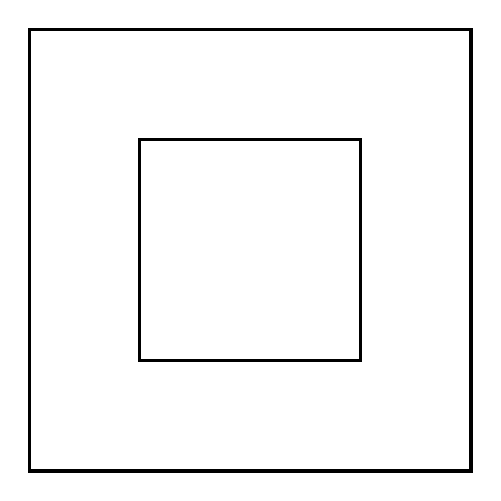
\begin{tikzpicture}
[borderdecorate/.style={-,very thick}]
%% chessboard with a black knight
\node at (0,4.9) {\WhiteEmptySquare\BlackEmptySquare\WhiteEmptySquare\BlackEmptySquare\WhiteEmptySquare\BlackEmptySquare\WhiteEmptySquare\BlackEmptySquare};
\node at (0,4.2) {\BlackEmptySquare\WhiteEmptySquare\BlackEmptySquare\WhiteEmptySquare\BlackEmptySquare\WhiteEmptySquare\BlackEmptySquare\WhiteEmptySquare};
\node at (0,3.5) {\WhiteEmptySquare\BlackEmptySquare\WhiteEmptySquare\BlackEmptySquare\WhiteEmptySquare\BlackEmptySquare\WhiteEmptySquare\BlackEmptySquare};
\node at (0,2.8) {\BlackEmptySquare\WhiteEmptySquare\BlackEmptySquare\WhiteEmptySquare\BlackEmptySquare\WhiteEmptySquare\BlackEmptySquare\WhiteEmptySquare};
\node at (0,2.1) {\WhiteEmptySquare\BlackEmptySquare\WhiteEmptySquare\BlackEmptySquare\WhiteEmptySquare\BlackEmptySquare\WhiteEmptySquare\BlackEmptySquare};
\node at (0,1.4) {\BlackEmptySquare\WhiteEmptySquare\BlackEmptySquare\WhiteEmptySquare\BlackEmptySquare\WhiteEmptySquare\BlackEmptySquare\WhiteEmptySquare};
\node at (0,0.7) {\WhiteEmptySquare\BlackEmptySquare\WhiteEmptySquare\BlackEmptySquare\WhiteEmptySquare\BlackEmptySquare\WhiteEmptySquare\BlackEmptySquare};
\node at (0,0.0) {\BlackEmptySquare\WhiteEmptySquare\BlackEmptySquare\WhiteEmptySquare\BlackEmptySquare\WhiteEmptySquare\BlackEmptySquare\WhiteEmptySquare};
%% the boarders of the chessboard
\draw[borderdecorate]
(-2.8,-0.352) -- (-2.8,5.257) -- (2.809,5.257) -- (2.809,-0.352) -- cycle;
%% the 4 x 4 inner square
\draw[borderdecorate]
(-1.39775,1.05025) -- (-1.39775,3.85475) -- (1.40675,3.85475)
-- (1.40675,1.05025) -- cycle;
\end{tikzpicture}
}
\quad
%%
%% knight's initial position
\subfigure[Initial position in the outer shell.]{
\label{fig:graph_algorithms:montmort-moivre-strategy:initial_position}
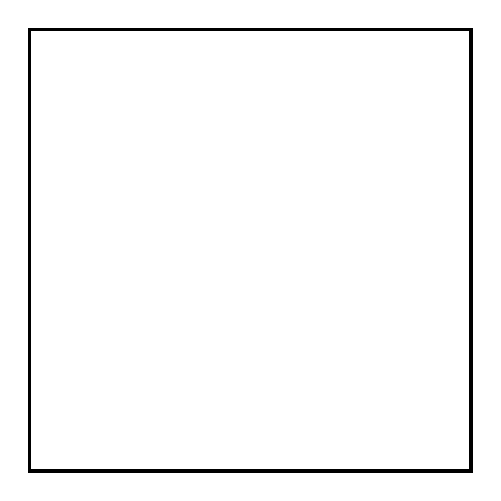
\begin{tikzpicture}
[borderdecorate/.style={-,very thick},%
  linedecorate/.style={-,thick},%
  nodedecorate/.style={shape=circle,fill=black,inner sep=2pt,draw,thick}]
%% empty chessboard
\node at (0,4.9) {\WhiteEmptySquare\BlackEmptySquare\WhiteEmptySquare\BlackEmptySquare\WhiteEmptySquare\BlackEmptySquare\WhiteEmptySquare\BlackKnightOnBlack};
\node at (0,4.2) {\BlackEmptySquare\WhiteEmptySquare\BlackEmptySquare\WhiteEmptySquare\BlackEmptySquare\WhiteEmptySquare\BlackEmptySquare\WhiteEmptySquare};
\node at (0,3.5) {\WhiteEmptySquare\BlackEmptySquare\WhiteEmptySquare\BlackEmptySquare\WhiteEmptySquare\BlackEmptySquare\WhiteEmptySquare\BlackEmptySquare};
\node at (0,2.8) {\BlackEmptySquare\WhiteEmptySquare\BlackEmptySquare\WhiteEmptySquare\BlackEmptySquare\WhiteEmptySquare\BlackEmptySquare\WhiteEmptySquare};
\node at (0,2.1) {\WhiteEmptySquare\BlackEmptySquare\WhiteEmptySquare\BlackEmptySquare\WhiteEmptySquare\BlackEmptySquare\WhiteEmptySquare\BlackEmptySquare};
\node at (0,1.4) {\BlackEmptySquare\WhiteEmptySquare\BlackEmptySquare\WhiteEmptySquare\BlackEmptySquare\WhiteEmptySquare\BlackEmptySquare\WhiteEmptySquare};
\node at (0,0.7) {\WhiteEmptySquare\BlackEmptySquare\WhiteEmptySquare\BlackEmptySquare\WhiteEmptySquare\BlackEmptySquare\WhiteEmptySquare\BlackEmptySquare};
\node at (0,0.0) {\BlackEmptySquare\WhiteEmptySquare\BlackEmptySquare\WhiteEmptySquare\BlackEmptySquare\WhiteEmptySquare\BlackEmptySquare\WhiteEmptySquare};
%% boarders of the chessboard
\draw[borderdecorate]
(-2.8,-0.352) -- (-2.8,5.257) -- (2.809,5.257) -- (2.809,-0.352) -- cycle;
\end{tikzpicture}
}

\caption{De~Montmort and De~Moivre's solution strategy for the
  $8 \times 8$ knight's tour problem.}
\label{fig:graph_algorithms:De_Montmort_De_Moivre_knight_tour_strategy}
\end{figure}

\begin{figure}[!htbp]
\centering
\index{chess!knight's tour}
%%%%%%%%%%%%%%%%%%%%%%%%%%%%%%%%%%%%%%%%%%%%%%%%%%%%%%%%%%%%%%%%%%%%%%%%%%%
%% This file is part of the book
%%
%% Algorithmic Graph Theory
%% http://code.google.com/p/graph-theory-algorithms-book/
%%
%% Copyright (C) 2009, 2010 Minh Van Nguyen <nguyenminh2@gmail.com>
%%
%% See the file COPYING for copying conditions.
%%%%%%%%%%%%%%%%%%%%%%%%%%%%%%%%%%%%%%%%%%%%%%%%%%%%%%%%%%%%%%%%%%%%%%%%%%%

%% Chessboards with each square having dimensions 0.701125 x 0.701125.
%%
%% knight's initial position on 6 x 6 chessboard
\subfigure[A $6 \times 6$ chessboard.]{
\label{fig:graph_algorithms:reentrant_knight_tour:6_by_6_chessboard}
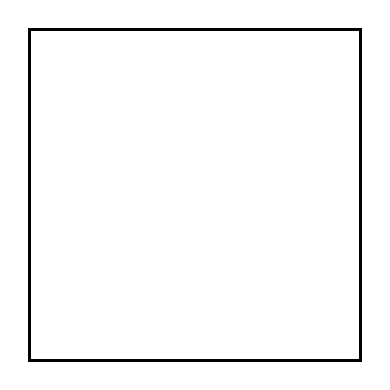
\begin{tikzpicture}
[borderdecorate/.style={-,very thick}]
%% chessboard with a black knight
\node at (0,3.5) {\WhiteEmptySquare\BlackEmptySquare\WhiteEmptySquare\BlackEmptySquare\WhiteEmptySquare\BlackEmptySquare};
\node at (0,2.8) {\BlackEmptySquare\WhiteEmptySquare\BlackEmptySquare\WhiteEmptySquare\BlackEmptySquare\WhiteEmptySquare};
\node at (0,2.1) {\WhiteEmptySquare\BlackEmptySquare\WhiteEmptySquare\BlackEmptySquare\WhiteEmptySquare\BlackEmptySquare};
\node at (0,1.4) {\BlackEmptySquare\WhiteEmptySquare\BlackEmptySquare\WhiteEmptySquare\BlackEmptySquare\WhiteEmptySquare};
\node at (0,0.7) {\WhiteEmptySquare\BlackEmptySquare\WhiteEmptySquare\BlackEmptySquare\WhiteEmptySquare\BlackEmptySquare};
\node at (0,0.0) {\BlackKnightOnBlack\WhiteEmptySquare\BlackEmptySquare\WhiteEmptySquare\BlackEmptySquare\WhiteEmptySquare};
%% the boarders of the chessboard
\draw[borderdecorate]
(-2.098875,-0.352) -- (-2.098875,3.85475) -- (2.107875,3.85475)
-- (2.107875,-0.352) -- cycle;
\end{tikzpicture}
}
\quad
%%
%% knight's tour
\subfigure[An $8 \times 8$ chessboard.]{
\label{fig:graph_algorithms:reentrant_knight_tour:8_by_8_chessboard}
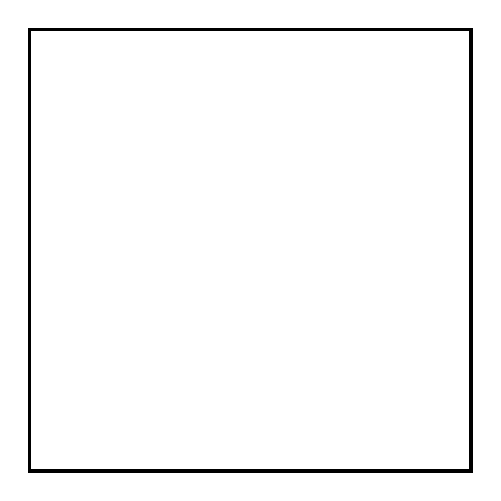
\begin{tikzpicture}
[borderdecorate/.style={-,very thick},%
  linedecorate/.style={-,thick},%
  nodedecorate/.style={shape=circle,fill=black,inner sep=2pt,draw,thick}]
%% empty chessboard
\node at (0,4.9) {\WhiteEmptySquare\BlackEmptySquare\WhiteEmptySquare\BlackEmptySquare\WhiteEmptySquare\BlackEmptySquare\WhiteEmptySquare\BlackEmptySquare};
\node at (0,4.2) {\BlackEmptySquare\WhiteEmptySquare\BlackEmptySquare\WhiteEmptySquare\BlackEmptySquare\WhiteEmptySquare\BlackEmptySquare\WhiteEmptySquare};
\node at (0,3.5) {\WhiteEmptySquare\BlackEmptySquare\WhiteEmptySquare\BlackEmptySquare\WhiteEmptySquare\BlackEmptySquare\WhiteEmptySquare\BlackEmptySquare};
\node at (0,2.8) {\BlackEmptySquare\WhiteEmptySquare\BlackKnightOnBlack\WhiteEmptySquare\BlackEmptySquare\WhiteEmptySquare\BlackEmptySquare\WhiteEmptySquare};
\node at (0,2.1) {\WhiteEmptySquare\BlackEmptySquare\WhiteEmptySquare\BlackEmptySquare\WhiteEmptySquare\BlackEmptySquare\WhiteEmptySquare\BlackEmptySquare};
\node at (0,1.4) {\BlackEmptySquare\WhiteEmptySquare\BlackEmptySquare\WhiteEmptySquare\BlackEmptySquare\WhiteEmptySquare\BlackEmptySquare\WhiteEmptySquare};
\node at (0,0.7) {\WhiteEmptySquare\BlackEmptySquare\WhiteEmptySquare\BlackEmptySquare\WhiteEmptySquare\BlackEmptySquare\WhiteEmptySquare\BlackEmptySquare};
\node at (0,0.0) {\BlackEmptySquare\WhiteEmptySquare\BlackEmptySquare\WhiteEmptySquare\BlackEmptySquare\WhiteEmptySquare\BlackEmptySquare\WhiteEmptySquare};
%% boarders of the chessboard
\draw[borderdecorate]
(-2.8,-0.352) -- (-2.8,5.257) -- (2.809,5.257) -- (2.809,-0.352) -- cycle;
\end{tikzpicture}
}

\caption{Initial positions of re-entrant knight's tours.}
\label{fig:graph_algorithms:reentrant_knight_tour}
\end{figure}

\begin{figure}[!htbp]
\centering
%%%%%%%%%%%%%%%%%%%%%%%%%%%%%%%%%%%%%%%%%%%%%%%%%%%%%%%%%%%%%%%%%%%%%%%%%%%
%% This file is part of the book
%%
%% Algorithmic Graph Theory
%% http://code.google.com/p/graph-theory-algorithms-book/
%%
%% Copyright (C) 2009, 2010 Minh Van Nguyen <nguyenminh2@gmail.com>
%%
%% See the file COPYING for copying conditions.
%%%%%%%%%%%%%%%%%%%%%%%%%%%%%%%%%%%%%%%%%%%%%%%%%%%%%%%%%%%%%%%%%%%%%%%%%%%

%% Chessboards where each square has dimensions 0.701125 x 0.701125.
%%
%% Solution for 4-queens.
\subfigure[$n = 4$]{
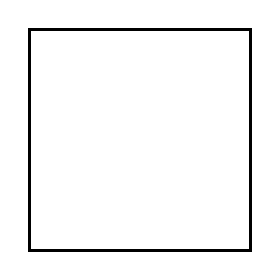
\begin{tikzpicture}
[borderdecorate/.style={-,very thick}]
%% chessboard with 4 queens
\node at (0,2.1) {\WhiteEmptySquare\WhiteQueenOnBlack\WhiteEmptySquare\BlackEmptySquare};
\node at (0,1.4) {\BlackEmptySquare\WhiteEmptySquare\BlackEmptySquare\WhiteQueenOnWhite};
\node at (0,0.7) {\WhiteQueenOnWhite\BlackEmptySquare\WhiteEmptySquare\BlackEmptySquare};
\node at (0,0.0) {\BlackEmptySquare\WhiteEmptySquare\WhiteQueenOnBlack\WhiteEmptySquare};
%% the boarders of the chessboard
\draw[borderdecorate]
(-1.405,-0.352) -- (-1.405,2.4525) -- (1.3995,2.4525) -- (1.3995,-0.352) -- cycle;
\end{tikzpicture}
}
\quad
%%
%% Solution for 8-queens.
\subfigure[$n = 8$]{
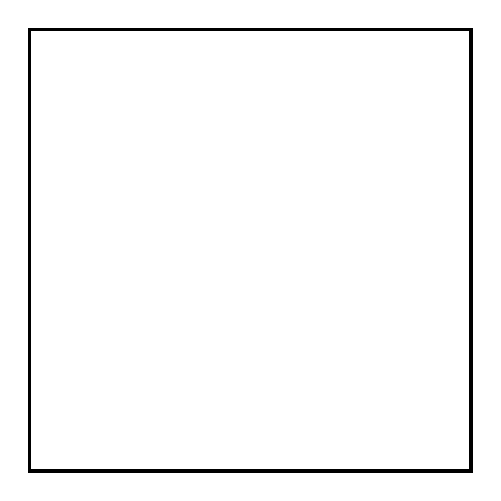
\begin{tikzpicture}
[borderdecorate/.style={-,very thick}]
%% chessboard with 8 queens
\node at (0,4.9) {\WhiteEmptySquare\BlackEmptySquare\WhiteQueenOnWhite\BlackEmptySquare\WhiteEmptySquare\BlackEmptySquare\WhiteEmptySquare\BlackEmptySquare};
\node at (0,4.2) {\BlackEmptySquare\WhiteEmptySquare\BlackEmptySquare\WhiteEmptySquare\BlackEmptySquare\WhiteEmptySquare\BlackEmptySquare\WhiteQueenOnWhite};
\node at (0,3.5) {\WhiteEmptySquare\BlackEmptySquare\WhiteEmptySquare\WhiteQueenOnBlack\WhiteEmptySquare\BlackEmptySquare\WhiteEmptySquare\BlackEmptySquare};
\node at (0,2.8) {\BlackEmptySquare\WhiteEmptySquare\BlackEmptySquare\WhiteEmptySquare\BlackEmptySquare\WhiteEmptySquare\WhiteQueenOnBlack\WhiteEmptySquare};
\node at (0,2.1) {\WhiteQueenOnWhite\BlackEmptySquare\WhiteEmptySquare\BlackEmptySquare\WhiteEmptySquare\BlackEmptySquare\WhiteEmptySquare\BlackEmptySquare};
\node at (0,1.4) {\BlackEmptySquare\WhiteEmptySquare\BlackEmptySquare\WhiteEmptySquare\BlackEmptySquare\WhiteQueenOnWhite\BlackEmptySquare\WhiteEmptySquare};
\node at (0,0.7) {\WhiteEmptySquare\WhiteQueenOnBlack\WhiteEmptySquare\BlackEmptySquare\WhiteEmptySquare\BlackEmptySquare\WhiteEmptySquare\BlackEmptySquare};
\node at (0,0.0) {\BlackEmptySquare\WhiteEmptySquare\BlackEmptySquare\WhiteEmptySquare\WhiteQueenOnBlack\WhiteEmptySquare\BlackEmptySquare\WhiteEmptySquare};
%% the boarders of the chessboard
\draw[borderdecorate]
(-2.8,-0.352) -- (-2.8,5.257) -- (2.809,5.257) -- (2.809,-0.352) -- cycle;
\end{tikzpicture}
}

\caption{Solutions of the $n$-queens problem for $n = 4, 8$.}
\label{fig:graph_algorithms:n_queens_solutions}
\end{figure}

\item The $n$-queens problem is concerned with the placement of $n$
  queens on an $n \times n$ chessboard such that no two queens can
  attack each other. Two queens can attack each other if they are in
  the same row, column, diagonal, or antidiagonal of the chessboard.
  The trivial case $n = 1$ is easily solved by placing the one queen
  in the only given position. There are no solutions for the cases
  $n = 2, 3$. Solutions for the cases $n = 4, 8$ are shown in
  Figure~\ref{fig:graph_algorithms:n_queens_solutions}. Devise a
  backtracking algorithm to solve the $n$-queens problem for the case
  where $n > 3$. See Bell and Stevens~\cite{BellStevens2009} for a
  survey of the $n$-queens problem and its solutions.

\item Hampton Court Palace in England is well-known for its maze of
  hedges. Figure~\ref{fig:graph_algorithms:maze_associated_graph}
  shows a maze and its graph representation; the figure is adapted
  from page~434 in Sedgewick~\cite{Sedgewick1990}. To obtain the graph
  representation, we use a vertex to represent an intersection in the
  maze. An edge joining two vertices represents a path from one
  intersection to another.
  %%
  \begin{enumerate}[(a)]
  \item Suppose the entrance to the maze is represented by the
    lower-left black-filled vertex in
    Figure~\ref{fig:maze_graph:graph_representation} and the exit is
    the upper-right black-filled vertex. Solve the maze by providing a
    path from the entrance to the exit.

  \item Repeat the previous exercise for each pair of distinct
    vertices, letting one vertex of the pair be the entrance and the
    other vertex the exit.

  \item What is the diameter of the graph in
    Figure~\ref{fig:maze_graph:graph_representation}?

  \item Investigate algorithms for generating and solving mazes.
  \end{enumerate}

\begin{figure}[!htbp]
\centering
%%%%%%%%%%%%%%%%%%%%%%%%%%%%%%%%%%%%%%%%%%%%%%%%%%%%%%%%%%%%%%%%%%%%%%%%%%%
%% This file is part of the book
%%
%% Algorithmic Graph Theory
%% http://code.google.com/p/graph-theory-algorithms-book/
%%
%% Copyright (C) 2009--2011 Minh Van Nguyen <nguyenminh2@gmail.com>
%%
%% See the file COPYING for copying conditions.
%%%%%%%%%%%%%%%%%%%%%%%%%%%%%%%%%%%%%%%%%%%%%%%%%%%%%%%%%%%%%%%%%%%%%%%%%%%

\documentclass{article}

\usepackage{subfigure}
\usepackage{tikz}
\usetikzlibrary{external}
\tikzexternalize{maze-graph}

\begin{document}

\begin{figure}
%% a maze
\subfigure[]{
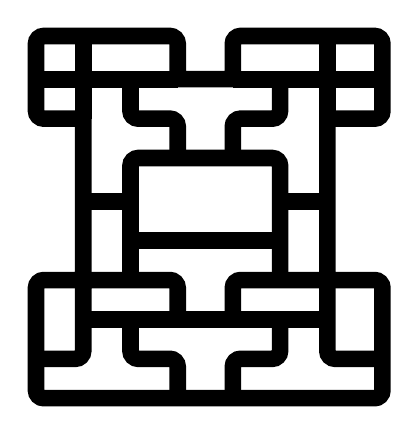
\begin{tikzpicture}
[cornerJagged/.style={rounded corners=0cm},%
  cornerRounded/.style={rounded corners=0.1cm},%
  invisibleNode/.style={},%
  pathDecorate/.style={-,line width=6pt}]
%% invisible nodes or vertices
%% \foreach \nodename/\x/\y in {1/0.1/0.6, 2/4.5/0.6, 3/1.9/0.1,
%%   4/2.6/0.1, 5/0.7/1.1, 6/1.3/1.1, 7/1.9/1.1, 8/2.6/1.1, 9/3.2/1.1,
%%   10/3.8/1.1, 11/0.7/1.6, 12/1.3/1.6, 13/3.2/1.6, 14/3.8/1.6,
%%   15/1.3/2.1, 16/3.2/2.1, 17/0.7/2.6, 18/1.3/2.6, 19/3.2/2.6,
%%   20/3.8/2.6, 21/1.9/3.15, 22/2.6/3.15, 23/0.7/3.65, 24/3.8/3.65,
%%   25/0.1/4.15, 26/0.7/4.15, 27/1.3/4.15, 28/1.9/4.15, 29/2.6/4.15,
%%   30/3.2/4.15, 31/3.8/4.15, 32/4.5/4.15, 33/0.7/4.7, 34/3.8/4.7,
%%   35/0.1/0.1, 36/4.5/0.1, 37/0.7/0.6, 38/1.3/0.6, 39/1.9/0.6,
%%   40/2.6/0.6, 41/3.2/0.6, 42/3.8/0.6, 43/0.1/1.6, 44/1.9/1.6,
%%   45/2.6/1.6, 46/4.5/1.6, 47/1.3/3.15, 48/3.2/3.15, 49/0.1/3.65,
%%   50/1.3/3.65, 51/1.9/3.65, 52/2.6/3.65, 53/3.2/3.65, 54/4.5/3.65,
%%   55/0.1/4.7, 56/1.9/4.7, 57/2.6/4.7, 58/4.5/4.7}
%% {
%%   \node (\nodename) at (\x,\y) [invisibleNode] {};
%% }
%% edges or lines representing the path of the maze
%% the outer path
\draw[pathDecorate] (0.1,0.1)[cornerRounded] -- (4.5,0.1) --
(4.5,1.6)[cornerJagged] -- (3.8,1.6) -- (3.8,3.65)[cornerRounded] --
(4.5,3.65) -- (4.5,4.7) -- (2.6,4.7)[cornerJagged] -- (2.6,4.152) --
(1.9,4.152)[cornerRounded] -- (1.9,4.7) -- (0.1,4.7) --
(0.1,3.65)[cornerJagged] -- (0.7,3.65) -- (0.7,1.6)[cornerRounded] --
(0.1,1.6) -- cycle;
%% inner paths
\draw[pathDecorate] (0.1,0.6)[cornerRounded] --
(0.7,0.6)[cornerJagged] -- (0.7,1.6)[cornerRounded] -- (1.9,1.6) --
(1.9,1.1);
\draw[pathDecorate] (0.7,1.1) -- (3.8,1.1);
\draw[pathDecorate] (1.3,1.1)[cornerRounded] -- (1.3,0.6) -- (1.9,0.6)
-- (1.9,0.1);
\draw[pathDecorate] (2.6,0.1)[cornerRounded] -- (2.6,0.6) -- (3.2,0.6)
-- (3.2,1.1);
\draw[pathDecorate] (2.6,1.1)[cornerRounded] -- (2.6,1.6) -- (3.8,1.6);
\draw[pathDecorate] (3.8,1.6)[cornerRounded] -- (3.8,0.6) -- (4.5,0.6);
\draw[pathDecorate] (1.3,1.6)[cornerRounded] -- (1.3,3.15) --
(3.2,3.15) -- (3.2,1.6);
\draw[pathDecorate] (1.3,2.1) -- (3.2,2.1);
\draw[pathDecorate] (0.7,2.6) -- (1.3,2.6);
\draw[pathDecorate] (3.2,2.6) -- (3.8,2.6);
\draw[pathDecorate] (0.1,4.15) -- (1.9,4.15);
\draw[pathDecorate] (2.6,4.15) -- (4.5,4.15);
\draw[pathDecorate] (0.7,3.65) -- (0.7,4.7);
\draw[pathDecorate] (3.8,3.65) -- (3.8,4.7);
\draw[pathDecorate] (1.3,4.15)[cornerRounded] -- (1.3,3.65) --
(1.9,3.65) -- (1.9,3.15);
\draw[pathDecorate] (2.6,3.15)[cornerRounded] -- (2.6,3.65) --
(3.2,3.65) -- (3.2,4.15);
\end{tikzpicture}
}
\qquad
%%
%% graph representation of maze
\subfigure[]{
\label{fig:maze_graph:graph_representation}
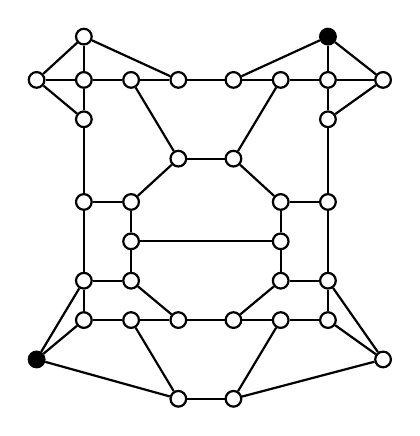
\begin{tikzpicture}
[linedecorate/.style={-,thick},%
  nodeBlackFilled/.style={shape=circle,fill=black,inner sep=2pt,draw,thick},%
  nodeHollow/.style={shape=circle,inner sep=2pt,draw,thick}]
%% nodes or vertices
\foreach \nodename/\x/\y in {2/4.5/0.6, 3/1.9/0.1,
  4/2.6/0.1, 5/0.7/1.1, 6/1.3/1.1, 7/1.9/1.1, 8/2.6/1.1, 9/3.2/1.1,
  10/3.8/1.1, 11/0.7/1.6, 12/1.3/1.6, 13/3.2/1.6, 14/3.8/1.6,
  15/1.3/2.1, 16/3.2/2.1, 17/0.7/2.6, 18/1.3/2.6, 19/3.2/2.6,
  20/3.8/2.6, 21/1.9/3.15, 22/2.6/3.15, 23/0.7/3.65, 24/3.8/3.65,
  25/0.1/4.15, 26/0.7/4.15, 27/1.3/4.15, 28/1.9/4.15, 29/2.6/4.15,
  30/3.2/4.15, 31/3.8/4.15, 32/4.5/4.15, 33/0.7/4.7}
{
  \node (\nodename) at (\x,\y) [nodeHollow] {};
}
\node (1) at (0.1,0.6) [nodeBlackFilled] {};
\node (34) at (3.8,4.7) [nodeBlackFilled] {};
%% edges or lines
\path
\foreach \startnode/\endnode in {1/3, 1/5, 1/11, 2/4, 2/10, 2/14, 3/4,
  3/6, 4/9, 5/6, 5/11, 6/7, 7/8, 7/12, 8/9, 8/13, 9/10, 10/14, 11/12,
  11/17, 12/15, 13/14, 13/16, 14/20, 15/16, 15/18, 16/19, 17/18,
  17/23, 18/21, 19/20, 19/22, 20/24, 21/22, 21/27, 22/30, 23/25,
  23/26, 24/31, 24/32, 25/26, 25/33, 26/27, 26/33, 27/28, 28/29,
  28/33, 29/30, 29/34, 30/31, 31/32, 31/34, 32/34}
{
  (\startnode) edge[linedecorate] node {} (\endnode)
};
\end{tikzpicture}
}
\end{figure}

\end{document}

\caption{A maze and its graph representation.}
\label{fig:graph_algorithms:maze_associated_graph}
\end{figure}

\item For each of the algorithms below: (i)~justify whether or not
  it can be applied to multigraphs or multidigraphs; (ii)~if not,
  modify the algorithm so that it is applicable to multigraphs or
  multidigraphs.
  %%
  \begin{enumerate}[(a)]
  \item Breadth-first search
    Algorithm~\ref{alg:graph_algorithms:breadth_first_search_template}.

  \item Depth-first search
    Algorithm~\ref{alg:graph_algorithms:depth_first_search_template}.

  \item Graph connectivity test
    Algorithm~\ref{alg:graph_algorithms:graph_connectivity}.

  \item General shortest path
    Algorithm~\ref{alg:graph_algorithms:generic_shortest_path_algorithm}.

  \item Dijkstra's
    Algorithm~\ref{alg:graph_algorithms:dijkstra_general}.

  \item The Bellman-Ford
    Algorithms~\ref{alg:graph_algorithms:Bellman_Ford}
    and~\ref{alg:graph_algorithms:Bellman_Ford:redundant_updates}.

  \item The Floyd-Roy-Warshall
    Algorithm~\ref{alg:graph_algorithms:Floy_Roy_Warshall}.

  \item The transitive closure
    Algorithm~\ref{alg:graph_algorithms:Floy_Roy_Warshall:transitive_closure}.

  \item Johnson's
    Algorithm~\ref{alg:graph_algorithms:Johnson_algorithm}.
  \end{enumerate}

\begin{figure}[!htbp]
\centering
%%%%%%%%%%%%%%%%%%%%%%%%%%%%%%%%%%%%%%%%%%%%%%%%%%%%%%%%%%%%%%%%%%%%%%%%%%%
%% This file is part of the book
%%
%% Algorithmic Graph Theory
%% http://code.google.com/p/graph-theory-algorithms-book/
%%
%% Copyright (C) 2009, 2010, 2011 Minh Van Nguyen <nguyenminh2@gmail.com>
%%
%% See the file COPYING for copying conditions.
%%%%%%%%%%%%%%%%%%%%%%%%%%%%%%%%%%%%%%%%%%%%%%%%%%%%%%%%%%%%%%%%%%%%%%%%%%%

\documentclass{article}

\usepackage{subfigure}
\usepackage{tikz}
\usetikzlibrary{external}
\tikzexternalize{grid-graphs}

\begin{document}

\begin{figure}
\subfigure[$2 \times 2$]{
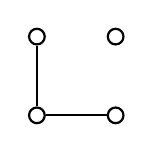
\begin{tikzpicture}
[lineDecorate/.style={-,thick},%
  nodeDecorate/.style={shape=circle,inner sep=2pt,draw,thick}]
%% nodes or vertices
\foreach \nodename/\x/\y in {0_0/0/0, 1_0/1/0, 0_1/0/1, 1_1/1/1}
{
  \node (\nodename) at (\x,\y) [nodeDecorate] {};
}
%% edges or lines
\path
\foreach \startnode/\endnode in {0_0/1_0, 0_0/0_1}
{
  (\startnode) edge[lineDecorate] node {} (\endnode)
};
\end{tikzpicture}
}
%%
%%
\qquad
\subfigure[$3 \times 3$]{
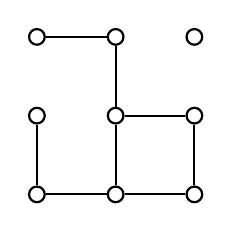
\begin{tikzpicture}
[lineDecorate/.style={-,thick},%
  nodeDecorate/.style={shape=circle,inner sep=2pt,draw,thick}]
%% nodes or vertices
\foreach \nodename/\x/\y in {
  0_0/0/0, 0_1/0/1, 0_2/0/2,
  1_0/1/0, 1_1/1/1, 1_2/1/2,
  2_0/2/0, 2_1/2/1, 2_2/2/2}
{
  \node (\nodename) at (\x,\y) [nodeDecorate] {};
}
%% edges or lines
\path
\foreach \startnode/\endnode in {
  0_0/1_0, 1_0/2_0, 0_0/0_1, 1_0/1_1, 2_0/2_1, 1_1/2_1, 1_1/1_2, 0_2/1_2}
{
  (\startnode) edge[lineDecorate] node {} (\endnode)
};
\end{tikzpicture}
}
%%
%%
\qquad
\subfigure[$4 \times 4$]{
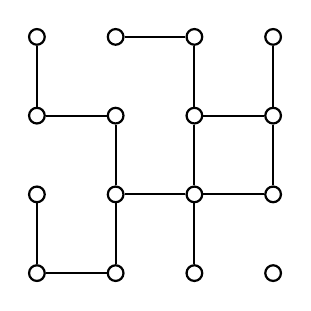
\begin{tikzpicture}
[lineDecorate/.style={-,thick},%
  nodeDecorate/.style={shape=circle,inner sep=2pt,draw,thick}]
%% nodes or vertices
\foreach \nodename/\x/\y in {
  0_0/0/0, 0_1/0/1, 0_2/0/2, 0_3/0/3,
  1_0/1/0, 1_1/1/1, 1_2/1/2, 1_3/1/3,
  2_0/2/0, 2_1/2/1, 2_2/2/2, 2_3/2/3,
  3_0/3/0, 3_1/3/1, 3_2/3/2, 3_3/3/3}
{
  \node (\nodename) at (\x,\y) [nodeDecorate] {};
}
%% edges or lines
\path
\foreach \startnode/\endnode in {
  0_0/0_1, 0_0/1_0, 1_0/1_1, 1_1/2_1, 2_0/2_1, 2_1/3_1, 1_1/1_2,
  2_1/2_2, 3_1/3_2, 0_2/1_2, 2_2/3_2, 0_2/0_3, 2_2/2_3, 3_2/3_3,
  1_3/2_3}
{
  (\startnode) edge[lineDecorate] node {} (\endnode)
};
\end{tikzpicture}
}
\end{figure}

\end{document}

\caption{Grid graphs for $n = 2, 3, 4$.}
\label{fig:graph_algorithms:grid_graphs}
\end{figure}

\item Let $n$ be a positive integer. An $n \times n$
  \emph{grid graph}\index{grid!graph} is a graph on the
  Euclidean plane\index{plane}, where each vertex is an ordered pair
  from $\Z \times \Z$. In particular, the vertices are ordered pairs
  $(i,j) \in \Z \times \Z$ such that
  %%
  \begin{equation}
  \label{eqn:graph_algorithms:grid_graph_vertex_inequality}
  0 \leq i,j < n.
  \end{equation}
  %%
  Each vertex $(i,j)$ is adjacent to any of the following vertices
  provided that
  expression~\eqref{eqn:graph_algorithms:grid_graph_vertex_inequality}
  is satisfied: the vertex $(i-1,\, j)$ immediately to its left, the
  vertex $(i+1,\, j)$ immediately to its right, the vertex
  $(i,\, j+1)$ immediately above it, or the vertex $(i,\, j-1)$
  immediately below it. Figure~\ref{fig:graph_algorithms:grid_graphs}
  illustrates some examples of grid graphs. The $1 \times 1$ grid
  graph is the trivial graph $K_1$.
  %%
  \begin{enumerate}[(a)]
  \item Fix a positive integer $n > 1$. Describe and provide
    pseudocode of an algorithm to generate all nonisomorphic
    $n \times n$ grid graphs. What is the worst-case runtime of your
    algorithm?

  \item How many $n \times n$ grid graphs are there? How many of those
    graphs are nonisomorphic to each other?

  \item Describe and provide pseudocode of an algorithm to generate a
    random\index{algorithm!random} $n \times n$ grid graph. Analyze
    the worst-case runtime of your algorithm.

  \item Extend the grid graph by allowing edges to be diagonals. That
    is, a vertex $(i,j)$ can also be adjacent to any of the following
    vertices so long as
    expression~\eqref{eqn:graph_algorithms:grid_graph_vertex_inequality}
    holds: $(i-1,\, j-1)$, $(i-1,\, j+1)$, $(i+1,\, j+1)$,
    $(i+1,\, j-1)$. With this extension, repeat the previous
    exercises.
  \end{enumerate}
\end{problem}
